% compile with: lualatex -synctex=1 -interaction=nonstopmode -shell-escape  %.tex
\documentclass[a4paper,11pt,ngerman,oneside,titlepage,numbers=noenddot]{scrreprt}
% Language
\usepackage[ngerman]{babel}
% Page Layout
\usepackage[left=2.5cm,right=2.5cm,top=1.5cm,bottom=2cm]{geometry}
% Hyperlinks
\usepackage{hyperref}
\hypersetup{
	pdftitle={Theoretische Elektrotechnik},
	pdfsubject={Zusammenfassung},
	pdfauthor={Henning Dierks},
	pdfkeywords={Studienjahr 2023/24 - TU Dresden}
}
% Math
\usepackage{amsmath}  	% \DeclareMathOperator
\usepackage{amssymb}  	% \DeclareMathOperator
\usepackage{bm}			% bold math
\usepackage{esint}		% fancy integrals
\usepackage{cancel}		% cancel in equations
\usepackage{mathtools}
% Array and Tabular environment
\usepackage{array}
% \includegraphics
\usepackage{graphicx}
% framed minipage (gitstamp on titlepage)
\usepackage{framed}
% Colors
\usepackage{xcolor}
\definecolor{blue}{rgb}{0.0, 0.3, 0.9}
\definecolor{red}{rgb}{0.64, 0.0, 0.0}
\definecolor{green}{rgb}{0,0.5,0}
% German quotes
\usepackage[babel,german=quotes]{csquotes}
% some self defined commands
\usepackage{util}
% fancy images
\usepackage{pgf}		% python-plots
\usepackage{pgfplots}	% internal plots
% tikz 
\usepackage{contour}	% contours for letters in graphics
\usepackage{tikz}		% tikz and its libraries
\usepackage{tikz-3dplot}
\usetikzlibrary{circuits.ee.IEC}
\usetikzlibrary{shapes}
\usetikzlibrary{positioning}
\usetikzlibrary{patterns}
\usetikzlibrary{calc}
\usetikzlibrary{decorations.markings,decorations.pathmorphing,decorations.pathreplacing}
\usetikzlibrary{angles}
\usetikzlibrary{quotes}
\usetikzlibrary{3d}
\usetikzlibrary{intersections}
\usetikzlibrary{perspective}
\usetikzlibrary{arrows.meta}
\usetikzlibrary{shapes.geometric}
\usepackage[europeanresistors,americaninductors]{circuitikz} % use after "usetikzlibrary"!

\tikzset{>=latex} % for LaTeX arrow head
\tikzstyle{proj}=[blue!80,line width=0.08] %very thin
\tikzstyle{area}=[draw=green,fill=green!80,fill opacity=0.6]
\tikzstyle{vector}=[-stealth,blue,thick,line cap=round]
\tikzstyle{unit vector}=[->,green,thick,line cap=round]

% for some tikz-pictures
\def\centerarc[#1](#2)(#3:#4:#5)% Syntax: [draw options] (center) (initial angle:final angle:radius)
{ \draw[#1] ($(#2)+({#5*cos(#3)},{#5*sin(#3)})$) arc (#3:#4:#5); }

\makeatletter
\pgfqkeys{/tikz/cs}{
	latitude/.store in=\tikz@cs@latitude,% not needed with '3d' library
	longitude/.style={angle={#1}},% not needed with '3d' library
	theta/.style={latitude={#1}},
	phi/.style={angle={#1}}
}
\tikzdeclarecoordinatesystem{xyz spherical}{% needed even with '3d' library!
	\pgfqkeys{/tikz/cs}{angle=0,radius=0,latitude=0,#1}%
	\pgfpointspherical{\tikz@cs@angle}{\tikz@cs@latitude}{\tikz@cs@xradius}% fix \tikz@cs@radius to \tikz@cs@xradius
}
\makeatother

% disable auto-indent
\setlength{\parindent}{0pt}

% prevent messed-up line breaks, add "draft" to the \documentclass
% https://jeromebelleman.gitlab.io/posts/publishing/latexlinebreaks/
% https://tex.stackexchange.com/questions/241343/what-is-the-meaning-of-fussy-sloppy-emergencystretch-tolerance-hbadness
%\emergencystretch{\hsize}
\sloppy


% Specify only the chapter you work on to save compilation time. 
%\includeonly{chapter1,chapter2,chapter6,chapter7,chapter8, appendixA,appendixB,appendixC}
\begin{document}
\makeatletter
\begin{titlepage}
	\center
	\vspace*{3cm}
	\textsc{\LARGE Technische Universität Dresden}\\[0.3cm] \textsc{\Large
		Fakultät Elektrotechnik und Informationstechnik}\\[1.5cm] \HRule\\[0.4cm]
	{\huge\bfseries Theoretische Elektrotechnik}\\[0.6cm] \Large Zusammenfassung
	aus dem Studienjahr 2023/2024\\[0.3cm] \HRule\\[2.5cm] {\large\textit{Mitschriften von}}\\
	Henning \textsc{Dierks}\\
	{\large\textit{basierend auf:}}\\ \url{https://github.com/hgkdd/TET}
	\\[2.5cm]
	{	
\includegraphics[width=0.3\textwidth]{res/CC_Logo}}
	\vfill
	\vfill
	
\includegraphics[width=0.3\textwidth]{res/tud}
	
\includegraphics[width=0.3\textwidth]{res/eui}
	\\[1cm]
	\vfill
\end{titlepage}

\makeatother
\hypersetup{bookmarksdepth=3} % pdf outline depth
\setcounter{tocdepth}{1}
\chapter*{Vorwort}
Das vorliegende Skript zur theoretischen Elektrotechnik ist im Studienjahr 2023/2024 auf Basis der Lehrveranstaltung von Prof. Krauthäuser entstanden (\href{https://github.com/hgkdd/TET}{Link}). Der mathematische Anhang basiert teilweise auf der Vorlesung von Prof. Franz aus den Jahren 2021-2023, einige Tabellen dort sind dem Taschenbuch der Mathematik von Bronstein entnommen.\\\\
Da das Skript als Vorlesungsmitschrift entstanden ist, sind inhaltliche und insbesondere orthographische Fehler nicht auszuschließen. Verbesserungsvorschläge und Korrekturen sind als Pull request oder Issue im \href{https://github.com/henningf3/tet}{GitHub-Repo} gerne gesehen.\\\\
Außerdem wurde das Dokument erst nachträglich referenziert, da es zunächst nicht zur Veröffentlichung gedacht war. Trotz großer Sorgfalt, können auch dabei Fehler passiert sein. Hinweise darauf sind jederzeit willkommen.\\\\
\textbf{Nutzungshinweis:} Die Datei ist für eine digtale Nutzung konzipiert. In geeigneten PDF-Viewern (z.B. evince) ist es möglich, über Referenzen wie z.B. \ref{ind} zu hovern und dadurch den Inhalt an dieser Stelle des Dokumentes angezeigt zu bekommen. Außerdem sind externe Verweise häufig als Hyperlink gehalten, z.B. \href{https://github.com/hgkdd/TET}{Link}.


\tableofcontents
\chapter{Axiomatische Grundlagen}
 \section{Maxwell-Gleichungen}
 \textbf{MGl:=Maxwell-Gleichungen}; Je nach Größen- und \href{https://de.wikipedia.org/wiki/Einheitensystem}{Einheitensystem} sind die Formulierungen von MGl und Materialgleichungen unterschiedlich. Dieses Dokument ist vollständig SI-Konform.
 \subsection{Nomenklatur, Differential- und Integralform}
  \begin{minipage}{0.5\textwidth}
	  \begin{align}
		  \rot\vec{E}+ \frac{\partial \vec{B}}{\partial t} & = \vec{0}\label{ind} \\
		  \div\vec{B}                                      & =0\label{quellf}
	  \end{align}
  \end{minipage}
  \begin{minipage}{0.5\textwidth}
	  \begin{align}
		  \rot\vec{H}-\frac{\partial\vec{D}}{\partial t} & =\vec{J}\label{durchf}        \\
		  \div\vec{D}                                    & =\rho_{\text{V}}\label{gauss}
	  \end{align}
  \end{minipage}
  Während das \textbf{Induktionsgesetz} ($\nearrow$\ref{ind}) und die \textbf{Quellfreiheit
	  des Magnetfeldes} ($\nearrow$\ref{quellf}) \textit{homogene pDGL} sind,
  handelt es sich bei dem \textbf{Durchflutungsgesetz} ($\nearrow$\ref{durchf})
  und dem \textbf{Gaußschen Gesetz} ($\nearrow$\ref{gauss}) um \textit{inhomogene
	  pDGL}. \\Außerdem sind \ref{ind} und \ref{durchf} \textit{vektorielle, zeitabhängige
	  (dynamische) pDGL} und \ref{quellf} und \ref{gauss} \textit{skalare, zeitunabhängige
	  (statische) pDGL}. Die statischen MGl sind \textbf{immer} erfüllt, wenn sie zu \textbf{einem Zeitpunkt} erfüllt sind (eher Nebenbedingungen). \\
  \begin{center} 
	  \begin{tabular}{l c c c l}
		  differentielle Form                                            & $\to$ & Satz   & $\to$ & integrale Form                                                                                                                                                                                 \\
		  \hline
		  $\div \vec{D}= \rho_{\text{V}}$                                & $\to$ & Gauss  & $\to$ & $\oiint\limits_{O(V)}\vec{D}\cdot\dd\vec{A}= \iiint\limits_{V}\rho_{\text{V}}\dd V$                                                                                                            \\
		  $\div \vec{B}= 0$                                              & $\to$ & Gauss  & $\to$ & $\oiint\limits_{O(V)}\vec{B}\cdot \dd\vec{A}= 0$                                                                                                                                               \\
		  $\rot \vec{E}+ \dfrac{\partial \vec{B} }{\partial t}=\vec{0}$  & $\to$ & Stokes & $\to$ & $\oint\limits_{O(A)}\vec{E}\cdot \dd\vec{s}= - \iint\limits_{A}\dfrac{\partial \vec{B} }{\partial t}\cdot\dd\vec{A}$ \\
		  $\rot \vec{H}- \dfrac{\partial \vec{D} }{\partial t}= \vec{J}$ & $\to$ & Stokes & $\to$ & $\oint\limits_{O(A)}\vec{H}\cdot \dd\vec{s}= \iint\limits_{A}\vec{J}\cdot\dd \vec{A} +  \iint\limits_{A}\frac{\partial\vec{D}}{\partial t}\cdot\dd\vec{A}$
	  \end{tabular}\\
	  {\textbf{Überführung von Differential- auf Integralform}}
  \end{center}
  Wenn die Fläche $A$ nicht von der Zeit abhängt, kann man die Differentiation vor das Integral ziehen. Vorgehen bei der Überführung: Bilde das entsprechende Integral über die Differentielle Form und wende den Integralsatz an.
  \subsection{Abgrenzung: Mikroskopische und makroskopische MGl}
  Es ist im allgemeinen sinnvoll, zwischen \textbf{mikroskopischen} und \textbf{makroskopischen} MGl zu unterscheiden. Die mikroskopischen MGl berücksichtigen jeden einzelnen Ladungsträger, \dots. Außerdem können magnetische Eigenschaften bspw. von Permanentmagneten nicht aus diesen abgeleitet werden. Das macht sie unhandlich, weshalb die makroskopischen MGl eingeführt werden, welche die Eigenschaften der Materie in Form von Materialparametern berücksichtigen und mit gemittelten Größen arbeiten ($\nearrow$ mikroskopisch: \ref{mikrosmax}, makroskopisch: \ref{makrmax}).
   \subsection{Begriff: Verschiebungsstromdichte}
  \begin{equation}
  	\vec{J}_D=\frac{\partial\vec{D}}{\partial t}
  \end{equation}
  Die Verschiebungsstromdichte hat zwar die selbe Einheit wie eine elektrische Stromdichte und ruft auch ein Magnetfeld hervor ($\nearrow$\ref{durchf}), ist aber kein Strom im Sinne von sich bewegender Ladung. Mathematisch würde das Nichtvorhandensein dieses Terms zu Widersprüchen führen. Ist $\vec{J}=\rot\vec{H}$, dann ist $\div\vec{J}$ stets 0, was unter anderem im Widerspruch zu \ref{kont} steht. Im folgenden soll phänomenologisch erläutert werden, warum dieser Term im \ref{durchf} notwendig ist. Es wird ein Strom $I$ betrachtet, welcher durch einen langen Draht fließt, in dem sich ein Kondensator befinde (\href{https://commons.wikimedia.org/wiki/File:Displacement_current_in_capacitor.svg}{Bildquelle}):  \begin{center}
  	\resizebox{!}{.6\textwidth}{%% Creator: Inkscape 1.3.2 (1:1.3.2+202311252150+091e20ef0f), www.inkscape.org
%% PDF/EPS/PS + LaTeX output extension by Johan Engelen, 2010
%% Accompanies image file 'Displacement_current_in_capacitor.pdf' (pdf, eps, ps)
%%
%% To include the image in your LaTeX document, write
%%   \input{<filename>.pdf_tex}
%%  instead of
%%   \includegraphics{<filename>.pdf}
%% To scale the image, write
%%   \def\svgwidth{<desired width>}
%%   \input{<filename>.pdf_tex}
%%  instead of
%%   \includegraphics[width=<desired width>]{<filename>.pdf}
%%
%% Images with a different path to the parent latex file can
%% be accessed with the `import' package (which may need to be
%% installed) using
%%   \usepackage{import}
%% in the preamble, and then including the image with
%%   \import{<path to file>}{<filename>.pdf_tex}
%% Alternatively, one can specify
%%   \graphicspath{{<path to file>/}}
%% 
%% For more information, please see info/svg-inkscape on CTAN:
%%   http://tug.ctan.org/tex-archive/info/svg-inkscape
%%
\begingroup%
  \makeatletter%
  \providecommand\color[2][]{%
    \errmessage{(Inkscape) Color is used for the text in Inkscape, but the package 'color.sty' is not loaded}%
    \renewcommand\color[2][]{}%
  }%
  \providecommand\transparent[1]{%
    \errmessage{(Inkscape) Transparency is used (non-zero) for the text in Inkscape, but the package 'transparent.sty' is not loaded}%
    \renewcommand\transparent[1]{}%
  }%
  \providecommand\rotatebox[2]{#2}%
  \newcommand*\fsize{\dimexpr\f@size pt\relax}%
  \newcommand*\lineheight[1]{\fontsize{\fsize}{#1\fsize}\selectfont}%
  \ifx\svgwidth\undefined%
    \setlength{\unitlength}{558.07086182bp}%
    \ifx\svgscale\undefined%
      \relax%
    \else%
      \setlength{\unitlength}{\unitlength * \real{\svgscale}}%
    \fi%
  \else%
    \setlength{\unitlength}{\svgwidth}%
  \fi%
  \global\let\svgwidth\undefined%
  \global\let\svgscale\undefined%
  \makeatother%
  \begin{picture}(1,1.07513228)%
  	\LARGE
    \lineheight{1}%
    \setlength\tabcolsep{0pt}%
    \put(0,0){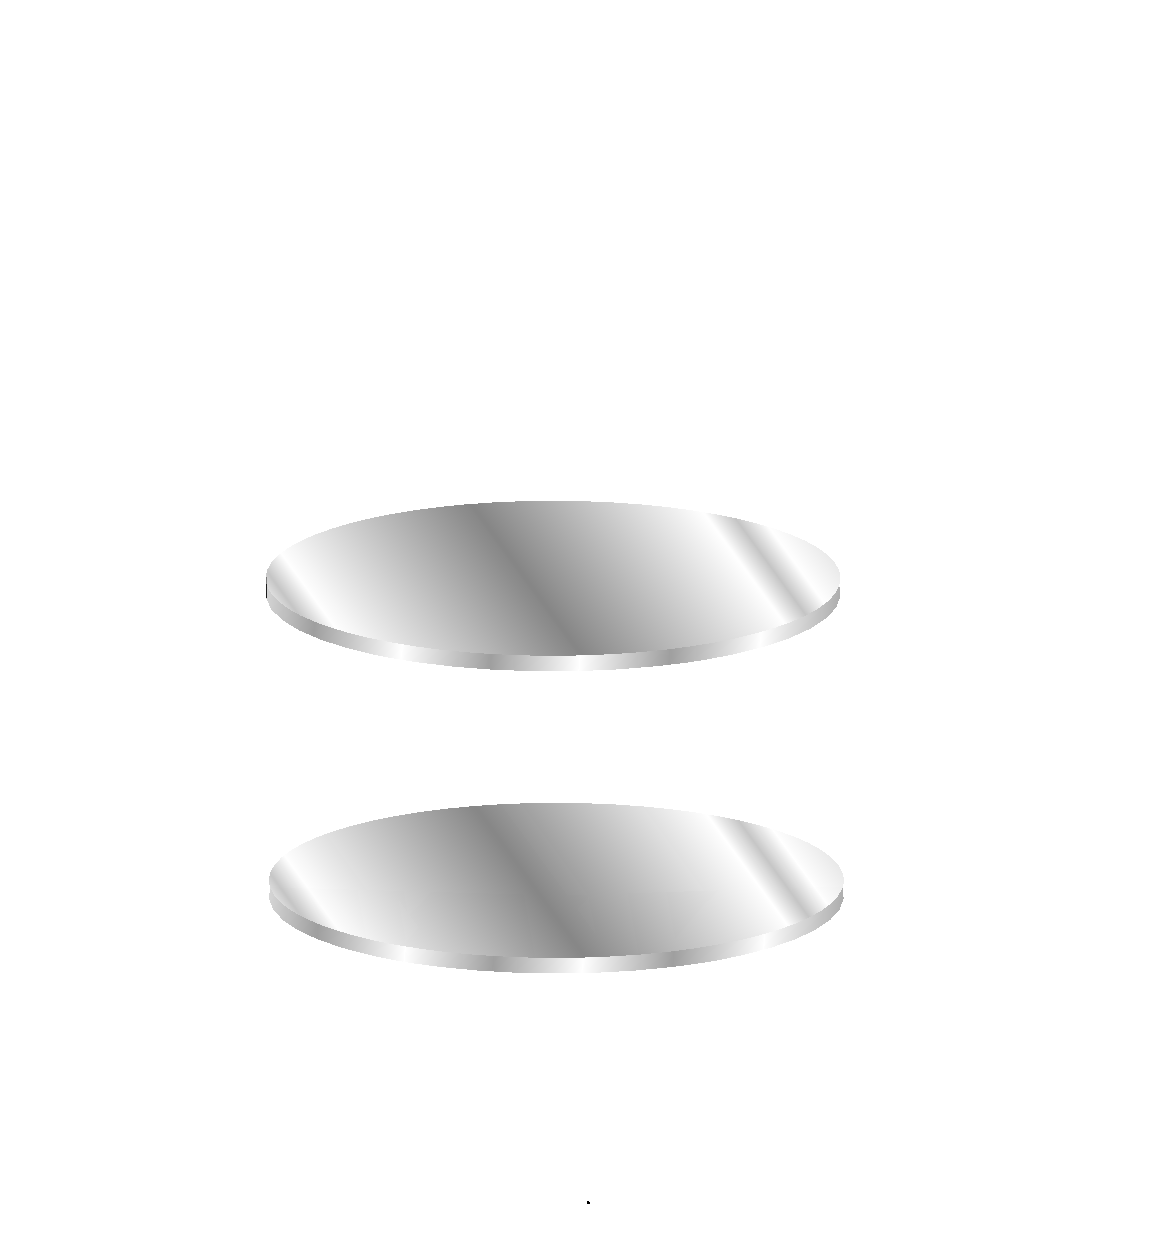
\includegraphics[width=\unitlength,page=1]{res/Displacement_current_in_capacitor.pdf}}%
    \put(0.81736302,0.77152816){\color[rgb]{0.00392157,0,0.02352941}\makebox(0,0)[lt]{\lineheight{0}\smash{\begin{tabular}[t]{l}  \end{tabular}}}}%
    \put(0.80510767,0.77557303){\color[rgb]{0.00392157,0,0.02352941}\makebox(0,0)[lt]{\lineheight{0}\smash{\begin{tabular}[t]{l}$\partial S$\end{tabular}}}}%
    \put(0.71325474,0.38769329){\color[rgb]{0.63921569,0,0}\makebox(0,0)[lt]{\lineheight{0}\smash{\begin{tabular}[t]{l} $\vec{E}$\end{tabular}}}}%
    \put(0.72489797,0.37527524){\color[rgb]{0.63921569,0,0}\makebox(0,0)[lt]{\lineheight{0}\smash{\begin{tabular}[t]{l}  \end{tabular}}}}%
    \put(0,0){\includegraphics[width=\unitlength,page=2]{res/Displacement_current_in_capacitor.pdf}}%
    \put(0.6843464,0.64225882){\color[rgb]{0,0,0}\makebox(0,0)[lt]{\lineheight{0}\smash{\begin{tabular}[t]{l}\textit{ }\end{tabular}}}}%
    \put(0.72235811,0.62596803){\color[rgb]{0,0,0}\makebox(0,0)[lt]{\lineheight{0}\smash{\begin{tabular}[t]{l}\textit{ }\end{tabular}}}}%
    \put(0,0){\includegraphics[width=\unitlength,page=3]{res/Displacement_current_in_capacitor.pdf}}%
    \put(0.36100101,0.9169215){\color[rgb]{0.00392157,0,0.02352941}\makebox(0,0)[lt]{\lineheight{0}\smash{\begin{tabular}[t]{l}$\vec{B}$\end{tabular}}}}%
    \put(0.35215045,0.88599982){\color[rgb]{0.00392157,0,0.02352941}\makebox(0,0)[lt]{\lineheight{0}\smash{\begin{tabular}[t]{l}  \end{tabular}}}}%
    \put(0.34592959,0.9042503){\color[rgb]{0.00392157,0,0.02352941}\makebox(0,0)[lt]{\lineheight{0}\smash{\begin{tabular}[t]{l}  \end{tabular}}}}%
    \put(0.50399451,0.98641512){\color[rgb]{0.00392157,0,0.02352941}\makebox(0,0)[lt]{\lineheight{0}\smash{\begin{tabular}[t]{l} $I$\end{tabular}}}}%
    \put(0.56342076,0.76035686){\color[rgb]{0.00392157,0,0.02352941}\makebox(0,0)[lt]{\lineheight{0}\smash{\begin{tabular}[t]{l}$S_1$\end{tabular}}}}%
    \put(0.70490985,0.6322398){\color[rgb]{0.00392157,0,0.02352941}\makebox(0,0)[lt]{\lineheight{0}\smash{\begin{tabular}[t]{l}$S_2$\end{tabular}}}}%
    \put(0.81445733,0.62002532){\color[rgb]{0.00392157,0,0.02352941}\makebox(0,0)[lt]{\lineheight{0}\smash{\begin{tabular}[t]{l}  \end{tabular}}}}%
    \put(0.49365715,0.07981598){\color[rgb]{0.00392157,0,0.02352941}\makebox(0,0)[lt]{\lineheight{0}\smash{\begin{tabular}[t]{l}$I$\end{tabular}}}}%
  \end{picture}%
\endgroup%
}
  \end{center}
  Nach $\oint\limits_{\partial S}\vec{H}\cdot \dd\vec{s}= I_{S}$ muss das Wegintegral des Magnetfeldes entlang eines beliebigen Weges proportional zu dem Strom sein, der durch eine von diesem Weg aufgespannte Fläche fließt. Bei der türkisen Fläche $S_1$ ist das offensichtlich auch der Fall. Wählt man $S_2$ als Integrationsfläche, muss der Strom exakt der selbe sein, da sich das Magnetfeld auf $\partial S_2=\partial S_1$ durch die Wahl der Fläche nicht ändern darf. Durch den Kondenstator fließt aber kein Strom, was widersprüchlich ist. Hier ändert sich aber der elektrische Fluss. Der Widerspruch kann aufgelöst werden, indem man berücksichtigt, dass auch eine Flussänderung zu einem Magnetfeld führt, was in \ref{durchf} auch passiert.
  \subsection{Komponenten der Stromdichte}
  Eine mögliche Einteilung der Stromdichte ist:
  \begin{equation}
  	\vec{J}=\vec{J}_\mathrm{E}+\vec{J}_\mathrm{L}+\vec{J}_\mathrm{K}
  \end{equation}
  \begin{itemize}
  	\item $\vec{J}_\mathrm{E} = \kappa \vec{E}_\mathrm{E}$ ist die eingeprägte Stromdichte in Bereichen von Urspannung ($\nearrow$\ref{Urspannung}).
  	\item $\vec{J}_\mathrm{L}=\kappa\vec{E}$ ist die Leitungsstromdichte und wird hier meistens betrachtet.
  	\item $\vec{J}_\mathrm{K}$ ist die Konvektionsstromdichte, die z.B. durch Materietransport im Plasma entsteht.
  \end{itemize}
\section{Herleitung wichtiger Gleichungen ($\square$) aus Axiomen und Lemmas}
 \subsection{Poincaré-Lemma} \label{poin}
	   Das Poincaré-Lemma sagt, unter welchen \textbf{Bedingungen} eine Größe
	        als \textbf{Ableitung einer anderen Größe} dargestellt (Potential; nicht
	        Eindeutig $\to$ führt auf den Begriff der Eichung) werden kann. Im Spezialfall 3D-Raum gilt:
	        \begin{enumerate}
		        \item Hat man ein auf einem einfach zusammenhängenden Gebiet wirbelfreies Vektorfeld, dann ist dieses als Gradient eines Potentialfeldes darstellbar:
		              \begin{equation}\label{poin1}
			              \rot\vec{\alpha}=\vec{0}\to \vec{\alpha}= \grad f
		              \end{equation}
		        \item Hat man auf einem konvexen Gebiet ein quellenfreies Vektorfeld, dann ist dieses als Rotation eines Vektorpotentials darstellbar:
		              \begin{equation}\label{poin2}
			              \div \vec{\beta}=0 \to \vec{\beta}= \rot\vec{\alpha}
		              \end{equation}
		        \item Hat man eine skalare Felddichte als Volumenintegrand, dann kann diese als Divergenz eines Vektorfeldes dargestellt werden:
		              \begin{equation}\label{poin3}
			              \gamma \text{ ist ein Volumeintegrand}\to \gamma = \div \vec{\beta}
		              \end{equation}
	        \end{enumerate}
	        

 \subsection{Ladungsdichte und Ladung}
Es gilt, dass die Ladung $Q$ das Volumenintegral über die Ladungsdichte $\rho_{\text{V}}$ ist:
	        \begin{equation}
		        Q = \iiint\limits_{V} \rho_{\text{V}}\dd V \implies \boxed
		        {\div\vec{D} = \rho_\text{V} }
	        \end{equation}
	   Mit dem Poincaré-Lemma ($\rho_{\text{V}}$ ist Integrand eines Volumenintegrals $\to$ sie ist als Divergenz eines Vektorfeldes darstellbar, $\nearrow$\ref{poin3}) folgt unmittelbar das Coulomb-Gauß-Gesetz.\\
	   Ladungen bewegen sich mit der (Material)-Geschwindigkeit $\vec{u}$, damit kann die Stromdichte $\vec{J}$ eingeführt werden:
	        \begin{equation}
		        \vec{J}(\vec{r}) = \rho_{\text{V}}(\vec{r})\vec{u}(\vec{r})
	        \end{equation}
	   Der Strom $I$ ist der Fluss der Stromdichte durch eine 2D-Fläche $S$:
	        \begin{equation}
		        I = \iint\limits_{S} \vec{J}\cdot \dd\vec{A}
	        \end{equation}
 \subsection{Axiom 1: Ladungserhaltung}\label{ladungserhaltung}
 Postulat der Ladungserhaltung: Wenn sich Ladung in einem Volumen ändert, dann geschieht dies nur durch Ladungsstrom durch die Oberfläche des Volumens.
 Betrachtet man die materielle Ableitung (Beobachter bewegt sich mit) $\frac{\mathrm{D}}{\mathrm{D}t}$ und nutzt das Reynolds-Transport-Theorem\footnote{\href{https://de.wikipedia.org/wiki/Transportsatz}{Wikipedia:} Transportsätze beschreiben Regeln für die Zeitableitung von Integralen mit zeitabhängigien Integrationsgrenzen. Das Reynolds-Transport-Theorem ist der Transportsatz für das Volumen.\\\textbf{Aussage:} Gegeben sei ein Kontrollvolumen $V$ mit Volumenelement $\mathrm{d}V$ und Oberfläche $a$ mit nach außen gerichtetem, vektoriellem Oberflächenelement $\mathrm{d}\vec{a}$. Dann lautet die Zeitableitung des Volumenintegrals einer vom Ort $\vec x$ und der Zeit $t$ abhängigen Feldgröße $f(\vec{x},t)$ über das Kontrollvolumen ($\vec{v}$ ist die Geschwindigkeit des Beobachters und des Kontrollvolumens $\to$ Beobachter bewegt sich mit): $\frac{\mathrm{D}}{\mathrm{D}t}\int_V f\,\mathrm{d}V	=\int_V\frac{\partial f}{\partial t}\,\mathrm{d}V
 	+\int_a f\vec{v}\cdot\,\mathrm{d}\vec{a}
 	$ (skalar). $\frac{\mathrm{D}}{\mathrm{D}t}$ ist die Ableitung des Feldes entlang der Bahn des Ladungsteilchens. Die vom Ladungsteilchen auf seiner Bahn wahrgenommene Änderung setzt sich zusammen aus zwei Komponenten: Die Änderung aufgrund verschiedener Feldstärken an den durchlaufenen Orten und einer eventuellen Zeitabhängigkeit des Feldes: $\frac{\text{D}\Phi(\vec{x},t)}{\text{D}t}:=\underbrace{\frac{\partial\Phi}{\partial t}}_\text{zeitlich}+\underbrace{(\vec{v}\cdot\vec{\nabla})\Phi}_\text{durch Bewegung}$.} (*) folgt:
	        \begin{equation}
		        \begin{split}
			        \frac{\mathrm{D} Q}{\mathrm{D} t}&= \frac{\mathrm{D}}{\mathrm{D} t}\left
			        [ \int\limits_{V(t)}\rho_{\text{V}}\dd V \right] \stackrel{!}{=}0\\&\stackrel{*}{=}
			        \int\limits_{V(t)}\frac{\partial \rho_{\text{V}}}{\partial t}\dd V + \oint
			        \limits_{O(V)(t)}\rho_{\text{V}}\vec{u}\cdot \dd\vec{A}\qquad \to \frac{\partial
				        Q}{\partial t}+ \oiint\limits_{O(V)}\vec{J}\cdot d\vec{A}= 0\\\text{Gauss}\to &\stackrel{}{=}
			        \int\limits_{V(t)}\left(\frac{\partial \rho_{\text{V}}}{\partial t}+ \div
			        \left(\rho_{\text{V}}\vec{u}\right) \right) \dd V \\&= \int\limits_{V(t)}
			        \left(\frac{\partial \rho_{\text{V}}}{\partial t}+ \div \vec{J}\right)
			        \dd V \xrightarrow{\textbf{Kontinuitätsgleichung}}\boxed{\frac{\partial \rho_{\text{V}}}{\partial
				        t}+ \div \vec{J}= 0} \\&= \int\limits_{V(t)}\div \left( \frac{\partial
				        \vec{D}}{\partial t}+ \vec{J}\right) \dd V
		        \end{split}
	        \end{equation}

	   Damit dies für beliebige (zeitlich veränderliche) Volumina gelten kann,
	        folgt:
	        \begin{equation}
		        \div \left( \frac{\partial \vec{D}}{\partial t}+ \vec{J}\right) = 0
	        \end{equation}

	   Aus Pointcaré ($\nearrow$\ref{poin2}):
	        \begin{equation}
		        \begin{split}
			        \div \left( \frac{\partial \vec{D}}{\partial t}+ \vec{J}\right) = 0 \to
			        \frac{\partial \vec{D}}{\partial t}+ \vec{J}= \rot\vec{H}&\\ \Aboxed{\rot\vec{H}
			        &- \frac{\partial \vec{D}}{\partial t}= \vec{J}}
		        \end{split}
	        \end{equation}

	  Die Ladungserhaltung gilt auch mikrophysikalisch $\to$ die inhomogenen
		  MGl (die bereits abgeleiteten Gleichungen) gelten auch mikrophysikalisch $\to$ elektrische und magnetische
		  Anregung sind mikrophysikalische Größen.  Die Ladung ist auch relativistisch invariant $\to$ die inhomogenen MGl
		  können also auch relativistisch invariant formuliert werden. 
 \subsection{Axiom 2: Lorentzkraft}
 Die experimentell hervorragend bestätigte \textbf{Lorentzkraft} wird als axiomatisch angenommen:
	       	  \begin{equation}\label{lorentz}
	       	\boxed{\vec{F} =  q \cdot \left( \vec{E} + {\vec{v} \times \vec{B} } \right)}
	       \end{equation}
	        Je nach Zusammenhang wird auch $u\Leftrightarrow v$ gesetzt. Hierbei wird die \textbf{elektrische Feldstärke} eingeführt. Außerdem wird auf das  \textbf{Relativitätsprinzip} zurückgegriffen, das besagt, dass physikalische Gesetze unabhängig vom
	        Inertialsystem sind. Es werden zwei Inertialsysteme betrachtet: Das Laborsystem (Größen ohne ´) bewegt sich mit $u$ relativ zum Ruhesystem der Ladung $q$ (Größen mit ´). Es wird zudem angenommen, dass es keine elektrische Feldstärke im Ruhesystem der Ladung gibt. Damit gilt offensichtlich $E=0,u=0$, also:
		              \begin{equation}
			              \vec{F}' = q \left( \vec{E}' + \vec{u}' \times \vec{B}' \right) = \vec
			              {0}
		              \end{equation}
		   Die Ladung wird also nicht beschleunigt. Die Beschleunigung würde man aber in jedem Inertialsystem beobachten können. Also ist auch im Laborsystem die Kraft $F=0$ ($u\neq0$!-Laborsystem):
		              \begin{equation}
			              \vec{F}= q \left( \vec{E}+ \vec{u}\times \vec{B}\right) = \vec{0}\to
			              \vec{E}= - \vec{u}\times \vec{B}
		              \end{equation}
		         Die beiden Feldstärken $\vec{E}$ und $\vec{B}$ (hist: magnetische Induktion)
		              können also \textbf{nicht unabhängig} voneinander sein.


 \subsection{Axiom 3: Erhaltung des magnetischen Flusses}
 Der magnetische Fluss durch eine Fläche ist gegeben mit:
 \begin{equation}\label{magnetfluss}
 	\displaystyle \Phi = \iint\limits_{S} \vec{B}\cdot \dd\vec{A}
 \end{equation}
 Analog zur Ladungserhaltung kann man eine Flusserhaltung zeigen, $J^\Phi$ ist eine magnetische Flussstromdichte:
	       \begin{equation}
\displaystyle \dfrac{\partial \Phi}{\partial t}+ \oiint\limits_{O(S)}\vec{J}
^{\Phi} \cdot \dd\vec{s}= 0
	       \end{equation}
	   Unter Anwendung von \ref{magnetfluss} und des Stokes-Theorems ($\nearrow$\ref{stokes}) wird daraus:
	   \begin{equation}\label{magIndFlu}
	   	\displaystyle \iint\limits_{S} \frac{\partial \vec{B} }{\partial t}\cdot\dd
	   	\vec{A}+ \iint\limits_{S}\rot \vec{J}^{\Phi} \cdot \dd\vec{A}= 0 \xrightarrow{\text{gilt }\forall S \Rightarrow \textbf{Integrand}\stackrel{!}{=}{0}} \frac{\partial
	   		\vec{B} }{\partial t}+ \rot \vec{J}^{\Phi} = \vec{0}
	   \end{equation}
	        

	   Bildet man die Divergenz folgt (wegen $\div \rot \ldots = 0$):
	        \begin{equation}
		        \div \frac{\partial \vec{B} }{\partial t}= 0\quad \text{ mit }\quad \div \vec{B}= \rho_{\text{mag}} \implies \frac{\partial \rho_{\text{mag}}}{\partial t}=0
	        \end{equation}
	   Die magnetische Ladungsträgerdichte $\rho_{\text{mag}}$ muss also auf jeden Fall
	        zeitlich invariant sein. Es wird nun wieder das \textbf{Relativitätsprinzip} angewandt:
		 Sei in einem System (wie gezeigt) $\displaystyle \frac{\partial \rho_{\text{mag}}(\vec{r})}{\partial
				              t}=0$ (es gibt es an jedem Ort einen zeitlich konstanten Wert von $\rho_{\text{mag}}$). Für einen Beobachter in einem anderen Initialsystem würde sich die
		              räumliche Verteilung aber zeitlich ändern. Dieser Widerspruch tritt nur dann nicht auf, wenn die magnetische
		              Ladungsdichte eine räumliche Konstante ist (\textbf{für} \textbf{alle} \textbf{Orte} und alle
		              \textbf{Zeiten} \textbf{gleich}). Zudem kann sie nicht $\neq 0$ ($\Rightarrow$ überall ungliech 0) sein, da sonst immer magnetische Feldlinien entspringen oder verschwinden würden (das ist in der Realität nicht der Fall). Also folgt: 
		              \begin{equation}
			              \rho_{\text{mag}}(\vec{r}, t)=0 \to \boxed{\div \vec{B} = 0}
		              \end{equation}
		         Weiterhin folgt aus dem Relativitätsprinzip: $\vec{E}= \vec{J}^{\Phi}$. Setzt man dies in Gleichung \ref{magIndFlu} ein folgt die MGl für die Induktion $\boxed{\rot \vec{E} + \frac{\partial \vec{B} }{\partial t} = \vec{0}}$.
 \section{MGl in Materie und Materialgleichungen}\label{mat}
 Die \textbf{Materialgleichungen} beschreiben die Auswirkungen äußerer elektromagnetischer Felder auf Materie. Sie bestehen für ruhende Medien aus den Gleichungen, die die mikroskopischen mit den makroskopischen MGl inklusive der Materialabhängigkeiten für die Polarisation $\vec P$ und Magnetisierung $\vec M$ verknüpfen. Die \textbf{elektrische Flussdichte} $\vec D$ und die \textbf{magnetische Erregung} $\vec H$ sind dabei nur Hilfsfelder, die eingeführt wurden, um die Struktur der MGl des Vakuums auch in Materie aufrechterhalten zu können. Die physikalisch relevanten Messgrößen sind die \textbf{elektrische Feldstärke} $\vec E$ und die \textbf{magnetische Flussdichte} $\vec B$. Sie sind definiert durch die Kraft, die auf eine elektrische Ladung ausgeübt wird ($\nearrow$\ref{lorentz}), (\href{https://de.wikipedia.org/wiki/Materialgleichungen_der_Elektrodynamik}{Textquelle}).
 \subsection{MGl und Materialgleichungen in homogenen, linearen und isotropen Medien}
  \subsubsection{Axiom 4: Die Materialgleichungen des Vakuums}
  Das Vakuum ist ein Spezialfall des homogenen, linearen und isotropen Mediums. Man kann zeigen, dass die Materialgleichungen des Vakuums die Form aus \ref{matvak} haben müssen, wenn:
 \begin{enumerate}
 	\item Die MGl des Vakuums sind invariant bei Translation und Rotation, das ist
 	eine Eigenschaft des Vakuums.
 	\item Die MGl des Vakuums sind lokal und linear (Felder am gleichen Ort
 	und zur gleichen Zeit werden verknüpft), das ist eine Eigenschaft des Vakuums.
 	\item Kein Mixen von elektrischen und magnetischen Effekten, das ist auch eine Eigenschaft des Vakuums.
 \end{enumerate}
 Dann (und in einer flachen Raumzeit) ergibt sich:
 \begin{equation}\label{matvak}
 	\boxed{\vec{D} = \varepsilon_0\vec{E} \qquad \vec{H} = \frac{1}{\mu_{0}} \vec{B} }
 \end{equation}
 Die Materialgleichungen des Vakuums verknüpfen auch elektromagnetische Felder mit der Struktur der Raumzeit. Es gibt Hinweise dafür, dass die Propagation elektromagnetischer Felder die metrische Struktur der Raumzeit bestimmt.
 \subsubsection{Materialgleichungen lineare, homogene, isotrope Medien}
 In aller Regel wird sich auf \textbf{homogene, lineare, und isotrope
 	Medien} beschränkt:
 \begin{itemize}
 	\item Ein Medium ist \textbf{homogen} bezüglich einer bestimmten Eigenschaft,
 	wenn diese Eigenschaft nicht vom \textbf{Ort} abhängt.
 	
 	\item Ein Medium ist \textbf{linear} bezüglich einer bestimmten Eigenschaft
 	und einer bestimmten Anregung, wenn die Eigenschaft nicht von der \textbf{Amplitude}
 	der Anregung abhängt (z.B. Federkonstante im Hookschen Bereich, man kann fast immer mit der Anregung so hoch gehen, dass das Medium nicht mehr linear ist).
 	
 	\item Ein Medium ist \textbf{isotrop} bezüglich einer bestimmten Eigenschaft
 	und einer bestimmten Anregung, wenn die Eigenschaft unabhängig von der \textbf{Richtung}
 	der Anregung ist (z.B. ist die Polarisation in Kristallen häufig nicht
 	isotrop bezüglich einer elektrischen Anregung).
 \end{itemize}
 Es gelten dann die \textbf{Materialgleichungen für homogene, lineare und
 	isotrope Medien}:
 \begin{equation} \label{matlinhomis}
 	\begin{split}
 		\vec{D}= \underbrace{\varepsilon_0\varepsilon_r}_{=\varepsilon}\vec{E}\qquad
 		\text{ und }\qquad\vec{B}= \underbrace{\mu_0 \mu_r}_{=\mu}\vec{H}
 	\end{split}
 \end{equation}
 Für Polarisation und Magnetisierung folgt aus Vergleich mit den in \ref{elmaterial} bzw. \ref{magmaterial} vereinfachten Materialbeziehungen:
 \begin{equation}\label{polmaglin}
 	\begin{split} 
 		\vec{P}= \varepsilon_{0}(\varepsilon_{r} - 1) \vec{E}\qquad \text{ und }\qquad
 		\vec{M}= (\mu_{r}-1) \vec{H}
 	\end{split}
 \end{equation}
 \subsubsection{MGl in linearen, homogenen und isotropen Medien und mikroskopische MGl}\label{mikrosmax}
 Die MGl in linearen, homogenen und isotropen Medien entsprechen denen im Vakuum und damit den mikroskopischen MGl mit den Ersetzungen $\mu\leftrightarrow\mu_0$, $\varepsilon\leftrightarrow\varepsilon_0$ und $\rho_\text{frei}\leftrightarrow\rho_\text{V}$. Zu beachten ist, dass es im Gegensatz zum Vakuum in linearen, homogenen und isotropen Medien eine Polarisierung und Magnetisierung entsprechend \ref{polmaglin} gibt. \textbf{Mikroskopische MGl:}\\
 \begin{minipage}{0.5\textwidth}
 	\begin{align}
 		\rot\vec{E}+ \frac{\partial \vec{B}}{\partial t} & = \vec{0} \\
 		\div\vec{B}                                      & =0
 	\end{align}
 \end{minipage}
 \begin{minipage}{0.5\textwidth}
 	\begin{align}
 		\rot\vec{B}-\mu_0\varepsilon_0\frac{\partial\vec{E}}{\partial t} & =\mu_0\vec{J}       \\
 		\div\vec{E}                                    & =\frac{\rho_{\text{V}}}{\varepsilon_0}
 	\end{align}
 \end{minipage}
Bemerkenswert ist, dass diese Gleichungen vollkommen ohne $D$ und $H$ auskommen, welche erst in komplexerer Materie eingeführt werden müssen, um die Struktur der MGl aufrecht zu erhalten. Die \textbf{Dielektrizitätskonstante/Permittivität des Vakuums} $\varepsilon_{0}$
 und die \textbf{Permeabilität des Vakuums} $\mu_{0}$ sind universelle Konstanten
 und mit der \textbf{Lichtgeschwindigkeit im Vakuum} $c$ verknüpft (SI-$c$ ist festgelegt, $\mu_0$ ist hier mit dem Wert von vor 2019 angegeben - SI Reform):
 \begin{equation}\label{vaklicht}
 	\begin{split}
 		c&= 299792458\mathrm{\frac{m}{s}}\approx 3\cdot 10^{8}\mathrm{\frac{m}{s}}\quad\text{
 			also: }30\mathrm{\frac{cm}{ns}}\\ \mu_{0}&= 4\pi\cdot 10^{-7}\mathrm{\frac{Vs}{Am}}
 		\\ \varepsilon_{0}&= \dfrac{1}{\mu_0 c^2}\approx 8,85\cdot 10^{-12}\mathrm{\frac{As}{Vm}}
 		\quad\text{ mit }\quad{c^2\varepsilon_0\mu_0 = 1}
 	\end{split}
 \end{equation}
 \subsubsection{Materialgleichungen in bewegten Medien}
 Liegt eine konstante Relativbewegung zwischen einem Beobachter und dem umgebenden, linearen, isotropen und homogenen Medium vor, mit den Stoffkonstanten $\mu' = \mu'_r\mu_0$  und $\varepsilon' = \varepsilon'_r \varepsilon_0$, müssen die Materialgleichungen erweitert werden um der Konstantheit der Vakuumlichtgeschwindigkeit $c$ zwischen verschiedenen Inertialsystemen Rechnung zu tragen ($\nearrow$ \ref{SRT}). Im Gegensatz zu den MGl sind die Materialgleichungen nicht invariant gegenüber der Lorentz-Transformation. Die gestrichenen Stoffkonstanten beziehen sich dabei auf das bewegte System, aus Sicht des ruhenden Beobachters. Die beteiligten Feldgrößen werden in zwei Komponenten aufgespalten: Sei $\vec{F}$ eine allgemeine Feldgröße, so bezeichnet $\vec{F}_\bot$ jene Feldkomponente, welche orthogonal zu dem Geschwindigkeitsvektor $\vec{v}$ steht. $\vec{F}_\|$ beschreibt jenen Anteil, welcher parallel zum Geschwindigkeitsvektor $\vec{v}$ steht. Damit ergibt sich für die Feldkomponenten parallel zur Bewegung:
 \begin{equation}\begin{split}\vec D_\| &=\varepsilon ' \vec E_\| \\
 		\vec H_\| &=\frac{1}{\mu '} \vec B_\|\end{split}\end{equation}
 Für die Normalkomponenten ergeben sich kompliziertere Ausdrücke:
 \begin{equation}\begin{split}\vec{D_\bot} &=\varepsilon ' \frac{\gamma^2}{n^2} \left( (n^2 - \beta^2) \vec{E_\bot} + (n^2 - 1)\vec{v} \times \vec{B} \right ) \\
 		\vec{H_\bot} &=\frac{\gamma^2}{\mu '} \left( (1 - n^2 \beta^2)\vec{B_\bot} + (n^2 - 1) \frac{\vec{v} \times \vec{E}}{c_0^2} \right )\end{split}\end{equation}
 
 Mit den Abkürzungen $\beta = \frac{v}{c_0}$, $\gamma = \frac{1}{\sqrt{1-\beta^2}}$, und dem Brechungsindex $n = c_0 \sqrt{\mu ' \varepsilon '}\,$. Zu beachten ist, dass bei bewegten Medien, selbst bei isotropen Medien, die Vektoren $\vec{D}$ und $\vec{E}$ sowie $\vec{H}$ und $\vec{B}$ nicht mehr parallel zueinander stehen.
 Als Sonderfall, bei $n=1$ als auch bei dem Betrag der relativen Geschwindigkeit von $v=0$, verschwinden die zusätzlichen Terme aus obigen Gleichungen (\href{https://de.wikipedia.org/wiki/Materialgleichungen_der_Elektrodynamik}{Textquelle}).
\subsection{Materialgleichungen in komplexerer Materie} \label{mglkommat}
Der gesamte Abschnitt \ref{mglkommat} basiert auf \href{https://de.wikipedia.org/wiki/Materialgleichungen_der_Elektrodynamik}{Wikipedia}.\\\\
 Die Materialgleichungen entstehen aus den mikroskopischen MGl durch folgenden Ansatz:
 \begin{enumerate}
 \item Ladungen werden als Summe von freien und elektrisch induzierten Ladungen (Polarisationsladungen) betrachtet. Polarisationsladungen sind Quellen des Polarisationsfeldes. (Magnetisch induzierte Ladungen treten nicht auf.)
 \item Ströme werden als Summe von freien und elektrisch bzw. magnetisch induzierten Strömen betrachtet. Änderungen des Polarisationsfeldes oder Wirbel im Magnetisierungsfeld bewirken induzierte Ströme.
 \end{enumerate}
 Die folgenden makroskopischen MGl enthalten nur gemittelte Größen, d.h. lokal können die Größen davon abweichen. Eine makroskopische Messung bedeutet immer eine Mittelung sowohl über den Ort als auch über die Zeit (mikroskopische Fluktuationen werden geglättet). Da man sowieso nur die gemittelten Größen makroskopisch messen kann, ist es sinnvoll gleich mit diesen zu rechnen. Eine mögliche Mittelung sieht wie folgt aus (räumliche Mittelung):
\begin{equation}\overline{u\left( \vec{r},t \right)}=\frac{1}{V}\int\limits_{V}{u\left( \vec{r}+\vec{r}\,',t \right)\mathrm{d}}^3r'\end{equation}
 $u\left( \vec{r},t \right)$ sei die mikroskopische Größe (kann Skalar, wie Ladungsdichte, oder Vektor, wie elektrisches Feld, sein). Man integriert die Größe über ein Raumvolumen $V$ um $\vec{r}$, das mikroskopisch groß, makroskopisch aber klein ist. Ein Volumen von $(1/10\mathrm{mm})^3$ enthält eine riesige Zahl von Teilchen (Größenordnung $10^{16}$ Teilchen). Bei solch großen Teilchenzahlen werden bei der rein räumlichen Mittelung auch die zeitlichen Fluktuationen geglättet. Für ein ausführliches Beispiel eines solchen Mittelungsprozesses siehe \ref{materie}. Zu beachten ist, dass die makroskopischen MGl nicht lorentzkovariant formulierbar sind, da sie nur in dem Inertialsystem gelten, in dem die Materie im Mittel ruht. Von den MGl gelten das Induktionsgesetz ($\nearrow$ \ref{ind}) und das magnetische Monopolverbot ($\nearrow$\ref{quellf}) unverändert in Materie weiter (nur hier mit gemittelten Feldern).
\subsubsection{Gaußsches Gesetz: Elektrische Flussdichte}\label{gausmat}
 Materie besteht meist aus mehr oder weniger beweglichen, elektrisch geladenen Teilchen (Ladungen). Diese können z.B. die negativ geladenen Elektronen der Atomhülle und die positiv geladenen Kerne der Materie bildenden Atome sein.
 Ein E-Feld bewirkt auf diese eine elektrische Kraft, welche die jeweils entgegengesetzten Ladungen aus ihren Gleichgewichtspositionen gegeneinander verschiebt. Das Material wird dadurch \textbf{polarisiert} (es entstehen Dipol- und höhere Momente $\nearrow$\ref{multi}) und erzeugt so seinerseits ein elektrisches Feld, das sich mit dem äußeren überlagert. Die Quellen des resultierenden E-Feldes sind die freien Ladungen (auch Überschussladungen genannt, wie zum Beispiel die quasi-freien Leitungselektronen eines metallischen Leiters, erzeugen das externe elektrische Feld) und die gebundenen Ladungen (auch Polarisationsladungen). Die Gesamtladungsdichte ist also $\rho=\rho_{\text{frei}}+\rho_{\text{P}}$.
 \begin{equation}\varepsilon_0\div \vec{E}=\rho_{\text{frei}}+\rho_{\text{P}}\end{equation}
 Man führt die Polarisation $\vec{P}$ als Dipoldichte (mittleres elektrisches Dipolmoment pro Volumen) ein, deren Quellen die Polarisationsladungen sind. Die Summe über Polarisationsladungen eines Körpers ergibt Null. Lokal ist jedoch die Ladungsverteilung von Null verschieden, insbesondere an der Oberfläche des Körpers (Oberflächenladungsdichte):
 \begin{equation}\rho_{\text{P}}=-\div \vec{P}\end{equation}
 Die Polarisation bewirkt ein zusätzliches inneres elektrisches Feld $\vec{E}_{\text{P}}=-\vec{P}/\varepsilon_0$, das sich mit dem äußeren, von den freien Ladungen erzeugten, Feld $\vec{E}_{\text{frei}}$ überlagert: 
 \begin{equation}
 \vec{E}=\vec{E}_{\text{frei}}+\vec{E}_{\text{P}}\implies\vec{E}_{\text{frei}}=\vec{E}-\vec{E}_{\text{P}}=\vec{E}+\vec{P}/\varepsilon_0
 	\end{equation} 
 	Man beschränkt sich im Folgenden auf das äußere Feld. Die Größe $\vec P/\varepsilon_0$ wird \textbf{Elektrisierung} genannt. Die makroskopische MGl erhält als Quellen nur noch die freien Ladungen:
 
\begin{equation}\div \underbrace{\left( \varepsilon_0\vec{E}+\vec{P} \right)}_{{\vec{D}}}=\rho_{\text{frei}}\quad\Rightarrow\quad\div \vec{D}=\rho_{\text{frei}}\end{equation}
 Aus der Überlagerung von elektrischem Feld und Polarisationsfeld entsteht das dielektrische Verschiebungsfeld oder elektrische Flussdichte $\vec D$:
 \begin{equation}\vec D=\varepsilon_0 \vec E + \vec P\end{equation}
\subsubsection{Durchflutungsgesetz: Magnetische Feldstärke}\label{durchfmat}
 Elektronen, Atomkerne und die aus diesen zusammengesetzten Atome und Moleküle tragen jeweils magnetische Momente, vergleichbar atomar kleiner Magneten (Klassische Veranschaulichung mit Bohrschen Atommodell: Atomelektronen bewegen sich auf stationären Kreisbahnen um den Kern. Dieser Kreisstrom erzeugt ein magnetisches Moment senkrecht zur Bahnebene.) Die Orientierungen der Momente sind ohne äußeres Feld statistisch verteilt und kompensieren sich im Mittel. Sie können aber durch eine äußere magnetische Induktion ausgerichtet werden, wodurch ein zusätzliches inneres Feld entsteht, das sich mit dem äußeren überlagert: Das Material \textbf{magnetisiert}.\\
 Ein äußeres Magnetfeld (genauer: magnetische Flussdichte) $\vec{B}$ erzeugt also neben freien Strömen $\vec{J}_{\text{f}}$ aus nicht gebundenen Ladungsträgern, wie zum Beispiel den quasi-freien Leitungselektronen eines metallischen Leiters, auch Magnetisierungsströme gebundener Ladungsträger $\vec{J}_{\text{M}}$. Diese wiederum erzeugen das makroskopische Magnetisierungsfeld $\vec{M}$, das ein mittleres magnetisches Dipolmoment pro Volumen darstellt:
 \begin{equation}
 	\vec{J}_{\text{M}}=\rot \vec{M}
 \end{equation}
 Ferner existieren sogenannte Polarisationsströme, die von einer sich zeitlich ändernden elektrischen Polarisation $\vec{P}$ herrühren (elektrisch induzierter Strom):
 \begin{equation}
 	\vec{J}_{\text{P}}=\frac{\partial \vec{P}}{\partial t}
 \end{equation}
 Die Gesamtstromdichte $\vec{J}$ setzt sich also aus drei Komponenten zusammen, die alle gemeinsam mit dem äußeren Magnetfeld gekoppelt sind:
 \begin{equation}\vec{J}=\vec{J}_{\text{f}}+\vec{J}_{\text{M}}+\vec{J}_{\text{P}}\end{equation}
 Das Durchflutungsgesetz lautet damit zunächst:
 \begin{equation}\frac{1}{\mu_0}\rot \vec{B}=\vec{J}_{\text{f}}+\vec{J}_{\text{M}}+\vec{J}_{\text{P}}+\varepsilon_0\frac{\partial \vec{E}}{\partial t}\end{equation}
 Dies ergibt die makroskopische MGl:
 \begin{equation}\rot \underbrace{\left( \frac{1}{\mu_0}\vec{B}-\vec{M} \right)}_{{\vec{H}}}=\vec{J}_{\text{f}}+\frac{\partial }{\partial t}\underbrace{\left( \varepsilon_0\vec{E}+\vec{P} \right)}_{{\vec{D}}}
 	\quad\Rightarrow\quad
 	\rot \vec{H}=\vec{J}_{\text{f}}+\frac{\partial }{\partial t}\vec{D}
 \end{equation}
 Aus der Überlagerung von äußerem Magnetfeld und Magnetisierungsfeld entsteht das magnetische Feld $\vec H$:
 \begin{equation}\vec H= \frac{1}{\mu_0}\vec B - \vec M\end{equation}
 Die Größe $\mu_0 \vec M$ wird \textbf{magnetische Polarisation} genannt.\\
 Ohne Materie (im \textbf{Vakuum}) gibt es keine Polarisation und keine Magnetisierung.
 Es gilt \ref{matvak}.
\subsubsection{Allgemeine Materialbhängigkeiten}
 Die Polarisation und Magnetisierung hängt von der mikroskopischen Struktur des Materials ab. Für eine genaue Betrachtung müsste man die Quantentheorie heranziehen. In der Elektrodynamik verwendet man eher phänomenologische Ansätze, die mit dem Experiment abgestimmt werden. Im Allgemeinen sind Polarisation und Magnetisierung Funktionale der Felder, bei leitfähigen Materialien auch die Stromdichte:
\begin{equation}\vec{P}(\vec{r},t)=P\left[\vec{E}(\vec{r}\,',t\,')\right]\, ,\quad \vec{M}(\vec{r},t)=M\left[\vec{B}(\vec{r}\,',t\,')\right]\, ,\quad \vec{J}(\vec{r},t)=J\left[\vec{E}(\vec{r}\,',t\,')\right]\end{equation}
 dabei muss aus Kausalitätsgründen stets $t\geq t\,'$ gelten.
 Die Materialabhängigkeit der Polarisation $\vec P$ wird durch die elektrische Suszeptibilität $\hat{\chi}_{\mathrm{e}}$ beschrieben: 
 \begin{equation}\label{polallg}\vec{P}(\vec{r},t)=\varepsilon_0\int \mathrm d^3\vec{r}\,'\int_{-\infty}^t\mathrm dt\,'\;\hat{\chi}_{\mathrm{e}}(\vec{r},\vec{r}\,',t,t\,';\vec{E})\,\vec{E}(\vec{r}\,',t\,')\end{equation}
 Die Materialabhängigkeit der Magnetisierung $\vec M$ wird durch eine Größe $\hat{\zeta}_{\mathrm m}$ beschrieben, die analog zur elektrischen Suszeptibilität ist:
 \begin{equation}\vec{M}(\vec{r},t)=\frac{1}{\mu_0}\int \mathrm d^3\vec{r}\,'\int_{-\infty}^t\mathrm dt\,'\;\hat{\zeta}_{\mathrm m}(\vec{r},\vec{r}\,',t,t\,';\vec{B})\,\vec{B}(\vec{r}\,',t\,')\end{equation}
 Als „magnetische Suszeptibilität“ wird jedoch normgerecht nicht die Größe $\hat{\zeta}_{\mathrm m}$ bezeichnet (obwohl dies für den allgemeinen Fall physikalisch sinnvoller wäre), sondern die etwas anders definierte Größe $\hat{\chi}_{\mathrm m} = 1/(1-\hat{\zeta}_{\mathrm m})-1$.  Für Materialien, die elektrischen Strom leiten, gilt das verallgemeinerte ohmsche Gesetz mit der elektrischen Leitfähigkeit $\hat{\kappa}$:
 \begin{equation}\label{matohm}\vec{J}(\vec{r},t)=\int \mathrm d^3\vec{r}\,'\int_{-\infty}^t\mathrm dt\,'\;\hat{\kappa}(\vec{r},\vec{r}\,',t,t\,';\vec{E})\,\vec{E}(\vec{r}\,',t\,')\end{equation}
 Unter Zeitumkehr Zeitumkehr sind $\vec{P}$ und $\vec{E}$ gerade, aber $\vec{M}$, $\vec{B}$ und $\vec{J}$ ungerade. Polarisation und Magnetisierung sind also mit Zeitumkehr verträglich und beschreiben somit umkehrbare Prozesse. Das ohmsche Gesetz ist nicht invariant unter Zeitumkehr und beschreibt somit irreversible Prozesse: Die Feldenergie des elektrischen Feldes geht über in Bewegungsenergie der Ladungen, die teilweise durch Stöße auf das Material als Joulesche Wärme übertragen wird. Dies führt zu einer Erhöhung der Entropie des Materials und diese ist nach dem 2. Hauptsatz der Thermodynamik nicht umkehrbar. Diese allgemeinen Materialabhängigkeiten sind für nichtlineare, anisotrope sowie räumlich und zeitlich inhomogene Medien gültig. Allgemein ist es zweckmäßig, die Zusammenhänge zu vereinfachen. In \ref{elmaterial} werden Vereinfachungen für die elektrischen Größen ausgeführt, welche in \ref{magmaterial} auf magnetische Größen übertragen werden.  
 \begin{itemize}
 	 \item Nichtlineares Verhalten des Mediums bedeutet die Abhängigkeit der Suszeptibilitäten von den Feldern $\vec E$ bzw. $\vec B$, siehe auch nichtlineare Optik
 	\item Ist das Medium anisotrop, müssen die Suszeptibilitäten als Tensoren aufgefasst werden (zum Beispiel in Kristallen).
 	\item Hängt die Reaktion des Mediums nicht nur vom Beobachtungszeitpunkt $t$, sondern auch von der Geschichte des Materials ab, also einem vorherigen Zeitpunkt $t'$, so handelt es sich um zeitliche Inhomogenität (siehe auch Hysterese).
 	 \item  Räumliche Inhomogenität bedeutet, dass die Reaktion des Mediums nicht überall gleich ist, sondern sich von Punkt zu Punkt ändern kann (zum Beispiel Material mit weissschen Bezirken (Magnetismus), Schichtstrukturen, streng genommen aber jedes räumlich begrenzte Material).
 	\item  Zeitliche Abhängigkeit führt zur Dispersion, dies ist in aller Regel nicht vernachlässigbar, deshalb gilt $\varepsilon,\mu,\kappa=f(\omega)$.
 \end{itemize}
 \subsubsection{Makroskopische MGl}\label{makrmax}
 In den makroskopischen MGl sind die vorkommenden Größen als räumlich gemittelt zu verstehen. Die gebundenen Ladungsträger führen durch mikroskopische Prozesse zur makroskopischen Polarisation $\vec{P}$ und $\vec{M}$, ihr Einfluss ist entsprechend schon berücksichtigt. Um nicht redundant zu werden ist $\vec{J}$ durch $\vec{J}_\text{frei}$ entsprechend \ref{durchfmat} und $\rho_\text{V}$ durch $\rho_\text{frei}$ entsprechend \ref{gausmat} zu ersetzen. Um die Struktur der Maxwell-Gleichungen gleich zu halten, werden zusätzlich die beiden \textbf{Hilfsgrößen} elektrische Flussdichte $D$ und magnetische Feldstärke $H$ eingeführt. Damit lassen sich die makroskopischen Maxwellgleichungen folgendermaßen aufschreiben:\\
 \begin{minipage}{0.5\textwidth}
	\begin{align}
		\rot\vec{E}+ \frac{\partial \vec{B}}{\partial t} & = \vec{0}\\
		\div\vec{B}                                      & =0
	\end{align}
\end{minipage}
\begin{minipage}{0.5\textwidth}
	\begin{align}
		\rot\vec{H}-\frac{\partial\vec{D}}{\partial t} & =\vec{J}_\text{frei}\\
		\div\vec{D}                                    & =\rho_\text{frei}
	\end{align}
\end{minipage}


\chapter{Grundlagen}
% maybe fix formating here?
 \section{Einheiten verschiedener Größen}
 \begin{minipage}{\textwidth}
   {%Workaround for evenly spaced align
    \savebox\strutbox{$\vphantom{\vec{\left[\frac{A^2}{A^2}\right]}}$}
    \begin{align}
	    \textbf{Elektrische Feldstärke }\vec{E}        & \text{ mit }\left[\vec{E}\right] =\mathrm{ \frac{V}{m} }                            \\
	    \textbf{Magnetische Feldstärke }\vec{H}        & \text{ mit }\left[\vec{H}\right]=\mathrm{ \frac{A}{m} }                             \\
	    \textbf{Elektrische Flussdichte }\vec{D}       & \text{ mit }\left[\vec{D}\right] =\mathrm{ \frac{C}{m^{2}} = \frac{A s}{m^{2}}}     \\
	    \textbf{Magnetische Flussdichte }\vec{B}       & \text{ mit }\left[\vec{B}\right] =\mathrm{ T = \frac{V s}{m^{2}} }                  \\
	    \textbf{Polarisation }\vec{P}                  & \text{ mit }\left[\vec{P}\right] = \left[\vec{D}\right] = \mathrm{\frac{C}{m^{2}} } \\
	    \textbf{Magnetisierung }\vec{M}                & \text{ mit }\left[\vec{M}\right] = \left[\vec{H}\right] =\mathrm{ \frac{A}{m}}      \\
	    \textbf{Elektrisches Potential }\varphi        & \text{ mit }\left[\varphi\right] =\mathrm{ V = \frac{\text{kg }m^{2}}{s^{3} A} }    \\
	    \textbf{Magnetisches Vektorpotential }\vec{A}  & \text{ mit }\left[\vec{A}\right] =\mathrm{ T m = \frac{V s}{m} }                    \\
	    \textbf{Magnetischer Fluss }\Phi               & \text{ mit }\left[\Phi\right] =\mathrm{ Wb = \frac{\text{kg }m^{2}}{s^{2} A}}       \\
	    \textbf{Kapazität }C                           & \text{ mit }\left[C\right] =\mathrm{ F = \frac{A s}{V}}                             \\
	    \textbf{Induktivität }L   / M                  & \text{ mit }\left[L\right] =\mathrm{ H = \frac{V s}{A} }                            \\
	    \textbf{Elektrische Feldkonstante }\varepsilon & \text{ mit }\left[\varepsilon\right] =\mathrm{ \frac{F}{m} = \frac{A s}{V m} }      \\
	    \textbf{Magnetische Feldkonstante }\mu         & \text{ mit }\left[\mu\right] =\mathrm{ \frac{H}{m} = \frac{V s}{A m} }              \\
	    \textbf{Ladung }Q                              & \text{ mit }\left[Q\right] =\mathrm{ C = A s}                                       \\
	    \textbf{Raumladungsdichte }\rho_{V}            & \text{ mit }\left[\rho_{V}\right] =\mathrm{ \frac{A s}{m^{3}} }                     \\
	    \textbf{Elektrische Leitfähigkeit }\kappa      & \text{ mit }\left[\kappa\right] =\mathrm{ \frac{1}{\Omega m} = \frac{A}{V m}}       \\
	    \textbf{Stromdichte }\vec{J}                   & \text{ mit }\left[\vec{J}\right] =\mathrm{ \frac{A}{m^{2}} }                        \\
	    \textbf{Spannung } U                           & \text{ mit }\left[U\right] =\mathrm{ V}                                             \\
	    \textbf{Energie } W                            & \text{ mit }\left[W\right] =\mathrm{ VAs = Ws}                                      \\
	    \textbf{Energiedichte } w                      & \text{ mit }\left[w\right] =\mathrm{ \frac{Ws}{m^3}}                                \\
	    \textbf{Geschwindigkeit } \vec{v}              & \text{ mit }\left[\vec{v}\right] =\mathrm{ \frac{m}{s}}\\
	    \textbf{Poynting-Vektor } \vec{S}              & \text{ mit }\left[\vec{S}\right] =\mathrm{ \frac{W}{m^2}}\\
	    \textbf{Maxwellscher Spannungstensor } \mathbf{T}=(T_{ij})              & \text{ mit }[T_{ij}] = \mathrm{\frac{N}{m^2}}
    \end{align}
   }
\end{minipage}
\newpage
  \textbf{Alternative Namen} sind:
  \begin{itemize}
	  \item Elektrisches Feld $\vec{E}$: -

	  \item Magnetisches Feld $\vec{H}$: in Physik heute auch \textbf{magnetische
		        Anregung/Erregung}

	  \item Elektrische Flussdichte $\vec{D}$:
	        \begin{itemize}
		        \item in Physik heute auch \textbf{elektrische Anregung/Erregung}

		        \item alternativ: \textbf{dielektrischte Verschiebung, Verschiebungsdichte,
			              Verschiebungsflussdichte, D-Feld}
	        \end{itemize}

	  \item Magnetische Flussdichte $\vec{B}$:
	        \begin{itemize}
		        \item in Physik heute auch \textbf{Magnetisches Feld}

		        \item alternativ: \textbf{magnetische Indiktion, Induktion, Flussdichte,
			              B-Feld}
	        \end{itemize}
  \end{itemize}
 \section{Verhalten an Grenzflächen}\label{Grenz}
 Beachte, dass bei den folgenden Gleichungen die Orientierung des Normalenvektors beachtet werden muss. Hier wird dieser konsequent von 1 nach 2 definiert.
  \subsection{Normalkomponenten von ${D}$ und ${B}$}
	  \textbf{Gaußsche Dose:}
	  \begin{center}
		  \resizebox{.3\textwidth}{!}{\begin{tikzpicture}[line width = 1.2pt, line join=round,x=1cm,y=1cm,>=stealth, scale = 0.9]
	% Medien und ihre Kennwerte
	\draw (-4.2,4) node [anchor=north west] {\tikz[baseline=(char.base)]{
			\node[shape=circle,draw,inner sep=1.5pt] (char) {1} node [below right=0.4]{$ \varepsilon_1 $, $ \mu_1$}}};
	\draw (4.2,4) node [anchor = north east] {\tikz[baseline=(char.base)]{
			\node[shape=circle,draw,inner sep=1.5pt] (char) {2} node [below left=0.4]{$ \varepsilon_2 $, $ \mu_2$}}};
	% linke Grundfläche
	\draw (-2,0) ellipse (0.7 and 2);
	% Beschriftung der Grundfläche
	\draw (-2,0.5) node [anchor=south] {$ A{} $};
	\draw (-2,-0.5) node [anchor = north] {$ V $};
	% rechte Grundfläche
	\draw (2.7,0) arc (0:90:0.7 and 2);
	\draw (2.7,0) arc (0:-90:0.7 and 2);
	% Mittelachse
	\draw (0,4) -- (0,-4);
	% obere und untere Begrenzung
	\draw (-2,2) -- (2,2);
	\draw (-2,-2) -- (2,-2);
	% Verschiebungsvektoren
	\draw[->] (-2,-3) -- (-1,-2.7) node [midway, below] {$ \vec{D} _1 $};
	\draw[->] (1.5,-2.7) -- (2.4,-2.8) node [midway, below] {$ \vec{D} _2 $};
	% x-Richtung
	\draw [->] (0,-4.3) -- (2,-4.3) node [anchor = west] {$ x $};
	% die Normalen
	\draw [->] (0,3.3) -- (1.2,3.3) node [anchor= west] {$ \vec{n} $};
	\draw [->] (-2,0) -- (-3.2,0) node [anchor = east] {$ \vec{n}_1 $};
	\draw [->] (2.7,0) -- (3.9,0) node [anchor = west] {$ \vec{n}_2 $};
	% Höhe
	\draw [|<->|] (-2,2.5) -- (2,2.5) node [near start, above] {$ h $};
\end{tikzpicture}}
	  \end{center}
	  Es gibt zwei Medien, die Grenzflächen der Dose sind parallel zur Grenzfläche der Medien. Außerdem sind sie klein genug, um $D$ als konstant über diese Fläche anzusehen. Mit \ref{gauss} und \ref{intgauss} folgt das Volumenintegral:
		        $$\iiint\limits_{V}\div \vec{D}\dd V = \iiint\limits_{V}\rho_{\text{V}}\dd V \implies \oiint\limits_{O(V)}\vec{D}\cdot \dd\vec{A}= \iiint\limits_{V}\rho_{\text{V}}\dd V$$ Nun wird der Grenzübergang $h\to0$ ausgeführt. Zum Oberflächenintegral tragen damit nur noch der Deckel und der Boden bei. Da $D$ zudem über die Fläche als konstant angenommen werden kann, ergibt sich das Flächenintegral als Produkt von $\vec{D}$ und der gerichteten Fläche $\vec{A}$. Die Volumenladungsdichte geht durch den Grenzübergang zu einer Flächenladungsdichte über. Auch hier ist die Fläche so klein, dass $\rho_F$ als konstant angenommen werden kann.
		   \begin{equation*}
\begin{split}\left( \vec{n}_{1}\cdot \vec{D}_{1} + \vec{n}_{2}\cdot \vec{D}_{2}\right) A &= \iiint\limits_{V}\rho_{\text{F}}\cdot \delta(x) \dd V = \rho_{\text{F}}\cdot A\\
		       \Rightarrow \left( - \vec{n}\cdot \vec{D}_{1} + \vec{n}\cdot \vec{D}_{2}\right) A &= \iiint\limits_{V}\rho_{\text{F}}\cdot \delta(x) \dd V = \rho_{\text{F}}\cdot A \end{split}   	
		        \end{equation*}
		   \textbf{Die Normalkomponente von $\vec{D}$ ist beim Übergang von Medium 1 auf Medium 2 ggf. unstetig} (Achtung: $\varepsilon$ auf beiden Seiten unterschiedlich):
		        \begin{equation}\label{normD}\begin{split}
				        \boxed{D{}_2^\text{n} - D{}_1^\text{n} = \rho_\text{F} = \vec{n}\cdot \left(\vec{D}_2-\vec{D}_1\right)}
			        \end{split}\end{equation}
		  Diese Formel ist vorzeichenrichtig. Die Normalenvektoren sind immer nach außen orientiert, also ist bei positiver Flächenladung (die Feldrichtung geht auch nach außen) $\vec{n}_1\cdot \vec{D}_1>0$ und $\vec{n}_2\cdot \vec{D}_2>0$. Bei negativer Flächenladung ist dies genau andersherum. Analog folgt aus \ref{quellf}, dass die
		   \textbf{Normalkomponente von $\vec{B}$ immer stetig ist} (Achtung: bei unterschiedlichem $\mu$ springt $H$ dennoch):
		        \begin{equation}\begin{split}\label{normB}
				        \boxed{B{}_2^\text{n} - B{}_1^\text{n} = 0=\vec{n}\cdot\left(\vec{B}_2-\vec{B}_1\right)}
			        \end{split}\end{equation}

  \subsection{Tangentialkomponenten von ${E}$ und ${H}$}
	  \textbf{Stokesche Fläche:}
	  \begin{center}
		  \resizebox{.5\textwidth}{!}{\begin{tikzpicture}[line width = 1.2pt, line join=round,x=0.5cm,y=0.5cm,>=stealth]
	% Mittellinie zeichnen
	\draw (0,-6) -- (0,7);
	% Schleife zeichnen
	\draw (-1.5,-5) rectangle (1.5,5);
	% Richtungen der Schleife
	\draw [->] (-1.5,3) -- (-1.5,2);
	\draw [->] (1.5,1) -- (1.5,2);
	% Vektoren für ds Zeichnen
	\draw [->,line width = 2pt] (-1.5,0) -- (-1.5,-2);
	\draw (-1.5,-1) node[anchor=east] {$\dd \vec{s}_1$};
	\draw [->,line width = 2pt] (1.5,-2) -- (1.5,0);
	\draw (1.5,-1) node[anchor=west] {$\dd \vec{s}_2$};
	% Breite der Schleife
	\draw [|<->|] (1.5,5.5) -- (-1.5,5.5) node[anchor=south west] {$ h $};
	% Höhe der Schleife
	\draw [|<->|] (-3.5,-5) -- (-3.5,5);
	\draw (-3.5,0) node[anchor=east] {$ l $};
	% Normalenvektor
	\draw [->] (0,6.5) -- (2,6.5) node[anchor=west] {$ \vec{n} $};
	% Tangentialvektor
	\draw [->] (0,6.5) -- (0,8.5) node[anchor=south] {$ \vec{t} $};
	% Flächenbezeichnung und Randbezeichnung
	\draw (0,-4.3) node[anchor=west] {$ A $};
	\draw (1.5,-4.3) node[anchor=west] {$ C(A) $};
	% elektrisches Feld
	\draw [->] (-2.5,-6) -- (-1,-5.6) node[anchor=north east] {$ \vec{E}_1 $};
	\draw [->] (1,-5.9) -- (2.55,-5.7) node[anchor=north east] {$ \vec{E}_2 $};
	% Definition der Seiten
	\draw (-4,8) node[anchor=west] {\tikz[baseline=(char.base)]{
			\node[shape=circle,draw,inner sep=1.5pt] (char) {1}}};
	\draw (4,8) node[anchor=east] {\tikz[baseline=(char.base)]{
			\node[shape=circle,draw,inner sep=1.5pt] (char) {2}}};
	% Mittellinie zeichnen
	\draw (10,-6) -- (10,7);
	% Schleife zeichnen
	\draw (8.5,-5) rectangle (11.5,5);
	% Richtungen der Schleife
	\draw [->] (8.5,3) -- (8.5,2);
	\draw [->] (11.5,1) -- (11.5,2);
	% Vektoren für ds Zeichnen
	\draw [->,line width = 2pt] (8.5,0) -- (8.5,-2);
	\draw (8.5,-1) node[anchor=east] {$\dd \vec{s}_1$};
	\draw [->,line width = 2pt] (11.5,-2) -- (11.5,0);
	\draw (11.5,-1) node[anchor=west] {$\dd \vec{s}_2$};
	% Breite der Schleife
	\draw [|<->|] (11.5,5.5) -- (8.5,5.5) node[anchor=south west] {$ h $};
	% Höhe der Schleife
	\draw [|<->|] (6.5,-5) -- (6.5,5);
	\draw (6.5,0) node[anchor=east] {$ l $};
	% Normalenvektor
	\draw [->] (10.3,-10) -- (12,-10) node[anchor=west] {$ \vec{n} $};
	% Tangentialvektor
	\draw [->] (10,-9.7) -- (10,-8) node[anchor=south] {$ \vec{t} $};
	% Tangentialvektor 2
	\draw (10,-10) circle (0.3);
	\filldraw (10,-10) circle (1.2pt);
	\draw (10,-10.3) node[anchor=north] {$ \vec{t}_2 $};
	% Flächenbezeichnung und Randbezeichnung
	\draw (10,-4.3) node[anchor=west] {$ A $};
	\draw (11.5,-4.3) node[anchor=west] {$ C(A) $};
	% magnetisches Feld
	\draw [->] (7.5,-6) -- (9,-5.6) node[anchor=north east] {$ \vec{H} _1 $};
	\draw [->] (11,-5.9) -- (12.55,-5.7) node[anchor=north east] {$ \vec{H} _2 $};
	% Definition der Seiten
	\draw (6,8) node[anchor=west] {\tikz[baseline=(char.base)]{
			\node[shape=circle,draw,inner sep=1.5pt] (char) {1}}};
	\draw (14,8) node[anchor=east] {\tikz[baseline=(char.base)]{
			\node[shape=circle,draw,inner sep=1.5pt] (char) {2}}};
\end{tikzpicture}}
	  \end{center}
		Es gibt zwei Medien mit Grenzfläche. Senkrecht zu dieser Grenzfläche wird eine rechteckförmige Fläche mit Normalenvektor aus der Ebene hinaus gespannt.
		  Mit \ref{ind} und \ref{stokes} folgt das Flächenintegral:
		        $$\iint\limits_{A}\rot \vec{E}\cdot \dd\vec{A}= -\iint\limits_{A}\dfrac{\partial \vec{B} }{\partial t}\cdot \dd\vec{A}\implies\oint\limits_{C(A)}\vec{E}\cdot\dd\vec{s}= -\iint\limits_{A}\dfrac{\partial \vec{B} }{\partial t}\cdot\dd\vec{A}$$
		   Beim Grenzübergang $h\to0$ wird die Flußänderung durch die Fläche verschwinden. Beim Umlaufintegral liefern nur noch die Stücken der Länge $l$ eine Rolle. Also folgt:
		$$-E{}_{1}^{\text{t}}\cdot l + E{}_{2}^{\text{t}}\cdot l = 0$$

		   Daraus folgt, dass die \textbf{Tangentialkomponente von $\vec{E}$ immer stetig ist} (Achtung: Da $\varepsilon$ unterschiedlich ist, kann $D$ dennoch unstetig sein):
		        \begin{equation}\label{tanE}\begin{split}
				        \boxed{E{}_2^\text{t} - E{}_1^\text{t} = 0 \quad \Leftrightarrow \quad \vec{n}\times\left(\vec{{E}}_2-\vec{E}_1\right)=\vec{0}}
			        \end{split}\end{equation}
		   Der Tangentialvektor $\vec{t}$ ist nicht eindeutig. Die Beziehung gilt
		        für alle möglichen Tangentialvektoren $\vec{t}\bot \vec{n}$ \\
			Mit \ref{durchf} folgt analog (Flächenintegral, $h\to 0$, Änderung Verschiebungsstrom = 0):
		        \begin{equation*}\begin{split}
				        -H_{1}^{\text{t}}\cdot l + H_{2}^{\text{t}}\cdot l = \iint\limits_{A}\vec
				        {J}\cdot \dd\vec{A}= \iint\limits_{A}\vec{J}_{\mathrm{A}}\delta(x) \cdot\dd
				        \vec{A}= J_{\mathrm{A}}^{t_2} \cdot l
			        \end{split}\end{equation*}
		 $J_A$ ist hierbei eine Oberflächenstromdichte (siehe auch $\nearrow$ \ref{skin}, die Oberflächenstromdichte ist keine Stromdichte!). \textbf{Die Tangentialkomponente von $\vec{H}$ ist ggf. unstetig:}
		        \begin{equation}\begin{split}\label{tanH}
				        \boxed{H_2^\text{t} - H_1^\text{t} = J_\mathrm{A}^{t_2}\quad \Leftrightarrow \quad \vec{n} \times \left(\vec{H}_2 - \vec{H}_1 \right) =\vec{J}_{A}}
			        \end{split}\end{equation}
		  $J_\mathrm{A}^{t_2}$ bezeichnet die Tangentialkomponente bezüglich des Vektors $\vec{t}_2$. Die Beziehung gilt für alle möglichen Tangentialvektoren mit $\vec{t}_{2}
			        = \vec{n}\times \vec{t} \implies \vec{t}_2\perp\vec{n}$, wobei für $\vec{t}$ nur $\vec{t}\perp\vec{n}$ gelten muss.
		\subsection{Brechungsgesetze}
		\begin{center}
			\begin{tikzpicture}[line width = 1.2pt, line join=round,x=1cm,y=1cm,>=stealth]
	% Grenzschicht
	\draw (0,-3) -- (0,2);
	% Referenznormale
	\draw [dashed] (-3,0) -- (3,0);
	% magnetischen Flussdichten
	\draw (-3,-2.5) -- (0,0);
	\draw ({-3/2},{-2.5/2}) node[anchor=north west] {$ \vec{B} _1 $};
	\draw (0,0) -- (3,1);
	\draw ({3/2},{1/2}) node [anchor=south east] {$ \vec{B} _2 $};
	% Winkel
	\draw (-1.3,0) arc (180:220:1.3);
	\draw (-0.9,0) node[anchor=north] {$ \alpha_1 $};
	\draw (1.3,0) arc (0:19:1.3);
	\draw (1.6,0) node[anchor=south] {$ \alpha_2 $};
	% Permeabilität
	\draw (0,1.5) node[anchor=east] {$ \mu_1 $};
	\draw (0,1.5) node[anchor=west] {$ \mu_2 $};
\end{tikzpicture}
		\end{center}
		 Mit \ref{normB} und \ref{tanH} folgt für den Fall $J_\mathrm{A}^{t_2} = 0$ das Brechungsgesetz an Grenzflächen von Stoffen verschiedenen Permeabilitäten:			
		\begin{equation}
			\boxed{\dfrac{\tan \alpha_1}{\tan \alpha_2} = \dfrac{\mu_1}{\mu_2}}
		\end{equation}
		Mit \ref{normD} und \ref{tanE} folgt für den Fall $\rho_\mathrm{F}= 0$ das Brechungsgesetz an Grenzflächen von Stoffen verschiedenen Permittivitäten:	
		\begin{equation}
			\boxed{\dfrac{\tan \alpha_1}{\tan \alpha_2} = \dfrac{\varepsilon_1}{\varepsilon_2}}
		\end{equation}
		Mit \ref{kontstat} und \ref{tanE} folgt für den Fall des stationären Strömungsfeldes das Brechungsgesetz an Grenzflächen von Stoffen mit verschiedenen Leitfähigkeiten:
		\begin{equation}
			\boxed{\dfrac{\tan \alpha_1}{\tan \alpha_2} = \dfrac{\kappa_1}{\kappa_2}}
		\end{equation}
 \section{Einteilung elektromagnetischer Felder}
  Der allgemeine Satz der Maxwell-Gleichungen ist zwar immer korrekt, aber
  \textbf{häufig unnötig kompliziert}. Das Auffinden der Lösungen wird stark vereinfacht,
  wenn \textbf{geeignete Annahmen} gemacht werden. Die vorgestellte Einteilung
  der Vereinfachungen kann auch noch weiter granularisiert werden.\\
  Hier wird die \textbf{Kontinuitätsgleichung} unter dem Querstrich mit angegeben. Außerdem wird durchweg angenommen, dass die \textbf{Flächen zeitunabhängig} sind, also die Differentiation vor das Integral gezogen werden kann.
  \subsection{Keine Einschränkungen - Maxwell-Gleichungen}

	  \begin{align}
		   & \rot \vec{E}= -\dfrac{\partial}{\partial t}\vec{B}          &  & \oint\limits_{C(A)}\vec{E}\cdot \dd\vec{s}= -\dfrac{\dd}{\dd t}\iint\limits_{A}\vec{B}\cdot \dd\vec{A}                                         \\
		   & \rot \vec{H}= \vec{J}+\dfrac{\partial}{\partial t}\vec{D}   &  & \oint\limits_{C(A)}\vec{H}\cdot \dd\vec{s}= \iint\limits_{A}\vec{J}\cdot \dd\vec{A}+ \dfrac{\dd}{\dd t}\iint\limits_{A}\vec{D}\cdot \dd\vec{A} \\
		   & \div \vec{B}= 0                                             &  & \oiint\limits_{O(V)}\vec{B}\cdot \dd\vec{A}= 0                                                                                                 \\
		   & \div \vec{D}= \rho_{\text{V}}                               &  & \oiint\limits_{O(V)}\vec{D}\cdot \dd\vec{A}= \iiint\limits_{V}\rho_{\text{V}}\dd V                                                             \\
		  \nonumber                                                                                                                                                                                         \\
		  \hline
		  \nonumber                                                                                                                                                                                                          \\
		   & \dfrac{\partial \rho_\text{V}}{\partial t}+ \div \vec{J}= 0 &  & \dfrac{\dd}{\dd t}\iiint\limits_{V}\rho_{\text{V}}\dd V + \oiint\limits_{O(V)}\vec{J}\cdot \dd\vec{A}= 0
	  \end{align}
	  Es gibt in der Physik 4 fundamentale Kräfte. Die \textbf{schwachen} und \textbf{starken} \textbf{Kräfte} spielen im Makrokosmos kaum eine Rolle. Die \textbf{Gravitation} spielt nur eine Rolle, wenn sehr große Massen beteiligt sind. Alle anderen Phänomene im Alltag lassen sich mit \textbf{elektromagnetischer} Wechselwirkung erklären, deshalb ist die Lösungsvielfalt so groß.
  \subsection{Statischer Grenzfall $\frac{\partial ...}{\partial t}= 0$}
	  \begin{align}
		   & \rot \vec{E}={\vec{\bm{0}}}          &  & \oint\limits_{C(A)}\vec{E}\cdot \dd\vec{s}={\bm{0}}                                          \\
		   & \rot \vec{H}= \vec{J}+{\vec{\bm{0}}} &  & \oint\limits_{C(A)}\vec{H}\cdot \dd\vec{s}= \iint\limits_{A}\vec{J}\cdot \dd\vec{A}+{\bm{0}} \\
		   & \div \vec{B}= 0                      &  & \oiint\limits_{O(V)}\vec{B}\cdot \dd\vec{A}= 0                                               \\
		   & \div \vec{D}= \rho_{\text{V}}        &  & \oiint\limits_{O(V)}\vec{D}\cdot \dd\vec{A}= \iiint\limits_{V}\rho_{\text{V}}\dd V           \\\nonumber
		  \\
		  \hline
		  \nonumber\\
		   & {\bm{0}}+ \div \vec{J}= 0            &  & {\bm{0}}+ \oiint\limits_{O(V)}\vec{J}\cdot \dd\vec{A}= 0
	  \end{align}
	  Man sieht, dass die elektrischen und die magnetischen Felder im statischen Grenzfall voneinander unabhängig sind. Deswegen unterteilt man in \textbf{Elektrostatik} und \textbf{Magnetostatik}.
	  \subsubsection{Elektrostatik: $J = 0$ }
	  Magnetische Effekte werden ignoriert.\\
		  \textbf{Grundgleichungen der Elektrostatik}
		  \begin{align}
			   & \rot \vec{E}= \vec{0}         &  & \oint\limits_{C(A)}\vec{E}\cdot \dd\vec{s}= 0  \label{GGes1}                                    \\
			   & \div \vec{D}= \rho_{\text{V}} &  & \oiint\limits_{O(V)}\vec{D}\cdot \dd\vec{A}= \iiint\limits_{V}\rho_{\text{V}}\dd V \label{GGes2}
		  \end{align}
		  für \textbf{homogene, lineare, isotrope} Medien ($\vec{D}=\varepsilon_{0}\varepsilon
			  _{r} \vec{E}=\varepsilon \vec{E}$):
		  \begin{align}
			   & \rot \vec{E}= \vec{0}                              &  & \oint\limits_{C(A)}\vec{E}\cdot \dd\vec{s}= 0                                                           \\
			   & \div \vec{E}= \frac{1}{\varepsilon}\rho_{\text{V}} &  & \oiint\limits_{O(V)}\vec{E}\cdot \dd\vec{A}= \frac{1}{\varepsilon}\iiint\limits_{V}\rho_{\text{V}}\dd V
		  \end{align}
		  \textbf{Poisson-Gleichung} (Elektrisches Feld ist wirbelfrei $\nearrow$ \ref{poin1}):
		  \begin{equation}
		  	 \rot \vec{E}= \vec{0}\Rightarrow \vec{E}= -\grad \phi \to -\div \vec{E}= \div
		  	\grad \phi = \bm{\Delta\phi = - \frac{1}{\varepsilon}\rho_\text{V}}
		  \end{equation}
		  Siehe auch \ref{es}.
  \subsubsection{Magnetostatik: $\rho_{\mathrm{V}}= 0$}
Elektrische Effekte werden ignoriert.\\
	  \textbf{Grundgleichungen der Magnetostatik}

	  \begin{align}
		   & \rot \vec{H}= \vec{J} &  & \oint\limits_{C(A)}\vec{H}\cdot \dd\vec{s}= \iint\limits_{A}\vec{J}\cdot \dd\vec{A} \label{GGms1} \\
		   & \div \vec{B}= 0       &  & \oiint\limits_{O(V)}\vec{B}\cdot \dd\vec{A}= 0                                   \label{GGms2}   \\
		   & \div \vec{J}= 0       &  & \oiint\limits_{O(V)}\vec{J}\cdot \dd\vec{A}= 0
	  \end{align}

	  für \textbf{homogene, lineare, isotrope} Medien ($\vec{B}=\mu_{0}\mu_{r} \vec{H}
		  =\mu \vec{H}$):

	  \begin{align}
		   & \rot \vec{B}= \mu\vec{J} &  & \oint\limits_{C(A)}\vec{B}\cdot \dd\vec{s}= \mu\iint\limits_{A}\vec{J}\cdot \dd\vec{A} \\
		   & \div \vec{B}= 0          &  & \oiint\limits_{O(V)}\vec{B}\cdot \dd\vec{A}= 0
	  \end{align}
	  Folgendes führt später zur \textbf{Eichung} (B-Feld ist divergenzfrei $\nearrow$ \ref{poin2}):
\begin{equation}
		  \div \vec{B}= 0 \Rightarrow \vec{B}= \rot \vec{A}\to \rot \vec{B}= \textbf{rot rot}\vec{\bm{A}}= \bm{\mu}\vec{\bm{J}}\end{equation} 
		  Siehe auch \ref{ms}.
	  \subsubsection{Stationäres Strömungsfeld: $\mathrm{div}{J}= 0$}
	   Die \textbf{Grundgleichungen des Stationären Strömungsfeldes} in Gebieten \textit{ohne Urspannung} ($\nearrow$ \ref{Urspannung}) sind:
		  { \begin{align}&\rot \vec{E}= \vec{0}&&\oint\limits_{C(A)}\vec{E}\cdot \dd\vec{s}= 0\label{GGstatstr1}\\&\rot \vec{H}= \vec{J}&&\oint\limits_{C(A)}\vec{H}\cdot \dd\vec{s}= \iint\limits_{A}\vec{J}\cdot \dd\vec{A}\\&0=\div \vec{J}\stackrel{\kappa\neq f(\vec{r})}{=} \kappa\div \vec{E}&&\oiint\limits_{O(V)}\vec{J}\cdot \dd\vec{A}= \oiint\limits_{O(V)}\kappa\vec{E}\cdot \dd\vec{A}= 0\label{GGstatstr3}\end{align} }
			   Siehe auch \ref{statstr}.

  \subsection{Quasistationäres Feld}
		   Es sind zeitliche Änderungen vorhanden; diese sind aber \enquote{langsam}, d.h. die Momentanaufnahmen der Felder entsprechen den statischen Feldern.
		   In dem betrachteten Gebiet müssen dafür die Wirkungen \enquote{verzögerungsfrei} übermittelt werden $\to$ Keine \textbf{Retardierung} (z.B. ist optisches Signal näherungsweise instantan, der Schall ist langsam $\to$ nur wenn Gebiet klein genug ist braucht nicht retardiert zu werden). Außerdem gibt es keine Abstrahlung,
		   Orts- und Zeitabhängigkeit sind entkoppelt und Berechnungen sind mit den Lösungsmethoden der Statik (aber zeitabhängig) möglich. Man unterscheidet zwei Fälle:
		        \begin{enumerate}
			        \item Quasi-Elektrostatik (Induktion vernachlässigen)
			              \begin{equation}\begin{split}
					              \dfrac{\partial}{\partial t}\vec{D}\neq \vec{0}\text{ und }\dfrac{\partial}
					              {\partial t}\vec{B}\to \vec{0}\Rightarrow \rot \vec{E}\to \vec{0}
				              \end{split}\end{equation}

			        \item Quasi-Magnetostatik (Verschiebungsstrom vernachlässigen)
			              \begin{equation}\begin{split}
					              \dfrac{\partial}{\partial t}\vec{D}\to \vec{0}\text{ und }\dfrac{\partial}
					              {\partial t}\vec{B}\neq \vec{0}\Rightarrow \rot \vec{H}\to \vec{J}
				              \end{split}\end{equation}
		        \end{enumerate}
	  \subsubsection{Quasi-Elektrostatik}
		  \begin{align}
			   & \textbf{rot}\vec{\bm{E}}= \vec{\bm{0}}                      &  & \oint\limits_{\bm{C(A)}}\vec{\bm{E}}\cdot \textbf{d}\vec{\bm{s}}= \bm{0}                                                                       \\
			   & \rot \vec{H}= \vec{J}+\dfrac{\partial}{\partial t}\vec{D}   &  & \oint\limits_{C(A)}\vec{H}\cdot \dd\vec{s}= \iint\limits_{A}\vec{J}\cdot \dd\vec{A}+ \dfrac{\dd}{\dd t}\iint\limits_{A}\vec{D}\cdot \dd\vec{A} \\
			   & \div \vec{B}= 0                                             &  & \oiint\limits_{O(V)}\vec{B}\cdot \dd\vec{A}= 0                                                                                                 \\
			   & \div \vec{D}= \rho_{\text{V}}                               &  & \oiint\limits_{O(V)}\vec{D}\cdot \dd\vec{A}= \iiint\limits_{V}\rho_{\text{V}}\dd V                                                             \\
			  \nonumber                                                                                                                                                                                                          \\
			  \hline
			  \nonumber                                                                                                                                                                                                          \\
			   & \dfrac{\partial \rho_\text{V}}{\partial t}+ \div \vec{J}= 0 &  & \dfrac{\dd}{\dd t}\iiint\limits_{V}\rho_{\text{V}}\dd V + \oiint\limits_{O(V)}\vec{J}\cdot \dd\vec{A}= 0
		  \end{align}
		  Siehe auch \ref{eqs}.
	  \subsubsection{Quasi-Magnetostatik}
		  \begin{align}
			   & \rot \vec{E}= -\dfrac{\partial}{\partial t}\vec{B}          &  & \oint\limits_{C(A)}\vec{E}\cdot \dd\vec{s}= -\dfrac{\dd}{\dd t}\iint\limits_{A}\vec{B}\cdot \dd\vec{A}                                  \\
			   & {\textbf{rot} \vec{\bm{H}} = \vec{\bm{J}}}                  &  & {\oint\limits_{\bm{C(A)}} \vec{\bm{H}} \cdot \textbf{d}\vec{\bm{s}} = \iint\limits_{\bm{A}} \vec{\bm{J}} \cdot \textbf{d}\vec{\bm{A}} } \\
			   & \div \vec{B}= 0                                             &  & \oiint\limits_{O(V)}\vec{B}\cdot \dd\vec{A}= 0                                                                                          \\
			   & \div \vec{D}= \rho_{\text{V}}                               &  & \oiint\limits_{O(V)}\vec{D}\cdot \dd\vec{A}= \iiint\limits_{V}\rho_{\text{V}}\dd V                                                      \\
			  \nonumber                                                                                                                                                                                                   \\
			  \hline
			  \nonumber                                                                                                                                                                                                   \\
			   & \dfrac{\partial \rho_\text{V}}{\partial t}+ \div \vec{J}= 0 &  & \dfrac{\dd}{\dd t}\iiint\limits_{V}\rho_{\text{V}}\dd V + \oiint\limits_{O(V)}\vec{J}\cdot \dd\vec{A}= 0
		  \end{align}
		  Siehe auch \ref{mqs}.
\chapter{Elektrostatik}\label{es}
 \section{Grundgleichungen, Größen, Begriffe}
  	\textbf{Statik} heißt, dass es keine Zeitabhängigkeit gibt ($\partial/\partial t = 0$). Eine typische Anordnung der Elektrostatik ist, dass es im Raum als Quelle eine Ladungsträgerdichte $\rho_\text{V}$ gibt. Darüber werden oft Integrale berechnet (mit $\vec{r}'$ wird das gesamte Volumen durchlaufen). Dies wird an einem anderen Punkt ($\vec{r}$) ausgewertet. 
	  \begin{center}
		  \begin{tikzpicture}[line width = 1.2pt, line join=round,x=1.5cm,y=1.5cm,z={(-0.35355cm,-0.35355cm)},>=stealth]
	% Koordinatensystem
	\draw [->] (-0.5,0) -- (5,0) node[anchor=west] {$x$};
	\draw [->] (0,-0.5) -- (0,3) node[anchor=south] {$y$};
	\draw [->] (0,0,-1) -- (0,0,2) node[anchor=north east] {$z$};
	% Differenzvektor R
	\draw [->, color=red!60] (1,1.8) -- (4.5,2.5);
	\draw [color=red!60] (3.8,2.25) node[anchor=south east] {$\vec{r}  = \vec{r}  - \vec{r}\prime  $};
	% Aufpunkt
	\draw [->,color=blue!70] (0,0) -- (4.5,2.5) node[anchor=west] {$\mathrm{P} $};
	\filldraw [color=blue!70] (4.5,2.5) circle (2pt);
	% Ladungsdichte
	\coordinate (a) at (2.1,1.8);
	\coordinate (b) at (2,1.2);
	\coordinate (c) at (1.8,0.4);
	\coordinate (d) at (1.3,0.6);
	\coordinate (e) at (0.7,0.5);
	\coordinate (f) at (0.5,2);
	\coordinate (g) at (1.2,2.5);
	\shade[ball color=white!10!green!20,opacity=0.20] plot [smooth cycle, tension = 1] coordinates {(a) (b) (c) (d) (e) (f) (g)};
	\draw [color=green] plot [smooth cycle, tension = 1] coordinates {(a) (b) (c) (d) (e) (f) (g)} node [sloped, above] {\ $ \rho_\text{V} $};
	\draw [->,color=green] (0,0) -- (1,1.8);
	\draw [color=green] (0.5,1.0) node[anchor=north east] {$ \vec{r}\prime  $};
\end{tikzpicture}
	  \end{center}
	  Abgesehen davon ist der Raum entweder ein \textbf{Vakuum} mit $\varepsilon=\varepsilon_{0}$
	  oder kann als \textbf{perfekt leitend} $\kappa \to\infty$ angesehen werden.
	   Für solche ideal leitenden Gebiete gilt, dass die Relaxation der freien Ladungsträger näherungsweise sofort stattfindet ($\nearrow$\ref{relax}). Alle elektrischen Felder werden also praktisch instantan kompensiert:
	  \begin{equation}\begin{split}
			  \vec{E}= \vec{0}\text{ in den perfekt leitenden Gebieten}
		  \end{split}\end{equation}
	  \textbf{Gesucht} ist häufig das Feld im Raum außerhalb der perfekten Leiter und der Ladungsanordnung.\\
Aus \ref{GGes2} folgt im Vakuum ($\varepsilon=\varepsilon_{0}$)
\begin{equation}
			  \div \vec{D}  = \div \left( \varepsilon_0 \cdot \vec{E} \right) = \rho_\text{V} \quad\quad\quad \vec{E} \cdot \dd\vec{A}              =
			  \iiint\limits_{V} \rho_\text{V} \dd V
			  = Q \text{ in }V
\end{equation}
  \subsection{Coulomb-Integral}
  Coulomb-Integral $\neq$ Coulomb-Gauss-Integral!
	  \subsubsection{Nutzung zur Berechnung des $E$-Feldes}
			   Die Berechnung des E-Feldes aus dem
			        \textbf{Coulomb-Gauss-Integral}
			        \begin{equation}\begin{split}
					        \oiint\limits_{O(V)}
					        \vec{E} \cdot \dd\vec{A} = \frac{1}{\varepsilon_0}
					        \iiint\limits_{V} \rho_\text{V} \dd V
				        \end{split}\end{equation}
			        ist ein guter und intuitiver Lösungsweg, wenn das \textbf{linke Integral}
			        leicht zu einem Ausdruck für $\vec{E}(\vec{r} )$ für alle
			        $\vec{r} $ im Lösungsvolumen umgeformt werden kann.
			   Ob das \textbf{rechte Integral} dann \textbf{analytisch}
			        gelöst werden kann, ist grundsätzlich sekundär.
			   Eine
			        analytische Lösung ist zwar in jedem Fall vorzuziehen, aber im
			        Zweifel kann as Integral immer \textbf{numerisch} gelöst
			        werden.
			   Leider kann das \textbf{linke Integral} jedoch nur
			        ausgewertet werden, wenn \textbf{starke Symmetrien} vorliegen. Ein Beispiel dafür ist:\\\\
			        \textbf{Kugelsymmetrische Ladungsverteilung am Ursprung:}\\
			        Das $E$-Feld ist radial gerichtet, die Werte sind nur vom Betrag $r'$ abhängig.
			        \begin{equation}\begin{split}
			        		\rho_\text{V} (\vec{r}' ) =  \rho_\text{V}(r') \qquad \vec{E} (\vec{r}' ) = E(r')\vec{e_{r'}}
			        \end{split}\end{equation}
			        Das Volumen (hat die Symmetrie des ursprünglichen Problems) kann besonders einfach gewählt werden - $V$ ist eine Kugel mit Radius r um den Ursprung. Daraus folgt: $\dd\vec{A} =
			        \dd A \vec{e_{r'}}   \rightarrow \vec{\bm{E}} \cdot
			        \textbf{d}\vec{\bm{A}} = \bm{E(r) \textbf{d} A}$. Außerdem lässt sich $E(r)$ vor das Integral ziehen, weil für alle Punkte auf einer Kugeloberfläche die Feldstärke aus Symmetriegründen konstant sein muss. 
			        \begin{equation}\begin{split}
			        		\oiint\limits_{O(V)}
			        		\vec{E} \cdot \dd\vec{A} = & E(r) \oiint\limits_{O(V)}
			        		\dd A = 4\pi r^2 E(r) \\
			        		= & \frac{1}{\varepsilon_0} \iiint\limits_{V}
			        		\rho_\text{V} \dd V =  \frac{1}{\varepsilon_0} \int\limits_0^r \rho_\text{V}(r') r'^2\dd r'
			        		\int\limits_0^{2\pi} \dd \varphi \int\limits_0^\pi \sin\vartheta
			        		\dd\vartheta \\
			        		= & \frac{4\pi}{\varepsilon_0}\int\limits_0^r \rho_\text{V}(r') r'^2\dd r'\\
			        		E(r) = & \frac{1}{\varepsilon_0 r^2} \int\limits_0^r \rho_\text{V}(r') r'^2\dd r'
			        \end{split}\end{equation}
			        Das Ergebnis ist allgemeingültig für alle kugelsymmetrischen Ladungsverteilungen am Urspurung. Betrachtet man nun eine homogen geladene Kugel mit Radius $R$ und keiner Ladung außerhalb folgt (wegen der Fallunterscheidung muss man für den zweiten Bereich das Integral in zwei Integrale $0\to R, R\to r$ spalten):
			        \begin{equation}\begin{split}
			        		\rho_\text{V} (\vec{r}' ) = \begin{cases}
			        			\rho_\text{V} & \text{ für } r' \le R \\
			        			0      & \text{ für } r' > R
			        		\end{cases};\quad E(r) =  \begin{cases}
			        			\frac{\rho_\text{V}}{\varepsilon_0r^2}\frac{1}{3}r^3 =
			        			\frac{\rho_\text{V}}{3\varepsilon_0}r= \frac{Q r}{4\pi\varepsilon_0 R^3}              & \text{ für } r \le R \\
			        			\frac{\rho_\text{V}}{\varepsilon_0r^2}\frac{1}{3}R^3 = \frac{Q}{4\pi\varepsilon_0r^2} & \text{ für } r > R
			        		\end{cases}
			        \end{split}\end{equation}
			        Es fällt auf, dass das Feld außerhalb der kugelsymmetrischen Ladungsanordnung wie das einer Punktladung aussieht.\\\\
			   \textbf{Weitere Beispiele}:
			        \begin{itemize}
				        \item geladener Ring
				        \item unendlich langer, homogen geladener Zylinder
			        \end{itemize}
	  \subsubsection{Skalarpotential}
	  \textbf{Empirisch gilt:}\\ 
			   Für die \textbf{Überlagerung} (Superposition $\rightarrow$ Maxwell-Gleichungen sind lineare Gleichungen $\Rightarrow$ Summen von Lösungen der Maxwell-Gleichungen sind wiederum eine Lösung der Maxwell-Gleichungen) von $n$
			        einzelnen Punktladungen $q_j$ an Positionen $\vec{r} _j$ ist
			        das Feld bekannt, falls keine weiteren
			        \textbf{Randbedingungen im Endlichen} (im wesentlichen freier Raum betrachtet) vorliegen:
			        \begin{equation}\begin{split} 
					        \vec{E} (\vec{r} )= \frac{1}{4\pi\varepsilon_0} \sum_{j=1}^n \frac{q_j\left(\vec{r} -\vec{r} _j\right)}{\left|\vec{r} -\vec{r} _j\right|^3}
				        \end{split}\end{equation}
			   Beim Übergang auf eine \textbf{kontinuierliche
				        Ladungsverteilung} mit dem Volumenelement $\dd^3r'$
			        \begin{equation}\begin{split}
					        \dd q =
					        \rho_\text{V}(\vec{r}' )\dd^3r'\end{split}\end{equation}

			        ergibt sich sofort das \textbf{Coulomb-Integral}

			        \begin{equation}\label{CoulInt}\begin{split}
					        \boxed{\vec{E} (\vec{r} )= \frac{1}{4\pi\varepsilon_0}
					        \int
					        \frac{\rho_\text{V}(\vec{r}' )\left(\vec{r} -\vec{r}' \right)}{\left|\vec{r} -\vec{r}' \right|^3
					        } \dd^3r'}
				        \end{split}\end{equation}
			   Außerdem gilt
			        \begin{equation}\begin{split}
					        \frac{\vec{r} -\vec{r}' }{\left|\vec{r} -\vec{r}' \right|^3}
					        = -\grad  \frac{1}{\left|\vec{r} -\vec{r}' \right|}
				        \end{split}\end{equation}
			   und somit (Gradient und Integration vertauschen $\rightarrow$ Linearität!)
			        \begin{equation}\label{PotR}\begin{split}
					        \vec{E}(\vec{r} ) = -\grad \phi \quad\text{mit}\quad
					        \boxed{\phi(\vec{r} ) = \frac{1}{4\pi\varepsilon_0}
						        \int
						        \frac{\rho_\text{V}(\vec{r}' )}{\left|\vec{r} -\vec{r}' \right|} \dd^3r'} \quad\text{als }\textbf{{Skalarpotential}}
				        \end{split}\end{equation}
			        Das Skalarpotential kann also auch aus dem bekannten $E$-Feld einer Punktladung berechnet werden.\\\\
\textbf{Formal gilt:}\\ 
	  Mit \ref{poin} folgt: \begin{equation}\boxed{\rot \vec{E} = \vec{0} \Rightarrow \vec{E}
			  = -\grad \phi}\end{equation}
		  Das \enquote{-} ist eine Konvention und $\phi$ das
	  \textbf{elektrische Skalarpotential}.
	  \subsection{Poisson- und Laplace-Gleichung}
 Für statische Probleme gilt immer $\rot \vec{E} = \vec{0}$. Daher folgt aus \ref{poin} immer $\vec{E} = - \grad \phi$. Für \textbf{einfache} Medien mit $\vec{D}  = \varepsilon \vec{E}$ gilt mit \ref{GGes2} $\div \vec{E} =
			        \frac{1}{\varepsilon} \rho_\text{V} $. Einsetzen liefert:
		        \begin{align}
			        \nonumber\div \vec{E} =                                             &
			        \frac{1}{\varepsilon} \rho_\text{V}                                                             \\
			       \nonumber \div \left(-\grad \phi\right) =                            & \frac{1}{\varepsilon}
			        \rho_\text{V}                                                                                   \\
			       \Aboxed{ \Delta \phi =                                              & - \frac{1}{\varepsilon}
			        \rho_\text{V}    }                                          & \textbf{
			        Poisson-Gleichung}                                                                              \\
			        \text{Spezialfall } \rho_\text{V}=0 \to\quad \Aboxed{\Delta \phi = & 0    }                   & \textbf{
				        Laplace-Gleichung}
		        \end{align}
		   Ist $\phi$ die Lösung des Problems, erfüllt
		        das zugehörige $\vec{E} = - \grad \phi$ \textbf{automatisch} die
		        zweite Gleichung $\rot \vec{E} = \vec{0}$
		   Allerdings ist nun anstelle von zwei DGLs erster Ordnung nun
		        eine \textbf{DGL zweiter Ordnung} zu lösen.
		    Bei der Gradientenbildung spielt eine Konstante keine Rolle($\vec{E}(\phi + \text{const.}) =
			        \vec{E}(\phi)$), das heißt $\phi$ nur bis auf additive
		        Konstante bestimmt. Für das Feld macht ein konstanter Offset vom Skalarpotential keinen Unterschied.

  \subsection{Kraft und Arbeit, Feldlinien und Äquipotentialflächen}
		   Die Kraft auf eine Probeladung $q$ im Feld $\vec{E}(\vec{r} )$ ist gegeben als (Coulomb-Kraft)
		        \begin{equation}\begin{split}
				        \vec{F}(\vec{r} ) = q \vec{E}(\vec{r} )
			        \end{split}\end{equation}
		   Lässt man eine fiktive Testladung (positiv) im Feld los, dann wirkt auf sie eine Kraft. Deshalb fängt sie sich an zu bewegen. Die \textbf{Trajektorie} beschreibt eine \textbf{Feldlinie} (Orientierung: von \enquote{+}
		        nach \enquote{-}). Orte mit gleichem Skalarpotential bilden eine
		        \textbf{Äquipotentialfläche}.
		   Sei $\dd\vec{s}$ eine kleine Verschiebung auf einer
		        Äquipotentialfläche, dann gilt:
		        \begin{align*}
				        \dd \phi = & \phi(\vec{r} +\dd\vec{s}) - \phi(\vec{r} ) \equiv 0\quad &&\text{ (Potential ändert sich nicht)}\\
				        0= & \grad \phi \cdot \dd\vec{s}  &&\nearrow \text{\ref{totDiff}, totales Differential}
			        \end{align*}
		        Daraus folgt, dass die Feldlinien senkrecht auf den Äquipotentialflächen ($\dd\vec{s}$ ist ein Vektor in der Äquipotentialfläche) stehen:
		        \begin{equation}\begin{split}
				        \grad \phi \perp \dd\vec{s} \land \grad \phi \parallel \vec{E} \to
				        \boxed{\vec{E} \text{(Feldlinien)} \perp \text{Äquipotentialflächen}}
			        \end{split}\end{equation}

	  \subsubsection{Wegunabhängigkeit}
		  \begin{center}
	\begin{tikzpicture}[line width = 1.2pt, line join=round,x=0.5cm,y=0.5cm,>=stealth]
		% Koordinaten der Punkte
		\coordinate (a) at (0,0);
		\coordinate (b) at (10,7);
		% Weg 1
		\draw [color=brown] plot[smooth,tension=0.8] coordinates{(a) (1,3) (1.5,4) (2,2) (3,3.5) (4,3) (5,4.3) (6,6) (7,5) (8,6.5) (9,5.5) (9.5,7.5) (b)};
		\draw[->,color=brown] (4,4) -- (5,5.5) node[anchor=south] {$C_1$};
		% Weg 2
		\draw [color=violet] plot[smooth, tension=0.8] coordinates{(a) (1,-2) (2,-0.5) (3,-2.5) (4,-1) (4.5,1) (5,-0.3) (6,2) (7,1) (8,3) (8.5,2) (9,4) (9.5,3.5) (b)};
		\draw[->,color=violet] (4,-2) -- (5,-1) node[anchor=north west] {$C_2$};
		% Punkt 0
		\filldraw (a) circle (1.5pt);
		\draw (a) node[anchor=north east] {$\vec{r} _0$};
		% allgemeiner Punkt
		\filldraw (b) circle (1.5pt);
		\draw (b) node [anchor = south west] {$\vec{r} $};
	\end{tikzpicture}
	\hfill
	\begin{tikzpicture}[line width = 1.2pt,
			line join=round,
			scale=1,
			x=0.5cm,
			y=0.5cm,
			>=stealth]
		% Koordinaten der Punkte des Weges
		\coordinate (a) at (0,2);
		\coordinate (b) at (8,5);
		\coordinate (c) at (2,3);
		\coordinate (d) at (-2,4.3);
		\coordinate (e) at (9.6,2.5);

		% Rechte Winkel
		\draw (0.6,2.4) arc (10:120:0.4cm);
		\filldraw (0.05,2.6) circle (1pt);
		\draw (7.7,5.8) arc (120:210:0.4cm);
		\filldraw (7.62,5.2) circle (1pt);
		% Fläche 1
		\draw plot[smooth, tension = 0.8] coordinates{(-3,5) (a) (0,-2)};
		\draw [decorate, decoration={markings,
					mark=between positions 0.2 and 0.5 step 3mm with
						{\arrow[green]{latex}}}] plot[smooth, tension = 0.8] coordinates{(-3,5) (a) (0,-2)};
		\draw (0,-2) node[anchor=north] {$\phi(\vec{r} _0)$};
		% Fläche 2 
		\draw  plot[smooth, tension = 0.8] coordinates{(7,8) (b) (e) (10,2)};
		\draw  [decorate, decoration={markings,
					mark=between positions 0.6 and 0.95 step 3mm with
						{\arrow[green]{latex}}}] plot[smooth, tension = 0.8] coordinates{(7,8) (b) (e) (10,2)};
		\draw (10,2) node[anchor=north west] {$\phi(\vec{r} )$};
		% Punkte
		\draw (a) circle (1.5pt);
		\draw (a) node[anchor=north east] {$\vec{r} _1$};
		\draw (b) circle (1.5pt);
		\draw (b) node[anchor=south west] {$\vec{r} _2$};
		\draw (d) circle (1.5pt);
		\draw (d) node[anchor=south west] {$\vec{r} _0$};
		%\draw [color=green] plot[smooth] coordinates{(d) (f) (a)}; 

		\draw (e) node[anchor=north east] {$\vec{r} $};
		\draw (e) circle (1.5pt);

		% Weg
		\draw [color=magenta] plot[smooth, tension=0.8] coordinates{(a) (c) (6,4) (b)};
		\draw [decorate, , decoration={markings,
					mark=between positions 0.1 and 0.99 step 3mm with
						{\arrow[green]{latex}}}] plot[smooth, tension=0.8] coordinates{(a) (c) (6,4) (b)};
		\draw [->,color=magenta] (c) -- ++(3,{2/5*3}) node[anchor=south] {$\vec{E}$};
		\draw [->,color=blue] (c) -- ++(2,{2/5*2}) node[anchor=south east] {$\dd \vec{s}$};
	\end{tikzpicture}
\end{center}
			   Es werden zwei beliebige Wege $C_1$ und $C_2$ zwischen
			        $\vec{r} _0$ und $\vec{r} $ betrachtet.
			   Wegen $\rot \vec{E} =\vec{0} $ gilt für jeden geschlossenen
			        Weg $C$:
			        $
				        \oint\limits_C \vec{E}\cdot\dd\vec{s} = 0
			        $.
			   Der Weg $C_1 + (-C_2)$ ist ein geschlossener Weg. Daher
			        folgt die \textbf{Wegunabhängigkeit}:
			        \begin{equation}\begin{split}
					        \boxed{\int\limits_{\vec{r} _0, C_1}^{\vec{r} } \vec{E}\cdot\dd\vec{s} =        \int\limits_{\vec{r} _0, C_2}^{\vec{r} } \vec{E}\cdot\dd\vec{s}}
				        \end{split}\end{equation}
			   Außerdem gilt, dass Wege auf der Äquipotentialfläche ($\vec{r} _0\to\vec{r} _1$ und
			        $\vec{r} _2\to\vec{r} $) tragen nicht bei, da $\dd\vec{s}
				        \perp \vec{E}$ gilt.
			   Auf Wegen entlang einer Feldlinie ($\vec{r} _1\to\vec{r} _2$) kann man vereinfachen
			        $\vec{E}\cdot\dd\vec{s} = E \dd s = -|\grad \phi| \dd s$.
			   Somit folgt (siehe auch \ref{totDiff}):
			        \begin{equation}\begin{split}
					        \boxed{\int\limits_{\vec{r} _0}^{\vec{r} } \vec{E}\cdot\dd\vec{s} =
						        -
						        \int\limits_{\vec{r} _1}^{\vec{r} _2}
						        |\grad \phi|\dd
						        s
						        =
						        \phi(\vec{r} _0)
						        - \phi(\vec{r} )}
				        \end{split}\end{equation}
	  \subsubsection{Spannung}
		  Man definiert die
		  \textbf{Spannung} $U_{21}$ als \textbf{Potentialdifferenz}:
		  $$
			  U_{21} = \phi_2 - \phi_1 = - \int\limits_{\vec{r} _1}^{\vec{r} _2}
			  \vec{E}\cdot \dd \vec{s}
		  $$
	  \subsubsection{Arbeit}
		  Auf eine Probeladung $q$ wirkt im $E$-Feld die elektrostatische
		  Kraft $\vec{F}_e = q\vec{E}$. Um die Ladung am Ort
		  festzuhalten ist eine gegengerichtete Kraft aufzuwenden
		  $\vec{F}_\text{mech} = -\vec{F}_e$. Die \textbf{Arbeit} $A$
		  auf dem Weg von $\vec{r} _1$ nach $\vec{r_2}$ ist somit
		  \begin{equation}\begin{split}
				  A = \int\limits_{\vec{r} _1}^{\vec{r} _2}
				  \vec{F}_\text{mech}\cdot\dd\vec{s} = - \int\limits_{\vec{r} _1}^{\vec{r} _2}
				  \vec{F}_e\cdot\dd\vec{s} = -q\int\limits_{\vec{r} _1}^{\vec{r} _2}
				  \vec{E}\cdot\dd\vec{s} = q (\phi(\vec{r} _2)-\phi({\vec{r} _1)})
				  = q U_{21}
			  \end{split}\end{equation}
	  \subsubsection{Elektrostatische Energie}
		  Die \textbf{Energie} einer auf einen \textbf{endlichen Raum} beschränkten
		  Ladungskonfiguration $\rho_\text{V}$ entspricht der Arbeit, um
		  Ladungen aus dem Unendlichen zu dieser Konfiguration zu bringen. Wegen $\phi(\vec{r} ) =
			  \frac{1}{4\pi\varepsilon_0}\int\frac{\rho_\text{V}(\vec{r}' )}{\left|\vec{r} -\vec{r}' \right|}
			  \dd^3r$ ist \textbf{$\phi(\infty) = 0$} für eine räumlich begrenzte Ladungsverteilung.
			  Betrachtet werden $N$ Punktladungen. Nun wird das Potential am Ort $\vec{r} _i$ der $i$-ten Punktladung herrührend von den ersten $(i-1)$ Punktladungen mit Ladung $q_j$ an den Orten $\vec{r} _j$ betrachtet:
			        $$
				        \phi(\vec{r} _i) = \frac{1}{4\pi\varepsilon_0} \sum_{j=1}^{i-1}
				        \frac{q_j}{|\vec{r} _i - \vec{r} _j|}
			        $$
			       Die Arbeit, die benötigt wird, um die Ladung $q_i$ von $\infty$ nach $\vec{r} _i$ zu bewegen ist $A_i = q_i\phi(\vec{r} _i)$.
			        Die Gesamtarbeit $A = \sum_{i=2}^N A_i$ (der Term für $i=1$
			        verschwindet, da der Raum bei der Verlagerung der ersten Ladung
			        noch feldfrei ist) entspricht der \textbf{elektrostatischen
				        Energie} $W_\text{e}$:
			        \begin{equation}\begin{split}A = W_\text{e} = \frac{1}{4\pi\varepsilon_0} \sum_{i=2}^N \sum_{j=1}^{i-1}
					        \frac{q_i q_j}{|\vec{r} _i - \vec{r} _j|} = \frac{1}{\bm{8}\pi\varepsilon_0} \sum_{i=1}^N \sum_{j=1}^{N}
					        \frac{q_i q_j}{|\vec{r} _i - \vec{r} _j|} \bm{(1-\delta_{ij})}
				        \end{split}\end{equation}
			   In der Formel für $N$ Punktladungen tauchen die Terme $i=j$ nicht auf (Vorstellung über Dreiecksmatrix). Beim Übergang auf kontinuierliche Ladungsverteilungen
			        lassen sie sich aber nicht ausschließen. Der \textbf{nicht
				        völlig äquivalente} Ausdruck heißt in diesem Fall somit:
			        \begin{equation}\label{elstatE}\begin{split}
					        \boxed{ W_\text{e} = \frac{1}{8\pi\varepsilon_0} \iint
						        \frac{\rho_\text{V}(\vec{r} ) \rho_\text{V}(\vec{r}' )}{|\vec{r} -
							        \vec{r}' |} \dd^3 r\dd^3 r' = \frac{1}{2} \int
						        \rho_\text{V}(\vec{r} )\phi(\vec{r} ) \dd^3 r}
				        \end{split}\end{equation}
			   Die Diskussion des Unterschieds führt zum Begriff der
			        \textbf{Selbstenergie} einer Punktladung, der jedoch (bisher) nicht
			        widerspruchsfrei aufgeklärt werden kann. Das ist nicht völlig
			        überraschend, da Punktladungen nur Modelle sind.
			   Mit $\rho_\text{V}=-\varepsilon_0\Delta \phi$ und
			        $\div (\phi\grad \phi) = \grad \phi\grad \phi + \phi\Delta \phi$
			        folgt nach Einsetzen in \ref{elstatE}:
			        \begin{equation}\begin{split}
					        W_\text{e} = & -\frac{\varepsilon_0}{2}\left(\underbrace{\int \div (\phi\grad \phi)
					        \dd^3 r}_0 - \int (\grad \phi)^2 \dd^3 r\right)  =
					        \frac{\varepsilon_0}{2} \int (\grad \phi)^2 \dd^3 r\\
					        = & \frac{\varepsilon_0}{2} \int |\vec{E}|^2 \dd^3 r
					        \quad\textbf{Energiedichte:} \boxed{w_\text{e} = \frac{\varepsilon_0}{2} |\vec{E}|^2}
				        \end{split}\end{equation}
			        	Eine ganz analoge Herleitung ergibt das \textbf{verallgemeinerte Resultat} für Materie ($\nearrow$\ref{materie}), nach \ref{DEMat} ist hier der $D,E$-Zusammenhang etwas komplizierter:
			        	\begin{equation}\label{edichteE}\begin{split}
			        			\boxed{W_\text{e} = \frac{1}{2}\int \vec{E}\cdot\vec{D} \dd^3 r}
			        			\quad\textbf{Energiedichte:} \boxed{w_\text{e} = \frac{1}{2} \vec{E}\cdot\vec{D}}
			        	\end{split}\end{equation}
 \section{Monopol bis Multipolentwicklung}
  Siehe auch $\nearrow$EMF für einfache Spezialfälle (Plattenkondensator, Kugelkondensator, Zylinderkondensator).
	  Die \textbf{Lösungsstrategie} ist dort immer gleich:
	        \begin{enumerate}
		        \item geeignetes Koordinatensystem wählen
		        \item idealisieren: Randeffekte vernachlässigen
		        \item Symmetrie: Feldrichtung überlegen
		        \item E-Feld berechnen (z.B. Coulomb-Gauß)
		        \item Räumlich beschränkte Ladungsverteilung $\implies$ Potential
		              im Unendlichen verschwindet
		        \item[$\to$] Potential, Spannung, Kapazität $C = Q/U$,
		              Energiedichte, Energie
	        \end{enumerate}
  \subsection{Monopol}
  Ein Monopol ist eine Punktladung $q$ am Ort $\vec{r_0}$.\\
	  \begin{minipage}{0.5\textwidth}
		  \begin{center}
	\begin{tikzpicture}[line width = 1.2pt, line join=round,x=1cm,y=1cm,>=stealth]
		% Koordinatensystem
		%\draw [->] (-2,0) -- (2,0) node[anchor=west] {$x$};
		%\draw [->] (0,-2) -- (0,2) node[anchor=south] {$y$};
		% elektrisches Feld
		\draw [<->,color=red!80] (-1.5,0) -- (1.5,0);
		\draw [<->,color=red!80] (0,-1.5) -- (0,1.5);
		\draw [<->,color=red!80] (-1.06066,-1.06066) -- (1.06066,1.06066);
		\draw [<->,color=red!80] (-1.06066,1.06066) -- (1.06066,-1.06066);
		\draw [color=red!80] (-1.06066,1.06066) node[anchor=south east]{$\vec{E}$};
		%\draw [color=red!40,style=dashed] (0,0) circle (1.5);
		% Aufpunkt
		\draw [->,color=black] (-1.5,-2) -- (2,0.5) node[anchor=north west]{$\vec{r} $};
		\draw [->,color=black] (-1.5,-2) -- (0,0) node[below left=1.3]{$\vec{r} _0$};
		\draw [->,color=black] (0,0) -- (2,0.5) node[above left=-0.1]{$\vec{r} -\vec{r} _0$};
		\filldraw [color=black] (2,0.5) circle (2pt);
		\filldraw [color=black] (-1.5,-2) circle (2pt);
		\draw [color=black] (-1.5,-2)  node[anchor=north east]{$0$};
		%\draw [color=black] (1.5,1.5) node[anchor=north east] {$\vec{r} $};
		% Ladung
		\filldraw [color=black] (0,0) circle (2pt);
		\draw [color=black] (0,0) node[anchor=north west]{$q$};
	\end{tikzpicture}
\end{center}

	  \end{minipage}
	  \begin{minipage}{0.5\textwidth}
		  \begin{align}
			  \vec{E}(\vec{r} ) = & \frac{1}{4\pi\varepsilon_0} q\frac{\vec{r} -\vec{r} _0}{|\vec{r} -\vec{r} _0|^3} \\
			  \phi (\vec{r} ) =   & \frac{1}{4\pi\varepsilon_0} q\frac{1}{|\vec{r} -\vec{r} _0|}
		  \end{align}
	  \end{minipage}
  \subsection{Dipol}\label{Dipol}
  Ein Dipol besteht aus zwei Punktladungen $+q$ und $-q$ mit Distanz $\vec{a}$.\\
	  \begin{minipage}{0.5\textwidth}
		  \begin{center}
	\begin{tikzpicture}[line width = 1.2pt, line join=round,x=1cm,y=1cm,>=stealth]
		% Achsen
		%\draw [->,dashed] (0,0) -- (4,0) node[anchor=north west] {$x$};
		%\draw [->,dashed] (0,0) -- (0,4) node[anchor=south east] {$y$};
		\draw (0,0) node[anchor=east] {$0$};
		% Koordinaten für die Ladungen
		\coordinate (a) at (0,0);
		\coordinate (b) at (3,2);
		% Koordinaten für den Raumpunkt
		\coordinate (c) at (1,3);
		% Vektor a
		\draw [->,color=black] (a) -- (b);
		\draw [color=black] (1.5,1) node[anchor = south] {$\vec{a}$};
		% Vektor r
		\draw [->,color=black] (0,0) -- (c);
		\draw [color=black] (0.55,1.5) node [anchor=east] {$\vec{r} $};
		% Vektor r-a
		\draw [->,color=black] (b) -- (c);
		\draw [color=black] (2,2.6) node[anchor=south] {$\vec{r}  - \vec{a}$};
		% partielle Ladungen
		\filldraw [color=black] (a) circle (1.5pt);
		\draw [color=black] (a) node[anchor=north] {$-q$};
		\filldraw [color=black] (b) circle (1.5pt);
		\draw [color=black] (b) node[anchor=south west] {$+q$};
		% Beobachtungspunkt
		\filldraw [color=black] (c) circle (1.5pt);
		\draw [color=black] (c) node[anchor= south] {$\mathrm{P} $};
	\end{tikzpicture}
\end{center}
	  \end{minipage}
	  \begin{minipage}{0.5\textwidth}
			  Konventionsgemäß wird der Abstandsvektor $\vec{a}$ von \enquote{-} nach \enquote{+} definiert. Das \textbf {Dipolmoment} ist definiert als $\vec{p} = q\cdot\vec{a}$ (wenn $a=0$ kompensieren sich die Ladungen und es gibt gar kein Feld). $-q$ wird in den Ursprung gelegt. Der Beobachtungspunkt ist $P$. Die Superposition zweier Monopole liefert das Feld und Potential.
	  \end{minipage}

	  \begin{equation}\begin{split}
			  \vec{E}(\vec{r} ) =  \frac{1}{4\pi\varepsilon_0} \left( -q\frac{\vec{r} }{|\vec{r} |^3}  + q\frac{\vec{r} -\vec{a}}{|\vec{r} -\vec{a}|^3}  \right) \quad\quad\quad \phi (\vec{r} ) =  \frac{1}{4\pi\varepsilon_0} \left( -q\frac{1}{|\vec{r} |}  + q\frac{1}{|\vec{r} -\vec{a}|} \right)
		  \end{split}\end{equation}
	  Im folgenden Bild sieht man Feldlinien und Äquipotentialflächen an einem Dipol.
	  \begin{center}
		  \resizebox{0.5\textwidth}{!}{

			  %% Creator: Matplotlib, PGF backend
%%
%% To include the figure in your LaTeX document, write
%%   \input{<filename>.pgf}
%%
%% Make sure the required packages are loaded in your preamble
%%   \usepackage{pgf}
%%
%% and, on pdftex
%%   \usepackage[utf8]{inputenc}\DeclareUnicodeCharacter{2212}{-}
%%
%% or, on luatex and xetex
%%   \usepackage{unicode-math}
%%
%% Figures using additional raster images can only be included by \input if
%% they are in the same directory as the main LaTeX file. For loading figures
%% from other directories you can use the `import` package
%%   \usepackage{import}
%%
%% and then include the figures with
%%   \import{<path to file>}{<filename>.pgf}
%%
%% Matplotlib used the following preamble
%%   \usepackage{fontspec}
%%   \setmainfont{DejaVuSerif.ttf}[Path=/usr/local/lib/python3.9/site-packages/matplotlib/mpl-data/fonts/ttf/]
%%   \setsansfont{DejaVuSans.ttf}[Path=/usr/local/lib/python3.9/site-packages/matplotlib/mpl-data/fonts/ttf/]
%%   \setmonofont{DejaVuSansMono.ttf}[Path=/usr/local/lib/python3.9/site-packages/matplotlib/mpl-data/fonts/ttf/]
%%
\begingroup%
\makeatletter%
\begin{pgfpicture}%
\pgfpathrectangle{\pgfpointorigin}{\pgfqpoint{4.630883in}{4.370365in}}%
\pgfusepath{use as bounding box, clip}%
\begin{pgfscope}%
\pgfsetbuttcap%
\pgfsetmiterjoin%
\pgfsetlinewidth{0.000000pt}%
\definecolor{currentstroke}{rgb}{0.000000,0.000000,0.000000}%
\pgfsetstrokecolor{currentstroke}%
\pgfsetstrokeopacity{0.000000}%
\pgfsetdash{}{0pt}%
\pgfpathmoveto{\pgfqpoint{0.000000in}{0.000000in}}%
\pgfpathlineto{\pgfqpoint{4.630883in}{0.000000in}}%
\pgfpathlineto{\pgfqpoint{4.630883in}{4.370365in}}%
\pgfpathlineto{\pgfqpoint{0.000000in}{4.370365in}}%
\pgfpathclose%
\pgfusepath{}%
\end{pgfscope}%
\begin{pgfscope}%
\pgfsetbuttcap%
\pgfsetmiterjoin%
\pgfsetlinewidth{0.000000pt}%
\definecolor{currentstroke}{rgb}{0.000000,0.000000,0.000000}%
\pgfsetstrokecolor{currentstroke}%
\pgfsetstrokeopacity{0.000000}%
\pgfsetdash{}{0pt}%
\pgfpathmoveto{\pgfqpoint{0.724444in}{0.521603in}}%
\pgfpathlineto{\pgfqpoint{4.420444in}{0.521603in}}%
\pgfpathlineto{\pgfqpoint{4.420444in}{4.217603in}}%
\pgfpathlineto{\pgfqpoint{0.724444in}{4.217603in}}%
\pgfpathclose%
\pgfusepath{}%
\end{pgfscope}%
\begin{pgfscope}%
\pgfpathrectangle{\pgfqpoint{0.724444in}{0.521603in}}{\pgfqpoint{3.696000in}{3.696000in}}%
\pgfusepath{clip}%
\pgfsetbuttcap%
\pgfsetmiterjoin%
\definecolor{currentfill}{rgb}{0.000000,0.000000,0.666667}%
\pgfsetfillcolor{currentfill}%
\pgfsetlinewidth{1.003750pt}%
\definecolor{currentstroke}{rgb}{0.000000,0.000000,0.666667}%
\pgfsetstrokecolor{currentstroke}%
\pgfsetdash{}{0pt}%
\pgfpathmoveto{\pgfqpoint{3.496444in}{2.323403in}}%
\pgfpathcurveto{\pgfqpoint{3.508696in}{2.323403in}}{\pgfqpoint{3.520448in}{2.328271in}}{\pgfqpoint{3.529112in}{2.336935in}}%
\pgfpathcurveto{\pgfqpoint{3.537776in}{2.345599in}}{\pgfqpoint{3.542644in}{2.357351in}}{\pgfqpoint{3.542644in}{2.369603in}}%
\pgfpathcurveto{\pgfqpoint{3.542644in}{2.381856in}}{\pgfqpoint{3.537776in}{2.393608in}}{\pgfqpoint{3.529112in}{2.402272in}}%
\pgfpathcurveto{\pgfqpoint{3.520448in}{2.410935in}}{\pgfqpoint{3.508696in}{2.415803in}}{\pgfqpoint{3.496444in}{2.415803in}}%
\pgfpathcurveto{\pgfqpoint{3.484191in}{2.415803in}}{\pgfqpoint{3.472439in}{2.410935in}}{\pgfqpoint{3.463775in}{2.402272in}}%
\pgfpathcurveto{\pgfqpoint{3.455112in}{2.393608in}}{\pgfqpoint{3.450244in}{2.381856in}}{\pgfqpoint{3.450244in}{2.369603in}}%
\pgfpathcurveto{\pgfqpoint{3.450244in}{2.357351in}}{\pgfqpoint{3.455112in}{2.345599in}}{\pgfqpoint{3.463775in}{2.336935in}}%
\pgfpathcurveto{\pgfqpoint{3.472439in}{2.328271in}}{\pgfqpoint{3.484191in}{2.323403in}}{\pgfqpoint{3.496444in}{2.323403in}}%
\pgfpathclose%
\pgfusepath{stroke,fill}%
\end{pgfscope}%
\begin{pgfscope}%
\pgfpathrectangle{\pgfqpoint{0.724444in}{0.521603in}}{\pgfqpoint{3.696000in}{3.696000in}}%
\pgfusepath{clip}%
\pgfsetbuttcap%
\pgfsetmiterjoin%
\definecolor{currentfill}{rgb}{0.666667,0.000000,0.000000}%
\pgfsetfillcolor{currentfill}%
\pgfsetlinewidth{1.003750pt}%
\definecolor{currentstroke}{rgb}{0.666667,0.000000,0.000000}%
\pgfsetstrokecolor{currentstroke}%
\pgfsetdash{}{0pt}%
\pgfpathmoveto{\pgfqpoint{1.648444in}{2.323403in}}%
\pgfpathcurveto{\pgfqpoint{1.660696in}{2.323403in}}{\pgfqpoint{1.672448in}{2.328271in}}{\pgfqpoint{1.681112in}{2.336935in}}%
\pgfpathcurveto{\pgfqpoint{1.689776in}{2.345599in}}{\pgfqpoint{1.694644in}{2.357351in}}{\pgfqpoint{1.694644in}{2.369603in}}%
\pgfpathcurveto{\pgfqpoint{1.694644in}{2.381856in}}{\pgfqpoint{1.689776in}{2.393608in}}{\pgfqpoint{1.681112in}{2.402272in}}%
\pgfpathcurveto{\pgfqpoint{1.672448in}{2.410935in}}{\pgfqpoint{1.660696in}{2.415803in}}{\pgfqpoint{1.648444in}{2.415803in}}%
\pgfpathcurveto{\pgfqpoint{1.636191in}{2.415803in}}{\pgfqpoint{1.624439in}{2.410935in}}{\pgfqpoint{1.615775in}{2.402272in}}%
\pgfpathcurveto{\pgfqpoint{1.607112in}{2.393608in}}{\pgfqpoint{1.602244in}{2.381856in}}{\pgfqpoint{1.602244in}{2.369603in}}%
\pgfpathcurveto{\pgfqpoint{1.602244in}{2.357351in}}{\pgfqpoint{1.607112in}{2.345599in}}{\pgfqpoint{1.615775in}{2.336935in}}%
\pgfpathcurveto{\pgfqpoint{1.624439in}{2.328271in}}{\pgfqpoint{1.636191in}{2.323403in}}{\pgfqpoint{1.648444in}{2.323403in}}%
\pgfpathclose%
\pgfusepath{stroke,fill}%
\end{pgfscope}%
\begin{pgfscope}%
\pgfsetbuttcap%
\pgfsetroundjoin%
\definecolor{currentfill}{rgb}{0.000000,0.000000,0.000000}%
\pgfsetfillcolor{currentfill}%
\pgfsetlinewidth{0.803000pt}%
\definecolor{currentstroke}{rgb}{0.000000,0.000000,0.000000}%
\pgfsetstrokecolor{currentstroke}%
\pgfsetdash{}{0pt}%
\pgfsys@defobject{currentmarker}{\pgfqpoint{0.000000in}{-0.048611in}}{\pgfqpoint{0.000000in}{0.000000in}}{%
\pgfpathmoveto{\pgfqpoint{0.000000in}{0.000000in}}%
\pgfpathlineto{\pgfqpoint{0.000000in}{-0.048611in}}%
\pgfusepath{stroke,fill}%
}%
\begin{pgfscope}%
\pgfsys@transformshift{0.724444in}{0.521603in}%
\pgfsys@useobject{currentmarker}{}%
\end{pgfscope}%
\end{pgfscope}%
\begin{pgfscope}%
\definecolor{textcolor}{rgb}{0.000000,0.000000,0.000000}%
\pgfsetstrokecolor{textcolor}%
\pgfsetfillcolor{textcolor}%
\pgftext[x=0.724444in,y=0.424381in,,top]{\color{textcolor} \fontsize{10.000000}{12.000000}\selectfont -2.0}%
\end{pgfscope}%
\begin{pgfscope}%
\pgfsetbuttcap%
\pgfsetroundjoin%
\definecolor{currentfill}{rgb}{0.000000,0.000000,0.000000}%
\pgfsetfillcolor{currentfill}%
\pgfsetlinewidth{0.803000pt}%
\definecolor{currentstroke}{rgb}{0.000000,0.000000,0.000000}%
\pgfsetstrokecolor{currentstroke}%
\pgfsetdash{}{0pt}%
\pgfsys@defobject{currentmarker}{\pgfqpoint{0.000000in}{-0.048611in}}{\pgfqpoint{0.000000in}{0.000000in}}{%
\pgfpathmoveto{\pgfqpoint{0.000000in}{0.000000in}}%
\pgfpathlineto{\pgfqpoint{0.000000in}{-0.048611in}}%
\pgfusepath{stroke,fill}%
}%
\begin{pgfscope}%
\pgfsys@transformshift{1.186444in}{0.521603in}%
\pgfsys@useobject{currentmarker}{}%
\end{pgfscope}%
\end{pgfscope}%
\begin{pgfscope}%
\definecolor{textcolor}{rgb}{0.000000,0.000000,0.000000}%
\pgfsetstrokecolor{textcolor}%
\pgfsetfillcolor{textcolor}%
\pgftext[x=1.186444in,y=0.424381in,,top]{\color{textcolor} \fontsize{10.000000}{12.000000}\selectfont -1.5}%
\end{pgfscope}%
\begin{pgfscope}%
\pgfsetbuttcap%
\pgfsetroundjoin%
\definecolor{currentfill}{rgb}{0.000000,0.000000,0.000000}%
\pgfsetfillcolor{currentfill}%
\pgfsetlinewidth{0.803000pt}%
\definecolor{currentstroke}{rgb}{0.000000,0.000000,0.000000}%
\pgfsetstrokecolor{currentstroke}%
\pgfsetdash{}{0pt}%
\pgfsys@defobject{currentmarker}{\pgfqpoint{0.000000in}{-0.048611in}}{\pgfqpoint{0.000000in}{0.000000in}}{%
\pgfpathmoveto{\pgfqpoint{0.000000in}{0.000000in}}%
\pgfpathlineto{\pgfqpoint{0.000000in}{-0.048611in}}%
\pgfusepath{stroke,fill}%
}%
\begin{pgfscope}%
\pgfsys@transformshift{1.648444in}{0.521603in}%
\pgfsys@useobject{currentmarker}{}%
\end{pgfscope}%
\end{pgfscope}%
\begin{pgfscope}%
\definecolor{textcolor}{rgb}{0.000000,0.000000,0.000000}%
\pgfsetstrokecolor{textcolor}%
\pgfsetfillcolor{textcolor}%
\pgftext[x=1.648444in,y=0.424381in,,top]{\color{textcolor} \fontsize{10.000000}{12.000000}\selectfont -1.0}%
\end{pgfscope}%
\begin{pgfscope}%
\pgfsetbuttcap%
\pgfsetroundjoin%
\definecolor{currentfill}{rgb}{0.000000,0.000000,0.000000}%
\pgfsetfillcolor{currentfill}%
\pgfsetlinewidth{0.803000pt}%
\definecolor{currentstroke}{rgb}{0.000000,0.000000,0.000000}%
\pgfsetstrokecolor{currentstroke}%
\pgfsetdash{}{0pt}%
\pgfsys@defobject{currentmarker}{\pgfqpoint{0.000000in}{-0.048611in}}{\pgfqpoint{0.000000in}{0.000000in}}{%
\pgfpathmoveto{\pgfqpoint{0.000000in}{0.000000in}}%
\pgfpathlineto{\pgfqpoint{0.000000in}{-0.048611in}}%
\pgfusepath{stroke,fill}%
}%
\begin{pgfscope}%
\pgfsys@transformshift{2.110444in}{0.521603in}%
\pgfsys@useobject{currentmarker}{}%
\end{pgfscope}%
\end{pgfscope}%
\begin{pgfscope}%
\definecolor{textcolor}{rgb}{0.000000,0.000000,0.000000}%
\pgfsetstrokecolor{textcolor}%
\pgfsetfillcolor{textcolor}%
\pgftext[x=2.110444in,y=0.424381in,,top]{\color{textcolor} \fontsize{10.000000}{12.000000}\selectfont -0.5}%
\end{pgfscope}%
\begin{pgfscope}%
\pgfsetbuttcap%
\pgfsetroundjoin%
\definecolor{currentfill}{rgb}{0.000000,0.000000,0.000000}%
\pgfsetfillcolor{currentfill}%
\pgfsetlinewidth{0.803000pt}%
\definecolor{currentstroke}{rgb}{0.000000,0.000000,0.000000}%
\pgfsetstrokecolor{currentstroke}%
\pgfsetdash{}{0pt}%
\pgfsys@defobject{currentmarker}{\pgfqpoint{0.000000in}{-0.048611in}}{\pgfqpoint{0.000000in}{0.000000in}}{%
\pgfpathmoveto{\pgfqpoint{0.000000in}{0.000000in}}%
\pgfpathlineto{\pgfqpoint{0.000000in}{-0.048611in}}%
\pgfusepath{stroke,fill}%
}%
\begin{pgfscope}%
\pgfsys@transformshift{2.572444in}{0.521603in}%
\pgfsys@useobject{currentmarker}{}%
\end{pgfscope}%
\end{pgfscope}%
\begin{pgfscope}%
\definecolor{textcolor}{rgb}{0.000000,0.000000,0.000000}%
\pgfsetstrokecolor{textcolor}%
\pgfsetfillcolor{textcolor}%
\pgftext[x=2.572444in,y=0.424381in,,top]{\color{textcolor} \fontsize{10.000000}{12.000000}\selectfont 0.0}%
\end{pgfscope}%
\begin{pgfscope}%
\pgfsetbuttcap%
\pgfsetroundjoin%
\definecolor{currentfill}{rgb}{0.000000,0.000000,0.000000}%
\pgfsetfillcolor{currentfill}%
\pgfsetlinewidth{0.803000pt}%
\definecolor{currentstroke}{rgb}{0.000000,0.000000,0.000000}%
\pgfsetstrokecolor{currentstroke}%
\pgfsetdash{}{0pt}%
\pgfsys@defobject{currentmarker}{\pgfqpoint{0.000000in}{-0.048611in}}{\pgfqpoint{0.000000in}{0.000000in}}{%
\pgfpathmoveto{\pgfqpoint{0.000000in}{0.000000in}}%
\pgfpathlineto{\pgfqpoint{0.000000in}{-0.048611in}}%
\pgfusepath{stroke,fill}%
}%
\begin{pgfscope}%
\pgfsys@transformshift{3.034444in}{0.521603in}%
\pgfsys@useobject{currentmarker}{}%
\end{pgfscope}%
\end{pgfscope}%
\begin{pgfscope}%
\definecolor{textcolor}{rgb}{0.000000,0.000000,0.000000}%
\pgfsetstrokecolor{textcolor}%
\pgfsetfillcolor{textcolor}%
\pgftext[x=3.034444in,y=0.424381in,,top]{\color{textcolor} \fontsize{10.000000}{12.000000}\selectfont 0.5}%
\end{pgfscope}%
\begin{pgfscope}%
\pgfsetbuttcap%
\pgfsetroundjoin%
\definecolor{currentfill}{rgb}{0.000000,0.000000,0.000000}%
\pgfsetfillcolor{currentfill}%
\pgfsetlinewidth{0.803000pt}%
\definecolor{currentstroke}{rgb}{0.000000,0.000000,0.000000}%
\pgfsetstrokecolor{currentstroke}%
\pgfsetdash{}{0pt}%
\pgfsys@defobject{currentmarker}{\pgfqpoint{0.000000in}{-0.048611in}}{\pgfqpoint{0.000000in}{0.000000in}}{%
\pgfpathmoveto{\pgfqpoint{0.000000in}{0.000000in}}%
\pgfpathlineto{\pgfqpoint{0.000000in}{-0.048611in}}%
\pgfusepath{stroke,fill}%
}%
\begin{pgfscope}%
\pgfsys@transformshift{3.496444in}{0.521603in}%
\pgfsys@useobject{currentmarker}{}%
\end{pgfscope}%
\end{pgfscope}%
\begin{pgfscope}%
\definecolor{textcolor}{rgb}{0.000000,0.000000,0.000000}%
\pgfsetstrokecolor{textcolor}%
\pgfsetfillcolor{textcolor}%
\pgftext[x=3.496444in,y=0.424381in,,top]{\color{textcolor} \fontsize{10.000000}{12.000000}\selectfont 1.0}%
\end{pgfscope}%
\begin{pgfscope}%
\pgfsetbuttcap%
\pgfsetroundjoin%
\definecolor{currentfill}{rgb}{0.000000,0.000000,0.000000}%
\pgfsetfillcolor{currentfill}%
\pgfsetlinewidth{0.803000pt}%
\definecolor{currentstroke}{rgb}{0.000000,0.000000,0.000000}%
\pgfsetstrokecolor{currentstroke}%
\pgfsetdash{}{0pt}%
\pgfsys@defobject{currentmarker}{\pgfqpoint{0.000000in}{-0.048611in}}{\pgfqpoint{0.000000in}{0.000000in}}{%
\pgfpathmoveto{\pgfqpoint{0.000000in}{0.000000in}}%
\pgfpathlineto{\pgfqpoint{0.000000in}{-0.048611in}}%
\pgfusepath{stroke,fill}%
}%
\begin{pgfscope}%
\pgfsys@transformshift{3.958444in}{0.521603in}%
\pgfsys@useobject{currentmarker}{}%
\end{pgfscope}%
\end{pgfscope}%
\begin{pgfscope}%
\definecolor{textcolor}{rgb}{0.000000,0.000000,0.000000}%
\pgfsetstrokecolor{textcolor}%
\pgfsetfillcolor{textcolor}%
\pgftext[x=3.958444in,y=0.424381in,,top]{\color{textcolor} \fontsize{10.000000}{12.000000}\selectfont 1.5}%
\end{pgfscope}%
\begin{pgfscope}%
\pgfsetbuttcap%
\pgfsetroundjoin%
\definecolor{currentfill}{rgb}{0.000000,0.000000,0.000000}%
\pgfsetfillcolor{currentfill}%
\pgfsetlinewidth{0.803000pt}%
\definecolor{currentstroke}{rgb}{0.000000,0.000000,0.000000}%
\pgfsetstrokecolor{currentstroke}%
\pgfsetdash{}{0pt}%
\pgfsys@defobject{currentmarker}{\pgfqpoint{0.000000in}{-0.048611in}}{\pgfqpoint{0.000000in}{0.000000in}}{%
\pgfpathmoveto{\pgfqpoint{0.000000in}{0.000000in}}%
\pgfpathlineto{\pgfqpoint{0.000000in}{-0.048611in}}%
\pgfusepath{stroke,fill}%
}%
\begin{pgfscope}%
\pgfsys@transformshift{4.420444in}{0.521603in}%
\pgfsys@useobject{currentmarker}{}%
\end{pgfscope}%
\end{pgfscope}%
\begin{pgfscope}%
\definecolor{textcolor}{rgb}{0.000000,0.000000,0.000000}%
\pgfsetstrokecolor{textcolor}%
\pgfsetfillcolor{textcolor}%
\pgftext[x=4.420444in,y=0.424381in,,top]{\color{textcolor} \fontsize{10.000000}{12.000000}\selectfont 2.0}%
\end{pgfscope}%
\begin{pgfscope}%
\definecolor{textcolor}{rgb}{0.000000,0.000000,0.000000}%
\pgfsetstrokecolor{textcolor}%
\pgfsetfillcolor{textcolor}%
\pgftext[x=2.572444in,y=0.234413in,,top]{\color{textcolor} \fontsize{10.000000}{12.000000}\selectfont \(\displaystyle x\)}%
\end{pgfscope}%
\begin{pgfscope}%
\pgfsetbuttcap%
\pgfsetroundjoin%
\definecolor{currentfill}{rgb}{0.000000,0.000000,0.000000}%
\pgfsetfillcolor{currentfill}%
\pgfsetlinewidth{0.803000pt}%
\definecolor{currentstroke}{rgb}{0.000000,0.000000,0.000000}%
\pgfsetstrokecolor{currentstroke}%
\pgfsetdash{}{0pt}%
\pgfsys@defobject{currentmarker}{\pgfqpoint{-0.048611in}{0.000000in}}{\pgfqpoint{-0.000000in}{0.000000in}}{%
\pgfpathmoveto{\pgfqpoint{-0.000000in}{0.000000in}}%
\pgfpathlineto{\pgfqpoint{-0.048611in}{0.000000in}}%
\pgfusepath{stroke,fill}%
}%
\begin{pgfscope}%
\pgfsys@transformshift{0.724444in}{0.521603in}%
\pgfsys@useobject{currentmarker}{}%
\end{pgfscope}%
\end{pgfscope}%
\begin{pgfscope}%
\definecolor{textcolor}{rgb}{0.000000,0.000000,0.000000}%
\pgfsetstrokecolor{textcolor}%
\pgfsetfillcolor{textcolor}%
\pgftext[x=0.289968in, y=0.468842in, left, base]{\color{textcolor} \fontsize{10.000000}{12.000000}\selectfont -2.0}%
\end{pgfscope}%
\begin{pgfscope}%
\pgfsetbuttcap%
\pgfsetroundjoin%
\definecolor{currentfill}{rgb}{0.000000,0.000000,0.000000}%
\pgfsetfillcolor{currentfill}%
\pgfsetlinewidth{0.803000pt}%
\definecolor{currentstroke}{rgb}{0.000000,0.000000,0.000000}%
\pgfsetstrokecolor{currentstroke}%
\pgfsetdash{}{0pt}%
\pgfsys@defobject{currentmarker}{\pgfqpoint{-0.048611in}{0.000000in}}{\pgfqpoint{-0.000000in}{0.000000in}}{%
\pgfpathmoveto{\pgfqpoint{-0.000000in}{0.000000in}}%
\pgfpathlineto{\pgfqpoint{-0.048611in}{0.000000in}}%
\pgfusepath{stroke,fill}%
}%
\begin{pgfscope}%
\pgfsys@transformshift{0.724444in}{0.983603in}%
\pgfsys@useobject{currentmarker}{}%
\end{pgfscope}%
\end{pgfscope}%
\begin{pgfscope}%
\definecolor{textcolor}{rgb}{0.000000,0.000000,0.000000}%
\pgfsetstrokecolor{textcolor}%
\pgfsetfillcolor{textcolor}%
\pgftext[x=0.289968in, y=0.930842in, left, base]{\color{textcolor} \fontsize{10.000000}{12.000000}\selectfont -1.5}%
\end{pgfscope}%
\begin{pgfscope}%
\pgfsetbuttcap%
\pgfsetroundjoin%
\definecolor{currentfill}{rgb}{0.000000,0.000000,0.000000}%
\pgfsetfillcolor{currentfill}%
\pgfsetlinewidth{0.803000pt}%
\definecolor{currentstroke}{rgb}{0.000000,0.000000,0.000000}%
\pgfsetstrokecolor{currentstroke}%
\pgfsetdash{}{0pt}%
\pgfsys@defobject{currentmarker}{\pgfqpoint{-0.048611in}{0.000000in}}{\pgfqpoint{-0.000000in}{0.000000in}}{%
\pgfpathmoveto{\pgfqpoint{-0.000000in}{0.000000in}}%
\pgfpathlineto{\pgfqpoint{-0.048611in}{0.000000in}}%
\pgfusepath{stroke,fill}%
}%
\begin{pgfscope}%
\pgfsys@transformshift{0.724444in}{1.445603in}%
\pgfsys@useobject{currentmarker}{}%
\end{pgfscope}%
\end{pgfscope}%
\begin{pgfscope}%
\definecolor{textcolor}{rgb}{0.000000,0.000000,0.000000}%
\pgfsetstrokecolor{textcolor}%
\pgfsetfillcolor{textcolor}%
\pgftext[x=0.289968in, y=1.392842in, left, base]{\color{textcolor} \fontsize{10.000000}{12.000000}\selectfont -1.0}%
\end{pgfscope}%
\begin{pgfscope}%
\pgfsetbuttcap%
\pgfsetroundjoin%
\definecolor{currentfill}{rgb}{0.000000,0.000000,0.000000}%
\pgfsetfillcolor{currentfill}%
\pgfsetlinewidth{0.803000pt}%
\definecolor{currentstroke}{rgb}{0.000000,0.000000,0.000000}%
\pgfsetstrokecolor{currentstroke}%
\pgfsetdash{}{0pt}%
\pgfsys@defobject{currentmarker}{\pgfqpoint{-0.048611in}{0.000000in}}{\pgfqpoint{-0.000000in}{0.000000in}}{%
\pgfpathmoveto{\pgfqpoint{-0.000000in}{0.000000in}}%
\pgfpathlineto{\pgfqpoint{-0.048611in}{0.000000in}}%
\pgfusepath{stroke,fill}%
}%
\begin{pgfscope}%
\pgfsys@transformshift{0.724444in}{1.907603in}%
\pgfsys@useobject{currentmarker}{}%
\end{pgfscope}%
\end{pgfscope}%
\begin{pgfscope}%
\definecolor{textcolor}{rgb}{0.000000,0.000000,0.000000}%
\pgfsetstrokecolor{textcolor}%
\pgfsetfillcolor{textcolor}%
\pgftext[x=0.289968in, y=1.854842in, left, base]{\color{textcolor} \fontsize{10.000000}{12.000000}\selectfont -0.5}%
\end{pgfscope}%
\begin{pgfscope}%
\pgfsetbuttcap%
\pgfsetroundjoin%
\definecolor{currentfill}{rgb}{0.000000,0.000000,0.000000}%
\pgfsetfillcolor{currentfill}%
\pgfsetlinewidth{0.803000pt}%
\definecolor{currentstroke}{rgb}{0.000000,0.000000,0.000000}%
\pgfsetstrokecolor{currentstroke}%
\pgfsetdash{}{0pt}%
\pgfsys@defobject{currentmarker}{\pgfqpoint{-0.048611in}{0.000000in}}{\pgfqpoint{-0.000000in}{0.000000in}}{%
\pgfpathmoveto{\pgfqpoint{-0.000000in}{0.000000in}}%
\pgfpathlineto{\pgfqpoint{-0.048611in}{0.000000in}}%
\pgfusepath{stroke,fill}%
}%
\begin{pgfscope}%
\pgfsys@transformshift{0.724444in}{2.369603in}%
\pgfsys@useobject{currentmarker}{}%
\end{pgfscope}%
\end{pgfscope}%
\begin{pgfscope}%
\definecolor{textcolor}{rgb}{0.000000,0.000000,0.000000}%
\pgfsetstrokecolor{textcolor}%
\pgfsetfillcolor{textcolor}%
\pgftext[x=0.406342in, y=2.316842in, left, base]{\color{textcolor} \fontsize{10.000000}{12.000000}\selectfont 0.0}%
\end{pgfscope}%
\begin{pgfscope}%
\pgfsetbuttcap%
\pgfsetroundjoin%
\definecolor{currentfill}{rgb}{0.000000,0.000000,0.000000}%
\pgfsetfillcolor{currentfill}%
\pgfsetlinewidth{0.803000pt}%
\definecolor{currentstroke}{rgb}{0.000000,0.000000,0.000000}%
\pgfsetstrokecolor{currentstroke}%
\pgfsetdash{}{0pt}%
\pgfsys@defobject{currentmarker}{\pgfqpoint{-0.048611in}{0.000000in}}{\pgfqpoint{-0.000000in}{0.000000in}}{%
\pgfpathmoveto{\pgfqpoint{-0.000000in}{0.000000in}}%
\pgfpathlineto{\pgfqpoint{-0.048611in}{0.000000in}}%
\pgfusepath{stroke,fill}%
}%
\begin{pgfscope}%
\pgfsys@transformshift{0.724444in}{2.831603in}%
\pgfsys@useobject{currentmarker}{}%
\end{pgfscope}%
\end{pgfscope}%
\begin{pgfscope}%
\definecolor{textcolor}{rgb}{0.000000,0.000000,0.000000}%
\pgfsetstrokecolor{textcolor}%
\pgfsetfillcolor{textcolor}%
\pgftext[x=0.406342in, y=2.778842in, left, base]{\color{textcolor} \fontsize{10.000000}{12.000000}\selectfont 0.5}%
\end{pgfscope}%
\begin{pgfscope}%
\pgfsetbuttcap%
\pgfsetroundjoin%
\definecolor{currentfill}{rgb}{0.000000,0.000000,0.000000}%
\pgfsetfillcolor{currentfill}%
\pgfsetlinewidth{0.803000pt}%
\definecolor{currentstroke}{rgb}{0.000000,0.000000,0.000000}%
\pgfsetstrokecolor{currentstroke}%
\pgfsetdash{}{0pt}%
\pgfsys@defobject{currentmarker}{\pgfqpoint{-0.048611in}{0.000000in}}{\pgfqpoint{-0.000000in}{0.000000in}}{%
\pgfpathmoveto{\pgfqpoint{-0.000000in}{0.000000in}}%
\pgfpathlineto{\pgfqpoint{-0.048611in}{0.000000in}}%
\pgfusepath{stroke,fill}%
}%
\begin{pgfscope}%
\pgfsys@transformshift{0.724444in}{3.293603in}%
\pgfsys@useobject{currentmarker}{}%
\end{pgfscope}%
\end{pgfscope}%
\begin{pgfscope}%
\definecolor{textcolor}{rgb}{0.000000,0.000000,0.000000}%
\pgfsetstrokecolor{textcolor}%
\pgfsetfillcolor{textcolor}%
\pgftext[x=0.406342in, y=3.240842in, left, base]{\color{textcolor} \fontsize{10.000000}{12.000000}\selectfont 1.0}%
\end{pgfscope}%
\begin{pgfscope}%
\pgfsetbuttcap%
\pgfsetroundjoin%
\definecolor{currentfill}{rgb}{0.000000,0.000000,0.000000}%
\pgfsetfillcolor{currentfill}%
\pgfsetlinewidth{0.803000pt}%
\definecolor{currentstroke}{rgb}{0.000000,0.000000,0.000000}%
\pgfsetstrokecolor{currentstroke}%
\pgfsetdash{}{0pt}%
\pgfsys@defobject{currentmarker}{\pgfqpoint{-0.048611in}{0.000000in}}{\pgfqpoint{-0.000000in}{0.000000in}}{%
\pgfpathmoveto{\pgfqpoint{-0.000000in}{0.000000in}}%
\pgfpathlineto{\pgfqpoint{-0.048611in}{0.000000in}}%
\pgfusepath{stroke,fill}%
}%
\begin{pgfscope}%
\pgfsys@transformshift{0.724444in}{3.755603in}%
\pgfsys@useobject{currentmarker}{}%
\end{pgfscope}%
\end{pgfscope}%
\begin{pgfscope}%
\definecolor{textcolor}{rgb}{0.000000,0.000000,0.000000}%
\pgfsetstrokecolor{textcolor}%
\pgfsetfillcolor{textcolor}%
\pgftext[x=0.406342in, y=3.702842in, left, base]{\color{textcolor} \fontsize{10.000000}{12.000000}\selectfont 1.5}%
\end{pgfscope}%
\begin{pgfscope}%
\pgfsetbuttcap%
\pgfsetroundjoin%
\definecolor{currentfill}{rgb}{0.000000,0.000000,0.000000}%
\pgfsetfillcolor{currentfill}%
\pgfsetlinewidth{0.803000pt}%
\definecolor{currentstroke}{rgb}{0.000000,0.000000,0.000000}%
\pgfsetstrokecolor{currentstroke}%
\pgfsetdash{}{0pt}%
\pgfsys@defobject{currentmarker}{\pgfqpoint{-0.048611in}{0.000000in}}{\pgfqpoint{-0.000000in}{0.000000in}}{%
\pgfpathmoveto{\pgfqpoint{-0.000000in}{0.000000in}}%
\pgfpathlineto{\pgfqpoint{-0.048611in}{0.000000in}}%
\pgfusepath{stroke,fill}%
}%
\begin{pgfscope}%
\pgfsys@transformshift{0.724444in}{4.217603in}%
\pgfsys@useobject{currentmarker}{}%
\end{pgfscope}%
\end{pgfscope}%
\begin{pgfscope}%
\definecolor{textcolor}{rgb}{0.000000,0.000000,0.000000}%
\pgfsetstrokecolor{textcolor}%
\pgfsetfillcolor{textcolor}%
\pgftext[x=0.406342in, y=4.164842in, left, base]{\color{textcolor} \fontsize{10.000000}{12.000000}\selectfont 2.0}%
\end{pgfscope}%
\begin{pgfscope}%
\definecolor{textcolor}{rgb}{0.000000,0.000000,0.000000}%
\pgfsetstrokecolor{textcolor}%
\pgfsetfillcolor{textcolor}%
\pgftext[x=0.234413in,y=2.369603in,,bottom,rotate=90.000000]{\color{textcolor} \fontsize{10.000000}{12.000000}\selectfont \(\displaystyle y\)}%
\end{pgfscope}%
\begin{pgfscope}%
\pgfpathrectangle{\pgfqpoint{0.724444in}{0.521603in}}{\pgfqpoint{3.696000in}{3.696000in}}%
\pgfusepath{clip}%
\pgfsetbuttcap%
\pgfsetroundjoin%
\pgfsetlinewidth{1.003750pt}%
\definecolor{currentstroke}{rgb}{0.948683,0.910473,0.395289}%
\pgfsetstrokecolor{currentstroke}%
\pgfsetdash{}{0pt}%
\pgfpathmoveto{\pgfqpoint{1.628891in}{2.369603in}}%
\pgfpathlineto{\pgfqpoint{1.628891in}{2.369603in}}%
\pgfusepath{stroke}%
\end{pgfscope}%
\begin{pgfscope}%
\pgfpathrectangle{\pgfqpoint{0.724444in}{0.521603in}}{\pgfqpoint{3.696000in}{3.696000in}}%
\pgfusepath{clip}%
\pgfsetbuttcap%
\pgfsetroundjoin%
\pgfsetlinewidth{1.003750pt}%
\definecolor{currentstroke}{rgb}{0.948683,0.910473,0.395289}%
\pgfsetstrokecolor{currentstroke}%
\pgfsetdash{}{0pt}%
\pgfpathmoveto{\pgfqpoint{1.628891in}{2.369603in}}%
\pgfpathlineto{\pgfqpoint{1.628891in}{2.369603in}}%
\pgfusepath{stroke}%
\end{pgfscope}%
\begin{pgfscope}%
\pgfpathrectangle{\pgfqpoint{0.724444in}{0.521603in}}{\pgfqpoint{3.696000in}{3.696000in}}%
\pgfusepath{clip}%
\pgfsetbuttcap%
\pgfsetroundjoin%
\pgfsetlinewidth{1.003750pt}%
\definecolor{currentstroke}{rgb}{0.948683,0.910473,0.395289}%
\pgfsetstrokecolor{currentstroke}%
\pgfsetdash{}{0pt}%
\pgfpathmoveto{\pgfqpoint{1.628891in}{2.369603in}}%
\pgfpathlineto{\pgfqpoint{1.628891in}{2.369603in}}%
\pgfusepath{stroke}%
\end{pgfscope}%
\begin{pgfscope}%
\pgfpathrectangle{\pgfqpoint{0.724444in}{0.521603in}}{\pgfqpoint{3.696000in}{3.696000in}}%
\pgfusepath{clip}%
\pgfsetbuttcap%
\pgfsetroundjoin%
\pgfsetlinewidth{1.003750pt}%
\definecolor{currentstroke}{rgb}{0.948683,0.910473,0.395289}%
\pgfsetstrokecolor{currentstroke}%
\pgfsetdash{}{0pt}%
\pgfpathmoveto{\pgfqpoint{1.628891in}{2.369603in}}%
\pgfpathlineto{\pgfqpoint{1.628891in}{2.369603in}}%
\pgfusepath{stroke}%
\end{pgfscope}%
\begin{pgfscope}%
\pgfpathrectangle{\pgfqpoint{0.724444in}{0.521603in}}{\pgfqpoint{3.696000in}{3.696000in}}%
\pgfusepath{clip}%
\pgfsetbuttcap%
\pgfsetroundjoin%
\pgfsetlinewidth{1.003750pt}%
\definecolor{currentstroke}{rgb}{0.948683,0.910473,0.395289}%
\pgfsetstrokecolor{currentstroke}%
\pgfsetdash{}{0pt}%
\pgfpathmoveto{\pgfqpoint{1.628891in}{2.369603in}}%
\pgfpathlineto{\pgfqpoint{1.628891in}{2.369603in}}%
\pgfusepath{stroke}%
\end{pgfscope}%
\begin{pgfscope}%
\pgfpathrectangle{\pgfqpoint{0.724444in}{0.521603in}}{\pgfqpoint{3.696000in}{3.696000in}}%
\pgfusepath{clip}%
\pgfsetbuttcap%
\pgfsetroundjoin%
\pgfsetlinewidth{1.003750pt}%
\definecolor{currentstroke}{rgb}{0.948683,0.910473,0.395289}%
\pgfsetstrokecolor{currentstroke}%
\pgfsetdash{}{0pt}%
\pgfpathmoveto{\pgfqpoint{1.628891in}{2.369603in}}%
\pgfpathlineto{\pgfqpoint{1.628891in}{2.369603in}}%
\pgfusepath{stroke}%
\end{pgfscope}%
\begin{pgfscope}%
\pgfpathrectangle{\pgfqpoint{0.724444in}{0.521603in}}{\pgfqpoint{3.696000in}{3.696000in}}%
\pgfusepath{clip}%
\pgfsetbuttcap%
\pgfsetroundjoin%
\pgfsetlinewidth{1.003750pt}%
\definecolor{currentstroke}{rgb}{0.948683,0.910473,0.395289}%
\pgfsetstrokecolor{currentstroke}%
\pgfsetdash{}{0pt}%
\pgfpathmoveto{\pgfqpoint{1.628891in}{2.369603in}}%
\pgfpathlineto{\pgfqpoint{1.628891in}{2.369603in}}%
\pgfusepath{stroke}%
\end{pgfscope}%
\begin{pgfscope}%
\pgfpathrectangle{\pgfqpoint{0.724444in}{0.521603in}}{\pgfqpoint{3.696000in}{3.696000in}}%
\pgfusepath{clip}%
\pgfsetbuttcap%
\pgfsetroundjoin%
\pgfsetlinewidth{1.003750pt}%
\definecolor{currentstroke}{rgb}{0.948683,0.910473,0.395289}%
\pgfsetstrokecolor{currentstroke}%
\pgfsetdash{}{0pt}%
\pgfpathmoveto{\pgfqpoint{1.628891in}{2.369603in}}%
\pgfpathlineto{\pgfqpoint{1.628891in}{2.369603in}}%
\pgfusepath{stroke}%
\end{pgfscope}%
\begin{pgfscope}%
\pgfpathrectangle{\pgfqpoint{0.724444in}{0.521603in}}{\pgfqpoint{3.696000in}{3.696000in}}%
\pgfusepath{clip}%
\pgfsetbuttcap%
\pgfsetroundjoin%
\pgfsetlinewidth{1.003750pt}%
\definecolor{currentstroke}{rgb}{0.948683,0.910473,0.395289}%
\pgfsetstrokecolor{currentstroke}%
\pgfsetdash{}{0pt}%
\pgfpathmoveto{\pgfqpoint{1.628891in}{2.369603in}}%
\pgfpathlineto{\pgfqpoint{1.628891in}{2.369603in}}%
\pgfusepath{stroke}%
\end{pgfscope}%
\begin{pgfscope}%
\pgfpathrectangle{\pgfqpoint{0.724444in}{0.521603in}}{\pgfqpoint{3.696000in}{3.696000in}}%
\pgfusepath{clip}%
\pgfsetbuttcap%
\pgfsetroundjoin%
\pgfsetlinewidth{1.003750pt}%
\definecolor{currentstroke}{rgb}{0.948683,0.910473,0.395289}%
\pgfsetstrokecolor{currentstroke}%
\pgfsetdash{}{0pt}%
\pgfpathmoveto{\pgfqpoint{1.628891in}{2.369603in}}%
\pgfpathlineto{\pgfqpoint{1.628891in}{2.369603in}}%
\pgfusepath{stroke}%
\end{pgfscope}%
\begin{pgfscope}%
\pgfpathrectangle{\pgfqpoint{0.724444in}{0.521603in}}{\pgfqpoint{3.696000in}{3.696000in}}%
\pgfusepath{clip}%
\pgfsetbuttcap%
\pgfsetroundjoin%
\pgfsetlinewidth{1.003750pt}%
\definecolor{currentstroke}{rgb}{0.948683,0.910473,0.395289}%
\pgfsetstrokecolor{currentstroke}%
\pgfsetdash{}{0pt}%
\pgfpathmoveto{\pgfqpoint{1.628891in}{2.369603in}}%
\pgfpathlineto{\pgfqpoint{1.628891in}{2.369603in}}%
\pgfusepath{stroke}%
\end{pgfscope}%
\begin{pgfscope}%
\pgfpathrectangle{\pgfqpoint{0.724444in}{0.521603in}}{\pgfqpoint{3.696000in}{3.696000in}}%
\pgfusepath{clip}%
\pgfsetbuttcap%
\pgfsetroundjoin%
\pgfsetlinewidth{1.003750pt}%
\definecolor{currentstroke}{rgb}{0.948683,0.910473,0.395289}%
\pgfsetstrokecolor{currentstroke}%
\pgfsetdash{}{0pt}%
\pgfpathmoveto{\pgfqpoint{1.628891in}{2.369603in}}%
\pgfpathlineto{\pgfqpoint{1.628891in}{2.369603in}}%
\pgfusepath{stroke}%
\end{pgfscope}%
\begin{pgfscope}%
\pgfpathrectangle{\pgfqpoint{0.724444in}{0.521603in}}{\pgfqpoint{3.696000in}{3.696000in}}%
\pgfusepath{clip}%
\pgfsetbuttcap%
\pgfsetroundjoin%
\pgfsetlinewidth{1.003750pt}%
\definecolor{currentstroke}{rgb}{0.948683,0.910473,0.395289}%
\pgfsetstrokecolor{currentstroke}%
\pgfsetdash{}{0pt}%
\pgfpathmoveto{\pgfqpoint{1.628891in}{2.369603in}}%
\pgfpathlineto{\pgfqpoint{1.628891in}{2.369603in}}%
\pgfusepath{stroke}%
\end{pgfscope}%
\begin{pgfscope}%
\pgfpathrectangle{\pgfqpoint{0.724444in}{0.521603in}}{\pgfqpoint{3.696000in}{3.696000in}}%
\pgfusepath{clip}%
\pgfsetbuttcap%
\pgfsetroundjoin%
\pgfsetlinewidth{1.003750pt}%
\definecolor{currentstroke}{rgb}{0.948683,0.910473,0.395289}%
\pgfsetstrokecolor{currentstroke}%
\pgfsetdash{}{0pt}%
\pgfpathmoveto{\pgfqpoint{1.628891in}{2.369603in}}%
\pgfpathlineto{\pgfqpoint{1.628891in}{2.369603in}}%
\pgfusepath{stroke}%
\end{pgfscope}%
\begin{pgfscope}%
\pgfpathrectangle{\pgfqpoint{0.724444in}{0.521603in}}{\pgfqpoint{3.696000in}{3.696000in}}%
\pgfusepath{clip}%
\pgfsetbuttcap%
\pgfsetroundjoin%
\pgfsetlinewidth{1.003750pt}%
\definecolor{currentstroke}{rgb}{0.948683,0.910473,0.395289}%
\pgfsetstrokecolor{currentstroke}%
\pgfsetdash{}{0pt}%
\pgfpathmoveto{\pgfqpoint{1.628891in}{2.369603in}}%
\pgfpathlineto{\pgfqpoint{1.628891in}{2.369603in}}%
\pgfusepath{stroke}%
\end{pgfscope}%
\begin{pgfscope}%
\pgfpathrectangle{\pgfqpoint{0.724444in}{0.521603in}}{\pgfqpoint{3.696000in}{3.696000in}}%
\pgfusepath{clip}%
\pgfsetbuttcap%
\pgfsetroundjoin%
\pgfsetlinewidth{1.003750pt}%
\definecolor{currentstroke}{rgb}{0.948683,0.910473,0.395289}%
\pgfsetstrokecolor{currentstroke}%
\pgfsetdash{}{0pt}%
\pgfpathmoveto{\pgfqpoint{1.628891in}{2.369603in}}%
\pgfpathlineto{\pgfqpoint{1.628891in}{2.369603in}}%
\pgfusepath{stroke}%
\end{pgfscope}%
\begin{pgfscope}%
\pgfpathrectangle{\pgfqpoint{0.724444in}{0.521603in}}{\pgfqpoint{3.696000in}{3.696000in}}%
\pgfusepath{clip}%
\pgfsetbuttcap%
\pgfsetroundjoin%
\pgfsetlinewidth{1.003750pt}%
\definecolor{currentstroke}{rgb}{0.948683,0.910473,0.395289}%
\pgfsetstrokecolor{currentstroke}%
\pgfsetdash{}{0pt}%
\pgfpathmoveto{\pgfqpoint{1.628891in}{2.369603in}}%
\pgfpathlineto{\pgfqpoint{1.628891in}{2.369603in}}%
\pgfusepath{stroke}%
\end{pgfscope}%
\begin{pgfscope}%
\pgfpathrectangle{\pgfqpoint{0.724444in}{0.521603in}}{\pgfqpoint{3.696000in}{3.696000in}}%
\pgfusepath{clip}%
\pgfsetbuttcap%
\pgfsetroundjoin%
\pgfsetlinewidth{1.003750pt}%
\definecolor{currentstroke}{rgb}{0.948683,0.910473,0.395289}%
\pgfsetstrokecolor{currentstroke}%
\pgfsetdash{}{0pt}%
\pgfpathmoveto{\pgfqpoint{1.628891in}{2.369603in}}%
\pgfpathlineto{\pgfqpoint{1.628891in}{2.369603in}}%
\pgfusepath{stroke}%
\end{pgfscope}%
\begin{pgfscope}%
\pgfpathrectangle{\pgfqpoint{0.724444in}{0.521603in}}{\pgfqpoint{3.696000in}{3.696000in}}%
\pgfusepath{clip}%
\pgfsetbuttcap%
\pgfsetroundjoin%
\pgfsetlinewidth{1.003750pt}%
\definecolor{currentstroke}{rgb}{0.948683,0.910473,0.395289}%
\pgfsetstrokecolor{currentstroke}%
\pgfsetdash{}{0pt}%
\pgfpathmoveto{\pgfqpoint{1.628891in}{2.369603in}}%
\pgfpathlineto{\pgfqpoint{1.628891in}{2.369603in}}%
\pgfusepath{stroke}%
\end{pgfscope}%
\begin{pgfscope}%
\pgfpathrectangle{\pgfqpoint{0.724444in}{0.521603in}}{\pgfqpoint{3.696000in}{3.696000in}}%
\pgfusepath{clip}%
\pgfsetbuttcap%
\pgfsetroundjoin%
\pgfsetlinewidth{1.003750pt}%
\definecolor{currentstroke}{rgb}{0.948683,0.910473,0.395289}%
\pgfsetstrokecolor{currentstroke}%
\pgfsetdash{}{0pt}%
\pgfpathmoveto{\pgfqpoint{1.628891in}{2.369603in}}%
\pgfpathlineto{\pgfqpoint{1.628891in}{2.369603in}}%
\pgfusepath{stroke}%
\end{pgfscope}%
\begin{pgfscope}%
\pgfpathrectangle{\pgfqpoint{0.724444in}{0.521603in}}{\pgfqpoint{3.696000in}{3.696000in}}%
\pgfusepath{clip}%
\pgfsetbuttcap%
\pgfsetroundjoin%
\pgfsetlinewidth{1.003750pt}%
\definecolor{currentstroke}{rgb}{0.948683,0.910473,0.395289}%
\pgfsetstrokecolor{currentstroke}%
\pgfsetdash{}{0pt}%
\pgfpathmoveto{\pgfqpoint{1.628891in}{2.369603in}}%
\pgfpathlineto{\pgfqpoint{1.628891in}{2.369603in}}%
\pgfusepath{stroke}%
\end{pgfscope}%
\begin{pgfscope}%
\pgfpathrectangle{\pgfqpoint{0.724444in}{0.521603in}}{\pgfqpoint{3.696000in}{3.696000in}}%
\pgfusepath{clip}%
\pgfsetbuttcap%
\pgfsetroundjoin%
\pgfsetlinewidth{1.003750pt}%
\definecolor{currentstroke}{rgb}{0.948683,0.910473,0.395289}%
\pgfsetstrokecolor{currentstroke}%
\pgfsetdash{}{0pt}%
\pgfpathmoveto{\pgfqpoint{1.628891in}{2.369603in}}%
\pgfpathlineto{\pgfqpoint{1.628891in}{2.369603in}}%
\pgfusepath{stroke}%
\end{pgfscope}%
\begin{pgfscope}%
\pgfpathrectangle{\pgfqpoint{0.724444in}{0.521603in}}{\pgfqpoint{3.696000in}{3.696000in}}%
\pgfusepath{clip}%
\pgfsetbuttcap%
\pgfsetroundjoin%
\pgfsetlinewidth{1.003750pt}%
\definecolor{currentstroke}{rgb}{0.948683,0.910473,0.395289}%
\pgfsetstrokecolor{currentstroke}%
\pgfsetdash{}{0pt}%
\pgfpathmoveto{\pgfqpoint{1.628891in}{2.369603in}}%
\pgfpathlineto{\pgfqpoint{1.628891in}{2.369603in}}%
\pgfusepath{stroke}%
\end{pgfscope}%
\begin{pgfscope}%
\pgfpathrectangle{\pgfqpoint{0.724444in}{0.521603in}}{\pgfqpoint{3.696000in}{3.696000in}}%
\pgfusepath{clip}%
\pgfsetbuttcap%
\pgfsetroundjoin%
\pgfsetlinewidth{1.003750pt}%
\definecolor{currentstroke}{rgb}{0.948683,0.910473,0.395289}%
\pgfsetstrokecolor{currentstroke}%
\pgfsetdash{}{0pt}%
\pgfpathmoveto{\pgfqpoint{1.628891in}{2.369603in}}%
\pgfpathlineto{\pgfqpoint{1.628891in}{2.369603in}}%
\pgfusepath{stroke}%
\end{pgfscope}%
\begin{pgfscope}%
\pgfpathrectangle{\pgfqpoint{0.724444in}{0.521603in}}{\pgfqpoint{3.696000in}{3.696000in}}%
\pgfusepath{clip}%
\pgfsetbuttcap%
\pgfsetroundjoin%
\pgfsetlinewidth{1.003750pt}%
\definecolor{currentstroke}{rgb}{0.948683,0.910473,0.395289}%
\pgfsetstrokecolor{currentstroke}%
\pgfsetdash{}{0pt}%
\pgfpathmoveto{\pgfqpoint{1.628891in}{2.369603in}}%
\pgfpathlineto{\pgfqpoint{1.628891in}{2.369603in}}%
\pgfusepath{stroke}%
\end{pgfscope}%
\begin{pgfscope}%
\pgfpathrectangle{\pgfqpoint{0.724444in}{0.521603in}}{\pgfqpoint{3.696000in}{3.696000in}}%
\pgfusepath{clip}%
\pgfsetbuttcap%
\pgfsetroundjoin%
\pgfsetlinewidth{1.003750pt}%
\definecolor{currentstroke}{rgb}{0.948683,0.910473,0.395289}%
\pgfsetstrokecolor{currentstroke}%
\pgfsetdash{}{0pt}%
\pgfpathmoveto{\pgfqpoint{1.628891in}{2.369603in}}%
\pgfpathlineto{\pgfqpoint{1.628891in}{2.369603in}}%
\pgfusepath{stroke}%
\end{pgfscope}%
\begin{pgfscope}%
\pgfpathrectangle{\pgfqpoint{0.724444in}{0.521603in}}{\pgfqpoint{3.696000in}{3.696000in}}%
\pgfusepath{clip}%
\pgfsetbuttcap%
\pgfsetroundjoin%
\pgfsetlinewidth{1.003750pt}%
\definecolor{currentstroke}{rgb}{0.948683,0.910473,0.395289}%
\pgfsetstrokecolor{currentstroke}%
\pgfsetdash{}{0pt}%
\pgfpathmoveto{\pgfqpoint{1.628891in}{2.369603in}}%
\pgfpathlineto{\pgfqpoint{1.628891in}{2.369603in}}%
\pgfusepath{stroke}%
\end{pgfscope}%
\begin{pgfscope}%
\pgfpathrectangle{\pgfqpoint{0.724444in}{0.521603in}}{\pgfqpoint{3.696000in}{3.696000in}}%
\pgfusepath{clip}%
\pgfsetbuttcap%
\pgfsetroundjoin%
\pgfsetlinewidth{1.003750pt}%
\definecolor{currentstroke}{rgb}{0.948683,0.910473,0.395289}%
\pgfsetstrokecolor{currentstroke}%
\pgfsetdash{}{0pt}%
\pgfpathmoveto{\pgfqpoint{1.628891in}{2.369603in}}%
\pgfpathlineto{\pgfqpoint{1.628891in}{2.369603in}}%
\pgfusepath{stroke}%
\end{pgfscope}%
\begin{pgfscope}%
\pgfpathrectangle{\pgfqpoint{0.724444in}{0.521603in}}{\pgfqpoint{3.696000in}{3.696000in}}%
\pgfusepath{clip}%
\pgfsetbuttcap%
\pgfsetroundjoin%
\pgfsetlinewidth{1.003750pt}%
\definecolor{currentstroke}{rgb}{0.948683,0.910473,0.395289}%
\pgfsetstrokecolor{currentstroke}%
\pgfsetdash{}{0pt}%
\pgfpathmoveto{\pgfqpoint{1.628891in}{2.369603in}}%
\pgfpathlineto{\pgfqpoint{1.628891in}{2.369603in}}%
\pgfusepath{stroke}%
\end{pgfscope}%
\begin{pgfscope}%
\pgfpathrectangle{\pgfqpoint{0.724444in}{0.521603in}}{\pgfqpoint{3.696000in}{3.696000in}}%
\pgfusepath{clip}%
\pgfsetbuttcap%
\pgfsetroundjoin%
\pgfsetlinewidth{1.003750pt}%
\definecolor{currentstroke}{rgb}{0.948683,0.910473,0.395289}%
\pgfsetstrokecolor{currentstroke}%
\pgfsetdash{}{0pt}%
\pgfpathmoveto{\pgfqpoint{1.628891in}{2.369603in}}%
\pgfpathlineto{\pgfqpoint{1.628891in}{2.369603in}}%
\pgfusepath{stroke}%
\end{pgfscope}%
\begin{pgfscope}%
\pgfpathrectangle{\pgfqpoint{0.724444in}{0.521603in}}{\pgfqpoint{3.696000in}{3.696000in}}%
\pgfusepath{clip}%
\pgfsetbuttcap%
\pgfsetroundjoin%
\pgfsetlinewidth{1.003750pt}%
\definecolor{currentstroke}{rgb}{0.948683,0.910473,0.395289}%
\pgfsetstrokecolor{currentstroke}%
\pgfsetdash{}{0pt}%
\pgfpathmoveto{\pgfqpoint{1.628891in}{2.369603in}}%
\pgfpathlineto{\pgfqpoint{1.628891in}{2.369603in}}%
\pgfusepath{stroke}%
\end{pgfscope}%
\begin{pgfscope}%
\pgfpathrectangle{\pgfqpoint{0.724444in}{0.521603in}}{\pgfqpoint{3.696000in}{3.696000in}}%
\pgfusepath{clip}%
\pgfsetbuttcap%
\pgfsetroundjoin%
\pgfsetlinewidth{1.003750pt}%
\definecolor{currentstroke}{rgb}{0.948683,0.910473,0.395289}%
\pgfsetstrokecolor{currentstroke}%
\pgfsetdash{}{0pt}%
\pgfpathmoveto{\pgfqpoint{1.628891in}{2.369603in}}%
\pgfpathlineto{\pgfqpoint{1.628891in}{2.369603in}}%
\pgfusepath{stroke}%
\end{pgfscope}%
\begin{pgfscope}%
\pgfpathrectangle{\pgfqpoint{0.724444in}{0.521603in}}{\pgfqpoint{3.696000in}{3.696000in}}%
\pgfusepath{clip}%
\pgfsetbuttcap%
\pgfsetroundjoin%
\pgfsetlinewidth{1.003750pt}%
\definecolor{currentstroke}{rgb}{0.948683,0.910473,0.395289}%
\pgfsetstrokecolor{currentstroke}%
\pgfsetdash{}{0pt}%
\pgfpathmoveto{\pgfqpoint{1.628891in}{2.369603in}}%
\pgfpathlineto{\pgfqpoint{1.628891in}{2.369603in}}%
\pgfusepath{stroke}%
\end{pgfscope}%
\begin{pgfscope}%
\pgfpathrectangle{\pgfqpoint{0.724444in}{0.521603in}}{\pgfqpoint{3.696000in}{3.696000in}}%
\pgfusepath{clip}%
\pgfsetbuttcap%
\pgfsetroundjoin%
\pgfsetlinewidth{1.003750pt}%
\definecolor{currentstroke}{rgb}{0.948683,0.910473,0.395289}%
\pgfsetstrokecolor{currentstroke}%
\pgfsetdash{}{0pt}%
\pgfpathmoveto{\pgfqpoint{1.628891in}{2.369603in}}%
\pgfpathlineto{\pgfqpoint{1.628891in}{2.369603in}}%
\pgfusepath{stroke}%
\end{pgfscope}%
\begin{pgfscope}%
\pgfpathrectangle{\pgfqpoint{0.724444in}{0.521603in}}{\pgfqpoint{3.696000in}{3.696000in}}%
\pgfusepath{clip}%
\pgfsetbuttcap%
\pgfsetroundjoin%
\pgfsetlinewidth{1.003750pt}%
\definecolor{currentstroke}{rgb}{0.948683,0.910473,0.395289}%
\pgfsetstrokecolor{currentstroke}%
\pgfsetdash{}{0pt}%
\pgfpathmoveto{\pgfqpoint{1.628891in}{2.369603in}}%
\pgfpathlineto{\pgfqpoint{1.628891in}{2.369603in}}%
\pgfusepath{stroke}%
\end{pgfscope}%
\begin{pgfscope}%
\pgfpathrectangle{\pgfqpoint{0.724444in}{0.521603in}}{\pgfqpoint{3.696000in}{3.696000in}}%
\pgfusepath{clip}%
\pgfsetbuttcap%
\pgfsetroundjoin%
\pgfsetlinewidth{1.003750pt}%
\definecolor{currentstroke}{rgb}{0.948683,0.910473,0.395289}%
\pgfsetstrokecolor{currentstroke}%
\pgfsetdash{}{0pt}%
\pgfpathmoveto{\pgfqpoint{1.628891in}{2.369603in}}%
\pgfpathlineto{\pgfqpoint{1.628891in}{2.369603in}}%
\pgfusepath{stroke}%
\end{pgfscope}%
\begin{pgfscope}%
\pgfpathrectangle{\pgfqpoint{0.724444in}{0.521603in}}{\pgfqpoint{3.696000in}{3.696000in}}%
\pgfusepath{clip}%
\pgfsetbuttcap%
\pgfsetroundjoin%
\pgfsetlinewidth{1.003750pt}%
\definecolor{currentstroke}{rgb}{0.948683,0.910473,0.395289}%
\pgfsetstrokecolor{currentstroke}%
\pgfsetdash{}{0pt}%
\pgfpathmoveto{\pgfqpoint{1.628891in}{2.369603in}}%
\pgfpathlineto{\pgfqpoint{1.628891in}{2.369603in}}%
\pgfusepath{stroke}%
\end{pgfscope}%
\begin{pgfscope}%
\pgfpathrectangle{\pgfqpoint{0.724444in}{0.521603in}}{\pgfqpoint{3.696000in}{3.696000in}}%
\pgfusepath{clip}%
\pgfsetbuttcap%
\pgfsetroundjoin%
\pgfsetlinewidth{1.003750pt}%
\definecolor{currentstroke}{rgb}{0.948683,0.910473,0.395289}%
\pgfsetstrokecolor{currentstroke}%
\pgfsetdash{}{0pt}%
\pgfpathmoveto{\pgfqpoint{1.628891in}{2.369603in}}%
\pgfpathlineto{\pgfqpoint{1.628891in}{2.369603in}}%
\pgfusepath{stroke}%
\end{pgfscope}%
\begin{pgfscope}%
\pgfpathrectangle{\pgfqpoint{0.724444in}{0.521603in}}{\pgfqpoint{3.696000in}{3.696000in}}%
\pgfusepath{clip}%
\pgfsetbuttcap%
\pgfsetroundjoin%
\pgfsetlinewidth{1.003750pt}%
\definecolor{currentstroke}{rgb}{0.948683,0.910473,0.395289}%
\pgfsetstrokecolor{currentstroke}%
\pgfsetdash{}{0pt}%
\pgfpathmoveto{\pgfqpoint{1.628891in}{2.369603in}}%
\pgfpathlineto{\pgfqpoint{1.628891in}{2.369603in}}%
\pgfusepath{stroke}%
\end{pgfscope}%
\begin{pgfscope}%
\pgfpathrectangle{\pgfqpoint{0.724444in}{0.521603in}}{\pgfqpoint{3.696000in}{3.696000in}}%
\pgfusepath{clip}%
\pgfsetbuttcap%
\pgfsetroundjoin%
\pgfsetlinewidth{1.003750pt}%
\definecolor{currentstroke}{rgb}{0.948683,0.910473,0.395289}%
\pgfsetstrokecolor{currentstroke}%
\pgfsetdash{}{0pt}%
\pgfpathmoveto{\pgfqpoint{1.628891in}{2.369603in}}%
\pgfpathlineto{\pgfqpoint{1.628891in}{2.369603in}}%
\pgfusepath{stroke}%
\end{pgfscope}%
\begin{pgfscope}%
\pgfpathrectangle{\pgfqpoint{0.724444in}{0.521603in}}{\pgfqpoint{3.696000in}{3.696000in}}%
\pgfusepath{clip}%
\pgfsetbuttcap%
\pgfsetroundjoin%
\pgfsetlinewidth{1.003750pt}%
\definecolor{currentstroke}{rgb}{0.948683,0.910473,0.395289}%
\pgfsetstrokecolor{currentstroke}%
\pgfsetdash{}{0pt}%
\pgfpathmoveto{\pgfqpoint{1.628891in}{2.369603in}}%
\pgfpathlineto{\pgfqpoint{1.628891in}{2.369603in}}%
\pgfusepath{stroke}%
\end{pgfscope}%
\begin{pgfscope}%
\pgfpathrectangle{\pgfqpoint{0.724444in}{0.521603in}}{\pgfqpoint{3.696000in}{3.696000in}}%
\pgfusepath{clip}%
\pgfsetbuttcap%
\pgfsetroundjoin%
\pgfsetlinewidth{1.003750pt}%
\definecolor{currentstroke}{rgb}{0.948683,0.910473,0.395289}%
\pgfsetstrokecolor{currentstroke}%
\pgfsetdash{}{0pt}%
\pgfpathmoveto{\pgfqpoint{1.628891in}{2.369603in}}%
\pgfpathlineto{\pgfqpoint{1.628891in}{2.369603in}}%
\pgfusepath{stroke}%
\end{pgfscope}%
\begin{pgfscope}%
\pgfpathrectangle{\pgfqpoint{0.724444in}{0.521603in}}{\pgfqpoint{3.696000in}{3.696000in}}%
\pgfusepath{clip}%
\pgfsetbuttcap%
\pgfsetroundjoin%
\pgfsetlinewidth{1.003750pt}%
\definecolor{currentstroke}{rgb}{0.948683,0.910473,0.395289}%
\pgfsetstrokecolor{currentstroke}%
\pgfsetdash{}{0pt}%
\pgfpathmoveto{\pgfqpoint{1.628891in}{2.369603in}}%
\pgfpathlineto{\pgfqpoint{1.628891in}{2.369603in}}%
\pgfusepath{stroke}%
\end{pgfscope}%
\begin{pgfscope}%
\pgfpathrectangle{\pgfqpoint{0.724444in}{0.521603in}}{\pgfqpoint{3.696000in}{3.696000in}}%
\pgfusepath{clip}%
\pgfsetbuttcap%
\pgfsetroundjoin%
\pgfsetlinewidth{1.003750pt}%
\definecolor{currentstroke}{rgb}{0.948683,0.910473,0.395289}%
\pgfsetstrokecolor{currentstroke}%
\pgfsetdash{}{0pt}%
\pgfpathmoveto{\pgfqpoint{1.628891in}{2.369603in}}%
\pgfpathlineto{\pgfqpoint{1.628891in}{2.369603in}}%
\pgfusepath{stroke}%
\end{pgfscope}%
\begin{pgfscope}%
\pgfpathrectangle{\pgfqpoint{0.724444in}{0.521603in}}{\pgfqpoint{3.696000in}{3.696000in}}%
\pgfusepath{clip}%
\pgfsetbuttcap%
\pgfsetroundjoin%
\pgfsetlinewidth{1.003750pt}%
\definecolor{currentstroke}{rgb}{0.948683,0.910473,0.395289}%
\pgfsetstrokecolor{currentstroke}%
\pgfsetdash{}{0pt}%
\pgfpathmoveto{\pgfqpoint{1.628891in}{2.369603in}}%
\pgfpathlineto{\pgfqpoint{1.628891in}{2.369603in}}%
\pgfusepath{stroke}%
\end{pgfscope}%
\begin{pgfscope}%
\pgfpathrectangle{\pgfqpoint{0.724444in}{0.521603in}}{\pgfqpoint{3.696000in}{3.696000in}}%
\pgfusepath{clip}%
\pgfsetbuttcap%
\pgfsetroundjoin%
\pgfsetlinewidth{1.003750pt}%
\definecolor{currentstroke}{rgb}{0.948683,0.910473,0.395289}%
\pgfsetstrokecolor{currentstroke}%
\pgfsetdash{}{0pt}%
\pgfpathmoveto{\pgfqpoint{1.628891in}{2.369603in}}%
\pgfpathlineto{\pgfqpoint{1.628891in}{2.369603in}}%
\pgfusepath{stroke}%
\end{pgfscope}%
\begin{pgfscope}%
\pgfpathrectangle{\pgfqpoint{0.724444in}{0.521603in}}{\pgfqpoint{3.696000in}{3.696000in}}%
\pgfusepath{clip}%
\pgfsetbuttcap%
\pgfsetroundjoin%
\pgfsetlinewidth{1.003750pt}%
\definecolor{currentstroke}{rgb}{0.948683,0.910473,0.395289}%
\pgfsetstrokecolor{currentstroke}%
\pgfsetdash{}{0pt}%
\pgfpathmoveto{\pgfqpoint{1.628891in}{2.369603in}}%
\pgfpathlineto{\pgfqpoint{1.628891in}{2.369603in}}%
\pgfusepath{stroke}%
\end{pgfscope}%
\begin{pgfscope}%
\pgfpathrectangle{\pgfqpoint{0.724444in}{0.521603in}}{\pgfqpoint{3.696000in}{3.696000in}}%
\pgfusepath{clip}%
\pgfsetbuttcap%
\pgfsetroundjoin%
\pgfsetlinewidth{1.003750pt}%
\definecolor{currentstroke}{rgb}{0.948683,0.910473,0.395289}%
\pgfsetstrokecolor{currentstroke}%
\pgfsetdash{}{0pt}%
\pgfpathmoveto{\pgfqpoint{1.628891in}{2.369603in}}%
\pgfpathlineto{\pgfqpoint{1.628891in}{2.369603in}}%
\pgfusepath{stroke}%
\end{pgfscope}%
\begin{pgfscope}%
\pgfpathrectangle{\pgfqpoint{0.724444in}{0.521603in}}{\pgfqpoint{3.696000in}{3.696000in}}%
\pgfusepath{clip}%
\pgfsetbuttcap%
\pgfsetroundjoin%
\pgfsetlinewidth{1.003750pt}%
\definecolor{currentstroke}{rgb}{0.948683,0.910473,0.395289}%
\pgfsetstrokecolor{currentstroke}%
\pgfsetdash{}{0pt}%
\pgfpathmoveto{\pgfqpoint{1.628891in}{2.369603in}}%
\pgfpathlineto{\pgfqpoint{1.628891in}{2.369603in}}%
\pgfusepath{stroke}%
\end{pgfscope}%
\begin{pgfscope}%
\pgfpathrectangle{\pgfqpoint{0.724444in}{0.521603in}}{\pgfqpoint{3.696000in}{3.696000in}}%
\pgfusepath{clip}%
\pgfsetbuttcap%
\pgfsetroundjoin%
\pgfsetlinewidth{1.003750pt}%
\definecolor{currentstroke}{rgb}{0.948683,0.910473,0.395289}%
\pgfsetstrokecolor{currentstroke}%
\pgfsetdash{}{0pt}%
\pgfpathmoveto{\pgfqpoint{1.628891in}{2.369603in}}%
\pgfpathlineto{\pgfqpoint{1.628891in}{2.369603in}}%
\pgfusepath{stroke}%
\end{pgfscope}%
\begin{pgfscope}%
\pgfpathrectangle{\pgfqpoint{0.724444in}{0.521603in}}{\pgfqpoint{3.696000in}{3.696000in}}%
\pgfusepath{clip}%
\pgfsetbuttcap%
\pgfsetroundjoin%
\pgfsetlinewidth{1.003750pt}%
\definecolor{currentstroke}{rgb}{0.948683,0.910473,0.395289}%
\pgfsetstrokecolor{currentstroke}%
\pgfsetdash{}{0pt}%
\pgfpathmoveto{\pgfqpoint{1.628891in}{2.369603in}}%
\pgfpathlineto{\pgfqpoint{1.628891in}{2.369603in}}%
\pgfusepath{stroke}%
\end{pgfscope}%
\begin{pgfscope}%
\pgfpathrectangle{\pgfqpoint{0.724444in}{0.521603in}}{\pgfqpoint{3.696000in}{3.696000in}}%
\pgfusepath{clip}%
\pgfsetbuttcap%
\pgfsetroundjoin%
\pgfsetlinewidth{1.003750pt}%
\definecolor{currentstroke}{rgb}{0.948683,0.910473,0.395289}%
\pgfsetstrokecolor{currentstroke}%
\pgfsetdash{}{0pt}%
\pgfpathmoveto{\pgfqpoint{1.628891in}{2.369603in}}%
\pgfpathlineto{\pgfqpoint{1.628891in}{2.369603in}}%
\pgfusepath{stroke}%
\end{pgfscope}%
\begin{pgfscope}%
\pgfpathrectangle{\pgfqpoint{0.724444in}{0.521603in}}{\pgfqpoint{3.696000in}{3.696000in}}%
\pgfusepath{clip}%
\pgfsetbuttcap%
\pgfsetroundjoin%
\pgfsetlinewidth{1.003750pt}%
\definecolor{currentstroke}{rgb}{0.948683,0.910473,0.395289}%
\pgfsetstrokecolor{currentstroke}%
\pgfsetdash{}{0pt}%
\pgfpathmoveto{\pgfqpoint{1.628891in}{2.369603in}}%
\pgfpathlineto{\pgfqpoint{1.628891in}{2.369603in}}%
\pgfusepath{stroke}%
\end{pgfscope}%
\begin{pgfscope}%
\pgfpathrectangle{\pgfqpoint{0.724444in}{0.521603in}}{\pgfqpoint{3.696000in}{3.696000in}}%
\pgfusepath{clip}%
\pgfsetbuttcap%
\pgfsetroundjoin%
\pgfsetlinewidth{1.003750pt}%
\definecolor{currentstroke}{rgb}{0.948683,0.910473,0.395289}%
\pgfsetstrokecolor{currentstroke}%
\pgfsetdash{}{0pt}%
\pgfpathmoveto{\pgfqpoint{1.628891in}{2.369603in}}%
\pgfpathlineto{\pgfqpoint{1.628891in}{2.369603in}}%
\pgfusepath{stroke}%
\end{pgfscope}%
\begin{pgfscope}%
\pgfpathrectangle{\pgfqpoint{0.724444in}{0.521603in}}{\pgfqpoint{3.696000in}{3.696000in}}%
\pgfusepath{clip}%
\pgfsetbuttcap%
\pgfsetroundjoin%
\pgfsetlinewidth{1.003750pt}%
\definecolor{currentstroke}{rgb}{0.948683,0.910473,0.395289}%
\pgfsetstrokecolor{currentstroke}%
\pgfsetdash{}{0pt}%
\pgfpathmoveto{\pgfqpoint{1.628891in}{2.369603in}}%
\pgfpathlineto{\pgfqpoint{1.628891in}{2.369603in}}%
\pgfusepath{stroke}%
\end{pgfscope}%
\begin{pgfscope}%
\pgfpathrectangle{\pgfqpoint{0.724444in}{0.521603in}}{\pgfqpoint{3.696000in}{3.696000in}}%
\pgfusepath{clip}%
\pgfsetbuttcap%
\pgfsetroundjoin%
\pgfsetlinewidth{1.003750pt}%
\definecolor{currentstroke}{rgb}{0.948683,0.910473,0.395289}%
\pgfsetstrokecolor{currentstroke}%
\pgfsetdash{}{0pt}%
\pgfpathmoveto{\pgfqpoint{1.628891in}{2.369603in}}%
\pgfpathlineto{\pgfqpoint{1.628891in}{2.369603in}}%
\pgfusepath{stroke}%
\end{pgfscope}%
\begin{pgfscope}%
\pgfpathrectangle{\pgfqpoint{0.724444in}{0.521603in}}{\pgfqpoint{3.696000in}{3.696000in}}%
\pgfusepath{clip}%
\pgfsetbuttcap%
\pgfsetroundjoin%
\pgfsetlinewidth{1.003750pt}%
\definecolor{currentstroke}{rgb}{0.948683,0.910473,0.395289}%
\pgfsetstrokecolor{currentstroke}%
\pgfsetdash{}{0pt}%
\pgfpathmoveto{\pgfqpoint{1.628891in}{2.369603in}}%
\pgfpathlineto{\pgfqpoint{1.628891in}{2.369603in}}%
\pgfusepath{stroke}%
\end{pgfscope}%
\begin{pgfscope}%
\pgfpathrectangle{\pgfqpoint{0.724444in}{0.521603in}}{\pgfqpoint{3.696000in}{3.696000in}}%
\pgfusepath{clip}%
\pgfsetbuttcap%
\pgfsetroundjoin%
\pgfsetlinewidth{1.003750pt}%
\definecolor{currentstroke}{rgb}{0.948683,0.910473,0.395289}%
\pgfsetstrokecolor{currentstroke}%
\pgfsetdash{}{0pt}%
\pgfpathmoveto{\pgfqpoint{1.628891in}{2.369603in}}%
\pgfpathlineto{\pgfqpoint{1.628891in}{2.369603in}}%
\pgfusepath{stroke}%
\end{pgfscope}%
\begin{pgfscope}%
\pgfpathrectangle{\pgfqpoint{0.724444in}{0.521603in}}{\pgfqpoint{3.696000in}{3.696000in}}%
\pgfusepath{clip}%
\pgfsetbuttcap%
\pgfsetroundjoin%
\pgfsetlinewidth{1.003750pt}%
\definecolor{currentstroke}{rgb}{0.948683,0.910473,0.395289}%
\pgfsetstrokecolor{currentstroke}%
\pgfsetdash{}{0pt}%
\pgfpathmoveto{\pgfqpoint{1.628891in}{2.369603in}}%
\pgfpathlineto{\pgfqpoint{1.628891in}{2.369603in}}%
\pgfusepath{stroke}%
\end{pgfscope}%
\begin{pgfscope}%
\pgfpathrectangle{\pgfqpoint{0.724444in}{0.521603in}}{\pgfqpoint{3.696000in}{3.696000in}}%
\pgfusepath{clip}%
\pgfsetbuttcap%
\pgfsetroundjoin%
\pgfsetlinewidth{1.003750pt}%
\definecolor{currentstroke}{rgb}{0.948683,0.910473,0.395289}%
\pgfsetstrokecolor{currentstroke}%
\pgfsetdash{}{0pt}%
\pgfpathmoveto{\pgfqpoint{1.628891in}{2.369603in}}%
\pgfpathlineto{\pgfqpoint{1.628891in}{2.369603in}}%
\pgfusepath{stroke}%
\end{pgfscope}%
\begin{pgfscope}%
\pgfpathrectangle{\pgfqpoint{0.724444in}{0.521603in}}{\pgfqpoint{3.696000in}{3.696000in}}%
\pgfusepath{clip}%
\pgfsetbuttcap%
\pgfsetroundjoin%
\pgfsetlinewidth{1.003750pt}%
\definecolor{currentstroke}{rgb}{0.948683,0.910473,0.395289}%
\pgfsetstrokecolor{currentstroke}%
\pgfsetdash{}{0pt}%
\pgfpathmoveto{\pgfqpoint{1.628891in}{2.369603in}}%
\pgfpathlineto{\pgfqpoint{1.628891in}{2.369603in}}%
\pgfusepath{stroke}%
\end{pgfscope}%
\begin{pgfscope}%
\pgfpathrectangle{\pgfqpoint{0.724444in}{0.521603in}}{\pgfqpoint{3.696000in}{3.696000in}}%
\pgfusepath{clip}%
\pgfsetbuttcap%
\pgfsetroundjoin%
\pgfsetlinewidth{1.003750pt}%
\definecolor{currentstroke}{rgb}{0.948683,0.910473,0.395289}%
\pgfsetstrokecolor{currentstroke}%
\pgfsetdash{}{0pt}%
\pgfpathmoveto{\pgfqpoint{1.628891in}{2.369603in}}%
\pgfpathlineto{\pgfqpoint{1.628891in}{2.369602in}}%
\pgfusepath{stroke}%
\end{pgfscope}%
\begin{pgfscope}%
\pgfpathrectangle{\pgfqpoint{0.724444in}{0.521603in}}{\pgfqpoint{3.696000in}{3.696000in}}%
\pgfusepath{clip}%
\pgfsetbuttcap%
\pgfsetroundjoin%
\pgfsetlinewidth{1.003750pt}%
\definecolor{currentstroke}{rgb}{0.948683,0.910473,0.395289}%
\pgfsetstrokecolor{currentstroke}%
\pgfsetdash{}{0pt}%
\pgfpathmoveto{\pgfqpoint{1.628891in}{2.369602in}}%
\pgfpathlineto{\pgfqpoint{1.628891in}{2.369602in}}%
\pgfusepath{stroke}%
\end{pgfscope}%
\begin{pgfscope}%
\pgfpathrectangle{\pgfqpoint{0.724444in}{0.521603in}}{\pgfqpoint{3.696000in}{3.696000in}}%
\pgfusepath{clip}%
\pgfsetbuttcap%
\pgfsetroundjoin%
\pgfsetlinewidth{1.003750pt}%
\definecolor{currentstroke}{rgb}{0.948683,0.910473,0.395289}%
\pgfsetstrokecolor{currentstroke}%
\pgfsetdash{}{0pt}%
\pgfpathmoveto{\pgfqpoint{1.628891in}{2.369602in}}%
\pgfpathlineto{\pgfqpoint{1.628891in}{2.369601in}}%
\pgfusepath{stroke}%
\end{pgfscope}%
\begin{pgfscope}%
\pgfpathrectangle{\pgfqpoint{0.724444in}{0.521603in}}{\pgfqpoint{3.696000in}{3.696000in}}%
\pgfusepath{clip}%
\pgfsetbuttcap%
\pgfsetroundjoin%
\pgfsetlinewidth{1.003750pt}%
\definecolor{currentstroke}{rgb}{0.948683,0.910473,0.395289}%
\pgfsetstrokecolor{currentstroke}%
\pgfsetdash{}{0pt}%
\pgfpathmoveto{\pgfqpoint{1.628891in}{2.369601in}}%
\pgfpathlineto{\pgfqpoint{1.628891in}{2.369600in}}%
\pgfusepath{stroke}%
\end{pgfscope}%
\begin{pgfscope}%
\pgfpathrectangle{\pgfqpoint{0.724444in}{0.521603in}}{\pgfqpoint{3.696000in}{3.696000in}}%
\pgfusepath{clip}%
\pgfsetbuttcap%
\pgfsetroundjoin%
\pgfsetlinewidth{1.003750pt}%
\definecolor{currentstroke}{rgb}{0.948683,0.910473,0.395289}%
\pgfsetstrokecolor{currentstroke}%
\pgfsetdash{}{0pt}%
\pgfpathmoveto{\pgfqpoint{1.628891in}{2.369600in}}%
\pgfpathlineto{\pgfqpoint{1.628891in}{2.369598in}}%
\pgfusepath{stroke}%
\end{pgfscope}%
\begin{pgfscope}%
\pgfpathrectangle{\pgfqpoint{0.724444in}{0.521603in}}{\pgfqpoint{3.696000in}{3.696000in}}%
\pgfusepath{clip}%
\pgfsetbuttcap%
\pgfsetroundjoin%
\pgfsetlinewidth{1.003750pt}%
\definecolor{currentstroke}{rgb}{0.948683,0.910473,0.395289}%
\pgfsetstrokecolor{currentstroke}%
\pgfsetdash{}{0pt}%
\pgfpathmoveto{\pgfqpoint{1.628891in}{2.369598in}}%
\pgfpathlineto{\pgfqpoint{1.628890in}{2.369596in}}%
\pgfusepath{stroke}%
\end{pgfscope}%
\begin{pgfscope}%
\pgfpathrectangle{\pgfqpoint{0.724444in}{0.521603in}}{\pgfqpoint{3.696000in}{3.696000in}}%
\pgfusepath{clip}%
\pgfsetbuttcap%
\pgfsetroundjoin%
\pgfsetlinewidth{1.003750pt}%
\definecolor{currentstroke}{rgb}{0.948683,0.910473,0.395289}%
\pgfsetstrokecolor{currentstroke}%
\pgfsetdash{}{0pt}%
\pgfpathmoveto{\pgfqpoint{1.628890in}{2.369596in}}%
\pgfpathlineto{\pgfqpoint{1.628890in}{2.369593in}}%
\pgfusepath{stroke}%
\end{pgfscope}%
\begin{pgfscope}%
\pgfpathrectangle{\pgfqpoint{0.724444in}{0.521603in}}{\pgfqpoint{3.696000in}{3.696000in}}%
\pgfusepath{clip}%
\pgfsetbuttcap%
\pgfsetroundjoin%
\pgfsetlinewidth{1.003750pt}%
\definecolor{currentstroke}{rgb}{0.948683,0.910473,0.395289}%
\pgfsetstrokecolor{currentstroke}%
\pgfsetdash{}{0pt}%
\pgfpathmoveto{\pgfqpoint{1.628890in}{2.369593in}}%
\pgfpathlineto{\pgfqpoint{1.628890in}{2.369589in}}%
\pgfusepath{stroke}%
\end{pgfscope}%
\begin{pgfscope}%
\pgfpathrectangle{\pgfqpoint{0.724444in}{0.521603in}}{\pgfqpoint{3.696000in}{3.696000in}}%
\pgfusepath{clip}%
\pgfsetbuttcap%
\pgfsetroundjoin%
\pgfsetlinewidth{1.003750pt}%
\definecolor{currentstroke}{rgb}{0.948683,0.910473,0.395289}%
\pgfsetstrokecolor{currentstroke}%
\pgfsetdash{}{0pt}%
\pgfpathmoveto{\pgfqpoint{1.628890in}{2.369589in}}%
\pgfpathlineto{\pgfqpoint{1.628890in}{2.369583in}}%
\pgfusepath{stroke}%
\end{pgfscope}%
\begin{pgfscope}%
\pgfpathrectangle{\pgfqpoint{0.724444in}{0.521603in}}{\pgfqpoint{3.696000in}{3.696000in}}%
\pgfusepath{clip}%
\pgfsetbuttcap%
\pgfsetroundjoin%
\pgfsetlinewidth{1.003750pt}%
\definecolor{currentstroke}{rgb}{0.948683,0.910473,0.395289}%
\pgfsetstrokecolor{currentstroke}%
\pgfsetdash{}{0pt}%
\pgfpathmoveto{\pgfqpoint{1.628890in}{2.369583in}}%
\pgfpathlineto{\pgfqpoint{1.628890in}{2.369574in}}%
\pgfusepath{stroke}%
\end{pgfscope}%
\begin{pgfscope}%
\pgfpathrectangle{\pgfqpoint{0.724444in}{0.521603in}}{\pgfqpoint{3.696000in}{3.696000in}}%
\pgfusepath{clip}%
\pgfsetbuttcap%
\pgfsetroundjoin%
\pgfsetlinewidth{1.003750pt}%
\definecolor{currentstroke}{rgb}{0.948683,0.910473,0.395289}%
\pgfsetstrokecolor{currentstroke}%
\pgfsetdash{}{0pt}%
\pgfpathmoveto{\pgfqpoint{1.628890in}{2.369574in}}%
\pgfpathlineto{\pgfqpoint{1.628890in}{2.369561in}}%
\pgfusepath{stroke}%
\end{pgfscope}%
\begin{pgfscope}%
\pgfpathrectangle{\pgfqpoint{0.724444in}{0.521603in}}{\pgfqpoint{3.696000in}{3.696000in}}%
\pgfusepath{clip}%
\pgfsetbuttcap%
\pgfsetroundjoin%
\pgfsetlinewidth{1.003750pt}%
\definecolor{currentstroke}{rgb}{0.948683,0.910473,0.395289}%
\pgfsetstrokecolor{currentstroke}%
\pgfsetdash{}{0pt}%
\pgfpathmoveto{\pgfqpoint{1.628890in}{2.369561in}}%
\pgfpathlineto{\pgfqpoint{1.628889in}{2.369543in}}%
\pgfusepath{stroke}%
\end{pgfscope}%
\begin{pgfscope}%
\pgfpathrectangle{\pgfqpoint{0.724444in}{0.521603in}}{\pgfqpoint{3.696000in}{3.696000in}}%
\pgfusepath{clip}%
\pgfsetbuttcap%
\pgfsetroundjoin%
\pgfsetlinewidth{1.003750pt}%
\definecolor{currentstroke}{rgb}{0.948683,0.910473,0.395289}%
\pgfsetstrokecolor{currentstroke}%
\pgfsetdash{}{0pt}%
\pgfpathmoveto{\pgfqpoint{1.628889in}{2.369543in}}%
\pgfpathlineto{\pgfqpoint{1.628888in}{2.369517in}}%
\pgfusepath{stroke}%
\end{pgfscope}%
\begin{pgfscope}%
\pgfpathrectangle{\pgfqpoint{0.724444in}{0.521603in}}{\pgfqpoint{3.696000in}{3.696000in}}%
\pgfusepath{clip}%
\pgfsetbuttcap%
\pgfsetroundjoin%
\pgfsetlinewidth{1.003750pt}%
\definecolor{currentstroke}{rgb}{0.948683,0.910473,0.395289}%
\pgfsetstrokecolor{currentstroke}%
\pgfsetdash{}{0pt}%
\pgfpathmoveto{\pgfqpoint{1.628888in}{2.369517in}}%
\pgfpathlineto{\pgfqpoint{1.628886in}{2.369479in}}%
\pgfusepath{stroke}%
\end{pgfscope}%
\begin{pgfscope}%
\pgfpathrectangle{\pgfqpoint{0.724444in}{0.521603in}}{\pgfqpoint{3.696000in}{3.696000in}}%
\pgfusepath{clip}%
\pgfsetbuttcap%
\pgfsetroundjoin%
\pgfsetlinewidth{1.003750pt}%
\definecolor{currentstroke}{rgb}{0.948683,0.910473,0.395289}%
\pgfsetstrokecolor{currentstroke}%
\pgfsetdash{}{0pt}%
\pgfpathmoveto{\pgfqpoint{1.628886in}{2.369479in}}%
\pgfpathlineto{\pgfqpoint{1.628882in}{2.369425in}}%
\pgfusepath{stroke}%
\end{pgfscope}%
\begin{pgfscope}%
\pgfpathrectangle{\pgfqpoint{0.724444in}{0.521603in}}{\pgfqpoint{3.696000in}{3.696000in}}%
\pgfusepath{clip}%
\pgfsetbuttcap%
\pgfsetroundjoin%
\pgfsetlinewidth{1.003750pt}%
\definecolor{currentstroke}{rgb}{0.948683,0.910473,0.395289}%
\pgfsetstrokecolor{currentstroke}%
\pgfsetdash{}{0pt}%
\pgfpathmoveto{\pgfqpoint{1.628882in}{2.369425in}}%
\pgfpathlineto{\pgfqpoint{1.628874in}{2.369348in}}%
\pgfusepath{stroke}%
\end{pgfscope}%
\begin{pgfscope}%
\pgfpathrectangle{\pgfqpoint{0.724444in}{0.521603in}}{\pgfqpoint{3.696000in}{3.696000in}}%
\pgfusepath{clip}%
\pgfsetbuttcap%
\pgfsetroundjoin%
\pgfsetlinewidth{1.003750pt}%
\definecolor{currentstroke}{rgb}{0.948683,0.910473,0.395289}%
\pgfsetstrokecolor{currentstroke}%
\pgfsetdash{}{0pt}%
\pgfpathmoveto{\pgfqpoint{1.628874in}{2.369348in}}%
\pgfpathlineto{\pgfqpoint{1.628859in}{2.369238in}}%
\pgfusepath{stroke}%
\end{pgfscope}%
\begin{pgfscope}%
\pgfpathrectangle{\pgfqpoint{0.724444in}{0.521603in}}{\pgfqpoint{3.696000in}{3.696000in}}%
\pgfusepath{clip}%
\pgfsetbuttcap%
\pgfsetroundjoin%
\pgfsetlinewidth{1.003750pt}%
\definecolor{currentstroke}{rgb}{0.948683,0.910473,0.395289}%
\pgfsetstrokecolor{currentstroke}%
\pgfsetdash{}{0pt}%
\pgfpathmoveto{\pgfqpoint{1.628859in}{2.369238in}}%
\pgfpathlineto{\pgfqpoint{1.628832in}{2.369079in}}%
\pgfusepath{stroke}%
\end{pgfscope}%
\begin{pgfscope}%
\pgfpathrectangle{\pgfqpoint{0.724444in}{0.521603in}}{\pgfqpoint{3.696000in}{3.696000in}}%
\pgfusepath{clip}%
\pgfsetbuttcap%
\pgfsetroundjoin%
\pgfsetlinewidth{1.003750pt}%
\definecolor{currentstroke}{rgb}{0.948683,0.910473,0.395289}%
\pgfsetstrokecolor{currentstroke}%
\pgfsetdash{}{0pt}%
\pgfpathmoveto{\pgfqpoint{1.628832in}{2.369079in}}%
\pgfpathlineto{\pgfqpoint{1.628781in}{2.368852in}}%
\pgfusepath{stroke}%
\end{pgfscope}%
\begin{pgfscope}%
\pgfpathrectangle{\pgfqpoint{0.724444in}{0.521603in}}{\pgfqpoint{3.696000in}{3.696000in}}%
\pgfusepath{clip}%
\pgfsetbuttcap%
\pgfsetroundjoin%
\pgfsetlinewidth{1.003750pt}%
\definecolor{currentstroke}{rgb}{0.948683,0.910473,0.395289}%
\pgfsetstrokecolor{currentstroke}%
\pgfsetdash{}{0pt}%
\pgfpathmoveto{\pgfqpoint{1.628781in}{2.368852in}}%
\pgfpathlineto{\pgfqpoint{1.628685in}{2.368526in}}%
\pgfusepath{stroke}%
\end{pgfscope}%
\begin{pgfscope}%
\pgfpathrectangle{\pgfqpoint{0.724444in}{0.521603in}}{\pgfqpoint{3.696000in}{3.696000in}}%
\pgfusepath{clip}%
\pgfsetbuttcap%
\pgfsetroundjoin%
\pgfsetlinewidth{1.003750pt}%
\definecolor{currentstroke}{rgb}{0.948683,0.910473,0.395289}%
\pgfsetstrokecolor{currentstroke}%
\pgfsetdash{}{0pt}%
\pgfpathmoveto{\pgfqpoint{1.628685in}{2.368526in}}%
\pgfpathlineto{\pgfqpoint{1.628506in}{2.368057in}}%
\pgfusepath{stroke}%
\end{pgfscope}%
\begin{pgfscope}%
\pgfpathrectangle{\pgfqpoint{0.724444in}{0.521603in}}{\pgfqpoint{3.696000in}{3.696000in}}%
\pgfusepath{clip}%
\pgfsetbuttcap%
\pgfsetroundjoin%
\pgfsetlinewidth{1.003750pt}%
\definecolor{currentstroke}{rgb}{0.948683,0.910473,0.395289}%
\pgfsetstrokecolor{currentstroke}%
\pgfsetdash{}{0pt}%
\pgfpathmoveto{\pgfqpoint{1.628506in}{2.368057in}}%
\pgfpathlineto{\pgfqpoint{1.628171in}{2.367381in}}%
\pgfusepath{stroke}%
\end{pgfscope}%
\begin{pgfscope}%
\pgfpathrectangle{\pgfqpoint{0.724444in}{0.521603in}}{\pgfqpoint{3.696000in}{3.696000in}}%
\pgfusepath{clip}%
\pgfsetbuttcap%
\pgfsetroundjoin%
\pgfsetlinewidth{1.003750pt}%
\definecolor{currentstroke}{rgb}{0.948683,0.910473,0.395289}%
\pgfsetstrokecolor{currentstroke}%
\pgfsetdash{}{0pt}%
\pgfpathmoveto{\pgfqpoint{1.628171in}{2.367381in}}%
\pgfpathlineto{\pgfqpoint{1.627498in}{2.366090in}}%
\pgfusepath{stroke}%
\end{pgfscope}%
\begin{pgfscope}%
\pgfpathrectangle{\pgfqpoint{0.724444in}{0.521603in}}{\pgfqpoint{3.696000in}{3.696000in}}%
\pgfusepath{clip}%
\pgfsetbuttcap%
\pgfsetroundjoin%
\pgfsetlinewidth{1.003750pt}%
\definecolor{currentstroke}{rgb}{0.950018,0.903409,0.380271}%
\pgfsetstrokecolor{currentstroke}%
\pgfsetdash{}{0pt}%
\pgfpathmoveto{\pgfqpoint{1.627498in}{2.366090in}}%
\pgfpathlineto{\pgfqpoint{1.626141in}{2.362651in}}%
\pgfusepath{stroke}%
\end{pgfscope}%
\begin{pgfscope}%
\pgfpathrectangle{\pgfqpoint{0.724444in}{0.521603in}}{\pgfqpoint{3.696000in}{3.696000in}}%
\pgfusepath{clip}%
\pgfsetbuttcap%
\pgfsetroundjoin%
\pgfsetlinewidth{1.003750pt}%
\definecolor{currentstroke}{rgb}{0.950018,0.903409,0.380271}%
\pgfsetstrokecolor{currentstroke}%
\pgfsetdash{}{0pt}%
\pgfpathmoveto{\pgfqpoint{1.626141in}{2.362651in}}%
\pgfpathlineto{\pgfqpoint{1.623910in}{2.356183in}}%
\pgfusepath{stroke}%
\end{pgfscope}%
\begin{pgfscope}%
\pgfpathrectangle{\pgfqpoint{0.724444in}{0.521603in}}{\pgfqpoint{3.696000in}{3.696000in}}%
\pgfusepath{clip}%
\pgfsetbuttcap%
\pgfsetroundjoin%
\pgfsetlinewidth{1.003750pt}%
\definecolor{currentstroke}{rgb}{0.951546,0.896226,0.365627}%
\pgfsetstrokecolor{currentstroke}%
\pgfsetdash{}{0pt}%
\pgfpathmoveto{\pgfqpoint{1.623910in}{2.356183in}}%
\pgfpathlineto{\pgfqpoint{1.619535in}{2.343520in}}%
\pgfusepath{stroke}%
\end{pgfscope}%
\begin{pgfscope}%
\pgfpathrectangle{\pgfqpoint{0.724444in}{0.521603in}}{\pgfqpoint{3.696000in}{3.696000in}}%
\pgfusepath{clip}%
\pgfsetbuttcap%
\pgfsetroundjoin%
\pgfsetlinewidth{1.003750pt}%
\definecolor{currentstroke}{rgb}{0.956834,0.874129,0.323974}%
\pgfsetstrokecolor{currentstroke}%
\pgfsetdash{}{0pt}%
\pgfpathmoveto{\pgfqpoint{1.619535in}{2.343520in}}%
\pgfpathlineto{\pgfqpoint{1.610430in}{2.320373in}}%
\pgfusepath{stroke}%
\end{pgfscope}%
\begin{pgfscope}%
\pgfpathrectangle{\pgfqpoint{0.724444in}{0.521603in}}{\pgfqpoint{3.696000in}{3.696000in}}%
\pgfusepath{clip}%
\pgfsetbuttcap%
\pgfsetroundjoin%
\pgfsetlinewidth{1.003750pt}%
\definecolor{currentstroke}{rgb}{0.983196,0.743758,0.138453}%
\pgfsetstrokecolor{currentstroke}%
\pgfsetdash{}{0pt}%
\pgfpathmoveto{\pgfqpoint{1.610430in}{2.320373in}}%
\pgfpathlineto{\pgfqpoint{1.610430in}{2.320373in}}%
\pgfusepath{stroke}%
\end{pgfscope}%
\begin{pgfscope}%
\pgfpathrectangle{\pgfqpoint{0.724444in}{0.521603in}}{\pgfqpoint{3.696000in}{3.696000in}}%
\pgfusepath{clip}%
\pgfsetbuttcap%
\pgfsetroundjoin%
\pgfsetlinewidth{1.003750pt}%
\definecolor{currentstroke}{rgb}{0.983196,0.743758,0.138453}%
\pgfsetstrokecolor{currentstroke}%
\pgfsetdash{}{0pt}%
\pgfpathmoveto{\pgfqpoint{1.610430in}{2.320373in}}%
\pgfpathlineto{\pgfqpoint{1.573507in}{2.276243in}}%
\pgfusepath{stroke}%
\end{pgfscope}%
\begin{pgfscope}%
\pgfpathrectangle{\pgfqpoint{0.724444in}{0.521603in}}{\pgfqpoint{3.696000in}{3.696000in}}%
\pgfusepath{clip}%
\pgfsetbuttcap%
\pgfsetroundjoin%
\pgfsetlinewidth{1.003750pt}%
\definecolor{currentstroke}{rgb}{0.954506,0.468744,0.099874}%
\pgfsetstrokecolor{currentstroke}%
\pgfsetdash{}{0pt}%
\pgfpathmoveto{\pgfqpoint{1.573507in}{2.276243in}}%
\pgfpathlineto{\pgfqpoint{1.538184in}{2.226686in}}%
\pgfusepath{stroke}%
\end{pgfscope}%
\begin{pgfscope}%
\pgfpathrectangle{\pgfqpoint{0.724444in}{0.521603in}}{\pgfqpoint{3.696000in}{3.696000in}}%
\pgfusepath{clip}%
\pgfsetbuttcap%
\pgfsetroundjoin%
\pgfsetlinewidth{1.003750pt}%
\definecolor{currentstroke}{rgb}{0.869409,0.321827,0.221482}%
\pgfsetstrokecolor{currentstroke}%
\pgfsetdash{}{0pt}%
\pgfpathmoveto{\pgfqpoint{1.538184in}{2.226686in}}%
\pgfpathlineto{\pgfqpoint{1.501228in}{2.177877in}}%
\pgfusepath{stroke}%
\end{pgfscope}%
\begin{pgfscope}%
\pgfpathrectangle{\pgfqpoint{0.724444in}{0.521603in}}{\pgfqpoint{3.696000in}{3.696000in}}%
\pgfusepath{clip}%
\pgfsetbuttcap%
\pgfsetroundjoin%
\pgfsetlinewidth{1.003750pt}%
\definecolor{currentstroke}{rgb}{0.785929,0.247056,0.295477}%
\pgfsetstrokecolor{currentstroke}%
\pgfsetdash{}{0pt}%
\pgfpathmoveto{\pgfqpoint{1.501228in}{2.177877in}}%
\pgfpathlineto{\pgfqpoint{1.464567in}{2.128821in}}%
\pgfusepath{stroke}%
\end{pgfscope}%
\begin{pgfscope}%
\pgfpathrectangle{\pgfqpoint{0.724444in}{0.521603in}}{\pgfqpoint{3.696000in}{3.696000in}}%
\pgfusepath{clip}%
\pgfsetbuttcap%
\pgfsetroundjoin%
\pgfsetlinewidth{1.003750pt}%
\definecolor{currentstroke}{rgb}{0.706500,0.200728,0.347777}%
\pgfsetstrokecolor{currentstroke}%
\pgfsetdash{}{0pt}%
\pgfpathmoveto{\pgfqpoint{1.464567in}{2.128821in}}%
\pgfpathlineto{\pgfqpoint{1.428020in}{2.079451in}}%
\pgfusepath{stroke}%
\end{pgfscope}%
\begin{pgfscope}%
\pgfpathrectangle{\pgfqpoint{0.724444in}{0.521603in}}{\pgfqpoint{3.696000in}{3.696000in}}%
\pgfusepath{clip}%
\pgfsetbuttcap%
\pgfsetroundjoin%
\pgfsetlinewidth{1.003750pt}%
\definecolor{currentstroke}{rgb}{0.640135,0.171438,0.381065}%
\pgfsetstrokecolor{currentstroke}%
\pgfsetdash{}{0pt}%
\pgfpathmoveto{\pgfqpoint{1.428020in}{2.079451in}}%
\pgfpathlineto{\pgfqpoint{1.391914in}{2.029682in}}%
\pgfusepath{stroke}%
\end{pgfscope}%
\begin{pgfscope}%
\pgfpathrectangle{\pgfqpoint{0.724444in}{0.521603in}}{\pgfqpoint{3.696000in}{3.696000in}}%
\pgfusepath{clip}%
\pgfsetbuttcap%
\pgfsetroundjoin%
\pgfsetlinewidth{1.003750pt}%
\definecolor{currentstroke}{rgb}{0.584521,0.150294,0.402385}%
\pgfsetstrokecolor{currentstroke}%
\pgfsetdash{}{0pt}%
\pgfpathmoveto{\pgfqpoint{1.391914in}{2.029682in}}%
\pgfpathlineto{\pgfqpoint{1.356600in}{1.979331in}}%
\pgfusepath{stroke}%
\end{pgfscope}%
\begin{pgfscope}%
\pgfpathrectangle{\pgfqpoint{0.724444in}{0.521603in}}{\pgfqpoint{3.696000in}{3.696000in}}%
\pgfusepath{clip}%
\pgfsetbuttcap%
\pgfsetroundjoin%
\pgfsetlinewidth{1.003750pt}%
\definecolor{currentstroke}{rgb}{0.534683,0.132534,0.416667}%
\pgfsetstrokecolor{currentstroke}%
\pgfsetdash{}{0pt}%
\pgfpathmoveto{\pgfqpoint{1.356600in}{1.979331in}}%
\pgfpathlineto{\pgfqpoint{1.321888in}{1.928508in}}%
\pgfusepath{stroke}%
\end{pgfscope}%
\begin{pgfscope}%
\pgfpathrectangle{\pgfqpoint{0.724444in}{0.521603in}}{\pgfqpoint{3.696000in}{3.696000in}}%
\pgfusepath{clip}%
\pgfsetbuttcap%
\pgfsetroundjoin%
\pgfsetlinewidth{1.003750pt}%
\definecolor{currentstroke}{rgb}{0.484789,0.114974,0.426548}%
\pgfsetstrokecolor{currentstroke}%
\pgfsetdash{}{0pt}%
\pgfpathmoveto{\pgfqpoint{1.321888in}{1.928508in}}%
\pgfpathlineto{\pgfqpoint{1.287836in}{1.877237in}}%
\pgfusepath{stroke}%
\end{pgfscope}%
\begin{pgfscope}%
\pgfpathrectangle{\pgfqpoint{0.724444in}{0.521603in}}{\pgfqpoint{3.696000in}{3.696000in}}%
\pgfusepath{clip}%
\pgfsetbuttcap%
\pgfsetroundjoin%
\pgfsetlinewidth{1.003750pt}%
\definecolor{currentstroke}{rgb}{0.447428,0.101597,0.431080}%
\pgfsetstrokecolor{currentstroke}%
\pgfsetdash{}{0pt}%
\pgfpathmoveto{\pgfqpoint{1.287836in}{1.877237in}}%
\pgfpathlineto{\pgfqpoint{1.254349in}{1.825588in}}%
\pgfusepath{stroke}%
\end{pgfscope}%
\begin{pgfscope}%
\pgfpathrectangle{\pgfqpoint{0.724444in}{0.521603in}}{\pgfqpoint{3.696000in}{3.696000in}}%
\pgfusepath{clip}%
\pgfsetbuttcap%
\pgfsetroundjoin%
\pgfsetlinewidth{1.003750pt}%
\definecolor{currentstroke}{rgb}{0.410113,0.087896,0.433098}%
\pgfsetstrokecolor{currentstroke}%
\pgfsetdash{}{0pt}%
\pgfpathmoveto{\pgfqpoint{1.254349in}{1.825588in}}%
\pgfpathlineto{\pgfqpoint{1.221508in}{1.773526in}}%
\pgfusepath{stroke}%
\end{pgfscope}%
\begin{pgfscope}%
\pgfpathrectangle{\pgfqpoint{0.724444in}{0.521603in}}{\pgfqpoint{3.696000in}{3.696000in}}%
\pgfusepath{clip}%
\pgfsetbuttcap%
\pgfsetroundjoin%
\pgfsetlinewidth{1.003750pt}%
\definecolor{currentstroke}{rgb}{0.372768,0.073915,0.432400}%
\pgfsetstrokecolor{currentstroke}%
\pgfsetdash{}{0pt}%
\pgfpathmoveto{\pgfqpoint{1.221508in}{1.773526in}}%
\pgfpathlineto{\pgfqpoint{1.189408in}{1.721003in}}%
\pgfusepath{stroke}%
\end{pgfscope}%
\begin{pgfscope}%
\pgfpathrectangle{\pgfqpoint{0.724444in}{0.521603in}}{\pgfqpoint{3.696000in}{3.696000in}}%
\pgfusepath{clip}%
\pgfsetbuttcap%
\pgfsetroundjoin%
\pgfsetlinewidth{1.003750pt}%
\definecolor{currentstroke}{rgb}{0.341500,0.062325,0.429425}%
\pgfsetstrokecolor{currentstroke}%
\pgfsetdash{}{0pt}%
\pgfpathmoveto{\pgfqpoint{1.189408in}{1.721003in}}%
\pgfpathlineto{\pgfqpoint{1.158055in}{1.668024in}}%
\pgfusepath{stroke}%
\end{pgfscope}%
\begin{pgfscope}%
\pgfpathrectangle{\pgfqpoint{0.724444in}{0.521603in}}{\pgfqpoint{3.696000in}{3.696000in}}%
\pgfusepath{clip}%
\pgfsetbuttcap%
\pgfsetroundjoin%
\pgfsetlinewidth{1.003750pt}%
\definecolor{currentstroke}{rgb}{0.316282,0.053490,0.425116}%
\pgfsetstrokecolor{currentstroke}%
\pgfsetdash{}{0pt}%
\pgfpathmoveto{\pgfqpoint{1.158055in}{1.668024in}}%
\pgfpathlineto{\pgfqpoint{1.127508in}{1.614573in}}%
\pgfusepath{stroke}%
\end{pgfscope}%
\begin{pgfscope}%
\pgfpathrectangle{\pgfqpoint{0.724444in}{0.521603in}}{\pgfqpoint{3.696000in}{3.696000in}}%
\pgfusepath{clip}%
\pgfsetbuttcap%
\pgfsetroundjoin%
\pgfsetlinewidth{1.003750pt}%
\definecolor{currentstroke}{rgb}{0.284321,0.043933,0.416608}%
\pgfsetstrokecolor{currentstroke}%
\pgfsetdash{}{0pt}%
\pgfpathmoveto{\pgfqpoint{1.127508in}{1.614573in}}%
\pgfpathlineto{\pgfqpoint{1.097776in}{1.560658in}}%
\pgfusepath{stroke}%
\end{pgfscope}%
\begin{pgfscope}%
\pgfpathrectangle{\pgfqpoint{0.724444in}{0.521603in}}{\pgfqpoint{3.696000in}{3.696000in}}%
\pgfusepath{clip}%
\pgfsetbuttcap%
\pgfsetroundjoin%
\pgfsetlinewidth{1.003750pt}%
\definecolor{currentstroke}{rgb}{0.258234,0.038571,0.406485}%
\pgfsetstrokecolor{currentstroke}%
\pgfsetdash{}{0pt}%
\pgfpathmoveto{\pgfqpoint{1.097776in}{1.560658in}}%
\pgfpathlineto{\pgfqpoint{1.068893in}{1.506279in}}%
\pgfusepath{stroke}%
\end{pgfscope}%
\begin{pgfscope}%
\pgfpathrectangle{\pgfqpoint{0.724444in}{0.521603in}}{\pgfqpoint{3.696000in}{3.696000in}}%
\pgfusepath{clip}%
\pgfsetbuttcap%
\pgfsetroundjoin%
\pgfsetlinewidth{1.003750pt}%
\definecolor{currentstroke}{rgb}{0.231538,0.036405,0.392400}%
\pgfsetstrokecolor{currentstroke}%
\pgfsetdash{}{0pt}%
\pgfpathmoveto{\pgfqpoint{1.068893in}{1.506279in}}%
\pgfpathlineto{\pgfqpoint{1.040876in}{1.451443in}}%
\pgfusepath{stroke}%
\end{pgfscope}%
\begin{pgfscope}%
\pgfpathrectangle{\pgfqpoint{0.724444in}{0.521603in}}{\pgfqpoint{3.696000in}{3.696000in}}%
\pgfusepath{clip}%
\pgfsetbuttcap%
\pgfsetroundjoin%
\pgfsetlinewidth{1.003750pt}%
\definecolor{currentstroke}{rgb}{0.204209,0.037632,0.373238}%
\pgfsetstrokecolor{currentstroke}%
\pgfsetdash{}{0pt}%
\pgfpathmoveto{\pgfqpoint{1.040876in}{1.451443in}}%
\pgfpathlineto{\pgfqpoint{1.013745in}{1.396159in}}%
\pgfusepath{stroke}%
\end{pgfscope}%
\begin{pgfscope}%
\pgfpathrectangle{\pgfqpoint{0.724444in}{0.521603in}}{\pgfqpoint{3.696000in}{3.696000in}}%
\pgfusepath{clip}%
\pgfsetbuttcap%
\pgfsetroundjoin%
\pgfsetlinewidth{1.003750pt}%
\definecolor{currentstroke}{rgb}{0.183429,0.040329,0.354971}%
\pgfsetstrokecolor{currentstroke}%
\pgfsetdash{}{0pt}%
\pgfpathmoveto{\pgfqpoint{1.013745in}{1.396159in}}%
\pgfpathlineto{\pgfqpoint{0.987521in}{1.340436in}}%
\pgfusepath{stroke}%
\end{pgfscope}%
\begin{pgfscope}%
\pgfpathrectangle{\pgfqpoint{0.724444in}{0.521603in}}{\pgfqpoint{3.696000in}{3.696000in}}%
\pgfusepath{clip}%
\pgfsetbuttcap%
\pgfsetroundjoin%
\pgfsetlinewidth{1.003750pt}%
\definecolor{currentstroke}{rgb}{0.155850,0.044559,0.325338}%
\pgfsetstrokecolor{currentstroke}%
\pgfsetdash{}{0pt}%
\pgfpathmoveto{\pgfqpoint{0.987521in}{1.340436in}}%
\pgfpathlineto{\pgfqpoint{0.962224in}{1.284282in}}%
\pgfusepath{stroke}%
\end{pgfscope}%
\begin{pgfscope}%
\pgfpathrectangle{\pgfqpoint{0.724444in}{0.521603in}}{\pgfqpoint{3.696000in}{3.696000in}}%
\pgfusepath{clip}%
\pgfsetbuttcap%
\pgfsetroundjoin%
\pgfsetlinewidth{1.003750pt}%
\definecolor{currentstroke}{rgb}{0.135778,0.046856,0.299776}%
\pgfsetstrokecolor{currentstroke}%
\pgfsetdash{}{0pt}%
\pgfpathmoveto{\pgfqpoint{0.962224in}{1.284282in}}%
\pgfpathlineto{\pgfqpoint{0.937858in}{1.227718in}}%
\pgfusepath{stroke}%
\end{pgfscope}%
\begin{pgfscope}%
\pgfpathrectangle{\pgfqpoint{0.724444in}{0.521603in}}{\pgfqpoint{3.696000in}{3.696000in}}%
\pgfusepath{clip}%
\pgfsetbuttcap%
\pgfsetroundjoin%
\pgfsetlinewidth{1.003750pt}%
\definecolor{currentstroke}{rgb}{0.116656,0.047574,0.272321}%
\pgfsetstrokecolor{currentstroke}%
\pgfsetdash{}{0pt}%
\pgfpathmoveto{\pgfqpoint{0.937858in}{1.227718in}}%
\pgfpathlineto{\pgfqpoint{0.914456in}{1.170752in}}%
\pgfusepath{stroke}%
\end{pgfscope}%
\begin{pgfscope}%
\pgfpathrectangle{\pgfqpoint{0.724444in}{0.521603in}}{\pgfqpoint{3.696000in}{3.696000in}}%
\pgfusepath{clip}%
\pgfsetbuttcap%
\pgfsetroundjoin%
\pgfsetlinewidth{1.003750pt}%
\definecolor{currentstroke}{rgb}{0.098702,0.046402,0.243904}%
\pgfsetstrokecolor{currentstroke}%
\pgfsetdash{}{0pt}%
\pgfpathmoveto{\pgfqpoint{0.914456in}{1.170752in}}%
\pgfpathlineto{\pgfqpoint{0.892009in}{1.113401in}}%
\pgfusepath{stroke}%
\end{pgfscope}%
\begin{pgfscope}%
\pgfpathrectangle{\pgfqpoint{0.724444in}{0.521603in}}{\pgfqpoint{3.696000in}{3.696000in}}%
\pgfusepath{clip}%
\pgfsetbuttcap%
\pgfsetroundjoin%
\pgfsetlinewidth{1.003750pt}%
\definecolor{currentstroke}{rgb}{0.081962,0.043328,0.215289}%
\pgfsetstrokecolor{currentstroke}%
\pgfsetdash{}{0pt}%
\pgfpathmoveto{\pgfqpoint{0.892009in}{1.113401in}}%
\pgfpathlineto{\pgfqpoint{0.870553in}{1.055673in}}%
\pgfusepath{stroke}%
\end{pgfscope}%
\begin{pgfscope}%
\pgfpathrectangle{\pgfqpoint{0.724444in}{0.521603in}}{\pgfqpoint{3.696000in}{3.696000in}}%
\pgfusepath{clip}%
\pgfsetbuttcap%
\pgfsetroundjoin%
\pgfsetlinewidth{1.003750pt}%
\definecolor{currentstroke}{rgb}{0.066331,0.038504,0.186962}%
\pgfsetstrokecolor{currentstroke}%
\pgfsetdash{}{0pt}%
\pgfpathmoveto{\pgfqpoint{0.870553in}{1.055673in}}%
\pgfpathlineto{\pgfqpoint{0.850099in}{0.997583in}}%
\pgfusepath{stroke}%
\end{pgfscope}%
\begin{pgfscope}%
\pgfpathrectangle{\pgfqpoint{0.724444in}{0.521603in}}{\pgfqpoint{3.696000in}{3.696000in}}%
\pgfusepath{clip}%
\pgfsetbuttcap%
\pgfsetroundjoin%
\pgfsetlinewidth{1.003750pt}%
\definecolor{currentstroke}{rgb}{0.051644,0.032474,0.159254}%
\pgfsetstrokecolor{currentstroke}%
\pgfsetdash{}{0pt}%
\pgfpathmoveto{\pgfqpoint{0.850099in}{0.997583in}}%
\pgfpathlineto{\pgfqpoint{0.830656in}{0.939144in}}%
\pgfusepath{stroke}%
\end{pgfscope}%
\begin{pgfscope}%
\pgfpathrectangle{\pgfqpoint{0.724444in}{0.521603in}}{\pgfqpoint{3.696000in}{3.696000in}}%
\pgfusepath{clip}%
\pgfsetbuttcap%
\pgfsetroundjoin%
\pgfsetlinewidth{1.003750pt}%
\definecolor{currentstroke}{rgb}{0.042253,0.028139,0.141141}%
\pgfsetstrokecolor{currentstroke}%
\pgfsetdash{}{0pt}%
\pgfpathmoveto{\pgfqpoint{0.830656in}{0.939144in}}%
\pgfpathlineto{\pgfqpoint{0.812258in}{0.880370in}}%
\pgfusepath{stroke}%
\end{pgfscope}%
\begin{pgfscope}%
\pgfpathrectangle{\pgfqpoint{0.724444in}{0.521603in}}{\pgfqpoint{3.696000in}{3.696000in}}%
\pgfusepath{clip}%
\pgfsetbuttcap%
\pgfsetroundjoin%
\pgfsetlinewidth{1.003750pt}%
\definecolor{currentstroke}{rgb}{0.029432,0.021503,0.114621}%
\pgfsetstrokecolor{currentstroke}%
\pgfsetdash{}{0pt}%
\pgfpathmoveto{\pgfqpoint{0.812258in}{0.880370in}}%
\pgfpathlineto{\pgfqpoint{0.794912in}{0.821276in}}%
\pgfusepath{stroke}%
\end{pgfscope}%
\begin{pgfscope}%
\pgfpathrectangle{\pgfqpoint{0.724444in}{0.521603in}}{\pgfqpoint{3.696000in}{3.696000in}}%
\pgfusepath{clip}%
\pgfsetbuttcap%
\pgfsetroundjoin%
\pgfsetlinewidth{1.003750pt}%
\definecolor{currentstroke}{rgb}{0.022447,0.017199,0.097327}%
\pgfsetstrokecolor{currentstroke}%
\pgfsetdash{}{0pt}%
\pgfpathmoveto{\pgfqpoint{0.794912in}{0.821276in}}%
\pgfpathlineto{\pgfqpoint{0.778620in}{0.761880in}}%
\pgfusepath{stroke}%
\end{pgfscope}%
\begin{pgfscope}%
\pgfpathrectangle{\pgfqpoint{0.724444in}{0.521603in}}{\pgfqpoint{3.696000in}{3.696000in}}%
\pgfusepath{clip}%
\pgfsetbuttcap%
\pgfsetroundjoin%
\pgfsetlinewidth{1.003750pt}%
\definecolor{currentstroke}{rgb}{0.013995,0.011225,0.071862}%
\pgfsetstrokecolor{currentstroke}%
\pgfsetdash{}{0pt}%
\pgfpathmoveto{\pgfqpoint{0.778620in}{0.761880in}}%
\pgfpathlineto{\pgfqpoint{0.763413in}{0.702196in}}%
\pgfusepath{stroke}%
\end{pgfscope}%
\begin{pgfscope}%
\pgfpathrectangle{\pgfqpoint{0.724444in}{0.521603in}}{\pgfqpoint{3.696000in}{3.696000in}}%
\pgfusepath{clip}%
\pgfsetbuttcap%
\pgfsetroundjoin%
\pgfsetlinewidth{1.003750pt}%
\definecolor{currentstroke}{rgb}{0.009561,0.007713,0.055143}%
\pgfsetstrokecolor{currentstroke}%
\pgfsetdash{}{0pt}%
\pgfpathmoveto{\pgfqpoint{0.763413in}{0.702196in}}%
\pgfpathlineto{\pgfqpoint{0.749314in}{0.642245in}}%
\pgfusepath{stroke}%
\end{pgfscope}%
\begin{pgfscope}%
\pgfpathrectangle{\pgfqpoint{0.724444in}{0.521603in}}{\pgfqpoint{3.696000in}{3.696000in}}%
\pgfusepath{clip}%
\pgfsetbuttcap%
\pgfsetroundjoin%
\pgfsetlinewidth{1.003750pt}%
\definecolor{currentstroke}{rgb}{0.006006,0.004692,0.038558}%
\pgfsetstrokecolor{currentstroke}%
\pgfsetdash{}{0pt}%
\pgfpathmoveto{\pgfqpoint{0.749314in}{0.642245in}}%
\pgfpathlineto{\pgfqpoint{0.736322in}{0.582041in}}%
\pgfusepath{stroke}%
\end{pgfscope}%
\begin{pgfscope}%
\pgfpathrectangle{\pgfqpoint{0.724444in}{0.521603in}}{\pgfqpoint{3.696000in}{3.696000in}}%
\pgfusepath{clip}%
\pgfsetbuttcap%
\pgfsetroundjoin%
\pgfsetlinewidth{1.003750pt}%
\definecolor{currentstroke}{rgb}{0.003299,0.002249,0.024239}%
\pgfsetstrokecolor{currentstroke}%
\pgfsetdash{}{0pt}%
\pgfpathmoveto{\pgfqpoint{0.736322in}{0.582041in}}%
\pgfpathlineto{\pgfqpoint{0.724444in}{0.521603in}}%
\pgfusepath{stroke}%
\end{pgfscope}%
\begin{pgfscope}%
\pgfpathrectangle{\pgfqpoint{0.724444in}{0.521603in}}{\pgfqpoint{3.696000in}{3.696000in}}%
\pgfusepath{clip}%
\pgfsetbuttcap%
\pgfsetroundjoin%
\pgfsetlinewidth{1.003750pt}%
\definecolor{currentstroke}{rgb}{0.001462,0.000466,0.013866}%
\pgfsetstrokecolor{currentstroke}%
\pgfsetdash{}{0pt}%
\pgfpathmoveto{\pgfqpoint{0.724444in}{0.521603in}}%
\pgfpathlineto{\pgfqpoint{0.724444in}{0.521603in}}%
\pgfusepath{stroke}%
\end{pgfscope}%
\begin{pgfscope}%
\pgfpathrectangle{\pgfqpoint{0.724444in}{0.521603in}}{\pgfqpoint{3.696000in}{3.696000in}}%
\pgfusepath{clip}%
\pgfsetbuttcap%
\pgfsetroundjoin%
\pgfsetlinewidth{1.003750pt}%
\definecolor{currentstroke}{rgb}{0.277850,0.042353,0.414392}%
\pgfsetstrokecolor{currentstroke}%
\pgfsetdash{}{0pt}%
\pgfpathmoveto{\pgfqpoint{1.162510in}{1.579531in}}%
\pgfpathlineto{\pgfqpoint{1.136186in}{1.523860in}}%
\pgfusepath{stroke}%
\end{pgfscope}%
\begin{pgfscope}%
\pgfpathrectangle{\pgfqpoint{0.724444in}{0.521603in}}{\pgfqpoint{3.696000in}{3.696000in}}%
\pgfusepath{clip}%
\pgfsetbuttcap%
\pgfsetroundjoin%
\pgfsetlinewidth{1.003750pt}%
\definecolor{currentstroke}{rgb}{0.251620,0.037705,0.403378}%
\pgfsetstrokecolor{currentstroke}%
\pgfsetdash{}{0pt}%
\pgfpathmoveto{\pgfqpoint{1.136186in}{1.523860in}}%
\pgfpathlineto{\pgfqpoint{1.110774in}{1.467766in}}%
\pgfusepath{stroke}%
\end{pgfscope}%
\begin{pgfscope}%
\pgfpathrectangle{\pgfqpoint{0.724444in}{0.521603in}}{\pgfqpoint{3.696000in}{3.696000in}}%
\pgfusepath{clip}%
\pgfsetbuttcap%
\pgfsetroundjoin%
\pgfsetlinewidth{1.003750pt}%
\definecolor{currentstroke}{rgb}{0.224763,0.036405,0.388129}%
\pgfsetstrokecolor{currentstroke}%
\pgfsetdash{}{0pt}%
\pgfpathmoveto{\pgfqpoint{1.110774in}{1.467766in}}%
\pgfpathlineto{\pgfqpoint{1.086341in}{1.411246in}}%
\pgfusepath{stroke}%
\end{pgfscope}%
\begin{pgfscope}%
\pgfpathrectangle{\pgfqpoint{0.724444in}{0.521603in}}{\pgfqpoint{3.696000in}{3.696000in}}%
\pgfusepath{clip}%
\pgfsetbuttcap%
\pgfsetroundjoin%
\pgfsetlinewidth{1.003750pt}%
\definecolor{currentstroke}{rgb}{0.204209,0.037632,0.373238}%
\pgfsetstrokecolor{currentstroke}%
\pgfsetdash{}{0pt}%
\pgfpathmoveto{\pgfqpoint{1.086341in}{1.411246in}}%
\pgfpathlineto{\pgfqpoint{1.062875in}{1.354313in}}%
\pgfusepath{stroke}%
\end{pgfscope}%
\begin{pgfscope}%
\pgfpathrectangle{\pgfqpoint{0.724444in}{0.521603in}}{\pgfqpoint{3.696000in}{3.696000in}}%
\pgfusepath{clip}%
\pgfsetbuttcap%
\pgfsetroundjoin%
\pgfsetlinewidth{1.003750pt}%
\definecolor{currentstroke}{rgb}{0.176493,0.041402,0.348111}%
\pgfsetstrokecolor{currentstroke}%
\pgfsetdash{}{0pt}%
\pgfpathmoveto{\pgfqpoint{1.062875in}{1.354313in}}%
\pgfpathlineto{\pgfqpoint{1.040429in}{1.296974in}}%
\pgfusepath{stroke}%
\end{pgfscope}%
\begin{pgfscope}%
\pgfpathrectangle{\pgfqpoint{0.724444in}{0.521603in}}{\pgfqpoint{3.696000in}{3.696000in}}%
\pgfusepath{clip}%
\pgfsetbuttcap%
\pgfsetroundjoin%
\pgfsetlinewidth{1.003750pt}%
\definecolor{currentstroke}{rgb}{0.155850,0.044559,0.325338}%
\pgfsetstrokecolor{currentstroke}%
\pgfsetdash{}{0pt}%
\pgfpathmoveto{\pgfqpoint{1.040429in}{1.296974in}}%
\pgfpathlineto{\pgfqpoint{1.018995in}{1.239243in}}%
\pgfusepath{stroke}%
\end{pgfscope}%
\begin{pgfscope}%
\pgfpathrectangle{\pgfqpoint{0.724444in}{0.521603in}}{\pgfqpoint{3.696000in}{3.696000in}}%
\pgfusepath{clip}%
\pgfsetbuttcap%
\pgfsetroundjoin%
\pgfsetlinewidth{1.003750pt}%
\definecolor{currentstroke}{rgb}{0.135778,0.046856,0.299776}%
\pgfsetstrokecolor{currentstroke}%
\pgfsetdash{}{0pt}%
\pgfpathmoveto{\pgfqpoint{1.018995in}{1.239243in}}%
\pgfpathlineto{\pgfqpoint{0.998607in}{1.181132in}}%
\pgfusepath{stroke}%
\end{pgfscope}%
\begin{pgfscope}%
\pgfpathrectangle{\pgfqpoint{0.724444in}{0.521603in}}{\pgfqpoint{3.696000in}{3.696000in}}%
\pgfusepath{clip}%
\pgfsetbuttcap%
\pgfsetroundjoin%
\pgfsetlinewidth{1.003750pt}%
\definecolor{currentstroke}{rgb}{0.110536,0.047399,0.262912}%
\pgfsetstrokecolor{currentstroke}%
\pgfsetdash{}{0pt}%
\pgfpathmoveto{\pgfqpoint{0.998607in}{1.181132in}}%
\pgfpathlineto{\pgfqpoint{0.979317in}{1.122653in}}%
\pgfusepath{stroke}%
\end{pgfscope}%
\begin{pgfscope}%
\pgfpathrectangle{\pgfqpoint{0.724444in}{0.521603in}}{\pgfqpoint{3.696000in}{3.696000in}}%
\pgfusepath{clip}%
\pgfsetbuttcap%
\pgfsetroundjoin%
\pgfsetlinewidth{1.003750pt}%
\definecolor{currentstroke}{rgb}{0.092990,0.045583,0.234358}%
\pgfsetstrokecolor{currentstroke}%
\pgfsetdash{}{0pt}%
\pgfpathmoveto{\pgfqpoint{0.979317in}{1.122653in}}%
\pgfpathlineto{\pgfqpoint{0.961104in}{1.063823in}}%
\pgfusepath{stroke}%
\end{pgfscope}%
\begin{pgfscope}%
\pgfpathrectangle{\pgfqpoint{0.724444in}{0.521603in}}{\pgfqpoint{3.696000in}{3.696000in}}%
\pgfusepath{clip}%
\pgfsetbuttcap%
\pgfsetroundjoin%
\pgfsetlinewidth{1.003750pt}%
\definecolor{currentstroke}{rgb}{0.081962,0.043328,0.215289}%
\pgfsetstrokecolor{currentstroke}%
\pgfsetdash{}{0pt}%
\pgfpathmoveto{\pgfqpoint{0.961104in}{1.063823in}}%
\pgfpathlineto{\pgfqpoint{0.944002in}{1.004660in}}%
\pgfusepath{stroke}%
\end{pgfscope}%
\begin{pgfscope}%
\pgfpathrectangle{\pgfqpoint{0.724444in}{0.521603in}}{\pgfqpoint{3.696000in}{3.696000in}}%
\pgfusepath{clip}%
\pgfsetbuttcap%
\pgfsetroundjoin%
\pgfsetlinewidth{1.003750pt}%
\definecolor{currentstroke}{rgb}{0.066331,0.038504,0.186962}%
\pgfsetstrokecolor{currentstroke}%
\pgfsetdash{}{0pt}%
\pgfpathmoveto{\pgfqpoint{0.944002in}{1.004660in}}%
\pgfpathlineto{\pgfqpoint{0.928053in}{0.945179in}}%
\pgfusepath{stroke}%
\end{pgfscope}%
\begin{pgfscope}%
\pgfpathrectangle{\pgfqpoint{0.724444in}{0.521603in}}{\pgfqpoint{3.696000in}{3.696000in}}%
\pgfusepath{clip}%
\pgfsetbuttcap%
\pgfsetroundjoin%
\pgfsetlinewidth{1.003750pt}%
\definecolor{currentstroke}{rgb}{0.051644,0.032474,0.159254}%
\pgfsetstrokecolor{currentstroke}%
\pgfsetdash{}{0pt}%
\pgfpathmoveto{\pgfqpoint{0.928053in}{0.945179in}}%
\pgfpathlineto{\pgfqpoint{0.913258in}{0.885401in}}%
\pgfusepath{stroke}%
\end{pgfscope}%
\begin{pgfscope}%
\pgfpathrectangle{\pgfqpoint{0.724444in}{0.521603in}}{\pgfqpoint{3.696000in}{3.696000in}}%
\pgfusepath{clip}%
\pgfsetbuttcap%
\pgfsetroundjoin%
\pgfsetlinewidth{1.003750pt}%
\definecolor{currentstroke}{rgb}{0.037668,0.025921,0.132232}%
\pgfsetstrokecolor{currentstroke}%
\pgfsetdash{}{0pt}%
\pgfpathmoveto{\pgfqpoint{0.913258in}{0.885401in}}%
\pgfpathlineto{\pgfqpoint{0.899619in}{0.825341in}}%
\pgfusepath{stroke}%
\end{pgfscope}%
\begin{pgfscope}%
\pgfpathrectangle{\pgfqpoint{0.724444in}{0.521603in}}{\pgfqpoint{3.696000in}{3.696000in}}%
\pgfusepath{clip}%
\pgfsetbuttcap%
\pgfsetroundjoin%
\pgfsetlinewidth{1.003750pt}%
\definecolor{currentstroke}{rgb}{0.029432,0.021503,0.114621}%
\pgfsetstrokecolor{currentstroke}%
\pgfsetdash{}{0pt}%
\pgfpathmoveto{\pgfqpoint{0.899619in}{0.825341in}}%
\pgfpathlineto{\pgfqpoint{0.887172in}{0.765023in}}%
\pgfusepath{stroke}%
\end{pgfscope}%
\begin{pgfscope}%
\pgfpathrectangle{\pgfqpoint{0.724444in}{0.521603in}}{\pgfqpoint{3.696000in}{3.696000in}}%
\pgfusepath{clip}%
\pgfsetbuttcap%
\pgfsetroundjoin%
\pgfsetlinewidth{1.003750pt}%
\definecolor{currentstroke}{rgb}{0.019373,0.015133,0.088767}%
\pgfsetstrokecolor{currentstroke}%
\pgfsetdash{}{0pt}%
\pgfpathmoveto{\pgfqpoint{0.887172in}{0.765023in}}%
\pgfpathlineto{\pgfqpoint{0.875951in}{0.704468in}}%
\pgfusepath{stroke}%
\end{pgfscope}%
\begin{pgfscope}%
\pgfpathrectangle{\pgfqpoint{0.724444in}{0.521603in}}{\pgfqpoint{3.696000in}{3.696000in}}%
\pgfusepath{clip}%
\pgfsetbuttcap%
\pgfsetroundjoin%
\pgfsetlinewidth{1.003750pt}%
\definecolor{currentstroke}{rgb}{0.013995,0.011225,0.071862}%
\pgfsetstrokecolor{currentstroke}%
\pgfsetdash{}{0pt}%
\pgfpathmoveto{\pgfqpoint{0.875951in}{0.704468in}}%
\pgfpathlineto{\pgfqpoint{0.865963in}{0.643699in}}%
\pgfusepath{stroke}%
\end{pgfscope}%
\begin{pgfscope}%
\pgfpathrectangle{\pgfqpoint{0.724444in}{0.521603in}}{\pgfqpoint{3.696000in}{3.696000in}}%
\pgfusepath{clip}%
\pgfsetbuttcap%
\pgfsetroundjoin%
\pgfsetlinewidth{1.003750pt}%
\definecolor{currentstroke}{rgb}{0.009561,0.007713,0.055143}%
\pgfsetstrokecolor{currentstroke}%
\pgfsetdash{}{0pt}%
\pgfpathmoveto{\pgfqpoint{0.865963in}{0.643699in}}%
\pgfpathlineto{\pgfqpoint{0.857218in}{0.582737in}}%
\pgfusepath{stroke}%
\end{pgfscope}%
\begin{pgfscope}%
\pgfpathrectangle{\pgfqpoint{0.724444in}{0.521603in}}{\pgfqpoint{3.696000in}{3.696000in}}%
\pgfusepath{clip}%
\pgfsetbuttcap%
\pgfsetroundjoin%
\pgfsetlinewidth{1.003750pt}%
\definecolor{currentstroke}{rgb}{0.006006,0.004692,0.038558}%
\pgfsetstrokecolor{currentstroke}%
\pgfsetdash{}{0pt}%
\pgfpathmoveto{\pgfqpoint{0.857218in}{0.582737in}}%
\pgfpathlineto{\pgfqpoint{0.849732in}{0.521603in}}%
\pgfusepath{stroke}%
\end{pgfscope}%
\begin{pgfscope}%
\pgfpathrectangle{\pgfqpoint{0.724444in}{0.521603in}}{\pgfqpoint{3.696000in}{3.696000in}}%
\pgfusepath{clip}%
\pgfsetbuttcap%
\pgfsetroundjoin%
\pgfsetlinewidth{1.003750pt}%
\definecolor{currentstroke}{rgb}{0.002267,0.001270,0.018570}%
\pgfsetstrokecolor{currentstroke}%
\pgfsetdash{}{0pt}%
\pgfpathmoveto{\pgfqpoint{0.849732in}{0.521603in}}%
\pgfpathlineto{\pgfqpoint{0.849732in}{0.521603in}}%
\pgfusepath{stroke}%
\end{pgfscope}%
\begin{pgfscope}%
\pgfpathrectangle{\pgfqpoint{0.724444in}{0.521603in}}{\pgfqpoint{3.696000in}{3.696000in}}%
\pgfusepath{clip}%
\pgfsetbuttcap%
\pgfsetroundjoin%
\pgfsetlinewidth{1.003750pt}%
\definecolor{currentstroke}{rgb}{0.428768,0.094790,0.432412}%
\pgfsetstrokecolor{currentstroke}%
\pgfsetdash{}{0pt}%
\pgfpathmoveto{\pgfqpoint{1.326433in}{1.818700in}}%
\pgfpathlineto{\pgfqpoint{1.299116in}{1.763542in}}%
\pgfusepath{stroke}%
\end{pgfscope}%
\begin{pgfscope}%
\pgfpathrectangle{\pgfqpoint{0.724444in}{0.521603in}}{\pgfqpoint{3.696000in}{3.696000in}}%
\pgfusepath{clip}%
\pgfsetbuttcap%
\pgfsetroundjoin%
\pgfsetlinewidth{1.003750pt}%
\definecolor{currentstroke}{rgb}{0.391453,0.080927,0.433109}%
\pgfsetstrokecolor{currentstroke}%
\pgfsetdash{}{0pt}%
\pgfpathmoveto{\pgfqpoint{1.299116in}{1.763542in}}%
\pgfpathlineto{\pgfqpoint{1.272659in}{1.707965in}}%
\pgfusepath{stroke}%
\end{pgfscope}%
\begin{pgfscope}%
\pgfpathrectangle{\pgfqpoint{0.724444in}{0.521603in}}{\pgfqpoint{3.696000in}{3.696000in}}%
\pgfusepath{clip}%
\pgfsetbuttcap%
\pgfsetroundjoin%
\pgfsetlinewidth{1.003750pt}%
\definecolor{currentstroke}{rgb}{0.360284,0.069247,0.431497}%
\pgfsetstrokecolor{currentstroke}%
\pgfsetdash{}{0pt}%
\pgfpathmoveto{\pgfqpoint{1.272659in}{1.707965in}}%
\pgfpathlineto{\pgfqpoint{1.247086in}{1.651967in}}%
\pgfusepath{stroke}%
\end{pgfscope}%
\begin{pgfscope}%
\pgfpathrectangle{\pgfqpoint{0.724444in}{0.521603in}}{\pgfqpoint{3.696000in}{3.696000in}}%
\pgfusepath{clip}%
\pgfsetbuttcap%
\pgfsetroundjoin%
\pgfsetlinewidth{1.003750pt}%
\definecolor{currentstroke}{rgb}{0.328921,0.057827,0.427511}%
\pgfsetstrokecolor{currentstroke}%
\pgfsetdash{}{0pt}%
\pgfpathmoveto{\pgfqpoint{1.247086in}{1.651967in}}%
\pgfpathlineto{\pgfqpoint{1.222457in}{1.595545in}}%
\pgfusepath{stroke}%
\end{pgfscope}%
\begin{pgfscope}%
\pgfpathrectangle{\pgfqpoint{0.724444in}{0.521603in}}{\pgfqpoint{3.696000in}{3.696000in}}%
\pgfusepath{clip}%
\pgfsetbuttcap%
\pgfsetroundjoin%
\pgfsetlinewidth{1.003750pt}%
\definecolor{currentstroke}{rgb}{0.303568,0.049396,0.422182}%
\pgfsetstrokecolor{currentstroke}%
\pgfsetdash{}{0pt}%
\pgfpathmoveto{\pgfqpoint{1.222457in}{1.595545in}}%
\pgfpathlineto{\pgfqpoint{1.198815in}{1.538700in}}%
\pgfusepath{stroke}%
\end{pgfscope}%
\begin{pgfscope}%
\pgfpathrectangle{\pgfqpoint{0.724444in}{0.521603in}}{\pgfqpoint{3.696000in}{3.696000in}}%
\pgfusepath{clip}%
\pgfsetbuttcap%
\pgfsetroundjoin%
\pgfsetlinewidth{1.003750pt}%
\definecolor{currentstroke}{rgb}{0.271347,0.040922,0.411976}%
\pgfsetstrokecolor{currentstroke}%
\pgfsetdash{}{0pt}%
\pgfpathmoveto{\pgfqpoint{1.198815in}{1.538700in}}%
\pgfpathlineto{\pgfqpoint{1.176177in}{1.481441in}}%
\pgfusepath{stroke}%
\end{pgfscope}%
\begin{pgfscope}%
\pgfpathrectangle{\pgfqpoint{0.724444in}{0.521603in}}{\pgfqpoint{3.696000in}{3.696000in}}%
\pgfusepath{clip}%
\pgfsetbuttcap%
\pgfsetroundjoin%
\pgfsetlinewidth{1.003750pt}%
\definecolor{currentstroke}{rgb}{0.244967,0.037055,0.400007}%
\pgfsetstrokecolor{currentstroke}%
\pgfsetdash{}{0pt}%
\pgfpathmoveto{\pgfqpoint{1.176177in}{1.481441in}}%
\pgfpathlineto{\pgfqpoint{1.154615in}{1.423774in}}%
\pgfusepath{stroke}%
\end{pgfscope}%
\begin{pgfscope}%
\pgfpathrectangle{\pgfqpoint{0.724444in}{0.521603in}}{\pgfqpoint{3.696000in}{3.696000in}}%
\pgfusepath{clip}%
\pgfsetbuttcap%
\pgfsetroundjoin%
\pgfsetlinewidth{1.003750pt}%
\definecolor{currentstroke}{rgb}{0.217949,0.036615,0.383522}%
\pgfsetstrokecolor{currentstroke}%
\pgfsetdash{}{0pt}%
\pgfpathmoveto{\pgfqpoint{1.154615in}{1.423774in}}%
\pgfpathlineto{\pgfqpoint{1.134105in}{1.365714in}}%
\pgfusepath{stroke}%
\end{pgfscope}%
\begin{pgfscope}%
\pgfpathrectangle{\pgfqpoint{0.724444in}{0.521603in}}{\pgfqpoint{3.696000in}{3.696000in}}%
\pgfusepath{clip}%
\pgfsetbuttcap%
\pgfsetroundjoin%
\pgfsetlinewidth{1.003750pt}%
\definecolor{currentstroke}{rgb}{0.197297,0.038400,0.367535}%
\pgfsetstrokecolor{currentstroke}%
\pgfsetdash{}{0pt}%
\pgfpathmoveto{\pgfqpoint{1.134105in}{1.365714in}}%
\pgfpathlineto{\pgfqpoint{1.114703in}{1.307273in}}%
\pgfusepath{stroke}%
\end{pgfscope}%
\begin{pgfscope}%
\pgfpathrectangle{\pgfqpoint{0.724444in}{0.521603in}}{\pgfqpoint{3.696000in}{3.696000in}}%
\pgfusepath{clip}%
\pgfsetbuttcap%
\pgfsetroundjoin%
\pgfsetlinewidth{1.003750pt}%
\definecolor{currentstroke}{rgb}{0.169575,0.042489,0.340874}%
\pgfsetstrokecolor{currentstroke}%
\pgfsetdash{}{0pt}%
\pgfpathmoveto{\pgfqpoint{1.114703in}{1.307273in}}%
\pgfpathlineto{\pgfqpoint{1.096462in}{1.248465in}}%
\pgfusepath{stroke}%
\end{pgfscope}%
\begin{pgfscope}%
\pgfpathrectangle{\pgfqpoint{0.724444in}{0.521603in}}{\pgfqpoint{3.696000in}{3.696000in}}%
\pgfusepath{clip}%
\pgfsetbuttcap%
\pgfsetroundjoin%
\pgfsetlinewidth{1.003750pt}%
\definecolor{currentstroke}{rgb}{0.149073,0.045468,0.317085}%
\pgfsetstrokecolor{currentstroke}%
\pgfsetdash{}{0pt}%
\pgfpathmoveto{\pgfqpoint{1.096462in}{1.248465in}}%
\pgfpathlineto{\pgfqpoint{1.079364in}{1.189308in}}%
\pgfusepath{stroke}%
\end{pgfscope}%
\begin{pgfscope}%
\pgfpathrectangle{\pgfqpoint{0.724444in}{0.521603in}}{\pgfqpoint{3.696000in}{3.696000in}}%
\pgfusepath{clip}%
\pgfsetbuttcap%
\pgfsetroundjoin%
\pgfsetlinewidth{1.003750pt}%
\definecolor{currentstroke}{rgb}{0.129285,0.047293,0.290788}%
\pgfsetstrokecolor{currentstroke}%
\pgfsetdash{}{0pt}%
\pgfpathmoveto{\pgfqpoint{1.079364in}{1.189308in}}%
\pgfpathlineto{\pgfqpoint{1.063446in}{1.129818in}}%
\pgfusepath{stroke}%
\end{pgfscope}%
\begin{pgfscope}%
\pgfpathrectangle{\pgfqpoint{0.724444in}{0.521603in}}{\pgfqpoint{3.696000in}{3.696000in}}%
\pgfusepath{clip}%
\pgfsetbuttcap%
\pgfsetroundjoin%
\pgfsetlinewidth{1.003750pt}%
\definecolor{currentstroke}{rgb}{0.110536,0.047399,0.262912}%
\pgfsetstrokecolor{currentstroke}%
\pgfsetdash{}{0pt}%
\pgfpathmoveto{\pgfqpoint{1.063446in}{1.129818in}}%
\pgfpathlineto{\pgfqpoint{1.048762in}{1.070018in}}%
\pgfusepath{stroke}%
\end{pgfscope}%
\begin{pgfscope}%
\pgfpathrectangle{\pgfqpoint{0.724444in}{0.521603in}}{\pgfqpoint{3.696000in}{3.696000in}}%
\pgfusepath{clip}%
\pgfsetbuttcap%
\pgfsetroundjoin%
\pgfsetlinewidth{1.003750pt}%
\definecolor{currentstroke}{rgb}{0.092990,0.045583,0.234358}%
\pgfsetstrokecolor{currentstroke}%
\pgfsetdash{}{0pt}%
\pgfpathmoveto{\pgfqpoint{1.048762in}{1.070018in}}%
\pgfpathlineto{\pgfqpoint{1.035319in}{1.009926in}}%
\pgfusepath{stroke}%
\end{pgfscope}%
\begin{pgfscope}%
\pgfpathrectangle{\pgfqpoint{0.724444in}{0.521603in}}{\pgfqpoint{3.696000in}{3.696000in}}%
\pgfusepath{clip}%
\pgfsetbuttcap%
\pgfsetroundjoin%
\pgfsetlinewidth{1.003750pt}%
\definecolor{currentstroke}{rgb}{0.076637,0.041905,0.205799}%
\pgfsetstrokecolor{currentstroke}%
\pgfsetdash{}{0pt}%
\pgfpathmoveto{\pgfqpoint{1.035319in}{1.009926in}}%
\pgfpathlineto{\pgfqpoint{1.023122in}{0.949564in}}%
\pgfusepath{stroke}%
\end{pgfscope}%
\begin{pgfscope}%
\pgfpathrectangle{\pgfqpoint{0.724444in}{0.521603in}}{\pgfqpoint{3.696000in}{3.696000in}}%
\pgfusepath{clip}%
\pgfsetbuttcap%
\pgfsetroundjoin%
\pgfsetlinewidth{1.003750pt}%
\definecolor{currentstroke}{rgb}{0.061340,0.036590,0.177642}%
\pgfsetstrokecolor{currentstroke}%
\pgfsetdash{}{0pt}%
\pgfpathmoveto{\pgfqpoint{1.023122in}{0.949564in}}%
\pgfpathlineto{\pgfqpoint{1.012200in}{0.888953in}}%
\pgfusepath{stroke}%
\end{pgfscope}%
\begin{pgfscope}%
\pgfpathrectangle{\pgfqpoint{0.724444in}{0.521603in}}{\pgfqpoint{3.696000in}{3.696000in}}%
\pgfusepath{clip}%
\pgfsetbuttcap%
\pgfsetroundjoin%
\pgfsetlinewidth{1.003750pt}%
\definecolor{currentstroke}{rgb}{0.046915,0.030324,0.150164}%
\pgfsetstrokecolor{currentstroke}%
\pgfsetdash{}{0pt}%
\pgfpathmoveto{\pgfqpoint{1.012200in}{0.888953in}}%
\pgfpathlineto{\pgfqpoint{1.002594in}{0.828123in}}%
\pgfusepath{stroke}%
\end{pgfscope}%
\begin{pgfscope}%
\pgfpathrectangle{\pgfqpoint{0.724444in}{0.521603in}}{\pgfqpoint{3.696000in}{3.696000in}}%
\pgfusepath{clip}%
\pgfsetbuttcap%
\pgfsetroundjoin%
\pgfsetlinewidth{1.003750pt}%
\definecolor{currentstroke}{rgb}{0.037668,0.025921,0.132232}%
\pgfsetstrokecolor{currentstroke}%
\pgfsetdash{}{0pt}%
\pgfpathmoveto{\pgfqpoint{1.002594in}{0.828123in}}%
\pgfpathlineto{\pgfqpoint{0.994329in}{0.767098in}}%
\pgfusepath{stroke}%
\end{pgfscope}%
\begin{pgfscope}%
\pgfpathrectangle{\pgfqpoint{0.724444in}{0.521603in}}{\pgfqpoint{3.696000in}{3.696000in}}%
\pgfusepath{clip}%
\pgfsetbuttcap%
\pgfsetroundjoin%
\pgfsetlinewidth{1.003750pt}%
\definecolor{currentstroke}{rgb}{0.025793,0.019331,0.105930}%
\pgfsetstrokecolor{currentstroke}%
\pgfsetdash{}{0pt}%
\pgfpathmoveto{\pgfqpoint{0.994329in}{0.767098in}}%
\pgfpathlineto{\pgfqpoint{0.987420in}{0.705906in}}%
\pgfusepath{stroke}%
\end{pgfscope}%
\begin{pgfscope}%
\pgfpathrectangle{\pgfqpoint{0.724444in}{0.521603in}}{\pgfqpoint{3.696000in}{3.696000in}}%
\pgfusepath{clip}%
\pgfsetbuttcap%
\pgfsetroundjoin%
\pgfsetlinewidth{1.003750pt}%
\definecolor{currentstroke}{rgb}{0.019373,0.015133,0.088767}%
\pgfsetstrokecolor{currentstroke}%
\pgfsetdash{}{0pt}%
\pgfpathmoveto{\pgfqpoint{0.987420in}{0.705906in}}%
\pgfpathlineto{\pgfqpoint{0.981885in}{0.644573in}}%
\pgfusepath{stroke}%
\end{pgfscope}%
\begin{pgfscope}%
\pgfpathrectangle{\pgfqpoint{0.724444in}{0.521603in}}{\pgfqpoint{3.696000in}{3.696000in}}%
\pgfusepath{clip}%
\pgfsetbuttcap%
\pgfsetroundjoin%
\pgfsetlinewidth{1.003750pt}%
\definecolor{currentstroke}{rgb}{0.011663,0.009417,0.063460}%
\pgfsetstrokecolor{currentstroke}%
\pgfsetdash{}{0pt}%
\pgfpathmoveto{\pgfqpoint{0.981885in}{0.644573in}}%
\pgfpathlineto{\pgfqpoint{0.977745in}{0.583129in}}%
\pgfusepath{stroke}%
\end{pgfscope}%
\begin{pgfscope}%
\pgfpathrectangle{\pgfqpoint{0.724444in}{0.521603in}}{\pgfqpoint{3.696000in}{3.696000in}}%
\pgfusepath{clip}%
\pgfsetbuttcap%
\pgfsetroundjoin%
\pgfsetlinewidth{1.003750pt}%
\definecolor{currentstroke}{rgb}{0.007676,0.006136,0.046836}%
\pgfsetstrokecolor{currentstroke}%
\pgfsetdash{}{0pt}%
\pgfpathmoveto{\pgfqpoint{0.977745in}{0.583129in}}%
\pgfpathlineto{\pgfqpoint{0.975020in}{0.521603in}}%
\pgfusepath{stroke}%
\end{pgfscope}%
\begin{pgfscope}%
\pgfpathrectangle{\pgfqpoint{0.724444in}{0.521603in}}{\pgfqpoint{3.696000in}{3.696000in}}%
\pgfusepath{clip}%
\pgfsetbuttcap%
\pgfsetroundjoin%
\pgfsetlinewidth{1.003750pt}%
\definecolor{currentstroke}{rgb}{0.004547,0.003392,0.030909}%
\pgfsetstrokecolor{currentstroke}%
\pgfsetdash{}{0pt}%
\pgfpathmoveto{\pgfqpoint{0.975020in}{0.521603in}}%
\pgfpathlineto{\pgfqpoint{0.975020in}{0.521603in}}%
\pgfusepath{stroke}%
\end{pgfscope}%
\begin{pgfscope}%
\pgfpathrectangle{\pgfqpoint{0.724444in}{0.521603in}}{\pgfqpoint{3.696000in}{3.696000in}}%
\pgfusepath{clip}%
\pgfsetbuttcap%
\pgfsetroundjoin%
\pgfsetlinewidth{1.003750pt}%
\definecolor{currentstroke}{rgb}{0.162689,0.043554,0.333277}%
\pgfsetstrokecolor{currentstroke}%
\pgfsetdash{}{0pt}%
\pgfpathmoveto{\pgfqpoint{1.170313in}{1.254728in}}%
\pgfpathlineto{\pgfqpoint{1.156760in}{1.194669in}}%
\pgfusepath{stroke}%
\end{pgfscope}%
\begin{pgfscope}%
\pgfpathrectangle{\pgfqpoint{0.724444in}{0.521603in}}{\pgfqpoint{3.696000in}{3.696000in}}%
\pgfusepath{clip}%
\pgfsetbuttcap%
\pgfsetroundjoin%
\pgfsetlinewidth{1.003750pt}%
\definecolor{currentstroke}{rgb}{0.142378,0.046242,0.308553}%
\pgfsetstrokecolor{currentstroke}%
\pgfsetdash{}{0pt}%
\pgfpathmoveto{\pgfqpoint{1.156760in}{1.194669in}}%
\pgfpathlineto{\pgfqpoint{1.144506in}{1.134325in}}%
\pgfusepath{stroke}%
\end{pgfscope}%
\begin{pgfscope}%
\pgfpathrectangle{\pgfqpoint{0.724444in}{0.521603in}}{\pgfqpoint{3.696000in}{3.696000in}}%
\pgfusepath{clip}%
\pgfsetbuttcap%
\pgfsetroundjoin%
\pgfsetlinewidth{1.003750pt}%
\definecolor{currentstroke}{rgb}{0.116656,0.047574,0.272321}%
\pgfsetstrokecolor{currentstroke}%
\pgfsetdash{}{0pt}%
\pgfpathmoveto{\pgfqpoint{1.144506in}{1.134325in}}%
\pgfpathlineto{\pgfqpoint{1.133572in}{1.073720in}}%
\pgfusepath{stroke}%
\end{pgfscope}%
\begin{pgfscope}%
\pgfpathrectangle{\pgfqpoint{0.724444in}{0.521603in}}{\pgfqpoint{3.696000in}{3.696000in}}%
\pgfusepath{clip}%
\pgfsetbuttcap%
\pgfsetroundjoin%
\pgfsetlinewidth{1.003750pt}%
\definecolor{currentstroke}{rgb}{0.098702,0.046402,0.243904}%
\pgfsetstrokecolor{currentstroke}%
\pgfsetdash{}{0pt}%
\pgfpathmoveto{\pgfqpoint{1.133572in}{1.073720in}}%
\pgfpathlineto{\pgfqpoint{1.124009in}{1.012884in}}%
\pgfusepath{stroke}%
\end{pgfscope}%
\begin{pgfscope}%
\pgfpathrectangle{\pgfqpoint{0.724444in}{0.521603in}}{\pgfqpoint{3.696000in}{3.696000in}}%
\pgfusepath{clip}%
\pgfsetbuttcap%
\pgfsetroundjoin%
\pgfsetlinewidth{1.003750pt}%
\definecolor{currentstroke}{rgb}{0.087411,0.044556,0.224813}%
\pgfsetstrokecolor{currentstroke}%
\pgfsetdash{}{0pt}%
\pgfpathmoveto{\pgfqpoint{1.124009in}{1.012884in}}%
\pgfpathlineto{\pgfqpoint{1.115860in}{0.951847in}}%
\pgfusepath{stroke}%
\end{pgfscope}%
\begin{pgfscope}%
\pgfpathrectangle{\pgfqpoint{0.724444in}{0.521603in}}{\pgfqpoint{3.696000in}{3.696000in}}%
\pgfusepath{clip}%
\pgfsetbuttcap%
\pgfsetroundjoin%
\pgfsetlinewidth{1.003750pt}%
\definecolor{currentstroke}{rgb}{0.071429,0.040294,0.196354}%
\pgfsetstrokecolor{currentstroke}%
\pgfsetdash{}{0pt}%
\pgfpathmoveto{\pgfqpoint{1.115860in}{0.951847in}}%
\pgfpathlineto{\pgfqpoint{1.109144in}{0.890639in}}%
\pgfusepath{stroke}%
\end{pgfscope}%
\begin{pgfscope}%
\pgfpathrectangle{\pgfqpoint{0.724444in}{0.521603in}}{\pgfqpoint{3.696000in}{3.696000in}}%
\pgfusepath{clip}%
\pgfsetbuttcap%
\pgfsetroundjoin%
\pgfsetlinewidth{1.003750pt}%
\definecolor{currentstroke}{rgb}{0.056449,0.034569,0.168414}%
\pgfsetstrokecolor{currentstroke}%
\pgfsetdash{}{0pt}%
\pgfpathmoveto{\pgfqpoint{1.109144in}{0.890639in}}%
\pgfpathlineto{\pgfqpoint{1.103883in}{0.829288in}}%
\pgfusepath{stroke}%
\end{pgfscope}%
\begin{pgfscope}%
\pgfpathrectangle{\pgfqpoint{0.724444in}{0.521603in}}{\pgfqpoint{3.696000in}{3.696000in}}%
\pgfusepath{clip}%
\pgfsetbuttcap%
\pgfsetroundjoin%
\pgfsetlinewidth{1.003750pt}%
\definecolor{currentstroke}{rgb}{0.042253,0.028139,0.141141}%
\pgfsetstrokecolor{currentstroke}%
\pgfsetdash{}{0pt}%
\pgfpathmoveto{\pgfqpoint{1.103883in}{0.829288in}}%
\pgfpathlineto{\pgfqpoint{1.100102in}{0.767826in}}%
\pgfusepath{stroke}%
\end{pgfscope}%
\begin{pgfscope}%
\pgfpathrectangle{\pgfqpoint{0.724444in}{0.521603in}}{\pgfqpoint{3.696000in}{3.696000in}}%
\pgfusepath{clip}%
\pgfsetbuttcap%
\pgfsetroundjoin%
\pgfsetlinewidth{1.003750pt}%
\definecolor{currentstroke}{rgb}{0.033385,0.023702,0.123397}%
\pgfsetstrokecolor{currentstroke}%
\pgfsetdash{}{0pt}%
\pgfpathmoveto{\pgfqpoint{1.100102in}{0.767826in}}%
\pgfpathlineto{\pgfqpoint{1.097828in}{0.706289in}}%
\pgfusepath{stroke}%
\end{pgfscope}%
\begin{pgfscope}%
\pgfpathrectangle{\pgfqpoint{0.724444in}{0.521603in}}{\pgfqpoint{3.696000in}{3.696000in}}%
\pgfusepath{clip}%
\pgfsetbuttcap%
\pgfsetroundjoin%
\pgfsetlinewidth{1.003750pt}%
\definecolor{currentstroke}{rgb}{0.022447,0.017199,0.097327}%
\pgfsetstrokecolor{currentstroke}%
\pgfsetdash{}{0pt}%
\pgfpathmoveto{\pgfqpoint{1.097828in}{0.706289in}}%
\pgfpathlineto{\pgfqpoint{1.097086in}{0.644714in}}%
\pgfusepath{stroke}%
\end{pgfscope}%
\begin{pgfscope}%
\pgfpathrectangle{\pgfqpoint{0.724444in}{0.521603in}}{\pgfqpoint{3.696000in}{3.696000in}}%
\pgfusepath{clip}%
\pgfsetbuttcap%
\pgfsetroundjoin%
\pgfsetlinewidth{1.003750pt}%
\definecolor{currentstroke}{rgb}{0.016561,0.013136,0.080282}%
\pgfsetstrokecolor{currentstroke}%
\pgfsetdash{}{0pt}%
\pgfpathmoveto{\pgfqpoint{1.097086in}{0.644714in}}%
\pgfpathlineto{\pgfqpoint{1.097905in}{0.583138in}}%
\pgfusepath{stroke}%
\end{pgfscope}%
\begin{pgfscope}%
\pgfpathrectangle{\pgfqpoint{0.724444in}{0.521603in}}{\pgfqpoint{3.696000in}{3.696000in}}%
\pgfusepath{clip}%
\pgfsetbuttcap%
\pgfsetroundjoin%
\pgfsetlinewidth{1.003750pt}%
\definecolor{currentstroke}{rgb}{0.011663,0.009417,0.063460}%
\pgfsetstrokecolor{currentstroke}%
\pgfsetdash{}{0pt}%
\pgfpathmoveto{\pgfqpoint{1.097905in}{0.583138in}}%
\pgfpathlineto{\pgfqpoint{1.100308in}{0.521603in}}%
\pgfusepath{stroke}%
\end{pgfscope}%
\begin{pgfscope}%
\pgfpathrectangle{\pgfqpoint{0.724444in}{0.521603in}}{\pgfqpoint{3.696000in}{3.696000in}}%
\pgfusepath{clip}%
\pgfsetbuttcap%
\pgfsetroundjoin%
\pgfsetlinewidth{1.003750pt}%
\definecolor{currentstroke}{rgb}{0.006006,0.004692,0.038558}%
\pgfsetstrokecolor{currentstroke}%
\pgfsetdash{}{0pt}%
\pgfpathmoveto{\pgfqpoint{1.100308in}{0.521603in}}%
\pgfpathlineto{\pgfqpoint{1.100308in}{0.521603in}}%
\pgfusepath{stroke}%
\end{pgfscope}%
\begin{pgfscope}%
\pgfpathrectangle{\pgfqpoint{0.724444in}{0.521603in}}{\pgfqpoint{3.696000in}{3.696000in}}%
\pgfusepath{clip}%
\pgfsetbuttcap%
\pgfsetroundjoin%
\pgfsetlinewidth{1.003750pt}%
\definecolor{currentstroke}{rgb}{0.087411,0.044556,0.224813}%
\pgfsetstrokecolor{currentstroke}%
\pgfsetdash{}{0pt}%
\pgfpathmoveto{\pgfqpoint{1.167436in}{1.013341in}}%
\pgfpathlineto{\pgfqpoint{1.161420in}{0.952062in}}%
\pgfusepath{stroke}%
\end{pgfscope}%
\begin{pgfscope}%
\pgfpathrectangle{\pgfqpoint{0.724444in}{0.521603in}}{\pgfqpoint{3.696000in}{3.696000in}}%
\pgfusepath{clip}%
\pgfsetbuttcap%
\pgfsetroundjoin%
\pgfsetlinewidth{1.003750pt}%
\definecolor{currentstroke}{rgb}{0.071429,0.040294,0.196354}%
\pgfsetstrokecolor{currentstroke}%
\pgfsetdash{}{0pt}%
\pgfpathmoveto{\pgfqpoint{1.161420in}{0.952062in}}%
\pgfpathlineto{\pgfqpoint{1.156903in}{0.890654in}}%
\pgfusepath{stroke}%
\end{pgfscope}%
\begin{pgfscope}%
\pgfpathrectangle{\pgfqpoint{0.724444in}{0.521603in}}{\pgfqpoint{3.696000in}{3.696000in}}%
\pgfusepath{clip}%
\pgfsetbuttcap%
\pgfsetroundjoin%
\pgfsetlinewidth{1.003750pt}%
\definecolor{currentstroke}{rgb}{0.061340,0.036590,0.177642}%
\pgfsetstrokecolor{currentstroke}%
\pgfsetdash{}{0pt}%
\pgfpathmoveto{\pgfqpoint{1.156903in}{0.890654in}}%
\pgfpathlineto{\pgfqpoint{1.153915in}{0.829150in}}%
\pgfusepath{stroke}%
\end{pgfscope}%
\begin{pgfscope}%
\pgfpathrectangle{\pgfqpoint{0.724444in}{0.521603in}}{\pgfqpoint{3.696000in}{3.696000in}}%
\pgfusepath{clip}%
\pgfsetbuttcap%
\pgfsetroundjoin%
\pgfsetlinewidth{1.003750pt}%
\definecolor{currentstroke}{rgb}{0.046915,0.030324,0.150164}%
\pgfsetstrokecolor{currentstroke}%
\pgfsetdash{}{0pt}%
\pgfpathmoveto{\pgfqpoint{1.153915in}{0.829150in}}%
\pgfpathlineto{\pgfqpoint{1.152486in}{0.767589in}}%
\pgfusepath{stroke}%
\end{pgfscope}%
\begin{pgfscope}%
\pgfpathrectangle{\pgfqpoint{0.724444in}{0.521603in}}{\pgfqpoint{3.696000in}{3.696000in}}%
\pgfusepath{clip}%
\pgfsetbuttcap%
\pgfsetroundjoin%
\pgfsetlinewidth{1.003750pt}%
\definecolor{currentstroke}{rgb}{0.037668,0.025921,0.132232}%
\pgfsetstrokecolor{currentstroke}%
\pgfsetdash{}{0pt}%
\pgfpathmoveto{\pgfqpoint{1.152486in}{0.767589in}}%
\pgfpathlineto{\pgfqpoint{1.152646in}{0.706010in}}%
\pgfusepath{stroke}%
\end{pgfscope}%
\begin{pgfscope}%
\pgfpathrectangle{\pgfqpoint{0.724444in}{0.521603in}}{\pgfqpoint{3.696000in}{3.696000in}}%
\pgfusepath{clip}%
\pgfsetbuttcap%
\pgfsetroundjoin%
\pgfsetlinewidth{1.003750pt}%
\definecolor{currentstroke}{rgb}{0.025793,0.019331,0.105930}%
\pgfsetstrokecolor{currentstroke}%
\pgfsetdash{}{0pt}%
\pgfpathmoveto{\pgfqpoint{1.152646in}{0.706010in}}%
\pgfpathlineto{\pgfqpoint{1.154425in}{0.644456in}}%
\pgfusepath{stroke}%
\end{pgfscope}%
\begin{pgfscope}%
\pgfpathrectangle{\pgfqpoint{0.724444in}{0.521603in}}{\pgfqpoint{3.696000in}{3.696000in}}%
\pgfusepath{clip}%
\pgfsetbuttcap%
\pgfsetroundjoin%
\pgfsetlinewidth{1.003750pt}%
\definecolor{currentstroke}{rgb}{0.019373,0.015133,0.088767}%
\pgfsetstrokecolor{currentstroke}%
\pgfsetdash{}{0pt}%
\pgfpathmoveto{\pgfqpoint{1.154425in}{0.644456in}}%
\pgfpathlineto{\pgfqpoint{1.157852in}{0.582972in}}%
\pgfusepath{stroke}%
\end{pgfscope}%
\begin{pgfscope}%
\pgfpathrectangle{\pgfqpoint{0.724444in}{0.521603in}}{\pgfqpoint{3.696000in}{3.696000in}}%
\pgfusepath{clip}%
\pgfsetbuttcap%
\pgfsetroundjoin%
\pgfsetlinewidth{1.003750pt}%
\definecolor{currentstroke}{rgb}{0.011663,0.009417,0.063460}%
\pgfsetstrokecolor{currentstroke}%
\pgfsetdash{}{0pt}%
\pgfpathmoveto{\pgfqpoint{1.157852in}{0.582972in}}%
\pgfpathlineto{\pgfqpoint{1.162952in}{0.521603in}}%
\pgfusepath{stroke}%
\end{pgfscope}%
\begin{pgfscope}%
\pgfpathrectangle{\pgfqpoint{0.724444in}{0.521603in}}{\pgfqpoint{3.696000in}{3.696000in}}%
\pgfusepath{clip}%
\pgfsetbuttcap%
\pgfsetroundjoin%
\pgfsetlinewidth{1.003750pt}%
\definecolor{currentstroke}{rgb}{0.007676,0.006136,0.046836}%
\pgfsetstrokecolor{currentstroke}%
\pgfsetdash{}{0pt}%
\pgfpathmoveto{\pgfqpoint{1.162952in}{0.521603in}}%
\pgfpathlineto{\pgfqpoint{1.162952in}{0.521603in}}%
\pgfusepath{stroke}%
\end{pgfscope}%
\begin{pgfscope}%
\pgfpathrectangle{\pgfqpoint{0.724444in}{0.521603in}}{\pgfqpoint{3.696000in}{3.696000in}}%
\pgfusepath{clip}%
\pgfsetbuttcap%
\pgfsetroundjoin%
\pgfsetlinewidth{1.003750pt}%
\definecolor{currentstroke}{rgb}{0.752794,0.225706,0.319085}%
\pgfsetstrokecolor{currentstroke}%
\pgfsetdash{}{0pt}%
\pgfpathmoveto{\pgfqpoint{1.531905in}{2.130079in}}%
\pgfpathlineto{\pgfqpoint{1.506008in}{2.074472in}}%
\pgfusepath{stroke}%
\end{pgfscope}%
\begin{pgfscope}%
\pgfpathrectangle{\pgfqpoint{0.724444in}{0.521603in}}{\pgfqpoint{3.696000in}{3.696000in}}%
\pgfusepath{clip}%
\pgfsetbuttcap%
\pgfsetroundjoin%
\pgfsetlinewidth{1.003750pt}%
\definecolor{currentstroke}{rgb}{0.682656,0.189501,0.360757}%
\pgfsetstrokecolor{currentstroke}%
\pgfsetdash{}{0pt}%
\pgfpathmoveto{\pgfqpoint{1.506008in}{2.074472in}}%
\pgfpathlineto{\pgfqpoint{1.480694in}{2.018499in}}%
\pgfusepath{stroke}%
\end{pgfscope}%
\begin{pgfscope}%
\pgfpathrectangle{\pgfqpoint{0.724444in}{0.521603in}}{\pgfqpoint{3.696000in}{3.696000in}}%
\pgfusepath{clip}%
\pgfsetbuttcap%
\pgfsetroundjoin%
\pgfsetlinewidth{1.003750pt}%
\definecolor{currentstroke}{rgb}{0.621685,0.164184,0.388781}%
\pgfsetstrokecolor{currentstroke}%
\pgfsetdash{}{0pt}%
\pgfpathmoveto{\pgfqpoint{1.480694in}{2.018499in}}%
\pgfpathlineto{\pgfqpoint{1.456086in}{1.962155in}}%
\pgfusepath{stroke}%
\end{pgfscope}%
\begin{pgfscope}%
\pgfpathrectangle{\pgfqpoint{0.724444in}{0.521603in}}{\pgfqpoint{3.696000in}{3.696000in}}%
\pgfusepath{clip}%
\pgfsetbuttcap%
\pgfsetroundjoin%
\pgfsetlinewidth{1.003750pt}%
\definecolor{currentstroke}{rgb}{0.565854,0.143567,0.408258}%
\pgfsetstrokecolor{currentstroke}%
\pgfsetdash{}{0pt}%
\pgfpathmoveto{\pgfqpoint{1.456086in}{1.962155in}}%
\pgfpathlineto{\pgfqpoint{1.432309in}{1.905432in}}%
\pgfusepath{stroke}%
\end{pgfscope}%
\begin{pgfscope}%
\pgfpathrectangle{\pgfqpoint{0.724444in}{0.521603in}}{\pgfqpoint{3.696000in}{3.696000in}}%
\pgfusepath{clip}%
\pgfsetbuttcap%
\pgfsetroundjoin%
\pgfsetlinewidth{1.003750pt}%
\definecolor{currentstroke}{rgb}{0.515967,0.125960,0.420887}%
\pgfsetstrokecolor{currentstroke}%
\pgfsetdash{}{0pt}%
\pgfpathmoveto{\pgfqpoint{1.432309in}{1.905432in}}%
\pgfpathlineto{\pgfqpoint{1.409359in}{1.848336in}}%
\pgfusepath{stroke}%
\end{pgfscope}%
\begin{pgfscope}%
\pgfpathrectangle{\pgfqpoint{0.724444in}{0.521603in}}{\pgfqpoint{3.696000in}{3.696000in}}%
\pgfusepath{clip}%
\pgfsetbuttcap%
\pgfsetroundjoin%
\pgfsetlinewidth{1.003750pt}%
\definecolor{currentstroke}{rgb}{0.472328,0.110547,0.428334}%
\pgfsetstrokecolor{currentstroke}%
\pgfsetdash{}{0pt}%
\pgfpathmoveto{\pgfqpoint{1.409359in}{1.848336in}}%
\pgfpathlineto{\pgfqpoint{1.387434in}{1.790850in}}%
\pgfusepath{stroke}%
\end{pgfscope}%
\begin{pgfscope}%
\pgfpathrectangle{\pgfqpoint{0.724444in}{0.521603in}}{\pgfqpoint{3.696000in}{3.696000in}}%
\pgfusepath{clip}%
\pgfsetbuttcap%
\pgfsetroundjoin%
\pgfsetlinewidth{1.003750pt}%
\definecolor{currentstroke}{rgb}{0.434987,0.097069,0.432039}%
\pgfsetstrokecolor{currentstroke}%
\pgfsetdash{}{0pt}%
\pgfpathmoveto{\pgfqpoint{1.387434in}{1.790850in}}%
\pgfpathlineto{\pgfqpoint{1.366457in}{1.732982in}}%
\pgfusepath{stroke}%
\end{pgfscope}%
\begin{pgfscope}%
\pgfpathrectangle{\pgfqpoint{0.724444in}{0.521603in}}{\pgfqpoint{3.696000in}{3.696000in}}%
\pgfusepath{clip}%
\pgfsetbuttcap%
\pgfsetroundjoin%
\pgfsetlinewidth{1.003750pt}%
\definecolor{currentstroke}{rgb}{0.397674,0.083257,0.433183}%
\pgfsetstrokecolor{currentstroke}%
\pgfsetdash{}{0pt}%
\pgfpathmoveto{\pgfqpoint{1.366457in}{1.732982in}}%
\pgfpathlineto{\pgfqpoint{1.346537in}{1.674736in}}%
\pgfusepath{stroke}%
\end{pgfscope}%
\begin{pgfscope}%
\pgfpathrectangle{\pgfqpoint{0.724444in}{0.521603in}}{\pgfqpoint{3.696000in}{3.696000in}}%
\pgfusepath{clip}%
\pgfsetbuttcap%
\pgfsetroundjoin%
\pgfsetlinewidth{1.003750pt}%
\definecolor{currentstroke}{rgb}{0.366529,0.071579,0.431994}%
\pgfsetstrokecolor{currentstroke}%
\pgfsetdash{}{0pt}%
\pgfpathmoveto{\pgfqpoint{1.346537in}{1.674736in}}%
\pgfpathlineto{\pgfqpoint{1.327767in}{1.616118in}}%
\pgfusepath{stroke}%
\end{pgfscope}%
\begin{pgfscope}%
\pgfpathrectangle{\pgfqpoint{0.724444in}{0.521603in}}{\pgfqpoint{3.696000in}{3.696000in}}%
\pgfusepath{clip}%
\pgfsetbuttcap%
\pgfsetroundjoin%
\pgfsetlinewidth{1.003750pt}%
\definecolor{currentstroke}{rgb}{0.335217,0.060060,0.428524}%
\pgfsetstrokecolor{currentstroke}%
\pgfsetdash{}{0pt}%
\pgfpathmoveto{\pgfqpoint{1.327767in}{1.616118in}}%
\pgfpathlineto{\pgfqpoint{1.310106in}{1.557136in}}%
\pgfusepath{stroke}%
\end{pgfscope}%
\begin{pgfscope}%
\pgfpathrectangle{\pgfqpoint{0.724444in}{0.521603in}}{\pgfqpoint{3.696000in}{3.696000in}}%
\pgfusepath{clip}%
\pgfsetbuttcap%
\pgfsetroundjoin%
\pgfsetlinewidth{1.003750pt}%
\definecolor{currentstroke}{rgb}{0.303568,0.049396,0.422182}%
\pgfsetstrokecolor{currentstroke}%
\pgfsetdash{}{0pt}%
\pgfpathmoveto{\pgfqpoint{1.310106in}{1.557136in}}%
\pgfpathlineto{\pgfqpoint{1.293644in}{1.497804in}}%
\pgfusepath{stroke}%
\end{pgfscope}%
\begin{pgfscope}%
\pgfpathrectangle{\pgfqpoint{0.724444in}{0.521603in}}{\pgfqpoint{3.696000in}{3.696000in}}%
\pgfusepath{clip}%
\pgfsetbuttcap%
\pgfsetroundjoin%
\pgfsetlinewidth{1.003750pt}%
\definecolor{currentstroke}{rgb}{0.277850,0.042353,0.414392}%
\pgfsetstrokecolor{currentstroke}%
\pgfsetdash{}{0pt}%
\pgfpathmoveto{\pgfqpoint{1.293644in}{1.497804in}}%
\pgfpathlineto{\pgfqpoint{1.278467in}{1.438143in}}%
\pgfusepath{stroke}%
\end{pgfscope}%
\begin{pgfscope}%
\pgfpathrectangle{\pgfqpoint{0.724444in}{0.521603in}}{\pgfqpoint{3.696000in}{3.696000in}}%
\pgfusepath{clip}%
\pgfsetbuttcap%
\pgfsetroundjoin%
\pgfsetlinewidth{1.003750pt}%
\definecolor{currentstroke}{rgb}{0.251620,0.037705,0.403378}%
\pgfsetstrokecolor{currentstroke}%
\pgfsetdash{}{0pt}%
\pgfpathmoveto{\pgfqpoint{1.278467in}{1.438143in}}%
\pgfpathlineto{\pgfqpoint{1.264570in}{1.378167in}}%
\pgfusepath{stroke}%
\end{pgfscope}%
\begin{pgfscope}%
\pgfpathrectangle{\pgfqpoint{0.724444in}{0.521603in}}{\pgfqpoint{3.696000in}{3.696000in}}%
\pgfusepath{clip}%
\pgfsetbuttcap%
\pgfsetroundjoin%
\pgfsetlinewidth{1.003750pt}%
\definecolor{currentstroke}{rgb}{0.224763,0.036405,0.388129}%
\pgfsetstrokecolor{currentstroke}%
\pgfsetdash{}{0pt}%
\pgfpathmoveto{\pgfqpoint{1.264570in}{1.378167in}}%
\pgfpathlineto{\pgfqpoint{1.251968in}{1.317892in}}%
\pgfusepath{stroke}%
\end{pgfscope}%
\begin{pgfscope}%
\pgfpathrectangle{\pgfqpoint{0.724444in}{0.521603in}}{\pgfqpoint{3.696000in}{3.696000in}}%
\pgfusepath{clip}%
\pgfsetbuttcap%
\pgfsetroundjoin%
\pgfsetlinewidth{1.003750pt}%
\definecolor{currentstroke}{rgb}{0.197297,0.038400,0.367535}%
\pgfsetstrokecolor{currentstroke}%
\pgfsetdash{}{0pt}%
\pgfpathmoveto{\pgfqpoint{1.251968in}{1.317892in}}%
\pgfpathlineto{\pgfqpoint{1.240731in}{1.257345in}}%
\pgfusepath{stroke}%
\end{pgfscope}%
\begin{pgfscope}%
\pgfpathrectangle{\pgfqpoint{0.724444in}{0.521603in}}{\pgfqpoint{3.696000in}{3.696000in}}%
\pgfusepath{clip}%
\pgfsetbuttcap%
\pgfsetroundjoin%
\pgfsetlinewidth{1.003750pt}%
\definecolor{currentstroke}{rgb}{0.176493,0.041402,0.348111}%
\pgfsetstrokecolor{currentstroke}%
\pgfsetdash{}{0pt}%
\pgfpathmoveto{\pgfqpoint{1.240731in}{1.257345in}}%
\pgfpathlineto{\pgfqpoint{1.230923in}{1.196560in}}%
\pgfusepath{stroke}%
\end{pgfscope}%
\begin{pgfscope}%
\pgfpathrectangle{\pgfqpoint{0.724444in}{0.521603in}}{\pgfqpoint{3.696000in}{3.696000in}}%
\pgfusepath{clip}%
\pgfsetbuttcap%
\pgfsetroundjoin%
\pgfsetlinewidth{1.003750pt}%
\definecolor{currentstroke}{rgb}{0.149073,0.045468,0.317085}%
\pgfsetstrokecolor{currentstroke}%
\pgfsetdash{}{0pt}%
\pgfpathmoveto{\pgfqpoint{1.230923in}{1.196560in}}%
\pgfpathlineto{\pgfqpoint{1.222565in}{1.135561in}}%
\pgfusepath{stroke}%
\end{pgfscope}%
\begin{pgfscope}%
\pgfpathrectangle{\pgfqpoint{0.724444in}{0.521603in}}{\pgfqpoint{3.696000in}{3.696000in}}%
\pgfusepath{clip}%
\pgfsetbuttcap%
\pgfsetroundjoin%
\pgfsetlinewidth{1.003750pt}%
\definecolor{currentstroke}{rgb}{0.129285,0.047293,0.290788}%
\pgfsetstrokecolor{currentstroke}%
\pgfsetdash{}{0pt}%
\pgfpathmoveto{\pgfqpoint{1.222565in}{1.135561in}}%
\pgfpathlineto{\pgfqpoint{1.215682in}{1.074377in}}%
\pgfusepath{stroke}%
\end{pgfscope}%
\begin{pgfscope}%
\pgfpathrectangle{\pgfqpoint{0.724444in}{0.521603in}}{\pgfqpoint{3.696000in}{3.696000in}}%
\pgfusepath{clip}%
\pgfsetbuttcap%
\pgfsetroundjoin%
\pgfsetlinewidth{1.003750pt}%
\definecolor{currentstroke}{rgb}{0.110536,0.047399,0.262912}%
\pgfsetstrokecolor{currentstroke}%
\pgfsetdash{}{0pt}%
\pgfpathmoveto{\pgfqpoint{1.215682in}{1.074377in}}%
\pgfpathlineto{\pgfqpoint{1.210305in}{1.013040in}}%
\pgfusepath{stroke}%
\end{pgfscope}%
\begin{pgfscope}%
\pgfpathrectangle{\pgfqpoint{0.724444in}{0.521603in}}{\pgfqpoint{3.696000in}{3.696000in}}%
\pgfusepath{clip}%
\pgfsetbuttcap%
\pgfsetroundjoin%
\pgfsetlinewidth{1.003750pt}%
\definecolor{currentstroke}{rgb}{0.092990,0.045583,0.234358}%
\pgfsetstrokecolor{currentstroke}%
\pgfsetdash{}{0pt}%
\pgfpathmoveto{\pgfqpoint{1.210305in}{1.013040in}}%
\pgfpathlineto{\pgfqpoint{1.206469in}{0.951584in}}%
\pgfusepath{stroke}%
\end{pgfscope}%
\begin{pgfscope}%
\pgfpathrectangle{\pgfqpoint{0.724444in}{0.521603in}}{\pgfqpoint{3.696000in}{3.696000in}}%
\pgfusepath{clip}%
\pgfsetbuttcap%
\pgfsetroundjoin%
\pgfsetlinewidth{1.003750pt}%
\definecolor{currentstroke}{rgb}{0.076637,0.041905,0.205799}%
\pgfsetstrokecolor{currentstroke}%
\pgfsetdash{}{0pt}%
\pgfpathmoveto{\pgfqpoint{1.206469in}{0.951584in}}%
\pgfpathlineto{\pgfqpoint{1.204207in}{0.890046in}}%
\pgfusepath{stroke}%
\end{pgfscope}%
\begin{pgfscope}%
\pgfpathrectangle{\pgfqpoint{0.724444in}{0.521603in}}{\pgfqpoint{3.696000in}{3.696000in}}%
\pgfusepath{clip}%
\pgfsetbuttcap%
\pgfsetroundjoin%
\pgfsetlinewidth{1.003750pt}%
\definecolor{currentstroke}{rgb}{0.061340,0.036590,0.177642}%
\pgfsetstrokecolor{currentstroke}%
\pgfsetdash{}{0pt}%
\pgfpathmoveto{\pgfqpoint{1.204207in}{0.890046in}}%
\pgfpathlineto{\pgfqpoint{1.203556in}{0.828469in}}%
\pgfusepath{stroke}%
\end{pgfscope}%
\begin{pgfscope}%
\pgfpathrectangle{\pgfqpoint{0.724444in}{0.521603in}}{\pgfqpoint{3.696000in}{3.696000in}}%
\pgfusepath{clip}%
\pgfsetbuttcap%
\pgfsetroundjoin%
\pgfsetlinewidth{1.003750pt}%
\definecolor{currentstroke}{rgb}{0.051644,0.032474,0.159254}%
\pgfsetstrokecolor{currentstroke}%
\pgfsetdash{}{0pt}%
\pgfpathmoveto{\pgfqpoint{1.203556in}{0.828469in}}%
\pgfpathlineto{\pgfqpoint{1.204548in}{0.766896in}}%
\pgfusepath{stroke}%
\end{pgfscope}%
\begin{pgfscope}%
\pgfpathrectangle{\pgfqpoint{0.724444in}{0.521603in}}{\pgfqpoint{3.696000in}{3.696000in}}%
\pgfusepath{clip}%
\pgfsetbuttcap%
\pgfsetroundjoin%
\pgfsetlinewidth{1.003750pt}%
\definecolor{currentstroke}{rgb}{0.037668,0.025921,0.132232}%
\pgfsetstrokecolor{currentstroke}%
\pgfsetdash{}{0pt}%
\pgfpathmoveto{\pgfqpoint{1.204548in}{0.766896in}}%
\pgfpathlineto{\pgfqpoint{1.207219in}{0.705373in}}%
\pgfusepath{stroke}%
\end{pgfscope}%
\begin{pgfscope}%
\pgfpathrectangle{\pgfqpoint{0.724444in}{0.521603in}}{\pgfqpoint{3.696000in}{3.696000in}}%
\pgfusepath{clip}%
\pgfsetbuttcap%
\pgfsetroundjoin%
\pgfsetlinewidth{1.003750pt}%
\definecolor{currentstroke}{rgb}{0.029432,0.021503,0.114621}%
\pgfsetstrokecolor{currentstroke}%
\pgfsetdash{}{0pt}%
\pgfpathmoveto{\pgfqpoint{1.207219in}{0.705373in}}%
\pgfpathlineto{\pgfqpoint{1.211597in}{0.643949in}}%
\pgfusepath{stroke}%
\end{pgfscope}%
\begin{pgfscope}%
\pgfpathrectangle{\pgfqpoint{0.724444in}{0.521603in}}{\pgfqpoint{3.696000in}{3.696000in}}%
\pgfusepath{clip}%
\pgfsetbuttcap%
\pgfsetroundjoin%
\pgfsetlinewidth{1.003750pt}%
\definecolor{currentstroke}{rgb}{0.019373,0.015133,0.088767}%
\pgfsetstrokecolor{currentstroke}%
\pgfsetdash{}{0pt}%
\pgfpathmoveto{\pgfqpoint{1.211597in}{0.643949in}}%
\pgfpathlineto{\pgfqpoint{1.217714in}{0.582675in}}%
\pgfusepath{stroke}%
\end{pgfscope}%
\begin{pgfscope}%
\pgfpathrectangle{\pgfqpoint{0.724444in}{0.521603in}}{\pgfqpoint{3.696000in}{3.696000in}}%
\pgfusepath{clip}%
\pgfsetbuttcap%
\pgfsetroundjoin%
\pgfsetlinewidth{1.003750pt}%
\definecolor{currentstroke}{rgb}{0.013995,0.011225,0.071862}%
\pgfsetstrokecolor{currentstroke}%
\pgfsetdash{}{0pt}%
\pgfpathmoveto{\pgfqpoint{1.217714in}{0.582675in}}%
\pgfpathlineto{\pgfqpoint{1.225596in}{0.521603in}}%
\pgfusepath{stroke}%
\end{pgfscope}%
\begin{pgfscope}%
\pgfpathrectangle{\pgfqpoint{0.724444in}{0.521603in}}{\pgfqpoint{3.696000in}{3.696000in}}%
\pgfusepath{clip}%
\pgfsetbuttcap%
\pgfsetroundjoin%
\pgfsetlinewidth{1.003750pt}%
\definecolor{currentstroke}{rgb}{0.009561,0.007713,0.055143}%
\pgfsetstrokecolor{currentstroke}%
\pgfsetdash{}{0pt}%
\pgfpathmoveto{\pgfqpoint{1.225596in}{0.521603in}}%
\pgfpathlineto{\pgfqpoint{1.225596in}{0.521603in}}%
\pgfusepath{stroke}%
\end{pgfscope}%
\begin{pgfscope}%
\pgfpathrectangle{\pgfqpoint{0.724444in}{0.521603in}}{\pgfqpoint{3.696000in}{3.696000in}}%
\pgfusepath{clip}%
\pgfsetbuttcap%
\pgfsetroundjoin%
\pgfsetlinewidth{1.003750pt}%
\definecolor{currentstroke}{rgb}{0.284321,0.043933,0.416608}%
\pgfsetstrokecolor{currentstroke}%
\pgfsetdash{}{0pt}%
\pgfpathmoveto{\pgfqpoint{1.346291in}{1.498772in}}%
\pgfpathlineto{\pgfqpoint{1.334591in}{1.438337in}}%
\pgfusepath{stroke}%
\end{pgfscope}%
\begin{pgfscope}%
\pgfpathrectangle{\pgfqpoint{0.724444in}{0.521603in}}{\pgfqpoint{3.696000in}{3.696000in}}%
\pgfusepath{clip}%
\pgfsetbuttcap%
\pgfsetroundjoin%
\pgfsetlinewidth{1.003750pt}%
\definecolor{currentstroke}{rgb}{0.258234,0.038571,0.406485}%
\pgfsetstrokecolor{currentstroke}%
\pgfsetdash{}{0pt}%
\pgfpathmoveto{\pgfqpoint{1.334591in}{1.438337in}}%
\pgfpathlineto{\pgfqpoint{1.324279in}{1.377644in}}%
\pgfusepath{stroke}%
\end{pgfscope}%
\begin{pgfscope}%
\pgfpathrectangle{\pgfqpoint{0.724444in}{0.521603in}}{\pgfqpoint{3.696000in}{3.696000in}}%
\pgfusepath{clip}%
\pgfsetbuttcap%
\pgfsetroundjoin%
\pgfsetlinewidth{1.003750pt}%
\definecolor{currentstroke}{rgb}{0.231538,0.036405,0.392400}%
\pgfsetstrokecolor{currentstroke}%
\pgfsetdash{}{0pt}%
\pgfpathmoveto{\pgfqpoint{1.324279in}{1.377644in}}%
\pgfpathlineto{\pgfqpoint{1.315392in}{1.316714in}}%
\pgfusepath{stroke}%
\end{pgfscope}%
\begin{pgfscope}%
\pgfpathrectangle{\pgfqpoint{0.724444in}{0.521603in}}{\pgfqpoint{3.696000in}{3.696000in}}%
\pgfusepath{clip}%
\pgfsetbuttcap%
\pgfsetroundjoin%
\pgfsetlinewidth{1.003750pt}%
\definecolor{currentstroke}{rgb}{0.204209,0.037632,0.373238}%
\pgfsetstrokecolor{currentstroke}%
\pgfsetdash{}{0pt}%
\pgfpathmoveto{\pgfqpoint{1.315392in}{1.316714in}}%
\pgfpathlineto{\pgfqpoint{1.307983in}{1.255579in}}%
\pgfusepath{stroke}%
\end{pgfscope}%
\begin{pgfscope}%
\pgfpathrectangle{\pgfqpoint{0.724444in}{0.521603in}}{\pgfqpoint{3.696000in}{3.696000in}}%
\pgfusepath{clip}%
\pgfsetbuttcap%
\pgfsetroundjoin%
\pgfsetlinewidth{1.003750pt}%
\definecolor{currentstroke}{rgb}{0.183429,0.040329,0.354971}%
\pgfsetstrokecolor{currentstroke}%
\pgfsetdash{}{0pt}%
\pgfpathmoveto{\pgfqpoint{1.307983in}{1.255579in}}%
\pgfpathlineto{\pgfqpoint{1.302123in}{1.194279in}}%
\pgfusepath{stroke}%
\end{pgfscope}%
\begin{pgfscope}%
\pgfpathrectangle{\pgfqpoint{0.724444in}{0.521603in}}{\pgfqpoint{3.696000in}{3.696000in}}%
\pgfusepath{clip}%
\pgfsetbuttcap%
\pgfsetroundjoin%
\pgfsetlinewidth{1.003750pt}%
\definecolor{currentstroke}{rgb}{0.155850,0.044559,0.325338}%
\pgfsetstrokecolor{currentstroke}%
\pgfsetdash{}{0pt}%
\pgfpathmoveto{\pgfqpoint{1.302123in}{1.194279in}}%
\pgfpathlineto{\pgfqpoint{1.297856in}{1.132853in}}%
\pgfusepath{stroke}%
\end{pgfscope}%
\begin{pgfscope}%
\pgfpathrectangle{\pgfqpoint{0.724444in}{0.521603in}}{\pgfqpoint{3.696000in}{3.696000in}}%
\pgfusepath{clip}%
\pgfsetbuttcap%
\pgfsetroundjoin%
\pgfsetlinewidth{1.003750pt}%
\definecolor{currentstroke}{rgb}{0.135778,0.046856,0.299776}%
\pgfsetstrokecolor{currentstroke}%
\pgfsetdash{}{0pt}%
\pgfpathmoveto{\pgfqpoint{1.297856in}{1.132853in}}%
\pgfpathlineto{\pgfqpoint{1.295219in}{1.071337in}}%
\pgfusepath{stroke}%
\end{pgfscope}%
\begin{pgfscope}%
\pgfpathrectangle{\pgfqpoint{0.724444in}{0.521603in}}{\pgfqpoint{3.696000in}{3.696000in}}%
\pgfusepath{clip}%
\pgfsetbuttcap%
\pgfsetroundjoin%
\pgfsetlinewidth{1.003750pt}%
\definecolor{currentstroke}{rgb}{0.116656,0.047574,0.272321}%
\pgfsetstrokecolor{currentstroke}%
\pgfsetdash{}{0pt}%
\pgfpathmoveto{\pgfqpoint{1.295219in}{1.071337in}}%
\pgfpathlineto{\pgfqpoint{1.294247in}{1.009772in}}%
\pgfusepath{stroke}%
\end{pgfscope}%
\begin{pgfscope}%
\pgfpathrectangle{\pgfqpoint{0.724444in}{0.521603in}}{\pgfqpoint{3.696000in}{3.696000in}}%
\pgfusepath{clip}%
\pgfsetbuttcap%
\pgfsetroundjoin%
\pgfsetlinewidth{1.003750pt}%
\definecolor{currentstroke}{rgb}{0.098702,0.046402,0.243904}%
\pgfsetstrokecolor{currentstroke}%
\pgfsetdash{}{0pt}%
\pgfpathmoveto{\pgfqpoint{1.294247in}{1.009772in}}%
\pgfpathlineto{\pgfqpoint{1.294980in}{0.948203in}}%
\pgfusepath{stroke}%
\end{pgfscope}%
\begin{pgfscope}%
\pgfpathrectangle{\pgfqpoint{0.724444in}{0.521603in}}{\pgfqpoint{3.696000in}{3.696000in}}%
\pgfusepath{clip}%
\pgfsetbuttcap%
\pgfsetroundjoin%
\pgfsetlinewidth{1.003750pt}%
\definecolor{currentstroke}{rgb}{0.081962,0.043328,0.215289}%
\pgfsetstrokecolor{currentstroke}%
\pgfsetdash{}{0pt}%
\pgfpathmoveto{\pgfqpoint{1.294980in}{0.948203in}}%
\pgfpathlineto{\pgfqpoint{1.297455in}{0.886678in}}%
\pgfusepath{stroke}%
\end{pgfscope}%
\begin{pgfscope}%
\pgfpathrectangle{\pgfqpoint{0.724444in}{0.521603in}}{\pgfqpoint{3.696000in}{3.696000in}}%
\pgfusepath{clip}%
\pgfsetbuttcap%
\pgfsetroundjoin%
\pgfsetlinewidth{1.003750pt}%
\definecolor{currentstroke}{rgb}{0.066331,0.038504,0.186962}%
\pgfsetstrokecolor{currentstroke}%
\pgfsetdash{}{0pt}%
\pgfpathmoveto{\pgfqpoint{1.297455in}{0.886678in}}%
\pgfpathlineto{\pgfqpoint{1.301706in}{0.825246in}}%
\pgfusepath{stroke}%
\end{pgfscope}%
\begin{pgfscope}%
\pgfpathrectangle{\pgfqpoint{0.724444in}{0.521603in}}{\pgfqpoint{3.696000in}{3.696000in}}%
\pgfusepath{clip}%
\pgfsetbuttcap%
\pgfsetroundjoin%
\pgfsetlinewidth{1.003750pt}%
\definecolor{currentstroke}{rgb}{0.056449,0.034569,0.168414}%
\pgfsetstrokecolor{currentstroke}%
\pgfsetdash{}{0pt}%
\pgfpathmoveto{\pgfqpoint{1.301706in}{0.825246in}}%
\pgfpathlineto{\pgfqpoint{1.307768in}{0.763962in}}%
\pgfusepath{stroke}%
\end{pgfscope}%
\begin{pgfscope}%
\pgfpathrectangle{\pgfqpoint{0.724444in}{0.521603in}}{\pgfqpoint{3.696000in}{3.696000in}}%
\pgfusepath{clip}%
\pgfsetbuttcap%
\pgfsetroundjoin%
\pgfsetlinewidth{1.003750pt}%
\definecolor{currentstroke}{rgb}{0.042253,0.028139,0.141141}%
\pgfsetstrokecolor{currentstroke}%
\pgfsetdash{}{0pt}%
\pgfpathmoveto{\pgfqpoint{1.307768in}{0.763962in}}%
\pgfpathlineto{\pgfqpoint{1.315679in}{0.702887in}}%
\pgfusepath{stroke}%
\end{pgfscope}%
\begin{pgfscope}%
\pgfpathrectangle{\pgfqpoint{0.724444in}{0.521603in}}{\pgfqpoint{3.696000in}{3.696000in}}%
\pgfusepath{clip}%
\pgfsetbuttcap%
\pgfsetroundjoin%
\pgfsetlinewidth{1.003750pt}%
\definecolor{currentstroke}{rgb}{0.033385,0.023702,0.123397}%
\pgfsetstrokecolor{currentstroke}%
\pgfsetdash{}{0pt}%
\pgfpathmoveto{\pgfqpoint{1.315679in}{0.702887in}}%
\pgfpathlineto{\pgfqpoint{1.325480in}{0.642090in}}%
\pgfusepath{stroke}%
\end{pgfscope}%
\begin{pgfscope}%
\pgfpathrectangle{\pgfqpoint{0.724444in}{0.521603in}}{\pgfqpoint{3.696000in}{3.696000in}}%
\pgfusepath{clip}%
\pgfsetbuttcap%
\pgfsetroundjoin%
\pgfsetlinewidth{1.003750pt}%
\definecolor{currentstroke}{rgb}{0.022447,0.017199,0.097327}%
\pgfsetstrokecolor{currentstroke}%
\pgfsetdash{}{0pt}%
\pgfpathmoveto{\pgfqpoint{1.325480in}{0.642090in}}%
\pgfpathlineto{\pgfqpoint{1.337207in}{0.581640in}}%
\pgfusepath{stroke}%
\end{pgfscope}%
\begin{pgfscope}%
\pgfpathrectangle{\pgfqpoint{0.724444in}{0.521603in}}{\pgfqpoint{3.696000in}{3.696000in}}%
\pgfusepath{clip}%
\pgfsetbuttcap%
\pgfsetroundjoin%
\pgfsetlinewidth{1.003750pt}%
\definecolor{currentstroke}{rgb}{0.016561,0.013136,0.080282}%
\pgfsetstrokecolor{currentstroke}%
\pgfsetdash{}{0pt}%
\pgfpathmoveto{\pgfqpoint{1.337207in}{0.581640in}}%
\pgfpathlineto{\pgfqpoint{1.350884in}{0.521603in}}%
\pgfusepath{stroke}%
\end{pgfscope}%
\begin{pgfscope}%
\pgfpathrectangle{\pgfqpoint{0.724444in}{0.521603in}}{\pgfqpoint{3.696000in}{3.696000in}}%
\pgfusepath{clip}%
\pgfsetbuttcap%
\pgfsetroundjoin%
\pgfsetlinewidth{1.003750pt}%
\definecolor{currentstroke}{rgb}{0.011663,0.009417,0.063460}%
\pgfsetstrokecolor{currentstroke}%
\pgfsetdash{}{0pt}%
\pgfpathmoveto{\pgfqpoint{1.350884in}{0.521603in}}%
\pgfpathlineto{\pgfqpoint{1.350884in}{0.521603in}}%
\pgfusepath{stroke}%
\end{pgfscope}%
\begin{pgfscope}%
\pgfpathrectangle{\pgfqpoint{0.724444in}{0.521603in}}{\pgfqpoint{3.696000in}{3.696000in}}%
\pgfusepath{clip}%
\pgfsetbuttcap%
\pgfsetroundjoin%
\pgfsetlinewidth{1.003750pt}%
\definecolor{currentstroke}{rgb}{0.211095,0.037030,0.378563}%
\pgfsetstrokecolor{currentstroke}%
\pgfsetdash{}{0pt}%
\pgfpathmoveto{\pgfqpoint{1.345784in}{1.314055in}}%
\pgfpathlineto{\pgfqpoint{1.340401in}{1.252729in}}%
\pgfusepath{stroke}%
\end{pgfscope}%
\begin{pgfscope}%
\pgfpathrectangle{\pgfqpoint{0.724444in}{0.521603in}}{\pgfqpoint{3.696000in}{3.696000in}}%
\pgfusepath{clip}%
\pgfsetbuttcap%
\pgfsetroundjoin%
\pgfsetlinewidth{1.003750pt}%
\definecolor{currentstroke}{rgb}{0.183429,0.040329,0.354971}%
\pgfsetstrokecolor{currentstroke}%
\pgfsetdash{}{0pt}%
\pgfpathmoveto{\pgfqpoint{1.340401in}{1.252729in}}%
\pgfpathlineto{\pgfqpoint{1.336627in}{1.191282in}}%
\pgfusepath{stroke}%
\end{pgfscope}%
\begin{pgfscope}%
\pgfpathrectangle{\pgfqpoint{0.724444in}{0.521603in}}{\pgfqpoint{3.696000in}{3.696000in}}%
\pgfusepath{clip}%
\pgfsetbuttcap%
\pgfsetroundjoin%
\pgfsetlinewidth{1.003750pt}%
\definecolor{currentstroke}{rgb}{0.162689,0.043554,0.333277}%
\pgfsetstrokecolor{currentstroke}%
\pgfsetdash{}{0pt}%
\pgfpathmoveto{\pgfqpoint{1.336627in}{1.191282in}}%
\pgfpathlineto{\pgfqpoint{1.334505in}{1.129754in}}%
\pgfusepath{stroke}%
\end{pgfscope}%
\begin{pgfscope}%
\pgfpathrectangle{\pgfqpoint{0.724444in}{0.521603in}}{\pgfqpoint{3.696000in}{3.696000in}}%
\pgfusepath{clip}%
\pgfsetbuttcap%
\pgfsetroundjoin%
\pgfsetlinewidth{1.003750pt}%
\definecolor{currentstroke}{rgb}{0.142378,0.046242,0.308553}%
\pgfsetstrokecolor{currentstroke}%
\pgfsetdash{}{0pt}%
\pgfpathmoveto{\pgfqpoint{1.334505in}{1.129754in}}%
\pgfpathlineto{\pgfqpoint{1.334083in}{1.068189in}}%
\pgfusepath{stroke}%
\end{pgfscope}%
\begin{pgfscope}%
\pgfpathrectangle{\pgfqpoint{0.724444in}{0.521603in}}{\pgfqpoint{3.696000in}{3.696000in}}%
\pgfusepath{clip}%
\pgfsetbuttcap%
\pgfsetroundjoin%
\pgfsetlinewidth{1.003750pt}%
\definecolor{currentstroke}{rgb}{0.116656,0.047574,0.272321}%
\pgfsetstrokecolor{currentstroke}%
\pgfsetdash{}{0pt}%
\pgfpathmoveto{\pgfqpoint{1.334083in}{1.068189in}}%
\pgfpathlineto{\pgfqpoint{1.335405in}{1.006635in}}%
\pgfusepath{stroke}%
\end{pgfscope}%
\begin{pgfscope}%
\pgfpathrectangle{\pgfqpoint{0.724444in}{0.521603in}}{\pgfqpoint{3.696000in}{3.696000in}}%
\pgfusepath{clip}%
\pgfsetbuttcap%
\pgfsetroundjoin%
\pgfsetlinewidth{1.003750pt}%
\definecolor{currentstroke}{rgb}{0.098702,0.046402,0.243904}%
\pgfsetstrokecolor{currentstroke}%
\pgfsetdash{}{0pt}%
\pgfpathmoveto{\pgfqpoint{1.335405in}{1.006635in}}%
\pgfpathlineto{\pgfqpoint{1.338514in}{0.945145in}}%
\pgfusepath{stroke}%
\end{pgfscope}%
\begin{pgfscope}%
\pgfpathrectangle{\pgfqpoint{0.724444in}{0.521603in}}{\pgfqpoint{3.696000in}{3.696000in}}%
\pgfusepath{clip}%
\pgfsetbuttcap%
\pgfsetroundjoin%
\pgfsetlinewidth{1.003750pt}%
\definecolor{currentstroke}{rgb}{0.087411,0.044556,0.224813}%
\pgfsetstrokecolor{currentstroke}%
\pgfsetdash{}{0pt}%
\pgfpathmoveto{\pgfqpoint{1.338514in}{0.945145in}}%
\pgfpathlineto{\pgfqpoint{1.343451in}{0.883774in}}%
\pgfusepath{stroke}%
\end{pgfscope}%
\begin{pgfscope}%
\pgfpathrectangle{\pgfqpoint{0.724444in}{0.521603in}}{\pgfqpoint{3.696000in}{3.696000in}}%
\pgfusepath{clip}%
\pgfsetbuttcap%
\pgfsetroundjoin%
\pgfsetlinewidth{1.003750pt}%
\definecolor{currentstroke}{rgb}{0.071429,0.040294,0.196354}%
\pgfsetstrokecolor{currentstroke}%
\pgfsetdash{}{0pt}%
\pgfpathmoveto{\pgfqpoint{1.343451in}{0.883774in}}%
\pgfpathlineto{\pgfqpoint{1.350255in}{0.822580in}}%
\pgfusepath{stroke}%
\end{pgfscope}%
\begin{pgfscope}%
\pgfpathrectangle{\pgfqpoint{0.724444in}{0.521603in}}{\pgfqpoint{3.696000in}{3.696000in}}%
\pgfusepath{clip}%
\pgfsetbuttcap%
\pgfsetroundjoin%
\pgfsetlinewidth{1.003750pt}%
\definecolor{currentstroke}{rgb}{0.056449,0.034569,0.168414}%
\pgfsetstrokecolor{currentstroke}%
\pgfsetdash{}{0pt}%
\pgfpathmoveto{\pgfqpoint{1.350255in}{0.822580in}}%
\pgfpathlineto{\pgfqpoint{1.358960in}{0.761622in}}%
\pgfusepath{stroke}%
\end{pgfscope}%
\begin{pgfscope}%
\pgfpathrectangle{\pgfqpoint{0.724444in}{0.521603in}}{\pgfqpoint{3.696000in}{3.696000in}}%
\pgfusepath{clip}%
\pgfsetbuttcap%
\pgfsetroundjoin%
\pgfsetlinewidth{1.003750pt}%
\definecolor{currentstroke}{rgb}{0.042253,0.028139,0.141141}%
\pgfsetstrokecolor{currentstroke}%
\pgfsetdash{}{0pt}%
\pgfpathmoveto{\pgfqpoint{1.358960in}{0.761622in}}%
\pgfpathlineto{\pgfqpoint{1.369598in}{0.700964in}}%
\pgfusepath{stroke}%
\end{pgfscope}%
\begin{pgfscope}%
\pgfpathrectangle{\pgfqpoint{0.724444in}{0.521603in}}{\pgfqpoint{3.696000in}{3.696000in}}%
\pgfusepath{clip}%
\pgfsetbuttcap%
\pgfsetroundjoin%
\pgfsetlinewidth{1.003750pt}%
\definecolor{currentstroke}{rgb}{0.033385,0.023702,0.123397}%
\pgfsetstrokecolor{currentstroke}%
\pgfsetdash{}{0pt}%
\pgfpathmoveto{\pgfqpoint{1.369598in}{0.700964in}}%
\pgfpathlineto{\pgfqpoint{1.382215in}{0.640686in}}%
\pgfusepath{stroke}%
\end{pgfscope}%
\begin{pgfscope}%
\pgfpathrectangle{\pgfqpoint{0.724444in}{0.521603in}}{\pgfqpoint{3.696000in}{3.696000in}}%
\pgfusepath{clip}%
\pgfsetbuttcap%
\pgfsetroundjoin%
\pgfsetlinewidth{1.003750pt}%
\definecolor{currentstroke}{rgb}{0.025793,0.019331,0.105930}%
\pgfsetstrokecolor{currentstroke}%
\pgfsetdash{}{0pt}%
\pgfpathmoveto{\pgfqpoint{1.382215in}{0.640686in}}%
\pgfpathlineto{\pgfqpoint{1.396850in}{0.580876in}}%
\pgfusepath{stroke}%
\end{pgfscope}%
\begin{pgfscope}%
\pgfpathrectangle{\pgfqpoint{0.724444in}{0.521603in}}{\pgfqpoint{3.696000in}{3.696000in}}%
\pgfusepath{clip}%
\pgfsetbuttcap%
\pgfsetroundjoin%
\pgfsetlinewidth{1.003750pt}%
\definecolor{currentstroke}{rgb}{0.016561,0.013136,0.080282}%
\pgfsetstrokecolor{currentstroke}%
\pgfsetdash{}{0pt}%
\pgfpathmoveto{\pgfqpoint{1.396850in}{0.580876in}}%
\pgfpathlineto{\pgfqpoint{1.413528in}{0.521603in}}%
\pgfusepath{stroke}%
\end{pgfscope}%
\begin{pgfscope}%
\pgfpathrectangle{\pgfqpoint{0.724444in}{0.521603in}}{\pgfqpoint{3.696000in}{3.696000in}}%
\pgfusepath{clip}%
\pgfsetbuttcap%
\pgfsetroundjoin%
\pgfsetlinewidth{1.003750pt}%
\definecolor{currentstroke}{rgb}{0.011663,0.009417,0.063460}%
\pgfsetstrokecolor{currentstroke}%
\pgfsetdash{}{0pt}%
\pgfpathmoveto{\pgfqpoint{1.413528in}{0.521603in}}%
\pgfpathlineto{\pgfqpoint{1.413528in}{0.521603in}}%
\pgfusepath{stroke}%
\end{pgfscope}%
\begin{pgfscope}%
\pgfpathrectangle{\pgfqpoint{0.724444in}{0.521603in}}{\pgfqpoint{3.696000in}{3.696000in}}%
\pgfusepath{clip}%
\pgfsetbuttcap%
\pgfsetroundjoin%
\pgfsetlinewidth{1.003750pt}%
\definecolor{currentstroke}{rgb}{0.878001,0.332060,0.212268}%
\pgfsetstrokecolor{currentstroke}%
\pgfsetdash{}{0pt}%
\pgfpathmoveto{\pgfqpoint{1.591073in}{2.204262in}}%
\pgfpathlineto{\pgfqpoint{1.571961in}{2.146208in}}%
\pgfusepath{stroke}%
\end{pgfscope}%
\begin{pgfscope}%
\pgfpathrectangle{\pgfqpoint{0.724444in}{0.521603in}}{\pgfqpoint{3.696000in}{3.696000in}}%
\pgfusepath{clip}%
\pgfsetbuttcap%
\pgfsetroundjoin%
\pgfsetlinewidth{1.003750pt}%
\definecolor{currentstroke}{rgb}{0.791293,0.250856,0.291390}%
\pgfsetstrokecolor{currentstroke}%
\pgfsetdash{}{0pt}%
\pgfpathmoveto{\pgfqpoint{1.571961in}{2.146208in}}%
\pgfpathlineto{\pgfqpoint{1.553253in}{2.087860in}}%
\pgfusepath{stroke}%
\end{pgfscope}%
\begin{pgfscope}%
\pgfpathrectangle{\pgfqpoint{0.724444in}{0.521603in}}{\pgfqpoint{3.696000in}{3.696000in}}%
\pgfusepath{clip}%
\pgfsetbuttcap%
\pgfsetroundjoin%
\pgfsetlinewidth{1.003750pt}%
\definecolor{currentstroke}{rgb}{0.718264,0.206636,0.340931}%
\pgfsetstrokecolor{currentstroke}%
\pgfsetdash{}{0pt}%
\pgfpathmoveto{\pgfqpoint{1.553253in}{2.087860in}}%
\pgfpathlineto{\pgfqpoint{1.534978in}{2.029182in}}%
\pgfusepath{stroke}%
\end{pgfscope}%
\begin{pgfscope}%
\pgfpathrectangle{\pgfqpoint{0.724444in}{0.521603in}}{\pgfqpoint{3.696000in}{3.696000in}}%
\pgfusepath{clip}%
\pgfsetbuttcap%
\pgfsetroundjoin%
\pgfsetlinewidth{1.003750pt}%
\definecolor{currentstroke}{rgb}{0.652369,0.176421,0.375586}%
\pgfsetstrokecolor{currentstroke}%
\pgfsetdash{}{0pt}%
\pgfpathmoveto{\pgfqpoint{1.534978in}{2.029182in}}%
\pgfpathlineto{\pgfqpoint{1.517642in}{1.970217in}}%
\pgfusepath{stroke}%
\end{pgfscope}%
\begin{pgfscope}%
\pgfpathrectangle{\pgfqpoint{0.724444in}{0.521603in}}{\pgfqpoint{3.696000in}{3.696000in}}%
\pgfusepath{clip}%
\pgfsetbuttcap%
\pgfsetroundjoin%
\pgfsetlinewidth{1.003750pt}%
\definecolor{currentstroke}{rgb}{0.590734,0.152563,0.400290}%
\pgfsetstrokecolor{currentstroke}%
\pgfsetdash{}{0pt}%
\pgfpathmoveto{\pgfqpoint{1.517642in}{1.970217in}}%
\pgfpathlineto{\pgfqpoint{1.501234in}{1.910976in}}%
\pgfusepath{stroke}%
\end{pgfscope}%
\begin{pgfscope}%
\pgfpathrectangle{\pgfqpoint{0.724444in}{0.521603in}}{\pgfqpoint{3.696000in}{3.696000in}}%
\pgfusepath{clip}%
\pgfsetbuttcap%
\pgfsetroundjoin%
\pgfsetlinewidth{1.003750pt}%
\definecolor{currentstroke}{rgb}{0.540920,0.134729,0.415123}%
\pgfsetstrokecolor{currentstroke}%
\pgfsetdash{}{0pt}%
\pgfpathmoveto{\pgfqpoint{1.501234in}{1.910976in}}%
\pgfpathlineto{\pgfqpoint{1.485719in}{1.851425in}}%
\pgfusepath{stroke}%
\end{pgfscope}%
\begin{pgfscope}%
\pgfpathrectangle{\pgfqpoint{0.724444in}{0.521603in}}{\pgfqpoint{3.696000in}{3.696000in}}%
\pgfusepath{clip}%
\pgfsetbuttcap%
\pgfsetroundjoin%
\pgfsetlinewidth{1.003750pt}%
\definecolor{currentstroke}{rgb}{0.491022,0.117179,0.425552}%
\pgfsetstrokecolor{currentstroke}%
\pgfsetdash{}{0pt}%
\pgfpathmoveto{\pgfqpoint{1.485719in}{1.851425in}}%
\pgfpathlineto{\pgfqpoint{1.471297in}{1.791584in}}%
\pgfusepath{stroke}%
\end{pgfscope}%
\begin{pgfscope}%
\pgfpathrectangle{\pgfqpoint{0.724444in}{0.521603in}}{\pgfqpoint{3.696000in}{3.696000in}}%
\pgfusepath{clip}%
\pgfsetbuttcap%
\pgfsetroundjoin%
\pgfsetlinewidth{1.003750pt}%
\definecolor{currentstroke}{rgb}{0.453651,0.103848,0.430498}%
\pgfsetstrokecolor{currentstroke}%
\pgfsetdash{}{0pt}%
\pgfpathmoveto{\pgfqpoint{1.471297in}{1.791584in}}%
\pgfpathlineto{\pgfqpoint{1.458129in}{1.731482in}}%
\pgfusepath{stroke}%
\end{pgfscope}%
\begin{pgfscope}%
\pgfpathrectangle{\pgfqpoint{0.724444in}{0.521603in}}{\pgfqpoint{3.696000in}{3.696000in}}%
\pgfusepath{clip}%
\pgfsetbuttcap%
\pgfsetroundjoin%
\pgfsetlinewidth{1.003750pt}%
\definecolor{currentstroke}{rgb}{0.416331,0.090203,0.432943}%
\pgfsetstrokecolor{currentstroke}%
\pgfsetdash{}{0pt}%
\pgfpathmoveto{\pgfqpoint{1.458129in}{1.731482in}}%
\pgfpathlineto{\pgfqpoint{1.446215in}{1.671113in}}%
\pgfusepath{stroke}%
\end{pgfscope}%
\begin{pgfscope}%
\pgfpathrectangle{\pgfqpoint{0.724444in}{0.521603in}}{\pgfqpoint{3.696000in}{3.696000in}}%
\pgfusepath{clip}%
\pgfsetbuttcap%
\pgfsetroundjoin%
\pgfsetlinewidth{1.003750pt}%
\definecolor{currentstroke}{rgb}{0.379001,0.076253,0.432719}%
\pgfsetstrokecolor{currentstroke}%
\pgfsetdash{}{0pt}%
\pgfpathmoveto{\pgfqpoint{1.446215in}{1.671113in}}%
\pgfpathlineto{\pgfqpoint{1.435597in}{1.610482in}}%
\pgfusepath{stroke}%
\end{pgfscope}%
\begin{pgfscope}%
\pgfpathrectangle{\pgfqpoint{0.724444in}{0.521603in}}{\pgfqpoint{3.696000in}{3.696000in}}%
\pgfusepath{clip}%
\pgfsetbuttcap%
\pgfsetroundjoin%
\pgfsetlinewidth{1.003750pt}%
\definecolor{currentstroke}{rgb}{0.347771,0.064616,0.430217}%
\pgfsetstrokecolor{currentstroke}%
\pgfsetdash{}{0pt}%
\pgfpathmoveto{\pgfqpoint{1.435597in}{1.610482in}}%
\pgfpathlineto{\pgfqpoint{1.426345in}{1.549606in}}%
\pgfusepath{stroke}%
\end{pgfscope}%
\begin{pgfscope}%
\pgfpathrectangle{\pgfqpoint{0.724444in}{0.521603in}}{\pgfqpoint{3.696000in}{3.696000in}}%
\pgfusepath{clip}%
\pgfsetbuttcap%
\pgfsetroundjoin%
\pgfsetlinewidth{1.003750pt}%
\definecolor{currentstroke}{rgb}{0.322610,0.055634,0.426377}%
\pgfsetstrokecolor{currentstroke}%
\pgfsetdash{}{0pt}%
\pgfpathmoveto{\pgfqpoint{1.426345in}{1.549606in}}%
\pgfpathlineto{\pgfqpoint{1.418567in}{1.488526in}}%
\pgfusepath{stroke}%
\end{pgfscope}%
\begin{pgfscope}%
\pgfpathrectangle{\pgfqpoint{0.724444in}{0.521603in}}{\pgfqpoint{3.696000in}{3.696000in}}%
\pgfusepath{clip}%
\pgfsetbuttcap%
\pgfsetroundjoin%
\pgfsetlinewidth{1.003750pt}%
\definecolor{currentstroke}{rgb}{0.290763,0.045644,0.418637}%
\pgfsetstrokecolor{currentstroke}%
\pgfsetdash{}{0pt}%
\pgfpathmoveto{\pgfqpoint{1.418567in}{1.488526in}}%
\pgfpathlineto{\pgfqpoint{1.412342in}{1.427278in}}%
\pgfusepath{stroke}%
\end{pgfscope}%
\begin{pgfscope}%
\pgfpathrectangle{\pgfqpoint{0.724444in}{0.521603in}}{\pgfqpoint{3.696000in}{3.696000in}}%
\pgfusepath{clip}%
\pgfsetbuttcap%
\pgfsetroundjoin%
\pgfsetlinewidth{1.003750pt}%
\definecolor{currentstroke}{rgb}{0.264810,0.039647,0.409345}%
\pgfsetstrokecolor{currentstroke}%
\pgfsetdash{}{0pt}%
\pgfpathmoveto{\pgfqpoint{1.412342in}{1.427278in}}%
\pgfpathlineto{\pgfqpoint{1.407715in}{1.365892in}}%
\pgfusepath{stroke}%
\end{pgfscope}%
\begin{pgfscope}%
\pgfpathrectangle{\pgfqpoint{0.724444in}{0.521603in}}{\pgfqpoint{3.696000in}{3.696000in}}%
\pgfusepath{clip}%
\pgfsetbuttcap%
\pgfsetroundjoin%
\pgfsetlinewidth{1.003750pt}%
\definecolor{currentstroke}{rgb}{0.238273,0.036621,0.396353}%
\pgfsetstrokecolor{currentstroke}%
\pgfsetdash{}{0pt}%
\pgfpathmoveto{\pgfqpoint{1.407715in}{1.365892in}}%
\pgfpathlineto{\pgfqpoint{1.404739in}{1.304405in}}%
\pgfusepath{stroke}%
\end{pgfscope}%
\begin{pgfscope}%
\pgfpathrectangle{\pgfqpoint{0.724444in}{0.521603in}}{\pgfqpoint{3.696000in}{3.696000in}}%
\pgfusepath{clip}%
\pgfsetbuttcap%
\pgfsetroundjoin%
\pgfsetlinewidth{1.003750pt}%
\definecolor{currentstroke}{rgb}{0.211095,0.037030,0.378563}%
\pgfsetstrokecolor{currentstroke}%
\pgfsetdash{}{0pt}%
\pgfpathmoveto{\pgfqpoint{1.404739in}{1.304405in}}%
\pgfpathlineto{\pgfqpoint{1.403467in}{1.242858in}}%
\pgfusepath{stroke}%
\end{pgfscope}%
\begin{pgfscope}%
\pgfpathrectangle{\pgfqpoint{0.724444in}{0.521603in}}{\pgfqpoint{3.696000in}{3.696000in}}%
\pgfusepath{clip}%
\pgfsetbuttcap%
\pgfsetroundjoin%
\pgfsetlinewidth{1.003750pt}%
\definecolor{currentstroke}{rgb}{0.190367,0.039309,0.361447}%
\pgfsetstrokecolor{currentstroke}%
\pgfsetdash{}{0pt}%
\pgfpathmoveto{\pgfqpoint{1.403467in}{1.242858in}}%
\pgfpathlineto{\pgfqpoint{1.403953in}{1.181297in}}%
\pgfusepath{stroke}%
\end{pgfscope}%
\begin{pgfscope}%
\pgfpathrectangle{\pgfqpoint{0.724444in}{0.521603in}}{\pgfqpoint{3.696000in}{3.696000in}}%
\pgfusepath{clip}%
\pgfsetbuttcap%
\pgfsetroundjoin%
\pgfsetlinewidth{1.003750pt}%
\definecolor{currentstroke}{rgb}{0.162689,0.043554,0.333277}%
\pgfsetstrokecolor{currentstroke}%
\pgfsetdash{}{0pt}%
\pgfpathmoveto{\pgfqpoint{1.403953in}{1.181297in}}%
\pgfpathlineto{\pgfqpoint{1.406248in}{1.119776in}}%
\pgfusepath{stroke}%
\end{pgfscope}%
\begin{pgfscope}%
\pgfpathrectangle{\pgfqpoint{0.724444in}{0.521603in}}{\pgfqpoint{3.696000in}{3.696000in}}%
\pgfusepath{clip}%
\pgfsetbuttcap%
\pgfsetroundjoin%
\pgfsetlinewidth{1.003750pt}%
\definecolor{currentstroke}{rgb}{0.142378,0.046242,0.308553}%
\pgfsetstrokecolor{currentstroke}%
\pgfsetdash{}{0pt}%
\pgfpathmoveto{\pgfqpoint{1.406248in}{1.119776in}}%
\pgfpathlineto{\pgfqpoint{1.410401in}{1.058348in}}%
\pgfusepath{stroke}%
\end{pgfscope}%
\begin{pgfscope}%
\pgfpathrectangle{\pgfqpoint{0.724444in}{0.521603in}}{\pgfqpoint{3.696000in}{3.696000in}}%
\pgfusepath{clip}%
\pgfsetbuttcap%
\pgfsetroundjoin%
\pgfsetlinewidth{1.003750pt}%
\definecolor{currentstroke}{rgb}{0.122908,0.047536,0.281624}%
\pgfsetstrokecolor{currentstroke}%
\pgfsetdash{}{0pt}%
\pgfpathmoveto{\pgfqpoint{1.410401in}{1.058348in}}%
\pgfpathlineto{\pgfqpoint{1.416461in}{0.997075in}}%
\pgfusepath{stroke}%
\end{pgfscope}%
\begin{pgfscope}%
\pgfpathrectangle{\pgfqpoint{0.724444in}{0.521603in}}{\pgfqpoint{3.696000in}{3.696000in}}%
\pgfusepath{clip}%
\pgfsetbuttcap%
\pgfsetroundjoin%
\pgfsetlinewidth{1.003750pt}%
\definecolor{currentstroke}{rgb}{0.104551,0.047008,0.253430}%
\pgfsetstrokecolor{currentstroke}%
\pgfsetdash{}{0pt}%
\pgfpathmoveto{\pgfqpoint{1.416461in}{0.997075in}}%
\pgfpathlineto{\pgfqpoint{1.424470in}{0.936019in}}%
\pgfusepath{stroke}%
\end{pgfscope}%
\begin{pgfscope}%
\pgfpathrectangle{\pgfqpoint{0.724444in}{0.521603in}}{\pgfqpoint{3.696000in}{3.696000in}}%
\pgfusepath{clip}%
\pgfsetbuttcap%
\pgfsetroundjoin%
\pgfsetlinewidth{1.003750pt}%
\definecolor{currentstroke}{rgb}{0.087411,0.044556,0.224813}%
\pgfsetstrokecolor{currentstroke}%
\pgfsetdash{}{0pt}%
\pgfpathmoveto{\pgfqpoint{1.424470in}{0.936019in}}%
\pgfpathlineto{\pgfqpoint{1.434477in}{0.875255in}}%
\pgfusepath{stroke}%
\end{pgfscope}%
\begin{pgfscope}%
\pgfpathrectangle{\pgfqpoint{0.724444in}{0.521603in}}{\pgfqpoint{3.696000in}{3.696000in}}%
\pgfusepath{clip}%
\pgfsetbuttcap%
\pgfsetroundjoin%
\pgfsetlinewidth{1.003750pt}%
\definecolor{currentstroke}{rgb}{0.071429,0.040294,0.196354}%
\pgfsetstrokecolor{currentstroke}%
\pgfsetdash{}{0pt}%
\pgfpathmoveto{\pgfqpoint{1.434477in}{0.875255in}}%
\pgfpathlineto{\pgfqpoint{1.446535in}{0.814870in}}%
\pgfusepath{stroke}%
\end{pgfscope}%
\begin{pgfscope}%
\pgfpathrectangle{\pgfqpoint{0.724444in}{0.521603in}}{\pgfqpoint{3.696000in}{3.696000in}}%
\pgfusepath{clip}%
\pgfsetbuttcap%
\pgfsetroundjoin%
\pgfsetlinewidth{1.003750pt}%
\definecolor{currentstroke}{rgb}{0.061340,0.036590,0.177642}%
\pgfsetstrokecolor{currentstroke}%
\pgfsetdash{}{0pt}%
\pgfpathmoveto{\pgfqpoint{1.446535in}{0.814870in}}%
\pgfpathlineto{\pgfqpoint{1.460682in}{0.754947in}}%
\pgfusepath{stroke}%
\end{pgfscope}%
\begin{pgfscope}%
\pgfpathrectangle{\pgfqpoint{0.724444in}{0.521603in}}{\pgfqpoint{3.696000in}{3.696000in}}%
\pgfusepath{clip}%
\pgfsetbuttcap%
\pgfsetroundjoin%
\pgfsetlinewidth{1.003750pt}%
\definecolor{currentstroke}{rgb}{0.046915,0.030324,0.150164}%
\pgfsetstrokecolor{currentstroke}%
\pgfsetdash{}{0pt}%
\pgfpathmoveto{\pgfqpoint{1.460682in}{0.754947in}}%
\pgfpathlineto{\pgfqpoint{1.476947in}{0.695561in}}%
\pgfusepath{stroke}%
\end{pgfscope}%
\begin{pgfscope}%
\pgfpathrectangle{\pgfqpoint{0.724444in}{0.521603in}}{\pgfqpoint{3.696000in}{3.696000in}}%
\pgfusepath{clip}%
\pgfsetbuttcap%
\pgfsetroundjoin%
\pgfsetlinewidth{1.003750pt}%
\definecolor{currentstroke}{rgb}{0.033385,0.023702,0.123397}%
\pgfsetstrokecolor{currentstroke}%
\pgfsetdash{}{0pt}%
\pgfpathmoveto{\pgfqpoint{1.476947in}{0.695561in}}%
\pgfpathlineto{\pgfqpoint{1.495366in}{0.636804in}}%
\pgfusepath{stroke}%
\end{pgfscope}%
\begin{pgfscope}%
\pgfpathrectangle{\pgfqpoint{0.724444in}{0.521603in}}{\pgfqpoint{3.696000in}{3.696000in}}%
\pgfusepath{clip}%
\pgfsetbuttcap%
\pgfsetroundjoin%
\pgfsetlinewidth{1.003750pt}%
\definecolor{currentstroke}{rgb}{0.025793,0.019331,0.105930}%
\pgfsetstrokecolor{currentstroke}%
\pgfsetdash{}{0pt}%
\pgfpathmoveto{\pgfqpoint{1.495366in}{0.636804in}}%
\pgfpathlineto{\pgfqpoint{1.515978in}{0.578784in}}%
\pgfusepath{stroke}%
\end{pgfscope}%
\begin{pgfscope}%
\pgfpathrectangle{\pgfqpoint{0.724444in}{0.521603in}}{\pgfqpoint{3.696000in}{3.696000in}}%
\pgfusepath{clip}%
\pgfsetbuttcap%
\pgfsetroundjoin%
\pgfsetlinewidth{1.003750pt}%
\definecolor{currentstroke}{rgb}{0.019373,0.015133,0.088767}%
\pgfsetstrokecolor{currentstroke}%
\pgfsetdash{}{0pt}%
\pgfpathmoveto{\pgfqpoint{1.515978in}{0.578784in}}%
\pgfpathlineto{\pgfqpoint{1.538817in}{0.521603in}}%
\pgfusepath{stroke}%
\end{pgfscope}%
\begin{pgfscope}%
\pgfpathrectangle{\pgfqpoint{0.724444in}{0.521603in}}{\pgfqpoint{3.696000in}{3.696000in}}%
\pgfusepath{clip}%
\pgfsetbuttcap%
\pgfsetroundjoin%
\pgfsetlinewidth{1.003750pt}%
\definecolor{currentstroke}{rgb}{0.013995,0.011225,0.071862}%
\pgfsetstrokecolor{currentstroke}%
\pgfsetdash{}{0pt}%
\pgfpathmoveto{\pgfqpoint{1.538817in}{0.521603in}}%
\pgfpathlineto{\pgfqpoint{1.538817in}{0.521603in}}%
\pgfusepath{stroke}%
\end{pgfscope}%
\begin{pgfscope}%
\pgfpathrectangle{\pgfqpoint{0.724444in}{0.521603in}}{\pgfqpoint{3.696000in}{3.696000in}}%
\pgfusepath{clip}%
\pgfsetbuttcap%
\pgfsetroundjoin%
\pgfsetlinewidth{1.003750pt}%
\definecolor{currentstroke}{rgb}{0.347771,0.064616,0.430217}%
\pgfsetstrokecolor{currentstroke}%
\pgfsetdash{}{0pt}%
\pgfpathmoveto{\pgfqpoint{1.472852in}{1.595388in}}%
\pgfpathlineto{\pgfqpoint{1.467254in}{1.534091in}}%
\pgfusepath{stroke}%
\end{pgfscope}%
\begin{pgfscope}%
\pgfpathrectangle{\pgfqpoint{0.724444in}{0.521603in}}{\pgfqpoint{3.696000in}{3.696000in}}%
\pgfusepath{clip}%
\pgfsetbuttcap%
\pgfsetroundjoin%
\pgfsetlinewidth{1.003750pt}%
\definecolor{currentstroke}{rgb}{0.316282,0.053490,0.425116}%
\pgfsetstrokecolor{currentstroke}%
\pgfsetdash{}{0pt}%
\pgfpathmoveto{\pgfqpoint{1.467254in}{1.534091in}}%
\pgfpathlineto{\pgfqpoint{1.463253in}{1.472670in}}%
\pgfusepath{stroke}%
\end{pgfscope}%
\begin{pgfscope}%
\pgfpathrectangle{\pgfqpoint{0.724444in}{0.521603in}}{\pgfqpoint{3.696000in}{3.696000in}}%
\pgfusepath{clip}%
\pgfsetbuttcap%
\pgfsetroundjoin%
\pgfsetlinewidth{1.003750pt}%
\definecolor{currentstroke}{rgb}{0.290763,0.045644,0.418637}%
\pgfsetstrokecolor{currentstroke}%
\pgfsetdash{}{0pt}%
\pgfpathmoveto{\pgfqpoint{1.463253in}{1.472670in}}%
\pgfpathlineto{\pgfqpoint{1.460915in}{1.411161in}}%
\pgfusepath{stroke}%
\end{pgfscope}%
\begin{pgfscope}%
\pgfpathrectangle{\pgfqpoint{0.724444in}{0.521603in}}{\pgfqpoint{3.696000in}{3.696000in}}%
\pgfusepath{clip}%
\pgfsetbuttcap%
\pgfsetroundjoin%
\pgfsetlinewidth{1.003750pt}%
\definecolor{currentstroke}{rgb}{0.264810,0.039647,0.409345}%
\pgfsetstrokecolor{currentstroke}%
\pgfsetdash{}{0pt}%
\pgfpathmoveto{\pgfqpoint{1.460915in}{1.411161in}}%
\pgfpathlineto{\pgfqpoint{1.460305in}{1.349608in}}%
\pgfusepath{stroke}%
\end{pgfscope}%
\begin{pgfscope}%
\pgfpathrectangle{\pgfqpoint{0.724444in}{0.521603in}}{\pgfqpoint{3.696000in}{3.696000in}}%
\pgfusepath{clip}%
\pgfsetbuttcap%
\pgfsetroundjoin%
\pgfsetlinewidth{1.003750pt}%
\definecolor{currentstroke}{rgb}{0.238273,0.036621,0.396353}%
\pgfsetstrokecolor{currentstroke}%
\pgfsetdash{}{0pt}%
\pgfpathmoveto{\pgfqpoint{1.460305in}{1.349608in}}%
\pgfpathlineto{\pgfqpoint{1.461487in}{1.288060in}}%
\pgfusepath{stroke}%
\end{pgfscope}%
\begin{pgfscope}%
\pgfpathrectangle{\pgfqpoint{0.724444in}{0.521603in}}{\pgfqpoint{3.696000in}{3.696000in}}%
\pgfusepath{clip}%
\pgfsetbuttcap%
\pgfsetroundjoin%
\pgfsetlinewidth{1.003750pt}%
\definecolor{currentstroke}{rgb}{0.211095,0.037030,0.378563}%
\pgfsetstrokecolor{currentstroke}%
\pgfsetdash{}{0pt}%
\pgfpathmoveto{\pgfqpoint{1.461487in}{1.288060in}}%
\pgfpathlineto{\pgfqpoint{1.464523in}{1.226572in}}%
\pgfusepath{stroke}%
\end{pgfscope}%
\begin{pgfscope}%
\pgfpathrectangle{\pgfqpoint{0.724444in}{0.521603in}}{\pgfqpoint{3.696000in}{3.696000in}}%
\pgfusepath{clip}%
\pgfsetbuttcap%
\pgfsetroundjoin%
\pgfsetlinewidth{1.003750pt}%
\definecolor{currentstroke}{rgb}{0.183429,0.040329,0.354971}%
\pgfsetstrokecolor{currentstroke}%
\pgfsetdash{}{0pt}%
\pgfpathmoveto{\pgfqpoint{1.464523in}{1.226572in}}%
\pgfpathlineto{\pgfqpoint{1.469466in}{1.165205in}}%
\pgfusepath{stroke}%
\end{pgfscope}%
\begin{pgfscope}%
\pgfpathrectangle{\pgfqpoint{0.724444in}{0.521603in}}{\pgfqpoint{3.696000in}{3.696000in}}%
\pgfusepath{clip}%
\pgfsetbuttcap%
\pgfsetroundjoin%
\pgfsetlinewidth{1.003750pt}%
\definecolor{currentstroke}{rgb}{0.162689,0.043554,0.333277}%
\pgfsetstrokecolor{currentstroke}%
\pgfsetdash{}{0pt}%
\pgfpathmoveto{\pgfqpoint{1.469466in}{1.165205in}}%
\pgfpathlineto{\pgfqpoint{1.476362in}{1.104022in}}%
\pgfusepath{stroke}%
\end{pgfscope}%
\begin{pgfscope}%
\pgfpathrectangle{\pgfqpoint{0.724444in}{0.521603in}}{\pgfqpoint{3.696000in}{3.696000in}}%
\pgfusepath{clip}%
\pgfsetbuttcap%
\pgfsetroundjoin%
\pgfsetlinewidth{1.003750pt}%
\definecolor{currentstroke}{rgb}{0.142378,0.046242,0.308553}%
\pgfsetstrokecolor{currentstroke}%
\pgfsetdash{}{0pt}%
\pgfpathmoveto{\pgfqpoint{1.476362in}{1.104022in}}%
\pgfpathlineto{\pgfqpoint{1.485262in}{1.043088in}}%
\pgfusepath{stroke}%
\end{pgfscope}%
\begin{pgfscope}%
\pgfpathrectangle{\pgfqpoint{0.724444in}{0.521603in}}{\pgfqpoint{3.696000in}{3.696000in}}%
\pgfusepath{clip}%
\pgfsetbuttcap%
\pgfsetroundjoin%
\pgfsetlinewidth{1.003750pt}%
\definecolor{currentstroke}{rgb}{0.122908,0.047536,0.281624}%
\pgfsetstrokecolor{currentstroke}%
\pgfsetdash{}{0pt}%
\pgfpathmoveto{\pgfqpoint{1.485262in}{1.043088in}}%
\pgfpathlineto{\pgfqpoint{1.496229in}{0.982493in}}%
\pgfusepath{stroke}%
\end{pgfscope}%
\begin{pgfscope}%
\pgfpathrectangle{\pgfqpoint{0.724444in}{0.521603in}}{\pgfqpoint{3.696000in}{3.696000in}}%
\pgfusepath{clip}%
\pgfsetbuttcap%
\pgfsetroundjoin%
\pgfsetlinewidth{1.003750pt}%
\definecolor{currentstroke}{rgb}{0.104551,0.047008,0.253430}%
\pgfsetstrokecolor{currentstroke}%
\pgfsetdash{}{0pt}%
\pgfpathmoveto{\pgfqpoint{1.496229in}{0.982493in}}%
\pgfpathlineto{\pgfqpoint{1.509323in}{0.922332in}}%
\pgfusepath{stroke}%
\end{pgfscope}%
\begin{pgfscope}%
\pgfpathrectangle{\pgfqpoint{0.724444in}{0.521603in}}{\pgfqpoint{3.696000in}{3.696000in}}%
\pgfusepath{clip}%
\pgfsetbuttcap%
\pgfsetroundjoin%
\pgfsetlinewidth{1.003750pt}%
\definecolor{currentstroke}{rgb}{0.087411,0.044556,0.224813}%
\pgfsetstrokecolor{currentstroke}%
\pgfsetdash{}{0pt}%
\pgfpathmoveto{\pgfqpoint{1.509323in}{0.922332in}}%
\pgfpathlineto{\pgfqpoint{1.524592in}{0.862692in}}%
\pgfusepath{stroke}%
\end{pgfscope}%
\begin{pgfscope}%
\pgfpathrectangle{\pgfqpoint{0.724444in}{0.521603in}}{\pgfqpoint{3.696000in}{3.696000in}}%
\pgfusepath{clip}%
\pgfsetbuttcap%
\pgfsetroundjoin%
\pgfsetlinewidth{1.003750pt}%
\definecolor{currentstroke}{rgb}{0.071429,0.040294,0.196354}%
\pgfsetstrokecolor{currentstroke}%
\pgfsetdash{}{0pt}%
\pgfpathmoveto{\pgfqpoint{1.524592in}{0.862692in}}%
\pgfpathlineto{\pgfqpoint{1.542073in}{0.803653in}}%
\pgfusepath{stroke}%
\end{pgfscope}%
\begin{pgfscope}%
\pgfpathrectangle{\pgfqpoint{0.724444in}{0.521603in}}{\pgfqpoint{3.696000in}{3.696000in}}%
\pgfusepath{clip}%
\pgfsetbuttcap%
\pgfsetroundjoin%
\pgfsetlinewidth{1.003750pt}%
\definecolor{currentstroke}{rgb}{0.061340,0.036590,0.177642}%
\pgfsetstrokecolor{currentstroke}%
\pgfsetdash{}{0pt}%
\pgfpathmoveto{\pgfqpoint{1.542073in}{0.803653in}}%
\pgfpathlineto{\pgfqpoint{1.561812in}{0.745330in}}%
\pgfusepath{stroke}%
\end{pgfscope}%
\begin{pgfscope}%
\pgfpathrectangle{\pgfqpoint{0.724444in}{0.521603in}}{\pgfqpoint{3.696000in}{3.696000in}}%
\pgfusepath{clip}%
\pgfsetbuttcap%
\pgfsetroundjoin%
\pgfsetlinewidth{1.003750pt}%
\definecolor{currentstroke}{rgb}{0.046915,0.030324,0.150164}%
\pgfsetstrokecolor{currentstroke}%
\pgfsetdash{}{0pt}%
\pgfpathmoveto{\pgfqpoint{1.561812in}{0.745330in}}%
\pgfpathlineto{\pgfqpoint{1.583855in}{0.687846in}}%
\pgfusepath{stroke}%
\end{pgfscope}%
\begin{pgfscope}%
\pgfpathrectangle{\pgfqpoint{0.724444in}{0.521603in}}{\pgfqpoint{3.696000in}{3.696000in}}%
\pgfusepath{clip}%
\pgfsetbuttcap%
\pgfsetroundjoin%
\pgfsetlinewidth{1.003750pt}%
\definecolor{currentstroke}{rgb}{0.037668,0.025921,0.132232}%
\pgfsetstrokecolor{currentstroke}%
\pgfsetdash{}{0pt}%
\pgfpathmoveto{\pgfqpoint{1.583855in}{0.687846in}}%
\pgfpathlineto{\pgfqpoint{1.608231in}{0.631306in}}%
\pgfusepath{stroke}%
\end{pgfscope}%
\begin{pgfscope}%
\pgfpathrectangle{\pgfqpoint{0.724444in}{0.521603in}}{\pgfqpoint{3.696000in}{3.696000in}}%
\pgfusepath{clip}%
\pgfsetbuttcap%
\pgfsetroundjoin%
\pgfsetlinewidth{1.003750pt}%
\definecolor{currentstroke}{rgb}{0.025793,0.019331,0.105930}%
\pgfsetstrokecolor{currentstroke}%
\pgfsetdash{}{0pt}%
\pgfpathmoveto{\pgfqpoint{1.608231in}{0.631306in}}%
\pgfpathlineto{\pgfqpoint{1.634972in}{0.575846in}}%
\pgfusepath{stroke}%
\end{pgfscope}%
\begin{pgfscope}%
\pgfpathrectangle{\pgfqpoint{0.724444in}{0.521603in}}{\pgfqpoint{3.696000in}{3.696000in}}%
\pgfusepath{clip}%
\pgfsetbuttcap%
\pgfsetroundjoin%
\pgfsetlinewidth{1.003750pt}%
\definecolor{currentstroke}{rgb}{0.019373,0.015133,0.088767}%
\pgfsetstrokecolor{currentstroke}%
\pgfsetdash{}{0pt}%
\pgfpathmoveto{\pgfqpoint{1.634972in}{0.575846in}}%
\pgfpathlineto{\pgfqpoint{1.664105in}{0.521603in}}%
\pgfusepath{stroke}%
\end{pgfscope}%
\begin{pgfscope}%
\pgfpathrectangle{\pgfqpoint{0.724444in}{0.521603in}}{\pgfqpoint{3.696000in}{3.696000in}}%
\pgfusepath{clip}%
\pgfsetbuttcap%
\pgfsetroundjoin%
\pgfsetlinewidth{1.003750pt}%
\definecolor{currentstroke}{rgb}{0.013995,0.011225,0.071862}%
\pgfsetstrokecolor{currentstroke}%
\pgfsetdash{}{0pt}%
\pgfpathmoveto{\pgfqpoint{1.664105in}{0.521603in}}%
\pgfpathlineto{\pgfqpoint{1.664105in}{0.521603in}}%
\pgfusepath{stroke}%
\end{pgfscope}%
\begin{pgfscope}%
\pgfpathrectangle{\pgfqpoint{0.724444in}{0.521603in}}{\pgfqpoint{3.696000in}{3.696000in}}%
\pgfusepath{clip}%
\pgfsetbuttcap%
\pgfsetroundjoin%
\pgfsetlinewidth{1.003750pt}%
\definecolor{currentstroke}{rgb}{0.258234,0.038571,0.406485}%
\pgfsetstrokecolor{currentstroke}%
\pgfsetdash{}{0pt}%
\pgfpathmoveto{\pgfqpoint{1.507918in}{1.386889in}}%
\pgfpathlineto{\pgfqpoint{1.511422in}{1.325434in}}%
\pgfusepath{stroke}%
\end{pgfscope}%
\begin{pgfscope}%
\pgfpathrectangle{\pgfqpoint{0.724444in}{0.521603in}}{\pgfqpoint{3.696000in}{3.696000in}}%
\pgfusepath{clip}%
\pgfsetbuttcap%
\pgfsetroundjoin%
\pgfsetlinewidth{1.003750pt}%
\definecolor{currentstroke}{rgb}{0.231538,0.036405,0.392400}%
\pgfsetstrokecolor{currentstroke}%
\pgfsetdash{}{0pt}%
\pgfpathmoveto{\pgfqpoint{1.511422in}{1.325434in}}%
\pgfpathlineto{\pgfqpoint{1.516855in}{1.264120in}}%
\pgfusepath{stroke}%
\end{pgfscope}%
\begin{pgfscope}%
\pgfpathrectangle{\pgfqpoint{0.724444in}{0.521603in}}{\pgfqpoint{3.696000in}{3.696000in}}%
\pgfusepath{clip}%
\pgfsetbuttcap%
\pgfsetroundjoin%
\pgfsetlinewidth{1.003750pt}%
\definecolor{currentstroke}{rgb}{0.204209,0.037632,0.373238}%
\pgfsetstrokecolor{currentstroke}%
\pgfsetdash{}{0pt}%
\pgfpathmoveto{\pgfqpoint{1.516855in}{1.264120in}}%
\pgfpathlineto{\pgfqpoint{1.524283in}{1.203013in}}%
\pgfusepath{stroke}%
\end{pgfscope}%
\begin{pgfscope}%
\pgfpathrectangle{\pgfqpoint{0.724444in}{0.521603in}}{\pgfqpoint{3.696000in}{3.696000in}}%
\pgfusepath{clip}%
\pgfsetbuttcap%
\pgfsetroundjoin%
\pgfsetlinewidth{1.003750pt}%
\definecolor{currentstroke}{rgb}{0.183429,0.040329,0.354971}%
\pgfsetstrokecolor{currentstroke}%
\pgfsetdash{}{0pt}%
\pgfpathmoveto{\pgfqpoint{1.524283in}{1.203013in}}%
\pgfpathlineto{\pgfqpoint{1.533767in}{1.142185in}}%
\pgfusepath{stroke}%
\end{pgfscope}%
\begin{pgfscope}%
\pgfpathrectangle{\pgfqpoint{0.724444in}{0.521603in}}{\pgfqpoint{3.696000in}{3.696000in}}%
\pgfusepath{clip}%
\pgfsetbuttcap%
\pgfsetroundjoin%
\pgfsetlinewidth{1.003750pt}%
\definecolor{currentstroke}{rgb}{0.155850,0.044559,0.325338}%
\pgfsetstrokecolor{currentstroke}%
\pgfsetdash{}{0pt}%
\pgfpathmoveto{\pgfqpoint{1.533767in}{1.142185in}}%
\pgfpathlineto{\pgfqpoint{1.545365in}{1.081712in}}%
\pgfusepath{stroke}%
\end{pgfscope}%
\begin{pgfscope}%
\pgfpathrectangle{\pgfqpoint{0.724444in}{0.521603in}}{\pgfqpoint{3.696000in}{3.696000in}}%
\pgfusepath{clip}%
\pgfsetbuttcap%
\pgfsetroundjoin%
\pgfsetlinewidth{1.003750pt}%
\definecolor{currentstroke}{rgb}{0.135778,0.046856,0.299776}%
\pgfsetstrokecolor{currentstroke}%
\pgfsetdash{}{0pt}%
\pgfpathmoveto{\pgfqpoint{1.545365in}{1.081712in}}%
\pgfpathlineto{\pgfqpoint{1.559147in}{1.021700in}}%
\pgfusepath{stroke}%
\end{pgfscope}%
\begin{pgfscope}%
\pgfpathrectangle{\pgfqpoint{0.724444in}{0.521603in}}{\pgfqpoint{3.696000in}{3.696000in}}%
\pgfusepath{clip}%
\pgfsetbuttcap%
\pgfsetroundjoin%
\pgfsetlinewidth{1.003750pt}%
\definecolor{currentstroke}{rgb}{0.116656,0.047574,0.272321}%
\pgfsetstrokecolor{currentstroke}%
\pgfsetdash{}{0pt}%
\pgfpathmoveto{\pgfqpoint{1.559147in}{1.021700in}}%
\pgfpathlineto{\pgfqpoint{1.575177in}{0.962263in}}%
\pgfusepath{stroke}%
\end{pgfscope}%
\begin{pgfscope}%
\pgfpathrectangle{\pgfqpoint{0.724444in}{0.521603in}}{\pgfqpoint{3.696000in}{3.696000in}}%
\pgfusepath{clip}%
\pgfsetbuttcap%
\pgfsetroundjoin%
\pgfsetlinewidth{1.003750pt}%
\definecolor{currentstroke}{rgb}{0.098702,0.046402,0.243904}%
\pgfsetstrokecolor{currentstroke}%
\pgfsetdash{}{0pt}%
\pgfpathmoveto{\pgfqpoint{1.575177in}{0.962263in}}%
\pgfpathlineto{\pgfqpoint{1.593501in}{0.903490in}}%
\pgfusepath{stroke}%
\end{pgfscope}%
\begin{pgfscope}%
\pgfpathrectangle{\pgfqpoint{0.724444in}{0.521603in}}{\pgfqpoint{3.696000in}{3.696000in}}%
\pgfusepath{clip}%
\pgfsetbuttcap%
\pgfsetroundjoin%
\pgfsetlinewidth{1.003750pt}%
\definecolor{currentstroke}{rgb}{0.087411,0.044556,0.224813}%
\pgfsetstrokecolor{currentstroke}%
\pgfsetdash{}{0pt}%
\pgfpathmoveto{\pgfqpoint{1.593501in}{0.903490in}}%
\pgfpathlineto{\pgfqpoint{1.614163in}{0.845494in}}%
\pgfusepath{stroke}%
\end{pgfscope}%
\begin{pgfscope}%
\pgfpathrectangle{\pgfqpoint{0.724444in}{0.521603in}}{\pgfqpoint{3.696000in}{3.696000in}}%
\pgfusepath{clip}%
\pgfsetbuttcap%
\pgfsetroundjoin%
\pgfsetlinewidth{1.003750pt}%
\definecolor{currentstroke}{rgb}{0.071429,0.040294,0.196354}%
\pgfsetstrokecolor{currentstroke}%
\pgfsetdash{}{0pt}%
\pgfpathmoveto{\pgfqpoint{1.614163in}{0.845494in}}%
\pgfpathlineto{\pgfqpoint{1.637213in}{0.788409in}}%
\pgfusepath{stroke}%
\end{pgfscope}%
\begin{pgfscope}%
\pgfpathrectangle{\pgfqpoint{0.724444in}{0.521603in}}{\pgfqpoint{3.696000in}{3.696000in}}%
\pgfusepath{clip}%
\pgfsetbuttcap%
\pgfsetroundjoin%
\pgfsetlinewidth{1.003750pt}%
\definecolor{currentstroke}{rgb}{0.056449,0.034569,0.168414}%
\pgfsetstrokecolor{currentstroke}%
\pgfsetdash{}{0pt}%
\pgfpathmoveto{\pgfqpoint{1.637213in}{0.788409in}}%
\pgfpathlineto{\pgfqpoint{1.662687in}{0.732358in}}%
\pgfusepath{stroke}%
\end{pgfscope}%
\begin{pgfscope}%
\pgfpathrectangle{\pgfqpoint{0.724444in}{0.521603in}}{\pgfqpoint{3.696000in}{3.696000in}}%
\pgfusepath{clip}%
\pgfsetbuttcap%
\pgfsetroundjoin%
\pgfsetlinewidth{1.003750pt}%
\definecolor{currentstroke}{rgb}{0.046915,0.030324,0.150164}%
\pgfsetstrokecolor{currentstroke}%
\pgfsetdash{}{0pt}%
\pgfpathmoveto{\pgfqpoint{1.662687in}{0.732358in}}%
\pgfpathlineto{\pgfqpoint{1.690619in}{0.677492in}}%
\pgfusepath{stroke}%
\end{pgfscope}%
\begin{pgfscope}%
\pgfpathrectangle{\pgfqpoint{0.724444in}{0.521603in}}{\pgfqpoint{3.696000in}{3.696000in}}%
\pgfusepath{clip}%
\pgfsetbuttcap%
\pgfsetroundjoin%
\pgfsetlinewidth{1.003750pt}%
\definecolor{currentstroke}{rgb}{0.037668,0.025921,0.132232}%
\pgfsetstrokecolor{currentstroke}%
\pgfsetdash{}{0pt}%
\pgfpathmoveto{\pgfqpoint{1.690619in}{0.677492in}}%
\pgfpathlineto{\pgfqpoint{1.721038in}{0.623965in}}%
\pgfusepath{stroke}%
\end{pgfscope}%
\begin{pgfscope}%
\pgfpathrectangle{\pgfqpoint{0.724444in}{0.521603in}}{\pgfqpoint{3.696000in}{3.696000in}}%
\pgfusepath{clip}%
\pgfsetbuttcap%
\pgfsetroundjoin%
\pgfsetlinewidth{1.003750pt}%
\definecolor{currentstroke}{rgb}{0.025793,0.019331,0.105930}%
\pgfsetstrokecolor{currentstroke}%
\pgfsetdash{}{0pt}%
\pgfpathmoveto{\pgfqpoint{1.721038in}{0.623965in}}%
\pgfpathlineto{\pgfqpoint{1.753960in}{0.571942in}}%
\pgfusepath{stroke}%
\end{pgfscope}%
\begin{pgfscope}%
\pgfpathrectangle{\pgfqpoint{0.724444in}{0.521603in}}{\pgfqpoint{3.696000in}{3.696000in}}%
\pgfusepath{clip}%
\pgfsetbuttcap%
\pgfsetroundjoin%
\pgfsetlinewidth{1.003750pt}%
\definecolor{currentstroke}{rgb}{0.019373,0.015133,0.088767}%
\pgfsetstrokecolor{currentstroke}%
\pgfsetdash{}{0pt}%
\pgfpathmoveto{\pgfqpoint{1.753960in}{0.571942in}}%
\pgfpathlineto{\pgfqpoint{1.789393in}{0.521603in}}%
\pgfusepath{stroke}%
\end{pgfscope}%
\begin{pgfscope}%
\pgfpathrectangle{\pgfqpoint{0.724444in}{0.521603in}}{\pgfqpoint{3.696000in}{3.696000in}}%
\pgfusepath{clip}%
\pgfsetbuttcap%
\pgfsetroundjoin%
\pgfsetlinewidth{1.003750pt}%
\definecolor{currentstroke}{rgb}{0.013995,0.011225,0.071862}%
\pgfsetstrokecolor{currentstroke}%
\pgfsetdash{}{0pt}%
\pgfpathmoveto{\pgfqpoint{1.789393in}{0.521603in}}%
\pgfpathlineto{\pgfqpoint{1.789393in}{0.521603in}}%
\pgfusepath{stroke}%
\end{pgfscope}%
\begin{pgfscope}%
\pgfpathrectangle{\pgfqpoint{0.724444in}{0.521603in}}{\pgfqpoint{3.696000in}{3.696000in}}%
\pgfusepath{clip}%
\pgfsetbuttcap%
\pgfsetroundjoin%
\pgfsetlinewidth{1.003750pt}%
\definecolor{currentstroke}{rgb}{0.197297,0.038400,0.367535}%
\pgfsetstrokecolor{currentstroke}%
\pgfsetdash{}{0pt}%
\pgfpathmoveto{\pgfqpoint{1.571063in}{1.231595in}}%
\pgfpathlineto{\pgfqpoint{1.583062in}{1.171219in}}%
\pgfusepath{stroke}%
\end{pgfscope}%
\begin{pgfscope}%
\pgfpathrectangle{\pgfqpoint{0.724444in}{0.521603in}}{\pgfqpoint{3.696000in}{3.696000in}}%
\pgfusepath{clip}%
\pgfsetbuttcap%
\pgfsetroundjoin%
\pgfsetlinewidth{1.003750pt}%
\definecolor{currentstroke}{rgb}{0.169575,0.042489,0.340874}%
\pgfsetstrokecolor{currentstroke}%
\pgfsetdash{}{0pt}%
\pgfpathmoveto{\pgfqpoint{1.583062in}{1.171219in}}%
\pgfpathlineto{\pgfqpoint{1.597283in}{1.111317in}}%
\pgfusepath{stroke}%
\end{pgfscope}%
\begin{pgfscope}%
\pgfpathrectangle{\pgfqpoint{0.724444in}{0.521603in}}{\pgfqpoint{3.696000in}{3.696000in}}%
\pgfusepath{clip}%
\pgfsetbuttcap%
\pgfsetroundjoin%
\pgfsetlinewidth{1.003750pt}%
\definecolor{currentstroke}{rgb}{0.149073,0.045468,0.317085}%
\pgfsetstrokecolor{currentstroke}%
\pgfsetdash{}{0pt}%
\pgfpathmoveto{\pgfqpoint{1.597283in}{1.111317in}}%
\pgfpathlineto{\pgfqpoint{1.613788in}{1.051999in}}%
\pgfusepath{stroke}%
\end{pgfscope}%
\begin{pgfscope}%
\pgfpathrectangle{\pgfqpoint{0.724444in}{0.521603in}}{\pgfqpoint{3.696000in}{3.696000in}}%
\pgfusepath{clip}%
\pgfsetbuttcap%
\pgfsetroundjoin%
\pgfsetlinewidth{1.003750pt}%
\definecolor{currentstroke}{rgb}{0.129285,0.047293,0.290788}%
\pgfsetstrokecolor{currentstroke}%
\pgfsetdash{}{0pt}%
\pgfpathmoveto{\pgfqpoint{1.613788in}{1.051999in}}%
\pgfpathlineto{\pgfqpoint{1.632642in}{0.993394in}}%
\pgfusepath{stroke}%
\end{pgfscope}%
\begin{pgfscope}%
\pgfpathrectangle{\pgfqpoint{0.724444in}{0.521603in}}{\pgfqpoint{3.696000in}{3.696000in}}%
\pgfusepath{clip}%
\pgfsetbuttcap%
\pgfsetroundjoin%
\pgfsetlinewidth{1.003750pt}%
\definecolor{currentstroke}{rgb}{0.110536,0.047399,0.262912}%
\pgfsetstrokecolor{currentstroke}%
\pgfsetdash{}{0pt}%
\pgfpathmoveto{\pgfqpoint{1.632642in}{0.993394in}}%
\pgfpathlineto{\pgfqpoint{1.653898in}{0.935617in}}%
\pgfusepath{stroke}%
\end{pgfscope}%
\begin{pgfscope}%
\pgfpathrectangle{\pgfqpoint{0.724444in}{0.521603in}}{\pgfqpoint{3.696000in}{3.696000in}}%
\pgfusepath{clip}%
\pgfsetbuttcap%
\pgfsetroundjoin%
\pgfsetlinewidth{1.003750pt}%
\definecolor{currentstroke}{rgb}{0.092990,0.045583,0.234358}%
\pgfsetstrokecolor{currentstroke}%
\pgfsetdash{}{0pt}%
\pgfpathmoveto{\pgfqpoint{1.653898in}{0.935617in}}%
\pgfpathlineto{\pgfqpoint{1.677601in}{0.878799in}}%
\pgfusepath{stroke}%
\end{pgfscope}%
\begin{pgfscope}%
\pgfpathrectangle{\pgfqpoint{0.724444in}{0.521603in}}{\pgfqpoint{3.696000in}{3.696000in}}%
\pgfusepath{clip}%
\pgfsetbuttcap%
\pgfsetroundjoin%
\pgfsetlinewidth{1.003750pt}%
\definecolor{currentstroke}{rgb}{0.081962,0.043328,0.215289}%
\pgfsetstrokecolor{currentstroke}%
\pgfsetdash{}{0pt}%
\pgfpathmoveto{\pgfqpoint{1.677601in}{0.878799in}}%
\pgfpathlineto{\pgfqpoint{1.703798in}{0.823091in}}%
\pgfusepath{stroke}%
\end{pgfscope}%
\begin{pgfscope}%
\pgfpathrectangle{\pgfqpoint{0.724444in}{0.521603in}}{\pgfqpoint{3.696000in}{3.696000in}}%
\pgfusepath{clip}%
\pgfsetbuttcap%
\pgfsetroundjoin%
\pgfsetlinewidth{1.003750pt}%
\definecolor{currentstroke}{rgb}{0.066331,0.038504,0.186962}%
\pgfsetstrokecolor{currentstroke}%
\pgfsetdash{}{0pt}%
\pgfpathmoveto{\pgfqpoint{1.703798in}{0.823091in}}%
\pgfpathlineto{\pgfqpoint{1.732522in}{0.768644in}}%
\pgfusepath{stroke}%
\end{pgfscope}%
\begin{pgfscope}%
\pgfpathrectangle{\pgfqpoint{0.724444in}{0.521603in}}{\pgfqpoint{3.696000in}{3.696000in}}%
\pgfusepath{clip}%
\pgfsetbuttcap%
\pgfsetroundjoin%
\pgfsetlinewidth{1.003750pt}%
\definecolor{currentstroke}{rgb}{0.056449,0.034569,0.168414}%
\pgfsetstrokecolor{currentstroke}%
\pgfsetdash{}{0pt}%
\pgfpathmoveto{\pgfqpoint{1.732522in}{0.768644in}}%
\pgfpathlineto{\pgfqpoint{1.763801in}{0.715623in}}%
\pgfusepath{stroke}%
\end{pgfscope}%
\begin{pgfscope}%
\pgfpathrectangle{\pgfqpoint{0.724444in}{0.521603in}}{\pgfqpoint{3.696000in}{3.696000in}}%
\pgfusepath{clip}%
\pgfsetbuttcap%
\pgfsetroundjoin%
\pgfsetlinewidth{1.003750pt}%
\definecolor{currentstroke}{rgb}{0.042253,0.028139,0.141141}%
\pgfsetstrokecolor{currentstroke}%
\pgfsetdash{}{0pt}%
\pgfpathmoveto{\pgfqpoint{1.763801in}{0.715623in}}%
\pgfpathlineto{\pgfqpoint{1.797656in}{0.664216in}}%
\pgfusepath{stroke}%
\end{pgfscope}%
\begin{pgfscope}%
\pgfpathrectangle{\pgfqpoint{0.724444in}{0.521603in}}{\pgfqpoint{3.696000in}{3.696000in}}%
\pgfusepath{clip}%
\pgfsetbuttcap%
\pgfsetroundjoin%
\pgfsetlinewidth{1.003750pt}%
\definecolor{currentstroke}{rgb}{0.033385,0.023702,0.123397}%
\pgfsetstrokecolor{currentstroke}%
\pgfsetdash{}{0pt}%
\pgfpathmoveto{\pgfqpoint{1.797656in}{0.664216in}}%
\pgfpathlineto{\pgfqpoint{1.834094in}{0.614599in}}%
\pgfusepath{stroke}%
\end{pgfscope}%
\begin{pgfscope}%
\pgfpathrectangle{\pgfqpoint{0.724444in}{0.521603in}}{\pgfqpoint{3.696000in}{3.696000in}}%
\pgfusepath{clip}%
\pgfsetbuttcap%
\pgfsetroundjoin%
\pgfsetlinewidth{1.003750pt}%
\definecolor{currentstroke}{rgb}{0.025793,0.019331,0.105930}%
\pgfsetstrokecolor{currentstroke}%
\pgfsetdash{}{0pt}%
\pgfpathmoveto{\pgfqpoint{1.834094in}{0.614599in}}%
\pgfpathlineto{\pgfqpoint{1.873110in}{0.566989in}}%
\pgfusepath{stroke}%
\end{pgfscope}%
\begin{pgfscope}%
\pgfpathrectangle{\pgfqpoint{0.724444in}{0.521603in}}{\pgfqpoint{3.696000in}{3.696000in}}%
\pgfusepath{clip}%
\pgfsetbuttcap%
\pgfsetroundjoin%
\pgfsetlinewidth{1.003750pt}%
\definecolor{currentstroke}{rgb}{0.019373,0.015133,0.088767}%
\pgfsetstrokecolor{currentstroke}%
\pgfsetdash{}{0pt}%
\pgfpathmoveto{\pgfqpoint{1.873110in}{0.566989in}}%
\pgfpathlineto{\pgfqpoint{1.914681in}{0.521603in}}%
\pgfusepath{stroke}%
\end{pgfscope}%
\begin{pgfscope}%
\pgfpathrectangle{\pgfqpoint{0.724444in}{0.521603in}}{\pgfqpoint{3.696000in}{3.696000in}}%
\pgfusepath{clip}%
\pgfsetbuttcap%
\pgfsetroundjoin%
\pgfsetlinewidth{1.003750pt}%
\definecolor{currentstroke}{rgb}{0.013995,0.011225,0.071862}%
\pgfsetstrokecolor{currentstroke}%
\pgfsetdash{}{0pt}%
\pgfpathmoveto{\pgfqpoint{1.914681in}{0.521603in}}%
\pgfpathlineto{\pgfqpoint{1.914681in}{0.521603in}}%
\pgfusepath{stroke}%
\end{pgfscope}%
\begin{pgfscope}%
\pgfpathrectangle{\pgfqpoint{0.724444in}{0.521603in}}{\pgfqpoint{3.696000in}{3.696000in}}%
\pgfusepath{clip}%
\pgfsetbuttcap%
\pgfsetroundjoin%
\pgfsetlinewidth{1.003750pt}%
\definecolor{currentstroke}{rgb}{0.155850,0.044559,0.325338}%
\pgfsetstrokecolor{currentstroke}%
\pgfsetdash{}{0pt}%
\pgfpathmoveto{\pgfqpoint{1.642362in}{1.130448in}}%
\pgfpathlineto{\pgfqpoint{1.661421in}{1.071905in}}%
\pgfusepath{stroke}%
\end{pgfscope}%
\begin{pgfscope}%
\pgfpathrectangle{\pgfqpoint{0.724444in}{0.521603in}}{\pgfqpoint{3.696000in}{3.696000in}}%
\pgfusepath{clip}%
\pgfsetbuttcap%
\pgfsetroundjoin%
\pgfsetlinewidth{1.003750pt}%
\definecolor{currentstroke}{rgb}{0.135778,0.046856,0.299776}%
\pgfsetstrokecolor{currentstroke}%
\pgfsetdash{}{0pt}%
\pgfpathmoveto{\pgfqpoint{1.661421in}{1.071905in}}%
\pgfpathlineto{\pgfqpoint{1.682919in}{1.014216in}}%
\pgfusepath{stroke}%
\end{pgfscope}%
\begin{pgfscope}%
\pgfpathrectangle{\pgfqpoint{0.724444in}{0.521603in}}{\pgfqpoint{3.696000in}{3.696000in}}%
\pgfusepath{clip}%
\pgfsetbuttcap%
\pgfsetroundjoin%
\pgfsetlinewidth{1.003750pt}%
\definecolor{currentstroke}{rgb}{0.116656,0.047574,0.272321}%
\pgfsetstrokecolor{currentstroke}%
\pgfsetdash{}{0pt}%
\pgfpathmoveto{\pgfqpoint{1.682919in}{1.014216in}}%
\pgfpathlineto{\pgfqpoint{1.706916in}{0.957531in}}%
\pgfusepath{stroke}%
\end{pgfscope}%
\begin{pgfscope}%
\pgfpathrectangle{\pgfqpoint{0.724444in}{0.521603in}}{\pgfqpoint{3.696000in}{3.696000in}}%
\pgfusepath{clip}%
\pgfsetbuttcap%
\pgfsetroundjoin%
\pgfsetlinewidth{1.003750pt}%
\definecolor{currentstroke}{rgb}{0.098702,0.046402,0.243904}%
\pgfsetstrokecolor{currentstroke}%
\pgfsetdash{}{0pt}%
\pgfpathmoveto{\pgfqpoint{1.706916in}{0.957531in}}%
\pgfpathlineto{\pgfqpoint{1.733460in}{0.901991in}}%
\pgfusepath{stroke}%
\end{pgfscope}%
\begin{pgfscope}%
\pgfpathrectangle{\pgfqpoint{0.724444in}{0.521603in}}{\pgfqpoint{3.696000in}{3.696000in}}%
\pgfusepath{clip}%
\pgfsetbuttcap%
\pgfsetroundjoin%
\pgfsetlinewidth{1.003750pt}%
\definecolor{currentstroke}{rgb}{0.087411,0.044556,0.224813}%
\pgfsetstrokecolor{currentstroke}%
\pgfsetdash{}{0pt}%
\pgfpathmoveto{\pgfqpoint{1.733460in}{0.901991in}}%
\pgfpathlineto{\pgfqpoint{1.762593in}{0.847764in}}%
\pgfusepath{stroke}%
\end{pgfscope}%
\begin{pgfscope}%
\pgfpathrectangle{\pgfqpoint{0.724444in}{0.521603in}}{\pgfqpoint{3.696000in}{3.696000in}}%
\pgfusepath{clip}%
\pgfsetbuttcap%
\pgfsetroundjoin%
\pgfsetlinewidth{1.003750pt}%
\definecolor{currentstroke}{rgb}{0.071429,0.040294,0.196354}%
\pgfsetstrokecolor{currentstroke}%
\pgfsetdash{}{0pt}%
\pgfpathmoveto{\pgfqpoint{1.762593in}{0.847764in}}%
\pgfpathlineto{\pgfqpoint{1.794347in}{0.795035in}}%
\pgfusepath{stroke}%
\end{pgfscope}%
\begin{pgfscope}%
\pgfpathrectangle{\pgfqpoint{0.724444in}{0.521603in}}{\pgfqpoint{3.696000in}{3.696000in}}%
\pgfusepath{clip}%
\pgfsetbuttcap%
\pgfsetroundjoin%
\pgfsetlinewidth{1.003750pt}%
\definecolor{currentstroke}{rgb}{0.061340,0.036590,0.177642}%
\pgfsetstrokecolor{currentstroke}%
\pgfsetdash{}{0pt}%
\pgfpathmoveto{\pgfqpoint{1.794347in}{0.795035in}}%
\pgfpathlineto{\pgfqpoint{1.828746in}{0.743986in}}%
\pgfusepath{stroke}%
\end{pgfscope}%
\begin{pgfscope}%
\pgfpathrectangle{\pgfqpoint{0.724444in}{0.521603in}}{\pgfqpoint{3.696000in}{3.696000in}}%
\pgfusepath{clip}%
\pgfsetbuttcap%
\pgfsetroundjoin%
\pgfsetlinewidth{1.003750pt}%
\definecolor{currentstroke}{rgb}{0.051644,0.032474,0.159254}%
\pgfsetstrokecolor{currentstroke}%
\pgfsetdash{}{0pt}%
\pgfpathmoveto{\pgfqpoint{1.828746in}{0.743986in}}%
\pgfpathlineto{\pgfqpoint{1.865797in}{0.694838in}}%
\pgfusepath{stroke}%
\end{pgfscope}%
\begin{pgfscope}%
\pgfpathrectangle{\pgfqpoint{0.724444in}{0.521603in}}{\pgfqpoint{3.696000in}{3.696000in}}%
\pgfusepath{clip}%
\pgfsetbuttcap%
\pgfsetroundjoin%
\pgfsetlinewidth{1.003750pt}%
\definecolor{currentstroke}{rgb}{0.037668,0.025921,0.132232}%
\pgfsetstrokecolor{currentstroke}%
\pgfsetdash{}{0pt}%
\pgfpathmoveto{\pgfqpoint{1.865797in}{0.694838in}}%
\pgfpathlineto{\pgfqpoint{1.905487in}{0.647792in}}%
\pgfusepath{stroke}%
\end{pgfscope}%
\begin{pgfscope}%
\pgfpathrectangle{\pgfqpoint{0.724444in}{0.521603in}}{\pgfqpoint{3.696000in}{3.696000in}}%
\pgfusepath{clip}%
\pgfsetbuttcap%
\pgfsetroundjoin%
\pgfsetlinewidth{1.003750pt}%
\definecolor{currentstroke}{rgb}{0.029432,0.021503,0.114621}%
\pgfsetstrokecolor{currentstroke}%
\pgfsetdash{}{0pt}%
\pgfpathmoveto{\pgfqpoint{1.905487in}{0.647792in}}%
\pgfpathlineto{\pgfqpoint{1.947784in}{0.603068in}}%
\pgfusepath{stroke}%
\end{pgfscope}%
\begin{pgfscope}%
\pgfpathrectangle{\pgfqpoint{0.724444in}{0.521603in}}{\pgfqpoint{3.696000in}{3.696000in}}%
\pgfusepath{clip}%
\pgfsetbuttcap%
\pgfsetroundjoin%
\pgfsetlinewidth{1.003750pt}%
\definecolor{currentstroke}{rgb}{0.022447,0.017199,0.097327}%
\pgfsetstrokecolor{currentstroke}%
\pgfsetdash{}{0pt}%
\pgfpathmoveto{\pgfqpoint{1.947784in}{0.603068in}}%
\pgfpathlineto{\pgfqpoint{1.992634in}{0.560922in}}%
\pgfusepath{stroke}%
\end{pgfscope}%
\begin{pgfscope}%
\pgfpathrectangle{\pgfqpoint{0.724444in}{0.521603in}}{\pgfqpoint{3.696000in}{3.696000in}}%
\pgfusepath{clip}%
\pgfsetbuttcap%
\pgfsetroundjoin%
\pgfsetlinewidth{1.003750pt}%
\definecolor{currentstroke}{rgb}{0.019373,0.015133,0.088767}%
\pgfsetstrokecolor{currentstroke}%
\pgfsetdash{}{0pt}%
\pgfpathmoveto{\pgfqpoint{1.992634in}{0.560922in}}%
\pgfpathlineto{\pgfqpoint{2.039969in}{0.521603in}}%
\pgfusepath{stroke}%
\end{pgfscope}%
\begin{pgfscope}%
\pgfpathrectangle{\pgfqpoint{0.724444in}{0.521603in}}{\pgfqpoint{3.696000in}{3.696000in}}%
\pgfusepath{clip}%
\pgfsetbuttcap%
\pgfsetroundjoin%
\pgfsetlinewidth{1.003750pt}%
\definecolor{currentstroke}{rgb}{0.013995,0.011225,0.071862}%
\pgfsetstrokecolor{currentstroke}%
\pgfsetdash{}{0pt}%
\pgfpathmoveto{\pgfqpoint{2.039969in}{0.521603in}}%
\pgfpathlineto{\pgfqpoint{2.039969in}{0.521603in}}%
\pgfusepath{stroke}%
\end{pgfscope}%
\begin{pgfscope}%
\pgfpathrectangle{\pgfqpoint{0.724444in}{0.521603in}}{\pgfqpoint{3.696000in}{3.696000in}}%
\pgfusepath{clip}%
\pgfsetbuttcap%
\pgfsetroundjoin%
\pgfsetlinewidth{1.003750pt}%
\definecolor{currentstroke}{rgb}{0.061340,0.036590,0.177642}%
\pgfsetstrokecolor{currentstroke}%
\pgfsetdash{}{0pt}%
\pgfpathmoveto{\pgfqpoint{1.849487in}{0.809848in}}%
\pgfpathlineto{\pgfqpoint{1.886820in}{0.760906in}}%
\pgfusepath{stroke}%
\end{pgfscope}%
\begin{pgfscope}%
\pgfpathrectangle{\pgfqpoint{0.724444in}{0.521603in}}{\pgfqpoint{3.696000in}{3.696000in}}%
\pgfusepath{clip}%
\pgfsetbuttcap%
\pgfsetroundjoin%
\pgfsetlinewidth{1.003750pt}%
\definecolor{currentstroke}{rgb}{0.051644,0.032474,0.159254}%
\pgfsetstrokecolor{currentstroke}%
\pgfsetdash{}{0pt}%
\pgfpathmoveto{\pgfqpoint{1.886820in}{0.760906in}}%
\pgfpathlineto{\pgfqpoint{1.926833in}{0.714143in}}%
\pgfusepath{stroke}%
\end{pgfscope}%
\begin{pgfscope}%
\pgfpathrectangle{\pgfqpoint{0.724444in}{0.521603in}}{\pgfqpoint{3.696000in}{3.696000in}}%
\pgfusepath{clip}%
\pgfsetbuttcap%
\pgfsetroundjoin%
\pgfsetlinewidth{1.003750pt}%
\definecolor{currentstroke}{rgb}{0.042253,0.028139,0.141141}%
\pgfsetstrokecolor{currentstroke}%
\pgfsetdash{}{0pt}%
\pgfpathmoveto{\pgfqpoint{1.926833in}{0.714143in}}%
\pgfpathlineto{\pgfqpoint{1.969495in}{0.669790in}}%
\pgfusepath{stroke}%
\end{pgfscope}%
\begin{pgfscope}%
\pgfpathrectangle{\pgfqpoint{0.724444in}{0.521603in}}{\pgfqpoint{3.696000in}{3.696000in}}%
\pgfusepath{clip}%
\pgfsetbuttcap%
\pgfsetroundjoin%
\pgfsetlinewidth{1.003750pt}%
\definecolor{currentstroke}{rgb}{0.033385,0.023702,0.123397}%
\pgfsetstrokecolor{currentstroke}%
\pgfsetdash{}{0pt}%
\pgfpathmoveto{\pgfqpoint{1.969495in}{0.669790in}}%
\pgfpathlineto{\pgfqpoint{2.014772in}{0.628085in}}%
\pgfusepath{stroke}%
\end{pgfscope}%
\begin{pgfscope}%
\pgfpathrectangle{\pgfqpoint{0.724444in}{0.521603in}}{\pgfqpoint{3.696000in}{3.696000in}}%
\pgfusepath{clip}%
\pgfsetbuttcap%
\pgfsetroundjoin%
\pgfsetlinewidth{1.003750pt}%
\definecolor{currentstroke}{rgb}{0.025793,0.019331,0.105930}%
\pgfsetstrokecolor{currentstroke}%
\pgfsetdash{}{0pt}%
\pgfpathmoveto{\pgfqpoint{2.014772in}{0.628085in}}%
\pgfpathlineto{\pgfqpoint{2.062576in}{0.589308in}}%
\pgfusepath{stroke}%
\end{pgfscope}%
\begin{pgfscope}%
\pgfpathrectangle{\pgfqpoint{0.724444in}{0.521603in}}{\pgfqpoint{3.696000in}{3.696000in}}%
\pgfusepath{clip}%
\pgfsetbuttcap%
\pgfsetroundjoin%
\pgfsetlinewidth{1.003750pt}%
\definecolor{currentstroke}{rgb}{0.022447,0.017199,0.097327}%
\pgfsetstrokecolor{currentstroke}%
\pgfsetdash{}{0pt}%
\pgfpathmoveto{\pgfqpoint{2.062576in}{0.589308in}}%
\pgfpathlineto{\pgfqpoint{2.112783in}{0.553729in}}%
\pgfusepath{stroke}%
\end{pgfscope}%
\begin{pgfscope}%
\pgfpathrectangle{\pgfqpoint{0.724444in}{0.521603in}}{\pgfqpoint{3.696000in}{3.696000in}}%
\pgfusepath{clip}%
\pgfsetbuttcap%
\pgfsetroundjoin%
\pgfsetlinewidth{1.003750pt}%
\definecolor{currentstroke}{rgb}{0.016561,0.013136,0.080282}%
\pgfsetstrokecolor{currentstroke}%
\pgfsetdash{}{0pt}%
\pgfpathmoveto{\pgfqpoint{2.112783in}{0.553729in}}%
\pgfpathlineto{\pgfqpoint{2.165257in}{0.521603in}}%
\pgfusepath{stroke}%
\end{pgfscope}%
\begin{pgfscope}%
\pgfpathrectangle{\pgfqpoint{0.724444in}{0.521603in}}{\pgfqpoint{3.696000in}{3.696000in}}%
\pgfusepath{clip}%
\pgfsetbuttcap%
\pgfsetroundjoin%
\pgfsetlinewidth{1.003750pt}%
\definecolor{currentstroke}{rgb}{0.013995,0.011225,0.071862}%
\pgfsetstrokecolor{currentstroke}%
\pgfsetdash{}{0pt}%
\pgfpathmoveto{\pgfqpoint{2.165257in}{0.521603in}}%
\pgfpathlineto{\pgfqpoint{2.165257in}{0.521603in}}%
\pgfusepath{stroke}%
\end{pgfscope}%
\begin{pgfscope}%
\pgfpathrectangle{\pgfqpoint{0.724444in}{0.521603in}}{\pgfqpoint{3.696000in}{3.696000in}}%
\pgfusepath{clip}%
\pgfsetbuttcap%
\pgfsetroundjoin%
\pgfsetlinewidth{1.003750pt}%
\definecolor{currentstroke}{rgb}{0.046915,0.030324,0.150164}%
\pgfsetstrokecolor{currentstroke}%
\pgfsetdash{}{0pt}%
\pgfpathmoveto{\pgfqpoint{1.986364in}{0.739315in}}%
\pgfpathlineto{\pgfqpoint{2.031818in}{0.697839in}}%
\pgfusepath{stroke}%
\end{pgfscope}%
\begin{pgfscope}%
\pgfpathrectangle{\pgfqpoint{0.724444in}{0.521603in}}{\pgfqpoint{3.696000in}{3.696000in}}%
\pgfusepath{clip}%
\pgfsetbuttcap%
\pgfsetroundjoin%
\pgfsetlinewidth{1.003750pt}%
\definecolor{currentstroke}{rgb}{0.037668,0.025921,0.132232}%
\pgfsetstrokecolor{currentstroke}%
\pgfsetdash{}{0pt}%
\pgfpathmoveto{\pgfqpoint{2.031818in}{0.697839in}}%
\pgfpathlineto{\pgfqpoint{2.079848in}{0.659359in}}%
\pgfusepath{stroke}%
\end{pgfscope}%
\begin{pgfscope}%
\pgfpathrectangle{\pgfqpoint{0.724444in}{0.521603in}}{\pgfqpoint{3.696000in}{3.696000in}}%
\pgfusepath{clip}%
\pgfsetbuttcap%
\pgfsetroundjoin%
\pgfsetlinewidth{1.003750pt}%
\definecolor{currentstroke}{rgb}{0.029432,0.021503,0.114621}%
\pgfsetstrokecolor{currentstroke}%
\pgfsetdash{}{0pt}%
\pgfpathmoveto{\pgfqpoint{2.079848in}{0.659359in}}%
\pgfpathlineto{\pgfqpoint{2.130339in}{0.624150in}}%
\pgfusepath{stroke}%
\end{pgfscope}%
\begin{pgfscope}%
\pgfpathrectangle{\pgfqpoint{0.724444in}{0.521603in}}{\pgfqpoint{3.696000in}{3.696000in}}%
\pgfusepath{clip}%
\pgfsetbuttcap%
\pgfsetroundjoin%
\pgfsetlinewidth{1.003750pt}%
\definecolor{currentstroke}{rgb}{0.025793,0.019331,0.105930}%
\pgfsetstrokecolor{currentstroke}%
\pgfsetdash{}{0pt}%
\pgfpathmoveto{\pgfqpoint{2.130339in}{0.624150in}}%
\pgfpathlineto{\pgfqpoint{2.183130in}{0.592510in}}%
\pgfusepath{stroke}%
\end{pgfscope}%
\begin{pgfscope}%
\pgfpathrectangle{\pgfqpoint{0.724444in}{0.521603in}}{\pgfqpoint{3.696000in}{3.696000in}}%
\pgfusepath{clip}%
\pgfsetbuttcap%
\pgfsetroundjoin%
\pgfsetlinewidth{1.003750pt}%
\definecolor{currentstroke}{rgb}{0.019373,0.015133,0.088767}%
\pgfsetstrokecolor{currentstroke}%
\pgfsetdash{}{0pt}%
\pgfpathmoveto{\pgfqpoint{2.183130in}{0.592510in}}%
\pgfpathlineto{\pgfqpoint{2.238027in}{0.564708in}}%
\pgfusepath{stroke}%
\end{pgfscope}%
\begin{pgfscope}%
\pgfpathrectangle{\pgfqpoint{0.724444in}{0.521603in}}{\pgfqpoint{3.696000in}{3.696000in}}%
\pgfusepath{clip}%
\pgfsetbuttcap%
\pgfsetroundjoin%
\pgfsetlinewidth{1.003750pt}%
\definecolor{currentstroke}{rgb}{0.016561,0.013136,0.080282}%
\pgfsetstrokecolor{currentstroke}%
\pgfsetdash{}{0pt}%
\pgfpathmoveto{\pgfqpoint{2.238027in}{0.564708in}}%
\pgfpathlineto{\pgfqpoint{2.294801in}{0.540995in}}%
\pgfusepath{stroke}%
\end{pgfscope}%
\begin{pgfscope}%
\pgfpathrectangle{\pgfqpoint{0.724444in}{0.521603in}}{\pgfqpoint{3.696000in}{3.696000in}}%
\pgfusepath{clip}%
\pgfsetbuttcap%
\pgfsetroundjoin%
\pgfsetlinewidth{1.003750pt}%
\definecolor{currentstroke}{rgb}{0.013995,0.011225,0.071862}%
\pgfsetstrokecolor{currentstroke}%
\pgfsetdash{}{0pt}%
\pgfpathmoveto{\pgfqpoint{2.294801in}{0.540995in}}%
\pgfpathlineto{\pgfqpoint{2.353190in}{0.521603in}}%
\pgfusepath{stroke}%
\end{pgfscope}%
\begin{pgfscope}%
\pgfpathrectangle{\pgfqpoint{0.724444in}{0.521603in}}{\pgfqpoint{3.696000in}{3.696000in}}%
\pgfusepath{clip}%
\pgfsetbuttcap%
\pgfsetroundjoin%
\pgfsetlinewidth{1.003750pt}%
\definecolor{currentstroke}{rgb}{0.011663,0.009417,0.063460}%
\pgfsetstrokecolor{currentstroke}%
\pgfsetdash{}{0pt}%
\pgfpathmoveto{\pgfqpoint{2.353190in}{0.521603in}}%
\pgfpathlineto{\pgfqpoint{2.353190in}{0.521603in}}%
\pgfusepath{stroke}%
\end{pgfscope}%
\begin{pgfscope}%
\pgfpathrectangle{\pgfqpoint{0.724444in}{0.521603in}}{\pgfqpoint{3.696000in}{3.696000in}}%
\pgfusepath{clip}%
\pgfsetbuttcap%
\pgfsetroundjoin%
\pgfsetlinewidth{1.003750pt}%
\definecolor{currentstroke}{rgb}{0.011663,0.009417,0.063460}%
\pgfsetstrokecolor{currentstroke}%
\pgfsetdash{}{0pt}%
\pgfpathmoveto{\pgfqpoint{2.603766in}{0.521603in}}%
\pgfpathlineto{\pgfqpoint{2.603766in}{0.521603in}}%
\pgfusepath{stroke}%
\end{pgfscope}%
\begin{pgfscope}%
\pgfpathrectangle{\pgfqpoint{0.724444in}{0.521603in}}{\pgfqpoint{3.696000in}{3.696000in}}%
\pgfusepath{clip}%
\pgfsetbuttcap%
\pgfsetroundjoin%
\pgfsetlinewidth{1.003750pt}%
\definecolor{currentstroke}{rgb}{0.011663,0.009417,0.063460}%
\pgfsetstrokecolor{currentstroke}%
\pgfsetdash{}{0pt}%
\pgfpathmoveto{\pgfqpoint{2.603766in}{0.521603in}}%
\pgfpathlineto{\pgfqpoint{2.665107in}{0.526558in}}%
\pgfusepath{stroke}%
\end{pgfscope}%
\begin{pgfscope}%
\pgfpathrectangle{\pgfqpoint{0.724444in}{0.521603in}}{\pgfqpoint{3.696000in}{3.696000in}}%
\pgfusepath{clip}%
\pgfsetbuttcap%
\pgfsetroundjoin%
\pgfsetlinewidth{1.003750pt}%
\definecolor{currentstroke}{rgb}{0.011663,0.009417,0.063460}%
\pgfsetstrokecolor{currentstroke}%
\pgfsetdash{}{0pt}%
\pgfpathmoveto{\pgfqpoint{2.665107in}{0.526558in}}%
\pgfpathlineto{\pgfqpoint{2.725856in}{0.536365in}}%
\pgfusepath{stroke}%
\end{pgfscope}%
\begin{pgfscope}%
\pgfpathrectangle{\pgfqpoint{0.724444in}{0.521603in}}{\pgfqpoint{3.696000in}{3.696000in}}%
\pgfusepath{clip}%
\pgfsetbuttcap%
\pgfsetroundjoin%
\pgfsetlinewidth{1.003750pt}%
\definecolor{currentstroke}{rgb}{0.013995,0.011225,0.071862}%
\pgfsetstrokecolor{currentstroke}%
\pgfsetdash{}{0pt}%
\pgfpathmoveto{\pgfqpoint{2.725856in}{0.536365in}}%
\pgfpathlineto{\pgfqpoint{2.785645in}{0.550914in}}%
\pgfusepath{stroke}%
\end{pgfscope}%
\begin{pgfscope}%
\pgfpathrectangle{\pgfqpoint{0.724444in}{0.521603in}}{\pgfqpoint{3.696000in}{3.696000in}}%
\pgfusepath{clip}%
\pgfsetbuttcap%
\pgfsetroundjoin%
\pgfsetlinewidth{1.003750pt}%
\definecolor{currentstroke}{rgb}{0.013995,0.011225,0.071862}%
\pgfsetstrokecolor{currentstroke}%
\pgfsetdash{}{0pt}%
\pgfpathmoveto{\pgfqpoint{2.785645in}{0.550914in}}%
\pgfpathlineto{\pgfqpoint{2.844130in}{0.570039in}}%
\pgfusepath{stroke}%
\end{pgfscope}%
\begin{pgfscope}%
\pgfpathrectangle{\pgfqpoint{0.724444in}{0.521603in}}{\pgfqpoint{3.696000in}{3.696000in}}%
\pgfusepath{clip}%
\pgfsetbuttcap%
\pgfsetroundjoin%
\pgfsetlinewidth{1.003750pt}%
\definecolor{currentstroke}{rgb}{0.016561,0.013136,0.080282}%
\pgfsetstrokecolor{currentstroke}%
\pgfsetdash{}{0pt}%
\pgfpathmoveto{\pgfqpoint{2.844130in}{0.570039in}}%
\pgfpathlineto{\pgfqpoint{2.901005in}{0.593537in}}%
\pgfusepath{stroke}%
\end{pgfscope}%
\begin{pgfscope}%
\pgfpathrectangle{\pgfqpoint{0.724444in}{0.521603in}}{\pgfqpoint{3.696000in}{3.696000in}}%
\pgfusepath{clip}%
\pgfsetbuttcap%
\pgfsetroundjoin%
\pgfsetlinewidth{1.003750pt}%
\definecolor{currentstroke}{rgb}{0.019373,0.015133,0.088767}%
\pgfsetstrokecolor{currentstroke}%
\pgfsetdash{}{0pt}%
\pgfpathmoveto{\pgfqpoint{2.901005in}{0.593537in}}%
\pgfpathlineto{\pgfqpoint{2.955994in}{0.621180in}}%
\pgfusepath{stroke}%
\end{pgfscope}%
\begin{pgfscope}%
\pgfpathrectangle{\pgfqpoint{0.724444in}{0.521603in}}{\pgfqpoint{3.696000in}{3.696000in}}%
\pgfusepath{clip}%
\pgfsetbuttcap%
\pgfsetroundjoin%
\pgfsetlinewidth{1.003750pt}%
\definecolor{currentstroke}{rgb}{0.025793,0.019331,0.105930}%
\pgfsetstrokecolor{currentstroke}%
\pgfsetdash{}{0pt}%
\pgfpathmoveto{\pgfqpoint{2.955994in}{0.621180in}}%
\pgfpathlineto{\pgfqpoint{3.008862in}{0.652703in}}%
\pgfusepath{stroke}%
\end{pgfscope}%
\begin{pgfscope}%
\pgfpathrectangle{\pgfqpoint{0.724444in}{0.521603in}}{\pgfqpoint{3.696000in}{3.696000in}}%
\pgfusepath{clip}%
\pgfsetbuttcap%
\pgfsetroundjoin%
\pgfsetlinewidth{1.003750pt}%
\definecolor{currentstroke}{rgb}{0.029432,0.021503,0.114621}%
\pgfsetstrokecolor{currentstroke}%
\pgfsetdash{}{0pt}%
\pgfpathmoveto{\pgfqpoint{3.008862in}{0.652703in}}%
\pgfpathlineto{\pgfqpoint{3.059405in}{0.687822in}}%
\pgfusepath{stroke}%
\end{pgfscope}%
\begin{pgfscope}%
\pgfpathrectangle{\pgfqpoint{0.724444in}{0.521603in}}{\pgfqpoint{3.696000in}{3.696000in}}%
\pgfusepath{clip}%
\pgfsetbuttcap%
\pgfsetroundjoin%
\pgfsetlinewidth{1.003750pt}%
\definecolor{currentstroke}{rgb}{0.037668,0.025921,0.132232}%
\pgfsetstrokecolor{currentstroke}%
\pgfsetdash{}{0pt}%
\pgfpathmoveto{\pgfqpoint{3.059405in}{0.687822in}}%
\pgfpathlineto{\pgfqpoint{3.107464in}{0.726250in}}%
\pgfusepath{stroke}%
\end{pgfscope}%
\begin{pgfscope}%
\pgfpathrectangle{\pgfqpoint{0.724444in}{0.521603in}}{\pgfqpoint{3.696000in}{3.696000in}}%
\pgfusepath{clip}%
\pgfsetbuttcap%
\pgfsetroundjoin%
\pgfsetlinewidth{1.003750pt}%
\definecolor{currentstroke}{rgb}{0.042253,0.028139,0.141141}%
\pgfsetstrokecolor{currentstroke}%
\pgfsetdash{}{0pt}%
\pgfpathmoveto{\pgfqpoint{3.107464in}{0.726250in}}%
\pgfpathlineto{\pgfqpoint{3.152931in}{0.767708in}}%
\pgfusepath{stroke}%
\end{pgfscope}%
\begin{pgfscope}%
\pgfpathrectangle{\pgfqpoint{0.724444in}{0.521603in}}{\pgfqpoint{3.696000in}{3.696000in}}%
\pgfusepath{clip}%
\pgfsetbuttcap%
\pgfsetroundjoin%
\pgfsetlinewidth{1.003750pt}%
\definecolor{currentstroke}{rgb}{0.051644,0.032474,0.159254}%
\pgfsetstrokecolor{currentstroke}%
\pgfsetdash{}{0pt}%
\pgfpathmoveto{\pgfqpoint{3.152931in}{0.767708in}}%
\pgfpathlineto{\pgfqpoint{3.195737in}{0.811925in}}%
\pgfusepath{stroke}%
\end{pgfscope}%
\begin{pgfscope}%
\pgfpathrectangle{\pgfqpoint{0.724444in}{0.521603in}}{\pgfqpoint{3.696000in}{3.696000in}}%
\pgfusepath{clip}%
\pgfsetbuttcap%
\pgfsetroundjoin%
\pgfsetlinewidth{1.003750pt}%
\definecolor{currentstroke}{rgb}{0.061340,0.036590,0.177642}%
\pgfsetstrokecolor{currentstroke}%
\pgfsetdash{}{0pt}%
\pgfpathmoveto{\pgfqpoint{3.195737in}{0.811925in}}%
\pgfpathlineto{\pgfqpoint{3.235819in}{0.858638in}}%
\pgfusepath{stroke}%
\end{pgfscope}%
\begin{pgfscope}%
\pgfpathrectangle{\pgfqpoint{0.724444in}{0.521603in}}{\pgfqpoint{3.696000in}{3.696000in}}%
\pgfusepath{clip}%
\pgfsetbuttcap%
\pgfsetroundjoin%
\pgfsetlinewidth{1.003750pt}%
\definecolor{currentstroke}{rgb}{0.076637,0.041905,0.205799}%
\pgfsetstrokecolor{currentstroke}%
\pgfsetdash{}{0pt}%
\pgfpathmoveto{\pgfqpoint{3.235819in}{0.858638in}}%
\pgfpathlineto{\pgfqpoint{3.273137in}{0.907577in}}%
\pgfusepath{stroke}%
\end{pgfscope}%
\begin{pgfscope}%
\pgfpathrectangle{\pgfqpoint{0.724444in}{0.521603in}}{\pgfqpoint{3.696000in}{3.696000in}}%
\pgfusepath{clip}%
\pgfsetbuttcap%
\pgfsetroundjoin%
\pgfsetlinewidth{1.003750pt}%
\definecolor{currentstroke}{rgb}{0.087411,0.044556,0.224813}%
\pgfsetstrokecolor{currentstroke}%
\pgfsetdash{}{0pt}%
\pgfpathmoveto{\pgfqpoint{3.273137in}{0.907577in}}%
\pgfpathlineto{\pgfqpoint{3.307698in}{0.958510in}}%
\pgfusepath{stroke}%
\end{pgfscope}%
\begin{pgfscope}%
\pgfpathrectangle{\pgfqpoint{0.724444in}{0.521603in}}{\pgfqpoint{3.696000in}{3.696000in}}%
\pgfusepath{clip}%
\pgfsetbuttcap%
\pgfsetroundjoin%
\pgfsetlinewidth{1.003750pt}%
\definecolor{currentstroke}{rgb}{0.104551,0.047008,0.253430}%
\pgfsetstrokecolor{currentstroke}%
\pgfsetdash{}{0pt}%
\pgfpathmoveto{\pgfqpoint{3.307698in}{0.958510in}}%
\pgfpathlineto{\pgfqpoint{3.339518in}{1.011205in}}%
\pgfusepath{stroke}%
\end{pgfscope}%
\begin{pgfscope}%
\pgfpathrectangle{\pgfqpoint{0.724444in}{0.521603in}}{\pgfqpoint{3.696000in}{3.696000in}}%
\pgfusepath{clip}%
\pgfsetbuttcap%
\pgfsetroundjoin%
\pgfsetlinewidth{1.003750pt}%
\definecolor{currentstroke}{rgb}{0.116656,0.047574,0.272321}%
\pgfsetstrokecolor{currentstroke}%
\pgfsetdash{}{0pt}%
\pgfpathmoveto{\pgfqpoint{3.339518in}{1.011205in}}%
\pgfpathlineto{\pgfqpoint{3.368628in}{1.065441in}}%
\pgfusepath{stroke}%
\end{pgfscope}%
\begin{pgfscope}%
\pgfpathrectangle{\pgfqpoint{0.724444in}{0.521603in}}{\pgfqpoint{3.696000in}{3.696000in}}%
\pgfusepath{clip}%
\pgfsetbuttcap%
\pgfsetroundjoin%
\pgfsetlinewidth{1.003750pt}%
\definecolor{currentstroke}{rgb}{0.135778,0.046856,0.299776}%
\pgfsetstrokecolor{currentstroke}%
\pgfsetdash{}{0pt}%
\pgfpathmoveto{\pgfqpoint{3.368628in}{1.065441in}}%
\pgfpathlineto{\pgfqpoint{3.395075in}{1.121028in}}%
\pgfusepath{stroke}%
\end{pgfscope}%
\begin{pgfscope}%
\pgfpathrectangle{\pgfqpoint{0.724444in}{0.521603in}}{\pgfqpoint{3.696000in}{3.696000in}}%
\pgfusepath{clip}%
\pgfsetbuttcap%
\pgfsetroundjoin%
\pgfsetlinewidth{1.003750pt}%
\definecolor{currentstroke}{rgb}{0.155850,0.044559,0.325338}%
\pgfsetstrokecolor{currentstroke}%
\pgfsetdash{}{0pt}%
\pgfpathmoveto{\pgfqpoint{3.395075in}{1.121028in}}%
\pgfpathlineto{\pgfqpoint{3.418912in}{1.177785in}}%
\pgfusepath{stroke}%
\end{pgfscope}%
\begin{pgfscope}%
\pgfpathrectangle{\pgfqpoint{0.724444in}{0.521603in}}{\pgfqpoint{3.696000in}{3.696000in}}%
\pgfusepath{clip}%
\pgfsetbuttcap%
\pgfsetroundjoin%
\pgfsetlinewidth{1.003750pt}%
\definecolor{currentstroke}{rgb}{0.176493,0.041402,0.348111}%
\pgfsetstrokecolor{currentstroke}%
\pgfsetdash{}{0pt}%
\pgfpathmoveto{\pgfqpoint{3.418912in}{1.177785in}}%
\pgfpathlineto{\pgfqpoint{3.440209in}{1.235546in}}%
\pgfusepath{stroke}%
\end{pgfscope}%
\begin{pgfscope}%
\pgfpathrectangle{\pgfqpoint{0.724444in}{0.521603in}}{\pgfqpoint{3.696000in}{3.696000in}}%
\pgfusepath{clip}%
\pgfsetbuttcap%
\pgfsetroundjoin%
\pgfsetlinewidth{1.003750pt}%
\definecolor{currentstroke}{rgb}{0.197297,0.038400,0.367535}%
\pgfsetstrokecolor{currentstroke}%
\pgfsetdash{}{0pt}%
\pgfpathmoveto{\pgfqpoint{3.440209in}{1.235546in}}%
\pgfpathlineto{\pgfqpoint{3.459036in}{1.294145in}}%
\pgfusepath{stroke}%
\end{pgfscope}%
\begin{pgfscope}%
\pgfpathrectangle{\pgfqpoint{0.724444in}{0.521603in}}{\pgfqpoint{3.696000in}{3.696000in}}%
\pgfusepath{clip}%
\pgfsetbuttcap%
\pgfsetroundjoin%
\pgfsetlinewidth{1.003750pt}%
\definecolor{currentstroke}{rgb}{0.224763,0.036405,0.388129}%
\pgfsetstrokecolor{currentstroke}%
\pgfsetdash{}{0pt}%
\pgfpathmoveto{\pgfqpoint{3.459036in}{1.294145in}}%
\pgfpathlineto{\pgfqpoint{3.475469in}{1.353471in}}%
\pgfusepath{stroke}%
\end{pgfscope}%
\begin{pgfscope}%
\pgfpathrectangle{\pgfqpoint{0.724444in}{0.521603in}}{\pgfqpoint{3.696000in}{3.696000in}}%
\pgfusepath{clip}%
\pgfsetbuttcap%
\pgfsetroundjoin%
\pgfsetlinewidth{1.003750pt}%
\definecolor{currentstroke}{rgb}{0.251620,0.037705,0.403378}%
\pgfsetstrokecolor{currentstroke}%
\pgfsetdash{}{0pt}%
\pgfpathmoveto{\pgfqpoint{3.475469in}{1.353471in}}%
\pgfpathlineto{\pgfqpoint{3.489597in}{1.413395in}}%
\pgfusepath{stroke}%
\end{pgfscope}%
\begin{pgfscope}%
\pgfpathrectangle{\pgfqpoint{0.724444in}{0.521603in}}{\pgfqpoint{3.696000in}{3.696000in}}%
\pgfusepath{clip}%
\pgfsetbuttcap%
\pgfsetroundjoin%
\pgfsetlinewidth{1.003750pt}%
\definecolor{currentstroke}{rgb}{0.277850,0.042353,0.414392}%
\pgfsetstrokecolor{currentstroke}%
\pgfsetdash{}{0pt}%
\pgfpathmoveto{\pgfqpoint{3.489597in}{1.413395in}}%
\pgfpathlineto{\pgfqpoint{3.501516in}{1.473786in}}%
\pgfusepath{stroke}%
\end{pgfscope}%
\begin{pgfscope}%
\pgfpathrectangle{\pgfqpoint{0.724444in}{0.521603in}}{\pgfqpoint{3.696000in}{3.696000in}}%
\pgfusepath{clip}%
\pgfsetbuttcap%
\pgfsetroundjoin%
\pgfsetlinewidth{1.003750pt}%
\definecolor{currentstroke}{rgb}{0.303568,0.049396,0.422182}%
\pgfsetstrokecolor{currentstroke}%
\pgfsetdash{}{0pt}%
\pgfpathmoveto{\pgfqpoint{3.501516in}{1.473786in}}%
\pgfpathlineto{\pgfqpoint{3.511321in}{1.534541in}}%
\pgfusepath{stroke}%
\end{pgfscope}%
\begin{pgfscope}%
\pgfpathrectangle{\pgfqpoint{0.724444in}{0.521603in}}{\pgfqpoint{3.696000in}{3.696000in}}%
\pgfusepath{clip}%
\pgfsetbuttcap%
\pgfsetroundjoin%
\pgfsetlinewidth{1.003750pt}%
\definecolor{currentstroke}{rgb}{0.328921,0.057827,0.427511}%
\pgfsetstrokecolor{currentstroke}%
\pgfsetdash{}{0pt}%
\pgfpathmoveto{\pgfqpoint{3.511321in}{1.534541in}}%
\pgfpathlineto{\pgfqpoint{3.519108in}{1.595583in}}%
\pgfusepath{stroke}%
\end{pgfscope}%
\begin{pgfscope}%
\pgfpathrectangle{\pgfqpoint{0.724444in}{0.521603in}}{\pgfqpoint{3.696000in}{3.696000in}}%
\pgfusepath{clip}%
\pgfsetbuttcap%
\pgfsetroundjoin%
\pgfsetlinewidth{1.003750pt}%
\definecolor{currentstroke}{rgb}{0.360284,0.069247,0.431497}%
\pgfsetstrokecolor{currentstroke}%
\pgfsetdash{}{0pt}%
\pgfpathmoveto{\pgfqpoint{3.519108in}{1.595583in}}%
\pgfpathlineto{\pgfqpoint{3.524982in}{1.656841in}}%
\pgfusepath{stroke}%
\end{pgfscope}%
\begin{pgfscope}%
\pgfpathrectangle{\pgfqpoint{0.724444in}{0.521603in}}{\pgfqpoint{3.696000in}{3.696000in}}%
\pgfusepath{clip}%
\pgfsetbuttcap%
\pgfsetroundjoin%
\pgfsetlinewidth{1.003750pt}%
\definecolor{currentstroke}{rgb}{0.391453,0.080927,0.433109}%
\pgfsetstrokecolor{currentstroke}%
\pgfsetdash{}{0pt}%
\pgfpathmoveto{\pgfqpoint{3.524982in}{1.656841in}}%
\pgfpathlineto{\pgfqpoint{3.529052in}{1.718248in}}%
\pgfusepath{stroke}%
\end{pgfscope}%
\begin{pgfscope}%
\pgfpathrectangle{\pgfqpoint{0.724444in}{0.521603in}}{\pgfqpoint{3.696000in}{3.696000in}}%
\pgfusepath{clip}%
\pgfsetbuttcap%
\pgfsetroundjoin%
\pgfsetlinewidth{1.003750pt}%
\definecolor{currentstroke}{rgb}{0.428768,0.094790,0.432412}%
\pgfsetstrokecolor{currentstroke}%
\pgfsetdash{}{0pt}%
\pgfpathmoveto{\pgfqpoint{3.529052in}{1.718248in}}%
\pgfpathlineto{\pgfqpoint{3.531435in}{1.779748in}}%
\pgfusepath{stroke}%
\end{pgfscope}%
\begin{pgfscope}%
\pgfpathrectangle{\pgfqpoint{0.724444in}{0.521603in}}{\pgfqpoint{3.696000in}{3.696000in}}%
\pgfusepath{clip}%
\pgfsetbuttcap%
\pgfsetroundjoin%
\pgfsetlinewidth{1.003750pt}%
\definecolor{currentstroke}{rgb}{0.466100,0.108322,0.429125}%
\pgfsetstrokecolor{currentstroke}%
\pgfsetdash{}{0pt}%
\pgfpathmoveto{\pgfqpoint{3.531435in}{1.779748in}}%
\pgfpathlineto{\pgfqpoint{3.532255in}{1.841287in}}%
\pgfusepath{stroke}%
\end{pgfscope}%
\begin{pgfscope}%
\pgfpathrectangle{\pgfqpoint{0.724444in}{0.521603in}}{\pgfqpoint{3.696000in}{3.696000in}}%
\pgfusepath{clip}%
\pgfsetbuttcap%
\pgfsetroundjoin%
\pgfsetlinewidth{1.003750pt}%
\definecolor{currentstroke}{rgb}{0.503493,0.121575,0.423356}%
\pgfsetstrokecolor{currentstroke}%
\pgfsetdash{}{0pt}%
\pgfpathmoveto{\pgfqpoint{3.532255in}{1.841287in}}%
\pgfpathlineto{\pgfqpoint{3.531645in}{1.902818in}}%
\pgfusepath{stroke}%
\end{pgfscope}%
\begin{pgfscope}%
\pgfpathrectangle{\pgfqpoint{0.724444in}{0.521603in}}{\pgfqpoint{3.696000in}{3.696000in}}%
\pgfusepath{clip}%
\pgfsetbuttcap%
\pgfsetroundjoin%
\pgfsetlinewidth{1.003750pt}%
\definecolor{currentstroke}{rgb}{0.553392,0.139134,0.411829}%
\pgfsetstrokecolor{currentstroke}%
\pgfsetdash{}{0pt}%
\pgfpathmoveto{\pgfqpoint{3.531645in}{1.902818in}}%
\pgfpathlineto{\pgfqpoint{3.529744in}{1.964298in}}%
\pgfusepath{stroke}%
\end{pgfscope}%
\begin{pgfscope}%
\pgfpathrectangle{\pgfqpoint{0.724444in}{0.521603in}}{\pgfqpoint{3.696000in}{3.696000in}}%
\pgfusepath{clip}%
\pgfsetbuttcap%
\pgfsetroundjoin%
\pgfsetlinewidth{1.003750pt}%
\definecolor{currentstroke}{rgb}{0.603139,0.157151,0.395891}%
\pgfsetstrokecolor{currentstroke}%
\pgfsetdash{}{0pt}%
\pgfpathmoveto{\pgfqpoint{3.529744in}{1.964298in}}%
\pgfpathlineto{\pgfqpoint{3.526705in}{2.025680in}}%
\pgfusepath{stroke}%
\end{pgfscope}%
\begin{pgfscope}%
\pgfpathrectangle{\pgfqpoint{0.724444in}{0.521603in}}{\pgfqpoint{3.696000in}{3.696000in}}%
\pgfusepath{clip}%
\pgfsetbuttcap%
\pgfsetroundjoin%
\pgfsetlinewidth{1.003750pt}%
\definecolor{currentstroke}{rgb}{0.664540,0.181539,0.369846}%
\pgfsetstrokecolor{currentstroke}%
\pgfsetdash{}{0pt}%
\pgfpathmoveto{\pgfqpoint{3.526705in}{2.025680in}}%
\pgfpathlineto{\pgfqpoint{3.522699in}{2.086910in}}%
\pgfusepath{stroke}%
\end{pgfscope}%
\begin{pgfscope}%
\pgfpathrectangle{\pgfqpoint{0.724444in}{0.521603in}}{\pgfqpoint{3.696000in}{3.696000in}}%
\pgfusepath{clip}%
\pgfsetbuttcap%
\pgfsetroundjoin%
\pgfsetlinewidth{1.003750pt}%
\definecolor{currentstroke}{rgb}{0.735683,0.215906,0.330245}%
\pgfsetstrokecolor{currentstroke}%
\pgfsetdash{}{0pt}%
\pgfpathmoveto{\pgfqpoint{3.522699in}{2.086910in}}%
\pgfpathlineto{\pgfqpoint{3.517929in}{2.147897in}}%
\pgfusepath{stroke}%
\end{pgfscope}%
\begin{pgfscope}%
\pgfpathrectangle{\pgfqpoint{0.724444in}{0.521603in}}{\pgfqpoint{3.696000in}{3.696000in}}%
\pgfusepath{clip}%
\pgfsetbuttcap%
\pgfsetroundjoin%
\pgfsetlinewidth{1.003750pt}%
\definecolor{currentstroke}{rgb}{0.812239,0.266786,0.274661}%
\pgfsetstrokecolor{currentstroke}%
\pgfsetdash{}{0pt}%
\pgfpathmoveto{\pgfqpoint{3.517929in}{2.147897in}}%
\pgfpathlineto{\pgfqpoint{3.512706in}{2.208448in}}%
\pgfusepath{stroke}%
\end{pgfscope}%
\begin{pgfscope}%
\pgfpathrectangle{\pgfqpoint{0.724444in}{0.521603in}}{\pgfqpoint{3.696000in}{3.696000in}}%
\pgfusepath{clip}%
\pgfsetbuttcap%
\pgfsetroundjoin%
\pgfsetlinewidth{1.003750pt}%
\definecolor{currentstroke}{rgb}{0.898192,0.358911,0.188860}%
\pgfsetstrokecolor{currentstroke}%
\pgfsetdash{}{0pt}%
\pgfpathmoveto{\pgfqpoint{3.512706in}{2.208448in}}%
\pgfpathlineto{\pgfqpoint{3.507900in}{2.267955in}}%
\pgfusepath{stroke}%
\end{pgfscope}%
\begin{pgfscope}%
\pgfpathrectangle{\pgfqpoint{0.724444in}{0.521603in}}{\pgfqpoint{3.696000in}{3.696000in}}%
\pgfusepath{clip}%
\pgfsetbuttcap%
\pgfsetroundjoin%
\pgfsetlinewidth{1.003750pt}%
\definecolor{currentstroke}{rgb}{0.970919,0.522853,0.058367}%
\pgfsetstrokecolor{currentstroke}%
\pgfsetdash{}{0pt}%
\pgfpathmoveto{\pgfqpoint{3.507900in}{2.267955in}}%
\pgfpathlineto{\pgfqpoint{3.511852in}{2.323131in}}%
\pgfusepath{stroke}%
\end{pgfscope}%
\begin{pgfscope}%
\pgfpathrectangle{\pgfqpoint{0.724444in}{0.521603in}}{\pgfqpoint{3.696000in}{3.696000in}}%
\pgfusepath{clip}%
\pgfsetbuttcap%
\pgfsetroundjoin%
\pgfsetlinewidth{1.003750pt}%
\definecolor{currentstroke}{rgb}{0.969783,0.820825,0.238686}%
\pgfsetstrokecolor{currentstroke}%
\pgfsetdash{}{0pt}%
\pgfpathmoveto{\pgfqpoint{3.511852in}{2.323131in}}%
\pgfpathlineto{\pgfqpoint{3.511852in}{2.323131in}}%
\pgfusepath{stroke}%
\end{pgfscope}%
\begin{pgfscope}%
\pgfpathrectangle{\pgfqpoint{0.724444in}{0.521603in}}{\pgfqpoint{3.696000in}{3.696000in}}%
\pgfusepath{clip}%
\pgfsetbuttcap%
\pgfsetroundjoin%
\pgfsetlinewidth{1.003750pt}%
\definecolor{currentstroke}{rgb}{0.969783,0.820825,0.238686}%
\pgfsetstrokecolor{currentstroke}%
\pgfsetdash{}{0pt}%
\pgfpathmoveto{\pgfqpoint{3.511852in}{2.323131in}}%
\pgfpathlineto{\pgfqpoint{3.513606in}{2.345464in}}%
\pgfusepath{stroke}%
\end{pgfscope}%
\begin{pgfscope}%
\pgfpathrectangle{\pgfqpoint{0.724444in}{0.521603in}}{\pgfqpoint{3.696000in}{3.696000in}}%
\pgfusepath{clip}%
\pgfsetbuttcap%
\pgfsetroundjoin%
\pgfsetlinewidth{1.003750pt}%
\definecolor{currentstroke}{rgb}{0.947594,0.917399,0.410665}%
\pgfsetstrokecolor{currentstroke}%
\pgfsetdash{}{0pt}%
\pgfpathmoveto{\pgfqpoint{3.513606in}{2.345464in}}%
\pgfpathlineto{\pgfqpoint{3.513606in}{2.345464in}}%
\pgfusepath{stroke}%
\end{pgfscope}%
\begin{pgfscope}%
\pgfpathrectangle{\pgfqpoint{0.724444in}{0.521603in}}{\pgfqpoint{3.696000in}{3.696000in}}%
\pgfusepath{clip}%
\pgfsetbuttcap%
\pgfsetroundjoin%
\pgfsetlinewidth{1.003750pt}%
\definecolor{currentstroke}{rgb}{0.947594,0.917399,0.410665}%
\pgfsetstrokecolor{currentstroke}%
\pgfsetdash{}{0pt}%
\pgfpathmoveto{\pgfqpoint{3.513606in}{2.345464in}}%
\pgfpathlineto{\pgfqpoint{3.514613in}{2.357103in}}%
\pgfusepath{stroke}%
\end{pgfscope}%
\begin{pgfscope}%
\pgfpathrectangle{\pgfqpoint{0.724444in}{0.521603in}}{\pgfqpoint{3.696000in}{3.696000in}}%
\pgfusepath{clip}%
\pgfsetbuttcap%
\pgfsetroundjoin%
\pgfsetlinewidth{1.003750pt}%
\definecolor{currentstroke}{rgb}{0.947594,0.917399,0.410665}%
\pgfsetstrokecolor{currentstroke}%
\pgfsetdash{}{0pt}%
\pgfpathmoveto{\pgfqpoint{3.514613in}{2.357103in}}%
\pgfpathlineto{\pgfqpoint{3.515199in}{2.363117in}}%
\pgfusepath{stroke}%
\end{pgfscope}%
\begin{pgfscope}%
\pgfpathrectangle{\pgfqpoint{0.724444in}{0.521603in}}{\pgfqpoint{3.696000in}{3.696000in}}%
\pgfusepath{clip}%
\pgfsetbuttcap%
\pgfsetroundjoin%
\pgfsetlinewidth{1.003750pt}%
\definecolor{currentstroke}{rgb}{0.948683,0.910473,0.395289}%
\pgfsetstrokecolor{currentstroke}%
\pgfsetdash{}{0pt}%
\pgfpathmoveto{\pgfqpoint{3.515199in}{2.363117in}}%
\pgfpathlineto{\pgfqpoint{3.515590in}{2.366311in}}%
\pgfusepath{stroke}%
\end{pgfscope}%
\begin{pgfscope}%
\pgfpathrectangle{\pgfqpoint{0.724444in}{0.521603in}}{\pgfqpoint{3.696000in}{3.696000in}}%
\pgfusepath{clip}%
\pgfsetbuttcap%
\pgfsetroundjoin%
\pgfsetlinewidth{1.003750pt}%
\definecolor{currentstroke}{rgb}{0.948683,0.910473,0.395289}%
\pgfsetstrokecolor{currentstroke}%
\pgfsetdash{}{0pt}%
\pgfpathmoveto{\pgfqpoint{3.515590in}{2.366311in}}%
\pgfpathlineto{\pgfqpoint{3.515785in}{2.367435in}}%
\pgfusepath{stroke}%
\end{pgfscope}%
\begin{pgfscope}%
\pgfpathrectangle{\pgfqpoint{0.724444in}{0.521603in}}{\pgfqpoint{3.696000in}{3.696000in}}%
\pgfusepath{clip}%
\pgfsetbuttcap%
\pgfsetroundjoin%
\pgfsetlinewidth{1.003750pt}%
\definecolor{currentstroke}{rgb}{0.948683,0.910473,0.395289}%
\pgfsetstrokecolor{currentstroke}%
\pgfsetdash{}{0pt}%
\pgfpathmoveto{\pgfqpoint{3.515785in}{2.367435in}}%
\pgfpathlineto{\pgfqpoint{3.515884in}{2.368089in}}%
\pgfusepath{stroke}%
\end{pgfscope}%
\begin{pgfscope}%
\pgfpathrectangle{\pgfqpoint{0.724444in}{0.521603in}}{\pgfqpoint{3.696000in}{3.696000in}}%
\pgfusepath{clip}%
\pgfsetbuttcap%
\pgfsetroundjoin%
\pgfsetlinewidth{1.003750pt}%
\definecolor{currentstroke}{rgb}{0.948683,0.910473,0.395289}%
\pgfsetstrokecolor{currentstroke}%
\pgfsetdash{}{0pt}%
\pgfpathmoveto{\pgfqpoint{3.515884in}{2.368089in}}%
\pgfpathlineto{\pgfqpoint{3.515937in}{2.368546in}}%
\pgfusepath{stroke}%
\end{pgfscope}%
\begin{pgfscope}%
\pgfpathrectangle{\pgfqpoint{0.724444in}{0.521603in}}{\pgfqpoint{3.696000in}{3.696000in}}%
\pgfusepath{clip}%
\pgfsetbuttcap%
\pgfsetroundjoin%
\pgfsetlinewidth{1.003750pt}%
\definecolor{currentstroke}{rgb}{0.948683,0.910473,0.395289}%
\pgfsetstrokecolor{currentstroke}%
\pgfsetdash{}{0pt}%
\pgfpathmoveto{\pgfqpoint{3.515937in}{2.368546in}}%
\pgfpathlineto{\pgfqpoint{3.515965in}{2.368866in}}%
\pgfusepath{stroke}%
\end{pgfscope}%
\begin{pgfscope}%
\pgfpathrectangle{\pgfqpoint{0.724444in}{0.521603in}}{\pgfqpoint{3.696000in}{3.696000in}}%
\pgfusepath{clip}%
\pgfsetbuttcap%
\pgfsetroundjoin%
\pgfsetlinewidth{1.003750pt}%
\definecolor{currentstroke}{rgb}{0.948683,0.910473,0.395289}%
\pgfsetstrokecolor{currentstroke}%
\pgfsetdash{}{0pt}%
\pgfpathmoveto{\pgfqpoint{3.515965in}{2.368866in}}%
\pgfpathlineto{\pgfqpoint{3.515980in}{2.369089in}}%
\pgfusepath{stroke}%
\end{pgfscope}%
\begin{pgfscope}%
\pgfpathrectangle{\pgfqpoint{0.724444in}{0.521603in}}{\pgfqpoint{3.696000in}{3.696000in}}%
\pgfusepath{clip}%
\pgfsetbuttcap%
\pgfsetroundjoin%
\pgfsetlinewidth{1.003750pt}%
\definecolor{currentstroke}{rgb}{0.948683,0.910473,0.395289}%
\pgfsetstrokecolor{currentstroke}%
\pgfsetdash{}{0pt}%
\pgfpathmoveto{\pgfqpoint{3.515980in}{2.369089in}}%
\pgfpathlineto{\pgfqpoint{3.515988in}{2.369244in}}%
\pgfusepath{stroke}%
\end{pgfscope}%
\begin{pgfscope}%
\pgfpathrectangle{\pgfqpoint{0.724444in}{0.521603in}}{\pgfqpoint{3.696000in}{3.696000in}}%
\pgfusepath{clip}%
\pgfsetbuttcap%
\pgfsetroundjoin%
\pgfsetlinewidth{1.003750pt}%
\definecolor{currentstroke}{rgb}{0.948683,0.910473,0.395289}%
\pgfsetstrokecolor{currentstroke}%
\pgfsetdash{}{0pt}%
\pgfpathmoveto{\pgfqpoint{3.515988in}{2.369244in}}%
\pgfpathlineto{\pgfqpoint{3.515992in}{2.369353in}}%
\pgfusepath{stroke}%
\end{pgfscope}%
\begin{pgfscope}%
\pgfpathrectangle{\pgfqpoint{0.724444in}{0.521603in}}{\pgfqpoint{3.696000in}{3.696000in}}%
\pgfusepath{clip}%
\pgfsetbuttcap%
\pgfsetroundjoin%
\pgfsetlinewidth{1.003750pt}%
\definecolor{currentstroke}{rgb}{0.948683,0.910473,0.395289}%
\pgfsetstrokecolor{currentstroke}%
\pgfsetdash{}{0pt}%
\pgfpathmoveto{\pgfqpoint{3.515992in}{2.369353in}}%
\pgfpathlineto{\pgfqpoint{3.515994in}{2.369428in}}%
\pgfusepath{stroke}%
\end{pgfscope}%
\begin{pgfscope}%
\pgfpathrectangle{\pgfqpoint{0.724444in}{0.521603in}}{\pgfqpoint{3.696000in}{3.696000in}}%
\pgfusepath{clip}%
\pgfsetbuttcap%
\pgfsetroundjoin%
\pgfsetlinewidth{1.003750pt}%
\definecolor{currentstroke}{rgb}{0.948683,0.910473,0.395289}%
\pgfsetstrokecolor{currentstroke}%
\pgfsetdash{}{0pt}%
\pgfpathmoveto{\pgfqpoint{3.515994in}{2.369428in}}%
\pgfpathlineto{\pgfqpoint{3.515996in}{2.369481in}}%
\pgfusepath{stroke}%
\end{pgfscope}%
\begin{pgfscope}%
\pgfpathrectangle{\pgfqpoint{0.724444in}{0.521603in}}{\pgfqpoint{3.696000in}{3.696000in}}%
\pgfusepath{clip}%
\pgfsetbuttcap%
\pgfsetroundjoin%
\pgfsetlinewidth{1.003750pt}%
\definecolor{currentstroke}{rgb}{0.948683,0.910473,0.395289}%
\pgfsetstrokecolor{currentstroke}%
\pgfsetdash{}{0pt}%
\pgfpathmoveto{\pgfqpoint{3.515996in}{2.369481in}}%
\pgfpathlineto{\pgfqpoint{3.515996in}{2.369518in}}%
\pgfusepath{stroke}%
\end{pgfscope}%
\begin{pgfscope}%
\pgfpathrectangle{\pgfqpoint{0.724444in}{0.521603in}}{\pgfqpoint{3.696000in}{3.696000in}}%
\pgfusepath{clip}%
\pgfsetbuttcap%
\pgfsetroundjoin%
\pgfsetlinewidth{1.003750pt}%
\definecolor{currentstroke}{rgb}{0.948683,0.910473,0.395289}%
\pgfsetstrokecolor{currentstroke}%
\pgfsetdash{}{0pt}%
\pgfpathmoveto{\pgfqpoint{3.515996in}{2.369518in}}%
\pgfpathlineto{\pgfqpoint{3.515997in}{2.369544in}}%
\pgfusepath{stroke}%
\end{pgfscope}%
\begin{pgfscope}%
\pgfpathrectangle{\pgfqpoint{0.724444in}{0.521603in}}{\pgfqpoint{3.696000in}{3.696000in}}%
\pgfusepath{clip}%
\pgfsetbuttcap%
\pgfsetroundjoin%
\pgfsetlinewidth{1.003750pt}%
\definecolor{currentstroke}{rgb}{0.948683,0.910473,0.395289}%
\pgfsetstrokecolor{currentstroke}%
\pgfsetdash{}{0pt}%
\pgfpathmoveto{\pgfqpoint{3.515997in}{2.369544in}}%
\pgfpathlineto{\pgfqpoint{3.515997in}{2.369562in}}%
\pgfusepath{stroke}%
\end{pgfscope}%
\begin{pgfscope}%
\pgfpathrectangle{\pgfqpoint{0.724444in}{0.521603in}}{\pgfqpoint{3.696000in}{3.696000in}}%
\pgfusepath{clip}%
\pgfsetbuttcap%
\pgfsetroundjoin%
\pgfsetlinewidth{1.003750pt}%
\definecolor{currentstroke}{rgb}{0.948683,0.910473,0.395289}%
\pgfsetstrokecolor{currentstroke}%
\pgfsetdash{}{0pt}%
\pgfpathmoveto{\pgfqpoint{3.515997in}{2.369562in}}%
\pgfpathlineto{\pgfqpoint{3.515997in}{2.369574in}}%
\pgfusepath{stroke}%
\end{pgfscope}%
\begin{pgfscope}%
\pgfpathrectangle{\pgfqpoint{0.724444in}{0.521603in}}{\pgfqpoint{3.696000in}{3.696000in}}%
\pgfusepath{clip}%
\pgfsetbuttcap%
\pgfsetroundjoin%
\pgfsetlinewidth{1.003750pt}%
\definecolor{currentstroke}{rgb}{0.948683,0.910473,0.395289}%
\pgfsetstrokecolor{currentstroke}%
\pgfsetdash{}{0pt}%
\pgfpathmoveto{\pgfqpoint{3.515997in}{2.369574in}}%
\pgfpathlineto{\pgfqpoint{3.515997in}{2.369583in}}%
\pgfusepath{stroke}%
\end{pgfscope}%
\begin{pgfscope}%
\pgfpathrectangle{\pgfqpoint{0.724444in}{0.521603in}}{\pgfqpoint{3.696000in}{3.696000in}}%
\pgfusepath{clip}%
\pgfsetbuttcap%
\pgfsetroundjoin%
\pgfsetlinewidth{1.003750pt}%
\definecolor{currentstroke}{rgb}{0.948683,0.910473,0.395289}%
\pgfsetstrokecolor{currentstroke}%
\pgfsetdash{}{0pt}%
\pgfpathmoveto{\pgfqpoint{3.515997in}{2.369583in}}%
\pgfpathlineto{\pgfqpoint{3.515997in}{2.369589in}}%
\pgfusepath{stroke}%
\end{pgfscope}%
\begin{pgfscope}%
\pgfpathrectangle{\pgfqpoint{0.724444in}{0.521603in}}{\pgfqpoint{3.696000in}{3.696000in}}%
\pgfusepath{clip}%
\pgfsetbuttcap%
\pgfsetroundjoin%
\pgfsetlinewidth{1.003750pt}%
\definecolor{currentstroke}{rgb}{0.948683,0.910473,0.395289}%
\pgfsetstrokecolor{currentstroke}%
\pgfsetdash{}{0pt}%
\pgfpathmoveto{\pgfqpoint{3.515997in}{2.369589in}}%
\pgfpathlineto{\pgfqpoint{3.515997in}{2.369594in}}%
\pgfusepath{stroke}%
\end{pgfscope}%
\begin{pgfscope}%
\pgfpathrectangle{\pgfqpoint{0.724444in}{0.521603in}}{\pgfqpoint{3.696000in}{3.696000in}}%
\pgfusepath{clip}%
\pgfsetbuttcap%
\pgfsetroundjoin%
\pgfsetlinewidth{1.003750pt}%
\definecolor{currentstroke}{rgb}{0.948683,0.910473,0.395289}%
\pgfsetstrokecolor{currentstroke}%
\pgfsetdash{}{0pt}%
\pgfpathmoveto{\pgfqpoint{3.515997in}{2.369594in}}%
\pgfpathlineto{\pgfqpoint{3.515997in}{2.369596in}}%
\pgfusepath{stroke}%
\end{pgfscope}%
\begin{pgfscope}%
\pgfpathrectangle{\pgfqpoint{0.724444in}{0.521603in}}{\pgfqpoint{3.696000in}{3.696000in}}%
\pgfusepath{clip}%
\pgfsetbuttcap%
\pgfsetroundjoin%
\pgfsetlinewidth{1.003750pt}%
\definecolor{currentstroke}{rgb}{0.948683,0.910473,0.395289}%
\pgfsetstrokecolor{currentstroke}%
\pgfsetdash{}{0pt}%
\pgfpathmoveto{\pgfqpoint{3.515997in}{2.369596in}}%
\pgfpathlineto{\pgfqpoint{3.515997in}{2.369599in}}%
\pgfusepath{stroke}%
\end{pgfscope}%
\begin{pgfscope}%
\pgfpathrectangle{\pgfqpoint{0.724444in}{0.521603in}}{\pgfqpoint{3.696000in}{3.696000in}}%
\pgfusepath{clip}%
\pgfsetbuttcap%
\pgfsetroundjoin%
\pgfsetlinewidth{1.003750pt}%
\definecolor{currentstroke}{rgb}{0.948683,0.910473,0.395289}%
\pgfsetstrokecolor{currentstroke}%
\pgfsetdash{}{0pt}%
\pgfpathmoveto{\pgfqpoint{3.515997in}{2.369599in}}%
\pgfpathlineto{\pgfqpoint{3.515997in}{2.369600in}}%
\pgfusepath{stroke}%
\end{pgfscope}%
\begin{pgfscope}%
\pgfpathrectangle{\pgfqpoint{0.724444in}{0.521603in}}{\pgfqpoint{3.696000in}{3.696000in}}%
\pgfusepath{clip}%
\pgfsetbuttcap%
\pgfsetroundjoin%
\pgfsetlinewidth{1.003750pt}%
\definecolor{currentstroke}{rgb}{0.948683,0.910473,0.395289}%
\pgfsetstrokecolor{currentstroke}%
\pgfsetdash{}{0pt}%
\pgfpathmoveto{\pgfqpoint{3.515997in}{2.369600in}}%
\pgfpathlineto{\pgfqpoint{3.515997in}{2.369601in}}%
\pgfusepath{stroke}%
\end{pgfscope}%
\begin{pgfscope}%
\pgfpathrectangle{\pgfqpoint{0.724444in}{0.521603in}}{\pgfqpoint{3.696000in}{3.696000in}}%
\pgfusepath{clip}%
\pgfsetbuttcap%
\pgfsetroundjoin%
\pgfsetlinewidth{1.003750pt}%
\definecolor{currentstroke}{rgb}{0.948683,0.910473,0.395289}%
\pgfsetstrokecolor{currentstroke}%
\pgfsetdash{}{0pt}%
\pgfpathmoveto{\pgfqpoint{3.515997in}{2.369601in}}%
\pgfpathlineto{\pgfqpoint{3.515997in}{2.369602in}}%
\pgfusepath{stroke}%
\end{pgfscope}%
\begin{pgfscope}%
\pgfpathrectangle{\pgfqpoint{0.724444in}{0.521603in}}{\pgfqpoint{3.696000in}{3.696000in}}%
\pgfusepath{clip}%
\pgfsetbuttcap%
\pgfsetroundjoin%
\pgfsetlinewidth{1.003750pt}%
\definecolor{currentstroke}{rgb}{0.948683,0.910473,0.395289}%
\pgfsetstrokecolor{currentstroke}%
\pgfsetdash{}{0pt}%
\pgfpathmoveto{\pgfqpoint{3.515997in}{2.369602in}}%
\pgfpathlineto{\pgfqpoint{3.515997in}{2.369602in}}%
\pgfusepath{stroke}%
\end{pgfscope}%
\begin{pgfscope}%
\pgfpathrectangle{\pgfqpoint{0.724444in}{0.521603in}}{\pgfqpoint{3.696000in}{3.696000in}}%
\pgfusepath{clip}%
\pgfsetbuttcap%
\pgfsetroundjoin%
\pgfsetlinewidth{1.003750pt}%
\definecolor{currentstroke}{rgb}{0.948683,0.910473,0.395289}%
\pgfsetstrokecolor{currentstroke}%
\pgfsetdash{}{0pt}%
\pgfpathmoveto{\pgfqpoint{3.515997in}{2.369602in}}%
\pgfpathlineto{\pgfqpoint{3.515997in}{2.369603in}}%
\pgfusepath{stroke}%
\end{pgfscope}%
\begin{pgfscope}%
\pgfpathrectangle{\pgfqpoint{0.724444in}{0.521603in}}{\pgfqpoint{3.696000in}{3.696000in}}%
\pgfusepath{clip}%
\pgfsetbuttcap%
\pgfsetroundjoin%
\pgfsetlinewidth{1.003750pt}%
\definecolor{currentstroke}{rgb}{0.948683,0.910473,0.395289}%
\pgfsetstrokecolor{currentstroke}%
\pgfsetdash{}{0pt}%
\pgfpathmoveto{\pgfqpoint{3.515997in}{2.369603in}}%
\pgfpathlineto{\pgfqpoint{3.515997in}{2.369603in}}%
\pgfusepath{stroke}%
\end{pgfscope}%
\begin{pgfscope}%
\pgfpathrectangle{\pgfqpoint{0.724444in}{0.521603in}}{\pgfqpoint{3.696000in}{3.696000in}}%
\pgfusepath{clip}%
\pgfsetbuttcap%
\pgfsetroundjoin%
\pgfsetlinewidth{1.003750pt}%
\definecolor{currentstroke}{rgb}{0.948683,0.910473,0.395289}%
\pgfsetstrokecolor{currentstroke}%
\pgfsetdash{}{0pt}%
\pgfpathmoveto{\pgfqpoint{3.515997in}{2.369603in}}%
\pgfpathlineto{\pgfqpoint{3.515997in}{2.369603in}}%
\pgfusepath{stroke}%
\end{pgfscope}%
\begin{pgfscope}%
\pgfpathrectangle{\pgfqpoint{0.724444in}{0.521603in}}{\pgfqpoint{3.696000in}{3.696000in}}%
\pgfusepath{clip}%
\pgfsetbuttcap%
\pgfsetroundjoin%
\pgfsetlinewidth{1.003750pt}%
\definecolor{currentstroke}{rgb}{0.948683,0.910473,0.395289}%
\pgfsetstrokecolor{currentstroke}%
\pgfsetdash{}{0pt}%
\pgfpathmoveto{\pgfqpoint{3.515997in}{2.369603in}}%
\pgfpathlineto{\pgfqpoint{3.515997in}{2.369603in}}%
\pgfusepath{stroke}%
\end{pgfscope}%
\begin{pgfscope}%
\pgfpathrectangle{\pgfqpoint{0.724444in}{0.521603in}}{\pgfqpoint{3.696000in}{3.696000in}}%
\pgfusepath{clip}%
\pgfsetbuttcap%
\pgfsetroundjoin%
\pgfsetlinewidth{1.003750pt}%
\definecolor{currentstroke}{rgb}{0.948683,0.910473,0.395289}%
\pgfsetstrokecolor{currentstroke}%
\pgfsetdash{}{0pt}%
\pgfpathmoveto{\pgfqpoint{3.515997in}{2.369603in}}%
\pgfpathlineto{\pgfqpoint{3.515997in}{2.369603in}}%
\pgfusepath{stroke}%
\end{pgfscope}%
\begin{pgfscope}%
\pgfpathrectangle{\pgfqpoint{0.724444in}{0.521603in}}{\pgfqpoint{3.696000in}{3.696000in}}%
\pgfusepath{clip}%
\pgfsetbuttcap%
\pgfsetroundjoin%
\pgfsetlinewidth{1.003750pt}%
\definecolor{currentstroke}{rgb}{0.948683,0.910473,0.395289}%
\pgfsetstrokecolor{currentstroke}%
\pgfsetdash{}{0pt}%
\pgfpathmoveto{\pgfqpoint{3.515997in}{2.369603in}}%
\pgfpathlineto{\pgfqpoint{3.515997in}{2.369603in}}%
\pgfusepath{stroke}%
\end{pgfscope}%
\begin{pgfscope}%
\pgfpathrectangle{\pgfqpoint{0.724444in}{0.521603in}}{\pgfqpoint{3.696000in}{3.696000in}}%
\pgfusepath{clip}%
\pgfsetbuttcap%
\pgfsetroundjoin%
\pgfsetlinewidth{1.003750pt}%
\definecolor{currentstroke}{rgb}{0.948683,0.910473,0.395289}%
\pgfsetstrokecolor{currentstroke}%
\pgfsetdash{}{0pt}%
\pgfpathmoveto{\pgfqpoint{3.515997in}{2.369603in}}%
\pgfpathlineto{\pgfqpoint{3.515997in}{2.369603in}}%
\pgfusepath{stroke}%
\end{pgfscope}%
\begin{pgfscope}%
\pgfpathrectangle{\pgfqpoint{0.724444in}{0.521603in}}{\pgfqpoint{3.696000in}{3.696000in}}%
\pgfusepath{clip}%
\pgfsetbuttcap%
\pgfsetroundjoin%
\pgfsetlinewidth{1.003750pt}%
\definecolor{currentstroke}{rgb}{0.948683,0.910473,0.395289}%
\pgfsetstrokecolor{currentstroke}%
\pgfsetdash{}{0pt}%
\pgfpathmoveto{\pgfqpoint{3.515997in}{2.369603in}}%
\pgfpathlineto{\pgfqpoint{3.515997in}{2.369603in}}%
\pgfusepath{stroke}%
\end{pgfscope}%
\begin{pgfscope}%
\pgfpathrectangle{\pgfqpoint{0.724444in}{0.521603in}}{\pgfqpoint{3.696000in}{3.696000in}}%
\pgfusepath{clip}%
\pgfsetbuttcap%
\pgfsetroundjoin%
\pgfsetlinewidth{1.003750pt}%
\definecolor{currentstroke}{rgb}{0.948683,0.910473,0.395289}%
\pgfsetstrokecolor{currentstroke}%
\pgfsetdash{}{0pt}%
\pgfpathmoveto{\pgfqpoint{3.515997in}{2.369603in}}%
\pgfpathlineto{\pgfqpoint{3.515997in}{2.369603in}}%
\pgfusepath{stroke}%
\end{pgfscope}%
\begin{pgfscope}%
\pgfpathrectangle{\pgfqpoint{0.724444in}{0.521603in}}{\pgfqpoint{3.696000in}{3.696000in}}%
\pgfusepath{clip}%
\pgfsetbuttcap%
\pgfsetroundjoin%
\pgfsetlinewidth{1.003750pt}%
\definecolor{currentstroke}{rgb}{0.948683,0.910473,0.395289}%
\pgfsetstrokecolor{currentstroke}%
\pgfsetdash{}{0pt}%
\pgfpathmoveto{\pgfqpoint{3.515997in}{2.369603in}}%
\pgfpathlineto{\pgfqpoint{3.515997in}{2.369603in}}%
\pgfusepath{stroke}%
\end{pgfscope}%
\begin{pgfscope}%
\pgfpathrectangle{\pgfqpoint{0.724444in}{0.521603in}}{\pgfqpoint{3.696000in}{3.696000in}}%
\pgfusepath{clip}%
\pgfsetbuttcap%
\pgfsetroundjoin%
\pgfsetlinewidth{1.003750pt}%
\definecolor{currentstroke}{rgb}{0.948683,0.910473,0.395289}%
\pgfsetstrokecolor{currentstroke}%
\pgfsetdash{}{0pt}%
\pgfpathmoveto{\pgfqpoint{3.515997in}{2.369603in}}%
\pgfpathlineto{\pgfqpoint{3.515997in}{2.369603in}}%
\pgfusepath{stroke}%
\end{pgfscope}%
\begin{pgfscope}%
\pgfpathrectangle{\pgfqpoint{0.724444in}{0.521603in}}{\pgfqpoint{3.696000in}{3.696000in}}%
\pgfusepath{clip}%
\pgfsetbuttcap%
\pgfsetroundjoin%
\pgfsetlinewidth{1.003750pt}%
\definecolor{currentstroke}{rgb}{0.948683,0.910473,0.395289}%
\pgfsetstrokecolor{currentstroke}%
\pgfsetdash{}{0pt}%
\pgfpathmoveto{\pgfqpoint{3.515997in}{2.369603in}}%
\pgfpathlineto{\pgfqpoint{3.515997in}{2.369603in}}%
\pgfusepath{stroke}%
\end{pgfscope}%
\begin{pgfscope}%
\pgfpathrectangle{\pgfqpoint{0.724444in}{0.521603in}}{\pgfqpoint{3.696000in}{3.696000in}}%
\pgfusepath{clip}%
\pgfsetbuttcap%
\pgfsetroundjoin%
\pgfsetlinewidth{1.003750pt}%
\definecolor{currentstroke}{rgb}{0.948683,0.910473,0.395289}%
\pgfsetstrokecolor{currentstroke}%
\pgfsetdash{}{0pt}%
\pgfpathmoveto{\pgfqpoint{3.515997in}{2.369603in}}%
\pgfpathlineto{\pgfqpoint{3.515997in}{2.369603in}}%
\pgfusepath{stroke}%
\end{pgfscope}%
\begin{pgfscope}%
\pgfpathrectangle{\pgfqpoint{0.724444in}{0.521603in}}{\pgfqpoint{3.696000in}{3.696000in}}%
\pgfusepath{clip}%
\pgfsetbuttcap%
\pgfsetroundjoin%
\pgfsetlinewidth{1.003750pt}%
\definecolor{currentstroke}{rgb}{0.948683,0.910473,0.395289}%
\pgfsetstrokecolor{currentstroke}%
\pgfsetdash{}{0pt}%
\pgfpathmoveto{\pgfqpoint{3.515997in}{2.369603in}}%
\pgfpathlineto{\pgfqpoint{3.515997in}{2.369603in}}%
\pgfusepath{stroke}%
\end{pgfscope}%
\begin{pgfscope}%
\pgfpathrectangle{\pgfqpoint{0.724444in}{0.521603in}}{\pgfqpoint{3.696000in}{3.696000in}}%
\pgfusepath{clip}%
\pgfsetbuttcap%
\pgfsetroundjoin%
\pgfsetlinewidth{1.003750pt}%
\definecolor{currentstroke}{rgb}{0.948683,0.910473,0.395289}%
\pgfsetstrokecolor{currentstroke}%
\pgfsetdash{}{0pt}%
\pgfpathmoveto{\pgfqpoint{3.515997in}{2.369603in}}%
\pgfpathlineto{\pgfqpoint{3.515997in}{2.369603in}}%
\pgfusepath{stroke}%
\end{pgfscope}%
\begin{pgfscope}%
\pgfpathrectangle{\pgfqpoint{0.724444in}{0.521603in}}{\pgfqpoint{3.696000in}{3.696000in}}%
\pgfusepath{clip}%
\pgfsetbuttcap%
\pgfsetroundjoin%
\pgfsetlinewidth{1.003750pt}%
\definecolor{currentstroke}{rgb}{0.948683,0.910473,0.395289}%
\pgfsetstrokecolor{currentstroke}%
\pgfsetdash{}{0pt}%
\pgfpathmoveto{\pgfqpoint{3.515997in}{2.369603in}}%
\pgfpathlineto{\pgfqpoint{3.515997in}{2.369603in}}%
\pgfusepath{stroke}%
\end{pgfscope}%
\begin{pgfscope}%
\pgfpathrectangle{\pgfqpoint{0.724444in}{0.521603in}}{\pgfqpoint{3.696000in}{3.696000in}}%
\pgfusepath{clip}%
\pgfsetbuttcap%
\pgfsetroundjoin%
\pgfsetlinewidth{1.003750pt}%
\definecolor{currentstroke}{rgb}{0.948683,0.910473,0.395289}%
\pgfsetstrokecolor{currentstroke}%
\pgfsetdash{}{0pt}%
\pgfpathmoveto{\pgfqpoint{3.515997in}{2.369603in}}%
\pgfpathlineto{\pgfqpoint{3.515997in}{2.369603in}}%
\pgfusepath{stroke}%
\end{pgfscope}%
\begin{pgfscope}%
\pgfpathrectangle{\pgfqpoint{0.724444in}{0.521603in}}{\pgfqpoint{3.696000in}{3.696000in}}%
\pgfusepath{clip}%
\pgfsetbuttcap%
\pgfsetroundjoin%
\pgfsetlinewidth{1.003750pt}%
\definecolor{currentstroke}{rgb}{0.948683,0.910473,0.395289}%
\pgfsetstrokecolor{currentstroke}%
\pgfsetdash{}{0pt}%
\pgfpathmoveto{\pgfqpoint{3.515997in}{2.369603in}}%
\pgfpathlineto{\pgfqpoint{3.515997in}{2.369603in}}%
\pgfusepath{stroke}%
\end{pgfscope}%
\begin{pgfscope}%
\pgfpathrectangle{\pgfqpoint{0.724444in}{0.521603in}}{\pgfqpoint{3.696000in}{3.696000in}}%
\pgfusepath{clip}%
\pgfsetbuttcap%
\pgfsetroundjoin%
\pgfsetlinewidth{1.003750pt}%
\definecolor{currentstroke}{rgb}{0.948683,0.910473,0.395289}%
\pgfsetstrokecolor{currentstroke}%
\pgfsetdash{}{0pt}%
\pgfpathmoveto{\pgfqpoint{3.515997in}{2.369603in}}%
\pgfpathlineto{\pgfqpoint{3.515997in}{2.369603in}}%
\pgfusepath{stroke}%
\end{pgfscope}%
\begin{pgfscope}%
\pgfpathrectangle{\pgfqpoint{0.724444in}{0.521603in}}{\pgfqpoint{3.696000in}{3.696000in}}%
\pgfusepath{clip}%
\pgfsetbuttcap%
\pgfsetroundjoin%
\pgfsetlinewidth{1.003750pt}%
\definecolor{currentstroke}{rgb}{0.948683,0.910473,0.395289}%
\pgfsetstrokecolor{currentstroke}%
\pgfsetdash{}{0pt}%
\pgfpathmoveto{\pgfqpoint{3.515997in}{2.369603in}}%
\pgfpathlineto{\pgfqpoint{3.515997in}{2.369603in}}%
\pgfusepath{stroke}%
\end{pgfscope}%
\begin{pgfscope}%
\pgfpathrectangle{\pgfqpoint{0.724444in}{0.521603in}}{\pgfqpoint{3.696000in}{3.696000in}}%
\pgfusepath{clip}%
\pgfsetbuttcap%
\pgfsetroundjoin%
\pgfsetlinewidth{1.003750pt}%
\definecolor{currentstroke}{rgb}{0.948683,0.910473,0.395289}%
\pgfsetstrokecolor{currentstroke}%
\pgfsetdash{}{0pt}%
\pgfpathmoveto{\pgfqpoint{3.515997in}{2.369603in}}%
\pgfpathlineto{\pgfqpoint{3.515997in}{2.369603in}}%
\pgfusepath{stroke}%
\end{pgfscope}%
\begin{pgfscope}%
\pgfpathrectangle{\pgfqpoint{0.724444in}{0.521603in}}{\pgfqpoint{3.696000in}{3.696000in}}%
\pgfusepath{clip}%
\pgfsetbuttcap%
\pgfsetroundjoin%
\pgfsetlinewidth{1.003750pt}%
\definecolor{currentstroke}{rgb}{0.948683,0.910473,0.395289}%
\pgfsetstrokecolor{currentstroke}%
\pgfsetdash{}{0pt}%
\pgfpathmoveto{\pgfqpoint{3.515997in}{2.369603in}}%
\pgfpathlineto{\pgfqpoint{3.515997in}{2.369603in}}%
\pgfusepath{stroke}%
\end{pgfscope}%
\begin{pgfscope}%
\pgfpathrectangle{\pgfqpoint{0.724444in}{0.521603in}}{\pgfqpoint{3.696000in}{3.696000in}}%
\pgfusepath{clip}%
\pgfsetbuttcap%
\pgfsetroundjoin%
\pgfsetlinewidth{1.003750pt}%
\definecolor{currentstroke}{rgb}{0.948683,0.910473,0.395289}%
\pgfsetstrokecolor{currentstroke}%
\pgfsetdash{}{0pt}%
\pgfpathmoveto{\pgfqpoint{3.515997in}{2.369603in}}%
\pgfpathlineto{\pgfqpoint{3.515997in}{2.369603in}}%
\pgfusepath{stroke}%
\end{pgfscope}%
\begin{pgfscope}%
\pgfpathrectangle{\pgfqpoint{0.724444in}{0.521603in}}{\pgfqpoint{3.696000in}{3.696000in}}%
\pgfusepath{clip}%
\pgfsetbuttcap%
\pgfsetroundjoin%
\pgfsetlinewidth{1.003750pt}%
\definecolor{currentstroke}{rgb}{0.948683,0.910473,0.395289}%
\pgfsetstrokecolor{currentstroke}%
\pgfsetdash{}{0pt}%
\pgfpathmoveto{\pgfqpoint{3.515997in}{2.369603in}}%
\pgfpathlineto{\pgfqpoint{3.515997in}{2.369603in}}%
\pgfusepath{stroke}%
\end{pgfscope}%
\begin{pgfscope}%
\pgfpathrectangle{\pgfqpoint{0.724444in}{0.521603in}}{\pgfqpoint{3.696000in}{3.696000in}}%
\pgfusepath{clip}%
\pgfsetbuttcap%
\pgfsetroundjoin%
\pgfsetlinewidth{1.003750pt}%
\definecolor{currentstroke}{rgb}{0.948683,0.910473,0.395289}%
\pgfsetstrokecolor{currentstroke}%
\pgfsetdash{}{0pt}%
\pgfpathmoveto{\pgfqpoint{3.515997in}{2.369603in}}%
\pgfpathlineto{\pgfqpoint{3.515997in}{2.369603in}}%
\pgfusepath{stroke}%
\end{pgfscope}%
\begin{pgfscope}%
\pgfpathrectangle{\pgfqpoint{0.724444in}{0.521603in}}{\pgfqpoint{3.696000in}{3.696000in}}%
\pgfusepath{clip}%
\pgfsetbuttcap%
\pgfsetroundjoin%
\pgfsetlinewidth{1.003750pt}%
\definecolor{currentstroke}{rgb}{0.948683,0.910473,0.395289}%
\pgfsetstrokecolor{currentstroke}%
\pgfsetdash{}{0pt}%
\pgfpathmoveto{\pgfqpoint{3.515997in}{2.369603in}}%
\pgfpathlineto{\pgfqpoint{3.515997in}{2.369603in}}%
\pgfusepath{stroke}%
\end{pgfscope}%
\begin{pgfscope}%
\pgfpathrectangle{\pgfqpoint{0.724444in}{0.521603in}}{\pgfqpoint{3.696000in}{3.696000in}}%
\pgfusepath{clip}%
\pgfsetbuttcap%
\pgfsetroundjoin%
\pgfsetlinewidth{1.003750pt}%
\definecolor{currentstroke}{rgb}{0.948683,0.910473,0.395289}%
\pgfsetstrokecolor{currentstroke}%
\pgfsetdash{}{0pt}%
\pgfpathmoveto{\pgfqpoint{3.515997in}{2.369603in}}%
\pgfpathlineto{\pgfqpoint{3.515997in}{2.369603in}}%
\pgfusepath{stroke}%
\end{pgfscope}%
\begin{pgfscope}%
\pgfpathrectangle{\pgfqpoint{0.724444in}{0.521603in}}{\pgfqpoint{3.696000in}{3.696000in}}%
\pgfusepath{clip}%
\pgfsetbuttcap%
\pgfsetroundjoin%
\pgfsetlinewidth{1.003750pt}%
\definecolor{currentstroke}{rgb}{0.948683,0.910473,0.395289}%
\pgfsetstrokecolor{currentstroke}%
\pgfsetdash{}{0pt}%
\pgfpathmoveto{\pgfqpoint{3.515997in}{2.369603in}}%
\pgfpathlineto{\pgfqpoint{3.515997in}{2.369603in}}%
\pgfusepath{stroke}%
\end{pgfscope}%
\begin{pgfscope}%
\pgfpathrectangle{\pgfqpoint{0.724444in}{0.521603in}}{\pgfqpoint{3.696000in}{3.696000in}}%
\pgfusepath{clip}%
\pgfsetbuttcap%
\pgfsetroundjoin%
\pgfsetlinewidth{1.003750pt}%
\definecolor{currentstroke}{rgb}{0.948683,0.910473,0.395289}%
\pgfsetstrokecolor{currentstroke}%
\pgfsetdash{}{0pt}%
\pgfpathmoveto{\pgfqpoint{3.515997in}{2.369603in}}%
\pgfpathlineto{\pgfqpoint{3.515997in}{2.369603in}}%
\pgfusepath{stroke}%
\end{pgfscope}%
\begin{pgfscope}%
\pgfpathrectangle{\pgfqpoint{0.724444in}{0.521603in}}{\pgfqpoint{3.696000in}{3.696000in}}%
\pgfusepath{clip}%
\pgfsetbuttcap%
\pgfsetroundjoin%
\pgfsetlinewidth{1.003750pt}%
\definecolor{currentstroke}{rgb}{0.948683,0.910473,0.395289}%
\pgfsetstrokecolor{currentstroke}%
\pgfsetdash{}{0pt}%
\pgfpathmoveto{\pgfqpoint{3.515997in}{2.369603in}}%
\pgfpathlineto{\pgfqpoint{3.515997in}{2.369603in}}%
\pgfusepath{stroke}%
\end{pgfscope}%
\begin{pgfscope}%
\pgfpathrectangle{\pgfqpoint{0.724444in}{0.521603in}}{\pgfqpoint{3.696000in}{3.696000in}}%
\pgfusepath{clip}%
\pgfsetbuttcap%
\pgfsetroundjoin%
\pgfsetlinewidth{1.003750pt}%
\definecolor{currentstroke}{rgb}{0.948683,0.910473,0.395289}%
\pgfsetstrokecolor{currentstroke}%
\pgfsetdash{}{0pt}%
\pgfpathmoveto{\pgfqpoint{3.515997in}{2.369603in}}%
\pgfpathlineto{\pgfqpoint{3.515997in}{2.369603in}}%
\pgfusepath{stroke}%
\end{pgfscope}%
\begin{pgfscope}%
\pgfpathrectangle{\pgfqpoint{0.724444in}{0.521603in}}{\pgfqpoint{3.696000in}{3.696000in}}%
\pgfusepath{clip}%
\pgfsetbuttcap%
\pgfsetroundjoin%
\pgfsetlinewidth{1.003750pt}%
\definecolor{currentstroke}{rgb}{0.948683,0.910473,0.395289}%
\pgfsetstrokecolor{currentstroke}%
\pgfsetdash{}{0pt}%
\pgfpathmoveto{\pgfqpoint{3.515997in}{2.369603in}}%
\pgfpathlineto{\pgfqpoint{3.515997in}{2.369603in}}%
\pgfusepath{stroke}%
\end{pgfscope}%
\begin{pgfscope}%
\pgfpathrectangle{\pgfqpoint{0.724444in}{0.521603in}}{\pgfqpoint{3.696000in}{3.696000in}}%
\pgfusepath{clip}%
\pgfsetbuttcap%
\pgfsetroundjoin%
\pgfsetlinewidth{1.003750pt}%
\definecolor{currentstroke}{rgb}{0.948683,0.910473,0.395289}%
\pgfsetstrokecolor{currentstroke}%
\pgfsetdash{}{0pt}%
\pgfpathmoveto{\pgfqpoint{3.515997in}{2.369603in}}%
\pgfpathlineto{\pgfqpoint{3.515997in}{2.369603in}}%
\pgfusepath{stroke}%
\end{pgfscope}%
\begin{pgfscope}%
\pgfpathrectangle{\pgfqpoint{0.724444in}{0.521603in}}{\pgfqpoint{3.696000in}{3.696000in}}%
\pgfusepath{clip}%
\pgfsetbuttcap%
\pgfsetroundjoin%
\pgfsetlinewidth{1.003750pt}%
\definecolor{currentstroke}{rgb}{0.948683,0.910473,0.395289}%
\pgfsetstrokecolor{currentstroke}%
\pgfsetdash{}{0pt}%
\pgfpathmoveto{\pgfqpoint{3.515997in}{2.369603in}}%
\pgfpathlineto{\pgfqpoint{3.515997in}{2.369603in}}%
\pgfusepath{stroke}%
\end{pgfscope}%
\begin{pgfscope}%
\pgfpathrectangle{\pgfqpoint{0.724444in}{0.521603in}}{\pgfqpoint{3.696000in}{3.696000in}}%
\pgfusepath{clip}%
\pgfsetbuttcap%
\pgfsetroundjoin%
\pgfsetlinewidth{1.003750pt}%
\definecolor{currentstroke}{rgb}{0.948683,0.910473,0.395289}%
\pgfsetstrokecolor{currentstroke}%
\pgfsetdash{}{0pt}%
\pgfpathmoveto{\pgfqpoint{3.515997in}{2.369603in}}%
\pgfpathlineto{\pgfqpoint{3.515997in}{2.369603in}}%
\pgfusepath{stroke}%
\end{pgfscope}%
\begin{pgfscope}%
\pgfpathrectangle{\pgfqpoint{0.724444in}{0.521603in}}{\pgfqpoint{3.696000in}{3.696000in}}%
\pgfusepath{clip}%
\pgfsetbuttcap%
\pgfsetroundjoin%
\pgfsetlinewidth{1.003750pt}%
\definecolor{currentstroke}{rgb}{0.948683,0.910473,0.395289}%
\pgfsetstrokecolor{currentstroke}%
\pgfsetdash{}{0pt}%
\pgfpathmoveto{\pgfqpoint{3.515997in}{2.369603in}}%
\pgfpathlineto{\pgfqpoint{3.515997in}{2.369603in}}%
\pgfusepath{stroke}%
\end{pgfscope}%
\begin{pgfscope}%
\pgfpathrectangle{\pgfqpoint{0.724444in}{0.521603in}}{\pgfqpoint{3.696000in}{3.696000in}}%
\pgfusepath{clip}%
\pgfsetbuttcap%
\pgfsetroundjoin%
\pgfsetlinewidth{1.003750pt}%
\definecolor{currentstroke}{rgb}{0.948683,0.910473,0.395289}%
\pgfsetstrokecolor{currentstroke}%
\pgfsetdash{}{0pt}%
\pgfpathmoveto{\pgfqpoint{3.515997in}{2.369603in}}%
\pgfpathlineto{\pgfqpoint{3.515997in}{2.369603in}}%
\pgfusepath{stroke}%
\end{pgfscope}%
\begin{pgfscope}%
\pgfpathrectangle{\pgfqpoint{0.724444in}{0.521603in}}{\pgfqpoint{3.696000in}{3.696000in}}%
\pgfusepath{clip}%
\pgfsetbuttcap%
\pgfsetroundjoin%
\pgfsetlinewidth{1.003750pt}%
\definecolor{currentstroke}{rgb}{0.948683,0.910473,0.395289}%
\pgfsetstrokecolor{currentstroke}%
\pgfsetdash{}{0pt}%
\pgfpathmoveto{\pgfqpoint{3.515997in}{2.369603in}}%
\pgfpathlineto{\pgfqpoint{3.515997in}{2.369603in}}%
\pgfusepath{stroke}%
\end{pgfscope}%
\begin{pgfscope}%
\pgfpathrectangle{\pgfqpoint{0.724444in}{0.521603in}}{\pgfqpoint{3.696000in}{3.696000in}}%
\pgfusepath{clip}%
\pgfsetbuttcap%
\pgfsetroundjoin%
\pgfsetlinewidth{1.003750pt}%
\definecolor{currentstroke}{rgb}{0.948683,0.910473,0.395289}%
\pgfsetstrokecolor{currentstroke}%
\pgfsetdash{}{0pt}%
\pgfpathmoveto{\pgfqpoint{3.515997in}{2.369603in}}%
\pgfpathlineto{\pgfqpoint{3.515997in}{2.369603in}}%
\pgfusepath{stroke}%
\end{pgfscope}%
\begin{pgfscope}%
\pgfpathrectangle{\pgfqpoint{0.724444in}{0.521603in}}{\pgfqpoint{3.696000in}{3.696000in}}%
\pgfusepath{clip}%
\pgfsetbuttcap%
\pgfsetroundjoin%
\pgfsetlinewidth{1.003750pt}%
\definecolor{currentstroke}{rgb}{0.948683,0.910473,0.395289}%
\pgfsetstrokecolor{currentstroke}%
\pgfsetdash{}{0pt}%
\pgfpathmoveto{\pgfqpoint{3.515997in}{2.369603in}}%
\pgfpathlineto{\pgfqpoint{3.515997in}{2.369603in}}%
\pgfusepath{stroke}%
\end{pgfscope}%
\begin{pgfscope}%
\pgfpathrectangle{\pgfqpoint{0.724444in}{0.521603in}}{\pgfqpoint{3.696000in}{3.696000in}}%
\pgfusepath{clip}%
\pgfsetbuttcap%
\pgfsetroundjoin%
\pgfsetlinewidth{1.003750pt}%
\definecolor{currentstroke}{rgb}{0.948683,0.910473,0.395289}%
\pgfsetstrokecolor{currentstroke}%
\pgfsetdash{}{0pt}%
\pgfpathmoveto{\pgfqpoint{3.515997in}{2.369603in}}%
\pgfpathlineto{\pgfqpoint{3.515997in}{2.369603in}}%
\pgfusepath{stroke}%
\end{pgfscope}%
\begin{pgfscope}%
\pgfpathrectangle{\pgfqpoint{0.724444in}{0.521603in}}{\pgfqpoint{3.696000in}{3.696000in}}%
\pgfusepath{clip}%
\pgfsetbuttcap%
\pgfsetroundjoin%
\pgfsetlinewidth{1.003750pt}%
\definecolor{currentstroke}{rgb}{0.948683,0.910473,0.395289}%
\pgfsetstrokecolor{currentstroke}%
\pgfsetdash{}{0pt}%
\pgfpathmoveto{\pgfqpoint{3.515997in}{2.369603in}}%
\pgfpathlineto{\pgfqpoint{3.515997in}{2.369603in}}%
\pgfusepath{stroke}%
\end{pgfscope}%
\begin{pgfscope}%
\pgfpathrectangle{\pgfqpoint{0.724444in}{0.521603in}}{\pgfqpoint{3.696000in}{3.696000in}}%
\pgfusepath{clip}%
\pgfsetbuttcap%
\pgfsetroundjoin%
\pgfsetlinewidth{1.003750pt}%
\definecolor{currentstroke}{rgb}{0.948683,0.910473,0.395289}%
\pgfsetstrokecolor{currentstroke}%
\pgfsetdash{}{0pt}%
\pgfpathmoveto{\pgfqpoint{3.515997in}{2.369603in}}%
\pgfpathlineto{\pgfqpoint{3.515997in}{2.369603in}}%
\pgfusepath{stroke}%
\end{pgfscope}%
\begin{pgfscope}%
\pgfpathrectangle{\pgfqpoint{0.724444in}{0.521603in}}{\pgfqpoint{3.696000in}{3.696000in}}%
\pgfusepath{clip}%
\pgfsetbuttcap%
\pgfsetroundjoin%
\pgfsetlinewidth{1.003750pt}%
\definecolor{currentstroke}{rgb}{0.948683,0.910473,0.395289}%
\pgfsetstrokecolor{currentstroke}%
\pgfsetdash{}{0pt}%
\pgfpathmoveto{\pgfqpoint{3.515997in}{2.369603in}}%
\pgfpathlineto{\pgfqpoint{3.515997in}{2.369603in}}%
\pgfusepath{stroke}%
\end{pgfscope}%
\begin{pgfscope}%
\pgfpathrectangle{\pgfqpoint{0.724444in}{0.521603in}}{\pgfqpoint{3.696000in}{3.696000in}}%
\pgfusepath{clip}%
\pgfsetbuttcap%
\pgfsetroundjoin%
\pgfsetlinewidth{1.003750pt}%
\definecolor{currentstroke}{rgb}{0.948683,0.910473,0.395289}%
\pgfsetstrokecolor{currentstroke}%
\pgfsetdash{}{0pt}%
\pgfpathmoveto{\pgfqpoint{3.515997in}{2.369603in}}%
\pgfpathlineto{\pgfqpoint{3.515997in}{2.369603in}}%
\pgfusepath{stroke}%
\end{pgfscope}%
\begin{pgfscope}%
\pgfpathrectangle{\pgfqpoint{0.724444in}{0.521603in}}{\pgfqpoint{3.696000in}{3.696000in}}%
\pgfusepath{clip}%
\pgfsetbuttcap%
\pgfsetroundjoin%
\pgfsetlinewidth{1.003750pt}%
\definecolor{currentstroke}{rgb}{0.948683,0.910473,0.395289}%
\pgfsetstrokecolor{currentstroke}%
\pgfsetdash{}{0pt}%
\pgfpathmoveto{\pgfqpoint{3.515997in}{2.369603in}}%
\pgfpathlineto{\pgfqpoint{3.515997in}{2.369603in}}%
\pgfusepath{stroke}%
\end{pgfscope}%
\begin{pgfscope}%
\pgfpathrectangle{\pgfqpoint{0.724444in}{0.521603in}}{\pgfqpoint{3.696000in}{3.696000in}}%
\pgfusepath{clip}%
\pgfsetbuttcap%
\pgfsetroundjoin%
\pgfsetlinewidth{1.003750pt}%
\definecolor{currentstroke}{rgb}{0.948683,0.910473,0.395289}%
\pgfsetstrokecolor{currentstroke}%
\pgfsetdash{}{0pt}%
\pgfpathmoveto{\pgfqpoint{3.515997in}{2.369603in}}%
\pgfpathlineto{\pgfqpoint{3.515997in}{2.369603in}}%
\pgfusepath{stroke}%
\end{pgfscope}%
\begin{pgfscope}%
\pgfpathrectangle{\pgfqpoint{0.724444in}{0.521603in}}{\pgfqpoint{3.696000in}{3.696000in}}%
\pgfusepath{clip}%
\pgfsetbuttcap%
\pgfsetroundjoin%
\pgfsetlinewidth{1.003750pt}%
\definecolor{currentstroke}{rgb}{0.948683,0.910473,0.395289}%
\pgfsetstrokecolor{currentstroke}%
\pgfsetdash{}{0pt}%
\pgfpathmoveto{\pgfqpoint{3.515997in}{2.369603in}}%
\pgfpathlineto{\pgfqpoint{3.515997in}{2.369603in}}%
\pgfusepath{stroke}%
\end{pgfscope}%
\begin{pgfscope}%
\pgfpathrectangle{\pgfqpoint{0.724444in}{0.521603in}}{\pgfqpoint{3.696000in}{3.696000in}}%
\pgfusepath{clip}%
\pgfsetbuttcap%
\pgfsetroundjoin%
\pgfsetlinewidth{1.003750pt}%
\definecolor{currentstroke}{rgb}{0.948683,0.910473,0.395289}%
\pgfsetstrokecolor{currentstroke}%
\pgfsetdash{}{0pt}%
\pgfpathmoveto{\pgfqpoint{3.515997in}{2.369603in}}%
\pgfpathlineto{\pgfqpoint{3.515997in}{2.369603in}}%
\pgfusepath{stroke}%
\end{pgfscope}%
\begin{pgfscope}%
\pgfpathrectangle{\pgfqpoint{0.724444in}{0.521603in}}{\pgfqpoint{3.696000in}{3.696000in}}%
\pgfusepath{clip}%
\pgfsetbuttcap%
\pgfsetroundjoin%
\pgfsetlinewidth{1.003750pt}%
\definecolor{currentstroke}{rgb}{0.948683,0.910473,0.395289}%
\pgfsetstrokecolor{currentstroke}%
\pgfsetdash{}{0pt}%
\pgfpathmoveto{\pgfqpoint{3.515997in}{2.369603in}}%
\pgfpathlineto{\pgfqpoint{3.515997in}{2.369603in}}%
\pgfusepath{stroke}%
\end{pgfscope}%
\begin{pgfscope}%
\pgfpathrectangle{\pgfqpoint{0.724444in}{0.521603in}}{\pgfqpoint{3.696000in}{3.696000in}}%
\pgfusepath{clip}%
\pgfsetbuttcap%
\pgfsetroundjoin%
\pgfsetlinewidth{1.003750pt}%
\definecolor{currentstroke}{rgb}{0.948683,0.910473,0.395289}%
\pgfsetstrokecolor{currentstroke}%
\pgfsetdash{}{0pt}%
\pgfpathmoveto{\pgfqpoint{3.515997in}{2.369603in}}%
\pgfpathlineto{\pgfqpoint{3.515997in}{2.369603in}}%
\pgfusepath{stroke}%
\end{pgfscope}%
\begin{pgfscope}%
\pgfpathrectangle{\pgfqpoint{0.724444in}{0.521603in}}{\pgfqpoint{3.696000in}{3.696000in}}%
\pgfusepath{clip}%
\pgfsetbuttcap%
\pgfsetroundjoin%
\pgfsetlinewidth{1.003750pt}%
\definecolor{currentstroke}{rgb}{0.948683,0.910473,0.395289}%
\pgfsetstrokecolor{currentstroke}%
\pgfsetdash{}{0pt}%
\pgfpathmoveto{\pgfqpoint{3.515997in}{2.369603in}}%
\pgfpathlineto{\pgfqpoint{3.515997in}{2.369603in}}%
\pgfusepath{stroke}%
\end{pgfscope}%
\begin{pgfscope}%
\pgfpathrectangle{\pgfqpoint{0.724444in}{0.521603in}}{\pgfqpoint{3.696000in}{3.696000in}}%
\pgfusepath{clip}%
\pgfsetbuttcap%
\pgfsetroundjoin%
\pgfsetlinewidth{1.003750pt}%
\definecolor{currentstroke}{rgb}{0.948683,0.910473,0.395289}%
\pgfsetstrokecolor{currentstroke}%
\pgfsetdash{}{0pt}%
\pgfpathmoveto{\pgfqpoint{3.515997in}{2.369603in}}%
\pgfpathlineto{\pgfqpoint{3.515997in}{2.369603in}}%
\pgfusepath{stroke}%
\end{pgfscope}%
\begin{pgfscope}%
\pgfpathrectangle{\pgfqpoint{0.724444in}{0.521603in}}{\pgfqpoint{3.696000in}{3.696000in}}%
\pgfusepath{clip}%
\pgfsetbuttcap%
\pgfsetroundjoin%
\pgfsetlinewidth{1.003750pt}%
\definecolor{currentstroke}{rgb}{0.948683,0.910473,0.395289}%
\pgfsetstrokecolor{currentstroke}%
\pgfsetdash{}{0pt}%
\pgfpathmoveto{\pgfqpoint{3.515997in}{2.369603in}}%
\pgfpathlineto{\pgfqpoint{3.515997in}{2.369603in}}%
\pgfusepath{stroke}%
\end{pgfscope}%
\begin{pgfscope}%
\pgfpathrectangle{\pgfqpoint{0.724444in}{0.521603in}}{\pgfqpoint{3.696000in}{3.696000in}}%
\pgfusepath{clip}%
\pgfsetbuttcap%
\pgfsetroundjoin%
\pgfsetlinewidth{1.003750pt}%
\definecolor{currentstroke}{rgb}{0.948683,0.910473,0.395289}%
\pgfsetstrokecolor{currentstroke}%
\pgfsetdash{}{0pt}%
\pgfpathmoveto{\pgfqpoint{3.515997in}{2.369603in}}%
\pgfpathlineto{\pgfqpoint{3.515997in}{2.369603in}}%
\pgfusepath{stroke}%
\end{pgfscope}%
\begin{pgfscope}%
\pgfpathrectangle{\pgfqpoint{0.724444in}{0.521603in}}{\pgfqpoint{3.696000in}{3.696000in}}%
\pgfusepath{clip}%
\pgfsetbuttcap%
\pgfsetroundjoin%
\pgfsetlinewidth{1.003750pt}%
\definecolor{currentstroke}{rgb}{0.948683,0.910473,0.395289}%
\pgfsetstrokecolor{currentstroke}%
\pgfsetdash{}{0pt}%
\pgfpathmoveto{\pgfqpoint{3.515997in}{2.369603in}}%
\pgfpathlineto{\pgfqpoint{3.515997in}{2.369603in}}%
\pgfusepath{stroke}%
\end{pgfscope}%
\begin{pgfscope}%
\pgfpathrectangle{\pgfqpoint{0.724444in}{0.521603in}}{\pgfqpoint{3.696000in}{3.696000in}}%
\pgfusepath{clip}%
\pgfsetbuttcap%
\pgfsetroundjoin%
\pgfsetlinewidth{1.003750pt}%
\definecolor{currentstroke}{rgb}{0.948683,0.910473,0.395289}%
\pgfsetstrokecolor{currentstroke}%
\pgfsetdash{}{0pt}%
\pgfpathmoveto{\pgfqpoint{3.515997in}{2.369603in}}%
\pgfpathlineto{\pgfqpoint{3.515997in}{2.369603in}}%
\pgfusepath{stroke}%
\end{pgfscope}%
\begin{pgfscope}%
\pgfpathrectangle{\pgfqpoint{0.724444in}{0.521603in}}{\pgfqpoint{3.696000in}{3.696000in}}%
\pgfusepath{clip}%
\pgfsetbuttcap%
\pgfsetroundjoin%
\pgfsetlinewidth{1.003750pt}%
\definecolor{currentstroke}{rgb}{0.948683,0.910473,0.395289}%
\pgfsetstrokecolor{currentstroke}%
\pgfsetdash{}{0pt}%
\pgfpathmoveto{\pgfqpoint{3.515997in}{2.369603in}}%
\pgfpathlineto{\pgfqpoint{3.515997in}{2.369603in}}%
\pgfusepath{stroke}%
\end{pgfscope}%
\begin{pgfscope}%
\pgfpathrectangle{\pgfqpoint{0.724444in}{0.521603in}}{\pgfqpoint{3.696000in}{3.696000in}}%
\pgfusepath{clip}%
\pgfsetbuttcap%
\pgfsetroundjoin%
\pgfsetlinewidth{1.003750pt}%
\definecolor{currentstroke}{rgb}{0.011663,0.009417,0.063460}%
\pgfsetstrokecolor{currentstroke}%
\pgfsetdash{}{0pt}%
\pgfpathmoveto{\pgfqpoint{2.916986in}{0.521603in}}%
\pgfpathlineto{\pgfqpoint{2.916986in}{0.521603in}}%
\pgfusepath{stroke}%
\end{pgfscope}%
\begin{pgfscope}%
\pgfpathrectangle{\pgfqpoint{0.724444in}{0.521603in}}{\pgfqpoint{3.696000in}{3.696000in}}%
\pgfusepath{clip}%
\pgfsetbuttcap%
\pgfsetroundjoin%
\pgfsetlinewidth{1.003750pt}%
\definecolor{currentstroke}{rgb}{0.011663,0.009417,0.063460}%
\pgfsetstrokecolor{currentstroke}%
\pgfsetdash{}{0pt}%
\pgfpathmoveto{\pgfqpoint{2.916986in}{0.521603in}}%
\pgfpathlineto{\pgfqpoint{2.971707in}{0.549726in}}%
\pgfusepath{stroke}%
\end{pgfscope}%
\begin{pgfscope}%
\pgfpathrectangle{\pgfqpoint{0.724444in}{0.521603in}}{\pgfqpoint{3.696000in}{3.696000in}}%
\pgfusepath{clip}%
\pgfsetbuttcap%
\pgfsetroundjoin%
\pgfsetlinewidth{1.003750pt}%
\definecolor{currentstroke}{rgb}{0.016561,0.013136,0.080282}%
\pgfsetstrokecolor{currentstroke}%
\pgfsetdash{}{0pt}%
\pgfpathmoveto{\pgfqpoint{2.971707in}{0.549726in}}%
\pgfpathlineto{\pgfqpoint{3.024335in}{0.581609in}}%
\pgfusepath{stroke}%
\end{pgfscope}%
\begin{pgfscope}%
\pgfpathrectangle{\pgfqpoint{0.724444in}{0.521603in}}{\pgfqpoint{3.696000in}{3.696000in}}%
\pgfusepath{clip}%
\pgfsetbuttcap%
\pgfsetroundjoin%
\pgfsetlinewidth{1.003750pt}%
\definecolor{currentstroke}{rgb}{0.019373,0.015133,0.088767}%
\pgfsetstrokecolor{currentstroke}%
\pgfsetdash{}{0pt}%
\pgfpathmoveto{\pgfqpoint{3.024335in}{0.581609in}}%
\pgfpathlineto{\pgfqpoint{3.074690in}{0.616998in}}%
\pgfusepath{stroke}%
\end{pgfscope}%
\begin{pgfscope}%
\pgfpathrectangle{\pgfqpoint{0.724444in}{0.521603in}}{\pgfqpoint{3.696000in}{3.696000in}}%
\pgfusepath{clip}%
\pgfsetbuttcap%
\pgfsetroundjoin%
\pgfsetlinewidth{1.003750pt}%
\definecolor{currentstroke}{rgb}{0.025793,0.019331,0.105930}%
\pgfsetstrokecolor{currentstroke}%
\pgfsetdash{}{0pt}%
\pgfpathmoveto{\pgfqpoint{3.074690in}{0.616998in}}%
\pgfpathlineto{\pgfqpoint{3.122616in}{0.655625in}}%
\pgfusepath{stroke}%
\end{pgfscope}%
\begin{pgfscope}%
\pgfpathrectangle{\pgfqpoint{0.724444in}{0.521603in}}{\pgfqpoint{3.696000in}{3.696000in}}%
\pgfusepath{clip}%
\pgfsetbuttcap%
\pgfsetroundjoin%
\pgfsetlinewidth{1.003750pt}%
\definecolor{currentstroke}{rgb}{0.029432,0.021503,0.114621}%
\pgfsetstrokecolor{currentstroke}%
\pgfsetdash{}{0pt}%
\pgfpathmoveto{\pgfqpoint{3.122616in}{0.655625in}}%
\pgfpathlineto{\pgfqpoint{3.167997in}{0.697198in}}%
\pgfusepath{stroke}%
\end{pgfscope}%
\begin{pgfscope}%
\pgfpathrectangle{\pgfqpoint{0.724444in}{0.521603in}}{\pgfqpoint{3.696000in}{3.696000in}}%
\pgfusepath{clip}%
\pgfsetbuttcap%
\pgfsetroundjoin%
\pgfsetlinewidth{1.003750pt}%
\definecolor{currentstroke}{rgb}{0.037668,0.025921,0.132232}%
\pgfsetstrokecolor{currentstroke}%
\pgfsetdash{}{0pt}%
\pgfpathmoveto{\pgfqpoint{3.167997in}{0.697198in}}%
\pgfpathlineto{\pgfqpoint{3.210752in}{0.741457in}}%
\pgfusepath{stroke}%
\end{pgfscope}%
\begin{pgfscope}%
\pgfpathrectangle{\pgfqpoint{0.724444in}{0.521603in}}{\pgfqpoint{3.696000in}{3.696000in}}%
\pgfusepath{clip}%
\pgfsetbuttcap%
\pgfsetroundjoin%
\pgfsetlinewidth{1.003750pt}%
\definecolor{currentstroke}{rgb}{0.046915,0.030324,0.150164}%
\pgfsetstrokecolor{currentstroke}%
\pgfsetdash{}{0pt}%
\pgfpathmoveto{\pgfqpoint{3.210752in}{0.741457in}}%
\pgfpathlineto{\pgfqpoint{3.250829in}{0.788171in}}%
\pgfusepath{stroke}%
\end{pgfscope}%
\begin{pgfscope}%
\pgfpathrectangle{\pgfqpoint{0.724444in}{0.521603in}}{\pgfqpoint{3.696000in}{3.696000in}}%
\pgfusepath{clip}%
\pgfsetbuttcap%
\pgfsetroundjoin%
\pgfsetlinewidth{1.003750pt}%
\definecolor{currentstroke}{rgb}{0.056449,0.034569,0.168414}%
\pgfsetstrokecolor{currentstroke}%
\pgfsetdash{}{0pt}%
\pgfpathmoveto{\pgfqpoint{3.250829in}{0.788171in}}%
\pgfpathlineto{\pgfqpoint{3.288200in}{0.837084in}}%
\pgfusepath{stroke}%
\end{pgfscope}%
\begin{pgfscope}%
\pgfpathrectangle{\pgfqpoint{0.724444in}{0.521603in}}{\pgfqpoint{3.696000in}{3.696000in}}%
\pgfusepath{clip}%
\pgfsetbuttcap%
\pgfsetroundjoin%
\pgfsetlinewidth{1.003750pt}%
\definecolor{currentstroke}{rgb}{0.013995,0.011225,0.071862}%
\pgfsetstrokecolor{currentstroke}%
\pgfsetdash{}{0pt}%
\pgfpathmoveto{\pgfqpoint{3.042274in}{0.521603in}}%
\pgfpathlineto{\pgfqpoint{3.042274in}{0.521603in}}%
\pgfusepath{stroke}%
\end{pgfscope}%
\begin{pgfscope}%
\pgfpathrectangle{\pgfqpoint{0.724444in}{0.521603in}}{\pgfqpoint{3.696000in}{3.696000in}}%
\pgfusepath{clip}%
\pgfsetbuttcap%
\pgfsetroundjoin%
\pgfsetlinewidth{1.003750pt}%
\definecolor{currentstroke}{rgb}{0.013995,0.011225,0.071862}%
\pgfsetstrokecolor{currentstroke}%
\pgfsetdash{}{0pt}%
\pgfpathmoveto{\pgfqpoint{3.042274in}{0.521603in}}%
\pgfpathlineto{\pgfqpoint{3.092274in}{0.557465in}}%
\pgfusepath{stroke}%
\end{pgfscope}%
\begin{pgfscope}%
\pgfpathrectangle{\pgfqpoint{0.724444in}{0.521603in}}{\pgfqpoint{3.696000in}{3.696000in}}%
\pgfusepath{clip}%
\pgfsetbuttcap%
\pgfsetroundjoin%
\pgfsetlinewidth{1.003750pt}%
\definecolor{currentstroke}{rgb}{0.016561,0.013136,0.080282}%
\pgfsetstrokecolor{currentstroke}%
\pgfsetdash{}{0pt}%
\pgfpathmoveto{\pgfqpoint{3.092274in}{0.557465in}}%
\pgfpathlineto{\pgfqpoint{3.139878in}{0.596466in}}%
\pgfusepath{stroke}%
\end{pgfscope}%
\begin{pgfscope}%
\pgfpathrectangle{\pgfqpoint{0.724444in}{0.521603in}}{\pgfqpoint{3.696000in}{3.696000in}}%
\pgfusepath{clip}%
\pgfsetbuttcap%
\pgfsetroundjoin%
\pgfsetlinewidth{1.003750pt}%
\definecolor{currentstroke}{rgb}{0.022447,0.017199,0.097327}%
\pgfsetstrokecolor{currentstroke}%
\pgfsetdash{}{0pt}%
\pgfpathmoveto{\pgfqpoint{3.139878in}{0.596466in}}%
\pgfpathlineto{\pgfqpoint{3.184988in}{0.638351in}}%
\pgfusepath{stroke}%
\end{pgfscope}%
\begin{pgfscope}%
\pgfpathrectangle{\pgfqpoint{0.724444in}{0.521603in}}{\pgfqpoint{3.696000in}{3.696000in}}%
\pgfusepath{clip}%
\pgfsetbuttcap%
\pgfsetroundjoin%
\pgfsetlinewidth{1.003750pt}%
\definecolor{currentstroke}{rgb}{0.029432,0.021503,0.114621}%
\pgfsetstrokecolor{currentstroke}%
\pgfsetdash{}{0pt}%
\pgfpathmoveto{\pgfqpoint{3.184988in}{0.638351in}}%
\pgfpathlineto{\pgfqpoint{3.227513in}{0.682854in}}%
\pgfusepath{stroke}%
\end{pgfscope}%
\begin{pgfscope}%
\pgfpathrectangle{\pgfqpoint{0.724444in}{0.521603in}}{\pgfqpoint{3.696000in}{3.696000in}}%
\pgfusepath{clip}%
\pgfsetbuttcap%
\pgfsetroundjoin%
\pgfsetlinewidth{1.003750pt}%
\definecolor{currentstroke}{rgb}{0.037668,0.025921,0.132232}%
\pgfsetstrokecolor{currentstroke}%
\pgfsetdash{}{0pt}%
\pgfpathmoveto{\pgfqpoint{3.227513in}{0.682854in}}%
\pgfpathlineto{\pgfqpoint{3.267391in}{0.729728in}}%
\pgfusepath{stroke}%
\end{pgfscope}%
\begin{pgfscope}%
\pgfpathrectangle{\pgfqpoint{0.724444in}{0.521603in}}{\pgfqpoint{3.696000in}{3.696000in}}%
\pgfusepath{clip}%
\pgfsetbuttcap%
\pgfsetroundjoin%
\pgfsetlinewidth{1.003750pt}%
\definecolor{currentstroke}{rgb}{0.046915,0.030324,0.150164}%
\pgfsetstrokecolor{currentstroke}%
\pgfsetdash{}{0pt}%
\pgfpathmoveto{\pgfqpoint{3.267391in}{0.729728in}}%
\pgfpathlineto{\pgfqpoint{3.304609in}{0.778762in}}%
\pgfusepath{stroke}%
\end{pgfscope}%
\begin{pgfscope}%
\pgfpathrectangle{\pgfqpoint{0.724444in}{0.521603in}}{\pgfqpoint{3.696000in}{3.696000in}}%
\pgfusepath{clip}%
\pgfsetbuttcap%
\pgfsetroundjoin%
\pgfsetlinewidth{1.003750pt}%
\definecolor{currentstroke}{rgb}{0.056449,0.034569,0.168414}%
\pgfsetstrokecolor{currentstroke}%
\pgfsetdash{}{0pt}%
\pgfpathmoveto{\pgfqpoint{3.304609in}{0.778762in}}%
\pgfpathlineto{\pgfqpoint{3.339155in}{0.829714in}}%
\pgfusepath{stroke}%
\end{pgfscope}%
\begin{pgfscope}%
\pgfpathrectangle{\pgfqpoint{0.724444in}{0.521603in}}{\pgfqpoint{3.696000in}{3.696000in}}%
\pgfusepath{clip}%
\pgfsetbuttcap%
\pgfsetroundjoin%
\pgfsetlinewidth{1.003750pt}%
\definecolor{currentstroke}{rgb}{0.066331,0.038504,0.186962}%
\pgfsetstrokecolor{currentstroke}%
\pgfsetdash{}{0pt}%
\pgfpathmoveto{\pgfqpoint{3.339155in}{0.829714in}}%
\pgfpathlineto{\pgfqpoint{3.371040in}{0.882367in}}%
\pgfusepath{stroke}%
\end{pgfscope}%
\begin{pgfscope}%
\pgfpathrectangle{\pgfqpoint{0.724444in}{0.521603in}}{\pgfqpoint{3.696000in}{3.696000in}}%
\pgfusepath{clip}%
\pgfsetbuttcap%
\pgfsetroundjoin%
\pgfsetlinewidth{1.003750pt}%
\definecolor{currentstroke}{rgb}{0.081962,0.043328,0.215289}%
\pgfsetstrokecolor{currentstroke}%
\pgfsetdash{}{0pt}%
\pgfpathmoveto{\pgfqpoint{3.371040in}{0.882367in}}%
\pgfpathlineto{\pgfqpoint{3.400287in}{0.936534in}}%
\pgfusepath{stroke}%
\end{pgfscope}%
\begin{pgfscope}%
\pgfpathrectangle{\pgfqpoint{0.724444in}{0.521603in}}{\pgfqpoint{3.696000in}{3.696000in}}%
\pgfusepath{clip}%
\pgfsetbuttcap%
\pgfsetroundjoin%
\pgfsetlinewidth{1.003750pt}%
\definecolor{currentstroke}{rgb}{0.092990,0.045583,0.234358}%
\pgfsetstrokecolor{currentstroke}%
\pgfsetdash{}{0pt}%
\pgfpathmoveto{\pgfqpoint{3.400287in}{0.936534in}}%
\pgfpathlineto{\pgfqpoint{3.426929in}{0.992032in}}%
\pgfusepath{stroke}%
\end{pgfscope}%
\begin{pgfscope}%
\pgfpathrectangle{\pgfqpoint{0.724444in}{0.521603in}}{\pgfqpoint{3.696000in}{3.696000in}}%
\pgfusepath{clip}%
\pgfsetbuttcap%
\pgfsetroundjoin%
\pgfsetlinewidth{1.003750pt}%
\definecolor{currentstroke}{rgb}{0.110536,0.047399,0.262912}%
\pgfsetstrokecolor{currentstroke}%
\pgfsetdash{}{0pt}%
\pgfpathmoveto{\pgfqpoint{3.426929in}{0.992032in}}%
\pgfpathlineto{\pgfqpoint{3.451009in}{1.048691in}}%
\pgfusepath{stroke}%
\end{pgfscope}%
\begin{pgfscope}%
\pgfpathrectangle{\pgfqpoint{0.724444in}{0.521603in}}{\pgfqpoint{3.696000in}{3.696000in}}%
\pgfusepath{clip}%
\pgfsetbuttcap%
\pgfsetroundjoin%
\pgfsetlinewidth{1.003750pt}%
\definecolor{currentstroke}{rgb}{0.129285,0.047293,0.290788}%
\pgfsetstrokecolor{currentstroke}%
\pgfsetdash{}{0pt}%
\pgfpathmoveto{\pgfqpoint{3.451009in}{1.048691in}}%
\pgfpathlineto{\pgfqpoint{3.472574in}{1.106350in}}%
\pgfusepath{stroke}%
\end{pgfscope}%
\begin{pgfscope}%
\pgfpathrectangle{\pgfqpoint{0.724444in}{0.521603in}}{\pgfqpoint{3.696000in}{3.696000in}}%
\pgfusepath{clip}%
\pgfsetbuttcap%
\pgfsetroundjoin%
\pgfsetlinewidth{1.003750pt}%
\definecolor{currentstroke}{rgb}{0.149073,0.045468,0.317085}%
\pgfsetstrokecolor{currentstroke}%
\pgfsetdash{}{0pt}%
\pgfpathmoveto{\pgfqpoint{3.472574in}{1.106350in}}%
\pgfpathlineto{\pgfqpoint{3.491685in}{1.164875in}}%
\pgfusepath{stroke}%
\end{pgfscope}%
\begin{pgfscope}%
\pgfpathrectangle{\pgfqpoint{0.724444in}{0.521603in}}{\pgfqpoint{3.696000in}{3.696000in}}%
\pgfusepath{clip}%
\pgfsetbuttcap%
\pgfsetroundjoin%
\pgfsetlinewidth{1.003750pt}%
\definecolor{currentstroke}{rgb}{0.169575,0.042489,0.340874}%
\pgfsetstrokecolor{currentstroke}%
\pgfsetdash{}{0pt}%
\pgfpathmoveto{\pgfqpoint{3.491685in}{1.164875in}}%
\pgfpathlineto{\pgfqpoint{3.508411in}{1.224119in}}%
\pgfusepath{stroke}%
\end{pgfscope}%
\begin{pgfscope}%
\pgfpathrectangle{\pgfqpoint{0.724444in}{0.521603in}}{\pgfqpoint{3.696000in}{3.696000in}}%
\pgfusepath{clip}%
\pgfsetbuttcap%
\pgfsetroundjoin%
\pgfsetlinewidth{1.003750pt}%
\definecolor{currentstroke}{rgb}{0.197297,0.038400,0.367535}%
\pgfsetstrokecolor{currentstroke}%
\pgfsetdash{}{0pt}%
\pgfpathmoveto{\pgfqpoint{3.508411in}{1.224119in}}%
\pgfpathlineto{\pgfqpoint{3.522824in}{1.283963in}}%
\pgfusepath{stroke}%
\end{pgfscope}%
\begin{pgfscope}%
\pgfpathrectangle{\pgfqpoint{0.724444in}{0.521603in}}{\pgfqpoint{3.696000in}{3.696000in}}%
\pgfusepath{clip}%
\pgfsetbuttcap%
\pgfsetroundjoin%
\pgfsetlinewidth{1.003750pt}%
\definecolor{currentstroke}{rgb}{0.217949,0.036615,0.383522}%
\pgfsetstrokecolor{currentstroke}%
\pgfsetdash{}{0pt}%
\pgfpathmoveto{\pgfqpoint{3.522824in}{1.283963in}}%
\pgfpathlineto{\pgfqpoint{3.534991in}{1.344316in}}%
\pgfusepath{stroke}%
\end{pgfscope}%
\begin{pgfscope}%
\pgfpathrectangle{\pgfqpoint{0.724444in}{0.521603in}}{\pgfqpoint{3.696000in}{3.696000in}}%
\pgfusepath{clip}%
\pgfsetbuttcap%
\pgfsetroundjoin%
\pgfsetlinewidth{1.003750pt}%
\definecolor{currentstroke}{rgb}{0.244967,0.037055,0.400007}%
\pgfsetstrokecolor{currentstroke}%
\pgfsetdash{}{0pt}%
\pgfpathmoveto{\pgfqpoint{3.534991in}{1.344316in}}%
\pgfpathlineto{\pgfqpoint{3.544989in}{1.405075in}}%
\pgfusepath{stroke}%
\end{pgfscope}%
\begin{pgfscope}%
\pgfpathrectangle{\pgfqpoint{0.724444in}{0.521603in}}{\pgfqpoint{3.696000in}{3.696000in}}%
\pgfusepath{clip}%
\pgfsetbuttcap%
\pgfsetroundjoin%
\pgfsetlinewidth{1.003750pt}%
\definecolor{currentstroke}{rgb}{0.271347,0.040922,0.411976}%
\pgfsetstrokecolor{currentstroke}%
\pgfsetdash{}{0pt}%
\pgfpathmoveto{\pgfqpoint{3.544989in}{1.405075in}}%
\pgfpathlineto{\pgfqpoint{3.552910in}{1.466131in}}%
\pgfusepath{stroke}%
\end{pgfscope}%
\begin{pgfscope}%
\pgfpathrectangle{\pgfqpoint{0.724444in}{0.521603in}}{\pgfqpoint{3.696000in}{3.696000in}}%
\pgfusepath{clip}%
\pgfsetbuttcap%
\pgfsetroundjoin%
\pgfsetlinewidth{1.003750pt}%
\definecolor{currentstroke}{rgb}{0.297178,0.047470,0.420491}%
\pgfsetstrokecolor{currentstroke}%
\pgfsetdash{}{0pt}%
\pgfpathmoveto{\pgfqpoint{3.552910in}{1.466131in}}%
\pgfpathlineto{\pgfqpoint{3.558844in}{1.527399in}}%
\pgfusepath{stroke}%
\end{pgfscope}%
\begin{pgfscope}%
\pgfpathrectangle{\pgfqpoint{0.724444in}{0.521603in}}{\pgfqpoint{3.696000in}{3.696000in}}%
\pgfusepath{clip}%
\pgfsetbuttcap%
\pgfsetroundjoin%
\pgfsetlinewidth{1.003750pt}%
\definecolor{currentstroke}{rgb}{0.013995,0.011225,0.071862}%
\pgfsetstrokecolor{currentstroke}%
\pgfsetdash{}{0pt}%
\pgfpathmoveto{\pgfqpoint{3.167562in}{0.521603in}}%
\pgfpathlineto{\pgfqpoint{3.167562in}{0.521603in}}%
\pgfusepath{stroke}%
\end{pgfscope}%
\begin{pgfscope}%
\pgfpathrectangle{\pgfqpoint{0.724444in}{0.521603in}}{\pgfqpoint{3.696000in}{3.696000in}}%
\pgfusepath{clip}%
\pgfsetbuttcap%
\pgfsetroundjoin%
\pgfsetlinewidth{1.003750pt}%
\definecolor{currentstroke}{rgb}{0.013995,0.011225,0.071862}%
\pgfsetstrokecolor{currentstroke}%
\pgfsetdash{}{0pt}%
\pgfpathmoveto{\pgfqpoint{3.167562in}{0.521603in}}%
\pgfpathlineto{\pgfqpoint{3.212077in}{0.564097in}}%
\pgfusepath{stroke}%
\end{pgfscope}%
\begin{pgfscope}%
\pgfpathrectangle{\pgfqpoint{0.724444in}{0.521603in}}{\pgfqpoint{3.696000in}{3.696000in}}%
\pgfusepath{clip}%
\pgfsetbuttcap%
\pgfsetroundjoin%
\pgfsetlinewidth{1.003750pt}%
\definecolor{currentstroke}{rgb}{0.019373,0.015133,0.088767}%
\pgfsetstrokecolor{currentstroke}%
\pgfsetdash{}{0pt}%
\pgfpathmoveto{\pgfqpoint{3.212077in}{0.564097in}}%
\pgfpathlineto{\pgfqpoint{3.254055in}{0.609111in}}%
\pgfusepath{stroke}%
\end{pgfscope}%
\begin{pgfscope}%
\pgfpathrectangle{\pgfqpoint{0.724444in}{0.521603in}}{\pgfqpoint{3.696000in}{3.696000in}}%
\pgfusepath{clip}%
\pgfsetbuttcap%
\pgfsetroundjoin%
\pgfsetlinewidth{1.003750pt}%
\definecolor{currentstroke}{rgb}{0.025793,0.019331,0.105930}%
\pgfsetstrokecolor{currentstroke}%
\pgfsetdash{}{0pt}%
\pgfpathmoveto{\pgfqpoint{3.254055in}{0.609111in}}%
\pgfpathlineto{\pgfqpoint{3.293453in}{0.656410in}}%
\pgfusepath{stroke}%
\end{pgfscope}%
\begin{pgfscope}%
\pgfpathrectangle{\pgfqpoint{0.724444in}{0.521603in}}{\pgfqpoint{3.696000in}{3.696000in}}%
\pgfusepath{clip}%
\pgfsetbuttcap%
\pgfsetroundjoin%
\pgfsetlinewidth{1.003750pt}%
\definecolor{currentstroke}{rgb}{0.033385,0.023702,0.123397}%
\pgfsetstrokecolor{currentstroke}%
\pgfsetdash{}{0pt}%
\pgfpathmoveto{\pgfqpoint{3.293453in}{0.656410in}}%
\pgfpathlineto{\pgfqpoint{3.330245in}{0.705754in}}%
\pgfusepath{stroke}%
\end{pgfscope}%
\begin{pgfscope}%
\pgfpathrectangle{\pgfqpoint{0.724444in}{0.521603in}}{\pgfqpoint{3.696000in}{3.696000in}}%
\pgfusepath{clip}%
\pgfsetbuttcap%
\pgfsetroundjoin%
\pgfsetlinewidth{1.003750pt}%
\definecolor{currentstroke}{rgb}{0.042253,0.028139,0.141141}%
\pgfsetstrokecolor{currentstroke}%
\pgfsetdash{}{0pt}%
\pgfpathmoveto{\pgfqpoint{3.330245in}{0.705754in}}%
\pgfpathlineto{\pgfqpoint{3.364430in}{0.756953in}}%
\pgfusepath{stroke}%
\end{pgfscope}%
\begin{pgfscope}%
\pgfpathrectangle{\pgfqpoint{0.724444in}{0.521603in}}{\pgfqpoint{3.696000in}{3.696000in}}%
\pgfusepath{clip}%
\pgfsetbuttcap%
\pgfsetroundjoin%
\pgfsetlinewidth{1.003750pt}%
\definecolor{currentstroke}{rgb}{0.051644,0.032474,0.159254}%
\pgfsetstrokecolor{currentstroke}%
\pgfsetdash{}{0pt}%
\pgfpathmoveto{\pgfqpoint{3.364430in}{0.756953in}}%
\pgfpathlineto{\pgfqpoint{3.396004in}{0.809805in}}%
\pgfusepath{stroke}%
\end{pgfscope}%
\begin{pgfscope}%
\pgfpathrectangle{\pgfqpoint{0.724444in}{0.521603in}}{\pgfqpoint{3.696000in}{3.696000in}}%
\pgfusepath{clip}%
\pgfsetbuttcap%
\pgfsetroundjoin%
\pgfsetlinewidth{1.003750pt}%
\definecolor{currentstroke}{rgb}{0.061340,0.036590,0.177642}%
\pgfsetstrokecolor{currentstroke}%
\pgfsetdash{}{0pt}%
\pgfpathmoveto{\pgfqpoint{3.396004in}{0.809805in}}%
\pgfpathlineto{\pgfqpoint{3.424979in}{0.864122in}}%
\pgfusepath{stroke}%
\end{pgfscope}%
\begin{pgfscope}%
\pgfpathrectangle{\pgfqpoint{0.724444in}{0.521603in}}{\pgfqpoint{3.696000in}{3.696000in}}%
\pgfusepath{clip}%
\pgfsetbuttcap%
\pgfsetroundjoin%
\pgfsetlinewidth{1.003750pt}%
\definecolor{currentstroke}{rgb}{0.076637,0.041905,0.205799}%
\pgfsetstrokecolor{currentstroke}%
\pgfsetdash{}{0pt}%
\pgfpathmoveto{\pgfqpoint{3.424979in}{0.864122in}}%
\pgfpathlineto{\pgfqpoint{3.451388in}{0.919735in}}%
\pgfusepath{stroke}%
\end{pgfscope}%
\begin{pgfscope}%
\pgfpathrectangle{\pgfqpoint{0.724444in}{0.521603in}}{\pgfqpoint{3.696000in}{3.696000in}}%
\pgfusepath{clip}%
\pgfsetbuttcap%
\pgfsetroundjoin%
\pgfsetlinewidth{1.003750pt}%
\definecolor{currentstroke}{rgb}{0.092990,0.045583,0.234358}%
\pgfsetstrokecolor{currentstroke}%
\pgfsetdash{}{0pt}%
\pgfpathmoveto{\pgfqpoint{3.451388in}{0.919735in}}%
\pgfpathlineto{\pgfqpoint{3.475269in}{0.976476in}}%
\pgfusepath{stroke}%
\end{pgfscope}%
\begin{pgfscope}%
\pgfpathrectangle{\pgfqpoint{0.724444in}{0.521603in}}{\pgfqpoint{3.696000in}{3.696000in}}%
\pgfusepath{clip}%
\pgfsetbuttcap%
\pgfsetroundjoin%
\pgfsetlinewidth{1.003750pt}%
\definecolor{currentstroke}{rgb}{0.013995,0.011225,0.071862}%
\pgfsetstrokecolor{currentstroke}%
\pgfsetdash{}{0pt}%
\pgfpathmoveto{\pgfqpoint{3.355495in}{0.521603in}}%
\pgfpathlineto{\pgfqpoint{3.355495in}{0.521603in}}%
\pgfusepath{stroke}%
\end{pgfscope}%
\begin{pgfscope}%
\pgfpathrectangle{\pgfqpoint{0.724444in}{0.521603in}}{\pgfqpoint{3.696000in}{3.696000in}}%
\pgfusepath{clip}%
\pgfsetbuttcap%
\pgfsetroundjoin%
\pgfsetlinewidth{1.003750pt}%
\definecolor{currentstroke}{rgb}{0.013995,0.011225,0.071862}%
\pgfsetstrokecolor{currentstroke}%
\pgfsetdash{}{0pt}%
\pgfpathmoveto{\pgfqpoint{3.355495in}{0.521603in}}%
\pgfpathlineto{\pgfqpoint{3.390928in}{0.571942in}}%
\pgfusepath{stroke}%
\end{pgfscope}%
\begin{pgfscope}%
\pgfpathrectangle{\pgfqpoint{0.724444in}{0.521603in}}{\pgfqpoint{3.696000in}{3.696000in}}%
\pgfusepath{clip}%
\pgfsetbuttcap%
\pgfsetroundjoin%
\pgfsetlinewidth{1.003750pt}%
\definecolor{currentstroke}{rgb}{0.019373,0.015133,0.088767}%
\pgfsetstrokecolor{currentstroke}%
\pgfsetdash{}{0pt}%
\pgfpathmoveto{\pgfqpoint{3.390928in}{0.571942in}}%
\pgfpathlineto{\pgfqpoint{3.423849in}{0.623965in}}%
\pgfusepath{stroke}%
\end{pgfscope}%
\begin{pgfscope}%
\pgfpathrectangle{\pgfqpoint{0.724444in}{0.521603in}}{\pgfqpoint{3.696000in}{3.696000in}}%
\pgfusepath{clip}%
\pgfsetbuttcap%
\pgfsetroundjoin%
\pgfsetlinewidth{1.003750pt}%
\definecolor{currentstroke}{rgb}{0.025793,0.019331,0.105930}%
\pgfsetstrokecolor{currentstroke}%
\pgfsetdash{}{0pt}%
\pgfpathmoveto{\pgfqpoint{3.423849in}{0.623965in}}%
\pgfpathlineto{\pgfqpoint{3.454268in}{0.677492in}}%
\pgfusepath{stroke}%
\end{pgfscope}%
\begin{pgfscope}%
\pgfpathrectangle{\pgfqpoint{0.724444in}{0.521603in}}{\pgfqpoint{3.696000in}{3.696000in}}%
\pgfusepath{clip}%
\pgfsetbuttcap%
\pgfsetroundjoin%
\pgfsetlinewidth{1.003750pt}%
\definecolor{currentstroke}{rgb}{0.037668,0.025921,0.132232}%
\pgfsetstrokecolor{currentstroke}%
\pgfsetdash{}{0pt}%
\pgfpathmoveto{\pgfqpoint{3.454268in}{0.677492in}}%
\pgfpathlineto{\pgfqpoint{3.482201in}{0.732358in}}%
\pgfusepath{stroke}%
\end{pgfscope}%
\begin{pgfscope}%
\pgfpathrectangle{\pgfqpoint{0.724444in}{0.521603in}}{\pgfqpoint{3.696000in}{3.696000in}}%
\pgfusepath{clip}%
\pgfsetbuttcap%
\pgfsetroundjoin%
\pgfsetlinewidth{1.003750pt}%
\definecolor{currentstroke}{rgb}{0.046915,0.030324,0.150164}%
\pgfsetstrokecolor{currentstroke}%
\pgfsetdash{}{0pt}%
\pgfpathmoveto{\pgfqpoint{3.482201in}{0.732358in}}%
\pgfpathlineto{\pgfqpoint{3.507675in}{0.788409in}}%
\pgfusepath{stroke}%
\end{pgfscope}%
\begin{pgfscope}%
\pgfpathrectangle{\pgfqpoint{0.724444in}{0.521603in}}{\pgfqpoint{3.696000in}{3.696000in}}%
\pgfusepath{clip}%
\pgfsetbuttcap%
\pgfsetroundjoin%
\pgfsetlinewidth{1.003750pt}%
\definecolor{currentstroke}{rgb}{0.056449,0.034569,0.168414}%
\pgfsetstrokecolor{currentstroke}%
\pgfsetdash{}{0pt}%
\pgfpathmoveto{\pgfqpoint{3.507675in}{0.788409in}}%
\pgfpathlineto{\pgfqpoint{3.530724in}{0.845494in}}%
\pgfusepath{stroke}%
\end{pgfscope}%
\begin{pgfscope}%
\pgfpathrectangle{\pgfqpoint{0.724444in}{0.521603in}}{\pgfqpoint{3.696000in}{3.696000in}}%
\pgfusepath{clip}%
\pgfsetbuttcap%
\pgfsetroundjoin%
\pgfsetlinewidth{1.003750pt}%
\definecolor{currentstroke}{rgb}{0.071429,0.040294,0.196354}%
\pgfsetstrokecolor{currentstroke}%
\pgfsetdash{}{0pt}%
\pgfpathmoveto{\pgfqpoint{3.530724in}{0.845494in}}%
\pgfpathlineto{\pgfqpoint{3.551387in}{0.903490in}}%
\pgfusepath{stroke}%
\end{pgfscope}%
\begin{pgfscope}%
\pgfpathrectangle{\pgfqpoint{0.724444in}{0.521603in}}{\pgfqpoint{3.696000in}{3.696000in}}%
\pgfusepath{clip}%
\pgfsetbuttcap%
\pgfsetroundjoin%
\pgfsetlinewidth{1.003750pt}%
\definecolor{currentstroke}{rgb}{0.087411,0.044556,0.224813}%
\pgfsetstrokecolor{currentstroke}%
\pgfsetdash{}{0pt}%
\pgfpathmoveto{\pgfqpoint{3.551387in}{0.903490in}}%
\pgfpathlineto{\pgfqpoint{3.569710in}{0.962263in}}%
\pgfusepath{stroke}%
\end{pgfscope}%
\begin{pgfscope}%
\pgfpathrectangle{\pgfqpoint{0.724444in}{0.521603in}}{\pgfqpoint{3.696000in}{3.696000in}}%
\pgfusepath{clip}%
\pgfsetbuttcap%
\pgfsetroundjoin%
\pgfsetlinewidth{1.003750pt}%
\definecolor{currentstroke}{rgb}{0.098702,0.046402,0.243904}%
\pgfsetstrokecolor{currentstroke}%
\pgfsetdash{}{0pt}%
\pgfpathmoveto{\pgfqpoint{3.569710in}{0.962263in}}%
\pgfpathlineto{\pgfqpoint{3.585740in}{1.021700in}}%
\pgfusepath{stroke}%
\end{pgfscope}%
\begin{pgfscope}%
\pgfpathrectangle{\pgfqpoint{0.724444in}{0.521603in}}{\pgfqpoint{3.696000in}{3.696000in}}%
\pgfusepath{clip}%
\pgfsetbuttcap%
\pgfsetroundjoin%
\pgfsetlinewidth{1.003750pt}%
\definecolor{currentstroke}{rgb}{0.116656,0.047574,0.272321}%
\pgfsetstrokecolor{currentstroke}%
\pgfsetdash{}{0pt}%
\pgfpathmoveto{\pgfqpoint{3.585740in}{1.021700in}}%
\pgfpathlineto{\pgfqpoint{3.599522in}{1.081712in}}%
\pgfusepath{stroke}%
\end{pgfscope}%
\begin{pgfscope}%
\pgfpathrectangle{\pgfqpoint{0.724444in}{0.521603in}}{\pgfqpoint{3.696000in}{3.696000in}}%
\pgfusepath{clip}%
\pgfsetbuttcap%
\pgfsetroundjoin%
\pgfsetlinewidth{1.003750pt}%
\definecolor{currentstroke}{rgb}{0.135778,0.046856,0.299776}%
\pgfsetstrokecolor{currentstroke}%
\pgfsetdash{}{0pt}%
\pgfpathmoveto{\pgfqpoint{3.599522in}{1.081712in}}%
\pgfpathlineto{\pgfqpoint{3.611120in}{1.142185in}}%
\pgfusepath{stroke}%
\end{pgfscope}%
\begin{pgfscope}%
\pgfpathrectangle{\pgfqpoint{0.724444in}{0.521603in}}{\pgfqpoint{3.696000in}{3.696000in}}%
\pgfusepath{clip}%
\pgfsetbuttcap%
\pgfsetroundjoin%
\pgfsetlinewidth{1.003750pt}%
\definecolor{currentstroke}{rgb}{0.155850,0.044559,0.325338}%
\pgfsetstrokecolor{currentstroke}%
\pgfsetdash{}{0pt}%
\pgfpathmoveto{\pgfqpoint{3.611120in}{1.142185in}}%
\pgfpathlineto{\pgfqpoint{3.620605in}{1.203013in}}%
\pgfusepath{stroke}%
\end{pgfscope}%
\begin{pgfscope}%
\pgfpathrectangle{\pgfqpoint{0.724444in}{0.521603in}}{\pgfqpoint{3.696000in}{3.696000in}}%
\pgfusepath{clip}%
\pgfsetbuttcap%
\pgfsetroundjoin%
\pgfsetlinewidth{1.003750pt}%
\definecolor{currentstroke}{rgb}{0.183429,0.040329,0.354971}%
\pgfsetstrokecolor{currentstroke}%
\pgfsetdash{}{0pt}%
\pgfpathmoveto{\pgfqpoint{3.620605in}{1.203013in}}%
\pgfpathlineto{\pgfqpoint{3.628033in}{1.264120in}}%
\pgfusepath{stroke}%
\end{pgfscope}%
\begin{pgfscope}%
\pgfpathrectangle{\pgfqpoint{0.724444in}{0.521603in}}{\pgfqpoint{3.696000in}{3.696000in}}%
\pgfusepath{clip}%
\pgfsetbuttcap%
\pgfsetroundjoin%
\pgfsetlinewidth{1.003750pt}%
\definecolor{currentstroke}{rgb}{0.204209,0.037632,0.373238}%
\pgfsetstrokecolor{currentstroke}%
\pgfsetdash{}{0pt}%
\pgfpathmoveto{\pgfqpoint{3.628033in}{1.264120in}}%
\pgfpathlineto{\pgfqpoint{3.633465in}{1.325434in}}%
\pgfusepath{stroke}%
\end{pgfscope}%
\begin{pgfscope}%
\pgfpathrectangle{\pgfqpoint{0.724444in}{0.521603in}}{\pgfqpoint{3.696000in}{3.696000in}}%
\pgfusepath{clip}%
\pgfsetbuttcap%
\pgfsetroundjoin%
\pgfsetlinewidth{1.003750pt}%
\definecolor{currentstroke}{rgb}{0.231538,0.036405,0.392400}%
\pgfsetstrokecolor{currentstroke}%
\pgfsetdash{}{0pt}%
\pgfpathmoveto{\pgfqpoint{3.633465in}{1.325434in}}%
\pgfpathlineto{\pgfqpoint{3.636969in}{1.386889in}}%
\pgfusepath{stroke}%
\end{pgfscope}%
\begin{pgfscope}%
\pgfpathrectangle{\pgfqpoint{0.724444in}{0.521603in}}{\pgfqpoint{3.696000in}{3.696000in}}%
\pgfusepath{clip}%
\pgfsetbuttcap%
\pgfsetroundjoin%
\pgfsetlinewidth{1.003750pt}%
\definecolor{currentstroke}{rgb}{0.258234,0.038571,0.406485}%
\pgfsetstrokecolor{currentstroke}%
\pgfsetdash{}{0pt}%
\pgfpathmoveto{\pgfqpoint{3.636969in}{1.386889in}}%
\pgfpathlineto{\pgfqpoint{3.638617in}{1.448422in}}%
\pgfusepath{stroke}%
\end{pgfscope}%
\begin{pgfscope}%
\pgfpathrectangle{\pgfqpoint{0.724444in}{0.521603in}}{\pgfqpoint{3.696000in}{3.696000in}}%
\pgfusepath{clip}%
\pgfsetbuttcap%
\pgfsetroundjoin%
\pgfsetlinewidth{1.003750pt}%
\definecolor{currentstroke}{rgb}{0.284321,0.043933,0.416608}%
\pgfsetstrokecolor{currentstroke}%
\pgfsetdash{}{0pt}%
\pgfpathmoveto{\pgfqpoint{3.638617in}{1.448422in}}%
\pgfpathlineto{\pgfqpoint{3.638483in}{1.509976in}}%
\pgfusepath{stroke}%
\end{pgfscope}%
\begin{pgfscope}%
\pgfpathrectangle{\pgfqpoint{0.724444in}{0.521603in}}{\pgfqpoint{3.696000in}{3.696000in}}%
\pgfusepath{clip}%
\pgfsetbuttcap%
\pgfsetroundjoin%
\pgfsetlinewidth{1.003750pt}%
\definecolor{currentstroke}{rgb}{0.309935,0.051407,0.423721}%
\pgfsetstrokecolor{currentstroke}%
\pgfsetdash{}{0pt}%
\pgfpathmoveto{\pgfqpoint{3.638483in}{1.509976in}}%
\pgfpathlineto{\pgfqpoint{3.636648in}{1.571498in}}%
\pgfusepath{stroke}%
\end{pgfscope}%
\begin{pgfscope}%
\pgfpathrectangle{\pgfqpoint{0.724444in}{0.521603in}}{\pgfqpoint{3.696000in}{3.696000in}}%
\pgfusepath{clip}%
\pgfsetbuttcap%
\pgfsetroundjoin%
\pgfsetlinewidth{1.003750pt}%
\definecolor{currentstroke}{rgb}{0.341500,0.062325,0.429425}%
\pgfsetstrokecolor{currentstroke}%
\pgfsetdash{}{0pt}%
\pgfpathmoveto{\pgfqpoint{3.636648in}{1.571498in}}%
\pgfpathlineto{\pgfqpoint{3.633196in}{1.632945in}}%
\pgfusepath{stroke}%
\end{pgfscope}%
\begin{pgfscope}%
\pgfpathrectangle{\pgfqpoint{0.724444in}{0.521603in}}{\pgfqpoint{3.696000in}{3.696000in}}%
\pgfusepath{clip}%
\pgfsetbuttcap%
\pgfsetroundjoin%
\pgfsetlinewidth{1.003750pt}%
\definecolor{currentstroke}{rgb}{0.372768,0.073915,0.432400}%
\pgfsetstrokecolor{currentstroke}%
\pgfsetdash{}{0pt}%
\pgfpathmoveto{\pgfqpoint{3.633196in}{1.632945in}}%
\pgfpathlineto{\pgfqpoint{3.628214in}{1.694281in}}%
\pgfusepath{stroke}%
\end{pgfscope}%
\begin{pgfscope}%
\pgfpathrectangle{\pgfqpoint{0.724444in}{0.521603in}}{\pgfqpoint{3.696000in}{3.696000in}}%
\pgfusepath{clip}%
\pgfsetbuttcap%
\pgfsetroundjoin%
\pgfsetlinewidth{1.003750pt}%
\definecolor{currentstroke}{rgb}{0.403894,0.085580,0.433179}%
\pgfsetstrokecolor{currentstroke}%
\pgfsetdash{}{0pt}%
\pgfpathmoveto{\pgfqpoint{3.628214in}{1.694281in}}%
\pgfpathlineto{\pgfqpoint{3.621775in}{1.755473in}}%
\pgfusepath{stroke}%
\end{pgfscope}%
\begin{pgfscope}%
\pgfpathrectangle{\pgfqpoint{0.724444in}{0.521603in}}{\pgfqpoint{3.696000in}{3.696000in}}%
\pgfusepath{clip}%
\pgfsetbuttcap%
\pgfsetroundjoin%
\pgfsetlinewidth{1.003750pt}%
\definecolor{currentstroke}{rgb}{0.441207,0.099338,0.431594}%
\pgfsetstrokecolor{currentstroke}%
\pgfsetdash{}{0pt}%
\pgfpathmoveto{\pgfqpoint{3.621775in}{1.755473in}}%
\pgfpathlineto{\pgfqpoint{3.613942in}{1.816501in}}%
\pgfusepath{stroke}%
\end{pgfscope}%
\begin{pgfscope}%
\pgfpathrectangle{\pgfqpoint{0.724444in}{0.521603in}}{\pgfqpoint{3.696000in}{3.696000in}}%
\pgfusepath{clip}%
\pgfsetbuttcap%
\pgfsetroundjoin%
\pgfsetlinewidth{1.003750pt}%
\definecolor{currentstroke}{rgb}{0.478558,0.112764,0.427475}%
\pgfsetstrokecolor{currentstroke}%
\pgfsetdash{}{0pt}%
\pgfpathmoveto{\pgfqpoint{3.613942in}{1.816501in}}%
\pgfpathlineto{\pgfqpoint{3.604775in}{1.877357in}}%
\pgfusepath{stroke}%
\end{pgfscope}%
\begin{pgfscope}%
\pgfpathrectangle{\pgfqpoint{0.724444in}{0.521603in}}{\pgfqpoint{3.696000in}{3.696000in}}%
\pgfusepath{clip}%
\pgfsetbuttcap%
\pgfsetroundjoin%
\pgfsetlinewidth{1.003750pt}%
\definecolor{currentstroke}{rgb}{0.522206,0.128150,0.419549}%
\pgfsetstrokecolor{currentstroke}%
\pgfsetdash{}{0pt}%
\pgfpathmoveto{\pgfqpoint{3.604775in}{1.877357in}}%
\pgfpathlineto{\pgfqpoint{3.594361in}{1.938023in}}%
\pgfusepath{stroke}%
\end{pgfscope}%
\begin{pgfscope}%
\pgfpathrectangle{\pgfqpoint{0.724444in}{0.521603in}}{\pgfqpoint{3.696000in}{3.696000in}}%
\pgfusepath{clip}%
\pgfsetbuttcap%
\pgfsetroundjoin%
\pgfsetlinewidth{1.003750pt}%
\definecolor{currentstroke}{rgb}{0.572081,0.145797,0.406369}%
\pgfsetstrokecolor{currentstroke}%
\pgfsetdash{}{0pt}%
\pgfpathmoveto{\pgfqpoint{3.594361in}{1.938023in}}%
\pgfpathlineto{\pgfqpoint{3.582913in}{1.998438in}}%
\pgfusepath{stroke}%
\end{pgfscope}%
\begin{pgfscope}%
\pgfpathrectangle{\pgfqpoint{0.724444in}{0.521603in}}{\pgfqpoint{3.696000in}{3.696000in}}%
\pgfusepath{clip}%
\pgfsetbuttcap%
\pgfsetroundjoin%
\pgfsetlinewidth{1.003750pt}%
\definecolor{currentstroke}{rgb}{0.013995,0.011225,0.071862}%
\pgfsetstrokecolor{currentstroke}%
\pgfsetdash{}{0pt}%
\pgfpathmoveto{\pgfqpoint{3.480783in}{0.521603in}}%
\pgfpathlineto{\pgfqpoint{3.480783in}{0.521603in}}%
\pgfusepath{stroke}%
\end{pgfscope}%
\begin{pgfscope}%
\pgfpathrectangle{\pgfqpoint{0.724444in}{0.521603in}}{\pgfqpoint{3.696000in}{3.696000in}}%
\pgfusepath{clip}%
\pgfsetbuttcap%
\pgfsetroundjoin%
\pgfsetlinewidth{1.003750pt}%
\definecolor{currentstroke}{rgb}{0.013995,0.011225,0.071862}%
\pgfsetstrokecolor{currentstroke}%
\pgfsetdash{}{0pt}%
\pgfpathmoveto{\pgfqpoint{3.480783in}{0.521603in}}%
\pgfpathlineto{\pgfqpoint{3.509915in}{0.575846in}}%
\pgfusepath{stroke}%
\end{pgfscope}%
\begin{pgfscope}%
\pgfpathrectangle{\pgfqpoint{0.724444in}{0.521603in}}{\pgfqpoint{3.696000in}{3.696000in}}%
\pgfusepath{clip}%
\pgfsetbuttcap%
\pgfsetroundjoin%
\pgfsetlinewidth{1.003750pt}%
\definecolor{currentstroke}{rgb}{0.019373,0.015133,0.088767}%
\pgfsetstrokecolor{currentstroke}%
\pgfsetdash{}{0pt}%
\pgfpathmoveto{\pgfqpoint{3.509915in}{0.575846in}}%
\pgfpathlineto{\pgfqpoint{3.536656in}{0.631306in}}%
\pgfusepath{stroke}%
\end{pgfscope}%
\begin{pgfscope}%
\pgfpathrectangle{\pgfqpoint{0.724444in}{0.521603in}}{\pgfqpoint{3.696000in}{3.696000in}}%
\pgfusepath{clip}%
\pgfsetbuttcap%
\pgfsetroundjoin%
\pgfsetlinewidth{1.003750pt}%
\definecolor{currentstroke}{rgb}{0.025793,0.019331,0.105930}%
\pgfsetstrokecolor{currentstroke}%
\pgfsetdash{}{0pt}%
\pgfpathmoveto{\pgfqpoint{3.536656in}{0.631306in}}%
\pgfpathlineto{\pgfqpoint{3.561032in}{0.687846in}}%
\pgfusepath{stroke}%
\end{pgfscope}%
\begin{pgfscope}%
\pgfpathrectangle{\pgfqpoint{0.724444in}{0.521603in}}{\pgfqpoint{3.696000in}{3.696000in}}%
\pgfusepath{clip}%
\pgfsetbuttcap%
\pgfsetroundjoin%
\pgfsetlinewidth{1.003750pt}%
\definecolor{currentstroke}{rgb}{0.037668,0.025921,0.132232}%
\pgfsetstrokecolor{currentstroke}%
\pgfsetdash{}{0pt}%
\pgfpathmoveto{\pgfqpoint{3.561032in}{0.687846in}}%
\pgfpathlineto{\pgfqpoint{3.583075in}{0.745330in}}%
\pgfusepath{stroke}%
\end{pgfscope}%
\begin{pgfscope}%
\pgfpathrectangle{\pgfqpoint{0.724444in}{0.521603in}}{\pgfqpoint{3.696000in}{3.696000in}}%
\pgfusepath{clip}%
\pgfsetbuttcap%
\pgfsetroundjoin%
\pgfsetlinewidth{1.003750pt}%
\definecolor{currentstroke}{rgb}{0.046915,0.030324,0.150164}%
\pgfsetstrokecolor{currentstroke}%
\pgfsetdash{}{0pt}%
\pgfpathmoveto{\pgfqpoint{3.583075in}{0.745330in}}%
\pgfpathlineto{\pgfqpoint{3.602814in}{0.803653in}}%
\pgfusepath{stroke}%
\end{pgfscope}%
\begin{pgfscope}%
\pgfpathrectangle{\pgfqpoint{0.724444in}{0.521603in}}{\pgfqpoint{3.696000in}{3.696000in}}%
\pgfusepath{clip}%
\pgfsetbuttcap%
\pgfsetroundjoin%
\pgfsetlinewidth{1.003750pt}%
\definecolor{currentstroke}{rgb}{0.061340,0.036590,0.177642}%
\pgfsetstrokecolor{currentstroke}%
\pgfsetdash{}{0pt}%
\pgfpathmoveto{\pgfqpoint{3.602814in}{0.803653in}}%
\pgfpathlineto{\pgfqpoint{3.620295in}{0.862692in}}%
\pgfusepath{stroke}%
\end{pgfscope}%
\begin{pgfscope}%
\pgfpathrectangle{\pgfqpoint{0.724444in}{0.521603in}}{\pgfqpoint{3.696000in}{3.696000in}}%
\pgfusepath{clip}%
\pgfsetbuttcap%
\pgfsetroundjoin%
\pgfsetlinewidth{1.003750pt}%
\definecolor{currentstroke}{rgb}{0.071429,0.040294,0.196354}%
\pgfsetstrokecolor{currentstroke}%
\pgfsetdash{}{0pt}%
\pgfpathmoveto{\pgfqpoint{3.620295in}{0.862692in}}%
\pgfpathlineto{\pgfqpoint{3.635564in}{0.922332in}}%
\pgfusepath{stroke}%
\end{pgfscope}%
\begin{pgfscope}%
\pgfpathrectangle{\pgfqpoint{0.724444in}{0.521603in}}{\pgfqpoint{3.696000in}{3.696000in}}%
\pgfusepath{clip}%
\pgfsetbuttcap%
\pgfsetroundjoin%
\pgfsetlinewidth{1.003750pt}%
\definecolor{currentstroke}{rgb}{0.087411,0.044556,0.224813}%
\pgfsetstrokecolor{currentstroke}%
\pgfsetdash{}{0pt}%
\pgfpathmoveto{\pgfqpoint{3.635564in}{0.922332in}}%
\pgfpathlineto{\pgfqpoint{3.648659in}{0.982493in}}%
\pgfusepath{stroke}%
\end{pgfscope}%
\begin{pgfscope}%
\pgfpathrectangle{\pgfqpoint{0.724444in}{0.521603in}}{\pgfqpoint{3.696000in}{3.696000in}}%
\pgfusepath{clip}%
\pgfsetbuttcap%
\pgfsetroundjoin%
\pgfsetlinewidth{1.003750pt}%
\definecolor{currentstroke}{rgb}{0.104551,0.047008,0.253430}%
\pgfsetstrokecolor{currentstroke}%
\pgfsetdash{}{0pt}%
\pgfpathmoveto{\pgfqpoint{3.648659in}{0.982493in}}%
\pgfpathlineto{\pgfqpoint{3.659625in}{1.043088in}}%
\pgfusepath{stroke}%
\end{pgfscope}%
\begin{pgfscope}%
\pgfpathrectangle{\pgfqpoint{0.724444in}{0.521603in}}{\pgfqpoint{3.696000in}{3.696000in}}%
\pgfusepath{clip}%
\pgfsetbuttcap%
\pgfsetroundjoin%
\pgfsetlinewidth{1.003750pt}%
\definecolor{currentstroke}{rgb}{0.122908,0.047536,0.281624}%
\pgfsetstrokecolor{currentstroke}%
\pgfsetdash{}{0pt}%
\pgfpathmoveto{\pgfqpoint{3.659625in}{1.043088in}}%
\pgfpathlineto{\pgfqpoint{3.668525in}{1.104022in}}%
\pgfusepath{stroke}%
\end{pgfscope}%
\begin{pgfscope}%
\pgfpathrectangle{\pgfqpoint{0.724444in}{0.521603in}}{\pgfqpoint{3.696000in}{3.696000in}}%
\pgfusepath{clip}%
\pgfsetbuttcap%
\pgfsetroundjoin%
\pgfsetlinewidth{1.003750pt}%
\definecolor{currentstroke}{rgb}{0.142378,0.046242,0.308553}%
\pgfsetstrokecolor{currentstroke}%
\pgfsetdash{}{0pt}%
\pgfpathmoveto{\pgfqpoint{3.668525in}{1.104022in}}%
\pgfpathlineto{\pgfqpoint{3.675422in}{1.165205in}}%
\pgfusepath{stroke}%
\end{pgfscope}%
\begin{pgfscope}%
\pgfpathrectangle{\pgfqpoint{0.724444in}{0.521603in}}{\pgfqpoint{3.696000in}{3.696000in}}%
\pgfusepath{clip}%
\pgfsetbuttcap%
\pgfsetroundjoin%
\pgfsetlinewidth{1.003750pt}%
\definecolor{currentstroke}{rgb}{0.162689,0.043554,0.333277}%
\pgfsetstrokecolor{currentstroke}%
\pgfsetdash{}{0pt}%
\pgfpathmoveto{\pgfqpoint{3.675422in}{1.165205in}}%
\pgfpathlineto{\pgfqpoint{3.680365in}{1.226572in}}%
\pgfusepath{stroke}%
\end{pgfscope}%
\begin{pgfscope}%
\pgfpathrectangle{\pgfqpoint{0.724444in}{0.521603in}}{\pgfqpoint{3.696000in}{3.696000in}}%
\pgfusepath{clip}%
\pgfsetbuttcap%
\pgfsetroundjoin%
\pgfsetlinewidth{1.003750pt}%
\definecolor{currentstroke}{rgb}{0.183429,0.040329,0.354971}%
\pgfsetstrokecolor{currentstroke}%
\pgfsetdash{}{0pt}%
\pgfpathmoveto{\pgfqpoint{3.680365in}{1.226572in}}%
\pgfpathlineto{\pgfqpoint{3.683401in}{1.288060in}}%
\pgfusepath{stroke}%
\end{pgfscope}%
\begin{pgfscope}%
\pgfpathrectangle{\pgfqpoint{0.724444in}{0.521603in}}{\pgfqpoint{3.696000in}{3.696000in}}%
\pgfusepath{clip}%
\pgfsetbuttcap%
\pgfsetroundjoin%
\pgfsetlinewidth{1.003750pt}%
\definecolor{currentstroke}{rgb}{0.211095,0.037030,0.378563}%
\pgfsetstrokecolor{currentstroke}%
\pgfsetdash{}{0pt}%
\pgfpathmoveto{\pgfqpoint{3.683401in}{1.288060in}}%
\pgfpathlineto{\pgfqpoint{3.684583in}{1.349608in}}%
\pgfusepath{stroke}%
\end{pgfscope}%
\begin{pgfscope}%
\pgfpathrectangle{\pgfqpoint{0.724444in}{0.521603in}}{\pgfqpoint{3.696000in}{3.696000in}}%
\pgfusepath{clip}%
\pgfsetbuttcap%
\pgfsetroundjoin%
\pgfsetlinewidth{1.003750pt}%
\definecolor{currentstroke}{rgb}{0.238273,0.036621,0.396353}%
\pgfsetstrokecolor{currentstroke}%
\pgfsetdash{}{0pt}%
\pgfpathmoveto{\pgfqpoint{3.684583in}{1.349608in}}%
\pgfpathlineto{\pgfqpoint{3.683972in}{1.411161in}}%
\pgfusepath{stroke}%
\end{pgfscope}%
\begin{pgfscope}%
\pgfpathrectangle{\pgfqpoint{0.724444in}{0.521603in}}{\pgfqpoint{3.696000in}{3.696000in}}%
\pgfusepath{clip}%
\pgfsetbuttcap%
\pgfsetroundjoin%
\pgfsetlinewidth{1.003750pt}%
\definecolor{currentstroke}{rgb}{0.013995,0.011225,0.071862}%
\pgfsetstrokecolor{currentstroke}%
\pgfsetdash{}{0pt}%
\pgfpathmoveto{\pgfqpoint{3.606071in}{0.521603in}}%
\pgfpathlineto{\pgfqpoint{3.606071in}{0.521603in}}%
\pgfusepath{stroke}%
\end{pgfscope}%
\begin{pgfscope}%
\pgfpathrectangle{\pgfqpoint{0.724444in}{0.521603in}}{\pgfqpoint{3.696000in}{3.696000in}}%
\pgfusepath{clip}%
\pgfsetbuttcap%
\pgfsetroundjoin%
\pgfsetlinewidth{1.003750pt}%
\definecolor{currentstroke}{rgb}{0.013995,0.011225,0.071862}%
\pgfsetstrokecolor{currentstroke}%
\pgfsetdash{}{0pt}%
\pgfpathmoveto{\pgfqpoint{3.606071in}{0.521603in}}%
\pgfpathlineto{\pgfqpoint{3.628909in}{0.578784in}}%
\pgfusepath{stroke}%
\end{pgfscope}%
\begin{pgfscope}%
\pgfpathrectangle{\pgfqpoint{0.724444in}{0.521603in}}{\pgfqpoint{3.696000in}{3.696000in}}%
\pgfusepath{clip}%
\pgfsetbuttcap%
\pgfsetroundjoin%
\pgfsetlinewidth{1.003750pt}%
\definecolor{currentstroke}{rgb}{0.019373,0.015133,0.088767}%
\pgfsetstrokecolor{currentstroke}%
\pgfsetdash{}{0pt}%
\pgfpathmoveto{\pgfqpoint{3.628909in}{0.578784in}}%
\pgfpathlineto{\pgfqpoint{3.649522in}{0.636804in}}%
\pgfusepath{stroke}%
\end{pgfscope}%
\begin{pgfscope}%
\pgfpathrectangle{\pgfqpoint{0.724444in}{0.521603in}}{\pgfqpoint{3.696000in}{3.696000in}}%
\pgfusepath{clip}%
\pgfsetbuttcap%
\pgfsetroundjoin%
\pgfsetlinewidth{1.003750pt}%
\definecolor{currentstroke}{rgb}{0.025793,0.019331,0.105930}%
\pgfsetstrokecolor{currentstroke}%
\pgfsetdash{}{0pt}%
\pgfpathmoveto{\pgfqpoint{3.649522in}{0.636804in}}%
\pgfpathlineto{\pgfqpoint{3.667940in}{0.695561in}}%
\pgfusepath{stroke}%
\end{pgfscope}%
\begin{pgfscope}%
\pgfpathrectangle{\pgfqpoint{0.724444in}{0.521603in}}{\pgfqpoint{3.696000in}{3.696000in}}%
\pgfusepath{clip}%
\pgfsetbuttcap%
\pgfsetroundjoin%
\pgfsetlinewidth{1.003750pt}%
\definecolor{currentstroke}{rgb}{0.033385,0.023702,0.123397}%
\pgfsetstrokecolor{currentstroke}%
\pgfsetdash{}{0pt}%
\pgfpathmoveto{\pgfqpoint{3.667940in}{0.695561in}}%
\pgfpathlineto{\pgfqpoint{3.684205in}{0.754947in}}%
\pgfusepath{stroke}%
\end{pgfscope}%
\begin{pgfscope}%
\pgfpathrectangle{\pgfqpoint{0.724444in}{0.521603in}}{\pgfqpoint{3.696000in}{3.696000in}}%
\pgfusepath{clip}%
\pgfsetbuttcap%
\pgfsetroundjoin%
\pgfsetlinewidth{1.003750pt}%
\definecolor{currentstroke}{rgb}{0.046915,0.030324,0.150164}%
\pgfsetstrokecolor{currentstroke}%
\pgfsetdash{}{0pt}%
\pgfpathmoveto{\pgfqpoint{3.684205in}{0.754947in}}%
\pgfpathlineto{\pgfqpoint{3.698352in}{0.814870in}}%
\pgfusepath{stroke}%
\end{pgfscope}%
\begin{pgfscope}%
\pgfpathrectangle{\pgfqpoint{0.724444in}{0.521603in}}{\pgfqpoint{3.696000in}{3.696000in}}%
\pgfusepath{clip}%
\pgfsetbuttcap%
\pgfsetroundjoin%
\pgfsetlinewidth{1.003750pt}%
\definecolor{currentstroke}{rgb}{0.061340,0.036590,0.177642}%
\pgfsetstrokecolor{currentstroke}%
\pgfsetdash{}{0pt}%
\pgfpathmoveto{\pgfqpoint{3.698352in}{0.814870in}}%
\pgfpathlineto{\pgfqpoint{3.710410in}{0.875255in}}%
\pgfusepath{stroke}%
\end{pgfscope}%
\begin{pgfscope}%
\pgfpathrectangle{\pgfqpoint{0.724444in}{0.521603in}}{\pgfqpoint{3.696000in}{3.696000in}}%
\pgfusepath{clip}%
\pgfsetbuttcap%
\pgfsetroundjoin%
\pgfsetlinewidth{1.003750pt}%
\definecolor{currentstroke}{rgb}{0.071429,0.040294,0.196354}%
\pgfsetstrokecolor{currentstroke}%
\pgfsetdash{}{0pt}%
\pgfpathmoveto{\pgfqpoint{3.710410in}{0.875255in}}%
\pgfpathlineto{\pgfqpoint{3.720418in}{0.936019in}}%
\pgfusepath{stroke}%
\end{pgfscope}%
\begin{pgfscope}%
\pgfpathrectangle{\pgfqpoint{0.724444in}{0.521603in}}{\pgfqpoint{3.696000in}{3.696000in}}%
\pgfusepath{clip}%
\pgfsetbuttcap%
\pgfsetroundjoin%
\pgfsetlinewidth{1.003750pt}%
\definecolor{currentstroke}{rgb}{0.087411,0.044556,0.224813}%
\pgfsetstrokecolor{currentstroke}%
\pgfsetdash{}{0pt}%
\pgfpathmoveto{\pgfqpoint{3.720418in}{0.936019in}}%
\pgfpathlineto{\pgfqpoint{3.728427in}{0.997075in}}%
\pgfusepath{stroke}%
\end{pgfscope}%
\begin{pgfscope}%
\pgfpathrectangle{\pgfqpoint{0.724444in}{0.521603in}}{\pgfqpoint{3.696000in}{3.696000in}}%
\pgfusepath{clip}%
\pgfsetbuttcap%
\pgfsetroundjoin%
\pgfsetlinewidth{1.003750pt}%
\definecolor{currentstroke}{rgb}{0.104551,0.047008,0.253430}%
\pgfsetstrokecolor{currentstroke}%
\pgfsetdash{}{0pt}%
\pgfpathmoveto{\pgfqpoint{3.728427in}{0.997075in}}%
\pgfpathlineto{\pgfqpoint{3.734486in}{1.058348in}}%
\pgfusepath{stroke}%
\end{pgfscope}%
\begin{pgfscope}%
\pgfpathrectangle{\pgfqpoint{0.724444in}{0.521603in}}{\pgfqpoint{3.696000in}{3.696000in}}%
\pgfusepath{clip}%
\pgfsetbuttcap%
\pgfsetroundjoin%
\pgfsetlinewidth{1.003750pt}%
\definecolor{currentstroke}{rgb}{0.122908,0.047536,0.281624}%
\pgfsetstrokecolor{currentstroke}%
\pgfsetdash{}{0pt}%
\pgfpathmoveto{\pgfqpoint{3.734486in}{1.058348in}}%
\pgfpathlineto{\pgfqpoint{3.738640in}{1.119776in}}%
\pgfusepath{stroke}%
\end{pgfscope}%
\begin{pgfscope}%
\pgfpathrectangle{\pgfqpoint{0.724444in}{0.521603in}}{\pgfqpoint{3.696000in}{3.696000in}}%
\pgfusepath{clip}%
\pgfsetbuttcap%
\pgfsetroundjoin%
\pgfsetlinewidth{1.003750pt}%
\definecolor{currentstroke}{rgb}{0.142378,0.046242,0.308553}%
\pgfsetstrokecolor{currentstroke}%
\pgfsetdash{}{0pt}%
\pgfpathmoveto{\pgfqpoint{3.738640in}{1.119776in}}%
\pgfpathlineto{\pgfqpoint{3.740935in}{1.181297in}}%
\pgfusepath{stroke}%
\end{pgfscope}%
\begin{pgfscope}%
\pgfpathrectangle{\pgfqpoint{0.724444in}{0.521603in}}{\pgfqpoint{3.696000in}{3.696000in}}%
\pgfusepath{clip}%
\pgfsetbuttcap%
\pgfsetroundjoin%
\pgfsetlinewidth{1.003750pt}%
\definecolor{currentstroke}{rgb}{0.162689,0.043554,0.333277}%
\pgfsetstrokecolor{currentstroke}%
\pgfsetdash{}{0pt}%
\pgfpathmoveto{\pgfqpoint{3.740935in}{1.181297in}}%
\pgfpathlineto{\pgfqpoint{3.741420in}{1.242858in}}%
\pgfusepath{stroke}%
\end{pgfscope}%
\begin{pgfscope}%
\pgfpathrectangle{\pgfqpoint{0.724444in}{0.521603in}}{\pgfqpoint{3.696000in}{3.696000in}}%
\pgfusepath{clip}%
\pgfsetbuttcap%
\pgfsetroundjoin%
\pgfsetlinewidth{1.003750pt}%
\definecolor{currentstroke}{rgb}{0.190367,0.039309,0.361447}%
\pgfsetstrokecolor{currentstroke}%
\pgfsetdash{}{0pt}%
\pgfpathmoveto{\pgfqpoint{3.741420in}{1.242858in}}%
\pgfpathlineto{\pgfqpoint{3.740148in}{1.304405in}}%
\pgfusepath{stroke}%
\end{pgfscope}%
\begin{pgfscope}%
\pgfpathrectangle{\pgfqpoint{0.724444in}{0.521603in}}{\pgfqpoint{3.696000in}{3.696000in}}%
\pgfusepath{clip}%
\pgfsetbuttcap%
\pgfsetroundjoin%
\pgfsetlinewidth{1.003750pt}%
\definecolor{currentstroke}{rgb}{0.211095,0.037030,0.378563}%
\pgfsetstrokecolor{currentstroke}%
\pgfsetdash{}{0pt}%
\pgfpathmoveto{\pgfqpoint{3.740148in}{1.304405in}}%
\pgfpathlineto{\pgfqpoint{3.737172in}{1.365892in}}%
\pgfusepath{stroke}%
\end{pgfscope}%
\begin{pgfscope}%
\pgfpathrectangle{\pgfqpoint{0.724444in}{0.521603in}}{\pgfqpoint{3.696000in}{3.696000in}}%
\pgfusepath{clip}%
\pgfsetbuttcap%
\pgfsetroundjoin%
\pgfsetlinewidth{1.003750pt}%
\definecolor{currentstroke}{rgb}{0.238273,0.036621,0.396353}%
\pgfsetstrokecolor{currentstroke}%
\pgfsetdash{}{0pt}%
\pgfpathmoveto{\pgfqpoint{3.737172in}{1.365892in}}%
\pgfpathlineto{\pgfqpoint{3.732546in}{1.427278in}}%
\pgfusepath{stroke}%
\end{pgfscope}%
\begin{pgfscope}%
\pgfpathrectangle{\pgfqpoint{0.724444in}{0.521603in}}{\pgfqpoint{3.696000in}{3.696000in}}%
\pgfusepath{clip}%
\pgfsetbuttcap%
\pgfsetroundjoin%
\pgfsetlinewidth{1.003750pt}%
\definecolor{currentstroke}{rgb}{0.264810,0.039647,0.409345}%
\pgfsetstrokecolor{currentstroke}%
\pgfsetdash{}{0pt}%
\pgfpathmoveto{\pgfqpoint{3.732546in}{1.427278in}}%
\pgfpathlineto{\pgfqpoint{3.726321in}{1.488526in}}%
\pgfusepath{stroke}%
\end{pgfscope}%
\begin{pgfscope}%
\pgfpathrectangle{\pgfqpoint{0.724444in}{0.521603in}}{\pgfqpoint{3.696000in}{3.696000in}}%
\pgfusepath{clip}%
\pgfsetbuttcap%
\pgfsetroundjoin%
\pgfsetlinewidth{1.003750pt}%
\definecolor{currentstroke}{rgb}{0.290763,0.045644,0.418637}%
\pgfsetstrokecolor{currentstroke}%
\pgfsetdash{}{0pt}%
\pgfpathmoveto{\pgfqpoint{3.726321in}{1.488526in}}%
\pgfpathlineto{\pgfqpoint{3.718543in}{1.549606in}}%
\pgfusepath{stroke}%
\end{pgfscope}%
\begin{pgfscope}%
\pgfpathrectangle{\pgfqpoint{0.724444in}{0.521603in}}{\pgfqpoint{3.696000in}{3.696000in}}%
\pgfusepath{clip}%
\pgfsetbuttcap%
\pgfsetroundjoin%
\pgfsetlinewidth{1.003750pt}%
\definecolor{currentstroke}{rgb}{0.322610,0.055634,0.426377}%
\pgfsetstrokecolor{currentstroke}%
\pgfsetdash{}{0pt}%
\pgfpathmoveto{\pgfqpoint{3.718543in}{1.549606in}}%
\pgfpathlineto{\pgfqpoint{3.709291in}{1.610482in}}%
\pgfusepath{stroke}%
\end{pgfscope}%
\begin{pgfscope}%
\pgfpathrectangle{\pgfqpoint{0.724444in}{0.521603in}}{\pgfqpoint{3.696000in}{3.696000in}}%
\pgfusepath{clip}%
\pgfsetbuttcap%
\pgfsetroundjoin%
\pgfsetlinewidth{1.003750pt}%
\definecolor{currentstroke}{rgb}{0.347771,0.064616,0.430217}%
\pgfsetstrokecolor{currentstroke}%
\pgfsetdash{}{0pt}%
\pgfpathmoveto{\pgfqpoint{3.709291in}{1.610482in}}%
\pgfpathlineto{\pgfqpoint{3.698673in}{1.671113in}}%
\pgfusepath{stroke}%
\end{pgfscope}%
\begin{pgfscope}%
\pgfpathrectangle{\pgfqpoint{0.724444in}{0.521603in}}{\pgfqpoint{3.696000in}{3.696000in}}%
\pgfusepath{clip}%
\pgfsetbuttcap%
\pgfsetroundjoin%
\pgfsetlinewidth{1.003750pt}%
\definecolor{currentstroke}{rgb}{0.379001,0.076253,0.432719}%
\pgfsetstrokecolor{currentstroke}%
\pgfsetdash{}{0pt}%
\pgfpathmoveto{\pgfqpoint{3.698673in}{1.671113in}}%
\pgfpathlineto{\pgfqpoint{3.686759in}{1.731482in}}%
\pgfusepath{stroke}%
\end{pgfscope}%
\begin{pgfscope}%
\pgfpathrectangle{\pgfqpoint{0.724444in}{0.521603in}}{\pgfqpoint{3.696000in}{3.696000in}}%
\pgfusepath{clip}%
\pgfsetbuttcap%
\pgfsetroundjoin%
\pgfsetlinewidth{1.003750pt}%
\definecolor{currentstroke}{rgb}{0.416331,0.090203,0.432943}%
\pgfsetstrokecolor{currentstroke}%
\pgfsetdash{}{0pt}%
\pgfpathmoveto{\pgfqpoint{3.686759in}{1.731482in}}%
\pgfpathlineto{\pgfqpoint{3.673590in}{1.791584in}}%
\pgfusepath{stroke}%
\end{pgfscope}%
\begin{pgfscope}%
\pgfpathrectangle{\pgfqpoint{0.724444in}{0.521603in}}{\pgfqpoint{3.696000in}{3.696000in}}%
\pgfusepath{clip}%
\pgfsetbuttcap%
\pgfsetroundjoin%
\pgfsetlinewidth{1.003750pt}%
\definecolor{currentstroke}{rgb}{0.453651,0.103848,0.430498}%
\pgfsetstrokecolor{currentstroke}%
\pgfsetdash{}{0pt}%
\pgfpathmoveto{\pgfqpoint{3.673590in}{1.791584in}}%
\pgfpathlineto{\pgfqpoint{3.659169in}{1.851425in}}%
\pgfusepath{stroke}%
\end{pgfscope}%
\begin{pgfscope}%
\pgfpathrectangle{\pgfqpoint{0.724444in}{0.521603in}}{\pgfqpoint{3.696000in}{3.696000in}}%
\pgfusepath{clip}%
\pgfsetbuttcap%
\pgfsetroundjoin%
\pgfsetlinewidth{1.003750pt}%
\definecolor{currentstroke}{rgb}{0.491022,0.117179,0.425552}%
\pgfsetstrokecolor{currentstroke}%
\pgfsetdash{}{0pt}%
\pgfpathmoveto{\pgfqpoint{3.659169in}{1.851425in}}%
\pgfpathlineto{\pgfqpoint{3.643653in}{1.910976in}}%
\pgfusepath{stroke}%
\end{pgfscope}%
\begin{pgfscope}%
\pgfpathrectangle{\pgfqpoint{0.724444in}{0.521603in}}{\pgfqpoint{3.696000in}{3.696000in}}%
\pgfusepath{clip}%
\pgfsetbuttcap%
\pgfsetroundjoin%
\pgfsetlinewidth{1.003750pt}%
\definecolor{currentstroke}{rgb}{0.011663,0.009417,0.063460}%
\pgfsetstrokecolor{currentstroke}%
\pgfsetdash{}{0pt}%
\pgfpathmoveto{\pgfqpoint{3.731359in}{0.521603in}}%
\pgfpathlineto{\pgfqpoint{3.731359in}{0.521603in}}%
\pgfusepath{stroke}%
\end{pgfscope}%
\begin{pgfscope}%
\pgfpathrectangle{\pgfqpoint{0.724444in}{0.521603in}}{\pgfqpoint{3.696000in}{3.696000in}}%
\pgfusepath{clip}%
\pgfsetbuttcap%
\pgfsetroundjoin%
\pgfsetlinewidth{1.003750pt}%
\definecolor{currentstroke}{rgb}{0.011663,0.009417,0.063460}%
\pgfsetstrokecolor{currentstroke}%
\pgfsetdash{}{0pt}%
\pgfpathmoveto{\pgfqpoint{3.731359in}{0.521603in}}%
\pgfpathlineto{\pgfqpoint{3.748037in}{0.580876in}}%
\pgfusepath{stroke}%
\end{pgfscope}%
\begin{pgfscope}%
\pgfpathrectangle{\pgfqpoint{0.724444in}{0.521603in}}{\pgfqpoint{3.696000in}{3.696000in}}%
\pgfusepath{clip}%
\pgfsetbuttcap%
\pgfsetroundjoin%
\pgfsetlinewidth{1.003750pt}%
\definecolor{currentstroke}{rgb}{0.016561,0.013136,0.080282}%
\pgfsetstrokecolor{currentstroke}%
\pgfsetdash{}{0pt}%
\pgfpathmoveto{\pgfqpoint{3.748037in}{0.580876in}}%
\pgfpathlineto{\pgfqpoint{3.762673in}{0.640686in}}%
\pgfusepath{stroke}%
\end{pgfscope}%
\begin{pgfscope}%
\pgfpathrectangle{\pgfqpoint{0.724444in}{0.521603in}}{\pgfqpoint{3.696000in}{3.696000in}}%
\pgfusepath{clip}%
\pgfsetbuttcap%
\pgfsetroundjoin%
\pgfsetlinewidth{1.003750pt}%
\definecolor{currentstroke}{rgb}{0.025793,0.019331,0.105930}%
\pgfsetstrokecolor{currentstroke}%
\pgfsetdash{}{0pt}%
\pgfpathmoveto{\pgfqpoint{3.762673in}{0.640686in}}%
\pgfpathlineto{\pgfqpoint{3.775289in}{0.700964in}}%
\pgfusepath{stroke}%
\end{pgfscope}%
\begin{pgfscope}%
\pgfpathrectangle{\pgfqpoint{0.724444in}{0.521603in}}{\pgfqpoint{3.696000in}{3.696000in}}%
\pgfusepath{clip}%
\pgfsetbuttcap%
\pgfsetroundjoin%
\pgfsetlinewidth{1.003750pt}%
\definecolor{currentstroke}{rgb}{0.033385,0.023702,0.123397}%
\pgfsetstrokecolor{currentstroke}%
\pgfsetdash{}{0pt}%
\pgfpathmoveto{\pgfqpoint{3.775289in}{0.700964in}}%
\pgfpathlineto{\pgfqpoint{3.785928in}{0.761622in}}%
\pgfusepath{stroke}%
\end{pgfscope}%
\begin{pgfscope}%
\pgfpathrectangle{\pgfqpoint{0.724444in}{0.521603in}}{\pgfqpoint{3.696000in}{3.696000in}}%
\pgfusepath{clip}%
\pgfsetbuttcap%
\pgfsetroundjoin%
\pgfsetlinewidth{1.003750pt}%
\definecolor{currentstroke}{rgb}{0.042253,0.028139,0.141141}%
\pgfsetstrokecolor{currentstroke}%
\pgfsetdash{}{0pt}%
\pgfpathmoveto{\pgfqpoint{3.785928in}{0.761622in}}%
\pgfpathlineto{\pgfqpoint{3.794633in}{0.822580in}}%
\pgfusepath{stroke}%
\end{pgfscope}%
\begin{pgfscope}%
\pgfpathrectangle{\pgfqpoint{0.724444in}{0.521603in}}{\pgfqpoint{3.696000in}{3.696000in}}%
\pgfusepath{clip}%
\pgfsetbuttcap%
\pgfsetroundjoin%
\pgfsetlinewidth{1.003750pt}%
\definecolor{currentstroke}{rgb}{0.056449,0.034569,0.168414}%
\pgfsetstrokecolor{currentstroke}%
\pgfsetdash{}{0pt}%
\pgfpathmoveto{\pgfqpoint{3.794633in}{0.822580in}}%
\pgfpathlineto{\pgfqpoint{3.801436in}{0.883774in}}%
\pgfusepath{stroke}%
\end{pgfscope}%
\begin{pgfscope}%
\pgfpathrectangle{\pgfqpoint{0.724444in}{0.521603in}}{\pgfqpoint{3.696000in}{3.696000in}}%
\pgfusepath{clip}%
\pgfsetbuttcap%
\pgfsetroundjoin%
\pgfsetlinewidth{1.003750pt}%
\definecolor{currentstroke}{rgb}{0.071429,0.040294,0.196354}%
\pgfsetstrokecolor{currentstroke}%
\pgfsetdash{}{0pt}%
\pgfpathmoveto{\pgfqpoint{3.801436in}{0.883774in}}%
\pgfpathlineto{\pgfqpoint{3.806373in}{0.945145in}}%
\pgfusepath{stroke}%
\end{pgfscope}%
\begin{pgfscope}%
\pgfpathrectangle{\pgfqpoint{0.724444in}{0.521603in}}{\pgfqpoint{3.696000in}{3.696000in}}%
\pgfusepath{clip}%
\pgfsetbuttcap%
\pgfsetroundjoin%
\pgfsetlinewidth{1.003750pt}%
\definecolor{currentstroke}{rgb}{0.087411,0.044556,0.224813}%
\pgfsetstrokecolor{currentstroke}%
\pgfsetdash{}{0pt}%
\pgfpathmoveto{\pgfqpoint{3.806373in}{0.945145in}}%
\pgfpathlineto{\pgfqpoint{3.809483in}{1.006635in}}%
\pgfusepath{stroke}%
\end{pgfscope}%
\begin{pgfscope}%
\pgfpathrectangle{\pgfqpoint{0.724444in}{0.521603in}}{\pgfqpoint{3.696000in}{3.696000in}}%
\pgfusepath{clip}%
\pgfsetbuttcap%
\pgfsetroundjoin%
\pgfsetlinewidth{1.003750pt}%
\definecolor{currentstroke}{rgb}{0.098702,0.046402,0.243904}%
\pgfsetstrokecolor{currentstroke}%
\pgfsetdash{}{0pt}%
\pgfpathmoveto{\pgfqpoint{3.809483in}{1.006635in}}%
\pgfpathlineto{\pgfqpoint{3.810804in}{1.068189in}}%
\pgfusepath{stroke}%
\end{pgfscope}%
\begin{pgfscope}%
\pgfpathrectangle{\pgfqpoint{0.724444in}{0.521603in}}{\pgfqpoint{3.696000in}{3.696000in}}%
\pgfusepath{clip}%
\pgfsetbuttcap%
\pgfsetroundjoin%
\pgfsetlinewidth{1.003750pt}%
\definecolor{currentstroke}{rgb}{0.116656,0.047574,0.272321}%
\pgfsetstrokecolor{currentstroke}%
\pgfsetdash{}{0pt}%
\pgfpathmoveto{\pgfqpoint{3.810804in}{1.068189in}}%
\pgfpathlineto{\pgfqpoint{3.810382in}{1.129754in}}%
\pgfusepath{stroke}%
\end{pgfscope}%
\begin{pgfscope}%
\pgfpathrectangle{\pgfqpoint{0.724444in}{0.521603in}}{\pgfqpoint{3.696000in}{3.696000in}}%
\pgfusepath{clip}%
\pgfsetbuttcap%
\pgfsetroundjoin%
\pgfsetlinewidth{1.003750pt}%
\definecolor{currentstroke}{rgb}{0.142378,0.046242,0.308553}%
\pgfsetstrokecolor{currentstroke}%
\pgfsetdash{}{0pt}%
\pgfpathmoveto{\pgfqpoint{3.810382in}{1.129754in}}%
\pgfpathlineto{\pgfqpoint{3.808261in}{1.191282in}}%
\pgfusepath{stroke}%
\end{pgfscope}%
\begin{pgfscope}%
\pgfpathrectangle{\pgfqpoint{0.724444in}{0.521603in}}{\pgfqpoint{3.696000in}{3.696000in}}%
\pgfusepath{clip}%
\pgfsetbuttcap%
\pgfsetroundjoin%
\pgfsetlinewidth{1.003750pt}%
\definecolor{currentstroke}{rgb}{0.162689,0.043554,0.333277}%
\pgfsetstrokecolor{currentstroke}%
\pgfsetdash{}{0pt}%
\pgfpathmoveto{\pgfqpoint{3.808261in}{1.191282in}}%
\pgfpathlineto{\pgfqpoint{3.804486in}{1.252729in}}%
\pgfusepath{stroke}%
\end{pgfscope}%
\begin{pgfscope}%
\pgfpathrectangle{\pgfqpoint{0.724444in}{0.521603in}}{\pgfqpoint{3.696000in}{3.696000in}}%
\pgfusepath{clip}%
\pgfsetbuttcap%
\pgfsetroundjoin%
\pgfsetlinewidth{1.003750pt}%
\definecolor{currentstroke}{rgb}{0.183429,0.040329,0.354971}%
\pgfsetstrokecolor{currentstroke}%
\pgfsetdash{}{0pt}%
\pgfpathmoveto{\pgfqpoint{3.804486in}{1.252729in}}%
\pgfpathlineto{\pgfqpoint{3.799104in}{1.314055in}}%
\pgfusepath{stroke}%
\end{pgfscope}%
\begin{pgfscope}%
\pgfpathrectangle{\pgfqpoint{0.724444in}{0.521603in}}{\pgfqpoint{3.696000in}{3.696000in}}%
\pgfusepath{clip}%
\pgfsetbuttcap%
\pgfsetroundjoin%
\pgfsetlinewidth{1.003750pt}%
\definecolor{currentstroke}{rgb}{0.211095,0.037030,0.378563}%
\pgfsetstrokecolor{currentstroke}%
\pgfsetdash{}{0pt}%
\pgfpathmoveto{\pgfqpoint{3.799104in}{1.314055in}}%
\pgfpathlineto{\pgfqpoint{3.792156in}{1.375225in}}%
\pgfusepath{stroke}%
\end{pgfscope}%
\begin{pgfscope}%
\pgfpathrectangle{\pgfqpoint{0.724444in}{0.521603in}}{\pgfqpoint{3.696000in}{3.696000in}}%
\pgfusepath{clip}%
\pgfsetbuttcap%
\pgfsetroundjoin%
\pgfsetlinewidth{1.003750pt}%
\definecolor{currentstroke}{rgb}{0.231538,0.036405,0.392400}%
\pgfsetstrokecolor{currentstroke}%
\pgfsetdash{}{0pt}%
\pgfpathmoveto{\pgfqpoint{3.792156in}{1.375225in}}%
\pgfpathlineto{\pgfqpoint{3.783684in}{1.436207in}}%
\pgfusepath{stroke}%
\end{pgfscope}%
\begin{pgfscope}%
\pgfpathrectangle{\pgfqpoint{0.724444in}{0.521603in}}{\pgfqpoint{3.696000in}{3.696000in}}%
\pgfusepath{clip}%
\pgfsetbuttcap%
\pgfsetroundjoin%
\pgfsetlinewidth{1.003750pt}%
\definecolor{currentstroke}{rgb}{0.258234,0.038571,0.406485}%
\pgfsetstrokecolor{currentstroke}%
\pgfsetdash{}{0pt}%
\pgfpathmoveto{\pgfqpoint{3.783684in}{1.436207in}}%
\pgfpathlineto{\pgfqpoint{3.773722in}{1.496975in}}%
\pgfusepath{stroke}%
\end{pgfscope}%
\begin{pgfscope}%
\pgfpathrectangle{\pgfqpoint{0.724444in}{0.521603in}}{\pgfqpoint{3.696000in}{3.696000in}}%
\pgfusepath{clip}%
\pgfsetbuttcap%
\pgfsetroundjoin%
\pgfsetlinewidth{1.003750pt}%
\definecolor{currentstroke}{rgb}{0.011663,0.009417,0.063460}%
\pgfsetstrokecolor{currentstroke}%
\pgfsetdash{}{0pt}%
\pgfpathmoveto{\pgfqpoint{3.794003in}{0.521603in}}%
\pgfpathlineto{\pgfqpoint{3.794003in}{0.521603in}}%
\pgfusepath{stroke}%
\end{pgfscope}%
\begin{pgfscope}%
\pgfpathrectangle{\pgfqpoint{0.724444in}{0.521603in}}{\pgfqpoint{3.696000in}{3.696000in}}%
\pgfusepath{clip}%
\pgfsetbuttcap%
\pgfsetroundjoin%
\pgfsetlinewidth{1.003750pt}%
\definecolor{currentstroke}{rgb}{0.011663,0.009417,0.063460}%
\pgfsetstrokecolor{currentstroke}%
\pgfsetdash{}{0pt}%
\pgfpathmoveto{\pgfqpoint{3.794003in}{0.521603in}}%
\pgfpathlineto{\pgfqpoint{3.807680in}{0.581640in}}%
\pgfusepath{stroke}%
\end{pgfscope}%
\begin{pgfscope}%
\pgfpathrectangle{\pgfqpoint{0.724444in}{0.521603in}}{\pgfqpoint{3.696000in}{3.696000in}}%
\pgfusepath{clip}%
\pgfsetbuttcap%
\pgfsetroundjoin%
\pgfsetlinewidth{1.003750pt}%
\definecolor{currentstroke}{rgb}{0.016561,0.013136,0.080282}%
\pgfsetstrokecolor{currentstroke}%
\pgfsetdash{}{0pt}%
\pgfpathmoveto{\pgfqpoint{3.807680in}{0.581640in}}%
\pgfpathlineto{\pgfqpoint{3.819408in}{0.642090in}}%
\pgfusepath{stroke}%
\end{pgfscope}%
\begin{pgfscope}%
\pgfpathrectangle{\pgfqpoint{0.724444in}{0.521603in}}{\pgfqpoint{3.696000in}{3.696000in}}%
\pgfusepath{clip}%
\pgfsetbuttcap%
\pgfsetroundjoin%
\pgfsetlinewidth{1.003750pt}%
\definecolor{currentstroke}{rgb}{0.022447,0.017199,0.097327}%
\pgfsetstrokecolor{currentstroke}%
\pgfsetdash{}{0pt}%
\pgfpathmoveto{\pgfqpoint{3.819408in}{0.642090in}}%
\pgfpathlineto{\pgfqpoint{3.829209in}{0.702887in}}%
\pgfusepath{stroke}%
\end{pgfscope}%
\begin{pgfscope}%
\pgfpathrectangle{\pgfqpoint{0.724444in}{0.521603in}}{\pgfqpoint{3.696000in}{3.696000in}}%
\pgfusepath{clip}%
\pgfsetbuttcap%
\pgfsetroundjoin%
\pgfsetlinewidth{1.003750pt}%
\definecolor{currentstroke}{rgb}{0.033385,0.023702,0.123397}%
\pgfsetstrokecolor{currentstroke}%
\pgfsetdash{}{0pt}%
\pgfpathmoveto{\pgfqpoint{3.829209in}{0.702887in}}%
\pgfpathlineto{\pgfqpoint{3.837120in}{0.763962in}}%
\pgfusepath{stroke}%
\end{pgfscope}%
\begin{pgfscope}%
\pgfpathrectangle{\pgfqpoint{0.724444in}{0.521603in}}{\pgfqpoint{3.696000in}{3.696000in}}%
\pgfusepath{clip}%
\pgfsetbuttcap%
\pgfsetroundjoin%
\pgfsetlinewidth{1.003750pt}%
\definecolor{currentstroke}{rgb}{0.042253,0.028139,0.141141}%
\pgfsetstrokecolor{currentstroke}%
\pgfsetdash{}{0pt}%
\pgfpathmoveto{\pgfqpoint{3.837120in}{0.763962in}}%
\pgfpathlineto{\pgfqpoint{3.843182in}{0.825246in}}%
\pgfusepath{stroke}%
\end{pgfscope}%
\begin{pgfscope}%
\pgfpathrectangle{\pgfqpoint{0.724444in}{0.521603in}}{\pgfqpoint{3.696000in}{3.696000in}}%
\pgfusepath{clip}%
\pgfsetbuttcap%
\pgfsetroundjoin%
\pgfsetlinewidth{1.003750pt}%
\definecolor{currentstroke}{rgb}{0.056449,0.034569,0.168414}%
\pgfsetstrokecolor{currentstroke}%
\pgfsetdash{}{0pt}%
\pgfpathmoveto{\pgfqpoint{3.843182in}{0.825246in}}%
\pgfpathlineto{\pgfqpoint{3.847433in}{0.886678in}}%
\pgfusepath{stroke}%
\end{pgfscope}%
\begin{pgfscope}%
\pgfpathrectangle{\pgfqpoint{0.724444in}{0.521603in}}{\pgfqpoint{3.696000in}{3.696000in}}%
\pgfusepath{clip}%
\pgfsetbuttcap%
\pgfsetroundjoin%
\pgfsetlinewidth{1.003750pt}%
\definecolor{currentstroke}{rgb}{0.066331,0.038504,0.186962}%
\pgfsetstrokecolor{currentstroke}%
\pgfsetdash{}{0pt}%
\pgfpathmoveto{\pgfqpoint{3.847433in}{0.886678in}}%
\pgfpathlineto{\pgfqpoint{3.849907in}{0.948203in}}%
\pgfusepath{stroke}%
\end{pgfscope}%
\begin{pgfscope}%
\pgfpathrectangle{\pgfqpoint{0.724444in}{0.521603in}}{\pgfqpoint{3.696000in}{3.696000in}}%
\pgfusepath{clip}%
\pgfsetbuttcap%
\pgfsetroundjoin%
\pgfsetlinewidth{1.003750pt}%
\definecolor{currentstroke}{rgb}{0.081962,0.043328,0.215289}%
\pgfsetstrokecolor{currentstroke}%
\pgfsetdash{}{0pt}%
\pgfpathmoveto{\pgfqpoint{3.849907in}{0.948203in}}%
\pgfpathlineto{\pgfqpoint{3.850640in}{1.009772in}}%
\pgfusepath{stroke}%
\end{pgfscope}%
\begin{pgfscope}%
\pgfpathrectangle{\pgfqpoint{0.724444in}{0.521603in}}{\pgfqpoint{3.696000in}{3.696000in}}%
\pgfusepath{clip}%
\pgfsetbuttcap%
\pgfsetroundjoin%
\pgfsetlinewidth{1.003750pt}%
\definecolor{currentstroke}{rgb}{0.098702,0.046402,0.243904}%
\pgfsetstrokecolor{currentstroke}%
\pgfsetdash{}{0pt}%
\pgfpathmoveto{\pgfqpoint{3.850640in}{1.009772in}}%
\pgfpathlineto{\pgfqpoint{3.849669in}{1.071337in}}%
\pgfusepath{stroke}%
\end{pgfscope}%
\begin{pgfscope}%
\pgfpathrectangle{\pgfqpoint{0.724444in}{0.521603in}}{\pgfqpoint{3.696000in}{3.696000in}}%
\pgfusepath{clip}%
\pgfsetbuttcap%
\pgfsetroundjoin%
\pgfsetlinewidth{1.003750pt}%
\definecolor{currentstroke}{rgb}{0.116656,0.047574,0.272321}%
\pgfsetstrokecolor{currentstroke}%
\pgfsetdash{}{0pt}%
\pgfpathmoveto{\pgfqpoint{3.849669in}{1.071337in}}%
\pgfpathlineto{\pgfqpoint{3.847031in}{1.132853in}}%
\pgfusepath{stroke}%
\end{pgfscope}%
\begin{pgfscope}%
\pgfpathrectangle{\pgfqpoint{0.724444in}{0.521603in}}{\pgfqpoint{3.696000in}{3.696000in}}%
\pgfusepath{clip}%
\pgfsetbuttcap%
\pgfsetroundjoin%
\pgfsetlinewidth{1.003750pt}%
\definecolor{currentstroke}{rgb}{0.135778,0.046856,0.299776}%
\pgfsetstrokecolor{currentstroke}%
\pgfsetdash{}{0pt}%
\pgfpathmoveto{\pgfqpoint{3.847031in}{1.132853in}}%
\pgfpathlineto{\pgfqpoint{3.842764in}{1.194279in}}%
\pgfusepath{stroke}%
\end{pgfscope}%
\begin{pgfscope}%
\pgfpathrectangle{\pgfqpoint{0.724444in}{0.521603in}}{\pgfqpoint{3.696000in}{3.696000in}}%
\pgfusepath{clip}%
\pgfsetbuttcap%
\pgfsetroundjoin%
\pgfsetlinewidth{1.003750pt}%
\definecolor{currentstroke}{rgb}{0.155850,0.044559,0.325338}%
\pgfsetstrokecolor{currentstroke}%
\pgfsetdash{}{0pt}%
\pgfpathmoveto{\pgfqpoint{3.842764in}{1.194279in}}%
\pgfpathlineto{\pgfqpoint{3.836904in}{1.255579in}}%
\pgfusepath{stroke}%
\end{pgfscope}%
\begin{pgfscope}%
\pgfpathrectangle{\pgfqpoint{0.724444in}{0.521603in}}{\pgfqpoint{3.696000in}{3.696000in}}%
\pgfusepath{clip}%
\pgfsetbuttcap%
\pgfsetroundjoin%
\pgfsetlinewidth{1.003750pt}%
\definecolor{currentstroke}{rgb}{0.183429,0.040329,0.354971}%
\pgfsetstrokecolor{currentstroke}%
\pgfsetdash{}{0pt}%
\pgfpathmoveto{\pgfqpoint{3.836904in}{1.255579in}}%
\pgfpathlineto{\pgfqpoint{3.829496in}{1.316714in}}%
\pgfusepath{stroke}%
\end{pgfscope}%
\begin{pgfscope}%
\pgfpathrectangle{\pgfqpoint{0.724444in}{0.521603in}}{\pgfqpoint{3.696000in}{3.696000in}}%
\pgfusepath{clip}%
\pgfsetbuttcap%
\pgfsetroundjoin%
\pgfsetlinewidth{1.003750pt}%
\definecolor{currentstroke}{rgb}{0.009561,0.007713,0.055143}%
\pgfsetstrokecolor{currentstroke}%
\pgfsetdash{}{0pt}%
\pgfpathmoveto{\pgfqpoint{3.919291in}{0.521603in}}%
\pgfpathlineto{\pgfqpoint{3.919291in}{0.521603in}}%
\pgfusepath{stroke}%
\end{pgfscope}%
\begin{pgfscope}%
\pgfpathrectangle{\pgfqpoint{0.724444in}{0.521603in}}{\pgfqpoint{3.696000in}{3.696000in}}%
\pgfusepath{clip}%
\pgfsetbuttcap%
\pgfsetroundjoin%
\pgfsetlinewidth{1.003750pt}%
\definecolor{currentstroke}{rgb}{0.009561,0.007713,0.055143}%
\pgfsetstrokecolor{currentstroke}%
\pgfsetdash{}{0pt}%
\pgfpathmoveto{\pgfqpoint{3.919291in}{0.521603in}}%
\pgfpathlineto{\pgfqpoint{3.927173in}{0.582675in}}%
\pgfusepath{stroke}%
\end{pgfscope}%
\begin{pgfscope}%
\pgfpathrectangle{\pgfqpoint{0.724444in}{0.521603in}}{\pgfqpoint{3.696000in}{3.696000in}}%
\pgfusepath{clip}%
\pgfsetbuttcap%
\pgfsetroundjoin%
\pgfsetlinewidth{1.003750pt}%
\definecolor{currentstroke}{rgb}{0.013995,0.011225,0.071862}%
\pgfsetstrokecolor{currentstroke}%
\pgfsetdash{}{0pt}%
\pgfpathmoveto{\pgfqpoint{3.927173in}{0.582675in}}%
\pgfpathlineto{\pgfqpoint{3.933290in}{0.643949in}}%
\pgfusepath{stroke}%
\end{pgfscope}%
\begin{pgfscope}%
\pgfpathrectangle{\pgfqpoint{0.724444in}{0.521603in}}{\pgfqpoint{3.696000in}{3.696000in}}%
\pgfusepath{clip}%
\pgfsetbuttcap%
\pgfsetroundjoin%
\pgfsetlinewidth{1.003750pt}%
\definecolor{currentstroke}{rgb}{0.019373,0.015133,0.088767}%
\pgfsetstrokecolor{currentstroke}%
\pgfsetdash{}{0pt}%
\pgfpathmoveto{\pgfqpoint{3.933290in}{0.643949in}}%
\pgfpathlineto{\pgfqpoint{3.937669in}{0.705373in}}%
\pgfusepath{stroke}%
\end{pgfscope}%
\begin{pgfscope}%
\pgfpathrectangle{\pgfqpoint{0.724444in}{0.521603in}}{\pgfqpoint{3.696000in}{3.696000in}}%
\pgfusepath{clip}%
\pgfsetbuttcap%
\pgfsetroundjoin%
\pgfsetlinewidth{1.003750pt}%
\definecolor{currentstroke}{rgb}{0.029432,0.021503,0.114621}%
\pgfsetstrokecolor{currentstroke}%
\pgfsetdash{}{0pt}%
\pgfpathmoveto{\pgfqpoint{3.937669in}{0.705373in}}%
\pgfpathlineto{\pgfqpoint{3.940339in}{0.766896in}}%
\pgfusepath{stroke}%
\end{pgfscope}%
\begin{pgfscope}%
\pgfpathrectangle{\pgfqpoint{0.724444in}{0.521603in}}{\pgfqpoint{3.696000in}{3.696000in}}%
\pgfusepath{clip}%
\pgfsetbuttcap%
\pgfsetroundjoin%
\pgfsetlinewidth{1.003750pt}%
\definecolor{currentstroke}{rgb}{0.037668,0.025921,0.132232}%
\pgfsetstrokecolor{currentstroke}%
\pgfsetdash{}{0pt}%
\pgfpathmoveto{\pgfqpoint{3.940339in}{0.766896in}}%
\pgfpathlineto{\pgfqpoint{3.941332in}{0.828469in}}%
\pgfusepath{stroke}%
\end{pgfscope}%
\begin{pgfscope}%
\pgfpathrectangle{\pgfqpoint{0.724444in}{0.521603in}}{\pgfqpoint{3.696000in}{3.696000in}}%
\pgfusepath{clip}%
\pgfsetbuttcap%
\pgfsetroundjoin%
\pgfsetlinewidth{1.003750pt}%
\definecolor{currentstroke}{rgb}{0.051644,0.032474,0.159254}%
\pgfsetstrokecolor{currentstroke}%
\pgfsetdash{}{0pt}%
\pgfpathmoveto{\pgfqpoint{3.941332in}{0.828469in}}%
\pgfpathlineto{\pgfqpoint{3.940680in}{0.890046in}}%
\pgfusepath{stroke}%
\end{pgfscope}%
\begin{pgfscope}%
\pgfpathrectangle{\pgfqpoint{0.724444in}{0.521603in}}{\pgfqpoint{3.696000in}{3.696000in}}%
\pgfusepath{clip}%
\pgfsetbuttcap%
\pgfsetroundjoin%
\pgfsetlinewidth{1.003750pt}%
\definecolor{currentstroke}{rgb}{0.061340,0.036590,0.177642}%
\pgfsetstrokecolor{currentstroke}%
\pgfsetdash{}{0pt}%
\pgfpathmoveto{\pgfqpoint{3.940680in}{0.890046in}}%
\pgfpathlineto{\pgfqpoint{3.938419in}{0.951584in}}%
\pgfusepath{stroke}%
\end{pgfscope}%
\begin{pgfscope}%
\pgfpathrectangle{\pgfqpoint{0.724444in}{0.521603in}}{\pgfqpoint{3.696000in}{3.696000in}}%
\pgfusepath{clip}%
\pgfsetbuttcap%
\pgfsetroundjoin%
\pgfsetlinewidth{1.003750pt}%
\definecolor{currentstroke}{rgb}{0.076637,0.041905,0.205799}%
\pgfsetstrokecolor{currentstroke}%
\pgfsetdash{}{0pt}%
\pgfpathmoveto{\pgfqpoint{3.938419in}{0.951584in}}%
\pgfpathlineto{\pgfqpoint{3.934582in}{1.013040in}}%
\pgfusepath{stroke}%
\end{pgfscope}%
\begin{pgfscope}%
\pgfpathrectangle{\pgfqpoint{0.724444in}{0.521603in}}{\pgfqpoint{3.696000in}{3.696000in}}%
\pgfusepath{clip}%
\pgfsetbuttcap%
\pgfsetroundjoin%
\pgfsetlinewidth{1.003750pt}%
\definecolor{currentstroke}{rgb}{0.092990,0.045583,0.234358}%
\pgfsetstrokecolor{currentstroke}%
\pgfsetdash{}{0pt}%
\pgfpathmoveto{\pgfqpoint{3.934582in}{1.013040in}}%
\pgfpathlineto{\pgfqpoint{3.929206in}{1.074377in}}%
\pgfusepath{stroke}%
\end{pgfscope}%
\begin{pgfscope}%
\pgfpathrectangle{\pgfqpoint{0.724444in}{0.521603in}}{\pgfqpoint{3.696000in}{3.696000in}}%
\pgfusepath{clip}%
\pgfsetbuttcap%
\pgfsetroundjoin%
\pgfsetlinewidth{1.003750pt}%
\definecolor{currentstroke}{rgb}{0.110536,0.047399,0.262912}%
\pgfsetstrokecolor{currentstroke}%
\pgfsetdash{}{0pt}%
\pgfpathmoveto{\pgfqpoint{3.929206in}{1.074377in}}%
\pgfpathlineto{\pgfqpoint{3.922323in}{1.135561in}}%
\pgfusepath{stroke}%
\end{pgfscope}%
\begin{pgfscope}%
\pgfpathrectangle{\pgfqpoint{0.724444in}{0.521603in}}{\pgfqpoint{3.696000in}{3.696000in}}%
\pgfusepath{clip}%
\pgfsetbuttcap%
\pgfsetroundjoin%
\pgfsetlinewidth{1.003750pt}%
\definecolor{currentstroke}{rgb}{0.129285,0.047293,0.290788}%
\pgfsetstrokecolor{currentstroke}%
\pgfsetdash{}{0pt}%
\pgfpathmoveto{\pgfqpoint{3.922323in}{1.135561in}}%
\pgfpathlineto{\pgfqpoint{3.913964in}{1.196560in}}%
\pgfusepath{stroke}%
\end{pgfscope}%
\begin{pgfscope}%
\pgfpathrectangle{\pgfqpoint{0.724444in}{0.521603in}}{\pgfqpoint{3.696000in}{3.696000in}}%
\pgfusepath{clip}%
\pgfsetbuttcap%
\pgfsetroundjoin%
\pgfsetlinewidth{1.003750pt}%
\definecolor{currentstroke}{rgb}{0.149073,0.045468,0.317085}%
\pgfsetstrokecolor{currentstroke}%
\pgfsetdash{}{0pt}%
\pgfpathmoveto{\pgfqpoint{3.913964in}{1.196560in}}%
\pgfpathlineto{\pgfqpoint{3.904156in}{1.257345in}}%
\pgfusepath{stroke}%
\end{pgfscope}%
\begin{pgfscope}%
\pgfpathrectangle{\pgfqpoint{0.724444in}{0.521603in}}{\pgfqpoint{3.696000in}{3.696000in}}%
\pgfusepath{clip}%
\pgfsetbuttcap%
\pgfsetroundjoin%
\pgfsetlinewidth{1.003750pt}%
\definecolor{currentstroke}{rgb}{0.176493,0.041402,0.348111}%
\pgfsetstrokecolor{currentstroke}%
\pgfsetdash{}{0pt}%
\pgfpathmoveto{\pgfqpoint{3.904156in}{1.257345in}}%
\pgfpathlineto{\pgfqpoint{3.892920in}{1.317892in}}%
\pgfusepath{stroke}%
\end{pgfscope}%
\begin{pgfscope}%
\pgfpathrectangle{\pgfqpoint{0.724444in}{0.521603in}}{\pgfqpoint{3.696000in}{3.696000in}}%
\pgfusepath{clip}%
\pgfsetbuttcap%
\pgfsetroundjoin%
\pgfsetlinewidth{1.003750pt}%
\definecolor{currentstroke}{rgb}{0.197297,0.038400,0.367535}%
\pgfsetstrokecolor{currentstroke}%
\pgfsetdash{}{0pt}%
\pgfpathmoveto{\pgfqpoint{3.892920in}{1.317892in}}%
\pgfpathlineto{\pgfqpoint{3.880317in}{1.378167in}}%
\pgfusepath{stroke}%
\end{pgfscope}%
\begin{pgfscope}%
\pgfpathrectangle{\pgfqpoint{0.724444in}{0.521603in}}{\pgfqpoint{3.696000in}{3.696000in}}%
\pgfusepath{clip}%
\pgfsetbuttcap%
\pgfsetroundjoin%
\pgfsetlinewidth{1.003750pt}%
\definecolor{currentstroke}{rgb}{0.224763,0.036405,0.388129}%
\pgfsetstrokecolor{currentstroke}%
\pgfsetdash{}{0pt}%
\pgfpathmoveto{\pgfqpoint{3.880317in}{1.378167in}}%
\pgfpathlineto{\pgfqpoint{3.866420in}{1.438143in}}%
\pgfusepath{stroke}%
\end{pgfscope}%
\begin{pgfscope}%
\pgfpathrectangle{\pgfqpoint{0.724444in}{0.521603in}}{\pgfqpoint{3.696000in}{3.696000in}}%
\pgfusepath{clip}%
\pgfsetbuttcap%
\pgfsetroundjoin%
\pgfsetlinewidth{1.003750pt}%
\definecolor{currentstroke}{rgb}{0.251620,0.037705,0.403378}%
\pgfsetstrokecolor{currentstroke}%
\pgfsetdash{}{0pt}%
\pgfpathmoveto{\pgfqpoint{3.866420in}{1.438143in}}%
\pgfpathlineto{\pgfqpoint{3.851243in}{1.497804in}}%
\pgfusepath{stroke}%
\end{pgfscope}%
\begin{pgfscope}%
\pgfpathrectangle{\pgfqpoint{0.724444in}{0.521603in}}{\pgfqpoint{3.696000in}{3.696000in}}%
\pgfusepath{clip}%
\pgfsetbuttcap%
\pgfsetroundjoin%
\pgfsetlinewidth{1.003750pt}%
\definecolor{currentstroke}{rgb}{0.277850,0.042353,0.414392}%
\pgfsetstrokecolor{currentstroke}%
\pgfsetdash{}{0pt}%
\pgfpathmoveto{\pgfqpoint{3.851243in}{1.497804in}}%
\pgfpathlineto{\pgfqpoint{3.834782in}{1.557136in}}%
\pgfusepath{stroke}%
\end{pgfscope}%
\begin{pgfscope}%
\pgfpathrectangle{\pgfqpoint{0.724444in}{0.521603in}}{\pgfqpoint{3.696000in}{3.696000in}}%
\pgfusepath{clip}%
\pgfsetbuttcap%
\pgfsetroundjoin%
\pgfsetlinewidth{1.003750pt}%
\definecolor{currentstroke}{rgb}{0.303568,0.049396,0.422182}%
\pgfsetstrokecolor{currentstroke}%
\pgfsetdash{}{0pt}%
\pgfpathmoveto{\pgfqpoint{3.834782in}{1.557136in}}%
\pgfpathlineto{\pgfqpoint{3.817120in}{1.616118in}}%
\pgfusepath{stroke}%
\end{pgfscope}%
\begin{pgfscope}%
\pgfpathrectangle{\pgfqpoint{0.724444in}{0.521603in}}{\pgfqpoint{3.696000in}{3.696000in}}%
\pgfusepath{clip}%
\pgfsetbuttcap%
\pgfsetroundjoin%
\pgfsetlinewidth{1.003750pt}%
\definecolor{currentstroke}{rgb}{0.335217,0.060060,0.428524}%
\pgfsetstrokecolor{currentstroke}%
\pgfsetdash{}{0pt}%
\pgfpathmoveto{\pgfqpoint{3.817120in}{1.616118in}}%
\pgfpathlineto{\pgfqpoint{3.798350in}{1.674736in}}%
\pgfusepath{stroke}%
\end{pgfscope}%
\begin{pgfscope}%
\pgfpathrectangle{\pgfqpoint{0.724444in}{0.521603in}}{\pgfqpoint{3.696000in}{3.696000in}}%
\pgfusepath{clip}%
\pgfsetbuttcap%
\pgfsetroundjoin%
\pgfsetlinewidth{1.003750pt}%
\definecolor{currentstroke}{rgb}{0.366529,0.071579,0.431994}%
\pgfsetstrokecolor{currentstroke}%
\pgfsetdash{}{0pt}%
\pgfpathmoveto{\pgfqpoint{3.798350in}{1.674736in}}%
\pgfpathlineto{\pgfqpoint{3.778430in}{1.732982in}}%
\pgfusepath{stroke}%
\end{pgfscope}%
\begin{pgfscope}%
\pgfpathrectangle{\pgfqpoint{0.724444in}{0.521603in}}{\pgfqpoint{3.696000in}{3.696000in}}%
\pgfusepath{clip}%
\pgfsetbuttcap%
\pgfsetroundjoin%
\pgfsetlinewidth{1.003750pt}%
\definecolor{currentstroke}{rgb}{0.397674,0.083257,0.433183}%
\pgfsetstrokecolor{currentstroke}%
\pgfsetdash{}{0pt}%
\pgfpathmoveto{\pgfqpoint{3.778430in}{1.732982in}}%
\pgfpathlineto{\pgfqpoint{3.757453in}{1.790850in}}%
\pgfusepath{stroke}%
\end{pgfscope}%
\begin{pgfscope}%
\pgfpathrectangle{\pgfqpoint{0.724444in}{0.521603in}}{\pgfqpoint{3.696000in}{3.696000in}}%
\pgfusepath{clip}%
\pgfsetbuttcap%
\pgfsetroundjoin%
\pgfsetlinewidth{1.003750pt}%
\definecolor{currentstroke}{rgb}{0.434987,0.097069,0.432039}%
\pgfsetstrokecolor{currentstroke}%
\pgfsetdash{}{0pt}%
\pgfpathmoveto{\pgfqpoint{3.757453in}{1.790850in}}%
\pgfpathlineto{\pgfqpoint{3.735529in}{1.848336in}}%
\pgfusepath{stroke}%
\end{pgfscope}%
\begin{pgfscope}%
\pgfpathrectangle{\pgfqpoint{0.724444in}{0.521603in}}{\pgfqpoint{3.696000in}{3.696000in}}%
\pgfusepath{clip}%
\pgfsetbuttcap%
\pgfsetroundjoin%
\pgfsetlinewidth{1.003750pt}%
\definecolor{currentstroke}{rgb}{0.472328,0.110547,0.428334}%
\pgfsetstrokecolor{currentstroke}%
\pgfsetdash{}{0pt}%
\pgfpathmoveto{\pgfqpoint{3.735529in}{1.848336in}}%
\pgfpathlineto{\pgfqpoint{3.712579in}{1.905432in}}%
\pgfusepath{stroke}%
\end{pgfscope}%
\begin{pgfscope}%
\pgfpathrectangle{\pgfqpoint{0.724444in}{0.521603in}}{\pgfqpoint{3.696000in}{3.696000in}}%
\pgfusepath{clip}%
\pgfsetbuttcap%
\pgfsetroundjoin%
\pgfsetlinewidth{1.003750pt}%
\definecolor{currentstroke}{rgb}{0.515967,0.125960,0.420887}%
\pgfsetstrokecolor{currentstroke}%
\pgfsetdash{}{0pt}%
\pgfpathmoveto{\pgfqpoint{3.712579in}{1.905432in}}%
\pgfpathlineto{\pgfqpoint{3.688802in}{1.962155in}}%
\pgfusepath{stroke}%
\end{pgfscope}%
\begin{pgfscope}%
\pgfpathrectangle{\pgfqpoint{0.724444in}{0.521603in}}{\pgfqpoint{3.696000in}{3.696000in}}%
\pgfusepath{clip}%
\pgfsetbuttcap%
\pgfsetroundjoin%
\pgfsetlinewidth{1.003750pt}%
\definecolor{currentstroke}{rgb}{0.565854,0.143567,0.408258}%
\pgfsetstrokecolor{currentstroke}%
\pgfsetdash{}{0pt}%
\pgfpathmoveto{\pgfqpoint{3.688802in}{1.962155in}}%
\pgfpathlineto{\pgfqpoint{3.664193in}{2.018499in}}%
\pgfusepath{stroke}%
\end{pgfscope}%
\begin{pgfscope}%
\pgfpathrectangle{\pgfqpoint{0.724444in}{0.521603in}}{\pgfqpoint{3.696000in}{3.696000in}}%
\pgfusepath{clip}%
\pgfsetbuttcap%
\pgfsetroundjoin%
\pgfsetlinewidth{1.003750pt}%
\definecolor{currentstroke}{rgb}{0.621685,0.164184,0.388781}%
\pgfsetstrokecolor{currentstroke}%
\pgfsetdash{}{0pt}%
\pgfpathmoveto{\pgfqpoint{3.664193in}{2.018499in}}%
\pgfpathlineto{\pgfqpoint{3.638879in}{2.074472in}}%
\pgfusepath{stroke}%
\end{pgfscope}%
\begin{pgfscope}%
\pgfpathrectangle{\pgfqpoint{0.724444in}{0.521603in}}{\pgfqpoint{3.696000in}{3.696000in}}%
\pgfusepath{clip}%
\pgfsetbuttcap%
\pgfsetroundjoin%
\pgfsetlinewidth{1.003750pt}%
\definecolor{currentstroke}{rgb}{0.682656,0.189501,0.360757}%
\pgfsetstrokecolor{currentstroke}%
\pgfsetdash{}{0pt}%
\pgfpathmoveto{\pgfqpoint{3.638879in}{2.074472in}}%
\pgfpathlineto{\pgfqpoint{3.612982in}{2.130079in}}%
\pgfusepath{stroke}%
\end{pgfscope}%
\begin{pgfscope}%
\pgfpathrectangle{\pgfqpoint{0.724444in}{0.521603in}}{\pgfqpoint{3.696000in}{3.696000in}}%
\pgfusepath{clip}%
\pgfsetbuttcap%
\pgfsetroundjoin%
\pgfsetlinewidth{1.003750pt}%
\definecolor{currentstroke}{rgb}{0.752794,0.225706,0.319085}%
\pgfsetstrokecolor{currentstroke}%
\pgfsetdash{}{0pt}%
\pgfpathmoveto{\pgfqpoint{3.612982in}{2.130079in}}%
\pgfpathlineto{\pgfqpoint{3.586495in}{2.185212in}}%
\pgfusepath{stroke}%
\end{pgfscope}%
\begin{pgfscope}%
\pgfpathrectangle{\pgfqpoint{0.724444in}{0.521603in}}{\pgfqpoint{3.696000in}{3.696000in}}%
\pgfusepath{clip}%
\pgfsetbuttcap%
\pgfsetroundjoin%
\pgfsetlinewidth{1.003750pt}%
\definecolor{currentstroke}{rgb}{0.007676,0.006136,0.046836}%
\pgfsetstrokecolor{currentstroke}%
\pgfsetdash{}{0pt}%
\pgfpathmoveto{\pgfqpoint{3.981935in}{0.521603in}}%
\pgfpathlineto{\pgfqpoint{3.981935in}{0.521603in}}%
\pgfusepath{stroke}%
\end{pgfscope}%
\begin{pgfscope}%
\pgfpathrectangle{\pgfqpoint{0.724444in}{0.521603in}}{\pgfqpoint{3.696000in}{3.696000in}}%
\pgfusepath{clip}%
\pgfsetbuttcap%
\pgfsetroundjoin%
\pgfsetlinewidth{1.003750pt}%
\definecolor{currentstroke}{rgb}{0.007676,0.006136,0.046836}%
\pgfsetstrokecolor{currentstroke}%
\pgfsetdash{}{0pt}%
\pgfpathmoveto{\pgfqpoint{3.981935in}{0.521603in}}%
\pgfpathlineto{\pgfqpoint{3.987036in}{0.582972in}}%
\pgfusepath{stroke}%
\end{pgfscope}%
\begin{pgfscope}%
\pgfpathrectangle{\pgfqpoint{0.724444in}{0.521603in}}{\pgfqpoint{3.696000in}{3.696000in}}%
\pgfusepath{clip}%
\pgfsetbuttcap%
\pgfsetroundjoin%
\pgfsetlinewidth{1.003750pt}%
\definecolor{currentstroke}{rgb}{0.011663,0.009417,0.063460}%
\pgfsetstrokecolor{currentstroke}%
\pgfsetdash{}{0pt}%
\pgfpathmoveto{\pgfqpoint{3.987036in}{0.582972in}}%
\pgfpathlineto{\pgfqpoint{3.990462in}{0.644456in}}%
\pgfusepath{stroke}%
\end{pgfscope}%
\begin{pgfscope}%
\pgfpathrectangle{\pgfqpoint{0.724444in}{0.521603in}}{\pgfqpoint{3.696000in}{3.696000in}}%
\pgfusepath{clip}%
\pgfsetbuttcap%
\pgfsetroundjoin%
\pgfsetlinewidth{1.003750pt}%
\definecolor{currentstroke}{rgb}{0.019373,0.015133,0.088767}%
\pgfsetstrokecolor{currentstroke}%
\pgfsetdash{}{0pt}%
\pgfpathmoveto{\pgfqpoint{3.990462in}{0.644456in}}%
\pgfpathlineto{\pgfqpoint{3.992242in}{0.706010in}}%
\pgfusepath{stroke}%
\end{pgfscope}%
\begin{pgfscope}%
\pgfpathrectangle{\pgfqpoint{0.724444in}{0.521603in}}{\pgfqpoint{3.696000in}{3.696000in}}%
\pgfusepath{clip}%
\pgfsetbuttcap%
\pgfsetroundjoin%
\pgfsetlinewidth{1.003750pt}%
\definecolor{currentstroke}{rgb}{0.025793,0.019331,0.105930}%
\pgfsetstrokecolor{currentstroke}%
\pgfsetdash{}{0pt}%
\pgfpathmoveto{\pgfqpoint{3.992242in}{0.706010in}}%
\pgfpathlineto{\pgfqpoint{3.992402in}{0.767589in}}%
\pgfusepath{stroke}%
\end{pgfscope}%
\begin{pgfscope}%
\pgfpathrectangle{\pgfqpoint{0.724444in}{0.521603in}}{\pgfqpoint{3.696000in}{3.696000in}}%
\pgfusepath{clip}%
\pgfsetbuttcap%
\pgfsetroundjoin%
\pgfsetlinewidth{1.003750pt}%
\definecolor{currentstroke}{rgb}{0.037668,0.025921,0.132232}%
\pgfsetstrokecolor{currentstroke}%
\pgfsetdash{}{0pt}%
\pgfpathmoveto{\pgfqpoint{3.992402in}{0.767589in}}%
\pgfpathlineto{\pgfqpoint{3.990973in}{0.829150in}}%
\pgfusepath{stroke}%
\end{pgfscope}%
\begin{pgfscope}%
\pgfpathrectangle{\pgfqpoint{0.724444in}{0.521603in}}{\pgfqpoint{3.696000in}{3.696000in}}%
\pgfusepath{clip}%
\pgfsetbuttcap%
\pgfsetroundjoin%
\pgfsetlinewidth{1.003750pt}%
\definecolor{currentstroke}{rgb}{0.046915,0.030324,0.150164}%
\pgfsetstrokecolor{currentstroke}%
\pgfsetdash{}{0pt}%
\pgfpathmoveto{\pgfqpoint{3.990973in}{0.829150in}}%
\pgfpathlineto{\pgfqpoint{3.987985in}{0.890654in}}%
\pgfusepath{stroke}%
\end{pgfscope}%
\begin{pgfscope}%
\pgfpathrectangle{\pgfqpoint{0.724444in}{0.521603in}}{\pgfqpoint{3.696000in}{3.696000in}}%
\pgfusepath{clip}%
\pgfsetbuttcap%
\pgfsetroundjoin%
\pgfsetlinewidth{1.003750pt}%
\definecolor{currentstroke}{rgb}{0.061340,0.036590,0.177642}%
\pgfsetstrokecolor{currentstroke}%
\pgfsetdash{}{0pt}%
\pgfpathmoveto{\pgfqpoint{3.987985in}{0.890654in}}%
\pgfpathlineto{\pgfqpoint{3.983468in}{0.952062in}}%
\pgfusepath{stroke}%
\end{pgfscope}%
\begin{pgfscope}%
\pgfpathrectangle{\pgfqpoint{0.724444in}{0.521603in}}{\pgfqpoint{3.696000in}{3.696000in}}%
\pgfusepath{clip}%
\pgfsetbuttcap%
\pgfsetroundjoin%
\pgfsetlinewidth{1.003750pt}%
\definecolor{currentstroke}{rgb}{0.071429,0.040294,0.196354}%
\pgfsetstrokecolor{currentstroke}%
\pgfsetdash{}{0pt}%
\pgfpathmoveto{\pgfqpoint{3.983468in}{0.952062in}}%
\pgfpathlineto{\pgfqpoint{3.977451in}{1.013341in}}%
\pgfusepath{stroke}%
\end{pgfscope}%
\begin{pgfscope}%
\pgfpathrectangle{\pgfqpoint{0.724444in}{0.521603in}}{\pgfqpoint{3.696000in}{3.696000in}}%
\pgfusepath{clip}%
\pgfsetbuttcap%
\pgfsetroundjoin%
\pgfsetlinewidth{1.003750pt}%
\definecolor{currentstroke}{rgb}{0.087411,0.044556,0.224813}%
\pgfsetstrokecolor{currentstroke}%
\pgfsetdash{}{0pt}%
\pgfpathmoveto{\pgfqpoint{3.977451in}{1.013341in}}%
\pgfpathlineto{\pgfqpoint{3.969962in}{1.074457in}}%
\pgfusepath{stroke}%
\end{pgfscope}%
\begin{pgfscope}%
\pgfpathrectangle{\pgfqpoint{0.724444in}{0.521603in}}{\pgfqpoint{3.696000in}{3.696000in}}%
\pgfusepath{clip}%
\pgfsetbuttcap%
\pgfsetroundjoin%
\pgfsetlinewidth{1.003750pt}%
\definecolor{currentstroke}{rgb}{0.104551,0.047008,0.253430}%
\pgfsetstrokecolor{currentstroke}%
\pgfsetdash{}{0pt}%
\pgfpathmoveto{\pgfqpoint{3.969962in}{1.074457in}}%
\pgfpathlineto{\pgfqpoint{3.961026in}{1.135381in}}%
\pgfusepath{stroke}%
\end{pgfscope}%
\begin{pgfscope}%
\pgfpathrectangle{\pgfqpoint{0.724444in}{0.521603in}}{\pgfqpoint{3.696000in}{3.696000in}}%
\pgfusepath{clip}%
\pgfsetbuttcap%
\pgfsetroundjoin%
\pgfsetlinewidth{1.003750pt}%
\definecolor{currentstroke}{rgb}{0.122908,0.047536,0.281624}%
\pgfsetstrokecolor{currentstroke}%
\pgfsetdash{}{0pt}%
\pgfpathmoveto{\pgfqpoint{3.961026in}{1.135381in}}%
\pgfpathlineto{\pgfqpoint{3.950661in}{1.196085in}}%
\pgfusepath{stroke}%
\end{pgfscope}%
\begin{pgfscope}%
\pgfpathrectangle{\pgfqpoint{0.724444in}{0.521603in}}{\pgfqpoint{3.696000in}{3.696000in}}%
\pgfusepath{clip}%
\pgfsetbuttcap%
\pgfsetroundjoin%
\pgfsetlinewidth{1.003750pt}%
\definecolor{currentstroke}{rgb}{0.006006,0.004692,0.038558}%
\pgfsetstrokecolor{currentstroke}%
\pgfsetdash{}{0pt}%
\pgfpathmoveto{\pgfqpoint{4.044579in}{0.521603in}}%
\pgfpathlineto{\pgfqpoint{4.044579in}{0.521603in}}%
\pgfusepath{stroke}%
\end{pgfscope}%
\begin{pgfscope}%
\pgfpathrectangle{\pgfqpoint{0.724444in}{0.521603in}}{\pgfqpoint{3.696000in}{3.696000in}}%
\pgfusepath{clip}%
\pgfsetbuttcap%
\pgfsetroundjoin%
\pgfsetlinewidth{1.003750pt}%
\definecolor{currentstroke}{rgb}{0.006006,0.004692,0.038558}%
\pgfsetstrokecolor{currentstroke}%
\pgfsetdash{}{0pt}%
\pgfpathmoveto{\pgfqpoint{4.044579in}{0.521603in}}%
\pgfpathlineto{\pgfqpoint{4.046983in}{0.583138in}}%
\pgfusepath{stroke}%
\end{pgfscope}%
\begin{pgfscope}%
\pgfpathrectangle{\pgfqpoint{0.724444in}{0.521603in}}{\pgfqpoint{3.696000in}{3.696000in}}%
\pgfusepath{clip}%
\pgfsetbuttcap%
\pgfsetroundjoin%
\pgfsetlinewidth{1.003750pt}%
\definecolor{currentstroke}{rgb}{0.011663,0.009417,0.063460}%
\pgfsetstrokecolor{currentstroke}%
\pgfsetdash{}{0pt}%
\pgfpathmoveto{\pgfqpoint{4.046983in}{0.583138in}}%
\pgfpathlineto{\pgfqpoint{4.047801in}{0.644714in}}%
\pgfusepath{stroke}%
\end{pgfscope}%
\begin{pgfscope}%
\pgfpathrectangle{\pgfqpoint{0.724444in}{0.521603in}}{\pgfqpoint{3.696000in}{3.696000in}}%
\pgfusepath{clip}%
\pgfsetbuttcap%
\pgfsetroundjoin%
\pgfsetlinewidth{1.003750pt}%
\definecolor{currentstroke}{rgb}{0.016561,0.013136,0.080282}%
\pgfsetstrokecolor{currentstroke}%
\pgfsetdash{}{0pt}%
\pgfpathmoveto{\pgfqpoint{4.047801in}{0.644714in}}%
\pgfpathlineto{\pgfqpoint{4.047060in}{0.706289in}}%
\pgfusepath{stroke}%
\end{pgfscope}%
\begin{pgfscope}%
\pgfpathrectangle{\pgfqpoint{0.724444in}{0.521603in}}{\pgfqpoint{3.696000in}{3.696000in}}%
\pgfusepath{clip}%
\pgfsetbuttcap%
\pgfsetroundjoin%
\pgfsetlinewidth{1.003750pt}%
\definecolor{currentstroke}{rgb}{0.022447,0.017199,0.097327}%
\pgfsetstrokecolor{currentstroke}%
\pgfsetdash{}{0pt}%
\pgfpathmoveto{\pgfqpoint{4.047060in}{0.706289in}}%
\pgfpathlineto{\pgfqpoint{4.044785in}{0.767826in}}%
\pgfusepath{stroke}%
\end{pgfscope}%
\begin{pgfscope}%
\pgfpathrectangle{\pgfqpoint{0.724444in}{0.521603in}}{\pgfqpoint{3.696000in}{3.696000in}}%
\pgfusepath{clip}%
\pgfsetbuttcap%
\pgfsetroundjoin%
\pgfsetlinewidth{1.003750pt}%
\definecolor{currentstroke}{rgb}{0.033385,0.023702,0.123397}%
\pgfsetstrokecolor{currentstroke}%
\pgfsetdash{}{0pt}%
\pgfpathmoveto{\pgfqpoint{4.044785in}{0.767826in}}%
\pgfpathlineto{\pgfqpoint{4.041005in}{0.829288in}}%
\pgfusepath{stroke}%
\end{pgfscope}%
\begin{pgfscope}%
\pgfpathrectangle{\pgfqpoint{0.724444in}{0.521603in}}{\pgfqpoint{3.696000in}{3.696000in}}%
\pgfusepath{clip}%
\pgfsetbuttcap%
\pgfsetroundjoin%
\pgfsetlinewidth{1.003750pt}%
\definecolor{currentstroke}{rgb}{0.042253,0.028139,0.141141}%
\pgfsetstrokecolor{currentstroke}%
\pgfsetdash{}{0pt}%
\pgfpathmoveto{\pgfqpoint{4.041005in}{0.829288in}}%
\pgfpathlineto{\pgfqpoint{4.035744in}{0.890639in}}%
\pgfusepath{stroke}%
\end{pgfscope}%
\begin{pgfscope}%
\pgfpathrectangle{\pgfqpoint{0.724444in}{0.521603in}}{\pgfqpoint{3.696000in}{3.696000in}}%
\pgfusepath{clip}%
\pgfsetbuttcap%
\pgfsetroundjoin%
\pgfsetlinewidth{1.003750pt}%
\definecolor{currentstroke}{rgb}{0.056449,0.034569,0.168414}%
\pgfsetstrokecolor{currentstroke}%
\pgfsetdash{}{0pt}%
\pgfpathmoveto{\pgfqpoint{4.035744in}{0.890639in}}%
\pgfpathlineto{\pgfqpoint{4.029028in}{0.951847in}}%
\pgfusepath{stroke}%
\end{pgfscope}%
\begin{pgfscope}%
\pgfpathrectangle{\pgfqpoint{0.724444in}{0.521603in}}{\pgfqpoint{3.696000in}{3.696000in}}%
\pgfusepath{clip}%
\pgfsetbuttcap%
\pgfsetroundjoin%
\pgfsetlinewidth{1.003750pt}%
\definecolor{currentstroke}{rgb}{0.071429,0.040294,0.196354}%
\pgfsetstrokecolor{currentstroke}%
\pgfsetdash{}{0pt}%
\pgfpathmoveto{\pgfqpoint{4.029028in}{0.951847in}}%
\pgfpathlineto{\pgfqpoint{4.020879in}{1.012884in}}%
\pgfusepath{stroke}%
\end{pgfscope}%
\begin{pgfscope}%
\pgfpathrectangle{\pgfqpoint{0.724444in}{0.521603in}}{\pgfqpoint{3.696000in}{3.696000in}}%
\pgfusepath{clip}%
\pgfsetbuttcap%
\pgfsetroundjoin%
\pgfsetlinewidth{1.003750pt}%
\definecolor{currentstroke}{rgb}{0.004547,0.003392,0.030909}%
\pgfsetstrokecolor{currentstroke}%
\pgfsetdash{}{0pt}%
\pgfpathmoveto{\pgfqpoint{4.169867in}{0.521603in}}%
\pgfpathlineto{\pgfqpoint{4.169867in}{0.521603in}}%
\pgfusepath{stroke}%
\end{pgfscope}%
\begin{pgfscope}%
\pgfpathrectangle{\pgfqpoint{0.724444in}{0.521603in}}{\pgfqpoint{3.696000in}{3.696000in}}%
\pgfusepath{clip}%
\pgfsetbuttcap%
\pgfsetroundjoin%
\pgfsetlinewidth{1.003750pt}%
\definecolor{currentstroke}{rgb}{0.004547,0.003392,0.030909}%
\pgfsetstrokecolor{currentstroke}%
\pgfsetdash{}{0pt}%
\pgfpathmoveto{\pgfqpoint{4.169867in}{0.521603in}}%
\pgfpathlineto{\pgfqpoint{4.167143in}{0.583129in}}%
\pgfusepath{stroke}%
\end{pgfscope}%
\begin{pgfscope}%
\pgfpathrectangle{\pgfqpoint{0.724444in}{0.521603in}}{\pgfqpoint{3.696000in}{3.696000in}}%
\pgfusepath{clip}%
\pgfsetbuttcap%
\pgfsetroundjoin%
\pgfsetlinewidth{1.003750pt}%
\definecolor{currentstroke}{rgb}{0.007676,0.006136,0.046836}%
\pgfsetstrokecolor{currentstroke}%
\pgfsetdash{}{0pt}%
\pgfpathmoveto{\pgfqpoint{4.167143in}{0.583129in}}%
\pgfpathlineto{\pgfqpoint{4.163003in}{0.644573in}}%
\pgfusepath{stroke}%
\end{pgfscope}%
\begin{pgfscope}%
\pgfpathrectangle{\pgfqpoint{0.724444in}{0.521603in}}{\pgfqpoint{3.696000in}{3.696000in}}%
\pgfusepath{clip}%
\pgfsetbuttcap%
\pgfsetroundjoin%
\pgfsetlinewidth{1.003750pt}%
\definecolor{currentstroke}{rgb}{0.011663,0.009417,0.063460}%
\pgfsetstrokecolor{currentstroke}%
\pgfsetdash{}{0pt}%
\pgfpathmoveto{\pgfqpoint{4.163003in}{0.644573in}}%
\pgfpathlineto{\pgfqpoint{4.157468in}{0.705906in}}%
\pgfusepath{stroke}%
\end{pgfscope}%
\begin{pgfscope}%
\pgfpathrectangle{\pgfqpoint{0.724444in}{0.521603in}}{\pgfqpoint{3.696000in}{3.696000in}}%
\pgfusepath{clip}%
\pgfsetbuttcap%
\pgfsetroundjoin%
\pgfsetlinewidth{1.003750pt}%
\definecolor{currentstroke}{rgb}{0.019373,0.015133,0.088767}%
\pgfsetstrokecolor{currentstroke}%
\pgfsetdash{}{0pt}%
\pgfpathmoveto{\pgfqpoint{4.157468in}{0.705906in}}%
\pgfpathlineto{\pgfqpoint{4.150559in}{0.767098in}}%
\pgfusepath{stroke}%
\end{pgfscope}%
\begin{pgfscope}%
\pgfpathrectangle{\pgfqpoint{0.724444in}{0.521603in}}{\pgfqpoint{3.696000in}{3.696000in}}%
\pgfusepath{clip}%
\pgfsetbuttcap%
\pgfsetroundjoin%
\pgfsetlinewidth{1.003750pt}%
\definecolor{currentstroke}{rgb}{0.025793,0.019331,0.105930}%
\pgfsetstrokecolor{currentstroke}%
\pgfsetdash{}{0pt}%
\pgfpathmoveto{\pgfqpoint{4.150559in}{0.767098in}}%
\pgfpathlineto{\pgfqpoint{4.142294in}{0.828123in}}%
\pgfusepath{stroke}%
\end{pgfscope}%
\begin{pgfscope}%
\pgfpathrectangle{\pgfqpoint{0.724444in}{0.521603in}}{\pgfqpoint{3.696000in}{3.696000in}}%
\pgfusepath{clip}%
\pgfsetbuttcap%
\pgfsetroundjoin%
\pgfsetlinewidth{1.003750pt}%
\definecolor{currentstroke}{rgb}{0.037668,0.025921,0.132232}%
\pgfsetstrokecolor{currentstroke}%
\pgfsetdash{}{0pt}%
\pgfpathmoveto{\pgfqpoint{4.142294in}{0.828123in}}%
\pgfpathlineto{\pgfqpoint{4.132688in}{0.888953in}}%
\pgfusepath{stroke}%
\end{pgfscope}%
\begin{pgfscope}%
\pgfpathrectangle{\pgfqpoint{0.724444in}{0.521603in}}{\pgfqpoint{3.696000in}{3.696000in}}%
\pgfusepath{clip}%
\pgfsetbuttcap%
\pgfsetroundjoin%
\pgfsetlinewidth{1.003750pt}%
\definecolor{currentstroke}{rgb}{0.046915,0.030324,0.150164}%
\pgfsetstrokecolor{currentstroke}%
\pgfsetdash{}{0pt}%
\pgfpathmoveto{\pgfqpoint{4.132688in}{0.888953in}}%
\pgfpathlineto{\pgfqpoint{4.121765in}{0.949564in}}%
\pgfusepath{stroke}%
\end{pgfscope}%
\begin{pgfscope}%
\pgfpathrectangle{\pgfqpoint{0.724444in}{0.521603in}}{\pgfqpoint{3.696000in}{3.696000in}}%
\pgfusepath{clip}%
\pgfsetbuttcap%
\pgfsetroundjoin%
\pgfsetlinewidth{1.003750pt}%
\definecolor{currentstroke}{rgb}{0.061340,0.036590,0.177642}%
\pgfsetstrokecolor{currentstroke}%
\pgfsetdash{}{0pt}%
\pgfpathmoveto{\pgfqpoint{4.121765in}{0.949564in}}%
\pgfpathlineto{\pgfqpoint{4.109569in}{1.009926in}}%
\pgfusepath{stroke}%
\end{pgfscope}%
\begin{pgfscope}%
\pgfpathrectangle{\pgfqpoint{0.724444in}{0.521603in}}{\pgfqpoint{3.696000in}{3.696000in}}%
\pgfusepath{clip}%
\pgfsetbuttcap%
\pgfsetroundjoin%
\pgfsetlinewidth{1.003750pt}%
\definecolor{currentstroke}{rgb}{0.076637,0.041905,0.205799}%
\pgfsetstrokecolor{currentstroke}%
\pgfsetdash{}{0pt}%
\pgfpathmoveto{\pgfqpoint{4.109569in}{1.009926in}}%
\pgfpathlineto{\pgfqpoint{4.096125in}{1.070018in}}%
\pgfusepath{stroke}%
\end{pgfscope}%
\begin{pgfscope}%
\pgfpathrectangle{\pgfqpoint{0.724444in}{0.521603in}}{\pgfqpoint{3.696000in}{3.696000in}}%
\pgfusepath{clip}%
\pgfsetbuttcap%
\pgfsetroundjoin%
\pgfsetlinewidth{1.003750pt}%
\definecolor{currentstroke}{rgb}{0.092990,0.045583,0.234358}%
\pgfsetstrokecolor{currentstroke}%
\pgfsetdash{}{0pt}%
\pgfpathmoveto{\pgfqpoint{4.096125in}{1.070018in}}%
\pgfpathlineto{\pgfqpoint{4.081441in}{1.129818in}}%
\pgfusepath{stroke}%
\end{pgfscope}%
\begin{pgfscope}%
\pgfpathrectangle{\pgfqpoint{0.724444in}{0.521603in}}{\pgfqpoint{3.696000in}{3.696000in}}%
\pgfusepath{clip}%
\pgfsetbuttcap%
\pgfsetroundjoin%
\pgfsetlinewidth{1.003750pt}%
\definecolor{currentstroke}{rgb}{0.110536,0.047399,0.262912}%
\pgfsetstrokecolor{currentstroke}%
\pgfsetdash{}{0pt}%
\pgfpathmoveto{\pgfqpoint{4.081441in}{1.129818in}}%
\pgfpathlineto{\pgfqpoint{4.065523in}{1.189308in}}%
\pgfusepath{stroke}%
\end{pgfscope}%
\begin{pgfscope}%
\pgfpathrectangle{\pgfqpoint{0.724444in}{0.521603in}}{\pgfqpoint{3.696000in}{3.696000in}}%
\pgfusepath{clip}%
\pgfsetbuttcap%
\pgfsetroundjoin%
\pgfsetlinewidth{1.003750pt}%
\definecolor{currentstroke}{rgb}{0.129285,0.047293,0.290788}%
\pgfsetstrokecolor{currentstroke}%
\pgfsetdash{}{0pt}%
\pgfpathmoveto{\pgfqpoint{4.065523in}{1.189308in}}%
\pgfpathlineto{\pgfqpoint{4.048425in}{1.248465in}}%
\pgfusepath{stroke}%
\end{pgfscope}%
\begin{pgfscope}%
\pgfpathrectangle{\pgfqpoint{0.724444in}{0.521603in}}{\pgfqpoint{3.696000in}{3.696000in}}%
\pgfusepath{clip}%
\pgfsetbuttcap%
\pgfsetroundjoin%
\pgfsetlinewidth{1.003750pt}%
\definecolor{currentstroke}{rgb}{0.149073,0.045468,0.317085}%
\pgfsetstrokecolor{currentstroke}%
\pgfsetdash{}{0pt}%
\pgfpathmoveto{\pgfqpoint{4.048425in}{1.248465in}}%
\pgfpathlineto{\pgfqpoint{4.030185in}{1.307273in}}%
\pgfusepath{stroke}%
\end{pgfscope}%
\begin{pgfscope}%
\pgfpathrectangle{\pgfqpoint{0.724444in}{0.521603in}}{\pgfqpoint{3.696000in}{3.696000in}}%
\pgfusepath{clip}%
\pgfsetbuttcap%
\pgfsetroundjoin%
\pgfsetlinewidth{1.003750pt}%
\definecolor{currentstroke}{rgb}{0.169575,0.042489,0.340874}%
\pgfsetstrokecolor{currentstroke}%
\pgfsetdash{}{0pt}%
\pgfpathmoveto{\pgfqpoint{4.030185in}{1.307273in}}%
\pgfpathlineto{\pgfqpoint{4.010782in}{1.365714in}}%
\pgfusepath{stroke}%
\end{pgfscope}%
\begin{pgfscope}%
\pgfpathrectangle{\pgfqpoint{0.724444in}{0.521603in}}{\pgfqpoint{3.696000in}{3.696000in}}%
\pgfusepath{clip}%
\pgfsetbuttcap%
\pgfsetroundjoin%
\pgfsetlinewidth{1.003750pt}%
\definecolor{currentstroke}{rgb}{0.197297,0.038400,0.367535}%
\pgfsetstrokecolor{currentstroke}%
\pgfsetdash{}{0pt}%
\pgfpathmoveto{\pgfqpoint{4.010782in}{1.365714in}}%
\pgfpathlineto{\pgfqpoint{3.990273in}{1.423774in}}%
\pgfusepath{stroke}%
\end{pgfscope}%
\begin{pgfscope}%
\pgfpathrectangle{\pgfqpoint{0.724444in}{0.521603in}}{\pgfqpoint{3.696000in}{3.696000in}}%
\pgfusepath{clip}%
\pgfsetbuttcap%
\pgfsetroundjoin%
\pgfsetlinewidth{1.003750pt}%
\definecolor{currentstroke}{rgb}{0.217949,0.036615,0.383522}%
\pgfsetstrokecolor{currentstroke}%
\pgfsetdash{}{0pt}%
\pgfpathmoveto{\pgfqpoint{3.990273in}{1.423774in}}%
\pgfpathlineto{\pgfqpoint{3.968711in}{1.481441in}}%
\pgfusepath{stroke}%
\end{pgfscope}%
\begin{pgfscope}%
\pgfpathrectangle{\pgfqpoint{0.724444in}{0.521603in}}{\pgfqpoint{3.696000in}{3.696000in}}%
\pgfusepath{clip}%
\pgfsetbuttcap%
\pgfsetroundjoin%
\pgfsetlinewidth{1.003750pt}%
\definecolor{currentstroke}{rgb}{0.244967,0.037055,0.400007}%
\pgfsetstrokecolor{currentstroke}%
\pgfsetdash{}{0pt}%
\pgfpathmoveto{\pgfqpoint{3.968711in}{1.481441in}}%
\pgfpathlineto{\pgfqpoint{3.946072in}{1.538700in}}%
\pgfusepath{stroke}%
\end{pgfscope}%
\begin{pgfscope}%
\pgfpathrectangle{\pgfqpoint{0.724444in}{0.521603in}}{\pgfqpoint{3.696000in}{3.696000in}}%
\pgfusepath{clip}%
\pgfsetbuttcap%
\pgfsetroundjoin%
\pgfsetlinewidth{1.003750pt}%
\definecolor{currentstroke}{rgb}{0.271347,0.040922,0.411976}%
\pgfsetstrokecolor{currentstroke}%
\pgfsetdash{}{0pt}%
\pgfpathmoveto{\pgfqpoint{3.946072in}{1.538700in}}%
\pgfpathlineto{\pgfqpoint{3.922431in}{1.595545in}}%
\pgfusepath{stroke}%
\end{pgfscope}%
\begin{pgfscope}%
\pgfpathrectangle{\pgfqpoint{0.724444in}{0.521603in}}{\pgfqpoint{3.696000in}{3.696000in}}%
\pgfusepath{clip}%
\pgfsetbuttcap%
\pgfsetroundjoin%
\pgfsetlinewidth{1.003750pt}%
\definecolor{currentstroke}{rgb}{0.303568,0.049396,0.422182}%
\pgfsetstrokecolor{currentstroke}%
\pgfsetdash{}{0pt}%
\pgfpathmoveto{\pgfqpoint{3.922431in}{1.595545in}}%
\pgfpathlineto{\pgfqpoint{3.897802in}{1.651967in}}%
\pgfusepath{stroke}%
\end{pgfscope}%
\begin{pgfscope}%
\pgfpathrectangle{\pgfqpoint{0.724444in}{0.521603in}}{\pgfqpoint{3.696000in}{3.696000in}}%
\pgfusepath{clip}%
\pgfsetbuttcap%
\pgfsetroundjoin%
\pgfsetlinewidth{1.003750pt}%
\definecolor{currentstroke}{rgb}{0.328921,0.057827,0.427511}%
\pgfsetstrokecolor{currentstroke}%
\pgfsetdash{}{0pt}%
\pgfpathmoveto{\pgfqpoint{3.897802in}{1.651967in}}%
\pgfpathlineto{\pgfqpoint{3.872229in}{1.707965in}}%
\pgfusepath{stroke}%
\end{pgfscope}%
\begin{pgfscope}%
\pgfpathrectangle{\pgfqpoint{0.724444in}{0.521603in}}{\pgfqpoint{3.696000in}{3.696000in}}%
\pgfusepath{clip}%
\pgfsetbuttcap%
\pgfsetroundjoin%
\pgfsetlinewidth{1.003750pt}%
\definecolor{currentstroke}{rgb}{0.360284,0.069247,0.431497}%
\pgfsetstrokecolor{currentstroke}%
\pgfsetdash{}{0pt}%
\pgfpathmoveto{\pgfqpoint{3.872229in}{1.707965in}}%
\pgfpathlineto{\pgfqpoint{3.845771in}{1.763542in}}%
\pgfusepath{stroke}%
\end{pgfscope}%
\begin{pgfscope}%
\pgfpathrectangle{\pgfqpoint{0.724444in}{0.521603in}}{\pgfqpoint{3.696000in}{3.696000in}}%
\pgfusepath{clip}%
\pgfsetbuttcap%
\pgfsetroundjoin%
\pgfsetlinewidth{1.003750pt}%
\definecolor{currentstroke}{rgb}{0.391453,0.080927,0.433109}%
\pgfsetstrokecolor{currentstroke}%
\pgfsetdash{}{0pt}%
\pgfpathmoveto{\pgfqpoint{3.845771in}{1.763542in}}%
\pgfpathlineto{\pgfqpoint{3.818455in}{1.818700in}}%
\pgfusepath{stroke}%
\end{pgfscope}%
\begin{pgfscope}%
\pgfpathrectangle{\pgfqpoint{0.724444in}{0.521603in}}{\pgfqpoint{3.696000in}{3.696000in}}%
\pgfusepath{clip}%
\pgfsetbuttcap%
\pgfsetroundjoin%
\pgfsetlinewidth{1.003750pt}%
\definecolor{currentstroke}{rgb}{0.428768,0.094790,0.432412}%
\pgfsetstrokecolor{currentstroke}%
\pgfsetdash{}{0pt}%
\pgfpathmoveto{\pgfqpoint{3.818455in}{1.818700in}}%
\pgfpathlineto{\pgfqpoint{3.790358in}{1.873459in}}%
\pgfusepath{stroke}%
\end{pgfscope}%
\begin{pgfscope}%
\pgfpathrectangle{\pgfqpoint{0.724444in}{0.521603in}}{\pgfqpoint{3.696000in}{3.696000in}}%
\pgfusepath{clip}%
\pgfsetbuttcap%
\pgfsetroundjoin%
\pgfsetlinewidth{1.003750pt}%
\definecolor{currentstroke}{rgb}{0.002267,0.001270,0.018570}%
\pgfsetstrokecolor{currentstroke}%
\pgfsetdash{}{0pt}%
\pgfpathmoveto{\pgfqpoint{4.295156in}{0.521603in}}%
\pgfpathlineto{\pgfqpoint{4.295156in}{0.521603in}}%
\pgfusepath{stroke}%
\end{pgfscope}%
\begin{pgfscope}%
\pgfpathrectangle{\pgfqpoint{0.724444in}{0.521603in}}{\pgfqpoint{3.696000in}{3.696000in}}%
\pgfusepath{clip}%
\pgfsetbuttcap%
\pgfsetroundjoin%
\pgfsetlinewidth{1.003750pt}%
\definecolor{currentstroke}{rgb}{0.002267,0.001270,0.018570}%
\pgfsetstrokecolor{currentstroke}%
\pgfsetdash{}{0pt}%
\pgfpathmoveto{\pgfqpoint{4.295156in}{0.521603in}}%
\pgfpathlineto{\pgfqpoint{4.287669in}{0.582737in}}%
\pgfusepath{stroke}%
\end{pgfscope}%
\begin{pgfscope}%
\pgfpathrectangle{\pgfqpoint{0.724444in}{0.521603in}}{\pgfqpoint{3.696000in}{3.696000in}}%
\pgfusepath{clip}%
\pgfsetbuttcap%
\pgfsetroundjoin%
\pgfsetlinewidth{1.003750pt}%
\definecolor{currentstroke}{rgb}{0.006006,0.004692,0.038558}%
\pgfsetstrokecolor{currentstroke}%
\pgfsetdash{}{0pt}%
\pgfpathmoveto{\pgfqpoint{4.287669in}{0.582737in}}%
\pgfpathlineto{\pgfqpoint{4.278925in}{0.643699in}}%
\pgfusepath{stroke}%
\end{pgfscope}%
\begin{pgfscope}%
\pgfpathrectangle{\pgfqpoint{0.724444in}{0.521603in}}{\pgfqpoint{3.696000in}{3.696000in}}%
\pgfusepath{clip}%
\pgfsetbuttcap%
\pgfsetroundjoin%
\pgfsetlinewidth{1.003750pt}%
\definecolor{currentstroke}{rgb}{0.009561,0.007713,0.055143}%
\pgfsetstrokecolor{currentstroke}%
\pgfsetdash{}{0pt}%
\pgfpathmoveto{\pgfqpoint{4.278925in}{0.643699in}}%
\pgfpathlineto{\pgfqpoint{4.268937in}{0.704468in}}%
\pgfusepath{stroke}%
\end{pgfscope}%
\begin{pgfscope}%
\pgfpathrectangle{\pgfqpoint{0.724444in}{0.521603in}}{\pgfqpoint{3.696000in}{3.696000in}}%
\pgfusepath{clip}%
\pgfsetbuttcap%
\pgfsetroundjoin%
\pgfsetlinewidth{1.003750pt}%
\definecolor{currentstroke}{rgb}{0.013995,0.011225,0.071862}%
\pgfsetstrokecolor{currentstroke}%
\pgfsetdash{}{0pt}%
\pgfpathmoveto{\pgfqpoint{4.268937in}{0.704468in}}%
\pgfpathlineto{\pgfqpoint{4.257715in}{0.765023in}}%
\pgfusepath{stroke}%
\end{pgfscope}%
\begin{pgfscope}%
\pgfpathrectangle{\pgfqpoint{0.724444in}{0.521603in}}{\pgfqpoint{3.696000in}{3.696000in}}%
\pgfusepath{clip}%
\pgfsetbuttcap%
\pgfsetroundjoin%
\pgfsetlinewidth{1.003750pt}%
\definecolor{currentstroke}{rgb}{0.019373,0.015133,0.088767}%
\pgfsetstrokecolor{currentstroke}%
\pgfsetdash{}{0pt}%
\pgfpathmoveto{\pgfqpoint{4.257715in}{0.765023in}}%
\pgfpathlineto{\pgfqpoint{4.245269in}{0.825341in}}%
\pgfusepath{stroke}%
\end{pgfscope}%
\begin{pgfscope}%
\pgfpathrectangle{\pgfqpoint{0.724444in}{0.521603in}}{\pgfqpoint{3.696000in}{3.696000in}}%
\pgfusepath{clip}%
\pgfsetbuttcap%
\pgfsetroundjoin%
\pgfsetlinewidth{1.003750pt}%
\definecolor{currentstroke}{rgb}{0.029432,0.021503,0.114621}%
\pgfsetstrokecolor{currentstroke}%
\pgfsetdash{}{0pt}%
\pgfpathmoveto{\pgfqpoint{4.245269in}{0.825341in}}%
\pgfpathlineto{\pgfqpoint{4.231630in}{0.885401in}}%
\pgfusepath{stroke}%
\end{pgfscope}%
\begin{pgfscope}%
\pgfpathrectangle{\pgfqpoint{0.724444in}{0.521603in}}{\pgfqpoint{3.696000in}{3.696000in}}%
\pgfusepath{clip}%
\pgfsetbuttcap%
\pgfsetroundjoin%
\pgfsetlinewidth{1.003750pt}%
\definecolor{currentstroke}{rgb}{0.037668,0.025921,0.132232}%
\pgfsetstrokecolor{currentstroke}%
\pgfsetdash{}{0pt}%
\pgfpathmoveto{\pgfqpoint{4.231630in}{0.885401in}}%
\pgfpathlineto{\pgfqpoint{4.216834in}{0.945179in}}%
\pgfusepath{stroke}%
\end{pgfscope}%
\begin{pgfscope}%
\pgfpathrectangle{\pgfqpoint{0.724444in}{0.521603in}}{\pgfqpoint{3.696000in}{3.696000in}}%
\pgfusepath{clip}%
\pgfsetbuttcap%
\pgfsetroundjoin%
\pgfsetlinewidth{1.003750pt}%
\definecolor{currentstroke}{rgb}{0.051644,0.032474,0.159254}%
\pgfsetstrokecolor{currentstroke}%
\pgfsetdash{}{0pt}%
\pgfpathmoveto{\pgfqpoint{4.216834in}{0.945179in}}%
\pgfpathlineto{\pgfqpoint{4.200886in}{1.004660in}}%
\pgfusepath{stroke}%
\end{pgfscope}%
\begin{pgfscope}%
\pgfpathrectangle{\pgfqpoint{0.724444in}{0.521603in}}{\pgfqpoint{3.696000in}{3.696000in}}%
\pgfusepath{clip}%
\pgfsetbuttcap%
\pgfsetroundjoin%
\pgfsetlinewidth{1.003750pt}%
\definecolor{currentstroke}{rgb}{0.066331,0.038504,0.186962}%
\pgfsetstrokecolor{currentstroke}%
\pgfsetdash{}{0pt}%
\pgfpathmoveto{\pgfqpoint{4.200886in}{1.004660in}}%
\pgfpathlineto{\pgfqpoint{4.183783in}{1.063823in}}%
\pgfusepath{stroke}%
\end{pgfscope}%
\begin{pgfscope}%
\pgfpathrectangle{\pgfqpoint{0.724444in}{0.521603in}}{\pgfqpoint{3.696000in}{3.696000in}}%
\pgfusepath{clip}%
\pgfsetbuttcap%
\pgfsetroundjoin%
\pgfsetlinewidth{1.003750pt}%
\definecolor{currentstroke}{rgb}{0.081962,0.043328,0.215289}%
\pgfsetstrokecolor{currentstroke}%
\pgfsetdash{}{0pt}%
\pgfpathmoveto{\pgfqpoint{4.183783in}{1.063823in}}%
\pgfpathlineto{\pgfqpoint{4.165571in}{1.122653in}}%
\pgfusepath{stroke}%
\end{pgfscope}%
\begin{pgfscope}%
\pgfpathrectangle{\pgfqpoint{0.724444in}{0.521603in}}{\pgfqpoint{3.696000in}{3.696000in}}%
\pgfusepath{clip}%
\pgfsetbuttcap%
\pgfsetroundjoin%
\pgfsetlinewidth{1.003750pt}%
\definecolor{currentstroke}{rgb}{0.092990,0.045583,0.234358}%
\pgfsetstrokecolor{currentstroke}%
\pgfsetdash{}{0pt}%
\pgfpathmoveto{\pgfqpoint{4.165571in}{1.122653in}}%
\pgfpathlineto{\pgfqpoint{4.146281in}{1.181132in}}%
\pgfusepath{stroke}%
\end{pgfscope}%
\begin{pgfscope}%
\pgfpathrectangle{\pgfqpoint{0.724444in}{0.521603in}}{\pgfqpoint{3.696000in}{3.696000in}}%
\pgfusepath{clip}%
\pgfsetbuttcap%
\pgfsetroundjoin%
\pgfsetlinewidth{1.003750pt}%
\definecolor{currentstroke}{rgb}{0.110536,0.047399,0.262912}%
\pgfsetstrokecolor{currentstroke}%
\pgfsetdash{}{0pt}%
\pgfpathmoveto{\pgfqpoint{4.146281in}{1.181132in}}%
\pgfpathlineto{\pgfqpoint{4.125893in}{1.239243in}}%
\pgfusepath{stroke}%
\end{pgfscope}%
\begin{pgfscope}%
\pgfpathrectangle{\pgfqpoint{0.724444in}{0.521603in}}{\pgfqpoint{3.696000in}{3.696000in}}%
\pgfusepath{clip}%
\pgfsetbuttcap%
\pgfsetroundjoin%
\pgfsetlinewidth{1.003750pt}%
\definecolor{currentstroke}{rgb}{0.135778,0.046856,0.299776}%
\pgfsetstrokecolor{currentstroke}%
\pgfsetdash{}{0pt}%
\pgfpathmoveto{\pgfqpoint{4.125893in}{1.239243in}}%
\pgfpathlineto{\pgfqpoint{4.104459in}{1.296974in}}%
\pgfusepath{stroke}%
\end{pgfscope}%
\begin{pgfscope}%
\pgfpathrectangle{\pgfqpoint{0.724444in}{0.521603in}}{\pgfqpoint{3.696000in}{3.696000in}}%
\pgfusepath{clip}%
\pgfsetbuttcap%
\pgfsetroundjoin%
\pgfsetlinewidth{1.003750pt}%
\definecolor{currentstroke}{rgb}{0.155850,0.044559,0.325338}%
\pgfsetstrokecolor{currentstroke}%
\pgfsetdash{}{0pt}%
\pgfpathmoveto{\pgfqpoint{4.104459in}{1.296974in}}%
\pgfpathlineto{\pgfqpoint{4.082012in}{1.354313in}}%
\pgfusepath{stroke}%
\end{pgfscope}%
\begin{pgfscope}%
\pgfpathrectangle{\pgfqpoint{0.724444in}{0.521603in}}{\pgfqpoint{3.696000in}{3.696000in}}%
\pgfusepath{clip}%
\pgfsetbuttcap%
\pgfsetroundjoin%
\pgfsetlinewidth{1.003750pt}%
\definecolor{currentstroke}{rgb}{0.176493,0.041402,0.348111}%
\pgfsetstrokecolor{currentstroke}%
\pgfsetdash{}{0pt}%
\pgfpathmoveto{\pgfqpoint{4.082012in}{1.354313in}}%
\pgfpathlineto{\pgfqpoint{4.058547in}{1.411246in}}%
\pgfusepath{stroke}%
\end{pgfscope}%
\begin{pgfscope}%
\pgfpathrectangle{\pgfqpoint{0.724444in}{0.521603in}}{\pgfqpoint{3.696000in}{3.696000in}}%
\pgfusepath{clip}%
\pgfsetbuttcap%
\pgfsetroundjoin%
\pgfsetlinewidth{1.003750pt}%
\definecolor{currentstroke}{rgb}{0.204209,0.037632,0.373238}%
\pgfsetstrokecolor{currentstroke}%
\pgfsetdash{}{0pt}%
\pgfpathmoveto{\pgfqpoint{4.058547in}{1.411246in}}%
\pgfpathlineto{\pgfqpoint{4.034113in}{1.467766in}}%
\pgfusepath{stroke}%
\end{pgfscope}%
\begin{pgfscope}%
\pgfpathrectangle{\pgfqpoint{0.724444in}{0.521603in}}{\pgfqpoint{3.696000in}{3.696000in}}%
\pgfusepath{clip}%
\pgfsetbuttcap%
\pgfsetroundjoin%
\pgfsetlinewidth{1.003750pt}%
\definecolor{currentstroke}{rgb}{0.224763,0.036405,0.388129}%
\pgfsetstrokecolor{currentstroke}%
\pgfsetdash{}{0pt}%
\pgfpathmoveto{\pgfqpoint{4.034113in}{1.467766in}}%
\pgfpathlineto{\pgfqpoint{4.008702in}{1.523860in}}%
\pgfusepath{stroke}%
\end{pgfscope}%
\begin{pgfscope}%
\pgfpathrectangle{\pgfqpoint{0.724444in}{0.521603in}}{\pgfqpoint{3.696000in}{3.696000in}}%
\pgfusepath{clip}%
\pgfsetbuttcap%
\pgfsetroundjoin%
\pgfsetlinewidth{1.003750pt}%
\definecolor{currentstroke}{rgb}{0.251620,0.037705,0.403378}%
\pgfsetstrokecolor{currentstroke}%
\pgfsetdash{}{0pt}%
\pgfpathmoveto{\pgfqpoint{4.008702in}{1.523860in}}%
\pgfpathlineto{\pgfqpoint{3.982378in}{1.579531in}}%
\pgfusepath{stroke}%
\end{pgfscope}%
\begin{pgfscope}%
\pgfpathrectangle{\pgfqpoint{0.724444in}{0.521603in}}{\pgfqpoint{3.696000in}{3.696000in}}%
\pgfusepath{clip}%
\pgfsetbuttcap%
\pgfsetroundjoin%
\pgfsetlinewidth{1.003750pt}%
\definecolor{currentstroke}{rgb}{0.277850,0.042353,0.414392}%
\pgfsetstrokecolor{currentstroke}%
\pgfsetdash{}{0pt}%
\pgfpathmoveto{\pgfqpoint{3.982378in}{1.579531in}}%
\pgfpathlineto{\pgfqpoint{3.955159in}{1.634769in}}%
\pgfusepath{stroke}%
\end{pgfscope}%
\begin{pgfscope}%
\pgfpathrectangle{\pgfqpoint{0.724444in}{0.521603in}}{\pgfqpoint{3.696000in}{3.696000in}}%
\pgfusepath{clip}%
\pgfsetbuttcap%
\pgfsetroundjoin%
\pgfsetlinewidth{1.003750pt}%
\definecolor{currentstroke}{rgb}{0.309935,0.051407,0.423721}%
\pgfsetstrokecolor{currentstroke}%
\pgfsetdash{}{0pt}%
\pgfpathmoveto{\pgfqpoint{3.955159in}{1.634769in}}%
\pgfpathlineto{\pgfqpoint{3.927057in}{1.689559in}}%
\pgfusepath{stroke}%
\end{pgfscope}%
\begin{pgfscope}%
\pgfpathrectangle{\pgfqpoint{0.724444in}{0.521603in}}{\pgfqpoint{3.696000in}{3.696000in}}%
\pgfusepath{clip}%
\pgfsetbuttcap%
\pgfsetroundjoin%
\pgfsetlinewidth{1.003750pt}%
\definecolor{currentstroke}{rgb}{0.341500,0.062325,0.429425}%
\pgfsetstrokecolor{currentstroke}%
\pgfsetdash{}{0pt}%
\pgfpathmoveto{\pgfqpoint{3.927057in}{1.689559in}}%
\pgfpathlineto{\pgfqpoint{3.898083in}{1.743884in}}%
\pgfusepath{stroke}%
\end{pgfscope}%
\begin{pgfscope}%
\pgfpathrectangle{\pgfqpoint{0.724444in}{0.521603in}}{\pgfqpoint{3.696000in}{3.696000in}}%
\pgfusepath{clip}%
\pgfsetbuttcap%
\pgfsetroundjoin%
\pgfsetlinewidth{1.003750pt}%
\definecolor{currentstroke}{rgb}{0.001462,0.000466,0.013866}%
\pgfsetstrokecolor{currentstroke}%
\pgfsetdash{}{0pt}%
\pgfpathmoveto{\pgfqpoint{4.420444in}{0.521603in}}%
\pgfpathlineto{\pgfqpoint{4.420444in}{0.521603in}}%
\pgfusepath{stroke}%
\end{pgfscope}%
\begin{pgfscope}%
\pgfpathrectangle{\pgfqpoint{0.724444in}{0.521603in}}{\pgfqpoint{3.696000in}{3.696000in}}%
\pgfusepath{clip}%
\pgfsetbuttcap%
\pgfsetroundjoin%
\pgfsetlinewidth{1.003750pt}%
\definecolor{currentstroke}{rgb}{0.001462,0.000466,0.013866}%
\pgfsetstrokecolor{currentstroke}%
\pgfsetdash{}{0pt}%
\pgfpathmoveto{\pgfqpoint{4.420444in}{0.521603in}}%
\pgfpathlineto{\pgfqpoint{4.408565in}{0.582041in}}%
\pgfusepath{stroke}%
\end{pgfscope}%
\begin{pgfscope}%
\pgfpathrectangle{\pgfqpoint{0.724444in}{0.521603in}}{\pgfqpoint{3.696000in}{3.696000in}}%
\pgfusepath{clip}%
\pgfsetbuttcap%
\pgfsetroundjoin%
\pgfsetlinewidth{1.003750pt}%
\definecolor{currentstroke}{rgb}{0.003299,0.002249,0.024239}%
\pgfsetstrokecolor{currentstroke}%
\pgfsetdash{}{0pt}%
\pgfpathmoveto{\pgfqpoint{4.408565in}{0.582041in}}%
\pgfpathlineto{\pgfqpoint{4.395574in}{0.642245in}}%
\pgfusepath{stroke}%
\end{pgfscope}%
\begin{pgfscope}%
\pgfpathrectangle{\pgfqpoint{0.724444in}{0.521603in}}{\pgfqpoint{3.696000in}{3.696000in}}%
\pgfusepath{clip}%
\pgfsetbuttcap%
\pgfsetroundjoin%
\pgfsetlinewidth{1.003750pt}%
\definecolor{currentstroke}{rgb}{0.006006,0.004692,0.038558}%
\pgfsetstrokecolor{currentstroke}%
\pgfsetdash{}{0pt}%
\pgfpathmoveto{\pgfqpoint{4.395574in}{0.642245in}}%
\pgfpathlineto{\pgfqpoint{4.381474in}{0.702196in}}%
\pgfusepath{stroke}%
\end{pgfscope}%
\begin{pgfscope}%
\pgfpathrectangle{\pgfqpoint{0.724444in}{0.521603in}}{\pgfqpoint{3.696000in}{3.696000in}}%
\pgfusepath{clip}%
\pgfsetbuttcap%
\pgfsetroundjoin%
\pgfsetlinewidth{1.003750pt}%
\definecolor{currentstroke}{rgb}{0.009561,0.007713,0.055143}%
\pgfsetstrokecolor{currentstroke}%
\pgfsetdash{}{0pt}%
\pgfpathmoveto{\pgfqpoint{4.381474in}{0.702196in}}%
\pgfpathlineto{\pgfqpoint{4.366268in}{0.761880in}}%
\pgfusepath{stroke}%
\end{pgfscope}%
\begin{pgfscope}%
\pgfpathrectangle{\pgfqpoint{0.724444in}{0.521603in}}{\pgfqpoint{3.696000in}{3.696000in}}%
\pgfusepath{clip}%
\pgfsetbuttcap%
\pgfsetroundjoin%
\pgfsetlinewidth{1.003750pt}%
\definecolor{currentstroke}{rgb}{0.013995,0.011225,0.071862}%
\pgfsetstrokecolor{currentstroke}%
\pgfsetdash{}{0pt}%
\pgfpathmoveto{\pgfqpoint{4.366268in}{0.761880in}}%
\pgfpathlineto{\pgfqpoint{4.349976in}{0.821276in}}%
\pgfusepath{stroke}%
\end{pgfscope}%
\begin{pgfscope}%
\pgfpathrectangle{\pgfqpoint{0.724444in}{0.521603in}}{\pgfqpoint{3.696000in}{3.696000in}}%
\pgfusepath{clip}%
\pgfsetbuttcap%
\pgfsetroundjoin%
\pgfsetlinewidth{1.003750pt}%
\definecolor{currentstroke}{rgb}{0.022447,0.017199,0.097327}%
\pgfsetstrokecolor{currentstroke}%
\pgfsetdash{}{0pt}%
\pgfpathmoveto{\pgfqpoint{4.349976in}{0.821276in}}%
\pgfpathlineto{\pgfqpoint{4.332629in}{0.880370in}}%
\pgfusepath{stroke}%
\end{pgfscope}%
\begin{pgfscope}%
\pgfpathrectangle{\pgfqpoint{0.724444in}{0.521603in}}{\pgfqpoint{3.696000in}{3.696000in}}%
\pgfusepath{clip}%
\pgfsetbuttcap%
\pgfsetroundjoin%
\pgfsetlinewidth{1.003750pt}%
\definecolor{currentstroke}{rgb}{0.029432,0.021503,0.114621}%
\pgfsetstrokecolor{currentstroke}%
\pgfsetdash{}{0pt}%
\pgfpathmoveto{\pgfqpoint{4.332629in}{0.880370in}}%
\pgfpathlineto{\pgfqpoint{4.314231in}{0.939144in}}%
\pgfusepath{stroke}%
\end{pgfscope}%
\begin{pgfscope}%
\pgfpathrectangle{\pgfqpoint{0.724444in}{0.521603in}}{\pgfqpoint{3.696000in}{3.696000in}}%
\pgfusepath{clip}%
\pgfsetbuttcap%
\pgfsetroundjoin%
\pgfsetlinewidth{1.003750pt}%
\definecolor{currentstroke}{rgb}{0.042253,0.028139,0.141141}%
\pgfsetstrokecolor{currentstroke}%
\pgfsetdash{}{0pt}%
\pgfpathmoveto{\pgfqpoint{4.314231in}{0.939144in}}%
\pgfpathlineto{\pgfqpoint{4.294788in}{0.997583in}}%
\pgfusepath{stroke}%
\end{pgfscope}%
\begin{pgfscope}%
\pgfpathrectangle{\pgfqpoint{0.724444in}{0.521603in}}{\pgfqpoint{3.696000in}{3.696000in}}%
\pgfusepath{clip}%
\pgfsetbuttcap%
\pgfsetroundjoin%
\pgfsetlinewidth{1.003750pt}%
\definecolor{currentstroke}{rgb}{0.051644,0.032474,0.159254}%
\pgfsetstrokecolor{currentstroke}%
\pgfsetdash{}{0pt}%
\pgfpathmoveto{\pgfqpoint{4.294788in}{0.997583in}}%
\pgfpathlineto{\pgfqpoint{4.274335in}{1.055673in}}%
\pgfusepath{stroke}%
\end{pgfscope}%
\begin{pgfscope}%
\pgfpathrectangle{\pgfqpoint{0.724444in}{0.521603in}}{\pgfqpoint{3.696000in}{3.696000in}}%
\pgfusepath{clip}%
\pgfsetbuttcap%
\pgfsetroundjoin%
\pgfsetlinewidth{1.003750pt}%
\definecolor{currentstroke}{rgb}{0.066331,0.038504,0.186962}%
\pgfsetstrokecolor{currentstroke}%
\pgfsetdash{}{0pt}%
\pgfpathmoveto{\pgfqpoint{4.274335in}{1.055673in}}%
\pgfpathlineto{\pgfqpoint{4.252879in}{1.113401in}}%
\pgfusepath{stroke}%
\end{pgfscope}%
\begin{pgfscope}%
\pgfpathrectangle{\pgfqpoint{0.724444in}{0.521603in}}{\pgfqpoint{3.696000in}{3.696000in}}%
\pgfusepath{clip}%
\pgfsetbuttcap%
\pgfsetroundjoin%
\pgfsetlinewidth{1.003750pt}%
\definecolor{currentstroke}{rgb}{0.081962,0.043328,0.215289}%
\pgfsetstrokecolor{currentstroke}%
\pgfsetdash{}{0pt}%
\pgfpathmoveto{\pgfqpoint{4.252879in}{1.113401in}}%
\pgfpathlineto{\pgfqpoint{4.230432in}{1.170752in}}%
\pgfusepath{stroke}%
\end{pgfscope}%
\begin{pgfscope}%
\pgfpathrectangle{\pgfqpoint{0.724444in}{0.521603in}}{\pgfqpoint{3.696000in}{3.696000in}}%
\pgfusepath{clip}%
\pgfsetbuttcap%
\pgfsetroundjoin%
\pgfsetlinewidth{1.003750pt}%
\definecolor{currentstroke}{rgb}{0.098702,0.046402,0.243904}%
\pgfsetstrokecolor{currentstroke}%
\pgfsetdash{}{0pt}%
\pgfpathmoveto{\pgfqpoint{4.230432in}{1.170752in}}%
\pgfpathlineto{\pgfqpoint{4.207029in}{1.227718in}}%
\pgfusepath{stroke}%
\end{pgfscope}%
\begin{pgfscope}%
\pgfpathrectangle{\pgfqpoint{0.724444in}{0.521603in}}{\pgfqpoint{3.696000in}{3.696000in}}%
\pgfusepath{clip}%
\pgfsetbuttcap%
\pgfsetroundjoin%
\pgfsetlinewidth{1.003750pt}%
\definecolor{currentstroke}{rgb}{0.116656,0.047574,0.272321}%
\pgfsetstrokecolor{currentstroke}%
\pgfsetdash{}{0pt}%
\pgfpathmoveto{\pgfqpoint{4.207029in}{1.227718in}}%
\pgfpathlineto{\pgfqpoint{4.182663in}{1.284282in}}%
\pgfusepath{stroke}%
\end{pgfscope}%
\begin{pgfscope}%
\pgfpathrectangle{\pgfqpoint{0.724444in}{0.521603in}}{\pgfqpoint{3.696000in}{3.696000in}}%
\pgfusepath{clip}%
\pgfsetbuttcap%
\pgfsetroundjoin%
\pgfsetlinewidth{1.003750pt}%
\definecolor{currentstroke}{rgb}{0.135778,0.046856,0.299776}%
\pgfsetstrokecolor{currentstroke}%
\pgfsetdash{}{0pt}%
\pgfpathmoveto{\pgfqpoint{4.182663in}{1.284282in}}%
\pgfpathlineto{\pgfqpoint{4.157367in}{1.340436in}}%
\pgfusepath{stroke}%
\end{pgfscope}%
\begin{pgfscope}%
\pgfpathrectangle{\pgfqpoint{0.724444in}{0.521603in}}{\pgfqpoint{3.696000in}{3.696000in}}%
\pgfusepath{clip}%
\pgfsetbuttcap%
\pgfsetroundjoin%
\pgfsetlinewidth{1.003750pt}%
\definecolor{currentstroke}{rgb}{0.155850,0.044559,0.325338}%
\pgfsetstrokecolor{currentstroke}%
\pgfsetdash{}{0pt}%
\pgfpathmoveto{\pgfqpoint{4.157367in}{1.340436in}}%
\pgfpathlineto{\pgfqpoint{4.131143in}{1.396159in}}%
\pgfusepath{stroke}%
\end{pgfscope}%
\begin{pgfscope}%
\pgfpathrectangle{\pgfqpoint{0.724444in}{0.521603in}}{\pgfqpoint{3.696000in}{3.696000in}}%
\pgfusepath{clip}%
\pgfsetbuttcap%
\pgfsetroundjoin%
\pgfsetlinewidth{1.003750pt}%
\definecolor{currentstroke}{rgb}{0.183429,0.040329,0.354971}%
\pgfsetstrokecolor{currentstroke}%
\pgfsetdash{}{0pt}%
\pgfpathmoveto{\pgfqpoint{4.131143in}{1.396159in}}%
\pgfpathlineto{\pgfqpoint{4.104011in}{1.451443in}}%
\pgfusepath{stroke}%
\end{pgfscope}%
\begin{pgfscope}%
\pgfpathrectangle{\pgfqpoint{0.724444in}{0.521603in}}{\pgfqpoint{3.696000in}{3.696000in}}%
\pgfusepath{clip}%
\pgfsetbuttcap%
\pgfsetroundjoin%
\pgfsetlinewidth{1.003750pt}%
\definecolor{currentstroke}{rgb}{0.204209,0.037632,0.373238}%
\pgfsetstrokecolor{currentstroke}%
\pgfsetdash{}{0pt}%
\pgfpathmoveto{\pgfqpoint{4.104011in}{1.451443in}}%
\pgfpathlineto{\pgfqpoint{4.075995in}{1.506279in}}%
\pgfusepath{stroke}%
\end{pgfscope}%
\begin{pgfscope}%
\pgfpathrectangle{\pgfqpoint{0.724444in}{0.521603in}}{\pgfqpoint{3.696000in}{3.696000in}}%
\pgfusepath{clip}%
\pgfsetbuttcap%
\pgfsetroundjoin%
\pgfsetlinewidth{1.003750pt}%
\definecolor{currentstroke}{rgb}{0.231538,0.036405,0.392400}%
\pgfsetstrokecolor{currentstroke}%
\pgfsetdash{}{0pt}%
\pgfpathmoveto{\pgfqpoint{4.075995in}{1.506279in}}%
\pgfpathlineto{\pgfqpoint{4.047111in}{1.560658in}}%
\pgfusepath{stroke}%
\end{pgfscope}%
\begin{pgfscope}%
\pgfpathrectangle{\pgfqpoint{0.724444in}{0.521603in}}{\pgfqpoint{3.696000in}{3.696000in}}%
\pgfusepath{clip}%
\pgfsetbuttcap%
\pgfsetroundjoin%
\pgfsetlinewidth{1.003750pt}%
\definecolor{currentstroke}{rgb}{0.258234,0.038571,0.406485}%
\pgfsetstrokecolor{currentstroke}%
\pgfsetdash{}{0pt}%
\pgfpathmoveto{\pgfqpoint{4.047111in}{1.560658in}}%
\pgfpathlineto{\pgfqpoint{4.017380in}{1.614573in}}%
\pgfusepath{stroke}%
\end{pgfscope}%
\begin{pgfscope}%
\pgfpathrectangle{\pgfqpoint{0.724444in}{0.521603in}}{\pgfqpoint{3.696000in}{3.696000in}}%
\pgfusepath{clip}%
\pgfsetbuttcap%
\pgfsetroundjoin%
\pgfsetlinewidth{1.003750pt}%
\definecolor{currentstroke}{rgb}{0.025793,0.019331,0.105930}%
\pgfsetstrokecolor{currentstroke}%
\pgfsetdash{}{0pt}%
\pgfpathmoveto{\pgfqpoint{4.420444in}{0.897468in}}%
\pgfpathlineto{\pgfqpoint{4.420444in}{0.897468in}}%
\pgfusepath{stroke}%
\end{pgfscope}%
\begin{pgfscope}%
\pgfpathrectangle{\pgfqpoint{0.724444in}{0.521603in}}{\pgfqpoint{3.696000in}{3.696000in}}%
\pgfusepath{clip}%
\pgfsetbuttcap%
\pgfsetroundjoin%
\pgfsetlinewidth{1.003750pt}%
\definecolor{currentstroke}{rgb}{0.025793,0.019331,0.105930}%
\pgfsetstrokecolor{currentstroke}%
\pgfsetdash{}{0pt}%
\pgfpathmoveto{\pgfqpoint{4.420444in}{0.897468in}}%
\pgfpathlineto{\pgfqpoint{4.398529in}{0.955024in}}%
\pgfusepath{stroke}%
\end{pgfscope}%
\begin{pgfscope}%
\pgfpathrectangle{\pgfqpoint{0.724444in}{0.521603in}}{\pgfqpoint{3.696000in}{3.696000in}}%
\pgfusepath{clip}%
\pgfsetbuttcap%
\pgfsetroundjoin%
\pgfsetlinewidth{1.003750pt}%
\definecolor{currentstroke}{rgb}{0.037668,0.025921,0.132232}%
\pgfsetstrokecolor{currentstroke}%
\pgfsetdash{}{0pt}%
\pgfpathmoveto{\pgfqpoint{4.398529in}{0.955024in}}%
\pgfpathlineto{\pgfqpoint{4.375696in}{1.012218in}}%
\pgfusepath{stroke}%
\end{pgfscope}%
\begin{pgfscope}%
\pgfpathrectangle{\pgfqpoint{0.724444in}{0.521603in}}{\pgfqpoint{3.696000in}{3.696000in}}%
\pgfusepath{clip}%
\pgfsetbuttcap%
\pgfsetroundjoin%
\pgfsetlinewidth{1.003750pt}%
\definecolor{currentstroke}{rgb}{0.046915,0.030324,0.150164}%
\pgfsetstrokecolor{currentstroke}%
\pgfsetdash{}{0pt}%
\pgfpathmoveto{\pgfqpoint{4.375696in}{1.012218in}}%
\pgfpathlineto{\pgfqpoint{4.351939in}{1.069036in}}%
\pgfusepath{stroke}%
\end{pgfscope}%
\begin{pgfscope}%
\pgfpathrectangle{\pgfqpoint{0.724444in}{0.521603in}}{\pgfqpoint{3.696000in}{3.696000in}}%
\pgfusepath{clip}%
\pgfsetbuttcap%
\pgfsetroundjoin%
\pgfsetlinewidth{1.003750pt}%
\definecolor{currentstroke}{rgb}{0.061340,0.036590,0.177642}%
\pgfsetstrokecolor{currentstroke}%
\pgfsetdash{}{0pt}%
\pgfpathmoveto{\pgfqpoint{4.351939in}{1.069036in}}%
\pgfpathlineto{\pgfqpoint{4.327285in}{1.125468in}}%
\pgfusepath{stroke}%
\end{pgfscope}%
\begin{pgfscope}%
\pgfpathrectangle{\pgfqpoint{0.724444in}{0.521603in}}{\pgfqpoint{3.696000in}{3.696000in}}%
\pgfusepath{clip}%
\pgfsetbuttcap%
\pgfsetroundjoin%
\pgfsetlinewidth{1.003750pt}%
\definecolor{currentstroke}{rgb}{0.076637,0.041905,0.205799}%
\pgfsetstrokecolor{currentstroke}%
\pgfsetdash{}{0pt}%
\pgfpathmoveto{\pgfqpoint{4.327285in}{1.125468in}}%
\pgfpathlineto{\pgfqpoint{4.301731in}{1.181501in}}%
\pgfusepath{stroke}%
\end{pgfscope}%
\begin{pgfscope}%
\pgfpathrectangle{\pgfqpoint{0.724444in}{0.521603in}}{\pgfqpoint{3.696000in}{3.696000in}}%
\pgfusepath{clip}%
\pgfsetbuttcap%
\pgfsetroundjoin%
\pgfsetlinewidth{1.003750pt}%
\definecolor{currentstroke}{rgb}{0.087411,0.044556,0.224813}%
\pgfsetstrokecolor{currentstroke}%
\pgfsetdash{}{0pt}%
\pgfpathmoveto{\pgfqpoint{4.301731in}{1.181501in}}%
\pgfpathlineto{\pgfqpoint{4.275306in}{1.237129in}}%
\pgfusepath{stroke}%
\end{pgfscope}%
\begin{pgfscope}%
\pgfpathrectangle{\pgfqpoint{0.724444in}{0.521603in}}{\pgfqpoint{3.696000in}{3.696000in}}%
\pgfusepath{clip}%
\pgfsetbuttcap%
\pgfsetroundjoin%
\pgfsetlinewidth{1.003750pt}%
\definecolor{currentstroke}{rgb}{0.104551,0.047008,0.253430}%
\pgfsetstrokecolor{currentstroke}%
\pgfsetdash{}{0pt}%
\pgfpathmoveto{\pgfqpoint{4.275306in}{1.237129in}}%
\pgfpathlineto{\pgfqpoint{4.248027in}{1.292342in}}%
\pgfusepath{stroke}%
\end{pgfscope}%
\begin{pgfscope}%
\pgfpathrectangle{\pgfqpoint{0.724444in}{0.521603in}}{\pgfqpoint{3.696000in}{3.696000in}}%
\pgfusepath{clip}%
\pgfsetbuttcap%
\pgfsetroundjoin%
\pgfsetlinewidth{1.003750pt}%
\definecolor{currentstroke}{rgb}{0.122908,0.047536,0.281624}%
\pgfsetstrokecolor{currentstroke}%
\pgfsetdash{}{0pt}%
\pgfpathmoveto{\pgfqpoint{4.248027in}{1.292342in}}%
\pgfpathlineto{\pgfqpoint{4.219909in}{1.347135in}}%
\pgfusepath{stroke}%
\end{pgfscope}%
\begin{pgfscope}%
\pgfpathrectangle{\pgfqpoint{0.724444in}{0.521603in}}{\pgfqpoint{3.696000in}{3.696000in}}%
\pgfusepath{clip}%
\pgfsetbuttcap%
\pgfsetroundjoin%
\pgfsetlinewidth{1.003750pt}%
\definecolor{currentstroke}{rgb}{0.149073,0.045468,0.317085}%
\pgfsetstrokecolor{currentstroke}%
\pgfsetdash{}{0pt}%
\pgfpathmoveto{\pgfqpoint{4.219909in}{1.347135in}}%
\pgfpathlineto{\pgfqpoint{4.190972in}{1.401501in}}%
\pgfusepath{stroke}%
\end{pgfscope}%
\begin{pgfscope}%
\pgfpathrectangle{\pgfqpoint{0.724444in}{0.521603in}}{\pgfqpoint{3.696000in}{3.696000in}}%
\pgfusepath{clip}%
\pgfsetbuttcap%
\pgfsetroundjoin%
\pgfsetlinewidth{1.003750pt}%
\definecolor{currentstroke}{rgb}{0.169575,0.042489,0.340874}%
\pgfsetstrokecolor{currentstroke}%
\pgfsetdash{}{0pt}%
\pgfpathmoveto{\pgfqpoint{4.190972in}{1.401501in}}%
\pgfpathlineto{\pgfqpoint{4.161220in}{1.455424in}}%
\pgfusepath{stroke}%
\end{pgfscope}%
\begin{pgfscope}%
\pgfpathrectangle{\pgfqpoint{0.724444in}{0.521603in}}{\pgfqpoint{3.696000in}{3.696000in}}%
\pgfusepath{clip}%
\pgfsetbuttcap%
\pgfsetroundjoin%
\pgfsetlinewidth{1.003750pt}%
\definecolor{currentstroke}{rgb}{0.056449,0.034569,0.168414}%
\pgfsetstrokecolor{currentstroke}%
\pgfsetdash{}{0pt}%
\pgfpathmoveto{\pgfqpoint{4.420444in}{1.085400in}}%
\pgfpathlineto{\pgfqpoint{4.420444in}{1.085400in}}%
\pgfusepath{stroke}%
\end{pgfscope}%
\begin{pgfscope}%
\pgfpathrectangle{\pgfqpoint{0.724444in}{0.521603in}}{\pgfqpoint{3.696000in}{3.696000in}}%
\pgfusepath{clip}%
\pgfsetbuttcap%
\pgfsetroundjoin%
\pgfsetlinewidth{1.003750pt}%
\definecolor{currentstroke}{rgb}{0.056449,0.034569,0.168414}%
\pgfsetstrokecolor{currentstroke}%
\pgfsetdash{}{0pt}%
\pgfpathmoveto{\pgfqpoint{4.420444in}{1.085400in}}%
\pgfpathlineto{\pgfqpoint{4.393021in}{1.140543in}}%
\pgfusepath{stroke}%
\end{pgfscope}%
\begin{pgfscope}%
\pgfpathrectangle{\pgfqpoint{0.724444in}{0.521603in}}{\pgfqpoint{3.696000in}{3.696000in}}%
\pgfusepath{clip}%
\pgfsetbuttcap%
\pgfsetroundjoin%
\pgfsetlinewidth{1.003750pt}%
\definecolor{currentstroke}{rgb}{0.066331,0.038504,0.186962}%
\pgfsetstrokecolor{currentstroke}%
\pgfsetdash{}{0pt}%
\pgfpathmoveto{\pgfqpoint{4.393021in}{1.140543in}}%
\pgfpathlineto{\pgfqpoint{4.364790in}{1.195275in}}%
\pgfusepath{stroke}%
\end{pgfscope}%
\begin{pgfscope}%
\pgfpathrectangle{\pgfqpoint{0.724444in}{0.521603in}}{\pgfqpoint{3.696000in}{3.696000in}}%
\pgfusepath{clip}%
\pgfsetbuttcap%
\pgfsetroundjoin%
\pgfsetlinewidth{1.003750pt}%
\definecolor{currentstroke}{rgb}{0.081962,0.043328,0.215289}%
\pgfsetstrokecolor{currentstroke}%
\pgfsetdash{}{0pt}%
\pgfpathmoveto{\pgfqpoint{4.364790in}{1.195275in}}%
\pgfpathlineto{\pgfqpoint{4.335761in}{1.249587in}}%
\pgfusepath{stroke}%
\end{pgfscope}%
\begin{pgfscope}%
\pgfpathrectangle{\pgfqpoint{0.724444in}{0.521603in}}{\pgfqpoint{3.696000in}{3.696000in}}%
\pgfusepath{clip}%
\pgfsetbuttcap%
\pgfsetroundjoin%
\pgfsetlinewidth{1.003750pt}%
\definecolor{currentstroke}{rgb}{0.098702,0.046402,0.243904}%
\pgfsetstrokecolor{currentstroke}%
\pgfsetdash{}{0pt}%
\pgfpathmoveto{\pgfqpoint{4.335761in}{1.249587in}}%
\pgfpathlineto{\pgfqpoint{4.305947in}{1.303470in}}%
\pgfusepath{stroke}%
\end{pgfscope}%
\begin{pgfscope}%
\pgfpathrectangle{\pgfqpoint{0.724444in}{0.521603in}}{\pgfqpoint{3.696000in}{3.696000in}}%
\pgfusepath{clip}%
\pgfsetbuttcap%
\pgfsetroundjoin%
\pgfsetlinewidth{1.003750pt}%
\definecolor{currentstroke}{rgb}{0.116656,0.047574,0.272321}%
\pgfsetstrokecolor{currentstroke}%
\pgfsetdash{}{0pt}%
\pgfpathmoveto{\pgfqpoint{4.305947in}{1.303470in}}%
\pgfpathlineto{\pgfqpoint{4.275365in}{1.356923in}}%
\pgfusepath{stroke}%
\end{pgfscope}%
\begin{pgfscope}%
\pgfpathrectangle{\pgfqpoint{0.724444in}{0.521603in}}{\pgfqpoint{3.696000in}{3.696000in}}%
\pgfusepath{clip}%
\pgfsetbuttcap%
\pgfsetroundjoin%
\pgfsetlinewidth{1.003750pt}%
\definecolor{currentstroke}{rgb}{0.135778,0.046856,0.299776}%
\pgfsetstrokecolor{currentstroke}%
\pgfsetdash{}{0pt}%
\pgfpathmoveto{\pgfqpoint{4.275365in}{1.356923in}}%
\pgfpathlineto{\pgfqpoint{4.244025in}{1.409936in}}%
\pgfusepath{stroke}%
\end{pgfscope}%
\begin{pgfscope}%
\pgfpathrectangle{\pgfqpoint{0.724444in}{0.521603in}}{\pgfqpoint{3.696000in}{3.696000in}}%
\pgfusepath{clip}%
\pgfsetbuttcap%
\pgfsetroundjoin%
\pgfsetlinewidth{1.003750pt}%
\definecolor{currentstroke}{rgb}{0.162689,0.043554,0.333277}%
\pgfsetstrokecolor{currentstroke}%
\pgfsetdash{}{0pt}%
\pgfpathmoveto{\pgfqpoint{4.244025in}{1.409936in}}%
\pgfpathlineto{\pgfqpoint{4.211956in}{1.462515in}}%
\pgfusepath{stroke}%
\end{pgfscope}%
\begin{pgfscope}%
\pgfpathrectangle{\pgfqpoint{0.724444in}{0.521603in}}{\pgfqpoint{3.696000in}{3.696000in}}%
\pgfusepath{clip}%
\pgfsetbuttcap%
\pgfsetroundjoin%
\pgfsetlinewidth{1.003750pt}%
\definecolor{currentstroke}{rgb}{0.183429,0.040329,0.354971}%
\pgfsetstrokecolor{currentstroke}%
\pgfsetdash{}{0pt}%
\pgfpathmoveto{\pgfqpoint{4.211956in}{1.462515in}}%
\pgfpathlineto{\pgfqpoint{4.179170in}{1.514648in}}%
\pgfusepath{stroke}%
\end{pgfscope}%
\begin{pgfscope}%
\pgfpathrectangle{\pgfqpoint{0.724444in}{0.521603in}}{\pgfqpoint{3.696000in}{3.696000in}}%
\pgfusepath{clip}%
\pgfsetbuttcap%
\pgfsetroundjoin%
\pgfsetlinewidth{1.003750pt}%
\definecolor{currentstroke}{rgb}{0.211095,0.037030,0.378563}%
\pgfsetstrokecolor{currentstroke}%
\pgfsetdash{}{0pt}%
\pgfpathmoveto{\pgfqpoint{4.179170in}{1.514648in}}%
\pgfpathlineto{\pgfqpoint{4.145652in}{1.566309in}}%
\pgfusepath{stroke}%
\end{pgfscope}%
\begin{pgfscope}%
\pgfpathrectangle{\pgfqpoint{0.724444in}{0.521603in}}{\pgfqpoint{3.696000in}{3.696000in}}%
\pgfusepath{clip}%
\pgfsetbuttcap%
\pgfsetroundjoin%
\pgfsetlinewidth{1.003750pt}%
\definecolor{currentstroke}{rgb}{0.231538,0.036405,0.392400}%
\pgfsetstrokecolor{currentstroke}%
\pgfsetdash{}{0pt}%
\pgfpathmoveto{\pgfqpoint{4.145652in}{1.566309in}}%
\pgfpathlineto{\pgfqpoint{4.111425in}{1.617493in}}%
\pgfusepath{stroke}%
\end{pgfscope}%
\begin{pgfscope}%
\pgfpathrectangle{\pgfqpoint{0.724444in}{0.521603in}}{\pgfqpoint{3.696000in}{3.696000in}}%
\pgfusepath{clip}%
\pgfsetbuttcap%
\pgfsetroundjoin%
\pgfsetlinewidth{1.003750pt}%
\definecolor{currentstroke}{rgb}{0.258234,0.038571,0.406485}%
\pgfsetstrokecolor{currentstroke}%
\pgfsetdash{}{0pt}%
\pgfpathmoveto{\pgfqpoint{4.111425in}{1.617493in}}%
\pgfpathlineto{\pgfqpoint{4.076484in}{1.668186in}}%
\pgfusepath{stroke}%
\end{pgfscope}%
\begin{pgfscope}%
\pgfpathrectangle{\pgfqpoint{0.724444in}{0.521603in}}{\pgfqpoint{3.696000in}{3.696000in}}%
\pgfusepath{clip}%
\pgfsetbuttcap%
\pgfsetroundjoin%
\pgfsetlinewidth{1.003750pt}%
\definecolor{currentstroke}{rgb}{0.290763,0.045644,0.418637}%
\pgfsetstrokecolor{currentstroke}%
\pgfsetdash{}{0pt}%
\pgfpathmoveto{\pgfqpoint{4.076484in}{1.668186in}}%
\pgfpathlineto{\pgfqpoint{4.040883in}{1.718411in}}%
\pgfusepath{stroke}%
\end{pgfscope}%
\begin{pgfscope}%
\pgfpathrectangle{\pgfqpoint{0.724444in}{0.521603in}}{\pgfqpoint{3.696000in}{3.696000in}}%
\pgfusepath{clip}%
\pgfsetbuttcap%
\pgfsetroundjoin%
\pgfsetlinewidth{1.003750pt}%
\definecolor{currentstroke}{rgb}{0.316282,0.053490,0.425116}%
\pgfsetstrokecolor{currentstroke}%
\pgfsetdash{}{0pt}%
\pgfpathmoveto{\pgfqpoint{4.040883in}{1.718411in}}%
\pgfpathlineto{\pgfqpoint{4.004633in}{1.768166in}}%
\pgfusepath{stroke}%
\end{pgfscope}%
\begin{pgfscope}%
\pgfpathrectangle{\pgfqpoint{0.724444in}{0.521603in}}{\pgfqpoint{3.696000in}{3.696000in}}%
\pgfusepath{clip}%
\pgfsetbuttcap%
\pgfsetroundjoin%
\pgfsetlinewidth{1.003750pt}%
\definecolor{currentstroke}{rgb}{0.347771,0.064616,0.430217}%
\pgfsetstrokecolor{currentstroke}%
\pgfsetdash{}{0pt}%
\pgfpathmoveto{\pgfqpoint{4.004633in}{1.768166in}}%
\pgfpathlineto{\pgfqpoint{3.967785in}{1.817489in}}%
\pgfusepath{stroke}%
\end{pgfscope}%
\begin{pgfscope}%
\pgfpathrectangle{\pgfqpoint{0.724444in}{0.521603in}}{\pgfqpoint{3.696000in}{3.696000in}}%
\pgfusepath{clip}%
\pgfsetbuttcap%
\pgfsetroundjoin%
\pgfsetlinewidth{1.003750pt}%
\definecolor{currentstroke}{rgb}{0.379001,0.076253,0.432719}%
\pgfsetstrokecolor{currentstroke}%
\pgfsetdash{}{0pt}%
\pgfpathmoveto{\pgfqpoint{3.967785in}{1.817489in}}%
\pgfpathlineto{\pgfqpoint{3.930406in}{1.866404in}}%
\pgfusepath{stroke}%
\end{pgfscope}%
\begin{pgfscope}%
\pgfpathrectangle{\pgfqpoint{0.724444in}{0.521603in}}{\pgfqpoint{3.696000in}{3.696000in}}%
\pgfusepath{clip}%
\pgfsetbuttcap%
\pgfsetroundjoin%
\pgfsetlinewidth{1.003750pt}%
\definecolor{currentstroke}{rgb}{0.416331,0.090203,0.432943}%
\pgfsetstrokecolor{currentstroke}%
\pgfsetdash{}{0pt}%
\pgfpathmoveto{\pgfqpoint{3.930406in}{1.866404in}}%
\pgfpathlineto{\pgfqpoint{3.892344in}{1.914791in}}%
\pgfusepath{stroke}%
\end{pgfscope}%
\begin{pgfscope}%
\pgfpathrectangle{\pgfqpoint{0.724444in}{0.521603in}}{\pgfqpoint{3.696000in}{3.696000in}}%
\pgfusepath{clip}%
\pgfsetbuttcap%
\pgfsetroundjoin%
\pgfsetlinewidth{1.003750pt}%
\definecolor{currentstroke}{rgb}{0.453651,0.103848,0.430498}%
\pgfsetstrokecolor{currentstroke}%
\pgfsetdash{}{0pt}%
\pgfpathmoveto{\pgfqpoint{3.892344in}{1.914791in}}%
\pgfpathlineto{\pgfqpoint{3.853692in}{1.962681in}}%
\pgfusepath{stroke}%
\end{pgfscope}%
\begin{pgfscope}%
\pgfpathrectangle{\pgfqpoint{0.724444in}{0.521603in}}{\pgfqpoint{3.696000in}{3.696000in}}%
\pgfusepath{clip}%
\pgfsetbuttcap%
\pgfsetroundjoin%
\pgfsetlinewidth{1.003750pt}%
\definecolor{currentstroke}{rgb}{0.491022,0.117179,0.425552}%
\pgfsetstrokecolor{currentstroke}%
\pgfsetdash{}{0pt}%
\pgfpathmoveto{\pgfqpoint{3.853692in}{1.962681in}}%
\pgfpathlineto{\pgfqpoint{3.814601in}{2.010152in}}%
\pgfusepath{stroke}%
\end{pgfscope}%
\begin{pgfscope}%
\pgfpathrectangle{\pgfqpoint{0.724444in}{0.521603in}}{\pgfqpoint{3.696000in}{3.696000in}}%
\pgfusepath{clip}%
\pgfsetbuttcap%
\pgfsetroundjoin%
\pgfsetlinewidth{1.003750pt}%
\definecolor{currentstroke}{rgb}{0.540920,0.134729,0.415123}%
\pgfsetstrokecolor{currentstroke}%
\pgfsetdash{}{0pt}%
\pgfpathmoveto{\pgfqpoint{3.814601in}{2.010152in}}%
\pgfpathlineto{\pgfqpoint{3.774915in}{2.057143in}}%
\pgfusepath{stroke}%
\end{pgfscope}%
\begin{pgfscope}%
\pgfpathrectangle{\pgfqpoint{0.724444in}{0.521603in}}{\pgfqpoint{3.696000in}{3.696000in}}%
\pgfusepath{clip}%
\pgfsetbuttcap%
\pgfsetroundjoin%
\pgfsetlinewidth{1.003750pt}%
\definecolor{currentstroke}{rgb}{0.590734,0.152563,0.400290}%
\pgfsetstrokecolor{currentstroke}%
\pgfsetdash{}{0pt}%
\pgfpathmoveto{\pgfqpoint{3.774915in}{2.057143in}}%
\pgfpathlineto{\pgfqpoint{3.734985in}{2.103951in}}%
\pgfusepath{stroke}%
\end{pgfscope}%
\begin{pgfscope}%
\pgfpathrectangle{\pgfqpoint{0.724444in}{0.521603in}}{\pgfqpoint{3.696000in}{3.696000in}}%
\pgfusepath{clip}%
\pgfsetbuttcap%
\pgfsetroundjoin%
\pgfsetlinewidth{1.003750pt}%
\definecolor{currentstroke}{rgb}{0.652369,0.176421,0.375586}%
\pgfsetstrokecolor{currentstroke}%
\pgfsetdash{}{0pt}%
\pgfpathmoveto{\pgfqpoint{3.734985in}{2.103951in}}%
\pgfpathlineto{\pgfqpoint{3.694870in}{2.150476in}}%
\pgfusepath{stroke}%
\end{pgfscope}%
\begin{pgfscope}%
\pgfpathrectangle{\pgfqpoint{0.724444in}{0.521603in}}{\pgfqpoint{3.696000in}{3.696000in}}%
\pgfusepath{clip}%
\pgfsetbuttcap%
\pgfsetroundjoin%
\pgfsetlinewidth{1.003750pt}%
\definecolor{currentstroke}{rgb}{0.718264,0.206636,0.340931}%
\pgfsetstrokecolor{currentstroke}%
\pgfsetdash{}{0pt}%
\pgfpathmoveto{\pgfqpoint{3.694870in}{2.150476in}}%
\pgfpathlineto{\pgfqpoint{3.653868in}{2.196070in}}%
\pgfusepath{stroke}%
\end{pgfscope}%
\begin{pgfscope}%
\pgfpathrectangle{\pgfqpoint{0.724444in}{0.521603in}}{\pgfqpoint{3.696000in}{3.696000in}}%
\pgfusepath{clip}%
\pgfsetbuttcap%
\pgfsetroundjoin%
\pgfsetlinewidth{1.003750pt}%
\definecolor{currentstroke}{rgb}{0.092990,0.045583,0.234358}%
\pgfsetstrokecolor{currentstroke}%
\pgfsetdash{}{0pt}%
\pgfpathmoveto{\pgfqpoint{4.420444in}{1.273332in}}%
\pgfpathlineto{\pgfqpoint{4.420444in}{1.273332in}}%
\pgfusepath{stroke}%
\end{pgfscope}%
\begin{pgfscope}%
\pgfpathrectangle{\pgfqpoint{0.724444in}{0.521603in}}{\pgfqpoint{3.696000in}{3.696000in}}%
\pgfusepath{clip}%
\pgfsetbuttcap%
\pgfsetroundjoin%
\pgfsetlinewidth{1.003750pt}%
\definecolor{currentstroke}{rgb}{0.092990,0.045583,0.234358}%
\pgfsetstrokecolor{currentstroke}%
\pgfsetdash{}{0pt}%
\pgfpathmoveto{\pgfqpoint{4.420444in}{1.273332in}}%
\pgfpathlineto{\pgfqpoint{4.387187in}{1.325168in}}%
\pgfusepath{stroke}%
\end{pgfscope}%
\begin{pgfscope}%
\pgfpathrectangle{\pgfqpoint{0.724444in}{0.521603in}}{\pgfqpoint{3.696000in}{3.696000in}}%
\pgfusepath{clip}%
\pgfsetbuttcap%
\pgfsetroundjoin%
\pgfsetlinewidth{1.003750pt}%
\definecolor{currentstroke}{rgb}{0.104551,0.047008,0.253430}%
\pgfsetstrokecolor{currentstroke}%
\pgfsetdash{}{0pt}%
\pgfpathmoveto{\pgfqpoint{4.387187in}{1.325168in}}%
\pgfpathlineto{\pgfqpoint{4.353258in}{1.376559in}}%
\pgfusepath{stroke}%
\end{pgfscope}%
\begin{pgfscope}%
\pgfpathrectangle{\pgfqpoint{0.724444in}{0.521603in}}{\pgfqpoint{3.696000in}{3.696000in}}%
\pgfusepath{clip}%
\pgfsetbuttcap%
\pgfsetroundjoin%
\pgfsetlinewidth{1.003750pt}%
\definecolor{currentstroke}{rgb}{0.129285,0.047293,0.290788}%
\pgfsetstrokecolor{currentstroke}%
\pgfsetdash{}{0pt}%
\pgfpathmoveto{\pgfqpoint{4.353258in}{1.376559in}}%
\pgfpathlineto{\pgfqpoint{4.318657in}{1.427499in}}%
\pgfusepath{stroke}%
\end{pgfscope}%
\begin{pgfscope}%
\pgfpathrectangle{\pgfqpoint{0.724444in}{0.521603in}}{\pgfqpoint{3.696000in}{3.696000in}}%
\pgfusepath{clip}%
\pgfsetbuttcap%
\pgfsetroundjoin%
\pgfsetlinewidth{1.003750pt}%
\definecolor{currentstroke}{rgb}{0.149073,0.045468,0.317085}%
\pgfsetstrokecolor{currentstroke}%
\pgfsetdash{}{0pt}%
\pgfpathmoveto{\pgfqpoint{4.318657in}{1.427499in}}%
\pgfpathlineto{\pgfqpoint{4.283415in}{1.477993in}}%
\pgfusepath{stroke}%
\end{pgfscope}%
\begin{pgfscope}%
\pgfpathrectangle{\pgfqpoint{0.724444in}{0.521603in}}{\pgfqpoint{3.696000in}{3.696000in}}%
\pgfusepath{clip}%
\pgfsetbuttcap%
\pgfsetroundjoin%
\pgfsetlinewidth{1.003750pt}%
\definecolor{currentstroke}{rgb}{0.169575,0.042489,0.340874}%
\pgfsetstrokecolor{currentstroke}%
\pgfsetdash{}{0pt}%
\pgfpathmoveto{\pgfqpoint{4.283415in}{1.477993in}}%
\pgfpathlineto{\pgfqpoint{4.247525in}{1.528034in}}%
\pgfusepath{stroke}%
\end{pgfscope}%
\begin{pgfscope}%
\pgfpathrectangle{\pgfqpoint{0.724444in}{0.521603in}}{\pgfqpoint{3.696000in}{3.696000in}}%
\pgfusepath{clip}%
\pgfsetbuttcap%
\pgfsetroundjoin%
\pgfsetlinewidth{1.003750pt}%
\definecolor{currentstroke}{rgb}{0.197297,0.038400,0.367535}%
\pgfsetstrokecolor{currentstroke}%
\pgfsetdash{}{0pt}%
\pgfpathmoveto{\pgfqpoint{4.247525in}{1.528034in}}%
\pgfpathlineto{\pgfqpoint{4.211031in}{1.577644in}}%
\pgfusepath{stroke}%
\end{pgfscope}%
\begin{pgfscope}%
\pgfpathrectangle{\pgfqpoint{0.724444in}{0.521603in}}{\pgfqpoint{3.696000in}{3.696000in}}%
\pgfusepath{clip}%
\pgfsetbuttcap%
\pgfsetroundjoin%
\pgfsetlinewidth{1.003750pt}%
\definecolor{currentstroke}{rgb}{0.217949,0.036615,0.383522}%
\pgfsetstrokecolor{currentstroke}%
\pgfsetdash{}{0pt}%
\pgfpathmoveto{\pgfqpoint{4.211031in}{1.577644in}}%
\pgfpathlineto{\pgfqpoint{4.173933in}{1.626798in}}%
\pgfusepath{stroke}%
\end{pgfscope}%
\begin{pgfscope}%
\pgfpathrectangle{\pgfqpoint{0.724444in}{0.521603in}}{\pgfqpoint{3.696000in}{3.696000in}}%
\pgfusepath{clip}%
\pgfsetbuttcap%
\pgfsetroundjoin%
\pgfsetlinewidth{1.003750pt}%
\definecolor{currentstroke}{rgb}{0.116656,0.047574,0.272321}%
\pgfsetstrokecolor{currentstroke}%
\pgfsetdash{}{0pt}%
\pgfpathmoveto{\pgfqpoint{4.420444in}{1.398620in}}%
\pgfpathlineto{\pgfqpoint{4.420444in}{1.398620in}}%
\pgfusepath{stroke}%
\end{pgfscope}%
\begin{pgfscope}%
\pgfpathrectangle{\pgfqpoint{0.724444in}{0.521603in}}{\pgfqpoint{3.696000in}{3.696000in}}%
\pgfusepath{clip}%
\pgfsetbuttcap%
\pgfsetroundjoin%
\pgfsetlinewidth{1.003750pt}%
\definecolor{currentstroke}{rgb}{0.116656,0.047574,0.272321}%
\pgfsetstrokecolor{currentstroke}%
\pgfsetdash{}{0pt}%
\pgfpathmoveto{\pgfqpoint{4.420444in}{1.398620in}}%
\pgfpathlineto{\pgfqpoint{4.383135in}{1.447624in}}%
\pgfusepath{stroke}%
\end{pgfscope}%
\begin{pgfscope}%
\pgfpathrectangle{\pgfqpoint{0.724444in}{0.521603in}}{\pgfqpoint{3.696000in}{3.696000in}}%
\pgfusepath{clip}%
\pgfsetbuttcap%
\pgfsetroundjoin%
\pgfsetlinewidth{1.003750pt}%
\definecolor{currentstroke}{rgb}{0.135778,0.046856,0.299776}%
\pgfsetstrokecolor{currentstroke}%
\pgfsetdash{}{0pt}%
\pgfpathmoveto{\pgfqpoint{4.383135in}{1.447624in}}%
\pgfpathlineto{\pgfqpoint{4.345253in}{1.496173in}}%
\pgfusepath{stroke}%
\end{pgfscope}%
\begin{pgfscope}%
\pgfpathrectangle{\pgfqpoint{0.724444in}{0.521603in}}{\pgfqpoint{3.696000in}{3.696000in}}%
\pgfusepath{clip}%
\pgfsetbuttcap%
\pgfsetroundjoin%
\pgfsetlinewidth{1.003750pt}%
\definecolor{currentstroke}{rgb}{0.162689,0.043554,0.333277}%
\pgfsetstrokecolor{currentstroke}%
\pgfsetdash{}{0pt}%
\pgfpathmoveto{\pgfqpoint{4.345253in}{1.496173in}}%
\pgfpathlineto{\pgfqpoint{4.306776in}{1.544250in}}%
\pgfusepath{stroke}%
\end{pgfscope}%
\begin{pgfscope}%
\pgfpathrectangle{\pgfqpoint{0.724444in}{0.521603in}}{\pgfqpoint{3.696000in}{3.696000in}}%
\pgfusepath{clip}%
\pgfsetbuttcap%
\pgfsetroundjoin%
\pgfsetlinewidth{1.003750pt}%
\definecolor{currentstroke}{rgb}{0.183429,0.040329,0.354971}%
\pgfsetstrokecolor{currentstroke}%
\pgfsetdash{}{0pt}%
\pgfpathmoveto{\pgfqpoint{4.306776in}{1.544250in}}%
\pgfpathlineto{\pgfqpoint{4.267750in}{1.591882in}}%
\pgfusepath{stroke}%
\end{pgfscope}%
\begin{pgfscope}%
\pgfpathrectangle{\pgfqpoint{0.724444in}{0.521603in}}{\pgfqpoint{3.696000in}{3.696000in}}%
\pgfusepath{clip}%
\pgfsetbuttcap%
\pgfsetroundjoin%
\pgfsetlinewidth{1.003750pt}%
\definecolor{currentstroke}{rgb}{0.211095,0.037030,0.378563}%
\pgfsetstrokecolor{currentstroke}%
\pgfsetdash{}{0pt}%
\pgfpathmoveto{\pgfqpoint{4.267750in}{1.591882in}}%
\pgfpathlineto{\pgfqpoint{4.228214in}{1.639094in}}%
\pgfusepath{stroke}%
\end{pgfscope}%
\begin{pgfscope}%
\pgfpathrectangle{\pgfqpoint{0.724444in}{0.521603in}}{\pgfqpoint{3.696000in}{3.696000in}}%
\pgfusepath{clip}%
\pgfsetbuttcap%
\pgfsetroundjoin%
\pgfsetlinewidth{1.003750pt}%
\definecolor{currentstroke}{rgb}{0.231538,0.036405,0.392400}%
\pgfsetstrokecolor{currentstroke}%
\pgfsetdash{}{0pt}%
\pgfpathmoveto{\pgfqpoint{4.228214in}{1.639094in}}%
\pgfpathlineto{\pgfqpoint{4.188116in}{1.685837in}}%
\pgfusepath{stroke}%
\end{pgfscope}%
\begin{pgfscope}%
\pgfpathrectangle{\pgfqpoint{0.724444in}{0.521603in}}{\pgfqpoint{3.696000in}{3.696000in}}%
\pgfusepath{clip}%
\pgfsetbuttcap%
\pgfsetroundjoin%
\pgfsetlinewidth{1.003750pt}%
\definecolor{currentstroke}{rgb}{0.258234,0.038571,0.406485}%
\pgfsetstrokecolor{currentstroke}%
\pgfsetdash{}{0pt}%
\pgfpathmoveto{\pgfqpoint{4.188116in}{1.685837in}}%
\pgfpathlineto{\pgfqpoint{4.147477in}{1.732097in}}%
\pgfusepath{stroke}%
\end{pgfscope}%
\begin{pgfscope}%
\pgfpathrectangle{\pgfqpoint{0.724444in}{0.521603in}}{\pgfqpoint{3.696000in}{3.696000in}}%
\pgfusepath{clip}%
\pgfsetbuttcap%
\pgfsetroundjoin%
\pgfsetlinewidth{1.003750pt}%
\definecolor{currentstroke}{rgb}{0.284321,0.043933,0.416608}%
\pgfsetstrokecolor{currentstroke}%
\pgfsetdash{}{0pt}%
\pgfpathmoveto{\pgfqpoint{4.147477in}{1.732097in}}%
\pgfpathlineto{\pgfqpoint{4.106342in}{1.777896in}}%
\pgfusepath{stroke}%
\end{pgfscope}%
\begin{pgfscope}%
\pgfpathrectangle{\pgfqpoint{0.724444in}{0.521603in}}{\pgfqpoint{3.696000in}{3.696000in}}%
\pgfusepath{clip}%
\pgfsetbuttcap%
\pgfsetroundjoin%
\pgfsetlinewidth{1.003750pt}%
\definecolor{currentstroke}{rgb}{0.316282,0.053490,0.425116}%
\pgfsetstrokecolor{currentstroke}%
\pgfsetdash{}{0pt}%
\pgfpathmoveto{\pgfqpoint{4.106342in}{1.777896in}}%
\pgfpathlineto{\pgfqpoint{4.064686in}{1.823227in}}%
\pgfusepath{stroke}%
\end{pgfscope}%
\begin{pgfscope}%
\pgfpathrectangle{\pgfqpoint{0.724444in}{0.521603in}}{\pgfqpoint{3.696000in}{3.696000in}}%
\pgfusepath{clip}%
\pgfsetbuttcap%
\pgfsetroundjoin%
\pgfsetlinewidth{1.003750pt}%
\definecolor{currentstroke}{rgb}{0.347771,0.064616,0.430217}%
\pgfsetstrokecolor{currentstroke}%
\pgfsetdash{}{0pt}%
\pgfpathmoveto{\pgfqpoint{4.064686in}{1.823227in}}%
\pgfpathlineto{\pgfqpoint{4.022573in}{1.868152in}}%
\pgfusepath{stroke}%
\end{pgfscope}%
\begin{pgfscope}%
\pgfpathrectangle{\pgfqpoint{0.724444in}{0.521603in}}{\pgfqpoint{3.696000in}{3.696000in}}%
\pgfusepath{clip}%
\pgfsetbuttcap%
\pgfsetroundjoin%
\pgfsetlinewidth{1.003750pt}%
\definecolor{currentstroke}{rgb}{0.379001,0.076253,0.432719}%
\pgfsetstrokecolor{currentstroke}%
\pgfsetdash{}{0pt}%
\pgfpathmoveto{\pgfqpoint{4.022573in}{1.868152in}}%
\pgfpathlineto{\pgfqpoint{3.980027in}{1.912643in}}%
\pgfusepath{stroke}%
\end{pgfscope}%
\begin{pgfscope}%
\pgfpathrectangle{\pgfqpoint{0.724444in}{0.521603in}}{\pgfqpoint{3.696000in}{3.696000in}}%
\pgfusepath{clip}%
\pgfsetbuttcap%
\pgfsetroundjoin%
\pgfsetlinewidth{1.003750pt}%
\definecolor{currentstroke}{rgb}{0.410113,0.087896,0.433098}%
\pgfsetstrokecolor{currentstroke}%
\pgfsetdash{}{0pt}%
\pgfpathmoveto{\pgfqpoint{3.980027in}{1.912643in}}%
\pgfpathlineto{\pgfqpoint{3.936997in}{1.956627in}}%
\pgfusepath{stroke}%
\end{pgfscope}%
\begin{pgfscope}%
\pgfpathrectangle{\pgfqpoint{0.724444in}{0.521603in}}{\pgfqpoint{3.696000in}{3.696000in}}%
\pgfusepath{clip}%
\pgfsetbuttcap%
\pgfsetroundjoin%
\pgfsetlinewidth{1.003750pt}%
\definecolor{currentstroke}{rgb}{0.447428,0.101597,0.431080}%
\pgfsetstrokecolor{currentstroke}%
\pgfsetdash{}{0pt}%
\pgfpathmoveto{\pgfqpoint{3.936997in}{1.956627in}}%
\pgfpathlineto{\pgfqpoint{3.893462in}{2.000120in}}%
\pgfusepath{stroke}%
\end{pgfscope}%
\begin{pgfscope}%
\pgfpathrectangle{\pgfqpoint{0.724444in}{0.521603in}}{\pgfqpoint{3.696000in}{3.696000in}}%
\pgfusepath{clip}%
\pgfsetbuttcap%
\pgfsetroundjoin%
\pgfsetlinewidth{1.003750pt}%
\definecolor{currentstroke}{rgb}{0.491022,0.117179,0.425552}%
\pgfsetstrokecolor{currentstroke}%
\pgfsetdash{}{0pt}%
\pgfpathmoveto{\pgfqpoint{3.893462in}{2.000120in}}%
\pgfpathlineto{\pgfqpoint{3.849608in}{2.043313in}}%
\pgfusepath{stroke}%
\end{pgfscope}%
\begin{pgfscope}%
\pgfpathrectangle{\pgfqpoint{0.724444in}{0.521603in}}{\pgfqpoint{3.696000in}{3.696000in}}%
\pgfusepath{clip}%
\pgfsetbuttcap%
\pgfsetroundjoin%
\pgfsetlinewidth{1.003750pt}%
\definecolor{currentstroke}{rgb}{0.149073,0.045468,0.317085}%
\pgfsetstrokecolor{currentstroke}%
\pgfsetdash{}{0pt}%
\pgfpathmoveto{\pgfqpoint{4.420444in}{1.523908in}}%
\pgfpathlineto{\pgfqpoint{4.420444in}{1.523908in}}%
\pgfusepath{stroke}%
\end{pgfscope}%
\begin{pgfscope}%
\pgfpathrectangle{\pgfqpoint{0.724444in}{0.521603in}}{\pgfqpoint{3.696000in}{3.696000in}}%
\pgfusepath{clip}%
\pgfsetbuttcap%
\pgfsetroundjoin%
\pgfsetlinewidth{1.003750pt}%
\definecolor{currentstroke}{rgb}{0.149073,0.045468,0.317085}%
\pgfsetstrokecolor{currentstroke}%
\pgfsetdash{}{0pt}%
\pgfpathmoveto{\pgfqpoint{4.420444in}{1.523908in}}%
\pgfpathlineto{\pgfqpoint{4.378977in}{1.569447in}}%
\pgfusepath{stroke}%
\end{pgfscope}%
\begin{pgfscope}%
\pgfpathrectangle{\pgfqpoint{0.724444in}{0.521603in}}{\pgfqpoint{3.696000in}{3.696000in}}%
\pgfusepath{clip}%
\pgfsetbuttcap%
\pgfsetroundjoin%
\pgfsetlinewidth{1.003750pt}%
\definecolor{currentstroke}{rgb}{0.169575,0.042489,0.340874}%
\pgfsetstrokecolor{currentstroke}%
\pgfsetdash{}{0pt}%
\pgfpathmoveto{\pgfqpoint{4.378977in}{1.569447in}}%
\pgfpathlineto{\pgfqpoint{4.337044in}{1.614544in}}%
\pgfusepath{stroke}%
\end{pgfscope}%
\begin{pgfscope}%
\pgfpathrectangle{\pgfqpoint{0.724444in}{0.521603in}}{\pgfqpoint{3.696000in}{3.696000in}}%
\pgfusepath{clip}%
\pgfsetbuttcap%
\pgfsetroundjoin%
\pgfsetlinewidth{1.003750pt}%
\definecolor{currentstroke}{rgb}{0.190367,0.039309,0.361447}%
\pgfsetstrokecolor{currentstroke}%
\pgfsetdash{}{0pt}%
\pgfpathmoveto{\pgfqpoint{4.337044in}{1.614544in}}%
\pgfpathlineto{\pgfqpoint{4.294623in}{1.659174in}}%
\pgfusepath{stroke}%
\end{pgfscope}%
\begin{pgfscope}%
\pgfpathrectangle{\pgfqpoint{0.724444in}{0.521603in}}{\pgfqpoint{3.696000in}{3.696000in}}%
\pgfusepath{clip}%
\pgfsetbuttcap%
\pgfsetroundjoin%
\pgfsetlinewidth{1.003750pt}%
\definecolor{currentstroke}{rgb}{0.217949,0.036615,0.383522}%
\pgfsetstrokecolor{currentstroke}%
\pgfsetdash{}{0pt}%
\pgfpathmoveto{\pgfqpoint{4.294623in}{1.659174in}}%
\pgfpathlineto{\pgfqpoint{4.251736in}{1.703362in}}%
\pgfusepath{stroke}%
\end{pgfscope}%
\begin{pgfscope}%
\pgfpathrectangle{\pgfqpoint{0.724444in}{0.521603in}}{\pgfqpoint{3.696000in}{3.696000in}}%
\pgfusepath{clip}%
\pgfsetbuttcap%
\pgfsetroundjoin%
\pgfsetlinewidth{1.003750pt}%
\definecolor{currentstroke}{rgb}{0.244967,0.037055,0.400007}%
\pgfsetstrokecolor{currentstroke}%
\pgfsetdash{}{0pt}%
\pgfpathmoveto{\pgfqpoint{4.251736in}{1.703362in}}%
\pgfpathlineto{\pgfqpoint{4.208426in}{1.747140in}}%
\pgfusepath{stroke}%
\end{pgfscope}%
\begin{pgfscope}%
\pgfpathrectangle{\pgfqpoint{0.724444in}{0.521603in}}{\pgfqpoint{3.696000in}{3.696000in}}%
\pgfusepath{clip}%
\pgfsetbuttcap%
\pgfsetroundjoin%
\pgfsetlinewidth{1.003750pt}%
\definecolor{currentstroke}{rgb}{0.271347,0.040922,0.411976}%
\pgfsetstrokecolor{currentstroke}%
\pgfsetdash{}{0pt}%
\pgfpathmoveto{\pgfqpoint{4.208426in}{1.747140in}}%
\pgfpathlineto{\pgfqpoint{4.164680in}{1.790466in}}%
\pgfusepath{stroke}%
\end{pgfscope}%
\begin{pgfscope}%
\pgfpathrectangle{\pgfqpoint{0.724444in}{0.521603in}}{\pgfqpoint{3.696000in}{3.696000in}}%
\pgfusepath{clip}%
\pgfsetbuttcap%
\pgfsetroundjoin%
\pgfsetlinewidth{1.003750pt}%
\definecolor{currentstroke}{rgb}{0.297178,0.047470,0.420491}%
\pgfsetstrokecolor{currentstroke}%
\pgfsetdash{}{0pt}%
\pgfpathmoveto{\pgfqpoint{4.164680in}{1.790466in}}%
\pgfpathlineto{\pgfqpoint{4.120465in}{1.833302in}}%
\pgfusepath{stroke}%
\end{pgfscope}%
\begin{pgfscope}%
\pgfpathrectangle{\pgfqpoint{0.724444in}{0.521603in}}{\pgfqpoint{3.696000in}{3.696000in}}%
\pgfusepath{clip}%
\pgfsetbuttcap%
\pgfsetroundjoin%
\pgfsetlinewidth{1.003750pt}%
\definecolor{currentstroke}{rgb}{0.328921,0.057827,0.427511}%
\pgfsetstrokecolor{currentstroke}%
\pgfsetdash{}{0pt}%
\pgfpathmoveto{\pgfqpoint{4.120465in}{1.833302in}}%
\pgfpathlineto{\pgfqpoint{4.075832in}{1.875716in}}%
\pgfusepath{stroke}%
\end{pgfscope}%
\begin{pgfscope}%
\pgfpathrectangle{\pgfqpoint{0.724444in}{0.521603in}}{\pgfqpoint{3.696000in}{3.696000in}}%
\pgfusepath{clip}%
\pgfsetbuttcap%
\pgfsetroundjoin%
\pgfsetlinewidth{1.003750pt}%
\definecolor{currentstroke}{rgb}{0.360284,0.069247,0.431497}%
\pgfsetstrokecolor{currentstroke}%
\pgfsetdash{}{0pt}%
\pgfpathmoveto{\pgfqpoint{4.075832in}{1.875716in}}%
\pgfpathlineto{\pgfqpoint{4.030830in}{1.917734in}}%
\pgfusepath{stroke}%
\end{pgfscope}%
\begin{pgfscope}%
\pgfpathrectangle{\pgfqpoint{0.724444in}{0.521603in}}{\pgfqpoint{3.696000in}{3.696000in}}%
\pgfusepath{clip}%
\pgfsetbuttcap%
\pgfsetroundjoin%
\pgfsetlinewidth{1.003750pt}%
\definecolor{currentstroke}{rgb}{0.391453,0.080927,0.433109}%
\pgfsetstrokecolor{currentstroke}%
\pgfsetdash{}{0pt}%
\pgfpathmoveto{\pgfqpoint{4.030830in}{1.917734in}}%
\pgfpathlineto{\pgfqpoint{3.985441in}{1.959294in}}%
\pgfusepath{stroke}%
\end{pgfscope}%
\begin{pgfscope}%
\pgfpathrectangle{\pgfqpoint{0.724444in}{0.521603in}}{\pgfqpoint{3.696000in}{3.696000in}}%
\pgfusepath{clip}%
\pgfsetbuttcap%
\pgfsetroundjoin%
\pgfsetlinewidth{1.003750pt}%
\definecolor{currentstroke}{rgb}{0.176493,0.041402,0.348111}%
\pgfsetstrokecolor{currentstroke}%
\pgfsetdash{}{0pt}%
\pgfpathmoveto{\pgfqpoint{4.420444in}{1.649197in}}%
\pgfpathlineto{\pgfqpoint{4.420444in}{1.649197in}}%
\pgfusepath{stroke}%
\end{pgfscope}%
\begin{pgfscope}%
\pgfpathrectangle{\pgfqpoint{0.724444in}{0.521603in}}{\pgfqpoint{3.696000in}{3.696000in}}%
\pgfusepath{clip}%
\pgfsetbuttcap%
\pgfsetroundjoin%
\pgfsetlinewidth{1.003750pt}%
\definecolor{currentstroke}{rgb}{0.176493,0.041402,0.348111}%
\pgfsetstrokecolor{currentstroke}%
\pgfsetdash{}{0pt}%
\pgfpathmoveto{\pgfqpoint{4.420444in}{1.649197in}}%
\pgfpathlineto{\pgfqpoint{4.374781in}{1.690525in}}%
\pgfusepath{stroke}%
\end{pgfscope}%
\begin{pgfscope}%
\pgfpathrectangle{\pgfqpoint{0.724444in}{0.521603in}}{\pgfqpoint{3.696000in}{3.696000in}}%
\pgfusepath{clip}%
\pgfsetbuttcap%
\pgfsetroundjoin%
\pgfsetlinewidth{1.003750pt}%
\definecolor{currentstroke}{rgb}{0.204209,0.037632,0.373238}%
\pgfsetstrokecolor{currentstroke}%
\pgfsetdash{}{0pt}%
\pgfpathmoveto{\pgfqpoint{4.374781in}{1.690525in}}%
\pgfpathlineto{\pgfqpoint{4.328761in}{1.731443in}}%
\pgfusepath{stroke}%
\end{pgfscope}%
\begin{pgfscope}%
\pgfpathrectangle{\pgfqpoint{0.724444in}{0.521603in}}{\pgfqpoint{3.696000in}{3.696000in}}%
\pgfusepath{clip}%
\pgfsetbuttcap%
\pgfsetroundjoin%
\pgfsetlinewidth{1.003750pt}%
\definecolor{currentstroke}{rgb}{0.224763,0.036405,0.388129}%
\pgfsetstrokecolor{currentstroke}%
\pgfsetdash{}{0pt}%
\pgfpathmoveto{\pgfqpoint{4.328761in}{1.731443in}}%
\pgfpathlineto{\pgfqpoint{4.282370in}{1.771924in}}%
\pgfusepath{stroke}%
\end{pgfscope}%
\begin{pgfscope}%
\pgfpathrectangle{\pgfqpoint{0.724444in}{0.521603in}}{\pgfqpoint{3.696000in}{3.696000in}}%
\pgfusepath{clip}%
\pgfsetbuttcap%
\pgfsetroundjoin%
\pgfsetlinewidth{1.003750pt}%
\definecolor{currentstroke}{rgb}{0.251620,0.037705,0.403378}%
\pgfsetstrokecolor{currentstroke}%
\pgfsetdash{}{0pt}%
\pgfpathmoveto{\pgfqpoint{4.282370in}{1.771924in}}%
\pgfpathlineto{\pgfqpoint{4.235624in}{1.812011in}}%
\pgfusepath{stroke}%
\end{pgfscope}%
\begin{pgfscope}%
\pgfpathrectangle{\pgfqpoint{0.724444in}{0.521603in}}{\pgfqpoint{3.696000in}{3.696000in}}%
\pgfusepath{clip}%
\pgfsetbuttcap%
\pgfsetroundjoin%
\pgfsetlinewidth{1.003750pt}%
\definecolor{currentstroke}{rgb}{0.277850,0.042353,0.414392}%
\pgfsetstrokecolor{currentstroke}%
\pgfsetdash{}{0pt}%
\pgfpathmoveto{\pgfqpoint{4.235624in}{1.812011in}}%
\pgfpathlineto{\pgfqpoint{4.188493in}{1.851647in}}%
\pgfusepath{stroke}%
\end{pgfscope}%
\begin{pgfscope}%
\pgfpathrectangle{\pgfqpoint{0.724444in}{0.521603in}}{\pgfqpoint{3.696000in}{3.696000in}}%
\pgfusepath{clip}%
\pgfsetbuttcap%
\pgfsetroundjoin%
\pgfsetlinewidth{1.003750pt}%
\definecolor{currentstroke}{rgb}{0.309935,0.051407,0.423721}%
\pgfsetstrokecolor{currentstroke}%
\pgfsetdash{}{0pt}%
\pgfpathmoveto{\pgfqpoint{4.188493in}{1.851647in}}%
\pgfpathlineto{\pgfqpoint{4.141004in}{1.890827in}}%
\pgfusepath{stroke}%
\end{pgfscope}%
\begin{pgfscope}%
\pgfpathrectangle{\pgfqpoint{0.724444in}{0.521603in}}{\pgfqpoint{3.696000in}{3.696000in}}%
\pgfusepath{clip}%
\pgfsetbuttcap%
\pgfsetroundjoin%
\pgfsetlinewidth{1.003750pt}%
\definecolor{currentstroke}{rgb}{0.341500,0.062325,0.429425}%
\pgfsetstrokecolor{currentstroke}%
\pgfsetdash{}{0pt}%
\pgfpathmoveto{\pgfqpoint{4.141004in}{1.890827in}}%
\pgfpathlineto{\pgfqpoint{4.093242in}{1.929684in}}%
\pgfusepath{stroke}%
\end{pgfscope}%
\begin{pgfscope}%
\pgfpathrectangle{\pgfqpoint{0.724444in}{0.521603in}}{\pgfqpoint{3.696000in}{3.696000in}}%
\pgfusepath{clip}%
\pgfsetbuttcap%
\pgfsetroundjoin%
\pgfsetlinewidth{1.003750pt}%
\definecolor{currentstroke}{rgb}{0.372768,0.073915,0.432400}%
\pgfsetstrokecolor{currentstroke}%
\pgfsetdash{}{0pt}%
\pgfpathmoveto{\pgfqpoint{4.093242in}{1.929684in}}%
\pgfpathlineto{\pgfqpoint{4.045165in}{1.968135in}}%
\pgfusepath{stroke}%
\end{pgfscope}%
\begin{pgfscope}%
\pgfpathrectangle{\pgfqpoint{0.724444in}{0.521603in}}{\pgfqpoint{3.696000in}{3.696000in}}%
\pgfusepath{clip}%
\pgfsetbuttcap%
\pgfsetroundjoin%
\pgfsetlinewidth{1.003750pt}%
\definecolor{currentstroke}{rgb}{0.403894,0.085580,0.433179}%
\pgfsetstrokecolor{currentstroke}%
\pgfsetdash{}{0pt}%
\pgfpathmoveto{\pgfqpoint{4.045165in}{1.968135in}}%
\pgfpathlineto{\pgfqpoint{3.996738in}{2.006102in}}%
\pgfusepath{stroke}%
\end{pgfscope}%
\begin{pgfscope}%
\pgfpathrectangle{\pgfqpoint{0.724444in}{0.521603in}}{\pgfqpoint{3.696000in}{3.696000in}}%
\pgfusepath{clip}%
\pgfsetbuttcap%
\pgfsetroundjoin%
\pgfsetlinewidth{1.003750pt}%
\definecolor{currentstroke}{rgb}{0.204209,0.037632,0.373238}%
\pgfsetstrokecolor{currentstroke}%
\pgfsetdash{}{0pt}%
\pgfpathmoveto{\pgfqpoint{4.420444in}{1.774485in}}%
\pgfpathlineto{\pgfqpoint{4.420444in}{1.774485in}}%
\pgfusepath{stroke}%
\end{pgfscope}%
\begin{pgfscope}%
\pgfpathrectangle{\pgfqpoint{0.724444in}{0.521603in}}{\pgfqpoint{3.696000in}{3.696000in}}%
\pgfusepath{clip}%
\pgfsetbuttcap%
\pgfsetroundjoin%
\pgfsetlinewidth{1.003750pt}%
\definecolor{currentstroke}{rgb}{0.204209,0.037632,0.373238}%
\pgfsetstrokecolor{currentstroke}%
\pgfsetdash{}{0pt}%
\pgfpathmoveto{\pgfqpoint{4.420444in}{1.774485in}}%
\pgfpathlineto{\pgfqpoint{4.370665in}{1.810748in}}%
\pgfusepath{stroke}%
\end{pgfscope}%
\begin{pgfscope}%
\pgfpathrectangle{\pgfqpoint{0.724444in}{0.521603in}}{\pgfqpoint{3.696000in}{3.696000in}}%
\pgfusepath{clip}%
\pgfsetbuttcap%
\pgfsetroundjoin%
\pgfsetlinewidth{1.003750pt}%
\definecolor{currentstroke}{rgb}{0.231538,0.036405,0.392400}%
\pgfsetstrokecolor{currentstroke}%
\pgfsetdash{}{0pt}%
\pgfpathmoveto{\pgfqpoint{4.370665in}{1.810748in}}%
\pgfpathlineto{\pgfqpoint{4.320625in}{1.846640in}}%
\pgfusepath{stroke}%
\end{pgfscope}%
\begin{pgfscope}%
\pgfpathrectangle{\pgfqpoint{0.724444in}{0.521603in}}{\pgfqpoint{3.696000in}{3.696000in}}%
\pgfusepath{clip}%
\pgfsetbuttcap%
\pgfsetroundjoin%
\pgfsetlinewidth{1.003750pt}%
\definecolor{currentstroke}{rgb}{0.258234,0.038571,0.406485}%
\pgfsetstrokecolor{currentstroke}%
\pgfsetdash{}{0pt}%
\pgfpathmoveto{\pgfqpoint{4.320625in}{1.846640in}}%
\pgfpathlineto{\pgfqpoint{4.270322in}{1.882144in}}%
\pgfusepath{stroke}%
\end{pgfscope}%
\begin{pgfscope}%
\pgfpathrectangle{\pgfqpoint{0.724444in}{0.521603in}}{\pgfqpoint{3.696000in}{3.696000in}}%
\pgfusepath{clip}%
\pgfsetbuttcap%
\pgfsetroundjoin%
\pgfsetlinewidth{1.003750pt}%
\definecolor{currentstroke}{rgb}{0.284321,0.043933,0.416608}%
\pgfsetstrokecolor{currentstroke}%
\pgfsetdash{}{0pt}%
\pgfpathmoveto{\pgfqpoint{4.270322in}{1.882144in}}%
\pgfpathlineto{\pgfqpoint{4.219764in}{1.917284in}}%
\pgfusepath{stroke}%
\end{pgfscope}%
\begin{pgfscope}%
\pgfpathrectangle{\pgfqpoint{0.724444in}{0.521603in}}{\pgfqpoint{3.696000in}{3.696000in}}%
\pgfusepath{clip}%
\pgfsetbuttcap%
\pgfsetroundjoin%
\pgfsetlinewidth{1.003750pt}%
\definecolor{currentstroke}{rgb}{0.316282,0.053490,0.425116}%
\pgfsetstrokecolor{currentstroke}%
\pgfsetdash{}{0pt}%
\pgfpathmoveto{\pgfqpoint{4.219764in}{1.917284in}}%
\pgfpathlineto{\pgfqpoint{4.168939in}{1.952019in}}%
\pgfusepath{stroke}%
\end{pgfscope}%
\begin{pgfscope}%
\pgfpathrectangle{\pgfqpoint{0.724444in}{0.521603in}}{\pgfqpoint{3.696000in}{3.696000in}}%
\pgfusepath{clip}%
\pgfsetbuttcap%
\pgfsetroundjoin%
\pgfsetlinewidth{1.003750pt}%
\definecolor{currentstroke}{rgb}{0.341500,0.062325,0.429425}%
\pgfsetstrokecolor{currentstroke}%
\pgfsetdash{}{0pt}%
\pgfpathmoveto{\pgfqpoint{4.168939in}{1.952019in}}%
\pgfpathlineto{\pgfqpoint{4.117862in}{1.986398in}}%
\pgfusepath{stroke}%
\end{pgfscope}%
\begin{pgfscope}%
\pgfpathrectangle{\pgfqpoint{0.724444in}{0.521603in}}{\pgfqpoint{3.696000in}{3.696000in}}%
\pgfusepath{clip}%
\pgfsetbuttcap%
\pgfsetroundjoin%
\pgfsetlinewidth{1.003750pt}%
\definecolor{currentstroke}{rgb}{0.379001,0.076253,0.432719}%
\pgfsetstrokecolor{currentstroke}%
\pgfsetdash{}{0pt}%
\pgfpathmoveto{\pgfqpoint{4.117862in}{1.986398in}}%
\pgfpathlineto{\pgfqpoint{4.066501in}{2.020346in}}%
\pgfusepath{stroke}%
\end{pgfscope}%
\begin{pgfscope}%
\pgfpathrectangle{\pgfqpoint{0.724444in}{0.521603in}}{\pgfqpoint{3.696000in}{3.696000in}}%
\pgfusepath{clip}%
\pgfsetbuttcap%
\pgfsetroundjoin%
\pgfsetlinewidth{1.003750pt}%
\definecolor{currentstroke}{rgb}{0.410113,0.087896,0.433098}%
\pgfsetstrokecolor{currentstroke}%
\pgfsetdash{}{0pt}%
\pgfpathmoveto{\pgfqpoint{4.066501in}{2.020346in}}%
\pgfpathlineto{\pgfqpoint{4.014893in}{2.053899in}}%
\pgfusepath{stroke}%
\end{pgfscope}%
\begin{pgfscope}%
\pgfpathrectangle{\pgfqpoint{0.724444in}{0.521603in}}{\pgfqpoint{3.696000in}{3.696000in}}%
\pgfusepath{clip}%
\pgfsetbuttcap%
\pgfsetroundjoin%
\pgfsetlinewidth{1.003750pt}%
\definecolor{currentstroke}{rgb}{0.447428,0.101597,0.431080}%
\pgfsetstrokecolor{currentstroke}%
\pgfsetdash{}{0pt}%
\pgfpathmoveto{\pgfqpoint{4.014893in}{2.053899in}}%
\pgfpathlineto{\pgfqpoint{3.963085in}{2.087126in}}%
\pgfusepath{stroke}%
\end{pgfscope}%
\begin{pgfscope}%
\pgfpathrectangle{\pgfqpoint{0.724444in}{0.521603in}}{\pgfqpoint{3.696000in}{3.696000in}}%
\pgfusepath{clip}%
\pgfsetbuttcap%
\pgfsetroundjoin%
\pgfsetlinewidth{1.003750pt}%
\definecolor{currentstroke}{rgb}{0.491022,0.117179,0.425552}%
\pgfsetstrokecolor{currentstroke}%
\pgfsetdash{}{0pt}%
\pgfpathmoveto{\pgfqpoint{3.963085in}{2.087126in}}%
\pgfpathlineto{\pgfqpoint{3.911100in}{2.120013in}}%
\pgfusepath{stroke}%
\end{pgfscope}%
\begin{pgfscope}%
\pgfpathrectangle{\pgfqpoint{0.724444in}{0.521603in}}{\pgfqpoint{3.696000in}{3.696000in}}%
\pgfusepath{clip}%
\pgfsetbuttcap%
\pgfsetroundjoin%
\pgfsetlinewidth{1.003750pt}%
\definecolor{currentstroke}{rgb}{0.534683,0.132534,0.416667}%
\pgfsetstrokecolor{currentstroke}%
\pgfsetdash{}{0pt}%
\pgfpathmoveto{\pgfqpoint{3.911100in}{2.120013in}}%
\pgfpathlineto{\pgfqpoint{3.858970in}{2.152647in}}%
\pgfusepath{stroke}%
\end{pgfscope}%
\begin{pgfscope}%
\pgfpathrectangle{\pgfqpoint{0.724444in}{0.521603in}}{\pgfqpoint{3.696000in}{3.696000in}}%
\pgfusepath{clip}%
\pgfsetbuttcap%
\pgfsetroundjoin%
\pgfsetlinewidth{1.003750pt}%
\definecolor{currentstroke}{rgb}{0.584521,0.150294,0.402385}%
\pgfsetstrokecolor{currentstroke}%
\pgfsetdash{}{0pt}%
\pgfpathmoveto{\pgfqpoint{3.858970in}{2.152647in}}%
\pgfpathlineto{\pgfqpoint{3.806687in}{2.184925in}}%
\pgfusepath{stroke}%
\end{pgfscope}%
\begin{pgfscope}%
\pgfpathrectangle{\pgfqpoint{0.724444in}{0.521603in}}{\pgfqpoint{3.696000in}{3.696000in}}%
\pgfusepath{clip}%
\pgfsetbuttcap%
\pgfsetroundjoin%
\pgfsetlinewidth{1.003750pt}%
\definecolor{currentstroke}{rgb}{0.646260,0.173914,0.378359}%
\pgfsetstrokecolor{currentstroke}%
\pgfsetdash{}{0pt}%
\pgfpathmoveto{\pgfqpoint{3.806687in}{2.184925in}}%
\pgfpathlineto{\pgfqpoint{3.754343in}{2.217066in}}%
\pgfusepath{stroke}%
\end{pgfscope}%
\begin{pgfscope}%
\pgfpathrectangle{\pgfqpoint{0.724444in}{0.521603in}}{\pgfqpoint{3.696000in}{3.696000in}}%
\pgfusepath{clip}%
\pgfsetbuttcap%
\pgfsetroundjoin%
\pgfsetlinewidth{1.003750pt}%
\definecolor{currentstroke}{rgb}{0.712396,0.203656,0.344383}%
\pgfsetstrokecolor{currentstroke}%
\pgfsetdash{}{0pt}%
\pgfpathmoveto{\pgfqpoint{3.754343in}{2.217066in}}%
\pgfpathlineto{\pgfqpoint{3.701842in}{2.248678in}}%
\pgfusepath{stroke}%
\end{pgfscope}%
\begin{pgfscope}%
\pgfpathrectangle{\pgfqpoint{0.724444in}{0.521603in}}{\pgfqpoint{3.696000in}{3.696000in}}%
\pgfusepath{clip}%
\pgfsetbuttcap%
\pgfsetroundjoin%
\pgfsetlinewidth{1.003750pt}%
\definecolor{currentstroke}{rgb}{0.791293,0.250856,0.291390}%
\pgfsetstrokecolor{currentstroke}%
\pgfsetdash{}{0pt}%
\pgfpathmoveto{\pgfqpoint{3.701842in}{2.248678in}}%
\pgfpathlineto{\pgfqpoint{3.649541in}{2.280482in}}%
\pgfusepath{stroke}%
\end{pgfscope}%
\begin{pgfscope}%
\pgfpathrectangle{\pgfqpoint{0.724444in}{0.521603in}}{\pgfqpoint{3.696000in}{3.696000in}}%
\pgfusepath{clip}%
\pgfsetbuttcap%
\pgfsetroundjoin%
\pgfsetlinewidth{1.003750pt}%
\definecolor{currentstroke}{rgb}{0.878001,0.332060,0.212268}%
\pgfsetstrokecolor{currentstroke}%
\pgfsetdash{}{0pt}%
\pgfpathmoveto{\pgfqpoint{3.649541in}{2.280482in}}%
\pgfpathlineto{\pgfqpoint{3.596465in}{2.309838in}}%
\pgfusepath{stroke}%
\end{pgfscope}%
\begin{pgfscope}%
\pgfpathrectangle{\pgfqpoint{0.724444in}{0.521603in}}{\pgfqpoint{3.696000in}{3.696000in}}%
\pgfusepath{clip}%
\pgfsetbuttcap%
\pgfsetroundjoin%
\pgfsetlinewidth{1.003750pt}%
\definecolor{currentstroke}{rgb}{0.231538,0.036405,0.392400}%
\pgfsetstrokecolor{currentstroke}%
\pgfsetdash{}{0pt}%
\pgfpathmoveto{\pgfqpoint{4.420444in}{1.899773in}}%
\pgfpathlineto{\pgfqpoint{4.420444in}{1.899773in}}%
\pgfusepath{stroke}%
\end{pgfscope}%
\begin{pgfscope}%
\pgfpathrectangle{\pgfqpoint{0.724444in}{0.521603in}}{\pgfqpoint{3.696000in}{3.696000in}}%
\pgfusepath{clip}%
\pgfsetbuttcap%
\pgfsetroundjoin%
\pgfsetlinewidth{1.003750pt}%
\definecolor{currentstroke}{rgb}{0.231538,0.036405,0.392400}%
\pgfsetstrokecolor{currentstroke}%
\pgfsetdash{}{0pt}%
\pgfpathmoveto{\pgfqpoint{4.420444in}{1.899773in}}%
\pgfpathlineto{\pgfqpoint{4.366796in}{1.930017in}}%
\pgfusepath{stroke}%
\end{pgfscope}%
\begin{pgfscope}%
\pgfpathrectangle{\pgfqpoint{0.724444in}{0.521603in}}{\pgfqpoint{3.696000in}{3.696000in}}%
\pgfusepath{clip}%
\pgfsetbuttcap%
\pgfsetroundjoin%
\pgfsetlinewidth{1.003750pt}%
\definecolor{currentstroke}{rgb}{0.258234,0.038571,0.406485}%
\pgfsetstrokecolor{currentstroke}%
\pgfsetdash{}{0pt}%
\pgfpathmoveto{\pgfqpoint{4.366796in}{1.930017in}}%
\pgfpathlineto{\pgfqpoint{4.312972in}{1.959938in}}%
\pgfusepath{stroke}%
\end{pgfscope}%
\begin{pgfscope}%
\pgfpathrectangle{\pgfqpoint{0.724444in}{0.521603in}}{\pgfqpoint{3.696000in}{3.696000in}}%
\pgfusepath{clip}%
\pgfsetbuttcap%
\pgfsetroundjoin%
\pgfsetlinewidth{1.003750pt}%
\definecolor{currentstroke}{rgb}{0.284321,0.043933,0.416608}%
\pgfsetstrokecolor{currentstroke}%
\pgfsetdash{}{0pt}%
\pgfpathmoveto{\pgfqpoint{4.312972in}{1.959938in}}%
\pgfpathlineto{\pgfqpoint{4.258979in}{1.989547in}}%
\pgfusepath{stroke}%
\end{pgfscope}%
\begin{pgfscope}%
\pgfpathrectangle{\pgfqpoint{0.724444in}{0.521603in}}{\pgfqpoint{3.696000in}{3.696000in}}%
\pgfusepath{clip}%
\pgfsetbuttcap%
\pgfsetroundjoin%
\pgfsetlinewidth{1.003750pt}%
\definecolor{currentstroke}{rgb}{0.316282,0.053490,0.425116}%
\pgfsetstrokecolor{currentstroke}%
\pgfsetdash{}{0pt}%
\pgfpathmoveto{\pgfqpoint{4.258979in}{1.989547in}}%
\pgfpathlineto{\pgfqpoint{4.204817in}{2.018830in}}%
\pgfusepath{stroke}%
\end{pgfscope}%
\begin{pgfscope}%
\pgfpathrectangle{\pgfqpoint{0.724444in}{0.521603in}}{\pgfqpoint{3.696000in}{3.696000in}}%
\pgfusepath{clip}%
\pgfsetbuttcap%
\pgfsetroundjoin%
\pgfsetlinewidth{1.003750pt}%
\definecolor{currentstroke}{rgb}{0.341500,0.062325,0.429425}%
\pgfsetstrokecolor{currentstroke}%
\pgfsetdash{}{0pt}%
\pgfpathmoveto{\pgfqpoint{4.204817in}{2.018830in}}%
\pgfpathlineto{\pgfqpoint{4.150495in}{2.047813in}}%
\pgfusepath{stroke}%
\end{pgfscope}%
\begin{pgfscope}%
\pgfpathrectangle{\pgfqpoint{0.724444in}{0.521603in}}{\pgfqpoint{3.696000in}{3.696000in}}%
\pgfusepath{clip}%
\pgfsetbuttcap%
\pgfsetroundjoin%
\pgfsetlinewidth{1.003750pt}%
\definecolor{currentstroke}{rgb}{0.379001,0.076253,0.432719}%
\pgfsetstrokecolor{currentstroke}%
\pgfsetdash{}{0pt}%
\pgfpathmoveto{\pgfqpoint{4.150495in}{2.047813in}}%
\pgfpathlineto{\pgfqpoint{4.096011in}{2.076469in}}%
\pgfusepath{stroke}%
\end{pgfscope}%
\begin{pgfscope}%
\pgfpathrectangle{\pgfqpoint{0.724444in}{0.521603in}}{\pgfqpoint{3.696000in}{3.696000in}}%
\pgfusepath{clip}%
\pgfsetbuttcap%
\pgfsetroundjoin%
\pgfsetlinewidth{1.003750pt}%
\definecolor{currentstroke}{rgb}{0.410113,0.087896,0.433098}%
\pgfsetstrokecolor{currentstroke}%
\pgfsetdash{}{0pt}%
\pgfpathmoveto{\pgfqpoint{4.096011in}{2.076469in}}%
\pgfpathlineto{\pgfqpoint{4.041379in}{2.104839in}}%
\pgfusepath{stroke}%
\end{pgfscope}%
\begin{pgfscope}%
\pgfpathrectangle{\pgfqpoint{0.724444in}{0.521603in}}{\pgfqpoint{3.696000in}{3.696000in}}%
\pgfusepath{clip}%
\pgfsetbuttcap%
\pgfsetroundjoin%
\pgfsetlinewidth{1.003750pt}%
\definecolor{currentstroke}{rgb}{0.447428,0.101597,0.431080}%
\pgfsetstrokecolor{currentstroke}%
\pgfsetdash{}{0pt}%
\pgfpathmoveto{\pgfqpoint{4.041379in}{2.104839in}}%
\pgfpathlineto{\pgfqpoint{3.986596in}{2.132878in}}%
\pgfusepath{stroke}%
\end{pgfscope}%
\begin{pgfscope}%
\pgfpathrectangle{\pgfqpoint{0.724444in}{0.521603in}}{\pgfqpoint{3.696000in}{3.696000in}}%
\pgfusepath{clip}%
\pgfsetbuttcap%
\pgfsetroundjoin%
\pgfsetlinewidth{1.003750pt}%
\definecolor{currentstroke}{rgb}{0.251620,0.037705,0.403378}%
\pgfsetstrokecolor{currentstroke}%
\pgfsetdash{}{0pt}%
\pgfpathmoveto{\pgfqpoint{4.420444in}{2.025061in}}%
\pgfpathlineto{\pgfqpoint{4.420444in}{2.025061in}}%
\pgfusepath{stroke}%
\end{pgfscope}%
\begin{pgfscope}%
\pgfpathrectangle{\pgfqpoint{0.724444in}{0.521603in}}{\pgfqpoint{3.696000in}{3.696000in}}%
\pgfusepath{clip}%
\pgfsetbuttcap%
\pgfsetroundjoin%
\pgfsetlinewidth{1.003750pt}%
\definecolor{currentstroke}{rgb}{0.251620,0.037705,0.403378}%
\pgfsetstrokecolor{currentstroke}%
\pgfsetdash{}{0pt}%
\pgfpathmoveto{\pgfqpoint{4.420444in}{2.025061in}}%
\pgfpathlineto{\pgfqpoint{4.363411in}{2.048297in}}%
\pgfusepath{stroke}%
\end{pgfscope}%
\begin{pgfscope}%
\pgfpathrectangle{\pgfqpoint{0.724444in}{0.521603in}}{\pgfqpoint{3.696000in}{3.696000in}}%
\pgfusepath{clip}%
\pgfsetbuttcap%
\pgfsetroundjoin%
\pgfsetlinewidth{1.003750pt}%
\definecolor{currentstroke}{rgb}{0.277850,0.042353,0.414392}%
\pgfsetstrokecolor{currentstroke}%
\pgfsetdash{}{0pt}%
\pgfpathmoveto{\pgfqpoint{4.363411in}{2.048297in}}%
\pgfpathlineto{\pgfqpoint{4.306277in}{2.071270in}}%
\pgfusepath{stroke}%
\end{pgfscope}%
\begin{pgfscope}%
\pgfpathrectangle{\pgfqpoint{0.724444in}{0.521603in}}{\pgfqpoint{3.696000in}{3.696000in}}%
\pgfusepath{clip}%
\pgfsetbuttcap%
\pgfsetroundjoin%
\pgfsetlinewidth{1.003750pt}%
\definecolor{currentstroke}{rgb}{0.309935,0.051407,0.423721}%
\pgfsetstrokecolor{currentstroke}%
\pgfsetdash{}{0pt}%
\pgfpathmoveto{\pgfqpoint{4.306277in}{2.071270in}}%
\pgfpathlineto{\pgfqpoint{4.249046in}{2.093967in}}%
\pgfusepath{stroke}%
\end{pgfscope}%
\begin{pgfscope}%
\pgfpathrectangle{\pgfqpoint{0.724444in}{0.521603in}}{\pgfqpoint{3.696000in}{3.696000in}}%
\pgfusepath{clip}%
\pgfsetbuttcap%
\pgfsetroundjoin%
\pgfsetlinewidth{1.003750pt}%
\definecolor{currentstroke}{rgb}{0.341500,0.062325,0.429425}%
\pgfsetstrokecolor{currentstroke}%
\pgfsetdash{}{0pt}%
\pgfpathmoveto{\pgfqpoint{4.249046in}{2.093967in}}%
\pgfpathlineto{\pgfqpoint{4.191719in}{2.116425in}}%
\pgfusepath{stroke}%
\end{pgfscope}%
\begin{pgfscope}%
\pgfpathrectangle{\pgfqpoint{0.724444in}{0.521603in}}{\pgfqpoint{3.696000in}{3.696000in}}%
\pgfusepath{clip}%
\pgfsetbuttcap%
\pgfsetroundjoin%
\pgfsetlinewidth{1.003750pt}%
\definecolor{currentstroke}{rgb}{0.372768,0.073915,0.432400}%
\pgfsetstrokecolor{currentstroke}%
\pgfsetdash{}{0pt}%
\pgfpathmoveto{\pgfqpoint{4.191719in}{2.116425in}}%
\pgfpathlineto{\pgfqpoint{4.134301in}{2.138610in}}%
\pgfusepath{stroke}%
\end{pgfscope}%
\begin{pgfscope}%
\pgfpathrectangle{\pgfqpoint{0.724444in}{0.521603in}}{\pgfqpoint{3.696000in}{3.696000in}}%
\pgfusepath{clip}%
\pgfsetbuttcap%
\pgfsetroundjoin%
\pgfsetlinewidth{1.003750pt}%
\definecolor{currentstroke}{rgb}{0.403894,0.085580,0.433179}%
\pgfsetstrokecolor{currentstroke}%
\pgfsetdash{}{0pt}%
\pgfpathmoveto{\pgfqpoint{4.134301in}{2.138610in}}%
\pgfpathlineto{\pgfqpoint{4.076793in}{2.160579in}}%
\pgfusepath{stroke}%
\end{pgfscope}%
\begin{pgfscope}%
\pgfpathrectangle{\pgfqpoint{0.724444in}{0.521603in}}{\pgfqpoint{3.696000in}{3.696000in}}%
\pgfusepath{clip}%
\pgfsetbuttcap%
\pgfsetroundjoin%
\pgfsetlinewidth{1.003750pt}%
\definecolor{currentstroke}{rgb}{0.441207,0.099338,0.431594}%
\pgfsetstrokecolor{currentstroke}%
\pgfsetdash{}{0pt}%
\pgfpathmoveto{\pgfqpoint{4.076793in}{2.160579in}}%
\pgfpathlineto{\pgfqpoint{4.019203in}{2.182302in}}%
\pgfusepath{stroke}%
\end{pgfscope}%
\begin{pgfscope}%
\pgfpathrectangle{\pgfqpoint{0.724444in}{0.521603in}}{\pgfqpoint{3.696000in}{3.696000in}}%
\pgfusepath{clip}%
\pgfsetbuttcap%
\pgfsetroundjoin%
\pgfsetlinewidth{1.003750pt}%
\definecolor{currentstroke}{rgb}{0.478558,0.112764,0.427475}%
\pgfsetstrokecolor{currentstroke}%
\pgfsetdash{}{0pt}%
\pgfpathmoveto{\pgfqpoint{4.019203in}{2.182302in}}%
\pgfpathlineto{\pgfqpoint{3.961542in}{2.203731in}}%
\pgfusepath{stroke}%
\end{pgfscope}%
\begin{pgfscope}%
\pgfpathrectangle{\pgfqpoint{0.724444in}{0.521603in}}{\pgfqpoint{3.696000in}{3.696000in}}%
\pgfusepath{clip}%
\pgfsetbuttcap%
\pgfsetroundjoin%
\pgfsetlinewidth{1.003750pt}%
\definecolor{currentstroke}{rgb}{0.528444,0.130341,0.418142}%
\pgfsetstrokecolor{currentstroke}%
\pgfsetdash{}{0pt}%
\pgfpathmoveto{\pgfqpoint{3.961542in}{2.203731in}}%
\pgfpathlineto{\pgfqpoint{3.903808in}{2.225035in}}%
\pgfusepath{stroke}%
\end{pgfscope}%
\begin{pgfscope}%
\pgfpathrectangle{\pgfqpoint{0.724444in}{0.521603in}}{\pgfqpoint{3.696000in}{3.696000in}}%
\pgfusepath{clip}%
\pgfsetbuttcap%
\pgfsetroundjoin%
\pgfsetlinewidth{1.003750pt}%
\definecolor{currentstroke}{rgb}{0.578304,0.148039,0.404411}%
\pgfsetstrokecolor{currentstroke}%
\pgfsetdash{}{0pt}%
\pgfpathmoveto{\pgfqpoint{3.903808in}{2.225035in}}%
\pgfpathlineto{\pgfqpoint{3.846025in}{2.246059in}}%
\pgfusepath{stroke}%
\end{pgfscope}%
\begin{pgfscope}%
\pgfpathrectangle{\pgfqpoint{0.724444in}{0.521603in}}{\pgfqpoint{3.696000in}{3.696000in}}%
\pgfusepath{clip}%
\pgfsetbuttcap%
\pgfsetroundjoin%
\pgfsetlinewidth{1.003750pt}%
\definecolor{currentstroke}{rgb}{0.633998,0.168992,0.383704}%
\pgfsetstrokecolor{currentstroke}%
\pgfsetdash{}{0pt}%
\pgfpathmoveto{\pgfqpoint{3.846025in}{2.246059in}}%
\pgfpathlineto{\pgfqpoint{3.788211in}{2.266770in}}%
\pgfusepath{stroke}%
\end{pgfscope}%
\begin{pgfscope}%
\pgfpathrectangle{\pgfqpoint{0.724444in}{0.521603in}}{\pgfqpoint{3.696000in}{3.696000in}}%
\pgfusepath{clip}%
\pgfsetbuttcap%
\pgfsetroundjoin%
\pgfsetlinewidth{1.003750pt}%
\definecolor{currentstroke}{rgb}{0.277850,0.042353,0.414392}%
\pgfsetstrokecolor{currentstroke}%
\pgfsetdash{}{0pt}%
\pgfpathmoveto{\pgfqpoint{4.420444in}{2.212993in}}%
\pgfpathlineto{\pgfqpoint{4.420444in}{2.212993in}}%
\pgfusepath{stroke}%
\end{pgfscope}%
\begin{pgfscope}%
\pgfpathrectangle{\pgfqpoint{0.724444in}{0.521603in}}{\pgfqpoint{3.696000in}{3.696000in}}%
\pgfusepath{clip}%
\pgfsetbuttcap%
\pgfsetroundjoin%
\pgfsetlinewidth{1.003750pt}%
\definecolor{currentstroke}{rgb}{0.277850,0.042353,0.414392}%
\pgfsetstrokecolor{currentstroke}%
\pgfsetdash{}{0pt}%
\pgfpathmoveto{\pgfqpoint{4.420444in}{2.212993in}}%
\pgfpathlineto{\pgfqpoint{4.359861in}{2.224078in}}%
\pgfusepath{stroke}%
\end{pgfscope}%
\begin{pgfscope}%
\pgfpathrectangle{\pgfqpoint{0.724444in}{0.521603in}}{\pgfqpoint{3.696000in}{3.696000in}}%
\pgfusepath{clip}%
\pgfsetbuttcap%
\pgfsetroundjoin%
\pgfsetlinewidth{1.003750pt}%
\definecolor{currentstroke}{rgb}{0.303568,0.049396,0.422182}%
\pgfsetstrokecolor{currentstroke}%
\pgfsetdash{}{0pt}%
\pgfpathmoveto{\pgfqpoint{4.359861in}{2.224078in}}%
\pgfpathlineto{\pgfqpoint{4.299261in}{2.235038in}}%
\pgfusepath{stroke}%
\end{pgfscope}%
\begin{pgfscope}%
\pgfpathrectangle{\pgfqpoint{0.724444in}{0.521603in}}{\pgfqpoint{3.696000in}{3.696000in}}%
\pgfusepath{clip}%
\pgfsetbuttcap%
\pgfsetroundjoin%
\pgfsetlinewidth{1.003750pt}%
\definecolor{currentstroke}{rgb}{0.335217,0.060060,0.428524}%
\pgfsetstrokecolor{currentstroke}%
\pgfsetdash{}{0pt}%
\pgfpathmoveto{\pgfqpoint{4.299261in}{2.235038in}}%
\pgfpathlineto{\pgfqpoint{4.238659in}{2.245855in}}%
\pgfusepath{stroke}%
\end{pgfscope}%
\begin{pgfscope}%
\pgfpathrectangle{\pgfqpoint{0.724444in}{0.521603in}}{\pgfqpoint{3.696000in}{3.696000in}}%
\pgfusepath{clip}%
\pgfsetbuttcap%
\pgfsetroundjoin%
\pgfsetlinewidth{1.003750pt}%
\definecolor{currentstroke}{rgb}{0.366529,0.071579,0.431994}%
\pgfsetstrokecolor{currentstroke}%
\pgfsetdash{}{0pt}%
\pgfpathmoveto{\pgfqpoint{4.238659in}{2.245855in}}%
\pgfpathlineto{\pgfqpoint{4.178049in}{2.256539in}}%
\pgfusepath{stroke}%
\end{pgfscope}%
\begin{pgfscope}%
\pgfpathrectangle{\pgfqpoint{0.724444in}{0.521603in}}{\pgfqpoint{3.696000in}{3.696000in}}%
\pgfusepath{clip}%
\pgfsetbuttcap%
\pgfsetroundjoin%
\pgfsetlinewidth{1.003750pt}%
\definecolor{currentstroke}{rgb}{0.397674,0.083257,0.433183}%
\pgfsetstrokecolor{currentstroke}%
\pgfsetdash{}{0pt}%
\pgfpathmoveto{\pgfqpoint{4.178049in}{2.256539in}}%
\pgfpathlineto{\pgfqpoint{4.117420in}{2.267108in}}%
\pgfusepath{stroke}%
\end{pgfscope}%
\begin{pgfscope}%
\pgfpathrectangle{\pgfqpoint{0.724444in}{0.521603in}}{\pgfqpoint{3.696000in}{3.696000in}}%
\pgfusepath{clip}%
\pgfsetbuttcap%
\pgfsetroundjoin%
\pgfsetlinewidth{1.003750pt}%
\definecolor{currentstroke}{rgb}{0.434987,0.097069,0.432039}%
\pgfsetstrokecolor{currentstroke}%
\pgfsetdash{}{0pt}%
\pgfpathmoveto{\pgfqpoint{4.117420in}{2.267108in}}%
\pgfpathlineto{\pgfqpoint{4.056758in}{2.277592in}}%
\pgfusepath{stroke}%
\end{pgfscope}%
\begin{pgfscope}%
\pgfpathrectangle{\pgfqpoint{0.724444in}{0.521603in}}{\pgfqpoint{3.696000in}{3.696000in}}%
\pgfusepath{clip}%
\pgfsetbuttcap%
\pgfsetroundjoin%
\pgfsetlinewidth{1.003750pt}%
\definecolor{currentstroke}{rgb}{0.472328,0.110547,0.428334}%
\pgfsetstrokecolor{currentstroke}%
\pgfsetdash{}{0pt}%
\pgfpathmoveto{\pgfqpoint{4.056758in}{2.277592in}}%
\pgfpathlineto{\pgfqpoint{3.996077in}{2.287989in}}%
\pgfusepath{stroke}%
\end{pgfscope}%
\begin{pgfscope}%
\pgfpathrectangle{\pgfqpoint{0.724444in}{0.521603in}}{\pgfqpoint{3.696000in}{3.696000in}}%
\pgfusepath{clip}%
\pgfsetbuttcap%
\pgfsetroundjoin%
\pgfsetlinewidth{1.003750pt}%
\definecolor{currentstroke}{rgb}{0.515967,0.125960,0.420887}%
\pgfsetstrokecolor{currentstroke}%
\pgfsetdash{}{0pt}%
\pgfpathmoveto{\pgfqpoint{3.996077in}{2.287989in}}%
\pgfpathlineto{\pgfqpoint{3.935425in}{2.298254in}}%
\pgfusepath{stroke}%
\end{pgfscope}%
\begin{pgfscope}%
\pgfpathrectangle{\pgfqpoint{0.724444in}{0.521603in}}{\pgfqpoint{3.696000in}{3.696000in}}%
\pgfusepath{clip}%
\pgfsetbuttcap%
\pgfsetroundjoin%
\pgfsetlinewidth{1.003750pt}%
\definecolor{currentstroke}{rgb}{0.565854,0.143567,0.408258}%
\pgfsetstrokecolor{currentstroke}%
\pgfsetdash{}{0pt}%
\pgfpathmoveto{\pgfqpoint{3.935425in}{2.298254in}}%
\pgfpathlineto{\pgfqpoint{3.874822in}{2.308365in}}%
\pgfusepath{stroke}%
\end{pgfscope}%
\begin{pgfscope}%
\pgfpathrectangle{\pgfqpoint{0.724444in}{0.521603in}}{\pgfqpoint{3.696000in}{3.696000in}}%
\pgfusepath{clip}%
\pgfsetbuttcap%
\pgfsetroundjoin%
\pgfsetlinewidth{1.003750pt}%
\definecolor{currentstroke}{rgb}{0.621685,0.164184,0.388781}%
\pgfsetstrokecolor{currentstroke}%
\pgfsetdash{}{0pt}%
\pgfpathmoveto{\pgfqpoint{3.874822in}{2.308365in}}%
\pgfpathlineto{\pgfqpoint{3.814261in}{2.318339in}}%
\pgfusepath{stroke}%
\end{pgfscope}%
\begin{pgfscope}%
\pgfpathrectangle{\pgfqpoint{0.724444in}{0.521603in}}{\pgfqpoint{3.696000in}{3.696000in}}%
\pgfusepath{clip}%
\pgfsetbuttcap%
\pgfsetroundjoin%
\pgfsetlinewidth{1.003750pt}%
\definecolor{currentstroke}{rgb}{0.688653,0.192239,0.357603}%
\pgfsetstrokecolor{currentstroke}%
\pgfsetdash{}{0pt}%
\pgfpathmoveto{\pgfqpoint{3.814261in}{2.318339in}}%
\pgfpathlineto{\pgfqpoint{3.753717in}{2.328242in}}%
\pgfusepath{stroke}%
\end{pgfscope}%
\begin{pgfscope}%
\pgfpathrectangle{\pgfqpoint{0.724444in}{0.521603in}}{\pgfqpoint{3.696000in}{3.696000in}}%
\pgfusepath{clip}%
\pgfsetbuttcap%
\pgfsetroundjoin%
\pgfsetlinewidth{1.003750pt}%
\definecolor{currentstroke}{rgb}{0.764010,0.232554,0.311399}%
\pgfsetstrokecolor{currentstroke}%
\pgfsetdash{}{0pt}%
\pgfpathmoveto{\pgfqpoint{3.753717in}{2.328242in}}%
\pgfpathlineto{\pgfqpoint{3.693126in}{2.338339in}}%
\pgfusepath{stroke}%
\end{pgfscope}%
\begin{pgfscope}%
\pgfpathrectangle{\pgfqpoint{0.724444in}{0.521603in}}{\pgfqpoint{3.696000in}{3.696000in}}%
\pgfusepath{clip}%
\pgfsetbuttcap%
\pgfsetroundjoin%
\pgfsetlinewidth{1.003750pt}%
\definecolor{currentstroke}{rgb}{0.277850,0.042353,0.414392}%
\pgfsetstrokecolor{currentstroke}%
\pgfsetdash{}{0pt}%
\pgfpathmoveto{\pgfqpoint{4.420444in}{2.338281in}}%
\pgfpathlineto{\pgfqpoint{4.420444in}{2.338281in}}%
\pgfusepath{stroke}%
\end{pgfscope}%
\begin{pgfscope}%
\pgfpathrectangle{\pgfqpoint{0.724444in}{0.521603in}}{\pgfqpoint{3.696000in}{3.696000in}}%
\pgfusepath{clip}%
\pgfsetbuttcap%
\pgfsetroundjoin%
\pgfsetlinewidth{1.003750pt}%
\definecolor{currentstroke}{rgb}{0.277850,0.042353,0.414392}%
\pgfsetstrokecolor{currentstroke}%
\pgfsetdash{}{0pt}%
\pgfpathmoveto{\pgfqpoint{4.420444in}{2.338281in}}%
\pgfpathlineto{\pgfqpoint{4.358887in}{2.340529in}}%
\pgfusepath{stroke}%
\end{pgfscope}%
\begin{pgfscope}%
\pgfpathrectangle{\pgfqpoint{0.724444in}{0.521603in}}{\pgfqpoint{3.696000in}{3.696000in}}%
\pgfusepath{clip}%
\pgfsetbuttcap%
\pgfsetroundjoin%
\pgfsetlinewidth{1.003750pt}%
\definecolor{currentstroke}{rgb}{0.309935,0.051407,0.423721}%
\pgfsetstrokecolor{currentstroke}%
\pgfsetdash{}{0pt}%
\pgfpathmoveto{\pgfqpoint{4.358887in}{2.340529in}}%
\pgfpathlineto{\pgfqpoint{4.297332in}{2.342752in}}%
\pgfusepath{stroke}%
\end{pgfscope}%
\begin{pgfscope}%
\pgfpathrectangle{\pgfqpoint{0.724444in}{0.521603in}}{\pgfqpoint{3.696000in}{3.696000in}}%
\pgfusepath{clip}%
\pgfsetbuttcap%
\pgfsetroundjoin%
\pgfsetlinewidth{1.003750pt}%
\definecolor{currentstroke}{rgb}{0.341500,0.062325,0.429425}%
\pgfsetstrokecolor{currentstroke}%
\pgfsetdash{}{0pt}%
\pgfpathmoveto{\pgfqpoint{4.297332in}{2.342752in}}%
\pgfpathlineto{\pgfqpoint{4.235783in}{2.344952in}}%
\pgfusepath{stroke}%
\end{pgfscope}%
\begin{pgfscope}%
\pgfpathrectangle{\pgfqpoint{0.724444in}{0.521603in}}{\pgfqpoint{3.696000in}{3.696000in}}%
\pgfusepath{clip}%
\pgfsetbuttcap%
\pgfsetroundjoin%
\pgfsetlinewidth{1.003750pt}%
\definecolor{currentstroke}{rgb}{0.372768,0.073915,0.432400}%
\pgfsetstrokecolor{currentstroke}%
\pgfsetdash{}{0pt}%
\pgfpathmoveto{\pgfqpoint{4.235783in}{2.344952in}}%
\pgfpathlineto{\pgfqpoint{4.174243in}{2.347128in}}%
\pgfusepath{stroke}%
\end{pgfscope}%
\begin{pgfscope}%
\pgfpathrectangle{\pgfqpoint{0.724444in}{0.521603in}}{\pgfqpoint{3.696000in}{3.696000in}}%
\pgfusepath{clip}%
\pgfsetbuttcap%
\pgfsetroundjoin%
\pgfsetlinewidth{1.003750pt}%
\definecolor{currentstroke}{rgb}{0.403894,0.085580,0.433179}%
\pgfsetstrokecolor{currentstroke}%
\pgfsetdash{}{0pt}%
\pgfpathmoveto{\pgfqpoint{4.174243in}{2.347128in}}%
\pgfpathlineto{\pgfqpoint{4.112715in}{2.349281in}}%
\pgfusepath{stroke}%
\end{pgfscope}%
\begin{pgfscope}%
\pgfpathrectangle{\pgfqpoint{0.724444in}{0.521603in}}{\pgfqpoint{3.696000in}{3.696000in}}%
\pgfusepath{clip}%
\pgfsetbuttcap%
\pgfsetroundjoin%
\pgfsetlinewidth{1.003750pt}%
\definecolor{currentstroke}{rgb}{0.441207,0.099338,0.431594}%
\pgfsetstrokecolor{currentstroke}%
\pgfsetdash{}{0pt}%
\pgfpathmoveto{\pgfqpoint{4.112715in}{2.349281in}}%
\pgfpathlineto{\pgfqpoint{4.051201in}{2.351411in}}%
\pgfusepath{stroke}%
\end{pgfscope}%
\begin{pgfscope}%
\pgfpathrectangle{\pgfqpoint{0.724444in}{0.521603in}}{\pgfqpoint{3.696000in}{3.696000in}}%
\pgfusepath{clip}%
\pgfsetbuttcap%
\pgfsetroundjoin%
\pgfsetlinewidth{1.003750pt}%
\definecolor{currentstroke}{rgb}{0.484789,0.114974,0.426548}%
\pgfsetstrokecolor{currentstroke}%
\pgfsetdash{}{0pt}%
\pgfpathmoveto{\pgfqpoint{4.051201in}{2.351411in}}%
\pgfpathlineto{\pgfqpoint{3.989708in}{2.353520in}}%
\pgfusepath{stroke}%
\end{pgfscope}%
\begin{pgfscope}%
\pgfpathrectangle{\pgfqpoint{0.724444in}{0.521603in}}{\pgfqpoint{3.696000in}{3.696000in}}%
\pgfusepath{clip}%
\pgfsetbuttcap%
\pgfsetroundjoin%
\pgfsetlinewidth{1.003750pt}%
\definecolor{currentstroke}{rgb}{0.528444,0.130341,0.418142}%
\pgfsetstrokecolor{currentstroke}%
\pgfsetdash{}{0pt}%
\pgfpathmoveto{\pgfqpoint{3.989708in}{2.353520in}}%
\pgfpathlineto{\pgfqpoint{3.928246in}{2.355609in}}%
\pgfusepath{stroke}%
\end{pgfscope}%
\begin{pgfscope}%
\pgfpathrectangle{\pgfqpoint{0.724444in}{0.521603in}}{\pgfqpoint{3.696000in}{3.696000in}}%
\pgfusepath{clip}%
\pgfsetbuttcap%
\pgfsetroundjoin%
\pgfsetlinewidth{1.003750pt}%
\definecolor{currentstroke}{rgb}{0.277850,0.042353,0.414392}%
\pgfsetstrokecolor{currentstroke}%
\pgfsetdash{}{0pt}%
\pgfpathmoveto{\pgfqpoint{4.420444in}{2.400925in}}%
\pgfpathlineto{\pgfqpoint{4.420444in}{2.400925in}}%
\pgfusepath{stroke}%
\end{pgfscope}%
\begin{pgfscope}%
\pgfpathrectangle{\pgfqpoint{0.724444in}{0.521603in}}{\pgfqpoint{3.696000in}{3.696000in}}%
\pgfusepath{clip}%
\pgfsetbuttcap%
\pgfsetroundjoin%
\pgfsetlinewidth{1.003750pt}%
\definecolor{currentstroke}{rgb}{0.277850,0.042353,0.414392}%
\pgfsetstrokecolor{currentstroke}%
\pgfsetdash{}{0pt}%
\pgfpathmoveto{\pgfqpoint{4.420444in}{2.400925in}}%
\pgfpathlineto{\pgfqpoint{4.358887in}{2.398678in}}%
\pgfusepath{stroke}%
\end{pgfscope}%
\begin{pgfscope}%
\pgfpathrectangle{\pgfqpoint{0.724444in}{0.521603in}}{\pgfqpoint{3.696000in}{3.696000in}}%
\pgfusepath{clip}%
\pgfsetbuttcap%
\pgfsetroundjoin%
\pgfsetlinewidth{1.003750pt}%
\definecolor{currentstroke}{rgb}{0.309935,0.051407,0.423721}%
\pgfsetstrokecolor{currentstroke}%
\pgfsetdash{}{0pt}%
\pgfpathmoveto{\pgfqpoint{4.358887in}{2.398678in}}%
\pgfpathlineto{\pgfqpoint{4.297332in}{2.396454in}}%
\pgfusepath{stroke}%
\end{pgfscope}%
\begin{pgfscope}%
\pgfpathrectangle{\pgfqpoint{0.724444in}{0.521603in}}{\pgfqpoint{3.696000in}{3.696000in}}%
\pgfusepath{clip}%
\pgfsetbuttcap%
\pgfsetroundjoin%
\pgfsetlinewidth{1.003750pt}%
\definecolor{currentstroke}{rgb}{0.341500,0.062325,0.429425}%
\pgfsetstrokecolor{currentstroke}%
\pgfsetdash{}{0pt}%
\pgfpathmoveto{\pgfqpoint{4.297332in}{2.396454in}}%
\pgfpathlineto{\pgfqpoint{4.235783in}{2.394254in}}%
\pgfusepath{stroke}%
\end{pgfscope}%
\begin{pgfscope}%
\pgfpathrectangle{\pgfqpoint{0.724444in}{0.521603in}}{\pgfqpoint{3.696000in}{3.696000in}}%
\pgfusepath{clip}%
\pgfsetbuttcap%
\pgfsetroundjoin%
\pgfsetlinewidth{1.003750pt}%
\definecolor{currentstroke}{rgb}{0.372768,0.073915,0.432400}%
\pgfsetstrokecolor{currentstroke}%
\pgfsetdash{}{0pt}%
\pgfpathmoveto{\pgfqpoint{4.235783in}{2.394254in}}%
\pgfpathlineto{\pgfqpoint{4.174243in}{2.392079in}}%
\pgfusepath{stroke}%
\end{pgfscope}%
\begin{pgfscope}%
\pgfpathrectangle{\pgfqpoint{0.724444in}{0.521603in}}{\pgfqpoint{3.696000in}{3.696000in}}%
\pgfusepath{clip}%
\pgfsetbuttcap%
\pgfsetroundjoin%
\pgfsetlinewidth{1.003750pt}%
\definecolor{currentstroke}{rgb}{0.403894,0.085580,0.433179}%
\pgfsetstrokecolor{currentstroke}%
\pgfsetdash{}{0pt}%
\pgfpathmoveto{\pgfqpoint{4.174243in}{2.392079in}}%
\pgfpathlineto{\pgfqpoint{4.112715in}{2.389926in}}%
\pgfusepath{stroke}%
\end{pgfscope}%
\begin{pgfscope}%
\pgfpathrectangle{\pgfqpoint{0.724444in}{0.521603in}}{\pgfqpoint{3.696000in}{3.696000in}}%
\pgfusepath{clip}%
\pgfsetbuttcap%
\pgfsetroundjoin%
\pgfsetlinewidth{1.003750pt}%
\definecolor{currentstroke}{rgb}{0.441207,0.099338,0.431594}%
\pgfsetstrokecolor{currentstroke}%
\pgfsetdash{}{0pt}%
\pgfpathmoveto{\pgfqpoint{4.112715in}{2.389926in}}%
\pgfpathlineto{\pgfqpoint{4.051201in}{2.387795in}}%
\pgfusepath{stroke}%
\end{pgfscope}%
\begin{pgfscope}%
\pgfpathrectangle{\pgfqpoint{0.724444in}{0.521603in}}{\pgfqpoint{3.696000in}{3.696000in}}%
\pgfusepath{clip}%
\pgfsetbuttcap%
\pgfsetroundjoin%
\pgfsetlinewidth{1.003750pt}%
\definecolor{currentstroke}{rgb}{0.484789,0.114974,0.426548}%
\pgfsetstrokecolor{currentstroke}%
\pgfsetdash{}{0pt}%
\pgfpathmoveto{\pgfqpoint{4.051201in}{2.387795in}}%
\pgfpathlineto{\pgfqpoint{3.989708in}{2.385686in}}%
\pgfusepath{stroke}%
\end{pgfscope}%
\begin{pgfscope}%
\pgfpathrectangle{\pgfqpoint{0.724444in}{0.521603in}}{\pgfqpoint{3.696000in}{3.696000in}}%
\pgfusepath{clip}%
\pgfsetbuttcap%
\pgfsetroundjoin%
\pgfsetlinewidth{1.003750pt}%
\definecolor{currentstroke}{rgb}{0.528444,0.130341,0.418142}%
\pgfsetstrokecolor{currentstroke}%
\pgfsetdash{}{0pt}%
\pgfpathmoveto{\pgfqpoint{3.989708in}{2.385686in}}%
\pgfpathlineto{\pgfqpoint{3.928246in}{2.383597in}}%
\pgfusepath{stroke}%
\end{pgfscope}%
\begin{pgfscope}%
\pgfpathrectangle{\pgfqpoint{0.724444in}{0.521603in}}{\pgfqpoint{3.696000in}{3.696000in}}%
\pgfusepath{clip}%
\pgfsetbuttcap%
\pgfsetroundjoin%
\pgfsetlinewidth{1.003750pt}%
\definecolor{currentstroke}{rgb}{0.578304,0.148039,0.404411}%
\pgfsetstrokecolor{currentstroke}%
\pgfsetdash{}{0pt}%
\pgfpathmoveto{\pgfqpoint{3.928246in}{2.383597in}}%
\pgfpathlineto{\pgfqpoint{3.866828in}{2.381527in}}%
\pgfusepath{stroke}%
\end{pgfscope}%
\begin{pgfscope}%
\pgfpathrectangle{\pgfqpoint{0.724444in}{0.521603in}}{\pgfqpoint{3.696000in}{3.696000in}}%
\pgfusepath{clip}%
\pgfsetbuttcap%
\pgfsetroundjoin%
\pgfsetlinewidth{1.003750pt}%
\definecolor{currentstroke}{rgb}{0.633998,0.168992,0.383704}%
\pgfsetstrokecolor{currentstroke}%
\pgfsetdash{}{0pt}%
\pgfpathmoveto{\pgfqpoint{3.866828in}{2.381527in}}%
\pgfpathlineto{\pgfqpoint{3.805485in}{2.379473in}}%
\pgfusepath{stroke}%
\end{pgfscope}%
\begin{pgfscope}%
\pgfpathrectangle{\pgfqpoint{0.724444in}{0.521603in}}{\pgfqpoint{3.696000in}{3.696000in}}%
\pgfusepath{clip}%
\pgfsetbuttcap%
\pgfsetroundjoin%
\pgfsetlinewidth{1.003750pt}%
\definecolor{currentstroke}{rgb}{0.700576,0.197851,0.351113}%
\pgfsetstrokecolor{currentstroke}%
\pgfsetdash{}{0pt}%
\pgfpathmoveto{\pgfqpoint{3.805485in}{2.379473in}}%
\pgfpathlineto{\pgfqpoint{3.744277in}{2.377434in}}%
\pgfusepath{stroke}%
\end{pgfscope}%
\begin{pgfscope}%
\pgfpathrectangle{\pgfqpoint{0.724444in}{0.521603in}}{\pgfqpoint{3.696000in}{3.696000in}}%
\pgfusepath{clip}%
\pgfsetbuttcap%
\pgfsetroundjoin%
\pgfsetlinewidth{1.003750pt}%
\definecolor{currentstroke}{rgb}{0.775059,0.239667,0.303526}%
\pgfsetstrokecolor{currentstroke}%
\pgfsetdash{}{0pt}%
\pgfpathmoveto{\pgfqpoint{3.744277in}{2.377434in}}%
\pgfpathlineto{\pgfqpoint{3.683352in}{2.375404in}}%
\pgfusepath{stroke}%
\end{pgfscope}%
\begin{pgfscope}%
\pgfpathrectangle{\pgfqpoint{0.724444in}{0.521603in}}{\pgfqpoint{3.696000in}{3.696000in}}%
\pgfusepath{clip}%
\pgfsetbuttcap%
\pgfsetroundjoin%
\pgfsetlinewidth{1.003750pt}%
\definecolor{currentstroke}{rgb}{0.860533,0.311892,0.230606}%
\pgfsetstrokecolor{currentstroke}%
\pgfsetdash{}{0pt}%
\pgfpathmoveto{\pgfqpoint{3.683352in}{2.375404in}}%
\pgfpathlineto{\pgfqpoint{3.623228in}{2.373383in}}%
\pgfusepath{stroke}%
\end{pgfscope}%
\begin{pgfscope}%
\pgfpathrectangle{\pgfqpoint{0.724444in}{0.521603in}}{\pgfqpoint{3.696000in}{3.696000in}}%
\pgfusepath{clip}%
\pgfsetbuttcap%
\pgfsetroundjoin%
\pgfsetlinewidth{1.003750pt}%
\definecolor{currentstroke}{rgb}{0.944285,0.442772,0.120354}%
\pgfsetstrokecolor{currentstroke}%
\pgfsetdash{}{0pt}%
\pgfpathmoveto{\pgfqpoint{3.623228in}{2.373383in}}%
\pgfpathlineto{\pgfqpoint{3.567291in}{2.371419in}}%
\pgfusepath{stroke}%
\end{pgfscope}%
\begin{pgfscope}%
\pgfpathrectangle{\pgfqpoint{0.724444in}{0.521603in}}{\pgfqpoint{3.696000in}{3.696000in}}%
\pgfusepath{clip}%
\pgfsetbuttcap%
\pgfsetroundjoin%
\pgfsetlinewidth{1.003750pt}%
\definecolor{currentstroke}{rgb}{0.987874,0.675267,0.065257}%
\pgfsetstrokecolor{currentstroke}%
\pgfsetdash{}{0pt}%
\pgfpathmoveto{\pgfqpoint{3.567291in}{2.371419in}}%
\pgfpathlineto{\pgfqpoint{3.567291in}{2.371419in}}%
\pgfusepath{stroke}%
\end{pgfscope}%
\begin{pgfscope}%
\pgfpathrectangle{\pgfqpoint{0.724444in}{0.521603in}}{\pgfqpoint{3.696000in}{3.696000in}}%
\pgfusepath{clip}%
\pgfsetbuttcap%
\pgfsetroundjoin%
\pgfsetlinewidth{1.003750pt}%
\definecolor{currentstroke}{rgb}{0.987874,0.675267,0.065257}%
\pgfsetstrokecolor{currentstroke}%
\pgfsetdash{}{0pt}%
\pgfpathmoveto{\pgfqpoint{3.567291in}{2.371419in}}%
\pgfpathlineto{\pgfqpoint{3.540652in}{2.370640in}}%
\pgfusepath{stroke}%
\end{pgfscope}%
\begin{pgfscope}%
\pgfpathrectangle{\pgfqpoint{0.724444in}{0.521603in}}{\pgfqpoint{3.696000in}{3.696000in}}%
\pgfusepath{clip}%
\pgfsetbuttcap%
\pgfsetroundjoin%
\pgfsetlinewidth{1.003750pt}%
\definecolor{currentstroke}{rgb}{0.969783,0.820825,0.238686}%
\pgfsetstrokecolor{currentstroke}%
\pgfsetdash{}{0pt}%
\pgfpathmoveto{\pgfqpoint{3.540652in}{2.370640in}}%
\pgfpathlineto{\pgfqpoint{3.540652in}{2.370640in}}%
\pgfusepath{stroke}%
\end{pgfscope}%
\begin{pgfscope}%
\pgfpathrectangle{\pgfqpoint{0.724444in}{0.521603in}}{\pgfqpoint{3.696000in}{3.696000in}}%
\pgfusepath{clip}%
\pgfsetbuttcap%
\pgfsetroundjoin%
\pgfsetlinewidth{1.003750pt}%
\definecolor{currentstroke}{rgb}{0.969783,0.820825,0.238686}%
\pgfsetstrokecolor{currentstroke}%
\pgfsetdash{}{0pt}%
\pgfpathmoveto{\pgfqpoint{3.540652in}{2.370640in}}%
\pgfpathlineto{\pgfqpoint{3.540652in}{2.370640in}}%
\pgfusepath{stroke}%
\end{pgfscope}%
\begin{pgfscope}%
\pgfpathrectangle{\pgfqpoint{0.724444in}{0.521603in}}{\pgfqpoint{3.696000in}{3.696000in}}%
\pgfusepath{clip}%
\pgfsetbuttcap%
\pgfsetroundjoin%
\pgfsetlinewidth{1.003750pt}%
\definecolor{currentstroke}{rgb}{0.969783,0.820825,0.238686}%
\pgfsetstrokecolor{currentstroke}%
\pgfsetdash{}{0pt}%
\pgfpathmoveto{\pgfqpoint{3.540652in}{2.370640in}}%
\pgfpathlineto{\pgfqpoint{3.529491in}{2.370235in}}%
\pgfusepath{stroke}%
\end{pgfscope}%
\begin{pgfscope}%
\pgfpathrectangle{\pgfqpoint{0.724444in}{0.521603in}}{\pgfqpoint{3.696000in}{3.696000in}}%
\pgfusepath{clip}%
\pgfsetbuttcap%
\pgfsetroundjoin%
\pgfsetlinewidth{1.003750pt}%
\definecolor{currentstroke}{rgb}{0.960626,0.859069,0.298010}%
\pgfsetstrokecolor{currentstroke}%
\pgfsetdash{}{0pt}%
\pgfpathmoveto{\pgfqpoint{3.529491in}{2.370235in}}%
\pgfpathlineto{\pgfqpoint{3.524056in}{2.369981in}}%
\pgfusepath{stroke}%
\end{pgfscope}%
\begin{pgfscope}%
\pgfpathrectangle{\pgfqpoint{0.724444in}{0.521603in}}{\pgfqpoint{3.696000in}{3.696000in}}%
\pgfusepath{clip}%
\pgfsetbuttcap%
\pgfsetroundjoin%
\pgfsetlinewidth{1.003750pt}%
\definecolor{currentstroke}{rgb}{0.954997,0.881569,0.337475}%
\pgfsetstrokecolor{currentstroke}%
\pgfsetdash{}{0pt}%
\pgfpathmoveto{\pgfqpoint{3.524056in}{2.369981in}}%
\pgfpathlineto{\pgfqpoint{3.520075in}{2.369792in}}%
\pgfusepath{stroke}%
\end{pgfscope}%
\begin{pgfscope}%
\pgfpathrectangle{\pgfqpoint{0.724444in}{0.521603in}}{\pgfqpoint{3.696000in}{3.696000in}}%
\pgfusepath{clip}%
\pgfsetbuttcap%
\pgfsetroundjoin%
\pgfsetlinewidth{1.003750pt}%
\definecolor{currentstroke}{rgb}{0.951546,0.896226,0.365627}%
\pgfsetstrokecolor{currentstroke}%
\pgfsetdash{}{0pt}%
\pgfpathmoveto{\pgfqpoint{3.520075in}{2.369792in}}%
\pgfpathlineto{\pgfqpoint{3.518156in}{2.369727in}}%
\pgfusepath{stroke}%
\end{pgfscope}%
\begin{pgfscope}%
\pgfpathrectangle{\pgfqpoint{0.724444in}{0.521603in}}{\pgfqpoint{3.696000in}{3.696000in}}%
\pgfusepath{clip}%
\pgfsetbuttcap%
\pgfsetroundjoin%
\pgfsetlinewidth{1.003750pt}%
\definecolor{currentstroke}{rgb}{0.950018,0.903409,0.380271}%
\pgfsetstrokecolor{currentstroke}%
\pgfsetdash{}{0pt}%
\pgfpathmoveto{\pgfqpoint{3.518156in}{2.369727in}}%
\pgfpathlineto{\pgfqpoint{3.517156in}{2.369689in}}%
\pgfusepath{stroke}%
\end{pgfscope}%
\begin{pgfscope}%
\pgfpathrectangle{\pgfqpoint{0.724444in}{0.521603in}}{\pgfqpoint{3.696000in}{3.696000in}}%
\pgfusepath{clip}%
\pgfsetbuttcap%
\pgfsetroundjoin%
\pgfsetlinewidth{1.003750pt}%
\definecolor{currentstroke}{rgb}{0.950018,0.903409,0.380271}%
\pgfsetstrokecolor{currentstroke}%
\pgfsetdash{}{0pt}%
\pgfpathmoveto{\pgfqpoint{3.517156in}{2.369689in}}%
\pgfpathlineto{\pgfqpoint{3.516617in}{2.369663in}}%
\pgfusepath{stroke}%
\end{pgfscope}%
\begin{pgfscope}%
\pgfpathrectangle{\pgfqpoint{0.724444in}{0.521603in}}{\pgfqpoint{3.696000in}{3.696000in}}%
\pgfusepath{clip}%
\pgfsetbuttcap%
\pgfsetroundjoin%
\pgfsetlinewidth{1.003750pt}%
\definecolor{currentstroke}{rgb}{0.948683,0.910473,0.395289}%
\pgfsetstrokecolor{currentstroke}%
\pgfsetdash{}{0pt}%
\pgfpathmoveto{\pgfqpoint{3.516617in}{2.369663in}}%
\pgfpathlineto{\pgfqpoint{3.516328in}{2.369645in}}%
\pgfusepath{stroke}%
\end{pgfscope}%
\begin{pgfscope}%
\pgfpathrectangle{\pgfqpoint{0.724444in}{0.521603in}}{\pgfqpoint{3.696000in}{3.696000in}}%
\pgfusepath{clip}%
\pgfsetbuttcap%
\pgfsetroundjoin%
\pgfsetlinewidth{1.003750pt}%
\definecolor{currentstroke}{rgb}{0.948683,0.910473,0.395289}%
\pgfsetstrokecolor{currentstroke}%
\pgfsetdash{}{0pt}%
\pgfpathmoveto{\pgfqpoint{3.516328in}{2.369645in}}%
\pgfpathlineto{\pgfqpoint{3.516174in}{2.369632in}}%
\pgfusepath{stroke}%
\end{pgfscope}%
\begin{pgfscope}%
\pgfpathrectangle{\pgfqpoint{0.724444in}{0.521603in}}{\pgfqpoint{3.696000in}{3.696000in}}%
\pgfusepath{clip}%
\pgfsetbuttcap%
\pgfsetroundjoin%
\pgfsetlinewidth{1.003750pt}%
\definecolor{currentstroke}{rgb}{0.948683,0.910473,0.395289}%
\pgfsetstrokecolor{currentstroke}%
\pgfsetdash{}{0pt}%
\pgfpathmoveto{\pgfqpoint{3.516174in}{2.369632in}}%
\pgfpathlineto{\pgfqpoint{3.516091in}{2.369623in}}%
\pgfusepath{stroke}%
\end{pgfscope}%
\begin{pgfscope}%
\pgfpathrectangle{\pgfqpoint{0.724444in}{0.521603in}}{\pgfqpoint{3.696000in}{3.696000in}}%
\pgfusepath{clip}%
\pgfsetbuttcap%
\pgfsetroundjoin%
\pgfsetlinewidth{1.003750pt}%
\definecolor{currentstroke}{rgb}{0.948683,0.910473,0.395289}%
\pgfsetstrokecolor{currentstroke}%
\pgfsetdash{}{0pt}%
\pgfpathmoveto{\pgfqpoint{3.516091in}{2.369623in}}%
\pgfpathlineto{\pgfqpoint{3.516047in}{2.369617in}}%
\pgfusepath{stroke}%
\end{pgfscope}%
\begin{pgfscope}%
\pgfpathrectangle{\pgfqpoint{0.724444in}{0.521603in}}{\pgfqpoint{3.696000in}{3.696000in}}%
\pgfusepath{clip}%
\pgfsetbuttcap%
\pgfsetroundjoin%
\pgfsetlinewidth{1.003750pt}%
\definecolor{currentstroke}{rgb}{0.948683,0.910473,0.395289}%
\pgfsetstrokecolor{currentstroke}%
\pgfsetdash{}{0pt}%
\pgfpathmoveto{\pgfqpoint{3.516047in}{2.369617in}}%
\pgfpathlineto{\pgfqpoint{3.516024in}{2.369613in}}%
\pgfusepath{stroke}%
\end{pgfscope}%
\begin{pgfscope}%
\pgfpathrectangle{\pgfqpoint{0.724444in}{0.521603in}}{\pgfqpoint{3.696000in}{3.696000in}}%
\pgfusepath{clip}%
\pgfsetbuttcap%
\pgfsetroundjoin%
\pgfsetlinewidth{1.003750pt}%
\definecolor{currentstroke}{rgb}{0.948683,0.910473,0.395289}%
\pgfsetstrokecolor{currentstroke}%
\pgfsetdash{}{0pt}%
\pgfpathmoveto{\pgfqpoint{3.516024in}{2.369613in}}%
\pgfpathlineto{\pgfqpoint{3.516011in}{2.369610in}}%
\pgfusepath{stroke}%
\end{pgfscope}%
\begin{pgfscope}%
\pgfpathrectangle{\pgfqpoint{0.724444in}{0.521603in}}{\pgfqpoint{3.696000in}{3.696000in}}%
\pgfusepath{clip}%
\pgfsetbuttcap%
\pgfsetroundjoin%
\pgfsetlinewidth{1.003750pt}%
\definecolor{currentstroke}{rgb}{0.948683,0.910473,0.395289}%
\pgfsetstrokecolor{currentstroke}%
\pgfsetdash{}{0pt}%
\pgfpathmoveto{\pgfqpoint{3.516011in}{2.369610in}}%
\pgfpathlineto{\pgfqpoint{3.516005in}{2.369608in}}%
\pgfusepath{stroke}%
\end{pgfscope}%
\begin{pgfscope}%
\pgfpathrectangle{\pgfqpoint{0.724444in}{0.521603in}}{\pgfqpoint{3.696000in}{3.696000in}}%
\pgfusepath{clip}%
\pgfsetbuttcap%
\pgfsetroundjoin%
\pgfsetlinewidth{1.003750pt}%
\definecolor{currentstroke}{rgb}{0.948683,0.910473,0.395289}%
\pgfsetstrokecolor{currentstroke}%
\pgfsetdash{}{0pt}%
\pgfpathmoveto{\pgfqpoint{3.516005in}{2.369608in}}%
\pgfpathlineto{\pgfqpoint{3.516001in}{2.369607in}}%
\pgfusepath{stroke}%
\end{pgfscope}%
\begin{pgfscope}%
\pgfpathrectangle{\pgfqpoint{0.724444in}{0.521603in}}{\pgfqpoint{3.696000in}{3.696000in}}%
\pgfusepath{clip}%
\pgfsetbuttcap%
\pgfsetroundjoin%
\pgfsetlinewidth{1.003750pt}%
\definecolor{currentstroke}{rgb}{0.948683,0.910473,0.395289}%
\pgfsetstrokecolor{currentstroke}%
\pgfsetdash{}{0pt}%
\pgfpathmoveto{\pgfqpoint{3.516001in}{2.369607in}}%
\pgfpathlineto{\pgfqpoint{3.515999in}{2.369606in}}%
\pgfusepath{stroke}%
\end{pgfscope}%
\begin{pgfscope}%
\pgfpathrectangle{\pgfqpoint{0.724444in}{0.521603in}}{\pgfqpoint{3.696000in}{3.696000in}}%
\pgfusepath{clip}%
\pgfsetbuttcap%
\pgfsetroundjoin%
\pgfsetlinewidth{1.003750pt}%
\definecolor{currentstroke}{rgb}{0.948683,0.910473,0.395289}%
\pgfsetstrokecolor{currentstroke}%
\pgfsetdash{}{0pt}%
\pgfpathmoveto{\pgfqpoint{3.515999in}{2.369606in}}%
\pgfpathlineto{\pgfqpoint{3.515998in}{2.369605in}}%
\pgfusepath{stroke}%
\end{pgfscope}%
\begin{pgfscope}%
\pgfpathrectangle{\pgfqpoint{0.724444in}{0.521603in}}{\pgfqpoint{3.696000in}{3.696000in}}%
\pgfusepath{clip}%
\pgfsetbuttcap%
\pgfsetroundjoin%
\pgfsetlinewidth{1.003750pt}%
\definecolor{currentstroke}{rgb}{0.948683,0.910473,0.395289}%
\pgfsetstrokecolor{currentstroke}%
\pgfsetdash{}{0pt}%
\pgfpathmoveto{\pgfqpoint{3.515998in}{2.369605in}}%
\pgfpathlineto{\pgfqpoint{3.515998in}{2.369604in}}%
\pgfusepath{stroke}%
\end{pgfscope}%
\begin{pgfscope}%
\pgfpathrectangle{\pgfqpoint{0.724444in}{0.521603in}}{\pgfqpoint{3.696000in}{3.696000in}}%
\pgfusepath{clip}%
\pgfsetbuttcap%
\pgfsetroundjoin%
\pgfsetlinewidth{1.003750pt}%
\definecolor{currentstroke}{rgb}{0.948683,0.910473,0.395289}%
\pgfsetstrokecolor{currentstroke}%
\pgfsetdash{}{0pt}%
\pgfpathmoveto{\pgfqpoint{3.515998in}{2.369604in}}%
\pgfpathlineto{\pgfqpoint{3.515997in}{2.369604in}}%
\pgfusepath{stroke}%
\end{pgfscope}%
\begin{pgfscope}%
\pgfpathrectangle{\pgfqpoint{0.724444in}{0.521603in}}{\pgfqpoint{3.696000in}{3.696000in}}%
\pgfusepath{clip}%
\pgfsetbuttcap%
\pgfsetroundjoin%
\pgfsetlinewidth{1.003750pt}%
\definecolor{currentstroke}{rgb}{0.948683,0.910473,0.395289}%
\pgfsetstrokecolor{currentstroke}%
\pgfsetdash{}{0pt}%
\pgfpathmoveto{\pgfqpoint{3.515997in}{2.369604in}}%
\pgfpathlineto{\pgfqpoint{3.515997in}{2.369604in}}%
\pgfusepath{stroke}%
\end{pgfscope}%
\begin{pgfscope}%
\pgfpathrectangle{\pgfqpoint{0.724444in}{0.521603in}}{\pgfqpoint{3.696000in}{3.696000in}}%
\pgfusepath{clip}%
\pgfsetbuttcap%
\pgfsetroundjoin%
\pgfsetlinewidth{1.003750pt}%
\definecolor{currentstroke}{rgb}{0.948683,0.910473,0.395289}%
\pgfsetstrokecolor{currentstroke}%
\pgfsetdash{}{0pt}%
\pgfpathmoveto{\pgfqpoint{3.515997in}{2.369604in}}%
\pgfpathlineto{\pgfqpoint{3.515997in}{2.369604in}}%
\pgfusepath{stroke}%
\end{pgfscope}%
\begin{pgfscope}%
\pgfpathrectangle{\pgfqpoint{0.724444in}{0.521603in}}{\pgfqpoint{3.696000in}{3.696000in}}%
\pgfusepath{clip}%
\pgfsetbuttcap%
\pgfsetroundjoin%
\pgfsetlinewidth{1.003750pt}%
\definecolor{currentstroke}{rgb}{0.948683,0.910473,0.395289}%
\pgfsetstrokecolor{currentstroke}%
\pgfsetdash{}{0pt}%
\pgfpathmoveto{\pgfqpoint{3.515997in}{2.369604in}}%
\pgfpathlineto{\pgfqpoint{3.515997in}{2.369604in}}%
\pgfusepath{stroke}%
\end{pgfscope}%
\begin{pgfscope}%
\pgfpathrectangle{\pgfqpoint{0.724444in}{0.521603in}}{\pgfqpoint{3.696000in}{3.696000in}}%
\pgfusepath{clip}%
\pgfsetbuttcap%
\pgfsetroundjoin%
\pgfsetlinewidth{1.003750pt}%
\definecolor{currentstroke}{rgb}{0.948683,0.910473,0.395289}%
\pgfsetstrokecolor{currentstroke}%
\pgfsetdash{}{0pt}%
\pgfpathmoveto{\pgfqpoint{3.515997in}{2.369604in}}%
\pgfpathlineto{\pgfqpoint{3.515997in}{2.369604in}}%
\pgfusepath{stroke}%
\end{pgfscope}%
\begin{pgfscope}%
\pgfpathrectangle{\pgfqpoint{0.724444in}{0.521603in}}{\pgfqpoint{3.696000in}{3.696000in}}%
\pgfusepath{clip}%
\pgfsetbuttcap%
\pgfsetroundjoin%
\pgfsetlinewidth{1.003750pt}%
\definecolor{currentstroke}{rgb}{0.948683,0.910473,0.395289}%
\pgfsetstrokecolor{currentstroke}%
\pgfsetdash{}{0pt}%
\pgfpathmoveto{\pgfqpoint{3.515997in}{2.369604in}}%
\pgfpathlineto{\pgfqpoint{3.515997in}{2.369603in}}%
\pgfusepath{stroke}%
\end{pgfscope}%
\begin{pgfscope}%
\pgfpathrectangle{\pgfqpoint{0.724444in}{0.521603in}}{\pgfqpoint{3.696000in}{3.696000in}}%
\pgfusepath{clip}%
\pgfsetbuttcap%
\pgfsetroundjoin%
\pgfsetlinewidth{1.003750pt}%
\definecolor{currentstroke}{rgb}{0.948683,0.910473,0.395289}%
\pgfsetstrokecolor{currentstroke}%
\pgfsetdash{}{0pt}%
\pgfpathmoveto{\pgfqpoint{3.515997in}{2.369603in}}%
\pgfpathlineto{\pgfqpoint{3.515997in}{2.369603in}}%
\pgfusepath{stroke}%
\end{pgfscope}%
\begin{pgfscope}%
\pgfpathrectangle{\pgfqpoint{0.724444in}{0.521603in}}{\pgfqpoint{3.696000in}{3.696000in}}%
\pgfusepath{clip}%
\pgfsetbuttcap%
\pgfsetroundjoin%
\pgfsetlinewidth{1.003750pt}%
\definecolor{currentstroke}{rgb}{0.948683,0.910473,0.395289}%
\pgfsetstrokecolor{currentstroke}%
\pgfsetdash{}{0pt}%
\pgfpathmoveto{\pgfqpoint{3.515997in}{2.369603in}}%
\pgfpathlineto{\pgfqpoint{3.515997in}{2.369603in}}%
\pgfusepath{stroke}%
\end{pgfscope}%
\begin{pgfscope}%
\pgfpathrectangle{\pgfqpoint{0.724444in}{0.521603in}}{\pgfqpoint{3.696000in}{3.696000in}}%
\pgfusepath{clip}%
\pgfsetbuttcap%
\pgfsetroundjoin%
\pgfsetlinewidth{1.003750pt}%
\definecolor{currentstroke}{rgb}{0.948683,0.910473,0.395289}%
\pgfsetstrokecolor{currentstroke}%
\pgfsetdash{}{0pt}%
\pgfpathmoveto{\pgfqpoint{3.515997in}{2.369603in}}%
\pgfpathlineto{\pgfqpoint{3.515997in}{2.369603in}}%
\pgfusepath{stroke}%
\end{pgfscope}%
\begin{pgfscope}%
\pgfpathrectangle{\pgfqpoint{0.724444in}{0.521603in}}{\pgfqpoint{3.696000in}{3.696000in}}%
\pgfusepath{clip}%
\pgfsetbuttcap%
\pgfsetroundjoin%
\pgfsetlinewidth{1.003750pt}%
\definecolor{currentstroke}{rgb}{0.948683,0.910473,0.395289}%
\pgfsetstrokecolor{currentstroke}%
\pgfsetdash{}{0pt}%
\pgfpathmoveto{\pgfqpoint{3.515997in}{2.369603in}}%
\pgfpathlineto{\pgfqpoint{3.515997in}{2.369603in}}%
\pgfusepath{stroke}%
\end{pgfscope}%
\begin{pgfscope}%
\pgfpathrectangle{\pgfqpoint{0.724444in}{0.521603in}}{\pgfqpoint{3.696000in}{3.696000in}}%
\pgfusepath{clip}%
\pgfsetbuttcap%
\pgfsetroundjoin%
\pgfsetlinewidth{1.003750pt}%
\definecolor{currentstroke}{rgb}{0.948683,0.910473,0.395289}%
\pgfsetstrokecolor{currentstroke}%
\pgfsetdash{}{0pt}%
\pgfpathmoveto{\pgfqpoint{3.515997in}{2.369603in}}%
\pgfpathlineto{\pgfqpoint{3.515997in}{2.369603in}}%
\pgfusepath{stroke}%
\end{pgfscope}%
\begin{pgfscope}%
\pgfpathrectangle{\pgfqpoint{0.724444in}{0.521603in}}{\pgfqpoint{3.696000in}{3.696000in}}%
\pgfusepath{clip}%
\pgfsetbuttcap%
\pgfsetroundjoin%
\pgfsetlinewidth{1.003750pt}%
\definecolor{currentstroke}{rgb}{0.948683,0.910473,0.395289}%
\pgfsetstrokecolor{currentstroke}%
\pgfsetdash{}{0pt}%
\pgfpathmoveto{\pgfqpoint{3.515997in}{2.369603in}}%
\pgfpathlineto{\pgfqpoint{3.515997in}{2.369603in}}%
\pgfusepath{stroke}%
\end{pgfscope}%
\begin{pgfscope}%
\pgfpathrectangle{\pgfqpoint{0.724444in}{0.521603in}}{\pgfqpoint{3.696000in}{3.696000in}}%
\pgfusepath{clip}%
\pgfsetbuttcap%
\pgfsetroundjoin%
\pgfsetlinewidth{1.003750pt}%
\definecolor{currentstroke}{rgb}{0.948683,0.910473,0.395289}%
\pgfsetstrokecolor{currentstroke}%
\pgfsetdash{}{0pt}%
\pgfpathmoveto{\pgfqpoint{3.515997in}{2.369603in}}%
\pgfpathlineto{\pgfqpoint{3.515997in}{2.369603in}}%
\pgfusepath{stroke}%
\end{pgfscope}%
\begin{pgfscope}%
\pgfpathrectangle{\pgfqpoint{0.724444in}{0.521603in}}{\pgfqpoint{3.696000in}{3.696000in}}%
\pgfusepath{clip}%
\pgfsetbuttcap%
\pgfsetroundjoin%
\pgfsetlinewidth{1.003750pt}%
\definecolor{currentstroke}{rgb}{0.948683,0.910473,0.395289}%
\pgfsetstrokecolor{currentstroke}%
\pgfsetdash{}{0pt}%
\pgfpathmoveto{\pgfqpoint{3.515997in}{2.369603in}}%
\pgfpathlineto{\pgfqpoint{3.515997in}{2.369603in}}%
\pgfusepath{stroke}%
\end{pgfscope}%
\begin{pgfscope}%
\pgfpathrectangle{\pgfqpoint{0.724444in}{0.521603in}}{\pgfqpoint{3.696000in}{3.696000in}}%
\pgfusepath{clip}%
\pgfsetbuttcap%
\pgfsetroundjoin%
\pgfsetlinewidth{1.003750pt}%
\definecolor{currentstroke}{rgb}{0.948683,0.910473,0.395289}%
\pgfsetstrokecolor{currentstroke}%
\pgfsetdash{}{0pt}%
\pgfpathmoveto{\pgfqpoint{3.515997in}{2.369603in}}%
\pgfpathlineto{\pgfqpoint{3.515997in}{2.369603in}}%
\pgfusepath{stroke}%
\end{pgfscope}%
\begin{pgfscope}%
\pgfpathrectangle{\pgfqpoint{0.724444in}{0.521603in}}{\pgfqpoint{3.696000in}{3.696000in}}%
\pgfusepath{clip}%
\pgfsetbuttcap%
\pgfsetroundjoin%
\pgfsetlinewidth{1.003750pt}%
\definecolor{currentstroke}{rgb}{0.948683,0.910473,0.395289}%
\pgfsetstrokecolor{currentstroke}%
\pgfsetdash{}{0pt}%
\pgfpathmoveto{\pgfqpoint{3.515997in}{2.369603in}}%
\pgfpathlineto{\pgfqpoint{3.515997in}{2.369603in}}%
\pgfusepath{stroke}%
\end{pgfscope}%
\begin{pgfscope}%
\pgfpathrectangle{\pgfqpoint{0.724444in}{0.521603in}}{\pgfqpoint{3.696000in}{3.696000in}}%
\pgfusepath{clip}%
\pgfsetbuttcap%
\pgfsetroundjoin%
\pgfsetlinewidth{1.003750pt}%
\definecolor{currentstroke}{rgb}{0.948683,0.910473,0.395289}%
\pgfsetstrokecolor{currentstroke}%
\pgfsetdash{}{0pt}%
\pgfpathmoveto{\pgfqpoint{3.515997in}{2.369603in}}%
\pgfpathlineto{\pgfqpoint{3.515997in}{2.369603in}}%
\pgfusepath{stroke}%
\end{pgfscope}%
\begin{pgfscope}%
\pgfpathrectangle{\pgfqpoint{0.724444in}{0.521603in}}{\pgfqpoint{3.696000in}{3.696000in}}%
\pgfusepath{clip}%
\pgfsetbuttcap%
\pgfsetroundjoin%
\pgfsetlinewidth{1.003750pt}%
\definecolor{currentstroke}{rgb}{0.948683,0.910473,0.395289}%
\pgfsetstrokecolor{currentstroke}%
\pgfsetdash{}{0pt}%
\pgfpathmoveto{\pgfqpoint{3.515997in}{2.369603in}}%
\pgfpathlineto{\pgfqpoint{3.515997in}{2.369603in}}%
\pgfusepath{stroke}%
\end{pgfscope}%
\begin{pgfscope}%
\pgfpathrectangle{\pgfqpoint{0.724444in}{0.521603in}}{\pgfqpoint{3.696000in}{3.696000in}}%
\pgfusepath{clip}%
\pgfsetbuttcap%
\pgfsetroundjoin%
\pgfsetlinewidth{1.003750pt}%
\definecolor{currentstroke}{rgb}{0.948683,0.910473,0.395289}%
\pgfsetstrokecolor{currentstroke}%
\pgfsetdash{}{0pt}%
\pgfpathmoveto{\pgfqpoint{3.515997in}{2.369603in}}%
\pgfpathlineto{\pgfqpoint{3.515997in}{2.369603in}}%
\pgfusepath{stroke}%
\end{pgfscope}%
\begin{pgfscope}%
\pgfpathrectangle{\pgfqpoint{0.724444in}{0.521603in}}{\pgfqpoint{3.696000in}{3.696000in}}%
\pgfusepath{clip}%
\pgfsetbuttcap%
\pgfsetroundjoin%
\pgfsetlinewidth{1.003750pt}%
\definecolor{currentstroke}{rgb}{0.948683,0.910473,0.395289}%
\pgfsetstrokecolor{currentstroke}%
\pgfsetdash{}{0pt}%
\pgfpathmoveto{\pgfqpoint{3.515997in}{2.369603in}}%
\pgfpathlineto{\pgfqpoint{3.515997in}{2.369603in}}%
\pgfusepath{stroke}%
\end{pgfscope}%
\begin{pgfscope}%
\pgfpathrectangle{\pgfqpoint{0.724444in}{0.521603in}}{\pgfqpoint{3.696000in}{3.696000in}}%
\pgfusepath{clip}%
\pgfsetbuttcap%
\pgfsetroundjoin%
\pgfsetlinewidth{1.003750pt}%
\definecolor{currentstroke}{rgb}{0.948683,0.910473,0.395289}%
\pgfsetstrokecolor{currentstroke}%
\pgfsetdash{}{0pt}%
\pgfpathmoveto{\pgfqpoint{3.515997in}{2.369603in}}%
\pgfpathlineto{\pgfqpoint{3.515997in}{2.369603in}}%
\pgfusepath{stroke}%
\end{pgfscope}%
\begin{pgfscope}%
\pgfpathrectangle{\pgfqpoint{0.724444in}{0.521603in}}{\pgfqpoint{3.696000in}{3.696000in}}%
\pgfusepath{clip}%
\pgfsetbuttcap%
\pgfsetroundjoin%
\pgfsetlinewidth{1.003750pt}%
\definecolor{currentstroke}{rgb}{0.948683,0.910473,0.395289}%
\pgfsetstrokecolor{currentstroke}%
\pgfsetdash{}{0pt}%
\pgfpathmoveto{\pgfqpoint{3.515997in}{2.369603in}}%
\pgfpathlineto{\pgfqpoint{3.515997in}{2.369603in}}%
\pgfusepath{stroke}%
\end{pgfscope}%
\begin{pgfscope}%
\pgfpathrectangle{\pgfqpoint{0.724444in}{0.521603in}}{\pgfqpoint{3.696000in}{3.696000in}}%
\pgfusepath{clip}%
\pgfsetbuttcap%
\pgfsetroundjoin%
\pgfsetlinewidth{1.003750pt}%
\definecolor{currentstroke}{rgb}{0.948683,0.910473,0.395289}%
\pgfsetstrokecolor{currentstroke}%
\pgfsetdash{}{0pt}%
\pgfpathmoveto{\pgfqpoint{3.515997in}{2.369603in}}%
\pgfpathlineto{\pgfqpoint{3.515997in}{2.369603in}}%
\pgfusepath{stroke}%
\end{pgfscope}%
\begin{pgfscope}%
\pgfpathrectangle{\pgfqpoint{0.724444in}{0.521603in}}{\pgfqpoint{3.696000in}{3.696000in}}%
\pgfusepath{clip}%
\pgfsetbuttcap%
\pgfsetroundjoin%
\pgfsetlinewidth{1.003750pt}%
\definecolor{currentstroke}{rgb}{0.948683,0.910473,0.395289}%
\pgfsetstrokecolor{currentstroke}%
\pgfsetdash{}{0pt}%
\pgfpathmoveto{\pgfqpoint{3.515997in}{2.369603in}}%
\pgfpathlineto{\pgfqpoint{3.515997in}{2.369603in}}%
\pgfusepath{stroke}%
\end{pgfscope}%
\begin{pgfscope}%
\pgfpathrectangle{\pgfqpoint{0.724444in}{0.521603in}}{\pgfqpoint{3.696000in}{3.696000in}}%
\pgfusepath{clip}%
\pgfsetbuttcap%
\pgfsetroundjoin%
\pgfsetlinewidth{1.003750pt}%
\definecolor{currentstroke}{rgb}{0.948683,0.910473,0.395289}%
\pgfsetstrokecolor{currentstroke}%
\pgfsetdash{}{0pt}%
\pgfpathmoveto{\pgfqpoint{3.515997in}{2.369603in}}%
\pgfpathlineto{\pgfqpoint{3.515997in}{2.369603in}}%
\pgfusepath{stroke}%
\end{pgfscope}%
\begin{pgfscope}%
\pgfpathrectangle{\pgfqpoint{0.724444in}{0.521603in}}{\pgfqpoint{3.696000in}{3.696000in}}%
\pgfusepath{clip}%
\pgfsetbuttcap%
\pgfsetroundjoin%
\pgfsetlinewidth{1.003750pt}%
\definecolor{currentstroke}{rgb}{0.948683,0.910473,0.395289}%
\pgfsetstrokecolor{currentstroke}%
\pgfsetdash{}{0pt}%
\pgfpathmoveto{\pgfqpoint{3.515997in}{2.369603in}}%
\pgfpathlineto{\pgfqpoint{3.515997in}{2.369603in}}%
\pgfusepath{stroke}%
\end{pgfscope}%
\begin{pgfscope}%
\pgfpathrectangle{\pgfqpoint{0.724444in}{0.521603in}}{\pgfqpoint{3.696000in}{3.696000in}}%
\pgfusepath{clip}%
\pgfsetbuttcap%
\pgfsetroundjoin%
\pgfsetlinewidth{1.003750pt}%
\definecolor{currentstroke}{rgb}{0.948683,0.910473,0.395289}%
\pgfsetstrokecolor{currentstroke}%
\pgfsetdash{}{0pt}%
\pgfpathmoveto{\pgfqpoint{3.515997in}{2.369603in}}%
\pgfpathlineto{\pgfqpoint{3.515997in}{2.369603in}}%
\pgfusepath{stroke}%
\end{pgfscope}%
\begin{pgfscope}%
\pgfpathrectangle{\pgfqpoint{0.724444in}{0.521603in}}{\pgfqpoint{3.696000in}{3.696000in}}%
\pgfusepath{clip}%
\pgfsetbuttcap%
\pgfsetroundjoin%
\pgfsetlinewidth{1.003750pt}%
\definecolor{currentstroke}{rgb}{0.948683,0.910473,0.395289}%
\pgfsetstrokecolor{currentstroke}%
\pgfsetdash{}{0pt}%
\pgfpathmoveto{\pgfqpoint{3.515997in}{2.369603in}}%
\pgfpathlineto{\pgfqpoint{3.515997in}{2.369603in}}%
\pgfusepath{stroke}%
\end{pgfscope}%
\begin{pgfscope}%
\pgfpathrectangle{\pgfqpoint{0.724444in}{0.521603in}}{\pgfqpoint{3.696000in}{3.696000in}}%
\pgfusepath{clip}%
\pgfsetbuttcap%
\pgfsetroundjoin%
\pgfsetlinewidth{1.003750pt}%
\definecolor{currentstroke}{rgb}{0.948683,0.910473,0.395289}%
\pgfsetstrokecolor{currentstroke}%
\pgfsetdash{}{0pt}%
\pgfpathmoveto{\pgfqpoint{3.515997in}{2.369603in}}%
\pgfpathlineto{\pgfqpoint{3.515997in}{2.369603in}}%
\pgfusepath{stroke}%
\end{pgfscope}%
\begin{pgfscope}%
\pgfpathrectangle{\pgfqpoint{0.724444in}{0.521603in}}{\pgfqpoint{3.696000in}{3.696000in}}%
\pgfusepath{clip}%
\pgfsetbuttcap%
\pgfsetroundjoin%
\pgfsetlinewidth{1.003750pt}%
\definecolor{currentstroke}{rgb}{0.948683,0.910473,0.395289}%
\pgfsetstrokecolor{currentstroke}%
\pgfsetdash{}{0pt}%
\pgfpathmoveto{\pgfqpoint{3.515997in}{2.369603in}}%
\pgfpathlineto{\pgfqpoint{3.515997in}{2.369603in}}%
\pgfusepath{stroke}%
\end{pgfscope}%
\begin{pgfscope}%
\pgfpathrectangle{\pgfqpoint{0.724444in}{0.521603in}}{\pgfqpoint{3.696000in}{3.696000in}}%
\pgfusepath{clip}%
\pgfsetbuttcap%
\pgfsetroundjoin%
\pgfsetlinewidth{1.003750pt}%
\definecolor{currentstroke}{rgb}{0.948683,0.910473,0.395289}%
\pgfsetstrokecolor{currentstroke}%
\pgfsetdash{}{0pt}%
\pgfpathmoveto{\pgfqpoint{3.515997in}{2.369603in}}%
\pgfpathlineto{\pgfqpoint{3.515997in}{2.369603in}}%
\pgfusepath{stroke}%
\end{pgfscope}%
\begin{pgfscope}%
\pgfpathrectangle{\pgfqpoint{0.724444in}{0.521603in}}{\pgfqpoint{3.696000in}{3.696000in}}%
\pgfusepath{clip}%
\pgfsetbuttcap%
\pgfsetroundjoin%
\pgfsetlinewidth{1.003750pt}%
\definecolor{currentstroke}{rgb}{0.948683,0.910473,0.395289}%
\pgfsetstrokecolor{currentstroke}%
\pgfsetdash{}{0pt}%
\pgfpathmoveto{\pgfqpoint{3.515997in}{2.369603in}}%
\pgfpathlineto{\pgfqpoint{3.515997in}{2.369603in}}%
\pgfusepath{stroke}%
\end{pgfscope}%
\begin{pgfscope}%
\pgfpathrectangle{\pgfqpoint{0.724444in}{0.521603in}}{\pgfqpoint{3.696000in}{3.696000in}}%
\pgfusepath{clip}%
\pgfsetbuttcap%
\pgfsetroundjoin%
\pgfsetlinewidth{1.003750pt}%
\definecolor{currentstroke}{rgb}{0.948683,0.910473,0.395289}%
\pgfsetstrokecolor{currentstroke}%
\pgfsetdash{}{0pt}%
\pgfpathmoveto{\pgfqpoint{3.515997in}{2.369603in}}%
\pgfpathlineto{\pgfqpoint{3.515997in}{2.369603in}}%
\pgfusepath{stroke}%
\end{pgfscope}%
\begin{pgfscope}%
\pgfpathrectangle{\pgfqpoint{0.724444in}{0.521603in}}{\pgfqpoint{3.696000in}{3.696000in}}%
\pgfusepath{clip}%
\pgfsetbuttcap%
\pgfsetroundjoin%
\pgfsetlinewidth{1.003750pt}%
\definecolor{currentstroke}{rgb}{0.948683,0.910473,0.395289}%
\pgfsetstrokecolor{currentstroke}%
\pgfsetdash{}{0pt}%
\pgfpathmoveto{\pgfqpoint{3.515997in}{2.369603in}}%
\pgfpathlineto{\pgfqpoint{3.515997in}{2.369603in}}%
\pgfusepath{stroke}%
\end{pgfscope}%
\begin{pgfscope}%
\pgfpathrectangle{\pgfqpoint{0.724444in}{0.521603in}}{\pgfqpoint{3.696000in}{3.696000in}}%
\pgfusepath{clip}%
\pgfsetbuttcap%
\pgfsetroundjoin%
\pgfsetlinewidth{1.003750pt}%
\definecolor{currentstroke}{rgb}{0.948683,0.910473,0.395289}%
\pgfsetstrokecolor{currentstroke}%
\pgfsetdash{}{0pt}%
\pgfpathmoveto{\pgfqpoint{3.515997in}{2.369603in}}%
\pgfpathlineto{\pgfqpoint{3.515997in}{2.369603in}}%
\pgfusepath{stroke}%
\end{pgfscope}%
\begin{pgfscope}%
\pgfpathrectangle{\pgfqpoint{0.724444in}{0.521603in}}{\pgfqpoint{3.696000in}{3.696000in}}%
\pgfusepath{clip}%
\pgfsetbuttcap%
\pgfsetroundjoin%
\pgfsetlinewidth{1.003750pt}%
\definecolor{currentstroke}{rgb}{0.948683,0.910473,0.395289}%
\pgfsetstrokecolor{currentstroke}%
\pgfsetdash{}{0pt}%
\pgfpathmoveto{\pgfqpoint{3.515997in}{2.369603in}}%
\pgfpathlineto{\pgfqpoint{3.515997in}{2.369603in}}%
\pgfusepath{stroke}%
\end{pgfscope}%
\begin{pgfscope}%
\pgfpathrectangle{\pgfqpoint{0.724444in}{0.521603in}}{\pgfqpoint{3.696000in}{3.696000in}}%
\pgfusepath{clip}%
\pgfsetbuttcap%
\pgfsetroundjoin%
\pgfsetlinewidth{1.003750pt}%
\definecolor{currentstroke}{rgb}{0.948683,0.910473,0.395289}%
\pgfsetstrokecolor{currentstroke}%
\pgfsetdash{}{0pt}%
\pgfpathmoveto{\pgfqpoint{3.515997in}{2.369603in}}%
\pgfpathlineto{\pgfqpoint{3.515997in}{2.369603in}}%
\pgfusepath{stroke}%
\end{pgfscope}%
\begin{pgfscope}%
\pgfpathrectangle{\pgfqpoint{0.724444in}{0.521603in}}{\pgfqpoint{3.696000in}{3.696000in}}%
\pgfusepath{clip}%
\pgfsetbuttcap%
\pgfsetroundjoin%
\pgfsetlinewidth{1.003750pt}%
\definecolor{currentstroke}{rgb}{0.948683,0.910473,0.395289}%
\pgfsetstrokecolor{currentstroke}%
\pgfsetdash{}{0pt}%
\pgfpathmoveto{\pgfqpoint{3.515997in}{2.369603in}}%
\pgfpathlineto{\pgfqpoint{3.515997in}{2.369603in}}%
\pgfusepath{stroke}%
\end{pgfscope}%
\begin{pgfscope}%
\pgfpathrectangle{\pgfqpoint{0.724444in}{0.521603in}}{\pgfqpoint{3.696000in}{3.696000in}}%
\pgfusepath{clip}%
\pgfsetbuttcap%
\pgfsetroundjoin%
\pgfsetlinewidth{1.003750pt}%
\definecolor{currentstroke}{rgb}{0.948683,0.910473,0.395289}%
\pgfsetstrokecolor{currentstroke}%
\pgfsetdash{}{0pt}%
\pgfpathmoveto{\pgfqpoint{3.515997in}{2.369603in}}%
\pgfpathlineto{\pgfqpoint{3.515997in}{2.369603in}}%
\pgfusepath{stroke}%
\end{pgfscope}%
\begin{pgfscope}%
\pgfpathrectangle{\pgfqpoint{0.724444in}{0.521603in}}{\pgfqpoint{3.696000in}{3.696000in}}%
\pgfusepath{clip}%
\pgfsetbuttcap%
\pgfsetroundjoin%
\pgfsetlinewidth{1.003750pt}%
\definecolor{currentstroke}{rgb}{0.948683,0.910473,0.395289}%
\pgfsetstrokecolor{currentstroke}%
\pgfsetdash{}{0pt}%
\pgfpathmoveto{\pgfqpoint{3.515997in}{2.369603in}}%
\pgfpathlineto{\pgfqpoint{3.515997in}{2.369603in}}%
\pgfusepath{stroke}%
\end{pgfscope}%
\begin{pgfscope}%
\pgfpathrectangle{\pgfqpoint{0.724444in}{0.521603in}}{\pgfqpoint{3.696000in}{3.696000in}}%
\pgfusepath{clip}%
\pgfsetbuttcap%
\pgfsetroundjoin%
\pgfsetlinewidth{1.003750pt}%
\definecolor{currentstroke}{rgb}{0.948683,0.910473,0.395289}%
\pgfsetstrokecolor{currentstroke}%
\pgfsetdash{}{0pt}%
\pgfpathmoveto{\pgfqpoint{3.515997in}{2.369603in}}%
\pgfpathlineto{\pgfqpoint{3.515997in}{2.369603in}}%
\pgfusepath{stroke}%
\end{pgfscope}%
\begin{pgfscope}%
\pgfpathrectangle{\pgfqpoint{0.724444in}{0.521603in}}{\pgfqpoint{3.696000in}{3.696000in}}%
\pgfusepath{clip}%
\pgfsetbuttcap%
\pgfsetroundjoin%
\pgfsetlinewidth{1.003750pt}%
\definecolor{currentstroke}{rgb}{0.948683,0.910473,0.395289}%
\pgfsetstrokecolor{currentstroke}%
\pgfsetdash{}{0pt}%
\pgfpathmoveto{\pgfqpoint{3.515997in}{2.369603in}}%
\pgfpathlineto{\pgfqpoint{3.515997in}{2.369603in}}%
\pgfusepath{stroke}%
\end{pgfscope}%
\begin{pgfscope}%
\pgfpathrectangle{\pgfqpoint{0.724444in}{0.521603in}}{\pgfqpoint{3.696000in}{3.696000in}}%
\pgfusepath{clip}%
\pgfsetbuttcap%
\pgfsetroundjoin%
\pgfsetlinewidth{1.003750pt}%
\definecolor{currentstroke}{rgb}{0.948683,0.910473,0.395289}%
\pgfsetstrokecolor{currentstroke}%
\pgfsetdash{}{0pt}%
\pgfpathmoveto{\pgfqpoint{3.515997in}{2.369603in}}%
\pgfpathlineto{\pgfqpoint{3.515997in}{2.369603in}}%
\pgfusepath{stroke}%
\end{pgfscope}%
\begin{pgfscope}%
\pgfpathrectangle{\pgfqpoint{0.724444in}{0.521603in}}{\pgfqpoint{3.696000in}{3.696000in}}%
\pgfusepath{clip}%
\pgfsetbuttcap%
\pgfsetroundjoin%
\pgfsetlinewidth{1.003750pt}%
\definecolor{currentstroke}{rgb}{0.948683,0.910473,0.395289}%
\pgfsetstrokecolor{currentstroke}%
\pgfsetdash{}{0pt}%
\pgfpathmoveto{\pgfqpoint{3.515997in}{2.369603in}}%
\pgfpathlineto{\pgfqpoint{3.515997in}{2.369603in}}%
\pgfusepath{stroke}%
\end{pgfscope}%
\begin{pgfscope}%
\pgfpathrectangle{\pgfqpoint{0.724444in}{0.521603in}}{\pgfqpoint{3.696000in}{3.696000in}}%
\pgfusepath{clip}%
\pgfsetbuttcap%
\pgfsetroundjoin%
\pgfsetlinewidth{1.003750pt}%
\definecolor{currentstroke}{rgb}{0.948683,0.910473,0.395289}%
\pgfsetstrokecolor{currentstroke}%
\pgfsetdash{}{0pt}%
\pgfpathmoveto{\pgfqpoint{3.515997in}{2.369603in}}%
\pgfpathlineto{\pgfqpoint{3.515997in}{2.369603in}}%
\pgfusepath{stroke}%
\end{pgfscope}%
\begin{pgfscope}%
\pgfpathrectangle{\pgfqpoint{0.724444in}{0.521603in}}{\pgfqpoint{3.696000in}{3.696000in}}%
\pgfusepath{clip}%
\pgfsetbuttcap%
\pgfsetroundjoin%
\pgfsetlinewidth{1.003750pt}%
\definecolor{currentstroke}{rgb}{0.948683,0.910473,0.395289}%
\pgfsetstrokecolor{currentstroke}%
\pgfsetdash{}{0pt}%
\pgfpathmoveto{\pgfqpoint{3.515997in}{2.369603in}}%
\pgfpathlineto{\pgfqpoint{3.515997in}{2.369603in}}%
\pgfusepath{stroke}%
\end{pgfscope}%
\begin{pgfscope}%
\pgfpathrectangle{\pgfqpoint{0.724444in}{0.521603in}}{\pgfqpoint{3.696000in}{3.696000in}}%
\pgfusepath{clip}%
\pgfsetbuttcap%
\pgfsetroundjoin%
\pgfsetlinewidth{1.003750pt}%
\definecolor{currentstroke}{rgb}{0.948683,0.910473,0.395289}%
\pgfsetstrokecolor{currentstroke}%
\pgfsetdash{}{0pt}%
\pgfpathmoveto{\pgfqpoint{3.515997in}{2.369603in}}%
\pgfpathlineto{\pgfqpoint{3.515997in}{2.369603in}}%
\pgfusepath{stroke}%
\end{pgfscope}%
\begin{pgfscope}%
\pgfpathrectangle{\pgfqpoint{0.724444in}{0.521603in}}{\pgfqpoint{3.696000in}{3.696000in}}%
\pgfusepath{clip}%
\pgfsetbuttcap%
\pgfsetroundjoin%
\pgfsetlinewidth{1.003750pt}%
\definecolor{currentstroke}{rgb}{0.948683,0.910473,0.395289}%
\pgfsetstrokecolor{currentstroke}%
\pgfsetdash{}{0pt}%
\pgfpathmoveto{\pgfqpoint{3.515997in}{2.369603in}}%
\pgfpathlineto{\pgfqpoint{3.515997in}{2.369603in}}%
\pgfusepath{stroke}%
\end{pgfscope}%
\begin{pgfscope}%
\pgfpathrectangle{\pgfqpoint{0.724444in}{0.521603in}}{\pgfqpoint{3.696000in}{3.696000in}}%
\pgfusepath{clip}%
\pgfsetbuttcap%
\pgfsetroundjoin%
\pgfsetlinewidth{1.003750pt}%
\definecolor{currentstroke}{rgb}{0.948683,0.910473,0.395289}%
\pgfsetstrokecolor{currentstroke}%
\pgfsetdash{}{0pt}%
\pgfpathmoveto{\pgfqpoint{3.515997in}{2.369603in}}%
\pgfpathlineto{\pgfqpoint{3.515997in}{2.369603in}}%
\pgfusepath{stroke}%
\end{pgfscope}%
\begin{pgfscope}%
\pgfpathrectangle{\pgfqpoint{0.724444in}{0.521603in}}{\pgfqpoint{3.696000in}{3.696000in}}%
\pgfusepath{clip}%
\pgfsetbuttcap%
\pgfsetroundjoin%
\pgfsetlinewidth{1.003750pt}%
\definecolor{currentstroke}{rgb}{0.948683,0.910473,0.395289}%
\pgfsetstrokecolor{currentstroke}%
\pgfsetdash{}{0pt}%
\pgfpathmoveto{\pgfqpoint{3.515997in}{2.369603in}}%
\pgfpathlineto{\pgfqpoint{3.515997in}{2.369603in}}%
\pgfusepath{stroke}%
\end{pgfscope}%
\begin{pgfscope}%
\pgfpathrectangle{\pgfqpoint{0.724444in}{0.521603in}}{\pgfqpoint{3.696000in}{3.696000in}}%
\pgfusepath{clip}%
\pgfsetbuttcap%
\pgfsetroundjoin%
\pgfsetlinewidth{1.003750pt}%
\definecolor{currentstroke}{rgb}{0.948683,0.910473,0.395289}%
\pgfsetstrokecolor{currentstroke}%
\pgfsetdash{}{0pt}%
\pgfpathmoveto{\pgfqpoint{3.515997in}{2.369603in}}%
\pgfpathlineto{\pgfqpoint{3.515997in}{2.369603in}}%
\pgfusepath{stroke}%
\end{pgfscope}%
\begin{pgfscope}%
\pgfpathrectangle{\pgfqpoint{0.724444in}{0.521603in}}{\pgfqpoint{3.696000in}{3.696000in}}%
\pgfusepath{clip}%
\pgfsetbuttcap%
\pgfsetroundjoin%
\pgfsetlinewidth{1.003750pt}%
\definecolor{currentstroke}{rgb}{0.948683,0.910473,0.395289}%
\pgfsetstrokecolor{currentstroke}%
\pgfsetdash{}{0pt}%
\pgfpathmoveto{\pgfqpoint{3.515997in}{2.369603in}}%
\pgfpathlineto{\pgfqpoint{3.515997in}{2.369603in}}%
\pgfusepath{stroke}%
\end{pgfscope}%
\begin{pgfscope}%
\pgfpathrectangle{\pgfqpoint{0.724444in}{0.521603in}}{\pgfqpoint{3.696000in}{3.696000in}}%
\pgfusepath{clip}%
\pgfsetbuttcap%
\pgfsetroundjoin%
\pgfsetlinewidth{1.003750pt}%
\definecolor{currentstroke}{rgb}{0.948683,0.910473,0.395289}%
\pgfsetstrokecolor{currentstroke}%
\pgfsetdash{}{0pt}%
\pgfpathmoveto{\pgfqpoint{3.515997in}{2.369603in}}%
\pgfpathlineto{\pgfqpoint{3.515997in}{2.369603in}}%
\pgfusepath{stroke}%
\end{pgfscope}%
\begin{pgfscope}%
\pgfpathrectangle{\pgfqpoint{0.724444in}{0.521603in}}{\pgfqpoint{3.696000in}{3.696000in}}%
\pgfusepath{clip}%
\pgfsetbuttcap%
\pgfsetroundjoin%
\pgfsetlinewidth{1.003750pt}%
\definecolor{currentstroke}{rgb}{0.948683,0.910473,0.395289}%
\pgfsetstrokecolor{currentstroke}%
\pgfsetdash{}{0pt}%
\pgfpathmoveto{\pgfqpoint{3.515997in}{2.369603in}}%
\pgfpathlineto{\pgfqpoint{3.515997in}{2.369603in}}%
\pgfusepath{stroke}%
\end{pgfscope}%
\begin{pgfscope}%
\pgfpathrectangle{\pgfqpoint{0.724444in}{0.521603in}}{\pgfqpoint{3.696000in}{3.696000in}}%
\pgfusepath{clip}%
\pgfsetbuttcap%
\pgfsetroundjoin%
\pgfsetlinewidth{1.003750pt}%
\definecolor{currentstroke}{rgb}{0.948683,0.910473,0.395289}%
\pgfsetstrokecolor{currentstroke}%
\pgfsetdash{}{0pt}%
\pgfpathmoveto{\pgfqpoint{3.515997in}{2.369603in}}%
\pgfpathlineto{\pgfqpoint{3.515997in}{2.369603in}}%
\pgfusepath{stroke}%
\end{pgfscope}%
\begin{pgfscope}%
\pgfpathrectangle{\pgfqpoint{0.724444in}{0.521603in}}{\pgfqpoint{3.696000in}{3.696000in}}%
\pgfusepath{clip}%
\pgfsetbuttcap%
\pgfsetroundjoin%
\pgfsetlinewidth{1.003750pt}%
\definecolor{currentstroke}{rgb}{0.948683,0.910473,0.395289}%
\pgfsetstrokecolor{currentstroke}%
\pgfsetdash{}{0pt}%
\pgfpathmoveto{\pgfqpoint{3.515997in}{2.369603in}}%
\pgfpathlineto{\pgfqpoint{3.515997in}{2.369603in}}%
\pgfusepath{stroke}%
\end{pgfscope}%
\begin{pgfscope}%
\pgfpathrectangle{\pgfqpoint{0.724444in}{0.521603in}}{\pgfqpoint{3.696000in}{3.696000in}}%
\pgfusepath{clip}%
\pgfsetbuttcap%
\pgfsetroundjoin%
\pgfsetlinewidth{1.003750pt}%
\definecolor{currentstroke}{rgb}{0.948683,0.910473,0.395289}%
\pgfsetstrokecolor{currentstroke}%
\pgfsetdash{}{0pt}%
\pgfpathmoveto{\pgfqpoint{3.515997in}{2.369603in}}%
\pgfpathlineto{\pgfqpoint{3.515997in}{2.369603in}}%
\pgfusepath{stroke}%
\end{pgfscope}%
\begin{pgfscope}%
\pgfpathrectangle{\pgfqpoint{0.724444in}{0.521603in}}{\pgfqpoint{3.696000in}{3.696000in}}%
\pgfusepath{clip}%
\pgfsetbuttcap%
\pgfsetroundjoin%
\pgfsetlinewidth{1.003750pt}%
\definecolor{currentstroke}{rgb}{0.948683,0.910473,0.395289}%
\pgfsetstrokecolor{currentstroke}%
\pgfsetdash{}{0pt}%
\pgfpathmoveto{\pgfqpoint{3.515997in}{2.369603in}}%
\pgfpathlineto{\pgfqpoint{3.515997in}{2.369603in}}%
\pgfusepath{stroke}%
\end{pgfscope}%
\begin{pgfscope}%
\pgfpathrectangle{\pgfqpoint{0.724444in}{0.521603in}}{\pgfqpoint{3.696000in}{3.696000in}}%
\pgfusepath{clip}%
\pgfsetbuttcap%
\pgfsetroundjoin%
\pgfsetlinewidth{1.003750pt}%
\definecolor{currentstroke}{rgb}{0.948683,0.910473,0.395289}%
\pgfsetstrokecolor{currentstroke}%
\pgfsetdash{}{0pt}%
\pgfpathmoveto{\pgfqpoint{3.515997in}{2.369603in}}%
\pgfpathlineto{\pgfqpoint{3.515997in}{2.369603in}}%
\pgfusepath{stroke}%
\end{pgfscope}%
\begin{pgfscope}%
\pgfpathrectangle{\pgfqpoint{0.724444in}{0.521603in}}{\pgfqpoint{3.696000in}{3.696000in}}%
\pgfusepath{clip}%
\pgfsetbuttcap%
\pgfsetroundjoin%
\pgfsetlinewidth{1.003750pt}%
\definecolor{currentstroke}{rgb}{0.948683,0.910473,0.395289}%
\pgfsetstrokecolor{currentstroke}%
\pgfsetdash{}{0pt}%
\pgfpathmoveto{\pgfqpoint{3.515997in}{2.369603in}}%
\pgfpathlineto{\pgfqpoint{3.515997in}{2.369603in}}%
\pgfusepath{stroke}%
\end{pgfscope}%
\begin{pgfscope}%
\pgfpathrectangle{\pgfqpoint{0.724444in}{0.521603in}}{\pgfqpoint{3.696000in}{3.696000in}}%
\pgfusepath{clip}%
\pgfsetbuttcap%
\pgfsetroundjoin%
\pgfsetlinewidth{1.003750pt}%
\definecolor{currentstroke}{rgb}{0.948683,0.910473,0.395289}%
\pgfsetstrokecolor{currentstroke}%
\pgfsetdash{}{0pt}%
\pgfpathmoveto{\pgfqpoint{3.515997in}{2.369603in}}%
\pgfpathlineto{\pgfqpoint{3.515997in}{2.369603in}}%
\pgfusepath{stroke}%
\end{pgfscope}%
\begin{pgfscope}%
\pgfpathrectangle{\pgfqpoint{0.724444in}{0.521603in}}{\pgfqpoint{3.696000in}{3.696000in}}%
\pgfusepath{clip}%
\pgfsetbuttcap%
\pgfsetroundjoin%
\pgfsetlinewidth{1.003750pt}%
\definecolor{currentstroke}{rgb}{0.948683,0.910473,0.395289}%
\pgfsetstrokecolor{currentstroke}%
\pgfsetdash{}{0pt}%
\pgfpathmoveto{\pgfqpoint{3.515997in}{2.369603in}}%
\pgfpathlineto{\pgfqpoint{3.515997in}{2.369603in}}%
\pgfusepath{stroke}%
\end{pgfscope}%
\begin{pgfscope}%
\pgfpathrectangle{\pgfqpoint{0.724444in}{0.521603in}}{\pgfqpoint{3.696000in}{3.696000in}}%
\pgfusepath{clip}%
\pgfsetbuttcap%
\pgfsetroundjoin%
\pgfsetlinewidth{1.003750pt}%
\definecolor{currentstroke}{rgb}{0.948683,0.910473,0.395289}%
\pgfsetstrokecolor{currentstroke}%
\pgfsetdash{}{0pt}%
\pgfpathmoveto{\pgfqpoint{3.515997in}{2.369603in}}%
\pgfpathlineto{\pgfqpoint{3.515997in}{2.369603in}}%
\pgfusepath{stroke}%
\end{pgfscope}%
\begin{pgfscope}%
\pgfpathrectangle{\pgfqpoint{0.724444in}{0.521603in}}{\pgfqpoint{3.696000in}{3.696000in}}%
\pgfusepath{clip}%
\pgfsetbuttcap%
\pgfsetroundjoin%
\pgfsetlinewidth{1.003750pt}%
\definecolor{currentstroke}{rgb}{0.948683,0.910473,0.395289}%
\pgfsetstrokecolor{currentstroke}%
\pgfsetdash{}{0pt}%
\pgfpathmoveto{\pgfqpoint{3.515997in}{2.369603in}}%
\pgfpathlineto{\pgfqpoint{3.515997in}{2.369603in}}%
\pgfusepath{stroke}%
\end{pgfscope}%
\begin{pgfscope}%
\pgfpathrectangle{\pgfqpoint{0.724444in}{0.521603in}}{\pgfqpoint{3.696000in}{3.696000in}}%
\pgfusepath{clip}%
\pgfsetbuttcap%
\pgfsetroundjoin%
\pgfsetlinewidth{1.003750pt}%
\definecolor{currentstroke}{rgb}{0.948683,0.910473,0.395289}%
\pgfsetstrokecolor{currentstroke}%
\pgfsetdash{}{0pt}%
\pgfpathmoveto{\pgfqpoint{3.515997in}{2.369603in}}%
\pgfpathlineto{\pgfqpoint{3.515997in}{2.369603in}}%
\pgfusepath{stroke}%
\end{pgfscope}%
\begin{pgfscope}%
\pgfpathrectangle{\pgfqpoint{0.724444in}{0.521603in}}{\pgfqpoint{3.696000in}{3.696000in}}%
\pgfusepath{clip}%
\pgfsetbuttcap%
\pgfsetroundjoin%
\pgfsetlinewidth{1.003750pt}%
\definecolor{currentstroke}{rgb}{0.948683,0.910473,0.395289}%
\pgfsetstrokecolor{currentstroke}%
\pgfsetdash{}{0pt}%
\pgfpathmoveto{\pgfqpoint{3.515997in}{2.369603in}}%
\pgfpathlineto{\pgfqpoint{3.515997in}{2.369603in}}%
\pgfusepath{stroke}%
\end{pgfscope}%
\begin{pgfscope}%
\pgfpathrectangle{\pgfqpoint{0.724444in}{0.521603in}}{\pgfqpoint{3.696000in}{3.696000in}}%
\pgfusepath{clip}%
\pgfsetbuttcap%
\pgfsetroundjoin%
\pgfsetlinewidth{1.003750pt}%
\definecolor{currentstroke}{rgb}{0.948683,0.910473,0.395289}%
\pgfsetstrokecolor{currentstroke}%
\pgfsetdash{}{0pt}%
\pgfpathmoveto{\pgfqpoint{3.515997in}{2.369603in}}%
\pgfpathlineto{\pgfqpoint{3.515997in}{2.369603in}}%
\pgfusepath{stroke}%
\end{pgfscope}%
\begin{pgfscope}%
\pgfpathrectangle{\pgfqpoint{0.724444in}{0.521603in}}{\pgfqpoint{3.696000in}{3.696000in}}%
\pgfusepath{clip}%
\pgfsetbuttcap%
\pgfsetroundjoin%
\pgfsetlinewidth{1.003750pt}%
\definecolor{currentstroke}{rgb}{0.948683,0.910473,0.395289}%
\pgfsetstrokecolor{currentstroke}%
\pgfsetdash{}{0pt}%
\pgfpathmoveto{\pgfqpoint{3.515997in}{2.369603in}}%
\pgfpathlineto{\pgfqpoint{3.515997in}{2.369603in}}%
\pgfusepath{stroke}%
\end{pgfscope}%
\begin{pgfscope}%
\pgfpathrectangle{\pgfqpoint{0.724444in}{0.521603in}}{\pgfqpoint{3.696000in}{3.696000in}}%
\pgfusepath{clip}%
\pgfsetbuttcap%
\pgfsetroundjoin%
\pgfsetlinewidth{1.003750pt}%
\definecolor{currentstroke}{rgb}{0.948683,0.910473,0.395289}%
\pgfsetstrokecolor{currentstroke}%
\pgfsetdash{}{0pt}%
\pgfpathmoveto{\pgfqpoint{3.515997in}{2.369603in}}%
\pgfpathlineto{\pgfqpoint{3.515997in}{2.369603in}}%
\pgfusepath{stroke}%
\end{pgfscope}%
\begin{pgfscope}%
\pgfpathrectangle{\pgfqpoint{0.724444in}{0.521603in}}{\pgfqpoint{3.696000in}{3.696000in}}%
\pgfusepath{clip}%
\pgfsetbuttcap%
\pgfsetroundjoin%
\pgfsetlinewidth{1.003750pt}%
\definecolor{currentstroke}{rgb}{0.948683,0.910473,0.395289}%
\pgfsetstrokecolor{currentstroke}%
\pgfsetdash{}{0pt}%
\pgfpathmoveto{\pgfqpoint{3.515997in}{2.369603in}}%
\pgfpathlineto{\pgfqpoint{3.515997in}{2.369603in}}%
\pgfusepath{stroke}%
\end{pgfscope}%
\begin{pgfscope}%
\pgfpathrectangle{\pgfqpoint{0.724444in}{0.521603in}}{\pgfqpoint{3.696000in}{3.696000in}}%
\pgfusepath{clip}%
\pgfsetbuttcap%
\pgfsetroundjoin%
\pgfsetlinewidth{1.003750pt}%
\definecolor{currentstroke}{rgb}{0.948683,0.910473,0.395289}%
\pgfsetstrokecolor{currentstroke}%
\pgfsetdash{}{0pt}%
\pgfpathmoveto{\pgfqpoint{3.515997in}{2.369603in}}%
\pgfpathlineto{\pgfqpoint{3.515997in}{2.369603in}}%
\pgfusepath{stroke}%
\end{pgfscope}%
\begin{pgfscope}%
\pgfpathrectangle{\pgfqpoint{0.724444in}{0.521603in}}{\pgfqpoint{3.696000in}{3.696000in}}%
\pgfusepath{clip}%
\pgfsetbuttcap%
\pgfsetroundjoin%
\pgfsetlinewidth{1.003750pt}%
\definecolor{currentstroke}{rgb}{0.948683,0.910473,0.395289}%
\pgfsetstrokecolor{currentstroke}%
\pgfsetdash{}{0pt}%
\pgfpathmoveto{\pgfqpoint{3.515997in}{2.369603in}}%
\pgfpathlineto{\pgfqpoint{3.515997in}{2.369603in}}%
\pgfusepath{stroke}%
\end{pgfscope}%
\begin{pgfscope}%
\pgfpathrectangle{\pgfqpoint{0.724444in}{0.521603in}}{\pgfqpoint{3.696000in}{3.696000in}}%
\pgfusepath{clip}%
\pgfsetbuttcap%
\pgfsetroundjoin%
\pgfsetlinewidth{1.003750pt}%
\definecolor{currentstroke}{rgb}{0.948683,0.910473,0.395289}%
\pgfsetstrokecolor{currentstroke}%
\pgfsetdash{}{0pt}%
\pgfpathmoveto{\pgfqpoint{3.515997in}{2.369603in}}%
\pgfpathlineto{\pgfqpoint{3.515997in}{2.369603in}}%
\pgfusepath{stroke}%
\end{pgfscope}%
\begin{pgfscope}%
\pgfpathrectangle{\pgfqpoint{0.724444in}{0.521603in}}{\pgfqpoint{3.696000in}{3.696000in}}%
\pgfusepath{clip}%
\pgfsetbuttcap%
\pgfsetroundjoin%
\pgfsetlinewidth{1.003750pt}%
\definecolor{currentstroke}{rgb}{0.948683,0.910473,0.395289}%
\pgfsetstrokecolor{currentstroke}%
\pgfsetdash{}{0pt}%
\pgfpathmoveto{\pgfqpoint{3.515997in}{2.369603in}}%
\pgfpathlineto{\pgfqpoint{3.515997in}{2.369603in}}%
\pgfusepath{stroke}%
\end{pgfscope}%
\begin{pgfscope}%
\pgfpathrectangle{\pgfqpoint{0.724444in}{0.521603in}}{\pgfqpoint{3.696000in}{3.696000in}}%
\pgfusepath{clip}%
\pgfsetbuttcap%
\pgfsetroundjoin%
\pgfsetlinewidth{1.003750pt}%
\definecolor{currentstroke}{rgb}{0.948683,0.910473,0.395289}%
\pgfsetstrokecolor{currentstroke}%
\pgfsetdash{}{0pt}%
\pgfpathmoveto{\pgfqpoint{3.515997in}{2.369603in}}%
\pgfpathlineto{\pgfqpoint{3.515997in}{2.369603in}}%
\pgfusepath{stroke}%
\end{pgfscope}%
\begin{pgfscope}%
\pgfpathrectangle{\pgfqpoint{0.724444in}{0.521603in}}{\pgfqpoint{3.696000in}{3.696000in}}%
\pgfusepath{clip}%
\pgfsetbuttcap%
\pgfsetroundjoin%
\pgfsetlinewidth{1.003750pt}%
\definecolor{currentstroke}{rgb}{0.948683,0.910473,0.395289}%
\pgfsetstrokecolor{currentstroke}%
\pgfsetdash{}{0pt}%
\pgfpathmoveto{\pgfqpoint{3.515997in}{2.369603in}}%
\pgfpathlineto{\pgfqpoint{3.515997in}{2.369603in}}%
\pgfusepath{stroke}%
\end{pgfscope}%
\begin{pgfscope}%
\pgfpathrectangle{\pgfqpoint{0.724444in}{0.521603in}}{\pgfqpoint{3.696000in}{3.696000in}}%
\pgfusepath{clip}%
\pgfsetbuttcap%
\pgfsetroundjoin%
\pgfsetlinewidth{1.003750pt}%
\definecolor{currentstroke}{rgb}{0.948683,0.910473,0.395289}%
\pgfsetstrokecolor{currentstroke}%
\pgfsetdash{}{0pt}%
\pgfpathmoveto{\pgfqpoint{3.515997in}{2.369603in}}%
\pgfpathlineto{\pgfqpoint{3.515997in}{2.369603in}}%
\pgfusepath{stroke}%
\end{pgfscope}%
\begin{pgfscope}%
\pgfpathrectangle{\pgfqpoint{0.724444in}{0.521603in}}{\pgfqpoint{3.696000in}{3.696000in}}%
\pgfusepath{clip}%
\pgfsetbuttcap%
\pgfsetroundjoin%
\pgfsetlinewidth{1.003750pt}%
\definecolor{currentstroke}{rgb}{0.948683,0.910473,0.395289}%
\pgfsetstrokecolor{currentstroke}%
\pgfsetdash{}{0pt}%
\pgfpathmoveto{\pgfqpoint{3.515997in}{2.369603in}}%
\pgfpathlineto{\pgfqpoint{3.515997in}{2.369603in}}%
\pgfusepath{stroke}%
\end{pgfscope}%
\begin{pgfscope}%
\pgfpathrectangle{\pgfqpoint{0.724444in}{0.521603in}}{\pgfqpoint{3.696000in}{3.696000in}}%
\pgfusepath{clip}%
\pgfsetbuttcap%
\pgfsetroundjoin%
\pgfsetlinewidth{1.003750pt}%
\definecolor{currentstroke}{rgb}{0.948683,0.910473,0.395289}%
\pgfsetstrokecolor{currentstroke}%
\pgfsetdash{}{0pt}%
\pgfpathmoveto{\pgfqpoint{3.515997in}{2.369603in}}%
\pgfpathlineto{\pgfqpoint{3.515997in}{2.369603in}}%
\pgfusepath{stroke}%
\end{pgfscope}%
\begin{pgfscope}%
\pgfpathrectangle{\pgfqpoint{0.724444in}{0.521603in}}{\pgfqpoint{3.696000in}{3.696000in}}%
\pgfusepath{clip}%
\pgfsetbuttcap%
\pgfsetroundjoin%
\pgfsetlinewidth{1.003750pt}%
\definecolor{currentstroke}{rgb}{0.948683,0.910473,0.395289}%
\pgfsetstrokecolor{currentstroke}%
\pgfsetdash{}{0pt}%
\pgfpathmoveto{\pgfqpoint{3.515997in}{2.369603in}}%
\pgfpathlineto{\pgfqpoint{3.515997in}{2.369603in}}%
\pgfusepath{stroke}%
\end{pgfscope}%
\begin{pgfscope}%
\pgfpathrectangle{\pgfqpoint{0.724444in}{0.521603in}}{\pgfqpoint{3.696000in}{3.696000in}}%
\pgfusepath{clip}%
\pgfsetbuttcap%
\pgfsetroundjoin%
\pgfsetlinewidth{1.003750pt}%
\definecolor{currentstroke}{rgb}{0.948683,0.910473,0.395289}%
\pgfsetstrokecolor{currentstroke}%
\pgfsetdash{}{0pt}%
\pgfpathmoveto{\pgfqpoint{3.515997in}{2.369603in}}%
\pgfpathlineto{\pgfqpoint{3.515997in}{2.369603in}}%
\pgfusepath{stroke}%
\end{pgfscope}%
\begin{pgfscope}%
\pgfpathrectangle{\pgfqpoint{0.724444in}{0.521603in}}{\pgfqpoint{3.696000in}{3.696000in}}%
\pgfusepath{clip}%
\pgfsetbuttcap%
\pgfsetroundjoin%
\pgfsetlinewidth{1.003750pt}%
\definecolor{currentstroke}{rgb}{0.948683,0.910473,0.395289}%
\pgfsetstrokecolor{currentstroke}%
\pgfsetdash{}{0pt}%
\pgfpathmoveto{\pgfqpoint{3.515997in}{2.369603in}}%
\pgfpathlineto{\pgfqpoint{3.515997in}{2.369603in}}%
\pgfusepath{stroke}%
\end{pgfscope}%
\begin{pgfscope}%
\pgfpathrectangle{\pgfqpoint{0.724444in}{0.521603in}}{\pgfqpoint{3.696000in}{3.696000in}}%
\pgfusepath{clip}%
\pgfsetbuttcap%
\pgfsetroundjoin%
\pgfsetlinewidth{1.003750pt}%
\definecolor{currentstroke}{rgb}{0.948683,0.910473,0.395289}%
\pgfsetstrokecolor{currentstroke}%
\pgfsetdash{}{0pt}%
\pgfpathmoveto{\pgfqpoint{3.515997in}{2.369603in}}%
\pgfpathlineto{\pgfqpoint{3.515997in}{2.369603in}}%
\pgfusepath{stroke}%
\end{pgfscope}%
\begin{pgfscope}%
\pgfpathrectangle{\pgfqpoint{0.724444in}{0.521603in}}{\pgfqpoint{3.696000in}{3.696000in}}%
\pgfusepath{clip}%
\pgfsetbuttcap%
\pgfsetroundjoin%
\pgfsetlinewidth{1.003750pt}%
\definecolor{currentstroke}{rgb}{0.948683,0.910473,0.395289}%
\pgfsetstrokecolor{currentstroke}%
\pgfsetdash{}{0pt}%
\pgfpathmoveto{\pgfqpoint{3.515997in}{2.369603in}}%
\pgfpathlineto{\pgfqpoint{3.515997in}{2.369603in}}%
\pgfusepath{stroke}%
\end{pgfscope}%
\begin{pgfscope}%
\pgfpathrectangle{\pgfqpoint{0.724444in}{0.521603in}}{\pgfqpoint{3.696000in}{3.696000in}}%
\pgfusepath{clip}%
\pgfsetbuttcap%
\pgfsetroundjoin%
\pgfsetlinewidth{1.003750pt}%
\definecolor{currentstroke}{rgb}{0.948683,0.910473,0.395289}%
\pgfsetstrokecolor{currentstroke}%
\pgfsetdash{}{0pt}%
\pgfpathmoveto{\pgfqpoint{3.515997in}{2.369603in}}%
\pgfpathlineto{\pgfqpoint{3.515997in}{2.369603in}}%
\pgfusepath{stroke}%
\end{pgfscope}%
\begin{pgfscope}%
\pgfpathrectangle{\pgfqpoint{0.724444in}{0.521603in}}{\pgfqpoint{3.696000in}{3.696000in}}%
\pgfusepath{clip}%
\pgfsetbuttcap%
\pgfsetroundjoin%
\pgfsetlinewidth{1.003750pt}%
\definecolor{currentstroke}{rgb}{0.948683,0.910473,0.395289}%
\pgfsetstrokecolor{currentstroke}%
\pgfsetdash{}{0pt}%
\pgfpathmoveto{\pgfqpoint{3.515997in}{2.369603in}}%
\pgfpathlineto{\pgfqpoint{3.515997in}{2.369603in}}%
\pgfusepath{stroke}%
\end{pgfscope}%
\begin{pgfscope}%
\pgfpathrectangle{\pgfqpoint{0.724444in}{0.521603in}}{\pgfqpoint{3.696000in}{3.696000in}}%
\pgfusepath{clip}%
\pgfsetbuttcap%
\pgfsetroundjoin%
\pgfsetlinewidth{1.003750pt}%
\definecolor{currentstroke}{rgb}{0.948683,0.910473,0.395289}%
\pgfsetstrokecolor{currentstroke}%
\pgfsetdash{}{0pt}%
\pgfpathmoveto{\pgfqpoint{3.515997in}{2.369603in}}%
\pgfpathlineto{\pgfqpoint{3.515997in}{2.369603in}}%
\pgfusepath{stroke}%
\end{pgfscope}%
\begin{pgfscope}%
\pgfpathrectangle{\pgfqpoint{0.724444in}{0.521603in}}{\pgfqpoint{3.696000in}{3.696000in}}%
\pgfusepath{clip}%
\pgfsetbuttcap%
\pgfsetroundjoin%
\pgfsetlinewidth{1.003750pt}%
\definecolor{currentstroke}{rgb}{0.948683,0.910473,0.395289}%
\pgfsetstrokecolor{currentstroke}%
\pgfsetdash{}{0pt}%
\pgfpathmoveto{\pgfqpoint{3.515997in}{2.369603in}}%
\pgfpathlineto{\pgfqpoint{3.515997in}{2.369603in}}%
\pgfusepath{stroke}%
\end{pgfscope}%
\begin{pgfscope}%
\pgfpathrectangle{\pgfqpoint{0.724444in}{0.521603in}}{\pgfqpoint{3.696000in}{3.696000in}}%
\pgfusepath{clip}%
\pgfsetbuttcap%
\pgfsetroundjoin%
\pgfsetlinewidth{1.003750pt}%
\definecolor{currentstroke}{rgb}{0.948683,0.910473,0.395289}%
\pgfsetstrokecolor{currentstroke}%
\pgfsetdash{}{0pt}%
\pgfpathmoveto{\pgfqpoint{3.515997in}{2.369603in}}%
\pgfpathlineto{\pgfqpoint{3.515997in}{2.369603in}}%
\pgfusepath{stroke}%
\end{pgfscope}%
\begin{pgfscope}%
\pgfpathrectangle{\pgfqpoint{0.724444in}{0.521603in}}{\pgfqpoint{3.696000in}{3.696000in}}%
\pgfusepath{clip}%
\pgfsetbuttcap%
\pgfsetroundjoin%
\pgfsetlinewidth{1.003750pt}%
\definecolor{currentstroke}{rgb}{0.948683,0.910473,0.395289}%
\pgfsetstrokecolor{currentstroke}%
\pgfsetdash{}{0pt}%
\pgfpathmoveto{\pgfqpoint{3.515997in}{2.369603in}}%
\pgfpathlineto{\pgfqpoint{3.515997in}{2.369603in}}%
\pgfusepath{stroke}%
\end{pgfscope}%
\begin{pgfscope}%
\pgfpathrectangle{\pgfqpoint{0.724444in}{0.521603in}}{\pgfqpoint{3.696000in}{3.696000in}}%
\pgfusepath{clip}%
\pgfsetbuttcap%
\pgfsetroundjoin%
\pgfsetlinewidth{1.003750pt}%
\definecolor{currentstroke}{rgb}{0.277850,0.042353,0.414392}%
\pgfsetstrokecolor{currentstroke}%
\pgfsetdash{}{0pt}%
\pgfpathmoveto{\pgfqpoint{4.420444in}{2.526214in}}%
\pgfpathlineto{\pgfqpoint{4.420444in}{2.526214in}}%
\pgfusepath{stroke}%
\end{pgfscope}%
\begin{pgfscope}%
\pgfpathrectangle{\pgfqpoint{0.724444in}{0.521603in}}{\pgfqpoint{3.696000in}{3.696000in}}%
\pgfusepath{clip}%
\pgfsetbuttcap%
\pgfsetroundjoin%
\pgfsetlinewidth{1.003750pt}%
\definecolor{currentstroke}{rgb}{0.277850,0.042353,0.414392}%
\pgfsetstrokecolor{currentstroke}%
\pgfsetdash{}{0pt}%
\pgfpathmoveto{\pgfqpoint{4.420444in}{2.526214in}}%
\pgfpathlineto{\pgfqpoint{4.359861in}{2.515129in}}%
\pgfusepath{stroke}%
\end{pgfscope}%
\begin{pgfscope}%
\pgfpathrectangle{\pgfqpoint{0.724444in}{0.521603in}}{\pgfqpoint{3.696000in}{3.696000in}}%
\pgfusepath{clip}%
\pgfsetbuttcap%
\pgfsetroundjoin%
\pgfsetlinewidth{1.003750pt}%
\definecolor{currentstroke}{rgb}{0.303568,0.049396,0.422182}%
\pgfsetstrokecolor{currentstroke}%
\pgfsetdash{}{0pt}%
\pgfpathmoveto{\pgfqpoint{4.359861in}{2.515129in}}%
\pgfpathlineto{\pgfqpoint{4.299261in}{2.504169in}}%
\pgfusepath{stroke}%
\end{pgfscope}%
\begin{pgfscope}%
\pgfpathrectangle{\pgfqpoint{0.724444in}{0.521603in}}{\pgfqpoint{3.696000in}{3.696000in}}%
\pgfusepath{clip}%
\pgfsetbuttcap%
\pgfsetroundjoin%
\pgfsetlinewidth{1.003750pt}%
\definecolor{currentstroke}{rgb}{0.335217,0.060060,0.428524}%
\pgfsetstrokecolor{currentstroke}%
\pgfsetdash{}{0pt}%
\pgfpathmoveto{\pgfqpoint{4.299261in}{2.504169in}}%
\pgfpathlineto{\pgfqpoint{4.238659in}{2.493352in}}%
\pgfusepath{stroke}%
\end{pgfscope}%
\begin{pgfscope}%
\pgfpathrectangle{\pgfqpoint{0.724444in}{0.521603in}}{\pgfqpoint{3.696000in}{3.696000in}}%
\pgfusepath{clip}%
\pgfsetbuttcap%
\pgfsetroundjoin%
\pgfsetlinewidth{1.003750pt}%
\definecolor{currentstroke}{rgb}{0.366529,0.071579,0.431994}%
\pgfsetstrokecolor{currentstroke}%
\pgfsetdash{}{0pt}%
\pgfpathmoveto{\pgfqpoint{4.238659in}{2.493352in}}%
\pgfpathlineto{\pgfqpoint{4.178049in}{2.482668in}}%
\pgfusepath{stroke}%
\end{pgfscope}%
\begin{pgfscope}%
\pgfpathrectangle{\pgfqpoint{0.724444in}{0.521603in}}{\pgfqpoint{3.696000in}{3.696000in}}%
\pgfusepath{clip}%
\pgfsetbuttcap%
\pgfsetroundjoin%
\pgfsetlinewidth{1.003750pt}%
\definecolor{currentstroke}{rgb}{0.397674,0.083257,0.433183}%
\pgfsetstrokecolor{currentstroke}%
\pgfsetdash{}{0pt}%
\pgfpathmoveto{\pgfqpoint{4.178049in}{2.482668in}}%
\pgfpathlineto{\pgfqpoint{4.117420in}{2.472098in}}%
\pgfusepath{stroke}%
\end{pgfscope}%
\begin{pgfscope}%
\pgfpathrectangle{\pgfqpoint{0.724444in}{0.521603in}}{\pgfqpoint{3.696000in}{3.696000in}}%
\pgfusepath{clip}%
\pgfsetbuttcap%
\pgfsetroundjoin%
\pgfsetlinewidth{1.003750pt}%
\definecolor{currentstroke}{rgb}{0.434987,0.097069,0.432039}%
\pgfsetstrokecolor{currentstroke}%
\pgfsetdash{}{0pt}%
\pgfpathmoveto{\pgfqpoint{4.117420in}{2.472098in}}%
\pgfpathlineto{\pgfqpoint{4.056758in}{2.461614in}}%
\pgfusepath{stroke}%
\end{pgfscope}%
\begin{pgfscope}%
\pgfpathrectangle{\pgfqpoint{0.724444in}{0.521603in}}{\pgfqpoint{3.696000in}{3.696000in}}%
\pgfusepath{clip}%
\pgfsetbuttcap%
\pgfsetroundjoin%
\pgfsetlinewidth{1.003750pt}%
\definecolor{currentstroke}{rgb}{0.472328,0.110547,0.428334}%
\pgfsetstrokecolor{currentstroke}%
\pgfsetdash{}{0pt}%
\pgfpathmoveto{\pgfqpoint{4.056758in}{2.461614in}}%
\pgfpathlineto{\pgfqpoint{3.996077in}{2.451217in}}%
\pgfusepath{stroke}%
\end{pgfscope}%
\begin{pgfscope}%
\pgfpathrectangle{\pgfqpoint{0.724444in}{0.521603in}}{\pgfqpoint{3.696000in}{3.696000in}}%
\pgfusepath{clip}%
\pgfsetbuttcap%
\pgfsetroundjoin%
\pgfsetlinewidth{1.003750pt}%
\definecolor{currentstroke}{rgb}{0.515967,0.125960,0.420887}%
\pgfsetstrokecolor{currentstroke}%
\pgfsetdash{}{0pt}%
\pgfpathmoveto{\pgfqpoint{3.996077in}{2.451217in}}%
\pgfpathlineto{\pgfqpoint{3.935425in}{2.440953in}}%
\pgfusepath{stroke}%
\end{pgfscope}%
\begin{pgfscope}%
\pgfpathrectangle{\pgfqpoint{0.724444in}{0.521603in}}{\pgfqpoint{3.696000in}{3.696000in}}%
\pgfusepath{clip}%
\pgfsetbuttcap%
\pgfsetroundjoin%
\pgfsetlinewidth{1.003750pt}%
\definecolor{currentstroke}{rgb}{0.264810,0.039647,0.409345}%
\pgfsetstrokecolor{currentstroke}%
\pgfsetdash{}{0pt}%
\pgfpathmoveto{\pgfqpoint{4.420444in}{2.651502in}}%
\pgfpathlineto{\pgfqpoint{4.420444in}{2.651502in}}%
\pgfusepath{stroke}%
\end{pgfscope}%
\begin{pgfscope}%
\pgfpathrectangle{\pgfqpoint{0.724444in}{0.521603in}}{\pgfqpoint{3.696000in}{3.696000in}}%
\pgfusepath{clip}%
\pgfsetbuttcap%
\pgfsetroundjoin%
\pgfsetlinewidth{1.003750pt}%
\definecolor{currentstroke}{rgb}{0.264810,0.039647,0.409345}%
\pgfsetstrokecolor{currentstroke}%
\pgfsetdash{}{0pt}%
\pgfpathmoveto{\pgfqpoint{4.420444in}{2.651502in}}%
\pgfpathlineto{\pgfqpoint{4.361988in}{2.632120in}}%
\pgfusepath{stroke}%
\end{pgfscope}%
\begin{pgfscope}%
\pgfpathrectangle{\pgfqpoint{0.724444in}{0.521603in}}{\pgfqpoint{3.696000in}{3.696000in}}%
\pgfusepath{clip}%
\pgfsetbuttcap%
\pgfsetroundjoin%
\pgfsetlinewidth{1.003750pt}%
\definecolor{currentstroke}{rgb}{0.290763,0.045644,0.418637}%
\pgfsetstrokecolor{currentstroke}%
\pgfsetdash{}{0pt}%
\pgfpathmoveto{\pgfqpoint{4.361988in}{2.632120in}}%
\pgfpathlineto{\pgfqpoint{4.303464in}{2.612966in}}%
\pgfusepath{stroke}%
\end{pgfscope}%
\begin{pgfscope}%
\pgfpathrectangle{\pgfqpoint{0.724444in}{0.521603in}}{\pgfqpoint{3.696000in}{3.696000in}}%
\pgfusepath{clip}%
\pgfsetbuttcap%
\pgfsetroundjoin%
\pgfsetlinewidth{1.003750pt}%
\definecolor{currentstroke}{rgb}{0.316282,0.053490,0.425116}%
\pgfsetstrokecolor{currentstroke}%
\pgfsetdash{}{0pt}%
\pgfpathmoveto{\pgfqpoint{4.303464in}{2.612966in}}%
\pgfpathlineto{\pgfqpoint{4.244877in}{2.594060in}}%
\pgfusepath{stroke}%
\end{pgfscope}%
\begin{pgfscope}%
\pgfpathrectangle{\pgfqpoint{0.724444in}{0.521603in}}{\pgfqpoint{3.696000in}{3.696000in}}%
\pgfusepath{clip}%
\pgfsetbuttcap%
\pgfsetroundjoin%
\pgfsetlinewidth{1.003750pt}%
\definecolor{currentstroke}{rgb}{0.347771,0.064616,0.430217}%
\pgfsetstrokecolor{currentstroke}%
\pgfsetdash{}{0pt}%
\pgfpathmoveto{\pgfqpoint{4.244877in}{2.594060in}}%
\pgfpathlineto{\pgfqpoint{4.186215in}{2.575331in}}%
\pgfusepath{stroke}%
\end{pgfscope}%
\begin{pgfscope}%
\pgfpathrectangle{\pgfqpoint{0.724444in}{0.521603in}}{\pgfqpoint{3.696000in}{3.696000in}}%
\pgfusepath{clip}%
\pgfsetbuttcap%
\pgfsetroundjoin%
\pgfsetlinewidth{1.003750pt}%
\definecolor{currentstroke}{rgb}{0.379001,0.076253,0.432719}%
\pgfsetstrokecolor{currentstroke}%
\pgfsetdash{}{0pt}%
\pgfpathmoveto{\pgfqpoint{4.186215in}{2.575331in}}%
\pgfpathlineto{\pgfqpoint{4.127491in}{2.556826in}}%
\pgfusepath{stroke}%
\end{pgfscope}%
\begin{pgfscope}%
\pgfpathrectangle{\pgfqpoint{0.724444in}{0.521603in}}{\pgfqpoint{3.696000in}{3.696000in}}%
\pgfusepath{clip}%
\pgfsetbuttcap%
\pgfsetroundjoin%
\pgfsetlinewidth{1.003750pt}%
\definecolor{currentstroke}{rgb}{0.416331,0.090203,0.432943}%
\pgfsetstrokecolor{currentstroke}%
\pgfsetdash{}{0pt}%
\pgfpathmoveto{\pgfqpoint{4.127491in}{2.556826in}}%
\pgfpathlineto{\pgfqpoint{4.068719in}{2.538588in}}%
\pgfusepath{stroke}%
\end{pgfscope}%
\begin{pgfscope}%
\pgfpathrectangle{\pgfqpoint{0.724444in}{0.521603in}}{\pgfqpoint{3.696000in}{3.696000in}}%
\pgfusepath{clip}%
\pgfsetbuttcap%
\pgfsetroundjoin%
\pgfsetlinewidth{1.003750pt}%
\definecolor{currentstroke}{rgb}{0.453651,0.103848,0.430498}%
\pgfsetstrokecolor{currentstroke}%
\pgfsetdash{}{0pt}%
\pgfpathmoveto{\pgfqpoint{4.068719in}{2.538588in}}%
\pgfpathlineto{\pgfqpoint{4.009877in}{2.520516in}}%
\pgfusepath{stroke}%
\end{pgfscope}%
\begin{pgfscope}%
\pgfpathrectangle{\pgfqpoint{0.724444in}{0.521603in}}{\pgfqpoint{3.696000in}{3.696000in}}%
\pgfusepath{clip}%
\pgfsetbuttcap%
\pgfsetroundjoin%
\pgfsetlinewidth{1.003750pt}%
\definecolor{currentstroke}{rgb}{0.497257,0.119379,0.424488}%
\pgfsetstrokecolor{currentstroke}%
\pgfsetdash{}{0pt}%
\pgfpathmoveto{\pgfqpoint{4.009877in}{2.520516in}}%
\pgfpathlineto{\pgfqpoint{3.950986in}{2.502645in}}%
\pgfusepath{stroke}%
\end{pgfscope}%
\begin{pgfscope}%
\pgfpathrectangle{\pgfqpoint{0.724444in}{0.521603in}}{\pgfqpoint{3.696000in}{3.696000in}}%
\pgfusepath{clip}%
\pgfsetbuttcap%
\pgfsetroundjoin%
\pgfsetlinewidth{1.003750pt}%
\definecolor{currentstroke}{rgb}{0.244967,0.037055,0.400007}%
\pgfsetstrokecolor{currentstroke}%
\pgfsetdash{}{0pt}%
\pgfpathmoveto{\pgfqpoint{4.420444in}{2.776790in}}%
\pgfpathlineto{\pgfqpoint{4.420444in}{2.776790in}}%
\pgfusepath{stroke}%
\end{pgfscope}%
\begin{pgfscope}%
\pgfpathrectangle{\pgfqpoint{0.724444in}{0.521603in}}{\pgfqpoint{3.696000in}{3.696000in}}%
\pgfusepath{clip}%
\pgfsetbuttcap%
\pgfsetroundjoin%
\pgfsetlinewidth{1.003750pt}%
\definecolor{currentstroke}{rgb}{0.244967,0.037055,0.400007}%
\pgfsetstrokecolor{currentstroke}%
\pgfsetdash{}{0pt}%
\pgfpathmoveto{\pgfqpoint{4.420444in}{2.776790in}}%
\pgfpathlineto{\pgfqpoint{4.365026in}{2.749928in}}%
\pgfusepath{stroke}%
\end{pgfscope}%
\begin{pgfscope}%
\pgfpathrectangle{\pgfqpoint{0.724444in}{0.521603in}}{\pgfqpoint{3.696000in}{3.696000in}}%
\pgfusepath{clip}%
\pgfsetbuttcap%
\pgfsetroundjoin%
\pgfsetlinewidth{1.003750pt}%
\definecolor{currentstroke}{rgb}{0.271347,0.040922,0.411976}%
\pgfsetstrokecolor{currentstroke}%
\pgfsetdash{}{0pt}%
\pgfpathmoveto{\pgfqpoint{4.365026in}{2.749928in}}%
\pgfpathlineto{\pgfqpoint{4.309471in}{2.723362in}}%
\pgfusepath{stroke}%
\end{pgfscope}%
\begin{pgfscope}%
\pgfpathrectangle{\pgfqpoint{0.724444in}{0.521603in}}{\pgfqpoint{3.696000in}{3.696000in}}%
\pgfusepath{clip}%
\pgfsetbuttcap%
\pgfsetroundjoin%
\pgfsetlinewidth{1.003750pt}%
\definecolor{currentstroke}{rgb}{0.297178,0.047470,0.420491}%
\pgfsetstrokecolor{currentstroke}%
\pgfsetdash{}{0pt}%
\pgfpathmoveto{\pgfqpoint{4.309471in}{2.723362in}}%
\pgfpathlineto{\pgfqpoint{4.253783in}{2.697088in}}%
\pgfusepath{stroke}%
\end{pgfscope}%
\begin{pgfscope}%
\pgfpathrectangle{\pgfqpoint{0.724444in}{0.521603in}}{\pgfqpoint{3.696000in}{3.696000in}}%
\pgfusepath{clip}%
\pgfsetbuttcap%
\pgfsetroundjoin%
\pgfsetlinewidth{1.003750pt}%
\definecolor{currentstroke}{rgb}{0.328921,0.057827,0.427511}%
\pgfsetstrokecolor{currentstroke}%
\pgfsetdash{}{0pt}%
\pgfpathmoveto{\pgfqpoint{4.253783in}{2.697088in}}%
\pgfpathlineto{\pgfqpoint{4.197965in}{2.671104in}}%
\pgfusepath{stroke}%
\end{pgfscope}%
\begin{pgfscope}%
\pgfpathrectangle{\pgfqpoint{0.724444in}{0.521603in}}{\pgfqpoint{3.696000in}{3.696000in}}%
\pgfusepath{clip}%
\pgfsetbuttcap%
\pgfsetroundjoin%
\pgfsetlinewidth{1.003750pt}%
\definecolor{currentstroke}{rgb}{0.360284,0.069247,0.431497}%
\pgfsetstrokecolor{currentstroke}%
\pgfsetdash{}{0pt}%
\pgfpathmoveto{\pgfqpoint{4.197965in}{2.671104in}}%
\pgfpathlineto{\pgfqpoint{4.142023in}{2.645417in}}%
\pgfusepath{stroke}%
\end{pgfscope}%
\begin{pgfscope}%
\pgfpathrectangle{\pgfqpoint{0.724444in}{0.521603in}}{\pgfqpoint{3.696000in}{3.696000in}}%
\pgfusepath{clip}%
\pgfsetbuttcap%
\pgfsetroundjoin%
\pgfsetlinewidth{1.003750pt}%
\definecolor{currentstroke}{rgb}{0.391453,0.080927,0.433109}%
\pgfsetstrokecolor{currentstroke}%
\pgfsetdash{}{0pt}%
\pgfpathmoveto{\pgfqpoint{4.142023in}{2.645417in}}%
\pgfpathlineto{\pgfqpoint{4.085962in}{2.619999in}}%
\pgfusepath{stroke}%
\end{pgfscope}%
\begin{pgfscope}%
\pgfpathrectangle{\pgfqpoint{0.724444in}{0.521603in}}{\pgfqpoint{3.696000in}{3.696000in}}%
\pgfusepath{clip}%
\pgfsetbuttcap%
\pgfsetroundjoin%
\pgfsetlinewidth{1.003750pt}%
\definecolor{currentstroke}{rgb}{0.428768,0.094790,0.432412}%
\pgfsetstrokecolor{currentstroke}%
\pgfsetdash{}{0pt}%
\pgfpathmoveto{\pgfqpoint{4.085962in}{2.619999in}}%
\pgfpathlineto{\pgfqpoint{4.029788in}{2.594877in}}%
\pgfusepath{stroke}%
\end{pgfscope}%
\begin{pgfscope}%
\pgfpathrectangle{\pgfqpoint{0.724444in}{0.521603in}}{\pgfqpoint{3.696000in}{3.696000in}}%
\pgfusepath{clip}%
\pgfsetbuttcap%
\pgfsetroundjoin%
\pgfsetlinewidth{1.003750pt}%
\definecolor{currentstroke}{rgb}{0.466100,0.108322,0.429125}%
\pgfsetstrokecolor{currentstroke}%
\pgfsetdash{}{0pt}%
\pgfpathmoveto{\pgfqpoint{4.029788in}{2.594877in}}%
\pgfpathlineto{\pgfqpoint{3.973513in}{2.569970in}}%
\pgfusepath{stroke}%
\end{pgfscope}%
\begin{pgfscope}%
\pgfpathrectangle{\pgfqpoint{0.724444in}{0.521603in}}{\pgfqpoint{3.696000in}{3.696000in}}%
\pgfusepath{clip}%
\pgfsetbuttcap%
\pgfsetroundjoin%
\pgfsetlinewidth{1.003750pt}%
\definecolor{currentstroke}{rgb}{0.509730,0.123769,0.422156}%
\pgfsetstrokecolor{currentstroke}%
\pgfsetdash{}{0pt}%
\pgfpathmoveto{\pgfqpoint{3.973513in}{2.569970in}}%
\pgfpathlineto{\pgfqpoint{3.917141in}{2.545359in}}%
\pgfusepath{stroke}%
\end{pgfscope}%
\begin{pgfscope}%
\pgfpathrectangle{\pgfqpoint{0.724444in}{0.521603in}}{\pgfqpoint{3.696000in}{3.696000in}}%
\pgfusepath{clip}%
\pgfsetbuttcap%
\pgfsetroundjoin%
\pgfsetlinewidth{1.003750pt}%
\definecolor{currentstroke}{rgb}{0.559624,0.141346,0.410078}%
\pgfsetstrokecolor{currentstroke}%
\pgfsetdash{}{0pt}%
\pgfpathmoveto{\pgfqpoint{3.917141in}{2.545359in}}%
\pgfpathlineto{\pgfqpoint{3.860692in}{2.520945in}}%
\pgfusepath{stroke}%
\end{pgfscope}%
\begin{pgfscope}%
\pgfpathrectangle{\pgfqpoint{0.724444in}{0.521603in}}{\pgfqpoint{3.696000in}{3.696000in}}%
\pgfusepath{clip}%
\pgfsetbuttcap%
\pgfsetroundjoin%
\pgfsetlinewidth{1.003750pt}%
\definecolor{currentstroke}{rgb}{0.615513,0.161817,0.391219}%
\pgfsetstrokecolor{currentstroke}%
\pgfsetdash{}{0pt}%
\pgfpathmoveto{\pgfqpoint{3.860692in}{2.520945in}}%
\pgfpathlineto{\pgfqpoint{3.804188in}{2.496800in}}%
\pgfusepath{stroke}%
\end{pgfscope}%
\begin{pgfscope}%
\pgfpathrectangle{\pgfqpoint{0.724444in}{0.521603in}}{\pgfqpoint{3.696000in}{3.696000in}}%
\pgfusepath{clip}%
\pgfsetbuttcap%
\pgfsetroundjoin%
\pgfsetlinewidth{1.003750pt}%
\definecolor{currentstroke}{rgb}{0.676638,0.186807,0.363849}%
\pgfsetstrokecolor{currentstroke}%
\pgfsetdash{}{0pt}%
\pgfpathmoveto{\pgfqpoint{3.804188in}{2.496800in}}%
\pgfpathlineto{\pgfqpoint{3.747658in}{2.472964in}}%
\pgfusepath{stroke}%
\end{pgfscope}%
\begin{pgfscope}%
\pgfpathrectangle{\pgfqpoint{0.724444in}{0.521603in}}{\pgfqpoint{3.696000in}{3.696000in}}%
\pgfusepath{clip}%
\pgfsetbuttcap%
\pgfsetroundjoin%
\pgfsetlinewidth{1.003750pt}%
\definecolor{currentstroke}{rgb}{0.747127,0.222378,0.322856}%
\pgfsetstrokecolor{currentstroke}%
\pgfsetdash{}{0pt}%
\pgfpathmoveto{\pgfqpoint{3.747658in}{2.472964in}}%
\pgfpathlineto{\pgfqpoint{3.691255in}{2.449097in}}%
\pgfusepath{stroke}%
\end{pgfscope}%
\begin{pgfscope}%
\pgfpathrectangle{\pgfqpoint{0.724444in}{0.521603in}}{\pgfqpoint{3.696000in}{3.696000in}}%
\pgfusepath{clip}%
\pgfsetbuttcap%
\pgfsetroundjoin%
\pgfsetlinewidth{1.003750pt}%
\definecolor{currentstroke}{rgb}{0.217949,0.036615,0.383522}%
\pgfsetstrokecolor{currentstroke}%
\pgfsetdash{}{0pt}%
\pgfpathmoveto{\pgfqpoint{4.420444in}{2.902078in}}%
\pgfpathlineto{\pgfqpoint{4.420444in}{2.902078in}}%
\pgfusepath{stroke}%
\end{pgfscope}%
\begin{pgfscope}%
\pgfpathrectangle{\pgfqpoint{0.724444in}{0.521603in}}{\pgfqpoint{3.696000in}{3.696000in}}%
\pgfusepath{clip}%
\pgfsetbuttcap%
\pgfsetroundjoin%
\pgfsetlinewidth{1.003750pt}%
\definecolor{currentstroke}{rgb}{0.217949,0.036615,0.383522}%
\pgfsetstrokecolor{currentstroke}%
\pgfsetdash{}{0pt}%
\pgfpathmoveto{\pgfqpoint{4.420444in}{2.902078in}}%
\pgfpathlineto{\pgfqpoint{4.368686in}{2.868699in}}%
\pgfusepath{stroke}%
\end{pgfscope}%
\begin{pgfscope}%
\pgfpathrectangle{\pgfqpoint{0.724444in}{0.521603in}}{\pgfqpoint{3.696000in}{3.696000in}}%
\pgfusepath{clip}%
\pgfsetbuttcap%
\pgfsetroundjoin%
\pgfsetlinewidth{1.003750pt}%
\definecolor{currentstroke}{rgb}{0.244967,0.037055,0.400007}%
\pgfsetstrokecolor{currentstroke}%
\pgfsetdash{}{0pt}%
\pgfpathmoveto{\pgfqpoint{4.368686in}{2.868699in}}%
\pgfpathlineto{\pgfqpoint{4.316712in}{2.835670in}}%
\pgfusepath{stroke}%
\end{pgfscope}%
\begin{pgfscope}%
\pgfpathrectangle{\pgfqpoint{0.724444in}{0.521603in}}{\pgfqpoint{3.696000in}{3.696000in}}%
\pgfusepath{clip}%
\pgfsetbuttcap%
\pgfsetroundjoin%
\pgfsetlinewidth{1.003750pt}%
\definecolor{currentstroke}{rgb}{0.271347,0.040922,0.411976}%
\pgfsetstrokecolor{currentstroke}%
\pgfsetdash{}{0pt}%
\pgfpathmoveto{\pgfqpoint{4.316712in}{2.835670in}}%
\pgfpathlineto{\pgfqpoint{4.264523in}{2.802996in}}%
\pgfusepath{stroke}%
\end{pgfscope}%
\begin{pgfscope}%
\pgfpathrectangle{\pgfqpoint{0.724444in}{0.521603in}}{\pgfqpoint{3.696000in}{3.696000in}}%
\pgfusepath{clip}%
\pgfsetbuttcap%
\pgfsetroundjoin%
\pgfsetlinewidth{1.003750pt}%
\definecolor{currentstroke}{rgb}{0.303568,0.049396,0.422182}%
\pgfsetstrokecolor{currentstroke}%
\pgfsetdash{}{0pt}%
\pgfpathmoveto{\pgfqpoint{4.264523in}{2.802996in}}%
\pgfpathlineto{\pgfqpoint{4.212124in}{2.770668in}}%
\pgfusepath{stroke}%
\end{pgfscope}%
\begin{pgfscope}%
\pgfpathrectangle{\pgfqpoint{0.724444in}{0.521603in}}{\pgfqpoint{3.696000in}{3.696000in}}%
\pgfusepath{clip}%
\pgfsetbuttcap%
\pgfsetroundjoin%
\pgfsetlinewidth{1.003750pt}%
\definecolor{currentstroke}{rgb}{0.328921,0.057827,0.427511}%
\pgfsetstrokecolor{currentstroke}%
\pgfsetdash{}{0pt}%
\pgfpathmoveto{\pgfqpoint{4.212124in}{2.770668in}}%
\pgfpathlineto{\pgfqpoint{4.159516in}{2.738702in}}%
\pgfusepath{stroke}%
\end{pgfscope}%
\begin{pgfscope}%
\pgfpathrectangle{\pgfqpoint{0.724444in}{0.521603in}}{\pgfqpoint{3.696000in}{3.696000in}}%
\pgfusepath{clip}%
\pgfsetbuttcap%
\pgfsetroundjoin%
\pgfsetlinewidth{1.003750pt}%
\definecolor{currentstroke}{rgb}{0.360284,0.069247,0.431497}%
\pgfsetstrokecolor{currentstroke}%
\pgfsetdash{}{0pt}%
\pgfpathmoveto{\pgfqpoint{4.159516in}{2.738702in}}%
\pgfpathlineto{\pgfqpoint{4.106703in}{2.707080in}}%
\pgfusepath{stroke}%
\end{pgfscope}%
\begin{pgfscope}%
\pgfpathrectangle{\pgfqpoint{0.724444in}{0.521603in}}{\pgfqpoint{3.696000in}{3.696000in}}%
\pgfusepath{clip}%
\pgfsetbuttcap%
\pgfsetroundjoin%
\pgfsetlinewidth{1.003750pt}%
\definecolor{currentstroke}{rgb}{0.391453,0.080927,0.433109}%
\pgfsetstrokecolor{currentstroke}%
\pgfsetdash{}{0pt}%
\pgfpathmoveto{\pgfqpoint{4.106703in}{2.707080in}}%
\pgfpathlineto{\pgfqpoint{4.053684in}{2.675829in}}%
\pgfusepath{stroke}%
\end{pgfscope}%
\begin{pgfscope}%
\pgfpathrectangle{\pgfqpoint{0.724444in}{0.521603in}}{\pgfqpoint{3.696000in}{3.696000in}}%
\pgfusepath{clip}%
\pgfsetbuttcap%
\pgfsetroundjoin%
\pgfsetlinewidth{1.003750pt}%
\definecolor{currentstroke}{rgb}{0.428768,0.094790,0.432412}%
\pgfsetstrokecolor{currentstroke}%
\pgfsetdash{}{0pt}%
\pgfpathmoveto{\pgfqpoint{4.053684in}{2.675829in}}%
\pgfpathlineto{\pgfqpoint{4.000462in}{2.644927in}}%
\pgfusepath{stroke}%
\end{pgfscope}%
\begin{pgfscope}%
\pgfpathrectangle{\pgfqpoint{0.724444in}{0.521603in}}{\pgfqpoint{3.696000in}{3.696000in}}%
\pgfusepath{clip}%
\pgfsetbuttcap%
\pgfsetroundjoin%
\pgfsetlinewidth{1.003750pt}%
\definecolor{currentstroke}{rgb}{0.466100,0.108322,0.429125}%
\pgfsetstrokecolor{currentstroke}%
\pgfsetdash{}{0pt}%
\pgfpathmoveto{\pgfqpoint{4.000462in}{2.644927in}}%
\pgfpathlineto{\pgfqpoint{3.947027in}{2.614424in}}%
\pgfusepath{stroke}%
\end{pgfscope}%
\begin{pgfscope}%
\pgfpathrectangle{\pgfqpoint{0.724444in}{0.521603in}}{\pgfqpoint{3.696000in}{3.696000in}}%
\pgfusepath{clip}%
\pgfsetbuttcap%
\pgfsetroundjoin%
\pgfsetlinewidth{1.003750pt}%
\definecolor{currentstroke}{rgb}{0.509730,0.123769,0.422156}%
\pgfsetstrokecolor{currentstroke}%
\pgfsetdash{}{0pt}%
\pgfpathmoveto{\pgfqpoint{3.947027in}{2.614424in}}%
\pgfpathlineto{\pgfqpoint{3.893386in}{2.584282in}}%
\pgfusepath{stroke}%
\end{pgfscope}%
\begin{pgfscope}%
\pgfpathrectangle{\pgfqpoint{0.724444in}{0.521603in}}{\pgfqpoint{3.696000in}{3.696000in}}%
\pgfusepath{clip}%
\pgfsetbuttcap%
\pgfsetroundjoin%
\pgfsetlinewidth{1.003750pt}%
\definecolor{currentstroke}{rgb}{0.190367,0.039309,0.361447}%
\pgfsetstrokecolor{currentstroke}%
\pgfsetdash{}{0pt}%
\pgfpathmoveto{\pgfqpoint{4.420444in}{3.027366in}}%
\pgfpathlineto{\pgfqpoint{4.420444in}{3.027366in}}%
\pgfusepath{stroke}%
\end{pgfscope}%
\begin{pgfscope}%
\pgfpathrectangle{\pgfqpoint{0.724444in}{0.521603in}}{\pgfqpoint{3.696000in}{3.696000in}}%
\pgfusepath{clip}%
\pgfsetbuttcap%
\pgfsetroundjoin%
\pgfsetlinewidth{1.003750pt}%
\definecolor{currentstroke}{rgb}{0.190367,0.039309,0.361447}%
\pgfsetstrokecolor{currentstroke}%
\pgfsetdash{}{0pt}%
\pgfpathmoveto{\pgfqpoint{4.420444in}{3.027366in}}%
\pgfpathlineto{\pgfqpoint{4.372704in}{2.988457in}}%
\pgfusepath{stroke}%
\end{pgfscope}%
\begin{pgfscope}%
\pgfpathrectangle{\pgfqpoint{0.724444in}{0.521603in}}{\pgfqpoint{3.696000in}{3.696000in}}%
\pgfusepath{clip}%
\pgfsetbuttcap%
\pgfsetroundjoin%
\pgfsetlinewidth{1.003750pt}%
\definecolor{currentstroke}{rgb}{0.217949,0.036615,0.383522}%
\pgfsetstrokecolor{currentstroke}%
\pgfsetdash{}{0pt}%
\pgfpathmoveto{\pgfqpoint{4.372704in}{2.988457in}}%
\pgfpathlineto{\pgfqpoint{4.324657in}{2.949938in}}%
\pgfusepath{stroke}%
\end{pgfscope}%
\begin{pgfscope}%
\pgfpathrectangle{\pgfqpoint{0.724444in}{0.521603in}}{\pgfqpoint{3.696000in}{3.696000in}}%
\pgfusepath{clip}%
\pgfsetbuttcap%
\pgfsetroundjoin%
\pgfsetlinewidth{1.003750pt}%
\definecolor{currentstroke}{rgb}{0.244967,0.037055,0.400007}%
\pgfsetstrokecolor{currentstroke}%
\pgfsetdash{}{0pt}%
\pgfpathmoveto{\pgfqpoint{4.324657in}{2.949938in}}%
\pgfpathlineto{\pgfqpoint{4.276294in}{2.911836in}}%
\pgfusepath{stroke}%
\end{pgfscope}%
\begin{pgfscope}%
\pgfpathrectangle{\pgfqpoint{0.724444in}{0.521603in}}{\pgfqpoint{3.696000in}{3.696000in}}%
\pgfusepath{clip}%
\pgfsetbuttcap%
\pgfsetroundjoin%
\pgfsetlinewidth{1.003750pt}%
\definecolor{currentstroke}{rgb}{0.271347,0.040922,0.411976}%
\pgfsetstrokecolor{currentstroke}%
\pgfsetdash{}{0pt}%
\pgfpathmoveto{\pgfqpoint{4.276294in}{2.911836in}}%
\pgfpathlineto{\pgfqpoint{4.227628in}{2.874112in}}%
\pgfusepath{stroke}%
\end{pgfscope}%
\begin{pgfscope}%
\pgfpathrectangle{\pgfqpoint{0.724444in}{0.521603in}}{\pgfqpoint{3.696000in}{3.696000in}}%
\pgfusepath{clip}%
\pgfsetbuttcap%
\pgfsetroundjoin%
\pgfsetlinewidth{1.003750pt}%
\definecolor{currentstroke}{rgb}{0.297178,0.047470,0.420491}%
\pgfsetstrokecolor{currentstroke}%
\pgfsetdash{}{0pt}%
\pgfpathmoveto{\pgfqpoint{4.227628in}{2.874112in}}%
\pgfpathlineto{\pgfqpoint{4.178631in}{2.836827in}}%
\pgfusepath{stroke}%
\end{pgfscope}%
\begin{pgfscope}%
\pgfpathrectangle{\pgfqpoint{0.724444in}{0.521603in}}{\pgfqpoint{3.696000in}{3.696000in}}%
\pgfusepath{clip}%
\pgfsetbuttcap%
\pgfsetroundjoin%
\pgfsetlinewidth{1.003750pt}%
\definecolor{currentstroke}{rgb}{0.328921,0.057827,0.427511}%
\pgfsetstrokecolor{currentstroke}%
\pgfsetdash{}{0pt}%
\pgfpathmoveto{\pgfqpoint{4.178631in}{2.836827in}}%
\pgfpathlineto{\pgfqpoint{4.129307in}{2.799981in}}%
\pgfusepath{stroke}%
\end{pgfscope}%
\begin{pgfscope}%
\pgfpathrectangle{\pgfqpoint{0.724444in}{0.521603in}}{\pgfqpoint{3.696000in}{3.696000in}}%
\pgfusepath{clip}%
\pgfsetbuttcap%
\pgfsetroundjoin%
\pgfsetlinewidth{1.003750pt}%
\definecolor{currentstroke}{rgb}{0.360284,0.069247,0.431497}%
\pgfsetstrokecolor{currentstroke}%
\pgfsetdash{}{0pt}%
\pgfpathmoveto{\pgfqpoint{4.129307in}{2.799981in}}%
\pgfpathlineto{\pgfqpoint{4.079707in}{2.763503in}}%
\pgfusepath{stroke}%
\end{pgfscope}%
\begin{pgfscope}%
\pgfpathrectangle{\pgfqpoint{0.724444in}{0.521603in}}{\pgfqpoint{3.696000in}{3.696000in}}%
\pgfusepath{clip}%
\pgfsetbuttcap%
\pgfsetroundjoin%
\pgfsetlinewidth{1.003750pt}%
\definecolor{currentstroke}{rgb}{0.391453,0.080927,0.433109}%
\pgfsetstrokecolor{currentstroke}%
\pgfsetdash{}{0pt}%
\pgfpathmoveto{\pgfqpoint{4.079707in}{2.763503in}}%
\pgfpathlineto{\pgfqpoint{4.029852in}{2.727411in}}%
\pgfusepath{stroke}%
\end{pgfscope}%
\begin{pgfscope}%
\pgfpathrectangle{\pgfqpoint{0.724444in}{0.521603in}}{\pgfqpoint{3.696000in}{3.696000in}}%
\pgfusepath{clip}%
\pgfsetbuttcap%
\pgfsetroundjoin%
\pgfsetlinewidth{1.003750pt}%
\definecolor{currentstroke}{rgb}{0.428768,0.094790,0.432412}%
\pgfsetstrokecolor{currentstroke}%
\pgfsetdash{}{0pt}%
\pgfpathmoveto{\pgfqpoint{4.029852in}{2.727411in}}%
\pgfpathlineto{\pgfqpoint{3.979789in}{2.691602in}}%
\pgfusepath{stroke}%
\end{pgfscope}%
\begin{pgfscope}%
\pgfpathrectangle{\pgfqpoint{0.724444in}{0.521603in}}{\pgfqpoint{3.696000in}{3.696000in}}%
\pgfusepath{clip}%
\pgfsetbuttcap%
\pgfsetroundjoin%
\pgfsetlinewidth{1.003750pt}%
\definecolor{currentstroke}{rgb}{0.466100,0.108322,0.429125}%
\pgfsetstrokecolor{currentstroke}%
\pgfsetdash{}{0pt}%
\pgfpathmoveto{\pgfqpoint{3.979789in}{2.691602in}}%
\pgfpathlineto{\pgfqpoint{3.929471in}{2.656179in}}%
\pgfusepath{stroke}%
\end{pgfscope}%
\begin{pgfscope}%
\pgfpathrectangle{\pgfqpoint{0.724444in}{0.521603in}}{\pgfqpoint{3.696000in}{3.696000in}}%
\pgfusepath{clip}%
\pgfsetbuttcap%
\pgfsetroundjoin%
\pgfsetlinewidth{1.003750pt}%
\definecolor{currentstroke}{rgb}{0.509730,0.123769,0.422156}%
\pgfsetstrokecolor{currentstroke}%
\pgfsetdash{}{0pt}%
\pgfpathmoveto{\pgfqpoint{3.929471in}{2.656179in}}%
\pgfpathlineto{\pgfqpoint{3.878885in}{2.621210in}}%
\pgfusepath{stroke}%
\end{pgfscope}%
\begin{pgfscope}%
\pgfpathrectangle{\pgfqpoint{0.724444in}{0.521603in}}{\pgfqpoint{3.696000in}{3.696000in}}%
\pgfusepath{clip}%
\pgfsetbuttcap%
\pgfsetroundjoin%
\pgfsetlinewidth{1.003750pt}%
\definecolor{currentstroke}{rgb}{0.553392,0.139134,0.411829}%
\pgfsetstrokecolor{currentstroke}%
\pgfsetdash{}{0pt}%
\pgfpathmoveto{\pgfqpoint{3.878885in}{2.621210in}}%
\pgfpathlineto{\pgfqpoint{3.828036in}{2.586618in}}%
\pgfusepath{stroke}%
\end{pgfscope}%
\begin{pgfscope}%
\pgfpathrectangle{\pgfqpoint{0.724444in}{0.521603in}}{\pgfqpoint{3.696000in}{3.696000in}}%
\pgfusepath{clip}%
\pgfsetbuttcap%
\pgfsetroundjoin%
\pgfsetlinewidth{1.003750pt}%
\definecolor{currentstroke}{rgb}{0.162689,0.043554,0.333277}%
\pgfsetstrokecolor{currentstroke}%
\pgfsetdash{}{0pt}%
\pgfpathmoveto{\pgfqpoint{4.420444in}{3.152654in}}%
\pgfpathlineto{\pgfqpoint{4.420444in}{3.152654in}}%
\pgfusepath{stroke}%
\end{pgfscope}%
\begin{pgfscope}%
\pgfpathrectangle{\pgfqpoint{0.724444in}{0.521603in}}{\pgfqpoint{3.696000in}{3.696000in}}%
\pgfusepath{clip}%
\pgfsetbuttcap%
\pgfsetroundjoin%
\pgfsetlinewidth{1.003750pt}%
\definecolor{currentstroke}{rgb}{0.162689,0.043554,0.333277}%
\pgfsetstrokecolor{currentstroke}%
\pgfsetdash{}{0pt}%
\pgfpathmoveto{\pgfqpoint{4.420444in}{3.152654in}}%
\pgfpathlineto{\pgfqpoint{4.376877in}{3.109121in}}%
\pgfusepath{stroke}%
\end{pgfscope}%
\begin{pgfscope}%
\pgfpathrectangle{\pgfqpoint{0.724444in}{0.521603in}}{\pgfqpoint{3.696000in}{3.696000in}}%
\pgfusepath{clip}%
\pgfsetbuttcap%
\pgfsetroundjoin%
\pgfsetlinewidth{1.003750pt}%
\definecolor{currentstroke}{rgb}{0.183429,0.040329,0.354971}%
\pgfsetstrokecolor{currentstroke}%
\pgfsetdash{}{0pt}%
\pgfpathmoveto{\pgfqpoint{4.376877in}{3.109121in}}%
\pgfpathlineto{\pgfqpoint{4.332900in}{3.066015in}}%
\pgfusepath{stroke}%
\end{pgfscope}%
\begin{pgfscope}%
\pgfpathrectangle{\pgfqpoint{0.724444in}{0.521603in}}{\pgfqpoint{3.696000in}{3.696000in}}%
\pgfusepath{clip}%
\pgfsetbuttcap%
\pgfsetroundjoin%
\pgfsetlinewidth{1.003750pt}%
\definecolor{currentstroke}{rgb}{0.211095,0.037030,0.378563}%
\pgfsetstrokecolor{currentstroke}%
\pgfsetdash{}{0pt}%
\pgfpathmoveto{\pgfqpoint{4.332900in}{3.066015in}}%
\pgfpathlineto{\pgfqpoint{4.288495in}{3.023363in}}%
\pgfusepath{stroke}%
\end{pgfscope}%
\begin{pgfscope}%
\pgfpathrectangle{\pgfqpoint{0.724444in}{0.521603in}}{\pgfqpoint{3.696000in}{3.696000in}}%
\pgfusepath{clip}%
\pgfsetbuttcap%
\pgfsetroundjoin%
\pgfsetlinewidth{1.003750pt}%
\definecolor{currentstroke}{rgb}{0.238273,0.036621,0.396353}%
\pgfsetstrokecolor{currentstroke}%
\pgfsetdash{}{0pt}%
\pgfpathmoveto{\pgfqpoint{4.288495in}{3.023363in}}%
\pgfpathlineto{\pgfqpoint{4.243662in}{2.981147in}}%
\pgfusepath{stroke}%
\end{pgfscope}%
\begin{pgfscope}%
\pgfpathrectangle{\pgfqpoint{0.724444in}{0.521603in}}{\pgfqpoint{3.696000in}{3.696000in}}%
\pgfusepath{clip}%
\pgfsetbuttcap%
\pgfsetroundjoin%
\pgfsetlinewidth{1.003750pt}%
\definecolor{currentstroke}{rgb}{0.264810,0.039647,0.409345}%
\pgfsetstrokecolor{currentstroke}%
\pgfsetdash{}{0pt}%
\pgfpathmoveto{\pgfqpoint{4.243662in}{2.981147in}}%
\pgfpathlineto{\pgfqpoint{4.198429in}{2.939356in}}%
\pgfusepath{stroke}%
\end{pgfscope}%
\begin{pgfscope}%
\pgfpathrectangle{\pgfqpoint{0.724444in}{0.521603in}}{\pgfqpoint{3.696000in}{3.696000in}}%
\pgfusepath{clip}%
\pgfsetbuttcap%
\pgfsetroundjoin%
\pgfsetlinewidth{1.003750pt}%
\definecolor{currentstroke}{rgb}{0.290763,0.045644,0.418637}%
\pgfsetstrokecolor{currentstroke}%
\pgfsetdash{}{0pt}%
\pgfpathmoveto{\pgfqpoint{4.198429in}{2.939356in}}%
\pgfpathlineto{\pgfqpoint{4.152819in}{2.898004in}}%
\pgfusepath{stroke}%
\end{pgfscope}%
\begin{pgfscope}%
\pgfpathrectangle{\pgfqpoint{0.724444in}{0.521603in}}{\pgfqpoint{3.696000in}{3.696000in}}%
\pgfusepath{clip}%
\pgfsetbuttcap%
\pgfsetroundjoin%
\pgfsetlinewidth{1.003750pt}%
\definecolor{currentstroke}{rgb}{0.316282,0.053490,0.425116}%
\pgfsetstrokecolor{currentstroke}%
\pgfsetdash{}{0pt}%
\pgfpathmoveto{\pgfqpoint{4.152819in}{2.898004in}}%
\pgfpathlineto{\pgfqpoint{4.106843in}{2.857071in}}%
\pgfusepath{stroke}%
\end{pgfscope}%
\begin{pgfscope}%
\pgfpathrectangle{\pgfqpoint{0.724444in}{0.521603in}}{\pgfqpoint{3.696000in}{3.696000in}}%
\pgfusepath{clip}%
\pgfsetbuttcap%
\pgfsetroundjoin%
\pgfsetlinewidth{1.003750pt}%
\definecolor{currentstroke}{rgb}{0.347771,0.064616,0.430217}%
\pgfsetstrokecolor{currentstroke}%
\pgfsetdash{}{0pt}%
\pgfpathmoveto{\pgfqpoint{4.106843in}{2.857071in}}%
\pgfpathlineto{\pgfqpoint{4.060490in}{2.816550in}}%
\pgfusepath{stroke}%
\end{pgfscope}%
\begin{pgfscope}%
\pgfpathrectangle{\pgfqpoint{0.724444in}{0.521603in}}{\pgfqpoint{3.696000in}{3.696000in}}%
\pgfusepath{clip}%
\pgfsetbuttcap%
\pgfsetroundjoin%
\pgfsetlinewidth{1.003750pt}%
\definecolor{currentstroke}{rgb}{0.379001,0.076253,0.432719}%
\pgfsetstrokecolor{currentstroke}%
\pgfsetdash{}{0pt}%
\pgfpathmoveto{\pgfqpoint{4.060490in}{2.816550in}}%
\pgfpathlineto{\pgfqpoint{4.013721in}{2.776519in}}%
\pgfusepath{stroke}%
\end{pgfscope}%
\begin{pgfscope}%
\pgfpathrectangle{\pgfqpoint{0.724444in}{0.521603in}}{\pgfqpoint{3.696000in}{3.696000in}}%
\pgfusepath{clip}%
\pgfsetbuttcap%
\pgfsetroundjoin%
\pgfsetlinewidth{1.003750pt}%
\definecolor{currentstroke}{rgb}{0.129285,0.047293,0.290788}%
\pgfsetstrokecolor{currentstroke}%
\pgfsetdash{}{0pt}%
\pgfpathmoveto{\pgfqpoint{4.420444in}{3.277942in}}%
\pgfpathlineto{\pgfqpoint{4.420444in}{3.277942in}}%
\pgfusepath{stroke}%
\end{pgfscope}%
\begin{pgfscope}%
\pgfpathrectangle{\pgfqpoint{0.724444in}{0.521603in}}{\pgfqpoint{3.696000in}{3.696000in}}%
\pgfusepath{clip}%
\pgfsetbuttcap%
\pgfsetroundjoin%
\pgfsetlinewidth{1.003750pt}%
\definecolor{currentstroke}{rgb}{0.129285,0.047293,0.290788}%
\pgfsetstrokecolor{currentstroke}%
\pgfsetdash{}{0pt}%
\pgfpathmoveto{\pgfqpoint{4.420444in}{3.277942in}}%
\pgfpathlineto{\pgfqpoint{4.381068in}{3.230582in}}%
\pgfusepath{stroke}%
\end{pgfscope}%
\begin{pgfscope}%
\pgfpathrectangle{\pgfqpoint{0.724444in}{0.521603in}}{\pgfqpoint{3.696000in}{3.696000in}}%
\pgfusepath{clip}%
\pgfsetbuttcap%
\pgfsetroundjoin%
\pgfsetlinewidth{1.003750pt}%
\definecolor{currentstroke}{rgb}{0.155850,0.044559,0.325338}%
\pgfsetstrokecolor{currentstroke}%
\pgfsetdash{}{0pt}%
\pgfpathmoveto{\pgfqpoint{4.381068in}{3.230582in}}%
\pgfpathlineto{\pgfqpoint{4.341170in}{3.183676in}}%
\pgfusepath{stroke}%
\end{pgfscope}%
\begin{pgfscope}%
\pgfpathrectangle{\pgfqpoint{0.724444in}{0.521603in}}{\pgfqpoint{3.696000in}{3.696000in}}%
\pgfusepath{clip}%
\pgfsetbuttcap%
\pgfsetroundjoin%
\pgfsetlinewidth{1.003750pt}%
\definecolor{currentstroke}{rgb}{0.176493,0.041402,0.348111}%
\pgfsetstrokecolor{currentstroke}%
\pgfsetdash{}{0pt}%
\pgfpathmoveto{\pgfqpoint{4.341170in}{3.183676in}}%
\pgfpathlineto{\pgfqpoint{4.300722in}{3.137246in}}%
\pgfusepath{stroke}%
\end{pgfscope}%
\begin{pgfscope}%
\pgfpathrectangle{\pgfqpoint{0.724444in}{0.521603in}}{\pgfqpoint{3.696000in}{3.696000in}}%
\pgfusepath{clip}%
\pgfsetbuttcap%
\pgfsetroundjoin%
\pgfsetlinewidth{1.003750pt}%
\definecolor{currentstroke}{rgb}{0.204209,0.037632,0.373238}%
\pgfsetstrokecolor{currentstroke}%
\pgfsetdash{}{0pt}%
\pgfpathmoveto{\pgfqpoint{4.300722in}{3.137246in}}%
\pgfpathlineto{\pgfqpoint{4.259769in}{3.091259in}}%
\pgfusepath{stroke}%
\end{pgfscope}%
\begin{pgfscope}%
\pgfpathrectangle{\pgfqpoint{0.724444in}{0.521603in}}{\pgfqpoint{3.696000in}{3.696000in}}%
\pgfusepath{clip}%
\pgfsetbuttcap%
\pgfsetroundjoin%
\pgfsetlinewidth{1.003750pt}%
\definecolor{currentstroke}{rgb}{0.224763,0.036405,0.388129}%
\pgfsetstrokecolor{currentstroke}%
\pgfsetdash{}{0pt}%
\pgfpathmoveto{\pgfqpoint{4.259769in}{3.091259in}}%
\pgfpathlineto{\pgfqpoint{4.218367in}{3.045673in}}%
\pgfusepath{stroke}%
\end{pgfscope}%
\begin{pgfscope}%
\pgfpathrectangle{\pgfqpoint{0.724444in}{0.521603in}}{\pgfqpoint{3.696000in}{3.696000in}}%
\pgfusepath{clip}%
\pgfsetbuttcap%
\pgfsetroundjoin%
\pgfsetlinewidth{1.003750pt}%
\definecolor{currentstroke}{rgb}{0.251620,0.037705,0.403378}%
\pgfsetstrokecolor{currentstroke}%
\pgfsetdash{}{0pt}%
\pgfpathmoveto{\pgfqpoint{4.218367in}{3.045673in}}%
\pgfpathlineto{\pgfqpoint{4.176460in}{3.000554in}}%
\pgfusepath{stroke}%
\end{pgfscope}%
\begin{pgfscope}%
\pgfpathrectangle{\pgfqpoint{0.724444in}{0.521603in}}{\pgfqpoint{3.696000in}{3.696000in}}%
\pgfusepath{clip}%
\pgfsetbuttcap%
\pgfsetroundjoin%
\pgfsetlinewidth{1.003750pt}%
\definecolor{currentstroke}{rgb}{0.277850,0.042353,0.414392}%
\pgfsetstrokecolor{currentstroke}%
\pgfsetdash{}{0pt}%
\pgfpathmoveto{\pgfqpoint{4.176460in}{3.000554in}}%
\pgfpathlineto{\pgfqpoint{4.134024in}{2.955944in}}%
\pgfusepath{stroke}%
\end{pgfscope}%
\begin{pgfscope}%
\pgfpathrectangle{\pgfqpoint{0.724444in}{0.521603in}}{\pgfqpoint{3.696000in}{3.696000in}}%
\pgfusepath{clip}%
\pgfsetbuttcap%
\pgfsetroundjoin%
\pgfsetlinewidth{1.003750pt}%
\definecolor{currentstroke}{rgb}{0.309935,0.051407,0.423721}%
\pgfsetstrokecolor{currentstroke}%
\pgfsetdash{}{0pt}%
\pgfpathmoveto{\pgfqpoint{4.134024in}{2.955944in}}%
\pgfpathlineto{\pgfqpoint{4.091142in}{2.911773in}}%
\pgfusepath{stroke}%
\end{pgfscope}%
\begin{pgfscope}%
\pgfpathrectangle{\pgfqpoint{0.724444in}{0.521603in}}{\pgfqpoint{3.696000in}{3.696000in}}%
\pgfusepath{clip}%
\pgfsetbuttcap%
\pgfsetroundjoin%
\pgfsetlinewidth{1.003750pt}%
\definecolor{currentstroke}{rgb}{0.104551,0.047008,0.253430}%
\pgfsetstrokecolor{currentstroke}%
\pgfsetdash{}{0pt}%
\pgfpathmoveto{\pgfqpoint{4.420444in}{3.403230in}}%
\pgfpathlineto{\pgfqpoint{4.420444in}{3.403230in}}%
\pgfusepath{stroke}%
\end{pgfscope}%
\begin{pgfscope}%
\pgfpathrectangle{\pgfqpoint{0.724444in}{0.521603in}}{\pgfqpoint{3.696000in}{3.696000in}}%
\pgfusepath{clip}%
\pgfsetbuttcap%
\pgfsetroundjoin%
\pgfsetlinewidth{1.003750pt}%
\definecolor{currentstroke}{rgb}{0.104551,0.047008,0.253430}%
\pgfsetstrokecolor{currentstroke}%
\pgfsetdash{}{0pt}%
\pgfpathmoveto{\pgfqpoint{4.420444in}{3.403230in}}%
\pgfpathlineto{\pgfqpoint{4.385176in}{3.352740in}}%
\pgfusepath{stroke}%
\end{pgfscope}%
\begin{pgfscope}%
\pgfpathrectangle{\pgfqpoint{0.724444in}{0.521603in}}{\pgfqpoint{3.696000in}{3.696000in}}%
\pgfusepath{clip}%
\pgfsetbuttcap%
\pgfsetroundjoin%
\pgfsetlinewidth{1.003750pt}%
\definecolor{currentstroke}{rgb}{0.122908,0.047536,0.281624}%
\pgfsetstrokecolor{currentstroke}%
\pgfsetdash{}{0pt}%
\pgfpathmoveto{\pgfqpoint{4.385176in}{3.352740in}}%
\pgfpathlineto{\pgfqpoint{4.349284in}{3.302701in}}%
\pgfusepath{stroke}%
\end{pgfscope}%
\begin{pgfscope}%
\pgfpathrectangle{\pgfqpoint{0.724444in}{0.521603in}}{\pgfqpoint{3.696000in}{3.696000in}}%
\pgfusepath{clip}%
\pgfsetbuttcap%
\pgfsetroundjoin%
\pgfsetlinewidth{1.003750pt}%
\definecolor{currentstroke}{rgb}{0.142378,0.046242,0.308553}%
\pgfsetstrokecolor{currentstroke}%
\pgfsetdash{}{0pt}%
\pgfpathmoveto{\pgfqpoint{4.349284in}{3.302701in}}%
\pgfpathlineto{\pgfqpoint{4.312761in}{3.253123in}}%
\pgfusepath{stroke}%
\end{pgfscope}%
\begin{pgfscope}%
\pgfpathrectangle{\pgfqpoint{0.724444in}{0.521603in}}{\pgfqpoint{3.696000in}{3.696000in}}%
\pgfusepath{clip}%
\pgfsetbuttcap%
\pgfsetroundjoin%
\pgfsetlinewidth{1.003750pt}%
\definecolor{currentstroke}{rgb}{0.162689,0.043554,0.333277}%
\pgfsetstrokecolor{currentstroke}%
\pgfsetdash{}{0pt}%
\pgfpathmoveto{\pgfqpoint{4.312761in}{3.253123in}}%
\pgfpathlineto{\pgfqpoint{4.275643in}{3.203991in}}%
\pgfusepath{stroke}%
\end{pgfscope}%
\begin{pgfscope}%
\pgfpathrectangle{\pgfqpoint{0.724444in}{0.521603in}}{\pgfqpoint{3.696000in}{3.696000in}}%
\pgfusepath{clip}%
\pgfsetbuttcap%
\pgfsetroundjoin%
\pgfsetlinewidth{1.003750pt}%
\definecolor{currentstroke}{rgb}{0.190367,0.039309,0.361447}%
\pgfsetstrokecolor{currentstroke}%
\pgfsetdash{}{0pt}%
\pgfpathmoveto{\pgfqpoint{4.275643in}{3.203991in}}%
\pgfpathlineto{\pgfqpoint{4.237938in}{3.155304in}}%
\pgfusepath{stroke}%
\end{pgfscope}%
\begin{pgfscope}%
\pgfpathrectangle{\pgfqpoint{0.724444in}{0.521603in}}{\pgfqpoint{3.696000in}{3.696000in}}%
\pgfusepath{clip}%
\pgfsetbuttcap%
\pgfsetroundjoin%
\pgfsetlinewidth{1.003750pt}%
\definecolor{currentstroke}{rgb}{0.211095,0.037030,0.378563}%
\pgfsetstrokecolor{currentstroke}%
\pgfsetdash{}{0pt}%
\pgfpathmoveto{\pgfqpoint{4.237938in}{3.155304in}}%
\pgfpathlineto{\pgfqpoint{4.199658in}{3.107061in}}%
\pgfusepath{stroke}%
\end{pgfscope}%
\begin{pgfscope}%
\pgfpathrectangle{\pgfqpoint{0.724444in}{0.521603in}}{\pgfqpoint{3.696000in}{3.696000in}}%
\pgfusepath{clip}%
\pgfsetbuttcap%
\pgfsetroundjoin%
\pgfsetlinewidth{1.003750pt}%
\definecolor{currentstroke}{rgb}{0.238273,0.036621,0.396353}%
\pgfsetstrokecolor{currentstroke}%
\pgfsetdash{}{0pt}%
\pgfpathmoveto{\pgfqpoint{4.199658in}{3.107061in}}%
\pgfpathlineto{\pgfqpoint{4.160814in}{3.059281in}}%
\pgfusepath{stroke}%
\end{pgfscope}%
\begin{pgfscope}%
\pgfpathrectangle{\pgfqpoint{0.724444in}{0.521603in}}{\pgfqpoint{3.696000in}{3.696000in}}%
\pgfusepath{clip}%
\pgfsetbuttcap%
\pgfsetroundjoin%
\pgfsetlinewidth{1.003750pt}%
\definecolor{currentstroke}{rgb}{0.264810,0.039647,0.409345}%
\pgfsetstrokecolor{currentstroke}%
\pgfsetdash{}{0pt}%
\pgfpathmoveto{\pgfqpoint{4.160814in}{3.059281in}}%
\pgfpathlineto{\pgfqpoint{4.121371in}{3.012005in}}%
\pgfusepath{stroke}%
\end{pgfscope}%
\begin{pgfscope}%
\pgfpathrectangle{\pgfqpoint{0.724444in}{0.521603in}}{\pgfqpoint{3.696000in}{3.696000in}}%
\pgfusepath{clip}%
\pgfsetbuttcap%
\pgfsetroundjoin%
\pgfsetlinewidth{1.003750pt}%
\definecolor{currentstroke}{rgb}{0.076637,0.041905,0.205799}%
\pgfsetstrokecolor{currentstroke}%
\pgfsetdash{}{0pt}%
\pgfpathmoveto{\pgfqpoint{4.420444in}{3.528519in}}%
\pgfpathlineto{\pgfqpoint{4.420444in}{3.528519in}}%
\pgfusepath{stroke}%
\end{pgfscope}%
\begin{pgfscope}%
\pgfpathrectangle{\pgfqpoint{0.724444in}{0.521603in}}{\pgfqpoint{3.696000in}{3.696000in}}%
\pgfusepath{clip}%
\pgfsetbuttcap%
\pgfsetroundjoin%
\pgfsetlinewidth{1.003750pt}%
\definecolor{currentstroke}{rgb}{0.076637,0.041905,0.205799}%
\pgfsetstrokecolor{currentstroke}%
\pgfsetdash{}{0pt}%
\pgfpathmoveto{\pgfqpoint{4.420444in}{3.528519in}}%
\pgfpathlineto{\pgfqpoint{4.389167in}{3.475466in}}%
\pgfusepath{stroke}%
\end{pgfscope}%
\begin{pgfscope}%
\pgfpathrectangle{\pgfqpoint{0.724444in}{0.521603in}}{\pgfqpoint{3.696000in}{3.696000in}}%
\pgfusepath{clip}%
\pgfsetbuttcap%
\pgfsetroundjoin%
\pgfsetlinewidth{1.003750pt}%
\definecolor{currentstroke}{rgb}{0.092990,0.045583,0.234358}%
\pgfsetstrokecolor{currentstroke}%
\pgfsetdash{}{0pt}%
\pgfpathmoveto{\pgfqpoint{4.389167in}{3.475466in}}%
\pgfpathlineto{\pgfqpoint{4.357167in}{3.422850in}}%
\pgfusepath{stroke}%
\end{pgfscope}%
\begin{pgfscope}%
\pgfpathrectangle{\pgfqpoint{0.724444in}{0.521603in}}{\pgfqpoint{3.696000in}{3.696000in}}%
\pgfusepath{clip}%
\pgfsetbuttcap%
\pgfsetroundjoin%
\pgfsetlinewidth{1.003750pt}%
\definecolor{currentstroke}{rgb}{0.110536,0.047399,0.262912}%
\pgfsetstrokecolor{currentstroke}%
\pgfsetdash{}{0pt}%
\pgfpathmoveto{\pgfqpoint{4.357167in}{3.422850in}}%
\pgfpathlineto{\pgfqpoint{4.324456in}{3.370675in}}%
\pgfusepath{stroke}%
\end{pgfscope}%
\begin{pgfscope}%
\pgfpathrectangle{\pgfqpoint{0.724444in}{0.521603in}}{\pgfqpoint{3.696000in}{3.696000in}}%
\pgfusepath{clip}%
\pgfsetbuttcap%
\pgfsetroundjoin%
\pgfsetlinewidth{1.003750pt}%
\definecolor{currentstroke}{rgb}{0.129285,0.047293,0.290788}%
\pgfsetstrokecolor{currentstroke}%
\pgfsetdash{}{0pt}%
\pgfpathmoveto{\pgfqpoint{4.324456in}{3.370675in}}%
\pgfpathlineto{\pgfqpoint{4.291056in}{3.318943in}}%
\pgfusepath{stroke}%
\end{pgfscope}%
\begin{pgfscope}%
\pgfpathrectangle{\pgfqpoint{0.724444in}{0.521603in}}{\pgfqpoint{3.696000in}{3.696000in}}%
\pgfusepath{clip}%
\pgfsetbuttcap%
\pgfsetroundjoin%
\pgfsetlinewidth{1.003750pt}%
\definecolor{currentstroke}{rgb}{0.149073,0.045468,0.317085}%
\pgfsetstrokecolor{currentstroke}%
\pgfsetdash{}{0pt}%
\pgfpathmoveto{\pgfqpoint{4.291056in}{3.318943in}}%
\pgfpathlineto{\pgfqpoint{4.256970in}{3.267656in}}%
\pgfusepath{stroke}%
\end{pgfscope}%
\begin{pgfscope}%
\pgfpathrectangle{\pgfqpoint{0.724444in}{0.521603in}}{\pgfqpoint{3.696000in}{3.696000in}}%
\pgfusepath{clip}%
\pgfsetbuttcap%
\pgfsetroundjoin%
\pgfsetlinewidth{1.003750pt}%
\definecolor{currentstroke}{rgb}{0.176493,0.041402,0.348111}%
\pgfsetstrokecolor{currentstroke}%
\pgfsetdash{}{0pt}%
\pgfpathmoveto{\pgfqpoint{4.256970in}{3.267656in}}%
\pgfpathlineto{\pgfqpoint{4.222235in}{3.216806in}}%
\pgfusepath{stroke}%
\end{pgfscope}%
\begin{pgfscope}%
\pgfpathrectangle{\pgfqpoint{0.724444in}{0.521603in}}{\pgfqpoint{3.696000in}{3.696000in}}%
\pgfusepath{clip}%
\pgfsetbuttcap%
\pgfsetroundjoin%
\pgfsetlinewidth{1.003750pt}%
\definecolor{currentstroke}{rgb}{0.197297,0.038400,0.367535}%
\pgfsetstrokecolor{currentstroke}%
\pgfsetdash{}{0pt}%
\pgfpathmoveto{\pgfqpoint{4.222235in}{3.216806in}}%
\pgfpathlineto{\pgfqpoint{4.186826in}{3.166415in}}%
\pgfusepath{stroke}%
\end{pgfscope}%
\begin{pgfscope}%
\pgfpathrectangle{\pgfqpoint{0.724444in}{0.521603in}}{\pgfqpoint{3.696000in}{3.696000in}}%
\pgfusepath{clip}%
\pgfsetbuttcap%
\pgfsetroundjoin%
\pgfsetlinewidth{1.003750pt}%
\definecolor{currentstroke}{rgb}{0.042253,0.028139,0.141141}%
\pgfsetstrokecolor{currentstroke}%
\pgfsetdash{}{0pt}%
\pgfpathmoveto{\pgfqpoint{4.420444in}{3.716451in}}%
\pgfpathlineto{\pgfqpoint{4.420444in}{3.716451in}}%
\pgfusepath{stroke}%
\end{pgfscope}%
\begin{pgfscope}%
\pgfpathrectangle{\pgfqpoint{0.724444in}{0.521603in}}{\pgfqpoint{3.696000in}{3.696000in}}%
\pgfusepath{clip}%
\pgfsetbuttcap%
\pgfsetroundjoin%
\pgfsetlinewidth{1.003750pt}%
\definecolor{currentstroke}{rgb}{0.042253,0.028139,0.141141}%
\pgfsetstrokecolor{currentstroke}%
\pgfsetdash{}{0pt}%
\pgfpathmoveto{\pgfqpoint{4.420444in}{3.716451in}}%
\pgfpathlineto{\pgfqpoint{4.394894in}{3.660415in}}%
\pgfusepath{stroke}%
\end{pgfscope}%
\begin{pgfscope}%
\pgfpathrectangle{\pgfqpoint{0.724444in}{0.521603in}}{\pgfqpoint{3.696000in}{3.696000in}}%
\pgfusepath{clip}%
\pgfsetbuttcap%
\pgfsetroundjoin%
\pgfsetlinewidth{1.003750pt}%
\definecolor{currentstroke}{rgb}{0.056449,0.034569,0.168414}%
\pgfsetstrokecolor{currentstroke}%
\pgfsetdash{}{0pt}%
\pgfpathmoveto{\pgfqpoint{4.394894in}{3.660415in}}%
\pgfpathlineto{\pgfqpoint{4.368499in}{3.604775in}}%
\pgfusepath{stroke}%
\end{pgfscope}%
\begin{pgfscope}%
\pgfpathrectangle{\pgfqpoint{0.724444in}{0.521603in}}{\pgfqpoint{3.696000in}{3.696000in}}%
\pgfusepath{clip}%
\pgfsetbuttcap%
\pgfsetroundjoin%
\pgfsetlinewidth{1.003750pt}%
\definecolor{currentstroke}{rgb}{0.071429,0.040294,0.196354}%
\pgfsetstrokecolor{currentstroke}%
\pgfsetdash{}{0pt}%
\pgfpathmoveto{\pgfqpoint{4.368499in}{3.604775in}}%
\pgfpathlineto{\pgfqpoint{4.341264in}{3.549542in}}%
\pgfusepath{stroke}%
\end{pgfscope}%
\begin{pgfscope}%
\pgfpathrectangle{\pgfqpoint{0.724444in}{0.521603in}}{\pgfqpoint{3.696000in}{3.696000in}}%
\pgfusepath{clip}%
\pgfsetbuttcap%
\pgfsetroundjoin%
\pgfsetlinewidth{1.003750pt}%
\definecolor{currentstroke}{rgb}{0.087411,0.044556,0.224813}%
\pgfsetstrokecolor{currentstroke}%
\pgfsetdash{}{0pt}%
\pgfpathmoveto{\pgfqpoint{4.341264in}{3.549542in}}%
\pgfpathlineto{\pgfqpoint{4.313206in}{3.494724in}}%
\pgfusepath{stroke}%
\end{pgfscope}%
\begin{pgfscope}%
\pgfpathrectangle{\pgfqpoint{0.724444in}{0.521603in}}{\pgfqpoint{3.696000in}{3.696000in}}%
\pgfusepath{clip}%
\pgfsetbuttcap%
\pgfsetroundjoin%
\pgfsetlinewidth{1.003750pt}%
\definecolor{currentstroke}{rgb}{0.104551,0.047008,0.253430}%
\pgfsetstrokecolor{currentstroke}%
\pgfsetdash{}{0pt}%
\pgfpathmoveto{\pgfqpoint{4.313206in}{3.494724in}}%
\pgfpathlineto{\pgfqpoint{4.284338in}{3.440328in}}%
\pgfusepath{stroke}%
\end{pgfscope}%
\begin{pgfscope}%
\pgfpathrectangle{\pgfqpoint{0.724444in}{0.521603in}}{\pgfqpoint{3.696000in}{3.696000in}}%
\pgfusepath{clip}%
\pgfsetbuttcap%
\pgfsetroundjoin%
\pgfsetlinewidth{1.003750pt}%
\definecolor{currentstroke}{rgb}{0.122908,0.047536,0.281624}%
\pgfsetstrokecolor{currentstroke}%
\pgfsetdash{}{0pt}%
\pgfpathmoveto{\pgfqpoint{4.284338in}{3.440328in}}%
\pgfpathlineto{\pgfqpoint{4.254676in}{3.386360in}}%
\pgfusepath{stroke}%
\end{pgfscope}%
\begin{pgfscope}%
\pgfpathrectangle{\pgfqpoint{0.724444in}{0.521603in}}{\pgfqpoint{3.696000in}{3.696000in}}%
\pgfusepath{clip}%
\pgfsetbuttcap%
\pgfsetroundjoin%
\pgfsetlinewidth{1.003750pt}%
\definecolor{currentstroke}{rgb}{0.142378,0.046242,0.308553}%
\pgfsetstrokecolor{currentstroke}%
\pgfsetdash{}{0pt}%
\pgfpathmoveto{\pgfqpoint{4.254676in}{3.386360in}}%
\pgfpathlineto{\pgfqpoint{4.224239in}{3.332824in}}%
\pgfusepath{stroke}%
\end{pgfscope}%
\begin{pgfscope}%
\pgfpathrectangle{\pgfqpoint{0.724444in}{0.521603in}}{\pgfqpoint{3.696000in}{3.696000in}}%
\pgfusepath{clip}%
\pgfsetbuttcap%
\pgfsetroundjoin%
\pgfsetlinewidth{1.003750pt}%
\definecolor{currentstroke}{rgb}{0.162689,0.043554,0.333277}%
\pgfsetstrokecolor{currentstroke}%
\pgfsetdash{}{0pt}%
\pgfpathmoveto{\pgfqpoint{4.224239in}{3.332824in}}%
\pgfpathlineto{\pgfqpoint{4.193039in}{3.279725in}}%
\pgfusepath{stroke}%
\end{pgfscope}%
\begin{pgfscope}%
\pgfpathrectangle{\pgfqpoint{0.724444in}{0.521603in}}{\pgfqpoint{3.696000in}{3.696000in}}%
\pgfusepath{clip}%
\pgfsetbuttcap%
\pgfsetroundjoin%
\pgfsetlinewidth{1.003750pt}%
\definecolor{currentstroke}{rgb}{0.190367,0.039309,0.361447}%
\pgfsetstrokecolor{currentstroke}%
\pgfsetdash{}{0pt}%
\pgfpathmoveto{\pgfqpoint{4.193039in}{3.279725in}}%
\pgfpathlineto{\pgfqpoint{4.161083in}{3.227080in}}%
\pgfusepath{stroke}%
\end{pgfscope}%
\begin{pgfscope}%
\pgfpathrectangle{\pgfqpoint{0.724444in}{0.521603in}}{\pgfqpoint{3.696000in}{3.696000in}}%
\pgfusepath{clip}%
\pgfsetbuttcap%
\pgfsetroundjoin%
\pgfsetlinewidth{1.003750pt}%
\definecolor{currentstroke}{rgb}{0.211095,0.037030,0.378563}%
\pgfsetstrokecolor{currentstroke}%
\pgfsetdash{}{0pt}%
\pgfpathmoveto{\pgfqpoint{4.161083in}{3.227080in}}%
\pgfpathlineto{\pgfqpoint{4.128350in}{3.174918in}}%
\pgfusepath{stroke}%
\end{pgfscope}%
\begin{pgfscope}%
\pgfpathrectangle{\pgfqpoint{0.724444in}{0.521603in}}{\pgfqpoint{3.696000in}{3.696000in}}%
\pgfusepath{clip}%
\pgfsetbuttcap%
\pgfsetroundjoin%
\pgfsetlinewidth{1.003750pt}%
\definecolor{currentstroke}{rgb}{0.238273,0.036621,0.396353}%
\pgfsetstrokecolor{currentstroke}%
\pgfsetdash{}{0pt}%
\pgfpathmoveto{\pgfqpoint{4.128350in}{3.174918in}}%
\pgfpathlineto{\pgfqpoint{4.094881in}{3.123233in}}%
\pgfusepath{stroke}%
\end{pgfscope}%
\begin{pgfscope}%
\pgfpathrectangle{\pgfqpoint{0.724444in}{0.521603in}}{\pgfqpoint{3.696000in}{3.696000in}}%
\pgfusepath{clip}%
\pgfsetbuttcap%
\pgfsetroundjoin%
\pgfsetlinewidth{1.003750pt}%
\definecolor{currentstroke}{rgb}{0.264810,0.039647,0.409345}%
\pgfsetstrokecolor{currentstroke}%
\pgfsetdash{}{0pt}%
\pgfpathmoveto{\pgfqpoint{4.094881in}{3.123233in}}%
\pgfpathlineto{\pgfqpoint{4.060704in}{3.072024in}}%
\pgfusepath{stroke}%
\end{pgfscope}%
\begin{pgfscope}%
\pgfpathrectangle{\pgfqpoint{0.724444in}{0.521603in}}{\pgfqpoint{3.696000in}{3.696000in}}%
\pgfusepath{clip}%
\pgfsetbuttcap%
\pgfsetroundjoin%
\pgfsetlinewidth{1.003750pt}%
\definecolor{currentstroke}{rgb}{0.290763,0.045644,0.418637}%
\pgfsetstrokecolor{currentstroke}%
\pgfsetdash{}{0pt}%
\pgfpathmoveto{\pgfqpoint{4.060704in}{3.072024in}}%
\pgfpathlineto{\pgfqpoint{4.025832in}{3.021289in}}%
\pgfusepath{stroke}%
\end{pgfscope}%
\begin{pgfscope}%
\pgfpathrectangle{\pgfqpoint{0.724444in}{0.521603in}}{\pgfqpoint{3.696000in}{3.696000in}}%
\pgfusepath{clip}%
\pgfsetbuttcap%
\pgfsetroundjoin%
\pgfsetlinewidth{1.003750pt}%
\definecolor{currentstroke}{rgb}{0.322610,0.055634,0.426377}%
\pgfsetstrokecolor{currentstroke}%
\pgfsetdash{}{0pt}%
\pgfpathmoveto{\pgfqpoint{4.025832in}{3.021289in}}%
\pgfpathlineto{\pgfqpoint{3.990326in}{2.971005in}}%
\pgfusepath{stroke}%
\end{pgfscope}%
\begin{pgfscope}%
\pgfpathrectangle{\pgfqpoint{0.724444in}{0.521603in}}{\pgfqpoint{3.696000in}{3.696000in}}%
\pgfusepath{clip}%
\pgfsetbuttcap%
\pgfsetroundjoin%
\pgfsetlinewidth{1.003750pt}%
\definecolor{currentstroke}{rgb}{0.354032,0.066925,0.430906}%
\pgfsetstrokecolor{currentstroke}%
\pgfsetdash{}{0pt}%
\pgfpathmoveto{\pgfqpoint{3.990326in}{2.971005in}}%
\pgfpathlineto{\pgfqpoint{3.954167in}{2.921177in}}%
\pgfusepath{stroke}%
\end{pgfscope}%
\begin{pgfscope}%
\pgfpathrectangle{\pgfqpoint{0.724444in}{0.521603in}}{\pgfqpoint{3.696000in}{3.696000in}}%
\pgfusepath{clip}%
\pgfsetbuttcap%
\pgfsetroundjoin%
\pgfsetlinewidth{1.003750pt}%
\definecolor{currentstroke}{rgb}{0.385228,0.078591,0.432955}%
\pgfsetstrokecolor{currentstroke}%
\pgfsetdash{}{0pt}%
\pgfpathmoveto{\pgfqpoint{3.954167in}{2.921177in}}%
\pgfpathlineto{\pgfqpoint{3.917439in}{2.871761in}}%
\pgfusepath{stroke}%
\end{pgfscope}%
\begin{pgfscope}%
\pgfpathrectangle{\pgfqpoint{0.724444in}{0.521603in}}{\pgfqpoint{3.696000in}{3.696000in}}%
\pgfusepath{clip}%
\pgfsetbuttcap%
\pgfsetroundjoin%
\pgfsetlinewidth{1.003750pt}%
\definecolor{currentstroke}{rgb}{0.416331,0.090203,0.432943}%
\pgfsetstrokecolor{currentstroke}%
\pgfsetdash{}{0pt}%
\pgfpathmoveto{\pgfqpoint{3.917439in}{2.871761in}}%
\pgfpathlineto{\pgfqpoint{3.880128in}{2.822809in}}%
\pgfusepath{stroke}%
\end{pgfscope}%
\begin{pgfscope}%
\pgfpathrectangle{\pgfqpoint{0.724444in}{0.521603in}}{\pgfqpoint{3.696000in}{3.696000in}}%
\pgfusepath{clip}%
\pgfsetbuttcap%
\pgfsetroundjoin%
\pgfsetlinewidth{1.003750pt}%
\definecolor{currentstroke}{rgb}{0.459875,0.106089,0.429846}%
\pgfsetstrokecolor{currentstroke}%
\pgfsetdash{}{0pt}%
\pgfpathmoveto{\pgfqpoint{3.880128in}{2.822809in}}%
\pgfpathlineto{\pgfqpoint{3.842145in}{2.774394in}}%
\pgfusepath{stroke}%
\end{pgfscope}%
\begin{pgfscope}%
\pgfpathrectangle{\pgfqpoint{0.724444in}{0.521603in}}{\pgfqpoint{3.696000in}{3.696000in}}%
\pgfusepath{clip}%
\pgfsetbuttcap%
\pgfsetroundjoin%
\pgfsetlinewidth{1.003750pt}%
\definecolor{currentstroke}{rgb}{0.497257,0.119379,0.424488}%
\pgfsetstrokecolor{currentstroke}%
\pgfsetdash{}{0pt}%
\pgfpathmoveto{\pgfqpoint{3.842145in}{2.774394in}}%
\pgfpathlineto{\pgfqpoint{3.803654in}{2.726424in}}%
\pgfusepath{stroke}%
\end{pgfscope}%
\begin{pgfscope}%
\pgfpathrectangle{\pgfqpoint{0.724444in}{0.521603in}}{\pgfqpoint{3.696000in}{3.696000in}}%
\pgfusepath{clip}%
\pgfsetbuttcap%
\pgfsetroundjoin%
\pgfsetlinewidth{1.003750pt}%
\definecolor{currentstroke}{rgb}{0.547157,0.136929,0.413511}%
\pgfsetstrokecolor{currentstroke}%
\pgfsetdash{}{0pt}%
\pgfpathmoveto{\pgfqpoint{3.803654in}{2.726424in}}%
\pgfpathlineto{\pgfqpoint{3.764709in}{2.678868in}}%
\pgfusepath{stroke}%
\end{pgfscope}%
\begin{pgfscope}%
\pgfpathrectangle{\pgfqpoint{0.724444in}{0.521603in}}{\pgfqpoint{3.696000in}{3.696000in}}%
\pgfusepath{clip}%
\pgfsetbuttcap%
\pgfsetroundjoin%
\pgfsetlinewidth{1.003750pt}%
\definecolor{currentstroke}{rgb}{0.596940,0.154848,0.398125}%
\pgfsetstrokecolor{currentstroke}%
\pgfsetdash{}{0pt}%
\pgfpathmoveto{\pgfqpoint{3.764709in}{2.678868in}}%
\pgfpathlineto{\pgfqpoint{3.725377in}{2.631592in}}%
\pgfusepath{stroke}%
\end{pgfscope}%
\begin{pgfscope}%
\pgfpathrectangle{\pgfqpoint{0.724444in}{0.521603in}}{\pgfqpoint{3.696000in}{3.696000in}}%
\pgfusepath{clip}%
\pgfsetbuttcap%
\pgfsetroundjoin%
\pgfsetlinewidth{1.003750pt}%
\definecolor{currentstroke}{rgb}{0.658463,0.178962,0.372748}%
\pgfsetstrokecolor{currentstroke}%
\pgfsetdash{}{0pt}%
\pgfpathmoveto{\pgfqpoint{3.725377in}{2.631592in}}%
\pgfpathlineto{\pgfqpoint{3.685852in}{2.584535in}}%
\pgfusepath{stroke}%
\end{pgfscope}%
\begin{pgfscope}%
\pgfpathrectangle{\pgfqpoint{0.724444in}{0.521603in}}{\pgfqpoint{3.696000in}{3.696000in}}%
\pgfusepath{clip}%
\pgfsetbuttcap%
\pgfsetroundjoin%
\pgfsetlinewidth{1.003750pt}%
\definecolor{currentstroke}{rgb}{0.729909,0.212759,0.333861}%
\pgfsetstrokecolor{currentstroke}%
\pgfsetdash{}{0pt}%
\pgfpathmoveto{\pgfqpoint{3.685852in}{2.584535in}}%
\pgfpathlineto{\pgfqpoint{3.645854in}{2.538127in}}%
\pgfusepath{stroke}%
\end{pgfscope}%
\begin{pgfscope}%
\pgfpathrectangle{\pgfqpoint{0.724444in}{0.521603in}}{\pgfqpoint{3.696000in}{3.696000in}}%
\pgfusepath{clip}%
\pgfsetbuttcap%
\pgfsetroundjoin%
\pgfsetlinewidth{1.003750pt}%
\definecolor{currentstroke}{rgb}{0.807082,0.262692,0.278898}%
\pgfsetstrokecolor{currentstroke}%
\pgfsetdash{}{0pt}%
\pgfpathmoveto{\pgfqpoint{3.645854in}{2.538127in}}%
\pgfpathlineto{\pgfqpoint{3.604721in}{2.492972in}}%
\pgfusepath{stroke}%
\end{pgfscope}%
\begin{pgfscope}%
\pgfpathrectangle{\pgfqpoint{0.724444in}{0.521603in}}{\pgfqpoint{3.696000in}{3.696000in}}%
\pgfusepath{clip}%
\pgfsetbuttcap%
\pgfsetroundjoin%
\pgfsetlinewidth{1.003750pt}%
\definecolor{currentstroke}{rgb}{0.894305,0.353399,0.193584}%
\pgfsetstrokecolor{currentstroke}%
\pgfsetdash{}{0pt}%
\pgfpathmoveto{\pgfqpoint{3.604721in}{2.492972in}}%
\pgfpathlineto{\pgfqpoint{3.564166in}{2.448468in}}%
\pgfusepath{stroke}%
\end{pgfscope}%
\begin{pgfscope}%
\pgfpathrectangle{\pgfqpoint{0.724444in}{0.521603in}}{\pgfqpoint{3.696000in}{3.696000in}}%
\pgfusepath{clip}%
\pgfsetbuttcap%
\pgfsetroundjoin%
\pgfsetlinewidth{1.003750pt}%
\definecolor{currentstroke}{rgb}{0.970919,0.522853,0.058367}%
\pgfsetstrokecolor{currentstroke}%
\pgfsetdash{}{0pt}%
\pgfpathmoveto{\pgfqpoint{3.564166in}{2.448468in}}%
\pgfpathlineto{\pgfqpoint{3.564166in}{2.448468in}}%
\pgfusepath{stroke}%
\end{pgfscope}%
\begin{pgfscope}%
\pgfpathrectangle{\pgfqpoint{0.724444in}{0.521603in}}{\pgfqpoint{3.696000in}{3.696000in}}%
\pgfusepath{clip}%
\pgfsetbuttcap%
\pgfsetroundjoin%
\pgfsetlinewidth{1.003750pt}%
\definecolor{currentstroke}{rgb}{0.019373,0.015133,0.088767}%
\pgfsetstrokecolor{currentstroke}%
\pgfsetdash{}{0pt}%
\pgfpathmoveto{\pgfqpoint{4.420444in}{3.904383in}}%
\pgfpathlineto{\pgfqpoint{4.420444in}{3.904383in}}%
\pgfusepath{stroke}%
\end{pgfscope}%
\begin{pgfscope}%
\pgfpathrectangle{\pgfqpoint{0.724444in}{0.521603in}}{\pgfqpoint{3.696000in}{3.696000in}}%
\pgfusepath{clip}%
\pgfsetbuttcap%
\pgfsetroundjoin%
\pgfsetlinewidth{1.003750pt}%
\definecolor{currentstroke}{rgb}{0.019373,0.015133,0.088767}%
\pgfsetstrokecolor{currentstroke}%
\pgfsetdash{}{0pt}%
\pgfpathmoveto{\pgfqpoint{4.420444in}{3.904383in}}%
\pgfpathlineto{\pgfqpoint{4.400291in}{3.846186in}}%
\pgfusepath{stroke}%
\end{pgfscope}%
\begin{pgfscope}%
\pgfpathrectangle{\pgfqpoint{0.724444in}{0.521603in}}{\pgfqpoint{3.696000in}{3.696000in}}%
\pgfusepath{clip}%
\pgfsetbuttcap%
\pgfsetroundjoin%
\pgfsetlinewidth{1.003750pt}%
\definecolor{currentstroke}{rgb}{0.025793,0.019331,0.105930}%
\pgfsetstrokecolor{currentstroke}%
\pgfsetdash{}{0pt}%
\pgfpathmoveto{\pgfqpoint{4.400291in}{3.846186in}}%
\pgfpathlineto{\pgfqpoint{4.379185in}{3.788332in}}%
\pgfusepath{stroke}%
\end{pgfscope}%
\begin{pgfscope}%
\pgfpathrectangle{\pgfqpoint{0.724444in}{0.521603in}}{\pgfqpoint{3.696000in}{3.696000in}}%
\pgfusepath{clip}%
\pgfsetbuttcap%
\pgfsetroundjoin%
\pgfsetlinewidth{1.003750pt}%
\definecolor{currentstroke}{rgb}{0.037668,0.025921,0.132232}%
\pgfsetstrokecolor{currentstroke}%
\pgfsetdash{}{0pt}%
\pgfpathmoveto{\pgfqpoint{4.379185in}{3.788332in}}%
\pgfpathlineto{\pgfqpoint{4.357114in}{3.730836in}}%
\pgfusepath{stroke}%
\end{pgfscope}%
\begin{pgfscope}%
\pgfpathrectangle{\pgfqpoint{0.724444in}{0.521603in}}{\pgfqpoint{3.696000in}{3.696000in}}%
\pgfusepath{clip}%
\pgfsetbuttcap%
\pgfsetroundjoin%
\pgfsetlinewidth{1.003750pt}%
\definecolor{currentstroke}{rgb}{0.046915,0.030324,0.150164}%
\pgfsetstrokecolor{currentstroke}%
\pgfsetdash{}{0pt}%
\pgfpathmoveto{\pgfqpoint{4.357114in}{3.730836in}}%
\pgfpathlineto{\pgfqpoint{4.334109in}{3.673710in}}%
\pgfusepath{stroke}%
\end{pgfscope}%
\begin{pgfscope}%
\pgfpathrectangle{\pgfqpoint{0.724444in}{0.521603in}}{\pgfqpoint{3.696000in}{3.696000in}}%
\pgfusepath{clip}%
\pgfsetbuttcap%
\pgfsetroundjoin%
\pgfsetlinewidth{1.003750pt}%
\definecolor{currentstroke}{rgb}{0.061340,0.036590,0.177642}%
\pgfsetstrokecolor{currentstroke}%
\pgfsetdash{}{0pt}%
\pgfpathmoveto{\pgfqpoint{4.334109in}{3.673710in}}%
\pgfpathlineto{\pgfqpoint{4.310180in}{3.616965in}}%
\pgfusepath{stroke}%
\end{pgfscope}%
\begin{pgfscope}%
\pgfpathrectangle{\pgfqpoint{0.724444in}{0.521603in}}{\pgfqpoint{3.696000in}{3.696000in}}%
\pgfusepath{clip}%
\pgfsetbuttcap%
\pgfsetroundjoin%
\pgfsetlinewidth{1.003750pt}%
\definecolor{currentstroke}{rgb}{0.076637,0.041905,0.205799}%
\pgfsetstrokecolor{currentstroke}%
\pgfsetdash{}{0pt}%
\pgfpathmoveto{\pgfqpoint{4.310180in}{3.616965in}}%
\pgfpathlineto{\pgfqpoint{4.285339in}{3.560612in}}%
\pgfusepath{stroke}%
\end{pgfscope}%
\begin{pgfscope}%
\pgfpathrectangle{\pgfqpoint{0.724444in}{0.521603in}}{\pgfqpoint{3.696000in}{3.696000in}}%
\pgfusepath{clip}%
\pgfsetbuttcap%
\pgfsetroundjoin%
\pgfsetlinewidth{1.003750pt}%
\definecolor{currentstroke}{rgb}{0.092990,0.045583,0.234358}%
\pgfsetstrokecolor{currentstroke}%
\pgfsetdash{}{0pt}%
\pgfpathmoveto{\pgfqpoint{4.285339in}{3.560612in}}%
\pgfpathlineto{\pgfqpoint{4.259612in}{3.504661in}}%
\pgfusepath{stroke}%
\end{pgfscope}%
\begin{pgfscope}%
\pgfpathrectangle{\pgfqpoint{0.724444in}{0.521603in}}{\pgfqpoint{3.696000in}{3.696000in}}%
\pgfusepath{clip}%
\pgfsetbuttcap%
\pgfsetroundjoin%
\pgfsetlinewidth{1.003750pt}%
\definecolor{currentstroke}{rgb}{0.110536,0.047399,0.262912}%
\pgfsetstrokecolor{currentstroke}%
\pgfsetdash{}{0pt}%
\pgfpathmoveto{\pgfqpoint{4.259612in}{3.504661in}}%
\pgfpathlineto{\pgfqpoint{4.233002in}{3.449122in}}%
\pgfusepath{stroke}%
\end{pgfscope}%
\begin{pgfscope}%
\pgfpathrectangle{\pgfqpoint{0.724444in}{0.521603in}}{\pgfqpoint{3.696000in}{3.696000in}}%
\pgfusepath{clip}%
\pgfsetbuttcap%
\pgfsetroundjoin%
\pgfsetlinewidth{1.003750pt}%
\definecolor{currentstroke}{rgb}{0.003299,0.002249,0.024239}%
\pgfsetstrokecolor{currentstroke}%
\pgfsetdash{}{0pt}%
\pgfpathmoveto{\pgfqpoint{4.420444in}{4.154959in}}%
\pgfpathlineto{\pgfqpoint{4.420444in}{4.154959in}}%
\pgfusepath{stroke}%
\end{pgfscope}%
\begin{pgfscope}%
\pgfpathrectangle{\pgfqpoint{0.724444in}{0.521603in}}{\pgfqpoint{3.696000in}{3.696000in}}%
\pgfusepath{clip}%
\pgfsetbuttcap%
\pgfsetroundjoin%
\pgfsetlinewidth{1.003750pt}%
\definecolor{currentstroke}{rgb}{0.003299,0.002249,0.024239}%
\pgfsetstrokecolor{currentstroke}%
\pgfsetdash{}{0pt}%
\pgfpathmoveto{\pgfqpoint{4.420444in}{4.154959in}}%
\pgfpathlineto{\pgfqpoint{4.406980in}{4.094856in}}%
\pgfusepath{stroke}%
\end{pgfscope}%
\begin{pgfscope}%
\pgfpathrectangle{\pgfqpoint{0.724444in}{0.521603in}}{\pgfqpoint{3.696000in}{3.696000in}}%
\pgfusepath{clip}%
\pgfsetbuttcap%
\pgfsetroundjoin%
\pgfsetlinewidth{1.003750pt}%
\definecolor{currentstroke}{rgb}{0.006006,0.004692,0.038558}%
\pgfsetstrokecolor{currentstroke}%
\pgfsetdash{}{0pt}%
\pgfpathmoveto{\pgfqpoint{4.406980in}{4.094856in}}%
\pgfpathlineto{\pgfqpoint{4.392433in}{4.035011in}}%
\pgfusepath{stroke}%
\end{pgfscope}%
\begin{pgfscope}%
\pgfpathrectangle{\pgfqpoint{0.724444in}{0.521603in}}{\pgfqpoint{3.696000in}{3.696000in}}%
\pgfusepath{clip}%
\pgfsetbuttcap%
\pgfsetroundjoin%
\pgfsetlinewidth{1.003750pt}%
\definecolor{currentstroke}{rgb}{0.009561,0.007713,0.055143}%
\pgfsetstrokecolor{currentstroke}%
\pgfsetdash{}{0pt}%
\pgfpathmoveto{\pgfqpoint{4.392433in}{4.035011in}}%
\pgfpathlineto{\pgfqpoint{4.376804in}{3.975441in}}%
\pgfusepath{stroke}%
\end{pgfscope}%
\begin{pgfscope}%
\pgfpathrectangle{\pgfqpoint{0.724444in}{0.521603in}}{\pgfqpoint{3.696000in}{3.696000in}}%
\pgfusepath{clip}%
\pgfsetbuttcap%
\pgfsetroundjoin%
\pgfsetlinewidth{1.003750pt}%
\definecolor{currentstroke}{rgb}{0.013995,0.011225,0.071862}%
\pgfsetstrokecolor{currentstroke}%
\pgfsetdash{}{0pt}%
\pgfpathmoveto{\pgfqpoint{4.376804in}{3.975441in}}%
\pgfpathlineto{\pgfqpoint{4.360091in}{3.916161in}}%
\pgfusepath{stroke}%
\end{pgfscope}%
\begin{pgfscope}%
\pgfpathrectangle{\pgfqpoint{0.724444in}{0.521603in}}{\pgfqpoint{3.696000in}{3.696000in}}%
\pgfusepath{clip}%
\pgfsetbuttcap%
\pgfsetroundjoin%
\pgfsetlinewidth{1.003750pt}%
\definecolor{currentstroke}{rgb}{0.022447,0.017199,0.097327}%
\pgfsetstrokecolor{currentstroke}%
\pgfsetdash{}{0pt}%
\pgfpathmoveto{\pgfqpoint{4.360091in}{3.916161in}}%
\pgfpathlineto{\pgfqpoint{4.342328in}{3.857189in}}%
\pgfusepath{stroke}%
\end{pgfscope}%
\begin{pgfscope}%
\pgfpathrectangle{\pgfqpoint{0.724444in}{0.521603in}}{\pgfqpoint{3.696000in}{3.696000in}}%
\pgfusepath{clip}%
\pgfsetbuttcap%
\pgfsetroundjoin%
\pgfsetlinewidth{1.003750pt}%
\definecolor{currentstroke}{rgb}{0.029432,0.021503,0.114621}%
\pgfsetstrokecolor{currentstroke}%
\pgfsetdash{}{0pt}%
\pgfpathmoveto{\pgfqpoint{4.342328in}{3.857189in}}%
\pgfpathlineto{\pgfqpoint{4.323540in}{3.798539in}}%
\pgfusepath{stroke}%
\end{pgfscope}%
\begin{pgfscope}%
\pgfpathrectangle{\pgfqpoint{0.724444in}{0.521603in}}{\pgfqpoint{3.696000in}{3.696000in}}%
\pgfusepath{clip}%
\pgfsetbuttcap%
\pgfsetroundjoin%
\pgfsetlinewidth{1.003750pt}%
\definecolor{currentstroke}{rgb}{0.042253,0.028139,0.141141}%
\pgfsetstrokecolor{currentstroke}%
\pgfsetdash{}{0pt}%
\pgfpathmoveto{\pgfqpoint{4.323540in}{3.798539in}}%
\pgfpathlineto{\pgfqpoint{4.303713in}{3.740229in}}%
\pgfusepath{stroke}%
\end{pgfscope}%
\begin{pgfscope}%
\pgfpathrectangle{\pgfqpoint{0.724444in}{0.521603in}}{\pgfqpoint{3.696000in}{3.696000in}}%
\pgfusepath{clip}%
\pgfsetbuttcap%
\pgfsetroundjoin%
\pgfsetlinewidth{1.003750pt}%
\definecolor{currentstroke}{rgb}{0.051644,0.032474,0.159254}%
\pgfsetstrokecolor{currentstroke}%
\pgfsetdash{}{0pt}%
\pgfpathmoveto{\pgfqpoint{4.303713in}{3.740229in}}%
\pgfpathlineto{\pgfqpoint{4.282880in}{3.682271in}}%
\pgfusepath{stroke}%
\end{pgfscope}%
\begin{pgfscope}%
\pgfpathrectangle{\pgfqpoint{0.724444in}{0.521603in}}{\pgfqpoint{3.696000in}{3.696000in}}%
\pgfusepath{clip}%
\pgfsetbuttcap%
\pgfsetroundjoin%
\pgfsetlinewidth{1.003750pt}%
\definecolor{currentstroke}{rgb}{0.066331,0.038504,0.186962}%
\pgfsetstrokecolor{currentstroke}%
\pgfsetdash{}{0pt}%
\pgfpathmoveto{\pgfqpoint{4.282880in}{3.682271in}}%
\pgfpathlineto{\pgfqpoint{4.261071in}{3.624677in}}%
\pgfusepath{stroke}%
\end{pgfscope}%
\begin{pgfscope}%
\pgfpathrectangle{\pgfqpoint{0.724444in}{0.521603in}}{\pgfqpoint{3.696000in}{3.696000in}}%
\pgfusepath{clip}%
\pgfsetbuttcap%
\pgfsetroundjoin%
\pgfsetlinewidth{1.003750pt}%
\definecolor{currentstroke}{rgb}{0.081962,0.043328,0.215289}%
\pgfsetstrokecolor{currentstroke}%
\pgfsetdash{}{0pt}%
\pgfpathmoveto{\pgfqpoint{4.261071in}{3.624677in}}%
\pgfpathlineto{\pgfqpoint{4.238276in}{3.567464in}}%
\pgfusepath{stroke}%
\end{pgfscope}%
\begin{pgfscope}%
\pgfpathrectangle{\pgfqpoint{0.724444in}{0.521603in}}{\pgfqpoint{3.696000in}{3.696000in}}%
\pgfusepath{clip}%
\pgfsetbuttcap%
\pgfsetroundjoin%
\pgfsetlinewidth{1.003750pt}%
\definecolor{currentstroke}{rgb}{0.002267,0.001270,0.018570}%
\pgfsetstrokecolor{currentstroke}%
\pgfsetdash{}{0pt}%
\pgfpathmoveto{\pgfqpoint{4.295156in}{4.217603in}}%
\pgfpathlineto{\pgfqpoint{4.295156in}{4.217603in}}%
\pgfusepath{stroke}%
\end{pgfscope}%
\begin{pgfscope}%
\pgfpathrectangle{\pgfqpoint{0.724444in}{0.521603in}}{\pgfqpoint{3.696000in}{3.696000in}}%
\pgfusepath{clip}%
\pgfsetbuttcap%
\pgfsetroundjoin%
\pgfsetlinewidth{1.003750pt}%
\definecolor{currentstroke}{rgb}{0.002267,0.001270,0.018570}%
\pgfsetstrokecolor{currentstroke}%
\pgfsetdash{}{0pt}%
\pgfpathmoveto{\pgfqpoint{4.295156in}{4.217603in}}%
\pgfpathlineto{\pgfqpoint{4.287669in}{4.156470in}}%
\pgfusepath{stroke}%
\end{pgfscope}%
\begin{pgfscope}%
\pgfpathrectangle{\pgfqpoint{0.724444in}{0.521603in}}{\pgfqpoint{3.696000in}{3.696000in}}%
\pgfusepath{clip}%
\pgfsetbuttcap%
\pgfsetroundjoin%
\pgfsetlinewidth{1.003750pt}%
\definecolor{currentstroke}{rgb}{0.006006,0.004692,0.038558}%
\pgfsetstrokecolor{currentstroke}%
\pgfsetdash{}{0pt}%
\pgfpathmoveto{\pgfqpoint{4.287669in}{4.156470in}}%
\pgfpathlineto{\pgfqpoint{4.278925in}{4.095508in}}%
\pgfusepath{stroke}%
\end{pgfscope}%
\begin{pgfscope}%
\pgfpathrectangle{\pgfqpoint{0.724444in}{0.521603in}}{\pgfqpoint{3.696000in}{3.696000in}}%
\pgfusepath{clip}%
\pgfsetbuttcap%
\pgfsetroundjoin%
\pgfsetlinewidth{1.003750pt}%
\definecolor{currentstroke}{rgb}{0.009561,0.007713,0.055143}%
\pgfsetstrokecolor{currentstroke}%
\pgfsetdash{}{0pt}%
\pgfpathmoveto{\pgfqpoint{4.278925in}{4.095508in}}%
\pgfpathlineto{\pgfqpoint{4.268937in}{4.034738in}}%
\pgfusepath{stroke}%
\end{pgfscope}%
\begin{pgfscope}%
\pgfpathrectangle{\pgfqpoint{0.724444in}{0.521603in}}{\pgfqpoint{3.696000in}{3.696000in}}%
\pgfusepath{clip}%
\pgfsetbuttcap%
\pgfsetroundjoin%
\pgfsetlinewidth{1.003750pt}%
\definecolor{currentstroke}{rgb}{0.013995,0.011225,0.071862}%
\pgfsetstrokecolor{currentstroke}%
\pgfsetdash{}{0pt}%
\pgfpathmoveto{\pgfqpoint{4.268937in}{4.034738in}}%
\pgfpathlineto{\pgfqpoint{4.257715in}{3.974184in}}%
\pgfusepath{stroke}%
\end{pgfscope}%
\begin{pgfscope}%
\pgfpathrectangle{\pgfqpoint{0.724444in}{0.521603in}}{\pgfqpoint{3.696000in}{3.696000in}}%
\pgfusepath{clip}%
\pgfsetbuttcap%
\pgfsetroundjoin%
\pgfsetlinewidth{1.003750pt}%
\definecolor{currentstroke}{rgb}{0.019373,0.015133,0.088767}%
\pgfsetstrokecolor{currentstroke}%
\pgfsetdash{}{0pt}%
\pgfpathmoveto{\pgfqpoint{4.257715in}{3.974184in}}%
\pgfpathlineto{\pgfqpoint{4.245269in}{3.913865in}}%
\pgfusepath{stroke}%
\end{pgfscope}%
\begin{pgfscope}%
\pgfpathrectangle{\pgfqpoint{0.724444in}{0.521603in}}{\pgfqpoint{3.696000in}{3.696000in}}%
\pgfusepath{clip}%
\pgfsetbuttcap%
\pgfsetroundjoin%
\pgfsetlinewidth{1.003750pt}%
\definecolor{currentstroke}{rgb}{0.029432,0.021503,0.114621}%
\pgfsetstrokecolor{currentstroke}%
\pgfsetdash{}{0pt}%
\pgfpathmoveto{\pgfqpoint{4.245269in}{3.913865in}}%
\pgfpathlineto{\pgfqpoint{4.231630in}{3.853806in}}%
\pgfusepath{stroke}%
\end{pgfscope}%
\begin{pgfscope}%
\pgfpathrectangle{\pgfqpoint{0.724444in}{0.521603in}}{\pgfqpoint{3.696000in}{3.696000in}}%
\pgfusepath{clip}%
\pgfsetbuttcap%
\pgfsetroundjoin%
\pgfsetlinewidth{1.003750pt}%
\definecolor{currentstroke}{rgb}{0.037668,0.025921,0.132232}%
\pgfsetstrokecolor{currentstroke}%
\pgfsetdash{}{0pt}%
\pgfpathmoveto{\pgfqpoint{4.231630in}{3.853806in}}%
\pgfpathlineto{\pgfqpoint{4.216834in}{3.794027in}}%
\pgfusepath{stroke}%
\end{pgfscope}%
\begin{pgfscope}%
\pgfpathrectangle{\pgfqpoint{0.724444in}{0.521603in}}{\pgfqpoint{3.696000in}{3.696000in}}%
\pgfusepath{clip}%
\pgfsetbuttcap%
\pgfsetroundjoin%
\pgfsetlinewidth{1.003750pt}%
\definecolor{currentstroke}{rgb}{0.051644,0.032474,0.159254}%
\pgfsetstrokecolor{currentstroke}%
\pgfsetdash{}{0pt}%
\pgfpathmoveto{\pgfqpoint{4.216834in}{3.794027in}}%
\pgfpathlineto{\pgfqpoint{4.200886in}{3.734547in}}%
\pgfusepath{stroke}%
\end{pgfscope}%
\begin{pgfscope}%
\pgfpathrectangle{\pgfqpoint{0.724444in}{0.521603in}}{\pgfqpoint{3.696000in}{3.696000in}}%
\pgfusepath{clip}%
\pgfsetbuttcap%
\pgfsetroundjoin%
\pgfsetlinewidth{1.003750pt}%
\definecolor{currentstroke}{rgb}{0.066331,0.038504,0.186962}%
\pgfsetstrokecolor{currentstroke}%
\pgfsetdash{}{0pt}%
\pgfpathmoveto{\pgfqpoint{4.200886in}{3.734547in}}%
\pgfpathlineto{\pgfqpoint{4.183783in}{3.675383in}}%
\pgfusepath{stroke}%
\end{pgfscope}%
\begin{pgfscope}%
\pgfpathrectangle{\pgfqpoint{0.724444in}{0.521603in}}{\pgfqpoint{3.696000in}{3.696000in}}%
\pgfusepath{clip}%
\pgfsetbuttcap%
\pgfsetroundjoin%
\pgfsetlinewidth{1.003750pt}%
\definecolor{currentstroke}{rgb}{0.081962,0.043328,0.215289}%
\pgfsetstrokecolor{currentstroke}%
\pgfsetdash{}{0pt}%
\pgfpathmoveto{\pgfqpoint{4.183783in}{3.675383in}}%
\pgfpathlineto{\pgfqpoint{4.165571in}{3.616554in}}%
\pgfusepath{stroke}%
\end{pgfscope}%
\begin{pgfscope}%
\pgfpathrectangle{\pgfqpoint{0.724444in}{0.521603in}}{\pgfqpoint{3.696000in}{3.696000in}}%
\pgfusepath{clip}%
\pgfsetbuttcap%
\pgfsetroundjoin%
\pgfsetlinewidth{1.003750pt}%
\definecolor{currentstroke}{rgb}{0.092990,0.045583,0.234358}%
\pgfsetstrokecolor{currentstroke}%
\pgfsetdash{}{0pt}%
\pgfpathmoveto{\pgfqpoint{4.165571in}{3.616554in}}%
\pgfpathlineto{\pgfqpoint{4.146281in}{3.558075in}}%
\pgfusepath{stroke}%
\end{pgfscope}%
\begin{pgfscope}%
\pgfpathrectangle{\pgfqpoint{0.724444in}{0.521603in}}{\pgfqpoint{3.696000in}{3.696000in}}%
\pgfusepath{clip}%
\pgfsetbuttcap%
\pgfsetroundjoin%
\pgfsetlinewidth{1.003750pt}%
\definecolor{currentstroke}{rgb}{0.110536,0.047399,0.262912}%
\pgfsetstrokecolor{currentstroke}%
\pgfsetdash{}{0pt}%
\pgfpathmoveto{\pgfqpoint{4.146281in}{3.558075in}}%
\pgfpathlineto{\pgfqpoint{4.125893in}{3.499964in}}%
\pgfusepath{stroke}%
\end{pgfscope}%
\begin{pgfscope}%
\pgfpathrectangle{\pgfqpoint{0.724444in}{0.521603in}}{\pgfqpoint{3.696000in}{3.696000in}}%
\pgfusepath{clip}%
\pgfsetbuttcap%
\pgfsetroundjoin%
\pgfsetlinewidth{1.003750pt}%
\definecolor{currentstroke}{rgb}{0.135778,0.046856,0.299776}%
\pgfsetstrokecolor{currentstroke}%
\pgfsetdash{}{0pt}%
\pgfpathmoveto{\pgfqpoint{4.125893in}{3.499964in}}%
\pgfpathlineto{\pgfqpoint{4.104459in}{3.442233in}}%
\pgfusepath{stroke}%
\end{pgfscope}%
\begin{pgfscope}%
\pgfpathrectangle{\pgfqpoint{0.724444in}{0.521603in}}{\pgfqpoint{3.696000in}{3.696000in}}%
\pgfusepath{clip}%
\pgfsetbuttcap%
\pgfsetroundjoin%
\pgfsetlinewidth{1.003750pt}%
\definecolor{currentstroke}{rgb}{0.155850,0.044559,0.325338}%
\pgfsetstrokecolor{currentstroke}%
\pgfsetdash{}{0pt}%
\pgfpathmoveto{\pgfqpoint{4.104459in}{3.442233in}}%
\pgfpathlineto{\pgfqpoint{4.082012in}{3.384894in}}%
\pgfusepath{stroke}%
\end{pgfscope}%
\begin{pgfscope}%
\pgfpathrectangle{\pgfqpoint{0.724444in}{0.521603in}}{\pgfqpoint{3.696000in}{3.696000in}}%
\pgfusepath{clip}%
\pgfsetbuttcap%
\pgfsetroundjoin%
\pgfsetlinewidth{1.003750pt}%
\definecolor{currentstroke}{rgb}{0.176493,0.041402,0.348111}%
\pgfsetstrokecolor{currentstroke}%
\pgfsetdash{}{0pt}%
\pgfpathmoveto{\pgfqpoint{4.082012in}{3.384894in}}%
\pgfpathlineto{\pgfqpoint{4.058547in}{3.327961in}}%
\pgfusepath{stroke}%
\end{pgfscope}%
\begin{pgfscope}%
\pgfpathrectangle{\pgfqpoint{0.724444in}{0.521603in}}{\pgfqpoint{3.696000in}{3.696000in}}%
\pgfusepath{clip}%
\pgfsetbuttcap%
\pgfsetroundjoin%
\pgfsetlinewidth{1.003750pt}%
\definecolor{currentstroke}{rgb}{0.204209,0.037632,0.373238}%
\pgfsetstrokecolor{currentstroke}%
\pgfsetdash{}{0pt}%
\pgfpathmoveto{\pgfqpoint{4.058547in}{3.327961in}}%
\pgfpathlineto{\pgfqpoint{4.034113in}{3.271440in}}%
\pgfusepath{stroke}%
\end{pgfscope}%
\begin{pgfscope}%
\pgfpathrectangle{\pgfqpoint{0.724444in}{0.521603in}}{\pgfqpoint{3.696000in}{3.696000in}}%
\pgfusepath{clip}%
\pgfsetbuttcap%
\pgfsetroundjoin%
\pgfsetlinewidth{1.003750pt}%
\definecolor{currentstroke}{rgb}{0.224763,0.036405,0.388129}%
\pgfsetstrokecolor{currentstroke}%
\pgfsetdash{}{0pt}%
\pgfpathmoveto{\pgfqpoint{4.034113in}{3.271440in}}%
\pgfpathlineto{\pgfqpoint{4.008702in}{3.215346in}}%
\pgfusepath{stroke}%
\end{pgfscope}%
\begin{pgfscope}%
\pgfpathrectangle{\pgfqpoint{0.724444in}{0.521603in}}{\pgfqpoint{3.696000in}{3.696000in}}%
\pgfusepath{clip}%
\pgfsetbuttcap%
\pgfsetroundjoin%
\pgfsetlinewidth{1.003750pt}%
\definecolor{currentstroke}{rgb}{0.251620,0.037705,0.403378}%
\pgfsetstrokecolor{currentstroke}%
\pgfsetdash{}{0pt}%
\pgfpathmoveto{\pgfqpoint{4.008702in}{3.215346in}}%
\pgfpathlineto{\pgfqpoint{3.982378in}{3.159675in}}%
\pgfusepath{stroke}%
\end{pgfscope}%
\begin{pgfscope}%
\pgfpathrectangle{\pgfqpoint{0.724444in}{0.521603in}}{\pgfqpoint{3.696000in}{3.696000in}}%
\pgfusepath{clip}%
\pgfsetbuttcap%
\pgfsetroundjoin%
\pgfsetlinewidth{1.003750pt}%
\definecolor{currentstroke}{rgb}{0.277850,0.042353,0.414392}%
\pgfsetstrokecolor{currentstroke}%
\pgfsetdash{}{0pt}%
\pgfpathmoveto{\pgfqpoint{3.982378in}{3.159675in}}%
\pgfpathlineto{\pgfqpoint{3.955159in}{3.104437in}}%
\pgfusepath{stroke}%
\end{pgfscope}%
\begin{pgfscope}%
\pgfpathrectangle{\pgfqpoint{0.724444in}{0.521603in}}{\pgfqpoint{3.696000in}{3.696000in}}%
\pgfusepath{clip}%
\pgfsetbuttcap%
\pgfsetroundjoin%
\pgfsetlinewidth{1.003750pt}%
\definecolor{currentstroke}{rgb}{0.309935,0.051407,0.423721}%
\pgfsetstrokecolor{currentstroke}%
\pgfsetdash{}{0pt}%
\pgfpathmoveto{\pgfqpoint{3.955159in}{3.104437in}}%
\pgfpathlineto{\pgfqpoint{3.927057in}{3.049647in}}%
\pgfusepath{stroke}%
\end{pgfscope}%
\begin{pgfscope}%
\pgfpathrectangle{\pgfqpoint{0.724444in}{0.521603in}}{\pgfqpoint{3.696000in}{3.696000in}}%
\pgfusepath{clip}%
\pgfsetbuttcap%
\pgfsetroundjoin%
\pgfsetlinewidth{1.003750pt}%
\definecolor{currentstroke}{rgb}{0.341500,0.062325,0.429425}%
\pgfsetstrokecolor{currentstroke}%
\pgfsetdash{}{0pt}%
\pgfpathmoveto{\pgfqpoint{3.927057in}{3.049647in}}%
\pgfpathlineto{\pgfqpoint{3.898083in}{2.995323in}}%
\pgfusepath{stroke}%
\end{pgfscope}%
\begin{pgfscope}%
\pgfpathrectangle{\pgfqpoint{0.724444in}{0.521603in}}{\pgfqpoint{3.696000in}{3.696000in}}%
\pgfusepath{clip}%
\pgfsetbuttcap%
\pgfsetroundjoin%
\pgfsetlinewidth{1.003750pt}%
\definecolor{currentstroke}{rgb}{0.372768,0.073915,0.432400}%
\pgfsetstrokecolor{currentstroke}%
\pgfsetdash{}{0pt}%
\pgfpathmoveto{\pgfqpoint{3.898083in}{2.995323in}}%
\pgfpathlineto{\pgfqpoint{3.868277in}{2.941461in}}%
\pgfusepath{stroke}%
\end{pgfscope}%
\begin{pgfscope}%
\pgfpathrectangle{\pgfqpoint{0.724444in}{0.521603in}}{\pgfqpoint{3.696000in}{3.696000in}}%
\pgfusepath{clip}%
\pgfsetbuttcap%
\pgfsetroundjoin%
\pgfsetlinewidth{1.003750pt}%
\definecolor{currentstroke}{rgb}{0.403894,0.085580,0.433179}%
\pgfsetstrokecolor{currentstroke}%
\pgfsetdash{}{0pt}%
\pgfpathmoveto{\pgfqpoint{3.868277in}{2.941461in}}%
\pgfpathlineto{\pgfqpoint{3.837646in}{2.888072in}}%
\pgfusepath{stroke}%
\end{pgfscope}%
\begin{pgfscope}%
\pgfpathrectangle{\pgfqpoint{0.724444in}{0.521603in}}{\pgfqpoint{3.696000in}{3.696000in}}%
\pgfusepath{clip}%
\pgfsetbuttcap%
\pgfsetroundjoin%
\pgfsetlinewidth{1.003750pt}%
\definecolor{currentstroke}{rgb}{0.441207,0.099338,0.431594}%
\pgfsetstrokecolor{currentstroke}%
\pgfsetdash{}{0pt}%
\pgfpathmoveto{\pgfqpoint{3.837646in}{2.888072in}}%
\pgfpathlineto{\pgfqpoint{3.806271in}{2.835136in}}%
\pgfusepath{stroke}%
\end{pgfscope}%
\begin{pgfscope}%
\pgfpathrectangle{\pgfqpoint{0.724444in}{0.521603in}}{\pgfqpoint{3.696000in}{3.696000in}}%
\pgfusepath{clip}%
\pgfsetbuttcap%
\pgfsetroundjoin%
\pgfsetlinewidth{1.003750pt}%
\definecolor{currentstroke}{rgb}{0.478558,0.112764,0.427475}%
\pgfsetstrokecolor{currentstroke}%
\pgfsetdash{}{0pt}%
\pgfpathmoveto{\pgfqpoint{3.806271in}{2.835136in}}%
\pgfpathlineto{\pgfqpoint{3.774120in}{2.782677in}}%
\pgfusepath{stroke}%
\end{pgfscope}%
\begin{pgfscope}%
\pgfpathrectangle{\pgfqpoint{0.724444in}{0.521603in}}{\pgfqpoint{3.696000in}{3.696000in}}%
\pgfusepath{clip}%
\pgfsetbuttcap%
\pgfsetroundjoin%
\pgfsetlinewidth{1.003750pt}%
\definecolor{currentstroke}{rgb}{0.528444,0.130341,0.418142}%
\pgfsetstrokecolor{currentstroke}%
\pgfsetdash{}{0pt}%
\pgfpathmoveto{\pgfqpoint{3.774120in}{2.782677in}}%
\pgfpathlineto{\pgfqpoint{3.741364in}{2.730622in}}%
\pgfusepath{stroke}%
\end{pgfscope}%
\begin{pgfscope}%
\pgfpathrectangle{\pgfqpoint{0.724444in}{0.521603in}}{\pgfqpoint{3.696000in}{3.696000in}}%
\pgfusepath{clip}%
\pgfsetbuttcap%
\pgfsetroundjoin%
\pgfsetlinewidth{1.003750pt}%
\definecolor{currentstroke}{rgb}{0.004547,0.003392,0.030909}%
\pgfsetstrokecolor{currentstroke}%
\pgfsetdash{}{0pt}%
\pgfpathmoveto{\pgfqpoint{4.169867in}{4.217603in}}%
\pgfpathlineto{\pgfqpoint{4.169867in}{4.217603in}}%
\pgfusepath{stroke}%
\end{pgfscope}%
\begin{pgfscope}%
\pgfpathrectangle{\pgfqpoint{0.724444in}{0.521603in}}{\pgfqpoint{3.696000in}{3.696000in}}%
\pgfusepath{clip}%
\pgfsetbuttcap%
\pgfsetroundjoin%
\pgfsetlinewidth{1.003750pt}%
\definecolor{currentstroke}{rgb}{0.004547,0.003392,0.030909}%
\pgfsetstrokecolor{currentstroke}%
\pgfsetdash{}{0pt}%
\pgfpathmoveto{\pgfqpoint{4.169867in}{4.217603in}}%
\pgfpathlineto{\pgfqpoint{4.167143in}{4.156078in}}%
\pgfusepath{stroke}%
\end{pgfscope}%
\begin{pgfscope}%
\pgfpathrectangle{\pgfqpoint{0.724444in}{0.521603in}}{\pgfqpoint{3.696000in}{3.696000in}}%
\pgfusepath{clip}%
\pgfsetbuttcap%
\pgfsetroundjoin%
\pgfsetlinewidth{1.003750pt}%
\definecolor{currentstroke}{rgb}{0.007676,0.006136,0.046836}%
\pgfsetstrokecolor{currentstroke}%
\pgfsetdash{}{0pt}%
\pgfpathmoveto{\pgfqpoint{4.167143in}{4.156078in}}%
\pgfpathlineto{\pgfqpoint{4.163003in}{4.094634in}}%
\pgfusepath{stroke}%
\end{pgfscope}%
\begin{pgfscope}%
\pgfpathrectangle{\pgfqpoint{0.724444in}{0.521603in}}{\pgfqpoint{3.696000in}{3.696000in}}%
\pgfusepath{clip}%
\pgfsetbuttcap%
\pgfsetroundjoin%
\pgfsetlinewidth{1.003750pt}%
\definecolor{currentstroke}{rgb}{0.011663,0.009417,0.063460}%
\pgfsetstrokecolor{currentstroke}%
\pgfsetdash{}{0pt}%
\pgfpathmoveto{\pgfqpoint{4.163003in}{4.094634in}}%
\pgfpathlineto{\pgfqpoint{4.157468in}{4.033301in}}%
\pgfusepath{stroke}%
\end{pgfscope}%
\begin{pgfscope}%
\pgfpathrectangle{\pgfqpoint{0.724444in}{0.521603in}}{\pgfqpoint{3.696000in}{3.696000in}}%
\pgfusepath{clip}%
\pgfsetbuttcap%
\pgfsetroundjoin%
\pgfsetlinewidth{1.003750pt}%
\definecolor{currentstroke}{rgb}{0.019373,0.015133,0.088767}%
\pgfsetstrokecolor{currentstroke}%
\pgfsetdash{}{0pt}%
\pgfpathmoveto{\pgfqpoint{4.157468in}{4.033301in}}%
\pgfpathlineto{\pgfqpoint{4.150559in}{3.972108in}}%
\pgfusepath{stroke}%
\end{pgfscope}%
\begin{pgfscope}%
\pgfpathrectangle{\pgfqpoint{0.724444in}{0.521603in}}{\pgfqpoint{3.696000in}{3.696000in}}%
\pgfusepath{clip}%
\pgfsetbuttcap%
\pgfsetroundjoin%
\pgfsetlinewidth{1.003750pt}%
\definecolor{currentstroke}{rgb}{0.025793,0.019331,0.105930}%
\pgfsetstrokecolor{currentstroke}%
\pgfsetdash{}{0pt}%
\pgfpathmoveto{\pgfqpoint{4.150559in}{3.972108in}}%
\pgfpathlineto{\pgfqpoint{4.142294in}{3.911084in}}%
\pgfusepath{stroke}%
\end{pgfscope}%
\begin{pgfscope}%
\pgfpathrectangle{\pgfqpoint{0.724444in}{0.521603in}}{\pgfqpoint{3.696000in}{3.696000in}}%
\pgfusepath{clip}%
\pgfsetbuttcap%
\pgfsetroundjoin%
\pgfsetlinewidth{1.003750pt}%
\definecolor{currentstroke}{rgb}{0.037668,0.025921,0.132232}%
\pgfsetstrokecolor{currentstroke}%
\pgfsetdash{}{0pt}%
\pgfpathmoveto{\pgfqpoint{4.142294in}{3.911084in}}%
\pgfpathlineto{\pgfqpoint{4.132688in}{3.850253in}}%
\pgfusepath{stroke}%
\end{pgfscope}%
\begin{pgfscope}%
\pgfpathrectangle{\pgfqpoint{0.724444in}{0.521603in}}{\pgfqpoint{3.696000in}{3.696000in}}%
\pgfusepath{clip}%
\pgfsetbuttcap%
\pgfsetroundjoin%
\pgfsetlinewidth{1.003750pt}%
\definecolor{currentstroke}{rgb}{0.046915,0.030324,0.150164}%
\pgfsetstrokecolor{currentstroke}%
\pgfsetdash{}{0pt}%
\pgfpathmoveto{\pgfqpoint{4.132688in}{3.850253in}}%
\pgfpathlineto{\pgfqpoint{4.121765in}{3.789643in}}%
\pgfusepath{stroke}%
\end{pgfscope}%
\begin{pgfscope}%
\pgfpathrectangle{\pgfqpoint{0.724444in}{0.521603in}}{\pgfqpoint{3.696000in}{3.696000in}}%
\pgfusepath{clip}%
\pgfsetbuttcap%
\pgfsetroundjoin%
\pgfsetlinewidth{1.003750pt}%
\definecolor{currentstroke}{rgb}{0.061340,0.036590,0.177642}%
\pgfsetstrokecolor{currentstroke}%
\pgfsetdash{}{0pt}%
\pgfpathmoveto{\pgfqpoint{4.121765in}{3.789643in}}%
\pgfpathlineto{\pgfqpoint{4.109569in}{3.729280in}}%
\pgfusepath{stroke}%
\end{pgfscope}%
\begin{pgfscope}%
\pgfpathrectangle{\pgfqpoint{0.724444in}{0.521603in}}{\pgfqpoint{3.696000in}{3.696000in}}%
\pgfusepath{clip}%
\pgfsetbuttcap%
\pgfsetroundjoin%
\pgfsetlinewidth{1.003750pt}%
\definecolor{currentstroke}{rgb}{0.076637,0.041905,0.205799}%
\pgfsetstrokecolor{currentstroke}%
\pgfsetdash{}{0pt}%
\pgfpathmoveto{\pgfqpoint{4.109569in}{3.729280in}}%
\pgfpathlineto{\pgfqpoint{4.096125in}{3.669189in}}%
\pgfusepath{stroke}%
\end{pgfscope}%
\begin{pgfscope}%
\pgfpathrectangle{\pgfqpoint{0.724444in}{0.521603in}}{\pgfqpoint{3.696000in}{3.696000in}}%
\pgfusepath{clip}%
\pgfsetbuttcap%
\pgfsetroundjoin%
\pgfsetlinewidth{1.003750pt}%
\definecolor{currentstroke}{rgb}{0.092990,0.045583,0.234358}%
\pgfsetstrokecolor{currentstroke}%
\pgfsetdash{}{0pt}%
\pgfpathmoveto{\pgfqpoint{4.096125in}{3.669189in}}%
\pgfpathlineto{\pgfqpoint{4.081441in}{3.609389in}}%
\pgfusepath{stroke}%
\end{pgfscope}%
\begin{pgfscope}%
\pgfpathrectangle{\pgfqpoint{0.724444in}{0.521603in}}{\pgfqpoint{3.696000in}{3.696000in}}%
\pgfusepath{clip}%
\pgfsetbuttcap%
\pgfsetroundjoin%
\pgfsetlinewidth{1.003750pt}%
\definecolor{currentstroke}{rgb}{0.110536,0.047399,0.262912}%
\pgfsetstrokecolor{currentstroke}%
\pgfsetdash{}{0pt}%
\pgfpathmoveto{\pgfqpoint{4.081441in}{3.609389in}}%
\pgfpathlineto{\pgfqpoint{4.065523in}{3.549899in}}%
\pgfusepath{stroke}%
\end{pgfscope}%
\begin{pgfscope}%
\pgfpathrectangle{\pgfqpoint{0.724444in}{0.521603in}}{\pgfqpoint{3.696000in}{3.696000in}}%
\pgfusepath{clip}%
\pgfsetbuttcap%
\pgfsetroundjoin%
\pgfsetlinewidth{1.003750pt}%
\definecolor{currentstroke}{rgb}{0.129285,0.047293,0.290788}%
\pgfsetstrokecolor{currentstroke}%
\pgfsetdash{}{0pt}%
\pgfpathmoveto{\pgfqpoint{4.065523in}{3.549899in}}%
\pgfpathlineto{\pgfqpoint{4.048425in}{3.490741in}}%
\pgfusepath{stroke}%
\end{pgfscope}%
\begin{pgfscope}%
\pgfpathrectangle{\pgfqpoint{0.724444in}{0.521603in}}{\pgfqpoint{3.696000in}{3.696000in}}%
\pgfusepath{clip}%
\pgfsetbuttcap%
\pgfsetroundjoin%
\pgfsetlinewidth{1.003750pt}%
\definecolor{currentstroke}{rgb}{0.149073,0.045468,0.317085}%
\pgfsetstrokecolor{currentstroke}%
\pgfsetdash{}{0pt}%
\pgfpathmoveto{\pgfqpoint{4.048425in}{3.490741in}}%
\pgfpathlineto{\pgfqpoint{4.030185in}{3.431934in}}%
\pgfusepath{stroke}%
\end{pgfscope}%
\begin{pgfscope}%
\pgfpathrectangle{\pgfqpoint{0.724444in}{0.521603in}}{\pgfqpoint{3.696000in}{3.696000in}}%
\pgfusepath{clip}%
\pgfsetbuttcap%
\pgfsetroundjoin%
\pgfsetlinewidth{1.003750pt}%
\definecolor{currentstroke}{rgb}{0.169575,0.042489,0.340874}%
\pgfsetstrokecolor{currentstroke}%
\pgfsetdash{}{0pt}%
\pgfpathmoveto{\pgfqpoint{4.030185in}{3.431934in}}%
\pgfpathlineto{\pgfqpoint{4.010782in}{3.373493in}}%
\pgfusepath{stroke}%
\end{pgfscope}%
\begin{pgfscope}%
\pgfpathrectangle{\pgfqpoint{0.724444in}{0.521603in}}{\pgfqpoint{3.696000in}{3.696000in}}%
\pgfusepath{clip}%
\pgfsetbuttcap%
\pgfsetroundjoin%
\pgfsetlinewidth{1.003750pt}%
\definecolor{currentstroke}{rgb}{0.197297,0.038400,0.367535}%
\pgfsetstrokecolor{currentstroke}%
\pgfsetdash{}{0pt}%
\pgfpathmoveto{\pgfqpoint{4.010782in}{3.373493in}}%
\pgfpathlineto{\pgfqpoint{3.990273in}{3.315432in}}%
\pgfusepath{stroke}%
\end{pgfscope}%
\begin{pgfscope}%
\pgfpathrectangle{\pgfqpoint{0.724444in}{0.521603in}}{\pgfqpoint{3.696000in}{3.696000in}}%
\pgfusepath{clip}%
\pgfsetbuttcap%
\pgfsetroundjoin%
\pgfsetlinewidth{1.003750pt}%
\definecolor{currentstroke}{rgb}{0.217949,0.036615,0.383522}%
\pgfsetstrokecolor{currentstroke}%
\pgfsetdash{}{0pt}%
\pgfpathmoveto{\pgfqpoint{3.990273in}{3.315432in}}%
\pgfpathlineto{\pgfqpoint{3.968711in}{3.257765in}}%
\pgfusepath{stroke}%
\end{pgfscope}%
\begin{pgfscope}%
\pgfpathrectangle{\pgfqpoint{0.724444in}{0.521603in}}{\pgfqpoint{3.696000in}{3.696000in}}%
\pgfusepath{clip}%
\pgfsetbuttcap%
\pgfsetroundjoin%
\pgfsetlinewidth{1.003750pt}%
\definecolor{currentstroke}{rgb}{0.244967,0.037055,0.400007}%
\pgfsetstrokecolor{currentstroke}%
\pgfsetdash{}{0pt}%
\pgfpathmoveto{\pgfqpoint{3.968711in}{3.257765in}}%
\pgfpathlineto{\pgfqpoint{3.946072in}{3.200507in}}%
\pgfusepath{stroke}%
\end{pgfscope}%
\begin{pgfscope}%
\pgfpathrectangle{\pgfqpoint{0.724444in}{0.521603in}}{\pgfqpoint{3.696000in}{3.696000in}}%
\pgfusepath{clip}%
\pgfsetbuttcap%
\pgfsetroundjoin%
\pgfsetlinewidth{1.003750pt}%
\definecolor{currentstroke}{rgb}{0.271347,0.040922,0.411976}%
\pgfsetstrokecolor{currentstroke}%
\pgfsetdash{}{0pt}%
\pgfpathmoveto{\pgfqpoint{3.946072in}{3.200507in}}%
\pgfpathlineto{\pgfqpoint{3.922431in}{3.143662in}}%
\pgfusepath{stroke}%
\end{pgfscope}%
\begin{pgfscope}%
\pgfpathrectangle{\pgfqpoint{0.724444in}{0.521603in}}{\pgfqpoint{3.696000in}{3.696000in}}%
\pgfusepath{clip}%
\pgfsetbuttcap%
\pgfsetroundjoin%
\pgfsetlinewidth{1.003750pt}%
\definecolor{currentstroke}{rgb}{0.303568,0.049396,0.422182}%
\pgfsetstrokecolor{currentstroke}%
\pgfsetdash{}{0pt}%
\pgfpathmoveto{\pgfqpoint{3.922431in}{3.143662in}}%
\pgfpathlineto{\pgfqpoint{3.897802in}{3.087239in}}%
\pgfusepath{stroke}%
\end{pgfscope}%
\begin{pgfscope}%
\pgfpathrectangle{\pgfqpoint{0.724444in}{0.521603in}}{\pgfqpoint{3.696000in}{3.696000in}}%
\pgfusepath{clip}%
\pgfsetbuttcap%
\pgfsetroundjoin%
\pgfsetlinewidth{1.003750pt}%
\definecolor{currentstroke}{rgb}{0.328921,0.057827,0.427511}%
\pgfsetstrokecolor{currentstroke}%
\pgfsetdash{}{0pt}%
\pgfpathmoveto{\pgfqpoint{3.897802in}{3.087239in}}%
\pgfpathlineto{\pgfqpoint{3.872229in}{3.031241in}}%
\pgfusepath{stroke}%
\end{pgfscope}%
\begin{pgfscope}%
\pgfpathrectangle{\pgfqpoint{0.724444in}{0.521603in}}{\pgfqpoint{3.696000in}{3.696000in}}%
\pgfusepath{clip}%
\pgfsetbuttcap%
\pgfsetroundjoin%
\pgfsetlinewidth{1.003750pt}%
\definecolor{currentstroke}{rgb}{0.006006,0.004692,0.038558}%
\pgfsetstrokecolor{currentstroke}%
\pgfsetdash{}{0pt}%
\pgfpathmoveto{\pgfqpoint{4.044579in}{4.217603in}}%
\pgfpathlineto{\pgfqpoint{4.044579in}{4.217603in}}%
\pgfusepath{stroke}%
\end{pgfscope}%
\begin{pgfscope}%
\pgfpathrectangle{\pgfqpoint{0.724444in}{0.521603in}}{\pgfqpoint{3.696000in}{3.696000in}}%
\pgfusepath{clip}%
\pgfsetbuttcap%
\pgfsetroundjoin%
\pgfsetlinewidth{1.003750pt}%
\definecolor{currentstroke}{rgb}{0.006006,0.004692,0.038558}%
\pgfsetstrokecolor{currentstroke}%
\pgfsetdash{}{0pt}%
\pgfpathmoveto{\pgfqpoint{4.044579in}{4.217603in}}%
\pgfpathlineto{\pgfqpoint{4.046983in}{4.156069in}}%
\pgfusepath{stroke}%
\end{pgfscope}%
\begin{pgfscope}%
\pgfpathrectangle{\pgfqpoint{0.724444in}{0.521603in}}{\pgfqpoint{3.696000in}{3.696000in}}%
\pgfusepath{clip}%
\pgfsetbuttcap%
\pgfsetroundjoin%
\pgfsetlinewidth{1.003750pt}%
\definecolor{currentstroke}{rgb}{0.011663,0.009417,0.063460}%
\pgfsetstrokecolor{currentstroke}%
\pgfsetdash{}{0pt}%
\pgfpathmoveto{\pgfqpoint{4.046983in}{4.156069in}}%
\pgfpathlineto{\pgfqpoint{4.047801in}{4.094493in}}%
\pgfusepath{stroke}%
\end{pgfscope}%
\begin{pgfscope}%
\pgfpathrectangle{\pgfqpoint{0.724444in}{0.521603in}}{\pgfqpoint{3.696000in}{3.696000in}}%
\pgfusepath{clip}%
\pgfsetbuttcap%
\pgfsetroundjoin%
\pgfsetlinewidth{1.003750pt}%
\definecolor{currentstroke}{rgb}{0.016561,0.013136,0.080282}%
\pgfsetstrokecolor{currentstroke}%
\pgfsetdash{}{0pt}%
\pgfpathmoveto{\pgfqpoint{4.047801in}{4.094493in}}%
\pgfpathlineto{\pgfqpoint{4.047060in}{4.032917in}}%
\pgfusepath{stroke}%
\end{pgfscope}%
\begin{pgfscope}%
\pgfpathrectangle{\pgfqpoint{0.724444in}{0.521603in}}{\pgfqpoint{3.696000in}{3.696000in}}%
\pgfusepath{clip}%
\pgfsetbuttcap%
\pgfsetroundjoin%
\pgfsetlinewidth{1.003750pt}%
\definecolor{currentstroke}{rgb}{0.022447,0.017199,0.097327}%
\pgfsetstrokecolor{currentstroke}%
\pgfsetdash{}{0pt}%
\pgfpathmoveto{\pgfqpoint{4.047060in}{4.032917in}}%
\pgfpathlineto{\pgfqpoint{4.044785in}{3.971380in}}%
\pgfusepath{stroke}%
\end{pgfscope}%
\begin{pgfscope}%
\pgfpathrectangle{\pgfqpoint{0.724444in}{0.521603in}}{\pgfqpoint{3.696000in}{3.696000in}}%
\pgfusepath{clip}%
\pgfsetbuttcap%
\pgfsetroundjoin%
\pgfsetlinewidth{1.003750pt}%
\definecolor{currentstroke}{rgb}{0.033385,0.023702,0.123397}%
\pgfsetstrokecolor{currentstroke}%
\pgfsetdash{}{0pt}%
\pgfpathmoveto{\pgfqpoint{4.044785in}{3.971380in}}%
\pgfpathlineto{\pgfqpoint{4.041005in}{3.909919in}}%
\pgfusepath{stroke}%
\end{pgfscope}%
\begin{pgfscope}%
\pgfpathrectangle{\pgfqpoint{0.724444in}{0.521603in}}{\pgfqpoint{3.696000in}{3.696000in}}%
\pgfusepath{clip}%
\pgfsetbuttcap%
\pgfsetroundjoin%
\pgfsetlinewidth{1.003750pt}%
\definecolor{currentstroke}{rgb}{0.042253,0.028139,0.141141}%
\pgfsetstrokecolor{currentstroke}%
\pgfsetdash{}{0pt}%
\pgfpathmoveto{\pgfqpoint{4.041005in}{3.909919in}}%
\pgfpathlineto{\pgfqpoint{4.035744in}{3.848568in}}%
\pgfusepath{stroke}%
\end{pgfscope}%
\begin{pgfscope}%
\pgfpathrectangle{\pgfqpoint{0.724444in}{0.521603in}}{\pgfqpoint{3.696000in}{3.696000in}}%
\pgfusepath{clip}%
\pgfsetbuttcap%
\pgfsetroundjoin%
\pgfsetlinewidth{1.003750pt}%
\definecolor{currentstroke}{rgb}{0.056449,0.034569,0.168414}%
\pgfsetstrokecolor{currentstroke}%
\pgfsetdash{}{0pt}%
\pgfpathmoveto{\pgfqpoint{4.035744in}{3.848568in}}%
\pgfpathlineto{\pgfqpoint{4.029028in}{3.787359in}}%
\pgfusepath{stroke}%
\end{pgfscope}%
\begin{pgfscope}%
\pgfpathrectangle{\pgfqpoint{0.724444in}{0.521603in}}{\pgfqpoint{3.696000in}{3.696000in}}%
\pgfusepath{clip}%
\pgfsetbuttcap%
\pgfsetroundjoin%
\pgfsetlinewidth{1.003750pt}%
\definecolor{currentstroke}{rgb}{0.071429,0.040294,0.196354}%
\pgfsetstrokecolor{currentstroke}%
\pgfsetdash{}{0pt}%
\pgfpathmoveto{\pgfqpoint{4.029028in}{3.787359in}}%
\pgfpathlineto{\pgfqpoint{4.020879in}{3.726323in}}%
\pgfusepath{stroke}%
\end{pgfscope}%
\begin{pgfscope}%
\pgfpathrectangle{\pgfqpoint{0.724444in}{0.521603in}}{\pgfqpoint{3.696000in}{3.696000in}}%
\pgfusepath{clip}%
\pgfsetbuttcap%
\pgfsetroundjoin%
\pgfsetlinewidth{1.003750pt}%
\definecolor{currentstroke}{rgb}{0.087411,0.044556,0.224813}%
\pgfsetstrokecolor{currentstroke}%
\pgfsetdash{}{0pt}%
\pgfpathmoveto{\pgfqpoint{4.020879in}{3.726323in}}%
\pgfpathlineto{\pgfqpoint{4.011316in}{3.665486in}}%
\pgfusepath{stroke}%
\end{pgfscope}%
\begin{pgfscope}%
\pgfpathrectangle{\pgfqpoint{0.724444in}{0.521603in}}{\pgfqpoint{3.696000in}{3.696000in}}%
\pgfusepath{clip}%
\pgfsetbuttcap%
\pgfsetroundjoin%
\pgfsetlinewidth{1.003750pt}%
\definecolor{currentstroke}{rgb}{0.098702,0.046402,0.243904}%
\pgfsetstrokecolor{currentstroke}%
\pgfsetdash{}{0pt}%
\pgfpathmoveto{\pgfqpoint{4.011316in}{3.665486in}}%
\pgfpathlineto{\pgfqpoint{4.000381in}{3.604881in}}%
\pgfusepath{stroke}%
\end{pgfscope}%
\begin{pgfscope}%
\pgfpathrectangle{\pgfqpoint{0.724444in}{0.521603in}}{\pgfqpoint{3.696000in}{3.696000in}}%
\pgfusepath{clip}%
\pgfsetbuttcap%
\pgfsetroundjoin%
\pgfsetlinewidth{1.003750pt}%
\definecolor{currentstroke}{rgb}{0.116656,0.047574,0.272321}%
\pgfsetstrokecolor{currentstroke}%
\pgfsetdash{}{0pt}%
\pgfpathmoveto{\pgfqpoint{4.000381in}{3.604881in}}%
\pgfpathlineto{\pgfqpoint{3.988127in}{3.544538in}}%
\pgfusepath{stroke}%
\end{pgfscope}%
\begin{pgfscope}%
\pgfpathrectangle{\pgfqpoint{0.724444in}{0.521603in}}{\pgfqpoint{3.696000in}{3.696000in}}%
\pgfusepath{clip}%
\pgfsetbuttcap%
\pgfsetroundjoin%
\pgfsetlinewidth{1.003750pt}%
\definecolor{currentstroke}{rgb}{0.142378,0.046242,0.308553}%
\pgfsetstrokecolor{currentstroke}%
\pgfsetdash{}{0pt}%
\pgfpathmoveto{\pgfqpoint{3.988127in}{3.544538in}}%
\pgfpathlineto{\pgfqpoint{3.974575in}{3.484478in}}%
\pgfusepath{stroke}%
\end{pgfscope}%
\begin{pgfscope}%
\pgfpathrectangle{\pgfqpoint{0.724444in}{0.521603in}}{\pgfqpoint{3.696000in}{3.696000in}}%
\pgfusepath{clip}%
\pgfsetbuttcap%
\pgfsetroundjoin%
\pgfsetlinewidth{1.003750pt}%
\definecolor{currentstroke}{rgb}{0.007676,0.006136,0.046836}%
\pgfsetstrokecolor{currentstroke}%
\pgfsetdash{}{0pt}%
\pgfpathmoveto{\pgfqpoint{3.981935in}{4.217603in}}%
\pgfpathlineto{\pgfqpoint{3.981935in}{4.217603in}}%
\pgfusepath{stroke}%
\end{pgfscope}%
\begin{pgfscope}%
\pgfpathrectangle{\pgfqpoint{0.724444in}{0.521603in}}{\pgfqpoint{3.696000in}{3.696000in}}%
\pgfusepath{clip}%
\pgfsetbuttcap%
\pgfsetroundjoin%
\pgfsetlinewidth{1.003750pt}%
\definecolor{currentstroke}{rgb}{0.007676,0.006136,0.046836}%
\pgfsetstrokecolor{currentstroke}%
\pgfsetdash{}{0pt}%
\pgfpathmoveto{\pgfqpoint{3.981935in}{4.217603in}}%
\pgfpathlineto{\pgfqpoint{3.987036in}{4.156235in}}%
\pgfusepath{stroke}%
\end{pgfscope}%
\begin{pgfscope}%
\pgfpathrectangle{\pgfqpoint{0.724444in}{0.521603in}}{\pgfqpoint{3.696000in}{3.696000in}}%
\pgfusepath{clip}%
\pgfsetbuttcap%
\pgfsetroundjoin%
\pgfsetlinewidth{1.003750pt}%
\definecolor{currentstroke}{rgb}{0.011663,0.009417,0.063460}%
\pgfsetstrokecolor{currentstroke}%
\pgfsetdash{}{0pt}%
\pgfpathmoveto{\pgfqpoint{3.987036in}{4.156235in}}%
\pgfpathlineto{\pgfqpoint{3.990462in}{4.094751in}}%
\pgfusepath{stroke}%
\end{pgfscope}%
\begin{pgfscope}%
\pgfpathrectangle{\pgfqpoint{0.724444in}{0.521603in}}{\pgfqpoint{3.696000in}{3.696000in}}%
\pgfusepath{clip}%
\pgfsetbuttcap%
\pgfsetroundjoin%
\pgfsetlinewidth{1.003750pt}%
\definecolor{currentstroke}{rgb}{0.019373,0.015133,0.088767}%
\pgfsetstrokecolor{currentstroke}%
\pgfsetdash{}{0pt}%
\pgfpathmoveto{\pgfqpoint{3.990462in}{4.094751in}}%
\pgfpathlineto{\pgfqpoint{3.992242in}{4.033197in}}%
\pgfusepath{stroke}%
\end{pgfscope}%
\begin{pgfscope}%
\pgfpathrectangle{\pgfqpoint{0.724444in}{0.521603in}}{\pgfqpoint{3.696000in}{3.696000in}}%
\pgfusepath{clip}%
\pgfsetbuttcap%
\pgfsetroundjoin%
\pgfsetlinewidth{1.003750pt}%
\definecolor{currentstroke}{rgb}{0.025793,0.019331,0.105930}%
\pgfsetstrokecolor{currentstroke}%
\pgfsetdash{}{0pt}%
\pgfpathmoveto{\pgfqpoint{3.992242in}{4.033197in}}%
\pgfpathlineto{\pgfqpoint{3.992402in}{3.971618in}}%
\pgfusepath{stroke}%
\end{pgfscope}%
\begin{pgfscope}%
\pgfpathrectangle{\pgfqpoint{0.724444in}{0.521603in}}{\pgfqpoint{3.696000in}{3.696000in}}%
\pgfusepath{clip}%
\pgfsetbuttcap%
\pgfsetroundjoin%
\pgfsetlinewidth{1.003750pt}%
\definecolor{currentstroke}{rgb}{0.037668,0.025921,0.132232}%
\pgfsetstrokecolor{currentstroke}%
\pgfsetdash{}{0pt}%
\pgfpathmoveto{\pgfqpoint{3.992402in}{3.971618in}}%
\pgfpathlineto{\pgfqpoint{3.990973in}{3.910056in}}%
\pgfusepath{stroke}%
\end{pgfscope}%
\begin{pgfscope}%
\pgfpathrectangle{\pgfqpoint{0.724444in}{0.521603in}}{\pgfqpoint{3.696000in}{3.696000in}}%
\pgfusepath{clip}%
\pgfsetbuttcap%
\pgfsetroundjoin%
\pgfsetlinewidth{1.003750pt}%
\definecolor{currentstroke}{rgb}{0.046915,0.030324,0.150164}%
\pgfsetstrokecolor{currentstroke}%
\pgfsetdash{}{0pt}%
\pgfpathmoveto{\pgfqpoint{3.990973in}{3.910056in}}%
\pgfpathlineto{\pgfqpoint{3.987985in}{3.848553in}}%
\pgfusepath{stroke}%
\end{pgfscope}%
\begin{pgfscope}%
\pgfpathrectangle{\pgfqpoint{0.724444in}{0.521603in}}{\pgfqpoint{3.696000in}{3.696000in}}%
\pgfusepath{clip}%
\pgfsetbuttcap%
\pgfsetroundjoin%
\pgfsetlinewidth{1.003750pt}%
\definecolor{currentstroke}{rgb}{0.061340,0.036590,0.177642}%
\pgfsetstrokecolor{currentstroke}%
\pgfsetdash{}{0pt}%
\pgfpathmoveto{\pgfqpoint{3.987985in}{3.848553in}}%
\pgfpathlineto{\pgfqpoint{3.983468in}{3.787144in}}%
\pgfusepath{stroke}%
\end{pgfscope}%
\begin{pgfscope}%
\pgfpathrectangle{\pgfqpoint{0.724444in}{0.521603in}}{\pgfqpoint{3.696000in}{3.696000in}}%
\pgfusepath{clip}%
\pgfsetbuttcap%
\pgfsetroundjoin%
\pgfsetlinewidth{1.003750pt}%
\definecolor{currentstroke}{rgb}{0.071429,0.040294,0.196354}%
\pgfsetstrokecolor{currentstroke}%
\pgfsetdash{}{0pt}%
\pgfpathmoveto{\pgfqpoint{3.983468in}{3.787144in}}%
\pgfpathlineto{\pgfqpoint{3.977451in}{3.725866in}}%
\pgfusepath{stroke}%
\end{pgfscope}%
\begin{pgfscope}%
\pgfpathrectangle{\pgfqpoint{0.724444in}{0.521603in}}{\pgfqpoint{3.696000in}{3.696000in}}%
\pgfusepath{clip}%
\pgfsetbuttcap%
\pgfsetroundjoin%
\pgfsetlinewidth{1.003750pt}%
\definecolor{currentstroke}{rgb}{0.009561,0.007713,0.055143}%
\pgfsetstrokecolor{currentstroke}%
\pgfsetdash{}{0pt}%
\pgfpathmoveto{\pgfqpoint{3.919291in}{4.217603in}}%
\pgfpathlineto{\pgfqpoint{3.919291in}{4.217603in}}%
\pgfusepath{stroke}%
\end{pgfscope}%
\begin{pgfscope}%
\pgfpathrectangle{\pgfqpoint{0.724444in}{0.521603in}}{\pgfqpoint{3.696000in}{3.696000in}}%
\pgfusepath{clip}%
\pgfsetbuttcap%
\pgfsetroundjoin%
\pgfsetlinewidth{1.003750pt}%
\definecolor{currentstroke}{rgb}{0.009561,0.007713,0.055143}%
\pgfsetstrokecolor{currentstroke}%
\pgfsetdash{}{0pt}%
\pgfpathmoveto{\pgfqpoint{3.919291in}{4.217603in}}%
\pgfpathlineto{\pgfqpoint{3.927173in}{4.156532in}}%
\pgfusepath{stroke}%
\end{pgfscope}%
\begin{pgfscope}%
\pgfpathrectangle{\pgfqpoint{0.724444in}{0.521603in}}{\pgfqpoint{3.696000in}{3.696000in}}%
\pgfusepath{clip}%
\pgfsetbuttcap%
\pgfsetroundjoin%
\pgfsetlinewidth{1.003750pt}%
\definecolor{currentstroke}{rgb}{0.013995,0.011225,0.071862}%
\pgfsetstrokecolor{currentstroke}%
\pgfsetdash{}{0pt}%
\pgfpathmoveto{\pgfqpoint{3.927173in}{4.156532in}}%
\pgfpathlineto{\pgfqpoint{3.933290in}{4.095258in}}%
\pgfusepath{stroke}%
\end{pgfscope}%
\begin{pgfscope}%
\pgfpathrectangle{\pgfqpoint{0.724444in}{0.521603in}}{\pgfqpoint{3.696000in}{3.696000in}}%
\pgfusepath{clip}%
\pgfsetbuttcap%
\pgfsetroundjoin%
\pgfsetlinewidth{1.003750pt}%
\definecolor{currentstroke}{rgb}{0.019373,0.015133,0.088767}%
\pgfsetstrokecolor{currentstroke}%
\pgfsetdash{}{0pt}%
\pgfpathmoveto{\pgfqpoint{3.933290in}{4.095258in}}%
\pgfpathlineto{\pgfqpoint{3.937669in}{4.033834in}}%
\pgfusepath{stroke}%
\end{pgfscope}%
\begin{pgfscope}%
\pgfpathrectangle{\pgfqpoint{0.724444in}{0.521603in}}{\pgfqpoint{3.696000in}{3.696000in}}%
\pgfusepath{clip}%
\pgfsetbuttcap%
\pgfsetroundjoin%
\pgfsetlinewidth{1.003750pt}%
\definecolor{currentstroke}{rgb}{0.029432,0.021503,0.114621}%
\pgfsetstrokecolor{currentstroke}%
\pgfsetdash{}{0pt}%
\pgfpathmoveto{\pgfqpoint{3.937669in}{4.033834in}}%
\pgfpathlineto{\pgfqpoint{3.940339in}{3.972311in}}%
\pgfusepath{stroke}%
\end{pgfscope}%
\begin{pgfscope}%
\pgfpathrectangle{\pgfqpoint{0.724444in}{0.521603in}}{\pgfqpoint{3.696000in}{3.696000in}}%
\pgfusepath{clip}%
\pgfsetbuttcap%
\pgfsetroundjoin%
\pgfsetlinewidth{1.003750pt}%
\definecolor{currentstroke}{rgb}{0.037668,0.025921,0.132232}%
\pgfsetstrokecolor{currentstroke}%
\pgfsetdash{}{0pt}%
\pgfpathmoveto{\pgfqpoint{3.940339in}{3.972311in}}%
\pgfpathlineto{\pgfqpoint{3.941332in}{3.910737in}}%
\pgfusepath{stroke}%
\end{pgfscope}%
\begin{pgfscope}%
\pgfpathrectangle{\pgfqpoint{0.724444in}{0.521603in}}{\pgfqpoint{3.696000in}{3.696000in}}%
\pgfusepath{clip}%
\pgfsetbuttcap%
\pgfsetroundjoin%
\pgfsetlinewidth{1.003750pt}%
\definecolor{currentstroke}{rgb}{0.051644,0.032474,0.159254}%
\pgfsetstrokecolor{currentstroke}%
\pgfsetdash{}{0pt}%
\pgfpathmoveto{\pgfqpoint{3.941332in}{3.910737in}}%
\pgfpathlineto{\pgfqpoint{3.940680in}{3.849160in}}%
\pgfusepath{stroke}%
\end{pgfscope}%
\begin{pgfscope}%
\pgfpathrectangle{\pgfqpoint{0.724444in}{0.521603in}}{\pgfqpoint{3.696000in}{3.696000in}}%
\pgfusepath{clip}%
\pgfsetbuttcap%
\pgfsetroundjoin%
\pgfsetlinewidth{1.003750pt}%
\definecolor{currentstroke}{rgb}{0.061340,0.036590,0.177642}%
\pgfsetstrokecolor{currentstroke}%
\pgfsetdash{}{0pt}%
\pgfpathmoveto{\pgfqpoint{3.940680in}{3.849160in}}%
\pgfpathlineto{\pgfqpoint{3.938419in}{3.787623in}}%
\pgfusepath{stroke}%
\end{pgfscope}%
\begin{pgfscope}%
\pgfpathrectangle{\pgfqpoint{0.724444in}{0.521603in}}{\pgfqpoint{3.696000in}{3.696000in}}%
\pgfusepath{clip}%
\pgfsetbuttcap%
\pgfsetroundjoin%
\pgfsetlinewidth{1.003750pt}%
\definecolor{currentstroke}{rgb}{0.076637,0.041905,0.205799}%
\pgfsetstrokecolor{currentstroke}%
\pgfsetdash{}{0pt}%
\pgfpathmoveto{\pgfqpoint{3.938419in}{3.787623in}}%
\pgfpathlineto{\pgfqpoint{3.934582in}{3.726167in}}%
\pgfusepath{stroke}%
\end{pgfscope}%
\begin{pgfscope}%
\pgfpathrectangle{\pgfqpoint{0.724444in}{0.521603in}}{\pgfqpoint{3.696000in}{3.696000in}}%
\pgfusepath{clip}%
\pgfsetbuttcap%
\pgfsetroundjoin%
\pgfsetlinewidth{1.003750pt}%
\definecolor{currentstroke}{rgb}{0.092990,0.045583,0.234358}%
\pgfsetstrokecolor{currentstroke}%
\pgfsetdash{}{0pt}%
\pgfpathmoveto{\pgfqpoint{3.934582in}{3.726167in}}%
\pgfpathlineto{\pgfqpoint{3.929206in}{3.664829in}}%
\pgfusepath{stroke}%
\end{pgfscope}%
\begin{pgfscope}%
\pgfpathrectangle{\pgfqpoint{0.724444in}{0.521603in}}{\pgfqpoint{3.696000in}{3.696000in}}%
\pgfusepath{clip}%
\pgfsetbuttcap%
\pgfsetroundjoin%
\pgfsetlinewidth{1.003750pt}%
\definecolor{currentstroke}{rgb}{0.110536,0.047399,0.262912}%
\pgfsetstrokecolor{currentstroke}%
\pgfsetdash{}{0pt}%
\pgfpathmoveto{\pgfqpoint{3.929206in}{3.664829in}}%
\pgfpathlineto{\pgfqpoint{3.922323in}{3.603646in}}%
\pgfusepath{stroke}%
\end{pgfscope}%
\begin{pgfscope}%
\pgfpathrectangle{\pgfqpoint{0.724444in}{0.521603in}}{\pgfqpoint{3.696000in}{3.696000in}}%
\pgfusepath{clip}%
\pgfsetbuttcap%
\pgfsetroundjoin%
\pgfsetlinewidth{1.003750pt}%
\definecolor{currentstroke}{rgb}{0.129285,0.047293,0.290788}%
\pgfsetstrokecolor{currentstroke}%
\pgfsetdash{}{0pt}%
\pgfpathmoveto{\pgfqpoint{3.922323in}{3.603646in}}%
\pgfpathlineto{\pgfqpoint{3.913964in}{3.542647in}}%
\pgfusepath{stroke}%
\end{pgfscope}%
\begin{pgfscope}%
\pgfpathrectangle{\pgfqpoint{0.724444in}{0.521603in}}{\pgfqpoint{3.696000in}{3.696000in}}%
\pgfusepath{clip}%
\pgfsetbuttcap%
\pgfsetroundjoin%
\pgfsetlinewidth{1.003750pt}%
\definecolor{currentstroke}{rgb}{0.149073,0.045468,0.317085}%
\pgfsetstrokecolor{currentstroke}%
\pgfsetdash{}{0pt}%
\pgfpathmoveto{\pgfqpoint{3.913964in}{3.542647in}}%
\pgfpathlineto{\pgfqpoint{3.904156in}{3.481861in}}%
\pgfusepath{stroke}%
\end{pgfscope}%
\begin{pgfscope}%
\pgfpathrectangle{\pgfqpoint{0.724444in}{0.521603in}}{\pgfqpoint{3.696000in}{3.696000in}}%
\pgfusepath{clip}%
\pgfsetbuttcap%
\pgfsetroundjoin%
\pgfsetlinewidth{1.003750pt}%
\definecolor{currentstroke}{rgb}{0.176493,0.041402,0.348111}%
\pgfsetstrokecolor{currentstroke}%
\pgfsetdash{}{0pt}%
\pgfpathmoveto{\pgfqpoint{3.904156in}{3.481861in}}%
\pgfpathlineto{\pgfqpoint{3.892920in}{3.421315in}}%
\pgfusepath{stroke}%
\end{pgfscope}%
\begin{pgfscope}%
\pgfpathrectangle{\pgfqpoint{0.724444in}{0.521603in}}{\pgfqpoint{3.696000in}{3.696000in}}%
\pgfusepath{clip}%
\pgfsetbuttcap%
\pgfsetroundjoin%
\pgfsetlinewidth{1.003750pt}%
\definecolor{currentstroke}{rgb}{0.197297,0.038400,0.367535}%
\pgfsetstrokecolor{currentstroke}%
\pgfsetdash{}{0pt}%
\pgfpathmoveto{\pgfqpoint{3.892920in}{3.421315in}}%
\pgfpathlineto{\pgfqpoint{3.880317in}{3.361039in}}%
\pgfusepath{stroke}%
\end{pgfscope}%
\begin{pgfscope}%
\pgfpathrectangle{\pgfqpoint{0.724444in}{0.521603in}}{\pgfqpoint{3.696000in}{3.696000in}}%
\pgfusepath{clip}%
\pgfsetbuttcap%
\pgfsetroundjoin%
\pgfsetlinewidth{1.003750pt}%
\definecolor{currentstroke}{rgb}{0.224763,0.036405,0.388129}%
\pgfsetstrokecolor{currentstroke}%
\pgfsetdash{}{0pt}%
\pgfpathmoveto{\pgfqpoint{3.880317in}{3.361039in}}%
\pgfpathlineto{\pgfqpoint{3.866420in}{3.301063in}}%
\pgfusepath{stroke}%
\end{pgfscope}%
\begin{pgfscope}%
\pgfpathrectangle{\pgfqpoint{0.724444in}{0.521603in}}{\pgfqpoint{3.696000in}{3.696000in}}%
\pgfusepath{clip}%
\pgfsetbuttcap%
\pgfsetroundjoin%
\pgfsetlinewidth{1.003750pt}%
\definecolor{currentstroke}{rgb}{0.251620,0.037705,0.403378}%
\pgfsetstrokecolor{currentstroke}%
\pgfsetdash{}{0pt}%
\pgfpathmoveto{\pgfqpoint{3.866420in}{3.301063in}}%
\pgfpathlineto{\pgfqpoint{3.851243in}{3.241402in}}%
\pgfusepath{stroke}%
\end{pgfscope}%
\begin{pgfscope}%
\pgfpathrectangle{\pgfqpoint{0.724444in}{0.521603in}}{\pgfqpoint{3.696000in}{3.696000in}}%
\pgfusepath{clip}%
\pgfsetbuttcap%
\pgfsetroundjoin%
\pgfsetlinewidth{1.003750pt}%
\definecolor{currentstroke}{rgb}{0.277850,0.042353,0.414392}%
\pgfsetstrokecolor{currentstroke}%
\pgfsetdash{}{0pt}%
\pgfpathmoveto{\pgfqpoint{3.851243in}{3.241402in}}%
\pgfpathlineto{\pgfqpoint{3.834782in}{3.182071in}}%
\pgfusepath{stroke}%
\end{pgfscope}%
\begin{pgfscope}%
\pgfpathrectangle{\pgfqpoint{0.724444in}{0.521603in}}{\pgfqpoint{3.696000in}{3.696000in}}%
\pgfusepath{clip}%
\pgfsetbuttcap%
\pgfsetroundjoin%
\pgfsetlinewidth{1.003750pt}%
\definecolor{currentstroke}{rgb}{0.303568,0.049396,0.422182}%
\pgfsetstrokecolor{currentstroke}%
\pgfsetdash{}{0pt}%
\pgfpathmoveto{\pgfqpoint{3.834782in}{3.182071in}}%
\pgfpathlineto{\pgfqpoint{3.817120in}{3.123089in}}%
\pgfusepath{stroke}%
\end{pgfscope}%
\begin{pgfscope}%
\pgfpathrectangle{\pgfqpoint{0.724444in}{0.521603in}}{\pgfqpoint{3.696000in}{3.696000in}}%
\pgfusepath{clip}%
\pgfsetbuttcap%
\pgfsetroundjoin%
\pgfsetlinewidth{1.003750pt}%
\definecolor{currentstroke}{rgb}{0.335217,0.060060,0.428524}%
\pgfsetstrokecolor{currentstroke}%
\pgfsetdash{}{0pt}%
\pgfpathmoveto{\pgfqpoint{3.817120in}{3.123089in}}%
\pgfpathlineto{\pgfqpoint{3.798350in}{3.064471in}}%
\pgfusepath{stroke}%
\end{pgfscope}%
\begin{pgfscope}%
\pgfpathrectangle{\pgfqpoint{0.724444in}{0.521603in}}{\pgfqpoint{3.696000in}{3.696000in}}%
\pgfusepath{clip}%
\pgfsetbuttcap%
\pgfsetroundjoin%
\pgfsetlinewidth{1.003750pt}%
\definecolor{currentstroke}{rgb}{0.366529,0.071579,0.431994}%
\pgfsetstrokecolor{currentstroke}%
\pgfsetdash{}{0pt}%
\pgfpathmoveto{\pgfqpoint{3.798350in}{3.064471in}}%
\pgfpathlineto{\pgfqpoint{3.778430in}{3.006225in}}%
\pgfusepath{stroke}%
\end{pgfscope}%
\begin{pgfscope}%
\pgfpathrectangle{\pgfqpoint{0.724444in}{0.521603in}}{\pgfqpoint{3.696000in}{3.696000in}}%
\pgfusepath{clip}%
\pgfsetbuttcap%
\pgfsetroundjoin%
\pgfsetlinewidth{1.003750pt}%
\definecolor{currentstroke}{rgb}{0.397674,0.083257,0.433183}%
\pgfsetstrokecolor{currentstroke}%
\pgfsetdash{}{0pt}%
\pgfpathmoveto{\pgfqpoint{3.778430in}{3.006225in}}%
\pgfpathlineto{\pgfqpoint{3.757453in}{2.948357in}}%
\pgfusepath{stroke}%
\end{pgfscope}%
\begin{pgfscope}%
\pgfpathrectangle{\pgfqpoint{0.724444in}{0.521603in}}{\pgfqpoint{3.696000in}{3.696000in}}%
\pgfusepath{clip}%
\pgfsetbuttcap%
\pgfsetroundjoin%
\pgfsetlinewidth{1.003750pt}%
\definecolor{currentstroke}{rgb}{0.434987,0.097069,0.432039}%
\pgfsetstrokecolor{currentstroke}%
\pgfsetdash{}{0pt}%
\pgfpathmoveto{\pgfqpoint{3.757453in}{2.948357in}}%
\pgfpathlineto{\pgfqpoint{3.735529in}{2.890871in}}%
\pgfusepath{stroke}%
\end{pgfscope}%
\begin{pgfscope}%
\pgfpathrectangle{\pgfqpoint{0.724444in}{0.521603in}}{\pgfqpoint{3.696000in}{3.696000in}}%
\pgfusepath{clip}%
\pgfsetbuttcap%
\pgfsetroundjoin%
\pgfsetlinewidth{1.003750pt}%
\definecolor{currentstroke}{rgb}{0.472328,0.110547,0.428334}%
\pgfsetstrokecolor{currentstroke}%
\pgfsetdash{}{0pt}%
\pgfpathmoveto{\pgfqpoint{3.735529in}{2.890871in}}%
\pgfpathlineto{\pgfqpoint{3.712579in}{2.833774in}}%
\pgfusepath{stroke}%
\end{pgfscope}%
\begin{pgfscope}%
\pgfpathrectangle{\pgfqpoint{0.724444in}{0.521603in}}{\pgfqpoint{3.696000in}{3.696000in}}%
\pgfusepath{clip}%
\pgfsetbuttcap%
\pgfsetroundjoin%
\pgfsetlinewidth{1.003750pt}%
\definecolor{currentstroke}{rgb}{0.515967,0.125960,0.420887}%
\pgfsetstrokecolor{currentstroke}%
\pgfsetdash{}{0pt}%
\pgfpathmoveto{\pgfqpoint{3.712579in}{2.833774in}}%
\pgfpathlineto{\pgfqpoint{3.688802in}{2.777052in}}%
\pgfusepath{stroke}%
\end{pgfscope}%
\begin{pgfscope}%
\pgfpathrectangle{\pgfqpoint{0.724444in}{0.521603in}}{\pgfqpoint{3.696000in}{3.696000in}}%
\pgfusepath{clip}%
\pgfsetbuttcap%
\pgfsetroundjoin%
\pgfsetlinewidth{1.003750pt}%
\definecolor{currentstroke}{rgb}{0.565854,0.143567,0.408258}%
\pgfsetstrokecolor{currentstroke}%
\pgfsetdash{}{0pt}%
\pgfpathmoveto{\pgfqpoint{3.688802in}{2.777052in}}%
\pgfpathlineto{\pgfqpoint{3.664193in}{2.720708in}}%
\pgfusepath{stroke}%
\end{pgfscope}%
\begin{pgfscope}%
\pgfpathrectangle{\pgfqpoint{0.724444in}{0.521603in}}{\pgfqpoint{3.696000in}{3.696000in}}%
\pgfusepath{clip}%
\pgfsetbuttcap%
\pgfsetroundjoin%
\pgfsetlinewidth{1.003750pt}%
\definecolor{currentstroke}{rgb}{0.621685,0.164184,0.388781}%
\pgfsetstrokecolor{currentstroke}%
\pgfsetdash{}{0pt}%
\pgfpathmoveto{\pgfqpoint{3.664193in}{2.720708in}}%
\pgfpathlineto{\pgfqpoint{3.638879in}{2.664735in}}%
\pgfusepath{stroke}%
\end{pgfscope}%
\begin{pgfscope}%
\pgfpathrectangle{\pgfqpoint{0.724444in}{0.521603in}}{\pgfqpoint{3.696000in}{3.696000in}}%
\pgfusepath{clip}%
\pgfsetbuttcap%
\pgfsetroundjoin%
\pgfsetlinewidth{1.003750pt}%
\definecolor{currentstroke}{rgb}{0.682656,0.189501,0.360757}%
\pgfsetstrokecolor{currentstroke}%
\pgfsetdash{}{0pt}%
\pgfpathmoveto{\pgfqpoint{3.638879in}{2.664735in}}%
\pgfpathlineto{\pgfqpoint{3.612982in}{2.609128in}}%
\pgfusepath{stroke}%
\end{pgfscope}%
\begin{pgfscope}%
\pgfpathrectangle{\pgfqpoint{0.724444in}{0.521603in}}{\pgfqpoint{3.696000in}{3.696000in}}%
\pgfusepath{clip}%
\pgfsetbuttcap%
\pgfsetroundjoin%
\pgfsetlinewidth{1.003750pt}%
\definecolor{currentstroke}{rgb}{0.752794,0.225706,0.319085}%
\pgfsetstrokecolor{currentstroke}%
\pgfsetdash{}{0pt}%
\pgfpathmoveto{\pgfqpoint{3.612982in}{2.609128in}}%
\pgfpathlineto{\pgfqpoint{3.586495in}{2.553995in}}%
\pgfusepath{stroke}%
\end{pgfscope}%
\begin{pgfscope}%
\pgfpathrectangle{\pgfqpoint{0.724444in}{0.521603in}}{\pgfqpoint{3.696000in}{3.696000in}}%
\pgfusepath{clip}%
\pgfsetbuttcap%
\pgfsetroundjoin%
\pgfsetlinewidth{1.003750pt}%
\definecolor{currentstroke}{rgb}{0.837165,0.288385,0.252988}%
\pgfsetstrokecolor{currentstroke}%
\pgfsetdash{}{0pt}%
\pgfpathmoveto{\pgfqpoint{3.586495in}{2.553995in}}%
\pgfpathlineto{\pgfqpoint{3.559912in}{2.499280in}}%
\pgfusepath{stroke}%
\end{pgfscope}%
\begin{pgfscope}%
\pgfpathrectangle{\pgfqpoint{0.724444in}{0.521603in}}{\pgfqpoint{3.696000in}{3.696000in}}%
\pgfusepath{clip}%
\pgfsetbuttcap%
\pgfsetroundjoin%
\pgfsetlinewidth{1.003750pt}%
\definecolor{currentstroke}{rgb}{0.011663,0.009417,0.063460}%
\pgfsetstrokecolor{currentstroke}%
\pgfsetdash{}{0pt}%
\pgfpathmoveto{\pgfqpoint{3.794003in}{4.217603in}}%
\pgfpathlineto{\pgfqpoint{3.794003in}{4.217603in}}%
\pgfusepath{stroke}%
\end{pgfscope}%
\begin{pgfscope}%
\pgfpathrectangle{\pgfqpoint{0.724444in}{0.521603in}}{\pgfqpoint{3.696000in}{3.696000in}}%
\pgfusepath{clip}%
\pgfsetbuttcap%
\pgfsetroundjoin%
\pgfsetlinewidth{1.003750pt}%
\definecolor{currentstroke}{rgb}{0.011663,0.009417,0.063460}%
\pgfsetstrokecolor{currentstroke}%
\pgfsetdash{}{0pt}%
\pgfpathmoveto{\pgfqpoint{3.794003in}{4.217603in}}%
\pgfpathlineto{\pgfqpoint{3.807680in}{4.157566in}}%
\pgfusepath{stroke}%
\end{pgfscope}%
\begin{pgfscope}%
\pgfpathrectangle{\pgfqpoint{0.724444in}{0.521603in}}{\pgfqpoint{3.696000in}{3.696000in}}%
\pgfusepath{clip}%
\pgfsetbuttcap%
\pgfsetroundjoin%
\pgfsetlinewidth{1.003750pt}%
\definecolor{currentstroke}{rgb}{0.016561,0.013136,0.080282}%
\pgfsetstrokecolor{currentstroke}%
\pgfsetdash{}{0pt}%
\pgfpathmoveto{\pgfqpoint{3.807680in}{4.157566in}}%
\pgfpathlineto{\pgfqpoint{3.819408in}{4.097117in}}%
\pgfusepath{stroke}%
\end{pgfscope}%
\begin{pgfscope}%
\pgfpathrectangle{\pgfqpoint{0.724444in}{0.521603in}}{\pgfqpoint{3.696000in}{3.696000in}}%
\pgfusepath{clip}%
\pgfsetbuttcap%
\pgfsetroundjoin%
\pgfsetlinewidth{1.003750pt}%
\definecolor{currentstroke}{rgb}{0.022447,0.017199,0.097327}%
\pgfsetstrokecolor{currentstroke}%
\pgfsetdash{}{0pt}%
\pgfpathmoveto{\pgfqpoint{3.819408in}{4.097117in}}%
\pgfpathlineto{\pgfqpoint{3.829209in}{4.036320in}}%
\pgfusepath{stroke}%
\end{pgfscope}%
\begin{pgfscope}%
\pgfpathrectangle{\pgfqpoint{0.724444in}{0.521603in}}{\pgfqpoint{3.696000in}{3.696000in}}%
\pgfusepath{clip}%
\pgfsetbuttcap%
\pgfsetroundjoin%
\pgfsetlinewidth{1.003750pt}%
\definecolor{currentstroke}{rgb}{0.033385,0.023702,0.123397}%
\pgfsetstrokecolor{currentstroke}%
\pgfsetdash{}{0pt}%
\pgfpathmoveto{\pgfqpoint{3.829209in}{4.036320in}}%
\pgfpathlineto{\pgfqpoint{3.837120in}{3.975244in}}%
\pgfusepath{stroke}%
\end{pgfscope}%
\begin{pgfscope}%
\pgfpathrectangle{\pgfqpoint{0.724444in}{0.521603in}}{\pgfqpoint{3.696000in}{3.696000in}}%
\pgfusepath{clip}%
\pgfsetbuttcap%
\pgfsetroundjoin%
\pgfsetlinewidth{1.003750pt}%
\definecolor{currentstroke}{rgb}{0.042253,0.028139,0.141141}%
\pgfsetstrokecolor{currentstroke}%
\pgfsetdash{}{0pt}%
\pgfpathmoveto{\pgfqpoint{3.837120in}{3.975244in}}%
\pgfpathlineto{\pgfqpoint{3.843182in}{3.913960in}}%
\pgfusepath{stroke}%
\end{pgfscope}%
\begin{pgfscope}%
\pgfpathrectangle{\pgfqpoint{0.724444in}{0.521603in}}{\pgfqpoint{3.696000in}{3.696000in}}%
\pgfusepath{clip}%
\pgfsetbuttcap%
\pgfsetroundjoin%
\pgfsetlinewidth{1.003750pt}%
\definecolor{currentstroke}{rgb}{0.056449,0.034569,0.168414}%
\pgfsetstrokecolor{currentstroke}%
\pgfsetdash{}{0pt}%
\pgfpathmoveto{\pgfqpoint{3.843182in}{3.913960in}}%
\pgfpathlineto{\pgfqpoint{3.847433in}{3.852529in}}%
\pgfusepath{stroke}%
\end{pgfscope}%
\begin{pgfscope}%
\pgfpathrectangle{\pgfqpoint{0.724444in}{0.521603in}}{\pgfqpoint{3.696000in}{3.696000in}}%
\pgfusepath{clip}%
\pgfsetbuttcap%
\pgfsetroundjoin%
\pgfsetlinewidth{1.003750pt}%
\definecolor{currentstroke}{rgb}{0.066331,0.038504,0.186962}%
\pgfsetstrokecolor{currentstroke}%
\pgfsetdash{}{0pt}%
\pgfpathmoveto{\pgfqpoint{3.847433in}{3.852529in}}%
\pgfpathlineto{\pgfqpoint{3.849907in}{3.791003in}}%
\pgfusepath{stroke}%
\end{pgfscope}%
\begin{pgfscope}%
\pgfpathrectangle{\pgfqpoint{0.724444in}{0.521603in}}{\pgfqpoint{3.696000in}{3.696000in}}%
\pgfusepath{clip}%
\pgfsetbuttcap%
\pgfsetroundjoin%
\pgfsetlinewidth{1.003750pt}%
\definecolor{currentstroke}{rgb}{0.081962,0.043328,0.215289}%
\pgfsetstrokecolor{currentstroke}%
\pgfsetdash{}{0pt}%
\pgfpathmoveto{\pgfqpoint{3.849907in}{3.791003in}}%
\pgfpathlineto{\pgfqpoint{3.850640in}{3.729435in}}%
\pgfusepath{stroke}%
\end{pgfscope}%
\begin{pgfscope}%
\pgfpathrectangle{\pgfqpoint{0.724444in}{0.521603in}}{\pgfqpoint{3.696000in}{3.696000in}}%
\pgfusepath{clip}%
\pgfsetbuttcap%
\pgfsetroundjoin%
\pgfsetlinewidth{1.003750pt}%
\definecolor{currentstroke}{rgb}{0.098702,0.046402,0.243904}%
\pgfsetstrokecolor{currentstroke}%
\pgfsetdash{}{0pt}%
\pgfpathmoveto{\pgfqpoint{3.850640in}{3.729435in}}%
\pgfpathlineto{\pgfqpoint{3.849669in}{3.667870in}}%
\pgfusepath{stroke}%
\end{pgfscope}%
\begin{pgfscope}%
\pgfpathrectangle{\pgfqpoint{0.724444in}{0.521603in}}{\pgfqpoint{3.696000in}{3.696000in}}%
\pgfusepath{clip}%
\pgfsetbuttcap%
\pgfsetroundjoin%
\pgfsetlinewidth{1.003750pt}%
\definecolor{currentstroke}{rgb}{0.116656,0.047574,0.272321}%
\pgfsetstrokecolor{currentstroke}%
\pgfsetdash{}{0pt}%
\pgfpathmoveto{\pgfqpoint{3.849669in}{3.667870in}}%
\pgfpathlineto{\pgfqpoint{3.847031in}{3.606354in}}%
\pgfusepath{stroke}%
\end{pgfscope}%
\begin{pgfscope}%
\pgfpathrectangle{\pgfqpoint{0.724444in}{0.521603in}}{\pgfqpoint{3.696000in}{3.696000in}}%
\pgfusepath{clip}%
\pgfsetbuttcap%
\pgfsetroundjoin%
\pgfsetlinewidth{1.003750pt}%
\definecolor{currentstroke}{rgb}{0.135778,0.046856,0.299776}%
\pgfsetstrokecolor{currentstroke}%
\pgfsetdash{}{0pt}%
\pgfpathmoveto{\pgfqpoint{3.847031in}{3.606354in}}%
\pgfpathlineto{\pgfqpoint{3.842764in}{3.544927in}}%
\pgfusepath{stroke}%
\end{pgfscope}%
\begin{pgfscope}%
\pgfpathrectangle{\pgfqpoint{0.724444in}{0.521603in}}{\pgfqpoint{3.696000in}{3.696000in}}%
\pgfusepath{clip}%
\pgfsetbuttcap%
\pgfsetroundjoin%
\pgfsetlinewidth{1.003750pt}%
\definecolor{currentstroke}{rgb}{0.155850,0.044559,0.325338}%
\pgfsetstrokecolor{currentstroke}%
\pgfsetdash{}{0pt}%
\pgfpathmoveto{\pgfqpoint{3.842764in}{3.544927in}}%
\pgfpathlineto{\pgfqpoint{3.836904in}{3.483627in}}%
\pgfusepath{stroke}%
\end{pgfscope}%
\begin{pgfscope}%
\pgfpathrectangle{\pgfqpoint{0.724444in}{0.521603in}}{\pgfqpoint{3.696000in}{3.696000in}}%
\pgfusepath{clip}%
\pgfsetbuttcap%
\pgfsetroundjoin%
\pgfsetlinewidth{1.003750pt}%
\definecolor{currentstroke}{rgb}{0.183429,0.040329,0.354971}%
\pgfsetstrokecolor{currentstroke}%
\pgfsetdash{}{0pt}%
\pgfpathmoveto{\pgfqpoint{3.836904in}{3.483627in}}%
\pgfpathlineto{\pgfqpoint{3.829496in}{3.422492in}}%
\pgfusepath{stroke}%
\end{pgfscope}%
\begin{pgfscope}%
\pgfpathrectangle{\pgfqpoint{0.724444in}{0.521603in}}{\pgfqpoint{3.696000in}{3.696000in}}%
\pgfusepath{clip}%
\pgfsetbuttcap%
\pgfsetroundjoin%
\pgfsetlinewidth{1.003750pt}%
\definecolor{currentstroke}{rgb}{0.204209,0.037632,0.373238}%
\pgfsetstrokecolor{currentstroke}%
\pgfsetdash{}{0pt}%
\pgfpathmoveto{\pgfqpoint{3.829496in}{3.422492in}}%
\pgfpathlineto{\pgfqpoint{3.820609in}{3.361563in}}%
\pgfusepath{stroke}%
\end{pgfscope}%
\begin{pgfscope}%
\pgfpathrectangle{\pgfqpoint{0.724444in}{0.521603in}}{\pgfqpoint{3.696000in}{3.696000in}}%
\pgfusepath{clip}%
\pgfsetbuttcap%
\pgfsetroundjoin%
\pgfsetlinewidth{1.003750pt}%
\definecolor{currentstroke}{rgb}{0.231538,0.036405,0.392400}%
\pgfsetstrokecolor{currentstroke}%
\pgfsetdash{}{0pt}%
\pgfpathmoveto{\pgfqpoint{3.820609in}{3.361563in}}%
\pgfpathlineto{\pgfqpoint{3.810297in}{3.300870in}}%
\pgfusepath{stroke}%
\end{pgfscope}%
\begin{pgfscope}%
\pgfpathrectangle{\pgfqpoint{0.724444in}{0.521603in}}{\pgfqpoint{3.696000in}{3.696000in}}%
\pgfusepath{clip}%
\pgfsetbuttcap%
\pgfsetroundjoin%
\pgfsetlinewidth{1.003750pt}%
\definecolor{currentstroke}{rgb}{0.258234,0.038571,0.406485}%
\pgfsetstrokecolor{currentstroke}%
\pgfsetdash{}{0pt}%
\pgfpathmoveto{\pgfqpoint{3.810297in}{3.300870in}}%
\pgfpathlineto{\pgfqpoint{3.798596in}{3.240435in}}%
\pgfusepath{stroke}%
\end{pgfscope}%
\begin{pgfscope}%
\pgfpathrectangle{\pgfqpoint{0.724444in}{0.521603in}}{\pgfqpoint{3.696000in}{3.696000in}}%
\pgfusepath{clip}%
\pgfsetbuttcap%
\pgfsetroundjoin%
\pgfsetlinewidth{1.003750pt}%
\definecolor{currentstroke}{rgb}{0.011663,0.009417,0.063460}%
\pgfsetstrokecolor{currentstroke}%
\pgfsetdash{}{0pt}%
\pgfpathmoveto{\pgfqpoint{3.731359in}{4.217603in}}%
\pgfpathlineto{\pgfqpoint{3.731359in}{4.217603in}}%
\pgfusepath{stroke}%
\end{pgfscope}%
\begin{pgfscope}%
\pgfpathrectangle{\pgfqpoint{0.724444in}{0.521603in}}{\pgfqpoint{3.696000in}{3.696000in}}%
\pgfusepath{clip}%
\pgfsetbuttcap%
\pgfsetroundjoin%
\pgfsetlinewidth{1.003750pt}%
\definecolor{currentstroke}{rgb}{0.011663,0.009417,0.063460}%
\pgfsetstrokecolor{currentstroke}%
\pgfsetdash{}{0pt}%
\pgfpathmoveto{\pgfqpoint{3.731359in}{4.217603in}}%
\pgfpathlineto{\pgfqpoint{3.748037in}{4.158331in}}%
\pgfusepath{stroke}%
\end{pgfscope}%
\begin{pgfscope}%
\pgfpathrectangle{\pgfqpoint{0.724444in}{0.521603in}}{\pgfqpoint{3.696000in}{3.696000in}}%
\pgfusepath{clip}%
\pgfsetbuttcap%
\pgfsetroundjoin%
\pgfsetlinewidth{1.003750pt}%
\definecolor{currentstroke}{rgb}{0.016561,0.013136,0.080282}%
\pgfsetstrokecolor{currentstroke}%
\pgfsetdash{}{0pt}%
\pgfpathmoveto{\pgfqpoint{3.748037in}{4.158331in}}%
\pgfpathlineto{\pgfqpoint{3.762673in}{4.098520in}}%
\pgfusepath{stroke}%
\end{pgfscope}%
\begin{pgfscope}%
\pgfpathrectangle{\pgfqpoint{0.724444in}{0.521603in}}{\pgfqpoint{3.696000in}{3.696000in}}%
\pgfusepath{clip}%
\pgfsetbuttcap%
\pgfsetroundjoin%
\pgfsetlinewidth{1.003750pt}%
\definecolor{currentstroke}{rgb}{0.025793,0.019331,0.105930}%
\pgfsetstrokecolor{currentstroke}%
\pgfsetdash{}{0pt}%
\pgfpathmoveto{\pgfqpoint{3.762673in}{4.098520in}}%
\pgfpathlineto{\pgfqpoint{3.775289in}{4.038243in}}%
\pgfusepath{stroke}%
\end{pgfscope}%
\begin{pgfscope}%
\pgfpathrectangle{\pgfqpoint{0.724444in}{0.521603in}}{\pgfqpoint{3.696000in}{3.696000in}}%
\pgfusepath{clip}%
\pgfsetbuttcap%
\pgfsetroundjoin%
\pgfsetlinewidth{1.003750pt}%
\definecolor{currentstroke}{rgb}{0.033385,0.023702,0.123397}%
\pgfsetstrokecolor{currentstroke}%
\pgfsetdash{}{0pt}%
\pgfpathmoveto{\pgfqpoint{3.775289in}{4.038243in}}%
\pgfpathlineto{\pgfqpoint{3.785928in}{3.977585in}}%
\pgfusepath{stroke}%
\end{pgfscope}%
\begin{pgfscope}%
\pgfpathrectangle{\pgfqpoint{0.724444in}{0.521603in}}{\pgfqpoint{3.696000in}{3.696000in}}%
\pgfusepath{clip}%
\pgfsetbuttcap%
\pgfsetroundjoin%
\pgfsetlinewidth{1.003750pt}%
\definecolor{currentstroke}{rgb}{0.042253,0.028139,0.141141}%
\pgfsetstrokecolor{currentstroke}%
\pgfsetdash{}{0pt}%
\pgfpathmoveto{\pgfqpoint{3.785928in}{3.977585in}}%
\pgfpathlineto{\pgfqpoint{3.794633in}{3.916627in}}%
\pgfusepath{stroke}%
\end{pgfscope}%
\begin{pgfscope}%
\pgfpathrectangle{\pgfqpoint{0.724444in}{0.521603in}}{\pgfqpoint{3.696000in}{3.696000in}}%
\pgfusepath{clip}%
\pgfsetbuttcap%
\pgfsetroundjoin%
\pgfsetlinewidth{1.003750pt}%
\definecolor{currentstroke}{rgb}{0.056449,0.034569,0.168414}%
\pgfsetstrokecolor{currentstroke}%
\pgfsetdash{}{0pt}%
\pgfpathmoveto{\pgfqpoint{3.794633in}{3.916627in}}%
\pgfpathlineto{\pgfqpoint{3.801436in}{3.855433in}}%
\pgfusepath{stroke}%
\end{pgfscope}%
\begin{pgfscope}%
\pgfpathrectangle{\pgfqpoint{0.724444in}{0.521603in}}{\pgfqpoint{3.696000in}{3.696000in}}%
\pgfusepath{clip}%
\pgfsetbuttcap%
\pgfsetroundjoin%
\pgfsetlinewidth{1.003750pt}%
\definecolor{currentstroke}{rgb}{0.071429,0.040294,0.196354}%
\pgfsetstrokecolor{currentstroke}%
\pgfsetdash{}{0pt}%
\pgfpathmoveto{\pgfqpoint{3.801436in}{3.855433in}}%
\pgfpathlineto{\pgfqpoint{3.806373in}{3.794062in}}%
\pgfusepath{stroke}%
\end{pgfscope}%
\begin{pgfscope}%
\pgfpathrectangle{\pgfqpoint{0.724444in}{0.521603in}}{\pgfqpoint{3.696000in}{3.696000in}}%
\pgfusepath{clip}%
\pgfsetbuttcap%
\pgfsetroundjoin%
\pgfsetlinewidth{1.003750pt}%
\definecolor{currentstroke}{rgb}{0.087411,0.044556,0.224813}%
\pgfsetstrokecolor{currentstroke}%
\pgfsetdash{}{0pt}%
\pgfpathmoveto{\pgfqpoint{3.806373in}{3.794062in}}%
\pgfpathlineto{\pgfqpoint{3.809483in}{3.732572in}}%
\pgfusepath{stroke}%
\end{pgfscope}%
\begin{pgfscope}%
\pgfpathrectangle{\pgfqpoint{0.724444in}{0.521603in}}{\pgfqpoint{3.696000in}{3.696000in}}%
\pgfusepath{clip}%
\pgfsetbuttcap%
\pgfsetroundjoin%
\pgfsetlinewidth{1.003750pt}%
\definecolor{currentstroke}{rgb}{0.098702,0.046402,0.243904}%
\pgfsetstrokecolor{currentstroke}%
\pgfsetdash{}{0pt}%
\pgfpathmoveto{\pgfqpoint{3.809483in}{3.732572in}}%
\pgfpathlineto{\pgfqpoint{3.810804in}{3.671018in}}%
\pgfusepath{stroke}%
\end{pgfscope}%
\begin{pgfscope}%
\pgfpathrectangle{\pgfqpoint{0.724444in}{0.521603in}}{\pgfqpoint{3.696000in}{3.696000in}}%
\pgfusepath{clip}%
\pgfsetbuttcap%
\pgfsetroundjoin%
\pgfsetlinewidth{1.003750pt}%
\definecolor{currentstroke}{rgb}{0.116656,0.047574,0.272321}%
\pgfsetstrokecolor{currentstroke}%
\pgfsetdash{}{0pt}%
\pgfpathmoveto{\pgfqpoint{3.810804in}{3.671018in}}%
\pgfpathlineto{\pgfqpoint{3.810382in}{3.609453in}}%
\pgfusepath{stroke}%
\end{pgfscope}%
\begin{pgfscope}%
\pgfpathrectangle{\pgfqpoint{0.724444in}{0.521603in}}{\pgfqpoint{3.696000in}{3.696000in}}%
\pgfusepath{clip}%
\pgfsetbuttcap%
\pgfsetroundjoin%
\pgfsetlinewidth{1.003750pt}%
\definecolor{currentstroke}{rgb}{0.142378,0.046242,0.308553}%
\pgfsetstrokecolor{currentstroke}%
\pgfsetdash{}{0pt}%
\pgfpathmoveto{\pgfqpoint{3.810382in}{3.609453in}}%
\pgfpathlineto{\pgfqpoint{3.808261in}{3.547924in}}%
\pgfusepath{stroke}%
\end{pgfscope}%
\begin{pgfscope}%
\pgfpathrectangle{\pgfqpoint{0.724444in}{0.521603in}}{\pgfqpoint{3.696000in}{3.696000in}}%
\pgfusepath{clip}%
\pgfsetbuttcap%
\pgfsetroundjoin%
\pgfsetlinewidth{1.003750pt}%
\definecolor{currentstroke}{rgb}{0.162689,0.043554,0.333277}%
\pgfsetstrokecolor{currentstroke}%
\pgfsetdash{}{0pt}%
\pgfpathmoveto{\pgfqpoint{3.808261in}{3.547924in}}%
\pgfpathlineto{\pgfqpoint{3.804486in}{3.486477in}}%
\pgfusepath{stroke}%
\end{pgfscope}%
\begin{pgfscope}%
\pgfpathrectangle{\pgfqpoint{0.724444in}{0.521603in}}{\pgfqpoint{3.696000in}{3.696000in}}%
\pgfusepath{clip}%
\pgfsetbuttcap%
\pgfsetroundjoin%
\pgfsetlinewidth{1.003750pt}%
\definecolor{currentstroke}{rgb}{0.183429,0.040329,0.354971}%
\pgfsetstrokecolor{currentstroke}%
\pgfsetdash{}{0pt}%
\pgfpathmoveto{\pgfqpoint{3.804486in}{3.486477in}}%
\pgfpathlineto{\pgfqpoint{3.799104in}{3.425151in}}%
\pgfusepath{stroke}%
\end{pgfscope}%
\begin{pgfscope}%
\pgfpathrectangle{\pgfqpoint{0.724444in}{0.521603in}}{\pgfqpoint{3.696000in}{3.696000in}}%
\pgfusepath{clip}%
\pgfsetbuttcap%
\pgfsetroundjoin%
\pgfsetlinewidth{1.003750pt}%
\definecolor{currentstroke}{rgb}{0.013995,0.011225,0.071862}%
\pgfsetstrokecolor{currentstroke}%
\pgfsetdash{}{0pt}%
\pgfpathmoveto{\pgfqpoint{3.606071in}{4.217603in}}%
\pgfpathlineto{\pgfqpoint{3.606071in}{4.217603in}}%
\pgfusepath{stroke}%
\end{pgfscope}%
\begin{pgfscope}%
\pgfpathrectangle{\pgfqpoint{0.724444in}{0.521603in}}{\pgfqpoint{3.696000in}{3.696000in}}%
\pgfusepath{clip}%
\pgfsetbuttcap%
\pgfsetroundjoin%
\pgfsetlinewidth{1.003750pt}%
\definecolor{currentstroke}{rgb}{0.013995,0.011225,0.071862}%
\pgfsetstrokecolor{currentstroke}%
\pgfsetdash{}{0pt}%
\pgfpathmoveto{\pgfqpoint{3.606071in}{4.217603in}}%
\pgfpathlineto{\pgfqpoint{3.628909in}{4.160423in}}%
\pgfusepath{stroke}%
\end{pgfscope}%
\begin{pgfscope}%
\pgfpathrectangle{\pgfqpoint{0.724444in}{0.521603in}}{\pgfqpoint{3.696000in}{3.696000in}}%
\pgfusepath{clip}%
\pgfsetbuttcap%
\pgfsetroundjoin%
\pgfsetlinewidth{1.003750pt}%
\definecolor{currentstroke}{rgb}{0.019373,0.015133,0.088767}%
\pgfsetstrokecolor{currentstroke}%
\pgfsetdash{}{0pt}%
\pgfpathmoveto{\pgfqpoint{3.628909in}{4.160423in}}%
\pgfpathlineto{\pgfqpoint{3.649522in}{4.102403in}}%
\pgfusepath{stroke}%
\end{pgfscope}%
\begin{pgfscope}%
\pgfpathrectangle{\pgfqpoint{0.724444in}{0.521603in}}{\pgfqpoint{3.696000in}{3.696000in}}%
\pgfusepath{clip}%
\pgfsetbuttcap%
\pgfsetroundjoin%
\pgfsetlinewidth{1.003750pt}%
\definecolor{currentstroke}{rgb}{0.025793,0.019331,0.105930}%
\pgfsetstrokecolor{currentstroke}%
\pgfsetdash{}{0pt}%
\pgfpathmoveto{\pgfqpoint{3.649522in}{4.102403in}}%
\pgfpathlineto{\pgfqpoint{3.667940in}{4.043645in}}%
\pgfusepath{stroke}%
\end{pgfscope}%
\begin{pgfscope}%
\pgfpathrectangle{\pgfqpoint{0.724444in}{0.521603in}}{\pgfqpoint{3.696000in}{3.696000in}}%
\pgfusepath{clip}%
\pgfsetbuttcap%
\pgfsetroundjoin%
\pgfsetlinewidth{1.003750pt}%
\definecolor{currentstroke}{rgb}{0.033385,0.023702,0.123397}%
\pgfsetstrokecolor{currentstroke}%
\pgfsetdash{}{0pt}%
\pgfpathmoveto{\pgfqpoint{3.667940in}{4.043645in}}%
\pgfpathlineto{\pgfqpoint{3.684205in}{3.984260in}}%
\pgfusepath{stroke}%
\end{pgfscope}%
\begin{pgfscope}%
\pgfpathrectangle{\pgfqpoint{0.724444in}{0.521603in}}{\pgfqpoint{3.696000in}{3.696000in}}%
\pgfusepath{clip}%
\pgfsetbuttcap%
\pgfsetroundjoin%
\pgfsetlinewidth{1.003750pt}%
\definecolor{currentstroke}{rgb}{0.046915,0.030324,0.150164}%
\pgfsetstrokecolor{currentstroke}%
\pgfsetdash{}{0pt}%
\pgfpathmoveto{\pgfqpoint{3.684205in}{3.984260in}}%
\pgfpathlineto{\pgfqpoint{3.698352in}{3.924337in}}%
\pgfusepath{stroke}%
\end{pgfscope}%
\begin{pgfscope}%
\pgfpathrectangle{\pgfqpoint{0.724444in}{0.521603in}}{\pgfqpoint{3.696000in}{3.696000in}}%
\pgfusepath{clip}%
\pgfsetbuttcap%
\pgfsetroundjoin%
\pgfsetlinewidth{1.003750pt}%
\definecolor{currentstroke}{rgb}{0.061340,0.036590,0.177642}%
\pgfsetstrokecolor{currentstroke}%
\pgfsetdash{}{0pt}%
\pgfpathmoveto{\pgfqpoint{3.698352in}{3.924337in}}%
\pgfpathlineto{\pgfqpoint{3.710410in}{3.863952in}}%
\pgfusepath{stroke}%
\end{pgfscope}%
\begin{pgfscope}%
\pgfpathrectangle{\pgfqpoint{0.724444in}{0.521603in}}{\pgfqpoint{3.696000in}{3.696000in}}%
\pgfusepath{clip}%
\pgfsetbuttcap%
\pgfsetroundjoin%
\pgfsetlinewidth{1.003750pt}%
\definecolor{currentstroke}{rgb}{0.071429,0.040294,0.196354}%
\pgfsetstrokecolor{currentstroke}%
\pgfsetdash{}{0pt}%
\pgfpathmoveto{\pgfqpoint{3.710410in}{3.863952in}}%
\pgfpathlineto{\pgfqpoint{3.720418in}{3.803188in}}%
\pgfusepath{stroke}%
\end{pgfscope}%
\begin{pgfscope}%
\pgfpathrectangle{\pgfqpoint{0.724444in}{0.521603in}}{\pgfqpoint{3.696000in}{3.696000in}}%
\pgfusepath{clip}%
\pgfsetbuttcap%
\pgfsetroundjoin%
\pgfsetlinewidth{1.003750pt}%
\definecolor{currentstroke}{rgb}{0.087411,0.044556,0.224813}%
\pgfsetstrokecolor{currentstroke}%
\pgfsetdash{}{0pt}%
\pgfpathmoveto{\pgfqpoint{3.720418in}{3.803188in}}%
\pgfpathlineto{\pgfqpoint{3.728427in}{3.742131in}}%
\pgfusepath{stroke}%
\end{pgfscope}%
\begin{pgfscope}%
\pgfpathrectangle{\pgfqpoint{0.724444in}{0.521603in}}{\pgfqpoint{3.696000in}{3.696000in}}%
\pgfusepath{clip}%
\pgfsetbuttcap%
\pgfsetroundjoin%
\pgfsetlinewidth{1.003750pt}%
\definecolor{currentstroke}{rgb}{0.104551,0.047008,0.253430}%
\pgfsetstrokecolor{currentstroke}%
\pgfsetdash{}{0pt}%
\pgfpathmoveto{\pgfqpoint{3.728427in}{3.742131in}}%
\pgfpathlineto{\pgfqpoint{3.734486in}{3.680858in}}%
\pgfusepath{stroke}%
\end{pgfscope}%
\begin{pgfscope}%
\pgfpathrectangle{\pgfqpoint{0.724444in}{0.521603in}}{\pgfqpoint{3.696000in}{3.696000in}}%
\pgfusepath{clip}%
\pgfsetbuttcap%
\pgfsetroundjoin%
\pgfsetlinewidth{1.003750pt}%
\definecolor{currentstroke}{rgb}{0.122908,0.047536,0.281624}%
\pgfsetstrokecolor{currentstroke}%
\pgfsetdash{}{0pt}%
\pgfpathmoveto{\pgfqpoint{3.734486in}{3.680858in}}%
\pgfpathlineto{\pgfqpoint{3.738640in}{3.619431in}}%
\pgfusepath{stroke}%
\end{pgfscope}%
\begin{pgfscope}%
\pgfpathrectangle{\pgfqpoint{0.724444in}{0.521603in}}{\pgfqpoint{3.696000in}{3.696000in}}%
\pgfusepath{clip}%
\pgfsetbuttcap%
\pgfsetroundjoin%
\pgfsetlinewidth{1.003750pt}%
\definecolor{currentstroke}{rgb}{0.142378,0.046242,0.308553}%
\pgfsetstrokecolor{currentstroke}%
\pgfsetdash{}{0pt}%
\pgfpathmoveto{\pgfqpoint{3.738640in}{3.619431in}}%
\pgfpathlineto{\pgfqpoint{3.740935in}{3.557909in}}%
\pgfusepath{stroke}%
\end{pgfscope}%
\begin{pgfscope}%
\pgfpathrectangle{\pgfqpoint{0.724444in}{0.521603in}}{\pgfqpoint{3.696000in}{3.696000in}}%
\pgfusepath{clip}%
\pgfsetbuttcap%
\pgfsetroundjoin%
\pgfsetlinewidth{1.003750pt}%
\definecolor{currentstroke}{rgb}{0.162689,0.043554,0.333277}%
\pgfsetstrokecolor{currentstroke}%
\pgfsetdash{}{0pt}%
\pgfpathmoveto{\pgfqpoint{3.740935in}{3.557909in}}%
\pgfpathlineto{\pgfqpoint{3.741420in}{3.496349in}}%
\pgfusepath{stroke}%
\end{pgfscope}%
\begin{pgfscope}%
\pgfpathrectangle{\pgfqpoint{0.724444in}{0.521603in}}{\pgfqpoint{3.696000in}{3.696000in}}%
\pgfusepath{clip}%
\pgfsetbuttcap%
\pgfsetroundjoin%
\pgfsetlinewidth{1.003750pt}%
\definecolor{currentstroke}{rgb}{0.190367,0.039309,0.361447}%
\pgfsetstrokecolor{currentstroke}%
\pgfsetdash{}{0pt}%
\pgfpathmoveto{\pgfqpoint{3.741420in}{3.496349in}}%
\pgfpathlineto{\pgfqpoint{3.740148in}{3.434802in}}%
\pgfusepath{stroke}%
\end{pgfscope}%
\begin{pgfscope}%
\pgfpathrectangle{\pgfqpoint{0.724444in}{0.521603in}}{\pgfqpoint{3.696000in}{3.696000in}}%
\pgfusepath{clip}%
\pgfsetbuttcap%
\pgfsetroundjoin%
\pgfsetlinewidth{1.003750pt}%
\definecolor{currentstroke}{rgb}{0.211095,0.037030,0.378563}%
\pgfsetstrokecolor{currentstroke}%
\pgfsetdash{}{0pt}%
\pgfpathmoveto{\pgfqpoint{3.740148in}{3.434802in}}%
\pgfpathlineto{\pgfqpoint{3.737172in}{3.373314in}}%
\pgfusepath{stroke}%
\end{pgfscope}%
\begin{pgfscope}%
\pgfpathrectangle{\pgfqpoint{0.724444in}{0.521603in}}{\pgfqpoint{3.696000in}{3.696000in}}%
\pgfusepath{clip}%
\pgfsetbuttcap%
\pgfsetroundjoin%
\pgfsetlinewidth{1.003750pt}%
\definecolor{currentstroke}{rgb}{0.238273,0.036621,0.396353}%
\pgfsetstrokecolor{currentstroke}%
\pgfsetdash{}{0pt}%
\pgfpathmoveto{\pgfqpoint{3.737172in}{3.373314in}}%
\pgfpathlineto{\pgfqpoint{3.732546in}{3.311929in}}%
\pgfusepath{stroke}%
\end{pgfscope}%
\begin{pgfscope}%
\pgfpathrectangle{\pgfqpoint{0.724444in}{0.521603in}}{\pgfqpoint{3.696000in}{3.696000in}}%
\pgfusepath{clip}%
\pgfsetbuttcap%
\pgfsetroundjoin%
\pgfsetlinewidth{1.003750pt}%
\definecolor{currentstroke}{rgb}{0.264810,0.039647,0.409345}%
\pgfsetstrokecolor{currentstroke}%
\pgfsetdash{}{0pt}%
\pgfpathmoveto{\pgfqpoint{3.732546in}{3.311929in}}%
\pgfpathlineto{\pgfqpoint{3.726321in}{3.250681in}}%
\pgfusepath{stroke}%
\end{pgfscope}%
\begin{pgfscope}%
\pgfpathrectangle{\pgfqpoint{0.724444in}{0.521603in}}{\pgfqpoint{3.696000in}{3.696000in}}%
\pgfusepath{clip}%
\pgfsetbuttcap%
\pgfsetroundjoin%
\pgfsetlinewidth{1.003750pt}%
\definecolor{currentstroke}{rgb}{0.290763,0.045644,0.418637}%
\pgfsetstrokecolor{currentstroke}%
\pgfsetdash{}{0pt}%
\pgfpathmoveto{\pgfqpoint{3.726321in}{3.250681in}}%
\pgfpathlineto{\pgfqpoint{3.718543in}{3.189601in}}%
\pgfusepath{stroke}%
\end{pgfscope}%
\begin{pgfscope}%
\pgfpathrectangle{\pgfqpoint{0.724444in}{0.521603in}}{\pgfqpoint{3.696000in}{3.696000in}}%
\pgfusepath{clip}%
\pgfsetbuttcap%
\pgfsetroundjoin%
\pgfsetlinewidth{1.003750pt}%
\definecolor{currentstroke}{rgb}{0.322610,0.055634,0.426377}%
\pgfsetstrokecolor{currentstroke}%
\pgfsetdash{}{0pt}%
\pgfpathmoveto{\pgfqpoint{3.718543in}{3.189601in}}%
\pgfpathlineto{\pgfqpoint{3.709291in}{3.128725in}}%
\pgfusepath{stroke}%
\end{pgfscope}%
\begin{pgfscope}%
\pgfpathrectangle{\pgfqpoint{0.724444in}{0.521603in}}{\pgfqpoint{3.696000in}{3.696000in}}%
\pgfusepath{clip}%
\pgfsetbuttcap%
\pgfsetroundjoin%
\pgfsetlinewidth{1.003750pt}%
\definecolor{currentstroke}{rgb}{0.347771,0.064616,0.430217}%
\pgfsetstrokecolor{currentstroke}%
\pgfsetdash{}{0pt}%
\pgfpathmoveto{\pgfqpoint{3.709291in}{3.128725in}}%
\pgfpathlineto{\pgfqpoint{3.698673in}{3.068094in}}%
\pgfusepath{stroke}%
\end{pgfscope}%
\begin{pgfscope}%
\pgfpathrectangle{\pgfqpoint{0.724444in}{0.521603in}}{\pgfqpoint{3.696000in}{3.696000in}}%
\pgfusepath{clip}%
\pgfsetbuttcap%
\pgfsetroundjoin%
\pgfsetlinewidth{1.003750pt}%
\definecolor{currentstroke}{rgb}{0.379001,0.076253,0.432719}%
\pgfsetstrokecolor{currentstroke}%
\pgfsetdash{}{0pt}%
\pgfpathmoveto{\pgfqpoint{3.698673in}{3.068094in}}%
\pgfpathlineto{\pgfqpoint{3.686759in}{3.007725in}}%
\pgfusepath{stroke}%
\end{pgfscope}%
\begin{pgfscope}%
\pgfpathrectangle{\pgfqpoint{0.724444in}{0.521603in}}{\pgfqpoint{3.696000in}{3.696000in}}%
\pgfusepath{clip}%
\pgfsetbuttcap%
\pgfsetroundjoin%
\pgfsetlinewidth{1.003750pt}%
\definecolor{currentstroke}{rgb}{0.416331,0.090203,0.432943}%
\pgfsetstrokecolor{currentstroke}%
\pgfsetdash{}{0pt}%
\pgfpathmoveto{\pgfqpoint{3.686759in}{3.007725in}}%
\pgfpathlineto{\pgfqpoint{3.673590in}{2.947622in}}%
\pgfusepath{stroke}%
\end{pgfscope}%
\begin{pgfscope}%
\pgfpathrectangle{\pgfqpoint{0.724444in}{0.521603in}}{\pgfqpoint{3.696000in}{3.696000in}}%
\pgfusepath{clip}%
\pgfsetbuttcap%
\pgfsetroundjoin%
\pgfsetlinewidth{1.003750pt}%
\definecolor{currentstroke}{rgb}{0.453651,0.103848,0.430498}%
\pgfsetstrokecolor{currentstroke}%
\pgfsetdash{}{0pt}%
\pgfpathmoveto{\pgfqpoint{3.673590in}{2.947622in}}%
\pgfpathlineto{\pgfqpoint{3.659169in}{2.887782in}}%
\pgfusepath{stroke}%
\end{pgfscope}%
\begin{pgfscope}%
\pgfpathrectangle{\pgfqpoint{0.724444in}{0.521603in}}{\pgfqpoint{3.696000in}{3.696000in}}%
\pgfusepath{clip}%
\pgfsetbuttcap%
\pgfsetroundjoin%
\pgfsetlinewidth{1.003750pt}%
\definecolor{currentstroke}{rgb}{0.491022,0.117179,0.425552}%
\pgfsetstrokecolor{currentstroke}%
\pgfsetdash{}{0pt}%
\pgfpathmoveto{\pgfqpoint{3.659169in}{2.887782in}}%
\pgfpathlineto{\pgfqpoint{3.643653in}{2.828230in}}%
\pgfusepath{stroke}%
\end{pgfscope}%
\begin{pgfscope}%
\pgfpathrectangle{\pgfqpoint{0.724444in}{0.521603in}}{\pgfqpoint{3.696000in}{3.696000in}}%
\pgfusepath{clip}%
\pgfsetbuttcap%
\pgfsetroundjoin%
\pgfsetlinewidth{1.003750pt}%
\definecolor{currentstroke}{rgb}{0.540920,0.134729,0.415123}%
\pgfsetstrokecolor{currentstroke}%
\pgfsetdash{}{0pt}%
\pgfpathmoveto{\pgfqpoint{3.643653in}{2.828230in}}%
\pgfpathlineto{\pgfqpoint{3.627245in}{2.768989in}}%
\pgfusepath{stroke}%
\end{pgfscope}%
\begin{pgfscope}%
\pgfpathrectangle{\pgfqpoint{0.724444in}{0.521603in}}{\pgfqpoint{3.696000in}{3.696000in}}%
\pgfusepath{clip}%
\pgfsetbuttcap%
\pgfsetroundjoin%
\pgfsetlinewidth{1.003750pt}%
\definecolor{currentstroke}{rgb}{0.590734,0.152563,0.400290}%
\pgfsetstrokecolor{currentstroke}%
\pgfsetdash{}{0pt}%
\pgfpathmoveto{\pgfqpoint{3.627245in}{2.768989in}}%
\pgfpathlineto{\pgfqpoint{3.609909in}{2.710025in}}%
\pgfusepath{stroke}%
\end{pgfscope}%
\begin{pgfscope}%
\pgfpathrectangle{\pgfqpoint{0.724444in}{0.521603in}}{\pgfqpoint{3.696000in}{3.696000in}}%
\pgfusepath{clip}%
\pgfsetbuttcap%
\pgfsetroundjoin%
\pgfsetlinewidth{1.003750pt}%
\definecolor{currentstroke}{rgb}{0.652369,0.176421,0.375586}%
\pgfsetstrokecolor{currentstroke}%
\pgfsetdash{}{0pt}%
\pgfpathmoveto{\pgfqpoint{3.609909in}{2.710025in}}%
\pgfpathlineto{\pgfqpoint{3.591634in}{2.651347in}}%
\pgfusepath{stroke}%
\end{pgfscope}%
\begin{pgfscope}%
\pgfpathrectangle{\pgfqpoint{0.724444in}{0.521603in}}{\pgfqpoint{3.696000in}{3.696000in}}%
\pgfusepath{clip}%
\pgfsetbuttcap%
\pgfsetroundjoin%
\pgfsetlinewidth{1.003750pt}%
\definecolor{currentstroke}{rgb}{0.718264,0.206636,0.340931}%
\pgfsetstrokecolor{currentstroke}%
\pgfsetdash{}{0pt}%
\pgfpathmoveto{\pgfqpoint{3.591634in}{2.651347in}}%
\pgfpathlineto{\pgfqpoint{3.572927in}{2.592999in}}%
\pgfusepath{stroke}%
\end{pgfscope}%
\begin{pgfscope}%
\pgfpathrectangle{\pgfqpoint{0.724444in}{0.521603in}}{\pgfqpoint{3.696000in}{3.696000in}}%
\pgfusepath{clip}%
\pgfsetbuttcap%
\pgfsetroundjoin%
\pgfsetlinewidth{1.003750pt}%
\definecolor{currentstroke}{rgb}{0.013995,0.011225,0.071862}%
\pgfsetstrokecolor{currentstroke}%
\pgfsetdash{}{0pt}%
\pgfpathmoveto{\pgfqpoint{3.480783in}{4.217603in}}%
\pgfpathlineto{\pgfqpoint{3.480783in}{4.217603in}}%
\pgfusepath{stroke}%
\end{pgfscope}%
\begin{pgfscope}%
\pgfpathrectangle{\pgfqpoint{0.724444in}{0.521603in}}{\pgfqpoint{3.696000in}{3.696000in}}%
\pgfusepath{clip}%
\pgfsetbuttcap%
\pgfsetroundjoin%
\pgfsetlinewidth{1.003750pt}%
\definecolor{currentstroke}{rgb}{0.013995,0.011225,0.071862}%
\pgfsetstrokecolor{currentstroke}%
\pgfsetdash{}{0pt}%
\pgfpathmoveto{\pgfqpoint{3.480783in}{4.217603in}}%
\pgfpathlineto{\pgfqpoint{3.509915in}{4.163360in}}%
\pgfusepath{stroke}%
\end{pgfscope}%
\begin{pgfscope}%
\pgfpathrectangle{\pgfqpoint{0.724444in}{0.521603in}}{\pgfqpoint{3.696000in}{3.696000in}}%
\pgfusepath{clip}%
\pgfsetbuttcap%
\pgfsetroundjoin%
\pgfsetlinewidth{1.003750pt}%
\definecolor{currentstroke}{rgb}{0.019373,0.015133,0.088767}%
\pgfsetstrokecolor{currentstroke}%
\pgfsetdash{}{0pt}%
\pgfpathmoveto{\pgfqpoint{3.509915in}{4.163360in}}%
\pgfpathlineto{\pgfqpoint{3.536656in}{4.107900in}}%
\pgfusepath{stroke}%
\end{pgfscope}%
\begin{pgfscope}%
\pgfpathrectangle{\pgfqpoint{0.724444in}{0.521603in}}{\pgfqpoint{3.696000in}{3.696000in}}%
\pgfusepath{clip}%
\pgfsetbuttcap%
\pgfsetroundjoin%
\pgfsetlinewidth{1.003750pt}%
\definecolor{currentstroke}{rgb}{0.025793,0.019331,0.105930}%
\pgfsetstrokecolor{currentstroke}%
\pgfsetdash{}{0pt}%
\pgfpathmoveto{\pgfqpoint{3.536656in}{4.107900in}}%
\pgfpathlineto{\pgfqpoint{3.561032in}{4.051360in}}%
\pgfusepath{stroke}%
\end{pgfscope}%
\begin{pgfscope}%
\pgfpathrectangle{\pgfqpoint{0.724444in}{0.521603in}}{\pgfqpoint{3.696000in}{3.696000in}}%
\pgfusepath{clip}%
\pgfsetbuttcap%
\pgfsetroundjoin%
\pgfsetlinewidth{1.003750pt}%
\definecolor{currentstroke}{rgb}{0.037668,0.025921,0.132232}%
\pgfsetstrokecolor{currentstroke}%
\pgfsetdash{}{0pt}%
\pgfpathmoveto{\pgfqpoint{3.561032in}{4.051360in}}%
\pgfpathlineto{\pgfqpoint{3.583075in}{3.993876in}}%
\pgfusepath{stroke}%
\end{pgfscope}%
\begin{pgfscope}%
\pgfpathrectangle{\pgfqpoint{0.724444in}{0.521603in}}{\pgfqpoint{3.696000in}{3.696000in}}%
\pgfusepath{clip}%
\pgfsetbuttcap%
\pgfsetroundjoin%
\pgfsetlinewidth{1.003750pt}%
\definecolor{currentstroke}{rgb}{0.046915,0.030324,0.150164}%
\pgfsetstrokecolor{currentstroke}%
\pgfsetdash{}{0pt}%
\pgfpathmoveto{\pgfqpoint{3.583075in}{3.993876in}}%
\pgfpathlineto{\pgfqpoint{3.602814in}{3.935554in}}%
\pgfusepath{stroke}%
\end{pgfscope}%
\begin{pgfscope}%
\pgfpathrectangle{\pgfqpoint{0.724444in}{0.521603in}}{\pgfqpoint{3.696000in}{3.696000in}}%
\pgfusepath{clip}%
\pgfsetbuttcap%
\pgfsetroundjoin%
\pgfsetlinewidth{1.003750pt}%
\definecolor{currentstroke}{rgb}{0.061340,0.036590,0.177642}%
\pgfsetstrokecolor{currentstroke}%
\pgfsetdash{}{0pt}%
\pgfpathmoveto{\pgfqpoint{3.602814in}{3.935554in}}%
\pgfpathlineto{\pgfqpoint{3.620295in}{3.876515in}}%
\pgfusepath{stroke}%
\end{pgfscope}%
\begin{pgfscope}%
\pgfpathrectangle{\pgfqpoint{0.724444in}{0.521603in}}{\pgfqpoint{3.696000in}{3.696000in}}%
\pgfusepath{clip}%
\pgfsetbuttcap%
\pgfsetroundjoin%
\pgfsetlinewidth{1.003750pt}%
\definecolor{currentstroke}{rgb}{0.071429,0.040294,0.196354}%
\pgfsetstrokecolor{currentstroke}%
\pgfsetdash{}{0pt}%
\pgfpathmoveto{\pgfqpoint{3.620295in}{3.876515in}}%
\pgfpathlineto{\pgfqpoint{3.635564in}{3.816874in}}%
\pgfusepath{stroke}%
\end{pgfscope}%
\begin{pgfscope}%
\pgfpathrectangle{\pgfqpoint{0.724444in}{0.521603in}}{\pgfqpoint{3.696000in}{3.696000in}}%
\pgfusepath{clip}%
\pgfsetbuttcap%
\pgfsetroundjoin%
\pgfsetlinewidth{1.003750pt}%
\definecolor{currentstroke}{rgb}{0.087411,0.044556,0.224813}%
\pgfsetstrokecolor{currentstroke}%
\pgfsetdash{}{0pt}%
\pgfpathmoveto{\pgfqpoint{3.635564in}{3.816874in}}%
\pgfpathlineto{\pgfqpoint{3.648659in}{3.756713in}}%
\pgfusepath{stroke}%
\end{pgfscope}%
\begin{pgfscope}%
\pgfpathrectangle{\pgfqpoint{0.724444in}{0.521603in}}{\pgfqpoint{3.696000in}{3.696000in}}%
\pgfusepath{clip}%
\pgfsetbuttcap%
\pgfsetroundjoin%
\pgfsetlinewidth{1.003750pt}%
\definecolor{currentstroke}{rgb}{0.104551,0.047008,0.253430}%
\pgfsetstrokecolor{currentstroke}%
\pgfsetdash{}{0pt}%
\pgfpathmoveto{\pgfqpoint{3.648659in}{3.756713in}}%
\pgfpathlineto{\pgfqpoint{3.659625in}{3.696118in}}%
\pgfusepath{stroke}%
\end{pgfscope}%
\begin{pgfscope}%
\pgfpathrectangle{\pgfqpoint{0.724444in}{0.521603in}}{\pgfqpoint{3.696000in}{3.696000in}}%
\pgfusepath{clip}%
\pgfsetbuttcap%
\pgfsetroundjoin%
\pgfsetlinewidth{1.003750pt}%
\definecolor{currentstroke}{rgb}{0.122908,0.047536,0.281624}%
\pgfsetstrokecolor{currentstroke}%
\pgfsetdash{}{0pt}%
\pgfpathmoveto{\pgfqpoint{3.659625in}{3.696118in}}%
\pgfpathlineto{\pgfqpoint{3.668525in}{3.635185in}}%
\pgfusepath{stroke}%
\end{pgfscope}%
\begin{pgfscope}%
\pgfpathrectangle{\pgfqpoint{0.724444in}{0.521603in}}{\pgfqpoint{3.696000in}{3.696000in}}%
\pgfusepath{clip}%
\pgfsetbuttcap%
\pgfsetroundjoin%
\pgfsetlinewidth{1.003750pt}%
\definecolor{currentstroke}{rgb}{0.142378,0.046242,0.308553}%
\pgfsetstrokecolor{currentstroke}%
\pgfsetdash{}{0pt}%
\pgfpathmoveto{\pgfqpoint{3.668525in}{3.635185in}}%
\pgfpathlineto{\pgfqpoint{3.675422in}{3.574002in}}%
\pgfusepath{stroke}%
\end{pgfscope}%
\begin{pgfscope}%
\pgfpathrectangle{\pgfqpoint{0.724444in}{0.521603in}}{\pgfqpoint{3.696000in}{3.696000in}}%
\pgfusepath{clip}%
\pgfsetbuttcap%
\pgfsetroundjoin%
\pgfsetlinewidth{1.003750pt}%
\definecolor{currentstroke}{rgb}{0.162689,0.043554,0.333277}%
\pgfsetstrokecolor{currentstroke}%
\pgfsetdash{}{0pt}%
\pgfpathmoveto{\pgfqpoint{3.675422in}{3.574002in}}%
\pgfpathlineto{\pgfqpoint{3.680365in}{3.512634in}}%
\pgfusepath{stroke}%
\end{pgfscope}%
\begin{pgfscope}%
\pgfpathrectangle{\pgfqpoint{0.724444in}{0.521603in}}{\pgfqpoint{3.696000in}{3.696000in}}%
\pgfusepath{clip}%
\pgfsetbuttcap%
\pgfsetroundjoin%
\pgfsetlinewidth{1.003750pt}%
\definecolor{currentstroke}{rgb}{0.183429,0.040329,0.354971}%
\pgfsetstrokecolor{currentstroke}%
\pgfsetdash{}{0pt}%
\pgfpathmoveto{\pgfqpoint{3.680365in}{3.512634in}}%
\pgfpathlineto{\pgfqpoint{3.683401in}{3.451147in}}%
\pgfusepath{stroke}%
\end{pgfscope}%
\begin{pgfscope}%
\pgfpathrectangle{\pgfqpoint{0.724444in}{0.521603in}}{\pgfqpoint{3.696000in}{3.696000in}}%
\pgfusepath{clip}%
\pgfsetbuttcap%
\pgfsetroundjoin%
\pgfsetlinewidth{1.003750pt}%
\definecolor{currentstroke}{rgb}{0.211095,0.037030,0.378563}%
\pgfsetstrokecolor{currentstroke}%
\pgfsetdash{}{0pt}%
\pgfpathmoveto{\pgfqpoint{3.683401in}{3.451147in}}%
\pgfpathlineto{\pgfqpoint{3.684583in}{3.389599in}}%
\pgfusepath{stroke}%
\end{pgfscope}%
\begin{pgfscope}%
\pgfpathrectangle{\pgfqpoint{0.724444in}{0.521603in}}{\pgfqpoint{3.696000in}{3.696000in}}%
\pgfusepath{clip}%
\pgfsetbuttcap%
\pgfsetroundjoin%
\pgfsetlinewidth{1.003750pt}%
\definecolor{currentstroke}{rgb}{0.238273,0.036621,0.396353}%
\pgfsetstrokecolor{currentstroke}%
\pgfsetdash{}{0pt}%
\pgfpathmoveto{\pgfqpoint{3.684583in}{3.389599in}}%
\pgfpathlineto{\pgfqpoint{3.683972in}{3.328046in}}%
\pgfusepath{stroke}%
\end{pgfscope}%
\begin{pgfscope}%
\pgfpathrectangle{\pgfqpoint{0.724444in}{0.521603in}}{\pgfqpoint{3.696000in}{3.696000in}}%
\pgfusepath{clip}%
\pgfsetbuttcap%
\pgfsetroundjoin%
\pgfsetlinewidth{1.003750pt}%
\definecolor{currentstroke}{rgb}{0.264810,0.039647,0.409345}%
\pgfsetstrokecolor{currentstroke}%
\pgfsetdash{}{0pt}%
\pgfpathmoveto{\pgfqpoint{3.683972in}{3.328046in}}%
\pgfpathlineto{\pgfqpoint{3.681634in}{3.266537in}}%
\pgfusepath{stroke}%
\end{pgfscope}%
\begin{pgfscope}%
\pgfpathrectangle{\pgfqpoint{0.724444in}{0.521603in}}{\pgfqpoint{3.696000in}{3.696000in}}%
\pgfusepath{clip}%
\pgfsetbuttcap%
\pgfsetroundjoin%
\pgfsetlinewidth{1.003750pt}%
\definecolor{currentstroke}{rgb}{0.290763,0.045644,0.418637}%
\pgfsetstrokecolor{currentstroke}%
\pgfsetdash{}{0pt}%
\pgfpathmoveto{\pgfqpoint{3.681634in}{3.266537in}}%
\pgfpathlineto{\pgfqpoint{3.677634in}{3.205116in}}%
\pgfusepath{stroke}%
\end{pgfscope}%
\begin{pgfscope}%
\pgfpathrectangle{\pgfqpoint{0.724444in}{0.521603in}}{\pgfqpoint{3.696000in}{3.696000in}}%
\pgfusepath{clip}%
\pgfsetbuttcap%
\pgfsetroundjoin%
\pgfsetlinewidth{1.003750pt}%
\definecolor{currentstroke}{rgb}{0.316282,0.053490,0.425116}%
\pgfsetstrokecolor{currentstroke}%
\pgfsetdash{}{0pt}%
\pgfpathmoveto{\pgfqpoint{3.677634in}{3.205116in}}%
\pgfpathlineto{\pgfqpoint{3.672036in}{3.143819in}}%
\pgfusepath{stroke}%
\end{pgfscope}%
\begin{pgfscope}%
\pgfpathrectangle{\pgfqpoint{0.724444in}{0.521603in}}{\pgfqpoint{3.696000in}{3.696000in}}%
\pgfusepath{clip}%
\pgfsetbuttcap%
\pgfsetroundjoin%
\pgfsetlinewidth{1.003750pt}%
\definecolor{currentstroke}{rgb}{0.013995,0.011225,0.071862}%
\pgfsetstrokecolor{currentstroke}%
\pgfsetdash{}{0pt}%
\pgfpathmoveto{\pgfqpoint{3.355495in}{4.217603in}}%
\pgfpathlineto{\pgfqpoint{3.355495in}{4.217603in}}%
\pgfusepath{stroke}%
\end{pgfscope}%
\begin{pgfscope}%
\pgfpathrectangle{\pgfqpoint{0.724444in}{0.521603in}}{\pgfqpoint{3.696000in}{3.696000in}}%
\pgfusepath{clip}%
\pgfsetbuttcap%
\pgfsetroundjoin%
\pgfsetlinewidth{1.003750pt}%
\definecolor{currentstroke}{rgb}{0.013995,0.011225,0.071862}%
\pgfsetstrokecolor{currentstroke}%
\pgfsetdash{}{0pt}%
\pgfpathmoveto{\pgfqpoint{3.355495in}{4.217603in}}%
\pgfpathlineto{\pgfqpoint{3.390928in}{4.167265in}}%
\pgfusepath{stroke}%
\end{pgfscope}%
\begin{pgfscope}%
\pgfpathrectangle{\pgfqpoint{0.724444in}{0.521603in}}{\pgfqpoint{3.696000in}{3.696000in}}%
\pgfusepath{clip}%
\pgfsetbuttcap%
\pgfsetroundjoin%
\pgfsetlinewidth{1.003750pt}%
\definecolor{currentstroke}{rgb}{0.019373,0.015133,0.088767}%
\pgfsetstrokecolor{currentstroke}%
\pgfsetdash{}{0pt}%
\pgfpathmoveto{\pgfqpoint{3.390928in}{4.167265in}}%
\pgfpathlineto{\pgfqpoint{3.423849in}{4.115242in}}%
\pgfusepath{stroke}%
\end{pgfscope}%
\begin{pgfscope}%
\pgfpathrectangle{\pgfqpoint{0.724444in}{0.521603in}}{\pgfqpoint{3.696000in}{3.696000in}}%
\pgfusepath{clip}%
\pgfsetbuttcap%
\pgfsetroundjoin%
\pgfsetlinewidth{1.003750pt}%
\definecolor{currentstroke}{rgb}{0.025793,0.019331,0.105930}%
\pgfsetstrokecolor{currentstroke}%
\pgfsetdash{}{0pt}%
\pgfpathmoveto{\pgfqpoint{3.423849in}{4.115242in}}%
\pgfpathlineto{\pgfqpoint{3.454268in}{4.061714in}}%
\pgfusepath{stroke}%
\end{pgfscope}%
\begin{pgfscope}%
\pgfpathrectangle{\pgfqpoint{0.724444in}{0.521603in}}{\pgfqpoint{3.696000in}{3.696000in}}%
\pgfusepath{clip}%
\pgfsetbuttcap%
\pgfsetroundjoin%
\pgfsetlinewidth{1.003750pt}%
\definecolor{currentstroke}{rgb}{0.037668,0.025921,0.132232}%
\pgfsetstrokecolor{currentstroke}%
\pgfsetdash{}{0pt}%
\pgfpathmoveto{\pgfqpoint{3.454268in}{4.061714in}}%
\pgfpathlineto{\pgfqpoint{3.482201in}{4.006849in}}%
\pgfusepath{stroke}%
\end{pgfscope}%
\begin{pgfscope}%
\pgfpathrectangle{\pgfqpoint{0.724444in}{0.521603in}}{\pgfqpoint{3.696000in}{3.696000in}}%
\pgfusepath{clip}%
\pgfsetbuttcap%
\pgfsetroundjoin%
\pgfsetlinewidth{1.003750pt}%
\definecolor{currentstroke}{rgb}{0.046915,0.030324,0.150164}%
\pgfsetstrokecolor{currentstroke}%
\pgfsetdash{}{0pt}%
\pgfpathmoveto{\pgfqpoint{3.482201in}{4.006849in}}%
\pgfpathlineto{\pgfqpoint{3.507675in}{3.950798in}}%
\pgfusepath{stroke}%
\end{pgfscope}%
\begin{pgfscope}%
\pgfpathrectangle{\pgfqpoint{0.724444in}{0.521603in}}{\pgfqpoint{3.696000in}{3.696000in}}%
\pgfusepath{clip}%
\pgfsetbuttcap%
\pgfsetroundjoin%
\pgfsetlinewidth{1.003750pt}%
\definecolor{currentstroke}{rgb}{0.056449,0.034569,0.168414}%
\pgfsetstrokecolor{currentstroke}%
\pgfsetdash{}{0pt}%
\pgfpathmoveto{\pgfqpoint{3.507675in}{3.950798in}}%
\pgfpathlineto{\pgfqpoint{3.530724in}{3.893713in}}%
\pgfusepath{stroke}%
\end{pgfscope}%
\begin{pgfscope}%
\pgfpathrectangle{\pgfqpoint{0.724444in}{0.521603in}}{\pgfqpoint{3.696000in}{3.696000in}}%
\pgfusepath{clip}%
\pgfsetbuttcap%
\pgfsetroundjoin%
\pgfsetlinewidth{1.003750pt}%
\definecolor{currentstroke}{rgb}{0.071429,0.040294,0.196354}%
\pgfsetstrokecolor{currentstroke}%
\pgfsetdash{}{0pt}%
\pgfpathmoveto{\pgfqpoint{3.530724in}{3.893713in}}%
\pgfpathlineto{\pgfqpoint{3.551387in}{3.835716in}}%
\pgfusepath{stroke}%
\end{pgfscope}%
\begin{pgfscope}%
\pgfpathrectangle{\pgfqpoint{0.724444in}{0.521603in}}{\pgfqpoint{3.696000in}{3.696000in}}%
\pgfusepath{clip}%
\pgfsetbuttcap%
\pgfsetroundjoin%
\pgfsetlinewidth{1.003750pt}%
\definecolor{currentstroke}{rgb}{0.087411,0.044556,0.224813}%
\pgfsetstrokecolor{currentstroke}%
\pgfsetdash{}{0pt}%
\pgfpathmoveto{\pgfqpoint{3.551387in}{3.835716in}}%
\pgfpathlineto{\pgfqpoint{3.569710in}{3.776944in}}%
\pgfusepath{stroke}%
\end{pgfscope}%
\begin{pgfscope}%
\pgfpathrectangle{\pgfqpoint{0.724444in}{0.521603in}}{\pgfqpoint{3.696000in}{3.696000in}}%
\pgfusepath{clip}%
\pgfsetbuttcap%
\pgfsetroundjoin%
\pgfsetlinewidth{1.003750pt}%
\definecolor{currentstroke}{rgb}{0.098702,0.046402,0.243904}%
\pgfsetstrokecolor{currentstroke}%
\pgfsetdash{}{0pt}%
\pgfpathmoveto{\pgfqpoint{3.569710in}{3.776944in}}%
\pgfpathlineto{\pgfqpoint{3.585740in}{3.717506in}}%
\pgfusepath{stroke}%
\end{pgfscope}%
\begin{pgfscope}%
\pgfpathrectangle{\pgfqpoint{0.724444in}{0.521603in}}{\pgfqpoint{3.696000in}{3.696000in}}%
\pgfusepath{clip}%
\pgfsetbuttcap%
\pgfsetroundjoin%
\pgfsetlinewidth{1.003750pt}%
\definecolor{currentstroke}{rgb}{0.116656,0.047574,0.272321}%
\pgfsetstrokecolor{currentstroke}%
\pgfsetdash{}{0pt}%
\pgfpathmoveto{\pgfqpoint{3.585740in}{3.717506in}}%
\pgfpathlineto{\pgfqpoint{3.599522in}{3.657495in}}%
\pgfusepath{stroke}%
\end{pgfscope}%
\begin{pgfscope}%
\pgfpathrectangle{\pgfqpoint{0.724444in}{0.521603in}}{\pgfqpoint{3.696000in}{3.696000in}}%
\pgfusepath{clip}%
\pgfsetbuttcap%
\pgfsetroundjoin%
\pgfsetlinewidth{1.003750pt}%
\definecolor{currentstroke}{rgb}{0.135778,0.046856,0.299776}%
\pgfsetstrokecolor{currentstroke}%
\pgfsetdash{}{0pt}%
\pgfpathmoveto{\pgfqpoint{3.599522in}{3.657495in}}%
\pgfpathlineto{\pgfqpoint{3.611120in}{3.597021in}}%
\pgfusepath{stroke}%
\end{pgfscope}%
\begin{pgfscope}%
\pgfpathrectangle{\pgfqpoint{0.724444in}{0.521603in}}{\pgfqpoint{3.696000in}{3.696000in}}%
\pgfusepath{clip}%
\pgfsetbuttcap%
\pgfsetroundjoin%
\pgfsetlinewidth{1.003750pt}%
\definecolor{currentstroke}{rgb}{0.155850,0.044559,0.325338}%
\pgfsetstrokecolor{currentstroke}%
\pgfsetdash{}{0pt}%
\pgfpathmoveto{\pgfqpoint{3.611120in}{3.597021in}}%
\pgfpathlineto{\pgfqpoint{3.620605in}{3.536194in}}%
\pgfusepath{stroke}%
\end{pgfscope}%
\begin{pgfscope}%
\pgfpathrectangle{\pgfqpoint{0.724444in}{0.521603in}}{\pgfqpoint{3.696000in}{3.696000in}}%
\pgfusepath{clip}%
\pgfsetbuttcap%
\pgfsetroundjoin%
\pgfsetlinewidth{1.003750pt}%
\definecolor{currentstroke}{rgb}{0.183429,0.040329,0.354971}%
\pgfsetstrokecolor{currentstroke}%
\pgfsetdash{}{0pt}%
\pgfpathmoveto{\pgfqpoint{3.620605in}{3.536194in}}%
\pgfpathlineto{\pgfqpoint{3.628033in}{3.475087in}}%
\pgfusepath{stroke}%
\end{pgfscope}%
\begin{pgfscope}%
\pgfpathrectangle{\pgfqpoint{0.724444in}{0.521603in}}{\pgfqpoint{3.696000in}{3.696000in}}%
\pgfusepath{clip}%
\pgfsetbuttcap%
\pgfsetroundjoin%
\pgfsetlinewidth{1.003750pt}%
\definecolor{currentstroke}{rgb}{0.204209,0.037632,0.373238}%
\pgfsetstrokecolor{currentstroke}%
\pgfsetdash{}{0pt}%
\pgfpathmoveto{\pgfqpoint{3.628033in}{3.475087in}}%
\pgfpathlineto{\pgfqpoint{3.633465in}{3.413772in}}%
\pgfusepath{stroke}%
\end{pgfscope}%
\begin{pgfscope}%
\pgfpathrectangle{\pgfqpoint{0.724444in}{0.521603in}}{\pgfqpoint{3.696000in}{3.696000in}}%
\pgfusepath{clip}%
\pgfsetbuttcap%
\pgfsetroundjoin%
\pgfsetlinewidth{1.003750pt}%
\definecolor{currentstroke}{rgb}{0.231538,0.036405,0.392400}%
\pgfsetstrokecolor{currentstroke}%
\pgfsetdash{}{0pt}%
\pgfpathmoveto{\pgfqpoint{3.633465in}{3.413772in}}%
\pgfpathlineto{\pgfqpoint{3.636969in}{3.352317in}}%
\pgfusepath{stroke}%
\end{pgfscope}%
\begin{pgfscope}%
\pgfpathrectangle{\pgfqpoint{0.724444in}{0.521603in}}{\pgfqpoint{3.696000in}{3.696000in}}%
\pgfusepath{clip}%
\pgfsetbuttcap%
\pgfsetroundjoin%
\pgfsetlinewidth{1.003750pt}%
\definecolor{currentstroke}{rgb}{0.013995,0.011225,0.071862}%
\pgfsetstrokecolor{currentstroke}%
\pgfsetdash{}{0pt}%
\pgfpathmoveto{\pgfqpoint{3.230206in}{4.217603in}}%
\pgfpathlineto{\pgfqpoint{3.230206in}{4.217603in}}%
\pgfusepath{stroke}%
\end{pgfscope}%
\begin{pgfscope}%
\pgfpathrectangle{\pgfqpoint{0.724444in}{0.521603in}}{\pgfqpoint{3.696000in}{3.696000in}}%
\pgfusepath{clip}%
\pgfsetbuttcap%
\pgfsetroundjoin%
\pgfsetlinewidth{1.003750pt}%
\definecolor{currentstroke}{rgb}{0.013995,0.011225,0.071862}%
\pgfsetstrokecolor{currentstroke}%
\pgfsetdash{}{0pt}%
\pgfpathmoveto{\pgfqpoint{3.230206in}{4.217603in}}%
\pgfpathlineto{\pgfqpoint{3.271777in}{4.172218in}}%
\pgfusepath{stroke}%
\end{pgfscope}%
\begin{pgfscope}%
\pgfpathrectangle{\pgfqpoint{0.724444in}{0.521603in}}{\pgfqpoint{3.696000in}{3.696000in}}%
\pgfusepath{clip}%
\pgfsetbuttcap%
\pgfsetroundjoin%
\pgfsetlinewidth{1.003750pt}%
\definecolor{currentstroke}{rgb}{0.019373,0.015133,0.088767}%
\pgfsetstrokecolor{currentstroke}%
\pgfsetdash{}{0pt}%
\pgfpathmoveto{\pgfqpoint{3.271777in}{4.172218in}}%
\pgfpathlineto{\pgfqpoint{3.310793in}{4.124607in}}%
\pgfusepath{stroke}%
\end{pgfscope}%
\begin{pgfscope}%
\pgfpathrectangle{\pgfqpoint{0.724444in}{0.521603in}}{\pgfqpoint{3.696000in}{3.696000in}}%
\pgfusepath{clip}%
\pgfsetbuttcap%
\pgfsetroundjoin%
\pgfsetlinewidth{1.003750pt}%
\definecolor{currentstroke}{rgb}{0.025793,0.019331,0.105930}%
\pgfsetstrokecolor{currentstroke}%
\pgfsetdash{}{0pt}%
\pgfpathmoveto{\pgfqpoint{3.310793in}{4.124607in}}%
\pgfpathlineto{\pgfqpoint{3.347232in}{4.074990in}}%
\pgfusepath{stroke}%
\end{pgfscope}%
\begin{pgfscope}%
\pgfpathrectangle{\pgfqpoint{0.724444in}{0.521603in}}{\pgfqpoint{3.696000in}{3.696000in}}%
\pgfusepath{clip}%
\pgfsetbuttcap%
\pgfsetroundjoin%
\pgfsetlinewidth{1.003750pt}%
\definecolor{currentstroke}{rgb}{0.033385,0.023702,0.123397}%
\pgfsetstrokecolor{currentstroke}%
\pgfsetdash{}{0pt}%
\pgfpathmoveto{\pgfqpoint{3.347232in}{4.074990in}}%
\pgfpathlineto{\pgfqpoint{3.381086in}{4.023583in}}%
\pgfusepath{stroke}%
\end{pgfscope}%
\begin{pgfscope}%
\pgfpathrectangle{\pgfqpoint{0.724444in}{0.521603in}}{\pgfqpoint{3.696000in}{3.696000in}}%
\pgfusepath{clip}%
\pgfsetbuttcap%
\pgfsetroundjoin%
\pgfsetlinewidth{1.003750pt}%
\definecolor{currentstroke}{rgb}{0.042253,0.028139,0.141141}%
\pgfsetstrokecolor{currentstroke}%
\pgfsetdash{}{0pt}%
\pgfpathmoveto{\pgfqpoint{3.381086in}{4.023583in}}%
\pgfpathlineto{\pgfqpoint{3.412366in}{3.970563in}}%
\pgfusepath{stroke}%
\end{pgfscope}%
\begin{pgfscope}%
\pgfpathrectangle{\pgfqpoint{0.724444in}{0.521603in}}{\pgfqpoint{3.696000in}{3.696000in}}%
\pgfusepath{clip}%
\pgfsetbuttcap%
\pgfsetroundjoin%
\pgfsetlinewidth{1.003750pt}%
\definecolor{currentstroke}{rgb}{0.056449,0.034569,0.168414}%
\pgfsetstrokecolor{currentstroke}%
\pgfsetdash{}{0pt}%
\pgfpathmoveto{\pgfqpoint{3.412366in}{3.970563in}}%
\pgfpathlineto{\pgfqpoint{3.441090in}{3.916116in}}%
\pgfusepath{stroke}%
\end{pgfscope}%
\begin{pgfscope}%
\pgfpathrectangle{\pgfqpoint{0.724444in}{0.521603in}}{\pgfqpoint{3.696000in}{3.696000in}}%
\pgfusepath{clip}%
\pgfsetbuttcap%
\pgfsetroundjoin%
\pgfsetlinewidth{1.003750pt}%
\definecolor{currentstroke}{rgb}{0.066331,0.038504,0.186962}%
\pgfsetstrokecolor{currentstroke}%
\pgfsetdash{}{0pt}%
\pgfpathmoveto{\pgfqpoint{3.441090in}{3.916116in}}%
\pgfpathlineto{\pgfqpoint{3.467286in}{3.860408in}}%
\pgfusepath{stroke}%
\end{pgfscope}%
\begin{pgfscope}%
\pgfpathrectangle{\pgfqpoint{0.724444in}{0.521603in}}{\pgfqpoint{3.696000in}{3.696000in}}%
\pgfusepath{clip}%
\pgfsetbuttcap%
\pgfsetroundjoin%
\pgfsetlinewidth{1.003750pt}%
\definecolor{currentstroke}{rgb}{0.081962,0.043328,0.215289}%
\pgfsetstrokecolor{currentstroke}%
\pgfsetdash{}{0pt}%
\pgfpathmoveto{\pgfqpoint{3.467286in}{3.860408in}}%
\pgfpathlineto{\pgfqpoint{3.490990in}{3.803590in}}%
\pgfusepath{stroke}%
\end{pgfscope}%
\begin{pgfscope}%
\pgfpathrectangle{\pgfqpoint{0.724444in}{0.521603in}}{\pgfqpoint{3.696000in}{3.696000in}}%
\pgfusepath{clip}%
\pgfsetbuttcap%
\pgfsetroundjoin%
\pgfsetlinewidth{1.003750pt}%
\definecolor{currentstroke}{rgb}{0.092990,0.045583,0.234358}%
\pgfsetstrokecolor{currentstroke}%
\pgfsetdash{}{0pt}%
\pgfpathmoveto{\pgfqpoint{3.490990in}{3.803590in}}%
\pgfpathlineto{\pgfqpoint{3.512246in}{3.745813in}}%
\pgfusepath{stroke}%
\end{pgfscope}%
\begin{pgfscope}%
\pgfpathrectangle{\pgfqpoint{0.724444in}{0.521603in}}{\pgfqpoint{3.696000in}{3.696000in}}%
\pgfusepath{clip}%
\pgfsetbuttcap%
\pgfsetroundjoin%
\pgfsetlinewidth{1.003750pt}%
\definecolor{currentstroke}{rgb}{0.110536,0.047399,0.262912}%
\pgfsetstrokecolor{currentstroke}%
\pgfsetdash{}{0pt}%
\pgfpathmoveto{\pgfqpoint{3.512246in}{3.745813in}}%
\pgfpathlineto{\pgfqpoint{3.531100in}{3.687207in}}%
\pgfusepath{stroke}%
\end{pgfscope}%
\begin{pgfscope}%
\pgfpathrectangle{\pgfqpoint{0.724444in}{0.521603in}}{\pgfqpoint{3.696000in}{3.696000in}}%
\pgfusepath{clip}%
\pgfsetbuttcap%
\pgfsetroundjoin%
\pgfsetlinewidth{1.003750pt}%
\definecolor{currentstroke}{rgb}{0.129285,0.047293,0.290788}%
\pgfsetstrokecolor{currentstroke}%
\pgfsetdash{}{0pt}%
\pgfpathmoveto{\pgfqpoint{3.531100in}{3.687207in}}%
\pgfpathlineto{\pgfqpoint{3.547605in}{3.627889in}}%
\pgfusepath{stroke}%
\end{pgfscope}%
\begin{pgfscope}%
\pgfpathrectangle{\pgfqpoint{0.724444in}{0.521603in}}{\pgfqpoint{3.696000in}{3.696000in}}%
\pgfusepath{clip}%
\pgfsetbuttcap%
\pgfsetroundjoin%
\pgfsetlinewidth{1.003750pt}%
\definecolor{currentstroke}{rgb}{0.149073,0.045468,0.317085}%
\pgfsetstrokecolor{currentstroke}%
\pgfsetdash{}{0pt}%
\pgfpathmoveto{\pgfqpoint{3.547605in}{3.627889in}}%
\pgfpathlineto{\pgfqpoint{3.561825in}{3.567988in}}%
\pgfusepath{stroke}%
\end{pgfscope}%
\begin{pgfscope}%
\pgfpathrectangle{\pgfqpoint{0.724444in}{0.521603in}}{\pgfqpoint{3.696000in}{3.696000in}}%
\pgfusepath{clip}%
\pgfsetbuttcap%
\pgfsetroundjoin%
\pgfsetlinewidth{1.003750pt}%
\definecolor{currentstroke}{rgb}{0.169575,0.042489,0.340874}%
\pgfsetstrokecolor{currentstroke}%
\pgfsetdash{}{0pt}%
\pgfpathmoveto{\pgfqpoint{3.561825in}{3.567988in}}%
\pgfpathlineto{\pgfqpoint{3.573825in}{3.507612in}}%
\pgfusepath{stroke}%
\end{pgfscope}%
\begin{pgfscope}%
\pgfpathrectangle{\pgfqpoint{0.724444in}{0.521603in}}{\pgfqpoint{3.696000in}{3.696000in}}%
\pgfusepath{clip}%
\pgfsetbuttcap%
\pgfsetroundjoin%
\pgfsetlinewidth{1.003750pt}%
\definecolor{currentstroke}{rgb}{0.013995,0.011225,0.071862}%
\pgfsetstrokecolor{currentstroke}%
\pgfsetdash{}{0pt}%
\pgfpathmoveto{\pgfqpoint{3.104918in}{4.217603in}}%
\pgfpathlineto{\pgfqpoint{3.104918in}{4.217603in}}%
\pgfusepath{stroke}%
\end{pgfscope}%
\begin{pgfscope}%
\pgfpathrectangle{\pgfqpoint{0.724444in}{0.521603in}}{\pgfqpoint{3.696000in}{3.696000in}}%
\pgfusepath{clip}%
\pgfsetbuttcap%
\pgfsetroundjoin%
\pgfsetlinewidth{1.003750pt}%
\definecolor{currentstroke}{rgb}{0.013995,0.011225,0.071862}%
\pgfsetstrokecolor{currentstroke}%
\pgfsetdash{}{0pt}%
\pgfpathmoveto{\pgfqpoint{3.104918in}{4.217603in}}%
\pgfpathlineto{\pgfqpoint{3.152253in}{4.178284in}}%
\pgfusepath{stroke}%
\end{pgfscope}%
\begin{pgfscope}%
\pgfpathrectangle{\pgfqpoint{0.724444in}{0.521603in}}{\pgfqpoint{3.696000in}{3.696000in}}%
\pgfusepath{clip}%
\pgfsetbuttcap%
\pgfsetroundjoin%
\pgfsetlinewidth{1.003750pt}%
\definecolor{currentstroke}{rgb}{0.019373,0.015133,0.088767}%
\pgfsetstrokecolor{currentstroke}%
\pgfsetdash{}{0pt}%
\pgfpathmoveto{\pgfqpoint{3.152253in}{4.178284in}}%
\pgfpathlineto{\pgfqpoint{3.197103in}{4.136139in}}%
\pgfusepath{stroke}%
\end{pgfscope}%
\begin{pgfscope}%
\pgfpathrectangle{\pgfqpoint{0.724444in}{0.521603in}}{\pgfqpoint{3.696000in}{3.696000in}}%
\pgfusepath{clip}%
\pgfsetbuttcap%
\pgfsetroundjoin%
\pgfsetlinewidth{1.003750pt}%
\definecolor{currentstroke}{rgb}{0.022447,0.017199,0.097327}%
\pgfsetstrokecolor{currentstroke}%
\pgfsetdash{}{0pt}%
\pgfpathmoveto{\pgfqpoint{3.197103in}{4.136139in}}%
\pgfpathlineto{\pgfqpoint{3.239401in}{4.091414in}}%
\pgfusepath{stroke}%
\end{pgfscope}%
\begin{pgfscope}%
\pgfpathrectangle{\pgfqpoint{0.724444in}{0.521603in}}{\pgfqpoint{3.696000in}{3.696000in}}%
\pgfusepath{clip}%
\pgfsetbuttcap%
\pgfsetroundjoin%
\pgfsetlinewidth{1.003750pt}%
\definecolor{currentstroke}{rgb}{0.029432,0.021503,0.114621}%
\pgfsetstrokecolor{currentstroke}%
\pgfsetdash{}{0pt}%
\pgfpathmoveto{\pgfqpoint{3.239401in}{4.091414in}}%
\pgfpathlineto{\pgfqpoint{3.279091in}{4.044369in}}%
\pgfusepath{stroke}%
\end{pgfscope}%
\begin{pgfscope}%
\pgfpathrectangle{\pgfqpoint{0.724444in}{0.521603in}}{\pgfqpoint{3.696000in}{3.696000in}}%
\pgfusepath{clip}%
\pgfsetbuttcap%
\pgfsetroundjoin%
\pgfsetlinewidth{1.003750pt}%
\definecolor{currentstroke}{rgb}{0.037668,0.025921,0.132232}%
\pgfsetstrokecolor{currentstroke}%
\pgfsetdash{}{0pt}%
\pgfpathmoveto{\pgfqpoint{3.279091in}{4.044369in}}%
\pgfpathlineto{\pgfqpoint{3.316142in}{3.995220in}}%
\pgfusepath{stroke}%
\end{pgfscope}%
\begin{pgfscope}%
\pgfpathrectangle{\pgfqpoint{0.724444in}{0.521603in}}{\pgfqpoint{3.696000in}{3.696000in}}%
\pgfusepath{clip}%
\pgfsetbuttcap%
\pgfsetroundjoin%
\pgfsetlinewidth{1.003750pt}%
\definecolor{currentstroke}{rgb}{0.051644,0.032474,0.159254}%
\pgfsetstrokecolor{currentstroke}%
\pgfsetdash{}{0pt}%
\pgfpathmoveto{\pgfqpoint{3.316142in}{3.995220in}}%
\pgfpathlineto{\pgfqpoint{3.350540in}{3.944172in}}%
\pgfusepath{stroke}%
\end{pgfscope}%
\begin{pgfscope}%
\pgfpathrectangle{\pgfqpoint{0.724444in}{0.521603in}}{\pgfqpoint{3.696000in}{3.696000in}}%
\pgfusepath{clip}%
\pgfsetbuttcap%
\pgfsetroundjoin%
\pgfsetlinewidth{1.003750pt}%
\definecolor{currentstroke}{rgb}{0.061340,0.036590,0.177642}%
\pgfsetstrokecolor{currentstroke}%
\pgfsetdash{}{0pt}%
\pgfpathmoveto{\pgfqpoint{3.350540in}{3.944172in}}%
\pgfpathlineto{\pgfqpoint{3.382295in}{3.891442in}}%
\pgfusepath{stroke}%
\end{pgfscope}%
\begin{pgfscope}%
\pgfpathrectangle{\pgfqpoint{0.724444in}{0.521603in}}{\pgfqpoint{3.696000in}{3.696000in}}%
\pgfusepath{clip}%
\pgfsetbuttcap%
\pgfsetroundjoin%
\pgfsetlinewidth{1.003750pt}%
\definecolor{currentstroke}{rgb}{0.071429,0.040294,0.196354}%
\pgfsetstrokecolor{currentstroke}%
\pgfsetdash{}{0pt}%
\pgfpathmoveto{\pgfqpoint{3.382295in}{3.891442in}}%
\pgfpathlineto{\pgfqpoint{3.411427in}{3.837216in}}%
\pgfusepath{stroke}%
\end{pgfscope}%
\begin{pgfscope}%
\pgfpathrectangle{\pgfqpoint{0.724444in}{0.521603in}}{\pgfqpoint{3.696000in}{3.696000in}}%
\pgfusepath{clip}%
\pgfsetbuttcap%
\pgfsetroundjoin%
\pgfsetlinewidth{1.003750pt}%
\definecolor{currentstroke}{rgb}{0.087411,0.044556,0.224813}%
\pgfsetstrokecolor{currentstroke}%
\pgfsetdash{}{0pt}%
\pgfpathmoveto{\pgfqpoint{3.411427in}{3.837216in}}%
\pgfpathlineto{\pgfqpoint{3.437971in}{3.781676in}}%
\pgfusepath{stroke}%
\end{pgfscope}%
\begin{pgfscope}%
\pgfpathrectangle{\pgfqpoint{0.724444in}{0.521603in}}{\pgfqpoint{3.696000in}{3.696000in}}%
\pgfusepath{clip}%
\pgfsetbuttcap%
\pgfsetroundjoin%
\pgfsetlinewidth{1.003750pt}%
\definecolor{currentstroke}{rgb}{0.098702,0.046402,0.243904}%
\pgfsetstrokecolor{currentstroke}%
\pgfsetdash{}{0pt}%
\pgfpathmoveto{\pgfqpoint{3.437971in}{3.781676in}}%
\pgfpathlineto{\pgfqpoint{3.461969in}{3.724990in}}%
\pgfusepath{stroke}%
\end{pgfscope}%
\begin{pgfscope}%
\pgfpathrectangle{\pgfqpoint{0.724444in}{0.521603in}}{\pgfqpoint{3.696000in}{3.696000in}}%
\pgfusepath{clip}%
\pgfsetbuttcap%
\pgfsetroundjoin%
\pgfsetlinewidth{1.003750pt}%
\definecolor{currentstroke}{rgb}{0.116656,0.047574,0.272321}%
\pgfsetstrokecolor{currentstroke}%
\pgfsetdash{}{0pt}%
\pgfpathmoveto{\pgfqpoint{3.461969in}{3.724990in}}%
\pgfpathlineto{\pgfqpoint{3.483467in}{3.667301in}}%
\pgfusepath{stroke}%
\end{pgfscope}%
\begin{pgfscope}%
\pgfpathrectangle{\pgfqpoint{0.724444in}{0.521603in}}{\pgfqpoint{3.696000in}{3.696000in}}%
\pgfusepath{clip}%
\pgfsetbuttcap%
\pgfsetroundjoin%
\pgfsetlinewidth{1.003750pt}%
\definecolor{currentstroke}{rgb}{0.135778,0.046856,0.299776}%
\pgfsetstrokecolor{currentstroke}%
\pgfsetdash{}{0pt}%
\pgfpathmoveto{\pgfqpoint{3.483467in}{3.667301in}}%
\pgfpathlineto{\pgfqpoint{3.502525in}{3.608759in}}%
\pgfusepath{stroke}%
\end{pgfscope}%
\begin{pgfscope}%
\pgfpathrectangle{\pgfqpoint{0.724444in}{0.521603in}}{\pgfqpoint{3.696000in}{3.696000in}}%
\pgfusepath{clip}%
\pgfsetbuttcap%
\pgfsetroundjoin%
\pgfsetlinewidth{1.003750pt}%
\definecolor{currentstroke}{rgb}{0.013995,0.011225,0.071862}%
\pgfsetstrokecolor{currentstroke}%
\pgfsetdash{}{0pt}%
\pgfpathmoveto{\pgfqpoint{2.979630in}{4.217603in}}%
\pgfpathlineto{\pgfqpoint{2.979630in}{4.217603in}}%
\pgfusepath{stroke}%
\end{pgfscope}%
\begin{pgfscope}%
\pgfpathrectangle{\pgfqpoint{0.724444in}{0.521603in}}{\pgfqpoint{3.696000in}{3.696000in}}%
\pgfusepath{clip}%
\pgfsetbuttcap%
\pgfsetroundjoin%
\pgfsetlinewidth{1.003750pt}%
\definecolor{currentstroke}{rgb}{0.013995,0.011225,0.071862}%
\pgfsetstrokecolor{currentstroke}%
\pgfsetdash{}{0pt}%
\pgfpathmoveto{\pgfqpoint{2.979630in}{4.217603in}}%
\pgfpathlineto{\pgfqpoint{3.032104in}{4.185478in}}%
\pgfusepath{stroke}%
\end{pgfscope}%
\begin{pgfscope}%
\pgfpathrectangle{\pgfqpoint{0.724444in}{0.521603in}}{\pgfqpoint{3.696000in}{3.696000in}}%
\pgfusepath{clip}%
\pgfsetbuttcap%
\pgfsetroundjoin%
\pgfsetlinewidth{1.003750pt}%
\definecolor{currentstroke}{rgb}{0.016561,0.013136,0.080282}%
\pgfsetstrokecolor{currentstroke}%
\pgfsetdash{}{0pt}%
\pgfpathmoveto{\pgfqpoint{3.032104in}{4.185478in}}%
\pgfpathlineto{\pgfqpoint{3.082312in}{4.149898in}}%
\pgfusepath{stroke}%
\end{pgfscope}%
\begin{pgfscope}%
\pgfpathrectangle{\pgfqpoint{0.724444in}{0.521603in}}{\pgfqpoint{3.696000in}{3.696000in}}%
\pgfusepath{clip}%
\pgfsetbuttcap%
\pgfsetroundjoin%
\pgfsetlinewidth{1.003750pt}%
\definecolor{currentstroke}{rgb}{0.022447,0.017199,0.097327}%
\pgfsetstrokecolor{currentstroke}%
\pgfsetdash{}{0pt}%
\pgfpathmoveto{\pgfqpoint{3.082312in}{4.149898in}}%
\pgfpathlineto{\pgfqpoint{3.130116in}{4.111121in}}%
\pgfusepath{stroke}%
\end{pgfscope}%
\begin{pgfscope}%
\pgfpathrectangle{\pgfqpoint{0.724444in}{0.521603in}}{\pgfqpoint{3.696000in}{3.696000in}}%
\pgfusepath{clip}%
\pgfsetbuttcap%
\pgfsetroundjoin%
\pgfsetlinewidth{1.003750pt}%
\definecolor{currentstroke}{rgb}{0.025793,0.019331,0.105930}%
\pgfsetstrokecolor{currentstroke}%
\pgfsetdash{}{0pt}%
\pgfpathmoveto{\pgfqpoint{3.130116in}{4.111121in}}%
\pgfpathlineto{\pgfqpoint{3.175392in}{4.069417in}}%
\pgfusepath{stroke}%
\end{pgfscope}%
\begin{pgfscope}%
\pgfpathrectangle{\pgfqpoint{0.724444in}{0.521603in}}{\pgfqpoint{3.696000in}{3.696000in}}%
\pgfusepath{clip}%
\pgfsetbuttcap%
\pgfsetroundjoin%
\pgfsetlinewidth{1.003750pt}%
\definecolor{currentstroke}{rgb}{0.033385,0.023702,0.123397}%
\pgfsetstrokecolor{currentstroke}%
\pgfsetdash{}{0pt}%
\pgfpathmoveto{\pgfqpoint{3.175392in}{4.069417in}}%
\pgfpathlineto{\pgfqpoint{3.218054in}{4.025064in}}%
\pgfusepath{stroke}%
\end{pgfscope}%
\begin{pgfscope}%
\pgfpathrectangle{\pgfqpoint{0.724444in}{0.521603in}}{\pgfqpoint{3.696000in}{3.696000in}}%
\pgfusepath{clip}%
\pgfsetbuttcap%
\pgfsetroundjoin%
\pgfsetlinewidth{1.003750pt}%
\definecolor{currentstroke}{rgb}{0.042253,0.028139,0.141141}%
\pgfsetstrokecolor{currentstroke}%
\pgfsetdash{}{0pt}%
\pgfpathmoveto{\pgfqpoint{3.218054in}{4.025064in}}%
\pgfpathlineto{\pgfqpoint{3.258067in}{3.978301in}}%
\pgfusepath{stroke}%
\end{pgfscope}%
\begin{pgfscope}%
\pgfpathrectangle{\pgfqpoint{0.724444in}{0.521603in}}{\pgfqpoint{3.696000in}{3.696000in}}%
\pgfusepath{clip}%
\pgfsetbuttcap%
\pgfsetroundjoin%
\pgfsetlinewidth{1.003750pt}%
\definecolor{currentstroke}{rgb}{0.051644,0.032474,0.159254}%
\pgfsetstrokecolor{currentstroke}%
\pgfsetdash{}{0pt}%
\pgfpathmoveto{\pgfqpoint{3.258067in}{3.978301in}}%
\pgfpathlineto{\pgfqpoint{3.295400in}{3.929359in}}%
\pgfusepath{stroke}%
\end{pgfscope}%
\begin{pgfscope}%
\pgfpathrectangle{\pgfqpoint{0.724444in}{0.521603in}}{\pgfqpoint{3.696000in}{3.696000in}}%
\pgfusepath{clip}%
\pgfsetbuttcap%
\pgfsetroundjoin%
\pgfsetlinewidth{1.003750pt}%
\definecolor{currentstroke}{rgb}{0.011663,0.009417,0.063460}%
\pgfsetstrokecolor{currentstroke}%
\pgfsetdash{}{0pt}%
\pgfpathmoveto{\pgfqpoint{2.791698in}{4.217603in}}%
\pgfpathlineto{\pgfqpoint{2.791698in}{4.217603in}}%
\pgfusepath{stroke}%
\end{pgfscope}%
\begin{pgfscope}%
\pgfpathrectangle{\pgfqpoint{0.724444in}{0.521603in}}{\pgfqpoint{3.696000in}{3.696000in}}%
\pgfusepath{clip}%
\pgfsetbuttcap%
\pgfsetroundjoin%
\pgfsetlinewidth{1.003750pt}%
\definecolor{currentstroke}{rgb}{0.011663,0.009417,0.063460}%
\pgfsetstrokecolor{currentstroke}%
\pgfsetdash{}{0pt}%
\pgfpathmoveto{\pgfqpoint{2.791698in}{4.217603in}}%
\pgfpathlineto{\pgfqpoint{2.850086in}{4.198212in}}%
\pgfusepath{stroke}%
\end{pgfscope}%
\begin{pgfscope}%
\pgfpathrectangle{\pgfqpoint{0.724444in}{0.521603in}}{\pgfqpoint{3.696000in}{3.696000in}}%
\pgfusepath{clip}%
\pgfsetbuttcap%
\pgfsetroundjoin%
\pgfsetlinewidth{1.003750pt}%
\definecolor{currentstroke}{rgb}{0.013995,0.011225,0.071862}%
\pgfsetstrokecolor{currentstroke}%
\pgfsetdash{}{0pt}%
\pgfpathmoveto{\pgfqpoint{2.850086in}{4.198212in}}%
\pgfpathlineto{\pgfqpoint{2.906861in}{4.174498in}}%
\pgfusepath{stroke}%
\end{pgfscope}%
\begin{pgfscope}%
\pgfpathrectangle{\pgfqpoint{0.724444in}{0.521603in}}{\pgfqpoint{3.696000in}{3.696000in}}%
\pgfusepath{clip}%
\pgfsetbuttcap%
\pgfsetroundjoin%
\pgfsetlinewidth{1.003750pt}%
\definecolor{currentstroke}{rgb}{0.016561,0.013136,0.080282}%
\pgfsetstrokecolor{currentstroke}%
\pgfsetdash{}{0pt}%
\pgfpathmoveto{\pgfqpoint{2.906861in}{4.174498in}}%
\pgfpathlineto{\pgfqpoint{2.961758in}{4.146697in}}%
\pgfusepath{stroke}%
\end{pgfscope}%
\begin{pgfscope}%
\pgfpathrectangle{\pgfqpoint{0.724444in}{0.521603in}}{\pgfqpoint{3.696000in}{3.696000in}}%
\pgfusepath{clip}%
\pgfsetbuttcap%
\pgfsetroundjoin%
\pgfsetlinewidth{1.003750pt}%
\definecolor{currentstroke}{rgb}{0.019373,0.015133,0.088767}%
\pgfsetstrokecolor{currentstroke}%
\pgfsetdash{}{0pt}%
\pgfpathmoveto{\pgfqpoint{2.961758in}{4.146697in}}%
\pgfpathlineto{\pgfqpoint{3.014549in}{4.115056in}}%
\pgfusepath{stroke}%
\end{pgfscope}%
\begin{pgfscope}%
\pgfpathrectangle{\pgfqpoint{0.724444in}{0.521603in}}{\pgfqpoint{3.696000in}{3.696000in}}%
\pgfusepath{clip}%
\pgfsetbuttcap%
\pgfsetroundjoin%
\pgfsetlinewidth{1.003750pt}%
\definecolor{currentstroke}{rgb}{0.025793,0.019331,0.105930}%
\pgfsetstrokecolor{currentstroke}%
\pgfsetdash{}{0pt}%
\pgfpathmoveto{\pgfqpoint{3.014549in}{4.115056in}}%
\pgfpathlineto{\pgfqpoint{3.065039in}{4.079848in}}%
\pgfusepath{stroke}%
\end{pgfscope}%
\begin{pgfscope}%
\pgfpathrectangle{\pgfqpoint{0.724444in}{0.521603in}}{\pgfqpoint{3.696000in}{3.696000in}}%
\pgfusepath{clip}%
\pgfsetbuttcap%
\pgfsetroundjoin%
\pgfsetlinewidth{1.003750pt}%
\definecolor{currentstroke}{rgb}{0.029432,0.021503,0.114621}%
\pgfsetstrokecolor{currentstroke}%
\pgfsetdash{}{0pt}%
\pgfpathmoveto{\pgfqpoint{3.065039in}{4.079848in}}%
\pgfpathlineto{\pgfqpoint{3.113069in}{4.041368in}}%
\pgfusepath{stroke}%
\end{pgfscope}%
\begin{pgfscope}%
\pgfpathrectangle{\pgfqpoint{0.724444in}{0.521603in}}{\pgfqpoint{3.696000in}{3.696000in}}%
\pgfusepath{clip}%
\pgfsetbuttcap%
\pgfsetroundjoin%
\pgfsetlinewidth{1.003750pt}%
\definecolor{currentstroke}{rgb}{0.037668,0.025921,0.132232}%
\pgfsetstrokecolor{currentstroke}%
\pgfsetdash{}{0pt}%
\pgfpathmoveto{\pgfqpoint{3.113069in}{4.041368in}}%
\pgfpathlineto{\pgfqpoint{3.158523in}{3.999891in}}%
\pgfusepath{stroke}%
\end{pgfscope}%
\begin{pgfscope}%
\pgfpathrectangle{\pgfqpoint{0.724444in}{0.521603in}}{\pgfqpoint{3.696000in}{3.696000in}}%
\pgfusepath{clip}%
\pgfsetbuttcap%
\pgfsetroundjoin%
\pgfsetlinewidth{1.003750pt}%
\definecolor{currentstroke}{rgb}{0.948683,0.910473,0.395289}%
\pgfsetstrokecolor{currentstroke}%
\pgfsetdash{}{0pt}%
\pgfpathmoveto{\pgfqpoint{1.628891in}{2.369603in}}%
\pgfpathlineto{\pgfqpoint{1.628891in}{2.369603in}}%
\pgfusepath{stroke}%
\end{pgfscope}%
\begin{pgfscope}%
\pgfpathrectangle{\pgfqpoint{0.724444in}{0.521603in}}{\pgfqpoint{3.696000in}{3.696000in}}%
\pgfusepath{clip}%
\pgfsetbuttcap%
\pgfsetroundjoin%
\pgfsetlinewidth{1.003750pt}%
\definecolor{currentstroke}{rgb}{0.948683,0.910473,0.395289}%
\pgfsetstrokecolor{currentstroke}%
\pgfsetdash{}{0pt}%
\pgfpathmoveto{\pgfqpoint{1.628891in}{2.369603in}}%
\pgfpathlineto{\pgfqpoint{1.628891in}{2.369603in}}%
\pgfusepath{stroke}%
\end{pgfscope}%
\begin{pgfscope}%
\pgfpathrectangle{\pgfqpoint{0.724444in}{0.521603in}}{\pgfqpoint{3.696000in}{3.696000in}}%
\pgfusepath{clip}%
\pgfsetbuttcap%
\pgfsetroundjoin%
\pgfsetlinewidth{1.003750pt}%
\definecolor{currentstroke}{rgb}{0.948683,0.910473,0.395289}%
\pgfsetstrokecolor{currentstroke}%
\pgfsetdash{}{0pt}%
\pgfpathmoveto{\pgfqpoint{1.628891in}{2.369603in}}%
\pgfpathlineto{\pgfqpoint{1.628891in}{2.369603in}}%
\pgfusepath{stroke}%
\end{pgfscope}%
\begin{pgfscope}%
\pgfpathrectangle{\pgfqpoint{0.724444in}{0.521603in}}{\pgfqpoint{3.696000in}{3.696000in}}%
\pgfusepath{clip}%
\pgfsetbuttcap%
\pgfsetroundjoin%
\pgfsetlinewidth{1.003750pt}%
\definecolor{currentstroke}{rgb}{0.948683,0.910473,0.395289}%
\pgfsetstrokecolor{currentstroke}%
\pgfsetdash{}{0pt}%
\pgfpathmoveto{\pgfqpoint{1.628891in}{2.369603in}}%
\pgfpathlineto{\pgfqpoint{1.628891in}{2.369603in}}%
\pgfusepath{stroke}%
\end{pgfscope}%
\begin{pgfscope}%
\pgfpathrectangle{\pgfqpoint{0.724444in}{0.521603in}}{\pgfqpoint{3.696000in}{3.696000in}}%
\pgfusepath{clip}%
\pgfsetbuttcap%
\pgfsetroundjoin%
\pgfsetlinewidth{1.003750pt}%
\definecolor{currentstroke}{rgb}{0.948683,0.910473,0.395289}%
\pgfsetstrokecolor{currentstroke}%
\pgfsetdash{}{0pt}%
\pgfpathmoveto{\pgfqpoint{1.628891in}{2.369603in}}%
\pgfpathlineto{\pgfqpoint{1.628891in}{2.369603in}}%
\pgfusepath{stroke}%
\end{pgfscope}%
\begin{pgfscope}%
\pgfpathrectangle{\pgfqpoint{0.724444in}{0.521603in}}{\pgfqpoint{3.696000in}{3.696000in}}%
\pgfusepath{clip}%
\pgfsetbuttcap%
\pgfsetroundjoin%
\pgfsetlinewidth{1.003750pt}%
\definecolor{currentstroke}{rgb}{0.948683,0.910473,0.395289}%
\pgfsetstrokecolor{currentstroke}%
\pgfsetdash{}{0pt}%
\pgfpathmoveto{\pgfqpoint{1.628891in}{2.369603in}}%
\pgfpathlineto{\pgfqpoint{1.628891in}{2.369603in}}%
\pgfusepath{stroke}%
\end{pgfscope}%
\begin{pgfscope}%
\pgfpathrectangle{\pgfqpoint{0.724444in}{0.521603in}}{\pgfqpoint{3.696000in}{3.696000in}}%
\pgfusepath{clip}%
\pgfsetbuttcap%
\pgfsetroundjoin%
\pgfsetlinewidth{1.003750pt}%
\definecolor{currentstroke}{rgb}{0.948683,0.910473,0.395289}%
\pgfsetstrokecolor{currentstroke}%
\pgfsetdash{}{0pt}%
\pgfpathmoveto{\pgfqpoint{1.628891in}{2.369603in}}%
\pgfpathlineto{\pgfqpoint{1.628891in}{2.369603in}}%
\pgfusepath{stroke}%
\end{pgfscope}%
\begin{pgfscope}%
\pgfpathrectangle{\pgfqpoint{0.724444in}{0.521603in}}{\pgfqpoint{3.696000in}{3.696000in}}%
\pgfusepath{clip}%
\pgfsetbuttcap%
\pgfsetroundjoin%
\pgfsetlinewidth{1.003750pt}%
\definecolor{currentstroke}{rgb}{0.948683,0.910473,0.395289}%
\pgfsetstrokecolor{currentstroke}%
\pgfsetdash{}{0pt}%
\pgfpathmoveto{\pgfqpoint{1.628891in}{2.369603in}}%
\pgfpathlineto{\pgfqpoint{1.628891in}{2.369603in}}%
\pgfusepath{stroke}%
\end{pgfscope}%
\begin{pgfscope}%
\pgfpathrectangle{\pgfqpoint{0.724444in}{0.521603in}}{\pgfqpoint{3.696000in}{3.696000in}}%
\pgfusepath{clip}%
\pgfsetbuttcap%
\pgfsetroundjoin%
\pgfsetlinewidth{1.003750pt}%
\definecolor{currentstroke}{rgb}{0.948683,0.910473,0.395289}%
\pgfsetstrokecolor{currentstroke}%
\pgfsetdash{}{0pt}%
\pgfpathmoveto{\pgfqpoint{1.628891in}{2.369603in}}%
\pgfpathlineto{\pgfqpoint{1.628891in}{2.369603in}}%
\pgfusepath{stroke}%
\end{pgfscope}%
\begin{pgfscope}%
\pgfpathrectangle{\pgfqpoint{0.724444in}{0.521603in}}{\pgfqpoint{3.696000in}{3.696000in}}%
\pgfusepath{clip}%
\pgfsetbuttcap%
\pgfsetroundjoin%
\pgfsetlinewidth{1.003750pt}%
\definecolor{currentstroke}{rgb}{0.948683,0.910473,0.395289}%
\pgfsetstrokecolor{currentstroke}%
\pgfsetdash{}{0pt}%
\pgfpathmoveto{\pgfqpoint{1.628891in}{2.369603in}}%
\pgfpathlineto{\pgfqpoint{1.628891in}{2.369603in}}%
\pgfusepath{stroke}%
\end{pgfscope}%
\begin{pgfscope}%
\pgfpathrectangle{\pgfqpoint{0.724444in}{0.521603in}}{\pgfqpoint{3.696000in}{3.696000in}}%
\pgfusepath{clip}%
\pgfsetbuttcap%
\pgfsetroundjoin%
\pgfsetlinewidth{1.003750pt}%
\definecolor{currentstroke}{rgb}{0.948683,0.910473,0.395289}%
\pgfsetstrokecolor{currentstroke}%
\pgfsetdash{}{0pt}%
\pgfpathmoveto{\pgfqpoint{1.628891in}{2.369603in}}%
\pgfpathlineto{\pgfqpoint{1.628891in}{2.369603in}}%
\pgfusepath{stroke}%
\end{pgfscope}%
\begin{pgfscope}%
\pgfpathrectangle{\pgfqpoint{0.724444in}{0.521603in}}{\pgfqpoint{3.696000in}{3.696000in}}%
\pgfusepath{clip}%
\pgfsetbuttcap%
\pgfsetroundjoin%
\pgfsetlinewidth{1.003750pt}%
\definecolor{currentstroke}{rgb}{0.948683,0.910473,0.395289}%
\pgfsetstrokecolor{currentstroke}%
\pgfsetdash{}{0pt}%
\pgfpathmoveto{\pgfqpoint{1.628891in}{2.369603in}}%
\pgfpathlineto{\pgfqpoint{1.628891in}{2.369603in}}%
\pgfusepath{stroke}%
\end{pgfscope}%
\begin{pgfscope}%
\pgfpathrectangle{\pgfqpoint{0.724444in}{0.521603in}}{\pgfqpoint{3.696000in}{3.696000in}}%
\pgfusepath{clip}%
\pgfsetbuttcap%
\pgfsetroundjoin%
\pgfsetlinewidth{1.003750pt}%
\definecolor{currentstroke}{rgb}{0.948683,0.910473,0.395289}%
\pgfsetstrokecolor{currentstroke}%
\pgfsetdash{}{0pt}%
\pgfpathmoveto{\pgfqpoint{1.628891in}{2.369603in}}%
\pgfpathlineto{\pgfqpoint{1.628891in}{2.369603in}}%
\pgfusepath{stroke}%
\end{pgfscope}%
\begin{pgfscope}%
\pgfpathrectangle{\pgfqpoint{0.724444in}{0.521603in}}{\pgfqpoint{3.696000in}{3.696000in}}%
\pgfusepath{clip}%
\pgfsetbuttcap%
\pgfsetroundjoin%
\pgfsetlinewidth{1.003750pt}%
\definecolor{currentstroke}{rgb}{0.948683,0.910473,0.395289}%
\pgfsetstrokecolor{currentstroke}%
\pgfsetdash{}{0pt}%
\pgfpathmoveto{\pgfqpoint{1.628891in}{2.369603in}}%
\pgfpathlineto{\pgfqpoint{1.628891in}{2.369603in}}%
\pgfusepath{stroke}%
\end{pgfscope}%
\begin{pgfscope}%
\pgfpathrectangle{\pgfqpoint{0.724444in}{0.521603in}}{\pgfqpoint{3.696000in}{3.696000in}}%
\pgfusepath{clip}%
\pgfsetbuttcap%
\pgfsetroundjoin%
\pgfsetlinewidth{1.003750pt}%
\definecolor{currentstroke}{rgb}{0.948683,0.910473,0.395289}%
\pgfsetstrokecolor{currentstroke}%
\pgfsetdash{}{0pt}%
\pgfpathmoveto{\pgfqpoint{1.628891in}{2.369603in}}%
\pgfpathlineto{\pgfqpoint{1.628891in}{2.369603in}}%
\pgfusepath{stroke}%
\end{pgfscope}%
\begin{pgfscope}%
\pgfpathrectangle{\pgfqpoint{0.724444in}{0.521603in}}{\pgfqpoint{3.696000in}{3.696000in}}%
\pgfusepath{clip}%
\pgfsetbuttcap%
\pgfsetroundjoin%
\pgfsetlinewidth{1.003750pt}%
\definecolor{currentstroke}{rgb}{0.948683,0.910473,0.395289}%
\pgfsetstrokecolor{currentstroke}%
\pgfsetdash{}{0pt}%
\pgfpathmoveto{\pgfqpoint{1.628891in}{2.369603in}}%
\pgfpathlineto{\pgfqpoint{1.628891in}{2.369603in}}%
\pgfusepath{stroke}%
\end{pgfscope}%
\begin{pgfscope}%
\pgfpathrectangle{\pgfqpoint{0.724444in}{0.521603in}}{\pgfqpoint{3.696000in}{3.696000in}}%
\pgfusepath{clip}%
\pgfsetbuttcap%
\pgfsetroundjoin%
\pgfsetlinewidth{1.003750pt}%
\definecolor{currentstroke}{rgb}{0.948683,0.910473,0.395289}%
\pgfsetstrokecolor{currentstroke}%
\pgfsetdash{}{0pt}%
\pgfpathmoveto{\pgfqpoint{1.628891in}{2.369603in}}%
\pgfpathlineto{\pgfqpoint{1.628891in}{2.369603in}}%
\pgfusepath{stroke}%
\end{pgfscope}%
\begin{pgfscope}%
\pgfpathrectangle{\pgfqpoint{0.724444in}{0.521603in}}{\pgfqpoint{3.696000in}{3.696000in}}%
\pgfusepath{clip}%
\pgfsetbuttcap%
\pgfsetroundjoin%
\pgfsetlinewidth{1.003750pt}%
\definecolor{currentstroke}{rgb}{0.948683,0.910473,0.395289}%
\pgfsetstrokecolor{currentstroke}%
\pgfsetdash{}{0pt}%
\pgfpathmoveto{\pgfqpoint{1.628891in}{2.369603in}}%
\pgfpathlineto{\pgfqpoint{1.628891in}{2.369603in}}%
\pgfusepath{stroke}%
\end{pgfscope}%
\begin{pgfscope}%
\pgfpathrectangle{\pgfqpoint{0.724444in}{0.521603in}}{\pgfqpoint{3.696000in}{3.696000in}}%
\pgfusepath{clip}%
\pgfsetbuttcap%
\pgfsetroundjoin%
\pgfsetlinewidth{1.003750pt}%
\definecolor{currentstroke}{rgb}{0.948683,0.910473,0.395289}%
\pgfsetstrokecolor{currentstroke}%
\pgfsetdash{}{0pt}%
\pgfpathmoveto{\pgfqpoint{1.628891in}{2.369603in}}%
\pgfpathlineto{\pgfqpoint{1.628891in}{2.369603in}}%
\pgfusepath{stroke}%
\end{pgfscope}%
\begin{pgfscope}%
\pgfpathrectangle{\pgfqpoint{0.724444in}{0.521603in}}{\pgfqpoint{3.696000in}{3.696000in}}%
\pgfusepath{clip}%
\pgfsetbuttcap%
\pgfsetroundjoin%
\pgfsetlinewidth{1.003750pt}%
\definecolor{currentstroke}{rgb}{0.948683,0.910473,0.395289}%
\pgfsetstrokecolor{currentstroke}%
\pgfsetdash{}{0pt}%
\pgfpathmoveto{\pgfqpoint{1.628891in}{2.369603in}}%
\pgfpathlineto{\pgfqpoint{1.628891in}{2.369603in}}%
\pgfusepath{stroke}%
\end{pgfscope}%
\begin{pgfscope}%
\pgfpathrectangle{\pgfqpoint{0.724444in}{0.521603in}}{\pgfqpoint{3.696000in}{3.696000in}}%
\pgfusepath{clip}%
\pgfsetbuttcap%
\pgfsetroundjoin%
\pgfsetlinewidth{1.003750pt}%
\definecolor{currentstroke}{rgb}{0.948683,0.910473,0.395289}%
\pgfsetstrokecolor{currentstroke}%
\pgfsetdash{}{0pt}%
\pgfpathmoveto{\pgfqpoint{1.628891in}{2.369603in}}%
\pgfpathlineto{\pgfqpoint{1.628891in}{2.369603in}}%
\pgfusepath{stroke}%
\end{pgfscope}%
\begin{pgfscope}%
\pgfpathrectangle{\pgfqpoint{0.724444in}{0.521603in}}{\pgfqpoint{3.696000in}{3.696000in}}%
\pgfusepath{clip}%
\pgfsetbuttcap%
\pgfsetroundjoin%
\pgfsetlinewidth{1.003750pt}%
\definecolor{currentstroke}{rgb}{0.948683,0.910473,0.395289}%
\pgfsetstrokecolor{currentstroke}%
\pgfsetdash{}{0pt}%
\pgfpathmoveto{\pgfqpoint{1.628891in}{2.369603in}}%
\pgfpathlineto{\pgfqpoint{1.628891in}{2.369603in}}%
\pgfusepath{stroke}%
\end{pgfscope}%
\begin{pgfscope}%
\pgfpathrectangle{\pgfqpoint{0.724444in}{0.521603in}}{\pgfqpoint{3.696000in}{3.696000in}}%
\pgfusepath{clip}%
\pgfsetbuttcap%
\pgfsetroundjoin%
\pgfsetlinewidth{1.003750pt}%
\definecolor{currentstroke}{rgb}{0.948683,0.910473,0.395289}%
\pgfsetstrokecolor{currentstroke}%
\pgfsetdash{}{0pt}%
\pgfpathmoveto{\pgfqpoint{1.628891in}{2.369603in}}%
\pgfpathlineto{\pgfqpoint{1.628891in}{2.369603in}}%
\pgfusepath{stroke}%
\end{pgfscope}%
\begin{pgfscope}%
\pgfpathrectangle{\pgfqpoint{0.724444in}{0.521603in}}{\pgfqpoint{3.696000in}{3.696000in}}%
\pgfusepath{clip}%
\pgfsetbuttcap%
\pgfsetroundjoin%
\pgfsetlinewidth{1.003750pt}%
\definecolor{currentstroke}{rgb}{0.948683,0.910473,0.395289}%
\pgfsetstrokecolor{currentstroke}%
\pgfsetdash{}{0pt}%
\pgfpathmoveto{\pgfqpoint{1.628891in}{2.369603in}}%
\pgfpathlineto{\pgfqpoint{1.628891in}{2.369603in}}%
\pgfusepath{stroke}%
\end{pgfscope}%
\begin{pgfscope}%
\pgfpathrectangle{\pgfqpoint{0.724444in}{0.521603in}}{\pgfqpoint{3.696000in}{3.696000in}}%
\pgfusepath{clip}%
\pgfsetbuttcap%
\pgfsetroundjoin%
\pgfsetlinewidth{1.003750pt}%
\definecolor{currentstroke}{rgb}{0.948683,0.910473,0.395289}%
\pgfsetstrokecolor{currentstroke}%
\pgfsetdash{}{0pt}%
\pgfpathmoveto{\pgfqpoint{1.628891in}{2.369603in}}%
\pgfpathlineto{\pgfqpoint{1.628891in}{2.369603in}}%
\pgfusepath{stroke}%
\end{pgfscope}%
\begin{pgfscope}%
\pgfpathrectangle{\pgfqpoint{0.724444in}{0.521603in}}{\pgfqpoint{3.696000in}{3.696000in}}%
\pgfusepath{clip}%
\pgfsetbuttcap%
\pgfsetroundjoin%
\pgfsetlinewidth{1.003750pt}%
\definecolor{currentstroke}{rgb}{0.948683,0.910473,0.395289}%
\pgfsetstrokecolor{currentstroke}%
\pgfsetdash{}{0pt}%
\pgfpathmoveto{\pgfqpoint{1.628891in}{2.369603in}}%
\pgfpathlineto{\pgfqpoint{1.628891in}{2.369603in}}%
\pgfusepath{stroke}%
\end{pgfscope}%
\begin{pgfscope}%
\pgfpathrectangle{\pgfqpoint{0.724444in}{0.521603in}}{\pgfqpoint{3.696000in}{3.696000in}}%
\pgfusepath{clip}%
\pgfsetbuttcap%
\pgfsetroundjoin%
\pgfsetlinewidth{1.003750pt}%
\definecolor{currentstroke}{rgb}{0.948683,0.910473,0.395289}%
\pgfsetstrokecolor{currentstroke}%
\pgfsetdash{}{0pt}%
\pgfpathmoveto{\pgfqpoint{1.628891in}{2.369603in}}%
\pgfpathlineto{\pgfqpoint{1.628891in}{2.369603in}}%
\pgfusepath{stroke}%
\end{pgfscope}%
\begin{pgfscope}%
\pgfpathrectangle{\pgfqpoint{0.724444in}{0.521603in}}{\pgfqpoint{3.696000in}{3.696000in}}%
\pgfusepath{clip}%
\pgfsetbuttcap%
\pgfsetroundjoin%
\pgfsetlinewidth{1.003750pt}%
\definecolor{currentstroke}{rgb}{0.948683,0.910473,0.395289}%
\pgfsetstrokecolor{currentstroke}%
\pgfsetdash{}{0pt}%
\pgfpathmoveto{\pgfqpoint{1.628891in}{2.369603in}}%
\pgfpathlineto{\pgfqpoint{1.628891in}{2.369603in}}%
\pgfusepath{stroke}%
\end{pgfscope}%
\begin{pgfscope}%
\pgfpathrectangle{\pgfqpoint{0.724444in}{0.521603in}}{\pgfqpoint{3.696000in}{3.696000in}}%
\pgfusepath{clip}%
\pgfsetbuttcap%
\pgfsetroundjoin%
\pgfsetlinewidth{1.003750pt}%
\definecolor{currentstroke}{rgb}{0.948683,0.910473,0.395289}%
\pgfsetstrokecolor{currentstroke}%
\pgfsetdash{}{0pt}%
\pgfpathmoveto{\pgfqpoint{1.628891in}{2.369603in}}%
\pgfpathlineto{\pgfqpoint{1.628891in}{2.369603in}}%
\pgfusepath{stroke}%
\end{pgfscope}%
\begin{pgfscope}%
\pgfpathrectangle{\pgfqpoint{0.724444in}{0.521603in}}{\pgfqpoint{3.696000in}{3.696000in}}%
\pgfusepath{clip}%
\pgfsetbuttcap%
\pgfsetroundjoin%
\pgfsetlinewidth{1.003750pt}%
\definecolor{currentstroke}{rgb}{0.948683,0.910473,0.395289}%
\pgfsetstrokecolor{currentstroke}%
\pgfsetdash{}{0pt}%
\pgfpathmoveto{\pgfqpoint{1.628891in}{2.369603in}}%
\pgfpathlineto{\pgfqpoint{1.628891in}{2.369603in}}%
\pgfusepath{stroke}%
\end{pgfscope}%
\begin{pgfscope}%
\pgfpathrectangle{\pgfqpoint{0.724444in}{0.521603in}}{\pgfqpoint{3.696000in}{3.696000in}}%
\pgfusepath{clip}%
\pgfsetbuttcap%
\pgfsetroundjoin%
\pgfsetlinewidth{1.003750pt}%
\definecolor{currentstroke}{rgb}{0.948683,0.910473,0.395289}%
\pgfsetstrokecolor{currentstroke}%
\pgfsetdash{}{0pt}%
\pgfpathmoveto{\pgfqpoint{1.628891in}{2.369603in}}%
\pgfpathlineto{\pgfqpoint{1.628891in}{2.369603in}}%
\pgfusepath{stroke}%
\end{pgfscope}%
\begin{pgfscope}%
\pgfpathrectangle{\pgfqpoint{0.724444in}{0.521603in}}{\pgfqpoint{3.696000in}{3.696000in}}%
\pgfusepath{clip}%
\pgfsetbuttcap%
\pgfsetroundjoin%
\pgfsetlinewidth{1.003750pt}%
\definecolor{currentstroke}{rgb}{0.948683,0.910473,0.395289}%
\pgfsetstrokecolor{currentstroke}%
\pgfsetdash{}{0pt}%
\pgfpathmoveto{\pgfqpoint{1.628891in}{2.369603in}}%
\pgfpathlineto{\pgfqpoint{1.628891in}{2.369603in}}%
\pgfusepath{stroke}%
\end{pgfscope}%
\begin{pgfscope}%
\pgfpathrectangle{\pgfqpoint{0.724444in}{0.521603in}}{\pgfqpoint{3.696000in}{3.696000in}}%
\pgfusepath{clip}%
\pgfsetbuttcap%
\pgfsetroundjoin%
\pgfsetlinewidth{1.003750pt}%
\definecolor{currentstroke}{rgb}{0.948683,0.910473,0.395289}%
\pgfsetstrokecolor{currentstroke}%
\pgfsetdash{}{0pt}%
\pgfpathmoveto{\pgfqpoint{1.628891in}{2.369603in}}%
\pgfpathlineto{\pgfqpoint{1.628891in}{2.369603in}}%
\pgfusepath{stroke}%
\end{pgfscope}%
\begin{pgfscope}%
\pgfpathrectangle{\pgfqpoint{0.724444in}{0.521603in}}{\pgfqpoint{3.696000in}{3.696000in}}%
\pgfusepath{clip}%
\pgfsetbuttcap%
\pgfsetroundjoin%
\pgfsetlinewidth{1.003750pt}%
\definecolor{currentstroke}{rgb}{0.948683,0.910473,0.395289}%
\pgfsetstrokecolor{currentstroke}%
\pgfsetdash{}{0pt}%
\pgfpathmoveto{\pgfqpoint{1.628891in}{2.369603in}}%
\pgfpathlineto{\pgfqpoint{1.628891in}{2.369603in}}%
\pgfusepath{stroke}%
\end{pgfscope}%
\begin{pgfscope}%
\pgfpathrectangle{\pgfqpoint{0.724444in}{0.521603in}}{\pgfqpoint{3.696000in}{3.696000in}}%
\pgfusepath{clip}%
\pgfsetbuttcap%
\pgfsetroundjoin%
\pgfsetlinewidth{1.003750pt}%
\definecolor{currentstroke}{rgb}{0.948683,0.910473,0.395289}%
\pgfsetstrokecolor{currentstroke}%
\pgfsetdash{}{0pt}%
\pgfpathmoveto{\pgfqpoint{1.628891in}{2.369603in}}%
\pgfpathlineto{\pgfqpoint{1.628891in}{2.369603in}}%
\pgfusepath{stroke}%
\end{pgfscope}%
\begin{pgfscope}%
\pgfpathrectangle{\pgfqpoint{0.724444in}{0.521603in}}{\pgfqpoint{3.696000in}{3.696000in}}%
\pgfusepath{clip}%
\pgfsetbuttcap%
\pgfsetroundjoin%
\pgfsetlinewidth{1.003750pt}%
\definecolor{currentstroke}{rgb}{0.948683,0.910473,0.395289}%
\pgfsetstrokecolor{currentstroke}%
\pgfsetdash{}{0pt}%
\pgfpathmoveto{\pgfqpoint{1.628891in}{2.369603in}}%
\pgfpathlineto{\pgfqpoint{1.628891in}{2.369603in}}%
\pgfusepath{stroke}%
\end{pgfscope}%
\begin{pgfscope}%
\pgfpathrectangle{\pgfqpoint{0.724444in}{0.521603in}}{\pgfqpoint{3.696000in}{3.696000in}}%
\pgfusepath{clip}%
\pgfsetbuttcap%
\pgfsetroundjoin%
\pgfsetlinewidth{1.003750pt}%
\definecolor{currentstroke}{rgb}{0.948683,0.910473,0.395289}%
\pgfsetstrokecolor{currentstroke}%
\pgfsetdash{}{0pt}%
\pgfpathmoveto{\pgfqpoint{1.628891in}{2.369603in}}%
\pgfpathlineto{\pgfqpoint{1.628891in}{2.369603in}}%
\pgfusepath{stroke}%
\end{pgfscope}%
\begin{pgfscope}%
\pgfpathrectangle{\pgfqpoint{0.724444in}{0.521603in}}{\pgfqpoint{3.696000in}{3.696000in}}%
\pgfusepath{clip}%
\pgfsetbuttcap%
\pgfsetroundjoin%
\pgfsetlinewidth{1.003750pt}%
\definecolor{currentstroke}{rgb}{0.948683,0.910473,0.395289}%
\pgfsetstrokecolor{currentstroke}%
\pgfsetdash{}{0pt}%
\pgfpathmoveto{\pgfqpoint{1.628891in}{2.369603in}}%
\pgfpathlineto{\pgfqpoint{1.628891in}{2.369603in}}%
\pgfusepath{stroke}%
\end{pgfscope}%
\begin{pgfscope}%
\pgfpathrectangle{\pgfqpoint{0.724444in}{0.521603in}}{\pgfqpoint{3.696000in}{3.696000in}}%
\pgfusepath{clip}%
\pgfsetbuttcap%
\pgfsetroundjoin%
\pgfsetlinewidth{1.003750pt}%
\definecolor{currentstroke}{rgb}{0.948683,0.910473,0.395289}%
\pgfsetstrokecolor{currentstroke}%
\pgfsetdash{}{0pt}%
\pgfpathmoveto{\pgfqpoint{1.628891in}{2.369603in}}%
\pgfpathlineto{\pgfqpoint{1.628891in}{2.369603in}}%
\pgfusepath{stroke}%
\end{pgfscope}%
\begin{pgfscope}%
\pgfpathrectangle{\pgfqpoint{0.724444in}{0.521603in}}{\pgfqpoint{3.696000in}{3.696000in}}%
\pgfusepath{clip}%
\pgfsetbuttcap%
\pgfsetroundjoin%
\pgfsetlinewidth{1.003750pt}%
\definecolor{currentstroke}{rgb}{0.948683,0.910473,0.395289}%
\pgfsetstrokecolor{currentstroke}%
\pgfsetdash{}{0pt}%
\pgfpathmoveto{\pgfqpoint{1.628891in}{2.369603in}}%
\pgfpathlineto{\pgfqpoint{1.628891in}{2.369603in}}%
\pgfusepath{stroke}%
\end{pgfscope}%
\begin{pgfscope}%
\pgfpathrectangle{\pgfqpoint{0.724444in}{0.521603in}}{\pgfqpoint{3.696000in}{3.696000in}}%
\pgfusepath{clip}%
\pgfsetbuttcap%
\pgfsetroundjoin%
\pgfsetlinewidth{1.003750pt}%
\definecolor{currentstroke}{rgb}{0.948683,0.910473,0.395289}%
\pgfsetstrokecolor{currentstroke}%
\pgfsetdash{}{0pt}%
\pgfpathmoveto{\pgfqpoint{1.628891in}{2.369603in}}%
\pgfpathlineto{\pgfqpoint{1.628891in}{2.369603in}}%
\pgfusepath{stroke}%
\end{pgfscope}%
\begin{pgfscope}%
\pgfpathrectangle{\pgfqpoint{0.724444in}{0.521603in}}{\pgfqpoint{3.696000in}{3.696000in}}%
\pgfusepath{clip}%
\pgfsetbuttcap%
\pgfsetroundjoin%
\pgfsetlinewidth{1.003750pt}%
\definecolor{currentstroke}{rgb}{0.948683,0.910473,0.395289}%
\pgfsetstrokecolor{currentstroke}%
\pgfsetdash{}{0pt}%
\pgfpathmoveto{\pgfqpoint{1.628891in}{2.369603in}}%
\pgfpathlineto{\pgfqpoint{1.628891in}{2.369603in}}%
\pgfusepath{stroke}%
\end{pgfscope}%
\begin{pgfscope}%
\pgfpathrectangle{\pgfqpoint{0.724444in}{0.521603in}}{\pgfqpoint{3.696000in}{3.696000in}}%
\pgfusepath{clip}%
\pgfsetbuttcap%
\pgfsetroundjoin%
\pgfsetlinewidth{1.003750pt}%
\definecolor{currentstroke}{rgb}{0.948683,0.910473,0.395289}%
\pgfsetstrokecolor{currentstroke}%
\pgfsetdash{}{0pt}%
\pgfpathmoveto{\pgfqpoint{1.628891in}{2.369603in}}%
\pgfpathlineto{\pgfqpoint{1.628891in}{2.369603in}}%
\pgfusepath{stroke}%
\end{pgfscope}%
\begin{pgfscope}%
\pgfpathrectangle{\pgfqpoint{0.724444in}{0.521603in}}{\pgfqpoint{3.696000in}{3.696000in}}%
\pgfusepath{clip}%
\pgfsetbuttcap%
\pgfsetroundjoin%
\pgfsetlinewidth{1.003750pt}%
\definecolor{currentstroke}{rgb}{0.948683,0.910473,0.395289}%
\pgfsetstrokecolor{currentstroke}%
\pgfsetdash{}{0pt}%
\pgfpathmoveto{\pgfqpoint{1.628891in}{2.369603in}}%
\pgfpathlineto{\pgfqpoint{1.628891in}{2.369603in}}%
\pgfusepath{stroke}%
\end{pgfscope}%
\begin{pgfscope}%
\pgfpathrectangle{\pgfqpoint{0.724444in}{0.521603in}}{\pgfqpoint{3.696000in}{3.696000in}}%
\pgfusepath{clip}%
\pgfsetbuttcap%
\pgfsetroundjoin%
\pgfsetlinewidth{1.003750pt}%
\definecolor{currentstroke}{rgb}{0.948683,0.910473,0.395289}%
\pgfsetstrokecolor{currentstroke}%
\pgfsetdash{}{0pt}%
\pgfpathmoveto{\pgfqpoint{1.628891in}{2.369603in}}%
\pgfpathlineto{\pgfqpoint{1.628891in}{2.369603in}}%
\pgfusepath{stroke}%
\end{pgfscope}%
\begin{pgfscope}%
\pgfpathrectangle{\pgfqpoint{0.724444in}{0.521603in}}{\pgfqpoint{3.696000in}{3.696000in}}%
\pgfusepath{clip}%
\pgfsetbuttcap%
\pgfsetroundjoin%
\pgfsetlinewidth{1.003750pt}%
\definecolor{currentstroke}{rgb}{0.948683,0.910473,0.395289}%
\pgfsetstrokecolor{currentstroke}%
\pgfsetdash{}{0pt}%
\pgfpathmoveto{\pgfqpoint{1.628891in}{2.369603in}}%
\pgfpathlineto{\pgfqpoint{1.628891in}{2.369603in}}%
\pgfusepath{stroke}%
\end{pgfscope}%
\begin{pgfscope}%
\pgfpathrectangle{\pgfqpoint{0.724444in}{0.521603in}}{\pgfqpoint{3.696000in}{3.696000in}}%
\pgfusepath{clip}%
\pgfsetbuttcap%
\pgfsetroundjoin%
\pgfsetlinewidth{1.003750pt}%
\definecolor{currentstroke}{rgb}{0.948683,0.910473,0.395289}%
\pgfsetstrokecolor{currentstroke}%
\pgfsetdash{}{0pt}%
\pgfpathmoveto{\pgfqpoint{1.628891in}{2.369603in}}%
\pgfpathlineto{\pgfqpoint{1.628891in}{2.369603in}}%
\pgfusepath{stroke}%
\end{pgfscope}%
\begin{pgfscope}%
\pgfpathrectangle{\pgfqpoint{0.724444in}{0.521603in}}{\pgfqpoint{3.696000in}{3.696000in}}%
\pgfusepath{clip}%
\pgfsetbuttcap%
\pgfsetroundjoin%
\pgfsetlinewidth{1.003750pt}%
\definecolor{currentstroke}{rgb}{0.948683,0.910473,0.395289}%
\pgfsetstrokecolor{currentstroke}%
\pgfsetdash{}{0pt}%
\pgfpathmoveto{\pgfqpoint{1.628891in}{2.369603in}}%
\pgfpathlineto{\pgfqpoint{1.628891in}{2.369603in}}%
\pgfusepath{stroke}%
\end{pgfscope}%
\begin{pgfscope}%
\pgfpathrectangle{\pgfqpoint{0.724444in}{0.521603in}}{\pgfqpoint{3.696000in}{3.696000in}}%
\pgfusepath{clip}%
\pgfsetbuttcap%
\pgfsetroundjoin%
\pgfsetlinewidth{1.003750pt}%
\definecolor{currentstroke}{rgb}{0.948683,0.910473,0.395289}%
\pgfsetstrokecolor{currentstroke}%
\pgfsetdash{}{0pt}%
\pgfpathmoveto{\pgfqpoint{1.628891in}{2.369603in}}%
\pgfpathlineto{\pgfqpoint{1.628891in}{2.369603in}}%
\pgfusepath{stroke}%
\end{pgfscope}%
\begin{pgfscope}%
\pgfpathrectangle{\pgfqpoint{0.724444in}{0.521603in}}{\pgfqpoint{3.696000in}{3.696000in}}%
\pgfusepath{clip}%
\pgfsetbuttcap%
\pgfsetroundjoin%
\pgfsetlinewidth{1.003750pt}%
\definecolor{currentstroke}{rgb}{0.948683,0.910473,0.395289}%
\pgfsetstrokecolor{currentstroke}%
\pgfsetdash{}{0pt}%
\pgfpathmoveto{\pgfqpoint{1.628891in}{2.369603in}}%
\pgfpathlineto{\pgfqpoint{1.628891in}{2.369603in}}%
\pgfusepath{stroke}%
\end{pgfscope}%
\begin{pgfscope}%
\pgfpathrectangle{\pgfqpoint{0.724444in}{0.521603in}}{\pgfqpoint{3.696000in}{3.696000in}}%
\pgfusepath{clip}%
\pgfsetbuttcap%
\pgfsetroundjoin%
\pgfsetlinewidth{1.003750pt}%
\definecolor{currentstroke}{rgb}{0.948683,0.910473,0.395289}%
\pgfsetstrokecolor{currentstroke}%
\pgfsetdash{}{0pt}%
\pgfpathmoveto{\pgfqpoint{1.628891in}{2.369603in}}%
\pgfpathlineto{\pgfqpoint{1.628891in}{2.369603in}}%
\pgfusepath{stroke}%
\end{pgfscope}%
\begin{pgfscope}%
\pgfpathrectangle{\pgfqpoint{0.724444in}{0.521603in}}{\pgfqpoint{3.696000in}{3.696000in}}%
\pgfusepath{clip}%
\pgfsetbuttcap%
\pgfsetroundjoin%
\pgfsetlinewidth{1.003750pt}%
\definecolor{currentstroke}{rgb}{0.948683,0.910473,0.395289}%
\pgfsetstrokecolor{currentstroke}%
\pgfsetdash{}{0pt}%
\pgfpathmoveto{\pgfqpoint{1.628891in}{2.369603in}}%
\pgfpathlineto{\pgfqpoint{1.628891in}{2.369603in}}%
\pgfusepath{stroke}%
\end{pgfscope}%
\begin{pgfscope}%
\pgfpathrectangle{\pgfqpoint{0.724444in}{0.521603in}}{\pgfqpoint{3.696000in}{3.696000in}}%
\pgfusepath{clip}%
\pgfsetbuttcap%
\pgfsetroundjoin%
\pgfsetlinewidth{1.003750pt}%
\definecolor{currentstroke}{rgb}{0.948683,0.910473,0.395289}%
\pgfsetstrokecolor{currentstroke}%
\pgfsetdash{}{0pt}%
\pgfpathmoveto{\pgfqpoint{1.628891in}{2.369603in}}%
\pgfpathlineto{\pgfqpoint{1.628891in}{2.369604in}}%
\pgfusepath{stroke}%
\end{pgfscope}%
\begin{pgfscope}%
\pgfpathrectangle{\pgfqpoint{0.724444in}{0.521603in}}{\pgfqpoint{3.696000in}{3.696000in}}%
\pgfusepath{clip}%
\pgfsetbuttcap%
\pgfsetroundjoin%
\pgfsetlinewidth{1.003750pt}%
\definecolor{currentstroke}{rgb}{0.948683,0.910473,0.395289}%
\pgfsetstrokecolor{currentstroke}%
\pgfsetdash{}{0pt}%
\pgfpathmoveto{\pgfqpoint{1.628891in}{2.369604in}}%
\pgfpathlineto{\pgfqpoint{1.628891in}{2.369604in}}%
\pgfusepath{stroke}%
\end{pgfscope}%
\begin{pgfscope}%
\pgfpathrectangle{\pgfqpoint{0.724444in}{0.521603in}}{\pgfqpoint{3.696000in}{3.696000in}}%
\pgfusepath{clip}%
\pgfsetbuttcap%
\pgfsetroundjoin%
\pgfsetlinewidth{1.003750pt}%
\definecolor{currentstroke}{rgb}{0.948683,0.910473,0.395289}%
\pgfsetstrokecolor{currentstroke}%
\pgfsetdash{}{0pt}%
\pgfpathmoveto{\pgfqpoint{1.628891in}{2.369604in}}%
\pgfpathlineto{\pgfqpoint{1.628891in}{2.369604in}}%
\pgfusepath{stroke}%
\end{pgfscope}%
\begin{pgfscope}%
\pgfpathrectangle{\pgfqpoint{0.724444in}{0.521603in}}{\pgfqpoint{3.696000in}{3.696000in}}%
\pgfusepath{clip}%
\pgfsetbuttcap%
\pgfsetroundjoin%
\pgfsetlinewidth{1.003750pt}%
\definecolor{currentstroke}{rgb}{0.948683,0.910473,0.395289}%
\pgfsetstrokecolor{currentstroke}%
\pgfsetdash{}{0pt}%
\pgfpathmoveto{\pgfqpoint{1.628891in}{2.369604in}}%
\pgfpathlineto{\pgfqpoint{1.628891in}{2.369604in}}%
\pgfusepath{stroke}%
\end{pgfscope}%
\begin{pgfscope}%
\pgfpathrectangle{\pgfqpoint{0.724444in}{0.521603in}}{\pgfqpoint{3.696000in}{3.696000in}}%
\pgfusepath{clip}%
\pgfsetbuttcap%
\pgfsetroundjoin%
\pgfsetlinewidth{1.003750pt}%
\definecolor{currentstroke}{rgb}{0.948683,0.910473,0.395289}%
\pgfsetstrokecolor{currentstroke}%
\pgfsetdash{}{0pt}%
\pgfpathmoveto{\pgfqpoint{1.628891in}{2.369604in}}%
\pgfpathlineto{\pgfqpoint{1.628891in}{2.369604in}}%
\pgfusepath{stroke}%
\end{pgfscope}%
\begin{pgfscope}%
\pgfpathrectangle{\pgfqpoint{0.724444in}{0.521603in}}{\pgfqpoint{3.696000in}{3.696000in}}%
\pgfusepath{clip}%
\pgfsetbuttcap%
\pgfsetroundjoin%
\pgfsetlinewidth{1.003750pt}%
\definecolor{currentstroke}{rgb}{0.948683,0.910473,0.395289}%
\pgfsetstrokecolor{currentstroke}%
\pgfsetdash{}{0pt}%
\pgfpathmoveto{\pgfqpoint{1.628891in}{2.369604in}}%
\pgfpathlineto{\pgfqpoint{1.628891in}{2.369604in}}%
\pgfusepath{stroke}%
\end{pgfscope}%
\begin{pgfscope}%
\pgfpathrectangle{\pgfqpoint{0.724444in}{0.521603in}}{\pgfqpoint{3.696000in}{3.696000in}}%
\pgfusepath{clip}%
\pgfsetbuttcap%
\pgfsetroundjoin%
\pgfsetlinewidth{1.003750pt}%
\definecolor{currentstroke}{rgb}{0.948683,0.910473,0.395289}%
\pgfsetstrokecolor{currentstroke}%
\pgfsetdash{}{0pt}%
\pgfpathmoveto{\pgfqpoint{1.628891in}{2.369604in}}%
\pgfpathlineto{\pgfqpoint{1.628891in}{2.369605in}}%
\pgfusepath{stroke}%
\end{pgfscope}%
\begin{pgfscope}%
\pgfpathrectangle{\pgfqpoint{0.724444in}{0.521603in}}{\pgfqpoint{3.696000in}{3.696000in}}%
\pgfusepath{clip}%
\pgfsetbuttcap%
\pgfsetroundjoin%
\pgfsetlinewidth{1.003750pt}%
\definecolor{currentstroke}{rgb}{0.948683,0.910473,0.395289}%
\pgfsetstrokecolor{currentstroke}%
\pgfsetdash{}{0pt}%
\pgfpathmoveto{\pgfqpoint{1.628891in}{2.369605in}}%
\pgfpathlineto{\pgfqpoint{1.628891in}{2.369606in}}%
\pgfusepath{stroke}%
\end{pgfscope}%
\begin{pgfscope}%
\pgfpathrectangle{\pgfqpoint{0.724444in}{0.521603in}}{\pgfqpoint{3.696000in}{3.696000in}}%
\pgfusepath{clip}%
\pgfsetbuttcap%
\pgfsetroundjoin%
\pgfsetlinewidth{1.003750pt}%
\definecolor{currentstroke}{rgb}{0.948683,0.910473,0.395289}%
\pgfsetstrokecolor{currentstroke}%
\pgfsetdash{}{0pt}%
\pgfpathmoveto{\pgfqpoint{1.628891in}{2.369606in}}%
\pgfpathlineto{\pgfqpoint{1.628891in}{2.369607in}}%
\pgfusepath{stroke}%
\end{pgfscope}%
\begin{pgfscope}%
\pgfpathrectangle{\pgfqpoint{0.724444in}{0.521603in}}{\pgfqpoint{3.696000in}{3.696000in}}%
\pgfusepath{clip}%
\pgfsetbuttcap%
\pgfsetroundjoin%
\pgfsetlinewidth{1.003750pt}%
\definecolor{currentstroke}{rgb}{0.948683,0.910473,0.395289}%
\pgfsetstrokecolor{currentstroke}%
\pgfsetdash{}{0pt}%
\pgfpathmoveto{\pgfqpoint{1.628891in}{2.369607in}}%
\pgfpathlineto{\pgfqpoint{1.628891in}{2.369608in}}%
\pgfusepath{stroke}%
\end{pgfscope}%
\begin{pgfscope}%
\pgfpathrectangle{\pgfqpoint{0.724444in}{0.521603in}}{\pgfqpoint{3.696000in}{3.696000in}}%
\pgfusepath{clip}%
\pgfsetbuttcap%
\pgfsetroundjoin%
\pgfsetlinewidth{1.003750pt}%
\definecolor{currentstroke}{rgb}{0.948683,0.910473,0.395289}%
\pgfsetstrokecolor{currentstroke}%
\pgfsetdash{}{0pt}%
\pgfpathmoveto{\pgfqpoint{1.628891in}{2.369608in}}%
\pgfpathlineto{\pgfqpoint{1.628891in}{2.369610in}}%
\pgfusepath{stroke}%
\end{pgfscope}%
\begin{pgfscope}%
\pgfpathrectangle{\pgfqpoint{0.724444in}{0.521603in}}{\pgfqpoint{3.696000in}{3.696000in}}%
\pgfusepath{clip}%
\pgfsetbuttcap%
\pgfsetroundjoin%
\pgfsetlinewidth{1.003750pt}%
\definecolor{currentstroke}{rgb}{0.948683,0.910473,0.395289}%
\pgfsetstrokecolor{currentstroke}%
\pgfsetdash{}{0pt}%
\pgfpathmoveto{\pgfqpoint{1.628891in}{2.369610in}}%
\pgfpathlineto{\pgfqpoint{1.628891in}{2.369613in}}%
\pgfusepath{stroke}%
\end{pgfscope}%
\begin{pgfscope}%
\pgfpathrectangle{\pgfqpoint{0.724444in}{0.521603in}}{\pgfqpoint{3.696000in}{3.696000in}}%
\pgfusepath{clip}%
\pgfsetbuttcap%
\pgfsetroundjoin%
\pgfsetlinewidth{1.003750pt}%
\definecolor{currentstroke}{rgb}{0.948683,0.910473,0.395289}%
\pgfsetstrokecolor{currentstroke}%
\pgfsetdash{}{0pt}%
\pgfpathmoveto{\pgfqpoint{1.628891in}{2.369613in}}%
\pgfpathlineto{\pgfqpoint{1.628891in}{2.369617in}}%
\pgfusepath{stroke}%
\end{pgfscope}%
\begin{pgfscope}%
\pgfpathrectangle{\pgfqpoint{0.724444in}{0.521603in}}{\pgfqpoint{3.696000in}{3.696000in}}%
\pgfusepath{clip}%
\pgfsetbuttcap%
\pgfsetroundjoin%
\pgfsetlinewidth{1.003750pt}%
\definecolor{currentstroke}{rgb}{0.948683,0.910473,0.395289}%
\pgfsetstrokecolor{currentstroke}%
\pgfsetdash{}{0pt}%
\pgfpathmoveto{\pgfqpoint{1.628891in}{2.369617in}}%
\pgfpathlineto{\pgfqpoint{1.628891in}{2.369624in}}%
\pgfusepath{stroke}%
\end{pgfscope}%
\begin{pgfscope}%
\pgfpathrectangle{\pgfqpoint{0.724444in}{0.521603in}}{\pgfqpoint{3.696000in}{3.696000in}}%
\pgfusepath{clip}%
\pgfsetbuttcap%
\pgfsetroundjoin%
\pgfsetlinewidth{1.003750pt}%
\definecolor{currentstroke}{rgb}{0.948683,0.910473,0.395289}%
\pgfsetstrokecolor{currentstroke}%
\pgfsetdash{}{0pt}%
\pgfpathmoveto{\pgfqpoint{1.628891in}{2.369624in}}%
\pgfpathlineto{\pgfqpoint{1.628891in}{2.369632in}}%
\pgfusepath{stroke}%
\end{pgfscope}%
\begin{pgfscope}%
\pgfpathrectangle{\pgfqpoint{0.724444in}{0.521603in}}{\pgfqpoint{3.696000in}{3.696000in}}%
\pgfusepath{clip}%
\pgfsetbuttcap%
\pgfsetroundjoin%
\pgfsetlinewidth{1.003750pt}%
\definecolor{currentstroke}{rgb}{0.948683,0.910473,0.395289}%
\pgfsetstrokecolor{currentstroke}%
\pgfsetdash{}{0pt}%
\pgfpathmoveto{\pgfqpoint{1.628891in}{2.369632in}}%
\pgfpathlineto{\pgfqpoint{1.628891in}{2.369645in}}%
\pgfusepath{stroke}%
\end{pgfscope}%
\begin{pgfscope}%
\pgfpathrectangle{\pgfqpoint{0.724444in}{0.521603in}}{\pgfqpoint{3.696000in}{3.696000in}}%
\pgfusepath{clip}%
\pgfsetbuttcap%
\pgfsetroundjoin%
\pgfsetlinewidth{1.003750pt}%
\definecolor{currentstroke}{rgb}{0.948683,0.910473,0.395289}%
\pgfsetstrokecolor{currentstroke}%
\pgfsetdash{}{0pt}%
\pgfpathmoveto{\pgfqpoint{1.628891in}{2.369645in}}%
\pgfpathlineto{\pgfqpoint{1.628891in}{2.369663in}}%
\pgfusepath{stroke}%
\end{pgfscope}%
\begin{pgfscope}%
\pgfpathrectangle{\pgfqpoint{0.724444in}{0.521603in}}{\pgfqpoint{3.696000in}{3.696000in}}%
\pgfusepath{clip}%
\pgfsetbuttcap%
\pgfsetroundjoin%
\pgfsetlinewidth{1.003750pt}%
\definecolor{currentstroke}{rgb}{0.948683,0.910473,0.395289}%
\pgfsetstrokecolor{currentstroke}%
\pgfsetdash{}{0pt}%
\pgfpathmoveto{\pgfqpoint{1.628891in}{2.369663in}}%
\pgfpathlineto{\pgfqpoint{1.628891in}{2.369688in}}%
\pgfusepath{stroke}%
\end{pgfscope}%
\begin{pgfscope}%
\pgfpathrectangle{\pgfqpoint{0.724444in}{0.521603in}}{\pgfqpoint{3.696000in}{3.696000in}}%
\pgfusepath{clip}%
\pgfsetbuttcap%
\pgfsetroundjoin%
\pgfsetlinewidth{1.003750pt}%
\definecolor{currentstroke}{rgb}{0.948683,0.910473,0.395289}%
\pgfsetstrokecolor{currentstroke}%
\pgfsetdash{}{0pt}%
\pgfpathmoveto{\pgfqpoint{1.628891in}{2.369688in}}%
\pgfpathlineto{\pgfqpoint{1.628892in}{2.369725in}}%
\pgfusepath{stroke}%
\end{pgfscope}%
\begin{pgfscope}%
\pgfpathrectangle{\pgfqpoint{0.724444in}{0.521603in}}{\pgfqpoint{3.696000in}{3.696000in}}%
\pgfusepath{clip}%
\pgfsetbuttcap%
\pgfsetroundjoin%
\pgfsetlinewidth{1.003750pt}%
\definecolor{currentstroke}{rgb}{0.948683,0.910473,0.395289}%
\pgfsetstrokecolor{currentstroke}%
\pgfsetdash{}{0pt}%
\pgfpathmoveto{\pgfqpoint{1.628892in}{2.369725in}}%
\pgfpathlineto{\pgfqpoint{1.628893in}{2.369778in}}%
\pgfusepath{stroke}%
\end{pgfscope}%
\begin{pgfscope}%
\pgfpathrectangle{\pgfqpoint{0.724444in}{0.521603in}}{\pgfqpoint{3.696000in}{3.696000in}}%
\pgfusepath{clip}%
\pgfsetbuttcap%
\pgfsetroundjoin%
\pgfsetlinewidth{1.003750pt}%
\definecolor{currentstroke}{rgb}{0.948683,0.910473,0.395289}%
\pgfsetstrokecolor{currentstroke}%
\pgfsetdash{}{0pt}%
\pgfpathmoveto{\pgfqpoint{1.628893in}{2.369778in}}%
\pgfpathlineto{\pgfqpoint{1.628895in}{2.369854in}}%
\pgfusepath{stroke}%
\end{pgfscope}%
\begin{pgfscope}%
\pgfpathrectangle{\pgfqpoint{0.724444in}{0.521603in}}{\pgfqpoint{3.696000in}{3.696000in}}%
\pgfusepath{clip}%
\pgfsetbuttcap%
\pgfsetroundjoin%
\pgfsetlinewidth{1.003750pt}%
\definecolor{currentstroke}{rgb}{0.948683,0.910473,0.395289}%
\pgfsetstrokecolor{currentstroke}%
\pgfsetdash{}{0pt}%
\pgfpathmoveto{\pgfqpoint{1.628895in}{2.369854in}}%
\pgfpathlineto{\pgfqpoint{1.628900in}{2.369962in}}%
\pgfusepath{stroke}%
\end{pgfscope}%
\begin{pgfscope}%
\pgfpathrectangle{\pgfqpoint{0.724444in}{0.521603in}}{\pgfqpoint{3.696000in}{3.696000in}}%
\pgfusepath{clip}%
\pgfsetbuttcap%
\pgfsetroundjoin%
\pgfsetlinewidth{1.003750pt}%
\definecolor{currentstroke}{rgb}{0.948683,0.910473,0.395289}%
\pgfsetstrokecolor{currentstroke}%
\pgfsetdash{}{0pt}%
\pgfpathmoveto{\pgfqpoint{1.628900in}{2.369962in}}%
\pgfpathlineto{\pgfqpoint{1.628908in}{2.370118in}}%
\pgfusepath{stroke}%
\end{pgfscope}%
\begin{pgfscope}%
\pgfpathrectangle{\pgfqpoint{0.724444in}{0.521603in}}{\pgfqpoint{3.696000in}{3.696000in}}%
\pgfusepath{clip}%
\pgfsetbuttcap%
\pgfsetroundjoin%
\pgfsetlinewidth{1.003750pt}%
\definecolor{currentstroke}{rgb}{0.948683,0.910473,0.395289}%
\pgfsetstrokecolor{currentstroke}%
\pgfsetdash{}{0pt}%
\pgfpathmoveto{\pgfqpoint{1.628908in}{2.370118in}}%
\pgfpathlineto{\pgfqpoint{1.628923in}{2.370341in}}%
\pgfusepath{stroke}%
\end{pgfscope}%
\begin{pgfscope}%
\pgfpathrectangle{\pgfqpoint{0.724444in}{0.521603in}}{\pgfqpoint{3.696000in}{3.696000in}}%
\pgfusepath{clip}%
\pgfsetbuttcap%
\pgfsetroundjoin%
\pgfsetlinewidth{1.003750pt}%
\definecolor{currentstroke}{rgb}{0.948683,0.910473,0.395289}%
\pgfsetstrokecolor{currentstroke}%
\pgfsetdash{}{0pt}%
\pgfpathmoveto{\pgfqpoint{1.628923in}{2.370341in}}%
\pgfpathlineto{\pgfqpoint{1.628951in}{2.370660in}}%
\pgfusepath{stroke}%
\end{pgfscope}%
\begin{pgfscope}%
\pgfpathrectangle{\pgfqpoint{0.724444in}{0.521603in}}{\pgfqpoint{3.696000in}{3.696000in}}%
\pgfusepath{clip}%
\pgfsetbuttcap%
\pgfsetroundjoin%
\pgfsetlinewidth{1.003750pt}%
\definecolor{currentstroke}{rgb}{0.948683,0.910473,0.395289}%
\pgfsetstrokecolor{currentstroke}%
\pgfsetdash{}{0pt}%
\pgfpathmoveto{\pgfqpoint{1.628951in}{2.370660in}}%
\pgfpathlineto{\pgfqpoint{1.629003in}{2.371118in}}%
\pgfusepath{stroke}%
\end{pgfscope}%
\begin{pgfscope}%
\pgfpathrectangle{\pgfqpoint{0.724444in}{0.521603in}}{\pgfqpoint{3.696000in}{3.696000in}}%
\pgfusepath{clip}%
\pgfsetbuttcap%
\pgfsetroundjoin%
\pgfsetlinewidth{1.003750pt}%
\definecolor{currentstroke}{rgb}{0.948683,0.910473,0.395289}%
\pgfsetstrokecolor{currentstroke}%
\pgfsetdash{}{0pt}%
\pgfpathmoveto{\pgfqpoint{1.629003in}{2.371118in}}%
\pgfpathlineto{\pgfqpoint{1.629102in}{2.371772in}}%
\pgfusepath{stroke}%
\end{pgfscope}%
\begin{pgfscope}%
\pgfpathrectangle{\pgfqpoint{0.724444in}{0.521603in}}{\pgfqpoint{3.696000in}{3.696000in}}%
\pgfusepath{clip}%
\pgfsetbuttcap%
\pgfsetroundjoin%
\pgfsetlinewidth{1.003750pt}%
\definecolor{currentstroke}{rgb}{0.948683,0.910473,0.395289}%
\pgfsetstrokecolor{currentstroke}%
\pgfsetdash{}{0pt}%
\pgfpathmoveto{\pgfqpoint{1.629102in}{2.371772in}}%
\pgfpathlineto{\pgfqpoint{1.629298in}{2.372896in}}%
\pgfusepath{stroke}%
\end{pgfscope}%
\begin{pgfscope}%
\pgfpathrectangle{\pgfqpoint{0.724444in}{0.521603in}}{\pgfqpoint{3.696000in}{3.696000in}}%
\pgfusepath{clip}%
\pgfsetbuttcap%
\pgfsetroundjoin%
\pgfsetlinewidth{1.003750pt}%
\definecolor{currentstroke}{rgb}{0.948683,0.910473,0.395289}%
\pgfsetstrokecolor{currentstroke}%
\pgfsetdash{}{0pt}%
\pgfpathmoveto{\pgfqpoint{1.629298in}{2.372896in}}%
\pgfpathlineto{\pgfqpoint{1.629689in}{2.376089in}}%
\pgfusepath{stroke}%
\end{pgfscope}%
\begin{pgfscope}%
\pgfpathrectangle{\pgfqpoint{0.724444in}{0.521603in}}{\pgfqpoint{3.696000in}{3.696000in}}%
\pgfusepath{clip}%
\pgfsetbuttcap%
\pgfsetroundjoin%
\pgfsetlinewidth{1.003750pt}%
\definecolor{currentstroke}{rgb}{0.948683,0.910473,0.395289}%
\pgfsetstrokecolor{currentstroke}%
\pgfsetdash{}{0pt}%
\pgfpathmoveto{\pgfqpoint{1.629689in}{2.376089in}}%
\pgfpathlineto{\pgfqpoint{1.630275in}{2.382104in}}%
\pgfusepath{stroke}%
\end{pgfscope}%
\begin{pgfscope}%
\pgfpathrectangle{\pgfqpoint{0.724444in}{0.521603in}}{\pgfqpoint{3.696000in}{3.696000in}}%
\pgfusepath{clip}%
\pgfsetbuttcap%
\pgfsetroundjoin%
\pgfsetlinewidth{1.003750pt}%
\definecolor{currentstroke}{rgb}{0.947594,0.917399,0.410665}%
\pgfsetstrokecolor{currentstroke}%
\pgfsetdash{}{0pt}%
\pgfpathmoveto{\pgfqpoint{1.630275in}{2.382104in}}%
\pgfpathlineto{\pgfqpoint{1.631281in}{2.393743in}}%
\pgfusepath{stroke}%
\end{pgfscope}%
\begin{pgfscope}%
\pgfpathrectangle{\pgfqpoint{0.724444in}{0.521603in}}{\pgfqpoint{3.696000in}{3.696000in}}%
\pgfusepath{clip}%
\pgfsetbuttcap%
\pgfsetroundjoin%
\pgfsetlinewidth{1.003750pt}%
\definecolor{currentstroke}{rgb}{0.947594,0.917399,0.410665}%
\pgfsetstrokecolor{currentstroke}%
\pgfsetdash{}{0pt}%
\pgfpathmoveto{\pgfqpoint{1.631281in}{2.393743in}}%
\pgfpathlineto{\pgfqpoint{1.631281in}{2.393743in}}%
\pgfusepath{stroke}%
\end{pgfscope}%
\begin{pgfscope}%
\pgfpathrectangle{\pgfqpoint{0.724444in}{0.521603in}}{\pgfqpoint{3.696000in}{3.696000in}}%
\pgfusepath{clip}%
\pgfsetbuttcap%
\pgfsetroundjoin%
\pgfsetlinewidth{1.003750pt}%
\definecolor{currentstroke}{rgb}{0.947594,0.917399,0.410665}%
\pgfsetstrokecolor{currentstroke}%
\pgfsetdash{}{0pt}%
\pgfpathmoveto{\pgfqpoint{1.631281in}{2.393743in}}%
\pgfpathlineto{\pgfqpoint{1.633035in}{2.416076in}}%
\pgfusepath{stroke}%
\end{pgfscope}%
\begin{pgfscope}%
\pgfpathrectangle{\pgfqpoint{0.724444in}{0.521603in}}{\pgfqpoint{3.696000in}{3.696000in}}%
\pgfusepath{clip}%
\pgfsetbuttcap%
\pgfsetroundjoin%
\pgfsetlinewidth{1.003750pt}%
\definecolor{currentstroke}{rgb}{0.969783,0.820825,0.238686}%
\pgfsetstrokecolor{currentstroke}%
\pgfsetdash{}{0pt}%
\pgfpathmoveto{\pgfqpoint{1.633035in}{2.416076in}}%
\pgfpathlineto{\pgfqpoint{1.633035in}{2.416076in}}%
\pgfusepath{stroke}%
\end{pgfscope}%
\begin{pgfscope}%
\pgfpathrectangle{\pgfqpoint{0.724444in}{0.521603in}}{\pgfqpoint{3.696000in}{3.696000in}}%
\pgfusepath{clip}%
\pgfsetbuttcap%
\pgfsetroundjoin%
\pgfsetlinewidth{1.003750pt}%
\definecolor{currentstroke}{rgb}{0.969783,0.820825,0.238686}%
\pgfsetstrokecolor{currentstroke}%
\pgfsetdash{}{0pt}%
\pgfpathmoveto{\pgfqpoint{1.633035in}{2.416076in}}%
\pgfpathlineto{\pgfqpoint{1.636988in}{2.471252in}}%
\pgfusepath{stroke}%
\end{pgfscope}%
\begin{pgfscope}%
\pgfpathrectangle{\pgfqpoint{0.724444in}{0.521603in}}{\pgfqpoint{3.696000in}{3.696000in}}%
\pgfusepath{clip}%
\pgfsetbuttcap%
\pgfsetroundjoin%
\pgfsetlinewidth{1.003750pt}%
\definecolor{currentstroke}{rgb}{0.970919,0.522853,0.058367}%
\pgfsetstrokecolor{currentstroke}%
\pgfsetdash{}{0pt}%
\pgfpathmoveto{\pgfqpoint{1.636988in}{2.471252in}}%
\pgfpathlineto{\pgfqpoint{1.632181in}{2.530759in}}%
\pgfusepath{stroke}%
\end{pgfscope}%
\begin{pgfscope}%
\pgfpathrectangle{\pgfqpoint{0.724444in}{0.521603in}}{\pgfqpoint{3.696000in}{3.696000in}}%
\pgfusepath{clip}%
\pgfsetbuttcap%
\pgfsetroundjoin%
\pgfsetlinewidth{1.003750pt}%
\definecolor{currentstroke}{rgb}{0.898192,0.358911,0.188860}%
\pgfsetstrokecolor{currentstroke}%
\pgfsetdash{}{0pt}%
\pgfpathmoveto{\pgfqpoint{1.632181in}{2.530759in}}%
\pgfpathlineto{\pgfqpoint{1.626958in}{2.591309in}}%
\pgfusepath{stroke}%
\end{pgfscope}%
\begin{pgfscope}%
\pgfpathrectangle{\pgfqpoint{0.724444in}{0.521603in}}{\pgfqpoint{3.696000in}{3.696000in}}%
\pgfusepath{clip}%
\pgfsetbuttcap%
\pgfsetroundjoin%
\pgfsetlinewidth{1.003750pt}%
\definecolor{currentstroke}{rgb}{0.812239,0.266786,0.274661}%
\pgfsetstrokecolor{currentstroke}%
\pgfsetdash{}{0pt}%
\pgfpathmoveto{\pgfqpoint{1.626958in}{2.591309in}}%
\pgfpathlineto{\pgfqpoint{1.622189in}{2.652297in}}%
\pgfusepath{stroke}%
\end{pgfscope}%
\begin{pgfscope}%
\pgfpathrectangle{\pgfqpoint{0.724444in}{0.521603in}}{\pgfqpoint{3.696000in}{3.696000in}}%
\pgfusepath{clip}%
\pgfsetbuttcap%
\pgfsetroundjoin%
\pgfsetlinewidth{1.003750pt}%
\definecolor{currentstroke}{rgb}{0.735683,0.215906,0.330245}%
\pgfsetstrokecolor{currentstroke}%
\pgfsetdash{}{0pt}%
\pgfpathmoveto{\pgfqpoint{1.622189in}{2.652297in}}%
\pgfpathlineto{\pgfqpoint{1.618182in}{2.713527in}}%
\pgfusepath{stroke}%
\end{pgfscope}%
\begin{pgfscope}%
\pgfpathrectangle{\pgfqpoint{0.724444in}{0.521603in}}{\pgfqpoint{3.696000in}{3.696000in}}%
\pgfusepath{clip}%
\pgfsetbuttcap%
\pgfsetroundjoin%
\pgfsetlinewidth{1.003750pt}%
\definecolor{currentstroke}{rgb}{0.664540,0.181539,0.369846}%
\pgfsetstrokecolor{currentstroke}%
\pgfsetdash{}{0pt}%
\pgfpathmoveto{\pgfqpoint{1.618182in}{2.713527in}}%
\pgfpathlineto{\pgfqpoint{1.615143in}{2.774909in}}%
\pgfusepath{stroke}%
\end{pgfscope}%
\begin{pgfscope}%
\pgfpathrectangle{\pgfqpoint{0.724444in}{0.521603in}}{\pgfqpoint{3.696000in}{3.696000in}}%
\pgfusepath{clip}%
\pgfsetbuttcap%
\pgfsetroundjoin%
\pgfsetlinewidth{1.003750pt}%
\definecolor{currentstroke}{rgb}{0.603139,0.157151,0.395891}%
\pgfsetstrokecolor{currentstroke}%
\pgfsetdash{}{0pt}%
\pgfpathmoveto{\pgfqpoint{1.615143in}{2.774909in}}%
\pgfpathlineto{\pgfqpoint{1.613243in}{2.836388in}}%
\pgfusepath{stroke}%
\end{pgfscope}%
\begin{pgfscope}%
\pgfpathrectangle{\pgfqpoint{0.724444in}{0.521603in}}{\pgfqpoint{3.696000in}{3.696000in}}%
\pgfusepath{clip}%
\pgfsetbuttcap%
\pgfsetroundjoin%
\pgfsetlinewidth{1.003750pt}%
\definecolor{currentstroke}{rgb}{0.553392,0.139134,0.411829}%
\pgfsetstrokecolor{currentstroke}%
\pgfsetdash{}{0pt}%
\pgfpathmoveto{\pgfqpoint{1.613243in}{2.836388in}}%
\pgfpathlineto{\pgfqpoint{1.612632in}{2.897920in}}%
\pgfusepath{stroke}%
\end{pgfscope}%
\begin{pgfscope}%
\pgfpathrectangle{\pgfqpoint{0.724444in}{0.521603in}}{\pgfqpoint{3.696000in}{3.696000in}}%
\pgfusepath{clip}%
\pgfsetbuttcap%
\pgfsetroundjoin%
\pgfsetlinewidth{1.003750pt}%
\definecolor{currentstroke}{rgb}{0.503493,0.121575,0.423356}%
\pgfsetstrokecolor{currentstroke}%
\pgfsetdash{}{0pt}%
\pgfpathmoveto{\pgfqpoint{1.612632in}{2.897920in}}%
\pgfpathlineto{\pgfqpoint{1.613453in}{2.959459in}}%
\pgfusepath{stroke}%
\end{pgfscope}%
\begin{pgfscope}%
\pgfpathrectangle{\pgfqpoint{0.724444in}{0.521603in}}{\pgfqpoint{3.696000in}{3.696000in}}%
\pgfusepath{clip}%
\pgfsetbuttcap%
\pgfsetroundjoin%
\pgfsetlinewidth{1.003750pt}%
\definecolor{currentstroke}{rgb}{0.466100,0.108322,0.429125}%
\pgfsetstrokecolor{currentstroke}%
\pgfsetdash{}{0pt}%
\pgfpathmoveto{\pgfqpoint{1.613453in}{2.959459in}}%
\pgfpathlineto{\pgfqpoint{1.615836in}{3.020958in}}%
\pgfusepath{stroke}%
\end{pgfscope}%
\begin{pgfscope}%
\pgfpathrectangle{\pgfqpoint{0.724444in}{0.521603in}}{\pgfqpoint{3.696000in}{3.696000in}}%
\pgfusepath{clip}%
\pgfsetbuttcap%
\pgfsetroundjoin%
\pgfsetlinewidth{1.003750pt}%
\definecolor{currentstroke}{rgb}{0.428768,0.094790,0.432412}%
\pgfsetstrokecolor{currentstroke}%
\pgfsetdash{}{0pt}%
\pgfpathmoveto{\pgfqpoint{1.615836in}{3.020958in}}%
\pgfpathlineto{\pgfqpoint{1.619906in}{3.082366in}}%
\pgfusepath{stroke}%
\end{pgfscope}%
\begin{pgfscope}%
\pgfpathrectangle{\pgfqpoint{0.724444in}{0.521603in}}{\pgfqpoint{3.696000in}{3.696000in}}%
\pgfusepath{clip}%
\pgfsetbuttcap%
\pgfsetroundjoin%
\pgfsetlinewidth{1.003750pt}%
\definecolor{currentstroke}{rgb}{0.391453,0.080927,0.433109}%
\pgfsetstrokecolor{currentstroke}%
\pgfsetdash{}{0pt}%
\pgfpathmoveto{\pgfqpoint{1.619906in}{3.082366in}}%
\pgfpathlineto{\pgfqpoint{1.625779in}{3.143624in}}%
\pgfusepath{stroke}%
\end{pgfscope}%
\begin{pgfscope}%
\pgfpathrectangle{\pgfqpoint{0.724444in}{0.521603in}}{\pgfqpoint{3.696000in}{3.696000in}}%
\pgfusepath{clip}%
\pgfsetbuttcap%
\pgfsetroundjoin%
\pgfsetlinewidth{1.003750pt}%
\definecolor{currentstroke}{rgb}{0.360284,0.069247,0.431497}%
\pgfsetstrokecolor{currentstroke}%
\pgfsetdash{}{0pt}%
\pgfpathmoveto{\pgfqpoint{1.625779in}{3.143624in}}%
\pgfpathlineto{\pgfqpoint{1.633566in}{3.204666in}}%
\pgfusepath{stroke}%
\end{pgfscope}%
\begin{pgfscope}%
\pgfpathrectangle{\pgfqpoint{0.724444in}{0.521603in}}{\pgfqpoint{3.696000in}{3.696000in}}%
\pgfusepath{clip}%
\pgfsetbuttcap%
\pgfsetroundjoin%
\pgfsetlinewidth{1.003750pt}%
\definecolor{currentstroke}{rgb}{0.328921,0.057827,0.427511}%
\pgfsetstrokecolor{currentstroke}%
\pgfsetdash{}{0pt}%
\pgfpathmoveto{\pgfqpoint{1.633566in}{3.204666in}}%
\pgfpathlineto{\pgfqpoint{1.643371in}{3.265421in}}%
\pgfusepath{stroke}%
\end{pgfscope}%
\begin{pgfscope}%
\pgfpathrectangle{\pgfqpoint{0.724444in}{0.521603in}}{\pgfqpoint{3.696000in}{3.696000in}}%
\pgfusepath{clip}%
\pgfsetbuttcap%
\pgfsetroundjoin%
\pgfsetlinewidth{1.003750pt}%
\definecolor{currentstroke}{rgb}{0.303568,0.049396,0.422182}%
\pgfsetstrokecolor{currentstroke}%
\pgfsetdash{}{0pt}%
\pgfpathmoveto{\pgfqpoint{1.643371in}{3.265421in}}%
\pgfpathlineto{\pgfqpoint{1.655290in}{3.325812in}}%
\pgfusepath{stroke}%
\end{pgfscope}%
\begin{pgfscope}%
\pgfpathrectangle{\pgfqpoint{0.724444in}{0.521603in}}{\pgfqpoint{3.696000in}{3.696000in}}%
\pgfusepath{clip}%
\pgfsetbuttcap%
\pgfsetroundjoin%
\pgfsetlinewidth{1.003750pt}%
\definecolor{currentstroke}{rgb}{0.277850,0.042353,0.414392}%
\pgfsetstrokecolor{currentstroke}%
\pgfsetdash{}{0pt}%
\pgfpathmoveto{\pgfqpoint{1.655290in}{3.325812in}}%
\pgfpathlineto{\pgfqpoint{1.669418in}{3.385736in}}%
\pgfusepath{stroke}%
\end{pgfscope}%
\begin{pgfscope}%
\pgfpathrectangle{\pgfqpoint{0.724444in}{0.521603in}}{\pgfqpoint{3.696000in}{3.696000in}}%
\pgfusepath{clip}%
\pgfsetbuttcap%
\pgfsetroundjoin%
\pgfsetlinewidth{1.003750pt}%
\definecolor{currentstroke}{rgb}{0.251620,0.037705,0.403378}%
\pgfsetstrokecolor{currentstroke}%
\pgfsetdash{}{0pt}%
\pgfpathmoveto{\pgfqpoint{1.669418in}{3.385736in}}%
\pgfpathlineto{\pgfqpoint{1.685852in}{3.445061in}}%
\pgfusepath{stroke}%
\end{pgfscope}%
\begin{pgfscope}%
\pgfpathrectangle{\pgfqpoint{0.724444in}{0.521603in}}{\pgfqpoint{3.696000in}{3.696000in}}%
\pgfusepath{clip}%
\pgfsetbuttcap%
\pgfsetroundjoin%
\pgfsetlinewidth{1.003750pt}%
\definecolor{currentstroke}{rgb}{0.224763,0.036405,0.388129}%
\pgfsetstrokecolor{currentstroke}%
\pgfsetdash{}{0pt}%
\pgfpathmoveto{\pgfqpoint{1.685852in}{3.445061in}}%
\pgfpathlineto{\pgfqpoint{1.704679in}{3.503661in}}%
\pgfusepath{stroke}%
\end{pgfscope}%
\begin{pgfscope}%
\pgfpathrectangle{\pgfqpoint{0.724444in}{0.521603in}}{\pgfqpoint{3.696000in}{3.696000in}}%
\pgfusepath{clip}%
\pgfsetbuttcap%
\pgfsetroundjoin%
\pgfsetlinewidth{1.003750pt}%
\definecolor{currentstroke}{rgb}{0.197297,0.038400,0.367535}%
\pgfsetstrokecolor{currentstroke}%
\pgfsetdash{}{0pt}%
\pgfpathmoveto{\pgfqpoint{1.704679in}{3.503661in}}%
\pgfpathlineto{\pgfqpoint{1.725975in}{3.561422in}}%
\pgfusepath{stroke}%
\end{pgfscope}%
\begin{pgfscope}%
\pgfpathrectangle{\pgfqpoint{0.724444in}{0.521603in}}{\pgfqpoint{3.696000in}{3.696000in}}%
\pgfusepath{clip}%
\pgfsetbuttcap%
\pgfsetroundjoin%
\pgfsetlinewidth{1.003750pt}%
\definecolor{currentstroke}{rgb}{0.176493,0.041402,0.348111}%
\pgfsetstrokecolor{currentstroke}%
\pgfsetdash{}{0pt}%
\pgfpathmoveto{\pgfqpoint{1.725975in}{3.561422in}}%
\pgfpathlineto{\pgfqpoint{1.749813in}{3.618179in}}%
\pgfusepath{stroke}%
\end{pgfscope}%
\begin{pgfscope}%
\pgfpathrectangle{\pgfqpoint{0.724444in}{0.521603in}}{\pgfqpoint{3.696000in}{3.696000in}}%
\pgfusepath{clip}%
\pgfsetbuttcap%
\pgfsetroundjoin%
\pgfsetlinewidth{1.003750pt}%
\definecolor{currentstroke}{rgb}{0.155850,0.044559,0.325338}%
\pgfsetstrokecolor{currentstroke}%
\pgfsetdash{}{0pt}%
\pgfpathmoveto{\pgfqpoint{1.749813in}{3.618179in}}%
\pgfpathlineto{\pgfqpoint{1.776260in}{3.673765in}}%
\pgfusepath{stroke}%
\end{pgfscope}%
\begin{pgfscope}%
\pgfpathrectangle{\pgfqpoint{0.724444in}{0.521603in}}{\pgfqpoint{3.696000in}{3.696000in}}%
\pgfusepath{clip}%
\pgfsetbuttcap%
\pgfsetroundjoin%
\pgfsetlinewidth{1.003750pt}%
\definecolor{currentstroke}{rgb}{0.135778,0.046856,0.299776}%
\pgfsetstrokecolor{currentstroke}%
\pgfsetdash{}{0pt}%
\pgfpathmoveto{\pgfqpoint{1.776260in}{3.673765in}}%
\pgfpathlineto{\pgfqpoint{1.805369in}{3.728002in}}%
\pgfusepath{stroke}%
\end{pgfscope}%
\begin{pgfscope}%
\pgfpathrectangle{\pgfqpoint{0.724444in}{0.521603in}}{\pgfqpoint{3.696000in}{3.696000in}}%
\pgfusepath{clip}%
\pgfsetbuttcap%
\pgfsetroundjoin%
\pgfsetlinewidth{1.003750pt}%
\definecolor{currentstroke}{rgb}{0.116656,0.047574,0.272321}%
\pgfsetstrokecolor{currentstroke}%
\pgfsetdash{}{0pt}%
\pgfpathmoveto{\pgfqpoint{1.805369in}{3.728002in}}%
\pgfpathlineto{\pgfqpoint{1.837189in}{3.780696in}}%
\pgfusepath{stroke}%
\end{pgfscope}%
\begin{pgfscope}%
\pgfpathrectangle{\pgfqpoint{0.724444in}{0.521603in}}{\pgfqpoint{3.696000in}{3.696000in}}%
\pgfusepath{clip}%
\pgfsetbuttcap%
\pgfsetroundjoin%
\pgfsetlinewidth{1.003750pt}%
\definecolor{currentstroke}{rgb}{0.104551,0.047008,0.253430}%
\pgfsetstrokecolor{currentstroke}%
\pgfsetdash{}{0pt}%
\pgfpathmoveto{\pgfqpoint{1.837189in}{3.780696in}}%
\pgfpathlineto{\pgfqpoint{1.871750in}{3.831630in}}%
\pgfusepath{stroke}%
\end{pgfscope}%
\begin{pgfscope}%
\pgfpathrectangle{\pgfqpoint{0.724444in}{0.521603in}}{\pgfqpoint{3.696000in}{3.696000in}}%
\pgfusepath{clip}%
\pgfsetbuttcap%
\pgfsetroundjoin%
\pgfsetlinewidth{1.003750pt}%
\definecolor{currentstroke}{rgb}{0.087411,0.044556,0.224813}%
\pgfsetstrokecolor{currentstroke}%
\pgfsetdash{}{0pt}%
\pgfpathmoveto{\pgfqpoint{1.871750in}{3.831630in}}%
\pgfpathlineto{\pgfqpoint{1.909069in}{3.880568in}}%
\pgfusepath{stroke}%
\end{pgfscope}%
\begin{pgfscope}%
\pgfpathrectangle{\pgfqpoint{0.724444in}{0.521603in}}{\pgfqpoint{3.696000in}{3.696000in}}%
\pgfusepath{clip}%
\pgfsetbuttcap%
\pgfsetroundjoin%
\pgfsetlinewidth{1.003750pt}%
\definecolor{currentstroke}{rgb}{0.076637,0.041905,0.205799}%
\pgfsetstrokecolor{currentstroke}%
\pgfsetdash{}{0pt}%
\pgfpathmoveto{\pgfqpoint{1.909069in}{3.880568in}}%
\pgfpathlineto{\pgfqpoint{1.949151in}{3.927282in}}%
\pgfusepath{stroke}%
\end{pgfscope}%
\begin{pgfscope}%
\pgfpathrectangle{\pgfqpoint{0.724444in}{0.521603in}}{\pgfqpoint{3.696000in}{3.696000in}}%
\pgfusepath{clip}%
\pgfsetbuttcap%
\pgfsetroundjoin%
\pgfsetlinewidth{1.003750pt}%
\definecolor{currentstroke}{rgb}{0.061340,0.036590,0.177642}%
\pgfsetstrokecolor{currentstroke}%
\pgfsetdash{}{0pt}%
\pgfpathmoveto{\pgfqpoint{1.949151in}{3.927282in}}%
\pgfpathlineto{\pgfqpoint{1.991956in}{3.971499in}}%
\pgfusepath{stroke}%
\end{pgfscope}%
\begin{pgfscope}%
\pgfpathrectangle{\pgfqpoint{0.724444in}{0.521603in}}{\pgfqpoint{3.696000in}{3.696000in}}%
\pgfusepath{clip}%
\pgfsetbuttcap%
\pgfsetroundjoin%
\pgfsetlinewidth{1.003750pt}%
\definecolor{currentstroke}{rgb}{0.051644,0.032474,0.159254}%
\pgfsetstrokecolor{currentstroke}%
\pgfsetdash{}{0pt}%
\pgfpathmoveto{\pgfqpoint{1.991956in}{3.971499in}}%
\pgfpathlineto{\pgfqpoint{2.037423in}{4.012956in}}%
\pgfusepath{stroke}%
\end{pgfscope}%
\begin{pgfscope}%
\pgfpathrectangle{\pgfqpoint{0.724444in}{0.521603in}}{\pgfqpoint{3.696000in}{3.696000in}}%
\pgfusepath{clip}%
\pgfsetbuttcap%
\pgfsetroundjoin%
\pgfsetlinewidth{1.003750pt}%
\definecolor{currentstroke}{rgb}{0.042253,0.028139,0.141141}%
\pgfsetstrokecolor{currentstroke}%
\pgfsetdash{}{0pt}%
\pgfpathmoveto{\pgfqpoint{2.037423in}{4.012956in}}%
\pgfpathlineto{\pgfqpoint{2.085483in}{4.051384in}}%
\pgfusepath{stroke}%
\end{pgfscope}%
\begin{pgfscope}%
\pgfpathrectangle{\pgfqpoint{0.724444in}{0.521603in}}{\pgfqpoint{3.696000in}{3.696000in}}%
\pgfusepath{clip}%
\pgfsetbuttcap%
\pgfsetroundjoin%
\pgfsetlinewidth{1.003750pt}%
\definecolor{currentstroke}{rgb}{0.037668,0.025921,0.132232}%
\pgfsetstrokecolor{currentstroke}%
\pgfsetdash{}{0pt}%
\pgfpathmoveto{\pgfqpoint{2.085483in}{4.051384in}}%
\pgfpathlineto{\pgfqpoint{2.136025in}{4.086503in}}%
\pgfusepath{stroke}%
\end{pgfscope}%
\begin{pgfscope}%
\pgfpathrectangle{\pgfqpoint{0.724444in}{0.521603in}}{\pgfqpoint{3.696000in}{3.696000in}}%
\pgfusepath{clip}%
\pgfsetbuttcap%
\pgfsetroundjoin%
\pgfsetlinewidth{1.003750pt}%
\definecolor{currentstroke}{rgb}{0.029432,0.021503,0.114621}%
\pgfsetstrokecolor{currentstroke}%
\pgfsetdash{}{0pt}%
\pgfpathmoveto{\pgfqpoint{2.136025in}{4.086503in}}%
\pgfpathlineto{\pgfqpoint{2.188894in}{4.118027in}}%
\pgfusepath{stroke}%
\end{pgfscope}%
\begin{pgfscope}%
\pgfpathrectangle{\pgfqpoint{0.724444in}{0.521603in}}{\pgfqpoint{3.696000in}{3.696000in}}%
\pgfusepath{clip}%
\pgfsetbuttcap%
\pgfsetroundjoin%
\pgfsetlinewidth{1.003750pt}%
\definecolor{currentstroke}{rgb}{0.025793,0.019331,0.105930}%
\pgfsetstrokecolor{currentstroke}%
\pgfsetdash{}{0pt}%
\pgfpathmoveto{\pgfqpoint{2.188894in}{4.118027in}}%
\pgfpathlineto{\pgfqpoint{2.243883in}{4.145669in}}%
\pgfusepath{stroke}%
\end{pgfscope}%
\begin{pgfscope}%
\pgfpathrectangle{\pgfqpoint{0.724444in}{0.521603in}}{\pgfqpoint{3.696000in}{3.696000in}}%
\pgfusepath{clip}%
\pgfsetbuttcap%
\pgfsetroundjoin%
\pgfsetlinewidth{1.003750pt}%
\definecolor{currentstroke}{rgb}{0.019373,0.015133,0.088767}%
\pgfsetstrokecolor{currentstroke}%
\pgfsetdash{}{0pt}%
\pgfpathmoveto{\pgfqpoint{2.243883in}{4.145669in}}%
\pgfpathlineto{\pgfqpoint{2.300757in}{4.169168in}}%
\pgfusepath{stroke}%
\end{pgfscope}%
\begin{pgfscope}%
\pgfpathrectangle{\pgfqpoint{0.724444in}{0.521603in}}{\pgfqpoint{3.696000in}{3.696000in}}%
\pgfusepath{clip}%
\pgfsetbuttcap%
\pgfsetroundjoin%
\pgfsetlinewidth{1.003750pt}%
\definecolor{currentstroke}{rgb}{0.016561,0.013136,0.080282}%
\pgfsetstrokecolor{currentstroke}%
\pgfsetdash{}{0pt}%
\pgfpathmoveto{\pgfqpoint{2.300757in}{4.169168in}}%
\pgfpathlineto{\pgfqpoint{2.359243in}{4.188293in}}%
\pgfusepath{stroke}%
\end{pgfscope}%
\begin{pgfscope}%
\pgfpathrectangle{\pgfqpoint{0.724444in}{0.521603in}}{\pgfqpoint{3.696000in}{3.696000in}}%
\pgfusepath{clip}%
\pgfsetbuttcap%
\pgfsetroundjoin%
\pgfsetlinewidth{1.003750pt}%
\definecolor{currentstroke}{rgb}{0.013995,0.011225,0.071862}%
\pgfsetstrokecolor{currentstroke}%
\pgfsetdash{}{0pt}%
\pgfpathmoveto{\pgfqpoint{2.359243in}{4.188293in}}%
\pgfpathlineto{\pgfqpoint{2.419031in}{4.202841in}}%
\pgfusepath{stroke}%
\end{pgfscope}%
\begin{pgfscope}%
\pgfpathrectangle{\pgfqpoint{0.724444in}{0.521603in}}{\pgfqpoint{3.696000in}{3.696000in}}%
\pgfusepath{clip}%
\pgfsetbuttcap%
\pgfsetroundjoin%
\pgfsetlinewidth{1.003750pt}%
\definecolor{currentstroke}{rgb}{0.013995,0.011225,0.071862}%
\pgfsetstrokecolor{currentstroke}%
\pgfsetdash{}{0pt}%
\pgfpathmoveto{\pgfqpoint{2.419031in}{4.202841in}}%
\pgfpathlineto{\pgfqpoint{2.479780in}{4.212649in}}%
\pgfusepath{stroke}%
\end{pgfscope}%
\begin{pgfscope}%
\pgfpathrectangle{\pgfqpoint{0.724444in}{0.521603in}}{\pgfqpoint{3.696000in}{3.696000in}}%
\pgfusepath{clip}%
\pgfsetbuttcap%
\pgfsetroundjoin%
\pgfsetlinewidth{1.003750pt}%
\definecolor{currentstroke}{rgb}{0.011663,0.009417,0.063460}%
\pgfsetstrokecolor{currentstroke}%
\pgfsetdash{}{0pt}%
\pgfpathmoveto{\pgfqpoint{2.479780in}{4.212649in}}%
\pgfpathlineto{\pgfqpoint{2.541122in}{4.217603in}}%
\pgfusepath{stroke}%
\end{pgfscope}%
\begin{pgfscope}%
\pgfpathrectangle{\pgfqpoint{0.724444in}{0.521603in}}{\pgfqpoint{3.696000in}{3.696000in}}%
\pgfusepath{clip}%
\pgfsetbuttcap%
\pgfsetroundjoin%
\pgfsetlinewidth{1.003750pt}%
\definecolor{currentstroke}{rgb}{0.011663,0.009417,0.063460}%
\pgfsetstrokecolor{currentstroke}%
\pgfsetdash{}{0pt}%
\pgfpathmoveto{\pgfqpoint{2.541122in}{4.217603in}}%
\pgfpathlineto{\pgfqpoint{2.541122in}{4.217603in}}%
\pgfusepath{stroke}%
\end{pgfscope}%
\begin{pgfscope}%
\pgfpathrectangle{\pgfqpoint{0.724444in}{0.521603in}}{\pgfqpoint{3.696000in}{3.696000in}}%
\pgfusepath{clip}%
\pgfsetbuttcap%
\pgfsetroundjoin%
\pgfsetlinewidth{1.003750pt}%
\definecolor{currentstroke}{rgb}{0.071429,0.040294,0.196354}%
\pgfsetstrokecolor{currentstroke}%
\pgfsetdash{}{0pt}%
\pgfpathmoveto{\pgfqpoint{1.856688in}{3.902122in}}%
\pgfpathlineto{\pgfqpoint{1.894059in}{3.951035in}}%
\pgfusepath{stroke}%
\end{pgfscope}%
\begin{pgfscope}%
\pgfpathrectangle{\pgfqpoint{0.724444in}{0.521603in}}{\pgfqpoint{3.696000in}{3.696000in}}%
\pgfusepath{clip}%
\pgfsetbuttcap%
\pgfsetroundjoin%
\pgfsetlinewidth{1.003750pt}%
\definecolor{currentstroke}{rgb}{0.056449,0.034569,0.168414}%
\pgfsetstrokecolor{currentstroke}%
\pgfsetdash{}{0pt}%
\pgfpathmoveto{\pgfqpoint{1.894059in}{3.951035in}}%
\pgfpathlineto{\pgfqpoint{1.934136in}{3.997749in}}%
\pgfusepath{stroke}%
\end{pgfscope}%
\begin{pgfscope}%
\pgfpathrectangle{\pgfqpoint{0.724444in}{0.521603in}}{\pgfqpoint{3.696000in}{3.696000in}}%
\pgfusepath{clip}%
\pgfsetbuttcap%
\pgfsetroundjoin%
\pgfsetlinewidth{1.003750pt}%
\definecolor{currentstroke}{rgb}{0.046915,0.030324,0.150164}%
\pgfsetstrokecolor{currentstroke}%
\pgfsetdash{}{0pt}%
\pgfpathmoveto{\pgfqpoint{1.934136in}{3.997749in}}%
\pgfpathlineto{\pgfqpoint{1.976891in}{4.042008in}}%
\pgfusepath{stroke}%
\end{pgfscope}%
\begin{pgfscope}%
\pgfpathrectangle{\pgfqpoint{0.724444in}{0.521603in}}{\pgfqpoint{3.696000in}{3.696000in}}%
\pgfusepath{clip}%
\pgfsetbuttcap%
\pgfsetroundjoin%
\pgfsetlinewidth{1.003750pt}%
\definecolor{currentstroke}{rgb}{0.037668,0.025921,0.132232}%
\pgfsetstrokecolor{currentstroke}%
\pgfsetdash{}{0pt}%
\pgfpathmoveto{\pgfqpoint{1.976891in}{4.042008in}}%
\pgfpathlineto{\pgfqpoint{2.022272in}{4.083581in}}%
\pgfusepath{stroke}%
\end{pgfscope}%
\begin{pgfscope}%
\pgfpathrectangle{\pgfqpoint{0.724444in}{0.521603in}}{\pgfqpoint{3.696000in}{3.696000in}}%
\pgfusepath{clip}%
\pgfsetbuttcap%
\pgfsetroundjoin%
\pgfsetlinewidth{1.003750pt}%
\definecolor{currentstroke}{rgb}{0.029432,0.021503,0.114621}%
\pgfsetstrokecolor{currentstroke}%
\pgfsetdash{}{0pt}%
\pgfpathmoveto{\pgfqpoint{2.022272in}{4.083581in}}%
\pgfpathlineto{\pgfqpoint{2.070198in}{4.122209in}}%
\pgfusepath{stroke}%
\end{pgfscope}%
\begin{pgfscope}%
\pgfpathrectangle{\pgfqpoint{0.724444in}{0.521603in}}{\pgfqpoint{3.696000in}{3.696000in}}%
\pgfusepath{clip}%
\pgfsetbuttcap%
\pgfsetroundjoin%
\pgfsetlinewidth{1.003750pt}%
\definecolor{currentstroke}{rgb}{0.025793,0.019331,0.105930}%
\pgfsetstrokecolor{currentstroke}%
\pgfsetdash{}{0pt}%
\pgfpathmoveto{\pgfqpoint{2.070198in}{4.122209in}}%
\pgfpathlineto{\pgfqpoint{2.120552in}{4.157598in}}%
\pgfusepath{stroke}%
\end{pgfscope}%
\begin{pgfscope}%
\pgfpathrectangle{\pgfqpoint{0.724444in}{0.521603in}}{\pgfqpoint{3.696000in}{3.696000in}}%
\pgfusepath{clip}%
\pgfsetbuttcap%
\pgfsetroundjoin%
\pgfsetlinewidth{1.003750pt}%
\definecolor{currentstroke}{rgb}{0.019373,0.015133,0.088767}%
\pgfsetstrokecolor{currentstroke}%
\pgfsetdash{}{0pt}%
\pgfpathmoveto{\pgfqpoint{2.120552in}{4.157598in}}%
\pgfpathlineto{\pgfqpoint{2.173181in}{4.189481in}}%
\pgfusepath{stroke}%
\end{pgfscope}%
\begin{pgfscope}%
\pgfpathrectangle{\pgfqpoint{0.724444in}{0.521603in}}{\pgfqpoint{3.696000in}{3.696000in}}%
\pgfusepath{clip}%
\pgfsetbuttcap%
\pgfsetroundjoin%
\pgfsetlinewidth{1.003750pt}%
\definecolor{currentstroke}{rgb}{0.016561,0.013136,0.080282}%
\pgfsetstrokecolor{currentstroke}%
\pgfsetdash{}{0pt}%
\pgfpathmoveto{\pgfqpoint{2.173181in}{4.189481in}}%
\pgfpathlineto{\pgfqpoint{2.227901in}{4.217603in}}%
\pgfusepath{stroke}%
\end{pgfscope}%
\begin{pgfscope}%
\pgfpathrectangle{\pgfqpoint{0.724444in}{0.521603in}}{\pgfqpoint{3.696000in}{3.696000in}}%
\pgfusepath{clip}%
\pgfsetbuttcap%
\pgfsetroundjoin%
\pgfsetlinewidth{1.003750pt}%
\definecolor{currentstroke}{rgb}{0.011663,0.009417,0.063460}%
\pgfsetstrokecolor{currentstroke}%
\pgfsetdash{}{0pt}%
\pgfpathmoveto{\pgfqpoint{2.227901in}{4.217603in}}%
\pgfpathlineto{\pgfqpoint{2.227901in}{4.217603in}}%
\pgfusepath{stroke}%
\end{pgfscope}%
\begin{pgfscope}%
\pgfpathrectangle{\pgfqpoint{0.724444in}{0.521603in}}{\pgfqpoint{3.696000in}{3.696000in}}%
\pgfusepath{clip}%
\pgfsetbuttcap%
\pgfsetroundjoin%
\pgfsetlinewidth{1.003750pt}%
\definecolor{currentstroke}{rgb}{0.322610,0.055634,0.426377}%
\pgfsetstrokecolor{currentstroke}%
\pgfsetdash{}{0pt}%
\pgfpathmoveto{\pgfqpoint{1.586044in}{3.211808in}}%
\pgfpathlineto{\pgfqpoint{1.591978in}{3.273075in}}%
\pgfusepath{stroke}%
\end{pgfscope}%
\begin{pgfscope}%
\pgfpathrectangle{\pgfqpoint{0.724444in}{0.521603in}}{\pgfqpoint{3.696000in}{3.696000in}}%
\pgfusepath{clip}%
\pgfsetbuttcap%
\pgfsetroundjoin%
\pgfsetlinewidth{1.003750pt}%
\definecolor{currentstroke}{rgb}{0.297178,0.047470,0.420491}%
\pgfsetstrokecolor{currentstroke}%
\pgfsetdash{}{0pt}%
\pgfpathmoveto{\pgfqpoint{1.591978in}{3.273075in}}%
\pgfpathlineto{\pgfqpoint{1.599898in}{3.334132in}}%
\pgfusepath{stroke}%
\end{pgfscope}%
\begin{pgfscope}%
\pgfpathrectangle{\pgfqpoint{0.724444in}{0.521603in}}{\pgfqpoint{3.696000in}{3.696000in}}%
\pgfusepath{clip}%
\pgfsetbuttcap%
\pgfsetroundjoin%
\pgfsetlinewidth{1.003750pt}%
\definecolor{currentstroke}{rgb}{0.271347,0.040922,0.411976}%
\pgfsetstrokecolor{currentstroke}%
\pgfsetdash{}{0pt}%
\pgfpathmoveto{\pgfqpoint{1.599898in}{3.334132in}}%
\pgfpathlineto{\pgfqpoint{1.609897in}{3.394891in}}%
\pgfusepath{stroke}%
\end{pgfscope}%
\begin{pgfscope}%
\pgfpathrectangle{\pgfqpoint{0.724444in}{0.521603in}}{\pgfqpoint{3.696000in}{3.696000in}}%
\pgfusepath{clip}%
\pgfsetbuttcap%
\pgfsetroundjoin%
\pgfsetlinewidth{1.003750pt}%
\definecolor{currentstroke}{rgb}{0.244967,0.037055,0.400007}%
\pgfsetstrokecolor{currentstroke}%
\pgfsetdash{}{0pt}%
\pgfpathmoveto{\pgfqpoint{1.609897in}{3.394891in}}%
\pgfpathlineto{\pgfqpoint{1.622063in}{3.455244in}}%
\pgfusepath{stroke}%
\end{pgfscope}%
\begin{pgfscope}%
\pgfpathrectangle{\pgfqpoint{0.724444in}{0.521603in}}{\pgfqpoint{3.696000in}{3.696000in}}%
\pgfusepath{clip}%
\pgfsetbuttcap%
\pgfsetroundjoin%
\pgfsetlinewidth{1.003750pt}%
\definecolor{currentstroke}{rgb}{0.217949,0.036615,0.383522}%
\pgfsetstrokecolor{currentstroke}%
\pgfsetdash{}{0pt}%
\pgfpathmoveto{\pgfqpoint{1.622063in}{3.455244in}}%
\pgfpathlineto{\pgfqpoint{1.636476in}{3.515088in}}%
\pgfusepath{stroke}%
\end{pgfscope}%
\begin{pgfscope}%
\pgfpathrectangle{\pgfqpoint{0.724444in}{0.521603in}}{\pgfqpoint{3.696000in}{3.696000in}}%
\pgfusepath{clip}%
\pgfsetbuttcap%
\pgfsetroundjoin%
\pgfsetlinewidth{1.003750pt}%
\definecolor{currentstroke}{rgb}{0.197297,0.038400,0.367535}%
\pgfsetstrokecolor{currentstroke}%
\pgfsetdash{}{0pt}%
\pgfpathmoveto{\pgfqpoint{1.636476in}{3.515088in}}%
\pgfpathlineto{\pgfqpoint{1.653203in}{3.574332in}}%
\pgfusepath{stroke}%
\end{pgfscope}%
\begin{pgfscope}%
\pgfpathrectangle{\pgfqpoint{0.724444in}{0.521603in}}{\pgfqpoint{3.696000in}{3.696000in}}%
\pgfusepath{clip}%
\pgfsetbuttcap%
\pgfsetroundjoin%
\pgfsetlinewidth{1.003750pt}%
\definecolor{currentstroke}{rgb}{0.169575,0.042489,0.340874}%
\pgfsetstrokecolor{currentstroke}%
\pgfsetdash{}{0pt}%
\pgfpathmoveto{\pgfqpoint{1.653203in}{3.574332in}}%
\pgfpathlineto{\pgfqpoint{1.672313in}{3.632857in}}%
\pgfusepath{stroke}%
\end{pgfscope}%
\begin{pgfscope}%
\pgfpathrectangle{\pgfqpoint{0.724444in}{0.521603in}}{\pgfqpoint{3.696000in}{3.696000in}}%
\pgfusepath{clip}%
\pgfsetbuttcap%
\pgfsetroundjoin%
\pgfsetlinewidth{1.003750pt}%
\definecolor{currentstroke}{rgb}{0.149073,0.045468,0.317085}%
\pgfsetstrokecolor{currentstroke}%
\pgfsetdash{}{0pt}%
\pgfpathmoveto{\pgfqpoint{1.672313in}{3.632857in}}%
\pgfpathlineto{\pgfqpoint{1.693879in}{3.690516in}}%
\pgfusepath{stroke}%
\end{pgfscope}%
\begin{pgfscope}%
\pgfpathrectangle{\pgfqpoint{0.724444in}{0.521603in}}{\pgfqpoint{3.696000in}{3.696000in}}%
\pgfusepath{clip}%
\pgfsetbuttcap%
\pgfsetroundjoin%
\pgfsetlinewidth{1.003750pt}%
\definecolor{currentstroke}{rgb}{0.129285,0.047293,0.290788}%
\pgfsetstrokecolor{currentstroke}%
\pgfsetdash{}{0pt}%
\pgfpathmoveto{\pgfqpoint{1.693879in}{3.690516in}}%
\pgfpathlineto{\pgfqpoint{1.717958in}{3.747175in}}%
\pgfusepath{stroke}%
\end{pgfscope}%
\begin{pgfscope}%
\pgfpathrectangle{\pgfqpoint{0.724444in}{0.521603in}}{\pgfqpoint{3.696000in}{3.696000in}}%
\pgfusepath{clip}%
\pgfsetbuttcap%
\pgfsetroundjoin%
\pgfsetlinewidth{1.003750pt}%
\definecolor{currentstroke}{rgb}{0.110536,0.047399,0.262912}%
\pgfsetstrokecolor{currentstroke}%
\pgfsetdash{}{0pt}%
\pgfpathmoveto{\pgfqpoint{1.717958in}{3.747175in}}%
\pgfpathlineto{\pgfqpoint{1.744601in}{3.802672in}}%
\pgfusepath{stroke}%
\end{pgfscope}%
\begin{pgfscope}%
\pgfpathrectangle{\pgfqpoint{0.724444in}{0.521603in}}{\pgfqpoint{3.696000in}{3.696000in}}%
\pgfusepath{clip}%
\pgfsetbuttcap%
\pgfsetroundjoin%
\pgfsetlinewidth{1.003750pt}%
\definecolor{currentstroke}{rgb}{0.092990,0.045583,0.234358}%
\pgfsetstrokecolor{currentstroke}%
\pgfsetdash{}{0pt}%
\pgfpathmoveto{\pgfqpoint{1.744601in}{3.802672in}}%
\pgfpathlineto{\pgfqpoint{1.773848in}{3.856840in}}%
\pgfusepath{stroke}%
\end{pgfscope}%
\begin{pgfscope}%
\pgfpathrectangle{\pgfqpoint{0.724444in}{0.521603in}}{\pgfqpoint{3.696000in}{3.696000in}}%
\pgfusepath{clip}%
\pgfsetbuttcap%
\pgfsetroundjoin%
\pgfsetlinewidth{1.003750pt}%
\definecolor{currentstroke}{rgb}{0.081962,0.043328,0.215289}%
\pgfsetstrokecolor{currentstroke}%
\pgfsetdash{}{0pt}%
\pgfpathmoveto{\pgfqpoint{1.773848in}{3.856840in}}%
\pgfpathlineto{\pgfqpoint{1.805732in}{3.909493in}}%
\pgfusepath{stroke}%
\end{pgfscope}%
\begin{pgfscope}%
\pgfpathrectangle{\pgfqpoint{0.724444in}{0.521603in}}{\pgfqpoint{3.696000in}{3.696000in}}%
\pgfusepath{clip}%
\pgfsetbuttcap%
\pgfsetroundjoin%
\pgfsetlinewidth{1.003750pt}%
\definecolor{currentstroke}{rgb}{0.066331,0.038504,0.186962}%
\pgfsetstrokecolor{currentstroke}%
\pgfsetdash{}{0pt}%
\pgfpathmoveto{\pgfqpoint{1.805732in}{3.909493in}}%
\pgfpathlineto{\pgfqpoint{1.840278in}{3.960445in}}%
\pgfusepath{stroke}%
\end{pgfscope}%
\begin{pgfscope}%
\pgfpathrectangle{\pgfqpoint{0.724444in}{0.521603in}}{\pgfqpoint{3.696000in}{3.696000in}}%
\pgfusepath{clip}%
\pgfsetbuttcap%
\pgfsetroundjoin%
\pgfsetlinewidth{1.003750pt}%
\definecolor{currentstroke}{rgb}{0.056449,0.034569,0.168414}%
\pgfsetstrokecolor{currentstroke}%
\pgfsetdash{}{0pt}%
\pgfpathmoveto{\pgfqpoint{1.840278in}{3.960445in}}%
\pgfpathlineto{\pgfqpoint{1.877496in}{4.009479in}}%
\pgfusepath{stroke}%
\end{pgfscope}%
\begin{pgfscope}%
\pgfpathrectangle{\pgfqpoint{0.724444in}{0.521603in}}{\pgfqpoint{3.696000in}{3.696000in}}%
\pgfusepath{clip}%
\pgfsetbuttcap%
\pgfsetroundjoin%
\pgfsetlinewidth{1.003750pt}%
\definecolor{currentstroke}{rgb}{0.046915,0.030324,0.150164}%
\pgfsetstrokecolor{currentstroke}%
\pgfsetdash{}{0pt}%
\pgfpathmoveto{\pgfqpoint{1.877496in}{4.009479in}}%
\pgfpathlineto{\pgfqpoint{1.917375in}{4.056353in}}%
\pgfusepath{stroke}%
\end{pgfscope}%
\begin{pgfscope}%
\pgfpathrectangle{\pgfqpoint{0.724444in}{0.521603in}}{\pgfqpoint{3.696000in}{3.696000in}}%
\pgfusepath{clip}%
\pgfsetbuttcap%
\pgfsetroundjoin%
\pgfsetlinewidth{1.003750pt}%
\definecolor{currentstroke}{rgb}{0.037668,0.025921,0.132232}%
\pgfsetstrokecolor{currentstroke}%
\pgfsetdash{}{0pt}%
\pgfpathmoveto{\pgfqpoint{1.917375in}{4.056353in}}%
\pgfpathlineto{\pgfqpoint{1.959899in}{4.100855in}}%
\pgfusepath{stroke}%
\end{pgfscope}%
\begin{pgfscope}%
\pgfpathrectangle{\pgfqpoint{0.724444in}{0.521603in}}{\pgfqpoint{3.696000in}{3.696000in}}%
\pgfusepath{clip}%
\pgfsetbuttcap%
\pgfsetroundjoin%
\pgfsetlinewidth{1.003750pt}%
\definecolor{currentstroke}{rgb}{0.029432,0.021503,0.114621}%
\pgfsetstrokecolor{currentstroke}%
\pgfsetdash{}{0pt}%
\pgfpathmoveto{\pgfqpoint{1.959899in}{4.100855in}}%
\pgfpathlineto{\pgfqpoint{2.005010in}{4.142740in}}%
\pgfusepath{stroke}%
\end{pgfscope}%
\begin{pgfscope}%
\pgfpathrectangle{\pgfqpoint{0.724444in}{0.521603in}}{\pgfqpoint{3.696000in}{3.696000in}}%
\pgfusepath{clip}%
\pgfsetbuttcap%
\pgfsetroundjoin%
\pgfsetlinewidth{1.003750pt}%
\definecolor{currentstroke}{rgb}{0.022447,0.017199,0.097327}%
\pgfsetstrokecolor{currentstroke}%
\pgfsetdash{}{0pt}%
\pgfpathmoveto{\pgfqpoint{2.005010in}{4.142740in}}%
\pgfpathlineto{\pgfqpoint{2.052613in}{4.181742in}}%
\pgfusepath{stroke}%
\end{pgfscope}%
\begin{pgfscope}%
\pgfpathrectangle{\pgfqpoint{0.724444in}{0.521603in}}{\pgfqpoint{3.696000in}{3.696000in}}%
\pgfusepath{clip}%
\pgfsetbuttcap%
\pgfsetroundjoin%
\pgfsetlinewidth{1.003750pt}%
\definecolor{currentstroke}{rgb}{0.016561,0.013136,0.080282}%
\pgfsetstrokecolor{currentstroke}%
\pgfsetdash{}{0pt}%
\pgfpathmoveto{\pgfqpoint{2.052613in}{4.181742in}}%
\pgfpathlineto{\pgfqpoint{2.102613in}{4.217603in}}%
\pgfusepath{stroke}%
\end{pgfscope}%
\begin{pgfscope}%
\pgfpathrectangle{\pgfqpoint{0.724444in}{0.521603in}}{\pgfqpoint{3.696000in}{3.696000in}}%
\pgfusepath{clip}%
\pgfsetbuttcap%
\pgfsetroundjoin%
\pgfsetlinewidth{1.003750pt}%
\definecolor{currentstroke}{rgb}{0.013995,0.011225,0.071862}%
\pgfsetstrokecolor{currentstroke}%
\pgfsetdash{}{0pt}%
\pgfpathmoveto{\pgfqpoint{2.102613in}{4.217603in}}%
\pgfpathlineto{\pgfqpoint{2.102613in}{4.217603in}}%
\pgfusepath{stroke}%
\end{pgfscope}%
\begin{pgfscope}%
\pgfpathrectangle{\pgfqpoint{0.724444in}{0.521603in}}{\pgfqpoint{3.696000in}{3.696000in}}%
\pgfusepath{clip}%
\pgfsetbuttcap%
\pgfsetroundjoin%
\pgfsetlinewidth{1.003750pt}%
\definecolor{currentstroke}{rgb}{0.104551,0.047008,0.253430}%
\pgfsetstrokecolor{currentstroke}%
\pgfsetdash{}{0pt}%
\pgfpathmoveto{\pgfqpoint{1.669618in}{3.762731in}}%
\pgfpathlineto{\pgfqpoint{1.693499in}{3.819472in}}%
\pgfusepath{stroke}%
\end{pgfscope}%
\begin{pgfscope}%
\pgfpathrectangle{\pgfqpoint{0.724444in}{0.521603in}}{\pgfqpoint{3.696000in}{3.696000in}}%
\pgfusepath{clip}%
\pgfsetbuttcap%
\pgfsetroundjoin%
\pgfsetlinewidth{1.003750pt}%
\definecolor{currentstroke}{rgb}{0.092990,0.045583,0.234358}%
\pgfsetstrokecolor{currentstroke}%
\pgfsetdash{}{0pt}%
\pgfpathmoveto{\pgfqpoint{1.693499in}{3.819472in}}%
\pgfpathlineto{\pgfqpoint{1.719908in}{3.875085in}}%
\pgfusepath{stroke}%
\end{pgfscope}%
\begin{pgfscope}%
\pgfpathrectangle{\pgfqpoint{0.724444in}{0.521603in}}{\pgfqpoint{3.696000in}{3.696000in}}%
\pgfusepath{clip}%
\pgfsetbuttcap%
\pgfsetroundjoin%
\pgfsetlinewidth{1.003750pt}%
\definecolor{currentstroke}{rgb}{0.076637,0.041905,0.205799}%
\pgfsetstrokecolor{currentstroke}%
\pgfsetdash{}{0pt}%
\pgfpathmoveto{\pgfqpoint{1.719908in}{3.875085in}}%
\pgfpathlineto{\pgfqpoint{1.748883in}{3.929402in}}%
\pgfusepath{stroke}%
\end{pgfscope}%
\begin{pgfscope}%
\pgfpathrectangle{\pgfqpoint{0.724444in}{0.521603in}}{\pgfqpoint{3.696000in}{3.696000in}}%
\pgfusepath{clip}%
\pgfsetbuttcap%
\pgfsetroundjoin%
\pgfsetlinewidth{1.003750pt}%
\definecolor{currentstroke}{rgb}{0.061340,0.036590,0.177642}%
\pgfsetstrokecolor{currentstroke}%
\pgfsetdash{}{0pt}%
\pgfpathmoveto{\pgfqpoint{1.748883in}{3.929402in}}%
\pgfpathlineto{\pgfqpoint{1.780458in}{3.982254in}}%
\pgfusepath{stroke}%
\end{pgfscope}%
\begin{pgfscope}%
\pgfpathrectangle{\pgfqpoint{0.724444in}{0.521603in}}{\pgfqpoint{3.696000in}{3.696000in}}%
\pgfusepath{clip}%
\pgfsetbuttcap%
\pgfsetroundjoin%
\pgfsetlinewidth{1.003750pt}%
\definecolor{currentstroke}{rgb}{0.051644,0.032474,0.159254}%
\pgfsetstrokecolor{currentstroke}%
\pgfsetdash{}{0pt}%
\pgfpathmoveto{\pgfqpoint{1.780458in}{3.982254in}}%
\pgfpathlineto{\pgfqpoint{1.814642in}{4.033453in}}%
\pgfusepath{stroke}%
\end{pgfscope}%
\begin{pgfscope}%
\pgfpathrectangle{\pgfqpoint{0.724444in}{0.521603in}}{\pgfqpoint{3.696000in}{3.696000in}}%
\pgfusepath{clip}%
\pgfsetbuttcap%
\pgfsetroundjoin%
\pgfsetlinewidth{1.003750pt}%
\definecolor{currentstroke}{rgb}{0.042253,0.028139,0.141141}%
\pgfsetstrokecolor{currentstroke}%
\pgfsetdash{}{0pt}%
\pgfpathmoveto{\pgfqpoint{1.814642in}{4.033453in}}%
\pgfpathlineto{\pgfqpoint{1.851434in}{4.082797in}}%
\pgfusepath{stroke}%
\end{pgfscope}%
\begin{pgfscope}%
\pgfpathrectangle{\pgfqpoint{0.724444in}{0.521603in}}{\pgfqpoint{3.696000in}{3.696000in}}%
\pgfusepath{clip}%
\pgfsetbuttcap%
\pgfsetroundjoin%
\pgfsetlinewidth{1.003750pt}%
\definecolor{currentstroke}{rgb}{0.033385,0.023702,0.123397}%
\pgfsetstrokecolor{currentstroke}%
\pgfsetdash{}{0pt}%
\pgfpathmoveto{\pgfqpoint{1.851434in}{4.082797in}}%
\pgfpathlineto{\pgfqpoint{1.890833in}{4.130096in}}%
\pgfusepath{stroke}%
\end{pgfscope}%
\begin{pgfscope}%
\pgfpathrectangle{\pgfqpoint{0.724444in}{0.521603in}}{\pgfqpoint{3.696000in}{3.696000in}}%
\pgfusepath{clip}%
\pgfsetbuttcap%
\pgfsetroundjoin%
\pgfsetlinewidth{1.003750pt}%
\definecolor{currentstroke}{rgb}{0.025793,0.019331,0.105930}%
\pgfsetstrokecolor{currentstroke}%
\pgfsetdash{}{0pt}%
\pgfpathmoveto{\pgfqpoint{1.890833in}{4.130096in}}%
\pgfpathlineto{\pgfqpoint{1.932811in}{4.175109in}}%
\pgfusepath{stroke}%
\end{pgfscope}%
\begin{pgfscope}%
\pgfpathrectangle{\pgfqpoint{0.724444in}{0.521603in}}{\pgfqpoint{3.696000in}{3.696000in}}%
\pgfusepath{clip}%
\pgfsetbuttcap%
\pgfsetroundjoin%
\pgfsetlinewidth{1.003750pt}%
\definecolor{currentstroke}{rgb}{0.019373,0.015133,0.088767}%
\pgfsetstrokecolor{currentstroke}%
\pgfsetdash{}{0pt}%
\pgfpathmoveto{\pgfqpoint{1.932811in}{4.175109in}}%
\pgfpathlineto{\pgfqpoint{1.977325in}{4.217603in}}%
\pgfusepath{stroke}%
\end{pgfscope}%
\begin{pgfscope}%
\pgfpathrectangle{\pgfqpoint{0.724444in}{0.521603in}}{\pgfqpoint{3.696000in}{3.696000in}}%
\pgfusepath{clip}%
\pgfsetbuttcap%
\pgfsetroundjoin%
\pgfsetlinewidth{1.003750pt}%
\definecolor{currentstroke}{rgb}{0.013995,0.011225,0.071862}%
\pgfsetstrokecolor{currentstroke}%
\pgfsetdash{}{0pt}%
\pgfpathmoveto{\pgfqpoint{1.977325in}{4.217603in}}%
\pgfpathlineto{\pgfqpoint{1.977325in}{4.217603in}}%
\pgfusepath{stroke}%
\end{pgfscope}%
\begin{pgfscope}%
\pgfpathrectangle{\pgfqpoint{0.724444in}{0.521603in}}{\pgfqpoint{3.696000in}{3.696000in}}%
\pgfusepath{clip}%
\pgfsetbuttcap%
\pgfsetroundjoin%
\pgfsetlinewidth{1.003750pt}%
\definecolor{currentstroke}{rgb}{0.627847,0.166575,0.386276}%
\pgfsetstrokecolor{currentstroke}%
\pgfsetdash{}{0pt}%
\pgfpathmoveto{\pgfqpoint{1.561974in}{2.740769in}}%
\pgfpathlineto{\pgfqpoint{1.550527in}{2.801184in}}%
\pgfusepath{stroke}%
\end{pgfscope}%
\begin{pgfscope}%
\pgfpathrectangle{\pgfqpoint{0.724444in}{0.521603in}}{\pgfqpoint{3.696000in}{3.696000in}}%
\pgfusepath{clip}%
\pgfsetbuttcap%
\pgfsetroundjoin%
\pgfsetlinewidth{1.003750pt}%
\definecolor{currentstroke}{rgb}{0.572081,0.145797,0.406369}%
\pgfsetstrokecolor{currentstroke}%
\pgfsetdash{}{0pt}%
\pgfpathmoveto{\pgfqpoint{1.550527in}{2.801184in}}%
\pgfpathlineto{\pgfqpoint{1.540113in}{2.861850in}}%
\pgfusepath{stroke}%
\end{pgfscope}%
\begin{pgfscope}%
\pgfpathrectangle{\pgfqpoint{0.724444in}{0.521603in}}{\pgfqpoint{3.696000in}{3.696000in}}%
\pgfusepath{clip}%
\pgfsetbuttcap%
\pgfsetroundjoin%
\pgfsetlinewidth{1.003750pt}%
\definecolor{currentstroke}{rgb}{0.522206,0.128150,0.419549}%
\pgfsetstrokecolor{currentstroke}%
\pgfsetdash{}{0pt}%
\pgfpathmoveto{\pgfqpoint{1.540113in}{2.861850in}}%
\pgfpathlineto{\pgfqpoint{1.530946in}{2.922706in}}%
\pgfusepath{stroke}%
\end{pgfscope}%
\begin{pgfscope}%
\pgfpathrectangle{\pgfqpoint{0.724444in}{0.521603in}}{\pgfqpoint{3.696000in}{3.696000in}}%
\pgfusepath{clip}%
\pgfsetbuttcap%
\pgfsetroundjoin%
\pgfsetlinewidth{1.003750pt}%
\definecolor{currentstroke}{rgb}{0.478558,0.112764,0.427475}%
\pgfsetstrokecolor{currentstroke}%
\pgfsetdash{}{0pt}%
\pgfpathmoveto{\pgfqpoint{1.530946in}{2.922706in}}%
\pgfpathlineto{\pgfqpoint{1.523113in}{2.983734in}}%
\pgfusepath{stroke}%
\end{pgfscope}%
\begin{pgfscope}%
\pgfpathrectangle{\pgfqpoint{0.724444in}{0.521603in}}{\pgfqpoint{3.696000in}{3.696000in}}%
\pgfusepath{clip}%
\pgfsetbuttcap%
\pgfsetroundjoin%
\pgfsetlinewidth{1.003750pt}%
\definecolor{currentstroke}{rgb}{0.441207,0.099338,0.431594}%
\pgfsetstrokecolor{currentstroke}%
\pgfsetdash{}{0pt}%
\pgfpathmoveto{\pgfqpoint{1.523113in}{2.983734in}}%
\pgfpathlineto{\pgfqpoint{1.516673in}{3.044926in}}%
\pgfusepath{stroke}%
\end{pgfscope}%
\begin{pgfscope}%
\pgfpathrectangle{\pgfqpoint{0.724444in}{0.521603in}}{\pgfqpoint{3.696000in}{3.696000in}}%
\pgfusepath{clip}%
\pgfsetbuttcap%
\pgfsetroundjoin%
\pgfsetlinewidth{1.003750pt}%
\definecolor{currentstroke}{rgb}{0.403894,0.085580,0.433179}%
\pgfsetstrokecolor{currentstroke}%
\pgfsetdash{}{0pt}%
\pgfpathmoveto{\pgfqpoint{1.516673in}{3.044926in}}%
\pgfpathlineto{\pgfqpoint{1.511692in}{3.106261in}}%
\pgfusepath{stroke}%
\end{pgfscope}%
\begin{pgfscope}%
\pgfpathrectangle{\pgfqpoint{0.724444in}{0.521603in}}{\pgfqpoint{3.696000in}{3.696000in}}%
\pgfusepath{clip}%
\pgfsetbuttcap%
\pgfsetroundjoin%
\pgfsetlinewidth{1.003750pt}%
\definecolor{currentstroke}{rgb}{0.372768,0.073915,0.432400}%
\pgfsetstrokecolor{currentstroke}%
\pgfsetdash{}{0pt}%
\pgfpathmoveto{\pgfqpoint{1.511692in}{3.106261in}}%
\pgfpathlineto{\pgfqpoint{1.508240in}{3.167708in}}%
\pgfusepath{stroke}%
\end{pgfscope}%
\begin{pgfscope}%
\pgfpathrectangle{\pgfqpoint{0.724444in}{0.521603in}}{\pgfqpoint{3.696000in}{3.696000in}}%
\pgfusepath{clip}%
\pgfsetbuttcap%
\pgfsetroundjoin%
\pgfsetlinewidth{1.003750pt}%
\definecolor{currentstroke}{rgb}{0.341500,0.062325,0.429425}%
\pgfsetstrokecolor{currentstroke}%
\pgfsetdash{}{0pt}%
\pgfpathmoveto{\pgfqpoint{1.508240in}{3.167708in}}%
\pgfpathlineto{\pgfqpoint{1.506405in}{3.229231in}}%
\pgfusepath{stroke}%
\end{pgfscope}%
\begin{pgfscope}%
\pgfpathrectangle{\pgfqpoint{0.724444in}{0.521603in}}{\pgfqpoint{3.696000in}{3.696000in}}%
\pgfusepath{clip}%
\pgfsetbuttcap%
\pgfsetroundjoin%
\pgfsetlinewidth{1.003750pt}%
\definecolor{currentstroke}{rgb}{0.309935,0.051407,0.423721}%
\pgfsetstrokecolor{currentstroke}%
\pgfsetdash{}{0pt}%
\pgfpathmoveto{\pgfqpoint{1.506405in}{3.229231in}}%
\pgfpathlineto{\pgfqpoint{1.506271in}{3.290784in}}%
\pgfusepath{stroke}%
\end{pgfscope}%
\begin{pgfscope}%
\pgfpathrectangle{\pgfqpoint{0.724444in}{0.521603in}}{\pgfqpoint{3.696000in}{3.696000in}}%
\pgfusepath{clip}%
\pgfsetbuttcap%
\pgfsetroundjoin%
\pgfsetlinewidth{1.003750pt}%
\definecolor{currentstroke}{rgb}{0.284321,0.043933,0.416608}%
\pgfsetstrokecolor{currentstroke}%
\pgfsetdash{}{0pt}%
\pgfpathmoveto{\pgfqpoint{1.506271in}{3.290784in}}%
\pgfpathlineto{\pgfqpoint{1.507918in}{3.352317in}}%
\pgfusepath{stroke}%
\end{pgfscope}%
\begin{pgfscope}%
\pgfpathrectangle{\pgfqpoint{0.724444in}{0.521603in}}{\pgfqpoint{3.696000in}{3.696000in}}%
\pgfusepath{clip}%
\pgfsetbuttcap%
\pgfsetroundjoin%
\pgfsetlinewidth{1.003750pt}%
\definecolor{currentstroke}{rgb}{0.258234,0.038571,0.406485}%
\pgfsetstrokecolor{currentstroke}%
\pgfsetdash{}{0pt}%
\pgfpathmoveto{\pgfqpoint{1.507918in}{3.352317in}}%
\pgfpathlineto{\pgfqpoint{1.511422in}{3.413772in}}%
\pgfusepath{stroke}%
\end{pgfscope}%
\begin{pgfscope}%
\pgfpathrectangle{\pgfqpoint{0.724444in}{0.521603in}}{\pgfqpoint{3.696000in}{3.696000in}}%
\pgfusepath{clip}%
\pgfsetbuttcap%
\pgfsetroundjoin%
\pgfsetlinewidth{1.003750pt}%
\definecolor{currentstroke}{rgb}{0.231538,0.036405,0.392400}%
\pgfsetstrokecolor{currentstroke}%
\pgfsetdash{}{0pt}%
\pgfpathmoveto{\pgfqpoint{1.511422in}{3.413772in}}%
\pgfpathlineto{\pgfqpoint{1.516855in}{3.475087in}}%
\pgfusepath{stroke}%
\end{pgfscope}%
\begin{pgfscope}%
\pgfpathrectangle{\pgfqpoint{0.724444in}{0.521603in}}{\pgfqpoint{3.696000in}{3.696000in}}%
\pgfusepath{clip}%
\pgfsetbuttcap%
\pgfsetroundjoin%
\pgfsetlinewidth{1.003750pt}%
\definecolor{currentstroke}{rgb}{0.204209,0.037632,0.373238}%
\pgfsetstrokecolor{currentstroke}%
\pgfsetdash{}{0pt}%
\pgfpathmoveto{\pgfqpoint{1.516855in}{3.475087in}}%
\pgfpathlineto{\pgfqpoint{1.524283in}{3.536194in}}%
\pgfusepath{stroke}%
\end{pgfscope}%
\begin{pgfscope}%
\pgfpathrectangle{\pgfqpoint{0.724444in}{0.521603in}}{\pgfqpoint{3.696000in}{3.696000in}}%
\pgfusepath{clip}%
\pgfsetbuttcap%
\pgfsetroundjoin%
\pgfsetlinewidth{1.003750pt}%
\definecolor{currentstroke}{rgb}{0.183429,0.040329,0.354971}%
\pgfsetstrokecolor{currentstroke}%
\pgfsetdash{}{0pt}%
\pgfpathmoveto{\pgfqpoint{1.524283in}{3.536194in}}%
\pgfpathlineto{\pgfqpoint{1.533767in}{3.597021in}}%
\pgfusepath{stroke}%
\end{pgfscope}%
\begin{pgfscope}%
\pgfpathrectangle{\pgfqpoint{0.724444in}{0.521603in}}{\pgfqpoint{3.696000in}{3.696000in}}%
\pgfusepath{clip}%
\pgfsetbuttcap%
\pgfsetroundjoin%
\pgfsetlinewidth{1.003750pt}%
\definecolor{currentstroke}{rgb}{0.155850,0.044559,0.325338}%
\pgfsetstrokecolor{currentstroke}%
\pgfsetdash{}{0pt}%
\pgfpathmoveto{\pgfqpoint{1.533767in}{3.597021in}}%
\pgfpathlineto{\pgfqpoint{1.545365in}{3.657495in}}%
\pgfusepath{stroke}%
\end{pgfscope}%
\begin{pgfscope}%
\pgfpathrectangle{\pgfqpoint{0.724444in}{0.521603in}}{\pgfqpoint{3.696000in}{3.696000in}}%
\pgfusepath{clip}%
\pgfsetbuttcap%
\pgfsetroundjoin%
\pgfsetlinewidth{1.003750pt}%
\definecolor{currentstroke}{rgb}{0.135778,0.046856,0.299776}%
\pgfsetstrokecolor{currentstroke}%
\pgfsetdash{}{0pt}%
\pgfpathmoveto{\pgfqpoint{1.545365in}{3.657495in}}%
\pgfpathlineto{\pgfqpoint{1.559147in}{3.717506in}}%
\pgfusepath{stroke}%
\end{pgfscope}%
\begin{pgfscope}%
\pgfpathrectangle{\pgfqpoint{0.724444in}{0.521603in}}{\pgfqpoint{3.696000in}{3.696000in}}%
\pgfusepath{clip}%
\pgfsetbuttcap%
\pgfsetroundjoin%
\pgfsetlinewidth{1.003750pt}%
\definecolor{currentstroke}{rgb}{0.116656,0.047574,0.272321}%
\pgfsetstrokecolor{currentstroke}%
\pgfsetdash{}{0pt}%
\pgfpathmoveto{\pgfqpoint{1.559147in}{3.717506in}}%
\pgfpathlineto{\pgfqpoint{1.575177in}{3.776944in}}%
\pgfusepath{stroke}%
\end{pgfscope}%
\begin{pgfscope}%
\pgfpathrectangle{\pgfqpoint{0.724444in}{0.521603in}}{\pgfqpoint{3.696000in}{3.696000in}}%
\pgfusepath{clip}%
\pgfsetbuttcap%
\pgfsetroundjoin%
\pgfsetlinewidth{1.003750pt}%
\definecolor{currentstroke}{rgb}{0.098702,0.046402,0.243904}%
\pgfsetstrokecolor{currentstroke}%
\pgfsetdash{}{0pt}%
\pgfpathmoveto{\pgfqpoint{1.575177in}{3.776944in}}%
\pgfpathlineto{\pgfqpoint{1.593501in}{3.835716in}}%
\pgfusepath{stroke}%
\end{pgfscope}%
\begin{pgfscope}%
\pgfpathrectangle{\pgfqpoint{0.724444in}{0.521603in}}{\pgfqpoint{3.696000in}{3.696000in}}%
\pgfusepath{clip}%
\pgfsetbuttcap%
\pgfsetroundjoin%
\pgfsetlinewidth{1.003750pt}%
\definecolor{currentstroke}{rgb}{0.087411,0.044556,0.224813}%
\pgfsetstrokecolor{currentstroke}%
\pgfsetdash{}{0pt}%
\pgfpathmoveto{\pgfqpoint{1.593501in}{3.835716in}}%
\pgfpathlineto{\pgfqpoint{1.614163in}{3.893713in}}%
\pgfusepath{stroke}%
\end{pgfscope}%
\begin{pgfscope}%
\pgfpathrectangle{\pgfqpoint{0.724444in}{0.521603in}}{\pgfqpoint{3.696000in}{3.696000in}}%
\pgfusepath{clip}%
\pgfsetbuttcap%
\pgfsetroundjoin%
\pgfsetlinewidth{1.003750pt}%
\definecolor{currentstroke}{rgb}{0.071429,0.040294,0.196354}%
\pgfsetstrokecolor{currentstroke}%
\pgfsetdash{}{0pt}%
\pgfpathmoveto{\pgfqpoint{1.614163in}{3.893713in}}%
\pgfpathlineto{\pgfqpoint{1.637213in}{3.950798in}}%
\pgfusepath{stroke}%
\end{pgfscope}%
\begin{pgfscope}%
\pgfpathrectangle{\pgfqpoint{0.724444in}{0.521603in}}{\pgfqpoint{3.696000in}{3.696000in}}%
\pgfusepath{clip}%
\pgfsetbuttcap%
\pgfsetroundjoin%
\pgfsetlinewidth{1.003750pt}%
\definecolor{currentstroke}{rgb}{0.056449,0.034569,0.168414}%
\pgfsetstrokecolor{currentstroke}%
\pgfsetdash{}{0pt}%
\pgfpathmoveto{\pgfqpoint{1.637213in}{3.950798in}}%
\pgfpathlineto{\pgfqpoint{1.662687in}{4.006849in}}%
\pgfusepath{stroke}%
\end{pgfscope}%
\begin{pgfscope}%
\pgfpathrectangle{\pgfqpoint{0.724444in}{0.521603in}}{\pgfqpoint{3.696000in}{3.696000in}}%
\pgfusepath{clip}%
\pgfsetbuttcap%
\pgfsetroundjoin%
\pgfsetlinewidth{1.003750pt}%
\definecolor{currentstroke}{rgb}{0.046915,0.030324,0.150164}%
\pgfsetstrokecolor{currentstroke}%
\pgfsetdash{}{0pt}%
\pgfpathmoveto{\pgfqpoint{1.662687in}{4.006849in}}%
\pgfpathlineto{\pgfqpoint{1.690619in}{4.061714in}}%
\pgfusepath{stroke}%
\end{pgfscope}%
\begin{pgfscope}%
\pgfpathrectangle{\pgfqpoint{0.724444in}{0.521603in}}{\pgfqpoint{3.696000in}{3.696000in}}%
\pgfusepath{clip}%
\pgfsetbuttcap%
\pgfsetroundjoin%
\pgfsetlinewidth{1.003750pt}%
\definecolor{currentstroke}{rgb}{0.037668,0.025921,0.132232}%
\pgfsetstrokecolor{currentstroke}%
\pgfsetdash{}{0pt}%
\pgfpathmoveto{\pgfqpoint{1.690619in}{4.061714in}}%
\pgfpathlineto{\pgfqpoint{1.721038in}{4.115242in}}%
\pgfusepath{stroke}%
\end{pgfscope}%
\begin{pgfscope}%
\pgfpathrectangle{\pgfqpoint{0.724444in}{0.521603in}}{\pgfqpoint{3.696000in}{3.696000in}}%
\pgfusepath{clip}%
\pgfsetbuttcap%
\pgfsetroundjoin%
\pgfsetlinewidth{1.003750pt}%
\definecolor{currentstroke}{rgb}{0.025793,0.019331,0.105930}%
\pgfsetstrokecolor{currentstroke}%
\pgfsetdash{}{0pt}%
\pgfpathmoveto{\pgfqpoint{1.721038in}{4.115242in}}%
\pgfpathlineto{\pgfqpoint{1.753960in}{4.167265in}}%
\pgfusepath{stroke}%
\end{pgfscope}%
\begin{pgfscope}%
\pgfpathrectangle{\pgfqpoint{0.724444in}{0.521603in}}{\pgfqpoint{3.696000in}{3.696000in}}%
\pgfusepath{clip}%
\pgfsetbuttcap%
\pgfsetroundjoin%
\pgfsetlinewidth{1.003750pt}%
\definecolor{currentstroke}{rgb}{0.019373,0.015133,0.088767}%
\pgfsetstrokecolor{currentstroke}%
\pgfsetdash{}{0pt}%
\pgfpathmoveto{\pgfqpoint{1.753960in}{4.167265in}}%
\pgfpathlineto{\pgfqpoint{1.789393in}{4.217603in}}%
\pgfusepath{stroke}%
\end{pgfscope}%
\begin{pgfscope}%
\pgfpathrectangle{\pgfqpoint{0.724444in}{0.521603in}}{\pgfqpoint{3.696000in}{3.696000in}}%
\pgfusepath{clip}%
\pgfsetbuttcap%
\pgfsetroundjoin%
\pgfsetlinewidth{1.003750pt}%
\definecolor{currentstroke}{rgb}{0.013995,0.011225,0.071862}%
\pgfsetstrokecolor{currentstroke}%
\pgfsetdash{}{0pt}%
\pgfpathmoveto{\pgfqpoint{1.789393in}{4.217603in}}%
\pgfpathlineto{\pgfqpoint{1.789393in}{4.217603in}}%
\pgfusepath{stroke}%
\end{pgfscope}%
\begin{pgfscope}%
\pgfpathrectangle{\pgfqpoint{0.724444in}{0.521603in}}{\pgfqpoint{3.696000in}{3.696000in}}%
\pgfusepath{clip}%
\pgfsetbuttcap%
\pgfsetroundjoin%
\pgfsetlinewidth{1.003750pt}%
\definecolor{currentstroke}{rgb}{0.264810,0.039647,0.409345}%
\pgfsetstrokecolor{currentstroke}%
\pgfsetdash{}{0pt}%
\pgfpathmoveto{\pgfqpoint{1.460915in}{3.328046in}}%
\pgfpathlineto{\pgfqpoint{1.460305in}{3.389599in}}%
\pgfusepath{stroke}%
\end{pgfscope}%
\begin{pgfscope}%
\pgfpathrectangle{\pgfqpoint{0.724444in}{0.521603in}}{\pgfqpoint{3.696000in}{3.696000in}}%
\pgfusepath{clip}%
\pgfsetbuttcap%
\pgfsetroundjoin%
\pgfsetlinewidth{1.003750pt}%
\definecolor{currentstroke}{rgb}{0.238273,0.036621,0.396353}%
\pgfsetstrokecolor{currentstroke}%
\pgfsetdash{}{0pt}%
\pgfpathmoveto{\pgfqpoint{1.460305in}{3.389599in}}%
\pgfpathlineto{\pgfqpoint{1.461487in}{3.451147in}}%
\pgfusepath{stroke}%
\end{pgfscope}%
\begin{pgfscope}%
\pgfpathrectangle{\pgfqpoint{0.724444in}{0.521603in}}{\pgfqpoint{3.696000in}{3.696000in}}%
\pgfusepath{clip}%
\pgfsetbuttcap%
\pgfsetroundjoin%
\pgfsetlinewidth{1.003750pt}%
\definecolor{currentstroke}{rgb}{0.211095,0.037030,0.378563}%
\pgfsetstrokecolor{currentstroke}%
\pgfsetdash{}{0pt}%
\pgfpathmoveto{\pgfqpoint{1.461487in}{3.451147in}}%
\pgfpathlineto{\pgfqpoint{1.464523in}{3.512634in}}%
\pgfusepath{stroke}%
\end{pgfscope}%
\begin{pgfscope}%
\pgfpathrectangle{\pgfqpoint{0.724444in}{0.521603in}}{\pgfqpoint{3.696000in}{3.696000in}}%
\pgfusepath{clip}%
\pgfsetbuttcap%
\pgfsetroundjoin%
\pgfsetlinewidth{1.003750pt}%
\definecolor{currentstroke}{rgb}{0.183429,0.040329,0.354971}%
\pgfsetstrokecolor{currentstroke}%
\pgfsetdash{}{0pt}%
\pgfpathmoveto{\pgfqpoint{1.464523in}{3.512634in}}%
\pgfpathlineto{\pgfqpoint{1.469466in}{3.574002in}}%
\pgfusepath{stroke}%
\end{pgfscope}%
\begin{pgfscope}%
\pgfpathrectangle{\pgfqpoint{0.724444in}{0.521603in}}{\pgfqpoint{3.696000in}{3.696000in}}%
\pgfusepath{clip}%
\pgfsetbuttcap%
\pgfsetroundjoin%
\pgfsetlinewidth{1.003750pt}%
\definecolor{currentstroke}{rgb}{0.162689,0.043554,0.333277}%
\pgfsetstrokecolor{currentstroke}%
\pgfsetdash{}{0pt}%
\pgfpathmoveto{\pgfqpoint{1.469466in}{3.574002in}}%
\pgfpathlineto{\pgfqpoint{1.476362in}{3.635185in}}%
\pgfusepath{stroke}%
\end{pgfscope}%
\begin{pgfscope}%
\pgfpathrectangle{\pgfqpoint{0.724444in}{0.521603in}}{\pgfqpoint{3.696000in}{3.696000in}}%
\pgfusepath{clip}%
\pgfsetbuttcap%
\pgfsetroundjoin%
\pgfsetlinewidth{1.003750pt}%
\definecolor{currentstroke}{rgb}{0.142378,0.046242,0.308553}%
\pgfsetstrokecolor{currentstroke}%
\pgfsetdash{}{0pt}%
\pgfpathmoveto{\pgfqpoint{1.476362in}{3.635185in}}%
\pgfpathlineto{\pgfqpoint{1.485262in}{3.696118in}}%
\pgfusepath{stroke}%
\end{pgfscope}%
\begin{pgfscope}%
\pgfpathrectangle{\pgfqpoint{0.724444in}{0.521603in}}{\pgfqpoint{3.696000in}{3.696000in}}%
\pgfusepath{clip}%
\pgfsetbuttcap%
\pgfsetroundjoin%
\pgfsetlinewidth{1.003750pt}%
\definecolor{currentstroke}{rgb}{0.122908,0.047536,0.281624}%
\pgfsetstrokecolor{currentstroke}%
\pgfsetdash{}{0pt}%
\pgfpathmoveto{\pgfqpoint{1.485262in}{3.696118in}}%
\pgfpathlineto{\pgfqpoint{1.496229in}{3.756713in}}%
\pgfusepath{stroke}%
\end{pgfscope}%
\begin{pgfscope}%
\pgfpathrectangle{\pgfqpoint{0.724444in}{0.521603in}}{\pgfqpoint{3.696000in}{3.696000in}}%
\pgfusepath{clip}%
\pgfsetbuttcap%
\pgfsetroundjoin%
\pgfsetlinewidth{1.003750pt}%
\definecolor{currentstroke}{rgb}{0.104551,0.047008,0.253430}%
\pgfsetstrokecolor{currentstroke}%
\pgfsetdash{}{0pt}%
\pgfpathmoveto{\pgfqpoint{1.496229in}{3.756713in}}%
\pgfpathlineto{\pgfqpoint{1.509323in}{3.816874in}}%
\pgfusepath{stroke}%
\end{pgfscope}%
\begin{pgfscope}%
\pgfpathrectangle{\pgfqpoint{0.724444in}{0.521603in}}{\pgfqpoint{3.696000in}{3.696000in}}%
\pgfusepath{clip}%
\pgfsetbuttcap%
\pgfsetroundjoin%
\pgfsetlinewidth{1.003750pt}%
\definecolor{currentstroke}{rgb}{0.087411,0.044556,0.224813}%
\pgfsetstrokecolor{currentstroke}%
\pgfsetdash{}{0pt}%
\pgfpathmoveto{\pgfqpoint{1.509323in}{3.816874in}}%
\pgfpathlineto{\pgfqpoint{1.524592in}{3.876515in}}%
\pgfusepath{stroke}%
\end{pgfscope}%
\begin{pgfscope}%
\pgfpathrectangle{\pgfqpoint{0.724444in}{0.521603in}}{\pgfqpoint{3.696000in}{3.696000in}}%
\pgfusepath{clip}%
\pgfsetbuttcap%
\pgfsetroundjoin%
\pgfsetlinewidth{1.003750pt}%
\definecolor{currentstroke}{rgb}{0.071429,0.040294,0.196354}%
\pgfsetstrokecolor{currentstroke}%
\pgfsetdash{}{0pt}%
\pgfpathmoveto{\pgfqpoint{1.524592in}{3.876515in}}%
\pgfpathlineto{\pgfqpoint{1.542073in}{3.935554in}}%
\pgfusepath{stroke}%
\end{pgfscope}%
\begin{pgfscope}%
\pgfpathrectangle{\pgfqpoint{0.724444in}{0.521603in}}{\pgfqpoint{3.696000in}{3.696000in}}%
\pgfusepath{clip}%
\pgfsetbuttcap%
\pgfsetroundjoin%
\pgfsetlinewidth{1.003750pt}%
\definecolor{currentstroke}{rgb}{0.061340,0.036590,0.177642}%
\pgfsetstrokecolor{currentstroke}%
\pgfsetdash{}{0pt}%
\pgfpathmoveto{\pgfqpoint{1.542073in}{3.935554in}}%
\pgfpathlineto{\pgfqpoint{1.561812in}{3.993876in}}%
\pgfusepath{stroke}%
\end{pgfscope}%
\begin{pgfscope}%
\pgfpathrectangle{\pgfqpoint{0.724444in}{0.521603in}}{\pgfqpoint{3.696000in}{3.696000in}}%
\pgfusepath{clip}%
\pgfsetbuttcap%
\pgfsetroundjoin%
\pgfsetlinewidth{1.003750pt}%
\definecolor{currentstroke}{rgb}{0.046915,0.030324,0.150164}%
\pgfsetstrokecolor{currentstroke}%
\pgfsetdash{}{0pt}%
\pgfpathmoveto{\pgfqpoint{1.561812in}{3.993876in}}%
\pgfpathlineto{\pgfqpoint{1.583855in}{4.051360in}}%
\pgfusepath{stroke}%
\end{pgfscope}%
\begin{pgfscope}%
\pgfpathrectangle{\pgfqpoint{0.724444in}{0.521603in}}{\pgfqpoint{3.696000in}{3.696000in}}%
\pgfusepath{clip}%
\pgfsetbuttcap%
\pgfsetroundjoin%
\pgfsetlinewidth{1.003750pt}%
\definecolor{currentstroke}{rgb}{0.037668,0.025921,0.132232}%
\pgfsetstrokecolor{currentstroke}%
\pgfsetdash{}{0pt}%
\pgfpathmoveto{\pgfqpoint{1.583855in}{4.051360in}}%
\pgfpathlineto{\pgfqpoint{1.608231in}{4.107900in}}%
\pgfusepath{stroke}%
\end{pgfscope}%
\begin{pgfscope}%
\pgfpathrectangle{\pgfqpoint{0.724444in}{0.521603in}}{\pgfqpoint{3.696000in}{3.696000in}}%
\pgfusepath{clip}%
\pgfsetbuttcap%
\pgfsetroundjoin%
\pgfsetlinewidth{1.003750pt}%
\definecolor{currentstroke}{rgb}{0.025793,0.019331,0.105930}%
\pgfsetstrokecolor{currentstroke}%
\pgfsetdash{}{0pt}%
\pgfpathmoveto{\pgfqpoint{1.608231in}{4.107900in}}%
\pgfpathlineto{\pgfqpoint{1.634972in}{4.163360in}}%
\pgfusepath{stroke}%
\end{pgfscope}%
\begin{pgfscope}%
\pgfpathrectangle{\pgfqpoint{0.724444in}{0.521603in}}{\pgfqpoint{3.696000in}{3.696000in}}%
\pgfusepath{clip}%
\pgfsetbuttcap%
\pgfsetroundjoin%
\pgfsetlinewidth{1.003750pt}%
\definecolor{currentstroke}{rgb}{0.019373,0.015133,0.088767}%
\pgfsetstrokecolor{currentstroke}%
\pgfsetdash{}{0pt}%
\pgfpathmoveto{\pgfqpoint{1.634972in}{4.163360in}}%
\pgfpathlineto{\pgfqpoint{1.664105in}{4.217603in}}%
\pgfusepath{stroke}%
\end{pgfscope}%
\begin{pgfscope}%
\pgfpathrectangle{\pgfqpoint{0.724444in}{0.521603in}}{\pgfqpoint{3.696000in}{3.696000in}}%
\pgfusepath{clip}%
\pgfsetbuttcap%
\pgfsetroundjoin%
\pgfsetlinewidth{1.003750pt}%
\definecolor{currentstroke}{rgb}{0.013995,0.011225,0.071862}%
\pgfsetstrokecolor{currentstroke}%
\pgfsetdash{}{0pt}%
\pgfpathmoveto{\pgfqpoint{1.664105in}{4.217603in}}%
\pgfpathlineto{\pgfqpoint{1.664105in}{4.217603in}}%
\pgfusepath{stroke}%
\end{pgfscope}%
\begin{pgfscope}%
\pgfpathrectangle{\pgfqpoint{0.724444in}{0.521603in}}{\pgfqpoint{3.696000in}{3.696000in}}%
\pgfusepath{clip}%
\pgfsetbuttcap%
\pgfsetroundjoin%
\pgfsetlinewidth{1.003750pt}%
\definecolor{currentstroke}{rgb}{0.540920,0.134729,0.415123}%
\pgfsetstrokecolor{currentstroke}%
\pgfsetdash{}{0pt}%
\pgfpathmoveto{\pgfqpoint{1.501234in}{2.828230in}}%
\pgfpathlineto{\pgfqpoint{1.485719in}{2.887782in}}%
\pgfusepath{stroke}%
\end{pgfscope}%
\begin{pgfscope}%
\pgfpathrectangle{\pgfqpoint{0.724444in}{0.521603in}}{\pgfqpoint{3.696000in}{3.696000in}}%
\pgfusepath{clip}%
\pgfsetbuttcap%
\pgfsetroundjoin%
\pgfsetlinewidth{1.003750pt}%
\definecolor{currentstroke}{rgb}{0.491022,0.117179,0.425552}%
\pgfsetstrokecolor{currentstroke}%
\pgfsetdash{}{0pt}%
\pgfpathmoveto{\pgfqpoint{1.485719in}{2.887782in}}%
\pgfpathlineto{\pgfqpoint{1.471297in}{2.947622in}}%
\pgfusepath{stroke}%
\end{pgfscope}%
\begin{pgfscope}%
\pgfpathrectangle{\pgfqpoint{0.724444in}{0.521603in}}{\pgfqpoint{3.696000in}{3.696000in}}%
\pgfusepath{clip}%
\pgfsetbuttcap%
\pgfsetroundjoin%
\pgfsetlinewidth{1.003750pt}%
\definecolor{currentstroke}{rgb}{0.453651,0.103848,0.430498}%
\pgfsetstrokecolor{currentstroke}%
\pgfsetdash{}{0pt}%
\pgfpathmoveto{\pgfqpoint{1.471297in}{2.947622in}}%
\pgfpathlineto{\pgfqpoint{1.458129in}{3.007725in}}%
\pgfusepath{stroke}%
\end{pgfscope}%
\begin{pgfscope}%
\pgfpathrectangle{\pgfqpoint{0.724444in}{0.521603in}}{\pgfqpoint{3.696000in}{3.696000in}}%
\pgfusepath{clip}%
\pgfsetbuttcap%
\pgfsetroundjoin%
\pgfsetlinewidth{1.003750pt}%
\definecolor{currentstroke}{rgb}{0.416331,0.090203,0.432943}%
\pgfsetstrokecolor{currentstroke}%
\pgfsetdash{}{0pt}%
\pgfpathmoveto{\pgfqpoint{1.458129in}{3.007725in}}%
\pgfpathlineto{\pgfqpoint{1.446215in}{3.068094in}}%
\pgfusepath{stroke}%
\end{pgfscope}%
\begin{pgfscope}%
\pgfpathrectangle{\pgfqpoint{0.724444in}{0.521603in}}{\pgfqpoint{3.696000in}{3.696000in}}%
\pgfusepath{clip}%
\pgfsetbuttcap%
\pgfsetroundjoin%
\pgfsetlinewidth{1.003750pt}%
\definecolor{currentstroke}{rgb}{0.379001,0.076253,0.432719}%
\pgfsetstrokecolor{currentstroke}%
\pgfsetdash{}{0pt}%
\pgfpathmoveto{\pgfqpoint{1.446215in}{3.068094in}}%
\pgfpathlineto{\pgfqpoint{1.435597in}{3.128725in}}%
\pgfusepath{stroke}%
\end{pgfscope}%
\begin{pgfscope}%
\pgfpathrectangle{\pgfqpoint{0.724444in}{0.521603in}}{\pgfqpoint{3.696000in}{3.696000in}}%
\pgfusepath{clip}%
\pgfsetbuttcap%
\pgfsetroundjoin%
\pgfsetlinewidth{1.003750pt}%
\definecolor{currentstroke}{rgb}{0.347771,0.064616,0.430217}%
\pgfsetstrokecolor{currentstroke}%
\pgfsetdash{}{0pt}%
\pgfpathmoveto{\pgfqpoint{1.435597in}{3.128725in}}%
\pgfpathlineto{\pgfqpoint{1.426345in}{3.189601in}}%
\pgfusepath{stroke}%
\end{pgfscope}%
\begin{pgfscope}%
\pgfpathrectangle{\pgfqpoint{0.724444in}{0.521603in}}{\pgfqpoint{3.696000in}{3.696000in}}%
\pgfusepath{clip}%
\pgfsetbuttcap%
\pgfsetroundjoin%
\pgfsetlinewidth{1.003750pt}%
\definecolor{currentstroke}{rgb}{0.322610,0.055634,0.426377}%
\pgfsetstrokecolor{currentstroke}%
\pgfsetdash{}{0pt}%
\pgfpathmoveto{\pgfqpoint{1.426345in}{3.189601in}}%
\pgfpathlineto{\pgfqpoint{1.418567in}{3.250681in}}%
\pgfusepath{stroke}%
\end{pgfscope}%
\begin{pgfscope}%
\pgfpathrectangle{\pgfqpoint{0.724444in}{0.521603in}}{\pgfqpoint{3.696000in}{3.696000in}}%
\pgfusepath{clip}%
\pgfsetbuttcap%
\pgfsetroundjoin%
\pgfsetlinewidth{1.003750pt}%
\definecolor{currentstroke}{rgb}{0.290763,0.045644,0.418637}%
\pgfsetstrokecolor{currentstroke}%
\pgfsetdash{}{0pt}%
\pgfpathmoveto{\pgfqpoint{1.418567in}{3.250681in}}%
\pgfpathlineto{\pgfqpoint{1.412342in}{3.311929in}}%
\pgfusepath{stroke}%
\end{pgfscope}%
\begin{pgfscope}%
\pgfpathrectangle{\pgfqpoint{0.724444in}{0.521603in}}{\pgfqpoint{3.696000in}{3.696000in}}%
\pgfusepath{clip}%
\pgfsetbuttcap%
\pgfsetroundjoin%
\pgfsetlinewidth{1.003750pt}%
\definecolor{currentstroke}{rgb}{0.264810,0.039647,0.409345}%
\pgfsetstrokecolor{currentstroke}%
\pgfsetdash{}{0pt}%
\pgfpathmoveto{\pgfqpoint{1.412342in}{3.311929in}}%
\pgfpathlineto{\pgfqpoint{1.407715in}{3.373314in}}%
\pgfusepath{stroke}%
\end{pgfscope}%
\begin{pgfscope}%
\pgfpathrectangle{\pgfqpoint{0.724444in}{0.521603in}}{\pgfqpoint{3.696000in}{3.696000in}}%
\pgfusepath{clip}%
\pgfsetbuttcap%
\pgfsetroundjoin%
\pgfsetlinewidth{1.003750pt}%
\definecolor{currentstroke}{rgb}{0.238273,0.036621,0.396353}%
\pgfsetstrokecolor{currentstroke}%
\pgfsetdash{}{0pt}%
\pgfpathmoveto{\pgfqpoint{1.407715in}{3.373314in}}%
\pgfpathlineto{\pgfqpoint{1.404739in}{3.434802in}}%
\pgfusepath{stroke}%
\end{pgfscope}%
\begin{pgfscope}%
\pgfpathrectangle{\pgfqpoint{0.724444in}{0.521603in}}{\pgfqpoint{3.696000in}{3.696000in}}%
\pgfusepath{clip}%
\pgfsetbuttcap%
\pgfsetroundjoin%
\pgfsetlinewidth{1.003750pt}%
\definecolor{currentstroke}{rgb}{0.211095,0.037030,0.378563}%
\pgfsetstrokecolor{currentstroke}%
\pgfsetdash{}{0pt}%
\pgfpathmoveto{\pgfqpoint{1.404739in}{3.434802in}}%
\pgfpathlineto{\pgfqpoint{1.403467in}{3.496349in}}%
\pgfusepath{stroke}%
\end{pgfscope}%
\begin{pgfscope}%
\pgfpathrectangle{\pgfqpoint{0.724444in}{0.521603in}}{\pgfqpoint{3.696000in}{3.696000in}}%
\pgfusepath{clip}%
\pgfsetbuttcap%
\pgfsetroundjoin%
\pgfsetlinewidth{1.003750pt}%
\definecolor{currentstroke}{rgb}{0.190367,0.039309,0.361447}%
\pgfsetstrokecolor{currentstroke}%
\pgfsetdash{}{0pt}%
\pgfpathmoveto{\pgfqpoint{1.403467in}{3.496349in}}%
\pgfpathlineto{\pgfqpoint{1.403953in}{3.557909in}}%
\pgfusepath{stroke}%
\end{pgfscope}%
\begin{pgfscope}%
\pgfpathrectangle{\pgfqpoint{0.724444in}{0.521603in}}{\pgfqpoint{3.696000in}{3.696000in}}%
\pgfusepath{clip}%
\pgfsetbuttcap%
\pgfsetroundjoin%
\pgfsetlinewidth{1.003750pt}%
\definecolor{currentstroke}{rgb}{0.162689,0.043554,0.333277}%
\pgfsetstrokecolor{currentstroke}%
\pgfsetdash{}{0pt}%
\pgfpathmoveto{\pgfqpoint{1.403953in}{3.557909in}}%
\pgfpathlineto{\pgfqpoint{1.406248in}{3.619431in}}%
\pgfusepath{stroke}%
\end{pgfscope}%
\begin{pgfscope}%
\pgfpathrectangle{\pgfqpoint{0.724444in}{0.521603in}}{\pgfqpoint{3.696000in}{3.696000in}}%
\pgfusepath{clip}%
\pgfsetbuttcap%
\pgfsetroundjoin%
\pgfsetlinewidth{1.003750pt}%
\definecolor{currentstroke}{rgb}{0.142378,0.046242,0.308553}%
\pgfsetstrokecolor{currentstroke}%
\pgfsetdash{}{0pt}%
\pgfpathmoveto{\pgfqpoint{1.406248in}{3.619431in}}%
\pgfpathlineto{\pgfqpoint{1.410401in}{3.680858in}}%
\pgfusepath{stroke}%
\end{pgfscope}%
\begin{pgfscope}%
\pgfpathrectangle{\pgfqpoint{0.724444in}{0.521603in}}{\pgfqpoint{3.696000in}{3.696000in}}%
\pgfusepath{clip}%
\pgfsetbuttcap%
\pgfsetroundjoin%
\pgfsetlinewidth{1.003750pt}%
\definecolor{currentstroke}{rgb}{0.122908,0.047536,0.281624}%
\pgfsetstrokecolor{currentstroke}%
\pgfsetdash{}{0pt}%
\pgfpathmoveto{\pgfqpoint{1.410401in}{3.680858in}}%
\pgfpathlineto{\pgfqpoint{1.416461in}{3.742131in}}%
\pgfusepath{stroke}%
\end{pgfscope}%
\begin{pgfscope}%
\pgfpathrectangle{\pgfqpoint{0.724444in}{0.521603in}}{\pgfqpoint{3.696000in}{3.696000in}}%
\pgfusepath{clip}%
\pgfsetbuttcap%
\pgfsetroundjoin%
\pgfsetlinewidth{1.003750pt}%
\definecolor{currentstroke}{rgb}{0.104551,0.047008,0.253430}%
\pgfsetstrokecolor{currentstroke}%
\pgfsetdash{}{0pt}%
\pgfpathmoveto{\pgfqpoint{1.416461in}{3.742131in}}%
\pgfpathlineto{\pgfqpoint{1.424470in}{3.803188in}}%
\pgfusepath{stroke}%
\end{pgfscope}%
\begin{pgfscope}%
\pgfpathrectangle{\pgfqpoint{0.724444in}{0.521603in}}{\pgfqpoint{3.696000in}{3.696000in}}%
\pgfusepath{clip}%
\pgfsetbuttcap%
\pgfsetroundjoin%
\pgfsetlinewidth{1.003750pt}%
\definecolor{currentstroke}{rgb}{0.087411,0.044556,0.224813}%
\pgfsetstrokecolor{currentstroke}%
\pgfsetdash{}{0pt}%
\pgfpathmoveto{\pgfqpoint{1.424470in}{3.803188in}}%
\pgfpathlineto{\pgfqpoint{1.434477in}{3.863952in}}%
\pgfusepath{stroke}%
\end{pgfscope}%
\begin{pgfscope}%
\pgfpathrectangle{\pgfqpoint{0.724444in}{0.521603in}}{\pgfqpoint{3.696000in}{3.696000in}}%
\pgfusepath{clip}%
\pgfsetbuttcap%
\pgfsetroundjoin%
\pgfsetlinewidth{1.003750pt}%
\definecolor{currentstroke}{rgb}{0.071429,0.040294,0.196354}%
\pgfsetstrokecolor{currentstroke}%
\pgfsetdash{}{0pt}%
\pgfpathmoveto{\pgfqpoint{1.434477in}{3.863952in}}%
\pgfpathlineto{\pgfqpoint{1.446535in}{3.924337in}}%
\pgfusepath{stroke}%
\end{pgfscope}%
\begin{pgfscope}%
\pgfpathrectangle{\pgfqpoint{0.724444in}{0.521603in}}{\pgfqpoint{3.696000in}{3.696000in}}%
\pgfusepath{clip}%
\pgfsetbuttcap%
\pgfsetroundjoin%
\pgfsetlinewidth{1.003750pt}%
\definecolor{currentstroke}{rgb}{0.061340,0.036590,0.177642}%
\pgfsetstrokecolor{currentstroke}%
\pgfsetdash{}{0pt}%
\pgfpathmoveto{\pgfqpoint{1.446535in}{3.924337in}}%
\pgfpathlineto{\pgfqpoint{1.460682in}{3.984260in}}%
\pgfusepath{stroke}%
\end{pgfscope}%
\begin{pgfscope}%
\pgfpathrectangle{\pgfqpoint{0.724444in}{0.521603in}}{\pgfqpoint{3.696000in}{3.696000in}}%
\pgfusepath{clip}%
\pgfsetbuttcap%
\pgfsetroundjoin%
\pgfsetlinewidth{1.003750pt}%
\definecolor{currentstroke}{rgb}{0.046915,0.030324,0.150164}%
\pgfsetstrokecolor{currentstroke}%
\pgfsetdash{}{0pt}%
\pgfpathmoveto{\pgfqpoint{1.460682in}{3.984260in}}%
\pgfpathlineto{\pgfqpoint{1.476947in}{4.043645in}}%
\pgfusepath{stroke}%
\end{pgfscope}%
\begin{pgfscope}%
\pgfpathrectangle{\pgfqpoint{0.724444in}{0.521603in}}{\pgfqpoint{3.696000in}{3.696000in}}%
\pgfusepath{clip}%
\pgfsetbuttcap%
\pgfsetroundjoin%
\pgfsetlinewidth{1.003750pt}%
\definecolor{currentstroke}{rgb}{0.033385,0.023702,0.123397}%
\pgfsetstrokecolor{currentstroke}%
\pgfsetdash{}{0pt}%
\pgfpathmoveto{\pgfqpoint{1.476947in}{4.043645in}}%
\pgfpathlineto{\pgfqpoint{1.495366in}{4.102403in}}%
\pgfusepath{stroke}%
\end{pgfscope}%
\begin{pgfscope}%
\pgfpathrectangle{\pgfqpoint{0.724444in}{0.521603in}}{\pgfqpoint{3.696000in}{3.696000in}}%
\pgfusepath{clip}%
\pgfsetbuttcap%
\pgfsetroundjoin%
\pgfsetlinewidth{1.003750pt}%
\definecolor{currentstroke}{rgb}{0.025793,0.019331,0.105930}%
\pgfsetstrokecolor{currentstroke}%
\pgfsetdash{}{0pt}%
\pgfpathmoveto{\pgfqpoint{1.495366in}{4.102403in}}%
\pgfpathlineto{\pgfqpoint{1.515978in}{4.160423in}}%
\pgfusepath{stroke}%
\end{pgfscope}%
\begin{pgfscope}%
\pgfpathrectangle{\pgfqpoint{0.724444in}{0.521603in}}{\pgfqpoint{3.696000in}{3.696000in}}%
\pgfusepath{clip}%
\pgfsetbuttcap%
\pgfsetroundjoin%
\pgfsetlinewidth{1.003750pt}%
\definecolor{currentstroke}{rgb}{0.019373,0.015133,0.088767}%
\pgfsetstrokecolor{currentstroke}%
\pgfsetdash{}{0pt}%
\pgfpathmoveto{\pgfqpoint{1.515978in}{4.160423in}}%
\pgfpathlineto{\pgfqpoint{1.538817in}{4.217603in}}%
\pgfusepath{stroke}%
\end{pgfscope}%
\begin{pgfscope}%
\pgfpathrectangle{\pgfqpoint{0.724444in}{0.521603in}}{\pgfqpoint{3.696000in}{3.696000in}}%
\pgfusepath{clip}%
\pgfsetbuttcap%
\pgfsetroundjoin%
\pgfsetlinewidth{1.003750pt}%
\definecolor{currentstroke}{rgb}{0.013995,0.011225,0.071862}%
\pgfsetstrokecolor{currentstroke}%
\pgfsetdash{}{0pt}%
\pgfpathmoveto{\pgfqpoint{1.538817in}{4.217603in}}%
\pgfpathlineto{\pgfqpoint{1.538817in}{4.217603in}}%
\pgfusepath{stroke}%
\end{pgfscope}%
\begin{pgfscope}%
\pgfpathrectangle{\pgfqpoint{0.724444in}{0.521603in}}{\pgfqpoint{3.696000in}{3.696000in}}%
\pgfusepath{clip}%
\pgfsetbuttcap%
\pgfsetroundjoin%
\pgfsetlinewidth{1.003750pt}%
\definecolor{currentstroke}{rgb}{0.290763,0.045644,0.418637}%
\pgfsetstrokecolor{currentstroke}%
\pgfsetdash{}{0pt}%
\pgfpathmoveto{\pgfqpoint{1.371166in}{3.242232in}}%
\pgfpathlineto{\pgfqpoint{1.361203in}{3.303000in}}%
\pgfusepath{stroke}%
\end{pgfscope}%
\begin{pgfscope}%
\pgfpathrectangle{\pgfqpoint{0.724444in}{0.521603in}}{\pgfqpoint{3.696000in}{3.696000in}}%
\pgfusepath{clip}%
\pgfsetbuttcap%
\pgfsetroundjoin%
\pgfsetlinewidth{1.003750pt}%
\definecolor{currentstroke}{rgb}{0.258234,0.038571,0.406485}%
\pgfsetstrokecolor{currentstroke}%
\pgfsetdash{}{0pt}%
\pgfpathmoveto{\pgfqpoint{1.361203in}{3.303000in}}%
\pgfpathlineto{\pgfqpoint{1.352731in}{3.363982in}}%
\pgfusepath{stroke}%
\end{pgfscope}%
\begin{pgfscope}%
\pgfpathrectangle{\pgfqpoint{0.724444in}{0.521603in}}{\pgfqpoint{3.696000in}{3.696000in}}%
\pgfusepath{clip}%
\pgfsetbuttcap%
\pgfsetroundjoin%
\pgfsetlinewidth{1.003750pt}%
\definecolor{currentstroke}{rgb}{0.231538,0.036405,0.392400}%
\pgfsetstrokecolor{currentstroke}%
\pgfsetdash{}{0pt}%
\pgfpathmoveto{\pgfqpoint{1.352731in}{3.363982in}}%
\pgfpathlineto{\pgfqpoint{1.345784in}{3.425151in}}%
\pgfusepath{stroke}%
\end{pgfscope}%
\begin{pgfscope}%
\pgfpathrectangle{\pgfqpoint{0.724444in}{0.521603in}}{\pgfqpoint{3.696000in}{3.696000in}}%
\pgfusepath{clip}%
\pgfsetbuttcap%
\pgfsetroundjoin%
\pgfsetlinewidth{1.003750pt}%
\definecolor{currentstroke}{rgb}{0.211095,0.037030,0.378563}%
\pgfsetstrokecolor{currentstroke}%
\pgfsetdash{}{0pt}%
\pgfpathmoveto{\pgfqpoint{1.345784in}{3.425151in}}%
\pgfpathlineto{\pgfqpoint{1.340401in}{3.486477in}}%
\pgfusepath{stroke}%
\end{pgfscope}%
\begin{pgfscope}%
\pgfpathrectangle{\pgfqpoint{0.724444in}{0.521603in}}{\pgfqpoint{3.696000in}{3.696000in}}%
\pgfusepath{clip}%
\pgfsetbuttcap%
\pgfsetroundjoin%
\pgfsetlinewidth{1.003750pt}%
\definecolor{currentstroke}{rgb}{0.183429,0.040329,0.354971}%
\pgfsetstrokecolor{currentstroke}%
\pgfsetdash{}{0pt}%
\pgfpathmoveto{\pgfqpoint{1.340401in}{3.486477in}}%
\pgfpathlineto{\pgfqpoint{1.336627in}{3.547924in}}%
\pgfusepath{stroke}%
\end{pgfscope}%
\begin{pgfscope}%
\pgfpathrectangle{\pgfqpoint{0.724444in}{0.521603in}}{\pgfqpoint{3.696000in}{3.696000in}}%
\pgfusepath{clip}%
\pgfsetbuttcap%
\pgfsetroundjoin%
\pgfsetlinewidth{1.003750pt}%
\definecolor{currentstroke}{rgb}{0.162689,0.043554,0.333277}%
\pgfsetstrokecolor{currentstroke}%
\pgfsetdash{}{0pt}%
\pgfpathmoveto{\pgfqpoint{1.336627in}{3.547924in}}%
\pgfpathlineto{\pgfqpoint{1.334505in}{3.609453in}}%
\pgfusepath{stroke}%
\end{pgfscope}%
\begin{pgfscope}%
\pgfpathrectangle{\pgfqpoint{0.724444in}{0.521603in}}{\pgfqpoint{3.696000in}{3.696000in}}%
\pgfusepath{clip}%
\pgfsetbuttcap%
\pgfsetroundjoin%
\pgfsetlinewidth{1.003750pt}%
\definecolor{currentstroke}{rgb}{0.142378,0.046242,0.308553}%
\pgfsetstrokecolor{currentstroke}%
\pgfsetdash{}{0pt}%
\pgfpathmoveto{\pgfqpoint{1.334505in}{3.609453in}}%
\pgfpathlineto{\pgfqpoint{1.334083in}{3.671018in}}%
\pgfusepath{stroke}%
\end{pgfscope}%
\begin{pgfscope}%
\pgfpathrectangle{\pgfqpoint{0.724444in}{0.521603in}}{\pgfqpoint{3.696000in}{3.696000in}}%
\pgfusepath{clip}%
\pgfsetbuttcap%
\pgfsetroundjoin%
\pgfsetlinewidth{1.003750pt}%
\definecolor{currentstroke}{rgb}{0.116656,0.047574,0.272321}%
\pgfsetstrokecolor{currentstroke}%
\pgfsetdash{}{0pt}%
\pgfpathmoveto{\pgfqpoint{1.334083in}{3.671018in}}%
\pgfpathlineto{\pgfqpoint{1.335405in}{3.732572in}}%
\pgfusepath{stroke}%
\end{pgfscope}%
\begin{pgfscope}%
\pgfpathrectangle{\pgfqpoint{0.724444in}{0.521603in}}{\pgfqpoint{3.696000in}{3.696000in}}%
\pgfusepath{clip}%
\pgfsetbuttcap%
\pgfsetroundjoin%
\pgfsetlinewidth{1.003750pt}%
\definecolor{currentstroke}{rgb}{0.098702,0.046402,0.243904}%
\pgfsetstrokecolor{currentstroke}%
\pgfsetdash{}{0pt}%
\pgfpathmoveto{\pgfqpoint{1.335405in}{3.732572in}}%
\pgfpathlineto{\pgfqpoint{1.338514in}{3.794062in}}%
\pgfusepath{stroke}%
\end{pgfscope}%
\begin{pgfscope}%
\pgfpathrectangle{\pgfqpoint{0.724444in}{0.521603in}}{\pgfqpoint{3.696000in}{3.696000in}}%
\pgfusepath{clip}%
\pgfsetbuttcap%
\pgfsetroundjoin%
\pgfsetlinewidth{1.003750pt}%
\definecolor{currentstroke}{rgb}{0.087411,0.044556,0.224813}%
\pgfsetstrokecolor{currentstroke}%
\pgfsetdash{}{0pt}%
\pgfpathmoveto{\pgfqpoint{1.338514in}{3.794062in}}%
\pgfpathlineto{\pgfqpoint{1.343451in}{3.855433in}}%
\pgfusepath{stroke}%
\end{pgfscope}%
\begin{pgfscope}%
\pgfpathrectangle{\pgfqpoint{0.724444in}{0.521603in}}{\pgfqpoint{3.696000in}{3.696000in}}%
\pgfusepath{clip}%
\pgfsetbuttcap%
\pgfsetroundjoin%
\pgfsetlinewidth{1.003750pt}%
\definecolor{currentstroke}{rgb}{0.071429,0.040294,0.196354}%
\pgfsetstrokecolor{currentstroke}%
\pgfsetdash{}{0pt}%
\pgfpathmoveto{\pgfqpoint{1.343451in}{3.855433in}}%
\pgfpathlineto{\pgfqpoint{1.350255in}{3.916627in}}%
\pgfusepath{stroke}%
\end{pgfscope}%
\begin{pgfscope}%
\pgfpathrectangle{\pgfqpoint{0.724444in}{0.521603in}}{\pgfqpoint{3.696000in}{3.696000in}}%
\pgfusepath{clip}%
\pgfsetbuttcap%
\pgfsetroundjoin%
\pgfsetlinewidth{1.003750pt}%
\definecolor{currentstroke}{rgb}{0.056449,0.034569,0.168414}%
\pgfsetstrokecolor{currentstroke}%
\pgfsetdash{}{0pt}%
\pgfpathmoveto{\pgfqpoint{1.350255in}{3.916627in}}%
\pgfpathlineto{\pgfqpoint{1.358960in}{3.977585in}}%
\pgfusepath{stroke}%
\end{pgfscope}%
\begin{pgfscope}%
\pgfpathrectangle{\pgfqpoint{0.724444in}{0.521603in}}{\pgfqpoint{3.696000in}{3.696000in}}%
\pgfusepath{clip}%
\pgfsetbuttcap%
\pgfsetroundjoin%
\pgfsetlinewidth{1.003750pt}%
\definecolor{currentstroke}{rgb}{0.042253,0.028139,0.141141}%
\pgfsetstrokecolor{currentstroke}%
\pgfsetdash{}{0pt}%
\pgfpathmoveto{\pgfqpoint{1.358960in}{3.977585in}}%
\pgfpathlineto{\pgfqpoint{1.369598in}{4.038243in}}%
\pgfusepath{stroke}%
\end{pgfscope}%
\begin{pgfscope}%
\pgfpathrectangle{\pgfqpoint{0.724444in}{0.521603in}}{\pgfqpoint{3.696000in}{3.696000in}}%
\pgfusepath{clip}%
\pgfsetbuttcap%
\pgfsetroundjoin%
\pgfsetlinewidth{1.003750pt}%
\definecolor{currentstroke}{rgb}{0.033385,0.023702,0.123397}%
\pgfsetstrokecolor{currentstroke}%
\pgfsetdash{}{0pt}%
\pgfpathmoveto{\pgfqpoint{1.369598in}{4.038243in}}%
\pgfpathlineto{\pgfqpoint{1.382215in}{4.098520in}}%
\pgfusepath{stroke}%
\end{pgfscope}%
\begin{pgfscope}%
\pgfpathrectangle{\pgfqpoint{0.724444in}{0.521603in}}{\pgfqpoint{3.696000in}{3.696000in}}%
\pgfusepath{clip}%
\pgfsetbuttcap%
\pgfsetroundjoin%
\pgfsetlinewidth{1.003750pt}%
\definecolor{currentstroke}{rgb}{0.025793,0.019331,0.105930}%
\pgfsetstrokecolor{currentstroke}%
\pgfsetdash{}{0pt}%
\pgfpathmoveto{\pgfqpoint{1.382215in}{4.098520in}}%
\pgfpathlineto{\pgfqpoint{1.396850in}{4.158331in}}%
\pgfusepath{stroke}%
\end{pgfscope}%
\begin{pgfscope}%
\pgfpathrectangle{\pgfqpoint{0.724444in}{0.521603in}}{\pgfqpoint{3.696000in}{3.696000in}}%
\pgfusepath{clip}%
\pgfsetbuttcap%
\pgfsetroundjoin%
\pgfsetlinewidth{1.003750pt}%
\definecolor{currentstroke}{rgb}{0.016561,0.013136,0.080282}%
\pgfsetstrokecolor{currentstroke}%
\pgfsetdash{}{0pt}%
\pgfpathmoveto{\pgfqpoint{1.396850in}{4.158331in}}%
\pgfpathlineto{\pgfqpoint{1.413528in}{4.217603in}}%
\pgfusepath{stroke}%
\end{pgfscope}%
\begin{pgfscope}%
\pgfpathrectangle{\pgfqpoint{0.724444in}{0.521603in}}{\pgfqpoint{3.696000in}{3.696000in}}%
\pgfusepath{clip}%
\pgfsetbuttcap%
\pgfsetroundjoin%
\pgfsetlinewidth{1.003750pt}%
\definecolor{currentstroke}{rgb}{0.011663,0.009417,0.063460}%
\pgfsetstrokecolor{currentstroke}%
\pgfsetdash{}{0pt}%
\pgfpathmoveto{\pgfqpoint{1.413528in}{4.217603in}}%
\pgfpathlineto{\pgfqpoint{1.413528in}{4.217603in}}%
\pgfusepath{stroke}%
\end{pgfscope}%
\begin{pgfscope}%
\pgfpathrectangle{\pgfqpoint{0.724444in}{0.521603in}}{\pgfqpoint{3.696000in}{3.696000in}}%
\pgfusepath{clip}%
\pgfsetbuttcap%
\pgfsetroundjoin%
\pgfsetlinewidth{1.003750pt}%
\definecolor{currentstroke}{rgb}{0.204209,0.037632,0.373238}%
\pgfsetstrokecolor{currentstroke}%
\pgfsetdash{}{0pt}%
\pgfpathmoveto{\pgfqpoint{1.315392in}{3.422492in}}%
\pgfpathlineto{\pgfqpoint{1.307983in}{3.483627in}}%
\pgfusepath{stroke}%
\end{pgfscope}%
\begin{pgfscope}%
\pgfpathrectangle{\pgfqpoint{0.724444in}{0.521603in}}{\pgfqpoint{3.696000in}{3.696000in}}%
\pgfusepath{clip}%
\pgfsetbuttcap%
\pgfsetroundjoin%
\pgfsetlinewidth{1.003750pt}%
\definecolor{currentstroke}{rgb}{0.183429,0.040329,0.354971}%
\pgfsetstrokecolor{currentstroke}%
\pgfsetdash{}{0pt}%
\pgfpathmoveto{\pgfqpoint{1.307983in}{3.483627in}}%
\pgfpathlineto{\pgfqpoint{1.302123in}{3.544927in}}%
\pgfusepath{stroke}%
\end{pgfscope}%
\begin{pgfscope}%
\pgfpathrectangle{\pgfqpoint{0.724444in}{0.521603in}}{\pgfqpoint{3.696000in}{3.696000in}}%
\pgfusepath{clip}%
\pgfsetbuttcap%
\pgfsetroundjoin%
\pgfsetlinewidth{1.003750pt}%
\definecolor{currentstroke}{rgb}{0.155850,0.044559,0.325338}%
\pgfsetstrokecolor{currentstroke}%
\pgfsetdash{}{0pt}%
\pgfpathmoveto{\pgfqpoint{1.302123in}{3.544927in}}%
\pgfpathlineto{\pgfqpoint{1.297856in}{3.606354in}}%
\pgfusepath{stroke}%
\end{pgfscope}%
\begin{pgfscope}%
\pgfpathrectangle{\pgfqpoint{0.724444in}{0.521603in}}{\pgfqpoint{3.696000in}{3.696000in}}%
\pgfusepath{clip}%
\pgfsetbuttcap%
\pgfsetroundjoin%
\pgfsetlinewidth{1.003750pt}%
\definecolor{currentstroke}{rgb}{0.135778,0.046856,0.299776}%
\pgfsetstrokecolor{currentstroke}%
\pgfsetdash{}{0pt}%
\pgfpathmoveto{\pgfqpoint{1.297856in}{3.606354in}}%
\pgfpathlineto{\pgfqpoint{1.295219in}{3.667870in}}%
\pgfusepath{stroke}%
\end{pgfscope}%
\begin{pgfscope}%
\pgfpathrectangle{\pgfqpoint{0.724444in}{0.521603in}}{\pgfqpoint{3.696000in}{3.696000in}}%
\pgfusepath{clip}%
\pgfsetbuttcap%
\pgfsetroundjoin%
\pgfsetlinewidth{1.003750pt}%
\definecolor{currentstroke}{rgb}{0.116656,0.047574,0.272321}%
\pgfsetstrokecolor{currentstroke}%
\pgfsetdash{}{0pt}%
\pgfpathmoveto{\pgfqpoint{1.295219in}{3.667870in}}%
\pgfpathlineto{\pgfqpoint{1.294247in}{3.729435in}}%
\pgfusepath{stroke}%
\end{pgfscope}%
\begin{pgfscope}%
\pgfpathrectangle{\pgfqpoint{0.724444in}{0.521603in}}{\pgfqpoint{3.696000in}{3.696000in}}%
\pgfusepath{clip}%
\pgfsetbuttcap%
\pgfsetroundjoin%
\pgfsetlinewidth{1.003750pt}%
\definecolor{currentstroke}{rgb}{0.098702,0.046402,0.243904}%
\pgfsetstrokecolor{currentstroke}%
\pgfsetdash{}{0pt}%
\pgfpathmoveto{\pgfqpoint{1.294247in}{3.729435in}}%
\pgfpathlineto{\pgfqpoint{1.294980in}{3.791003in}}%
\pgfusepath{stroke}%
\end{pgfscope}%
\begin{pgfscope}%
\pgfpathrectangle{\pgfqpoint{0.724444in}{0.521603in}}{\pgfqpoint{3.696000in}{3.696000in}}%
\pgfusepath{clip}%
\pgfsetbuttcap%
\pgfsetroundjoin%
\pgfsetlinewidth{1.003750pt}%
\definecolor{currentstroke}{rgb}{0.081962,0.043328,0.215289}%
\pgfsetstrokecolor{currentstroke}%
\pgfsetdash{}{0pt}%
\pgfpathmoveto{\pgfqpoint{1.294980in}{3.791003in}}%
\pgfpathlineto{\pgfqpoint{1.297455in}{3.852529in}}%
\pgfusepath{stroke}%
\end{pgfscope}%
\begin{pgfscope}%
\pgfpathrectangle{\pgfqpoint{0.724444in}{0.521603in}}{\pgfqpoint{3.696000in}{3.696000in}}%
\pgfusepath{clip}%
\pgfsetbuttcap%
\pgfsetroundjoin%
\pgfsetlinewidth{1.003750pt}%
\definecolor{currentstroke}{rgb}{0.066331,0.038504,0.186962}%
\pgfsetstrokecolor{currentstroke}%
\pgfsetdash{}{0pt}%
\pgfpathmoveto{\pgfqpoint{1.297455in}{3.852529in}}%
\pgfpathlineto{\pgfqpoint{1.301706in}{3.913960in}}%
\pgfusepath{stroke}%
\end{pgfscope}%
\begin{pgfscope}%
\pgfpathrectangle{\pgfqpoint{0.724444in}{0.521603in}}{\pgfqpoint{3.696000in}{3.696000in}}%
\pgfusepath{clip}%
\pgfsetbuttcap%
\pgfsetroundjoin%
\pgfsetlinewidth{1.003750pt}%
\definecolor{currentstroke}{rgb}{0.056449,0.034569,0.168414}%
\pgfsetstrokecolor{currentstroke}%
\pgfsetdash{}{0pt}%
\pgfpathmoveto{\pgfqpoint{1.301706in}{3.913960in}}%
\pgfpathlineto{\pgfqpoint{1.307768in}{3.975244in}}%
\pgfusepath{stroke}%
\end{pgfscope}%
\begin{pgfscope}%
\pgfpathrectangle{\pgfqpoint{0.724444in}{0.521603in}}{\pgfqpoint{3.696000in}{3.696000in}}%
\pgfusepath{clip}%
\pgfsetbuttcap%
\pgfsetroundjoin%
\pgfsetlinewidth{1.003750pt}%
\definecolor{currentstroke}{rgb}{0.042253,0.028139,0.141141}%
\pgfsetstrokecolor{currentstroke}%
\pgfsetdash{}{0pt}%
\pgfpathmoveto{\pgfqpoint{1.307768in}{3.975244in}}%
\pgfpathlineto{\pgfqpoint{1.315679in}{4.036320in}}%
\pgfusepath{stroke}%
\end{pgfscope}%
\begin{pgfscope}%
\pgfpathrectangle{\pgfqpoint{0.724444in}{0.521603in}}{\pgfqpoint{3.696000in}{3.696000in}}%
\pgfusepath{clip}%
\pgfsetbuttcap%
\pgfsetroundjoin%
\pgfsetlinewidth{1.003750pt}%
\definecolor{currentstroke}{rgb}{0.033385,0.023702,0.123397}%
\pgfsetstrokecolor{currentstroke}%
\pgfsetdash{}{0pt}%
\pgfpathmoveto{\pgfqpoint{1.315679in}{4.036320in}}%
\pgfpathlineto{\pgfqpoint{1.325480in}{4.097117in}}%
\pgfusepath{stroke}%
\end{pgfscope}%
\begin{pgfscope}%
\pgfpathrectangle{\pgfqpoint{0.724444in}{0.521603in}}{\pgfqpoint{3.696000in}{3.696000in}}%
\pgfusepath{clip}%
\pgfsetbuttcap%
\pgfsetroundjoin%
\pgfsetlinewidth{1.003750pt}%
\definecolor{currentstroke}{rgb}{0.022447,0.017199,0.097327}%
\pgfsetstrokecolor{currentstroke}%
\pgfsetdash{}{0pt}%
\pgfpathmoveto{\pgfqpoint{1.325480in}{4.097117in}}%
\pgfpathlineto{\pgfqpoint{1.337207in}{4.157566in}}%
\pgfusepath{stroke}%
\end{pgfscope}%
\begin{pgfscope}%
\pgfpathrectangle{\pgfqpoint{0.724444in}{0.521603in}}{\pgfqpoint{3.696000in}{3.696000in}}%
\pgfusepath{clip}%
\pgfsetbuttcap%
\pgfsetroundjoin%
\pgfsetlinewidth{1.003750pt}%
\definecolor{currentstroke}{rgb}{0.016561,0.013136,0.080282}%
\pgfsetstrokecolor{currentstroke}%
\pgfsetdash{}{0pt}%
\pgfpathmoveto{\pgfqpoint{1.337207in}{4.157566in}}%
\pgfpathlineto{\pgfqpoint{1.350884in}{4.217603in}}%
\pgfusepath{stroke}%
\end{pgfscope}%
\begin{pgfscope}%
\pgfpathrectangle{\pgfqpoint{0.724444in}{0.521603in}}{\pgfqpoint{3.696000in}{3.696000in}}%
\pgfusepath{clip}%
\pgfsetbuttcap%
\pgfsetroundjoin%
\pgfsetlinewidth{1.003750pt}%
\definecolor{currentstroke}{rgb}{0.011663,0.009417,0.063460}%
\pgfsetstrokecolor{currentstroke}%
\pgfsetdash{}{0pt}%
\pgfpathmoveto{\pgfqpoint{1.350884in}{4.217603in}}%
\pgfpathlineto{\pgfqpoint{1.350884in}{4.217603in}}%
\pgfusepath{stroke}%
\end{pgfscope}%
\begin{pgfscope}%
\pgfpathrectangle{\pgfqpoint{0.724444in}{0.521603in}}{\pgfqpoint{3.696000in}{3.696000in}}%
\pgfusepath{clip}%
\pgfsetbuttcap%
\pgfsetroundjoin%
\pgfsetlinewidth{1.003750pt}%
\definecolor{currentstroke}{rgb}{0.837165,0.288385,0.252988}%
\pgfsetstrokecolor{currentstroke}%
\pgfsetdash{}{0pt}%
\pgfpathmoveto{\pgfqpoint{1.558392in}{2.553995in}}%
\pgfpathlineto{\pgfqpoint{1.531905in}{2.609128in}}%
\pgfusepath{stroke}%
\end{pgfscope}%
\begin{pgfscope}%
\pgfpathrectangle{\pgfqpoint{0.724444in}{0.521603in}}{\pgfqpoint{3.696000in}{3.696000in}}%
\pgfusepath{clip}%
\pgfsetbuttcap%
\pgfsetroundjoin%
\pgfsetlinewidth{1.003750pt}%
\definecolor{currentstroke}{rgb}{0.752794,0.225706,0.319085}%
\pgfsetstrokecolor{currentstroke}%
\pgfsetdash{}{0pt}%
\pgfpathmoveto{\pgfqpoint{1.531905in}{2.609128in}}%
\pgfpathlineto{\pgfqpoint{1.506008in}{2.664735in}}%
\pgfusepath{stroke}%
\end{pgfscope}%
\begin{pgfscope}%
\pgfpathrectangle{\pgfqpoint{0.724444in}{0.521603in}}{\pgfqpoint{3.696000in}{3.696000in}}%
\pgfusepath{clip}%
\pgfsetbuttcap%
\pgfsetroundjoin%
\pgfsetlinewidth{1.003750pt}%
\definecolor{currentstroke}{rgb}{0.682656,0.189501,0.360757}%
\pgfsetstrokecolor{currentstroke}%
\pgfsetdash{}{0pt}%
\pgfpathmoveto{\pgfqpoint{1.506008in}{2.664735in}}%
\pgfpathlineto{\pgfqpoint{1.480694in}{2.720708in}}%
\pgfusepath{stroke}%
\end{pgfscope}%
\begin{pgfscope}%
\pgfpathrectangle{\pgfqpoint{0.724444in}{0.521603in}}{\pgfqpoint{3.696000in}{3.696000in}}%
\pgfusepath{clip}%
\pgfsetbuttcap%
\pgfsetroundjoin%
\pgfsetlinewidth{1.003750pt}%
\definecolor{currentstroke}{rgb}{0.621685,0.164184,0.388781}%
\pgfsetstrokecolor{currentstroke}%
\pgfsetdash{}{0pt}%
\pgfpathmoveto{\pgfqpoint{1.480694in}{2.720708in}}%
\pgfpathlineto{\pgfqpoint{1.456086in}{2.777052in}}%
\pgfusepath{stroke}%
\end{pgfscope}%
\begin{pgfscope}%
\pgfpathrectangle{\pgfqpoint{0.724444in}{0.521603in}}{\pgfqpoint{3.696000in}{3.696000in}}%
\pgfusepath{clip}%
\pgfsetbuttcap%
\pgfsetroundjoin%
\pgfsetlinewidth{1.003750pt}%
\definecolor{currentstroke}{rgb}{0.565854,0.143567,0.408258}%
\pgfsetstrokecolor{currentstroke}%
\pgfsetdash{}{0pt}%
\pgfpathmoveto{\pgfqpoint{1.456086in}{2.777052in}}%
\pgfpathlineto{\pgfqpoint{1.432309in}{2.833774in}}%
\pgfusepath{stroke}%
\end{pgfscope}%
\begin{pgfscope}%
\pgfpathrectangle{\pgfqpoint{0.724444in}{0.521603in}}{\pgfqpoint{3.696000in}{3.696000in}}%
\pgfusepath{clip}%
\pgfsetbuttcap%
\pgfsetroundjoin%
\pgfsetlinewidth{1.003750pt}%
\definecolor{currentstroke}{rgb}{0.515967,0.125960,0.420887}%
\pgfsetstrokecolor{currentstroke}%
\pgfsetdash{}{0pt}%
\pgfpathmoveto{\pgfqpoint{1.432309in}{2.833774in}}%
\pgfpathlineto{\pgfqpoint{1.409359in}{2.890871in}}%
\pgfusepath{stroke}%
\end{pgfscope}%
\begin{pgfscope}%
\pgfpathrectangle{\pgfqpoint{0.724444in}{0.521603in}}{\pgfqpoint{3.696000in}{3.696000in}}%
\pgfusepath{clip}%
\pgfsetbuttcap%
\pgfsetroundjoin%
\pgfsetlinewidth{1.003750pt}%
\definecolor{currentstroke}{rgb}{0.472328,0.110547,0.428334}%
\pgfsetstrokecolor{currentstroke}%
\pgfsetdash{}{0pt}%
\pgfpathmoveto{\pgfqpoint{1.409359in}{2.890871in}}%
\pgfpathlineto{\pgfqpoint{1.387434in}{2.948357in}}%
\pgfusepath{stroke}%
\end{pgfscope}%
\begin{pgfscope}%
\pgfpathrectangle{\pgfqpoint{0.724444in}{0.521603in}}{\pgfqpoint{3.696000in}{3.696000in}}%
\pgfusepath{clip}%
\pgfsetbuttcap%
\pgfsetroundjoin%
\pgfsetlinewidth{1.003750pt}%
\definecolor{currentstroke}{rgb}{0.434987,0.097069,0.432039}%
\pgfsetstrokecolor{currentstroke}%
\pgfsetdash{}{0pt}%
\pgfpathmoveto{\pgfqpoint{1.387434in}{2.948357in}}%
\pgfpathlineto{\pgfqpoint{1.366457in}{3.006225in}}%
\pgfusepath{stroke}%
\end{pgfscope}%
\begin{pgfscope}%
\pgfpathrectangle{\pgfqpoint{0.724444in}{0.521603in}}{\pgfqpoint{3.696000in}{3.696000in}}%
\pgfusepath{clip}%
\pgfsetbuttcap%
\pgfsetroundjoin%
\pgfsetlinewidth{1.003750pt}%
\definecolor{currentstroke}{rgb}{0.397674,0.083257,0.433183}%
\pgfsetstrokecolor{currentstroke}%
\pgfsetdash{}{0pt}%
\pgfpathmoveto{\pgfqpoint{1.366457in}{3.006225in}}%
\pgfpathlineto{\pgfqpoint{1.346537in}{3.064471in}}%
\pgfusepath{stroke}%
\end{pgfscope}%
\begin{pgfscope}%
\pgfpathrectangle{\pgfqpoint{0.724444in}{0.521603in}}{\pgfqpoint{3.696000in}{3.696000in}}%
\pgfusepath{clip}%
\pgfsetbuttcap%
\pgfsetroundjoin%
\pgfsetlinewidth{1.003750pt}%
\definecolor{currentstroke}{rgb}{0.366529,0.071579,0.431994}%
\pgfsetstrokecolor{currentstroke}%
\pgfsetdash{}{0pt}%
\pgfpathmoveto{\pgfqpoint{1.346537in}{3.064471in}}%
\pgfpathlineto{\pgfqpoint{1.327767in}{3.123089in}}%
\pgfusepath{stroke}%
\end{pgfscope}%
\begin{pgfscope}%
\pgfpathrectangle{\pgfqpoint{0.724444in}{0.521603in}}{\pgfqpoint{3.696000in}{3.696000in}}%
\pgfusepath{clip}%
\pgfsetbuttcap%
\pgfsetroundjoin%
\pgfsetlinewidth{1.003750pt}%
\definecolor{currentstroke}{rgb}{0.335217,0.060060,0.428524}%
\pgfsetstrokecolor{currentstroke}%
\pgfsetdash{}{0pt}%
\pgfpathmoveto{\pgfqpoint{1.327767in}{3.123089in}}%
\pgfpathlineto{\pgfqpoint{1.310106in}{3.182071in}}%
\pgfusepath{stroke}%
\end{pgfscope}%
\begin{pgfscope}%
\pgfpathrectangle{\pgfqpoint{0.724444in}{0.521603in}}{\pgfqpoint{3.696000in}{3.696000in}}%
\pgfusepath{clip}%
\pgfsetbuttcap%
\pgfsetroundjoin%
\pgfsetlinewidth{1.003750pt}%
\definecolor{currentstroke}{rgb}{0.303568,0.049396,0.422182}%
\pgfsetstrokecolor{currentstroke}%
\pgfsetdash{}{0pt}%
\pgfpathmoveto{\pgfqpoint{1.310106in}{3.182071in}}%
\pgfpathlineto{\pgfqpoint{1.293644in}{3.241402in}}%
\pgfusepath{stroke}%
\end{pgfscope}%
\begin{pgfscope}%
\pgfpathrectangle{\pgfqpoint{0.724444in}{0.521603in}}{\pgfqpoint{3.696000in}{3.696000in}}%
\pgfusepath{clip}%
\pgfsetbuttcap%
\pgfsetroundjoin%
\pgfsetlinewidth{1.003750pt}%
\definecolor{currentstroke}{rgb}{0.277850,0.042353,0.414392}%
\pgfsetstrokecolor{currentstroke}%
\pgfsetdash{}{0pt}%
\pgfpathmoveto{\pgfqpoint{1.293644in}{3.241402in}}%
\pgfpathlineto{\pgfqpoint{1.278467in}{3.301063in}}%
\pgfusepath{stroke}%
\end{pgfscope}%
\begin{pgfscope}%
\pgfpathrectangle{\pgfqpoint{0.724444in}{0.521603in}}{\pgfqpoint{3.696000in}{3.696000in}}%
\pgfusepath{clip}%
\pgfsetbuttcap%
\pgfsetroundjoin%
\pgfsetlinewidth{1.003750pt}%
\definecolor{currentstroke}{rgb}{0.251620,0.037705,0.403378}%
\pgfsetstrokecolor{currentstroke}%
\pgfsetdash{}{0pt}%
\pgfpathmoveto{\pgfqpoint{1.278467in}{3.301063in}}%
\pgfpathlineto{\pgfqpoint{1.264570in}{3.361039in}}%
\pgfusepath{stroke}%
\end{pgfscope}%
\begin{pgfscope}%
\pgfpathrectangle{\pgfqpoint{0.724444in}{0.521603in}}{\pgfqpoint{3.696000in}{3.696000in}}%
\pgfusepath{clip}%
\pgfsetbuttcap%
\pgfsetroundjoin%
\pgfsetlinewidth{1.003750pt}%
\definecolor{currentstroke}{rgb}{0.224763,0.036405,0.388129}%
\pgfsetstrokecolor{currentstroke}%
\pgfsetdash{}{0pt}%
\pgfpathmoveto{\pgfqpoint{1.264570in}{3.361039in}}%
\pgfpathlineto{\pgfqpoint{1.251968in}{3.421315in}}%
\pgfusepath{stroke}%
\end{pgfscope}%
\begin{pgfscope}%
\pgfpathrectangle{\pgfqpoint{0.724444in}{0.521603in}}{\pgfqpoint{3.696000in}{3.696000in}}%
\pgfusepath{clip}%
\pgfsetbuttcap%
\pgfsetroundjoin%
\pgfsetlinewidth{1.003750pt}%
\definecolor{currentstroke}{rgb}{0.197297,0.038400,0.367535}%
\pgfsetstrokecolor{currentstroke}%
\pgfsetdash{}{0pt}%
\pgfpathmoveto{\pgfqpoint{1.251968in}{3.421315in}}%
\pgfpathlineto{\pgfqpoint{1.240731in}{3.481861in}}%
\pgfusepath{stroke}%
\end{pgfscope}%
\begin{pgfscope}%
\pgfpathrectangle{\pgfqpoint{0.724444in}{0.521603in}}{\pgfqpoint{3.696000in}{3.696000in}}%
\pgfusepath{clip}%
\pgfsetbuttcap%
\pgfsetroundjoin%
\pgfsetlinewidth{1.003750pt}%
\definecolor{currentstroke}{rgb}{0.176493,0.041402,0.348111}%
\pgfsetstrokecolor{currentstroke}%
\pgfsetdash{}{0pt}%
\pgfpathmoveto{\pgfqpoint{1.240731in}{3.481861in}}%
\pgfpathlineto{\pgfqpoint{1.230923in}{3.542647in}}%
\pgfusepath{stroke}%
\end{pgfscope}%
\begin{pgfscope}%
\pgfpathrectangle{\pgfqpoint{0.724444in}{0.521603in}}{\pgfqpoint{3.696000in}{3.696000in}}%
\pgfusepath{clip}%
\pgfsetbuttcap%
\pgfsetroundjoin%
\pgfsetlinewidth{1.003750pt}%
\definecolor{currentstroke}{rgb}{0.149073,0.045468,0.317085}%
\pgfsetstrokecolor{currentstroke}%
\pgfsetdash{}{0pt}%
\pgfpathmoveto{\pgfqpoint{1.230923in}{3.542647in}}%
\pgfpathlineto{\pgfqpoint{1.222565in}{3.603646in}}%
\pgfusepath{stroke}%
\end{pgfscope}%
\begin{pgfscope}%
\pgfpathrectangle{\pgfqpoint{0.724444in}{0.521603in}}{\pgfqpoint{3.696000in}{3.696000in}}%
\pgfusepath{clip}%
\pgfsetbuttcap%
\pgfsetroundjoin%
\pgfsetlinewidth{1.003750pt}%
\definecolor{currentstroke}{rgb}{0.129285,0.047293,0.290788}%
\pgfsetstrokecolor{currentstroke}%
\pgfsetdash{}{0pt}%
\pgfpathmoveto{\pgfqpoint{1.222565in}{3.603646in}}%
\pgfpathlineto{\pgfqpoint{1.215682in}{3.664829in}}%
\pgfusepath{stroke}%
\end{pgfscope}%
\begin{pgfscope}%
\pgfpathrectangle{\pgfqpoint{0.724444in}{0.521603in}}{\pgfqpoint{3.696000in}{3.696000in}}%
\pgfusepath{clip}%
\pgfsetbuttcap%
\pgfsetroundjoin%
\pgfsetlinewidth{1.003750pt}%
\definecolor{currentstroke}{rgb}{0.110536,0.047399,0.262912}%
\pgfsetstrokecolor{currentstroke}%
\pgfsetdash{}{0pt}%
\pgfpathmoveto{\pgfqpoint{1.215682in}{3.664829in}}%
\pgfpathlineto{\pgfqpoint{1.210305in}{3.726167in}}%
\pgfusepath{stroke}%
\end{pgfscope}%
\begin{pgfscope}%
\pgfpathrectangle{\pgfqpoint{0.724444in}{0.521603in}}{\pgfqpoint{3.696000in}{3.696000in}}%
\pgfusepath{clip}%
\pgfsetbuttcap%
\pgfsetroundjoin%
\pgfsetlinewidth{1.003750pt}%
\definecolor{currentstroke}{rgb}{0.092990,0.045583,0.234358}%
\pgfsetstrokecolor{currentstroke}%
\pgfsetdash{}{0pt}%
\pgfpathmoveto{\pgfqpoint{1.210305in}{3.726167in}}%
\pgfpathlineto{\pgfqpoint{1.206469in}{3.787623in}}%
\pgfusepath{stroke}%
\end{pgfscope}%
\begin{pgfscope}%
\pgfpathrectangle{\pgfqpoint{0.724444in}{0.521603in}}{\pgfqpoint{3.696000in}{3.696000in}}%
\pgfusepath{clip}%
\pgfsetbuttcap%
\pgfsetroundjoin%
\pgfsetlinewidth{1.003750pt}%
\definecolor{currentstroke}{rgb}{0.076637,0.041905,0.205799}%
\pgfsetstrokecolor{currentstroke}%
\pgfsetdash{}{0pt}%
\pgfpathmoveto{\pgfqpoint{1.206469in}{3.787623in}}%
\pgfpathlineto{\pgfqpoint{1.204207in}{3.849160in}}%
\pgfusepath{stroke}%
\end{pgfscope}%
\begin{pgfscope}%
\pgfpathrectangle{\pgfqpoint{0.724444in}{0.521603in}}{\pgfqpoint{3.696000in}{3.696000in}}%
\pgfusepath{clip}%
\pgfsetbuttcap%
\pgfsetroundjoin%
\pgfsetlinewidth{1.003750pt}%
\definecolor{currentstroke}{rgb}{0.061340,0.036590,0.177642}%
\pgfsetstrokecolor{currentstroke}%
\pgfsetdash{}{0pt}%
\pgfpathmoveto{\pgfqpoint{1.204207in}{3.849160in}}%
\pgfpathlineto{\pgfqpoint{1.203556in}{3.910737in}}%
\pgfusepath{stroke}%
\end{pgfscope}%
\begin{pgfscope}%
\pgfpathrectangle{\pgfqpoint{0.724444in}{0.521603in}}{\pgfqpoint{3.696000in}{3.696000in}}%
\pgfusepath{clip}%
\pgfsetbuttcap%
\pgfsetroundjoin%
\pgfsetlinewidth{1.003750pt}%
\definecolor{currentstroke}{rgb}{0.051644,0.032474,0.159254}%
\pgfsetstrokecolor{currentstroke}%
\pgfsetdash{}{0pt}%
\pgfpathmoveto{\pgfqpoint{1.203556in}{3.910737in}}%
\pgfpathlineto{\pgfqpoint{1.204548in}{3.972311in}}%
\pgfusepath{stroke}%
\end{pgfscope}%
\begin{pgfscope}%
\pgfpathrectangle{\pgfqpoint{0.724444in}{0.521603in}}{\pgfqpoint{3.696000in}{3.696000in}}%
\pgfusepath{clip}%
\pgfsetbuttcap%
\pgfsetroundjoin%
\pgfsetlinewidth{1.003750pt}%
\definecolor{currentstroke}{rgb}{0.037668,0.025921,0.132232}%
\pgfsetstrokecolor{currentstroke}%
\pgfsetdash{}{0pt}%
\pgfpathmoveto{\pgfqpoint{1.204548in}{3.972311in}}%
\pgfpathlineto{\pgfqpoint{1.207219in}{4.033834in}}%
\pgfusepath{stroke}%
\end{pgfscope}%
\begin{pgfscope}%
\pgfpathrectangle{\pgfqpoint{0.724444in}{0.521603in}}{\pgfqpoint{3.696000in}{3.696000in}}%
\pgfusepath{clip}%
\pgfsetbuttcap%
\pgfsetroundjoin%
\pgfsetlinewidth{1.003750pt}%
\definecolor{currentstroke}{rgb}{0.029432,0.021503,0.114621}%
\pgfsetstrokecolor{currentstroke}%
\pgfsetdash{}{0pt}%
\pgfpathmoveto{\pgfqpoint{1.207219in}{4.033834in}}%
\pgfpathlineto{\pgfqpoint{1.211597in}{4.095258in}}%
\pgfusepath{stroke}%
\end{pgfscope}%
\begin{pgfscope}%
\pgfpathrectangle{\pgfqpoint{0.724444in}{0.521603in}}{\pgfqpoint{3.696000in}{3.696000in}}%
\pgfusepath{clip}%
\pgfsetbuttcap%
\pgfsetroundjoin%
\pgfsetlinewidth{1.003750pt}%
\definecolor{currentstroke}{rgb}{0.019373,0.015133,0.088767}%
\pgfsetstrokecolor{currentstroke}%
\pgfsetdash{}{0pt}%
\pgfpathmoveto{\pgfqpoint{1.211597in}{4.095258in}}%
\pgfpathlineto{\pgfqpoint{1.217714in}{4.156532in}}%
\pgfusepath{stroke}%
\end{pgfscope}%
\begin{pgfscope}%
\pgfpathrectangle{\pgfqpoint{0.724444in}{0.521603in}}{\pgfqpoint{3.696000in}{3.696000in}}%
\pgfusepath{clip}%
\pgfsetbuttcap%
\pgfsetroundjoin%
\pgfsetlinewidth{1.003750pt}%
\definecolor{currentstroke}{rgb}{0.013995,0.011225,0.071862}%
\pgfsetstrokecolor{currentstroke}%
\pgfsetdash{}{0pt}%
\pgfpathmoveto{\pgfqpoint{1.217714in}{4.156532in}}%
\pgfpathlineto{\pgfqpoint{1.225596in}{4.217603in}}%
\pgfusepath{stroke}%
\end{pgfscope}%
\begin{pgfscope}%
\pgfpathrectangle{\pgfqpoint{0.724444in}{0.521603in}}{\pgfqpoint{3.696000in}{3.696000in}}%
\pgfusepath{clip}%
\pgfsetbuttcap%
\pgfsetroundjoin%
\pgfsetlinewidth{1.003750pt}%
\definecolor{currentstroke}{rgb}{0.009561,0.007713,0.055143}%
\pgfsetstrokecolor{currentstroke}%
\pgfsetdash{}{0pt}%
\pgfpathmoveto{\pgfqpoint{1.225596in}{4.217603in}}%
\pgfpathlineto{\pgfqpoint{1.225596in}{4.217603in}}%
\pgfusepath{stroke}%
\end{pgfscope}%
\begin{pgfscope}%
\pgfpathrectangle{\pgfqpoint{0.724444in}{0.521603in}}{\pgfqpoint{3.696000in}{3.696000in}}%
\pgfusepath{clip}%
\pgfsetbuttcap%
\pgfsetroundjoin%
\pgfsetlinewidth{1.003750pt}%
\definecolor{currentstroke}{rgb}{0.142378,0.046242,0.308553}%
\pgfsetstrokecolor{currentstroke}%
\pgfsetdash{}{0pt}%
\pgfpathmoveto{\pgfqpoint{1.194226in}{3.543121in}}%
\pgfpathlineto{\pgfqpoint{1.183861in}{3.603826in}}%
\pgfusepath{stroke}%
\end{pgfscope}%
\begin{pgfscope}%
\pgfpathrectangle{\pgfqpoint{0.724444in}{0.521603in}}{\pgfqpoint{3.696000in}{3.696000in}}%
\pgfusepath{clip}%
\pgfsetbuttcap%
\pgfsetroundjoin%
\pgfsetlinewidth{1.003750pt}%
\definecolor{currentstroke}{rgb}{0.122908,0.047536,0.281624}%
\pgfsetstrokecolor{currentstroke}%
\pgfsetdash{}{0pt}%
\pgfpathmoveto{\pgfqpoint{1.183861in}{3.603826in}}%
\pgfpathlineto{\pgfqpoint{1.174925in}{3.664750in}}%
\pgfusepath{stroke}%
\end{pgfscope}%
\begin{pgfscope}%
\pgfpathrectangle{\pgfqpoint{0.724444in}{0.521603in}}{\pgfqpoint{3.696000in}{3.696000in}}%
\pgfusepath{clip}%
\pgfsetbuttcap%
\pgfsetroundjoin%
\pgfsetlinewidth{1.003750pt}%
\definecolor{currentstroke}{rgb}{0.104551,0.047008,0.253430}%
\pgfsetstrokecolor{currentstroke}%
\pgfsetdash{}{0pt}%
\pgfpathmoveto{\pgfqpoint{1.174925in}{3.664750in}}%
\pgfpathlineto{\pgfqpoint{1.167436in}{3.725866in}}%
\pgfusepath{stroke}%
\end{pgfscope}%
\begin{pgfscope}%
\pgfpathrectangle{\pgfqpoint{0.724444in}{0.521603in}}{\pgfqpoint{3.696000in}{3.696000in}}%
\pgfusepath{clip}%
\pgfsetbuttcap%
\pgfsetroundjoin%
\pgfsetlinewidth{1.003750pt}%
\definecolor{currentstroke}{rgb}{0.087411,0.044556,0.224813}%
\pgfsetstrokecolor{currentstroke}%
\pgfsetdash{}{0pt}%
\pgfpathmoveto{\pgfqpoint{1.167436in}{3.725866in}}%
\pgfpathlineto{\pgfqpoint{1.161420in}{3.787144in}}%
\pgfusepath{stroke}%
\end{pgfscope}%
\begin{pgfscope}%
\pgfpathrectangle{\pgfqpoint{0.724444in}{0.521603in}}{\pgfqpoint{3.696000in}{3.696000in}}%
\pgfusepath{clip}%
\pgfsetbuttcap%
\pgfsetroundjoin%
\pgfsetlinewidth{1.003750pt}%
\definecolor{currentstroke}{rgb}{0.071429,0.040294,0.196354}%
\pgfsetstrokecolor{currentstroke}%
\pgfsetdash{}{0pt}%
\pgfpathmoveto{\pgfqpoint{1.161420in}{3.787144in}}%
\pgfpathlineto{\pgfqpoint{1.156903in}{3.848553in}}%
\pgfusepath{stroke}%
\end{pgfscope}%
\begin{pgfscope}%
\pgfpathrectangle{\pgfqpoint{0.724444in}{0.521603in}}{\pgfqpoint{3.696000in}{3.696000in}}%
\pgfusepath{clip}%
\pgfsetbuttcap%
\pgfsetroundjoin%
\pgfsetlinewidth{1.003750pt}%
\definecolor{currentstroke}{rgb}{0.061340,0.036590,0.177642}%
\pgfsetstrokecolor{currentstroke}%
\pgfsetdash{}{0pt}%
\pgfpathmoveto{\pgfqpoint{1.156903in}{3.848553in}}%
\pgfpathlineto{\pgfqpoint{1.153915in}{3.910056in}}%
\pgfusepath{stroke}%
\end{pgfscope}%
\begin{pgfscope}%
\pgfpathrectangle{\pgfqpoint{0.724444in}{0.521603in}}{\pgfqpoint{3.696000in}{3.696000in}}%
\pgfusepath{clip}%
\pgfsetbuttcap%
\pgfsetroundjoin%
\pgfsetlinewidth{1.003750pt}%
\definecolor{currentstroke}{rgb}{0.046915,0.030324,0.150164}%
\pgfsetstrokecolor{currentstroke}%
\pgfsetdash{}{0pt}%
\pgfpathmoveto{\pgfqpoint{1.153915in}{3.910056in}}%
\pgfpathlineto{\pgfqpoint{1.152486in}{3.971618in}}%
\pgfusepath{stroke}%
\end{pgfscope}%
\begin{pgfscope}%
\pgfpathrectangle{\pgfqpoint{0.724444in}{0.521603in}}{\pgfqpoint{3.696000in}{3.696000in}}%
\pgfusepath{clip}%
\pgfsetbuttcap%
\pgfsetroundjoin%
\pgfsetlinewidth{1.003750pt}%
\definecolor{currentstroke}{rgb}{0.037668,0.025921,0.132232}%
\pgfsetstrokecolor{currentstroke}%
\pgfsetdash{}{0pt}%
\pgfpathmoveto{\pgfqpoint{1.152486in}{3.971618in}}%
\pgfpathlineto{\pgfqpoint{1.152646in}{4.033197in}}%
\pgfusepath{stroke}%
\end{pgfscope}%
\begin{pgfscope}%
\pgfpathrectangle{\pgfqpoint{0.724444in}{0.521603in}}{\pgfqpoint{3.696000in}{3.696000in}}%
\pgfusepath{clip}%
\pgfsetbuttcap%
\pgfsetroundjoin%
\pgfsetlinewidth{1.003750pt}%
\definecolor{currentstroke}{rgb}{0.025793,0.019331,0.105930}%
\pgfsetstrokecolor{currentstroke}%
\pgfsetdash{}{0pt}%
\pgfpathmoveto{\pgfqpoint{1.152646in}{4.033197in}}%
\pgfpathlineto{\pgfqpoint{1.154425in}{4.094751in}}%
\pgfusepath{stroke}%
\end{pgfscope}%
\begin{pgfscope}%
\pgfpathrectangle{\pgfqpoint{0.724444in}{0.521603in}}{\pgfqpoint{3.696000in}{3.696000in}}%
\pgfusepath{clip}%
\pgfsetbuttcap%
\pgfsetroundjoin%
\pgfsetlinewidth{1.003750pt}%
\definecolor{currentstroke}{rgb}{0.019373,0.015133,0.088767}%
\pgfsetstrokecolor{currentstroke}%
\pgfsetdash{}{0pt}%
\pgfpathmoveto{\pgfqpoint{1.154425in}{4.094751in}}%
\pgfpathlineto{\pgfqpoint{1.157852in}{4.156235in}}%
\pgfusepath{stroke}%
\end{pgfscope}%
\begin{pgfscope}%
\pgfpathrectangle{\pgfqpoint{0.724444in}{0.521603in}}{\pgfqpoint{3.696000in}{3.696000in}}%
\pgfusepath{clip}%
\pgfsetbuttcap%
\pgfsetroundjoin%
\pgfsetlinewidth{1.003750pt}%
\definecolor{currentstroke}{rgb}{0.011663,0.009417,0.063460}%
\pgfsetstrokecolor{currentstroke}%
\pgfsetdash{}{0pt}%
\pgfpathmoveto{\pgfqpoint{1.157852in}{4.156235in}}%
\pgfpathlineto{\pgfqpoint{1.162952in}{4.217603in}}%
\pgfusepath{stroke}%
\end{pgfscope}%
\begin{pgfscope}%
\pgfpathrectangle{\pgfqpoint{0.724444in}{0.521603in}}{\pgfqpoint{3.696000in}{3.696000in}}%
\pgfusepath{clip}%
\pgfsetbuttcap%
\pgfsetroundjoin%
\pgfsetlinewidth{1.003750pt}%
\definecolor{currentstroke}{rgb}{0.007676,0.006136,0.046836}%
\pgfsetstrokecolor{currentstroke}%
\pgfsetdash{}{0pt}%
\pgfpathmoveto{\pgfqpoint{1.162952in}{4.217603in}}%
\pgfpathlineto{\pgfqpoint{1.162952in}{4.217603in}}%
\pgfusepath{stroke}%
\end{pgfscope}%
\begin{pgfscope}%
\pgfpathrectangle{\pgfqpoint{0.724444in}{0.521603in}}{\pgfqpoint{3.696000in}{3.696000in}}%
\pgfusepath{clip}%
\pgfsetbuttcap%
\pgfsetroundjoin%
\pgfsetlinewidth{1.003750pt}%
\definecolor{currentstroke}{rgb}{0.087411,0.044556,0.224813}%
\pgfsetstrokecolor{currentstroke}%
\pgfsetdash{}{0pt}%
\pgfpathmoveto{\pgfqpoint{1.124009in}{3.726323in}}%
\pgfpathlineto{\pgfqpoint{1.115860in}{3.787359in}}%
\pgfusepath{stroke}%
\end{pgfscope}%
\begin{pgfscope}%
\pgfpathrectangle{\pgfqpoint{0.724444in}{0.521603in}}{\pgfqpoint{3.696000in}{3.696000in}}%
\pgfusepath{clip}%
\pgfsetbuttcap%
\pgfsetroundjoin%
\pgfsetlinewidth{1.003750pt}%
\definecolor{currentstroke}{rgb}{0.071429,0.040294,0.196354}%
\pgfsetstrokecolor{currentstroke}%
\pgfsetdash{}{0pt}%
\pgfpathmoveto{\pgfqpoint{1.115860in}{3.787359in}}%
\pgfpathlineto{\pgfqpoint{1.109144in}{3.848568in}}%
\pgfusepath{stroke}%
\end{pgfscope}%
\begin{pgfscope}%
\pgfpathrectangle{\pgfqpoint{0.724444in}{0.521603in}}{\pgfqpoint{3.696000in}{3.696000in}}%
\pgfusepath{clip}%
\pgfsetbuttcap%
\pgfsetroundjoin%
\pgfsetlinewidth{1.003750pt}%
\definecolor{currentstroke}{rgb}{0.056449,0.034569,0.168414}%
\pgfsetstrokecolor{currentstroke}%
\pgfsetdash{}{0pt}%
\pgfpathmoveto{\pgfqpoint{1.109144in}{3.848568in}}%
\pgfpathlineto{\pgfqpoint{1.103883in}{3.909919in}}%
\pgfusepath{stroke}%
\end{pgfscope}%
\begin{pgfscope}%
\pgfpathrectangle{\pgfqpoint{0.724444in}{0.521603in}}{\pgfqpoint{3.696000in}{3.696000in}}%
\pgfusepath{clip}%
\pgfsetbuttcap%
\pgfsetroundjoin%
\pgfsetlinewidth{1.003750pt}%
\definecolor{currentstroke}{rgb}{0.042253,0.028139,0.141141}%
\pgfsetstrokecolor{currentstroke}%
\pgfsetdash{}{0pt}%
\pgfpathmoveto{\pgfqpoint{1.103883in}{3.909919in}}%
\pgfpathlineto{\pgfqpoint{1.100102in}{3.971380in}}%
\pgfusepath{stroke}%
\end{pgfscope}%
\begin{pgfscope}%
\pgfpathrectangle{\pgfqpoint{0.724444in}{0.521603in}}{\pgfqpoint{3.696000in}{3.696000in}}%
\pgfusepath{clip}%
\pgfsetbuttcap%
\pgfsetroundjoin%
\pgfsetlinewidth{1.003750pt}%
\definecolor{currentstroke}{rgb}{0.033385,0.023702,0.123397}%
\pgfsetstrokecolor{currentstroke}%
\pgfsetdash{}{0pt}%
\pgfpathmoveto{\pgfqpoint{1.100102in}{3.971380in}}%
\pgfpathlineto{\pgfqpoint{1.097828in}{4.032917in}}%
\pgfusepath{stroke}%
\end{pgfscope}%
\begin{pgfscope}%
\pgfpathrectangle{\pgfqpoint{0.724444in}{0.521603in}}{\pgfqpoint{3.696000in}{3.696000in}}%
\pgfusepath{clip}%
\pgfsetbuttcap%
\pgfsetroundjoin%
\pgfsetlinewidth{1.003750pt}%
\definecolor{currentstroke}{rgb}{0.022447,0.017199,0.097327}%
\pgfsetstrokecolor{currentstroke}%
\pgfsetdash{}{0pt}%
\pgfpathmoveto{\pgfqpoint{1.097828in}{4.032917in}}%
\pgfpathlineto{\pgfqpoint{1.097086in}{4.094493in}}%
\pgfusepath{stroke}%
\end{pgfscope}%
\begin{pgfscope}%
\pgfpathrectangle{\pgfqpoint{0.724444in}{0.521603in}}{\pgfqpoint{3.696000in}{3.696000in}}%
\pgfusepath{clip}%
\pgfsetbuttcap%
\pgfsetroundjoin%
\pgfsetlinewidth{1.003750pt}%
\definecolor{currentstroke}{rgb}{0.016561,0.013136,0.080282}%
\pgfsetstrokecolor{currentstroke}%
\pgfsetdash{}{0pt}%
\pgfpathmoveto{\pgfqpoint{1.097086in}{4.094493in}}%
\pgfpathlineto{\pgfqpoint{1.097905in}{4.156069in}}%
\pgfusepath{stroke}%
\end{pgfscope}%
\begin{pgfscope}%
\pgfpathrectangle{\pgfqpoint{0.724444in}{0.521603in}}{\pgfqpoint{3.696000in}{3.696000in}}%
\pgfusepath{clip}%
\pgfsetbuttcap%
\pgfsetroundjoin%
\pgfsetlinewidth{1.003750pt}%
\definecolor{currentstroke}{rgb}{0.011663,0.009417,0.063460}%
\pgfsetstrokecolor{currentstroke}%
\pgfsetdash{}{0pt}%
\pgfpathmoveto{\pgfqpoint{1.097905in}{4.156069in}}%
\pgfpathlineto{\pgfqpoint{1.100308in}{4.217603in}}%
\pgfusepath{stroke}%
\end{pgfscope}%
\begin{pgfscope}%
\pgfpathrectangle{\pgfqpoint{0.724444in}{0.521603in}}{\pgfqpoint{3.696000in}{3.696000in}}%
\pgfusepath{clip}%
\pgfsetbuttcap%
\pgfsetroundjoin%
\pgfsetlinewidth{1.003750pt}%
\definecolor{currentstroke}{rgb}{0.006006,0.004692,0.038558}%
\pgfsetstrokecolor{currentstroke}%
\pgfsetdash{}{0pt}%
\pgfpathmoveto{\pgfqpoint{1.100308in}{4.217603in}}%
\pgfpathlineto{\pgfqpoint{1.100308in}{4.217603in}}%
\pgfusepath{stroke}%
\end{pgfscope}%
\begin{pgfscope}%
\pgfpathrectangle{\pgfqpoint{0.724444in}{0.521603in}}{\pgfqpoint{3.696000in}{3.696000in}}%
\pgfusepath{clip}%
\pgfsetbuttcap%
\pgfsetroundjoin%
\pgfsetlinewidth{1.003750pt}%
\definecolor{currentstroke}{rgb}{0.466100,0.108322,0.429125}%
\pgfsetstrokecolor{currentstroke}%
\pgfsetdash{}{0pt}%
\pgfpathmoveto{\pgfqpoint{1.354529in}{2.865748in}}%
\pgfpathlineto{\pgfqpoint{1.326433in}{2.920507in}}%
\pgfusepath{stroke}%
\end{pgfscope}%
\begin{pgfscope}%
\pgfpathrectangle{\pgfqpoint{0.724444in}{0.521603in}}{\pgfqpoint{3.696000in}{3.696000in}}%
\pgfusepath{clip}%
\pgfsetbuttcap%
\pgfsetroundjoin%
\pgfsetlinewidth{1.003750pt}%
\definecolor{currentstroke}{rgb}{0.428768,0.094790,0.432412}%
\pgfsetstrokecolor{currentstroke}%
\pgfsetdash{}{0pt}%
\pgfpathmoveto{\pgfqpoint{1.326433in}{2.920507in}}%
\pgfpathlineto{\pgfqpoint{1.299116in}{2.975665in}}%
\pgfusepath{stroke}%
\end{pgfscope}%
\begin{pgfscope}%
\pgfpathrectangle{\pgfqpoint{0.724444in}{0.521603in}}{\pgfqpoint{3.696000in}{3.696000in}}%
\pgfusepath{clip}%
\pgfsetbuttcap%
\pgfsetroundjoin%
\pgfsetlinewidth{1.003750pt}%
\definecolor{currentstroke}{rgb}{0.391453,0.080927,0.433109}%
\pgfsetstrokecolor{currentstroke}%
\pgfsetdash{}{0pt}%
\pgfpathmoveto{\pgfqpoint{1.299116in}{2.975665in}}%
\pgfpathlineto{\pgfqpoint{1.272659in}{3.031241in}}%
\pgfusepath{stroke}%
\end{pgfscope}%
\begin{pgfscope}%
\pgfpathrectangle{\pgfqpoint{0.724444in}{0.521603in}}{\pgfqpoint{3.696000in}{3.696000in}}%
\pgfusepath{clip}%
\pgfsetbuttcap%
\pgfsetroundjoin%
\pgfsetlinewidth{1.003750pt}%
\definecolor{currentstroke}{rgb}{0.360284,0.069247,0.431497}%
\pgfsetstrokecolor{currentstroke}%
\pgfsetdash{}{0pt}%
\pgfpathmoveto{\pgfqpoint{1.272659in}{3.031241in}}%
\pgfpathlineto{\pgfqpoint{1.247086in}{3.087239in}}%
\pgfusepath{stroke}%
\end{pgfscope}%
\begin{pgfscope}%
\pgfpathrectangle{\pgfqpoint{0.724444in}{0.521603in}}{\pgfqpoint{3.696000in}{3.696000in}}%
\pgfusepath{clip}%
\pgfsetbuttcap%
\pgfsetroundjoin%
\pgfsetlinewidth{1.003750pt}%
\definecolor{currentstroke}{rgb}{0.328921,0.057827,0.427511}%
\pgfsetstrokecolor{currentstroke}%
\pgfsetdash{}{0pt}%
\pgfpathmoveto{\pgfqpoint{1.247086in}{3.087239in}}%
\pgfpathlineto{\pgfqpoint{1.222457in}{3.143662in}}%
\pgfusepath{stroke}%
\end{pgfscope}%
\begin{pgfscope}%
\pgfpathrectangle{\pgfqpoint{0.724444in}{0.521603in}}{\pgfqpoint{3.696000in}{3.696000in}}%
\pgfusepath{clip}%
\pgfsetbuttcap%
\pgfsetroundjoin%
\pgfsetlinewidth{1.003750pt}%
\definecolor{currentstroke}{rgb}{0.303568,0.049396,0.422182}%
\pgfsetstrokecolor{currentstroke}%
\pgfsetdash{}{0pt}%
\pgfpathmoveto{\pgfqpoint{1.222457in}{3.143662in}}%
\pgfpathlineto{\pgfqpoint{1.198815in}{3.200507in}}%
\pgfusepath{stroke}%
\end{pgfscope}%
\begin{pgfscope}%
\pgfpathrectangle{\pgfqpoint{0.724444in}{0.521603in}}{\pgfqpoint{3.696000in}{3.696000in}}%
\pgfusepath{clip}%
\pgfsetbuttcap%
\pgfsetroundjoin%
\pgfsetlinewidth{1.003750pt}%
\definecolor{currentstroke}{rgb}{0.271347,0.040922,0.411976}%
\pgfsetstrokecolor{currentstroke}%
\pgfsetdash{}{0pt}%
\pgfpathmoveto{\pgfqpoint{1.198815in}{3.200507in}}%
\pgfpathlineto{\pgfqpoint{1.176177in}{3.257765in}}%
\pgfusepath{stroke}%
\end{pgfscope}%
\begin{pgfscope}%
\pgfpathrectangle{\pgfqpoint{0.724444in}{0.521603in}}{\pgfqpoint{3.696000in}{3.696000in}}%
\pgfusepath{clip}%
\pgfsetbuttcap%
\pgfsetroundjoin%
\pgfsetlinewidth{1.003750pt}%
\definecolor{currentstroke}{rgb}{0.244967,0.037055,0.400007}%
\pgfsetstrokecolor{currentstroke}%
\pgfsetdash{}{0pt}%
\pgfpathmoveto{\pgfqpoint{1.176177in}{3.257765in}}%
\pgfpathlineto{\pgfqpoint{1.154615in}{3.315432in}}%
\pgfusepath{stroke}%
\end{pgfscope}%
\begin{pgfscope}%
\pgfpathrectangle{\pgfqpoint{0.724444in}{0.521603in}}{\pgfqpoint{3.696000in}{3.696000in}}%
\pgfusepath{clip}%
\pgfsetbuttcap%
\pgfsetroundjoin%
\pgfsetlinewidth{1.003750pt}%
\definecolor{currentstroke}{rgb}{0.217949,0.036615,0.383522}%
\pgfsetstrokecolor{currentstroke}%
\pgfsetdash{}{0pt}%
\pgfpathmoveto{\pgfqpoint{1.154615in}{3.315432in}}%
\pgfpathlineto{\pgfqpoint{1.134105in}{3.373493in}}%
\pgfusepath{stroke}%
\end{pgfscope}%
\begin{pgfscope}%
\pgfpathrectangle{\pgfqpoint{0.724444in}{0.521603in}}{\pgfqpoint{3.696000in}{3.696000in}}%
\pgfusepath{clip}%
\pgfsetbuttcap%
\pgfsetroundjoin%
\pgfsetlinewidth{1.003750pt}%
\definecolor{currentstroke}{rgb}{0.197297,0.038400,0.367535}%
\pgfsetstrokecolor{currentstroke}%
\pgfsetdash{}{0pt}%
\pgfpathmoveto{\pgfqpoint{1.134105in}{3.373493in}}%
\pgfpathlineto{\pgfqpoint{1.114703in}{3.431934in}}%
\pgfusepath{stroke}%
\end{pgfscope}%
\begin{pgfscope}%
\pgfpathrectangle{\pgfqpoint{0.724444in}{0.521603in}}{\pgfqpoint{3.696000in}{3.696000in}}%
\pgfusepath{clip}%
\pgfsetbuttcap%
\pgfsetroundjoin%
\pgfsetlinewidth{1.003750pt}%
\definecolor{currentstroke}{rgb}{0.169575,0.042489,0.340874}%
\pgfsetstrokecolor{currentstroke}%
\pgfsetdash{}{0pt}%
\pgfpathmoveto{\pgfqpoint{1.114703in}{3.431934in}}%
\pgfpathlineto{\pgfqpoint{1.096462in}{3.490741in}}%
\pgfusepath{stroke}%
\end{pgfscope}%
\begin{pgfscope}%
\pgfpathrectangle{\pgfqpoint{0.724444in}{0.521603in}}{\pgfqpoint{3.696000in}{3.696000in}}%
\pgfusepath{clip}%
\pgfsetbuttcap%
\pgfsetroundjoin%
\pgfsetlinewidth{1.003750pt}%
\definecolor{currentstroke}{rgb}{0.149073,0.045468,0.317085}%
\pgfsetstrokecolor{currentstroke}%
\pgfsetdash{}{0pt}%
\pgfpathmoveto{\pgfqpoint{1.096462in}{3.490741in}}%
\pgfpathlineto{\pgfqpoint{1.079364in}{3.549899in}}%
\pgfusepath{stroke}%
\end{pgfscope}%
\begin{pgfscope}%
\pgfpathrectangle{\pgfqpoint{0.724444in}{0.521603in}}{\pgfqpoint{3.696000in}{3.696000in}}%
\pgfusepath{clip}%
\pgfsetbuttcap%
\pgfsetroundjoin%
\pgfsetlinewidth{1.003750pt}%
\definecolor{currentstroke}{rgb}{0.129285,0.047293,0.290788}%
\pgfsetstrokecolor{currentstroke}%
\pgfsetdash{}{0pt}%
\pgfpathmoveto{\pgfqpoint{1.079364in}{3.549899in}}%
\pgfpathlineto{\pgfqpoint{1.063446in}{3.609389in}}%
\pgfusepath{stroke}%
\end{pgfscope}%
\begin{pgfscope}%
\pgfpathrectangle{\pgfqpoint{0.724444in}{0.521603in}}{\pgfqpoint{3.696000in}{3.696000in}}%
\pgfusepath{clip}%
\pgfsetbuttcap%
\pgfsetroundjoin%
\pgfsetlinewidth{1.003750pt}%
\definecolor{currentstroke}{rgb}{0.110536,0.047399,0.262912}%
\pgfsetstrokecolor{currentstroke}%
\pgfsetdash{}{0pt}%
\pgfpathmoveto{\pgfqpoint{1.063446in}{3.609389in}}%
\pgfpathlineto{\pgfqpoint{1.048762in}{3.669189in}}%
\pgfusepath{stroke}%
\end{pgfscope}%
\begin{pgfscope}%
\pgfpathrectangle{\pgfqpoint{0.724444in}{0.521603in}}{\pgfqpoint{3.696000in}{3.696000in}}%
\pgfusepath{clip}%
\pgfsetbuttcap%
\pgfsetroundjoin%
\pgfsetlinewidth{1.003750pt}%
\definecolor{currentstroke}{rgb}{0.092990,0.045583,0.234358}%
\pgfsetstrokecolor{currentstroke}%
\pgfsetdash{}{0pt}%
\pgfpathmoveto{\pgfqpoint{1.048762in}{3.669189in}}%
\pgfpathlineto{\pgfqpoint{1.035319in}{3.729280in}}%
\pgfusepath{stroke}%
\end{pgfscope}%
\begin{pgfscope}%
\pgfpathrectangle{\pgfqpoint{0.724444in}{0.521603in}}{\pgfqpoint{3.696000in}{3.696000in}}%
\pgfusepath{clip}%
\pgfsetbuttcap%
\pgfsetroundjoin%
\pgfsetlinewidth{1.003750pt}%
\definecolor{currentstroke}{rgb}{0.076637,0.041905,0.205799}%
\pgfsetstrokecolor{currentstroke}%
\pgfsetdash{}{0pt}%
\pgfpathmoveto{\pgfqpoint{1.035319in}{3.729280in}}%
\pgfpathlineto{\pgfqpoint{1.023122in}{3.789643in}}%
\pgfusepath{stroke}%
\end{pgfscope}%
\begin{pgfscope}%
\pgfpathrectangle{\pgfqpoint{0.724444in}{0.521603in}}{\pgfqpoint{3.696000in}{3.696000in}}%
\pgfusepath{clip}%
\pgfsetbuttcap%
\pgfsetroundjoin%
\pgfsetlinewidth{1.003750pt}%
\definecolor{currentstroke}{rgb}{0.061340,0.036590,0.177642}%
\pgfsetstrokecolor{currentstroke}%
\pgfsetdash{}{0pt}%
\pgfpathmoveto{\pgfqpoint{1.023122in}{3.789643in}}%
\pgfpathlineto{\pgfqpoint{1.012200in}{3.850253in}}%
\pgfusepath{stroke}%
\end{pgfscope}%
\begin{pgfscope}%
\pgfpathrectangle{\pgfqpoint{0.724444in}{0.521603in}}{\pgfqpoint{3.696000in}{3.696000in}}%
\pgfusepath{clip}%
\pgfsetbuttcap%
\pgfsetroundjoin%
\pgfsetlinewidth{1.003750pt}%
\definecolor{currentstroke}{rgb}{0.046915,0.030324,0.150164}%
\pgfsetstrokecolor{currentstroke}%
\pgfsetdash{}{0pt}%
\pgfpathmoveto{\pgfqpoint{1.012200in}{3.850253in}}%
\pgfpathlineto{\pgfqpoint{1.002594in}{3.911084in}}%
\pgfusepath{stroke}%
\end{pgfscope}%
\begin{pgfscope}%
\pgfpathrectangle{\pgfqpoint{0.724444in}{0.521603in}}{\pgfqpoint{3.696000in}{3.696000in}}%
\pgfusepath{clip}%
\pgfsetbuttcap%
\pgfsetroundjoin%
\pgfsetlinewidth{1.003750pt}%
\definecolor{currentstroke}{rgb}{0.037668,0.025921,0.132232}%
\pgfsetstrokecolor{currentstroke}%
\pgfsetdash{}{0pt}%
\pgfpathmoveto{\pgfqpoint{1.002594in}{3.911084in}}%
\pgfpathlineto{\pgfqpoint{0.994329in}{3.972108in}}%
\pgfusepath{stroke}%
\end{pgfscope}%
\begin{pgfscope}%
\pgfpathrectangle{\pgfqpoint{0.724444in}{0.521603in}}{\pgfqpoint{3.696000in}{3.696000in}}%
\pgfusepath{clip}%
\pgfsetbuttcap%
\pgfsetroundjoin%
\pgfsetlinewidth{1.003750pt}%
\definecolor{currentstroke}{rgb}{0.025793,0.019331,0.105930}%
\pgfsetstrokecolor{currentstroke}%
\pgfsetdash{}{0pt}%
\pgfpathmoveto{\pgfqpoint{0.994329in}{3.972108in}}%
\pgfpathlineto{\pgfqpoint{0.987420in}{4.033301in}}%
\pgfusepath{stroke}%
\end{pgfscope}%
\begin{pgfscope}%
\pgfpathrectangle{\pgfqpoint{0.724444in}{0.521603in}}{\pgfqpoint{3.696000in}{3.696000in}}%
\pgfusepath{clip}%
\pgfsetbuttcap%
\pgfsetroundjoin%
\pgfsetlinewidth{1.003750pt}%
\definecolor{currentstroke}{rgb}{0.019373,0.015133,0.088767}%
\pgfsetstrokecolor{currentstroke}%
\pgfsetdash{}{0pt}%
\pgfpathmoveto{\pgfqpoint{0.987420in}{4.033301in}}%
\pgfpathlineto{\pgfqpoint{0.981885in}{4.094634in}}%
\pgfusepath{stroke}%
\end{pgfscope}%
\begin{pgfscope}%
\pgfpathrectangle{\pgfqpoint{0.724444in}{0.521603in}}{\pgfqpoint{3.696000in}{3.696000in}}%
\pgfusepath{clip}%
\pgfsetbuttcap%
\pgfsetroundjoin%
\pgfsetlinewidth{1.003750pt}%
\definecolor{currentstroke}{rgb}{0.011663,0.009417,0.063460}%
\pgfsetstrokecolor{currentstroke}%
\pgfsetdash{}{0pt}%
\pgfpathmoveto{\pgfqpoint{0.981885in}{4.094634in}}%
\pgfpathlineto{\pgfqpoint{0.977745in}{4.156078in}}%
\pgfusepath{stroke}%
\end{pgfscope}%
\begin{pgfscope}%
\pgfpathrectangle{\pgfqpoint{0.724444in}{0.521603in}}{\pgfqpoint{3.696000in}{3.696000in}}%
\pgfusepath{clip}%
\pgfsetbuttcap%
\pgfsetroundjoin%
\pgfsetlinewidth{1.003750pt}%
\definecolor{currentstroke}{rgb}{0.007676,0.006136,0.046836}%
\pgfsetstrokecolor{currentstroke}%
\pgfsetdash{}{0pt}%
\pgfpathmoveto{\pgfqpoint{0.977745in}{4.156078in}}%
\pgfpathlineto{\pgfqpoint{0.975020in}{4.217603in}}%
\pgfusepath{stroke}%
\end{pgfscope}%
\begin{pgfscope}%
\pgfpathrectangle{\pgfqpoint{0.724444in}{0.521603in}}{\pgfqpoint{3.696000in}{3.696000in}}%
\pgfusepath{clip}%
\pgfsetbuttcap%
\pgfsetroundjoin%
\pgfsetlinewidth{1.003750pt}%
\definecolor{currentstroke}{rgb}{0.004547,0.003392,0.030909}%
\pgfsetstrokecolor{currentstroke}%
\pgfsetdash{}{0pt}%
\pgfpathmoveto{\pgfqpoint{0.975020in}{4.217603in}}%
\pgfpathlineto{\pgfqpoint{0.975020in}{4.217603in}}%
\pgfusepath{stroke}%
\end{pgfscope}%
\begin{pgfscope}%
\pgfpathrectangle{\pgfqpoint{0.724444in}{0.521603in}}{\pgfqpoint{3.696000in}{3.696000in}}%
\pgfusepath{clip}%
\pgfsetbuttcap%
\pgfsetroundjoin%
\pgfsetlinewidth{1.003750pt}%
\definecolor{currentstroke}{rgb}{0.372768,0.073915,0.432400}%
\pgfsetstrokecolor{currentstroke}%
\pgfsetdash{}{0pt}%
\pgfpathmoveto{\pgfqpoint{1.246805in}{2.995323in}}%
\pgfpathlineto{\pgfqpoint{1.217830in}{3.049647in}}%
\pgfusepath{stroke}%
\end{pgfscope}%
\begin{pgfscope}%
\pgfpathrectangle{\pgfqpoint{0.724444in}{0.521603in}}{\pgfqpoint{3.696000in}{3.696000in}}%
\pgfusepath{clip}%
\pgfsetbuttcap%
\pgfsetroundjoin%
\pgfsetlinewidth{1.003750pt}%
\definecolor{currentstroke}{rgb}{0.341500,0.062325,0.429425}%
\pgfsetstrokecolor{currentstroke}%
\pgfsetdash{}{0pt}%
\pgfpathmoveto{\pgfqpoint{1.217830in}{3.049647in}}%
\pgfpathlineto{\pgfqpoint{1.189728in}{3.104437in}}%
\pgfusepath{stroke}%
\end{pgfscope}%
\begin{pgfscope}%
\pgfpathrectangle{\pgfqpoint{0.724444in}{0.521603in}}{\pgfqpoint{3.696000in}{3.696000in}}%
\pgfusepath{clip}%
\pgfsetbuttcap%
\pgfsetroundjoin%
\pgfsetlinewidth{1.003750pt}%
\definecolor{currentstroke}{rgb}{0.309935,0.051407,0.423721}%
\pgfsetstrokecolor{currentstroke}%
\pgfsetdash{}{0pt}%
\pgfpathmoveto{\pgfqpoint{1.189728in}{3.104437in}}%
\pgfpathlineto{\pgfqpoint{1.162510in}{3.159675in}}%
\pgfusepath{stroke}%
\end{pgfscope}%
\begin{pgfscope}%
\pgfpathrectangle{\pgfqpoint{0.724444in}{0.521603in}}{\pgfqpoint{3.696000in}{3.696000in}}%
\pgfusepath{clip}%
\pgfsetbuttcap%
\pgfsetroundjoin%
\pgfsetlinewidth{1.003750pt}%
\definecolor{currentstroke}{rgb}{0.277850,0.042353,0.414392}%
\pgfsetstrokecolor{currentstroke}%
\pgfsetdash{}{0pt}%
\pgfpathmoveto{\pgfqpoint{1.162510in}{3.159675in}}%
\pgfpathlineto{\pgfqpoint{1.136186in}{3.215346in}}%
\pgfusepath{stroke}%
\end{pgfscope}%
\begin{pgfscope}%
\pgfpathrectangle{\pgfqpoint{0.724444in}{0.521603in}}{\pgfqpoint{3.696000in}{3.696000in}}%
\pgfusepath{clip}%
\pgfsetbuttcap%
\pgfsetroundjoin%
\pgfsetlinewidth{1.003750pt}%
\definecolor{currentstroke}{rgb}{0.251620,0.037705,0.403378}%
\pgfsetstrokecolor{currentstroke}%
\pgfsetdash{}{0pt}%
\pgfpathmoveto{\pgfqpoint{1.136186in}{3.215346in}}%
\pgfpathlineto{\pgfqpoint{1.110774in}{3.271440in}}%
\pgfusepath{stroke}%
\end{pgfscope}%
\begin{pgfscope}%
\pgfpathrectangle{\pgfqpoint{0.724444in}{0.521603in}}{\pgfqpoint{3.696000in}{3.696000in}}%
\pgfusepath{clip}%
\pgfsetbuttcap%
\pgfsetroundjoin%
\pgfsetlinewidth{1.003750pt}%
\definecolor{currentstroke}{rgb}{0.224763,0.036405,0.388129}%
\pgfsetstrokecolor{currentstroke}%
\pgfsetdash{}{0pt}%
\pgfpathmoveto{\pgfqpoint{1.110774in}{3.271440in}}%
\pgfpathlineto{\pgfqpoint{1.086341in}{3.327961in}}%
\pgfusepath{stroke}%
\end{pgfscope}%
\begin{pgfscope}%
\pgfpathrectangle{\pgfqpoint{0.724444in}{0.521603in}}{\pgfqpoint{3.696000in}{3.696000in}}%
\pgfusepath{clip}%
\pgfsetbuttcap%
\pgfsetroundjoin%
\pgfsetlinewidth{1.003750pt}%
\definecolor{currentstroke}{rgb}{0.204209,0.037632,0.373238}%
\pgfsetstrokecolor{currentstroke}%
\pgfsetdash{}{0pt}%
\pgfpathmoveto{\pgfqpoint{1.086341in}{3.327961in}}%
\pgfpathlineto{\pgfqpoint{1.062875in}{3.384894in}}%
\pgfusepath{stroke}%
\end{pgfscope}%
\begin{pgfscope}%
\pgfpathrectangle{\pgfqpoint{0.724444in}{0.521603in}}{\pgfqpoint{3.696000in}{3.696000in}}%
\pgfusepath{clip}%
\pgfsetbuttcap%
\pgfsetroundjoin%
\pgfsetlinewidth{1.003750pt}%
\definecolor{currentstroke}{rgb}{0.176493,0.041402,0.348111}%
\pgfsetstrokecolor{currentstroke}%
\pgfsetdash{}{0pt}%
\pgfpathmoveto{\pgfqpoint{1.062875in}{3.384894in}}%
\pgfpathlineto{\pgfqpoint{1.040429in}{3.442233in}}%
\pgfusepath{stroke}%
\end{pgfscope}%
\begin{pgfscope}%
\pgfpathrectangle{\pgfqpoint{0.724444in}{0.521603in}}{\pgfqpoint{3.696000in}{3.696000in}}%
\pgfusepath{clip}%
\pgfsetbuttcap%
\pgfsetroundjoin%
\pgfsetlinewidth{1.003750pt}%
\definecolor{currentstroke}{rgb}{0.155850,0.044559,0.325338}%
\pgfsetstrokecolor{currentstroke}%
\pgfsetdash{}{0pt}%
\pgfpathmoveto{\pgfqpoint{1.040429in}{3.442233in}}%
\pgfpathlineto{\pgfqpoint{1.018995in}{3.499964in}}%
\pgfusepath{stroke}%
\end{pgfscope}%
\begin{pgfscope}%
\pgfpathrectangle{\pgfqpoint{0.724444in}{0.521603in}}{\pgfqpoint{3.696000in}{3.696000in}}%
\pgfusepath{clip}%
\pgfsetbuttcap%
\pgfsetroundjoin%
\pgfsetlinewidth{1.003750pt}%
\definecolor{currentstroke}{rgb}{0.135778,0.046856,0.299776}%
\pgfsetstrokecolor{currentstroke}%
\pgfsetdash{}{0pt}%
\pgfpathmoveto{\pgfqpoint{1.018995in}{3.499964in}}%
\pgfpathlineto{\pgfqpoint{0.998607in}{3.558075in}}%
\pgfusepath{stroke}%
\end{pgfscope}%
\begin{pgfscope}%
\pgfpathrectangle{\pgfqpoint{0.724444in}{0.521603in}}{\pgfqpoint{3.696000in}{3.696000in}}%
\pgfusepath{clip}%
\pgfsetbuttcap%
\pgfsetroundjoin%
\pgfsetlinewidth{1.003750pt}%
\definecolor{currentstroke}{rgb}{0.110536,0.047399,0.262912}%
\pgfsetstrokecolor{currentstroke}%
\pgfsetdash{}{0pt}%
\pgfpathmoveto{\pgfqpoint{0.998607in}{3.558075in}}%
\pgfpathlineto{\pgfqpoint{0.979317in}{3.616554in}}%
\pgfusepath{stroke}%
\end{pgfscope}%
\begin{pgfscope}%
\pgfpathrectangle{\pgfqpoint{0.724444in}{0.521603in}}{\pgfqpoint{3.696000in}{3.696000in}}%
\pgfusepath{clip}%
\pgfsetbuttcap%
\pgfsetroundjoin%
\pgfsetlinewidth{1.003750pt}%
\definecolor{currentstroke}{rgb}{0.092990,0.045583,0.234358}%
\pgfsetstrokecolor{currentstroke}%
\pgfsetdash{}{0pt}%
\pgfpathmoveto{\pgfqpoint{0.979317in}{3.616554in}}%
\pgfpathlineto{\pgfqpoint{0.961104in}{3.675383in}}%
\pgfusepath{stroke}%
\end{pgfscope}%
\begin{pgfscope}%
\pgfpathrectangle{\pgfqpoint{0.724444in}{0.521603in}}{\pgfqpoint{3.696000in}{3.696000in}}%
\pgfusepath{clip}%
\pgfsetbuttcap%
\pgfsetroundjoin%
\pgfsetlinewidth{1.003750pt}%
\definecolor{currentstroke}{rgb}{0.081962,0.043328,0.215289}%
\pgfsetstrokecolor{currentstroke}%
\pgfsetdash{}{0pt}%
\pgfpathmoveto{\pgfqpoint{0.961104in}{3.675383in}}%
\pgfpathlineto{\pgfqpoint{0.944002in}{3.734547in}}%
\pgfusepath{stroke}%
\end{pgfscope}%
\begin{pgfscope}%
\pgfpathrectangle{\pgfqpoint{0.724444in}{0.521603in}}{\pgfqpoint{3.696000in}{3.696000in}}%
\pgfusepath{clip}%
\pgfsetbuttcap%
\pgfsetroundjoin%
\pgfsetlinewidth{1.003750pt}%
\definecolor{currentstroke}{rgb}{0.066331,0.038504,0.186962}%
\pgfsetstrokecolor{currentstroke}%
\pgfsetdash{}{0pt}%
\pgfpathmoveto{\pgfqpoint{0.944002in}{3.734547in}}%
\pgfpathlineto{\pgfqpoint{0.928053in}{3.794027in}}%
\pgfusepath{stroke}%
\end{pgfscope}%
\begin{pgfscope}%
\pgfpathrectangle{\pgfqpoint{0.724444in}{0.521603in}}{\pgfqpoint{3.696000in}{3.696000in}}%
\pgfusepath{clip}%
\pgfsetbuttcap%
\pgfsetroundjoin%
\pgfsetlinewidth{1.003750pt}%
\definecolor{currentstroke}{rgb}{0.051644,0.032474,0.159254}%
\pgfsetstrokecolor{currentstroke}%
\pgfsetdash{}{0pt}%
\pgfpathmoveto{\pgfqpoint{0.928053in}{3.794027in}}%
\pgfpathlineto{\pgfqpoint{0.913258in}{3.853806in}}%
\pgfusepath{stroke}%
\end{pgfscope}%
\begin{pgfscope}%
\pgfpathrectangle{\pgfqpoint{0.724444in}{0.521603in}}{\pgfqpoint{3.696000in}{3.696000in}}%
\pgfusepath{clip}%
\pgfsetbuttcap%
\pgfsetroundjoin%
\pgfsetlinewidth{1.003750pt}%
\definecolor{currentstroke}{rgb}{0.037668,0.025921,0.132232}%
\pgfsetstrokecolor{currentstroke}%
\pgfsetdash{}{0pt}%
\pgfpathmoveto{\pgfqpoint{0.913258in}{3.853806in}}%
\pgfpathlineto{\pgfqpoint{0.899619in}{3.913865in}}%
\pgfusepath{stroke}%
\end{pgfscope}%
\begin{pgfscope}%
\pgfpathrectangle{\pgfqpoint{0.724444in}{0.521603in}}{\pgfqpoint{3.696000in}{3.696000in}}%
\pgfusepath{clip}%
\pgfsetbuttcap%
\pgfsetroundjoin%
\pgfsetlinewidth{1.003750pt}%
\definecolor{currentstroke}{rgb}{0.029432,0.021503,0.114621}%
\pgfsetstrokecolor{currentstroke}%
\pgfsetdash{}{0pt}%
\pgfpathmoveto{\pgfqpoint{0.899619in}{3.913865in}}%
\pgfpathlineto{\pgfqpoint{0.887172in}{3.974184in}}%
\pgfusepath{stroke}%
\end{pgfscope}%
\begin{pgfscope}%
\pgfpathrectangle{\pgfqpoint{0.724444in}{0.521603in}}{\pgfqpoint{3.696000in}{3.696000in}}%
\pgfusepath{clip}%
\pgfsetbuttcap%
\pgfsetroundjoin%
\pgfsetlinewidth{1.003750pt}%
\definecolor{currentstroke}{rgb}{0.019373,0.015133,0.088767}%
\pgfsetstrokecolor{currentstroke}%
\pgfsetdash{}{0pt}%
\pgfpathmoveto{\pgfqpoint{0.887172in}{3.974184in}}%
\pgfpathlineto{\pgfqpoint{0.875951in}{4.034738in}}%
\pgfusepath{stroke}%
\end{pgfscope}%
\begin{pgfscope}%
\pgfpathrectangle{\pgfqpoint{0.724444in}{0.521603in}}{\pgfqpoint{3.696000in}{3.696000in}}%
\pgfusepath{clip}%
\pgfsetbuttcap%
\pgfsetroundjoin%
\pgfsetlinewidth{1.003750pt}%
\definecolor{currentstroke}{rgb}{0.013995,0.011225,0.071862}%
\pgfsetstrokecolor{currentstroke}%
\pgfsetdash{}{0pt}%
\pgfpathmoveto{\pgfqpoint{0.875951in}{4.034738in}}%
\pgfpathlineto{\pgfqpoint{0.865963in}{4.095508in}}%
\pgfusepath{stroke}%
\end{pgfscope}%
\begin{pgfscope}%
\pgfpathrectangle{\pgfqpoint{0.724444in}{0.521603in}}{\pgfqpoint{3.696000in}{3.696000in}}%
\pgfusepath{clip}%
\pgfsetbuttcap%
\pgfsetroundjoin%
\pgfsetlinewidth{1.003750pt}%
\definecolor{currentstroke}{rgb}{0.009561,0.007713,0.055143}%
\pgfsetstrokecolor{currentstroke}%
\pgfsetdash{}{0pt}%
\pgfpathmoveto{\pgfqpoint{0.865963in}{4.095508in}}%
\pgfpathlineto{\pgfqpoint{0.857218in}{4.156470in}}%
\pgfusepath{stroke}%
\end{pgfscope}%
\begin{pgfscope}%
\pgfpathrectangle{\pgfqpoint{0.724444in}{0.521603in}}{\pgfqpoint{3.696000in}{3.696000in}}%
\pgfusepath{clip}%
\pgfsetbuttcap%
\pgfsetroundjoin%
\pgfsetlinewidth{1.003750pt}%
\definecolor{currentstroke}{rgb}{0.006006,0.004692,0.038558}%
\pgfsetstrokecolor{currentstroke}%
\pgfsetdash{}{0pt}%
\pgfpathmoveto{\pgfqpoint{0.857218in}{4.156470in}}%
\pgfpathlineto{\pgfqpoint{0.849732in}{4.217603in}}%
\pgfusepath{stroke}%
\end{pgfscope}%
\begin{pgfscope}%
\pgfpathrectangle{\pgfqpoint{0.724444in}{0.521603in}}{\pgfqpoint{3.696000in}{3.696000in}}%
\pgfusepath{clip}%
\pgfsetbuttcap%
\pgfsetroundjoin%
\pgfsetlinewidth{1.003750pt}%
\definecolor{currentstroke}{rgb}{0.002267,0.001270,0.018570}%
\pgfsetstrokecolor{currentstroke}%
\pgfsetdash{}{0pt}%
\pgfpathmoveto{\pgfqpoint{0.849732in}{4.217603in}}%
\pgfpathlineto{\pgfqpoint{0.849732in}{4.217603in}}%
\pgfusepath{stroke}%
\end{pgfscope}%
\begin{pgfscope}%
\pgfpathrectangle{\pgfqpoint{0.724444in}{0.521603in}}{\pgfqpoint{3.696000in}{3.696000in}}%
\pgfusepath{clip}%
\pgfsetbuttcap%
\pgfsetroundjoin%
\pgfsetlinewidth{1.003750pt}%
\definecolor{currentstroke}{rgb}{0.284321,0.043933,0.416608}%
\pgfsetstrokecolor{currentstroke}%
\pgfsetdash{}{0pt}%
\pgfpathmoveto{\pgfqpoint{1.127508in}{3.124634in}}%
\pgfpathlineto{\pgfqpoint{1.097776in}{3.178549in}}%
\pgfusepath{stroke}%
\end{pgfscope}%
\begin{pgfscope}%
\pgfpathrectangle{\pgfqpoint{0.724444in}{0.521603in}}{\pgfqpoint{3.696000in}{3.696000in}}%
\pgfusepath{clip}%
\pgfsetbuttcap%
\pgfsetroundjoin%
\pgfsetlinewidth{1.003750pt}%
\definecolor{currentstroke}{rgb}{0.258234,0.038571,0.406485}%
\pgfsetstrokecolor{currentstroke}%
\pgfsetdash{}{0pt}%
\pgfpathmoveto{\pgfqpoint{1.097776in}{3.178549in}}%
\pgfpathlineto{\pgfqpoint{1.068893in}{3.232928in}}%
\pgfusepath{stroke}%
\end{pgfscope}%
\begin{pgfscope}%
\pgfpathrectangle{\pgfqpoint{0.724444in}{0.521603in}}{\pgfqpoint{3.696000in}{3.696000in}}%
\pgfusepath{clip}%
\pgfsetbuttcap%
\pgfsetroundjoin%
\pgfsetlinewidth{1.003750pt}%
\definecolor{currentstroke}{rgb}{0.231538,0.036405,0.392400}%
\pgfsetstrokecolor{currentstroke}%
\pgfsetdash{}{0pt}%
\pgfpathmoveto{\pgfqpoint{1.068893in}{3.232928in}}%
\pgfpathlineto{\pgfqpoint{1.040876in}{3.287764in}}%
\pgfusepath{stroke}%
\end{pgfscope}%
\begin{pgfscope}%
\pgfpathrectangle{\pgfqpoint{0.724444in}{0.521603in}}{\pgfqpoint{3.696000in}{3.696000in}}%
\pgfusepath{clip}%
\pgfsetbuttcap%
\pgfsetroundjoin%
\pgfsetlinewidth{1.003750pt}%
\definecolor{currentstroke}{rgb}{0.204209,0.037632,0.373238}%
\pgfsetstrokecolor{currentstroke}%
\pgfsetdash{}{0pt}%
\pgfpathmoveto{\pgfqpoint{1.040876in}{3.287764in}}%
\pgfpathlineto{\pgfqpoint{1.013745in}{3.343048in}}%
\pgfusepath{stroke}%
\end{pgfscope}%
\begin{pgfscope}%
\pgfpathrectangle{\pgfqpoint{0.724444in}{0.521603in}}{\pgfqpoint{3.696000in}{3.696000in}}%
\pgfusepath{clip}%
\pgfsetbuttcap%
\pgfsetroundjoin%
\pgfsetlinewidth{1.003750pt}%
\definecolor{currentstroke}{rgb}{0.183429,0.040329,0.354971}%
\pgfsetstrokecolor{currentstroke}%
\pgfsetdash{}{0pt}%
\pgfpathmoveto{\pgfqpoint{1.013745in}{3.343048in}}%
\pgfpathlineto{\pgfqpoint{0.987521in}{3.398771in}}%
\pgfusepath{stroke}%
\end{pgfscope}%
\begin{pgfscope}%
\pgfpathrectangle{\pgfqpoint{0.724444in}{0.521603in}}{\pgfqpoint{3.696000in}{3.696000in}}%
\pgfusepath{clip}%
\pgfsetbuttcap%
\pgfsetroundjoin%
\pgfsetlinewidth{1.003750pt}%
\definecolor{currentstroke}{rgb}{0.155850,0.044559,0.325338}%
\pgfsetstrokecolor{currentstroke}%
\pgfsetdash{}{0pt}%
\pgfpathmoveto{\pgfqpoint{0.987521in}{3.398771in}}%
\pgfpathlineto{\pgfqpoint{0.962224in}{3.454924in}}%
\pgfusepath{stroke}%
\end{pgfscope}%
\begin{pgfscope}%
\pgfpathrectangle{\pgfqpoint{0.724444in}{0.521603in}}{\pgfqpoint{3.696000in}{3.696000in}}%
\pgfusepath{clip}%
\pgfsetbuttcap%
\pgfsetroundjoin%
\pgfsetlinewidth{1.003750pt}%
\definecolor{currentstroke}{rgb}{0.135778,0.046856,0.299776}%
\pgfsetstrokecolor{currentstroke}%
\pgfsetdash{}{0pt}%
\pgfpathmoveto{\pgfqpoint{0.962224in}{3.454924in}}%
\pgfpathlineto{\pgfqpoint{0.937858in}{3.511489in}}%
\pgfusepath{stroke}%
\end{pgfscope}%
\begin{pgfscope}%
\pgfpathrectangle{\pgfqpoint{0.724444in}{0.521603in}}{\pgfqpoint{3.696000in}{3.696000in}}%
\pgfusepath{clip}%
\pgfsetbuttcap%
\pgfsetroundjoin%
\pgfsetlinewidth{1.003750pt}%
\definecolor{currentstroke}{rgb}{0.116656,0.047574,0.272321}%
\pgfsetstrokecolor{currentstroke}%
\pgfsetdash{}{0pt}%
\pgfpathmoveto{\pgfqpoint{0.937858in}{3.511489in}}%
\pgfpathlineto{\pgfqpoint{0.914456in}{3.568454in}}%
\pgfusepath{stroke}%
\end{pgfscope}%
\begin{pgfscope}%
\pgfpathrectangle{\pgfqpoint{0.724444in}{0.521603in}}{\pgfqpoint{3.696000in}{3.696000in}}%
\pgfusepath{clip}%
\pgfsetbuttcap%
\pgfsetroundjoin%
\pgfsetlinewidth{1.003750pt}%
\definecolor{currentstroke}{rgb}{0.098702,0.046402,0.243904}%
\pgfsetstrokecolor{currentstroke}%
\pgfsetdash{}{0pt}%
\pgfpathmoveto{\pgfqpoint{0.914456in}{3.568454in}}%
\pgfpathlineto{\pgfqpoint{0.892009in}{3.625806in}}%
\pgfusepath{stroke}%
\end{pgfscope}%
\begin{pgfscope}%
\pgfpathrectangle{\pgfqpoint{0.724444in}{0.521603in}}{\pgfqpoint{3.696000in}{3.696000in}}%
\pgfusepath{clip}%
\pgfsetbuttcap%
\pgfsetroundjoin%
\pgfsetlinewidth{1.003750pt}%
\definecolor{currentstroke}{rgb}{0.081962,0.043328,0.215289}%
\pgfsetstrokecolor{currentstroke}%
\pgfsetdash{}{0pt}%
\pgfpathmoveto{\pgfqpoint{0.892009in}{3.625806in}}%
\pgfpathlineto{\pgfqpoint{0.870553in}{3.683533in}}%
\pgfusepath{stroke}%
\end{pgfscope}%
\begin{pgfscope}%
\pgfpathrectangle{\pgfqpoint{0.724444in}{0.521603in}}{\pgfqpoint{3.696000in}{3.696000in}}%
\pgfusepath{clip}%
\pgfsetbuttcap%
\pgfsetroundjoin%
\pgfsetlinewidth{1.003750pt}%
\definecolor{currentstroke}{rgb}{0.066331,0.038504,0.186962}%
\pgfsetstrokecolor{currentstroke}%
\pgfsetdash{}{0pt}%
\pgfpathmoveto{\pgfqpoint{0.870553in}{3.683533in}}%
\pgfpathlineto{\pgfqpoint{0.850099in}{3.741624in}}%
\pgfusepath{stroke}%
\end{pgfscope}%
\begin{pgfscope}%
\pgfpathrectangle{\pgfqpoint{0.724444in}{0.521603in}}{\pgfqpoint{3.696000in}{3.696000in}}%
\pgfusepath{clip}%
\pgfsetbuttcap%
\pgfsetroundjoin%
\pgfsetlinewidth{1.003750pt}%
\definecolor{currentstroke}{rgb}{0.051644,0.032474,0.159254}%
\pgfsetstrokecolor{currentstroke}%
\pgfsetdash{}{0pt}%
\pgfpathmoveto{\pgfqpoint{0.850099in}{3.741624in}}%
\pgfpathlineto{\pgfqpoint{0.830656in}{3.800063in}}%
\pgfusepath{stroke}%
\end{pgfscope}%
\begin{pgfscope}%
\pgfpathrectangle{\pgfqpoint{0.724444in}{0.521603in}}{\pgfqpoint{3.696000in}{3.696000in}}%
\pgfusepath{clip}%
\pgfsetbuttcap%
\pgfsetroundjoin%
\pgfsetlinewidth{1.003750pt}%
\definecolor{currentstroke}{rgb}{0.042253,0.028139,0.141141}%
\pgfsetstrokecolor{currentstroke}%
\pgfsetdash{}{0pt}%
\pgfpathmoveto{\pgfqpoint{0.830656in}{3.800063in}}%
\pgfpathlineto{\pgfqpoint{0.812258in}{3.858837in}}%
\pgfusepath{stroke}%
\end{pgfscope}%
\begin{pgfscope}%
\pgfpathrectangle{\pgfqpoint{0.724444in}{0.521603in}}{\pgfqpoint{3.696000in}{3.696000in}}%
\pgfusepath{clip}%
\pgfsetbuttcap%
\pgfsetroundjoin%
\pgfsetlinewidth{1.003750pt}%
\definecolor{currentstroke}{rgb}{0.029432,0.021503,0.114621}%
\pgfsetstrokecolor{currentstroke}%
\pgfsetdash{}{0pt}%
\pgfpathmoveto{\pgfqpoint{0.812258in}{3.858837in}}%
\pgfpathlineto{\pgfqpoint{0.794912in}{3.917930in}}%
\pgfusepath{stroke}%
\end{pgfscope}%
\begin{pgfscope}%
\pgfpathrectangle{\pgfqpoint{0.724444in}{0.521603in}}{\pgfqpoint{3.696000in}{3.696000in}}%
\pgfusepath{clip}%
\pgfsetbuttcap%
\pgfsetroundjoin%
\pgfsetlinewidth{1.003750pt}%
\definecolor{currentstroke}{rgb}{0.022447,0.017199,0.097327}%
\pgfsetstrokecolor{currentstroke}%
\pgfsetdash{}{0pt}%
\pgfpathmoveto{\pgfqpoint{0.794912in}{3.917930in}}%
\pgfpathlineto{\pgfqpoint{0.778620in}{3.977327in}}%
\pgfusepath{stroke}%
\end{pgfscope}%
\begin{pgfscope}%
\pgfpathrectangle{\pgfqpoint{0.724444in}{0.521603in}}{\pgfqpoint{3.696000in}{3.696000in}}%
\pgfusepath{clip}%
\pgfsetbuttcap%
\pgfsetroundjoin%
\pgfsetlinewidth{1.003750pt}%
\definecolor{currentstroke}{rgb}{0.013995,0.011225,0.071862}%
\pgfsetstrokecolor{currentstroke}%
\pgfsetdash{}{0pt}%
\pgfpathmoveto{\pgfqpoint{0.778620in}{3.977327in}}%
\pgfpathlineto{\pgfqpoint{0.763413in}{4.037010in}}%
\pgfusepath{stroke}%
\end{pgfscope}%
\begin{pgfscope}%
\pgfpathrectangle{\pgfqpoint{0.724444in}{0.521603in}}{\pgfqpoint{3.696000in}{3.696000in}}%
\pgfusepath{clip}%
\pgfsetbuttcap%
\pgfsetroundjoin%
\pgfsetlinewidth{1.003750pt}%
\definecolor{currentstroke}{rgb}{0.009561,0.007713,0.055143}%
\pgfsetstrokecolor{currentstroke}%
\pgfsetdash{}{0pt}%
\pgfpathmoveto{\pgfqpoint{0.763413in}{4.037010in}}%
\pgfpathlineto{\pgfqpoint{0.749314in}{4.096962in}}%
\pgfusepath{stroke}%
\end{pgfscope}%
\begin{pgfscope}%
\pgfpathrectangle{\pgfqpoint{0.724444in}{0.521603in}}{\pgfqpoint{3.696000in}{3.696000in}}%
\pgfusepath{clip}%
\pgfsetbuttcap%
\pgfsetroundjoin%
\pgfsetlinewidth{1.003750pt}%
\definecolor{currentstroke}{rgb}{0.006006,0.004692,0.038558}%
\pgfsetstrokecolor{currentstroke}%
\pgfsetdash{}{0pt}%
\pgfpathmoveto{\pgfqpoint{0.749314in}{4.096962in}}%
\pgfpathlineto{\pgfqpoint{0.736322in}{4.157165in}}%
\pgfusepath{stroke}%
\end{pgfscope}%
\begin{pgfscope}%
\pgfpathrectangle{\pgfqpoint{0.724444in}{0.521603in}}{\pgfqpoint{3.696000in}{3.696000in}}%
\pgfusepath{clip}%
\pgfsetbuttcap%
\pgfsetroundjoin%
\pgfsetlinewidth{1.003750pt}%
\definecolor{currentstroke}{rgb}{0.003299,0.002249,0.024239}%
\pgfsetstrokecolor{currentstroke}%
\pgfsetdash{}{0pt}%
\pgfpathmoveto{\pgfqpoint{0.736322in}{4.157165in}}%
\pgfpathlineto{\pgfqpoint{0.724444in}{4.217603in}}%
\pgfusepath{stroke}%
\end{pgfscope}%
\begin{pgfscope}%
\pgfpathrectangle{\pgfqpoint{0.724444in}{0.521603in}}{\pgfqpoint{3.696000in}{3.696000in}}%
\pgfusepath{clip}%
\pgfsetbuttcap%
\pgfsetroundjoin%
\pgfsetlinewidth{1.003750pt}%
\definecolor{currentstroke}{rgb}{0.001462,0.000466,0.013866}%
\pgfsetstrokecolor{currentstroke}%
\pgfsetdash{}{0pt}%
\pgfpathmoveto{\pgfqpoint{0.724444in}{4.217603in}}%
\pgfpathlineto{\pgfqpoint{0.724444in}{4.217603in}}%
\pgfusepath{stroke}%
\end{pgfscope}%
\begin{pgfscope}%
\pgfpathrectangle{\pgfqpoint{0.724444in}{0.521603in}}{\pgfqpoint{3.696000in}{3.696000in}}%
\pgfusepath{clip}%
\pgfsetbuttcap%
\pgfsetroundjoin%
\pgfsetlinewidth{1.003750pt}%
\definecolor{currentstroke}{rgb}{0.190367,0.039309,0.361447}%
\pgfsetstrokecolor{currentstroke}%
\pgfsetdash{}{0pt}%
\pgfpathmoveto{\pgfqpoint{0.983668in}{3.283782in}}%
\pgfpathlineto{\pgfqpoint{0.953915in}{3.337706in}}%
\pgfusepath{stroke}%
\end{pgfscope}%
\begin{pgfscope}%
\pgfpathrectangle{\pgfqpoint{0.724444in}{0.521603in}}{\pgfqpoint{3.696000in}{3.696000in}}%
\pgfusepath{clip}%
\pgfsetbuttcap%
\pgfsetroundjoin%
\pgfsetlinewidth{1.003750pt}%
\definecolor{currentstroke}{rgb}{0.169575,0.042489,0.340874}%
\pgfsetstrokecolor{currentstroke}%
\pgfsetdash{}{0pt}%
\pgfpathmoveto{\pgfqpoint{0.953915in}{3.337706in}}%
\pgfpathlineto{\pgfqpoint{0.924979in}{3.392072in}}%
\pgfusepath{stroke}%
\end{pgfscope}%
\begin{pgfscope}%
\pgfpathrectangle{\pgfqpoint{0.724444in}{0.521603in}}{\pgfqpoint{3.696000in}{3.696000in}}%
\pgfusepath{clip}%
\pgfsetbuttcap%
\pgfsetroundjoin%
\pgfsetlinewidth{1.003750pt}%
\definecolor{currentstroke}{rgb}{0.149073,0.045468,0.317085}%
\pgfsetstrokecolor{currentstroke}%
\pgfsetdash{}{0pt}%
\pgfpathmoveto{\pgfqpoint{0.924979in}{3.392072in}}%
\pgfpathlineto{\pgfqpoint{0.896861in}{3.446864in}}%
\pgfusepath{stroke}%
\end{pgfscope}%
\begin{pgfscope}%
\pgfpathrectangle{\pgfqpoint{0.724444in}{0.521603in}}{\pgfqpoint{3.696000in}{3.696000in}}%
\pgfusepath{clip}%
\pgfsetbuttcap%
\pgfsetroundjoin%
\pgfsetlinewidth{1.003750pt}%
\definecolor{currentstroke}{rgb}{0.122908,0.047536,0.281624}%
\pgfsetstrokecolor{currentstroke}%
\pgfsetdash{}{0pt}%
\pgfpathmoveto{\pgfqpoint{0.896861in}{3.446864in}}%
\pgfpathlineto{\pgfqpoint{0.869581in}{3.502077in}}%
\pgfusepath{stroke}%
\end{pgfscope}%
\begin{pgfscope}%
\pgfpathrectangle{\pgfqpoint{0.724444in}{0.521603in}}{\pgfqpoint{3.696000in}{3.696000in}}%
\pgfusepath{clip}%
\pgfsetbuttcap%
\pgfsetroundjoin%
\pgfsetlinewidth{1.003750pt}%
\definecolor{currentstroke}{rgb}{0.104551,0.047008,0.253430}%
\pgfsetstrokecolor{currentstroke}%
\pgfsetdash{}{0pt}%
\pgfpathmoveto{\pgfqpoint{0.869581in}{3.502077in}}%
\pgfpathlineto{\pgfqpoint{0.843157in}{3.557705in}}%
\pgfusepath{stroke}%
\end{pgfscope}%
\begin{pgfscope}%
\pgfpathrectangle{\pgfqpoint{0.724444in}{0.521603in}}{\pgfqpoint{3.696000in}{3.696000in}}%
\pgfusepath{clip}%
\pgfsetbuttcap%
\pgfsetroundjoin%
\pgfsetlinewidth{1.003750pt}%
\definecolor{currentstroke}{rgb}{0.087411,0.044556,0.224813}%
\pgfsetstrokecolor{currentstroke}%
\pgfsetdash{}{0pt}%
\pgfpathmoveto{\pgfqpoint{0.843157in}{3.557705in}}%
\pgfpathlineto{\pgfqpoint{0.817602in}{3.613738in}}%
\pgfusepath{stroke}%
\end{pgfscope}%
\begin{pgfscope}%
\pgfpathrectangle{\pgfqpoint{0.724444in}{0.521603in}}{\pgfqpoint{3.696000in}{3.696000in}}%
\pgfusepath{clip}%
\pgfsetbuttcap%
\pgfsetroundjoin%
\pgfsetlinewidth{1.003750pt}%
\definecolor{currentstroke}{rgb}{0.076637,0.041905,0.205799}%
\pgfsetstrokecolor{currentstroke}%
\pgfsetdash{}{0pt}%
\pgfpathmoveto{\pgfqpoint{0.817602in}{3.613738in}}%
\pgfpathlineto{\pgfqpoint{0.792948in}{3.670171in}}%
\pgfusepath{stroke}%
\end{pgfscope}%
\begin{pgfscope}%
\pgfpathrectangle{\pgfqpoint{0.724444in}{0.521603in}}{\pgfqpoint{3.696000in}{3.696000in}}%
\pgfusepath{clip}%
\pgfsetbuttcap%
\pgfsetroundjoin%
\pgfsetlinewidth{1.003750pt}%
\definecolor{currentstroke}{rgb}{0.061340,0.036590,0.177642}%
\pgfsetstrokecolor{currentstroke}%
\pgfsetdash{}{0pt}%
\pgfpathmoveto{\pgfqpoint{0.792948in}{3.670171in}}%
\pgfpathlineto{\pgfqpoint{0.769191in}{3.726989in}}%
\pgfusepath{stroke}%
\end{pgfscope}%
\begin{pgfscope}%
\pgfpathrectangle{\pgfqpoint{0.724444in}{0.521603in}}{\pgfqpoint{3.696000in}{3.696000in}}%
\pgfusepath{clip}%
\pgfsetbuttcap%
\pgfsetroundjoin%
\pgfsetlinewidth{1.003750pt}%
\definecolor{currentstroke}{rgb}{0.046915,0.030324,0.150164}%
\pgfsetstrokecolor{currentstroke}%
\pgfsetdash{}{0pt}%
\pgfpathmoveto{\pgfqpoint{0.769191in}{3.726989in}}%
\pgfpathlineto{\pgfqpoint{0.746359in}{3.784183in}}%
\pgfusepath{stroke}%
\end{pgfscope}%
\begin{pgfscope}%
\pgfpathrectangle{\pgfqpoint{0.724444in}{0.521603in}}{\pgfqpoint{3.696000in}{3.696000in}}%
\pgfusepath{clip}%
\pgfsetbuttcap%
\pgfsetroundjoin%
\pgfsetlinewidth{1.003750pt}%
\definecolor{currentstroke}{rgb}{0.037668,0.025921,0.132232}%
\pgfsetstrokecolor{currentstroke}%
\pgfsetdash{}{0pt}%
\pgfpathmoveto{\pgfqpoint{0.746359in}{3.784183in}}%
\pgfpathlineto{\pgfqpoint{0.724444in}{3.841739in}}%
\pgfusepath{stroke}%
\end{pgfscope}%
\begin{pgfscope}%
\pgfpathrectangle{\pgfqpoint{0.724444in}{0.521603in}}{\pgfqpoint{3.696000in}{3.696000in}}%
\pgfusepath{clip}%
\pgfsetbuttcap%
\pgfsetroundjoin%
\pgfsetlinewidth{1.003750pt}%
\definecolor{currentstroke}{rgb}{0.025793,0.019331,0.105930}%
\pgfsetstrokecolor{currentstroke}%
\pgfsetdash{}{0pt}%
\pgfpathmoveto{\pgfqpoint{0.724444in}{3.841739in}}%
\pgfpathlineto{\pgfqpoint{0.724444in}{3.841739in}}%
\pgfusepath{stroke}%
\end{pgfscope}%
\begin{pgfscope}%
\pgfpathrectangle{\pgfqpoint{0.724444in}{0.521603in}}{\pgfqpoint{3.696000in}{3.696000in}}%
\pgfusepath{clip}%
\pgfsetbuttcap%
\pgfsetroundjoin%
\pgfsetlinewidth{1.003750pt}%
\definecolor{currentstroke}{rgb}{0.796607,0.254728,0.287264}%
\pgfsetstrokecolor{currentstroke}%
\pgfsetdash{}{0pt}%
\pgfpathmoveto{\pgfqpoint{1.491020in}{2.543137in}}%
\pgfpathlineto{\pgfqpoint{1.450017in}{2.588731in}}%
\pgfusepath{stroke}%
\end{pgfscope}%
\begin{pgfscope}%
\pgfpathrectangle{\pgfqpoint{0.724444in}{0.521603in}}{\pgfqpoint{3.696000in}{3.696000in}}%
\pgfusepath{clip}%
\pgfsetbuttcap%
\pgfsetroundjoin%
\pgfsetlinewidth{1.003750pt}%
\definecolor{currentstroke}{rgb}{0.718264,0.206636,0.340931}%
\pgfsetstrokecolor{currentstroke}%
\pgfsetdash{}{0pt}%
\pgfpathmoveto{\pgfqpoint{1.450017in}{2.588731in}}%
\pgfpathlineto{\pgfqpoint{1.409902in}{2.635256in}}%
\pgfusepath{stroke}%
\end{pgfscope}%
\begin{pgfscope}%
\pgfpathrectangle{\pgfqpoint{0.724444in}{0.521603in}}{\pgfqpoint{3.696000in}{3.696000in}}%
\pgfusepath{clip}%
\pgfsetbuttcap%
\pgfsetroundjoin%
\pgfsetlinewidth{1.003750pt}%
\definecolor{currentstroke}{rgb}{0.652369,0.176421,0.375586}%
\pgfsetstrokecolor{currentstroke}%
\pgfsetdash{}{0pt}%
\pgfpathmoveto{\pgfqpoint{1.409902in}{2.635256in}}%
\pgfpathlineto{\pgfqpoint{1.369973in}{2.682064in}}%
\pgfusepath{stroke}%
\end{pgfscope}%
\begin{pgfscope}%
\pgfpathrectangle{\pgfqpoint{0.724444in}{0.521603in}}{\pgfqpoint{3.696000in}{3.696000in}}%
\pgfusepath{clip}%
\pgfsetbuttcap%
\pgfsetroundjoin%
\pgfsetlinewidth{1.003750pt}%
\definecolor{currentstroke}{rgb}{0.590734,0.152563,0.400290}%
\pgfsetstrokecolor{currentstroke}%
\pgfsetdash{}{0pt}%
\pgfpathmoveto{\pgfqpoint{1.369973in}{2.682064in}}%
\pgfpathlineto{\pgfqpoint{1.330286in}{2.729055in}}%
\pgfusepath{stroke}%
\end{pgfscope}%
\begin{pgfscope}%
\pgfpathrectangle{\pgfqpoint{0.724444in}{0.521603in}}{\pgfqpoint{3.696000in}{3.696000in}}%
\pgfusepath{clip}%
\pgfsetbuttcap%
\pgfsetroundjoin%
\pgfsetlinewidth{1.003750pt}%
\definecolor{currentstroke}{rgb}{0.540920,0.134729,0.415123}%
\pgfsetstrokecolor{currentstroke}%
\pgfsetdash{}{0pt}%
\pgfpathmoveto{\pgfqpoint{1.330286in}{2.729055in}}%
\pgfpathlineto{\pgfqpoint{1.291196in}{2.776525in}}%
\pgfusepath{stroke}%
\end{pgfscope}%
\begin{pgfscope}%
\pgfpathrectangle{\pgfqpoint{0.724444in}{0.521603in}}{\pgfqpoint{3.696000in}{3.696000in}}%
\pgfusepath{clip}%
\pgfsetbuttcap%
\pgfsetroundjoin%
\pgfsetlinewidth{1.003750pt}%
\definecolor{currentstroke}{rgb}{0.491022,0.117179,0.425552}%
\pgfsetstrokecolor{currentstroke}%
\pgfsetdash{}{0pt}%
\pgfpathmoveto{\pgfqpoint{1.291196in}{2.776525in}}%
\pgfpathlineto{\pgfqpoint{1.252544in}{2.824416in}}%
\pgfusepath{stroke}%
\end{pgfscope}%
\begin{pgfscope}%
\pgfpathrectangle{\pgfqpoint{0.724444in}{0.521603in}}{\pgfqpoint{3.696000in}{3.696000in}}%
\pgfusepath{clip}%
\pgfsetbuttcap%
\pgfsetroundjoin%
\pgfsetlinewidth{1.003750pt}%
\definecolor{currentstroke}{rgb}{0.453651,0.103848,0.430498}%
\pgfsetstrokecolor{currentstroke}%
\pgfsetdash{}{0pt}%
\pgfpathmoveto{\pgfqpoint{1.252544in}{2.824416in}}%
\pgfpathlineto{\pgfqpoint{1.214482in}{2.872803in}}%
\pgfusepath{stroke}%
\end{pgfscope}%
\begin{pgfscope}%
\pgfpathrectangle{\pgfqpoint{0.724444in}{0.521603in}}{\pgfqpoint{3.696000in}{3.696000in}}%
\pgfusepath{clip}%
\pgfsetbuttcap%
\pgfsetroundjoin%
\pgfsetlinewidth{1.003750pt}%
\definecolor{currentstroke}{rgb}{0.416331,0.090203,0.432943}%
\pgfsetstrokecolor{currentstroke}%
\pgfsetdash{}{0pt}%
\pgfpathmoveto{\pgfqpoint{1.214482in}{2.872803in}}%
\pgfpathlineto{\pgfqpoint{1.177103in}{2.921718in}}%
\pgfusepath{stroke}%
\end{pgfscope}%
\begin{pgfscope}%
\pgfpathrectangle{\pgfqpoint{0.724444in}{0.521603in}}{\pgfqpoint{3.696000in}{3.696000in}}%
\pgfusepath{clip}%
\pgfsetbuttcap%
\pgfsetroundjoin%
\pgfsetlinewidth{1.003750pt}%
\definecolor{currentstroke}{rgb}{0.379001,0.076253,0.432719}%
\pgfsetstrokecolor{currentstroke}%
\pgfsetdash{}{0pt}%
\pgfpathmoveto{\pgfqpoint{1.177103in}{2.921718in}}%
\pgfpathlineto{\pgfqpoint{1.140255in}{2.971040in}}%
\pgfusepath{stroke}%
\end{pgfscope}%
\begin{pgfscope}%
\pgfpathrectangle{\pgfqpoint{0.724444in}{0.521603in}}{\pgfqpoint{3.696000in}{3.696000in}}%
\pgfusepath{clip}%
\pgfsetbuttcap%
\pgfsetroundjoin%
\pgfsetlinewidth{1.003750pt}%
\definecolor{currentstroke}{rgb}{0.347771,0.064616,0.430217}%
\pgfsetstrokecolor{currentstroke}%
\pgfsetdash{}{0pt}%
\pgfpathmoveto{\pgfqpoint{1.140255in}{2.971040in}}%
\pgfpathlineto{\pgfqpoint{1.104004in}{3.020796in}}%
\pgfusepath{stroke}%
\end{pgfscope}%
\begin{pgfscope}%
\pgfpathrectangle{\pgfqpoint{0.724444in}{0.521603in}}{\pgfqpoint{3.696000in}{3.696000in}}%
\pgfusepath{clip}%
\pgfsetbuttcap%
\pgfsetroundjoin%
\pgfsetlinewidth{1.003750pt}%
\definecolor{currentstroke}{rgb}{0.316282,0.053490,0.425116}%
\pgfsetstrokecolor{currentstroke}%
\pgfsetdash{}{0pt}%
\pgfpathmoveto{\pgfqpoint{1.104004in}{3.020796in}}%
\pgfpathlineto{\pgfqpoint{1.068404in}{3.071020in}}%
\pgfusepath{stroke}%
\end{pgfscope}%
\begin{pgfscope}%
\pgfpathrectangle{\pgfqpoint{0.724444in}{0.521603in}}{\pgfqpoint{3.696000in}{3.696000in}}%
\pgfusepath{clip}%
\pgfsetbuttcap%
\pgfsetroundjoin%
\pgfsetlinewidth{1.003750pt}%
\definecolor{currentstroke}{rgb}{0.290763,0.045644,0.418637}%
\pgfsetstrokecolor{currentstroke}%
\pgfsetdash{}{0pt}%
\pgfpathmoveto{\pgfqpoint{1.068404in}{3.071020in}}%
\pgfpathlineto{\pgfqpoint{1.033462in}{3.121714in}}%
\pgfusepath{stroke}%
\end{pgfscope}%
\begin{pgfscope}%
\pgfpathrectangle{\pgfqpoint{0.724444in}{0.521603in}}{\pgfqpoint{3.696000in}{3.696000in}}%
\pgfusepath{clip}%
\pgfsetbuttcap%
\pgfsetroundjoin%
\pgfsetlinewidth{1.003750pt}%
\definecolor{currentstroke}{rgb}{0.258234,0.038571,0.406485}%
\pgfsetstrokecolor{currentstroke}%
\pgfsetdash{}{0pt}%
\pgfpathmoveto{\pgfqpoint{1.033462in}{3.121714in}}%
\pgfpathlineto{\pgfqpoint{0.999236in}{3.172897in}}%
\pgfusepath{stroke}%
\end{pgfscope}%
\begin{pgfscope}%
\pgfpathrectangle{\pgfqpoint{0.724444in}{0.521603in}}{\pgfqpoint{3.696000in}{3.696000in}}%
\pgfusepath{clip}%
\pgfsetbuttcap%
\pgfsetroundjoin%
\pgfsetlinewidth{1.003750pt}%
\definecolor{currentstroke}{rgb}{0.231538,0.036405,0.392400}%
\pgfsetstrokecolor{currentstroke}%
\pgfsetdash{}{0pt}%
\pgfpathmoveto{\pgfqpoint{0.999236in}{3.172897in}}%
\pgfpathlineto{\pgfqpoint{0.965717in}{3.224558in}}%
\pgfusepath{stroke}%
\end{pgfscope}%
\begin{pgfscope}%
\pgfpathrectangle{\pgfqpoint{0.724444in}{0.521603in}}{\pgfqpoint{3.696000in}{3.696000in}}%
\pgfusepath{clip}%
\pgfsetbuttcap%
\pgfsetroundjoin%
\pgfsetlinewidth{1.003750pt}%
\definecolor{currentstroke}{rgb}{0.211095,0.037030,0.378563}%
\pgfsetstrokecolor{currentstroke}%
\pgfsetdash{}{0pt}%
\pgfpathmoveto{\pgfqpoint{0.965717in}{3.224558in}}%
\pgfpathlineto{\pgfqpoint{0.932931in}{3.276691in}}%
\pgfusepath{stroke}%
\end{pgfscope}%
\begin{pgfscope}%
\pgfpathrectangle{\pgfqpoint{0.724444in}{0.521603in}}{\pgfqpoint{3.696000in}{3.696000in}}%
\pgfusepath{clip}%
\pgfsetbuttcap%
\pgfsetroundjoin%
\pgfsetlinewidth{1.003750pt}%
\definecolor{currentstroke}{rgb}{0.183429,0.040329,0.354971}%
\pgfsetstrokecolor{currentstroke}%
\pgfsetdash{}{0pt}%
\pgfpathmoveto{\pgfqpoint{0.932931in}{3.276691in}}%
\pgfpathlineto{\pgfqpoint{0.900863in}{3.329271in}}%
\pgfusepath{stroke}%
\end{pgfscope}%
\begin{pgfscope}%
\pgfpathrectangle{\pgfqpoint{0.724444in}{0.521603in}}{\pgfqpoint{3.696000in}{3.696000in}}%
\pgfusepath{clip}%
\pgfsetbuttcap%
\pgfsetroundjoin%
\pgfsetlinewidth{1.003750pt}%
\definecolor{currentstroke}{rgb}{0.162689,0.043554,0.333277}%
\pgfsetstrokecolor{currentstroke}%
\pgfsetdash{}{0pt}%
\pgfpathmoveto{\pgfqpoint{0.900863in}{3.329271in}}%
\pgfpathlineto{\pgfqpoint{0.869522in}{3.382284in}}%
\pgfusepath{stroke}%
\end{pgfscope}%
\begin{pgfscope}%
\pgfpathrectangle{\pgfqpoint{0.724444in}{0.521603in}}{\pgfqpoint{3.696000in}{3.696000in}}%
\pgfusepath{clip}%
\pgfsetbuttcap%
\pgfsetroundjoin%
\pgfsetlinewidth{1.003750pt}%
\definecolor{currentstroke}{rgb}{0.135778,0.046856,0.299776}%
\pgfsetstrokecolor{currentstroke}%
\pgfsetdash{}{0pt}%
\pgfpathmoveto{\pgfqpoint{0.869522in}{3.382284in}}%
\pgfpathlineto{\pgfqpoint{0.838941in}{3.435736in}}%
\pgfusepath{stroke}%
\end{pgfscope}%
\begin{pgfscope}%
\pgfpathrectangle{\pgfqpoint{0.724444in}{0.521603in}}{\pgfqpoint{3.696000in}{3.696000in}}%
\pgfusepath{clip}%
\pgfsetbuttcap%
\pgfsetroundjoin%
\pgfsetlinewidth{1.003750pt}%
\definecolor{currentstroke}{rgb}{0.116656,0.047574,0.272321}%
\pgfsetstrokecolor{currentstroke}%
\pgfsetdash{}{0pt}%
\pgfpathmoveto{\pgfqpoint{0.838941in}{3.435736in}}%
\pgfpathlineto{\pgfqpoint{0.809126in}{3.489620in}}%
\pgfusepath{stroke}%
\end{pgfscope}%
\begin{pgfscope}%
\pgfpathrectangle{\pgfqpoint{0.724444in}{0.521603in}}{\pgfqpoint{3.696000in}{3.696000in}}%
\pgfusepath{clip}%
\pgfsetbuttcap%
\pgfsetroundjoin%
\pgfsetlinewidth{1.003750pt}%
\definecolor{currentstroke}{rgb}{0.098702,0.046402,0.243904}%
\pgfsetstrokecolor{currentstroke}%
\pgfsetdash{}{0pt}%
\pgfpathmoveto{\pgfqpoint{0.809126in}{3.489620in}}%
\pgfpathlineto{\pgfqpoint{0.780098in}{3.543932in}}%
\pgfusepath{stroke}%
\end{pgfscope}%
\begin{pgfscope}%
\pgfpathrectangle{\pgfqpoint{0.724444in}{0.521603in}}{\pgfqpoint{3.696000in}{3.696000in}}%
\pgfusepath{clip}%
\pgfsetbuttcap%
\pgfsetroundjoin%
\pgfsetlinewidth{1.003750pt}%
\definecolor{currentstroke}{rgb}{0.081962,0.043328,0.215289}%
\pgfsetstrokecolor{currentstroke}%
\pgfsetdash{}{0pt}%
\pgfpathmoveto{\pgfqpoint{0.780098in}{3.543932in}}%
\pgfpathlineto{\pgfqpoint{0.751866in}{3.598663in}}%
\pgfusepath{stroke}%
\end{pgfscope}%
\begin{pgfscope}%
\pgfpathrectangle{\pgfqpoint{0.724444in}{0.521603in}}{\pgfqpoint{3.696000in}{3.696000in}}%
\pgfusepath{clip}%
\pgfsetbuttcap%
\pgfsetroundjoin%
\pgfsetlinewidth{1.003750pt}%
\definecolor{currentstroke}{rgb}{0.066331,0.038504,0.186962}%
\pgfsetstrokecolor{currentstroke}%
\pgfsetdash{}{0pt}%
\pgfpathmoveto{\pgfqpoint{0.751866in}{3.598663in}}%
\pgfpathlineto{\pgfqpoint{0.724444in}{3.653807in}}%
\pgfusepath{stroke}%
\end{pgfscope}%
\begin{pgfscope}%
\pgfpathrectangle{\pgfqpoint{0.724444in}{0.521603in}}{\pgfqpoint{3.696000in}{3.696000in}}%
\pgfusepath{clip}%
\pgfsetbuttcap%
\pgfsetroundjoin%
\pgfsetlinewidth{1.003750pt}%
\definecolor{currentstroke}{rgb}{0.056449,0.034569,0.168414}%
\pgfsetstrokecolor{currentstroke}%
\pgfsetdash{}{0pt}%
\pgfpathmoveto{\pgfqpoint{0.724444in}{3.653807in}}%
\pgfpathlineto{\pgfqpoint{0.724444in}{3.653807in}}%
\pgfusepath{stroke}%
\end{pgfscope}%
\begin{pgfscope}%
\pgfpathrectangle{\pgfqpoint{0.724444in}{0.521603in}}{\pgfqpoint{3.696000in}{3.696000in}}%
\pgfusepath{clip}%
\pgfsetbuttcap%
\pgfsetroundjoin%
\pgfsetlinewidth{1.003750pt}%
\definecolor{currentstroke}{rgb}{0.244967,0.037055,0.400007}%
\pgfsetstrokecolor{currentstroke}%
\pgfsetdash{}{0pt}%
\pgfpathmoveto{\pgfqpoint{0.970954in}{3.112408in}}%
\pgfpathlineto{\pgfqpoint{0.933856in}{3.161562in}}%
\pgfusepath{stroke}%
\end{pgfscope}%
\begin{pgfscope}%
\pgfpathrectangle{\pgfqpoint{0.724444in}{0.521603in}}{\pgfqpoint{3.696000in}{3.696000in}}%
\pgfusepath{clip}%
\pgfsetbuttcap%
\pgfsetroundjoin%
\pgfsetlinewidth{1.003750pt}%
\definecolor{currentstroke}{rgb}{0.217949,0.036615,0.383522}%
\pgfsetstrokecolor{currentstroke}%
\pgfsetdash{}{0pt}%
\pgfpathmoveto{\pgfqpoint{0.933856in}{3.161562in}}%
\pgfpathlineto{\pgfqpoint{0.897363in}{3.211172in}}%
\pgfusepath{stroke}%
\end{pgfscope}%
\begin{pgfscope}%
\pgfpathrectangle{\pgfqpoint{0.724444in}{0.521603in}}{\pgfqpoint{3.696000in}{3.696000in}}%
\pgfusepath{clip}%
\pgfsetbuttcap%
\pgfsetroundjoin%
\pgfsetlinewidth{1.003750pt}%
\definecolor{currentstroke}{rgb}{0.197297,0.038400,0.367535}%
\pgfsetstrokecolor{currentstroke}%
\pgfsetdash{}{0pt}%
\pgfpathmoveto{\pgfqpoint{0.897363in}{3.211172in}}%
\pgfpathlineto{\pgfqpoint{0.861472in}{3.261213in}}%
\pgfusepath{stroke}%
\end{pgfscope}%
\begin{pgfscope}%
\pgfpathrectangle{\pgfqpoint{0.724444in}{0.521603in}}{\pgfqpoint{3.696000in}{3.696000in}}%
\pgfusepath{clip}%
\pgfsetbuttcap%
\pgfsetroundjoin%
\pgfsetlinewidth{1.003750pt}%
\definecolor{currentstroke}{rgb}{0.169575,0.042489,0.340874}%
\pgfsetstrokecolor{currentstroke}%
\pgfsetdash{}{0pt}%
\pgfpathmoveto{\pgfqpoint{0.861472in}{3.261213in}}%
\pgfpathlineto{\pgfqpoint{0.826230in}{3.311708in}}%
\pgfusepath{stroke}%
\end{pgfscope}%
\begin{pgfscope}%
\pgfpathrectangle{\pgfqpoint{0.724444in}{0.521603in}}{\pgfqpoint{3.696000in}{3.696000in}}%
\pgfusepath{clip}%
\pgfsetbuttcap%
\pgfsetroundjoin%
\pgfsetlinewidth{1.003750pt}%
\definecolor{currentstroke}{rgb}{0.149073,0.045468,0.317085}%
\pgfsetstrokecolor{currentstroke}%
\pgfsetdash{}{0pt}%
\pgfpathmoveto{\pgfqpoint{0.826230in}{3.311708in}}%
\pgfpathlineto{\pgfqpoint{0.791629in}{3.362648in}}%
\pgfusepath{stroke}%
\end{pgfscope}%
\begin{pgfscope}%
\pgfpathrectangle{\pgfqpoint{0.724444in}{0.521603in}}{\pgfqpoint{3.696000in}{3.696000in}}%
\pgfusepath{clip}%
\pgfsetbuttcap%
\pgfsetroundjoin%
\pgfsetlinewidth{1.003750pt}%
\definecolor{currentstroke}{rgb}{0.129285,0.047293,0.290788}%
\pgfsetstrokecolor{currentstroke}%
\pgfsetdash{}{0pt}%
\pgfpathmoveto{\pgfqpoint{0.791629in}{3.362648in}}%
\pgfpathlineto{\pgfqpoint{0.757700in}{3.414039in}}%
\pgfusepath{stroke}%
\end{pgfscope}%
\begin{pgfscope}%
\pgfpathrectangle{\pgfqpoint{0.724444in}{0.521603in}}{\pgfqpoint{3.696000in}{3.696000in}}%
\pgfusepath{clip}%
\pgfsetbuttcap%
\pgfsetroundjoin%
\pgfsetlinewidth{1.003750pt}%
\definecolor{currentstroke}{rgb}{0.104551,0.047008,0.253430}%
\pgfsetstrokecolor{currentstroke}%
\pgfsetdash{}{0pt}%
\pgfpathmoveto{\pgfqpoint{0.757700in}{3.414039in}}%
\pgfpathlineto{\pgfqpoint{0.724444in}{3.465875in}}%
\pgfusepath{stroke}%
\end{pgfscope}%
\begin{pgfscope}%
\pgfpathrectangle{\pgfqpoint{0.724444in}{0.521603in}}{\pgfqpoint{3.696000in}{3.696000in}}%
\pgfusepath{clip}%
\pgfsetbuttcap%
\pgfsetroundjoin%
\pgfsetlinewidth{1.003750pt}%
\definecolor{currentstroke}{rgb}{0.092990,0.045583,0.234358}%
\pgfsetstrokecolor{currentstroke}%
\pgfsetdash{}{0pt}%
\pgfpathmoveto{\pgfqpoint{0.724444in}{3.465875in}}%
\pgfpathlineto{\pgfqpoint{0.724444in}{3.465875in}}%
\pgfusepath{stroke}%
\end{pgfscope}%
\begin{pgfscope}%
\pgfpathrectangle{\pgfqpoint{0.724444in}{0.521603in}}{\pgfqpoint{3.696000in}{3.696000in}}%
\pgfusepath{clip}%
\pgfsetbuttcap%
\pgfsetroundjoin%
\pgfsetlinewidth{1.003750pt}%
\definecolor{currentstroke}{rgb}{0.534683,0.132534,0.416667}%
\pgfsetstrokecolor{currentstroke}%
\pgfsetdash{}{0pt}%
\pgfpathmoveto{\pgfqpoint{1.295280in}{2.695894in}}%
\pgfpathlineto{\pgfqpoint{1.251425in}{2.739087in}}%
\pgfusepath{stroke}%
\end{pgfscope}%
\begin{pgfscope}%
\pgfpathrectangle{\pgfqpoint{0.724444in}{0.521603in}}{\pgfqpoint{3.696000in}{3.696000in}}%
\pgfusepath{clip}%
\pgfsetbuttcap%
\pgfsetroundjoin%
\pgfsetlinewidth{1.003750pt}%
\definecolor{currentstroke}{rgb}{0.491022,0.117179,0.425552}%
\pgfsetstrokecolor{currentstroke}%
\pgfsetdash{}{0pt}%
\pgfpathmoveto{\pgfqpoint{1.251425in}{2.739087in}}%
\pgfpathlineto{\pgfqpoint{1.207891in}{2.782579in}}%
\pgfusepath{stroke}%
\end{pgfscope}%
\begin{pgfscope}%
\pgfpathrectangle{\pgfqpoint{0.724444in}{0.521603in}}{\pgfqpoint{3.696000in}{3.696000in}}%
\pgfusepath{clip}%
\pgfsetbuttcap%
\pgfsetroundjoin%
\pgfsetlinewidth{1.003750pt}%
\definecolor{currentstroke}{rgb}{0.447428,0.101597,0.431080}%
\pgfsetstrokecolor{currentstroke}%
\pgfsetdash{}{0pt}%
\pgfpathmoveto{\pgfqpoint{1.207891in}{2.782579in}}%
\pgfpathlineto{\pgfqpoint{1.164860in}{2.826563in}}%
\pgfusepath{stroke}%
\end{pgfscope}%
\begin{pgfscope}%
\pgfpathrectangle{\pgfqpoint{0.724444in}{0.521603in}}{\pgfqpoint{3.696000in}{3.696000in}}%
\pgfusepath{clip}%
\pgfsetbuttcap%
\pgfsetroundjoin%
\pgfsetlinewidth{1.003750pt}%
\definecolor{currentstroke}{rgb}{0.410113,0.087896,0.433098}%
\pgfsetstrokecolor{currentstroke}%
\pgfsetdash{}{0pt}%
\pgfpathmoveto{\pgfqpoint{1.164860in}{2.826563in}}%
\pgfpathlineto{\pgfqpoint{1.122314in}{2.871055in}}%
\pgfusepath{stroke}%
\end{pgfscope}%
\begin{pgfscope}%
\pgfpathrectangle{\pgfqpoint{0.724444in}{0.521603in}}{\pgfqpoint{3.696000in}{3.696000in}}%
\pgfusepath{clip}%
\pgfsetbuttcap%
\pgfsetroundjoin%
\pgfsetlinewidth{1.003750pt}%
\definecolor{currentstroke}{rgb}{0.379001,0.076253,0.432719}%
\pgfsetstrokecolor{currentstroke}%
\pgfsetdash{}{0pt}%
\pgfpathmoveto{\pgfqpoint{1.122314in}{2.871055in}}%
\pgfpathlineto{\pgfqpoint{1.080201in}{2.915979in}}%
\pgfusepath{stroke}%
\end{pgfscope}%
\begin{pgfscope}%
\pgfpathrectangle{\pgfqpoint{0.724444in}{0.521603in}}{\pgfqpoint{3.696000in}{3.696000in}}%
\pgfusepath{clip}%
\pgfsetbuttcap%
\pgfsetroundjoin%
\pgfsetlinewidth{1.003750pt}%
\definecolor{currentstroke}{rgb}{0.347771,0.064616,0.430217}%
\pgfsetstrokecolor{currentstroke}%
\pgfsetdash{}{0pt}%
\pgfpathmoveto{\pgfqpoint{1.080201in}{2.915979in}}%
\pgfpathlineto{\pgfqpoint{1.038546in}{2.961310in}}%
\pgfusepath{stroke}%
\end{pgfscope}%
\begin{pgfscope}%
\pgfpathrectangle{\pgfqpoint{0.724444in}{0.521603in}}{\pgfqpoint{3.696000in}{3.696000in}}%
\pgfusepath{clip}%
\pgfsetbuttcap%
\pgfsetroundjoin%
\pgfsetlinewidth{1.003750pt}%
\definecolor{currentstroke}{rgb}{0.316282,0.053490,0.425116}%
\pgfsetstrokecolor{currentstroke}%
\pgfsetdash{}{0pt}%
\pgfpathmoveto{\pgfqpoint{1.038546in}{2.961310in}}%
\pgfpathlineto{\pgfqpoint{0.997411in}{3.007109in}}%
\pgfusepath{stroke}%
\end{pgfscope}%
\begin{pgfscope}%
\pgfpathrectangle{\pgfqpoint{0.724444in}{0.521603in}}{\pgfqpoint{3.696000in}{3.696000in}}%
\pgfusepath{clip}%
\pgfsetbuttcap%
\pgfsetroundjoin%
\pgfsetlinewidth{1.003750pt}%
\definecolor{currentstroke}{rgb}{0.284321,0.043933,0.416608}%
\pgfsetstrokecolor{currentstroke}%
\pgfsetdash{}{0pt}%
\pgfpathmoveto{\pgfqpoint{0.997411in}{3.007109in}}%
\pgfpathlineto{\pgfqpoint{0.956771in}{3.053370in}}%
\pgfusepath{stroke}%
\end{pgfscope}%
\begin{pgfscope}%
\pgfpathrectangle{\pgfqpoint{0.724444in}{0.521603in}}{\pgfqpoint{3.696000in}{3.696000in}}%
\pgfusepath{clip}%
\pgfsetbuttcap%
\pgfsetroundjoin%
\pgfsetlinewidth{1.003750pt}%
\definecolor{currentstroke}{rgb}{0.258234,0.038571,0.406485}%
\pgfsetstrokecolor{currentstroke}%
\pgfsetdash{}{0pt}%
\pgfpathmoveto{\pgfqpoint{0.956771in}{3.053370in}}%
\pgfpathlineto{\pgfqpoint{0.916674in}{3.100113in}}%
\pgfusepath{stroke}%
\end{pgfscope}%
\begin{pgfscope}%
\pgfpathrectangle{\pgfqpoint{0.724444in}{0.521603in}}{\pgfqpoint{3.696000in}{3.696000in}}%
\pgfusepath{clip}%
\pgfsetbuttcap%
\pgfsetroundjoin%
\pgfsetlinewidth{1.003750pt}%
\definecolor{currentstroke}{rgb}{0.231538,0.036405,0.392400}%
\pgfsetstrokecolor{currentstroke}%
\pgfsetdash{}{0pt}%
\pgfpathmoveto{\pgfqpoint{0.916674in}{3.100113in}}%
\pgfpathlineto{\pgfqpoint{0.877138in}{3.147324in}}%
\pgfusepath{stroke}%
\end{pgfscope}%
\begin{pgfscope}%
\pgfpathrectangle{\pgfqpoint{0.724444in}{0.521603in}}{\pgfqpoint{3.696000in}{3.696000in}}%
\pgfusepath{clip}%
\pgfsetbuttcap%
\pgfsetroundjoin%
\pgfsetlinewidth{1.003750pt}%
\definecolor{currentstroke}{rgb}{0.211095,0.037030,0.378563}%
\pgfsetstrokecolor{currentstroke}%
\pgfsetdash{}{0pt}%
\pgfpathmoveto{\pgfqpoint{0.877138in}{3.147324in}}%
\pgfpathlineto{\pgfqpoint{0.838112in}{3.194956in}}%
\pgfusepath{stroke}%
\end{pgfscope}%
\begin{pgfscope}%
\pgfpathrectangle{\pgfqpoint{0.724444in}{0.521603in}}{\pgfqpoint{3.696000in}{3.696000in}}%
\pgfusepath{clip}%
\pgfsetbuttcap%
\pgfsetroundjoin%
\pgfsetlinewidth{1.003750pt}%
\definecolor{currentstroke}{rgb}{0.183429,0.040329,0.354971}%
\pgfsetstrokecolor{currentstroke}%
\pgfsetdash{}{0pt}%
\pgfpathmoveto{\pgfqpoint{0.838112in}{3.194956in}}%
\pgfpathlineto{\pgfqpoint{0.799635in}{3.243034in}}%
\pgfusepath{stroke}%
\end{pgfscope}%
\begin{pgfscope}%
\pgfpathrectangle{\pgfqpoint{0.724444in}{0.521603in}}{\pgfqpoint{3.696000in}{3.696000in}}%
\pgfusepath{clip}%
\pgfsetbuttcap%
\pgfsetroundjoin%
\pgfsetlinewidth{1.003750pt}%
\definecolor{currentstroke}{rgb}{0.162689,0.043554,0.333277}%
\pgfsetstrokecolor{currentstroke}%
\pgfsetdash{}{0pt}%
\pgfpathmoveto{\pgfqpoint{0.799635in}{3.243034in}}%
\pgfpathlineto{\pgfqpoint{0.761752in}{3.291583in}}%
\pgfusepath{stroke}%
\end{pgfscope}%
\begin{pgfscope}%
\pgfpathrectangle{\pgfqpoint{0.724444in}{0.521603in}}{\pgfqpoint{3.696000in}{3.696000in}}%
\pgfusepath{clip}%
\pgfsetbuttcap%
\pgfsetroundjoin%
\pgfsetlinewidth{1.003750pt}%
\definecolor{currentstroke}{rgb}{0.135778,0.046856,0.299776}%
\pgfsetstrokecolor{currentstroke}%
\pgfsetdash{}{0pt}%
\pgfpathmoveto{\pgfqpoint{0.761752in}{3.291583in}}%
\pgfpathlineto{\pgfqpoint{0.724444in}{3.340586in}}%
\pgfusepath{stroke}%
\end{pgfscope}%
\begin{pgfscope}%
\pgfpathrectangle{\pgfqpoint{0.724444in}{0.521603in}}{\pgfqpoint{3.696000in}{3.696000in}}%
\pgfusepath{clip}%
\pgfsetbuttcap%
\pgfsetroundjoin%
\pgfsetlinewidth{1.003750pt}%
\definecolor{currentstroke}{rgb}{0.116656,0.047574,0.272321}%
\pgfsetstrokecolor{currentstroke}%
\pgfsetdash{}{0pt}%
\pgfpathmoveto{\pgfqpoint{0.724444in}{3.340586in}}%
\pgfpathlineto{\pgfqpoint{0.724444in}{3.340586in}}%
\pgfusepath{stroke}%
\end{pgfscope}%
\begin{pgfscope}%
\pgfpathrectangle{\pgfqpoint{0.724444in}{0.521603in}}{\pgfqpoint{3.696000in}{3.696000in}}%
\pgfusepath{clip}%
\pgfsetbuttcap%
\pgfsetroundjoin%
\pgfsetlinewidth{1.003750pt}%
\definecolor{currentstroke}{rgb}{0.428768,0.094790,0.432412}%
\pgfsetstrokecolor{currentstroke}%
\pgfsetdash{}{0pt}%
\pgfpathmoveto{\pgfqpoint{1.159446in}{2.779912in}}%
\pgfpathlineto{\pgfqpoint{1.114058in}{2.821473in}}%
\pgfusepath{stroke}%
\end{pgfscope}%
\begin{pgfscope}%
\pgfpathrectangle{\pgfqpoint{0.724444in}{0.521603in}}{\pgfqpoint{3.696000in}{3.696000in}}%
\pgfusepath{clip}%
\pgfsetbuttcap%
\pgfsetroundjoin%
\pgfsetlinewidth{1.003750pt}%
\definecolor{currentstroke}{rgb}{0.391453,0.080927,0.433109}%
\pgfsetstrokecolor{currentstroke}%
\pgfsetdash{}{0pt}%
\pgfpathmoveto{\pgfqpoint{1.114058in}{2.821473in}}%
\pgfpathlineto{\pgfqpoint{1.069055in}{2.863491in}}%
\pgfusepath{stroke}%
\end{pgfscope}%
\begin{pgfscope}%
\pgfpathrectangle{\pgfqpoint{0.724444in}{0.521603in}}{\pgfqpoint{3.696000in}{3.696000in}}%
\pgfusepath{clip}%
\pgfsetbuttcap%
\pgfsetroundjoin%
\pgfsetlinewidth{1.003750pt}%
\definecolor{currentstroke}{rgb}{0.360284,0.069247,0.431497}%
\pgfsetstrokecolor{currentstroke}%
\pgfsetdash{}{0pt}%
\pgfpathmoveto{\pgfqpoint{1.069055in}{2.863491in}}%
\pgfpathlineto{\pgfqpoint{1.024422in}{2.905905in}}%
\pgfusepath{stroke}%
\end{pgfscope}%
\begin{pgfscope}%
\pgfpathrectangle{\pgfqpoint{0.724444in}{0.521603in}}{\pgfqpoint{3.696000in}{3.696000in}}%
\pgfusepath{clip}%
\pgfsetbuttcap%
\pgfsetroundjoin%
\pgfsetlinewidth{1.003750pt}%
\definecolor{currentstroke}{rgb}{0.328921,0.057827,0.427511}%
\pgfsetstrokecolor{currentstroke}%
\pgfsetdash{}{0pt}%
\pgfpathmoveto{\pgfqpoint{1.024422in}{2.905905in}}%
\pgfpathlineto{\pgfqpoint{0.980207in}{2.948740in}}%
\pgfusepath{stroke}%
\end{pgfscope}%
\begin{pgfscope}%
\pgfpathrectangle{\pgfqpoint{0.724444in}{0.521603in}}{\pgfqpoint{3.696000in}{3.696000in}}%
\pgfusepath{clip}%
\pgfsetbuttcap%
\pgfsetroundjoin%
\pgfsetlinewidth{1.003750pt}%
\definecolor{currentstroke}{rgb}{0.297178,0.047470,0.420491}%
\pgfsetstrokecolor{currentstroke}%
\pgfsetdash{}{0pt}%
\pgfpathmoveto{\pgfqpoint{0.980207in}{2.948740in}}%
\pgfpathlineto{\pgfqpoint{0.936462in}{2.992067in}}%
\pgfusepath{stroke}%
\end{pgfscope}%
\begin{pgfscope}%
\pgfpathrectangle{\pgfqpoint{0.724444in}{0.521603in}}{\pgfqpoint{3.696000in}{3.696000in}}%
\pgfusepath{clip}%
\pgfsetbuttcap%
\pgfsetroundjoin%
\pgfsetlinewidth{1.003750pt}%
\definecolor{currentstroke}{rgb}{0.271347,0.040922,0.411976}%
\pgfsetstrokecolor{currentstroke}%
\pgfsetdash{}{0pt}%
\pgfpathmoveto{\pgfqpoint{0.936462in}{2.992067in}}%
\pgfpathlineto{\pgfqpoint{0.893152in}{3.035845in}}%
\pgfusepath{stroke}%
\end{pgfscope}%
\begin{pgfscope}%
\pgfpathrectangle{\pgfqpoint{0.724444in}{0.521603in}}{\pgfqpoint{3.696000in}{3.696000in}}%
\pgfusepath{clip}%
\pgfsetbuttcap%
\pgfsetroundjoin%
\pgfsetlinewidth{1.003750pt}%
\definecolor{currentstroke}{rgb}{0.244967,0.037055,0.400007}%
\pgfsetstrokecolor{currentstroke}%
\pgfsetdash{}{0pt}%
\pgfpathmoveto{\pgfqpoint{0.893152in}{3.035845in}}%
\pgfpathlineto{\pgfqpoint{0.850264in}{3.080033in}}%
\pgfusepath{stroke}%
\end{pgfscope}%
\begin{pgfscope}%
\pgfpathrectangle{\pgfqpoint{0.724444in}{0.521603in}}{\pgfqpoint{3.696000in}{3.696000in}}%
\pgfusepath{clip}%
\pgfsetbuttcap%
\pgfsetroundjoin%
\pgfsetlinewidth{1.003750pt}%
\definecolor{currentstroke}{rgb}{0.217949,0.036615,0.383522}%
\pgfsetstrokecolor{currentstroke}%
\pgfsetdash{}{0pt}%
\pgfpathmoveto{\pgfqpoint{0.850264in}{3.080033in}}%
\pgfpathlineto{\pgfqpoint{0.807843in}{3.124663in}}%
\pgfusepath{stroke}%
\end{pgfscope}%
\begin{pgfscope}%
\pgfpathrectangle{\pgfqpoint{0.724444in}{0.521603in}}{\pgfqpoint{3.696000in}{3.696000in}}%
\pgfusepath{clip}%
\pgfsetbuttcap%
\pgfsetroundjoin%
\pgfsetlinewidth{1.003750pt}%
\definecolor{currentstroke}{rgb}{0.190367,0.039309,0.361447}%
\pgfsetstrokecolor{currentstroke}%
\pgfsetdash{}{0pt}%
\pgfpathmoveto{\pgfqpoint{0.807843in}{3.124663in}}%
\pgfpathlineto{\pgfqpoint{0.765911in}{3.169759in}}%
\pgfusepath{stroke}%
\end{pgfscope}%
\begin{pgfscope}%
\pgfpathrectangle{\pgfqpoint{0.724444in}{0.521603in}}{\pgfqpoint{3.696000in}{3.696000in}}%
\pgfusepath{clip}%
\pgfsetbuttcap%
\pgfsetroundjoin%
\pgfsetlinewidth{1.003750pt}%
\definecolor{currentstroke}{rgb}{0.169575,0.042489,0.340874}%
\pgfsetstrokecolor{currentstroke}%
\pgfsetdash{}{0pt}%
\pgfpathmoveto{\pgfqpoint{0.765911in}{3.169759in}}%
\pgfpathlineto{\pgfqpoint{0.724444in}{3.215298in}}%
\pgfusepath{stroke}%
\end{pgfscope}%
\begin{pgfscope}%
\pgfpathrectangle{\pgfqpoint{0.724444in}{0.521603in}}{\pgfqpoint{3.696000in}{3.696000in}}%
\pgfusepath{clip}%
\pgfsetbuttcap%
\pgfsetroundjoin%
\pgfsetlinewidth{1.003750pt}%
\definecolor{currentstroke}{rgb}{0.149073,0.045468,0.317085}%
\pgfsetstrokecolor{currentstroke}%
\pgfsetdash{}{0pt}%
\pgfpathmoveto{\pgfqpoint{0.724444in}{3.215298in}}%
\pgfpathlineto{\pgfqpoint{0.724444in}{3.215298in}}%
\pgfusepath{stroke}%
\end{pgfscope}%
\begin{pgfscope}%
\pgfpathrectangle{\pgfqpoint{0.724444in}{0.521603in}}{\pgfqpoint{3.696000in}{3.696000in}}%
\pgfusepath{clip}%
\pgfsetbuttcap%
\pgfsetroundjoin%
\pgfsetlinewidth{1.003750pt}%
\definecolor{currentstroke}{rgb}{0.441207,0.099338,0.431594}%
\pgfsetstrokecolor{currentstroke}%
\pgfsetdash{}{0pt}%
\pgfpathmoveto{\pgfqpoint{1.148149in}{2.733105in}}%
\pgfpathlineto{\pgfqpoint{1.099722in}{2.771072in}}%
\pgfusepath{stroke}%
\end{pgfscope}%
\begin{pgfscope}%
\pgfpathrectangle{\pgfqpoint{0.724444in}{0.521603in}}{\pgfqpoint{3.696000in}{3.696000in}}%
\pgfusepath{clip}%
\pgfsetbuttcap%
\pgfsetroundjoin%
\pgfsetlinewidth{1.003750pt}%
\definecolor{currentstroke}{rgb}{0.403894,0.085580,0.433179}%
\pgfsetstrokecolor{currentstroke}%
\pgfsetdash{}{0pt}%
\pgfpathmoveto{\pgfqpoint{1.099722in}{2.771072in}}%
\pgfpathlineto{\pgfqpoint{1.051645in}{2.809523in}}%
\pgfusepath{stroke}%
\end{pgfscope}%
\begin{pgfscope}%
\pgfpathrectangle{\pgfqpoint{0.724444in}{0.521603in}}{\pgfqpoint{3.696000in}{3.696000in}}%
\pgfusepath{clip}%
\pgfsetbuttcap%
\pgfsetroundjoin%
\pgfsetlinewidth{1.003750pt}%
\definecolor{currentstroke}{rgb}{0.372768,0.073915,0.432400}%
\pgfsetstrokecolor{currentstroke}%
\pgfsetdash{}{0pt}%
\pgfpathmoveto{\pgfqpoint{1.051645in}{2.809523in}}%
\pgfpathlineto{\pgfqpoint{1.003884in}{2.848380in}}%
\pgfusepath{stroke}%
\end{pgfscope}%
\begin{pgfscope}%
\pgfpathrectangle{\pgfqpoint{0.724444in}{0.521603in}}{\pgfqpoint{3.696000in}{3.696000in}}%
\pgfusepath{clip}%
\pgfsetbuttcap%
\pgfsetroundjoin%
\pgfsetlinewidth{1.003750pt}%
\definecolor{currentstroke}{rgb}{0.341500,0.062325,0.429425}%
\pgfsetstrokecolor{currentstroke}%
\pgfsetdash{}{0pt}%
\pgfpathmoveto{\pgfqpoint{1.003884in}{2.848380in}}%
\pgfpathlineto{\pgfqpoint{0.956395in}{2.887560in}}%
\pgfusepath{stroke}%
\end{pgfscope}%
\begin{pgfscope}%
\pgfpathrectangle{\pgfqpoint{0.724444in}{0.521603in}}{\pgfqpoint{3.696000in}{3.696000in}}%
\pgfusepath{clip}%
\pgfsetbuttcap%
\pgfsetroundjoin%
\pgfsetlinewidth{1.003750pt}%
\definecolor{currentstroke}{rgb}{0.309935,0.051407,0.423721}%
\pgfsetstrokecolor{currentstroke}%
\pgfsetdash{}{0pt}%
\pgfpathmoveto{\pgfqpoint{0.956395in}{2.887560in}}%
\pgfpathlineto{\pgfqpoint{0.909263in}{2.927196in}}%
\pgfusepath{stroke}%
\end{pgfscope}%
\begin{pgfscope}%
\pgfpathrectangle{\pgfqpoint{0.724444in}{0.521603in}}{\pgfqpoint{3.696000in}{3.696000in}}%
\pgfusepath{clip}%
\pgfsetbuttcap%
\pgfsetroundjoin%
\pgfsetlinewidth{1.003750pt}%
\definecolor{currentstroke}{rgb}{0.277850,0.042353,0.414392}%
\pgfsetstrokecolor{currentstroke}%
\pgfsetdash{}{0pt}%
\pgfpathmoveto{\pgfqpoint{0.909263in}{2.927196in}}%
\pgfpathlineto{\pgfqpoint{0.862518in}{2.967283in}}%
\pgfusepath{stroke}%
\end{pgfscope}%
\begin{pgfscope}%
\pgfpathrectangle{\pgfqpoint{0.724444in}{0.521603in}}{\pgfqpoint{3.696000in}{3.696000in}}%
\pgfusepath{clip}%
\pgfsetbuttcap%
\pgfsetroundjoin%
\pgfsetlinewidth{1.003750pt}%
\definecolor{currentstroke}{rgb}{0.251620,0.037705,0.403378}%
\pgfsetstrokecolor{currentstroke}%
\pgfsetdash{}{0pt}%
\pgfpathmoveto{\pgfqpoint{0.862518in}{2.967283in}}%
\pgfpathlineto{\pgfqpoint{0.816126in}{3.007764in}}%
\pgfusepath{stroke}%
\end{pgfscope}%
\begin{pgfscope}%
\pgfpathrectangle{\pgfqpoint{0.724444in}{0.521603in}}{\pgfqpoint{3.696000in}{3.696000in}}%
\pgfusepath{clip}%
\pgfsetbuttcap%
\pgfsetroundjoin%
\pgfsetlinewidth{1.003750pt}%
\definecolor{currentstroke}{rgb}{0.224763,0.036405,0.388129}%
\pgfsetstrokecolor{currentstroke}%
\pgfsetdash{}{0pt}%
\pgfpathmoveto{\pgfqpoint{0.816126in}{3.007764in}}%
\pgfpathlineto{\pgfqpoint{0.770106in}{3.048682in}}%
\pgfusepath{stroke}%
\end{pgfscope}%
\begin{pgfscope}%
\pgfpathrectangle{\pgfqpoint{0.724444in}{0.521603in}}{\pgfqpoint{3.696000in}{3.696000in}}%
\pgfusepath{clip}%
\pgfsetbuttcap%
\pgfsetroundjoin%
\pgfsetlinewidth{1.003750pt}%
\definecolor{currentstroke}{rgb}{0.204209,0.037632,0.373238}%
\pgfsetstrokecolor{currentstroke}%
\pgfsetdash{}{0pt}%
\pgfpathmoveto{\pgfqpoint{0.770106in}{3.048682in}}%
\pgfpathlineto{\pgfqpoint{0.724444in}{3.090010in}}%
\pgfusepath{stroke}%
\end{pgfscope}%
\begin{pgfscope}%
\pgfpathrectangle{\pgfqpoint{0.724444in}{0.521603in}}{\pgfqpoint{3.696000in}{3.696000in}}%
\pgfusepath{clip}%
\pgfsetbuttcap%
\pgfsetroundjoin%
\pgfsetlinewidth{1.003750pt}%
\definecolor{currentstroke}{rgb}{0.176493,0.041402,0.348111}%
\pgfsetstrokecolor{currentstroke}%
\pgfsetdash{}{0pt}%
\pgfpathmoveto{\pgfqpoint{0.724444in}{3.090010in}}%
\pgfpathlineto{\pgfqpoint{0.724444in}{3.090010in}}%
\pgfusepath{stroke}%
\end{pgfscope}%
\begin{pgfscope}%
\pgfpathrectangle{\pgfqpoint{0.724444in}{0.521603in}}{\pgfqpoint{3.696000in}{3.696000in}}%
\pgfusepath{clip}%
\pgfsetbuttcap%
\pgfsetroundjoin%
\pgfsetlinewidth{1.003750pt}%
\definecolor{currentstroke}{rgb}{0.956852,0.475356,0.094695}%
\pgfsetstrokecolor{currentstroke}%
\pgfsetdash{}{0pt}%
\pgfpathmoveto{\pgfqpoint{1.548423in}{2.429369in}}%
\pgfpathlineto{\pgfqpoint{1.495347in}{2.458725in}}%
\pgfusepath{stroke}%
\end{pgfscope}%
\begin{pgfscope}%
\pgfpathrectangle{\pgfqpoint{0.724444in}{0.521603in}}{\pgfqpoint{3.696000in}{3.696000in}}%
\pgfusepath{clip}%
\pgfsetbuttcap%
\pgfsetroundjoin%
\pgfsetlinewidth{1.003750pt}%
\definecolor{currentstroke}{rgb}{0.878001,0.332060,0.212268}%
\pgfsetstrokecolor{currentstroke}%
\pgfsetdash{}{0pt}%
\pgfpathmoveto{\pgfqpoint{1.495347in}{2.458725in}}%
\pgfpathlineto{\pgfqpoint{1.443045in}{2.490529in}}%
\pgfusepath{stroke}%
\end{pgfscope}%
\begin{pgfscope}%
\pgfpathrectangle{\pgfqpoint{0.724444in}{0.521603in}}{\pgfqpoint{3.696000in}{3.696000in}}%
\pgfusepath{clip}%
\pgfsetbuttcap%
\pgfsetroundjoin%
\pgfsetlinewidth{1.003750pt}%
\definecolor{currentstroke}{rgb}{0.791293,0.250856,0.291390}%
\pgfsetstrokecolor{currentstroke}%
\pgfsetdash{}{0pt}%
\pgfpathmoveto{\pgfqpoint{1.443045in}{2.490529in}}%
\pgfpathlineto{\pgfqpoint{1.390544in}{2.522141in}}%
\pgfusepath{stroke}%
\end{pgfscope}%
\begin{pgfscope}%
\pgfpathrectangle{\pgfqpoint{0.724444in}{0.521603in}}{\pgfqpoint{3.696000in}{3.696000in}}%
\pgfusepath{clip}%
\pgfsetbuttcap%
\pgfsetroundjoin%
\pgfsetlinewidth{1.003750pt}%
\definecolor{currentstroke}{rgb}{0.712396,0.203656,0.344383}%
\pgfsetstrokecolor{currentstroke}%
\pgfsetdash{}{0pt}%
\pgfpathmoveto{\pgfqpoint{1.390544in}{2.522141in}}%
\pgfpathlineto{\pgfqpoint{1.338201in}{2.554281in}}%
\pgfusepath{stroke}%
\end{pgfscope}%
\begin{pgfscope}%
\pgfpathrectangle{\pgfqpoint{0.724444in}{0.521603in}}{\pgfqpoint{3.696000in}{3.696000in}}%
\pgfusepath{clip}%
\pgfsetbuttcap%
\pgfsetroundjoin%
\pgfsetlinewidth{1.003750pt}%
\definecolor{currentstroke}{rgb}{0.646260,0.173914,0.378359}%
\pgfsetstrokecolor{currentstroke}%
\pgfsetdash{}{0pt}%
\pgfpathmoveto{\pgfqpoint{1.338201in}{2.554281in}}%
\pgfpathlineto{\pgfqpoint{1.285918in}{2.586560in}}%
\pgfusepath{stroke}%
\end{pgfscope}%
\begin{pgfscope}%
\pgfpathrectangle{\pgfqpoint{0.724444in}{0.521603in}}{\pgfqpoint{3.696000in}{3.696000in}}%
\pgfusepath{clip}%
\pgfsetbuttcap%
\pgfsetroundjoin%
\pgfsetlinewidth{1.003750pt}%
\definecolor{currentstroke}{rgb}{0.584521,0.150294,0.402385}%
\pgfsetstrokecolor{currentstroke}%
\pgfsetdash{}{0pt}%
\pgfpathmoveto{\pgfqpoint{1.285918in}{2.586560in}}%
\pgfpathlineto{\pgfqpoint{1.233788in}{2.619193in}}%
\pgfusepath{stroke}%
\end{pgfscope}%
\begin{pgfscope}%
\pgfpathrectangle{\pgfqpoint{0.724444in}{0.521603in}}{\pgfqpoint{3.696000in}{3.696000in}}%
\pgfusepath{clip}%
\pgfsetbuttcap%
\pgfsetroundjoin%
\pgfsetlinewidth{1.003750pt}%
\definecolor{currentstroke}{rgb}{0.534683,0.132534,0.416667}%
\pgfsetstrokecolor{currentstroke}%
\pgfsetdash{}{0pt}%
\pgfpathmoveto{\pgfqpoint{1.233788in}{2.619193in}}%
\pgfpathlineto{\pgfqpoint{1.181803in}{2.652081in}}%
\pgfusepath{stroke}%
\end{pgfscope}%
\begin{pgfscope}%
\pgfpathrectangle{\pgfqpoint{0.724444in}{0.521603in}}{\pgfqpoint{3.696000in}{3.696000in}}%
\pgfusepath{clip}%
\pgfsetbuttcap%
\pgfsetroundjoin%
\pgfsetlinewidth{1.003750pt}%
\definecolor{currentstroke}{rgb}{0.491022,0.117179,0.425552}%
\pgfsetstrokecolor{currentstroke}%
\pgfsetdash{}{0pt}%
\pgfpathmoveto{\pgfqpoint{1.181803in}{2.652081in}}%
\pgfpathlineto{\pgfqpoint{1.129995in}{2.685308in}}%
\pgfusepath{stroke}%
\end{pgfscope}%
\begin{pgfscope}%
\pgfpathrectangle{\pgfqpoint{0.724444in}{0.521603in}}{\pgfqpoint{3.696000in}{3.696000in}}%
\pgfusepath{clip}%
\pgfsetbuttcap%
\pgfsetroundjoin%
\pgfsetlinewidth{1.003750pt}%
\definecolor{currentstroke}{rgb}{0.447428,0.101597,0.431080}%
\pgfsetstrokecolor{currentstroke}%
\pgfsetdash{}{0pt}%
\pgfpathmoveto{\pgfqpoint{1.129995in}{2.685308in}}%
\pgfpathlineto{\pgfqpoint{1.078387in}{2.718860in}}%
\pgfusepath{stroke}%
\end{pgfscope}%
\begin{pgfscope}%
\pgfpathrectangle{\pgfqpoint{0.724444in}{0.521603in}}{\pgfqpoint{3.696000in}{3.696000in}}%
\pgfusepath{clip}%
\pgfsetbuttcap%
\pgfsetroundjoin%
\pgfsetlinewidth{1.003750pt}%
\definecolor{currentstroke}{rgb}{0.410113,0.087896,0.433098}%
\pgfsetstrokecolor{currentstroke}%
\pgfsetdash{}{0pt}%
\pgfpathmoveto{\pgfqpoint{1.078387in}{2.718860in}}%
\pgfpathlineto{\pgfqpoint{1.027026in}{2.752809in}}%
\pgfusepath{stroke}%
\end{pgfscope}%
\begin{pgfscope}%
\pgfpathrectangle{\pgfqpoint{0.724444in}{0.521603in}}{\pgfqpoint{3.696000in}{3.696000in}}%
\pgfusepath{clip}%
\pgfsetbuttcap%
\pgfsetroundjoin%
\pgfsetlinewidth{1.003750pt}%
\definecolor{currentstroke}{rgb}{0.379001,0.076253,0.432719}%
\pgfsetstrokecolor{currentstroke}%
\pgfsetdash{}{0pt}%
\pgfpathmoveto{\pgfqpoint{1.027026in}{2.752809in}}%
\pgfpathlineto{\pgfqpoint{0.975948in}{2.787188in}}%
\pgfusepath{stroke}%
\end{pgfscope}%
\begin{pgfscope}%
\pgfpathrectangle{\pgfqpoint{0.724444in}{0.521603in}}{\pgfqpoint{3.696000in}{3.696000in}}%
\pgfusepath{clip}%
\pgfsetbuttcap%
\pgfsetroundjoin%
\pgfsetlinewidth{1.003750pt}%
\definecolor{currentstroke}{rgb}{0.341500,0.062325,0.429425}%
\pgfsetstrokecolor{currentstroke}%
\pgfsetdash{}{0pt}%
\pgfpathmoveto{\pgfqpoint{0.975948in}{2.787188in}}%
\pgfpathlineto{\pgfqpoint{0.925123in}{2.821923in}}%
\pgfusepath{stroke}%
\end{pgfscope}%
\begin{pgfscope}%
\pgfpathrectangle{\pgfqpoint{0.724444in}{0.521603in}}{\pgfqpoint{3.696000in}{3.696000in}}%
\pgfusepath{clip}%
\pgfsetbuttcap%
\pgfsetroundjoin%
\pgfsetlinewidth{1.003750pt}%
\definecolor{currentstroke}{rgb}{0.316282,0.053490,0.425116}%
\pgfsetstrokecolor{currentstroke}%
\pgfsetdash{}{0pt}%
\pgfpathmoveto{\pgfqpoint{0.925123in}{2.821923in}}%
\pgfpathlineto{\pgfqpoint{0.874566in}{2.857063in}}%
\pgfusepath{stroke}%
\end{pgfscope}%
\begin{pgfscope}%
\pgfpathrectangle{\pgfqpoint{0.724444in}{0.521603in}}{\pgfqpoint{3.696000in}{3.696000in}}%
\pgfusepath{clip}%
\pgfsetbuttcap%
\pgfsetroundjoin%
\pgfsetlinewidth{1.003750pt}%
\definecolor{currentstroke}{rgb}{0.284321,0.043933,0.416608}%
\pgfsetstrokecolor{currentstroke}%
\pgfsetdash{}{0pt}%
\pgfpathmoveto{\pgfqpoint{0.874566in}{2.857063in}}%
\pgfpathlineto{\pgfqpoint{0.824263in}{2.892566in}}%
\pgfusepath{stroke}%
\end{pgfscope}%
\begin{pgfscope}%
\pgfpathrectangle{\pgfqpoint{0.724444in}{0.521603in}}{\pgfqpoint{3.696000in}{3.696000in}}%
\pgfusepath{clip}%
\pgfsetbuttcap%
\pgfsetroundjoin%
\pgfsetlinewidth{1.003750pt}%
\definecolor{currentstroke}{rgb}{0.258234,0.038571,0.406485}%
\pgfsetstrokecolor{currentstroke}%
\pgfsetdash{}{0pt}%
\pgfpathmoveto{\pgfqpoint{0.824263in}{2.892566in}}%
\pgfpathlineto{\pgfqpoint{0.774223in}{2.928459in}}%
\pgfusepath{stroke}%
\end{pgfscope}%
\begin{pgfscope}%
\pgfpathrectangle{\pgfqpoint{0.724444in}{0.521603in}}{\pgfqpoint{3.696000in}{3.696000in}}%
\pgfusepath{clip}%
\pgfsetbuttcap%
\pgfsetroundjoin%
\pgfsetlinewidth{1.003750pt}%
\definecolor{currentstroke}{rgb}{0.231538,0.036405,0.392400}%
\pgfsetstrokecolor{currentstroke}%
\pgfsetdash{}{0pt}%
\pgfpathmoveto{\pgfqpoint{0.774223in}{2.928459in}}%
\pgfpathlineto{\pgfqpoint{0.724444in}{2.964722in}}%
\pgfusepath{stroke}%
\end{pgfscope}%
\begin{pgfscope}%
\pgfpathrectangle{\pgfqpoint{0.724444in}{0.521603in}}{\pgfqpoint{3.696000in}{3.696000in}}%
\pgfusepath{clip}%
\pgfsetbuttcap%
\pgfsetroundjoin%
\pgfsetlinewidth{1.003750pt}%
\definecolor{currentstroke}{rgb}{0.204209,0.037632,0.373238}%
\pgfsetstrokecolor{currentstroke}%
\pgfsetdash{}{0pt}%
\pgfpathmoveto{\pgfqpoint{0.724444in}{2.964722in}}%
\pgfpathlineto{\pgfqpoint{0.724444in}{2.964722in}}%
\pgfusepath{stroke}%
\end{pgfscope}%
\begin{pgfscope}%
\pgfpathrectangle{\pgfqpoint{0.724444in}{0.521603in}}{\pgfqpoint{3.696000in}{3.696000in}}%
\pgfusepath{clip}%
\pgfsetbuttcap%
\pgfsetroundjoin%
\pgfsetlinewidth{1.003750pt}%
\definecolor{currentstroke}{rgb}{0.491022,0.117179,0.425552}%
\pgfsetstrokecolor{currentstroke}%
\pgfsetdash{}{0pt}%
\pgfpathmoveto{\pgfqpoint{1.158292in}{2.606329in}}%
\pgfpathlineto{\pgfqpoint{1.103508in}{2.634368in}}%
\pgfusepath{stroke}%
\end{pgfscope}%
\begin{pgfscope}%
\pgfpathrectangle{\pgfqpoint{0.724444in}{0.521603in}}{\pgfqpoint{3.696000in}{3.696000in}}%
\pgfusepath{clip}%
\pgfsetbuttcap%
\pgfsetroundjoin%
\pgfsetlinewidth{1.003750pt}%
\definecolor{currentstroke}{rgb}{0.447428,0.101597,0.431080}%
\pgfsetstrokecolor{currentstroke}%
\pgfsetdash{}{0pt}%
\pgfpathmoveto{\pgfqpoint{1.103508in}{2.634368in}}%
\pgfpathlineto{\pgfqpoint{1.048877in}{2.662737in}}%
\pgfusepath{stroke}%
\end{pgfscope}%
\begin{pgfscope}%
\pgfpathrectangle{\pgfqpoint{0.724444in}{0.521603in}}{\pgfqpoint{3.696000in}{3.696000in}}%
\pgfusepath{clip}%
\pgfsetbuttcap%
\pgfsetroundjoin%
\pgfsetlinewidth{1.003750pt}%
\definecolor{currentstroke}{rgb}{0.410113,0.087896,0.433098}%
\pgfsetstrokecolor{currentstroke}%
\pgfsetdash{}{0pt}%
\pgfpathmoveto{\pgfqpoint{1.048877in}{2.662737in}}%
\pgfpathlineto{\pgfqpoint{0.994393in}{2.691394in}}%
\pgfusepath{stroke}%
\end{pgfscope}%
\begin{pgfscope}%
\pgfpathrectangle{\pgfqpoint{0.724444in}{0.521603in}}{\pgfqpoint{3.696000in}{3.696000in}}%
\pgfusepath{clip}%
\pgfsetbuttcap%
\pgfsetroundjoin%
\pgfsetlinewidth{1.003750pt}%
\definecolor{currentstroke}{rgb}{0.379001,0.076253,0.432719}%
\pgfsetstrokecolor{currentstroke}%
\pgfsetdash{}{0pt}%
\pgfpathmoveto{\pgfqpoint{0.994393in}{2.691394in}}%
\pgfpathlineto{\pgfqpoint{0.940071in}{2.720376in}}%
\pgfusepath{stroke}%
\end{pgfscope}%
\begin{pgfscope}%
\pgfpathrectangle{\pgfqpoint{0.724444in}{0.521603in}}{\pgfqpoint{3.696000in}{3.696000in}}%
\pgfusepath{clip}%
\pgfsetbuttcap%
\pgfsetroundjoin%
\pgfsetlinewidth{1.003750pt}%
\definecolor{currentstroke}{rgb}{0.341500,0.062325,0.429425}%
\pgfsetstrokecolor{currentstroke}%
\pgfsetdash{}{0pt}%
\pgfpathmoveto{\pgfqpoint{0.940071in}{2.720376in}}%
\pgfpathlineto{\pgfqpoint{0.885908in}{2.749660in}}%
\pgfusepath{stroke}%
\end{pgfscope}%
\begin{pgfscope}%
\pgfpathrectangle{\pgfqpoint{0.724444in}{0.521603in}}{\pgfqpoint{3.696000in}{3.696000in}}%
\pgfusepath{clip}%
\pgfsetbuttcap%
\pgfsetroundjoin%
\pgfsetlinewidth{1.003750pt}%
\definecolor{currentstroke}{rgb}{0.316282,0.053490,0.425116}%
\pgfsetstrokecolor{currentstroke}%
\pgfsetdash{}{0pt}%
\pgfpathmoveto{\pgfqpoint{0.885908in}{2.749660in}}%
\pgfpathlineto{\pgfqpoint{0.831915in}{2.779269in}}%
\pgfusepath{stroke}%
\end{pgfscope}%
\begin{pgfscope}%
\pgfpathrectangle{\pgfqpoint{0.724444in}{0.521603in}}{\pgfqpoint{3.696000in}{3.696000in}}%
\pgfusepath{clip}%
\pgfsetbuttcap%
\pgfsetroundjoin%
\pgfsetlinewidth{1.003750pt}%
\definecolor{currentstroke}{rgb}{0.284321,0.043933,0.416608}%
\pgfsetstrokecolor{currentstroke}%
\pgfsetdash{}{0pt}%
\pgfpathmoveto{\pgfqpoint{0.831915in}{2.779269in}}%
\pgfpathlineto{\pgfqpoint{0.778092in}{2.809189in}}%
\pgfusepath{stroke}%
\end{pgfscope}%
\begin{pgfscope}%
\pgfpathrectangle{\pgfqpoint{0.724444in}{0.521603in}}{\pgfqpoint{3.696000in}{3.696000in}}%
\pgfusepath{clip}%
\pgfsetbuttcap%
\pgfsetroundjoin%
\pgfsetlinewidth{1.003750pt}%
\definecolor{currentstroke}{rgb}{0.258234,0.038571,0.406485}%
\pgfsetstrokecolor{currentstroke}%
\pgfsetdash{}{0pt}%
\pgfpathmoveto{\pgfqpoint{0.778092in}{2.809189in}}%
\pgfpathlineto{\pgfqpoint{0.724444in}{2.839434in}}%
\pgfusepath{stroke}%
\end{pgfscope}%
\begin{pgfscope}%
\pgfpathrectangle{\pgfqpoint{0.724444in}{0.521603in}}{\pgfqpoint{3.696000in}{3.696000in}}%
\pgfusepath{clip}%
\pgfsetbuttcap%
\pgfsetroundjoin%
\pgfsetlinewidth{1.003750pt}%
\definecolor{currentstroke}{rgb}{0.231538,0.036405,0.392400}%
\pgfsetstrokecolor{currentstroke}%
\pgfsetdash{}{0pt}%
\pgfpathmoveto{\pgfqpoint{0.724444in}{2.839434in}}%
\pgfpathlineto{\pgfqpoint{0.724444in}{2.839434in}}%
\pgfusepath{stroke}%
\end{pgfscope}%
\begin{pgfscope}%
\pgfpathrectangle{\pgfqpoint{0.724444in}{0.521603in}}{\pgfqpoint{3.696000in}{3.696000in}}%
\pgfusepath{clip}%
\pgfsetbuttcap%
\pgfsetroundjoin%
\pgfsetlinewidth{1.003750pt}%
\definecolor{currentstroke}{rgb}{0.700576,0.197851,0.351113}%
\pgfsetstrokecolor{currentstroke}%
\pgfsetdash{}{0pt}%
\pgfpathmoveto{\pgfqpoint{1.356676in}{2.472437in}}%
\pgfpathlineto{\pgfqpoint{1.298862in}{2.493148in}}%
\pgfusepath{stroke}%
\end{pgfscope}%
\begin{pgfscope}%
\pgfpathrectangle{\pgfqpoint{0.724444in}{0.521603in}}{\pgfqpoint{3.696000in}{3.696000in}}%
\pgfusepath{clip}%
\pgfsetbuttcap%
\pgfsetroundjoin%
\pgfsetlinewidth{1.003750pt}%
\definecolor{currentstroke}{rgb}{0.633998,0.168992,0.383704}%
\pgfsetstrokecolor{currentstroke}%
\pgfsetdash{}{0pt}%
\pgfpathmoveto{\pgfqpoint{1.298862in}{2.493148in}}%
\pgfpathlineto{\pgfqpoint{1.241079in}{2.514172in}}%
\pgfusepath{stroke}%
\end{pgfscope}%
\begin{pgfscope}%
\pgfpathrectangle{\pgfqpoint{0.724444in}{0.521603in}}{\pgfqpoint{3.696000in}{3.696000in}}%
\pgfusepath{clip}%
\pgfsetbuttcap%
\pgfsetroundjoin%
\pgfsetlinewidth{1.003750pt}%
\definecolor{currentstroke}{rgb}{0.578304,0.148039,0.404411}%
\pgfsetstrokecolor{currentstroke}%
\pgfsetdash{}{0pt}%
\pgfpathmoveto{\pgfqpoint{1.241079in}{2.514172in}}%
\pgfpathlineto{\pgfqpoint{1.183345in}{2.535476in}}%
\pgfusepath{stroke}%
\end{pgfscope}%
\begin{pgfscope}%
\pgfpathrectangle{\pgfqpoint{0.724444in}{0.521603in}}{\pgfqpoint{3.696000in}{3.696000in}}%
\pgfusepath{clip}%
\pgfsetbuttcap%
\pgfsetroundjoin%
\pgfsetlinewidth{1.003750pt}%
\definecolor{currentstroke}{rgb}{0.528444,0.130341,0.418142}%
\pgfsetstrokecolor{currentstroke}%
\pgfsetdash{}{0pt}%
\pgfpathmoveto{\pgfqpoint{1.183345in}{2.535476in}}%
\pgfpathlineto{\pgfqpoint{1.125685in}{2.556905in}}%
\pgfusepath{stroke}%
\end{pgfscope}%
\begin{pgfscope}%
\pgfpathrectangle{\pgfqpoint{0.724444in}{0.521603in}}{\pgfqpoint{3.696000in}{3.696000in}}%
\pgfusepath{clip}%
\pgfsetbuttcap%
\pgfsetroundjoin%
\pgfsetlinewidth{1.003750pt}%
\definecolor{currentstroke}{rgb}{0.478558,0.112764,0.427475}%
\pgfsetstrokecolor{currentstroke}%
\pgfsetdash{}{0pt}%
\pgfpathmoveto{\pgfqpoint{1.125685in}{2.556905in}}%
\pgfpathlineto{\pgfqpoint{1.068095in}{2.578628in}}%
\pgfusepath{stroke}%
\end{pgfscope}%
\begin{pgfscope}%
\pgfpathrectangle{\pgfqpoint{0.724444in}{0.521603in}}{\pgfqpoint{3.696000in}{3.696000in}}%
\pgfusepath{clip}%
\pgfsetbuttcap%
\pgfsetroundjoin%
\pgfsetlinewidth{1.003750pt}%
\definecolor{currentstroke}{rgb}{0.441207,0.099338,0.431594}%
\pgfsetstrokecolor{currentstroke}%
\pgfsetdash{}{0pt}%
\pgfpathmoveto{\pgfqpoint{1.068095in}{2.578628in}}%
\pgfpathlineto{\pgfqpoint{1.010586in}{2.600597in}}%
\pgfusepath{stroke}%
\end{pgfscope}%
\begin{pgfscope}%
\pgfpathrectangle{\pgfqpoint{0.724444in}{0.521603in}}{\pgfqpoint{3.696000in}{3.696000in}}%
\pgfusepath{clip}%
\pgfsetbuttcap%
\pgfsetroundjoin%
\pgfsetlinewidth{1.003750pt}%
\definecolor{currentstroke}{rgb}{0.403894,0.085580,0.433179}%
\pgfsetstrokecolor{currentstroke}%
\pgfsetdash{}{0pt}%
\pgfpathmoveto{\pgfqpoint{1.010586in}{2.600597in}}%
\pgfpathlineto{\pgfqpoint{0.953169in}{2.622781in}}%
\pgfusepath{stroke}%
\end{pgfscope}%
\begin{pgfscope}%
\pgfpathrectangle{\pgfqpoint{0.724444in}{0.521603in}}{\pgfqpoint{3.696000in}{3.696000in}}%
\pgfusepath{clip}%
\pgfsetbuttcap%
\pgfsetroundjoin%
\pgfsetlinewidth{1.003750pt}%
\definecolor{currentstroke}{rgb}{0.372768,0.073915,0.432400}%
\pgfsetstrokecolor{currentstroke}%
\pgfsetdash{}{0pt}%
\pgfpathmoveto{\pgfqpoint{0.953169in}{2.622781in}}%
\pgfpathlineto{\pgfqpoint{0.895842in}{2.645240in}}%
\pgfusepath{stroke}%
\end{pgfscope}%
\begin{pgfscope}%
\pgfpathrectangle{\pgfqpoint{0.724444in}{0.521603in}}{\pgfqpoint{3.696000in}{3.696000in}}%
\pgfusepath{clip}%
\pgfsetbuttcap%
\pgfsetroundjoin%
\pgfsetlinewidth{1.003750pt}%
\definecolor{currentstroke}{rgb}{0.341500,0.062325,0.429425}%
\pgfsetstrokecolor{currentstroke}%
\pgfsetdash{}{0pt}%
\pgfpathmoveto{\pgfqpoint{0.895842in}{2.645240in}}%
\pgfpathlineto{\pgfqpoint{0.838610in}{2.667937in}}%
\pgfusepath{stroke}%
\end{pgfscope}%
\begin{pgfscope}%
\pgfpathrectangle{\pgfqpoint{0.724444in}{0.521603in}}{\pgfqpoint{3.696000in}{3.696000in}}%
\pgfusepath{clip}%
\pgfsetbuttcap%
\pgfsetroundjoin%
\pgfsetlinewidth{1.003750pt}%
\definecolor{currentstroke}{rgb}{0.309935,0.051407,0.423721}%
\pgfsetstrokecolor{currentstroke}%
\pgfsetdash{}{0pt}%
\pgfpathmoveto{\pgfqpoint{0.838610in}{2.667937in}}%
\pgfpathlineto{\pgfqpoint{0.781476in}{2.690909in}}%
\pgfusepath{stroke}%
\end{pgfscope}%
\begin{pgfscope}%
\pgfpathrectangle{\pgfqpoint{0.724444in}{0.521603in}}{\pgfqpoint{3.696000in}{3.696000in}}%
\pgfusepath{clip}%
\pgfsetbuttcap%
\pgfsetroundjoin%
\pgfsetlinewidth{1.003750pt}%
\definecolor{currentstroke}{rgb}{0.277850,0.042353,0.414392}%
\pgfsetstrokecolor{currentstroke}%
\pgfsetdash{}{0pt}%
\pgfpathmoveto{\pgfqpoint{0.781476in}{2.690909in}}%
\pgfpathlineto{\pgfqpoint{0.724444in}{2.714146in}}%
\pgfusepath{stroke}%
\end{pgfscope}%
\begin{pgfscope}%
\pgfpathrectangle{\pgfqpoint{0.724444in}{0.521603in}}{\pgfqpoint{3.696000in}{3.696000in}}%
\pgfusepath{clip}%
\pgfsetbuttcap%
\pgfsetroundjoin%
\pgfsetlinewidth{1.003750pt}%
\definecolor{currentstroke}{rgb}{0.251620,0.037705,0.403378}%
\pgfsetstrokecolor{currentstroke}%
\pgfsetdash{}{0pt}%
\pgfpathmoveto{\pgfqpoint{0.724444in}{2.714146in}}%
\pgfpathlineto{\pgfqpoint{0.724444in}{2.714146in}}%
\pgfusepath{stroke}%
\end{pgfscope}%
\begin{pgfscope}%
\pgfpathrectangle{\pgfqpoint{0.724444in}{0.521603in}}{\pgfqpoint{3.696000in}{3.696000in}}%
\pgfusepath{clip}%
\pgfsetbuttcap%
\pgfsetroundjoin%
\pgfsetlinewidth{1.003750pt}%
\definecolor{currentstroke}{rgb}{0.846709,0.297559,0.244113}%
\pgfsetstrokecolor{currentstroke}%
\pgfsetdash{}{0pt}%
\pgfpathmoveto{\pgfqpoint{1.451762in}{2.400868in}}%
\pgfpathlineto{\pgfqpoint{1.391171in}{2.410965in}}%
\pgfusepath{stroke}%
\end{pgfscope}%
\begin{pgfscope}%
\pgfpathrectangle{\pgfqpoint{0.724444in}{0.521603in}}{\pgfqpoint{3.696000in}{3.696000in}}%
\pgfusepath{clip}%
\pgfsetbuttcap%
\pgfsetroundjoin%
\pgfsetlinewidth{1.003750pt}%
\definecolor{currentstroke}{rgb}{0.764010,0.232554,0.311399}%
\pgfsetstrokecolor{currentstroke}%
\pgfsetdash{}{0pt}%
\pgfpathmoveto{\pgfqpoint{1.391171in}{2.410965in}}%
\pgfpathlineto{\pgfqpoint{1.330627in}{2.420867in}}%
\pgfusepath{stroke}%
\end{pgfscope}%
\begin{pgfscope}%
\pgfpathrectangle{\pgfqpoint{0.724444in}{0.521603in}}{\pgfqpoint{3.696000in}{3.696000in}}%
\pgfusepath{clip}%
\pgfsetbuttcap%
\pgfsetroundjoin%
\pgfsetlinewidth{1.003750pt}%
\definecolor{currentstroke}{rgb}{0.688653,0.192239,0.357603}%
\pgfsetstrokecolor{currentstroke}%
\pgfsetdash{}{0pt}%
\pgfpathmoveto{\pgfqpoint{1.330627in}{2.420867in}}%
\pgfpathlineto{\pgfqpoint{1.270066in}{2.430842in}}%
\pgfusepath{stroke}%
\end{pgfscope}%
\begin{pgfscope}%
\pgfpathrectangle{\pgfqpoint{0.724444in}{0.521603in}}{\pgfqpoint{3.696000in}{3.696000in}}%
\pgfusepath{clip}%
\pgfsetbuttcap%
\pgfsetroundjoin%
\pgfsetlinewidth{1.003750pt}%
\definecolor{currentstroke}{rgb}{0.621685,0.164184,0.388781}%
\pgfsetstrokecolor{currentstroke}%
\pgfsetdash{}{0pt}%
\pgfpathmoveto{\pgfqpoint{1.270066in}{2.430842in}}%
\pgfpathlineto{\pgfqpoint{1.209463in}{2.440953in}}%
\pgfusepath{stroke}%
\end{pgfscope}%
\begin{pgfscope}%
\pgfpathrectangle{\pgfqpoint{0.724444in}{0.521603in}}{\pgfqpoint{3.696000in}{3.696000in}}%
\pgfusepath{clip}%
\pgfsetbuttcap%
\pgfsetroundjoin%
\pgfsetlinewidth{1.003750pt}%
\definecolor{currentstroke}{rgb}{0.565854,0.143567,0.408258}%
\pgfsetstrokecolor{currentstroke}%
\pgfsetdash{}{0pt}%
\pgfpathmoveto{\pgfqpoint{1.209463in}{2.440953in}}%
\pgfpathlineto{\pgfqpoint{1.148810in}{2.451217in}}%
\pgfusepath{stroke}%
\end{pgfscope}%
\begin{pgfscope}%
\pgfpathrectangle{\pgfqpoint{0.724444in}{0.521603in}}{\pgfqpoint{3.696000in}{3.696000in}}%
\pgfusepath{clip}%
\pgfsetbuttcap%
\pgfsetroundjoin%
\pgfsetlinewidth{1.003750pt}%
\definecolor{currentstroke}{rgb}{0.515967,0.125960,0.420887}%
\pgfsetstrokecolor{currentstroke}%
\pgfsetdash{}{0pt}%
\pgfpathmoveto{\pgfqpoint{1.148810in}{2.451217in}}%
\pgfpathlineto{\pgfqpoint{1.088130in}{2.461614in}}%
\pgfusepath{stroke}%
\end{pgfscope}%
\begin{pgfscope}%
\pgfpathrectangle{\pgfqpoint{0.724444in}{0.521603in}}{\pgfqpoint{3.696000in}{3.696000in}}%
\pgfusepath{clip}%
\pgfsetbuttcap%
\pgfsetroundjoin%
\pgfsetlinewidth{1.003750pt}%
\definecolor{currentstroke}{rgb}{0.472328,0.110547,0.428334}%
\pgfsetstrokecolor{currentstroke}%
\pgfsetdash{}{0pt}%
\pgfpathmoveto{\pgfqpoint{1.088130in}{2.461614in}}%
\pgfpathlineto{\pgfqpoint{1.027467in}{2.472098in}}%
\pgfusepath{stroke}%
\end{pgfscope}%
\begin{pgfscope}%
\pgfpathrectangle{\pgfqpoint{0.724444in}{0.521603in}}{\pgfqpoint{3.696000in}{3.696000in}}%
\pgfusepath{clip}%
\pgfsetbuttcap%
\pgfsetroundjoin%
\pgfsetlinewidth{1.003750pt}%
\definecolor{currentstroke}{rgb}{0.434987,0.097069,0.432039}%
\pgfsetstrokecolor{currentstroke}%
\pgfsetdash{}{0pt}%
\pgfpathmoveto{\pgfqpoint{1.027467in}{2.472098in}}%
\pgfpathlineto{\pgfqpoint{0.966838in}{2.482668in}}%
\pgfusepath{stroke}%
\end{pgfscope}%
\begin{pgfscope}%
\pgfpathrectangle{\pgfqpoint{0.724444in}{0.521603in}}{\pgfqpoint{3.696000in}{3.696000in}}%
\pgfusepath{clip}%
\pgfsetbuttcap%
\pgfsetroundjoin%
\pgfsetlinewidth{1.003750pt}%
\definecolor{currentstroke}{rgb}{0.397674,0.083257,0.433183}%
\pgfsetstrokecolor{currentstroke}%
\pgfsetdash{}{0pt}%
\pgfpathmoveto{\pgfqpoint{0.966838in}{2.482668in}}%
\pgfpathlineto{\pgfqpoint{0.906228in}{2.493352in}}%
\pgfusepath{stroke}%
\end{pgfscope}%
\begin{pgfscope}%
\pgfpathrectangle{\pgfqpoint{0.724444in}{0.521603in}}{\pgfqpoint{3.696000in}{3.696000in}}%
\pgfusepath{clip}%
\pgfsetbuttcap%
\pgfsetroundjoin%
\pgfsetlinewidth{1.003750pt}%
\definecolor{currentstroke}{rgb}{0.366529,0.071579,0.431994}%
\pgfsetstrokecolor{currentstroke}%
\pgfsetdash{}{0pt}%
\pgfpathmoveto{\pgfqpoint{0.906228in}{2.493352in}}%
\pgfpathlineto{\pgfqpoint{0.845627in}{2.504169in}}%
\pgfusepath{stroke}%
\end{pgfscope}%
\begin{pgfscope}%
\pgfpathrectangle{\pgfqpoint{0.724444in}{0.521603in}}{\pgfqpoint{3.696000in}{3.696000in}}%
\pgfusepath{clip}%
\pgfsetbuttcap%
\pgfsetroundjoin%
\pgfsetlinewidth{1.003750pt}%
\definecolor{currentstroke}{rgb}{0.335217,0.060060,0.428524}%
\pgfsetstrokecolor{currentstroke}%
\pgfsetdash{}{0pt}%
\pgfpathmoveto{\pgfqpoint{0.845627in}{2.504169in}}%
\pgfpathlineto{\pgfqpoint{0.785027in}{2.515129in}}%
\pgfusepath{stroke}%
\end{pgfscope}%
\begin{pgfscope}%
\pgfpathrectangle{\pgfqpoint{0.724444in}{0.521603in}}{\pgfqpoint{3.696000in}{3.696000in}}%
\pgfusepath{clip}%
\pgfsetbuttcap%
\pgfsetroundjoin%
\pgfsetlinewidth{1.003750pt}%
\definecolor{currentstroke}{rgb}{0.303568,0.049396,0.422182}%
\pgfsetstrokecolor{currentstroke}%
\pgfsetdash{}{0pt}%
\pgfpathmoveto{\pgfqpoint{0.785027in}{2.515129in}}%
\pgfpathlineto{\pgfqpoint{0.724444in}{2.526214in}}%
\pgfusepath{stroke}%
\end{pgfscope}%
\begin{pgfscope}%
\pgfpathrectangle{\pgfqpoint{0.724444in}{0.521603in}}{\pgfqpoint{3.696000in}{3.696000in}}%
\pgfusepath{clip}%
\pgfsetbuttcap%
\pgfsetroundjoin%
\pgfsetlinewidth{1.003750pt}%
\definecolor{currentstroke}{rgb}{0.277850,0.042353,0.414392}%
\pgfsetstrokecolor{currentstroke}%
\pgfsetdash{}{0pt}%
\pgfpathmoveto{\pgfqpoint{0.724444in}{2.526214in}}%
\pgfpathlineto{\pgfqpoint{0.724444in}{2.526214in}}%
\pgfusepath{stroke}%
\end{pgfscope}%
\begin{pgfscope}%
\pgfpathrectangle{\pgfqpoint{0.724444in}{0.521603in}}{\pgfqpoint{3.696000in}{3.696000in}}%
\pgfusepath{clip}%
\pgfsetbuttcap%
\pgfsetroundjoin%
\pgfsetlinewidth{1.003750pt}%
\definecolor{currentstroke}{rgb}{0.578304,0.148039,0.404411}%
\pgfsetstrokecolor{currentstroke}%
\pgfsetdash{}{0pt}%
\pgfpathmoveto{\pgfqpoint{1.216642in}{2.383597in}}%
\pgfpathlineto{\pgfqpoint{1.155179in}{2.385686in}}%
\pgfusepath{stroke}%
\end{pgfscope}%
\begin{pgfscope}%
\pgfpathrectangle{\pgfqpoint{0.724444in}{0.521603in}}{\pgfqpoint{3.696000in}{3.696000in}}%
\pgfusepath{clip}%
\pgfsetbuttcap%
\pgfsetroundjoin%
\pgfsetlinewidth{1.003750pt}%
\definecolor{currentstroke}{rgb}{0.528444,0.130341,0.418142}%
\pgfsetstrokecolor{currentstroke}%
\pgfsetdash{}{0pt}%
\pgfpathmoveto{\pgfqpoint{1.155179in}{2.385686in}}%
\pgfpathlineto{\pgfqpoint{1.093686in}{2.387795in}}%
\pgfusepath{stroke}%
\end{pgfscope}%
\begin{pgfscope}%
\pgfpathrectangle{\pgfqpoint{0.724444in}{0.521603in}}{\pgfqpoint{3.696000in}{3.696000in}}%
\pgfusepath{clip}%
\pgfsetbuttcap%
\pgfsetroundjoin%
\pgfsetlinewidth{1.003750pt}%
\definecolor{currentstroke}{rgb}{0.484789,0.114974,0.426548}%
\pgfsetstrokecolor{currentstroke}%
\pgfsetdash{}{0pt}%
\pgfpathmoveto{\pgfqpoint{1.093686in}{2.387795in}}%
\pgfpathlineto{\pgfqpoint{1.032173in}{2.389926in}}%
\pgfusepath{stroke}%
\end{pgfscope}%
\begin{pgfscope}%
\pgfpathrectangle{\pgfqpoint{0.724444in}{0.521603in}}{\pgfqpoint{3.696000in}{3.696000in}}%
\pgfusepath{clip}%
\pgfsetbuttcap%
\pgfsetroundjoin%
\pgfsetlinewidth{1.003750pt}%
\definecolor{currentstroke}{rgb}{0.441207,0.099338,0.431594}%
\pgfsetstrokecolor{currentstroke}%
\pgfsetdash{}{0pt}%
\pgfpathmoveto{\pgfqpoint{1.032173in}{2.389926in}}%
\pgfpathlineto{\pgfqpoint{0.970644in}{2.392079in}}%
\pgfusepath{stroke}%
\end{pgfscope}%
\begin{pgfscope}%
\pgfpathrectangle{\pgfqpoint{0.724444in}{0.521603in}}{\pgfqpoint{3.696000in}{3.696000in}}%
\pgfusepath{clip}%
\pgfsetbuttcap%
\pgfsetroundjoin%
\pgfsetlinewidth{1.003750pt}%
\definecolor{currentstroke}{rgb}{0.403894,0.085580,0.433179}%
\pgfsetstrokecolor{currentstroke}%
\pgfsetdash{}{0pt}%
\pgfpathmoveto{\pgfqpoint{0.970644in}{2.392079in}}%
\pgfpathlineto{\pgfqpoint{0.909104in}{2.394254in}}%
\pgfusepath{stroke}%
\end{pgfscope}%
\begin{pgfscope}%
\pgfpathrectangle{\pgfqpoint{0.724444in}{0.521603in}}{\pgfqpoint{3.696000in}{3.696000in}}%
\pgfusepath{clip}%
\pgfsetbuttcap%
\pgfsetroundjoin%
\pgfsetlinewidth{1.003750pt}%
\definecolor{currentstroke}{rgb}{0.372768,0.073915,0.432400}%
\pgfsetstrokecolor{currentstroke}%
\pgfsetdash{}{0pt}%
\pgfpathmoveto{\pgfqpoint{0.909104in}{2.394254in}}%
\pgfpathlineto{\pgfqpoint{0.847556in}{2.396454in}}%
\pgfusepath{stroke}%
\end{pgfscope}%
\begin{pgfscope}%
\pgfpathrectangle{\pgfqpoint{0.724444in}{0.521603in}}{\pgfqpoint{3.696000in}{3.696000in}}%
\pgfusepath{clip}%
\pgfsetbuttcap%
\pgfsetroundjoin%
\pgfsetlinewidth{1.003750pt}%
\definecolor{currentstroke}{rgb}{0.341500,0.062325,0.429425}%
\pgfsetstrokecolor{currentstroke}%
\pgfsetdash{}{0pt}%
\pgfpathmoveto{\pgfqpoint{0.847556in}{2.396454in}}%
\pgfpathlineto{\pgfqpoint{0.786000in}{2.398678in}}%
\pgfusepath{stroke}%
\end{pgfscope}%
\begin{pgfscope}%
\pgfpathrectangle{\pgfqpoint{0.724444in}{0.521603in}}{\pgfqpoint{3.696000in}{3.696000in}}%
\pgfusepath{clip}%
\pgfsetbuttcap%
\pgfsetroundjoin%
\pgfsetlinewidth{1.003750pt}%
\definecolor{currentstroke}{rgb}{0.309935,0.051407,0.423721}%
\pgfsetstrokecolor{currentstroke}%
\pgfsetdash{}{0pt}%
\pgfpathmoveto{\pgfqpoint{0.786000in}{2.398678in}}%
\pgfpathlineto{\pgfqpoint{0.724444in}{2.400925in}}%
\pgfusepath{stroke}%
\end{pgfscope}%
\begin{pgfscope}%
\pgfpathrectangle{\pgfqpoint{0.724444in}{0.521603in}}{\pgfqpoint{3.696000in}{3.696000in}}%
\pgfusepath{clip}%
\pgfsetbuttcap%
\pgfsetroundjoin%
\pgfsetlinewidth{1.003750pt}%
\definecolor{currentstroke}{rgb}{0.277850,0.042353,0.414392}%
\pgfsetstrokecolor{currentstroke}%
\pgfsetdash{}{0pt}%
\pgfpathmoveto{\pgfqpoint{0.724444in}{2.400925in}}%
\pgfpathlineto{\pgfqpoint{0.724444in}{2.400925in}}%
\pgfusepath{stroke}%
\end{pgfscope}%
\begin{pgfscope}%
\pgfpathrectangle{\pgfqpoint{0.724444in}{0.521603in}}{\pgfqpoint{3.696000in}{3.696000in}}%
\pgfusepath{clip}%
\pgfsetbuttcap%
\pgfsetroundjoin%
\pgfsetlinewidth{1.003750pt}%
\definecolor{currentstroke}{rgb}{0.944285,0.442772,0.120354}%
\pgfsetstrokecolor{currentstroke}%
\pgfsetdash{}{0pt}%
\pgfpathmoveto{\pgfqpoint{1.521659in}{2.365824in}}%
\pgfpathlineto{\pgfqpoint{1.461535in}{2.363803in}}%
\pgfusepath{stroke}%
\end{pgfscope}%
\begin{pgfscope}%
\pgfpathrectangle{\pgfqpoint{0.724444in}{0.521603in}}{\pgfqpoint{3.696000in}{3.696000in}}%
\pgfusepath{clip}%
\pgfsetbuttcap%
\pgfsetroundjoin%
\pgfsetlinewidth{1.003750pt}%
\definecolor{currentstroke}{rgb}{0.860533,0.311892,0.230606}%
\pgfsetstrokecolor{currentstroke}%
\pgfsetdash{}{0pt}%
\pgfpathmoveto{\pgfqpoint{1.461535in}{2.363803in}}%
\pgfpathlineto{\pgfqpoint{1.400611in}{2.361773in}}%
\pgfusepath{stroke}%
\end{pgfscope}%
\begin{pgfscope}%
\pgfpathrectangle{\pgfqpoint{0.724444in}{0.521603in}}{\pgfqpoint{3.696000in}{3.696000in}}%
\pgfusepath{clip}%
\pgfsetbuttcap%
\pgfsetroundjoin%
\pgfsetlinewidth{1.003750pt}%
\definecolor{currentstroke}{rgb}{0.775059,0.239667,0.303526}%
\pgfsetstrokecolor{currentstroke}%
\pgfsetdash{}{0pt}%
\pgfpathmoveto{\pgfqpoint{1.400611in}{2.361773in}}%
\pgfpathlineto{\pgfqpoint{1.339402in}{2.359733in}}%
\pgfusepath{stroke}%
\end{pgfscope}%
\begin{pgfscope}%
\pgfpathrectangle{\pgfqpoint{0.724444in}{0.521603in}}{\pgfqpoint{3.696000in}{3.696000in}}%
\pgfusepath{clip}%
\pgfsetbuttcap%
\pgfsetroundjoin%
\pgfsetlinewidth{1.003750pt}%
\definecolor{currentstroke}{rgb}{0.700576,0.197851,0.351113}%
\pgfsetstrokecolor{currentstroke}%
\pgfsetdash{}{0pt}%
\pgfpathmoveto{\pgfqpoint{1.339402in}{2.359733in}}%
\pgfpathlineto{\pgfqpoint{1.278059in}{2.357679in}}%
\pgfusepath{stroke}%
\end{pgfscope}%
\begin{pgfscope}%
\pgfpathrectangle{\pgfqpoint{0.724444in}{0.521603in}}{\pgfqpoint{3.696000in}{3.696000in}}%
\pgfusepath{clip}%
\pgfsetbuttcap%
\pgfsetroundjoin%
\pgfsetlinewidth{1.003750pt}%
\definecolor{currentstroke}{rgb}{0.633998,0.168992,0.383704}%
\pgfsetstrokecolor{currentstroke}%
\pgfsetdash{}{0pt}%
\pgfpathmoveto{\pgfqpoint{1.278059in}{2.357679in}}%
\pgfpathlineto{\pgfqpoint{1.216642in}{2.355609in}}%
\pgfusepath{stroke}%
\end{pgfscope}%
\begin{pgfscope}%
\pgfpathrectangle{\pgfqpoint{0.724444in}{0.521603in}}{\pgfqpoint{3.696000in}{3.696000in}}%
\pgfusepath{clip}%
\pgfsetbuttcap%
\pgfsetroundjoin%
\pgfsetlinewidth{1.003750pt}%
\definecolor{currentstroke}{rgb}{0.578304,0.148039,0.404411}%
\pgfsetstrokecolor{currentstroke}%
\pgfsetdash{}{0pt}%
\pgfpathmoveto{\pgfqpoint{1.216642in}{2.355609in}}%
\pgfpathlineto{\pgfqpoint{1.155179in}{2.353520in}}%
\pgfusepath{stroke}%
\end{pgfscope}%
\begin{pgfscope}%
\pgfpathrectangle{\pgfqpoint{0.724444in}{0.521603in}}{\pgfqpoint{3.696000in}{3.696000in}}%
\pgfusepath{clip}%
\pgfsetbuttcap%
\pgfsetroundjoin%
\pgfsetlinewidth{1.003750pt}%
\definecolor{currentstroke}{rgb}{0.528444,0.130341,0.418142}%
\pgfsetstrokecolor{currentstroke}%
\pgfsetdash{}{0pt}%
\pgfpathmoveto{\pgfqpoint{1.155179in}{2.353520in}}%
\pgfpathlineto{\pgfqpoint{1.093686in}{2.351411in}}%
\pgfusepath{stroke}%
\end{pgfscope}%
\begin{pgfscope}%
\pgfpathrectangle{\pgfqpoint{0.724444in}{0.521603in}}{\pgfqpoint{3.696000in}{3.696000in}}%
\pgfusepath{clip}%
\pgfsetbuttcap%
\pgfsetroundjoin%
\pgfsetlinewidth{1.003750pt}%
\definecolor{currentstroke}{rgb}{0.484789,0.114974,0.426548}%
\pgfsetstrokecolor{currentstroke}%
\pgfsetdash{}{0pt}%
\pgfpathmoveto{\pgfqpoint{1.093686in}{2.351411in}}%
\pgfpathlineto{\pgfqpoint{1.032173in}{2.349281in}}%
\pgfusepath{stroke}%
\end{pgfscope}%
\begin{pgfscope}%
\pgfpathrectangle{\pgfqpoint{0.724444in}{0.521603in}}{\pgfqpoint{3.696000in}{3.696000in}}%
\pgfusepath{clip}%
\pgfsetbuttcap%
\pgfsetroundjoin%
\pgfsetlinewidth{1.003750pt}%
\definecolor{currentstroke}{rgb}{0.441207,0.099338,0.431594}%
\pgfsetstrokecolor{currentstroke}%
\pgfsetdash{}{0pt}%
\pgfpathmoveto{\pgfqpoint{1.032173in}{2.349281in}}%
\pgfpathlineto{\pgfqpoint{0.970644in}{2.347128in}}%
\pgfusepath{stroke}%
\end{pgfscope}%
\begin{pgfscope}%
\pgfpathrectangle{\pgfqpoint{0.724444in}{0.521603in}}{\pgfqpoint{3.696000in}{3.696000in}}%
\pgfusepath{clip}%
\pgfsetbuttcap%
\pgfsetroundjoin%
\pgfsetlinewidth{1.003750pt}%
\definecolor{currentstroke}{rgb}{0.403894,0.085580,0.433179}%
\pgfsetstrokecolor{currentstroke}%
\pgfsetdash{}{0pt}%
\pgfpathmoveto{\pgfqpoint{0.970644in}{2.347128in}}%
\pgfpathlineto{\pgfqpoint{0.909104in}{2.344952in}}%
\pgfusepath{stroke}%
\end{pgfscope}%
\begin{pgfscope}%
\pgfpathrectangle{\pgfqpoint{0.724444in}{0.521603in}}{\pgfqpoint{3.696000in}{3.696000in}}%
\pgfusepath{clip}%
\pgfsetbuttcap%
\pgfsetroundjoin%
\pgfsetlinewidth{1.003750pt}%
\definecolor{currentstroke}{rgb}{0.372768,0.073915,0.432400}%
\pgfsetstrokecolor{currentstroke}%
\pgfsetdash{}{0pt}%
\pgfpathmoveto{\pgfqpoint{0.909104in}{2.344952in}}%
\pgfpathlineto{\pgfqpoint{0.847556in}{2.342752in}}%
\pgfusepath{stroke}%
\end{pgfscope}%
\begin{pgfscope}%
\pgfpathrectangle{\pgfqpoint{0.724444in}{0.521603in}}{\pgfqpoint{3.696000in}{3.696000in}}%
\pgfusepath{clip}%
\pgfsetbuttcap%
\pgfsetroundjoin%
\pgfsetlinewidth{1.003750pt}%
\definecolor{currentstroke}{rgb}{0.341500,0.062325,0.429425}%
\pgfsetstrokecolor{currentstroke}%
\pgfsetdash{}{0pt}%
\pgfpathmoveto{\pgfqpoint{0.847556in}{2.342752in}}%
\pgfpathlineto{\pgfqpoint{0.786000in}{2.340529in}}%
\pgfusepath{stroke}%
\end{pgfscope}%
\begin{pgfscope}%
\pgfpathrectangle{\pgfqpoint{0.724444in}{0.521603in}}{\pgfqpoint{3.696000in}{3.696000in}}%
\pgfusepath{clip}%
\pgfsetbuttcap%
\pgfsetroundjoin%
\pgfsetlinewidth{1.003750pt}%
\definecolor{currentstroke}{rgb}{0.309935,0.051407,0.423721}%
\pgfsetstrokecolor{currentstroke}%
\pgfsetdash{}{0pt}%
\pgfpathmoveto{\pgfqpoint{0.786000in}{2.340529in}}%
\pgfpathlineto{\pgfqpoint{0.724444in}{2.338281in}}%
\pgfusepath{stroke}%
\end{pgfscope}%
\begin{pgfscope}%
\pgfpathrectangle{\pgfqpoint{0.724444in}{0.521603in}}{\pgfqpoint{3.696000in}{3.696000in}}%
\pgfusepath{clip}%
\pgfsetbuttcap%
\pgfsetroundjoin%
\pgfsetlinewidth{1.003750pt}%
\definecolor{currentstroke}{rgb}{0.277850,0.042353,0.414392}%
\pgfsetstrokecolor{currentstroke}%
\pgfsetdash{}{0pt}%
\pgfpathmoveto{\pgfqpoint{0.724444in}{2.338281in}}%
\pgfpathlineto{\pgfqpoint{0.724444in}{2.338281in}}%
\pgfusepath{stroke}%
\end{pgfscope}%
\begin{pgfscope}%
\pgfpathrectangle{\pgfqpoint{0.724444in}{0.521603in}}{\pgfqpoint{3.696000in}{3.696000in}}%
\pgfusepath{clip}%
\pgfsetbuttcap%
\pgfsetroundjoin%
\pgfsetlinewidth{1.003750pt}%
\definecolor{currentstroke}{rgb}{0.565854,0.143567,0.408258}%
\pgfsetstrokecolor{currentstroke}%
\pgfsetdash{}{0pt}%
\pgfpathmoveto{\pgfqpoint{1.209463in}{2.298254in}}%
\pgfpathlineto{\pgfqpoint{1.148810in}{2.287989in}}%
\pgfusepath{stroke}%
\end{pgfscope}%
\begin{pgfscope}%
\pgfpathrectangle{\pgfqpoint{0.724444in}{0.521603in}}{\pgfqpoint{3.696000in}{3.696000in}}%
\pgfusepath{clip}%
\pgfsetbuttcap%
\pgfsetroundjoin%
\pgfsetlinewidth{1.003750pt}%
\definecolor{currentstroke}{rgb}{0.515967,0.125960,0.420887}%
\pgfsetstrokecolor{currentstroke}%
\pgfsetdash{}{0pt}%
\pgfpathmoveto{\pgfqpoint{1.148810in}{2.287989in}}%
\pgfpathlineto{\pgfqpoint{1.088130in}{2.277592in}}%
\pgfusepath{stroke}%
\end{pgfscope}%
\begin{pgfscope}%
\pgfpathrectangle{\pgfqpoint{0.724444in}{0.521603in}}{\pgfqpoint{3.696000in}{3.696000in}}%
\pgfusepath{clip}%
\pgfsetbuttcap%
\pgfsetroundjoin%
\pgfsetlinewidth{1.003750pt}%
\definecolor{currentstroke}{rgb}{0.472328,0.110547,0.428334}%
\pgfsetstrokecolor{currentstroke}%
\pgfsetdash{}{0pt}%
\pgfpathmoveto{\pgfqpoint{1.088130in}{2.277592in}}%
\pgfpathlineto{\pgfqpoint{1.027467in}{2.267108in}}%
\pgfusepath{stroke}%
\end{pgfscope}%
\begin{pgfscope}%
\pgfpathrectangle{\pgfqpoint{0.724444in}{0.521603in}}{\pgfqpoint{3.696000in}{3.696000in}}%
\pgfusepath{clip}%
\pgfsetbuttcap%
\pgfsetroundjoin%
\pgfsetlinewidth{1.003750pt}%
\definecolor{currentstroke}{rgb}{0.434987,0.097069,0.432039}%
\pgfsetstrokecolor{currentstroke}%
\pgfsetdash{}{0pt}%
\pgfpathmoveto{\pgfqpoint{1.027467in}{2.267108in}}%
\pgfpathlineto{\pgfqpoint{0.966838in}{2.256539in}}%
\pgfusepath{stroke}%
\end{pgfscope}%
\begin{pgfscope}%
\pgfpathrectangle{\pgfqpoint{0.724444in}{0.521603in}}{\pgfqpoint{3.696000in}{3.696000in}}%
\pgfusepath{clip}%
\pgfsetbuttcap%
\pgfsetroundjoin%
\pgfsetlinewidth{1.003750pt}%
\definecolor{currentstroke}{rgb}{0.397674,0.083257,0.433183}%
\pgfsetstrokecolor{currentstroke}%
\pgfsetdash{}{0pt}%
\pgfpathmoveto{\pgfqpoint{0.966838in}{2.256539in}}%
\pgfpathlineto{\pgfqpoint{0.906228in}{2.245855in}}%
\pgfusepath{stroke}%
\end{pgfscope}%
\begin{pgfscope}%
\pgfpathrectangle{\pgfqpoint{0.724444in}{0.521603in}}{\pgfqpoint{3.696000in}{3.696000in}}%
\pgfusepath{clip}%
\pgfsetbuttcap%
\pgfsetroundjoin%
\pgfsetlinewidth{1.003750pt}%
\definecolor{currentstroke}{rgb}{0.366529,0.071579,0.431994}%
\pgfsetstrokecolor{currentstroke}%
\pgfsetdash{}{0pt}%
\pgfpathmoveto{\pgfqpoint{0.906228in}{2.245855in}}%
\pgfpathlineto{\pgfqpoint{0.845627in}{2.235038in}}%
\pgfusepath{stroke}%
\end{pgfscope}%
\begin{pgfscope}%
\pgfpathrectangle{\pgfqpoint{0.724444in}{0.521603in}}{\pgfqpoint{3.696000in}{3.696000in}}%
\pgfusepath{clip}%
\pgfsetbuttcap%
\pgfsetroundjoin%
\pgfsetlinewidth{1.003750pt}%
\definecolor{currentstroke}{rgb}{0.335217,0.060060,0.428524}%
\pgfsetstrokecolor{currentstroke}%
\pgfsetdash{}{0pt}%
\pgfpathmoveto{\pgfqpoint{0.845627in}{2.235038in}}%
\pgfpathlineto{\pgfqpoint{0.785027in}{2.224078in}}%
\pgfusepath{stroke}%
\end{pgfscope}%
\begin{pgfscope}%
\pgfpathrectangle{\pgfqpoint{0.724444in}{0.521603in}}{\pgfqpoint{3.696000in}{3.696000in}}%
\pgfusepath{clip}%
\pgfsetbuttcap%
\pgfsetroundjoin%
\pgfsetlinewidth{1.003750pt}%
\definecolor{currentstroke}{rgb}{0.303568,0.049396,0.422182}%
\pgfsetstrokecolor{currentstroke}%
\pgfsetdash{}{0pt}%
\pgfpathmoveto{\pgfqpoint{0.785027in}{2.224078in}}%
\pgfpathlineto{\pgfqpoint{0.724444in}{2.212993in}}%
\pgfusepath{stroke}%
\end{pgfscope}%
\begin{pgfscope}%
\pgfpathrectangle{\pgfqpoint{0.724444in}{0.521603in}}{\pgfqpoint{3.696000in}{3.696000in}}%
\pgfusepath{clip}%
\pgfsetbuttcap%
\pgfsetroundjoin%
\pgfsetlinewidth{1.003750pt}%
\definecolor{currentstroke}{rgb}{0.277850,0.042353,0.414392}%
\pgfsetstrokecolor{currentstroke}%
\pgfsetdash{}{0pt}%
\pgfpathmoveto{\pgfqpoint{0.724444in}{2.212993in}}%
\pgfpathlineto{\pgfqpoint{0.724444in}{2.212993in}}%
\pgfusepath{stroke}%
\end{pgfscope}%
\begin{pgfscope}%
\pgfpathrectangle{\pgfqpoint{0.724444in}{0.521603in}}{\pgfqpoint{3.696000in}{3.696000in}}%
\pgfusepath{clip}%
\pgfsetbuttcap%
\pgfsetroundjoin%
\pgfsetlinewidth{1.003750pt}%
\definecolor{currentstroke}{rgb}{0.540920,0.134729,0.415123}%
\pgfsetstrokecolor{currentstroke}%
\pgfsetdash{}{0pt}%
\pgfpathmoveto{\pgfqpoint{1.193902in}{2.236562in}}%
\pgfpathlineto{\pgfqpoint{1.135010in}{2.218690in}}%
\pgfusepath{stroke}%
\end{pgfscope}%
\begin{pgfscope}%
\pgfpathrectangle{\pgfqpoint{0.724444in}{0.521603in}}{\pgfqpoint{3.696000in}{3.696000in}}%
\pgfusepath{clip}%
\pgfsetbuttcap%
\pgfsetroundjoin%
\pgfsetlinewidth{1.003750pt}%
\definecolor{currentstroke}{rgb}{0.497257,0.119379,0.424488}%
\pgfsetstrokecolor{currentstroke}%
\pgfsetdash{}{0pt}%
\pgfpathmoveto{\pgfqpoint{1.135010in}{2.218690in}}%
\pgfpathlineto{\pgfqpoint{1.076169in}{2.200619in}}%
\pgfusepath{stroke}%
\end{pgfscope}%
\begin{pgfscope}%
\pgfpathrectangle{\pgfqpoint{0.724444in}{0.521603in}}{\pgfqpoint{3.696000in}{3.696000in}}%
\pgfusepath{clip}%
\pgfsetbuttcap%
\pgfsetroundjoin%
\pgfsetlinewidth{1.003750pt}%
\definecolor{currentstroke}{rgb}{0.453651,0.103848,0.430498}%
\pgfsetstrokecolor{currentstroke}%
\pgfsetdash{}{0pt}%
\pgfpathmoveto{\pgfqpoint{1.076169in}{2.200619in}}%
\pgfpathlineto{\pgfqpoint{1.017397in}{2.182381in}}%
\pgfusepath{stroke}%
\end{pgfscope}%
\begin{pgfscope}%
\pgfpathrectangle{\pgfqpoint{0.724444in}{0.521603in}}{\pgfqpoint{3.696000in}{3.696000in}}%
\pgfusepath{clip}%
\pgfsetbuttcap%
\pgfsetroundjoin%
\pgfsetlinewidth{1.003750pt}%
\definecolor{currentstroke}{rgb}{0.416331,0.090203,0.432943}%
\pgfsetstrokecolor{currentstroke}%
\pgfsetdash{}{0pt}%
\pgfpathmoveto{\pgfqpoint{1.017397in}{2.182381in}}%
\pgfpathlineto{\pgfqpoint{0.958672in}{2.163876in}}%
\pgfusepath{stroke}%
\end{pgfscope}%
\begin{pgfscope}%
\pgfpathrectangle{\pgfqpoint{0.724444in}{0.521603in}}{\pgfqpoint{3.696000in}{3.696000in}}%
\pgfusepath{clip}%
\pgfsetbuttcap%
\pgfsetroundjoin%
\pgfsetlinewidth{1.003750pt}%
\definecolor{currentstroke}{rgb}{0.379001,0.076253,0.432719}%
\pgfsetstrokecolor{currentstroke}%
\pgfsetdash{}{0pt}%
\pgfpathmoveto{\pgfqpoint{0.958672in}{2.163876in}}%
\pgfpathlineto{\pgfqpoint{0.900010in}{2.145147in}}%
\pgfusepath{stroke}%
\end{pgfscope}%
\begin{pgfscope}%
\pgfpathrectangle{\pgfqpoint{0.724444in}{0.521603in}}{\pgfqpoint{3.696000in}{3.696000in}}%
\pgfusepath{clip}%
\pgfsetbuttcap%
\pgfsetroundjoin%
\pgfsetlinewidth{1.003750pt}%
\definecolor{currentstroke}{rgb}{0.347771,0.064616,0.430217}%
\pgfsetstrokecolor{currentstroke}%
\pgfsetdash{}{0pt}%
\pgfpathmoveto{\pgfqpoint{0.900010in}{2.145147in}}%
\pgfpathlineto{\pgfqpoint{0.841424in}{2.126241in}}%
\pgfusepath{stroke}%
\end{pgfscope}%
\begin{pgfscope}%
\pgfpathrectangle{\pgfqpoint{0.724444in}{0.521603in}}{\pgfqpoint{3.696000in}{3.696000in}}%
\pgfusepath{clip}%
\pgfsetbuttcap%
\pgfsetroundjoin%
\pgfsetlinewidth{1.003750pt}%
\definecolor{currentstroke}{rgb}{0.316282,0.053490,0.425116}%
\pgfsetstrokecolor{currentstroke}%
\pgfsetdash{}{0pt}%
\pgfpathmoveto{\pgfqpoint{0.841424in}{2.126241in}}%
\pgfpathlineto{\pgfqpoint{0.782899in}{2.107087in}}%
\pgfusepath{stroke}%
\end{pgfscope}%
\begin{pgfscope}%
\pgfpathrectangle{\pgfqpoint{0.724444in}{0.521603in}}{\pgfqpoint{3.696000in}{3.696000in}}%
\pgfusepath{clip}%
\pgfsetbuttcap%
\pgfsetroundjoin%
\pgfsetlinewidth{1.003750pt}%
\definecolor{currentstroke}{rgb}{0.290763,0.045644,0.418637}%
\pgfsetstrokecolor{currentstroke}%
\pgfsetdash{}{0pt}%
\pgfpathmoveto{\pgfqpoint{0.782899in}{2.107087in}}%
\pgfpathlineto{\pgfqpoint{0.724444in}{2.087705in}}%
\pgfusepath{stroke}%
\end{pgfscope}%
\begin{pgfscope}%
\pgfpathrectangle{\pgfqpoint{0.724444in}{0.521603in}}{\pgfqpoint{3.696000in}{3.696000in}}%
\pgfusepath{clip}%
\pgfsetbuttcap%
\pgfsetroundjoin%
\pgfsetlinewidth{1.003750pt}%
\definecolor{currentstroke}{rgb}{0.264810,0.039647,0.409345}%
\pgfsetstrokecolor{currentstroke}%
\pgfsetdash{}{0pt}%
\pgfpathmoveto{\pgfqpoint{0.724444in}{2.087705in}}%
\pgfpathlineto{\pgfqpoint{0.724444in}{2.087705in}}%
\pgfusepath{stroke}%
\end{pgfscope}%
\begin{pgfscope}%
\pgfpathrectangle{\pgfqpoint{0.724444in}{0.521603in}}{\pgfqpoint{3.696000in}{3.696000in}}%
\pgfusepath{clip}%
\pgfsetbuttcap%
\pgfsetroundjoin%
\pgfsetlinewidth{1.003750pt}%
\definecolor{currentstroke}{rgb}{0.827372,0.279517,0.261750}%
\pgfsetstrokecolor{currentstroke}%
\pgfsetdash{}{0pt}%
\pgfpathmoveto{\pgfqpoint{1.453632in}{2.290110in}}%
\pgfpathlineto{\pgfqpoint{1.397229in}{2.266243in}}%
\pgfusepath{stroke}%
\end{pgfscope}%
\begin{pgfscope}%
\pgfpathrectangle{\pgfqpoint{0.724444in}{0.521603in}}{\pgfqpoint{3.696000in}{3.696000in}}%
\pgfusepath{clip}%
\pgfsetbuttcap%
\pgfsetroundjoin%
\pgfsetlinewidth{1.003750pt}%
\definecolor{currentstroke}{rgb}{0.747127,0.222378,0.322856}%
\pgfsetstrokecolor{currentstroke}%
\pgfsetdash{}{0pt}%
\pgfpathmoveto{\pgfqpoint{1.397229in}{2.266243in}}%
\pgfpathlineto{\pgfqpoint{1.340700in}{2.242407in}}%
\pgfusepath{stroke}%
\end{pgfscope}%
\begin{pgfscope}%
\pgfpathrectangle{\pgfqpoint{0.724444in}{0.521603in}}{\pgfqpoint{3.696000in}{3.696000in}}%
\pgfusepath{clip}%
\pgfsetbuttcap%
\pgfsetroundjoin%
\pgfsetlinewidth{1.003750pt}%
\definecolor{currentstroke}{rgb}{0.676638,0.186807,0.363849}%
\pgfsetstrokecolor{currentstroke}%
\pgfsetdash{}{0pt}%
\pgfpathmoveto{\pgfqpoint{1.340700in}{2.242407in}}%
\pgfpathlineto{\pgfqpoint{1.284196in}{2.218261in}}%
\pgfusepath{stroke}%
\end{pgfscope}%
\begin{pgfscope}%
\pgfpathrectangle{\pgfqpoint{0.724444in}{0.521603in}}{\pgfqpoint{3.696000in}{3.696000in}}%
\pgfusepath{clip}%
\pgfsetbuttcap%
\pgfsetroundjoin%
\pgfsetlinewidth{1.003750pt}%
\definecolor{currentstroke}{rgb}{0.615513,0.161817,0.391219}%
\pgfsetstrokecolor{currentstroke}%
\pgfsetdash{}{0pt}%
\pgfpathmoveto{\pgfqpoint{1.284196in}{2.218261in}}%
\pgfpathlineto{\pgfqpoint{1.227746in}{2.193847in}}%
\pgfusepath{stroke}%
\end{pgfscope}%
\begin{pgfscope}%
\pgfpathrectangle{\pgfqpoint{0.724444in}{0.521603in}}{\pgfqpoint{3.696000in}{3.696000in}}%
\pgfusepath{clip}%
\pgfsetbuttcap%
\pgfsetroundjoin%
\pgfsetlinewidth{1.003750pt}%
\definecolor{currentstroke}{rgb}{0.559624,0.141346,0.410078}%
\pgfsetstrokecolor{currentstroke}%
\pgfsetdash{}{0pt}%
\pgfpathmoveto{\pgfqpoint{1.227746in}{2.193847in}}%
\pgfpathlineto{\pgfqpoint{1.171375in}{2.169237in}}%
\pgfusepath{stroke}%
\end{pgfscope}%
\begin{pgfscope}%
\pgfpathrectangle{\pgfqpoint{0.724444in}{0.521603in}}{\pgfqpoint{3.696000in}{3.696000in}}%
\pgfusepath{clip}%
\pgfsetbuttcap%
\pgfsetroundjoin%
\pgfsetlinewidth{1.003750pt}%
\definecolor{currentstroke}{rgb}{0.509730,0.123769,0.422156}%
\pgfsetstrokecolor{currentstroke}%
\pgfsetdash{}{0pt}%
\pgfpathmoveto{\pgfqpoint{1.171375in}{2.169237in}}%
\pgfpathlineto{\pgfqpoint{1.115100in}{2.144330in}}%
\pgfusepath{stroke}%
\end{pgfscope}%
\begin{pgfscope}%
\pgfpathrectangle{\pgfqpoint{0.724444in}{0.521603in}}{\pgfqpoint{3.696000in}{3.696000in}}%
\pgfusepath{clip}%
\pgfsetbuttcap%
\pgfsetroundjoin%
\pgfsetlinewidth{1.003750pt}%
\definecolor{currentstroke}{rgb}{0.466100,0.108322,0.429125}%
\pgfsetstrokecolor{currentstroke}%
\pgfsetdash{}{0pt}%
\pgfpathmoveto{\pgfqpoint{1.115100in}{2.144330in}}%
\pgfpathlineto{\pgfqpoint{1.058926in}{2.119208in}}%
\pgfusepath{stroke}%
\end{pgfscope}%
\begin{pgfscope}%
\pgfpathrectangle{\pgfqpoint{0.724444in}{0.521603in}}{\pgfqpoint{3.696000in}{3.696000in}}%
\pgfusepath{clip}%
\pgfsetbuttcap%
\pgfsetroundjoin%
\pgfsetlinewidth{1.003750pt}%
\definecolor{currentstroke}{rgb}{0.428768,0.094790,0.432412}%
\pgfsetstrokecolor{currentstroke}%
\pgfsetdash{}{0pt}%
\pgfpathmoveto{\pgfqpoint{1.058926in}{2.119208in}}%
\pgfpathlineto{\pgfqpoint{1.002865in}{2.093790in}}%
\pgfusepath{stroke}%
\end{pgfscope}%
\begin{pgfscope}%
\pgfpathrectangle{\pgfqpoint{0.724444in}{0.521603in}}{\pgfqpoint{3.696000in}{3.696000in}}%
\pgfusepath{clip}%
\pgfsetbuttcap%
\pgfsetroundjoin%
\pgfsetlinewidth{1.003750pt}%
\definecolor{currentstroke}{rgb}{0.391453,0.080927,0.433109}%
\pgfsetstrokecolor{currentstroke}%
\pgfsetdash{}{0pt}%
\pgfpathmoveto{\pgfqpoint{1.002865in}{2.093790in}}%
\pgfpathlineto{\pgfqpoint{0.946922in}{2.068103in}}%
\pgfusepath{stroke}%
\end{pgfscope}%
\begin{pgfscope}%
\pgfpathrectangle{\pgfqpoint{0.724444in}{0.521603in}}{\pgfqpoint{3.696000in}{3.696000in}}%
\pgfusepath{clip}%
\pgfsetbuttcap%
\pgfsetroundjoin%
\pgfsetlinewidth{1.003750pt}%
\definecolor{currentstroke}{rgb}{0.360284,0.069247,0.431497}%
\pgfsetstrokecolor{currentstroke}%
\pgfsetdash{}{0pt}%
\pgfpathmoveto{\pgfqpoint{0.946922in}{2.068103in}}%
\pgfpathlineto{\pgfqpoint{0.891105in}{2.042118in}}%
\pgfusepath{stroke}%
\end{pgfscope}%
\begin{pgfscope}%
\pgfpathrectangle{\pgfqpoint{0.724444in}{0.521603in}}{\pgfqpoint{3.696000in}{3.696000in}}%
\pgfusepath{clip}%
\pgfsetbuttcap%
\pgfsetroundjoin%
\pgfsetlinewidth{1.003750pt}%
\definecolor{currentstroke}{rgb}{0.328921,0.057827,0.427511}%
\pgfsetstrokecolor{currentstroke}%
\pgfsetdash{}{0pt}%
\pgfpathmoveto{\pgfqpoint{0.891105in}{2.042118in}}%
\pgfpathlineto{\pgfqpoint{0.835417in}{2.015844in}}%
\pgfusepath{stroke}%
\end{pgfscope}%
\begin{pgfscope}%
\pgfpathrectangle{\pgfqpoint{0.724444in}{0.521603in}}{\pgfqpoint{3.696000in}{3.696000in}}%
\pgfusepath{clip}%
\pgfsetbuttcap%
\pgfsetroundjoin%
\pgfsetlinewidth{1.003750pt}%
\definecolor{currentstroke}{rgb}{0.297178,0.047470,0.420491}%
\pgfsetstrokecolor{currentstroke}%
\pgfsetdash{}{0pt}%
\pgfpathmoveto{\pgfqpoint{0.835417in}{2.015844in}}%
\pgfpathlineto{\pgfqpoint{0.779862in}{1.989279in}}%
\pgfusepath{stroke}%
\end{pgfscope}%
\begin{pgfscope}%
\pgfpathrectangle{\pgfqpoint{0.724444in}{0.521603in}}{\pgfqpoint{3.696000in}{3.696000in}}%
\pgfusepath{clip}%
\pgfsetbuttcap%
\pgfsetroundjoin%
\pgfsetlinewidth{1.003750pt}%
\definecolor{currentstroke}{rgb}{0.271347,0.040922,0.411976}%
\pgfsetstrokecolor{currentstroke}%
\pgfsetdash{}{0pt}%
\pgfpathmoveto{\pgfqpoint{0.779862in}{1.989279in}}%
\pgfpathlineto{\pgfqpoint{0.724444in}{1.962417in}}%
\pgfusepath{stroke}%
\end{pgfscope}%
\begin{pgfscope}%
\pgfpathrectangle{\pgfqpoint{0.724444in}{0.521603in}}{\pgfqpoint{3.696000in}{3.696000in}}%
\pgfusepath{clip}%
\pgfsetbuttcap%
\pgfsetroundjoin%
\pgfsetlinewidth{1.003750pt}%
\definecolor{currentstroke}{rgb}{0.244967,0.037055,0.400007}%
\pgfsetstrokecolor{currentstroke}%
\pgfsetdash{}{0pt}%
\pgfpathmoveto{\pgfqpoint{0.724444in}{1.962417in}}%
\pgfpathlineto{\pgfqpoint{0.724444in}{1.962417in}}%
\pgfusepath{stroke}%
\end{pgfscope}%
\begin{pgfscope}%
\pgfpathrectangle{\pgfqpoint{0.724444in}{0.521603in}}{\pgfqpoint{3.696000in}{3.696000in}}%
\pgfusepath{clip}%
\pgfsetbuttcap%
\pgfsetroundjoin%
\pgfsetlinewidth{1.003750pt}%
\definecolor{currentstroke}{rgb}{0.559624,0.141346,0.410078}%
\pgfsetstrokecolor{currentstroke}%
\pgfsetdash{}{0pt}%
\pgfpathmoveto{\pgfqpoint{1.251501in}{2.154925in}}%
\pgfpathlineto{\pgfqpoint{1.197861in}{2.124782in}}%
\pgfusepath{stroke}%
\end{pgfscope}%
\begin{pgfscope}%
\pgfpathrectangle{\pgfqpoint{0.724444in}{0.521603in}}{\pgfqpoint{3.696000in}{3.696000in}}%
\pgfusepath{clip}%
\pgfsetbuttcap%
\pgfsetroundjoin%
\pgfsetlinewidth{1.003750pt}%
\definecolor{currentstroke}{rgb}{0.509730,0.123769,0.422156}%
\pgfsetstrokecolor{currentstroke}%
\pgfsetdash{}{0pt}%
\pgfpathmoveto{\pgfqpoint{1.197861in}{2.124782in}}%
\pgfpathlineto{\pgfqpoint{1.144425in}{2.094280in}}%
\pgfusepath{stroke}%
\end{pgfscope}%
\begin{pgfscope}%
\pgfpathrectangle{\pgfqpoint{0.724444in}{0.521603in}}{\pgfqpoint{3.696000in}{3.696000in}}%
\pgfusepath{clip}%
\pgfsetbuttcap%
\pgfsetroundjoin%
\pgfsetlinewidth{1.003750pt}%
\definecolor{currentstroke}{rgb}{0.466100,0.108322,0.429125}%
\pgfsetstrokecolor{currentstroke}%
\pgfsetdash{}{0pt}%
\pgfpathmoveto{\pgfqpoint{1.144425in}{2.094280in}}%
\pgfpathlineto{\pgfqpoint{1.091204in}{2.063378in}}%
\pgfusepath{stroke}%
\end{pgfscope}%
\begin{pgfscope}%
\pgfpathrectangle{\pgfqpoint{0.724444in}{0.521603in}}{\pgfqpoint{3.696000in}{3.696000in}}%
\pgfusepath{clip}%
\pgfsetbuttcap%
\pgfsetroundjoin%
\pgfsetlinewidth{1.003750pt}%
\definecolor{currentstroke}{rgb}{0.428768,0.094790,0.432412}%
\pgfsetstrokecolor{currentstroke}%
\pgfsetdash{}{0pt}%
\pgfpathmoveto{\pgfqpoint{1.091204in}{2.063378in}}%
\pgfpathlineto{\pgfqpoint{1.038184in}{2.032127in}}%
\pgfusepath{stroke}%
\end{pgfscope}%
\begin{pgfscope}%
\pgfpathrectangle{\pgfqpoint{0.724444in}{0.521603in}}{\pgfqpoint{3.696000in}{3.696000in}}%
\pgfusepath{clip}%
\pgfsetbuttcap%
\pgfsetroundjoin%
\pgfsetlinewidth{1.003750pt}%
\definecolor{currentstroke}{rgb}{0.391453,0.080927,0.433109}%
\pgfsetstrokecolor{currentstroke}%
\pgfsetdash{}{0pt}%
\pgfpathmoveto{\pgfqpoint{1.038184in}{2.032127in}}%
\pgfpathlineto{\pgfqpoint{0.985372in}{2.000505in}}%
\pgfusepath{stroke}%
\end{pgfscope}%
\begin{pgfscope}%
\pgfpathrectangle{\pgfqpoint{0.724444in}{0.521603in}}{\pgfqpoint{3.696000in}{3.696000in}}%
\pgfusepath{clip}%
\pgfsetbuttcap%
\pgfsetroundjoin%
\pgfsetlinewidth{1.003750pt}%
\definecolor{currentstroke}{rgb}{0.360284,0.069247,0.431497}%
\pgfsetstrokecolor{currentstroke}%
\pgfsetdash{}{0pt}%
\pgfpathmoveto{\pgfqpoint{0.985372in}{2.000505in}}%
\pgfpathlineto{\pgfqpoint{0.932763in}{1.968538in}}%
\pgfusepath{stroke}%
\end{pgfscope}%
\begin{pgfscope}%
\pgfpathrectangle{\pgfqpoint{0.724444in}{0.521603in}}{\pgfqpoint{3.696000in}{3.696000in}}%
\pgfusepath{clip}%
\pgfsetbuttcap%
\pgfsetroundjoin%
\pgfsetlinewidth{1.003750pt}%
\definecolor{currentstroke}{rgb}{0.328921,0.057827,0.427511}%
\pgfsetstrokecolor{currentstroke}%
\pgfsetdash{}{0pt}%
\pgfpathmoveto{\pgfqpoint{0.932763in}{1.968538in}}%
\pgfpathlineto{\pgfqpoint{0.880364in}{1.936211in}}%
\pgfusepath{stroke}%
\end{pgfscope}%
\begin{pgfscope}%
\pgfpathrectangle{\pgfqpoint{0.724444in}{0.521603in}}{\pgfqpoint{3.696000in}{3.696000in}}%
\pgfusepath{clip}%
\pgfsetbuttcap%
\pgfsetroundjoin%
\pgfsetlinewidth{1.003750pt}%
\definecolor{currentstroke}{rgb}{0.303568,0.049396,0.422182}%
\pgfsetstrokecolor{currentstroke}%
\pgfsetdash{}{0pt}%
\pgfpathmoveto{\pgfqpoint{0.880364in}{1.936211in}}%
\pgfpathlineto{\pgfqpoint{0.828176in}{1.903537in}}%
\pgfusepath{stroke}%
\end{pgfscope}%
\begin{pgfscope}%
\pgfpathrectangle{\pgfqpoint{0.724444in}{0.521603in}}{\pgfqpoint{3.696000in}{3.696000in}}%
\pgfusepath{clip}%
\pgfsetbuttcap%
\pgfsetroundjoin%
\pgfsetlinewidth{1.003750pt}%
\definecolor{currentstroke}{rgb}{0.271347,0.040922,0.411976}%
\pgfsetstrokecolor{currentstroke}%
\pgfsetdash{}{0pt}%
\pgfpathmoveto{\pgfqpoint{0.828176in}{1.903537in}}%
\pgfpathlineto{\pgfqpoint{0.776201in}{1.870507in}}%
\pgfusepath{stroke}%
\end{pgfscope}%
\begin{pgfscope}%
\pgfpathrectangle{\pgfqpoint{0.724444in}{0.521603in}}{\pgfqpoint{3.696000in}{3.696000in}}%
\pgfusepath{clip}%
\pgfsetbuttcap%
\pgfsetroundjoin%
\pgfsetlinewidth{1.003750pt}%
\definecolor{currentstroke}{rgb}{0.244967,0.037055,0.400007}%
\pgfsetstrokecolor{currentstroke}%
\pgfsetdash{}{0pt}%
\pgfpathmoveto{\pgfqpoint{0.776201in}{1.870507in}}%
\pgfpathlineto{\pgfqpoint{0.724444in}{1.837129in}}%
\pgfusepath{stroke}%
\end{pgfscope}%
\begin{pgfscope}%
\pgfpathrectangle{\pgfqpoint{0.724444in}{0.521603in}}{\pgfqpoint{3.696000in}{3.696000in}}%
\pgfusepath{clip}%
\pgfsetbuttcap%
\pgfsetroundjoin%
\pgfsetlinewidth{1.003750pt}%
\definecolor{currentstroke}{rgb}{0.217949,0.036615,0.383522}%
\pgfsetstrokecolor{currentstroke}%
\pgfsetdash{}{0pt}%
\pgfpathmoveto{\pgfqpoint{0.724444in}{1.837129in}}%
\pgfpathlineto{\pgfqpoint{0.724444in}{1.837129in}}%
\pgfusepath{stroke}%
\end{pgfscope}%
\begin{pgfscope}%
\pgfpathrectangle{\pgfqpoint{0.724444in}{0.521603in}}{\pgfqpoint{3.696000in}{3.696000in}}%
\pgfusepath{clip}%
\pgfsetbuttcap%
\pgfsetroundjoin%
\pgfsetlinewidth{1.003750pt}%
\definecolor{currentstroke}{rgb}{0.609330,0.159474,0.393589}%
\pgfsetstrokecolor{currentstroke}%
\pgfsetdash{}{0pt}%
\pgfpathmoveto{\pgfqpoint{1.316851in}{2.152588in}}%
\pgfpathlineto{\pgfqpoint{1.266003in}{2.117997in}}%
\pgfusepath{stroke}%
\end{pgfscope}%
\begin{pgfscope}%
\pgfpathrectangle{\pgfqpoint{0.724444in}{0.521603in}}{\pgfqpoint{3.696000in}{3.696000in}}%
\pgfusepath{clip}%
\pgfsetbuttcap%
\pgfsetroundjoin%
\pgfsetlinewidth{1.003750pt}%
\definecolor{currentstroke}{rgb}{0.553392,0.139134,0.411829}%
\pgfsetstrokecolor{currentstroke}%
\pgfsetdash{}{0pt}%
\pgfpathmoveto{\pgfqpoint{1.266003in}{2.117997in}}%
\pgfpathlineto{\pgfqpoint{1.215417in}{2.083028in}}%
\pgfusepath{stroke}%
\end{pgfscope}%
\begin{pgfscope}%
\pgfpathrectangle{\pgfqpoint{0.724444in}{0.521603in}}{\pgfqpoint{3.696000in}{3.696000in}}%
\pgfusepath{clip}%
\pgfsetbuttcap%
\pgfsetroundjoin%
\pgfsetlinewidth{1.003750pt}%
\definecolor{currentstroke}{rgb}{0.509730,0.123769,0.422156}%
\pgfsetstrokecolor{currentstroke}%
\pgfsetdash{}{0pt}%
\pgfpathmoveto{\pgfqpoint{1.215417in}{2.083028in}}%
\pgfpathlineto{\pgfqpoint{1.165099in}{2.047605in}}%
\pgfusepath{stroke}%
\end{pgfscope}%
\begin{pgfscope}%
\pgfpathrectangle{\pgfqpoint{0.724444in}{0.521603in}}{\pgfqpoint{3.696000in}{3.696000in}}%
\pgfusepath{clip}%
\pgfsetbuttcap%
\pgfsetroundjoin%
\pgfsetlinewidth{1.003750pt}%
\definecolor{currentstroke}{rgb}{0.466100,0.108322,0.429125}%
\pgfsetstrokecolor{currentstroke}%
\pgfsetdash{}{0pt}%
\pgfpathmoveto{\pgfqpoint{1.165099in}{2.047605in}}%
\pgfpathlineto{\pgfqpoint{1.115035in}{2.011795in}}%
\pgfusepath{stroke}%
\end{pgfscope}%
\begin{pgfscope}%
\pgfpathrectangle{\pgfqpoint{0.724444in}{0.521603in}}{\pgfqpoint{3.696000in}{3.696000in}}%
\pgfusepath{clip}%
\pgfsetbuttcap%
\pgfsetroundjoin%
\pgfsetlinewidth{1.003750pt}%
\definecolor{currentstroke}{rgb}{0.428768,0.094790,0.432412}%
\pgfsetstrokecolor{currentstroke}%
\pgfsetdash{}{0pt}%
\pgfpathmoveto{\pgfqpoint{1.115035in}{2.011795in}}%
\pgfpathlineto{\pgfqpoint{1.065180in}{1.975704in}}%
\pgfusepath{stroke}%
\end{pgfscope}%
\begin{pgfscope}%
\pgfpathrectangle{\pgfqpoint{0.724444in}{0.521603in}}{\pgfqpoint{3.696000in}{3.696000in}}%
\pgfusepath{clip}%
\pgfsetbuttcap%
\pgfsetroundjoin%
\pgfsetlinewidth{1.003750pt}%
\definecolor{currentstroke}{rgb}{0.391453,0.080927,0.433109}%
\pgfsetstrokecolor{currentstroke}%
\pgfsetdash{}{0pt}%
\pgfpathmoveto{\pgfqpoint{1.065180in}{1.975704in}}%
\pgfpathlineto{\pgfqpoint{1.015581in}{1.939226in}}%
\pgfusepath{stroke}%
\end{pgfscope}%
\begin{pgfscope}%
\pgfpathrectangle{\pgfqpoint{0.724444in}{0.521603in}}{\pgfqpoint{3.696000in}{3.696000in}}%
\pgfusepath{clip}%
\pgfsetbuttcap%
\pgfsetroundjoin%
\pgfsetlinewidth{1.003750pt}%
\definecolor{currentstroke}{rgb}{0.360284,0.069247,0.431497}%
\pgfsetstrokecolor{currentstroke}%
\pgfsetdash{}{0pt}%
\pgfpathmoveto{\pgfqpoint{1.015581in}{1.939226in}}%
\pgfpathlineto{\pgfqpoint{0.966256in}{1.902379in}}%
\pgfusepath{stroke}%
\end{pgfscope}%
\begin{pgfscope}%
\pgfpathrectangle{\pgfqpoint{0.724444in}{0.521603in}}{\pgfqpoint{3.696000in}{3.696000in}}%
\pgfusepath{clip}%
\pgfsetbuttcap%
\pgfsetroundjoin%
\pgfsetlinewidth{1.003750pt}%
\definecolor{currentstroke}{rgb}{0.328921,0.057827,0.427511}%
\pgfsetstrokecolor{currentstroke}%
\pgfsetdash{}{0pt}%
\pgfpathmoveto{\pgfqpoint{0.966256in}{1.902379in}}%
\pgfpathlineto{\pgfqpoint{0.917259in}{1.865095in}}%
\pgfusepath{stroke}%
\end{pgfscope}%
\begin{pgfscope}%
\pgfpathrectangle{\pgfqpoint{0.724444in}{0.521603in}}{\pgfqpoint{3.696000in}{3.696000in}}%
\pgfusepath{clip}%
\pgfsetbuttcap%
\pgfsetroundjoin%
\pgfsetlinewidth{1.003750pt}%
\definecolor{currentstroke}{rgb}{0.297178,0.047470,0.420491}%
\pgfsetstrokecolor{currentstroke}%
\pgfsetdash{}{0pt}%
\pgfpathmoveto{\pgfqpoint{0.917259in}{1.865095in}}%
\pgfpathlineto{\pgfqpoint{0.868594in}{1.827370in}}%
\pgfusepath{stroke}%
\end{pgfscope}%
\begin{pgfscope}%
\pgfpathrectangle{\pgfqpoint{0.724444in}{0.521603in}}{\pgfqpoint{3.696000in}{3.696000in}}%
\pgfusepath{clip}%
\pgfsetbuttcap%
\pgfsetroundjoin%
\pgfsetlinewidth{1.003750pt}%
\definecolor{currentstroke}{rgb}{0.271347,0.040922,0.411976}%
\pgfsetstrokecolor{currentstroke}%
\pgfsetdash{}{0pt}%
\pgfpathmoveto{\pgfqpoint{0.868594in}{1.827370in}}%
\pgfpathlineto{\pgfqpoint{0.820231in}{1.789268in}}%
\pgfusepath{stroke}%
\end{pgfscope}%
\begin{pgfscope}%
\pgfpathrectangle{\pgfqpoint{0.724444in}{0.521603in}}{\pgfqpoint{3.696000in}{3.696000in}}%
\pgfusepath{clip}%
\pgfsetbuttcap%
\pgfsetroundjoin%
\pgfsetlinewidth{1.003750pt}%
\definecolor{currentstroke}{rgb}{0.244967,0.037055,0.400007}%
\pgfsetstrokecolor{currentstroke}%
\pgfsetdash{}{0pt}%
\pgfpathmoveto{\pgfqpoint{0.820231in}{1.789268in}}%
\pgfpathlineto{\pgfqpoint{0.772183in}{1.750750in}}%
\pgfusepath{stroke}%
\end{pgfscope}%
\begin{pgfscope}%
\pgfpathrectangle{\pgfqpoint{0.724444in}{0.521603in}}{\pgfqpoint{3.696000in}{3.696000in}}%
\pgfusepath{clip}%
\pgfsetbuttcap%
\pgfsetroundjoin%
\pgfsetlinewidth{1.003750pt}%
\definecolor{currentstroke}{rgb}{0.217949,0.036615,0.383522}%
\pgfsetstrokecolor{currentstroke}%
\pgfsetdash{}{0pt}%
\pgfpathmoveto{\pgfqpoint{0.772183in}{1.750750in}}%
\pgfpathlineto{\pgfqpoint{0.724444in}{1.711841in}}%
\pgfusepath{stroke}%
\end{pgfscope}%
\begin{pgfscope}%
\pgfpathrectangle{\pgfqpoint{0.724444in}{0.521603in}}{\pgfqpoint{3.696000in}{3.696000in}}%
\pgfusepath{clip}%
\pgfsetbuttcap%
\pgfsetroundjoin%
\pgfsetlinewidth{1.003750pt}%
\definecolor{currentstroke}{rgb}{0.190367,0.039309,0.361447}%
\pgfsetstrokecolor{currentstroke}%
\pgfsetdash{}{0pt}%
\pgfpathmoveto{\pgfqpoint{0.724444in}{1.711841in}}%
\pgfpathlineto{\pgfqpoint{0.724444in}{1.711841in}}%
\pgfusepath{stroke}%
\end{pgfscope}%
\begin{pgfscope}%
\pgfpathrectangle{\pgfqpoint{0.724444in}{0.521603in}}{\pgfqpoint{3.696000in}{3.696000in}}%
\pgfusepath{clip}%
\pgfsetbuttcap%
\pgfsetroundjoin%
\pgfsetlinewidth{1.003750pt}%
\definecolor{currentstroke}{rgb}{0.416331,0.090203,0.432943}%
\pgfsetstrokecolor{currentstroke}%
\pgfsetdash{}{0pt}%
\pgfpathmoveto{\pgfqpoint{1.131167in}{1.962688in}}%
\pgfpathlineto{\pgfqpoint{1.084397in}{1.922657in}}%
\pgfusepath{stroke}%
\end{pgfscope}%
\begin{pgfscope}%
\pgfpathrectangle{\pgfqpoint{0.724444in}{0.521603in}}{\pgfqpoint{3.696000in}{3.696000in}}%
\pgfusepath{clip}%
\pgfsetbuttcap%
\pgfsetroundjoin%
\pgfsetlinewidth{1.003750pt}%
\definecolor{currentstroke}{rgb}{0.379001,0.076253,0.432719}%
\pgfsetstrokecolor{currentstroke}%
\pgfsetdash{}{0pt}%
\pgfpathmoveto{\pgfqpoint{1.084397in}{1.922657in}}%
\pgfpathlineto{\pgfqpoint{1.038045in}{1.882136in}}%
\pgfusepath{stroke}%
\end{pgfscope}%
\begin{pgfscope}%
\pgfpathrectangle{\pgfqpoint{0.724444in}{0.521603in}}{\pgfqpoint{3.696000in}{3.696000in}}%
\pgfusepath{clip}%
\pgfsetbuttcap%
\pgfsetroundjoin%
\pgfsetlinewidth{1.003750pt}%
\definecolor{currentstroke}{rgb}{0.347771,0.064616,0.430217}%
\pgfsetstrokecolor{currentstroke}%
\pgfsetdash{}{0pt}%
\pgfpathmoveto{\pgfqpoint{1.038045in}{1.882136in}}%
\pgfpathlineto{\pgfqpoint{0.992068in}{1.841203in}}%
\pgfusepath{stroke}%
\end{pgfscope}%
\begin{pgfscope}%
\pgfpathrectangle{\pgfqpoint{0.724444in}{0.521603in}}{\pgfqpoint{3.696000in}{3.696000in}}%
\pgfusepath{clip}%
\pgfsetbuttcap%
\pgfsetroundjoin%
\pgfsetlinewidth{1.003750pt}%
\definecolor{currentstroke}{rgb}{0.316282,0.053490,0.425116}%
\pgfsetstrokecolor{currentstroke}%
\pgfsetdash{}{0pt}%
\pgfpathmoveto{\pgfqpoint{0.992068in}{1.841203in}}%
\pgfpathlineto{\pgfqpoint{0.946458in}{1.799851in}}%
\pgfusepath{stroke}%
\end{pgfscope}%
\begin{pgfscope}%
\pgfpathrectangle{\pgfqpoint{0.724444in}{0.521603in}}{\pgfqpoint{3.696000in}{3.696000in}}%
\pgfusepath{clip}%
\pgfsetbuttcap%
\pgfsetroundjoin%
\pgfsetlinewidth{1.003750pt}%
\definecolor{currentstroke}{rgb}{0.290763,0.045644,0.418637}%
\pgfsetstrokecolor{currentstroke}%
\pgfsetdash{}{0pt}%
\pgfpathmoveto{\pgfqpoint{0.946458in}{1.799851in}}%
\pgfpathlineto{\pgfqpoint{0.901226in}{1.758059in}}%
\pgfusepath{stroke}%
\end{pgfscope}%
\begin{pgfscope}%
\pgfpathrectangle{\pgfqpoint{0.724444in}{0.521603in}}{\pgfqpoint{3.696000in}{3.696000in}}%
\pgfusepath{clip}%
\pgfsetbuttcap%
\pgfsetroundjoin%
\pgfsetlinewidth{1.003750pt}%
\definecolor{currentstroke}{rgb}{0.264810,0.039647,0.409345}%
\pgfsetstrokecolor{currentstroke}%
\pgfsetdash{}{0pt}%
\pgfpathmoveto{\pgfqpoint{0.901226in}{1.758059in}}%
\pgfpathlineto{\pgfqpoint{0.856393in}{1.715843in}}%
\pgfusepath{stroke}%
\end{pgfscope}%
\begin{pgfscope}%
\pgfpathrectangle{\pgfqpoint{0.724444in}{0.521603in}}{\pgfqpoint{3.696000in}{3.696000in}}%
\pgfusepath{clip}%
\pgfsetbuttcap%
\pgfsetroundjoin%
\pgfsetlinewidth{1.003750pt}%
\definecolor{currentstroke}{rgb}{0.238273,0.036621,0.396353}%
\pgfsetstrokecolor{currentstroke}%
\pgfsetdash{}{0pt}%
\pgfpathmoveto{\pgfqpoint{0.856393in}{1.715843in}}%
\pgfpathlineto{\pgfqpoint{0.811987in}{1.673192in}}%
\pgfusepath{stroke}%
\end{pgfscope}%
\begin{pgfscope}%
\pgfpathrectangle{\pgfqpoint{0.724444in}{0.521603in}}{\pgfqpoint{3.696000in}{3.696000in}}%
\pgfusepath{clip}%
\pgfsetbuttcap%
\pgfsetroundjoin%
\pgfsetlinewidth{1.003750pt}%
\definecolor{currentstroke}{rgb}{0.211095,0.037030,0.378563}%
\pgfsetstrokecolor{currentstroke}%
\pgfsetdash{}{0pt}%
\pgfpathmoveto{\pgfqpoint{0.811987in}{1.673192in}}%
\pgfpathlineto{\pgfqpoint{0.768010in}{1.630086in}}%
\pgfusepath{stroke}%
\end{pgfscope}%
\begin{pgfscope}%
\pgfpathrectangle{\pgfqpoint{0.724444in}{0.521603in}}{\pgfqpoint{3.696000in}{3.696000in}}%
\pgfusepath{clip}%
\pgfsetbuttcap%
\pgfsetroundjoin%
\pgfsetlinewidth{1.003750pt}%
\definecolor{currentstroke}{rgb}{0.183429,0.040329,0.354971}%
\pgfsetstrokecolor{currentstroke}%
\pgfsetdash{}{0pt}%
\pgfpathmoveto{\pgfqpoint{0.768010in}{1.630086in}}%
\pgfpathlineto{\pgfqpoint{0.724444in}{1.586552in}}%
\pgfusepath{stroke}%
\end{pgfscope}%
\begin{pgfscope}%
\pgfpathrectangle{\pgfqpoint{0.724444in}{0.521603in}}{\pgfqpoint{3.696000in}{3.696000in}}%
\pgfusepath{clip}%
\pgfsetbuttcap%
\pgfsetroundjoin%
\pgfsetlinewidth{1.003750pt}%
\definecolor{currentstroke}{rgb}{0.162689,0.043554,0.333277}%
\pgfsetstrokecolor{currentstroke}%
\pgfsetdash{}{0pt}%
\pgfpathmoveto{\pgfqpoint{0.724444in}{1.586552in}}%
\pgfpathlineto{\pgfqpoint{0.724444in}{1.586552in}}%
\pgfusepath{stroke}%
\end{pgfscope}%
\begin{pgfscope}%
\pgfpathrectangle{\pgfqpoint{0.724444in}{0.521603in}}{\pgfqpoint{3.696000in}{3.696000in}}%
\pgfusepath{clip}%
\pgfsetbuttcap%
\pgfsetroundjoin%
\pgfsetlinewidth{1.003750pt}%
\definecolor{currentstroke}{rgb}{0.335217,0.060060,0.428524}%
\pgfsetstrokecolor{currentstroke}%
\pgfsetdash{}{0pt}%
\pgfpathmoveto{\pgfqpoint{1.053746in}{1.827434in}}%
\pgfpathlineto{\pgfqpoint{1.010864in}{1.783263in}}%
\pgfusepath{stroke}%
\end{pgfscope}%
\begin{pgfscope}%
\pgfpathrectangle{\pgfqpoint{0.724444in}{0.521603in}}{\pgfqpoint{3.696000in}{3.696000in}}%
\pgfusepath{clip}%
\pgfsetbuttcap%
\pgfsetroundjoin%
\pgfsetlinewidth{1.003750pt}%
\definecolor{currentstroke}{rgb}{0.309935,0.051407,0.423721}%
\pgfsetstrokecolor{currentstroke}%
\pgfsetdash{}{0pt}%
\pgfpathmoveto{\pgfqpoint{1.010864in}{1.783263in}}%
\pgfpathlineto{\pgfqpoint{0.968428in}{1.738653in}}%
\pgfusepath{stroke}%
\end{pgfscope}%
\begin{pgfscope}%
\pgfpathrectangle{\pgfqpoint{0.724444in}{0.521603in}}{\pgfqpoint{3.696000in}{3.696000in}}%
\pgfusepath{clip}%
\pgfsetbuttcap%
\pgfsetroundjoin%
\pgfsetlinewidth{1.003750pt}%
\definecolor{currentstroke}{rgb}{0.277850,0.042353,0.414392}%
\pgfsetstrokecolor{currentstroke}%
\pgfsetdash{}{0pt}%
\pgfpathmoveto{\pgfqpoint{0.968428in}{1.738653in}}%
\pgfpathlineto{\pgfqpoint{0.926521in}{1.693533in}}%
\pgfusepath{stroke}%
\end{pgfscope}%
\begin{pgfscope}%
\pgfpathrectangle{\pgfqpoint{0.724444in}{0.521603in}}{\pgfqpoint{3.696000in}{3.696000in}}%
\pgfusepath{clip}%
\pgfsetbuttcap%
\pgfsetroundjoin%
\pgfsetlinewidth{1.003750pt}%
\definecolor{currentstroke}{rgb}{0.251620,0.037705,0.403378}%
\pgfsetstrokecolor{currentstroke}%
\pgfsetdash{}{0pt}%
\pgfpathmoveto{\pgfqpoint{0.926521in}{1.693533in}}%
\pgfpathlineto{\pgfqpoint{0.885118in}{1.647948in}}%
\pgfusepath{stroke}%
\end{pgfscope}%
\begin{pgfscope}%
\pgfpathrectangle{\pgfqpoint{0.724444in}{0.521603in}}{\pgfqpoint{3.696000in}{3.696000in}}%
\pgfusepath{clip}%
\pgfsetbuttcap%
\pgfsetroundjoin%
\pgfsetlinewidth{1.003750pt}%
\definecolor{currentstroke}{rgb}{0.224763,0.036405,0.388129}%
\pgfsetstrokecolor{currentstroke}%
\pgfsetdash{}{0pt}%
\pgfpathmoveto{\pgfqpoint{0.885118in}{1.647948in}}%
\pgfpathlineto{\pgfqpoint{0.844165in}{1.601961in}}%
\pgfusepath{stroke}%
\end{pgfscope}%
\begin{pgfscope}%
\pgfpathrectangle{\pgfqpoint{0.724444in}{0.521603in}}{\pgfqpoint{3.696000in}{3.696000in}}%
\pgfusepath{clip}%
\pgfsetbuttcap%
\pgfsetroundjoin%
\pgfsetlinewidth{1.003750pt}%
\definecolor{currentstroke}{rgb}{0.204209,0.037632,0.373238}%
\pgfsetstrokecolor{currentstroke}%
\pgfsetdash{}{0pt}%
\pgfpathmoveto{\pgfqpoint{0.844165in}{1.601961in}}%
\pgfpathlineto{\pgfqpoint{0.803718in}{1.555530in}}%
\pgfusepath{stroke}%
\end{pgfscope}%
\begin{pgfscope}%
\pgfpathrectangle{\pgfqpoint{0.724444in}{0.521603in}}{\pgfqpoint{3.696000in}{3.696000in}}%
\pgfusepath{clip}%
\pgfsetbuttcap%
\pgfsetroundjoin%
\pgfsetlinewidth{1.003750pt}%
\definecolor{currentstroke}{rgb}{0.176493,0.041402,0.348111}%
\pgfsetstrokecolor{currentstroke}%
\pgfsetdash{}{0pt}%
\pgfpathmoveto{\pgfqpoint{0.803718in}{1.555530in}}%
\pgfpathlineto{\pgfqpoint{0.763819in}{1.508625in}}%
\pgfusepath{stroke}%
\end{pgfscope}%
\begin{pgfscope}%
\pgfpathrectangle{\pgfqpoint{0.724444in}{0.521603in}}{\pgfqpoint{3.696000in}{3.696000in}}%
\pgfusepath{clip}%
\pgfsetbuttcap%
\pgfsetroundjoin%
\pgfsetlinewidth{1.003750pt}%
\definecolor{currentstroke}{rgb}{0.155850,0.044559,0.325338}%
\pgfsetstrokecolor{currentstroke}%
\pgfsetdash{}{0pt}%
\pgfpathmoveto{\pgfqpoint{0.763819in}{1.508625in}}%
\pgfpathlineto{\pgfqpoint{0.724444in}{1.461264in}}%
\pgfusepath{stroke}%
\end{pgfscope}%
\begin{pgfscope}%
\pgfpathrectangle{\pgfqpoint{0.724444in}{0.521603in}}{\pgfqpoint{3.696000in}{3.696000in}}%
\pgfusepath{clip}%
\pgfsetbuttcap%
\pgfsetroundjoin%
\pgfsetlinewidth{1.003750pt}%
\definecolor{currentstroke}{rgb}{0.129285,0.047293,0.290788}%
\pgfsetstrokecolor{currentstroke}%
\pgfsetdash{}{0pt}%
\pgfpathmoveto{\pgfqpoint{0.724444in}{1.461264in}}%
\pgfpathlineto{\pgfqpoint{0.724444in}{1.461264in}}%
\pgfusepath{stroke}%
\end{pgfscope}%
\begin{pgfscope}%
\pgfpathrectangle{\pgfqpoint{0.724444in}{0.521603in}}{\pgfqpoint{3.696000in}{3.696000in}}%
\pgfusepath{clip}%
\pgfsetbuttcap%
\pgfsetroundjoin%
\pgfsetlinewidth{1.003750pt}%
\definecolor{currentstroke}{rgb}{0.297178,0.047470,0.420491}%
\pgfsetstrokecolor{currentstroke}%
\pgfsetdash{}{0pt}%
\pgfpathmoveto{\pgfqpoint{1.023516in}{1.727201in}}%
\pgfpathlineto{\pgfqpoint{0.984073in}{1.679926in}}%
\pgfusepath{stroke}%
\end{pgfscope}%
\begin{pgfscope}%
\pgfpathrectangle{\pgfqpoint{0.724444in}{0.521603in}}{\pgfqpoint{3.696000in}{3.696000in}}%
\pgfusepath{clip}%
\pgfsetbuttcap%
\pgfsetroundjoin%
\pgfsetlinewidth{1.003750pt}%
\definecolor{currentstroke}{rgb}{0.264810,0.039647,0.409345}%
\pgfsetstrokecolor{currentstroke}%
\pgfsetdash{}{0pt}%
\pgfpathmoveto{\pgfqpoint{0.984073in}{1.679926in}}%
\pgfpathlineto{\pgfqpoint{0.945230in}{1.632146in}}%
\pgfusepath{stroke}%
\end{pgfscope}%
\begin{pgfscope}%
\pgfpathrectangle{\pgfqpoint{0.724444in}{0.521603in}}{\pgfqpoint{3.696000in}{3.696000in}}%
\pgfusepath{clip}%
\pgfsetbuttcap%
\pgfsetroundjoin%
\pgfsetlinewidth{1.003750pt}%
\definecolor{currentstroke}{rgb}{0.238273,0.036621,0.396353}%
\pgfsetstrokecolor{currentstroke}%
\pgfsetdash{}{0pt}%
\pgfpathmoveto{\pgfqpoint{0.945230in}{1.632146in}}%
\pgfpathlineto{\pgfqpoint{0.906949in}{1.583903in}}%
\pgfusepath{stroke}%
\end{pgfscope}%
\begin{pgfscope}%
\pgfpathrectangle{\pgfqpoint{0.724444in}{0.521603in}}{\pgfqpoint{3.696000in}{3.696000in}}%
\pgfusepath{clip}%
\pgfsetbuttcap%
\pgfsetroundjoin%
\pgfsetlinewidth{1.003750pt}%
\definecolor{currentstroke}{rgb}{0.211095,0.037030,0.378563}%
\pgfsetstrokecolor{currentstroke}%
\pgfsetdash{}{0pt}%
\pgfpathmoveto{\pgfqpoint{0.906949in}{1.583903in}}%
\pgfpathlineto{\pgfqpoint{0.869245in}{1.535216in}}%
\pgfusepath{stroke}%
\end{pgfscope}%
\begin{pgfscope}%
\pgfpathrectangle{\pgfqpoint{0.724444in}{0.521603in}}{\pgfqpoint{3.696000in}{3.696000in}}%
\pgfusepath{clip}%
\pgfsetbuttcap%
\pgfsetroundjoin%
\pgfsetlinewidth{1.003750pt}%
\definecolor{currentstroke}{rgb}{0.190367,0.039309,0.361447}%
\pgfsetstrokecolor{currentstroke}%
\pgfsetdash{}{0pt}%
\pgfpathmoveto{\pgfqpoint{0.869245in}{1.535216in}}%
\pgfpathlineto{\pgfqpoint{0.832127in}{1.486084in}}%
\pgfusepath{stroke}%
\end{pgfscope}%
\begin{pgfscope}%
\pgfpathrectangle{\pgfqpoint{0.724444in}{0.521603in}}{\pgfqpoint{3.696000in}{3.696000in}}%
\pgfusepath{clip}%
\pgfsetbuttcap%
\pgfsetroundjoin%
\pgfsetlinewidth{1.003750pt}%
\definecolor{currentstroke}{rgb}{0.162689,0.043554,0.333277}%
\pgfsetstrokecolor{currentstroke}%
\pgfsetdash{}{0pt}%
\pgfpathmoveto{\pgfqpoint{0.832127in}{1.486084in}}%
\pgfpathlineto{\pgfqpoint{0.795603in}{1.436506in}}%
\pgfusepath{stroke}%
\end{pgfscope}%
\begin{pgfscope}%
\pgfpathrectangle{\pgfqpoint{0.724444in}{0.521603in}}{\pgfqpoint{3.696000in}{3.696000in}}%
\pgfusepath{clip}%
\pgfsetbuttcap%
\pgfsetroundjoin%
\pgfsetlinewidth{1.003750pt}%
\definecolor{currentstroke}{rgb}{0.142378,0.046242,0.308553}%
\pgfsetstrokecolor{currentstroke}%
\pgfsetdash{}{0pt}%
\pgfpathmoveto{\pgfqpoint{0.795603in}{1.436506in}}%
\pgfpathlineto{\pgfqpoint{0.759712in}{1.386466in}}%
\pgfusepath{stroke}%
\end{pgfscope}%
\begin{pgfscope}%
\pgfpathrectangle{\pgfqpoint{0.724444in}{0.521603in}}{\pgfqpoint{3.696000in}{3.696000in}}%
\pgfusepath{clip}%
\pgfsetbuttcap%
\pgfsetroundjoin%
\pgfsetlinewidth{1.003750pt}%
\definecolor{currentstroke}{rgb}{0.122908,0.047536,0.281624}%
\pgfsetstrokecolor{currentstroke}%
\pgfsetdash{}{0pt}%
\pgfpathmoveto{\pgfqpoint{0.759712in}{1.386466in}}%
\pgfpathlineto{\pgfqpoint{0.724444in}{1.335976in}}%
\pgfusepath{stroke}%
\end{pgfscope}%
\begin{pgfscope}%
\pgfpathrectangle{\pgfqpoint{0.724444in}{0.521603in}}{\pgfqpoint{3.696000in}{3.696000in}}%
\pgfusepath{clip}%
\pgfsetbuttcap%
\pgfsetroundjoin%
\pgfsetlinewidth{1.003750pt}%
\definecolor{currentstroke}{rgb}{0.104551,0.047008,0.253430}%
\pgfsetstrokecolor{currentstroke}%
\pgfsetdash{}{0pt}%
\pgfpathmoveto{\pgfqpoint{0.724444in}{1.335976in}}%
\pgfpathlineto{\pgfqpoint{0.724444in}{1.335976in}}%
\pgfusepath{stroke}%
\end{pgfscope}%
\begin{pgfscope}%
\pgfpathrectangle{\pgfqpoint{0.724444in}{0.521603in}}{\pgfqpoint{3.696000in}{3.696000in}}%
\pgfusepath{clip}%
\pgfsetbuttcap%
\pgfsetroundjoin%
\pgfsetlinewidth{1.003750pt}%
\definecolor{currentstroke}{rgb}{0.224763,0.036405,0.388129}%
\pgfsetstrokecolor{currentstroke}%
\pgfsetdash{}{0pt}%
\pgfpathmoveto{\pgfqpoint{0.958061in}{1.572792in}}%
\pgfpathlineto{\pgfqpoint{0.922652in}{1.522401in}}%
\pgfusepath{stroke}%
\end{pgfscope}%
\begin{pgfscope}%
\pgfpathrectangle{\pgfqpoint{0.724444in}{0.521603in}}{\pgfqpoint{3.696000in}{3.696000in}}%
\pgfusepath{clip}%
\pgfsetbuttcap%
\pgfsetroundjoin%
\pgfsetlinewidth{1.003750pt}%
\definecolor{currentstroke}{rgb}{0.197297,0.038400,0.367535}%
\pgfsetstrokecolor{currentstroke}%
\pgfsetdash{}{0pt}%
\pgfpathmoveto{\pgfqpoint{0.922652in}{1.522401in}}%
\pgfpathlineto{\pgfqpoint{0.887917in}{1.471550in}}%
\pgfusepath{stroke}%
\end{pgfscope}%
\begin{pgfscope}%
\pgfpathrectangle{\pgfqpoint{0.724444in}{0.521603in}}{\pgfqpoint{3.696000in}{3.696000in}}%
\pgfusepath{clip}%
\pgfsetbuttcap%
\pgfsetroundjoin%
\pgfsetlinewidth{1.003750pt}%
\definecolor{currentstroke}{rgb}{0.176493,0.041402,0.348111}%
\pgfsetstrokecolor{currentstroke}%
\pgfsetdash{}{0pt}%
\pgfpathmoveto{\pgfqpoint{0.887917in}{1.471550in}}%
\pgfpathlineto{\pgfqpoint{0.853832in}{1.420264in}}%
\pgfusepath{stroke}%
\end{pgfscope}%
\begin{pgfscope}%
\pgfpathrectangle{\pgfqpoint{0.724444in}{0.521603in}}{\pgfqpoint{3.696000in}{3.696000in}}%
\pgfusepath{clip}%
\pgfsetbuttcap%
\pgfsetroundjoin%
\pgfsetlinewidth{1.003750pt}%
\definecolor{currentstroke}{rgb}{0.149073,0.045468,0.317085}%
\pgfsetstrokecolor{currentstroke}%
\pgfsetdash{}{0pt}%
\pgfpathmoveto{\pgfqpoint{0.853832in}{1.420264in}}%
\pgfpathlineto{\pgfqpoint{0.820431in}{1.368531in}}%
\pgfusepath{stroke}%
\end{pgfscope}%
\begin{pgfscope}%
\pgfpathrectangle{\pgfqpoint{0.724444in}{0.521603in}}{\pgfqpoint{3.696000in}{3.696000in}}%
\pgfusepath{clip}%
\pgfsetbuttcap%
\pgfsetroundjoin%
\pgfsetlinewidth{1.003750pt}%
\definecolor{currentstroke}{rgb}{0.129285,0.047293,0.290788}%
\pgfsetstrokecolor{currentstroke}%
\pgfsetdash{}{0pt}%
\pgfpathmoveto{\pgfqpoint{0.820431in}{1.368531in}}%
\pgfpathlineto{\pgfqpoint{0.787720in}{1.316357in}}%
\pgfusepath{stroke}%
\end{pgfscope}%
\begin{pgfscope}%
\pgfpathrectangle{\pgfqpoint{0.724444in}{0.521603in}}{\pgfqpoint{3.696000in}{3.696000in}}%
\pgfusepath{clip}%
\pgfsetbuttcap%
\pgfsetroundjoin%
\pgfsetlinewidth{1.003750pt}%
\definecolor{currentstroke}{rgb}{0.110536,0.047399,0.262912}%
\pgfsetstrokecolor{currentstroke}%
\pgfsetdash{}{0pt}%
\pgfpathmoveto{\pgfqpoint{0.787720in}{1.316357in}}%
\pgfpathlineto{\pgfqpoint{0.755721in}{1.263741in}}%
\pgfusepath{stroke}%
\end{pgfscope}%
\begin{pgfscope}%
\pgfpathrectangle{\pgfqpoint{0.724444in}{0.521603in}}{\pgfqpoint{3.696000in}{3.696000in}}%
\pgfusepath{clip}%
\pgfsetbuttcap%
\pgfsetroundjoin%
\pgfsetlinewidth{1.003750pt}%
\definecolor{currentstroke}{rgb}{0.092990,0.045583,0.234358}%
\pgfsetstrokecolor{currentstroke}%
\pgfsetdash{}{0pt}%
\pgfpathmoveto{\pgfqpoint{0.755721in}{1.263741in}}%
\pgfpathlineto{\pgfqpoint{0.724444in}{1.210688in}}%
\pgfusepath{stroke}%
\end{pgfscope}%
\begin{pgfscope}%
\pgfpathrectangle{\pgfqpoint{0.724444in}{0.521603in}}{\pgfqpoint{3.696000in}{3.696000in}}%
\pgfusepath{clip}%
\pgfsetbuttcap%
\pgfsetroundjoin%
\pgfsetlinewidth{1.003750pt}%
\definecolor{currentstroke}{rgb}{0.076637,0.041905,0.205799}%
\pgfsetstrokecolor{currentstroke}%
\pgfsetdash{}{0pt}%
\pgfpathmoveto{\pgfqpoint{0.724444in}{1.210688in}}%
\pgfpathlineto{\pgfqpoint{0.724444in}{1.210688in}}%
\pgfusepath{stroke}%
\end{pgfscope}%
\begin{pgfscope}%
\pgfpathrectangle{\pgfqpoint{0.724444in}{0.521603in}}{\pgfqpoint{3.696000in}{3.696000in}}%
\pgfusepath{clip}%
\pgfsetbuttcap%
\pgfsetroundjoin%
\pgfsetlinewidth{1.003750pt}%
\definecolor{currentstroke}{rgb}{0.385228,0.078591,0.432955}%
\pgfsetstrokecolor{currentstroke}%
\pgfsetdash{}{0pt}%
\pgfpathmoveto{\pgfqpoint{1.190721in}{1.818029in}}%
\pgfpathlineto{\pgfqpoint{1.154561in}{1.768201in}}%
\pgfusepath{stroke}%
\end{pgfscope}%
\begin{pgfscope}%
\pgfpathrectangle{\pgfqpoint{0.724444in}{0.521603in}}{\pgfqpoint{3.696000in}{3.696000in}}%
\pgfusepath{clip}%
\pgfsetbuttcap%
\pgfsetroundjoin%
\pgfsetlinewidth{1.003750pt}%
\definecolor{currentstroke}{rgb}{0.354032,0.066925,0.430906}%
\pgfsetstrokecolor{currentstroke}%
\pgfsetdash{}{0pt}%
\pgfpathmoveto{\pgfqpoint{1.154561in}{1.768201in}}%
\pgfpathlineto{\pgfqpoint{1.119056in}{1.717917in}}%
\pgfusepath{stroke}%
\end{pgfscope}%
\begin{pgfscope}%
\pgfpathrectangle{\pgfqpoint{0.724444in}{0.521603in}}{\pgfqpoint{3.696000in}{3.696000in}}%
\pgfusepath{clip}%
\pgfsetbuttcap%
\pgfsetroundjoin%
\pgfsetlinewidth{1.003750pt}%
\definecolor{currentstroke}{rgb}{0.322610,0.055634,0.426377}%
\pgfsetstrokecolor{currentstroke}%
\pgfsetdash{}{0pt}%
\pgfpathmoveto{\pgfqpoint{1.119056in}{1.717917in}}%
\pgfpathlineto{\pgfqpoint{1.084183in}{1.667183in}}%
\pgfusepath{stroke}%
\end{pgfscope}%
\begin{pgfscope}%
\pgfpathrectangle{\pgfqpoint{0.724444in}{0.521603in}}{\pgfqpoint{3.696000in}{3.696000in}}%
\pgfusepath{clip}%
\pgfsetbuttcap%
\pgfsetroundjoin%
\pgfsetlinewidth{1.003750pt}%
\definecolor{currentstroke}{rgb}{0.290763,0.045644,0.418637}%
\pgfsetstrokecolor{currentstroke}%
\pgfsetdash{}{0pt}%
\pgfpathmoveto{\pgfqpoint{1.084183in}{1.667183in}}%
\pgfpathlineto{\pgfqpoint{1.050007in}{1.615974in}}%
\pgfusepath{stroke}%
\end{pgfscope}%
\begin{pgfscope}%
\pgfpathrectangle{\pgfqpoint{0.724444in}{0.521603in}}{\pgfqpoint{3.696000in}{3.696000in}}%
\pgfusepath{clip}%
\pgfsetbuttcap%
\pgfsetroundjoin%
\pgfsetlinewidth{1.003750pt}%
\definecolor{currentstroke}{rgb}{0.264810,0.039647,0.409345}%
\pgfsetstrokecolor{currentstroke}%
\pgfsetdash{}{0pt}%
\pgfpathmoveto{\pgfqpoint{1.050007in}{1.615974in}}%
\pgfpathlineto{\pgfqpoint{1.016537in}{1.564288in}}%
\pgfusepath{stroke}%
\end{pgfscope}%
\begin{pgfscope}%
\pgfpathrectangle{\pgfqpoint{0.724444in}{0.521603in}}{\pgfqpoint{3.696000in}{3.696000in}}%
\pgfusepath{clip}%
\pgfsetbuttcap%
\pgfsetroundjoin%
\pgfsetlinewidth{1.003750pt}%
\definecolor{currentstroke}{rgb}{0.238273,0.036621,0.396353}%
\pgfsetstrokecolor{currentstroke}%
\pgfsetdash{}{0pt}%
\pgfpathmoveto{\pgfqpoint{1.016537in}{1.564288in}}%
\pgfpathlineto{\pgfqpoint{0.983805in}{1.512126in}}%
\pgfusepath{stroke}%
\end{pgfscope}%
\begin{pgfscope}%
\pgfpathrectangle{\pgfqpoint{0.724444in}{0.521603in}}{\pgfqpoint{3.696000in}{3.696000in}}%
\pgfusepath{clip}%
\pgfsetbuttcap%
\pgfsetroundjoin%
\pgfsetlinewidth{1.003750pt}%
\definecolor{currentstroke}{rgb}{0.211095,0.037030,0.378563}%
\pgfsetstrokecolor{currentstroke}%
\pgfsetdash{}{0pt}%
\pgfpathmoveto{\pgfqpoint{0.983805in}{1.512126in}}%
\pgfpathlineto{\pgfqpoint{0.951848in}{1.459481in}}%
\pgfusepath{stroke}%
\end{pgfscope}%
\begin{pgfscope}%
\pgfpathrectangle{\pgfqpoint{0.724444in}{0.521603in}}{\pgfqpoint{3.696000in}{3.696000in}}%
\pgfusepath{clip}%
\pgfsetbuttcap%
\pgfsetroundjoin%
\pgfsetlinewidth{1.003750pt}%
\definecolor{currentstroke}{rgb}{0.190367,0.039309,0.361447}%
\pgfsetstrokecolor{currentstroke}%
\pgfsetdash{}{0pt}%
\pgfpathmoveto{\pgfqpoint{0.951848in}{1.459481in}}%
\pgfpathlineto{\pgfqpoint{0.920649in}{1.406382in}}%
\pgfusepath{stroke}%
\end{pgfscope}%
\begin{pgfscope}%
\pgfpathrectangle{\pgfqpoint{0.724444in}{0.521603in}}{\pgfqpoint{3.696000in}{3.696000in}}%
\pgfusepath{clip}%
\pgfsetbuttcap%
\pgfsetroundjoin%
\pgfsetlinewidth{1.003750pt}%
\definecolor{currentstroke}{rgb}{0.162689,0.043554,0.333277}%
\pgfsetstrokecolor{currentstroke}%
\pgfsetdash{}{0pt}%
\pgfpathmoveto{\pgfqpoint{0.920649in}{1.406382in}}%
\pgfpathlineto{\pgfqpoint{0.890212in}{1.352846in}}%
\pgfusepath{stroke}%
\end{pgfscope}%
\begin{pgfscope}%
\pgfpathrectangle{\pgfqpoint{0.724444in}{0.521603in}}{\pgfqpoint{3.696000in}{3.696000in}}%
\pgfusepath{clip}%
\pgfsetbuttcap%
\pgfsetroundjoin%
\pgfsetlinewidth{1.003750pt}%
\definecolor{currentstroke}{rgb}{0.142378,0.046242,0.308553}%
\pgfsetstrokecolor{currentstroke}%
\pgfsetdash{}{0pt}%
\pgfpathmoveto{\pgfqpoint{0.890212in}{1.352846in}}%
\pgfpathlineto{\pgfqpoint{0.860549in}{1.298879in}}%
\pgfusepath{stroke}%
\end{pgfscope}%
\begin{pgfscope}%
\pgfpathrectangle{\pgfqpoint{0.724444in}{0.521603in}}{\pgfqpoint{3.696000in}{3.696000in}}%
\pgfusepath{clip}%
\pgfsetbuttcap%
\pgfsetroundjoin%
\pgfsetlinewidth{1.003750pt}%
\definecolor{currentstroke}{rgb}{0.122908,0.047536,0.281624}%
\pgfsetstrokecolor{currentstroke}%
\pgfsetdash{}{0pt}%
\pgfpathmoveto{\pgfqpoint{0.860549in}{1.298879in}}%
\pgfpathlineto{\pgfqpoint{0.831681in}{1.244483in}}%
\pgfusepath{stroke}%
\end{pgfscope}%
\begin{pgfscope}%
\pgfpathrectangle{\pgfqpoint{0.724444in}{0.521603in}}{\pgfqpoint{3.696000in}{3.696000in}}%
\pgfusepath{clip}%
\pgfsetbuttcap%
\pgfsetroundjoin%
\pgfsetlinewidth{1.003750pt}%
\definecolor{currentstroke}{rgb}{0.104551,0.047008,0.253430}%
\pgfsetstrokecolor{currentstroke}%
\pgfsetdash{}{0pt}%
\pgfpathmoveto{\pgfqpoint{0.831681in}{1.244483in}}%
\pgfpathlineto{\pgfqpoint{0.803624in}{1.189665in}}%
\pgfusepath{stroke}%
\end{pgfscope}%
\begin{pgfscope}%
\pgfpathrectangle{\pgfqpoint{0.724444in}{0.521603in}}{\pgfqpoint{3.696000in}{3.696000in}}%
\pgfusepath{clip}%
\pgfsetbuttcap%
\pgfsetroundjoin%
\pgfsetlinewidth{1.003750pt}%
\definecolor{currentstroke}{rgb}{0.087411,0.044556,0.224813}%
\pgfsetstrokecolor{currentstroke}%
\pgfsetdash{}{0pt}%
\pgfpathmoveto{\pgfqpoint{0.803624in}{1.189665in}}%
\pgfpathlineto{\pgfqpoint{0.776389in}{1.134432in}}%
\pgfusepath{stroke}%
\end{pgfscope}%
\begin{pgfscope}%
\pgfpathrectangle{\pgfqpoint{0.724444in}{0.521603in}}{\pgfqpoint{3.696000in}{3.696000in}}%
\pgfusepath{clip}%
\pgfsetbuttcap%
\pgfsetroundjoin%
\pgfsetlinewidth{1.003750pt}%
\definecolor{currentstroke}{rgb}{0.071429,0.040294,0.196354}%
\pgfsetstrokecolor{currentstroke}%
\pgfsetdash{}{0pt}%
\pgfpathmoveto{\pgfqpoint{0.776389in}{1.134432in}}%
\pgfpathlineto{\pgfqpoint{0.749994in}{1.078792in}}%
\pgfusepath{stroke}%
\end{pgfscope}%
\begin{pgfscope}%
\pgfpathrectangle{\pgfqpoint{0.724444in}{0.521603in}}{\pgfqpoint{3.696000in}{3.696000in}}%
\pgfusepath{clip}%
\pgfsetbuttcap%
\pgfsetroundjoin%
\pgfsetlinewidth{1.003750pt}%
\definecolor{currentstroke}{rgb}{0.056449,0.034569,0.168414}%
\pgfsetstrokecolor{currentstroke}%
\pgfsetdash{}{0pt}%
\pgfpathmoveto{\pgfqpoint{0.749994in}{1.078792in}}%
\pgfpathlineto{\pgfqpoint{0.724444in}{1.022756in}}%
\pgfusepath{stroke}%
\end{pgfscope}%
\begin{pgfscope}%
\pgfpathrectangle{\pgfqpoint{0.724444in}{0.521603in}}{\pgfqpoint{3.696000in}{3.696000in}}%
\pgfusepath{clip}%
\pgfsetbuttcap%
\pgfsetroundjoin%
\pgfsetlinewidth{1.003750pt}%
\definecolor{currentstroke}{rgb}{0.042253,0.028139,0.141141}%
\pgfsetstrokecolor{currentstroke}%
\pgfsetdash{}{0pt}%
\pgfpathmoveto{\pgfqpoint{0.724444in}{1.022756in}}%
\pgfpathlineto{\pgfqpoint{0.724444in}{1.022756in}}%
\pgfusepath{stroke}%
\end{pgfscope}%
\begin{pgfscope}%
\pgfpathrectangle{\pgfqpoint{0.724444in}{0.521603in}}{\pgfqpoint{3.696000in}{3.696000in}}%
\pgfusepath{clip}%
\pgfsetbuttcap%
\pgfsetroundjoin%
\pgfsetlinewidth{1.003750pt}%
\definecolor{currentstroke}{rgb}{0.712396,0.203656,0.344383}%
\pgfsetstrokecolor{currentstroke}%
\pgfsetdash{}{0pt}%
\pgfpathmoveto{\pgfqpoint{1.624382in}{2.067207in}}%
\pgfpathlineto{\pgfqpoint{1.621398in}{2.005915in}}%
\pgfusepath{stroke}%
\end{pgfscope}%
\begin{pgfscope}%
\pgfpathrectangle{\pgfqpoint{0.724444in}{0.521603in}}{\pgfqpoint{3.696000in}{3.696000in}}%
\pgfusepath{clip}%
\pgfsetbuttcap%
\pgfsetroundjoin%
\pgfsetlinewidth{1.003750pt}%
\definecolor{currentstroke}{rgb}{0.646260,0.173914,0.378359}%
\pgfsetstrokecolor{currentstroke}%
\pgfsetdash{}{0pt}%
\pgfpathmoveto{\pgfqpoint{1.621398in}{2.005915in}}%
\pgfpathlineto{\pgfqpoint{1.619472in}{1.944499in}}%
\pgfusepath{stroke}%
\end{pgfscope}%
\begin{pgfscope}%
\pgfpathrectangle{\pgfqpoint{0.724444in}{0.521603in}}{\pgfqpoint{3.696000in}{3.696000in}}%
\pgfusepath{clip}%
\pgfsetbuttcap%
\pgfsetroundjoin%
\pgfsetlinewidth{1.003750pt}%
\definecolor{currentstroke}{rgb}{0.584521,0.150294,0.402385}%
\pgfsetstrokecolor{currentstroke}%
\pgfsetdash{}{0pt}%
\pgfpathmoveto{\pgfqpoint{1.619472in}{1.944499in}}%
\pgfpathlineto{\pgfqpoint{1.618761in}{1.883015in}}%
\pgfusepath{stroke}%
\end{pgfscope}%
\begin{pgfscope}%
\pgfpathrectangle{\pgfqpoint{0.724444in}{0.521603in}}{\pgfqpoint{3.696000in}{3.696000in}}%
\pgfusepath{clip}%
\pgfsetbuttcap%
\pgfsetroundjoin%
\pgfsetlinewidth{1.003750pt}%
\definecolor{currentstroke}{rgb}{0.534683,0.132534,0.416667}%
\pgfsetstrokecolor{currentstroke}%
\pgfsetdash{}{0pt}%
\pgfpathmoveto{\pgfqpoint{1.618761in}{1.883015in}}%
\pgfpathlineto{\pgfqpoint{1.619413in}{1.821507in}}%
\pgfusepath{stroke}%
\end{pgfscope}%
\begin{pgfscope}%
\pgfpathrectangle{\pgfqpoint{0.724444in}{0.521603in}}{\pgfqpoint{3.696000in}{3.696000in}}%
\pgfusepath{clip}%
\pgfsetbuttcap%
\pgfsetroundjoin%
\pgfsetlinewidth{1.003750pt}%
\definecolor{currentstroke}{rgb}{0.491022,0.117179,0.425552}%
\pgfsetstrokecolor{currentstroke}%
\pgfsetdash{}{0pt}%
\pgfpathmoveto{\pgfqpoint{1.619413in}{1.821507in}}%
\pgfpathlineto{\pgfqpoint{1.621565in}{1.760023in}}%
\pgfusepath{stroke}%
\end{pgfscope}%
\begin{pgfscope}%
\pgfpathrectangle{\pgfqpoint{0.724444in}{0.521603in}}{\pgfqpoint{3.696000in}{3.696000in}}%
\pgfusepath{clip}%
\pgfsetbuttcap%
\pgfsetroundjoin%
\pgfsetlinewidth{1.003750pt}%
\definecolor{currentstroke}{rgb}{0.453651,0.103848,0.430498}%
\pgfsetstrokecolor{currentstroke}%
\pgfsetdash{}{0pt}%
\pgfpathmoveto{\pgfqpoint{1.621565in}{1.760023in}}%
\pgfpathlineto{\pgfqpoint{1.625346in}{1.698613in}}%
\pgfusepath{stroke}%
\end{pgfscope}%
\begin{pgfscope}%
\pgfpathrectangle{\pgfqpoint{0.724444in}{0.521603in}}{\pgfqpoint{3.696000in}{3.696000in}}%
\pgfusepath{clip}%
\pgfsetbuttcap%
\pgfsetroundjoin%
\pgfsetlinewidth{1.003750pt}%
\definecolor{currentstroke}{rgb}{0.416331,0.090203,0.432943}%
\pgfsetstrokecolor{currentstroke}%
\pgfsetdash{}{0pt}%
\pgfpathmoveto{\pgfqpoint{1.625346in}{1.698613in}}%
\pgfpathlineto{\pgfqpoint{1.630879in}{1.637332in}}%
\pgfusepath{stroke}%
\end{pgfscope}%
\begin{pgfscope}%
\pgfpathrectangle{\pgfqpoint{0.724444in}{0.521603in}}{\pgfqpoint{3.696000in}{3.696000in}}%
\pgfusepath{clip}%
\pgfsetbuttcap%
\pgfsetroundjoin%
\pgfsetlinewidth{1.003750pt}%
\definecolor{currentstroke}{rgb}{0.379001,0.076253,0.432719}%
\pgfsetstrokecolor{currentstroke}%
\pgfsetdash{}{0pt}%
\pgfpathmoveto{\pgfqpoint{1.630879in}{1.637332in}}%
\pgfpathlineto{\pgfqpoint{1.638275in}{1.576244in}}%
\pgfusepath{stroke}%
\end{pgfscope}%
\begin{pgfscope}%
\pgfpathrectangle{\pgfqpoint{0.724444in}{0.521603in}}{\pgfqpoint{3.696000in}{3.696000in}}%
\pgfusepath{clip}%
\pgfsetbuttcap%
\pgfsetroundjoin%
\pgfsetlinewidth{1.003750pt}%
\definecolor{currentstroke}{rgb}{0.347771,0.064616,0.430217}%
\pgfsetstrokecolor{currentstroke}%
\pgfsetdash{}{0pt}%
\pgfpathmoveto{\pgfqpoint{1.638275in}{1.576244in}}%
\pgfpathlineto{\pgfqpoint{1.647635in}{1.515416in}}%
\pgfusepath{stroke}%
\end{pgfscope}%
\begin{pgfscope}%
\pgfpathrectangle{\pgfqpoint{0.724444in}{0.521603in}}{\pgfqpoint{3.696000in}{3.696000in}}%
\pgfusepath{clip}%
\pgfsetbuttcap%
\pgfsetroundjoin%
\pgfsetlinewidth{1.003750pt}%
\definecolor{currentstroke}{rgb}{0.322610,0.055634,0.426377}%
\pgfsetstrokecolor{currentstroke}%
\pgfsetdash{}{0pt}%
\pgfpathmoveto{\pgfqpoint{1.647635in}{1.515416in}}%
\pgfpathlineto{\pgfqpoint{1.659061in}{1.454923in}}%
\pgfusepath{stroke}%
\end{pgfscope}%
\begin{pgfscope}%
\pgfpathrectangle{\pgfqpoint{0.724444in}{0.521603in}}{\pgfqpoint{3.696000in}{3.696000in}}%
\pgfusepath{clip}%
\pgfsetbuttcap%
\pgfsetroundjoin%
\pgfsetlinewidth{1.003750pt}%
\definecolor{currentstroke}{rgb}{0.290763,0.045644,0.418637}%
\pgfsetstrokecolor{currentstroke}%
\pgfsetdash{}{0pt}%
\pgfpathmoveto{\pgfqpoint{1.659061in}{1.454923in}}%
\pgfpathlineto{\pgfqpoint{1.672658in}{1.394875in}}%
\pgfusepath{stroke}%
\end{pgfscope}%
\begin{pgfscope}%
\pgfpathrectangle{\pgfqpoint{0.724444in}{0.521603in}}{\pgfqpoint{3.696000in}{3.696000in}}%
\pgfusepath{clip}%
\pgfsetbuttcap%
\pgfsetroundjoin%
\pgfsetlinewidth{1.003750pt}%
\definecolor{currentstroke}{rgb}{0.264810,0.039647,0.409345}%
\pgfsetstrokecolor{currentstroke}%
\pgfsetdash{}{0pt}%
\pgfpathmoveto{\pgfqpoint{1.672658in}{1.394875in}}%
\pgfpathlineto{\pgfqpoint{1.688529in}{1.335401in}}%
\pgfusepath{stroke}%
\end{pgfscope}%
\begin{pgfscope}%
\pgfpathrectangle{\pgfqpoint{0.724444in}{0.521603in}}{\pgfqpoint{3.696000in}{3.696000in}}%
\pgfusepath{clip}%
\pgfsetbuttcap%
\pgfsetroundjoin%
\pgfsetlinewidth{1.003750pt}%
\definecolor{currentstroke}{rgb}{0.244967,0.037055,0.400007}%
\pgfsetstrokecolor{currentstroke}%
\pgfsetdash{}{0pt}%
\pgfpathmoveto{\pgfqpoint{1.688529in}{1.335401in}}%
\pgfpathlineto{\pgfqpoint{1.706767in}{1.276615in}}%
\pgfusepath{stroke}%
\end{pgfscope}%
\begin{pgfscope}%
\pgfpathrectangle{\pgfqpoint{0.724444in}{0.521603in}}{\pgfqpoint{3.696000in}{3.696000in}}%
\pgfusepath{clip}%
\pgfsetbuttcap%
\pgfsetroundjoin%
\pgfsetlinewidth{1.003750pt}%
\definecolor{currentstroke}{rgb}{0.217949,0.036615,0.383522}%
\pgfsetstrokecolor{currentstroke}%
\pgfsetdash{}{0pt}%
\pgfpathmoveto{\pgfqpoint{1.706767in}{1.276615in}}%
\pgfpathlineto{\pgfqpoint{1.727456in}{1.218635in}}%
\pgfusepath{stroke}%
\end{pgfscope}%
\begin{pgfscope}%
\pgfpathrectangle{\pgfqpoint{0.724444in}{0.521603in}}{\pgfqpoint{3.696000in}{3.696000in}}%
\pgfusepath{clip}%
\pgfsetbuttcap%
\pgfsetroundjoin%
\pgfsetlinewidth{1.003750pt}%
\definecolor{currentstroke}{rgb}{0.197297,0.038400,0.367535}%
\pgfsetstrokecolor{currentstroke}%
\pgfsetdash{}{0pt}%
\pgfpathmoveto{\pgfqpoint{1.727456in}{1.218635in}}%
\pgfpathlineto{\pgfqpoint{1.750677in}{1.161624in}}%
\pgfusepath{stroke}%
\end{pgfscope}%
\begin{pgfscope}%
\pgfpathrectangle{\pgfqpoint{0.724444in}{0.521603in}}{\pgfqpoint{3.696000in}{3.696000in}}%
\pgfusepath{clip}%
\pgfsetbuttcap%
\pgfsetroundjoin%
\pgfsetlinewidth{1.003750pt}%
\definecolor{currentstroke}{rgb}{0.169575,0.042489,0.340874}%
\pgfsetstrokecolor{currentstroke}%
\pgfsetdash{}{0pt}%
\pgfpathmoveto{\pgfqpoint{1.750677in}{1.161624in}}%
\pgfpathlineto{\pgfqpoint{1.776504in}{1.105746in}}%
\pgfusepath{stroke}%
\end{pgfscope}%
\begin{pgfscope}%
\pgfpathrectangle{\pgfqpoint{0.724444in}{0.521603in}}{\pgfqpoint{3.696000in}{3.696000in}}%
\pgfusepath{clip}%
\pgfsetbuttcap%
\pgfsetroundjoin%
\pgfsetlinewidth{1.003750pt}%
\definecolor{currentstroke}{rgb}{0.149073,0.045468,0.317085}%
\pgfsetstrokecolor{currentstroke}%
\pgfsetdash{}{0pt}%
\pgfpathmoveto{\pgfqpoint{1.776504in}{1.105746in}}%
\pgfpathlineto{\pgfqpoint{1.804995in}{1.051181in}}%
\pgfusepath{stroke}%
\end{pgfscope}%
\begin{pgfscope}%
\pgfpathrectangle{\pgfqpoint{0.724444in}{0.521603in}}{\pgfqpoint{3.696000in}{3.696000in}}%
\pgfusepath{clip}%
\pgfsetbuttcap%
\pgfsetroundjoin%
\pgfsetlinewidth{1.003750pt}%
\definecolor{currentstroke}{rgb}{0.129285,0.047293,0.290788}%
\pgfsetstrokecolor{currentstroke}%
\pgfsetdash{}{0pt}%
\pgfpathmoveto{\pgfqpoint{1.804995in}{1.051181in}}%
\pgfpathlineto{\pgfqpoint{1.836200in}{0.998119in}}%
\pgfusepath{stroke}%
\end{pgfscope}%
\begin{pgfscope}%
\pgfpathrectangle{\pgfqpoint{0.724444in}{0.521603in}}{\pgfqpoint{3.696000in}{3.696000in}}%
\pgfusepath{clip}%
\pgfsetbuttcap%
\pgfsetroundjoin%
\pgfsetlinewidth{1.003750pt}%
\definecolor{currentstroke}{rgb}{0.116656,0.047574,0.272321}%
\pgfsetstrokecolor{currentstroke}%
\pgfsetdash{}{0pt}%
\pgfpathmoveto{\pgfqpoint{1.836200in}{0.998119in}}%
\pgfpathlineto{\pgfqpoint{1.870147in}{0.946775in}}%
\pgfusepath{stroke}%
\end{pgfscope}%
\begin{pgfscope}%
\pgfpathrectangle{\pgfqpoint{0.724444in}{0.521603in}}{\pgfqpoint{3.696000in}{3.696000in}}%
\pgfusepath{clip}%
\pgfsetbuttcap%
\pgfsetroundjoin%
\pgfsetlinewidth{1.003750pt}%
\definecolor{currentstroke}{rgb}{0.098702,0.046402,0.243904}%
\pgfsetstrokecolor{currentstroke}%
\pgfsetdash{}{0pt}%
\pgfpathmoveto{\pgfqpoint{1.870147in}{0.946775in}}%
\pgfpathlineto{\pgfqpoint{1.906859in}{0.897379in}}%
\pgfusepath{stroke}%
\end{pgfscope}%
\begin{pgfscope}%
\pgfpathrectangle{\pgfqpoint{0.724444in}{0.521603in}}{\pgfqpoint{3.696000in}{3.696000in}}%
\pgfusepath{clip}%
\pgfsetbuttcap%
\pgfsetroundjoin%
\pgfsetlinewidth{1.003750pt}%
\definecolor{currentstroke}{rgb}{0.081962,0.043328,0.215289}%
\pgfsetstrokecolor{currentstroke}%
\pgfsetdash{}{0pt}%
\pgfpathmoveto{\pgfqpoint{1.906859in}{0.897379in}}%
\pgfpathlineto{\pgfqpoint{1.946348in}{0.850164in}}%
\pgfusepath{stroke}%
\end{pgfscope}%
\begin{pgfscope}%
\pgfpathrectangle{\pgfqpoint{0.724444in}{0.521603in}}{\pgfqpoint{3.696000in}{3.696000in}}%
\pgfusepath{clip}%
\pgfsetbuttcap%
\pgfsetroundjoin%
\pgfsetlinewidth{1.003750pt}%
\definecolor{currentstroke}{rgb}{0.071429,0.040294,0.196354}%
\pgfsetstrokecolor{currentstroke}%
\pgfsetdash{}{0pt}%
\pgfpathmoveto{\pgfqpoint{1.946348in}{0.850164in}}%
\pgfpathlineto{\pgfqpoint{1.988587in}{0.805412in}}%
\pgfusepath{stroke}%
\end{pgfscope}%
\begin{pgfscope}%
\pgfpathrectangle{\pgfqpoint{0.724444in}{0.521603in}}{\pgfqpoint{3.696000in}{3.696000in}}%
\pgfusepath{clip}%
\pgfsetbuttcap%
\pgfsetroundjoin%
\pgfsetlinewidth{1.003750pt}%
\definecolor{currentstroke}{rgb}{0.061340,0.036590,0.177642}%
\pgfsetstrokecolor{currentstroke}%
\pgfsetdash{}{0pt}%
\pgfpathmoveto{\pgfqpoint{1.988587in}{0.805412in}}%
\pgfpathlineto{\pgfqpoint{2.033533in}{0.763388in}}%
\pgfusepath{stroke}%
\end{pgfscope}%
\begin{pgfscope}%
\pgfpathrectangle{\pgfqpoint{0.724444in}{0.521603in}}{\pgfqpoint{3.696000in}{3.696000in}}%
\pgfusepath{clip}%
\pgfsetbuttcap%
\pgfsetroundjoin%
\pgfsetlinewidth{1.003750pt}%
\definecolor{currentstroke}{rgb}{0.051644,0.032474,0.159254}%
\pgfsetstrokecolor{currentstroke}%
\pgfsetdash{}{0pt}%
\pgfpathmoveto{\pgfqpoint{2.033533in}{0.763388in}}%
\pgfpathlineto{\pgfqpoint{2.081112in}{0.724358in}}%
\pgfusepath{stroke}%
\end{pgfscope}%
\begin{pgfscope}%
\pgfpathrectangle{\pgfqpoint{0.724444in}{0.521603in}}{\pgfqpoint{3.696000in}{3.696000in}}%
\pgfusepath{clip}%
\pgfsetbuttcap%
\pgfsetroundjoin%
\pgfsetlinewidth{1.003750pt}%
\definecolor{currentstroke}{rgb}{0.042253,0.028139,0.141141}%
\pgfsetstrokecolor{currentstroke}%
\pgfsetdash{}{0pt}%
\pgfpathmoveto{\pgfqpoint{2.081112in}{0.724358in}}%
\pgfpathlineto{\pgfqpoint{2.131219in}{0.688610in}}%
\pgfusepath{stroke}%
\end{pgfscope}%
\begin{pgfscope}%
\pgfpathrectangle{\pgfqpoint{0.724444in}{0.521603in}}{\pgfqpoint{3.696000in}{3.696000in}}%
\pgfusepath{clip}%
\pgfsetbuttcap%
\pgfsetroundjoin%
\pgfsetlinewidth{1.003750pt}%
\definecolor{currentstroke}{rgb}{0.033385,0.023702,0.123397}%
\pgfsetstrokecolor{currentstroke}%
\pgfsetdash{}{0pt}%
\pgfpathmoveto{\pgfqpoint{2.131219in}{0.688610in}}%
\pgfpathlineto{\pgfqpoint{2.183695in}{0.656449in}}%
\pgfusepath{stroke}%
\end{pgfscope}%
\begin{pgfscope}%
\pgfpathrectangle{\pgfqpoint{0.724444in}{0.521603in}}{\pgfqpoint{3.696000in}{3.696000in}}%
\pgfusepath{clip}%
\pgfsetbuttcap%
\pgfsetroundjoin%
\pgfsetlinewidth{1.003750pt}%
\definecolor{currentstroke}{rgb}{0.029432,0.021503,0.114621}%
\pgfsetstrokecolor{currentstroke}%
\pgfsetdash{}{0pt}%
\pgfpathmoveto{\pgfqpoint{2.183695in}{0.656449in}}%
\pgfpathlineto{\pgfqpoint{2.238342in}{0.628162in}}%
\pgfusepath{stroke}%
\end{pgfscope}%
\begin{pgfscope}%
\pgfpathrectangle{\pgfqpoint{0.724444in}{0.521603in}}{\pgfqpoint{3.696000in}{3.696000in}}%
\pgfusepath{clip}%
\pgfsetbuttcap%
\pgfsetroundjoin%
\pgfsetlinewidth{1.003750pt}%
\definecolor{currentstroke}{rgb}{0.025793,0.019331,0.105930}%
\pgfsetstrokecolor{currentstroke}%
\pgfsetdash{}{0pt}%
\pgfpathmoveto{\pgfqpoint{2.238342in}{0.628162in}}%
\pgfpathlineto{\pgfqpoint{2.294930in}{0.604013in}}%
\pgfusepath{stroke}%
\end{pgfscope}%
\begin{pgfscope}%
\pgfpathrectangle{\pgfqpoint{0.724444in}{0.521603in}}{\pgfqpoint{3.696000in}{3.696000in}}%
\pgfusepath{clip}%
\pgfsetbuttcap%
\pgfsetroundjoin%
\pgfsetlinewidth{1.003750pt}%
\definecolor{currentstroke}{rgb}{0.022447,0.017199,0.097327}%
\pgfsetstrokecolor{currentstroke}%
\pgfsetdash{}{0pt}%
\pgfpathmoveto{\pgfqpoint{2.294930in}{0.604013in}}%
\pgfpathlineto{\pgfqpoint{2.353190in}{0.584247in}}%
\pgfusepath{stroke}%
\end{pgfscope}%
\begin{pgfscope}%
\pgfpathrectangle{\pgfqpoint{0.724444in}{0.521603in}}{\pgfqpoint{3.696000in}{3.696000in}}%
\pgfusepath{clip}%
\pgfsetbuttcap%
\pgfsetroundjoin%
\pgfsetlinewidth{1.003750pt}%
\definecolor{currentstroke}{rgb}{0.019373,0.015133,0.088767}%
\pgfsetstrokecolor{currentstroke}%
\pgfsetdash{}{0pt}%
\pgfpathmoveto{\pgfqpoint{2.353190in}{0.584247in}}%
\pgfpathlineto{\pgfqpoint{2.412811in}{0.569075in}}%
\pgfusepath{stroke}%
\end{pgfscope}%
\begin{pgfscope}%
\pgfpathrectangle{\pgfqpoint{0.724444in}{0.521603in}}{\pgfqpoint{3.696000in}{3.696000in}}%
\pgfusepath{clip}%
\pgfsetbuttcap%
\pgfsetroundjoin%
\pgfsetlinewidth{1.003750pt}%
\definecolor{currentstroke}{rgb}{0.016561,0.013136,0.080282}%
\pgfsetstrokecolor{currentstroke}%
\pgfsetdash{}{0pt}%
\pgfpathmoveto{\pgfqpoint{2.412811in}{0.569075in}}%
\pgfpathlineto{\pgfqpoint{2.473446in}{0.558667in}}%
\pgfusepath{stroke}%
\end{pgfscope}%
\begin{pgfscope}%
\pgfpathrectangle{\pgfqpoint{0.724444in}{0.521603in}}{\pgfqpoint{3.696000in}{3.696000in}}%
\pgfusepath{clip}%
\pgfsetbuttcap%
\pgfsetroundjoin%
\pgfsetlinewidth{1.003750pt}%
\definecolor{currentstroke}{rgb}{0.016561,0.013136,0.080282}%
\pgfsetstrokecolor{currentstroke}%
\pgfsetdash{}{0pt}%
\pgfpathmoveto{\pgfqpoint{2.473446in}{0.558667in}}%
\pgfpathlineto{\pgfqpoint{2.534723in}{0.553148in}}%
\pgfusepath{stroke}%
\end{pgfscope}%
\begin{pgfscope}%
\pgfpathrectangle{\pgfqpoint{0.724444in}{0.521603in}}{\pgfqpoint{3.696000in}{3.696000in}}%
\pgfusepath{clip}%
\pgfsetbuttcap%
\pgfsetroundjoin%
\pgfsetlinewidth{1.003750pt}%
\definecolor{currentstroke}{rgb}{0.016561,0.013136,0.080282}%
\pgfsetstrokecolor{currentstroke}%
\pgfsetdash{}{0pt}%
\pgfpathmoveto{\pgfqpoint{2.603766in}{0.584247in}}%
\pgfpathlineto{\pgfqpoint{2.665097in}{0.589303in}}%
\pgfusepath{stroke}%
\end{pgfscope}%
\begin{pgfscope}%
\pgfpathrectangle{\pgfqpoint{0.724444in}{0.521603in}}{\pgfqpoint{3.696000in}{3.696000in}}%
\pgfusepath{clip}%
\pgfsetbuttcap%
\pgfsetroundjoin%
\pgfsetlinewidth{1.003750pt}%
\definecolor{currentstroke}{rgb}{0.019373,0.015133,0.088767}%
\pgfsetstrokecolor{currentstroke}%
\pgfsetdash{}{0pt}%
\pgfpathmoveto{\pgfqpoint{2.665097in}{0.589303in}}%
\pgfpathlineto{\pgfqpoint{2.725811in}{0.599308in}}%
\pgfusepath{stroke}%
\end{pgfscope}%
\begin{pgfscope}%
\pgfpathrectangle{\pgfqpoint{0.724444in}{0.521603in}}{\pgfqpoint{3.696000in}{3.696000in}}%
\pgfusepath{clip}%
\pgfsetbuttcap%
\pgfsetroundjoin%
\pgfsetlinewidth{1.003750pt}%
\definecolor{currentstroke}{rgb}{0.019373,0.015133,0.088767}%
\pgfsetstrokecolor{currentstroke}%
\pgfsetdash{}{0pt}%
\pgfpathmoveto{\pgfqpoint{2.725811in}{0.599308in}}%
\pgfpathlineto{\pgfqpoint{2.785526in}{0.614142in}}%
\pgfusepath{stroke}%
\end{pgfscope}%
\begin{pgfscope}%
\pgfpathrectangle{\pgfqpoint{0.724444in}{0.521603in}}{\pgfqpoint{3.696000in}{3.696000in}}%
\pgfusepath{clip}%
\pgfsetbuttcap%
\pgfsetroundjoin%
\pgfsetlinewidth{1.003750pt}%
\definecolor{currentstroke}{rgb}{0.022447,0.017199,0.097327}%
\pgfsetstrokecolor{currentstroke}%
\pgfsetdash{}{0pt}%
\pgfpathmoveto{\pgfqpoint{2.785526in}{0.614142in}}%
\pgfpathlineto{\pgfqpoint{2.843890in}{0.633629in}}%
\pgfusepath{stroke}%
\end{pgfscope}%
\begin{pgfscope}%
\pgfpathrectangle{\pgfqpoint{0.724444in}{0.521603in}}{\pgfqpoint{3.696000in}{3.696000in}}%
\pgfusepath{clip}%
\pgfsetbuttcap%
\pgfsetroundjoin%
\pgfsetlinewidth{1.003750pt}%
\definecolor{currentstroke}{rgb}{0.025793,0.019331,0.105930}%
\pgfsetstrokecolor{currentstroke}%
\pgfsetdash{}{0pt}%
\pgfpathmoveto{\pgfqpoint{2.843890in}{0.633629in}}%
\pgfpathlineto{\pgfqpoint{2.900584in}{0.657555in}}%
\pgfusepath{stroke}%
\end{pgfscope}%
\begin{pgfscope}%
\pgfpathrectangle{\pgfqpoint{0.724444in}{0.521603in}}{\pgfqpoint{3.696000in}{3.696000in}}%
\pgfusepath{clip}%
\pgfsetbuttcap%
\pgfsetroundjoin%
\pgfsetlinewidth{1.003750pt}%
\definecolor{currentstroke}{rgb}{0.029432,0.021503,0.114621}%
\pgfsetstrokecolor{currentstroke}%
\pgfsetdash{}{0pt}%
\pgfpathmoveto{\pgfqpoint{2.900584in}{0.657555in}}%
\pgfpathlineto{\pgfqpoint{2.955330in}{0.685676in}}%
\pgfusepath{stroke}%
\end{pgfscope}%
\begin{pgfscope}%
\pgfpathrectangle{\pgfqpoint{0.724444in}{0.521603in}}{\pgfqpoint{3.696000in}{3.696000in}}%
\pgfusepath{clip}%
\pgfsetbuttcap%
\pgfsetroundjoin%
\pgfsetlinewidth{1.003750pt}%
\definecolor{currentstroke}{rgb}{0.033385,0.023702,0.123397}%
\pgfsetstrokecolor{currentstroke}%
\pgfsetdash{}{0pt}%
\pgfpathmoveto{\pgfqpoint{2.955330in}{0.685676in}}%
\pgfpathlineto{\pgfqpoint{3.007886in}{0.717714in}}%
\pgfusepath{stroke}%
\end{pgfscope}%
\begin{pgfscope}%
\pgfpathrectangle{\pgfqpoint{0.724444in}{0.521603in}}{\pgfqpoint{3.696000in}{3.696000in}}%
\pgfusepath{clip}%
\pgfsetbuttcap%
\pgfsetroundjoin%
\pgfsetlinewidth{1.003750pt}%
\definecolor{currentstroke}{rgb}{0.042253,0.028139,0.141141}%
\pgfsetstrokecolor{currentstroke}%
\pgfsetdash{}{0pt}%
\pgfpathmoveto{\pgfqpoint{3.007886in}{0.717714in}}%
\pgfpathlineto{\pgfqpoint{3.058049in}{0.753366in}}%
\pgfusepath{stroke}%
\end{pgfscope}%
\begin{pgfscope}%
\pgfpathrectangle{\pgfqpoint{0.724444in}{0.521603in}}{\pgfqpoint{3.696000in}{3.696000in}}%
\pgfusepath{clip}%
\pgfsetbuttcap%
\pgfsetroundjoin%
\pgfsetlinewidth{1.003750pt}%
\definecolor{currentstroke}{rgb}{0.046915,0.030324,0.150164}%
\pgfsetstrokecolor{currentstroke}%
\pgfsetdash{}{0pt}%
\pgfpathmoveto{\pgfqpoint{3.058049in}{0.753366in}}%
\pgfpathlineto{\pgfqpoint{3.105666in}{0.792336in}}%
\pgfusepath{stroke}%
\end{pgfscope}%
\begin{pgfscope}%
\pgfpathrectangle{\pgfqpoint{0.724444in}{0.521603in}}{\pgfqpoint{3.696000in}{3.696000in}}%
\pgfusepath{clip}%
\pgfsetbuttcap%
\pgfsetroundjoin%
\pgfsetlinewidth{1.003750pt}%
\definecolor{currentstroke}{rgb}{0.001462,0.000466,0.013866}%
\pgfsetstrokecolor{currentstroke}%
\pgfsetdash{}{0pt}%
\pgfpathmoveto{\pgfqpoint{4.368232in}{4.217603in}}%
\pgfpathlineto{\pgfqpoint{4.367936in}{4.215713in}}%
\pgfusepath{stroke}%
\end{pgfscope}%
\begin{pgfscope}%
\pgfpathrectangle{\pgfqpoint{0.724444in}{0.521603in}}{\pgfqpoint{3.696000in}{3.696000in}}%
\pgfusepath{clip}%
\pgfsetbuttcap%
\pgfsetroundjoin%
\pgfsetlinewidth{1.003750pt}%
\definecolor{currentstroke}{rgb}{0.001462,0.000466,0.013866}%
\pgfsetstrokecolor{currentstroke}%
\pgfsetdash{}{0pt}%
\pgfpathmoveto{\pgfqpoint{4.367936in}{4.215713in}}%
\pgfpathlineto{\pgfqpoint{4.357800in}{4.154959in}}%
\pgfusepath{stroke}%
\end{pgfscope}%
\begin{pgfscope}%
\pgfpathrectangle{\pgfqpoint{0.724444in}{0.521603in}}{\pgfqpoint{3.696000in}{3.696000in}}%
\pgfusepath{clip}%
\pgfsetbuttcap%
\pgfsetroundjoin%
\pgfsetlinewidth{1.003750pt}%
\definecolor{currentstroke}{rgb}{0.004547,0.003392,0.030909}%
\pgfsetstrokecolor{currentstroke}%
\pgfsetdash{}{0pt}%
\pgfpathmoveto{\pgfqpoint{4.357800in}{4.154959in}}%
\pgfpathlineto{\pgfqpoint{4.346487in}{4.094417in}}%
\pgfusepath{stroke}%
\end{pgfscope}%
\begin{pgfscope}%
\pgfpathrectangle{\pgfqpoint{0.724444in}{0.521603in}}{\pgfqpoint{3.696000in}{3.696000in}}%
\pgfusepath{clip}%
\pgfsetbuttcap%
\pgfsetroundjoin%
\pgfsetlinewidth{1.003750pt}%
\definecolor{currentstroke}{rgb}{0.007676,0.006136,0.046836}%
\pgfsetstrokecolor{currentstroke}%
\pgfsetdash{}{0pt}%
\pgfpathmoveto{\pgfqpoint{4.346487in}{4.094417in}}%
\pgfpathlineto{\pgfqpoint{4.334019in}{4.034106in}}%
\pgfusepath{stroke}%
\end{pgfscope}%
\begin{pgfscope}%
\pgfpathrectangle{\pgfqpoint{0.724444in}{0.521603in}}{\pgfqpoint{3.696000in}{3.696000in}}%
\pgfusepath{clip}%
\pgfsetbuttcap%
\pgfsetroundjoin%
\pgfsetlinewidth{1.003750pt}%
\definecolor{currentstroke}{rgb}{0.011663,0.009417,0.063460}%
\pgfsetstrokecolor{currentstroke}%
\pgfsetdash{}{0pt}%
\pgfpathmoveto{\pgfqpoint{4.334019in}{4.034106in}}%
\pgfpathlineto{\pgfqpoint{4.320402in}{3.974044in}}%
\pgfusepath{stroke}%
\end{pgfscope}%
\begin{pgfscope}%
\pgfpathrectangle{\pgfqpoint{0.724444in}{0.521603in}}{\pgfqpoint{3.696000in}{3.696000in}}%
\pgfusepath{clip}%
\pgfsetbuttcap%
\pgfsetroundjoin%
\pgfsetlinewidth{1.003750pt}%
\definecolor{currentstroke}{rgb}{0.016561,0.013136,0.080282}%
\pgfsetstrokecolor{currentstroke}%
\pgfsetdash{}{0pt}%
\pgfpathmoveto{\pgfqpoint{4.320402in}{3.974044in}}%
\pgfpathlineto{\pgfqpoint{4.305639in}{3.914251in}}%
\pgfusepath{stroke}%
\end{pgfscope}%
\begin{pgfscope}%
\pgfpathrectangle{\pgfqpoint{0.724444in}{0.521603in}}{\pgfqpoint{3.696000in}{3.696000in}}%
\pgfusepath{clip}%
\pgfsetbuttcap%
\pgfsetroundjoin%
\pgfsetlinewidth{1.003750pt}%
\definecolor{currentstroke}{rgb}{0.025793,0.019331,0.105930}%
\pgfsetstrokecolor{currentstroke}%
\pgfsetdash{}{0pt}%
\pgfpathmoveto{\pgfqpoint{4.305639in}{3.914251in}}%
\pgfpathlineto{\pgfqpoint{4.289758in}{3.854745in}}%
\pgfusepath{stroke}%
\end{pgfscope}%
\begin{pgfscope}%
\pgfpathrectangle{\pgfqpoint{0.724444in}{0.521603in}}{\pgfqpoint{3.696000in}{3.696000in}}%
\pgfusepath{clip}%
\pgfsetbuttcap%
\pgfsetroundjoin%
\pgfsetlinewidth{1.003750pt}%
\definecolor{currentstroke}{rgb}{0.013995,0.011225,0.071862}%
\pgfsetstrokecolor{currentstroke}%
\pgfsetdash{}{0pt}%
\pgfpathmoveto{\pgfqpoint{2.610164in}{4.186059in}}%
\pgfpathlineto{\pgfqpoint{2.671441in}{4.180539in}}%
\pgfusepath{stroke}%
\end{pgfscope}%
\begin{pgfscope}%
\pgfpathrectangle{\pgfqpoint{0.724444in}{0.521603in}}{\pgfqpoint{3.696000in}{3.696000in}}%
\pgfusepath{clip}%
\pgfsetbuttcap%
\pgfsetroundjoin%
\pgfsetlinewidth{1.003750pt}%
\definecolor{currentstroke}{rgb}{0.016561,0.013136,0.080282}%
\pgfsetstrokecolor{currentstroke}%
\pgfsetdash{}{0pt}%
\pgfpathmoveto{\pgfqpoint{2.671441in}{4.180539in}}%
\pgfpathlineto{\pgfqpoint{2.732077in}{4.170131in}}%
\pgfusepath{stroke}%
\end{pgfscope}%
\begin{pgfscope}%
\pgfpathrectangle{\pgfqpoint{0.724444in}{0.521603in}}{\pgfqpoint{3.696000in}{3.696000in}}%
\pgfusepath{clip}%
\pgfsetbuttcap%
\pgfsetroundjoin%
\pgfsetlinewidth{1.003750pt}%
\definecolor{currentstroke}{rgb}{0.016561,0.013136,0.080282}%
\pgfsetstrokecolor{currentstroke}%
\pgfsetdash{}{0pt}%
\pgfpathmoveto{\pgfqpoint{2.732077in}{4.170131in}}%
\pgfpathlineto{\pgfqpoint{2.791698in}{4.154959in}}%
\pgfusepath{stroke}%
\end{pgfscope}%
\begin{pgfscope}%
\pgfpathrectangle{\pgfqpoint{0.724444in}{0.521603in}}{\pgfqpoint{3.696000in}{3.696000in}}%
\pgfusepath{clip}%
\pgfsetbuttcap%
\pgfsetroundjoin%
\pgfsetlinewidth{1.003750pt}%
\definecolor{currentstroke}{rgb}{0.019373,0.015133,0.088767}%
\pgfsetstrokecolor{currentstroke}%
\pgfsetdash{}{0pt}%
\pgfpathmoveto{\pgfqpoint{2.791698in}{4.154959in}}%
\pgfpathlineto{\pgfqpoint{2.849958in}{4.135194in}}%
\pgfusepath{stroke}%
\end{pgfscope}%
\begin{pgfscope}%
\pgfpathrectangle{\pgfqpoint{0.724444in}{0.521603in}}{\pgfqpoint{3.696000in}{3.696000in}}%
\pgfusepath{clip}%
\pgfsetbuttcap%
\pgfsetroundjoin%
\pgfsetlinewidth{1.003750pt}%
\definecolor{currentstroke}{rgb}{0.022447,0.017199,0.097327}%
\pgfsetstrokecolor{currentstroke}%
\pgfsetdash{}{0pt}%
\pgfpathmoveto{\pgfqpoint{2.849958in}{4.135194in}}%
\pgfpathlineto{\pgfqpoint{2.906546in}{4.111045in}}%
\pgfusepath{stroke}%
\end{pgfscope}%
\begin{pgfscope}%
\pgfpathrectangle{\pgfqpoint{0.724444in}{0.521603in}}{\pgfqpoint{3.696000in}{3.696000in}}%
\pgfusepath{clip}%
\pgfsetbuttcap%
\pgfsetroundjoin%
\pgfsetlinewidth{1.003750pt}%
\definecolor{currentstroke}{rgb}{0.025793,0.019331,0.105930}%
\pgfsetstrokecolor{currentstroke}%
\pgfsetdash{}{0pt}%
\pgfpathmoveto{\pgfqpoint{2.906546in}{4.111045in}}%
\pgfpathlineto{\pgfqpoint{2.961193in}{4.082758in}}%
\pgfusepath{stroke}%
\end{pgfscope}%
\begin{pgfscope}%
\pgfpathrectangle{\pgfqpoint{0.724444in}{0.521603in}}{\pgfqpoint{3.696000in}{3.696000in}}%
\pgfusepath{clip}%
\pgfsetbuttcap%
\pgfsetroundjoin%
\pgfsetlinewidth{1.003750pt}%
\definecolor{currentstroke}{rgb}{0.029432,0.021503,0.114621}%
\pgfsetstrokecolor{currentstroke}%
\pgfsetdash{}{0pt}%
\pgfpathmoveto{\pgfqpoint{2.961193in}{4.082758in}}%
\pgfpathlineto{\pgfqpoint{3.013669in}{4.050597in}}%
\pgfusepath{stroke}%
\end{pgfscope}%
\begin{pgfscope}%
\pgfpathrectangle{\pgfqpoint{0.724444in}{0.521603in}}{\pgfqpoint{3.696000in}{3.696000in}}%
\pgfusepath{clip}%
\pgfsetbuttcap%
\pgfsetroundjoin%
\pgfsetlinewidth{1.003750pt}%
\definecolor{currentstroke}{rgb}{0.033385,0.023702,0.123397}%
\pgfsetstrokecolor{currentstroke}%
\pgfsetdash{}{0pt}%
\pgfpathmoveto{\pgfqpoint{3.013669in}{4.050597in}}%
\pgfpathlineto{\pgfqpoint{3.063776in}{4.014848in}}%
\pgfusepath{stroke}%
\end{pgfscope}%
\begin{pgfscope}%
\pgfpathrectangle{\pgfqpoint{0.724444in}{0.521603in}}{\pgfqpoint{3.696000in}{3.696000in}}%
\pgfusepath{clip}%
\pgfsetbuttcap%
\pgfsetroundjoin%
\pgfsetlinewidth{1.003750pt}%
\definecolor{currentstroke}{rgb}{0.042253,0.028139,0.141141}%
\pgfsetstrokecolor{currentstroke}%
\pgfsetdash{}{0pt}%
\pgfpathmoveto{\pgfqpoint{3.063776in}{4.014848in}}%
\pgfpathlineto{\pgfqpoint{3.111355in}{3.975818in}}%
\pgfusepath{stroke}%
\end{pgfscope}%
\begin{pgfscope}%
\pgfpathrectangle{\pgfqpoint{0.724444in}{0.521603in}}{\pgfqpoint{3.696000in}{3.696000in}}%
\pgfusepath{clip}%
\pgfsetbuttcap%
\pgfsetroundjoin%
\pgfsetlinewidth{1.003750pt}%
\definecolor{currentstroke}{rgb}{0.051644,0.032474,0.159254}%
\pgfsetstrokecolor{currentstroke}%
\pgfsetdash{}{0pt}%
\pgfpathmoveto{\pgfqpoint{3.111355in}{3.975818in}}%
\pgfpathlineto{\pgfqpoint{3.156300in}{3.933795in}}%
\pgfusepath{stroke}%
\end{pgfscope}%
\begin{pgfscope}%
\pgfpathrectangle{\pgfqpoint{0.724444in}{0.521603in}}{\pgfqpoint{3.696000in}{3.696000in}}%
\pgfusepath{clip}%
\pgfsetbuttcap%
\pgfsetroundjoin%
\pgfsetlinewidth{1.003750pt}%
\definecolor{currentstroke}{rgb}{0.061340,0.036590,0.177642}%
\pgfsetstrokecolor{currentstroke}%
\pgfsetdash{}{0pt}%
\pgfpathmoveto{\pgfqpoint{3.156300in}{3.933795in}}%
\pgfpathlineto{\pgfqpoint{3.198540in}{3.889043in}}%
\pgfusepath{stroke}%
\end{pgfscope}%
\begin{pgfscope}%
\pgfpathrectangle{\pgfqpoint{0.724444in}{0.521603in}}{\pgfqpoint{3.696000in}{3.696000in}}%
\pgfusepath{clip}%
\pgfsetbuttcap%
\pgfsetroundjoin%
\pgfsetlinewidth{1.003750pt}%
\definecolor{currentstroke}{rgb}{0.071429,0.040294,0.196354}%
\pgfsetstrokecolor{currentstroke}%
\pgfsetdash{}{0pt}%
\pgfpathmoveto{\pgfqpoint{3.198540in}{3.889043in}}%
\pgfpathlineto{\pgfqpoint{3.238028in}{3.841828in}}%
\pgfusepath{stroke}%
\end{pgfscope}%
\begin{pgfscope}%
\pgfpathrectangle{\pgfqpoint{0.724444in}{0.521603in}}{\pgfqpoint{3.696000in}{3.696000in}}%
\pgfusepath{clip}%
\pgfsetbuttcap%
\pgfsetroundjoin%
\pgfsetlinewidth{1.003750pt}%
\definecolor{currentstroke}{rgb}{0.081962,0.043328,0.215289}%
\pgfsetstrokecolor{currentstroke}%
\pgfsetdash{}{0pt}%
\pgfpathmoveto{\pgfqpoint{3.238028in}{3.841828in}}%
\pgfpathlineto{\pgfqpoint{3.274740in}{3.792432in}}%
\pgfusepath{stroke}%
\end{pgfscope}%
\begin{pgfscope}%
\pgfpathrectangle{\pgfqpoint{0.724444in}{0.521603in}}{\pgfqpoint{3.696000in}{3.696000in}}%
\pgfusepath{clip}%
\pgfsetbuttcap%
\pgfsetroundjoin%
\pgfsetlinewidth{1.003750pt}%
\definecolor{currentstroke}{rgb}{0.098702,0.046402,0.243904}%
\pgfsetstrokecolor{currentstroke}%
\pgfsetdash{}{0pt}%
\pgfpathmoveto{\pgfqpoint{3.274740in}{3.792432in}}%
\pgfpathlineto{\pgfqpoint{3.308688in}{3.741088in}}%
\pgfusepath{stroke}%
\end{pgfscope}%
\begin{pgfscope}%
\pgfpathrectangle{\pgfqpoint{0.724444in}{0.521603in}}{\pgfqpoint{3.696000in}{3.696000in}}%
\pgfusepath{clip}%
\pgfsetbuttcap%
\pgfsetroundjoin%
\pgfsetlinewidth{1.003750pt}%
\definecolor{currentstroke}{rgb}{0.116656,0.047574,0.272321}%
\pgfsetstrokecolor{currentstroke}%
\pgfsetdash{}{0pt}%
\pgfpathmoveto{\pgfqpoint{3.308688in}{3.741088in}}%
\pgfpathlineto{\pgfqpoint{3.339892in}{3.688026in}}%
\pgfusepath{stroke}%
\end{pgfscope}%
\begin{pgfscope}%
\pgfpathrectangle{\pgfqpoint{0.724444in}{0.521603in}}{\pgfqpoint{3.696000in}{3.696000in}}%
\pgfusepath{clip}%
\pgfsetbuttcap%
\pgfsetroundjoin%
\pgfsetlinewidth{1.003750pt}%
\definecolor{currentstroke}{rgb}{0.129285,0.047293,0.290788}%
\pgfsetstrokecolor{currentstroke}%
\pgfsetdash{}{0pt}%
\pgfpathmoveto{\pgfqpoint{3.339892in}{3.688026in}}%
\pgfpathlineto{\pgfqpoint{3.368384in}{3.633461in}}%
\pgfusepath{stroke}%
\end{pgfscope}%
\begin{pgfscope}%
\pgfpathrectangle{\pgfqpoint{0.724444in}{0.521603in}}{\pgfqpoint{3.696000in}{3.696000in}}%
\pgfusepath{clip}%
\pgfsetbuttcap%
\pgfsetroundjoin%
\pgfsetlinewidth{1.003750pt}%
\definecolor{currentstroke}{rgb}{0.149073,0.045468,0.317085}%
\pgfsetstrokecolor{currentstroke}%
\pgfsetdash{}{0pt}%
\pgfpathmoveto{\pgfqpoint{3.368384in}{3.633461in}}%
\pgfpathlineto{\pgfqpoint{3.394211in}{3.577583in}}%
\pgfusepath{stroke}%
\end{pgfscope}%
\begin{pgfscope}%
\pgfpathrectangle{\pgfqpoint{0.724444in}{0.521603in}}{\pgfqpoint{3.696000in}{3.696000in}}%
\pgfusepath{clip}%
\pgfsetbuttcap%
\pgfsetroundjoin%
\pgfsetlinewidth{1.003750pt}%
\definecolor{currentstroke}{rgb}{0.169575,0.042489,0.340874}%
\pgfsetstrokecolor{currentstroke}%
\pgfsetdash{}{0pt}%
\pgfpathmoveto{\pgfqpoint{3.394211in}{3.577583in}}%
\pgfpathlineto{\pgfqpoint{3.417431in}{3.520572in}}%
\pgfusepath{stroke}%
\end{pgfscope}%
\begin{pgfscope}%
\pgfpathrectangle{\pgfqpoint{0.724444in}{0.521603in}}{\pgfqpoint{3.696000in}{3.696000in}}%
\pgfusepath{clip}%
\pgfsetbuttcap%
\pgfsetroundjoin%
\pgfsetlinewidth{1.003750pt}%
\definecolor{currentstroke}{rgb}{0.197297,0.038400,0.367535}%
\pgfsetstrokecolor{currentstroke}%
\pgfsetdash{}{0pt}%
\pgfpathmoveto{\pgfqpoint{3.417431in}{3.520572in}}%
\pgfpathlineto{\pgfqpoint{3.438120in}{3.462592in}}%
\pgfusepath{stroke}%
\end{pgfscope}%
\begin{pgfscope}%
\pgfpathrectangle{\pgfqpoint{0.724444in}{0.521603in}}{\pgfqpoint{3.696000in}{3.696000in}}%
\pgfusepath{clip}%
\pgfsetbuttcap%
\pgfsetroundjoin%
\pgfsetlinewidth{1.003750pt}%
\definecolor{currentstroke}{rgb}{0.217949,0.036615,0.383522}%
\pgfsetstrokecolor{currentstroke}%
\pgfsetdash{}{0pt}%
\pgfpathmoveto{\pgfqpoint{3.438120in}{3.462592in}}%
\pgfpathlineto{\pgfqpoint{3.456359in}{3.403806in}}%
\pgfusepath{stroke}%
\end{pgfscope}%
\begin{pgfscope}%
\pgfpathrectangle{\pgfqpoint{0.724444in}{0.521603in}}{\pgfqpoint{3.696000in}{3.696000in}}%
\pgfusepath{clip}%
\pgfsetbuttcap%
\pgfsetroundjoin%
\pgfsetlinewidth{1.003750pt}%
\definecolor{currentstroke}{rgb}{0.244967,0.037055,0.400007}%
\pgfsetstrokecolor{currentstroke}%
\pgfsetdash{}{0pt}%
\pgfpathmoveto{\pgfqpoint{3.456359in}{3.403806in}}%
\pgfpathlineto{\pgfqpoint{3.472229in}{3.344332in}}%
\pgfusepath{stroke}%
\end{pgfscope}%
\begin{pgfscope}%
\pgfpathrectangle{\pgfqpoint{0.724444in}{0.521603in}}{\pgfqpoint{3.696000in}{3.696000in}}%
\pgfusepath{clip}%
\pgfsetbuttcap%
\pgfsetroundjoin%
\pgfsetlinewidth{1.003750pt}%
\definecolor{currentstroke}{rgb}{0.264810,0.039647,0.409345}%
\pgfsetstrokecolor{currentstroke}%
\pgfsetdash{}{0pt}%
\pgfpathmoveto{\pgfqpoint{3.472229in}{3.344332in}}%
\pgfpathlineto{\pgfqpoint{3.485826in}{3.284284in}}%
\pgfusepath{stroke}%
\end{pgfscope}%
\begin{pgfscope}%
\pgfpathrectangle{\pgfqpoint{0.724444in}{0.521603in}}{\pgfqpoint{3.696000in}{3.696000in}}%
\pgfusepath{clip}%
\pgfsetbuttcap%
\pgfsetroundjoin%
\pgfsetlinewidth{1.003750pt}%
\definecolor{currentstroke}{rgb}{0.290763,0.045644,0.418637}%
\pgfsetstrokecolor{currentstroke}%
\pgfsetdash{}{0pt}%
\pgfpathmoveto{\pgfqpoint{3.485826in}{3.284284in}}%
\pgfpathlineto{\pgfqpoint{3.497252in}{3.223790in}}%
\pgfusepath{stroke}%
\end{pgfscope}%
\begin{pgfscope}%
\pgfpathrectangle{\pgfqpoint{0.724444in}{0.521603in}}{\pgfqpoint{3.696000in}{3.696000in}}%
\pgfusepath{clip}%
\pgfsetbuttcap%
\pgfsetroundjoin%
\pgfsetlinewidth{1.003750pt}%
\definecolor{currentstroke}{rgb}{0.322610,0.055634,0.426377}%
\pgfsetstrokecolor{currentstroke}%
\pgfsetdash{}{0pt}%
\pgfpathmoveto{\pgfqpoint{3.497252in}{3.223790in}}%
\pgfpathlineto{\pgfqpoint{3.506612in}{3.162962in}}%
\pgfusepath{stroke}%
\end{pgfscope}%
\begin{pgfscope}%
\pgfpathrectangle{\pgfqpoint{0.724444in}{0.521603in}}{\pgfqpoint{3.696000in}{3.696000in}}%
\pgfusepath{clip}%
\pgfsetbuttcap%
\pgfsetroundjoin%
\pgfsetlinewidth{1.003750pt}%
\definecolor{currentstroke}{rgb}{0.347771,0.064616,0.430217}%
\pgfsetstrokecolor{currentstroke}%
\pgfsetdash{}{0pt}%
\pgfpathmoveto{\pgfqpoint{3.506612in}{3.162962in}}%
\pgfpathlineto{\pgfqpoint{3.514008in}{3.101874in}}%
\pgfusepath{stroke}%
\end{pgfscope}%
\begin{pgfscope}%
\pgfpathrectangle{\pgfqpoint{0.724444in}{0.521603in}}{\pgfqpoint{3.696000in}{3.696000in}}%
\pgfusepath{clip}%
\pgfsetbuttcap%
\pgfsetroundjoin%
\pgfsetlinewidth{1.003750pt}%
\definecolor{currentstroke}{rgb}{0.379001,0.076253,0.432719}%
\pgfsetstrokecolor{currentstroke}%
\pgfsetdash{}{0pt}%
\pgfpathmoveto{\pgfqpoint{3.514008in}{3.101874in}}%
\pgfpathlineto{\pgfqpoint{3.519542in}{3.040594in}}%
\pgfusepath{stroke}%
\end{pgfscope}%
\begin{pgfscope}%
\pgfpathrectangle{\pgfqpoint{0.724444in}{0.521603in}}{\pgfqpoint{3.696000in}{3.696000in}}%
\pgfusepath{clip}%
\pgfsetbuttcap%
\pgfsetroundjoin%
\pgfsetlinewidth{1.003750pt}%
\definecolor{currentstroke}{rgb}{0.416331,0.090203,0.432943}%
\pgfsetstrokecolor{currentstroke}%
\pgfsetdash{}{0pt}%
\pgfpathmoveto{\pgfqpoint{3.519542in}{3.040594in}}%
\pgfpathlineto{\pgfqpoint{3.523323in}{2.979184in}}%
\pgfusepath{stroke}%
\end{pgfscope}%
\begin{pgfscope}%
\pgfpathrectangle{\pgfqpoint{0.724444in}{0.521603in}}{\pgfqpoint{3.696000in}{3.696000in}}%
\pgfusepath{clip}%
\pgfsetbuttcap%
\pgfsetroundjoin%
\pgfsetlinewidth{1.003750pt}%
\definecolor{currentstroke}{rgb}{0.453651,0.103848,0.430498}%
\pgfsetstrokecolor{currentstroke}%
\pgfsetdash{}{0pt}%
\pgfpathmoveto{\pgfqpoint{3.523323in}{2.979184in}}%
\pgfpathlineto{\pgfqpoint{3.525475in}{2.917699in}}%
\pgfusepath{stroke}%
\end{pgfscope}%
\begin{pgfscope}%
\pgfpathrectangle{\pgfqpoint{0.724444in}{0.521603in}}{\pgfqpoint{3.696000in}{3.696000in}}%
\pgfusepath{clip}%
\pgfsetbuttcap%
\pgfsetroundjoin%
\pgfsetlinewidth{1.003750pt}%
\definecolor{currentstroke}{rgb}{0.491022,0.117179,0.425552}%
\pgfsetstrokecolor{currentstroke}%
\pgfsetdash{}{0pt}%
\pgfpathmoveto{\pgfqpoint{3.525475in}{2.917699in}}%
\pgfpathlineto{\pgfqpoint{3.526127in}{2.856192in}}%
\pgfusepath{stroke}%
\end{pgfscope}%
\begin{pgfscope}%
\pgfpathrectangle{\pgfqpoint{0.724444in}{0.521603in}}{\pgfqpoint{3.696000in}{3.696000in}}%
\pgfusepath{clip}%
\pgfsetbuttcap%
\pgfsetroundjoin%
\pgfsetlinewidth{1.003750pt}%
\definecolor{currentstroke}{rgb}{0.534683,0.132534,0.416667}%
\pgfsetstrokecolor{currentstroke}%
\pgfsetdash{}{0pt}%
\pgfpathmoveto{\pgfqpoint{3.526127in}{2.856192in}}%
\pgfpathlineto{\pgfqpoint{3.525416in}{2.794707in}}%
\pgfusepath{stroke}%
\end{pgfscope}%
\begin{pgfscope}%
\pgfpathrectangle{\pgfqpoint{0.724444in}{0.521603in}}{\pgfqpoint{3.696000in}{3.696000in}}%
\pgfusepath{clip}%
\pgfsetbuttcap%
\pgfsetroundjoin%
\pgfsetlinewidth{1.003750pt}%
\definecolor{currentstroke}{rgb}{0.584521,0.150294,0.402385}%
\pgfsetstrokecolor{currentstroke}%
\pgfsetdash{}{0pt}%
\pgfpathmoveto{\pgfqpoint{3.525416in}{2.794707in}}%
\pgfpathlineto{\pgfqpoint{3.523489in}{2.733292in}}%
\pgfusepath{stroke}%
\end{pgfscope}%
\begin{pgfscope}%
\pgfpathrectangle{\pgfqpoint{0.724444in}{0.521603in}}{\pgfqpoint{3.696000in}{3.696000in}}%
\pgfusepath{clip}%
\pgfsetbuttcap%
\pgfsetroundjoin%
\pgfsetlinewidth{1.003750pt}%
\definecolor{currentstroke}{rgb}{0.646260,0.173914,0.378359}%
\pgfsetstrokecolor{currentstroke}%
\pgfsetdash{}{0pt}%
\pgfpathmoveto{\pgfqpoint{3.523489in}{2.733292in}}%
\pgfpathlineto{\pgfqpoint{3.520506in}{2.671999in}}%
\pgfusepath{stroke}%
\end{pgfscope}%
\begin{pgfscope}%
\pgfpathrectangle{\pgfqpoint{0.724444in}{0.521603in}}{\pgfqpoint{3.696000in}{3.696000in}}%
\pgfusepath{clip}%
\pgfsetbuttcap%
\pgfsetroundjoin%
\pgfsetlinewidth{1.003750pt}%
\definecolor{currentstroke}{rgb}{0.056449,0.034569,0.168414}%
\pgfsetstrokecolor{currentstroke}%
\pgfsetdash{}{0pt}%
\pgfpathmoveto{\pgfqpoint{2.039221in}{3.946871in}}%
\pgfpathlineto{\pgfqpoint{2.086838in}{3.985840in}}%
\pgfusepath{stroke}%
\end{pgfscope}%
\begin{pgfscope}%
\pgfpathrectangle{\pgfqpoint{0.724444in}{0.521603in}}{\pgfqpoint{3.696000in}{3.696000in}}%
\pgfusepath{clip}%
\pgfsetbuttcap%
\pgfsetroundjoin%
\pgfsetlinewidth{1.003750pt}%
\definecolor{currentstroke}{rgb}{0.046915,0.030324,0.150164}%
\pgfsetstrokecolor{currentstroke}%
\pgfsetdash{}{0pt}%
\pgfpathmoveto{\pgfqpoint{2.086838in}{3.985840in}}%
\pgfpathlineto{\pgfqpoint{2.137001in}{4.021493in}}%
\pgfusepath{stroke}%
\end{pgfscope}%
\begin{pgfscope}%
\pgfpathrectangle{\pgfqpoint{0.724444in}{0.521603in}}{\pgfqpoint{3.696000in}{3.696000in}}%
\pgfusepath{clip}%
\pgfsetbuttcap%
\pgfsetroundjoin%
\pgfsetlinewidth{1.003750pt}%
\definecolor{currentstroke}{rgb}{0.042253,0.028139,0.141141}%
\pgfsetstrokecolor{currentstroke}%
\pgfsetdash{}{0pt}%
\pgfpathmoveto{\pgfqpoint{2.137001in}{4.021493in}}%
\pgfpathlineto{\pgfqpoint{2.189558in}{4.053531in}}%
\pgfusepath{stroke}%
\end{pgfscope}%
\begin{pgfscope}%
\pgfpathrectangle{\pgfqpoint{0.724444in}{0.521603in}}{\pgfqpoint{3.696000in}{3.696000in}}%
\pgfusepath{clip}%
\pgfsetbuttcap%
\pgfsetroundjoin%
\pgfsetlinewidth{1.003750pt}%
\definecolor{currentstroke}{rgb}{0.033385,0.023702,0.123397}%
\pgfsetstrokecolor{currentstroke}%
\pgfsetdash{}{0pt}%
\pgfpathmoveto{\pgfqpoint{2.189558in}{4.053531in}}%
\pgfpathlineto{\pgfqpoint{2.244303in}{4.081652in}}%
\pgfusepath{stroke}%
\end{pgfscope}%
\begin{pgfscope}%
\pgfpathrectangle{\pgfqpoint{0.724444in}{0.521603in}}{\pgfqpoint{3.696000in}{3.696000in}}%
\pgfusepath{clip}%
\pgfsetbuttcap%
\pgfsetroundjoin%
\pgfsetlinewidth{1.003750pt}%
\definecolor{currentstroke}{rgb}{0.029432,0.021503,0.114621}%
\pgfsetstrokecolor{currentstroke}%
\pgfsetdash{}{0pt}%
\pgfpathmoveto{\pgfqpoint{2.244303in}{4.081652in}}%
\pgfpathlineto{\pgfqpoint{2.300997in}{4.105578in}}%
\pgfusepath{stroke}%
\end{pgfscope}%
\begin{pgfscope}%
\pgfpathrectangle{\pgfqpoint{0.724444in}{0.521603in}}{\pgfqpoint{3.696000in}{3.696000in}}%
\pgfusepath{clip}%
\pgfsetbuttcap%
\pgfsetroundjoin%
\pgfsetlinewidth{1.003750pt}%
\definecolor{currentstroke}{rgb}{0.025793,0.019331,0.105930}%
\pgfsetstrokecolor{currentstroke}%
\pgfsetdash{}{0pt}%
\pgfpathmoveto{\pgfqpoint{2.300997in}{4.105578in}}%
\pgfpathlineto{\pgfqpoint{2.359361in}{4.125065in}}%
\pgfusepath{stroke}%
\end{pgfscope}%
\begin{pgfscope}%
\pgfpathrectangle{\pgfqpoint{0.724444in}{0.521603in}}{\pgfqpoint{3.696000in}{3.696000in}}%
\pgfusepath{clip}%
\pgfsetbuttcap%
\pgfsetroundjoin%
\pgfsetlinewidth{1.003750pt}%
\definecolor{currentstroke}{rgb}{0.022447,0.017199,0.097327}%
\pgfsetstrokecolor{currentstroke}%
\pgfsetdash{}{0pt}%
\pgfpathmoveto{\pgfqpoint{2.359361in}{4.125065in}}%
\pgfpathlineto{\pgfqpoint{2.419077in}{4.139898in}}%
\pgfusepath{stroke}%
\end{pgfscope}%
\begin{pgfscope}%
\pgfpathrectangle{\pgfqpoint{0.724444in}{0.521603in}}{\pgfqpoint{3.696000in}{3.696000in}}%
\pgfusepath{clip}%
\pgfsetbuttcap%
\pgfsetroundjoin%
\pgfsetlinewidth{1.003750pt}%
\definecolor{currentstroke}{rgb}{0.019373,0.015133,0.088767}%
\pgfsetstrokecolor{currentstroke}%
\pgfsetdash{}{0pt}%
\pgfpathmoveto{\pgfqpoint{2.419077in}{4.139898in}}%
\pgfpathlineto{\pgfqpoint{2.479791in}{4.149903in}}%
\pgfusepath{stroke}%
\end{pgfscope}%
\begin{pgfscope}%
\pgfpathrectangle{\pgfqpoint{0.724444in}{0.521603in}}{\pgfqpoint{3.696000in}{3.696000in}}%
\pgfusepath{clip}%
\pgfsetbuttcap%
\pgfsetroundjoin%
\pgfsetlinewidth{1.003750pt}%
\definecolor{currentstroke}{rgb}{0.019373,0.015133,0.088767}%
\pgfsetstrokecolor{currentstroke}%
\pgfsetdash{}{0pt}%
\pgfpathmoveto{\pgfqpoint{2.479791in}{4.149903in}}%
\pgfpathlineto{\pgfqpoint{2.541122in}{4.154959in}}%
\pgfusepath{stroke}%
\end{pgfscope}%
\begin{pgfscope}%
\pgfpathrectangle{\pgfqpoint{0.724444in}{0.521603in}}{\pgfqpoint{3.696000in}{3.696000in}}%
\pgfusepath{clip}%
\pgfsetbuttcap%
\pgfsetroundjoin%
\pgfsetlinewidth{1.003750pt}%
\definecolor{currentstroke}{rgb}{0.129285,0.047293,0.290788}%
\pgfsetstrokecolor{currentstroke}%
\pgfsetdash{}{0pt}%
\pgfpathmoveto{\pgfqpoint{0.913425in}{1.303465in}}%
\pgfpathlineto{\pgfqpoint{0.886384in}{1.248141in}}%
\pgfusepath{stroke}%
\end{pgfscope}%
\begin{pgfscope}%
\pgfpathrectangle{\pgfqpoint{0.724444in}{0.521603in}}{\pgfqpoint{3.696000in}{3.696000in}}%
\pgfusepath{clip}%
\pgfsetbuttcap%
\pgfsetroundjoin%
\pgfsetlinewidth{1.003750pt}%
\definecolor{currentstroke}{rgb}{0.110536,0.047399,0.262912}%
\pgfsetstrokecolor{currentstroke}%
\pgfsetdash{}{0pt}%
\pgfpathmoveto{\pgfqpoint{0.886384in}{1.248141in}}%
\pgfpathlineto{\pgfqpoint{0.860219in}{1.192396in}}%
\pgfusepath{stroke}%
\end{pgfscope}%
\begin{pgfscope}%
\pgfpathrectangle{\pgfqpoint{0.724444in}{0.521603in}}{\pgfqpoint{3.696000in}{3.696000in}}%
\pgfusepath{clip}%
\pgfsetbuttcap%
\pgfsetroundjoin%
\pgfsetlinewidth{1.003750pt}%
\definecolor{currentstroke}{rgb}{0.092990,0.045583,0.234358}%
\pgfsetstrokecolor{currentstroke}%
\pgfsetdash{}{0pt}%
\pgfpathmoveto{\pgfqpoint{0.860219in}{1.192396in}}%
\pgfpathlineto{\pgfqpoint{0.834934in}{1.136245in}}%
\pgfusepath{stroke}%
\end{pgfscope}%
\begin{pgfscope}%
\pgfpathrectangle{\pgfqpoint{0.724444in}{0.521603in}}{\pgfqpoint{3.696000in}{3.696000in}}%
\pgfusepath{clip}%
\pgfsetbuttcap%
\pgfsetroundjoin%
\pgfsetlinewidth{1.003750pt}%
\definecolor{currentstroke}{rgb}{0.076637,0.041905,0.205799}%
\pgfsetstrokecolor{currentstroke}%
\pgfsetdash{}{0pt}%
\pgfpathmoveto{\pgfqpoint{0.834934in}{1.136245in}}%
\pgfpathlineto{\pgfqpoint{0.810553in}{1.079694in}}%
\pgfusepath{stroke}%
\end{pgfscope}%
\begin{pgfscope}%
\pgfpathrectangle{\pgfqpoint{0.724444in}{0.521603in}}{\pgfqpoint{3.696000in}{3.696000in}}%
\pgfusepath{clip}%
\pgfsetbuttcap%
\pgfsetroundjoin%
\pgfsetlinewidth{1.003750pt}%
\definecolor{currentstroke}{rgb}{0.066331,0.038504,0.186962}%
\pgfsetstrokecolor{currentstroke}%
\pgfsetdash{}{0pt}%
\pgfpathmoveto{\pgfqpoint{0.810553in}{1.079694in}}%
\pgfpathlineto{\pgfqpoint{0.787088in}{1.022756in}}%
\pgfusepath{stroke}%
\end{pgfscope}%
\begin{pgfscope}%
\pgfpathrectangle{\pgfqpoint{0.724444in}{0.521603in}}{\pgfqpoint{3.696000in}{3.696000in}}%
\pgfusepath{clip}%
\pgfsetbuttcap%
\pgfsetroundjoin%
\pgfsetlinewidth{1.003750pt}%
\definecolor{currentstroke}{rgb}{0.051644,0.032474,0.159254}%
\pgfsetstrokecolor{currentstroke}%
\pgfsetdash{}{0pt}%
\pgfpathmoveto{\pgfqpoint{0.787088in}{1.022756in}}%
\pgfpathlineto{\pgfqpoint{0.764550in}{0.965443in}}%
\pgfusepath{stroke}%
\end{pgfscope}%
\begin{pgfscope}%
\pgfpathrectangle{\pgfqpoint{0.724444in}{0.521603in}}{\pgfqpoint{3.696000in}{3.696000in}}%
\pgfusepath{clip}%
\pgfsetbuttcap%
\pgfsetroundjoin%
\pgfsetlinewidth{1.003750pt}%
\definecolor{currentstroke}{rgb}{0.037668,0.025921,0.132232}%
\pgfsetstrokecolor{currentstroke}%
\pgfsetdash{}{0pt}%
\pgfpathmoveto{\pgfqpoint{0.764550in}{0.965443in}}%
\pgfpathlineto{\pgfqpoint{0.742967in}{0.907765in}}%
\pgfusepath{stroke}%
\end{pgfscope}%
\begin{pgfscope}%
\pgfpathrectangle{\pgfqpoint{0.724444in}{0.521603in}}{\pgfqpoint{3.696000in}{3.696000in}}%
\pgfusepath{clip}%
\pgfsetbuttcap%
\pgfsetroundjoin%
\pgfsetlinewidth{1.003750pt}%
\definecolor{currentstroke}{rgb}{0.029432,0.021503,0.114621}%
\pgfsetstrokecolor{currentstroke}%
\pgfsetdash{}{0pt}%
\pgfpathmoveto{\pgfqpoint{0.742967in}{0.907765in}}%
\pgfpathlineto{\pgfqpoint{0.724444in}{0.856964in}}%
\pgfusepath{stroke}%
\end{pgfscope}%
\begin{pgfscope}%
\pgfpathrectangle{\pgfqpoint{0.724444in}{0.521603in}}{\pgfqpoint{3.696000in}{3.696000in}}%
\pgfusepath{clip}%
\pgfsetbuttcap%
\pgfsetroundjoin%
\pgfsetlinewidth{1.003750pt}%
\definecolor{currentstroke}{rgb}{0.104551,0.047008,0.253430}%
\pgfsetstrokecolor{currentstroke}%
\pgfsetdash{}{0pt}%
\pgfpathmoveto{\pgfqpoint{1.910275in}{0.964476in}}%
\pgfpathlineto{\pgfqpoint{1.949159in}{0.916764in}}%
\pgfusepath{stroke}%
\end{pgfscope}%
\begin{pgfscope}%
\pgfpathrectangle{\pgfqpoint{0.724444in}{0.521603in}}{\pgfqpoint{3.696000in}{3.696000in}}%
\pgfusepath{clip}%
\pgfsetbuttcap%
\pgfsetroundjoin%
\pgfsetlinewidth{1.003750pt}%
\definecolor{currentstroke}{rgb}{0.087411,0.044556,0.224813}%
\pgfsetstrokecolor{currentstroke}%
\pgfsetdash{}{0pt}%
\pgfpathmoveto{\pgfqpoint{1.949159in}{0.916764in}}%
\pgfpathlineto{\pgfqpoint{1.990843in}{0.871492in}}%
\pgfusepath{stroke}%
\end{pgfscope}%
\begin{pgfscope}%
\pgfpathrectangle{\pgfqpoint{0.724444in}{0.521603in}}{\pgfqpoint{3.696000in}{3.696000in}}%
\pgfusepath{clip}%
\pgfsetbuttcap%
\pgfsetroundjoin%
\pgfsetlinewidth{1.003750pt}%
\definecolor{currentstroke}{rgb}{0.076637,0.041905,0.205799}%
\pgfsetstrokecolor{currentstroke}%
\pgfsetdash{}{0pt}%
\pgfpathmoveto{\pgfqpoint{1.990843in}{0.871492in}}%
\pgfpathlineto{\pgfqpoint{2.035278in}{0.828933in}}%
\pgfusepath{stroke}%
\end{pgfscope}%
\begin{pgfscope}%
\pgfpathrectangle{\pgfqpoint{0.724444in}{0.521603in}}{\pgfqpoint{3.696000in}{3.696000in}}%
\pgfusepath{clip}%
\pgfsetbuttcap%
\pgfsetroundjoin%
\pgfsetlinewidth{1.003750pt}%
\definecolor{currentstroke}{rgb}{0.066331,0.038504,0.186962}%
\pgfsetstrokecolor{currentstroke}%
\pgfsetdash{}{0pt}%
\pgfpathmoveto{\pgfqpoint{2.035278in}{0.828933in}}%
\pgfpathlineto{\pgfqpoint{2.082401in}{0.789360in}}%
\pgfusepath{stroke}%
\end{pgfscope}%
\begin{pgfscope}%
\pgfpathrectangle{\pgfqpoint{0.724444in}{0.521603in}}{\pgfqpoint{3.696000in}{3.696000in}}%
\pgfusepath{clip}%
\pgfsetbuttcap%
\pgfsetroundjoin%
\pgfsetlinewidth{1.003750pt}%
\definecolor{currentstroke}{rgb}{0.056449,0.034569,0.168414}%
\pgfsetstrokecolor{currentstroke}%
\pgfsetdash{}{0pt}%
\pgfpathmoveto{\pgfqpoint{2.082401in}{0.789360in}}%
\pgfpathlineto{\pgfqpoint{2.132120in}{0.753076in}}%
\pgfusepath{stroke}%
\end{pgfscope}%
\begin{pgfscope}%
\pgfpathrectangle{\pgfqpoint{0.724444in}{0.521603in}}{\pgfqpoint{3.696000in}{3.696000in}}%
\pgfusepath{clip}%
\pgfsetbuttcap%
\pgfsetroundjoin%
\pgfsetlinewidth{1.003750pt}%
\definecolor{currentstroke}{rgb}{0.046915,0.030324,0.150164}%
\pgfsetstrokecolor{currentstroke}%
\pgfsetdash{}{0pt}%
\pgfpathmoveto{\pgfqpoint{2.132120in}{0.753076in}}%
\pgfpathlineto{\pgfqpoint{2.184275in}{0.720395in}}%
\pgfusepath{stroke}%
\end{pgfscope}%
\begin{pgfscope}%
\pgfpathrectangle{\pgfqpoint{0.724444in}{0.521603in}}{\pgfqpoint{3.696000in}{3.696000in}}%
\pgfusepath{clip}%
\pgfsetbuttcap%
\pgfsetroundjoin%
\pgfsetlinewidth{1.003750pt}%
\definecolor{currentstroke}{rgb}{0.042253,0.028139,0.141141}%
\pgfsetstrokecolor{currentstroke}%
\pgfsetdash{}{0pt}%
\pgfpathmoveto{\pgfqpoint{2.184275in}{0.720395in}}%
\pgfpathlineto{\pgfqpoint{2.238666in}{0.691623in}}%
\pgfusepath{stroke}%
\end{pgfscope}%
\begin{pgfscope}%
\pgfpathrectangle{\pgfqpoint{0.724444in}{0.521603in}}{\pgfqpoint{3.696000in}{3.696000in}}%
\pgfusepath{clip}%
\pgfsetbuttcap%
\pgfsetroundjoin%
\pgfsetlinewidth{1.003750pt}%
\definecolor{currentstroke}{rgb}{0.033385,0.023702,0.123397}%
\pgfsetstrokecolor{currentstroke}%
\pgfsetdash{}{0pt}%
\pgfpathmoveto{\pgfqpoint{2.238666in}{0.691623in}}%
\pgfpathlineto{\pgfqpoint{2.295063in}{0.667035in}}%
\pgfusepath{stroke}%
\end{pgfscope}%
\begin{pgfscope}%
\pgfpathrectangle{\pgfqpoint{0.724444in}{0.521603in}}{\pgfqpoint{3.696000in}{3.696000in}}%
\pgfusepath{clip}%
\pgfsetbuttcap%
\pgfsetroundjoin%
\pgfsetlinewidth{1.003750pt}%
\definecolor{currentstroke}{rgb}{0.029432,0.021503,0.114621}%
\pgfsetstrokecolor{currentstroke}%
\pgfsetdash{}{0pt}%
\pgfpathmoveto{\pgfqpoint{2.295063in}{0.667035in}}%
\pgfpathlineto{\pgfqpoint{2.353190in}{0.646891in}}%
\pgfusepath{stroke}%
\end{pgfscope}%
\begin{pgfscope}%
\pgfpathrectangle{\pgfqpoint{0.724444in}{0.521603in}}{\pgfqpoint{3.696000in}{3.696000in}}%
\pgfusepath{clip}%
\pgfsetbuttcap%
\pgfsetroundjoin%
\pgfsetlinewidth{1.003750pt}%
\definecolor{currentstroke}{rgb}{0.025793,0.019331,0.105930}%
\pgfsetstrokecolor{currentstroke}%
\pgfsetdash{}{0pt}%
\pgfpathmoveto{\pgfqpoint{2.353190in}{0.646891in}}%
\pgfpathlineto{\pgfqpoint{2.412730in}{0.631416in}}%
\pgfusepath{stroke}%
\end{pgfscope}%
\begin{pgfscope}%
\pgfpathrectangle{\pgfqpoint{0.724444in}{0.521603in}}{\pgfqpoint{3.696000in}{3.696000in}}%
\pgfusepath{clip}%
\pgfsetbuttcap%
\pgfsetroundjoin%
\pgfsetlinewidth{1.003750pt}%
\definecolor{currentstroke}{rgb}{0.022447,0.017199,0.097327}%
\pgfsetstrokecolor{currentstroke}%
\pgfsetdash{}{0pt}%
\pgfpathmoveto{\pgfqpoint{2.412730in}{0.631416in}}%
\pgfpathlineto{\pgfqpoint{2.473324in}{0.620793in}}%
\pgfusepath{stroke}%
\end{pgfscope}%
\begin{pgfscope}%
\pgfpathrectangle{\pgfqpoint{0.724444in}{0.521603in}}{\pgfqpoint{3.696000in}{3.696000in}}%
\pgfusepath{clip}%
\pgfsetbuttcap%
\pgfsetroundjoin%
\pgfsetlinewidth{1.003750pt}%
\definecolor{currentstroke}{rgb}{0.025793,0.019331,0.105930}%
\pgfsetstrokecolor{currentstroke}%
\pgfsetdash{}{0pt}%
\pgfpathmoveto{\pgfqpoint{2.541122in}{0.646891in}}%
\pgfpathlineto{\pgfqpoint{2.602664in}{0.646844in}}%
\pgfusepath{stroke}%
\end{pgfscope}%
\begin{pgfscope}%
\pgfpathrectangle{\pgfqpoint{0.724444in}{0.521603in}}{\pgfqpoint{3.696000in}{3.696000in}}%
\pgfusepath{clip}%
\pgfsetbuttcap%
\pgfsetroundjoin%
\pgfsetlinewidth{1.003750pt}%
\definecolor{currentstroke}{rgb}{0.025793,0.019331,0.105930}%
\pgfsetstrokecolor{currentstroke}%
\pgfsetdash{}{0pt}%
\pgfpathmoveto{\pgfqpoint{2.602664in}{0.646844in}}%
\pgfpathlineto{\pgfqpoint{2.663994in}{0.651912in}}%
\pgfusepath{stroke}%
\end{pgfscope}%
\begin{pgfscope}%
\pgfpathrectangle{\pgfqpoint{0.724444in}{0.521603in}}{\pgfqpoint{3.696000in}{3.696000in}}%
\pgfusepath{clip}%
\pgfsetbuttcap%
\pgfsetroundjoin%
\pgfsetlinewidth{1.003750pt}%
\definecolor{currentstroke}{rgb}{0.025793,0.019331,0.105930}%
\pgfsetstrokecolor{currentstroke}%
\pgfsetdash{}{0pt}%
\pgfpathmoveto{\pgfqpoint{2.663994in}{0.651912in}}%
\pgfpathlineto{\pgfqpoint{2.724690in}{0.662029in}}%
\pgfusepath{stroke}%
\end{pgfscope}%
\begin{pgfscope}%
\pgfpathrectangle{\pgfqpoint{0.724444in}{0.521603in}}{\pgfqpoint{3.696000in}{3.696000in}}%
\pgfusepath{clip}%
\pgfsetbuttcap%
\pgfsetroundjoin%
\pgfsetlinewidth{1.003750pt}%
\definecolor{currentstroke}{rgb}{0.029432,0.021503,0.114621}%
\pgfsetstrokecolor{currentstroke}%
\pgfsetdash{}{0pt}%
\pgfpathmoveto{\pgfqpoint{2.724690in}{0.662029in}}%
\pgfpathlineto{\pgfqpoint{2.784355in}{0.677066in}}%
\pgfusepath{stroke}%
\end{pgfscope}%
\begin{pgfscope}%
\pgfpathrectangle{\pgfqpoint{0.724444in}{0.521603in}}{\pgfqpoint{3.696000in}{3.696000in}}%
\pgfusepath{clip}%
\pgfsetbuttcap%
\pgfsetroundjoin%
\pgfsetlinewidth{1.003750pt}%
\definecolor{currentstroke}{rgb}{0.029432,0.021503,0.114621}%
\pgfsetstrokecolor{currentstroke}%
\pgfsetdash{}{0pt}%
\pgfpathmoveto{\pgfqpoint{2.784355in}{0.677066in}}%
\pgfpathlineto{\pgfqpoint{2.842624in}{0.696836in}}%
\pgfusepath{stroke}%
\end{pgfscope}%
\begin{pgfscope}%
\pgfpathrectangle{\pgfqpoint{0.724444in}{0.521603in}}{\pgfqpoint{3.696000in}{3.696000in}}%
\pgfusepath{clip}%
\pgfsetbuttcap%
\pgfsetroundjoin%
\pgfsetlinewidth{1.003750pt}%
\definecolor{currentstroke}{rgb}{0.033385,0.023702,0.123397}%
\pgfsetstrokecolor{currentstroke}%
\pgfsetdash{}{0pt}%
\pgfpathmoveto{\pgfqpoint{2.842624in}{0.696836in}}%
\pgfpathlineto{\pgfqpoint{2.899169in}{0.721114in}}%
\pgfusepath{stroke}%
\end{pgfscope}%
\begin{pgfscope}%
\pgfpathrectangle{\pgfqpoint{0.724444in}{0.521603in}}{\pgfqpoint{3.696000in}{3.696000in}}%
\pgfusepath{clip}%
\pgfsetbuttcap%
\pgfsetroundjoin%
\pgfsetlinewidth{1.003750pt}%
\definecolor{currentstroke}{rgb}{0.042253,0.028139,0.141141}%
\pgfsetstrokecolor{currentstroke}%
\pgfsetdash{}{0pt}%
\pgfpathmoveto{\pgfqpoint{2.899169in}{0.721114in}}%
\pgfpathlineto{\pgfqpoint{2.953706in}{0.749642in}}%
\pgfusepath{stroke}%
\end{pgfscope}%
\begin{pgfscope}%
\pgfpathrectangle{\pgfqpoint{0.724444in}{0.521603in}}{\pgfqpoint{3.696000in}{3.696000in}}%
\pgfusepath{clip}%
\pgfsetbuttcap%
\pgfsetroundjoin%
\pgfsetlinewidth{1.003750pt}%
\definecolor{currentstroke}{rgb}{0.046915,0.030324,0.150164}%
\pgfsetstrokecolor{currentstroke}%
\pgfsetdash{}{0pt}%
\pgfpathmoveto{\pgfqpoint{2.953706in}{0.749642in}}%
\pgfpathlineto{\pgfqpoint{3.005987in}{0.782125in}}%
\pgfusepath{stroke}%
\end{pgfscope}%
\begin{pgfscope}%
\pgfpathrectangle{\pgfqpoint{0.724444in}{0.521603in}}{\pgfqpoint{3.696000in}{3.696000in}}%
\pgfusepath{clip}%
\pgfsetbuttcap%
\pgfsetroundjoin%
\pgfsetlinewidth{1.003750pt}%
\definecolor{currentstroke}{rgb}{0.051644,0.032474,0.159254}%
\pgfsetstrokecolor{currentstroke}%
\pgfsetdash{}{0pt}%
\pgfpathmoveto{\pgfqpoint{3.005987in}{0.782125in}}%
\pgfpathlineto{\pgfqpoint{3.055809in}{0.818243in}}%
\pgfusepath{stroke}%
\end{pgfscope}%
\begin{pgfscope}%
\pgfpathrectangle{\pgfqpoint{0.724444in}{0.521603in}}{\pgfqpoint{3.696000in}{3.696000in}}%
\pgfusepath{clip}%
\pgfsetbuttcap%
\pgfsetroundjoin%
\pgfsetlinewidth{1.003750pt}%
\definecolor{currentstroke}{rgb}{0.061340,0.036590,0.177642}%
\pgfsetstrokecolor{currentstroke}%
\pgfsetdash{}{0pt}%
\pgfpathmoveto{\pgfqpoint{3.055809in}{0.818243in}}%
\pgfpathlineto{\pgfqpoint{3.103025in}{0.857690in}}%
\pgfusepath{stroke}%
\end{pgfscope}%
\begin{pgfscope}%
\pgfpathrectangle{\pgfqpoint{0.724444in}{0.521603in}}{\pgfqpoint{3.696000in}{3.696000in}}%
\pgfusepath{clip}%
\pgfsetbuttcap%
\pgfsetroundjoin%
\pgfsetlinewidth{1.003750pt}%
\definecolor{currentstroke}{rgb}{0.071429,0.040294,0.196354}%
\pgfsetstrokecolor{currentstroke}%
\pgfsetdash{}{0pt}%
\pgfpathmoveto{\pgfqpoint{3.103025in}{0.857690in}}%
\pgfpathlineto{\pgfqpoint{3.147533in}{0.900171in}}%
\pgfusepath{stroke}%
\end{pgfscope}%
\begin{pgfscope}%
\pgfpathrectangle{\pgfqpoint{0.724444in}{0.521603in}}{\pgfqpoint{3.696000in}{3.696000in}}%
\pgfusepath{clip}%
\pgfsetbuttcap%
\pgfsetroundjoin%
\pgfsetlinewidth{1.003750pt}%
\definecolor{currentstroke}{rgb}{0.081962,0.043328,0.215289}%
\pgfsetstrokecolor{currentstroke}%
\pgfsetdash{}{0pt}%
\pgfpathmoveto{\pgfqpoint{3.147533in}{0.900171in}}%
\pgfpathlineto{\pgfqpoint{3.189276in}{0.945400in}}%
\pgfusepath{stroke}%
\end{pgfscope}%
\begin{pgfscope}%
\pgfpathrectangle{\pgfqpoint{0.724444in}{0.521603in}}{\pgfqpoint{3.696000in}{3.696000in}}%
\pgfusepath{clip}%
\pgfsetbuttcap%
\pgfsetroundjoin%
\pgfsetlinewidth{1.003750pt}%
\definecolor{currentstroke}{rgb}{0.098702,0.046402,0.243904}%
\pgfsetstrokecolor{currentstroke}%
\pgfsetdash{}{0pt}%
\pgfpathmoveto{\pgfqpoint{3.189276in}{0.945400in}}%
\pgfpathlineto{\pgfqpoint{3.228212in}{0.993074in}}%
\pgfusepath{stroke}%
\end{pgfscope}%
\begin{pgfscope}%
\pgfpathrectangle{\pgfqpoint{0.724444in}{0.521603in}}{\pgfqpoint{3.696000in}{3.696000in}}%
\pgfusepath{clip}%
\pgfsetbuttcap%
\pgfsetroundjoin%
\pgfsetlinewidth{1.003750pt}%
\definecolor{currentstroke}{rgb}{0.110536,0.047399,0.262912}%
\pgfsetstrokecolor{currentstroke}%
\pgfsetdash{}{0pt}%
\pgfpathmoveto{\pgfqpoint{3.228212in}{0.993074in}}%
\pgfpathlineto{\pgfqpoint{3.264317in}{1.042909in}}%
\pgfusepath{stroke}%
\end{pgfscope}%
\begin{pgfscope}%
\pgfpathrectangle{\pgfqpoint{0.724444in}{0.521603in}}{\pgfqpoint{3.696000in}{3.696000in}}%
\pgfusepath{clip}%
\pgfsetbuttcap%
\pgfsetroundjoin%
\pgfsetlinewidth{1.003750pt}%
\definecolor{currentstroke}{rgb}{0.129285,0.047293,0.290788}%
\pgfsetstrokecolor{currentstroke}%
\pgfsetdash{}{0pt}%
\pgfpathmoveto{\pgfqpoint{3.264317in}{1.042909in}}%
\pgfpathlineto{\pgfqpoint{3.297608in}{1.094679in}}%
\pgfusepath{stroke}%
\end{pgfscope}%
\begin{pgfscope}%
\pgfpathrectangle{\pgfqpoint{0.724444in}{0.521603in}}{\pgfqpoint{3.696000in}{3.696000in}}%
\pgfusepath{clip}%
\pgfsetbuttcap%
\pgfsetroundjoin%
\pgfsetlinewidth{1.003750pt}%
\definecolor{currentstroke}{rgb}{0.142378,0.046242,0.308553}%
\pgfsetstrokecolor{currentstroke}%
\pgfsetdash{}{0pt}%
\pgfpathmoveto{\pgfqpoint{3.297608in}{1.094679in}}%
\pgfpathlineto{\pgfqpoint{3.328115in}{1.148135in}}%
\pgfusepath{stroke}%
\end{pgfscope}%
\begin{pgfscope}%
\pgfpathrectangle{\pgfqpoint{0.724444in}{0.521603in}}{\pgfqpoint{3.696000in}{3.696000in}}%
\pgfusepath{clip}%
\pgfsetbuttcap%
\pgfsetroundjoin%
\pgfsetlinewidth{1.003750pt}%
\definecolor{currentstroke}{rgb}{0.162689,0.043554,0.333277}%
\pgfsetstrokecolor{currentstroke}%
\pgfsetdash{}{0pt}%
\pgfpathmoveto{\pgfqpoint{3.328115in}{1.148135in}}%
\pgfpathlineto{\pgfqpoint{3.355889in}{1.203063in}}%
\pgfusepath{stroke}%
\end{pgfscope}%
\begin{pgfscope}%
\pgfpathrectangle{\pgfqpoint{0.724444in}{0.521603in}}{\pgfqpoint{3.696000in}{3.696000in}}%
\pgfusepath{clip}%
\pgfsetbuttcap%
\pgfsetroundjoin%
\pgfsetlinewidth{1.003750pt}%
\definecolor{currentstroke}{rgb}{0.190367,0.039309,0.361447}%
\pgfsetstrokecolor{currentstroke}%
\pgfsetdash{}{0pt}%
\pgfpathmoveto{\pgfqpoint{3.355889in}{1.203063in}}%
\pgfpathlineto{\pgfqpoint{3.380995in}{1.259263in}}%
\pgfusepath{stroke}%
\end{pgfscope}%
\begin{pgfscope}%
\pgfpathrectangle{\pgfqpoint{0.724444in}{0.521603in}}{\pgfqpoint{3.696000in}{3.696000in}}%
\pgfusepath{clip}%
\pgfsetbuttcap%
\pgfsetroundjoin%
\pgfsetlinewidth{1.003750pt}%
\definecolor{currentstroke}{rgb}{0.211095,0.037030,0.378563}%
\pgfsetstrokecolor{currentstroke}%
\pgfsetdash{}{0pt}%
\pgfpathmoveto{\pgfqpoint{3.380995in}{1.259263in}}%
\pgfpathlineto{\pgfqpoint{3.403508in}{1.316544in}}%
\pgfusepath{stroke}%
\end{pgfscope}%
\begin{pgfscope}%
\pgfpathrectangle{\pgfqpoint{0.724444in}{0.521603in}}{\pgfqpoint{3.696000in}{3.696000in}}%
\pgfusepath{clip}%
\pgfsetbuttcap%
\pgfsetroundjoin%
\pgfsetlinewidth{1.003750pt}%
\definecolor{currentstroke}{rgb}{0.231538,0.036405,0.392400}%
\pgfsetstrokecolor{currentstroke}%
\pgfsetdash{}{0pt}%
\pgfpathmoveto{\pgfqpoint{3.403508in}{1.316544in}}%
\pgfpathlineto{\pgfqpoint{3.423513in}{1.374765in}}%
\pgfusepath{stroke}%
\end{pgfscope}%
\begin{pgfscope}%
\pgfpathrectangle{\pgfqpoint{0.724444in}{0.521603in}}{\pgfqpoint{3.696000in}{3.696000in}}%
\pgfusepath{clip}%
\pgfsetbuttcap%
\pgfsetroundjoin%
\pgfsetlinewidth{1.003750pt}%
\definecolor{currentstroke}{rgb}{0.258234,0.038571,0.406485}%
\pgfsetstrokecolor{currentstroke}%
\pgfsetdash{}{0pt}%
\pgfpathmoveto{\pgfqpoint{3.423513in}{1.374765in}}%
\pgfpathlineto{\pgfqpoint{3.441103in}{1.433761in}}%
\pgfusepath{stroke}%
\end{pgfscope}%
\begin{pgfscope}%
\pgfpathrectangle{\pgfqpoint{0.724444in}{0.521603in}}{\pgfqpoint{3.696000in}{3.696000in}}%
\pgfusepath{clip}%
\pgfsetbuttcap%
\pgfsetroundjoin%
\pgfsetlinewidth{1.003750pt}%
\definecolor{currentstroke}{rgb}{0.022447,0.017199,0.097327}%
\pgfsetstrokecolor{currentstroke}%
\pgfsetdash{}{0pt}%
\pgfpathmoveto{\pgfqpoint{2.671563in}{4.118414in}}%
\pgfpathlineto{\pgfqpoint{2.732158in}{4.107790in}}%
\pgfusepath{stroke}%
\end{pgfscope}%
\begin{pgfscope}%
\pgfpathrectangle{\pgfqpoint{0.724444in}{0.521603in}}{\pgfqpoint{3.696000in}{3.696000in}}%
\pgfusepath{clip}%
\pgfsetbuttcap%
\pgfsetroundjoin%
\pgfsetlinewidth{1.003750pt}%
\definecolor{currentstroke}{rgb}{0.022447,0.017199,0.097327}%
\pgfsetstrokecolor{currentstroke}%
\pgfsetdash{}{0pt}%
\pgfpathmoveto{\pgfqpoint{2.732158in}{4.107790in}}%
\pgfpathlineto{\pgfqpoint{2.791698in}{4.092315in}}%
\pgfusepath{stroke}%
\end{pgfscope}%
\begin{pgfscope}%
\pgfpathrectangle{\pgfqpoint{0.724444in}{0.521603in}}{\pgfqpoint{3.696000in}{3.696000in}}%
\pgfusepath{clip}%
\pgfsetbuttcap%
\pgfsetroundjoin%
\pgfsetlinewidth{1.003750pt}%
\definecolor{currentstroke}{rgb}{0.025793,0.019331,0.105930}%
\pgfsetstrokecolor{currentstroke}%
\pgfsetdash{}{0pt}%
\pgfpathmoveto{\pgfqpoint{2.791698in}{4.092315in}}%
\pgfpathlineto{\pgfqpoint{2.849825in}{4.072171in}}%
\pgfusepath{stroke}%
\end{pgfscope}%
\begin{pgfscope}%
\pgfpathrectangle{\pgfqpoint{0.724444in}{0.521603in}}{\pgfqpoint{3.696000in}{3.696000in}}%
\pgfusepath{clip}%
\pgfsetbuttcap%
\pgfsetroundjoin%
\pgfsetlinewidth{1.003750pt}%
\definecolor{currentstroke}{rgb}{0.029432,0.021503,0.114621}%
\pgfsetstrokecolor{currentstroke}%
\pgfsetdash{}{0pt}%
\pgfpathmoveto{\pgfqpoint{2.849825in}{4.072171in}}%
\pgfpathlineto{\pgfqpoint{2.906222in}{4.047584in}}%
\pgfusepath{stroke}%
\end{pgfscope}%
\begin{pgfscope}%
\pgfpathrectangle{\pgfqpoint{0.724444in}{0.521603in}}{\pgfqpoint{3.696000in}{3.696000in}}%
\pgfusepath{clip}%
\pgfsetbuttcap%
\pgfsetroundjoin%
\pgfsetlinewidth{1.003750pt}%
\definecolor{currentstroke}{rgb}{0.033385,0.023702,0.123397}%
\pgfsetstrokecolor{currentstroke}%
\pgfsetdash{}{0pt}%
\pgfpathmoveto{\pgfqpoint{2.906222in}{4.047584in}}%
\pgfpathlineto{\pgfqpoint{2.960612in}{4.018811in}}%
\pgfusepath{stroke}%
\end{pgfscope}%
\begin{pgfscope}%
\pgfpathrectangle{\pgfqpoint{0.724444in}{0.521603in}}{\pgfqpoint{3.696000in}{3.696000in}}%
\pgfusepath{clip}%
\pgfsetbuttcap%
\pgfsetroundjoin%
\pgfsetlinewidth{1.003750pt}%
\definecolor{currentstroke}{rgb}{0.042253,0.028139,0.141141}%
\pgfsetstrokecolor{currentstroke}%
\pgfsetdash{}{0pt}%
\pgfpathmoveto{\pgfqpoint{2.960612in}{4.018811in}}%
\pgfpathlineto{\pgfqpoint{3.012767in}{3.986131in}}%
\pgfusepath{stroke}%
\end{pgfscope}%
\begin{pgfscope}%
\pgfpathrectangle{\pgfqpoint{0.724444in}{0.521603in}}{\pgfqpoint{3.696000in}{3.696000in}}%
\pgfusepath{clip}%
\pgfsetbuttcap%
\pgfsetroundjoin%
\pgfsetlinewidth{1.003750pt}%
\definecolor{currentstroke}{rgb}{0.046915,0.030324,0.150164}%
\pgfsetstrokecolor{currentstroke}%
\pgfsetdash{}{0pt}%
\pgfpathmoveto{\pgfqpoint{3.012767in}{3.986131in}}%
\pgfpathlineto{\pgfqpoint{3.062486in}{3.949847in}}%
\pgfusepath{stroke}%
\end{pgfscope}%
\begin{pgfscope}%
\pgfpathrectangle{\pgfqpoint{0.724444in}{0.521603in}}{\pgfqpoint{3.696000in}{3.696000in}}%
\pgfusepath{clip}%
\pgfsetbuttcap%
\pgfsetroundjoin%
\pgfsetlinewidth{1.003750pt}%
\definecolor{currentstroke}{rgb}{0.056449,0.034569,0.168414}%
\pgfsetstrokecolor{currentstroke}%
\pgfsetdash{}{0pt}%
\pgfpathmoveto{\pgfqpoint{3.062486in}{3.949847in}}%
\pgfpathlineto{\pgfqpoint{3.109609in}{3.910274in}}%
\pgfusepath{stroke}%
\end{pgfscope}%
\begin{pgfscope}%
\pgfpathrectangle{\pgfqpoint{0.724444in}{0.521603in}}{\pgfqpoint{3.696000in}{3.696000in}}%
\pgfusepath{clip}%
\pgfsetbuttcap%
\pgfsetroundjoin%
\pgfsetlinewidth{1.003750pt}%
\definecolor{currentstroke}{rgb}{0.066331,0.038504,0.186962}%
\pgfsetstrokecolor{currentstroke}%
\pgfsetdash{}{0pt}%
\pgfpathmoveto{\pgfqpoint{3.109609in}{3.910274in}}%
\pgfpathlineto{\pgfqpoint{3.154045in}{3.867715in}}%
\pgfusepath{stroke}%
\end{pgfscope}%
\begin{pgfscope}%
\pgfpathrectangle{\pgfqpoint{0.724444in}{0.521603in}}{\pgfqpoint{3.696000in}{3.696000in}}%
\pgfusepath{clip}%
\pgfsetbuttcap%
\pgfsetroundjoin%
\pgfsetlinewidth{1.003750pt}%
\definecolor{currentstroke}{rgb}{0.076637,0.041905,0.205799}%
\pgfsetstrokecolor{currentstroke}%
\pgfsetdash{}{0pt}%
\pgfpathmoveto{\pgfqpoint{3.154045in}{3.867715in}}%
\pgfpathlineto{\pgfqpoint{3.195728in}{3.822442in}}%
\pgfusepath{stroke}%
\end{pgfscope}%
\begin{pgfscope}%
\pgfpathrectangle{\pgfqpoint{0.724444in}{0.521603in}}{\pgfqpoint{3.696000in}{3.696000in}}%
\pgfusepath{clip}%
\pgfsetbuttcap%
\pgfsetroundjoin%
\pgfsetlinewidth{1.003750pt}%
\definecolor{currentstroke}{rgb}{0.087411,0.044556,0.224813}%
\pgfsetstrokecolor{currentstroke}%
\pgfsetdash{}{0pt}%
\pgfpathmoveto{\pgfqpoint{3.195728in}{3.822442in}}%
\pgfpathlineto{\pgfqpoint{3.234613in}{3.774730in}}%
\pgfusepath{stroke}%
\end{pgfscope}%
\begin{pgfscope}%
\pgfpathrectangle{\pgfqpoint{0.724444in}{0.521603in}}{\pgfqpoint{3.696000in}{3.696000in}}%
\pgfusepath{clip}%
\pgfsetbuttcap%
\pgfsetroundjoin%
\pgfsetlinewidth{1.003750pt}%
\definecolor{currentstroke}{rgb}{0.284321,0.043933,0.416608}%
\pgfsetstrokecolor{currentstroke}%
\pgfsetdash{}{0pt}%
\pgfpathmoveto{\pgfqpoint{1.703784in}{3.305445in}}%
\pgfpathlineto{\pgfqpoint{1.721375in}{3.364442in}}%
\pgfusepath{stroke}%
\end{pgfscope}%
\begin{pgfscope}%
\pgfpathrectangle{\pgfqpoint{0.724444in}{0.521603in}}{\pgfqpoint{3.696000in}{3.696000in}}%
\pgfusepath{clip}%
\pgfsetbuttcap%
\pgfsetroundjoin%
\pgfsetlinewidth{1.003750pt}%
\definecolor{currentstroke}{rgb}{0.258234,0.038571,0.406485}%
\pgfsetstrokecolor{currentstroke}%
\pgfsetdash{}{0pt}%
\pgfpathmoveto{\pgfqpoint{1.721375in}{3.364442in}}%
\pgfpathlineto{\pgfqpoint{1.741379in}{3.422662in}}%
\pgfusepath{stroke}%
\end{pgfscope}%
\begin{pgfscope}%
\pgfpathrectangle{\pgfqpoint{0.724444in}{0.521603in}}{\pgfqpoint{3.696000in}{3.696000in}}%
\pgfusepath{clip}%
\pgfsetbuttcap%
\pgfsetroundjoin%
\pgfsetlinewidth{1.003750pt}%
\definecolor{currentstroke}{rgb}{0.231538,0.036405,0.392400}%
\pgfsetstrokecolor{currentstroke}%
\pgfsetdash{}{0pt}%
\pgfpathmoveto{\pgfqpoint{1.741379in}{3.422662in}}%
\pgfpathlineto{\pgfqpoint{1.763892in}{3.479944in}}%
\pgfusepath{stroke}%
\end{pgfscope}%
\begin{pgfscope}%
\pgfpathrectangle{\pgfqpoint{0.724444in}{0.521603in}}{\pgfqpoint{3.696000in}{3.696000in}}%
\pgfusepath{clip}%
\pgfsetbuttcap%
\pgfsetroundjoin%
\pgfsetlinewidth{1.003750pt}%
\definecolor{currentstroke}{rgb}{0.211095,0.037030,0.378563}%
\pgfsetstrokecolor{currentstroke}%
\pgfsetdash{}{0pt}%
\pgfpathmoveto{\pgfqpoint{1.763892in}{3.479944in}}%
\pgfpathlineto{\pgfqpoint{1.788999in}{3.536143in}}%
\pgfusepath{stroke}%
\end{pgfscope}%
\begin{pgfscope}%
\pgfpathrectangle{\pgfqpoint{0.724444in}{0.521603in}}{\pgfqpoint{3.696000in}{3.696000in}}%
\pgfusepath{clip}%
\pgfsetbuttcap%
\pgfsetroundjoin%
\pgfsetlinewidth{1.003750pt}%
\definecolor{currentstroke}{rgb}{0.190367,0.039309,0.361447}%
\pgfsetstrokecolor{currentstroke}%
\pgfsetdash{}{0pt}%
\pgfpathmoveto{\pgfqpoint{1.788999in}{3.536143in}}%
\pgfpathlineto{\pgfqpoint{1.816773in}{3.591072in}}%
\pgfusepath{stroke}%
\end{pgfscope}%
\begin{pgfscope}%
\pgfpathrectangle{\pgfqpoint{0.724444in}{0.521603in}}{\pgfqpoint{3.696000in}{3.696000in}}%
\pgfusepath{clip}%
\pgfsetbuttcap%
\pgfsetroundjoin%
\pgfsetlinewidth{1.003750pt}%
\definecolor{currentstroke}{rgb}{0.162689,0.043554,0.333277}%
\pgfsetstrokecolor{currentstroke}%
\pgfsetdash{}{0pt}%
\pgfpathmoveto{\pgfqpoint{1.816773in}{3.591072in}}%
\pgfpathlineto{\pgfqpoint{1.847279in}{3.644528in}}%
\pgfusepath{stroke}%
\end{pgfscope}%
\begin{pgfscope}%
\pgfpathrectangle{\pgfqpoint{0.724444in}{0.521603in}}{\pgfqpoint{3.696000in}{3.696000in}}%
\pgfusepath{clip}%
\pgfsetbuttcap%
\pgfsetroundjoin%
\pgfsetlinewidth{1.003750pt}%
\definecolor{currentstroke}{rgb}{0.142378,0.046242,0.308553}%
\pgfsetstrokecolor{currentstroke}%
\pgfsetdash{}{0pt}%
\pgfpathmoveto{\pgfqpoint{1.847279in}{3.644528in}}%
\pgfpathlineto{\pgfqpoint{1.880571in}{3.696298in}}%
\pgfusepath{stroke}%
\end{pgfscope}%
\begin{pgfscope}%
\pgfpathrectangle{\pgfqpoint{0.724444in}{0.521603in}}{\pgfqpoint{3.696000in}{3.696000in}}%
\pgfusepath{clip}%
\pgfsetbuttcap%
\pgfsetroundjoin%
\pgfsetlinewidth{1.003750pt}%
\definecolor{currentstroke}{rgb}{0.129285,0.047293,0.290788}%
\pgfsetstrokecolor{currentstroke}%
\pgfsetdash{}{0pt}%
\pgfpathmoveto{\pgfqpoint{1.880571in}{3.696298in}}%
\pgfpathlineto{\pgfqpoint{1.916676in}{3.746133in}}%
\pgfusepath{stroke}%
\end{pgfscope}%
\begin{pgfscope}%
\pgfpathrectangle{\pgfqpoint{0.724444in}{0.521603in}}{\pgfqpoint{3.696000in}{3.696000in}}%
\pgfusepath{clip}%
\pgfsetbuttcap%
\pgfsetroundjoin%
\pgfsetlinewidth{1.003750pt}%
\definecolor{currentstroke}{rgb}{0.110536,0.047399,0.262912}%
\pgfsetstrokecolor{currentstroke}%
\pgfsetdash{}{0pt}%
\pgfpathmoveto{\pgfqpoint{1.916676in}{3.746133in}}%
\pgfpathlineto{\pgfqpoint{1.955612in}{3.793807in}}%
\pgfusepath{stroke}%
\end{pgfscope}%
\begin{pgfscope}%
\pgfpathrectangle{\pgfqpoint{0.724444in}{0.521603in}}{\pgfqpoint{3.696000in}{3.696000in}}%
\pgfusepath{clip}%
\pgfsetbuttcap%
\pgfsetroundjoin%
\pgfsetlinewidth{1.003750pt}%
\definecolor{currentstroke}{rgb}{0.098702,0.046402,0.243904}%
\pgfsetstrokecolor{currentstroke}%
\pgfsetdash{}{0pt}%
\pgfpathmoveto{\pgfqpoint{1.955612in}{3.793807in}}%
\pgfpathlineto{\pgfqpoint{1.997355in}{3.839036in}}%
\pgfusepath{stroke}%
\end{pgfscope}%
\begin{pgfscope}%
\pgfpathrectangle{\pgfqpoint{0.724444in}{0.521603in}}{\pgfqpoint{3.696000in}{3.696000in}}%
\pgfusepath{clip}%
\pgfsetbuttcap%
\pgfsetroundjoin%
\pgfsetlinewidth{1.003750pt}%
\definecolor{currentstroke}{rgb}{0.081962,0.043328,0.215289}%
\pgfsetstrokecolor{currentstroke}%
\pgfsetdash{}{0pt}%
\pgfpathmoveto{\pgfqpoint{1.997355in}{3.839036in}}%
\pgfpathlineto{\pgfqpoint{2.041863in}{3.881516in}}%
\pgfusepath{stroke}%
\end{pgfscope}%
\begin{pgfscope}%
\pgfpathrectangle{\pgfqpoint{0.724444in}{0.521603in}}{\pgfqpoint{3.696000in}{3.696000in}}%
\pgfusepath{clip}%
\pgfsetbuttcap%
\pgfsetroundjoin%
\pgfsetlinewidth{1.003750pt}%
\definecolor{currentstroke}{rgb}{0.071429,0.040294,0.196354}%
\pgfsetstrokecolor{currentstroke}%
\pgfsetdash{}{0pt}%
\pgfpathmoveto{\pgfqpoint{2.041863in}{3.881516in}}%
\pgfpathlineto{\pgfqpoint{2.089079in}{3.920964in}}%
\pgfusepath{stroke}%
\end{pgfscope}%
\begin{pgfscope}%
\pgfpathrectangle{\pgfqpoint{0.724444in}{0.521603in}}{\pgfqpoint{3.696000in}{3.696000in}}%
\pgfusepath{clip}%
\pgfsetbuttcap%
\pgfsetroundjoin%
\pgfsetlinewidth{1.003750pt}%
\definecolor{currentstroke}{rgb}{0.061340,0.036590,0.177642}%
\pgfsetstrokecolor{currentstroke}%
\pgfsetdash{}{0pt}%
\pgfpathmoveto{\pgfqpoint{2.089079in}{3.920964in}}%
\pgfpathlineto{\pgfqpoint{2.138900in}{3.957082in}}%
\pgfusepath{stroke}%
\end{pgfscope}%
\begin{pgfscope}%
\pgfpathrectangle{\pgfqpoint{0.724444in}{0.521603in}}{\pgfqpoint{3.696000in}{3.696000in}}%
\pgfusepath{clip}%
\pgfsetbuttcap%
\pgfsetroundjoin%
\pgfsetlinewidth{1.003750pt}%
\definecolor{currentstroke}{rgb}{0.051644,0.032474,0.159254}%
\pgfsetstrokecolor{currentstroke}%
\pgfsetdash{}{0pt}%
\pgfpathmoveto{\pgfqpoint{2.138900in}{3.957082in}}%
\pgfpathlineto{\pgfqpoint{2.191182in}{3.989564in}}%
\pgfusepath{stroke}%
\end{pgfscope}%
\begin{pgfscope}%
\pgfpathrectangle{\pgfqpoint{0.724444in}{0.521603in}}{\pgfqpoint{3.696000in}{3.696000in}}%
\pgfusepath{clip}%
\pgfsetbuttcap%
\pgfsetroundjoin%
\pgfsetlinewidth{1.003750pt}%
\definecolor{currentstroke}{rgb}{0.046915,0.030324,0.150164}%
\pgfsetstrokecolor{currentstroke}%
\pgfsetdash{}{0pt}%
\pgfpathmoveto{\pgfqpoint{2.191182in}{3.989564in}}%
\pgfpathlineto{\pgfqpoint{2.245718in}{4.018092in}}%
\pgfusepath{stroke}%
\end{pgfscope}%
\begin{pgfscope}%
\pgfpathrectangle{\pgfqpoint{0.724444in}{0.521603in}}{\pgfqpoint{3.696000in}{3.696000in}}%
\pgfusepath{clip}%
\pgfsetbuttcap%
\pgfsetroundjoin%
\pgfsetlinewidth{1.003750pt}%
\definecolor{currentstroke}{rgb}{0.042253,0.028139,0.141141}%
\pgfsetstrokecolor{currentstroke}%
\pgfsetdash{}{0pt}%
\pgfpathmoveto{\pgfqpoint{2.245718in}{4.018092in}}%
\pgfpathlineto{\pgfqpoint{2.302263in}{4.042371in}}%
\pgfusepath{stroke}%
\end{pgfscope}%
\begin{pgfscope}%
\pgfpathrectangle{\pgfqpoint{0.724444in}{0.521603in}}{\pgfqpoint{3.696000in}{3.696000in}}%
\pgfusepath{clip}%
\pgfsetbuttcap%
\pgfsetroundjoin%
\pgfsetlinewidth{1.003750pt}%
\definecolor{currentstroke}{rgb}{0.033385,0.023702,0.123397}%
\pgfsetstrokecolor{currentstroke}%
\pgfsetdash{}{0pt}%
\pgfpathmoveto{\pgfqpoint{2.302263in}{4.042371in}}%
\pgfpathlineto{\pgfqpoint{2.360532in}{4.062141in}}%
\pgfusepath{stroke}%
\end{pgfscope}%
\begin{pgfscope}%
\pgfpathrectangle{\pgfqpoint{0.724444in}{0.521603in}}{\pgfqpoint{3.696000in}{3.696000in}}%
\pgfusepath{clip}%
\pgfsetbuttcap%
\pgfsetroundjoin%
\pgfsetlinewidth{1.003750pt}%
\definecolor{currentstroke}{rgb}{0.029432,0.021503,0.114621}%
\pgfsetstrokecolor{currentstroke}%
\pgfsetdash{}{0pt}%
\pgfpathmoveto{\pgfqpoint{2.360532in}{4.062141in}}%
\pgfpathlineto{\pgfqpoint{2.420197in}{4.077178in}}%
\pgfusepath{stroke}%
\end{pgfscope}%
\begin{pgfscope}%
\pgfpathrectangle{\pgfqpoint{0.724444in}{0.521603in}}{\pgfqpoint{3.696000in}{3.696000in}}%
\pgfusepath{clip}%
\pgfsetbuttcap%
\pgfsetroundjoin%
\pgfsetlinewidth{1.003750pt}%
\definecolor{currentstroke}{rgb}{0.029432,0.021503,0.114621}%
\pgfsetstrokecolor{currentstroke}%
\pgfsetdash{}{0pt}%
\pgfpathmoveto{\pgfqpoint{2.420197in}{4.077178in}}%
\pgfpathlineto{\pgfqpoint{2.480893in}{4.087294in}}%
\pgfusepath{stroke}%
\end{pgfscope}%
\begin{pgfscope}%
\pgfpathrectangle{\pgfqpoint{0.724444in}{0.521603in}}{\pgfqpoint{3.696000in}{3.696000in}}%
\pgfusepath{clip}%
\pgfsetbuttcap%
\pgfsetroundjoin%
\pgfsetlinewidth{1.003750pt}%
\definecolor{currentstroke}{rgb}{0.025793,0.019331,0.105930}%
\pgfsetstrokecolor{currentstroke}%
\pgfsetdash{}{0pt}%
\pgfpathmoveto{\pgfqpoint{2.480893in}{4.087294in}}%
\pgfpathlineto{\pgfqpoint{2.542224in}{4.092362in}}%
\pgfusepath{stroke}%
\end{pgfscope}%
\begin{pgfscope}%
\pgfpathrectangle{\pgfqpoint{0.724444in}{0.521603in}}{\pgfqpoint{3.696000in}{3.696000in}}%
\pgfusepath{clip}%
\pgfsetbuttcap%
\pgfsetroundjoin%
\pgfsetlinewidth{1.003750pt}%
\definecolor{currentstroke}{rgb}{0.025793,0.019331,0.105930}%
\pgfsetstrokecolor{currentstroke}%
\pgfsetdash{}{0pt}%
\pgfpathmoveto{\pgfqpoint{2.542224in}{4.092362in}}%
\pgfpathlineto{\pgfqpoint{2.603766in}{4.092315in}}%
\pgfusepath{stroke}%
\end{pgfscope}%
\begin{pgfscope}%
\pgfpathrectangle{\pgfqpoint{0.724444in}{0.521603in}}{\pgfqpoint{3.696000in}{3.696000in}}%
\pgfusepath{clip}%
\pgfsetbuttcap%
\pgfsetroundjoin%
\pgfsetlinewidth{1.003750pt}%
\definecolor{currentstroke}{rgb}{0.303568,0.049396,0.422182}%
\pgfsetstrokecolor{currentstroke}%
\pgfsetdash{}{0pt}%
\pgfpathmoveto{\pgfqpoint{1.705774in}{1.474637in}}%
\pgfpathlineto{\pgfqpoint{1.722822in}{1.415481in}}%
\pgfusepath{stroke}%
\end{pgfscope}%
\begin{pgfscope}%
\pgfpathrectangle{\pgfqpoint{0.724444in}{0.521603in}}{\pgfqpoint{3.696000in}{3.696000in}}%
\pgfusepath{clip}%
\pgfsetbuttcap%
\pgfsetroundjoin%
\pgfsetlinewidth{1.003750pt}%
\definecolor{currentstroke}{rgb}{0.277850,0.042353,0.414392}%
\pgfsetstrokecolor{currentstroke}%
\pgfsetdash{}{0pt}%
\pgfpathmoveto{\pgfqpoint{1.722822in}{1.415481in}}%
\pgfpathlineto{\pgfqpoint{1.742252in}{1.357064in}}%
\pgfusepath{stroke}%
\end{pgfscope}%
\begin{pgfscope}%
\pgfpathrectangle{\pgfqpoint{0.724444in}{0.521603in}}{\pgfqpoint{3.696000in}{3.696000in}}%
\pgfusepath{clip}%
\pgfsetbuttcap%
\pgfsetroundjoin%
\pgfsetlinewidth{1.003750pt}%
\definecolor{currentstroke}{rgb}{0.251620,0.037705,0.403378}%
\pgfsetstrokecolor{currentstroke}%
\pgfsetdash{}{0pt}%
\pgfpathmoveto{\pgfqpoint{1.742252in}{1.357064in}}%
\pgfpathlineto{\pgfqpoint{1.764161in}{1.299550in}}%
\pgfusepath{stroke}%
\end{pgfscope}%
\begin{pgfscope}%
\pgfpathrectangle{\pgfqpoint{0.724444in}{0.521603in}}{\pgfqpoint{3.696000in}{3.696000in}}%
\pgfusepath{clip}%
\pgfsetbuttcap%
\pgfsetroundjoin%
\pgfsetlinewidth{1.003750pt}%
\definecolor{currentstroke}{rgb}{0.224763,0.036405,0.388129}%
\pgfsetstrokecolor{currentstroke}%
\pgfsetdash{}{0pt}%
\pgfpathmoveto{\pgfqpoint{1.764161in}{1.299550in}}%
\pgfpathlineto{\pgfqpoint{1.788642in}{1.243075in}}%
\pgfusepath{stroke}%
\end{pgfscope}%
\begin{pgfscope}%
\pgfpathrectangle{\pgfqpoint{0.724444in}{0.521603in}}{\pgfqpoint{3.696000in}{3.696000in}}%
\pgfusepath{clip}%
\pgfsetbuttcap%
\pgfsetroundjoin%
\pgfsetlinewidth{1.003750pt}%
\definecolor{currentstroke}{rgb}{0.204209,0.037632,0.373238}%
\pgfsetstrokecolor{currentstroke}%
\pgfsetdash{}{0pt}%
\pgfpathmoveto{\pgfqpoint{1.788642in}{1.243075in}}%
\pgfpathlineto{\pgfqpoint{1.815773in}{1.187826in}}%
\pgfusepath{stroke}%
\end{pgfscope}%
\begin{pgfscope}%
\pgfpathrectangle{\pgfqpoint{0.724444in}{0.521603in}}{\pgfqpoint{3.696000in}{3.696000in}}%
\pgfusepath{clip}%
\pgfsetbuttcap%
\pgfsetroundjoin%
\pgfsetlinewidth{1.003750pt}%
\definecolor{currentstroke}{rgb}{0.183429,0.040329,0.354971}%
\pgfsetstrokecolor{currentstroke}%
\pgfsetdash{}{0pt}%
\pgfpathmoveto{\pgfqpoint{1.815773in}{1.187826in}}%
\pgfpathlineto{\pgfqpoint{1.845624in}{1.134001in}}%
\pgfusepath{stroke}%
\end{pgfscope}%
\begin{pgfscope}%
\pgfpathrectangle{\pgfqpoint{0.724444in}{0.521603in}}{\pgfqpoint{3.696000in}{3.696000in}}%
\pgfusepath{clip}%
\pgfsetbuttcap%
\pgfsetroundjoin%
\pgfsetlinewidth{1.003750pt}%
\definecolor{currentstroke}{rgb}{0.162689,0.043554,0.333277}%
\pgfsetstrokecolor{currentstroke}%
\pgfsetdash{}{0pt}%
\pgfpathmoveto{\pgfqpoint{1.845624in}{1.134001in}}%
\pgfpathlineto{\pgfqpoint{1.878254in}{1.081812in}}%
\pgfusepath{stroke}%
\end{pgfscope}%
\begin{pgfscope}%
\pgfpathrectangle{\pgfqpoint{0.724444in}{0.521603in}}{\pgfqpoint{3.696000in}{3.696000in}}%
\pgfusepath{clip}%
\pgfsetbuttcap%
\pgfsetroundjoin%
\pgfsetlinewidth{1.003750pt}%
\definecolor{currentstroke}{rgb}{0.142378,0.046242,0.308553}%
\pgfsetstrokecolor{currentstroke}%
\pgfsetdash{}{0pt}%
\pgfpathmoveto{\pgfqpoint{1.878254in}{1.081812in}}%
\pgfpathlineto{\pgfqpoint{1.913699in}{1.031507in}}%
\pgfusepath{stroke}%
\end{pgfscope}%
\begin{pgfscope}%
\pgfpathrectangle{\pgfqpoint{0.724444in}{0.521603in}}{\pgfqpoint{3.696000in}{3.696000in}}%
\pgfusepath{clip}%
\pgfsetbuttcap%
\pgfsetroundjoin%
\pgfsetlinewidth{1.003750pt}%
\definecolor{currentstroke}{rgb}{0.122908,0.047536,0.281624}%
\pgfsetstrokecolor{currentstroke}%
\pgfsetdash{}{0pt}%
\pgfpathmoveto{\pgfqpoint{1.913699in}{1.031507in}}%
\pgfpathlineto{\pgfqpoint{1.951993in}{0.983319in}}%
\pgfusepath{stroke}%
\end{pgfscope}%
\begin{pgfscope}%
\pgfpathrectangle{\pgfqpoint{0.724444in}{0.521603in}}{\pgfqpoint{3.696000in}{3.696000in}}%
\pgfusepath{clip}%
\pgfsetbuttcap%
\pgfsetroundjoin%
\pgfsetlinewidth{1.003750pt}%
\definecolor{currentstroke}{rgb}{0.104551,0.047008,0.253430}%
\pgfsetstrokecolor{currentstroke}%
\pgfsetdash{}{0pt}%
\pgfpathmoveto{\pgfqpoint{1.951993in}{0.983319in}}%
\pgfpathlineto{\pgfqpoint{1.993123in}{0.937540in}}%
\pgfusepath{stroke}%
\end{pgfscope}%
\begin{pgfscope}%
\pgfpathrectangle{\pgfqpoint{0.724444in}{0.521603in}}{\pgfqpoint{3.696000in}{3.696000in}}%
\pgfusepath{clip}%
\pgfsetbuttcap%
\pgfsetroundjoin%
\pgfsetlinewidth{1.003750pt}%
\definecolor{currentstroke}{rgb}{0.092990,0.045583,0.234358}%
\pgfsetstrokecolor{currentstroke}%
\pgfsetdash{}{0pt}%
\pgfpathmoveto{\pgfqpoint{1.993123in}{0.937540in}}%
\pgfpathlineto{\pgfqpoint{2.037048in}{0.894457in}}%
\pgfusepath{stroke}%
\end{pgfscope}%
\begin{pgfscope}%
\pgfpathrectangle{\pgfqpoint{0.724444in}{0.521603in}}{\pgfqpoint{3.696000in}{3.696000in}}%
\pgfusepath{clip}%
\pgfsetbuttcap%
\pgfsetroundjoin%
\pgfsetlinewidth{1.003750pt}%
\definecolor{currentstroke}{rgb}{0.081962,0.043328,0.215289}%
\pgfsetstrokecolor{currentstroke}%
\pgfsetdash{}{0pt}%
\pgfpathmoveto{\pgfqpoint{2.037048in}{0.894457in}}%
\pgfpathlineto{\pgfqpoint{2.083714in}{0.854353in}}%
\pgfusepath{stroke}%
\end{pgfscope}%
\begin{pgfscope}%
\pgfpathrectangle{\pgfqpoint{0.724444in}{0.521603in}}{\pgfqpoint{3.696000in}{3.696000in}}%
\pgfusepath{clip}%
\pgfsetbuttcap%
\pgfsetroundjoin%
\pgfsetlinewidth{1.003750pt}%
\definecolor{currentstroke}{rgb}{0.071429,0.040294,0.196354}%
\pgfsetstrokecolor{currentstroke}%
\pgfsetdash{}{0pt}%
\pgfpathmoveto{\pgfqpoint{2.083714in}{0.854353in}}%
\pgfpathlineto{\pgfqpoint{2.133039in}{0.817540in}}%
\pgfusepath{stroke}%
\end{pgfscope}%
\begin{pgfscope}%
\pgfpathrectangle{\pgfqpoint{0.724444in}{0.521603in}}{\pgfqpoint{3.696000in}{3.696000in}}%
\pgfusepath{clip}%
\pgfsetbuttcap%
\pgfsetroundjoin%
\pgfsetlinewidth{1.003750pt}%
\definecolor{currentstroke}{rgb}{0.061340,0.036590,0.177642}%
\pgfsetstrokecolor{currentstroke}%
\pgfsetdash{}{0pt}%
\pgfpathmoveto{\pgfqpoint{2.133039in}{0.817540in}}%
\pgfpathlineto{\pgfqpoint{2.184868in}{0.784344in}}%
\pgfusepath{stroke}%
\end{pgfscope}%
\begin{pgfscope}%
\pgfpathrectangle{\pgfqpoint{0.724444in}{0.521603in}}{\pgfqpoint{3.696000in}{3.696000in}}%
\pgfusepath{clip}%
\pgfsetbuttcap%
\pgfsetroundjoin%
\pgfsetlinewidth{1.003750pt}%
\definecolor{currentstroke}{rgb}{0.051644,0.032474,0.159254}%
\pgfsetstrokecolor{currentstroke}%
\pgfsetdash{}{0pt}%
\pgfpathmoveto{\pgfqpoint{2.184868in}{0.784344in}}%
\pgfpathlineto{\pgfqpoint{2.238998in}{0.755086in}}%
\pgfusepath{stroke}%
\end{pgfscope}%
\begin{pgfscope}%
\pgfpathrectangle{\pgfqpoint{0.724444in}{0.521603in}}{\pgfqpoint{3.696000in}{3.696000in}}%
\pgfusepath{clip}%
\pgfsetbuttcap%
\pgfsetroundjoin%
\pgfsetlinewidth{1.003750pt}%
\definecolor{currentstroke}{rgb}{0.046915,0.030324,0.150164}%
\pgfsetstrokecolor{currentstroke}%
\pgfsetdash{}{0pt}%
\pgfpathmoveto{\pgfqpoint{2.238998in}{0.755086in}}%
\pgfpathlineto{\pgfqpoint{2.295199in}{0.730060in}}%
\pgfusepath{stroke}%
\end{pgfscope}%
\begin{pgfscope}%
\pgfpathrectangle{\pgfqpoint{0.724444in}{0.521603in}}{\pgfqpoint{3.696000in}{3.696000in}}%
\pgfusepath{clip}%
\pgfsetbuttcap%
\pgfsetroundjoin%
\pgfsetlinewidth{1.003750pt}%
\definecolor{currentstroke}{rgb}{0.042253,0.028139,0.141141}%
\pgfsetstrokecolor{currentstroke}%
\pgfsetdash{}{0pt}%
\pgfpathmoveto{\pgfqpoint{2.295199in}{0.730060in}}%
\pgfpathlineto{\pgfqpoint{2.353190in}{0.709536in}}%
\pgfusepath{stroke}%
\end{pgfscope}%
\begin{pgfscope}%
\pgfpathrectangle{\pgfqpoint{0.724444in}{0.521603in}}{\pgfqpoint{3.696000in}{3.696000in}}%
\pgfusepath{clip}%
\pgfsetbuttcap%
\pgfsetroundjoin%
\pgfsetlinewidth{1.003750pt}%
\definecolor{currentstroke}{rgb}{0.037668,0.025921,0.132232}%
\pgfsetstrokecolor{currentstroke}%
\pgfsetdash{}{0pt}%
\pgfpathmoveto{\pgfqpoint{2.353190in}{0.709536in}}%
\pgfpathlineto{\pgfqpoint{2.412646in}{0.693755in}}%
\pgfusepath{stroke}%
\end{pgfscope}%
\begin{pgfscope}%
\pgfpathrectangle{\pgfqpoint{0.724444in}{0.521603in}}{\pgfqpoint{3.696000in}{3.696000in}}%
\pgfusepath{clip}%
\pgfsetbuttcap%
\pgfsetroundjoin%
\pgfsetlinewidth{1.003750pt}%
\definecolor{currentstroke}{rgb}{0.033385,0.023702,0.123397}%
\pgfsetstrokecolor{currentstroke}%
\pgfsetdash{}{0pt}%
\pgfpathmoveto{\pgfqpoint{2.412646in}{0.693755in}}%
\pgfpathlineto{\pgfqpoint{2.473198in}{0.682912in}}%
\pgfusepath{stroke}%
\end{pgfscope}%
\begin{pgfscope}%
\pgfpathrectangle{\pgfqpoint{0.724444in}{0.521603in}}{\pgfqpoint{3.696000in}{3.696000in}}%
\pgfusepath{clip}%
\pgfsetbuttcap%
\pgfsetroundjoin%
\pgfsetlinewidth{1.003750pt}%
\definecolor{currentstroke}{rgb}{0.037668,0.025921,0.132232}%
\pgfsetstrokecolor{currentstroke}%
\pgfsetdash{}{0pt}%
\pgfpathmoveto{\pgfqpoint{2.541122in}{0.709536in}}%
\pgfpathlineto{\pgfqpoint{2.602661in}{0.709487in}}%
\pgfusepath{stroke}%
\end{pgfscope}%
\begin{pgfscope}%
\pgfpathrectangle{\pgfqpoint{0.724444in}{0.521603in}}{\pgfqpoint{3.696000in}{3.696000in}}%
\pgfusepath{clip}%
\pgfsetbuttcap%
\pgfsetroundjoin%
\pgfsetlinewidth{1.003750pt}%
\definecolor{currentstroke}{rgb}{0.037668,0.025921,0.132232}%
\pgfsetstrokecolor{currentstroke}%
\pgfsetdash{}{0pt}%
\pgfpathmoveto{\pgfqpoint{2.602661in}{0.709487in}}%
\pgfpathlineto{\pgfqpoint{2.663981in}{0.714657in}}%
\pgfusepath{stroke}%
\end{pgfscope}%
\begin{pgfscope}%
\pgfpathrectangle{\pgfqpoint{0.724444in}{0.521603in}}{\pgfqpoint{3.696000in}{3.696000in}}%
\pgfusepath{clip}%
\pgfsetbuttcap%
\pgfsetroundjoin%
\pgfsetlinewidth{1.003750pt}%
\definecolor{currentstroke}{rgb}{0.037668,0.025921,0.132232}%
\pgfsetstrokecolor{currentstroke}%
\pgfsetdash{}{0pt}%
\pgfpathmoveto{\pgfqpoint{2.663981in}{0.714657in}}%
\pgfpathlineto{\pgfqpoint{2.724641in}{0.724974in}}%
\pgfusepath{stroke}%
\end{pgfscope}%
\begin{pgfscope}%
\pgfpathrectangle{\pgfqpoint{0.724444in}{0.521603in}}{\pgfqpoint{3.696000in}{3.696000in}}%
\pgfusepath{clip}%
\pgfsetbuttcap%
\pgfsetroundjoin%
\pgfsetlinewidth{1.003750pt}%
\definecolor{currentstroke}{rgb}{0.037668,0.025921,0.132232}%
\pgfsetstrokecolor{currentstroke}%
\pgfsetdash{}{0pt}%
\pgfpathmoveto{\pgfqpoint{2.724641in}{0.724974in}}%
\pgfpathlineto{\pgfqpoint{2.784230in}{0.740298in}}%
\pgfusepath{stroke}%
\end{pgfscope}%
\begin{pgfscope}%
\pgfpathrectangle{\pgfqpoint{0.724444in}{0.521603in}}{\pgfqpoint{3.696000in}{3.696000in}}%
\pgfusepath{clip}%
\pgfsetbuttcap%
\pgfsetroundjoin%
\pgfsetlinewidth{1.003750pt}%
\definecolor{currentstroke}{rgb}{0.042253,0.028139,0.141141}%
\pgfsetstrokecolor{currentstroke}%
\pgfsetdash{}{0pt}%
\pgfpathmoveto{\pgfqpoint{2.784230in}{0.740298in}}%
\pgfpathlineto{\pgfqpoint{2.842371in}{0.760433in}}%
\pgfusepath{stroke}%
\end{pgfscope}%
\begin{pgfscope}%
\pgfpathrectangle{\pgfqpoint{0.724444in}{0.521603in}}{\pgfqpoint{3.696000in}{3.696000in}}%
\pgfusepath{clip}%
\pgfsetbuttcap%
\pgfsetroundjoin%
\pgfsetlinewidth{1.003750pt}%
\definecolor{currentstroke}{rgb}{0.046915,0.030324,0.150164}%
\pgfsetstrokecolor{currentstroke}%
\pgfsetdash{}{0pt}%
\pgfpathmoveto{\pgfqpoint{2.842371in}{0.760433in}}%
\pgfpathlineto{\pgfqpoint{2.898729in}{0.785141in}}%
\pgfusepath{stroke}%
\end{pgfscope}%
\begin{pgfscope}%
\pgfpathrectangle{\pgfqpoint{0.724444in}{0.521603in}}{\pgfqpoint{3.696000in}{3.696000in}}%
\pgfusepath{clip}%
\pgfsetbuttcap%
\pgfsetroundjoin%
\pgfsetlinewidth{1.003750pt}%
\definecolor{currentstroke}{rgb}{0.051644,0.032474,0.159254}%
\pgfsetstrokecolor{currentstroke}%
\pgfsetdash{}{0pt}%
\pgfpathmoveto{\pgfqpoint{2.898729in}{0.785141in}}%
\pgfpathlineto{\pgfqpoint{2.953015in}{0.814144in}}%
\pgfusepath{stroke}%
\end{pgfscope}%
\begin{pgfscope}%
\pgfpathrectangle{\pgfqpoint{0.724444in}{0.521603in}}{\pgfqpoint{3.696000in}{3.696000in}}%
\pgfusepath{clip}%
\pgfsetbuttcap%
\pgfsetroundjoin%
\pgfsetlinewidth{1.003750pt}%
\definecolor{currentstroke}{rgb}{0.061340,0.036590,0.177642}%
\pgfsetstrokecolor{currentstroke}%
\pgfsetdash{}{0pt}%
\pgfpathmoveto{\pgfqpoint{2.953015in}{0.814144in}}%
\pgfpathlineto{\pgfqpoint{3.004976in}{0.847129in}}%
\pgfusepath{stroke}%
\end{pgfscope}%
\begin{pgfscope}%
\pgfpathrectangle{\pgfqpoint{0.724444in}{0.521603in}}{\pgfqpoint{3.696000in}{3.696000in}}%
\pgfusepath{clip}%
\pgfsetbuttcap%
\pgfsetroundjoin%
\pgfsetlinewidth{1.003750pt}%
\definecolor{currentstroke}{rgb}{0.066331,0.038504,0.186962}%
\pgfsetstrokecolor{currentstroke}%
\pgfsetdash{}{0pt}%
\pgfpathmoveto{\pgfqpoint{3.004976in}{0.847129in}}%
\pgfpathlineto{\pgfqpoint{3.054409in}{0.883770in}}%
\pgfusepath{stroke}%
\end{pgfscope}%
\begin{pgfscope}%
\pgfpathrectangle{\pgfqpoint{0.724444in}{0.521603in}}{\pgfqpoint{3.696000in}{3.696000in}}%
\pgfusepath{clip}%
\pgfsetbuttcap%
\pgfsetroundjoin%
\pgfsetlinewidth{1.003750pt}%
\definecolor{currentstroke}{rgb}{0.076637,0.041905,0.205799}%
\pgfsetstrokecolor{currentstroke}%
\pgfsetdash{}{0pt}%
\pgfpathmoveto{\pgfqpoint{3.054409in}{0.883770in}}%
\pgfpathlineto{\pgfqpoint{3.101178in}{0.923741in}}%
\pgfusepath{stroke}%
\end{pgfscope}%
\begin{pgfscope}%
\pgfpathrectangle{\pgfqpoint{0.724444in}{0.521603in}}{\pgfqpoint{3.696000in}{3.696000in}}%
\pgfusepath{clip}%
\pgfsetbuttcap%
\pgfsetroundjoin%
\pgfsetlinewidth{1.003750pt}%
\definecolor{currentstroke}{rgb}{0.029432,0.021503,0.114621}%
\pgfsetstrokecolor{currentstroke}%
\pgfsetdash{}{0pt}%
\pgfpathmoveto{\pgfqpoint{2.671689in}{4.056295in}}%
\pgfpathlineto{\pgfqpoint{2.732242in}{4.045452in}}%
\pgfusepath{stroke}%
\end{pgfscope}%
\begin{pgfscope}%
\pgfpathrectangle{\pgfqpoint{0.724444in}{0.521603in}}{\pgfqpoint{3.696000in}{3.696000in}}%
\pgfusepath{clip}%
\pgfsetbuttcap%
\pgfsetroundjoin%
\pgfsetlinewidth{1.003750pt}%
\definecolor{currentstroke}{rgb}{0.033385,0.023702,0.123397}%
\pgfsetstrokecolor{currentstroke}%
\pgfsetdash{}{0pt}%
\pgfpathmoveto{\pgfqpoint{2.732242in}{4.045452in}}%
\pgfpathlineto{\pgfqpoint{2.791698in}{4.029671in}}%
\pgfusepath{stroke}%
\end{pgfscope}%
\begin{pgfscope}%
\pgfpathrectangle{\pgfqpoint{0.724444in}{0.521603in}}{\pgfqpoint{3.696000in}{3.696000in}}%
\pgfusepath{clip}%
\pgfsetbuttcap%
\pgfsetroundjoin%
\pgfsetlinewidth{1.003750pt}%
\definecolor{currentstroke}{rgb}{0.037668,0.025921,0.132232}%
\pgfsetstrokecolor{currentstroke}%
\pgfsetdash{}{0pt}%
\pgfpathmoveto{\pgfqpoint{2.791698in}{4.029671in}}%
\pgfpathlineto{\pgfqpoint{2.849688in}{4.009147in}}%
\pgfusepath{stroke}%
\end{pgfscope}%
\begin{pgfscope}%
\pgfpathrectangle{\pgfqpoint{0.724444in}{0.521603in}}{\pgfqpoint{3.696000in}{3.696000in}}%
\pgfusepath{clip}%
\pgfsetbuttcap%
\pgfsetroundjoin%
\pgfsetlinewidth{1.003750pt}%
\definecolor{currentstroke}{rgb}{0.042253,0.028139,0.141141}%
\pgfsetstrokecolor{currentstroke}%
\pgfsetdash{}{0pt}%
\pgfpathmoveto{\pgfqpoint{2.849688in}{4.009147in}}%
\pgfpathlineto{\pgfqpoint{2.905890in}{3.984120in}}%
\pgfusepath{stroke}%
\end{pgfscope}%
\begin{pgfscope}%
\pgfpathrectangle{\pgfqpoint{0.724444in}{0.521603in}}{\pgfqpoint{3.696000in}{3.696000in}}%
\pgfusepath{clip}%
\pgfsetbuttcap%
\pgfsetroundjoin%
\pgfsetlinewidth{1.003750pt}%
\definecolor{currentstroke}{rgb}{0.046915,0.030324,0.150164}%
\pgfsetstrokecolor{currentstroke}%
\pgfsetdash{}{0pt}%
\pgfpathmoveto{\pgfqpoint{2.905890in}{3.984120in}}%
\pgfpathlineto{\pgfqpoint{2.960020in}{3.954863in}}%
\pgfusepath{stroke}%
\end{pgfscope}%
\begin{pgfscope}%
\pgfpathrectangle{\pgfqpoint{0.724444in}{0.521603in}}{\pgfqpoint{3.696000in}{3.696000in}}%
\pgfusepath{clip}%
\pgfsetbuttcap%
\pgfsetroundjoin%
\pgfsetlinewidth{1.003750pt}%
\definecolor{currentstroke}{rgb}{0.051644,0.032474,0.159254}%
\pgfsetstrokecolor{currentstroke}%
\pgfsetdash{}{0pt}%
\pgfpathmoveto{\pgfqpoint{2.960020in}{3.954863in}}%
\pgfpathlineto{\pgfqpoint{3.011849in}{3.921667in}}%
\pgfusepath{stroke}%
\end{pgfscope}%
\begin{pgfscope}%
\pgfpathrectangle{\pgfqpoint{0.724444in}{0.521603in}}{\pgfqpoint{3.696000in}{3.696000in}}%
\pgfusepath{clip}%
\pgfsetbuttcap%
\pgfsetroundjoin%
\pgfsetlinewidth{1.003750pt}%
\definecolor{currentstroke}{rgb}{0.061340,0.036590,0.177642}%
\pgfsetstrokecolor{currentstroke}%
\pgfsetdash{}{0pt}%
\pgfpathmoveto{\pgfqpoint{3.011849in}{3.921667in}}%
\pgfpathlineto{\pgfqpoint{3.061174in}{3.884854in}}%
\pgfusepath{stroke}%
\end{pgfscope}%
\begin{pgfscope}%
\pgfpathrectangle{\pgfqpoint{0.724444in}{0.521603in}}{\pgfqpoint{3.696000in}{3.696000in}}%
\pgfusepath{clip}%
\pgfsetbuttcap%
\pgfsetroundjoin%
\pgfsetlinewidth{1.003750pt}%
\definecolor{currentstroke}{rgb}{0.071429,0.040294,0.196354}%
\pgfsetstrokecolor{currentstroke}%
\pgfsetdash{}{0pt}%
\pgfpathmoveto{\pgfqpoint{3.061174in}{3.884854in}}%
\pgfpathlineto{\pgfqpoint{3.107840in}{3.844749in}}%
\pgfusepath{stroke}%
\end{pgfscope}%
\begin{pgfscope}%
\pgfpathrectangle{\pgfqpoint{0.724444in}{0.521603in}}{\pgfqpoint{3.696000in}{3.696000in}}%
\pgfusepath{clip}%
\pgfsetbuttcap%
\pgfsetroundjoin%
\pgfsetlinewidth{1.003750pt}%
\definecolor{currentstroke}{rgb}{0.081962,0.043328,0.215289}%
\pgfsetstrokecolor{currentstroke}%
\pgfsetdash{}{0pt}%
\pgfpathmoveto{\pgfqpoint{3.107840in}{3.844749in}}%
\pgfpathlineto{\pgfqpoint{3.151764in}{3.801666in}}%
\pgfusepath{stroke}%
\end{pgfscope}%
\begin{pgfscope}%
\pgfpathrectangle{\pgfqpoint{0.724444in}{0.521603in}}{\pgfqpoint{3.696000in}{3.696000in}}%
\pgfusepath{clip}%
\pgfsetbuttcap%
\pgfsetroundjoin%
\pgfsetlinewidth{1.003750pt}%
\definecolor{currentstroke}{rgb}{0.092990,0.045583,0.234358}%
\pgfsetstrokecolor{currentstroke}%
\pgfsetdash{}{0pt}%
\pgfpathmoveto{\pgfqpoint{3.151764in}{3.801666in}}%
\pgfpathlineto{\pgfqpoint{3.192895in}{3.755887in}}%
\pgfusepath{stroke}%
\end{pgfscope}%
\begin{pgfscope}%
\pgfpathrectangle{\pgfqpoint{0.724444in}{0.521603in}}{\pgfqpoint{3.696000in}{3.696000in}}%
\pgfusepath{clip}%
\pgfsetbuttcap%
\pgfsetroundjoin%
\pgfsetlinewidth{1.003750pt}%
\definecolor{currentstroke}{rgb}{0.104551,0.047008,0.253430}%
\pgfsetstrokecolor{currentstroke}%
\pgfsetdash{}{0pt}%
\pgfpathmoveto{\pgfqpoint{3.192895in}{3.755887in}}%
\pgfpathlineto{\pgfqpoint{3.231188in}{3.707700in}}%
\pgfusepath{stroke}%
\end{pgfscope}%
\begin{pgfscope}%
\pgfpathrectangle{\pgfqpoint{0.724444in}{0.521603in}}{\pgfqpoint{3.696000in}{3.696000in}}%
\pgfusepath{clip}%
\pgfsetbuttcap%
\pgfsetroundjoin%
\pgfsetlinewidth{1.003750pt}%
\definecolor{currentstroke}{rgb}{0.122908,0.047536,0.281624}%
\pgfsetstrokecolor{currentstroke}%
\pgfsetdash{}{0pt}%
\pgfpathmoveto{\pgfqpoint{3.231188in}{3.707700in}}%
\pgfpathlineto{\pgfqpoint{3.266633in}{3.657395in}}%
\pgfusepath{stroke}%
\end{pgfscope}%
\begin{pgfscope}%
\pgfpathrectangle{\pgfqpoint{0.724444in}{0.521603in}}{\pgfqpoint{3.696000in}{3.696000in}}%
\pgfusepath{clip}%
\pgfsetbuttcap%
\pgfsetroundjoin%
\pgfsetlinewidth{1.003750pt}%
\definecolor{currentstroke}{rgb}{0.142378,0.046242,0.308553}%
\pgfsetstrokecolor{currentstroke}%
\pgfsetdash{}{0pt}%
\pgfpathmoveto{\pgfqpoint{3.266633in}{3.657395in}}%
\pgfpathlineto{\pgfqpoint{3.299263in}{3.605206in}}%
\pgfusepath{stroke}%
\end{pgfscope}%
\begin{pgfscope}%
\pgfpathrectangle{\pgfqpoint{0.724444in}{0.521603in}}{\pgfqpoint{3.696000in}{3.696000in}}%
\pgfusepath{clip}%
\pgfsetbuttcap%
\pgfsetroundjoin%
\pgfsetlinewidth{1.003750pt}%
\definecolor{currentstroke}{rgb}{0.162689,0.043554,0.333277}%
\pgfsetstrokecolor{currentstroke}%
\pgfsetdash{}{0pt}%
\pgfpathmoveto{\pgfqpoint{3.299263in}{3.605206in}}%
\pgfpathlineto{\pgfqpoint{3.329115in}{3.551380in}}%
\pgfusepath{stroke}%
\end{pgfscope}%
\begin{pgfscope}%
\pgfpathrectangle{\pgfqpoint{0.724444in}{0.521603in}}{\pgfqpoint{3.696000in}{3.696000in}}%
\pgfusepath{clip}%
\pgfsetbuttcap%
\pgfsetroundjoin%
\pgfsetlinewidth{1.003750pt}%
\definecolor{currentstroke}{rgb}{0.183429,0.040329,0.354971}%
\pgfsetstrokecolor{currentstroke}%
\pgfsetdash{}{0pt}%
\pgfpathmoveto{\pgfqpoint{3.329115in}{3.551380in}}%
\pgfpathlineto{\pgfqpoint{3.356245in}{3.496132in}}%
\pgfusepath{stroke}%
\end{pgfscope}%
\begin{pgfscope}%
\pgfpathrectangle{\pgfqpoint{0.724444in}{0.521603in}}{\pgfqpoint{3.696000in}{3.696000in}}%
\pgfusepath{clip}%
\pgfsetbuttcap%
\pgfsetroundjoin%
\pgfsetlinewidth{1.003750pt}%
\definecolor{currentstroke}{rgb}{0.204209,0.037632,0.373238}%
\pgfsetstrokecolor{currentstroke}%
\pgfsetdash{}{0pt}%
\pgfpathmoveto{\pgfqpoint{3.356245in}{3.496132in}}%
\pgfpathlineto{\pgfqpoint{3.380726in}{3.439656in}}%
\pgfusepath{stroke}%
\end{pgfscope}%
\begin{pgfscope}%
\pgfpathrectangle{\pgfqpoint{0.724444in}{0.521603in}}{\pgfqpoint{3.696000in}{3.696000in}}%
\pgfusepath{clip}%
\pgfsetbuttcap%
\pgfsetroundjoin%
\pgfsetlinewidth{1.003750pt}%
\definecolor{currentstroke}{rgb}{0.224763,0.036405,0.388129}%
\pgfsetstrokecolor{currentstroke}%
\pgfsetdash{}{0pt}%
\pgfpathmoveto{\pgfqpoint{3.380726in}{3.439656in}}%
\pgfpathlineto{\pgfqpoint{3.402636in}{3.382142in}}%
\pgfusepath{stroke}%
\end{pgfscope}%
\begin{pgfscope}%
\pgfpathrectangle{\pgfqpoint{0.724444in}{0.521603in}}{\pgfqpoint{3.696000in}{3.696000in}}%
\pgfusepath{clip}%
\pgfsetbuttcap%
\pgfsetroundjoin%
\pgfsetlinewidth{1.003750pt}%
\definecolor{currentstroke}{rgb}{0.251620,0.037705,0.403378}%
\pgfsetstrokecolor{currentstroke}%
\pgfsetdash{}{0pt}%
\pgfpathmoveto{\pgfqpoint{3.402636in}{3.382142in}}%
\pgfpathlineto{\pgfqpoint{3.422066in}{3.323725in}}%
\pgfusepath{stroke}%
\end{pgfscope}%
\begin{pgfscope}%
\pgfpathrectangle{\pgfqpoint{0.724444in}{0.521603in}}{\pgfqpoint{3.696000in}{3.696000in}}%
\pgfusepath{clip}%
\pgfsetbuttcap%
\pgfsetroundjoin%
\pgfsetlinewidth{1.003750pt}%
\definecolor{currentstroke}{rgb}{0.277850,0.042353,0.414392}%
\pgfsetstrokecolor{currentstroke}%
\pgfsetdash{}{0pt}%
\pgfpathmoveto{\pgfqpoint{3.422066in}{3.323725in}}%
\pgfpathlineto{\pgfqpoint{3.439113in}{3.264569in}}%
\pgfusepath{stroke}%
\end{pgfscope}%
\begin{pgfscope}%
\pgfpathrectangle{\pgfqpoint{0.724444in}{0.521603in}}{\pgfqpoint{3.696000in}{3.696000in}}%
\pgfusepath{clip}%
\pgfsetbuttcap%
\pgfsetroundjoin%
\pgfsetlinewidth{1.003750pt}%
\definecolor{currentstroke}{rgb}{0.087411,0.044556,0.224813}%
\pgfsetstrokecolor{currentstroke}%
\pgfsetdash{}{0pt}%
\pgfpathmoveto{\pgfqpoint{2.043709in}{3.815466in}}%
\pgfpathlineto{\pgfqpoint{2.090479in}{3.855437in}}%
\pgfusepath{stroke}%
\end{pgfscope}%
\begin{pgfscope}%
\pgfpathrectangle{\pgfqpoint{0.724444in}{0.521603in}}{\pgfqpoint{3.696000in}{3.696000in}}%
\pgfusepath{clip}%
\pgfsetbuttcap%
\pgfsetroundjoin%
\pgfsetlinewidth{1.003750pt}%
\definecolor{currentstroke}{rgb}{0.076637,0.041905,0.205799}%
\pgfsetstrokecolor{currentstroke}%
\pgfsetdash{}{0pt}%
\pgfpathmoveto{\pgfqpoint{2.090479in}{3.855437in}}%
\pgfpathlineto{\pgfqpoint{2.139912in}{3.892078in}}%
\pgfusepath{stroke}%
\end{pgfscope}%
\begin{pgfscope}%
\pgfpathrectangle{\pgfqpoint{0.724444in}{0.521603in}}{\pgfqpoint{3.696000in}{3.696000in}}%
\pgfusepath{clip}%
\pgfsetbuttcap%
\pgfsetroundjoin%
\pgfsetlinewidth{1.003750pt}%
\definecolor{currentstroke}{rgb}{0.066331,0.038504,0.186962}%
\pgfsetstrokecolor{currentstroke}%
\pgfsetdash{}{0pt}%
\pgfpathmoveto{\pgfqpoint{2.139912in}{3.892078in}}%
\pgfpathlineto{\pgfqpoint{2.191873in}{3.925063in}}%
\pgfusepath{stroke}%
\end{pgfscope}%
\begin{pgfscope}%
\pgfpathrectangle{\pgfqpoint{0.724444in}{0.521603in}}{\pgfqpoint{3.696000in}{3.696000in}}%
\pgfusepath{clip}%
\pgfsetbuttcap%
\pgfsetroundjoin%
\pgfsetlinewidth{1.003750pt}%
\definecolor{currentstroke}{rgb}{0.061340,0.036590,0.177642}%
\pgfsetstrokecolor{currentstroke}%
\pgfsetdash{}{0pt}%
\pgfpathmoveto{\pgfqpoint{2.191873in}{3.925063in}}%
\pgfpathlineto{\pgfqpoint{2.246159in}{3.954065in}}%
\pgfusepath{stroke}%
\end{pgfscope}%
\begin{pgfscope}%
\pgfpathrectangle{\pgfqpoint{0.724444in}{0.521603in}}{\pgfqpoint{3.696000in}{3.696000in}}%
\pgfusepath{clip}%
\pgfsetbuttcap%
\pgfsetroundjoin%
\pgfsetlinewidth{1.003750pt}%
\definecolor{currentstroke}{rgb}{0.051644,0.032474,0.159254}%
\pgfsetstrokecolor{currentstroke}%
\pgfsetdash{}{0pt}%
\pgfpathmoveto{\pgfqpoint{2.246159in}{3.954065in}}%
\pgfpathlineto{\pgfqpoint{2.302516in}{3.978774in}}%
\pgfusepath{stroke}%
\end{pgfscope}%
\begin{pgfscope}%
\pgfpathrectangle{\pgfqpoint{0.724444in}{0.521603in}}{\pgfqpoint{3.696000in}{3.696000in}}%
\pgfusepath{clip}%
\pgfsetbuttcap%
\pgfsetroundjoin%
\pgfsetlinewidth{1.003750pt}%
\definecolor{currentstroke}{rgb}{0.046915,0.030324,0.150164}%
\pgfsetstrokecolor{currentstroke}%
\pgfsetdash{}{0pt}%
\pgfpathmoveto{\pgfqpoint{2.302516in}{3.978774in}}%
\pgfpathlineto{\pgfqpoint{2.360658in}{3.998908in}}%
\pgfusepath{stroke}%
\end{pgfscope}%
\begin{pgfscope}%
\pgfpathrectangle{\pgfqpoint{0.724444in}{0.521603in}}{\pgfqpoint{3.696000in}{3.696000in}}%
\pgfusepath{clip}%
\pgfsetbuttcap%
\pgfsetroundjoin%
\pgfsetlinewidth{1.003750pt}%
\definecolor{currentstroke}{rgb}{0.042253,0.028139,0.141141}%
\pgfsetstrokecolor{currentstroke}%
\pgfsetdash{}{0pt}%
\pgfpathmoveto{\pgfqpoint{2.360658in}{3.998908in}}%
\pgfpathlineto{\pgfqpoint{2.420247in}{4.014233in}}%
\pgfusepath{stroke}%
\end{pgfscope}%
\begin{pgfscope}%
\pgfpathrectangle{\pgfqpoint{0.724444in}{0.521603in}}{\pgfqpoint{3.696000in}{3.696000in}}%
\pgfusepath{clip}%
\pgfsetbuttcap%
\pgfsetroundjoin%
\pgfsetlinewidth{1.003750pt}%
\definecolor{currentstroke}{rgb}{0.037668,0.025921,0.132232}%
\pgfsetstrokecolor{currentstroke}%
\pgfsetdash{}{0pt}%
\pgfpathmoveto{\pgfqpoint{2.420247in}{4.014233in}}%
\pgfpathlineto{\pgfqpoint{2.480906in}{4.024549in}}%
\pgfusepath{stroke}%
\end{pgfscope}%
\begin{pgfscope}%
\pgfpathrectangle{\pgfqpoint{0.724444in}{0.521603in}}{\pgfqpoint{3.696000in}{3.696000in}}%
\pgfusepath{clip}%
\pgfsetbuttcap%
\pgfsetroundjoin%
\pgfsetlinewidth{1.003750pt}%
\definecolor{currentstroke}{rgb}{0.037668,0.025921,0.132232}%
\pgfsetstrokecolor{currentstroke}%
\pgfsetdash{}{0pt}%
\pgfpathmoveto{\pgfqpoint{2.480906in}{4.024549in}}%
\pgfpathlineto{\pgfqpoint{2.542226in}{4.029719in}}%
\pgfusepath{stroke}%
\end{pgfscope}%
\begin{pgfscope}%
\pgfpathrectangle{\pgfqpoint{0.724444in}{0.521603in}}{\pgfqpoint{3.696000in}{3.696000in}}%
\pgfusepath{clip}%
\pgfsetbuttcap%
\pgfsetroundjoin%
\pgfsetlinewidth{1.003750pt}%
\definecolor{currentstroke}{rgb}{0.037668,0.025921,0.132232}%
\pgfsetstrokecolor{currentstroke}%
\pgfsetdash{}{0pt}%
\pgfpathmoveto{\pgfqpoint{2.542226in}{4.029719in}}%
\pgfpathlineto{\pgfqpoint{2.603766in}{4.029671in}}%
\pgfusepath{stroke}%
\end{pgfscope}%
\begin{pgfscope}%
\pgfpathrectangle{\pgfqpoint{0.724444in}{0.521603in}}{\pgfqpoint{3.696000in}{3.696000in}}%
\pgfusepath{clip}%
\pgfsetbuttcap%
\pgfsetroundjoin%
\pgfsetlinewidth{1.003750pt}%
\definecolor{currentstroke}{rgb}{0.142378,0.046242,0.308553}%
\pgfsetstrokecolor{currentstroke}%
\pgfsetdash{}{0pt}%
\pgfpathmoveto{\pgfqpoint{1.917104in}{1.098441in}}%
\pgfpathlineto{\pgfqpoint{1.954826in}{1.049804in}}%
\pgfusepath{stroke}%
\end{pgfscope}%
\begin{pgfscope}%
\pgfpathrectangle{\pgfqpoint{0.724444in}{0.521603in}}{\pgfqpoint{3.696000in}{3.696000in}}%
\pgfusepath{clip}%
\pgfsetbuttcap%
\pgfsetroundjoin%
\pgfsetlinewidth{1.003750pt}%
\definecolor{currentstroke}{rgb}{0.129285,0.047293,0.290788}%
\pgfsetstrokecolor{currentstroke}%
\pgfsetdash{}{0pt}%
\pgfpathmoveto{\pgfqpoint{1.954826in}{1.049804in}}%
\pgfpathlineto{\pgfqpoint{1.995415in}{1.003540in}}%
\pgfusepath{stroke}%
\end{pgfscope}%
\begin{pgfscope}%
\pgfpathrectangle{\pgfqpoint{0.724444in}{0.521603in}}{\pgfqpoint{3.696000in}{3.696000in}}%
\pgfusepath{clip}%
\pgfsetbuttcap%
\pgfsetroundjoin%
\pgfsetlinewidth{1.003750pt}%
\definecolor{currentstroke}{rgb}{0.110536,0.047399,0.262912}%
\pgfsetstrokecolor{currentstroke}%
\pgfsetdash{}{0pt}%
\pgfpathmoveto{\pgfqpoint{1.995415in}{1.003540in}}%
\pgfpathlineto{\pgfqpoint{2.038833in}{0.959949in}}%
\pgfusepath{stroke}%
\end{pgfscope}%
\begin{pgfscope}%
\pgfpathrectangle{\pgfqpoint{0.724444in}{0.521603in}}{\pgfqpoint{3.696000in}{3.696000in}}%
\pgfusepath{clip}%
\pgfsetbuttcap%
\pgfsetroundjoin%
\pgfsetlinewidth{1.003750pt}%
\definecolor{currentstroke}{rgb}{0.098702,0.046402,0.243904}%
\pgfsetstrokecolor{currentstroke}%
\pgfsetdash{}{0pt}%
\pgfpathmoveto{\pgfqpoint{2.038833in}{0.959949in}}%
\pgfpathlineto{\pgfqpoint{2.085046in}{0.919329in}}%
\pgfusepath{stroke}%
\end{pgfscope}%
\begin{pgfscope}%
\pgfpathrectangle{\pgfqpoint{0.724444in}{0.521603in}}{\pgfqpoint{3.696000in}{3.696000in}}%
\pgfusepath{clip}%
\pgfsetbuttcap%
\pgfsetroundjoin%
\pgfsetlinewidth{1.003750pt}%
\definecolor{currentstroke}{rgb}{0.087411,0.044556,0.224813}%
\pgfsetstrokecolor{currentstroke}%
\pgfsetdash{}{0pt}%
\pgfpathmoveto{\pgfqpoint{2.085046in}{0.919329in}}%
\pgfpathlineto{\pgfqpoint{2.133974in}{0.881997in}}%
\pgfusepath{stroke}%
\end{pgfscope}%
\begin{pgfscope}%
\pgfpathrectangle{\pgfqpoint{0.724444in}{0.521603in}}{\pgfqpoint{3.696000in}{3.696000in}}%
\pgfusepath{clip}%
\pgfsetbuttcap%
\pgfsetroundjoin%
\pgfsetlinewidth{1.003750pt}%
\definecolor{currentstroke}{rgb}{0.076637,0.041905,0.205799}%
\pgfsetstrokecolor{currentstroke}%
\pgfsetdash{}{0pt}%
\pgfpathmoveto{\pgfqpoint{2.133974in}{0.881997in}}%
\pgfpathlineto{\pgfqpoint{2.185472in}{0.848290in}}%
\pgfusepath{stroke}%
\end{pgfscope}%
\begin{pgfscope}%
\pgfpathrectangle{\pgfqpoint{0.724444in}{0.521603in}}{\pgfqpoint{3.696000in}{3.696000in}}%
\pgfusepath{clip}%
\pgfsetbuttcap%
\pgfsetroundjoin%
\pgfsetlinewidth{1.003750pt}%
\definecolor{currentstroke}{rgb}{0.066331,0.038504,0.186962}%
\pgfsetstrokecolor{currentstroke}%
\pgfsetdash{}{0pt}%
\pgfpathmoveto{\pgfqpoint{2.185472in}{0.848290in}}%
\pgfpathlineto{\pgfqpoint{2.239337in}{0.818550in}}%
\pgfusepath{stroke}%
\end{pgfscope}%
\begin{pgfscope}%
\pgfpathrectangle{\pgfqpoint{0.724444in}{0.521603in}}{\pgfqpoint{3.696000in}{3.696000in}}%
\pgfusepath{clip}%
\pgfsetbuttcap%
\pgfsetroundjoin%
\pgfsetlinewidth{1.003750pt}%
\definecolor{currentstroke}{rgb}{0.061340,0.036590,0.177642}%
\pgfsetstrokecolor{currentstroke}%
\pgfsetdash{}{0pt}%
\pgfpathmoveto{\pgfqpoint{2.239337in}{0.818550in}}%
\pgfpathlineto{\pgfqpoint{2.295338in}{0.793085in}}%
\pgfusepath{stroke}%
\end{pgfscope}%
\begin{pgfscope}%
\pgfpathrectangle{\pgfqpoint{0.724444in}{0.521603in}}{\pgfqpoint{3.696000in}{3.696000in}}%
\pgfusepath{clip}%
\pgfsetbuttcap%
\pgfsetroundjoin%
\pgfsetlinewidth{1.003750pt}%
\definecolor{currentstroke}{rgb}{0.051644,0.032474,0.159254}%
\pgfsetstrokecolor{currentstroke}%
\pgfsetdash{}{0pt}%
\pgfpathmoveto{\pgfqpoint{2.295338in}{0.793085in}}%
\pgfpathlineto{\pgfqpoint{2.353190in}{0.772180in}}%
\pgfusepath{stroke}%
\end{pgfscope}%
\begin{pgfscope}%
\pgfpathrectangle{\pgfqpoint{0.724444in}{0.521603in}}{\pgfqpoint{3.696000in}{3.696000in}}%
\pgfusepath{clip}%
\pgfsetbuttcap%
\pgfsetroundjoin%
\pgfsetlinewidth{1.003750pt}%
\definecolor{currentstroke}{rgb}{0.046915,0.030324,0.150164}%
\pgfsetstrokecolor{currentstroke}%
\pgfsetdash{}{0pt}%
\pgfpathmoveto{\pgfqpoint{2.353190in}{0.772180in}}%
\pgfpathlineto{\pgfqpoint{2.412560in}{0.756091in}}%
\pgfusepath{stroke}%
\end{pgfscope}%
\begin{pgfscope}%
\pgfpathrectangle{\pgfqpoint{0.724444in}{0.521603in}}{\pgfqpoint{3.696000in}{3.696000in}}%
\pgfusepath{clip}%
\pgfsetbuttcap%
\pgfsetroundjoin%
\pgfsetlinewidth{1.003750pt}%
\definecolor{currentstroke}{rgb}{0.046915,0.030324,0.150164}%
\pgfsetstrokecolor{currentstroke}%
\pgfsetdash{}{0pt}%
\pgfpathmoveto{\pgfqpoint{2.412560in}{0.756091in}}%
\pgfpathlineto{\pgfqpoint{2.473069in}{0.745028in}}%
\pgfusepath{stroke}%
\end{pgfscope}%
\begin{pgfscope}%
\pgfpathrectangle{\pgfqpoint{0.724444in}{0.521603in}}{\pgfqpoint{3.696000in}{3.696000in}}%
\pgfusepath{clip}%
\pgfsetbuttcap%
\pgfsetroundjoin%
\pgfsetlinewidth{1.003750pt}%
\definecolor{currentstroke}{rgb}{0.046915,0.030324,0.150164}%
\pgfsetstrokecolor{currentstroke}%
\pgfsetdash{}{0pt}%
\pgfpathmoveto{\pgfqpoint{2.541122in}{0.772180in}}%
\pgfpathlineto{\pgfqpoint{2.602659in}{0.772131in}}%
\pgfusepath{stroke}%
\end{pgfscope}%
\begin{pgfscope}%
\pgfpathrectangle{\pgfqpoint{0.724444in}{0.521603in}}{\pgfqpoint{3.696000in}{3.696000in}}%
\pgfusepath{clip}%
\pgfsetbuttcap%
\pgfsetroundjoin%
\pgfsetlinewidth{1.003750pt}%
\definecolor{currentstroke}{rgb}{0.046915,0.030324,0.150164}%
\pgfsetstrokecolor{currentstroke}%
\pgfsetdash{}{0pt}%
\pgfpathmoveto{\pgfqpoint{2.602659in}{0.772131in}}%
\pgfpathlineto{\pgfqpoint{2.663967in}{0.777402in}}%
\pgfusepath{stroke}%
\end{pgfscope}%
\begin{pgfscope}%
\pgfpathrectangle{\pgfqpoint{0.724444in}{0.521603in}}{\pgfqpoint{3.696000in}{3.696000in}}%
\pgfusepath{clip}%
\pgfsetbuttcap%
\pgfsetroundjoin%
\pgfsetlinewidth{1.003750pt}%
\definecolor{currentstroke}{rgb}{0.046915,0.030324,0.150164}%
\pgfsetstrokecolor{currentstroke}%
\pgfsetdash{}{0pt}%
\pgfpathmoveto{\pgfqpoint{2.663967in}{0.777402in}}%
\pgfpathlineto{\pgfqpoint{2.724590in}{0.787919in}}%
\pgfusepath{stroke}%
\end{pgfscope}%
\begin{pgfscope}%
\pgfpathrectangle{\pgfqpoint{0.724444in}{0.521603in}}{\pgfqpoint{3.696000in}{3.696000in}}%
\pgfusepath{clip}%
\pgfsetbuttcap%
\pgfsetroundjoin%
\pgfsetlinewidth{1.003750pt}%
\definecolor{currentstroke}{rgb}{0.051644,0.032474,0.159254}%
\pgfsetstrokecolor{currentstroke}%
\pgfsetdash{}{0pt}%
\pgfpathmoveto{\pgfqpoint{2.724590in}{0.787919in}}%
\pgfpathlineto{\pgfqpoint{2.784101in}{0.803532in}}%
\pgfusepath{stroke}%
\end{pgfscope}%
\begin{pgfscope}%
\pgfpathrectangle{\pgfqpoint{0.724444in}{0.521603in}}{\pgfqpoint{3.696000in}{3.696000in}}%
\pgfusepath{clip}%
\pgfsetbuttcap%
\pgfsetroundjoin%
\pgfsetlinewidth{1.003750pt}%
\definecolor{currentstroke}{rgb}{0.056449,0.034569,0.168414}%
\pgfsetstrokecolor{currentstroke}%
\pgfsetdash{}{0pt}%
\pgfpathmoveto{\pgfqpoint{2.784101in}{0.803532in}}%
\pgfpathlineto{\pgfqpoint{2.842113in}{0.824032in}}%
\pgfusepath{stroke}%
\end{pgfscope}%
\begin{pgfscope}%
\pgfpathrectangle{\pgfqpoint{0.724444in}{0.521603in}}{\pgfqpoint{3.696000in}{3.696000in}}%
\pgfusepath{clip}%
\pgfsetbuttcap%
\pgfsetroundjoin%
\pgfsetlinewidth{1.003750pt}%
\definecolor{currentstroke}{rgb}{0.061340,0.036590,0.177642}%
\pgfsetstrokecolor{currentstroke}%
\pgfsetdash{}{0pt}%
\pgfpathmoveto{\pgfqpoint{2.842113in}{0.824032in}}%
\pgfpathlineto{\pgfqpoint{2.898280in}{0.849167in}}%
\pgfusepath{stroke}%
\end{pgfscope}%
\begin{pgfscope}%
\pgfpathrectangle{\pgfqpoint{0.724444in}{0.521603in}}{\pgfqpoint{3.696000in}{3.696000in}}%
\pgfusepath{clip}%
\pgfsetbuttcap%
\pgfsetroundjoin%
\pgfsetlinewidth{1.003750pt}%
\definecolor{currentstroke}{rgb}{0.066331,0.038504,0.186962}%
\pgfsetstrokecolor{currentstroke}%
\pgfsetdash{}{0pt}%
\pgfpathmoveto{\pgfqpoint{2.898280in}{0.849167in}}%
\pgfpathlineto{\pgfqpoint{2.952312in}{0.878638in}}%
\pgfusepath{stroke}%
\end{pgfscope}%
\begin{pgfscope}%
\pgfpathrectangle{\pgfqpoint{0.724444in}{0.521603in}}{\pgfqpoint{3.696000in}{3.696000in}}%
\pgfusepath{clip}%
\pgfsetbuttcap%
\pgfsetroundjoin%
\pgfsetlinewidth{1.003750pt}%
\definecolor{currentstroke}{rgb}{0.076637,0.041905,0.205799}%
\pgfsetstrokecolor{currentstroke}%
\pgfsetdash{}{0pt}%
\pgfpathmoveto{\pgfqpoint{2.952312in}{0.878638in}}%
\pgfpathlineto{\pgfqpoint{3.003950in}{0.912120in}}%
\pgfusepath{stroke}%
\end{pgfscope}%
\begin{pgfscope}%
\pgfpathrectangle{\pgfqpoint{0.724444in}{0.521603in}}{\pgfqpoint{3.696000in}{3.696000in}}%
\pgfusepath{clip}%
\pgfsetbuttcap%
\pgfsetroundjoin%
\pgfsetlinewidth{1.003750pt}%
\definecolor{currentstroke}{rgb}{0.081962,0.043328,0.215289}%
\pgfsetstrokecolor{currentstroke}%
\pgfsetdash{}{0pt}%
\pgfpathmoveto{\pgfqpoint{3.003950in}{0.912120in}}%
\pgfpathlineto{\pgfqpoint{3.052997in}{0.949270in}}%
\pgfusepath{stroke}%
\end{pgfscope}%
\begin{pgfscope}%
\pgfpathrectangle{\pgfqpoint{0.724444in}{0.521603in}}{\pgfqpoint{3.696000in}{3.696000in}}%
\pgfusepath{clip}%
\pgfsetbuttcap%
\pgfsetroundjoin%
\pgfsetlinewidth{1.003750pt}%
\definecolor{currentstroke}{rgb}{0.092990,0.045583,0.234358}%
\pgfsetstrokecolor{currentstroke}%
\pgfsetdash{}{0pt}%
\pgfpathmoveto{\pgfqpoint{3.052997in}{0.949270in}}%
\pgfpathlineto{\pgfqpoint{3.099326in}{0.989747in}}%
\pgfusepath{stroke}%
\end{pgfscope}%
\begin{pgfscope}%
\pgfpathrectangle{\pgfqpoint{0.724444in}{0.521603in}}{\pgfqpoint{3.696000in}{3.696000in}}%
\pgfusepath{clip}%
\pgfsetbuttcap%
\pgfsetroundjoin%
\pgfsetlinewidth{1.003750pt}%
\definecolor{currentstroke}{rgb}{0.104551,0.047008,0.253430}%
\pgfsetstrokecolor{currentstroke}%
\pgfsetdash{}{0pt}%
\pgfpathmoveto{\pgfqpoint{3.099326in}{0.989747in}}%
\pgfpathlineto{\pgfqpoint{3.142850in}{1.033234in}}%
\pgfusepath{stroke}%
\end{pgfscope}%
\begin{pgfscope}%
\pgfpathrectangle{\pgfqpoint{0.724444in}{0.521603in}}{\pgfqpoint{3.696000in}{3.696000in}}%
\pgfusepath{clip}%
\pgfsetbuttcap%
\pgfsetroundjoin%
\pgfsetlinewidth{1.003750pt}%
\definecolor{currentstroke}{rgb}{0.122908,0.047536,0.281624}%
\pgfsetstrokecolor{currentstroke}%
\pgfsetdash{}{0pt}%
\pgfpathmoveto{\pgfqpoint{3.142850in}{1.033234in}}%
\pgfpathlineto{\pgfqpoint{3.183517in}{1.079432in}}%
\pgfusepath{stroke}%
\end{pgfscope}%
\begin{pgfscope}%
\pgfpathrectangle{\pgfqpoint{0.724444in}{0.521603in}}{\pgfqpoint{3.696000in}{3.696000in}}%
\pgfusepath{clip}%
\pgfsetbuttcap%
\pgfsetroundjoin%
\pgfsetlinewidth{1.003750pt}%
\definecolor{currentstroke}{rgb}{0.135778,0.046856,0.299776}%
\pgfsetstrokecolor{currentstroke}%
\pgfsetdash{}{0pt}%
\pgfpathmoveto{\pgfqpoint{3.183517in}{1.079432in}}%
\pgfpathlineto{\pgfqpoint{3.221296in}{1.128014in}}%
\pgfusepath{stroke}%
\end{pgfscope}%
\begin{pgfscope}%
\pgfpathrectangle{\pgfqpoint{0.724444in}{0.521603in}}{\pgfqpoint{3.696000in}{3.696000in}}%
\pgfusepath{clip}%
\pgfsetbuttcap%
\pgfsetroundjoin%
\pgfsetlinewidth{1.003750pt}%
\definecolor{currentstroke}{rgb}{0.155850,0.044559,0.325338}%
\pgfsetstrokecolor{currentstroke}%
\pgfsetdash{}{0pt}%
\pgfpathmoveto{\pgfqpoint{3.221296in}{1.128014in}}%
\pgfpathlineto{\pgfqpoint{3.256204in}{1.178694in}}%
\pgfusepath{stroke}%
\end{pgfscope}%
\begin{pgfscope}%
\pgfpathrectangle{\pgfqpoint{0.724444in}{0.521603in}}{\pgfqpoint{3.696000in}{3.696000in}}%
\pgfusepath{clip}%
\pgfsetbuttcap%
\pgfsetroundjoin%
\pgfsetlinewidth{1.003750pt}%
\definecolor{currentstroke}{rgb}{0.176493,0.041402,0.348111}%
\pgfsetstrokecolor{currentstroke}%
\pgfsetdash{}{0pt}%
\pgfpathmoveto{\pgfqpoint{3.256204in}{1.178694in}}%
\pgfpathlineto{\pgfqpoint{3.288280in}{1.231222in}}%
\pgfusepath{stroke}%
\end{pgfscope}%
\begin{pgfscope}%
\pgfpathrectangle{\pgfqpoint{0.724444in}{0.521603in}}{\pgfqpoint{3.696000in}{3.696000in}}%
\pgfusepath{clip}%
\pgfsetbuttcap%
\pgfsetroundjoin%
\pgfsetlinewidth{1.003750pt}%
\definecolor{currentstroke}{rgb}{0.197297,0.038400,0.367535}%
\pgfsetstrokecolor{currentstroke}%
\pgfsetdash{}{0pt}%
\pgfpathmoveto{\pgfqpoint{3.288280in}{1.231222in}}%
\pgfpathlineto{\pgfqpoint{3.317575in}{1.285348in}}%
\pgfusepath{stroke}%
\end{pgfscope}%
\begin{pgfscope}%
\pgfpathrectangle{\pgfqpoint{0.724444in}{0.521603in}}{\pgfqpoint{3.696000in}{3.696000in}}%
\pgfusepath{clip}%
\pgfsetbuttcap%
\pgfsetroundjoin%
\pgfsetlinewidth{1.003750pt}%
\definecolor{currentstroke}{rgb}{0.217949,0.036615,0.383522}%
\pgfsetstrokecolor{currentstroke}%
\pgfsetdash{}{0pt}%
\pgfpathmoveto{\pgfqpoint{3.317575in}{1.285348in}}%
\pgfpathlineto{\pgfqpoint{3.344158in}{1.340857in}}%
\pgfusepath{stroke}%
\end{pgfscope}%
\begin{pgfscope}%
\pgfpathrectangle{\pgfqpoint{0.724444in}{0.521603in}}{\pgfqpoint{3.696000in}{3.696000in}}%
\pgfusepath{clip}%
\pgfsetbuttcap%
\pgfsetroundjoin%
\pgfsetlinewidth{1.003750pt}%
\definecolor{currentstroke}{rgb}{0.244967,0.037055,0.400007}%
\pgfsetstrokecolor{currentstroke}%
\pgfsetdash{}{0pt}%
\pgfpathmoveto{\pgfqpoint{3.344158in}{1.340857in}}%
\pgfpathlineto{\pgfqpoint{3.368114in}{1.397559in}}%
\pgfusepath{stroke}%
\end{pgfscope}%
\begin{pgfscope}%
\pgfpathrectangle{\pgfqpoint{0.724444in}{0.521603in}}{\pgfqpoint{3.696000in}{3.696000in}}%
\pgfusepath{clip}%
\pgfsetbuttcap%
\pgfsetroundjoin%
\pgfsetlinewidth{1.003750pt}%
\definecolor{currentstroke}{rgb}{0.042253,0.028139,0.141141}%
\pgfsetstrokecolor{currentstroke}%
\pgfsetdash{}{0pt}%
\pgfpathmoveto{\pgfqpoint{2.671818in}{3.994179in}}%
\pgfpathlineto{\pgfqpoint{2.732327in}{3.983116in}}%
\pgfusepath{stroke}%
\end{pgfscope}%
\begin{pgfscope}%
\pgfpathrectangle{\pgfqpoint{0.724444in}{0.521603in}}{\pgfqpoint{3.696000in}{3.696000in}}%
\pgfusepath{clip}%
\pgfsetbuttcap%
\pgfsetroundjoin%
\pgfsetlinewidth{1.003750pt}%
\definecolor{currentstroke}{rgb}{0.046915,0.030324,0.150164}%
\pgfsetstrokecolor{currentstroke}%
\pgfsetdash{}{0pt}%
\pgfpathmoveto{\pgfqpoint{2.732327in}{3.983116in}}%
\pgfpathlineto{\pgfqpoint{2.791698in}{3.967027in}}%
\pgfusepath{stroke}%
\end{pgfscope}%
\begin{pgfscope}%
\pgfpathrectangle{\pgfqpoint{0.724444in}{0.521603in}}{\pgfqpoint{3.696000in}{3.696000in}}%
\pgfusepath{clip}%
\pgfsetbuttcap%
\pgfsetroundjoin%
\pgfsetlinewidth{1.003750pt}%
\definecolor{currentstroke}{rgb}{0.046915,0.030324,0.150164}%
\pgfsetstrokecolor{currentstroke}%
\pgfsetdash{}{0pt}%
\pgfpathmoveto{\pgfqpoint{2.791698in}{3.967027in}}%
\pgfpathlineto{\pgfqpoint{2.849549in}{3.946122in}}%
\pgfusepath{stroke}%
\end{pgfscope}%
\begin{pgfscope}%
\pgfpathrectangle{\pgfqpoint{0.724444in}{0.521603in}}{\pgfqpoint{3.696000in}{3.696000in}}%
\pgfusepath{clip}%
\pgfsetbuttcap%
\pgfsetroundjoin%
\pgfsetlinewidth{1.003750pt}%
\definecolor{currentstroke}{rgb}{0.051644,0.032474,0.159254}%
\pgfsetstrokecolor{currentstroke}%
\pgfsetdash{}{0pt}%
\pgfpathmoveto{\pgfqpoint{2.849549in}{3.946122in}}%
\pgfpathlineto{\pgfqpoint{2.905551in}{3.920657in}}%
\pgfusepath{stroke}%
\end{pgfscope}%
\begin{pgfscope}%
\pgfpathrectangle{\pgfqpoint{0.724444in}{0.521603in}}{\pgfqpoint{3.696000in}{3.696000in}}%
\pgfusepath{clip}%
\pgfsetbuttcap%
\pgfsetroundjoin%
\pgfsetlinewidth{1.003750pt}%
\definecolor{currentstroke}{rgb}{0.061340,0.036590,0.177642}%
\pgfsetstrokecolor{currentstroke}%
\pgfsetdash{}{0pt}%
\pgfpathmoveto{\pgfqpoint{2.905551in}{3.920657in}}%
\pgfpathlineto{\pgfqpoint{2.959415in}{3.890916in}}%
\pgfusepath{stroke}%
\end{pgfscope}%
\begin{pgfscope}%
\pgfpathrectangle{\pgfqpoint{0.724444in}{0.521603in}}{\pgfqpoint{3.696000in}{3.696000in}}%
\pgfusepath{clip}%
\pgfsetbuttcap%
\pgfsetroundjoin%
\pgfsetlinewidth{1.003750pt}%
\definecolor{currentstroke}{rgb}{0.066331,0.038504,0.186962}%
\pgfsetstrokecolor{currentstroke}%
\pgfsetdash{}{0pt}%
\pgfpathmoveto{\pgfqpoint{2.959415in}{3.890916in}}%
\pgfpathlineto{\pgfqpoint{3.010913in}{3.857210in}}%
\pgfusepath{stroke}%
\end{pgfscope}%
\begin{pgfscope}%
\pgfpathrectangle{\pgfqpoint{0.724444in}{0.521603in}}{\pgfqpoint{3.696000in}{3.696000in}}%
\pgfusepath{clip}%
\pgfsetbuttcap%
\pgfsetroundjoin%
\pgfsetlinewidth{1.003750pt}%
\definecolor{currentstroke}{rgb}{0.076637,0.041905,0.205799}%
\pgfsetstrokecolor{currentstroke}%
\pgfsetdash{}{0pt}%
\pgfpathmoveto{\pgfqpoint{3.010913in}{3.857210in}}%
\pgfpathlineto{\pgfqpoint{3.059842in}{3.819878in}}%
\pgfusepath{stroke}%
\end{pgfscope}%
\begin{pgfscope}%
\pgfpathrectangle{\pgfqpoint{0.724444in}{0.521603in}}{\pgfqpoint{3.696000in}{3.696000in}}%
\pgfusepath{clip}%
\pgfsetbuttcap%
\pgfsetroundjoin%
\pgfsetlinewidth{1.003750pt}%
\definecolor{currentstroke}{rgb}{0.087411,0.044556,0.224813}%
\pgfsetstrokecolor{currentstroke}%
\pgfsetdash{}{0pt}%
\pgfpathmoveto{\pgfqpoint{3.059842in}{3.819878in}}%
\pgfpathlineto{\pgfqpoint{3.106055in}{3.779257in}}%
\pgfusepath{stroke}%
\end{pgfscope}%
\begin{pgfscope}%
\pgfpathrectangle{\pgfqpoint{0.724444in}{0.521603in}}{\pgfqpoint{3.696000in}{3.696000in}}%
\pgfusepath{clip}%
\pgfsetbuttcap%
\pgfsetroundjoin%
\pgfsetlinewidth{1.003750pt}%
\definecolor{currentstroke}{rgb}{0.098702,0.046402,0.243904}%
\pgfsetstrokecolor{currentstroke}%
\pgfsetdash{}{0pt}%
\pgfpathmoveto{\pgfqpoint{3.106055in}{3.779257in}}%
\pgfpathlineto{\pgfqpoint{3.149473in}{3.735667in}}%
\pgfusepath{stroke}%
\end{pgfscope}%
\begin{pgfscope}%
\pgfpathrectangle{\pgfqpoint{0.724444in}{0.521603in}}{\pgfqpoint{3.696000in}{3.696000in}}%
\pgfusepath{clip}%
\pgfsetbuttcap%
\pgfsetroundjoin%
\pgfsetlinewidth{1.003750pt}%
\definecolor{currentstroke}{rgb}{0.110536,0.047399,0.262912}%
\pgfsetstrokecolor{currentstroke}%
\pgfsetdash{}{0pt}%
\pgfpathmoveto{\pgfqpoint{3.149473in}{3.735667in}}%
\pgfpathlineto{\pgfqpoint{3.190061in}{3.689403in}}%
\pgfusepath{stroke}%
\end{pgfscope}%
\begin{pgfscope}%
\pgfpathrectangle{\pgfqpoint{0.724444in}{0.521603in}}{\pgfqpoint{3.696000in}{3.696000in}}%
\pgfusepath{clip}%
\pgfsetbuttcap%
\pgfsetroundjoin%
\pgfsetlinewidth{1.003750pt}%
\definecolor{currentstroke}{rgb}{0.129285,0.047293,0.290788}%
\pgfsetstrokecolor{currentstroke}%
\pgfsetdash{}{0pt}%
\pgfpathmoveto{\pgfqpoint{3.190061in}{3.689403in}}%
\pgfpathlineto{\pgfqpoint{3.227783in}{3.640765in}}%
\pgfusepath{stroke}%
\end{pgfscope}%
\begin{pgfscope}%
\pgfpathrectangle{\pgfqpoint{0.724444in}{0.521603in}}{\pgfqpoint{3.696000in}{3.696000in}}%
\pgfusepath{clip}%
\pgfsetbuttcap%
\pgfsetroundjoin%
\pgfsetlinewidth{1.003750pt}%
\definecolor{currentstroke}{rgb}{0.271347,0.040922,0.411976}%
\pgfsetstrokecolor{currentstroke}%
\pgfsetdash{}{0pt}%
\pgfpathmoveto{\pgfqpoint{1.776774in}{3.341648in}}%
\pgfpathlineto{\pgfqpoint{1.800729in}{3.398349in}}%
\pgfusepath{stroke}%
\end{pgfscope}%
\begin{pgfscope}%
\pgfpathrectangle{\pgfqpoint{0.724444in}{0.521603in}}{\pgfqpoint{3.696000in}{3.696000in}}%
\pgfusepath{clip}%
\pgfsetbuttcap%
\pgfsetroundjoin%
\pgfsetlinewidth{1.003750pt}%
\definecolor{currentstroke}{rgb}{0.244967,0.037055,0.400007}%
\pgfsetstrokecolor{currentstroke}%
\pgfsetdash{}{0pt}%
\pgfpathmoveto{\pgfqpoint{1.800729in}{3.398349in}}%
\pgfpathlineto{\pgfqpoint{1.827312in}{3.453859in}}%
\pgfusepath{stroke}%
\end{pgfscope}%
\begin{pgfscope}%
\pgfpathrectangle{\pgfqpoint{0.724444in}{0.521603in}}{\pgfqpoint{3.696000in}{3.696000in}}%
\pgfusepath{clip}%
\pgfsetbuttcap%
\pgfsetroundjoin%
\pgfsetlinewidth{1.003750pt}%
\definecolor{currentstroke}{rgb}{0.217949,0.036615,0.383522}%
\pgfsetstrokecolor{currentstroke}%
\pgfsetdash{}{0pt}%
\pgfpathmoveto{\pgfqpoint{1.827312in}{3.453859in}}%
\pgfpathlineto{\pgfqpoint{1.856608in}{3.507984in}}%
\pgfusepath{stroke}%
\end{pgfscope}%
\begin{pgfscope}%
\pgfpathrectangle{\pgfqpoint{0.724444in}{0.521603in}}{\pgfqpoint{3.696000in}{3.696000in}}%
\pgfusepath{clip}%
\pgfsetbuttcap%
\pgfsetroundjoin%
\pgfsetlinewidth{1.003750pt}%
\definecolor{currentstroke}{rgb}{0.197297,0.038400,0.367535}%
\pgfsetstrokecolor{currentstroke}%
\pgfsetdash{}{0pt}%
\pgfpathmoveto{\pgfqpoint{1.856608in}{3.507984in}}%
\pgfpathlineto{\pgfqpoint{1.888684in}{3.560512in}}%
\pgfusepath{stroke}%
\end{pgfscope}%
\begin{pgfscope}%
\pgfpathrectangle{\pgfqpoint{0.724444in}{0.521603in}}{\pgfqpoint{3.696000in}{3.696000in}}%
\pgfusepath{clip}%
\pgfsetbuttcap%
\pgfsetroundjoin%
\pgfsetlinewidth{1.003750pt}%
\definecolor{currentstroke}{rgb}{0.176493,0.041402,0.348111}%
\pgfsetstrokecolor{currentstroke}%
\pgfsetdash{}{0pt}%
\pgfpathmoveto{\pgfqpoint{1.888684in}{3.560512in}}%
\pgfpathlineto{\pgfqpoint{1.923591in}{3.611193in}}%
\pgfusepath{stroke}%
\end{pgfscope}%
\begin{pgfscope}%
\pgfpathrectangle{\pgfqpoint{0.724444in}{0.521603in}}{\pgfqpoint{3.696000in}{3.696000in}}%
\pgfusepath{clip}%
\pgfsetbuttcap%
\pgfsetroundjoin%
\pgfsetlinewidth{1.003750pt}%
\definecolor{currentstroke}{rgb}{0.155850,0.044559,0.325338}%
\pgfsetstrokecolor{currentstroke}%
\pgfsetdash{}{0pt}%
\pgfpathmoveto{\pgfqpoint{1.923591in}{3.611193in}}%
\pgfpathlineto{\pgfqpoint{1.961370in}{3.659775in}}%
\pgfusepath{stroke}%
\end{pgfscope}%
\begin{pgfscope}%
\pgfpathrectangle{\pgfqpoint{0.724444in}{0.521603in}}{\pgfqpoint{3.696000in}{3.696000in}}%
\pgfusepath{clip}%
\pgfsetbuttcap%
\pgfsetroundjoin%
\pgfsetlinewidth{1.003750pt}%
\definecolor{currentstroke}{rgb}{0.135778,0.046856,0.299776}%
\pgfsetstrokecolor{currentstroke}%
\pgfsetdash{}{0pt}%
\pgfpathmoveto{\pgfqpoint{1.961370in}{3.659775in}}%
\pgfpathlineto{\pgfqpoint{2.002038in}{3.705973in}}%
\pgfusepath{stroke}%
\end{pgfscope}%
\begin{pgfscope}%
\pgfpathrectangle{\pgfqpoint{0.724444in}{0.521603in}}{\pgfqpoint{3.696000in}{3.696000in}}%
\pgfusepath{clip}%
\pgfsetbuttcap%
\pgfsetroundjoin%
\pgfsetlinewidth{1.003750pt}%
\definecolor{currentstroke}{rgb}{0.122908,0.047536,0.281624}%
\pgfsetstrokecolor{currentstroke}%
\pgfsetdash{}{0pt}%
\pgfpathmoveto{\pgfqpoint{2.002038in}{3.705973in}}%
\pgfpathlineto{\pgfqpoint{2.045562in}{3.749460in}}%
\pgfusepath{stroke}%
\end{pgfscope}%
\begin{pgfscope}%
\pgfpathrectangle{\pgfqpoint{0.724444in}{0.521603in}}{\pgfqpoint{3.696000in}{3.696000in}}%
\pgfusepath{clip}%
\pgfsetbuttcap%
\pgfsetroundjoin%
\pgfsetlinewidth{1.003750pt}%
\definecolor{currentstroke}{rgb}{0.104551,0.047008,0.253430}%
\pgfsetstrokecolor{currentstroke}%
\pgfsetdash{}{0pt}%
\pgfpathmoveto{\pgfqpoint{2.045562in}{3.749460in}}%
\pgfpathlineto{\pgfqpoint{2.091891in}{3.789937in}}%
\pgfusepath{stroke}%
\end{pgfscope}%
\begin{pgfscope}%
\pgfpathrectangle{\pgfqpoint{0.724444in}{0.521603in}}{\pgfqpoint{3.696000in}{3.696000in}}%
\pgfusepath{clip}%
\pgfsetbuttcap%
\pgfsetroundjoin%
\pgfsetlinewidth{1.003750pt}%
\definecolor{currentstroke}{rgb}{0.092990,0.045583,0.234358}%
\pgfsetstrokecolor{currentstroke}%
\pgfsetdash{}{0pt}%
\pgfpathmoveto{\pgfqpoint{2.091891in}{3.789937in}}%
\pgfpathlineto{\pgfqpoint{2.140938in}{3.827086in}}%
\pgfusepath{stroke}%
\end{pgfscope}%
\begin{pgfscope}%
\pgfpathrectangle{\pgfqpoint{0.724444in}{0.521603in}}{\pgfqpoint{3.696000in}{3.696000in}}%
\pgfusepath{clip}%
\pgfsetbuttcap%
\pgfsetroundjoin%
\pgfsetlinewidth{1.003750pt}%
\definecolor{currentstroke}{rgb}{0.081962,0.043328,0.215289}%
\pgfsetstrokecolor{currentstroke}%
\pgfsetdash{}{0pt}%
\pgfpathmoveto{\pgfqpoint{2.140938in}{3.827086in}}%
\pgfpathlineto{\pgfqpoint{2.192575in}{3.860568in}}%
\pgfusepath{stroke}%
\end{pgfscope}%
\begin{pgfscope}%
\pgfpathrectangle{\pgfqpoint{0.724444in}{0.521603in}}{\pgfqpoint{3.696000in}{3.696000in}}%
\pgfusepath{clip}%
\pgfsetbuttcap%
\pgfsetroundjoin%
\pgfsetlinewidth{1.003750pt}%
\definecolor{currentstroke}{rgb}{0.076637,0.041905,0.205799}%
\pgfsetstrokecolor{currentstroke}%
\pgfsetdash{}{0pt}%
\pgfpathmoveto{\pgfqpoint{2.192575in}{3.860568in}}%
\pgfpathlineto{\pgfqpoint{2.246607in}{3.890040in}}%
\pgfusepath{stroke}%
\end{pgfscope}%
\begin{pgfscope}%
\pgfpathrectangle{\pgfqpoint{0.724444in}{0.521603in}}{\pgfqpoint{3.696000in}{3.696000in}}%
\pgfusepath{clip}%
\pgfsetbuttcap%
\pgfsetroundjoin%
\pgfsetlinewidth{1.003750pt}%
\definecolor{currentstroke}{rgb}{0.066331,0.038504,0.186962}%
\pgfsetstrokecolor{currentstroke}%
\pgfsetdash{}{0pt}%
\pgfpathmoveto{\pgfqpoint{2.246607in}{3.890040in}}%
\pgfpathlineto{\pgfqpoint{2.302774in}{3.915174in}}%
\pgfusepath{stroke}%
\end{pgfscope}%
\begin{pgfscope}%
\pgfpathrectangle{\pgfqpoint{0.724444in}{0.521603in}}{\pgfqpoint{3.696000in}{3.696000in}}%
\pgfusepath{clip}%
\pgfsetbuttcap%
\pgfsetroundjoin%
\pgfsetlinewidth{1.003750pt}%
\definecolor{currentstroke}{rgb}{0.061340,0.036590,0.177642}%
\pgfsetstrokecolor{currentstroke}%
\pgfsetdash{}{0pt}%
\pgfpathmoveto{\pgfqpoint{2.302774in}{3.915174in}}%
\pgfpathlineto{\pgfqpoint{2.360786in}{3.935674in}}%
\pgfusepath{stroke}%
\end{pgfscope}%
\begin{pgfscope}%
\pgfpathrectangle{\pgfqpoint{0.724444in}{0.521603in}}{\pgfqpoint{3.696000in}{3.696000in}}%
\pgfusepath{clip}%
\pgfsetbuttcap%
\pgfsetroundjoin%
\pgfsetlinewidth{1.003750pt}%
\definecolor{currentstroke}{rgb}{0.056449,0.034569,0.168414}%
\pgfsetstrokecolor{currentstroke}%
\pgfsetdash{}{0pt}%
\pgfpathmoveto{\pgfqpoint{2.360786in}{3.935674in}}%
\pgfpathlineto{\pgfqpoint{2.420298in}{3.951288in}}%
\pgfusepath{stroke}%
\end{pgfscope}%
\begin{pgfscope}%
\pgfpathrectangle{\pgfqpoint{0.724444in}{0.521603in}}{\pgfqpoint{3.696000in}{3.696000in}}%
\pgfusepath{clip}%
\pgfsetbuttcap%
\pgfsetroundjoin%
\pgfsetlinewidth{1.003750pt}%
\definecolor{currentstroke}{rgb}{0.051644,0.032474,0.159254}%
\pgfsetstrokecolor{currentstroke}%
\pgfsetdash{}{0pt}%
\pgfpathmoveto{\pgfqpoint{2.420298in}{3.951288in}}%
\pgfpathlineto{\pgfqpoint{2.480920in}{3.961804in}}%
\pgfusepath{stroke}%
\end{pgfscope}%
\begin{pgfscope}%
\pgfpathrectangle{\pgfqpoint{0.724444in}{0.521603in}}{\pgfqpoint{3.696000in}{3.696000in}}%
\pgfusepath{clip}%
\pgfsetbuttcap%
\pgfsetroundjoin%
\pgfsetlinewidth{1.003750pt}%
\definecolor{currentstroke}{rgb}{0.046915,0.030324,0.150164}%
\pgfsetstrokecolor{currentstroke}%
\pgfsetdash{}{0pt}%
\pgfpathmoveto{\pgfqpoint{2.480920in}{3.961804in}}%
\pgfpathlineto{\pgfqpoint{2.542228in}{3.967076in}}%
\pgfusepath{stroke}%
\end{pgfscope}%
\begin{pgfscope}%
\pgfpathrectangle{\pgfqpoint{0.724444in}{0.521603in}}{\pgfqpoint{3.696000in}{3.696000in}}%
\pgfusepath{clip}%
\pgfsetbuttcap%
\pgfsetroundjoin%
\pgfsetlinewidth{1.003750pt}%
\definecolor{currentstroke}{rgb}{0.046915,0.030324,0.150164}%
\pgfsetstrokecolor{currentstroke}%
\pgfsetdash{}{0pt}%
\pgfpathmoveto{\pgfqpoint{2.542228in}{3.967076in}}%
\pgfpathlineto{\pgfqpoint{2.603766in}{3.967027in}}%
\pgfusepath{stroke}%
\end{pgfscope}%
\begin{pgfscope}%
\pgfpathrectangle{\pgfqpoint{0.724444in}{0.521603in}}{\pgfqpoint{3.696000in}{3.696000in}}%
\pgfusepath{clip}%
\pgfsetbuttcap%
\pgfsetroundjoin%
\pgfsetlinewidth{1.003750pt}%
\definecolor{currentstroke}{rgb}{0.076637,0.041905,0.205799}%
\pgfsetstrokecolor{currentstroke}%
\pgfsetdash{}{0pt}%
\pgfpathmoveto{\pgfqpoint{2.242850in}{0.897911in}}%
\pgfpathlineto{\pgfqpoint{2.298716in}{0.872141in}}%
\pgfusepath{stroke}%
\end{pgfscope}%
\begin{pgfscope}%
\pgfpathrectangle{\pgfqpoint{0.724444in}{0.521603in}}{\pgfqpoint{3.696000in}{3.696000in}}%
\pgfusepath{clip}%
\pgfsetbuttcap%
\pgfsetroundjoin%
\pgfsetlinewidth{1.003750pt}%
\definecolor{currentstroke}{rgb}{0.071429,0.040294,0.196354}%
\pgfsetstrokecolor{currentstroke}%
\pgfsetdash{}{0pt}%
\pgfpathmoveto{\pgfqpoint{2.298716in}{0.872141in}}%
\pgfpathlineto{\pgfqpoint{2.356492in}{0.851022in}}%
\pgfusepath{stroke}%
\end{pgfscope}%
\begin{pgfscope}%
\pgfpathrectangle{\pgfqpoint{0.724444in}{0.521603in}}{\pgfqpoint{3.696000in}{3.696000in}}%
\pgfusepath{clip}%
\pgfsetbuttcap%
\pgfsetroundjoin%
\pgfsetlinewidth{1.003750pt}%
\definecolor{currentstroke}{rgb}{0.066331,0.038504,0.186962}%
\pgfsetstrokecolor{currentstroke}%
\pgfsetdash{}{0pt}%
\pgfpathmoveto{\pgfqpoint{2.356492in}{0.851022in}}%
\pgfpathlineto{\pgfqpoint{2.415834in}{0.834824in}}%
\pgfusepath{stroke}%
\end{pgfscope}%
\begin{pgfscope}%
\pgfpathrectangle{\pgfqpoint{0.724444in}{0.521603in}}{\pgfqpoint{3.696000in}{3.696000in}}%
\pgfusepath{clip}%
\pgfsetbuttcap%
\pgfsetroundjoin%
\pgfsetlinewidth{1.003750pt}%
\definecolor{currentstroke}{rgb}{0.061340,0.036590,0.177642}%
\pgfsetstrokecolor{currentstroke}%
\pgfsetdash{}{0pt}%
\pgfpathmoveto{\pgfqpoint{2.415834in}{0.834824in}}%
\pgfpathlineto{\pgfqpoint{2.476347in}{0.823769in}}%
\pgfusepath{stroke}%
\end{pgfscope}%
\begin{pgfscope}%
\pgfpathrectangle{\pgfqpoint{0.724444in}{0.521603in}}{\pgfqpoint{3.696000in}{3.696000in}}%
\pgfusepath{clip}%
\pgfsetbuttcap%
\pgfsetroundjoin%
\pgfsetlinewidth{1.003750pt}%
\definecolor{currentstroke}{rgb}{0.056449,0.034569,0.168414}%
\pgfsetstrokecolor{currentstroke}%
\pgfsetdash{}{0pt}%
\pgfpathmoveto{\pgfqpoint{2.476347in}{0.823769in}}%
\pgfpathlineto{\pgfqpoint{2.537597in}{0.818020in}}%
\pgfusepath{stroke}%
\end{pgfscope}%
\begin{pgfscope}%
\pgfpathrectangle{\pgfqpoint{0.724444in}{0.521603in}}{\pgfqpoint{3.696000in}{3.696000in}}%
\pgfusepath{clip}%
\pgfsetbuttcap%
\pgfsetroundjoin%
\pgfsetlinewidth{1.003750pt}%
\definecolor{currentstroke}{rgb}{0.056449,0.034569,0.168414}%
\pgfsetstrokecolor{currentstroke}%
\pgfsetdash{}{0pt}%
\pgfpathmoveto{\pgfqpoint{2.537597in}{0.818020in}}%
\pgfpathlineto{\pgfqpoint{2.599123in}{0.817660in}}%
\pgfusepath{stroke}%
\end{pgfscope}%
\begin{pgfscope}%
\pgfpathrectangle{\pgfqpoint{0.724444in}{0.521603in}}{\pgfqpoint{3.696000in}{3.696000in}}%
\pgfusepath{clip}%
\pgfsetbuttcap%
\pgfsetroundjoin%
\pgfsetlinewidth{1.003750pt}%
\definecolor{currentstroke}{rgb}{0.056449,0.034569,0.168414}%
\pgfsetstrokecolor{currentstroke}%
\pgfsetdash{}{0pt}%
\pgfpathmoveto{\pgfqpoint{2.599123in}{0.817660in}}%
\pgfpathlineto{\pgfqpoint{2.660452in}{0.822697in}}%
\pgfusepath{stroke}%
\end{pgfscope}%
\begin{pgfscope}%
\pgfpathrectangle{\pgfqpoint{0.724444in}{0.521603in}}{\pgfqpoint{3.696000in}{3.696000in}}%
\pgfusepath{clip}%
\pgfsetbuttcap%
\pgfsetroundjoin%
\pgfsetlinewidth{1.003750pt}%
\definecolor{currentstroke}{rgb}{0.056449,0.034569,0.168414}%
\pgfsetstrokecolor{currentstroke}%
\pgfsetdash{}{0pt}%
\pgfpathmoveto{\pgfqpoint{2.660452in}{0.822697in}}%
\pgfpathlineto{\pgfqpoint{2.721111in}{0.833059in}}%
\pgfusepath{stroke}%
\end{pgfscope}%
\begin{pgfscope}%
\pgfpathrectangle{\pgfqpoint{0.724444in}{0.521603in}}{\pgfqpoint{3.696000in}{3.696000in}}%
\pgfusepath{clip}%
\pgfsetbuttcap%
\pgfsetroundjoin%
\pgfsetlinewidth{1.003750pt}%
\definecolor{currentstroke}{rgb}{0.061340,0.036590,0.177642}%
\pgfsetstrokecolor{currentstroke}%
\pgfsetdash{}{0pt}%
\pgfpathmoveto{\pgfqpoint{2.423777in}{3.906148in}}%
\pgfpathlineto{\pgfqpoint{2.484435in}{3.916510in}}%
\pgfusepath{stroke}%
\end{pgfscope}%
\begin{pgfscope}%
\pgfpathrectangle{\pgfqpoint{0.724444in}{0.521603in}}{\pgfqpoint{3.696000in}{3.696000in}}%
\pgfusepath{clip}%
\pgfsetbuttcap%
\pgfsetroundjoin%
\pgfsetlinewidth{1.003750pt}%
\definecolor{currentstroke}{rgb}{0.056449,0.034569,0.168414}%
\pgfsetstrokecolor{currentstroke}%
\pgfsetdash{}{0pt}%
\pgfpathmoveto{\pgfqpoint{2.484435in}{3.916510in}}%
\pgfpathlineto{\pgfqpoint{2.545764in}{3.921547in}}%
\pgfusepath{stroke}%
\end{pgfscope}%
\begin{pgfscope}%
\pgfpathrectangle{\pgfqpoint{0.724444in}{0.521603in}}{\pgfqpoint{3.696000in}{3.696000in}}%
\pgfusepath{clip}%
\pgfsetbuttcap%
\pgfsetroundjoin%
\pgfsetlinewidth{1.003750pt}%
\definecolor{currentstroke}{rgb}{0.056449,0.034569,0.168414}%
\pgfsetstrokecolor{currentstroke}%
\pgfsetdash{}{0pt}%
\pgfpathmoveto{\pgfqpoint{2.545764in}{3.921547in}}%
\pgfpathlineto{\pgfqpoint{2.607290in}{3.921187in}}%
\pgfusepath{stroke}%
\end{pgfscope}%
\begin{pgfscope}%
\pgfpathrectangle{\pgfqpoint{0.724444in}{0.521603in}}{\pgfqpoint{3.696000in}{3.696000in}}%
\pgfusepath{clip}%
\pgfsetbuttcap%
\pgfsetroundjoin%
\pgfsetlinewidth{1.003750pt}%
\definecolor{currentstroke}{rgb}{0.056449,0.034569,0.168414}%
\pgfsetstrokecolor{currentstroke}%
\pgfsetdash{}{0pt}%
\pgfpathmoveto{\pgfqpoint{2.607290in}{3.921187in}}%
\pgfpathlineto{\pgfqpoint{2.668540in}{3.915437in}}%
\pgfusepath{stroke}%
\end{pgfscope}%
\begin{pgfscope}%
\pgfpathrectangle{\pgfqpoint{0.724444in}{0.521603in}}{\pgfqpoint{3.696000in}{3.696000in}}%
\pgfusepath{clip}%
\pgfsetbuttcap%
\pgfsetroundjoin%
\pgfsetlinewidth{1.003750pt}%
\definecolor{currentstroke}{rgb}{0.056449,0.034569,0.168414}%
\pgfsetstrokecolor{currentstroke}%
\pgfsetdash{}{0pt}%
\pgfpathmoveto{\pgfqpoint{2.668540in}{3.915437in}}%
\pgfpathlineto{\pgfqpoint{2.729054in}{3.904383in}}%
\pgfusepath{stroke}%
\end{pgfscope}%
\begin{pgfscope}%
\pgfpathrectangle{\pgfqpoint{0.724444in}{0.521603in}}{\pgfqpoint{3.696000in}{3.696000in}}%
\pgfusepath{clip}%
\pgfsetbuttcap%
\pgfsetroundjoin%
\pgfsetlinewidth{1.003750pt}%
\definecolor{currentstroke}{rgb}{0.061340,0.036590,0.177642}%
\pgfsetstrokecolor{currentstroke}%
\pgfsetdash{}{0pt}%
\pgfpathmoveto{\pgfqpoint{2.729054in}{3.904383in}}%
\pgfpathlineto{\pgfqpoint{2.788395in}{3.888185in}}%
\pgfusepath{stroke}%
\end{pgfscope}%
\begin{pgfscope}%
\pgfpathrectangle{\pgfqpoint{0.724444in}{0.521603in}}{\pgfqpoint{3.696000in}{3.696000in}}%
\pgfusepath{clip}%
\pgfsetbuttcap%
\pgfsetroundjoin%
\pgfsetlinewidth{1.003750pt}%
\definecolor{currentstroke}{rgb}{0.066331,0.038504,0.186962}%
\pgfsetstrokecolor{currentstroke}%
\pgfsetdash{}{0pt}%
\pgfpathmoveto{\pgfqpoint{2.788395in}{3.888185in}}%
\pgfpathlineto{\pgfqpoint{2.846172in}{3.867066in}}%
\pgfusepath{stroke}%
\end{pgfscope}%
\begin{pgfscope}%
\pgfpathrectangle{\pgfqpoint{0.724444in}{0.521603in}}{\pgfqpoint{3.696000in}{3.696000in}}%
\pgfusepath{clip}%
\pgfsetbuttcap%
\pgfsetroundjoin%
\pgfsetlinewidth{1.003750pt}%
\definecolor{currentstroke}{rgb}{0.071429,0.040294,0.196354}%
\pgfsetstrokecolor{currentstroke}%
\pgfsetdash{}{0pt}%
\pgfpathmoveto{\pgfqpoint{2.846172in}{3.867066in}}%
\pgfpathlineto{\pgfqpoint{2.902037in}{3.841296in}}%
\pgfusepath{stroke}%
\end{pgfscope}%
\begin{pgfscope}%
\pgfpathrectangle{\pgfqpoint{0.724444in}{0.521603in}}{\pgfqpoint{3.696000in}{3.696000in}}%
\pgfusepath{clip}%
\pgfsetbuttcap%
\pgfsetroundjoin%
\pgfsetlinewidth{1.003750pt}%
\definecolor{currentstroke}{rgb}{0.946809,0.924168,0.426373}%
\pgfsetstrokecolor{currentstroke}%
\pgfsetdash{}{0pt}%
\pgfpathmoveto{\pgfqpoint{1.634024in}{2.353145in}}%
\pgfpathlineto{\pgfqpoint{1.637116in}{2.338928in}}%
\pgfusepath{stroke}%
\end{pgfscope}%
\begin{pgfscope}%
\pgfpathrectangle{\pgfqpoint{0.724444in}{0.521603in}}{\pgfqpoint{3.696000in}{3.696000in}}%
\pgfusepath{clip}%
\pgfsetbuttcap%
\pgfsetroundjoin%
\pgfsetlinewidth{1.003750pt}%
\definecolor{currentstroke}{rgb}{0.946392,0.930761,0.442367}%
\pgfsetstrokecolor{currentstroke}%
\pgfsetdash{}{0pt}%
\pgfpathmoveto{\pgfqpoint{1.637116in}{2.338928in}}%
\pgfpathlineto{\pgfqpoint{1.637116in}{2.338928in}}%
\pgfusepath{stroke}%
\end{pgfscope}%
\begin{pgfscope}%
\pgfpathrectangle{\pgfqpoint{0.724444in}{0.521603in}}{\pgfqpoint{3.696000in}{3.696000in}}%
\pgfusepath{clip}%
\pgfsetbuttcap%
\pgfsetroundjoin%
\pgfsetlinewidth{1.003750pt}%
\definecolor{currentstroke}{rgb}{0.946392,0.930761,0.442367}%
\pgfsetstrokecolor{currentstroke}%
\pgfsetdash{}{0pt}%
\pgfpathmoveto{\pgfqpoint{1.637116in}{2.338928in}}%
\pgfpathlineto{\pgfqpoint{1.644254in}{2.300652in}}%
\pgfusepath{stroke}%
\end{pgfscope}%
\begin{pgfscope}%
\pgfpathrectangle{\pgfqpoint{0.724444in}{0.521603in}}{\pgfqpoint{3.696000in}{3.696000in}}%
\pgfusepath{clip}%
\pgfsetbuttcap%
\pgfsetroundjoin%
\pgfsetlinewidth{1.003750pt}%
\definecolor{currentstroke}{rgb}{0.987124,0.697944,0.087731}%
\pgfsetstrokecolor{currentstroke}%
\pgfsetdash{}{0pt}%
\pgfpathmoveto{\pgfqpoint{1.644254in}{2.300652in}}%
\pgfpathlineto{\pgfqpoint{1.644254in}{2.300652in}}%
\pgfusepath{stroke}%
\end{pgfscope}%
\begin{pgfscope}%
\pgfpathrectangle{\pgfqpoint{0.724444in}{0.521603in}}{\pgfqpoint{3.696000in}{3.696000in}}%
\pgfusepath{clip}%
\pgfsetbuttcap%
\pgfsetroundjoin%
\pgfsetlinewidth{1.003750pt}%
\definecolor{currentstroke}{rgb}{0.987124,0.697944,0.087731}%
\pgfsetstrokecolor{currentstroke}%
\pgfsetdash{}{0pt}%
\pgfpathmoveto{\pgfqpoint{1.644254in}{2.300652in}}%
\pgfpathlineto{\pgfqpoint{1.654886in}{2.243255in}}%
\pgfusepath{stroke}%
\end{pgfscope}%
\begin{pgfscope}%
\pgfpathrectangle{\pgfqpoint{0.724444in}{0.521603in}}{\pgfqpoint{3.696000in}{3.696000in}}%
\pgfusepath{clip}%
\pgfsetbuttcap%
\pgfsetroundjoin%
\pgfsetlinewidth{1.003750pt}%
\definecolor{currentstroke}{rgb}{0.946965,0.449191,0.115272}%
\pgfsetstrokecolor{currentstroke}%
\pgfsetdash{}{0pt}%
\pgfpathmoveto{\pgfqpoint{1.654886in}{2.243255in}}%
\pgfpathlineto{\pgfqpoint{1.659665in}{2.182411in}}%
\pgfusepath{stroke}%
\end{pgfscope}%
\begin{pgfscope}%
\pgfpathrectangle{\pgfqpoint{0.724444in}{0.521603in}}{\pgfqpoint{3.696000in}{3.696000in}}%
\pgfusepath{clip}%
\pgfsetbuttcap%
\pgfsetroundjoin%
\pgfsetlinewidth{1.003750pt}%
\definecolor{currentstroke}{rgb}{0.865006,0.316822,0.226055}%
\pgfsetstrokecolor{currentstroke}%
\pgfsetdash{}{0pt}%
\pgfpathmoveto{\pgfqpoint{1.659665in}{2.182411in}}%
\pgfpathlineto{\pgfqpoint{1.664531in}{2.121124in}}%
\pgfusepath{stroke}%
\end{pgfscope}%
\begin{pgfscope}%
\pgfpathrectangle{\pgfqpoint{0.724444in}{0.521603in}}{\pgfqpoint{3.696000in}{3.696000in}}%
\pgfusepath{clip}%
\pgfsetbuttcap%
\pgfsetroundjoin%
\pgfsetlinewidth{1.003750pt}%
\definecolor{currentstroke}{rgb}{0.780517,0.243327,0.299523}%
\pgfsetstrokecolor{currentstroke}%
\pgfsetdash{}{0pt}%
\pgfpathmoveto{\pgfqpoint{1.664531in}{2.121124in}}%
\pgfpathlineto{\pgfqpoint{1.670047in}{2.059844in}}%
\pgfusepath{stroke}%
\end{pgfscope}%
\begin{pgfscope}%
\pgfpathrectangle{\pgfqpoint{0.724444in}{0.521603in}}{\pgfqpoint{3.696000in}{3.696000in}}%
\pgfusepath{clip}%
\pgfsetbuttcap%
\pgfsetroundjoin%
\pgfsetlinewidth{1.003750pt}%
\definecolor{currentstroke}{rgb}{0.706500,0.200728,0.347777}%
\pgfsetstrokecolor{currentstroke}%
\pgfsetdash{}{0pt}%
\pgfpathmoveto{\pgfqpoint{1.670047in}{2.059844in}}%
\pgfpathlineto{\pgfqpoint{1.676488in}{1.998709in}}%
\pgfusepath{stroke}%
\end{pgfscope}%
\begin{pgfscope}%
\pgfpathrectangle{\pgfqpoint{0.724444in}{0.521603in}}{\pgfqpoint{3.696000in}{3.696000in}}%
\pgfusepath{clip}%
\pgfsetbuttcap%
\pgfsetroundjoin%
\pgfsetlinewidth{1.003750pt}%
\definecolor{currentstroke}{rgb}{0.640135,0.171438,0.381065}%
\pgfsetstrokecolor{currentstroke}%
\pgfsetdash{}{0pt}%
\pgfpathmoveto{\pgfqpoint{1.676488in}{1.998709in}}%
\pgfpathlineto{\pgfqpoint{1.684098in}{1.937723in}}%
\pgfusepath{stroke}%
\end{pgfscope}%
\begin{pgfscope}%
\pgfpathrectangle{\pgfqpoint{0.724444in}{0.521603in}}{\pgfqpoint{3.696000in}{3.696000in}}%
\pgfusepath{clip}%
\pgfsetbuttcap%
\pgfsetroundjoin%
\pgfsetlinewidth{1.003750pt}%
\definecolor{currentstroke}{rgb}{0.584521,0.150294,0.402385}%
\pgfsetstrokecolor{currentstroke}%
\pgfsetdash{}{0pt}%
\pgfpathmoveto{\pgfqpoint{1.684098in}{1.937723in}}%
\pgfpathlineto{\pgfqpoint{1.693079in}{1.876916in}}%
\pgfusepath{stroke}%
\end{pgfscope}%
\begin{pgfscope}%
\pgfpathrectangle{\pgfqpoint{0.724444in}{0.521603in}}{\pgfqpoint{3.696000in}{3.696000in}}%
\pgfusepath{clip}%
\pgfsetbuttcap%
\pgfsetroundjoin%
\pgfsetlinewidth{1.003750pt}%
\definecolor{currentstroke}{rgb}{0.534683,0.132534,0.416667}%
\pgfsetstrokecolor{currentstroke}%
\pgfsetdash{}{0pt}%
\pgfpathmoveto{\pgfqpoint{1.693079in}{1.876916in}}%
\pgfpathlineto{\pgfqpoint{1.703613in}{1.816335in}}%
\pgfusepath{stroke}%
\end{pgfscope}%
\begin{pgfscope}%
\pgfpathrectangle{\pgfqpoint{0.724444in}{0.521603in}}{\pgfqpoint{3.696000in}{3.696000in}}%
\pgfusepath{clip}%
\pgfsetbuttcap%
\pgfsetroundjoin%
\pgfsetlinewidth{1.003750pt}%
\definecolor{currentstroke}{rgb}{0.491022,0.117179,0.425552}%
\pgfsetstrokecolor{currentstroke}%
\pgfsetdash{}{0pt}%
\pgfpathmoveto{\pgfqpoint{1.703613in}{1.816335in}}%
\pgfpathlineto{\pgfqpoint{1.715872in}{1.756034in}}%
\pgfusepath{stroke}%
\end{pgfscope}%
\begin{pgfscope}%
\pgfpathrectangle{\pgfqpoint{0.724444in}{0.521603in}}{\pgfqpoint{3.696000in}{3.696000in}}%
\pgfusepath{clip}%
\pgfsetbuttcap%
\pgfsetroundjoin%
\pgfsetlinewidth{1.003750pt}%
\definecolor{currentstroke}{rgb}{0.447428,0.101597,0.431080}%
\pgfsetstrokecolor{currentstroke}%
\pgfsetdash{}{0pt}%
\pgfpathmoveto{\pgfqpoint{1.715872in}{1.756034in}}%
\pgfpathlineto{\pgfqpoint{1.729999in}{1.696121in}}%
\pgfusepath{stroke}%
\end{pgfscope}%
\begin{pgfscope}%
\pgfpathrectangle{\pgfqpoint{0.724444in}{0.521603in}}{\pgfqpoint{3.696000in}{3.696000in}}%
\pgfusepath{clip}%
\pgfsetbuttcap%
\pgfsetroundjoin%
\pgfsetlinewidth{1.003750pt}%
\definecolor{currentstroke}{rgb}{0.416331,0.090203,0.432943}%
\pgfsetstrokecolor{currentstroke}%
\pgfsetdash{}{0pt}%
\pgfpathmoveto{\pgfqpoint{1.729999in}{1.696121in}}%
\pgfpathlineto{\pgfqpoint{1.746134in}{1.636731in}}%
\pgfusepath{stroke}%
\end{pgfscope}%
\begin{pgfscope}%
\pgfpathrectangle{\pgfqpoint{0.724444in}{0.521603in}}{\pgfqpoint{3.696000in}{3.696000in}}%
\pgfusepath{clip}%
\pgfsetbuttcap%
\pgfsetroundjoin%
\pgfsetlinewidth{1.003750pt}%
\definecolor{currentstroke}{rgb}{0.379001,0.076253,0.432719}%
\pgfsetstrokecolor{currentstroke}%
\pgfsetdash{}{0pt}%
\pgfpathmoveto{\pgfqpoint{1.746134in}{1.636731in}}%
\pgfpathlineto{\pgfqpoint{1.764429in}{1.577981in}}%
\pgfusepath{stroke}%
\end{pgfscope}%
\begin{pgfscope}%
\pgfpathrectangle{\pgfqpoint{0.724444in}{0.521603in}}{\pgfqpoint{3.696000in}{3.696000in}}%
\pgfusepath{clip}%
\pgfsetbuttcap%
\pgfsetroundjoin%
\pgfsetlinewidth{1.003750pt}%
\definecolor{currentstroke}{rgb}{0.347771,0.064616,0.430217}%
\pgfsetstrokecolor{currentstroke}%
\pgfsetdash{}{0pt}%
\pgfpathmoveto{\pgfqpoint{1.764429in}{1.577981in}}%
\pgfpathlineto{\pgfqpoint{1.785033in}{1.519978in}}%
\pgfusepath{stroke}%
\end{pgfscope}%
\begin{pgfscope}%
\pgfpathrectangle{\pgfqpoint{0.724444in}{0.521603in}}{\pgfqpoint{3.696000in}{3.696000in}}%
\pgfusepath{clip}%
\pgfsetbuttcap%
\pgfsetroundjoin%
\pgfsetlinewidth{1.003750pt}%
\definecolor{currentstroke}{rgb}{0.322610,0.055634,0.426377}%
\pgfsetstrokecolor{currentstroke}%
\pgfsetdash{}{0pt}%
\pgfpathmoveto{\pgfqpoint{1.785033in}{1.519978in}}%
\pgfpathlineto{\pgfqpoint{1.808063in}{1.462897in}}%
\pgfusepath{stroke}%
\end{pgfscope}%
\begin{pgfscope}%
\pgfpathrectangle{\pgfqpoint{0.724444in}{0.521603in}}{\pgfqpoint{3.696000in}{3.696000in}}%
\pgfusepath{clip}%
\pgfsetbuttcap%
\pgfsetroundjoin%
\pgfsetlinewidth{1.003750pt}%
\definecolor{currentstroke}{rgb}{0.297178,0.047470,0.420491}%
\pgfsetstrokecolor{currentstroke}%
\pgfsetdash{}{0pt}%
\pgfpathmoveto{\pgfqpoint{1.808063in}{1.462897in}}%
\pgfpathlineto{\pgfqpoint{1.833637in}{1.406913in}}%
\pgfusepath{stroke}%
\end{pgfscope}%
\begin{pgfscope}%
\pgfpathrectangle{\pgfqpoint{0.724444in}{0.521603in}}{\pgfqpoint{3.696000in}{3.696000in}}%
\pgfusepath{clip}%
\pgfsetbuttcap%
\pgfsetroundjoin%
\pgfsetlinewidth{1.003750pt}%
\definecolor{currentstroke}{rgb}{0.271347,0.040922,0.411976}%
\pgfsetstrokecolor{currentstroke}%
\pgfsetdash{}{0pt}%
\pgfpathmoveto{\pgfqpoint{1.833637in}{1.406913in}}%
\pgfpathlineto{\pgfqpoint{1.861862in}{1.352221in}}%
\pgfusepath{stroke}%
\end{pgfscope}%
\begin{pgfscope}%
\pgfpathrectangle{\pgfqpoint{0.724444in}{0.521603in}}{\pgfqpoint{3.696000in}{3.696000in}}%
\pgfusepath{clip}%
\pgfsetbuttcap%
\pgfsetroundjoin%
\pgfsetlinewidth{1.003750pt}%
\definecolor{currentstroke}{rgb}{0.244967,0.037055,0.400007}%
\pgfsetstrokecolor{currentstroke}%
\pgfsetdash{}{0pt}%
\pgfpathmoveto{\pgfqpoint{1.861862in}{1.352221in}}%
\pgfpathlineto{\pgfqpoint{1.892832in}{1.299033in}}%
\pgfusepath{stroke}%
\end{pgfscope}%
\begin{pgfscope}%
\pgfpathrectangle{\pgfqpoint{0.724444in}{0.521603in}}{\pgfqpoint{3.696000in}{3.696000in}}%
\pgfusepath{clip}%
\pgfsetbuttcap%
\pgfsetroundjoin%
\pgfsetlinewidth{1.003750pt}%
\definecolor{currentstroke}{rgb}{0.224763,0.036405,0.388129}%
\pgfsetstrokecolor{currentstroke}%
\pgfsetdash{}{0pt}%
\pgfpathmoveto{\pgfqpoint{1.892832in}{1.299033in}}%
\pgfpathlineto{\pgfqpoint{1.926623in}{1.247599in}}%
\pgfusepath{stroke}%
\end{pgfscope}%
\begin{pgfscope}%
\pgfpathrectangle{\pgfqpoint{0.724444in}{0.521603in}}{\pgfqpoint{3.696000in}{3.696000in}}%
\pgfusepath{clip}%
\pgfsetbuttcap%
\pgfsetroundjoin%
\pgfsetlinewidth{1.003750pt}%
\definecolor{currentstroke}{rgb}{0.204209,0.037632,0.373238}%
\pgfsetstrokecolor{currentstroke}%
\pgfsetdash{}{0pt}%
\pgfpathmoveto{\pgfqpoint{1.926623in}{1.247599in}}%
\pgfpathlineto{\pgfqpoint{1.963292in}{1.198179in}}%
\pgfusepath{stroke}%
\end{pgfscope}%
\begin{pgfscope}%
\pgfpathrectangle{\pgfqpoint{0.724444in}{0.521603in}}{\pgfqpoint{3.696000in}{3.696000in}}%
\pgfusepath{clip}%
\pgfsetbuttcap%
\pgfsetroundjoin%
\pgfsetlinewidth{1.003750pt}%
\definecolor{currentstroke}{rgb}{0.183429,0.040329,0.354971}%
\pgfsetstrokecolor{currentstroke}%
\pgfsetdash{}{0pt}%
\pgfpathmoveto{\pgfqpoint{1.963292in}{1.198179in}}%
\pgfpathlineto{\pgfqpoint{2.002882in}{1.151059in}}%
\pgfusepath{stroke}%
\end{pgfscope}%
\begin{pgfscope}%
\pgfpathrectangle{\pgfqpoint{0.724444in}{0.521603in}}{\pgfqpoint{3.696000in}{3.696000in}}%
\pgfusepath{clip}%
\pgfsetbuttcap%
\pgfsetroundjoin%
\pgfsetlinewidth{1.003750pt}%
\definecolor{currentstroke}{rgb}{0.162689,0.043554,0.333277}%
\pgfsetstrokecolor{currentstroke}%
\pgfsetdash{}{0pt}%
\pgfpathmoveto{\pgfqpoint{2.002882in}{1.151059in}}%
\pgfpathlineto{\pgfqpoint{2.045383in}{1.106573in}}%
\pgfusepath{stroke}%
\end{pgfscope}%
\begin{pgfscope}%
\pgfpathrectangle{\pgfqpoint{0.724444in}{0.521603in}}{\pgfqpoint{3.696000in}{3.696000in}}%
\pgfusepath{clip}%
\pgfsetbuttcap%
\pgfsetroundjoin%
\pgfsetlinewidth{1.003750pt}%
\definecolor{currentstroke}{rgb}{0.142378,0.046242,0.308553}%
\pgfsetstrokecolor{currentstroke}%
\pgfsetdash{}{0pt}%
\pgfpathmoveto{\pgfqpoint{2.045383in}{1.106573in}}%
\pgfpathlineto{\pgfqpoint{2.090763in}{1.065039in}}%
\pgfusepath{stroke}%
\end{pgfscope}%
\begin{pgfscope}%
\pgfpathrectangle{\pgfqpoint{0.724444in}{0.521603in}}{\pgfqpoint{3.696000in}{3.696000in}}%
\pgfusepath{clip}%
\pgfsetbuttcap%
\pgfsetroundjoin%
\pgfsetlinewidth{1.003750pt}%
\definecolor{currentstroke}{rgb}{0.129285,0.047293,0.290788}%
\pgfsetstrokecolor{currentstroke}%
\pgfsetdash{}{0pt}%
\pgfpathmoveto{\pgfqpoint{2.090763in}{1.065039in}}%
\pgfpathlineto{\pgfqpoint{2.138959in}{1.026792in}}%
\pgfusepath{stroke}%
\end{pgfscope}%
\begin{pgfscope}%
\pgfpathrectangle{\pgfqpoint{0.724444in}{0.521603in}}{\pgfqpoint{3.696000in}{3.696000in}}%
\pgfusepath{clip}%
\pgfsetbuttcap%
\pgfsetroundjoin%
\pgfsetlinewidth{1.003750pt}%
\definecolor{currentstroke}{rgb}{0.116656,0.047574,0.272321}%
\pgfsetstrokecolor{currentstroke}%
\pgfsetdash{}{0pt}%
\pgfpathmoveto{\pgfqpoint{2.138959in}{1.026792in}}%
\pgfpathlineto{\pgfqpoint{2.189860in}{0.992197in}}%
\pgfusepath{stroke}%
\end{pgfscope}%
\begin{pgfscope}%
\pgfpathrectangle{\pgfqpoint{0.724444in}{0.521603in}}{\pgfqpoint{3.696000in}{3.696000in}}%
\pgfusepath{clip}%
\pgfsetbuttcap%
\pgfsetroundjoin%
\pgfsetlinewidth{1.003750pt}%
\definecolor{currentstroke}{rgb}{0.104551,0.047008,0.253430}%
\pgfsetstrokecolor{currentstroke}%
\pgfsetdash{}{0pt}%
\pgfpathmoveto{\pgfqpoint{2.189860in}{0.992197in}}%
\pgfpathlineto{\pgfqpoint{2.243267in}{0.961629in}}%
\pgfusepath{stroke}%
\end{pgfscope}%
\begin{pgfscope}%
\pgfpathrectangle{\pgfqpoint{0.724444in}{0.521603in}}{\pgfqpoint{3.696000in}{3.696000in}}%
\pgfusepath{clip}%
\pgfsetbuttcap%
\pgfsetroundjoin%
\pgfsetlinewidth{1.003750pt}%
\definecolor{currentstroke}{rgb}{0.092990,0.045583,0.234358}%
\pgfsetstrokecolor{currentstroke}%
\pgfsetdash{}{0pt}%
\pgfpathmoveto{\pgfqpoint{2.243267in}{0.961629in}}%
\pgfpathlineto{\pgfqpoint{2.298936in}{0.935441in}}%
\pgfusepath{stroke}%
\end{pgfscope}%
\begin{pgfscope}%
\pgfpathrectangle{\pgfqpoint{0.724444in}{0.521603in}}{\pgfqpoint{3.696000in}{3.696000in}}%
\pgfusepath{clip}%
\pgfsetbuttcap%
\pgfsetroundjoin%
\pgfsetlinewidth{1.003750pt}%
\definecolor{currentstroke}{rgb}{0.087411,0.044556,0.224813}%
\pgfsetstrokecolor{currentstroke}%
\pgfsetdash{}{0pt}%
\pgfpathmoveto{\pgfqpoint{2.298936in}{0.935441in}}%
\pgfpathlineto{\pgfqpoint{2.356576in}{0.913959in}}%
\pgfusepath{stroke}%
\end{pgfscope}%
\begin{pgfscope}%
\pgfpathrectangle{\pgfqpoint{0.724444in}{0.521603in}}{\pgfqpoint{3.696000in}{3.696000in}}%
\pgfusepath{clip}%
\pgfsetbuttcap%
\pgfsetroundjoin%
\pgfsetlinewidth{1.003750pt}%
\definecolor{currentstroke}{rgb}{0.076637,0.041905,0.205799}%
\pgfsetstrokecolor{currentstroke}%
\pgfsetdash{}{0pt}%
\pgfpathmoveto{\pgfqpoint{2.356576in}{0.913959in}}%
\pgfpathlineto{\pgfqpoint{2.415834in}{0.897468in}}%
\pgfusepath{stroke}%
\end{pgfscope}%
\begin{pgfscope}%
\pgfpathrectangle{\pgfqpoint{0.724444in}{0.521603in}}{\pgfqpoint{3.696000in}{3.696000in}}%
\pgfusepath{clip}%
\pgfsetbuttcap%
\pgfsetroundjoin%
\pgfsetlinewidth{1.003750pt}%
\definecolor{currentstroke}{rgb}{0.076637,0.041905,0.205799}%
\pgfsetstrokecolor{currentstroke}%
\pgfsetdash{}{0pt}%
\pgfpathmoveto{\pgfqpoint{2.415834in}{0.897468in}}%
\pgfpathlineto{\pgfqpoint{2.476305in}{0.886204in}}%
\pgfusepath{stroke}%
\end{pgfscope}%
\begin{pgfscope}%
\pgfpathrectangle{\pgfqpoint{0.724444in}{0.521603in}}{\pgfqpoint{3.696000in}{3.696000in}}%
\pgfusepath{clip}%
\pgfsetbuttcap%
\pgfsetroundjoin%
\pgfsetlinewidth{1.003750pt}%
\definecolor{currentstroke}{rgb}{0.071429,0.040294,0.196354}%
\pgfsetstrokecolor{currentstroke}%
\pgfsetdash{}{0pt}%
\pgfpathmoveto{\pgfqpoint{2.476305in}{0.886204in}}%
\pgfpathlineto{\pgfqpoint{2.537541in}{0.880341in}}%
\pgfusepath{stroke}%
\end{pgfscope}%
\begin{pgfscope}%
\pgfpathrectangle{\pgfqpoint{0.724444in}{0.521603in}}{\pgfqpoint{3.696000in}{3.696000in}}%
\pgfusepath{clip}%
\pgfsetbuttcap%
\pgfsetroundjoin%
\pgfsetlinewidth{1.003750pt}%
\definecolor{currentstroke}{rgb}{0.071429,0.040294,0.196354}%
\pgfsetstrokecolor{currentstroke}%
\pgfsetdash{}{0pt}%
\pgfpathmoveto{\pgfqpoint{2.537541in}{0.880341in}}%
\pgfpathlineto{\pgfqpoint{2.599064in}{0.879969in}}%
\pgfusepath{stroke}%
\end{pgfscope}%
\begin{pgfscope}%
\pgfpathrectangle{\pgfqpoint{0.724444in}{0.521603in}}{\pgfqpoint{3.696000in}{3.696000in}}%
\pgfusepath{clip}%
\pgfsetbuttcap%
\pgfsetroundjoin%
\pgfsetlinewidth{1.003750pt}%
\definecolor{currentstroke}{rgb}{0.071429,0.040294,0.196354}%
\pgfsetstrokecolor{currentstroke}%
\pgfsetdash{}{0pt}%
\pgfpathmoveto{\pgfqpoint{2.599064in}{0.879969in}}%
\pgfpathlineto{\pgfqpoint{2.660383in}{0.885096in}}%
\pgfusepath{stroke}%
\end{pgfscope}%
\begin{pgfscope}%
\pgfpathrectangle{\pgfqpoint{0.724444in}{0.521603in}}{\pgfqpoint{3.696000in}{3.696000in}}%
\pgfusepath{clip}%
\pgfsetbuttcap%
\pgfsetroundjoin%
\pgfsetlinewidth{1.003750pt}%
\definecolor{currentstroke}{rgb}{0.071429,0.040294,0.196354}%
\pgfsetstrokecolor{currentstroke}%
\pgfsetdash{}{0pt}%
\pgfpathmoveto{\pgfqpoint{2.660383in}{0.885096in}}%
\pgfpathlineto{\pgfqpoint{2.721007in}{0.895646in}}%
\pgfusepath{stroke}%
\end{pgfscope}%
\begin{pgfscope}%
\pgfpathrectangle{\pgfqpoint{0.724444in}{0.521603in}}{\pgfqpoint{3.696000in}{3.696000in}}%
\pgfusepath{clip}%
\pgfsetbuttcap%
\pgfsetroundjoin%
\pgfsetlinewidth{1.003750pt}%
\definecolor{currentstroke}{rgb}{0.076637,0.041905,0.205799}%
\pgfsetstrokecolor{currentstroke}%
\pgfsetdash{}{0pt}%
\pgfpathmoveto{\pgfqpoint{2.721007in}{0.895646in}}%
\pgfpathlineto{\pgfqpoint{2.780473in}{0.911456in}}%
\pgfusepath{stroke}%
\end{pgfscope}%
\begin{pgfscope}%
\pgfpathrectangle{\pgfqpoint{0.724444in}{0.521603in}}{\pgfqpoint{3.696000in}{3.696000in}}%
\pgfusepath{clip}%
\pgfsetbuttcap%
\pgfsetroundjoin%
\pgfsetlinewidth{1.003750pt}%
\definecolor{currentstroke}{rgb}{0.076637,0.041905,0.205799}%
\pgfsetstrokecolor{currentstroke}%
\pgfsetdash{}{0pt}%
\pgfpathmoveto{\pgfqpoint{2.780473in}{0.911456in}}%
\pgfpathlineto{\pgfqpoint{2.838371in}{0.932295in}}%
\pgfusepath{stroke}%
\end{pgfscope}%
\begin{pgfscope}%
\pgfpathrectangle{\pgfqpoint{0.724444in}{0.521603in}}{\pgfqpoint{3.696000in}{3.696000in}}%
\pgfusepath{clip}%
\pgfsetbuttcap%
\pgfsetroundjoin%
\pgfsetlinewidth{1.003750pt}%
\definecolor{currentstroke}{rgb}{0.081962,0.043328,0.215289}%
\pgfsetstrokecolor{currentstroke}%
\pgfsetdash{}{0pt}%
\pgfpathmoveto{\pgfqpoint{2.838371in}{0.932295in}}%
\pgfpathlineto{\pgfqpoint{2.894342in}{0.957884in}}%
\pgfusepath{stroke}%
\end{pgfscope}%
\begin{pgfscope}%
\pgfpathrectangle{\pgfqpoint{0.724444in}{0.521603in}}{\pgfqpoint{3.696000in}{3.696000in}}%
\pgfusepath{clip}%
\pgfsetbuttcap%
\pgfsetroundjoin%
\pgfsetlinewidth{1.003750pt}%
\definecolor{currentstroke}{rgb}{0.092990,0.045583,0.234358}%
\pgfsetstrokecolor{currentstroke}%
\pgfsetdash{}{0pt}%
\pgfpathmoveto{\pgfqpoint{2.894342in}{0.957884in}}%
\pgfpathlineto{\pgfqpoint{2.948070in}{0.987895in}}%
\pgfusepath{stroke}%
\end{pgfscope}%
\begin{pgfscope}%
\pgfpathrectangle{\pgfqpoint{0.724444in}{0.521603in}}{\pgfqpoint{3.696000in}{3.696000in}}%
\pgfusepath{clip}%
\pgfsetbuttcap%
\pgfsetroundjoin%
\pgfsetlinewidth{1.003750pt}%
\definecolor{currentstroke}{rgb}{0.104551,0.047008,0.253430}%
\pgfsetstrokecolor{currentstroke}%
\pgfsetdash{}{0pt}%
\pgfpathmoveto{\pgfqpoint{2.948070in}{0.987895in}}%
\pgfpathlineto{\pgfqpoint{2.999303in}{1.021967in}}%
\pgfusepath{stroke}%
\end{pgfscope}%
\begin{pgfscope}%
\pgfpathrectangle{\pgfqpoint{0.724444in}{0.521603in}}{\pgfqpoint{3.696000in}{3.696000in}}%
\pgfusepath{clip}%
\pgfsetbuttcap%
\pgfsetroundjoin%
\pgfsetlinewidth{1.003750pt}%
\definecolor{currentstroke}{rgb}{0.110536,0.047399,0.262912}%
\pgfsetstrokecolor{currentstroke}%
\pgfsetdash{}{0pt}%
\pgfpathmoveto{\pgfqpoint{2.999303in}{1.021967in}}%
\pgfpathlineto{\pgfqpoint{3.047858in}{1.059740in}}%
\pgfusepath{stroke}%
\end{pgfscope}%
\begin{pgfscope}%
\pgfpathrectangle{\pgfqpoint{0.724444in}{0.521603in}}{\pgfqpoint{3.696000in}{3.696000in}}%
\pgfusepath{clip}%
\pgfsetbuttcap%
\pgfsetroundjoin%
\pgfsetlinewidth{1.003750pt}%
\definecolor{currentstroke}{rgb}{0.129285,0.047293,0.290788}%
\pgfsetstrokecolor{currentstroke}%
\pgfsetdash{}{0pt}%
\pgfpathmoveto{\pgfqpoint{3.047858in}{1.059740in}}%
\pgfpathlineto{\pgfqpoint{3.093616in}{1.100853in}}%
\pgfusepath{stroke}%
\end{pgfscope}%
\begin{pgfscope}%
\pgfpathrectangle{\pgfqpoint{0.724444in}{0.521603in}}{\pgfqpoint{3.696000in}{3.696000in}}%
\pgfusepath{clip}%
\pgfsetbuttcap%
\pgfsetroundjoin%
\pgfsetlinewidth{1.003750pt}%
\definecolor{currentstroke}{rgb}{0.142378,0.046242,0.308553}%
\pgfsetstrokecolor{currentstroke}%
\pgfsetdash{}{0pt}%
\pgfpathmoveto{\pgfqpoint{3.093616in}{1.100853in}}%
\pgfpathlineto{\pgfqpoint{3.136506in}{1.144972in}}%
\pgfusepath{stroke}%
\end{pgfscope}%
\begin{pgfscope}%
\pgfpathrectangle{\pgfqpoint{0.724444in}{0.521603in}}{\pgfqpoint{3.696000in}{3.696000in}}%
\pgfusepath{clip}%
\pgfsetbuttcap%
\pgfsetroundjoin%
\pgfsetlinewidth{1.003750pt}%
\definecolor{currentstroke}{rgb}{0.155850,0.044559,0.325338}%
\pgfsetstrokecolor{currentstroke}%
\pgfsetdash{}{0pt}%
\pgfpathmoveto{\pgfqpoint{3.136506in}{1.144972in}}%
\pgfpathlineto{\pgfqpoint{3.176485in}{1.191762in}}%
\pgfusepath{stroke}%
\end{pgfscope}%
\begin{pgfscope}%
\pgfpathrectangle{\pgfqpoint{0.724444in}{0.521603in}}{\pgfqpoint{3.696000in}{3.696000in}}%
\pgfusepath{clip}%
\pgfsetbuttcap%
\pgfsetroundjoin%
\pgfsetlinewidth{1.003750pt}%
\definecolor{currentstroke}{rgb}{0.176493,0.041402,0.348111}%
\pgfsetstrokecolor{currentstroke}%
\pgfsetdash{}{0pt}%
\pgfpathmoveto{\pgfqpoint{3.176485in}{1.191762in}}%
\pgfpathlineto{\pgfqpoint{3.213539in}{1.240886in}}%
\pgfusepath{stroke}%
\end{pgfscope}%
\begin{pgfscope}%
\pgfpathrectangle{\pgfqpoint{0.724444in}{0.521603in}}{\pgfqpoint{3.696000in}{3.696000in}}%
\pgfusepath{clip}%
\pgfsetbuttcap%
\pgfsetroundjoin%
\pgfsetlinewidth{1.003750pt}%
\definecolor{currentstroke}{rgb}{0.197297,0.038400,0.367535}%
\pgfsetstrokecolor{currentstroke}%
\pgfsetdash{}{0pt}%
\pgfpathmoveto{\pgfqpoint{3.213539in}{1.240886in}}%
\pgfpathlineto{\pgfqpoint{3.247718in}{1.292071in}}%
\pgfusepath{stroke}%
\end{pgfscope}%
\begin{pgfscope}%
\pgfpathrectangle{\pgfqpoint{0.724444in}{0.521603in}}{\pgfqpoint{3.696000in}{3.696000in}}%
\pgfusepath{clip}%
\pgfsetbuttcap%
\pgfsetroundjoin%
\pgfsetlinewidth{1.003750pt}%
\definecolor{currentstroke}{rgb}{0.217949,0.036615,0.383522}%
\pgfsetstrokecolor{currentstroke}%
\pgfsetdash{}{0pt}%
\pgfpathmoveto{\pgfqpoint{3.247718in}{1.292071in}}%
\pgfpathlineto{\pgfqpoint{3.279067in}{1.345042in}}%
\pgfusepath{stroke}%
\end{pgfscope}%
\begin{pgfscope}%
\pgfpathrectangle{\pgfqpoint{0.724444in}{0.521603in}}{\pgfqpoint{3.696000in}{3.696000in}}%
\pgfusepath{clip}%
\pgfsetbuttcap%
\pgfsetroundjoin%
\pgfsetlinewidth{1.003750pt}%
\definecolor{currentstroke}{rgb}{0.244967,0.037055,0.400007}%
\pgfsetstrokecolor{currentstroke}%
\pgfsetdash{}{0pt}%
\pgfpathmoveto{\pgfqpoint{3.279067in}{1.345042in}}%
\pgfpathlineto{\pgfqpoint{3.307658in}{1.399549in}}%
\pgfusepath{stroke}%
\end{pgfscope}%
\begin{pgfscope}%
\pgfpathrectangle{\pgfqpoint{0.724444in}{0.521603in}}{\pgfqpoint{3.696000in}{3.696000in}}%
\pgfusepath{clip}%
\pgfsetbuttcap%
\pgfsetroundjoin%
\pgfsetlinewidth{1.003750pt}%
\definecolor{currentstroke}{rgb}{0.264810,0.039647,0.409345}%
\pgfsetstrokecolor{currentstroke}%
\pgfsetdash{}{0pt}%
\pgfpathmoveto{\pgfqpoint{3.307658in}{1.399549in}}%
\pgfpathlineto{\pgfqpoint{3.333580in}{1.455377in}}%
\pgfusepath{stroke}%
\end{pgfscope}%
\begin{pgfscope}%
\pgfpathrectangle{\pgfqpoint{0.724444in}{0.521603in}}{\pgfqpoint{3.696000in}{3.696000in}}%
\pgfusepath{clip}%
\pgfsetbuttcap%
\pgfsetroundjoin%
\pgfsetlinewidth{1.003750pt}%
\definecolor{currentstroke}{rgb}{0.290763,0.045644,0.418637}%
\pgfsetstrokecolor{currentstroke}%
\pgfsetdash{}{0pt}%
\pgfpathmoveto{\pgfqpoint{3.333580in}{1.455377in}}%
\pgfpathlineto{\pgfqpoint{3.356936in}{1.512321in}}%
\pgfusepath{stroke}%
\end{pgfscope}%
\begin{pgfscope}%
\pgfpathrectangle{\pgfqpoint{0.724444in}{0.521603in}}{\pgfqpoint{3.696000in}{3.696000in}}%
\pgfusepath{clip}%
\pgfsetbuttcap%
\pgfsetroundjoin%
\pgfsetlinewidth{1.003750pt}%
\definecolor{currentstroke}{rgb}{0.316282,0.053490,0.425116}%
\pgfsetstrokecolor{currentstroke}%
\pgfsetdash{}{0pt}%
\pgfpathmoveto{\pgfqpoint{3.356936in}{1.512321in}}%
\pgfpathlineto{\pgfqpoint{3.377851in}{1.570210in}}%
\pgfusepath{stroke}%
\end{pgfscope}%
\begin{pgfscope}%
\pgfpathrectangle{\pgfqpoint{0.724444in}{0.521603in}}{\pgfqpoint{3.696000in}{3.696000in}}%
\pgfusepath{clip}%
\pgfsetbuttcap%
\pgfsetroundjoin%
\pgfsetlinewidth{1.003750pt}%
\definecolor{currentstroke}{rgb}{0.347771,0.064616,0.430217}%
\pgfsetstrokecolor{currentstroke}%
\pgfsetdash{}{0pt}%
\pgfpathmoveto{\pgfqpoint{3.377851in}{1.570210in}}%
\pgfpathlineto{\pgfqpoint{3.396442in}{1.628869in}}%
\pgfusepath{stroke}%
\end{pgfscope}%
\begin{pgfscope}%
\pgfpathrectangle{\pgfqpoint{0.724444in}{0.521603in}}{\pgfqpoint{3.696000in}{3.696000in}}%
\pgfusepath{clip}%
\pgfsetbuttcap%
\pgfsetroundjoin%
\pgfsetlinewidth{1.003750pt}%
\definecolor{currentstroke}{rgb}{0.379001,0.076253,0.432719}%
\pgfsetstrokecolor{currentstroke}%
\pgfsetdash{}{0pt}%
\pgfpathmoveto{\pgfqpoint{3.396442in}{1.628869in}}%
\pgfpathlineto{\pgfqpoint{3.412853in}{1.688179in}}%
\pgfusepath{stroke}%
\end{pgfscope}%
\begin{pgfscope}%
\pgfpathrectangle{\pgfqpoint{0.724444in}{0.521603in}}{\pgfqpoint{3.696000in}{3.696000in}}%
\pgfusepath{clip}%
\pgfsetbuttcap%
\pgfsetroundjoin%
\pgfsetlinewidth{1.003750pt}%
\definecolor{currentstroke}{rgb}{0.410113,0.087896,0.433098}%
\pgfsetstrokecolor{currentstroke}%
\pgfsetdash{}{0pt}%
\pgfpathmoveto{\pgfqpoint{3.412853in}{1.688179in}}%
\pgfpathlineto{\pgfqpoint{3.427239in}{1.748032in}}%
\pgfusepath{stroke}%
\end{pgfscope}%
\begin{pgfscope}%
\pgfpathrectangle{\pgfqpoint{0.724444in}{0.521603in}}{\pgfqpoint{3.696000in}{3.696000in}}%
\pgfusepath{clip}%
\pgfsetbuttcap%
\pgfsetroundjoin%
\pgfsetlinewidth{1.003750pt}%
\definecolor{currentstroke}{rgb}{0.447428,0.101597,0.431080}%
\pgfsetstrokecolor{currentstroke}%
\pgfsetdash{}{0pt}%
\pgfpathmoveto{\pgfqpoint{3.427239in}{1.748032in}}%
\pgfpathlineto{\pgfqpoint{3.439738in}{1.808289in}}%
\pgfusepath{stroke}%
\end{pgfscope}%
\begin{pgfscope}%
\pgfpathrectangle{\pgfqpoint{0.724444in}{0.521603in}}{\pgfqpoint{3.696000in}{3.696000in}}%
\pgfusepath{clip}%
\pgfsetbuttcap%
\pgfsetroundjoin%
\pgfsetlinewidth{1.003750pt}%
\definecolor{currentstroke}{rgb}{0.484789,0.114974,0.426548}%
\pgfsetstrokecolor{currentstroke}%
\pgfsetdash{}{0pt}%
\pgfpathmoveto{\pgfqpoint{3.439738in}{1.808289in}}%
\pgfpathlineto{\pgfqpoint{3.450490in}{1.868838in}}%
\pgfusepath{stroke}%
\end{pgfscope}%
\begin{pgfscope}%
\pgfpathrectangle{\pgfqpoint{0.724444in}{0.521603in}}{\pgfqpoint{3.696000in}{3.696000in}}%
\pgfusepath{clip}%
\pgfsetbuttcap%
\pgfsetroundjoin%
\pgfsetlinewidth{1.003750pt}%
\definecolor{currentstroke}{rgb}{0.528444,0.130341,0.418142}%
\pgfsetstrokecolor{currentstroke}%
\pgfsetdash{}{0pt}%
\pgfpathmoveto{\pgfqpoint{3.450490in}{1.868838in}}%
\pgfpathlineto{\pgfqpoint{3.459662in}{1.929620in}}%
\pgfusepath{stroke}%
\end{pgfscope}%
\begin{pgfscope}%
\pgfpathrectangle{\pgfqpoint{0.724444in}{0.521603in}}{\pgfqpoint{3.696000in}{3.696000in}}%
\pgfusepath{clip}%
\pgfsetbuttcap%
\pgfsetroundjoin%
\pgfsetlinewidth{1.003750pt}%
\definecolor{currentstroke}{rgb}{0.572081,0.145797,0.406369}%
\pgfsetstrokecolor{currentstroke}%
\pgfsetdash{}{0pt}%
\pgfpathmoveto{\pgfqpoint{3.459662in}{1.929620in}}%
\pgfpathlineto{\pgfqpoint{3.467433in}{1.990587in}}%
\pgfusepath{stroke}%
\end{pgfscope}%
\begin{pgfscope}%
\pgfpathrectangle{\pgfqpoint{0.724444in}{0.521603in}}{\pgfqpoint{3.696000in}{3.696000in}}%
\pgfusepath{clip}%
\pgfsetbuttcap%
\pgfsetroundjoin%
\pgfsetlinewidth{1.003750pt}%
\definecolor{currentstroke}{rgb}{0.627847,0.166575,0.386276}%
\pgfsetstrokecolor{currentstroke}%
\pgfsetdash{}{0pt}%
\pgfpathmoveto{\pgfqpoint{3.467433in}{1.990587in}}%
\pgfpathlineto{\pgfqpoint{3.474003in}{2.051708in}}%
\pgfusepath{stroke}%
\end{pgfscope}%
\begin{pgfscope}%
\pgfpathrectangle{\pgfqpoint{0.724444in}{0.521603in}}{\pgfqpoint{3.696000in}{3.696000in}}%
\pgfusepath{clip}%
\pgfsetbuttcap%
\pgfsetroundjoin%
\pgfsetlinewidth{1.003750pt}%
\definecolor{currentstroke}{rgb}{0.694627,0.195021,0.354388}%
\pgfsetstrokecolor{currentstroke}%
\pgfsetdash{}{0pt}%
\pgfpathmoveto{\pgfqpoint{3.474003in}{2.051708in}}%
\pgfpathlineto{\pgfqpoint{3.479606in}{2.112969in}}%
\pgfusepath{stroke}%
\end{pgfscope}%
\begin{pgfscope}%
\pgfpathrectangle{\pgfqpoint{0.724444in}{0.521603in}}{\pgfqpoint{3.696000in}{3.696000in}}%
\pgfusepath{clip}%
\pgfsetbuttcap%
\pgfsetroundjoin%
\pgfsetlinewidth{1.003750pt}%
\definecolor{currentstroke}{rgb}{0.769556,0.236077,0.307485}%
\pgfsetstrokecolor{currentstroke}%
\pgfsetdash{}{0pt}%
\pgfpathmoveto{\pgfqpoint{3.479606in}{2.112969in}}%
\pgfpathlineto{\pgfqpoint{3.484520in}{2.174271in}}%
\pgfusepath{stroke}%
\end{pgfscope}%
\begin{pgfscope}%
\pgfpathrectangle{\pgfqpoint{0.724444in}{0.521603in}}{\pgfqpoint{3.696000in}{3.696000in}}%
\pgfusepath{clip}%
\pgfsetbuttcap%
\pgfsetroundjoin%
\pgfsetlinewidth{1.003750pt}%
\definecolor{currentstroke}{rgb}{0.851384,0.302260,0.239636}%
\pgfsetstrokecolor{currentstroke}%
\pgfsetdash{}{0pt}%
\pgfpathmoveto{\pgfqpoint{3.484520in}{2.174271in}}%
\pgfpathlineto{\pgfqpoint{3.489260in}{2.235233in}}%
\pgfusepath{stroke}%
\end{pgfscope}%
\begin{pgfscope}%
\pgfpathrectangle{\pgfqpoint{0.724444in}{0.521603in}}{\pgfqpoint{3.696000in}{3.696000in}}%
\pgfusepath{clip}%
\pgfsetbuttcap%
\pgfsetroundjoin%
\pgfsetlinewidth{1.003750pt}%
\definecolor{currentstroke}{rgb}{0.935747,0.423831,0.135440}%
\pgfsetstrokecolor{currentstroke}%
\pgfsetdash{}{0pt}%
\pgfpathmoveto{\pgfqpoint{1.655628in}{2.503973in}}%
\pgfpathlineto{\pgfqpoint{1.660367in}{2.564935in}}%
\pgfusepath{stroke}%
\end{pgfscope}%
\begin{pgfscope}%
\pgfpathrectangle{\pgfqpoint{0.724444in}{0.521603in}}{\pgfqpoint{3.696000in}{3.696000in}}%
\pgfusepath{clip}%
\pgfsetbuttcap%
\pgfsetroundjoin%
\pgfsetlinewidth{1.003750pt}%
\definecolor{currentstroke}{rgb}{0.851384,0.302260,0.239636}%
\pgfsetstrokecolor{currentstroke}%
\pgfsetdash{}{0pt}%
\pgfpathmoveto{\pgfqpoint{1.660367in}{2.564935in}}%
\pgfpathlineto{\pgfqpoint{1.665281in}{2.626237in}}%
\pgfusepath{stroke}%
\end{pgfscope}%
\begin{pgfscope}%
\pgfpathrectangle{\pgfqpoint{0.724444in}{0.521603in}}{\pgfqpoint{3.696000in}{3.696000in}}%
\pgfusepath{clip}%
\pgfsetbuttcap%
\pgfsetroundjoin%
\pgfsetlinewidth{1.003750pt}%
\definecolor{currentstroke}{rgb}{0.769556,0.236077,0.307485}%
\pgfsetstrokecolor{currentstroke}%
\pgfsetdash{}{0pt}%
\pgfpathmoveto{\pgfqpoint{1.665281in}{2.626237in}}%
\pgfpathlineto{\pgfqpoint{1.670885in}{2.687499in}}%
\pgfusepath{stroke}%
\end{pgfscope}%
\begin{pgfscope}%
\pgfpathrectangle{\pgfqpoint{0.724444in}{0.521603in}}{\pgfqpoint{3.696000in}{3.696000in}}%
\pgfusepath{clip}%
\pgfsetbuttcap%
\pgfsetroundjoin%
\pgfsetlinewidth{1.003750pt}%
\definecolor{currentstroke}{rgb}{0.694627,0.195021,0.354388}%
\pgfsetstrokecolor{currentstroke}%
\pgfsetdash{}{0pt}%
\pgfpathmoveto{\pgfqpoint{1.670885in}{2.687499in}}%
\pgfpathlineto{\pgfqpoint{1.677455in}{2.748619in}}%
\pgfusepath{stroke}%
\end{pgfscope}%
\begin{pgfscope}%
\pgfpathrectangle{\pgfqpoint{0.724444in}{0.521603in}}{\pgfqpoint{3.696000in}{3.696000in}}%
\pgfusepath{clip}%
\pgfsetbuttcap%
\pgfsetroundjoin%
\pgfsetlinewidth{1.003750pt}%
\definecolor{currentstroke}{rgb}{0.627847,0.166575,0.386276}%
\pgfsetstrokecolor{currentstroke}%
\pgfsetdash{}{0pt}%
\pgfpathmoveto{\pgfqpoint{1.677455in}{2.748619in}}%
\pgfpathlineto{\pgfqpoint{1.685226in}{2.809587in}}%
\pgfusepath{stroke}%
\end{pgfscope}%
\begin{pgfscope}%
\pgfpathrectangle{\pgfqpoint{0.724444in}{0.521603in}}{\pgfqpoint{3.696000in}{3.696000in}}%
\pgfusepath{clip}%
\pgfsetbuttcap%
\pgfsetroundjoin%
\pgfsetlinewidth{1.003750pt}%
\definecolor{currentstroke}{rgb}{0.572081,0.145797,0.406369}%
\pgfsetstrokecolor{currentstroke}%
\pgfsetdash{}{0pt}%
\pgfpathmoveto{\pgfqpoint{1.685226in}{2.809587in}}%
\pgfpathlineto{\pgfqpoint{1.694397in}{2.870369in}}%
\pgfusepath{stroke}%
\end{pgfscope}%
\begin{pgfscope}%
\pgfpathrectangle{\pgfqpoint{0.724444in}{0.521603in}}{\pgfqpoint{3.696000in}{3.696000in}}%
\pgfusepath{clip}%
\pgfsetbuttcap%
\pgfsetroundjoin%
\pgfsetlinewidth{1.003750pt}%
\definecolor{currentstroke}{rgb}{0.528444,0.130341,0.418142}%
\pgfsetstrokecolor{currentstroke}%
\pgfsetdash{}{0pt}%
\pgfpathmoveto{\pgfqpoint{1.694397in}{2.870369in}}%
\pgfpathlineto{\pgfqpoint{1.705150in}{2.930917in}}%
\pgfusepath{stroke}%
\end{pgfscope}%
\begin{pgfscope}%
\pgfpathrectangle{\pgfqpoint{0.724444in}{0.521603in}}{\pgfqpoint{3.696000in}{3.696000in}}%
\pgfusepath{clip}%
\pgfsetbuttcap%
\pgfsetroundjoin%
\pgfsetlinewidth{1.003750pt}%
\definecolor{currentstroke}{rgb}{0.484789,0.114974,0.426548}%
\pgfsetstrokecolor{currentstroke}%
\pgfsetdash{}{0pt}%
\pgfpathmoveto{\pgfqpoint{1.705150in}{2.930917in}}%
\pgfpathlineto{\pgfqpoint{1.717649in}{2.991175in}}%
\pgfusepath{stroke}%
\end{pgfscope}%
\begin{pgfscope}%
\pgfpathrectangle{\pgfqpoint{0.724444in}{0.521603in}}{\pgfqpoint{3.696000in}{3.696000in}}%
\pgfusepath{clip}%
\pgfsetbuttcap%
\pgfsetroundjoin%
\pgfsetlinewidth{1.003750pt}%
\definecolor{currentstroke}{rgb}{0.447428,0.101597,0.431080}%
\pgfsetstrokecolor{currentstroke}%
\pgfsetdash{}{0pt}%
\pgfpathmoveto{\pgfqpoint{1.717649in}{2.991175in}}%
\pgfpathlineto{\pgfqpoint{1.732035in}{3.051027in}}%
\pgfusepath{stroke}%
\end{pgfscope}%
\begin{pgfscope}%
\pgfpathrectangle{\pgfqpoint{0.724444in}{0.521603in}}{\pgfqpoint{3.696000in}{3.696000in}}%
\pgfusepath{clip}%
\pgfsetbuttcap%
\pgfsetroundjoin%
\pgfsetlinewidth{1.003750pt}%
\definecolor{currentstroke}{rgb}{0.410113,0.087896,0.433098}%
\pgfsetstrokecolor{currentstroke}%
\pgfsetdash{}{0pt}%
\pgfpathmoveto{\pgfqpoint{1.732035in}{3.051027in}}%
\pgfpathlineto{\pgfqpoint{1.748445in}{3.110337in}}%
\pgfusepath{stroke}%
\end{pgfscope}%
\begin{pgfscope}%
\pgfpathrectangle{\pgfqpoint{0.724444in}{0.521603in}}{\pgfqpoint{3.696000in}{3.696000in}}%
\pgfusepath{clip}%
\pgfsetbuttcap%
\pgfsetroundjoin%
\pgfsetlinewidth{1.003750pt}%
\definecolor{currentstroke}{rgb}{0.379001,0.076253,0.432719}%
\pgfsetstrokecolor{currentstroke}%
\pgfsetdash{}{0pt}%
\pgfpathmoveto{\pgfqpoint{1.748445in}{3.110337in}}%
\pgfpathlineto{\pgfqpoint{1.767036in}{3.168997in}}%
\pgfusepath{stroke}%
\end{pgfscope}%
\begin{pgfscope}%
\pgfpathrectangle{\pgfqpoint{0.724444in}{0.521603in}}{\pgfqpoint{3.696000in}{3.696000in}}%
\pgfusepath{clip}%
\pgfsetbuttcap%
\pgfsetroundjoin%
\pgfsetlinewidth{1.003750pt}%
\definecolor{currentstroke}{rgb}{0.347771,0.064616,0.430217}%
\pgfsetstrokecolor{currentstroke}%
\pgfsetdash{}{0pt}%
\pgfpathmoveto{\pgfqpoint{1.767036in}{3.168997in}}%
\pgfpathlineto{\pgfqpoint{1.787951in}{3.226886in}}%
\pgfusepath{stroke}%
\end{pgfscope}%
\begin{pgfscope}%
\pgfpathrectangle{\pgfqpoint{0.724444in}{0.521603in}}{\pgfqpoint{3.696000in}{3.696000in}}%
\pgfusepath{clip}%
\pgfsetbuttcap%
\pgfsetroundjoin%
\pgfsetlinewidth{1.003750pt}%
\definecolor{currentstroke}{rgb}{0.316282,0.053490,0.425116}%
\pgfsetstrokecolor{currentstroke}%
\pgfsetdash{}{0pt}%
\pgfpathmoveto{\pgfqpoint{1.787951in}{3.226886in}}%
\pgfpathlineto{\pgfqpoint{1.811308in}{3.283829in}}%
\pgfusepath{stroke}%
\end{pgfscope}%
\begin{pgfscope}%
\pgfpathrectangle{\pgfqpoint{0.724444in}{0.521603in}}{\pgfqpoint{3.696000in}{3.696000in}}%
\pgfusepath{clip}%
\pgfsetbuttcap%
\pgfsetroundjoin%
\pgfsetlinewidth{1.003750pt}%
\definecolor{currentstroke}{rgb}{0.290763,0.045644,0.418637}%
\pgfsetstrokecolor{currentstroke}%
\pgfsetdash{}{0pt}%
\pgfpathmoveto{\pgfqpoint{1.811308in}{3.283829in}}%
\pgfpathlineto{\pgfqpoint{1.837230in}{3.339657in}}%
\pgfusepath{stroke}%
\end{pgfscope}%
\begin{pgfscope}%
\pgfpathrectangle{\pgfqpoint{0.724444in}{0.521603in}}{\pgfqpoint{3.696000in}{3.696000in}}%
\pgfusepath{clip}%
\pgfsetbuttcap%
\pgfsetroundjoin%
\pgfsetlinewidth{1.003750pt}%
\definecolor{currentstroke}{rgb}{0.264810,0.039647,0.409345}%
\pgfsetstrokecolor{currentstroke}%
\pgfsetdash{}{0pt}%
\pgfpathmoveto{\pgfqpoint{1.837230in}{3.339657in}}%
\pgfpathlineto{\pgfqpoint{1.865820in}{3.394164in}}%
\pgfusepath{stroke}%
\end{pgfscope}%
\begin{pgfscope}%
\pgfpathrectangle{\pgfqpoint{0.724444in}{0.521603in}}{\pgfqpoint{3.696000in}{3.696000in}}%
\pgfusepath{clip}%
\pgfsetbuttcap%
\pgfsetroundjoin%
\pgfsetlinewidth{1.003750pt}%
\definecolor{currentstroke}{rgb}{0.244967,0.037055,0.400007}%
\pgfsetstrokecolor{currentstroke}%
\pgfsetdash{}{0pt}%
\pgfpathmoveto{\pgfqpoint{1.865820in}{3.394164in}}%
\pgfpathlineto{\pgfqpoint{1.897170in}{3.447135in}}%
\pgfusepath{stroke}%
\end{pgfscope}%
\begin{pgfscope}%
\pgfpathrectangle{\pgfqpoint{0.724444in}{0.521603in}}{\pgfqpoint{3.696000in}{3.696000in}}%
\pgfusepath{clip}%
\pgfsetbuttcap%
\pgfsetroundjoin%
\pgfsetlinewidth{1.003750pt}%
\definecolor{currentstroke}{rgb}{0.217949,0.036615,0.383522}%
\pgfsetstrokecolor{currentstroke}%
\pgfsetdash{}{0pt}%
\pgfpathmoveto{\pgfqpoint{1.897170in}{3.447135in}}%
\pgfpathlineto{\pgfqpoint{1.931349in}{3.498321in}}%
\pgfusepath{stroke}%
\end{pgfscope}%
\begin{pgfscope}%
\pgfpathrectangle{\pgfqpoint{0.724444in}{0.521603in}}{\pgfqpoint{3.696000in}{3.696000in}}%
\pgfusepath{clip}%
\pgfsetbuttcap%
\pgfsetroundjoin%
\pgfsetlinewidth{1.003750pt}%
\definecolor{currentstroke}{rgb}{0.197297,0.038400,0.367535}%
\pgfsetstrokecolor{currentstroke}%
\pgfsetdash{}{0pt}%
\pgfpathmoveto{\pgfqpoint{1.931349in}{3.498321in}}%
\pgfpathlineto{\pgfqpoint{1.968403in}{3.547445in}}%
\pgfusepath{stroke}%
\end{pgfscope}%
\begin{pgfscope}%
\pgfpathrectangle{\pgfqpoint{0.724444in}{0.521603in}}{\pgfqpoint{3.696000in}{3.696000in}}%
\pgfusepath{clip}%
\pgfsetbuttcap%
\pgfsetroundjoin%
\pgfsetlinewidth{1.003750pt}%
\definecolor{currentstroke}{rgb}{0.176493,0.041402,0.348111}%
\pgfsetstrokecolor{currentstroke}%
\pgfsetdash{}{0pt}%
\pgfpathmoveto{\pgfqpoint{1.968403in}{3.547445in}}%
\pgfpathlineto{\pgfqpoint{2.008382in}{3.594235in}}%
\pgfusepath{stroke}%
\end{pgfscope}%
\begin{pgfscope}%
\pgfpathrectangle{\pgfqpoint{0.724444in}{0.521603in}}{\pgfqpoint{3.696000in}{3.696000in}}%
\pgfusepath{clip}%
\pgfsetbuttcap%
\pgfsetroundjoin%
\pgfsetlinewidth{1.003750pt}%
\definecolor{currentstroke}{rgb}{0.155850,0.044559,0.325338}%
\pgfsetstrokecolor{currentstroke}%
\pgfsetdash{}{0pt}%
\pgfpathmoveto{\pgfqpoint{2.008382in}{3.594235in}}%
\pgfpathlineto{\pgfqpoint{2.051272in}{3.638354in}}%
\pgfusepath{stroke}%
\end{pgfscope}%
\begin{pgfscope}%
\pgfpathrectangle{\pgfqpoint{0.724444in}{0.521603in}}{\pgfqpoint{3.696000in}{3.696000in}}%
\pgfusepath{clip}%
\pgfsetbuttcap%
\pgfsetroundjoin%
\pgfsetlinewidth{1.003750pt}%
\definecolor{currentstroke}{rgb}{0.142378,0.046242,0.308553}%
\pgfsetstrokecolor{currentstroke}%
\pgfsetdash{}{0pt}%
\pgfpathmoveto{\pgfqpoint{2.051272in}{3.638354in}}%
\pgfpathlineto{\pgfqpoint{2.097030in}{3.679467in}}%
\pgfusepath{stroke}%
\end{pgfscope}%
\begin{pgfscope}%
\pgfpathrectangle{\pgfqpoint{0.724444in}{0.521603in}}{\pgfqpoint{3.696000in}{3.696000in}}%
\pgfusepath{clip}%
\pgfsetbuttcap%
\pgfsetroundjoin%
\pgfsetlinewidth{1.003750pt}%
\definecolor{currentstroke}{rgb}{0.129285,0.047293,0.290788}%
\pgfsetstrokecolor{currentstroke}%
\pgfsetdash{}{0pt}%
\pgfpathmoveto{\pgfqpoint{2.097030in}{3.679467in}}%
\pgfpathlineto{\pgfqpoint{2.145585in}{3.717239in}}%
\pgfusepath{stroke}%
\end{pgfscope}%
\begin{pgfscope}%
\pgfpathrectangle{\pgfqpoint{0.724444in}{0.521603in}}{\pgfqpoint{3.696000in}{3.696000in}}%
\pgfusepath{clip}%
\pgfsetbuttcap%
\pgfsetroundjoin%
\pgfsetlinewidth{1.003750pt}%
\definecolor{currentstroke}{rgb}{0.110536,0.047399,0.262912}%
\pgfsetstrokecolor{currentstroke}%
\pgfsetdash{}{0pt}%
\pgfpathmoveto{\pgfqpoint{2.145585in}{3.717239in}}%
\pgfpathlineto{\pgfqpoint{2.196818in}{3.751312in}}%
\pgfusepath{stroke}%
\end{pgfscope}%
\begin{pgfscope}%
\pgfpathrectangle{\pgfqpoint{0.724444in}{0.521603in}}{\pgfqpoint{3.696000in}{3.696000in}}%
\pgfusepath{clip}%
\pgfsetbuttcap%
\pgfsetroundjoin%
\pgfsetlinewidth{1.003750pt}%
\definecolor{currentstroke}{rgb}{0.104551,0.047008,0.253430}%
\pgfsetstrokecolor{currentstroke}%
\pgfsetdash{}{0pt}%
\pgfpathmoveto{\pgfqpoint{2.196818in}{3.751312in}}%
\pgfpathlineto{\pgfqpoint{2.250546in}{3.781322in}}%
\pgfusepath{stroke}%
\end{pgfscope}%
\begin{pgfscope}%
\pgfpathrectangle{\pgfqpoint{0.724444in}{0.521603in}}{\pgfqpoint{3.696000in}{3.696000in}}%
\pgfusepath{clip}%
\pgfsetbuttcap%
\pgfsetroundjoin%
\pgfsetlinewidth{1.003750pt}%
\definecolor{currentstroke}{rgb}{0.092990,0.045583,0.234358}%
\pgfsetstrokecolor{currentstroke}%
\pgfsetdash{}{0pt}%
\pgfpathmoveto{\pgfqpoint{2.250546in}{3.781322in}}%
\pgfpathlineto{\pgfqpoint{2.306516in}{3.806911in}}%
\pgfusepath{stroke}%
\end{pgfscope}%
\begin{pgfscope}%
\pgfpathrectangle{\pgfqpoint{0.724444in}{0.521603in}}{\pgfqpoint{3.696000in}{3.696000in}}%
\pgfusepath{clip}%
\pgfsetbuttcap%
\pgfsetroundjoin%
\pgfsetlinewidth{1.003750pt}%
\definecolor{currentstroke}{rgb}{0.081962,0.043328,0.215289}%
\pgfsetstrokecolor{currentstroke}%
\pgfsetdash{}{0pt}%
\pgfpathmoveto{\pgfqpoint{2.306516in}{3.806911in}}%
\pgfpathlineto{\pgfqpoint{2.364414in}{3.827751in}}%
\pgfusepath{stroke}%
\end{pgfscope}%
\begin{pgfscope}%
\pgfpathrectangle{\pgfqpoint{0.724444in}{0.521603in}}{\pgfqpoint{3.696000in}{3.696000in}}%
\pgfusepath{clip}%
\pgfsetbuttcap%
\pgfsetroundjoin%
\pgfsetlinewidth{1.003750pt}%
\definecolor{currentstroke}{rgb}{0.076637,0.041905,0.205799}%
\pgfsetstrokecolor{currentstroke}%
\pgfsetdash{}{0pt}%
\pgfpathmoveto{\pgfqpoint{2.364414in}{3.827751in}}%
\pgfpathlineto{\pgfqpoint{2.423880in}{3.843561in}}%
\pgfusepath{stroke}%
\end{pgfscope}%
\begin{pgfscope}%
\pgfpathrectangle{\pgfqpoint{0.724444in}{0.521603in}}{\pgfqpoint{3.696000in}{3.696000in}}%
\pgfusepath{clip}%
\pgfsetbuttcap%
\pgfsetroundjoin%
\pgfsetlinewidth{1.003750pt}%
\definecolor{currentstroke}{rgb}{0.076637,0.041905,0.205799}%
\pgfsetstrokecolor{currentstroke}%
\pgfsetdash{}{0pt}%
\pgfpathmoveto{\pgfqpoint{2.423880in}{3.843561in}}%
\pgfpathlineto{\pgfqpoint{2.484504in}{3.854110in}}%
\pgfusepath{stroke}%
\end{pgfscope}%
\begin{pgfscope}%
\pgfpathrectangle{\pgfqpoint{0.724444in}{0.521603in}}{\pgfqpoint{3.696000in}{3.696000in}}%
\pgfusepath{clip}%
\pgfsetbuttcap%
\pgfsetroundjoin%
\pgfsetlinewidth{1.003750pt}%
\definecolor{currentstroke}{rgb}{0.071429,0.040294,0.196354}%
\pgfsetstrokecolor{currentstroke}%
\pgfsetdash{}{0pt}%
\pgfpathmoveto{\pgfqpoint{2.484504in}{3.854110in}}%
\pgfpathlineto{\pgfqpoint{2.545823in}{3.859238in}}%
\pgfusepath{stroke}%
\end{pgfscope}%
\begin{pgfscope}%
\pgfpathrectangle{\pgfqpoint{0.724444in}{0.521603in}}{\pgfqpoint{3.696000in}{3.696000in}}%
\pgfusepath{clip}%
\pgfsetbuttcap%
\pgfsetroundjoin%
\pgfsetlinewidth{1.003750pt}%
\definecolor{currentstroke}{rgb}{0.071429,0.040294,0.196354}%
\pgfsetstrokecolor{currentstroke}%
\pgfsetdash{}{0pt}%
\pgfpathmoveto{\pgfqpoint{2.545823in}{3.859238in}}%
\pgfpathlineto{\pgfqpoint{2.607346in}{3.858866in}}%
\pgfusepath{stroke}%
\end{pgfscope}%
\begin{pgfscope}%
\pgfpathrectangle{\pgfqpoint{0.724444in}{0.521603in}}{\pgfqpoint{3.696000in}{3.696000in}}%
\pgfusepath{clip}%
\pgfsetbuttcap%
\pgfsetroundjoin%
\pgfsetlinewidth{1.003750pt}%
\definecolor{currentstroke}{rgb}{0.071429,0.040294,0.196354}%
\pgfsetstrokecolor{currentstroke}%
\pgfsetdash{}{0pt}%
\pgfpathmoveto{\pgfqpoint{2.607346in}{3.858866in}}%
\pgfpathlineto{\pgfqpoint{2.668582in}{3.853003in}}%
\pgfusepath{stroke}%
\end{pgfscope}%
\begin{pgfscope}%
\pgfpathrectangle{\pgfqpoint{0.724444in}{0.521603in}}{\pgfqpoint{3.696000in}{3.696000in}}%
\pgfusepath{clip}%
\pgfsetbuttcap%
\pgfsetroundjoin%
\pgfsetlinewidth{1.003750pt}%
\definecolor{currentstroke}{rgb}{0.071429,0.040294,0.196354}%
\pgfsetstrokecolor{currentstroke}%
\pgfsetdash{}{0pt}%
\pgfpathmoveto{\pgfqpoint{2.668582in}{3.853003in}}%
\pgfpathlineto{\pgfqpoint{2.729054in}{3.841739in}}%
\pgfusepath{stroke}%
\end{pgfscope}%
\begin{pgfscope}%
\pgfpathrectangle{\pgfqpoint{0.724444in}{0.521603in}}{\pgfqpoint{3.696000in}{3.696000in}}%
\pgfusepath{clip}%
\pgfsetbuttcap%
\pgfsetroundjoin%
\pgfsetlinewidth{1.003750pt}%
\definecolor{currentstroke}{rgb}{0.076637,0.041905,0.205799}%
\pgfsetstrokecolor{currentstroke}%
\pgfsetdash{}{0pt}%
\pgfpathmoveto{\pgfqpoint{2.729054in}{3.841739in}}%
\pgfpathlineto{\pgfqpoint{2.788311in}{3.825247in}}%
\pgfusepath{stroke}%
\end{pgfscope}%
\begin{pgfscope}%
\pgfpathrectangle{\pgfqpoint{0.724444in}{0.521603in}}{\pgfqpoint{3.696000in}{3.696000in}}%
\pgfusepath{clip}%
\pgfsetbuttcap%
\pgfsetroundjoin%
\pgfsetlinewidth{1.003750pt}%
\definecolor{currentstroke}{rgb}{0.076637,0.041905,0.205799}%
\pgfsetstrokecolor{currentstroke}%
\pgfsetdash{}{0pt}%
\pgfpathmoveto{\pgfqpoint{2.788311in}{3.825247in}}%
\pgfpathlineto{\pgfqpoint{2.845951in}{3.803766in}}%
\pgfusepath{stroke}%
\end{pgfscope}%
\begin{pgfscope}%
\pgfpathrectangle{\pgfqpoint{0.724444in}{0.521603in}}{\pgfqpoint{3.696000in}{3.696000in}}%
\pgfusepath{clip}%
\pgfsetbuttcap%
\pgfsetroundjoin%
\pgfsetlinewidth{1.003750pt}%
\definecolor{currentstroke}{rgb}{0.087411,0.044556,0.224813}%
\pgfsetstrokecolor{currentstroke}%
\pgfsetdash{}{0pt}%
\pgfpathmoveto{\pgfqpoint{2.845951in}{3.803766in}}%
\pgfpathlineto{\pgfqpoint{2.901620in}{3.777578in}}%
\pgfusepath{stroke}%
\end{pgfscope}%
\begin{pgfscope}%
\pgfpathrectangle{\pgfqpoint{0.724444in}{0.521603in}}{\pgfqpoint{3.696000in}{3.696000in}}%
\pgfusepath{clip}%
\pgfsetbuttcap%
\pgfsetroundjoin%
\pgfsetlinewidth{1.003750pt}%
\definecolor{currentstroke}{rgb}{0.092990,0.045583,0.234358}%
\pgfsetstrokecolor{currentstroke}%
\pgfsetdash{}{0pt}%
\pgfpathmoveto{\pgfqpoint{2.901620in}{3.777578in}}%
\pgfpathlineto{\pgfqpoint{2.955028in}{3.747010in}}%
\pgfusepath{stroke}%
\end{pgfscope}%
\begin{pgfscope}%
\pgfpathrectangle{\pgfqpoint{0.724444in}{0.521603in}}{\pgfqpoint{3.696000in}{3.696000in}}%
\pgfusepath{clip}%
\pgfsetbuttcap%
\pgfsetroundjoin%
\pgfsetlinewidth{1.003750pt}%
\definecolor{currentstroke}{rgb}{0.104551,0.047008,0.253430}%
\pgfsetstrokecolor{currentstroke}%
\pgfsetdash{}{0pt}%
\pgfpathmoveto{\pgfqpoint{2.955028in}{3.747010in}}%
\pgfpathlineto{\pgfqpoint{3.005928in}{3.712415in}}%
\pgfusepath{stroke}%
\end{pgfscope}%
\begin{pgfscope}%
\pgfpathrectangle{\pgfqpoint{0.724444in}{0.521603in}}{\pgfqpoint{3.696000in}{3.696000in}}%
\pgfusepath{clip}%
\pgfsetbuttcap%
\pgfsetroundjoin%
\pgfsetlinewidth{1.003750pt}%
\definecolor{currentstroke}{rgb}{0.116656,0.047574,0.272321}%
\pgfsetstrokecolor{currentstroke}%
\pgfsetdash{}{0pt}%
\pgfpathmoveto{\pgfqpoint{3.005928in}{3.712415in}}%
\pgfpathlineto{\pgfqpoint{3.054125in}{3.674168in}}%
\pgfusepath{stroke}%
\end{pgfscope}%
\begin{pgfscope}%
\pgfpathrectangle{\pgfqpoint{0.724444in}{0.521603in}}{\pgfqpoint{3.696000in}{3.696000in}}%
\pgfusepath{clip}%
\pgfsetbuttcap%
\pgfsetroundjoin%
\pgfsetlinewidth{1.003750pt}%
\definecolor{currentstroke}{rgb}{0.129285,0.047293,0.290788}%
\pgfsetstrokecolor{currentstroke}%
\pgfsetdash{}{0pt}%
\pgfpathmoveto{\pgfqpoint{3.054125in}{3.674168in}}%
\pgfpathlineto{\pgfqpoint{3.099505in}{3.632634in}}%
\pgfusepath{stroke}%
\end{pgfscope}%
\begin{pgfscope}%
\pgfpathrectangle{\pgfqpoint{0.724444in}{0.521603in}}{\pgfqpoint{3.696000in}{3.696000in}}%
\pgfusepath{clip}%
\pgfsetbuttcap%
\pgfsetroundjoin%
\pgfsetlinewidth{1.003750pt}%
\definecolor{currentstroke}{rgb}{0.142378,0.046242,0.308553}%
\pgfsetstrokecolor{currentstroke}%
\pgfsetdash{}{0pt}%
\pgfpathmoveto{\pgfqpoint{3.099505in}{3.632634in}}%
\pgfpathlineto{\pgfqpoint{3.142005in}{3.588148in}}%
\pgfusepath{stroke}%
\end{pgfscope}%
\begin{pgfscope}%
\pgfpathrectangle{\pgfqpoint{0.724444in}{0.521603in}}{\pgfqpoint{3.696000in}{3.696000in}}%
\pgfusepath{clip}%
\pgfsetbuttcap%
\pgfsetroundjoin%
\pgfsetlinewidth{1.003750pt}%
\definecolor{currentstroke}{rgb}{0.162689,0.043554,0.333277}%
\pgfsetstrokecolor{currentstroke}%
\pgfsetdash{}{0pt}%
\pgfpathmoveto{\pgfqpoint{3.142005in}{3.588148in}}%
\pgfpathlineto{\pgfqpoint{3.181595in}{3.541027in}}%
\pgfusepath{stroke}%
\end{pgfscope}%
\begin{pgfscope}%
\pgfpathrectangle{\pgfqpoint{0.724444in}{0.521603in}}{\pgfqpoint{3.696000in}{3.696000in}}%
\pgfusepath{clip}%
\pgfsetbuttcap%
\pgfsetroundjoin%
\pgfsetlinewidth{1.003750pt}%
\definecolor{currentstroke}{rgb}{0.183429,0.040329,0.354971}%
\pgfsetstrokecolor{currentstroke}%
\pgfsetdash{}{0pt}%
\pgfpathmoveto{\pgfqpoint{3.181595in}{3.541027in}}%
\pgfpathlineto{\pgfqpoint{3.218264in}{3.491608in}}%
\pgfusepath{stroke}%
\end{pgfscope}%
\begin{pgfscope}%
\pgfpathrectangle{\pgfqpoint{0.724444in}{0.521603in}}{\pgfqpoint{3.696000in}{3.696000in}}%
\pgfusepath{clip}%
\pgfsetbuttcap%
\pgfsetroundjoin%
\pgfsetlinewidth{1.003750pt}%
\definecolor{currentstroke}{rgb}{0.204209,0.037632,0.373238}%
\pgfsetstrokecolor{currentstroke}%
\pgfsetdash{}{0pt}%
\pgfpathmoveto{\pgfqpoint{3.218264in}{3.491608in}}%
\pgfpathlineto{\pgfqpoint{3.252055in}{3.440173in}}%
\pgfusepath{stroke}%
\end{pgfscope}%
\begin{pgfscope}%
\pgfpathrectangle{\pgfqpoint{0.724444in}{0.521603in}}{\pgfqpoint{3.696000in}{3.696000in}}%
\pgfusepath{clip}%
\pgfsetbuttcap%
\pgfsetroundjoin%
\pgfsetlinewidth{1.003750pt}%
\definecolor{currentstroke}{rgb}{0.224763,0.036405,0.388129}%
\pgfsetstrokecolor{currentstroke}%
\pgfsetdash{}{0pt}%
\pgfpathmoveto{\pgfqpoint{3.252055in}{3.440173in}}%
\pgfpathlineto{\pgfqpoint{3.283026in}{3.386986in}}%
\pgfusepath{stroke}%
\end{pgfscope}%
\begin{pgfscope}%
\pgfpathrectangle{\pgfqpoint{0.724444in}{0.521603in}}{\pgfqpoint{3.696000in}{3.696000in}}%
\pgfusepath{clip}%
\pgfsetbuttcap%
\pgfsetroundjoin%
\pgfsetlinewidth{1.003750pt}%
\definecolor{currentstroke}{rgb}{0.244967,0.037055,0.400007}%
\pgfsetstrokecolor{currentstroke}%
\pgfsetdash{}{0pt}%
\pgfpathmoveto{\pgfqpoint{3.283026in}{3.386986in}}%
\pgfpathlineto{\pgfqpoint{3.311251in}{3.332293in}}%
\pgfusepath{stroke}%
\end{pgfscope}%
\begin{pgfscope}%
\pgfpathrectangle{\pgfqpoint{0.724444in}{0.521603in}}{\pgfqpoint{3.696000in}{3.696000in}}%
\pgfusepath{clip}%
\pgfsetbuttcap%
\pgfsetroundjoin%
\pgfsetlinewidth{1.003750pt}%
\definecolor{currentstroke}{rgb}{0.271347,0.040922,0.411976}%
\pgfsetstrokecolor{currentstroke}%
\pgfsetdash{}{0pt}%
\pgfpathmoveto{\pgfqpoint{3.311251in}{3.332293in}}%
\pgfpathlineto{\pgfqpoint{3.336825in}{3.276310in}}%
\pgfusepath{stroke}%
\end{pgfscope}%
\begin{pgfscope}%
\pgfpathrectangle{\pgfqpoint{0.724444in}{0.521603in}}{\pgfqpoint{3.696000in}{3.696000in}}%
\pgfusepath{clip}%
\pgfsetbuttcap%
\pgfsetroundjoin%
\pgfsetlinewidth{1.003750pt}%
\definecolor{currentstroke}{rgb}{0.297178,0.047470,0.420491}%
\pgfsetstrokecolor{currentstroke}%
\pgfsetdash{}{0pt}%
\pgfpathmoveto{\pgfqpoint{3.336825in}{3.276310in}}%
\pgfpathlineto{\pgfqpoint{3.359855in}{3.219228in}}%
\pgfusepath{stroke}%
\end{pgfscope}%
\begin{pgfscope}%
\pgfpathrectangle{\pgfqpoint{0.724444in}{0.521603in}}{\pgfqpoint{3.696000in}{3.696000in}}%
\pgfusepath{clip}%
\pgfsetbuttcap%
\pgfsetroundjoin%
\pgfsetlinewidth{1.003750pt}%
\definecolor{currentstroke}{rgb}{0.322610,0.055634,0.426377}%
\pgfsetstrokecolor{currentstroke}%
\pgfsetdash{}{0pt}%
\pgfpathmoveto{\pgfqpoint{3.359855in}{3.219228in}}%
\pgfpathlineto{\pgfqpoint{3.380459in}{3.161226in}}%
\pgfusepath{stroke}%
\end{pgfscope}%
\begin{pgfscope}%
\pgfpathrectangle{\pgfqpoint{0.724444in}{0.521603in}}{\pgfqpoint{3.696000in}{3.696000in}}%
\pgfusepath{clip}%
\pgfsetbuttcap%
\pgfsetroundjoin%
\pgfsetlinewidth{1.003750pt}%
\definecolor{currentstroke}{rgb}{0.347771,0.064616,0.430217}%
\pgfsetstrokecolor{currentstroke}%
\pgfsetdash{}{0pt}%
\pgfpathmoveto{\pgfqpoint{3.380459in}{3.161226in}}%
\pgfpathlineto{\pgfqpoint{3.398754in}{3.102475in}}%
\pgfusepath{stroke}%
\end{pgfscope}%
\begin{pgfscope}%
\pgfpathrectangle{\pgfqpoint{0.724444in}{0.521603in}}{\pgfqpoint{3.696000in}{3.696000in}}%
\pgfusepath{clip}%
\pgfsetbuttcap%
\pgfsetroundjoin%
\pgfsetlinewidth{1.003750pt}%
\definecolor{currentstroke}{rgb}{0.379001,0.076253,0.432719}%
\pgfsetstrokecolor{currentstroke}%
\pgfsetdash{}{0pt}%
\pgfpathmoveto{\pgfqpoint{3.398754in}{3.102475in}}%
\pgfpathlineto{\pgfqpoint{3.414889in}{3.043085in}}%
\pgfusepath{stroke}%
\end{pgfscope}%
\begin{pgfscope}%
\pgfpathrectangle{\pgfqpoint{0.724444in}{0.521603in}}{\pgfqpoint{3.696000in}{3.696000in}}%
\pgfusepath{clip}%
\pgfsetbuttcap%
\pgfsetroundjoin%
\pgfsetlinewidth{1.003750pt}%
\definecolor{currentstroke}{rgb}{0.416331,0.090203,0.432943}%
\pgfsetstrokecolor{currentstroke}%
\pgfsetdash{}{0pt}%
\pgfpathmoveto{\pgfqpoint{3.414889in}{3.043085in}}%
\pgfpathlineto{\pgfqpoint{3.429016in}{2.983172in}}%
\pgfusepath{stroke}%
\end{pgfscope}%
\begin{pgfscope}%
\pgfpathrectangle{\pgfqpoint{0.724444in}{0.521603in}}{\pgfqpoint{3.696000in}{3.696000in}}%
\pgfusepath{clip}%
\pgfsetbuttcap%
\pgfsetroundjoin%
\pgfsetlinewidth{1.003750pt}%
\definecolor{currentstroke}{rgb}{0.447428,0.101597,0.431080}%
\pgfsetstrokecolor{currentstroke}%
\pgfsetdash{}{0pt}%
\pgfpathmoveto{\pgfqpoint{3.429016in}{2.983172in}}%
\pgfpathlineto{\pgfqpoint{3.441274in}{2.922872in}}%
\pgfusepath{stroke}%
\end{pgfscope}%
\begin{pgfscope}%
\pgfpathrectangle{\pgfqpoint{0.724444in}{0.521603in}}{\pgfqpoint{3.696000in}{3.696000in}}%
\pgfusepath{clip}%
\pgfsetbuttcap%
\pgfsetroundjoin%
\pgfsetlinewidth{1.003750pt}%
\definecolor{currentstroke}{rgb}{0.491022,0.117179,0.425552}%
\pgfsetstrokecolor{currentstroke}%
\pgfsetdash{}{0pt}%
\pgfpathmoveto{\pgfqpoint{3.441274in}{2.922872in}}%
\pgfpathlineto{\pgfqpoint{3.451808in}{2.862290in}}%
\pgfusepath{stroke}%
\end{pgfscope}%
\begin{pgfscope}%
\pgfpathrectangle{\pgfqpoint{0.724444in}{0.521603in}}{\pgfqpoint{3.696000in}{3.696000in}}%
\pgfusepath{clip}%
\pgfsetbuttcap%
\pgfsetroundjoin%
\pgfsetlinewidth{1.003750pt}%
\definecolor{currentstroke}{rgb}{0.534683,0.132534,0.416667}%
\pgfsetstrokecolor{currentstroke}%
\pgfsetdash{}{0pt}%
\pgfpathmoveto{\pgfqpoint{3.451808in}{2.862290in}}%
\pgfpathlineto{\pgfqpoint{3.460789in}{2.801484in}}%
\pgfusepath{stroke}%
\end{pgfscope}%
\begin{pgfscope}%
\pgfpathrectangle{\pgfqpoint{0.724444in}{0.521603in}}{\pgfqpoint{3.696000in}{3.696000in}}%
\pgfusepath{clip}%
\pgfsetbuttcap%
\pgfsetroundjoin%
\pgfsetlinewidth{1.003750pt}%
\definecolor{currentstroke}{rgb}{0.584521,0.150294,0.402385}%
\pgfsetstrokecolor{currentstroke}%
\pgfsetdash{}{0pt}%
\pgfpathmoveto{\pgfqpoint{3.460789in}{2.801484in}}%
\pgfpathlineto{\pgfqpoint{3.468400in}{2.740498in}}%
\pgfusepath{stroke}%
\end{pgfscope}%
\begin{pgfscope}%
\pgfpathrectangle{\pgfqpoint{0.724444in}{0.521603in}}{\pgfqpoint{3.696000in}{3.696000in}}%
\pgfusepath{clip}%
\pgfsetbuttcap%
\pgfsetroundjoin%
\pgfsetlinewidth{1.003750pt}%
\definecolor{currentstroke}{rgb}{0.640135,0.171438,0.381065}%
\pgfsetstrokecolor{currentstroke}%
\pgfsetdash{}{0pt}%
\pgfpathmoveto{\pgfqpoint{3.468400in}{2.740498in}}%
\pgfpathlineto{\pgfqpoint{3.474841in}{2.679362in}}%
\pgfusepath{stroke}%
\end{pgfscope}%
\begin{pgfscope}%
\pgfpathrectangle{\pgfqpoint{0.724444in}{0.521603in}}{\pgfqpoint{3.696000in}{3.696000in}}%
\pgfusepath{clip}%
\pgfsetbuttcap%
\pgfsetroundjoin%
\pgfsetlinewidth{1.003750pt}%
\definecolor{currentstroke}{rgb}{0.706500,0.200728,0.347777}%
\pgfsetstrokecolor{currentstroke}%
\pgfsetdash{}{0pt}%
\pgfpathmoveto{\pgfqpoint{3.474841in}{2.679362in}}%
\pgfpathlineto{\pgfqpoint{3.480357in}{2.618083in}}%
\pgfusepath{stroke}%
\end{pgfscope}%
\begin{pgfscope}%
\pgfpathrectangle{\pgfqpoint{0.724444in}{0.521603in}}{\pgfqpoint{3.696000in}{3.696000in}}%
\pgfusepath{clip}%
\pgfsetbuttcap%
\pgfsetroundjoin%
\pgfsetlinewidth{1.003750pt}%
\definecolor{currentstroke}{rgb}{0.780517,0.243327,0.299523}%
\pgfsetstrokecolor{currentstroke}%
\pgfsetdash{}{0pt}%
\pgfpathmoveto{\pgfqpoint{3.480357in}{2.618083in}}%
\pgfpathlineto{\pgfqpoint{3.485223in}{2.556796in}}%
\pgfusepath{stroke}%
\end{pgfscope}%
\begin{pgfscope}%
\pgfpathrectangle{\pgfqpoint{0.724444in}{0.521603in}}{\pgfqpoint{3.696000in}{3.696000in}}%
\pgfusepath{clip}%
\pgfsetbuttcap%
\pgfsetroundjoin%
\pgfsetlinewidth{1.003750pt}%
\definecolor{currentstroke}{rgb}{0.865006,0.316822,0.226055}%
\pgfsetstrokecolor{currentstroke}%
\pgfsetdash{}{0pt}%
\pgfpathmoveto{\pgfqpoint{3.485223in}{2.556796in}}%
\pgfpathlineto{\pgfqpoint{3.490002in}{2.495952in}}%
\pgfusepath{stroke}%
\end{pgfscope}%
\begin{pgfscope}%
\pgfpathrectangle{\pgfqpoint{0.724444in}{0.521603in}}{\pgfqpoint{3.696000in}{3.696000in}}%
\pgfusepath{clip}%
\pgfsetbuttcap%
\pgfsetroundjoin%
\pgfsetlinewidth{1.003750pt}%
\definecolor{currentstroke}{rgb}{0.946965,0.449191,0.115272}%
\pgfsetstrokecolor{currentstroke}%
\pgfsetdash{}{0pt}%
\pgfpathmoveto{\pgfqpoint{3.490002in}{2.495952in}}%
\pgfpathlineto{\pgfqpoint{3.500634in}{2.438555in}}%
\pgfusepath{stroke}%
\end{pgfscope}%
\begin{pgfscope}%
\pgfpathrectangle{\pgfqpoint{0.724444in}{0.521603in}}{\pgfqpoint{3.696000in}{3.696000in}}%
\pgfusepath{clip}%
\pgfsetbuttcap%
\pgfsetroundjoin%
\pgfsetlinewidth{1.003750pt}%
\definecolor{currentstroke}{rgb}{0.987124,0.697944,0.087731}%
\pgfsetstrokecolor{currentstroke}%
\pgfsetdash{}{0pt}%
\pgfpathmoveto{\pgfqpoint{3.500634in}{2.438555in}}%
\pgfpathlineto{\pgfqpoint{3.500634in}{2.438555in}}%
\pgfusepath{stroke}%
\end{pgfscope}%
\begin{pgfscope}%
\pgfpathrectangle{\pgfqpoint{0.724444in}{0.521603in}}{\pgfqpoint{3.696000in}{3.696000in}}%
\pgfusepath{clip}%
\pgfsetbuttcap%
\pgfsetroundjoin%
\pgfsetlinewidth{1.003750pt}%
\definecolor{currentstroke}{rgb}{0.987124,0.697944,0.087731}%
\pgfsetstrokecolor{currentstroke}%
\pgfsetdash{}{0pt}%
\pgfpathmoveto{\pgfqpoint{3.500634in}{2.438555in}}%
\pgfpathlineto{\pgfqpoint{3.507771in}{2.400278in}}%
\pgfusepath{stroke}%
\end{pgfscope}%
\begin{pgfscope}%
\pgfpathrectangle{\pgfqpoint{0.724444in}{0.521603in}}{\pgfqpoint{3.696000in}{3.696000in}}%
\pgfusepath{clip}%
\pgfsetbuttcap%
\pgfsetroundjoin%
\pgfsetlinewidth{1.003750pt}%
\definecolor{currentstroke}{rgb}{0.946392,0.930761,0.442367}%
\pgfsetstrokecolor{currentstroke}%
\pgfsetdash{}{0pt}%
\pgfpathmoveto{\pgfqpoint{3.507771in}{2.400278in}}%
\pgfpathlineto{\pgfqpoint{3.507771in}{2.400278in}}%
\pgfusepath{stroke}%
\end{pgfscope}%
\begin{pgfscope}%
\pgfpathrectangle{\pgfqpoint{0.724444in}{0.521603in}}{\pgfqpoint{3.696000in}{3.696000in}}%
\pgfusepath{clip}%
\pgfsetbuttcap%
\pgfsetroundjoin%
\pgfsetlinewidth{1.003750pt}%
\definecolor{currentstroke}{rgb}{0.946392,0.930761,0.442367}%
\pgfsetstrokecolor{currentstroke}%
\pgfsetdash{}{0pt}%
\pgfpathmoveto{\pgfqpoint{3.507771in}{2.400278in}}%
\pgfpathlineto{\pgfqpoint{3.510863in}{2.386062in}}%
\pgfusepath{stroke}%
\end{pgfscope}%
\begin{pgfscope}%
\pgfpathrectangle{\pgfqpoint{0.724444in}{0.521603in}}{\pgfqpoint{3.696000in}{3.696000in}}%
\pgfusepath{clip}%
\pgfsetbuttcap%
\pgfsetroundjoin%
\pgfsetlinewidth{1.003750pt}%
\definecolor{currentstroke}{rgb}{0.271347,0.040922,0.411976}%
\pgfsetstrokecolor{currentstroke}%
\pgfsetdash{}{0pt}%
\pgfpathmoveto{\pgfqpoint{1.783473in}{1.405427in}}%
\pgfpathlineto{\pgfqpoint{1.807837in}{1.348897in}}%
\pgfusepath{stroke}%
\end{pgfscope}%
\begin{pgfscope}%
\pgfpathrectangle{\pgfqpoint{0.724444in}{0.521603in}}{\pgfqpoint{3.696000in}{3.696000in}}%
\pgfusepath{clip}%
\pgfsetbuttcap%
\pgfsetroundjoin%
\pgfsetlinewidth{1.003750pt}%
\definecolor{currentstroke}{rgb}{0.244967,0.037055,0.400007}%
\pgfsetstrokecolor{currentstroke}%
\pgfsetdash{}{0pt}%
\pgfpathmoveto{\pgfqpoint{1.807837in}{1.348897in}}%
\pgfpathlineto{\pgfqpoint{1.834837in}{1.293584in}}%
\pgfusepath{stroke}%
\end{pgfscope}%
\begin{pgfscope}%
\pgfpathrectangle{\pgfqpoint{0.724444in}{0.521603in}}{\pgfqpoint{3.696000in}{3.696000in}}%
\pgfusepath{clip}%
\pgfsetbuttcap%
\pgfsetroundjoin%
\pgfsetlinewidth{1.003750pt}%
\definecolor{currentstroke}{rgb}{0.224763,0.036405,0.388129}%
\pgfsetstrokecolor{currentstroke}%
\pgfsetdash{}{0pt}%
\pgfpathmoveto{\pgfqpoint{1.834837in}{1.293584in}}%
\pgfpathlineto{\pgfqpoint{1.864558in}{1.239688in}}%
\pgfusepath{stroke}%
\end{pgfscope}%
\begin{pgfscope}%
\pgfpathrectangle{\pgfqpoint{0.724444in}{0.521603in}}{\pgfqpoint{3.696000in}{3.696000in}}%
\pgfusepath{clip}%
\pgfsetbuttcap%
\pgfsetroundjoin%
\pgfsetlinewidth{1.003750pt}%
\definecolor{currentstroke}{rgb}{0.197297,0.038400,0.367535}%
\pgfsetstrokecolor{currentstroke}%
\pgfsetdash{}{0pt}%
\pgfpathmoveto{\pgfqpoint{1.864558in}{1.239688in}}%
\pgfpathlineto{\pgfqpoint{1.897074in}{1.187424in}}%
\pgfusepath{stroke}%
\end{pgfscope}%
\begin{pgfscope}%
\pgfpathrectangle{\pgfqpoint{0.724444in}{0.521603in}}{\pgfqpoint{3.696000in}{3.696000in}}%
\pgfusepath{clip}%
\pgfsetbuttcap%
\pgfsetroundjoin%
\pgfsetlinewidth{1.003750pt}%
\definecolor{currentstroke}{rgb}{0.176493,0.041402,0.348111}%
\pgfsetstrokecolor{currentstroke}%
\pgfsetdash{}{0pt}%
\pgfpathmoveto{\pgfqpoint{1.897074in}{1.187424in}}%
\pgfpathlineto{\pgfqpoint{1.932436in}{1.137049in}}%
\pgfusepath{stroke}%
\end{pgfscope}%
\begin{pgfscope}%
\pgfpathrectangle{\pgfqpoint{0.724444in}{0.521603in}}{\pgfqpoint{3.696000in}{3.696000in}}%
\pgfusepath{clip}%
\pgfsetbuttcap%
\pgfsetroundjoin%
\pgfsetlinewidth{1.003750pt}%
\definecolor{currentstroke}{rgb}{0.155850,0.044559,0.325338}%
\pgfsetstrokecolor{currentstroke}%
\pgfsetdash{}{0pt}%
\pgfpathmoveto{\pgfqpoint{1.932436in}{1.137049in}}%
\pgfpathlineto{\pgfqpoint{1.970673in}{1.088840in}}%
\pgfusepath{stroke}%
\end{pgfscope}%
\begin{pgfscope}%
\pgfpathrectangle{\pgfqpoint{0.724444in}{0.521603in}}{\pgfqpoint{3.696000in}{3.696000in}}%
\pgfusepath{clip}%
\pgfsetbuttcap%
\pgfsetroundjoin%
\pgfsetlinewidth{1.003750pt}%
\definecolor{currentstroke}{rgb}{0.142378,0.046242,0.308553}%
\pgfsetstrokecolor{currentstroke}%
\pgfsetdash{}{0pt}%
\pgfpathmoveto{\pgfqpoint{1.970673in}{1.088840in}}%
\pgfpathlineto{\pgfqpoint{2.011813in}{1.043063in}}%
\pgfusepath{stroke}%
\end{pgfscope}%
\begin{pgfscope}%
\pgfpathrectangle{\pgfqpoint{0.724444in}{0.521603in}}{\pgfqpoint{3.696000in}{3.696000in}}%
\pgfusepath{clip}%
\pgfsetbuttcap%
\pgfsetroundjoin%
\pgfsetlinewidth{1.003750pt}%
\definecolor{currentstroke}{rgb}{0.122908,0.047536,0.281624}%
\pgfsetstrokecolor{currentstroke}%
\pgfsetdash{}{0pt}%
\pgfpathmoveto{\pgfqpoint{2.011813in}{1.043063in}}%
\pgfpathlineto{\pgfqpoint{2.055818in}{1.000044in}}%
\pgfusepath{stroke}%
\end{pgfscope}%
\begin{pgfscope}%
\pgfpathrectangle{\pgfqpoint{0.724444in}{0.521603in}}{\pgfqpoint{3.696000in}{3.696000in}}%
\pgfusepath{clip}%
\pgfsetbuttcap%
\pgfsetroundjoin%
\pgfsetlinewidth{1.003750pt}%
\definecolor{currentstroke}{rgb}{0.110536,0.047399,0.262912}%
\pgfsetstrokecolor{currentstroke}%
\pgfsetdash{}{0pt}%
\pgfpathmoveto{\pgfqpoint{2.055818in}{1.000044in}}%
\pgfpathlineto{\pgfqpoint{2.102613in}{0.960112in}}%
\pgfusepath{stroke}%
\end{pgfscope}%
\begin{pgfscope}%
\pgfpathrectangle{\pgfqpoint{0.724444in}{0.521603in}}{\pgfqpoint{3.696000in}{3.696000in}}%
\pgfusepath{clip}%
\pgfsetbuttcap%
\pgfsetroundjoin%
\pgfsetlinewidth{1.003750pt}%
\definecolor{currentstroke}{rgb}{0.169575,0.042489,0.340874}%
\pgfsetstrokecolor{currentstroke}%
\pgfsetdash{}{0pt}%
\pgfpathmoveto{\pgfqpoint{2.047123in}{1.172027in}}%
\pgfpathlineto{\pgfqpoint{2.092100in}{1.130061in}}%
\pgfusepath{stroke}%
\end{pgfscope}%
\begin{pgfscope}%
\pgfpathrectangle{\pgfqpoint{0.724444in}{0.521603in}}{\pgfqpoint{3.696000in}{3.696000in}}%
\pgfusepath{clip}%
\pgfsetbuttcap%
\pgfsetroundjoin%
\pgfsetlinewidth{1.003750pt}%
\definecolor{currentstroke}{rgb}{0.149073,0.045468,0.317085}%
\pgfsetstrokecolor{currentstroke}%
\pgfsetdash{}{0pt}%
\pgfpathmoveto{\pgfqpoint{2.092100in}{1.130061in}}%
\pgfpathlineto{\pgfqpoint{2.139935in}{1.091368in}}%
\pgfusepath{stroke}%
\end{pgfscope}%
\begin{pgfscope}%
\pgfpathrectangle{\pgfqpoint{0.724444in}{0.521603in}}{\pgfqpoint{3.696000in}{3.696000in}}%
\pgfusepath{clip}%
\pgfsetbuttcap%
\pgfsetroundjoin%
\pgfsetlinewidth{1.003750pt}%
\definecolor{currentstroke}{rgb}{0.135778,0.046856,0.299776}%
\pgfsetstrokecolor{currentstroke}%
\pgfsetdash{}{0pt}%
\pgfpathmoveto{\pgfqpoint{2.139935in}{1.091368in}}%
\pgfpathlineto{\pgfqpoint{2.190526in}{1.056324in}}%
\pgfusepath{stroke}%
\end{pgfscope}%
\begin{pgfscope}%
\pgfpathrectangle{\pgfqpoint{0.724444in}{0.521603in}}{\pgfqpoint{3.696000in}{3.696000in}}%
\pgfusepath{clip}%
\pgfsetbuttcap%
\pgfsetroundjoin%
\pgfsetlinewidth{1.003750pt}%
\definecolor{currentstroke}{rgb}{0.122908,0.047536,0.281624}%
\pgfsetstrokecolor{currentstroke}%
\pgfsetdash{}{0pt}%
\pgfpathmoveto{\pgfqpoint{2.190526in}{1.056324in}}%
\pgfpathlineto{\pgfqpoint{2.243681in}{1.025319in}}%
\pgfusepath{stroke}%
\end{pgfscope}%
\begin{pgfscope}%
\pgfpathrectangle{\pgfqpoint{0.724444in}{0.521603in}}{\pgfqpoint{3.696000in}{3.696000in}}%
\pgfusepath{clip}%
\pgfsetbuttcap%
\pgfsetroundjoin%
\pgfsetlinewidth{1.003750pt}%
\definecolor{currentstroke}{rgb}{0.110536,0.047399,0.262912}%
\pgfsetstrokecolor{currentstroke}%
\pgfsetdash{}{0pt}%
\pgfpathmoveto{\pgfqpoint{2.243681in}{1.025319in}}%
\pgfpathlineto{\pgfqpoint{2.299156in}{0.998727in}}%
\pgfusepath{stroke}%
\end{pgfscope}%
\begin{pgfscope}%
\pgfpathrectangle{\pgfqpoint{0.724444in}{0.521603in}}{\pgfqpoint{3.696000in}{3.696000in}}%
\pgfusepath{clip}%
\pgfsetbuttcap%
\pgfsetroundjoin%
\pgfsetlinewidth{1.003750pt}%
\definecolor{currentstroke}{rgb}{0.104551,0.047008,0.253430}%
\pgfsetstrokecolor{currentstroke}%
\pgfsetdash{}{0pt}%
\pgfpathmoveto{\pgfqpoint{2.299156in}{0.998727in}}%
\pgfpathlineto{\pgfqpoint{2.356660in}{0.976890in}}%
\pgfusepath{stroke}%
\end{pgfscope}%
\begin{pgfscope}%
\pgfpathrectangle{\pgfqpoint{0.724444in}{0.521603in}}{\pgfqpoint{3.696000in}{3.696000in}}%
\pgfusepath{clip}%
\pgfsetbuttcap%
\pgfsetroundjoin%
\pgfsetlinewidth{1.003750pt}%
\definecolor{currentstroke}{rgb}{0.092990,0.045583,0.234358}%
\pgfsetstrokecolor{currentstroke}%
\pgfsetdash{}{0pt}%
\pgfpathmoveto{\pgfqpoint{2.356660in}{0.976890in}}%
\pgfpathlineto{\pgfqpoint{2.415834in}{0.960112in}}%
\pgfusepath{stroke}%
\end{pgfscope}%
\begin{pgfscope}%
\pgfpathrectangle{\pgfqpoint{0.724444in}{0.521603in}}{\pgfqpoint{3.696000in}{3.696000in}}%
\pgfusepath{clip}%
\pgfsetbuttcap%
\pgfsetroundjoin%
\pgfsetlinewidth{1.003750pt}%
\definecolor{currentstroke}{rgb}{0.087411,0.044556,0.224813}%
\pgfsetstrokecolor{currentstroke}%
\pgfsetdash{}{0pt}%
\pgfpathmoveto{\pgfqpoint{2.415834in}{0.960112in}}%
\pgfpathlineto{\pgfqpoint{2.476263in}{0.948643in}}%
\pgfusepath{stroke}%
\end{pgfscope}%
\begin{pgfscope}%
\pgfpathrectangle{\pgfqpoint{0.724444in}{0.521603in}}{\pgfqpoint{3.696000in}{3.696000in}}%
\pgfusepath{clip}%
\pgfsetbuttcap%
\pgfsetroundjoin%
\pgfsetlinewidth{1.003750pt}%
\definecolor{currentstroke}{rgb}{0.087411,0.044556,0.224813}%
\pgfsetstrokecolor{currentstroke}%
\pgfsetdash{}{0pt}%
\pgfpathmoveto{\pgfqpoint{2.476263in}{0.948643in}}%
\pgfpathlineto{\pgfqpoint{2.537485in}{0.942667in}}%
\pgfusepath{stroke}%
\end{pgfscope}%
\begin{pgfscope}%
\pgfpathrectangle{\pgfqpoint{0.724444in}{0.521603in}}{\pgfqpoint{3.696000in}{3.696000in}}%
\pgfusepath{clip}%
\pgfsetbuttcap%
\pgfsetroundjoin%
\pgfsetlinewidth{1.003750pt}%
\definecolor{currentstroke}{rgb}{0.081962,0.043328,0.215289}%
\pgfsetstrokecolor{currentstroke}%
\pgfsetdash{}{0pt}%
\pgfpathmoveto{\pgfqpoint{2.537485in}{0.942667in}}%
\pgfpathlineto{\pgfqpoint{2.599005in}{0.942283in}}%
\pgfusepath{stroke}%
\end{pgfscope}%
\begin{pgfscope}%
\pgfpathrectangle{\pgfqpoint{0.724444in}{0.521603in}}{\pgfqpoint{3.696000in}{3.696000in}}%
\pgfusepath{clip}%
\pgfsetbuttcap%
\pgfsetroundjoin%
\pgfsetlinewidth{1.003750pt}%
\definecolor{currentstroke}{rgb}{0.081962,0.043328,0.215289}%
\pgfsetstrokecolor{currentstroke}%
\pgfsetdash{}{0pt}%
\pgfpathmoveto{\pgfqpoint{2.599005in}{0.942283in}}%
\pgfpathlineto{\pgfqpoint{2.660314in}{0.947499in}}%
\pgfusepath{stroke}%
\end{pgfscope}%
\begin{pgfscope}%
\pgfpathrectangle{\pgfqpoint{0.724444in}{0.521603in}}{\pgfqpoint{3.696000in}{3.696000in}}%
\pgfusepath{clip}%
\pgfsetbuttcap%
\pgfsetroundjoin%
\pgfsetlinewidth{1.003750pt}%
\definecolor{currentstroke}{rgb}{0.087411,0.044556,0.224813}%
\pgfsetstrokecolor{currentstroke}%
\pgfsetdash{}{0pt}%
\pgfpathmoveto{\pgfqpoint{2.660314in}{0.947499in}}%
\pgfpathlineto{\pgfqpoint{2.720904in}{0.958232in}}%
\pgfusepath{stroke}%
\end{pgfscope}%
\begin{pgfscope}%
\pgfpathrectangle{\pgfqpoint{0.724444in}{0.521603in}}{\pgfqpoint{3.696000in}{3.696000in}}%
\pgfusepath{clip}%
\pgfsetbuttcap%
\pgfsetroundjoin%
\pgfsetlinewidth{1.003750pt}%
\definecolor{currentstroke}{rgb}{0.087411,0.044556,0.224813}%
\pgfsetstrokecolor{currentstroke}%
\pgfsetdash{}{0pt}%
\pgfpathmoveto{\pgfqpoint{2.720904in}{0.958232in}}%
\pgfpathlineto{\pgfqpoint{2.780296in}{0.974310in}}%
\pgfusepath{stroke}%
\end{pgfscope}%
\begin{pgfscope}%
\pgfpathrectangle{\pgfqpoint{0.724444in}{0.521603in}}{\pgfqpoint{3.696000in}{3.696000in}}%
\pgfusepath{clip}%
\pgfsetbuttcap%
\pgfsetroundjoin%
\pgfsetlinewidth{1.003750pt}%
\definecolor{currentstroke}{rgb}{0.092990,0.045583,0.234358}%
\pgfsetstrokecolor{currentstroke}%
\pgfsetdash{}{0pt}%
\pgfpathmoveto{\pgfqpoint{2.780296in}{0.974310in}}%
\pgfpathlineto{\pgfqpoint{2.838070in}{0.995486in}}%
\pgfusepath{stroke}%
\end{pgfscope}%
\begin{pgfscope}%
\pgfpathrectangle{\pgfqpoint{0.724444in}{0.521603in}}{\pgfqpoint{3.696000in}{3.696000in}}%
\pgfusepath{clip}%
\pgfsetbuttcap%
\pgfsetroundjoin%
\pgfsetlinewidth{1.003750pt}%
\definecolor{currentstroke}{rgb}{0.098702,0.046402,0.243904}%
\pgfsetstrokecolor{currentstroke}%
\pgfsetdash{}{0pt}%
\pgfpathmoveto{\pgfqpoint{2.838070in}{0.995486in}}%
\pgfpathlineto{\pgfqpoint{2.893859in}{1.021466in}}%
\pgfusepath{stroke}%
\end{pgfscope}%
\begin{pgfscope}%
\pgfpathrectangle{\pgfqpoint{0.724444in}{0.521603in}}{\pgfqpoint{3.696000in}{3.696000in}}%
\pgfusepath{clip}%
\pgfsetbuttcap%
\pgfsetroundjoin%
\pgfsetlinewidth{1.003750pt}%
\definecolor{currentstroke}{rgb}{0.110536,0.047399,0.262912}%
\pgfsetstrokecolor{currentstroke}%
\pgfsetdash{}{0pt}%
\pgfpathmoveto{\pgfqpoint{2.893859in}{1.021466in}}%
\pgfpathlineto{\pgfqpoint{2.947346in}{1.051898in}}%
\pgfusepath{stroke}%
\end{pgfscope}%
\begin{pgfscope}%
\pgfpathrectangle{\pgfqpoint{0.724444in}{0.521603in}}{\pgfqpoint{3.696000in}{3.696000in}}%
\pgfusepath{clip}%
\pgfsetbuttcap%
\pgfsetroundjoin%
\pgfsetlinewidth{1.003750pt}%
\definecolor{currentstroke}{rgb}{0.122908,0.047536,0.281624}%
\pgfsetstrokecolor{currentstroke}%
\pgfsetdash{}{0pt}%
\pgfpathmoveto{\pgfqpoint{2.947346in}{1.051898in}}%
\pgfpathlineto{\pgfqpoint{2.998280in}{1.086410in}}%
\pgfusepath{stroke}%
\end{pgfscope}%
\begin{pgfscope}%
\pgfpathrectangle{\pgfqpoint{0.724444in}{0.521603in}}{\pgfqpoint{3.696000in}{3.696000in}}%
\pgfusepath{clip}%
\pgfsetbuttcap%
\pgfsetroundjoin%
\pgfsetlinewidth{1.003750pt}%
\definecolor{currentstroke}{rgb}{0.135778,0.046856,0.299776}%
\pgfsetstrokecolor{currentstroke}%
\pgfsetdash{}{0pt}%
\pgfpathmoveto{\pgfqpoint{2.998280in}{1.086410in}}%
\pgfpathlineto{\pgfqpoint{3.046484in}{1.124624in}}%
\pgfusepath{stroke}%
\end{pgfscope}%
\begin{pgfscope}%
\pgfpathrectangle{\pgfqpoint{0.724444in}{0.521603in}}{\pgfqpoint{3.696000in}{3.696000in}}%
\pgfusepath{clip}%
\pgfsetbuttcap%
\pgfsetroundjoin%
\pgfsetlinewidth{1.003750pt}%
\definecolor{currentstroke}{rgb}{0.149073,0.045468,0.317085}%
\pgfsetstrokecolor{currentstroke}%
\pgfsetdash{}{0pt}%
\pgfpathmoveto{\pgfqpoint{3.046484in}{1.124624in}}%
\pgfpathlineto{\pgfqpoint{3.091851in}{1.166165in}}%
\pgfusepath{stroke}%
\end{pgfscope}%
\begin{pgfscope}%
\pgfpathrectangle{\pgfqpoint{0.724444in}{0.521603in}}{\pgfqpoint{3.696000in}{3.696000in}}%
\pgfusepath{clip}%
\pgfsetbuttcap%
\pgfsetroundjoin%
\pgfsetlinewidth{1.003750pt}%
\definecolor{currentstroke}{rgb}{0.162689,0.043554,0.333277}%
\pgfsetstrokecolor{currentstroke}%
\pgfsetdash{}{0pt}%
\pgfpathmoveto{\pgfqpoint{3.091851in}{1.166165in}}%
\pgfpathlineto{\pgfqpoint{3.134324in}{1.210688in}}%
\pgfusepath{stroke}%
\end{pgfscope}%
\begin{pgfscope}%
\pgfpathrectangle{\pgfqpoint{0.724444in}{0.521603in}}{\pgfqpoint{3.696000in}{3.696000in}}%
\pgfusepath{clip}%
\pgfsetbuttcap%
\pgfsetroundjoin%
\pgfsetlinewidth{1.003750pt}%
\definecolor{currentstroke}{rgb}{0.183429,0.040329,0.354971}%
\pgfsetstrokecolor{currentstroke}%
\pgfsetdash{}{0pt}%
\pgfpathmoveto{\pgfqpoint{3.134324in}{1.210688in}}%
\pgfpathlineto{\pgfqpoint{3.173865in}{1.257850in}}%
\pgfusepath{stroke}%
\end{pgfscope}%
\begin{pgfscope}%
\pgfpathrectangle{\pgfqpoint{0.724444in}{0.521603in}}{\pgfqpoint{3.696000in}{3.696000in}}%
\pgfusepath{clip}%
\pgfsetbuttcap%
\pgfsetroundjoin%
\pgfsetlinewidth{1.003750pt}%
\definecolor{currentstroke}{rgb}{0.204209,0.037632,0.373238}%
\pgfsetstrokecolor{currentstroke}%
\pgfsetdash{}{0pt}%
\pgfpathmoveto{\pgfqpoint{3.173865in}{1.257850in}}%
\pgfpathlineto{\pgfqpoint{3.210470in}{1.307305in}}%
\pgfusepath{stroke}%
\end{pgfscope}%
\begin{pgfscope}%
\pgfpathrectangle{\pgfqpoint{0.724444in}{0.521603in}}{\pgfqpoint{3.696000in}{3.696000in}}%
\pgfusepath{clip}%
\pgfsetbuttcap%
\pgfsetroundjoin%
\pgfsetlinewidth{1.003750pt}%
\definecolor{currentstroke}{rgb}{0.224763,0.036405,0.388129}%
\pgfsetstrokecolor{currentstroke}%
\pgfsetdash{}{0pt}%
\pgfpathmoveto{\pgfqpoint{3.210470in}{1.307305in}}%
\pgfpathlineto{\pgfqpoint{3.244210in}{1.358782in}}%
\pgfusepath{stroke}%
\end{pgfscope}%
\begin{pgfscope}%
\pgfpathrectangle{\pgfqpoint{0.724444in}{0.521603in}}{\pgfqpoint{3.696000in}{3.696000in}}%
\pgfusepath{clip}%
\pgfsetbuttcap%
\pgfsetroundjoin%
\pgfsetlinewidth{1.003750pt}%
\definecolor{currentstroke}{rgb}{0.098702,0.046402,0.243904}%
\pgfsetstrokecolor{currentstroke}%
\pgfsetdash{}{0pt}%
\pgfpathmoveto{\pgfqpoint{3.042274in}{3.779095in}}%
\pgfpathlineto{\pgfqpoint{3.089070in}{3.739162in}}%
\pgfusepath{stroke}%
\end{pgfscope}%
\begin{pgfscope}%
\pgfpathrectangle{\pgfqpoint{0.724444in}{0.521603in}}{\pgfqpoint{3.696000in}{3.696000in}}%
\pgfusepath{clip}%
\pgfsetbuttcap%
\pgfsetroundjoin%
\pgfsetlinewidth{1.003750pt}%
\definecolor{currentstroke}{rgb}{0.110536,0.047399,0.262912}%
\pgfsetstrokecolor{currentstroke}%
\pgfsetdash{}{0pt}%
\pgfpathmoveto{\pgfqpoint{3.089070in}{3.739162in}}%
\pgfpathlineto{\pgfqpoint{3.133075in}{3.696144in}}%
\pgfusepath{stroke}%
\end{pgfscope}%
\begin{pgfscope}%
\pgfpathrectangle{\pgfqpoint{0.724444in}{0.521603in}}{\pgfqpoint{3.696000in}{3.696000in}}%
\pgfusepath{clip}%
\pgfsetbuttcap%
\pgfsetroundjoin%
\pgfsetlinewidth{1.003750pt}%
\definecolor{currentstroke}{rgb}{0.122908,0.047536,0.281624}%
\pgfsetstrokecolor{currentstroke}%
\pgfsetdash{}{0pt}%
\pgfpathmoveto{\pgfqpoint{3.133075in}{3.696144in}}%
\pgfpathlineto{\pgfqpoint{3.174214in}{3.650366in}}%
\pgfusepath{stroke}%
\end{pgfscope}%
\begin{pgfscope}%
\pgfpathrectangle{\pgfqpoint{0.724444in}{0.521603in}}{\pgfqpoint{3.696000in}{3.696000in}}%
\pgfusepath{clip}%
\pgfsetbuttcap%
\pgfsetroundjoin%
\pgfsetlinewidth{1.003750pt}%
\definecolor{currentstroke}{rgb}{0.142378,0.046242,0.308553}%
\pgfsetstrokecolor{currentstroke}%
\pgfsetdash{}{0pt}%
\pgfpathmoveto{\pgfqpoint{3.174214in}{3.650366in}}%
\pgfpathlineto{\pgfqpoint{3.212451in}{3.602157in}}%
\pgfusepath{stroke}%
\end{pgfscope}%
\begin{pgfscope}%
\pgfpathrectangle{\pgfqpoint{0.724444in}{0.521603in}}{\pgfqpoint{3.696000in}{3.696000in}}%
\pgfusepath{clip}%
\pgfsetbuttcap%
\pgfsetroundjoin%
\pgfsetlinewidth{1.003750pt}%
\definecolor{currentstroke}{rgb}{0.155850,0.044559,0.325338}%
\pgfsetstrokecolor{currentstroke}%
\pgfsetdash{}{0pt}%
\pgfpathmoveto{\pgfqpoint{3.212451in}{3.602157in}}%
\pgfpathlineto{\pgfqpoint{3.247814in}{3.551782in}}%
\pgfusepath{stroke}%
\end{pgfscope}%
\begin{pgfscope}%
\pgfpathrectangle{\pgfqpoint{0.724444in}{0.521603in}}{\pgfqpoint{3.696000in}{3.696000in}}%
\pgfusepath{clip}%
\pgfsetbuttcap%
\pgfsetroundjoin%
\pgfsetlinewidth{1.003750pt}%
\definecolor{currentstroke}{rgb}{0.176493,0.041402,0.348111}%
\pgfsetstrokecolor{currentstroke}%
\pgfsetdash{}{0pt}%
\pgfpathmoveto{\pgfqpoint{3.247814in}{3.551782in}}%
\pgfpathlineto{\pgfqpoint{3.280329in}{3.499519in}}%
\pgfusepath{stroke}%
\end{pgfscope}%
\begin{pgfscope}%
\pgfpathrectangle{\pgfqpoint{0.724444in}{0.521603in}}{\pgfqpoint{3.696000in}{3.696000in}}%
\pgfusepath{clip}%
\pgfsetbuttcap%
\pgfsetroundjoin%
\pgfsetlinewidth{1.003750pt}%
\definecolor{currentstroke}{rgb}{0.197297,0.038400,0.367535}%
\pgfsetstrokecolor{currentstroke}%
\pgfsetdash{}{0pt}%
\pgfpathmoveto{\pgfqpoint{3.280329in}{3.499519in}}%
\pgfpathlineto{\pgfqpoint{3.310050in}{3.445623in}}%
\pgfusepath{stroke}%
\end{pgfscope}%
\begin{pgfscope}%
\pgfpathrectangle{\pgfqpoint{0.724444in}{0.521603in}}{\pgfqpoint{3.696000in}{3.696000in}}%
\pgfusepath{clip}%
\pgfsetbuttcap%
\pgfsetroundjoin%
\pgfsetlinewidth{1.003750pt}%
\definecolor{currentstroke}{rgb}{0.224763,0.036405,0.388129}%
\pgfsetstrokecolor{currentstroke}%
\pgfsetdash{}{0pt}%
\pgfpathmoveto{\pgfqpoint{3.310050in}{3.445623in}}%
\pgfpathlineto{\pgfqpoint{3.337050in}{3.390309in}}%
\pgfusepath{stroke}%
\end{pgfscope}%
\begin{pgfscope}%
\pgfpathrectangle{\pgfqpoint{0.724444in}{0.521603in}}{\pgfqpoint{3.696000in}{3.696000in}}%
\pgfusepath{clip}%
\pgfsetbuttcap%
\pgfsetroundjoin%
\pgfsetlinewidth{1.003750pt}%
\definecolor{currentstroke}{rgb}{0.244967,0.037055,0.400007}%
\pgfsetstrokecolor{currentstroke}%
\pgfsetdash{}{0pt}%
\pgfpathmoveto{\pgfqpoint{3.337050in}{3.390309in}}%
\pgfpathlineto{\pgfqpoint{3.361414in}{3.333780in}}%
\pgfusepath{stroke}%
\end{pgfscope}%
\begin{pgfscope}%
\pgfpathrectangle{\pgfqpoint{0.724444in}{0.521603in}}{\pgfqpoint{3.696000in}{3.696000in}}%
\pgfusepath{clip}%
\pgfsetbuttcap%
\pgfsetroundjoin%
\pgfsetlinewidth{1.003750pt}%
\definecolor{currentstroke}{rgb}{0.244967,0.037055,0.400007}%
\pgfsetstrokecolor{currentstroke}%
\pgfsetdash{}{0pt}%
\pgfpathmoveto{\pgfqpoint{1.900677in}{3.380424in}}%
\pgfpathlineto{\pgfqpoint{1.934417in}{3.431901in}}%
\pgfusepath{stroke}%
\end{pgfscope}%
\begin{pgfscope}%
\pgfpathrectangle{\pgfqpoint{0.724444in}{0.521603in}}{\pgfqpoint{3.696000in}{3.696000in}}%
\pgfusepath{clip}%
\pgfsetbuttcap%
\pgfsetroundjoin%
\pgfsetlinewidth{1.003750pt}%
\definecolor{currentstroke}{rgb}{0.224763,0.036405,0.388129}%
\pgfsetstrokecolor{currentstroke}%
\pgfsetdash{}{0pt}%
\pgfpathmoveto{\pgfqpoint{1.934417in}{3.431901in}}%
\pgfpathlineto{\pgfqpoint{1.971023in}{3.481357in}}%
\pgfusepath{stroke}%
\end{pgfscope}%
\begin{pgfscope}%
\pgfpathrectangle{\pgfqpoint{0.724444in}{0.521603in}}{\pgfqpoint{3.696000in}{3.696000in}}%
\pgfusepath{clip}%
\pgfsetbuttcap%
\pgfsetroundjoin%
\pgfsetlinewidth{1.003750pt}%
\definecolor{currentstroke}{rgb}{0.204209,0.037632,0.373238}%
\pgfsetstrokecolor{currentstroke}%
\pgfsetdash{}{0pt}%
\pgfpathmoveto{\pgfqpoint{1.971023in}{3.481357in}}%
\pgfpathlineto{\pgfqpoint{2.010563in}{3.528518in}}%
\pgfusepath{stroke}%
\end{pgfscope}%
\begin{pgfscope}%
\pgfpathrectangle{\pgfqpoint{0.724444in}{0.521603in}}{\pgfqpoint{3.696000in}{3.696000in}}%
\pgfusepath{clip}%
\pgfsetbuttcap%
\pgfsetroundjoin%
\pgfsetlinewidth{1.003750pt}%
\definecolor{currentstroke}{rgb}{0.183429,0.040329,0.354971}%
\pgfsetstrokecolor{currentstroke}%
\pgfsetdash{}{0pt}%
\pgfpathmoveto{\pgfqpoint{2.010563in}{3.528518in}}%
\pgfpathlineto{\pgfqpoint{2.053036in}{3.573042in}}%
\pgfusepath{stroke}%
\end{pgfscope}%
\begin{pgfscope}%
\pgfpathrectangle{\pgfqpoint{0.724444in}{0.521603in}}{\pgfqpoint{3.696000in}{3.696000in}}%
\pgfusepath{clip}%
\pgfsetbuttcap%
\pgfsetroundjoin%
\pgfsetlinewidth{1.003750pt}%
\definecolor{currentstroke}{rgb}{0.162689,0.043554,0.333277}%
\pgfsetstrokecolor{currentstroke}%
\pgfsetdash{}{0pt}%
\pgfpathmoveto{\pgfqpoint{2.053036in}{3.573042in}}%
\pgfpathlineto{\pgfqpoint{2.098404in}{3.614583in}}%
\pgfusepath{stroke}%
\end{pgfscope}%
\begin{pgfscope}%
\pgfpathrectangle{\pgfqpoint{0.724444in}{0.521603in}}{\pgfqpoint{3.696000in}{3.696000in}}%
\pgfusepath{clip}%
\pgfsetbuttcap%
\pgfsetroundjoin%
\pgfsetlinewidth{1.003750pt}%
\definecolor{currentstroke}{rgb}{0.149073,0.045468,0.317085}%
\pgfsetstrokecolor{currentstroke}%
\pgfsetdash{}{0pt}%
\pgfpathmoveto{\pgfqpoint{2.098404in}{3.614583in}}%
\pgfpathlineto{\pgfqpoint{2.146608in}{3.652797in}}%
\pgfusepath{stroke}%
\end{pgfscope}%
\begin{pgfscope}%
\pgfpathrectangle{\pgfqpoint{0.724444in}{0.521603in}}{\pgfqpoint{3.696000in}{3.696000in}}%
\pgfusepath{clip}%
\pgfsetbuttcap%
\pgfsetroundjoin%
\pgfsetlinewidth{1.003750pt}%
\definecolor{currentstroke}{rgb}{0.135778,0.046856,0.299776}%
\pgfsetstrokecolor{currentstroke}%
\pgfsetdash{}{0pt}%
\pgfpathmoveto{\pgfqpoint{2.146608in}{3.652797in}}%
\pgfpathlineto{\pgfqpoint{2.197541in}{3.687309in}}%
\pgfusepath{stroke}%
\end{pgfscope}%
\begin{pgfscope}%
\pgfpathrectangle{\pgfqpoint{0.724444in}{0.521603in}}{\pgfqpoint{3.696000in}{3.696000in}}%
\pgfusepath{clip}%
\pgfsetbuttcap%
\pgfsetroundjoin%
\pgfsetlinewidth{1.003750pt}%
\definecolor{currentstroke}{rgb}{0.122908,0.047536,0.281624}%
\pgfsetstrokecolor{currentstroke}%
\pgfsetdash{}{0pt}%
\pgfpathmoveto{\pgfqpoint{2.197541in}{3.687309in}}%
\pgfpathlineto{\pgfqpoint{2.251028in}{3.717741in}}%
\pgfusepath{stroke}%
\end{pgfscope}%
\begin{pgfscope}%
\pgfpathrectangle{\pgfqpoint{0.724444in}{0.521603in}}{\pgfqpoint{3.696000in}{3.696000in}}%
\pgfusepath{clip}%
\pgfsetbuttcap%
\pgfsetroundjoin%
\pgfsetlinewidth{1.003750pt}%
\definecolor{currentstroke}{rgb}{0.110536,0.047399,0.262912}%
\pgfsetstrokecolor{currentstroke}%
\pgfsetdash{}{0pt}%
\pgfpathmoveto{\pgfqpoint{2.251028in}{3.717741in}}%
\pgfpathlineto{\pgfqpoint{2.306817in}{3.743721in}}%
\pgfusepath{stroke}%
\end{pgfscope}%
\begin{pgfscope}%
\pgfpathrectangle{\pgfqpoint{0.724444in}{0.521603in}}{\pgfqpoint{3.696000in}{3.696000in}}%
\pgfusepath{clip}%
\pgfsetbuttcap%
\pgfsetroundjoin%
\pgfsetlinewidth{1.003750pt}%
\definecolor{currentstroke}{rgb}{0.098702,0.046402,0.243904}%
\pgfsetstrokecolor{currentstroke}%
\pgfsetdash{}{0pt}%
\pgfpathmoveto{\pgfqpoint{2.306817in}{3.743721in}}%
\pgfpathlineto{\pgfqpoint{2.364592in}{3.764897in}}%
\pgfusepath{stroke}%
\end{pgfscope}%
\begin{pgfscope}%
\pgfpathrectangle{\pgfqpoint{0.724444in}{0.521603in}}{\pgfqpoint{3.696000in}{3.696000in}}%
\pgfusepath{clip}%
\pgfsetbuttcap%
\pgfsetroundjoin%
\pgfsetlinewidth{1.003750pt}%
\definecolor{currentstroke}{rgb}{0.092990,0.045583,0.234358}%
\pgfsetstrokecolor{currentstroke}%
\pgfsetdash{}{0pt}%
\pgfpathmoveto{\pgfqpoint{2.364592in}{3.764897in}}%
\pgfpathlineto{\pgfqpoint{2.423984in}{3.780975in}}%
\pgfusepath{stroke}%
\end{pgfscope}%
\begin{pgfscope}%
\pgfpathrectangle{\pgfqpoint{0.724444in}{0.521603in}}{\pgfqpoint{3.696000in}{3.696000in}}%
\pgfusepath{clip}%
\pgfsetbuttcap%
\pgfsetroundjoin%
\pgfsetlinewidth{1.003750pt}%
\definecolor{currentstroke}{rgb}{0.087411,0.044556,0.224813}%
\pgfsetstrokecolor{currentstroke}%
\pgfsetdash{}{0pt}%
\pgfpathmoveto{\pgfqpoint{2.423984in}{3.780975in}}%
\pgfpathlineto{\pgfqpoint{2.484573in}{3.791708in}}%
\pgfusepath{stroke}%
\end{pgfscope}%
\begin{pgfscope}%
\pgfpathrectangle{\pgfqpoint{0.724444in}{0.521603in}}{\pgfqpoint{3.696000in}{3.696000in}}%
\pgfusepath{clip}%
\pgfsetbuttcap%
\pgfsetroundjoin%
\pgfsetlinewidth{1.003750pt}%
\definecolor{currentstroke}{rgb}{0.087411,0.044556,0.224813}%
\pgfsetstrokecolor{currentstroke}%
\pgfsetdash{}{0pt}%
\pgfpathmoveto{\pgfqpoint{2.484573in}{3.791708in}}%
\pgfpathlineto{\pgfqpoint{2.545882in}{3.796924in}}%
\pgfusepath{stroke}%
\end{pgfscope}%
\begin{pgfscope}%
\pgfpathrectangle{\pgfqpoint{0.724444in}{0.521603in}}{\pgfqpoint{3.696000in}{3.696000in}}%
\pgfusepath{clip}%
\pgfsetbuttcap%
\pgfsetroundjoin%
\pgfsetlinewidth{1.003750pt}%
\definecolor{currentstroke}{rgb}{0.081962,0.043328,0.215289}%
\pgfsetstrokecolor{currentstroke}%
\pgfsetdash{}{0pt}%
\pgfpathmoveto{\pgfqpoint{2.545882in}{3.796924in}}%
\pgfpathlineto{\pgfqpoint{2.607402in}{3.796540in}}%
\pgfusepath{stroke}%
\end{pgfscope}%
\begin{pgfscope}%
\pgfpathrectangle{\pgfqpoint{0.724444in}{0.521603in}}{\pgfqpoint{3.696000in}{3.696000in}}%
\pgfusepath{clip}%
\pgfsetbuttcap%
\pgfsetroundjoin%
\pgfsetlinewidth{1.003750pt}%
\definecolor{currentstroke}{rgb}{0.081962,0.043328,0.215289}%
\pgfsetstrokecolor{currentstroke}%
\pgfsetdash{}{0pt}%
\pgfpathmoveto{\pgfqpoint{2.607402in}{3.796540in}}%
\pgfpathlineto{\pgfqpoint{2.668624in}{3.790564in}}%
\pgfusepath{stroke}%
\end{pgfscope}%
\begin{pgfscope}%
\pgfpathrectangle{\pgfqpoint{0.724444in}{0.521603in}}{\pgfqpoint{3.696000in}{3.696000in}}%
\pgfusepath{clip}%
\pgfsetbuttcap%
\pgfsetroundjoin%
\pgfsetlinewidth{1.003750pt}%
\definecolor{currentstroke}{rgb}{0.087411,0.044556,0.224813}%
\pgfsetstrokecolor{currentstroke}%
\pgfsetdash{}{0pt}%
\pgfpathmoveto{\pgfqpoint{2.668624in}{3.790564in}}%
\pgfpathlineto{\pgfqpoint{2.729054in}{3.779095in}}%
\pgfusepath{stroke}%
\end{pgfscope}%
\begin{pgfscope}%
\pgfpathrectangle{\pgfqpoint{0.724444in}{0.521603in}}{\pgfqpoint{3.696000in}{3.696000in}}%
\pgfusepath{clip}%
\pgfsetbuttcap%
\pgfsetroundjoin%
\pgfsetlinewidth{1.003750pt}%
\definecolor{currentstroke}{rgb}{0.087411,0.044556,0.224813}%
\pgfsetstrokecolor{currentstroke}%
\pgfsetdash{}{0pt}%
\pgfpathmoveto{\pgfqpoint{2.729054in}{3.779095in}}%
\pgfpathlineto{\pgfqpoint{2.788227in}{3.762316in}}%
\pgfusepath{stroke}%
\end{pgfscope}%
\begin{pgfscope}%
\pgfpathrectangle{\pgfqpoint{0.724444in}{0.521603in}}{\pgfqpoint{3.696000in}{3.696000in}}%
\pgfusepath{clip}%
\pgfsetbuttcap%
\pgfsetroundjoin%
\pgfsetlinewidth{1.003750pt}%
\definecolor{currentstroke}{rgb}{0.092990,0.045583,0.234358}%
\pgfsetstrokecolor{currentstroke}%
\pgfsetdash{}{0pt}%
\pgfpathmoveto{\pgfqpoint{2.788227in}{3.762316in}}%
\pgfpathlineto{\pgfqpoint{2.845731in}{3.740480in}}%
\pgfusepath{stroke}%
\end{pgfscope}%
\begin{pgfscope}%
\pgfpathrectangle{\pgfqpoint{0.724444in}{0.521603in}}{\pgfqpoint{3.696000in}{3.696000in}}%
\pgfusepath{clip}%
\pgfsetbuttcap%
\pgfsetroundjoin%
\pgfsetlinewidth{1.003750pt}%
\definecolor{currentstroke}{rgb}{0.104551,0.047008,0.253430}%
\pgfsetstrokecolor{currentstroke}%
\pgfsetdash{}{0pt}%
\pgfpathmoveto{\pgfqpoint{2.845731in}{3.740480in}}%
\pgfpathlineto{\pgfqpoint{2.901207in}{3.713887in}}%
\pgfusepath{stroke}%
\end{pgfscope}%
\begin{pgfscope}%
\pgfpathrectangle{\pgfqpoint{0.724444in}{0.521603in}}{\pgfqpoint{3.696000in}{3.696000in}}%
\pgfusepath{clip}%
\pgfsetbuttcap%
\pgfsetroundjoin%
\pgfsetlinewidth{1.003750pt}%
\definecolor{currentstroke}{rgb}{0.110536,0.047399,0.262912}%
\pgfsetstrokecolor{currentstroke}%
\pgfsetdash{}{0pt}%
\pgfpathmoveto{\pgfqpoint{2.901207in}{3.713887in}}%
\pgfpathlineto{\pgfqpoint{2.954362in}{3.682883in}}%
\pgfusepath{stroke}%
\end{pgfscope}%
\begin{pgfscope}%
\pgfpathrectangle{\pgfqpoint{0.724444in}{0.521603in}}{\pgfqpoint{3.696000in}{3.696000in}}%
\pgfusepath{clip}%
\pgfsetbuttcap%
\pgfsetroundjoin%
\pgfsetlinewidth{1.003750pt}%
\definecolor{currentstroke}{rgb}{0.122908,0.047536,0.281624}%
\pgfsetstrokecolor{currentstroke}%
\pgfsetdash{}{0pt}%
\pgfpathmoveto{\pgfqpoint{2.954362in}{3.682883in}}%
\pgfpathlineto{\pgfqpoint{3.004952in}{3.647839in}}%
\pgfusepath{stroke}%
\end{pgfscope}%
\begin{pgfscope}%
\pgfpathrectangle{\pgfqpoint{0.724444in}{0.521603in}}{\pgfqpoint{3.696000in}{3.696000in}}%
\pgfusepath{clip}%
\pgfsetbuttcap%
\pgfsetroundjoin%
\pgfsetlinewidth{1.003750pt}%
\definecolor{currentstroke}{rgb}{0.135778,0.046856,0.299776}%
\pgfsetstrokecolor{currentstroke}%
\pgfsetdash{}{0pt}%
\pgfpathmoveto{\pgfqpoint{3.004952in}{3.647839in}}%
\pgfpathlineto{\pgfqpoint{3.052787in}{3.609146in}}%
\pgfusepath{stroke}%
\end{pgfscope}%
\begin{pgfscope}%
\pgfpathrectangle{\pgfqpoint{0.724444in}{0.521603in}}{\pgfqpoint{3.696000in}{3.696000in}}%
\pgfusepath{clip}%
\pgfsetbuttcap%
\pgfsetroundjoin%
\pgfsetlinewidth{1.003750pt}%
\definecolor{currentstroke}{rgb}{0.149073,0.045468,0.317085}%
\pgfsetstrokecolor{currentstroke}%
\pgfsetdash{}{0pt}%
\pgfpathmoveto{\pgfqpoint{3.052787in}{3.609146in}}%
\pgfpathlineto{\pgfqpoint{3.097765in}{3.567180in}}%
\pgfusepath{stroke}%
\end{pgfscope}%
\begin{pgfscope}%
\pgfpathrectangle{\pgfqpoint{0.724444in}{0.521603in}}{\pgfqpoint{3.696000in}{3.696000in}}%
\pgfusepath{clip}%
\pgfsetbuttcap%
\pgfsetroundjoin%
\pgfsetlinewidth{1.003750pt}%
\definecolor{currentstroke}{rgb}{0.949562,0.455660,0.110164}%
\pgfsetstrokecolor{currentstroke}%
\pgfsetdash{}{0pt}%
\pgfpathmoveto{\pgfqpoint{1.556591in}{2.286504in}}%
\pgfpathlineto{\pgfqpoint{1.512898in}{2.244838in}}%
\pgfusepath{stroke}%
\end{pgfscope}%
\begin{pgfscope}%
\pgfpathrectangle{\pgfqpoint{0.724444in}{0.521603in}}{\pgfqpoint{3.696000in}{3.696000in}}%
\pgfusepath{clip}%
\pgfsetbuttcap%
\pgfsetroundjoin%
\pgfsetlinewidth{1.003750pt}%
\definecolor{currentstroke}{rgb}{0.865006,0.316822,0.226055}%
\pgfsetstrokecolor{currentstroke}%
\pgfsetdash{}{0pt}%
\pgfpathmoveto{\pgfqpoint{1.512898in}{2.244838in}}%
\pgfpathlineto{\pgfqpoint{1.468241in}{2.203197in}}%
\pgfusepath{stroke}%
\end{pgfscope}%
\begin{pgfscope}%
\pgfpathrectangle{\pgfqpoint{0.724444in}{0.521603in}}{\pgfqpoint{3.696000in}{3.696000in}}%
\pgfusepath{clip}%
\pgfsetbuttcap%
\pgfsetroundjoin%
\pgfsetlinewidth{1.003750pt}%
\definecolor{currentstroke}{rgb}{0.780517,0.243327,0.299523}%
\pgfsetstrokecolor{currentstroke}%
\pgfsetdash{}{0pt}%
\pgfpathmoveto{\pgfqpoint{1.468241in}{2.203197in}}%
\pgfpathlineto{\pgfqpoint{1.423606in}{2.160994in}}%
\pgfusepath{stroke}%
\end{pgfscope}%
\begin{pgfscope}%
\pgfpathrectangle{\pgfqpoint{0.724444in}{0.521603in}}{\pgfqpoint{3.696000in}{3.696000in}}%
\pgfusepath{clip}%
\pgfsetbuttcap%
\pgfsetroundjoin%
\pgfsetlinewidth{1.003750pt}%
\definecolor{currentstroke}{rgb}{0.706500,0.200728,0.347777}%
\pgfsetstrokecolor{currentstroke}%
\pgfsetdash{}{0pt}%
\pgfpathmoveto{\pgfqpoint{1.423606in}{2.160994in}}%
\pgfpathlineto{\pgfqpoint{1.379229in}{2.118422in}}%
\pgfusepath{stroke}%
\end{pgfscope}%
\begin{pgfscope}%
\pgfpathrectangle{\pgfqpoint{0.724444in}{0.521603in}}{\pgfqpoint{3.696000in}{3.696000in}}%
\pgfusepath{clip}%
\pgfsetbuttcap%
\pgfsetroundjoin%
\pgfsetlinewidth{1.003750pt}%
\definecolor{currentstroke}{rgb}{0.640135,0.171438,0.381065}%
\pgfsetstrokecolor{currentstroke}%
\pgfsetdash{}{0pt}%
\pgfpathmoveto{\pgfqpoint{1.379229in}{2.118422in}}%
\pgfpathlineto{\pgfqpoint{1.335186in}{2.075583in}}%
\pgfusepath{stroke}%
\end{pgfscope}%
\begin{pgfscope}%
\pgfpathrectangle{\pgfqpoint{0.724444in}{0.521603in}}{\pgfqpoint{3.696000in}{3.696000in}}%
\pgfusepath{clip}%
\pgfsetbuttcap%
\pgfsetroundjoin%
\pgfsetlinewidth{1.003750pt}%
\definecolor{currentstroke}{rgb}{0.578304,0.148039,0.404411}%
\pgfsetstrokecolor{currentstroke}%
\pgfsetdash{}{0pt}%
\pgfpathmoveto{\pgfqpoint{1.335186in}{2.075583in}}%
\pgfpathlineto{\pgfqpoint{1.291532in}{2.032290in}}%
\pgfusepath{stroke}%
\end{pgfscope}%
\begin{pgfscope}%
\pgfpathrectangle{\pgfqpoint{0.724444in}{0.521603in}}{\pgfqpoint{3.696000in}{3.696000in}}%
\pgfusepath{clip}%
\pgfsetbuttcap%
\pgfsetroundjoin%
\pgfsetlinewidth{1.003750pt}%
\definecolor{currentstroke}{rgb}{0.528444,0.130341,0.418142}%
\pgfsetstrokecolor{currentstroke}%
\pgfsetdash{}{0pt}%
\pgfpathmoveto{\pgfqpoint{1.291532in}{2.032290in}}%
\pgfpathlineto{\pgfqpoint{1.248260in}{1.988514in}}%
\pgfusepath{stroke}%
\end{pgfscope}%
\begin{pgfscope}%
\pgfpathrectangle{\pgfqpoint{0.724444in}{0.521603in}}{\pgfqpoint{3.696000in}{3.696000in}}%
\pgfusepath{clip}%
\pgfsetbuttcap%
\pgfsetroundjoin%
\pgfsetlinewidth{1.003750pt}%
\definecolor{currentstroke}{rgb}{0.484789,0.114974,0.426548}%
\pgfsetstrokecolor{currentstroke}%
\pgfsetdash{}{0pt}%
\pgfpathmoveto{\pgfqpoint{1.248260in}{1.988514in}}%
\pgfpathlineto{\pgfqpoint{1.205386in}{1.944335in}}%
\pgfusepath{stroke}%
\end{pgfscope}%
\begin{pgfscope}%
\pgfpathrectangle{\pgfqpoint{0.724444in}{0.521603in}}{\pgfqpoint{3.696000in}{3.696000in}}%
\pgfusepath{clip}%
\pgfsetbuttcap%
\pgfsetroundjoin%
\pgfsetlinewidth{1.003750pt}%
\definecolor{currentstroke}{rgb}{0.441207,0.099338,0.431594}%
\pgfsetstrokecolor{currentstroke}%
\pgfsetdash{}{0pt}%
\pgfpathmoveto{\pgfqpoint{1.205386in}{1.944335in}}%
\pgfpathlineto{\pgfqpoint{1.162952in}{1.899773in}}%
\pgfusepath{stroke}%
\end{pgfscope}%
\begin{pgfscope}%
\pgfpathrectangle{\pgfqpoint{0.724444in}{0.521603in}}{\pgfqpoint{3.696000in}{3.696000in}}%
\pgfusepath{clip}%
\pgfsetbuttcap%
\pgfsetroundjoin%
\pgfsetlinewidth{1.003750pt}%
\definecolor{currentstroke}{rgb}{0.403894,0.085580,0.433179}%
\pgfsetstrokecolor{currentstroke}%
\pgfsetdash{}{0pt}%
\pgfpathmoveto{\pgfqpoint{1.162952in}{1.899773in}}%
\pgfpathlineto{\pgfqpoint{1.120987in}{1.854752in}}%
\pgfusepath{stroke}%
\end{pgfscope}%
\begin{pgfscope}%
\pgfpathrectangle{\pgfqpoint{0.724444in}{0.521603in}}{\pgfqpoint{3.696000in}{3.696000in}}%
\pgfusepath{clip}%
\pgfsetbuttcap%
\pgfsetroundjoin%
\pgfsetlinewidth{1.003750pt}%
\definecolor{currentstroke}{rgb}{0.372768,0.073915,0.432400}%
\pgfsetstrokecolor{currentstroke}%
\pgfsetdash{}{0pt}%
\pgfpathmoveto{\pgfqpoint{1.120987in}{1.854752in}}%
\pgfpathlineto{\pgfqpoint{1.079491in}{1.809259in}}%
\pgfusepath{stroke}%
\end{pgfscope}%
\begin{pgfscope}%
\pgfpathrectangle{\pgfqpoint{0.724444in}{0.521603in}}{\pgfqpoint{3.696000in}{3.696000in}}%
\pgfusepath{clip}%
\pgfsetbuttcap%
\pgfsetroundjoin%
\pgfsetlinewidth{1.003750pt}%
\definecolor{currentstroke}{rgb}{0.328921,0.057827,0.427511}%
\pgfsetstrokecolor{currentstroke}%
\pgfsetdash{}{0pt}%
\pgfpathmoveto{\pgfqpoint{1.841697in}{1.540982in}}%
\pgfpathlineto{\pgfqpoint{1.869275in}{1.485955in}}%
\pgfusepath{stroke}%
\end{pgfscope}%
\begin{pgfscope}%
\pgfpathrectangle{\pgfqpoint{0.724444in}{0.521603in}}{\pgfqpoint{3.696000in}{3.696000in}}%
\pgfusepath{clip}%
\pgfsetbuttcap%
\pgfsetroundjoin%
\pgfsetlinewidth{1.003750pt}%
\definecolor{currentstroke}{rgb}{0.303568,0.049396,0.422182}%
\pgfsetstrokecolor{currentstroke}%
\pgfsetdash{}{0pt}%
\pgfpathmoveto{\pgfqpoint{1.869275in}{1.485955in}}%
\pgfpathlineto{\pgfqpoint{1.899505in}{1.432343in}}%
\pgfusepath{stroke}%
\end{pgfscope}%
\begin{pgfscope}%
\pgfpathrectangle{\pgfqpoint{0.724444in}{0.521603in}}{\pgfqpoint{3.696000in}{3.696000in}}%
\pgfusepath{clip}%
\pgfsetbuttcap%
\pgfsetroundjoin%
\pgfsetlinewidth{1.003750pt}%
\definecolor{currentstroke}{rgb}{0.277850,0.042353,0.414392}%
\pgfsetstrokecolor{currentstroke}%
\pgfsetdash{}{0pt}%
\pgfpathmoveto{\pgfqpoint{1.899505in}{1.432343in}}%
\pgfpathlineto{\pgfqpoint{1.932502in}{1.380385in}}%
\pgfusepath{stroke}%
\end{pgfscope}%
\begin{pgfscope}%
\pgfpathrectangle{\pgfqpoint{0.724444in}{0.521603in}}{\pgfqpoint{3.696000in}{3.696000in}}%
\pgfusepath{clip}%
\pgfsetbuttcap%
\pgfsetroundjoin%
\pgfsetlinewidth{1.003750pt}%
\definecolor{currentstroke}{rgb}{0.251620,0.037705,0.403378}%
\pgfsetstrokecolor{currentstroke}%
\pgfsetdash{}{0pt}%
\pgfpathmoveto{\pgfqpoint{1.932502in}{1.380385in}}%
\pgfpathlineto{\pgfqpoint{1.968333in}{1.330364in}}%
\pgfusepath{stroke}%
\end{pgfscope}%
\begin{pgfscope}%
\pgfpathrectangle{\pgfqpoint{0.724444in}{0.521603in}}{\pgfqpoint{3.696000in}{3.696000in}}%
\pgfusepath{clip}%
\pgfsetbuttcap%
\pgfsetroundjoin%
\pgfsetlinewidth{1.003750pt}%
\definecolor{currentstroke}{rgb}{0.231538,0.036405,0.392400}%
\pgfsetstrokecolor{currentstroke}%
\pgfsetdash{}{0pt}%
\pgfpathmoveto{\pgfqpoint{1.968333in}{1.330364in}}%
\pgfpathlineto{\pgfqpoint{2.007086in}{1.282556in}}%
\pgfusepath{stroke}%
\end{pgfscope}%
\begin{pgfscope}%
\pgfpathrectangle{\pgfqpoint{0.724444in}{0.521603in}}{\pgfqpoint{3.696000in}{3.696000in}}%
\pgfusepath{clip}%
\pgfsetbuttcap%
\pgfsetroundjoin%
\pgfsetlinewidth{1.003750pt}%
\definecolor{currentstroke}{rgb}{0.211095,0.037030,0.378563}%
\pgfsetstrokecolor{currentstroke}%
\pgfsetdash{}{0pt}%
\pgfpathmoveto{\pgfqpoint{2.007086in}{1.282556in}}%
\pgfpathlineto{\pgfqpoint{2.048771in}{1.237302in}}%
\pgfusepath{stroke}%
\end{pgfscope}%
\begin{pgfscope}%
\pgfpathrectangle{\pgfqpoint{0.724444in}{0.521603in}}{\pgfqpoint{3.696000in}{3.696000in}}%
\pgfusepath{clip}%
\pgfsetbuttcap%
\pgfsetroundjoin%
\pgfsetlinewidth{1.003750pt}%
\definecolor{currentstroke}{rgb}{0.190367,0.039309,0.361447}%
\pgfsetstrokecolor{currentstroke}%
\pgfsetdash{}{0pt}%
\pgfpathmoveto{\pgfqpoint{2.048771in}{1.237302in}}%
\pgfpathlineto{\pgfqpoint{2.093376in}{1.194944in}}%
\pgfusepath{stroke}%
\end{pgfscope}%
\begin{pgfscope}%
\pgfpathrectangle{\pgfqpoint{0.724444in}{0.521603in}}{\pgfqpoint{3.696000in}{3.696000in}}%
\pgfusepath{clip}%
\pgfsetbuttcap%
\pgfsetroundjoin%
\pgfsetlinewidth{1.003750pt}%
\definecolor{currentstroke}{rgb}{0.169575,0.042489,0.340874}%
\pgfsetstrokecolor{currentstroke}%
\pgfsetdash{}{0pt}%
\pgfpathmoveto{\pgfqpoint{2.093376in}{1.194944in}}%
\pgfpathlineto{\pgfqpoint{2.140873in}{1.155842in}}%
\pgfusepath{stroke}%
\end{pgfscope}%
\begin{pgfscope}%
\pgfpathrectangle{\pgfqpoint{0.724444in}{0.521603in}}{\pgfqpoint{3.696000in}{3.696000in}}%
\pgfusepath{clip}%
\pgfsetbuttcap%
\pgfsetroundjoin%
\pgfsetlinewidth{1.003750pt}%
\definecolor{currentstroke}{rgb}{0.155850,0.044559,0.325338}%
\pgfsetstrokecolor{currentstroke}%
\pgfsetdash{}{0pt}%
\pgfpathmoveto{\pgfqpoint{2.140873in}{1.155842in}}%
\pgfpathlineto{\pgfqpoint{2.191170in}{1.120380in}}%
\pgfusepath{stroke}%
\end{pgfscope}%
\begin{pgfscope}%
\pgfpathrectangle{\pgfqpoint{0.724444in}{0.521603in}}{\pgfqpoint{3.696000in}{3.696000in}}%
\pgfusepath{clip}%
\pgfsetbuttcap%
\pgfsetroundjoin%
\pgfsetlinewidth{1.003750pt}%
\definecolor{currentstroke}{rgb}{0.142378,0.046242,0.308553}%
\pgfsetstrokecolor{currentstroke}%
\pgfsetdash{}{0pt}%
\pgfpathmoveto{\pgfqpoint{2.191170in}{1.120380in}}%
\pgfpathlineto{\pgfqpoint{2.244083in}{1.088965in}}%
\pgfusepath{stroke}%
\end{pgfscope}%
\begin{pgfscope}%
\pgfpathrectangle{\pgfqpoint{0.724444in}{0.521603in}}{\pgfqpoint{3.696000in}{3.696000in}}%
\pgfusepath{clip}%
\pgfsetbuttcap%
\pgfsetroundjoin%
\pgfsetlinewidth{1.003750pt}%
\definecolor{currentstroke}{rgb}{0.129285,0.047293,0.290788}%
\pgfsetstrokecolor{currentstroke}%
\pgfsetdash{}{0pt}%
\pgfpathmoveto{\pgfqpoint{2.244083in}{1.088965in}}%
\pgfpathlineto{\pgfqpoint{2.299371in}{1.061988in}}%
\pgfusepath{stroke}%
\end{pgfscope}%
\begin{pgfscope}%
\pgfpathrectangle{\pgfqpoint{0.724444in}{0.521603in}}{\pgfqpoint{3.696000in}{3.696000in}}%
\pgfusepath{clip}%
\pgfsetbuttcap%
\pgfsetroundjoin%
\pgfsetlinewidth{1.003750pt}%
\definecolor{currentstroke}{rgb}{0.116656,0.047574,0.272321}%
\pgfsetstrokecolor{currentstroke}%
\pgfsetdash{}{0pt}%
\pgfpathmoveto{\pgfqpoint{2.299371in}{1.061988in}}%
\pgfpathlineto{\pgfqpoint{2.356742in}{1.039811in}}%
\pgfusepath{stroke}%
\end{pgfscope}%
\begin{pgfscope}%
\pgfpathrectangle{\pgfqpoint{0.724444in}{0.521603in}}{\pgfqpoint{3.696000in}{3.696000in}}%
\pgfusepath{clip}%
\pgfsetbuttcap%
\pgfsetroundjoin%
\pgfsetlinewidth{1.003750pt}%
\definecolor{currentstroke}{rgb}{0.110536,0.047399,0.262912}%
\pgfsetstrokecolor{currentstroke}%
\pgfsetdash{}{0pt}%
\pgfpathmoveto{\pgfqpoint{2.356742in}{1.039811in}}%
\pgfpathlineto{\pgfqpoint{2.415834in}{1.022756in}}%
\pgfusepath{stroke}%
\end{pgfscope}%
\begin{pgfscope}%
\pgfpathrectangle{\pgfqpoint{0.724444in}{0.521603in}}{\pgfqpoint{3.696000in}{3.696000in}}%
\pgfusepath{clip}%
\pgfsetbuttcap%
\pgfsetroundjoin%
\pgfsetlinewidth{1.003750pt}%
\definecolor{currentstroke}{rgb}{0.104551,0.047008,0.253430}%
\pgfsetstrokecolor{currentstroke}%
\pgfsetdash{}{0pt}%
\pgfpathmoveto{\pgfqpoint{2.415834in}{1.022756in}}%
\pgfpathlineto{\pgfqpoint{2.476222in}{1.011088in}}%
\pgfusepath{stroke}%
\end{pgfscope}%
\begin{pgfscope}%
\pgfpathrectangle{\pgfqpoint{0.724444in}{0.521603in}}{\pgfqpoint{3.696000in}{3.696000in}}%
\pgfusepath{clip}%
\pgfsetbuttcap%
\pgfsetroundjoin%
\pgfsetlinewidth{1.003750pt}%
\definecolor{currentstroke}{rgb}{0.098702,0.046402,0.243904}%
\pgfsetstrokecolor{currentstroke}%
\pgfsetdash{}{0pt}%
\pgfpathmoveto{\pgfqpoint{2.476222in}{1.011088in}}%
\pgfpathlineto{\pgfqpoint{2.537430in}{1.005003in}}%
\pgfusepath{stroke}%
\end{pgfscope}%
\begin{pgfscope}%
\pgfpathrectangle{\pgfqpoint{0.724444in}{0.521603in}}{\pgfqpoint{3.696000in}{3.696000in}}%
\pgfusepath{clip}%
\pgfsetbuttcap%
\pgfsetroundjoin%
\pgfsetlinewidth{1.003750pt}%
\definecolor{currentstroke}{rgb}{0.098702,0.046402,0.243904}%
\pgfsetstrokecolor{currentstroke}%
\pgfsetdash{}{0pt}%
\pgfpathmoveto{\pgfqpoint{2.537430in}{1.005003in}}%
\pgfpathlineto{\pgfqpoint{2.598947in}{1.004607in}}%
\pgfusepath{stroke}%
\end{pgfscope}%
\begin{pgfscope}%
\pgfpathrectangle{\pgfqpoint{0.724444in}{0.521603in}}{\pgfqpoint{3.696000in}{3.696000in}}%
\pgfusepath{clip}%
\pgfsetbuttcap%
\pgfsetroundjoin%
\pgfsetlinewidth{1.003750pt}%
\definecolor{currentstroke}{rgb}{0.098702,0.046402,0.243904}%
\pgfsetstrokecolor{currentstroke}%
\pgfsetdash{}{0pt}%
\pgfpathmoveto{\pgfqpoint{2.598947in}{1.004607in}}%
\pgfpathlineto{\pgfqpoint{2.660246in}{1.009908in}}%
\pgfusepath{stroke}%
\end{pgfscope}%
\begin{pgfscope}%
\pgfpathrectangle{\pgfqpoint{0.724444in}{0.521603in}}{\pgfqpoint{3.696000in}{3.696000in}}%
\pgfusepath{clip}%
\pgfsetbuttcap%
\pgfsetroundjoin%
\pgfsetlinewidth{1.003750pt}%
\definecolor{currentstroke}{rgb}{0.098702,0.046402,0.243904}%
\pgfsetstrokecolor{currentstroke}%
\pgfsetdash{}{0pt}%
\pgfpathmoveto{\pgfqpoint{2.660246in}{1.009908in}}%
\pgfpathlineto{\pgfqpoint{2.720802in}{1.020819in}}%
\pgfusepath{stroke}%
\end{pgfscope}%
\begin{pgfscope}%
\pgfpathrectangle{\pgfqpoint{0.724444in}{0.521603in}}{\pgfqpoint{3.696000in}{3.696000in}}%
\pgfusepath{clip}%
\pgfsetbuttcap%
\pgfsetroundjoin%
\pgfsetlinewidth{1.003750pt}%
\definecolor{currentstroke}{rgb}{0.104551,0.047008,0.253430}%
\pgfsetstrokecolor{currentstroke}%
\pgfsetdash{}{0pt}%
\pgfpathmoveto{\pgfqpoint{2.720802in}{1.020819in}}%
\pgfpathlineto{\pgfqpoint{2.780122in}{1.037154in}}%
\pgfusepath{stroke}%
\end{pgfscope}%
\begin{pgfscope}%
\pgfpathrectangle{\pgfqpoint{0.724444in}{0.521603in}}{\pgfqpoint{3.696000in}{3.696000in}}%
\pgfusepath{clip}%
\pgfsetbuttcap%
\pgfsetroundjoin%
\pgfsetlinewidth{1.003750pt}%
\definecolor{currentstroke}{rgb}{0.110536,0.047399,0.262912}%
\pgfsetstrokecolor{currentstroke}%
\pgfsetdash{}{0pt}%
\pgfpathmoveto{\pgfqpoint{2.780122in}{1.037154in}}%
\pgfpathlineto{\pgfqpoint{2.837775in}{1.058654in}}%
\pgfusepath{stroke}%
\end{pgfscope}%
\begin{pgfscope}%
\pgfpathrectangle{\pgfqpoint{0.724444in}{0.521603in}}{\pgfqpoint{3.696000in}{3.696000in}}%
\pgfusepath{clip}%
\pgfsetbuttcap%
\pgfsetroundjoin%
\pgfsetlinewidth{1.003750pt}%
\definecolor{currentstroke}{rgb}{0.116656,0.047574,0.272321}%
\pgfsetstrokecolor{currentstroke}%
\pgfsetdash{}{0pt}%
\pgfpathmoveto{\pgfqpoint{2.837775in}{1.058654in}}%
\pgfpathlineto{\pgfqpoint{2.893388in}{1.085005in}}%
\pgfusepath{stroke}%
\end{pgfscope}%
\begin{pgfscope}%
\pgfpathrectangle{\pgfqpoint{0.724444in}{0.521603in}}{\pgfqpoint{3.696000in}{3.696000in}}%
\pgfusepath{clip}%
\pgfsetbuttcap%
\pgfsetroundjoin%
\pgfsetlinewidth{1.003750pt}%
\definecolor{currentstroke}{rgb}{0.129285,0.047293,0.290788}%
\pgfsetstrokecolor{currentstroke}%
\pgfsetdash{}{0pt}%
\pgfpathmoveto{\pgfqpoint{2.893388in}{1.085005in}}%
\pgfpathlineto{\pgfqpoint{2.946641in}{1.115837in}}%
\pgfusepath{stroke}%
\end{pgfscope}%
\begin{pgfscope}%
\pgfpathrectangle{\pgfqpoint{0.724444in}{0.521603in}}{\pgfqpoint{3.696000in}{3.696000in}}%
\pgfusepath{clip}%
\pgfsetbuttcap%
\pgfsetroundjoin%
\pgfsetlinewidth{1.003750pt}%
\definecolor{currentstroke}{rgb}{0.142378,0.046242,0.308553}%
\pgfsetstrokecolor{currentstroke}%
\pgfsetdash{}{0pt}%
\pgfpathmoveto{\pgfqpoint{2.946641in}{1.115837in}}%
\pgfpathlineto{\pgfqpoint{2.997290in}{1.150759in}}%
\pgfusepath{stroke}%
\end{pgfscope}%
\begin{pgfscope}%
\pgfpathrectangle{\pgfqpoint{0.724444in}{0.521603in}}{\pgfqpoint{3.696000in}{3.696000in}}%
\pgfusepath{clip}%
\pgfsetbuttcap%
\pgfsetroundjoin%
\pgfsetlinewidth{1.003750pt}%
\definecolor{currentstroke}{rgb}{0.155850,0.044559,0.325338}%
\pgfsetstrokecolor{currentstroke}%
\pgfsetdash{}{0pt}%
\pgfpathmoveto{\pgfqpoint{2.997290in}{1.150759in}}%
\pgfpathlineto{\pgfqpoint{3.045167in}{1.189378in}}%
\pgfusepath{stroke}%
\end{pgfscope}%
\begin{pgfscope}%
\pgfpathrectangle{\pgfqpoint{0.724444in}{0.521603in}}{\pgfqpoint{3.696000in}{3.696000in}}%
\pgfusepath{clip}%
\pgfsetbuttcap%
\pgfsetroundjoin%
\pgfsetlinewidth{1.003750pt}%
\definecolor{currentstroke}{rgb}{0.169575,0.042489,0.340874}%
\pgfsetstrokecolor{currentstroke}%
\pgfsetdash{}{0pt}%
\pgfpathmoveto{\pgfqpoint{2.099721in}{3.549828in}}%
\pgfpathlineto{\pgfqpoint{2.147597in}{3.588447in}}%
\pgfusepath{stroke}%
\end{pgfscope}%
\begin{pgfscope}%
\pgfpathrectangle{\pgfqpoint{0.724444in}{0.521603in}}{\pgfqpoint{3.696000in}{3.696000in}}%
\pgfusepath{clip}%
\pgfsetbuttcap%
\pgfsetroundjoin%
\pgfsetlinewidth{1.003750pt}%
\definecolor{currentstroke}{rgb}{0.155850,0.044559,0.325338}%
\pgfsetstrokecolor{currentstroke}%
\pgfsetdash{}{0pt}%
\pgfpathmoveto{\pgfqpoint{2.147597in}{3.588447in}}%
\pgfpathlineto{\pgfqpoint{2.198246in}{3.623370in}}%
\pgfusepath{stroke}%
\end{pgfscope}%
\begin{pgfscope}%
\pgfpathrectangle{\pgfqpoint{0.724444in}{0.521603in}}{\pgfqpoint{3.696000in}{3.696000in}}%
\pgfusepath{clip}%
\pgfsetbuttcap%
\pgfsetroundjoin%
\pgfsetlinewidth{1.003750pt}%
\definecolor{currentstroke}{rgb}{0.142378,0.046242,0.308553}%
\pgfsetstrokecolor{currentstroke}%
\pgfsetdash{}{0pt}%
\pgfpathmoveto{\pgfqpoint{2.198246in}{3.623370in}}%
\pgfpathlineto{\pgfqpoint{2.251500in}{3.654201in}}%
\pgfusepath{stroke}%
\end{pgfscope}%
\begin{pgfscope}%
\pgfpathrectangle{\pgfqpoint{0.724444in}{0.521603in}}{\pgfqpoint{3.696000in}{3.696000in}}%
\pgfusepath{clip}%
\pgfsetbuttcap%
\pgfsetroundjoin%
\pgfsetlinewidth{1.003750pt}%
\definecolor{currentstroke}{rgb}{0.129285,0.047293,0.290788}%
\pgfsetstrokecolor{currentstroke}%
\pgfsetdash{}{0pt}%
\pgfpathmoveto{\pgfqpoint{2.251500in}{3.654201in}}%
\pgfpathlineto{\pgfqpoint{2.307113in}{3.680552in}}%
\pgfusepath{stroke}%
\end{pgfscope}%
\begin{pgfscope}%
\pgfpathrectangle{\pgfqpoint{0.724444in}{0.521603in}}{\pgfqpoint{3.696000in}{3.696000in}}%
\pgfusepath{clip}%
\pgfsetbuttcap%
\pgfsetroundjoin%
\pgfsetlinewidth{1.003750pt}%
\definecolor{currentstroke}{rgb}{0.116656,0.047574,0.272321}%
\pgfsetstrokecolor{currentstroke}%
\pgfsetdash{}{0pt}%
\pgfpathmoveto{\pgfqpoint{2.307113in}{3.680552in}}%
\pgfpathlineto{\pgfqpoint{2.364766in}{3.702053in}}%
\pgfusepath{stroke}%
\end{pgfscope}%
\begin{pgfscope}%
\pgfpathrectangle{\pgfqpoint{0.724444in}{0.521603in}}{\pgfqpoint{3.696000in}{3.696000in}}%
\pgfusepath{clip}%
\pgfsetbuttcap%
\pgfsetroundjoin%
\pgfsetlinewidth{1.003750pt}%
\definecolor{currentstroke}{rgb}{0.110536,0.047399,0.262912}%
\pgfsetstrokecolor{currentstroke}%
\pgfsetdash{}{0pt}%
\pgfpathmoveto{\pgfqpoint{2.364766in}{3.702053in}}%
\pgfpathlineto{\pgfqpoint{2.424086in}{3.718388in}}%
\pgfusepath{stroke}%
\end{pgfscope}%
\begin{pgfscope}%
\pgfpathrectangle{\pgfqpoint{0.724444in}{0.521603in}}{\pgfqpoint{3.696000in}{3.696000in}}%
\pgfusepath{clip}%
\pgfsetbuttcap%
\pgfsetroundjoin%
\pgfsetlinewidth{1.003750pt}%
\definecolor{currentstroke}{rgb}{0.104551,0.047008,0.253430}%
\pgfsetstrokecolor{currentstroke}%
\pgfsetdash{}{0pt}%
\pgfpathmoveto{\pgfqpoint{2.424086in}{3.718388in}}%
\pgfpathlineto{\pgfqpoint{2.484641in}{3.729298in}}%
\pgfusepath{stroke}%
\end{pgfscope}%
\begin{pgfscope}%
\pgfpathrectangle{\pgfqpoint{0.724444in}{0.521603in}}{\pgfqpoint{3.696000in}{3.696000in}}%
\pgfusepath{clip}%
\pgfsetbuttcap%
\pgfsetroundjoin%
\pgfsetlinewidth{1.003750pt}%
\definecolor{currentstroke}{rgb}{0.098702,0.046402,0.243904}%
\pgfsetstrokecolor{currentstroke}%
\pgfsetdash{}{0pt}%
\pgfpathmoveto{\pgfqpoint{2.484641in}{3.729298in}}%
\pgfpathlineto{\pgfqpoint{2.545941in}{3.734600in}}%
\pgfusepath{stroke}%
\end{pgfscope}%
\begin{pgfscope}%
\pgfpathrectangle{\pgfqpoint{0.724444in}{0.521603in}}{\pgfqpoint{3.696000in}{3.696000in}}%
\pgfusepath{clip}%
\pgfsetbuttcap%
\pgfsetroundjoin%
\pgfsetlinewidth{1.003750pt}%
\definecolor{currentstroke}{rgb}{0.098702,0.046402,0.243904}%
\pgfsetstrokecolor{currentstroke}%
\pgfsetdash{}{0pt}%
\pgfpathmoveto{\pgfqpoint{2.545941in}{3.734600in}}%
\pgfpathlineto{\pgfqpoint{2.607457in}{3.734204in}}%
\pgfusepath{stroke}%
\end{pgfscope}%
\begin{pgfscope}%
\pgfpathrectangle{\pgfqpoint{0.724444in}{0.521603in}}{\pgfqpoint{3.696000in}{3.696000in}}%
\pgfusepath{clip}%
\pgfsetbuttcap%
\pgfsetroundjoin%
\pgfsetlinewidth{1.003750pt}%
\definecolor{currentstroke}{rgb}{0.098702,0.046402,0.243904}%
\pgfsetstrokecolor{currentstroke}%
\pgfsetdash{}{0pt}%
\pgfpathmoveto{\pgfqpoint{2.607457in}{3.734204in}}%
\pgfpathlineto{\pgfqpoint{2.668665in}{3.728119in}}%
\pgfusepath{stroke}%
\end{pgfscope}%
\begin{pgfscope}%
\pgfpathrectangle{\pgfqpoint{0.724444in}{0.521603in}}{\pgfqpoint{3.696000in}{3.696000in}}%
\pgfusepath{clip}%
\pgfsetbuttcap%
\pgfsetroundjoin%
\pgfsetlinewidth{1.003750pt}%
\definecolor{currentstroke}{rgb}{0.098702,0.046402,0.243904}%
\pgfsetstrokecolor{currentstroke}%
\pgfsetdash{}{0pt}%
\pgfpathmoveto{\pgfqpoint{2.668665in}{3.728119in}}%
\pgfpathlineto{\pgfqpoint{2.729054in}{3.716451in}}%
\pgfusepath{stroke}%
\end{pgfscope}%
\begin{pgfscope}%
\pgfpathrectangle{\pgfqpoint{0.724444in}{0.521603in}}{\pgfqpoint{3.696000in}{3.696000in}}%
\pgfusepath{clip}%
\pgfsetbuttcap%
\pgfsetroundjoin%
\pgfsetlinewidth{1.003750pt}%
\definecolor{currentstroke}{rgb}{0.104551,0.047008,0.253430}%
\pgfsetstrokecolor{currentstroke}%
\pgfsetdash{}{0pt}%
\pgfpathmoveto{\pgfqpoint{2.729054in}{3.716451in}}%
\pgfpathlineto{\pgfqpoint{2.788145in}{3.699395in}}%
\pgfusepath{stroke}%
\end{pgfscope}%
\begin{pgfscope}%
\pgfpathrectangle{\pgfqpoint{0.724444in}{0.521603in}}{\pgfqpoint{3.696000in}{3.696000in}}%
\pgfusepath{clip}%
\pgfsetbuttcap%
\pgfsetroundjoin%
\pgfsetlinewidth{1.003750pt}%
\definecolor{currentstroke}{rgb}{0.110536,0.047399,0.262912}%
\pgfsetstrokecolor{currentstroke}%
\pgfsetdash{}{0pt}%
\pgfpathmoveto{\pgfqpoint{2.788145in}{3.699395in}}%
\pgfpathlineto{\pgfqpoint{2.845516in}{3.677219in}}%
\pgfusepath{stroke}%
\end{pgfscope}%
\begin{pgfscope}%
\pgfpathrectangle{\pgfqpoint{0.724444in}{0.521603in}}{\pgfqpoint{3.696000in}{3.696000in}}%
\pgfusepath{clip}%
\pgfsetbuttcap%
\pgfsetroundjoin%
\pgfsetlinewidth{1.003750pt}%
\definecolor{currentstroke}{rgb}{0.116656,0.047574,0.272321}%
\pgfsetstrokecolor{currentstroke}%
\pgfsetdash{}{0pt}%
\pgfpathmoveto{\pgfqpoint{2.845516in}{3.677219in}}%
\pgfpathlineto{\pgfqpoint{2.900804in}{3.650242in}}%
\pgfusepath{stroke}%
\end{pgfscope}%
\begin{pgfscope}%
\pgfpathrectangle{\pgfqpoint{0.724444in}{0.521603in}}{\pgfqpoint{3.696000in}{3.696000in}}%
\pgfusepath{clip}%
\pgfsetbuttcap%
\pgfsetroundjoin%
\pgfsetlinewidth{1.003750pt}%
\definecolor{currentstroke}{rgb}{0.129285,0.047293,0.290788}%
\pgfsetstrokecolor{currentstroke}%
\pgfsetdash{}{0pt}%
\pgfpathmoveto{\pgfqpoint{2.900804in}{3.650242in}}%
\pgfpathlineto{\pgfqpoint{2.953718in}{3.618826in}}%
\pgfusepath{stroke}%
\end{pgfscope}%
\begin{pgfscope}%
\pgfpathrectangle{\pgfqpoint{0.724444in}{0.521603in}}{\pgfqpoint{3.696000in}{3.696000in}}%
\pgfusepath{clip}%
\pgfsetbuttcap%
\pgfsetroundjoin%
\pgfsetlinewidth{1.003750pt}%
\definecolor{currentstroke}{rgb}{0.142378,0.046242,0.308553}%
\pgfsetstrokecolor{currentstroke}%
\pgfsetdash{}{0pt}%
\pgfpathmoveto{\pgfqpoint{2.953718in}{3.618826in}}%
\pgfpathlineto{\pgfqpoint{3.004014in}{3.583364in}}%
\pgfusepath{stroke}%
\end{pgfscope}%
\begin{pgfscope}%
\pgfpathrectangle{\pgfqpoint{0.724444in}{0.521603in}}{\pgfqpoint{3.696000in}{3.696000in}}%
\pgfusepath{clip}%
\pgfsetbuttcap%
\pgfsetroundjoin%
\pgfsetlinewidth{1.003750pt}%
\definecolor{currentstroke}{rgb}{0.155850,0.044559,0.325338}%
\pgfsetstrokecolor{currentstroke}%
\pgfsetdash{}{0pt}%
\pgfpathmoveto{\pgfqpoint{3.004014in}{3.583364in}}%
\pgfpathlineto{\pgfqpoint{3.051511in}{3.544262in}}%
\pgfusepath{stroke}%
\end{pgfscope}%
\begin{pgfscope}%
\pgfpathrectangle{\pgfqpoint{0.724444in}{0.521603in}}{\pgfqpoint{3.696000in}{3.696000in}}%
\pgfusepath{clip}%
\pgfsetbuttcap%
\pgfsetroundjoin%
\pgfsetlinewidth{1.003750pt}%
\definecolor{currentstroke}{rgb}{0.169575,0.042489,0.340874}%
\pgfsetstrokecolor{currentstroke}%
\pgfsetdash{}{0pt}%
\pgfpathmoveto{\pgfqpoint{3.051511in}{3.544262in}}%
\pgfpathlineto{\pgfqpoint{3.096117in}{3.501905in}}%
\pgfusepath{stroke}%
\end{pgfscope}%
\begin{pgfscope}%
\pgfpathrectangle{\pgfqpoint{0.724444in}{0.521603in}}{\pgfqpoint{3.696000in}{3.696000in}}%
\pgfusepath{clip}%
\pgfsetbuttcap%
\pgfsetroundjoin%
\pgfsetlinewidth{1.003750pt}%
\definecolor{currentstroke}{rgb}{0.190367,0.039309,0.361447}%
\pgfsetstrokecolor{currentstroke}%
\pgfsetdash{}{0pt}%
\pgfpathmoveto{\pgfqpoint{3.096117in}{3.501905in}}%
\pgfpathlineto{\pgfqpoint{3.137801in}{3.456651in}}%
\pgfusepath{stroke}%
\end{pgfscope}%
\begin{pgfscope}%
\pgfpathrectangle{\pgfqpoint{0.724444in}{0.521603in}}{\pgfqpoint{3.696000in}{3.696000in}}%
\pgfusepath{clip}%
\pgfsetbuttcap%
\pgfsetroundjoin%
\pgfsetlinewidth{1.003750pt}%
\definecolor{currentstroke}{rgb}{0.211095,0.037030,0.378563}%
\pgfsetstrokecolor{currentstroke}%
\pgfsetdash{}{0pt}%
\pgfpathmoveto{\pgfqpoint{3.137801in}{3.456651in}}%
\pgfpathlineto{\pgfqpoint{3.176554in}{3.408843in}}%
\pgfusepath{stroke}%
\end{pgfscope}%
\begin{pgfscope}%
\pgfpathrectangle{\pgfqpoint{0.724444in}{0.521603in}}{\pgfqpoint{3.696000in}{3.696000in}}%
\pgfusepath{clip}%
\pgfsetbuttcap%
\pgfsetroundjoin%
\pgfsetlinewidth{1.003750pt}%
\definecolor{currentstroke}{rgb}{0.231538,0.036405,0.392400}%
\pgfsetstrokecolor{currentstroke}%
\pgfsetdash{}{0pt}%
\pgfpathmoveto{\pgfqpoint{3.176554in}{3.408843in}}%
\pgfpathlineto{\pgfqpoint{3.212385in}{3.358822in}}%
\pgfusepath{stroke}%
\end{pgfscope}%
\begin{pgfscope}%
\pgfpathrectangle{\pgfqpoint{0.724444in}{0.521603in}}{\pgfqpoint{3.696000in}{3.696000in}}%
\pgfusepath{clip}%
\pgfsetbuttcap%
\pgfsetroundjoin%
\pgfsetlinewidth{1.003750pt}%
\definecolor{currentstroke}{rgb}{0.251620,0.037705,0.403378}%
\pgfsetstrokecolor{currentstroke}%
\pgfsetdash{}{0pt}%
\pgfpathmoveto{\pgfqpoint{3.212385in}{3.358822in}}%
\pgfpathlineto{\pgfqpoint{3.245382in}{3.306864in}}%
\pgfusepath{stroke}%
\end{pgfscope}%
\begin{pgfscope}%
\pgfpathrectangle{\pgfqpoint{0.724444in}{0.521603in}}{\pgfqpoint{3.696000in}{3.696000in}}%
\pgfusepath{clip}%
\pgfsetbuttcap%
\pgfsetroundjoin%
\pgfsetlinewidth{1.003750pt}%
\definecolor{currentstroke}{rgb}{0.277850,0.042353,0.414392}%
\pgfsetstrokecolor{currentstroke}%
\pgfsetdash{}{0pt}%
\pgfpathmoveto{\pgfqpoint{3.245382in}{3.306864in}}%
\pgfpathlineto{\pgfqpoint{3.275612in}{3.253252in}}%
\pgfusepath{stroke}%
\end{pgfscope}%
\begin{pgfscope}%
\pgfpathrectangle{\pgfqpoint{0.724444in}{0.521603in}}{\pgfqpoint{3.696000in}{3.696000in}}%
\pgfusepath{clip}%
\pgfsetbuttcap%
\pgfsetroundjoin%
\pgfsetlinewidth{1.003750pt}%
\definecolor{currentstroke}{rgb}{0.303568,0.049396,0.422182}%
\pgfsetstrokecolor{currentstroke}%
\pgfsetdash{}{0pt}%
\pgfpathmoveto{\pgfqpoint{3.275612in}{3.253252in}}%
\pgfpathlineto{\pgfqpoint{3.303191in}{3.198224in}}%
\pgfusepath{stroke}%
\end{pgfscope}%
\begin{pgfscope}%
\pgfpathrectangle{\pgfqpoint{0.724444in}{0.521603in}}{\pgfqpoint{3.696000in}{3.696000in}}%
\pgfusepath{clip}%
\pgfsetbuttcap%
\pgfsetroundjoin%
\pgfsetlinewidth{1.003750pt}%
\definecolor{currentstroke}{rgb}{0.258234,0.038571,0.406485}%
\pgfsetstrokecolor{currentstroke}%
\pgfsetdash{}{0pt}%
\pgfpathmoveto{\pgfqpoint{1.970504in}{1.395973in}}%
\pgfpathlineto{\pgfqpoint{2.008932in}{1.347904in}}%
\pgfusepath{stroke}%
\end{pgfscope}%
\begin{pgfscope}%
\pgfpathrectangle{\pgfqpoint{0.724444in}{0.521603in}}{\pgfqpoint{3.696000in}{3.696000in}}%
\pgfusepath{clip}%
\pgfsetbuttcap%
\pgfsetroundjoin%
\pgfsetlinewidth{1.003750pt}%
\definecolor{currentstroke}{rgb}{0.238273,0.036621,0.396353}%
\pgfsetstrokecolor{currentstroke}%
\pgfsetdash{}{0pt}%
\pgfpathmoveto{\pgfqpoint{2.008932in}{1.347904in}}%
\pgfpathlineto{\pgfqpoint{2.050284in}{1.302344in}}%
\pgfusepath{stroke}%
\end{pgfscope}%
\begin{pgfscope}%
\pgfpathrectangle{\pgfqpoint{0.724444in}{0.521603in}}{\pgfqpoint{3.696000in}{3.696000in}}%
\pgfusepath{clip}%
\pgfsetbuttcap%
\pgfsetroundjoin%
\pgfsetlinewidth{1.003750pt}%
\definecolor{currentstroke}{rgb}{0.217949,0.036615,0.383522}%
\pgfsetstrokecolor{currentstroke}%
\pgfsetdash{}{0pt}%
\pgfpathmoveto{\pgfqpoint{2.050284in}{1.302344in}}%
\pgfpathlineto{\pgfqpoint{2.094563in}{1.259647in}}%
\pgfusepath{stroke}%
\end{pgfscope}%
\begin{pgfscope}%
\pgfpathrectangle{\pgfqpoint{0.724444in}{0.521603in}}{\pgfqpoint{3.696000in}{3.696000in}}%
\pgfusepath{clip}%
\pgfsetbuttcap%
\pgfsetroundjoin%
\pgfsetlinewidth{1.003750pt}%
\definecolor{currentstroke}{rgb}{0.197297,0.038400,0.367535}%
\pgfsetstrokecolor{currentstroke}%
\pgfsetdash{}{0pt}%
\pgfpathmoveto{\pgfqpoint{2.094563in}{1.259647in}}%
\pgfpathlineto{\pgfqpoint{2.141754in}{1.220182in}}%
\pgfusepath{stroke}%
\end{pgfscope}%
\begin{pgfscope}%
\pgfpathrectangle{\pgfqpoint{0.724444in}{0.521603in}}{\pgfqpoint{3.696000in}{3.696000in}}%
\pgfusepath{clip}%
\pgfsetbuttcap%
\pgfsetroundjoin%
\pgfsetlinewidth{1.003750pt}%
\definecolor{currentstroke}{rgb}{0.176493,0.041402,0.348111}%
\pgfsetstrokecolor{currentstroke}%
\pgfsetdash{}{0pt}%
\pgfpathmoveto{\pgfqpoint{2.141754in}{1.220182in}}%
\pgfpathlineto{\pgfqpoint{2.191779in}{1.184343in}}%
\pgfusepath{stroke}%
\end{pgfscope}%
\begin{pgfscope}%
\pgfpathrectangle{\pgfqpoint{0.724444in}{0.521603in}}{\pgfqpoint{3.696000in}{3.696000in}}%
\pgfusepath{clip}%
\pgfsetbuttcap%
\pgfsetroundjoin%
\pgfsetlinewidth{1.003750pt}%
\definecolor{currentstroke}{rgb}{0.162689,0.043554,0.333277}%
\pgfsetstrokecolor{currentstroke}%
\pgfsetdash{}{0pt}%
\pgfpathmoveto{\pgfqpoint{2.191779in}{1.184343in}}%
\pgfpathlineto{\pgfqpoint{2.244467in}{1.152550in}}%
\pgfusepath{stroke}%
\end{pgfscope}%
\begin{pgfscope}%
\pgfpathrectangle{\pgfqpoint{0.724444in}{0.521603in}}{\pgfqpoint{3.696000in}{3.696000in}}%
\pgfusepath{clip}%
\pgfsetbuttcap%
\pgfsetroundjoin%
\pgfsetlinewidth{1.003750pt}%
\definecolor{currentstroke}{rgb}{0.149073,0.045468,0.317085}%
\pgfsetstrokecolor{currentstroke}%
\pgfsetdash{}{0pt}%
\pgfpathmoveto{\pgfqpoint{2.244467in}{1.152550in}}%
\pgfpathlineto{\pgfqpoint{2.299578in}{1.125215in}}%
\pgfusepath{stroke}%
\end{pgfscope}%
\begin{pgfscope}%
\pgfpathrectangle{\pgfqpoint{0.724444in}{0.521603in}}{\pgfqpoint{3.696000in}{3.696000in}}%
\pgfusepath{clip}%
\pgfsetbuttcap%
\pgfsetroundjoin%
\pgfsetlinewidth{1.003750pt}%
\definecolor{currentstroke}{rgb}{0.135778,0.046856,0.299776}%
\pgfsetstrokecolor{currentstroke}%
\pgfsetdash{}{0pt}%
\pgfpathmoveto{\pgfqpoint{2.299578in}{1.125215in}}%
\pgfpathlineto{\pgfqpoint{2.356822in}{1.102718in}}%
\pgfusepath{stroke}%
\end{pgfscope}%
\begin{pgfscope}%
\pgfpathrectangle{\pgfqpoint{0.724444in}{0.521603in}}{\pgfqpoint{3.696000in}{3.696000in}}%
\pgfusepath{clip}%
\pgfsetbuttcap%
\pgfsetroundjoin%
\pgfsetlinewidth{1.003750pt}%
\definecolor{currentstroke}{rgb}{0.129285,0.047293,0.290788}%
\pgfsetstrokecolor{currentstroke}%
\pgfsetdash{}{0pt}%
\pgfpathmoveto{\pgfqpoint{2.356822in}{1.102718in}}%
\pgfpathlineto{\pgfqpoint{2.415834in}{1.085400in}}%
\pgfusepath{stroke}%
\end{pgfscope}%
\begin{pgfscope}%
\pgfpathrectangle{\pgfqpoint{0.724444in}{0.521603in}}{\pgfqpoint{3.696000in}{3.696000in}}%
\pgfusepath{clip}%
\pgfsetbuttcap%
\pgfsetroundjoin%
\pgfsetlinewidth{1.003750pt}%
\definecolor{currentstroke}{rgb}{0.122908,0.047536,0.281624}%
\pgfsetstrokecolor{currentstroke}%
\pgfsetdash{}{0pt}%
\pgfpathmoveto{\pgfqpoint{2.415834in}{1.085400in}}%
\pgfpathlineto{\pgfqpoint{2.476182in}{1.073542in}}%
\pgfusepath{stroke}%
\end{pgfscope}%
\begin{pgfscope}%
\pgfpathrectangle{\pgfqpoint{0.724444in}{0.521603in}}{\pgfqpoint{3.696000in}{3.696000in}}%
\pgfusepath{clip}%
\pgfsetbuttcap%
\pgfsetroundjoin%
\pgfsetlinewidth{1.003750pt}%
\definecolor{currentstroke}{rgb}{0.116656,0.047574,0.272321}%
\pgfsetstrokecolor{currentstroke}%
\pgfsetdash{}{0pt}%
\pgfpathmoveto{\pgfqpoint{2.476182in}{1.073542in}}%
\pgfpathlineto{\pgfqpoint{2.537377in}{1.067352in}}%
\pgfusepath{stroke}%
\end{pgfscope}%
\begin{pgfscope}%
\pgfpathrectangle{\pgfqpoint{0.724444in}{0.521603in}}{\pgfqpoint{3.696000in}{3.696000in}}%
\pgfusepath{clip}%
\pgfsetbuttcap%
\pgfsetroundjoin%
\pgfsetlinewidth{1.003750pt}%
\definecolor{currentstroke}{rgb}{0.116656,0.047574,0.272321}%
\pgfsetstrokecolor{currentstroke}%
\pgfsetdash{}{0pt}%
\pgfpathmoveto{\pgfqpoint{2.537377in}{1.067352in}}%
\pgfpathlineto{\pgfqpoint{2.598890in}{1.066945in}}%
\pgfusepath{stroke}%
\end{pgfscope}%
\begin{pgfscope}%
\pgfpathrectangle{\pgfqpoint{0.724444in}{0.521603in}}{\pgfqpoint{3.696000in}{3.696000in}}%
\pgfusepath{clip}%
\pgfsetbuttcap%
\pgfsetroundjoin%
\pgfsetlinewidth{1.003750pt}%
\definecolor{currentstroke}{rgb}{0.116656,0.047574,0.272321}%
\pgfsetstrokecolor{currentstroke}%
\pgfsetdash{}{0pt}%
\pgfpathmoveto{\pgfqpoint{2.598890in}{1.066945in}}%
\pgfpathlineto{\pgfqpoint{2.660180in}{1.072328in}}%
\pgfusepath{stroke}%
\end{pgfscope}%
\begin{pgfscope}%
\pgfpathrectangle{\pgfqpoint{0.724444in}{0.521603in}}{\pgfqpoint{3.696000in}{3.696000in}}%
\pgfusepath{clip}%
\pgfsetbuttcap%
\pgfsetroundjoin%
\pgfsetlinewidth{1.003750pt}%
\definecolor{currentstroke}{rgb}{0.116656,0.047574,0.272321}%
\pgfsetstrokecolor{currentstroke}%
\pgfsetdash{}{0pt}%
\pgfpathmoveto{\pgfqpoint{2.660180in}{1.072328in}}%
\pgfpathlineto{\pgfqpoint{2.720703in}{1.083407in}}%
\pgfusepath{stroke}%
\end{pgfscope}%
\begin{pgfscope}%
\pgfpathrectangle{\pgfqpoint{0.724444in}{0.521603in}}{\pgfqpoint{3.696000in}{3.696000in}}%
\pgfusepath{clip}%
\pgfsetbuttcap%
\pgfsetroundjoin%
\pgfsetlinewidth{1.003750pt}%
\definecolor{currentstroke}{rgb}{0.122908,0.047536,0.281624}%
\pgfsetstrokecolor{currentstroke}%
\pgfsetdash{}{0pt}%
\pgfpathmoveto{\pgfqpoint{2.720703in}{1.083407in}}%
\pgfpathlineto{\pgfqpoint{2.779953in}{1.099986in}}%
\pgfusepath{stroke}%
\end{pgfscope}%
\begin{pgfscope}%
\pgfpathrectangle{\pgfqpoint{0.724444in}{0.521603in}}{\pgfqpoint{3.696000in}{3.696000in}}%
\pgfusepath{clip}%
\pgfsetbuttcap%
\pgfsetroundjoin%
\pgfsetlinewidth{1.003750pt}%
\definecolor{currentstroke}{rgb}{0.129285,0.047293,0.290788}%
\pgfsetstrokecolor{currentstroke}%
\pgfsetdash{}{0pt}%
\pgfpathmoveto{\pgfqpoint{2.779953in}{1.099986in}}%
\pgfpathlineto{\pgfqpoint{2.837491in}{1.121791in}}%
\pgfusepath{stroke}%
\end{pgfscope}%
\begin{pgfscope}%
\pgfpathrectangle{\pgfqpoint{0.724444in}{0.521603in}}{\pgfqpoint{3.696000in}{3.696000in}}%
\pgfusepath{clip}%
\pgfsetbuttcap%
\pgfsetroundjoin%
\pgfsetlinewidth{1.003750pt}%
\definecolor{currentstroke}{rgb}{0.135778,0.046856,0.299776}%
\pgfsetstrokecolor{currentstroke}%
\pgfsetdash{}{0pt}%
\pgfpathmoveto{\pgfqpoint{2.837491in}{1.121791in}}%
\pgfpathlineto{\pgfqpoint{2.892937in}{1.148487in}}%
\pgfusepath{stroke}%
\end{pgfscope}%
\begin{pgfscope}%
\pgfpathrectangle{\pgfqpoint{0.724444in}{0.521603in}}{\pgfqpoint{3.696000in}{3.696000in}}%
\pgfusepath{clip}%
\pgfsetbuttcap%
\pgfsetroundjoin%
\pgfsetlinewidth{1.003750pt}%
\definecolor{currentstroke}{rgb}{0.149073,0.045468,0.317085}%
\pgfsetstrokecolor{currentstroke}%
\pgfsetdash{}{0pt}%
\pgfpathmoveto{\pgfqpoint{2.892937in}{1.148487in}}%
\pgfpathlineto{\pgfqpoint{2.945973in}{1.179686in}}%
\pgfusepath{stroke}%
\end{pgfscope}%
\begin{pgfscope}%
\pgfpathrectangle{\pgfqpoint{0.724444in}{0.521603in}}{\pgfqpoint{3.696000in}{3.696000in}}%
\pgfusepath{clip}%
\pgfsetbuttcap%
\pgfsetroundjoin%
\pgfsetlinewidth{1.003750pt}%
\definecolor{currentstroke}{rgb}{0.162689,0.043554,0.333277}%
\pgfsetstrokecolor{currentstroke}%
\pgfsetdash{}{0pt}%
\pgfpathmoveto{\pgfqpoint{2.945973in}{1.179686in}}%
\pgfpathlineto{\pgfqpoint{2.996360in}{1.214980in}}%
\pgfusepath{stroke}%
\end{pgfscope}%
\begin{pgfscope}%
\pgfpathrectangle{\pgfqpoint{0.724444in}{0.521603in}}{\pgfqpoint{3.696000in}{3.696000in}}%
\pgfusepath{clip}%
\pgfsetbuttcap%
\pgfsetroundjoin%
\pgfsetlinewidth{1.003750pt}%
\definecolor{currentstroke}{rgb}{0.176493,0.041402,0.348111}%
\pgfsetstrokecolor{currentstroke}%
\pgfsetdash{}{0pt}%
\pgfpathmoveto{\pgfqpoint{2.996360in}{1.214980in}}%
\pgfpathlineto{\pgfqpoint{3.043939in}{1.253960in}}%
\pgfusepath{stroke}%
\end{pgfscope}%
\begin{pgfscope}%
\pgfpathrectangle{\pgfqpoint{0.724444in}{0.521603in}}{\pgfqpoint{3.696000in}{3.696000in}}%
\pgfusepath{clip}%
\pgfsetbuttcap%
\pgfsetroundjoin%
\pgfsetlinewidth{1.003750pt}%
\definecolor{currentstroke}{rgb}{0.197297,0.038400,0.367535}%
\pgfsetstrokecolor{currentstroke}%
\pgfsetdash{}{0pt}%
\pgfpathmoveto{\pgfqpoint{3.043939in}{1.253960in}}%
\pgfpathlineto{\pgfqpoint{3.088625in}{1.296230in}}%
\pgfusepath{stroke}%
\end{pgfscope}%
\begin{pgfscope}%
\pgfpathrectangle{\pgfqpoint{0.724444in}{0.521603in}}{\pgfqpoint{3.696000in}{3.696000in}}%
\pgfusepath{clip}%
\pgfsetbuttcap%
\pgfsetroundjoin%
\pgfsetlinewidth{1.003750pt}%
\definecolor{currentstroke}{rgb}{0.211095,0.037030,0.378563}%
\pgfsetstrokecolor{currentstroke}%
\pgfsetdash{}{0pt}%
\pgfpathmoveto{\pgfqpoint{3.088625in}{1.296230in}}%
\pgfpathlineto{\pgfqpoint{3.130396in}{1.341421in}}%
\pgfusepath{stroke}%
\end{pgfscope}%
\begin{pgfscope}%
\pgfpathrectangle{\pgfqpoint{0.724444in}{0.521603in}}{\pgfqpoint{3.696000in}{3.696000in}}%
\pgfusepath{clip}%
\pgfsetbuttcap%
\pgfsetroundjoin%
\pgfsetlinewidth{1.003750pt}%
\definecolor{currentstroke}{rgb}{0.231538,0.036405,0.392400}%
\pgfsetstrokecolor{currentstroke}%
\pgfsetdash{}{0pt}%
\pgfpathmoveto{\pgfqpoint{3.130396in}{1.341421in}}%
\pgfpathlineto{\pgfqpoint{3.169232in}{1.389167in}}%
\pgfusepath{stroke}%
\end{pgfscope}%
\begin{pgfscope}%
\pgfpathrectangle{\pgfqpoint{0.724444in}{0.521603in}}{\pgfqpoint{3.696000in}{3.696000in}}%
\pgfusepath{clip}%
\pgfsetbuttcap%
\pgfsetroundjoin%
\pgfsetlinewidth{1.003750pt}%
\definecolor{currentstroke}{rgb}{0.251620,0.037705,0.403378}%
\pgfsetstrokecolor{currentstroke}%
\pgfsetdash{}{0pt}%
\pgfpathmoveto{\pgfqpoint{3.169232in}{1.389167in}}%
\pgfpathlineto{\pgfqpoint{3.205156in}{1.439116in}}%
\pgfusepath{stroke}%
\end{pgfscope}%
\begin{pgfscope}%
\pgfpathrectangle{\pgfqpoint{0.724444in}{0.521603in}}{\pgfqpoint{3.696000in}{3.696000in}}%
\pgfusepath{clip}%
\pgfsetbuttcap%
\pgfsetroundjoin%
\pgfsetlinewidth{1.003750pt}%
\definecolor{currentstroke}{rgb}{0.277850,0.042353,0.414392}%
\pgfsetstrokecolor{currentstroke}%
\pgfsetdash{}{0pt}%
\pgfpathmoveto{\pgfqpoint{3.205156in}{1.439116in}}%
\pgfpathlineto{\pgfqpoint{3.238271in}{1.490988in}}%
\pgfusepath{stroke}%
\end{pgfscope}%
\begin{pgfscope}%
\pgfpathrectangle{\pgfqpoint{0.724444in}{0.521603in}}{\pgfqpoint{3.696000in}{3.696000in}}%
\pgfusepath{clip}%
\pgfsetbuttcap%
\pgfsetroundjoin%
\pgfsetlinewidth{1.003750pt}%
\definecolor{currentstroke}{rgb}{0.303568,0.049396,0.422182}%
\pgfsetstrokecolor{currentstroke}%
\pgfsetdash{}{0pt}%
\pgfpathmoveto{\pgfqpoint{3.238271in}{1.490988in}}%
\pgfpathlineto{\pgfqpoint{3.268660in}{1.544498in}}%
\pgfusepath{stroke}%
\end{pgfscope}%
\begin{pgfscope}%
\pgfpathrectangle{\pgfqpoint{0.724444in}{0.521603in}}{\pgfqpoint{3.696000in}{3.696000in}}%
\pgfusepath{clip}%
\pgfsetbuttcap%
\pgfsetroundjoin%
\pgfsetlinewidth{1.003750pt}%
\definecolor{currentstroke}{rgb}{0.328921,0.057827,0.427511}%
\pgfsetstrokecolor{currentstroke}%
\pgfsetdash{}{0pt}%
\pgfpathmoveto{\pgfqpoint{3.268660in}{1.544498in}}%
\pgfpathlineto{\pgfqpoint{3.296451in}{1.599406in}}%
\pgfusepath{stroke}%
\end{pgfscope}%
\begin{pgfscope}%
\pgfpathrectangle{\pgfqpoint{0.724444in}{0.521603in}}{\pgfqpoint{3.696000in}{3.696000in}}%
\pgfusepath{clip}%
\pgfsetbuttcap%
\pgfsetroundjoin%
\pgfsetlinewidth{1.003750pt}%
\definecolor{currentstroke}{rgb}{0.354032,0.066925,0.430906}%
\pgfsetstrokecolor{currentstroke}%
\pgfsetdash{}{0pt}%
\pgfpathmoveto{\pgfqpoint{3.296451in}{1.599406in}}%
\pgfpathlineto{\pgfqpoint{3.321775in}{1.655494in}}%
\pgfusepath{stroke}%
\end{pgfscope}%
\begin{pgfscope}%
\pgfpathrectangle{\pgfqpoint{0.724444in}{0.521603in}}{\pgfqpoint{3.696000in}{3.696000in}}%
\pgfusepath{clip}%
\pgfsetbuttcap%
\pgfsetroundjoin%
\pgfsetlinewidth{1.003750pt}%
\definecolor{currentstroke}{rgb}{0.385228,0.078591,0.432955}%
\pgfsetstrokecolor{currentstroke}%
\pgfsetdash{}{0pt}%
\pgfpathmoveto{\pgfqpoint{3.321775in}{1.655494in}}%
\pgfpathlineto{\pgfqpoint{3.344772in}{1.712562in}}%
\pgfusepath{stroke}%
\end{pgfscope}%
\begin{pgfscope}%
\pgfpathrectangle{\pgfqpoint{0.724444in}{0.521603in}}{\pgfqpoint{3.696000in}{3.696000in}}%
\pgfusepath{clip}%
\pgfsetbuttcap%
\pgfsetroundjoin%
\pgfsetlinewidth{1.003750pt}%
\definecolor{currentstroke}{rgb}{0.416331,0.090203,0.432943}%
\pgfsetstrokecolor{currentstroke}%
\pgfsetdash{}{0pt}%
\pgfpathmoveto{\pgfqpoint{3.344772in}{1.712562in}}%
\pgfpathlineto{\pgfqpoint{3.365640in}{1.770466in}}%
\pgfusepath{stroke}%
\end{pgfscope}%
\begin{pgfscope}%
\pgfpathrectangle{\pgfqpoint{0.724444in}{0.521603in}}{\pgfqpoint{3.696000in}{3.696000in}}%
\pgfusepath{clip}%
\pgfsetbuttcap%
\pgfsetroundjoin%
\pgfsetlinewidth{1.003750pt}%
\definecolor{currentstroke}{rgb}{0.453651,0.103848,0.430498}%
\pgfsetstrokecolor{currentstroke}%
\pgfsetdash{}{0pt}%
\pgfpathmoveto{\pgfqpoint{3.365640in}{1.770466in}}%
\pgfpathlineto{\pgfqpoint{3.384519in}{1.829039in}}%
\pgfusepath{stroke}%
\end{pgfscope}%
\begin{pgfscope}%
\pgfpathrectangle{\pgfqpoint{0.724444in}{0.521603in}}{\pgfqpoint{3.696000in}{3.696000in}}%
\pgfusepath{clip}%
\pgfsetbuttcap%
\pgfsetroundjoin%
\pgfsetlinewidth{1.003750pt}%
\definecolor{currentstroke}{rgb}{0.491022,0.117179,0.425552}%
\pgfsetstrokecolor{currentstroke}%
\pgfsetdash{}{0pt}%
\pgfpathmoveto{\pgfqpoint{3.384519in}{1.829039in}}%
\pgfpathlineto{\pgfqpoint{3.401549in}{1.888125in}}%
\pgfusepath{stroke}%
\end{pgfscope}%
\begin{pgfscope}%
\pgfpathrectangle{\pgfqpoint{0.724444in}{0.521603in}}{\pgfqpoint{3.696000in}{3.696000in}}%
\pgfusepath{clip}%
\pgfsetbuttcap%
\pgfsetroundjoin%
\pgfsetlinewidth{1.003750pt}%
\definecolor{currentstroke}{rgb}{0.534683,0.132534,0.416667}%
\pgfsetstrokecolor{currentstroke}%
\pgfsetdash{}{0pt}%
\pgfpathmoveto{\pgfqpoint{3.401549in}{1.888125in}}%
\pgfpathlineto{\pgfqpoint{3.416998in}{1.947667in}}%
\pgfusepath{stroke}%
\end{pgfscope}%
\begin{pgfscope}%
\pgfpathrectangle{\pgfqpoint{0.724444in}{0.521603in}}{\pgfqpoint{3.696000in}{3.696000in}}%
\pgfusepath{clip}%
\pgfsetbuttcap%
\pgfsetroundjoin%
\pgfsetlinewidth{1.003750pt}%
\definecolor{currentstroke}{rgb}{0.584521,0.150294,0.402385}%
\pgfsetstrokecolor{currentstroke}%
\pgfsetdash{}{0pt}%
\pgfpathmoveto{\pgfqpoint{3.416998in}{1.947667in}}%
\pgfpathlineto{\pgfqpoint{3.431069in}{2.007549in}}%
\pgfusepath{stroke}%
\end{pgfscope}%
\begin{pgfscope}%
\pgfpathrectangle{\pgfqpoint{0.724444in}{0.521603in}}{\pgfqpoint{3.696000in}{3.696000in}}%
\pgfusepath{clip}%
\pgfsetbuttcap%
\pgfsetroundjoin%
\pgfsetlinewidth{1.003750pt}%
\definecolor{currentstroke}{rgb}{0.646260,0.173914,0.378359}%
\pgfsetstrokecolor{currentstroke}%
\pgfsetdash{}{0pt}%
\pgfpathmoveto{\pgfqpoint{3.431069in}{2.007549in}}%
\pgfpathlineto{\pgfqpoint{3.443864in}{2.067599in}}%
\pgfusepath{stroke}%
\end{pgfscope}%
\begin{pgfscope}%
\pgfpathrectangle{\pgfqpoint{0.724444in}{0.521603in}}{\pgfqpoint{3.696000in}{3.696000in}}%
\pgfusepath{clip}%
\pgfsetbuttcap%
\pgfsetroundjoin%
\pgfsetlinewidth{1.003750pt}%
\definecolor{currentstroke}{rgb}{0.706500,0.200728,0.347777}%
\pgfsetstrokecolor{currentstroke}%
\pgfsetdash{}{0pt}%
\pgfpathmoveto{\pgfqpoint{1.701024in}{2.671607in}}%
\pgfpathlineto{\pgfqpoint{1.713818in}{2.731658in}}%
\pgfusepath{stroke}%
\end{pgfscope}%
\begin{pgfscope}%
\pgfpathrectangle{\pgfqpoint{0.724444in}{0.521603in}}{\pgfqpoint{3.696000in}{3.696000in}}%
\pgfusepath{clip}%
\pgfsetbuttcap%
\pgfsetroundjoin%
\pgfsetlinewidth{1.003750pt}%
\definecolor{currentstroke}{rgb}{0.646260,0.173914,0.378359}%
\pgfsetstrokecolor{currentstroke}%
\pgfsetdash{}{0pt}%
\pgfpathmoveto{\pgfqpoint{1.713818in}{2.731658in}}%
\pgfpathlineto{\pgfqpoint{1.727889in}{2.791539in}}%
\pgfusepath{stroke}%
\end{pgfscope}%
\begin{pgfscope}%
\pgfpathrectangle{\pgfqpoint{0.724444in}{0.521603in}}{\pgfqpoint{3.696000in}{3.696000in}}%
\pgfusepath{clip}%
\pgfsetbuttcap%
\pgfsetroundjoin%
\pgfsetlinewidth{1.003750pt}%
\definecolor{currentstroke}{rgb}{0.584521,0.150294,0.402385}%
\pgfsetstrokecolor{currentstroke}%
\pgfsetdash{}{0pt}%
\pgfpathmoveto{\pgfqpoint{1.727889in}{2.791539in}}%
\pgfpathlineto{\pgfqpoint{1.743338in}{2.851082in}}%
\pgfusepath{stroke}%
\end{pgfscope}%
\begin{pgfscope}%
\pgfpathrectangle{\pgfqpoint{0.724444in}{0.521603in}}{\pgfqpoint{3.696000in}{3.696000in}}%
\pgfusepath{clip}%
\pgfsetbuttcap%
\pgfsetroundjoin%
\pgfsetlinewidth{1.003750pt}%
\definecolor{currentstroke}{rgb}{0.534683,0.132534,0.416667}%
\pgfsetstrokecolor{currentstroke}%
\pgfsetdash{}{0pt}%
\pgfpathmoveto{\pgfqpoint{1.743338in}{2.851082in}}%
\pgfpathlineto{\pgfqpoint{1.760369in}{2.910168in}}%
\pgfusepath{stroke}%
\end{pgfscope}%
\begin{pgfscope}%
\pgfpathrectangle{\pgfqpoint{0.724444in}{0.521603in}}{\pgfqpoint{3.696000in}{3.696000in}}%
\pgfusepath{clip}%
\pgfsetbuttcap%
\pgfsetroundjoin%
\pgfsetlinewidth{1.003750pt}%
\definecolor{currentstroke}{rgb}{0.491022,0.117179,0.425552}%
\pgfsetstrokecolor{currentstroke}%
\pgfsetdash{}{0pt}%
\pgfpathmoveto{\pgfqpoint{1.760369in}{2.910168in}}%
\pgfpathlineto{\pgfqpoint{1.779248in}{2.968740in}}%
\pgfusepath{stroke}%
\end{pgfscope}%
\begin{pgfscope}%
\pgfpathrectangle{\pgfqpoint{0.724444in}{0.521603in}}{\pgfqpoint{3.696000in}{3.696000in}}%
\pgfusepath{clip}%
\pgfsetbuttcap%
\pgfsetroundjoin%
\pgfsetlinewidth{1.003750pt}%
\definecolor{currentstroke}{rgb}{0.453651,0.103848,0.430498}%
\pgfsetstrokecolor{currentstroke}%
\pgfsetdash{}{0pt}%
\pgfpathmoveto{\pgfqpoint{1.779248in}{2.968740in}}%
\pgfpathlineto{\pgfqpoint{1.800116in}{3.026644in}}%
\pgfusepath{stroke}%
\end{pgfscope}%
\begin{pgfscope}%
\pgfpathrectangle{\pgfqpoint{0.724444in}{0.521603in}}{\pgfqpoint{3.696000in}{3.696000in}}%
\pgfusepath{clip}%
\pgfsetbuttcap%
\pgfsetroundjoin%
\pgfsetlinewidth{1.003750pt}%
\definecolor{currentstroke}{rgb}{0.416331,0.090203,0.432943}%
\pgfsetstrokecolor{currentstroke}%
\pgfsetdash{}{0pt}%
\pgfpathmoveto{\pgfqpoint{1.800116in}{3.026644in}}%
\pgfpathlineto{\pgfqpoint{1.823113in}{3.083713in}}%
\pgfusepath{stroke}%
\end{pgfscope}%
\begin{pgfscope}%
\pgfpathrectangle{\pgfqpoint{0.724444in}{0.521603in}}{\pgfqpoint{3.696000in}{3.696000in}}%
\pgfusepath{clip}%
\pgfsetbuttcap%
\pgfsetroundjoin%
\pgfsetlinewidth{1.003750pt}%
\definecolor{currentstroke}{rgb}{0.385228,0.078591,0.432955}%
\pgfsetstrokecolor{currentstroke}%
\pgfsetdash{}{0pt}%
\pgfpathmoveto{\pgfqpoint{1.823113in}{3.083713in}}%
\pgfpathlineto{\pgfqpoint{1.848437in}{3.139800in}}%
\pgfusepath{stroke}%
\end{pgfscope}%
\begin{pgfscope}%
\pgfpathrectangle{\pgfqpoint{0.724444in}{0.521603in}}{\pgfqpoint{3.696000in}{3.696000in}}%
\pgfusepath{clip}%
\pgfsetbuttcap%
\pgfsetroundjoin%
\pgfsetlinewidth{1.003750pt}%
\definecolor{currentstroke}{rgb}{0.354032,0.066925,0.430906}%
\pgfsetstrokecolor{currentstroke}%
\pgfsetdash{}{0pt}%
\pgfpathmoveto{\pgfqpoint{1.848437in}{3.139800in}}%
\pgfpathlineto{\pgfqpoint{1.876227in}{3.194709in}}%
\pgfusepath{stroke}%
\end{pgfscope}%
\begin{pgfscope}%
\pgfpathrectangle{\pgfqpoint{0.724444in}{0.521603in}}{\pgfqpoint{3.696000in}{3.696000in}}%
\pgfusepath{clip}%
\pgfsetbuttcap%
\pgfsetroundjoin%
\pgfsetlinewidth{1.003750pt}%
\definecolor{currentstroke}{rgb}{0.328921,0.057827,0.427511}%
\pgfsetstrokecolor{currentstroke}%
\pgfsetdash{}{0pt}%
\pgfpathmoveto{\pgfqpoint{1.876227in}{3.194709in}}%
\pgfpathlineto{\pgfqpoint{1.906616in}{3.248219in}}%
\pgfusepath{stroke}%
\end{pgfscope}%
\begin{pgfscope}%
\pgfpathrectangle{\pgfqpoint{0.724444in}{0.521603in}}{\pgfqpoint{3.696000in}{3.696000in}}%
\pgfusepath{clip}%
\pgfsetbuttcap%
\pgfsetroundjoin%
\pgfsetlinewidth{1.003750pt}%
\definecolor{currentstroke}{rgb}{0.303568,0.049396,0.422182}%
\pgfsetstrokecolor{currentstroke}%
\pgfsetdash{}{0pt}%
\pgfpathmoveto{\pgfqpoint{1.906616in}{3.248219in}}%
\pgfpathlineto{\pgfqpoint{1.939732in}{3.300091in}}%
\pgfusepath{stroke}%
\end{pgfscope}%
\begin{pgfscope}%
\pgfpathrectangle{\pgfqpoint{0.724444in}{0.521603in}}{\pgfqpoint{3.696000in}{3.696000in}}%
\pgfusepath{clip}%
\pgfsetbuttcap%
\pgfsetroundjoin%
\pgfsetlinewidth{1.003750pt}%
\definecolor{currentstroke}{rgb}{0.277850,0.042353,0.414392}%
\pgfsetstrokecolor{currentstroke}%
\pgfsetdash{}{0pt}%
\pgfpathmoveto{\pgfqpoint{1.939732in}{3.300091in}}%
\pgfpathlineto{\pgfqpoint{1.975656in}{3.350040in}}%
\pgfusepath{stroke}%
\end{pgfscope}%
\begin{pgfscope}%
\pgfpathrectangle{\pgfqpoint{0.724444in}{0.521603in}}{\pgfqpoint{3.696000in}{3.696000in}}%
\pgfusepath{clip}%
\pgfsetbuttcap%
\pgfsetroundjoin%
\pgfsetlinewidth{1.003750pt}%
\definecolor{currentstroke}{rgb}{0.251620,0.037705,0.403378}%
\pgfsetstrokecolor{currentstroke}%
\pgfsetdash{}{0pt}%
\pgfpathmoveto{\pgfqpoint{1.975656in}{3.350040in}}%
\pgfpathlineto{\pgfqpoint{2.014491in}{3.397786in}}%
\pgfusepath{stroke}%
\end{pgfscope}%
\begin{pgfscope}%
\pgfpathrectangle{\pgfqpoint{0.724444in}{0.521603in}}{\pgfqpoint{3.696000in}{3.696000in}}%
\pgfusepath{clip}%
\pgfsetbuttcap%
\pgfsetroundjoin%
\pgfsetlinewidth{1.003750pt}%
\definecolor{currentstroke}{rgb}{0.231538,0.036405,0.392400}%
\pgfsetstrokecolor{currentstroke}%
\pgfsetdash{}{0pt}%
\pgfpathmoveto{\pgfqpoint{2.014491in}{3.397786in}}%
\pgfpathlineto{\pgfqpoint{2.056262in}{3.442977in}}%
\pgfusepath{stroke}%
\end{pgfscope}%
\begin{pgfscope}%
\pgfpathrectangle{\pgfqpoint{0.724444in}{0.521603in}}{\pgfqpoint{3.696000in}{3.696000in}}%
\pgfusepath{clip}%
\pgfsetbuttcap%
\pgfsetroundjoin%
\pgfsetlinewidth{1.003750pt}%
\definecolor{currentstroke}{rgb}{0.211095,0.037030,0.378563}%
\pgfsetstrokecolor{currentstroke}%
\pgfsetdash{}{0pt}%
\pgfpathmoveto{\pgfqpoint{2.056262in}{3.442977in}}%
\pgfpathlineto{\pgfqpoint{2.100949in}{3.485247in}}%
\pgfusepath{stroke}%
\end{pgfscope}%
\begin{pgfscope}%
\pgfpathrectangle{\pgfqpoint{0.724444in}{0.521603in}}{\pgfqpoint{3.696000in}{3.696000in}}%
\pgfusepath{clip}%
\pgfsetbuttcap%
\pgfsetroundjoin%
\pgfsetlinewidth{1.003750pt}%
\definecolor{currentstroke}{rgb}{0.197297,0.038400,0.367535}%
\pgfsetstrokecolor{currentstroke}%
\pgfsetdash{}{0pt}%
\pgfpathmoveto{\pgfqpoint{2.100949in}{3.485247in}}%
\pgfpathlineto{\pgfqpoint{2.148528in}{3.524226in}}%
\pgfusepath{stroke}%
\end{pgfscope}%
\begin{pgfscope}%
\pgfpathrectangle{\pgfqpoint{0.724444in}{0.521603in}}{\pgfqpoint{3.696000in}{3.696000in}}%
\pgfusepath{clip}%
\pgfsetbuttcap%
\pgfsetroundjoin%
\pgfsetlinewidth{1.003750pt}%
\definecolor{currentstroke}{rgb}{0.176493,0.041402,0.348111}%
\pgfsetstrokecolor{currentstroke}%
\pgfsetdash{}{0pt}%
\pgfpathmoveto{\pgfqpoint{2.148528in}{3.524226in}}%
\pgfpathlineto{\pgfqpoint{2.198915in}{3.559520in}}%
\pgfusepath{stroke}%
\end{pgfscope}%
\begin{pgfscope}%
\pgfpathrectangle{\pgfqpoint{0.724444in}{0.521603in}}{\pgfqpoint{3.696000in}{3.696000in}}%
\pgfusepath{clip}%
\pgfsetbuttcap%
\pgfsetroundjoin%
\pgfsetlinewidth{1.003750pt}%
\definecolor{currentstroke}{rgb}{0.162689,0.043554,0.333277}%
\pgfsetstrokecolor{currentstroke}%
\pgfsetdash{}{0pt}%
\pgfpathmoveto{\pgfqpoint{2.198915in}{3.559520in}}%
\pgfpathlineto{\pgfqpoint{2.251950in}{3.590720in}}%
\pgfusepath{stroke}%
\end{pgfscope}%
\begin{pgfscope}%
\pgfpathrectangle{\pgfqpoint{0.724444in}{0.521603in}}{\pgfqpoint{3.696000in}{3.696000in}}%
\pgfusepath{clip}%
\pgfsetbuttcap%
\pgfsetroundjoin%
\pgfsetlinewidth{1.003750pt}%
\definecolor{currentstroke}{rgb}{0.149073,0.045468,0.317085}%
\pgfsetstrokecolor{currentstroke}%
\pgfsetdash{}{0pt}%
\pgfpathmoveto{\pgfqpoint{2.251950in}{3.590720in}}%
\pgfpathlineto{\pgfqpoint{2.307397in}{3.617416in}}%
\pgfusepath{stroke}%
\end{pgfscope}%
\begin{pgfscope}%
\pgfpathrectangle{\pgfqpoint{0.724444in}{0.521603in}}{\pgfqpoint{3.696000in}{3.696000in}}%
\pgfusepath{clip}%
\pgfsetbuttcap%
\pgfsetroundjoin%
\pgfsetlinewidth{1.003750pt}%
\definecolor{currentstroke}{rgb}{0.135778,0.046856,0.299776}%
\pgfsetstrokecolor{currentstroke}%
\pgfsetdash{}{0pt}%
\pgfpathmoveto{\pgfqpoint{2.307397in}{3.617416in}}%
\pgfpathlineto{\pgfqpoint{2.364934in}{3.639220in}}%
\pgfusepath{stroke}%
\end{pgfscope}%
\begin{pgfscope}%
\pgfpathrectangle{\pgfqpoint{0.724444in}{0.521603in}}{\pgfqpoint{3.696000in}{3.696000in}}%
\pgfusepath{clip}%
\pgfsetbuttcap%
\pgfsetroundjoin%
\pgfsetlinewidth{1.003750pt}%
\definecolor{currentstroke}{rgb}{0.129285,0.047293,0.290788}%
\pgfsetstrokecolor{currentstroke}%
\pgfsetdash{}{0pt}%
\pgfpathmoveto{\pgfqpoint{2.364934in}{3.639220in}}%
\pgfpathlineto{\pgfqpoint{2.424185in}{3.655800in}}%
\pgfusepath{stroke}%
\end{pgfscope}%
\begin{pgfscope}%
\pgfpathrectangle{\pgfqpoint{0.724444in}{0.521603in}}{\pgfqpoint{3.696000in}{3.696000in}}%
\pgfusepath{clip}%
\pgfsetbuttcap%
\pgfsetroundjoin%
\pgfsetlinewidth{1.003750pt}%
\definecolor{currentstroke}{rgb}{0.122908,0.047536,0.281624}%
\pgfsetstrokecolor{currentstroke}%
\pgfsetdash{}{0pt}%
\pgfpathmoveto{\pgfqpoint{2.424185in}{3.655800in}}%
\pgfpathlineto{\pgfqpoint{2.484707in}{3.666879in}}%
\pgfusepath{stroke}%
\end{pgfscope}%
\begin{pgfscope}%
\pgfpathrectangle{\pgfqpoint{0.724444in}{0.521603in}}{\pgfqpoint{3.696000in}{3.696000in}}%
\pgfusepath{clip}%
\pgfsetbuttcap%
\pgfsetroundjoin%
\pgfsetlinewidth{1.003750pt}%
\definecolor{currentstroke}{rgb}{0.116656,0.047574,0.272321}%
\pgfsetstrokecolor{currentstroke}%
\pgfsetdash{}{0pt}%
\pgfpathmoveto{\pgfqpoint{2.484707in}{3.666879in}}%
\pgfpathlineto{\pgfqpoint{2.545997in}{3.672262in}}%
\pgfusepath{stroke}%
\end{pgfscope}%
\begin{pgfscope}%
\pgfpathrectangle{\pgfqpoint{0.724444in}{0.521603in}}{\pgfqpoint{3.696000in}{3.696000in}}%
\pgfusepath{clip}%
\pgfsetbuttcap%
\pgfsetroundjoin%
\pgfsetlinewidth{1.003750pt}%
\definecolor{currentstroke}{rgb}{0.116656,0.047574,0.272321}%
\pgfsetstrokecolor{currentstroke}%
\pgfsetdash{}{0pt}%
\pgfpathmoveto{\pgfqpoint{2.545997in}{3.672262in}}%
\pgfpathlineto{\pgfqpoint{2.607511in}{3.671854in}}%
\pgfusepath{stroke}%
\end{pgfscope}%
\begin{pgfscope}%
\pgfpathrectangle{\pgfqpoint{0.724444in}{0.521603in}}{\pgfqpoint{3.696000in}{3.696000in}}%
\pgfusepath{clip}%
\pgfsetbuttcap%
\pgfsetroundjoin%
\pgfsetlinewidth{1.003750pt}%
\definecolor{currentstroke}{rgb}{0.116656,0.047574,0.272321}%
\pgfsetstrokecolor{currentstroke}%
\pgfsetdash{}{0pt}%
\pgfpathmoveto{\pgfqpoint{2.607511in}{3.671854in}}%
\pgfpathlineto{\pgfqpoint{2.668705in}{3.665665in}}%
\pgfusepath{stroke}%
\end{pgfscope}%
\begin{pgfscope}%
\pgfpathrectangle{\pgfqpoint{0.724444in}{0.521603in}}{\pgfqpoint{3.696000in}{3.696000in}}%
\pgfusepath{clip}%
\pgfsetbuttcap%
\pgfsetroundjoin%
\pgfsetlinewidth{1.003750pt}%
\definecolor{currentstroke}{rgb}{0.116656,0.047574,0.272321}%
\pgfsetstrokecolor{currentstroke}%
\pgfsetdash{}{0pt}%
\pgfpathmoveto{\pgfqpoint{2.668705in}{3.665665in}}%
\pgfpathlineto{\pgfqpoint{2.729054in}{3.653807in}}%
\pgfusepath{stroke}%
\end{pgfscope}%
\begin{pgfscope}%
\pgfpathrectangle{\pgfqpoint{0.724444in}{0.521603in}}{\pgfqpoint{3.696000in}{3.696000in}}%
\pgfusepath{clip}%
\pgfsetbuttcap%
\pgfsetroundjoin%
\pgfsetlinewidth{1.003750pt}%
\definecolor{currentstroke}{rgb}{0.122908,0.047536,0.281624}%
\pgfsetstrokecolor{currentstroke}%
\pgfsetdash{}{0pt}%
\pgfpathmoveto{\pgfqpoint{2.729054in}{3.653807in}}%
\pgfpathlineto{\pgfqpoint{2.788066in}{3.636488in}}%
\pgfusepath{stroke}%
\end{pgfscope}%
\begin{pgfscope}%
\pgfpathrectangle{\pgfqpoint{0.724444in}{0.521603in}}{\pgfqpoint{3.696000in}{3.696000in}}%
\pgfusepath{clip}%
\pgfsetbuttcap%
\pgfsetroundjoin%
\pgfsetlinewidth{1.003750pt}%
\definecolor{currentstroke}{rgb}{0.129285,0.047293,0.290788}%
\pgfsetstrokecolor{currentstroke}%
\pgfsetdash{}{0pt}%
\pgfpathmoveto{\pgfqpoint{2.788066in}{3.636488in}}%
\pgfpathlineto{\pgfqpoint{2.845310in}{3.613992in}}%
\pgfusepath{stroke}%
\end{pgfscope}%
\begin{pgfscope}%
\pgfpathrectangle{\pgfqpoint{0.724444in}{0.521603in}}{\pgfqpoint{3.696000in}{3.696000in}}%
\pgfusepath{clip}%
\pgfsetbuttcap%
\pgfsetroundjoin%
\pgfsetlinewidth{1.003750pt}%
\definecolor{currentstroke}{rgb}{0.135778,0.046856,0.299776}%
\pgfsetstrokecolor{currentstroke}%
\pgfsetdash{}{0pt}%
\pgfpathmoveto{\pgfqpoint{2.845310in}{3.613992in}}%
\pgfpathlineto{\pgfqpoint{2.900420in}{3.586657in}}%
\pgfusepath{stroke}%
\end{pgfscope}%
\begin{pgfscope}%
\pgfpathrectangle{\pgfqpoint{0.724444in}{0.521603in}}{\pgfqpoint{3.696000in}{3.696000in}}%
\pgfusepath{clip}%
\pgfsetbuttcap%
\pgfsetroundjoin%
\pgfsetlinewidth{1.003750pt}%
\definecolor{currentstroke}{rgb}{0.149073,0.045468,0.317085}%
\pgfsetstrokecolor{currentstroke}%
\pgfsetdash{}{0pt}%
\pgfpathmoveto{\pgfqpoint{2.900420in}{3.586657in}}%
\pgfpathlineto{\pgfqpoint{2.953108in}{3.554864in}}%
\pgfusepath{stroke}%
\end{pgfscope}%
\begin{pgfscope}%
\pgfpathrectangle{\pgfqpoint{0.724444in}{0.521603in}}{\pgfqpoint{3.696000in}{3.696000in}}%
\pgfusepath{clip}%
\pgfsetbuttcap%
\pgfsetroundjoin%
\pgfsetlinewidth{1.003750pt}%
\definecolor{currentstroke}{rgb}{0.162689,0.043554,0.333277}%
\pgfsetstrokecolor{currentstroke}%
\pgfsetdash{}{0pt}%
\pgfpathmoveto{\pgfqpoint{2.953108in}{3.554864in}}%
\pgfpathlineto{\pgfqpoint{3.003133in}{3.519025in}}%
\pgfusepath{stroke}%
\end{pgfscope}%
\begin{pgfscope}%
\pgfpathrectangle{\pgfqpoint{0.724444in}{0.521603in}}{\pgfqpoint{3.696000in}{3.696000in}}%
\pgfusepath{clip}%
\pgfsetbuttcap%
\pgfsetroundjoin%
\pgfsetlinewidth{1.003750pt}%
\definecolor{currentstroke}{rgb}{0.176493,0.041402,0.348111}%
\pgfsetstrokecolor{currentstroke}%
\pgfsetdash{}{0pt}%
\pgfpathmoveto{\pgfqpoint{3.003133in}{3.519025in}}%
\pgfpathlineto{\pgfqpoint{3.050325in}{3.479559in}}%
\pgfusepath{stroke}%
\end{pgfscope}%
\begin{pgfscope}%
\pgfpathrectangle{\pgfqpoint{0.724444in}{0.521603in}}{\pgfqpoint{3.696000in}{3.696000in}}%
\pgfusepath{clip}%
\pgfsetbuttcap%
\pgfsetroundjoin%
\pgfsetlinewidth{1.003750pt}%
\definecolor{currentstroke}{rgb}{0.197297,0.038400,0.367535}%
\pgfsetstrokecolor{currentstroke}%
\pgfsetdash{}{0pt}%
\pgfpathmoveto{\pgfqpoint{3.050325in}{3.479559in}}%
\pgfpathlineto{\pgfqpoint{3.094603in}{3.436863in}}%
\pgfusepath{stroke}%
\end{pgfscope}%
\begin{pgfscope}%
\pgfpathrectangle{\pgfqpoint{0.724444in}{0.521603in}}{\pgfqpoint{3.696000in}{3.696000in}}%
\pgfusepath{clip}%
\pgfsetbuttcap%
\pgfsetroundjoin%
\pgfsetlinewidth{1.003750pt}%
\definecolor{currentstroke}{rgb}{0.217949,0.036615,0.383522}%
\pgfsetstrokecolor{currentstroke}%
\pgfsetdash{}{0pt}%
\pgfpathmoveto{\pgfqpoint{3.094603in}{3.436863in}}%
\pgfpathlineto{\pgfqpoint{3.135956in}{3.391303in}}%
\pgfusepath{stroke}%
\end{pgfscope}%
\begin{pgfscope}%
\pgfpathrectangle{\pgfqpoint{0.724444in}{0.521603in}}{\pgfqpoint{3.696000in}{3.696000in}}%
\pgfusepath{clip}%
\pgfsetbuttcap%
\pgfsetroundjoin%
\pgfsetlinewidth{1.003750pt}%
\definecolor{currentstroke}{rgb}{0.238273,0.036621,0.396353}%
\pgfsetstrokecolor{currentstroke}%
\pgfsetdash{}{0pt}%
\pgfpathmoveto{\pgfqpoint{3.135956in}{3.391303in}}%
\pgfpathlineto{\pgfqpoint{3.174384in}{3.343234in}}%
\pgfusepath{stroke}%
\end{pgfscope}%
\begin{pgfscope}%
\pgfpathrectangle{\pgfqpoint{0.724444in}{0.521603in}}{\pgfqpoint{3.696000in}{3.696000in}}%
\pgfusepath{clip}%
\pgfsetbuttcap%
\pgfsetroundjoin%
\pgfsetlinewidth{1.003750pt}%
\definecolor{currentstroke}{rgb}{0.217949,0.036615,0.383522}%
\pgfsetstrokecolor{currentstroke}%
\pgfsetdash{}{0pt}%
\pgfpathmoveto{\pgfqpoint{2.095624in}{1.324122in}}%
\pgfpathlineto{\pgfqpoint{2.142552in}{1.284348in}}%
\pgfusepath{stroke}%
\end{pgfscope}%
\begin{pgfscope}%
\pgfpathrectangle{\pgfqpoint{0.724444in}{0.521603in}}{\pgfqpoint{3.696000in}{3.696000in}}%
\pgfusepath{clip}%
\pgfsetbuttcap%
\pgfsetroundjoin%
\pgfsetlinewidth{1.003750pt}%
\definecolor{currentstroke}{rgb}{0.204209,0.037632,0.373238}%
\pgfsetstrokecolor{currentstroke}%
\pgfsetdash{}{0pt}%
\pgfpathmoveto{\pgfqpoint{2.142552in}{1.284348in}}%
\pgfpathlineto{\pgfqpoint{2.192337in}{1.248181in}}%
\pgfusepath{stroke}%
\end{pgfscope}%
\begin{pgfscope}%
\pgfpathrectangle{\pgfqpoint{0.724444in}{0.521603in}}{\pgfqpoint{3.696000in}{3.696000in}}%
\pgfusepath{clip}%
\pgfsetbuttcap%
\pgfsetroundjoin%
\pgfsetlinewidth{1.003750pt}%
\definecolor{currentstroke}{rgb}{0.183429,0.040329,0.354971}%
\pgfsetstrokecolor{currentstroke}%
\pgfsetdash{}{0pt}%
\pgfpathmoveto{\pgfqpoint{2.192337in}{1.248181in}}%
\pgfpathlineto{\pgfqpoint{2.244822in}{1.216053in}}%
\pgfusepath{stroke}%
\end{pgfscope}%
\begin{pgfscope}%
\pgfpathrectangle{\pgfqpoint{0.724444in}{0.521603in}}{\pgfqpoint{3.696000in}{3.696000in}}%
\pgfusepath{clip}%
\pgfsetbuttcap%
\pgfsetroundjoin%
\pgfsetlinewidth{1.003750pt}%
\definecolor{currentstroke}{rgb}{0.169575,0.042489,0.340874}%
\pgfsetstrokecolor{currentstroke}%
\pgfsetdash{}{0pt}%
\pgfpathmoveto{\pgfqpoint{2.244822in}{1.216053in}}%
\pgfpathlineto{\pgfqpoint{2.299771in}{1.188395in}}%
\pgfusepath{stroke}%
\end{pgfscope}%
\begin{pgfscope}%
\pgfpathrectangle{\pgfqpoint{0.724444in}{0.521603in}}{\pgfqpoint{3.696000in}{3.696000in}}%
\pgfusepath{clip}%
\pgfsetbuttcap%
\pgfsetroundjoin%
\pgfsetlinewidth{1.003750pt}%
\definecolor{currentstroke}{rgb}{0.162689,0.043554,0.333277}%
\pgfsetstrokecolor{currentstroke}%
\pgfsetdash{}{0pt}%
\pgfpathmoveto{\pgfqpoint{2.299771in}{1.188395in}}%
\pgfpathlineto{\pgfqpoint{2.356896in}{1.165606in}}%
\pgfusepath{stroke}%
\end{pgfscope}%
\begin{pgfscope}%
\pgfpathrectangle{\pgfqpoint{0.724444in}{0.521603in}}{\pgfqpoint{3.696000in}{3.696000in}}%
\pgfusepath{clip}%
\pgfsetbuttcap%
\pgfsetroundjoin%
\pgfsetlinewidth{1.003750pt}%
\definecolor{currentstroke}{rgb}{0.149073,0.045468,0.317085}%
\pgfsetstrokecolor{currentstroke}%
\pgfsetdash{}{0pt}%
\pgfpathmoveto{\pgfqpoint{2.356896in}{1.165606in}}%
\pgfpathlineto{\pgfqpoint{2.415834in}{1.148044in}}%
\pgfusepath{stroke}%
\end{pgfscope}%
\begin{pgfscope}%
\pgfpathrectangle{\pgfqpoint{0.724444in}{0.521603in}}{\pgfqpoint{3.696000in}{3.696000in}}%
\pgfusepath{clip}%
\pgfsetbuttcap%
\pgfsetroundjoin%
\pgfsetlinewidth{1.003750pt}%
\definecolor{currentstroke}{rgb}{0.142378,0.046242,0.308553}%
\pgfsetstrokecolor{currentstroke}%
\pgfsetdash{}{0pt}%
\pgfpathmoveto{\pgfqpoint{2.415834in}{1.148044in}}%
\pgfpathlineto{\pgfqpoint{2.476144in}{1.136009in}}%
\pgfusepath{stroke}%
\end{pgfscope}%
\begin{pgfscope}%
\pgfpathrectangle{\pgfqpoint{0.724444in}{0.521603in}}{\pgfqpoint{3.696000in}{3.696000in}}%
\pgfusepath{clip}%
\pgfsetbuttcap%
\pgfsetroundjoin%
\pgfsetlinewidth{1.003750pt}%
\definecolor{currentstroke}{rgb}{0.135778,0.046856,0.299776}%
\pgfsetstrokecolor{currentstroke}%
\pgfsetdash{}{0pt}%
\pgfpathmoveto{\pgfqpoint{2.476144in}{1.136009in}}%
\pgfpathlineto{\pgfqpoint{2.537326in}{1.129722in}}%
\pgfusepath{stroke}%
\end{pgfscope}%
\begin{pgfscope}%
\pgfpathrectangle{\pgfqpoint{0.724444in}{0.521603in}}{\pgfqpoint{3.696000in}{3.696000in}}%
\pgfusepath{clip}%
\pgfsetbuttcap%
\pgfsetroundjoin%
\pgfsetlinewidth{1.003750pt}%
\definecolor{currentstroke}{rgb}{0.135778,0.046856,0.299776}%
\pgfsetstrokecolor{currentstroke}%
\pgfsetdash{}{0pt}%
\pgfpathmoveto{\pgfqpoint{2.537326in}{1.129722in}}%
\pgfpathlineto{\pgfqpoint{2.598836in}{1.129303in}}%
\pgfusepath{stroke}%
\end{pgfscope}%
\begin{pgfscope}%
\pgfpathrectangle{\pgfqpoint{0.724444in}{0.521603in}}{\pgfqpoint{3.696000in}{3.696000in}}%
\pgfusepath{clip}%
\pgfsetbuttcap%
\pgfsetroundjoin%
\pgfsetlinewidth{1.003750pt}%
\definecolor{currentstroke}{rgb}{0.135778,0.046856,0.299776}%
\pgfsetstrokecolor{currentstroke}%
\pgfsetdash{}{0pt}%
\pgfpathmoveto{\pgfqpoint{2.598836in}{1.129303in}}%
\pgfpathlineto{\pgfqpoint{2.660117in}{1.134762in}}%
\pgfusepath{stroke}%
\end{pgfscope}%
\begin{pgfscope}%
\pgfpathrectangle{\pgfqpoint{0.724444in}{0.521603in}}{\pgfqpoint{3.696000in}{3.696000in}}%
\pgfusepath{clip}%
\pgfsetbuttcap%
\pgfsetroundjoin%
\pgfsetlinewidth{1.003750pt}%
\definecolor{currentstroke}{rgb}{0.135778,0.046856,0.299776}%
\pgfsetstrokecolor{currentstroke}%
\pgfsetdash{}{0pt}%
\pgfpathmoveto{\pgfqpoint{2.660117in}{1.134762in}}%
\pgfpathlineto{\pgfqpoint{2.720609in}{1.145998in}}%
\pgfusepath{stroke}%
\end{pgfscope}%
\begin{pgfscope}%
\pgfpathrectangle{\pgfqpoint{0.724444in}{0.521603in}}{\pgfqpoint{3.696000in}{3.696000in}}%
\pgfusepath{clip}%
\pgfsetbuttcap%
\pgfsetroundjoin%
\pgfsetlinewidth{1.003750pt}%
\definecolor{currentstroke}{rgb}{0.142378,0.046242,0.308553}%
\pgfsetstrokecolor{currentstroke}%
\pgfsetdash{}{0pt}%
\pgfpathmoveto{\pgfqpoint{2.720609in}{1.145998in}}%
\pgfpathlineto{\pgfqpoint{2.779794in}{1.162803in}}%
\pgfusepath{stroke}%
\end{pgfscope}%
\begin{pgfscope}%
\pgfpathrectangle{\pgfqpoint{0.724444in}{0.521603in}}{\pgfqpoint{3.696000in}{3.696000in}}%
\pgfusepath{clip}%
\pgfsetbuttcap%
\pgfsetroundjoin%
\pgfsetlinewidth{1.003750pt}%
\definecolor{currentstroke}{rgb}{0.149073,0.045468,0.317085}%
\pgfsetstrokecolor{currentstroke}%
\pgfsetdash{}{0pt}%
\pgfpathmoveto{\pgfqpoint{2.779794in}{1.162803in}}%
\pgfpathlineto{\pgfqpoint{2.837224in}{1.184886in}}%
\pgfusepath{stroke}%
\end{pgfscope}%
\begin{pgfscope}%
\pgfpathrectangle{\pgfqpoint{0.724444in}{0.521603in}}{\pgfqpoint{3.696000in}{3.696000in}}%
\pgfusepath{clip}%
\pgfsetbuttcap%
\pgfsetroundjoin%
\pgfsetlinewidth{1.003750pt}%
\definecolor{currentstroke}{rgb}{0.155850,0.044559,0.325338}%
\pgfsetstrokecolor{currentstroke}%
\pgfsetdash{}{0pt}%
\pgfpathmoveto{\pgfqpoint{2.307663in}{3.554321in}}%
\pgfpathlineto{\pgfqpoint{2.365093in}{3.576404in}}%
\pgfusepath{stroke}%
\end{pgfscope}%
\begin{pgfscope}%
\pgfpathrectangle{\pgfqpoint{0.724444in}{0.521603in}}{\pgfqpoint{3.696000in}{3.696000in}}%
\pgfusepath{clip}%
\pgfsetbuttcap%
\pgfsetroundjoin%
\pgfsetlinewidth{1.003750pt}%
\definecolor{currentstroke}{rgb}{0.149073,0.045468,0.317085}%
\pgfsetstrokecolor{currentstroke}%
\pgfsetdash{}{0pt}%
\pgfpathmoveto{\pgfqpoint{2.365093in}{3.576404in}}%
\pgfpathlineto{\pgfqpoint{2.424279in}{3.593209in}}%
\pgfusepath{stroke}%
\end{pgfscope}%
\begin{pgfscope}%
\pgfpathrectangle{\pgfqpoint{0.724444in}{0.521603in}}{\pgfqpoint{3.696000in}{3.696000in}}%
\pgfusepath{clip}%
\pgfsetbuttcap%
\pgfsetroundjoin%
\pgfsetlinewidth{1.003750pt}%
\definecolor{currentstroke}{rgb}{0.142378,0.046242,0.308553}%
\pgfsetstrokecolor{currentstroke}%
\pgfsetdash{}{0pt}%
\pgfpathmoveto{\pgfqpoint{2.424279in}{3.593209in}}%
\pgfpathlineto{\pgfqpoint{2.484770in}{3.604445in}}%
\pgfusepath{stroke}%
\end{pgfscope}%
\begin{pgfscope}%
\pgfpathrectangle{\pgfqpoint{0.724444in}{0.521603in}}{\pgfqpoint{3.696000in}{3.696000in}}%
\pgfusepath{clip}%
\pgfsetbuttcap%
\pgfsetroundjoin%
\pgfsetlinewidth{1.003750pt}%
\definecolor{currentstroke}{rgb}{0.135778,0.046856,0.299776}%
\pgfsetstrokecolor{currentstroke}%
\pgfsetdash{}{0pt}%
\pgfpathmoveto{\pgfqpoint{2.484770in}{3.604445in}}%
\pgfpathlineto{\pgfqpoint{2.546051in}{3.609904in}}%
\pgfusepath{stroke}%
\end{pgfscope}%
\begin{pgfscope}%
\pgfpathrectangle{\pgfqpoint{0.724444in}{0.521603in}}{\pgfqpoint{3.696000in}{3.696000in}}%
\pgfusepath{clip}%
\pgfsetbuttcap%
\pgfsetroundjoin%
\pgfsetlinewidth{1.003750pt}%
\definecolor{currentstroke}{rgb}{0.135778,0.046856,0.299776}%
\pgfsetstrokecolor{currentstroke}%
\pgfsetdash{}{0pt}%
\pgfpathmoveto{\pgfqpoint{2.546051in}{3.609904in}}%
\pgfpathlineto{\pgfqpoint{2.607562in}{3.609485in}}%
\pgfusepath{stroke}%
\end{pgfscope}%
\begin{pgfscope}%
\pgfpathrectangle{\pgfqpoint{0.724444in}{0.521603in}}{\pgfqpoint{3.696000in}{3.696000in}}%
\pgfusepath{clip}%
\pgfsetbuttcap%
\pgfsetroundjoin%
\pgfsetlinewidth{1.003750pt}%
\definecolor{currentstroke}{rgb}{0.135778,0.046856,0.299776}%
\pgfsetstrokecolor{currentstroke}%
\pgfsetdash{}{0pt}%
\pgfpathmoveto{\pgfqpoint{2.607562in}{3.609485in}}%
\pgfpathlineto{\pgfqpoint{2.668743in}{3.603198in}}%
\pgfusepath{stroke}%
\end{pgfscope}%
\begin{pgfscope}%
\pgfpathrectangle{\pgfqpoint{0.724444in}{0.521603in}}{\pgfqpoint{3.696000in}{3.696000in}}%
\pgfusepath{clip}%
\pgfsetbuttcap%
\pgfsetroundjoin%
\pgfsetlinewidth{1.003750pt}%
\definecolor{currentstroke}{rgb}{0.135778,0.046856,0.299776}%
\pgfsetstrokecolor{currentstroke}%
\pgfsetdash{}{0pt}%
\pgfpathmoveto{\pgfqpoint{2.668743in}{3.603198in}}%
\pgfpathlineto{\pgfqpoint{2.729054in}{3.591163in}}%
\pgfusepath{stroke}%
\end{pgfscope}%
\begin{pgfscope}%
\pgfpathrectangle{\pgfqpoint{0.724444in}{0.521603in}}{\pgfqpoint{3.696000in}{3.696000in}}%
\pgfusepath{clip}%
\pgfsetbuttcap%
\pgfsetroundjoin%
\pgfsetlinewidth{1.003750pt}%
\definecolor{currentstroke}{rgb}{0.142378,0.046242,0.308553}%
\pgfsetstrokecolor{currentstroke}%
\pgfsetdash{}{0pt}%
\pgfpathmoveto{\pgfqpoint{2.729054in}{3.591163in}}%
\pgfpathlineto{\pgfqpoint{2.787991in}{3.573601in}}%
\pgfusepath{stroke}%
\end{pgfscope}%
\begin{pgfscope}%
\pgfpathrectangle{\pgfqpoint{0.724444in}{0.521603in}}{\pgfqpoint{3.696000in}{3.696000in}}%
\pgfusepath{clip}%
\pgfsetbuttcap%
\pgfsetroundjoin%
\pgfsetlinewidth{1.003750pt}%
\definecolor{currentstroke}{rgb}{0.149073,0.045468,0.317085}%
\pgfsetstrokecolor{currentstroke}%
\pgfsetdash{}{0pt}%
\pgfpathmoveto{\pgfqpoint{2.787991in}{3.573601in}}%
\pgfpathlineto{\pgfqpoint{2.845117in}{3.550812in}}%
\pgfusepath{stroke}%
\end{pgfscope}%
\begin{pgfscope}%
\pgfpathrectangle{\pgfqpoint{0.724444in}{0.521603in}}{\pgfqpoint{3.696000in}{3.696000in}}%
\pgfusepath{clip}%
\pgfsetbuttcap%
\pgfsetroundjoin%
\pgfsetlinewidth{1.003750pt}%
\definecolor{currentstroke}{rgb}{0.162689,0.043554,0.333277}%
\pgfsetstrokecolor{currentstroke}%
\pgfsetdash{}{0pt}%
\pgfpathmoveto{\pgfqpoint{2.845117in}{3.550812in}}%
\pgfpathlineto{\pgfqpoint{2.900065in}{3.523153in}}%
\pgfusepath{stroke}%
\end{pgfscope}%
\begin{pgfscope}%
\pgfpathrectangle{\pgfqpoint{0.724444in}{0.521603in}}{\pgfqpoint{3.696000in}{3.696000in}}%
\pgfusepath{clip}%
\pgfsetbuttcap%
\pgfsetroundjoin%
\pgfsetlinewidth{1.003750pt}%
\definecolor{currentstroke}{rgb}{0.169575,0.042489,0.340874}%
\pgfsetstrokecolor{currentstroke}%
\pgfsetdash{}{0pt}%
\pgfpathmoveto{\pgfqpoint{2.900065in}{3.523153in}}%
\pgfpathlineto{\pgfqpoint{2.952551in}{3.491026in}}%
\pgfusepath{stroke}%
\end{pgfscope}%
\begin{pgfscope}%
\pgfpathrectangle{\pgfqpoint{0.724444in}{0.521603in}}{\pgfqpoint{3.696000in}{3.696000in}}%
\pgfusepath{clip}%
\pgfsetbuttcap%
\pgfsetroundjoin%
\pgfsetlinewidth{1.003750pt}%
\definecolor{currentstroke}{rgb}{0.183429,0.040329,0.354971}%
\pgfsetstrokecolor{currentstroke}%
\pgfsetdash{}{0pt}%
\pgfpathmoveto{\pgfqpoint{2.952551in}{3.491026in}}%
\pgfpathlineto{\pgfqpoint{3.002336in}{3.454858in}}%
\pgfusepath{stroke}%
\end{pgfscope}%
\begin{pgfscope}%
\pgfpathrectangle{\pgfqpoint{0.724444in}{0.521603in}}{\pgfqpoint{3.696000in}{3.696000in}}%
\pgfusepath{clip}%
\pgfsetbuttcap%
\pgfsetroundjoin%
\pgfsetlinewidth{1.003750pt}%
\definecolor{currentstroke}{rgb}{0.204209,0.037632,0.373238}%
\pgfsetstrokecolor{currentstroke}%
\pgfsetdash{}{0pt}%
\pgfpathmoveto{\pgfqpoint{3.002336in}{3.454858in}}%
\pgfpathlineto{\pgfqpoint{3.049264in}{3.415084in}}%
\pgfusepath{stroke}%
\end{pgfscope}%
\begin{pgfscope}%
\pgfpathrectangle{\pgfqpoint{0.724444in}{0.521603in}}{\pgfqpoint{3.696000in}{3.696000in}}%
\pgfusepath{clip}%
\pgfsetbuttcap%
\pgfsetroundjoin%
\pgfsetlinewidth{1.003750pt}%
\definecolor{currentstroke}{rgb}{0.796607,0.254728,0.287264}%
\pgfsetstrokecolor{currentstroke}%
\pgfsetdash{}{0pt}%
\pgfpathmoveto{\pgfqpoint{1.705217in}{2.142391in}}%
\pgfpathlineto{\pgfqpoint{1.721617in}{2.083264in}}%
\pgfusepath{stroke}%
\end{pgfscope}%
\begin{pgfscope}%
\pgfpathrectangle{\pgfqpoint{0.724444in}{0.521603in}}{\pgfqpoint{3.696000in}{3.696000in}}%
\pgfusepath{clip}%
\pgfsetbuttcap%
\pgfsetroundjoin%
\pgfsetlinewidth{1.003750pt}%
\definecolor{currentstroke}{rgb}{0.724103,0.209670,0.337424}%
\pgfsetstrokecolor{currentstroke}%
\pgfsetdash{}{0pt}%
\pgfpathmoveto{\pgfqpoint{1.721617in}{2.083264in}}%
\pgfpathlineto{\pgfqpoint{1.739096in}{2.024298in}}%
\pgfusepath{stroke}%
\end{pgfscope}%
\begin{pgfscope}%
\pgfpathrectangle{\pgfqpoint{0.724444in}{0.521603in}}{\pgfqpoint{3.696000in}{3.696000in}}%
\pgfusepath{clip}%
\pgfsetbuttcap%
\pgfsetroundjoin%
\pgfsetlinewidth{1.003750pt}%
\definecolor{currentstroke}{rgb}{0.652369,0.176421,0.375586}%
\pgfsetstrokecolor{currentstroke}%
\pgfsetdash{}{0pt}%
\pgfpathmoveto{\pgfqpoint{1.739096in}{2.024298in}}%
\pgfpathlineto{\pgfqpoint{1.757594in}{1.965715in}}%
\pgfusepath{stroke}%
\end{pgfscope}%
\begin{pgfscope}%
\pgfpathrectangle{\pgfqpoint{0.724444in}{0.521603in}}{\pgfqpoint{3.696000in}{3.696000in}}%
\pgfusepath{clip}%
\pgfsetbuttcap%
\pgfsetroundjoin%
\pgfsetlinewidth{1.003750pt}%
\definecolor{currentstroke}{rgb}{0.596940,0.154848,0.398125}%
\pgfsetstrokecolor{currentstroke}%
\pgfsetdash{}{0pt}%
\pgfpathmoveto{\pgfqpoint{1.757594in}{1.965715in}}%
\pgfpathlineto{\pgfqpoint{1.777590in}{1.907557in}}%
\pgfusepath{stroke}%
\end{pgfscope}%
\begin{pgfscope}%
\pgfpathrectangle{\pgfqpoint{0.724444in}{0.521603in}}{\pgfqpoint{3.696000in}{3.696000in}}%
\pgfusepath{clip}%
\pgfsetbuttcap%
\pgfsetroundjoin%
\pgfsetlinewidth{1.003750pt}%
\definecolor{currentstroke}{rgb}{0.547157,0.136929,0.413511}%
\pgfsetstrokecolor{currentstroke}%
\pgfsetdash{}{0pt}%
\pgfpathmoveto{\pgfqpoint{1.777590in}{1.907557in}}%
\pgfpathlineto{\pgfqpoint{1.799242in}{1.849960in}}%
\pgfusepath{stroke}%
\end{pgfscope}%
\begin{pgfscope}%
\pgfpathrectangle{\pgfqpoint{0.724444in}{0.521603in}}{\pgfqpoint{3.696000in}{3.696000in}}%
\pgfusepath{clip}%
\pgfsetbuttcap%
\pgfsetroundjoin%
\pgfsetlinewidth{1.003750pt}%
\definecolor{currentstroke}{rgb}{0.503493,0.121575,0.423356}%
\pgfsetstrokecolor{currentstroke}%
\pgfsetdash{}{0pt}%
\pgfpathmoveto{\pgfqpoint{1.799242in}{1.849960in}}%
\pgfpathlineto{\pgfqpoint{1.822674in}{1.793086in}}%
\pgfusepath{stroke}%
\end{pgfscope}%
\begin{pgfscope}%
\pgfpathrectangle{\pgfqpoint{0.724444in}{0.521603in}}{\pgfqpoint{3.696000in}{3.696000in}}%
\pgfusepath{clip}%
\pgfsetbuttcap%
\pgfsetroundjoin%
\pgfsetlinewidth{1.003750pt}%
\definecolor{currentstroke}{rgb}{0.459875,0.106089,0.429846}%
\pgfsetstrokecolor{currentstroke}%
\pgfsetdash{}{0pt}%
\pgfpathmoveto{\pgfqpoint{1.822674in}{1.793086in}}%
\pgfpathlineto{\pgfqpoint{1.848148in}{1.737077in}}%
\pgfusepath{stroke}%
\end{pgfscope}%
\begin{pgfscope}%
\pgfpathrectangle{\pgfqpoint{0.724444in}{0.521603in}}{\pgfqpoint{3.696000in}{3.696000in}}%
\pgfusepath{clip}%
\pgfsetbuttcap%
\pgfsetroundjoin%
\pgfsetlinewidth{1.003750pt}%
\definecolor{currentstroke}{rgb}{0.428768,0.094790,0.432412}%
\pgfsetstrokecolor{currentstroke}%
\pgfsetdash{}{0pt}%
\pgfpathmoveto{\pgfqpoint{1.848148in}{1.737077in}}%
\pgfpathlineto{\pgfqpoint{1.875830in}{1.682119in}}%
\pgfusepath{stroke}%
\end{pgfscope}%
\begin{pgfscope}%
\pgfpathrectangle{\pgfqpoint{0.724444in}{0.521603in}}{\pgfqpoint{3.696000in}{3.696000in}}%
\pgfusepath{clip}%
\pgfsetbuttcap%
\pgfsetroundjoin%
\pgfsetlinewidth{1.003750pt}%
\definecolor{currentstroke}{rgb}{0.391453,0.080927,0.433109}%
\pgfsetstrokecolor{currentstroke}%
\pgfsetdash{}{0pt}%
\pgfpathmoveto{\pgfqpoint{1.875830in}{1.682119in}}%
\pgfpathlineto{\pgfqpoint{1.905881in}{1.628423in}}%
\pgfusepath{stroke}%
\end{pgfscope}%
\begin{pgfscope}%
\pgfpathrectangle{\pgfqpoint{0.724444in}{0.521603in}}{\pgfqpoint{3.696000in}{3.696000in}}%
\pgfusepath{clip}%
\pgfsetbuttcap%
\pgfsetroundjoin%
\pgfsetlinewidth{1.003750pt}%
\definecolor{currentstroke}{rgb}{0.366529,0.071579,0.431994}%
\pgfsetstrokecolor{currentstroke}%
\pgfsetdash{}{0pt}%
\pgfpathmoveto{\pgfqpoint{1.905881in}{1.628423in}}%
\pgfpathlineto{\pgfqpoint{1.938475in}{1.576222in}}%
\pgfusepath{stroke}%
\end{pgfscope}%
\begin{pgfscope}%
\pgfpathrectangle{\pgfqpoint{0.724444in}{0.521603in}}{\pgfqpoint{3.696000in}{3.696000in}}%
\pgfusepath{clip}%
\pgfsetbuttcap%
\pgfsetroundjoin%
\pgfsetlinewidth{1.003750pt}%
\definecolor{currentstroke}{rgb}{0.335217,0.060060,0.428524}%
\pgfsetstrokecolor{currentstroke}%
\pgfsetdash{}{0pt}%
\pgfpathmoveto{\pgfqpoint{1.938475in}{1.576222in}}%
\pgfpathlineto{\pgfqpoint{1.973724in}{1.525797in}}%
\pgfusepath{stroke}%
\end{pgfscope}%
\begin{pgfscope}%
\pgfpathrectangle{\pgfqpoint{0.724444in}{0.521603in}}{\pgfqpoint{3.696000in}{3.696000in}}%
\pgfusepath{clip}%
\pgfsetbuttcap%
\pgfsetroundjoin%
\pgfsetlinewidth{1.003750pt}%
\definecolor{currentstroke}{rgb}{0.309935,0.051407,0.423721}%
\pgfsetstrokecolor{currentstroke}%
\pgfsetdash{}{0pt}%
\pgfpathmoveto{\pgfqpoint{1.973724in}{1.525797in}}%
\pgfpathlineto{\pgfqpoint{2.011785in}{1.477435in}}%
\pgfusepath{stroke}%
\end{pgfscope}%
\begin{pgfscope}%
\pgfpathrectangle{\pgfqpoint{0.724444in}{0.521603in}}{\pgfqpoint{3.696000in}{3.696000in}}%
\pgfusepath{clip}%
\pgfsetbuttcap%
\pgfsetroundjoin%
\pgfsetlinewidth{1.003750pt}%
\definecolor{currentstroke}{rgb}{0.290763,0.045644,0.418637}%
\pgfsetstrokecolor{currentstroke}%
\pgfsetdash{}{0pt}%
\pgfpathmoveto{\pgfqpoint{2.011785in}{1.477435in}}%
\pgfpathlineto{\pgfqpoint{2.052709in}{1.431485in}}%
\pgfusepath{stroke}%
\end{pgfscope}%
\begin{pgfscope}%
\pgfpathrectangle{\pgfqpoint{0.724444in}{0.521603in}}{\pgfqpoint{3.696000in}{3.696000in}}%
\pgfusepath{clip}%
\pgfsetbuttcap%
\pgfsetroundjoin%
\pgfsetlinewidth{1.003750pt}%
\definecolor{currentstroke}{rgb}{0.264810,0.039647,0.409345}%
\pgfsetstrokecolor{currentstroke}%
\pgfsetdash{}{0pt}%
\pgfpathmoveto{\pgfqpoint{2.052709in}{1.431485in}}%
\pgfpathlineto{\pgfqpoint{2.096518in}{1.388310in}}%
\pgfusepath{stroke}%
\end{pgfscope}%
\begin{pgfscope}%
\pgfpathrectangle{\pgfqpoint{0.724444in}{0.521603in}}{\pgfqpoint{3.696000in}{3.696000in}}%
\pgfusepath{clip}%
\pgfsetbuttcap%
\pgfsetroundjoin%
\pgfsetlinewidth{1.003750pt}%
\definecolor{currentstroke}{rgb}{0.244967,0.037055,0.400007}%
\pgfsetstrokecolor{currentstroke}%
\pgfsetdash{}{0pt}%
\pgfpathmoveto{\pgfqpoint{2.096518in}{1.388310in}}%
\pgfpathlineto{\pgfqpoint{2.143238in}{1.348295in}}%
\pgfusepath{stroke}%
\end{pgfscope}%
\begin{pgfscope}%
\pgfpathrectangle{\pgfqpoint{0.724444in}{0.521603in}}{\pgfqpoint{3.696000in}{3.696000in}}%
\pgfusepath{clip}%
\pgfsetbuttcap%
\pgfsetroundjoin%
\pgfsetlinewidth{1.003750pt}%
\definecolor{currentstroke}{rgb}{0.224763,0.036405,0.388129}%
\pgfsetstrokecolor{currentstroke}%
\pgfsetdash{}{0pt}%
\pgfpathmoveto{\pgfqpoint{2.143238in}{1.348295in}}%
\pgfpathlineto{\pgfqpoint{2.192826in}{1.311861in}}%
\pgfusepath{stroke}%
\end{pgfscope}%
\begin{pgfscope}%
\pgfpathrectangle{\pgfqpoint{0.724444in}{0.521603in}}{\pgfqpoint{3.696000in}{3.696000in}}%
\pgfusepath{clip}%
\pgfsetbuttcap%
\pgfsetroundjoin%
\pgfsetlinewidth{1.003750pt}%
\definecolor{currentstroke}{rgb}{0.211095,0.037030,0.378563}%
\pgfsetstrokecolor{currentstroke}%
\pgfsetdash{}{0pt}%
\pgfpathmoveto{\pgfqpoint{2.192826in}{1.311861in}}%
\pgfpathlineto{\pgfqpoint{2.245138in}{1.279452in}}%
\pgfusepath{stroke}%
\end{pgfscope}%
\begin{pgfscope}%
\pgfpathrectangle{\pgfqpoint{0.724444in}{0.521603in}}{\pgfqpoint{3.696000in}{3.696000in}}%
\pgfusepath{clip}%
\pgfsetbuttcap%
\pgfsetroundjoin%
\pgfsetlinewidth{1.003750pt}%
\definecolor{currentstroke}{rgb}{0.190367,0.039309,0.361447}%
\pgfsetstrokecolor{currentstroke}%
\pgfsetdash{}{0pt}%
\pgfpathmoveto{\pgfqpoint{2.245138in}{1.279452in}}%
\pgfpathlineto{\pgfqpoint{2.299944in}{1.251515in}}%
\pgfusepath{stroke}%
\end{pgfscope}%
\begin{pgfscope}%
\pgfpathrectangle{\pgfqpoint{0.724444in}{0.521603in}}{\pgfqpoint{3.696000in}{3.696000in}}%
\pgfusepath{clip}%
\pgfsetbuttcap%
\pgfsetroundjoin%
\pgfsetlinewidth{1.003750pt}%
\definecolor{currentstroke}{rgb}{0.183429,0.040329,0.354971}%
\pgfsetstrokecolor{currentstroke}%
\pgfsetdash{}{0pt}%
\pgfpathmoveto{\pgfqpoint{2.299944in}{1.251515in}}%
\pgfpathlineto{\pgfqpoint{2.356964in}{1.228467in}}%
\pgfusepath{stroke}%
\end{pgfscope}%
\begin{pgfscope}%
\pgfpathrectangle{\pgfqpoint{0.724444in}{0.521603in}}{\pgfqpoint{3.696000in}{3.696000in}}%
\pgfusepath{clip}%
\pgfsetbuttcap%
\pgfsetroundjoin%
\pgfsetlinewidth{1.003750pt}%
\definecolor{currentstroke}{rgb}{0.169575,0.042489,0.340874}%
\pgfsetstrokecolor{currentstroke}%
\pgfsetdash{}{0pt}%
\pgfpathmoveto{\pgfqpoint{2.356964in}{1.228467in}}%
\pgfpathlineto{\pgfqpoint{2.415834in}{1.210688in}}%
\pgfusepath{stroke}%
\end{pgfscope}%
\begin{pgfscope}%
\pgfpathrectangle{\pgfqpoint{0.724444in}{0.521603in}}{\pgfqpoint{3.696000in}{3.696000in}}%
\pgfusepath{clip}%
\pgfsetbuttcap%
\pgfsetroundjoin%
\pgfsetlinewidth{1.003750pt}%
\definecolor{currentstroke}{rgb}{0.162689,0.043554,0.333277}%
\pgfsetstrokecolor{currentstroke}%
\pgfsetdash{}{0pt}%
\pgfpathmoveto{\pgfqpoint{2.415834in}{1.210688in}}%
\pgfpathlineto{\pgfqpoint{2.476110in}{1.198494in}}%
\pgfusepath{stroke}%
\end{pgfscope}%
\begin{pgfscope}%
\pgfpathrectangle{\pgfqpoint{0.724444in}{0.521603in}}{\pgfqpoint{3.696000in}{3.696000in}}%
\pgfusepath{clip}%
\pgfsetbuttcap%
\pgfsetroundjoin%
\pgfsetlinewidth{1.003750pt}%
\definecolor{currentstroke}{rgb}{0.155850,0.044559,0.325338}%
\pgfsetstrokecolor{currentstroke}%
\pgfsetdash{}{0pt}%
\pgfpathmoveto{\pgfqpoint{2.476110in}{1.198494in}}%
\pgfpathlineto{\pgfqpoint{2.537279in}{1.192118in}}%
\pgfusepath{stroke}%
\end{pgfscope}%
\begin{pgfscope}%
\pgfpathrectangle{\pgfqpoint{0.724444in}{0.521603in}}{\pgfqpoint{3.696000in}{3.696000in}}%
\pgfusepath{clip}%
\pgfsetbuttcap%
\pgfsetroundjoin%
\pgfsetlinewidth{1.003750pt}%
\definecolor{currentstroke}{rgb}{0.155850,0.044559,0.325338}%
\pgfsetstrokecolor{currentstroke}%
\pgfsetdash{}{0pt}%
\pgfpathmoveto{\pgfqpoint{2.537279in}{1.192118in}}%
\pgfpathlineto{\pgfqpoint{2.598787in}{1.191689in}}%
\pgfusepath{stroke}%
\end{pgfscope}%
\begin{pgfscope}%
\pgfpathrectangle{\pgfqpoint{0.724444in}{0.521603in}}{\pgfqpoint{3.696000in}{3.696000in}}%
\pgfusepath{clip}%
\pgfsetbuttcap%
\pgfsetroundjoin%
\pgfsetlinewidth{1.003750pt}%
\definecolor{currentstroke}{rgb}{0.155850,0.044559,0.325338}%
\pgfsetstrokecolor{currentstroke}%
\pgfsetdash{}{0pt}%
\pgfpathmoveto{\pgfqpoint{2.598787in}{1.191689in}}%
\pgfpathlineto{\pgfqpoint{2.660060in}{1.197216in}}%
\pgfusepath{stroke}%
\end{pgfscope}%
\begin{pgfscope}%
\pgfpathrectangle{\pgfqpoint{0.724444in}{0.521603in}}{\pgfqpoint{3.696000in}{3.696000in}}%
\pgfusepath{clip}%
\pgfsetbuttcap%
\pgfsetroundjoin%
\pgfsetlinewidth{1.003750pt}%
\definecolor{currentstroke}{rgb}{0.155850,0.044559,0.325338}%
\pgfsetstrokecolor{currentstroke}%
\pgfsetdash{}{0pt}%
\pgfpathmoveto{\pgfqpoint{2.660060in}{1.197216in}}%
\pgfpathlineto{\pgfqpoint{2.720523in}{1.208593in}}%
\pgfusepath{stroke}%
\end{pgfscope}%
\begin{pgfscope}%
\pgfpathrectangle{\pgfqpoint{0.724444in}{0.521603in}}{\pgfqpoint{3.696000in}{3.696000in}}%
\pgfusepath{clip}%
\pgfsetbuttcap%
\pgfsetroundjoin%
\pgfsetlinewidth{1.003750pt}%
\definecolor{currentstroke}{rgb}{0.162689,0.043554,0.333277}%
\pgfsetstrokecolor{currentstroke}%
\pgfsetdash{}{0pt}%
\pgfpathmoveto{\pgfqpoint{2.720523in}{1.208593in}}%
\pgfpathlineto{\pgfqpoint{2.779649in}{1.225599in}}%
\pgfusepath{stroke}%
\end{pgfscope}%
\begin{pgfscope}%
\pgfpathrectangle{\pgfqpoint{0.724444in}{0.521603in}}{\pgfqpoint{3.696000in}{3.696000in}}%
\pgfusepath{clip}%
\pgfsetbuttcap%
\pgfsetroundjoin%
\pgfsetlinewidth{1.003750pt}%
\definecolor{currentstroke}{rgb}{0.169575,0.042489,0.340874}%
\pgfsetstrokecolor{currentstroke}%
\pgfsetdash{}{0pt}%
\pgfpathmoveto{\pgfqpoint{2.779649in}{1.225599in}}%
\pgfpathlineto{\pgfqpoint{2.836984in}{1.247927in}}%
\pgfusepath{stroke}%
\end{pgfscope}%
\begin{pgfscope}%
\pgfpathrectangle{\pgfqpoint{0.724444in}{0.521603in}}{\pgfqpoint{3.696000in}{3.696000in}}%
\pgfusepath{clip}%
\pgfsetbuttcap%
\pgfsetroundjoin%
\pgfsetlinewidth{1.003750pt}%
\definecolor{currentstroke}{rgb}{0.176493,0.041402,0.348111}%
\pgfsetstrokecolor{currentstroke}%
\pgfsetdash{}{0pt}%
\pgfpathmoveto{\pgfqpoint{2.836984in}{1.247927in}}%
\pgfpathlineto{\pgfqpoint{2.892145in}{1.275204in}}%
\pgfusepath{stroke}%
\end{pgfscope}%
\begin{pgfscope}%
\pgfpathrectangle{\pgfqpoint{0.724444in}{0.521603in}}{\pgfqpoint{3.696000in}{3.696000in}}%
\pgfusepath{clip}%
\pgfsetbuttcap%
\pgfsetroundjoin%
\pgfsetlinewidth{1.003750pt}%
\definecolor{currentstroke}{rgb}{0.190367,0.039309,0.361447}%
\pgfsetstrokecolor{currentstroke}%
\pgfsetdash{}{0pt}%
\pgfpathmoveto{\pgfqpoint{2.892145in}{1.275204in}}%
\pgfpathlineto{\pgfqpoint{2.944817in}{1.307004in}}%
\pgfusepath{stroke}%
\end{pgfscope}%
\begin{pgfscope}%
\pgfpathrectangle{\pgfqpoint{0.724444in}{0.521603in}}{\pgfqpoint{3.696000in}{3.696000in}}%
\pgfusepath{clip}%
\pgfsetbuttcap%
\pgfsetroundjoin%
\pgfsetlinewidth{1.003750pt}%
\definecolor{currentstroke}{rgb}{0.204209,0.037632,0.373238}%
\pgfsetstrokecolor{currentstroke}%
\pgfsetdash{}{0pt}%
\pgfpathmoveto{\pgfqpoint{2.944817in}{1.307004in}}%
\pgfpathlineto{\pgfqpoint{2.994779in}{1.342888in}}%
\pgfusepath{stroke}%
\end{pgfscope}%
\begin{pgfscope}%
\pgfpathrectangle{\pgfqpoint{0.724444in}{0.521603in}}{\pgfqpoint{3.696000in}{3.696000in}}%
\pgfusepath{clip}%
\pgfsetbuttcap%
\pgfsetroundjoin%
\pgfsetlinewidth{1.003750pt}%
\definecolor{currentstroke}{rgb}{0.224763,0.036405,0.388129}%
\pgfsetstrokecolor{currentstroke}%
\pgfsetdash{}{0pt}%
\pgfpathmoveto{\pgfqpoint{2.994779in}{1.342888in}}%
\pgfpathlineto{\pgfqpoint{3.041900in}{1.382415in}}%
\pgfusepath{stroke}%
\end{pgfscope}%
\begin{pgfscope}%
\pgfpathrectangle{\pgfqpoint{0.724444in}{0.521603in}}{\pgfqpoint{3.696000in}{3.696000in}}%
\pgfusepath{clip}%
\pgfsetbuttcap%
\pgfsetroundjoin%
\pgfsetlinewidth{1.003750pt}%
\definecolor{currentstroke}{rgb}{0.244967,0.037055,0.400007}%
\pgfsetstrokecolor{currentstroke}%
\pgfsetdash{}{0pt}%
\pgfpathmoveto{\pgfqpoint{3.041900in}{1.382415in}}%
\pgfpathlineto{\pgfqpoint{3.086126in}{1.425165in}}%
\pgfusepath{stroke}%
\end{pgfscope}%
\begin{pgfscope}%
\pgfpathrectangle{\pgfqpoint{0.724444in}{0.521603in}}{\pgfqpoint{3.696000in}{3.696000in}}%
\pgfusepath{clip}%
\pgfsetbuttcap%
\pgfsetroundjoin%
\pgfsetlinewidth{1.003750pt}%
\definecolor{currentstroke}{rgb}{0.264810,0.039647,0.409345}%
\pgfsetstrokecolor{currentstroke}%
\pgfsetdash{}{0pt}%
\pgfpathmoveto{\pgfqpoint{3.086126in}{1.425165in}}%
\pgfpathlineto{\pgfqpoint{3.127472in}{1.470751in}}%
\pgfusepath{stroke}%
\end{pgfscope}%
\begin{pgfscope}%
\pgfpathrectangle{\pgfqpoint{0.724444in}{0.521603in}}{\pgfqpoint{3.696000in}{3.696000in}}%
\pgfusepath{clip}%
\pgfsetbuttcap%
\pgfsetroundjoin%
\pgfsetlinewidth{1.003750pt}%
\definecolor{currentstroke}{rgb}{0.284321,0.043933,0.416608}%
\pgfsetstrokecolor{currentstroke}%
\pgfsetdash{}{0pt}%
\pgfpathmoveto{\pgfqpoint{3.127472in}{1.470751in}}%
\pgfpathlineto{\pgfqpoint{3.165929in}{1.518794in}}%
\pgfusepath{stroke}%
\end{pgfscope}%
\begin{pgfscope}%
\pgfpathrectangle{\pgfqpoint{0.724444in}{0.521603in}}{\pgfqpoint{3.696000in}{3.696000in}}%
\pgfusepath{clip}%
\pgfsetbuttcap%
\pgfsetroundjoin%
\pgfsetlinewidth{1.003750pt}%
\definecolor{currentstroke}{rgb}{0.309935,0.051407,0.423721}%
\pgfsetstrokecolor{currentstroke}%
\pgfsetdash{}{0pt}%
\pgfpathmoveto{\pgfqpoint{3.165929in}{1.518794in}}%
\pgfpathlineto{\pgfqpoint{3.201571in}{1.568945in}}%
\pgfusepath{stroke}%
\end{pgfscope}%
\begin{pgfscope}%
\pgfpathrectangle{\pgfqpoint{0.724444in}{0.521603in}}{\pgfqpoint{3.696000in}{3.696000in}}%
\pgfusepath{clip}%
\pgfsetbuttcap%
\pgfsetroundjoin%
\pgfsetlinewidth{1.003750pt}%
\definecolor{currentstroke}{rgb}{0.335217,0.060060,0.428524}%
\pgfsetstrokecolor{currentstroke}%
\pgfsetdash{}{0pt}%
\pgfpathmoveto{\pgfqpoint{3.201571in}{1.568945in}}%
\pgfpathlineto{\pgfqpoint{3.234540in}{1.620906in}}%
\pgfusepath{stroke}%
\end{pgfscope}%
\begin{pgfscope}%
\pgfpathrectangle{\pgfqpoint{0.724444in}{0.521603in}}{\pgfqpoint{3.696000in}{3.696000in}}%
\pgfusepath{clip}%
\pgfsetbuttcap%
\pgfsetroundjoin%
\pgfsetlinewidth{1.003750pt}%
\definecolor{currentstroke}{rgb}{0.360284,0.069247,0.431497}%
\pgfsetstrokecolor{currentstroke}%
\pgfsetdash{}{0pt}%
\pgfpathmoveto{\pgfqpoint{1.910348in}{3.118301in}}%
\pgfpathlineto{\pgfqpoint{1.943317in}{3.170262in}}%
\pgfusepath{stroke}%
\end{pgfscope}%
\begin{pgfscope}%
\pgfpathrectangle{\pgfqpoint{0.724444in}{0.521603in}}{\pgfqpoint{3.696000in}{3.696000in}}%
\pgfusepath{clip}%
\pgfsetbuttcap%
\pgfsetroundjoin%
\pgfsetlinewidth{1.003750pt}%
\definecolor{currentstroke}{rgb}{0.335217,0.060060,0.428524}%
\pgfsetstrokecolor{currentstroke}%
\pgfsetdash{}{0pt}%
\pgfpathmoveto{\pgfqpoint{1.943317in}{3.170262in}}%
\pgfpathlineto{\pgfqpoint{1.978958in}{3.220412in}}%
\pgfusepath{stroke}%
\end{pgfscope}%
\begin{pgfscope}%
\pgfpathrectangle{\pgfqpoint{0.724444in}{0.521603in}}{\pgfqpoint{3.696000in}{3.696000in}}%
\pgfusepath{clip}%
\pgfsetbuttcap%
\pgfsetroundjoin%
\pgfsetlinewidth{1.003750pt}%
\definecolor{currentstroke}{rgb}{0.309935,0.051407,0.423721}%
\pgfsetstrokecolor{currentstroke}%
\pgfsetdash{}{0pt}%
\pgfpathmoveto{\pgfqpoint{1.978958in}{3.220412in}}%
\pgfpathlineto{\pgfqpoint{2.017415in}{3.268456in}}%
\pgfusepath{stroke}%
\end{pgfscope}%
\begin{pgfscope}%
\pgfpathrectangle{\pgfqpoint{0.724444in}{0.521603in}}{\pgfqpoint{3.696000in}{3.696000in}}%
\pgfusepath{clip}%
\pgfsetbuttcap%
\pgfsetroundjoin%
\pgfsetlinewidth{1.003750pt}%
\definecolor{currentstroke}{rgb}{0.284321,0.043933,0.416608}%
\pgfsetstrokecolor{currentstroke}%
\pgfsetdash{}{0pt}%
\pgfpathmoveto{\pgfqpoint{2.017415in}{3.268456in}}%
\pgfpathlineto{\pgfqpoint{2.058761in}{3.314042in}}%
\pgfusepath{stroke}%
\end{pgfscope}%
\begin{pgfscope}%
\pgfpathrectangle{\pgfqpoint{0.724444in}{0.521603in}}{\pgfqpoint{3.696000in}{3.696000in}}%
\pgfusepath{clip}%
\pgfsetbuttcap%
\pgfsetroundjoin%
\pgfsetlinewidth{1.003750pt}%
\definecolor{currentstroke}{rgb}{0.264810,0.039647,0.409345}%
\pgfsetstrokecolor{currentstroke}%
\pgfsetdash{}{0pt}%
\pgfpathmoveto{\pgfqpoint{2.058761in}{3.314042in}}%
\pgfpathlineto{\pgfqpoint{2.102988in}{3.356792in}}%
\pgfusepath{stroke}%
\end{pgfscope}%
\begin{pgfscope}%
\pgfpathrectangle{\pgfqpoint{0.724444in}{0.521603in}}{\pgfqpoint{3.696000in}{3.696000in}}%
\pgfusepath{clip}%
\pgfsetbuttcap%
\pgfsetroundjoin%
\pgfsetlinewidth{1.003750pt}%
\definecolor{currentstroke}{rgb}{0.244967,0.037055,0.400007}%
\pgfsetstrokecolor{currentstroke}%
\pgfsetdash{}{0pt}%
\pgfpathmoveto{\pgfqpoint{2.102988in}{3.356792in}}%
\pgfpathlineto{\pgfqpoint{2.150108in}{3.396319in}}%
\pgfusepath{stroke}%
\end{pgfscope}%
\begin{pgfscope}%
\pgfpathrectangle{\pgfqpoint{0.724444in}{0.521603in}}{\pgfqpoint{3.696000in}{3.696000in}}%
\pgfusepath{clip}%
\pgfsetbuttcap%
\pgfsetroundjoin%
\pgfsetlinewidth{1.003750pt}%
\definecolor{currentstroke}{rgb}{0.224763,0.036405,0.388129}%
\pgfsetstrokecolor{currentstroke}%
\pgfsetdash{}{0pt}%
\pgfpathmoveto{\pgfqpoint{2.150108in}{3.396319in}}%
\pgfpathlineto{\pgfqpoint{2.200071in}{3.432202in}}%
\pgfusepath{stroke}%
\end{pgfscope}%
\begin{pgfscope}%
\pgfpathrectangle{\pgfqpoint{0.724444in}{0.521603in}}{\pgfqpoint{3.696000in}{3.696000in}}%
\pgfusepath{clip}%
\pgfsetbuttcap%
\pgfsetroundjoin%
\pgfsetlinewidth{1.003750pt}%
\definecolor{currentstroke}{rgb}{0.204209,0.037632,0.373238}%
\pgfsetstrokecolor{currentstroke}%
\pgfsetdash{}{0pt}%
\pgfpathmoveto{\pgfqpoint{2.200071in}{3.432202in}}%
\pgfpathlineto{\pgfqpoint{2.252742in}{3.464003in}}%
\pgfusepath{stroke}%
\end{pgfscope}%
\begin{pgfscope}%
\pgfpathrectangle{\pgfqpoint{0.724444in}{0.521603in}}{\pgfqpoint{3.696000in}{3.696000in}}%
\pgfusepath{clip}%
\pgfsetbuttcap%
\pgfsetroundjoin%
\pgfsetlinewidth{1.003750pt}%
\definecolor{currentstroke}{rgb}{0.190367,0.039309,0.361447}%
\pgfsetstrokecolor{currentstroke}%
\pgfsetdash{}{0pt}%
\pgfpathmoveto{\pgfqpoint{2.252742in}{3.464003in}}%
\pgfpathlineto{\pgfqpoint{2.307903in}{3.491279in}}%
\pgfusepath{stroke}%
\end{pgfscope}%
\begin{pgfscope}%
\pgfpathrectangle{\pgfqpoint{0.724444in}{0.521603in}}{\pgfqpoint{3.696000in}{3.696000in}}%
\pgfusepath{clip}%
\pgfsetbuttcap%
\pgfsetroundjoin%
\pgfsetlinewidth{1.003750pt}%
\definecolor{currentstroke}{rgb}{0.176493,0.041402,0.348111}%
\pgfsetstrokecolor{currentstroke}%
\pgfsetdash{}{0pt}%
\pgfpathmoveto{\pgfqpoint{2.307903in}{3.491279in}}%
\pgfpathlineto{\pgfqpoint{2.365238in}{3.513608in}}%
\pgfusepath{stroke}%
\end{pgfscope}%
\begin{pgfscope}%
\pgfpathrectangle{\pgfqpoint{0.724444in}{0.521603in}}{\pgfqpoint{3.696000in}{3.696000in}}%
\pgfusepath{clip}%
\pgfsetbuttcap%
\pgfsetroundjoin%
\pgfsetlinewidth{1.003750pt}%
\definecolor{currentstroke}{rgb}{0.169575,0.042489,0.340874}%
\pgfsetstrokecolor{currentstroke}%
\pgfsetdash{}{0pt}%
\pgfpathmoveto{\pgfqpoint{2.365238in}{3.513608in}}%
\pgfpathlineto{\pgfqpoint{2.424365in}{3.530614in}}%
\pgfusepath{stroke}%
\end{pgfscope}%
\begin{pgfscope}%
\pgfpathrectangle{\pgfqpoint{0.724444in}{0.521603in}}{\pgfqpoint{3.696000in}{3.696000in}}%
\pgfusepath{clip}%
\pgfsetbuttcap%
\pgfsetroundjoin%
\pgfsetlinewidth{1.003750pt}%
\definecolor{currentstroke}{rgb}{0.162689,0.043554,0.333277}%
\pgfsetstrokecolor{currentstroke}%
\pgfsetdash{}{0pt}%
\pgfpathmoveto{\pgfqpoint{2.424365in}{3.530614in}}%
\pgfpathlineto{\pgfqpoint{2.484828in}{3.541990in}}%
\pgfusepath{stroke}%
\end{pgfscope}%
\begin{pgfscope}%
\pgfpathrectangle{\pgfqpoint{0.724444in}{0.521603in}}{\pgfqpoint{3.696000in}{3.696000in}}%
\pgfusepath{clip}%
\pgfsetbuttcap%
\pgfsetroundjoin%
\pgfsetlinewidth{1.003750pt}%
\definecolor{currentstroke}{rgb}{0.155850,0.044559,0.325338}%
\pgfsetstrokecolor{currentstroke}%
\pgfsetdash{}{0pt}%
\pgfpathmoveto{\pgfqpoint{2.484828in}{3.541990in}}%
\pgfpathlineto{\pgfqpoint{2.546100in}{3.547518in}}%
\pgfusepath{stroke}%
\end{pgfscope}%
\begin{pgfscope}%
\pgfpathrectangle{\pgfqpoint{0.724444in}{0.521603in}}{\pgfqpoint{3.696000in}{3.696000in}}%
\pgfusepath{clip}%
\pgfsetbuttcap%
\pgfsetroundjoin%
\pgfsetlinewidth{1.003750pt}%
\definecolor{currentstroke}{rgb}{0.155850,0.044559,0.325338}%
\pgfsetstrokecolor{currentstroke}%
\pgfsetdash{}{0pt}%
\pgfpathmoveto{\pgfqpoint{2.546100in}{3.547518in}}%
\pgfpathlineto{\pgfqpoint{2.607608in}{3.547089in}}%
\pgfusepath{stroke}%
\end{pgfscope}%
\begin{pgfscope}%
\pgfpathrectangle{\pgfqpoint{0.724444in}{0.521603in}}{\pgfqpoint{3.696000in}{3.696000in}}%
\pgfusepath{clip}%
\pgfsetbuttcap%
\pgfsetroundjoin%
\pgfsetlinewidth{1.003750pt}%
\definecolor{currentstroke}{rgb}{0.155850,0.044559,0.325338}%
\pgfsetstrokecolor{currentstroke}%
\pgfsetdash{}{0pt}%
\pgfpathmoveto{\pgfqpoint{2.607608in}{3.547089in}}%
\pgfpathlineto{\pgfqpoint{2.668778in}{3.540713in}}%
\pgfusepath{stroke}%
\end{pgfscope}%
\begin{pgfscope}%
\pgfpathrectangle{\pgfqpoint{0.724444in}{0.521603in}}{\pgfqpoint{3.696000in}{3.696000in}}%
\pgfusepath{clip}%
\pgfsetbuttcap%
\pgfsetroundjoin%
\pgfsetlinewidth{1.003750pt}%
\definecolor{currentstroke}{rgb}{0.155850,0.044559,0.325338}%
\pgfsetstrokecolor{currentstroke}%
\pgfsetdash{}{0pt}%
\pgfpathmoveto{\pgfqpoint{2.668778in}{3.540713in}}%
\pgfpathlineto{\pgfqpoint{2.729054in}{3.528519in}}%
\pgfusepath{stroke}%
\end{pgfscope}%
\begin{pgfscope}%
\pgfpathrectangle{\pgfqpoint{0.724444in}{0.521603in}}{\pgfqpoint{3.696000in}{3.696000in}}%
\pgfusepath{clip}%
\pgfsetbuttcap%
\pgfsetroundjoin%
\pgfsetlinewidth{1.003750pt}%
\definecolor{currentstroke}{rgb}{0.162689,0.043554,0.333277}%
\pgfsetstrokecolor{currentstroke}%
\pgfsetdash{}{0pt}%
\pgfpathmoveto{\pgfqpoint{2.729054in}{3.528519in}}%
\pgfpathlineto{\pgfqpoint{2.787923in}{3.510740in}}%
\pgfusepath{stroke}%
\end{pgfscope}%
\begin{pgfscope}%
\pgfpathrectangle{\pgfqpoint{0.724444in}{0.521603in}}{\pgfqpoint{3.696000in}{3.696000in}}%
\pgfusepath{clip}%
\pgfsetbuttcap%
\pgfsetroundjoin%
\pgfsetlinewidth{1.003750pt}%
\definecolor{currentstroke}{rgb}{0.169575,0.042489,0.340874}%
\pgfsetstrokecolor{currentstroke}%
\pgfsetdash{}{0pt}%
\pgfpathmoveto{\pgfqpoint{2.787923in}{3.510740in}}%
\pgfpathlineto{\pgfqpoint{2.844944in}{3.487692in}}%
\pgfusepath{stroke}%
\end{pgfscope}%
\begin{pgfscope}%
\pgfpathrectangle{\pgfqpoint{0.724444in}{0.521603in}}{\pgfqpoint{3.696000in}{3.696000in}}%
\pgfusepath{clip}%
\pgfsetbuttcap%
\pgfsetroundjoin%
\pgfsetlinewidth{1.003750pt}%
\definecolor{currentstroke}{rgb}{0.183429,0.040329,0.354971}%
\pgfsetstrokecolor{currentstroke}%
\pgfsetdash{}{0pt}%
\pgfpathmoveto{\pgfqpoint{2.844944in}{3.487692in}}%
\pgfpathlineto{\pgfqpoint{2.899750in}{3.459755in}}%
\pgfusepath{stroke}%
\end{pgfscope}%
\begin{pgfscope}%
\pgfpathrectangle{\pgfqpoint{0.724444in}{0.521603in}}{\pgfqpoint{3.696000in}{3.696000in}}%
\pgfusepath{clip}%
\pgfsetbuttcap%
\pgfsetroundjoin%
\pgfsetlinewidth{1.003750pt}%
\definecolor{currentstroke}{rgb}{0.190367,0.039309,0.361447}%
\pgfsetstrokecolor{currentstroke}%
\pgfsetdash{}{0pt}%
\pgfpathmoveto{\pgfqpoint{2.899750in}{3.459755in}}%
\pgfpathlineto{\pgfqpoint{2.952062in}{3.427346in}}%
\pgfusepath{stroke}%
\end{pgfscope}%
\begin{pgfscope}%
\pgfpathrectangle{\pgfqpoint{0.724444in}{0.521603in}}{\pgfqpoint{3.696000in}{3.696000in}}%
\pgfusepath{clip}%
\pgfsetbuttcap%
\pgfsetroundjoin%
\pgfsetlinewidth{1.003750pt}%
\definecolor{currentstroke}{rgb}{0.211095,0.037030,0.378563}%
\pgfsetstrokecolor{currentstroke}%
\pgfsetdash{}{0pt}%
\pgfpathmoveto{\pgfqpoint{2.952062in}{3.427346in}}%
\pgfpathlineto{\pgfqpoint{3.001649in}{3.390912in}}%
\pgfusepath{stroke}%
\end{pgfscope}%
\begin{pgfscope}%
\pgfpathrectangle{\pgfqpoint{0.724444in}{0.521603in}}{\pgfqpoint{3.696000in}{3.696000in}}%
\pgfusepath{clip}%
\pgfsetbuttcap%
\pgfsetroundjoin%
\pgfsetlinewidth{1.003750pt}%
\definecolor{currentstroke}{rgb}{0.224763,0.036405,0.388129}%
\pgfsetstrokecolor{currentstroke}%
\pgfsetdash{}{0pt}%
\pgfpathmoveto{\pgfqpoint{3.001649in}{3.390912in}}%
\pgfpathlineto{\pgfqpoint{3.048369in}{3.350897in}}%
\pgfusepath{stroke}%
\end{pgfscope}%
\begin{pgfscope}%
\pgfpathrectangle{\pgfqpoint{0.724444in}{0.521603in}}{\pgfqpoint{3.696000in}{3.696000in}}%
\pgfusepath{clip}%
\pgfsetbuttcap%
\pgfsetroundjoin%
\pgfsetlinewidth{1.003750pt}%
\definecolor{currentstroke}{rgb}{0.244967,0.037055,0.400007}%
\pgfsetstrokecolor{currentstroke}%
\pgfsetdash{}{0pt}%
\pgfpathmoveto{\pgfqpoint{3.048369in}{3.350897in}}%
\pgfpathlineto{\pgfqpoint{3.092178in}{3.307722in}}%
\pgfusepath{stroke}%
\end{pgfscope}%
\begin{pgfscope}%
\pgfpathrectangle{\pgfqpoint{0.724444in}{0.521603in}}{\pgfqpoint{3.696000in}{3.696000in}}%
\pgfusepath{clip}%
\pgfsetbuttcap%
\pgfsetroundjoin%
\pgfsetlinewidth{1.003750pt}%
\definecolor{currentstroke}{rgb}{0.264810,0.039647,0.409345}%
\pgfsetstrokecolor{currentstroke}%
\pgfsetdash{}{0pt}%
\pgfpathmoveto{\pgfqpoint{3.092178in}{3.307722in}}%
\pgfpathlineto{\pgfqpoint{3.133102in}{3.261771in}}%
\pgfusepath{stroke}%
\end{pgfscope}%
\begin{pgfscope}%
\pgfpathrectangle{\pgfqpoint{0.724444in}{0.521603in}}{\pgfqpoint{3.696000in}{3.696000in}}%
\pgfusepath{clip}%
\pgfsetbuttcap%
\pgfsetroundjoin%
\pgfsetlinewidth{1.003750pt}%
\definecolor{currentstroke}{rgb}{0.290763,0.045644,0.418637}%
\pgfsetstrokecolor{currentstroke}%
\pgfsetdash{}{0pt}%
\pgfpathmoveto{\pgfqpoint{3.133102in}{3.261771in}}%
\pgfpathlineto{\pgfqpoint{3.171163in}{3.213410in}}%
\pgfusepath{stroke}%
\end{pgfscope}%
\begin{pgfscope}%
\pgfpathrectangle{\pgfqpoint{0.724444in}{0.521603in}}{\pgfqpoint{3.696000in}{3.696000in}}%
\pgfusepath{clip}%
\pgfsetbuttcap%
\pgfsetroundjoin%
\pgfsetlinewidth{1.003750pt}%
\definecolor{currentstroke}{rgb}{0.309935,0.051407,0.423721}%
\pgfsetstrokecolor{currentstroke}%
\pgfsetdash{}{0pt}%
\pgfpathmoveto{\pgfqpoint{3.171163in}{3.213410in}}%
\pgfpathlineto{\pgfqpoint{3.206413in}{3.162985in}}%
\pgfusepath{stroke}%
\end{pgfscope}%
\begin{pgfscope}%
\pgfpathrectangle{\pgfqpoint{0.724444in}{0.521603in}}{\pgfqpoint{3.696000in}{3.696000in}}%
\pgfusepath{clip}%
\pgfsetbuttcap%
\pgfsetroundjoin%
\pgfsetlinewidth{1.003750pt}%
\definecolor{currentstroke}{rgb}{0.335217,0.060060,0.428524}%
\pgfsetstrokecolor{currentstroke}%
\pgfsetdash{}{0pt}%
\pgfpathmoveto{\pgfqpoint{3.206413in}{3.162985in}}%
\pgfpathlineto{\pgfqpoint{3.239006in}{3.110784in}}%
\pgfusepath{stroke}%
\end{pgfscope}%
\begin{pgfscope}%
\pgfpathrectangle{\pgfqpoint{0.724444in}{0.521603in}}{\pgfqpoint{3.696000in}{3.696000in}}%
\pgfusepath{clip}%
\pgfsetbuttcap%
\pgfsetroundjoin%
\pgfsetlinewidth{1.003750pt}%
\definecolor{currentstroke}{rgb}{0.366529,0.071579,0.431994}%
\pgfsetstrokecolor{currentstroke}%
\pgfsetdash{}{0pt}%
\pgfpathmoveto{\pgfqpoint{3.239006in}{3.110784in}}%
\pgfpathlineto{\pgfqpoint{3.269058in}{3.057088in}}%
\pgfusepath{stroke}%
\end{pgfscope}%
\begin{pgfscope}%
\pgfpathrectangle{\pgfqpoint{0.724444in}{0.521603in}}{\pgfqpoint{3.696000in}{3.696000in}}%
\pgfusepath{clip}%
\pgfsetbuttcap%
\pgfsetroundjoin%
\pgfsetlinewidth{1.003750pt}%
\definecolor{currentstroke}{rgb}{0.391453,0.080927,0.433109}%
\pgfsetstrokecolor{currentstroke}%
\pgfsetdash{}{0pt}%
\pgfpathmoveto{\pgfqpoint{3.269058in}{3.057088in}}%
\pgfpathlineto{\pgfqpoint{3.296740in}{3.002130in}}%
\pgfusepath{stroke}%
\end{pgfscope}%
\begin{pgfscope}%
\pgfpathrectangle{\pgfqpoint{0.724444in}{0.521603in}}{\pgfqpoint{3.696000in}{3.696000in}}%
\pgfusepath{clip}%
\pgfsetbuttcap%
\pgfsetroundjoin%
\pgfsetlinewidth{1.003750pt}%
\definecolor{currentstroke}{rgb}{0.428768,0.094790,0.432412}%
\pgfsetstrokecolor{currentstroke}%
\pgfsetdash{}{0pt}%
\pgfpathmoveto{\pgfqpoint{3.296740in}{3.002130in}}%
\pgfpathlineto{\pgfqpoint{3.322213in}{2.946120in}}%
\pgfusepath{stroke}%
\end{pgfscope}%
\begin{pgfscope}%
\pgfpathrectangle{\pgfqpoint{0.724444in}{0.521603in}}{\pgfqpoint{3.696000in}{3.696000in}}%
\pgfusepath{clip}%
\pgfsetbuttcap%
\pgfsetroundjoin%
\pgfsetlinewidth{1.003750pt}%
\definecolor{currentstroke}{rgb}{0.459875,0.106089,0.429846}%
\pgfsetstrokecolor{currentstroke}%
\pgfsetdash{}{0pt}%
\pgfpathmoveto{\pgfqpoint{3.322213in}{2.946120in}}%
\pgfpathlineto{\pgfqpoint{3.345645in}{2.889247in}}%
\pgfusepath{stroke}%
\end{pgfscope}%
\begin{pgfscope}%
\pgfpathrectangle{\pgfqpoint{0.724444in}{0.521603in}}{\pgfqpoint{3.696000in}{3.696000in}}%
\pgfusepath{clip}%
\pgfsetbuttcap%
\pgfsetroundjoin%
\pgfsetlinewidth{1.003750pt}%
\definecolor{currentstroke}{rgb}{0.503493,0.121575,0.423356}%
\pgfsetstrokecolor{currentstroke}%
\pgfsetdash{}{0pt}%
\pgfpathmoveto{\pgfqpoint{3.345645in}{2.889247in}}%
\pgfpathlineto{\pgfqpoint{3.367298in}{2.831650in}}%
\pgfusepath{stroke}%
\end{pgfscope}%
\begin{pgfscope}%
\pgfpathrectangle{\pgfqpoint{0.724444in}{0.521603in}}{\pgfqpoint{3.696000in}{3.696000in}}%
\pgfusepath{clip}%
\pgfsetbuttcap%
\pgfsetroundjoin%
\pgfsetlinewidth{1.003750pt}%
\definecolor{currentstroke}{rgb}{0.547157,0.136929,0.413511}%
\pgfsetstrokecolor{currentstroke}%
\pgfsetdash{}{0pt}%
\pgfpathmoveto{\pgfqpoint{3.367298in}{2.831650in}}%
\pgfpathlineto{\pgfqpoint{3.387294in}{2.773492in}}%
\pgfusepath{stroke}%
\end{pgfscope}%
\begin{pgfscope}%
\pgfpathrectangle{\pgfqpoint{0.724444in}{0.521603in}}{\pgfqpoint{3.696000in}{3.696000in}}%
\pgfusepath{clip}%
\pgfsetbuttcap%
\pgfsetroundjoin%
\pgfsetlinewidth{1.003750pt}%
\definecolor{currentstroke}{rgb}{0.596940,0.154848,0.398125}%
\pgfsetstrokecolor{currentstroke}%
\pgfsetdash{}{0pt}%
\pgfpathmoveto{\pgfqpoint{3.387294in}{2.773492in}}%
\pgfpathlineto{\pgfqpoint{3.405791in}{2.714909in}}%
\pgfusepath{stroke}%
\end{pgfscope}%
\begin{pgfscope}%
\pgfpathrectangle{\pgfqpoint{0.724444in}{0.521603in}}{\pgfqpoint{3.696000in}{3.696000in}}%
\pgfusepath{clip}%
\pgfsetbuttcap%
\pgfsetroundjoin%
\pgfsetlinewidth{1.003750pt}%
\definecolor{currentstroke}{rgb}{0.652369,0.176421,0.375586}%
\pgfsetstrokecolor{currentstroke}%
\pgfsetdash{}{0pt}%
\pgfpathmoveto{\pgfqpoint{3.405791in}{2.714909in}}%
\pgfpathlineto{\pgfqpoint{3.423271in}{2.655942in}}%
\pgfusepath{stroke}%
\end{pgfscope}%
\begin{pgfscope}%
\pgfpathrectangle{\pgfqpoint{0.724444in}{0.521603in}}{\pgfqpoint{3.696000in}{3.696000in}}%
\pgfusepath{clip}%
\pgfsetbuttcap%
\pgfsetroundjoin%
\pgfsetlinewidth{1.003750pt}%
\definecolor{currentstroke}{rgb}{0.724103,0.209670,0.337424}%
\pgfsetstrokecolor{currentstroke}%
\pgfsetdash{}{0pt}%
\pgfpathmoveto{\pgfqpoint{3.423271in}{2.655942in}}%
\pgfpathlineto{\pgfqpoint{3.439670in}{2.596816in}}%
\pgfusepath{stroke}%
\end{pgfscope}%
\begin{pgfscope}%
\pgfpathrectangle{\pgfqpoint{0.724444in}{0.521603in}}{\pgfqpoint{3.696000in}{3.696000in}}%
\pgfusepath{clip}%
\pgfsetbuttcap%
\pgfsetroundjoin%
\pgfsetlinewidth{1.003750pt}%
\definecolor{currentstroke}{rgb}{0.447428,0.101597,0.431080}%
\pgfsetstrokecolor{currentstroke}%
\pgfsetdash{}{0pt}%
\pgfpathmoveto{\pgfqpoint{1.568293in}{1.763388in}}%
\pgfpathlineto{\pgfqpoint{1.566236in}{1.701899in}}%
\pgfusepath{stroke}%
\end{pgfscope}%
\begin{pgfscope}%
\pgfpathrectangle{\pgfqpoint{0.724444in}{0.521603in}}{\pgfqpoint{3.696000in}{3.696000in}}%
\pgfusepath{clip}%
\pgfsetbuttcap%
\pgfsetroundjoin%
\pgfsetlinewidth{1.003750pt}%
\definecolor{currentstroke}{rgb}{0.410113,0.087896,0.433098}%
\pgfsetstrokecolor{currentstroke}%
\pgfsetdash{}{0pt}%
\pgfpathmoveto{\pgfqpoint{1.566236in}{1.701899in}}%
\pgfpathlineto{\pgfqpoint{1.565766in}{1.640366in}}%
\pgfusepath{stroke}%
\end{pgfscope}%
\begin{pgfscope}%
\pgfpathrectangle{\pgfqpoint{0.724444in}{0.521603in}}{\pgfqpoint{3.696000in}{3.696000in}}%
\pgfusepath{clip}%
\pgfsetbuttcap%
\pgfsetroundjoin%
\pgfsetlinewidth{1.003750pt}%
\definecolor{currentstroke}{rgb}{0.379001,0.076253,0.432719}%
\pgfsetstrokecolor{currentstroke}%
\pgfsetdash{}{0pt}%
\pgfpathmoveto{\pgfqpoint{1.565766in}{1.640366in}}%
\pgfpathlineto{\pgfqpoint{1.566986in}{1.578836in}}%
\pgfusepath{stroke}%
\end{pgfscope}%
\begin{pgfscope}%
\pgfpathrectangle{\pgfqpoint{0.724444in}{0.521603in}}{\pgfqpoint{3.696000in}{3.696000in}}%
\pgfusepath{clip}%
\pgfsetbuttcap%
\pgfsetroundjoin%
\pgfsetlinewidth{1.003750pt}%
\definecolor{currentstroke}{rgb}{0.347771,0.064616,0.430217}%
\pgfsetstrokecolor{currentstroke}%
\pgfsetdash{}{0pt}%
\pgfpathmoveto{\pgfqpoint{1.566986in}{1.578836in}}%
\pgfpathlineto{\pgfqpoint{1.569988in}{1.517364in}}%
\pgfusepath{stroke}%
\end{pgfscope}%
\begin{pgfscope}%
\pgfpathrectangle{\pgfqpoint{0.724444in}{0.521603in}}{\pgfqpoint{3.696000in}{3.696000in}}%
\pgfusepath{clip}%
\pgfsetbuttcap%
\pgfsetroundjoin%
\pgfsetlinewidth{1.003750pt}%
\definecolor{currentstroke}{rgb}{0.316282,0.053490,0.425116}%
\pgfsetstrokecolor{currentstroke}%
\pgfsetdash{}{0pt}%
\pgfpathmoveto{\pgfqpoint{1.569988in}{1.517364in}}%
\pgfpathlineto{\pgfqpoint{1.574854in}{1.456010in}}%
\pgfusepath{stroke}%
\end{pgfscope}%
\begin{pgfscope}%
\pgfpathrectangle{\pgfqpoint{0.724444in}{0.521603in}}{\pgfqpoint{3.696000in}{3.696000in}}%
\pgfusepath{clip}%
\pgfsetbuttcap%
\pgfsetroundjoin%
\pgfsetlinewidth{1.003750pt}%
\definecolor{currentstroke}{rgb}{0.290763,0.045644,0.418637}%
\pgfsetstrokecolor{currentstroke}%
\pgfsetdash{}{0pt}%
\pgfpathmoveto{\pgfqpoint{1.574854in}{1.456010in}}%
\pgfpathlineto{\pgfqpoint{1.581667in}{1.394839in}}%
\pgfusepath{stroke}%
\end{pgfscope}%
\begin{pgfscope}%
\pgfpathrectangle{\pgfqpoint{0.724444in}{0.521603in}}{\pgfqpoint{3.696000in}{3.696000in}}%
\pgfusepath{clip}%
\pgfsetbuttcap%
\pgfsetroundjoin%
\pgfsetlinewidth{1.003750pt}%
\definecolor{currentstroke}{rgb}{0.264810,0.039647,0.409345}%
\pgfsetstrokecolor{currentstroke}%
\pgfsetdash{}{0pt}%
\pgfpathmoveto{\pgfqpoint{1.581667in}{1.394839in}}%
\pgfpathlineto{\pgfqpoint{1.590510in}{1.333921in}}%
\pgfusepath{stroke}%
\end{pgfscope}%
\begin{pgfscope}%
\pgfpathrectangle{\pgfqpoint{0.724444in}{0.521603in}}{\pgfqpoint{3.696000in}{3.696000in}}%
\pgfusepath{clip}%
\pgfsetbuttcap%
\pgfsetroundjoin%
\pgfsetlinewidth{1.003750pt}%
\definecolor{currentstroke}{rgb}{0.238273,0.036621,0.396353}%
\pgfsetstrokecolor{currentstroke}%
\pgfsetdash{}{0pt}%
\pgfpathmoveto{\pgfqpoint{1.590510in}{1.333921in}}%
\pgfpathlineto{\pgfqpoint{1.601461in}{1.273332in}}%
\pgfusepath{stroke}%
\end{pgfscope}%
\begin{pgfscope}%
\pgfpathrectangle{\pgfqpoint{0.724444in}{0.521603in}}{\pgfqpoint{3.696000in}{3.696000in}}%
\pgfusepath{clip}%
\pgfsetbuttcap%
\pgfsetroundjoin%
\pgfsetlinewidth{1.003750pt}%
\definecolor{currentstroke}{rgb}{0.341500,0.062325,0.429425}%
\pgfsetstrokecolor{currentstroke}%
\pgfsetdash{}{0pt}%
\pgfpathmoveto{\pgfqpoint{1.974566in}{1.589789in}}%
\pgfpathlineto{\pgfqpoint{2.012630in}{1.541430in}}%
\pgfusepath{stroke}%
\end{pgfscope}%
\begin{pgfscope}%
\pgfpathrectangle{\pgfqpoint{0.724444in}{0.521603in}}{\pgfqpoint{3.696000in}{3.696000in}}%
\pgfusepath{clip}%
\pgfsetbuttcap%
\pgfsetroundjoin%
\pgfsetlinewidth{1.003750pt}%
\definecolor{currentstroke}{rgb}{0.316282,0.053490,0.425116}%
\pgfsetstrokecolor{currentstroke}%
\pgfsetdash{}{0pt}%
\pgfpathmoveto{\pgfqpoint{2.012630in}{1.541430in}}%
\pgfpathlineto{\pgfqpoint{2.053495in}{1.495423in}}%
\pgfusepath{stroke}%
\end{pgfscope}%
\begin{pgfscope}%
\pgfpathrectangle{\pgfqpoint{0.724444in}{0.521603in}}{\pgfqpoint{3.696000in}{3.696000in}}%
\pgfusepath{clip}%
\pgfsetbuttcap%
\pgfsetroundjoin%
\pgfsetlinewidth{1.003750pt}%
\definecolor{currentstroke}{rgb}{0.290763,0.045644,0.418637}%
\pgfsetstrokecolor{currentstroke}%
\pgfsetdash{}{0pt}%
\pgfpathmoveto{\pgfqpoint{2.053495in}{1.495423in}}%
\pgfpathlineto{\pgfqpoint{2.097193in}{1.452136in}}%
\pgfusepath{stroke}%
\end{pgfscope}%
\begin{pgfscope}%
\pgfpathrectangle{\pgfqpoint{0.724444in}{0.521603in}}{\pgfqpoint{3.696000in}{3.696000in}}%
\pgfusepath{clip}%
\pgfsetbuttcap%
\pgfsetroundjoin%
\pgfsetlinewidth{1.003750pt}%
\definecolor{currentstroke}{rgb}{0.271347,0.040922,0.411976}%
\pgfsetstrokecolor{currentstroke}%
\pgfsetdash{}{0pt}%
\pgfpathmoveto{\pgfqpoint{2.097193in}{1.452136in}}%
\pgfpathlineto{\pgfqpoint{2.143776in}{1.411964in}}%
\pgfusepath{stroke}%
\end{pgfscope}%
\begin{pgfscope}%
\pgfpathrectangle{\pgfqpoint{0.724444in}{0.521603in}}{\pgfqpoint{3.696000in}{3.696000in}}%
\pgfusepath{clip}%
\pgfsetbuttcap%
\pgfsetroundjoin%
\pgfsetlinewidth{1.003750pt}%
\definecolor{currentstroke}{rgb}{0.251620,0.037705,0.403378}%
\pgfsetstrokecolor{currentstroke}%
\pgfsetdash{}{0pt}%
\pgfpathmoveto{\pgfqpoint{2.143776in}{1.411964in}}%
\pgfpathlineto{\pgfqpoint{2.193220in}{1.375339in}}%
\pgfusepath{stroke}%
\end{pgfscope}%
\begin{pgfscope}%
\pgfpathrectangle{\pgfqpoint{0.724444in}{0.521603in}}{\pgfqpoint{3.696000in}{3.696000in}}%
\pgfusepath{clip}%
\pgfsetbuttcap%
\pgfsetroundjoin%
\pgfsetlinewidth{1.003750pt}%
\definecolor{currentstroke}{rgb}{0.231538,0.036405,0.392400}%
\pgfsetstrokecolor{currentstroke}%
\pgfsetdash{}{0pt}%
\pgfpathmoveto{\pgfqpoint{2.193220in}{1.375339in}}%
\pgfpathlineto{\pgfqpoint{2.245398in}{1.342716in}}%
\pgfusepath{stroke}%
\end{pgfscope}%
\begin{pgfscope}%
\pgfpathrectangle{\pgfqpoint{0.724444in}{0.521603in}}{\pgfqpoint{3.696000in}{3.696000in}}%
\pgfusepath{clip}%
\pgfsetbuttcap%
\pgfsetroundjoin%
\pgfsetlinewidth{1.003750pt}%
\definecolor{currentstroke}{rgb}{0.217949,0.036615,0.383522}%
\pgfsetstrokecolor{currentstroke}%
\pgfsetdash{}{0pt}%
\pgfpathmoveto{\pgfqpoint{2.245398in}{1.342716in}}%
\pgfpathlineto{\pgfqpoint{2.300089in}{1.314555in}}%
\pgfusepath{stroke}%
\end{pgfscope}%
\begin{pgfscope}%
\pgfpathrectangle{\pgfqpoint{0.724444in}{0.521603in}}{\pgfqpoint{3.696000in}{3.696000in}}%
\pgfusepath{clip}%
\pgfsetbuttcap%
\pgfsetroundjoin%
\pgfsetlinewidth{1.003750pt}%
\definecolor{currentstroke}{rgb}{0.204209,0.037632,0.373238}%
\pgfsetstrokecolor{currentstroke}%
\pgfsetdash{}{0pt}%
\pgfpathmoveto{\pgfqpoint{2.300089in}{1.314555in}}%
\pgfpathlineto{\pgfqpoint{2.357022in}{1.291295in}}%
\pgfusepath{stroke}%
\end{pgfscope}%
\begin{pgfscope}%
\pgfpathrectangle{\pgfqpoint{0.724444in}{0.521603in}}{\pgfqpoint{3.696000in}{3.696000in}}%
\pgfusepath{clip}%
\pgfsetbuttcap%
\pgfsetroundjoin%
\pgfsetlinewidth{1.003750pt}%
\definecolor{currentstroke}{rgb}{0.190367,0.039309,0.361447}%
\pgfsetstrokecolor{currentstroke}%
\pgfsetdash{}{0pt}%
\pgfpathmoveto{\pgfqpoint{2.357022in}{1.291295in}}%
\pgfpathlineto{\pgfqpoint{2.415834in}{1.273332in}}%
\pgfusepath{stroke}%
\end{pgfscope}%
\begin{pgfscope}%
\pgfpathrectangle{\pgfqpoint{0.724444in}{0.521603in}}{\pgfqpoint{3.696000in}{3.696000in}}%
\pgfusepath{clip}%
\pgfsetbuttcap%
\pgfsetroundjoin%
\pgfsetlinewidth{1.003750pt}%
\definecolor{currentstroke}{rgb}{0.183429,0.040329,0.354971}%
\pgfsetstrokecolor{currentstroke}%
\pgfsetdash{}{0pt}%
\pgfpathmoveto{\pgfqpoint{2.415834in}{1.273332in}}%
\pgfpathlineto{\pgfqpoint{2.476080in}{1.261001in}}%
\pgfusepath{stroke}%
\end{pgfscope}%
\begin{pgfscope}%
\pgfpathrectangle{\pgfqpoint{0.724444in}{0.521603in}}{\pgfqpoint{3.696000in}{3.696000in}}%
\pgfusepath{clip}%
\pgfsetbuttcap%
\pgfsetroundjoin%
\pgfsetlinewidth{1.003750pt}%
\definecolor{currentstroke}{rgb}{0.176493,0.041402,0.348111}%
\pgfsetstrokecolor{currentstroke}%
\pgfsetdash{}{0pt}%
\pgfpathmoveto{\pgfqpoint{2.476080in}{1.261001in}}%
\pgfpathlineto{\pgfqpoint{2.537239in}{1.254549in}}%
\pgfusepath{stroke}%
\end{pgfscope}%
\begin{pgfscope}%
\pgfpathrectangle{\pgfqpoint{0.724444in}{0.521603in}}{\pgfqpoint{3.696000in}{3.696000in}}%
\pgfusepath{clip}%
\pgfsetbuttcap%
\pgfsetroundjoin%
\pgfsetlinewidth{1.003750pt}%
\definecolor{currentstroke}{rgb}{0.176493,0.041402,0.348111}%
\pgfsetstrokecolor{currentstroke}%
\pgfsetdash{}{0pt}%
\pgfpathmoveto{\pgfqpoint{2.537239in}{1.254549in}}%
\pgfpathlineto{\pgfqpoint{2.598745in}{1.254111in}}%
\pgfusepath{stroke}%
\end{pgfscope}%
\begin{pgfscope}%
\pgfpathrectangle{\pgfqpoint{0.724444in}{0.521603in}}{\pgfqpoint{3.696000in}{3.696000in}}%
\pgfusepath{clip}%
\pgfsetbuttcap%
\pgfsetroundjoin%
\pgfsetlinewidth{1.003750pt}%
\definecolor{currentstroke}{rgb}{0.176493,0.041402,0.348111}%
\pgfsetstrokecolor{currentstroke}%
\pgfsetdash{}{0pt}%
\pgfpathmoveto{\pgfqpoint{2.598745in}{1.254111in}}%
\pgfpathlineto{\pgfqpoint{2.660009in}{1.259698in}}%
\pgfusepath{stroke}%
\end{pgfscope}%
\begin{pgfscope}%
\pgfpathrectangle{\pgfqpoint{0.724444in}{0.521603in}}{\pgfqpoint{3.696000in}{3.696000in}}%
\pgfusepath{clip}%
\pgfsetbuttcap%
\pgfsetroundjoin%
\pgfsetlinewidth{1.003750pt}%
\definecolor{currentstroke}{rgb}{0.176493,0.041402,0.348111}%
\pgfsetstrokecolor{currentstroke}%
\pgfsetdash{}{0pt}%
\pgfpathmoveto{\pgfqpoint{2.660009in}{1.259698in}}%
\pgfpathlineto{\pgfqpoint{2.720448in}{1.271194in}}%
\pgfusepath{stroke}%
\end{pgfscope}%
\begin{pgfscope}%
\pgfpathrectangle{\pgfqpoint{0.724444in}{0.521603in}}{\pgfqpoint{3.696000in}{3.696000in}}%
\pgfusepath{clip}%
\pgfsetbuttcap%
\pgfsetroundjoin%
\pgfsetlinewidth{1.003750pt}%
\definecolor{currentstroke}{rgb}{0.183429,0.040329,0.354971}%
\pgfsetstrokecolor{currentstroke}%
\pgfsetdash{}{0pt}%
\pgfpathmoveto{\pgfqpoint{2.720448in}{1.271194in}}%
\pgfpathlineto{\pgfqpoint{2.779525in}{1.288371in}}%
\pgfusepath{stroke}%
\end{pgfscope}%
\begin{pgfscope}%
\pgfpathrectangle{\pgfqpoint{0.724444in}{0.521603in}}{\pgfqpoint{3.696000in}{3.696000in}}%
\pgfusepath{clip}%
\pgfsetbuttcap%
\pgfsetroundjoin%
\pgfsetlinewidth{1.003750pt}%
\definecolor{currentstroke}{rgb}{0.190367,0.039309,0.361447}%
\pgfsetstrokecolor{currentstroke}%
\pgfsetdash{}{0pt}%
\pgfpathmoveto{\pgfqpoint{2.779525in}{1.288371in}}%
\pgfpathlineto{\pgfqpoint{2.836780in}{1.310901in}}%
\pgfusepath{stroke}%
\end{pgfscope}%
\begin{pgfscope}%
\pgfpathrectangle{\pgfqpoint{0.724444in}{0.521603in}}{\pgfqpoint{3.696000in}{3.696000in}}%
\pgfusepath{clip}%
\pgfsetbuttcap%
\pgfsetroundjoin%
\pgfsetlinewidth{1.003750pt}%
\definecolor{currentstroke}{rgb}{0.211095,0.037030,0.378563}%
\pgfsetstrokecolor{currentstroke}%
\pgfsetdash{}{0pt}%
\pgfpathmoveto{\pgfqpoint{3.543427in}{3.465875in}}%
\pgfpathlineto{\pgfqpoint{3.554377in}{3.405286in}}%
\pgfusepath{stroke}%
\end{pgfscope}%
\begin{pgfscope}%
\pgfpathrectangle{\pgfqpoint{0.724444in}{0.521603in}}{\pgfqpoint{3.696000in}{3.696000in}}%
\pgfusepath{clip}%
\pgfsetbuttcap%
\pgfsetroundjoin%
\pgfsetlinewidth{1.003750pt}%
\definecolor{currentstroke}{rgb}{0.238273,0.036621,0.396353}%
\pgfsetstrokecolor{currentstroke}%
\pgfsetdash{}{0pt}%
\pgfpathmoveto{\pgfqpoint{3.554377in}{3.405286in}}%
\pgfpathlineto{\pgfqpoint{3.563220in}{3.344368in}}%
\pgfusepath{stroke}%
\end{pgfscope}%
\begin{pgfscope}%
\pgfpathrectangle{\pgfqpoint{0.724444in}{0.521603in}}{\pgfqpoint{3.696000in}{3.696000in}}%
\pgfusepath{clip}%
\pgfsetbuttcap%
\pgfsetroundjoin%
\pgfsetlinewidth{1.003750pt}%
\definecolor{currentstroke}{rgb}{0.264810,0.039647,0.409345}%
\pgfsetstrokecolor{currentstroke}%
\pgfsetdash{}{0pt}%
\pgfpathmoveto{\pgfqpoint{3.563220in}{3.344368in}}%
\pgfpathlineto{\pgfqpoint{3.570033in}{3.283197in}}%
\pgfusepath{stroke}%
\end{pgfscope}%
\begin{pgfscope}%
\pgfpathrectangle{\pgfqpoint{0.724444in}{0.521603in}}{\pgfqpoint{3.696000in}{3.696000in}}%
\pgfusepath{clip}%
\pgfsetbuttcap%
\pgfsetroundjoin%
\pgfsetlinewidth{1.003750pt}%
\definecolor{currentstroke}{rgb}{0.290763,0.045644,0.418637}%
\pgfsetstrokecolor{currentstroke}%
\pgfsetdash{}{0pt}%
\pgfpathmoveto{\pgfqpoint{3.570033in}{3.283197in}}%
\pgfpathlineto{\pgfqpoint{3.574899in}{3.221842in}}%
\pgfusepath{stroke}%
\end{pgfscope}%
\begin{pgfscope}%
\pgfpathrectangle{\pgfqpoint{0.724444in}{0.521603in}}{\pgfqpoint{3.696000in}{3.696000in}}%
\pgfusepath{clip}%
\pgfsetbuttcap%
\pgfsetroundjoin%
\pgfsetlinewidth{1.003750pt}%
\definecolor{currentstroke}{rgb}{0.316282,0.053490,0.425116}%
\pgfsetstrokecolor{currentstroke}%
\pgfsetdash{}{0pt}%
\pgfpathmoveto{\pgfqpoint{3.574899in}{3.221842in}}%
\pgfpathlineto{\pgfqpoint{3.577901in}{3.160370in}}%
\pgfusepath{stroke}%
\end{pgfscope}%
\begin{pgfscope}%
\pgfpathrectangle{\pgfqpoint{0.724444in}{0.521603in}}{\pgfqpoint{3.696000in}{3.696000in}}%
\pgfusepath{clip}%
\pgfsetbuttcap%
\pgfsetroundjoin%
\pgfsetlinewidth{1.003750pt}%
\definecolor{currentstroke}{rgb}{0.347771,0.064616,0.430217}%
\pgfsetstrokecolor{currentstroke}%
\pgfsetdash{}{0pt}%
\pgfpathmoveto{\pgfqpoint{3.577901in}{3.160370in}}%
\pgfpathlineto{\pgfqpoint{3.579122in}{3.098841in}}%
\pgfusepath{stroke}%
\end{pgfscope}%
\begin{pgfscope}%
\pgfpathrectangle{\pgfqpoint{0.724444in}{0.521603in}}{\pgfqpoint{3.696000in}{3.696000in}}%
\pgfusepath{clip}%
\pgfsetbuttcap%
\pgfsetroundjoin%
\pgfsetlinewidth{1.003750pt}%
\definecolor{currentstroke}{rgb}{0.379001,0.076253,0.432719}%
\pgfsetstrokecolor{currentstroke}%
\pgfsetdash{}{0pt}%
\pgfpathmoveto{\pgfqpoint{3.579122in}{3.098841in}}%
\pgfpathlineto{\pgfqpoint{3.578651in}{3.037308in}}%
\pgfusepath{stroke}%
\end{pgfscope}%
\begin{pgfscope}%
\pgfpathrectangle{\pgfqpoint{0.724444in}{0.521603in}}{\pgfqpoint{3.696000in}{3.696000in}}%
\pgfusepath{clip}%
\pgfsetbuttcap%
\pgfsetroundjoin%
\pgfsetlinewidth{1.003750pt}%
\definecolor{currentstroke}{rgb}{0.410113,0.087896,0.433098}%
\pgfsetstrokecolor{currentstroke}%
\pgfsetdash{}{0pt}%
\pgfpathmoveto{\pgfqpoint{3.578651in}{3.037308in}}%
\pgfpathlineto{\pgfqpoint{3.576595in}{2.975819in}}%
\pgfusepath{stroke}%
\end{pgfscope}%
\begin{pgfscope}%
\pgfpathrectangle{\pgfqpoint{0.724444in}{0.521603in}}{\pgfqpoint{3.696000in}{3.696000in}}%
\pgfusepath{clip}%
\pgfsetbuttcap%
\pgfsetroundjoin%
\pgfsetlinewidth{1.003750pt}%
\definecolor{currentstroke}{rgb}{0.204209,0.037632,0.373238}%
\pgfsetstrokecolor{currentstroke}%
\pgfsetdash{}{0pt}%
\pgfpathmoveto{\pgfqpoint{2.308107in}{3.428306in}}%
\pgfpathlineto{\pgfqpoint{2.365363in}{3.450836in}}%
\pgfusepath{stroke}%
\end{pgfscope}%
\begin{pgfscope}%
\pgfpathrectangle{\pgfqpoint{0.724444in}{0.521603in}}{\pgfqpoint{3.696000in}{3.696000in}}%
\pgfusepath{clip}%
\pgfsetbuttcap%
\pgfsetroundjoin%
\pgfsetlinewidth{1.003750pt}%
\definecolor{currentstroke}{rgb}{0.190367,0.039309,0.361447}%
\pgfsetstrokecolor{currentstroke}%
\pgfsetdash{}{0pt}%
\pgfpathmoveto{\pgfqpoint{2.365363in}{3.450836in}}%
\pgfpathlineto{\pgfqpoint{2.424439in}{3.468012in}}%
\pgfusepath{stroke}%
\end{pgfscope}%
\begin{pgfscope}%
\pgfpathrectangle{\pgfqpoint{0.724444in}{0.521603in}}{\pgfqpoint{3.696000in}{3.696000in}}%
\pgfusepath{clip}%
\pgfsetbuttcap%
\pgfsetroundjoin%
\pgfsetlinewidth{1.003750pt}%
\definecolor{currentstroke}{rgb}{0.183429,0.040329,0.354971}%
\pgfsetstrokecolor{currentstroke}%
\pgfsetdash{}{0pt}%
\pgfpathmoveto{\pgfqpoint{2.424439in}{3.468012in}}%
\pgfpathlineto{\pgfqpoint{2.484878in}{3.479509in}}%
\pgfusepath{stroke}%
\end{pgfscope}%
\begin{pgfscope}%
\pgfpathrectangle{\pgfqpoint{0.724444in}{0.521603in}}{\pgfqpoint{3.696000in}{3.696000in}}%
\pgfusepath{clip}%
\pgfsetbuttcap%
\pgfsetroundjoin%
\pgfsetlinewidth{1.003750pt}%
\definecolor{currentstroke}{rgb}{0.176493,0.041402,0.348111}%
\pgfsetstrokecolor{currentstroke}%
\pgfsetdash{}{0pt}%
\pgfpathmoveto{\pgfqpoint{2.484878in}{3.479509in}}%
\pgfpathlineto{\pgfqpoint{2.546143in}{3.485096in}}%
\pgfusepath{stroke}%
\end{pgfscope}%
\begin{pgfscope}%
\pgfpathrectangle{\pgfqpoint{0.724444in}{0.521603in}}{\pgfqpoint{3.696000in}{3.696000in}}%
\pgfusepath{clip}%
\pgfsetbuttcap%
\pgfsetroundjoin%
\pgfsetlinewidth{1.003750pt}%
\definecolor{currentstroke}{rgb}{0.176493,0.041402,0.348111}%
\pgfsetstrokecolor{currentstroke}%
\pgfsetdash{}{0pt}%
\pgfpathmoveto{\pgfqpoint{2.546143in}{3.485096in}}%
\pgfpathlineto{\pgfqpoint{2.607649in}{3.484657in}}%
\pgfusepath{stroke}%
\end{pgfscope}%
\begin{pgfscope}%
\pgfpathrectangle{\pgfqpoint{0.724444in}{0.521603in}}{\pgfqpoint{3.696000in}{3.696000in}}%
\pgfusepath{clip}%
\pgfsetbuttcap%
\pgfsetroundjoin%
\pgfsetlinewidth{1.003750pt}%
\definecolor{currentstroke}{rgb}{0.176493,0.041402,0.348111}%
\pgfsetstrokecolor{currentstroke}%
\pgfsetdash{}{0pt}%
\pgfpathmoveto{\pgfqpoint{2.607649in}{3.484657in}}%
\pgfpathlineto{\pgfqpoint{2.668808in}{3.478205in}}%
\pgfusepath{stroke}%
\end{pgfscope}%
\begin{pgfscope}%
\pgfpathrectangle{\pgfqpoint{0.724444in}{0.521603in}}{\pgfqpoint{3.696000in}{3.696000in}}%
\pgfusepath{clip}%
\pgfsetbuttcap%
\pgfsetroundjoin%
\pgfsetlinewidth{1.003750pt}%
\definecolor{currentstroke}{rgb}{0.176493,0.041402,0.348111}%
\pgfsetstrokecolor{currentstroke}%
\pgfsetdash{}{0pt}%
\pgfpathmoveto{\pgfqpoint{2.668808in}{3.478205in}}%
\pgfpathlineto{\pgfqpoint{2.729054in}{3.465875in}}%
\pgfusepath{stroke}%
\end{pgfscope}%
\begin{pgfscope}%
\pgfpathrectangle{\pgfqpoint{0.724444in}{0.521603in}}{\pgfqpoint{3.696000in}{3.696000in}}%
\pgfusepath{clip}%
\pgfsetbuttcap%
\pgfsetroundjoin%
\pgfsetlinewidth{1.003750pt}%
\definecolor{currentstroke}{rgb}{0.183429,0.040329,0.354971}%
\pgfsetstrokecolor{currentstroke}%
\pgfsetdash{}{0pt}%
\pgfpathmoveto{\pgfqpoint{2.729054in}{3.465875in}}%
\pgfpathlineto{\pgfqpoint{2.787866in}{3.447912in}}%
\pgfusepath{stroke}%
\end{pgfscope}%
\begin{pgfscope}%
\pgfpathrectangle{\pgfqpoint{0.724444in}{0.521603in}}{\pgfqpoint{3.696000in}{3.696000in}}%
\pgfusepath{clip}%
\pgfsetbuttcap%
\pgfsetroundjoin%
\pgfsetlinewidth{1.003750pt}%
\definecolor{currentstroke}{rgb}{0.190367,0.039309,0.361447}%
\pgfsetstrokecolor{currentstroke}%
\pgfsetdash{}{0pt}%
\pgfpathmoveto{\pgfqpoint{2.787866in}{3.447912in}}%
\pgfpathlineto{\pgfqpoint{2.844798in}{3.424651in}}%
\pgfusepath{stroke}%
\end{pgfscope}%
\begin{pgfscope}%
\pgfpathrectangle{\pgfqpoint{0.724444in}{0.521603in}}{\pgfqpoint{3.696000in}{3.696000in}}%
\pgfusepath{clip}%
\pgfsetbuttcap%
\pgfsetroundjoin%
\pgfsetlinewidth{1.003750pt}%
\definecolor{currentstroke}{rgb}{0.204209,0.037632,0.373238}%
\pgfsetstrokecolor{currentstroke}%
\pgfsetdash{}{0pt}%
\pgfpathmoveto{\pgfqpoint{2.844798in}{3.424651in}}%
\pgfpathlineto{\pgfqpoint{2.899489in}{3.396491in}}%
\pgfusepath{stroke}%
\end{pgfscope}%
\begin{pgfscope}%
\pgfpathrectangle{\pgfqpoint{0.724444in}{0.521603in}}{\pgfqpoint{3.696000in}{3.696000in}}%
\pgfusepath{clip}%
\pgfsetbuttcap%
\pgfsetroundjoin%
\pgfsetlinewidth{1.003750pt}%
\definecolor{currentstroke}{rgb}{0.217949,0.036615,0.383522}%
\pgfsetstrokecolor{currentstroke}%
\pgfsetdash{}{0pt}%
\pgfpathmoveto{\pgfqpoint{2.899489in}{3.396491in}}%
\pgfpathlineto{\pgfqpoint{2.951667in}{3.363867in}}%
\pgfusepath{stroke}%
\end{pgfscope}%
\begin{pgfscope}%
\pgfpathrectangle{\pgfqpoint{0.724444in}{0.521603in}}{\pgfqpoint{3.696000in}{3.696000in}}%
\pgfusepath{clip}%
\pgfsetbuttcap%
\pgfsetroundjoin%
\pgfsetlinewidth{1.003750pt}%
\definecolor{currentstroke}{rgb}{0.231538,0.036405,0.392400}%
\pgfsetstrokecolor{currentstroke}%
\pgfsetdash{}{0pt}%
\pgfpathmoveto{\pgfqpoint{2.951667in}{3.363867in}}%
\pgfpathlineto{\pgfqpoint{3.001112in}{3.327242in}}%
\pgfusepath{stroke}%
\end{pgfscope}%
\begin{pgfscope}%
\pgfpathrectangle{\pgfqpoint{0.724444in}{0.521603in}}{\pgfqpoint{3.696000in}{3.696000in}}%
\pgfusepath{clip}%
\pgfsetbuttcap%
\pgfsetroundjoin%
\pgfsetlinewidth{1.003750pt}%
\definecolor{currentstroke}{rgb}{0.251620,0.037705,0.403378}%
\pgfsetstrokecolor{currentstroke}%
\pgfsetdash{}{0pt}%
\pgfpathmoveto{\pgfqpoint{3.001112in}{3.327242in}}%
\pgfpathlineto{\pgfqpoint{3.047695in}{3.287070in}}%
\pgfusepath{stroke}%
\end{pgfscope}%
\begin{pgfscope}%
\pgfpathrectangle{\pgfqpoint{0.724444in}{0.521603in}}{\pgfqpoint{3.696000in}{3.696000in}}%
\pgfusepath{clip}%
\pgfsetbuttcap%
\pgfsetroundjoin%
\pgfsetlinewidth{1.003750pt}%
\definecolor{currentstroke}{rgb}{0.271347,0.040922,0.411976}%
\pgfsetstrokecolor{currentstroke}%
\pgfsetdash{}{0pt}%
\pgfpathmoveto{\pgfqpoint{3.047695in}{3.287070in}}%
\pgfpathlineto{\pgfqpoint{3.091393in}{3.243783in}}%
\pgfusepath{stroke}%
\end{pgfscope}%
\begin{pgfscope}%
\pgfpathrectangle{\pgfqpoint{0.724444in}{0.521603in}}{\pgfqpoint{3.696000in}{3.696000in}}%
\pgfusepath{clip}%
\pgfsetbuttcap%
\pgfsetroundjoin%
\pgfsetlinewidth{1.003750pt}%
\definecolor{currentstroke}{rgb}{0.290763,0.045644,0.418637}%
\pgfsetstrokecolor{currentstroke}%
\pgfsetdash{}{0pt}%
\pgfpathmoveto{\pgfqpoint{3.091393in}{3.243783in}}%
\pgfpathlineto{\pgfqpoint{3.132257in}{3.197777in}}%
\pgfusepath{stroke}%
\end{pgfscope}%
\begin{pgfscope}%
\pgfpathrectangle{\pgfqpoint{0.724444in}{0.521603in}}{\pgfqpoint{3.696000in}{3.696000in}}%
\pgfusepath{clip}%
\pgfsetbuttcap%
\pgfsetroundjoin%
\pgfsetlinewidth{1.003750pt}%
\definecolor{currentstroke}{rgb}{0.316282,0.053490,0.425116}%
\pgfsetstrokecolor{currentstroke}%
\pgfsetdash{}{0pt}%
\pgfpathmoveto{\pgfqpoint{3.132257in}{3.197777in}}%
\pgfpathlineto{\pgfqpoint{3.170322in}{3.149418in}}%
\pgfusepath{stroke}%
\end{pgfscope}%
\begin{pgfscope}%
\pgfpathrectangle{\pgfqpoint{0.724444in}{0.521603in}}{\pgfqpoint{3.696000in}{3.696000in}}%
\pgfusepath{clip}%
\pgfsetbuttcap%
\pgfsetroundjoin%
\pgfsetlinewidth{1.003750pt}%
\definecolor{currentstroke}{rgb}{0.503493,0.121575,0.423356}%
\pgfsetstrokecolor{currentstroke}%
\pgfsetdash{}{0pt}%
\pgfpathmoveto{\pgfqpoint{1.846388in}{1.862645in}}%
\pgfpathlineto{\pgfqpoint{1.875166in}{1.808259in}}%
\pgfusepath{stroke}%
\end{pgfscope}%
\begin{pgfscope}%
\pgfpathrectangle{\pgfqpoint{0.724444in}{0.521603in}}{\pgfqpoint{3.696000in}{3.696000in}}%
\pgfusepath{clip}%
\pgfsetbuttcap%
\pgfsetroundjoin%
\pgfsetlinewidth{1.003750pt}%
\definecolor{currentstroke}{rgb}{0.459875,0.106089,0.429846}%
\pgfsetstrokecolor{currentstroke}%
\pgfsetdash{}{0pt}%
\pgfpathmoveto{\pgfqpoint{1.875166in}{1.808259in}}%
\pgfpathlineto{\pgfqpoint{1.906005in}{1.755019in}}%
\pgfusepath{stroke}%
\end{pgfscope}%
\begin{pgfscope}%
\pgfpathrectangle{\pgfqpoint{0.724444in}{0.521603in}}{\pgfqpoint{3.696000in}{3.696000in}}%
\pgfusepath{clip}%
\pgfsetbuttcap%
\pgfsetroundjoin%
\pgfsetlinewidth{1.003750pt}%
\definecolor{currentstroke}{rgb}{0.428768,0.094790,0.432412}%
\pgfsetstrokecolor{currentstroke}%
\pgfsetdash{}{0pt}%
\pgfpathmoveto{\pgfqpoint{1.906005in}{1.755019in}}%
\pgfpathlineto{\pgfqpoint{1.939149in}{1.703170in}}%
\pgfusepath{stroke}%
\end{pgfscope}%
\begin{pgfscope}%
\pgfpathrectangle{\pgfqpoint{0.724444in}{0.521603in}}{\pgfqpoint{3.696000in}{3.696000in}}%
\pgfusepath{clip}%
\pgfsetbuttcap%
\pgfsetroundjoin%
\pgfsetlinewidth{1.003750pt}%
\definecolor{currentstroke}{rgb}{0.397674,0.083257,0.433183}%
\pgfsetstrokecolor{currentstroke}%
\pgfsetdash{}{0pt}%
\pgfpathmoveto{\pgfqpoint{1.939149in}{1.703170in}}%
\pgfpathlineto{\pgfqpoint{1.974735in}{1.652986in}}%
\pgfusepath{stroke}%
\end{pgfscope}%
\begin{pgfscope}%
\pgfpathrectangle{\pgfqpoint{0.724444in}{0.521603in}}{\pgfqpoint{3.696000in}{3.696000in}}%
\pgfusepath{clip}%
\pgfsetbuttcap%
\pgfsetroundjoin%
\pgfsetlinewidth{1.003750pt}%
\definecolor{currentstroke}{rgb}{0.366529,0.071579,0.431994}%
\pgfsetstrokecolor{currentstroke}%
\pgfsetdash{}{0pt}%
\pgfpathmoveto{\pgfqpoint{1.974735in}{1.652986in}}%
\pgfpathlineto{\pgfqpoint{2.012959in}{1.604753in}}%
\pgfusepath{stroke}%
\end{pgfscope}%
\begin{pgfscope}%
\pgfpathrectangle{\pgfqpoint{0.724444in}{0.521603in}}{\pgfqpoint{3.696000in}{3.696000in}}%
\pgfusepath{clip}%
\pgfsetbuttcap%
\pgfsetroundjoin%
\pgfsetlinewidth{1.003750pt}%
\definecolor{currentstroke}{rgb}{0.341500,0.062325,0.429425}%
\pgfsetstrokecolor{currentstroke}%
\pgfsetdash{}{0pt}%
\pgfpathmoveto{\pgfqpoint{2.012959in}{1.604753in}}%
\pgfpathlineto{\pgfqpoint{2.053895in}{1.558808in}}%
\pgfusepath{stroke}%
\end{pgfscope}%
\begin{pgfscope}%
\pgfpathrectangle{\pgfqpoint{0.724444in}{0.521603in}}{\pgfqpoint{3.696000in}{3.696000in}}%
\pgfusepath{clip}%
\pgfsetbuttcap%
\pgfsetroundjoin%
\pgfsetlinewidth{1.003750pt}%
\definecolor{currentstroke}{rgb}{0.316282,0.053490,0.425116}%
\pgfsetstrokecolor{currentstroke}%
\pgfsetdash{}{0pt}%
\pgfpathmoveto{\pgfqpoint{2.053895in}{1.558808in}}%
\pgfpathlineto{\pgfqpoint{2.097587in}{1.515516in}}%
\pgfusepath{stroke}%
\end{pgfscope}%
\begin{pgfscope}%
\pgfpathrectangle{\pgfqpoint{0.724444in}{0.521603in}}{\pgfqpoint{3.696000in}{3.696000in}}%
\pgfusepath{clip}%
\pgfsetbuttcap%
\pgfsetroundjoin%
\pgfsetlinewidth{1.003750pt}%
\definecolor{currentstroke}{rgb}{0.290763,0.045644,0.418637}%
\pgfsetstrokecolor{currentstroke}%
\pgfsetdash{}{0pt}%
\pgfpathmoveto{\pgfqpoint{2.097587in}{1.515516in}}%
\pgfpathlineto{\pgfqpoint{2.144120in}{1.475287in}}%
\pgfusepath{stroke}%
\end{pgfscope}%
\begin{pgfscope}%
\pgfpathrectangle{\pgfqpoint{0.724444in}{0.521603in}}{\pgfqpoint{3.696000in}{3.696000in}}%
\pgfusepath{clip}%
\pgfsetbuttcap%
\pgfsetroundjoin%
\pgfsetlinewidth{1.003750pt}%
\definecolor{currentstroke}{rgb}{0.271347,0.040922,0.411976}%
\pgfsetstrokecolor{currentstroke}%
\pgfsetdash{}{0pt}%
\pgfpathmoveto{\pgfqpoint{2.144120in}{1.475287in}}%
\pgfpathlineto{\pgfqpoint{2.193492in}{1.438564in}}%
\pgfusepath{stroke}%
\end{pgfscope}%
\begin{pgfscope}%
\pgfpathrectangle{\pgfqpoint{0.724444in}{0.521603in}}{\pgfqpoint{3.696000in}{3.696000in}}%
\pgfusepath{clip}%
\pgfsetbuttcap%
\pgfsetroundjoin%
\pgfsetlinewidth{1.003750pt}%
\definecolor{currentstroke}{rgb}{0.258234,0.038571,0.406485}%
\pgfsetstrokecolor{currentstroke}%
\pgfsetdash{}{0pt}%
\pgfpathmoveto{\pgfqpoint{2.193492in}{1.438564in}}%
\pgfpathlineto{\pgfqpoint{2.245587in}{1.405809in}}%
\pgfusepath{stroke}%
\end{pgfscope}%
\begin{pgfscope}%
\pgfpathrectangle{\pgfqpoint{0.724444in}{0.521603in}}{\pgfqpoint{3.696000in}{3.696000in}}%
\pgfusepath{clip}%
\pgfsetbuttcap%
\pgfsetroundjoin%
\pgfsetlinewidth{1.003750pt}%
\definecolor{currentstroke}{rgb}{0.238273,0.036621,0.396353}%
\pgfsetstrokecolor{currentstroke}%
\pgfsetdash{}{0pt}%
\pgfpathmoveto{\pgfqpoint{2.245587in}{1.405809in}}%
\pgfpathlineto{\pgfqpoint{2.300198in}{1.377495in}}%
\pgfusepath{stroke}%
\end{pgfscope}%
\begin{pgfscope}%
\pgfpathrectangle{\pgfqpoint{0.724444in}{0.521603in}}{\pgfqpoint{3.696000in}{3.696000in}}%
\pgfusepath{clip}%
\pgfsetbuttcap%
\pgfsetroundjoin%
\pgfsetlinewidth{1.003750pt}%
\definecolor{currentstroke}{rgb}{0.224763,0.036405,0.388129}%
\pgfsetstrokecolor{currentstroke}%
\pgfsetdash{}{0pt}%
\pgfpathmoveto{\pgfqpoint{2.300198in}{1.377495in}}%
\pgfpathlineto{\pgfqpoint{2.357067in}{1.354079in}}%
\pgfusepath{stroke}%
\end{pgfscope}%
\begin{pgfscope}%
\pgfpathrectangle{\pgfqpoint{0.724444in}{0.521603in}}{\pgfqpoint{3.696000in}{3.696000in}}%
\pgfusepath{clip}%
\pgfsetbuttcap%
\pgfsetroundjoin%
\pgfsetlinewidth{1.003750pt}%
\definecolor{currentstroke}{rgb}{0.211095,0.037030,0.378563}%
\pgfsetstrokecolor{currentstroke}%
\pgfsetdash{}{0pt}%
\pgfpathmoveto{\pgfqpoint{2.357067in}{1.354079in}}%
\pgfpathlineto{\pgfqpoint{2.415834in}{1.335976in}}%
\pgfusepath{stroke}%
\end{pgfscope}%
\begin{pgfscope}%
\pgfpathrectangle{\pgfqpoint{0.724444in}{0.521603in}}{\pgfqpoint{3.696000in}{3.696000in}}%
\pgfusepath{clip}%
\pgfsetbuttcap%
\pgfsetroundjoin%
\pgfsetlinewidth{1.003750pt}%
\definecolor{currentstroke}{rgb}{0.204209,0.037632,0.373238}%
\pgfsetstrokecolor{currentstroke}%
\pgfsetdash{}{0pt}%
\pgfpathmoveto{\pgfqpoint{2.415834in}{1.335976in}}%
\pgfpathlineto{\pgfqpoint{2.476056in}{1.323538in}}%
\pgfusepath{stroke}%
\end{pgfscope}%
\begin{pgfscope}%
\pgfpathrectangle{\pgfqpoint{0.724444in}{0.521603in}}{\pgfqpoint{3.696000in}{3.696000in}}%
\pgfusepath{clip}%
\pgfsetbuttcap%
\pgfsetroundjoin%
\pgfsetlinewidth{1.003750pt}%
\definecolor{currentstroke}{rgb}{0.197297,0.038400,0.367535}%
\pgfsetstrokecolor{currentstroke}%
\pgfsetdash{}{0pt}%
\pgfpathmoveto{\pgfqpoint{2.476056in}{1.323538in}}%
\pgfpathlineto{\pgfqpoint{2.537207in}{1.317026in}}%
\pgfusepath{stroke}%
\end{pgfscope}%
\begin{pgfscope}%
\pgfpathrectangle{\pgfqpoint{0.724444in}{0.521603in}}{\pgfqpoint{3.696000in}{3.696000in}}%
\pgfusepath{clip}%
\pgfsetbuttcap%
\pgfsetroundjoin%
\pgfsetlinewidth{1.003750pt}%
\definecolor{currentstroke}{rgb}{0.197297,0.038400,0.367535}%
\pgfsetstrokecolor{currentstroke}%
\pgfsetdash{}{0pt}%
\pgfpathmoveto{\pgfqpoint{2.537207in}{1.317026in}}%
\pgfpathlineto{\pgfqpoint{2.598711in}{1.316580in}}%
\pgfusepath{stroke}%
\end{pgfscope}%
\begin{pgfscope}%
\pgfpathrectangle{\pgfqpoint{0.724444in}{0.521603in}}{\pgfqpoint{3.696000in}{3.696000in}}%
\pgfusepath{clip}%
\pgfsetbuttcap%
\pgfsetroundjoin%
\pgfsetlinewidth{1.003750pt}%
\definecolor{currentstroke}{rgb}{0.197297,0.038400,0.367535}%
\pgfsetstrokecolor{currentstroke}%
\pgfsetdash{}{0pt}%
\pgfpathmoveto{\pgfqpoint{2.598711in}{1.316580in}}%
\pgfpathlineto{\pgfqpoint{2.659970in}{1.322213in}}%
\pgfusepath{stroke}%
\end{pgfscope}%
\begin{pgfscope}%
\pgfpathrectangle{\pgfqpoint{0.724444in}{0.521603in}}{\pgfqpoint{3.696000in}{3.696000in}}%
\pgfusepath{clip}%
\pgfsetbuttcap%
\pgfsetroundjoin%
\pgfsetlinewidth{1.003750pt}%
\definecolor{currentstroke}{rgb}{0.197297,0.038400,0.367535}%
\pgfsetstrokecolor{currentstroke}%
\pgfsetdash{}{0pt}%
\pgfpathmoveto{\pgfqpoint{2.659970in}{1.322213in}}%
\pgfpathlineto{\pgfqpoint{2.720389in}{1.333804in}}%
\pgfusepath{stroke}%
\end{pgfscope}%
\begin{pgfscope}%
\pgfpathrectangle{\pgfqpoint{0.724444in}{0.521603in}}{\pgfqpoint{3.696000in}{3.696000in}}%
\pgfusepath{clip}%
\pgfsetbuttcap%
\pgfsetroundjoin%
\pgfsetlinewidth{1.003750pt}%
\definecolor{currentstroke}{rgb}{0.204209,0.037632,0.373238}%
\pgfsetstrokecolor{currentstroke}%
\pgfsetdash{}{0pt}%
\pgfpathmoveto{\pgfqpoint{2.720389in}{1.333804in}}%
\pgfpathlineto{\pgfqpoint{2.779427in}{1.351110in}}%
\pgfusepath{stroke}%
\end{pgfscope}%
\begin{pgfscope}%
\pgfpathrectangle{\pgfqpoint{0.724444in}{0.521603in}}{\pgfqpoint{3.696000in}{3.696000in}}%
\pgfusepath{clip}%
\pgfsetbuttcap%
\pgfsetroundjoin%
\pgfsetlinewidth{1.003750pt}%
\definecolor{currentstroke}{rgb}{0.211095,0.037030,0.378563}%
\pgfsetstrokecolor{currentstroke}%
\pgfsetdash{}{0pt}%
\pgfpathmoveto{\pgfqpoint{2.779427in}{1.351110in}}%
\pgfpathlineto{\pgfqpoint{2.836624in}{1.373788in}}%
\pgfusepath{stroke}%
\end{pgfscope}%
\begin{pgfscope}%
\pgfpathrectangle{\pgfqpoint{0.724444in}{0.521603in}}{\pgfqpoint{3.696000in}{3.696000in}}%
\pgfusepath{clip}%
\pgfsetbuttcap%
\pgfsetroundjoin%
\pgfsetlinewidth{1.003750pt}%
\definecolor{currentstroke}{rgb}{0.224763,0.036405,0.388129}%
\pgfsetstrokecolor{currentstroke}%
\pgfsetdash{}{0pt}%
\pgfpathmoveto{\pgfqpoint{2.836624in}{1.373788in}}%
\pgfpathlineto{\pgfqpoint{2.891602in}{1.401429in}}%
\pgfusepath{stroke}%
\end{pgfscope}%
\begin{pgfscope}%
\pgfpathrectangle{\pgfqpoint{0.724444in}{0.521603in}}{\pgfqpoint{3.696000in}{3.696000in}}%
\pgfusepath{clip}%
\pgfsetbuttcap%
\pgfsetroundjoin%
\pgfsetlinewidth{1.003750pt}%
\definecolor{currentstroke}{rgb}{0.238273,0.036621,0.396353}%
\pgfsetstrokecolor{currentstroke}%
\pgfsetdash{}{0pt}%
\pgfpathmoveto{\pgfqpoint{2.891602in}{1.401429in}}%
\pgfpathlineto{\pgfqpoint{2.944062in}{1.433574in}}%
\pgfusepath{stroke}%
\end{pgfscope}%
\begin{pgfscope}%
\pgfpathrectangle{\pgfqpoint{0.724444in}{0.521603in}}{\pgfqpoint{3.696000in}{3.696000in}}%
\pgfusepath{clip}%
\pgfsetbuttcap%
\pgfsetroundjoin%
\pgfsetlinewidth{1.003750pt}%
\definecolor{currentstroke}{rgb}{0.251620,0.037705,0.403378}%
\pgfsetstrokecolor{currentstroke}%
\pgfsetdash{}{0pt}%
\pgfpathmoveto{\pgfqpoint{2.944062in}{1.433574in}}%
\pgfpathlineto{\pgfqpoint{2.993809in}{1.469751in}}%
\pgfusepath{stroke}%
\end{pgfscope}%
\begin{pgfscope}%
\pgfpathrectangle{\pgfqpoint{0.724444in}{0.521603in}}{\pgfqpoint{3.696000in}{3.696000in}}%
\pgfusepath{clip}%
\pgfsetbuttcap%
\pgfsetroundjoin%
\pgfsetlinewidth{1.003750pt}%
\definecolor{currentstroke}{rgb}{0.271347,0.040922,0.411976}%
\pgfsetstrokecolor{currentstroke}%
\pgfsetdash{}{0pt}%
\pgfpathmoveto{\pgfqpoint{2.993809in}{1.469751in}}%
\pgfpathlineto{\pgfqpoint{3.040742in}{1.509497in}}%
\pgfusepath{stroke}%
\end{pgfscope}%
\begin{pgfscope}%
\pgfpathrectangle{\pgfqpoint{0.724444in}{0.521603in}}{\pgfqpoint{3.696000in}{3.696000in}}%
\pgfusepath{clip}%
\pgfsetbuttcap%
\pgfsetroundjoin%
\pgfsetlinewidth{1.003750pt}%
\definecolor{currentstroke}{rgb}{0.290763,0.045644,0.418637}%
\pgfsetstrokecolor{currentstroke}%
\pgfsetdash{}{0pt}%
\pgfpathmoveto{\pgfqpoint{3.040742in}{1.509497in}}%
\pgfpathlineto{\pgfqpoint{3.084852in}{1.552369in}}%
\pgfusepath{stroke}%
\end{pgfscope}%
\begin{pgfscope}%
\pgfpathrectangle{\pgfqpoint{0.724444in}{0.521603in}}{\pgfqpoint{3.696000in}{3.696000in}}%
\pgfusepath{clip}%
\pgfsetbuttcap%
\pgfsetroundjoin%
\pgfsetlinewidth{1.003750pt}%
\definecolor{currentstroke}{rgb}{0.309935,0.051407,0.423721}%
\pgfsetstrokecolor{currentstroke}%
\pgfsetdash{}{0pt}%
\pgfpathmoveto{\pgfqpoint{3.084852in}{1.552369in}}%
\pgfpathlineto{\pgfqpoint{3.126197in}{1.597955in}}%
\pgfusepath{stroke}%
\end{pgfscope}%
\begin{pgfscope}%
\pgfpathrectangle{\pgfqpoint{0.724444in}{0.521603in}}{\pgfqpoint{3.696000in}{3.696000in}}%
\pgfusepath{clip}%
\pgfsetbuttcap%
\pgfsetroundjoin%
\pgfsetlinewidth{1.003750pt}%
\definecolor{currentstroke}{rgb}{0.335217,0.060060,0.428524}%
\pgfsetstrokecolor{currentstroke}%
\pgfsetdash{}{0pt}%
\pgfpathmoveto{\pgfqpoint{3.126197in}{1.597955in}}%
\pgfpathlineto{\pgfqpoint{3.164791in}{1.645885in}}%
\pgfusepath{stroke}%
\end{pgfscope}%
\begin{pgfscope}%
\pgfpathrectangle{\pgfqpoint{0.724444in}{0.521603in}}{\pgfqpoint{3.696000in}{3.696000in}}%
\pgfusepath{clip}%
\pgfsetbuttcap%
\pgfsetroundjoin%
\pgfsetlinewidth{1.003750pt}%
\definecolor{currentstroke}{rgb}{0.360284,0.069247,0.431497}%
\pgfsetstrokecolor{currentstroke}%
\pgfsetdash{}{0pt}%
\pgfpathmoveto{\pgfqpoint{3.164791in}{1.645885in}}%
\pgfpathlineto{\pgfqpoint{3.200731in}{1.695817in}}%
\pgfusepath{stroke}%
\end{pgfscope}%
\begin{pgfscope}%
\pgfpathrectangle{\pgfqpoint{0.724444in}{0.521603in}}{\pgfqpoint{3.696000in}{3.696000in}}%
\pgfusepath{clip}%
\pgfsetbuttcap%
\pgfsetroundjoin%
\pgfsetlinewidth{1.003750pt}%
\definecolor{currentstroke}{rgb}{0.391453,0.080927,0.433109}%
\pgfsetstrokecolor{currentstroke}%
\pgfsetdash{}{0pt}%
\pgfpathmoveto{\pgfqpoint{3.200731in}{1.695817in}}%
\pgfpathlineto{\pgfqpoint{3.234215in}{1.747446in}}%
\pgfusepath{stroke}%
\end{pgfscope}%
\begin{pgfscope}%
\pgfpathrectangle{\pgfqpoint{0.724444in}{0.521603in}}{\pgfqpoint{3.696000in}{3.696000in}}%
\pgfusepath{clip}%
\pgfsetbuttcap%
\pgfsetroundjoin%
\pgfsetlinewidth{1.003750pt}%
\definecolor{currentstroke}{rgb}{0.422549,0.092501,0.432714}%
\pgfsetstrokecolor{currentstroke}%
\pgfsetdash{}{0pt}%
\pgfpathmoveto{\pgfqpoint{3.234215in}{1.747446in}}%
\pgfpathlineto{\pgfqpoint{3.265390in}{1.800484in}}%
\pgfusepath{stroke}%
\end{pgfscope}%
\begin{pgfscope}%
\pgfpathrectangle{\pgfqpoint{0.724444in}{0.521603in}}{\pgfqpoint{3.696000in}{3.696000in}}%
\pgfusepath{clip}%
\pgfsetbuttcap%
\pgfsetroundjoin%
\pgfsetlinewidth{1.003750pt}%
\definecolor{currentstroke}{rgb}{0.459875,0.106089,0.429846}%
\pgfsetstrokecolor{currentstroke}%
\pgfsetdash{}{0pt}%
\pgfpathmoveto{\pgfqpoint{3.265390in}{1.800484in}}%
\pgfpathlineto{\pgfqpoint{3.294477in}{1.854699in}}%
\pgfusepath{stroke}%
\end{pgfscope}%
\begin{pgfscope}%
\pgfpathrectangle{\pgfqpoint{0.724444in}{0.521603in}}{\pgfqpoint{3.696000in}{3.696000in}}%
\pgfusepath{clip}%
\pgfsetbuttcap%
\pgfsetroundjoin%
\pgfsetlinewidth{1.003750pt}%
\definecolor{currentstroke}{rgb}{0.497257,0.119379,0.424488}%
\pgfsetstrokecolor{currentstroke}%
\pgfsetdash{}{0pt}%
\pgfpathmoveto{\pgfqpoint{3.294477in}{1.854699in}}%
\pgfpathlineto{\pgfqpoint{3.321655in}{1.909880in}}%
\pgfusepath{stroke}%
\end{pgfscope}%
\begin{pgfscope}%
\pgfpathrectangle{\pgfqpoint{0.724444in}{0.521603in}}{\pgfqpoint{3.696000in}{3.696000in}}%
\pgfusepath{clip}%
\pgfsetbuttcap%
\pgfsetroundjoin%
\pgfsetlinewidth{1.003750pt}%
\definecolor{currentstroke}{rgb}{0.540920,0.134729,0.415123}%
\pgfsetstrokecolor{currentstroke}%
\pgfsetdash{}{0pt}%
\pgfpathmoveto{\pgfqpoint{3.321655in}{1.909880in}}%
\pgfpathlineto{\pgfqpoint{3.347119in}{1.965845in}}%
\pgfusepath{stroke}%
\end{pgfscope}%
\begin{pgfscope}%
\pgfpathrectangle{\pgfqpoint{0.724444in}{0.521603in}}{\pgfqpoint{3.696000in}{3.696000in}}%
\pgfusepath{clip}%
\pgfsetbuttcap%
\pgfsetroundjoin%
\pgfsetlinewidth{1.003750pt}%
\definecolor{currentstroke}{rgb}{0.584521,0.150294,0.402385}%
\pgfsetstrokecolor{currentstroke}%
\pgfsetdash{}{0pt}%
\pgfpathmoveto{\pgfqpoint{3.347119in}{1.965845in}}%
\pgfpathlineto{\pgfqpoint{3.371173in}{2.022428in}}%
\pgfusepath{stroke}%
\end{pgfscope}%
\begin{pgfscope}%
\pgfpathrectangle{\pgfqpoint{0.724444in}{0.521603in}}{\pgfqpoint{3.696000in}{3.696000in}}%
\pgfusepath{clip}%
\pgfsetbuttcap%
\pgfsetroundjoin%
\pgfsetlinewidth{1.003750pt}%
\definecolor{currentstroke}{rgb}{0.646260,0.173914,0.378359}%
\pgfsetstrokecolor{currentstroke}%
\pgfsetdash{}{0pt}%
\pgfpathmoveto{\pgfqpoint{1.773715in}{2.716779in}}%
\pgfpathlineto{\pgfqpoint{1.797769in}{2.773362in}}%
\pgfusepath{stroke}%
\end{pgfscope}%
\begin{pgfscope}%
\pgfpathrectangle{\pgfqpoint{0.724444in}{0.521603in}}{\pgfqpoint{3.696000in}{3.696000in}}%
\pgfusepath{clip}%
\pgfsetbuttcap%
\pgfsetroundjoin%
\pgfsetlinewidth{1.003750pt}%
\definecolor{currentstroke}{rgb}{0.584521,0.150294,0.402385}%
\pgfsetstrokecolor{currentstroke}%
\pgfsetdash{}{0pt}%
\pgfpathmoveto{\pgfqpoint{1.797769in}{2.773362in}}%
\pgfpathlineto{\pgfqpoint{1.823233in}{2.829327in}}%
\pgfusepath{stroke}%
\end{pgfscope}%
\begin{pgfscope}%
\pgfpathrectangle{\pgfqpoint{0.724444in}{0.521603in}}{\pgfqpoint{3.696000in}{3.696000in}}%
\pgfusepath{clip}%
\pgfsetbuttcap%
\pgfsetroundjoin%
\pgfsetlinewidth{1.003750pt}%
\definecolor{currentstroke}{rgb}{0.540920,0.134729,0.415123}%
\pgfsetstrokecolor{currentstroke}%
\pgfsetdash{}{0pt}%
\pgfpathmoveto{\pgfqpoint{1.823233in}{2.829327in}}%
\pgfpathlineto{\pgfqpoint{1.850410in}{2.884508in}}%
\pgfusepath{stroke}%
\end{pgfscope}%
\begin{pgfscope}%
\pgfpathrectangle{\pgfqpoint{0.724444in}{0.521603in}}{\pgfqpoint{3.696000in}{3.696000in}}%
\pgfusepath{clip}%
\pgfsetbuttcap%
\pgfsetroundjoin%
\pgfsetlinewidth{1.003750pt}%
\definecolor{currentstroke}{rgb}{0.497257,0.119379,0.424488}%
\pgfsetstrokecolor{currentstroke}%
\pgfsetdash{}{0pt}%
\pgfpathmoveto{\pgfqpoint{1.850410in}{2.884508in}}%
\pgfpathlineto{\pgfqpoint{1.879497in}{2.938722in}}%
\pgfusepath{stroke}%
\end{pgfscope}%
\begin{pgfscope}%
\pgfpathrectangle{\pgfqpoint{0.724444in}{0.521603in}}{\pgfqpoint{3.696000in}{3.696000in}}%
\pgfusepath{clip}%
\pgfsetbuttcap%
\pgfsetroundjoin%
\pgfsetlinewidth{1.003750pt}%
\definecolor{currentstroke}{rgb}{0.459875,0.106089,0.429846}%
\pgfsetstrokecolor{currentstroke}%
\pgfsetdash{}{0pt}%
\pgfpathmoveto{\pgfqpoint{1.879497in}{2.938722in}}%
\pgfpathlineto{\pgfqpoint{1.910672in}{2.991761in}}%
\pgfusepath{stroke}%
\end{pgfscope}%
\begin{pgfscope}%
\pgfpathrectangle{\pgfqpoint{0.724444in}{0.521603in}}{\pgfqpoint{3.696000in}{3.696000in}}%
\pgfusepath{clip}%
\pgfsetbuttcap%
\pgfsetroundjoin%
\pgfsetlinewidth{1.003750pt}%
\definecolor{currentstroke}{rgb}{0.422549,0.092501,0.432714}%
\pgfsetstrokecolor{currentstroke}%
\pgfsetdash{}{0pt}%
\pgfpathmoveto{\pgfqpoint{1.910672in}{2.991761in}}%
\pgfpathlineto{\pgfqpoint{1.944156in}{3.043390in}}%
\pgfusepath{stroke}%
\end{pgfscope}%
\begin{pgfscope}%
\pgfpathrectangle{\pgfqpoint{0.724444in}{0.521603in}}{\pgfqpoint{3.696000in}{3.696000in}}%
\pgfusepath{clip}%
\pgfsetbuttcap%
\pgfsetroundjoin%
\pgfsetlinewidth{1.003750pt}%
\definecolor{currentstroke}{rgb}{0.391453,0.080927,0.433109}%
\pgfsetstrokecolor{currentstroke}%
\pgfsetdash{}{0pt}%
\pgfpathmoveto{\pgfqpoint{1.944156in}{3.043390in}}%
\pgfpathlineto{\pgfqpoint{1.980097in}{3.093322in}}%
\pgfusepath{stroke}%
\end{pgfscope}%
\begin{pgfscope}%
\pgfpathrectangle{\pgfqpoint{0.724444in}{0.521603in}}{\pgfqpoint{3.696000in}{3.696000in}}%
\pgfusepath{clip}%
\pgfsetbuttcap%
\pgfsetroundjoin%
\pgfsetlinewidth{1.003750pt}%
\definecolor{currentstroke}{rgb}{0.360284,0.069247,0.431497}%
\pgfsetstrokecolor{currentstroke}%
\pgfsetdash{}{0pt}%
\pgfpathmoveto{\pgfqpoint{1.980097in}{3.093322in}}%
\pgfpathlineto{\pgfqpoint{2.018690in}{3.141251in}}%
\pgfusepath{stroke}%
\end{pgfscope}%
\begin{pgfscope}%
\pgfpathrectangle{\pgfqpoint{0.724444in}{0.521603in}}{\pgfqpoint{3.696000in}{3.696000in}}%
\pgfusepath{clip}%
\pgfsetbuttcap%
\pgfsetroundjoin%
\pgfsetlinewidth{1.003750pt}%
\definecolor{currentstroke}{rgb}{0.335217,0.060060,0.428524}%
\pgfsetstrokecolor{currentstroke}%
\pgfsetdash{}{0pt}%
\pgfpathmoveto{\pgfqpoint{2.018690in}{3.141251in}}%
\pgfpathlineto{\pgfqpoint{2.060036in}{3.186838in}}%
\pgfusepath{stroke}%
\end{pgfscope}%
\begin{pgfscope}%
\pgfpathrectangle{\pgfqpoint{0.724444in}{0.521603in}}{\pgfqpoint{3.696000in}{3.696000in}}%
\pgfusepath{clip}%
\pgfsetbuttcap%
\pgfsetroundjoin%
\pgfsetlinewidth{1.003750pt}%
\definecolor{currentstroke}{rgb}{0.309935,0.051407,0.423721}%
\pgfsetstrokecolor{currentstroke}%
\pgfsetdash{}{0pt}%
\pgfpathmoveto{\pgfqpoint{2.060036in}{3.186838in}}%
\pgfpathlineto{\pgfqpoint{2.104145in}{3.229709in}}%
\pgfusepath{stroke}%
\end{pgfscope}%
\begin{pgfscope}%
\pgfpathrectangle{\pgfqpoint{0.724444in}{0.521603in}}{\pgfqpoint{3.696000in}{3.696000in}}%
\pgfusepath{clip}%
\pgfsetbuttcap%
\pgfsetroundjoin%
\pgfsetlinewidth{1.003750pt}%
\definecolor{currentstroke}{rgb}{0.290763,0.045644,0.418637}%
\pgfsetstrokecolor{currentstroke}%
\pgfsetdash{}{0pt}%
\pgfpathmoveto{\pgfqpoint{2.104145in}{3.229709in}}%
\pgfpathlineto{\pgfqpoint{2.151078in}{3.269456in}}%
\pgfusepath{stroke}%
\end{pgfscope}%
\begin{pgfscope}%
\pgfpathrectangle{\pgfqpoint{0.724444in}{0.521603in}}{\pgfqpoint{3.696000in}{3.696000in}}%
\pgfusepath{clip}%
\pgfsetbuttcap%
\pgfsetroundjoin%
\pgfsetlinewidth{1.003750pt}%
\definecolor{currentstroke}{rgb}{0.271347,0.040922,0.411976}%
\pgfsetstrokecolor{currentstroke}%
\pgfsetdash{}{0pt}%
\pgfpathmoveto{\pgfqpoint{2.151078in}{3.269456in}}%
\pgfpathlineto{\pgfqpoint{2.200826in}{3.305633in}}%
\pgfusepath{stroke}%
\end{pgfscope}%
\begin{pgfscope}%
\pgfpathrectangle{\pgfqpoint{0.724444in}{0.521603in}}{\pgfqpoint{3.696000in}{3.696000in}}%
\pgfusepath{clip}%
\pgfsetbuttcap%
\pgfsetroundjoin%
\pgfsetlinewidth{1.003750pt}%
\definecolor{currentstroke}{rgb}{0.251620,0.037705,0.403378}%
\pgfsetstrokecolor{currentstroke}%
\pgfsetdash{}{0pt}%
\pgfpathmoveto{\pgfqpoint{2.200826in}{3.305633in}}%
\pgfpathlineto{\pgfqpoint{2.253285in}{3.337778in}}%
\pgfusepath{stroke}%
\end{pgfscope}%
\begin{pgfscope}%
\pgfpathrectangle{\pgfqpoint{0.724444in}{0.521603in}}{\pgfqpoint{3.696000in}{3.696000in}}%
\pgfusepath{clip}%
\pgfsetbuttcap%
\pgfsetroundjoin%
\pgfsetlinewidth{1.003750pt}%
\definecolor{currentstroke}{rgb}{0.238273,0.036621,0.396353}%
\pgfsetstrokecolor{currentstroke}%
\pgfsetdash{}{0pt}%
\pgfpathmoveto{\pgfqpoint{2.253285in}{3.337778in}}%
\pgfpathlineto{\pgfqpoint{2.308263in}{3.365419in}}%
\pgfusepath{stroke}%
\end{pgfscope}%
\begin{pgfscope}%
\pgfpathrectangle{\pgfqpoint{0.724444in}{0.521603in}}{\pgfqpoint{3.696000in}{3.696000in}}%
\pgfusepath{clip}%
\pgfsetbuttcap%
\pgfsetroundjoin%
\pgfsetlinewidth{1.003750pt}%
\definecolor{currentstroke}{rgb}{0.224763,0.036405,0.388129}%
\pgfsetstrokecolor{currentstroke}%
\pgfsetdash{}{0pt}%
\pgfpathmoveto{\pgfqpoint{2.308263in}{3.365419in}}%
\pgfpathlineto{\pgfqpoint{2.365460in}{3.388096in}}%
\pgfusepath{stroke}%
\end{pgfscope}%
\begin{pgfscope}%
\pgfpathrectangle{\pgfqpoint{0.724444in}{0.521603in}}{\pgfqpoint{3.696000in}{3.696000in}}%
\pgfusepath{clip}%
\pgfsetbuttcap%
\pgfsetroundjoin%
\pgfsetlinewidth{1.003750pt}%
\definecolor{currentstroke}{rgb}{0.211095,0.037030,0.378563}%
\pgfsetstrokecolor{currentstroke}%
\pgfsetdash{}{0pt}%
\pgfpathmoveto{\pgfqpoint{2.365460in}{3.388096in}}%
\pgfpathlineto{\pgfqpoint{2.424498in}{3.405402in}}%
\pgfusepath{stroke}%
\end{pgfscope}%
\begin{pgfscope}%
\pgfpathrectangle{\pgfqpoint{0.724444in}{0.521603in}}{\pgfqpoint{3.696000in}{3.696000in}}%
\pgfusepath{clip}%
\pgfsetbuttcap%
\pgfsetroundjoin%
\pgfsetlinewidth{1.003750pt}%
\definecolor{currentstroke}{rgb}{0.204209,0.037632,0.373238}%
\pgfsetstrokecolor{currentstroke}%
\pgfsetdash{}{0pt}%
\pgfpathmoveto{\pgfqpoint{2.424498in}{3.405402in}}%
\pgfpathlineto{\pgfqpoint{2.484918in}{3.416993in}}%
\pgfusepath{stroke}%
\end{pgfscope}%
\begin{pgfscope}%
\pgfpathrectangle{\pgfqpoint{0.724444in}{0.521603in}}{\pgfqpoint{3.696000in}{3.696000in}}%
\pgfusepath{clip}%
\pgfsetbuttcap%
\pgfsetroundjoin%
\pgfsetlinewidth{1.003750pt}%
\definecolor{currentstroke}{rgb}{0.197297,0.038400,0.367535}%
\pgfsetstrokecolor{currentstroke}%
\pgfsetdash{}{0pt}%
\pgfpathmoveto{\pgfqpoint{2.484918in}{3.416993in}}%
\pgfpathlineto{\pgfqpoint{2.546177in}{3.422626in}}%
\pgfusepath{stroke}%
\end{pgfscope}%
\begin{pgfscope}%
\pgfpathrectangle{\pgfqpoint{0.724444in}{0.521603in}}{\pgfqpoint{3.696000in}{3.696000in}}%
\pgfusepath{clip}%
\pgfsetbuttcap%
\pgfsetroundjoin%
\pgfsetlinewidth{1.003750pt}%
\definecolor{currentstroke}{rgb}{0.197297,0.038400,0.367535}%
\pgfsetstrokecolor{currentstroke}%
\pgfsetdash{}{0pt}%
\pgfpathmoveto{\pgfqpoint{2.546177in}{3.422626in}}%
\pgfpathlineto{\pgfqpoint{2.607681in}{3.422181in}}%
\pgfusepath{stroke}%
\end{pgfscope}%
\begin{pgfscope}%
\pgfpathrectangle{\pgfqpoint{0.724444in}{0.521603in}}{\pgfqpoint{3.696000in}{3.696000in}}%
\pgfusepath{clip}%
\pgfsetbuttcap%
\pgfsetroundjoin%
\pgfsetlinewidth{1.003750pt}%
\definecolor{currentstroke}{rgb}{0.197297,0.038400,0.367535}%
\pgfsetstrokecolor{currentstroke}%
\pgfsetdash{}{0pt}%
\pgfpathmoveto{\pgfqpoint{2.607681in}{3.422181in}}%
\pgfpathlineto{\pgfqpoint{2.668832in}{3.415668in}}%
\pgfusepath{stroke}%
\end{pgfscope}%
\begin{pgfscope}%
\pgfpathrectangle{\pgfqpoint{0.724444in}{0.521603in}}{\pgfqpoint{3.696000in}{3.696000in}}%
\pgfusepath{clip}%
\pgfsetbuttcap%
\pgfsetroundjoin%
\pgfsetlinewidth{1.003750pt}%
\definecolor{currentstroke}{rgb}{0.197297,0.038400,0.367535}%
\pgfsetstrokecolor{currentstroke}%
\pgfsetdash{}{0pt}%
\pgfpathmoveto{\pgfqpoint{2.668832in}{3.415668in}}%
\pgfpathlineto{\pgfqpoint{2.729054in}{3.403230in}}%
\pgfusepath{stroke}%
\end{pgfscope}%
\begin{pgfscope}%
\pgfpathrectangle{\pgfqpoint{0.724444in}{0.521603in}}{\pgfqpoint{3.696000in}{3.696000in}}%
\pgfusepath{clip}%
\pgfsetbuttcap%
\pgfsetroundjoin%
\pgfsetlinewidth{1.003750pt}%
\definecolor{currentstroke}{rgb}{0.204209,0.037632,0.373238}%
\pgfsetstrokecolor{currentstroke}%
\pgfsetdash{}{0pt}%
\pgfpathmoveto{\pgfqpoint{2.729054in}{3.403230in}}%
\pgfpathlineto{\pgfqpoint{2.787821in}{3.385127in}}%
\pgfusepath{stroke}%
\end{pgfscope}%
\begin{pgfscope}%
\pgfpathrectangle{\pgfqpoint{0.724444in}{0.521603in}}{\pgfqpoint{3.696000in}{3.696000in}}%
\pgfusepath{clip}%
\pgfsetbuttcap%
\pgfsetroundjoin%
\pgfsetlinewidth{1.003750pt}%
\definecolor{currentstroke}{rgb}{0.211095,0.037030,0.378563}%
\pgfsetstrokecolor{currentstroke}%
\pgfsetdash{}{0pt}%
\pgfpathmoveto{\pgfqpoint{2.787821in}{3.385127in}}%
\pgfpathlineto{\pgfqpoint{2.844689in}{3.361712in}}%
\pgfusepath{stroke}%
\end{pgfscope}%
\begin{pgfscope}%
\pgfpathrectangle{\pgfqpoint{0.724444in}{0.521603in}}{\pgfqpoint{3.696000in}{3.696000in}}%
\pgfusepath{clip}%
\pgfsetbuttcap%
\pgfsetroundjoin%
\pgfsetlinewidth{1.003750pt}%
\definecolor{currentstroke}{rgb}{0.224763,0.036405,0.388129}%
\pgfsetstrokecolor{currentstroke}%
\pgfsetdash{}{0pt}%
\pgfpathmoveto{\pgfqpoint{2.844689in}{3.361712in}}%
\pgfpathlineto{\pgfqpoint{2.899301in}{3.333398in}}%
\pgfusepath{stroke}%
\end{pgfscope}%
\begin{pgfscope}%
\pgfpathrectangle{\pgfqpoint{0.724444in}{0.521603in}}{\pgfqpoint{3.696000in}{3.696000in}}%
\pgfusepath{clip}%
\pgfsetbuttcap%
\pgfsetroundjoin%
\pgfsetlinewidth{1.003750pt}%
\definecolor{currentstroke}{rgb}{0.238273,0.036621,0.396353}%
\pgfsetstrokecolor{currentstroke}%
\pgfsetdash{}{0pt}%
\pgfpathmoveto{\pgfqpoint{2.899301in}{3.333398in}}%
\pgfpathlineto{\pgfqpoint{2.951396in}{3.300642in}}%
\pgfusepath{stroke}%
\end{pgfscope}%
\begin{pgfscope}%
\pgfpathrectangle{\pgfqpoint{0.724444in}{0.521603in}}{\pgfqpoint{3.696000in}{3.696000in}}%
\pgfusepath{clip}%
\pgfsetbuttcap%
\pgfsetroundjoin%
\pgfsetlinewidth{1.003750pt}%
\definecolor{currentstroke}{rgb}{0.258234,0.038571,0.406485}%
\pgfsetstrokecolor{currentstroke}%
\pgfsetdash{}{0pt}%
\pgfpathmoveto{\pgfqpoint{2.951396in}{3.300642in}}%
\pgfpathlineto{\pgfqpoint{3.000767in}{3.263920in}}%
\pgfusepath{stroke}%
\end{pgfscope}%
\begin{pgfscope}%
\pgfpathrectangle{\pgfqpoint{0.724444in}{0.521603in}}{\pgfqpoint{3.696000in}{3.696000in}}%
\pgfusepath{clip}%
\pgfsetbuttcap%
\pgfsetroundjoin%
\pgfsetlinewidth{1.003750pt}%
\definecolor{currentstroke}{rgb}{0.271347,0.040922,0.411976}%
\pgfsetstrokecolor{currentstroke}%
\pgfsetdash{}{0pt}%
\pgfpathmoveto{\pgfqpoint{3.000767in}{3.263920in}}%
\pgfpathlineto{\pgfqpoint{3.047300in}{3.223690in}}%
\pgfusepath{stroke}%
\end{pgfscope}%
\begin{pgfscope}%
\pgfpathrectangle{\pgfqpoint{0.724444in}{0.521603in}}{\pgfqpoint{3.696000in}{3.696000in}}%
\pgfusepath{clip}%
\pgfsetbuttcap%
\pgfsetroundjoin%
\pgfsetlinewidth{1.003750pt}%
\definecolor{currentstroke}{rgb}{0.290763,0.045644,0.418637}%
\pgfsetstrokecolor{currentstroke}%
\pgfsetdash{}{0pt}%
\pgfpathmoveto{\pgfqpoint{3.047300in}{3.223690in}}%
\pgfpathlineto{\pgfqpoint{3.090993in}{3.180399in}}%
\pgfusepath{stroke}%
\end{pgfscope}%
\begin{pgfscope}%
\pgfpathrectangle{\pgfqpoint{0.724444in}{0.521603in}}{\pgfqpoint{3.696000in}{3.696000in}}%
\pgfusepath{clip}%
\pgfsetbuttcap%
\pgfsetroundjoin%
\pgfsetlinewidth{1.003750pt}%
\definecolor{currentstroke}{rgb}{0.316282,0.053490,0.425116}%
\pgfsetstrokecolor{currentstroke}%
\pgfsetdash{}{0pt}%
\pgfpathmoveto{\pgfqpoint{3.090993in}{3.180399in}}%
\pgfpathlineto{\pgfqpoint{3.131929in}{3.134454in}}%
\pgfusepath{stroke}%
\end{pgfscope}%
\begin{pgfscope}%
\pgfpathrectangle{\pgfqpoint{0.724444in}{0.521603in}}{\pgfqpoint{3.696000in}{3.696000in}}%
\pgfusepath{clip}%
\pgfsetbuttcap%
\pgfsetroundjoin%
\pgfsetlinewidth{1.003750pt}%
\definecolor{currentstroke}{rgb}{0.341500,0.062325,0.429425}%
\pgfsetstrokecolor{currentstroke}%
\pgfsetdash{}{0pt}%
\pgfpathmoveto{\pgfqpoint{3.131929in}{3.134454in}}%
\pgfpathlineto{\pgfqpoint{3.170153in}{3.086220in}}%
\pgfusepath{stroke}%
\end{pgfscope}%
\begin{pgfscope}%
\pgfpathrectangle{\pgfqpoint{0.724444in}{0.521603in}}{\pgfqpoint{3.696000in}{3.696000in}}%
\pgfusepath{clip}%
\pgfsetbuttcap%
\pgfsetroundjoin%
\pgfsetlinewidth{1.003750pt}%
\definecolor{currentstroke}{rgb}{0.366529,0.071579,0.431994}%
\pgfsetstrokecolor{currentstroke}%
\pgfsetdash{}{0pt}%
\pgfpathmoveto{\pgfqpoint{3.170153in}{3.086220in}}%
\pgfpathlineto{\pgfqpoint{3.205738in}{3.036037in}}%
\pgfusepath{stroke}%
\end{pgfscope}%
\begin{pgfscope}%
\pgfpathrectangle{\pgfqpoint{0.724444in}{0.521603in}}{\pgfqpoint{3.696000in}{3.696000in}}%
\pgfusepath{clip}%
\pgfsetbuttcap%
\pgfsetroundjoin%
\pgfsetlinewidth{1.003750pt}%
\definecolor{currentstroke}{rgb}{0.397674,0.083257,0.433183}%
\pgfsetstrokecolor{currentstroke}%
\pgfsetdash{}{0pt}%
\pgfpathmoveto{\pgfqpoint{3.205738in}{3.036037in}}%
\pgfpathlineto{\pgfqpoint{3.238883in}{2.984187in}}%
\pgfusepath{stroke}%
\end{pgfscope}%
\begin{pgfscope}%
\pgfpathrectangle{\pgfqpoint{0.724444in}{0.521603in}}{\pgfqpoint{3.696000in}{3.696000in}}%
\pgfusepath{clip}%
\pgfsetbuttcap%
\pgfsetroundjoin%
\pgfsetlinewidth{1.003750pt}%
\definecolor{currentstroke}{rgb}{0.428768,0.094790,0.432412}%
\pgfsetstrokecolor{currentstroke}%
\pgfsetdash{}{0pt}%
\pgfpathmoveto{\pgfqpoint{3.238883in}{2.984187in}}%
\pgfpathlineto{\pgfqpoint{3.269721in}{2.930948in}}%
\pgfusepath{stroke}%
\end{pgfscope}%
\begin{pgfscope}%
\pgfpathrectangle{\pgfqpoint{0.724444in}{0.521603in}}{\pgfqpoint{3.696000in}{3.696000in}}%
\pgfusepath{clip}%
\pgfsetbuttcap%
\pgfsetroundjoin%
\pgfsetlinewidth{1.003750pt}%
\definecolor{currentstroke}{rgb}{0.459875,0.106089,0.429846}%
\pgfsetstrokecolor{currentstroke}%
\pgfsetdash{}{0pt}%
\pgfpathmoveto{\pgfqpoint{3.269721in}{2.930948in}}%
\pgfpathlineto{\pgfqpoint{3.298500in}{2.876562in}}%
\pgfusepath{stroke}%
\end{pgfscope}%
\begin{pgfscope}%
\pgfpathrectangle{\pgfqpoint{0.724444in}{0.521603in}}{\pgfqpoint{3.696000in}{3.696000in}}%
\pgfusepath{clip}%
\pgfsetbuttcap%
\pgfsetroundjoin%
\pgfsetlinewidth{1.003750pt}%
\definecolor{currentstroke}{rgb}{0.397674,0.083257,0.433183}%
\pgfsetstrokecolor{currentstroke}%
\pgfsetdash{}{0pt}%
\pgfpathmoveto{\pgfqpoint{1.974097in}{1.715223in}}%
\pgfpathlineto{\pgfqpoint{2.012662in}{1.667262in}}%
\pgfusepath{stroke}%
\end{pgfscope}%
\begin{pgfscope}%
\pgfpathrectangle{\pgfqpoint{0.724444in}{0.521603in}}{\pgfqpoint{3.696000in}{3.696000in}}%
\pgfusepath{clip}%
\pgfsetbuttcap%
\pgfsetroundjoin%
\pgfsetlinewidth{1.003750pt}%
\definecolor{currentstroke}{rgb}{0.366529,0.071579,0.431994}%
\pgfsetstrokecolor{currentstroke}%
\pgfsetdash{}{0pt}%
\pgfpathmoveto{\pgfqpoint{2.012662in}{1.667262in}}%
\pgfpathlineto{\pgfqpoint{2.053821in}{1.621517in}}%
\pgfusepath{stroke}%
\end{pgfscope}%
\begin{pgfscope}%
\pgfpathrectangle{\pgfqpoint{0.724444in}{0.521603in}}{\pgfqpoint{3.696000in}{3.696000in}}%
\pgfusepath{clip}%
\pgfsetbuttcap%
\pgfsetroundjoin%
\pgfsetlinewidth{1.003750pt}%
\definecolor{currentstroke}{rgb}{0.341500,0.062325,0.429425}%
\pgfsetstrokecolor{currentstroke}%
\pgfsetdash{}{0pt}%
\pgfpathmoveto{\pgfqpoint{2.053821in}{1.621517in}}%
\pgfpathlineto{\pgfqpoint{2.097636in}{1.578349in}}%
\pgfusepath{stroke}%
\end{pgfscope}%
\begin{pgfscope}%
\pgfpathrectangle{\pgfqpoint{0.724444in}{0.521603in}}{\pgfqpoint{3.696000in}{3.696000in}}%
\pgfusepath{clip}%
\pgfsetbuttcap%
\pgfsetroundjoin%
\pgfsetlinewidth{1.003750pt}%
\definecolor{currentstroke}{rgb}{0.316282,0.053490,0.425116}%
\pgfsetstrokecolor{currentstroke}%
\pgfsetdash{}{0pt}%
\pgfpathmoveto{\pgfqpoint{2.097636in}{1.578349in}}%
\pgfpathlineto{\pgfqpoint{2.144223in}{1.538183in}}%
\pgfusepath{stroke}%
\end{pgfscope}%
\begin{pgfscope}%
\pgfpathrectangle{\pgfqpoint{0.724444in}{0.521603in}}{\pgfqpoint{3.696000in}{3.696000in}}%
\pgfusepath{clip}%
\pgfsetbuttcap%
\pgfsetroundjoin%
\pgfsetlinewidth{1.003750pt}%
\definecolor{currentstroke}{rgb}{0.297178,0.047470,0.420491}%
\pgfsetstrokecolor{currentstroke}%
\pgfsetdash{}{0pt}%
\pgfpathmoveto{\pgfqpoint{2.144223in}{1.538183in}}%
\pgfpathlineto{\pgfqpoint{2.193606in}{1.501474in}}%
\pgfusepath{stroke}%
\end{pgfscope}%
\begin{pgfscope}%
\pgfpathrectangle{\pgfqpoint{0.724444in}{0.521603in}}{\pgfqpoint{3.696000in}{3.696000in}}%
\pgfusepath{clip}%
\pgfsetbuttcap%
\pgfsetroundjoin%
\pgfsetlinewidth{1.003750pt}%
\definecolor{currentstroke}{rgb}{0.277850,0.042353,0.414392}%
\pgfsetstrokecolor{currentstroke}%
\pgfsetdash{}{0pt}%
\pgfpathmoveto{\pgfqpoint{2.193606in}{1.501474in}}%
\pgfpathlineto{\pgfqpoint{2.245683in}{1.468688in}}%
\pgfusepath{stroke}%
\end{pgfscope}%
\begin{pgfscope}%
\pgfpathrectangle{\pgfqpoint{0.724444in}{0.521603in}}{\pgfqpoint{3.696000in}{3.696000in}}%
\pgfusepath{clip}%
\pgfsetbuttcap%
\pgfsetroundjoin%
\pgfsetlinewidth{1.003750pt}%
\definecolor{currentstroke}{rgb}{0.258234,0.038571,0.406485}%
\pgfsetstrokecolor{currentstroke}%
\pgfsetdash{}{0pt}%
\pgfpathmoveto{\pgfqpoint{2.245683in}{1.468688in}}%
\pgfpathlineto{\pgfqpoint{2.300260in}{1.440308in}}%
\pgfusepath{stroke}%
\end{pgfscope}%
\begin{pgfscope}%
\pgfpathrectangle{\pgfqpoint{0.724444in}{0.521603in}}{\pgfqpoint{3.696000in}{3.696000in}}%
\pgfusepath{clip}%
\pgfsetbuttcap%
\pgfsetroundjoin%
\pgfsetlinewidth{1.003750pt}%
\definecolor{currentstroke}{rgb}{0.244967,0.037055,0.400007}%
\pgfsetstrokecolor{currentstroke}%
\pgfsetdash{}{0pt}%
\pgfpathmoveto{\pgfqpoint{2.300260in}{1.440308in}}%
\pgfpathlineto{\pgfqpoint{2.357094in}{1.416809in}}%
\pgfusepath{stroke}%
\end{pgfscope}%
\begin{pgfscope}%
\pgfpathrectangle{\pgfqpoint{0.724444in}{0.521603in}}{\pgfqpoint{3.696000in}{3.696000in}}%
\pgfusepath{clip}%
\pgfsetbuttcap%
\pgfsetroundjoin%
\pgfsetlinewidth{1.003750pt}%
\definecolor{currentstroke}{rgb}{0.231538,0.036405,0.392400}%
\pgfsetstrokecolor{currentstroke}%
\pgfsetdash{}{0pt}%
\pgfpathmoveto{\pgfqpoint{2.357094in}{1.416809in}}%
\pgfpathlineto{\pgfqpoint{2.415834in}{1.398620in}}%
\pgfusepath{stroke}%
\end{pgfscope}%
\begin{pgfscope}%
\pgfpathrectangle{\pgfqpoint{0.724444in}{0.521603in}}{\pgfqpoint{3.696000in}{3.696000in}}%
\pgfusepath{clip}%
\pgfsetbuttcap%
\pgfsetroundjoin%
\pgfsetlinewidth{1.003750pt}%
\definecolor{currentstroke}{rgb}{0.224763,0.036405,0.388129}%
\pgfsetstrokecolor{currentstroke}%
\pgfsetdash{}{0pt}%
\pgfpathmoveto{\pgfqpoint{2.415834in}{1.398620in}}%
\pgfpathlineto{\pgfqpoint{2.476040in}{1.386113in}}%
\pgfusepath{stroke}%
\end{pgfscope}%
\begin{pgfscope}%
\pgfpathrectangle{\pgfqpoint{0.724444in}{0.521603in}}{\pgfqpoint{3.696000in}{3.696000in}}%
\pgfusepath{clip}%
\pgfsetbuttcap%
\pgfsetroundjoin%
\pgfsetlinewidth{1.003750pt}%
\definecolor{currentstroke}{rgb}{0.217949,0.036615,0.383522}%
\pgfsetstrokecolor{currentstroke}%
\pgfsetdash{}{0pt}%
\pgfpathmoveto{\pgfqpoint{2.476040in}{1.386113in}}%
\pgfpathlineto{\pgfqpoint{2.537186in}{1.379560in}}%
\pgfusepath{stroke}%
\end{pgfscope}%
\begin{pgfscope}%
\pgfpathrectangle{\pgfqpoint{0.724444in}{0.521603in}}{\pgfqpoint{3.696000in}{3.696000in}}%
\pgfusepath{clip}%
\pgfsetbuttcap%
\pgfsetroundjoin%
\pgfsetlinewidth{1.003750pt}%
\definecolor{currentstroke}{rgb}{0.217949,0.036615,0.383522}%
\pgfsetstrokecolor{currentstroke}%
\pgfsetdash{}{0pt}%
\pgfpathmoveto{\pgfqpoint{2.537186in}{1.379560in}}%
\pgfpathlineto{\pgfqpoint{2.598688in}{1.379109in}}%
\pgfusepath{stroke}%
\end{pgfscope}%
\begin{pgfscope}%
\pgfpathrectangle{\pgfqpoint{0.724444in}{0.521603in}}{\pgfqpoint{3.696000in}{3.696000in}}%
\pgfusepath{clip}%
\pgfsetbuttcap%
\pgfsetroundjoin%
\pgfsetlinewidth{1.003750pt}%
\definecolor{currentstroke}{rgb}{0.217949,0.036615,0.383522}%
\pgfsetstrokecolor{currentstroke}%
\pgfsetdash{}{0pt}%
\pgfpathmoveto{\pgfqpoint{2.598688in}{1.379109in}}%
\pgfpathlineto{\pgfqpoint{2.659943in}{1.384774in}}%
\pgfusepath{stroke}%
\end{pgfscope}%
\begin{pgfscope}%
\pgfpathrectangle{\pgfqpoint{0.724444in}{0.521603in}}{\pgfqpoint{3.696000in}{3.696000in}}%
\pgfusepath{clip}%
\pgfsetbuttcap%
\pgfsetroundjoin%
\pgfsetlinewidth{1.003750pt}%
\definecolor{currentstroke}{rgb}{0.217949,0.036615,0.383522}%
\pgfsetstrokecolor{currentstroke}%
\pgfsetdash{}{0pt}%
\pgfpathmoveto{\pgfqpoint{2.659943in}{1.384774in}}%
\pgfpathlineto{\pgfqpoint{2.720350in}{1.396426in}}%
\pgfusepath{stroke}%
\end{pgfscope}%
\begin{pgfscope}%
\pgfpathrectangle{\pgfqpoint{0.724444in}{0.521603in}}{\pgfqpoint{3.696000in}{3.696000in}}%
\pgfusepath{clip}%
\pgfsetbuttcap%
\pgfsetroundjoin%
\pgfsetlinewidth{1.003750pt}%
\definecolor{currentstroke}{rgb}{0.224763,0.036405,0.388129}%
\pgfsetstrokecolor{currentstroke}%
\pgfsetdash{}{0pt}%
\pgfpathmoveto{\pgfqpoint{2.720350in}{1.396426in}}%
\pgfpathlineto{\pgfqpoint{2.779365in}{1.413810in}}%
\pgfusepath{stroke}%
\end{pgfscope}%
\begin{pgfscope}%
\pgfpathrectangle{\pgfqpoint{0.724444in}{0.521603in}}{\pgfqpoint{3.696000in}{3.696000in}}%
\pgfusepath{clip}%
\pgfsetbuttcap%
\pgfsetroundjoin%
\pgfsetlinewidth{1.003750pt}%
\definecolor{currentstroke}{rgb}{0.231538,0.036405,0.392400}%
\pgfsetstrokecolor{currentstroke}%
\pgfsetdash{}{0pt}%
\pgfpathmoveto{\pgfqpoint{2.779365in}{1.413810in}}%
\pgfpathlineto{\pgfqpoint{2.836531in}{1.436567in}}%
\pgfusepath{stroke}%
\end{pgfscope}%
\begin{pgfscope}%
\pgfpathrectangle{\pgfqpoint{0.724444in}{0.521603in}}{\pgfqpoint{3.696000in}{3.696000in}}%
\pgfusepath{clip}%
\pgfsetbuttcap%
\pgfsetroundjoin%
\pgfsetlinewidth{1.003750pt}%
\definecolor{currentstroke}{rgb}{0.244967,0.037055,0.400007}%
\pgfsetstrokecolor{currentstroke}%
\pgfsetdash{}{0pt}%
\pgfpathmoveto{\pgfqpoint{2.308357in}{3.302640in}}%
\pgfpathlineto{\pgfqpoint{2.365523in}{3.325396in}}%
\pgfusepath{stroke}%
\end{pgfscope}%
\begin{pgfscope}%
\pgfpathrectangle{\pgfqpoint{0.724444in}{0.521603in}}{\pgfqpoint{3.696000in}{3.696000in}}%
\pgfusepath{clip}%
\pgfsetbuttcap%
\pgfsetroundjoin%
\pgfsetlinewidth{1.003750pt}%
\definecolor{currentstroke}{rgb}{0.231538,0.036405,0.392400}%
\pgfsetstrokecolor{currentstroke}%
\pgfsetdash{}{0pt}%
\pgfpathmoveto{\pgfqpoint{2.365523in}{3.325396in}}%
\pgfpathlineto{\pgfqpoint{2.424537in}{3.342781in}}%
\pgfusepath{stroke}%
\end{pgfscope}%
\begin{pgfscope}%
\pgfpathrectangle{\pgfqpoint{0.724444in}{0.521603in}}{\pgfqpoint{3.696000in}{3.696000in}}%
\pgfusepath{clip}%
\pgfsetbuttcap%
\pgfsetroundjoin%
\pgfsetlinewidth{1.003750pt}%
\definecolor{currentstroke}{rgb}{0.224763,0.036405,0.388129}%
\pgfsetstrokecolor{currentstroke}%
\pgfsetdash{}{0pt}%
\pgfpathmoveto{\pgfqpoint{2.424537in}{3.342781in}}%
\pgfpathlineto{\pgfqpoint{2.484944in}{3.354433in}}%
\pgfusepath{stroke}%
\end{pgfscope}%
\begin{pgfscope}%
\pgfpathrectangle{\pgfqpoint{0.724444in}{0.521603in}}{\pgfqpoint{3.696000in}{3.696000in}}%
\pgfusepath{clip}%
\pgfsetbuttcap%
\pgfsetroundjoin%
\pgfsetlinewidth{1.003750pt}%
\definecolor{currentstroke}{rgb}{0.217949,0.036615,0.383522}%
\pgfsetstrokecolor{currentstroke}%
\pgfsetdash{}{0pt}%
\pgfpathmoveto{\pgfqpoint{2.484944in}{3.354433in}}%
\pgfpathlineto{\pgfqpoint{2.546199in}{3.360097in}}%
\pgfusepath{stroke}%
\end{pgfscope}%
\begin{pgfscope}%
\pgfpathrectangle{\pgfqpoint{0.724444in}{0.521603in}}{\pgfqpoint{3.696000in}{3.696000in}}%
\pgfusepath{clip}%
\pgfsetbuttcap%
\pgfsetroundjoin%
\pgfsetlinewidth{1.003750pt}%
\definecolor{currentstroke}{rgb}{0.217949,0.036615,0.383522}%
\pgfsetstrokecolor{currentstroke}%
\pgfsetdash{}{0pt}%
\pgfpathmoveto{\pgfqpoint{2.546199in}{3.360097in}}%
\pgfpathlineto{\pgfqpoint{2.607702in}{3.359647in}}%
\pgfusepath{stroke}%
\end{pgfscope}%
\begin{pgfscope}%
\pgfpathrectangle{\pgfqpoint{0.724444in}{0.521603in}}{\pgfqpoint{3.696000in}{3.696000in}}%
\pgfusepath{clip}%
\pgfsetbuttcap%
\pgfsetroundjoin%
\pgfsetlinewidth{1.003750pt}%
\definecolor{currentstroke}{rgb}{0.217949,0.036615,0.383522}%
\pgfsetstrokecolor{currentstroke}%
\pgfsetdash{}{0pt}%
\pgfpathmoveto{\pgfqpoint{2.607702in}{3.359647in}}%
\pgfpathlineto{\pgfqpoint{2.668847in}{3.353094in}}%
\pgfusepath{stroke}%
\end{pgfscope}%
\begin{pgfscope}%
\pgfpathrectangle{\pgfqpoint{0.724444in}{0.521603in}}{\pgfqpoint{3.696000in}{3.696000in}}%
\pgfusepath{clip}%
\pgfsetbuttcap%
\pgfsetroundjoin%
\pgfsetlinewidth{1.003750pt}%
\definecolor{currentstroke}{rgb}{0.217949,0.036615,0.383522}%
\pgfsetstrokecolor{currentstroke}%
\pgfsetdash{}{0pt}%
\pgfpathmoveto{\pgfqpoint{2.668847in}{3.353094in}}%
\pgfpathlineto{\pgfqpoint{2.729054in}{3.340586in}}%
\pgfusepath{stroke}%
\end{pgfscope}%
\begin{pgfscope}%
\pgfpathrectangle{\pgfqpoint{0.724444in}{0.521603in}}{\pgfqpoint{3.696000in}{3.696000in}}%
\pgfusepath{clip}%
\pgfsetbuttcap%
\pgfsetroundjoin%
\pgfsetlinewidth{1.003750pt}%
\definecolor{currentstroke}{rgb}{0.224763,0.036405,0.388129}%
\pgfsetstrokecolor{currentstroke}%
\pgfsetdash{}{0pt}%
\pgfpathmoveto{\pgfqpoint{2.729054in}{3.340586in}}%
\pgfpathlineto{\pgfqpoint{2.787794in}{3.322398in}}%
\pgfusepath{stroke}%
\end{pgfscope}%
\begin{pgfscope}%
\pgfpathrectangle{\pgfqpoint{0.724444in}{0.521603in}}{\pgfqpoint{3.696000in}{3.696000in}}%
\pgfusepath{clip}%
\pgfsetbuttcap%
\pgfsetroundjoin%
\pgfsetlinewidth{1.003750pt}%
\definecolor{currentstroke}{rgb}{0.231538,0.036405,0.392400}%
\pgfsetstrokecolor{currentstroke}%
\pgfsetdash{}{0pt}%
\pgfpathmoveto{\pgfqpoint{2.787794in}{3.322398in}}%
\pgfpathlineto{\pgfqpoint{2.844627in}{3.298899in}}%
\pgfusepath{stroke}%
\end{pgfscope}%
\begin{pgfscope}%
\pgfpathrectangle{\pgfqpoint{0.724444in}{0.521603in}}{\pgfqpoint{3.696000in}{3.696000in}}%
\pgfusepath{clip}%
\pgfsetbuttcap%
\pgfsetroundjoin%
\pgfsetlinewidth{1.003750pt}%
\definecolor{currentstroke}{rgb}{0.244967,0.037055,0.400007}%
\pgfsetstrokecolor{currentstroke}%
\pgfsetdash{}{0pt}%
\pgfpathmoveto{\pgfqpoint{2.844627in}{3.298899in}}%
\pgfpathlineto{\pgfqpoint{2.899205in}{3.270519in}}%
\pgfusepath{stroke}%
\end{pgfscope}%
\begin{pgfscope}%
\pgfpathrectangle{\pgfqpoint{0.724444in}{0.521603in}}{\pgfqpoint{3.696000in}{3.696000in}}%
\pgfusepath{clip}%
\pgfsetbuttcap%
\pgfsetroundjoin%
\pgfsetlinewidth{1.003750pt}%
\definecolor{currentstroke}{rgb}{0.258234,0.038571,0.406485}%
\pgfsetstrokecolor{currentstroke}%
\pgfsetdash{}{0pt}%
\pgfpathmoveto{\pgfqpoint{2.899205in}{3.270519in}}%
\pgfpathlineto{\pgfqpoint{2.951281in}{3.237732in}}%
\pgfusepath{stroke}%
\end{pgfscope}%
\begin{pgfscope}%
\pgfpathrectangle{\pgfqpoint{0.724444in}{0.521603in}}{\pgfqpoint{3.696000in}{3.696000in}}%
\pgfusepath{clip}%
\pgfsetbuttcap%
\pgfsetroundjoin%
\pgfsetlinewidth{1.003750pt}%
\definecolor{currentstroke}{rgb}{0.277850,0.042353,0.414392}%
\pgfsetstrokecolor{currentstroke}%
\pgfsetdash{}{0pt}%
\pgfpathmoveto{\pgfqpoint{2.951281in}{3.237732in}}%
\pgfpathlineto{\pgfqpoint{3.000664in}{3.201024in}}%
\pgfusepath{stroke}%
\end{pgfscope}%
\begin{pgfscope}%
\pgfpathrectangle{\pgfqpoint{0.724444in}{0.521603in}}{\pgfqpoint{3.696000in}{3.696000in}}%
\pgfusepath{clip}%
\pgfsetbuttcap%
\pgfsetroundjoin%
\pgfsetlinewidth{1.003750pt}%
\definecolor{currentstroke}{rgb}{0.297178,0.047470,0.420491}%
\pgfsetstrokecolor{currentstroke}%
\pgfsetdash{}{0pt}%
\pgfpathmoveto{\pgfqpoint{3.000664in}{3.201024in}}%
\pgfpathlineto{\pgfqpoint{3.047252in}{3.160858in}}%
\pgfusepath{stroke}%
\end{pgfscope}%
\begin{pgfscope}%
\pgfpathrectangle{\pgfqpoint{0.724444in}{0.521603in}}{\pgfqpoint{3.696000in}{3.696000in}}%
\pgfusepath{clip}%
\pgfsetbuttcap%
\pgfsetroundjoin%
\pgfsetlinewidth{1.003750pt}%
\definecolor{currentstroke}{rgb}{0.316282,0.053490,0.425116}%
\pgfsetstrokecolor{currentstroke}%
\pgfsetdash{}{0pt}%
\pgfpathmoveto{\pgfqpoint{3.047252in}{3.160858in}}%
\pgfpathlineto{\pgfqpoint{3.091067in}{3.117690in}}%
\pgfusepath{stroke}%
\end{pgfscope}%
\begin{pgfscope}%
\pgfpathrectangle{\pgfqpoint{0.724444in}{0.521603in}}{\pgfqpoint{3.696000in}{3.696000in}}%
\pgfusepath{clip}%
\pgfsetbuttcap%
\pgfsetroundjoin%
\pgfsetlinewidth{1.003750pt}%
\definecolor{currentstroke}{rgb}{0.341500,0.062325,0.429425}%
\pgfsetstrokecolor{currentstroke}%
\pgfsetdash{}{0pt}%
\pgfpathmoveto{\pgfqpoint{3.091067in}{3.117690in}}%
\pgfpathlineto{\pgfqpoint{3.132226in}{3.071945in}}%
\pgfusepath{stroke}%
\end{pgfscope}%
\begin{pgfscope}%
\pgfpathrectangle{\pgfqpoint{0.724444in}{0.521603in}}{\pgfqpoint{3.696000in}{3.696000in}}%
\pgfusepath{clip}%
\pgfsetbuttcap%
\pgfsetroundjoin%
\pgfsetlinewidth{1.003750pt}%
\definecolor{currentstroke}{rgb}{0.366529,0.071579,0.431994}%
\pgfsetstrokecolor{currentstroke}%
\pgfsetdash{}{0pt}%
\pgfpathmoveto{\pgfqpoint{3.132226in}{3.071945in}}%
\pgfpathlineto{\pgfqpoint{3.170790in}{3.023984in}}%
\pgfusepath{stroke}%
\end{pgfscope}%
\begin{pgfscope}%
\pgfpathrectangle{\pgfqpoint{0.724444in}{0.521603in}}{\pgfqpoint{3.696000in}{3.696000in}}%
\pgfusepath{clip}%
\pgfsetbuttcap%
\pgfsetroundjoin%
\pgfsetlinewidth{1.003750pt}%
\definecolor{currentstroke}{rgb}{0.706500,0.200728,0.347777}%
\pgfsetstrokecolor{currentstroke}%
\pgfsetdash{}{0pt}%
\pgfpathmoveto{\pgfqpoint{1.779605in}{2.090291in}}%
\pgfpathlineto{\pgfqpoint{1.807995in}{2.035751in}}%
\pgfusepath{stroke}%
\end{pgfscope}%
\begin{pgfscope}%
\pgfpathrectangle{\pgfqpoint{0.724444in}{0.521603in}}{\pgfqpoint{3.696000in}{3.696000in}}%
\pgfusepath{clip}%
\pgfsetbuttcap%
\pgfsetroundjoin%
\pgfsetlinewidth{1.003750pt}%
\definecolor{currentstroke}{rgb}{0.640135,0.171438,0.381065}%
\pgfsetstrokecolor{currentstroke}%
\pgfsetdash{}{0pt}%
\pgfpathmoveto{\pgfqpoint{1.807995in}{2.035751in}}%
\pgfpathlineto{\pgfqpoint{1.837475in}{1.981785in}}%
\pgfusepath{stroke}%
\end{pgfscope}%
\begin{pgfscope}%
\pgfpathrectangle{\pgfqpoint{0.724444in}{0.521603in}}{\pgfqpoint{3.696000in}{3.696000in}}%
\pgfusepath{clip}%
\pgfsetbuttcap%
\pgfsetroundjoin%
\pgfsetlinewidth{1.003750pt}%
\definecolor{currentstroke}{rgb}{0.590734,0.152563,0.400290}%
\pgfsetstrokecolor{currentstroke}%
\pgfsetdash{}{0pt}%
\pgfpathmoveto{\pgfqpoint{1.837475in}{1.981785in}}%
\pgfpathlineto{\pgfqpoint{1.868452in}{1.928626in}}%
\pgfusepath{stroke}%
\end{pgfscope}%
\begin{pgfscope}%
\pgfpathrectangle{\pgfqpoint{0.724444in}{0.521603in}}{\pgfqpoint{3.696000in}{3.696000in}}%
\pgfusepath{clip}%
\pgfsetbuttcap%
\pgfsetroundjoin%
\pgfsetlinewidth{1.003750pt}%
\definecolor{currentstroke}{rgb}{0.540920,0.134729,0.415123}%
\pgfsetstrokecolor{currentstroke}%
\pgfsetdash{}{0pt}%
\pgfpathmoveto{\pgfqpoint{1.868452in}{1.928626in}}%
\pgfpathlineto{\pgfqpoint{1.901099in}{1.876479in}}%
\pgfusepath{stroke}%
\end{pgfscope}%
\begin{pgfscope}%
\pgfpathrectangle{\pgfqpoint{0.724444in}{0.521603in}}{\pgfqpoint{3.696000in}{3.696000in}}%
\pgfusepath{clip}%
\pgfsetbuttcap%
\pgfsetroundjoin%
\pgfsetlinewidth{1.003750pt}%
\definecolor{currentstroke}{rgb}{0.497257,0.119379,0.424488}%
\pgfsetstrokecolor{currentstroke}%
\pgfsetdash{}{0pt}%
\pgfpathmoveto{\pgfqpoint{1.901099in}{1.876479in}}%
\pgfpathlineto{\pgfqpoint{1.935755in}{1.825626in}}%
\pgfusepath{stroke}%
\end{pgfscope}%
\begin{pgfscope}%
\pgfpathrectangle{\pgfqpoint{0.724444in}{0.521603in}}{\pgfqpoint{3.696000in}{3.696000in}}%
\pgfusepath{clip}%
\pgfsetbuttcap%
\pgfsetroundjoin%
\pgfsetlinewidth{1.003750pt}%
\definecolor{currentstroke}{rgb}{0.459875,0.106089,0.429846}%
\pgfsetstrokecolor{currentstroke}%
\pgfsetdash{}{0pt}%
\pgfpathmoveto{\pgfqpoint{1.935755in}{1.825626in}}%
\pgfpathlineto{\pgfqpoint{1.972501in}{1.776293in}}%
\pgfusepath{stroke}%
\end{pgfscope}%
\begin{pgfscope}%
\pgfpathrectangle{\pgfqpoint{0.724444in}{0.521603in}}{\pgfqpoint{3.696000in}{3.696000in}}%
\pgfusepath{clip}%
\pgfsetbuttcap%
\pgfsetroundjoin%
\pgfsetlinewidth{1.003750pt}%
\definecolor{currentstroke}{rgb}{0.428768,0.094790,0.432412}%
\pgfsetstrokecolor{currentstroke}%
\pgfsetdash{}{0pt}%
\pgfpathmoveto{\pgfqpoint{1.972501in}{1.776293in}}%
\pgfpathlineto{\pgfqpoint{2.011612in}{1.728778in}}%
\pgfusepath{stroke}%
\end{pgfscope}%
\begin{pgfscope}%
\pgfpathrectangle{\pgfqpoint{0.724444in}{0.521603in}}{\pgfqpoint{3.696000in}{3.696000in}}%
\pgfusepath{clip}%
\pgfsetbuttcap%
\pgfsetroundjoin%
\pgfsetlinewidth{1.003750pt}%
\definecolor{currentstroke}{rgb}{0.397674,0.083257,0.433183}%
\pgfsetstrokecolor{currentstroke}%
\pgfsetdash{}{0pt}%
\pgfpathmoveto{\pgfqpoint{2.011612in}{1.728778in}}%
\pgfpathlineto{\pgfqpoint{2.053168in}{1.683397in}}%
\pgfusepath{stroke}%
\end{pgfscope}%
\begin{pgfscope}%
\pgfpathrectangle{\pgfqpoint{0.724444in}{0.521603in}}{\pgfqpoint{3.696000in}{3.696000in}}%
\pgfusepath{clip}%
\pgfsetbuttcap%
\pgfsetroundjoin%
\pgfsetlinewidth{1.003750pt}%
\definecolor{currentstroke}{rgb}{0.366529,0.071579,0.431994}%
\pgfsetstrokecolor{currentstroke}%
\pgfsetdash{}{0pt}%
\pgfpathmoveto{\pgfqpoint{2.053168in}{1.683397in}}%
\pgfpathlineto{\pgfqpoint{2.097260in}{1.640511in}}%
\pgfusepath{stroke}%
\end{pgfscope}%
\begin{pgfscope}%
\pgfpathrectangle{\pgfqpoint{0.724444in}{0.521603in}}{\pgfqpoint{3.696000in}{3.696000in}}%
\pgfusepath{clip}%
\pgfsetbuttcap%
\pgfsetroundjoin%
\pgfsetlinewidth{1.003750pt}%
\definecolor{currentstroke}{rgb}{0.341500,0.062325,0.429425}%
\pgfsetstrokecolor{currentstroke}%
\pgfsetdash{}{0pt}%
\pgfpathmoveto{\pgfqpoint{2.097260in}{1.640511in}}%
\pgfpathlineto{\pgfqpoint{2.144033in}{1.600559in}}%
\pgfusepath{stroke}%
\end{pgfscope}%
\begin{pgfscope}%
\pgfpathrectangle{\pgfqpoint{0.724444in}{0.521603in}}{\pgfqpoint{3.696000in}{3.696000in}}%
\pgfusepath{clip}%
\pgfsetbuttcap%
\pgfsetroundjoin%
\pgfsetlinewidth{1.003750pt}%
\definecolor{currentstroke}{rgb}{0.322610,0.055634,0.426377}%
\pgfsetstrokecolor{currentstroke}%
\pgfsetdash{}{0pt}%
\pgfpathmoveto{\pgfqpoint{2.144033in}{1.600559in}}%
\pgfpathlineto{\pgfqpoint{2.193529in}{1.564001in}}%
\pgfusepath{stroke}%
\end{pgfscope}%
\begin{pgfscope}%
\pgfpathrectangle{\pgfqpoint{0.724444in}{0.521603in}}{\pgfqpoint{3.696000in}{3.696000in}}%
\pgfusepath{clip}%
\pgfsetbuttcap%
\pgfsetroundjoin%
\pgfsetlinewidth{1.003750pt}%
\definecolor{currentstroke}{rgb}{0.303568,0.049396,0.422182}%
\pgfsetstrokecolor{currentstroke}%
\pgfsetdash{}{0pt}%
\pgfpathmoveto{\pgfqpoint{2.193529in}{1.564001in}}%
\pgfpathlineto{\pgfqpoint{2.245664in}{1.531305in}}%
\pgfusepath{stroke}%
\end{pgfscope}%
\begin{pgfscope}%
\pgfpathrectangle{\pgfqpoint{0.724444in}{0.521603in}}{\pgfqpoint{3.696000in}{3.696000in}}%
\pgfusepath{clip}%
\pgfsetbuttcap%
\pgfsetroundjoin%
\pgfsetlinewidth{1.003750pt}%
\definecolor{currentstroke}{rgb}{0.284321,0.043933,0.416608}%
\pgfsetstrokecolor{currentstroke}%
\pgfsetdash{}{0pt}%
\pgfpathmoveto{\pgfqpoint{2.245664in}{1.531305in}}%
\pgfpathlineto{\pgfqpoint{2.300264in}{1.502965in}}%
\pgfusepath{stroke}%
\end{pgfscope}%
\begin{pgfscope}%
\pgfpathrectangle{\pgfqpoint{0.724444in}{0.521603in}}{\pgfqpoint{3.696000in}{3.696000in}}%
\pgfusepath{clip}%
\pgfsetbuttcap%
\pgfsetroundjoin%
\pgfsetlinewidth{1.003750pt}%
\definecolor{currentstroke}{rgb}{0.264810,0.039647,0.409345}%
\pgfsetstrokecolor{currentstroke}%
\pgfsetdash{}{0pt}%
\pgfpathmoveto{\pgfqpoint{2.300264in}{1.502965in}}%
\pgfpathlineto{\pgfqpoint{2.357099in}{1.479470in}}%
\pgfusepath{stroke}%
\end{pgfscope}%
\begin{pgfscope}%
\pgfpathrectangle{\pgfqpoint{0.724444in}{0.521603in}}{\pgfqpoint{3.696000in}{3.696000in}}%
\pgfusepath{clip}%
\pgfsetbuttcap%
\pgfsetroundjoin%
\pgfsetlinewidth{1.003750pt}%
\definecolor{currentstroke}{rgb}{0.258234,0.038571,0.406485}%
\pgfsetstrokecolor{currentstroke}%
\pgfsetdash{}{0pt}%
\pgfpathmoveto{\pgfqpoint{2.357099in}{1.479470in}}%
\pgfpathlineto{\pgfqpoint{2.415834in}{1.461264in}}%
\pgfusepath{stroke}%
\end{pgfscope}%
\begin{pgfscope}%
\pgfpathrectangle{\pgfqpoint{0.724444in}{0.521603in}}{\pgfqpoint{3.696000in}{3.696000in}}%
\pgfusepath{clip}%
\pgfsetbuttcap%
\pgfsetroundjoin%
\pgfsetlinewidth{1.003750pt}%
\definecolor{currentstroke}{rgb}{0.244967,0.037055,0.400007}%
\pgfsetstrokecolor{currentstroke}%
\pgfsetdash{}{0pt}%
\pgfpathmoveto{\pgfqpoint{2.415834in}{1.461264in}}%
\pgfpathlineto{\pgfqpoint{2.476035in}{1.448734in}}%
\pgfusepath{stroke}%
\end{pgfscope}%
\begin{pgfscope}%
\pgfpathrectangle{\pgfqpoint{0.724444in}{0.521603in}}{\pgfqpoint{3.696000in}{3.696000in}}%
\pgfusepath{clip}%
\pgfsetbuttcap%
\pgfsetroundjoin%
\pgfsetlinewidth{1.003750pt}%
\definecolor{currentstroke}{rgb}{0.238273,0.036621,0.396353}%
\pgfsetstrokecolor{currentstroke}%
\pgfsetdash{}{0pt}%
\pgfpathmoveto{\pgfqpoint{2.476035in}{1.448734in}}%
\pgfpathlineto{\pgfqpoint{2.537179in}{1.442166in}}%
\pgfusepath{stroke}%
\end{pgfscope}%
\begin{pgfscope}%
\pgfpathrectangle{\pgfqpoint{0.724444in}{0.521603in}}{\pgfqpoint{3.696000in}{3.696000in}}%
\pgfusepath{clip}%
\pgfsetbuttcap%
\pgfsetroundjoin%
\pgfsetlinewidth{1.003750pt}%
\definecolor{currentstroke}{rgb}{0.238273,0.036621,0.396353}%
\pgfsetstrokecolor{currentstroke}%
\pgfsetdash{}{0pt}%
\pgfpathmoveto{\pgfqpoint{2.537179in}{1.442166in}}%
\pgfpathlineto{\pgfqpoint{2.598681in}{1.441714in}}%
\pgfusepath{stroke}%
\end{pgfscope}%
\begin{pgfscope}%
\pgfpathrectangle{\pgfqpoint{0.724444in}{0.521603in}}{\pgfqpoint{3.696000in}{3.696000in}}%
\pgfusepath{clip}%
\pgfsetbuttcap%
\pgfsetroundjoin%
\pgfsetlinewidth{1.003750pt}%
\definecolor{currentstroke}{rgb}{0.238273,0.036621,0.396353}%
\pgfsetstrokecolor{currentstroke}%
\pgfsetdash{}{0pt}%
\pgfpathmoveto{\pgfqpoint{2.598681in}{1.441714in}}%
\pgfpathlineto{\pgfqpoint{2.659934in}{1.447390in}}%
\pgfusepath{stroke}%
\end{pgfscope}%
\begin{pgfscope}%
\pgfpathrectangle{\pgfqpoint{0.724444in}{0.521603in}}{\pgfqpoint{3.696000in}{3.696000in}}%
\pgfusepath{clip}%
\pgfsetbuttcap%
\pgfsetroundjoin%
\pgfsetlinewidth{1.003750pt}%
\definecolor{currentstroke}{rgb}{0.238273,0.036621,0.396353}%
\pgfsetstrokecolor{currentstroke}%
\pgfsetdash{}{0pt}%
\pgfpathmoveto{\pgfqpoint{2.659934in}{1.447390in}}%
\pgfpathlineto{\pgfqpoint{2.720337in}{1.459062in}}%
\pgfusepath{stroke}%
\end{pgfscope}%
\begin{pgfscope}%
\pgfpathrectangle{\pgfqpoint{0.724444in}{0.521603in}}{\pgfqpoint{3.696000in}{3.696000in}}%
\pgfusepath{clip}%
\pgfsetbuttcap%
\pgfsetroundjoin%
\pgfsetlinewidth{1.003750pt}%
\definecolor{currentstroke}{rgb}{0.244967,0.037055,0.400007}%
\pgfsetstrokecolor{currentstroke}%
\pgfsetdash{}{0pt}%
\pgfpathmoveto{\pgfqpoint{2.720337in}{1.459062in}}%
\pgfpathlineto{\pgfqpoint{2.779347in}{1.476463in}}%
\pgfusepath{stroke}%
\end{pgfscope}%
\begin{pgfscope}%
\pgfpathrectangle{\pgfqpoint{0.724444in}{0.521603in}}{\pgfqpoint{3.696000in}{3.696000in}}%
\pgfusepath{clip}%
\pgfsetbuttcap%
\pgfsetroundjoin%
\pgfsetlinewidth{1.003750pt}%
\definecolor{currentstroke}{rgb}{0.251620,0.037705,0.403378}%
\pgfsetstrokecolor{currentstroke}%
\pgfsetdash{}{0pt}%
\pgfpathmoveto{\pgfqpoint{2.779347in}{1.476463in}}%
\pgfpathlineto{\pgfqpoint{2.836515in}{1.499216in}}%
\pgfusepath{stroke}%
\end{pgfscope}%
\begin{pgfscope}%
\pgfpathrectangle{\pgfqpoint{0.724444in}{0.521603in}}{\pgfqpoint{3.696000in}{3.696000in}}%
\pgfusepath{clip}%
\pgfsetbuttcap%
\pgfsetroundjoin%
\pgfsetlinewidth{1.003750pt}%
\definecolor{currentstroke}{rgb}{0.264810,0.039647,0.409345}%
\pgfsetstrokecolor{currentstroke}%
\pgfsetdash{}{0pt}%
\pgfpathmoveto{\pgfqpoint{2.836515in}{1.499216in}}%
\pgfpathlineto{\pgfqpoint{2.891480in}{1.526886in}}%
\pgfusepath{stroke}%
\end{pgfscope}%
\begin{pgfscope}%
\pgfpathrectangle{\pgfqpoint{0.724444in}{0.521603in}}{\pgfqpoint{3.696000in}{3.696000in}}%
\pgfusepath{clip}%
\pgfsetbuttcap%
\pgfsetroundjoin%
\pgfsetlinewidth{1.003750pt}%
\definecolor{currentstroke}{rgb}{0.277850,0.042353,0.414392}%
\pgfsetstrokecolor{currentstroke}%
\pgfsetdash{}{0pt}%
\pgfpathmoveto{\pgfqpoint{2.891480in}{1.526886in}}%
\pgfpathlineto{\pgfqpoint{2.943970in}{1.558984in}}%
\pgfusepath{stroke}%
\end{pgfscope}%
\begin{pgfscope}%
\pgfpathrectangle{\pgfqpoint{0.724444in}{0.521603in}}{\pgfqpoint{3.696000in}{3.696000in}}%
\pgfusepath{clip}%
\pgfsetbuttcap%
\pgfsetroundjoin%
\pgfsetlinewidth{1.003750pt}%
\definecolor{currentstroke}{rgb}{0.297178,0.047470,0.420491}%
\pgfsetstrokecolor{currentstroke}%
\pgfsetdash{}{0pt}%
\pgfpathmoveto{\pgfqpoint{2.943970in}{1.558984in}}%
\pgfpathlineto{\pgfqpoint{2.993826in}{1.595013in}}%
\pgfusepath{stroke}%
\end{pgfscope}%
\begin{pgfscope}%
\pgfpathrectangle{\pgfqpoint{0.724444in}{0.521603in}}{\pgfqpoint{3.696000in}{3.696000in}}%
\pgfusepath{clip}%
\pgfsetbuttcap%
\pgfsetroundjoin%
\pgfsetlinewidth{1.003750pt}%
\definecolor{currentstroke}{rgb}{0.316282,0.053490,0.425116}%
\pgfsetstrokecolor{currentstroke}%
\pgfsetdash{}{0pt}%
\pgfpathmoveto{\pgfqpoint{2.993826in}{1.595013in}}%
\pgfpathlineto{\pgfqpoint{3.040976in}{1.634504in}}%
\pgfusepath{stroke}%
\end{pgfscope}%
\begin{pgfscope}%
\pgfpathrectangle{\pgfqpoint{0.724444in}{0.521603in}}{\pgfqpoint{3.696000in}{3.696000in}}%
\pgfusepath{clip}%
\pgfsetbuttcap%
\pgfsetroundjoin%
\pgfsetlinewidth{1.003750pt}%
\definecolor{currentstroke}{rgb}{0.341500,0.062325,0.429425}%
\pgfsetstrokecolor{currentstroke}%
\pgfsetdash{}{0pt}%
\pgfpathmoveto{\pgfqpoint{3.040976in}{1.634504in}}%
\pgfpathlineto{\pgfqpoint{3.085461in}{1.676986in}}%
\pgfusepath{stroke}%
\end{pgfscope}%
\begin{pgfscope}%
\pgfpathrectangle{\pgfqpoint{0.724444in}{0.521603in}}{\pgfqpoint{3.696000in}{3.696000in}}%
\pgfusepath{clip}%
\pgfsetbuttcap%
\pgfsetroundjoin%
\pgfsetlinewidth{1.003750pt}%
\definecolor{currentstroke}{rgb}{0.366529,0.071579,0.431994}%
\pgfsetstrokecolor{currentstroke}%
\pgfsetdash{}{0pt}%
\pgfpathmoveto{\pgfqpoint{3.085461in}{1.676986in}}%
\pgfpathlineto{\pgfqpoint{3.127414in}{1.722019in}}%
\pgfusepath{stroke}%
\end{pgfscope}%
\begin{pgfscope}%
\pgfpathrectangle{\pgfqpoint{0.724444in}{0.521603in}}{\pgfqpoint{3.696000in}{3.696000in}}%
\pgfusepath{clip}%
\pgfsetbuttcap%
\pgfsetroundjoin%
\pgfsetlinewidth{1.003750pt}%
\definecolor{currentstroke}{rgb}{0.391453,0.080927,0.433109}%
\pgfsetstrokecolor{currentstroke}%
\pgfsetdash{}{0pt}%
\pgfpathmoveto{\pgfqpoint{3.127414in}{1.722019in}}%
\pgfpathlineto{\pgfqpoint{3.166861in}{1.769252in}}%
\pgfusepath{stroke}%
\end{pgfscope}%
\begin{pgfscope}%
\pgfpathrectangle{\pgfqpoint{0.724444in}{0.521603in}}{\pgfqpoint{3.696000in}{3.696000in}}%
\pgfusepath{clip}%
\pgfsetbuttcap%
\pgfsetroundjoin%
\pgfsetlinewidth{1.003750pt}%
\definecolor{currentstroke}{rgb}{0.422549,0.092501,0.432714}%
\pgfsetstrokecolor{currentstroke}%
\pgfsetdash{}{0pt}%
\pgfpathmoveto{\pgfqpoint{3.166861in}{1.769252in}}%
\pgfpathlineto{\pgfqpoint{3.203909in}{1.818357in}}%
\pgfusepath{stroke}%
\end{pgfscope}%
\begin{pgfscope}%
\pgfpathrectangle{\pgfqpoint{0.724444in}{0.521603in}}{\pgfqpoint{3.696000in}{3.696000in}}%
\pgfusepath{clip}%
\pgfsetbuttcap%
\pgfsetroundjoin%
\pgfsetlinewidth{1.003750pt}%
\definecolor{currentstroke}{rgb}{0.453651,0.103848,0.430498}%
\pgfsetstrokecolor{currentstroke}%
\pgfsetdash{}{0pt}%
\pgfpathmoveto{\pgfqpoint{3.203909in}{1.818357in}}%
\pgfpathlineto{\pgfqpoint{3.238818in}{1.869032in}}%
\pgfusepath{stroke}%
\end{pgfscope}%
\begin{pgfscope}%
\pgfpathrectangle{\pgfqpoint{0.724444in}{0.521603in}}{\pgfqpoint{3.696000in}{3.696000in}}%
\pgfusepath{clip}%
\pgfsetbuttcap%
\pgfsetroundjoin%
\pgfsetlinewidth{1.003750pt}%
\definecolor{currentstroke}{rgb}{0.491022,0.117179,0.425552}%
\pgfsetstrokecolor{currentstroke}%
\pgfsetdash{}{0pt}%
\pgfpathmoveto{\pgfqpoint{1.906069in}{2.870175in}}%
\pgfpathlineto{\pgfqpoint{1.940978in}{2.920850in}}%
\pgfusepath{stroke}%
\end{pgfscope}%
\begin{pgfscope}%
\pgfpathrectangle{\pgfqpoint{0.724444in}{0.521603in}}{\pgfqpoint{3.696000in}{3.696000in}}%
\pgfusepath{clip}%
\pgfsetbuttcap%
\pgfsetroundjoin%
\pgfsetlinewidth{1.003750pt}%
\definecolor{currentstroke}{rgb}{0.453651,0.103848,0.430498}%
\pgfsetstrokecolor{currentstroke}%
\pgfsetdash{}{0pt}%
\pgfpathmoveto{\pgfqpoint{1.940978in}{2.920850in}}%
\pgfpathlineto{\pgfqpoint{1.978027in}{2.969955in}}%
\pgfusepath{stroke}%
\end{pgfscope}%
\begin{pgfscope}%
\pgfpathrectangle{\pgfqpoint{0.724444in}{0.521603in}}{\pgfqpoint{3.696000in}{3.696000in}}%
\pgfusepath{clip}%
\pgfsetbuttcap%
\pgfsetroundjoin%
\pgfsetlinewidth{1.003750pt}%
\definecolor{currentstroke}{rgb}{0.422549,0.092501,0.432714}%
\pgfsetstrokecolor{currentstroke}%
\pgfsetdash{}{0pt}%
\pgfpathmoveto{\pgfqpoint{1.978027in}{2.969955in}}%
\pgfpathlineto{\pgfqpoint{2.017474in}{3.017188in}}%
\pgfusepath{stroke}%
\end{pgfscope}%
\begin{pgfscope}%
\pgfpathrectangle{\pgfqpoint{0.724444in}{0.521603in}}{\pgfqpoint{3.696000in}{3.696000in}}%
\pgfusepath{clip}%
\pgfsetbuttcap%
\pgfsetroundjoin%
\pgfsetlinewidth{1.003750pt}%
\definecolor{currentstroke}{rgb}{0.391453,0.080927,0.433109}%
\pgfsetstrokecolor{currentstroke}%
\pgfsetdash{}{0pt}%
\pgfpathmoveto{\pgfqpoint{2.017474in}{3.017188in}}%
\pgfpathlineto{\pgfqpoint{2.059427in}{3.062221in}}%
\pgfusepath{stroke}%
\end{pgfscope}%
\begin{pgfscope}%
\pgfpathrectangle{\pgfqpoint{0.724444in}{0.521603in}}{\pgfqpoint{3.696000in}{3.696000in}}%
\pgfusepath{clip}%
\pgfsetbuttcap%
\pgfsetroundjoin%
\pgfsetlinewidth{1.003750pt}%
\definecolor{currentstroke}{rgb}{0.366529,0.071579,0.431994}%
\pgfsetstrokecolor{currentstroke}%
\pgfsetdash{}{0pt}%
\pgfpathmoveto{\pgfqpoint{2.059427in}{3.062221in}}%
\pgfpathlineto{\pgfqpoint{2.103911in}{3.104703in}}%
\pgfusepath{stroke}%
\end{pgfscope}%
\begin{pgfscope}%
\pgfpathrectangle{\pgfqpoint{0.724444in}{0.521603in}}{\pgfqpoint{3.696000in}{3.696000in}}%
\pgfusepath{clip}%
\pgfsetbuttcap%
\pgfsetroundjoin%
\pgfsetlinewidth{1.003750pt}%
\definecolor{currentstroke}{rgb}{0.341500,0.062325,0.429425}%
\pgfsetstrokecolor{currentstroke}%
\pgfsetdash{}{0pt}%
\pgfpathmoveto{\pgfqpoint{2.103911in}{3.104703in}}%
\pgfpathlineto{\pgfqpoint{2.151062in}{3.144194in}}%
\pgfusepath{stroke}%
\end{pgfscope}%
\begin{pgfscope}%
\pgfpathrectangle{\pgfqpoint{0.724444in}{0.521603in}}{\pgfqpoint{3.696000in}{3.696000in}}%
\pgfusepath{clip}%
\pgfsetbuttcap%
\pgfsetroundjoin%
\pgfsetlinewidth{1.003750pt}%
\definecolor{currentstroke}{rgb}{0.316282,0.053490,0.425116}%
\pgfsetstrokecolor{currentstroke}%
\pgfsetdash{}{0pt}%
\pgfpathmoveto{\pgfqpoint{2.151062in}{3.144194in}}%
\pgfpathlineto{\pgfqpoint{2.200918in}{3.180223in}}%
\pgfusepath{stroke}%
\end{pgfscope}%
\begin{pgfscope}%
\pgfpathrectangle{\pgfqpoint{0.724444in}{0.521603in}}{\pgfqpoint{3.696000in}{3.696000in}}%
\pgfusepath{clip}%
\pgfsetbuttcap%
\pgfsetroundjoin%
\pgfsetlinewidth{1.003750pt}%
\definecolor{currentstroke}{rgb}{0.297178,0.047470,0.420491}%
\pgfsetstrokecolor{currentstroke}%
\pgfsetdash{}{0pt}%
\pgfpathmoveto{\pgfqpoint{2.200918in}{3.180223in}}%
\pgfpathlineto{\pgfqpoint{2.253408in}{3.212321in}}%
\pgfusepath{stroke}%
\end{pgfscope}%
\begin{pgfscope}%
\pgfpathrectangle{\pgfqpoint{0.724444in}{0.521603in}}{\pgfqpoint{3.696000in}{3.696000in}}%
\pgfusepath{clip}%
\pgfsetbuttcap%
\pgfsetroundjoin%
\pgfsetlinewidth{1.003750pt}%
\definecolor{currentstroke}{rgb}{0.277850,0.042353,0.414392}%
\pgfsetstrokecolor{currentstroke}%
\pgfsetdash{}{0pt}%
\pgfpathmoveto{\pgfqpoint{2.253408in}{3.212321in}}%
\pgfpathlineto{\pgfqpoint{2.308372in}{3.239991in}}%
\pgfusepath{stroke}%
\end{pgfscope}%
\begin{pgfscope}%
\pgfpathrectangle{\pgfqpoint{0.724444in}{0.521603in}}{\pgfqpoint{3.696000in}{3.696000in}}%
\pgfusepath{clip}%
\pgfsetbuttcap%
\pgfsetroundjoin%
\pgfsetlinewidth{1.003750pt}%
\definecolor{currentstroke}{rgb}{0.264810,0.039647,0.409345}%
\pgfsetstrokecolor{currentstroke}%
\pgfsetdash{}{0pt}%
\pgfpathmoveto{\pgfqpoint{2.308372in}{3.239991in}}%
\pgfpathlineto{\pgfqpoint{2.365540in}{3.262744in}}%
\pgfusepath{stroke}%
\end{pgfscope}%
\begin{pgfscope}%
\pgfpathrectangle{\pgfqpoint{0.724444in}{0.521603in}}{\pgfqpoint{3.696000in}{3.696000in}}%
\pgfusepath{clip}%
\pgfsetbuttcap%
\pgfsetroundjoin%
\pgfsetlinewidth{1.003750pt}%
\definecolor{currentstroke}{rgb}{0.251620,0.037705,0.403378}%
\pgfsetstrokecolor{currentstroke}%
\pgfsetdash{}{0pt}%
\pgfpathmoveto{\pgfqpoint{2.365540in}{3.262744in}}%
\pgfpathlineto{\pgfqpoint{2.424550in}{3.280144in}}%
\pgfusepath{stroke}%
\end{pgfscope}%
\begin{pgfscope}%
\pgfpathrectangle{\pgfqpoint{0.724444in}{0.521603in}}{\pgfqpoint{3.696000in}{3.696000in}}%
\pgfusepath{clip}%
\pgfsetbuttcap%
\pgfsetroundjoin%
\pgfsetlinewidth{1.003750pt}%
\definecolor{currentstroke}{rgb}{0.244967,0.037055,0.400007}%
\pgfsetstrokecolor{currentstroke}%
\pgfsetdash{}{0pt}%
\pgfpathmoveto{\pgfqpoint{2.424550in}{3.280144in}}%
\pgfpathlineto{\pgfqpoint{2.484953in}{3.291817in}}%
\pgfusepath{stroke}%
\end{pgfscope}%
\begin{pgfscope}%
\pgfpathrectangle{\pgfqpoint{0.724444in}{0.521603in}}{\pgfqpoint{3.696000in}{3.696000in}}%
\pgfusepath{clip}%
\pgfsetbuttcap%
\pgfsetroundjoin%
\pgfsetlinewidth{1.003750pt}%
\definecolor{currentstroke}{rgb}{0.238273,0.036621,0.396353}%
\pgfsetstrokecolor{currentstroke}%
\pgfsetdash{}{0pt}%
\pgfpathmoveto{\pgfqpoint{2.484953in}{3.291817in}}%
\pgfpathlineto{\pgfqpoint{2.546207in}{3.297493in}}%
\pgfusepath{stroke}%
\end{pgfscope}%
\begin{pgfscope}%
\pgfpathrectangle{\pgfqpoint{0.724444in}{0.521603in}}{\pgfqpoint{3.696000in}{3.696000in}}%
\pgfusepath{clip}%
\pgfsetbuttcap%
\pgfsetroundjoin%
\pgfsetlinewidth{1.003750pt}%
\definecolor{currentstroke}{rgb}{0.238273,0.036621,0.396353}%
\pgfsetstrokecolor{currentstroke}%
\pgfsetdash{}{0pt}%
\pgfpathmoveto{\pgfqpoint{2.546207in}{3.297493in}}%
\pgfpathlineto{\pgfqpoint{2.607709in}{3.297041in}}%
\pgfusepath{stroke}%
\end{pgfscope}%
\begin{pgfscope}%
\pgfpathrectangle{\pgfqpoint{0.724444in}{0.521603in}}{\pgfqpoint{3.696000in}{3.696000in}}%
\pgfusepath{clip}%
\pgfsetbuttcap%
\pgfsetroundjoin%
\pgfsetlinewidth{1.003750pt}%
\definecolor{currentstroke}{rgb}{0.238273,0.036621,0.396353}%
\pgfsetstrokecolor{currentstroke}%
\pgfsetdash{}{0pt}%
\pgfpathmoveto{\pgfqpoint{2.607709in}{3.297041in}}%
\pgfpathlineto{\pgfqpoint{2.668852in}{3.290473in}}%
\pgfusepath{stroke}%
\end{pgfscope}%
\begin{pgfscope}%
\pgfpathrectangle{\pgfqpoint{0.724444in}{0.521603in}}{\pgfqpoint{3.696000in}{3.696000in}}%
\pgfusepath{clip}%
\pgfsetbuttcap%
\pgfsetroundjoin%
\pgfsetlinewidth{1.003750pt}%
\definecolor{currentstroke}{rgb}{0.238273,0.036621,0.396353}%
\pgfsetstrokecolor{currentstroke}%
\pgfsetdash{}{0pt}%
\pgfpathmoveto{\pgfqpoint{2.668852in}{3.290473in}}%
\pgfpathlineto{\pgfqpoint{2.729054in}{3.277942in}}%
\pgfusepath{stroke}%
\end{pgfscope}%
\begin{pgfscope}%
\pgfpathrectangle{\pgfqpoint{0.724444in}{0.521603in}}{\pgfqpoint{3.696000in}{3.696000in}}%
\pgfusepath{clip}%
\pgfsetbuttcap%
\pgfsetroundjoin%
\pgfsetlinewidth{1.003750pt}%
\definecolor{currentstroke}{rgb}{0.244967,0.037055,0.400007}%
\pgfsetstrokecolor{currentstroke}%
\pgfsetdash{}{0pt}%
\pgfpathmoveto{\pgfqpoint{2.729054in}{3.277942in}}%
\pgfpathlineto{\pgfqpoint{2.787788in}{3.259737in}}%
\pgfusepath{stroke}%
\end{pgfscope}%
\begin{pgfscope}%
\pgfpathrectangle{\pgfqpoint{0.724444in}{0.521603in}}{\pgfqpoint{3.696000in}{3.696000in}}%
\pgfusepath{clip}%
\pgfsetbuttcap%
\pgfsetroundjoin%
\pgfsetlinewidth{1.003750pt}%
\definecolor{currentstroke}{rgb}{0.258234,0.038571,0.406485}%
\pgfsetstrokecolor{currentstroke}%
\pgfsetdash{}{0pt}%
\pgfpathmoveto{\pgfqpoint{2.787788in}{3.259737in}}%
\pgfpathlineto{\pgfqpoint{2.844624in}{3.236242in}}%
\pgfusepath{stroke}%
\end{pgfscope}%
\begin{pgfscope}%
\pgfpathrectangle{\pgfqpoint{0.724444in}{0.521603in}}{\pgfqpoint{3.696000in}{3.696000in}}%
\pgfusepath{clip}%
\pgfsetbuttcap%
\pgfsetroundjoin%
\pgfsetlinewidth{1.003750pt}%
\definecolor{currentstroke}{rgb}{0.264810,0.039647,0.409345}%
\pgfsetstrokecolor{currentstroke}%
\pgfsetdash{}{0pt}%
\pgfpathmoveto{\pgfqpoint{2.844624in}{3.236242in}}%
\pgfpathlineto{\pgfqpoint{2.899223in}{3.207902in}}%
\pgfusepath{stroke}%
\end{pgfscope}%
\begin{pgfscope}%
\pgfpathrectangle{\pgfqpoint{0.724444in}{0.521603in}}{\pgfqpoint{3.696000in}{3.696000in}}%
\pgfusepath{clip}%
\pgfsetbuttcap%
\pgfsetroundjoin%
\pgfsetlinewidth{1.003750pt}%
\definecolor{currentstroke}{rgb}{0.284321,0.043933,0.416608}%
\pgfsetstrokecolor{currentstroke}%
\pgfsetdash{}{0pt}%
\pgfpathmoveto{\pgfqpoint{2.899223in}{3.207902in}}%
\pgfpathlineto{\pgfqpoint{2.951358in}{3.175206in}}%
\pgfusepath{stroke}%
\end{pgfscope}%
\begin{pgfscope}%
\pgfpathrectangle{\pgfqpoint{0.724444in}{0.521603in}}{\pgfqpoint{3.696000in}{3.696000in}}%
\pgfusepath{clip}%
\pgfsetbuttcap%
\pgfsetroundjoin%
\pgfsetlinewidth{1.003750pt}%
\definecolor{currentstroke}{rgb}{0.303568,0.049396,0.422182}%
\pgfsetstrokecolor{currentstroke}%
\pgfsetdash{}{0pt}%
\pgfpathmoveto{\pgfqpoint{2.951358in}{3.175206in}}%
\pgfpathlineto{\pgfqpoint{3.000855in}{3.138647in}}%
\pgfusepath{stroke}%
\end{pgfscope}%
\begin{pgfscope}%
\pgfpathrectangle{\pgfqpoint{0.724444in}{0.521603in}}{\pgfqpoint{3.696000in}{3.696000in}}%
\pgfusepath{clip}%
\pgfsetbuttcap%
\pgfsetroundjoin%
\pgfsetlinewidth{1.003750pt}%
\definecolor{currentstroke}{rgb}{0.322610,0.055634,0.426377}%
\pgfsetstrokecolor{currentstroke}%
\pgfsetdash{}{0pt}%
\pgfpathmoveto{\pgfqpoint{3.000855in}{3.138647in}}%
\pgfpathlineto{\pgfqpoint{3.047627in}{3.098695in}}%
\pgfusepath{stroke}%
\end{pgfscope}%
\begin{pgfscope}%
\pgfpathrectangle{\pgfqpoint{0.724444in}{0.521603in}}{\pgfqpoint{3.696000in}{3.696000in}}%
\pgfusepath{clip}%
\pgfsetbuttcap%
\pgfsetroundjoin%
\pgfsetlinewidth{1.003750pt}%
\definecolor{currentstroke}{rgb}{0.341500,0.062325,0.429425}%
\pgfsetstrokecolor{currentstroke}%
\pgfsetdash{}{0pt}%
\pgfpathmoveto{\pgfqpoint{3.047627in}{3.098695in}}%
\pgfpathlineto{\pgfqpoint{3.091719in}{3.055810in}}%
\pgfusepath{stroke}%
\end{pgfscope}%
\begin{pgfscope}%
\pgfpathrectangle{\pgfqpoint{0.724444in}{0.521603in}}{\pgfqpoint{3.696000in}{3.696000in}}%
\pgfusepath{clip}%
\pgfsetbuttcap%
\pgfsetroundjoin%
\pgfsetlinewidth{1.003750pt}%
\definecolor{currentstroke}{rgb}{0.366529,0.071579,0.431994}%
\pgfsetstrokecolor{currentstroke}%
\pgfsetdash{}{0pt}%
\pgfpathmoveto{\pgfqpoint{3.091719in}{3.055810in}}%
\pgfpathlineto{\pgfqpoint{3.133276in}{3.010429in}}%
\pgfusepath{stroke}%
\end{pgfscope}%
\begin{pgfscope}%
\pgfpathrectangle{\pgfqpoint{0.724444in}{0.521603in}}{\pgfqpoint{3.696000in}{3.696000in}}%
\pgfusepath{clip}%
\pgfsetbuttcap%
\pgfsetroundjoin%
\pgfsetlinewidth{1.003750pt}%
\definecolor{currentstroke}{rgb}{0.397674,0.083257,0.433183}%
\pgfsetstrokecolor{currentstroke}%
\pgfsetdash{}{0pt}%
\pgfpathmoveto{\pgfqpoint{3.133276in}{3.010429in}}%
\pgfpathlineto{\pgfqpoint{3.172387in}{2.962913in}}%
\pgfusepath{stroke}%
\end{pgfscope}%
\begin{pgfscope}%
\pgfpathrectangle{\pgfqpoint{0.724444in}{0.521603in}}{\pgfqpoint{3.696000in}{3.696000in}}%
\pgfusepath{clip}%
\pgfsetbuttcap%
\pgfsetroundjoin%
\pgfsetlinewidth{1.003750pt}%
\definecolor{currentstroke}{rgb}{0.428768,0.094790,0.432412}%
\pgfsetstrokecolor{currentstroke}%
\pgfsetdash{}{0pt}%
\pgfpathmoveto{\pgfqpoint{3.172387in}{2.962913in}}%
\pgfpathlineto{\pgfqpoint{3.209132in}{2.913581in}}%
\pgfusepath{stroke}%
\end{pgfscope}%
\begin{pgfscope}%
\pgfpathrectangle{\pgfqpoint{0.724444in}{0.521603in}}{\pgfqpoint{3.696000in}{3.696000in}}%
\pgfusepath{clip}%
\pgfsetbuttcap%
\pgfsetroundjoin%
\pgfsetlinewidth{1.003750pt}%
\definecolor{currentstroke}{rgb}{0.459875,0.106089,0.429846}%
\pgfsetstrokecolor{currentstroke}%
\pgfsetdash{}{0pt}%
\pgfpathmoveto{\pgfqpoint{3.209132in}{2.913581in}}%
\pgfpathlineto{\pgfqpoint{3.243789in}{2.862727in}}%
\pgfusepath{stroke}%
\end{pgfscope}%
\begin{pgfscope}%
\pgfpathrectangle{\pgfqpoint{0.724444in}{0.521603in}}{\pgfqpoint{3.696000in}{3.696000in}}%
\pgfusepath{clip}%
\pgfsetbuttcap%
\pgfsetroundjoin%
\pgfsetlinewidth{1.003750pt}%
\definecolor{currentstroke}{rgb}{0.497257,0.119379,0.424488}%
\pgfsetstrokecolor{currentstroke}%
\pgfsetdash{}{0pt}%
\pgfpathmoveto{\pgfqpoint{3.243789in}{2.862727in}}%
\pgfpathlineto{\pgfqpoint{3.276435in}{2.810580in}}%
\pgfusepath{stroke}%
\end{pgfscope}%
\begin{pgfscope}%
\pgfpathrectangle{\pgfqpoint{0.724444in}{0.521603in}}{\pgfqpoint{3.696000in}{3.696000in}}%
\pgfusepath{clip}%
\pgfsetbuttcap%
\pgfsetroundjoin%
\pgfsetlinewidth{1.003750pt}%
\definecolor{currentstroke}{rgb}{0.540920,0.134729,0.415123}%
\pgfsetstrokecolor{currentstroke}%
\pgfsetdash{}{0pt}%
\pgfpathmoveto{\pgfqpoint{3.276435in}{2.810580in}}%
\pgfpathlineto{\pgfqpoint{3.307413in}{2.757421in}}%
\pgfusepath{stroke}%
\end{pgfscope}%
\begin{pgfscope}%
\pgfpathrectangle{\pgfqpoint{0.724444in}{0.521603in}}{\pgfqpoint{3.696000in}{3.696000in}}%
\pgfusepath{clip}%
\pgfsetbuttcap%
\pgfsetroundjoin%
\pgfsetlinewidth{1.003750pt}%
\definecolor{currentstroke}{rgb}{0.590734,0.152563,0.400290}%
\pgfsetstrokecolor{currentstroke}%
\pgfsetdash{}{0pt}%
\pgfpathmoveto{\pgfqpoint{3.307413in}{2.757421in}}%
\pgfpathlineto{\pgfqpoint{3.336893in}{2.703456in}}%
\pgfusepath{stroke}%
\end{pgfscope}%
\begin{pgfscope}%
\pgfpathrectangle{\pgfqpoint{0.724444in}{0.521603in}}{\pgfqpoint{3.696000in}{3.696000in}}%
\pgfusepath{clip}%
\pgfsetbuttcap%
\pgfsetroundjoin%
\pgfsetlinewidth{1.003750pt}%
\definecolor{currentstroke}{rgb}{0.640135,0.171438,0.381065}%
\pgfsetstrokecolor{currentstroke}%
\pgfsetdash{}{0pt}%
\pgfpathmoveto{\pgfqpoint{3.336893in}{2.703456in}}%
\pgfpathlineto{\pgfqpoint{3.365282in}{2.648916in}}%
\pgfusepath{stroke}%
\end{pgfscope}%
\begin{pgfscope}%
\pgfpathrectangle{\pgfqpoint{0.724444in}{0.521603in}}{\pgfqpoint{3.696000in}{3.696000in}}%
\pgfusepath{clip}%
\pgfsetbuttcap%
\pgfsetroundjoin%
\pgfsetlinewidth{1.003750pt}%
\definecolor{currentstroke}{rgb}{0.453651,0.103848,0.430498}%
\pgfsetstrokecolor{currentstroke}%
\pgfsetdash{}{0pt}%
\pgfpathmoveto{\pgfqpoint{1.969800in}{1.835969in}}%
\pgfpathlineto{\pgfqpoint{2.009690in}{1.789108in}}%
\pgfusepath{stroke}%
\end{pgfscope}%
\begin{pgfscope}%
\pgfpathrectangle{\pgfqpoint{0.724444in}{0.521603in}}{\pgfqpoint{3.696000in}{3.696000in}}%
\pgfusepath{clip}%
\pgfsetbuttcap%
\pgfsetroundjoin%
\pgfsetlinewidth{1.003750pt}%
\definecolor{currentstroke}{rgb}{0.422549,0.092501,0.432714}%
\pgfsetstrokecolor{currentstroke}%
\pgfsetdash{}{0pt}%
\pgfpathmoveto{\pgfqpoint{2.009690in}{1.789108in}}%
\pgfpathlineto{\pgfqpoint{2.051842in}{1.744285in}}%
\pgfusepath{stroke}%
\end{pgfscope}%
\begin{pgfscope}%
\pgfpathrectangle{\pgfqpoint{0.724444in}{0.521603in}}{\pgfqpoint{3.696000in}{3.696000in}}%
\pgfusepath{clip}%
\pgfsetbuttcap%
\pgfsetroundjoin%
\pgfsetlinewidth{1.003750pt}%
\definecolor{currentstroke}{rgb}{0.391453,0.080927,0.433109}%
\pgfsetstrokecolor{currentstroke}%
\pgfsetdash{}{0pt}%
\pgfpathmoveto{\pgfqpoint{2.051842in}{1.744285in}}%
\pgfpathlineto{\pgfqpoint{2.096384in}{1.701867in}}%
\pgfusepath{stroke}%
\end{pgfscope}%
\begin{pgfscope}%
\pgfpathrectangle{\pgfqpoint{0.724444in}{0.521603in}}{\pgfqpoint{3.696000in}{3.696000in}}%
\pgfusepath{clip}%
\pgfsetbuttcap%
\pgfsetroundjoin%
\pgfsetlinewidth{1.003750pt}%
\definecolor{currentstroke}{rgb}{0.366529,0.071579,0.431994}%
\pgfsetstrokecolor{currentstroke}%
\pgfsetdash{}{0pt}%
\pgfpathmoveto{\pgfqpoint{2.096384in}{1.701867in}}%
\pgfpathlineto{\pgfqpoint{2.143492in}{1.662307in}}%
\pgfusepath{stroke}%
\end{pgfscope}%
\begin{pgfscope}%
\pgfpathrectangle{\pgfqpoint{0.724444in}{0.521603in}}{\pgfqpoint{3.696000in}{3.696000in}}%
\pgfusepath{clip}%
\pgfsetbuttcap%
\pgfsetroundjoin%
\pgfsetlinewidth{1.003750pt}%
\definecolor{currentstroke}{rgb}{0.347771,0.064616,0.430217}%
\pgfsetstrokecolor{currentstroke}%
\pgfsetdash{}{0pt}%
\pgfpathmoveto{\pgfqpoint{2.143492in}{1.662307in}}%
\pgfpathlineto{\pgfqpoint{2.193221in}{1.626060in}}%
\pgfusepath{stroke}%
\end{pgfscope}%
\begin{pgfscope}%
\pgfpathrectangle{\pgfqpoint{0.724444in}{0.521603in}}{\pgfqpoint{3.696000in}{3.696000in}}%
\pgfusepath{clip}%
\pgfsetbuttcap%
\pgfsetroundjoin%
\pgfsetlinewidth{1.003750pt}%
\definecolor{currentstroke}{rgb}{0.322610,0.055634,0.426377}%
\pgfsetstrokecolor{currentstroke}%
\pgfsetdash{}{0pt}%
\pgfpathmoveto{\pgfqpoint{2.193221in}{1.626060in}}%
\pgfpathlineto{\pgfqpoint{2.245507in}{1.593602in}}%
\pgfusepath{stroke}%
\end{pgfscope}%
\begin{pgfscope}%
\pgfpathrectangle{\pgfqpoint{0.724444in}{0.521603in}}{\pgfqpoint{3.696000in}{3.696000in}}%
\pgfusepath{clip}%
\pgfsetbuttcap%
\pgfsetroundjoin%
\pgfsetlinewidth{1.003750pt}%
\definecolor{currentstroke}{rgb}{0.303568,0.049396,0.422182}%
\pgfsetstrokecolor{currentstroke}%
\pgfsetdash{}{0pt}%
\pgfpathmoveto{\pgfqpoint{2.245507in}{1.593602in}}%
\pgfpathlineto{\pgfqpoint{2.300195in}{1.565430in}}%
\pgfusepath{stroke}%
\end{pgfscope}%
\begin{pgfscope}%
\pgfpathrectangle{\pgfqpoint{0.724444in}{0.521603in}}{\pgfqpoint{3.696000in}{3.696000in}}%
\pgfusepath{clip}%
\pgfsetbuttcap%
\pgfsetroundjoin%
\pgfsetlinewidth{1.003750pt}%
\definecolor{currentstroke}{rgb}{0.290763,0.045644,0.418637}%
\pgfsetstrokecolor{currentstroke}%
\pgfsetdash{}{0pt}%
\pgfpathmoveto{\pgfqpoint{2.300195in}{1.565430in}}%
\pgfpathlineto{\pgfqpoint{2.357077in}{1.542046in}}%
\pgfusepath{stroke}%
\end{pgfscope}%
\begin{pgfscope}%
\pgfpathrectangle{\pgfqpoint{0.724444in}{0.521603in}}{\pgfqpoint{3.696000in}{3.696000in}}%
\pgfusepath{clip}%
\pgfsetbuttcap%
\pgfsetroundjoin%
\pgfsetlinewidth{1.003750pt}%
\definecolor{currentstroke}{rgb}{0.277850,0.042353,0.414392}%
\pgfsetstrokecolor{currentstroke}%
\pgfsetdash{}{0pt}%
\pgfpathmoveto{\pgfqpoint{2.357077in}{1.542046in}}%
\pgfpathlineto{\pgfqpoint{2.415834in}{1.523908in}}%
\pgfusepath{stroke}%
\end{pgfscope}%
\begin{pgfscope}%
\pgfpathrectangle{\pgfqpoint{0.724444in}{0.521603in}}{\pgfqpoint{3.696000in}{3.696000in}}%
\pgfusepath{clip}%
\pgfsetbuttcap%
\pgfsetroundjoin%
\pgfsetlinewidth{1.003750pt}%
\definecolor{currentstroke}{rgb}{0.264810,0.039647,0.409345}%
\pgfsetstrokecolor{currentstroke}%
\pgfsetdash{}{0pt}%
\pgfpathmoveto{\pgfqpoint{2.415834in}{1.523908in}}%
\pgfpathlineto{\pgfqpoint{2.476044in}{1.511415in}}%
\pgfusepath{stroke}%
\end{pgfscope}%
\begin{pgfscope}%
\pgfpathrectangle{\pgfqpoint{0.724444in}{0.521603in}}{\pgfqpoint{3.696000in}{3.696000in}}%
\pgfusepath{clip}%
\pgfsetbuttcap%
\pgfsetroundjoin%
\pgfsetlinewidth{1.003750pt}%
\definecolor{currentstroke}{rgb}{0.258234,0.038571,0.406485}%
\pgfsetstrokecolor{currentstroke}%
\pgfsetdash{}{0pt}%
\pgfpathmoveto{\pgfqpoint{2.476044in}{1.511415in}}%
\pgfpathlineto{\pgfqpoint{2.537189in}{1.504862in}}%
\pgfusepath{stroke}%
\end{pgfscope}%
\begin{pgfscope}%
\pgfpathrectangle{\pgfqpoint{0.724444in}{0.521603in}}{\pgfqpoint{3.696000in}{3.696000in}}%
\pgfusepath{clip}%
\pgfsetbuttcap%
\pgfsetroundjoin%
\pgfsetlinewidth{1.003750pt}%
\definecolor{currentstroke}{rgb}{0.258234,0.038571,0.406485}%
\pgfsetstrokecolor{currentstroke}%
\pgfsetdash{}{0pt}%
\pgfpathmoveto{\pgfqpoint{2.537189in}{1.504862in}}%
\pgfpathlineto{\pgfqpoint{2.598692in}{1.504412in}}%
\pgfusepath{stroke}%
\end{pgfscope}%
\begin{pgfscope}%
\pgfpathrectangle{\pgfqpoint{0.724444in}{0.521603in}}{\pgfqpoint{3.696000in}{3.696000in}}%
\pgfusepath{clip}%
\pgfsetbuttcap%
\pgfsetroundjoin%
\pgfsetlinewidth{1.003750pt}%
\definecolor{currentstroke}{rgb}{0.258234,0.038571,0.406485}%
\pgfsetstrokecolor{currentstroke}%
\pgfsetdash{}{0pt}%
\pgfpathmoveto{\pgfqpoint{2.598692in}{1.504412in}}%
\pgfpathlineto{\pgfqpoint{2.659947in}{1.510077in}}%
\pgfusepath{stroke}%
\end{pgfscope}%
\begin{pgfscope}%
\pgfpathrectangle{\pgfqpoint{0.724444in}{0.521603in}}{\pgfqpoint{3.696000in}{3.696000in}}%
\pgfusepath{clip}%
\pgfsetbuttcap%
\pgfsetroundjoin%
\pgfsetlinewidth{1.003750pt}%
\definecolor{currentstroke}{rgb}{0.258234,0.038571,0.406485}%
\pgfsetstrokecolor{currentstroke}%
\pgfsetdash{}{0pt}%
\pgfpathmoveto{\pgfqpoint{2.659947in}{1.510077in}}%
\pgfpathlineto{\pgfqpoint{2.720356in}{1.521720in}}%
\pgfusepath{stroke}%
\end{pgfscope}%
\begin{pgfscope}%
\pgfpathrectangle{\pgfqpoint{0.724444in}{0.521603in}}{\pgfqpoint{3.696000in}{3.696000in}}%
\pgfusepath{clip}%
\pgfsetbuttcap%
\pgfsetroundjoin%
\pgfsetlinewidth{1.003750pt}%
\definecolor{currentstroke}{rgb}{0.264810,0.039647,0.409345}%
\pgfsetstrokecolor{currentstroke}%
\pgfsetdash{}{0pt}%
\pgfpathmoveto{\pgfqpoint{2.720356in}{1.521720in}}%
\pgfpathlineto{\pgfqpoint{2.779385in}{1.539058in}}%
\pgfusepath{stroke}%
\end{pgfscope}%
\begin{pgfscope}%
\pgfpathrectangle{\pgfqpoint{0.724444in}{0.521603in}}{\pgfqpoint{3.696000in}{3.696000in}}%
\pgfusepath{clip}%
\pgfsetbuttcap%
\pgfsetroundjoin%
\pgfsetlinewidth{1.003750pt}%
\definecolor{currentstroke}{rgb}{0.277850,0.042353,0.414392}%
\pgfsetstrokecolor{currentstroke}%
\pgfsetdash{}{0pt}%
\pgfpathmoveto{\pgfqpoint{2.779385in}{1.539058in}}%
\pgfpathlineto{\pgfqpoint{2.836596in}{1.561706in}}%
\pgfusepath{stroke}%
\end{pgfscope}%
\begin{pgfscope}%
\pgfpathrectangle{\pgfqpoint{0.724444in}{0.521603in}}{\pgfqpoint{3.696000in}{3.696000in}}%
\pgfusepath{clip}%
\pgfsetbuttcap%
\pgfsetroundjoin%
\pgfsetlinewidth{1.003750pt}%
\definecolor{currentstroke}{rgb}{0.986175,0.713153,0.103863}%
\pgfsetstrokecolor{currentstroke}%
\pgfsetdash{}{0pt}%
\pgfpathmoveto{\pgfqpoint{1.695855in}{2.320328in}}%
\pgfpathlineto{\pgfqpoint{1.695855in}{2.320328in}}%
\pgfusepath{stroke}%
\end{pgfscope}%
\begin{pgfscope}%
\pgfpathrectangle{\pgfqpoint{0.724444in}{0.521603in}}{\pgfqpoint{3.696000in}{3.696000in}}%
\pgfusepath{clip}%
\pgfsetbuttcap%
\pgfsetroundjoin%
\pgfsetlinewidth{1.003750pt}%
\definecolor{currentstroke}{rgb}{0.986175,0.713153,0.103863}%
\pgfsetstrokecolor{currentstroke}%
\pgfsetdash{}{0pt}%
\pgfpathmoveto{\pgfqpoint{1.695855in}{2.320328in}}%
\pgfpathlineto{\pgfqpoint{1.730935in}{2.271372in}}%
\pgfusepath{stroke}%
\end{pgfscope}%
\begin{pgfscope}%
\pgfpathrectangle{\pgfqpoint{0.724444in}{0.521603in}}{\pgfqpoint{3.696000in}{3.696000in}}%
\pgfusepath{clip}%
\pgfsetbuttcap%
\pgfsetroundjoin%
\pgfsetlinewidth{1.003750pt}%
\definecolor{currentstroke}{rgb}{0.944285,0.442772,0.120354}%
\pgfsetstrokecolor{currentstroke}%
\pgfsetdash{}{0pt}%
\pgfpathmoveto{\pgfqpoint{1.730935in}{2.271372in}}%
\pgfpathlineto{\pgfqpoint{1.770199in}{2.224440in}}%
\pgfusepath{stroke}%
\end{pgfscope}%
\begin{pgfscope}%
\pgfpathrectangle{\pgfqpoint{0.724444in}{0.521603in}}{\pgfqpoint{3.696000in}{3.696000in}}%
\pgfusepath{clip}%
\pgfsetbuttcap%
\pgfsetroundjoin%
\pgfsetlinewidth{1.003750pt}%
\definecolor{currentstroke}{rgb}{0.860533,0.311892,0.230606}%
\pgfsetstrokecolor{currentstroke}%
\pgfsetdash{}{0pt}%
\pgfpathmoveto{\pgfqpoint{1.770199in}{2.224440in}}%
\pgfpathlineto{\pgfqpoint{1.809446in}{2.177532in}}%
\pgfusepath{stroke}%
\end{pgfscope}%
\begin{pgfscope}%
\pgfpathrectangle{\pgfqpoint{0.724444in}{0.521603in}}{\pgfqpoint{3.696000in}{3.696000in}}%
\pgfusepath{clip}%
\pgfsetbuttcap%
\pgfsetroundjoin%
\pgfsetlinewidth{1.003750pt}%
\definecolor{currentstroke}{rgb}{0.780517,0.243327,0.299523}%
\pgfsetstrokecolor{currentstroke}%
\pgfsetdash{}{0pt}%
\pgfpathmoveto{\pgfqpoint{1.809446in}{2.177532in}}%
\pgfpathlineto{\pgfqpoint{1.849995in}{2.131543in}}%
\pgfusepath{stroke}%
\end{pgfscope}%
\begin{pgfscope}%
\pgfpathrectangle{\pgfqpoint{0.724444in}{0.521603in}}{\pgfqpoint{3.696000in}{3.696000in}}%
\pgfusepath{clip}%
\pgfsetbuttcap%
\pgfsetroundjoin%
\pgfsetlinewidth{1.003750pt}%
\definecolor{currentstroke}{rgb}{0.706500,0.200728,0.347777}%
\pgfsetstrokecolor{currentstroke}%
\pgfsetdash{}{0pt}%
\pgfpathmoveto{\pgfqpoint{1.849995in}{2.131543in}}%
\pgfpathlineto{\pgfqpoint{1.891721in}{2.086419in}}%
\pgfusepath{stroke}%
\end{pgfscope}%
\begin{pgfscope}%
\pgfpathrectangle{\pgfqpoint{0.724444in}{0.521603in}}{\pgfqpoint{3.696000in}{3.696000in}}%
\pgfusepath{clip}%
\pgfsetbuttcap%
\pgfsetroundjoin%
\pgfsetlinewidth{1.003750pt}%
\definecolor{currentstroke}{rgb}{0.640135,0.171438,0.381065}%
\pgfsetstrokecolor{currentstroke}%
\pgfsetdash{}{0pt}%
\pgfpathmoveto{\pgfqpoint{1.891721in}{2.086419in}}%
\pgfpathlineto{\pgfqpoint{1.934316in}{2.042073in}}%
\pgfusepath{stroke}%
\end{pgfscope}%
\begin{pgfscope}%
\pgfpathrectangle{\pgfqpoint{0.724444in}{0.521603in}}{\pgfqpoint{3.696000in}{3.696000in}}%
\pgfusepath{clip}%
\pgfsetbuttcap%
\pgfsetroundjoin%
\pgfsetlinewidth{1.003750pt}%
\definecolor{currentstroke}{rgb}{0.590734,0.152563,0.400290}%
\pgfsetstrokecolor{currentstroke}%
\pgfsetdash{}{0pt}%
\pgfpathmoveto{\pgfqpoint{1.934316in}{2.042073in}}%
\pgfpathlineto{\pgfqpoint{1.978057in}{1.998857in}}%
\pgfusepath{stroke}%
\end{pgfscope}%
\begin{pgfscope}%
\pgfpathrectangle{\pgfqpoint{0.724444in}{0.521603in}}{\pgfqpoint{3.696000in}{3.696000in}}%
\pgfusepath{clip}%
\pgfsetbuttcap%
\pgfsetroundjoin%
\pgfsetlinewidth{1.003750pt}%
\definecolor{currentstroke}{rgb}{0.540920,0.134729,0.415123}%
\pgfsetstrokecolor{currentstroke}%
\pgfsetdash{}{0pt}%
\pgfpathmoveto{\pgfqpoint{1.978057in}{1.998857in}}%
\pgfpathlineto{\pgfqpoint{2.023423in}{1.957309in}}%
\pgfusepath{stroke}%
\end{pgfscope}%
\begin{pgfscope}%
\pgfpathrectangle{\pgfqpoint{0.724444in}{0.521603in}}{\pgfqpoint{3.696000in}{3.696000in}}%
\pgfusepath{clip}%
\pgfsetbuttcap%
\pgfsetroundjoin%
\pgfsetlinewidth{1.003750pt}%
\definecolor{currentstroke}{rgb}{0.503493,0.121575,0.423356}%
\pgfsetstrokecolor{currentstroke}%
\pgfsetdash{}{0pt}%
\pgfpathmoveto{\pgfqpoint{2.023423in}{1.957309in}}%
\pgfpathlineto{\pgfqpoint{2.070549in}{1.917716in}}%
\pgfusepath{stroke}%
\end{pgfscope}%
\begin{pgfscope}%
\pgfpathrectangle{\pgfqpoint{0.724444in}{0.521603in}}{\pgfqpoint{3.696000in}{3.696000in}}%
\pgfusepath{clip}%
\pgfsetbuttcap%
\pgfsetroundjoin%
\pgfsetlinewidth{1.003750pt}%
\definecolor{currentstroke}{rgb}{0.466100,0.108322,0.429125}%
\pgfsetstrokecolor{currentstroke}%
\pgfsetdash{}{0pt}%
\pgfpathmoveto{\pgfqpoint{2.070549in}{1.917716in}}%
\pgfpathlineto{\pgfqpoint{2.119459in}{1.880365in}}%
\pgfusepath{stroke}%
\end{pgfscope}%
\begin{pgfscope}%
\pgfpathrectangle{\pgfqpoint{0.724444in}{0.521603in}}{\pgfqpoint{3.696000in}{3.696000in}}%
\pgfusepath{clip}%
\pgfsetbuttcap%
\pgfsetroundjoin%
\pgfsetlinewidth{1.003750pt}%
\definecolor{currentstroke}{rgb}{0.434987,0.097069,0.432039}%
\pgfsetstrokecolor{currentstroke}%
\pgfsetdash{}{0pt}%
\pgfpathmoveto{\pgfqpoint{2.119459in}{1.880365in}}%
\pgfpathlineto{\pgfqpoint{2.170283in}{1.845708in}}%
\pgfusepath{stroke}%
\end{pgfscope}%
\begin{pgfscope}%
\pgfpathrectangle{\pgfqpoint{0.724444in}{0.521603in}}{\pgfqpoint{3.696000in}{3.696000in}}%
\pgfusepath{clip}%
\pgfsetbuttcap%
\pgfsetroundjoin%
\pgfsetlinewidth{1.003750pt}%
\definecolor{currentstroke}{rgb}{0.410113,0.087896,0.433098}%
\pgfsetstrokecolor{currentstroke}%
\pgfsetdash{}{0pt}%
\pgfpathmoveto{\pgfqpoint{2.170283in}{1.845708in}}%
\pgfpathlineto{\pgfqpoint{2.223119in}{1.814220in}}%
\pgfusepath{stroke}%
\end{pgfscope}%
\begin{pgfscope}%
\pgfpathrectangle{\pgfqpoint{0.724444in}{0.521603in}}{\pgfqpoint{3.696000in}{3.696000in}}%
\pgfusepath{clip}%
\pgfsetbuttcap%
\pgfsetroundjoin%
\pgfsetlinewidth{1.003750pt}%
\definecolor{currentstroke}{rgb}{0.385228,0.078591,0.432955}%
\pgfsetstrokecolor{currentstroke}%
\pgfsetdash{}{0pt}%
\pgfpathmoveto{\pgfqpoint{2.223119in}{1.814220in}}%
\pgfpathlineto{\pgfqpoint{2.277967in}{1.786403in}}%
\pgfusepath{stroke}%
\end{pgfscope}%
\begin{pgfscope}%
\pgfpathrectangle{\pgfqpoint{0.724444in}{0.521603in}}{\pgfqpoint{3.696000in}{3.696000in}}%
\pgfusepath{clip}%
\pgfsetbuttcap%
\pgfsetroundjoin%
\pgfsetlinewidth{1.003750pt}%
\definecolor{currentstroke}{rgb}{0.366529,0.071579,0.431994}%
\pgfsetstrokecolor{currentstroke}%
\pgfsetdash{}{0pt}%
\pgfpathmoveto{\pgfqpoint{2.277967in}{1.786403in}}%
\pgfpathlineto{\pgfqpoint{2.334750in}{1.762803in}}%
\pgfusepath{stroke}%
\end{pgfscope}%
\begin{pgfscope}%
\pgfpathrectangle{\pgfqpoint{0.724444in}{0.521603in}}{\pgfqpoint{3.696000in}{3.696000in}}%
\pgfusepath{clip}%
\pgfsetbuttcap%
\pgfsetroundjoin%
\pgfsetlinewidth{1.003750pt}%
\definecolor{currentstroke}{rgb}{0.347771,0.064616,0.430217}%
\pgfsetstrokecolor{currentstroke}%
\pgfsetdash{}{0pt}%
\pgfpathmoveto{\pgfqpoint{2.334750in}{1.762803in}}%
\pgfpathlineto{\pgfqpoint{2.393249in}{1.743875in}}%
\pgfusepath{stroke}%
\end{pgfscope}%
\begin{pgfscope}%
\pgfpathrectangle{\pgfqpoint{0.724444in}{0.521603in}}{\pgfqpoint{3.696000in}{3.696000in}}%
\pgfusepath{clip}%
\pgfsetbuttcap%
\pgfsetroundjoin%
\pgfsetlinewidth{1.003750pt}%
\definecolor{currentstroke}{rgb}{0.335217,0.060060,0.428524}%
\pgfsetstrokecolor{currentstroke}%
\pgfsetdash{}{0pt}%
\pgfpathmoveto{\pgfqpoint{2.393249in}{1.743875in}}%
\pgfpathlineto{\pgfqpoint{2.453160in}{1.730083in}}%
\pgfusepath{stroke}%
\end{pgfscope}%
\begin{pgfscope}%
\pgfpathrectangle{\pgfqpoint{0.724444in}{0.521603in}}{\pgfqpoint{3.696000in}{3.696000in}}%
\pgfusepath{clip}%
\pgfsetbuttcap%
\pgfsetroundjoin%
\pgfsetlinewidth{1.003750pt}%
\definecolor{currentstroke}{rgb}{0.328921,0.057827,0.427511}%
\pgfsetstrokecolor{currentstroke}%
\pgfsetdash{}{0pt}%
\pgfpathmoveto{\pgfqpoint{2.453160in}{1.730083in}}%
\pgfpathlineto{\pgfqpoint{2.514068in}{1.721774in}}%
\pgfusepath{stroke}%
\end{pgfscope}%
\begin{pgfscope}%
\pgfpathrectangle{\pgfqpoint{0.724444in}{0.521603in}}{\pgfqpoint{3.696000in}{3.696000in}}%
\pgfusepath{clip}%
\pgfsetbuttcap%
\pgfsetroundjoin%
\pgfsetlinewidth{1.003750pt}%
\definecolor{currentstroke}{rgb}{0.322610,0.055634,0.426377}%
\pgfsetstrokecolor{currentstroke}%
\pgfsetdash{}{0pt}%
\pgfpathmoveto{\pgfqpoint{2.514068in}{1.721774in}}%
\pgfpathlineto{\pgfqpoint{2.575483in}{1.719168in}}%
\pgfusepath{stroke}%
\end{pgfscope}%
\begin{pgfscope}%
\pgfpathrectangle{\pgfqpoint{0.724444in}{0.521603in}}{\pgfqpoint{3.696000in}{3.696000in}}%
\pgfusepath{clip}%
\pgfsetbuttcap%
\pgfsetroundjoin%
\pgfsetlinewidth{1.003750pt}%
\definecolor{currentstroke}{rgb}{0.322610,0.055634,0.426377}%
\pgfsetstrokecolor{currentstroke}%
\pgfsetdash{}{0pt}%
\pgfpathmoveto{\pgfqpoint{2.575483in}{1.719168in}}%
\pgfpathlineto{\pgfqpoint{2.636875in}{1.722339in}}%
\pgfusepath{stroke}%
\end{pgfscope}%
\begin{pgfscope}%
\pgfpathrectangle{\pgfqpoint{0.724444in}{0.521603in}}{\pgfqpoint{3.696000in}{3.696000in}}%
\pgfusepath{clip}%
\pgfsetbuttcap%
\pgfsetroundjoin%
\pgfsetlinewidth{1.003750pt}%
\definecolor{currentstroke}{rgb}{0.322610,0.055634,0.426377}%
\pgfsetstrokecolor{currentstroke}%
\pgfsetdash{}{0pt}%
\pgfpathmoveto{\pgfqpoint{2.636875in}{1.722339in}}%
\pgfpathlineto{\pgfqpoint{2.697712in}{1.731196in}}%
\pgfusepath{stroke}%
\end{pgfscope}%
\begin{pgfscope}%
\pgfpathrectangle{\pgfqpoint{0.724444in}{0.521603in}}{\pgfqpoint{3.696000in}{3.696000in}}%
\pgfusepath{clip}%
\pgfsetbuttcap%
\pgfsetroundjoin%
\pgfsetlinewidth{1.003750pt}%
\definecolor{currentstroke}{rgb}{0.328921,0.057827,0.427511}%
\pgfsetstrokecolor{currentstroke}%
\pgfsetdash{}{0pt}%
\pgfpathmoveto{\pgfqpoint{2.697712in}{1.731196in}}%
\pgfpathlineto{\pgfqpoint{2.757510in}{1.745509in}}%
\pgfusepath{stroke}%
\end{pgfscope}%
\begin{pgfscope}%
\pgfpathrectangle{\pgfqpoint{0.724444in}{0.521603in}}{\pgfqpoint{3.696000in}{3.696000in}}%
\pgfusepath{clip}%
\pgfsetbuttcap%
\pgfsetroundjoin%
\pgfsetlinewidth{1.003750pt}%
\definecolor{currentstroke}{rgb}{0.335217,0.060060,0.428524}%
\pgfsetstrokecolor{currentstroke}%
\pgfsetdash{}{0pt}%
\pgfpathmoveto{\pgfqpoint{2.757510in}{1.745509in}}%
\pgfpathlineto{\pgfqpoint{2.815865in}{1.764911in}}%
\pgfusepath{stroke}%
\end{pgfscope}%
\begin{pgfscope}%
\pgfpathrectangle{\pgfqpoint{0.724444in}{0.521603in}}{\pgfqpoint{3.696000in}{3.696000in}}%
\pgfusepath{clip}%
\pgfsetbuttcap%
\pgfsetroundjoin%
\pgfsetlinewidth{1.003750pt}%
\definecolor{currentstroke}{rgb}{0.354032,0.066925,0.430906}%
\pgfsetstrokecolor{currentstroke}%
\pgfsetdash{}{0pt}%
\pgfpathmoveto{\pgfqpoint{2.815865in}{1.764911in}}%
\pgfpathlineto{\pgfqpoint{2.872477in}{1.788944in}}%
\pgfusepath{stroke}%
\end{pgfscope}%
\begin{pgfscope}%
\pgfpathrectangle{\pgfqpoint{0.724444in}{0.521603in}}{\pgfqpoint{3.696000in}{3.696000in}}%
\pgfusepath{clip}%
\pgfsetbuttcap%
\pgfsetroundjoin%
\pgfsetlinewidth{1.003750pt}%
\definecolor{currentstroke}{rgb}{0.366529,0.071579,0.431994}%
\pgfsetstrokecolor{currentstroke}%
\pgfsetdash{}{0pt}%
\pgfpathmoveto{\pgfqpoint{2.872477in}{1.788944in}}%
\pgfpathlineto{\pgfqpoint{2.927143in}{1.817133in}}%
\pgfusepath{stroke}%
\end{pgfscope}%
\begin{pgfscope}%
\pgfpathrectangle{\pgfqpoint{0.724444in}{0.521603in}}{\pgfqpoint{3.696000in}{3.696000in}}%
\pgfusepath{clip}%
\pgfsetbuttcap%
\pgfsetroundjoin%
\pgfsetlinewidth{1.003750pt}%
\definecolor{currentstroke}{rgb}{0.385228,0.078591,0.432955}%
\pgfsetstrokecolor{currentstroke}%
\pgfsetdash{}{0pt}%
\pgfpathmoveto{\pgfqpoint{2.927143in}{1.817133in}}%
\pgfpathlineto{\pgfqpoint{2.979781in}{1.848959in}}%
\pgfusepath{stroke}%
\end{pgfscope}%
\begin{pgfscope}%
\pgfpathrectangle{\pgfqpoint{0.724444in}{0.521603in}}{\pgfqpoint{3.696000in}{3.696000in}}%
\pgfusepath{clip}%
\pgfsetbuttcap%
\pgfsetroundjoin%
\pgfsetlinewidth{1.003750pt}%
\definecolor{currentstroke}{rgb}{0.410113,0.087896,0.433098}%
\pgfsetstrokecolor{currentstroke}%
\pgfsetdash{}{0pt}%
\pgfpathmoveto{\pgfqpoint{2.979781in}{1.848959in}}%
\pgfpathlineto{\pgfqpoint{3.030409in}{1.883900in}}%
\pgfusepath{stroke}%
\end{pgfscope}%
\begin{pgfscope}%
\pgfpathrectangle{\pgfqpoint{0.724444in}{0.521603in}}{\pgfqpoint{3.696000in}{3.696000in}}%
\pgfusepath{clip}%
\pgfsetbuttcap%
\pgfsetroundjoin%
\pgfsetlinewidth{1.003750pt}%
\definecolor{currentstroke}{rgb}{0.441207,0.099338,0.431594}%
\pgfsetstrokecolor{currentstroke}%
\pgfsetdash{}{0pt}%
\pgfpathmoveto{\pgfqpoint{3.030409in}{1.883900in}}%
\pgfpathlineto{\pgfqpoint{3.079099in}{1.921522in}}%
\pgfusepath{stroke}%
\end{pgfscope}%
\begin{pgfscope}%
\pgfpathrectangle{\pgfqpoint{0.724444in}{0.521603in}}{\pgfqpoint{3.696000in}{3.696000in}}%
\pgfusepath{clip}%
\pgfsetbuttcap%
\pgfsetroundjoin%
\pgfsetlinewidth{1.003750pt}%
\definecolor{currentstroke}{rgb}{0.472328,0.110547,0.428334}%
\pgfsetstrokecolor{currentstroke}%
\pgfsetdash{}{0pt}%
\pgfpathmoveto{\pgfqpoint{3.079099in}{1.921522in}}%
\pgfpathlineto{\pgfqpoint{3.126049in}{1.961324in}}%
\pgfusepath{stroke}%
\end{pgfscope}%
\begin{pgfscope}%
\pgfpathrectangle{\pgfqpoint{0.724444in}{0.521603in}}{\pgfqpoint{3.696000in}{3.696000in}}%
\pgfusepath{clip}%
\pgfsetbuttcap%
\pgfsetroundjoin%
\pgfsetlinewidth{1.003750pt}%
\definecolor{currentstroke}{rgb}{0.503493,0.121575,0.423356}%
\pgfsetstrokecolor{currentstroke}%
\pgfsetdash{}{0pt}%
\pgfpathmoveto{\pgfqpoint{3.126049in}{1.961324in}}%
\pgfpathlineto{\pgfqpoint{3.171328in}{2.002987in}}%
\pgfusepath{stroke}%
\end{pgfscope}%
\begin{pgfscope}%
\pgfpathrectangle{\pgfqpoint{0.724444in}{0.521603in}}{\pgfqpoint{3.696000in}{3.696000in}}%
\pgfusepath{clip}%
\pgfsetbuttcap%
\pgfsetroundjoin%
\pgfsetlinewidth{1.003750pt}%
\definecolor{currentstroke}{rgb}{0.547157,0.136929,0.413511}%
\pgfsetstrokecolor{currentstroke}%
\pgfsetdash{}{0pt}%
\pgfpathmoveto{\pgfqpoint{3.171328in}{2.002987in}}%
\pgfpathlineto{\pgfqpoint{3.214922in}{2.046361in}}%
\pgfusepath{stroke}%
\end{pgfscope}%
\begin{pgfscope}%
\pgfpathrectangle{\pgfqpoint{0.724444in}{0.521603in}}{\pgfqpoint{3.696000in}{3.696000in}}%
\pgfusepath{clip}%
\pgfsetbuttcap%
\pgfsetroundjoin%
\pgfsetlinewidth{1.003750pt}%
\definecolor{currentstroke}{rgb}{0.590734,0.152563,0.400290}%
\pgfsetstrokecolor{currentstroke}%
\pgfsetdash{}{0pt}%
\pgfpathmoveto{\pgfqpoint{3.214922in}{2.046361in}}%
\pgfpathlineto{\pgfqpoint{3.257298in}{2.090906in}}%
\pgfusepath{stroke}%
\end{pgfscope}%
\begin{pgfscope}%
\pgfpathrectangle{\pgfqpoint{0.724444in}{0.521603in}}{\pgfqpoint{3.696000in}{3.696000in}}%
\pgfusepath{clip}%
\pgfsetbuttcap%
\pgfsetroundjoin%
\pgfsetlinewidth{1.003750pt}%
\definecolor{currentstroke}{rgb}{0.646260,0.173914,0.378359}%
\pgfsetstrokecolor{currentstroke}%
\pgfsetdash{}{0pt}%
\pgfpathmoveto{\pgfqpoint{3.257298in}{2.090906in}}%
\pgfpathlineto{\pgfqpoint{3.298937in}{2.136113in}}%
\pgfusepath{stroke}%
\end{pgfscope}%
\begin{pgfscope}%
\pgfpathrectangle{\pgfqpoint{0.724444in}{0.521603in}}{\pgfqpoint{3.696000in}{3.696000in}}%
\pgfusepath{clip}%
\pgfsetbuttcap%
\pgfsetroundjoin%
\pgfsetlinewidth{1.003750pt}%
\definecolor{currentstroke}{rgb}{0.712396,0.203656,0.344383}%
\pgfsetstrokecolor{currentstroke}%
\pgfsetdash{}{0pt}%
\pgfpathmoveto{\pgfqpoint{3.298937in}{2.136113in}}%
\pgfpathlineto{\pgfqpoint{3.339587in}{2.182032in}}%
\pgfusepath{stroke}%
\end{pgfscope}%
\begin{pgfscope}%
\pgfpathrectangle{\pgfqpoint{0.724444in}{0.521603in}}{\pgfqpoint{3.696000in}{3.696000in}}%
\pgfusepath{clip}%
\pgfsetbuttcap%
\pgfsetroundjoin%
\pgfsetlinewidth{1.003750pt}%
\definecolor{currentstroke}{rgb}{0.785929,0.247056,0.295477}%
\pgfsetstrokecolor{currentstroke}%
\pgfsetdash{}{0pt}%
\pgfpathmoveto{\pgfqpoint{3.339587in}{2.182032in}}%
\pgfpathlineto{\pgfqpoint{3.378939in}{2.228700in}}%
\pgfusepath{stroke}%
\end{pgfscope}%
\begin{pgfscope}%
\pgfpathrectangle{\pgfqpoint{0.724444in}{0.521603in}}{\pgfqpoint{3.696000in}{3.696000in}}%
\pgfusepath{clip}%
\pgfsetbuttcap%
\pgfsetroundjoin%
\pgfsetlinewidth{1.003750pt}%
\definecolor{currentstroke}{rgb}{0.869409,0.321827,0.221482}%
\pgfsetstrokecolor{currentstroke}%
\pgfsetdash{}{0pt}%
\pgfpathmoveto{\pgfqpoint{3.378939in}{2.228700in}}%
\pgfpathlineto{\pgfqpoint{3.418139in}{2.275637in}}%
\pgfusepath{stroke}%
\end{pgfscope}%
\begin{pgfscope}%
\pgfpathrectangle{\pgfqpoint{0.724444in}{0.521603in}}{\pgfqpoint{3.696000in}{3.696000in}}%
\pgfusepath{clip}%
\pgfsetbuttcap%
\pgfsetroundjoin%
\pgfsetlinewidth{1.003750pt}%
\definecolor{currentstroke}{rgb}{0.878001,0.332060,0.212268}%
\pgfsetstrokecolor{currentstroke}%
\pgfsetdash{}{0pt}%
\pgfpathmoveto{\pgfqpoint{1.813958in}{2.308278in}}%
\pgfpathlineto{\pgfqpoint{1.871279in}{2.287358in}}%
\pgfusepath{stroke}%
\end{pgfscope}%
\begin{pgfscope}%
\pgfpathrectangle{\pgfqpoint{0.724444in}{0.521603in}}{\pgfqpoint{3.696000in}{3.696000in}}%
\pgfusepath{clip}%
\pgfsetbuttcap%
\pgfsetroundjoin%
\pgfsetlinewidth{1.003750pt}%
\definecolor{currentstroke}{rgb}{0.796607,0.254728,0.287264}%
\pgfsetstrokecolor{currentstroke}%
\pgfsetdash{}{0pt}%
\pgfpathmoveto{\pgfqpoint{1.871279in}{2.287358in}}%
\pgfpathlineto{\pgfqpoint{1.928952in}{2.266350in}}%
\pgfusepath{stroke}%
\end{pgfscope}%
\begin{pgfscope}%
\pgfpathrectangle{\pgfqpoint{0.724444in}{0.521603in}}{\pgfqpoint{3.696000in}{3.696000in}}%
\pgfusepath{clip}%
\pgfsetbuttcap%
\pgfsetroundjoin%
\pgfsetlinewidth{1.003750pt}%
\definecolor{currentstroke}{rgb}{0.724103,0.209670,0.337424}%
\pgfsetstrokecolor{currentstroke}%
\pgfsetdash{}{0pt}%
\pgfpathmoveto{\pgfqpoint{1.928952in}{2.266350in}}%
\pgfpathlineto{\pgfqpoint{1.986956in}{2.246198in}}%
\pgfusepath{stroke}%
\end{pgfscope}%
\begin{pgfscope}%
\pgfpathrectangle{\pgfqpoint{0.724444in}{0.521603in}}{\pgfqpoint{3.696000in}{3.696000in}}%
\pgfusepath{clip}%
\pgfsetbuttcap%
\pgfsetroundjoin%
\pgfsetlinewidth{1.003750pt}%
\definecolor{currentstroke}{rgb}{0.658463,0.178962,0.372748}%
\pgfsetstrokecolor{currentstroke}%
\pgfsetdash{}{0pt}%
\pgfpathmoveto{\pgfqpoint{1.986956in}{2.246198in}}%
\pgfpathlineto{\pgfqpoint{2.045273in}{2.226734in}}%
\pgfusepath{stroke}%
\end{pgfscope}%
\begin{pgfscope}%
\pgfpathrectangle{\pgfqpoint{0.724444in}{0.521603in}}{\pgfqpoint{3.696000in}{3.696000in}}%
\pgfusepath{clip}%
\pgfsetbuttcap%
\pgfsetroundjoin%
\pgfsetlinewidth{1.003750pt}%
\definecolor{currentstroke}{rgb}{0.609330,0.159474,0.393589}%
\pgfsetstrokecolor{currentstroke}%
\pgfsetdash{}{0pt}%
\pgfpathmoveto{\pgfqpoint{2.045273in}{2.226734in}}%
\pgfpathlineto{\pgfqpoint{2.103954in}{2.208204in}}%
\pgfusepath{stroke}%
\end{pgfscope}%
\begin{pgfscope}%
\pgfpathrectangle{\pgfqpoint{0.724444in}{0.521603in}}{\pgfqpoint{3.696000in}{3.696000in}}%
\pgfusepath{clip}%
\pgfsetbuttcap%
\pgfsetroundjoin%
\pgfsetlinewidth{1.003750pt}%
\definecolor{currentstroke}{rgb}{0.559624,0.141346,0.410078}%
\pgfsetstrokecolor{currentstroke}%
\pgfsetdash{}{0pt}%
\pgfpathmoveto{\pgfqpoint{2.103954in}{2.208204in}}%
\pgfpathlineto{\pgfqpoint{2.163038in}{2.191041in}}%
\pgfusepath{stroke}%
\end{pgfscope}%
\begin{pgfscope}%
\pgfpathrectangle{\pgfqpoint{0.724444in}{0.521603in}}{\pgfqpoint{3.696000in}{3.696000in}}%
\pgfusepath{clip}%
\pgfsetbuttcap%
\pgfsetroundjoin%
\pgfsetlinewidth{1.003750pt}%
\definecolor{currentstroke}{rgb}{0.522206,0.128150,0.419549}%
\pgfsetstrokecolor{currentstroke}%
\pgfsetdash{}{0pt}%
\pgfpathmoveto{\pgfqpoint{2.163038in}{2.191041in}}%
\pgfpathlineto{\pgfqpoint{2.222561in}{2.175411in}}%
\pgfusepath{stroke}%
\end{pgfscope}%
\begin{pgfscope}%
\pgfpathrectangle{\pgfqpoint{0.724444in}{0.521603in}}{\pgfqpoint{3.696000in}{3.696000in}}%
\pgfusepath{clip}%
\pgfsetbuttcap%
\pgfsetroundjoin%
\pgfsetlinewidth{1.003750pt}%
\definecolor{currentstroke}{rgb}{0.491022,0.117179,0.425552}%
\pgfsetstrokecolor{currentstroke}%
\pgfsetdash{}{0pt}%
\pgfpathmoveto{\pgfqpoint{2.222561in}{2.175411in}}%
\pgfpathlineto{\pgfqpoint{2.282548in}{2.161571in}}%
\pgfusepath{stroke}%
\end{pgfscope}%
\begin{pgfscope}%
\pgfpathrectangle{\pgfqpoint{0.724444in}{0.521603in}}{\pgfqpoint{3.696000in}{3.696000in}}%
\pgfusepath{clip}%
\pgfsetbuttcap%
\pgfsetroundjoin%
\pgfsetlinewidth{1.003750pt}%
\definecolor{currentstroke}{rgb}{0.466100,0.108322,0.429125}%
\pgfsetstrokecolor{currentstroke}%
\pgfsetdash{}{0pt}%
\pgfpathmoveto{\pgfqpoint{2.282548in}{2.161571in}}%
\pgfpathlineto{\pgfqpoint{2.342994in}{2.149884in}}%
\pgfusepath{stroke}%
\end{pgfscope}%
\begin{pgfscope}%
\pgfpathrectangle{\pgfqpoint{0.724444in}{0.521603in}}{\pgfqpoint{3.696000in}{3.696000in}}%
\pgfusepath{clip}%
\pgfsetbuttcap%
\pgfsetroundjoin%
\pgfsetlinewidth{1.003750pt}%
\definecolor{currentstroke}{rgb}{0.447428,0.101597,0.431080}%
\pgfsetstrokecolor{currentstroke}%
\pgfsetdash{}{0pt}%
\pgfpathmoveto{\pgfqpoint{2.342994in}{2.149884in}}%
\pgfpathlineto{\pgfqpoint{2.403859in}{2.140648in}}%
\pgfusepath{stroke}%
\end{pgfscope}%
\begin{pgfscope}%
\pgfpathrectangle{\pgfqpoint{0.724444in}{0.521603in}}{\pgfqpoint{3.696000in}{3.696000in}}%
\pgfusepath{clip}%
\pgfsetbuttcap%
\pgfsetroundjoin%
\pgfsetlinewidth{1.003750pt}%
\definecolor{currentstroke}{rgb}{0.428768,0.094790,0.432412}%
\pgfsetstrokecolor{currentstroke}%
\pgfsetdash{}{0pt}%
\pgfpathmoveto{\pgfqpoint{2.403859in}{2.140648in}}%
\pgfpathlineto{\pgfqpoint{2.465073in}{2.134085in}}%
\pgfusepath{stroke}%
\end{pgfscope}%
\begin{pgfscope}%
\pgfpathrectangle{\pgfqpoint{0.724444in}{0.521603in}}{\pgfqpoint{3.696000in}{3.696000in}}%
\pgfusepath{clip}%
\pgfsetbuttcap%
\pgfsetroundjoin%
\pgfsetlinewidth{1.003750pt}%
\definecolor{currentstroke}{rgb}{0.422549,0.092501,0.432714}%
\pgfsetstrokecolor{currentstroke}%
\pgfsetdash{}{0pt}%
\pgfpathmoveto{\pgfqpoint{2.465073in}{2.134085in}}%
\pgfpathlineto{\pgfqpoint{2.526527in}{2.130376in}}%
\pgfusepath{stroke}%
\end{pgfscope}%
\begin{pgfscope}%
\pgfpathrectangle{\pgfqpoint{0.724444in}{0.521603in}}{\pgfqpoint{3.696000in}{3.696000in}}%
\pgfusepath{clip}%
\pgfsetbuttcap%
\pgfsetroundjoin%
\pgfsetlinewidth{1.003750pt}%
\definecolor{currentstroke}{rgb}{0.416331,0.090203,0.432943}%
\pgfsetstrokecolor{currentstroke}%
\pgfsetdash{}{0pt}%
\pgfpathmoveto{\pgfqpoint{2.526527in}{2.130376in}}%
\pgfpathlineto{\pgfqpoint{2.588092in}{2.129633in}}%
\pgfusepath{stroke}%
\end{pgfscope}%
\begin{pgfscope}%
\pgfpathrectangle{\pgfqpoint{0.724444in}{0.521603in}}{\pgfqpoint{3.696000in}{3.696000in}}%
\pgfusepath{clip}%
\pgfsetbuttcap%
\pgfsetroundjoin%
\pgfsetlinewidth{1.003750pt}%
\definecolor{currentstroke}{rgb}{0.416331,0.090203,0.432943}%
\pgfsetstrokecolor{currentstroke}%
\pgfsetdash{}{0pt}%
\pgfpathmoveto{\pgfqpoint{2.588092in}{2.129633in}}%
\pgfpathlineto{\pgfqpoint{2.649621in}{2.131875in}}%
\pgfusepath{stroke}%
\end{pgfscope}%
\begin{pgfscope}%
\pgfpathrectangle{\pgfqpoint{0.724444in}{0.521603in}}{\pgfqpoint{3.696000in}{3.696000in}}%
\pgfusepath{clip}%
\pgfsetbuttcap%
\pgfsetroundjoin%
\pgfsetlinewidth{1.003750pt}%
\definecolor{currentstroke}{rgb}{0.416331,0.090203,0.432943}%
\pgfsetstrokecolor{currentstroke}%
\pgfsetdash{}{0pt}%
\pgfpathmoveto{\pgfqpoint{2.649621in}{2.131875in}}%
\pgfpathlineto{\pgfqpoint{2.710978in}{2.137029in}}%
\pgfusepath{stroke}%
\end{pgfscope}%
\begin{pgfscope}%
\pgfpathrectangle{\pgfqpoint{0.724444in}{0.521603in}}{\pgfqpoint{3.696000in}{3.696000in}}%
\pgfusepath{clip}%
\pgfsetbuttcap%
\pgfsetroundjoin%
\pgfsetlinewidth{1.003750pt}%
\definecolor{currentstroke}{rgb}{0.428768,0.094790,0.432412}%
\pgfsetstrokecolor{currentstroke}%
\pgfsetdash{}{0pt}%
\pgfpathmoveto{\pgfqpoint{2.710978in}{2.137029in}}%
\pgfpathlineto{\pgfqpoint{2.772041in}{2.144940in}}%
\pgfusepath{stroke}%
\end{pgfscope}%
\begin{pgfscope}%
\pgfpathrectangle{\pgfqpoint{0.724444in}{0.521603in}}{\pgfqpoint{3.696000in}{3.696000in}}%
\pgfusepath{clip}%
\pgfsetbuttcap%
\pgfsetroundjoin%
\pgfsetlinewidth{1.003750pt}%
\definecolor{currentstroke}{rgb}{0.441207,0.099338,0.431594}%
\pgfsetstrokecolor{currentstroke}%
\pgfsetdash{}{0pt}%
\pgfpathmoveto{\pgfqpoint{2.772041in}{2.144940in}}%
\pgfpathlineto{\pgfqpoint{2.832723in}{2.155397in}}%
\pgfusepath{stroke}%
\end{pgfscope}%
\begin{pgfscope}%
\pgfpathrectangle{\pgfqpoint{0.724444in}{0.521603in}}{\pgfqpoint{3.696000in}{3.696000in}}%
\pgfusepath{clip}%
\pgfsetbuttcap%
\pgfsetroundjoin%
\pgfsetlinewidth{1.003750pt}%
\definecolor{currentstroke}{rgb}{0.459875,0.106089,0.429846}%
\pgfsetstrokecolor{currentstroke}%
\pgfsetdash{}{0pt}%
\pgfpathmoveto{\pgfqpoint{2.832723in}{2.155397in}}%
\pgfpathlineto{\pgfqpoint{2.892969in}{2.168145in}}%
\pgfusepath{stroke}%
\end{pgfscope}%
\begin{pgfscope}%
\pgfpathrectangle{\pgfqpoint{0.724444in}{0.521603in}}{\pgfqpoint{3.696000in}{3.696000in}}%
\pgfusepath{clip}%
\pgfsetbuttcap%
\pgfsetroundjoin%
\pgfsetlinewidth{1.003750pt}%
\definecolor{currentstroke}{rgb}{0.478558,0.112764,0.427475}%
\pgfsetstrokecolor{currentstroke}%
\pgfsetdash{}{0pt}%
\pgfpathmoveto{\pgfqpoint{2.892969in}{2.168145in}}%
\pgfpathlineto{\pgfqpoint{2.952760in}{2.182844in}}%
\pgfusepath{stroke}%
\end{pgfscope}%
\begin{pgfscope}%
\pgfpathrectangle{\pgfqpoint{0.724444in}{0.521603in}}{\pgfqpoint{3.696000in}{3.696000in}}%
\pgfusepath{clip}%
\pgfsetbuttcap%
\pgfsetroundjoin%
\pgfsetlinewidth{1.003750pt}%
\definecolor{currentstroke}{rgb}{0.509730,0.123769,0.422156}%
\pgfsetstrokecolor{currentstroke}%
\pgfsetdash{}{0pt}%
\pgfpathmoveto{\pgfqpoint{2.952760in}{2.182844in}}%
\pgfpathlineto{\pgfqpoint{3.012108in}{2.199160in}}%
\pgfusepath{stroke}%
\end{pgfscope}%
\begin{pgfscope}%
\pgfpathrectangle{\pgfqpoint{0.724444in}{0.521603in}}{\pgfqpoint{3.696000in}{3.696000in}}%
\pgfusepath{clip}%
\pgfsetbuttcap%
\pgfsetroundjoin%
\pgfsetlinewidth{1.003750pt}%
\definecolor{currentstroke}{rgb}{0.540920,0.134729,0.415123}%
\pgfsetstrokecolor{currentstroke}%
\pgfsetdash{}{0pt}%
\pgfpathmoveto{\pgfqpoint{3.012108in}{2.199160in}}%
\pgfpathlineto{\pgfqpoint{3.071051in}{2.216900in}}%
\pgfusepath{stroke}%
\end{pgfscope}%
\begin{pgfscope}%
\pgfpathrectangle{\pgfqpoint{0.724444in}{0.521603in}}{\pgfqpoint{3.696000in}{3.696000in}}%
\pgfusepath{clip}%
\pgfsetbuttcap%
\pgfsetroundjoin%
\pgfsetlinewidth{1.003750pt}%
\definecolor{currentstroke}{rgb}{0.584521,0.150294,0.402385}%
\pgfsetstrokecolor{currentstroke}%
\pgfsetdash{}{0pt}%
\pgfpathmoveto{\pgfqpoint{3.071051in}{2.216900in}}%
\pgfpathlineto{\pgfqpoint{3.129625in}{2.235760in}}%
\pgfusepath{stroke}%
\end{pgfscope}%
\begin{pgfscope}%
\pgfpathrectangle{\pgfqpoint{0.724444in}{0.521603in}}{\pgfqpoint{3.696000in}{3.696000in}}%
\pgfusepath{clip}%
\pgfsetbuttcap%
\pgfsetroundjoin%
\pgfsetlinewidth{1.003750pt}%
\definecolor{currentstroke}{rgb}{0.633998,0.168992,0.383704}%
\pgfsetstrokecolor{currentstroke}%
\pgfsetdash{}{0pt}%
\pgfpathmoveto{\pgfqpoint{3.129625in}{2.235760in}}%
\pgfpathlineto{\pgfqpoint{3.187880in}{2.255351in}}%
\pgfusepath{stroke}%
\end{pgfscope}%
\begin{pgfscope}%
\pgfpathrectangle{\pgfqpoint{0.724444in}{0.521603in}}{\pgfqpoint{3.696000in}{3.696000in}}%
\pgfusepath{clip}%
\pgfsetbuttcap%
\pgfsetroundjoin%
\pgfsetlinewidth{1.003750pt}%
\definecolor{currentstroke}{rgb}{0.688653,0.192239,0.357603}%
\pgfsetstrokecolor{currentstroke}%
\pgfsetdash{}{0pt}%
\pgfpathmoveto{\pgfqpoint{3.187880in}{2.255351in}}%
\pgfpathlineto{\pgfqpoint{3.245887in}{2.275680in}}%
\pgfusepath{stroke}%
\end{pgfscope}%
\begin{pgfscope}%
\pgfpathrectangle{\pgfqpoint{0.724444in}{0.521603in}}{\pgfqpoint{3.696000in}{3.696000in}}%
\pgfusepath{clip}%
\pgfsetbuttcap%
\pgfsetroundjoin%
\pgfsetlinewidth{1.003750pt}%
\definecolor{currentstroke}{rgb}{0.758422,0.229097,0.315266}%
\pgfsetstrokecolor{currentstroke}%
\pgfsetdash{}{0pt}%
\pgfpathmoveto{\pgfqpoint{3.245887in}{2.275680in}}%
\pgfpathlineto{\pgfqpoint{3.303605in}{2.296394in}}%
\pgfusepath{stroke}%
\end{pgfscope}%
\begin{pgfscope}%
\pgfpathrectangle{\pgfqpoint{0.724444in}{0.521603in}}{\pgfqpoint{3.696000in}{3.696000in}}%
\pgfusepath{clip}%
\pgfsetbuttcap%
\pgfsetroundjoin%
\pgfsetlinewidth{1.003750pt}%
\definecolor{currentstroke}{rgb}{0.837165,0.288385,0.252988}%
\pgfsetstrokecolor{currentstroke}%
\pgfsetdash{}{0pt}%
\pgfpathmoveto{\pgfqpoint{3.303605in}{2.296394in}}%
\pgfpathlineto{\pgfqpoint{3.361050in}{2.316644in}}%
\pgfusepath{stroke}%
\end{pgfscope}%
\begin{pgfscope}%
\pgfpathrectangle{\pgfqpoint{0.724444in}{0.521603in}}{\pgfqpoint{3.696000in}{3.696000in}}%
\pgfusepath{clip}%
\pgfsetbuttcap%
\pgfsetroundjoin%
\pgfsetlinewidth{1.003750pt}%
\definecolor{currentstroke}{rgb}{0.919879,0.393389,0.160070}%
\pgfsetstrokecolor{currentstroke}%
\pgfsetdash{}{0pt}%
\pgfpathmoveto{\pgfqpoint{3.361050in}{2.316644in}}%
\pgfpathlineto{\pgfqpoint{3.418139in}{2.338281in}}%
\pgfusepath{stroke}%
\end{pgfscope}%
\begin{pgfscope}%
\pgfpathrectangle{\pgfqpoint{0.724444in}{0.521603in}}{\pgfqpoint{3.696000in}{3.696000in}}%
\pgfusepath{clip}%
\pgfsetbuttcap%
\pgfsetroundjoin%
\pgfsetlinewidth{1.003750pt}%
\definecolor{currentstroke}{rgb}{0.985952,0.615750,0.025592}%
\pgfsetstrokecolor{currentstroke}%
\pgfsetdash{}{0pt}%
\pgfpathmoveto{\pgfqpoint{3.418139in}{2.338281in}}%
\pgfpathlineto{\pgfqpoint{3.418139in}{2.338281in}}%
\pgfusepath{stroke}%
\end{pgfscope}%
\begin{pgfscope}%
\pgfpathrectangle{\pgfqpoint{0.724444in}{0.521603in}}{\pgfqpoint{3.696000in}{3.696000in}}%
\pgfusepath{clip}%
\pgfsetbuttcap%
\pgfsetroundjoin%
\pgfsetlinewidth{1.003750pt}%
\definecolor{currentstroke}{rgb}{0.987874,0.675267,0.065257}%
\pgfsetstrokecolor{currentstroke}%
\pgfsetdash{}{0pt}%
\pgfpathmoveto{\pgfqpoint{1.717214in}{2.387644in}}%
\pgfpathlineto{\pgfqpoint{1.757111in}{2.409532in}}%
\pgfusepath{stroke}%
\end{pgfscope}%
\begin{pgfscope}%
\pgfpathrectangle{\pgfqpoint{0.724444in}{0.521603in}}{\pgfqpoint{3.696000in}{3.696000in}}%
\pgfusepath{clip}%
\pgfsetbuttcap%
\pgfsetroundjoin%
\pgfsetlinewidth{1.003750pt}%
\definecolor{currentstroke}{rgb}{0.961293,0.488716,0.084289}%
\pgfsetstrokecolor{currentstroke}%
\pgfsetdash{}{0pt}%
\pgfpathmoveto{\pgfqpoint{1.757111in}{2.409532in}}%
\pgfpathlineto{\pgfqpoint{1.757111in}{2.409532in}}%
\pgfusepath{stroke}%
\end{pgfscope}%
\begin{pgfscope}%
\pgfpathrectangle{\pgfqpoint{0.724444in}{0.521603in}}{\pgfqpoint{3.696000in}{3.696000in}}%
\pgfusepath{clip}%
\pgfsetbuttcap%
\pgfsetroundjoin%
\pgfsetlinewidth{1.003750pt}%
\definecolor{currentstroke}{rgb}{0.961293,0.488716,0.084289}%
\pgfsetstrokecolor{currentstroke}%
\pgfsetdash{}{0pt}%
\pgfpathmoveto{\pgfqpoint{1.757111in}{2.409532in}}%
\pgfpathlineto{\pgfqpoint{1.813958in}{2.430929in}}%
\pgfusepath{stroke}%
\end{pgfscope}%
\begin{pgfscope}%
\pgfpathrectangle{\pgfqpoint{0.724444in}{0.521603in}}{\pgfqpoint{3.696000in}{3.696000in}}%
\pgfusepath{clip}%
\pgfsetbuttcap%
\pgfsetroundjoin%
\pgfsetlinewidth{1.003750pt}%
\definecolor{currentstroke}{rgb}{0.878001,0.332060,0.212268}%
\pgfsetstrokecolor{currentstroke}%
\pgfsetdash{}{0pt}%
\pgfpathmoveto{\pgfqpoint{1.813958in}{2.430929in}}%
\pgfpathlineto{\pgfqpoint{1.871279in}{2.451849in}}%
\pgfusepath{stroke}%
\end{pgfscope}%
\begin{pgfscope}%
\pgfpathrectangle{\pgfqpoint{0.724444in}{0.521603in}}{\pgfqpoint{3.696000in}{3.696000in}}%
\pgfusepath{clip}%
\pgfsetbuttcap%
\pgfsetroundjoin%
\pgfsetlinewidth{1.003750pt}%
\definecolor{currentstroke}{rgb}{0.796607,0.254728,0.287264}%
\pgfsetstrokecolor{currentstroke}%
\pgfsetdash{}{0pt}%
\pgfpathmoveto{\pgfqpoint{1.871279in}{2.451849in}}%
\pgfpathlineto{\pgfqpoint{1.928952in}{2.472857in}}%
\pgfusepath{stroke}%
\end{pgfscope}%
\begin{pgfscope}%
\pgfpathrectangle{\pgfqpoint{0.724444in}{0.521603in}}{\pgfqpoint{3.696000in}{3.696000in}}%
\pgfusepath{clip}%
\pgfsetbuttcap%
\pgfsetroundjoin%
\pgfsetlinewidth{1.003750pt}%
\definecolor{currentstroke}{rgb}{0.724103,0.209670,0.337424}%
\pgfsetstrokecolor{currentstroke}%
\pgfsetdash{}{0pt}%
\pgfpathmoveto{\pgfqpoint{1.928952in}{2.472857in}}%
\pgfpathlineto{\pgfqpoint{1.986956in}{2.493009in}}%
\pgfusepath{stroke}%
\end{pgfscope}%
\begin{pgfscope}%
\pgfpathrectangle{\pgfqpoint{0.724444in}{0.521603in}}{\pgfqpoint{3.696000in}{3.696000in}}%
\pgfusepath{clip}%
\pgfsetbuttcap%
\pgfsetroundjoin%
\pgfsetlinewidth{1.003750pt}%
\definecolor{currentstroke}{rgb}{0.658463,0.178962,0.372748}%
\pgfsetstrokecolor{currentstroke}%
\pgfsetdash{}{0pt}%
\pgfpathmoveto{\pgfqpoint{1.986956in}{2.493009in}}%
\pgfpathlineto{\pgfqpoint{2.045273in}{2.512472in}}%
\pgfusepath{stroke}%
\end{pgfscope}%
\begin{pgfscope}%
\pgfpathrectangle{\pgfqpoint{0.724444in}{0.521603in}}{\pgfqpoint{3.696000in}{3.696000in}}%
\pgfusepath{clip}%
\pgfsetbuttcap%
\pgfsetroundjoin%
\pgfsetlinewidth{1.003750pt}%
\definecolor{currentstroke}{rgb}{0.609330,0.159474,0.393589}%
\pgfsetstrokecolor{currentstroke}%
\pgfsetdash{}{0pt}%
\pgfpathmoveto{\pgfqpoint{2.045273in}{2.512472in}}%
\pgfpathlineto{\pgfqpoint{2.103954in}{2.531003in}}%
\pgfusepath{stroke}%
\end{pgfscope}%
\begin{pgfscope}%
\pgfpathrectangle{\pgfqpoint{0.724444in}{0.521603in}}{\pgfqpoint{3.696000in}{3.696000in}}%
\pgfusepath{clip}%
\pgfsetbuttcap%
\pgfsetroundjoin%
\pgfsetlinewidth{1.003750pt}%
\definecolor{currentstroke}{rgb}{0.559624,0.141346,0.410078}%
\pgfsetstrokecolor{currentstroke}%
\pgfsetdash{}{0pt}%
\pgfpathmoveto{\pgfqpoint{2.103954in}{2.531003in}}%
\pgfpathlineto{\pgfqpoint{2.163038in}{2.548165in}}%
\pgfusepath{stroke}%
\end{pgfscope}%
\begin{pgfscope}%
\pgfpathrectangle{\pgfqpoint{0.724444in}{0.521603in}}{\pgfqpoint{3.696000in}{3.696000in}}%
\pgfusepath{clip}%
\pgfsetbuttcap%
\pgfsetroundjoin%
\pgfsetlinewidth{1.003750pt}%
\definecolor{currentstroke}{rgb}{0.522206,0.128150,0.419549}%
\pgfsetstrokecolor{currentstroke}%
\pgfsetdash{}{0pt}%
\pgfpathmoveto{\pgfqpoint{2.163038in}{2.548165in}}%
\pgfpathlineto{\pgfqpoint{2.222561in}{2.563796in}}%
\pgfusepath{stroke}%
\end{pgfscope}%
\begin{pgfscope}%
\pgfpathrectangle{\pgfqpoint{0.724444in}{0.521603in}}{\pgfqpoint{3.696000in}{3.696000in}}%
\pgfusepath{clip}%
\pgfsetbuttcap%
\pgfsetroundjoin%
\pgfsetlinewidth{1.003750pt}%
\definecolor{currentstroke}{rgb}{0.491022,0.117179,0.425552}%
\pgfsetstrokecolor{currentstroke}%
\pgfsetdash{}{0pt}%
\pgfpathmoveto{\pgfqpoint{2.222561in}{2.563796in}}%
\pgfpathlineto{\pgfqpoint{2.282548in}{2.577635in}}%
\pgfusepath{stroke}%
\end{pgfscope}%
\begin{pgfscope}%
\pgfpathrectangle{\pgfqpoint{0.724444in}{0.521603in}}{\pgfqpoint{3.696000in}{3.696000in}}%
\pgfusepath{clip}%
\pgfsetbuttcap%
\pgfsetroundjoin%
\pgfsetlinewidth{1.003750pt}%
\definecolor{currentstroke}{rgb}{0.466100,0.108322,0.429125}%
\pgfsetstrokecolor{currentstroke}%
\pgfsetdash{}{0pt}%
\pgfpathmoveto{\pgfqpoint{2.282548in}{2.577635in}}%
\pgfpathlineto{\pgfqpoint{2.342994in}{2.589323in}}%
\pgfusepath{stroke}%
\end{pgfscope}%
\begin{pgfscope}%
\pgfpathrectangle{\pgfqpoint{0.724444in}{0.521603in}}{\pgfqpoint{3.696000in}{3.696000in}}%
\pgfusepath{clip}%
\pgfsetbuttcap%
\pgfsetroundjoin%
\pgfsetlinewidth{1.003750pt}%
\definecolor{currentstroke}{rgb}{0.447428,0.101597,0.431080}%
\pgfsetstrokecolor{currentstroke}%
\pgfsetdash{}{0pt}%
\pgfpathmoveto{\pgfqpoint{2.342994in}{2.589323in}}%
\pgfpathlineto{\pgfqpoint{2.403859in}{2.598559in}}%
\pgfusepath{stroke}%
\end{pgfscope}%
\begin{pgfscope}%
\pgfpathrectangle{\pgfqpoint{0.724444in}{0.521603in}}{\pgfqpoint{3.696000in}{3.696000in}}%
\pgfusepath{clip}%
\pgfsetbuttcap%
\pgfsetroundjoin%
\pgfsetlinewidth{1.003750pt}%
\definecolor{currentstroke}{rgb}{0.428768,0.094790,0.432412}%
\pgfsetstrokecolor{currentstroke}%
\pgfsetdash{}{0pt}%
\pgfpathmoveto{\pgfqpoint{2.403859in}{2.598559in}}%
\pgfpathlineto{\pgfqpoint{2.465073in}{2.605122in}}%
\pgfusepath{stroke}%
\end{pgfscope}%
\begin{pgfscope}%
\pgfpathrectangle{\pgfqpoint{0.724444in}{0.521603in}}{\pgfqpoint{3.696000in}{3.696000in}}%
\pgfusepath{clip}%
\pgfsetbuttcap%
\pgfsetroundjoin%
\pgfsetlinewidth{1.003750pt}%
\definecolor{currentstroke}{rgb}{0.422549,0.092501,0.432714}%
\pgfsetstrokecolor{currentstroke}%
\pgfsetdash{}{0pt}%
\pgfpathmoveto{\pgfqpoint{2.465073in}{2.605122in}}%
\pgfpathlineto{\pgfqpoint{2.526527in}{2.608830in}}%
\pgfusepath{stroke}%
\end{pgfscope}%
\begin{pgfscope}%
\pgfpathrectangle{\pgfqpoint{0.724444in}{0.521603in}}{\pgfqpoint{3.696000in}{3.696000in}}%
\pgfusepath{clip}%
\pgfsetbuttcap%
\pgfsetroundjoin%
\pgfsetlinewidth{1.003750pt}%
\definecolor{currentstroke}{rgb}{0.416331,0.090203,0.432943}%
\pgfsetstrokecolor{currentstroke}%
\pgfsetdash{}{0pt}%
\pgfpathmoveto{\pgfqpoint{2.526527in}{2.608830in}}%
\pgfpathlineto{\pgfqpoint{2.588092in}{2.609574in}}%
\pgfusepath{stroke}%
\end{pgfscope}%
\begin{pgfscope}%
\pgfpathrectangle{\pgfqpoint{0.724444in}{0.521603in}}{\pgfqpoint{3.696000in}{3.696000in}}%
\pgfusepath{clip}%
\pgfsetbuttcap%
\pgfsetroundjoin%
\pgfsetlinewidth{1.003750pt}%
\definecolor{currentstroke}{rgb}{0.416331,0.090203,0.432943}%
\pgfsetstrokecolor{currentstroke}%
\pgfsetdash{}{0pt}%
\pgfpathmoveto{\pgfqpoint{2.588092in}{2.609574in}}%
\pgfpathlineto{\pgfqpoint{2.649621in}{2.607332in}}%
\pgfusepath{stroke}%
\end{pgfscope}%
\begin{pgfscope}%
\pgfpathrectangle{\pgfqpoint{0.724444in}{0.521603in}}{\pgfqpoint{3.696000in}{3.696000in}}%
\pgfusepath{clip}%
\pgfsetbuttcap%
\pgfsetroundjoin%
\pgfsetlinewidth{1.003750pt}%
\definecolor{currentstroke}{rgb}{0.416331,0.090203,0.432943}%
\pgfsetstrokecolor{currentstroke}%
\pgfsetdash{}{0pt}%
\pgfpathmoveto{\pgfqpoint{2.649621in}{2.607332in}}%
\pgfpathlineto{\pgfqpoint{2.710978in}{2.602178in}}%
\pgfusepath{stroke}%
\end{pgfscope}%
\begin{pgfscope}%
\pgfpathrectangle{\pgfqpoint{0.724444in}{0.521603in}}{\pgfqpoint{3.696000in}{3.696000in}}%
\pgfusepath{clip}%
\pgfsetbuttcap%
\pgfsetroundjoin%
\pgfsetlinewidth{1.003750pt}%
\definecolor{currentstroke}{rgb}{0.428768,0.094790,0.432412}%
\pgfsetstrokecolor{currentstroke}%
\pgfsetdash{}{0pt}%
\pgfpathmoveto{\pgfqpoint{2.710978in}{2.602178in}}%
\pgfpathlineto{\pgfqpoint{2.772041in}{2.594267in}}%
\pgfusepath{stroke}%
\end{pgfscope}%
\begin{pgfscope}%
\pgfpathrectangle{\pgfqpoint{0.724444in}{0.521603in}}{\pgfqpoint{3.696000in}{3.696000in}}%
\pgfusepath{clip}%
\pgfsetbuttcap%
\pgfsetroundjoin%
\pgfsetlinewidth{1.003750pt}%
\definecolor{currentstroke}{rgb}{0.441207,0.099338,0.431594}%
\pgfsetstrokecolor{currentstroke}%
\pgfsetdash{}{0pt}%
\pgfpathmoveto{\pgfqpoint{2.772041in}{2.594267in}}%
\pgfpathlineto{\pgfqpoint{2.832723in}{2.583809in}}%
\pgfusepath{stroke}%
\end{pgfscope}%
\begin{pgfscope}%
\pgfpathrectangle{\pgfqpoint{0.724444in}{0.521603in}}{\pgfqpoint{3.696000in}{3.696000in}}%
\pgfusepath{clip}%
\pgfsetbuttcap%
\pgfsetroundjoin%
\pgfsetlinewidth{1.003750pt}%
\definecolor{currentstroke}{rgb}{0.459875,0.106089,0.429846}%
\pgfsetstrokecolor{currentstroke}%
\pgfsetdash{}{0pt}%
\pgfpathmoveto{\pgfqpoint{2.832723in}{2.583809in}}%
\pgfpathlineto{\pgfqpoint{2.892969in}{2.571061in}}%
\pgfusepath{stroke}%
\end{pgfscope}%
\begin{pgfscope}%
\pgfpathrectangle{\pgfqpoint{0.724444in}{0.521603in}}{\pgfqpoint{3.696000in}{3.696000in}}%
\pgfusepath{clip}%
\pgfsetbuttcap%
\pgfsetroundjoin%
\pgfsetlinewidth{1.003750pt}%
\definecolor{currentstroke}{rgb}{0.478558,0.112764,0.427475}%
\pgfsetstrokecolor{currentstroke}%
\pgfsetdash{}{0pt}%
\pgfpathmoveto{\pgfqpoint{2.892969in}{2.571061in}}%
\pgfpathlineto{\pgfqpoint{2.952760in}{2.556362in}}%
\pgfusepath{stroke}%
\end{pgfscope}%
\begin{pgfscope}%
\pgfpathrectangle{\pgfqpoint{0.724444in}{0.521603in}}{\pgfqpoint{3.696000in}{3.696000in}}%
\pgfusepath{clip}%
\pgfsetbuttcap%
\pgfsetroundjoin%
\pgfsetlinewidth{1.003750pt}%
\definecolor{currentstroke}{rgb}{0.509730,0.123769,0.422156}%
\pgfsetstrokecolor{currentstroke}%
\pgfsetdash{}{0pt}%
\pgfpathmoveto{\pgfqpoint{2.952760in}{2.556362in}}%
\pgfpathlineto{\pgfqpoint{3.012108in}{2.540047in}}%
\pgfusepath{stroke}%
\end{pgfscope}%
\begin{pgfscope}%
\pgfpathrectangle{\pgfqpoint{0.724444in}{0.521603in}}{\pgfqpoint{3.696000in}{3.696000in}}%
\pgfusepath{clip}%
\pgfsetbuttcap%
\pgfsetroundjoin%
\pgfsetlinewidth{1.003750pt}%
\definecolor{currentstroke}{rgb}{0.540920,0.134729,0.415123}%
\pgfsetstrokecolor{currentstroke}%
\pgfsetdash{}{0pt}%
\pgfpathmoveto{\pgfqpoint{3.012108in}{2.540047in}}%
\pgfpathlineto{\pgfqpoint{3.071051in}{2.522307in}}%
\pgfusepath{stroke}%
\end{pgfscope}%
\begin{pgfscope}%
\pgfpathrectangle{\pgfqpoint{0.724444in}{0.521603in}}{\pgfqpoint{3.696000in}{3.696000in}}%
\pgfusepath{clip}%
\pgfsetbuttcap%
\pgfsetroundjoin%
\pgfsetlinewidth{1.003750pt}%
\definecolor{currentstroke}{rgb}{0.584521,0.150294,0.402385}%
\pgfsetstrokecolor{currentstroke}%
\pgfsetdash{}{0pt}%
\pgfpathmoveto{\pgfqpoint{3.071051in}{2.522307in}}%
\pgfpathlineto{\pgfqpoint{3.129625in}{2.503446in}}%
\pgfusepath{stroke}%
\end{pgfscope}%
\begin{pgfscope}%
\pgfpathrectangle{\pgfqpoint{0.724444in}{0.521603in}}{\pgfqpoint{3.696000in}{3.696000in}}%
\pgfusepath{clip}%
\pgfsetbuttcap%
\pgfsetroundjoin%
\pgfsetlinewidth{1.003750pt}%
\definecolor{currentstroke}{rgb}{0.633998,0.168992,0.383704}%
\pgfsetstrokecolor{currentstroke}%
\pgfsetdash{}{0pt}%
\pgfpathmoveto{\pgfqpoint{3.129625in}{2.503446in}}%
\pgfpathlineto{\pgfqpoint{3.187880in}{2.483856in}}%
\pgfusepath{stroke}%
\end{pgfscope}%
\begin{pgfscope}%
\pgfpathrectangle{\pgfqpoint{0.724444in}{0.521603in}}{\pgfqpoint{3.696000in}{3.696000in}}%
\pgfusepath{clip}%
\pgfsetbuttcap%
\pgfsetroundjoin%
\pgfsetlinewidth{1.003750pt}%
\definecolor{currentstroke}{rgb}{0.688653,0.192239,0.357603}%
\pgfsetstrokecolor{currentstroke}%
\pgfsetdash{}{0pt}%
\pgfpathmoveto{\pgfqpoint{3.187880in}{2.483856in}}%
\pgfpathlineto{\pgfqpoint{3.245887in}{2.463527in}}%
\pgfusepath{stroke}%
\end{pgfscope}%
\begin{pgfscope}%
\pgfpathrectangle{\pgfqpoint{0.724444in}{0.521603in}}{\pgfqpoint{3.696000in}{3.696000in}}%
\pgfusepath{clip}%
\pgfsetbuttcap%
\pgfsetroundjoin%
\pgfsetlinewidth{1.003750pt}%
\definecolor{currentstroke}{rgb}{0.758422,0.229097,0.315266}%
\pgfsetstrokecolor{currentstroke}%
\pgfsetdash{}{0pt}%
\pgfpathmoveto{\pgfqpoint{3.245887in}{2.463527in}}%
\pgfpathlineto{\pgfqpoint{3.303605in}{2.442813in}}%
\pgfusepath{stroke}%
\end{pgfscope}%
\begin{pgfscope}%
\pgfpathrectangle{\pgfqpoint{0.724444in}{0.521603in}}{\pgfqpoint{3.696000in}{3.696000in}}%
\pgfusepath{clip}%
\pgfsetbuttcap%
\pgfsetroundjoin%
\pgfsetlinewidth{1.003750pt}%
\definecolor{currentstroke}{rgb}{0.837165,0.288385,0.252988}%
\pgfsetstrokecolor{currentstroke}%
\pgfsetdash{}{0pt}%
\pgfpathmoveto{\pgfqpoint{3.303605in}{2.442813in}}%
\pgfpathlineto{\pgfqpoint{3.361050in}{2.422563in}}%
\pgfusepath{stroke}%
\end{pgfscope}%
\begin{pgfscope}%
\pgfpathrectangle{\pgfqpoint{0.724444in}{0.521603in}}{\pgfqpoint{3.696000in}{3.696000in}}%
\pgfusepath{clip}%
\pgfsetbuttcap%
\pgfsetroundjoin%
\pgfsetlinewidth{1.003750pt}%
\definecolor{currentstroke}{rgb}{0.919879,0.393389,0.160070}%
\pgfsetstrokecolor{currentstroke}%
\pgfsetdash{}{0pt}%
\pgfpathmoveto{\pgfqpoint{3.361050in}{2.422563in}}%
\pgfpathlineto{\pgfqpoint{3.418139in}{2.400925in}}%
\pgfusepath{stroke}%
\end{pgfscope}%
\begin{pgfscope}%
\pgfpathrectangle{\pgfqpoint{0.724444in}{0.521603in}}{\pgfqpoint{3.696000in}{3.696000in}}%
\pgfusepath{clip}%
\pgfsetbuttcap%
\pgfsetroundjoin%
\pgfsetlinewidth{1.003750pt}%
\definecolor{currentstroke}{rgb}{0.985952,0.615750,0.025592}%
\pgfsetstrokecolor{currentstroke}%
\pgfsetdash{}{0pt}%
\pgfpathmoveto{\pgfqpoint{3.418139in}{2.400925in}}%
\pgfpathlineto{\pgfqpoint{3.418139in}{2.400925in}}%
\pgfusepath{stroke}%
\end{pgfscope}%
\begin{pgfscope}%
\pgfpathrectangle{\pgfqpoint{0.724444in}{0.521603in}}{\pgfqpoint{3.696000in}{3.696000in}}%
\pgfusepath{clip}%
\pgfsetbuttcap%
\pgfsetroundjoin%
\pgfsetlinewidth{1.003750pt}%
\definecolor{currentstroke}{rgb}{0.944285,0.442772,0.120354}%
\pgfsetstrokecolor{currentstroke}%
\pgfsetdash{}{0pt}%
\pgfpathmoveto{\pgfqpoint{1.730935in}{2.467835in}}%
\pgfpathlineto{\pgfqpoint{1.770199in}{2.514767in}}%
\pgfusepath{stroke}%
\end{pgfscope}%
\begin{pgfscope}%
\pgfpathrectangle{\pgfqpoint{0.724444in}{0.521603in}}{\pgfqpoint{3.696000in}{3.696000in}}%
\pgfusepath{clip}%
\pgfsetbuttcap%
\pgfsetroundjoin%
\pgfsetlinewidth{1.003750pt}%
\definecolor{currentstroke}{rgb}{0.860533,0.311892,0.230606}%
\pgfsetstrokecolor{currentstroke}%
\pgfsetdash{}{0pt}%
\pgfpathmoveto{\pgfqpoint{1.770199in}{2.514767in}}%
\pgfpathlineto{\pgfqpoint{1.809446in}{2.561675in}}%
\pgfusepath{stroke}%
\end{pgfscope}%
\begin{pgfscope}%
\pgfpathrectangle{\pgfqpoint{0.724444in}{0.521603in}}{\pgfqpoint{3.696000in}{3.696000in}}%
\pgfusepath{clip}%
\pgfsetbuttcap%
\pgfsetroundjoin%
\pgfsetlinewidth{1.003750pt}%
\definecolor{currentstroke}{rgb}{0.780517,0.243327,0.299523}%
\pgfsetstrokecolor{currentstroke}%
\pgfsetdash{}{0pt}%
\pgfpathmoveto{\pgfqpoint{1.809446in}{2.561675in}}%
\pgfpathlineto{\pgfqpoint{1.849995in}{2.607664in}}%
\pgfusepath{stroke}%
\end{pgfscope}%
\begin{pgfscope}%
\pgfpathrectangle{\pgfqpoint{0.724444in}{0.521603in}}{\pgfqpoint{3.696000in}{3.696000in}}%
\pgfusepath{clip}%
\pgfsetbuttcap%
\pgfsetroundjoin%
\pgfsetlinewidth{1.003750pt}%
\definecolor{currentstroke}{rgb}{0.706500,0.200728,0.347777}%
\pgfsetstrokecolor{currentstroke}%
\pgfsetdash{}{0pt}%
\pgfpathmoveto{\pgfqpoint{1.849995in}{2.607664in}}%
\pgfpathlineto{\pgfqpoint{1.891721in}{2.652788in}}%
\pgfusepath{stroke}%
\end{pgfscope}%
\begin{pgfscope}%
\pgfpathrectangle{\pgfqpoint{0.724444in}{0.521603in}}{\pgfqpoint{3.696000in}{3.696000in}}%
\pgfusepath{clip}%
\pgfsetbuttcap%
\pgfsetroundjoin%
\pgfsetlinewidth{1.003750pt}%
\definecolor{currentstroke}{rgb}{0.640135,0.171438,0.381065}%
\pgfsetstrokecolor{currentstroke}%
\pgfsetdash{}{0pt}%
\pgfpathmoveto{\pgfqpoint{1.891721in}{2.652788in}}%
\pgfpathlineto{\pgfqpoint{1.934316in}{2.697134in}}%
\pgfusepath{stroke}%
\end{pgfscope}%
\begin{pgfscope}%
\pgfpathrectangle{\pgfqpoint{0.724444in}{0.521603in}}{\pgfqpoint{3.696000in}{3.696000in}}%
\pgfusepath{clip}%
\pgfsetbuttcap%
\pgfsetroundjoin%
\pgfsetlinewidth{1.003750pt}%
\definecolor{currentstroke}{rgb}{0.590734,0.152563,0.400290}%
\pgfsetstrokecolor{currentstroke}%
\pgfsetdash{}{0pt}%
\pgfpathmoveto{\pgfqpoint{1.934316in}{2.697134in}}%
\pgfpathlineto{\pgfqpoint{1.978057in}{2.740350in}}%
\pgfusepath{stroke}%
\end{pgfscope}%
\begin{pgfscope}%
\pgfpathrectangle{\pgfqpoint{0.724444in}{0.521603in}}{\pgfqpoint{3.696000in}{3.696000in}}%
\pgfusepath{clip}%
\pgfsetbuttcap%
\pgfsetroundjoin%
\pgfsetlinewidth{1.003750pt}%
\definecolor{currentstroke}{rgb}{0.540920,0.134729,0.415123}%
\pgfsetstrokecolor{currentstroke}%
\pgfsetdash{}{0pt}%
\pgfpathmoveto{\pgfqpoint{1.978057in}{2.740350in}}%
\pgfpathlineto{\pgfqpoint{2.023423in}{2.781898in}}%
\pgfusepath{stroke}%
\end{pgfscope}%
\begin{pgfscope}%
\pgfpathrectangle{\pgfqpoint{0.724444in}{0.521603in}}{\pgfqpoint{3.696000in}{3.696000in}}%
\pgfusepath{clip}%
\pgfsetbuttcap%
\pgfsetroundjoin%
\pgfsetlinewidth{1.003750pt}%
\definecolor{currentstroke}{rgb}{0.503493,0.121575,0.423356}%
\pgfsetstrokecolor{currentstroke}%
\pgfsetdash{}{0pt}%
\pgfpathmoveto{\pgfqpoint{2.023423in}{2.781898in}}%
\pgfpathlineto{\pgfqpoint{2.070549in}{2.821490in}}%
\pgfusepath{stroke}%
\end{pgfscope}%
\begin{pgfscope}%
\pgfpathrectangle{\pgfqpoint{0.724444in}{0.521603in}}{\pgfqpoint{3.696000in}{3.696000in}}%
\pgfusepath{clip}%
\pgfsetbuttcap%
\pgfsetroundjoin%
\pgfsetlinewidth{1.003750pt}%
\definecolor{currentstroke}{rgb}{0.466100,0.108322,0.429125}%
\pgfsetstrokecolor{currentstroke}%
\pgfsetdash{}{0pt}%
\pgfpathmoveto{\pgfqpoint{2.070549in}{2.821490in}}%
\pgfpathlineto{\pgfqpoint{2.119459in}{2.858841in}}%
\pgfusepath{stroke}%
\end{pgfscope}%
\begin{pgfscope}%
\pgfpathrectangle{\pgfqpoint{0.724444in}{0.521603in}}{\pgfqpoint{3.696000in}{3.696000in}}%
\pgfusepath{clip}%
\pgfsetbuttcap%
\pgfsetroundjoin%
\pgfsetlinewidth{1.003750pt}%
\definecolor{currentstroke}{rgb}{0.434987,0.097069,0.432039}%
\pgfsetstrokecolor{currentstroke}%
\pgfsetdash{}{0pt}%
\pgfpathmoveto{\pgfqpoint{2.119459in}{2.858841in}}%
\pgfpathlineto{\pgfqpoint{2.170283in}{2.893499in}}%
\pgfusepath{stroke}%
\end{pgfscope}%
\begin{pgfscope}%
\pgfpathrectangle{\pgfqpoint{0.724444in}{0.521603in}}{\pgfqpoint{3.696000in}{3.696000in}}%
\pgfusepath{clip}%
\pgfsetbuttcap%
\pgfsetroundjoin%
\pgfsetlinewidth{1.003750pt}%
\definecolor{currentstroke}{rgb}{0.410113,0.087896,0.433098}%
\pgfsetstrokecolor{currentstroke}%
\pgfsetdash{}{0pt}%
\pgfpathmoveto{\pgfqpoint{2.170283in}{2.893499in}}%
\pgfpathlineto{\pgfqpoint{2.223119in}{2.924986in}}%
\pgfusepath{stroke}%
\end{pgfscope}%
\begin{pgfscope}%
\pgfpathrectangle{\pgfqpoint{0.724444in}{0.521603in}}{\pgfqpoint{3.696000in}{3.696000in}}%
\pgfusepath{clip}%
\pgfsetbuttcap%
\pgfsetroundjoin%
\pgfsetlinewidth{1.003750pt}%
\definecolor{currentstroke}{rgb}{0.385228,0.078591,0.432955}%
\pgfsetstrokecolor{currentstroke}%
\pgfsetdash{}{0pt}%
\pgfpathmoveto{\pgfqpoint{2.223119in}{2.924986in}}%
\pgfpathlineto{\pgfqpoint{2.277967in}{2.952803in}}%
\pgfusepath{stroke}%
\end{pgfscope}%
\begin{pgfscope}%
\pgfpathrectangle{\pgfqpoint{0.724444in}{0.521603in}}{\pgfqpoint{3.696000in}{3.696000in}}%
\pgfusepath{clip}%
\pgfsetbuttcap%
\pgfsetroundjoin%
\pgfsetlinewidth{1.003750pt}%
\definecolor{currentstroke}{rgb}{0.366529,0.071579,0.431994}%
\pgfsetstrokecolor{currentstroke}%
\pgfsetdash{}{0pt}%
\pgfpathmoveto{\pgfqpoint{2.277967in}{2.952803in}}%
\pgfpathlineto{\pgfqpoint{2.334750in}{2.976403in}}%
\pgfusepath{stroke}%
\end{pgfscope}%
\begin{pgfscope}%
\pgfpathrectangle{\pgfqpoint{0.724444in}{0.521603in}}{\pgfqpoint{3.696000in}{3.696000in}}%
\pgfusepath{clip}%
\pgfsetbuttcap%
\pgfsetroundjoin%
\pgfsetlinewidth{1.003750pt}%
\definecolor{currentstroke}{rgb}{0.347771,0.064616,0.430217}%
\pgfsetstrokecolor{currentstroke}%
\pgfsetdash{}{0pt}%
\pgfpathmoveto{\pgfqpoint{2.334750in}{2.976403in}}%
\pgfpathlineto{\pgfqpoint{2.393249in}{2.995332in}}%
\pgfusepath{stroke}%
\end{pgfscope}%
\begin{pgfscope}%
\pgfpathrectangle{\pgfqpoint{0.724444in}{0.521603in}}{\pgfqpoint{3.696000in}{3.696000in}}%
\pgfusepath{clip}%
\pgfsetbuttcap%
\pgfsetroundjoin%
\pgfsetlinewidth{1.003750pt}%
\definecolor{currentstroke}{rgb}{0.335217,0.060060,0.428524}%
\pgfsetstrokecolor{currentstroke}%
\pgfsetdash{}{0pt}%
\pgfpathmoveto{\pgfqpoint{2.393249in}{2.995332in}}%
\pgfpathlineto{\pgfqpoint{2.453160in}{3.009124in}}%
\pgfusepath{stroke}%
\end{pgfscope}%
\begin{pgfscope}%
\pgfpathrectangle{\pgfqpoint{0.724444in}{0.521603in}}{\pgfqpoint{3.696000in}{3.696000in}}%
\pgfusepath{clip}%
\pgfsetbuttcap%
\pgfsetroundjoin%
\pgfsetlinewidth{1.003750pt}%
\definecolor{currentstroke}{rgb}{0.328921,0.057827,0.427511}%
\pgfsetstrokecolor{currentstroke}%
\pgfsetdash{}{0pt}%
\pgfpathmoveto{\pgfqpoint{2.453160in}{3.009124in}}%
\pgfpathlineto{\pgfqpoint{2.514068in}{3.017432in}}%
\pgfusepath{stroke}%
\end{pgfscope}%
\begin{pgfscope}%
\pgfpathrectangle{\pgfqpoint{0.724444in}{0.521603in}}{\pgfqpoint{3.696000in}{3.696000in}}%
\pgfusepath{clip}%
\pgfsetbuttcap%
\pgfsetroundjoin%
\pgfsetlinewidth{1.003750pt}%
\definecolor{currentstroke}{rgb}{0.322610,0.055634,0.426377}%
\pgfsetstrokecolor{currentstroke}%
\pgfsetdash{}{0pt}%
\pgfpathmoveto{\pgfqpoint{2.514068in}{3.017432in}}%
\pgfpathlineto{\pgfqpoint{2.575483in}{3.020038in}}%
\pgfusepath{stroke}%
\end{pgfscope}%
\begin{pgfscope}%
\pgfpathrectangle{\pgfqpoint{0.724444in}{0.521603in}}{\pgfqpoint{3.696000in}{3.696000in}}%
\pgfusepath{clip}%
\pgfsetbuttcap%
\pgfsetroundjoin%
\pgfsetlinewidth{1.003750pt}%
\definecolor{currentstroke}{rgb}{0.322610,0.055634,0.426377}%
\pgfsetstrokecolor{currentstroke}%
\pgfsetdash{}{0pt}%
\pgfpathmoveto{\pgfqpoint{2.575483in}{3.020038in}}%
\pgfpathlineto{\pgfqpoint{2.636875in}{3.016868in}}%
\pgfusepath{stroke}%
\end{pgfscope}%
\begin{pgfscope}%
\pgfpathrectangle{\pgfqpoint{0.724444in}{0.521603in}}{\pgfqpoint{3.696000in}{3.696000in}}%
\pgfusepath{clip}%
\pgfsetbuttcap%
\pgfsetroundjoin%
\pgfsetlinewidth{1.003750pt}%
\definecolor{currentstroke}{rgb}{0.322610,0.055634,0.426377}%
\pgfsetstrokecolor{currentstroke}%
\pgfsetdash{}{0pt}%
\pgfpathmoveto{\pgfqpoint{2.636875in}{3.016868in}}%
\pgfpathlineto{\pgfqpoint{2.697712in}{3.008010in}}%
\pgfusepath{stroke}%
\end{pgfscope}%
\begin{pgfscope}%
\pgfpathrectangle{\pgfqpoint{0.724444in}{0.521603in}}{\pgfqpoint{3.696000in}{3.696000in}}%
\pgfusepath{clip}%
\pgfsetbuttcap%
\pgfsetroundjoin%
\pgfsetlinewidth{1.003750pt}%
\definecolor{currentstroke}{rgb}{0.328921,0.057827,0.427511}%
\pgfsetstrokecolor{currentstroke}%
\pgfsetdash{}{0pt}%
\pgfpathmoveto{\pgfqpoint{2.697712in}{3.008010in}}%
\pgfpathlineto{\pgfqpoint{2.757510in}{2.993698in}}%
\pgfusepath{stroke}%
\end{pgfscope}%
\begin{pgfscope}%
\pgfpathrectangle{\pgfqpoint{0.724444in}{0.521603in}}{\pgfqpoint{3.696000in}{3.696000in}}%
\pgfusepath{clip}%
\pgfsetbuttcap%
\pgfsetroundjoin%
\pgfsetlinewidth{1.003750pt}%
\definecolor{currentstroke}{rgb}{0.335217,0.060060,0.428524}%
\pgfsetstrokecolor{currentstroke}%
\pgfsetdash{}{0pt}%
\pgfpathmoveto{\pgfqpoint{2.757510in}{2.993698in}}%
\pgfpathlineto{\pgfqpoint{2.815865in}{2.974296in}}%
\pgfusepath{stroke}%
\end{pgfscope}%
\begin{pgfscope}%
\pgfpathrectangle{\pgfqpoint{0.724444in}{0.521603in}}{\pgfqpoint{3.696000in}{3.696000in}}%
\pgfusepath{clip}%
\pgfsetbuttcap%
\pgfsetroundjoin%
\pgfsetlinewidth{1.003750pt}%
\definecolor{currentstroke}{rgb}{0.354032,0.066925,0.430906}%
\pgfsetstrokecolor{currentstroke}%
\pgfsetdash{}{0pt}%
\pgfpathmoveto{\pgfqpoint{2.815865in}{2.974296in}}%
\pgfpathlineto{\pgfqpoint{2.872477in}{2.950263in}}%
\pgfusepath{stroke}%
\end{pgfscope}%
\begin{pgfscope}%
\pgfpathrectangle{\pgfqpoint{0.724444in}{0.521603in}}{\pgfqpoint{3.696000in}{3.696000in}}%
\pgfusepath{clip}%
\pgfsetbuttcap%
\pgfsetroundjoin%
\pgfsetlinewidth{1.003750pt}%
\definecolor{currentstroke}{rgb}{0.366529,0.071579,0.431994}%
\pgfsetstrokecolor{currentstroke}%
\pgfsetdash{}{0pt}%
\pgfpathmoveto{\pgfqpoint{2.872477in}{2.950263in}}%
\pgfpathlineto{\pgfqpoint{2.927143in}{2.922074in}}%
\pgfusepath{stroke}%
\end{pgfscope}%
\begin{pgfscope}%
\pgfpathrectangle{\pgfqpoint{0.724444in}{0.521603in}}{\pgfqpoint{3.696000in}{3.696000in}}%
\pgfusepath{clip}%
\pgfsetbuttcap%
\pgfsetroundjoin%
\pgfsetlinewidth{1.003750pt}%
\definecolor{currentstroke}{rgb}{0.385228,0.078591,0.432955}%
\pgfsetstrokecolor{currentstroke}%
\pgfsetdash{}{0pt}%
\pgfpathmoveto{\pgfqpoint{2.927143in}{2.922074in}}%
\pgfpathlineto{\pgfqpoint{2.979781in}{2.890248in}}%
\pgfusepath{stroke}%
\end{pgfscope}%
\begin{pgfscope}%
\pgfpathrectangle{\pgfqpoint{0.724444in}{0.521603in}}{\pgfqpoint{3.696000in}{3.696000in}}%
\pgfusepath{clip}%
\pgfsetbuttcap%
\pgfsetroundjoin%
\pgfsetlinewidth{1.003750pt}%
\definecolor{currentstroke}{rgb}{0.410113,0.087896,0.433098}%
\pgfsetstrokecolor{currentstroke}%
\pgfsetdash{}{0pt}%
\pgfpathmoveto{\pgfqpoint{2.979781in}{2.890248in}}%
\pgfpathlineto{\pgfqpoint{3.030409in}{2.855307in}}%
\pgfusepath{stroke}%
\end{pgfscope}%
\begin{pgfscope}%
\pgfpathrectangle{\pgfqpoint{0.724444in}{0.521603in}}{\pgfqpoint{3.696000in}{3.696000in}}%
\pgfusepath{clip}%
\pgfsetbuttcap%
\pgfsetroundjoin%
\pgfsetlinewidth{1.003750pt}%
\definecolor{currentstroke}{rgb}{0.441207,0.099338,0.431594}%
\pgfsetstrokecolor{currentstroke}%
\pgfsetdash{}{0pt}%
\pgfpathmoveto{\pgfqpoint{3.030409in}{2.855307in}}%
\pgfpathlineto{\pgfqpoint{3.079099in}{2.817685in}}%
\pgfusepath{stroke}%
\end{pgfscope}%
\begin{pgfscope}%
\pgfpathrectangle{\pgfqpoint{0.724444in}{0.521603in}}{\pgfqpoint{3.696000in}{3.696000in}}%
\pgfusepath{clip}%
\pgfsetbuttcap%
\pgfsetroundjoin%
\pgfsetlinewidth{1.003750pt}%
\definecolor{currentstroke}{rgb}{0.472328,0.110547,0.428334}%
\pgfsetstrokecolor{currentstroke}%
\pgfsetdash{}{0pt}%
\pgfpathmoveto{\pgfqpoint{3.079099in}{2.817685in}}%
\pgfpathlineto{\pgfqpoint{3.126049in}{2.777883in}}%
\pgfusepath{stroke}%
\end{pgfscope}%
\begin{pgfscope}%
\pgfpathrectangle{\pgfqpoint{0.724444in}{0.521603in}}{\pgfqpoint{3.696000in}{3.696000in}}%
\pgfusepath{clip}%
\pgfsetbuttcap%
\pgfsetroundjoin%
\pgfsetlinewidth{1.003750pt}%
\definecolor{currentstroke}{rgb}{0.503493,0.121575,0.423356}%
\pgfsetstrokecolor{currentstroke}%
\pgfsetdash{}{0pt}%
\pgfpathmoveto{\pgfqpoint{3.126049in}{2.777883in}}%
\pgfpathlineto{\pgfqpoint{3.171328in}{2.736220in}}%
\pgfusepath{stroke}%
\end{pgfscope}%
\begin{pgfscope}%
\pgfpathrectangle{\pgfqpoint{0.724444in}{0.521603in}}{\pgfqpoint{3.696000in}{3.696000in}}%
\pgfusepath{clip}%
\pgfsetbuttcap%
\pgfsetroundjoin%
\pgfsetlinewidth{1.003750pt}%
\definecolor{currentstroke}{rgb}{0.547157,0.136929,0.413511}%
\pgfsetstrokecolor{currentstroke}%
\pgfsetdash{}{0pt}%
\pgfpathmoveto{\pgfqpoint{3.171328in}{2.736220in}}%
\pgfpathlineto{\pgfqpoint{3.214922in}{2.692845in}}%
\pgfusepath{stroke}%
\end{pgfscope}%
\begin{pgfscope}%
\pgfpathrectangle{\pgfqpoint{0.724444in}{0.521603in}}{\pgfqpoint{3.696000in}{3.696000in}}%
\pgfusepath{clip}%
\pgfsetbuttcap%
\pgfsetroundjoin%
\pgfsetlinewidth{1.003750pt}%
\definecolor{currentstroke}{rgb}{0.590734,0.152563,0.400290}%
\pgfsetstrokecolor{currentstroke}%
\pgfsetdash{}{0pt}%
\pgfpathmoveto{\pgfqpoint{3.214922in}{2.692845in}}%
\pgfpathlineto{\pgfqpoint{3.257298in}{2.648301in}}%
\pgfusepath{stroke}%
\end{pgfscope}%
\begin{pgfscope}%
\pgfpathrectangle{\pgfqpoint{0.724444in}{0.521603in}}{\pgfqpoint{3.696000in}{3.696000in}}%
\pgfusepath{clip}%
\pgfsetbuttcap%
\pgfsetroundjoin%
\pgfsetlinewidth{1.003750pt}%
\definecolor{currentstroke}{rgb}{0.646260,0.173914,0.378359}%
\pgfsetstrokecolor{currentstroke}%
\pgfsetdash{}{0pt}%
\pgfpathmoveto{\pgfqpoint{3.257298in}{2.648301in}}%
\pgfpathlineto{\pgfqpoint{3.298937in}{2.603093in}}%
\pgfusepath{stroke}%
\end{pgfscope}%
\begin{pgfscope}%
\pgfpathrectangle{\pgfqpoint{0.724444in}{0.521603in}}{\pgfqpoint{3.696000in}{3.696000in}}%
\pgfusepath{clip}%
\pgfsetbuttcap%
\pgfsetroundjoin%
\pgfsetlinewidth{1.003750pt}%
\definecolor{currentstroke}{rgb}{0.712396,0.203656,0.344383}%
\pgfsetstrokecolor{currentstroke}%
\pgfsetdash{}{0pt}%
\pgfpathmoveto{\pgfqpoint{3.298937in}{2.603093in}}%
\pgfpathlineto{\pgfqpoint{3.339587in}{2.557174in}}%
\pgfusepath{stroke}%
\end{pgfscope}%
\begin{pgfscope}%
\pgfpathrectangle{\pgfqpoint{0.724444in}{0.521603in}}{\pgfqpoint{3.696000in}{3.696000in}}%
\pgfusepath{clip}%
\pgfsetbuttcap%
\pgfsetroundjoin%
\pgfsetlinewidth{1.003750pt}%
\definecolor{currentstroke}{rgb}{0.785929,0.247056,0.295477}%
\pgfsetstrokecolor{currentstroke}%
\pgfsetdash{}{0pt}%
\pgfpathmoveto{\pgfqpoint{3.339587in}{2.557174in}}%
\pgfpathlineto{\pgfqpoint{3.378939in}{2.510507in}}%
\pgfusepath{stroke}%
\end{pgfscope}%
\begin{pgfscope}%
\pgfpathrectangle{\pgfqpoint{0.724444in}{0.521603in}}{\pgfqpoint{3.696000in}{3.696000in}}%
\pgfusepath{clip}%
\pgfsetbuttcap%
\pgfsetroundjoin%
\pgfsetlinewidth{1.003750pt}%
\definecolor{currentstroke}{rgb}{0.869409,0.321827,0.221482}%
\pgfsetstrokecolor{currentstroke}%
\pgfsetdash{}{0pt}%
\pgfpathmoveto{\pgfqpoint{3.378939in}{2.510507in}}%
\pgfpathlineto{\pgfqpoint{3.418139in}{2.463569in}}%
\pgfusepath{stroke}%
\end{pgfscope}%
\begin{pgfscope}%
\pgfpathrectangle{\pgfqpoint{0.724444in}{0.521603in}}{\pgfqpoint{3.696000in}{3.696000in}}%
\pgfusepath{clip}%
\pgfsetbuttcap%
\pgfsetroundjoin%
\pgfsetlinewidth{1.003750pt}%
\definecolor{currentstroke}{rgb}{0.284321,0.043933,0.416608}%
\pgfsetstrokecolor{currentstroke}%
\pgfsetdash{}{0pt}%
\pgfpathmoveto{\pgfqpoint{2.308291in}{3.177501in}}%
\pgfpathlineto{\pgfqpoint{2.365502in}{3.200149in}}%
\pgfusepath{stroke}%
\end{pgfscope}%
\begin{pgfscope}%
\pgfpathrectangle{\pgfqpoint{0.724444in}{0.521603in}}{\pgfqpoint{3.696000in}{3.696000in}}%
\pgfusepath{clip}%
\pgfsetbuttcap%
\pgfsetroundjoin%
\pgfsetlinewidth{1.003750pt}%
\definecolor{currentstroke}{rgb}{0.277850,0.042353,0.414392}%
\pgfsetstrokecolor{currentstroke}%
\pgfsetdash{}{0pt}%
\pgfpathmoveto{\pgfqpoint{2.365502in}{3.200149in}}%
\pgfpathlineto{\pgfqpoint{2.424531in}{3.217487in}}%
\pgfusepath{stroke}%
\end{pgfscope}%
\begin{pgfscope}%
\pgfpathrectangle{\pgfqpoint{0.724444in}{0.521603in}}{\pgfqpoint{3.696000in}{3.696000in}}%
\pgfusepath{clip}%
\pgfsetbuttcap%
\pgfsetroundjoin%
\pgfsetlinewidth{1.003750pt}%
\definecolor{currentstroke}{rgb}{0.264810,0.039647,0.409345}%
\pgfsetstrokecolor{currentstroke}%
\pgfsetdash{}{0pt}%
\pgfpathmoveto{\pgfqpoint{2.424531in}{3.217487in}}%
\pgfpathlineto{\pgfqpoint{2.484941in}{3.229130in}}%
\pgfusepath{stroke}%
\end{pgfscope}%
\begin{pgfscope}%
\pgfpathrectangle{\pgfqpoint{0.724444in}{0.521603in}}{\pgfqpoint{3.696000in}{3.696000in}}%
\pgfusepath{clip}%
\pgfsetbuttcap%
\pgfsetroundjoin%
\pgfsetlinewidth{1.003750pt}%
\definecolor{currentstroke}{rgb}{0.258234,0.038571,0.406485}%
\pgfsetstrokecolor{currentstroke}%
\pgfsetdash{}{0pt}%
\pgfpathmoveto{\pgfqpoint{2.484941in}{3.229130in}}%
\pgfpathlineto{\pgfqpoint{2.546196in}{3.234794in}}%
\pgfusepath{stroke}%
\end{pgfscope}%
\begin{pgfscope}%
\pgfpathrectangle{\pgfqpoint{0.724444in}{0.521603in}}{\pgfqpoint{3.696000in}{3.696000in}}%
\pgfusepath{clip}%
\pgfsetbuttcap%
\pgfsetroundjoin%
\pgfsetlinewidth{1.003750pt}%
\definecolor{currentstroke}{rgb}{0.258234,0.038571,0.406485}%
\pgfsetstrokecolor{currentstroke}%
\pgfsetdash{}{0pt}%
\pgfpathmoveto{\pgfqpoint{2.546196in}{3.234794in}}%
\pgfpathlineto{\pgfqpoint{2.607698in}{3.234344in}}%
\pgfusepath{stroke}%
\end{pgfscope}%
\begin{pgfscope}%
\pgfpathrectangle{\pgfqpoint{0.724444in}{0.521603in}}{\pgfqpoint{3.696000in}{3.696000in}}%
\pgfusepath{clip}%
\pgfsetbuttcap%
\pgfsetroundjoin%
\pgfsetlinewidth{1.003750pt}%
\definecolor{currentstroke}{rgb}{0.258234,0.038571,0.406485}%
\pgfsetstrokecolor{currentstroke}%
\pgfsetdash{}{0pt}%
\pgfpathmoveto{\pgfqpoint{2.607698in}{3.234344in}}%
\pgfpathlineto{\pgfqpoint{2.668844in}{3.227792in}}%
\pgfusepath{stroke}%
\end{pgfscope}%
\begin{pgfscope}%
\pgfpathrectangle{\pgfqpoint{0.724444in}{0.521603in}}{\pgfqpoint{3.696000in}{3.696000in}}%
\pgfusepath{clip}%
\pgfsetbuttcap%
\pgfsetroundjoin%
\pgfsetlinewidth{1.003750pt}%
\definecolor{currentstroke}{rgb}{0.258234,0.038571,0.406485}%
\pgfsetstrokecolor{currentstroke}%
\pgfsetdash{}{0pt}%
\pgfpathmoveto{\pgfqpoint{2.668844in}{3.227792in}}%
\pgfpathlineto{\pgfqpoint{2.729054in}{3.215298in}}%
\pgfusepath{stroke}%
\end{pgfscope}%
\begin{pgfscope}%
\pgfpathrectangle{\pgfqpoint{0.724444in}{0.521603in}}{\pgfqpoint{3.696000in}{3.696000in}}%
\pgfusepath{clip}%
\pgfsetbuttcap%
\pgfsetroundjoin%
\pgfsetlinewidth{1.003750pt}%
\definecolor{currentstroke}{rgb}{0.264810,0.039647,0.409345}%
\pgfsetstrokecolor{currentstroke}%
\pgfsetdash{}{0pt}%
\pgfpathmoveto{\pgfqpoint{2.729054in}{3.215298in}}%
\pgfpathlineto{\pgfqpoint{2.787811in}{3.197161in}}%
\pgfusepath{stroke}%
\end{pgfscope}%
\begin{pgfscope}%
\pgfpathrectangle{\pgfqpoint{0.724444in}{0.521603in}}{\pgfqpoint{3.696000in}{3.696000in}}%
\pgfusepath{clip}%
\pgfsetbuttcap%
\pgfsetroundjoin%
\pgfsetlinewidth{1.003750pt}%
\definecolor{currentstroke}{rgb}{0.277850,0.042353,0.414392}%
\pgfsetstrokecolor{currentstroke}%
\pgfsetdash{}{0pt}%
\pgfpathmoveto{\pgfqpoint{2.787811in}{3.197161in}}%
\pgfpathlineto{\pgfqpoint{2.844692in}{3.173776in}}%
\pgfusepath{stroke}%
\end{pgfscope}%
\begin{pgfscope}%
\pgfpathrectangle{\pgfqpoint{0.724444in}{0.521603in}}{\pgfqpoint{3.696000in}{3.696000in}}%
\pgfusepath{clip}%
\pgfsetbuttcap%
\pgfsetroundjoin%
\pgfsetlinewidth{1.003750pt}%
\definecolor{currentstroke}{rgb}{0.290763,0.045644,0.418637}%
\pgfsetstrokecolor{currentstroke}%
\pgfsetdash{}{0pt}%
\pgfpathmoveto{\pgfqpoint{2.844692in}{3.173776in}}%
\pgfpathlineto{\pgfqpoint{2.899381in}{3.145605in}}%
\pgfusepath{stroke}%
\end{pgfscope}%
\begin{pgfscope}%
\pgfpathrectangle{\pgfqpoint{0.724444in}{0.521603in}}{\pgfqpoint{3.696000in}{3.696000in}}%
\pgfusepath{clip}%
\pgfsetbuttcap%
\pgfsetroundjoin%
\pgfsetlinewidth{1.003750pt}%
\definecolor{currentstroke}{rgb}{0.303568,0.049396,0.422182}%
\pgfsetstrokecolor{currentstroke}%
\pgfsetdash{}{0pt}%
\pgfpathmoveto{\pgfqpoint{2.899381in}{3.145605in}}%
\pgfpathlineto{\pgfqpoint{2.951666in}{3.113147in}}%
\pgfusepath{stroke}%
\end{pgfscope}%
\begin{pgfscope}%
\pgfpathrectangle{\pgfqpoint{0.724444in}{0.521603in}}{\pgfqpoint{3.696000in}{3.696000in}}%
\pgfusepath{clip}%
\pgfsetbuttcap%
\pgfsetroundjoin%
\pgfsetlinewidth{1.003750pt}%
\definecolor{currentstroke}{rgb}{0.322610,0.055634,0.426377}%
\pgfsetstrokecolor{currentstroke}%
\pgfsetdash{}{0pt}%
\pgfpathmoveto{\pgfqpoint{2.951666in}{3.113147in}}%
\pgfpathlineto{\pgfqpoint{3.001395in}{3.076900in}}%
\pgfusepath{stroke}%
\end{pgfscope}%
\begin{pgfscope}%
\pgfpathrectangle{\pgfqpoint{0.724444in}{0.521603in}}{\pgfqpoint{3.696000in}{3.696000in}}%
\pgfusepath{clip}%
\pgfsetbuttcap%
\pgfsetroundjoin%
\pgfsetlinewidth{1.003750pt}%
\definecolor{currentstroke}{rgb}{0.347771,0.064616,0.430217}%
\pgfsetstrokecolor{currentstroke}%
\pgfsetdash{}{0pt}%
\pgfpathmoveto{\pgfqpoint{3.001395in}{3.076900in}}%
\pgfpathlineto{\pgfqpoint{3.048503in}{3.037339in}}%
\pgfusepath{stroke}%
\end{pgfscope}%
\begin{pgfscope}%
\pgfpathrectangle{\pgfqpoint{0.724444in}{0.521603in}}{\pgfqpoint{3.696000in}{3.696000in}}%
\pgfusepath{clip}%
\pgfsetbuttcap%
\pgfsetroundjoin%
\pgfsetlinewidth{1.003750pt}%
\definecolor{currentstroke}{rgb}{0.366529,0.071579,0.431994}%
\pgfsetstrokecolor{currentstroke}%
\pgfsetdash{}{0pt}%
\pgfpathmoveto{\pgfqpoint{3.048503in}{3.037339in}}%
\pgfpathlineto{\pgfqpoint{3.093046in}{2.994922in}}%
\pgfusepath{stroke}%
\end{pgfscope}%
\begin{pgfscope}%
\pgfpathrectangle{\pgfqpoint{0.724444in}{0.521603in}}{\pgfqpoint{3.696000in}{3.696000in}}%
\pgfusepath{clip}%
\pgfsetbuttcap%
\pgfsetroundjoin%
\pgfsetlinewidth{1.003750pt}%
\definecolor{currentstroke}{rgb}{0.391453,0.080927,0.433109}%
\pgfsetstrokecolor{currentstroke}%
\pgfsetdash{}{0pt}%
\pgfpathmoveto{\pgfqpoint{3.093046in}{2.994922in}}%
\pgfpathlineto{\pgfqpoint{3.135197in}{2.950099in}}%
\pgfusepath{stroke}%
\end{pgfscope}%
\begin{pgfscope}%
\pgfpathrectangle{\pgfqpoint{0.724444in}{0.521603in}}{\pgfqpoint{3.696000in}{3.696000in}}%
\pgfusepath{clip}%
\pgfsetbuttcap%
\pgfsetroundjoin%
\pgfsetlinewidth{1.003750pt}%
\definecolor{currentstroke}{rgb}{0.422549,0.092501,0.432714}%
\pgfsetstrokecolor{currentstroke}%
\pgfsetdash{}{0pt}%
\pgfpathmoveto{\pgfqpoint{3.135197in}{2.950099in}}%
\pgfpathlineto{\pgfqpoint{3.175088in}{2.903237in}}%
\pgfusepath{stroke}%
\end{pgfscope}%
\begin{pgfscope}%
\pgfpathrectangle{\pgfqpoint{0.724444in}{0.521603in}}{\pgfqpoint{3.696000in}{3.696000in}}%
\pgfusepath{clip}%
\pgfsetbuttcap%
\pgfsetroundjoin%
\pgfsetlinewidth{1.003750pt}%
\definecolor{currentstroke}{rgb}{0.391453,0.080927,0.433109}%
\pgfsetstrokecolor{currentstroke}%
\pgfsetdash{}{0pt}%
\pgfpathmoveto{\pgfqpoint{2.094932in}{1.762260in}}%
\pgfpathlineto{\pgfqpoint{2.142543in}{1.723300in}}%
\pgfusepath{stroke}%
\end{pgfscope}%
\begin{pgfscope}%
\pgfpathrectangle{\pgfqpoint{0.724444in}{0.521603in}}{\pgfqpoint{3.696000in}{3.696000in}}%
\pgfusepath{clip}%
\pgfsetbuttcap%
\pgfsetroundjoin%
\pgfsetlinewidth{1.003750pt}%
\definecolor{currentstroke}{rgb}{0.366529,0.071579,0.431994}%
\pgfsetstrokecolor{currentstroke}%
\pgfsetdash{}{0pt}%
\pgfpathmoveto{\pgfqpoint{2.142543in}{1.723300in}}%
\pgfpathlineto{\pgfqpoint{2.192644in}{1.687560in}}%
\pgfusepath{stroke}%
\end{pgfscope}%
\begin{pgfscope}%
\pgfpathrectangle{\pgfqpoint{0.724444in}{0.521603in}}{\pgfqpoint{3.696000in}{3.696000in}}%
\pgfusepath{clip}%
\pgfsetbuttcap%
\pgfsetroundjoin%
\pgfsetlinewidth{1.003750pt}%
\definecolor{currentstroke}{rgb}{0.347771,0.064616,0.430217}%
\pgfsetstrokecolor{currentstroke}%
\pgfsetdash{}{0pt}%
\pgfpathmoveto{\pgfqpoint{2.192644in}{1.687560in}}%
\pgfpathlineto{\pgfqpoint{2.245187in}{1.655516in}}%
\pgfusepath{stroke}%
\end{pgfscope}%
\begin{pgfscope}%
\pgfpathrectangle{\pgfqpoint{0.724444in}{0.521603in}}{\pgfqpoint{3.696000in}{3.696000in}}%
\pgfusepath{clip}%
\pgfsetbuttcap%
\pgfsetroundjoin%
\pgfsetlinewidth{1.003750pt}%
\definecolor{currentstroke}{rgb}{0.328921,0.057827,0.427511}%
\pgfsetstrokecolor{currentstroke}%
\pgfsetdash{}{0pt}%
\pgfpathmoveto{\pgfqpoint{2.245187in}{1.655516in}}%
\pgfpathlineto{\pgfqpoint{2.300041in}{1.627666in}}%
\pgfusepath{stroke}%
\end{pgfscope}%
\begin{pgfscope}%
\pgfpathrectangle{\pgfqpoint{0.724444in}{0.521603in}}{\pgfqpoint{3.696000in}{3.696000in}}%
\pgfusepath{clip}%
\pgfsetbuttcap%
\pgfsetroundjoin%
\pgfsetlinewidth{1.003750pt}%
\definecolor{currentstroke}{rgb}{0.309935,0.051407,0.423721}%
\pgfsetstrokecolor{currentstroke}%
\pgfsetdash{}{0pt}%
\pgfpathmoveto{\pgfqpoint{2.300041in}{1.627666in}}%
\pgfpathlineto{\pgfqpoint{2.357022in}{1.604520in}}%
\pgfusepath{stroke}%
\end{pgfscope}%
\begin{pgfscope}%
\pgfpathrectangle{\pgfqpoint{0.724444in}{0.521603in}}{\pgfqpoint{3.696000in}{3.696000in}}%
\pgfusepath{clip}%
\pgfsetbuttcap%
\pgfsetroundjoin%
\pgfsetlinewidth{1.003750pt}%
\definecolor{currentstroke}{rgb}{0.297178,0.047470,0.420491}%
\pgfsetstrokecolor{currentstroke}%
\pgfsetdash{}{0pt}%
\pgfpathmoveto{\pgfqpoint{2.357022in}{1.604520in}}%
\pgfpathlineto{\pgfqpoint{2.415834in}{1.586552in}}%
\pgfusepath{stroke}%
\end{pgfscope}%
\begin{pgfscope}%
\pgfpathrectangle{\pgfqpoint{0.724444in}{0.521603in}}{\pgfqpoint{3.696000in}{3.696000in}}%
\pgfusepath{clip}%
\pgfsetbuttcap%
\pgfsetroundjoin%
\pgfsetlinewidth{1.003750pt}%
\definecolor{currentstroke}{rgb}{0.284321,0.043933,0.416608}%
\pgfsetstrokecolor{currentstroke}%
\pgfsetdash{}{0pt}%
\pgfpathmoveto{\pgfqpoint{2.415834in}{1.586552in}}%
\pgfpathlineto{\pgfqpoint{2.476068in}{1.574167in}}%
\pgfusepath{stroke}%
\end{pgfscope}%
\begin{pgfscope}%
\pgfpathrectangle{\pgfqpoint{0.724444in}{0.521603in}}{\pgfqpoint{3.696000in}{3.696000in}}%
\pgfusepath{clip}%
\pgfsetbuttcap%
\pgfsetroundjoin%
\pgfsetlinewidth{1.003750pt}%
\definecolor{currentstroke}{rgb}{0.277850,0.042353,0.414392}%
\pgfsetstrokecolor{currentstroke}%
\pgfsetdash{}{0pt}%
\pgfpathmoveto{\pgfqpoint{2.476068in}{1.574167in}}%
\pgfpathlineto{\pgfqpoint{2.537221in}{1.567668in}}%
\pgfusepath{stroke}%
\end{pgfscope}%
\begin{pgfscope}%
\pgfpathrectangle{\pgfqpoint{0.724444in}{0.521603in}}{\pgfqpoint{3.696000in}{3.696000in}}%
\pgfusepath{clip}%
\pgfsetbuttcap%
\pgfsetroundjoin%
\pgfsetlinewidth{1.003750pt}%
\definecolor{currentstroke}{rgb}{0.277850,0.042353,0.414392}%
\pgfsetstrokecolor{currentstroke}%
\pgfsetdash{}{0pt}%
\pgfpathmoveto{\pgfqpoint{2.537221in}{1.567668in}}%
\pgfpathlineto{\pgfqpoint{2.598725in}{1.567225in}}%
\pgfusepath{stroke}%
\end{pgfscope}%
\begin{pgfscope}%
\pgfpathrectangle{\pgfqpoint{0.724444in}{0.521603in}}{\pgfqpoint{3.696000in}{3.696000in}}%
\pgfusepath{clip}%
\pgfsetbuttcap%
\pgfsetroundjoin%
\pgfsetlinewidth{1.003750pt}%
\definecolor{currentstroke}{rgb}{0.277850,0.042353,0.414392}%
\pgfsetstrokecolor{currentstroke}%
\pgfsetdash{}{0pt}%
\pgfpathmoveto{\pgfqpoint{2.598725in}{1.567225in}}%
\pgfpathlineto{\pgfqpoint{2.659986in}{1.572849in}}%
\pgfusepath{stroke}%
\end{pgfscope}%
\begin{pgfscope}%
\pgfpathrectangle{\pgfqpoint{0.724444in}{0.521603in}}{\pgfqpoint{3.696000in}{3.696000in}}%
\pgfusepath{clip}%
\pgfsetbuttcap%
\pgfsetroundjoin%
\pgfsetlinewidth{1.003750pt}%
\definecolor{currentstroke}{rgb}{0.277850,0.042353,0.414392}%
\pgfsetstrokecolor{currentstroke}%
\pgfsetdash{}{0pt}%
\pgfpathmoveto{\pgfqpoint{2.659986in}{1.572849in}}%
\pgfpathlineto{\pgfqpoint{2.720414in}{1.584398in}}%
\pgfusepath{stroke}%
\end{pgfscope}%
\begin{pgfscope}%
\pgfpathrectangle{\pgfqpoint{0.724444in}{0.521603in}}{\pgfqpoint{3.696000in}{3.696000in}}%
\pgfusepath{clip}%
\pgfsetbuttcap%
\pgfsetroundjoin%
\pgfsetlinewidth{1.003750pt}%
\definecolor{currentstroke}{rgb}{0.284321,0.043933,0.416608}%
\pgfsetstrokecolor{currentstroke}%
\pgfsetdash{}{0pt}%
\pgfpathmoveto{\pgfqpoint{2.720414in}{1.584398in}}%
\pgfpathlineto{\pgfqpoint{2.779491in}{1.601578in}}%
\pgfusepath{stroke}%
\end{pgfscope}%
\begin{pgfscope}%
\pgfpathrectangle{\pgfqpoint{0.724444in}{0.521603in}}{\pgfqpoint{3.696000in}{3.696000in}}%
\pgfusepath{clip}%
\pgfsetbuttcap%
\pgfsetroundjoin%
\pgfsetlinewidth{1.003750pt}%
\definecolor{currentstroke}{rgb}{0.297178,0.047470,0.420491}%
\pgfsetstrokecolor{currentstroke}%
\pgfsetdash{}{0pt}%
\pgfpathmoveto{\pgfqpoint{2.779491in}{1.601578in}}%
\pgfpathlineto{\pgfqpoint{2.836792in}{1.623999in}}%
\pgfusepath{stroke}%
\end{pgfscope}%
\begin{pgfscope}%
\pgfpathrectangle{\pgfqpoint{0.724444in}{0.521603in}}{\pgfqpoint{3.696000in}{3.696000in}}%
\pgfusepath{clip}%
\pgfsetbuttcap%
\pgfsetroundjoin%
\pgfsetlinewidth{1.003750pt}%
\definecolor{currentstroke}{rgb}{0.309935,0.051407,0.423721}%
\pgfsetstrokecolor{currentstroke}%
\pgfsetdash{}{0pt}%
\pgfpathmoveto{\pgfqpoint{2.836792in}{1.623999in}}%
\pgfpathlineto{\pgfqpoint{2.891995in}{1.651200in}}%
\pgfusepath{stroke}%
\end{pgfscope}%
\begin{pgfscope}%
\pgfpathrectangle{\pgfqpoint{0.724444in}{0.521603in}}{\pgfqpoint{3.696000in}{3.696000in}}%
\pgfusepath{clip}%
\pgfsetbuttcap%
\pgfsetroundjoin%
\pgfsetlinewidth{1.003750pt}%
\definecolor{currentstroke}{rgb}{0.322610,0.055634,0.426377}%
\pgfsetstrokecolor{currentstroke}%
\pgfsetdash{}{0pt}%
\pgfpathmoveto{\pgfqpoint{2.891995in}{1.651200in}}%
\pgfpathlineto{\pgfqpoint{2.944866in}{1.682678in}}%
\pgfusepath{stroke}%
\end{pgfscope}%
\begin{pgfscope}%
\pgfpathrectangle{\pgfqpoint{0.724444in}{0.521603in}}{\pgfqpoint{3.696000in}{3.696000in}}%
\pgfusepath{clip}%
\pgfsetbuttcap%
\pgfsetroundjoin%
\pgfsetlinewidth{1.003750pt}%
\definecolor{currentstroke}{rgb}{0.341500,0.062325,0.429425}%
\pgfsetstrokecolor{currentstroke}%
\pgfsetdash{}{0pt}%
\pgfpathmoveto{\pgfqpoint{2.944866in}{1.682678in}}%
\pgfpathlineto{\pgfqpoint{2.995288in}{1.717925in}}%
\pgfusepath{stroke}%
\end{pgfscope}%
\begin{pgfscope}%
\pgfpathrectangle{\pgfqpoint{0.724444in}{0.521603in}}{\pgfqpoint{3.696000in}{3.696000in}}%
\pgfusepath{clip}%
\pgfsetbuttcap%
\pgfsetroundjoin%
\pgfsetlinewidth{1.003750pt}%
\definecolor{currentstroke}{rgb}{0.366529,0.071579,0.431994}%
\pgfsetstrokecolor{currentstroke}%
\pgfsetdash{}{0pt}%
\pgfpathmoveto{\pgfqpoint{2.995288in}{1.717925in}}%
\pgfpathlineto{\pgfqpoint{3.043220in}{1.756471in}}%
\pgfusepath{stroke}%
\end{pgfscope}%
\begin{pgfscope}%
\pgfpathrectangle{\pgfqpoint{0.724444in}{0.521603in}}{\pgfqpoint{3.696000in}{3.696000in}}%
\pgfusepath{clip}%
\pgfsetbuttcap%
\pgfsetroundjoin%
\pgfsetlinewidth{1.003750pt}%
\definecolor{currentstroke}{rgb}{0.391453,0.080927,0.433109}%
\pgfsetstrokecolor{currentstroke}%
\pgfsetdash{}{0pt}%
\pgfpathmoveto{\pgfqpoint{3.043220in}{1.756471in}}%
\pgfpathlineto{\pgfqpoint{3.088751in}{1.797828in}}%
\pgfusepath{stroke}%
\end{pgfscope}%
\begin{pgfscope}%
\pgfpathrectangle{\pgfqpoint{0.724444in}{0.521603in}}{\pgfqpoint{3.696000in}{3.696000in}}%
\pgfusepath{clip}%
\pgfsetbuttcap%
\pgfsetroundjoin%
\pgfsetlinewidth{1.003750pt}%
\definecolor{currentstroke}{rgb}{0.416331,0.090203,0.432943}%
\pgfsetstrokecolor{currentstroke}%
\pgfsetdash{}{0pt}%
\pgfpathmoveto{\pgfqpoint{3.088751in}{1.797828in}}%
\pgfpathlineto{\pgfqpoint{3.132081in}{1.841525in}}%
\pgfusepath{stroke}%
\end{pgfscope}%
\begin{pgfscope}%
\pgfpathrectangle{\pgfqpoint{0.724444in}{0.521603in}}{\pgfqpoint{3.696000in}{3.696000in}}%
\pgfusepath{clip}%
\pgfsetbuttcap%
\pgfsetroundjoin%
\pgfsetlinewidth{1.003750pt}%
\definecolor{currentstroke}{rgb}{0.447428,0.101597,0.431080}%
\pgfsetstrokecolor{currentstroke}%
\pgfsetdash{}{0pt}%
\pgfpathmoveto{\pgfqpoint{3.132081in}{1.841525in}}%
\pgfpathlineto{\pgfqpoint{3.173293in}{1.887230in}}%
\pgfusepath{stroke}%
\end{pgfscope}%
\begin{pgfscope}%
\pgfpathrectangle{\pgfqpoint{0.724444in}{0.521603in}}{\pgfqpoint{3.696000in}{3.696000in}}%
\pgfusepath{clip}%
\pgfsetbuttcap%
\pgfsetroundjoin%
\pgfsetlinewidth{1.003750pt}%
\definecolor{currentstroke}{rgb}{0.484789,0.114974,0.426548}%
\pgfsetstrokecolor{currentstroke}%
\pgfsetdash{}{0pt}%
\pgfpathmoveto{\pgfqpoint{3.173293in}{1.887230in}}%
\pgfpathlineto{\pgfqpoint{3.212422in}{1.934682in}}%
\pgfusepath{stroke}%
\end{pgfscope}%
\begin{pgfscope}%
\pgfpathrectangle{\pgfqpoint{0.724444in}{0.521603in}}{\pgfqpoint{3.696000in}{3.696000in}}%
\pgfusepath{clip}%
\pgfsetbuttcap%
\pgfsetroundjoin%
\pgfsetlinewidth{1.003750pt}%
\definecolor{currentstroke}{rgb}{0.522206,0.128150,0.419549}%
\pgfsetstrokecolor{currentstroke}%
\pgfsetdash{}{0pt}%
\pgfpathmoveto{\pgfqpoint{3.212422in}{1.934682in}}%
\pgfpathlineto{\pgfqpoint{3.249848in}{1.983515in}}%
\pgfusepath{stroke}%
\end{pgfscope}%
\begin{pgfscope}%
\pgfpathrectangle{\pgfqpoint{0.724444in}{0.521603in}}{\pgfqpoint{3.696000in}{3.696000in}}%
\pgfusepath{clip}%
\pgfsetbuttcap%
\pgfsetroundjoin%
\pgfsetlinewidth{1.003750pt}%
\definecolor{currentstroke}{rgb}{0.565854,0.143567,0.408258}%
\pgfsetstrokecolor{currentstroke}%
\pgfsetdash{}{0pt}%
\pgfpathmoveto{\pgfqpoint{3.249848in}{1.983515in}}%
\pgfpathlineto{\pgfqpoint{3.285766in}{2.033455in}}%
\pgfusepath{stroke}%
\end{pgfscope}%
\begin{pgfscope}%
\pgfpathrectangle{\pgfqpoint{0.724444in}{0.521603in}}{\pgfqpoint{3.696000in}{3.696000in}}%
\pgfusepath{clip}%
\pgfsetbuttcap%
\pgfsetroundjoin%
\pgfsetlinewidth{1.003750pt}%
\definecolor{currentstroke}{rgb}{0.621685,0.164184,0.388781}%
\pgfsetstrokecolor{currentstroke}%
\pgfsetdash{}{0pt}%
\pgfpathmoveto{\pgfqpoint{3.285766in}{2.033455in}}%
\pgfpathlineto{\pgfqpoint{3.320352in}{2.084222in}}%
\pgfusepath{stroke}%
\end{pgfscope}%
\begin{pgfscope}%
\pgfpathrectangle{\pgfqpoint{0.724444in}{0.521603in}}{\pgfqpoint{3.696000in}{3.696000in}}%
\pgfusepath{clip}%
\pgfsetbuttcap%
\pgfsetroundjoin%
\pgfsetlinewidth{1.003750pt}%
\definecolor{currentstroke}{rgb}{0.676638,0.186807,0.363849}%
\pgfsetstrokecolor{currentstroke}%
\pgfsetdash{}{0pt}%
\pgfpathmoveto{\pgfqpoint{3.320352in}{2.084222in}}%
\pgfpathlineto{\pgfqpoint{3.354076in}{2.135537in}}%
\pgfusepath{stroke}%
\end{pgfscope}%
\begin{pgfscope}%
\pgfpathrectangle{\pgfqpoint{0.724444in}{0.521603in}}{\pgfqpoint{3.696000in}{3.696000in}}%
\pgfusepath{clip}%
\pgfsetbuttcap%
\pgfsetroundjoin%
\pgfsetlinewidth{1.003750pt}%
\definecolor{currentstroke}{rgb}{0.747127,0.222378,0.322856}%
\pgfsetstrokecolor{currentstroke}%
\pgfsetdash{}{0pt}%
\pgfpathmoveto{\pgfqpoint{1.882703in}{2.217379in}}%
\pgfpathlineto{\pgfqpoint{1.934829in}{2.184926in}}%
\pgfusepath{stroke}%
\end{pgfscope}%
\begin{pgfscope}%
\pgfpathrectangle{\pgfqpoint{0.724444in}{0.521603in}}{\pgfqpoint{3.696000in}{3.696000in}}%
\pgfusepath{clip}%
\pgfsetbuttcap%
\pgfsetroundjoin%
\pgfsetlinewidth{1.003750pt}%
\definecolor{currentstroke}{rgb}{0.676638,0.186807,0.363849}%
\pgfsetstrokecolor{currentstroke}%
\pgfsetdash{}{0pt}%
\pgfpathmoveto{\pgfqpoint{1.934829in}{2.184926in}}%
\pgfpathlineto{\pgfqpoint{1.987624in}{2.153505in}}%
\pgfusepath{stroke}%
\end{pgfscope}%
\begin{pgfscope}%
\pgfpathrectangle{\pgfqpoint{0.724444in}{0.521603in}}{\pgfqpoint{3.696000in}{3.696000in}}%
\pgfusepath{clip}%
\pgfsetbuttcap%
\pgfsetroundjoin%
\pgfsetlinewidth{1.003750pt}%
\definecolor{currentstroke}{rgb}{0.621685,0.164184,0.388781}%
\pgfsetstrokecolor{currentstroke}%
\pgfsetdash{}{0pt}%
\pgfpathmoveto{\pgfqpoint{1.987624in}{2.153505in}}%
\pgfpathlineto{\pgfqpoint{2.041148in}{2.123238in}}%
\pgfusepath{stroke}%
\end{pgfscope}%
\begin{pgfscope}%
\pgfpathrectangle{\pgfqpoint{0.724444in}{0.521603in}}{\pgfqpoint{3.696000in}{3.696000in}}%
\pgfusepath{clip}%
\pgfsetbuttcap%
\pgfsetroundjoin%
\pgfsetlinewidth{1.003750pt}%
\definecolor{currentstroke}{rgb}{0.572081,0.145797,0.406369}%
\pgfsetstrokecolor{currentstroke}%
\pgfsetdash{}{0pt}%
\pgfpathmoveto{\pgfqpoint{2.041148in}{2.123238in}}%
\pgfpathlineto{\pgfqpoint{2.095540in}{2.094512in}}%
\pgfusepath{stroke}%
\end{pgfscope}%
\begin{pgfscope}%
\pgfpathrectangle{\pgfqpoint{0.724444in}{0.521603in}}{\pgfqpoint{3.696000in}{3.696000in}}%
\pgfusepath{clip}%
\pgfsetbuttcap%
\pgfsetroundjoin%
\pgfsetlinewidth{1.003750pt}%
\definecolor{currentstroke}{rgb}{0.528444,0.130341,0.418142}%
\pgfsetstrokecolor{currentstroke}%
\pgfsetdash{}{0pt}%
\pgfpathmoveto{\pgfqpoint{2.095540in}{2.094512in}}%
\pgfpathlineto{\pgfqpoint{2.150906in}{2.067673in}}%
\pgfusepath{stroke}%
\end{pgfscope}%
\begin{pgfscope}%
\pgfpathrectangle{\pgfqpoint{0.724444in}{0.521603in}}{\pgfqpoint{3.696000in}{3.696000in}}%
\pgfusepath{clip}%
\pgfsetbuttcap%
\pgfsetroundjoin%
\pgfsetlinewidth{1.003750pt}%
\definecolor{currentstroke}{rgb}{0.497257,0.119379,0.424488}%
\pgfsetstrokecolor{currentstroke}%
\pgfsetdash{}{0pt}%
\pgfpathmoveto{\pgfqpoint{2.150906in}{2.067673in}}%
\pgfpathlineto{\pgfqpoint{2.207321in}{2.043084in}}%
\pgfusepath{stroke}%
\end{pgfscope}%
\begin{pgfscope}%
\pgfpathrectangle{\pgfqpoint{0.724444in}{0.521603in}}{\pgfqpoint{3.696000in}{3.696000in}}%
\pgfusepath{clip}%
\pgfsetbuttcap%
\pgfsetroundjoin%
\pgfsetlinewidth{1.003750pt}%
\definecolor{currentstroke}{rgb}{0.466100,0.108322,0.429125}%
\pgfsetstrokecolor{currentstroke}%
\pgfsetdash{}{0pt}%
\pgfpathmoveto{\pgfqpoint{2.207321in}{2.043084in}}%
\pgfpathlineto{\pgfqpoint{2.264833in}{2.021176in}}%
\pgfusepath{stroke}%
\end{pgfscope}%
\begin{pgfscope}%
\pgfpathrectangle{\pgfqpoint{0.724444in}{0.521603in}}{\pgfqpoint{3.696000in}{3.696000in}}%
\pgfusepath{clip}%
\pgfsetbuttcap%
\pgfsetroundjoin%
\pgfsetlinewidth{1.003750pt}%
\definecolor{currentstroke}{rgb}{0.441207,0.099338,0.431594}%
\pgfsetstrokecolor{currentstroke}%
\pgfsetdash{}{0pt}%
\pgfpathmoveto{\pgfqpoint{2.264833in}{2.021176in}}%
\pgfpathlineto{\pgfqpoint{2.323439in}{2.002404in}}%
\pgfusepath{stroke}%
\end{pgfscope}%
\begin{pgfscope}%
\pgfpathrectangle{\pgfqpoint{0.724444in}{0.521603in}}{\pgfqpoint{3.696000in}{3.696000in}}%
\pgfusepath{clip}%
\pgfsetbuttcap%
\pgfsetroundjoin%
\pgfsetlinewidth{1.003750pt}%
\definecolor{currentstroke}{rgb}{0.422549,0.092501,0.432714}%
\pgfsetstrokecolor{currentstroke}%
\pgfsetdash{}{0pt}%
\pgfpathmoveto{\pgfqpoint{2.323439in}{2.002404in}}%
\pgfpathlineto{\pgfqpoint{2.383050in}{1.987119in}}%
\pgfusepath{stroke}%
\end{pgfscope}%
\begin{pgfscope}%
\pgfpathrectangle{\pgfqpoint{0.724444in}{0.521603in}}{\pgfqpoint{3.696000in}{3.696000in}}%
\pgfusepath{clip}%
\pgfsetbuttcap%
\pgfsetroundjoin%
\pgfsetlinewidth{1.003750pt}%
\definecolor{currentstroke}{rgb}{0.403894,0.085580,0.433179}%
\pgfsetstrokecolor{currentstroke}%
\pgfsetdash{}{0pt}%
\pgfpathmoveto{\pgfqpoint{2.383050in}{1.987119in}}%
\pgfpathlineto{\pgfqpoint{2.443522in}{1.975741in}}%
\pgfusepath{stroke}%
\end{pgfscope}%
\begin{pgfscope}%
\pgfpathrectangle{\pgfqpoint{0.724444in}{0.521603in}}{\pgfqpoint{3.696000in}{3.696000in}}%
\pgfusepath{clip}%
\pgfsetbuttcap%
\pgfsetroundjoin%
\pgfsetlinewidth{1.003750pt}%
\definecolor{currentstroke}{rgb}{0.391453,0.080927,0.433109}%
\pgfsetstrokecolor{currentstroke}%
\pgfsetdash{}{0pt}%
\pgfpathmoveto{\pgfqpoint{2.443522in}{1.975741in}}%
\pgfpathlineto{\pgfqpoint{2.504634in}{1.968595in}}%
\pgfusepath{stroke}%
\end{pgfscope}%
\begin{pgfscope}%
\pgfpathrectangle{\pgfqpoint{0.724444in}{0.521603in}}{\pgfqpoint{3.696000in}{3.696000in}}%
\pgfusepath{clip}%
\pgfsetbuttcap%
\pgfsetroundjoin%
\pgfsetlinewidth{1.003750pt}%
\definecolor{currentstroke}{rgb}{0.385228,0.078591,0.432955}%
\pgfsetstrokecolor{currentstroke}%
\pgfsetdash{}{0pt}%
\pgfpathmoveto{\pgfqpoint{2.504634in}{1.968595in}}%
\pgfpathlineto{\pgfqpoint{2.566097in}{1.965876in}}%
\pgfusepath{stroke}%
\end{pgfscope}%
\begin{pgfscope}%
\pgfpathrectangle{\pgfqpoint{0.724444in}{0.521603in}}{\pgfqpoint{3.696000in}{3.696000in}}%
\pgfusepath{clip}%
\pgfsetbuttcap%
\pgfsetroundjoin%
\pgfsetlinewidth{1.003750pt}%
\definecolor{currentstroke}{rgb}{0.385228,0.078591,0.432955}%
\pgfsetstrokecolor{currentstroke}%
\pgfsetdash{}{0pt}%
\pgfpathmoveto{\pgfqpoint{2.566097in}{1.965876in}}%
\pgfpathlineto{\pgfqpoint{2.627594in}{1.967663in}}%
\pgfusepath{stroke}%
\end{pgfscope}%
\begin{pgfscope}%
\pgfpathrectangle{\pgfqpoint{0.724444in}{0.521603in}}{\pgfqpoint{3.696000in}{3.696000in}}%
\pgfusepath{clip}%
\pgfsetbuttcap%
\pgfsetroundjoin%
\pgfsetlinewidth{1.003750pt}%
\definecolor{currentstroke}{rgb}{0.385228,0.078591,0.432955}%
\pgfsetstrokecolor{currentstroke}%
\pgfsetdash{}{0pt}%
\pgfpathmoveto{\pgfqpoint{2.627594in}{1.967663in}}%
\pgfpathlineto{\pgfqpoint{2.688799in}{1.973907in}}%
\pgfusepath{stroke}%
\end{pgfscope}%
\begin{pgfscope}%
\pgfpathrectangle{\pgfqpoint{0.724444in}{0.521603in}}{\pgfqpoint{3.696000in}{3.696000in}}%
\pgfusepath{clip}%
\pgfsetbuttcap%
\pgfsetroundjoin%
\pgfsetlinewidth{1.003750pt}%
\definecolor{currentstroke}{rgb}{0.391453,0.080927,0.433109}%
\pgfsetstrokecolor{currentstroke}%
\pgfsetdash{}{0pt}%
\pgfpathmoveto{\pgfqpoint{2.688799in}{1.973907in}}%
\pgfpathlineto{\pgfqpoint{2.749419in}{1.984437in}}%
\pgfusepath{stroke}%
\end{pgfscope}%
\begin{pgfscope}%
\pgfpathrectangle{\pgfqpoint{0.724444in}{0.521603in}}{\pgfqpoint{3.696000in}{3.696000in}}%
\pgfusepath{clip}%
\pgfsetbuttcap%
\pgfsetroundjoin%
\pgfsetlinewidth{1.003750pt}%
\definecolor{currentstroke}{rgb}{0.403894,0.085580,0.433179}%
\pgfsetstrokecolor{currentstroke}%
\pgfsetdash{}{0pt}%
\pgfpathmoveto{\pgfqpoint{2.749419in}{1.984437in}}%
\pgfpathlineto{\pgfqpoint{2.809215in}{1.998948in}}%
\pgfusepath{stroke}%
\end{pgfscope}%
\begin{pgfscope}%
\pgfpathrectangle{\pgfqpoint{0.724444in}{0.521603in}}{\pgfqpoint{3.696000in}{3.696000in}}%
\pgfusepath{clip}%
\pgfsetbuttcap%
\pgfsetroundjoin%
\pgfsetlinewidth{1.003750pt}%
\definecolor{currentstroke}{rgb}{0.416331,0.090203,0.432943}%
\pgfsetstrokecolor{currentstroke}%
\pgfsetdash{}{0pt}%
\pgfpathmoveto{\pgfqpoint{2.809215in}{1.998948in}}%
\pgfpathlineto{\pgfqpoint{2.868025in}{2.017049in}}%
\pgfusepath{stroke}%
\end{pgfscope}%
\begin{pgfscope}%
\pgfpathrectangle{\pgfqpoint{0.724444in}{0.521603in}}{\pgfqpoint{3.696000in}{3.696000in}}%
\pgfusepath{clip}%
\pgfsetbuttcap%
\pgfsetroundjoin%
\pgfsetlinewidth{1.003750pt}%
\definecolor{currentstroke}{rgb}{0.434987,0.097069,0.432039}%
\pgfsetstrokecolor{currentstroke}%
\pgfsetdash{}{0pt}%
\pgfpathmoveto{\pgfqpoint{2.868025in}{2.017049in}}%
\pgfpathlineto{\pgfqpoint{2.925754in}{2.038355in}}%
\pgfusepath{stroke}%
\end{pgfscope}%
\begin{pgfscope}%
\pgfpathrectangle{\pgfqpoint{0.724444in}{0.521603in}}{\pgfqpoint{3.696000in}{3.696000in}}%
\pgfusepath{clip}%
\pgfsetbuttcap%
\pgfsetroundjoin%
\pgfsetlinewidth{1.003750pt}%
\definecolor{currentstroke}{rgb}{0.459875,0.106089,0.429846}%
\pgfsetstrokecolor{currentstroke}%
\pgfsetdash{}{0pt}%
\pgfpathmoveto{\pgfqpoint{2.925754in}{2.038355in}}%
\pgfpathlineto{\pgfqpoint{2.982381in}{2.062432in}}%
\pgfusepath{stroke}%
\end{pgfscope}%
\begin{pgfscope}%
\pgfpathrectangle{\pgfqpoint{0.724444in}{0.521603in}}{\pgfqpoint{3.696000in}{3.696000in}}%
\pgfusepath{clip}%
\pgfsetbuttcap%
\pgfsetroundjoin%
\pgfsetlinewidth{1.003750pt}%
\definecolor{currentstroke}{rgb}{0.491022,0.117179,0.425552}%
\pgfsetstrokecolor{currentstroke}%
\pgfsetdash{}{0pt}%
\pgfpathmoveto{\pgfqpoint{2.982381in}{2.062432in}}%
\pgfpathlineto{\pgfqpoint{3.037949in}{2.088842in}}%
\pgfusepath{stroke}%
\end{pgfscope}%
\begin{pgfscope}%
\pgfpathrectangle{\pgfqpoint{0.724444in}{0.521603in}}{\pgfqpoint{3.696000in}{3.696000in}}%
\pgfusepath{clip}%
\pgfsetbuttcap%
\pgfsetroundjoin%
\pgfsetlinewidth{1.003750pt}%
\definecolor{currentstroke}{rgb}{0.522206,0.128150,0.419549}%
\pgfsetstrokecolor{currentstroke}%
\pgfsetdash{}{0pt}%
\pgfpathmoveto{\pgfqpoint{3.037949in}{2.088842in}}%
\pgfpathlineto{\pgfqpoint{3.092529in}{2.117208in}}%
\pgfusepath{stroke}%
\end{pgfscope}%
\begin{pgfscope}%
\pgfpathrectangle{\pgfqpoint{0.724444in}{0.521603in}}{\pgfqpoint{3.696000in}{3.696000in}}%
\pgfusepath{clip}%
\pgfsetbuttcap%
\pgfsetroundjoin%
\pgfsetlinewidth{1.003750pt}%
\definecolor{currentstroke}{rgb}{0.565854,0.143567,0.408258}%
\pgfsetstrokecolor{currentstroke}%
\pgfsetdash{}{0pt}%
\pgfpathmoveto{\pgfqpoint{3.092529in}{2.117208in}}%
\pgfpathlineto{\pgfqpoint{3.146247in}{2.147141in}}%
\pgfusepath{stroke}%
\end{pgfscope}%
\begin{pgfscope}%
\pgfpathrectangle{\pgfqpoint{0.724444in}{0.521603in}}{\pgfqpoint{3.696000in}{3.696000in}}%
\pgfusepath{clip}%
\pgfsetbuttcap%
\pgfsetroundjoin%
\pgfsetlinewidth{1.003750pt}%
\definecolor{currentstroke}{rgb}{0.609330,0.159474,0.393589}%
\pgfsetstrokecolor{currentstroke}%
\pgfsetdash{}{0pt}%
\pgfpathmoveto{\pgfqpoint{3.146247in}{2.147141in}}%
\pgfpathlineto{\pgfqpoint{3.199247in}{2.178252in}}%
\pgfusepath{stroke}%
\end{pgfscope}%
\begin{pgfscope}%
\pgfpathrectangle{\pgfqpoint{0.724444in}{0.521603in}}{\pgfqpoint{3.696000in}{3.696000in}}%
\pgfusepath{clip}%
\pgfsetbuttcap%
\pgfsetroundjoin%
\pgfsetlinewidth{1.003750pt}%
\definecolor{currentstroke}{rgb}{0.664540,0.181539,0.369846}%
\pgfsetstrokecolor{currentstroke}%
\pgfsetdash{}{0pt}%
\pgfpathmoveto{\pgfqpoint{3.199247in}{2.178252in}}%
\pgfpathlineto{\pgfqpoint{3.251706in}{2.210236in}}%
\pgfusepath{stroke}%
\end{pgfscope}%
\begin{pgfscope}%
\pgfpathrectangle{\pgfqpoint{0.724444in}{0.521603in}}{\pgfqpoint{3.696000in}{3.696000in}}%
\pgfusepath{clip}%
\pgfsetbuttcap%
\pgfsetroundjoin%
\pgfsetlinewidth{1.003750pt}%
\definecolor{currentstroke}{rgb}{0.729909,0.212759,0.333861}%
\pgfsetstrokecolor{currentstroke}%
\pgfsetdash{}{0pt}%
\pgfpathmoveto{\pgfqpoint{3.251706in}{2.210236in}}%
\pgfpathlineto{\pgfqpoint{3.303890in}{2.242495in}}%
\pgfusepath{stroke}%
\end{pgfscope}%
\begin{pgfscope}%
\pgfpathrectangle{\pgfqpoint{0.724444in}{0.521603in}}{\pgfqpoint{3.696000in}{3.696000in}}%
\pgfusepath{clip}%
\pgfsetbuttcap%
\pgfsetroundjoin%
\pgfsetlinewidth{1.003750pt}%
\definecolor{currentstroke}{rgb}{0.801871,0.258674,0.283099}%
\pgfsetstrokecolor{currentstroke}%
\pgfsetdash{}{0pt}%
\pgfpathmoveto{\pgfqpoint{3.303890in}{2.242495in}}%
\pgfpathlineto{\pgfqpoint{3.355495in}{2.275637in}}%
\pgfusepath{stroke}%
\end{pgfscope}%
\begin{pgfscope}%
\pgfpathrectangle{\pgfqpoint{0.724444in}{0.521603in}}{\pgfqpoint{3.696000in}{3.696000in}}%
\pgfusepath{clip}%
\pgfsetbuttcap%
\pgfsetroundjoin%
\pgfsetlinewidth{1.003750pt}%
\definecolor{currentstroke}{rgb}{0.747127,0.222378,0.322856}%
\pgfsetstrokecolor{currentstroke}%
\pgfsetdash{}{0pt}%
\pgfpathmoveto{\pgfqpoint{1.882703in}{2.521828in}}%
\pgfpathlineto{\pgfqpoint{1.934829in}{2.554281in}}%
\pgfusepath{stroke}%
\end{pgfscope}%
\begin{pgfscope}%
\pgfpathrectangle{\pgfqpoint{0.724444in}{0.521603in}}{\pgfqpoint{3.696000in}{3.696000in}}%
\pgfusepath{clip}%
\pgfsetbuttcap%
\pgfsetroundjoin%
\pgfsetlinewidth{1.003750pt}%
\definecolor{currentstroke}{rgb}{0.676638,0.186807,0.363849}%
\pgfsetstrokecolor{currentstroke}%
\pgfsetdash{}{0pt}%
\pgfpathmoveto{\pgfqpoint{1.934829in}{2.554281in}}%
\pgfpathlineto{\pgfqpoint{1.987624in}{2.585702in}}%
\pgfusepath{stroke}%
\end{pgfscope}%
\begin{pgfscope}%
\pgfpathrectangle{\pgfqpoint{0.724444in}{0.521603in}}{\pgfqpoint{3.696000in}{3.696000in}}%
\pgfusepath{clip}%
\pgfsetbuttcap%
\pgfsetroundjoin%
\pgfsetlinewidth{1.003750pt}%
\definecolor{currentstroke}{rgb}{0.621685,0.164184,0.388781}%
\pgfsetstrokecolor{currentstroke}%
\pgfsetdash{}{0pt}%
\pgfpathmoveto{\pgfqpoint{1.987624in}{2.585702in}}%
\pgfpathlineto{\pgfqpoint{2.041148in}{2.615969in}}%
\pgfusepath{stroke}%
\end{pgfscope}%
\begin{pgfscope}%
\pgfpathrectangle{\pgfqpoint{0.724444in}{0.521603in}}{\pgfqpoint{3.696000in}{3.696000in}}%
\pgfusepath{clip}%
\pgfsetbuttcap%
\pgfsetroundjoin%
\pgfsetlinewidth{1.003750pt}%
\definecolor{currentstroke}{rgb}{0.572081,0.145797,0.406369}%
\pgfsetstrokecolor{currentstroke}%
\pgfsetdash{}{0pt}%
\pgfpathmoveto{\pgfqpoint{2.041148in}{2.615969in}}%
\pgfpathlineto{\pgfqpoint{2.095540in}{2.644695in}}%
\pgfusepath{stroke}%
\end{pgfscope}%
\begin{pgfscope}%
\pgfpathrectangle{\pgfqpoint{0.724444in}{0.521603in}}{\pgfqpoint{3.696000in}{3.696000in}}%
\pgfusepath{clip}%
\pgfsetbuttcap%
\pgfsetroundjoin%
\pgfsetlinewidth{1.003750pt}%
\definecolor{currentstroke}{rgb}{0.528444,0.130341,0.418142}%
\pgfsetstrokecolor{currentstroke}%
\pgfsetdash{}{0pt}%
\pgfpathmoveto{\pgfqpoint{2.095540in}{2.644695in}}%
\pgfpathlineto{\pgfqpoint{2.150906in}{2.671533in}}%
\pgfusepath{stroke}%
\end{pgfscope}%
\begin{pgfscope}%
\pgfpathrectangle{\pgfqpoint{0.724444in}{0.521603in}}{\pgfqpoint{3.696000in}{3.696000in}}%
\pgfusepath{clip}%
\pgfsetbuttcap%
\pgfsetroundjoin%
\pgfsetlinewidth{1.003750pt}%
\definecolor{currentstroke}{rgb}{0.497257,0.119379,0.424488}%
\pgfsetstrokecolor{currentstroke}%
\pgfsetdash{}{0pt}%
\pgfpathmoveto{\pgfqpoint{2.150906in}{2.671533in}}%
\pgfpathlineto{\pgfqpoint{2.207321in}{2.696122in}}%
\pgfusepath{stroke}%
\end{pgfscope}%
\begin{pgfscope}%
\pgfpathrectangle{\pgfqpoint{0.724444in}{0.521603in}}{\pgfqpoint{3.696000in}{3.696000in}}%
\pgfusepath{clip}%
\pgfsetbuttcap%
\pgfsetroundjoin%
\pgfsetlinewidth{1.003750pt}%
\definecolor{currentstroke}{rgb}{0.466100,0.108322,0.429125}%
\pgfsetstrokecolor{currentstroke}%
\pgfsetdash{}{0pt}%
\pgfpathmoveto{\pgfqpoint{2.207321in}{2.696122in}}%
\pgfpathlineto{\pgfqpoint{2.264833in}{2.718031in}}%
\pgfusepath{stroke}%
\end{pgfscope}%
\begin{pgfscope}%
\pgfpathrectangle{\pgfqpoint{0.724444in}{0.521603in}}{\pgfqpoint{3.696000in}{3.696000in}}%
\pgfusepath{clip}%
\pgfsetbuttcap%
\pgfsetroundjoin%
\pgfsetlinewidth{1.003750pt}%
\definecolor{currentstroke}{rgb}{0.441207,0.099338,0.431594}%
\pgfsetstrokecolor{currentstroke}%
\pgfsetdash{}{0pt}%
\pgfpathmoveto{\pgfqpoint{2.264833in}{2.718031in}}%
\pgfpathlineto{\pgfqpoint{2.323439in}{2.736803in}}%
\pgfusepath{stroke}%
\end{pgfscope}%
\begin{pgfscope}%
\pgfpathrectangle{\pgfqpoint{0.724444in}{0.521603in}}{\pgfqpoint{3.696000in}{3.696000in}}%
\pgfusepath{clip}%
\pgfsetbuttcap%
\pgfsetroundjoin%
\pgfsetlinewidth{1.003750pt}%
\definecolor{currentstroke}{rgb}{0.422549,0.092501,0.432714}%
\pgfsetstrokecolor{currentstroke}%
\pgfsetdash{}{0pt}%
\pgfpathmoveto{\pgfqpoint{2.323439in}{2.736803in}}%
\pgfpathlineto{\pgfqpoint{2.383050in}{2.752087in}}%
\pgfusepath{stroke}%
\end{pgfscope}%
\begin{pgfscope}%
\pgfpathrectangle{\pgfqpoint{0.724444in}{0.521603in}}{\pgfqpoint{3.696000in}{3.696000in}}%
\pgfusepath{clip}%
\pgfsetbuttcap%
\pgfsetroundjoin%
\pgfsetlinewidth{1.003750pt}%
\definecolor{currentstroke}{rgb}{0.403894,0.085580,0.433179}%
\pgfsetstrokecolor{currentstroke}%
\pgfsetdash{}{0pt}%
\pgfpathmoveto{\pgfqpoint{2.383050in}{2.752087in}}%
\pgfpathlineto{\pgfqpoint{2.443522in}{2.763466in}}%
\pgfusepath{stroke}%
\end{pgfscope}%
\begin{pgfscope}%
\pgfpathrectangle{\pgfqpoint{0.724444in}{0.521603in}}{\pgfqpoint{3.696000in}{3.696000in}}%
\pgfusepath{clip}%
\pgfsetbuttcap%
\pgfsetroundjoin%
\pgfsetlinewidth{1.003750pt}%
\definecolor{currentstroke}{rgb}{0.391453,0.080927,0.433109}%
\pgfsetstrokecolor{currentstroke}%
\pgfsetdash{}{0pt}%
\pgfpathmoveto{\pgfqpoint{2.443522in}{2.763466in}}%
\pgfpathlineto{\pgfqpoint{2.504634in}{2.770612in}}%
\pgfusepath{stroke}%
\end{pgfscope}%
\begin{pgfscope}%
\pgfpathrectangle{\pgfqpoint{0.724444in}{0.521603in}}{\pgfqpoint{3.696000in}{3.696000in}}%
\pgfusepath{clip}%
\pgfsetbuttcap%
\pgfsetroundjoin%
\pgfsetlinewidth{1.003750pt}%
\definecolor{currentstroke}{rgb}{0.385228,0.078591,0.432955}%
\pgfsetstrokecolor{currentstroke}%
\pgfsetdash{}{0pt}%
\pgfpathmoveto{\pgfqpoint{2.504634in}{2.770612in}}%
\pgfpathlineto{\pgfqpoint{2.566097in}{2.773331in}}%
\pgfusepath{stroke}%
\end{pgfscope}%
\begin{pgfscope}%
\pgfpathrectangle{\pgfqpoint{0.724444in}{0.521603in}}{\pgfqpoint{3.696000in}{3.696000in}}%
\pgfusepath{clip}%
\pgfsetbuttcap%
\pgfsetroundjoin%
\pgfsetlinewidth{1.003750pt}%
\definecolor{currentstroke}{rgb}{0.385228,0.078591,0.432955}%
\pgfsetstrokecolor{currentstroke}%
\pgfsetdash{}{0pt}%
\pgfpathmoveto{\pgfqpoint{2.566097in}{2.773331in}}%
\pgfpathlineto{\pgfqpoint{2.627594in}{2.771543in}}%
\pgfusepath{stroke}%
\end{pgfscope}%
\begin{pgfscope}%
\pgfpathrectangle{\pgfqpoint{0.724444in}{0.521603in}}{\pgfqpoint{3.696000in}{3.696000in}}%
\pgfusepath{clip}%
\pgfsetbuttcap%
\pgfsetroundjoin%
\pgfsetlinewidth{1.003750pt}%
\definecolor{currentstroke}{rgb}{0.385228,0.078591,0.432955}%
\pgfsetstrokecolor{currentstroke}%
\pgfsetdash{}{0pt}%
\pgfpathmoveto{\pgfqpoint{2.627594in}{2.771543in}}%
\pgfpathlineto{\pgfqpoint{2.688799in}{2.765299in}}%
\pgfusepath{stroke}%
\end{pgfscope}%
\begin{pgfscope}%
\pgfpathrectangle{\pgfqpoint{0.724444in}{0.521603in}}{\pgfqpoint{3.696000in}{3.696000in}}%
\pgfusepath{clip}%
\pgfsetbuttcap%
\pgfsetroundjoin%
\pgfsetlinewidth{1.003750pt}%
\definecolor{currentstroke}{rgb}{0.391453,0.080927,0.433109}%
\pgfsetstrokecolor{currentstroke}%
\pgfsetdash{}{0pt}%
\pgfpathmoveto{\pgfqpoint{2.688799in}{2.765299in}}%
\pgfpathlineto{\pgfqpoint{2.749419in}{2.754770in}}%
\pgfusepath{stroke}%
\end{pgfscope}%
\begin{pgfscope}%
\pgfpathrectangle{\pgfqpoint{0.724444in}{0.521603in}}{\pgfqpoint{3.696000in}{3.696000in}}%
\pgfusepath{clip}%
\pgfsetbuttcap%
\pgfsetroundjoin%
\pgfsetlinewidth{1.003750pt}%
\definecolor{currentstroke}{rgb}{0.403894,0.085580,0.433179}%
\pgfsetstrokecolor{currentstroke}%
\pgfsetdash{}{0pt}%
\pgfpathmoveto{\pgfqpoint{2.749419in}{2.754770in}}%
\pgfpathlineto{\pgfqpoint{2.809215in}{2.740258in}}%
\pgfusepath{stroke}%
\end{pgfscope}%
\begin{pgfscope}%
\pgfpathrectangle{\pgfqpoint{0.724444in}{0.521603in}}{\pgfqpoint{3.696000in}{3.696000in}}%
\pgfusepath{clip}%
\pgfsetbuttcap%
\pgfsetroundjoin%
\pgfsetlinewidth{1.003750pt}%
\definecolor{currentstroke}{rgb}{0.416331,0.090203,0.432943}%
\pgfsetstrokecolor{currentstroke}%
\pgfsetdash{}{0pt}%
\pgfpathmoveto{\pgfqpoint{2.809215in}{2.740258in}}%
\pgfpathlineto{\pgfqpoint{2.868025in}{2.722158in}}%
\pgfusepath{stroke}%
\end{pgfscope}%
\begin{pgfscope}%
\pgfpathrectangle{\pgfqpoint{0.724444in}{0.521603in}}{\pgfqpoint{3.696000in}{3.696000in}}%
\pgfusepath{clip}%
\pgfsetbuttcap%
\pgfsetroundjoin%
\pgfsetlinewidth{1.003750pt}%
\definecolor{currentstroke}{rgb}{0.434987,0.097069,0.432039}%
\pgfsetstrokecolor{currentstroke}%
\pgfsetdash{}{0pt}%
\pgfpathmoveto{\pgfqpoint{2.868025in}{2.722158in}}%
\pgfpathlineto{\pgfqpoint{2.925754in}{2.700851in}}%
\pgfusepath{stroke}%
\end{pgfscope}%
\begin{pgfscope}%
\pgfpathrectangle{\pgfqpoint{0.724444in}{0.521603in}}{\pgfqpoint{3.696000in}{3.696000in}}%
\pgfusepath{clip}%
\pgfsetbuttcap%
\pgfsetroundjoin%
\pgfsetlinewidth{1.003750pt}%
\definecolor{currentstroke}{rgb}{0.459875,0.106089,0.429846}%
\pgfsetstrokecolor{currentstroke}%
\pgfsetdash{}{0pt}%
\pgfpathmoveto{\pgfqpoint{2.925754in}{2.700851in}}%
\pgfpathlineto{\pgfqpoint{2.982381in}{2.676774in}}%
\pgfusepath{stroke}%
\end{pgfscope}%
\begin{pgfscope}%
\pgfpathrectangle{\pgfqpoint{0.724444in}{0.521603in}}{\pgfqpoint{3.696000in}{3.696000in}}%
\pgfusepath{clip}%
\pgfsetbuttcap%
\pgfsetroundjoin%
\pgfsetlinewidth{1.003750pt}%
\definecolor{currentstroke}{rgb}{0.491022,0.117179,0.425552}%
\pgfsetstrokecolor{currentstroke}%
\pgfsetdash{}{0pt}%
\pgfpathmoveto{\pgfqpoint{2.982381in}{2.676774in}}%
\pgfpathlineto{\pgfqpoint{3.037949in}{2.650365in}}%
\pgfusepath{stroke}%
\end{pgfscope}%
\begin{pgfscope}%
\pgfpathrectangle{\pgfqpoint{0.724444in}{0.521603in}}{\pgfqpoint{3.696000in}{3.696000in}}%
\pgfusepath{clip}%
\pgfsetbuttcap%
\pgfsetroundjoin%
\pgfsetlinewidth{1.003750pt}%
\definecolor{currentstroke}{rgb}{0.522206,0.128150,0.419549}%
\pgfsetstrokecolor{currentstroke}%
\pgfsetdash{}{0pt}%
\pgfpathmoveto{\pgfqpoint{3.037949in}{2.650365in}}%
\pgfpathlineto{\pgfqpoint{3.092529in}{2.621998in}}%
\pgfusepath{stroke}%
\end{pgfscope}%
\begin{pgfscope}%
\pgfpathrectangle{\pgfqpoint{0.724444in}{0.521603in}}{\pgfqpoint{3.696000in}{3.696000in}}%
\pgfusepath{clip}%
\pgfsetbuttcap%
\pgfsetroundjoin%
\pgfsetlinewidth{1.003750pt}%
\definecolor{currentstroke}{rgb}{0.565854,0.143567,0.408258}%
\pgfsetstrokecolor{currentstroke}%
\pgfsetdash{}{0pt}%
\pgfpathmoveto{\pgfqpoint{3.092529in}{2.621998in}}%
\pgfpathlineto{\pgfqpoint{3.146247in}{2.592065in}}%
\pgfusepath{stroke}%
\end{pgfscope}%
\begin{pgfscope}%
\pgfpathrectangle{\pgfqpoint{0.724444in}{0.521603in}}{\pgfqpoint{3.696000in}{3.696000in}}%
\pgfusepath{clip}%
\pgfsetbuttcap%
\pgfsetroundjoin%
\pgfsetlinewidth{1.003750pt}%
\definecolor{currentstroke}{rgb}{0.609330,0.159474,0.393589}%
\pgfsetstrokecolor{currentstroke}%
\pgfsetdash{}{0pt}%
\pgfpathmoveto{\pgfqpoint{3.146247in}{2.592065in}}%
\pgfpathlineto{\pgfqpoint{3.199247in}{2.560955in}}%
\pgfusepath{stroke}%
\end{pgfscope}%
\begin{pgfscope}%
\pgfpathrectangle{\pgfqpoint{0.724444in}{0.521603in}}{\pgfqpoint{3.696000in}{3.696000in}}%
\pgfusepath{clip}%
\pgfsetbuttcap%
\pgfsetroundjoin%
\pgfsetlinewidth{1.003750pt}%
\definecolor{currentstroke}{rgb}{0.664540,0.181539,0.369846}%
\pgfsetstrokecolor{currentstroke}%
\pgfsetdash{}{0pt}%
\pgfpathmoveto{\pgfqpoint{3.199247in}{2.560955in}}%
\pgfpathlineto{\pgfqpoint{3.251706in}{2.528971in}}%
\pgfusepath{stroke}%
\end{pgfscope}%
\begin{pgfscope}%
\pgfpathrectangle{\pgfqpoint{0.724444in}{0.521603in}}{\pgfqpoint{3.696000in}{3.696000in}}%
\pgfusepath{clip}%
\pgfsetbuttcap%
\pgfsetroundjoin%
\pgfsetlinewidth{1.003750pt}%
\definecolor{currentstroke}{rgb}{0.729909,0.212759,0.333861}%
\pgfsetstrokecolor{currentstroke}%
\pgfsetdash{}{0pt}%
\pgfpathmoveto{\pgfqpoint{3.251706in}{2.528971in}}%
\pgfpathlineto{\pgfqpoint{3.303890in}{2.496712in}}%
\pgfusepath{stroke}%
\end{pgfscope}%
\begin{pgfscope}%
\pgfpathrectangle{\pgfqpoint{0.724444in}{0.521603in}}{\pgfqpoint{3.696000in}{3.696000in}}%
\pgfusepath{clip}%
\pgfsetbuttcap%
\pgfsetroundjoin%
\pgfsetlinewidth{1.003750pt}%
\definecolor{currentstroke}{rgb}{0.801871,0.258674,0.283099}%
\pgfsetstrokecolor{currentstroke}%
\pgfsetdash{}{0pt}%
\pgfpathmoveto{\pgfqpoint{3.303890in}{2.496712in}}%
\pgfpathlineto{\pgfqpoint{3.355495in}{2.463569in}}%
\pgfusepath{stroke}%
\end{pgfscope}%
\begin{pgfscope}%
\pgfpathrectangle{\pgfqpoint{0.724444in}{0.521603in}}{\pgfqpoint{3.696000in}{3.696000in}}%
\pgfusepath{clip}%
\pgfsetbuttcap%
\pgfsetroundjoin%
\pgfsetlinewidth{1.003750pt}%
\definecolor{currentstroke}{rgb}{0.676638,0.186807,0.363849}%
\pgfsetstrokecolor{currentstroke}%
\pgfsetdash{}{0pt}%
\pgfpathmoveto{\pgfqpoint{1.824536in}{2.654984in}}%
\pgfpathlineto{\pgfqpoint{1.859122in}{2.705752in}}%
\pgfusepath{stroke}%
\end{pgfscope}%
\begin{pgfscope}%
\pgfpathrectangle{\pgfqpoint{0.724444in}{0.521603in}}{\pgfqpoint{3.696000in}{3.696000in}}%
\pgfusepath{clip}%
\pgfsetbuttcap%
\pgfsetroundjoin%
\pgfsetlinewidth{1.003750pt}%
\definecolor{currentstroke}{rgb}{0.621685,0.164184,0.388781}%
\pgfsetstrokecolor{currentstroke}%
\pgfsetdash{}{0pt}%
\pgfpathmoveto{\pgfqpoint{1.859122in}{2.705752in}}%
\pgfpathlineto{\pgfqpoint{1.895039in}{2.755692in}}%
\pgfusepath{stroke}%
\end{pgfscope}%
\begin{pgfscope}%
\pgfpathrectangle{\pgfqpoint{0.724444in}{0.521603in}}{\pgfqpoint{3.696000in}{3.696000in}}%
\pgfusepath{clip}%
\pgfsetbuttcap%
\pgfsetroundjoin%
\pgfsetlinewidth{1.003750pt}%
\definecolor{currentstroke}{rgb}{0.565854,0.143567,0.408258}%
\pgfsetstrokecolor{currentstroke}%
\pgfsetdash{}{0pt}%
\pgfpathmoveto{\pgfqpoint{1.895039in}{2.755692in}}%
\pgfpathlineto{\pgfqpoint{1.932466in}{2.804525in}}%
\pgfusepath{stroke}%
\end{pgfscope}%
\begin{pgfscope}%
\pgfpathrectangle{\pgfqpoint{0.724444in}{0.521603in}}{\pgfqpoint{3.696000in}{3.696000in}}%
\pgfusepath{clip}%
\pgfsetbuttcap%
\pgfsetroundjoin%
\pgfsetlinewidth{1.003750pt}%
\definecolor{currentstroke}{rgb}{0.522206,0.128150,0.419549}%
\pgfsetstrokecolor{currentstroke}%
\pgfsetdash{}{0pt}%
\pgfpathmoveto{\pgfqpoint{1.932466in}{2.804525in}}%
\pgfpathlineto{\pgfqpoint{1.971595in}{2.851976in}}%
\pgfusepath{stroke}%
\end{pgfscope}%
\begin{pgfscope}%
\pgfpathrectangle{\pgfqpoint{0.724444in}{0.521603in}}{\pgfqpoint{3.696000in}{3.696000in}}%
\pgfusepath{clip}%
\pgfsetbuttcap%
\pgfsetroundjoin%
\pgfsetlinewidth{1.003750pt}%
\definecolor{currentstroke}{rgb}{0.484789,0.114974,0.426548}%
\pgfsetstrokecolor{currentstroke}%
\pgfsetdash{}{0pt}%
\pgfpathmoveto{\pgfqpoint{1.971595in}{2.851976in}}%
\pgfpathlineto{\pgfqpoint{2.012806in}{2.897682in}}%
\pgfusepath{stroke}%
\end{pgfscope}%
\begin{pgfscope}%
\pgfpathrectangle{\pgfqpoint{0.724444in}{0.521603in}}{\pgfqpoint{3.696000in}{3.696000in}}%
\pgfusepath{clip}%
\pgfsetbuttcap%
\pgfsetroundjoin%
\pgfsetlinewidth{1.003750pt}%
\definecolor{currentstroke}{rgb}{0.447428,0.101597,0.431080}%
\pgfsetstrokecolor{currentstroke}%
\pgfsetdash{}{0pt}%
\pgfpathmoveto{\pgfqpoint{2.012806in}{2.897682in}}%
\pgfpathlineto{\pgfqpoint{2.056136in}{2.941379in}}%
\pgfusepath{stroke}%
\end{pgfscope}%
\begin{pgfscope}%
\pgfpathrectangle{\pgfqpoint{0.724444in}{0.521603in}}{\pgfqpoint{3.696000in}{3.696000in}}%
\pgfusepath{clip}%
\pgfsetbuttcap%
\pgfsetroundjoin%
\pgfsetlinewidth{1.003750pt}%
\definecolor{currentstroke}{rgb}{0.416331,0.090203,0.432943}%
\pgfsetstrokecolor{currentstroke}%
\pgfsetdash{}{0pt}%
\pgfpathmoveto{\pgfqpoint{2.056136in}{2.941379in}}%
\pgfpathlineto{\pgfqpoint{2.101668in}{2.982736in}}%
\pgfusepath{stroke}%
\end{pgfscope}%
\begin{pgfscope}%
\pgfpathrectangle{\pgfqpoint{0.724444in}{0.521603in}}{\pgfqpoint{3.696000in}{3.696000in}}%
\pgfusepath{clip}%
\pgfsetbuttcap%
\pgfsetroundjoin%
\pgfsetlinewidth{1.003750pt}%
\definecolor{currentstroke}{rgb}{0.391453,0.080927,0.433109}%
\pgfsetstrokecolor{currentstroke}%
\pgfsetdash{}{0pt}%
\pgfpathmoveto{\pgfqpoint{2.101668in}{2.982736in}}%
\pgfpathlineto{\pgfqpoint{2.149600in}{3.021281in}}%
\pgfusepath{stroke}%
\end{pgfscope}%
\begin{pgfscope}%
\pgfpathrectangle{\pgfqpoint{0.724444in}{0.521603in}}{\pgfqpoint{3.696000in}{3.696000in}}%
\pgfusepath{clip}%
\pgfsetbuttcap%
\pgfsetroundjoin%
\pgfsetlinewidth{1.003750pt}%
\definecolor{currentstroke}{rgb}{0.366529,0.071579,0.431994}%
\pgfsetstrokecolor{currentstroke}%
\pgfsetdash{}{0pt}%
\pgfpathmoveto{\pgfqpoint{2.149600in}{3.021281in}}%
\pgfpathlineto{\pgfqpoint{2.200021in}{3.056529in}}%
\pgfusepath{stroke}%
\end{pgfscope}%
\begin{pgfscope}%
\pgfpathrectangle{\pgfqpoint{0.724444in}{0.521603in}}{\pgfqpoint{3.696000in}{3.696000in}}%
\pgfusepath{clip}%
\pgfsetbuttcap%
\pgfsetroundjoin%
\pgfsetlinewidth{1.003750pt}%
\definecolor{currentstroke}{rgb}{0.341500,0.062325,0.429425}%
\pgfsetstrokecolor{currentstroke}%
\pgfsetdash{}{0pt}%
\pgfpathmoveto{\pgfqpoint{2.200021in}{3.056529in}}%
\pgfpathlineto{\pgfqpoint{2.252892in}{3.088007in}}%
\pgfusepath{stroke}%
\end{pgfscope}%
\begin{pgfscope}%
\pgfpathrectangle{\pgfqpoint{0.724444in}{0.521603in}}{\pgfqpoint{3.696000in}{3.696000in}}%
\pgfusepath{clip}%
\pgfsetbuttcap%
\pgfsetroundjoin%
\pgfsetlinewidth{1.003750pt}%
\definecolor{currentstroke}{rgb}{0.322610,0.055634,0.426377}%
\pgfsetstrokecolor{currentstroke}%
\pgfsetdash{}{0pt}%
\pgfpathmoveto{\pgfqpoint{2.252892in}{3.088007in}}%
\pgfpathlineto{\pgfqpoint{2.308095in}{3.115208in}}%
\pgfusepath{stroke}%
\end{pgfscope}%
\begin{pgfscope}%
\pgfpathrectangle{\pgfqpoint{0.724444in}{0.521603in}}{\pgfqpoint{3.696000in}{3.696000in}}%
\pgfusepath{clip}%
\pgfsetbuttcap%
\pgfsetroundjoin%
\pgfsetlinewidth{1.003750pt}%
\definecolor{currentstroke}{rgb}{0.309935,0.051407,0.423721}%
\pgfsetstrokecolor{currentstroke}%
\pgfsetdash{}{0pt}%
\pgfpathmoveto{\pgfqpoint{2.308095in}{3.115208in}}%
\pgfpathlineto{\pgfqpoint{2.365397in}{3.137629in}}%
\pgfusepath{stroke}%
\end{pgfscope}%
\begin{pgfscope}%
\pgfpathrectangle{\pgfqpoint{0.724444in}{0.521603in}}{\pgfqpoint{3.696000in}{3.696000in}}%
\pgfusepath{clip}%
\pgfsetbuttcap%
\pgfsetroundjoin%
\pgfsetlinewidth{1.003750pt}%
\definecolor{currentstroke}{rgb}{0.297178,0.047470,0.420491}%
\pgfsetstrokecolor{currentstroke}%
\pgfsetdash{}{0pt}%
\pgfpathmoveto{\pgfqpoint{2.365397in}{3.137629in}}%
\pgfpathlineto{\pgfqpoint{2.424473in}{3.154809in}}%
\pgfusepath{stroke}%
\end{pgfscope}%
\begin{pgfscope}%
\pgfpathrectangle{\pgfqpoint{0.724444in}{0.521603in}}{\pgfqpoint{3.696000in}{3.696000in}}%
\pgfusepath{clip}%
\pgfsetbuttcap%
\pgfsetroundjoin%
\pgfsetlinewidth{1.003750pt}%
\definecolor{currentstroke}{rgb}{0.284321,0.043933,0.416608}%
\pgfsetstrokecolor{currentstroke}%
\pgfsetdash{}{0pt}%
\pgfpathmoveto{\pgfqpoint{2.424473in}{3.154809in}}%
\pgfpathlineto{\pgfqpoint{2.484902in}{3.166358in}}%
\pgfusepath{stroke}%
\end{pgfscope}%
\begin{pgfscope}%
\pgfpathrectangle{\pgfqpoint{0.724444in}{0.521603in}}{\pgfqpoint{3.696000in}{3.696000in}}%
\pgfusepath{clip}%
\pgfsetbuttcap%
\pgfsetroundjoin%
\pgfsetlinewidth{1.003750pt}%
\definecolor{currentstroke}{rgb}{0.277850,0.042353,0.414392}%
\pgfsetstrokecolor{currentstroke}%
\pgfsetdash{}{0pt}%
\pgfpathmoveto{\pgfqpoint{2.484902in}{3.166358in}}%
\pgfpathlineto{\pgfqpoint{2.546162in}{3.171982in}}%
\pgfusepath{stroke}%
\end{pgfscope}%
\begin{pgfscope}%
\pgfpathrectangle{\pgfqpoint{0.724444in}{0.521603in}}{\pgfqpoint{3.696000in}{3.696000in}}%
\pgfusepath{clip}%
\pgfsetbuttcap%
\pgfsetroundjoin%
\pgfsetlinewidth{1.003750pt}%
\definecolor{currentstroke}{rgb}{0.277850,0.042353,0.414392}%
\pgfsetstrokecolor{currentstroke}%
\pgfsetdash{}{0pt}%
\pgfpathmoveto{\pgfqpoint{2.546162in}{3.171982in}}%
\pgfpathlineto{\pgfqpoint{2.607666in}{3.171539in}}%
\pgfusepath{stroke}%
\end{pgfscope}%
\begin{pgfscope}%
\pgfpathrectangle{\pgfqpoint{0.724444in}{0.521603in}}{\pgfqpoint{3.696000in}{3.696000in}}%
\pgfusepath{clip}%
\pgfsetbuttcap%
\pgfsetroundjoin%
\pgfsetlinewidth{1.003750pt}%
\definecolor{currentstroke}{rgb}{0.277850,0.042353,0.414392}%
\pgfsetstrokecolor{currentstroke}%
\pgfsetdash{}{0pt}%
\pgfpathmoveto{\pgfqpoint{2.607666in}{3.171539in}}%
\pgfpathlineto{\pgfqpoint{2.668819in}{3.165040in}}%
\pgfusepath{stroke}%
\end{pgfscope}%
\begin{pgfscope}%
\pgfpathrectangle{\pgfqpoint{0.724444in}{0.521603in}}{\pgfqpoint{3.696000in}{3.696000in}}%
\pgfusepath{clip}%
\pgfsetbuttcap%
\pgfsetroundjoin%
\pgfsetlinewidth{1.003750pt}%
\definecolor{currentstroke}{rgb}{0.277850,0.042353,0.414392}%
\pgfsetstrokecolor{currentstroke}%
\pgfsetdash{}{0pt}%
\pgfpathmoveto{\pgfqpoint{2.668819in}{3.165040in}}%
\pgfpathlineto{\pgfqpoint{2.729054in}{3.152654in}}%
\pgfusepath{stroke}%
\end{pgfscope}%
\begin{pgfscope}%
\pgfpathrectangle{\pgfqpoint{0.724444in}{0.521603in}}{\pgfqpoint{3.696000in}{3.696000in}}%
\pgfusepath{clip}%
\pgfsetbuttcap%
\pgfsetroundjoin%
\pgfsetlinewidth{1.003750pt}%
\definecolor{currentstroke}{rgb}{0.284321,0.043933,0.416608}%
\pgfsetstrokecolor{currentstroke}%
\pgfsetdash{}{0pt}%
\pgfpathmoveto{\pgfqpoint{2.729054in}{3.152654in}}%
\pgfpathlineto{\pgfqpoint{2.787865in}{3.134687in}}%
\pgfusepath{stroke}%
\end{pgfscope}%
\begin{pgfscope}%
\pgfpathrectangle{\pgfqpoint{0.724444in}{0.521603in}}{\pgfqpoint{3.696000in}{3.696000in}}%
\pgfusepath{clip}%
\pgfsetbuttcap%
\pgfsetroundjoin%
\pgfsetlinewidth{1.003750pt}%
\definecolor{currentstroke}{rgb}{0.297178,0.047470,0.420491}%
\pgfsetstrokecolor{currentstroke}%
\pgfsetdash{}{0pt}%
\pgfpathmoveto{\pgfqpoint{2.787865in}{3.134687in}}%
\pgfpathlineto{\pgfqpoint{2.844846in}{3.111541in}}%
\pgfusepath{stroke}%
\end{pgfscope}%
\begin{pgfscope}%
\pgfpathrectangle{\pgfqpoint{0.724444in}{0.521603in}}{\pgfqpoint{3.696000in}{3.696000in}}%
\pgfusepath{clip}%
\pgfsetbuttcap%
\pgfsetroundjoin%
\pgfsetlinewidth{1.003750pt}%
\definecolor{currentstroke}{rgb}{0.309935,0.051407,0.423721}%
\pgfsetstrokecolor{currentstroke}%
\pgfsetdash{}{0pt}%
\pgfpathmoveto{\pgfqpoint{2.844846in}{3.111541in}}%
\pgfpathlineto{\pgfqpoint{2.899701in}{3.083691in}}%
\pgfusepath{stroke}%
\end{pgfscope}%
\begin{pgfscope}%
\pgfpathrectangle{\pgfqpoint{0.724444in}{0.521603in}}{\pgfqpoint{3.696000in}{3.696000in}}%
\pgfusepath{clip}%
\pgfsetbuttcap%
\pgfsetroundjoin%
\pgfsetlinewidth{1.003750pt}%
\definecolor{currentstroke}{rgb}{0.328921,0.057827,0.427511}%
\pgfsetstrokecolor{currentstroke}%
\pgfsetdash{}{0pt}%
\pgfpathmoveto{\pgfqpoint{2.899701in}{3.083691in}}%
\pgfpathlineto{\pgfqpoint{2.952244in}{3.051647in}}%
\pgfusepath{stroke}%
\end{pgfscope}%
\begin{pgfscope}%
\pgfpathrectangle{\pgfqpoint{0.724444in}{0.521603in}}{\pgfqpoint{3.696000in}{3.696000in}}%
\pgfusepath{clip}%
\pgfsetbuttcap%
\pgfsetroundjoin%
\pgfsetlinewidth{1.003750pt}%
\definecolor{currentstroke}{rgb}{0.347771,0.064616,0.430217}%
\pgfsetstrokecolor{currentstroke}%
\pgfsetdash{}{0pt}%
\pgfpathmoveto{\pgfqpoint{2.952244in}{3.051647in}}%
\pgfpathlineto{\pgfqpoint{3.002344in}{3.015906in}}%
\pgfusepath{stroke}%
\end{pgfscope}%
\begin{pgfscope}%
\pgfpathrectangle{\pgfqpoint{0.724444in}{0.521603in}}{\pgfqpoint{3.696000in}{3.696000in}}%
\pgfusepath{clip}%
\pgfsetbuttcap%
\pgfsetroundjoin%
\pgfsetlinewidth{1.003750pt}%
\definecolor{currentstroke}{rgb}{0.366529,0.071579,0.431994}%
\pgfsetstrokecolor{currentstroke}%
\pgfsetdash{}{0pt}%
\pgfpathmoveto{\pgfqpoint{3.002344in}{3.015906in}}%
\pgfpathlineto{\pgfqpoint{3.049955in}{2.976946in}}%
\pgfusepath{stroke}%
\end{pgfscope}%
\begin{pgfscope}%
\pgfpathrectangle{\pgfqpoint{0.724444in}{0.521603in}}{\pgfqpoint{3.696000in}{3.696000in}}%
\pgfusepath{clip}%
\pgfsetbuttcap%
\pgfsetroundjoin%
\pgfsetlinewidth{1.003750pt}%
\definecolor{currentstroke}{rgb}{0.522206,0.128150,0.419549}%
\pgfsetstrokecolor{currentstroke}%
\pgfsetdash{}{0pt}%
\pgfpathmoveto{\pgfqpoint{1.960527in}{1.950014in}}%
\pgfpathlineto{\pgfqpoint{2.002765in}{1.905260in}}%
\pgfusepath{stroke}%
\end{pgfscope}%
\begin{pgfscope}%
\pgfpathrectangle{\pgfqpoint{0.724444in}{0.521603in}}{\pgfqpoint{3.696000in}{3.696000in}}%
\pgfusepath{clip}%
\pgfsetbuttcap%
\pgfsetroundjoin%
\pgfsetlinewidth{1.003750pt}%
\definecolor{currentstroke}{rgb}{0.484789,0.114974,0.426548}%
\pgfsetstrokecolor{currentstroke}%
\pgfsetdash{}{0pt}%
\pgfpathmoveto{\pgfqpoint{2.002765in}{1.905260in}}%
\pgfpathlineto{\pgfqpoint{2.046782in}{1.862289in}}%
\pgfusepath{stroke}%
\end{pgfscope}%
\begin{pgfscope}%
\pgfpathrectangle{\pgfqpoint{0.724444in}{0.521603in}}{\pgfqpoint{3.696000in}{3.696000in}}%
\pgfusepath{clip}%
\pgfsetbuttcap%
\pgfsetroundjoin%
\pgfsetlinewidth{1.003750pt}%
\definecolor{currentstroke}{rgb}{0.447428,0.101597,0.431080}%
\pgfsetstrokecolor{currentstroke}%
\pgfsetdash{}{0pt}%
\pgfpathmoveto{\pgfqpoint{2.046782in}{1.862289in}}%
\pgfpathlineto{\pgfqpoint{2.092834in}{1.821510in}}%
\pgfusepath{stroke}%
\end{pgfscope}%
\begin{pgfscope}%
\pgfpathrectangle{\pgfqpoint{0.724444in}{0.521603in}}{\pgfqpoint{3.696000in}{3.696000in}}%
\pgfusepath{clip}%
\pgfsetbuttcap%
\pgfsetroundjoin%
\pgfsetlinewidth{1.003750pt}%
\definecolor{currentstroke}{rgb}{0.416331,0.090203,0.432943}%
\pgfsetstrokecolor{currentstroke}%
\pgfsetdash{}{0pt}%
\pgfpathmoveto{\pgfqpoint{2.092834in}{1.821510in}}%
\pgfpathlineto{\pgfqpoint{2.141134in}{1.783398in}}%
\pgfusepath{stroke}%
\end{pgfscope}%
\begin{pgfscope}%
\pgfpathrectangle{\pgfqpoint{0.724444in}{0.521603in}}{\pgfqpoint{3.696000in}{3.696000in}}%
\pgfusepath{clip}%
\pgfsetbuttcap%
\pgfsetroundjoin%
\pgfsetlinewidth{1.003750pt}%
\definecolor{currentstroke}{rgb}{0.391453,0.080927,0.433109}%
\pgfsetstrokecolor{currentstroke}%
\pgfsetdash{}{0pt}%
\pgfpathmoveto{\pgfqpoint{2.141134in}{1.783398in}}%
\pgfpathlineto{\pgfqpoint{2.191761in}{1.748396in}}%
\pgfusepath{stroke}%
\end{pgfscope}%
\begin{pgfscope}%
\pgfpathrectangle{\pgfqpoint{0.724444in}{0.521603in}}{\pgfqpoint{3.696000in}{3.696000in}}%
\pgfusepath{clip}%
\pgfsetbuttcap%
\pgfsetroundjoin%
\pgfsetlinewidth{1.003750pt}%
\definecolor{currentstroke}{rgb}{0.366529,0.071579,0.431994}%
\pgfsetstrokecolor{currentstroke}%
\pgfsetdash{}{0pt}%
\pgfpathmoveto{\pgfqpoint{2.191761in}{1.748396in}}%
\pgfpathlineto{\pgfqpoint{2.244679in}{1.716972in}}%
\pgfusepath{stroke}%
\end{pgfscope}%
\begin{pgfscope}%
\pgfpathrectangle{\pgfqpoint{0.724444in}{0.521603in}}{\pgfqpoint{3.696000in}{3.696000in}}%
\pgfusepath{clip}%
\pgfsetbuttcap%
\pgfsetroundjoin%
\pgfsetlinewidth{1.003750pt}%
\definecolor{currentstroke}{rgb}{0.347771,0.064616,0.430217}%
\pgfsetstrokecolor{currentstroke}%
\pgfsetdash{}{0pt}%
\pgfpathmoveto{\pgfqpoint{2.244679in}{1.716972in}}%
\pgfpathlineto{\pgfqpoint{2.299789in}{1.689626in}}%
\pgfusepath{stroke}%
\end{pgfscope}%
\begin{pgfscope}%
\pgfpathrectangle{\pgfqpoint{0.724444in}{0.521603in}}{\pgfqpoint{3.696000in}{3.696000in}}%
\pgfusepath{clip}%
\pgfsetbuttcap%
\pgfsetroundjoin%
\pgfsetlinewidth{1.003750pt}%
\definecolor{currentstroke}{rgb}{0.328921,0.057827,0.427511}%
\pgfsetstrokecolor{currentstroke}%
\pgfsetdash{}{0pt}%
\pgfpathmoveto{\pgfqpoint{2.299789in}{1.689626in}}%
\pgfpathlineto{\pgfqpoint{2.356931in}{1.666871in}}%
\pgfusepath{stroke}%
\end{pgfscope}%
\begin{pgfscope}%
\pgfpathrectangle{\pgfqpoint{0.724444in}{0.521603in}}{\pgfqpoint{3.696000in}{3.696000in}}%
\pgfusepath{clip}%
\pgfsetbuttcap%
\pgfsetroundjoin%
\pgfsetlinewidth{1.003750pt}%
\definecolor{currentstroke}{rgb}{0.316282,0.053490,0.425116}%
\pgfsetstrokecolor{currentstroke}%
\pgfsetdash{}{0pt}%
\pgfpathmoveto{\pgfqpoint{2.356931in}{1.666871in}}%
\pgfpathlineto{\pgfqpoint{2.415834in}{1.649197in}}%
\pgfusepath{stroke}%
\end{pgfscope}%
\begin{pgfscope}%
\pgfpathrectangle{\pgfqpoint{0.724444in}{0.521603in}}{\pgfqpoint{3.696000in}{3.696000in}}%
\pgfusepath{clip}%
\pgfsetbuttcap%
\pgfsetroundjoin%
\pgfsetlinewidth{1.003750pt}%
\definecolor{currentstroke}{rgb}{0.303568,0.049396,0.422182}%
\pgfsetstrokecolor{currentstroke}%
\pgfsetdash{}{0pt}%
\pgfpathmoveto{\pgfqpoint{2.415834in}{1.649197in}}%
\pgfpathlineto{\pgfqpoint{2.476111in}{1.637004in}}%
\pgfusepath{stroke}%
\end{pgfscope}%
\begin{pgfscope}%
\pgfpathrectangle{\pgfqpoint{0.724444in}{0.521603in}}{\pgfqpoint{3.696000in}{3.696000in}}%
\pgfusepath{clip}%
\pgfsetbuttcap%
\pgfsetroundjoin%
\pgfsetlinewidth{1.003750pt}%
\definecolor{currentstroke}{rgb}{0.297178,0.047470,0.420491}%
\pgfsetstrokecolor{currentstroke}%
\pgfsetdash{}{0pt}%
\pgfpathmoveto{\pgfqpoint{2.476111in}{1.637004in}}%
\pgfpathlineto{\pgfqpoint{2.537278in}{1.630605in}}%
\pgfusepath{stroke}%
\end{pgfscope}%
\begin{pgfscope}%
\pgfpathrectangle{\pgfqpoint{0.724444in}{0.521603in}}{\pgfqpoint{3.696000in}{3.696000in}}%
\pgfusepath{clip}%
\pgfsetbuttcap%
\pgfsetroundjoin%
\pgfsetlinewidth{1.003750pt}%
\definecolor{currentstroke}{rgb}{0.297178,0.047470,0.420491}%
\pgfsetstrokecolor{currentstroke}%
\pgfsetdash{}{0pt}%
\pgfpathmoveto{\pgfqpoint{2.537278in}{1.630605in}}%
\pgfpathlineto{\pgfqpoint{2.598785in}{1.630174in}}%
\pgfusepath{stroke}%
\end{pgfscope}%
\begin{pgfscope}%
\pgfpathrectangle{\pgfqpoint{0.724444in}{0.521603in}}{\pgfqpoint{3.696000in}{3.696000in}}%
\pgfusepath{clip}%
\pgfsetbuttcap%
\pgfsetroundjoin%
\pgfsetlinewidth{1.003750pt}%
\definecolor{currentstroke}{rgb}{0.297178,0.047470,0.420491}%
\pgfsetstrokecolor{currentstroke}%
\pgfsetdash{}{0pt}%
\pgfpathmoveto{\pgfqpoint{2.598785in}{1.630174in}}%
\pgfpathlineto{\pgfqpoint{2.660055in}{1.635722in}}%
\pgfusepath{stroke}%
\end{pgfscope}%
\begin{pgfscope}%
\pgfpathrectangle{\pgfqpoint{0.724444in}{0.521603in}}{\pgfqpoint{3.696000in}{3.696000in}}%
\pgfusepath{clip}%
\pgfsetbuttcap%
\pgfsetroundjoin%
\pgfsetlinewidth{1.003750pt}%
\definecolor{currentstroke}{rgb}{0.297178,0.047470,0.420491}%
\pgfsetstrokecolor{currentstroke}%
\pgfsetdash{}{0pt}%
\pgfpathmoveto{\pgfqpoint{2.660055in}{1.635722in}}%
\pgfpathlineto{\pgfqpoint{2.720518in}{1.647101in}}%
\pgfusepath{stroke}%
\end{pgfscope}%
\begin{pgfscope}%
\pgfpathrectangle{\pgfqpoint{0.724444in}{0.521603in}}{\pgfqpoint{3.696000in}{3.696000in}}%
\pgfusepath{clip}%
\pgfsetbuttcap%
\pgfsetroundjoin%
\pgfsetlinewidth{1.003750pt}%
\definecolor{currentstroke}{rgb}{0.303568,0.049396,0.422182}%
\pgfsetstrokecolor{currentstroke}%
\pgfsetdash{}{0pt}%
\pgfpathmoveto{\pgfqpoint{2.720518in}{1.647101in}}%
\pgfpathlineto{\pgfqpoint{2.779675in}{1.664010in}}%
\pgfusepath{stroke}%
\end{pgfscope}%
\begin{pgfscope}%
\pgfpathrectangle{\pgfqpoint{0.724444in}{0.521603in}}{\pgfqpoint{3.696000in}{3.696000in}}%
\pgfusepath{clip}%
\pgfsetbuttcap%
\pgfsetroundjoin%
\pgfsetlinewidth{1.003750pt}%
\definecolor{currentstroke}{rgb}{0.316282,0.053490,0.425116}%
\pgfsetstrokecolor{currentstroke}%
\pgfsetdash{}{0pt}%
\pgfpathmoveto{\pgfqpoint{2.779675in}{1.664010in}}%
\pgfpathlineto{\pgfqpoint{2.837123in}{1.686059in}}%
\pgfusepath{stroke}%
\end{pgfscope}%
\begin{pgfscope}%
\pgfpathrectangle{\pgfqpoint{0.724444in}{0.521603in}}{\pgfqpoint{3.696000in}{3.696000in}}%
\pgfusepath{clip}%
\pgfsetbuttcap%
\pgfsetroundjoin%
\pgfsetlinewidth{1.003750pt}%
\definecolor{currentstroke}{rgb}{0.878001,0.332060,0.212268}%
\pgfsetstrokecolor{currentstroke}%
\pgfsetdash{}{0pt}%
\pgfpathmoveto{\pgfqpoint{1.824680in}{2.342782in}}%
\pgfpathlineto{\pgfqpoint{1.885348in}{2.333145in}}%
\pgfusepath{stroke}%
\end{pgfscope}%
\begin{pgfscope}%
\pgfpathrectangle{\pgfqpoint{0.724444in}{0.521603in}}{\pgfqpoint{3.696000in}{3.696000in}}%
\pgfusepath{clip}%
\pgfsetbuttcap%
\pgfsetroundjoin%
\pgfsetlinewidth{1.003750pt}%
\definecolor{currentstroke}{rgb}{0.796607,0.254728,0.287264}%
\pgfsetstrokecolor{currentstroke}%
\pgfsetdash{}{0pt}%
\pgfpathmoveto{\pgfqpoint{1.885348in}{2.333145in}}%
\pgfpathlineto{\pgfqpoint{1.946087in}{2.324119in}}%
\pgfusepath{stroke}%
\end{pgfscope}%
\begin{pgfscope}%
\pgfpathrectangle{\pgfqpoint{0.724444in}{0.521603in}}{\pgfqpoint{3.696000in}{3.696000in}}%
\pgfusepath{clip}%
\pgfsetbuttcap%
\pgfsetroundjoin%
\pgfsetlinewidth{1.003750pt}%
\definecolor{currentstroke}{rgb}{0.718264,0.206636,0.340931}%
\pgfsetstrokecolor{currentstroke}%
\pgfsetdash{}{0pt}%
\pgfpathmoveto{\pgfqpoint{1.946087in}{2.324119in}}%
\pgfpathlineto{\pgfqpoint{2.006884in}{2.315466in}}%
\pgfusepath{stroke}%
\end{pgfscope}%
\begin{pgfscope}%
\pgfpathrectangle{\pgfqpoint{0.724444in}{0.521603in}}{\pgfqpoint{3.696000in}{3.696000in}}%
\pgfusepath{clip}%
\pgfsetbuttcap%
\pgfsetroundjoin%
\pgfsetlinewidth{1.003750pt}%
\definecolor{currentstroke}{rgb}{0.658463,0.178962,0.372748}%
\pgfsetstrokecolor{currentstroke}%
\pgfsetdash{}{0pt}%
\pgfpathmoveto{\pgfqpoint{2.006884in}{2.315466in}}%
\pgfpathlineto{\pgfqpoint{2.067778in}{2.307186in}}%
\pgfusepath{stroke}%
\end{pgfscope}%
\begin{pgfscope}%
\pgfpathrectangle{\pgfqpoint{0.724444in}{0.521603in}}{\pgfqpoint{3.696000in}{3.696000in}}%
\pgfusepath{clip}%
\pgfsetbuttcap%
\pgfsetroundjoin%
\pgfsetlinewidth{1.003750pt}%
\definecolor{currentstroke}{rgb}{0.603139,0.157151,0.395891}%
\pgfsetstrokecolor{currentstroke}%
\pgfsetdash{}{0pt}%
\pgfpathmoveto{\pgfqpoint{2.067778in}{2.307186in}}%
\pgfpathlineto{\pgfqpoint{2.128785in}{2.299373in}}%
\pgfusepath{stroke}%
\end{pgfscope}%
\begin{pgfscope}%
\pgfpathrectangle{\pgfqpoint{0.724444in}{0.521603in}}{\pgfqpoint{3.696000in}{3.696000in}}%
\pgfusepath{clip}%
\pgfsetbuttcap%
\pgfsetroundjoin%
\pgfsetlinewidth{1.003750pt}%
\definecolor{currentstroke}{rgb}{0.559624,0.141346,0.410078}%
\pgfsetstrokecolor{currentstroke}%
\pgfsetdash{}{0pt}%
\pgfpathmoveto{\pgfqpoint{2.128785in}{2.299373in}}%
\pgfpathlineto{\pgfqpoint{2.189908in}{2.292150in}}%
\pgfusepath{stroke}%
\end{pgfscope}%
\begin{pgfscope}%
\pgfpathrectangle{\pgfqpoint{0.724444in}{0.521603in}}{\pgfqpoint{3.696000in}{3.696000in}}%
\pgfusepath{clip}%
\pgfsetbuttcap%
\pgfsetroundjoin%
\pgfsetlinewidth{1.003750pt}%
\definecolor{currentstroke}{rgb}{0.528444,0.130341,0.418142}%
\pgfsetstrokecolor{currentstroke}%
\pgfsetdash{}{0pt}%
\pgfpathmoveto{\pgfqpoint{2.189908in}{2.292150in}}%
\pgfpathlineto{\pgfqpoint{2.251142in}{2.285652in}}%
\pgfusepath{stroke}%
\end{pgfscope}%
\begin{pgfscope}%
\pgfpathrectangle{\pgfqpoint{0.724444in}{0.521603in}}{\pgfqpoint{3.696000in}{3.696000in}}%
\pgfusepath{clip}%
\pgfsetbuttcap%
\pgfsetroundjoin%
\pgfsetlinewidth{1.003750pt}%
\definecolor{currentstroke}{rgb}{0.497257,0.119379,0.424488}%
\pgfsetstrokecolor{currentstroke}%
\pgfsetdash{}{0pt}%
\pgfpathmoveto{\pgfqpoint{2.251142in}{2.285652in}}%
\pgfpathlineto{\pgfqpoint{2.312476in}{2.280018in}}%
\pgfusepath{stroke}%
\end{pgfscope}%
\begin{pgfscope}%
\pgfpathrectangle{\pgfqpoint{0.724444in}{0.521603in}}{\pgfqpoint{3.696000in}{3.696000in}}%
\pgfusepath{clip}%
\pgfsetbuttcap%
\pgfsetroundjoin%
\pgfsetlinewidth{1.003750pt}%
\definecolor{currentstroke}{rgb}{0.472328,0.110547,0.428334}%
\pgfsetstrokecolor{currentstroke}%
\pgfsetdash{}{0pt}%
\pgfpathmoveto{\pgfqpoint{2.312476in}{2.280018in}}%
\pgfpathlineto{\pgfqpoint{2.373895in}{2.275393in}}%
\pgfusepath{stroke}%
\end{pgfscope}%
\begin{pgfscope}%
\pgfpathrectangle{\pgfqpoint{0.724444in}{0.521603in}}{\pgfqpoint{3.696000in}{3.696000in}}%
\pgfusepath{clip}%
\pgfsetbuttcap%
\pgfsetroundjoin%
\pgfsetlinewidth{1.003750pt}%
\definecolor{currentstroke}{rgb}{0.453651,0.103848,0.430498}%
\pgfsetstrokecolor{currentstroke}%
\pgfsetdash{}{0pt}%
\pgfpathmoveto{\pgfqpoint{2.373895in}{2.275393in}}%
\pgfpathlineto{\pgfqpoint{2.435387in}{2.271904in}}%
\pgfusepath{stroke}%
\end{pgfscope}%
\begin{pgfscope}%
\pgfpathrectangle{\pgfqpoint{0.724444in}{0.521603in}}{\pgfqpoint{3.696000in}{3.696000in}}%
\pgfusepath{clip}%
\pgfsetbuttcap%
\pgfsetroundjoin%
\pgfsetlinewidth{1.003750pt}%
\definecolor{currentstroke}{rgb}{0.441207,0.099338,0.431594}%
\pgfsetstrokecolor{currentstroke}%
\pgfsetdash{}{0pt}%
\pgfpathmoveto{\pgfqpoint{2.435387in}{2.271904in}}%
\pgfpathlineto{\pgfqpoint{2.496938in}{2.269644in}}%
\pgfusepath{stroke}%
\end{pgfscope}%
\begin{pgfscope}%
\pgfpathrectangle{\pgfqpoint{0.724444in}{0.521603in}}{\pgfqpoint{3.696000in}{3.696000in}}%
\pgfusepath{clip}%
\pgfsetbuttcap%
\pgfsetroundjoin%
\pgfsetlinewidth{1.003750pt}%
\definecolor{currentstroke}{rgb}{0.434987,0.097069,0.432039}%
\pgfsetstrokecolor{currentstroke}%
\pgfsetdash{}{0pt}%
\pgfpathmoveto{\pgfqpoint{2.496938in}{2.269644in}}%
\pgfpathlineto{\pgfqpoint{2.558524in}{2.268681in}}%
\pgfusepath{stroke}%
\end{pgfscope}%
\begin{pgfscope}%
\pgfpathrectangle{\pgfqpoint{0.724444in}{0.521603in}}{\pgfqpoint{3.696000in}{3.696000in}}%
\pgfusepath{clip}%
\pgfsetbuttcap%
\pgfsetroundjoin%
\pgfsetlinewidth{1.003750pt}%
\definecolor{currentstroke}{rgb}{0.428768,0.094790,0.432412}%
\pgfsetstrokecolor{currentstroke}%
\pgfsetdash{}{0pt}%
\pgfpathmoveto{\pgfqpoint{2.558524in}{2.268681in}}%
\pgfpathlineto{\pgfqpoint{2.620116in}{2.269045in}}%
\pgfusepath{stroke}%
\end{pgfscope}%
\begin{pgfscope}%
\pgfpathrectangle{\pgfqpoint{0.724444in}{0.521603in}}{\pgfqpoint{3.696000in}{3.696000in}}%
\pgfusepath{clip}%
\pgfsetbuttcap%
\pgfsetroundjoin%
\pgfsetlinewidth{1.003750pt}%
\definecolor{currentstroke}{rgb}{0.428768,0.094790,0.432412}%
\pgfsetstrokecolor{currentstroke}%
\pgfsetdash{}{0pt}%
\pgfpathmoveto{\pgfqpoint{2.620116in}{2.269045in}}%
\pgfpathlineto{\pgfqpoint{2.681686in}{2.270727in}}%
\pgfusepath{stroke}%
\end{pgfscope}%
\begin{pgfscope}%
\pgfpathrectangle{\pgfqpoint{0.724444in}{0.521603in}}{\pgfqpoint{3.696000in}{3.696000in}}%
\pgfusepath{clip}%
\pgfsetbuttcap%
\pgfsetroundjoin%
\pgfsetlinewidth{1.003750pt}%
\definecolor{currentstroke}{rgb}{0.434987,0.097069,0.432039}%
\pgfsetstrokecolor{currentstroke}%
\pgfsetdash{}{0pt}%
\pgfpathmoveto{\pgfqpoint{2.681686in}{2.270727in}}%
\pgfpathlineto{\pgfqpoint{2.743205in}{2.273678in}}%
\pgfusepath{stroke}%
\end{pgfscope}%
\begin{pgfscope}%
\pgfpathrectangle{\pgfqpoint{0.724444in}{0.521603in}}{\pgfqpoint{3.696000in}{3.696000in}}%
\pgfusepath{clip}%
\pgfsetbuttcap%
\pgfsetroundjoin%
\pgfsetlinewidth{1.003750pt}%
\definecolor{currentstroke}{rgb}{0.447428,0.101597,0.431080}%
\pgfsetstrokecolor{currentstroke}%
\pgfsetdash{}{0pt}%
\pgfpathmoveto{\pgfqpoint{2.743205in}{2.273678in}}%
\pgfpathlineto{\pgfqpoint{2.804656in}{2.277819in}}%
\pgfusepath{stroke}%
\end{pgfscope}%
\begin{pgfscope}%
\pgfpathrectangle{\pgfqpoint{0.724444in}{0.521603in}}{\pgfqpoint{3.696000in}{3.696000in}}%
\pgfusepath{clip}%
\pgfsetbuttcap%
\pgfsetroundjoin%
\pgfsetlinewidth{1.003750pt}%
\definecolor{currentstroke}{rgb}{0.466100,0.108322,0.429125}%
\pgfsetstrokecolor{currentstroke}%
\pgfsetdash{}{0pt}%
\pgfpathmoveto{\pgfqpoint{2.804656in}{2.277819in}}%
\pgfpathlineto{\pgfqpoint{2.866025in}{2.283042in}}%
\pgfusepath{stroke}%
\end{pgfscope}%
\begin{pgfscope}%
\pgfpathrectangle{\pgfqpoint{0.724444in}{0.521603in}}{\pgfqpoint{3.696000in}{3.696000in}}%
\pgfusepath{clip}%
\pgfsetbuttcap%
\pgfsetroundjoin%
\pgfsetlinewidth{1.003750pt}%
\definecolor{currentstroke}{rgb}{0.484789,0.114974,0.426548}%
\pgfsetstrokecolor{currentstroke}%
\pgfsetdash{}{0pt}%
\pgfpathmoveto{\pgfqpoint{2.866025in}{2.283042in}}%
\pgfpathlineto{\pgfqpoint{2.927299in}{2.289209in}}%
\pgfusepath{stroke}%
\end{pgfscope}%
\begin{pgfscope}%
\pgfpathrectangle{\pgfqpoint{0.724444in}{0.521603in}}{\pgfqpoint{3.696000in}{3.696000in}}%
\pgfusepath{clip}%
\pgfsetbuttcap%
\pgfsetroundjoin%
\pgfsetlinewidth{1.003750pt}%
\definecolor{currentstroke}{rgb}{0.509730,0.123769,0.422156}%
\pgfsetstrokecolor{currentstroke}%
\pgfsetdash{}{0pt}%
\pgfpathmoveto{\pgfqpoint{2.927299in}{2.289209in}}%
\pgfpathlineto{\pgfqpoint{2.988464in}{2.296164in}}%
\pgfusepath{stroke}%
\end{pgfscope}%
\begin{pgfscope}%
\pgfpathrectangle{\pgfqpoint{0.724444in}{0.521603in}}{\pgfqpoint{3.696000in}{3.696000in}}%
\pgfusepath{clip}%
\pgfsetbuttcap%
\pgfsetroundjoin%
\pgfsetlinewidth{1.003750pt}%
\definecolor{currentstroke}{rgb}{0.547157,0.136929,0.413511}%
\pgfsetstrokecolor{currentstroke}%
\pgfsetdash{}{0pt}%
\pgfpathmoveto{\pgfqpoint{2.988464in}{2.296164in}}%
\pgfpathlineto{\pgfqpoint{3.049516in}{2.303759in}}%
\pgfusepath{stroke}%
\end{pgfscope}%
\begin{pgfscope}%
\pgfpathrectangle{\pgfqpoint{0.724444in}{0.521603in}}{\pgfqpoint{3.696000in}{3.696000in}}%
\pgfusepath{clip}%
\pgfsetbuttcap%
\pgfsetroundjoin%
\pgfsetlinewidth{1.003750pt}%
\definecolor{currentstroke}{rgb}{0.584521,0.150294,0.402385}%
\pgfsetstrokecolor{currentstroke}%
\pgfsetdash{}{0pt}%
\pgfpathmoveto{\pgfqpoint{3.049516in}{2.303759in}}%
\pgfpathlineto{\pgfqpoint{3.110457in}{2.311857in}}%
\pgfusepath{stroke}%
\end{pgfscope}%
\begin{pgfscope}%
\pgfpathrectangle{\pgfqpoint{0.724444in}{0.521603in}}{\pgfqpoint{3.696000in}{3.696000in}}%
\pgfusepath{clip}%
\pgfsetbuttcap%
\pgfsetroundjoin%
\pgfsetlinewidth{1.003750pt}%
\definecolor{currentstroke}{rgb}{0.633998,0.168992,0.383704}%
\pgfsetstrokecolor{currentstroke}%
\pgfsetdash{}{0pt}%
\pgfpathmoveto{\pgfqpoint{3.110457in}{2.311857in}}%
\pgfpathlineto{\pgfqpoint{3.171297in}{2.320336in}}%
\pgfusepath{stroke}%
\end{pgfscope}%
\begin{pgfscope}%
\pgfpathrectangle{\pgfqpoint{0.724444in}{0.521603in}}{\pgfqpoint{3.696000in}{3.696000in}}%
\pgfusepath{clip}%
\pgfsetbuttcap%
\pgfsetroundjoin%
\pgfsetlinewidth{1.003750pt}%
\definecolor{currentstroke}{rgb}{0.688653,0.192239,0.357603}%
\pgfsetstrokecolor{currentstroke}%
\pgfsetdash{}{0pt}%
\pgfpathmoveto{\pgfqpoint{3.171297in}{2.320336in}}%
\pgfpathlineto{\pgfqpoint{3.232070in}{2.329122in}}%
\pgfusepath{stroke}%
\end{pgfscope}%
\begin{pgfscope}%
\pgfpathrectangle{\pgfqpoint{0.724444in}{0.521603in}}{\pgfqpoint{3.696000in}{3.696000in}}%
\pgfusepath{clip}%
\pgfsetbuttcap%
\pgfsetroundjoin%
\pgfsetlinewidth{1.003750pt}%
\definecolor{currentstroke}{rgb}{0.758422,0.229097,0.315266}%
\pgfsetstrokecolor{currentstroke}%
\pgfsetdash{}{0pt}%
\pgfpathmoveto{\pgfqpoint{3.232070in}{2.329122in}}%
\pgfpathlineto{\pgfqpoint{3.292851in}{2.338281in}}%
\pgfusepath{stroke}%
\end{pgfscope}%
\begin{pgfscope}%
\pgfpathrectangle{\pgfqpoint{0.724444in}{0.521603in}}{\pgfqpoint{3.696000in}{3.696000in}}%
\pgfusepath{clip}%
\pgfsetbuttcap%
\pgfsetroundjoin%
\pgfsetlinewidth{1.003750pt}%
\definecolor{currentstroke}{rgb}{0.878001,0.332060,0.212268}%
\pgfsetstrokecolor{currentstroke}%
\pgfsetdash{}{0pt}%
\pgfpathmoveto{\pgfqpoint{1.824680in}{2.396424in}}%
\pgfpathlineto{\pgfqpoint{1.885348in}{2.406062in}}%
\pgfusepath{stroke}%
\end{pgfscope}%
\begin{pgfscope}%
\pgfpathrectangle{\pgfqpoint{0.724444in}{0.521603in}}{\pgfqpoint{3.696000in}{3.696000in}}%
\pgfusepath{clip}%
\pgfsetbuttcap%
\pgfsetroundjoin%
\pgfsetlinewidth{1.003750pt}%
\definecolor{currentstroke}{rgb}{0.796607,0.254728,0.287264}%
\pgfsetstrokecolor{currentstroke}%
\pgfsetdash{}{0pt}%
\pgfpathmoveto{\pgfqpoint{1.885348in}{2.406062in}}%
\pgfpathlineto{\pgfqpoint{1.946087in}{2.415088in}}%
\pgfusepath{stroke}%
\end{pgfscope}%
\begin{pgfscope}%
\pgfpathrectangle{\pgfqpoint{0.724444in}{0.521603in}}{\pgfqpoint{3.696000in}{3.696000in}}%
\pgfusepath{clip}%
\pgfsetbuttcap%
\pgfsetroundjoin%
\pgfsetlinewidth{1.003750pt}%
\definecolor{currentstroke}{rgb}{0.718264,0.206636,0.340931}%
\pgfsetstrokecolor{currentstroke}%
\pgfsetdash{}{0pt}%
\pgfpathmoveto{\pgfqpoint{1.946087in}{2.415088in}}%
\pgfpathlineto{\pgfqpoint{2.006884in}{2.423741in}}%
\pgfusepath{stroke}%
\end{pgfscope}%
\begin{pgfscope}%
\pgfpathrectangle{\pgfqpoint{0.724444in}{0.521603in}}{\pgfqpoint{3.696000in}{3.696000in}}%
\pgfusepath{clip}%
\pgfsetbuttcap%
\pgfsetroundjoin%
\pgfsetlinewidth{1.003750pt}%
\definecolor{currentstroke}{rgb}{0.658463,0.178962,0.372748}%
\pgfsetstrokecolor{currentstroke}%
\pgfsetdash{}{0pt}%
\pgfpathmoveto{\pgfqpoint{2.006884in}{2.423741in}}%
\pgfpathlineto{\pgfqpoint{2.067778in}{2.432021in}}%
\pgfusepath{stroke}%
\end{pgfscope}%
\begin{pgfscope}%
\pgfpathrectangle{\pgfqpoint{0.724444in}{0.521603in}}{\pgfqpoint{3.696000in}{3.696000in}}%
\pgfusepath{clip}%
\pgfsetbuttcap%
\pgfsetroundjoin%
\pgfsetlinewidth{1.003750pt}%
\definecolor{currentstroke}{rgb}{0.603139,0.157151,0.395891}%
\pgfsetstrokecolor{currentstroke}%
\pgfsetdash{}{0pt}%
\pgfpathmoveto{\pgfqpoint{2.067778in}{2.432021in}}%
\pgfpathlineto{\pgfqpoint{2.128785in}{2.439834in}}%
\pgfusepath{stroke}%
\end{pgfscope}%
\begin{pgfscope}%
\pgfpathrectangle{\pgfqpoint{0.724444in}{0.521603in}}{\pgfqpoint{3.696000in}{3.696000in}}%
\pgfusepath{clip}%
\pgfsetbuttcap%
\pgfsetroundjoin%
\pgfsetlinewidth{1.003750pt}%
\definecolor{currentstroke}{rgb}{0.559624,0.141346,0.410078}%
\pgfsetstrokecolor{currentstroke}%
\pgfsetdash{}{0pt}%
\pgfpathmoveto{\pgfqpoint{2.128785in}{2.439834in}}%
\pgfpathlineto{\pgfqpoint{2.189908in}{2.447056in}}%
\pgfusepath{stroke}%
\end{pgfscope}%
\begin{pgfscope}%
\pgfpathrectangle{\pgfqpoint{0.724444in}{0.521603in}}{\pgfqpoint{3.696000in}{3.696000in}}%
\pgfusepath{clip}%
\pgfsetbuttcap%
\pgfsetroundjoin%
\pgfsetlinewidth{1.003750pt}%
\definecolor{currentstroke}{rgb}{0.528444,0.130341,0.418142}%
\pgfsetstrokecolor{currentstroke}%
\pgfsetdash{}{0pt}%
\pgfpathmoveto{\pgfqpoint{2.189908in}{2.447056in}}%
\pgfpathlineto{\pgfqpoint{2.251142in}{2.453554in}}%
\pgfusepath{stroke}%
\end{pgfscope}%
\begin{pgfscope}%
\pgfpathrectangle{\pgfqpoint{0.724444in}{0.521603in}}{\pgfqpoint{3.696000in}{3.696000in}}%
\pgfusepath{clip}%
\pgfsetbuttcap%
\pgfsetroundjoin%
\pgfsetlinewidth{1.003750pt}%
\definecolor{currentstroke}{rgb}{0.497257,0.119379,0.424488}%
\pgfsetstrokecolor{currentstroke}%
\pgfsetdash{}{0pt}%
\pgfpathmoveto{\pgfqpoint{2.251142in}{2.453554in}}%
\pgfpathlineto{\pgfqpoint{2.312476in}{2.459189in}}%
\pgfusepath{stroke}%
\end{pgfscope}%
\begin{pgfscope}%
\pgfpathrectangle{\pgfqpoint{0.724444in}{0.521603in}}{\pgfqpoint{3.696000in}{3.696000in}}%
\pgfusepath{clip}%
\pgfsetbuttcap%
\pgfsetroundjoin%
\pgfsetlinewidth{1.003750pt}%
\definecolor{currentstroke}{rgb}{0.472328,0.110547,0.428334}%
\pgfsetstrokecolor{currentstroke}%
\pgfsetdash{}{0pt}%
\pgfpathmoveto{\pgfqpoint{2.312476in}{2.459189in}}%
\pgfpathlineto{\pgfqpoint{2.373895in}{2.463813in}}%
\pgfusepath{stroke}%
\end{pgfscope}%
\begin{pgfscope}%
\pgfpathrectangle{\pgfqpoint{0.724444in}{0.521603in}}{\pgfqpoint{3.696000in}{3.696000in}}%
\pgfusepath{clip}%
\pgfsetbuttcap%
\pgfsetroundjoin%
\pgfsetlinewidth{1.003750pt}%
\definecolor{currentstroke}{rgb}{0.453651,0.103848,0.430498}%
\pgfsetstrokecolor{currentstroke}%
\pgfsetdash{}{0pt}%
\pgfpathmoveto{\pgfqpoint{2.373895in}{2.463813in}}%
\pgfpathlineto{\pgfqpoint{2.435387in}{2.467303in}}%
\pgfusepath{stroke}%
\end{pgfscope}%
\begin{pgfscope}%
\pgfpathrectangle{\pgfqpoint{0.724444in}{0.521603in}}{\pgfqpoint{3.696000in}{3.696000in}}%
\pgfusepath{clip}%
\pgfsetbuttcap%
\pgfsetroundjoin%
\pgfsetlinewidth{1.003750pt}%
\definecolor{currentstroke}{rgb}{0.441207,0.099338,0.431594}%
\pgfsetstrokecolor{currentstroke}%
\pgfsetdash{}{0pt}%
\pgfpathmoveto{\pgfqpoint{2.435387in}{2.467303in}}%
\pgfpathlineto{\pgfqpoint{2.496938in}{2.469563in}}%
\pgfusepath{stroke}%
\end{pgfscope}%
\begin{pgfscope}%
\pgfpathrectangle{\pgfqpoint{0.724444in}{0.521603in}}{\pgfqpoint{3.696000in}{3.696000in}}%
\pgfusepath{clip}%
\pgfsetbuttcap%
\pgfsetroundjoin%
\pgfsetlinewidth{1.003750pt}%
\definecolor{currentstroke}{rgb}{0.434987,0.097069,0.432039}%
\pgfsetstrokecolor{currentstroke}%
\pgfsetdash{}{0pt}%
\pgfpathmoveto{\pgfqpoint{2.496938in}{2.469563in}}%
\pgfpathlineto{\pgfqpoint{2.558524in}{2.470526in}}%
\pgfusepath{stroke}%
\end{pgfscope}%
\begin{pgfscope}%
\pgfpathrectangle{\pgfqpoint{0.724444in}{0.521603in}}{\pgfqpoint{3.696000in}{3.696000in}}%
\pgfusepath{clip}%
\pgfsetbuttcap%
\pgfsetroundjoin%
\pgfsetlinewidth{1.003750pt}%
\definecolor{currentstroke}{rgb}{0.428768,0.094790,0.432412}%
\pgfsetstrokecolor{currentstroke}%
\pgfsetdash{}{0pt}%
\pgfpathmoveto{\pgfqpoint{2.558524in}{2.470526in}}%
\pgfpathlineto{\pgfqpoint{2.620116in}{2.470162in}}%
\pgfusepath{stroke}%
\end{pgfscope}%
\begin{pgfscope}%
\pgfpathrectangle{\pgfqpoint{0.724444in}{0.521603in}}{\pgfqpoint{3.696000in}{3.696000in}}%
\pgfusepath{clip}%
\pgfsetbuttcap%
\pgfsetroundjoin%
\pgfsetlinewidth{1.003750pt}%
\definecolor{currentstroke}{rgb}{0.428768,0.094790,0.432412}%
\pgfsetstrokecolor{currentstroke}%
\pgfsetdash{}{0pt}%
\pgfpathmoveto{\pgfqpoint{2.620116in}{2.470162in}}%
\pgfpathlineto{\pgfqpoint{2.681686in}{2.468480in}}%
\pgfusepath{stroke}%
\end{pgfscope}%
\begin{pgfscope}%
\pgfpathrectangle{\pgfqpoint{0.724444in}{0.521603in}}{\pgfqpoint{3.696000in}{3.696000in}}%
\pgfusepath{clip}%
\pgfsetbuttcap%
\pgfsetroundjoin%
\pgfsetlinewidth{1.003750pt}%
\definecolor{currentstroke}{rgb}{0.434987,0.097069,0.432039}%
\pgfsetstrokecolor{currentstroke}%
\pgfsetdash{}{0pt}%
\pgfpathmoveto{\pgfqpoint{2.681686in}{2.468480in}}%
\pgfpathlineto{\pgfqpoint{2.743205in}{2.465528in}}%
\pgfusepath{stroke}%
\end{pgfscope}%
\begin{pgfscope}%
\pgfpathrectangle{\pgfqpoint{0.724444in}{0.521603in}}{\pgfqpoint{3.696000in}{3.696000in}}%
\pgfusepath{clip}%
\pgfsetbuttcap%
\pgfsetroundjoin%
\pgfsetlinewidth{1.003750pt}%
\definecolor{currentstroke}{rgb}{0.447428,0.101597,0.431080}%
\pgfsetstrokecolor{currentstroke}%
\pgfsetdash{}{0pt}%
\pgfpathmoveto{\pgfqpoint{2.743205in}{2.465528in}}%
\pgfpathlineto{\pgfqpoint{2.804656in}{2.461388in}}%
\pgfusepath{stroke}%
\end{pgfscope}%
\begin{pgfscope}%
\pgfpathrectangle{\pgfqpoint{0.724444in}{0.521603in}}{\pgfqpoint{3.696000in}{3.696000in}}%
\pgfusepath{clip}%
\pgfsetbuttcap%
\pgfsetroundjoin%
\pgfsetlinewidth{1.003750pt}%
\definecolor{currentstroke}{rgb}{0.466100,0.108322,0.429125}%
\pgfsetstrokecolor{currentstroke}%
\pgfsetdash{}{0pt}%
\pgfpathmoveto{\pgfqpoint{2.804656in}{2.461388in}}%
\pgfpathlineto{\pgfqpoint{2.866025in}{2.456164in}}%
\pgfusepath{stroke}%
\end{pgfscope}%
\begin{pgfscope}%
\pgfpathrectangle{\pgfqpoint{0.724444in}{0.521603in}}{\pgfqpoint{3.696000in}{3.696000in}}%
\pgfusepath{clip}%
\pgfsetbuttcap%
\pgfsetroundjoin%
\pgfsetlinewidth{1.003750pt}%
\definecolor{currentstroke}{rgb}{0.484789,0.114974,0.426548}%
\pgfsetstrokecolor{currentstroke}%
\pgfsetdash{}{0pt}%
\pgfpathmoveto{\pgfqpoint{2.866025in}{2.456164in}}%
\pgfpathlineto{\pgfqpoint{2.927299in}{2.449997in}}%
\pgfusepath{stroke}%
\end{pgfscope}%
\begin{pgfscope}%
\pgfpathrectangle{\pgfqpoint{0.724444in}{0.521603in}}{\pgfqpoint{3.696000in}{3.696000in}}%
\pgfusepath{clip}%
\pgfsetbuttcap%
\pgfsetroundjoin%
\pgfsetlinewidth{1.003750pt}%
\definecolor{currentstroke}{rgb}{0.509730,0.123769,0.422156}%
\pgfsetstrokecolor{currentstroke}%
\pgfsetdash{}{0pt}%
\pgfpathmoveto{\pgfqpoint{2.927299in}{2.449997in}}%
\pgfpathlineto{\pgfqpoint{2.988464in}{2.443043in}}%
\pgfusepath{stroke}%
\end{pgfscope}%
\begin{pgfscope}%
\pgfpathrectangle{\pgfqpoint{0.724444in}{0.521603in}}{\pgfqpoint{3.696000in}{3.696000in}}%
\pgfusepath{clip}%
\pgfsetbuttcap%
\pgfsetroundjoin%
\pgfsetlinewidth{1.003750pt}%
\definecolor{currentstroke}{rgb}{0.547157,0.136929,0.413511}%
\pgfsetstrokecolor{currentstroke}%
\pgfsetdash{}{0pt}%
\pgfpathmoveto{\pgfqpoint{2.988464in}{2.443043in}}%
\pgfpathlineto{\pgfqpoint{3.049516in}{2.435447in}}%
\pgfusepath{stroke}%
\end{pgfscope}%
\begin{pgfscope}%
\pgfpathrectangle{\pgfqpoint{0.724444in}{0.521603in}}{\pgfqpoint{3.696000in}{3.696000in}}%
\pgfusepath{clip}%
\pgfsetbuttcap%
\pgfsetroundjoin%
\pgfsetlinewidth{1.003750pt}%
\definecolor{currentstroke}{rgb}{0.584521,0.150294,0.402385}%
\pgfsetstrokecolor{currentstroke}%
\pgfsetdash{}{0pt}%
\pgfpathmoveto{\pgfqpoint{3.049516in}{2.435447in}}%
\pgfpathlineto{\pgfqpoint{3.110457in}{2.427350in}}%
\pgfusepath{stroke}%
\end{pgfscope}%
\begin{pgfscope}%
\pgfpathrectangle{\pgfqpoint{0.724444in}{0.521603in}}{\pgfqpoint{3.696000in}{3.696000in}}%
\pgfusepath{clip}%
\pgfsetbuttcap%
\pgfsetroundjoin%
\pgfsetlinewidth{1.003750pt}%
\definecolor{currentstroke}{rgb}{0.633998,0.168992,0.383704}%
\pgfsetstrokecolor{currentstroke}%
\pgfsetdash{}{0pt}%
\pgfpathmoveto{\pgfqpoint{3.110457in}{2.427350in}}%
\pgfpathlineto{\pgfqpoint{3.171297in}{2.418870in}}%
\pgfusepath{stroke}%
\end{pgfscope}%
\begin{pgfscope}%
\pgfpathrectangle{\pgfqpoint{0.724444in}{0.521603in}}{\pgfqpoint{3.696000in}{3.696000in}}%
\pgfusepath{clip}%
\pgfsetbuttcap%
\pgfsetroundjoin%
\pgfsetlinewidth{1.003750pt}%
\definecolor{currentstroke}{rgb}{0.688653,0.192239,0.357603}%
\pgfsetstrokecolor{currentstroke}%
\pgfsetdash{}{0pt}%
\pgfpathmoveto{\pgfqpoint{3.171297in}{2.418870in}}%
\pgfpathlineto{\pgfqpoint{3.232070in}{2.410084in}}%
\pgfusepath{stroke}%
\end{pgfscope}%
\begin{pgfscope}%
\pgfpathrectangle{\pgfqpoint{0.724444in}{0.521603in}}{\pgfqpoint{3.696000in}{3.696000in}}%
\pgfusepath{clip}%
\pgfsetbuttcap%
\pgfsetroundjoin%
\pgfsetlinewidth{1.003750pt}%
\definecolor{currentstroke}{rgb}{0.758422,0.229097,0.315266}%
\pgfsetstrokecolor{currentstroke}%
\pgfsetdash{}{0pt}%
\pgfpathmoveto{\pgfqpoint{3.232070in}{2.410084in}}%
\pgfpathlineto{\pgfqpoint{3.292851in}{2.400925in}}%
\pgfusepath{stroke}%
\end{pgfscope}%
\begin{pgfscope}%
\pgfpathrectangle{\pgfqpoint{0.724444in}{0.521603in}}{\pgfqpoint{3.696000in}{3.696000in}}%
\pgfusepath{clip}%
\pgfsetbuttcap%
\pgfsetroundjoin%
\pgfsetlinewidth{1.003750pt}%
\definecolor{currentstroke}{rgb}{0.328921,0.057827,0.427511}%
\pgfsetstrokecolor{currentstroke}%
\pgfsetdash{}{0pt}%
\pgfpathmoveto{\pgfqpoint{2.307765in}{3.053148in}}%
\pgfpathlineto{\pgfqpoint{2.365212in}{3.075196in}}%
\pgfusepath{stroke}%
\end{pgfscope}%
\begin{pgfscope}%
\pgfpathrectangle{\pgfqpoint{0.724444in}{0.521603in}}{\pgfqpoint{3.696000in}{3.696000in}}%
\pgfusepath{clip}%
\pgfsetbuttcap%
\pgfsetroundjoin%
\pgfsetlinewidth{1.003750pt}%
\definecolor{currentstroke}{rgb}{0.316282,0.053490,0.425116}%
\pgfsetstrokecolor{currentstroke}%
\pgfsetdash{}{0pt}%
\pgfpathmoveto{\pgfqpoint{2.365212in}{3.075196in}}%
\pgfpathlineto{\pgfqpoint{2.424369in}{3.092105in}}%
\pgfusepath{stroke}%
\end{pgfscope}%
\begin{pgfscope}%
\pgfpathrectangle{\pgfqpoint{0.724444in}{0.521603in}}{\pgfqpoint{3.696000in}{3.696000in}}%
\pgfusepath{clip}%
\pgfsetbuttcap%
\pgfsetroundjoin%
\pgfsetlinewidth{1.003750pt}%
\definecolor{currentstroke}{rgb}{0.303568,0.049396,0.422182}%
\pgfsetstrokecolor{currentstroke}%
\pgfsetdash{}{0pt}%
\pgfpathmoveto{\pgfqpoint{2.424369in}{3.092105in}}%
\pgfpathlineto{\pgfqpoint{2.484833in}{3.103485in}}%
\pgfusepath{stroke}%
\end{pgfscope}%
\begin{pgfscope}%
\pgfpathrectangle{\pgfqpoint{0.724444in}{0.521603in}}{\pgfqpoint{3.696000in}{3.696000in}}%
\pgfusepath{clip}%
\pgfsetbuttcap%
\pgfsetroundjoin%
\pgfsetlinewidth{1.003750pt}%
\definecolor{currentstroke}{rgb}{0.297178,0.047470,0.420491}%
\pgfsetstrokecolor{currentstroke}%
\pgfsetdash{}{0pt}%
\pgfpathmoveto{\pgfqpoint{2.484833in}{3.103485in}}%
\pgfpathlineto{\pgfqpoint{2.546103in}{3.109033in}}%
\pgfusepath{stroke}%
\end{pgfscope}%
\begin{pgfscope}%
\pgfpathrectangle{\pgfqpoint{0.724444in}{0.521603in}}{\pgfqpoint{3.696000in}{3.696000in}}%
\pgfusepath{clip}%
\pgfsetbuttcap%
\pgfsetroundjoin%
\pgfsetlinewidth{1.003750pt}%
\definecolor{currentstroke}{rgb}{0.297178,0.047470,0.420491}%
\pgfsetstrokecolor{currentstroke}%
\pgfsetdash{}{0pt}%
\pgfpathmoveto{\pgfqpoint{2.546103in}{3.109033in}}%
\pgfpathlineto{\pgfqpoint{2.607610in}{3.108602in}}%
\pgfusepath{stroke}%
\end{pgfscope}%
\begin{pgfscope}%
\pgfpathrectangle{\pgfqpoint{0.724444in}{0.521603in}}{\pgfqpoint{3.696000in}{3.696000in}}%
\pgfusepath{clip}%
\pgfsetbuttcap%
\pgfsetroundjoin%
\pgfsetlinewidth{1.003750pt}%
\definecolor{currentstroke}{rgb}{0.297178,0.047470,0.420491}%
\pgfsetstrokecolor{currentstroke}%
\pgfsetdash{}{0pt}%
\pgfpathmoveto{\pgfqpoint{2.607610in}{3.108602in}}%
\pgfpathlineto{\pgfqpoint{2.668776in}{3.102203in}}%
\pgfusepath{stroke}%
\end{pgfscope}%
\begin{pgfscope}%
\pgfpathrectangle{\pgfqpoint{0.724444in}{0.521603in}}{\pgfqpoint{3.696000in}{3.696000in}}%
\pgfusepath{clip}%
\pgfsetbuttcap%
\pgfsetroundjoin%
\pgfsetlinewidth{1.003750pt}%
\definecolor{currentstroke}{rgb}{0.297178,0.047470,0.420491}%
\pgfsetstrokecolor{currentstroke}%
\pgfsetdash{}{0pt}%
\pgfpathmoveto{\pgfqpoint{2.668776in}{3.102203in}}%
\pgfpathlineto{\pgfqpoint{2.729054in}{3.090010in}}%
\pgfusepath{stroke}%
\end{pgfscope}%
\begin{pgfscope}%
\pgfpathrectangle{\pgfqpoint{0.724444in}{0.521603in}}{\pgfqpoint{3.696000in}{3.696000in}}%
\pgfusepath{clip}%
\pgfsetbuttcap%
\pgfsetroundjoin%
\pgfsetlinewidth{1.003750pt}%
\definecolor{currentstroke}{rgb}{0.303568,0.049396,0.422182}%
\pgfsetstrokecolor{currentstroke}%
\pgfsetdash{}{0pt}%
\pgfpathmoveto{\pgfqpoint{2.729054in}{3.090010in}}%
\pgfpathlineto{\pgfqpoint{2.787957in}{3.072335in}}%
\pgfusepath{stroke}%
\end{pgfscope}%
\begin{pgfscope}%
\pgfpathrectangle{\pgfqpoint{0.724444in}{0.521603in}}{\pgfqpoint{3.696000in}{3.696000in}}%
\pgfusepath{clip}%
\pgfsetbuttcap%
\pgfsetroundjoin%
\pgfsetlinewidth{1.003750pt}%
\definecolor{currentstroke}{rgb}{0.316282,0.053490,0.425116}%
\pgfsetstrokecolor{currentstroke}%
\pgfsetdash{}{0pt}%
\pgfpathmoveto{\pgfqpoint{2.787957in}{3.072335in}}%
\pgfpathlineto{\pgfqpoint{2.845099in}{3.049581in}}%
\pgfusepath{stroke}%
\end{pgfscope}%
\begin{pgfscope}%
\pgfpathrectangle{\pgfqpoint{0.724444in}{0.521603in}}{\pgfqpoint{3.696000in}{3.696000in}}%
\pgfusepath{clip}%
\pgfsetbuttcap%
\pgfsetroundjoin%
\pgfsetlinewidth{1.003750pt}%
\definecolor{currentstroke}{rgb}{0.328921,0.057827,0.427511}%
\pgfsetstrokecolor{currentstroke}%
\pgfsetdash{}{0pt}%
\pgfpathmoveto{\pgfqpoint{2.845099in}{3.049581in}}%
\pgfpathlineto{\pgfqpoint{2.900209in}{3.022235in}}%
\pgfusepath{stroke}%
\end{pgfscope}%
\begin{pgfscope}%
\pgfpathrectangle{\pgfqpoint{0.724444in}{0.521603in}}{\pgfqpoint{3.696000in}{3.696000in}}%
\pgfusepath{clip}%
\pgfsetbuttcap%
\pgfsetroundjoin%
\pgfsetlinewidth{1.003750pt}%
\definecolor{currentstroke}{rgb}{0.347771,0.064616,0.430217}%
\pgfsetstrokecolor{currentstroke}%
\pgfsetdash{}{0pt}%
\pgfpathmoveto{\pgfqpoint{2.900209in}{3.022235in}}%
\pgfpathlineto{\pgfqpoint{2.953127in}{2.990811in}}%
\pgfusepath{stroke}%
\end{pgfscope}%
\begin{pgfscope}%
\pgfpathrectangle{\pgfqpoint{0.724444in}{0.521603in}}{\pgfqpoint{3.696000in}{3.696000in}}%
\pgfusepath{clip}%
\pgfsetbuttcap%
\pgfsetroundjoin%
\pgfsetlinewidth{1.003750pt}%
\definecolor{currentstroke}{rgb}{0.366529,0.071579,0.431994}%
\pgfsetstrokecolor{currentstroke}%
\pgfsetdash{}{0pt}%
\pgfpathmoveto{\pgfqpoint{2.953127in}{2.990811in}}%
\pgfpathlineto{\pgfqpoint{3.003753in}{2.955808in}}%
\pgfusepath{stroke}%
\end{pgfscope}%
\begin{pgfscope}%
\pgfpathrectangle{\pgfqpoint{0.724444in}{0.521603in}}{\pgfqpoint{3.696000in}{3.696000in}}%
\pgfusepath{clip}%
\pgfsetbuttcap%
\pgfsetroundjoin%
\pgfsetlinewidth{1.003750pt}%
\definecolor{currentstroke}{rgb}{0.391453,0.080927,0.433109}%
\pgfsetstrokecolor{currentstroke}%
\pgfsetdash{}{0pt}%
\pgfpathmoveto{\pgfqpoint{3.003753in}{2.955808in}}%
\pgfpathlineto{\pgfqpoint{3.052054in}{2.917697in}}%
\pgfusepath{stroke}%
\end{pgfscope}%
\begin{pgfscope}%
\pgfpathrectangle{\pgfqpoint{0.724444in}{0.521603in}}{\pgfqpoint{3.696000in}{3.696000in}}%
\pgfusepath{clip}%
\pgfsetbuttcap%
\pgfsetroundjoin%
\pgfsetlinewidth{1.003750pt}%
\definecolor{currentstroke}{rgb}{0.416331,0.090203,0.432943}%
\pgfsetstrokecolor{currentstroke}%
\pgfsetdash{}{0pt}%
\pgfpathmoveto{\pgfqpoint{3.052054in}{2.917697in}}%
\pgfpathlineto{\pgfqpoint{3.098106in}{2.876918in}}%
\pgfusepath{stroke}%
\end{pgfscope}%
\begin{pgfscope}%
\pgfpathrectangle{\pgfqpoint{0.724444in}{0.521603in}}{\pgfqpoint{3.696000in}{3.696000in}}%
\pgfusepath{clip}%
\pgfsetbuttcap%
\pgfsetroundjoin%
\pgfsetlinewidth{1.003750pt}%
\definecolor{currentstroke}{rgb}{0.447428,0.101597,0.431080}%
\pgfsetstrokecolor{currentstroke}%
\pgfsetdash{}{0pt}%
\pgfpathmoveto{\pgfqpoint{3.098106in}{2.876918in}}%
\pgfpathlineto{\pgfqpoint{3.142122in}{2.833946in}}%
\pgfusepath{stroke}%
\end{pgfscope}%
\begin{pgfscope}%
\pgfpathrectangle{\pgfqpoint{0.724444in}{0.521603in}}{\pgfqpoint{3.696000in}{3.696000in}}%
\pgfusepath{clip}%
\pgfsetbuttcap%
\pgfsetroundjoin%
\pgfsetlinewidth{1.003750pt}%
\definecolor{currentstroke}{rgb}{0.484789,0.114974,0.426548}%
\pgfsetstrokecolor{currentstroke}%
\pgfsetdash{}{0pt}%
\pgfpathmoveto{\pgfqpoint{3.142122in}{2.833946in}}%
\pgfpathlineto{\pgfqpoint{3.184361in}{2.789192in}}%
\pgfusepath{stroke}%
\end{pgfscope}%
\begin{pgfscope}%
\pgfpathrectangle{\pgfqpoint{0.724444in}{0.521603in}}{\pgfqpoint{3.696000in}{3.696000in}}%
\pgfusepath{clip}%
\pgfsetbuttcap%
\pgfsetroundjoin%
\pgfsetlinewidth{1.003750pt}%
\definecolor{currentstroke}{rgb}{0.670599,0.184153,0.366879}%
\pgfsetstrokecolor{currentstroke}%
\pgfsetdash{}{0pt}%
\pgfpathmoveto{\pgfqpoint{1.914681in}{2.588858in}}%
\pgfpathlineto{\pgfqpoint{1.963807in}{2.625855in}}%
\pgfusepath{stroke}%
\end{pgfscope}%
\begin{pgfscope}%
\pgfpathrectangle{\pgfqpoint{0.724444in}{0.521603in}}{\pgfqpoint{3.696000in}{3.696000in}}%
\pgfusepath{clip}%
\pgfsetbuttcap%
\pgfsetroundjoin%
\pgfsetlinewidth{1.003750pt}%
\definecolor{currentstroke}{rgb}{0.615513,0.161817,0.391219}%
\pgfsetstrokecolor{currentstroke}%
\pgfsetdash{}{0pt}%
\pgfpathmoveto{\pgfqpoint{1.963807in}{2.625855in}}%
\pgfpathlineto{\pgfqpoint{2.013973in}{2.661480in}}%
\pgfusepath{stroke}%
\end{pgfscope}%
\begin{pgfscope}%
\pgfpathrectangle{\pgfqpoint{0.724444in}{0.521603in}}{\pgfqpoint{3.696000in}{3.696000in}}%
\pgfusepath{clip}%
\pgfsetbuttcap%
\pgfsetroundjoin%
\pgfsetlinewidth{1.003750pt}%
\definecolor{currentstroke}{rgb}{0.565854,0.143567,0.408258}%
\pgfsetstrokecolor{currentstroke}%
\pgfsetdash{}{0pt}%
\pgfpathmoveto{\pgfqpoint{2.013973in}{2.661480in}}%
\pgfpathlineto{\pgfqpoint{2.065214in}{2.695573in}}%
\pgfusepath{stroke}%
\end{pgfscope}%
\begin{pgfscope}%
\pgfpathrectangle{\pgfqpoint{0.724444in}{0.521603in}}{\pgfqpoint{3.696000in}{3.696000in}}%
\pgfusepath{clip}%
\pgfsetbuttcap%
\pgfsetroundjoin%
\pgfsetlinewidth{1.003750pt}%
\definecolor{currentstroke}{rgb}{0.522206,0.128150,0.419549}%
\pgfsetstrokecolor{currentstroke}%
\pgfsetdash{}{0pt}%
\pgfpathmoveto{\pgfqpoint{2.065214in}{2.695573in}}%
\pgfpathlineto{\pgfqpoint{2.117597in}{2.727862in}}%
\pgfusepath{stroke}%
\end{pgfscope}%
\begin{pgfscope}%
\pgfpathrectangle{\pgfqpoint{0.724444in}{0.521603in}}{\pgfqpoint{3.696000in}{3.696000in}}%
\pgfusepath{clip}%
\pgfsetbuttcap%
\pgfsetroundjoin%
\pgfsetlinewidth{1.003750pt}%
\definecolor{currentstroke}{rgb}{0.491022,0.117179,0.425552}%
\pgfsetstrokecolor{currentstroke}%
\pgfsetdash{}{0pt}%
\pgfpathmoveto{\pgfqpoint{2.117597in}{2.727862in}}%
\pgfpathlineto{\pgfqpoint{2.171340in}{2.757817in}}%
\pgfusepath{stroke}%
\end{pgfscope}%
\begin{pgfscope}%
\pgfpathrectangle{\pgfqpoint{0.724444in}{0.521603in}}{\pgfqpoint{3.696000in}{3.696000in}}%
\pgfusepath{clip}%
\pgfsetbuttcap%
\pgfsetroundjoin%
\pgfsetlinewidth{1.003750pt}%
\definecolor{currentstroke}{rgb}{0.459875,0.106089,0.429846}%
\pgfsetstrokecolor{currentstroke}%
\pgfsetdash{}{0pt}%
\pgfpathmoveto{\pgfqpoint{2.171340in}{2.757817in}}%
\pgfpathlineto{\pgfqpoint{2.226517in}{2.785036in}}%
\pgfusepath{stroke}%
\end{pgfscope}%
\begin{pgfscope}%
\pgfpathrectangle{\pgfqpoint{0.724444in}{0.521603in}}{\pgfqpoint{3.696000in}{3.696000in}}%
\pgfusepath{clip}%
\pgfsetbuttcap%
\pgfsetroundjoin%
\pgfsetlinewidth{1.003750pt}%
\definecolor{currentstroke}{rgb}{0.434987,0.097069,0.432039}%
\pgfsetstrokecolor{currentstroke}%
\pgfsetdash{}{0pt}%
\pgfpathmoveto{\pgfqpoint{2.226517in}{2.785036in}}%
\pgfpathlineto{\pgfqpoint{2.283167in}{2.809033in}}%
\pgfusepath{stroke}%
\end{pgfscope}%
\begin{pgfscope}%
\pgfpathrectangle{\pgfqpoint{0.724444in}{0.521603in}}{\pgfqpoint{3.696000in}{3.696000in}}%
\pgfusepath{clip}%
\pgfsetbuttcap%
\pgfsetroundjoin%
\pgfsetlinewidth{1.003750pt}%
\definecolor{currentstroke}{rgb}{0.410113,0.087896,0.433098}%
\pgfsetstrokecolor{currentstroke}%
\pgfsetdash{}{0pt}%
\pgfpathmoveto{\pgfqpoint{2.283167in}{2.809033in}}%
\pgfpathlineto{\pgfqpoint{2.341236in}{2.829343in}}%
\pgfusepath{stroke}%
\end{pgfscope}%
\begin{pgfscope}%
\pgfpathrectangle{\pgfqpoint{0.724444in}{0.521603in}}{\pgfqpoint{3.696000in}{3.696000in}}%
\pgfusepath{clip}%
\pgfsetbuttcap%
\pgfsetroundjoin%
\pgfsetlinewidth{1.003750pt}%
\definecolor{currentstroke}{rgb}{0.391453,0.080927,0.433109}%
\pgfsetstrokecolor{currentstroke}%
\pgfsetdash{}{0pt}%
\pgfpathmoveto{\pgfqpoint{2.341236in}{2.829343in}}%
\pgfpathlineto{\pgfqpoint{2.400597in}{2.845467in}}%
\pgfusepath{stroke}%
\end{pgfscope}%
\begin{pgfscope}%
\pgfpathrectangle{\pgfqpoint{0.724444in}{0.521603in}}{\pgfqpoint{3.696000in}{3.696000in}}%
\pgfusepath{clip}%
\pgfsetbuttcap%
\pgfsetroundjoin%
\pgfsetlinewidth{1.003750pt}%
\definecolor{currentstroke}{rgb}{0.379001,0.076253,0.432719}%
\pgfsetstrokecolor{currentstroke}%
\pgfsetdash{}{0pt}%
\pgfpathmoveto{\pgfqpoint{2.400597in}{2.845467in}}%
\pgfpathlineto{\pgfqpoint{2.461005in}{2.857037in}}%
\pgfusepath{stroke}%
\end{pgfscope}%
\begin{pgfscope}%
\pgfpathrectangle{\pgfqpoint{0.724444in}{0.521603in}}{\pgfqpoint{3.696000in}{3.696000in}}%
\pgfusepath{clip}%
\pgfsetbuttcap%
\pgfsetroundjoin%
\pgfsetlinewidth{1.003750pt}%
\definecolor{currentstroke}{rgb}{0.366529,0.071579,0.431994}%
\pgfsetstrokecolor{currentstroke}%
\pgfsetdash{}{0pt}%
\pgfpathmoveto{\pgfqpoint{2.461005in}{2.857037in}}%
\pgfpathlineto{\pgfqpoint{2.522143in}{2.863740in}}%
\pgfusepath{stroke}%
\end{pgfscope}%
\begin{pgfscope}%
\pgfpathrectangle{\pgfqpoint{0.724444in}{0.521603in}}{\pgfqpoint{3.696000in}{3.696000in}}%
\pgfusepath{clip}%
\pgfsetbuttcap%
\pgfsetroundjoin%
\pgfsetlinewidth{1.003750pt}%
\definecolor{currentstroke}{rgb}{0.366529,0.071579,0.431994}%
\pgfsetstrokecolor{currentstroke}%
\pgfsetdash{}{0pt}%
\pgfpathmoveto{\pgfqpoint{2.522143in}{2.863740in}}%
\pgfpathlineto{\pgfqpoint{2.583625in}{2.865371in}}%
\pgfusepath{stroke}%
\end{pgfscope}%
\begin{pgfscope}%
\pgfpathrectangle{\pgfqpoint{0.724444in}{0.521603in}}{\pgfqpoint{3.696000in}{3.696000in}}%
\pgfusepath{clip}%
\pgfsetbuttcap%
\pgfsetroundjoin%
\pgfsetlinewidth{1.003750pt}%
\definecolor{currentstroke}{rgb}{0.360284,0.069247,0.431497}%
\pgfsetstrokecolor{currentstroke}%
\pgfsetdash{}{0pt}%
\pgfpathmoveto{\pgfqpoint{2.583625in}{2.865371in}}%
\pgfpathlineto{\pgfqpoint{2.645033in}{2.861880in}}%
\pgfusepath{stroke}%
\end{pgfscope}%
\begin{pgfscope}%
\pgfpathrectangle{\pgfqpoint{0.724444in}{0.521603in}}{\pgfqpoint{3.696000in}{3.696000in}}%
\pgfusepath{clip}%
\pgfsetbuttcap%
\pgfsetroundjoin%
\pgfsetlinewidth{1.003750pt}%
\definecolor{currentstroke}{rgb}{0.366529,0.071579,0.431994}%
\pgfsetstrokecolor{currentstroke}%
\pgfsetdash{}{0pt}%
\pgfpathmoveto{\pgfqpoint{2.645033in}{2.861880in}}%
\pgfpathlineto{\pgfqpoint{2.705957in}{2.853380in}}%
\pgfusepath{stroke}%
\end{pgfscope}%
\begin{pgfscope}%
\pgfpathrectangle{\pgfqpoint{0.724444in}{0.521603in}}{\pgfqpoint{3.696000in}{3.696000in}}%
\pgfusepath{clip}%
\pgfsetbuttcap%
\pgfsetroundjoin%
\pgfsetlinewidth{1.003750pt}%
\definecolor{currentstroke}{rgb}{0.372768,0.073915,0.432400}%
\pgfsetstrokecolor{currentstroke}%
\pgfsetdash{}{0pt}%
\pgfpathmoveto{\pgfqpoint{2.705957in}{2.853380in}}%
\pgfpathlineto{\pgfqpoint{2.766033in}{2.840124in}}%
\pgfusepath{stroke}%
\end{pgfscope}%
\begin{pgfscope}%
\pgfpathrectangle{\pgfqpoint{0.724444in}{0.521603in}}{\pgfqpoint{3.696000in}{3.696000in}}%
\pgfusepath{clip}%
\pgfsetbuttcap%
\pgfsetroundjoin%
\pgfsetlinewidth{1.003750pt}%
\definecolor{currentstroke}{rgb}{0.385228,0.078591,0.432955}%
\pgfsetstrokecolor{currentstroke}%
\pgfsetdash{}{0pt}%
\pgfpathmoveto{\pgfqpoint{2.766033in}{2.840124in}}%
\pgfpathlineto{\pgfqpoint{2.824969in}{2.822452in}}%
\pgfusepath{stroke}%
\end{pgfscope}%
\begin{pgfscope}%
\pgfpathrectangle{\pgfqpoint{0.724444in}{0.521603in}}{\pgfqpoint{3.696000in}{3.696000in}}%
\pgfusepath{clip}%
\pgfsetbuttcap%
\pgfsetroundjoin%
\pgfsetlinewidth{1.003750pt}%
\definecolor{currentstroke}{rgb}{0.397674,0.083257,0.433183}%
\pgfsetstrokecolor{currentstroke}%
\pgfsetdash{}{0pt}%
\pgfpathmoveto{\pgfqpoint{2.824969in}{2.822452in}}%
\pgfpathlineto{\pgfqpoint{2.882556in}{2.800768in}}%
\pgfusepath{stroke}%
\end{pgfscope}%
\begin{pgfscope}%
\pgfpathrectangle{\pgfqpoint{0.724444in}{0.521603in}}{\pgfqpoint{3.696000in}{3.696000in}}%
\pgfusepath{clip}%
\pgfsetbuttcap%
\pgfsetroundjoin%
\pgfsetlinewidth{1.003750pt}%
\definecolor{currentstroke}{rgb}{0.416331,0.090203,0.432943}%
\pgfsetstrokecolor{currentstroke}%
\pgfsetdash{}{0pt}%
\pgfpathmoveto{\pgfqpoint{2.882556in}{2.800768in}}%
\pgfpathlineto{\pgfqpoint{2.938697in}{2.775577in}}%
\pgfusepath{stroke}%
\end{pgfscope}%
\begin{pgfscope}%
\pgfpathrectangle{\pgfqpoint{0.724444in}{0.521603in}}{\pgfqpoint{3.696000in}{3.696000in}}%
\pgfusepath{clip}%
\pgfsetbuttcap%
\pgfsetroundjoin%
\pgfsetlinewidth{1.003750pt}%
\definecolor{currentstroke}{rgb}{0.441207,0.099338,0.431594}%
\pgfsetstrokecolor{currentstroke}%
\pgfsetdash{}{0pt}%
\pgfpathmoveto{\pgfqpoint{2.938697in}{2.775577in}}%
\pgfpathlineto{\pgfqpoint{2.993339in}{2.747282in}}%
\pgfusepath{stroke}%
\end{pgfscope}%
\begin{pgfscope}%
\pgfpathrectangle{\pgfqpoint{0.724444in}{0.521603in}}{\pgfqpoint{3.696000in}{3.696000in}}%
\pgfusepath{clip}%
\pgfsetbuttcap%
\pgfsetroundjoin%
\pgfsetlinewidth{1.003750pt}%
\definecolor{currentstroke}{rgb}{0.466100,0.108322,0.429125}%
\pgfsetstrokecolor{currentstroke}%
\pgfsetdash{}{0pt}%
\pgfpathmoveto{\pgfqpoint{2.993339in}{2.747282in}}%
\pgfpathlineto{\pgfqpoint{3.046550in}{2.716397in}}%
\pgfusepath{stroke}%
\end{pgfscope}%
\begin{pgfscope}%
\pgfpathrectangle{\pgfqpoint{0.724444in}{0.521603in}}{\pgfqpoint{3.696000in}{3.696000in}}%
\pgfusepath{clip}%
\pgfsetbuttcap%
\pgfsetroundjoin%
\pgfsetlinewidth{1.003750pt}%
\definecolor{currentstroke}{rgb}{0.503493,0.121575,0.423356}%
\pgfsetstrokecolor{currentstroke}%
\pgfsetdash{}{0pt}%
\pgfpathmoveto{\pgfqpoint{3.046550in}{2.716397in}}%
\pgfpathlineto{\pgfqpoint{3.098413in}{2.683327in}}%
\pgfusepath{stroke}%
\end{pgfscope}%
\begin{pgfscope}%
\pgfpathrectangle{\pgfqpoint{0.724444in}{0.521603in}}{\pgfqpoint{3.696000in}{3.696000in}}%
\pgfusepath{clip}%
\pgfsetbuttcap%
\pgfsetroundjoin%
\pgfsetlinewidth{1.003750pt}%
\definecolor{currentstroke}{rgb}{0.540920,0.134729,0.415123}%
\pgfsetstrokecolor{currentstroke}%
\pgfsetdash{}{0pt}%
\pgfpathmoveto{\pgfqpoint{3.098413in}{2.683327in}}%
\pgfpathlineto{\pgfqpoint{3.149079in}{2.648470in}}%
\pgfusepath{stroke}%
\end{pgfscope}%
\begin{pgfscope}%
\pgfpathrectangle{\pgfqpoint{0.724444in}{0.521603in}}{\pgfqpoint{3.696000in}{3.696000in}}%
\pgfusepath{clip}%
\pgfsetbuttcap%
\pgfsetroundjoin%
\pgfsetlinewidth{1.003750pt}%
\definecolor{currentstroke}{rgb}{0.670599,0.184153,0.366879}%
\pgfsetstrokecolor{currentstroke}%
\pgfsetdash{}{0pt}%
\pgfpathmoveto{\pgfqpoint{1.914681in}{2.150349in}}%
\pgfpathlineto{\pgfqpoint{1.963807in}{2.113352in}}%
\pgfusepath{stroke}%
\end{pgfscope}%
\begin{pgfscope}%
\pgfpathrectangle{\pgfqpoint{0.724444in}{0.521603in}}{\pgfqpoint{3.696000in}{3.696000in}}%
\pgfusepath{clip}%
\pgfsetbuttcap%
\pgfsetroundjoin%
\pgfsetlinewidth{1.003750pt}%
\definecolor{currentstroke}{rgb}{0.615513,0.161817,0.391219}%
\pgfsetstrokecolor{currentstroke}%
\pgfsetdash{}{0pt}%
\pgfpathmoveto{\pgfqpoint{1.963807in}{2.113352in}}%
\pgfpathlineto{\pgfqpoint{2.013973in}{2.077727in}}%
\pgfusepath{stroke}%
\end{pgfscope}%
\begin{pgfscope}%
\pgfpathrectangle{\pgfqpoint{0.724444in}{0.521603in}}{\pgfqpoint{3.696000in}{3.696000in}}%
\pgfusepath{clip}%
\pgfsetbuttcap%
\pgfsetroundjoin%
\pgfsetlinewidth{1.003750pt}%
\definecolor{currentstroke}{rgb}{0.565854,0.143567,0.408258}%
\pgfsetstrokecolor{currentstroke}%
\pgfsetdash{}{0pt}%
\pgfpathmoveto{\pgfqpoint{2.013973in}{2.077727in}}%
\pgfpathlineto{\pgfqpoint{2.065214in}{2.043634in}}%
\pgfusepath{stroke}%
\end{pgfscope}%
\begin{pgfscope}%
\pgfpathrectangle{\pgfqpoint{0.724444in}{0.521603in}}{\pgfqpoint{3.696000in}{3.696000in}}%
\pgfusepath{clip}%
\pgfsetbuttcap%
\pgfsetroundjoin%
\pgfsetlinewidth{1.003750pt}%
\definecolor{currentstroke}{rgb}{0.522206,0.128150,0.419549}%
\pgfsetstrokecolor{currentstroke}%
\pgfsetdash{}{0pt}%
\pgfpathmoveto{\pgfqpoint{2.065214in}{2.043634in}}%
\pgfpathlineto{\pgfqpoint{2.117597in}{2.011345in}}%
\pgfusepath{stroke}%
\end{pgfscope}%
\begin{pgfscope}%
\pgfpathrectangle{\pgfqpoint{0.724444in}{0.521603in}}{\pgfqpoint{3.696000in}{3.696000in}}%
\pgfusepath{clip}%
\pgfsetbuttcap%
\pgfsetroundjoin%
\pgfsetlinewidth{1.003750pt}%
\definecolor{currentstroke}{rgb}{0.491022,0.117179,0.425552}%
\pgfsetstrokecolor{currentstroke}%
\pgfsetdash{}{0pt}%
\pgfpathmoveto{\pgfqpoint{2.117597in}{2.011345in}}%
\pgfpathlineto{\pgfqpoint{2.171340in}{1.981390in}}%
\pgfusepath{stroke}%
\end{pgfscope}%
\begin{pgfscope}%
\pgfpathrectangle{\pgfqpoint{0.724444in}{0.521603in}}{\pgfqpoint{3.696000in}{3.696000in}}%
\pgfusepath{clip}%
\pgfsetbuttcap%
\pgfsetroundjoin%
\pgfsetlinewidth{1.003750pt}%
\definecolor{currentstroke}{rgb}{0.459875,0.106089,0.429846}%
\pgfsetstrokecolor{currentstroke}%
\pgfsetdash{}{0pt}%
\pgfpathmoveto{\pgfqpoint{2.171340in}{1.981390in}}%
\pgfpathlineto{\pgfqpoint{2.226517in}{1.954171in}}%
\pgfusepath{stroke}%
\end{pgfscope}%
\begin{pgfscope}%
\pgfpathrectangle{\pgfqpoint{0.724444in}{0.521603in}}{\pgfqpoint{3.696000in}{3.696000in}}%
\pgfusepath{clip}%
\pgfsetbuttcap%
\pgfsetroundjoin%
\pgfsetlinewidth{1.003750pt}%
\definecolor{currentstroke}{rgb}{0.434987,0.097069,0.432039}%
\pgfsetstrokecolor{currentstroke}%
\pgfsetdash{}{0pt}%
\pgfpathmoveto{\pgfqpoint{2.226517in}{1.954171in}}%
\pgfpathlineto{\pgfqpoint{2.283167in}{1.930174in}}%
\pgfusepath{stroke}%
\end{pgfscope}%
\begin{pgfscope}%
\pgfpathrectangle{\pgfqpoint{0.724444in}{0.521603in}}{\pgfqpoint{3.696000in}{3.696000in}}%
\pgfusepath{clip}%
\pgfsetbuttcap%
\pgfsetroundjoin%
\pgfsetlinewidth{1.003750pt}%
\definecolor{currentstroke}{rgb}{0.410113,0.087896,0.433098}%
\pgfsetstrokecolor{currentstroke}%
\pgfsetdash{}{0pt}%
\pgfpathmoveto{\pgfqpoint{2.283167in}{1.930174in}}%
\pgfpathlineto{\pgfqpoint{2.341236in}{1.909864in}}%
\pgfusepath{stroke}%
\end{pgfscope}%
\begin{pgfscope}%
\pgfpathrectangle{\pgfqpoint{0.724444in}{0.521603in}}{\pgfqpoint{3.696000in}{3.696000in}}%
\pgfusepath{clip}%
\pgfsetbuttcap%
\pgfsetroundjoin%
\pgfsetlinewidth{1.003750pt}%
\definecolor{currentstroke}{rgb}{0.391453,0.080927,0.433109}%
\pgfsetstrokecolor{currentstroke}%
\pgfsetdash{}{0pt}%
\pgfpathmoveto{\pgfqpoint{2.341236in}{1.909864in}}%
\pgfpathlineto{\pgfqpoint{2.400597in}{1.893740in}}%
\pgfusepath{stroke}%
\end{pgfscope}%
\begin{pgfscope}%
\pgfpathrectangle{\pgfqpoint{0.724444in}{0.521603in}}{\pgfqpoint{3.696000in}{3.696000in}}%
\pgfusepath{clip}%
\pgfsetbuttcap%
\pgfsetroundjoin%
\pgfsetlinewidth{1.003750pt}%
\definecolor{currentstroke}{rgb}{0.379001,0.076253,0.432719}%
\pgfsetstrokecolor{currentstroke}%
\pgfsetdash{}{0pt}%
\pgfpathmoveto{\pgfqpoint{2.400597in}{1.893740in}}%
\pgfpathlineto{\pgfqpoint{2.461005in}{1.882170in}}%
\pgfusepath{stroke}%
\end{pgfscope}%
\begin{pgfscope}%
\pgfpathrectangle{\pgfqpoint{0.724444in}{0.521603in}}{\pgfqpoint{3.696000in}{3.696000in}}%
\pgfusepath{clip}%
\pgfsetbuttcap%
\pgfsetroundjoin%
\pgfsetlinewidth{1.003750pt}%
\definecolor{currentstroke}{rgb}{0.366529,0.071579,0.431994}%
\pgfsetstrokecolor{currentstroke}%
\pgfsetdash{}{0pt}%
\pgfpathmoveto{\pgfqpoint{2.461005in}{1.882170in}}%
\pgfpathlineto{\pgfqpoint{2.522143in}{1.875467in}}%
\pgfusepath{stroke}%
\end{pgfscope}%
\begin{pgfscope}%
\pgfpathrectangle{\pgfqpoint{0.724444in}{0.521603in}}{\pgfqpoint{3.696000in}{3.696000in}}%
\pgfusepath{clip}%
\pgfsetbuttcap%
\pgfsetroundjoin%
\pgfsetlinewidth{1.003750pt}%
\definecolor{currentstroke}{rgb}{0.366529,0.071579,0.431994}%
\pgfsetstrokecolor{currentstroke}%
\pgfsetdash{}{0pt}%
\pgfpathmoveto{\pgfqpoint{2.522143in}{1.875467in}}%
\pgfpathlineto{\pgfqpoint{2.583625in}{1.873836in}}%
\pgfusepath{stroke}%
\end{pgfscope}%
\begin{pgfscope}%
\pgfpathrectangle{\pgfqpoint{0.724444in}{0.521603in}}{\pgfqpoint{3.696000in}{3.696000in}}%
\pgfusepath{clip}%
\pgfsetbuttcap%
\pgfsetroundjoin%
\pgfsetlinewidth{1.003750pt}%
\definecolor{currentstroke}{rgb}{0.360284,0.069247,0.431497}%
\pgfsetstrokecolor{currentstroke}%
\pgfsetdash{}{0pt}%
\pgfpathmoveto{\pgfqpoint{2.583625in}{1.873836in}}%
\pgfpathlineto{\pgfqpoint{2.645033in}{1.877327in}}%
\pgfusepath{stroke}%
\end{pgfscope}%
\begin{pgfscope}%
\pgfpathrectangle{\pgfqpoint{0.724444in}{0.521603in}}{\pgfqpoint{3.696000in}{3.696000in}}%
\pgfusepath{clip}%
\pgfsetbuttcap%
\pgfsetroundjoin%
\pgfsetlinewidth{1.003750pt}%
\definecolor{currentstroke}{rgb}{0.366529,0.071579,0.431994}%
\pgfsetstrokecolor{currentstroke}%
\pgfsetdash{}{0pt}%
\pgfpathmoveto{\pgfqpoint{2.645033in}{1.877327in}}%
\pgfpathlineto{\pgfqpoint{2.705957in}{1.885827in}}%
\pgfusepath{stroke}%
\end{pgfscope}%
\begin{pgfscope}%
\pgfpathrectangle{\pgfqpoint{0.724444in}{0.521603in}}{\pgfqpoint{3.696000in}{3.696000in}}%
\pgfusepath{clip}%
\pgfsetbuttcap%
\pgfsetroundjoin%
\pgfsetlinewidth{1.003750pt}%
\definecolor{currentstroke}{rgb}{0.372768,0.073915,0.432400}%
\pgfsetstrokecolor{currentstroke}%
\pgfsetdash{}{0pt}%
\pgfpathmoveto{\pgfqpoint{2.705957in}{1.885827in}}%
\pgfpathlineto{\pgfqpoint{2.766033in}{1.899083in}}%
\pgfusepath{stroke}%
\end{pgfscope}%
\begin{pgfscope}%
\pgfpathrectangle{\pgfqpoint{0.724444in}{0.521603in}}{\pgfqpoint{3.696000in}{3.696000in}}%
\pgfusepath{clip}%
\pgfsetbuttcap%
\pgfsetroundjoin%
\pgfsetlinewidth{1.003750pt}%
\definecolor{currentstroke}{rgb}{0.385228,0.078591,0.432955}%
\pgfsetstrokecolor{currentstroke}%
\pgfsetdash{}{0pt}%
\pgfpathmoveto{\pgfqpoint{2.766033in}{1.899083in}}%
\pgfpathlineto{\pgfqpoint{2.824969in}{1.916754in}}%
\pgfusepath{stroke}%
\end{pgfscope}%
\begin{pgfscope}%
\pgfpathrectangle{\pgfqpoint{0.724444in}{0.521603in}}{\pgfqpoint{3.696000in}{3.696000in}}%
\pgfusepath{clip}%
\pgfsetbuttcap%
\pgfsetroundjoin%
\pgfsetlinewidth{1.003750pt}%
\definecolor{currentstroke}{rgb}{0.397674,0.083257,0.433183}%
\pgfsetstrokecolor{currentstroke}%
\pgfsetdash{}{0pt}%
\pgfpathmoveto{\pgfqpoint{2.824969in}{1.916754in}}%
\pgfpathlineto{\pgfqpoint{2.882556in}{1.938438in}}%
\pgfusepath{stroke}%
\end{pgfscope}%
\begin{pgfscope}%
\pgfpathrectangle{\pgfqpoint{0.724444in}{0.521603in}}{\pgfqpoint{3.696000in}{3.696000in}}%
\pgfusepath{clip}%
\pgfsetbuttcap%
\pgfsetroundjoin%
\pgfsetlinewidth{1.003750pt}%
\definecolor{currentstroke}{rgb}{0.416331,0.090203,0.432943}%
\pgfsetstrokecolor{currentstroke}%
\pgfsetdash{}{0pt}%
\pgfpathmoveto{\pgfqpoint{2.882556in}{1.938438in}}%
\pgfpathlineto{\pgfqpoint{2.938697in}{1.963630in}}%
\pgfusepath{stroke}%
\end{pgfscope}%
\begin{pgfscope}%
\pgfpathrectangle{\pgfqpoint{0.724444in}{0.521603in}}{\pgfqpoint{3.696000in}{3.696000in}}%
\pgfusepath{clip}%
\pgfsetbuttcap%
\pgfsetroundjoin%
\pgfsetlinewidth{1.003750pt}%
\definecolor{currentstroke}{rgb}{0.441207,0.099338,0.431594}%
\pgfsetstrokecolor{currentstroke}%
\pgfsetdash{}{0pt}%
\pgfpathmoveto{\pgfqpoint{2.938697in}{1.963630in}}%
\pgfpathlineto{\pgfqpoint{2.993339in}{1.991924in}}%
\pgfusepath{stroke}%
\end{pgfscope}%
\begin{pgfscope}%
\pgfpathrectangle{\pgfqpoint{0.724444in}{0.521603in}}{\pgfqpoint{3.696000in}{3.696000in}}%
\pgfusepath{clip}%
\pgfsetbuttcap%
\pgfsetroundjoin%
\pgfsetlinewidth{1.003750pt}%
\definecolor{currentstroke}{rgb}{0.466100,0.108322,0.429125}%
\pgfsetstrokecolor{currentstroke}%
\pgfsetdash{}{0pt}%
\pgfpathmoveto{\pgfqpoint{2.993339in}{1.991924in}}%
\pgfpathlineto{\pgfqpoint{3.046550in}{2.022810in}}%
\pgfusepath{stroke}%
\end{pgfscope}%
\begin{pgfscope}%
\pgfpathrectangle{\pgfqpoint{0.724444in}{0.521603in}}{\pgfqpoint{3.696000in}{3.696000in}}%
\pgfusepath{clip}%
\pgfsetbuttcap%
\pgfsetroundjoin%
\pgfsetlinewidth{1.003750pt}%
\definecolor{currentstroke}{rgb}{0.503493,0.121575,0.423356}%
\pgfsetstrokecolor{currentstroke}%
\pgfsetdash{}{0pt}%
\pgfpathmoveto{\pgfqpoint{3.046550in}{2.022810in}}%
\pgfpathlineto{\pgfqpoint{3.098413in}{2.055879in}}%
\pgfusepath{stroke}%
\end{pgfscope}%
\begin{pgfscope}%
\pgfpathrectangle{\pgfqpoint{0.724444in}{0.521603in}}{\pgfqpoint{3.696000in}{3.696000in}}%
\pgfusepath{clip}%
\pgfsetbuttcap%
\pgfsetroundjoin%
\pgfsetlinewidth{1.003750pt}%
\definecolor{currentstroke}{rgb}{0.540920,0.134729,0.415123}%
\pgfsetstrokecolor{currentstroke}%
\pgfsetdash{}{0pt}%
\pgfpathmoveto{\pgfqpoint{3.098413in}{2.055879in}}%
\pgfpathlineto{\pgfqpoint{3.149079in}{2.090736in}}%
\pgfusepath{stroke}%
\end{pgfscope}%
\begin{pgfscope}%
\pgfpathrectangle{\pgfqpoint{0.724444in}{0.521603in}}{\pgfqpoint{3.696000in}{3.696000in}}%
\pgfusepath{clip}%
\pgfsetbuttcap%
\pgfsetroundjoin%
\pgfsetlinewidth{1.003750pt}%
\definecolor{currentstroke}{rgb}{0.491022,0.117179,0.425552}%
\pgfsetstrokecolor{currentstroke}%
\pgfsetdash{}{0pt}%
\pgfpathmoveto{\pgfqpoint{2.080689in}{1.977511in}}%
\pgfpathlineto{\pgfqpoint{2.131820in}{1.943232in}}%
\pgfusepath{stroke}%
\end{pgfscope}%
\begin{pgfscope}%
\pgfpathrectangle{\pgfqpoint{0.724444in}{0.521603in}}{\pgfqpoint{3.696000in}{3.696000in}}%
\pgfusepath{clip}%
\pgfsetbuttcap%
\pgfsetroundjoin%
\pgfsetlinewidth{1.003750pt}%
\definecolor{currentstroke}{rgb}{0.459875,0.106089,0.429846}%
\pgfsetstrokecolor{currentstroke}%
\pgfsetdash{}{0pt}%
\pgfpathmoveto{\pgfqpoint{2.131820in}{1.943232in}}%
\pgfpathlineto{\pgfqpoint{2.184619in}{1.911595in}}%
\pgfusepath{stroke}%
\end{pgfscope}%
\begin{pgfscope}%
\pgfpathrectangle{\pgfqpoint{0.724444in}{0.521603in}}{\pgfqpoint{3.696000in}{3.696000in}}%
\pgfusepath{clip}%
\pgfsetbuttcap%
\pgfsetroundjoin%
\pgfsetlinewidth{1.003750pt}%
\definecolor{currentstroke}{rgb}{0.428768,0.094790,0.432412}%
\pgfsetstrokecolor{currentstroke}%
\pgfsetdash{}{0pt}%
\pgfpathmoveto{\pgfqpoint{2.184619in}{1.911595in}}%
\pgfpathlineto{\pgfqpoint{2.239123in}{1.883031in}}%
\pgfusepath{stroke}%
\end{pgfscope}%
\begin{pgfscope}%
\pgfpathrectangle{\pgfqpoint{0.724444in}{0.521603in}}{\pgfqpoint{3.696000in}{3.696000in}}%
\pgfusepath{clip}%
\pgfsetbuttcap%
\pgfsetroundjoin%
\pgfsetlinewidth{1.003750pt}%
\definecolor{currentstroke}{rgb}{0.403894,0.085580,0.433179}%
\pgfsetstrokecolor{currentstroke}%
\pgfsetdash{}{0pt}%
\pgfpathmoveto{\pgfqpoint{2.239123in}{1.883031in}}%
\pgfpathlineto{\pgfqpoint{2.295337in}{1.858033in}}%
\pgfusepath{stroke}%
\end{pgfscope}%
\begin{pgfscope}%
\pgfpathrectangle{\pgfqpoint{0.724444in}{0.521603in}}{\pgfqpoint{3.696000in}{3.696000in}}%
\pgfusepath{clip}%
\pgfsetbuttcap%
\pgfsetroundjoin%
\pgfsetlinewidth{1.003750pt}%
\definecolor{currentstroke}{rgb}{0.385228,0.078591,0.432955}%
\pgfsetstrokecolor{currentstroke}%
\pgfsetdash{}{0pt}%
\pgfpathmoveto{\pgfqpoint{2.295337in}{1.858033in}}%
\pgfpathlineto{\pgfqpoint{2.353190in}{1.837129in}}%
\pgfusepath{stroke}%
\end{pgfscope}%
\begin{pgfscope}%
\pgfpathrectangle{\pgfqpoint{0.724444in}{0.521603in}}{\pgfqpoint{3.696000in}{3.696000in}}%
\pgfusepath{clip}%
\pgfsetbuttcap%
\pgfsetroundjoin%
\pgfsetlinewidth{1.003750pt}%
\definecolor{currentstroke}{rgb}{0.372768,0.073915,0.432400}%
\pgfsetstrokecolor{currentstroke}%
\pgfsetdash{}{0pt}%
\pgfpathmoveto{\pgfqpoint{2.353190in}{1.837129in}}%
\pgfpathlineto{\pgfqpoint{2.412488in}{1.820779in}}%
\pgfusepath{stroke}%
\end{pgfscope}%
\begin{pgfscope}%
\pgfpathrectangle{\pgfqpoint{0.724444in}{0.521603in}}{\pgfqpoint{3.696000in}{3.696000in}}%
\pgfusepath{clip}%
\pgfsetbuttcap%
\pgfsetroundjoin%
\pgfsetlinewidth{1.003750pt}%
\definecolor{currentstroke}{rgb}{0.360284,0.069247,0.431497}%
\pgfsetstrokecolor{currentstroke}%
\pgfsetdash{}{0pt}%
\pgfpathmoveto{\pgfqpoint{2.412488in}{1.820779in}}%
\pgfpathlineto{\pgfqpoint{2.472932in}{1.809383in}}%
\pgfusepath{stroke}%
\end{pgfscope}%
\begin{pgfscope}%
\pgfpathrectangle{\pgfqpoint{0.724444in}{0.521603in}}{\pgfqpoint{3.696000in}{3.696000in}}%
\pgfusepath{clip}%
\pgfsetbuttcap%
\pgfsetroundjoin%
\pgfsetlinewidth{1.003750pt}%
\definecolor{currentstroke}{rgb}{0.347771,0.064616,0.430217}%
\pgfsetstrokecolor{currentstroke}%
\pgfsetdash{}{0pt}%
\pgfpathmoveto{\pgfqpoint{2.472932in}{1.809383in}}%
\pgfpathlineto{\pgfqpoint{2.534135in}{1.803259in}}%
\pgfusepath{stroke}%
\end{pgfscope}%
\begin{pgfscope}%
\pgfpathrectangle{\pgfqpoint{0.724444in}{0.521603in}}{\pgfqpoint{3.696000in}{3.696000in}}%
\pgfusepath{clip}%
\pgfsetbuttcap%
\pgfsetroundjoin%
\pgfsetlinewidth{1.003750pt}%
\definecolor{currentstroke}{rgb}{0.341500,0.062325,0.429425}%
\pgfsetstrokecolor{currentstroke}%
\pgfsetdash{}{0pt}%
\pgfpathmoveto{\pgfqpoint{2.534135in}{1.803259in}}%
\pgfpathlineto{\pgfqpoint{2.595645in}{1.802585in}}%
\pgfusepath{stroke}%
\end{pgfscope}%
\begin{pgfscope}%
\pgfpathrectangle{\pgfqpoint{0.724444in}{0.521603in}}{\pgfqpoint{3.696000in}{3.696000in}}%
\pgfusepath{clip}%
\pgfsetbuttcap%
\pgfsetroundjoin%
\pgfsetlinewidth{1.003750pt}%
\definecolor{currentstroke}{rgb}{0.341500,0.062325,0.429425}%
\pgfsetstrokecolor{currentstroke}%
\pgfsetdash{}{0pt}%
\pgfpathmoveto{\pgfqpoint{2.595645in}{1.802585in}}%
\pgfpathlineto{\pgfqpoint{2.656981in}{1.807376in}}%
\pgfusepath{stroke}%
\end{pgfscope}%
\begin{pgfscope}%
\pgfpathrectangle{\pgfqpoint{0.724444in}{0.521603in}}{\pgfqpoint{3.696000in}{3.696000in}}%
\pgfusepath{clip}%
\pgfsetbuttcap%
\pgfsetroundjoin%
\pgfsetlinewidth{1.003750pt}%
\definecolor{currentstroke}{rgb}{0.347771,0.064616,0.430217}%
\pgfsetstrokecolor{currentstroke}%
\pgfsetdash{}{0pt}%
\pgfpathmoveto{\pgfqpoint{2.656981in}{1.807376in}}%
\pgfpathlineto{\pgfqpoint{2.717677in}{1.817498in}}%
\pgfusepath{stroke}%
\end{pgfscope}%
\begin{pgfscope}%
\pgfpathrectangle{\pgfqpoint{0.724444in}{0.521603in}}{\pgfqpoint{3.696000in}{3.696000in}}%
\pgfusepath{clip}%
\pgfsetbuttcap%
\pgfsetroundjoin%
\pgfsetlinewidth{1.003750pt}%
\definecolor{currentstroke}{rgb}{0.354032,0.066925,0.430906}%
\pgfsetstrokecolor{currentstroke}%
\pgfsetdash{}{0pt}%
\pgfpathmoveto{\pgfqpoint{2.717677in}{1.817498in}}%
\pgfpathlineto{\pgfqpoint{2.777326in}{1.832650in}}%
\pgfusepath{stroke}%
\end{pgfscope}%
\begin{pgfscope}%
\pgfpathrectangle{\pgfqpoint{0.724444in}{0.521603in}}{\pgfqpoint{3.696000in}{3.696000in}}%
\pgfusepath{clip}%
\pgfsetbuttcap%
\pgfsetroundjoin%
\pgfsetlinewidth{1.003750pt}%
\definecolor{currentstroke}{rgb}{0.366529,0.071579,0.431994}%
\pgfsetstrokecolor{currentstroke}%
\pgfsetdash{}{0pt}%
\pgfpathmoveto{\pgfqpoint{2.777326in}{1.832650in}}%
\pgfpathlineto{\pgfqpoint{2.835607in}{1.852445in}}%
\pgfusepath{stroke}%
\end{pgfscope}%
\begin{pgfscope}%
\pgfpathrectangle{\pgfqpoint{0.724444in}{0.521603in}}{\pgfqpoint{3.696000in}{3.696000in}}%
\pgfusepath{clip}%
\pgfsetbuttcap%
\pgfsetroundjoin%
\pgfsetlinewidth{1.003750pt}%
\definecolor{currentstroke}{rgb}{0.379001,0.076253,0.432719}%
\pgfsetstrokecolor{currentstroke}%
\pgfsetdash{}{0pt}%
\pgfpathmoveto{\pgfqpoint{2.835607in}{1.852445in}}%
\pgfpathlineto{\pgfqpoint{2.892279in}{1.876467in}}%
\pgfusepath{stroke}%
\end{pgfscope}%
\begin{pgfscope}%
\pgfpathrectangle{\pgfqpoint{0.724444in}{0.521603in}}{\pgfqpoint{3.696000in}{3.696000in}}%
\pgfusepath{clip}%
\pgfsetbuttcap%
\pgfsetroundjoin%
\pgfsetlinewidth{1.003750pt}%
\definecolor{currentstroke}{rgb}{0.397674,0.083257,0.433183}%
\pgfsetstrokecolor{currentstroke}%
\pgfsetdash{}{0pt}%
\pgfpathmoveto{\pgfqpoint{2.892279in}{1.876467in}}%
\pgfpathlineto{\pgfqpoint{2.947230in}{1.904193in}}%
\pgfusepath{stroke}%
\end{pgfscope}%
\begin{pgfscope}%
\pgfpathrectangle{\pgfqpoint{0.724444in}{0.521603in}}{\pgfqpoint{3.696000in}{3.696000in}}%
\pgfusepath{clip}%
\pgfsetbuttcap%
\pgfsetroundjoin%
\pgfsetlinewidth{1.003750pt}%
\definecolor{currentstroke}{rgb}{0.422549,0.092501,0.432714}%
\pgfsetstrokecolor{currentstroke}%
\pgfsetdash{}{0pt}%
\pgfpathmoveto{\pgfqpoint{2.197657in}{2.835013in}}%
\pgfpathlineto{\pgfqpoint{2.252609in}{2.862739in}}%
\pgfusepath{stroke}%
\end{pgfscope}%
\begin{pgfscope}%
\pgfpathrectangle{\pgfqpoint{0.724444in}{0.521603in}}{\pgfqpoint{3.696000in}{3.696000in}}%
\pgfusepath{clip}%
\pgfsetbuttcap%
\pgfsetroundjoin%
\pgfsetlinewidth{1.003750pt}%
\definecolor{currentstroke}{rgb}{0.397674,0.083257,0.433183}%
\pgfsetstrokecolor{currentstroke}%
\pgfsetdash{}{0pt}%
\pgfpathmoveto{\pgfqpoint{2.252609in}{2.862739in}}%
\pgfpathlineto{\pgfqpoint{2.309281in}{2.886762in}}%
\pgfusepath{stroke}%
\end{pgfscope}%
\begin{pgfscope}%
\pgfpathrectangle{\pgfqpoint{0.724444in}{0.521603in}}{\pgfqpoint{3.696000in}{3.696000in}}%
\pgfusepath{clip}%
\pgfsetbuttcap%
\pgfsetroundjoin%
\pgfsetlinewidth{1.003750pt}%
\definecolor{currentstroke}{rgb}{0.379001,0.076253,0.432719}%
\pgfsetstrokecolor{currentstroke}%
\pgfsetdash{}{0pt}%
\pgfpathmoveto{\pgfqpoint{2.309281in}{2.886762in}}%
\pgfpathlineto{\pgfqpoint{2.367561in}{2.906556in}}%
\pgfusepath{stroke}%
\end{pgfscope}%
\begin{pgfscope}%
\pgfpathrectangle{\pgfqpoint{0.724444in}{0.521603in}}{\pgfqpoint{3.696000in}{3.696000in}}%
\pgfusepath{clip}%
\pgfsetbuttcap%
\pgfsetroundjoin%
\pgfsetlinewidth{1.003750pt}%
\definecolor{currentstroke}{rgb}{0.366529,0.071579,0.431994}%
\pgfsetstrokecolor{currentstroke}%
\pgfsetdash{}{0pt}%
\pgfpathmoveto{\pgfqpoint{2.367561in}{2.906556in}}%
\pgfpathlineto{\pgfqpoint{2.427210in}{2.921709in}}%
\pgfusepath{stroke}%
\end{pgfscope}%
\begin{pgfscope}%
\pgfpathrectangle{\pgfqpoint{0.724444in}{0.521603in}}{\pgfqpoint{3.696000in}{3.696000in}}%
\pgfusepath{clip}%
\pgfsetbuttcap%
\pgfsetroundjoin%
\pgfsetlinewidth{1.003750pt}%
\definecolor{currentstroke}{rgb}{0.354032,0.066925,0.430906}%
\pgfsetstrokecolor{currentstroke}%
\pgfsetdash{}{0pt}%
\pgfpathmoveto{\pgfqpoint{2.427210in}{2.921709in}}%
\pgfpathlineto{\pgfqpoint{2.487906in}{2.931830in}}%
\pgfusepath{stroke}%
\end{pgfscope}%
\begin{pgfscope}%
\pgfpathrectangle{\pgfqpoint{0.724444in}{0.521603in}}{\pgfqpoint{3.696000in}{3.696000in}}%
\pgfusepath{clip}%
\pgfsetbuttcap%
\pgfsetroundjoin%
\pgfsetlinewidth{1.003750pt}%
\definecolor{currentstroke}{rgb}{0.347771,0.064616,0.430217}%
\pgfsetstrokecolor{currentstroke}%
\pgfsetdash{}{0pt}%
\pgfpathmoveto{\pgfqpoint{2.487906in}{2.931830in}}%
\pgfpathlineto{\pgfqpoint{2.549243in}{2.936622in}}%
\pgfusepath{stroke}%
\end{pgfscope}%
\begin{pgfscope}%
\pgfpathrectangle{\pgfqpoint{0.724444in}{0.521603in}}{\pgfqpoint{3.696000in}{3.696000in}}%
\pgfusepath{clip}%
\pgfsetbuttcap%
\pgfsetroundjoin%
\pgfsetlinewidth{1.003750pt}%
\definecolor{currentstroke}{rgb}{0.341500,0.062325,0.429425}%
\pgfsetstrokecolor{currentstroke}%
\pgfsetdash{}{0pt}%
\pgfpathmoveto{\pgfqpoint{2.549243in}{2.936622in}}%
\pgfpathlineto{\pgfqpoint{2.610753in}{2.935948in}}%
\pgfusepath{stroke}%
\end{pgfscope}%
\begin{pgfscope}%
\pgfpathrectangle{\pgfqpoint{0.724444in}{0.521603in}}{\pgfqpoint{3.696000in}{3.696000in}}%
\pgfusepath{clip}%
\pgfsetbuttcap%
\pgfsetroundjoin%
\pgfsetlinewidth{1.003750pt}%
\definecolor{currentstroke}{rgb}{0.341500,0.062325,0.429425}%
\pgfsetstrokecolor{currentstroke}%
\pgfsetdash{}{0pt}%
\pgfpathmoveto{\pgfqpoint{2.610753in}{2.935948in}}%
\pgfpathlineto{\pgfqpoint{2.671956in}{2.929824in}}%
\pgfusepath{stroke}%
\end{pgfscope}%
\begin{pgfscope}%
\pgfpathrectangle{\pgfqpoint{0.724444in}{0.521603in}}{\pgfqpoint{3.696000in}{3.696000in}}%
\pgfusepath{clip}%
\pgfsetbuttcap%
\pgfsetroundjoin%
\pgfsetlinewidth{1.003750pt}%
\definecolor{currentstroke}{rgb}{0.347771,0.064616,0.430217}%
\pgfsetstrokecolor{currentstroke}%
\pgfsetdash{}{0pt}%
\pgfpathmoveto{\pgfqpoint{2.671956in}{2.929824in}}%
\pgfpathlineto{\pgfqpoint{2.732399in}{2.918428in}}%
\pgfusepath{stroke}%
\end{pgfscope}%
\begin{pgfscope}%
\pgfpathrectangle{\pgfqpoint{0.724444in}{0.521603in}}{\pgfqpoint{3.696000in}{3.696000in}}%
\pgfusepath{clip}%
\pgfsetbuttcap%
\pgfsetroundjoin%
\pgfsetlinewidth{1.003750pt}%
\definecolor{currentstroke}{rgb}{0.360284,0.069247,0.431497}%
\pgfsetstrokecolor{currentstroke}%
\pgfsetdash{}{0pt}%
\pgfpathmoveto{\pgfqpoint{2.732399in}{2.918428in}}%
\pgfpathlineto{\pgfqpoint{2.791698in}{2.902078in}}%
\pgfusepath{stroke}%
\end{pgfscope}%
\begin{pgfscope}%
\pgfpathrectangle{\pgfqpoint{0.724444in}{0.521603in}}{\pgfqpoint{3.696000in}{3.696000in}}%
\pgfusepath{clip}%
\pgfsetbuttcap%
\pgfsetroundjoin%
\pgfsetlinewidth{1.003750pt}%
\definecolor{currentstroke}{rgb}{0.372768,0.073915,0.432400}%
\pgfsetstrokecolor{currentstroke}%
\pgfsetdash{}{0pt}%
\pgfpathmoveto{\pgfqpoint{2.791698in}{2.902078in}}%
\pgfpathlineto{\pgfqpoint{2.849550in}{2.881174in}}%
\pgfusepath{stroke}%
\end{pgfscope}%
\begin{pgfscope}%
\pgfpathrectangle{\pgfqpoint{0.724444in}{0.521603in}}{\pgfqpoint{3.696000in}{3.696000in}}%
\pgfusepath{clip}%
\pgfsetbuttcap%
\pgfsetroundjoin%
\pgfsetlinewidth{1.003750pt}%
\definecolor{currentstroke}{rgb}{0.385228,0.078591,0.432955}%
\pgfsetstrokecolor{currentstroke}%
\pgfsetdash{}{0pt}%
\pgfpathmoveto{\pgfqpoint{2.849550in}{2.881174in}}%
\pgfpathlineto{\pgfqpoint{2.905765in}{2.856175in}}%
\pgfusepath{stroke}%
\end{pgfscope}%
\begin{pgfscope}%
\pgfpathrectangle{\pgfqpoint{0.724444in}{0.521603in}}{\pgfqpoint{3.696000in}{3.696000in}}%
\pgfusepath{clip}%
\pgfsetbuttcap%
\pgfsetroundjoin%
\pgfsetlinewidth{1.003750pt}%
\definecolor{currentstroke}{rgb}{0.403894,0.085580,0.433179}%
\pgfsetstrokecolor{currentstroke}%
\pgfsetdash{}{0pt}%
\pgfpathmoveto{\pgfqpoint{2.905765in}{2.856175in}}%
\pgfpathlineto{\pgfqpoint{2.960268in}{2.827612in}}%
\pgfusepath{stroke}%
\end{pgfscope}%
\begin{pgfscope}%
\pgfpathrectangle{\pgfqpoint{0.724444in}{0.521603in}}{\pgfqpoint{3.696000in}{3.696000in}}%
\pgfusepath{clip}%
\pgfsetbuttcap%
\pgfsetroundjoin%
\pgfsetlinewidth{1.003750pt}%
\definecolor{currentstroke}{rgb}{0.428768,0.094790,0.432412}%
\pgfsetstrokecolor{currentstroke}%
\pgfsetdash{}{0pt}%
\pgfpathmoveto{\pgfqpoint{2.960268in}{2.827612in}}%
\pgfpathlineto{\pgfqpoint{3.013068in}{2.795975in}}%
\pgfusepath{stroke}%
\end{pgfscope}%
\begin{pgfscope}%
\pgfpathrectangle{\pgfqpoint{0.724444in}{0.521603in}}{\pgfqpoint{3.696000in}{3.696000in}}%
\pgfusepath{clip}%
\pgfsetbuttcap%
\pgfsetroundjoin%
\pgfsetlinewidth{1.003750pt}%
\definecolor{currentstroke}{rgb}{0.459875,0.106089,0.429846}%
\pgfsetstrokecolor{currentstroke}%
\pgfsetdash{}{0pt}%
\pgfpathmoveto{\pgfqpoint{3.013068in}{2.795975in}}%
\pgfpathlineto{\pgfqpoint{3.064199in}{2.761696in}}%
\pgfusepath{stroke}%
\end{pgfscope}%
\begin{pgfscope}%
\pgfpathrectangle{\pgfqpoint{0.724444in}{0.521603in}}{\pgfqpoint{3.696000in}{3.696000in}}%
\pgfusepath{clip}%
\pgfsetbuttcap%
\pgfsetroundjoin%
\pgfsetlinewidth{1.003750pt}%
\definecolor{currentstroke}{rgb}{0.559624,0.141346,0.410078}%
\pgfsetstrokecolor{currentstroke}%
\pgfsetdash{}{0pt}%
\pgfpathmoveto{\pgfqpoint{2.087329in}{2.156391in}}%
\pgfpathlineto{\pgfqpoint{2.144533in}{2.133701in}}%
\pgfusepath{stroke}%
\end{pgfscope}%
\begin{pgfscope}%
\pgfpathrectangle{\pgfqpoint{0.724444in}{0.521603in}}{\pgfqpoint{3.696000in}{3.696000in}}%
\pgfusepath{clip}%
\pgfsetbuttcap%
\pgfsetroundjoin%
\pgfsetlinewidth{1.003750pt}%
\definecolor{currentstroke}{rgb}{0.515967,0.125960,0.420887}%
\pgfsetstrokecolor{currentstroke}%
\pgfsetdash{}{0pt}%
\pgfpathmoveto{\pgfqpoint{2.144533in}{2.133701in}}%
\pgfpathlineto{\pgfqpoint{2.202455in}{2.112890in}}%
\pgfusepath{stroke}%
\end{pgfscope}%
\begin{pgfscope}%
\pgfpathrectangle{\pgfqpoint{0.724444in}{0.521603in}}{\pgfqpoint{3.696000in}{3.696000in}}%
\pgfusepath{clip}%
\pgfsetbuttcap%
\pgfsetroundjoin%
\pgfsetlinewidth{1.003750pt}%
\definecolor{currentstroke}{rgb}{0.484789,0.114974,0.426548}%
\pgfsetstrokecolor{currentstroke}%
\pgfsetdash{}{0pt}%
\pgfpathmoveto{\pgfqpoint{2.202455in}{2.112890in}}%
\pgfpathlineto{\pgfqpoint{2.261129in}{2.094265in}}%
\pgfusepath{stroke}%
\end{pgfscope}%
\begin{pgfscope}%
\pgfpathrectangle{\pgfqpoint{0.724444in}{0.521603in}}{\pgfqpoint{3.696000in}{3.696000in}}%
\pgfusepath{clip}%
\pgfsetbuttcap%
\pgfsetroundjoin%
\pgfsetlinewidth{1.003750pt}%
\definecolor{currentstroke}{rgb}{0.459875,0.106089,0.429846}%
\pgfsetstrokecolor{currentstroke}%
\pgfsetdash{}{0pt}%
\pgfpathmoveto{\pgfqpoint{2.261129in}{2.094265in}}%
\pgfpathlineto{\pgfqpoint{2.320572in}{2.078276in}}%
\pgfusepath{stroke}%
\end{pgfscope}%
\begin{pgfscope}%
\pgfpathrectangle{\pgfqpoint{0.724444in}{0.521603in}}{\pgfqpoint{3.696000in}{3.696000in}}%
\pgfusepath{clip}%
\pgfsetbuttcap%
\pgfsetroundjoin%
\pgfsetlinewidth{1.003750pt}%
\definecolor{currentstroke}{rgb}{0.441207,0.099338,0.431594}%
\pgfsetstrokecolor{currentstroke}%
\pgfsetdash{}{0pt}%
\pgfpathmoveto{\pgfqpoint{2.320572in}{2.078276in}}%
\pgfpathlineto{\pgfqpoint{2.380732in}{2.065256in}}%
\pgfusepath{stroke}%
\end{pgfscope}%
\begin{pgfscope}%
\pgfpathrectangle{\pgfqpoint{0.724444in}{0.521603in}}{\pgfqpoint{3.696000in}{3.696000in}}%
\pgfusepath{clip}%
\pgfsetbuttcap%
\pgfsetroundjoin%
\pgfsetlinewidth{1.003750pt}%
\definecolor{currentstroke}{rgb}{0.422549,0.092501,0.432714}%
\pgfsetstrokecolor{currentstroke}%
\pgfsetdash{}{0pt}%
\pgfpathmoveto{\pgfqpoint{2.380732in}{2.065256in}}%
\pgfpathlineto{\pgfqpoint{2.441508in}{2.055512in}}%
\pgfusepath{stroke}%
\end{pgfscope}%
\begin{pgfscope}%
\pgfpathrectangle{\pgfqpoint{0.724444in}{0.521603in}}{\pgfqpoint{3.696000in}{3.696000in}}%
\pgfusepath{clip}%
\pgfsetbuttcap%
\pgfsetroundjoin%
\pgfsetlinewidth{1.003750pt}%
\definecolor{currentstroke}{rgb}{0.410113,0.087896,0.433098}%
\pgfsetstrokecolor{currentstroke}%
\pgfsetdash{}{0pt}%
\pgfpathmoveto{\pgfqpoint{2.441508in}{2.055512in}}%
\pgfpathlineto{\pgfqpoint{2.502745in}{2.049325in}}%
\pgfusepath{stroke}%
\end{pgfscope}%
\begin{pgfscope}%
\pgfpathrectangle{\pgfqpoint{0.724444in}{0.521603in}}{\pgfqpoint{3.696000in}{3.696000in}}%
\pgfusepath{clip}%
\pgfsetbuttcap%
\pgfsetroundjoin%
\pgfsetlinewidth{1.003750pt}%
\definecolor{currentstroke}{rgb}{0.403894,0.085580,0.433179}%
\pgfsetstrokecolor{currentstroke}%
\pgfsetdash{}{0pt}%
\pgfpathmoveto{\pgfqpoint{2.502745in}{2.049325in}}%
\pgfpathlineto{\pgfqpoint{2.564243in}{2.046892in}}%
\pgfusepath{stroke}%
\end{pgfscope}%
\begin{pgfscope}%
\pgfpathrectangle{\pgfqpoint{0.724444in}{0.521603in}}{\pgfqpoint{3.696000in}{3.696000in}}%
\pgfusepath{clip}%
\pgfsetbuttcap%
\pgfsetroundjoin%
\pgfsetlinewidth{1.003750pt}%
\definecolor{currentstroke}{rgb}{0.397674,0.083257,0.433183}%
\pgfsetstrokecolor{currentstroke}%
\pgfsetdash{}{0pt}%
\pgfpathmoveto{\pgfqpoint{2.564243in}{2.046892in}}%
\pgfpathlineto{\pgfqpoint{2.625771in}{2.048300in}}%
\pgfusepath{stroke}%
\end{pgfscope}%
\begin{pgfscope}%
\pgfpathrectangle{\pgfqpoint{0.724444in}{0.521603in}}{\pgfqpoint{3.696000in}{3.696000in}}%
\pgfusepath{clip}%
\pgfsetbuttcap%
\pgfsetroundjoin%
\pgfsetlinewidth{1.003750pt}%
\definecolor{currentstroke}{rgb}{0.403894,0.085580,0.433179}%
\pgfsetstrokecolor{currentstroke}%
\pgfsetdash{}{0pt}%
\pgfpathmoveto{\pgfqpoint{2.625771in}{2.048300in}}%
\pgfpathlineto{\pgfqpoint{2.687096in}{2.053500in}}%
\pgfusepath{stroke}%
\end{pgfscope}%
\begin{pgfscope}%
\pgfpathrectangle{\pgfqpoint{0.724444in}{0.521603in}}{\pgfqpoint{3.696000in}{3.696000in}}%
\pgfusepath{clip}%
\pgfsetbuttcap%
\pgfsetroundjoin%
\pgfsetlinewidth{1.003750pt}%
\definecolor{currentstroke}{rgb}{0.410113,0.087896,0.433098}%
\pgfsetstrokecolor{currentstroke}%
\pgfsetdash{}{0pt}%
\pgfpathmoveto{\pgfqpoint{2.687096in}{2.053500in}}%
\pgfpathlineto{\pgfqpoint{2.748006in}{2.062327in}}%
\pgfusepath{stroke}%
\end{pgfscope}%
\begin{pgfscope}%
\pgfpathrectangle{\pgfqpoint{0.724444in}{0.521603in}}{\pgfqpoint{3.696000in}{3.696000in}}%
\pgfusepath{clip}%
\pgfsetbuttcap%
\pgfsetroundjoin%
\pgfsetlinewidth{1.003750pt}%
\definecolor{currentstroke}{rgb}{0.416331,0.090203,0.432943}%
\pgfsetstrokecolor{currentstroke}%
\pgfsetdash{}{0pt}%
\pgfpathmoveto{\pgfqpoint{2.748006in}{2.062327in}}%
\pgfpathlineto{\pgfqpoint{2.808332in}{2.074519in}}%
\pgfusepath{stroke}%
\end{pgfscope}%
\begin{pgfscope}%
\pgfpathrectangle{\pgfqpoint{0.724444in}{0.521603in}}{\pgfqpoint{3.696000in}{3.696000in}}%
\pgfusepath{clip}%
\pgfsetbuttcap%
\pgfsetroundjoin%
\pgfsetlinewidth{1.003750pt}%
\definecolor{currentstroke}{rgb}{0.434987,0.097069,0.432039}%
\pgfsetstrokecolor{currentstroke}%
\pgfsetdash{}{0pt}%
\pgfpathmoveto{\pgfqpoint{2.808332in}{2.074519in}}%
\pgfpathlineto{\pgfqpoint{2.867958in}{2.089773in}}%
\pgfusepath{stroke}%
\end{pgfscope}%
\begin{pgfscope}%
\pgfpathrectangle{\pgfqpoint{0.724444in}{0.521603in}}{\pgfqpoint{3.696000in}{3.696000in}}%
\pgfusepath{clip}%
\pgfsetbuttcap%
\pgfsetroundjoin%
\pgfsetlinewidth{1.003750pt}%
\definecolor{currentstroke}{rgb}{0.453651,0.103848,0.430498}%
\pgfsetstrokecolor{currentstroke}%
\pgfsetdash{}{0pt}%
\pgfpathmoveto{\pgfqpoint{2.867958in}{2.089773in}}%
\pgfpathlineto{\pgfqpoint{2.926818in}{2.107779in}}%
\pgfusepath{stroke}%
\end{pgfscope}%
\begin{pgfscope}%
\pgfpathrectangle{\pgfqpoint{0.724444in}{0.521603in}}{\pgfqpoint{3.696000in}{3.696000in}}%
\pgfusepath{clip}%
\pgfsetbuttcap%
\pgfsetroundjoin%
\pgfsetlinewidth{1.003750pt}%
\definecolor{currentstroke}{rgb}{0.478558,0.112764,0.427475}%
\pgfsetstrokecolor{currentstroke}%
\pgfsetdash{}{0pt}%
\pgfpathmoveto{\pgfqpoint{2.926818in}{2.107779in}}%
\pgfpathlineto{\pgfqpoint{2.984910in}{2.128100in}}%
\pgfusepath{stroke}%
\end{pgfscope}%
\begin{pgfscope}%
\pgfpathrectangle{\pgfqpoint{0.724444in}{0.521603in}}{\pgfqpoint{3.696000in}{3.696000in}}%
\pgfusepath{clip}%
\pgfsetbuttcap%
\pgfsetroundjoin%
\pgfsetlinewidth{1.003750pt}%
\definecolor{currentstroke}{rgb}{0.509730,0.123769,0.422156}%
\pgfsetstrokecolor{currentstroke}%
\pgfsetdash{}{0pt}%
\pgfpathmoveto{\pgfqpoint{2.984910in}{2.128100in}}%
\pgfpathlineto{\pgfqpoint{3.042274in}{2.150349in}}%
\pgfusepath{stroke}%
\end{pgfscope}%
\begin{pgfscope}%
\pgfpathrectangle{\pgfqpoint{0.724444in}{0.521603in}}{\pgfqpoint{3.696000in}{3.696000in}}%
\pgfusepath{clip}%
\pgfsetbuttcap%
\pgfsetroundjoin%
\pgfsetlinewidth{1.003750pt}%
\definecolor{currentstroke}{rgb}{0.547157,0.136929,0.413511}%
\pgfsetstrokecolor{currentstroke}%
\pgfsetdash{}{0pt}%
\pgfpathmoveto{\pgfqpoint{3.042274in}{2.150349in}}%
\pgfpathlineto{\pgfqpoint{3.098947in}{2.174276in}}%
\pgfusepath{stroke}%
\end{pgfscope}%
\begin{pgfscope}%
\pgfpathrectangle{\pgfqpoint{0.724444in}{0.521603in}}{\pgfqpoint{3.696000in}{3.696000in}}%
\pgfusepath{clip}%
\pgfsetbuttcap%
\pgfsetroundjoin%
\pgfsetlinewidth{1.003750pt}%
\definecolor{currentstroke}{rgb}{0.590734,0.152563,0.400290}%
\pgfsetstrokecolor{currentstroke}%
\pgfsetdash{}{0pt}%
\pgfpathmoveto{\pgfqpoint{3.098947in}{2.174276in}}%
\pgfpathlineto{\pgfqpoint{3.155037in}{2.199436in}}%
\pgfusepath{stroke}%
\end{pgfscope}%
\begin{pgfscope}%
\pgfpathrectangle{\pgfqpoint{0.724444in}{0.521603in}}{\pgfqpoint{3.696000in}{3.696000in}}%
\pgfusepath{clip}%
\pgfsetbuttcap%
\pgfsetroundjoin%
\pgfsetlinewidth{1.003750pt}%
\definecolor{currentstroke}{rgb}{0.572081,0.145797,0.406369}%
\pgfsetstrokecolor{currentstroke}%
\pgfsetdash{}{0pt}%
\pgfpathmoveto{\pgfqpoint{2.119139in}{2.337244in}}%
\pgfpathlineto{\pgfqpoint{2.180619in}{2.333745in}}%
\pgfusepath{stroke}%
\end{pgfscope}%
\begin{pgfscope}%
\pgfpathrectangle{\pgfqpoint{0.724444in}{0.521603in}}{\pgfqpoint{3.696000in}{3.696000in}}%
\pgfusepath{clip}%
\pgfsetbuttcap%
\pgfsetroundjoin%
\pgfsetlinewidth{1.003750pt}%
\definecolor{currentstroke}{rgb}{0.534683,0.132534,0.416667}%
\pgfsetstrokecolor{currentstroke}%
\pgfsetdash{}{0pt}%
\pgfpathmoveto{\pgfqpoint{2.180619in}{2.333745in}}%
\pgfpathlineto{\pgfqpoint{2.242115in}{2.330603in}}%
\pgfusepath{stroke}%
\end{pgfscope}%
\begin{pgfscope}%
\pgfpathrectangle{\pgfqpoint{0.724444in}{0.521603in}}{\pgfqpoint{3.696000in}{3.696000in}}%
\pgfusepath{clip}%
\pgfsetbuttcap%
\pgfsetroundjoin%
\pgfsetlinewidth{1.003750pt}%
\definecolor{currentstroke}{rgb}{0.503493,0.121575,0.423356}%
\pgfsetstrokecolor{currentstroke}%
\pgfsetdash{}{0pt}%
\pgfpathmoveto{\pgfqpoint{2.242115in}{2.330603in}}%
\pgfpathlineto{\pgfqpoint{2.303635in}{2.327876in}}%
\pgfusepath{stroke}%
\end{pgfscope}%
\begin{pgfscope}%
\pgfpathrectangle{\pgfqpoint{0.724444in}{0.521603in}}{\pgfqpoint{3.696000in}{3.696000in}}%
\pgfusepath{clip}%
\pgfsetbuttcap%
\pgfsetroundjoin%
\pgfsetlinewidth{1.003750pt}%
\definecolor{currentstroke}{rgb}{0.478558,0.112764,0.427475}%
\pgfsetstrokecolor{currentstroke}%
\pgfsetdash{}{0pt}%
\pgfpathmoveto{\pgfqpoint{2.303635in}{2.327876in}}%
\pgfpathlineto{\pgfqpoint{2.365179in}{2.325622in}}%
\pgfusepath{stroke}%
\end{pgfscope}%
\begin{pgfscope}%
\pgfpathrectangle{\pgfqpoint{0.724444in}{0.521603in}}{\pgfqpoint{3.696000in}{3.696000in}}%
\pgfusepath{clip}%
\pgfsetbuttcap%
\pgfsetroundjoin%
\pgfsetlinewidth{1.003750pt}%
\definecolor{currentstroke}{rgb}{0.459875,0.106089,0.429846}%
\pgfsetstrokecolor{currentstroke}%
\pgfsetdash{}{0pt}%
\pgfpathmoveto{\pgfqpoint{2.365179in}{2.325622in}}%
\pgfpathlineto{\pgfqpoint{2.426746in}{2.323897in}}%
\pgfusepath{stroke}%
\end{pgfscope}%
\begin{pgfscope}%
\pgfpathrectangle{\pgfqpoint{0.724444in}{0.521603in}}{\pgfqpoint{3.696000in}{3.696000in}}%
\pgfusepath{clip}%
\pgfsetbuttcap%
\pgfsetroundjoin%
\pgfsetlinewidth{1.003750pt}%
\definecolor{currentstroke}{rgb}{0.447428,0.101597,0.431080}%
\pgfsetstrokecolor{currentstroke}%
\pgfsetdash{}{0pt}%
\pgfpathmoveto{\pgfqpoint{2.426746in}{2.323897in}}%
\pgfpathlineto{\pgfqpoint{2.488331in}{2.322747in}}%
\pgfusepath{stroke}%
\end{pgfscope}%
\begin{pgfscope}%
\pgfpathrectangle{\pgfqpoint{0.724444in}{0.521603in}}{\pgfqpoint{3.696000in}{3.696000in}}%
\pgfusepath{clip}%
\pgfsetbuttcap%
\pgfsetroundjoin%
\pgfsetlinewidth{1.003750pt}%
\definecolor{currentstroke}{rgb}{0.434987,0.097069,0.432039}%
\pgfsetstrokecolor{currentstroke}%
\pgfsetdash{}{0pt}%
\pgfpathmoveto{\pgfqpoint{2.488331in}{2.322747in}}%
\pgfpathlineto{\pgfqpoint{2.549926in}{2.322206in}}%
\pgfusepath{stroke}%
\end{pgfscope}%
\begin{pgfscope}%
\pgfpathrectangle{\pgfqpoint{0.724444in}{0.521603in}}{\pgfqpoint{3.696000in}{3.696000in}}%
\pgfusepath{clip}%
\pgfsetbuttcap%
\pgfsetroundjoin%
\pgfsetlinewidth{1.003750pt}%
\definecolor{currentstroke}{rgb}{0.428768,0.094790,0.432412}%
\pgfsetstrokecolor{currentstroke}%
\pgfsetdash{}{0pt}%
\pgfpathmoveto{\pgfqpoint{2.549926in}{2.322206in}}%
\pgfpathlineto{\pgfqpoint{2.611525in}{2.322290in}}%
\pgfusepath{stroke}%
\end{pgfscope}%
\begin{pgfscope}%
\pgfpathrectangle{\pgfqpoint{0.724444in}{0.521603in}}{\pgfqpoint{3.696000in}{3.696000in}}%
\pgfusepath{clip}%
\pgfsetbuttcap%
\pgfsetroundjoin%
\pgfsetlinewidth{1.003750pt}%
\definecolor{currentstroke}{rgb}{0.434987,0.097069,0.432039}%
\pgfsetstrokecolor{currentstroke}%
\pgfsetdash{}{0pt}%
\pgfpathmoveto{\pgfqpoint{2.611525in}{2.322290in}}%
\pgfpathlineto{\pgfqpoint{2.673118in}{2.322999in}}%
\pgfusepath{stroke}%
\end{pgfscope}%
\begin{pgfscope}%
\pgfpathrectangle{\pgfqpoint{0.724444in}{0.521603in}}{\pgfqpoint{3.696000in}{3.696000in}}%
\pgfusepath{clip}%
\pgfsetbuttcap%
\pgfsetroundjoin%
\pgfsetlinewidth{1.003750pt}%
\definecolor{currentstroke}{rgb}{0.434987,0.097069,0.432039}%
\pgfsetstrokecolor{currentstroke}%
\pgfsetdash{}{0pt}%
\pgfpathmoveto{\pgfqpoint{2.673118in}{2.322999in}}%
\pgfpathlineto{\pgfqpoint{2.734697in}{2.324312in}}%
\pgfusepath{stroke}%
\end{pgfscope}%
\begin{pgfscope}%
\pgfpathrectangle{\pgfqpoint{0.724444in}{0.521603in}}{\pgfqpoint{3.696000in}{3.696000in}}%
\pgfusepath{clip}%
\pgfsetbuttcap%
\pgfsetroundjoin%
\pgfsetlinewidth{1.003750pt}%
\definecolor{currentstroke}{rgb}{0.447428,0.101597,0.431080}%
\pgfsetstrokecolor{currentstroke}%
\pgfsetdash{}{0pt}%
\pgfpathmoveto{\pgfqpoint{2.734697in}{2.324312in}}%
\pgfpathlineto{\pgfqpoint{2.796258in}{2.326193in}}%
\pgfusepath{stroke}%
\end{pgfscope}%
\begin{pgfscope}%
\pgfpathrectangle{\pgfqpoint{0.724444in}{0.521603in}}{\pgfqpoint{3.696000in}{3.696000in}}%
\pgfusepath{clip}%
\pgfsetbuttcap%
\pgfsetroundjoin%
\pgfsetlinewidth{1.003750pt}%
\definecolor{currentstroke}{rgb}{0.466100,0.108322,0.429125}%
\pgfsetstrokecolor{currentstroke}%
\pgfsetdash{}{0pt}%
\pgfpathmoveto{\pgfqpoint{2.796258in}{2.326193in}}%
\pgfpathlineto{\pgfqpoint{2.857795in}{2.328589in}}%
\pgfusepath{stroke}%
\end{pgfscope}%
\begin{pgfscope}%
\pgfpathrectangle{\pgfqpoint{0.724444in}{0.521603in}}{\pgfqpoint{3.696000in}{3.696000in}}%
\pgfusepath{clip}%
\pgfsetbuttcap%
\pgfsetroundjoin%
\pgfsetlinewidth{1.003750pt}%
\definecolor{currentstroke}{rgb}{0.484789,0.114974,0.426548}%
\pgfsetstrokecolor{currentstroke}%
\pgfsetdash{}{0pt}%
\pgfpathmoveto{\pgfqpoint{2.857795in}{2.328589in}}%
\pgfpathlineto{\pgfqpoint{2.919307in}{2.331443in}}%
\pgfusepath{stroke}%
\end{pgfscope}%
\begin{pgfscope}%
\pgfpathrectangle{\pgfqpoint{0.724444in}{0.521603in}}{\pgfqpoint{3.696000in}{3.696000in}}%
\pgfusepath{clip}%
\pgfsetbuttcap%
\pgfsetroundjoin%
\pgfsetlinewidth{1.003750pt}%
\definecolor{currentstroke}{rgb}{0.509730,0.123769,0.422156}%
\pgfsetstrokecolor{currentstroke}%
\pgfsetdash{}{0pt}%
\pgfpathmoveto{\pgfqpoint{2.919307in}{2.331443in}}%
\pgfpathlineto{\pgfqpoint{2.980798in}{2.334693in}}%
\pgfusepath{stroke}%
\end{pgfscope}%
\begin{pgfscope}%
\pgfpathrectangle{\pgfqpoint{0.724444in}{0.521603in}}{\pgfqpoint{3.696000in}{3.696000in}}%
\pgfusepath{clip}%
\pgfsetbuttcap%
\pgfsetroundjoin%
\pgfsetlinewidth{1.003750pt}%
\definecolor{currentstroke}{rgb}{0.547157,0.136929,0.413511}%
\pgfsetstrokecolor{currentstroke}%
\pgfsetdash{}{0pt}%
\pgfpathmoveto{\pgfqpoint{2.980798in}{2.334693in}}%
\pgfpathlineto{\pgfqpoint{3.042274in}{2.338281in}}%
\pgfusepath{stroke}%
\end{pgfscope}%
\begin{pgfscope}%
\pgfpathrectangle{\pgfqpoint{0.724444in}{0.521603in}}{\pgfqpoint{3.696000in}{3.696000in}}%
\pgfusepath{clip}%
\pgfsetbuttcap%
\pgfsetroundjoin%
\pgfsetlinewidth{1.003750pt}%
\definecolor{currentstroke}{rgb}{0.572081,0.145797,0.406369}%
\pgfsetstrokecolor{currentstroke}%
\pgfsetdash{}{0pt}%
\pgfpathmoveto{\pgfqpoint{2.119139in}{2.401963in}}%
\pgfpathlineto{\pgfqpoint{2.180619in}{2.405461in}}%
\pgfusepath{stroke}%
\end{pgfscope}%
\begin{pgfscope}%
\pgfpathrectangle{\pgfqpoint{0.724444in}{0.521603in}}{\pgfqpoint{3.696000in}{3.696000in}}%
\pgfusepath{clip}%
\pgfsetbuttcap%
\pgfsetroundjoin%
\pgfsetlinewidth{1.003750pt}%
\definecolor{currentstroke}{rgb}{0.534683,0.132534,0.416667}%
\pgfsetstrokecolor{currentstroke}%
\pgfsetdash{}{0pt}%
\pgfpathmoveto{\pgfqpoint{2.180619in}{2.405461in}}%
\pgfpathlineto{\pgfqpoint{2.242115in}{2.408603in}}%
\pgfusepath{stroke}%
\end{pgfscope}%
\begin{pgfscope}%
\pgfpathrectangle{\pgfqpoint{0.724444in}{0.521603in}}{\pgfqpoint{3.696000in}{3.696000in}}%
\pgfusepath{clip}%
\pgfsetbuttcap%
\pgfsetroundjoin%
\pgfsetlinewidth{1.003750pt}%
\definecolor{currentstroke}{rgb}{0.503493,0.121575,0.423356}%
\pgfsetstrokecolor{currentstroke}%
\pgfsetdash{}{0pt}%
\pgfpathmoveto{\pgfqpoint{2.242115in}{2.408603in}}%
\pgfpathlineto{\pgfqpoint{2.303635in}{2.411331in}}%
\pgfusepath{stroke}%
\end{pgfscope}%
\begin{pgfscope}%
\pgfpathrectangle{\pgfqpoint{0.724444in}{0.521603in}}{\pgfqpoint{3.696000in}{3.696000in}}%
\pgfusepath{clip}%
\pgfsetbuttcap%
\pgfsetroundjoin%
\pgfsetlinewidth{1.003750pt}%
\definecolor{currentstroke}{rgb}{0.478558,0.112764,0.427475}%
\pgfsetstrokecolor{currentstroke}%
\pgfsetdash{}{0pt}%
\pgfpathmoveto{\pgfqpoint{2.303635in}{2.411331in}}%
\pgfpathlineto{\pgfqpoint{2.365179in}{2.413585in}}%
\pgfusepath{stroke}%
\end{pgfscope}%
\begin{pgfscope}%
\pgfpathrectangle{\pgfqpoint{0.724444in}{0.521603in}}{\pgfqpoint{3.696000in}{3.696000in}}%
\pgfusepath{clip}%
\pgfsetbuttcap%
\pgfsetroundjoin%
\pgfsetlinewidth{1.003750pt}%
\definecolor{currentstroke}{rgb}{0.459875,0.106089,0.429846}%
\pgfsetstrokecolor{currentstroke}%
\pgfsetdash{}{0pt}%
\pgfpathmoveto{\pgfqpoint{2.365179in}{2.413585in}}%
\pgfpathlineto{\pgfqpoint{2.426746in}{2.415309in}}%
\pgfusepath{stroke}%
\end{pgfscope}%
\begin{pgfscope}%
\pgfpathrectangle{\pgfqpoint{0.724444in}{0.521603in}}{\pgfqpoint{3.696000in}{3.696000in}}%
\pgfusepath{clip}%
\pgfsetbuttcap%
\pgfsetroundjoin%
\pgfsetlinewidth{1.003750pt}%
\definecolor{currentstroke}{rgb}{0.447428,0.101597,0.431080}%
\pgfsetstrokecolor{currentstroke}%
\pgfsetdash{}{0pt}%
\pgfpathmoveto{\pgfqpoint{2.426746in}{2.415309in}}%
\pgfpathlineto{\pgfqpoint{2.488331in}{2.416459in}}%
\pgfusepath{stroke}%
\end{pgfscope}%
\begin{pgfscope}%
\pgfpathrectangle{\pgfqpoint{0.724444in}{0.521603in}}{\pgfqpoint{3.696000in}{3.696000in}}%
\pgfusepath{clip}%
\pgfsetbuttcap%
\pgfsetroundjoin%
\pgfsetlinewidth{1.003750pt}%
\definecolor{currentstroke}{rgb}{0.434987,0.097069,0.432039}%
\pgfsetstrokecolor{currentstroke}%
\pgfsetdash{}{0pt}%
\pgfpathmoveto{\pgfqpoint{2.488331in}{2.416459in}}%
\pgfpathlineto{\pgfqpoint{2.549926in}{2.417001in}}%
\pgfusepath{stroke}%
\end{pgfscope}%
\begin{pgfscope}%
\pgfpathrectangle{\pgfqpoint{0.724444in}{0.521603in}}{\pgfqpoint{3.696000in}{3.696000in}}%
\pgfusepath{clip}%
\pgfsetbuttcap%
\pgfsetroundjoin%
\pgfsetlinewidth{1.003750pt}%
\definecolor{currentstroke}{rgb}{0.428768,0.094790,0.432412}%
\pgfsetstrokecolor{currentstroke}%
\pgfsetdash{}{0pt}%
\pgfpathmoveto{\pgfqpoint{2.549926in}{2.417001in}}%
\pgfpathlineto{\pgfqpoint{2.611525in}{2.416917in}}%
\pgfusepath{stroke}%
\end{pgfscope}%
\begin{pgfscope}%
\pgfpathrectangle{\pgfqpoint{0.724444in}{0.521603in}}{\pgfqpoint{3.696000in}{3.696000in}}%
\pgfusepath{clip}%
\pgfsetbuttcap%
\pgfsetroundjoin%
\pgfsetlinewidth{1.003750pt}%
\definecolor{currentstroke}{rgb}{0.434987,0.097069,0.432039}%
\pgfsetstrokecolor{currentstroke}%
\pgfsetdash{}{0pt}%
\pgfpathmoveto{\pgfqpoint{2.611525in}{2.416917in}}%
\pgfpathlineto{\pgfqpoint{2.673118in}{2.416208in}}%
\pgfusepath{stroke}%
\end{pgfscope}%
\begin{pgfscope}%
\pgfpathrectangle{\pgfqpoint{0.724444in}{0.521603in}}{\pgfqpoint{3.696000in}{3.696000in}}%
\pgfusepath{clip}%
\pgfsetbuttcap%
\pgfsetroundjoin%
\pgfsetlinewidth{1.003750pt}%
\definecolor{currentstroke}{rgb}{0.434987,0.097069,0.432039}%
\pgfsetstrokecolor{currentstroke}%
\pgfsetdash{}{0pt}%
\pgfpathmoveto{\pgfqpoint{2.673118in}{2.416208in}}%
\pgfpathlineto{\pgfqpoint{2.734697in}{2.414894in}}%
\pgfusepath{stroke}%
\end{pgfscope}%
\begin{pgfscope}%
\pgfpathrectangle{\pgfqpoint{0.724444in}{0.521603in}}{\pgfqpoint{3.696000in}{3.696000in}}%
\pgfusepath{clip}%
\pgfsetbuttcap%
\pgfsetroundjoin%
\pgfsetlinewidth{1.003750pt}%
\definecolor{currentstroke}{rgb}{0.447428,0.101597,0.431080}%
\pgfsetstrokecolor{currentstroke}%
\pgfsetdash{}{0pt}%
\pgfpathmoveto{\pgfqpoint{2.734697in}{2.414894in}}%
\pgfpathlineto{\pgfqpoint{2.796258in}{2.413014in}}%
\pgfusepath{stroke}%
\end{pgfscope}%
\begin{pgfscope}%
\pgfpathrectangle{\pgfqpoint{0.724444in}{0.521603in}}{\pgfqpoint{3.696000in}{3.696000in}}%
\pgfusepath{clip}%
\pgfsetbuttcap%
\pgfsetroundjoin%
\pgfsetlinewidth{1.003750pt}%
\definecolor{currentstroke}{rgb}{0.466100,0.108322,0.429125}%
\pgfsetstrokecolor{currentstroke}%
\pgfsetdash{}{0pt}%
\pgfpathmoveto{\pgfqpoint{2.796258in}{2.413014in}}%
\pgfpathlineto{\pgfqpoint{2.857795in}{2.410618in}}%
\pgfusepath{stroke}%
\end{pgfscope}%
\begin{pgfscope}%
\pgfpathrectangle{\pgfqpoint{0.724444in}{0.521603in}}{\pgfqpoint{3.696000in}{3.696000in}}%
\pgfusepath{clip}%
\pgfsetbuttcap%
\pgfsetroundjoin%
\pgfsetlinewidth{1.003750pt}%
\definecolor{currentstroke}{rgb}{0.484789,0.114974,0.426548}%
\pgfsetstrokecolor{currentstroke}%
\pgfsetdash{}{0pt}%
\pgfpathmoveto{\pgfqpoint{2.857795in}{2.410618in}}%
\pgfpathlineto{\pgfqpoint{2.919307in}{2.407764in}}%
\pgfusepath{stroke}%
\end{pgfscope}%
\begin{pgfscope}%
\pgfpathrectangle{\pgfqpoint{0.724444in}{0.521603in}}{\pgfqpoint{3.696000in}{3.696000in}}%
\pgfusepath{clip}%
\pgfsetbuttcap%
\pgfsetroundjoin%
\pgfsetlinewidth{1.003750pt}%
\definecolor{currentstroke}{rgb}{0.509730,0.123769,0.422156}%
\pgfsetstrokecolor{currentstroke}%
\pgfsetdash{}{0pt}%
\pgfpathmoveto{\pgfqpoint{2.919307in}{2.407764in}}%
\pgfpathlineto{\pgfqpoint{2.980798in}{2.404514in}}%
\pgfusepath{stroke}%
\end{pgfscope}%
\begin{pgfscope}%
\pgfpathrectangle{\pgfqpoint{0.724444in}{0.521603in}}{\pgfqpoint{3.696000in}{3.696000in}}%
\pgfusepath{clip}%
\pgfsetbuttcap%
\pgfsetroundjoin%
\pgfsetlinewidth{1.003750pt}%
\definecolor{currentstroke}{rgb}{0.547157,0.136929,0.413511}%
\pgfsetstrokecolor{currentstroke}%
\pgfsetdash{}{0pt}%
\pgfpathmoveto{\pgfqpoint{2.980798in}{2.404514in}}%
\pgfpathlineto{\pgfqpoint{3.042274in}{2.400925in}}%
\pgfusepath{stroke}%
\end{pgfscope}%
\begin{pgfscope}%
\pgfpathrectangle{\pgfqpoint{0.724444in}{0.521603in}}{\pgfqpoint{3.696000in}{3.696000in}}%
\pgfusepath{clip}%
\pgfsetbuttcap%
\pgfsetroundjoin%
\pgfsetlinewidth{1.003750pt}%
\definecolor{currentstroke}{rgb}{0.559624,0.141346,0.410078}%
\pgfsetstrokecolor{currentstroke}%
\pgfsetdash{}{0pt}%
\pgfpathmoveto{\pgfqpoint{2.087329in}{2.582815in}}%
\pgfpathlineto{\pgfqpoint{2.144533in}{2.605505in}}%
\pgfusepath{stroke}%
\end{pgfscope}%
\begin{pgfscope}%
\pgfpathrectangle{\pgfqpoint{0.724444in}{0.521603in}}{\pgfqpoint{3.696000in}{3.696000in}}%
\pgfusepath{clip}%
\pgfsetbuttcap%
\pgfsetroundjoin%
\pgfsetlinewidth{1.003750pt}%
\definecolor{currentstroke}{rgb}{0.515967,0.125960,0.420887}%
\pgfsetstrokecolor{currentstroke}%
\pgfsetdash{}{0pt}%
\pgfpathmoveto{\pgfqpoint{2.144533in}{2.605505in}}%
\pgfpathlineto{\pgfqpoint{2.202455in}{2.626316in}}%
\pgfusepath{stroke}%
\end{pgfscope}%
\begin{pgfscope}%
\pgfpathrectangle{\pgfqpoint{0.724444in}{0.521603in}}{\pgfqpoint{3.696000in}{3.696000in}}%
\pgfusepath{clip}%
\pgfsetbuttcap%
\pgfsetroundjoin%
\pgfsetlinewidth{1.003750pt}%
\definecolor{currentstroke}{rgb}{0.484789,0.114974,0.426548}%
\pgfsetstrokecolor{currentstroke}%
\pgfsetdash{}{0pt}%
\pgfpathmoveto{\pgfqpoint{2.202455in}{2.626316in}}%
\pgfpathlineto{\pgfqpoint{2.261129in}{2.644941in}}%
\pgfusepath{stroke}%
\end{pgfscope}%
\begin{pgfscope}%
\pgfpathrectangle{\pgfqpoint{0.724444in}{0.521603in}}{\pgfqpoint{3.696000in}{3.696000in}}%
\pgfusepath{clip}%
\pgfsetbuttcap%
\pgfsetroundjoin%
\pgfsetlinewidth{1.003750pt}%
\definecolor{currentstroke}{rgb}{0.459875,0.106089,0.429846}%
\pgfsetstrokecolor{currentstroke}%
\pgfsetdash{}{0pt}%
\pgfpathmoveto{\pgfqpoint{2.261129in}{2.644941in}}%
\pgfpathlineto{\pgfqpoint{2.320572in}{2.660930in}}%
\pgfusepath{stroke}%
\end{pgfscope}%
\begin{pgfscope}%
\pgfpathrectangle{\pgfqpoint{0.724444in}{0.521603in}}{\pgfqpoint{3.696000in}{3.696000in}}%
\pgfusepath{clip}%
\pgfsetbuttcap%
\pgfsetroundjoin%
\pgfsetlinewidth{1.003750pt}%
\definecolor{currentstroke}{rgb}{0.441207,0.099338,0.431594}%
\pgfsetstrokecolor{currentstroke}%
\pgfsetdash{}{0pt}%
\pgfpathmoveto{\pgfqpoint{2.320572in}{2.660930in}}%
\pgfpathlineto{\pgfqpoint{2.380732in}{2.673951in}}%
\pgfusepath{stroke}%
\end{pgfscope}%
\begin{pgfscope}%
\pgfpathrectangle{\pgfqpoint{0.724444in}{0.521603in}}{\pgfqpoint{3.696000in}{3.696000in}}%
\pgfusepath{clip}%
\pgfsetbuttcap%
\pgfsetroundjoin%
\pgfsetlinewidth{1.003750pt}%
\definecolor{currentstroke}{rgb}{0.422549,0.092501,0.432714}%
\pgfsetstrokecolor{currentstroke}%
\pgfsetdash{}{0pt}%
\pgfpathmoveto{\pgfqpoint{2.380732in}{2.673951in}}%
\pgfpathlineto{\pgfqpoint{2.441508in}{2.683695in}}%
\pgfusepath{stroke}%
\end{pgfscope}%
\begin{pgfscope}%
\pgfpathrectangle{\pgfqpoint{0.724444in}{0.521603in}}{\pgfqpoint{3.696000in}{3.696000in}}%
\pgfusepath{clip}%
\pgfsetbuttcap%
\pgfsetroundjoin%
\pgfsetlinewidth{1.003750pt}%
\definecolor{currentstroke}{rgb}{0.410113,0.087896,0.433098}%
\pgfsetstrokecolor{currentstroke}%
\pgfsetdash{}{0pt}%
\pgfpathmoveto{\pgfqpoint{2.441508in}{2.683695in}}%
\pgfpathlineto{\pgfqpoint{2.502745in}{2.689882in}}%
\pgfusepath{stroke}%
\end{pgfscope}%
\begin{pgfscope}%
\pgfpathrectangle{\pgfqpoint{0.724444in}{0.521603in}}{\pgfqpoint{3.696000in}{3.696000in}}%
\pgfusepath{clip}%
\pgfsetbuttcap%
\pgfsetroundjoin%
\pgfsetlinewidth{1.003750pt}%
\definecolor{currentstroke}{rgb}{0.403894,0.085580,0.433179}%
\pgfsetstrokecolor{currentstroke}%
\pgfsetdash{}{0pt}%
\pgfpathmoveto{\pgfqpoint{2.502745in}{2.689882in}}%
\pgfpathlineto{\pgfqpoint{2.564243in}{2.692314in}}%
\pgfusepath{stroke}%
\end{pgfscope}%
\begin{pgfscope}%
\pgfpathrectangle{\pgfqpoint{0.724444in}{0.521603in}}{\pgfqpoint{3.696000in}{3.696000in}}%
\pgfusepath{clip}%
\pgfsetbuttcap%
\pgfsetroundjoin%
\pgfsetlinewidth{1.003750pt}%
\definecolor{currentstroke}{rgb}{0.397674,0.083257,0.433183}%
\pgfsetstrokecolor{currentstroke}%
\pgfsetdash{}{0pt}%
\pgfpathmoveto{\pgfqpoint{2.564243in}{2.692314in}}%
\pgfpathlineto{\pgfqpoint{2.625771in}{2.690907in}}%
\pgfusepath{stroke}%
\end{pgfscope}%
\begin{pgfscope}%
\pgfpathrectangle{\pgfqpoint{0.724444in}{0.521603in}}{\pgfqpoint{3.696000in}{3.696000in}}%
\pgfusepath{clip}%
\pgfsetbuttcap%
\pgfsetroundjoin%
\pgfsetlinewidth{1.003750pt}%
\definecolor{currentstroke}{rgb}{0.403894,0.085580,0.433179}%
\pgfsetstrokecolor{currentstroke}%
\pgfsetdash{}{0pt}%
\pgfpathmoveto{\pgfqpoint{2.625771in}{2.690907in}}%
\pgfpathlineto{\pgfqpoint{2.687096in}{2.685706in}}%
\pgfusepath{stroke}%
\end{pgfscope}%
\begin{pgfscope}%
\pgfpathrectangle{\pgfqpoint{0.724444in}{0.521603in}}{\pgfqpoint{3.696000in}{3.696000in}}%
\pgfusepath{clip}%
\pgfsetbuttcap%
\pgfsetroundjoin%
\pgfsetlinewidth{1.003750pt}%
\definecolor{currentstroke}{rgb}{0.410113,0.087896,0.433098}%
\pgfsetstrokecolor{currentstroke}%
\pgfsetdash{}{0pt}%
\pgfpathmoveto{\pgfqpoint{2.687096in}{2.685706in}}%
\pgfpathlineto{\pgfqpoint{2.748006in}{2.676880in}}%
\pgfusepath{stroke}%
\end{pgfscope}%
\begin{pgfscope}%
\pgfpathrectangle{\pgfqpoint{0.724444in}{0.521603in}}{\pgfqpoint{3.696000in}{3.696000in}}%
\pgfusepath{clip}%
\pgfsetbuttcap%
\pgfsetroundjoin%
\pgfsetlinewidth{1.003750pt}%
\definecolor{currentstroke}{rgb}{0.416331,0.090203,0.432943}%
\pgfsetstrokecolor{currentstroke}%
\pgfsetdash{}{0pt}%
\pgfpathmoveto{\pgfqpoint{2.748006in}{2.676880in}}%
\pgfpathlineto{\pgfqpoint{2.808332in}{2.664687in}}%
\pgfusepath{stroke}%
\end{pgfscope}%
\begin{pgfscope}%
\pgfpathrectangle{\pgfqpoint{0.724444in}{0.521603in}}{\pgfqpoint{3.696000in}{3.696000in}}%
\pgfusepath{clip}%
\pgfsetbuttcap%
\pgfsetroundjoin%
\pgfsetlinewidth{1.003750pt}%
\definecolor{currentstroke}{rgb}{0.434987,0.097069,0.432039}%
\pgfsetstrokecolor{currentstroke}%
\pgfsetdash{}{0pt}%
\pgfpathmoveto{\pgfqpoint{2.808332in}{2.664687in}}%
\pgfpathlineto{\pgfqpoint{2.867958in}{2.649433in}}%
\pgfusepath{stroke}%
\end{pgfscope}%
\begin{pgfscope}%
\pgfpathrectangle{\pgfqpoint{0.724444in}{0.521603in}}{\pgfqpoint{3.696000in}{3.696000in}}%
\pgfusepath{clip}%
\pgfsetbuttcap%
\pgfsetroundjoin%
\pgfsetlinewidth{1.003750pt}%
\definecolor{currentstroke}{rgb}{0.453651,0.103848,0.430498}%
\pgfsetstrokecolor{currentstroke}%
\pgfsetdash{}{0pt}%
\pgfpathmoveto{\pgfqpoint{2.867958in}{2.649433in}}%
\pgfpathlineto{\pgfqpoint{2.926818in}{2.631428in}}%
\pgfusepath{stroke}%
\end{pgfscope}%
\begin{pgfscope}%
\pgfpathrectangle{\pgfqpoint{0.724444in}{0.521603in}}{\pgfqpoint{3.696000in}{3.696000in}}%
\pgfusepath{clip}%
\pgfsetbuttcap%
\pgfsetroundjoin%
\pgfsetlinewidth{1.003750pt}%
\definecolor{currentstroke}{rgb}{0.478558,0.112764,0.427475}%
\pgfsetstrokecolor{currentstroke}%
\pgfsetdash{}{0pt}%
\pgfpathmoveto{\pgfqpoint{2.926818in}{2.631428in}}%
\pgfpathlineto{\pgfqpoint{2.984910in}{2.611107in}}%
\pgfusepath{stroke}%
\end{pgfscope}%
\begin{pgfscope}%
\pgfpathrectangle{\pgfqpoint{0.724444in}{0.521603in}}{\pgfqpoint{3.696000in}{3.696000in}}%
\pgfusepath{clip}%
\pgfsetbuttcap%
\pgfsetroundjoin%
\pgfsetlinewidth{1.003750pt}%
\definecolor{currentstroke}{rgb}{0.509730,0.123769,0.422156}%
\pgfsetstrokecolor{currentstroke}%
\pgfsetdash{}{0pt}%
\pgfpathmoveto{\pgfqpoint{2.984910in}{2.611107in}}%
\pgfpathlineto{\pgfqpoint{3.042274in}{2.588858in}}%
\pgfusepath{stroke}%
\end{pgfscope}%
\begin{pgfscope}%
\pgfpathrectangle{\pgfqpoint{0.724444in}{0.521603in}}{\pgfqpoint{3.696000in}{3.696000in}}%
\pgfusepath{clip}%
\pgfsetbuttcap%
\pgfsetroundjoin%
\pgfsetlinewidth{1.003750pt}%
\definecolor{currentstroke}{rgb}{0.547157,0.136929,0.413511}%
\pgfsetstrokecolor{currentstroke}%
\pgfsetdash{}{0pt}%
\pgfpathmoveto{\pgfqpoint{3.042274in}{2.588858in}}%
\pgfpathlineto{\pgfqpoint{3.098947in}{2.564930in}}%
\pgfusepath{stroke}%
\end{pgfscope}%
\begin{pgfscope}%
\pgfpathrectangle{\pgfqpoint{0.724444in}{0.521603in}}{\pgfqpoint{3.696000in}{3.696000in}}%
\pgfusepath{clip}%
\pgfsetbuttcap%
\pgfsetroundjoin%
\pgfsetlinewidth{1.003750pt}%
\definecolor{currentstroke}{rgb}{0.590734,0.152563,0.400290}%
\pgfsetstrokecolor{currentstroke}%
\pgfsetdash{}{0pt}%
\pgfpathmoveto{\pgfqpoint{3.098947in}{2.564930in}}%
\pgfpathlineto{\pgfqpoint{3.155037in}{2.539770in}}%
\pgfusepath{stroke}%
\end{pgfscope}%
\begin{pgfscope}%
\pgfpathrectangle{\pgfqpoint{0.724444in}{0.521603in}}{\pgfqpoint{3.696000in}{3.696000in}}%
\pgfusepath{clip}%
\pgfsetbuttcap%
\pgfsetroundjoin%
\pgfsetlinewidth{1.003750pt}%
\definecolor{currentstroke}{rgb}{0.491022,0.117179,0.425552}%
\pgfsetstrokecolor{currentstroke}%
\pgfsetdash{}{0pt}%
\pgfpathmoveto{\pgfqpoint{2.241681in}{2.221183in}}%
\pgfpathlineto{\pgfqpoint{2.302429in}{2.211095in}}%
\pgfusepath{stroke}%
\end{pgfscope}%
\begin{pgfscope}%
\pgfpathrectangle{\pgfqpoint{0.724444in}{0.521603in}}{\pgfqpoint{3.696000in}{3.696000in}}%
\pgfusepath{clip}%
\pgfsetbuttcap%
\pgfsetroundjoin%
\pgfsetlinewidth{1.003750pt}%
\definecolor{currentstroke}{rgb}{0.466100,0.108322,0.429125}%
\pgfsetstrokecolor{currentstroke}%
\pgfsetdash{}{0pt}%
\pgfpathmoveto{\pgfqpoint{2.302429in}{2.211095in}}%
\pgfpathlineto{\pgfqpoint{2.363440in}{2.202762in}}%
\pgfusepath{stroke}%
\end{pgfscope}%
\begin{pgfscope}%
\pgfpathrectangle{\pgfqpoint{0.724444in}{0.521603in}}{\pgfqpoint{3.696000in}{3.696000in}}%
\pgfusepath{clip}%
\pgfsetbuttcap%
\pgfsetroundjoin%
\pgfsetlinewidth{1.003750pt}%
\definecolor{currentstroke}{rgb}{0.447428,0.101597,0.431080}%
\pgfsetstrokecolor{currentstroke}%
\pgfsetdash{}{0pt}%
\pgfpathmoveto{\pgfqpoint{2.363440in}{2.202762in}}%
\pgfpathlineto{\pgfqpoint{2.424688in}{2.196368in}}%
\pgfusepath{stroke}%
\end{pgfscope}%
\begin{pgfscope}%
\pgfpathrectangle{\pgfqpoint{0.724444in}{0.521603in}}{\pgfqpoint{3.696000in}{3.696000in}}%
\pgfusepath{clip}%
\pgfsetbuttcap%
\pgfsetroundjoin%
\pgfsetlinewidth{1.003750pt}%
\definecolor{currentstroke}{rgb}{0.434987,0.097069,0.432039}%
\pgfsetstrokecolor{currentstroke}%
\pgfsetdash{}{0pt}%
\pgfpathmoveto{\pgfqpoint{2.424688in}{2.196368in}}%
\pgfpathlineto{\pgfqpoint{2.486124in}{2.192077in}}%
\pgfusepath{stroke}%
\end{pgfscope}%
\begin{pgfscope}%
\pgfpathrectangle{\pgfqpoint{0.724444in}{0.521603in}}{\pgfqpoint{3.696000in}{3.696000in}}%
\pgfusepath{clip}%
\pgfsetbuttcap%
\pgfsetroundjoin%
\pgfsetlinewidth{1.003750pt}%
\definecolor{currentstroke}{rgb}{0.428768,0.094790,0.432412}%
\pgfsetstrokecolor{currentstroke}%
\pgfsetdash{}{0pt}%
\pgfpathmoveto{\pgfqpoint{2.486124in}{2.192077in}}%
\pgfpathlineto{\pgfqpoint{2.547676in}{2.190011in}}%
\pgfusepath{stroke}%
\end{pgfscope}%
\begin{pgfscope}%
\pgfpathrectangle{\pgfqpoint{0.724444in}{0.521603in}}{\pgfqpoint{3.696000in}{3.696000in}}%
\pgfusepath{clip}%
\pgfsetbuttcap%
\pgfsetroundjoin%
\pgfsetlinewidth{1.003750pt}%
\definecolor{currentstroke}{rgb}{0.422549,0.092501,0.432714}%
\pgfsetstrokecolor{currentstroke}%
\pgfsetdash{}{0pt}%
\pgfpathmoveto{\pgfqpoint{2.547676in}{2.190011in}}%
\pgfpathlineto{\pgfqpoint{2.609261in}{2.190235in}}%
\pgfusepath{stroke}%
\end{pgfscope}%
\begin{pgfscope}%
\pgfpathrectangle{\pgfqpoint{0.724444in}{0.521603in}}{\pgfqpoint{3.696000in}{3.696000in}}%
\pgfusepath{clip}%
\pgfsetbuttcap%
\pgfsetroundjoin%
\pgfsetlinewidth{1.003750pt}%
\definecolor{currentstroke}{rgb}{0.422549,0.092501,0.432714}%
\pgfsetstrokecolor{currentstroke}%
\pgfsetdash{}{0pt}%
\pgfpathmoveto{\pgfqpoint{2.609261in}{2.190235in}}%
\pgfpathlineto{\pgfqpoint{2.670792in}{2.192747in}}%
\pgfusepath{stroke}%
\end{pgfscope}%
\begin{pgfscope}%
\pgfpathrectangle{\pgfqpoint{0.724444in}{0.521603in}}{\pgfqpoint{3.696000in}{3.696000in}}%
\pgfusepath{clip}%
\pgfsetbuttcap%
\pgfsetroundjoin%
\pgfsetlinewidth{1.003750pt}%
\definecolor{currentstroke}{rgb}{0.428768,0.094790,0.432412}%
\pgfsetstrokecolor{currentstroke}%
\pgfsetdash{}{0pt}%
\pgfpathmoveto{\pgfqpoint{2.670792in}{2.192747in}}%
\pgfpathlineto{\pgfqpoint{2.732190in}{2.197473in}}%
\pgfusepath{stroke}%
\end{pgfscope}%
\begin{pgfscope}%
\pgfpathrectangle{\pgfqpoint{0.724444in}{0.521603in}}{\pgfqpoint{3.696000in}{3.696000in}}%
\pgfusepath{clip}%
\pgfsetbuttcap%
\pgfsetroundjoin%
\pgfsetlinewidth{1.003750pt}%
\definecolor{currentstroke}{rgb}{0.434987,0.097069,0.432039}%
\pgfsetstrokecolor{currentstroke}%
\pgfsetdash{}{0pt}%
\pgfpathmoveto{\pgfqpoint{2.732190in}{2.197473in}}%
\pgfpathlineto{\pgfqpoint{2.793388in}{2.204280in}}%
\pgfusepath{stroke}%
\end{pgfscope}%
\begin{pgfscope}%
\pgfpathrectangle{\pgfqpoint{0.724444in}{0.521603in}}{\pgfqpoint{3.696000in}{3.696000in}}%
\pgfusepath{clip}%
\pgfsetbuttcap%
\pgfsetroundjoin%
\pgfsetlinewidth{1.003750pt}%
\definecolor{currentstroke}{rgb}{0.453651,0.103848,0.430498}%
\pgfsetstrokecolor{currentstroke}%
\pgfsetdash{}{0pt}%
\pgfpathmoveto{\pgfqpoint{2.793388in}{2.204280in}}%
\pgfpathlineto{\pgfqpoint{2.854342in}{2.212993in}}%
\pgfusepath{stroke}%
\end{pgfscope}%
\begin{pgfscope}%
\pgfpathrectangle{\pgfqpoint{0.724444in}{0.521603in}}{\pgfqpoint{3.696000in}{3.696000in}}%
\pgfusepath{clip}%
\pgfsetbuttcap%
\pgfsetroundjoin%
\pgfsetlinewidth{1.003750pt}%
\definecolor{currentstroke}{rgb}{0.472328,0.110547,0.428334}%
\pgfsetstrokecolor{currentstroke}%
\pgfsetdash{}{0pt}%
\pgfpathmoveto{\pgfqpoint{2.854342in}{2.212993in}}%
\pgfpathlineto{\pgfqpoint{2.915029in}{2.223434in}}%
\pgfusepath{stroke}%
\end{pgfscope}%
\begin{pgfscope}%
\pgfpathrectangle{\pgfqpoint{0.724444in}{0.521603in}}{\pgfqpoint{3.696000in}{3.696000in}}%
\pgfusepath{clip}%
\pgfsetbuttcap%
\pgfsetroundjoin%
\pgfsetlinewidth{1.003750pt}%
\definecolor{currentstroke}{rgb}{0.491022,0.117179,0.425552}%
\pgfsetstrokecolor{currentstroke}%
\pgfsetdash{}{0pt}%
\pgfpathmoveto{\pgfqpoint{2.241681in}{2.518024in}}%
\pgfpathlineto{\pgfqpoint{2.302429in}{2.528112in}}%
\pgfusepath{stroke}%
\end{pgfscope}%
\begin{pgfscope}%
\pgfpathrectangle{\pgfqpoint{0.724444in}{0.521603in}}{\pgfqpoint{3.696000in}{3.696000in}}%
\pgfusepath{clip}%
\pgfsetbuttcap%
\pgfsetroundjoin%
\pgfsetlinewidth{1.003750pt}%
\definecolor{currentstroke}{rgb}{0.466100,0.108322,0.429125}%
\pgfsetstrokecolor{currentstroke}%
\pgfsetdash{}{0pt}%
\pgfpathmoveto{\pgfqpoint{2.302429in}{2.528112in}}%
\pgfpathlineto{\pgfqpoint{2.363440in}{2.536445in}}%
\pgfusepath{stroke}%
\end{pgfscope}%
\begin{pgfscope}%
\pgfpathrectangle{\pgfqpoint{0.724444in}{0.521603in}}{\pgfqpoint{3.696000in}{3.696000in}}%
\pgfusepath{clip}%
\pgfsetbuttcap%
\pgfsetroundjoin%
\pgfsetlinewidth{1.003750pt}%
\definecolor{currentstroke}{rgb}{0.447428,0.101597,0.431080}%
\pgfsetstrokecolor{currentstroke}%
\pgfsetdash{}{0pt}%
\pgfpathmoveto{\pgfqpoint{2.363440in}{2.536445in}}%
\pgfpathlineto{\pgfqpoint{2.424688in}{2.542839in}}%
\pgfusepath{stroke}%
\end{pgfscope}%
\begin{pgfscope}%
\pgfpathrectangle{\pgfqpoint{0.724444in}{0.521603in}}{\pgfqpoint{3.696000in}{3.696000in}}%
\pgfusepath{clip}%
\pgfsetbuttcap%
\pgfsetroundjoin%
\pgfsetlinewidth{1.003750pt}%
\definecolor{currentstroke}{rgb}{0.434987,0.097069,0.432039}%
\pgfsetstrokecolor{currentstroke}%
\pgfsetdash{}{0pt}%
\pgfpathmoveto{\pgfqpoint{2.424688in}{2.542839in}}%
\pgfpathlineto{\pgfqpoint{2.486124in}{2.547129in}}%
\pgfusepath{stroke}%
\end{pgfscope}%
\begin{pgfscope}%
\pgfpathrectangle{\pgfqpoint{0.724444in}{0.521603in}}{\pgfqpoint{3.696000in}{3.696000in}}%
\pgfusepath{clip}%
\pgfsetbuttcap%
\pgfsetroundjoin%
\pgfsetlinewidth{1.003750pt}%
\definecolor{currentstroke}{rgb}{0.428768,0.094790,0.432412}%
\pgfsetstrokecolor{currentstroke}%
\pgfsetdash{}{0pt}%
\pgfpathmoveto{\pgfqpoint{2.486124in}{2.547129in}}%
\pgfpathlineto{\pgfqpoint{2.547676in}{2.549195in}}%
\pgfusepath{stroke}%
\end{pgfscope}%
\begin{pgfscope}%
\pgfpathrectangle{\pgfqpoint{0.724444in}{0.521603in}}{\pgfqpoint{3.696000in}{3.696000in}}%
\pgfusepath{clip}%
\pgfsetbuttcap%
\pgfsetroundjoin%
\pgfsetlinewidth{1.003750pt}%
\definecolor{currentstroke}{rgb}{0.422549,0.092501,0.432714}%
\pgfsetstrokecolor{currentstroke}%
\pgfsetdash{}{0pt}%
\pgfpathmoveto{\pgfqpoint{2.547676in}{2.549195in}}%
\pgfpathlineto{\pgfqpoint{2.609261in}{2.548971in}}%
\pgfusepath{stroke}%
\end{pgfscope}%
\begin{pgfscope}%
\pgfpathrectangle{\pgfqpoint{0.724444in}{0.521603in}}{\pgfqpoint{3.696000in}{3.696000in}}%
\pgfusepath{clip}%
\pgfsetbuttcap%
\pgfsetroundjoin%
\pgfsetlinewidth{1.003750pt}%
\definecolor{currentstroke}{rgb}{0.422549,0.092501,0.432714}%
\pgfsetstrokecolor{currentstroke}%
\pgfsetdash{}{0pt}%
\pgfpathmoveto{\pgfqpoint{2.609261in}{2.548971in}}%
\pgfpathlineto{\pgfqpoint{2.670792in}{2.546459in}}%
\pgfusepath{stroke}%
\end{pgfscope}%
\begin{pgfscope}%
\pgfpathrectangle{\pgfqpoint{0.724444in}{0.521603in}}{\pgfqpoint{3.696000in}{3.696000in}}%
\pgfusepath{clip}%
\pgfsetbuttcap%
\pgfsetroundjoin%
\pgfsetlinewidth{1.003750pt}%
\definecolor{currentstroke}{rgb}{0.428768,0.094790,0.432412}%
\pgfsetstrokecolor{currentstroke}%
\pgfsetdash{}{0pt}%
\pgfpathmoveto{\pgfqpoint{2.670792in}{2.546459in}}%
\pgfpathlineto{\pgfqpoint{2.732190in}{2.541733in}}%
\pgfusepath{stroke}%
\end{pgfscope}%
\begin{pgfscope}%
\pgfpathrectangle{\pgfqpoint{0.724444in}{0.521603in}}{\pgfqpoint{3.696000in}{3.696000in}}%
\pgfusepath{clip}%
\pgfsetbuttcap%
\pgfsetroundjoin%
\pgfsetlinewidth{1.003750pt}%
\definecolor{currentstroke}{rgb}{0.434987,0.097069,0.432039}%
\pgfsetstrokecolor{currentstroke}%
\pgfsetdash{}{0pt}%
\pgfpathmoveto{\pgfqpoint{2.732190in}{2.541733in}}%
\pgfpathlineto{\pgfqpoint{2.793388in}{2.534927in}}%
\pgfusepath{stroke}%
\end{pgfscope}%
\begin{pgfscope}%
\pgfpathrectangle{\pgfqpoint{0.724444in}{0.521603in}}{\pgfqpoint{3.696000in}{3.696000in}}%
\pgfusepath{clip}%
\pgfsetbuttcap%
\pgfsetroundjoin%
\pgfsetlinewidth{1.003750pt}%
\definecolor{currentstroke}{rgb}{0.453651,0.103848,0.430498}%
\pgfsetstrokecolor{currentstroke}%
\pgfsetdash{}{0pt}%
\pgfpathmoveto{\pgfqpoint{2.793388in}{2.534927in}}%
\pgfpathlineto{\pgfqpoint{2.854342in}{2.526214in}}%
\pgfusepath{stroke}%
\end{pgfscope}%
\begin{pgfscope}%
\pgfpathrectangle{\pgfqpoint{0.724444in}{0.521603in}}{\pgfqpoint{3.696000in}{3.696000in}}%
\pgfusepath{clip}%
\pgfsetbuttcap%
\pgfsetroundjoin%
\pgfsetlinewidth{1.003750pt}%
\definecolor{currentstroke}{rgb}{0.472328,0.110547,0.428334}%
\pgfsetstrokecolor{currentstroke}%
\pgfsetdash{}{0pt}%
\pgfpathmoveto{\pgfqpoint{2.854342in}{2.526214in}}%
\pgfpathlineto{\pgfqpoint{2.915029in}{2.515773in}}%
\pgfusepath{stroke}%
\end{pgfscope}%
\begin{pgfscope}%
\pgfpathrectangle{\pgfqpoint{0.724444in}{0.521603in}}{\pgfqpoint{3.696000in}{3.696000in}}%
\pgfusepath{clip}%
\pgfsetbuttcap%
\pgfsetroundjoin%
\pgfsetlinewidth{1.505625pt}%
\definecolor{currentstroke}{rgb}{0.269944,0.014625,0.341379}%
\pgfsetstrokecolor{currentstroke}%
\pgfsetdash{}{0pt}%
\pgfpathmoveto{\pgfqpoint{3.481777in}{2.340038in}}%
\pgfpathlineto{\pgfqpoint{3.481526in}{2.340270in}}%
\pgfpathlineto{\pgfqpoint{3.481526in}{2.398937in}}%
\pgfpathlineto{\pgfqpoint{3.481777in}{2.399169in}}%
\pgfpathlineto{\pgfqpoint{3.482164in}{2.398937in}}%
\pgfpathlineto{\pgfqpoint{3.482164in}{2.340270in}}%
\pgfpathlineto{\pgfqpoint{3.481777in}{2.340038in}}%
\pgfusepath{stroke}%
\end{pgfscope}%
\begin{pgfscope}%
\pgfpathrectangle{\pgfqpoint{0.724444in}{0.521603in}}{\pgfqpoint{3.696000in}{3.696000in}}%
\pgfusepath{clip}%
\pgfsetbuttcap%
\pgfsetroundjoin%
\pgfsetlinewidth{1.505625pt}%
\definecolor{currentstroke}{rgb}{0.273809,0.031497,0.358853}%
\pgfsetstrokecolor{currentstroke}%
\pgfsetdash{}{0pt}%
\pgfpathmoveto{\pgfqpoint{3.481777in}{2.338062in}}%
\pgfpathlineto{\pgfqpoint{3.479392in}{2.340270in}}%
\pgfpathlineto{\pgfqpoint{3.479392in}{2.398937in}}%
\pgfpathlineto{\pgfqpoint{3.481777in}{2.401145in}}%
\pgfpathlineto{\pgfqpoint{3.485458in}{2.398937in}}%
\pgfpathlineto{\pgfqpoint{3.485458in}{2.340270in}}%
\pgfpathlineto{\pgfqpoint{3.481777in}{2.338062in}}%
\pgfusepath{stroke}%
\end{pgfscope}%
\begin{pgfscope}%
\pgfpathrectangle{\pgfqpoint{0.724444in}{0.521603in}}{\pgfqpoint{3.696000in}{3.696000in}}%
\pgfusepath{clip}%
\pgfsetbuttcap%
\pgfsetroundjoin%
\pgfsetlinewidth{1.505625pt}%
\definecolor{currentstroke}{rgb}{0.277018,0.050344,0.375715}%
\pgfsetstrokecolor{currentstroke}%
\pgfsetdash{}{0pt}%
\pgfpathmoveto{\pgfqpoint{3.481777in}{2.336086in}}%
\pgfpathlineto{\pgfqpoint{3.477258in}{2.340270in}}%
\pgfpathlineto{\pgfqpoint{3.477258in}{2.398937in}}%
\pgfpathlineto{\pgfqpoint{3.481777in}{2.403120in}}%
\pgfpathlineto{\pgfqpoint{3.488752in}{2.398937in}}%
\pgfpathlineto{\pgfqpoint{3.488752in}{2.340270in}}%
\pgfpathlineto{\pgfqpoint{3.481777in}{2.336086in}}%
\pgfusepath{stroke}%
\end{pgfscope}%
\begin{pgfscope}%
\pgfpathrectangle{\pgfqpoint{0.724444in}{0.521603in}}{\pgfqpoint{3.696000in}{3.696000in}}%
\pgfusepath{clip}%
\pgfsetbuttcap%
\pgfsetroundjoin%
\pgfsetlinewidth{1.505625pt}%
\definecolor{currentstroke}{rgb}{0.278791,0.062145,0.386592}%
\pgfsetstrokecolor{currentstroke}%
\pgfsetdash{}{0pt}%
\pgfpathmoveto{\pgfqpoint{3.481777in}{2.334111in}}%
\pgfpathlineto{\pgfqpoint{3.475123in}{2.340270in}}%
\pgfpathlineto{\pgfqpoint{3.475123in}{2.398937in}}%
\pgfpathlineto{\pgfqpoint{3.481777in}{2.405096in}}%
\pgfpathlineto{\pgfqpoint{3.492047in}{2.398937in}}%
\pgfpathlineto{\pgfqpoint{3.492047in}{2.340270in}}%
\pgfpathlineto{\pgfqpoint{3.481777in}{2.334111in}}%
\pgfusepath{stroke}%
\end{pgfscope}%
\begin{pgfscope}%
\pgfpathrectangle{\pgfqpoint{0.724444in}{0.521603in}}{\pgfqpoint{3.696000in}{3.696000in}}%
\pgfusepath{clip}%
\pgfsetbuttcap%
\pgfsetroundjoin%
\pgfsetlinewidth{1.505625pt}%
\definecolor{currentstroke}{rgb}{0.280894,0.078907,0.402329}%
\pgfsetstrokecolor{currentstroke}%
\pgfsetdash{}{0pt}%
\pgfpathmoveto{\pgfqpoint{3.481777in}{2.332135in}}%
\pgfpathlineto{\pgfqpoint{3.472989in}{2.340270in}}%
\pgfpathlineto{\pgfqpoint{3.472989in}{2.398937in}}%
\pgfpathlineto{\pgfqpoint{3.481777in}{2.407072in}}%
\pgfpathlineto{\pgfqpoint{3.495341in}{2.398937in}}%
\pgfpathlineto{\pgfqpoint{3.495341in}{2.340270in}}%
\pgfpathlineto{\pgfqpoint{3.481777in}{2.332135in}}%
\pgfusepath{stroke}%
\end{pgfscope}%
\begin{pgfscope}%
\pgfpathrectangle{\pgfqpoint{0.724444in}{0.521603in}}{\pgfqpoint{3.696000in}{3.696000in}}%
\pgfusepath{clip}%
\pgfsetbuttcap%
\pgfsetroundjoin%
\pgfsetlinewidth{1.505625pt}%
\definecolor{currentstroke}{rgb}{0.282327,0.094955,0.417331}%
\pgfsetstrokecolor{currentstroke}%
\pgfsetdash{}{0pt}%
\pgfpathmoveto{\pgfqpoint{3.481777in}{2.330159in}}%
\pgfpathlineto{\pgfqpoint{3.470855in}{2.340270in}}%
\pgfpathlineto{\pgfqpoint{3.470855in}{2.398937in}}%
\pgfpathlineto{\pgfqpoint{3.481777in}{2.409047in}}%
\pgfpathlineto{\pgfqpoint{3.498635in}{2.398937in}}%
\pgfpathlineto{\pgfqpoint{3.498635in}{2.340270in}}%
\pgfpathlineto{\pgfqpoint{3.481777in}{2.330159in}}%
\pgfusepath{stroke}%
\end{pgfscope}%
\begin{pgfscope}%
\pgfpathrectangle{\pgfqpoint{0.724444in}{0.521603in}}{\pgfqpoint{3.696000in}{3.696000in}}%
\pgfusepath{clip}%
\pgfsetbuttcap%
\pgfsetroundjoin%
\pgfsetlinewidth{1.505625pt}%
\definecolor{currentstroke}{rgb}{0.283091,0.110553,0.431554}%
\pgfsetstrokecolor{currentstroke}%
\pgfsetdash{}{0pt}%
\pgfpathmoveto{\pgfqpoint{3.481777in}{2.328184in}}%
\pgfpathlineto{\pgfqpoint{3.468720in}{2.340270in}}%
\pgfpathlineto{\pgfqpoint{3.468720in}{2.398937in}}%
\pgfpathlineto{\pgfqpoint{3.481777in}{2.411023in}}%
\pgfpathlineto{\pgfqpoint{3.501929in}{2.398937in}}%
\pgfpathlineto{\pgfqpoint{3.501929in}{2.340270in}}%
\pgfpathlineto{\pgfqpoint{3.481777in}{2.328184in}}%
\pgfusepath{stroke}%
\end{pgfscope}%
\begin{pgfscope}%
\pgfpathrectangle{\pgfqpoint{0.724444in}{0.521603in}}{\pgfqpoint{3.696000in}{3.696000in}}%
\pgfusepath{clip}%
\pgfsetbuttcap%
\pgfsetroundjoin%
\pgfsetlinewidth{1.505625pt}%
\definecolor{currentstroke}{rgb}{0.283229,0.120777,0.440584}%
\pgfsetstrokecolor{currentstroke}%
\pgfsetdash{}{0pt}%
\pgfpathmoveto{\pgfqpoint{3.481777in}{2.326208in}}%
\pgfpathlineto{\pgfqpoint{3.466586in}{2.340270in}}%
\pgfpathlineto{\pgfqpoint{3.466586in}{2.398937in}}%
\pgfpathlineto{\pgfqpoint{3.481777in}{2.412999in}}%
\pgfpathlineto{\pgfqpoint{3.505223in}{2.398937in}}%
\pgfpathlineto{\pgfqpoint{3.505223in}{2.340270in}}%
\pgfpathlineto{\pgfqpoint{3.481777in}{2.326208in}}%
\pgfusepath{stroke}%
\end{pgfscope}%
\begin{pgfscope}%
\pgfpathrectangle{\pgfqpoint{0.724444in}{0.521603in}}{\pgfqpoint{3.696000in}{3.696000in}}%
\pgfusepath{clip}%
\pgfsetbuttcap%
\pgfsetroundjoin%
\pgfsetlinewidth{1.505625pt}%
\definecolor{currentstroke}{rgb}{0.282884,0.135920,0.453427}%
\pgfsetstrokecolor{currentstroke}%
\pgfsetdash{}{0pt}%
\pgfpathmoveto{\pgfqpoint{3.481777in}{2.324232in}}%
\pgfpathlineto{\pgfqpoint{3.464452in}{2.340270in}}%
\pgfpathlineto{\pgfqpoint{3.464452in}{2.398937in}}%
\pgfpathlineto{\pgfqpoint{3.481777in}{2.414974in}}%
\pgfpathlineto{\pgfqpoint{3.508517in}{2.398937in}}%
\pgfpathlineto{\pgfqpoint{3.508517in}{2.340270in}}%
\pgfpathlineto{\pgfqpoint{3.481777in}{2.324232in}}%
\pgfusepath{stroke}%
\end{pgfscope}%
\begin{pgfscope}%
\pgfpathrectangle{\pgfqpoint{0.724444in}{0.521603in}}{\pgfqpoint{3.696000in}{3.696000in}}%
\pgfusepath{clip}%
\pgfsetbuttcap%
\pgfsetroundjoin%
\pgfsetlinewidth{1.505625pt}%
\definecolor{currentstroke}{rgb}{0.281887,0.150881,0.465405}%
\pgfsetstrokecolor{currentstroke}%
\pgfsetdash{}{0pt}%
\pgfpathmoveto{\pgfqpoint{3.481777in}{2.322257in}}%
\pgfpathlineto{\pgfqpoint{3.462317in}{2.340270in}}%
\pgfpathlineto{\pgfqpoint{3.462317in}{2.398937in}}%
\pgfpathlineto{\pgfqpoint{3.481777in}{2.416950in}}%
\pgfpathlineto{\pgfqpoint{3.511811in}{2.398937in}}%
\pgfpathlineto{\pgfqpoint{3.511811in}{2.340270in}}%
\pgfpathlineto{\pgfqpoint{3.481777in}{2.322257in}}%
\pgfusepath{stroke}%
\end{pgfscope}%
\begin{pgfscope}%
\pgfpathrectangle{\pgfqpoint{0.724444in}{0.521603in}}{\pgfqpoint{3.696000in}{3.696000in}}%
\pgfusepath{clip}%
\pgfsetbuttcap%
\pgfsetroundjoin%
\pgfsetlinewidth{1.505625pt}%
\definecolor{currentstroke}{rgb}{0.280868,0.160771,0.472899}%
\pgfsetstrokecolor{currentstroke}%
\pgfsetdash{}{0pt}%
\pgfpathmoveto{\pgfqpoint{3.481777in}{2.320281in}}%
\pgfpathlineto{\pgfqpoint{3.460183in}{2.340270in}}%
\pgfpathlineto{\pgfqpoint{3.460183in}{2.398937in}}%
\pgfpathlineto{\pgfqpoint{3.481777in}{2.418926in}}%
\pgfpathlineto{\pgfqpoint{3.515105in}{2.398937in}}%
\pgfpathlineto{\pgfqpoint{3.515105in}{2.340270in}}%
\pgfpathlineto{\pgfqpoint{3.481777in}{2.320281in}}%
\pgfusepath{stroke}%
\end{pgfscope}%
\begin{pgfscope}%
\pgfpathrectangle{\pgfqpoint{0.724444in}{0.521603in}}{\pgfqpoint{3.696000in}{3.696000in}}%
\pgfusepath{clip}%
\pgfsetbuttcap%
\pgfsetroundjoin%
\pgfsetlinewidth{1.505625pt}%
\definecolor{currentstroke}{rgb}{0.278826,0.175490,0.483397}%
\pgfsetstrokecolor{currentstroke}%
\pgfsetdash{}{0pt}%
\pgfpathmoveto{\pgfqpoint{3.481777in}{2.318305in}}%
\pgfpathlineto{\pgfqpoint{3.458049in}{2.340270in}}%
\pgfpathlineto{\pgfqpoint{3.458049in}{2.398937in}}%
\pgfpathlineto{\pgfqpoint{3.481777in}{2.420901in}}%
\pgfpathlineto{\pgfqpoint{3.518399in}{2.398937in}}%
\pgfpathlineto{\pgfqpoint{3.518399in}{2.340270in}}%
\pgfpathlineto{\pgfqpoint{3.481777in}{2.318305in}}%
\pgfusepath{stroke}%
\end{pgfscope}%
\begin{pgfscope}%
\pgfpathrectangle{\pgfqpoint{0.724444in}{0.521603in}}{\pgfqpoint{3.696000in}{3.696000in}}%
\pgfusepath{clip}%
\pgfsetbuttcap%
\pgfsetroundjoin%
\pgfsetlinewidth{1.505625pt}%
\definecolor{currentstroke}{rgb}{0.276194,0.190074,0.493001}%
\pgfsetstrokecolor{currentstroke}%
\pgfsetdash{}{0pt}%
\pgfpathmoveto{\pgfqpoint{3.481777in}{2.316330in}}%
\pgfpathlineto{\pgfqpoint{3.455914in}{2.340270in}}%
\pgfpathlineto{\pgfqpoint{3.455914in}{2.398937in}}%
\pgfpathlineto{\pgfqpoint{3.481777in}{2.422877in}}%
\pgfpathlineto{\pgfqpoint{3.521693in}{2.398937in}}%
\pgfpathlineto{\pgfqpoint{3.521693in}{2.340270in}}%
\pgfpathlineto{\pgfqpoint{3.481777in}{2.316330in}}%
\pgfusepath{stroke}%
\end{pgfscope}%
\begin{pgfscope}%
\pgfpathrectangle{\pgfqpoint{0.724444in}{0.521603in}}{\pgfqpoint{3.696000in}{3.696000in}}%
\pgfusepath{clip}%
\pgfsetbuttcap%
\pgfsetroundjoin%
\pgfsetlinewidth{1.505625pt}%
\definecolor{currentstroke}{rgb}{0.273006,0.204520,0.501721}%
\pgfsetstrokecolor{currentstroke}%
\pgfsetdash{}{0pt}%
\pgfpathmoveto{\pgfqpoint{3.481777in}{2.314354in}}%
\pgfpathlineto{\pgfqpoint{3.453780in}{2.340270in}}%
\pgfpathlineto{\pgfqpoint{3.453780in}{2.398937in}}%
\pgfpathlineto{\pgfqpoint{3.481777in}{2.424852in}}%
\pgfpathlineto{\pgfqpoint{3.524988in}{2.398937in}}%
\pgfpathlineto{\pgfqpoint{3.524988in}{2.340270in}}%
\pgfpathlineto{\pgfqpoint{3.481777in}{2.314354in}}%
\pgfusepath{stroke}%
\end{pgfscope}%
\begin{pgfscope}%
\pgfpathrectangle{\pgfqpoint{0.724444in}{0.521603in}}{\pgfqpoint{3.696000in}{3.696000in}}%
\pgfusepath{clip}%
\pgfsetbuttcap%
\pgfsetroundjoin%
\pgfsetlinewidth{1.505625pt}%
\definecolor{currentstroke}{rgb}{0.270595,0.214069,0.507052}%
\pgfsetstrokecolor{currentstroke}%
\pgfsetdash{}{0pt}%
\pgfpathmoveto{\pgfqpoint{3.481777in}{2.312379in}}%
\pgfpathlineto{\pgfqpoint{3.451646in}{2.340270in}}%
\pgfpathlineto{\pgfqpoint{3.451646in}{2.398937in}}%
\pgfpathlineto{\pgfqpoint{3.481777in}{2.426828in}}%
\pgfpathlineto{\pgfqpoint{3.528282in}{2.398937in}}%
\pgfpathlineto{\pgfqpoint{3.528282in}{2.340270in}}%
\pgfpathlineto{\pgfqpoint{3.481777in}{2.312379in}}%
\pgfusepath{stroke}%
\end{pgfscope}%
\begin{pgfscope}%
\pgfpathrectangle{\pgfqpoint{0.724444in}{0.521603in}}{\pgfqpoint{3.696000in}{3.696000in}}%
\pgfusepath{clip}%
\pgfsetbuttcap%
\pgfsetroundjoin%
\pgfsetlinewidth{1.505625pt}%
\definecolor{currentstroke}{rgb}{0.266580,0.228262,0.514349}%
\pgfsetstrokecolor{currentstroke}%
\pgfsetdash{}{0pt}%
\pgfpathmoveto{\pgfqpoint{3.481777in}{2.310403in}}%
\pgfpathlineto{\pgfqpoint{3.449511in}{2.340270in}}%
\pgfpathlineto{\pgfqpoint{3.449511in}{2.398937in}}%
\pgfpathlineto{\pgfqpoint{3.481777in}{2.428804in}}%
\pgfpathlineto{\pgfqpoint{3.531576in}{2.398937in}}%
\pgfpathlineto{\pgfqpoint{3.531576in}{2.340270in}}%
\pgfpathlineto{\pgfqpoint{3.481777in}{2.310403in}}%
\pgfusepath{stroke}%
\end{pgfscope}%
\begin{pgfscope}%
\pgfpathrectangle{\pgfqpoint{0.724444in}{0.521603in}}{\pgfqpoint{3.696000in}{3.696000in}}%
\pgfusepath{clip}%
\pgfsetbuttcap%
\pgfsetroundjoin%
\pgfsetlinewidth{1.505625pt}%
\definecolor{currentstroke}{rgb}{0.262138,0.242286,0.520837}%
\pgfsetstrokecolor{currentstroke}%
\pgfsetdash{}{0pt}%
\pgfpathmoveto{\pgfqpoint{3.481777in}{2.308427in}}%
\pgfpathlineto{\pgfqpoint{3.447377in}{2.340270in}}%
\pgfpathlineto{\pgfqpoint{3.447377in}{2.398937in}}%
\pgfpathlineto{\pgfqpoint{3.481777in}{2.430779in}}%
\pgfpathlineto{\pgfqpoint{3.534870in}{2.398937in}}%
\pgfpathlineto{\pgfqpoint{3.534870in}{2.340270in}}%
\pgfpathlineto{\pgfqpoint{3.481777in}{2.308427in}}%
\pgfusepath{stroke}%
\end{pgfscope}%
\begin{pgfscope}%
\pgfpathrectangle{\pgfqpoint{0.724444in}{0.521603in}}{\pgfqpoint{3.696000in}{3.696000in}}%
\pgfusepath{clip}%
\pgfsetbuttcap%
\pgfsetroundjoin%
\pgfsetlinewidth{1.505625pt}%
\definecolor{currentstroke}{rgb}{0.257322,0.256130,0.526563}%
\pgfsetstrokecolor{currentstroke}%
\pgfsetdash{}{0pt}%
\pgfpathmoveto{\pgfqpoint{3.481777in}{2.306452in}}%
\pgfpathlineto{\pgfqpoint{3.445243in}{2.340270in}}%
\pgfpathlineto{\pgfqpoint{3.445243in}{2.398937in}}%
\pgfpathlineto{\pgfqpoint{3.481777in}{2.432755in}}%
\pgfpathlineto{\pgfqpoint{3.538164in}{2.398937in}}%
\pgfpathlineto{\pgfqpoint{3.538164in}{2.340270in}}%
\pgfpathlineto{\pgfqpoint{3.481777in}{2.306452in}}%
\pgfusepath{stroke}%
\end{pgfscope}%
\begin{pgfscope}%
\pgfpathrectangle{\pgfqpoint{0.724444in}{0.521603in}}{\pgfqpoint{3.696000in}{3.696000in}}%
\pgfusepath{clip}%
\pgfsetbuttcap%
\pgfsetroundjoin%
\pgfsetlinewidth{1.505625pt}%
\definecolor{currentstroke}{rgb}{0.253935,0.265254,0.529983}%
\pgfsetstrokecolor{currentstroke}%
\pgfsetdash{}{0pt}%
\pgfpathmoveto{\pgfqpoint{3.481777in}{2.304476in}}%
\pgfpathlineto{\pgfqpoint{3.443108in}{2.340270in}}%
\pgfpathlineto{\pgfqpoint{3.443108in}{2.398937in}}%
\pgfpathlineto{\pgfqpoint{3.481777in}{2.434731in}}%
\pgfpathlineto{\pgfqpoint{3.540444in}{2.400278in}}%
\pgfpathlineto{\pgfqpoint{3.541675in}{2.398937in}}%
\pgfpathlineto{\pgfqpoint{3.541675in}{2.340270in}}%
\pgfpathlineto{\pgfqpoint{3.540444in}{2.338929in}}%
\pgfpathlineto{\pgfqpoint{3.481777in}{2.304476in}}%
\pgfusepath{stroke}%
\end{pgfscope}%
\begin{pgfscope}%
\pgfpathrectangle{\pgfqpoint{0.724444in}{0.521603in}}{\pgfqpoint{3.696000in}{3.696000in}}%
\pgfusepath{clip}%
\pgfsetbuttcap%
\pgfsetroundjoin%
\pgfsetlinewidth{1.505625pt}%
\definecolor{currentstroke}{rgb}{0.248629,0.278775,0.534556}%
\pgfsetstrokecolor{currentstroke}%
\pgfsetdash{}{0pt}%
\pgfpathmoveto{\pgfqpoint{3.481777in}{2.302500in}}%
\pgfpathlineto{\pgfqpoint{3.440974in}{2.340270in}}%
\pgfpathlineto{\pgfqpoint{3.440974in}{2.398937in}}%
\pgfpathlineto{\pgfqpoint{3.481777in}{2.436706in}}%
\pgfpathlineto{\pgfqpoint{3.540444in}{2.404634in}}%
\pgfpathlineto{\pgfqpoint{3.545673in}{2.398937in}}%
\pgfpathlineto{\pgfqpoint{3.545673in}{2.340270in}}%
\pgfpathlineto{\pgfqpoint{3.540444in}{2.334573in}}%
\pgfpathlineto{\pgfqpoint{3.481777in}{2.302500in}}%
\pgfusepath{stroke}%
\end{pgfscope}%
\begin{pgfscope}%
\pgfpathrectangle{\pgfqpoint{0.724444in}{0.521603in}}{\pgfqpoint{3.696000in}{3.696000in}}%
\pgfusepath{clip}%
\pgfsetbuttcap%
\pgfsetroundjoin%
\pgfsetlinewidth{1.505625pt}%
\definecolor{currentstroke}{rgb}{0.243113,0.292092,0.538516}%
\pgfsetstrokecolor{currentstroke}%
\pgfsetdash{}{0pt}%
\pgfpathmoveto{\pgfqpoint{3.481777in}{2.300525in}}%
\pgfpathlineto{\pgfqpoint{3.438840in}{2.340270in}}%
\pgfpathlineto{\pgfqpoint{3.438840in}{2.398937in}}%
\pgfpathlineto{\pgfqpoint{3.481777in}{2.438682in}}%
\pgfpathlineto{\pgfqpoint{3.540444in}{2.408990in}}%
\pgfpathlineto{\pgfqpoint{3.549670in}{2.398937in}}%
\pgfpathlineto{\pgfqpoint{3.549670in}{2.340270in}}%
\pgfpathlineto{\pgfqpoint{3.540444in}{2.330217in}}%
\pgfpathlineto{\pgfqpoint{3.481777in}{2.300525in}}%
\pgfusepath{stroke}%
\end{pgfscope}%
\begin{pgfscope}%
\pgfpathrectangle{\pgfqpoint{0.724444in}{0.521603in}}{\pgfqpoint{3.696000in}{3.696000in}}%
\pgfusepath{clip}%
\pgfsetbuttcap%
\pgfsetroundjoin%
\pgfsetlinewidth{1.505625pt}%
\definecolor{currentstroke}{rgb}{0.239346,0.300855,0.540844}%
\pgfsetstrokecolor{currentstroke}%
\pgfsetdash{}{0pt}%
\pgfpathmoveto{\pgfqpoint{3.481777in}{2.298549in}}%
\pgfpathlineto{\pgfqpoint{3.436705in}{2.340270in}}%
\pgfpathlineto{\pgfqpoint{3.436705in}{2.398937in}}%
\pgfpathlineto{\pgfqpoint{3.481777in}{2.440658in}}%
\pgfpathlineto{\pgfqpoint{3.540444in}{2.413345in}}%
\pgfpathlineto{\pgfqpoint{3.553668in}{2.398937in}}%
\pgfpathlineto{\pgfqpoint{3.553668in}{2.340270in}}%
\pgfpathlineto{\pgfqpoint{3.540444in}{2.325861in}}%
\pgfpathlineto{\pgfqpoint{3.481777in}{2.298549in}}%
\pgfusepath{stroke}%
\end{pgfscope}%
\begin{pgfscope}%
\pgfpathrectangle{\pgfqpoint{0.724444in}{0.521603in}}{\pgfqpoint{3.696000in}{3.696000in}}%
\pgfusepath{clip}%
\pgfsetbuttcap%
\pgfsetroundjoin%
\pgfsetlinewidth{1.505625pt}%
\definecolor{currentstroke}{rgb}{0.233603,0.313828,0.543914}%
\pgfsetstrokecolor{currentstroke}%
\pgfsetdash{}{0pt}%
\pgfpathmoveto{\pgfqpoint{3.481777in}{2.296573in}}%
\pgfpathlineto{\pgfqpoint{3.434571in}{2.340270in}}%
\pgfpathlineto{\pgfqpoint{3.434571in}{2.398937in}}%
\pgfpathlineto{\pgfqpoint{3.481777in}{2.442633in}}%
\pgfpathlineto{\pgfqpoint{3.540444in}{2.417701in}}%
\pgfpathlineto{\pgfqpoint{3.557666in}{2.398937in}}%
\pgfpathlineto{\pgfqpoint{3.557666in}{2.340270in}}%
\pgfpathlineto{\pgfqpoint{3.540444in}{2.321505in}}%
\pgfpathlineto{\pgfqpoint{3.481777in}{2.296573in}}%
\pgfusepath{stroke}%
\end{pgfscope}%
\begin{pgfscope}%
\pgfpathrectangle{\pgfqpoint{0.724444in}{0.521603in}}{\pgfqpoint{3.696000in}{3.696000in}}%
\pgfusepath{clip}%
\pgfsetbuttcap%
\pgfsetroundjoin%
\pgfsetlinewidth{1.505625pt}%
\definecolor{currentstroke}{rgb}{0.227802,0.326594,0.546532}%
\pgfsetstrokecolor{currentstroke}%
\pgfsetdash{}{0pt}%
\pgfpathmoveto{\pgfqpoint{3.481777in}{2.294598in}}%
\pgfpathlineto{\pgfqpoint{3.432437in}{2.340270in}}%
\pgfpathlineto{\pgfqpoint{3.432437in}{2.398937in}}%
\pgfpathlineto{\pgfqpoint{3.481777in}{2.444609in}}%
\pgfpathlineto{\pgfqpoint{3.540444in}{2.422057in}}%
\pgfpathlineto{\pgfqpoint{3.561664in}{2.398937in}}%
\pgfpathlineto{\pgfqpoint{3.561664in}{2.340270in}}%
\pgfpathlineto{\pgfqpoint{3.540444in}{2.317150in}}%
\pgfpathlineto{\pgfqpoint{3.481777in}{2.294598in}}%
\pgfusepath{stroke}%
\end{pgfscope}%
\begin{pgfscope}%
\pgfpathrectangle{\pgfqpoint{0.724444in}{0.521603in}}{\pgfqpoint{3.696000in}{3.696000in}}%
\pgfusepath{clip}%
\pgfsetbuttcap%
\pgfsetroundjoin%
\pgfsetlinewidth{1.505625pt}%
\definecolor{currentstroke}{rgb}{0.221989,0.339161,0.548752}%
\pgfsetstrokecolor{currentstroke}%
\pgfsetdash{}{0pt}%
\pgfpathmoveto{\pgfqpoint{3.481777in}{2.292622in}}%
\pgfpathlineto{\pgfqpoint{3.430302in}{2.340270in}}%
\pgfpathlineto{\pgfqpoint{3.430302in}{2.398937in}}%
\pgfpathlineto{\pgfqpoint{3.481777in}{2.446585in}}%
\pgfpathlineto{\pgfqpoint{3.540444in}{2.426413in}}%
\pgfpathlineto{\pgfqpoint{3.565662in}{2.398937in}}%
\pgfpathlineto{\pgfqpoint{3.565662in}{2.340270in}}%
\pgfpathlineto{\pgfqpoint{3.540444in}{2.312794in}}%
\pgfpathlineto{\pgfqpoint{3.481777in}{2.292622in}}%
\pgfusepath{stroke}%
\end{pgfscope}%
\begin{pgfscope}%
\pgfpathrectangle{\pgfqpoint{0.724444in}{0.521603in}}{\pgfqpoint{3.696000in}{3.696000in}}%
\pgfusepath{clip}%
\pgfsetbuttcap%
\pgfsetroundjoin%
\pgfsetlinewidth{1.505625pt}%
\definecolor{currentstroke}{rgb}{0.218130,0.347432,0.550038}%
\pgfsetstrokecolor{currentstroke}%
\pgfsetdash{}{0pt}%
\pgfpathmoveto{\pgfqpoint{3.481777in}{2.290646in}}%
\pgfpathlineto{\pgfqpoint{3.428168in}{2.340270in}}%
\pgfpathlineto{\pgfqpoint{3.428168in}{2.398937in}}%
\pgfpathlineto{\pgfqpoint{3.481777in}{2.448560in}}%
\pgfpathlineto{\pgfqpoint{3.540444in}{2.430769in}}%
\pgfpathlineto{\pgfqpoint{3.569660in}{2.398937in}}%
\pgfpathlineto{\pgfqpoint{3.569660in}{2.340270in}}%
\pgfpathlineto{\pgfqpoint{3.540444in}{2.308438in}}%
\pgfpathlineto{\pgfqpoint{3.481777in}{2.290646in}}%
\pgfusepath{stroke}%
\end{pgfscope}%
\begin{pgfscope}%
\pgfpathrectangle{\pgfqpoint{0.724444in}{0.521603in}}{\pgfqpoint{3.696000in}{3.696000in}}%
\pgfusepath{clip}%
\pgfsetbuttcap%
\pgfsetroundjoin%
\pgfsetlinewidth{1.505625pt}%
\definecolor{currentstroke}{rgb}{0.212395,0.359683,0.551710}%
\pgfsetstrokecolor{currentstroke}%
\pgfsetdash{}{0pt}%
\pgfpathmoveto{\pgfqpoint{3.481777in}{2.288671in}}%
\pgfpathlineto{\pgfqpoint{3.426034in}{2.340270in}}%
\pgfpathlineto{\pgfqpoint{3.426034in}{2.398937in}}%
\pgfpathlineto{\pgfqpoint{3.481777in}{2.450536in}}%
\pgfpathlineto{\pgfqpoint{3.540444in}{2.435125in}}%
\pgfpathlineto{\pgfqpoint{3.573658in}{2.398937in}}%
\pgfpathlineto{\pgfqpoint{3.573658in}{2.340270in}}%
\pgfpathlineto{\pgfqpoint{3.540444in}{2.304082in}}%
\pgfpathlineto{\pgfqpoint{3.481777in}{2.288671in}}%
\pgfusepath{stroke}%
\end{pgfscope}%
\begin{pgfscope}%
\pgfpathrectangle{\pgfqpoint{0.724444in}{0.521603in}}{\pgfqpoint{3.696000in}{3.696000in}}%
\pgfusepath{clip}%
\pgfsetbuttcap%
\pgfsetroundjoin%
\pgfsetlinewidth{1.505625pt}%
\definecolor{currentstroke}{rgb}{0.206756,0.371758,0.553117}%
\pgfsetstrokecolor{currentstroke}%
\pgfsetdash{}{0pt}%
\pgfpathmoveto{\pgfqpoint{3.481777in}{2.286695in}}%
\pgfpathlineto{\pgfqpoint{3.423899in}{2.340270in}}%
\pgfpathlineto{\pgfqpoint{3.423899in}{2.398937in}}%
\pgfpathlineto{\pgfqpoint{3.481777in}{2.452512in}}%
\pgfpathlineto{\pgfqpoint{3.540444in}{2.439480in}}%
\pgfpathlineto{\pgfqpoint{3.577656in}{2.398937in}}%
\pgfpathlineto{\pgfqpoint{3.577656in}{2.340270in}}%
\pgfpathlineto{\pgfqpoint{3.540444in}{2.299726in}}%
\pgfpathlineto{\pgfqpoint{3.481777in}{2.286695in}}%
\pgfusepath{stroke}%
\end{pgfscope}%
\begin{pgfscope}%
\pgfpathrectangle{\pgfqpoint{0.724444in}{0.521603in}}{\pgfqpoint{3.696000in}{3.696000in}}%
\pgfusepath{clip}%
\pgfsetbuttcap%
\pgfsetroundjoin%
\pgfsetlinewidth{1.505625pt}%
\definecolor{currentstroke}{rgb}{0.203063,0.379716,0.553925}%
\pgfsetstrokecolor{currentstroke}%
\pgfsetdash{}{0pt}%
\pgfpathmoveto{\pgfqpoint{3.423110in}{2.334161in}}%
\pgfpathlineto{\pgfqpoint{3.418567in}{2.340270in}}%
\pgfpathlineto{\pgfqpoint{3.418567in}{2.398937in}}%
\pgfpathlineto{\pgfqpoint{3.423110in}{2.405046in}}%
\pgfpathlineto{\pgfqpoint{3.481777in}{2.454487in}}%
\pgfpathlineto{\pgfqpoint{3.540444in}{2.443836in}}%
\pgfpathlineto{\pgfqpoint{3.581654in}{2.398937in}}%
\pgfpathlineto{\pgfqpoint{3.581654in}{2.340270in}}%
\pgfpathlineto{\pgfqpoint{3.540444in}{2.295370in}}%
\pgfpathlineto{\pgfqpoint{3.481777in}{2.284719in}}%
\pgfpathlineto{\pgfqpoint{3.423110in}{2.334161in}}%
\pgfusepath{stroke}%
\end{pgfscope}%
\begin{pgfscope}%
\pgfpathrectangle{\pgfqpoint{0.724444in}{0.521603in}}{\pgfqpoint{3.696000in}{3.696000in}}%
\pgfusepath{clip}%
\pgfsetbuttcap%
\pgfsetroundjoin%
\pgfsetlinewidth{1.505625pt}%
\definecolor{currentstroke}{rgb}{0.197636,0.391528,0.554969}%
\pgfsetstrokecolor{currentstroke}%
\pgfsetdash{}{0pt}%
\pgfpathmoveto{\pgfqpoint{3.423110in}{2.324469in}}%
\pgfpathlineto{\pgfqpoint{3.411358in}{2.340270in}}%
\pgfpathlineto{\pgfqpoint{3.411358in}{2.398937in}}%
\pgfpathlineto{\pgfqpoint{3.423110in}{2.414738in}}%
\pgfpathlineto{\pgfqpoint{3.481777in}{2.456463in}}%
\pgfpathlineto{\pgfqpoint{3.540444in}{2.448192in}}%
\pgfpathlineto{\pgfqpoint{3.585651in}{2.398937in}}%
\pgfpathlineto{\pgfqpoint{3.585651in}{2.340270in}}%
\pgfpathlineto{\pgfqpoint{3.540444in}{2.291015in}}%
\pgfpathlineto{\pgfqpoint{3.481777in}{2.282744in}}%
\pgfpathlineto{\pgfqpoint{3.423110in}{2.324469in}}%
\pgfusepath{stroke}%
\end{pgfscope}%
\begin{pgfscope}%
\pgfpathrectangle{\pgfqpoint{0.724444in}{0.521603in}}{\pgfqpoint{3.696000in}{3.696000in}}%
\pgfusepath{clip}%
\pgfsetbuttcap%
\pgfsetroundjoin%
\pgfsetlinewidth{1.505625pt}%
\definecolor{currentstroke}{rgb}{0.192357,0.403199,0.555836}%
\pgfsetstrokecolor{currentstroke}%
\pgfsetdash{}{0pt}%
\pgfpathmoveto{\pgfqpoint{3.481777in}{2.277962in}}%
\pgfpathlineto{\pgfqpoint{3.475326in}{2.281603in}}%
\pgfpathlineto{\pgfqpoint{3.423110in}{2.314777in}}%
\pgfpathlineto{\pgfqpoint{3.404150in}{2.340270in}}%
\pgfpathlineto{\pgfqpoint{3.404150in}{2.398937in}}%
\pgfpathlineto{\pgfqpoint{3.423110in}{2.424430in}}%
\pgfpathlineto{\pgfqpoint{3.475326in}{2.457603in}}%
\pgfpathlineto{\pgfqpoint{3.481777in}{2.461245in}}%
\pgfpathlineto{\pgfqpoint{3.497444in}{2.457603in}}%
\pgfpathlineto{\pgfqpoint{3.540444in}{2.452548in}}%
\pgfpathlineto{\pgfqpoint{3.589649in}{2.398937in}}%
\pgfpathlineto{\pgfqpoint{3.589649in}{2.340270in}}%
\pgfpathlineto{\pgfqpoint{3.540444in}{2.286659in}}%
\pgfpathlineto{\pgfqpoint{3.497444in}{2.281603in}}%
\pgfpathlineto{\pgfqpoint{3.481777in}{2.277962in}}%
\pgfusepath{stroke}%
\end{pgfscope}%
\begin{pgfscope}%
\pgfpathrectangle{\pgfqpoint{0.724444in}{0.521603in}}{\pgfqpoint{3.696000in}{3.696000in}}%
\pgfusepath{clip}%
\pgfsetbuttcap%
\pgfsetroundjoin%
\pgfsetlinewidth{1.505625pt}%
\definecolor{currentstroke}{rgb}{0.187231,0.414746,0.556547}%
\pgfsetstrokecolor{currentstroke}%
\pgfsetdash{}{0pt}%
\pgfpathmoveto{\pgfqpoint{3.481777in}{2.269350in}}%
\pgfpathlineto{\pgfqpoint{3.460071in}{2.281603in}}%
\pgfpathlineto{\pgfqpoint{3.423110in}{2.305085in}}%
\pgfpathlineto{\pgfqpoint{3.396942in}{2.340270in}}%
\pgfpathlineto{\pgfqpoint{3.396942in}{2.398937in}}%
\pgfpathlineto{\pgfqpoint{3.423110in}{2.434122in}}%
\pgfpathlineto{\pgfqpoint{3.460071in}{2.457603in}}%
\pgfpathlineto{\pgfqpoint{3.481777in}{2.469857in}}%
\pgfpathlineto{\pgfqpoint{3.534494in}{2.457603in}}%
\pgfpathlineto{\pgfqpoint{3.540444in}{2.456904in}}%
\pgfpathlineto{\pgfqpoint{3.593647in}{2.398937in}}%
\pgfpathlineto{\pgfqpoint{3.593647in}{2.340270in}}%
\pgfpathlineto{\pgfqpoint{3.540444in}{2.282303in}}%
\pgfpathlineto{\pgfqpoint{3.534494in}{2.281603in}}%
\pgfpathlineto{\pgfqpoint{3.481777in}{2.269350in}}%
\pgfusepath{stroke}%
\end{pgfscope}%
\begin{pgfscope}%
\pgfpathrectangle{\pgfqpoint{0.724444in}{0.521603in}}{\pgfqpoint{3.696000in}{3.696000in}}%
\pgfusepath{clip}%
\pgfsetbuttcap%
\pgfsetroundjoin%
\pgfsetlinewidth{1.505625pt}%
\definecolor{currentstroke}{rgb}{0.183898,0.422383,0.556944}%
\pgfsetstrokecolor{currentstroke}%
\pgfsetdash{}{0pt}%
\pgfpathmoveto{\pgfqpoint{3.481777in}{2.260738in}}%
\pgfpathlineto{\pgfqpoint{3.444816in}{2.281603in}}%
\pgfpathlineto{\pgfqpoint{3.423110in}{2.295393in}}%
\pgfpathlineto{\pgfqpoint{3.389734in}{2.340270in}}%
\pgfpathlineto{\pgfqpoint{3.389734in}{2.398937in}}%
\pgfpathlineto{\pgfqpoint{3.423110in}{2.443813in}}%
\pgfpathlineto{\pgfqpoint{3.444816in}{2.457603in}}%
\pgfpathlineto{\pgfqpoint{3.481777in}{2.478469in}}%
\pgfpathlineto{\pgfqpoint{3.540444in}{2.466407in}}%
\pgfpathlineto{\pgfqpoint{3.552060in}{2.457603in}}%
\pgfpathlineto{\pgfqpoint{3.597645in}{2.398937in}}%
\pgfpathlineto{\pgfqpoint{3.597645in}{2.340270in}}%
\pgfpathlineto{\pgfqpoint{3.552060in}{2.281603in}}%
\pgfpathlineto{\pgfqpoint{3.540444in}{2.272800in}}%
\pgfpathlineto{\pgfqpoint{3.481777in}{2.260738in}}%
\pgfusepath{stroke}%
\end{pgfscope}%
\begin{pgfscope}%
\pgfpathrectangle{\pgfqpoint{0.724444in}{0.521603in}}{\pgfqpoint{3.696000in}{3.696000in}}%
\pgfusepath{clip}%
\pgfsetbuttcap%
\pgfsetroundjoin%
\pgfsetlinewidth{1.505625pt}%
\definecolor{currentstroke}{rgb}{0.179019,0.433756,0.557430}%
\pgfsetstrokecolor{currentstroke}%
\pgfsetdash{}{0pt}%
\pgfpathmoveto{\pgfqpoint{3.481777in}{2.252126in}}%
\pgfpathlineto{\pgfqpoint{3.429561in}{2.281603in}}%
\pgfpathlineto{\pgfqpoint{3.423110in}{2.285701in}}%
\pgfpathlineto{\pgfqpoint{3.382525in}{2.340270in}}%
\pgfpathlineto{\pgfqpoint{3.382525in}{2.398937in}}%
\pgfpathlineto{\pgfqpoint{3.423110in}{2.453505in}}%
\pgfpathlineto{\pgfqpoint{3.429561in}{2.457603in}}%
\pgfpathlineto{\pgfqpoint{3.481777in}{2.487081in}}%
\pgfpathlineto{\pgfqpoint{3.540444in}{2.476895in}}%
\pgfpathlineto{\pgfqpoint{3.565899in}{2.457603in}}%
\pgfpathlineto{\pgfqpoint{3.599110in}{2.411189in}}%
\pgfpathlineto{\pgfqpoint{3.606531in}{2.398937in}}%
\pgfpathlineto{\pgfqpoint{3.606531in}{2.340270in}}%
\pgfpathlineto{\pgfqpoint{3.599110in}{2.328018in}}%
\pgfpathlineto{\pgfqpoint{3.565899in}{2.281603in}}%
\pgfpathlineto{\pgfqpoint{3.540444in}{2.262312in}}%
\pgfpathlineto{\pgfqpoint{3.481777in}{2.252126in}}%
\pgfusepath{stroke}%
\end{pgfscope}%
\begin{pgfscope}%
\pgfpathrectangle{\pgfqpoint{0.724444in}{0.521603in}}{\pgfqpoint{3.696000in}{3.696000in}}%
\pgfusepath{clip}%
\pgfsetbuttcap%
\pgfsetroundjoin%
\pgfsetlinewidth{1.505625pt}%
\definecolor{currentstroke}{rgb}{0.174274,0.445044,0.557792}%
\pgfsetstrokecolor{currentstroke}%
\pgfsetdash{}{0pt}%
\pgfpathmoveto{\pgfqpoint{3.423110in}{2.273244in}}%
\pgfpathlineto{\pgfqpoint{3.414120in}{2.281603in}}%
\pgfpathlineto{\pgfqpoint{3.375317in}{2.340270in}}%
\pgfpathlineto{\pgfqpoint{3.375317in}{2.398937in}}%
\pgfpathlineto{\pgfqpoint{3.414120in}{2.457603in}}%
\pgfpathlineto{\pgfqpoint{3.423110in}{2.465963in}}%
\pgfpathlineto{\pgfqpoint{3.481777in}{2.495692in}}%
\pgfpathlineto{\pgfqpoint{3.540444in}{2.487383in}}%
\pgfpathlineto{\pgfqpoint{3.579738in}{2.457603in}}%
\pgfpathlineto{\pgfqpoint{3.599110in}{2.430530in}}%
\pgfpathlineto{\pgfqpoint{3.618245in}{2.398937in}}%
\pgfpathlineto{\pgfqpoint{3.618245in}{2.340270in}}%
\pgfpathlineto{\pgfqpoint{3.599110in}{2.308677in}}%
\pgfpathlineto{\pgfqpoint{3.579738in}{2.281603in}}%
\pgfpathlineto{\pgfqpoint{3.540444in}{2.251824in}}%
\pgfpathlineto{\pgfqpoint{3.481777in}{2.243514in}}%
\pgfpathlineto{\pgfqpoint{3.423110in}{2.273244in}}%
\pgfusepath{stroke}%
\end{pgfscope}%
\begin{pgfscope}%
\pgfpathrectangle{\pgfqpoint{0.724444in}{0.521603in}}{\pgfqpoint{3.696000in}{3.696000in}}%
\pgfusepath{clip}%
\pgfsetbuttcap%
\pgfsetroundjoin%
\pgfsetlinewidth{1.505625pt}%
\definecolor{currentstroke}{rgb}{0.169646,0.456262,0.558030}%
\pgfsetstrokecolor{currentstroke}%
\pgfsetdash{}{0pt}%
\pgfpathmoveto{\pgfqpoint{3.423110in}{2.258760in}}%
\pgfpathlineto{\pgfqpoint{3.398542in}{2.281603in}}%
\pgfpathlineto{\pgfqpoint{3.368109in}{2.340270in}}%
\pgfpathlineto{\pgfqpoint{3.368109in}{2.398937in}}%
\pgfpathlineto{\pgfqpoint{3.398542in}{2.457603in}}%
\pgfpathlineto{\pgfqpoint{3.423110in}{2.480447in}}%
\pgfpathlineto{\pgfqpoint{3.481777in}{2.504304in}}%
\pgfpathlineto{\pgfqpoint{3.540444in}{2.497871in}}%
\pgfpathlineto{\pgfqpoint{3.593577in}{2.457603in}}%
\pgfpathlineto{\pgfqpoint{3.599110in}{2.449870in}}%
\pgfpathlineto{\pgfqpoint{3.629958in}{2.398937in}}%
\pgfpathlineto{\pgfqpoint{3.629958in}{2.340270in}}%
\pgfpathlineto{\pgfqpoint{3.599110in}{2.289336in}}%
\pgfpathlineto{\pgfqpoint{3.593577in}{2.281603in}}%
\pgfpathlineto{\pgfqpoint{3.540444in}{2.241336in}}%
\pgfpathlineto{\pgfqpoint{3.481777in}{2.234902in}}%
\pgfpathlineto{\pgfqpoint{3.423110in}{2.258760in}}%
\pgfusepath{stroke}%
\end{pgfscope}%
\begin{pgfscope}%
\pgfpathrectangle{\pgfqpoint{0.724444in}{0.521603in}}{\pgfqpoint{3.696000in}{3.696000in}}%
\pgfusepath{clip}%
\pgfsetbuttcap%
\pgfsetroundjoin%
\pgfsetlinewidth{1.505625pt}%
\definecolor{currentstroke}{rgb}{0.166617,0.463708,0.558119}%
\pgfsetstrokecolor{currentstroke}%
\pgfsetdash{}{0pt}%
\pgfpathmoveto{\pgfqpoint{3.423110in}{2.244276in}}%
\pgfpathlineto{\pgfqpoint{3.382965in}{2.281603in}}%
\pgfpathlineto{\pgfqpoint{3.364444in}{2.323111in}}%
\pgfpathlineto{\pgfqpoint{3.356055in}{2.340270in}}%
\pgfpathlineto{\pgfqpoint{3.356055in}{2.398937in}}%
\pgfpathlineto{\pgfqpoint{3.364444in}{2.416096in}}%
\pgfpathlineto{\pgfqpoint{3.382965in}{2.457603in}}%
\pgfpathlineto{\pgfqpoint{3.423110in}{2.494931in}}%
\pgfpathlineto{\pgfqpoint{3.481777in}{2.512916in}}%
\pgfpathlineto{\pgfqpoint{3.540444in}{2.508359in}}%
\pgfpathlineto{\pgfqpoint{3.599110in}{2.470244in}}%
\pgfpathlineto{\pgfqpoint{3.610902in}{2.457603in}}%
\pgfpathlineto{\pgfqpoint{3.641672in}{2.398937in}}%
\pgfpathlineto{\pgfqpoint{3.641672in}{2.340270in}}%
\pgfpathlineto{\pgfqpoint{3.610902in}{2.281603in}}%
\pgfpathlineto{\pgfqpoint{3.599110in}{2.268963in}}%
\pgfpathlineto{\pgfqpoint{3.540444in}{2.230848in}}%
\pgfpathlineto{\pgfqpoint{3.481777in}{2.226290in}}%
\pgfpathlineto{\pgfqpoint{3.423110in}{2.244276in}}%
\pgfusepath{stroke}%
\end{pgfscope}%
\begin{pgfscope}%
\pgfpathrectangle{\pgfqpoint{0.724444in}{0.521603in}}{\pgfqpoint{3.696000in}{3.696000in}}%
\pgfusepath{clip}%
\pgfsetbuttcap%
\pgfsetroundjoin%
\pgfsetlinewidth{1.505625pt}%
\definecolor{currentstroke}{rgb}{0.162142,0.474838,0.558140}%
\pgfsetstrokecolor{currentstroke}%
\pgfsetdash{}{0pt}%
\pgfpathmoveto{\pgfqpoint{3.481777in}{2.210853in}}%
\pgfpathlineto{\pgfqpoint{3.448730in}{2.222937in}}%
\pgfpathlineto{\pgfqpoint{3.423110in}{2.229792in}}%
\pgfpathlineto{\pgfqpoint{3.367388in}{2.281603in}}%
\pgfpathlineto{\pgfqpoint{3.364444in}{2.288201in}}%
\pgfpathlineto{\pgfqpoint{3.338989in}{2.340270in}}%
\pgfpathlineto{\pgfqpoint{3.338989in}{2.398937in}}%
\pgfpathlineto{\pgfqpoint{3.364444in}{2.451005in}}%
\pgfpathlineto{\pgfqpoint{3.367388in}{2.457603in}}%
\pgfpathlineto{\pgfqpoint{3.423110in}{2.509414in}}%
\pgfpathlineto{\pgfqpoint{3.448730in}{2.516270in}}%
\pgfpathlineto{\pgfqpoint{3.481777in}{2.528353in}}%
\pgfpathlineto{\pgfqpoint{3.540444in}{2.521566in}}%
\pgfpathlineto{\pgfqpoint{3.550515in}{2.516270in}}%
\pgfpathlineto{\pgfqpoint{3.599110in}{2.491305in}}%
\pgfpathlineto{\pgfqpoint{3.630550in}{2.457603in}}%
\pgfpathlineto{\pgfqpoint{3.653386in}{2.398937in}}%
\pgfpathlineto{\pgfqpoint{3.653386in}{2.340270in}}%
\pgfpathlineto{\pgfqpoint{3.630550in}{2.281603in}}%
\pgfpathlineto{\pgfqpoint{3.599110in}{2.247901in}}%
\pgfpathlineto{\pgfqpoint{3.550515in}{2.222937in}}%
\pgfpathlineto{\pgfqpoint{3.540444in}{2.217641in}}%
\pgfpathlineto{\pgfqpoint{3.481777in}{2.210853in}}%
\pgfusepath{stroke}%
\end{pgfscope}%
\begin{pgfscope}%
\pgfpathrectangle{\pgfqpoint{0.724444in}{0.521603in}}{\pgfqpoint{3.696000in}{3.696000in}}%
\pgfusepath{clip}%
\pgfsetbuttcap%
\pgfsetroundjoin%
\pgfsetlinewidth{1.505625pt}%
\definecolor{currentstroke}{rgb}{0.157729,0.485932,0.558013}%
\pgfsetstrokecolor{currentstroke}%
\pgfsetdash{}{0pt}%
\pgfpathmoveto{\pgfqpoint{3.423110in}{2.209651in}}%
\pgfpathlineto{\pgfqpoint{3.403994in}{2.222937in}}%
\pgfpathlineto{\pgfqpoint{3.364444in}{2.256570in}}%
\pgfpathlineto{\pgfqpoint{3.344664in}{2.281603in}}%
\pgfpathlineto{\pgfqpoint{3.321923in}{2.340270in}}%
\pgfpathlineto{\pgfqpoint{3.321923in}{2.398937in}}%
\pgfpathlineto{\pgfqpoint{3.344664in}{2.457603in}}%
\pgfpathlineto{\pgfqpoint{3.364444in}{2.482637in}}%
\pgfpathlineto{\pgfqpoint{3.403994in}{2.516270in}}%
\pgfpathlineto{\pgfqpoint{3.423110in}{2.529556in}}%
\pgfpathlineto{\pgfqpoint{3.481777in}{2.548144in}}%
\pgfpathlineto{\pgfqpoint{3.540444in}{2.543124in}}%
\pgfpathlineto{\pgfqpoint{3.591513in}{2.516270in}}%
\pgfpathlineto{\pgfqpoint{3.599110in}{2.512367in}}%
\pgfpathlineto{\pgfqpoint{3.650198in}{2.457603in}}%
\pgfpathlineto{\pgfqpoint{3.657777in}{2.435216in}}%
\pgfpathlineto{\pgfqpoint{3.672863in}{2.398937in}}%
\pgfpathlineto{\pgfqpoint{3.672863in}{2.340270in}}%
\pgfpathlineto{\pgfqpoint{3.657777in}{2.303991in}}%
\pgfpathlineto{\pgfqpoint{3.650198in}{2.281603in}}%
\pgfpathlineto{\pgfqpoint{3.599110in}{2.226840in}}%
\pgfpathlineto{\pgfqpoint{3.591513in}{2.222937in}}%
\pgfpathlineto{\pgfqpoint{3.540444in}{2.196083in}}%
\pgfpathlineto{\pgfqpoint{3.481777in}{2.191063in}}%
\pgfpathlineto{\pgfqpoint{3.423110in}{2.209651in}}%
\pgfusepath{stroke}%
\end{pgfscope}%
\begin{pgfscope}%
\pgfpathrectangle{\pgfqpoint{0.724444in}{0.521603in}}{\pgfqpoint{3.696000in}{3.696000in}}%
\pgfusepath{clip}%
\pgfsetbuttcap%
\pgfsetroundjoin%
\pgfsetlinewidth{1.505625pt}%
\definecolor{currentstroke}{rgb}{0.154815,0.493313,0.557840}%
\pgfsetstrokecolor{currentstroke}%
\pgfsetdash{}{0pt}%
\pgfpathmoveto{\pgfqpoint{3.423110in}{2.184425in}}%
\pgfpathlineto{\pgfqpoint{3.367696in}{2.222937in}}%
\pgfpathlineto{\pgfqpoint{3.364444in}{2.225702in}}%
\pgfpathlineto{\pgfqpoint{3.320274in}{2.281603in}}%
\pgfpathlineto{\pgfqpoint{3.305777in}{2.335389in}}%
\pgfpathlineto{\pgfqpoint{3.304096in}{2.340270in}}%
\pgfpathlineto{\pgfqpoint{3.304096in}{2.398937in}}%
\pgfpathlineto{\pgfqpoint{3.305777in}{2.403818in}}%
\pgfpathlineto{\pgfqpoint{3.320274in}{2.457603in}}%
\pgfpathlineto{\pgfqpoint{3.364444in}{2.513505in}}%
\pgfpathlineto{\pgfqpoint{3.367696in}{2.516270in}}%
\pgfpathlineto{\pgfqpoint{3.423110in}{2.554782in}}%
\pgfpathlineto{\pgfqpoint{3.481777in}{2.567934in}}%
\pgfpathlineto{\pgfqpoint{3.540444in}{2.564682in}}%
\pgfpathlineto{\pgfqpoint{3.599110in}{2.541537in}}%
\pgfpathlineto{\pgfqpoint{3.630637in}{2.516270in}}%
\pgfpathlineto{\pgfqpoint{3.657777in}{2.484995in}}%
\pgfpathlineto{\pgfqpoint{3.677162in}{2.457603in}}%
\pgfpathlineto{\pgfqpoint{3.696994in}{2.398937in}}%
\pgfpathlineto{\pgfqpoint{3.696994in}{2.340270in}}%
\pgfpathlineto{\pgfqpoint{3.677162in}{2.281603in}}%
\pgfpathlineto{\pgfqpoint{3.657777in}{2.254212in}}%
\pgfpathlineto{\pgfqpoint{3.630637in}{2.222937in}}%
\pgfpathlineto{\pgfqpoint{3.599110in}{2.197670in}}%
\pgfpathlineto{\pgfqpoint{3.540444in}{2.174525in}}%
\pgfpathlineto{\pgfqpoint{3.481777in}{2.171273in}}%
\pgfpathlineto{\pgfqpoint{3.423110in}{2.184425in}}%
\pgfusepath{stroke}%
\end{pgfscope}%
\begin{pgfscope}%
\pgfpathrectangle{\pgfqpoint{0.724444in}{0.521603in}}{\pgfqpoint{3.696000in}{3.696000in}}%
\pgfusepath{clip}%
\pgfsetbuttcap%
\pgfsetroundjoin%
\pgfsetlinewidth{1.505625pt}%
\definecolor{currentstroke}{rgb}{0.150476,0.504369,0.557430}%
\pgfsetstrokecolor{currentstroke}%
\pgfsetdash{}{0pt}%
\pgfpathmoveto{\pgfqpoint{3.423110in}{2.156073in}}%
\pgfpathlineto{\pgfqpoint{3.408052in}{2.164270in}}%
\pgfpathlineto{\pgfqpoint{3.364444in}{2.187154in}}%
\pgfpathlineto{\pgfqpoint{3.327199in}{2.222937in}}%
\pgfpathlineto{\pgfqpoint{3.305777in}{2.255995in}}%
\pgfpathlineto{\pgfqpoint{3.290356in}{2.281603in}}%
\pgfpathlineto{\pgfqpoint{3.272939in}{2.340270in}}%
\pgfpathlineto{\pgfqpoint{3.272939in}{2.398937in}}%
\pgfpathlineto{\pgfqpoint{3.290356in}{2.457603in}}%
\pgfpathlineto{\pgfqpoint{3.305777in}{2.483212in}}%
\pgfpathlineto{\pgfqpoint{3.327199in}{2.516270in}}%
\pgfpathlineto{\pgfqpoint{3.364444in}{2.552053in}}%
\pgfpathlineto{\pgfqpoint{3.408052in}{2.574937in}}%
\pgfpathlineto{\pgfqpoint{3.423110in}{2.583134in}}%
\pgfpathlineto{\pgfqpoint{3.481777in}{2.597866in}}%
\pgfpathlineto{\pgfqpoint{3.540444in}{2.594448in}}%
\pgfpathlineto{\pgfqpoint{3.591604in}{2.574937in}}%
\pgfpathlineto{\pgfqpoint{3.599110in}{2.572551in}}%
\pgfpathlineto{\pgfqpoint{3.657777in}{2.531327in}}%
\pgfpathlineto{\pgfqpoint{3.672173in}{2.516270in}}%
\pgfpathlineto{\pgfqpoint{3.708722in}{2.457603in}}%
\pgfpathlineto{\pgfqpoint{3.716444in}{2.424881in}}%
\pgfpathlineto{\pgfqpoint{3.724446in}{2.398937in}}%
\pgfpathlineto{\pgfqpoint{3.724446in}{2.340270in}}%
\pgfpathlineto{\pgfqpoint{3.716444in}{2.314326in}}%
\pgfpathlineto{\pgfqpoint{3.708722in}{2.281603in}}%
\pgfpathlineto{\pgfqpoint{3.672173in}{2.222937in}}%
\pgfpathlineto{\pgfqpoint{3.657777in}{2.207880in}}%
\pgfpathlineto{\pgfqpoint{3.599110in}{2.166656in}}%
\pgfpathlineto{\pgfqpoint{3.591604in}{2.164270in}}%
\pgfpathlineto{\pgfqpoint{3.540444in}{2.144758in}}%
\pgfpathlineto{\pgfqpoint{3.481777in}{2.141340in}}%
\pgfpathlineto{\pgfqpoint{3.423110in}{2.156073in}}%
\pgfusepath{stroke}%
\end{pgfscope}%
\begin{pgfscope}%
\pgfpathrectangle{\pgfqpoint{0.724444in}{0.521603in}}{\pgfqpoint{3.696000in}{3.696000in}}%
\pgfusepath{clip}%
\pgfsetbuttcap%
\pgfsetroundjoin%
\pgfsetlinewidth{1.505625pt}%
\definecolor{currentstroke}{rgb}{0.146180,0.515413,0.556823}%
\pgfsetstrokecolor{currentstroke}%
\pgfsetdash{}{0pt}%
\pgfpathmoveto{\pgfqpoint{3.364444in}{2.141729in}}%
\pgfpathlineto{\pgfqpoint{3.335404in}{2.164270in}}%
\pgfpathlineto{\pgfqpoint{3.305777in}{2.191973in}}%
\pgfpathlineto{\pgfqpoint{3.280643in}{2.222937in}}%
\pgfpathlineto{\pgfqpoint{3.252338in}{2.281603in}}%
\pgfpathlineto{\pgfqpoint{3.247110in}{2.307749in}}%
\pgfpathlineto{\pgfqpoint{3.238703in}{2.340270in}}%
\pgfpathlineto{\pgfqpoint{3.238703in}{2.398937in}}%
\pgfpathlineto{\pgfqpoint{3.247110in}{2.431458in}}%
\pgfpathlineto{\pgfqpoint{3.252338in}{2.457603in}}%
\pgfpathlineto{\pgfqpoint{3.280643in}{2.516270in}}%
\pgfpathlineto{\pgfqpoint{3.305777in}{2.547234in}}%
\pgfpathlineto{\pgfqpoint{3.335404in}{2.574937in}}%
\pgfpathlineto{\pgfqpoint{3.364444in}{2.597478in}}%
\pgfpathlineto{\pgfqpoint{3.423110in}{2.623907in}}%
\pgfpathlineto{\pgfqpoint{3.481777in}{2.633352in}}%
\pgfpathlineto{\pgfqpoint{3.540444in}{2.631662in}}%
\pgfpathlineto{\pgfqpoint{3.599110in}{2.617620in}}%
\pgfpathlineto{\pgfqpoint{3.657777in}{2.583566in}}%
\pgfpathlineto{\pgfqpoint{3.668213in}{2.574937in}}%
\pgfpathlineto{\pgfqpoint{3.716444in}{2.523053in}}%
\pgfpathlineto{\pgfqpoint{3.721680in}{2.516270in}}%
\pgfpathlineto{\pgfqpoint{3.753095in}{2.457603in}}%
\pgfpathlineto{\pgfqpoint{3.765700in}{2.398937in}}%
\pgfpathlineto{\pgfqpoint{3.765700in}{2.340270in}}%
\pgfpathlineto{\pgfqpoint{3.753095in}{2.281603in}}%
\pgfpathlineto{\pgfqpoint{3.721680in}{2.222937in}}%
\pgfpathlineto{\pgfqpoint{3.716444in}{2.216153in}}%
\pgfpathlineto{\pgfqpoint{3.668213in}{2.164270in}}%
\pgfpathlineto{\pgfqpoint{3.657777in}{2.155641in}}%
\pgfpathlineto{\pgfqpoint{3.599110in}{2.121586in}}%
\pgfpathlineto{\pgfqpoint{3.540444in}{2.107545in}}%
\pgfpathlineto{\pgfqpoint{3.481777in}{2.105854in}}%
\pgfpathlineto{\pgfqpoint{3.423110in}{2.115299in}}%
\pgfpathlineto{\pgfqpoint{3.364444in}{2.141729in}}%
\pgfusepath{stroke}%
\end{pgfscope}%
\begin{pgfscope}%
\pgfpathrectangle{\pgfqpoint{0.724444in}{0.521603in}}{\pgfqpoint{3.696000in}{3.696000in}}%
\pgfusepath{clip}%
\pgfsetbuttcap%
\pgfsetroundjoin%
\pgfsetlinewidth{1.505625pt}%
\definecolor{currentstroke}{rgb}{0.141935,0.526453,0.555991}%
\pgfsetstrokecolor{currentstroke}%
\pgfsetdash{}{0pt}%
\pgfpathmoveto{\pgfqpoint{3.364444in}{2.081218in}}%
\pgfpathlineto{\pgfqpoint{3.327097in}{2.105603in}}%
\pgfpathlineto{\pgfqpoint{3.305777in}{2.120120in}}%
\pgfpathlineto{\pgfqpoint{3.261568in}{2.164270in}}%
\pgfpathlineto{\pgfqpoint{3.247110in}{2.184210in}}%
\pgfpathlineto{\pgfqpoint{3.221827in}{2.222937in}}%
\pgfpathlineto{\pgfqpoint{3.199069in}{2.281603in}}%
\pgfpathlineto{\pgfqpoint{3.189542in}{2.340270in}}%
\pgfpathlineto{\pgfqpoint{3.189542in}{2.398937in}}%
\pgfpathlineto{\pgfqpoint{3.199069in}{2.457603in}}%
\pgfpathlineto{\pgfqpoint{3.221827in}{2.516270in}}%
\pgfpathlineto{\pgfqpoint{3.247110in}{2.554996in}}%
\pgfpathlineto{\pgfqpoint{3.261568in}{2.574937in}}%
\pgfpathlineto{\pgfqpoint{3.305777in}{2.619086in}}%
\pgfpathlineto{\pgfqpoint{3.327097in}{2.633603in}}%
\pgfpathlineto{\pgfqpoint{3.364444in}{2.657989in}}%
\pgfpathlineto{\pgfqpoint{3.423110in}{2.680089in}}%
\pgfpathlineto{\pgfqpoint{3.481777in}{2.688954in}}%
\pgfpathlineto{\pgfqpoint{3.540444in}{2.688053in}}%
\pgfpathlineto{\pgfqpoint{3.599110in}{2.676971in}}%
\pgfpathlineto{\pgfqpoint{3.657777in}{2.651698in}}%
\pgfpathlineto{\pgfqpoint{3.684652in}{2.633603in}}%
\pgfpathlineto{\pgfqpoint{3.716444in}{2.609776in}}%
\pgfpathlineto{\pgfqpoint{3.750509in}{2.574937in}}%
\pgfpathlineto{\pgfqpoint{3.775110in}{2.538674in}}%
\pgfpathlineto{\pgfqpoint{3.789504in}{2.516270in}}%
\pgfpathlineto{\pgfqpoint{3.813583in}{2.457603in}}%
\pgfpathlineto{\pgfqpoint{3.823883in}{2.398937in}}%
\pgfpathlineto{\pgfqpoint{3.823883in}{2.340270in}}%
\pgfpathlineto{\pgfqpoint{3.813583in}{2.281603in}}%
\pgfpathlineto{\pgfqpoint{3.789504in}{2.222937in}}%
\pgfpathlineto{\pgfqpoint{3.775110in}{2.200533in}}%
\pgfpathlineto{\pgfqpoint{3.750509in}{2.164270in}}%
\pgfpathlineto{\pgfqpoint{3.716444in}{2.129431in}}%
\pgfpathlineto{\pgfqpoint{3.684652in}{2.105603in}}%
\pgfpathlineto{\pgfqpoint{3.657777in}{2.087509in}}%
\pgfpathlineto{\pgfqpoint{3.599110in}{2.062235in}}%
\pgfpathlineto{\pgfqpoint{3.540444in}{2.051154in}}%
\pgfpathlineto{\pgfqpoint{3.481777in}{2.050252in}}%
\pgfpathlineto{\pgfqpoint{3.423110in}{2.059118in}}%
\pgfpathlineto{\pgfqpoint{3.364444in}{2.081218in}}%
\pgfusepath{stroke}%
\end{pgfscope}%
\begin{pgfscope}%
\pgfpathrectangle{\pgfqpoint{0.724444in}{0.521603in}}{\pgfqpoint{3.696000in}{3.696000in}}%
\pgfusepath{clip}%
\pgfsetbuttcap%
\pgfsetroundjoin%
\pgfsetlinewidth{1.505625pt}%
\definecolor{currentstroke}{rgb}{0.139147,0.533812,0.555298}%
\pgfsetstrokecolor{currentstroke}%
\pgfsetdash{}{0pt}%
\pgfpathmoveto{\pgfqpoint{3.423110in}{1.974694in}}%
\pgfpathlineto{\pgfqpoint{3.384238in}{1.988270in}}%
\pgfpathlineto{\pgfqpoint{3.364444in}{1.994162in}}%
\pgfpathlineto{\pgfqpoint{3.305777in}{2.023379in}}%
\pgfpathlineto{\pgfqpoint{3.274093in}{2.046937in}}%
\pgfpathlineto{\pgfqpoint{3.247110in}{2.068407in}}%
\pgfpathlineto{\pgfqpoint{3.211594in}{2.105603in}}%
\pgfpathlineto{\pgfqpoint{3.188444in}{2.136600in}}%
\pgfpathlineto{\pgfqpoint{3.169883in}{2.164270in}}%
\pgfpathlineto{\pgfqpoint{3.141887in}{2.222937in}}%
\pgfpathlineto{\pgfqpoint{3.129777in}{2.266628in}}%
\pgfpathlineto{\pgfqpoint{3.125107in}{2.281603in}}%
\pgfpathlineto{\pgfqpoint{3.115787in}{2.340270in}}%
\pgfpathlineto{\pgfqpoint{3.115787in}{2.398937in}}%
\pgfpathlineto{\pgfqpoint{3.125107in}{2.457603in}}%
\pgfpathlineto{\pgfqpoint{3.129777in}{2.472579in}}%
\pgfpathlineto{\pgfqpoint{3.141887in}{2.516270in}}%
\pgfpathlineto{\pgfqpoint{3.169883in}{2.574937in}}%
\pgfpathlineto{\pgfqpoint{3.188444in}{2.602607in}}%
\pgfpathlineto{\pgfqpoint{3.211594in}{2.633603in}}%
\pgfpathlineto{\pgfqpoint{3.247110in}{2.670799in}}%
\pgfpathlineto{\pgfqpoint{3.274093in}{2.692270in}}%
\pgfpathlineto{\pgfqpoint{3.305777in}{2.715828in}}%
\pgfpathlineto{\pgfqpoint{3.364444in}{2.745045in}}%
\pgfpathlineto{\pgfqpoint{3.384238in}{2.750937in}}%
\pgfpathlineto{\pgfqpoint{3.423110in}{2.764513in}}%
\pgfpathlineto{\pgfqpoint{3.481777in}{2.774442in}}%
\pgfpathlineto{\pgfqpoint{3.540444in}{2.774884in}}%
\pgfpathlineto{\pgfqpoint{3.599110in}{2.765986in}}%
\pgfpathlineto{\pgfqpoint{3.645305in}{2.750937in}}%
\pgfpathlineto{\pgfqpoint{3.657777in}{2.747315in}}%
\pgfpathlineto{\pgfqpoint{3.716444in}{2.719831in}}%
\pgfpathlineto{\pgfqpoint{3.755549in}{2.692270in}}%
\pgfpathlineto{\pgfqpoint{3.775110in}{2.676928in}}%
\pgfpathlineto{\pgfqpoint{3.818365in}{2.633603in}}%
\pgfpathlineto{\pgfqpoint{3.833777in}{2.613339in}}%
\pgfpathlineto{\pgfqpoint{3.860851in}{2.574937in}}%
\pgfpathlineto{\pgfqpoint{3.888168in}{2.516270in}}%
\pgfpathlineto{\pgfqpoint{3.892444in}{2.501258in}}%
\pgfpathlineto{\pgfqpoint{3.906745in}{2.457603in}}%
\pgfpathlineto{\pgfqpoint{3.915881in}{2.398937in}}%
\pgfpathlineto{\pgfqpoint{3.915881in}{2.340270in}}%
\pgfpathlineto{\pgfqpoint{3.906745in}{2.281603in}}%
\pgfpathlineto{\pgfqpoint{3.892444in}{2.237949in}}%
\pgfpathlineto{\pgfqpoint{3.888168in}{2.222937in}}%
\pgfpathlineto{\pgfqpoint{3.860851in}{2.164270in}}%
\pgfpathlineto{\pgfqpoint{3.833777in}{2.125868in}}%
\pgfpathlineto{\pgfqpoint{3.818365in}{2.105603in}}%
\pgfpathlineto{\pgfqpoint{3.775110in}{2.062279in}}%
\pgfpathlineto{\pgfqpoint{3.755549in}{2.046937in}}%
\pgfpathlineto{\pgfqpoint{3.716444in}{2.019376in}}%
\pgfpathlineto{\pgfqpoint{3.657777in}{1.991891in}}%
\pgfpathlineto{\pgfqpoint{3.645305in}{1.988270in}}%
\pgfpathlineto{\pgfqpoint{3.599110in}{1.973220in}}%
\pgfpathlineto{\pgfqpoint{3.540444in}{1.964323in}}%
\pgfpathlineto{\pgfqpoint{3.481777in}{1.964765in}}%
\pgfpathlineto{\pgfqpoint{3.423110in}{1.974694in}}%
\pgfusepath{stroke}%
\end{pgfscope}%
\begin{pgfscope}%
\pgfpathrectangle{\pgfqpoint{0.724444in}{0.521603in}}{\pgfqpoint{3.696000in}{3.696000in}}%
\pgfusepath{clip}%
\pgfsetbuttcap%
\pgfsetroundjoin%
\pgfsetlinewidth{1.505625pt}%
\definecolor{currentstroke}{rgb}{0.135066,0.544853,0.554029}%
\pgfsetstrokecolor{currentstroke}%
\pgfsetdash{}{0pt}%
\pgfpathmoveto{\pgfqpoint{3.364444in}{1.845788in}}%
\pgfpathlineto{\pgfqpoint{3.308157in}{1.870937in}}%
\pgfpathlineto{\pgfqpoint{3.305777in}{1.871899in}}%
\pgfpathlineto{\pgfqpoint{3.247110in}{1.904674in}}%
\pgfpathlineto{\pgfqpoint{3.214698in}{1.929603in}}%
\pgfpathlineto{\pgfqpoint{3.188444in}{1.950444in}}%
\pgfpathlineto{\pgfqpoint{3.150832in}{1.988270in}}%
\pgfpathlineto{\pgfqpoint{3.129777in}{2.012379in}}%
\pgfpathlineto{\pgfqpoint{3.103667in}{2.046937in}}%
\pgfpathlineto{\pgfqpoint{3.071110in}{2.101765in}}%
\pgfpathlineto{\pgfqpoint{3.068962in}{2.105603in}}%
\pgfpathlineto{\pgfqpoint{3.041628in}{2.164270in}}%
\pgfpathlineto{\pgfqpoint{3.023174in}{2.222937in}}%
\pgfpathlineto{\pgfqpoint{3.012444in}{2.278857in}}%
\pgfpathlineto{\pgfqpoint{3.011856in}{2.281603in}}%
\pgfpathlineto{\pgfqpoint{3.005395in}{2.340270in}}%
\pgfpathlineto{\pgfqpoint{3.005395in}{2.398937in}}%
\pgfpathlineto{\pgfqpoint{3.011856in}{2.457603in}}%
\pgfpathlineto{\pgfqpoint{3.012444in}{2.460350in}}%
\pgfpathlineto{\pgfqpoint{3.023174in}{2.516270in}}%
\pgfpathlineto{\pgfqpoint{3.041628in}{2.574937in}}%
\pgfpathlineto{\pgfqpoint{3.068962in}{2.633603in}}%
\pgfpathlineto{\pgfqpoint{3.071110in}{2.637442in}}%
\pgfpathlineto{\pgfqpoint{3.103667in}{2.692270in}}%
\pgfpathlineto{\pgfqpoint{3.129777in}{2.726828in}}%
\pgfpathlineto{\pgfqpoint{3.150832in}{2.750937in}}%
\pgfpathlineto{\pgfqpoint{3.188444in}{2.788763in}}%
\pgfpathlineto{\pgfqpoint{3.214698in}{2.809603in}}%
\pgfpathlineto{\pgfqpoint{3.247110in}{2.834533in}}%
\pgfpathlineto{\pgfqpoint{3.305777in}{2.867307in}}%
\pgfpathlineto{\pgfqpoint{3.308157in}{2.868270in}}%
\pgfpathlineto{\pgfqpoint{3.364444in}{2.893419in}}%
\pgfpathlineto{\pgfqpoint{3.423110in}{2.910124in}}%
\pgfpathlineto{\pgfqpoint{3.481777in}{2.919280in}}%
\pgfpathlineto{\pgfqpoint{3.540444in}{2.922064in}}%
\pgfpathlineto{\pgfqpoint{3.599110in}{2.918832in}}%
\pgfpathlineto{\pgfqpoint{3.657777in}{2.909186in}}%
\pgfpathlineto{\pgfqpoint{3.716444in}{2.892061in}}%
\pgfpathlineto{\pgfqpoint{3.770256in}{2.868270in}}%
\pgfpathlineto{\pgfqpoint{3.775110in}{2.866178in}}%
\pgfpathlineto{\pgfqpoint{3.833777in}{2.833187in}}%
\pgfpathlineto{\pgfqpoint{3.865858in}{2.809603in}}%
\pgfpathlineto{\pgfqpoint{3.892444in}{2.788141in}}%
\pgfpathlineto{\pgfqpoint{3.931079in}{2.750937in}}%
\pgfpathlineto{\pgfqpoint{3.951110in}{2.727887in}}%
\pgfpathlineto{\pgfqpoint{3.979536in}{2.692270in}}%
\pgfpathlineto{\pgfqpoint{4.009777in}{2.642790in}}%
\pgfpathlineto{\pgfqpoint{4.015346in}{2.633603in}}%
\pgfpathlineto{\pgfqpoint{4.043540in}{2.574937in}}%
\pgfpathlineto{\pgfqpoint{4.062315in}{2.516270in}}%
\pgfpathlineto{\pgfqpoint{4.068444in}{2.485703in}}%
\pgfpathlineto{\pgfqpoint{4.074904in}{2.457603in}}%
\pgfpathlineto{\pgfqpoint{4.081568in}{2.398937in}}%
\pgfpathlineto{\pgfqpoint{4.081568in}{2.340270in}}%
\pgfpathlineto{\pgfqpoint{4.074904in}{2.281603in}}%
\pgfpathlineto{\pgfqpoint{4.068444in}{2.253503in}}%
\pgfpathlineto{\pgfqpoint{4.062315in}{2.222937in}}%
\pgfpathlineto{\pgfqpoint{4.043540in}{2.164270in}}%
\pgfpathlineto{\pgfqpoint{4.015346in}{2.105603in}}%
\pgfpathlineto{\pgfqpoint{4.009777in}{2.096417in}}%
\pgfpathlineto{\pgfqpoint{3.979536in}{2.046937in}}%
\pgfpathlineto{\pgfqpoint{3.951110in}{2.011319in}}%
\pgfpathlineto{\pgfqpoint{3.931079in}{1.988270in}}%
\pgfpathlineto{\pgfqpoint{3.892444in}{1.951066in}}%
\pgfpathlineto{\pgfqpoint{3.865858in}{1.929603in}}%
\pgfpathlineto{\pgfqpoint{3.833777in}{1.906019in}}%
\pgfpathlineto{\pgfqpoint{3.775110in}{1.873029in}}%
\pgfpathlineto{\pgfqpoint{3.770256in}{1.870937in}}%
\pgfpathlineto{\pgfqpoint{3.716444in}{1.847145in}}%
\pgfpathlineto{\pgfqpoint{3.657777in}{1.830021in}}%
\pgfpathlineto{\pgfqpoint{3.599110in}{1.820374in}}%
\pgfpathlineto{\pgfqpoint{3.540444in}{1.817142in}}%
\pgfpathlineto{\pgfqpoint{3.481777in}{1.819927in}}%
\pgfpathlineto{\pgfqpoint{3.423110in}{1.829083in}}%
\pgfpathlineto{\pgfqpoint{3.364444in}{1.845788in}}%
\pgfusepath{stroke}%
\end{pgfscope}%
\begin{pgfscope}%
\pgfpathrectangle{\pgfqpoint{0.724444in}{0.521603in}}{\pgfqpoint{3.696000in}{3.696000in}}%
\pgfusepath{clip}%
\pgfsetbuttcap%
\pgfsetroundjoin%
\pgfsetlinewidth{1.505625pt}%
\definecolor{currentstroke}{rgb}{0.131172,0.555899,0.552459}%
\pgfsetstrokecolor{currentstroke}%
\pgfsetdash{}{0pt}%
\pgfpathmoveto{\pgfqpoint{4.420444in}{2.006481in}}%
\pgfpathlineto{\pgfqpoint{4.412943in}{1.988270in}}%
\pgfpathlineto{\pgfqpoint{4.383653in}{1.929603in}}%
\pgfpathlineto{\pgfqpoint{4.361777in}{1.893454in}}%
\pgfpathlineto{\pgfqpoint{4.348142in}{1.870937in}}%
\pgfpathlineto{\pgfqpoint{4.305855in}{1.812270in}}%
\pgfpathlineto{\pgfqpoint{4.303110in}{1.808879in}}%
\pgfpathlineto{\pgfqpoint{4.256273in}{1.753603in}}%
\pgfpathlineto{\pgfqpoint{4.244444in}{1.741263in}}%
\pgfpathlineto{\pgfqpoint{4.196420in}{1.694937in}}%
\pgfpathlineto{\pgfqpoint{4.185777in}{1.685583in}}%
\pgfpathlineto{\pgfqpoint{4.127110in}{1.639208in}}%
\pgfpathlineto{\pgfqpoint{4.122939in}{1.636270in}}%
\pgfpathlineto{\pgfqpoint{4.068444in}{1.599785in}}%
\pgfpathlineto{\pgfqpoint{4.028516in}{1.577603in}}%
\pgfpathlineto{\pgfqpoint{4.009777in}{1.567413in}}%
\pgfpathlineto{\pgfqpoint{3.951110in}{1.540248in}}%
\pgfpathlineto{\pgfqpoint{3.892444in}{1.519245in}}%
\pgfpathlineto{\pgfqpoint{3.891372in}{1.518937in}}%
\pgfpathlineto{\pgfqpoint{3.833777in}{1.501687in}}%
\pgfpathlineto{\pgfqpoint{3.775110in}{1.489158in}}%
\pgfpathlineto{\pgfqpoint{3.716444in}{1.481253in}}%
\pgfpathlineto{\pgfqpoint{3.657777in}{1.477678in}}%
\pgfpathlineto{\pgfqpoint{3.599110in}{1.478305in}}%
\pgfpathlineto{\pgfqpoint{3.540444in}{1.483195in}}%
\pgfpathlineto{\pgfqpoint{3.481777in}{1.492634in}}%
\pgfpathlineto{\pgfqpoint{3.423110in}{1.507165in}}%
\pgfpathlineto{\pgfqpoint{3.388912in}{1.518937in}}%
\pgfpathlineto{\pgfqpoint{3.364444in}{1.526439in}}%
\pgfpathlineto{\pgfqpoint{3.305777in}{1.550390in}}%
\pgfpathlineto{\pgfqpoint{3.255326in}{1.577603in}}%
\pgfpathlineto{\pgfqpoint{3.247110in}{1.581708in}}%
\pgfpathlineto{\pgfqpoint{3.188444in}{1.618567in}}%
\pgfpathlineto{\pgfqpoint{3.165908in}{1.636270in}}%
\pgfpathlineto{\pgfqpoint{3.129777in}{1.664027in}}%
\pgfpathlineto{\pgfqpoint{3.097058in}{1.694937in}}%
\pgfpathlineto{\pgfqpoint{3.071110in}{1.719848in}}%
\pgfpathlineto{\pgfqpoint{3.041612in}{1.753603in}}%
\pgfpathlineto{\pgfqpoint{3.012444in}{1.789137in}}%
\pgfpathlineto{\pgfqpoint{2.995966in}{1.812270in}}%
\pgfpathlineto{\pgfqpoint{2.958143in}{1.870937in}}%
\pgfpathlineto{\pgfqpoint{2.953777in}{1.878364in}}%
\pgfpathlineto{\pgfqpoint{2.926313in}{1.929603in}}%
\pgfpathlineto{\pgfqpoint{2.900330in}{1.988270in}}%
\pgfpathlineto{\pgfqpoint{2.895110in}{2.001967in}}%
\pgfpathlineto{\pgfqpoint{2.878573in}{2.046937in}}%
\pgfpathlineto{\pgfqpoint{2.861109in}{2.105603in}}%
\pgfpathlineto{\pgfqpoint{2.847841in}{2.164270in}}%
\pgfpathlineto{\pgfqpoint{2.838347in}{2.222937in}}%
\pgfpathlineto{\pgfqpoint{2.836444in}{2.240736in}}%
\pgfpathlineto{\pgfqpoint{2.831774in}{2.281603in}}%
\pgfpathlineto{\pgfqpoint{2.828432in}{2.340270in}}%
\pgfpathlineto{\pgfqpoint{2.828432in}{2.398937in}}%
\pgfpathlineto{\pgfqpoint{2.831774in}{2.457603in}}%
\pgfpathlineto{\pgfqpoint{2.836444in}{2.498470in}}%
\pgfpathlineto{\pgfqpoint{2.838347in}{2.516270in}}%
\pgfpathlineto{\pgfqpoint{2.847841in}{2.574937in}}%
\pgfpathlineto{\pgfqpoint{2.861109in}{2.633603in}}%
\pgfpathlineto{\pgfqpoint{2.878573in}{2.692270in}}%
\pgfpathlineto{\pgfqpoint{2.895110in}{2.737239in}}%
\pgfpathlineto{\pgfqpoint{2.900330in}{2.750937in}}%
\pgfpathlineto{\pgfqpoint{2.926313in}{2.809603in}}%
\pgfpathlineto{\pgfqpoint{2.953777in}{2.860843in}}%
\pgfpathlineto{\pgfqpoint{2.958143in}{2.868270in}}%
\pgfpathlineto{\pgfqpoint{2.995966in}{2.926937in}}%
\pgfpathlineto{\pgfqpoint{3.012444in}{2.950069in}}%
\pgfpathlineto{\pgfqpoint{3.041612in}{2.985603in}}%
\pgfpathlineto{\pgfqpoint{3.071110in}{3.019358in}}%
\pgfpathlineto{\pgfqpoint{3.097058in}{3.044270in}}%
\pgfpathlineto{\pgfqpoint{3.129777in}{3.075180in}}%
\pgfpathlineto{\pgfqpoint{3.165908in}{3.102937in}}%
\pgfpathlineto{\pgfqpoint{3.188444in}{3.120640in}}%
\pgfpathlineto{\pgfqpoint{3.247110in}{3.157498in}}%
\pgfpathlineto{\pgfqpoint{3.255326in}{3.161603in}}%
\pgfpathlineto{\pgfqpoint{3.305777in}{3.188816in}}%
\pgfpathlineto{\pgfqpoint{3.364444in}{3.212768in}}%
\pgfpathlineto{\pgfqpoint{3.388912in}{3.220270in}}%
\pgfpathlineto{\pgfqpoint{3.423110in}{3.232041in}}%
\pgfpathlineto{\pgfqpoint{3.481777in}{3.246573in}}%
\pgfpathlineto{\pgfqpoint{3.540444in}{3.256011in}}%
\pgfpathlineto{\pgfqpoint{3.599110in}{3.260902in}}%
\pgfpathlineto{\pgfqpoint{3.657777in}{3.261528in}}%
\pgfpathlineto{\pgfqpoint{3.716444in}{3.257954in}}%
\pgfpathlineto{\pgfqpoint{3.775110in}{3.250049in}}%
\pgfpathlineto{\pgfqpoint{3.833777in}{3.237519in}}%
\pgfpathlineto{\pgfqpoint{3.891372in}{3.220270in}}%
\pgfpathlineto{\pgfqpoint{3.892444in}{3.219961in}}%
\pgfpathlineto{\pgfqpoint{3.951110in}{3.198959in}}%
\pgfpathlineto{\pgfqpoint{4.009777in}{3.171794in}}%
\pgfpathlineto{\pgfqpoint{4.028516in}{3.161603in}}%
\pgfpathlineto{\pgfqpoint{4.068444in}{3.139421in}}%
\pgfpathlineto{\pgfqpoint{4.122939in}{3.102937in}}%
\pgfpathlineto{\pgfqpoint{4.127110in}{3.099999in}}%
\pgfpathlineto{\pgfqpoint{4.185777in}{3.053624in}}%
\pgfpathlineto{\pgfqpoint{4.196420in}{3.044270in}}%
\pgfpathlineto{\pgfqpoint{4.244444in}{2.997944in}}%
\pgfpathlineto{\pgfqpoint{4.256273in}{2.985603in}}%
\pgfpathlineto{\pgfqpoint{4.303110in}{2.930328in}}%
\pgfpathlineto{\pgfqpoint{4.305855in}{2.926937in}}%
\pgfpathlineto{\pgfqpoint{4.348142in}{2.868270in}}%
\pgfpathlineto{\pgfqpoint{4.361777in}{2.845752in}}%
\pgfpathlineto{\pgfqpoint{4.383653in}{2.809603in}}%
\pgfpathlineto{\pgfqpoint{4.412943in}{2.750937in}}%
\pgfpathlineto{\pgfqpoint{4.420444in}{2.732725in}}%
\pgfusepath{stroke}%
\end{pgfscope}%
\begin{pgfscope}%
\pgfpathrectangle{\pgfqpoint{0.724444in}{0.521603in}}{\pgfqpoint{3.696000in}{3.696000in}}%
\pgfusepath{clip}%
\pgfsetbuttcap%
\pgfsetroundjoin%
\pgfsetlinewidth{1.505625pt}%
\definecolor{currentstroke}{rgb}{0.127568,0.566949,0.550556}%
\pgfsetstrokecolor{currentstroke}%
\pgfsetdash{}{0pt}%
\pgfpathmoveto{\pgfqpoint{2.572444in}{0.521603in}}%
\pgfpathlineto{\pgfqpoint{2.572444in}{0.580270in}}%
\pgfpathlineto{\pgfqpoint{2.572444in}{0.638937in}}%
\pgfpathlineto{\pgfqpoint{2.572444in}{0.697603in}}%
\pgfpathlineto{\pgfqpoint{2.572444in}{0.756270in}}%
\pgfpathlineto{\pgfqpoint{2.572444in}{0.814937in}}%
\pgfpathlineto{\pgfqpoint{2.572444in}{0.873603in}}%
\pgfpathlineto{\pgfqpoint{2.572444in}{0.932270in}}%
\pgfpathlineto{\pgfqpoint{2.572444in}{0.990937in}}%
\pgfpathlineto{\pgfqpoint{2.572444in}{1.049603in}}%
\pgfpathlineto{\pgfqpoint{2.572444in}{1.108270in}}%
\pgfpathlineto{\pgfqpoint{2.572444in}{1.166937in}}%
\pgfpathlineto{\pgfqpoint{2.572444in}{1.225603in}}%
\pgfpathlineto{\pgfqpoint{2.572444in}{1.284270in}}%
\pgfpathlineto{\pgfqpoint{2.572444in}{1.342937in}}%
\pgfpathlineto{\pgfqpoint{2.572444in}{1.401603in}}%
\pgfpathlineto{\pgfqpoint{2.572444in}{1.460270in}}%
\pgfpathlineto{\pgfqpoint{2.572444in}{1.518937in}}%
\pgfpathlineto{\pgfqpoint{2.572444in}{1.577603in}}%
\pgfpathlineto{\pgfqpoint{2.572444in}{1.636270in}}%
\pgfpathlineto{\pgfqpoint{2.572444in}{1.694937in}}%
\pgfpathlineto{\pgfqpoint{2.572444in}{1.753603in}}%
\pgfpathlineto{\pgfqpoint{2.572444in}{1.812270in}}%
\pgfpathlineto{\pgfqpoint{2.572444in}{1.870937in}}%
\pgfpathlineto{\pgfqpoint{2.572444in}{1.929603in}}%
\pgfpathlineto{\pgfqpoint{2.572444in}{1.988270in}}%
\pgfpathlineto{\pgfqpoint{2.572444in}{2.046937in}}%
\pgfpathlineto{\pgfqpoint{2.572444in}{2.105603in}}%
\pgfpathlineto{\pgfqpoint{2.572444in}{2.164270in}}%
\pgfpathlineto{\pgfqpoint{2.572444in}{2.222937in}}%
\pgfpathlineto{\pgfqpoint{2.572444in}{2.281603in}}%
\pgfpathlineto{\pgfqpoint{2.572444in}{2.340270in}}%
\pgfpathlineto{\pgfqpoint{2.572444in}{2.398937in}}%
\pgfpathlineto{\pgfqpoint{2.572444in}{2.457603in}}%
\pgfpathlineto{\pgfqpoint{2.572444in}{2.516270in}}%
\pgfpathlineto{\pgfqpoint{2.572444in}{2.574937in}}%
\pgfpathlineto{\pgfqpoint{2.572444in}{2.633603in}}%
\pgfpathlineto{\pgfqpoint{2.572444in}{2.692270in}}%
\pgfpathlineto{\pgfqpoint{2.572444in}{2.750937in}}%
\pgfpathlineto{\pgfqpoint{2.572444in}{2.809603in}}%
\pgfpathlineto{\pgfqpoint{2.572444in}{2.868270in}}%
\pgfpathlineto{\pgfqpoint{2.572444in}{2.926937in}}%
\pgfpathlineto{\pgfqpoint{2.572444in}{2.985603in}}%
\pgfpathlineto{\pgfqpoint{2.572444in}{3.044270in}}%
\pgfpathlineto{\pgfqpoint{2.572444in}{3.102937in}}%
\pgfpathlineto{\pgfqpoint{2.572444in}{3.161603in}}%
\pgfpathlineto{\pgfqpoint{2.572444in}{3.220270in}}%
\pgfpathlineto{\pgfqpoint{2.572444in}{3.278937in}}%
\pgfpathlineto{\pgfqpoint{2.572444in}{3.337603in}}%
\pgfpathlineto{\pgfqpoint{2.572444in}{3.396270in}}%
\pgfpathlineto{\pgfqpoint{2.572444in}{3.454937in}}%
\pgfpathlineto{\pgfqpoint{2.572444in}{3.513603in}}%
\pgfpathlineto{\pgfqpoint{2.572444in}{3.572270in}}%
\pgfpathlineto{\pgfqpoint{2.572444in}{3.630937in}}%
\pgfpathlineto{\pgfqpoint{2.572444in}{3.689603in}}%
\pgfpathlineto{\pgfqpoint{2.572444in}{3.748270in}}%
\pgfpathlineto{\pgfqpoint{2.572444in}{3.806937in}}%
\pgfpathlineto{\pgfqpoint{2.572444in}{3.865603in}}%
\pgfpathlineto{\pgfqpoint{2.572444in}{3.924270in}}%
\pgfpathlineto{\pgfqpoint{2.572444in}{3.982937in}}%
\pgfpathlineto{\pgfqpoint{2.572444in}{4.041603in}}%
\pgfpathlineto{\pgfqpoint{2.572444in}{4.100270in}}%
\pgfpathlineto{\pgfqpoint{2.572444in}{4.158937in}}%
\pgfpathlineto{\pgfqpoint{2.572444in}{4.217603in}}%
\pgfusepath{stroke}%
\end{pgfscope}%
\begin{pgfscope}%
\pgfpathrectangle{\pgfqpoint{0.724444in}{0.521603in}}{\pgfqpoint{3.696000in}{3.696000in}}%
\pgfusepath{clip}%
\pgfsetbuttcap%
\pgfsetroundjoin%
\pgfsetlinewidth{1.505625pt}%
\definecolor{currentstroke}{rgb}{0.125394,0.574318,0.549086}%
\pgfsetstrokecolor{currentstroke}%
\pgfsetdash{}{0pt}%
\pgfpathmoveto{\pgfqpoint{0.724444in}{2.006481in}}%
\pgfpathlineto{\pgfqpoint{0.731945in}{1.988270in}}%
\pgfpathlineto{\pgfqpoint{0.761235in}{1.929603in}}%
\pgfpathlineto{\pgfqpoint{0.783110in}{1.893454in}}%
\pgfpathlineto{\pgfqpoint{0.796745in}{1.870937in}}%
\pgfpathlineto{\pgfqpoint{0.839033in}{1.812270in}}%
\pgfpathlineto{\pgfqpoint{0.841777in}{1.808879in}}%
\pgfpathlineto{\pgfqpoint{0.888615in}{1.753603in}}%
\pgfpathlineto{\pgfqpoint{0.900444in}{1.741263in}}%
\pgfpathlineto{\pgfqpoint{0.948468in}{1.694937in}}%
\pgfpathlineto{\pgfqpoint{0.959110in}{1.685583in}}%
\pgfpathlineto{\pgfqpoint{1.017777in}{1.639208in}}%
\pgfpathlineto{\pgfqpoint{1.021948in}{1.636270in}}%
\pgfpathlineto{\pgfqpoint{1.076444in}{1.599785in}}%
\pgfpathlineto{\pgfqpoint{1.116372in}{1.577603in}}%
\pgfpathlineto{\pgfqpoint{1.135110in}{1.567413in}}%
\pgfpathlineto{\pgfqpoint{1.193777in}{1.540248in}}%
\pgfpathlineto{\pgfqpoint{1.252444in}{1.519245in}}%
\pgfpathlineto{\pgfqpoint{1.253516in}{1.518937in}}%
\pgfpathlineto{\pgfqpoint{1.311110in}{1.501687in}}%
\pgfpathlineto{\pgfqpoint{1.369777in}{1.489158in}}%
\pgfpathlineto{\pgfqpoint{1.428444in}{1.481253in}}%
\pgfpathlineto{\pgfqpoint{1.487110in}{1.477678in}}%
\pgfpathlineto{\pgfqpoint{1.545777in}{1.478305in}}%
\pgfpathlineto{\pgfqpoint{1.604444in}{1.483195in}}%
\pgfpathlineto{\pgfqpoint{1.663110in}{1.492634in}}%
\pgfpathlineto{\pgfqpoint{1.721777in}{1.507165in}}%
\pgfpathlineto{\pgfqpoint{1.755975in}{1.518937in}}%
\pgfpathlineto{\pgfqpoint{1.780444in}{1.526439in}}%
\pgfpathlineto{\pgfqpoint{1.839110in}{1.550390in}}%
\pgfpathlineto{\pgfqpoint{1.889561in}{1.577603in}}%
\pgfpathlineto{\pgfqpoint{1.897777in}{1.581708in}}%
\pgfpathlineto{\pgfqpoint{1.956444in}{1.618567in}}%
\pgfpathlineto{\pgfqpoint{1.978980in}{1.636270in}}%
\pgfpathlineto{\pgfqpoint{2.015110in}{1.664027in}}%
\pgfpathlineto{\pgfqpoint{2.047830in}{1.694937in}}%
\pgfpathlineto{\pgfqpoint{2.073777in}{1.719848in}}%
\pgfpathlineto{\pgfqpoint{2.103276in}{1.753603in}}%
\pgfpathlineto{\pgfqpoint{2.132444in}{1.789137in}}%
\pgfpathlineto{\pgfqpoint{2.148922in}{1.812270in}}%
\pgfpathlineto{\pgfqpoint{2.186745in}{1.870937in}}%
\pgfpathlineto{\pgfqpoint{2.191110in}{1.878364in}}%
\pgfpathlineto{\pgfqpoint{2.218575in}{1.929603in}}%
\pgfpathlineto{\pgfqpoint{2.244558in}{1.988270in}}%
\pgfpathlineto{\pgfqpoint{2.249777in}{2.001967in}}%
\pgfpathlineto{\pgfqpoint{2.266314in}{2.046937in}}%
\pgfpathlineto{\pgfqpoint{2.283778in}{2.105603in}}%
\pgfpathlineto{\pgfqpoint{2.297046in}{2.164270in}}%
\pgfpathlineto{\pgfqpoint{2.306540in}{2.222937in}}%
\pgfpathlineto{\pgfqpoint{2.308444in}{2.240736in}}%
\pgfpathlineto{\pgfqpoint{2.313113in}{2.281603in}}%
\pgfpathlineto{\pgfqpoint{2.316456in}{2.340270in}}%
\pgfpathlineto{\pgfqpoint{2.316456in}{2.398937in}}%
\pgfpathlineto{\pgfqpoint{2.313113in}{2.457603in}}%
\pgfpathlineto{\pgfqpoint{2.308444in}{2.498470in}}%
\pgfpathlineto{\pgfqpoint{2.306540in}{2.516270in}}%
\pgfpathlineto{\pgfqpoint{2.297046in}{2.574937in}}%
\pgfpathlineto{\pgfqpoint{2.283778in}{2.633603in}}%
\pgfpathlineto{\pgfqpoint{2.266314in}{2.692270in}}%
\pgfpathlineto{\pgfqpoint{2.249777in}{2.737239in}}%
\pgfpathlineto{\pgfqpoint{2.244558in}{2.750937in}}%
\pgfpathlineto{\pgfqpoint{2.218575in}{2.809603in}}%
\pgfpathlineto{\pgfqpoint{2.191110in}{2.860843in}}%
\pgfpathlineto{\pgfqpoint{2.186745in}{2.868270in}}%
\pgfpathlineto{\pgfqpoint{2.148922in}{2.926937in}}%
\pgfpathlineto{\pgfqpoint{2.132444in}{2.950069in}}%
\pgfpathlineto{\pgfqpoint{2.103276in}{2.985603in}}%
\pgfpathlineto{\pgfqpoint{2.073777in}{3.019358in}}%
\pgfpathlineto{\pgfqpoint{2.047830in}{3.044270in}}%
\pgfpathlineto{\pgfqpoint{2.015110in}{3.075180in}}%
\pgfpathlineto{\pgfqpoint{1.978980in}{3.102937in}}%
\pgfpathlineto{\pgfqpoint{1.956444in}{3.120640in}}%
\pgfpathlineto{\pgfqpoint{1.897777in}{3.157498in}}%
\pgfpathlineto{\pgfqpoint{1.889561in}{3.161603in}}%
\pgfpathlineto{\pgfqpoint{1.839110in}{3.188816in}}%
\pgfpathlineto{\pgfqpoint{1.780444in}{3.212768in}}%
\pgfpathlineto{\pgfqpoint{1.755975in}{3.220270in}}%
\pgfpathlineto{\pgfqpoint{1.721777in}{3.232041in}}%
\pgfpathlineto{\pgfqpoint{1.663110in}{3.246573in}}%
\pgfpathlineto{\pgfqpoint{1.604444in}{3.256011in}}%
\pgfpathlineto{\pgfqpoint{1.545777in}{3.260902in}}%
\pgfpathlineto{\pgfqpoint{1.487110in}{3.261528in}}%
\pgfpathlineto{\pgfqpoint{1.428444in}{3.257954in}}%
\pgfpathlineto{\pgfqpoint{1.369777in}{3.250049in}}%
\pgfpathlineto{\pgfqpoint{1.311110in}{3.237519in}}%
\pgfpathlineto{\pgfqpoint{1.253516in}{3.220270in}}%
\pgfpathlineto{\pgfqpoint{1.252444in}{3.219961in}}%
\pgfpathlineto{\pgfqpoint{1.193777in}{3.198959in}}%
\pgfpathlineto{\pgfqpoint{1.135110in}{3.171794in}}%
\pgfpathlineto{\pgfqpoint{1.116372in}{3.161603in}}%
\pgfpathlineto{\pgfqpoint{1.076444in}{3.139421in}}%
\pgfpathlineto{\pgfqpoint{1.021948in}{3.102937in}}%
\pgfpathlineto{\pgfqpoint{1.017777in}{3.099999in}}%
\pgfpathlineto{\pgfqpoint{0.959110in}{3.053624in}}%
\pgfpathlineto{\pgfqpoint{0.948468in}{3.044270in}}%
\pgfpathlineto{\pgfqpoint{0.900444in}{2.997944in}}%
\pgfpathlineto{\pgfqpoint{0.888615in}{2.985603in}}%
\pgfpathlineto{\pgfqpoint{0.841777in}{2.930328in}}%
\pgfpathlineto{\pgfqpoint{0.839033in}{2.926937in}}%
\pgfpathlineto{\pgfqpoint{0.796745in}{2.868270in}}%
\pgfpathlineto{\pgfqpoint{0.783110in}{2.845752in}}%
\pgfpathlineto{\pgfqpoint{0.761235in}{2.809603in}}%
\pgfpathlineto{\pgfqpoint{0.731945in}{2.750937in}}%
\pgfpathlineto{\pgfqpoint{0.724444in}{2.732725in}}%
\pgfusepath{stroke}%
\end{pgfscope}%
\begin{pgfscope}%
\pgfpathrectangle{\pgfqpoint{0.724444in}{0.521603in}}{\pgfqpoint{3.696000in}{3.696000in}}%
\pgfusepath{clip}%
\pgfsetbuttcap%
\pgfsetroundjoin%
\pgfsetlinewidth{1.505625pt}%
\definecolor{currentstroke}{rgb}{0.122606,0.585371,0.546557}%
\pgfsetstrokecolor{currentstroke}%
\pgfsetdash{}{0pt}%
\pgfpathmoveto{\pgfqpoint{1.428444in}{1.847145in}}%
\pgfpathlineto{\pgfqpoint{1.487110in}{1.830021in}}%
\pgfpathlineto{\pgfqpoint{1.545777in}{1.820374in}}%
\pgfpathlineto{\pgfqpoint{1.604444in}{1.817142in}}%
\pgfpathlineto{\pgfqpoint{1.663110in}{1.819927in}}%
\pgfpathlineto{\pgfqpoint{1.721777in}{1.829083in}}%
\pgfpathlineto{\pgfqpoint{1.780444in}{1.845788in}}%
\pgfpathlineto{\pgfqpoint{1.836731in}{1.870937in}}%
\pgfpathlineto{\pgfqpoint{1.839110in}{1.871899in}}%
\pgfpathlineto{\pgfqpoint{1.897777in}{1.904674in}}%
\pgfpathlineto{\pgfqpoint{1.930189in}{1.929603in}}%
\pgfpathlineto{\pgfqpoint{1.956444in}{1.950444in}}%
\pgfpathlineto{\pgfqpoint{1.994056in}{1.988270in}}%
\pgfpathlineto{\pgfqpoint{2.015110in}{2.012379in}}%
\pgfpathlineto{\pgfqpoint{2.041220in}{2.046937in}}%
\pgfpathlineto{\pgfqpoint{2.073777in}{2.101765in}}%
\pgfpathlineto{\pgfqpoint{2.075925in}{2.105603in}}%
\pgfpathlineto{\pgfqpoint{2.103260in}{2.164270in}}%
\pgfpathlineto{\pgfqpoint{2.121713in}{2.222937in}}%
\pgfpathlineto{\pgfqpoint{2.132444in}{2.278857in}}%
\pgfpathlineto{\pgfqpoint{2.133032in}{2.281603in}}%
\pgfpathlineto{\pgfqpoint{2.139493in}{2.340270in}}%
\pgfpathlineto{\pgfqpoint{2.139493in}{2.398937in}}%
\pgfpathlineto{\pgfqpoint{2.133032in}{2.457603in}}%
\pgfpathlineto{\pgfqpoint{2.132444in}{2.460350in}}%
\pgfpathlineto{\pgfqpoint{2.121713in}{2.516270in}}%
\pgfpathlineto{\pgfqpoint{2.103260in}{2.574937in}}%
\pgfpathlineto{\pgfqpoint{2.075925in}{2.633603in}}%
\pgfpathlineto{\pgfqpoint{2.073777in}{2.637442in}}%
\pgfpathlineto{\pgfqpoint{2.041220in}{2.692270in}}%
\pgfpathlineto{\pgfqpoint{2.015110in}{2.726828in}}%
\pgfpathlineto{\pgfqpoint{1.994056in}{2.750937in}}%
\pgfpathlineto{\pgfqpoint{1.956444in}{2.788763in}}%
\pgfpathlineto{\pgfqpoint{1.930189in}{2.809603in}}%
\pgfpathlineto{\pgfqpoint{1.897777in}{2.834533in}}%
\pgfpathlineto{\pgfqpoint{1.839110in}{2.867307in}}%
\pgfpathlineto{\pgfqpoint{1.836731in}{2.868270in}}%
\pgfpathlineto{\pgfqpoint{1.780444in}{2.893419in}}%
\pgfpathlineto{\pgfqpoint{1.721777in}{2.910124in}}%
\pgfpathlineto{\pgfqpoint{1.663110in}{2.919280in}}%
\pgfpathlineto{\pgfqpoint{1.604444in}{2.922064in}}%
\pgfpathlineto{\pgfqpoint{1.545777in}{2.918832in}}%
\pgfpathlineto{\pgfqpoint{1.487110in}{2.909186in}}%
\pgfpathlineto{\pgfqpoint{1.428444in}{2.892061in}}%
\pgfpathlineto{\pgfqpoint{1.374631in}{2.868270in}}%
\pgfpathlineto{\pgfqpoint{1.369777in}{2.866178in}}%
\pgfpathlineto{\pgfqpoint{1.311110in}{2.833187in}}%
\pgfpathlineto{\pgfqpoint{1.279029in}{2.809603in}}%
\pgfpathlineto{\pgfqpoint{1.252444in}{2.788141in}}%
\pgfpathlineto{\pgfqpoint{1.213809in}{2.750937in}}%
\pgfpathlineto{\pgfqpoint{1.193777in}{2.727887in}}%
\pgfpathlineto{\pgfqpoint{1.165351in}{2.692270in}}%
\pgfpathlineto{\pgfqpoint{1.135110in}{2.642790in}}%
\pgfpathlineto{\pgfqpoint{1.129542in}{2.633603in}}%
\pgfpathlineto{\pgfqpoint{1.101348in}{2.574937in}}%
\pgfpathlineto{\pgfqpoint{1.082573in}{2.516270in}}%
\pgfpathlineto{\pgfqpoint{1.076444in}{2.485703in}}%
\pgfpathlineto{\pgfqpoint{1.069983in}{2.457603in}}%
\pgfpathlineto{\pgfqpoint{1.063320in}{2.398937in}}%
\pgfpathlineto{\pgfqpoint{1.063320in}{2.340270in}}%
\pgfpathlineto{\pgfqpoint{1.069983in}{2.281603in}}%
\pgfpathlineto{\pgfqpoint{1.076444in}{2.253503in}}%
\pgfpathlineto{\pgfqpoint{1.082573in}{2.222937in}}%
\pgfpathlineto{\pgfqpoint{1.101348in}{2.164270in}}%
\pgfpathlineto{\pgfqpoint{1.129542in}{2.105603in}}%
\pgfpathlineto{\pgfqpoint{1.135110in}{2.096417in}}%
\pgfpathlineto{\pgfqpoint{1.165351in}{2.046937in}}%
\pgfpathlineto{\pgfqpoint{1.193777in}{2.011319in}}%
\pgfpathlineto{\pgfqpoint{1.213809in}{1.988270in}}%
\pgfpathlineto{\pgfqpoint{1.252444in}{1.951066in}}%
\pgfpathlineto{\pgfqpoint{1.279029in}{1.929603in}}%
\pgfpathlineto{\pgfqpoint{1.311110in}{1.906019in}}%
\pgfpathlineto{\pgfqpoint{1.369777in}{1.873029in}}%
\pgfpathlineto{\pgfqpoint{1.374631in}{1.870937in}}%
\pgfpathlineto{\pgfqpoint{1.428444in}{1.847145in}}%
\pgfusepath{stroke}%
\end{pgfscope}%
\begin{pgfscope}%
\pgfpathrectangle{\pgfqpoint{0.724444in}{0.521603in}}{\pgfqpoint{3.696000in}{3.696000in}}%
\pgfusepath{clip}%
\pgfsetbuttcap%
\pgfsetroundjoin%
\pgfsetlinewidth{1.505625pt}%
\definecolor{currentstroke}{rgb}{0.120565,0.596422,0.543611}%
\pgfsetstrokecolor{currentstroke}%
\pgfsetdash{}{0pt}%
\pgfpathmoveto{\pgfqpoint{1.545777in}{1.973220in}}%
\pgfpathlineto{\pgfqpoint{1.604444in}{1.964323in}}%
\pgfpathlineto{\pgfqpoint{1.663110in}{1.964765in}}%
\pgfpathlineto{\pgfqpoint{1.721777in}{1.974694in}}%
\pgfpathlineto{\pgfqpoint{1.760650in}{1.988270in}}%
\pgfpathlineto{\pgfqpoint{1.780444in}{1.994162in}}%
\pgfpathlineto{\pgfqpoint{1.839110in}{2.023379in}}%
\pgfpathlineto{\pgfqpoint{1.870794in}{2.046937in}}%
\pgfpathlineto{\pgfqpoint{1.897777in}{2.068407in}}%
\pgfpathlineto{\pgfqpoint{1.933294in}{2.105603in}}%
\pgfpathlineto{\pgfqpoint{1.956444in}{2.136600in}}%
\pgfpathlineto{\pgfqpoint{1.975004in}{2.164270in}}%
\pgfpathlineto{\pgfqpoint{2.003001in}{2.222937in}}%
\pgfpathlineto{\pgfqpoint{2.015110in}{2.266628in}}%
\pgfpathlineto{\pgfqpoint{2.019780in}{2.281603in}}%
\pgfpathlineto{\pgfqpoint{2.029101in}{2.340270in}}%
\pgfpathlineto{\pgfqpoint{2.029101in}{2.398937in}}%
\pgfpathlineto{\pgfqpoint{2.019780in}{2.457603in}}%
\pgfpathlineto{\pgfqpoint{2.015110in}{2.472579in}}%
\pgfpathlineto{\pgfqpoint{2.003001in}{2.516270in}}%
\pgfpathlineto{\pgfqpoint{1.975004in}{2.574937in}}%
\pgfpathlineto{\pgfqpoint{1.956444in}{2.602607in}}%
\pgfpathlineto{\pgfqpoint{1.933294in}{2.633603in}}%
\pgfpathlineto{\pgfqpoint{1.897777in}{2.670799in}}%
\pgfpathlineto{\pgfqpoint{1.870794in}{2.692270in}}%
\pgfpathlineto{\pgfqpoint{1.839110in}{2.715828in}}%
\pgfpathlineto{\pgfqpoint{1.780444in}{2.745045in}}%
\pgfpathlineto{\pgfqpoint{1.760650in}{2.750937in}}%
\pgfpathlineto{\pgfqpoint{1.721777in}{2.764513in}}%
\pgfpathlineto{\pgfqpoint{1.663110in}{2.774442in}}%
\pgfpathlineto{\pgfqpoint{1.604444in}{2.774884in}}%
\pgfpathlineto{\pgfqpoint{1.545777in}{2.765986in}}%
\pgfpathlineto{\pgfqpoint{1.499582in}{2.750937in}}%
\pgfpathlineto{\pgfqpoint{1.487110in}{2.747315in}}%
\pgfpathlineto{\pgfqpoint{1.428444in}{2.719831in}}%
\pgfpathlineto{\pgfqpoint{1.389338in}{2.692270in}}%
\pgfpathlineto{\pgfqpoint{1.369777in}{2.676928in}}%
\pgfpathlineto{\pgfqpoint{1.326523in}{2.633603in}}%
\pgfpathlineto{\pgfqpoint{1.311110in}{2.613339in}}%
\pgfpathlineto{\pgfqpoint{1.284036in}{2.574937in}}%
\pgfpathlineto{\pgfqpoint{1.256720in}{2.516270in}}%
\pgfpathlineto{\pgfqpoint{1.252444in}{2.501258in}}%
\pgfpathlineto{\pgfqpoint{1.238143in}{2.457603in}}%
\pgfpathlineto{\pgfqpoint{1.229006in}{2.398937in}}%
\pgfpathlineto{\pgfqpoint{1.229006in}{2.340270in}}%
\pgfpathlineto{\pgfqpoint{1.238143in}{2.281603in}}%
\pgfpathlineto{\pgfqpoint{1.252444in}{2.237949in}}%
\pgfpathlineto{\pgfqpoint{1.256720in}{2.222937in}}%
\pgfpathlineto{\pgfqpoint{1.284036in}{2.164270in}}%
\pgfpathlineto{\pgfqpoint{1.311110in}{2.125868in}}%
\pgfpathlineto{\pgfqpoint{1.326523in}{2.105603in}}%
\pgfpathlineto{\pgfqpoint{1.369777in}{2.062279in}}%
\pgfpathlineto{\pgfqpoint{1.389338in}{2.046937in}}%
\pgfpathlineto{\pgfqpoint{1.428444in}{2.019376in}}%
\pgfpathlineto{\pgfqpoint{1.487110in}{1.991891in}}%
\pgfpathlineto{\pgfqpoint{1.499582in}{1.988270in}}%
\pgfpathlineto{\pgfqpoint{1.545777in}{1.973220in}}%
\pgfusepath{stroke}%
\end{pgfscope}%
\begin{pgfscope}%
\pgfpathrectangle{\pgfqpoint{0.724444in}{0.521603in}}{\pgfqpoint{3.696000in}{3.696000in}}%
\pgfusepath{clip}%
\pgfsetbuttcap%
\pgfsetroundjoin%
\pgfsetlinewidth{1.505625pt}%
\definecolor{currentstroke}{rgb}{0.119738,0.603785,0.541400}%
\pgfsetstrokecolor{currentstroke}%
\pgfsetdash{}{0pt}%
\pgfpathmoveto{\pgfqpoint{1.487110in}{2.087509in}}%
\pgfpathlineto{\pgfqpoint{1.545777in}{2.062235in}}%
\pgfpathlineto{\pgfqpoint{1.604444in}{2.051154in}}%
\pgfpathlineto{\pgfqpoint{1.663110in}{2.050252in}}%
\pgfpathlineto{\pgfqpoint{1.721777in}{2.059118in}}%
\pgfpathlineto{\pgfqpoint{1.780444in}{2.081218in}}%
\pgfpathlineto{\pgfqpoint{1.817790in}{2.105603in}}%
\pgfpathlineto{\pgfqpoint{1.839110in}{2.120120in}}%
\pgfpathlineto{\pgfqpoint{1.883319in}{2.164270in}}%
\pgfpathlineto{\pgfqpoint{1.897777in}{2.184210in}}%
\pgfpathlineto{\pgfqpoint{1.923060in}{2.222937in}}%
\pgfpathlineto{\pgfqpoint{1.945819in}{2.281603in}}%
\pgfpathlineto{\pgfqpoint{1.955345in}{2.340270in}}%
\pgfpathlineto{\pgfqpoint{1.955345in}{2.398937in}}%
\pgfpathlineto{\pgfqpoint{1.945819in}{2.457603in}}%
\pgfpathlineto{\pgfqpoint{1.923060in}{2.516270in}}%
\pgfpathlineto{\pgfqpoint{1.897777in}{2.554996in}}%
\pgfpathlineto{\pgfqpoint{1.883319in}{2.574937in}}%
\pgfpathlineto{\pgfqpoint{1.839110in}{2.619086in}}%
\pgfpathlineto{\pgfqpoint{1.817790in}{2.633603in}}%
\pgfpathlineto{\pgfqpoint{1.780444in}{2.657989in}}%
\pgfpathlineto{\pgfqpoint{1.721777in}{2.680089in}}%
\pgfpathlineto{\pgfqpoint{1.663110in}{2.688954in}}%
\pgfpathlineto{\pgfqpoint{1.604444in}{2.688053in}}%
\pgfpathlineto{\pgfqpoint{1.545777in}{2.676971in}}%
\pgfpathlineto{\pgfqpoint{1.487110in}{2.651698in}}%
\pgfpathlineto{\pgfqpoint{1.460236in}{2.633603in}}%
\pgfpathlineto{\pgfqpoint{1.428444in}{2.609776in}}%
\pgfpathlineto{\pgfqpoint{1.394378in}{2.574937in}}%
\pgfpathlineto{\pgfqpoint{1.369777in}{2.538674in}}%
\pgfpathlineto{\pgfqpoint{1.355384in}{2.516270in}}%
\pgfpathlineto{\pgfqpoint{1.331305in}{2.457603in}}%
\pgfpathlineto{\pgfqpoint{1.321004in}{2.398937in}}%
\pgfpathlineto{\pgfqpoint{1.321004in}{2.340270in}}%
\pgfpathlineto{\pgfqpoint{1.331305in}{2.281603in}}%
\pgfpathlineto{\pgfqpoint{1.355384in}{2.222937in}}%
\pgfpathlineto{\pgfqpoint{1.369777in}{2.200533in}}%
\pgfpathlineto{\pgfqpoint{1.394378in}{2.164270in}}%
\pgfpathlineto{\pgfqpoint{1.428444in}{2.129431in}}%
\pgfpathlineto{\pgfqpoint{1.460236in}{2.105603in}}%
\pgfpathlineto{\pgfqpoint{1.487110in}{2.087509in}}%
\pgfusepath{stroke}%
\end{pgfscope}%
\begin{pgfscope}%
\pgfpathrectangle{\pgfqpoint{0.724444in}{0.521603in}}{\pgfqpoint{3.696000in}{3.696000in}}%
\pgfusepath{clip}%
\pgfsetbuttcap%
\pgfsetroundjoin%
\pgfsetlinewidth{1.505625pt}%
\definecolor{currentstroke}{rgb}{0.119483,0.614817,0.537692}%
\pgfsetstrokecolor{currentstroke}%
\pgfsetdash{}{0pt}%
\pgfpathmoveto{\pgfqpoint{1.487110in}{2.155641in}}%
\pgfpathlineto{\pgfqpoint{1.545777in}{2.121586in}}%
\pgfpathlineto{\pgfqpoint{1.604444in}{2.107545in}}%
\pgfpathlineto{\pgfqpoint{1.663110in}{2.105854in}}%
\pgfpathlineto{\pgfqpoint{1.721777in}{2.115299in}}%
\pgfpathlineto{\pgfqpoint{1.780444in}{2.141729in}}%
\pgfpathlineto{\pgfqpoint{1.809484in}{2.164270in}}%
\pgfpathlineto{\pgfqpoint{1.839110in}{2.191973in}}%
\pgfpathlineto{\pgfqpoint{1.864244in}{2.222937in}}%
\pgfpathlineto{\pgfqpoint{1.892550in}{2.281603in}}%
\pgfpathlineto{\pgfqpoint{1.897777in}{2.307749in}}%
\pgfpathlineto{\pgfqpoint{1.906185in}{2.340270in}}%
\pgfpathlineto{\pgfqpoint{1.906185in}{2.398937in}}%
\pgfpathlineto{\pgfqpoint{1.897777in}{2.431458in}}%
\pgfpathlineto{\pgfqpoint{1.892550in}{2.457603in}}%
\pgfpathlineto{\pgfqpoint{1.864244in}{2.516270in}}%
\pgfpathlineto{\pgfqpoint{1.839110in}{2.547234in}}%
\pgfpathlineto{\pgfqpoint{1.809484in}{2.574937in}}%
\pgfpathlineto{\pgfqpoint{1.780444in}{2.597478in}}%
\pgfpathlineto{\pgfqpoint{1.721777in}{2.623907in}}%
\pgfpathlineto{\pgfqpoint{1.663110in}{2.633352in}}%
\pgfpathlineto{\pgfqpoint{1.604444in}{2.631662in}}%
\pgfpathlineto{\pgfqpoint{1.545777in}{2.617620in}}%
\pgfpathlineto{\pgfqpoint{1.487110in}{2.583566in}}%
\pgfpathlineto{\pgfqpoint{1.476675in}{2.574937in}}%
\pgfpathlineto{\pgfqpoint{1.428444in}{2.523053in}}%
\pgfpathlineto{\pgfqpoint{1.423208in}{2.516270in}}%
\pgfpathlineto{\pgfqpoint{1.391793in}{2.457603in}}%
\pgfpathlineto{\pgfqpoint{1.379188in}{2.398937in}}%
\pgfpathlineto{\pgfqpoint{1.379188in}{2.340270in}}%
\pgfpathlineto{\pgfqpoint{1.391793in}{2.281603in}}%
\pgfpathlineto{\pgfqpoint{1.423208in}{2.222937in}}%
\pgfpathlineto{\pgfqpoint{1.428444in}{2.216153in}}%
\pgfpathlineto{\pgfqpoint{1.476675in}{2.164270in}}%
\pgfpathlineto{\pgfqpoint{1.487110in}{2.155641in}}%
\pgfusepath{stroke}%
\end{pgfscope}%
\begin{pgfscope}%
\pgfpathrectangle{\pgfqpoint{0.724444in}{0.521603in}}{\pgfqpoint{3.696000in}{3.696000in}}%
\pgfusepath{clip}%
\pgfsetbuttcap%
\pgfsetroundjoin%
\pgfsetlinewidth{1.505625pt}%
\definecolor{currentstroke}{rgb}{0.120638,0.625828,0.533488}%
\pgfsetstrokecolor{currentstroke}%
\pgfsetdash{}{0pt}%
\pgfpathmoveto{\pgfqpoint{1.604444in}{2.144758in}}%
\pgfpathlineto{\pgfqpoint{1.663110in}{2.141340in}}%
\pgfpathlineto{\pgfqpoint{1.721777in}{2.156073in}}%
\pgfpathlineto{\pgfqpoint{1.736835in}{2.164270in}}%
\pgfpathlineto{\pgfqpoint{1.780444in}{2.187154in}}%
\pgfpathlineto{\pgfqpoint{1.817689in}{2.222937in}}%
\pgfpathlineto{\pgfqpoint{1.839110in}{2.255995in}}%
\pgfpathlineto{\pgfqpoint{1.854531in}{2.281603in}}%
\pgfpathlineto{\pgfqpoint{1.871948in}{2.340270in}}%
\pgfpathlineto{\pgfqpoint{1.871948in}{2.398937in}}%
\pgfpathlineto{\pgfqpoint{1.854531in}{2.457603in}}%
\pgfpathlineto{\pgfqpoint{1.839110in}{2.483212in}}%
\pgfpathlineto{\pgfqpoint{1.817689in}{2.516270in}}%
\pgfpathlineto{\pgfqpoint{1.780444in}{2.552053in}}%
\pgfpathlineto{\pgfqpoint{1.736835in}{2.574937in}}%
\pgfpathlineto{\pgfqpoint{1.721777in}{2.583134in}}%
\pgfpathlineto{\pgfqpoint{1.663110in}{2.597866in}}%
\pgfpathlineto{\pgfqpoint{1.604444in}{2.594448in}}%
\pgfpathlineto{\pgfqpoint{1.553284in}{2.574937in}}%
\pgfpathlineto{\pgfqpoint{1.545777in}{2.572551in}}%
\pgfpathlineto{\pgfqpoint{1.487110in}{2.531327in}}%
\pgfpathlineto{\pgfqpoint{1.472714in}{2.516270in}}%
\pgfpathlineto{\pgfqpoint{1.436166in}{2.457603in}}%
\pgfpathlineto{\pgfqpoint{1.428444in}{2.424881in}}%
\pgfpathlineto{\pgfqpoint{1.420441in}{2.398937in}}%
\pgfpathlineto{\pgfqpoint{1.420441in}{2.340270in}}%
\pgfpathlineto{\pgfqpoint{1.428444in}{2.314326in}}%
\pgfpathlineto{\pgfqpoint{1.436166in}{2.281603in}}%
\pgfpathlineto{\pgfqpoint{1.472714in}{2.222937in}}%
\pgfpathlineto{\pgfqpoint{1.487110in}{2.207880in}}%
\pgfpathlineto{\pgfqpoint{1.545777in}{2.166656in}}%
\pgfpathlineto{\pgfqpoint{1.553284in}{2.164270in}}%
\pgfpathlineto{\pgfqpoint{1.604444in}{2.144758in}}%
\pgfusepath{stroke}%
\end{pgfscope}%
\begin{pgfscope}%
\pgfpathrectangle{\pgfqpoint{0.724444in}{0.521603in}}{\pgfqpoint{3.696000in}{3.696000in}}%
\pgfusepath{clip}%
\pgfsetbuttcap%
\pgfsetroundjoin%
\pgfsetlinewidth{1.505625pt}%
\definecolor{currentstroke}{rgb}{0.123444,0.636809,0.528763}%
\pgfsetstrokecolor{currentstroke}%
\pgfsetdash{}{0pt}%
\pgfpathmoveto{\pgfqpoint{1.545777in}{2.197670in}}%
\pgfpathlineto{\pgfqpoint{1.604444in}{2.174525in}}%
\pgfpathlineto{\pgfqpoint{1.663110in}{2.171273in}}%
\pgfpathlineto{\pgfqpoint{1.721777in}{2.184425in}}%
\pgfpathlineto{\pgfqpoint{1.777192in}{2.222937in}}%
\pgfpathlineto{\pgfqpoint{1.780444in}{2.225702in}}%
\pgfpathlineto{\pgfqpoint{1.824614in}{2.281603in}}%
\pgfpathlineto{\pgfqpoint{1.839110in}{2.335389in}}%
\pgfpathlineto{\pgfqpoint{1.840791in}{2.340270in}}%
\pgfpathlineto{\pgfqpoint{1.840791in}{2.398937in}}%
\pgfpathlineto{\pgfqpoint{1.839110in}{2.403818in}}%
\pgfpathlineto{\pgfqpoint{1.824614in}{2.457603in}}%
\pgfpathlineto{\pgfqpoint{1.780444in}{2.513505in}}%
\pgfpathlineto{\pgfqpoint{1.777192in}{2.516270in}}%
\pgfpathlineto{\pgfqpoint{1.721777in}{2.554782in}}%
\pgfpathlineto{\pgfqpoint{1.663110in}{2.567934in}}%
\pgfpathlineto{\pgfqpoint{1.604444in}{2.564682in}}%
\pgfpathlineto{\pgfqpoint{1.545777in}{2.541537in}}%
\pgfpathlineto{\pgfqpoint{1.514250in}{2.516270in}}%
\pgfpathlineto{\pgfqpoint{1.487110in}{2.484995in}}%
\pgfpathlineto{\pgfqpoint{1.467726in}{2.457603in}}%
\pgfpathlineto{\pgfqpoint{1.447894in}{2.398937in}}%
\pgfpathlineto{\pgfqpoint{1.447894in}{2.340270in}}%
\pgfpathlineto{\pgfqpoint{1.467726in}{2.281603in}}%
\pgfpathlineto{\pgfqpoint{1.487110in}{2.254212in}}%
\pgfpathlineto{\pgfqpoint{1.514250in}{2.222937in}}%
\pgfpathlineto{\pgfqpoint{1.545777in}{2.197670in}}%
\pgfusepath{stroke}%
\end{pgfscope}%
\begin{pgfscope}%
\pgfpathrectangle{\pgfqpoint{0.724444in}{0.521603in}}{\pgfqpoint{3.696000in}{3.696000in}}%
\pgfusepath{clip}%
\pgfsetbuttcap%
\pgfsetroundjoin%
\pgfsetlinewidth{1.505625pt}%
\definecolor{currentstroke}{rgb}{0.126326,0.644107,0.525311}%
\pgfsetstrokecolor{currentstroke}%
\pgfsetdash{}{0pt}%
\pgfpathmoveto{\pgfqpoint{1.604444in}{2.196083in}}%
\pgfpathlineto{\pgfqpoint{1.663110in}{2.191063in}}%
\pgfpathlineto{\pgfqpoint{1.721777in}{2.209651in}}%
\pgfpathlineto{\pgfqpoint{1.740894in}{2.222937in}}%
\pgfpathlineto{\pgfqpoint{1.780444in}{2.256570in}}%
\pgfpathlineto{\pgfqpoint{1.800224in}{2.281603in}}%
\pgfpathlineto{\pgfqpoint{1.822965in}{2.340270in}}%
\pgfpathlineto{\pgfqpoint{1.822965in}{2.398937in}}%
\pgfpathlineto{\pgfqpoint{1.800224in}{2.457603in}}%
\pgfpathlineto{\pgfqpoint{1.780444in}{2.482637in}}%
\pgfpathlineto{\pgfqpoint{1.740894in}{2.516270in}}%
\pgfpathlineto{\pgfqpoint{1.721777in}{2.529556in}}%
\pgfpathlineto{\pgfqpoint{1.663110in}{2.548144in}}%
\pgfpathlineto{\pgfqpoint{1.604444in}{2.543124in}}%
\pgfpathlineto{\pgfqpoint{1.553375in}{2.516270in}}%
\pgfpathlineto{\pgfqpoint{1.545777in}{2.512367in}}%
\pgfpathlineto{\pgfqpoint{1.494690in}{2.457603in}}%
\pgfpathlineto{\pgfqpoint{1.487110in}{2.435216in}}%
\pgfpathlineto{\pgfqpoint{1.472025in}{2.398937in}}%
\pgfpathlineto{\pgfqpoint{1.472025in}{2.340270in}}%
\pgfpathlineto{\pgfqpoint{1.487110in}{2.303991in}}%
\pgfpathlineto{\pgfqpoint{1.494690in}{2.281603in}}%
\pgfpathlineto{\pgfqpoint{1.545777in}{2.226840in}}%
\pgfpathlineto{\pgfqpoint{1.553375in}{2.222937in}}%
\pgfpathlineto{\pgfqpoint{1.604444in}{2.196083in}}%
\pgfusepath{stroke}%
\end{pgfscope}%
\begin{pgfscope}%
\pgfpathrectangle{\pgfqpoint{0.724444in}{0.521603in}}{\pgfqpoint{3.696000in}{3.696000in}}%
\pgfusepath{clip}%
\pgfsetbuttcap%
\pgfsetroundjoin%
\pgfsetlinewidth{1.505625pt}%
\definecolor{currentstroke}{rgb}{0.132268,0.655014,0.519661}%
\pgfsetstrokecolor{currentstroke}%
\pgfsetdash{}{0pt}%
\pgfpathmoveto{\pgfqpoint{1.604444in}{2.217641in}}%
\pgfpathlineto{\pgfqpoint{1.663110in}{2.210853in}}%
\pgfpathlineto{\pgfqpoint{1.696158in}{2.222937in}}%
\pgfpathlineto{\pgfqpoint{1.721777in}{2.229792in}}%
\pgfpathlineto{\pgfqpoint{1.777500in}{2.281603in}}%
\pgfpathlineto{\pgfqpoint{1.780444in}{2.288201in}}%
\pgfpathlineto{\pgfqpoint{1.805899in}{2.340270in}}%
\pgfpathlineto{\pgfqpoint{1.805899in}{2.398937in}}%
\pgfpathlineto{\pgfqpoint{1.780444in}{2.451005in}}%
\pgfpathlineto{\pgfqpoint{1.777500in}{2.457603in}}%
\pgfpathlineto{\pgfqpoint{1.721777in}{2.509414in}}%
\pgfpathlineto{\pgfqpoint{1.696158in}{2.516270in}}%
\pgfpathlineto{\pgfqpoint{1.663110in}{2.528353in}}%
\pgfpathlineto{\pgfqpoint{1.604444in}{2.521566in}}%
\pgfpathlineto{\pgfqpoint{1.594372in}{2.516270in}}%
\pgfpathlineto{\pgfqpoint{1.545777in}{2.491305in}}%
\pgfpathlineto{\pgfqpoint{1.514338in}{2.457603in}}%
\pgfpathlineto{\pgfqpoint{1.491501in}{2.398937in}}%
\pgfpathlineto{\pgfqpoint{1.491501in}{2.340270in}}%
\pgfpathlineto{\pgfqpoint{1.514338in}{2.281603in}}%
\pgfpathlineto{\pgfqpoint{1.545777in}{2.247901in}}%
\pgfpathlineto{\pgfqpoint{1.594372in}{2.222937in}}%
\pgfpathlineto{\pgfqpoint{1.604444in}{2.217641in}}%
\pgfusepath{stroke}%
\end{pgfscope}%
\begin{pgfscope}%
\pgfpathrectangle{\pgfqpoint{0.724444in}{0.521603in}}{\pgfqpoint{3.696000in}{3.696000in}}%
\pgfusepath{clip}%
\pgfsetbuttcap%
\pgfsetroundjoin%
\pgfsetlinewidth{1.505625pt}%
\definecolor{currentstroke}{rgb}{0.140210,0.665859,0.513427}%
\pgfsetstrokecolor{currentstroke}%
\pgfsetdash{}{0pt}%
\pgfpathmoveto{\pgfqpoint{1.545777in}{2.268963in}}%
\pgfpathlineto{\pgfqpoint{1.604444in}{2.230848in}}%
\pgfpathlineto{\pgfqpoint{1.663110in}{2.226290in}}%
\pgfpathlineto{\pgfqpoint{1.721777in}{2.244276in}}%
\pgfpathlineto{\pgfqpoint{1.761922in}{2.281603in}}%
\pgfpathlineto{\pgfqpoint{1.780444in}{2.323111in}}%
\pgfpathlineto{\pgfqpoint{1.788833in}{2.340270in}}%
\pgfpathlineto{\pgfqpoint{1.788833in}{2.398937in}}%
\pgfpathlineto{\pgfqpoint{1.780444in}{2.416096in}}%
\pgfpathlineto{\pgfqpoint{1.761922in}{2.457603in}}%
\pgfpathlineto{\pgfqpoint{1.721777in}{2.494931in}}%
\pgfpathlineto{\pgfqpoint{1.663110in}{2.512916in}}%
\pgfpathlineto{\pgfqpoint{1.604444in}{2.508359in}}%
\pgfpathlineto{\pgfqpoint{1.545777in}{2.470244in}}%
\pgfpathlineto{\pgfqpoint{1.533985in}{2.457603in}}%
\pgfpathlineto{\pgfqpoint{1.503215in}{2.398937in}}%
\pgfpathlineto{\pgfqpoint{1.503215in}{2.340270in}}%
\pgfpathlineto{\pgfqpoint{1.533985in}{2.281603in}}%
\pgfpathlineto{\pgfqpoint{1.545777in}{2.268963in}}%
\pgfusepath{stroke}%
\end{pgfscope}%
\begin{pgfscope}%
\pgfpathrectangle{\pgfqpoint{0.724444in}{0.521603in}}{\pgfqpoint{3.696000in}{3.696000in}}%
\pgfusepath{clip}%
\pgfsetbuttcap%
\pgfsetroundjoin%
\pgfsetlinewidth{1.505625pt}%
\definecolor{currentstroke}{rgb}{0.146616,0.673050,0.508936}%
\pgfsetstrokecolor{currentstroke}%
\pgfsetdash{}{0pt}%
\pgfpathmoveto{\pgfqpoint{1.604444in}{2.241336in}}%
\pgfpathlineto{\pgfqpoint{1.663110in}{2.234902in}}%
\pgfpathlineto{\pgfqpoint{1.721777in}{2.258760in}}%
\pgfpathlineto{\pgfqpoint{1.746345in}{2.281603in}}%
\pgfpathlineto{\pgfqpoint{1.776779in}{2.340270in}}%
\pgfpathlineto{\pgfqpoint{1.776779in}{2.398937in}}%
\pgfpathlineto{\pgfqpoint{1.746345in}{2.457603in}}%
\pgfpathlineto{\pgfqpoint{1.721777in}{2.480447in}}%
\pgfpathlineto{\pgfqpoint{1.663110in}{2.504304in}}%
\pgfpathlineto{\pgfqpoint{1.604444in}{2.497871in}}%
\pgfpathlineto{\pgfqpoint{1.551310in}{2.457603in}}%
\pgfpathlineto{\pgfqpoint{1.545777in}{2.449870in}}%
\pgfpathlineto{\pgfqpoint{1.514929in}{2.398937in}}%
\pgfpathlineto{\pgfqpoint{1.514929in}{2.340270in}}%
\pgfpathlineto{\pgfqpoint{1.545777in}{2.289336in}}%
\pgfpathlineto{\pgfqpoint{1.551310in}{2.281603in}}%
\pgfpathlineto{\pgfqpoint{1.604444in}{2.241336in}}%
\pgfusepath{stroke}%
\end{pgfscope}%
\begin{pgfscope}%
\pgfpathrectangle{\pgfqpoint{0.724444in}{0.521603in}}{\pgfqpoint{3.696000in}{3.696000in}}%
\pgfusepath{clip}%
\pgfsetbuttcap%
\pgfsetroundjoin%
\pgfsetlinewidth{1.505625pt}%
\definecolor{currentstroke}{rgb}{0.157851,0.683765,0.501686}%
\pgfsetstrokecolor{currentstroke}%
\pgfsetdash{}{0pt}%
\pgfpathmoveto{\pgfqpoint{1.604444in}{2.251824in}}%
\pgfpathlineto{\pgfqpoint{1.663110in}{2.243514in}}%
\pgfpathlineto{\pgfqpoint{1.721777in}{2.273244in}}%
\pgfpathlineto{\pgfqpoint{1.730768in}{2.281603in}}%
\pgfpathlineto{\pgfqpoint{1.769570in}{2.340270in}}%
\pgfpathlineto{\pgfqpoint{1.769570in}{2.398937in}}%
\pgfpathlineto{\pgfqpoint{1.730768in}{2.457603in}}%
\pgfpathlineto{\pgfqpoint{1.721777in}{2.465963in}}%
\pgfpathlineto{\pgfqpoint{1.663110in}{2.495692in}}%
\pgfpathlineto{\pgfqpoint{1.604444in}{2.487383in}}%
\pgfpathlineto{\pgfqpoint{1.565149in}{2.457603in}}%
\pgfpathlineto{\pgfqpoint{1.545777in}{2.430530in}}%
\pgfpathlineto{\pgfqpoint{1.526643in}{2.398937in}}%
\pgfpathlineto{\pgfqpoint{1.526643in}{2.340270in}}%
\pgfpathlineto{\pgfqpoint{1.545777in}{2.308677in}}%
\pgfpathlineto{\pgfqpoint{1.565149in}{2.281603in}}%
\pgfpathlineto{\pgfqpoint{1.604444in}{2.251824in}}%
\pgfusepath{stroke}%
\end{pgfscope}%
\begin{pgfscope}%
\pgfpathrectangle{\pgfqpoint{0.724444in}{0.521603in}}{\pgfqpoint{3.696000in}{3.696000in}}%
\pgfusepath{clip}%
\pgfsetbuttcap%
\pgfsetroundjoin%
\pgfsetlinewidth{1.505625pt}%
\definecolor{currentstroke}{rgb}{0.170948,0.694384,0.493803}%
\pgfsetstrokecolor{currentstroke}%
\pgfsetdash{}{0pt}%
\pgfpathmoveto{\pgfqpoint{1.604444in}{2.262312in}}%
\pgfpathlineto{\pgfqpoint{1.663110in}{2.252126in}}%
\pgfpathlineto{\pgfqpoint{1.715327in}{2.281603in}}%
\pgfpathlineto{\pgfqpoint{1.721777in}{2.285701in}}%
\pgfpathlineto{\pgfqpoint{1.762362in}{2.340270in}}%
\pgfpathlineto{\pgfqpoint{1.762362in}{2.398937in}}%
\pgfpathlineto{\pgfqpoint{1.721777in}{2.453505in}}%
\pgfpathlineto{\pgfqpoint{1.715327in}{2.457603in}}%
\pgfpathlineto{\pgfqpoint{1.663110in}{2.487081in}}%
\pgfpathlineto{\pgfqpoint{1.604444in}{2.476895in}}%
\pgfpathlineto{\pgfqpoint{1.578988in}{2.457603in}}%
\pgfpathlineto{\pgfqpoint{1.545777in}{2.411189in}}%
\pgfpathlineto{\pgfqpoint{1.538357in}{2.398937in}}%
\pgfpathlineto{\pgfqpoint{1.538357in}{2.340270in}}%
\pgfpathlineto{\pgfqpoint{1.545777in}{2.328018in}}%
\pgfpathlineto{\pgfqpoint{1.578988in}{2.281603in}}%
\pgfpathlineto{\pgfqpoint{1.604444in}{2.262312in}}%
\pgfusepath{stroke}%
\end{pgfscope}%
\begin{pgfscope}%
\pgfpathrectangle{\pgfqpoint{0.724444in}{0.521603in}}{\pgfqpoint{3.696000in}{3.696000in}}%
\pgfusepath{clip}%
\pgfsetbuttcap%
\pgfsetroundjoin%
\pgfsetlinewidth{1.505625pt}%
\definecolor{currentstroke}{rgb}{0.185783,0.704891,0.485273}%
\pgfsetstrokecolor{currentstroke}%
\pgfsetdash{}{0pt}%
\pgfpathmoveto{\pgfqpoint{1.604444in}{2.272800in}}%
\pgfpathlineto{\pgfqpoint{1.663110in}{2.260738in}}%
\pgfpathlineto{\pgfqpoint{1.700072in}{2.281603in}}%
\pgfpathlineto{\pgfqpoint{1.721777in}{2.295393in}}%
\pgfpathlineto{\pgfqpoint{1.755154in}{2.340270in}}%
\pgfpathlineto{\pgfqpoint{1.755154in}{2.398937in}}%
\pgfpathlineto{\pgfqpoint{1.721777in}{2.443813in}}%
\pgfpathlineto{\pgfqpoint{1.700072in}{2.457603in}}%
\pgfpathlineto{\pgfqpoint{1.663110in}{2.478469in}}%
\pgfpathlineto{\pgfqpoint{1.604444in}{2.466407in}}%
\pgfpathlineto{\pgfqpoint{1.592827in}{2.457603in}}%
\pgfpathlineto{\pgfqpoint{1.547242in}{2.398937in}}%
\pgfpathlineto{\pgfqpoint{1.547242in}{2.340270in}}%
\pgfpathlineto{\pgfqpoint{1.592827in}{2.281603in}}%
\pgfpathlineto{\pgfqpoint{1.604444in}{2.272800in}}%
\pgfusepath{stroke}%
\end{pgfscope}%
\begin{pgfscope}%
\pgfpathrectangle{\pgfqpoint{0.724444in}{0.521603in}}{\pgfqpoint{3.696000in}{3.696000in}}%
\pgfusepath{clip}%
\pgfsetbuttcap%
\pgfsetroundjoin%
\pgfsetlinewidth{1.505625pt}%
\definecolor{currentstroke}{rgb}{0.196571,0.711827,0.479221}%
\pgfsetstrokecolor{currentstroke}%
\pgfsetdash{}{0pt}%
\pgfpathmoveto{\pgfqpoint{1.663110in}{2.269350in}}%
\pgfpathlineto{\pgfqpoint{1.684816in}{2.281603in}}%
\pgfpathlineto{\pgfqpoint{1.721777in}{2.305085in}}%
\pgfpathlineto{\pgfqpoint{1.747946in}{2.340270in}}%
\pgfpathlineto{\pgfqpoint{1.747946in}{2.398937in}}%
\pgfpathlineto{\pgfqpoint{1.721777in}{2.434122in}}%
\pgfpathlineto{\pgfqpoint{1.684816in}{2.457603in}}%
\pgfpathlineto{\pgfqpoint{1.663110in}{2.469857in}}%
\pgfpathlineto{\pgfqpoint{1.610394in}{2.457603in}}%
\pgfpathlineto{\pgfqpoint{1.604444in}{2.456904in}}%
\pgfpathlineto{\pgfqpoint{1.551240in}{2.398937in}}%
\pgfpathlineto{\pgfqpoint{1.551240in}{2.340270in}}%
\pgfpathlineto{\pgfqpoint{1.604444in}{2.282303in}}%
\pgfpathlineto{\pgfqpoint{1.610394in}{2.281603in}}%
\pgfpathlineto{\pgfqpoint{1.663110in}{2.269350in}}%
\pgfusepath{stroke}%
\end{pgfscope}%
\begin{pgfscope}%
\pgfpathrectangle{\pgfqpoint{0.724444in}{0.521603in}}{\pgfqpoint{3.696000in}{3.696000in}}%
\pgfusepath{clip}%
\pgfsetbuttcap%
\pgfsetroundjoin%
\pgfsetlinewidth{1.505625pt}%
\definecolor{currentstroke}{rgb}{0.214000,0.722114,0.469588}%
\pgfsetstrokecolor{currentstroke}%
\pgfsetdash{}{0pt}%
\pgfpathmoveto{\pgfqpoint{1.663110in}{2.277962in}}%
\pgfpathlineto{\pgfqpoint{1.669561in}{2.281603in}}%
\pgfpathlineto{\pgfqpoint{1.721777in}{2.314777in}}%
\pgfpathlineto{\pgfqpoint{1.740737in}{2.340270in}}%
\pgfpathlineto{\pgfqpoint{1.740737in}{2.398937in}}%
\pgfpathlineto{\pgfqpoint{1.721777in}{2.424430in}}%
\pgfpathlineto{\pgfqpoint{1.669561in}{2.457603in}}%
\pgfpathlineto{\pgfqpoint{1.663110in}{2.461245in}}%
\pgfpathlineto{\pgfqpoint{1.647444in}{2.457603in}}%
\pgfpathlineto{\pgfqpoint{1.604444in}{2.452548in}}%
\pgfpathlineto{\pgfqpoint{1.555238in}{2.398937in}}%
\pgfpathlineto{\pgfqpoint{1.555238in}{2.340270in}}%
\pgfpathlineto{\pgfqpoint{1.604444in}{2.286659in}}%
\pgfpathlineto{\pgfqpoint{1.647444in}{2.281603in}}%
\pgfpathlineto{\pgfqpoint{1.663110in}{2.277962in}}%
\pgfusepath{stroke}%
\end{pgfscope}%
\begin{pgfscope}%
\pgfpathrectangle{\pgfqpoint{0.724444in}{0.521603in}}{\pgfqpoint{3.696000in}{3.696000in}}%
\pgfusepath{clip}%
\pgfsetbuttcap%
\pgfsetroundjoin%
\pgfsetlinewidth{1.505625pt}%
\definecolor{currentstroke}{rgb}{0.232815,0.732247,0.459277}%
\pgfsetstrokecolor{currentstroke}%
\pgfsetdash{}{0pt}%
\pgfpathmoveto{\pgfqpoint{1.604444in}{2.291015in}}%
\pgfpathlineto{\pgfqpoint{1.663110in}{2.282744in}}%
\pgfpathlineto{\pgfqpoint{1.721777in}{2.324469in}}%
\pgfpathlineto{\pgfqpoint{1.733529in}{2.340270in}}%
\pgfpathlineto{\pgfqpoint{1.733529in}{2.398937in}}%
\pgfpathlineto{\pgfqpoint{1.721777in}{2.414738in}}%
\pgfpathlineto{\pgfqpoint{1.663110in}{2.456463in}}%
\pgfpathlineto{\pgfqpoint{1.604444in}{2.448192in}}%
\pgfpathlineto{\pgfqpoint{1.559236in}{2.398937in}}%
\pgfpathlineto{\pgfqpoint{1.559236in}{2.340270in}}%
\pgfpathlineto{\pgfqpoint{1.604444in}{2.291015in}}%
\pgfusepath{stroke}%
\end{pgfscope}%
\begin{pgfscope}%
\pgfpathrectangle{\pgfqpoint{0.724444in}{0.521603in}}{\pgfqpoint{3.696000in}{3.696000in}}%
\pgfusepath{clip}%
\pgfsetbuttcap%
\pgfsetroundjoin%
\pgfsetlinewidth{1.505625pt}%
\definecolor{currentstroke}{rgb}{0.252899,0.742211,0.448284}%
\pgfsetstrokecolor{currentstroke}%
\pgfsetdash{}{0pt}%
\pgfpathmoveto{\pgfqpoint{1.604444in}{2.295370in}}%
\pgfpathlineto{\pgfqpoint{1.663110in}{2.284719in}}%
\pgfpathlineto{\pgfqpoint{1.721777in}{2.334161in}}%
\pgfpathlineto{\pgfqpoint{1.726321in}{2.340270in}}%
\pgfpathlineto{\pgfqpoint{1.726321in}{2.398937in}}%
\pgfpathlineto{\pgfqpoint{1.721777in}{2.405046in}}%
\pgfpathlineto{\pgfqpoint{1.663110in}{2.454487in}}%
\pgfpathlineto{\pgfqpoint{1.604444in}{2.443836in}}%
\pgfpathlineto{\pgfqpoint{1.563234in}{2.398937in}}%
\pgfpathlineto{\pgfqpoint{1.563234in}{2.340270in}}%
\pgfpathlineto{\pgfqpoint{1.604444in}{2.295370in}}%
\pgfusepath{stroke}%
\end{pgfscope}%
\begin{pgfscope}%
\pgfpathrectangle{\pgfqpoint{0.724444in}{0.521603in}}{\pgfqpoint{3.696000in}{3.696000in}}%
\pgfusepath{clip}%
\pgfsetbuttcap%
\pgfsetroundjoin%
\pgfsetlinewidth{1.505625pt}%
\definecolor{currentstroke}{rgb}{0.266941,0.748751,0.440573}%
\pgfsetstrokecolor{currentstroke}%
\pgfsetdash{}{0pt}%
\pgfpathmoveto{\pgfqpoint{1.604444in}{2.299726in}}%
\pgfpathlineto{\pgfqpoint{1.663110in}{2.286695in}}%
\pgfpathlineto{\pgfqpoint{1.720988in}{2.340270in}}%
\pgfpathlineto{\pgfqpoint{1.720988in}{2.398937in}}%
\pgfpathlineto{\pgfqpoint{1.663110in}{2.452512in}}%
\pgfpathlineto{\pgfqpoint{1.604444in}{2.439480in}}%
\pgfpathlineto{\pgfqpoint{1.567232in}{2.398937in}}%
\pgfpathlineto{\pgfqpoint{1.567232in}{2.340270in}}%
\pgfpathlineto{\pgfqpoint{1.604444in}{2.299726in}}%
\pgfusepath{stroke}%
\end{pgfscope}%
\begin{pgfscope}%
\pgfpathrectangle{\pgfqpoint{0.724444in}{0.521603in}}{\pgfqpoint{3.696000in}{3.696000in}}%
\pgfusepath{clip}%
\pgfsetbuttcap%
\pgfsetroundjoin%
\pgfsetlinewidth{1.505625pt}%
\definecolor{currentstroke}{rgb}{0.288921,0.758394,0.428426}%
\pgfsetstrokecolor{currentstroke}%
\pgfsetdash{}{0pt}%
\pgfpathmoveto{\pgfqpoint{1.604444in}{2.304082in}}%
\pgfpathlineto{\pgfqpoint{1.663110in}{2.288671in}}%
\pgfpathlineto{\pgfqpoint{1.718854in}{2.340270in}}%
\pgfpathlineto{\pgfqpoint{1.718854in}{2.398937in}}%
\pgfpathlineto{\pgfqpoint{1.663110in}{2.450536in}}%
\pgfpathlineto{\pgfqpoint{1.604444in}{2.435125in}}%
\pgfpathlineto{\pgfqpoint{1.571230in}{2.398937in}}%
\pgfpathlineto{\pgfqpoint{1.571230in}{2.340270in}}%
\pgfpathlineto{\pgfqpoint{1.604444in}{2.304082in}}%
\pgfusepath{stroke}%
\end{pgfscope}%
\begin{pgfscope}%
\pgfpathrectangle{\pgfqpoint{0.724444in}{0.521603in}}{\pgfqpoint{3.696000in}{3.696000in}}%
\pgfusepath{clip}%
\pgfsetbuttcap%
\pgfsetroundjoin%
\pgfsetlinewidth{1.505625pt}%
\definecolor{currentstroke}{rgb}{0.311925,0.767822,0.415586}%
\pgfsetstrokecolor{currentstroke}%
\pgfsetdash{}{0pt}%
\pgfpathmoveto{\pgfqpoint{1.604444in}{2.308438in}}%
\pgfpathlineto{\pgfqpoint{1.663110in}{2.290646in}}%
\pgfpathlineto{\pgfqpoint{1.716719in}{2.340270in}}%
\pgfpathlineto{\pgfqpoint{1.716719in}{2.398937in}}%
\pgfpathlineto{\pgfqpoint{1.663110in}{2.448560in}}%
\pgfpathlineto{\pgfqpoint{1.604444in}{2.430769in}}%
\pgfpathlineto{\pgfqpoint{1.575228in}{2.398937in}}%
\pgfpathlineto{\pgfqpoint{1.575228in}{2.340270in}}%
\pgfpathlineto{\pgfqpoint{1.604444in}{2.308438in}}%
\pgfusepath{stroke}%
\end{pgfscope}%
\begin{pgfscope}%
\pgfpathrectangle{\pgfqpoint{0.724444in}{0.521603in}}{\pgfqpoint{3.696000in}{3.696000in}}%
\pgfusepath{clip}%
\pgfsetbuttcap%
\pgfsetroundjoin%
\pgfsetlinewidth{1.505625pt}%
\definecolor{currentstroke}{rgb}{0.327796,0.773980,0.406640}%
\pgfsetstrokecolor{currentstroke}%
\pgfsetdash{}{0pt}%
\pgfpathmoveto{\pgfqpoint{1.604444in}{2.312794in}}%
\pgfpathlineto{\pgfqpoint{1.663110in}{2.292622in}}%
\pgfpathlineto{\pgfqpoint{1.714585in}{2.340270in}}%
\pgfpathlineto{\pgfqpoint{1.714585in}{2.398937in}}%
\pgfpathlineto{\pgfqpoint{1.663110in}{2.446585in}}%
\pgfpathlineto{\pgfqpoint{1.604444in}{2.426413in}}%
\pgfpathlineto{\pgfqpoint{1.579225in}{2.398937in}}%
\pgfpathlineto{\pgfqpoint{1.579225in}{2.340270in}}%
\pgfpathlineto{\pgfqpoint{1.604444in}{2.312794in}}%
\pgfusepath{stroke}%
\end{pgfscope}%
\begin{pgfscope}%
\pgfpathrectangle{\pgfqpoint{0.724444in}{0.521603in}}{\pgfqpoint{3.696000in}{3.696000in}}%
\pgfusepath{clip}%
\pgfsetbuttcap%
\pgfsetroundjoin%
\pgfsetlinewidth{1.505625pt}%
\definecolor{currentstroke}{rgb}{0.352360,0.783011,0.392636}%
\pgfsetstrokecolor{currentstroke}%
\pgfsetdash{}{0pt}%
\pgfpathmoveto{\pgfqpoint{1.604444in}{2.317150in}}%
\pgfpathlineto{\pgfqpoint{1.663110in}{2.294598in}}%
\pgfpathlineto{\pgfqpoint{1.712451in}{2.340270in}}%
\pgfpathlineto{\pgfqpoint{1.712451in}{2.398937in}}%
\pgfpathlineto{\pgfqpoint{1.663110in}{2.444609in}}%
\pgfpathlineto{\pgfqpoint{1.604444in}{2.422057in}}%
\pgfpathlineto{\pgfqpoint{1.583223in}{2.398937in}}%
\pgfpathlineto{\pgfqpoint{1.583223in}{2.340270in}}%
\pgfpathlineto{\pgfqpoint{1.604444in}{2.317150in}}%
\pgfusepath{stroke}%
\end{pgfscope}%
\begin{pgfscope}%
\pgfpathrectangle{\pgfqpoint{0.724444in}{0.521603in}}{\pgfqpoint{3.696000in}{3.696000in}}%
\pgfusepath{clip}%
\pgfsetbuttcap%
\pgfsetroundjoin%
\pgfsetlinewidth{1.505625pt}%
\definecolor{currentstroke}{rgb}{0.377779,0.791781,0.377939}%
\pgfsetstrokecolor{currentstroke}%
\pgfsetdash{}{0pt}%
\pgfpathmoveto{\pgfqpoint{1.604444in}{2.321505in}}%
\pgfpathlineto{\pgfqpoint{1.663110in}{2.296573in}}%
\pgfpathlineto{\pgfqpoint{1.710317in}{2.340270in}}%
\pgfpathlineto{\pgfqpoint{1.710317in}{2.398937in}}%
\pgfpathlineto{\pgfqpoint{1.663110in}{2.442633in}}%
\pgfpathlineto{\pgfqpoint{1.604444in}{2.417701in}}%
\pgfpathlineto{\pgfqpoint{1.587221in}{2.398937in}}%
\pgfpathlineto{\pgfqpoint{1.587221in}{2.340270in}}%
\pgfpathlineto{\pgfqpoint{1.604444in}{2.321505in}}%
\pgfusepath{stroke}%
\end{pgfscope}%
\begin{pgfscope}%
\pgfpathrectangle{\pgfqpoint{0.724444in}{0.521603in}}{\pgfqpoint{3.696000in}{3.696000in}}%
\pgfusepath{clip}%
\pgfsetbuttcap%
\pgfsetroundjoin%
\pgfsetlinewidth{1.505625pt}%
\definecolor{currentstroke}{rgb}{0.404001,0.800275,0.362552}%
\pgfsetstrokecolor{currentstroke}%
\pgfsetdash{}{0pt}%
\pgfpathmoveto{\pgfqpoint{1.604444in}{2.325861in}}%
\pgfpathlineto{\pgfqpoint{1.663110in}{2.298549in}}%
\pgfpathlineto{\pgfqpoint{1.708182in}{2.340270in}}%
\pgfpathlineto{\pgfqpoint{1.708182in}{2.398937in}}%
\pgfpathlineto{\pgfqpoint{1.663110in}{2.440658in}}%
\pgfpathlineto{\pgfqpoint{1.604444in}{2.413345in}}%
\pgfpathlineto{\pgfqpoint{1.591219in}{2.398937in}}%
\pgfpathlineto{\pgfqpoint{1.591219in}{2.340270in}}%
\pgfpathlineto{\pgfqpoint{1.604444in}{2.325861in}}%
\pgfusepath{stroke}%
\end{pgfscope}%
\begin{pgfscope}%
\pgfpathrectangle{\pgfqpoint{0.724444in}{0.521603in}}{\pgfqpoint{3.696000in}{3.696000in}}%
\pgfusepath{clip}%
\pgfsetbuttcap%
\pgfsetroundjoin%
\pgfsetlinewidth{1.505625pt}%
\definecolor{currentstroke}{rgb}{0.421908,0.805774,0.351910}%
\pgfsetstrokecolor{currentstroke}%
\pgfsetdash{}{0pt}%
\pgfpathmoveto{\pgfqpoint{1.604444in}{2.330217in}}%
\pgfpathlineto{\pgfqpoint{1.663110in}{2.300525in}}%
\pgfpathlineto{\pgfqpoint{1.706048in}{2.340270in}}%
\pgfpathlineto{\pgfqpoint{1.706048in}{2.398937in}}%
\pgfpathlineto{\pgfqpoint{1.663110in}{2.438682in}}%
\pgfpathlineto{\pgfqpoint{1.604444in}{2.408990in}}%
\pgfpathlineto{\pgfqpoint{1.595217in}{2.398937in}}%
\pgfpathlineto{\pgfqpoint{1.595217in}{2.340270in}}%
\pgfpathlineto{\pgfqpoint{1.604444in}{2.330217in}}%
\pgfusepath{stroke}%
\end{pgfscope}%
\begin{pgfscope}%
\pgfpathrectangle{\pgfqpoint{0.724444in}{0.521603in}}{\pgfqpoint{3.696000in}{3.696000in}}%
\pgfusepath{clip}%
\pgfsetbuttcap%
\pgfsetroundjoin%
\pgfsetlinewidth{1.505625pt}%
\definecolor{currentstroke}{rgb}{0.449368,0.813768,0.335384}%
\pgfsetstrokecolor{currentstroke}%
\pgfsetdash{}{0pt}%
\pgfpathmoveto{\pgfqpoint{1.604444in}{2.334573in}}%
\pgfpathlineto{\pgfqpoint{1.663110in}{2.302500in}}%
\pgfpathlineto{\pgfqpoint{1.703914in}{2.340270in}}%
\pgfpathlineto{\pgfqpoint{1.703914in}{2.398937in}}%
\pgfpathlineto{\pgfqpoint{1.663110in}{2.436706in}}%
\pgfpathlineto{\pgfqpoint{1.604444in}{2.404634in}}%
\pgfpathlineto{\pgfqpoint{1.599215in}{2.398937in}}%
\pgfpathlineto{\pgfqpoint{1.599215in}{2.340270in}}%
\pgfpathlineto{\pgfqpoint{1.604444in}{2.334573in}}%
\pgfusepath{stroke}%
\end{pgfscope}%
\begin{pgfscope}%
\pgfpathrectangle{\pgfqpoint{0.724444in}{0.521603in}}{\pgfqpoint{3.696000in}{3.696000in}}%
\pgfusepath{clip}%
\pgfsetbuttcap%
\pgfsetroundjoin%
\pgfsetlinewidth{1.505625pt}%
\definecolor{currentstroke}{rgb}{0.477504,0.821444,0.318195}%
\pgfsetstrokecolor{currentstroke}%
\pgfsetdash{}{0pt}%
\pgfpathmoveto{\pgfqpoint{1.604444in}{2.338929in}}%
\pgfpathlineto{\pgfqpoint{1.663110in}{2.304476in}}%
\pgfpathlineto{\pgfqpoint{1.701779in}{2.340270in}}%
\pgfpathlineto{\pgfqpoint{1.701779in}{2.398937in}}%
\pgfpathlineto{\pgfqpoint{1.663110in}{2.434731in}}%
\pgfpathlineto{\pgfqpoint{1.604444in}{2.400278in}}%
\pgfpathlineto{\pgfqpoint{1.603213in}{2.398937in}}%
\pgfpathlineto{\pgfqpoint{1.603213in}{2.340270in}}%
\pgfpathlineto{\pgfqpoint{1.604444in}{2.338929in}}%
\pgfusepath{stroke}%
\end{pgfscope}%
\begin{pgfscope}%
\pgfpathrectangle{\pgfqpoint{0.724444in}{0.521603in}}{\pgfqpoint{3.696000in}{3.696000in}}%
\pgfusepath{clip}%
\pgfsetbuttcap%
\pgfsetroundjoin%
\pgfsetlinewidth{1.505625pt}%
\definecolor{currentstroke}{rgb}{0.496615,0.826376,0.306377}%
\pgfsetstrokecolor{currentstroke}%
\pgfsetdash{}{0pt}%
\pgfpathmoveto{\pgfqpoint{1.663110in}{2.306452in}}%
\pgfpathlineto{\pgfqpoint{1.699645in}{2.340270in}}%
\pgfpathlineto{\pgfqpoint{1.699645in}{2.398937in}}%
\pgfpathlineto{\pgfqpoint{1.663110in}{2.432755in}}%
\pgfpathlineto{\pgfqpoint{1.606724in}{2.398937in}}%
\pgfpathlineto{\pgfqpoint{1.606724in}{2.340270in}}%
\pgfpathlineto{\pgfqpoint{1.663110in}{2.306452in}}%
\pgfusepath{stroke}%
\end{pgfscope}%
\begin{pgfscope}%
\pgfpathrectangle{\pgfqpoint{0.724444in}{0.521603in}}{\pgfqpoint{3.696000in}{3.696000in}}%
\pgfusepath{clip}%
\pgfsetbuttcap%
\pgfsetroundjoin%
\pgfsetlinewidth{1.505625pt}%
\definecolor{currentstroke}{rgb}{0.525776,0.833491,0.288127}%
\pgfsetstrokecolor{currentstroke}%
\pgfsetdash{}{0pt}%
\pgfpathmoveto{\pgfqpoint{1.663110in}{2.308427in}}%
\pgfpathlineto{\pgfqpoint{1.697511in}{2.340270in}}%
\pgfpathlineto{\pgfqpoint{1.697511in}{2.398937in}}%
\pgfpathlineto{\pgfqpoint{1.663110in}{2.430779in}}%
\pgfpathlineto{\pgfqpoint{1.610018in}{2.398937in}}%
\pgfpathlineto{\pgfqpoint{1.610018in}{2.340270in}}%
\pgfpathlineto{\pgfqpoint{1.663110in}{2.308427in}}%
\pgfusepath{stroke}%
\end{pgfscope}%
\begin{pgfscope}%
\pgfpathrectangle{\pgfqpoint{0.724444in}{0.521603in}}{\pgfqpoint{3.696000in}{3.696000in}}%
\pgfusepath{clip}%
\pgfsetbuttcap%
\pgfsetroundjoin%
\pgfsetlinewidth{1.505625pt}%
\definecolor{currentstroke}{rgb}{0.555484,0.840254,0.269281}%
\pgfsetstrokecolor{currentstroke}%
\pgfsetdash{}{0pt}%
\pgfpathmoveto{\pgfqpoint{1.663110in}{2.310403in}}%
\pgfpathlineto{\pgfqpoint{1.695376in}{2.340270in}}%
\pgfpathlineto{\pgfqpoint{1.695376in}{2.398937in}}%
\pgfpathlineto{\pgfqpoint{1.663110in}{2.428804in}}%
\pgfpathlineto{\pgfqpoint{1.613312in}{2.398937in}}%
\pgfpathlineto{\pgfqpoint{1.613312in}{2.340270in}}%
\pgfpathlineto{\pgfqpoint{1.663110in}{2.310403in}}%
\pgfusepath{stroke}%
\end{pgfscope}%
\begin{pgfscope}%
\pgfpathrectangle{\pgfqpoint{0.724444in}{0.521603in}}{\pgfqpoint{3.696000in}{3.696000in}}%
\pgfusepath{clip}%
\pgfsetbuttcap%
\pgfsetroundjoin%
\pgfsetlinewidth{1.505625pt}%
\definecolor{currentstroke}{rgb}{0.585678,0.846661,0.249897}%
\pgfsetstrokecolor{currentstroke}%
\pgfsetdash{}{0pt}%
\pgfpathmoveto{\pgfqpoint{1.663110in}{2.312379in}}%
\pgfpathlineto{\pgfqpoint{1.693242in}{2.340270in}}%
\pgfpathlineto{\pgfqpoint{1.693242in}{2.398937in}}%
\pgfpathlineto{\pgfqpoint{1.663110in}{2.426828in}}%
\pgfpathlineto{\pgfqpoint{1.616606in}{2.398937in}}%
\pgfpathlineto{\pgfqpoint{1.616606in}{2.340270in}}%
\pgfpathlineto{\pgfqpoint{1.663110in}{2.312379in}}%
\pgfusepath{stroke}%
\end{pgfscope}%
\begin{pgfscope}%
\pgfpathrectangle{\pgfqpoint{0.724444in}{0.521603in}}{\pgfqpoint{3.696000in}{3.696000in}}%
\pgfusepath{clip}%
\pgfsetbuttcap%
\pgfsetroundjoin%
\pgfsetlinewidth{1.505625pt}%
\definecolor{currentstroke}{rgb}{0.606045,0.850733,0.236712}%
\pgfsetstrokecolor{currentstroke}%
\pgfsetdash{}{0pt}%
\pgfpathmoveto{\pgfqpoint{1.663110in}{2.314354in}}%
\pgfpathlineto{\pgfqpoint{1.691108in}{2.340270in}}%
\pgfpathlineto{\pgfqpoint{1.691108in}{2.398937in}}%
\pgfpathlineto{\pgfqpoint{1.663110in}{2.424852in}}%
\pgfpathlineto{\pgfqpoint{1.619900in}{2.398937in}}%
\pgfpathlineto{\pgfqpoint{1.619900in}{2.340270in}}%
\pgfpathlineto{\pgfqpoint{1.663110in}{2.314354in}}%
\pgfusepath{stroke}%
\end{pgfscope}%
\begin{pgfscope}%
\pgfpathrectangle{\pgfqpoint{0.724444in}{0.521603in}}{\pgfqpoint{3.696000in}{3.696000in}}%
\pgfusepath{clip}%
\pgfsetbuttcap%
\pgfsetroundjoin%
\pgfsetlinewidth{1.505625pt}%
\definecolor{currentstroke}{rgb}{0.636902,0.856542,0.216620}%
\pgfsetstrokecolor{currentstroke}%
\pgfsetdash{}{0pt}%
\pgfpathmoveto{\pgfqpoint{1.663110in}{2.316330in}}%
\pgfpathlineto{\pgfqpoint{1.688973in}{2.340270in}}%
\pgfpathlineto{\pgfqpoint{1.688973in}{2.398937in}}%
\pgfpathlineto{\pgfqpoint{1.663110in}{2.422877in}}%
\pgfpathlineto{\pgfqpoint{1.623194in}{2.398937in}}%
\pgfpathlineto{\pgfqpoint{1.623194in}{2.340270in}}%
\pgfpathlineto{\pgfqpoint{1.663110in}{2.316330in}}%
\pgfusepath{stroke}%
\end{pgfscope}%
\begin{pgfscope}%
\pgfpathrectangle{\pgfqpoint{0.724444in}{0.521603in}}{\pgfqpoint{3.696000in}{3.696000in}}%
\pgfusepath{clip}%
\pgfsetbuttcap%
\pgfsetroundjoin%
\pgfsetlinewidth{1.505625pt}%
\definecolor{currentstroke}{rgb}{0.668054,0.861999,0.196293}%
\pgfsetstrokecolor{currentstroke}%
\pgfsetdash{}{0pt}%
\pgfpathmoveto{\pgfqpoint{1.663110in}{2.318305in}}%
\pgfpathlineto{\pgfqpoint{1.686839in}{2.340270in}}%
\pgfpathlineto{\pgfqpoint{1.686839in}{2.398937in}}%
\pgfpathlineto{\pgfqpoint{1.663110in}{2.420901in}}%
\pgfpathlineto{\pgfqpoint{1.626488in}{2.398937in}}%
\pgfpathlineto{\pgfqpoint{1.626488in}{2.340270in}}%
\pgfpathlineto{\pgfqpoint{1.663110in}{2.318305in}}%
\pgfusepath{stroke}%
\end{pgfscope}%
\begin{pgfscope}%
\pgfpathrectangle{\pgfqpoint{0.724444in}{0.521603in}}{\pgfqpoint{3.696000in}{3.696000in}}%
\pgfusepath{clip}%
\pgfsetbuttcap%
\pgfsetroundjoin%
\pgfsetlinewidth{1.505625pt}%
\definecolor{currentstroke}{rgb}{0.699415,0.867117,0.175971}%
\pgfsetstrokecolor{currentstroke}%
\pgfsetdash{}{0pt}%
\pgfpathmoveto{\pgfqpoint{1.663110in}{2.320281in}}%
\pgfpathlineto{\pgfqpoint{1.684705in}{2.340270in}}%
\pgfpathlineto{\pgfqpoint{1.684705in}{2.398937in}}%
\pgfpathlineto{\pgfqpoint{1.663110in}{2.418926in}}%
\pgfpathlineto{\pgfqpoint{1.629782in}{2.398937in}}%
\pgfpathlineto{\pgfqpoint{1.629782in}{2.340270in}}%
\pgfpathlineto{\pgfqpoint{1.663110in}{2.320281in}}%
\pgfusepath{stroke}%
\end{pgfscope}%
\begin{pgfscope}%
\pgfpathrectangle{\pgfqpoint{0.724444in}{0.521603in}}{\pgfqpoint{3.696000in}{3.696000in}}%
\pgfusepath{clip}%
\pgfsetbuttcap%
\pgfsetroundjoin%
\pgfsetlinewidth{1.505625pt}%
\definecolor{currentstroke}{rgb}{0.720391,0.870350,0.162603}%
\pgfsetstrokecolor{currentstroke}%
\pgfsetdash{}{0pt}%
\pgfpathmoveto{\pgfqpoint{1.663110in}{2.322257in}}%
\pgfpathlineto{\pgfqpoint{1.682570in}{2.340270in}}%
\pgfpathlineto{\pgfqpoint{1.682570in}{2.398937in}}%
\pgfpathlineto{\pgfqpoint{1.663110in}{2.416950in}}%
\pgfpathlineto{\pgfqpoint{1.633076in}{2.398937in}}%
\pgfpathlineto{\pgfqpoint{1.633076in}{2.340270in}}%
\pgfpathlineto{\pgfqpoint{1.663110in}{2.322257in}}%
\pgfusepath{stroke}%
\end{pgfscope}%
\begin{pgfscope}%
\pgfpathrectangle{\pgfqpoint{0.724444in}{0.521603in}}{\pgfqpoint{3.696000in}{3.696000in}}%
\pgfusepath{clip}%
\pgfsetbuttcap%
\pgfsetroundjoin%
\pgfsetlinewidth{1.505625pt}%
\definecolor{currentstroke}{rgb}{0.751884,0.874951,0.143228}%
\pgfsetstrokecolor{currentstroke}%
\pgfsetdash{}{0pt}%
\pgfpathmoveto{\pgfqpoint{1.663110in}{2.324232in}}%
\pgfpathlineto{\pgfqpoint{1.680436in}{2.340270in}}%
\pgfpathlineto{\pgfqpoint{1.680436in}{2.398937in}}%
\pgfpathlineto{\pgfqpoint{1.663110in}{2.414974in}}%
\pgfpathlineto{\pgfqpoint{1.636370in}{2.398937in}}%
\pgfpathlineto{\pgfqpoint{1.636370in}{2.340270in}}%
\pgfpathlineto{\pgfqpoint{1.663110in}{2.324232in}}%
\pgfusepath{stroke}%
\end{pgfscope}%
\begin{pgfscope}%
\pgfpathrectangle{\pgfqpoint{0.724444in}{0.521603in}}{\pgfqpoint{3.696000in}{3.696000in}}%
\pgfusepath{clip}%
\pgfsetbuttcap%
\pgfsetroundjoin%
\pgfsetlinewidth{1.505625pt}%
\definecolor{currentstroke}{rgb}{0.783315,0.879285,0.125405}%
\pgfsetstrokecolor{currentstroke}%
\pgfsetdash{}{0pt}%
\pgfpathmoveto{\pgfqpoint{1.663110in}{2.326208in}}%
\pgfpathlineto{\pgfqpoint{1.678302in}{2.340270in}}%
\pgfpathlineto{\pgfqpoint{1.678302in}{2.398937in}}%
\pgfpathlineto{\pgfqpoint{1.663110in}{2.412999in}}%
\pgfpathlineto{\pgfqpoint{1.639665in}{2.398937in}}%
\pgfpathlineto{\pgfqpoint{1.639665in}{2.340270in}}%
\pgfpathlineto{\pgfqpoint{1.663110in}{2.326208in}}%
\pgfusepath{stroke}%
\end{pgfscope}%
\begin{pgfscope}%
\pgfpathrectangle{\pgfqpoint{0.724444in}{0.521603in}}{\pgfqpoint{3.696000in}{3.696000in}}%
\pgfusepath{clip}%
\pgfsetbuttcap%
\pgfsetroundjoin%
\pgfsetlinewidth{1.505625pt}%
\definecolor{currentstroke}{rgb}{0.804182,0.882046,0.114965}%
\pgfsetstrokecolor{currentstroke}%
\pgfsetdash{}{0pt}%
\pgfpathmoveto{\pgfqpoint{1.663110in}{2.328184in}}%
\pgfpathlineto{\pgfqpoint{1.676167in}{2.340270in}}%
\pgfpathlineto{\pgfqpoint{1.676167in}{2.398937in}}%
\pgfpathlineto{\pgfqpoint{1.663110in}{2.411023in}}%
\pgfpathlineto{\pgfqpoint{1.642959in}{2.398937in}}%
\pgfpathlineto{\pgfqpoint{1.642959in}{2.340270in}}%
\pgfpathlineto{\pgfqpoint{1.663110in}{2.328184in}}%
\pgfusepath{stroke}%
\end{pgfscope}%
\begin{pgfscope}%
\pgfpathrectangle{\pgfqpoint{0.724444in}{0.521603in}}{\pgfqpoint{3.696000in}{3.696000in}}%
\pgfusepath{clip}%
\pgfsetbuttcap%
\pgfsetroundjoin%
\pgfsetlinewidth{1.505625pt}%
\definecolor{currentstroke}{rgb}{0.835270,0.886029,0.102646}%
\pgfsetstrokecolor{currentstroke}%
\pgfsetdash{}{0pt}%
\pgfpathmoveto{\pgfqpoint{1.663110in}{2.330159in}}%
\pgfpathlineto{\pgfqpoint{1.674033in}{2.340270in}}%
\pgfpathlineto{\pgfqpoint{1.674033in}{2.398937in}}%
\pgfpathlineto{\pgfqpoint{1.663110in}{2.409047in}}%
\pgfpathlineto{\pgfqpoint{1.646253in}{2.398937in}}%
\pgfpathlineto{\pgfqpoint{1.646253in}{2.340270in}}%
\pgfpathlineto{\pgfqpoint{1.663110in}{2.330159in}}%
\pgfusepath{stroke}%
\end{pgfscope}%
\begin{pgfscope}%
\pgfpathrectangle{\pgfqpoint{0.724444in}{0.521603in}}{\pgfqpoint{3.696000in}{3.696000in}}%
\pgfusepath{clip}%
\pgfsetbuttcap%
\pgfsetroundjoin%
\pgfsetlinewidth{1.505625pt}%
\definecolor{currentstroke}{rgb}{0.866013,0.889868,0.095953}%
\pgfsetstrokecolor{currentstroke}%
\pgfsetdash{}{0pt}%
\pgfpathmoveto{\pgfqpoint{1.663110in}{2.332135in}}%
\pgfpathlineto{\pgfqpoint{1.671899in}{2.340270in}}%
\pgfpathlineto{\pgfqpoint{1.671899in}{2.398937in}}%
\pgfpathlineto{\pgfqpoint{1.663110in}{2.407072in}}%
\pgfpathlineto{\pgfqpoint{1.649547in}{2.398937in}}%
\pgfpathlineto{\pgfqpoint{1.649547in}{2.340270in}}%
\pgfpathlineto{\pgfqpoint{1.663110in}{2.332135in}}%
\pgfusepath{stroke}%
\end{pgfscope}%
\begin{pgfscope}%
\pgfpathrectangle{\pgfqpoint{0.724444in}{0.521603in}}{\pgfqpoint{3.696000in}{3.696000in}}%
\pgfusepath{clip}%
\pgfsetbuttcap%
\pgfsetroundjoin%
\pgfsetlinewidth{1.505625pt}%
\definecolor{currentstroke}{rgb}{0.896320,0.893616,0.096335}%
\pgfsetstrokecolor{currentstroke}%
\pgfsetdash{}{0pt}%
\pgfpathmoveto{\pgfqpoint{1.663110in}{2.334111in}}%
\pgfpathlineto{\pgfqpoint{1.669764in}{2.340270in}}%
\pgfpathlineto{\pgfqpoint{1.669764in}{2.398937in}}%
\pgfpathlineto{\pgfqpoint{1.663110in}{2.405096in}}%
\pgfpathlineto{\pgfqpoint{1.652841in}{2.398937in}}%
\pgfpathlineto{\pgfqpoint{1.652841in}{2.340270in}}%
\pgfpathlineto{\pgfqpoint{1.663110in}{2.334111in}}%
\pgfusepath{stroke}%
\end{pgfscope}%
\begin{pgfscope}%
\pgfpathrectangle{\pgfqpoint{0.724444in}{0.521603in}}{\pgfqpoint{3.696000in}{3.696000in}}%
\pgfusepath{clip}%
\pgfsetbuttcap%
\pgfsetroundjoin%
\pgfsetlinewidth{1.505625pt}%
\definecolor{currentstroke}{rgb}{0.916242,0.896091,0.100717}%
\pgfsetstrokecolor{currentstroke}%
\pgfsetdash{}{0pt}%
\pgfpathmoveto{\pgfqpoint{1.663110in}{2.336086in}}%
\pgfpathlineto{\pgfqpoint{1.667630in}{2.340270in}}%
\pgfpathlineto{\pgfqpoint{1.667630in}{2.398937in}}%
\pgfpathlineto{\pgfqpoint{1.663110in}{2.403120in}}%
\pgfpathlineto{\pgfqpoint{1.656135in}{2.398937in}}%
\pgfpathlineto{\pgfqpoint{1.656135in}{2.340270in}}%
\pgfpathlineto{\pgfqpoint{1.663110in}{2.336086in}}%
\pgfusepath{stroke}%
\end{pgfscope}%
\begin{pgfscope}%
\pgfpathrectangle{\pgfqpoint{0.724444in}{0.521603in}}{\pgfqpoint{3.696000in}{3.696000in}}%
\pgfusepath{clip}%
\pgfsetbuttcap%
\pgfsetroundjoin%
\pgfsetlinewidth{1.505625pt}%
\definecolor{currentstroke}{rgb}{0.945636,0.899815,0.112838}%
\pgfsetstrokecolor{currentstroke}%
\pgfsetdash{}{0pt}%
\pgfpathmoveto{\pgfqpoint{1.663110in}{2.338062in}}%
\pgfpathlineto{\pgfqpoint{1.665496in}{2.340270in}}%
\pgfpathlineto{\pgfqpoint{1.665496in}{2.398937in}}%
\pgfpathlineto{\pgfqpoint{1.663110in}{2.401145in}}%
\pgfpathlineto{\pgfqpoint{1.659429in}{2.398937in}}%
\pgfpathlineto{\pgfqpoint{1.659429in}{2.340270in}}%
\pgfpathlineto{\pgfqpoint{1.663110in}{2.338062in}}%
\pgfusepath{stroke}%
\end{pgfscope}%
\begin{pgfscope}%
\pgfpathrectangle{\pgfqpoint{0.724444in}{0.521603in}}{\pgfqpoint{3.696000in}{3.696000in}}%
\pgfusepath{clip}%
\pgfsetbuttcap%
\pgfsetroundjoin%
\pgfsetlinewidth{1.505625pt}%
\definecolor{currentstroke}{rgb}{0.974417,0.903590,0.130215}%
\pgfsetstrokecolor{currentstroke}%
\pgfsetdash{}{0pt}%
\pgfpathmoveto{\pgfqpoint{1.663110in}{2.340038in}}%
\pgfpathlineto{\pgfqpoint{1.663361in}{2.340270in}}%
\pgfpathlineto{\pgfqpoint{1.663361in}{2.398937in}}%
\pgfpathlineto{\pgfqpoint{1.663110in}{2.399169in}}%
\pgfpathlineto{\pgfqpoint{1.662723in}{2.398937in}}%
\pgfpathlineto{\pgfqpoint{1.662723in}{2.340270in}}%
\pgfpathlineto{\pgfqpoint{1.663110in}{2.340038in}}%
\pgfusepath{stroke}%
\end{pgfscope}%
\begin{pgfscope}%
\pgfpathrectangle{\pgfqpoint{0.724444in}{0.521603in}}{\pgfqpoint{3.696000in}{3.696000in}}%
\pgfusepath{clip}%
\pgfsetroundcap%
\pgfsetroundjoin%
\pgfsetlinewidth{1.003750pt}%
\definecolor{currentstroke}{rgb}{0.231538,0.036405,0.392400}%
\pgfsetstrokecolor{currentstroke}%
\pgfsetdash{}{0pt}%
\pgfpathmoveto{\pgfqpoint{1.056266in}{1.481565in}}%
\pgfpathquadraticcurveto{\pgfqpoint{1.055575in}{1.480213in}}{\pgfqpoint{1.061949in}{1.492689in}}%
\pgfusepath{stroke}%
\end{pgfscope}%
\begin{pgfscope}%
\pgfpathrectangle{\pgfqpoint{0.724444in}{0.521603in}}{\pgfqpoint{3.696000in}{3.696000in}}%
\pgfusepath{clip}%
\pgfsetroundcap%
\pgfsetroundjoin%
\pgfsetlinewidth{1.003750pt}%
\definecolor{currentstroke}{rgb}{0.231538,0.036405,0.392400}%
\pgfsetstrokecolor{currentstroke}%
\pgfsetdash{}{0pt}%
\pgfpathmoveto{\pgfqpoint{1.136968in}{1.547940in}}%
\pgfpathlineto{\pgfqpoint{1.061949in}{1.492689in}}%
\pgfpathlineto{\pgfqpoint{1.062759in}{1.585855in}}%
\pgfusepath{stroke}%
\end{pgfscope}%
\begin{pgfscope}%
\pgfpathrectangle{\pgfqpoint{0.724444in}{0.521603in}}{\pgfqpoint{3.696000in}{3.696000in}}%
\pgfusepath{clip}%
\pgfsetroundcap%
\pgfsetroundjoin%
\pgfsetlinewidth{1.003750pt}%
\definecolor{currentstroke}{rgb}{0.081962,0.043328,0.215289}%
\pgfsetstrokecolor{currentstroke}%
\pgfsetdash{}{0pt}%
\pgfpathmoveto{\pgfqpoint{0.953396in}{1.037159in}}%
\pgfpathquadraticcurveto{\pgfqpoint{0.952975in}{1.035700in}}{\pgfqpoint{0.956865in}{1.049159in}}%
\pgfusepath{stroke}%
\end{pgfscope}%
\begin{pgfscope}%
\pgfpathrectangle{\pgfqpoint{0.724444in}{0.521603in}}{\pgfqpoint{3.696000in}{3.696000in}}%
\pgfusepath{clip}%
\pgfsetroundcap%
\pgfsetroundjoin%
\pgfsetlinewidth{1.003750pt}%
\definecolor{currentstroke}{rgb}{0.081962,0.043328,0.215289}%
\pgfsetstrokecolor{currentstroke}%
\pgfsetdash{}{0pt}%
\pgfpathmoveto{\pgfqpoint{1.020035in}{1.117644in}}%
\pgfpathlineto{\pgfqpoint{0.956865in}{1.049159in}}%
\pgfpathlineto{\pgfqpoint{0.939979in}{1.140786in}}%
\pgfusepath{stroke}%
\end{pgfscope}%
\begin{pgfscope}%
\pgfpathrectangle{\pgfqpoint{0.724444in}{0.521603in}}{\pgfqpoint{3.696000in}{3.696000in}}%
\pgfusepath{clip}%
\pgfsetroundcap%
\pgfsetroundjoin%
\pgfsetlinewidth{1.003750pt}%
\definecolor{currentstroke}{rgb}{0.129285,0.047293,0.290788}%
\pgfsetstrokecolor{currentstroke}%
\pgfsetdash{}{0pt}%
\pgfpathmoveto{\pgfqpoint{1.072190in}{1.162497in}}%
\pgfpathquadraticcurveto{\pgfqpoint{1.071798in}{1.161030in}}{\pgfqpoint{1.075419in}{1.174563in}}%
\pgfusepath{stroke}%
\end{pgfscope}%
\begin{pgfscope}%
\pgfpathrectangle{\pgfqpoint{0.724444in}{0.521603in}}{\pgfqpoint{3.696000in}{3.696000in}}%
\pgfusepath{clip}%
\pgfsetroundcap%
\pgfsetroundjoin%
\pgfsetlinewidth{1.003750pt}%
\definecolor{currentstroke}{rgb}{0.129285,0.047293,0.290788}%
\pgfsetstrokecolor{currentstroke}%
\pgfsetdash{}{0pt}%
\pgfpathmoveto{\pgfqpoint{1.137210in}{1.244294in}}%
\pgfpathlineto{\pgfqpoint{1.075419in}{1.174563in}}%
\pgfpathlineto{\pgfqpoint{1.056709in}{1.265835in}}%
\pgfusepath{stroke}%
\end{pgfscope}%
\begin{pgfscope}%
\pgfpathrectangle{\pgfqpoint{0.724444in}{0.521603in}}{\pgfqpoint{3.696000in}{3.696000in}}%
\pgfusepath{clip}%
\pgfsetroundcap%
\pgfsetroundjoin%
\pgfsetlinewidth{1.003750pt}%
\definecolor{currentstroke}{rgb}{0.056449,0.034569,0.168414}%
\pgfsetstrokecolor{currentstroke}%
\pgfsetdash{}{0pt}%
\pgfpathmoveto{\pgfqpoint{1.106773in}{0.862989in}}%
\pgfpathquadraticcurveto{\pgfqpoint{1.106643in}{0.861476in}}{\pgfqpoint{1.107840in}{0.875435in}}%
\pgfusepath{stroke}%
\end{pgfscope}%
\begin{pgfscope}%
\pgfpathrectangle{\pgfqpoint{0.724444in}{0.521603in}}{\pgfqpoint{3.696000in}{3.696000in}}%
\pgfusepath{clip}%
\pgfsetroundcap%
\pgfsetroundjoin%
\pgfsetlinewidth{1.003750pt}%
\definecolor{currentstroke}{rgb}{0.056449,0.034569,0.168414}%
\pgfsetstrokecolor{currentstroke}%
\pgfsetdash{}{0pt}%
\pgfpathmoveto{\pgfqpoint{1.156474in}{0.954903in}}%
\pgfpathlineto{\pgfqpoint{1.107840in}{0.875435in}}%
\pgfpathlineto{\pgfqpoint{1.073445in}{0.962023in}}%
\pgfusepath{stroke}%
\end{pgfscope}%
\begin{pgfscope}%
\pgfpathrectangle{\pgfqpoint{0.724444in}{0.521603in}}{\pgfqpoint{3.696000in}{3.696000in}}%
\pgfusepath{clip}%
\pgfsetroundcap%
\pgfsetroundjoin%
\pgfsetlinewidth{1.003750pt}%
\definecolor{currentstroke}{rgb}{0.037668,0.025921,0.132232}%
\pgfsetstrokecolor{currentstroke}%
\pgfsetdash{}{0pt}%
\pgfpathmoveto{\pgfqpoint{1.152558in}{0.739836in}}%
\pgfpathquadraticcurveto{\pgfqpoint{1.152562in}{0.738318in}}{\pgfqpoint{1.152525in}{0.752328in}}%
\pgfusepath{stroke}%
\end{pgfscope}%
\begin{pgfscope}%
\pgfpathrectangle{\pgfqpoint{0.724444in}{0.521603in}}{\pgfqpoint{3.696000in}{3.696000in}}%
\pgfusepath{clip}%
\pgfsetroundcap%
\pgfsetroundjoin%
\pgfsetlinewidth{1.003750pt}%
\definecolor{currentstroke}{rgb}{0.037668,0.025921,0.132232}%
\pgfsetstrokecolor{currentstroke}%
\pgfsetdash{}{0pt}%
\pgfpathmoveto{\pgfqpoint{1.193975in}{0.835769in}}%
\pgfpathlineto{\pgfqpoint{1.152525in}{0.752328in}}%
\pgfpathlineto{\pgfqpoint{1.110642in}{0.835552in}}%
\pgfusepath{stroke}%
\end{pgfscope}%
\begin{pgfscope}%
\pgfpathrectangle{\pgfqpoint{0.724444in}{0.521603in}}{\pgfqpoint{3.696000in}{3.696000in}}%
\pgfusepath{clip}%
\pgfsetroundcap%
\pgfsetroundjoin%
\pgfsetlinewidth{1.003750pt}%
\definecolor{currentstroke}{rgb}{0.224763,0.036405,0.388129}%
\pgfsetstrokecolor{currentstroke}%
\pgfsetdash{}{0pt}%
\pgfpathmoveto{\pgfqpoint{1.258891in}{1.351002in}}%
\pgfpathquadraticcurveto{\pgfqpoint{1.258580in}{1.349516in}}{\pgfqpoint{1.261447in}{1.363229in}}%
\pgfusepath{stroke}%
\end{pgfscope}%
\begin{pgfscope}%
\pgfpathrectangle{\pgfqpoint{0.724444in}{0.521603in}}{\pgfqpoint{3.696000in}{3.696000in}}%
\pgfusepath{clip}%
\pgfsetroundcap%
\pgfsetroundjoin%
\pgfsetlinewidth{1.003750pt}%
\definecolor{currentstroke}{rgb}{0.224763,0.036405,0.388129}%
\pgfsetstrokecolor{currentstroke}%
\pgfsetdash{}{0pt}%
\pgfpathmoveto{\pgfqpoint{1.319286in}{1.436271in}}%
\pgfpathlineto{\pgfqpoint{1.261447in}{1.363229in}}%
\pgfpathlineto{\pgfqpoint{1.237717in}{1.453326in}}%
\pgfusepath{stroke}%
\end{pgfscope}%
\begin{pgfscope}%
\pgfpathrectangle{\pgfqpoint{0.724444in}{0.521603in}}{\pgfqpoint{3.696000in}{3.696000in}}%
\pgfusepath{clip}%
\pgfsetroundcap%
\pgfsetroundjoin%
\pgfsetlinewidth{1.003750pt}%
\definecolor{currentstroke}{rgb}{0.098702,0.046402,0.243904}%
\pgfsetstrokecolor{currentstroke}%
\pgfsetdash{}{0pt}%
\pgfpathmoveto{\pgfqpoint{1.294578in}{0.982024in}}%
\pgfpathquadraticcurveto{\pgfqpoint{1.294596in}{0.980506in}}{\pgfqpoint{1.294429in}{0.994515in}}%
\pgfusepath{stroke}%
\end{pgfscope}%
\begin{pgfscope}%
\pgfpathrectangle{\pgfqpoint{0.724444in}{0.521603in}}{\pgfqpoint{3.696000in}{3.696000in}}%
\pgfusepath{clip}%
\pgfsetroundcap%
\pgfsetroundjoin%
\pgfsetlinewidth{1.003750pt}%
\definecolor{currentstroke}{rgb}{0.098702,0.046402,0.243904}%
\pgfsetstrokecolor{currentstroke}%
\pgfsetdash{}{0pt}%
\pgfpathmoveto{\pgfqpoint{1.335101in}{1.078338in}}%
\pgfpathlineto{\pgfqpoint{1.294429in}{0.994515in}}%
\pgfpathlineto{\pgfqpoint{1.251773in}{1.077346in}}%
\pgfusepath{stroke}%
\end{pgfscope}%
\begin{pgfscope}%
\pgfpathrectangle{\pgfqpoint{0.724444in}{0.521603in}}{\pgfqpoint{3.696000in}{3.696000in}}%
\pgfusepath{clip}%
\pgfsetroundcap%
\pgfsetroundjoin%
\pgfsetlinewidth{1.003750pt}%
\definecolor{currentstroke}{rgb}{0.087411,0.044556,0.224813}%
\pgfsetstrokecolor{currentstroke}%
\pgfsetdash{}{0pt}%
\pgfpathmoveto{\pgfqpoint{1.340739in}{0.917486in}}%
\pgfpathquadraticcurveto{\pgfqpoint{1.340861in}{0.915973in}}{\pgfqpoint{1.339737in}{0.929938in}}%
\pgfusepath{stroke}%
\end{pgfscope}%
\begin{pgfscope}%
\pgfpathrectangle{\pgfqpoint{0.724444in}{0.521603in}}{\pgfqpoint{3.696000in}{3.696000in}}%
\pgfusepath{clip}%
\pgfsetroundcap%
\pgfsetroundjoin%
\pgfsetlinewidth{1.003750pt}%
\definecolor{currentstroke}{rgb}{0.087411,0.044556,0.224813}%
\pgfsetstrokecolor{currentstroke}%
\pgfsetdash{}{0pt}%
\pgfpathmoveto{\pgfqpoint{1.374587in}{1.016344in}}%
\pgfpathlineto{\pgfqpoint{1.339737in}{0.929938in}}%
\pgfpathlineto{\pgfqpoint{1.291522in}{1.009662in}}%
\pgfusepath{stroke}%
\end{pgfscope}%
\begin{pgfscope}%
\pgfpathrectangle{\pgfqpoint{0.724444in}{0.521603in}}{\pgfqpoint{3.696000in}{3.696000in}}%
\pgfusepath{clip}%
\pgfsetroundcap%
\pgfsetroundjoin%
\pgfsetlinewidth{1.003750pt}%
\definecolor{currentstroke}{rgb}{0.238273,0.036621,0.396353}%
\pgfsetstrokecolor{currentstroke}%
\pgfsetdash{}{0pt}%
\pgfpathmoveto{\pgfqpoint{1.406371in}{1.338121in}}%
\pgfpathquadraticcurveto{\pgfqpoint{1.406299in}{1.336635in}}{\pgfqpoint{1.406978in}{1.350659in}}%
\pgfusepath{stroke}%
\end{pgfscope}%
\begin{pgfscope}%
\pgfpathrectangle{\pgfqpoint{0.724444in}{0.521603in}}{\pgfqpoint{3.696000in}{3.696000in}}%
\pgfusepath{clip}%
\pgfsetroundcap%
\pgfsetroundjoin%
\pgfsetlinewidth{1.003750pt}%
\definecolor{currentstroke}{rgb}{0.238273,0.036621,0.396353}%
\pgfsetstrokecolor{currentstroke}%
\pgfsetdash{}{0pt}%
\pgfpathmoveto{\pgfqpoint{1.452624in}{1.431880in}}%
\pgfpathlineto{\pgfqpoint{1.406978in}{1.350659in}}%
\pgfpathlineto{\pgfqpoint{1.369388in}{1.435909in}}%
\pgfusepath{stroke}%
\end{pgfscope}%
\begin{pgfscope}%
\pgfpathrectangle{\pgfqpoint{0.724444in}{0.521603in}}{\pgfqpoint{3.696000in}{3.696000in}}%
\pgfusepath{clip}%
\pgfsetroundcap%
\pgfsetroundjoin%
\pgfsetlinewidth{1.003750pt}%
\definecolor{currentstroke}{rgb}{0.122908,0.047536,0.281624}%
\pgfsetstrokecolor{currentstroke}%
\pgfsetdash{}{0pt}%
\pgfpathmoveto{\pgfqpoint{1.490205in}{1.015779in}}%
\pgfpathquadraticcurveto{\pgfqpoint{1.490475in}{1.014285in}}{\pgfqpoint{1.487980in}{1.028071in}}%
\pgfusepath{stroke}%
\end{pgfscope}%
\begin{pgfscope}%
\pgfpathrectangle{\pgfqpoint{0.724444in}{0.521603in}}{\pgfqpoint{3.696000in}{3.696000in}}%
\pgfusepath{clip}%
\pgfsetroundcap%
\pgfsetroundjoin%
\pgfsetlinewidth{1.003750pt}%
\definecolor{currentstroke}{rgb}{0.122908,0.047536,0.281624}%
\pgfsetstrokecolor{currentstroke}%
\pgfsetdash{}{0pt}%
\pgfpathmoveto{\pgfqpoint{1.514140in}{1.117492in}}%
\pgfpathlineto{\pgfqpoint{1.487980in}{1.028071in}}%
\pgfpathlineto{\pgfqpoint{1.432139in}{1.102652in}}%
\pgfusepath{stroke}%
\end{pgfscope}%
\begin{pgfscope}%
\pgfpathrectangle{\pgfqpoint{0.724444in}{0.521603in}}{\pgfqpoint{3.696000in}{3.696000in}}%
\pgfusepath{clip}%
\pgfsetroundcap%
\pgfsetroundjoin%
\pgfsetlinewidth{1.003750pt}%
\definecolor{currentstroke}{rgb}{0.098702,0.046402,0.243904}%
\pgfsetstrokecolor{currentstroke}%
\pgfsetdash{}{0pt}%
\pgfpathmoveto{\pgfqpoint{1.583453in}{0.935718in}}%
\pgfpathquadraticcurveto{\pgfqpoint{1.583896in}{0.934297in}}{\pgfqpoint{1.579717in}{0.947701in}}%
\pgfusepath{stroke}%
\end{pgfscope}%
\begin{pgfscope}%
\pgfpathrectangle{\pgfqpoint{0.724444in}{0.521603in}}{\pgfqpoint{3.696000in}{3.696000in}}%
\pgfusepath{clip}%
\pgfsetroundcap%
\pgfsetroundjoin%
\pgfsetlinewidth{1.003750pt}%
\definecolor{currentstroke}{rgb}{0.098702,0.046402,0.243904}%
\pgfsetstrokecolor{currentstroke}%
\pgfsetdash{}{0pt}%
\pgfpathmoveto{\pgfqpoint{1.594692in}{1.039659in}}%
\pgfpathlineto{\pgfqpoint{1.579717in}{0.947701in}}%
\pgfpathlineto{\pgfqpoint{1.515135in}{1.014856in}}%
\pgfusepath{stroke}%
\end{pgfscope}%
\begin{pgfscope}%
\pgfpathrectangle{\pgfqpoint{0.724444in}{0.521603in}}{\pgfqpoint{3.696000in}{3.696000in}}%
\pgfusepath{clip}%
\pgfsetroundcap%
\pgfsetroundjoin%
\pgfsetlinewidth{1.003750pt}%
\definecolor{currentstroke}{rgb}{0.081962,0.043328,0.215289}%
\pgfsetstrokecolor{currentstroke}%
\pgfsetdash{}{0pt}%
\pgfpathmoveto{\pgfqpoint{1.689433in}{0.853638in}}%
\pgfpathquadraticcurveto{\pgfqpoint{1.690066in}{0.852291in}}{\pgfqpoint{1.684092in}{0.864997in}}%
\pgfusepath{stroke}%
\end{pgfscope}%
\begin{pgfscope}%
\pgfpathrectangle{\pgfqpoint{0.724444in}{0.521603in}}{\pgfqpoint{3.696000in}{3.696000in}}%
\pgfusepath{clip}%
\pgfsetroundcap%
\pgfsetroundjoin%
\pgfsetlinewidth{1.003750pt}%
\definecolor{currentstroke}{rgb}{0.081962,0.043328,0.215289}%
\pgfsetstrokecolor{currentstroke}%
\pgfsetdash{}{0pt}%
\pgfpathmoveto{\pgfqpoint{1.686336in}{0.958139in}}%
\pgfpathlineto{\pgfqpoint{1.684092in}{0.864997in}}%
\pgfpathlineto{\pgfqpoint{1.610924in}{0.922678in}}%
\pgfusepath{stroke}%
\end{pgfscope}%
\begin{pgfscope}%
\pgfpathrectangle{\pgfqpoint{0.724444in}{0.521603in}}{\pgfqpoint{3.696000in}{3.696000in}}%
\pgfusepath{clip}%
\pgfsetroundcap%
\pgfsetroundjoin%
\pgfsetlinewidth{1.003750pt}%
\definecolor{currentstroke}{rgb}{0.071429,0.040294,0.196354}%
\pgfsetstrokecolor{currentstroke}%
\pgfsetdash{}{0pt}%
\pgfpathmoveto{\pgfqpoint{1.776935in}{0.823949in}}%
\pgfpathquadraticcurveto{\pgfqpoint{1.777702in}{0.822674in}}{\pgfqpoint{1.770459in}{0.834702in}}%
\pgfusepath{stroke}%
\end{pgfscope}%
\begin{pgfscope}%
\pgfpathrectangle{\pgfqpoint{0.724444in}{0.521603in}}{\pgfqpoint{3.696000in}{3.696000in}}%
\pgfusepath{clip}%
\pgfsetroundcap%
\pgfsetroundjoin%
\pgfsetlinewidth{1.003750pt}%
\definecolor{currentstroke}{rgb}{0.071429,0.040294,0.196354}%
\pgfsetstrokecolor{currentstroke}%
\pgfsetdash{}{0pt}%
\pgfpathmoveto{\pgfqpoint{1.763163in}{0.927585in}}%
\pgfpathlineto{\pgfqpoint{1.770459in}{0.834702in}}%
\pgfpathlineto{\pgfqpoint{1.691775in}{0.884595in}}%
\pgfusepath{stroke}%
\end{pgfscope}%
\begin{pgfscope}%
\pgfpathrectangle{\pgfqpoint{0.724444in}{0.521603in}}{\pgfqpoint{3.696000in}{3.696000in}}%
\pgfusepath{clip}%
\pgfsetroundcap%
\pgfsetroundjoin%
\pgfsetlinewidth{1.003750pt}%
\definecolor{currentstroke}{rgb}{0.033385,0.023702,0.123397}%
\pgfsetstrokecolor{currentstroke}%
\pgfsetdash{}{0pt}%
\pgfpathmoveto{\pgfqpoint{1.989945in}{0.650953in}}%
\pgfpathquadraticcurveto{\pgfqpoint{1.991039in}{0.649945in}}{\pgfqpoint{1.980712in}{0.659458in}}%
\pgfusepath{stroke}%
\end{pgfscope}%
\begin{pgfscope}%
\pgfpathrectangle{\pgfqpoint{0.724444in}{0.521603in}}{\pgfqpoint{3.696000in}{3.696000in}}%
\pgfusepath{clip}%
\pgfsetroundcap%
\pgfsetroundjoin%
\pgfsetlinewidth{1.003750pt}%
\definecolor{currentstroke}{rgb}{0.033385,0.023702,0.123397}%
\pgfsetstrokecolor{currentstroke}%
\pgfsetdash{}{0pt}%
\pgfpathmoveto{\pgfqpoint{1.947647in}{0.746563in}}%
\pgfpathlineto{\pgfqpoint{1.980712in}{0.659458in}}%
\pgfpathlineto{\pgfqpoint{1.891189in}{0.685269in}}%
\pgfusepath{stroke}%
\end{pgfscope}%
\begin{pgfscope}%
\pgfpathrectangle{\pgfqpoint{0.724444in}{0.521603in}}{\pgfqpoint{3.696000in}{3.696000in}}%
\pgfusepath{clip}%
\pgfsetroundcap%
\pgfsetroundjoin%
\pgfsetlinewidth{1.003750pt}%
\definecolor{currentstroke}{rgb}{0.025793,0.019331,0.105930}%
\pgfsetstrokecolor{currentstroke}%
\pgfsetdash{}{0pt}%
\pgfpathmoveto{\pgfqpoint{2.154182in}{0.609860in}}%
\pgfpathquadraticcurveto{\pgfqpoint{2.155458in}{0.609095in}}{\pgfqpoint{2.143415in}{0.616313in}}%
\pgfusepath{stroke}%
\end{pgfscope}%
\begin{pgfscope}%
\pgfpathrectangle{\pgfqpoint{0.724444in}{0.521603in}}{\pgfqpoint{3.696000in}{3.696000in}}%
\pgfusepath{clip}%
\pgfsetroundcap%
\pgfsetroundjoin%
\pgfsetlinewidth{1.003750pt}%
\definecolor{currentstroke}{rgb}{0.025793,0.019331,0.105930}%
\pgfsetstrokecolor{currentstroke}%
\pgfsetdash{}{0pt}%
\pgfpathmoveto{\pgfqpoint{2.093357in}{0.694893in}}%
\pgfpathlineto{\pgfqpoint{2.143415in}{0.616313in}}%
\pgfpathlineto{\pgfqpoint{2.050517in}{0.623415in}}%
\pgfusepath{stroke}%
\end{pgfscope}%
\begin{pgfscope}%
\pgfpathrectangle{\pgfqpoint{0.724444in}{0.521603in}}{\pgfqpoint{3.696000in}{3.696000in}}%
\pgfusepath{clip}%
\pgfsetroundcap%
\pgfsetroundjoin%
\pgfsetlinewidth{1.003750pt}%
\definecolor{currentstroke}{rgb}{0.176493,0.041402,0.348111}%
\pgfsetstrokecolor{currentstroke}%
\pgfsetdash{}{0pt}%
\pgfpathmoveto{\pgfqpoint{3.428531in}{1.203873in}}%
\pgfpathquadraticcurveto{\pgfqpoint{3.429046in}{1.205269in}}{\pgfqpoint{3.424189in}{1.192095in}}%
\pgfusepath{stroke}%
\end{pgfscope}%
\begin{pgfscope}%
\pgfpathrectangle{\pgfqpoint{0.724444in}{0.521603in}}{\pgfqpoint{3.696000in}{3.696000in}}%
\pgfusepath{clip}%
\pgfsetroundcap%
\pgfsetroundjoin%
\pgfsetlinewidth{1.003750pt}%
\definecolor{currentstroke}{rgb}{0.176493,0.041402,0.348111}%
\pgfsetstrokecolor{currentstroke}%
\pgfsetdash{}{0pt}%
\pgfpathmoveto{\pgfqpoint{3.356267in}{1.128321in}}%
\pgfpathlineto{\pgfqpoint{3.424189in}{1.192095in}}%
\pgfpathlineto{\pgfqpoint{3.434455in}{1.099493in}}%
\pgfusepath{stroke}%
\end{pgfscope}%
\begin{pgfscope}%
\pgfpathrectangle{\pgfqpoint{0.724444in}{0.521603in}}{\pgfqpoint{3.696000in}{3.696000in}}%
\pgfusepath{clip}%
\pgfsetroundcap%
\pgfsetroundjoin%
\pgfsetlinewidth{1.003750pt}%
\definecolor{currentstroke}{rgb}{0.029432,0.021503,0.114621}%
\pgfsetstrokecolor{currentstroke}%
\pgfsetdash{}{0pt}%
\pgfpathmoveto{\pgfqpoint{3.143113in}{0.674402in}}%
\pgfpathquadraticcurveto{\pgfqpoint{3.144209in}{0.675407in}}{\pgfqpoint{3.133856in}{0.665923in}}%
\pgfusepath{stroke}%
\end{pgfscope}%
\begin{pgfscope}%
\pgfpathrectangle{\pgfqpoint{0.724444in}{0.521603in}}{\pgfqpoint{3.696000in}{3.696000in}}%
\pgfusepath{clip}%
\pgfsetroundcap%
\pgfsetroundjoin%
\pgfsetlinewidth{1.003750pt}%
\definecolor{currentstroke}{rgb}{0.029432,0.021503,0.114621}%
\pgfsetstrokecolor{currentstroke}%
\pgfsetdash{}{0pt}%
\pgfpathmoveto{\pgfqpoint{3.044263in}{0.640356in}}%
\pgfpathlineto{\pgfqpoint{3.133856in}{0.665923in}}%
\pgfpathlineto{\pgfqpoint{3.100554in}{0.578908in}}%
\pgfusepath{stroke}%
\end{pgfscope}%
\begin{pgfscope}%
\pgfpathrectangle{\pgfqpoint{0.724444in}{0.521603in}}{\pgfqpoint{3.696000in}{3.696000in}}%
\pgfusepath{clip}%
\pgfsetroundcap%
\pgfsetroundjoin%
\pgfsetlinewidth{1.003750pt}%
\definecolor{currentstroke}{rgb}{0.092990,0.045583,0.234358}%
\pgfsetstrokecolor{currentstroke}%
\pgfsetdash{}{0pt}%
\pgfpathmoveto{\pgfqpoint{3.412320in}{0.961600in}}%
\pgfpathquadraticcurveto{\pgfqpoint{3.412964in}{0.962942in}}{\pgfqpoint{3.406888in}{0.950284in}}%
\pgfusepath{stroke}%
\end{pgfscope}%
\begin{pgfscope}%
\pgfpathrectangle{\pgfqpoint{0.724444in}{0.521603in}}{\pgfqpoint{3.696000in}{3.696000in}}%
\pgfusepath{clip}%
\pgfsetroundcap%
\pgfsetroundjoin%
\pgfsetlinewidth{1.003750pt}%
\definecolor{currentstroke}{rgb}{0.092990,0.045583,0.234358}%
\pgfsetstrokecolor{currentstroke}%
\pgfsetdash{}{0pt}%
\pgfpathmoveto{\pgfqpoint{3.333260in}{0.893192in}}%
\pgfpathlineto{\pgfqpoint{3.406888in}{0.950284in}}%
\pgfpathlineto{\pgfqpoint{3.408385in}{0.857127in}}%
\pgfusepath{stroke}%
\end{pgfscope}%
\begin{pgfscope}%
\pgfpathrectangle{\pgfqpoint{0.724444in}{0.521603in}}{\pgfqpoint{3.696000in}{3.696000in}}%
\pgfusepath{clip}%
\pgfsetroundcap%
\pgfsetroundjoin%
\pgfsetlinewidth{1.003750pt}%
\definecolor{currentstroke}{rgb}{0.042253,0.028139,0.141141}%
\pgfsetstrokecolor{currentstroke}%
\pgfsetdash{}{0pt}%
\pgfpathmoveto{\pgfqpoint{3.345685in}{0.728878in}}%
\pgfpathquadraticcurveto{\pgfqpoint{3.346511in}{0.730116in}}{\pgfqpoint{3.338715in}{0.718439in}}%
\pgfusepath{stroke}%
\end{pgfscope}%
\begin{pgfscope}%
\pgfpathrectangle{\pgfqpoint{0.724444in}{0.521603in}}{\pgfqpoint{3.696000in}{3.696000in}}%
\pgfusepath{clip}%
\pgfsetroundcap%
\pgfsetroundjoin%
\pgfsetlinewidth{1.003750pt}%
\definecolor{currentstroke}{rgb}{0.042253,0.028139,0.141141}%
\pgfsetstrokecolor{currentstroke}%
\pgfsetdash{}{0pt}%
\pgfpathmoveto{\pgfqpoint{3.257789in}{0.672271in}}%
\pgfpathlineto{\pgfqpoint{3.338715in}{0.718439in}}%
\pgfpathlineto{\pgfqpoint{3.327094in}{0.625997in}}%
\pgfusepath{stroke}%
\end{pgfscope}%
\begin{pgfscope}%
\pgfpathrectangle{\pgfqpoint{0.724444in}{0.521603in}}{\pgfqpoint{3.696000in}{3.696000in}}%
\pgfusepath{clip}%
\pgfsetroundcap%
\pgfsetroundjoin%
\pgfsetlinewidth{1.003750pt}%
\definecolor{currentstroke}{rgb}{0.183429,0.040329,0.354971}%
\pgfsetstrokecolor{currentstroke}%
\pgfsetdash{}{0pt}%
\pgfpathmoveto{\pgfqpoint{3.623960in}{1.230612in}}%
\pgfpathquadraticcurveto{\pgfqpoint{3.624139in}{1.232089in}}{\pgfqpoint{3.622445in}{1.218151in}}%
\pgfusepath{stroke}%
\end{pgfscope}%
\begin{pgfscope}%
\pgfpathrectangle{\pgfqpoint{0.724444in}{0.521603in}}{\pgfqpoint{3.696000in}{3.696000in}}%
\pgfusepath{clip}%
\pgfsetroundcap%
\pgfsetroundjoin%
\pgfsetlinewidth{1.003750pt}%
\definecolor{currentstroke}{rgb}{0.183429,0.040329,0.354971}%
\pgfsetstrokecolor{currentstroke}%
\pgfsetdash{}{0pt}%
\pgfpathmoveto{\pgfqpoint{3.571028in}{1.140455in}}%
\pgfpathlineto{\pgfqpoint{3.622445in}{1.218151in}}%
\pgfpathlineto{\pgfqpoint{3.653752in}{1.130399in}}%
\pgfusepath{stroke}%
\end{pgfscope}%
\begin{pgfscope}%
\pgfpathrectangle{\pgfqpoint{0.724444in}{0.521603in}}{\pgfqpoint{3.696000in}{3.696000in}}%
\pgfusepath{clip}%
\pgfsetroundcap%
\pgfsetroundjoin%
\pgfsetlinewidth{1.003750pt}%
\definecolor{currentstroke}{rgb}{0.087411,0.044556,0.224813}%
\pgfsetstrokecolor{currentstroke}%
\pgfsetdash{}{0pt}%
\pgfpathmoveto{\pgfqpoint{3.641466in}{0.949446in}}%
\pgfpathquadraticcurveto{\pgfqpoint{3.641789in}{0.950929in}}{\pgfqpoint{3.638809in}{0.937240in}}%
\pgfusepath{stroke}%
\end{pgfscope}%
\begin{pgfscope}%
\pgfpathrectangle{\pgfqpoint{0.724444in}{0.521603in}}{\pgfqpoint{3.696000in}{3.696000in}}%
\pgfusepath{clip}%
\pgfsetroundcap%
\pgfsetroundjoin%
\pgfsetlinewidth{1.003750pt}%
\definecolor{currentstroke}{rgb}{0.087411,0.044556,0.224813}%
\pgfsetstrokecolor{currentstroke}%
\pgfsetdash{}{0pt}%
\pgfpathmoveto{\pgfqpoint{3.580373in}{0.864674in}}%
\pgfpathlineto{\pgfqpoint{3.638809in}{0.937240in}}%
\pgfpathlineto{\pgfqpoint{3.661800in}{0.846951in}}%
\pgfusepath{stroke}%
\end{pgfscope}%
\begin{pgfscope}%
\pgfpathrectangle{\pgfqpoint{0.724444in}{0.521603in}}{\pgfqpoint{3.696000in}{3.696000in}}%
\pgfusepath{clip}%
\pgfsetroundcap%
\pgfsetroundjoin%
\pgfsetlinewidth{1.003750pt}%
\definecolor{currentstroke}{rgb}{0.162689,0.043554,0.333277}%
\pgfsetstrokecolor{currentstroke}%
\pgfsetdash{}{0pt}%
\pgfpathmoveto{\pgfqpoint{3.741154in}{1.209102in}}%
\pgfpathquadraticcurveto{\pgfqpoint{3.741166in}{1.210589in}}{\pgfqpoint{3.741055in}{1.196550in}}%
\pgfusepath{stroke}%
\end{pgfscope}%
\begin{pgfscope}%
\pgfpathrectangle{\pgfqpoint{0.724444in}{0.521603in}}{\pgfqpoint{3.696000in}{3.696000in}}%
\pgfusepath{clip}%
\pgfsetroundcap%
\pgfsetroundjoin%
\pgfsetlinewidth{1.003750pt}%
\definecolor{currentstroke}{rgb}{0.162689,0.043554,0.333277}%
\pgfsetstrokecolor{currentstroke}%
\pgfsetdash{}{0pt}%
\pgfpathmoveto{\pgfqpoint{3.698732in}{1.113547in}}%
\pgfpathlineto{\pgfqpoint{3.741055in}{1.196550in}}%
\pgfpathlineto{\pgfqpoint{3.782063in}{1.112890in}}%
\pgfusepath{stroke}%
\end{pgfscope}%
\begin{pgfscope}%
\pgfpathrectangle{\pgfqpoint{0.724444in}{0.521603in}}{\pgfqpoint{3.696000in}{3.696000in}}%
\pgfusepath{clip}%
\pgfsetroundcap%
\pgfsetroundjoin%
\pgfsetlinewidth{1.003750pt}%
\definecolor{currentstroke}{rgb}{0.087411,0.044556,0.224813}%
\pgfsetstrokecolor{currentstroke}%
\pgfsetdash{}{0pt}%
\pgfpathmoveto{\pgfqpoint{3.807775in}{0.972858in}}%
\pgfpathquadraticcurveto{\pgfqpoint{3.807851in}{0.974374in}}{\pgfqpoint{3.807144in}{0.960382in}}%
\pgfusepath{stroke}%
\end{pgfscope}%
\begin{pgfscope}%
\pgfpathrectangle{\pgfqpoint{0.724444in}{0.521603in}}{\pgfqpoint{3.696000in}{3.696000in}}%
\pgfusepath{clip}%
\pgfsetroundcap%
\pgfsetroundjoin%
\pgfsetlinewidth{1.003750pt}%
\definecolor{currentstroke}{rgb}{0.087411,0.044556,0.224813}%
\pgfsetstrokecolor{currentstroke}%
\pgfsetdash{}{0pt}%
\pgfpathmoveto{\pgfqpoint{3.761322in}{0.879259in}}%
\pgfpathlineto{\pgfqpoint{3.807144in}{0.960382in}}%
\pgfpathlineto{\pgfqpoint{3.844549in}{0.875051in}}%
\pgfusepath{stroke}%
\end{pgfscope}%
\begin{pgfscope}%
\pgfpathrectangle{\pgfqpoint{0.724444in}{0.521603in}}{\pgfqpoint{3.696000in}{3.696000in}}%
\pgfusepath{clip}%
\pgfsetroundcap%
\pgfsetroundjoin%
\pgfsetlinewidth{1.003750pt}%
\definecolor{currentstroke}{rgb}{0.066331,0.038504,0.186962}%
\pgfsetstrokecolor{currentstroke}%
\pgfsetdash{}{0pt}%
\pgfpathmoveto{\pgfqpoint{3.848548in}{0.914406in}}%
\pgfpathquadraticcurveto{\pgfqpoint{3.848609in}{0.915923in}}{\pgfqpoint{3.848046in}{0.901925in}}%
\pgfusepath{stroke}%
\end{pgfscope}%
\begin{pgfscope}%
\pgfpathrectangle{\pgfqpoint{0.724444in}{0.521603in}}{\pgfqpoint{3.696000in}{3.696000in}}%
\pgfusepath{clip}%
\pgfsetroundcap%
\pgfsetroundjoin%
\pgfsetlinewidth{1.003750pt}%
\definecolor{currentstroke}{rgb}{0.066331,0.038504,0.186962}%
\pgfsetstrokecolor{currentstroke}%
\pgfsetdash{}{0pt}%
\pgfpathmoveto{\pgfqpoint{3.803064in}{0.820333in}}%
\pgfpathlineto{\pgfqpoint{3.848046in}{0.901925in}}%
\pgfpathlineto{\pgfqpoint{3.886330in}{0.816985in}}%
\pgfusepath{stroke}%
\end{pgfscope}%
\begin{pgfscope}%
\pgfpathrectangle{\pgfqpoint{0.724444in}{0.521603in}}{\pgfqpoint{3.696000in}{3.696000in}}%
\pgfusepath{clip}%
\pgfsetroundcap%
\pgfsetroundjoin%
\pgfsetlinewidth{1.003750pt}%
\definecolor{currentstroke}{rgb}{0.197297,0.038400,0.367535}%
\pgfsetstrokecolor{currentstroke}%
\pgfsetdash{}{0pt}%
\pgfpathmoveto{\pgfqpoint{3.887240in}{1.345057in}}%
\pgfpathquadraticcurveto{\pgfqpoint{3.886929in}{1.346543in}}{\pgfqpoint{3.889796in}{1.332830in}}%
\pgfusepath{stroke}%
\end{pgfscope}%
\begin{pgfscope}%
\pgfpathrectangle{\pgfqpoint{0.724444in}{0.521603in}}{\pgfqpoint{3.696000in}{3.696000in}}%
\pgfusepath{clip}%
\pgfsetroundcap%
\pgfsetroundjoin%
\pgfsetlinewidth{1.003750pt}%
\definecolor{currentstroke}{rgb}{0.197297,0.038400,0.367535}%
\pgfsetstrokecolor{currentstroke}%
\pgfsetdash{}{0pt}%
\pgfpathmoveto{\pgfqpoint{3.866066in}{1.242733in}}%
\pgfpathlineto{\pgfqpoint{3.889796in}{1.332830in}}%
\pgfpathlineto{\pgfqpoint{3.947636in}{1.259788in}}%
\pgfusepath{stroke}%
\end{pgfscope}%
\begin{pgfscope}%
\pgfpathrectangle{\pgfqpoint{0.724444in}{0.521603in}}{\pgfqpoint{3.696000in}{3.696000in}}%
\pgfusepath{clip}%
\pgfsetroundcap%
\pgfsetroundjoin%
\pgfsetlinewidth{1.003750pt}%
\definecolor{currentstroke}{rgb}{0.046915,0.030324,0.150164}%
\pgfsetstrokecolor{currentstroke}%
\pgfsetdash{}{0pt}%
\pgfpathmoveto{\pgfqpoint{3.989626in}{0.856869in}}%
\pgfpathquadraticcurveto{\pgfqpoint{3.989552in}{0.858386in}}{\pgfqpoint{3.990232in}{0.844392in}}%
\pgfusepath{stroke}%
\end{pgfscope}%
\begin{pgfscope}%
\pgfpathrectangle{\pgfqpoint{0.724444in}{0.521603in}}{\pgfqpoint{3.696000in}{3.696000in}}%
\pgfusepath{clip}%
\pgfsetroundcap%
\pgfsetroundjoin%
\pgfsetlinewidth{1.003750pt}%
\definecolor{currentstroke}{rgb}{0.046915,0.030324,0.150164}%
\pgfsetstrokecolor{currentstroke}%
\pgfsetdash{}{0pt}%
\pgfpathmoveto{\pgfqpoint{3.952659in}{0.759135in}}%
\pgfpathlineto{\pgfqpoint{3.990232in}{0.844392in}}%
\pgfpathlineto{\pgfqpoint{4.035894in}{0.763179in}}%
\pgfusepath{stroke}%
\end{pgfscope}%
\begin{pgfscope}%
\pgfpathrectangle{\pgfqpoint{0.724444in}{0.521603in}}{\pgfqpoint{3.696000in}{3.696000in}}%
\pgfusepath{clip}%
\pgfsetroundcap%
\pgfsetroundjoin%
\pgfsetlinewidth{1.003750pt}%
\definecolor{currentstroke}{rgb}{0.022447,0.017199,0.097327}%
\pgfsetstrokecolor{currentstroke}%
\pgfsetdash{}{0pt}%
\pgfpathmoveto{\pgfqpoint{4.046035in}{0.734023in}}%
\pgfpathquadraticcurveto{\pgfqpoint{4.045979in}{0.735540in}}{\pgfqpoint{4.046496in}{0.721540in}}%
\pgfusepath{stroke}%
\end{pgfscope}%
\begin{pgfscope}%
\pgfpathrectangle{\pgfqpoint{0.724444in}{0.521603in}}{\pgfqpoint{3.696000in}{3.696000in}}%
\pgfusepath{clip}%
\pgfsetroundcap%
\pgfsetroundjoin%
\pgfsetlinewidth{1.003750pt}%
\definecolor{currentstroke}{rgb}{0.022447,0.017199,0.097327}%
\pgfsetstrokecolor{currentstroke}%
\pgfsetdash{}{0pt}%
\pgfpathmoveto{\pgfqpoint{4.007936in}{0.636725in}}%
\pgfpathlineto{\pgfqpoint{4.046496in}{0.721540in}}%
\pgfpathlineto{\pgfqpoint{4.091212in}{0.639803in}}%
\pgfusepath{stroke}%
\end{pgfscope}%
\begin{pgfscope}%
\pgfpathrectangle{\pgfqpoint{0.724444in}{0.521603in}}{\pgfqpoint{3.696000in}{3.696000in}}%
\pgfusepath{clip}%
\pgfsetroundcap%
\pgfsetroundjoin%
\pgfsetlinewidth{1.003750pt}%
\definecolor{currentstroke}{rgb}{0.129285,0.047293,0.290788}%
\pgfsetstrokecolor{currentstroke}%
\pgfsetdash{}{0pt}%
\pgfpathmoveto{\pgfqpoint{4.057817in}{1.215969in}}%
\pgfpathquadraticcurveto{\pgfqpoint{4.057396in}{1.217428in}}{\pgfqpoint{4.061286in}{1.203969in}}%
\pgfusepath{stroke}%
\end{pgfscope}%
\begin{pgfscope}%
\pgfpathrectangle{\pgfqpoint{0.724444in}{0.521603in}}{\pgfqpoint{3.696000in}{3.696000in}}%
\pgfusepath{clip}%
\pgfsetroundcap%
\pgfsetroundjoin%
\pgfsetlinewidth{1.003750pt}%
\definecolor{currentstroke}{rgb}{0.129285,0.047293,0.290788}%
\pgfsetstrokecolor{currentstroke}%
\pgfsetdash{}{0pt}%
\pgfpathmoveto{\pgfqpoint{4.044395in}{1.112343in}}%
\pgfpathlineto{\pgfqpoint{4.061286in}{1.203969in}}%
\pgfpathlineto{\pgfqpoint{4.124452in}{1.135481in}}%
\pgfusepath{stroke}%
\end{pgfscope}%
\begin{pgfscope}%
\pgfpathrectangle{\pgfqpoint{0.724444in}{0.521603in}}{\pgfqpoint{3.696000in}{3.696000in}}%
\pgfusepath{clip}%
\pgfsetroundcap%
\pgfsetroundjoin%
\pgfsetlinewidth{1.003750pt}%
\definecolor{currentstroke}{rgb}{0.092990,0.045583,0.234358}%
\pgfsetstrokecolor{currentstroke}%
\pgfsetdash{}{0pt}%
\pgfpathmoveto{\pgfqpoint{4.156877in}{1.149008in}}%
\pgfpathquadraticcurveto{\pgfqpoint{4.156401in}{1.150450in}}{\pgfqpoint{4.160790in}{1.137146in}}%
\pgfusepath{stroke}%
\end{pgfscope}%
\begin{pgfscope}%
\pgfpathrectangle{\pgfqpoint{0.724444in}{0.521603in}}{\pgfqpoint{3.696000in}{3.696000in}}%
\pgfusepath{clip}%
\pgfsetroundcap%
\pgfsetroundjoin%
\pgfsetlinewidth{1.003750pt}%
\definecolor{currentstroke}{rgb}{0.092990,0.045583,0.234358}%
\pgfsetstrokecolor{currentstroke}%
\pgfsetdash{}{0pt}%
\pgfpathmoveto{\pgfqpoint{4.147326in}{1.044954in}}%
\pgfpathlineto{\pgfqpoint{4.160790in}{1.137146in}}%
\pgfpathlineto{\pgfqpoint{4.226465in}{1.071060in}}%
\pgfusepath{stroke}%
\end{pgfscope}%
\begin{pgfscope}%
\pgfpathrectangle{\pgfqpoint{0.724444in}{0.521603in}}{\pgfqpoint{3.696000in}{3.696000in}}%
\pgfusepath{clip}%
\pgfsetroundcap%
\pgfsetroundjoin%
\pgfsetlinewidth{1.003750pt}%
\definecolor{currentstroke}{rgb}{0.066331,0.038504,0.186962}%
\pgfsetstrokecolor{currentstroke}%
\pgfsetdash{}{0pt}%
\pgfpathmoveto{\pgfqpoint{4.264665in}{1.081690in}}%
\pgfpathquadraticcurveto{\pgfqpoint{4.264136in}{1.083114in}}{\pgfqpoint{4.269017in}{1.069982in}}%
\pgfusepath{stroke}%
\end{pgfscope}%
\begin{pgfscope}%
\pgfpathrectangle{\pgfqpoint{0.724444in}{0.521603in}}{\pgfqpoint{3.696000in}{3.696000in}}%
\pgfusepath{clip}%
\pgfsetroundcap%
\pgfsetroundjoin%
\pgfsetlinewidth{1.003750pt}%
\definecolor{currentstroke}{rgb}{0.066331,0.038504,0.186962}%
\pgfsetstrokecolor{currentstroke}%
\pgfsetdash{}{0pt}%
\pgfpathmoveto{\pgfqpoint{4.258993in}{0.977353in}}%
\pgfpathlineto{\pgfqpoint{4.269017in}{1.069982in}}%
\pgfpathlineto{\pgfqpoint{4.337106in}{1.006386in}}%
\pgfusepath{stroke}%
\end{pgfscope}%
\begin{pgfscope}%
\pgfpathrectangle{\pgfqpoint{0.724444in}{0.521603in}}{\pgfqpoint{3.696000in}{3.696000in}}%
\pgfusepath{clip}%
\pgfsetroundcap%
\pgfsetroundjoin%
\pgfsetlinewidth{1.003750pt}%
\definecolor{currentstroke}{rgb}{0.087411,0.044556,0.224813}%
\pgfsetstrokecolor{currentstroke}%
\pgfsetdash{}{0pt}%
\pgfpathmoveto{\pgfqpoint{4.289822in}{1.206572in}}%
\pgfpathquadraticcurveto{\pgfqpoint{4.289170in}{1.207944in}}{\pgfqpoint{4.295181in}{1.195289in}}%
\pgfusepath{stroke}%
\end{pgfscope}%
\begin{pgfscope}%
\pgfpathrectangle{\pgfqpoint{0.724444in}{0.521603in}}{\pgfqpoint{3.696000in}{3.696000in}}%
\pgfusepath{clip}%
\pgfsetroundcap%
\pgfsetroundjoin%
\pgfsetlinewidth{1.003750pt}%
\definecolor{currentstroke}{rgb}{0.087411,0.044556,0.224813}%
\pgfsetstrokecolor{currentstroke}%
\pgfsetdash{}{0pt}%
\pgfpathmoveto{\pgfqpoint{4.293301in}{1.102138in}}%
\pgfpathlineto{\pgfqpoint{4.295181in}{1.195289in}}%
\pgfpathlineto{\pgfqpoint{4.368573in}{1.137894in}}%
\pgfusepath{stroke}%
\end{pgfscope}%
\begin{pgfscope}%
\pgfpathrectangle{\pgfqpoint{0.724444in}{0.521603in}}{\pgfqpoint{3.696000in}{3.696000in}}%
\pgfusepath{clip}%
\pgfsetroundcap%
\pgfsetroundjoin%
\pgfsetlinewidth{1.003750pt}%
\definecolor{currentstroke}{rgb}{0.258234,0.038571,0.406485}%
\pgfsetstrokecolor{currentstroke}%
\pgfsetdash{}{0pt}%
\pgfpathmoveto{\pgfqpoint{4.095678in}{1.640339in}}%
\pgfpathquadraticcurveto{\pgfqpoint{4.094816in}{1.641589in}}{\pgfqpoint{4.102767in}{1.630054in}}%
\pgfusepath{stroke}%
\end{pgfscope}%
\begin{pgfscope}%
\pgfpathrectangle{\pgfqpoint{0.724444in}{0.521603in}}{\pgfqpoint{3.696000in}{3.696000in}}%
\pgfusepath{clip}%
\pgfsetroundcap%
\pgfsetroundjoin%
\pgfsetlinewidth{1.003750pt}%
\definecolor{currentstroke}{rgb}{0.258234,0.038571,0.406485}%
\pgfsetstrokecolor{currentstroke}%
\pgfsetdash{}{0pt}%
\pgfpathmoveto{\pgfqpoint{4.115754in}{1.537794in}}%
\pgfpathlineto{\pgfqpoint{4.102767in}{1.630054in}}%
\pgfpathlineto{\pgfqpoint{4.184367in}{1.585087in}}%
\pgfusepath{stroke}%
\end{pgfscope}%
\begin{pgfscope}%
\pgfpathrectangle{\pgfqpoint{0.724444in}{0.521603in}}{\pgfqpoint{3.696000in}{3.696000in}}%
\pgfusepath{clip}%
\pgfsetroundcap%
\pgfsetroundjoin%
\pgfsetlinewidth{1.003750pt}%
\definecolor{currentstroke}{rgb}{0.149073,0.045468,0.317085}%
\pgfsetstrokecolor{currentstroke}%
\pgfsetdash{}{0pt}%
\pgfpathmoveto{\pgfqpoint{4.302774in}{1.450256in}}%
\pgfpathquadraticcurveto{\pgfqpoint{4.301905in}{1.451501in}}{\pgfqpoint{4.309923in}{1.440012in}}%
\pgfusepath{stroke}%
\end{pgfscope}%
\begin{pgfscope}%
\pgfpathrectangle{\pgfqpoint{0.724444in}{0.521603in}}{\pgfqpoint{3.696000in}{3.696000in}}%
\pgfusepath{clip}%
\pgfsetroundcap%
\pgfsetroundjoin%
\pgfsetlinewidth{1.003750pt}%
\definecolor{currentstroke}{rgb}{0.149073,0.045468,0.317085}%
\pgfsetstrokecolor{currentstroke}%
\pgfsetdash{}{0pt}%
\pgfpathmoveto{\pgfqpoint{4.323449in}{1.347830in}}%
\pgfpathlineto{\pgfqpoint{4.309923in}{1.440012in}}%
\pgfpathlineto{\pgfqpoint{4.391785in}{1.395524in}}%
\pgfusepath{stroke}%
\end{pgfscope}%
\begin{pgfscope}%
\pgfpathrectangle{\pgfqpoint{0.724444in}{0.521603in}}{\pgfqpoint{3.696000in}{3.696000in}}%
\pgfusepath{clip}%
\pgfsetroundcap%
\pgfsetroundjoin%
\pgfsetlinewidth{1.003750pt}%
\definecolor{currentstroke}{rgb}{0.258234,0.038571,0.406485}%
\pgfsetstrokecolor{currentstroke}%
\pgfsetdash{}{0pt}%
\pgfpathmoveto{\pgfqpoint{4.169801in}{1.706686in}}%
\pgfpathquadraticcurveto{\pgfqpoint{4.168799in}{1.707826in}}{\pgfqpoint{4.178045in}{1.697301in}}%
\pgfusepath{stroke}%
\end{pgfscope}%
\begin{pgfscope}%
\pgfpathrectangle{\pgfqpoint{0.724444in}{0.521603in}}{\pgfqpoint{3.696000in}{3.696000in}}%
\pgfusepath{clip}%
\pgfsetroundcap%
\pgfsetroundjoin%
\pgfsetlinewidth{1.003750pt}%
\definecolor{currentstroke}{rgb}{0.258234,0.038571,0.406485}%
\pgfsetstrokecolor{currentstroke}%
\pgfsetdash{}{0pt}%
\pgfpathmoveto{\pgfqpoint{4.201742in}{1.607195in}}%
\pgfpathlineto{\pgfqpoint{4.178045in}{1.697301in}}%
\pgfpathlineto{\pgfqpoint{4.264348in}{1.662195in}}%
\pgfusepath{stroke}%
\end{pgfscope}%
\begin{pgfscope}%
\pgfpathrectangle{\pgfqpoint{0.724444in}{0.521603in}}{\pgfqpoint{3.696000in}{3.696000in}}%
\pgfusepath{clip}%
\pgfsetroundcap%
\pgfsetroundjoin%
\pgfsetlinewidth{1.003750pt}%
\definecolor{currentstroke}{rgb}{0.244967,0.037055,0.400007}%
\pgfsetstrokecolor{currentstroke}%
\pgfsetdash{}{0pt}%
\pgfpathmoveto{\pgfqpoint{4.232217in}{1.723092in}}%
\pgfpathquadraticcurveto{\pgfqpoint{4.231149in}{1.724171in}}{\pgfqpoint{4.241002in}{1.714212in}}%
\pgfusepath{stroke}%
\end{pgfscope}%
\begin{pgfscope}%
\pgfpathrectangle{\pgfqpoint{0.724444in}{0.521603in}}{\pgfqpoint{3.696000in}{3.696000in}}%
\pgfusepath{clip}%
\pgfsetroundcap%
\pgfsetroundjoin%
\pgfsetlinewidth{1.003750pt}%
\definecolor{currentstroke}{rgb}{0.244967,0.037055,0.400007}%
\pgfsetstrokecolor{currentstroke}%
\pgfsetdash{}{0pt}%
\pgfpathmoveto{\pgfqpoint{4.269989in}{1.625666in}}%
\pgfpathlineto{\pgfqpoint{4.241002in}{1.714212in}}%
\pgfpathlineto{\pgfqpoint{4.329230in}{1.684274in}}%
\pgfusepath{stroke}%
\end{pgfscope}%
\begin{pgfscope}%
\pgfpathrectangle{\pgfqpoint{0.724444in}{0.521603in}}{\pgfqpoint{3.696000in}{3.696000in}}%
\pgfusepath{clip}%
\pgfsetroundcap%
\pgfsetroundjoin%
\pgfsetlinewidth{1.003750pt}%
\definecolor{currentstroke}{rgb}{0.277850,0.042353,0.414392}%
\pgfsetstrokecolor{currentstroke}%
\pgfsetdash{}{0pt}%
\pgfpathmoveto{\pgfqpoint{4.214383in}{1.829874in}}%
\pgfpathquadraticcurveto{\pgfqpoint{4.213221in}{1.830852in}}{\pgfqpoint{4.223943in}{1.821835in}}%
\pgfusepath{stroke}%
\end{pgfscope}%
\begin{pgfscope}%
\pgfpathrectangle{\pgfqpoint{0.724444in}{0.521603in}}{\pgfqpoint{3.696000in}{3.696000in}}%
\pgfusepath{clip}%
\pgfsetroundcap%
\pgfsetroundjoin%
\pgfsetlinewidth{1.003750pt}%
\definecolor{currentstroke}{rgb}{0.277850,0.042353,0.414392}%
\pgfsetstrokecolor{currentstroke}%
\pgfsetdash{}{0pt}%
\pgfpathmoveto{\pgfqpoint{4.260904in}{1.736310in}}%
\pgfpathlineto{\pgfqpoint{4.223943in}{1.821835in}}%
\pgfpathlineto{\pgfqpoint{4.314539in}{1.800089in}}%
\pgfusepath{stroke}%
\end{pgfscope}%
\begin{pgfscope}%
\pgfpathrectangle{\pgfqpoint{0.724444in}{0.521603in}}{\pgfqpoint{3.696000in}{3.696000in}}%
\pgfusepath{clip}%
\pgfsetroundcap%
\pgfsetroundjoin%
\pgfsetlinewidth{1.003750pt}%
\definecolor{currentstroke}{rgb}{0.410113,0.087896,0.433098}%
\pgfsetstrokecolor{currentstroke}%
\pgfsetdash{}{0pt}%
\pgfpathmoveto{\pgfqpoint{4.043192in}{2.035501in}}%
\pgfpathquadraticcurveto{\pgfqpoint{4.041944in}{2.036312in}}{\pgfqpoint{4.053716in}{2.028659in}}%
\pgfusepath{stroke}%
\end{pgfscope}%
\begin{pgfscope}%
\pgfpathrectangle{\pgfqpoint{0.724444in}{0.521603in}}{\pgfqpoint{3.696000in}{3.696000in}}%
\pgfusepath{clip}%
\pgfsetroundcap%
\pgfsetroundjoin%
\pgfsetlinewidth{1.003750pt}%
\definecolor{currentstroke}{rgb}{0.410113,0.087896,0.433098}%
\pgfsetstrokecolor{currentstroke}%
\pgfsetdash{}{0pt}%
\pgfpathmoveto{\pgfqpoint{4.100870in}{1.948303in}}%
\pgfpathlineto{\pgfqpoint{4.053716in}{2.028659in}}%
\pgfpathlineto{\pgfqpoint{4.146293in}{2.018169in}}%
\pgfusepath{stroke}%
\end{pgfscope}%
\begin{pgfscope}%
\pgfpathrectangle{\pgfqpoint{0.724444in}{0.521603in}}{\pgfqpoint{3.696000in}{3.696000in}}%
\pgfusepath{clip}%
\pgfsetroundcap%
\pgfsetroundjoin%
\pgfsetlinewidth{1.003750pt}%
\definecolor{currentstroke}{rgb}{0.316282,0.053490,0.425116}%
\pgfsetstrokecolor{currentstroke}%
\pgfsetdash{}{0pt}%
\pgfpathmoveto{\pgfqpoint{4.234569in}{2.002744in}}%
\pgfpathquadraticcurveto{\pgfqpoint{4.233234in}{2.003466in}}{\pgfqpoint{4.245558in}{1.996803in}}%
\pgfusepath{stroke}%
\end{pgfscope}%
\begin{pgfscope}%
\pgfpathrectangle{\pgfqpoint{0.724444in}{0.521603in}}{\pgfqpoint{3.696000in}{3.696000in}}%
\pgfusepath{clip}%
\pgfsetroundcap%
\pgfsetroundjoin%
\pgfsetlinewidth{1.003750pt}%
\definecolor{currentstroke}{rgb}{0.316282,0.053490,0.425116}%
\pgfsetstrokecolor{currentstroke}%
\pgfsetdash{}{0pt}%
\pgfpathmoveto{\pgfqpoint{4.299046in}{1.920517in}}%
\pgfpathlineto{\pgfqpoint{4.245558in}{1.996803in}}%
\pgfpathlineto{\pgfqpoint{4.338679in}{1.993822in}}%
\pgfusepath{stroke}%
\end{pgfscope}%
\begin{pgfscope}%
\pgfpathrectangle{\pgfqpoint{0.724444in}{0.521603in}}{\pgfqpoint{3.696000in}{3.696000in}}%
\pgfusepath{clip}%
\pgfsetroundcap%
\pgfsetroundjoin%
\pgfsetlinewidth{1.003750pt}%
\definecolor{currentstroke}{rgb}{0.403894,0.085580,0.433179}%
\pgfsetstrokecolor{currentstroke}%
\pgfsetdash{}{0pt}%
\pgfpathmoveto{\pgfqpoint{4.108327in}{2.148532in}}%
\pgfpathquadraticcurveto{\pgfqpoint{4.106937in}{2.149063in}}{\pgfqpoint{4.120053in}{2.144053in}}%
\pgfusepath{stroke}%
\end{pgfscope}%
\begin{pgfscope}%
\pgfpathrectangle{\pgfqpoint{0.724444in}{0.521603in}}{\pgfqpoint{3.696000in}{3.696000in}}%
\pgfusepath{clip}%
\pgfsetroundcap%
\pgfsetroundjoin%
\pgfsetlinewidth{1.003750pt}%
\definecolor{currentstroke}{rgb}{0.403894,0.085580,0.433179}%
\pgfsetstrokecolor{currentstroke}%
\pgfsetdash{}{0pt}%
\pgfpathmoveto{\pgfqpoint{4.183030in}{2.075391in}}%
\pgfpathlineto{\pgfqpoint{4.120053in}{2.144053in}}%
\pgfpathlineto{\pgfqpoint{4.212769in}{2.153238in}}%
\pgfusepath{stroke}%
\end{pgfscope}%
\begin{pgfscope}%
\pgfpathrectangle{\pgfqpoint{0.724444in}{0.521603in}}{\pgfqpoint{3.696000in}{3.696000in}}%
\pgfusepath{clip}%
\pgfsetroundcap%
\pgfsetroundjoin%
\pgfsetlinewidth{1.003750pt}%
\definecolor{currentstroke}{rgb}{0.434987,0.097069,0.432039}%
\pgfsetstrokecolor{currentstroke}%
\pgfsetdash{}{0pt}%
\pgfpathmoveto{\pgfqpoint{4.090022in}{2.271844in}}%
\pgfpathquadraticcurveto{\pgfqpoint{4.088555in}{2.272097in}}{\pgfqpoint{4.102391in}{2.269706in}}%
\pgfusepath{stroke}%
\end{pgfscope}%
\begin{pgfscope}%
\pgfpathrectangle{\pgfqpoint{0.724444in}{0.521603in}}{\pgfqpoint{3.696000in}{3.696000in}}%
\pgfusepath{clip}%
\pgfsetroundcap%
\pgfsetroundjoin%
\pgfsetlinewidth{1.003750pt}%
\definecolor{currentstroke}{rgb}{0.434987,0.097069,0.432039}%
\pgfsetstrokecolor{currentstroke}%
\pgfsetdash{}{0pt}%
\pgfpathmoveto{\pgfqpoint{4.177411in}{2.214456in}}%
\pgfpathlineto{\pgfqpoint{4.102391in}{2.269706in}}%
\pgfpathlineto{\pgfqpoint{4.191602in}{2.296572in}}%
\pgfusepath{stroke}%
\end{pgfscope}%
\begin{pgfscope}%
\pgfpathrectangle{\pgfqpoint{0.724444in}{0.521603in}}{\pgfqpoint{3.696000in}{3.696000in}}%
\pgfusepath{clip}%
\pgfsetroundcap%
\pgfsetroundjoin%
\pgfsetlinewidth{1.003750pt}%
\definecolor{currentstroke}{rgb}{0.372768,0.073915,0.432400}%
\pgfsetstrokecolor{currentstroke}%
\pgfsetdash{}{0pt}%
\pgfpathmoveto{\pgfqpoint{4.208048in}{2.345933in}}%
\pgfpathquadraticcurveto{\pgfqpoint{4.206531in}{2.345987in}}{\pgfqpoint{4.220532in}{2.345491in}}%
\pgfusepath{stroke}%
\end{pgfscope}%
\begin{pgfscope}%
\pgfpathrectangle{\pgfqpoint{0.724444in}{0.521603in}}{\pgfqpoint{3.696000in}{3.696000in}}%
\pgfusepath{clip}%
\pgfsetroundcap%
\pgfsetroundjoin%
\pgfsetlinewidth{1.003750pt}%
\definecolor{currentstroke}{rgb}{0.372768,0.073915,0.432400}%
\pgfsetstrokecolor{currentstroke}%
\pgfsetdash{}{0pt}%
\pgfpathmoveto{\pgfqpoint{4.302341in}{2.300906in}}%
\pgfpathlineto{\pgfqpoint{4.220532in}{2.345491in}}%
\pgfpathlineto{\pgfqpoint{4.305285in}{2.384187in}}%
\pgfusepath{stroke}%
\end{pgfscope}%
\begin{pgfscope}%
\pgfpathrectangle{\pgfqpoint{0.724444in}{0.521603in}}{\pgfqpoint{3.696000in}{3.696000in}}%
\pgfusepath{clip}%
\pgfsetroundcap%
\pgfsetroundjoin%
\pgfsetlinewidth{1.003750pt}%
\definecolor{currentstroke}{rgb}{0.528444,0.130341,0.418142}%
\pgfsetstrokecolor{currentstroke}%
\pgfsetdash{}{0pt}%
\pgfpathmoveto{\pgfqpoint{3.961948in}{2.384743in}}%
\pgfpathquadraticcurveto{\pgfqpoint{3.960463in}{2.384692in}}{\pgfqpoint{3.974496in}{2.385169in}}%
\pgfusepath{stroke}%
\end{pgfscope}%
\begin{pgfscope}%
\pgfpathrectangle{\pgfqpoint{0.724444in}{0.521603in}}{\pgfqpoint{3.696000in}{3.696000in}}%
\pgfusepath{clip}%
\pgfsetroundcap%
\pgfsetroundjoin%
\pgfsetlinewidth{1.003750pt}%
\definecolor{currentstroke}{rgb}{0.528444,0.130341,0.418142}%
\pgfsetstrokecolor{currentstroke}%
\pgfsetdash{}{0pt}%
\pgfpathmoveto{\pgfqpoint{4.059197in}{2.346357in}}%
\pgfpathlineto{\pgfqpoint{3.974496in}{2.385169in}}%
\pgfpathlineto{\pgfqpoint{4.056366in}{2.429642in}}%
\pgfusepath{stroke}%
\end{pgfscope}%
\begin{pgfscope}%
\pgfpathrectangle{\pgfqpoint{0.724444in}{0.521603in}}{\pgfqpoint{3.696000in}{3.696000in}}%
\pgfusepath{clip}%
\pgfsetroundcap%
\pgfsetroundjoin%
\pgfsetlinewidth{1.003750pt}%
\definecolor{currentstroke}{rgb}{0.366529,0.071579,0.431994}%
\pgfsetstrokecolor{currentstroke}%
\pgfsetdash{}{0pt}%
\pgfpathmoveto{\pgfqpoint{4.211284in}{2.488526in}}%
\pgfpathquadraticcurveto{\pgfqpoint{4.209819in}{2.488268in}}{\pgfqpoint{4.223647in}{2.490706in}}%
\pgfusepath{stroke}%
\end{pgfscope}%
\begin{pgfscope}%
\pgfpathrectangle{\pgfqpoint{0.724444in}{0.521603in}}{\pgfqpoint{3.696000in}{3.696000in}}%
\pgfusepath{clip}%
\pgfsetroundcap%
\pgfsetroundjoin%
\pgfsetlinewidth{1.003750pt}%
\definecolor{currentstroke}{rgb}{0.366529,0.071579,0.431994}%
\pgfsetstrokecolor{currentstroke}%
\pgfsetdash{}{0pt}%
\pgfpathmoveto{\pgfqpoint{4.312948in}{2.464139in}}%
\pgfpathlineto{\pgfqpoint{4.223647in}{2.490706in}}%
\pgfpathlineto{\pgfqpoint{4.298481in}{2.546207in}}%
\pgfusepath{stroke}%
\end{pgfscope}%
\begin{pgfscope}%
\pgfpathrectangle{\pgfqpoint{0.724444in}{0.521603in}}{\pgfqpoint{3.696000in}{3.696000in}}%
\pgfusepath{clip}%
\pgfsetroundcap%
\pgfsetroundjoin%
\pgfsetlinewidth{1.003750pt}%
\definecolor{currentstroke}{rgb}{0.347771,0.064616,0.430217}%
\pgfsetstrokecolor{currentstroke}%
\pgfsetdash{}{0pt}%
\pgfpathmoveto{\pgfqpoint{4.218439in}{2.585619in}}%
\pgfpathquadraticcurveto{\pgfqpoint{4.216993in}{2.585157in}}{\pgfqpoint{4.230339in}{2.589418in}}%
\pgfusepath{stroke}%
\end{pgfscope}%
\begin{pgfscope}%
\pgfpathrectangle{\pgfqpoint{0.724444in}{0.521603in}}{\pgfqpoint{3.696000in}{3.696000in}}%
\pgfusepath{clip}%
\pgfsetroundcap%
\pgfsetroundjoin%
\pgfsetlinewidth{1.003750pt}%
\definecolor{currentstroke}{rgb}{0.347771,0.064616,0.430217}%
\pgfsetstrokecolor{currentstroke}%
\pgfsetdash{}{0pt}%
\pgfpathmoveto{\pgfqpoint{4.322397in}{2.575070in}}%
\pgfpathlineto{\pgfqpoint{4.230339in}{2.589418in}}%
\pgfpathlineto{\pgfqpoint{4.297052in}{2.654456in}}%
\pgfusepath{stroke}%
\end{pgfscope}%
\begin{pgfscope}%
\pgfpathrectangle{\pgfqpoint{0.724444in}{0.521603in}}{\pgfqpoint{3.696000in}{3.696000in}}%
\pgfusepath{clip}%
\pgfsetroundcap%
\pgfsetroundjoin%
\pgfsetlinewidth{1.003750pt}%
\definecolor{currentstroke}{rgb}{0.428768,0.094790,0.432412}%
\pgfsetstrokecolor{currentstroke}%
\pgfsetdash{}{0pt}%
\pgfpathmoveto{\pgfqpoint{4.060590in}{2.608652in}}%
\pgfpathquadraticcurveto{\pgfqpoint{4.059233in}{2.608045in}}{\pgfqpoint{4.072050in}{2.613777in}}%
\pgfusepath{stroke}%
\end{pgfscope}%
\begin{pgfscope}%
\pgfpathrectangle{\pgfqpoint{0.724444in}{0.521603in}}{\pgfqpoint{3.696000in}{3.696000in}}%
\pgfusepath{clip}%
\pgfsetroundcap%
\pgfsetroundjoin%
\pgfsetlinewidth{1.003750pt}%
\definecolor{currentstroke}{rgb}{0.428768,0.094790,0.432412}%
\pgfsetstrokecolor{currentstroke}%
\pgfsetdash{}{0pt}%
\pgfpathmoveto{\pgfqpoint{4.165133in}{2.609762in}}%
\pgfpathlineto{\pgfqpoint{4.072050in}{2.613777in}}%
\pgfpathlineto{\pgfqpoint{4.131112in}{2.685834in}}%
\pgfusepath{stroke}%
\end{pgfscope}%
\begin{pgfscope}%
\pgfpathrectangle{\pgfqpoint{0.724444in}{0.521603in}}{\pgfqpoint{3.696000in}{3.696000in}}%
\pgfusepath{clip}%
\pgfsetroundcap%
\pgfsetroundjoin%
\pgfsetlinewidth{1.003750pt}%
\definecolor{currentstroke}{rgb}{0.328921,0.057827,0.427511}%
\pgfsetstrokecolor{currentstroke}%
\pgfsetdash{}{0pt}%
\pgfpathmoveto{\pgfqpoint{4.188363in}{2.756230in}}%
\pgfpathquadraticcurveto{\pgfqpoint{4.187092in}{2.755458in}}{\pgfqpoint{4.199091in}{2.762749in}}%
\pgfusepath{stroke}%
\end{pgfscope}%
\begin{pgfscope}%
\pgfpathrectangle{\pgfqpoint{0.724444in}{0.521603in}}{\pgfqpoint{3.696000in}{3.696000in}}%
\pgfusepath{clip}%
\pgfsetroundcap%
\pgfsetroundjoin%
\pgfsetlinewidth{1.003750pt}%
\definecolor{currentstroke}{rgb}{0.328921,0.057827,0.427511}%
\pgfsetstrokecolor{currentstroke}%
\pgfsetdash{}{0pt}%
\pgfpathmoveto{\pgfqpoint{4.291944in}{2.770414in}}%
\pgfpathlineto{\pgfqpoint{4.199091in}{2.762749in}}%
\pgfpathlineto{\pgfqpoint{4.248671in}{2.841631in}}%
\pgfusepath{stroke}%
\end{pgfscope}%
\begin{pgfscope}%
\pgfpathrectangle{\pgfqpoint{0.724444in}{0.521603in}}{\pgfqpoint{3.696000in}{3.696000in}}%
\pgfusepath{clip}%
\pgfsetroundcap%
\pgfsetroundjoin%
\pgfsetlinewidth{1.003750pt}%
\definecolor{currentstroke}{rgb}{0.328921,0.057827,0.427511}%
\pgfsetstrokecolor{currentstroke}%
\pgfsetdash{}{0pt}%
\pgfpathmoveto{\pgfqpoint{4.156353in}{2.820185in}}%
\pgfpathquadraticcurveto{\pgfqpoint{4.155161in}{2.819295in}}{\pgfqpoint{4.166409in}{2.827698in}}%
\pgfusepath{stroke}%
\end{pgfscope}%
\begin{pgfscope}%
\pgfpathrectangle{\pgfqpoint{0.724444in}{0.521603in}}{\pgfqpoint{3.696000in}{3.696000in}}%
\pgfusepath{clip}%
\pgfsetroundcap%
\pgfsetroundjoin%
\pgfsetlinewidth{1.003750pt}%
\definecolor{currentstroke}{rgb}{0.328921,0.057827,0.427511}%
\pgfsetstrokecolor{currentstroke}%
\pgfsetdash{}{0pt}%
\pgfpathmoveto{\pgfqpoint{4.258108in}{2.844189in}}%
\pgfpathlineto{\pgfqpoint{4.166409in}{2.827698in}}%
\pgfpathlineto{\pgfqpoint{4.208235in}{2.910951in}}%
\pgfusepath{stroke}%
\end{pgfscope}%
\begin{pgfscope}%
\pgfpathrectangle{\pgfqpoint{0.724444in}{0.521603in}}{\pgfqpoint{3.696000in}{3.696000in}}%
\pgfusepath{clip}%
\pgfsetroundcap%
\pgfsetroundjoin%
\pgfsetlinewidth{1.003750pt}%
\definecolor{currentstroke}{rgb}{0.264810,0.039647,0.409345}%
\pgfsetstrokecolor{currentstroke}%
\pgfsetdash{}{0pt}%
\pgfpathmoveto{\pgfqpoint{4.223276in}{2.962313in}}%
\pgfpathquadraticcurveto{\pgfqpoint{4.222161in}{2.961282in}}{\pgfqpoint{4.232451in}{2.970789in}}%
\pgfusepath{stroke}%
\end{pgfscope}%
\begin{pgfscope}%
\pgfpathrectangle{\pgfqpoint{0.724444in}{0.521603in}}{\pgfqpoint{3.696000in}{3.696000in}}%
\pgfusepath{clip}%
\pgfsetroundcap%
\pgfsetroundjoin%
\pgfsetlinewidth{1.003750pt}%
\definecolor{currentstroke}{rgb}{0.264810,0.039647,0.409345}%
\pgfsetstrokecolor{currentstroke}%
\pgfsetdash{}{0pt}%
\pgfpathmoveto{\pgfqpoint{4.321934in}{2.996737in}}%
\pgfpathlineto{\pgfqpoint{4.232451in}{2.970789in}}%
\pgfpathlineto{\pgfqpoint{4.265382in}{3.057945in}}%
\pgfusepath{stroke}%
\end{pgfscope}%
\begin{pgfscope}%
\pgfpathrectangle{\pgfqpoint{0.724444in}{0.521603in}}{\pgfqpoint{3.696000in}{3.696000in}}%
\pgfusepath{clip}%
\pgfsetroundcap%
\pgfsetroundjoin%
\pgfsetlinewidth{1.003750pt}%
\definecolor{currentstroke}{rgb}{0.204209,0.037632,0.373238}%
\pgfsetstrokecolor{currentstroke}%
\pgfsetdash{}{0pt}%
\pgfpathmoveto{\pgfqpoint{4.282265in}{3.116520in}}%
\pgfpathquadraticcurveto{\pgfqpoint{4.281256in}{3.115386in}}{\pgfqpoint{4.290573in}{3.125849in}}%
\pgfusepath{stroke}%
\end{pgfscope}%
\begin{pgfscope}%
\pgfpathrectangle{\pgfqpoint{0.724444in}{0.521603in}}{\pgfqpoint{3.696000in}{3.696000in}}%
\pgfusepath{clip}%
\pgfsetroundcap%
\pgfsetroundjoin%
\pgfsetlinewidth{1.003750pt}%
\definecolor{currentstroke}{rgb}{0.204209,0.037632,0.373238}%
\pgfsetstrokecolor{currentstroke}%
\pgfsetdash{}{0pt}%
\pgfpathmoveto{\pgfqpoint{4.377110in}{3.160372in}}%
\pgfpathlineto{\pgfqpoint{4.290573in}{3.125849in}}%
\pgfpathlineto{\pgfqpoint{4.314877in}{3.215793in}}%
\pgfusepath{stroke}%
\end{pgfscope}%
\begin{pgfscope}%
\pgfpathrectangle{\pgfqpoint{0.724444in}{0.521603in}}{\pgfqpoint{3.696000in}{3.696000in}}%
\pgfusepath{clip}%
\pgfsetroundcap%
\pgfsetroundjoin%
\pgfsetlinewidth{1.003750pt}%
\definecolor{currentstroke}{rgb}{0.162689,0.043554,0.333277}%
\pgfsetstrokecolor{currentstroke}%
\pgfsetdash{}{0pt}%
\pgfpathmoveto{\pgfqpoint{4.296032in}{3.230980in}}%
\pgfpathquadraticcurveto{\pgfqpoint{4.295117in}{3.229768in}}{\pgfqpoint{4.303562in}{3.240947in}}%
\pgfusepath{stroke}%
\end{pgfscope}%
\begin{pgfscope}%
\pgfpathrectangle{\pgfqpoint{0.724444in}{0.521603in}}{\pgfqpoint{3.696000in}{3.696000in}}%
\pgfusepath{clip}%
\pgfsetroundcap%
\pgfsetroundjoin%
\pgfsetlinewidth{1.003750pt}%
\definecolor{currentstroke}{rgb}{0.162689,0.043554,0.333277}%
\pgfsetstrokecolor{currentstroke}%
\pgfsetdash{}{0pt}%
\pgfpathmoveto{\pgfqpoint{4.387040in}{3.282322in}}%
\pgfpathlineto{\pgfqpoint{4.303562in}{3.240947in}}%
\pgfpathlineto{\pgfqpoint{4.320549in}{3.332555in}}%
\pgfusepath{stroke}%
\end{pgfscope}%
\begin{pgfscope}%
\pgfpathrectangle{\pgfqpoint{0.724444in}{0.521603in}}{\pgfqpoint{3.696000in}{3.696000in}}%
\pgfusepath{clip}%
\pgfsetroundcap%
\pgfsetroundjoin%
\pgfsetlinewidth{1.003750pt}%
\definecolor{currentstroke}{rgb}{0.129285,0.047293,0.290788}%
\pgfsetstrokecolor{currentstroke}%
\pgfsetdash{}{0pt}%
\pgfpathmoveto{\pgfqpoint{4.309403in}{3.347360in}}%
\pgfpathquadraticcurveto{\pgfqpoint{4.308580in}{3.346084in}}{\pgfqpoint{4.316179in}{3.357854in}}%
\pgfusepath{stroke}%
\end{pgfscope}%
\begin{pgfscope}%
\pgfpathrectangle{\pgfqpoint{0.724444in}{0.521603in}}{\pgfqpoint{3.696000in}{3.696000in}}%
\pgfusepath{clip}%
\pgfsetroundcap%
\pgfsetroundjoin%
\pgfsetlinewidth{1.003750pt}%
\definecolor{currentstroke}{rgb}{0.129285,0.047293,0.290788}%
\pgfsetstrokecolor{currentstroke}%
\pgfsetdash{}{0pt}%
\pgfpathmoveto{\pgfqpoint{4.396384in}{3.405264in}}%
\pgfpathlineto{\pgfqpoint{4.316179in}{3.357854in}}%
\pgfpathlineto{\pgfqpoint{4.326375in}{3.450464in}}%
\pgfusepath{stroke}%
\end{pgfscope}%
\begin{pgfscope}%
\pgfpathrectangle{\pgfqpoint{0.724444in}{0.521603in}}{\pgfqpoint{3.696000in}{3.696000in}}%
\pgfusepath{clip}%
\pgfsetroundcap%
\pgfsetroundjoin%
\pgfsetlinewidth{1.003750pt}%
\definecolor{currentstroke}{rgb}{0.290763,0.045644,0.418637}%
\pgfsetstrokecolor{currentstroke}%
\pgfsetdash{}{0pt}%
\pgfpathmoveto{\pgfqpoint{4.044954in}{3.049109in}}%
\pgfpathquadraticcurveto{\pgfqpoint{4.044111in}{3.047883in}}{\pgfqpoint{4.052064in}{3.059453in}}%
\pgfusepath{stroke}%
\end{pgfscope}%
\begin{pgfscope}%
\pgfpathrectangle{\pgfqpoint{0.724444in}{0.521603in}}{\pgfqpoint{3.696000in}{3.696000in}}%
\pgfusepath{clip}%
\pgfsetroundcap%
\pgfsetroundjoin%
\pgfsetlinewidth{1.003750pt}%
\definecolor{currentstroke}{rgb}{0.290763,0.045644,0.418637}%
\pgfsetstrokecolor{currentstroke}%
\pgfsetdash{}{0pt}%
\pgfpathmoveto{\pgfqpoint{4.133605in}{3.104526in}}%
\pgfpathlineto{\pgfqpoint{4.052064in}{3.059453in}}%
\pgfpathlineto{\pgfqpoint{4.064930in}{3.151730in}}%
\pgfusepath{stroke}%
\end{pgfscope}%
\begin{pgfscope}%
\pgfpathrectangle{\pgfqpoint{0.724444in}{0.521603in}}{\pgfqpoint{3.696000in}{3.696000in}}%
\pgfusepath{clip}%
\pgfsetroundcap%
\pgfsetroundjoin%
\pgfsetlinewidth{1.003750pt}%
\definecolor{currentstroke}{rgb}{0.046915,0.030324,0.150164}%
\pgfsetstrokecolor{currentstroke}%
\pgfsetdash{}{0pt}%
\pgfpathmoveto{\pgfqpoint{4.346746in}{3.705090in}}%
\pgfpathquadraticcurveto{\pgfqpoint{4.346179in}{3.703681in}}{\pgfqpoint{4.351412in}{3.716677in}}%
\pgfusepath{stroke}%
\end{pgfscope}%
\begin{pgfscope}%
\pgfpathrectangle{\pgfqpoint{0.724444in}{0.521603in}}{\pgfqpoint{3.696000in}{3.696000in}}%
\pgfusepath{clip}%
\pgfsetroundcap%
\pgfsetroundjoin%
\pgfsetlinewidth{1.003750pt}%
\definecolor{currentstroke}{rgb}{0.046915,0.030324,0.150164}%
\pgfsetstrokecolor{currentstroke}%
\pgfsetdash{}{0pt}%
\pgfpathmoveto{\pgfqpoint{4.421192in}{3.778413in}}%
\pgfpathlineto{\pgfqpoint{4.351412in}{3.716677in}}%
\pgfpathlineto{\pgfqpoint{4.343891in}{3.809542in}}%
\pgfusepath{stroke}%
\end{pgfscope}%
\begin{pgfscope}%
\pgfpathrectangle{\pgfqpoint{0.724444in}{0.521603in}}{\pgfqpoint{3.696000in}{3.696000in}}%
\pgfusepath{clip}%
\pgfsetroundcap%
\pgfsetroundjoin%
\pgfsetlinewidth{1.003750pt}%
\definecolor{currentstroke}{rgb}{0.022447,0.017199,0.097327}%
\pgfsetstrokecolor{currentstroke}%
\pgfsetdash{}{0pt}%
\pgfpathmoveto{\pgfqpoint{4.352085in}{3.889583in}}%
\pgfpathquadraticcurveto{\pgfqpoint{4.351647in}{3.888129in}}{\pgfqpoint{4.355688in}{3.901543in}}%
\pgfusepath{stroke}%
\end{pgfscope}%
\begin{pgfscope}%
\pgfpathrectangle{\pgfqpoint{0.724444in}{0.521603in}}{\pgfqpoint{3.696000in}{3.696000in}}%
\pgfusepath{clip}%
\pgfsetroundcap%
\pgfsetroundjoin%
\pgfsetlinewidth{1.003750pt}%
\definecolor{currentstroke}{rgb}{0.022447,0.017199,0.097327}%
\pgfsetstrokecolor{currentstroke}%
\pgfsetdash{}{0pt}%
\pgfpathmoveto{\pgfqpoint{4.419618in}{3.969318in}}%
\pgfpathlineto{\pgfqpoint{4.355688in}{3.901543in}}%
\pgfpathlineto{\pgfqpoint{4.339826in}{3.993352in}}%
\pgfusepath{stroke}%
\end{pgfscope}%
\begin{pgfscope}%
\pgfpathrectangle{\pgfqpoint{0.724444in}{0.521603in}}{\pgfqpoint{3.696000in}{3.696000in}}%
\pgfusepath{clip}%
\pgfsetroundcap%
\pgfsetroundjoin%
\pgfsetlinewidth{1.003750pt}%
\definecolor{currentstroke}{rgb}{0.135778,0.046856,0.299776}%
\pgfsetstrokecolor{currentstroke}%
\pgfsetdash{}{0pt}%
\pgfpathmoveto{\pgfqpoint{4.116233in}{3.473945in}}%
\pgfpathquadraticcurveto{\pgfqpoint{4.115704in}{3.472522in}}{\pgfqpoint{4.120581in}{3.485656in}}%
\pgfusepath{stroke}%
\end{pgfscope}%
\begin{pgfscope}%
\pgfpathrectangle{\pgfqpoint{0.724444in}{0.521603in}}{\pgfqpoint{3.696000in}{3.696000in}}%
\pgfusepath{clip}%
\pgfsetroundcap%
\pgfsetroundjoin%
\pgfsetlinewidth{1.003750pt}%
\definecolor{currentstroke}{rgb}{0.135778,0.046856,0.299776}%
\pgfsetstrokecolor{currentstroke}%
\pgfsetdash{}{0pt}%
\pgfpathmoveto{\pgfqpoint{4.188647in}{3.549276in}}%
\pgfpathlineto{\pgfqpoint{4.120581in}{3.485656in}}%
\pgfpathlineto{\pgfqpoint{4.110524in}{3.578281in}}%
\pgfusepath{stroke}%
\end{pgfscope}%
\begin{pgfscope}%
\pgfpathrectangle{\pgfqpoint{0.724444in}{0.521603in}}{\pgfqpoint{3.696000in}{3.696000in}}%
\pgfusepath{clip}%
\pgfsetroundcap%
\pgfsetroundjoin%
\pgfsetlinewidth{1.003750pt}%
\definecolor{currentstroke}{rgb}{0.092990,0.045583,0.234358}%
\pgfsetstrokecolor{currentstroke}%
\pgfsetdash{}{0pt}%
\pgfpathmoveto{\pgfqpoint{4.089507in}{3.642238in}}%
\pgfpathquadraticcurveto{\pgfqpoint{4.089145in}{3.640763in}}{\pgfqpoint{4.092486in}{3.654369in}}%
\pgfusepath{stroke}%
\end{pgfscope}%
\begin{pgfscope}%
\pgfpathrectangle{\pgfqpoint{0.724444in}{0.521603in}}{\pgfqpoint{3.696000in}{3.696000in}}%
\pgfusepath{clip}%
\pgfsetroundcap%
\pgfsetroundjoin%
\pgfsetlinewidth{1.003750pt}%
\definecolor{currentstroke}{rgb}{0.092990,0.045583,0.234358}%
\pgfsetstrokecolor{currentstroke}%
\pgfsetdash{}{0pt}%
\pgfpathmoveto{\pgfqpoint{4.152823in}{3.725362in}}%
\pgfpathlineto{\pgfqpoint{4.092486in}{3.654369in}}%
\pgfpathlineto{\pgfqpoint{4.071894in}{3.745235in}}%
\pgfusepath{stroke}%
\end{pgfscope}%
\begin{pgfscope}%
\pgfpathrectangle{\pgfqpoint{0.724444in}{0.521603in}}{\pgfqpoint{3.696000in}{3.696000in}}%
\pgfusepath{clip}%
\pgfsetroundcap%
\pgfsetroundjoin%
\pgfsetlinewidth{1.003750pt}%
\definecolor{currentstroke}{rgb}{0.042253,0.028139,0.141141}%
\pgfsetstrokecolor{currentstroke}%
\pgfsetdash{}{0pt}%
\pgfpathmoveto{\pgfqpoint{4.038634in}{3.882269in}}%
\pgfpathquadraticcurveto{\pgfqpoint{4.038504in}{3.880756in}}{\pgfqpoint{4.039701in}{3.894715in}}%
\pgfusepath{stroke}%
\end{pgfscope}%
\begin{pgfscope}%
\pgfpathrectangle{\pgfqpoint{0.724444in}{0.521603in}}{\pgfqpoint{3.696000in}{3.696000in}}%
\pgfusepath{clip}%
\pgfsetroundcap%
\pgfsetroundjoin%
\pgfsetlinewidth{1.003750pt}%
\definecolor{currentstroke}{rgb}{0.042253,0.028139,0.141141}%
\pgfsetstrokecolor{currentstroke}%
\pgfsetdash{}{0pt}%
\pgfpathmoveto{\pgfqpoint{4.088335in}{3.974184in}}%
\pgfpathlineto{\pgfqpoint{4.039701in}{3.894715in}}%
\pgfpathlineto{\pgfqpoint{4.005306in}{3.981304in}}%
\pgfusepath{stroke}%
\end{pgfscope}%
\begin{pgfscope}%
\pgfpathrectangle{\pgfqpoint{0.724444in}{0.521603in}}{\pgfqpoint{3.696000in}{3.696000in}}%
\pgfusepath{clip}%
\pgfsetroundcap%
\pgfsetroundjoin%
\pgfsetlinewidth{1.003750pt}%
\definecolor{currentstroke}{rgb}{0.025793,0.019331,0.105930}%
\pgfsetstrokecolor{currentstroke}%
\pgfsetdash{}{0pt}%
\pgfpathmoveto{\pgfqpoint{3.992314in}{4.005444in}}%
\pgfpathquadraticcurveto{\pgfqpoint{3.992318in}{4.003926in}}{\pgfqpoint{3.992281in}{4.017935in}}%
\pgfusepath{stroke}%
\end{pgfscope}%
\begin{pgfscope}%
\pgfpathrectangle{\pgfqpoint{0.724444in}{0.521603in}}{\pgfqpoint{3.696000in}{3.696000in}}%
\pgfusepath{clip}%
\pgfsetroundcap%
\pgfsetroundjoin%
\pgfsetlinewidth{1.003750pt}%
\definecolor{currentstroke}{rgb}{0.025793,0.019331,0.105930}%
\pgfsetstrokecolor{currentstroke}%
\pgfsetdash{}{0pt}%
\pgfpathmoveto{\pgfqpoint{4.033731in}{4.101377in}}%
\pgfpathlineto{\pgfqpoint{3.992281in}{4.017935in}}%
\pgfpathlineto{\pgfqpoint{3.950398in}{4.101160in}}%
\pgfusepath{stroke}%
\end{pgfscope}%
\begin{pgfscope}%
\pgfpathrectangle{\pgfqpoint{0.724444in}{0.521603in}}{\pgfqpoint{3.696000in}{3.696000in}}%
\pgfusepath{clip}%
\pgfsetroundcap%
\pgfsetroundjoin%
\pgfsetlinewidth{1.003750pt}%
\definecolor{currentstroke}{rgb}{0.224763,0.036405,0.388129}%
\pgfsetstrokecolor{currentstroke}%
\pgfsetdash{}{0pt}%
\pgfpathmoveto{\pgfqpoint{3.874040in}{3.333950in}}%
\pgfpathquadraticcurveto{\pgfqpoint{3.873705in}{3.332501in}}{\pgfqpoint{3.876874in}{3.346179in}}%
\pgfusepath{stroke}%
\end{pgfscope}%
\begin{pgfscope}%
\pgfpathrectangle{\pgfqpoint{0.724444in}{0.521603in}}{\pgfqpoint{3.696000in}{3.696000in}}%
\pgfusepath{clip}%
\pgfsetroundcap%
\pgfsetroundjoin%
\pgfsetlinewidth{1.003750pt}%
\definecolor{currentstroke}{rgb}{0.224763,0.036405,0.388129}%
\pgfsetstrokecolor{currentstroke}%
\pgfsetdash{}{0pt}%
\pgfpathmoveto{\pgfqpoint{3.936276in}{3.417956in}}%
\pgfpathlineto{\pgfqpoint{3.876874in}{3.346179in}}%
\pgfpathlineto{\pgfqpoint{3.855094in}{3.436767in}}%
\pgfusepath{stroke}%
\end{pgfscope}%
\begin{pgfscope}%
\pgfpathrectangle{\pgfqpoint{0.724444in}{0.521603in}}{\pgfqpoint{3.696000in}{3.696000in}}%
\pgfusepath{clip}%
\pgfsetroundcap%
\pgfsetroundjoin%
\pgfsetlinewidth{1.003750pt}%
\definecolor{currentstroke}{rgb}{0.081962,0.043328,0.215289}%
\pgfsetstrokecolor{currentstroke}%
\pgfsetdash{}{0pt}%
\pgfpathmoveto{\pgfqpoint{3.850237in}{3.763255in}}%
\pgfpathquadraticcurveto{\pgfqpoint{3.850255in}{3.761737in}}{\pgfqpoint{3.850089in}{3.775746in}}%
\pgfusepath{stroke}%
\end{pgfscope}%
\begin{pgfscope}%
\pgfpathrectangle{\pgfqpoint{0.724444in}{0.521603in}}{\pgfqpoint{3.696000in}{3.696000in}}%
\pgfusepath{clip}%
\pgfsetroundcap%
\pgfsetroundjoin%
\pgfsetlinewidth{1.003750pt}%
\definecolor{currentstroke}{rgb}{0.081962,0.043328,0.215289}%
\pgfsetstrokecolor{currentstroke}%
\pgfsetdash{}{0pt}%
\pgfpathmoveto{\pgfqpoint{3.890760in}{3.859570in}}%
\pgfpathlineto{\pgfqpoint{3.850089in}{3.775746in}}%
\pgfpathlineto{\pgfqpoint{3.807433in}{3.858578in}}%
\pgfusepath{stroke}%
\end{pgfscope}%
\begin{pgfscope}%
\pgfpathrectangle{\pgfqpoint{0.724444in}{0.521603in}}{\pgfqpoint{3.696000in}{3.696000in}}%
\pgfusepath{clip}%
\pgfsetroundcap%
\pgfsetroundjoin%
\pgfsetlinewidth{1.003750pt}%
\definecolor{currentstroke}{rgb}{0.071429,0.040294,0.196354}%
\pgfsetstrokecolor{currentstroke}%
\pgfsetdash{}{0pt}%
\pgfpathmoveto{\pgfqpoint{3.803661in}{3.827774in}}%
\pgfpathquadraticcurveto{\pgfqpoint{3.803783in}{3.826260in}}{\pgfqpoint{3.802660in}{3.840225in}}%
\pgfusepath{stroke}%
\end{pgfscope}%
\begin{pgfscope}%
\pgfpathrectangle{\pgfqpoint{0.724444in}{0.521603in}}{\pgfqpoint{3.696000in}{3.696000in}}%
\pgfusepath{clip}%
\pgfsetroundcap%
\pgfsetroundjoin%
\pgfsetlinewidth{1.003750pt}%
\definecolor{currentstroke}{rgb}{0.071429,0.040294,0.196354}%
\pgfsetstrokecolor{currentstroke}%
\pgfsetdash{}{0pt}%
\pgfpathmoveto{\pgfqpoint{3.837510in}{3.926632in}}%
\pgfpathlineto{\pgfqpoint{3.802660in}{3.840225in}}%
\pgfpathlineto{\pgfqpoint{3.754445in}{3.919949in}}%
\pgfusepath{stroke}%
\end{pgfscope}%
\begin{pgfscope}%
\pgfpathrectangle{\pgfqpoint{0.724444in}{0.521603in}}{\pgfqpoint{3.696000in}{3.696000in}}%
\pgfusepath{clip}%
\pgfsetroundcap%
\pgfsetroundjoin%
\pgfsetlinewidth{1.003750pt}%
\definecolor{currentstroke}{rgb}{0.211095,0.037030,0.378563}%
\pgfsetstrokecolor{currentstroke}%
\pgfsetdash{}{0pt}%
\pgfpathmoveto{\pgfqpoint{3.738804in}{3.407030in}}%
\pgfpathquadraticcurveto{\pgfqpoint{3.738732in}{3.405544in}}{\pgfqpoint{3.739411in}{3.419568in}}%
\pgfusepath{stroke}%
\end{pgfscope}%
\begin{pgfscope}%
\pgfpathrectangle{\pgfqpoint{0.724444in}{0.521603in}}{\pgfqpoint{3.696000in}{3.696000in}}%
\pgfusepath{clip}%
\pgfsetroundcap%
\pgfsetroundjoin%
\pgfsetlinewidth{1.003750pt}%
\definecolor{currentstroke}{rgb}{0.211095,0.037030,0.378563}%
\pgfsetstrokecolor{currentstroke}%
\pgfsetdash{}{0pt}%
\pgfpathmoveto{\pgfqpoint{3.785057in}{3.500790in}}%
\pgfpathlineto{\pgfqpoint{3.739411in}{3.419568in}}%
\pgfpathlineto{\pgfqpoint{3.701821in}{3.504818in}}%
\pgfusepath{stroke}%
\end{pgfscope}%
\begin{pgfscope}%
\pgfpathrectangle{\pgfqpoint{0.724444in}{0.521603in}}{\pgfqpoint{3.696000in}{3.696000in}}%
\pgfusepath{clip}%
\pgfsetroundcap%
\pgfsetroundjoin%
\pgfsetlinewidth{1.003750pt}%
\definecolor{currentstroke}{rgb}{0.104551,0.047008,0.253430}%
\pgfsetstrokecolor{currentstroke}%
\pgfsetdash{}{0pt}%
\pgfpathmoveto{\pgfqpoint{3.653601in}{3.729404in}}%
\pgfpathquadraticcurveto{\pgfqpoint{3.653872in}{3.727910in}}{\pgfqpoint{3.651377in}{3.741696in}}%
\pgfusepath{stroke}%
\end{pgfscope}%
\begin{pgfscope}%
\pgfpathrectangle{\pgfqpoint{0.724444in}{0.521603in}}{\pgfqpoint{3.696000in}{3.696000in}}%
\pgfusepath{clip}%
\pgfsetroundcap%
\pgfsetroundjoin%
\pgfsetlinewidth{1.003750pt}%
\definecolor{currentstroke}{rgb}{0.104551,0.047008,0.253430}%
\pgfsetstrokecolor{currentstroke}%
\pgfsetdash{}{0pt}%
\pgfpathmoveto{\pgfqpoint{3.677537in}{3.831117in}}%
\pgfpathlineto{\pgfqpoint{3.651377in}{3.741696in}}%
\pgfpathlineto{\pgfqpoint{3.595535in}{3.816277in}}%
\pgfusepath{stroke}%
\end{pgfscope}%
\begin{pgfscope}%
\pgfpathrectangle{\pgfqpoint{0.724444in}{0.521603in}}{\pgfqpoint{3.696000in}{3.696000in}}%
\pgfusepath{clip}%
\pgfsetroundcap%
\pgfsetroundjoin%
\pgfsetlinewidth{1.003750pt}%
\definecolor{currentstroke}{rgb}{0.087411,0.044556,0.224813}%
\pgfsetstrokecolor{currentstroke}%
\pgfsetdash{}{0pt}%
\pgfpathmoveto{\pgfqpoint{3.559663in}{3.809171in}}%
\pgfpathquadraticcurveto{\pgfqpoint{3.560106in}{3.807751in}}{\pgfqpoint{3.555927in}{3.821155in}}%
\pgfusepath{stroke}%
\end{pgfscope}%
\begin{pgfscope}%
\pgfpathrectangle{\pgfqpoint{0.724444in}{0.521603in}}{\pgfqpoint{3.696000in}{3.696000in}}%
\pgfusepath{clip}%
\pgfsetroundcap%
\pgfsetroundjoin%
\pgfsetlinewidth{1.003750pt}%
\definecolor{currentstroke}{rgb}{0.087411,0.044556,0.224813}%
\pgfsetstrokecolor{currentstroke}%
\pgfsetdash{}{0pt}%
\pgfpathmoveto{\pgfqpoint{3.570901in}{3.913113in}}%
\pgfpathlineto{\pgfqpoint{3.555927in}{3.821155in}}%
\pgfpathlineto{\pgfqpoint{3.491345in}{3.888309in}}%
\pgfusepath{stroke}%
\end{pgfscope}%
\begin{pgfscope}%
\pgfpathrectangle{\pgfqpoint{0.724444in}{0.521603in}}{\pgfqpoint{3.696000in}{3.696000in}}%
\pgfusepath{clip}%
\pgfsetroundcap%
\pgfsetroundjoin%
\pgfsetlinewidth{1.003750pt}%
\definecolor{currentstroke}{rgb}{0.066331,0.038504,0.186962}%
\pgfsetstrokecolor{currentstroke}%
\pgfsetdash{}{0pt}%
\pgfpathmoveto{\pgfqpoint{3.452922in}{3.890955in}}%
\pgfpathquadraticcurveto{\pgfqpoint{3.453555in}{3.889608in}}{\pgfqpoint{3.447580in}{3.902314in}}%
\pgfusepath{stroke}%
\end{pgfscope}%
\begin{pgfscope}%
\pgfpathrectangle{\pgfqpoint{0.724444in}{0.521603in}}{\pgfqpoint{3.696000in}{3.696000in}}%
\pgfusepath{clip}%
\pgfsetroundcap%
\pgfsetroundjoin%
\pgfsetlinewidth{1.003750pt}%
\definecolor{currentstroke}{rgb}{0.066331,0.038504,0.186962}%
\pgfsetstrokecolor{currentstroke}%
\pgfsetdash{}{0pt}%
\pgfpathmoveto{\pgfqpoint{3.449824in}{3.995457in}}%
\pgfpathlineto{\pgfqpoint{3.447580in}{3.902314in}}%
\pgfpathlineto{\pgfqpoint{3.374413in}{3.959995in}}%
\pgfusepath{stroke}%
\end{pgfscope}%
\begin{pgfscope}%
\pgfpathrectangle{\pgfqpoint{0.724444in}{0.521603in}}{\pgfqpoint{3.696000in}{3.696000in}}%
\pgfusepath{clip}%
\pgfsetroundcap%
\pgfsetroundjoin%
\pgfsetlinewidth{1.003750pt}%
\definecolor{currentstroke}{rgb}{0.061340,0.036590,0.177642}%
\pgfsetstrokecolor{currentstroke}%
\pgfsetdash{}{0pt}%
\pgfpathmoveto{\pgfqpoint{3.364883in}{3.920356in}}%
\pgfpathquadraticcurveto{\pgfqpoint{3.365650in}{3.919082in}}{\pgfqpoint{3.358407in}{3.931109in}}%
\pgfusepath{stroke}%
\end{pgfscope}%
\begin{pgfscope}%
\pgfpathrectangle{\pgfqpoint{0.724444in}{0.521603in}}{\pgfqpoint{3.696000in}{3.696000in}}%
\pgfusepath{clip}%
\pgfsetroundcap%
\pgfsetroundjoin%
\pgfsetlinewidth{1.003750pt}%
\definecolor{currentstroke}{rgb}{0.061340,0.036590,0.177642}%
\pgfsetstrokecolor{currentstroke}%
\pgfsetdash{}{0pt}%
\pgfpathmoveto{\pgfqpoint{3.351110in}{4.023993in}}%
\pgfpathlineto{\pgfqpoint{3.358407in}{3.931109in}}%
\pgfpathlineto{\pgfqpoint{3.279722in}{3.981002in}}%
\pgfusepath{stroke}%
\end{pgfscope}%
\begin{pgfscope}%
\pgfpathrectangle{\pgfqpoint{0.724444in}{0.521603in}}{\pgfqpoint{3.696000in}{3.696000in}}%
\pgfusepath{clip}%
\pgfsetroundcap%
\pgfsetroundjoin%
\pgfsetlinewidth{1.003750pt}%
\definecolor{currentstroke}{rgb}{0.025793,0.019331,0.105930}%
\pgfsetstrokecolor{currentstroke}%
\pgfsetdash{}{0pt}%
\pgfpathmoveto{\pgfqpoint{3.150565in}{4.092285in}}%
\pgfpathquadraticcurveto{\pgfqpoint{3.151660in}{4.091277in}}{\pgfqpoint{3.141332in}{4.100789in}}%
\pgfusepath{stroke}%
\end{pgfscope}%
\begin{pgfscope}%
\pgfpathrectangle{\pgfqpoint{0.724444in}{0.521603in}}{\pgfqpoint{3.696000in}{3.696000in}}%
\pgfusepath{clip}%
\pgfsetroundcap%
\pgfsetroundjoin%
\pgfsetlinewidth{1.003750pt}%
\definecolor{currentstroke}{rgb}{0.025793,0.019331,0.105930}%
\pgfsetstrokecolor{currentstroke}%
\pgfsetdash{}{0pt}%
\pgfpathmoveto{\pgfqpoint{3.108267in}{4.187894in}}%
\pgfpathlineto{\pgfqpoint{3.141332in}{4.100789in}}%
\pgfpathlineto{\pgfqpoint{3.051809in}{4.126600in}}%
\pgfusepath{stroke}%
\end{pgfscope}%
\begin{pgfscope}%
\pgfpathrectangle{\pgfqpoint{0.724444in}{0.521603in}}{\pgfqpoint{3.696000in}{3.696000in}}%
\pgfusepath{clip}%
\pgfsetroundcap%
\pgfsetroundjoin%
\pgfsetlinewidth{1.003750pt}%
\definecolor{currentstroke}{rgb}{0.019373,0.015133,0.088767}%
\pgfsetstrokecolor{currentstroke}%
\pgfsetdash{}{0pt}%
\pgfpathmoveto{\pgfqpoint{2.985601in}{4.132406in}}%
\pgfpathquadraticcurveto{\pgfqpoint{2.986877in}{4.131641in}}{\pgfqpoint{2.974834in}{4.138860in}}%
\pgfusepath{stroke}%
\end{pgfscope}%
\begin{pgfscope}%
\pgfpathrectangle{\pgfqpoint{0.724444in}{0.521603in}}{\pgfqpoint{3.696000in}{3.696000in}}%
\pgfusepath{clip}%
\pgfsetroundcap%
\pgfsetroundjoin%
\pgfsetlinewidth{1.003750pt}%
\definecolor{currentstroke}{rgb}{0.019373,0.015133,0.088767}%
\pgfsetstrokecolor{currentstroke}%
\pgfsetdash{}{0pt}%
\pgfpathmoveto{\pgfqpoint{2.924776in}{4.217439in}}%
\pgfpathlineto{\pgfqpoint{2.974834in}{4.138860in}}%
\pgfpathlineto{\pgfqpoint{2.881936in}{4.145961in}}%
\pgfusepath{stroke}%
\end{pgfscope}%
\begin{pgfscope}%
\pgfpathrectangle{\pgfqpoint{0.724444in}{0.521603in}}{\pgfqpoint{3.696000in}{3.696000in}}%
\pgfusepath{clip}%
\pgfsetroundcap%
\pgfsetroundjoin%
\pgfsetlinewidth{1.003750pt}%
\definecolor{currentstroke}{rgb}{0.197297,0.038400,0.367535}%
\pgfsetstrokecolor{currentstroke}%
\pgfsetdash{}{0pt}%
\pgfpathmoveto{\pgfqpoint{1.714298in}{3.529749in}}%
\pgfpathquadraticcurveto{\pgfqpoint{1.714812in}{3.531146in}}{\pgfqpoint{1.709955in}{3.517972in}}%
\pgfusepath{stroke}%
\end{pgfscope}%
\begin{pgfscope}%
\pgfpathrectangle{\pgfqpoint{0.724444in}{0.521603in}}{\pgfqpoint{3.696000in}{3.696000in}}%
\pgfusepath{clip}%
\pgfsetroundcap%
\pgfsetroundjoin%
\pgfsetlinewidth{1.003750pt}%
\definecolor{currentstroke}{rgb}{0.197297,0.038400,0.367535}%
\pgfsetstrokecolor{currentstroke}%
\pgfsetdash{}{0pt}%
\pgfpathmoveto{\pgfqpoint{1.642034in}{3.454198in}}%
\pgfpathlineto{\pgfqpoint{1.709955in}{3.517972in}}%
\pgfpathlineto{\pgfqpoint{1.720222in}{3.425370in}}%
\pgfusepath{stroke}%
\end{pgfscope}%
\begin{pgfscope}%
\pgfpathrectangle{\pgfqpoint{0.724444in}{0.521603in}}{\pgfqpoint{3.696000in}{3.696000in}}%
\pgfusepath{clip}%
\pgfsetroundcap%
\pgfsetroundjoin%
\pgfsetlinewidth{1.003750pt}%
\definecolor{currentstroke}{rgb}{0.037668,0.025921,0.132232}%
\pgfsetstrokecolor{currentstroke}%
\pgfsetdash{}{0pt}%
\pgfpathmoveto{\pgfqpoint{1.997387in}{4.060785in}}%
\pgfpathquadraticcurveto{\pgfqpoint{1.998484in}{4.061790in}}{\pgfqpoint{1.988131in}{4.052306in}}%
\pgfusepath{stroke}%
\end{pgfscope}%
\begin{pgfscope}%
\pgfpathrectangle{\pgfqpoint{0.724444in}{0.521603in}}{\pgfqpoint{3.696000in}{3.696000in}}%
\pgfusepath{clip}%
\pgfsetroundcap%
\pgfsetroundjoin%
\pgfsetlinewidth{1.003750pt}%
\definecolor{currentstroke}{rgb}{0.037668,0.025921,0.132232}%
\pgfsetstrokecolor{currentstroke}%
\pgfsetdash{}{0pt}%
\pgfpathmoveto{\pgfqpoint{1.898538in}{4.026738in}}%
\pgfpathlineto{\pgfqpoint{1.988131in}{4.052306in}}%
\pgfpathlineto{\pgfqpoint{1.954829in}{3.965291in}}%
\pgfusepath{stroke}%
\end{pgfscope}%
\begin{pgfscope}%
\pgfpathrectangle{\pgfqpoint{0.724444in}{0.521603in}}{\pgfqpoint{3.696000in}{3.696000in}}%
\pgfusepath{clip}%
\pgfsetroundcap%
\pgfsetroundjoin%
\pgfsetlinewidth{1.003750pt}%
\definecolor{currentstroke}{rgb}{0.110536,0.047399,0.262912}%
\pgfsetstrokecolor{currentstroke}%
\pgfsetdash{}{0pt}%
\pgfpathmoveto{\pgfqpoint{1.729992in}{3.772241in}}%
\pgfpathquadraticcurveto{\pgfqpoint{1.730635in}{3.773582in}}{\pgfqpoint{1.724559in}{3.760925in}}%
\pgfusepath{stroke}%
\end{pgfscope}%
\begin{pgfscope}%
\pgfpathrectangle{\pgfqpoint{0.724444in}{0.521603in}}{\pgfqpoint{3.696000in}{3.696000in}}%
\pgfusepath{clip}%
\pgfsetroundcap%
\pgfsetroundjoin%
\pgfsetlinewidth{1.003750pt}%
\definecolor{currentstroke}{rgb}{0.110536,0.047399,0.262912}%
\pgfsetstrokecolor{currentstroke}%
\pgfsetdash{}{0pt}%
\pgfpathmoveto{\pgfqpoint{1.650932in}{3.703833in}}%
\pgfpathlineto{\pgfqpoint{1.724559in}{3.760925in}}%
\pgfpathlineto{\pgfqpoint{1.726056in}{3.667767in}}%
\pgfusepath{stroke}%
\end{pgfscope}%
\begin{pgfscope}%
\pgfpathrectangle{\pgfqpoint{0.724444in}{0.521603in}}{\pgfqpoint{3.696000in}{3.696000in}}%
\pgfusepath{clip}%
\pgfsetroundcap%
\pgfsetroundjoin%
\pgfsetlinewidth{1.003750pt}%
\definecolor{currentstroke}{rgb}{0.051644,0.032474,0.159254}%
\pgfsetstrokecolor{currentstroke}%
\pgfsetdash{}{0pt}%
\pgfpathmoveto{\pgfqpoint{1.795898in}{4.005378in}}%
\pgfpathquadraticcurveto{\pgfqpoint{1.796724in}{4.006616in}}{\pgfqpoint{1.788927in}{3.994939in}}%
\pgfusepath{stroke}%
\end{pgfscope}%
\begin{pgfscope}%
\pgfpathrectangle{\pgfqpoint{0.724444in}{0.521603in}}{\pgfqpoint{3.696000in}{3.696000in}}%
\pgfusepath{clip}%
\pgfsetroundcap%
\pgfsetroundjoin%
\pgfsetlinewidth{1.003750pt}%
\definecolor{currentstroke}{rgb}{0.051644,0.032474,0.159254}%
\pgfsetstrokecolor{currentstroke}%
\pgfsetdash{}{0pt}%
\pgfpathmoveto{\pgfqpoint{1.708001in}{3.948771in}}%
\pgfpathlineto{\pgfqpoint{1.788927in}{3.994939in}}%
\pgfpathlineto{\pgfqpoint{1.777306in}{3.902497in}}%
\pgfusepath{stroke}%
\end{pgfscope}%
\begin{pgfscope}%
\pgfpathrectangle{\pgfqpoint{0.724444in}{0.521603in}}{\pgfqpoint{3.696000in}{3.696000in}}%
\pgfusepath{clip}%
\pgfsetroundcap%
\pgfsetroundjoin%
\pgfsetlinewidth{1.003750pt}%
\definecolor{currentstroke}{rgb}{0.204209,0.037632,0.373238}%
\pgfsetstrokecolor{currentstroke}%
\pgfsetdash{}{0pt}%
\pgfpathmoveto{\pgfqpoint{1.520210in}{3.502687in}}%
\pgfpathquadraticcurveto{\pgfqpoint{1.520389in}{3.504163in}}{\pgfqpoint{1.518695in}{3.490226in}}%
\pgfusepath{stroke}%
\end{pgfscope}%
\begin{pgfscope}%
\pgfpathrectangle{\pgfqpoint{0.724444in}{0.521603in}}{\pgfqpoint{3.696000in}{3.696000in}}%
\pgfusepath{clip}%
\pgfsetroundcap%
\pgfsetroundjoin%
\pgfsetlinewidth{1.003750pt}%
\definecolor{currentstroke}{rgb}{0.204209,0.037632,0.373238}%
\pgfsetstrokecolor{currentstroke}%
\pgfsetdash{}{0pt}%
\pgfpathmoveto{\pgfqpoint{1.467277in}{3.412529in}}%
\pgfpathlineto{\pgfqpoint{1.518695in}{3.490226in}}%
\pgfpathlineto{\pgfqpoint{1.550002in}{3.402474in}}%
\pgfusepath{stroke}%
\end{pgfscope}%
\begin{pgfscope}%
\pgfpathrectangle{\pgfqpoint{0.724444in}{0.521603in}}{\pgfqpoint{3.696000in}{3.696000in}}%
\pgfusepath{clip}%
\pgfsetroundcap%
\pgfsetroundjoin%
\pgfsetlinewidth{1.003750pt}%
\definecolor{currentstroke}{rgb}{0.104551,0.047008,0.253430}%
\pgfsetstrokecolor{currentstroke}%
\pgfsetdash{}{0pt}%
\pgfpathmoveto{\pgfqpoint{1.502130in}{3.783827in}}%
\pgfpathquadraticcurveto{\pgfqpoint{1.502453in}{3.785310in}}{\pgfqpoint{1.499473in}{3.771621in}}%
\pgfusepath{stroke}%
\end{pgfscope}%
\begin{pgfscope}%
\pgfpathrectangle{\pgfqpoint{0.724444in}{0.521603in}}{\pgfqpoint{3.696000in}{3.696000in}}%
\pgfusepath{clip}%
\pgfsetroundcap%
\pgfsetroundjoin%
\pgfsetlinewidth{1.003750pt}%
\definecolor{currentstroke}{rgb}{0.104551,0.047008,0.253430}%
\pgfsetstrokecolor{currentstroke}%
\pgfsetdash{}{0pt}%
\pgfpathmoveto{\pgfqpoint{1.441037in}{3.699055in}}%
\pgfpathlineto{\pgfqpoint{1.499473in}{3.771621in}}%
\pgfpathlineto{\pgfqpoint{1.522464in}{3.681332in}}%
\pgfusepath{stroke}%
\end{pgfscope}%
\begin{pgfscope}%
\pgfpathrectangle{\pgfqpoint{0.724444in}{0.521603in}}{\pgfqpoint{3.696000in}{3.696000in}}%
\pgfusepath{clip}%
\pgfsetroundcap%
\pgfsetroundjoin%
\pgfsetlinewidth{1.003750pt}%
\definecolor{currentstroke}{rgb}{0.190367,0.039309,0.361447}%
\pgfsetstrokecolor{currentstroke}%
\pgfsetdash{}{0pt}%
\pgfpathmoveto{\pgfqpoint{1.403687in}{3.524153in}}%
\pgfpathquadraticcurveto{\pgfqpoint{1.403698in}{3.525641in}}{\pgfqpoint{1.403588in}{3.511602in}}%
\pgfusepath{stroke}%
\end{pgfscope}%
\begin{pgfscope}%
\pgfpathrectangle{\pgfqpoint{0.724444in}{0.521603in}}{\pgfqpoint{3.696000in}{3.696000in}}%
\pgfusepath{clip}%
\pgfsetroundcap%
\pgfsetroundjoin%
\pgfsetlinewidth{1.003750pt}%
\definecolor{currentstroke}{rgb}{0.190367,0.039309,0.361447}%
\pgfsetstrokecolor{currentstroke}%
\pgfsetdash{}{0pt}%
\pgfpathmoveto{\pgfqpoint{1.361265in}{3.428599in}}%
\pgfpathlineto{\pgfqpoint{1.403588in}{3.511602in}}%
\pgfpathlineto{\pgfqpoint{1.444596in}{3.427942in}}%
\pgfusepath{stroke}%
\end{pgfscope}%
\begin{pgfscope}%
\pgfpathrectangle{\pgfqpoint{0.724444in}{0.521603in}}{\pgfqpoint{3.696000in}{3.696000in}}%
\pgfusepath{clip}%
\pgfsetroundcap%
\pgfsetroundjoin%
\pgfsetlinewidth{1.003750pt}%
\definecolor{currentstroke}{rgb}{0.098702,0.046402,0.243904}%
\pgfsetstrokecolor{currentstroke}%
\pgfsetdash{}{0pt}%
\pgfpathmoveto{\pgfqpoint{1.336806in}{3.760284in}}%
\pgfpathquadraticcurveto{\pgfqpoint{1.336883in}{3.761800in}}{\pgfqpoint{1.336175in}{3.747808in}}%
\pgfusepath{stroke}%
\end{pgfscope}%
\begin{pgfscope}%
\pgfpathrectangle{\pgfqpoint{0.724444in}{0.521603in}}{\pgfqpoint{3.696000in}{3.696000in}}%
\pgfusepath{clip}%
\pgfsetroundcap%
\pgfsetroundjoin%
\pgfsetlinewidth{1.003750pt}%
\definecolor{currentstroke}{rgb}{0.098702,0.046402,0.243904}%
\pgfsetstrokecolor{currentstroke}%
\pgfsetdash{}{0pt}%
\pgfpathmoveto{\pgfqpoint{1.290354in}{3.666685in}}%
\pgfpathlineto{\pgfqpoint{1.336175in}{3.747808in}}%
\pgfpathlineto{\pgfqpoint{1.373581in}{3.662477in}}%
\pgfusepath{stroke}%
\end{pgfscope}%
\begin{pgfscope}%
\pgfpathrectangle{\pgfqpoint{0.724444in}{0.521603in}}{\pgfqpoint{3.696000in}{3.696000in}}%
\pgfusepath{clip}%
\pgfsetroundcap%
\pgfsetroundjoin%
\pgfsetlinewidth{1.003750pt}%
\definecolor{currentstroke}{rgb}{0.081962,0.043328,0.215289}%
\pgfsetstrokecolor{currentstroke}%
\pgfsetdash{}{0pt}%
\pgfpathmoveto{\pgfqpoint{1.296096in}{3.818732in}}%
\pgfpathquadraticcurveto{\pgfqpoint{1.296157in}{3.820249in}}{\pgfqpoint{1.295594in}{3.806250in}}%
\pgfusepath{stroke}%
\end{pgfscope}%
\begin{pgfscope}%
\pgfpathrectangle{\pgfqpoint{0.724444in}{0.521603in}}{\pgfqpoint{3.696000in}{3.696000in}}%
\pgfusepath{clip}%
\pgfsetroundcap%
\pgfsetroundjoin%
\pgfsetlinewidth{1.003750pt}%
\definecolor{currentstroke}{rgb}{0.081962,0.043328,0.215289}%
\pgfsetstrokecolor{currentstroke}%
\pgfsetdash{}{0pt}%
\pgfpathmoveto{\pgfqpoint{1.250612in}{3.724659in}}%
\pgfpathlineto{\pgfqpoint{1.295594in}{3.806250in}}%
\pgfpathlineto{\pgfqpoint{1.333878in}{3.721310in}}%
\pgfusepath{stroke}%
\end{pgfscope}%
\begin{pgfscope}%
\pgfpathrectangle{\pgfqpoint{0.724444in}{0.521603in}}{\pgfqpoint{3.696000in}{3.696000in}}%
\pgfusepath{clip}%
\pgfsetroundcap%
\pgfsetroundjoin%
\pgfsetlinewidth{1.003750pt}%
\definecolor{currentstroke}{rgb}{0.224763,0.036405,0.388129}%
\pgfsetstrokecolor{currentstroke}%
\pgfsetdash{}{0pt}%
\pgfpathmoveto{\pgfqpoint{1.258891in}{3.388205in}}%
\pgfpathquadraticcurveto{\pgfqpoint{1.258580in}{3.389691in}}{\pgfqpoint{1.261447in}{3.375978in}}%
\pgfusepath{stroke}%
\end{pgfscope}%
\begin{pgfscope}%
\pgfpathrectangle{\pgfqpoint{0.724444in}{0.521603in}}{\pgfqpoint{3.696000in}{3.696000in}}%
\pgfusepath{clip}%
\pgfsetroundcap%
\pgfsetroundjoin%
\pgfsetlinewidth{1.003750pt}%
\definecolor{currentstroke}{rgb}{0.224763,0.036405,0.388129}%
\pgfsetstrokecolor{currentstroke}%
\pgfsetdash{}{0pt}%
\pgfpathmoveto{\pgfqpoint{1.237717in}{3.285881in}}%
\pgfpathlineto{\pgfqpoint{1.261447in}{3.375978in}}%
\pgfpathlineto{\pgfqpoint{1.319286in}{3.302935in}}%
\pgfusepath{stroke}%
\end{pgfscope}%
\begin{pgfscope}%
\pgfpathrectangle{\pgfqpoint{0.724444in}{0.521603in}}{\pgfqpoint{3.696000in}{3.696000in}}%
\pgfusepath{clip}%
\pgfsetroundcap%
\pgfsetroundjoin%
\pgfsetlinewidth{1.003750pt}%
\definecolor{currentstroke}{rgb}{0.061340,0.036590,0.177642}%
\pgfsetstrokecolor{currentstroke}%
\pgfsetdash{}{0pt}%
\pgfpathmoveto{\pgfqpoint{1.155556in}{3.876271in}}%
\pgfpathquadraticcurveto{\pgfqpoint{1.155483in}{3.877788in}}{\pgfqpoint{1.156162in}{3.863795in}}%
\pgfusepath{stroke}%
\end{pgfscope}%
\begin{pgfscope}%
\pgfpathrectangle{\pgfqpoint{0.724444in}{0.521603in}}{\pgfqpoint{3.696000in}{3.696000in}}%
\pgfusepath{clip}%
\pgfsetroundcap%
\pgfsetroundjoin%
\pgfsetlinewidth{1.003750pt}%
\definecolor{currentstroke}{rgb}{0.061340,0.036590,0.177642}%
\pgfsetstrokecolor{currentstroke}%
\pgfsetdash{}{0pt}%
\pgfpathmoveto{\pgfqpoint{1.118589in}{3.778537in}}%
\pgfpathlineto{\pgfqpoint{1.156162in}{3.863795in}}%
\pgfpathlineto{\pgfqpoint{1.201824in}{3.782581in}}%
\pgfusepath{stroke}%
\end{pgfscope}%
\begin{pgfscope}%
\pgfpathrectangle{\pgfqpoint{0.724444in}{0.521603in}}{\pgfqpoint{3.696000in}{3.696000in}}%
\pgfusepath{clip}%
\pgfsetroundcap%
\pgfsetroundjoin%
\pgfsetlinewidth{1.003750pt}%
\definecolor{currentstroke}{rgb}{0.033385,0.023702,0.123397}%
\pgfsetstrokecolor{currentstroke}%
\pgfsetdash{}{0pt}%
\pgfpathmoveto{\pgfqpoint{1.099077in}{3.999114in}}%
\pgfpathquadraticcurveto{\pgfqpoint{1.099021in}{4.000631in}}{\pgfqpoint{1.099538in}{3.986631in}}%
\pgfusepath{stroke}%
\end{pgfscope}%
\begin{pgfscope}%
\pgfpathrectangle{\pgfqpoint{0.724444in}{0.521603in}}{\pgfqpoint{3.696000in}{3.696000in}}%
\pgfusepath{clip}%
\pgfsetroundcap%
\pgfsetroundjoin%
\pgfsetlinewidth{1.003750pt}%
\definecolor{currentstroke}{rgb}{0.033385,0.023702,0.123397}%
\pgfsetstrokecolor{currentstroke}%
\pgfsetdash{}{0pt}%
\pgfpathmoveto{\pgfqpoint{1.060978in}{3.901816in}}%
\pgfpathlineto{\pgfqpoint{1.099538in}{3.986631in}}%
\pgfpathlineto{\pgfqpoint{1.144255in}{3.904894in}}%
\pgfusepath{stroke}%
\end{pgfscope}%
\begin{pgfscope}%
\pgfpathrectangle{\pgfqpoint{0.724444in}{0.521603in}}{\pgfqpoint{3.696000in}{3.696000in}}%
\pgfusepath{clip}%
\pgfsetroundcap%
\pgfsetroundjoin%
\pgfsetlinewidth{1.003750pt}%
\definecolor{currentstroke}{rgb}{0.149073,0.045468,0.317085}%
\pgfsetstrokecolor{currentstroke}%
\pgfsetdash{}{0pt}%
\pgfpathmoveto{\pgfqpoint{1.088757in}{3.517403in}}%
\pgfpathquadraticcurveto{\pgfqpoint{1.088335in}{3.518862in}}{\pgfqpoint{1.092225in}{3.505403in}}%
\pgfusepath{stroke}%
\end{pgfscope}%
\begin{pgfscope}%
\pgfpathrectangle{\pgfqpoint{0.724444in}{0.521603in}}{\pgfqpoint{3.696000in}{3.696000in}}%
\pgfusepath{clip}%
\pgfsetroundcap%
\pgfsetroundjoin%
\pgfsetlinewidth{1.003750pt}%
\definecolor{currentstroke}{rgb}{0.149073,0.045468,0.317085}%
\pgfsetstrokecolor{currentstroke}%
\pgfsetdash{}{0pt}%
\pgfpathmoveto{\pgfqpoint{1.075335in}{3.413777in}}%
\pgfpathlineto{\pgfqpoint{1.092225in}{3.505403in}}%
\pgfpathlineto{\pgfqpoint{1.155391in}{3.436915in}}%
\pgfusepath{stroke}%
\end{pgfscope}%
\begin{pgfscope}%
\pgfpathrectangle{\pgfqpoint{0.724444in}{0.521603in}}{\pgfqpoint{3.696000in}{3.696000in}}%
\pgfusepath{clip}%
\pgfsetroundcap%
\pgfsetroundjoin%
\pgfsetlinewidth{1.003750pt}%
\definecolor{currentstroke}{rgb}{0.110536,0.047399,0.262912}%
\pgfsetstrokecolor{currentstroke}%
\pgfsetdash{}{0pt}%
\pgfpathmoveto{\pgfqpoint{0.989913in}{3.584430in}}%
\pgfpathquadraticcurveto{\pgfqpoint{0.989437in}{3.585872in}}{\pgfqpoint{0.993826in}{3.572568in}}%
\pgfusepath{stroke}%
\end{pgfscope}%
\begin{pgfscope}%
\pgfpathrectangle{\pgfqpoint{0.724444in}{0.521603in}}{\pgfqpoint{3.696000in}{3.696000in}}%
\pgfusepath{clip}%
\pgfsetroundcap%
\pgfsetroundjoin%
\pgfsetlinewidth{1.003750pt}%
\definecolor{currentstroke}{rgb}{0.110536,0.047399,0.262912}%
\pgfsetstrokecolor{currentstroke}%
\pgfsetdash{}{0pt}%
\pgfpathmoveto{\pgfqpoint{0.980362in}{3.480376in}}%
\pgfpathlineto{\pgfqpoint{0.993826in}{3.572568in}}%
\pgfpathlineto{\pgfqpoint{1.059501in}{3.506482in}}%
\pgfusepath{stroke}%
\end{pgfscope}%
\begin{pgfscope}%
\pgfpathrectangle{\pgfqpoint{0.724444in}{0.521603in}}{\pgfqpoint{3.696000in}{3.696000in}}%
\pgfusepath{clip}%
\pgfsetroundcap%
\pgfsetroundjoin%
\pgfsetlinewidth{1.003750pt}%
\definecolor{currentstroke}{rgb}{0.081962,0.043328,0.215289}%
\pgfsetstrokecolor{currentstroke}%
\pgfsetdash{}{0pt}%
\pgfpathmoveto{\pgfqpoint{0.882339in}{3.651822in}}%
\pgfpathquadraticcurveto{\pgfqpoint{0.881810in}{3.653246in}}{\pgfqpoint{0.886691in}{3.640114in}}%
\pgfusepath{stroke}%
\end{pgfscope}%
\begin{pgfscope}%
\pgfpathrectangle{\pgfqpoint{0.724444in}{0.521603in}}{\pgfqpoint{3.696000in}{3.696000in}}%
\pgfusepath{clip}%
\pgfsetroundcap%
\pgfsetroundjoin%
\pgfsetlinewidth{1.003750pt}%
\definecolor{currentstroke}{rgb}{0.081962,0.043328,0.215289}%
\pgfsetstrokecolor{currentstroke}%
\pgfsetdash{}{0pt}%
\pgfpathmoveto{\pgfqpoint{0.876667in}{3.547485in}}%
\pgfpathlineto{\pgfqpoint{0.886691in}{3.640114in}}%
\pgfpathlineto{\pgfqpoint{0.954780in}{3.576518in}}%
\pgfusepath{stroke}%
\end{pgfscope}%
\begin{pgfscope}%
\pgfpathrectangle{\pgfqpoint{0.724444in}{0.521603in}}{\pgfqpoint{3.696000in}{3.696000in}}%
\pgfusepath{clip}%
\pgfsetroundcap%
\pgfsetroundjoin%
\pgfsetlinewidth{1.003750pt}%
\definecolor{currentstroke}{rgb}{0.104551,0.047008,0.253430}%
\pgfsetstrokecolor{currentstroke}%
\pgfsetdash{}{0pt}%
\pgfpathmoveto{\pgfqpoint{0.857672in}{3.527148in}}%
\pgfpathquadraticcurveto{\pgfqpoint{0.857021in}{3.528520in}}{\pgfqpoint{0.863032in}{3.515865in}}%
\pgfusepath{stroke}%
\end{pgfscope}%
\begin{pgfscope}%
\pgfpathrectangle{\pgfqpoint{0.724444in}{0.521603in}}{\pgfqpoint{3.696000in}{3.696000in}}%
\pgfusepath{clip}%
\pgfsetroundcap%
\pgfsetroundjoin%
\pgfsetlinewidth{1.003750pt}%
\definecolor{currentstroke}{rgb}{0.104551,0.047008,0.253430}%
\pgfsetstrokecolor{currentstroke}%
\pgfsetdash{}{0pt}%
\pgfpathmoveto{\pgfqpoint{0.861151in}{3.422715in}}%
\pgfpathlineto{\pgfqpoint{0.863032in}{3.515865in}}%
\pgfpathlineto{\pgfqpoint{0.936424in}{3.458470in}}%
\pgfusepath{stroke}%
\end{pgfscope}%
\begin{pgfscope}%
\pgfpathrectangle{\pgfqpoint{0.724444in}{0.521603in}}{\pgfqpoint{3.696000in}{3.696000in}}%
\pgfusepath{clip}%
\pgfsetroundcap%
\pgfsetroundjoin%
\pgfsetlinewidth{1.003750pt}%
\definecolor{currentstroke}{rgb}{0.290763,0.045644,0.418637}%
\pgfsetstrokecolor{currentstroke}%
\pgfsetdash{}{0pt}%
\pgfpathmoveto{\pgfqpoint{1.052656in}{3.093867in}}%
\pgfpathquadraticcurveto{\pgfqpoint{1.051795in}{3.095117in}}{\pgfqpoint{1.059746in}{3.083582in}}%
\pgfusepath{stroke}%
\end{pgfscope}%
\begin{pgfscope}%
\pgfpathrectangle{\pgfqpoint{0.724444in}{0.521603in}}{\pgfqpoint{3.696000in}{3.696000in}}%
\pgfusepath{clip}%
\pgfsetroundcap%
\pgfsetroundjoin%
\pgfsetlinewidth{1.003750pt}%
\definecolor{currentstroke}{rgb}{0.290763,0.045644,0.418637}%
\pgfsetstrokecolor{currentstroke}%
\pgfsetdash{}{0pt}%
\pgfpathmoveto{\pgfqpoint{1.072732in}{2.991322in}}%
\pgfpathlineto{\pgfqpoint{1.059746in}{3.083582in}}%
\pgfpathlineto{\pgfqpoint{1.141345in}{3.038615in}}%
\pgfusepath{stroke}%
\end{pgfscope}%
\begin{pgfscope}%
\pgfpathrectangle{\pgfqpoint{0.724444in}{0.521603in}}{\pgfqpoint{3.696000in}{3.696000in}}%
\pgfusepath{clip}%
\pgfsetroundcap%
\pgfsetroundjoin%
\pgfsetlinewidth{1.003750pt}%
\definecolor{currentstroke}{rgb}{0.169575,0.042489,0.340874}%
\pgfsetstrokecolor{currentstroke}%
\pgfsetdash{}{0pt}%
\pgfpathmoveto{\pgfqpoint{0.845589in}{3.283970in}}%
\pgfpathquadraticcurveto{\pgfqpoint{0.844720in}{3.285216in}}{\pgfqpoint{0.852738in}{3.273727in}}%
\pgfusepath{stroke}%
\end{pgfscope}%
\begin{pgfscope}%
\pgfpathrectangle{\pgfqpoint{0.724444in}{0.521603in}}{\pgfqpoint{3.696000in}{3.696000in}}%
\pgfusepath{clip}%
\pgfsetroundcap%
\pgfsetroundjoin%
\pgfsetlinewidth{1.003750pt}%
\definecolor{currentstroke}{rgb}{0.169575,0.042489,0.340874}%
\pgfsetstrokecolor{currentstroke}%
\pgfsetdash{}{0pt}%
\pgfpathmoveto{\pgfqpoint{0.866264in}{3.181545in}}%
\pgfpathlineto{\pgfqpoint{0.852738in}{3.273727in}}%
\pgfpathlineto{\pgfqpoint{0.934600in}{3.229238in}}%
\pgfusepath{stroke}%
\end{pgfscope}%
\begin{pgfscope}%
\pgfpathrectangle{\pgfqpoint{0.724444in}{0.521603in}}{\pgfqpoint{3.696000in}{3.696000in}}%
\pgfusepath{clip}%
\pgfsetroundcap%
\pgfsetroundjoin%
\pgfsetlinewidth{1.003750pt}%
\definecolor{currentstroke}{rgb}{0.284321,0.043933,0.416608}%
\pgfsetstrokecolor{currentstroke}%
\pgfsetdash{}{0pt}%
\pgfpathmoveto{\pgfqpoint{0.979095in}{3.027958in}}%
\pgfpathquadraticcurveto{\pgfqpoint{0.978093in}{3.029099in}}{\pgfqpoint{0.987339in}{3.018574in}}%
\pgfusepath{stroke}%
\end{pgfscope}%
\begin{pgfscope}%
\pgfpathrectangle{\pgfqpoint{0.724444in}{0.521603in}}{\pgfqpoint{3.696000in}{3.696000in}}%
\pgfusepath{clip}%
\pgfsetroundcap%
\pgfsetroundjoin%
\pgfsetlinewidth{1.003750pt}%
\definecolor{currentstroke}{rgb}{0.284321,0.043933,0.416608}%
\pgfsetstrokecolor{currentstroke}%
\pgfsetdash{}{0pt}%
\pgfpathmoveto{\pgfqpoint{1.011036in}{2.928468in}}%
\pgfpathlineto{\pgfqpoint{0.987339in}{3.018574in}}%
\pgfpathlineto{\pgfqpoint{1.073642in}{2.983467in}}%
\pgfusepath{stroke}%
\end{pgfscope}%
\begin{pgfscope}%
\pgfpathrectangle{\pgfqpoint{0.724444in}{0.521603in}}{\pgfqpoint{3.696000in}{3.696000in}}%
\pgfusepath{clip}%
\pgfsetroundcap%
\pgfsetroundjoin%
\pgfsetlinewidth{1.003750pt}%
\definecolor{currentstroke}{rgb}{0.271347,0.040922,0.411976}%
\pgfsetstrokecolor{currentstroke}%
\pgfsetdash{}{0pt}%
\pgfpathmoveto{\pgfqpoint{0.916943in}{3.011797in}}%
\pgfpathquadraticcurveto{\pgfqpoint{0.915875in}{3.012876in}}{\pgfqpoint{0.925728in}{3.002917in}}%
\pgfusepath{stroke}%
\end{pgfscope}%
\begin{pgfscope}%
\pgfpathrectangle{\pgfqpoint{0.724444in}{0.521603in}}{\pgfqpoint{3.696000in}{3.696000in}}%
\pgfusepath{clip}%
\pgfsetroundcap%
\pgfsetroundjoin%
\pgfsetlinewidth{1.003750pt}%
\definecolor{currentstroke}{rgb}{0.271347,0.040922,0.411976}%
\pgfsetstrokecolor{currentstroke}%
\pgfsetdash{}{0pt}%
\pgfpathmoveto{\pgfqpoint{0.954715in}{2.914371in}}%
\pgfpathlineto{\pgfqpoint{0.925728in}{3.002917in}}%
\pgfpathlineto{\pgfqpoint{1.013956in}{2.972979in}}%
\pgfusepath{stroke}%
\end{pgfscope}%
\begin{pgfscope}%
\pgfpathrectangle{\pgfqpoint{0.724444in}{0.521603in}}{\pgfqpoint{3.696000in}{3.696000in}}%
\pgfusepath{clip}%
\pgfsetroundcap%
\pgfsetroundjoin%
\pgfsetlinewidth{1.003750pt}%
\definecolor{currentstroke}{rgb}{0.309935,0.051407,0.423721}%
\pgfsetstrokecolor{currentstroke}%
\pgfsetdash{}{0pt}%
\pgfpathmoveto{\pgfqpoint{0.935153in}{2.905423in}}%
\pgfpathquadraticcurveto{\pgfqpoint{0.933991in}{2.906400in}}{\pgfqpoint{0.944713in}{2.897383in}}%
\pgfusepath{stroke}%
\end{pgfscope}%
\begin{pgfscope}%
\pgfpathrectangle{\pgfqpoint{0.724444in}{0.521603in}}{\pgfqpoint{3.696000in}{3.696000in}}%
\pgfusepath{clip}%
\pgfsetroundcap%
\pgfsetroundjoin%
\pgfsetlinewidth{1.003750pt}%
\definecolor{currentstroke}{rgb}{0.309935,0.051407,0.423721}%
\pgfsetstrokecolor{currentstroke}%
\pgfsetdash{}{0pt}%
\pgfpathmoveto{\pgfqpoint{0.981674in}{2.811859in}}%
\pgfpathlineto{\pgfqpoint{0.944713in}{2.897383in}}%
\pgfpathlineto{\pgfqpoint{1.035310in}{2.875637in}}%
\pgfusepath{stroke}%
\end{pgfscope}%
\begin{pgfscope}%
\pgfpathrectangle{\pgfqpoint{0.724444in}{0.521603in}}{\pgfqpoint{3.696000in}{3.696000in}}%
\pgfusepath{clip}%
\pgfsetroundcap%
\pgfsetroundjoin%
\pgfsetlinewidth{1.003750pt}%
\definecolor{currentstroke}{rgb}{0.447428,0.101597,0.431080}%
\pgfsetstrokecolor{currentstroke}%
\pgfsetdash{}{0pt}%
\pgfpathmoveto{\pgfqpoint{1.106685in}{2.700462in}}%
\pgfpathquadraticcurveto{\pgfqpoint{1.105438in}{2.701273in}}{\pgfqpoint{1.117209in}{2.693620in}}%
\pgfusepath{stroke}%
\end{pgfscope}%
\begin{pgfscope}%
\pgfpathrectangle{\pgfqpoint{0.724444in}{0.521603in}}{\pgfqpoint{3.696000in}{3.696000in}}%
\pgfusepath{clip}%
\pgfsetroundcap%
\pgfsetroundjoin%
\pgfsetlinewidth{1.003750pt}%
\definecolor{currentstroke}{rgb}{0.447428,0.101597,0.431080}%
\pgfsetstrokecolor{currentstroke}%
\pgfsetdash{}{0pt}%
\pgfpathmoveto{\pgfqpoint{1.164364in}{2.613264in}}%
\pgfpathlineto{\pgfqpoint{1.117209in}{2.693620in}}%
\pgfpathlineto{\pgfqpoint{1.209786in}{2.683130in}}%
\pgfusepath{stroke}%
\end{pgfscope}%
\begin{pgfscope}%
\pgfpathrectangle{\pgfqpoint{0.724444in}{0.521603in}}{\pgfqpoint{3.696000in}{3.696000in}}%
\pgfusepath{clip}%
\pgfsetroundcap%
\pgfsetroundjoin%
\pgfsetlinewidth{1.003750pt}%
\definecolor{currentstroke}{rgb}{0.341500,0.062325,0.429425}%
\pgfsetstrokecolor{currentstroke}%
\pgfsetdash{}{0pt}%
\pgfpathmoveto{\pgfqpoint{0.915661in}{2.733574in}}%
\pgfpathquadraticcurveto{\pgfqpoint{0.914325in}{2.734296in}}{\pgfqpoint{0.926649in}{2.727633in}}%
\pgfusepath{stroke}%
\end{pgfscope}%
\begin{pgfscope}%
\pgfpathrectangle{\pgfqpoint{0.724444in}{0.521603in}}{\pgfqpoint{3.696000in}{3.696000in}}%
\pgfusepath{clip}%
\pgfsetroundcap%
\pgfsetroundjoin%
\pgfsetlinewidth{1.003750pt}%
\definecolor{currentstroke}{rgb}{0.341500,0.062325,0.429425}%
\pgfsetstrokecolor{currentstroke}%
\pgfsetdash{}{0pt}%
\pgfpathmoveto{\pgfqpoint{0.980137in}{2.651347in}}%
\pgfpathlineto{\pgfqpoint{0.926649in}{2.727633in}}%
\pgfpathlineto{\pgfqpoint{1.019771in}{2.724652in}}%
\pgfusepath{stroke}%
\end{pgfscope}%
\begin{pgfscope}%
\pgfpathrectangle{\pgfqpoint{0.724444in}{0.521603in}}{\pgfqpoint{3.696000in}{3.696000in}}%
\pgfusepath{clip}%
\pgfsetroundcap%
\pgfsetroundjoin%
\pgfsetlinewidth{1.003750pt}%
\definecolor{currentstroke}{rgb}{0.441207,0.099338,0.431594}%
\pgfsetstrokecolor{currentstroke}%
\pgfsetdash{}{0pt}%
\pgfpathmoveto{\pgfqpoint{1.042120in}{2.588550in}}%
\pgfpathquadraticcurveto{\pgfqpoint{1.040730in}{2.589081in}}{\pgfqpoint{1.053846in}{2.584071in}}%
\pgfusepath{stroke}%
\end{pgfscope}%
\begin{pgfscope}%
\pgfpathrectangle{\pgfqpoint{0.724444in}{0.521603in}}{\pgfqpoint{3.696000in}{3.696000in}}%
\pgfusepath{clip}%
\pgfsetroundcap%
\pgfsetroundjoin%
\pgfsetlinewidth{1.003750pt}%
\definecolor{currentstroke}{rgb}{0.441207,0.099338,0.431594}%
\pgfsetstrokecolor{currentstroke}%
\pgfsetdash{}{0pt}%
\pgfpathmoveto{\pgfqpoint{1.116823in}{2.515409in}}%
\pgfpathlineto{\pgfqpoint{1.053846in}{2.584071in}}%
\pgfpathlineto{\pgfqpoint{1.146562in}{2.593256in}}%
\pgfusepath{stroke}%
\end{pgfscope}%
\begin{pgfscope}%
\pgfpathrectangle{\pgfqpoint{0.724444in}{0.521603in}}{\pgfqpoint{3.696000in}{3.696000in}}%
\pgfusepath{clip}%
\pgfsetroundcap%
\pgfsetroundjoin%
\pgfsetlinewidth{1.003750pt}%
\definecolor{currentstroke}{rgb}{0.472328,0.110547,0.428334}%
\pgfsetstrokecolor{currentstroke}%
\pgfsetdash{}{0pt}%
\pgfpathmoveto{\pgfqpoint{1.060731in}{2.466349in}}%
\pgfpathquadraticcurveto{\pgfqpoint{1.059265in}{2.466603in}}{\pgfqpoint{1.073100in}{2.464212in}}%
\pgfusepath{stroke}%
\end{pgfscope}%
\begin{pgfscope}%
\pgfpathrectangle{\pgfqpoint{0.724444in}{0.521603in}}{\pgfqpoint{3.696000in}{3.696000in}}%
\pgfusepath{clip}%
\pgfsetroundcap%
\pgfsetroundjoin%
\pgfsetlinewidth{1.003750pt}%
\definecolor{currentstroke}{rgb}{0.472328,0.110547,0.428334}%
\pgfsetstrokecolor{currentstroke}%
\pgfsetdash{}{0pt}%
\pgfpathmoveto{\pgfqpoint{1.148120in}{2.408962in}}%
\pgfpathlineto{\pgfqpoint{1.073100in}{2.464212in}}%
\pgfpathlineto{\pgfqpoint{1.162312in}{2.491078in}}%
\pgfusepath{stroke}%
\end{pgfscope}%
\begin{pgfscope}%
\pgfpathrectangle{\pgfqpoint{0.724444in}{0.521603in}}{\pgfqpoint{3.696000in}{3.696000in}}%
\pgfusepath{clip}%
\pgfsetroundcap%
\pgfsetroundjoin%
\pgfsetlinewidth{1.003750pt}%
\definecolor{currentstroke}{rgb}{0.403894,0.085580,0.433179}%
\pgfsetstrokecolor{currentstroke}%
\pgfsetdash{}{0pt}%
\pgfpathmoveto{\pgfqpoint{0.942909in}{2.393059in}}%
\pgfpathquadraticcurveto{\pgfqpoint{0.941392in}{2.393113in}}{\pgfqpoint{0.955393in}{2.392618in}}%
\pgfusepath{stroke}%
\end{pgfscope}%
\begin{pgfscope}%
\pgfpathrectangle{\pgfqpoint{0.724444in}{0.521603in}}{\pgfqpoint{3.696000in}{3.696000in}}%
\pgfusepath{clip}%
\pgfsetroundcap%
\pgfsetroundjoin%
\pgfsetlinewidth{1.003750pt}%
\definecolor{currentstroke}{rgb}{0.403894,0.085580,0.433179}%
\pgfsetstrokecolor{currentstroke}%
\pgfsetdash{}{0pt}%
\pgfpathmoveto{\pgfqpoint{1.037202in}{2.348032in}}%
\pgfpathlineto{\pgfqpoint{0.955393in}{2.392618in}}%
\pgfpathlineto{\pgfqpoint{1.040147in}{2.431314in}}%
\pgfusepath{stroke}%
\end{pgfscope}%
\begin{pgfscope}%
\pgfpathrectangle{\pgfqpoint{0.724444in}{0.521603in}}{\pgfqpoint{3.696000in}{3.696000in}}%
\pgfusepath{clip}%
\pgfsetroundcap%
\pgfsetroundjoin%
\pgfsetlinewidth{1.003750pt}%
\definecolor{currentstroke}{rgb}{0.528444,0.130341,0.418142}%
\pgfsetstrokecolor{currentstroke}%
\pgfsetdash{}{0pt}%
\pgfpathmoveto{\pgfqpoint{1.127405in}{2.352568in}}%
\pgfpathquadraticcurveto{\pgfqpoint{1.125919in}{2.352517in}}{\pgfqpoint{1.139952in}{2.352998in}}%
\pgfusepath{stroke}%
\end{pgfscope}%
\begin{pgfscope}%
\pgfpathrectangle{\pgfqpoint{0.724444in}{0.521603in}}{\pgfqpoint{3.696000in}{3.696000in}}%
\pgfusepath{clip}%
\pgfsetroundcap%
\pgfsetroundjoin%
\pgfsetlinewidth{1.003750pt}%
\definecolor{currentstroke}{rgb}{0.528444,0.130341,0.418142}%
\pgfsetstrokecolor{currentstroke}%
\pgfsetdash{}{0pt}%
\pgfpathmoveto{\pgfqpoint{1.224665in}{2.314212in}}%
\pgfpathlineto{\pgfqpoint{1.139952in}{2.352998in}}%
\pgfpathlineto{\pgfqpoint{1.221808in}{2.397497in}}%
\pgfusepath{stroke}%
\end{pgfscope}%
\begin{pgfscope}%
\pgfpathrectangle{\pgfqpoint{0.724444in}{0.521603in}}{\pgfqpoint{3.696000in}{3.696000in}}%
\pgfusepath{clip}%
\pgfsetroundcap%
\pgfsetroundjoin%
\pgfsetlinewidth{1.003750pt}%
\definecolor{currentstroke}{rgb}{0.397674,0.083257,0.433183}%
\pgfsetstrokecolor{currentstroke}%
\pgfsetdash{}{0pt}%
\pgfpathmoveto{\pgfqpoint{0.939463in}{2.251713in}}%
\pgfpathquadraticcurveto{\pgfqpoint{0.937998in}{2.251455in}}{\pgfqpoint{0.951826in}{2.253893in}}%
\pgfusepath{stroke}%
\end{pgfscope}%
\begin{pgfscope}%
\pgfpathrectangle{\pgfqpoint{0.724444in}{0.521603in}}{\pgfqpoint{3.696000in}{3.696000in}}%
\pgfusepath{clip}%
\pgfsetroundcap%
\pgfsetroundjoin%
\pgfsetlinewidth{1.003750pt}%
\definecolor{currentstroke}{rgb}{0.397674,0.083257,0.433183}%
\pgfsetstrokecolor{currentstroke}%
\pgfsetdash{}{0pt}%
\pgfpathmoveto{\pgfqpoint{1.041127in}{2.227326in}}%
\pgfpathlineto{\pgfqpoint{0.951826in}{2.253893in}}%
\pgfpathlineto{\pgfqpoint{1.026660in}{2.309394in}}%
\pgfusepath{stroke}%
\end{pgfscope}%
\begin{pgfscope}%
\pgfpathrectangle{\pgfqpoint{0.724444in}{0.521603in}}{\pgfqpoint{3.696000in}{3.696000in}}%
\pgfusepath{clip}%
\pgfsetroundcap%
\pgfsetroundjoin%
\pgfsetlinewidth{1.003750pt}%
\definecolor{currentstroke}{rgb}{0.379001,0.076253,0.432719}%
\pgfsetstrokecolor{currentstroke}%
\pgfsetdash{}{0pt}%
\pgfpathmoveto{\pgfqpoint{0.932234in}{2.155435in}}%
\pgfpathquadraticcurveto{\pgfqpoint{0.930788in}{2.154973in}}{\pgfqpoint{0.944134in}{2.159234in}}%
\pgfusepath{stroke}%
\end{pgfscope}%
\begin{pgfscope}%
\pgfpathrectangle{\pgfqpoint{0.724444in}{0.521603in}}{\pgfqpoint{3.696000in}{3.696000in}}%
\pgfusepath{clip}%
\pgfsetroundcap%
\pgfsetroundjoin%
\pgfsetlinewidth{1.003750pt}%
\definecolor{currentstroke}{rgb}{0.379001,0.076253,0.432719}%
\pgfsetstrokecolor{currentstroke}%
\pgfsetdash{}{0pt}%
\pgfpathmoveto{\pgfqpoint{1.036192in}{2.144887in}}%
\pgfpathlineto{\pgfqpoint{0.944134in}{2.159234in}}%
\pgfpathlineto{\pgfqpoint{1.010847in}{2.224272in}}%
\pgfusepath{stroke}%
\end{pgfscope}%
\begin{pgfscope}%
\pgfpathrectangle{\pgfqpoint{0.724444in}{0.521603in}}{\pgfqpoint{3.696000in}{3.696000in}}%
\pgfusepath{clip}%
\pgfsetroundcap%
\pgfsetroundjoin%
\pgfsetlinewidth{1.003750pt}%
\definecolor{currentstroke}{rgb}{0.466100,0.108322,0.429125}%
\pgfsetstrokecolor{currentstroke}%
\pgfsetdash{}{0pt}%
\pgfpathmoveto{\pgfqpoint{1.089728in}{2.132983in}}%
\pgfpathquadraticcurveto{\pgfqpoint{1.088370in}{2.132376in}}{\pgfqpoint{1.101188in}{2.138108in}}%
\pgfusepath{stroke}%
\end{pgfscope}%
\begin{pgfscope}%
\pgfpathrectangle{\pgfqpoint{0.724444in}{0.521603in}}{\pgfqpoint{3.696000in}{3.696000in}}%
\pgfusepath{clip}%
\pgfsetroundcap%
\pgfsetroundjoin%
\pgfsetlinewidth{1.003750pt}%
\definecolor{currentstroke}{rgb}{0.466100,0.108322,0.429125}%
\pgfsetstrokecolor{currentstroke}%
\pgfsetdash{}{0pt}%
\pgfpathmoveto{\pgfqpoint{1.194271in}{2.134093in}}%
\pgfpathlineto{\pgfqpoint{1.101188in}{2.138108in}}%
\pgfpathlineto{\pgfqpoint{1.160250in}{2.210165in}}%
\pgfusepath{stroke}%
\end{pgfscope}%
\begin{pgfscope}%
\pgfpathrectangle{\pgfqpoint{0.724444in}{0.521603in}}{\pgfqpoint{3.696000in}{3.696000in}}%
\pgfusepath{clip}%
\pgfsetroundcap%
\pgfsetroundjoin%
\pgfsetlinewidth{1.003750pt}%
\definecolor{currentstroke}{rgb}{0.360284,0.069247,0.431497}%
\pgfsetstrokecolor{currentstroke}%
\pgfsetdash{}{0pt}%
\pgfpathmoveto{\pgfqpoint{0.961610in}{1.986067in}}%
\pgfpathquadraticcurveto{\pgfqpoint{0.960339in}{1.985294in}}{\pgfqpoint{0.972338in}{1.992585in}}%
\pgfusepath{stroke}%
\end{pgfscope}%
\begin{pgfscope}%
\pgfpathrectangle{\pgfqpoint{0.724444in}{0.521603in}}{\pgfqpoint{3.696000in}{3.696000in}}%
\pgfusepath{clip}%
\pgfsetroundcap%
\pgfsetroundjoin%
\pgfsetlinewidth{1.003750pt}%
\definecolor{currentstroke}{rgb}{0.360284,0.069247,0.431497}%
\pgfsetstrokecolor{currentstroke}%
\pgfsetdash{}{0pt}%
\pgfpathmoveto{\pgfqpoint{1.065191in}{2.000250in}}%
\pgfpathlineto{\pgfqpoint{0.972338in}{1.992585in}}%
\pgfpathlineto{\pgfqpoint{1.021918in}{2.071467in}}%
\pgfusepath{stroke}%
\end{pgfscope}%
\begin{pgfscope}%
\pgfpathrectangle{\pgfqpoint{0.724444in}{0.521603in}}{\pgfqpoint{3.696000in}{3.696000in}}%
\pgfusepath{clip}%
\pgfsetroundcap%
\pgfsetroundjoin%
\pgfsetlinewidth{1.003750pt}%
\definecolor{currentstroke}{rgb}{0.360284,0.069247,0.431497}%
\pgfsetstrokecolor{currentstroke}%
\pgfsetdash{}{0pt}%
\pgfpathmoveto{\pgfqpoint{0.993303in}{1.922584in}}%
\pgfpathquadraticcurveto{\pgfqpoint{0.992111in}{1.921693in}}{\pgfqpoint{1.003359in}{1.930096in}}%
\pgfusepath{stroke}%
\end{pgfscope}%
\begin{pgfscope}%
\pgfpathrectangle{\pgfqpoint{0.724444in}{0.521603in}}{\pgfqpoint{3.696000in}{3.696000in}}%
\pgfusepath{clip}%
\pgfsetroundcap%
\pgfsetroundjoin%
\pgfsetlinewidth{1.003750pt}%
\definecolor{currentstroke}{rgb}{0.360284,0.069247,0.431497}%
\pgfsetstrokecolor{currentstroke}%
\pgfsetdash{}{0pt}%
\pgfpathmoveto{\pgfqpoint{1.095057in}{1.946587in}}%
\pgfpathlineto{\pgfqpoint{1.003359in}{1.930096in}}%
\pgfpathlineto{\pgfqpoint{1.045184in}{2.013349in}}%
\pgfusepath{stroke}%
\end{pgfscope}%
\begin{pgfscope}%
\pgfpathrectangle{\pgfqpoint{0.724444in}{0.521603in}}{\pgfqpoint{3.696000in}{3.696000in}}%
\pgfusepath{clip}%
\pgfsetroundcap%
\pgfsetroundjoin%
\pgfsetlinewidth{1.003750pt}%
\definecolor{currentstroke}{rgb}{0.290763,0.045644,0.418637}%
\pgfsetstrokecolor{currentstroke}%
\pgfsetdash{}{0pt}%
\pgfpathmoveto{\pgfqpoint{0.926073in}{1.781016in}}%
\pgfpathquadraticcurveto{\pgfqpoint{0.924957in}{1.779986in}}{\pgfqpoint{0.935247in}{1.789493in}}%
\pgfusepath{stroke}%
\end{pgfscope}%
\begin{pgfscope}%
\pgfpathrectangle{\pgfqpoint{0.724444in}{0.521603in}}{\pgfqpoint{3.696000in}{3.696000in}}%
\pgfusepath{clip}%
\pgfsetroundcap%
\pgfsetroundjoin%
\pgfsetlinewidth{1.003750pt}%
\definecolor{currentstroke}{rgb}{0.290763,0.045644,0.418637}%
\pgfsetstrokecolor{currentstroke}%
\pgfsetdash{}{0pt}%
\pgfpathmoveto{\pgfqpoint{1.024730in}{1.815441in}}%
\pgfpathlineto{\pgfqpoint{0.935247in}{1.789493in}}%
\pgfpathlineto{\pgfqpoint{0.968179in}{1.876648in}}%
\pgfusepath{stroke}%
\end{pgfscope}%
\begin{pgfscope}%
\pgfpathrectangle{\pgfqpoint{0.724444in}{0.521603in}}{\pgfqpoint{3.696000in}{3.696000in}}%
\pgfusepath{clip}%
\pgfsetroundcap%
\pgfsetroundjoin%
\pgfsetlinewidth{1.003750pt}%
\definecolor{currentstroke}{rgb}{0.224763,0.036405,0.388129}%
\pgfsetstrokecolor{currentstroke}%
\pgfsetdash{}{0pt}%
\pgfpathmoveto{\pgfqpoint{0.866661in}{1.627222in}}%
\pgfpathquadraticcurveto{\pgfqpoint{0.865652in}{1.626088in}}{\pgfqpoint{0.874969in}{1.636551in}}%
\pgfusepath{stroke}%
\end{pgfscope}%
\begin{pgfscope}%
\pgfpathrectangle{\pgfqpoint{0.724444in}{0.521603in}}{\pgfqpoint{3.696000in}{3.696000in}}%
\pgfusepath{clip}%
\pgfsetroundcap%
\pgfsetroundjoin%
\pgfsetlinewidth{1.003750pt}%
\definecolor{currentstroke}{rgb}{0.224763,0.036405,0.388129}%
\pgfsetstrokecolor{currentstroke}%
\pgfsetdash{}{0pt}%
\pgfpathmoveto{\pgfqpoint{0.961506in}{1.671074in}}%
\pgfpathlineto{\pgfqpoint{0.874969in}{1.636551in}}%
\pgfpathlineto{\pgfqpoint{0.899273in}{1.726494in}}%
\pgfusepath{stroke}%
\end{pgfscope}%
\begin{pgfscope}%
\pgfpathrectangle{\pgfqpoint{0.724444in}{0.521603in}}{\pgfqpoint{3.696000in}{3.696000in}}%
\pgfusepath{clip}%
\pgfsetroundcap%
\pgfsetroundjoin%
\pgfsetlinewidth{1.003750pt}%
\definecolor{currentstroke}{rgb}{0.190367,0.039309,0.361447}%
\pgfsetstrokecolor{currentstroke}%
\pgfsetdash{}{0pt}%
\pgfpathmoveto{\pgfqpoint{0.852516in}{1.513073in}}%
\pgfpathquadraticcurveto{\pgfqpoint{0.851601in}{1.511861in}}{\pgfqpoint{0.860046in}{1.523040in}}%
\pgfusepath{stroke}%
\end{pgfscope}%
\begin{pgfscope}%
\pgfpathrectangle{\pgfqpoint{0.724444in}{0.521603in}}{\pgfqpoint{3.696000in}{3.696000in}}%
\pgfusepath{clip}%
\pgfsetroundcap%
\pgfsetroundjoin%
\pgfsetlinewidth{1.003750pt}%
\definecolor{currentstroke}{rgb}{0.190367,0.039309,0.361447}%
\pgfsetstrokecolor{currentstroke}%
\pgfsetdash{}{0pt}%
\pgfpathmoveto{\pgfqpoint{0.943524in}{1.564415in}}%
\pgfpathlineto{\pgfqpoint{0.860046in}{1.523040in}}%
\pgfpathlineto{\pgfqpoint{0.877032in}{1.614648in}}%
\pgfusepath{stroke}%
\end{pgfscope}%
\begin{pgfscope}%
\pgfpathrectangle{\pgfqpoint{0.724444in}{0.521603in}}{\pgfqpoint{3.696000in}{3.696000in}}%
\pgfusepath{clip}%
\pgfsetroundcap%
\pgfsetroundjoin%
\pgfsetlinewidth{1.003750pt}%
\definecolor{currentstroke}{rgb}{0.149073,0.045468,0.317085}%
\pgfsetstrokecolor{currentstroke}%
\pgfsetdash{}{0pt}%
\pgfpathmoveto{\pgfqpoint{0.838779in}{1.396949in}}%
\pgfpathquadraticcurveto{\pgfqpoint{0.837955in}{1.395673in}}{\pgfqpoint{0.845554in}{1.407443in}}%
\pgfusepath{stroke}%
\end{pgfscope}%
\begin{pgfscope}%
\pgfpathrectangle{\pgfqpoint{0.724444in}{0.521603in}}{\pgfqpoint{3.696000in}{3.696000in}}%
\pgfusepath{clip}%
\pgfsetroundcap%
\pgfsetroundjoin%
\pgfsetlinewidth{1.003750pt}%
\definecolor{currentstroke}{rgb}{0.149073,0.045468,0.317085}%
\pgfsetstrokecolor{currentstroke}%
\pgfsetdash{}{0pt}%
\pgfpathmoveto{\pgfqpoint{0.925760in}{1.454853in}}%
\pgfpathlineto{\pgfqpoint{0.845554in}{1.407443in}}%
\pgfpathlineto{\pgfqpoint{0.855750in}{1.500053in}}%
\pgfusepath{stroke}%
\end{pgfscope}%
\begin{pgfscope}%
\pgfpathrectangle{\pgfqpoint{0.724444in}{0.521603in}}{\pgfqpoint{3.696000in}{3.696000in}}%
\pgfusepath{clip}%
\pgfsetroundcap%
\pgfsetroundjoin%
\pgfsetlinewidth{1.003750pt}%
\definecolor{currentstroke}{rgb}{0.190367,0.039309,0.361447}%
\pgfsetstrokecolor{currentstroke}%
\pgfsetdash{}{0pt}%
\pgfpathmoveto{\pgfqpoint{0.937787in}{1.435551in}}%
\pgfpathquadraticcurveto{\pgfqpoint{0.937018in}{1.434241in}}{\pgfqpoint{0.944115in}{1.446320in}}%
\pgfusepath{stroke}%
\end{pgfscope}%
\begin{pgfscope}%
\pgfpathrectangle{\pgfqpoint{0.724444in}{0.521603in}}{\pgfqpoint{3.696000in}{3.696000in}}%
\pgfusepath{clip}%
\pgfsetroundcap%
\pgfsetroundjoin%
\pgfsetlinewidth{1.003750pt}%
\definecolor{currentstroke}{rgb}{0.190367,0.039309,0.361447}%
\pgfsetstrokecolor{currentstroke}%
\pgfsetdash{}{0pt}%
\pgfpathmoveto{\pgfqpoint{1.022255in}{1.497061in}}%
\pgfpathlineto{\pgfqpoint{0.944115in}{1.446320in}}%
\pgfpathlineto{\pgfqpoint{0.950407in}{1.539277in}}%
\pgfusepath{stroke}%
\end{pgfscope}%
\begin{pgfscope}%
\pgfpathrectangle{\pgfqpoint{0.724444in}{0.521603in}}{\pgfqpoint{3.696000in}{3.696000in}}%
\pgfusepath{clip}%
\pgfsetroundcap%
\pgfsetroundjoin%
\pgfsetlinewidth{1.003750pt}%
\definecolor{currentstroke}{rgb}{0.149073,0.045468,0.317085}%
\pgfsetstrokecolor{currentstroke}%
\pgfsetdash{}{0pt}%
\pgfpathmoveto{\pgfqpoint{1.789372in}{1.081101in}}%
\pgfpathquadraticcurveto{\pgfqpoint{1.790061in}{1.079782in}}{\pgfqpoint{1.783562in}{1.092228in}}%
\pgfusepath{stroke}%
\end{pgfscope}%
\begin{pgfscope}%
\pgfpathrectangle{\pgfqpoint{0.724444in}{0.521603in}}{\pgfqpoint{3.696000in}{3.696000in}}%
\pgfusepath{clip}%
\pgfsetroundcap%
\pgfsetroundjoin%
\pgfsetlinewidth{1.003750pt}%
\definecolor{currentstroke}{rgb}{0.149073,0.045468,0.317085}%
\pgfsetstrokecolor{currentstroke}%
\pgfsetdash{}{0pt}%
\pgfpathmoveto{\pgfqpoint{1.781925in}{1.185383in}}%
\pgfpathlineto{\pgfqpoint{1.783562in}{1.092228in}}%
\pgfpathlineto{\pgfqpoint{1.708056in}{1.146812in}}%
\pgfusepath{stroke}%
\end{pgfscope}%
\begin{pgfscope}%
\pgfpathrectangle{\pgfqpoint{0.724444in}{0.521603in}}{\pgfqpoint{3.696000in}{3.696000in}}%
\pgfusepath{clip}%
\pgfsetroundcap%
\pgfsetroundjoin%
\pgfsetlinewidth{1.003750pt}%
\definecolor{currentstroke}{rgb}{0.025793,0.019331,0.105930}%
\pgfsetstrokecolor{currentstroke}%
\pgfsetdash{}{0pt}%
\pgfpathmoveto{\pgfqpoint{2.869497in}{0.644435in}}%
\pgfpathquadraticcurveto{\pgfqpoint{2.870867in}{0.645013in}}{\pgfqpoint{2.857931in}{0.639554in}}%
\pgfusepath{stroke}%
\end{pgfscope}%
\begin{pgfscope}%
\pgfpathrectangle{\pgfqpoint{0.724444in}{0.521603in}}{\pgfqpoint{3.696000in}{3.696000in}}%
\pgfusepath{clip}%
\pgfsetroundcap%
\pgfsetroundjoin%
\pgfsetlinewidth{1.003750pt}%
\definecolor{currentstroke}{rgb}{0.025793,0.019331,0.105930}%
\pgfsetstrokecolor{currentstroke}%
\pgfsetdash{}{0pt}%
\pgfpathmoveto{\pgfqpoint{2.764954in}{0.645541in}}%
\pgfpathlineto{\pgfqpoint{2.857931in}{0.639554in}}%
\pgfpathlineto{\pgfqpoint{2.797355in}{0.568765in}}%
\pgfusepath{stroke}%
\end{pgfscope}%
\begin{pgfscope}%
\pgfpathrectangle{\pgfqpoint{0.724444in}{0.521603in}}{\pgfqpoint{3.696000in}{3.696000in}}%
\pgfusepath{clip}%
\pgfsetroundcap%
\pgfsetroundjoin%
\pgfsetlinewidth{1.003750pt}%
\definecolor{currentstroke}{rgb}{0.007676,0.006136,0.046836}%
\pgfsetstrokecolor{currentstroke}%
\pgfsetdash{}{0pt}%
\pgfpathmoveto{\pgfqpoint{4.340868in}{4.067235in}}%
\pgfpathquadraticcurveto{\pgfqpoint{4.340560in}{4.065748in}}{\pgfqpoint{4.343396in}{4.079468in}}%
\pgfusepath{stroke}%
\end{pgfscope}%
\begin{pgfscope}%
\pgfpathrectangle{\pgfqpoint{0.724444in}{0.521603in}}{\pgfqpoint{3.696000in}{3.696000in}}%
\pgfusepath{clip}%
\pgfsetroundcap%
\pgfsetroundjoin%
\pgfsetlinewidth{1.003750pt}%
\definecolor{currentstroke}{rgb}{0.007676,0.006136,0.046836}%
\pgfsetstrokecolor{currentstroke}%
\pgfsetdash{}{0pt}%
\pgfpathmoveto{\pgfqpoint{4.401071in}{4.152640in}}%
\pgfpathlineto{\pgfqpoint{4.343396in}{4.079468in}}%
\pgfpathlineto{\pgfqpoint{4.319463in}{4.169511in}}%
\pgfusepath{stroke}%
\end{pgfscope}%
\begin{pgfscope}%
\pgfpathrectangle{\pgfqpoint{0.724444in}{0.521603in}}{\pgfqpoint{3.696000in}{3.696000in}}%
\pgfusepath{clip}%
\pgfsetroundcap%
\pgfsetroundjoin%
\pgfsetlinewidth{1.003750pt}%
\definecolor{currentstroke}{rgb}{0.129285,0.047293,0.290788}%
\pgfsetstrokecolor{currentstroke}%
\pgfsetdash{}{0pt}%
\pgfpathmoveto{\pgfqpoint{3.352761in}{3.663381in}}%
\pgfpathquadraticcurveto{\pgfqpoint{3.353449in}{3.662062in}}{\pgfqpoint{3.346951in}{3.674508in}}%
\pgfusepath{stroke}%
\end{pgfscope}%
\begin{pgfscope}%
\pgfpathrectangle{\pgfqpoint{0.724444in}{0.521603in}}{\pgfqpoint{3.696000in}{3.696000in}}%
\pgfusepath{clip}%
\pgfsetroundcap%
\pgfsetroundjoin%
\pgfsetlinewidth{1.003750pt}%
\definecolor{currentstroke}{rgb}{0.129285,0.047293,0.290788}%
\pgfsetstrokecolor{currentstroke}%
\pgfsetdash{}{0pt}%
\pgfpathmoveto{\pgfqpoint{3.345314in}{3.767663in}}%
\pgfpathlineto{\pgfqpoint{3.346951in}{3.674508in}}%
\pgfpathlineto{\pgfqpoint{3.271444in}{3.729092in}}%
\pgfusepath{stroke}%
\end{pgfscope}%
\begin{pgfscope}%
\pgfpathrectangle{\pgfqpoint{0.724444in}{0.521603in}}{\pgfqpoint{3.696000in}{3.696000in}}%
\pgfusepath{clip}%
\pgfsetroundcap%
\pgfsetroundjoin%
\pgfsetlinewidth{1.003750pt}%
\definecolor{currentstroke}{rgb}{0.029432,0.021503,0.114621}%
\pgfsetstrokecolor{currentstroke}%
\pgfsetdash{}{0pt}%
\pgfpathmoveto{\pgfqpoint{2.269909in}{4.092458in}}%
\pgfpathquadraticcurveto{\pgfqpoint{2.271280in}{4.093037in}}{\pgfqpoint{2.258344in}{4.087577in}}%
\pgfusepath{stroke}%
\end{pgfscope}%
\begin{pgfscope}%
\pgfpathrectangle{\pgfqpoint{0.724444in}{0.521603in}}{\pgfqpoint{3.696000in}{3.696000in}}%
\pgfusepath{clip}%
\pgfsetroundcap%
\pgfsetroundjoin%
\pgfsetlinewidth{1.003750pt}%
\definecolor{currentstroke}{rgb}{0.029432,0.021503,0.114621}%
\pgfsetstrokecolor{currentstroke}%
\pgfsetdash{}{0pt}%
\pgfpathmoveto{\pgfqpoint{2.165367in}{4.093564in}}%
\pgfpathlineto{\pgfqpoint{2.258344in}{4.087577in}}%
\pgfpathlineto{\pgfqpoint{2.197768in}{4.016788in}}%
\pgfusepath{stroke}%
\end{pgfscope}%
\begin{pgfscope}%
\pgfpathrectangle{\pgfqpoint{0.724444in}{0.521603in}}{\pgfqpoint{3.696000in}{3.696000in}}%
\pgfusepath{clip}%
\pgfsetroundcap%
\pgfsetroundjoin%
\pgfsetlinewidth{1.003750pt}%
\definecolor{currentstroke}{rgb}{0.076637,0.041905,0.205799}%
\pgfsetstrokecolor{currentstroke}%
\pgfsetdash{}{0pt}%
\pgfpathmoveto{\pgfqpoint{0.823946in}{1.110758in}}%
\pgfpathquadraticcurveto{\pgfqpoint{0.823345in}{1.109364in}}{\pgfqpoint{0.828891in}{1.122229in}}%
\pgfusepath{stroke}%
\end{pgfscope}%
\begin{pgfscope}%
\pgfpathrectangle{\pgfqpoint{0.724444in}{0.521603in}}{\pgfqpoint{3.696000in}{3.696000in}}%
\pgfusepath{clip}%
\pgfsetroundcap%
\pgfsetroundjoin%
\pgfsetlinewidth{1.003750pt}%
\definecolor{currentstroke}{rgb}{0.076637,0.041905,0.205799}%
\pgfsetstrokecolor{currentstroke}%
\pgfsetdash{}{0pt}%
\pgfpathmoveto{\pgfqpoint{0.900145in}{1.182258in}}%
\pgfpathlineto{\pgfqpoint{0.828891in}{1.122229in}}%
\pgfpathlineto{\pgfqpoint{0.823620in}{1.215249in}}%
\pgfusepath{stroke}%
\end{pgfscope}%
\begin{pgfscope}%
\pgfpathrectangle{\pgfqpoint{0.724444in}{0.521603in}}{\pgfqpoint{3.696000in}{3.696000in}}%
\pgfusepath{clip}%
\pgfsetroundcap%
\pgfsetroundjoin%
\pgfsetlinewidth{1.003750pt}%
\definecolor{currentstroke}{rgb}{0.046915,0.030324,0.150164}%
\pgfsetstrokecolor{currentstroke}%
\pgfsetdash{}{0pt}%
\pgfpathmoveto{\pgfqpoint{2.155676in}{0.738315in}}%
\pgfpathquadraticcurveto{\pgfqpoint{2.156937in}{0.737525in}}{\pgfqpoint{2.145039in}{0.744981in}}%
\pgfusepath{stroke}%
\end{pgfscope}%
\begin{pgfscope}%
\pgfpathrectangle{\pgfqpoint{0.724444in}{0.521603in}}{\pgfqpoint{3.696000in}{3.696000in}}%
\pgfusepath{clip}%
\pgfsetroundcap%
\pgfsetroundjoin%
\pgfsetlinewidth{1.003750pt}%
\definecolor{currentstroke}{rgb}{0.046915,0.030324,0.150164}%
\pgfsetstrokecolor{currentstroke}%
\pgfsetdash{}{0pt}%
\pgfpathmoveto{\pgfqpoint{2.096547in}{0.824536in}}%
\pgfpathlineto{\pgfqpoint{2.145039in}{0.744981in}}%
\pgfpathlineto{\pgfqpoint{2.052300in}{0.753921in}}%
\pgfusepath{stroke}%
\end{pgfscope}%
\begin{pgfscope}%
\pgfpathrectangle{\pgfqpoint{0.724444in}{0.521603in}}{\pgfqpoint{3.696000in}{3.696000in}}%
\pgfusepath{clip}%
\pgfsetroundcap%
\pgfsetroundjoin%
\pgfsetlinewidth{1.003750pt}%
\definecolor{currentstroke}{rgb}{0.071429,0.040294,0.196354}%
\pgfsetstrokecolor{currentstroke}%
\pgfsetdash{}{0pt}%
\pgfpathmoveto{\pgfqpoint{3.123127in}{0.876877in}}%
\pgfpathquadraticcurveto{\pgfqpoint{3.124203in}{0.877904in}}{\pgfqpoint{3.114046in}{0.868209in}}%
\pgfusepath{stroke}%
\end{pgfscope}%
\begin{pgfscope}%
\pgfpathrectangle{\pgfqpoint{0.724444in}{0.521603in}}{\pgfqpoint{3.696000in}{3.696000in}}%
\pgfusepath{clip}%
\pgfsetroundcap%
\pgfsetroundjoin%
\pgfsetlinewidth{1.003750pt}%
\definecolor{currentstroke}{rgb}{0.071429,0.040294,0.196354}%
\pgfsetstrokecolor{currentstroke}%
\pgfsetdash{}{0pt}%
\pgfpathmoveto{\pgfqpoint{3.024995in}{0.840814in}}%
\pgfpathlineto{\pgfqpoint{3.114046in}{0.868209in}}%
\pgfpathlineto{\pgfqpoint{3.082532in}{0.780531in}}%
\pgfusepath{stroke}%
\end{pgfscope}%
\begin{pgfscope}%
\pgfpathrectangle{\pgfqpoint{0.724444in}{0.521603in}}{\pgfqpoint{3.696000in}{3.696000in}}%
\pgfusepath{clip}%
\pgfsetroundcap%
\pgfsetroundjoin%
\pgfsetlinewidth{1.003750pt}%
\definecolor{currentstroke}{rgb}{0.042253,0.028139,0.141141}%
\pgfsetstrokecolor{currentstroke}%
\pgfsetdash{}{0pt}%
\pgfpathmoveto{\pgfqpoint{2.984169in}{4.004051in}}%
\pgfpathquadraticcurveto{\pgfqpoint{2.985429in}{4.003261in}}{\pgfqpoint{2.973531in}{4.010716in}}%
\pgfusepath{stroke}%
\end{pgfscope}%
\begin{pgfscope}%
\pgfpathrectangle{\pgfqpoint{0.724444in}{0.521603in}}{\pgfqpoint{3.696000in}{3.696000in}}%
\pgfusepath{clip}%
\pgfsetroundcap%
\pgfsetroundjoin%
\pgfsetlinewidth{1.003750pt}%
\definecolor{currentstroke}{rgb}{0.042253,0.028139,0.141141}%
\pgfsetstrokecolor{currentstroke}%
\pgfsetdash{}{0pt}%
\pgfpathmoveto{\pgfqpoint{2.925040in}{4.090272in}}%
\pgfpathlineto{\pgfqpoint{2.973531in}{4.010716in}}%
\pgfpathlineto{\pgfqpoint{2.880792in}{4.019656in}}%
\pgfusepath{stroke}%
\end{pgfscope}%
\begin{pgfscope}%
\pgfpathrectangle{\pgfqpoint{0.724444in}{0.521603in}}{\pgfqpoint{3.696000in}{3.696000in}}%
\pgfusepath{clip}%
\pgfsetroundcap%
\pgfsetroundjoin%
\pgfsetlinewidth{1.003750pt}%
\definecolor{currentstroke}{rgb}{0.081962,0.043328,0.215289}%
\pgfsetstrokecolor{currentstroke}%
\pgfsetdash{}{0pt}%
\pgfpathmoveto{\pgfqpoint{2.017457in}{3.858222in}}%
\pgfpathquadraticcurveto{\pgfqpoint{2.018533in}{3.859249in}}{\pgfqpoint{2.008376in}{3.849555in}}%
\pgfusepath{stroke}%
\end{pgfscope}%
\begin{pgfscope}%
\pgfpathrectangle{\pgfqpoint{0.724444in}{0.521603in}}{\pgfqpoint{3.696000in}{3.696000in}}%
\pgfusepath{clip}%
\pgfsetroundcap%
\pgfsetroundjoin%
\pgfsetlinewidth{1.003750pt}%
\definecolor{currentstroke}{rgb}{0.081962,0.043328,0.215289}%
\pgfsetstrokecolor{currentstroke}%
\pgfsetdash{}{0pt}%
\pgfpathmoveto{\pgfqpoint{1.919325in}{3.822159in}}%
\pgfpathlineto{\pgfqpoint{2.008376in}{3.849555in}}%
\pgfpathlineto{\pgfqpoint{1.976862in}{3.761877in}}%
\pgfusepath{stroke}%
\end{pgfscope}%
\begin{pgfscope}%
\pgfpathrectangle{\pgfqpoint{0.724444in}{0.521603in}}{\pgfqpoint{3.696000in}{3.696000in}}%
\pgfusepath{clip}%
\pgfsetroundcap%
\pgfsetroundjoin%
\pgfsetlinewidth{1.003750pt}%
\definecolor{currentstroke}{rgb}{0.104551,0.047008,0.253430}%
\pgfsetstrokecolor{currentstroke}%
\pgfsetdash{}{0pt}%
\pgfpathmoveto{\pgfqpoint{1.970570in}{0.962643in}}%
\pgfpathquadraticcurveto{\pgfqpoint{1.971564in}{0.961536in}}{\pgfqpoint{1.962180in}{0.971981in}}%
\pgfusepath{stroke}%
\end{pgfscope}%
\begin{pgfscope}%
\pgfpathrectangle{\pgfqpoint{0.724444in}{0.521603in}}{\pgfqpoint{3.696000in}{3.696000in}}%
\pgfusepath{clip}%
\pgfsetroundcap%
\pgfsetroundjoin%
\pgfsetlinewidth{1.003750pt}%
\definecolor{currentstroke}{rgb}{0.104551,0.047008,0.253430}%
\pgfsetstrokecolor{currentstroke}%
\pgfsetdash{}{0pt}%
\pgfpathmoveto{\pgfqpoint{1.937481in}{1.061817in}}%
\pgfpathlineto{\pgfqpoint{1.962180in}{0.971981in}}%
\pgfpathlineto{\pgfqpoint{1.875492in}{1.006123in}}%
\pgfusepath{stroke}%
\end{pgfscope}%
\begin{pgfscope}%
\pgfpathrectangle{\pgfqpoint{0.724444in}{0.521603in}}{\pgfqpoint{3.696000in}{3.696000in}}%
\pgfusepath{clip}%
\pgfsetroundcap%
\pgfsetroundjoin%
\pgfsetlinewidth{1.003750pt}%
\definecolor{currentstroke}{rgb}{0.046915,0.030324,0.150164}%
\pgfsetstrokecolor{currentstroke}%
\pgfsetdash{}{0pt}%
\pgfpathmoveto{\pgfqpoint{2.867826in}{0.771593in}}%
\pgfpathquadraticcurveto{\pgfqpoint{2.869188in}{0.772190in}}{\pgfqpoint{2.856329in}{0.766552in}}%
\pgfusepath{stroke}%
\end{pgfscope}%
\begin{pgfscope}%
\pgfpathrectangle{\pgfqpoint{0.724444in}{0.521603in}}{\pgfqpoint{3.696000in}{3.696000in}}%
\pgfusepath{clip}%
\pgfsetroundcap%
\pgfsetroundjoin%
\pgfsetlinewidth{1.003750pt}%
\definecolor{currentstroke}{rgb}{0.046915,0.030324,0.150164}%
\pgfsetstrokecolor{currentstroke}%
\pgfsetdash{}{0pt}%
\pgfpathmoveto{\pgfqpoint{2.763278in}{0.771252in}}%
\pgfpathlineto{\pgfqpoint{2.856329in}{0.766552in}}%
\pgfpathlineto{\pgfqpoint{2.796738in}{0.694931in}}%
\pgfusepath{stroke}%
\end{pgfscope}%
\begin{pgfscope}%
\pgfpathrectangle{\pgfqpoint{0.724444in}{0.521603in}}{\pgfqpoint{3.696000in}{3.696000in}}%
\pgfusepath{clip}%
\pgfsetroundcap%
\pgfsetroundjoin%
\pgfsetlinewidth{1.003750pt}%
\definecolor{currentstroke}{rgb}{0.092990,0.045583,0.234358}%
\pgfsetstrokecolor{currentstroke}%
\pgfsetdash{}{0pt}%
\pgfpathmoveto{\pgfqpoint{3.170341in}{3.780990in}}%
\pgfpathquadraticcurveto{\pgfqpoint{3.171335in}{3.779883in}}{\pgfqpoint{3.161951in}{3.790328in}}%
\pgfusepath{stroke}%
\end{pgfscope}%
\begin{pgfscope}%
\pgfpathrectangle{\pgfqpoint{0.724444in}{0.521603in}}{\pgfqpoint{3.696000in}{3.696000in}}%
\pgfusepath{clip}%
\pgfsetroundcap%
\pgfsetroundjoin%
\pgfsetlinewidth{1.003750pt}%
\definecolor{currentstroke}{rgb}{0.092990,0.045583,0.234358}%
\pgfsetstrokecolor{currentstroke}%
\pgfsetdash{}{0pt}%
\pgfpathmoveto{\pgfqpoint{3.137252in}{3.880164in}}%
\pgfpathlineto{\pgfqpoint{3.161951in}{3.790328in}}%
\pgfpathlineto{\pgfqpoint{3.075263in}{3.824470in}}%
\pgfusepath{stroke}%
\end{pgfscope}%
\begin{pgfscope}%
\pgfpathrectangle{\pgfqpoint{0.724444in}{0.521603in}}{\pgfqpoint{3.696000in}{3.696000in}}%
\pgfusepath{clip}%
\pgfsetroundcap%
\pgfsetroundjoin%
\pgfsetlinewidth{1.003750pt}%
\definecolor{currentstroke}{rgb}{0.051644,0.032474,0.159254}%
\pgfsetstrokecolor{currentstroke}%
\pgfsetdash{}{0pt}%
\pgfpathmoveto{\pgfqpoint{2.271613in}{3.965225in}}%
\pgfpathquadraticcurveto{\pgfqpoint{2.272975in}{3.965822in}}{\pgfqpoint{2.260116in}{3.960184in}}%
\pgfusepath{stroke}%
\end{pgfscope}%
\begin{pgfscope}%
\pgfpathrectangle{\pgfqpoint{0.724444in}{0.521603in}}{\pgfqpoint{3.696000in}{3.696000in}}%
\pgfusepath{clip}%
\pgfsetroundcap%
\pgfsetroundjoin%
\pgfsetlinewidth{1.003750pt}%
\definecolor{currentstroke}{rgb}{0.051644,0.032474,0.159254}%
\pgfsetstrokecolor{currentstroke}%
\pgfsetdash{}{0pt}%
\pgfpathmoveto{\pgfqpoint{2.167065in}{3.964884in}}%
\pgfpathlineto{\pgfqpoint{2.260116in}{3.960184in}}%
\pgfpathlineto{\pgfqpoint{2.200526in}{3.888564in}}%
\pgfusepath{stroke}%
\end{pgfscope}%
\begin{pgfscope}%
\pgfpathrectangle{\pgfqpoint{0.724444in}{0.521603in}}{\pgfqpoint{3.696000in}{3.696000in}}%
\pgfusepath{clip}%
\pgfsetroundcap%
\pgfsetroundjoin%
\pgfsetlinewidth{1.003750pt}%
\definecolor{currentstroke}{rgb}{0.076637,0.041905,0.205799}%
\pgfsetstrokecolor{currentstroke}%
\pgfsetdash{}{0pt}%
\pgfpathmoveto{\pgfqpoint{2.157234in}{0.866773in}}%
\pgfpathquadraticcurveto{\pgfqpoint{2.158478in}{0.865958in}}{\pgfqpoint{2.146731in}{0.873648in}}%
\pgfusepath{stroke}%
\end{pgfscope}%
\begin{pgfscope}%
\pgfpathrectangle{\pgfqpoint{0.724444in}{0.521603in}}{\pgfqpoint{3.696000in}{3.696000in}}%
\pgfusepath{clip}%
\pgfsetroundcap%
\pgfsetroundjoin%
\pgfsetlinewidth{1.003750pt}%
\definecolor{currentstroke}{rgb}{0.076637,0.041905,0.205799}%
\pgfsetstrokecolor{currentstroke}%
\pgfsetdash{}{0pt}%
\pgfpathmoveto{\pgfqpoint{2.099823in}{0.954148in}}%
\pgfpathlineto{\pgfqpoint{2.146731in}{0.873648in}}%
\pgfpathlineto{\pgfqpoint{2.054186in}{0.884422in}}%
\pgfusepath{stroke}%
\end{pgfscope}%
\begin{pgfscope}%
\pgfpathrectangle{\pgfqpoint{0.724444in}{0.521603in}}{\pgfqpoint{3.696000in}{3.696000in}}%
\pgfusepath{clip}%
\pgfsetroundcap%
\pgfsetroundjoin%
\pgfsetlinewidth{1.003750pt}%
\definecolor{currentstroke}{rgb}{0.092990,0.045583,0.234358}%
\pgfsetstrokecolor{currentstroke}%
\pgfsetdash{}{0pt}%
\pgfpathmoveto{\pgfqpoint{3.073922in}{0.967552in}}%
\pgfpathquadraticcurveto{\pgfqpoint{3.075042in}{0.968530in}}{\pgfqpoint{3.064468in}{0.959292in}}%
\pgfusepath{stroke}%
\end{pgfscope}%
\begin{pgfscope}%
\pgfpathrectangle{\pgfqpoint{0.724444in}{0.521603in}}{\pgfqpoint{3.696000in}{3.696000in}}%
\pgfusepath{clip}%
\pgfsetroundcap%
\pgfsetroundjoin%
\pgfsetlinewidth{1.003750pt}%
\definecolor{currentstroke}{rgb}{0.092990,0.045583,0.234358}%
\pgfsetstrokecolor{currentstroke}%
\pgfsetdash{}{0pt}%
\pgfpathmoveto{\pgfqpoint{2.974298in}{0.935841in}}%
\pgfpathlineto{\pgfqpoint{3.064468in}{0.959292in}}%
\pgfpathlineto{\pgfqpoint{3.029126in}{0.873085in}}%
\pgfusepath{stroke}%
\end{pgfscope}%
\begin{pgfscope}%
\pgfpathrectangle{\pgfqpoint{0.724444in}{0.521603in}}{\pgfqpoint{3.696000in}{3.696000in}}%
\pgfusepath{clip}%
\pgfsetroundcap%
\pgfsetroundjoin%
\pgfsetlinewidth{1.003750pt}%
\definecolor{currentstroke}{rgb}{0.066331,0.038504,0.186962}%
\pgfsetstrokecolor{currentstroke}%
\pgfsetdash{}{0pt}%
\pgfpathmoveto{\pgfqpoint{2.982675in}{3.875692in}}%
\pgfpathquadraticcurveto{\pgfqpoint{2.983920in}{3.874878in}}{\pgfqpoint{2.972172in}{3.882567in}}%
\pgfusepath{stroke}%
\end{pgfscope}%
\begin{pgfscope}%
\pgfpathrectangle{\pgfqpoint{0.724444in}{0.521603in}}{\pgfqpoint{3.696000in}{3.696000in}}%
\pgfusepath{clip}%
\pgfsetroundcap%
\pgfsetroundjoin%
\pgfsetlinewidth{1.003750pt}%
\definecolor{currentstroke}{rgb}{0.066331,0.038504,0.186962}%
\pgfsetstrokecolor{currentstroke}%
\pgfsetdash{}{0pt}%
\pgfpathmoveto{\pgfqpoint{2.925265in}{3.963067in}}%
\pgfpathlineto{\pgfqpoint{2.972172in}{3.882567in}}%
\pgfpathlineto{\pgfqpoint{2.879627in}{3.893342in}}%
\pgfusepath{stroke}%
\end{pgfscope}%
\begin{pgfscope}%
\pgfpathrectangle{\pgfqpoint{0.724444in}{0.521603in}}{\pgfqpoint{3.696000in}{3.696000in}}%
\pgfusepath{clip}%
\pgfsetroundcap%
\pgfsetroundjoin%
\pgfsetlinewidth{1.003750pt}%
\definecolor{currentstroke}{rgb}{0.104551,0.047008,0.253430}%
\pgfsetstrokecolor{currentstroke}%
\pgfsetdash{}{0pt}%
\pgfpathmoveto{\pgfqpoint{2.066487in}{3.767742in}}%
\pgfpathquadraticcurveto{\pgfqpoint{2.067606in}{3.768720in}}{\pgfqpoint{2.057032in}{3.759482in}}%
\pgfusepath{stroke}%
\end{pgfscope}%
\begin{pgfscope}%
\pgfpathrectangle{\pgfqpoint{0.724444in}{0.521603in}}{\pgfqpoint{3.696000in}{3.696000in}}%
\pgfusepath{clip}%
\pgfsetroundcap%
\pgfsetroundjoin%
\pgfsetlinewidth{1.003750pt}%
\definecolor{currentstroke}{rgb}{0.104551,0.047008,0.253430}%
\pgfsetstrokecolor{currentstroke}%
\pgfsetdash{}{0pt}%
\pgfpathmoveto{\pgfqpoint{1.966862in}{3.736031in}}%
\pgfpathlineto{\pgfqpoint{2.057032in}{3.759482in}}%
\pgfpathlineto{\pgfqpoint{2.021691in}{3.673275in}}%
\pgfusepath{stroke}%
\end{pgfscope}%
\begin{pgfscope}%
\pgfpathrectangle{\pgfqpoint{0.724444in}{0.521603in}}{\pgfqpoint{3.696000in}{3.696000in}}%
\pgfusepath{clip}%
\pgfsetroundcap%
\pgfsetroundjoin%
\pgfsetlinewidth{1.003750pt}%
\definecolor{currentstroke}{rgb}{0.056449,0.034569,0.168414}%
\pgfsetstrokecolor{currentstroke}%
\pgfsetdash{}{0pt}%
\pgfpathmoveto{\pgfqpoint{2.504011in}{0.821172in}}%
\pgfpathquadraticcurveto{\pgfqpoint{2.505492in}{0.821033in}}{\pgfqpoint{2.491512in}{0.822346in}}%
\pgfusepath{stroke}%
\end{pgfscope}%
\begin{pgfscope}%
\pgfpathrectangle{\pgfqpoint{0.724444in}{0.521603in}}{\pgfqpoint{3.696000in}{3.696000in}}%
\pgfusepath{clip}%
\pgfsetroundcap%
\pgfsetroundjoin%
\pgfsetlinewidth{1.003750pt}%
\definecolor{currentstroke}{rgb}{0.056449,0.034569,0.168414}%
\pgfsetstrokecolor{currentstroke}%
\pgfsetdash{}{0pt}%
\pgfpathmoveto{\pgfqpoint{2.412438in}{0.871619in}}%
\pgfpathlineto{\pgfqpoint{2.491512in}{0.822346in}}%
\pgfpathlineto{\pgfqpoint{2.404649in}{0.788650in}}%
\pgfusepath{stroke}%
\end{pgfscope}%
\begin{pgfscope}%
\pgfpathrectangle{\pgfqpoint{0.724444in}{0.521603in}}{\pgfqpoint{3.696000in}{3.696000in}}%
\pgfusepath{clip}%
\pgfsetroundcap%
\pgfsetroundjoin%
\pgfsetlinewidth{1.003750pt}%
\definecolor{currentstroke}{rgb}{0.056449,0.034569,0.168414}%
\pgfsetstrokecolor{currentstroke}%
\pgfsetdash{}{0pt}%
\pgfpathmoveto{\pgfqpoint{2.634954in}{3.918590in}}%
\pgfpathquadraticcurveto{\pgfqpoint{2.636435in}{3.918451in}}{\pgfqpoint{2.622455in}{3.919763in}}%
\pgfusepath{stroke}%
\end{pgfscope}%
\begin{pgfscope}%
\pgfpathrectangle{\pgfqpoint{0.724444in}{0.521603in}}{\pgfqpoint{3.696000in}{3.696000in}}%
\pgfusepath{clip}%
\pgfsetroundcap%
\pgfsetroundjoin%
\pgfsetlinewidth{1.003750pt}%
\definecolor{currentstroke}{rgb}{0.056449,0.034569,0.168414}%
\pgfsetstrokecolor{currentstroke}%
\pgfsetdash{}{0pt}%
\pgfpathmoveto{\pgfqpoint{2.543381in}{3.969036in}}%
\pgfpathlineto{\pgfqpoint{2.622455in}{3.919763in}}%
\pgfpathlineto{\pgfqpoint{2.535592in}{3.886068in}}%
\pgfusepath{stroke}%
\end{pgfscope}%
\begin{pgfscope}%
\pgfpathrectangle{\pgfqpoint{0.724444in}{0.521603in}}{\pgfqpoint{3.696000in}{3.696000in}}%
\pgfusepath{clip}%
\pgfsetroundcap%
\pgfsetroundjoin%
\pgfsetlinewidth{1.003750pt}%
\definecolor{currentstroke}{rgb}{0.071429,0.040294,0.196354}%
\pgfsetstrokecolor{currentstroke}%
\pgfsetdash{}{0pt}%
\pgfpathmoveto{\pgfqpoint{2.503963in}{0.883556in}}%
\pgfpathquadraticcurveto{\pgfqpoint{2.505443in}{0.883414in}}{\pgfqpoint{2.491466in}{0.884752in}}%
\pgfusepath{stroke}%
\end{pgfscope}%
\begin{pgfscope}%
\pgfpathrectangle{\pgfqpoint{0.724444in}{0.521603in}}{\pgfqpoint{3.696000in}{3.696000in}}%
\pgfusepath{clip}%
\pgfsetroundcap%
\pgfsetroundjoin%
\pgfsetlinewidth{1.003750pt}%
\definecolor{currentstroke}{rgb}{0.071429,0.040294,0.196354}%
\pgfsetstrokecolor{currentstroke}%
\pgfsetdash{}{0pt}%
\pgfpathmoveto{\pgfqpoint{2.412483in}{0.934172in}}%
\pgfpathlineto{\pgfqpoint{2.491466in}{0.884752in}}%
\pgfpathlineto{\pgfqpoint{2.404540in}{0.851219in}}%
\pgfusepath{stroke}%
\end{pgfscope}%
\begin{pgfscope}%
\pgfpathrectangle{\pgfqpoint{0.724444in}{0.521603in}}{\pgfqpoint{3.696000in}{3.696000in}}%
\pgfusepath{clip}%
\pgfsetroundcap%
\pgfsetroundjoin%
\pgfsetlinewidth{1.003750pt}%
\definecolor{currentstroke}{rgb}{0.071429,0.040294,0.196354}%
\pgfsetstrokecolor{currentstroke}%
\pgfsetdash{}{0pt}%
\pgfpathmoveto{\pgfqpoint{2.635004in}{3.856218in}}%
\pgfpathquadraticcurveto{\pgfqpoint{2.636484in}{3.856076in}}{\pgfqpoint{2.622507in}{3.857414in}}%
\pgfusepath{stroke}%
\end{pgfscope}%
\begin{pgfscope}%
\pgfpathrectangle{\pgfqpoint{0.724444in}{0.521603in}}{\pgfqpoint{3.696000in}{3.696000in}}%
\pgfusepath{clip}%
\pgfsetroundcap%
\pgfsetroundjoin%
\pgfsetlinewidth{1.003750pt}%
\definecolor{currentstroke}{rgb}{0.071429,0.040294,0.196354}%
\pgfsetstrokecolor{currentstroke}%
\pgfsetdash{}{0pt}%
\pgfpathmoveto{\pgfqpoint{2.543524in}{3.906834in}}%
\pgfpathlineto{\pgfqpoint{2.622507in}{3.857414in}}%
\pgfpathlineto{\pgfqpoint{2.535581in}{3.823880in}}%
\pgfusepath{stroke}%
\end{pgfscope}%
\begin{pgfscope}%
\pgfpathrectangle{\pgfqpoint{0.724444in}{0.521603in}}{\pgfqpoint{3.696000in}{3.696000in}}%
\pgfusepath{clip}%
\pgfsetroundcap%
\pgfsetroundjoin%
\pgfsetlinewidth{1.003750pt}%
\definecolor{currentstroke}{rgb}{0.176493,0.041402,0.348111}%
\pgfsetstrokecolor{currentstroke}%
\pgfsetdash{}{0pt}%
\pgfpathmoveto{\pgfqpoint{1.913046in}{1.164672in}}%
\pgfpathquadraticcurveto{\pgfqpoint{1.913900in}{1.163454in}}{\pgfqpoint{1.905833in}{1.174946in}}%
\pgfusepath{stroke}%
\end{pgfscope}%
\begin{pgfscope}%
\pgfpathrectangle{\pgfqpoint{0.724444in}{0.521603in}}{\pgfqpoint{3.696000in}{3.696000in}}%
\pgfusepath{clip}%
\pgfsetroundcap%
\pgfsetroundjoin%
\pgfsetlinewidth{1.003750pt}%
\definecolor{currentstroke}{rgb}{0.176493,0.041402,0.348111}%
\pgfsetstrokecolor{currentstroke}%
\pgfsetdash{}{0pt}%
\pgfpathmoveto{\pgfqpoint{1.892057in}{1.267091in}}%
\pgfpathlineto{\pgfqpoint{1.905833in}{1.174946in}}%
\pgfpathlineto{\pgfqpoint{1.823851in}{1.219212in}}%
\pgfusepath{stroke}%
\end{pgfscope}%
\begin{pgfscope}%
\pgfpathrectangle{\pgfqpoint{0.724444in}{0.521603in}}{\pgfqpoint{3.696000in}{3.696000in}}%
\pgfusepath{clip}%
\pgfsetroundcap%
\pgfsetroundjoin%
\pgfsetlinewidth{1.003750pt}%
\definecolor{currentstroke}{rgb}{0.087411,0.044556,0.224813}%
\pgfsetstrokecolor{currentstroke}%
\pgfsetdash{}{0pt}%
\pgfpathmoveto{\pgfqpoint{2.687680in}{0.952347in}}%
\pgfpathquadraticcurveto{\pgfqpoint{2.689145in}{0.952606in}}{\pgfqpoint{2.675319in}{0.950157in}}%
\pgfusepath{stroke}%
\end{pgfscope}%
\begin{pgfscope}%
\pgfpathrectangle{\pgfqpoint{0.724444in}{0.521603in}}{\pgfqpoint{3.696000in}{3.696000in}}%
\pgfusepath{clip}%
\pgfsetroundcap%
\pgfsetroundjoin%
\pgfsetlinewidth{1.003750pt}%
\definecolor{currentstroke}{rgb}{0.087411,0.044556,0.224813}%
\pgfsetstrokecolor{currentstroke}%
\pgfsetdash{}{0pt}%
\pgfpathmoveto{\pgfqpoint{2.585995in}{0.976650in}}%
\pgfpathlineto{\pgfqpoint{2.675319in}{0.950157in}}%
\pgfpathlineto{\pgfqpoint{2.600531in}{0.894594in}}%
\pgfusepath{stroke}%
\end{pgfscope}%
\begin{pgfscope}%
\pgfpathrectangle{\pgfqpoint{0.724444in}{0.521603in}}{\pgfqpoint{3.696000in}{3.696000in}}%
\pgfusepath{clip}%
\pgfsetroundcap%
\pgfsetroundjoin%
\pgfsetlinewidth{1.003750pt}%
\definecolor{currentstroke}{rgb}{0.155850,0.044559,0.325338}%
\pgfsetstrokecolor{currentstroke}%
\pgfsetdash{}{0pt}%
\pgfpathmoveto{\pgfqpoint{3.228423in}{3.579405in}}%
\pgfpathquadraticcurveto{\pgfqpoint{3.229278in}{3.578187in}}{\pgfqpoint{3.221211in}{3.589679in}}%
\pgfusepath{stroke}%
\end{pgfscope}%
\begin{pgfscope}%
\pgfpathrectangle{\pgfqpoint{0.724444in}{0.521603in}}{\pgfqpoint{3.696000in}{3.696000in}}%
\pgfusepath{clip}%
\pgfsetroundcap%
\pgfsetroundjoin%
\pgfsetlinewidth{1.003750pt}%
\definecolor{currentstroke}{rgb}{0.155850,0.044559,0.325338}%
\pgfsetstrokecolor{currentstroke}%
\pgfsetdash{}{0pt}%
\pgfpathmoveto{\pgfqpoint{3.207434in}{3.681825in}}%
\pgfpathlineto{\pgfqpoint{3.221211in}{3.589679in}}%
\pgfpathlineto{\pgfqpoint{3.139228in}{3.633945in}}%
\pgfusepath{stroke}%
\end{pgfscope}%
\begin{pgfscope}%
\pgfpathrectangle{\pgfqpoint{0.724444in}{0.521603in}}{\pgfqpoint{3.696000in}{3.696000in}}%
\pgfusepath{clip}%
\pgfsetroundcap%
\pgfsetroundjoin%
\pgfsetlinewidth{1.003750pt}%
\definecolor{currentstroke}{rgb}{0.087411,0.044556,0.224813}%
\pgfsetstrokecolor{currentstroke}%
\pgfsetdash{}{0pt}%
\pgfpathmoveto{\pgfqpoint{2.451350in}{3.785822in}}%
\pgfpathquadraticcurveto{\pgfqpoint{2.452814in}{3.786082in}}{\pgfqpoint{2.438988in}{3.783633in}}%
\pgfusepath{stroke}%
\end{pgfscope}%
\begin{pgfscope}%
\pgfpathrectangle{\pgfqpoint{0.724444in}{0.521603in}}{\pgfqpoint{3.696000in}{3.696000in}}%
\pgfusepath{clip}%
\pgfsetroundcap%
\pgfsetroundjoin%
\pgfsetlinewidth{1.003750pt}%
\definecolor{currentstroke}{rgb}{0.087411,0.044556,0.224813}%
\pgfsetstrokecolor{currentstroke}%
\pgfsetdash{}{0pt}%
\pgfpathmoveto{\pgfqpoint{2.349665in}{3.810125in}}%
\pgfpathlineto{\pgfqpoint{2.438988in}{3.783633in}}%
\pgfpathlineto{\pgfqpoint{2.364200in}{3.728069in}}%
\pgfusepath{stroke}%
\end{pgfscope}%
\begin{pgfscope}%
\pgfpathrectangle{\pgfqpoint{0.724444in}{0.521603in}}{\pgfqpoint{3.696000in}{3.696000in}}%
\pgfusepath{clip}%
\pgfsetroundcap%
\pgfsetroundjoin%
\pgfsetlinewidth{1.003750pt}%
\definecolor{currentstroke}{rgb}{0.578304,0.148039,0.404411}%
\pgfsetstrokecolor{currentstroke}%
\pgfsetdash{}{0pt}%
\pgfpathmoveto{\pgfqpoint{1.315469in}{2.056029in}}%
\pgfpathquadraticcurveto{\pgfqpoint{1.314414in}{2.054983in}}{\pgfqpoint{1.324385in}{2.064871in}}%
\pgfusepath{stroke}%
\end{pgfscope}%
\begin{pgfscope}%
\pgfpathrectangle{\pgfqpoint{0.724444in}{0.521603in}}{\pgfqpoint{3.696000in}{3.696000in}}%
\pgfusepath{clip}%
\pgfsetroundcap%
\pgfsetroundjoin%
\pgfsetlinewidth{1.003750pt}%
\definecolor{currentstroke}{rgb}{0.578304,0.148039,0.404411}%
\pgfsetstrokecolor{currentstroke}%
\pgfsetdash{}{0pt}%
\pgfpathmoveto{\pgfqpoint{1.412894in}{2.093966in}}%
\pgfpathlineto{\pgfqpoint{1.324385in}{2.064871in}}%
\pgfpathlineto{\pgfqpoint{1.354214in}{2.153136in}}%
\pgfusepath{stroke}%
\end{pgfscope}%
\begin{pgfscope}%
\pgfpathrectangle{\pgfqpoint{0.724444in}{0.521603in}}{\pgfqpoint{3.696000in}{3.696000in}}%
\pgfusepath{clip}%
\pgfsetroundcap%
\pgfsetroundjoin%
\pgfsetlinewidth{1.003750pt}%
\definecolor{currentstroke}{rgb}{0.116656,0.047574,0.272321}%
\pgfsetstrokecolor{currentstroke}%
\pgfsetdash{}{0pt}%
\pgfpathmoveto{\pgfqpoint{2.325283in}{1.051972in}}%
\pgfpathquadraticcurveto{\pgfqpoint{2.326670in}{1.051436in}}{\pgfqpoint{2.313573in}{1.056498in}}%
\pgfusepath{stroke}%
\end{pgfscope}%
\begin{pgfscope}%
\pgfpathrectangle{\pgfqpoint{0.724444in}{0.521603in}}{\pgfqpoint{3.696000in}{3.696000in}}%
\pgfusepath{clip}%
\pgfsetroundcap%
\pgfsetroundjoin%
\pgfsetlinewidth{1.003750pt}%
\definecolor{currentstroke}{rgb}{0.116656,0.047574,0.272321}%
\pgfsetstrokecolor{currentstroke}%
\pgfsetdash{}{0pt}%
\pgfpathmoveto{\pgfqpoint{2.250868in}{1.125408in}}%
\pgfpathlineto{\pgfqpoint{2.313573in}{1.056498in}}%
\pgfpathlineto{\pgfqpoint{2.220822in}{1.047680in}}%
\pgfusepath{stroke}%
\end{pgfscope}%
\begin{pgfscope}%
\pgfpathrectangle{\pgfqpoint{0.724444in}{0.521603in}}{\pgfqpoint{3.696000in}{3.696000in}}%
\pgfusepath{clip}%
\pgfsetroundcap%
\pgfsetroundjoin%
\pgfsetlinewidth{1.003750pt}%
\definecolor{currentstroke}{rgb}{0.110536,0.047399,0.262912}%
\pgfsetstrokecolor{currentstroke}%
\pgfsetdash{}{0pt}%
\pgfpathmoveto{\pgfqpoint{2.814057in}{3.689379in}}%
\pgfpathquadraticcurveto{\pgfqpoint{2.815444in}{3.688843in}}{\pgfqpoint{2.802347in}{3.693906in}}%
\pgfusepath{stroke}%
\end{pgfscope}%
\begin{pgfscope}%
\pgfpathrectangle{\pgfqpoint{0.724444in}{0.521603in}}{\pgfqpoint{3.696000in}{3.696000in}}%
\pgfusepath{clip}%
\pgfsetroundcap%
\pgfsetroundjoin%
\pgfsetlinewidth{1.003750pt}%
\definecolor{currentstroke}{rgb}{0.110536,0.047399,0.262912}%
\pgfsetstrokecolor{currentstroke}%
\pgfsetdash{}{0pt}%
\pgfpathmoveto{\pgfqpoint{2.739641in}{3.762816in}}%
\pgfpathlineto{\pgfqpoint{2.802347in}{3.693906in}}%
\pgfpathlineto{\pgfqpoint{2.709596in}{3.685087in}}%
\pgfusepath{stroke}%
\end{pgfscope}%
\begin{pgfscope}%
\pgfpathrectangle{\pgfqpoint{0.724444in}{0.521603in}}{\pgfqpoint{3.696000in}{3.696000in}}%
\pgfusepath{clip}%
\pgfsetroundcap%
\pgfsetroundjoin%
\pgfsetlinewidth{1.003750pt}%
\definecolor{currentstroke}{rgb}{0.149073,0.045468,0.317085}%
\pgfsetstrokecolor{currentstroke}%
\pgfsetdash{}{0pt}%
\pgfpathmoveto{\pgfqpoint{2.916891in}{1.162578in}}%
\pgfpathquadraticcurveto{\pgfqpoint{2.918173in}{1.163333in}}{\pgfqpoint{2.906071in}{1.156213in}}%
\pgfusepath{stroke}%
\end{pgfscope}%
\begin{pgfscope}%
\pgfpathrectangle{\pgfqpoint{0.724444in}{0.521603in}}{\pgfqpoint{3.696000in}{3.696000in}}%
\pgfusepath{clip}%
\pgfsetroundcap%
\pgfsetroundjoin%
\pgfsetlinewidth{1.003750pt}%
\definecolor{currentstroke}{rgb}{0.149073,0.045468,0.317085}%
\pgfsetstrokecolor{currentstroke}%
\pgfsetdash{}{0pt}%
\pgfpathmoveto{\pgfqpoint{2.813117in}{1.149873in}}%
\pgfpathlineto{\pgfqpoint{2.906071in}{1.156213in}}%
\pgfpathlineto{\pgfqpoint{2.855371in}{1.078046in}}%
\pgfusepath{stroke}%
\end{pgfscope}%
\begin{pgfscope}%
\pgfpathrectangle{\pgfqpoint{0.724444in}{0.521603in}}{\pgfqpoint{3.696000in}{3.696000in}}%
\pgfusepath{clip}%
\pgfsetroundcap%
\pgfsetroundjoin%
\pgfsetlinewidth{1.003750pt}%
\definecolor{currentstroke}{rgb}{0.162689,0.043554,0.333277}%
\pgfsetstrokecolor{currentstroke}%
\pgfsetdash{}{0pt}%
\pgfpathmoveto{\pgfqpoint{2.222869in}{3.573612in}}%
\pgfpathquadraticcurveto{\pgfqpoint{2.224151in}{3.574366in}}{\pgfqpoint{2.212048in}{3.567247in}}%
\pgfusepath{stroke}%
\end{pgfscope}%
\begin{pgfscope}%
\pgfpathrectangle{\pgfqpoint{0.724444in}{0.521603in}}{\pgfqpoint{3.696000in}{3.696000in}}%
\pgfusepath{clip}%
\pgfsetroundcap%
\pgfsetroundjoin%
\pgfsetlinewidth{1.003750pt}%
\definecolor{currentstroke}{rgb}{0.162689,0.043554,0.333277}%
\pgfsetstrokecolor{currentstroke}%
\pgfsetdash{}{0pt}%
\pgfpathmoveto{\pgfqpoint{2.119095in}{3.560907in}}%
\pgfpathlineto{\pgfqpoint{2.212048in}{3.567247in}}%
\pgfpathlineto{\pgfqpoint{2.161348in}{3.489080in}}%
\pgfusepath{stroke}%
\end{pgfscope}%
\begin{pgfscope}%
\pgfpathrectangle{\pgfqpoint{0.724444in}{0.521603in}}{\pgfqpoint{3.696000in}{3.696000in}}%
\pgfusepath{clip}%
\pgfsetroundcap%
\pgfsetroundjoin%
\pgfsetlinewidth{1.003750pt}%
\definecolor{currentstroke}{rgb}{0.142378,0.046242,0.308553}%
\pgfsetstrokecolor{currentstroke}%
\pgfsetdash{}{0pt}%
\pgfpathmoveto{\pgfqpoint{2.443073in}{1.142608in}}%
\pgfpathquadraticcurveto{\pgfqpoint{2.444531in}{1.142317in}}{\pgfqpoint{2.430761in}{1.145065in}}%
\pgfusepath{stroke}%
\end{pgfscope}%
\begin{pgfscope}%
\pgfpathrectangle{\pgfqpoint{0.724444in}{0.521603in}}{\pgfqpoint{3.696000in}{3.696000in}}%
\pgfusepath{clip}%
\pgfsetroundcap%
\pgfsetroundjoin%
\pgfsetlinewidth{1.003750pt}%
\definecolor{currentstroke}{rgb}{0.142378,0.046242,0.308553}%
\pgfsetstrokecolor{currentstroke}%
\pgfsetdash{}{0pt}%
\pgfpathmoveto{\pgfqpoint{2.357193in}{1.202234in}}%
\pgfpathlineto{\pgfqpoint{2.430761in}{1.145065in}}%
\pgfpathlineto{\pgfqpoint{2.340885in}{1.120512in}}%
\pgfusepath{stroke}%
\end{pgfscope}%
\begin{pgfscope}%
\pgfpathrectangle{\pgfqpoint{0.724444in}{0.521603in}}{\pgfqpoint{3.696000in}{3.696000in}}%
\pgfusepath{clip}%
\pgfsetroundcap%
\pgfsetroundjoin%
\pgfsetlinewidth{1.003750pt}%
\definecolor{currentstroke}{rgb}{0.135778,0.046856,0.299776}%
\pgfsetstrokecolor{currentstroke}%
\pgfsetdash{}{0pt}%
\pgfpathmoveto{\pgfqpoint{2.695983in}{3.597762in}}%
\pgfpathquadraticcurveto{\pgfqpoint{2.697441in}{3.597471in}}{\pgfqpoint{2.683671in}{3.600219in}}%
\pgfusepath{stroke}%
\end{pgfscope}%
\begin{pgfscope}%
\pgfpathrectangle{\pgfqpoint{0.724444in}{0.521603in}}{\pgfqpoint{3.696000in}{3.696000in}}%
\pgfusepath{clip}%
\pgfsetroundcap%
\pgfsetroundjoin%
\pgfsetlinewidth{1.003750pt}%
\definecolor{currentstroke}{rgb}{0.135778,0.046856,0.299776}%
\pgfsetstrokecolor{currentstroke}%
\pgfsetdash{}{0pt}%
\pgfpathmoveto{\pgfqpoint{2.610102in}{3.657388in}}%
\pgfpathlineto{\pgfqpoint{2.683671in}{3.600219in}}%
\pgfpathlineto{\pgfqpoint{2.593795in}{3.575666in}}%
\pgfusepath{stroke}%
\end{pgfscope}%
\begin{pgfscope}%
\pgfpathrectangle{\pgfqpoint{0.724444in}{0.521603in}}{\pgfqpoint{3.696000in}{3.696000in}}%
\pgfusepath{clip}%
\pgfsetroundcap%
\pgfsetroundjoin%
\pgfsetlinewidth{1.003750pt}%
\definecolor{currentstroke}{rgb}{0.183429,0.040329,0.354971}%
\pgfsetstrokecolor{currentstroke}%
\pgfsetdash{}{0pt}%
\pgfpathmoveto{\pgfqpoint{2.325697in}{1.241105in}}%
\pgfpathquadraticcurveto{\pgfqpoint{2.327076in}{1.240548in}}{\pgfqpoint{2.314057in}{1.245810in}}%
\pgfusepath{stroke}%
\end{pgfscope}%
\begin{pgfscope}%
\pgfpathrectangle{\pgfqpoint{0.724444in}{0.521603in}}{\pgfqpoint{3.696000in}{3.696000in}}%
\pgfusepath{clip}%
\pgfsetroundcap%
\pgfsetroundjoin%
\pgfsetlinewidth{1.003750pt}%
\definecolor{currentstroke}{rgb}{0.183429,0.040329,0.354971}%
\pgfsetstrokecolor{currentstroke}%
\pgfsetdash{}{0pt}%
\pgfpathmoveto{\pgfqpoint{2.252411in}{1.315669in}}%
\pgfpathlineto{\pgfqpoint{2.314057in}{1.245810in}}%
\pgfpathlineto{\pgfqpoint{2.221182in}{1.238409in}}%
\pgfusepath{stroke}%
\end{pgfscope}%
\begin{pgfscope}%
\pgfpathrectangle{\pgfqpoint{0.724444in}{0.521603in}}{\pgfqpoint{3.696000in}{3.696000in}}%
\pgfusepath{clip}%
\pgfsetroundcap%
\pgfsetroundjoin%
\pgfsetlinewidth{1.003750pt}%
\definecolor{currentstroke}{rgb}{0.169575,0.042489,0.340874}%
\pgfsetstrokecolor{currentstroke}%
\pgfsetdash{}{0pt}%
\pgfpathmoveto{\pgfqpoint{2.813677in}{3.500330in}}%
\pgfpathquadraticcurveto{\pgfqpoint{2.815055in}{3.499773in}}{\pgfqpoint{2.802037in}{3.505035in}}%
\pgfusepath{stroke}%
\end{pgfscope}%
\begin{pgfscope}%
\pgfpathrectangle{\pgfqpoint{0.724444in}{0.521603in}}{\pgfqpoint{3.696000in}{3.696000in}}%
\pgfusepath{clip}%
\pgfsetroundcap%
\pgfsetroundjoin%
\pgfsetlinewidth{1.003750pt}%
\definecolor{currentstroke}{rgb}{0.169575,0.042489,0.340874}%
\pgfsetstrokecolor{currentstroke}%
\pgfsetdash{}{0pt}%
\pgfpathmoveto{\pgfqpoint{2.740391in}{3.574894in}}%
\pgfpathlineto{\pgfqpoint{2.802037in}{3.505035in}}%
\pgfpathlineto{\pgfqpoint{2.709162in}{3.497633in}}%
\pgfusepath{stroke}%
\end{pgfscope}%
\begin{pgfscope}%
\pgfpathrectangle{\pgfqpoint{0.724444in}{0.521603in}}{\pgfqpoint{3.696000in}{3.696000in}}%
\pgfusepath{clip}%
\pgfsetroundcap%
\pgfsetroundjoin%
\pgfsetlinewidth{1.003750pt}%
\definecolor{currentstroke}{rgb}{0.316282,0.053490,0.425116}%
\pgfsetstrokecolor{currentstroke}%
\pgfsetdash{}{0pt}%
\pgfpathmoveto{\pgfqpoint{1.572186in}{1.489653in}}%
\pgfpathquadraticcurveto{\pgfqpoint{1.572304in}{1.488170in}}{\pgfqpoint{1.571194in}{1.502167in}}%
\pgfusepath{stroke}%
\end{pgfscope}%
\begin{pgfscope}%
\pgfpathrectangle{\pgfqpoint{0.724444in}{0.521603in}}{\pgfqpoint{3.696000in}{3.696000in}}%
\pgfusepath{clip}%
\pgfsetroundcap%
\pgfsetroundjoin%
\pgfsetlinewidth{1.003750pt}%
\definecolor{currentstroke}{rgb}{0.316282,0.053490,0.425116}%
\pgfsetstrokecolor{currentstroke}%
\pgfsetdash{}{0pt}%
\pgfpathmoveto{\pgfqpoint{1.606142in}{1.588533in}}%
\pgfpathlineto{\pgfqpoint{1.571194in}{1.502167in}}%
\pgfpathlineto{\pgfqpoint{1.523069in}{1.581945in}}%
\pgfusepath{stroke}%
\end{pgfscope}%
\begin{pgfscope}%
\pgfpathrectangle{\pgfqpoint{0.724444in}{0.521603in}}{\pgfqpoint{3.696000in}{3.696000in}}%
\pgfusepath{clip}%
\pgfsetroundcap%
\pgfsetroundjoin%
\pgfsetlinewidth{1.003750pt}%
\definecolor{currentstroke}{rgb}{0.204209,0.037632,0.373238}%
\pgfsetstrokecolor{currentstroke}%
\pgfsetdash{}{0pt}%
\pgfpathmoveto{\pgfqpoint{2.325804in}{1.304050in}}%
\pgfpathquadraticcurveto{\pgfqpoint{2.327180in}{1.303487in}}{\pgfqpoint{2.314181in}{1.308798in}}%
\pgfusepath{stroke}%
\end{pgfscope}%
\begin{pgfscope}%
\pgfpathrectangle{\pgfqpoint{0.724444in}{0.521603in}}{\pgfqpoint{3.696000in}{3.696000in}}%
\pgfusepath{clip}%
\pgfsetroundcap%
\pgfsetroundjoin%
\pgfsetlinewidth{1.003750pt}%
\definecolor{currentstroke}{rgb}{0.204209,0.037632,0.373238}%
\pgfsetstrokecolor{currentstroke}%
\pgfsetdash{}{0pt}%
\pgfpathmoveto{\pgfqpoint{2.252796in}{1.378887in}}%
\pgfpathlineto{\pgfqpoint{2.314181in}{1.308798in}}%
\pgfpathlineto{\pgfqpoint{2.221279in}{1.301744in}}%
\pgfusepath{stroke}%
\end{pgfscope}%
\begin{pgfscope}%
\pgfpathrectangle{\pgfqpoint{0.724444in}{0.521603in}}{\pgfqpoint{3.696000in}{3.696000in}}%
\pgfusepath{clip}%
\pgfsetroundcap%
\pgfsetroundjoin%
\pgfsetlinewidth{1.003750pt}%
\definecolor{currentstroke}{rgb}{0.290763,0.045644,0.418637}%
\pgfsetstrokecolor{currentstroke}%
\pgfsetdash{}{0pt}%
\pgfpathmoveto{\pgfqpoint{3.572231in}{3.255485in}}%
\pgfpathquadraticcurveto{\pgfqpoint{3.572349in}{3.254002in}}{\pgfqpoint{3.571239in}{3.267999in}}%
\pgfusepath{stroke}%
\end{pgfscope}%
\begin{pgfscope}%
\pgfpathrectangle{\pgfqpoint{0.724444in}{0.521603in}}{\pgfqpoint{3.696000in}{3.696000in}}%
\pgfusepath{clip}%
\pgfsetroundcap%
\pgfsetroundjoin%
\pgfsetlinewidth{1.003750pt}%
\definecolor{currentstroke}{rgb}{0.290763,0.045644,0.418637}%
\pgfsetstrokecolor{currentstroke}%
\pgfsetdash{}{0pt}%
\pgfpathmoveto{\pgfqpoint{3.606187in}{3.354366in}}%
\pgfpathlineto{\pgfqpoint{3.571239in}{3.267999in}}%
\pgfpathlineto{\pgfqpoint{3.523114in}{3.347778in}}%
\pgfusepath{stroke}%
\end{pgfscope}%
\begin{pgfscope}%
\pgfpathrectangle{\pgfqpoint{0.724444in}{0.521603in}}{\pgfqpoint{3.696000in}{3.696000in}}%
\pgfusepath{clip}%
\pgfsetroundcap%
\pgfsetroundjoin%
\pgfsetlinewidth{1.003750pt}%
\definecolor{currentstroke}{rgb}{0.190367,0.039309,0.361447}%
\pgfsetstrokecolor{currentstroke}%
\pgfsetdash{}{0pt}%
\pgfpathmoveto{\pgfqpoint{2.813580in}{3.437406in}}%
\pgfpathquadraticcurveto{\pgfqpoint{2.814956in}{3.436844in}}{\pgfqpoint{2.801957in}{3.442154in}}%
\pgfusepath{stroke}%
\end{pgfscope}%
\begin{pgfscope}%
\pgfpathrectangle{\pgfqpoint{0.724444in}{0.521603in}}{\pgfqpoint{3.696000in}{3.696000in}}%
\pgfusepath{clip}%
\pgfsetroundcap%
\pgfsetroundjoin%
\pgfsetlinewidth{1.003750pt}%
\definecolor{currentstroke}{rgb}{0.190367,0.039309,0.361447}%
\pgfsetstrokecolor{currentstroke}%
\pgfsetdash{}{0pt}%
\pgfpathmoveto{\pgfqpoint{2.740572in}{3.512244in}}%
\pgfpathlineto{\pgfqpoint{2.801957in}{3.442154in}}%
\pgfpathlineto{\pgfqpoint{2.709055in}{3.435100in}}%
\pgfusepath{stroke}%
\end{pgfscope}%
\begin{pgfscope}%
\pgfpathrectangle{\pgfqpoint{0.724444in}{0.521603in}}{\pgfqpoint{3.696000in}{3.696000in}}%
\pgfusepath{clip}%
\pgfsetroundcap%
\pgfsetroundjoin%
\pgfsetlinewidth{1.003750pt}%
\definecolor{currentstroke}{rgb}{0.197297,0.038400,0.367535}%
\pgfsetstrokecolor{currentstroke}%
\pgfsetdash{}{0pt}%
\pgfpathmoveto{\pgfqpoint{2.687259in}{1.327449in}}%
\pgfpathquadraticcurveto{\pgfqpoint{2.688719in}{1.327729in}}{\pgfqpoint{2.674929in}{1.325083in}}%
\pgfusepath{stroke}%
\end{pgfscope}%
\begin{pgfscope}%
\pgfpathrectangle{\pgfqpoint{0.724444in}{0.521603in}}{\pgfqpoint{3.696000in}{3.696000in}}%
\pgfusepath{clip}%
\pgfsetroundcap%
\pgfsetroundjoin%
\pgfsetlinewidth{1.003750pt}%
\definecolor{currentstroke}{rgb}{0.197297,0.038400,0.367535}%
\pgfsetstrokecolor{currentstroke}%
\pgfsetdash{}{0pt}%
\pgfpathmoveto{\pgfqpoint{2.585238in}{1.350303in}}%
\pgfpathlineto{\pgfqpoint{2.674929in}{1.325083in}}%
\pgfpathlineto{\pgfqpoint{2.600939in}{1.268462in}}%
\pgfusepath{stroke}%
\end{pgfscope}%
\begin{pgfscope}%
\pgfpathrectangle{\pgfqpoint{0.724444in}{0.521603in}}{\pgfqpoint{3.696000in}{3.696000in}}%
\pgfusepath{clip}%
\pgfsetroundcap%
\pgfsetroundjoin%
\pgfsetlinewidth{1.003750pt}%
\definecolor{currentstroke}{rgb}{0.204209,0.037632,0.373238}%
\pgfsetstrokecolor{currentstroke}%
\pgfsetdash{}{0pt}%
\pgfpathmoveto{\pgfqpoint{2.451787in}{3.410637in}}%
\pgfpathquadraticcurveto{\pgfqpoint{2.453248in}{3.410918in}}{\pgfqpoint{2.439458in}{3.408272in}}%
\pgfusepath{stroke}%
\end{pgfscope}%
\begin{pgfscope}%
\pgfpathrectangle{\pgfqpoint{0.724444in}{0.521603in}}{\pgfqpoint{3.696000in}{3.696000in}}%
\pgfusepath{clip}%
\pgfsetroundcap%
\pgfsetroundjoin%
\pgfsetlinewidth{1.003750pt}%
\definecolor{currentstroke}{rgb}{0.204209,0.037632,0.373238}%
\pgfsetstrokecolor{currentstroke}%
\pgfsetdash{}{0pt}%
\pgfpathmoveto{\pgfqpoint{2.349767in}{3.433492in}}%
\pgfpathlineto{\pgfqpoint{2.439458in}{3.408272in}}%
\pgfpathlineto{\pgfqpoint{2.365467in}{3.351651in}}%
\pgfusepath{stroke}%
\end{pgfscope}%
\begin{pgfscope}%
\pgfpathrectangle{\pgfqpoint{0.724444in}{0.521603in}}{\pgfqpoint{3.696000in}{3.696000in}}%
\pgfusepath{clip}%
\pgfsetroundcap%
\pgfsetroundjoin%
\pgfsetlinewidth{1.003750pt}%
\definecolor{currentstroke}{rgb}{0.244967,0.037055,0.400007}%
\pgfsetstrokecolor{currentstroke}%
\pgfsetdash{}{0pt}%
\pgfpathmoveto{\pgfqpoint{2.325930in}{1.429694in}}%
\pgfpathquadraticcurveto{\pgfqpoint{2.327303in}{1.429126in}}{\pgfqpoint{2.314327in}{1.434492in}}%
\pgfusepath{stroke}%
\end{pgfscope}%
\begin{pgfscope}%
\pgfpathrectangle{\pgfqpoint{0.724444in}{0.521603in}}{\pgfqpoint{3.696000in}{3.696000in}}%
\pgfusepath{clip}%
\pgfsetroundcap%
\pgfsetroundjoin%
\pgfsetlinewidth{1.003750pt}%
\definecolor{currentstroke}{rgb}{0.244967,0.037055,0.400007}%
\pgfsetstrokecolor{currentstroke}%
\pgfsetdash{}{0pt}%
\pgfpathmoveto{\pgfqpoint{2.253238in}{1.504838in}}%
\pgfpathlineto{\pgfqpoint{2.314327in}{1.434492in}}%
\pgfpathlineto{\pgfqpoint{2.221396in}{1.427828in}}%
\pgfusepath{stroke}%
\end{pgfscope}%
\begin{pgfscope}%
\pgfpathrectangle{\pgfqpoint{0.724444in}{0.521603in}}{\pgfqpoint{3.696000in}{3.696000in}}%
\pgfusepath{clip}%
\pgfsetroundcap%
\pgfsetroundjoin%
\pgfsetlinewidth{1.003750pt}%
\definecolor{currentstroke}{rgb}{0.231538,0.036405,0.392400}%
\pgfsetstrokecolor{currentstroke}%
\pgfsetdash{}{0pt}%
\pgfpathmoveto{\pgfqpoint{2.813463in}{3.311784in}}%
\pgfpathquadraticcurveto{\pgfqpoint{2.814837in}{3.311216in}}{\pgfqpoint{2.801860in}{3.316582in}}%
\pgfusepath{stroke}%
\end{pgfscope}%
\begin{pgfscope}%
\pgfpathrectangle{\pgfqpoint{0.724444in}{0.521603in}}{\pgfqpoint{3.696000in}{3.696000in}}%
\pgfusepath{clip}%
\pgfsetroundcap%
\pgfsetroundjoin%
\pgfsetlinewidth{1.003750pt}%
\definecolor{currentstroke}{rgb}{0.231538,0.036405,0.392400}%
\pgfsetstrokecolor{currentstroke}%
\pgfsetdash{}{0pt}%
\pgfpathmoveto{\pgfqpoint{2.740771in}{3.386928in}}%
\pgfpathlineto{\pgfqpoint{2.801860in}{3.316582in}}%
\pgfpathlineto{\pgfqpoint{2.708930in}{3.309918in}}%
\pgfusepath{stroke}%
\end{pgfscope}%
\begin{pgfscope}%
\pgfpathrectangle{\pgfqpoint{0.724444in}{0.521603in}}{\pgfqpoint{3.696000in}{3.696000in}}%
\pgfusepath{clip}%
\pgfsetroundcap%
\pgfsetroundjoin%
\pgfsetlinewidth{1.003750pt}%
\definecolor{currentstroke}{rgb}{0.244967,0.037055,0.400007}%
\pgfsetstrokecolor{currentstroke}%
\pgfsetdash{}{0pt}%
\pgfpathmoveto{\pgfqpoint{2.443024in}{1.455605in}}%
\pgfpathquadraticcurveto{\pgfqpoint{2.444479in}{1.455302in}}{\pgfqpoint{2.430732in}{1.458163in}}%
\pgfusepath{stroke}%
\end{pgfscope}%
\begin{pgfscope}%
\pgfpathrectangle{\pgfqpoint{0.724444in}{0.521603in}}{\pgfqpoint{3.696000in}{3.696000in}}%
\pgfusepath{clip}%
\pgfsetroundcap%
\pgfsetroundjoin%
\pgfsetlinewidth{1.003750pt}%
\definecolor{currentstroke}{rgb}{0.244967,0.037055,0.400007}%
\pgfsetstrokecolor{currentstroke}%
\pgfsetdash{}{0pt}%
\pgfpathmoveto{\pgfqpoint{2.357638in}{1.515937in}}%
\pgfpathlineto{\pgfqpoint{2.430732in}{1.458163in}}%
\pgfpathlineto{\pgfqpoint{2.340657in}{1.434352in}}%
\pgfusepath{stroke}%
\end{pgfscope}%
\begin{pgfscope}%
\pgfpathrectangle{\pgfqpoint{0.724444in}{0.521603in}}{\pgfqpoint{3.696000in}{3.696000in}}%
\pgfusepath{clip}%
\pgfsetroundcap%
\pgfsetroundjoin%
\pgfsetlinewidth{1.003750pt}%
\definecolor{currentstroke}{rgb}{0.238273,0.036621,0.396353}%
\pgfsetstrokecolor{currentstroke}%
\pgfsetdash{}{0pt}%
\pgfpathmoveto{\pgfqpoint{2.696043in}{3.284813in}}%
\pgfpathquadraticcurveto{\pgfqpoint{2.697498in}{3.284510in}}{\pgfqpoint{2.683751in}{3.287372in}}%
\pgfusepath{stroke}%
\end{pgfscope}%
\begin{pgfscope}%
\pgfpathrectangle{\pgfqpoint{0.724444in}{0.521603in}}{\pgfqpoint{3.696000in}{3.696000in}}%
\pgfusepath{clip}%
\pgfsetroundcap%
\pgfsetroundjoin%
\pgfsetlinewidth{1.003750pt}%
\definecolor{currentstroke}{rgb}{0.238273,0.036621,0.396353}%
\pgfsetstrokecolor{currentstroke}%
\pgfsetdash{}{0pt}%
\pgfpathmoveto{\pgfqpoint{2.610656in}{3.345145in}}%
\pgfpathlineto{\pgfqpoint{2.683751in}{3.287372in}}%
\pgfpathlineto{\pgfqpoint{2.593675in}{3.263561in}}%
\pgfusepath{stroke}%
\end{pgfscope}%
\begin{pgfscope}%
\pgfpathrectangle{\pgfqpoint{0.724444in}{0.521603in}}{\pgfqpoint{3.696000in}{3.696000in}}%
\pgfusepath{clip}%
\pgfsetroundcap%
\pgfsetroundjoin%
\pgfsetlinewidth{1.003750pt}%
\definecolor{currentstroke}{rgb}{0.290763,0.045644,0.418637}%
\pgfsetstrokecolor{currentstroke}%
\pgfsetdash{}{0pt}%
\pgfpathmoveto{\pgfqpoint{2.325886in}{1.554869in}}%
\pgfpathquadraticcurveto{\pgfqpoint{2.327261in}{1.554303in}}{\pgfqpoint{2.314274in}{1.559642in}}%
\pgfusepath{stroke}%
\end{pgfscope}%
\begin{pgfscope}%
\pgfpathrectangle{\pgfqpoint{0.724444in}{0.521603in}}{\pgfqpoint{3.696000in}{3.696000in}}%
\pgfusepath{clip}%
\pgfsetroundcap%
\pgfsetroundjoin%
\pgfsetlinewidth{1.003750pt}%
\definecolor{currentstroke}{rgb}{0.290763,0.045644,0.418637}%
\pgfsetstrokecolor{currentstroke}%
\pgfsetdash{}{0pt}%
\pgfpathmoveto{\pgfqpoint{2.253043in}{1.629865in}}%
\pgfpathlineto{\pgfqpoint{2.314274in}{1.559642in}}%
\pgfpathlineto{\pgfqpoint{2.221357in}{1.552791in}}%
\pgfusepath{stroke}%
\end{pgfscope}%
\begin{pgfscope}%
\pgfpathrectangle{\pgfqpoint{0.724444in}{0.521603in}}{\pgfqpoint{3.696000in}{3.696000in}}%
\pgfusepath{clip}%
\pgfsetroundcap%
\pgfsetroundjoin%
\pgfsetlinewidth{1.003750pt}%
\definecolor{currentstroke}{rgb}{0.322610,0.055634,0.426377}%
\pgfsetstrokecolor{currentstroke}%
\pgfsetdash{}{0pt}%
\pgfpathmoveto{\pgfqpoint{2.541807in}{1.720597in}}%
\pgfpathquadraticcurveto{\pgfqpoint{2.543291in}{1.720534in}}{\pgfqpoint{2.529262in}{1.721130in}}%
\pgfusepath{stroke}%
\end{pgfscope}%
\begin{pgfscope}%
\pgfpathrectangle{\pgfqpoint{0.724444in}{0.521603in}}{\pgfqpoint{3.696000in}{3.696000in}}%
\pgfusepath{clip}%
\pgfsetroundcap%
\pgfsetroundjoin%
\pgfsetlinewidth{1.003750pt}%
\definecolor{currentstroke}{rgb}{0.322610,0.055634,0.426377}%
\pgfsetstrokecolor{currentstroke}%
\pgfsetdash{}{0pt}%
\pgfpathmoveto{\pgfqpoint{2.447769in}{1.766292in}}%
\pgfpathlineto{\pgfqpoint{2.529262in}{1.721130in}}%
\pgfpathlineto{\pgfqpoint{2.444237in}{1.683033in}}%
\pgfusepath{stroke}%
\end{pgfscope}%
\begin{pgfscope}%
\pgfpathrectangle{\pgfqpoint{0.724444in}{0.521603in}}{\pgfqpoint{3.696000in}{3.696000in}}%
\pgfusepath{clip}%
\pgfsetroundcap%
\pgfsetroundjoin%
\pgfsetlinewidth{1.003750pt}%
\definecolor{currentstroke}{rgb}{0.416331,0.090203,0.432943}%
\pgfsetstrokecolor{currentstroke}%
\pgfsetdash{}{0pt}%
\pgfpathmoveto{\pgfqpoint{2.615822in}{2.130643in}}%
\pgfpathquadraticcurveto{\pgfqpoint{2.617339in}{2.130699in}}{\pgfqpoint{2.603339in}{2.130188in}}%
\pgfusepath{stroke}%
\end{pgfscope}%
\begin{pgfscope}%
\pgfpathrectangle{\pgfqpoint{0.724444in}{0.521603in}}{\pgfqpoint{3.696000in}{3.696000in}}%
\pgfusepath{clip}%
\pgfsetroundcap%
\pgfsetroundjoin%
\pgfsetlinewidth{1.003750pt}%
\definecolor{currentstroke}{rgb}{0.416331,0.090203,0.432943}%
\pgfsetstrokecolor{currentstroke}%
\pgfsetdash{}{0pt}%
\pgfpathmoveto{\pgfqpoint{2.518543in}{2.168793in}}%
\pgfpathlineto{\pgfqpoint{2.603339in}{2.130188in}}%
\pgfpathlineto{\pgfqpoint{2.521578in}{2.085515in}}%
\pgfusepath{stroke}%
\end{pgfscope}%
\begin{pgfscope}%
\pgfpathrectangle{\pgfqpoint{0.724444in}{0.521603in}}{\pgfqpoint{3.696000in}{3.696000in}}%
\pgfusepath{clip}%
\pgfsetroundcap%
\pgfsetroundjoin%
\pgfsetlinewidth{1.003750pt}%
\definecolor{currentstroke}{rgb}{0.416331,0.090203,0.432943}%
\pgfsetstrokecolor{currentstroke}%
\pgfsetdash{}{0pt}%
\pgfpathmoveto{\pgfqpoint{2.554273in}{2.609165in}}%
\pgfpathquadraticcurveto{\pgfqpoint{2.555791in}{2.609184in}}{\pgfqpoint{2.541782in}{2.609015in}}%
\pgfusepath{stroke}%
\end{pgfscope}%
\begin{pgfscope}%
\pgfpathrectangle{\pgfqpoint{0.724444in}{0.521603in}}{\pgfqpoint{3.696000in}{3.696000in}}%
\pgfusepath{clip}%
\pgfsetroundcap%
\pgfsetroundjoin%
\pgfsetlinewidth{1.003750pt}%
\definecolor{currentstroke}{rgb}{0.416331,0.090203,0.432943}%
\pgfsetstrokecolor{currentstroke}%
\pgfsetdash{}{0pt}%
\pgfpathmoveto{\pgfqpoint{2.457952in}{2.649672in}}%
\pgfpathlineto{\pgfqpoint{2.541782in}{2.609015in}}%
\pgfpathlineto{\pgfqpoint{2.458958in}{2.566345in}}%
\pgfusepath{stroke}%
\end{pgfscope}%
\begin{pgfscope}%
\pgfpathrectangle{\pgfqpoint{0.724444in}{0.521603in}}{\pgfqpoint{3.696000in}{3.696000in}}%
\pgfusepath{clip}%
\pgfsetroundcap%
\pgfsetroundjoin%
\pgfsetlinewidth{1.003750pt}%
\definecolor{currentstroke}{rgb}{0.322610,0.055634,0.426377}%
\pgfsetstrokecolor{currentstroke}%
\pgfsetdash{}{0pt}%
\pgfpathmoveto{\pgfqpoint{2.541807in}{3.018609in}}%
\pgfpathquadraticcurveto{\pgfqpoint{2.543291in}{3.018672in}}{\pgfqpoint{2.529262in}{3.018077in}}%
\pgfusepath{stroke}%
\end{pgfscope}%
\begin{pgfscope}%
\pgfpathrectangle{\pgfqpoint{0.724444in}{0.521603in}}{\pgfqpoint{3.696000in}{3.696000in}}%
\pgfusepath{clip}%
\pgfsetroundcap%
\pgfsetroundjoin%
\pgfsetlinewidth{1.003750pt}%
\definecolor{currentstroke}{rgb}{0.322610,0.055634,0.426377}%
\pgfsetstrokecolor{currentstroke}%
\pgfsetdash{}{0pt}%
\pgfpathmoveto{\pgfqpoint{2.444237in}{3.056174in}}%
\pgfpathlineto{\pgfqpoint{2.529262in}{3.018077in}}%
\pgfpathlineto{\pgfqpoint{2.447769in}{2.972915in}}%
\pgfusepath{stroke}%
\end{pgfscope}%
\begin{pgfscope}%
\pgfpathrectangle{\pgfqpoint{0.724444in}{0.521603in}}{\pgfqpoint{3.696000in}{3.696000in}}%
\pgfusepath{clip}%
\pgfsetroundcap%
\pgfsetroundjoin%
\pgfsetlinewidth{1.003750pt}%
\definecolor{currentstroke}{rgb}{0.277850,0.042353,0.414392}%
\pgfsetstrokecolor{currentstroke}%
\pgfsetdash{}{0pt}%
\pgfpathmoveto{\pgfqpoint{2.813502in}{3.186599in}}%
\pgfpathquadraticcurveto{\pgfqpoint{2.814877in}{3.186034in}}{\pgfqpoint{2.801890in}{3.191373in}}%
\pgfusepath{stroke}%
\end{pgfscope}%
\begin{pgfscope}%
\pgfpathrectangle{\pgfqpoint{0.724444in}{0.521603in}}{\pgfqpoint{3.696000in}{3.696000in}}%
\pgfusepath{clip}%
\pgfsetroundcap%
\pgfsetroundjoin%
\pgfsetlinewidth{1.003750pt}%
\definecolor{currentstroke}{rgb}{0.277850,0.042353,0.414392}%
\pgfsetstrokecolor{currentstroke}%
\pgfsetdash{}{0pt}%
\pgfpathmoveto{\pgfqpoint{2.740658in}{3.261596in}}%
\pgfpathlineto{\pgfqpoint{2.801890in}{3.191373in}}%
\pgfpathlineto{\pgfqpoint{2.708972in}{3.184521in}}%
\pgfusepath{stroke}%
\end{pgfscope}%
\begin{pgfscope}%
\pgfpathrectangle{\pgfqpoint{0.724444in}{0.521603in}}{\pgfqpoint{3.696000in}{3.696000in}}%
\pgfusepath{clip}%
\pgfsetroundcap%
\pgfsetroundjoin%
\pgfsetlinewidth{1.003750pt}%
\definecolor{currentstroke}{rgb}{0.297178,0.047470,0.420491}%
\pgfsetstrokecolor{currentstroke}%
\pgfsetdash{}{0pt}%
\pgfpathmoveto{\pgfqpoint{2.805372in}{1.611704in}}%
\pgfpathquadraticcurveto{\pgfqpoint{2.806757in}{1.612246in}}{\pgfqpoint{2.793681in}{1.607130in}}%
\pgfusepath{stroke}%
\end{pgfscope}%
\begin{pgfscope}%
\pgfpathrectangle{\pgfqpoint{0.724444in}{0.521603in}}{\pgfqpoint{3.696000in}{3.696000in}}%
\pgfusepath{clip}%
\pgfsetroundcap%
\pgfsetroundjoin%
\pgfsetlinewidth{1.003750pt}%
\definecolor{currentstroke}{rgb}{0.297178,0.047470,0.420491}%
\pgfsetstrokecolor{currentstroke}%
\pgfsetdash{}{0pt}%
\pgfpathmoveto{\pgfqpoint{2.700894in}{1.615567in}}%
\pgfpathlineto{\pgfqpoint{2.793681in}{1.607130in}}%
\pgfpathlineto{\pgfqpoint{2.731259in}{1.537963in}}%
\pgfusepath{stroke}%
\end{pgfscope}%
\begin{pgfscope}%
\pgfpathrectangle{\pgfqpoint{0.724444in}{0.521603in}}{\pgfqpoint{3.696000in}{3.696000in}}%
\pgfusepath{clip}%
\pgfsetroundcap%
\pgfsetroundjoin%
\pgfsetlinewidth{1.003750pt}%
\definecolor{currentstroke}{rgb}{0.385228,0.078591,0.432955}%
\pgfsetstrokecolor{currentstroke}%
\pgfsetdash{}{0pt}%
\pgfpathmoveto{\pgfqpoint{2.593873in}{1.966683in}}%
\pgfpathquadraticcurveto{\pgfqpoint{2.595359in}{1.966726in}}{\pgfqpoint{2.581324in}{1.966318in}}%
\pgfusepath{stroke}%
\end{pgfscope}%
\begin{pgfscope}%
\pgfpathrectangle{\pgfqpoint{0.724444in}{0.521603in}}{\pgfqpoint{3.696000in}{3.696000in}}%
\pgfusepath{clip}%
\pgfsetroundcap%
\pgfsetroundjoin%
\pgfsetlinewidth{1.003750pt}%
\definecolor{currentstroke}{rgb}{0.385228,0.078591,0.432955}%
\pgfsetstrokecolor{currentstroke}%
\pgfsetdash{}{0pt}%
\pgfpathmoveto{\pgfqpoint{2.496815in}{2.005546in}}%
\pgfpathlineto{\pgfqpoint{2.581324in}{1.966318in}}%
\pgfpathlineto{\pgfqpoint{2.499236in}{1.922248in}}%
\pgfusepath{stroke}%
\end{pgfscope}%
\begin{pgfscope}%
\pgfpathrectangle{\pgfqpoint{0.724444in}{0.521603in}}{\pgfqpoint{3.696000in}{3.696000in}}%
\pgfusepath{clip}%
\pgfsetroundcap%
\pgfsetroundjoin%
\pgfsetlinewidth{1.003750pt}%
\definecolor{currentstroke}{rgb}{0.385228,0.078591,0.432955}%
\pgfsetstrokecolor{currentstroke}%
\pgfsetdash{}{0pt}%
\pgfpathmoveto{\pgfqpoint{2.593873in}{2.772524in}}%
\pgfpathquadraticcurveto{\pgfqpoint{2.595359in}{2.772480in}}{\pgfqpoint{2.581324in}{2.772888in}}%
\pgfusepath{stroke}%
\end{pgfscope}%
\begin{pgfscope}%
\pgfpathrectangle{\pgfqpoint{0.724444in}{0.521603in}}{\pgfqpoint{3.696000in}{3.696000in}}%
\pgfusepath{clip}%
\pgfsetroundcap%
\pgfsetroundjoin%
\pgfsetlinewidth{1.003750pt}%
\definecolor{currentstroke}{rgb}{0.385228,0.078591,0.432955}%
\pgfsetstrokecolor{currentstroke}%
\pgfsetdash{}{0pt}%
\pgfpathmoveto{\pgfqpoint{2.499236in}{2.816959in}}%
\pgfpathlineto{\pgfqpoint{2.581324in}{2.772888in}}%
\pgfpathlineto{\pgfqpoint{2.496815in}{2.733661in}}%
\pgfusepath{stroke}%
\end{pgfscope}%
\begin{pgfscope}%
\pgfpathrectangle{\pgfqpoint{0.724444in}{0.521603in}}{\pgfqpoint{3.696000in}{3.696000in}}%
\pgfusepath{clip}%
\pgfsetroundcap%
\pgfsetroundjoin%
\pgfsetlinewidth{1.003750pt}%
\definecolor{currentstroke}{rgb}{0.309935,0.051407,0.423721}%
\pgfsetstrokecolor{currentstroke}%
\pgfsetdash{}{0pt}%
\pgfpathmoveto{\pgfqpoint{2.333976in}{3.125335in}}%
\pgfpathquadraticcurveto{\pgfqpoint{2.335361in}{3.125877in}}{\pgfqpoint{2.322285in}{3.120760in}}%
\pgfusepath{stroke}%
\end{pgfscope}%
\begin{pgfscope}%
\pgfpathrectangle{\pgfqpoint{0.724444in}{0.521603in}}{\pgfqpoint{3.696000in}{3.696000in}}%
\pgfusepath{clip}%
\pgfsetroundcap%
\pgfsetroundjoin%
\pgfsetlinewidth{1.003750pt}%
\definecolor{currentstroke}{rgb}{0.309935,0.051407,0.423721}%
\pgfsetstrokecolor{currentstroke}%
\pgfsetdash{}{0pt}%
\pgfpathmoveto{\pgfqpoint{2.229498in}{3.129198in}}%
\pgfpathlineto{\pgfqpoint{2.322285in}{3.120760in}}%
\pgfpathlineto{\pgfqpoint{2.259863in}{3.051593in}}%
\pgfusepath{stroke}%
\end{pgfscope}%
\begin{pgfscope}%
\pgfpathrectangle{\pgfqpoint{0.724444in}{0.521603in}}{\pgfqpoint{3.696000in}{3.696000in}}%
\pgfusepath{clip}%
\pgfsetroundcap%
\pgfsetroundjoin%
\pgfsetlinewidth{1.003750pt}%
\definecolor{currentstroke}{rgb}{0.328921,0.057827,0.427511}%
\pgfsetstrokecolor{currentstroke}%
\pgfsetdash{}{0pt}%
\pgfpathmoveto{\pgfqpoint{2.325597in}{1.679348in}}%
\pgfpathquadraticcurveto{\pgfqpoint{2.326978in}{1.678799in}}{\pgfqpoint{2.313933in}{1.683993in}}%
\pgfusepath{stroke}%
\end{pgfscope}%
\begin{pgfscope}%
\pgfpathrectangle{\pgfqpoint{0.724444in}{0.521603in}}{\pgfqpoint{3.696000in}{3.696000in}}%
\pgfusepath{clip}%
\pgfsetroundcap%
\pgfsetroundjoin%
\pgfsetlinewidth{1.003750pt}%
\definecolor{currentstroke}{rgb}{0.328921,0.057827,0.427511}%
\pgfsetstrokecolor{currentstroke}%
\pgfsetdash{}{0pt}%
\pgfpathmoveto{\pgfqpoint{2.251927in}{1.753533in}}%
\pgfpathlineto{\pgfqpoint{2.313933in}{1.683993in}}%
\pgfpathlineto{\pgfqpoint{2.221097in}{1.676112in}}%
\pgfusepath{stroke}%
\end{pgfscope}%
\begin{pgfscope}%
\pgfpathrectangle{\pgfqpoint{0.724444in}{0.521603in}}{\pgfqpoint{3.696000in}{3.696000in}}%
\pgfusepath{clip}%
\pgfsetroundcap%
\pgfsetroundjoin%
\pgfsetlinewidth{1.003750pt}%
\definecolor{currentstroke}{rgb}{0.428768,0.094790,0.432412}%
\pgfsetstrokecolor{currentstroke}%
\pgfsetdash{}{0pt}%
\pgfpathmoveto{\pgfqpoint{2.586283in}{2.268845in}}%
\pgfpathquadraticcurveto{\pgfqpoint{2.587801in}{2.268854in}}{\pgfqpoint{2.573792in}{2.268771in}}%
\pgfusepath{stroke}%
\end{pgfscope}%
\begin{pgfscope}%
\pgfpathrectangle{\pgfqpoint{0.724444in}{0.521603in}}{\pgfqpoint{3.696000in}{3.696000in}}%
\pgfusepath{clip}%
\pgfsetroundcap%
\pgfsetroundjoin%
\pgfsetlinewidth{1.003750pt}%
\definecolor{currentstroke}{rgb}{0.428768,0.094790,0.432412}%
\pgfsetstrokecolor{currentstroke}%
\pgfsetdash{}{0pt}%
\pgfpathmoveto{\pgfqpoint{2.490214in}{2.309945in}}%
\pgfpathlineto{\pgfqpoint{2.573792in}{2.268771in}}%
\pgfpathlineto{\pgfqpoint{2.490707in}{2.226613in}}%
\pgfusepath{stroke}%
\end{pgfscope}%
\begin{pgfscope}%
\pgfpathrectangle{\pgfqpoint{0.724444in}{0.521603in}}{\pgfqpoint{3.696000in}{3.696000in}}%
\pgfusepath{clip}%
\pgfsetroundcap%
\pgfsetroundjoin%
\pgfsetlinewidth{1.003750pt}%
\definecolor{currentstroke}{rgb}{0.428768,0.094790,0.432412}%
\pgfsetstrokecolor{currentstroke}%
\pgfsetdash{}{0pt}%
\pgfpathmoveto{\pgfqpoint{2.586283in}{2.470362in}}%
\pgfpathquadraticcurveto{\pgfqpoint{2.587801in}{2.470353in}}{\pgfqpoint{2.573792in}{2.470435in}}%
\pgfusepath{stroke}%
\end{pgfscope}%
\begin{pgfscope}%
\pgfpathrectangle{\pgfqpoint{0.724444in}{0.521603in}}{\pgfqpoint{3.696000in}{3.696000in}}%
\pgfusepath{clip}%
\pgfsetroundcap%
\pgfsetroundjoin%
\pgfsetlinewidth{1.003750pt}%
\definecolor{currentstroke}{rgb}{0.428768,0.094790,0.432412}%
\pgfsetstrokecolor{currentstroke}%
\pgfsetdash{}{0pt}%
\pgfpathmoveto{\pgfqpoint{2.490707in}{2.512594in}}%
\pgfpathlineto{\pgfqpoint{2.573792in}{2.470435in}}%
\pgfpathlineto{\pgfqpoint{2.490214in}{2.429262in}}%
\pgfusepath{stroke}%
\end{pgfscope}%
\begin{pgfscope}%
\pgfpathrectangle{\pgfqpoint{0.724444in}{0.521603in}}{\pgfqpoint{3.696000in}{3.696000in}}%
\pgfusepath{clip}%
\pgfsetroundcap%
\pgfsetroundjoin%
\pgfsetlinewidth{1.003750pt}%
\definecolor{currentstroke}{rgb}{0.316282,0.053490,0.425116}%
\pgfsetstrokecolor{currentstroke}%
\pgfsetdash{}{0pt}%
\pgfpathmoveto{\pgfqpoint{2.813766in}{3.062058in}}%
\pgfpathquadraticcurveto{\pgfqpoint{2.815147in}{3.061508in}}{\pgfqpoint{2.802101in}{3.066703in}}%
\pgfusepath{stroke}%
\end{pgfscope}%
\begin{pgfscope}%
\pgfpathrectangle{\pgfqpoint{0.724444in}{0.521603in}}{\pgfqpoint{3.696000in}{3.696000in}}%
\pgfusepath{clip}%
\pgfsetroundcap%
\pgfsetroundjoin%
\pgfsetlinewidth{1.003750pt}%
\definecolor{currentstroke}{rgb}{0.316282,0.053490,0.425116}%
\pgfsetstrokecolor{currentstroke}%
\pgfsetdash{}{0pt}%
\pgfpathmoveto{\pgfqpoint{2.740095in}{3.136243in}}%
\pgfpathlineto{\pgfqpoint{2.802101in}{3.066703in}}%
\pgfpathlineto{\pgfqpoint{2.709266in}{3.058822in}}%
\pgfusepath{stroke}%
\end{pgfscope}%
\begin{pgfscope}%
\pgfpathrectangle{\pgfqpoint{0.724444in}{0.521603in}}{\pgfqpoint{3.696000in}{3.696000in}}%
\pgfusepath{clip}%
\pgfsetroundcap%
\pgfsetroundjoin%
\pgfsetlinewidth{1.003750pt}%
\definecolor{currentstroke}{rgb}{0.366529,0.071579,0.431994}%
\pgfsetstrokecolor{currentstroke}%
\pgfsetdash{}{0pt}%
\pgfpathmoveto{\pgfqpoint{2.488619in}{2.860064in}}%
\pgfpathquadraticcurveto{\pgfqpoint{2.490096in}{2.860226in}}{\pgfqpoint{2.476138in}{2.858696in}}%
\pgfusepath{stroke}%
\end{pgfscope}%
\begin{pgfscope}%
\pgfpathrectangle{\pgfqpoint{0.724444in}{0.521603in}}{\pgfqpoint{3.696000in}{3.696000in}}%
\pgfusepath{clip}%
\pgfsetroundcap%
\pgfsetroundjoin%
\pgfsetlinewidth{1.003750pt}%
\definecolor{currentstroke}{rgb}{0.366529,0.071579,0.431994}%
\pgfsetstrokecolor{currentstroke}%
\pgfsetdash{}{0pt}%
\pgfpathmoveto{\pgfqpoint{2.388760in}{2.891033in}}%
\pgfpathlineto{\pgfqpoint{2.476138in}{2.858696in}}%
\pgfpathlineto{\pgfqpoint{2.397842in}{2.808196in}}%
\pgfusepath{stroke}%
\end{pgfscope}%
\begin{pgfscope}%
\pgfpathrectangle{\pgfqpoint{0.724444in}{0.521603in}}{\pgfqpoint{3.696000in}{3.696000in}}%
\pgfusepath{clip}%
\pgfsetroundcap%
\pgfsetroundjoin%
\pgfsetlinewidth{1.003750pt}%
\definecolor{currentstroke}{rgb}{0.366529,0.071579,0.431994}%
\pgfsetstrokecolor{currentstroke}%
\pgfsetdash{}{0pt}%
\pgfpathmoveto{\pgfqpoint{2.488619in}{1.879142in}}%
\pgfpathquadraticcurveto{\pgfqpoint{2.490096in}{1.878980in}}{\pgfqpoint{2.476138in}{1.880511in}}%
\pgfusepath{stroke}%
\end{pgfscope}%
\begin{pgfscope}%
\pgfpathrectangle{\pgfqpoint{0.724444in}{0.521603in}}{\pgfqpoint{3.696000in}{3.696000in}}%
\pgfusepath{clip}%
\pgfsetroundcap%
\pgfsetroundjoin%
\pgfsetlinewidth{1.003750pt}%
\definecolor{currentstroke}{rgb}{0.366529,0.071579,0.431994}%
\pgfsetstrokecolor{currentstroke}%
\pgfsetdash{}{0pt}%
\pgfpathmoveto{\pgfqpoint{2.397842in}{1.931011in}}%
\pgfpathlineto{\pgfqpoint{2.476138in}{1.880511in}}%
\pgfpathlineto{\pgfqpoint{2.388760in}{1.848174in}}%
\pgfusepath{stroke}%
\end{pgfscope}%
\begin{pgfscope}%
\pgfpathrectangle{\pgfqpoint{0.724444in}{0.521603in}}{\pgfqpoint{3.696000in}{3.696000in}}%
\pgfusepath{clip}%
\pgfsetroundcap%
\pgfsetroundjoin%
\pgfsetlinewidth{1.003750pt}%
\definecolor{currentstroke}{rgb}{0.347771,0.064616,0.430217}%
\pgfsetstrokecolor{currentstroke}%
\pgfsetdash{}{0pt}%
\pgfpathmoveto{\pgfqpoint{2.500575in}{1.806617in}}%
\pgfpathquadraticcurveto{\pgfqpoint{2.502054in}{1.806469in}}{\pgfqpoint{2.488082in}{1.807867in}}%
\pgfusepath{stroke}%
\end{pgfscope}%
\begin{pgfscope}%
\pgfpathrectangle{\pgfqpoint{0.724444in}{0.521603in}}{\pgfqpoint{3.696000in}{3.696000in}}%
\pgfusepath{clip}%
\pgfsetroundcap%
\pgfsetroundjoin%
\pgfsetlinewidth{1.003750pt}%
\definecolor{currentstroke}{rgb}{0.347771,0.064616,0.430217}%
\pgfsetstrokecolor{currentstroke}%
\pgfsetdash{}{0pt}%
\pgfpathmoveto{\pgfqpoint{2.409311in}{1.857623in}}%
\pgfpathlineto{\pgfqpoint{2.488082in}{1.807867in}}%
\pgfpathlineto{\pgfqpoint{2.401014in}{1.774704in}}%
\pgfusepath{stroke}%
\end{pgfscope}%
\begin{pgfscope}%
\pgfpathrectangle{\pgfqpoint{0.724444in}{0.521603in}}{\pgfqpoint{3.696000in}{3.696000in}}%
\pgfusepath{clip}%
\pgfsetroundcap%
\pgfsetroundjoin%
\pgfsetlinewidth{1.003750pt}%
\definecolor{currentstroke}{rgb}{0.341500,0.062325,0.429425}%
\pgfsetstrokecolor{currentstroke}%
\pgfsetdash{}{0pt}%
\pgfpathmoveto{\pgfqpoint{2.638396in}{2.933182in}}%
\pgfpathquadraticcurveto{\pgfqpoint{2.639875in}{2.933034in}}{\pgfqpoint{2.625903in}{2.934432in}}%
\pgfusepath{stroke}%
\end{pgfscope}%
\begin{pgfscope}%
\pgfpathrectangle{\pgfqpoint{0.724444in}{0.521603in}}{\pgfqpoint{3.696000in}{3.696000in}}%
\pgfusepath{clip}%
\pgfsetroundcap%
\pgfsetroundjoin%
\pgfsetlinewidth{1.003750pt}%
\definecolor{currentstroke}{rgb}{0.341500,0.062325,0.429425}%
\pgfsetstrokecolor{currentstroke}%
\pgfsetdash{}{0pt}%
\pgfpathmoveto{\pgfqpoint{2.547132in}{2.984189in}}%
\pgfpathlineto{\pgfqpoint{2.625903in}{2.934432in}}%
\pgfpathlineto{\pgfqpoint{2.538836in}{2.901269in}}%
\pgfusepath{stroke}%
\end{pgfscope}%
\begin{pgfscope}%
\pgfpathrectangle{\pgfqpoint{0.724444in}{0.521603in}}{\pgfqpoint{3.696000in}{3.696000in}}%
\pgfusepath{clip}%
\pgfsetroundcap%
\pgfsetroundjoin%
\pgfsetlinewidth{1.003750pt}%
\definecolor{currentstroke}{rgb}{0.397674,0.083257,0.433183}%
\pgfsetstrokecolor{currentstroke}%
\pgfsetdash{}{0pt}%
\pgfpathmoveto{\pgfqpoint{2.592033in}{2.047528in}}%
\pgfpathquadraticcurveto{\pgfqpoint{2.593520in}{2.047562in}}{\pgfqpoint{2.579483in}{2.047241in}}%
\pgfusepath{stroke}%
\end{pgfscope}%
\begin{pgfscope}%
\pgfpathrectangle{\pgfqpoint{0.724444in}{0.521603in}}{\pgfqpoint{3.696000in}{3.696000in}}%
\pgfusepath{clip}%
\pgfsetroundcap%
\pgfsetroundjoin%
\pgfsetlinewidth{1.003750pt}%
\definecolor{currentstroke}{rgb}{0.397674,0.083257,0.433183}%
\pgfsetstrokecolor{currentstroke}%
\pgfsetdash{}{0pt}%
\pgfpathmoveto{\pgfqpoint{2.495219in}{2.086991in}}%
\pgfpathlineto{\pgfqpoint{2.579483in}{2.047241in}}%
\pgfpathlineto{\pgfqpoint{2.497124in}{2.003679in}}%
\pgfusepath{stroke}%
\end{pgfscope}%
\begin{pgfscope}%
\pgfpathrectangle{\pgfqpoint{0.724444in}{0.521603in}}{\pgfqpoint{3.696000in}{3.696000in}}%
\pgfusepath{clip}%
\pgfsetroundcap%
\pgfsetroundjoin%
\pgfsetlinewidth{1.003750pt}%
\definecolor{currentstroke}{rgb}{0.428768,0.094790,0.432412}%
\pgfsetstrokecolor{currentstroke}%
\pgfsetdash{}{0pt}%
\pgfpathmoveto{\pgfqpoint{2.577688in}{2.322244in}}%
\pgfpathquadraticcurveto{\pgfqpoint{2.579207in}{2.322246in}}{\pgfqpoint{2.565197in}{2.322226in}}%
\pgfusepath{stroke}%
\end{pgfscope}%
\begin{pgfscope}%
\pgfpathrectangle{\pgfqpoint{0.724444in}{0.521603in}}{\pgfqpoint{3.696000in}{3.696000in}}%
\pgfusepath{clip}%
\pgfsetroundcap%
\pgfsetroundjoin%
\pgfsetlinewidth{1.003750pt}%
\definecolor{currentstroke}{rgb}{0.428768,0.094790,0.432412}%
\pgfsetstrokecolor{currentstroke}%
\pgfsetdash{}{0pt}%
\pgfpathmoveto{\pgfqpoint{2.481807in}{2.363779in}}%
\pgfpathlineto{\pgfqpoint{2.565197in}{2.322226in}}%
\pgfpathlineto{\pgfqpoint{2.481921in}{2.280446in}}%
\pgfusepath{stroke}%
\end{pgfscope}%
\begin{pgfscope}%
\pgfpathrectangle{\pgfqpoint{0.724444in}{0.521603in}}{\pgfqpoint{3.696000in}{3.696000in}}%
\pgfusepath{clip}%
\pgfsetroundcap%
\pgfsetroundjoin%
\pgfsetlinewidth{1.003750pt}%
\definecolor{currentstroke}{rgb}{0.428768,0.094790,0.432412}%
\pgfsetstrokecolor{currentstroke}%
\pgfsetdash{}{0pt}%
\pgfpathmoveto{\pgfqpoint{2.577688in}{2.416963in}}%
\pgfpathquadraticcurveto{\pgfqpoint{2.579207in}{2.416961in}}{\pgfqpoint{2.565197in}{2.416980in}}%
\pgfusepath{stroke}%
\end{pgfscope}%
\begin{pgfscope}%
\pgfpathrectangle{\pgfqpoint{0.724444in}{0.521603in}}{\pgfqpoint{3.696000in}{3.696000in}}%
\pgfusepath{clip}%
\pgfsetroundcap%
\pgfsetroundjoin%
\pgfsetlinewidth{1.003750pt}%
\definecolor{currentstroke}{rgb}{0.428768,0.094790,0.432412}%
\pgfsetstrokecolor{currentstroke}%
\pgfsetdash{}{0pt}%
\pgfpathmoveto{\pgfqpoint{2.481921in}{2.458761in}}%
\pgfpathlineto{\pgfqpoint{2.565197in}{2.416980in}}%
\pgfpathlineto{\pgfqpoint{2.481807in}{2.375428in}}%
\pgfusepath{stroke}%
\end{pgfscope}%
\begin{pgfscope}%
\pgfpathrectangle{\pgfqpoint{0.724444in}{0.521603in}}{\pgfqpoint{3.696000in}{3.696000in}}%
\pgfusepath{clip}%
\pgfsetroundcap%
\pgfsetroundjoin%
\pgfsetlinewidth{1.003750pt}%
\definecolor{currentstroke}{rgb}{0.397674,0.083257,0.433183}%
\pgfsetstrokecolor{currentstroke}%
\pgfsetdash{}{0pt}%
\pgfpathmoveto{\pgfqpoint{2.592033in}{2.691679in}}%
\pgfpathquadraticcurveto{\pgfqpoint{2.593520in}{2.691645in}}{\pgfqpoint{2.579483in}{2.691966in}}%
\pgfusepath{stroke}%
\end{pgfscope}%
\begin{pgfscope}%
\pgfpathrectangle{\pgfqpoint{0.724444in}{0.521603in}}{\pgfqpoint{3.696000in}{3.696000in}}%
\pgfusepath{clip}%
\pgfsetroundcap%
\pgfsetroundjoin%
\pgfsetlinewidth{1.003750pt}%
\definecolor{currentstroke}{rgb}{0.397674,0.083257,0.433183}%
\pgfsetstrokecolor{currentstroke}%
\pgfsetdash{}{0pt}%
\pgfpathmoveto{\pgfqpoint{2.497124in}{2.735527in}}%
\pgfpathlineto{\pgfqpoint{2.579483in}{2.691966in}}%
\pgfpathlineto{\pgfqpoint{2.495219in}{2.652216in}}%
\pgfusepath{stroke}%
\end{pgfscope}%
\begin{pgfscope}%
\pgfpathrectangle{\pgfqpoint{0.724444in}{0.521603in}}{\pgfqpoint{3.696000in}{3.696000in}}%
\pgfusepath{clip}%
\pgfsetroundcap%
\pgfsetroundjoin%
\pgfsetlinewidth{1.003750pt}%
\definecolor{currentstroke}{rgb}{0.422549,0.092501,0.432714}%
\pgfsetstrokecolor{currentstroke}%
\pgfsetdash{}{0pt}%
\pgfpathmoveto{\pgfqpoint{2.575431in}{2.190112in}}%
\pgfpathquadraticcurveto{\pgfqpoint{2.576950in}{2.190118in}}{\pgfqpoint{2.562940in}{2.190067in}}%
\pgfusepath{stroke}%
\end{pgfscope}%
\begin{pgfscope}%
\pgfpathrectangle{\pgfqpoint{0.724444in}{0.521603in}}{\pgfqpoint{3.696000in}{3.696000in}}%
\pgfusepath{clip}%
\pgfsetroundcap%
\pgfsetroundjoin%
\pgfsetlinewidth{1.003750pt}%
\definecolor{currentstroke}{rgb}{0.422549,0.092501,0.432714}%
\pgfsetstrokecolor{currentstroke}%
\pgfsetdash{}{0pt}%
\pgfpathmoveto{\pgfqpoint{2.479456in}{2.231430in}}%
\pgfpathlineto{\pgfqpoint{2.562940in}{2.190067in}}%
\pgfpathlineto{\pgfqpoint{2.479759in}{2.148097in}}%
\pgfusepath{stroke}%
\end{pgfscope}%
\begin{pgfscope}%
\pgfpathrectangle{\pgfqpoint{0.724444in}{0.521603in}}{\pgfqpoint{3.696000in}{3.696000in}}%
\pgfusepath{clip}%
\pgfsetroundcap%
\pgfsetroundjoin%
\pgfsetlinewidth{1.003750pt}%
\definecolor{currentstroke}{rgb}{0.422549,0.092501,0.432714}%
\pgfsetstrokecolor{currentstroke}%
\pgfsetdash{}{0pt}%
\pgfpathmoveto{\pgfqpoint{2.575431in}{2.549094in}}%
\pgfpathquadraticcurveto{\pgfqpoint{2.576950in}{2.549089in}}{\pgfqpoint{2.562940in}{2.549140in}}%
\pgfusepath{stroke}%
\end{pgfscope}%
\begin{pgfscope}%
\pgfpathrectangle{\pgfqpoint{0.724444in}{0.521603in}}{\pgfqpoint{3.696000in}{3.696000in}}%
\pgfusepath{clip}%
\pgfsetroundcap%
\pgfsetroundjoin%
\pgfsetlinewidth{1.003750pt}%
\definecolor{currentstroke}{rgb}{0.422549,0.092501,0.432714}%
\pgfsetstrokecolor{currentstroke}%
\pgfsetdash{}{0pt}%
\pgfpathmoveto{\pgfqpoint{2.479759in}{2.591110in}}%
\pgfpathlineto{\pgfqpoint{2.562940in}{2.549140in}}%
\pgfpathlineto{\pgfqpoint{2.479456in}{2.507777in}}%
\pgfusepath{stroke}%
\end{pgfscope}%
\begin{pgfscope}%
\pgfsetrectcap%
\pgfsetmiterjoin%
\pgfsetlinewidth{0.803000pt}%
\definecolor{currentstroke}{rgb}{0.000000,0.000000,0.000000}%
\pgfsetstrokecolor{currentstroke}%
\pgfsetdash{}{0pt}%
\pgfpathmoveto{\pgfqpoint{0.724444in}{0.521603in}}%
\pgfpathlineto{\pgfqpoint{0.724444in}{4.217603in}}%
\pgfusepath{stroke}%
\end{pgfscope}%
\begin{pgfscope}%
\pgfsetrectcap%
\pgfsetmiterjoin%
\pgfsetlinewidth{0.803000pt}%
\definecolor{currentstroke}{rgb}{0.000000,0.000000,0.000000}%
\pgfsetstrokecolor{currentstroke}%
\pgfsetdash{}{0pt}%
\pgfpathmoveto{\pgfqpoint{4.420444in}{0.521603in}}%
\pgfpathlineto{\pgfqpoint{4.420444in}{4.217603in}}%
\pgfusepath{stroke}%
\end{pgfscope}%
\begin{pgfscope}%
\pgfsetrectcap%
\pgfsetmiterjoin%
\pgfsetlinewidth{0.803000pt}%
\definecolor{currentstroke}{rgb}{0.000000,0.000000,0.000000}%
\pgfsetstrokecolor{currentstroke}%
\pgfsetdash{}{0pt}%
\pgfpathmoveto{\pgfqpoint{0.724444in}{0.521603in}}%
\pgfpathlineto{\pgfqpoint{4.420444in}{0.521603in}}%
\pgfusepath{stroke}%
\end{pgfscope}%
\begin{pgfscope}%
\pgfsetrectcap%
\pgfsetmiterjoin%
\pgfsetlinewidth{0.803000pt}%
\definecolor{currentstroke}{rgb}{0.000000,0.000000,0.000000}%
\pgfsetstrokecolor{currentstroke}%
\pgfsetdash{}{0pt}%
\pgfpathmoveto{\pgfqpoint{0.724444in}{4.217603in}}%
\pgfpathlineto{\pgfqpoint{4.420444in}{4.217603in}}%
\pgfusepath{stroke}%
\end{pgfscope}%
\end{pgfpicture}%
\makeatother%
\endgroup%

		  }
	  \end{center}
	  \subsubsection{Potential des Dipols - Taylorentwicklung}
			  Der Ausdruck für das Potential $\phi (\vec{r} ) =  \frac{1}{4\pi\varepsilon_0} \left( -q\frac{1}{|\vec{r} |}  + q\frac{1}{|\vec{r} -\vec{a}|} \right)$ ist einfacher. Deshalb wird dieser Term weiter betrachtet.
			  Die \textbf{Taylorentwicklung} nach \ref{TaylorSkalar} von $\frac{1}{|\dots|}$ am Punkt $\vec{r} $ in Richtung $-\vec{a}$ ist:
			        \begin{equation}\label{Taylrrr}\begin{split}
					        \boxed{\frac{1}{|\vec{r} -\vec{a}|} = \frac{1}{r} + \frac{\vec{r} \cdot\vec{a}}{r^3} + \frac{1}{2} \frac{3(\vec{r} \cdot\vec{a})^2-r^2a^2}{r^5} + \ldots }
				        \end{split}\end{equation}
			  Bei der Entwicklung des Potentials entfällt der Term $1/r$, da er sowohl bei $+q$ als auch bei $-q$ vorkommt:
			        \begin{equation}\label{TaylorDip}\begin{split}
					        \phi (\vec{r} ) =  \frac{q}{4\pi\varepsilon_0} \left[ \frac{\vec{r} \cdot\vec{a}}{r^3} + \frac{3(\vec{r} \cdot\vec{a})^2-r^2a^2}{2r^5} + \ldots \right]
				        \end{split}\end{equation}
	  \subsubsection{Punktdipol - Dipolmoment als lokale Größe}
	 Bisher ist $\vec{a}$ eine endliche Größe und das Dipolmoment $\vec{p} = q \vec{a}$ somit nicht nur einem Raumpunkt zugeordnet. Ein Punktdipol als Modell ist aber sehr hilfreich. Für $\vec{a}\to \vec{0}$ muss gleichzeitig $q\to\infty$ gehen, damit $\lim \limits_{\vec{a}\to \vec{0}}\vec{p} =\vec{p}$ bleibt (sonst kompensieren sich die gleich großen Ladungen einfach). Dieser Übergang führt zum \textbf{Potential des Punktdipols} $\phi_D$, wobei die Terme $qa^2$, $qa^3$, ... in \ref{TaylorDip} wegen des Grenzübergangs vernachlässigt werden können ($\lim\limits_{\substack{a\to 0\\q\to\infty}}qa^2=p\lim\limits_{a\to 0} a=0$):
			        \begin{equation}\begin{split}
					        \boxed{\phi_D(\vec{r} ) = \frac{1}{4\pi\varepsilon_0} \frac{\vec{r} \cdot\vec{p}}{r^3} = -\frac{1}{4\pi\varepsilon_0} \vec{p}\cdot\grad \frac{1}{r} }
				        \end{split}\end{equation}
			  Die weitere Berechnung erfolgt in Kugelkoordinaten mit der Festlegung $\vec{p}\parallel\vu{z}$, wodurch die Auswertung des Skalarproduktes $\vec{r} \cdot\vec{p} = r p \cos\vartheta$ besonders einfach ist.
			        \begin{equation}\begin{split}
					        \boxed{\phi_D(\vec{r} ) = \frac{1}{4\pi\varepsilon_0} \frac{p\cos\vartheta}{r^2} }
				        \end{split}\end{equation}
			  Das Feld folgt aus $\vec{E}_D = -\grad \phi_D $ (Berechnung $\nearrow$ \ref{difOpKo}):
			        \begin{equation}\begin{split}
					        \boxed{E_{D,r} = \frac{p}{4\pi\varepsilon_0} \frac{2\cos\vartheta}{r^3}, \quad E_{D,\vartheta} = \frac{p}{4\pi\varepsilon_0} \frac{\sin\vartheta}{r^3}, \quad E_{D,\varphi} = 0 }
				        \end{split}\end{equation}
			  Koordinatenfrei gilt (Angabe ohne Herleitung, Achtung Dipol hierfür immernoch am Ursprung!):
			        \begin{equation}\begin{split}
					        \boxed{\vec{E}_{D} = \frac{1}{4\pi\varepsilon_0}\left[ \frac{3(\vec{r} \cdot\vec{p}) \vec{r} }{r^5} -\frac{\vec{p}}{r^3} \right]}
				        \end{split}\end{equation}
	  \subsubsection{$N$ diskrete Dipole, Dipoldichte}
			  Das Potential (und Feld) von $N$ Dipolen $\vec{p}_j$ bei $\vec{r} _j$ folgt einfach aus Superposition:
			        \begin{equation}\begin{split}
					        \phi_D(\vec{r} ) = \frac{1}{4\pi\varepsilon_0} \sum_{j=1}^N \frac{\vec{p}_j\cdot ( \vec{r} -\vec{r} _j)}{|\vec{r} -\vec{r} _j|^3} = -\frac{1}{4\pi\varepsilon_0} \sum_{j=1}^N \vec{p}_j\cdot \grad _r \frac{1}{|\vec{r} -\vec{r} _j|}
				        \end{split}\end{equation}
			   Der Übergang zu einer kontinuerlichen \textbf{Dipoldichte} $\vec{m}(\vec{r} )$ (Definition über: $\vec{p} = \int\limits_V \vec{m}(\vec{r}' )\dd^3 r'$) folgt mit:
			        \begin{equation}\begin{split}
					        \phi_D(\vec{r} ) = \frac{1}{4\pi\varepsilon_0} \int\limits_V \frac{\vec{m}(\vec{r}' )\cdot ( \vec{r} -\vec{r}' )}{|\vec{r} -\vec{r}' |^3} \dd^3 r'= -\frac{1}{4\pi\varepsilon_0} \int\limits_V \vec{m}(\vec{r}' )\cdot \grad _r \frac{1}{|\vec{r} -\vec{r}' |}  \dd^3 r'
				        \end{split}\end{equation}
			        \subsubsection{Kraft und Drehmoment}
			   Die \textbf{Kraft} $\vec{F}_D$ und das \textbf{Drehmoment} $\vec{M}_D$ berechnet man völlig analog durch Superposition:
			        \begin{equation}\begin{split}
					        \vec{F}_D(\vec{r} ) &= qh\frac{\left(\vec{E}(\vec{r}+h\vec{a})-\vec{E}(\vec{r})\right)}{h}\stackrel{\substack{h\to 0\\q\to\infty\\\text{\ref{Richtungsableitung4}}}}{=}qh(\vec{a}\cdot\nabla)\vec{E}(\vec{r})= (\vec{p}\cdot\nabla) \vec{E}(\vec{r} ) \\\rot \vec{E}=\vec{0}\Rightarrow\quad&= \grad (\vec{p}\cdot \vec{E}(\vec{r} ))\\
					        \vec{M}_D(\vec{r} ) &= \vec{p} \times \vec{E}(\vec{r} )
				        \end{split}\end{equation}
			        Bei einem konstanten E-Feld gibt es keine resultierende Kraft auf den Dipol.
			   Die Überlagerung von zwei Dipolen ist ein \textbf{Quadrupol} mit \textbf{Quadrupolmoment} (Oktopol..., hier nicht im Detail). 
  \subsection{Multipolentwicklung}
	  \begin{center}
	\begin{tikzpicture}[line width = 1.2pt, line join=round,x=1cm,y=1cm,>=stealth]
		% Multipol
		\coordinate (a) at (-1,-2);
		\coordinate (b) at (0,-2.2);
		\coordinate (c) at (0.5,-2.1);
		\coordinate (d) at (1,-2.5);
		\coordinate (e) at (2,-1.8);
		\coordinate (f) at (2.2,-1.3);
		\coordinate (g) at (2.5,-0.9);
		\coordinate (h) at (2,-0.6);
		\coordinate (i) at (2.4,0.1);
		\coordinate (j) at (1.9,0.9);
		\coordinate (k) at (1.8,1.8);
		\coordinate (l) at (1.5,1.9);
		\coordinate (m) at (0.9,1.8);
		\coordinate (n) at (0.1,2.3);
		\coordinate (o) at (-1,2.2);
		\coordinate (p) at (-1.4,2.1);
		\coordinate (q) at (-1.5,1.9);
		\coordinate (r) at (-2,1);
		\coordinate (s) at (-1.8,-0.1);
		\coordinate (t) at (-1.9,-1.2);
		\coordinate (u) at (-2,-1.8);
		\shade[ball color=white!10!violet!20,opacity=0.20] plot [smooth cycle, tension = 1] coordinates {(b) (c) (d) (e) (f) (g) (h) (i) (j) (k) (l) (m) (n) (o) (p) (q) (r) (s) (t) (u) (a)};
		\draw [color=violet] plot [smooth cycle, tension = 1] coordinates {(b) (c) (d) (e) (f) (g) (h) (i) (j) (k) (l) (m) (n) (o) (p) (q) (r) (s) (t) (u) (a)} node [sloped, above] {\ $V,\, \rho_\text{V} \neq 0 $};
		\draw [color=violet] (a) node[anchor=north east] {$ \rho_\text{V} = 0 $};
		% Winkel theta'
		\draw [color=black,->] (10/25,3/25) arc (5:130:10/25);
		\draw [color=black] (0,0.4) node[anchor = south west] {$\vartheta'$};
		% Punkte
		\coordinate (oa) at (10,3);
		\coordinate (ob) at (-0.7,1);
		% Ortsvektor
		\draw [->] (0,0) -- (oa);
		\draw (5,1.5) node[anchor = north west] {$\vec{r} $};
		% Quellvektor
		\draw [->] (0,0) -- (ob);
		\draw (-0.35,0.4) node[anchor = east] {$ \vec{r}\prime  $};
		% Abstandsvektor
		\draw [->,color=black] (ob) -- (oa);
		\draw [color=black] (5,2) node[anchor=south east] {$\vec{r}  - \vec{r}\prime $};
	\end{tikzpicture}
\end{center}
	  Betrachtet wird ein beliebig geformtes räumliches Gebiet mit einer Ladungsverteilung $\neq 0$. Außerhalb des Gebietes gibt es keine Ladung. Interessant ist das Gebiet deutlich außerhalb dieses Giebietes. Mit $\vec{r}'$ wird das Ladungsgebiet durchlaufen (Aufpunkt). $\vec{r}$ ist der Vektor des Beobachtungspunktes. Die Idee ist, dass wenn der Beobachtungspunkt weit genug weg ist, kein wesentlicher Unterschied mehr zwischen $\vec{r}$ und $\vec{r}-\vec{r}'$ besteht. Die Lösung ist z.B. über das Coulomb-Integral ($\nearrow$ \ref{CoulInt}) möglich, in der Regel aber nicht analytisch. Gesucht ist eine analytische Näherungslösung für \(\left| \vec{r}  \right| \gg \left| \vec{r}'  \right| \). Dafür wird zunächst eine (exakte) Entwicklung von $\frac{1}{|\vec{r} -\vec{r}' |}$ benötigt. Aus dem Dreieck in der Skizze folgt mit dem Cosinussatz:
		        \begin{equation*}\begin{split}
				        \left| \vec{r}  - \vec{r}'  \right|^2
				        &= r^2 +  r'^2 - 2 \cdot r \cdot  r' \cdot \cos \vartheta' \\
				        &= r^2 \cdot \left[ 1 + \left(\dfrac{ r'}{r} \right)^2 - 2 \cdot \dfrac{ r'}{r} \cdot
					        \cos \vartheta' \right]
			        \end{split}\end{equation*}
		        \begin{equation*}
			        \left| \vec{r}  - \vec{r}'  \right| = r \cdot \sqrt{1 + \varepsilon} \text{ mit } \varepsilon = \dfrac{ r'}{r} \cdot \left( \dfrac{ r'}{r} - 2 \cdot \cos \vartheta' \right) \quad \left| \vec{r}  \right| \gg \left| \vec{r}'  \right| \to \varepsilon \ll 1
		        \end{equation*}
	  \begin{equation*}\begin{split}
			  \dfrac{1}{\left| \vec{r}  - \vec{r}'  \right|}
			  &= \dfrac{1}{r} \cdot \left( 1 + \varepsilon \right)^{-\frac{1}{2}} = \dfrac{1}{r} \cdot \underbrace{\left( 1 - \dfrac{1}{2} \cdot \varepsilon + \dfrac{3}{8} \cdot \varepsilon^2 - \dfrac{5}{16} \cdot \varepsilon^3 + \dots \right)}_\text{Taylor-Entwicklung}=\frac{1}{r}\left( 1 + \sum_{k=1}^\infty \frac{(-1)^k(2k-1)!}{2^{2k-1}(k-1)!k!} \varepsilon^k\right)
		  \end{split}\end{equation*}
	  Beachte: diese Taylorentwicklung konvergiert nicht gut, lässt man also Terme weg muss \(\left| \vec{r}  \right| \gg \left| \vec{r}'  \right| \) gelten (\(\varepsilon\ll 1\)). Mit eingesetztem \(\varepsilon\) folgt:
	  \begin{equation*}
		  \begin{split}
			  \dfrac{1}{\left| \vec{r}  - \vec{r}'  \right|}
			  = \dfrac{1}{r} \cdot &\left[ 1
				  - \dfrac{1}{2} \cdot \dfrac{ r'}{r} \cdot \left( \dfrac{ r'}{r} - 2 \cdot \cos \vartheta' \right) \right. \\
				  &+ \dfrac{3}{8} \cdot \left( \dfrac{ r'}{r} \right)^2 \cdot \left( \dfrac{ r'}{r} - 2 \cdot \cos \vartheta' \right)^2 \\
				  &\left. - \dfrac{5}{16} \cdot \left( \dfrac{ r'}{r} \right)^3 \cdot \left( \dfrac{ r'}{r} - 2 \cdot \cos \vartheta' \right)^3  + \dots \right]
		  \end{split}
	  \end{equation*}
	  und nach ein wenig Sortierung
	  \begin{equation*}\begin{split}
			  \begin{split}
				  \dfrac{1}{\left| \vec{r}  - \vec{r}'  \right|}
				  = \dfrac{1}{r} \cdot &\left[ \textcolor{red}{1}
					  + \dfrac{ r'}{r} \cdot \textcolor{red}{\cos \vartheta'} \right. \\
					  &+ \left(\dfrac{ r'}{r}\right)^2 \cdot \textcolor{red}{\dfrac{3 \cdot \cos^2 \vartheta' - 1}{2}} \\
					  &+ \left. \left(\dfrac{ r'}{r}\right)^3 \cdot \textcolor{red}{\dfrac{5 \cdot \cos^3 \vartheta' - 3 \cdot \cos \vartheta'}{2}}  + \dots \right]
			  \end{split}
		  \end{split}\end{equation*}
	  Die \textcolor{red}{roten} Terme sind \href{https://de.wikipedia.org/wiki/Legendre-Polynom}{\textbf{Legendre-Polynome}} \(P_{n}(\cos \vartheta')\), somit lässt sich der Ausdruck zu
	  \begin{equation*}
		  \dfrac{1}{\left| \vec{r}  - \vec{r}'  \right|}
		  = \dfrac{1}{r} \cdot \sum\limits_{n=0}^{\infty} \left( \dfrac{ r'}{r} \right)^n \cdot P_n(\cos \vartheta')
	  \end{equation*}
	  verkürzen. Setzt man dies in das Coulomb-Integral ($\nearrow$ \ref{PotR}) ein ergibt sich ($\vec{r}$ muss außerhalb des Quellgebietes liegen, sonst hat man Singularitäten im Integranden):
	  \begin{equation}
		  \boxed{\phi(\vec{r} ) = \frac{1}{4\pi\varepsilon_0} \cdot \sum\limits_{n = 0}^{\infty} \dfrac{1}{r^{n+1}} \cdot \iiint\limits_{V'} ( r')^n \cdot P_\mathrm{n}(\cos \vartheta') \cdot \rho_\text{V}(\vec{r}' ) \dd V'}
	  \end{equation}
	  oder in ausführlicher Schreibweise
	  \begin{equation}\label{multi}
		  \begin{split}
			  \phi(\vec{r} ) = \frac{1}{4\pi\varepsilon_0} \cdot	&\Biggl[ \dfrac{1}{r} \cdot
			  \underbrace{\iiint\limits_{V'} \rho_\text{V}(\vec{r}' ) \dd V'}_{ Q \text{ in Volumen}}
			  + \dfrac{1}{r^2} \cdot \iiint\limits_{V'} \underbrace{ r' \cdot \cos \vartheta'}_{=\dfrac{\vec{r}  \cdot \vec{r}' }{r}} \rho_\text{V} \dd V' \\
			  &+ \dfrac{1}{r^3} \cdot \iiint\limits_{V'} ( r')^2 \cdot \left( \dfrac{3}{2} \cdot \cos \vartheta' - \dfrac{1}{2} \right) \cdot \rho_\text{V}(\vec{r}' ) \dd V' + \dots \Biggr]
		  \end{split}
	  \end{equation}
	  Das Potential des Multipols ergibt sich also aus dem Monopolterm (Gesamtladung)
	  \begin{equation}
		  \phi_\mathrm{M}(\vec{r} )
		  = \frac{1}{4\pi\varepsilon_0} \cdot \dfrac{1}{r} \cdot \iiint\limits_{V'} \rho_\text{V}(\vec{r}' ) \dd V'
		  = \frac{1}{4\pi\varepsilon_0} \cdot \dfrac{ Q}{r}
	  \end{equation}
	  dem Dipolterm
	  \begin{equation}\begin{split}
			  \phi_\mathrm{D}(\vec{r} )
			  &= \frac{1}{4\pi\varepsilon_0} \cdot \dfrac{1}{r^2} \cdot \iiint\limits_{V'}  r' \cdot \cos \vartheta' \cdot \rho_\text{V}(\vec{r}' ) \dd V'\\
			  &= \frac{1}{4\pi\varepsilon_0} \cdot \dfrac{\vec{r} }{r^3} \cdot
			  \underbrace{\iiint\limits_{V'} \vec{r}'  \cdot \rho_\text{V}(\vec{r}' ) \dd V'}_{\vec{p} \text{ von Volumen}}\\
			  &= \frac{1}{4\pi\varepsilon_0} \cdot \dfrac{\vec{r}  \cdot \vec{p}}{r^3}
		  \end{split}\end{equation}
	  dem Quadrupolterm, Oktopolterm und so weiter. Hat man eine endliche Ladung dominiert in der Ferne (Anwendung der Näherung \(\left| \vec{r}  \right| \gg \left| \vec{r}'  \right| \)) der Monopolterm. Hat man keine Ladung, aber ein Dipolmoment, dominiert dieses in der Ferne. Hat man kein Dipolmoment und keine Ladung, aber ein Quadrupolmoment, dominiert dieses in der Ferne. ...\\
	  Durch Simulation mit Python ($\nearrow$ \href{https://github.com/hgkdd/TET/tree/main/programs}{\enquote{programs}}) lässt sich dies auch veranschaulichen. Zoomt man sehr weit raus dominiert die Ladung sofern vorhanden.
\section{Die Poisson-Gleichung und ihre Lösung}\label{poilsg}
	  Das Grundproblem der Elektrostatik ist die Lösung der	Poisson-Gleichung
	  \begin{equation}\begin{split}
			  \Delta \phi(\vec{r} ) = -\frac{1}{\varepsilon_0}
			  \rho_\text{V} (\vec{r} )
		  \end{split}\end{equation}
	  Falls \textbf{keine Randbedingungen} auf Grenzflächen im Endlichen (Potential im unendlichen gegen 0)
	  erfüllt sein müssen kann das Potential bei bekannter
	  Ladungsverteilung aus dem \textbf{Coulomb-Integral} (manchmal auch:
	  Poisson-Integral) berechnet werden ($\nearrow$ \ref{PotR}).\\
	  Im Fall, dass Randbedingungen gegeben sind, ist \textbf{zusätzlich zu} $\rho_\text{V}(\vec{r}' )$ in einem Volumen $V$ \textbf{noch} $\phi$ und/oder $\frac{\partial\phi}{\partial n}=\grad \phi\cdot\vec{n}=-\vec{E} \cdot \vec{n}$ auf Grenz- oder Randflächen in $V$ gegeben $\to$ \textbf{\textit{Randbedingungen}}. $\vec{n}$ ist dabei der ortsabhängige Normalenvektor der betrachteten Grenz- oder Randfläche.
\subsection{Randbedingungen}
		   Um die Poisson-Gleichung in eine Integralgleichung umzuwandeln, wird in der 2. Greenschen Identität ($\nearrow$\ref{green2}) $f\to\phi(\vec{r}' )$ und $g\to \frac{1}{|\vec{r}  - \vec{r}' |}$ (zur Anwendung von $\nearrow$\ref{diraclaplace}) gesetzt (erst reine Mathematik anwenden, dann physikalische Bedeutung geben):
		        \begin{align*}
			        \int\limits_V \left[  \phi(\vec{r}' ) \Delta _{ r'} \frac{1}{|\vec{r}  - \vec{r}' |}  - \frac{1}{|\vec{r}  - \vec{r}' |} \underbrace{\Delta _{ r'}  \phi(\vec{r}' )}_{-\frac{1}{\varepsilon_{0}}\rho_{\text{V}}(\vec{r}')} \right] \dd^3 r' & =  -4\pi \underbrace{\int\limits_V  \phi(\vec{r}' ) \delta^3 (\vec{r}  - \vec{r}' ) \dd^3r'  }_{\phi(\vec{r})}                \\
			                                                                                                                                                                                                                    & + \frac{1}{\varepsilon_0} \int\limits_V \frac{\rho_{\text{V}}(\vec{r}' )}{|\vec{r}  - \vec{r}' |} \dd^3r' \\
			                                                                                                                                                                                                                    & = \oint\limits_{O(V)} \left[\phi\frac{\partial}{\partial n}\frac{1}{|\vec{r}  - \vec{r}' |}
				        - \frac{1}{|\vec{r}  - \vec{r}' |}\frac{\partial\phi}{\partial n} \right] \dd^2r'
		        \end{align*}
		   Somit:
		        \begin{equation}\label{skalarpotGL}\begin{split}
				        \boxed{ \phi(\vec{r} ) = \frac{1}{4\pi\varepsilon_0} \int\limits_V
					        \frac{\rho_\text{V}(\vec{r}' )}{|\vec{r} -\vec{r}' |}
					        \dd^3 r' + \frac{1}{4\pi} \oint\limits_{O(V)} \left[\frac{1}{|\vec{r}  - \vec{r}' |}\frac{\partial\phi}{\partial n} - \phi\frac{\partial}{\partial n}\frac{1}{|\vec{r}  - \vec{r}' |} \right] \dd^2r'}
			        \end{split}\end{equation}
		   Hinweis zur Notation: Im Integral kann man statt $\frac{\partial\phi}{\partial n}$ auch $\frac{\partial\phi}{\partial n'}$ schreiben, um zu verdeutlichen, dass hier die Normalenableitung bezüglich der von $r'$ abhängenden Oberfläche gemeint ist. Die Gleichung ist nicht zur Lösung der Poisson-Gleichung nutzbar (siehe dafür \ref{form}), aber jede Lösung erfüllt sie $\to$ das Problem ist, dass nicht $\phi$ und $\frac{\partial\phi}{\partial n}$ gleichzeitig gegeben sein können, siehe auch \ref{GreenPot}. Dennoch kann man aus ihr die folgenden Schlüsse ziehen:\\
		   Nur Ladungen \textbf{im} Volumen $V$ sowie $\phi$
		        bzw. $\frac{\partial\phi}{\partial n}=\grad \phi\cdot
			        \vec{n}=-\vec{E}\cdot\vec{n}$ bestimmen das Skalarpotential
		        $\phi$ in $V$ (daher die \textbf{\textit{Randbedingungen}}). Ladungen außerhalb von $V$ wirken nur indirekt, sie beeinflussen die Randbedingungen. Wenn keine Ladungen in $V$ vorhanden sind,
		        ist das Skalarpotential vollständig durch die Randwerte
		        festgelegt. Liegen die Ränder von $V$ im Unendlichen ($V$ ist der
		        ganze Raum), verschwindet das Oberflächenintegral, weil
		        der Integrand mit $1/r'^3$ ($\phi\propto 1/r', \partial/\partial n(1/r')\propto 1/r'^2$) abfällt, die Oberfläche aber nur mit $r'^2$ wächst. Es ergibt sich das
		        bereits bekannte Ergebnis für das Skalarpotential im
		        freien Raum nach \ref{PotR}. Die Lösung ist (für das E-Feld) bereits eindeutig bestimmt, wenn
		        für Punkte $\in O(V)$:
		        \begin{enumerate}
			        \item überall $\phi$ gegeben ist: \textbf{Dirichlet
				              Randbedingungen}
			        \item überall $\frac{\partial\phi}{\partial n}=\grad \phi\cdot
				              \vec{n}=-\vec{E}\cdot\vec{n}$ gegeben ist: \textbf{Neumann
				              Randbedingungen}
			        \item für einen Teil der $O_1(V)\subseteq O(V)$ Dirichlet
			              Randbedingungen und für einen anderen (disjunkten!) Teil $O_2(V)\subseteq
				              O(V),\; O_1(V) \mathbin{\dot{\cup}} O_2(V) = O(V)$ Neumannsche Randbedingungen gegeben sind:
			              \textbf{Gemischte Randbedingungen}
		        \end{enumerate}
		  Nun soll gezeigt werden, dass durch die Angabe der Randbedingungen das Problem eindeutig gelöst wird. Seien $\phi_1$ und $\phi_2$ Lösungen der Poisson-Gleichung
		        $\Delta \phi_{1,2}(\vec{r} ) =
			        -\frac{1}{\varepsilon_0}\rho_\text{V}(\vec{r} )$
		        mit gleichen Werten oder gleichen Normalenableitungen auf
		        $O(V)$. Dann ist $\psi=\phi_1-\phi_2$ ($\implies\frac{\partial}{\partial n}\psi=\frac{\partial}{\partial n}\phi_1-\frac{\partial}{\partial n}\phi_2$) Lösung der
		        Laplace-Gleichung (Begründung analog $\nearrow$ \ref{lin}) $\Delta \psi(\vec{r} ) = 0$
		        mit verschwindenden Werten bzw. verschwindender
		        Normalenableitung auf $O(V)$, deshalb wird das Oberflächenintegral in \ref{psigln} $0$. Anwendung der 1. Greenschen Identität ($\nearrow$ \ref{green1}) für den Fall $f=g=\psi$ liefert für beliebige Volumina $V$:
		        \begin{equation}\label{psigln}\begin{split}
				        \int\limits_V \left[ \psi\underbrace{\Delta \psi}_{0} + (\grad
					        \psi\cdot \grad \psi) \right] \dd^3r' &=
				        \oint\limits_{O(V)} \psi\frac{\partial \psi}{\partial n}
				        \dd^2r'\\
				        \implies\int\limits_V (\grad
				        \psi)^2  \dd^3r' = 0 \Rightarrow \grad \psi &=
				        \vec{0} \Rightarrow \psi=\text{const.}
			        \end{split}\end{equation}
		        Die Aussage dieser formalen Herleitung ist, dass die Differenz zweier Lösungen der Poisson-Gleichung ($\phi_1,\phi_2$) mit gleichen (über den kompletten Rand bekannten) Randbedingungen über das Volumen hinweg konstant ist. Nun werden die drei Fälle betrachtet:
		        \begin{enumerate}
		        \item Von $\phi$ ist auf dem Rand der Wert gegeben (\textbf{Dirichlet})
		        \item[] $\Rightarrow$ $\psi=0$ auf dem
		        Rand, also folgt mit $\psi=\const$ in $V$: $
		        {\phi_1=\phi_2}\to
		        \vec{{E}}_{{1}} =\vec{{E}}_{{2}}$
		        \item[] $\Rightarrow$ $\phi$ und $\vec{E}$ sind durch Dirichletsche Bedingungen eindeutig bestimmt
		        \item Von $\phi$ ist auf dem Rand die Normalenableitung gegeben (\textbf{Neumann})
		        \item[]  $\Rightarrow$ $\frac{\partial\psi}{\partial n}=0$ auf dem
		        Rand, also folgt mit $\psi = \text{const.}$ in $V$: $\phi_1=\phi_2 +C\to
		        \vec{{E}}_{{1}}=\vec{{E}}_{{2}}$
		        \item[] $\Rightarrow$ $\phi$ ist bis auf $C$ und $\vec{E}$ ist durch Neummansche Bedingungen eindeutig bestimmt
		        \item Von $\phi$ ist auf dem Rand die stellenweise die Normalenableitung und stellenweise der Wert gegeben (\textbf{gemischt})
		        \item[] $\Rightarrow$ $\psi=0$ (siehe 1.) auf dem
		        Rand, also folgt mit $\psi=\const$ in $V$: $
		        {\phi_1=\phi_2}\to
		        \vec{{E}}_{{1}} =\vec{{E}}_{{2}}$
		        \item[] $\Rightarrow$ $\phi$ und $\vec{E}$ sind durch gemischte Bedingungen eindeutig bestimmt
		        \end{enumerate}
		    Dabei ist zu beachten, dass durch Angabe von $\phi$ \textbf{UND}
		        $\frac{\partial\phi}{\partial n}$ an irgendeinem
		        Punkt von $O(V)$ das Problem bereits
		        \textbf{physikalisch überbestimmt} wäre! \textit{Anschauung:} Allein $\phi$ auf komplettem Rand reicht laut Fall 1. schon aus um $\phi$ im kompletten Volumen eindeutig zu bestimmen!
 \subsection{Formale Lösung} \label{form}
		 Um zwischen Ursache und Wirkung zu vermitteln, werden \textbf{Greensche Funktionen} ($\nearrow$ \ref{greenfkt}) genutzt. Der Ableitungsoperator $\Delta_r$ in der Poisson-Gleichung ($\Delta _r \phi(\vec{r} ) = -\frac{1}{\varepsilon_0} \rho_\text{V}(\vec{r} )$) ist selbstadjungiert (d.h., dass nach \ref{selbstadj} die zugehörigen Greenschen Funktionen symmetrisch sind). Die Bestimmungsgleichung für die Greensche Funktion lautet in diesem Fall $\Delta _rG(\vec{r} ,\vec{r}' ) = -\frac{1}{\varepsilon_0} \delta^3(\vec{r} -\vec{r}' )$ (konstanter Faktor unbedeutend, man kann ihn auch in den Operator hereinziehen). Mit \ref{diraclaplace} kann man \textbf{eine} Greensche Funktion des Laplace-Operators sofort ablesen:
		        \begin{equation}\label{greenLaplace}\begin{split}
				        \boxed{ \Delta _r G(\vec{r} ,\vec{r}' ) = -\frac{1}{\varepsilon_0} \delta^3(\vec{r} -\vec{r}' ) \text{ gilt für } G(\vec{r} ,\vec{r}' ) = \frac{1}{4\pi\varepsilon_0}\frac{1}{|\vec{r} -\vec{r}' |} }
			        \end{split}\end{equation}
		   Zu \textbf{dieser speziellen} Greenschen Funktion kann jedes Element $\Gamma(\vec{r} ,\vec{r}' )$ des Kerns des Laplace-Operators ($\Delta _r \Gamma(\vec{r} ,\vec{r}' ) = 0$) addiert werden, wobei $\Gamma$ eine symmetrische Funktion sein muss (Laplace ist selbstadjungiert):
		        \begin{equation}\label{gammaLaplace}\begin{split}
				        \boxed{G(\vec{r} ,\vec{r}' ) = \frac{1}{4\pi\varepsilon_0}\frac{1}{|\vec{r} -\vec{r}' |} + \Gamma(\vec{r} ,\vec{r}' ) \text{ mit } \Delta _r \Gamma(\vec{r} ,\vec{r}' ) = 0,\quad \Gamma(\vec{r} ,\vec{r}' ) =\Gamma(\vec{r}' ,\vec{r} )}
			        \end{split}\end{equation}
			   Analog der Herleitung von \ref{skalarpotGL} folgt unter Nutzung von der 2. Greenschen Identität (\ref{green2} mit $f\to\phi(\vec{r}' )$ und $g\to G(\vec{r} ,\vec{r}' )$):
			        \begin{equation*}\begin{split}
					        \int\limits_V \left[  \phi(\vec{r}' ) {\Delta _{ r'} G(\vec{r} ,\vec{r}' )}  - G(\vec{r} ,\vec{r}' ) \Delta _{ r'}  \phi(\vec{r}' ) \right] \dd^3 r' &=  -\frac{1}{\varepsilon_0} \int\limits_V  \underbrace{\phi(\vec{r}' ) \delta^3 (\vec{r}  - \vec{r}' )}_{\text{\ref{greenLaplace}+Symmetrie}} \dd^3r' \\
					        &+ \frac{1}{\varepsilon_0} \int\limits_V G(\vec{r} ,\vec{r}' )\rho_\text{V}(\vec{r}' ) \dd^3r'\\
					        &= \oint\limits_{O(V)} \left[ \phi\frac{\partial G(\vec{r} ,\vec{r}' )}{\partial n}
						        - G(\vec{r} ,\vec{r}' )\frac{\partial\phi}{\partial n} \right] \dd^2r'
				        \end{split}\end{equation*}
			   Somit:
			        \begin{equation}\label{GreenPot}\begin{split}
					        \boxed{ \phi(\vec{r} ) = \int\limits_V
						        \rho_\text{V}(\vec{r}' ) G(\vec{r} ,\vec{r}' ) \dd^3 r' + \varepsilon_0 \oint\limits_{O(V)} \left[ G(\vec{r} ,\vec{r}' ) \frac{\partial\phi}{\partial n} - \phi\frac{\partial G(\vec{r} ,\vec{r}' )}{\partial n}\right] \dd^2r'}
				        \end{split}\end{equation}
			   Diese Gleichung gilt für jede beliebige Greensche Funktion, also jede Funktion, die \textbf{im Lösungsvolumen} $\Delta _r G(\vec{r} ,\vec{r}' ) = -\frac{1}{\varepsilon_0} \delta^3(\vec{r} -\vec{r}' )$ erfüllt. Im Freiraum (unendliche Oberfläche) verschwindet das Oberflächenintegral, weil der Integrand $\propto 1/r^3$ und die Fläche $\propto r^2$ wächst. Somit kann $G$ nach \ref{greenLaplace} direkt zur Berechnung des Potentials genutzt werden. Betrachtet man jedoch nicht den gesamten Freiraum, so muss die Greensche Funktion dem Problem angepasst werden, da meistens $G\neq 0$ und $\frac{\partial G}{\partial n}\neq 0$ ist, also kein Term im Oberflächenintegral verschwindet. Die Gleichung gilt zwar weiterhin, aber man wird im Allgemeinen nicht gleichzeitig $\phi$ und $\frac{\partial \phi}{\partial n}$ gegeben haben. Hier kommt die freie Wahl von $\Gamma$ entsprechend \ref{gammaLaplace} ins Spiel. Diese ermöglicht es, $G$ so anzupassen, dass einer der beiden Terme in der Berechnung des Potentials nicht beachtet werden muss und das Problem so auf Basis vom gegebenen $\phi$ oder $\frac{\partial \phi}{\partial n}$ wieder gelöst werden kann.\\
			   Das Volumenintegral ist hierbei die partikuläre Lösung ($\nearrow$ \ref{greenfkt}). Das Oberflächenintegral löst die homogene Gleichung, weil:
			   \begin{align*}
			   	\Delta_r\oint\limits_{O(V)} \left[ G(\vec{r} ,\vec{r}' ) \frac{\partial\phi}{\partial n} - \phi\frac{\partial G(\vec{r} ,\vec{r}' )}{\partial n}\right] \dd^2r' &=\frac{1}{\varepsilon_{0}}\left[\Delta_r\phi(\vec{r} )-\int\limits_V \rho_\text{V}(\vec{r}' ) \Delta_r G(\vec{r} ,\vec{r}' ) \dd^3 r'\right]\\
			   	&=\frac{1}{\varepsilon_{0}}\left[\Delta_r\phi(\vec{r} )-\int\limits_V	\rho_\text{V}(\vec{r}' ) \left(-\frac{1}{\varepsilon_0} \delta^3(\vec{r} -\vec{r}' )\right) \dd^3 r'\right]\\
			   	&=\frac{1}{\varepsilon_{0}}\left[-\frac{1}{\varepsilon_0} \rho_\text{V}(\vec{r} )--\frac{1}{\varepsilon_0}\rho_\text{V}(\vec{r} )\right]=0
			   \end{align*}
  \subsubsection{Dirichlet-Randbedingungen; $\phi$ auf $O(V)$ vorgegeben}
		    Sind Dirichlet-Randbedingungen gegeben, ist es günstig $\Gamma(\vec{r} ,\vec{r}' )$ so zu wählen, dass der Term der Normalenableitung in \ref{GreenPot} verschwindet. Also:
		        \begin{equation}\begin{split}
				        \oint\limits_{O(V)} G(\vec{r} ,\vec{r}' ) \frac{\partial\phi}{\partial n} \dd^2r' = 0
			        \end{split}\end{equation}
		    Ein naheliegender (und häufig verwendeter) Ansatz ist:
		        \begin{equation}\begin{split}
				        G(\vec{r} ,\vec{r}' ) = 0 \text{ für } \vec{r}'  \in O(V)
			        \end{split}\end{equation}
		   Damit gilt:
		        \begin{equation}\begin{split}
				        \boxed{ \phi(\vec{r} ) = \int\limits_V \rho_\text{V}(\vec{r}' ) G(\vec{r} ,\vec{r}' ) \dd^3 r' - \varepsilon_0 \oint\limits_{O(V)}  \phi\frac{\partial G(\vec{r} ,\vec{r}' )}{\partial n} \dd^2r'}
			        \end{split}\end{equation}
		        Beispielsweise kann vom Potential einer Punktladung auf die problemangepasste Greensche Funktion für Dirichlet-RB geschlossen werden. Problemangepasste Greensche Funktion und das Potential von einer Punktladung am Ort $\vec{r}'$ unterscheiden sich nur um die Konstante $Q$, wenn auf dem Rand $\phi=0$ gefordert wird\footnote{Analog 2D: Potential Linienladungsdichte $\leftrightarrow$ Greensche Funktion, 1D: Potential Flächenladungsdichte $\leftrightarrow$ Greensche Funktion}.
  \subsubsection{Neumann-Randbedingungen; $\frac{\partial \phi}{\partial n}$ auf $O(V)$ vorgegeben}
		   Sind Neumann-Randbedingungen gegeben, ist es günstig $\Gamma(\vec{r} ,\vec{r}' )$ so zu wählen, dass der Term des Potentials in \ref{GreenPot} entfällt.
		        \begin{equation}\begin{split}
				        \oint\limits_{O(V)} \phi\frac{\partial G(\vec{r} ,\vec{r}' )}{\partial n} \dd^2r' = 0
			        \end{split}\end{equation}
		    Ein naheliegender Ansatz ist:
		        \begin{equation}\begin{split}
				        \frac{\partial G(\vec{r} ,\vec{r}' )}{\partial n} = 0 \text{ für } \vec{r}'  \in O(V)
			        \end{split}\end{equation}
		   Dieser Ansatz funktioniert \textbf{nicht} (außer $\frac{1}{\varepsilon}\approx 0$ kann genähert werden), weil:
		        \begin{equation}\label{ansNEU}\begin{split}
				        \int\limits_V \Delta _{r'}G(\vec{r} ,\vec{r}' ) \dd^3 r' = -\frac{1}{\varepsilon_0} \int\limits_V \delta^3(\vec{r} -\vec{r}' ) \dd^3 r' &= -\frac{1}{\varepsilon_0}\\
				        \int\limits_V \Delta _{r'}G(\vec{r} ,\vec{r}' ) \dd^3 r' = \oint\limits_{O(V)} \grad _{r'}G(\vec{r} ,\vec{r}' ) \cdot\vec{n}' \dd^2 r' = \oint\limits_{O(V)} \frac{\partial G(\vec{r} ,\vec{r}' )}{\partial n} \dd^2 r'\stackrel{\text{Ansatz}}{=}0&\neq -\frac{1}{\varepsilon_0}
			        \end{split}\end{equation}
		    Ein funktionierender Ansatz ist, $\Gamma(\vec{r} ,\vec{r}' )$ so zu wählen, dass
		        \begin{equation}\begin{split}
				        -\varepsilon_0 \oint\limits_{O(V)} \phi\frac{\partial G(\vec{r} ,\vec{r}' )}{\partial n} \dd^2r' = \phi_0 \text{ mit } \phi_0 = \text{const.}
			        \end{split}\end{equation}
		    Die Konstante geht beim Übergang auf die Feldstärke wieder verloren. Bei Neumann-Bedingungen ist das Potential sowieso nur bis auf eine Konstante bestimmt. Häufig wählt man:
		        \begin{equation}\begin{split}
				        \frac{\partial G(\vec{r} ,\vec{r}' )}{\partial n} = -\frac{1}{\varepsilon_0 S} \text{ für } \vec{r}'  \in O(V), \quad S = \text{ Gesamtberfläche des Volumens}
			        \end{split}\end{equation}
		    damit folgt:
		        \begin{equation}\begin{split}
				        \phi_0 = \frac{1}{S}\oint\limits_{O(V)} \phi(\vec{r}' ) \dd^2r'
			        \end{split}\end{equation}
		    Das ergibt dann:
		        \begin{equation}\begin{split}
				        \boxed{ \phi(\vec{r} ) -\phi_0 = \int\limits_V
					        \rho_\text{V}(\vec{r}' ) G(\vec{r} ,\vec{r}' ) \dd^3 r' + \varepsilon_0 \oint\limits_{O(V)} G(\vec{r} ,\vec{r}' ) \frac{\partial\phi}{\partial n} \dd^2r'}
			        \end{split}\end{equation}
  \subsection{Konkrete Lösungsverfahren}
		   Methoden zur Ermittlung des Potentials sind:
		   \begin{itemize}
		   \item\textbf{Spiegelungsmethode}, \textbf{Bildladungsmethode} ($\nearrow$ \ref{spieg}): Platziere zusätzliche Ladungen \textbf{außerhalb} von $V$, überlagere die Potentiale und leite eine problemangepasste Greensche Funktion ab.
		  \item\textbf{Separation der Variablen} ($\nearrow$ \ref{sep}): Separiere $\phi$ in Teile, die jeweils nur von einer Variablen abhängen und reduziere dadurch ein pDGL auf gDGL Problem (bzw. einfacheres pDGL-Problem).
		  \item \textbf{Orthogonale Funktionensysteme} ($\nearrow$ \ref{elorth}): Entwickle das Potential in eine generische Reihe und passe diese den Randbedingungen an.
		  \end{itemize}
 \subsection{Spiegelladungsmethode}\label{spieg}
 Die Spiegelladungsmethode ist ein Lösungsansatz in der Elektrostatik, bei dem real vorhandene Komponenten durch virtuelle Ladungen ersetzt werden, welche die Randbedingungen replizieren (sie haben nur über die Randbedingungen Einfluss auf das Potential im Lösungsvolumen). Es gilt, dass das elektrische Skalarpotential in einem Volumen eindeutig durch die Ladungsdichte und die Randbedingungen determiniert ist ($\nearrow$ \ref{GreenPot}). Es ist daher möglich, außerhalb des interessierenden Volumens virtuelle Ladungen einzufügen, die die Randbedingungen nachbilden, um eine Struktur zu erhalten, die einfacher zu analysieren ist. Die Methode kann unter anderem genutzt werden, um die Feldstärke oder das Potential einer Anordnung direkt durch Superposition zu erhalten, aber auch um eine Greensche Funktion für eine bestimmte Geometrie zu generieren. Um damit dann \ref{GreenPot} anwenden zu können ist es wünschenswert, dass $G$ (bzw. ein $\Gamma$ des Kerns) Terme mit unbekannten Informationen, also je nach Art der Randbedingung die Normalenableitung oder das Potential, verschwinden lässt. 
 \subsubsection{Grundsätzliches zur Spiegelung an der Ebene}
		  Das Volumenintegral in \ref{GreenPot} ist eine partikuläre Lösung der inhomogenen Poissongleichung, die durch {die Ladungen im Lösungsvolumen} bestimmt wird. Nach der Lösungstheorie linearer Differentialgleichungen ($\nearrow$\ref{lin}) kann hierzu eine beliebige Lösung $\phi_\text{h}$ des homogenen Problems im Lösungsvolumen addiert werden, der entstehende Ausdruck ($\phi=\phi_\text{p}+\phi_\text{h}$) löst die inhomogene Gleichung dann immernoch allgemein. Bei der Spiegelladungsmethode wird $\phi_\text{h}$ durch eine weitere Ladungsdichte außerhalb des Lösungsvolumens erzeugt, sodass die gegebenen Randbedingungen immernoch eingehalten werden. Dadurch, dass die Spiegelladung außerhalb des Lösungsvolumens angeordnet ist, gilt innerhalb des Lösungsvolumens wie gewünscht: $\Delta \phi_\text{h}=0$. Um die eine Greensche Funktion zu generieren, die für die gegebene Anordnung passend ist, muss ein Term $\Gamma$ zu der \textbf{Greenschen Funktion des Freiraums} $G (\vec{r} ,\vec{r}' ) = \frac{1}{4\pi\varepsilon_0} \frac{1}{|\vec{r} -\vec{r}' |}$ hinzuaddiert werden. Dafür kann genutzt werden, dass sich das elektrische Feld einer Punktladung und die Greensche Funktion des Freiraums nur um die multiplikative Konstante $Q$ unterscheiden. Zum Ermitteln der Greenschen Funktion wird also eine Punktladung im Lösungsvolumen betrachtet und eine gleich große Ladung symmetrisch dazu im Zusatzvolumen. Das Vorzeichen dieser Ladung hängt davon ab, ob die Greensche Funktion für Dirichlet- oder Neumann Randbedingungen genutzt werden soll.\\ Der Fall, dass die Spiegelung mit einer Ladung gleichen Vorzeichens erfolgt, macht in der Elektrostatik nur bedingt Sinn. $\varepsilon_0$ ist immer vorhanden. Aber in \ref{spiegdielekt1} (Teilvolumen 1 enthält die Ladung) kommt man mit $\varepsilon_1\gg\varepsilon_2\stackrel{\text{min}}{=}\varepsilon_{0}$ näherungsweise auf eine vorzeichengleiche Spiegelung. Das Teilvolumen 2 wäre dann nach \ref{spiegdielekt2} näherungsweise feldfrei. Analog kann für $\varepsilon_1\ll\varepsilon_2$ näherungsweise vorzeichenverschieden gespiegelt werden. Viel sinnvoller ist die vorzeichengleiche Spiegelung jedoch bei Einströmungen im \textbf{Strömungsfeld}, hier kann $\kappa=0$ nämlich tatsächlich existieren.\\
		   Im Fall von Dirichlet Randbedingungen sollte die Ladung ein unterschiedliches Vorzeichen haben \footnote{Das E-Feld verläuft orthogonal zur Spiegelebene. In der Spiegelebene ist bei dieser Superposition zunächst $\phi=0$, bei Division durch $Q$ wird also $G=0$, sodass der Term mit den Normalenableitungen von $\phi$ in \ref{GreenPot} auf dem Rand verschwindet.}, im Fall von Neumann Randbedingungen das selbe \footnote{Das E-Feld verläuft parallel zur Spiegelebene. In der Spiegelebene ist bei dieser Superposition zunächst $\frac{\partial\phi}{\partial n}\approx0$, bei Division durch $Q$ wird also $\frac{\partial G}{\partial n}\approx0$, sodass der Term mit $\phi$ in \ref{GreenPot} auf dem Rand verschwindet. Dies stellt keinen Widerspruch zu \ref{ansNEU} dar, da $\frac{1}{\varepsilon_1}\approx 0$ (Ausgangspunkt dieser Betrachtungen war, dass $\varepsilon_{1}$ sehr groß ist).}. Durch Superposition der Potentiale dieser Ladungen (das Potential der Bildladung löst im Lösungsvolumen die homogene Gleichung) erhält man das Potential, durch Division mit $Q$ dann die gewünschte Greensche Funktion. Diese kann dann genutzt werden, um in der \textbf{selben} Geometrie das Potential bei anderen $\rho_{\text{V}}$ und auch bei anderen Randbedingungen auszurechnen (sofern diese Randbedingunen physikalisch sinnvoll sind $\to$ z.B. nicht Sinnvoll $\frac{\dd \phi}{\dd n}\neq 0$ für $\varepsilon_1\gg\varepsilon_2$ vorzugeben). Da die so generierte Greensche Funktion auf der Spiegelebene $G=0$ oder $\frac{\partial G}{\partial n}\approx0$ erfüllt, muss der Typ der Randbedingung allerdings konstant bleiben. Man kann aber (theoretisch) ein beliebiges Potential auf dem Rand (in der Spiegelebene) verlangen, während man bei der Berechnung der Greenschen Funktion durch die Annahme zweier gleich großer Ladungen das Potential ($\phi=0$ in Spiegelebene) anders festgesetzt hat.
	  \subsubsection{Spiegelung an ideal leitender geerdeter Ebene}
		  \begin{minipage}[t]{0.5\textwidth}
			  \resizebox{!}{4cm}{\begin{tikzpicture}[line width = 1.2pt, line join=round,x=1cm,y=1cm,>=stealth, circuit ee IEC]
		\Large;
	% Fläche
	\draw (0,4) -- (0,-2);
	\draw [decoration=zigzag,decorate] (-0.1,4) -- (-0.1,-2);
	\draw [color=red] (-0.5,3) node[anchor=north] {\tikz[baseline=(char.base)]{\node[shape=circle,draw,inner sep=1.5pt] (char) {2};}};
	\draw [color=red] (0.5,3) node[anchor=north] {\tikz[baseline=(char.base)]{\node[shape=circle,draw,inner sep=1.5pt] (char) {1};}};
	\draw [->,color=red] (0,3) -- (-1,3) node[anchor=east] {$\vec{n}$};
	% Erde
	\coordinate (e) at (0,-1.5);
	\draw (e) -- ++(0.7,0) to [ground={pos=1}] (0.7,-2.2);
	\draw (e) circle (1.5pt);
	% Leitfähigkeit, Ladungsdichte
	\draw (-0.1,4) node[anchor=north east] {$\kappa \rightarrow \infty$};
	\draw (0,4) node[anchor=north west] {$\rho_\text{F}(x,\,y)=\rho_\text{F}(\rho)$};
	% z-Achse
	\draw [->] (0,0) -- (7,0) node[anchor=north west] {$z$};
	% Definitionen für die Punkte
	\coordinate (a) at (4,0);
	\coordinate (b) at (5,3);
	\coordinate (c) at (4,-0.5);
	% Abstand a
	\draw [|<->|] (0,-0.5) -- ++(a);
	\node [label=below:$a$] (X) at ($ (0,-0.5)!.5!(c) $) {};
	% Abstandsvektor
	\draw [->,color=violet] (a) -- (b);
	\draw [color=violet] (4.5,1.5) node[anchor=  east]{$\vec{R}$};
	\draw [color=violet] (6,1.5) node[anchor=west]{$|\vec{R}|=\sqrt{\rho^2+(z-a)^2}$};
	% Ortsvektor
	\draw [->,color=blue] (0,0) -- (b);
	\draw [color=blue] (2.5,1.5) node [anchor=south] {$\vec{r}  $};
	% rho
	\draw [|<->|] (5,0) -- (5,3);
	\draw (5,2.5) node[anchor=west] {$\rho$};
	\draw (6,2.5) node[anchor=west] {$\vec{r}  = \rho \vec{e_\rho} + z \vec{e_z}$};
	\draw (6,2) node[anchor=west] {$\vec{r}\prime  =  a \vec{e_z}= - a \vec{n}$};
	% Ladung
	\draw [color=green] (a) node[anchor=north west] {$ Q$};
	\filldraw [color=green] (a) circle (1.5pt);
\end{tikzpicture}}
		  \end{minipage}
		  \begin{minipage}[t]{0.5\textwidth}
			  \raggedright
			  \resizebox{!}{4cm}{\usetikzlibrary{calc}
\begin{tikzpicture}[line width = 1.2pt, line join=round,x=1cm,y=1cm,>=stealth, circuit ee IEC]
	\Huge;
	% Leiteroberfläche
	\coordinate (a) at (0,-9);
	\draw (0,4.5) -- ++(a);
	\draw [decoration=zigzag,decorate] (-0.1,4.5) -- ++(a);
	% Raumbezeichnung
	\draw (1.5,4.5) node[anchor=north west] {Lösungsvolumen};
	\draw (-1.5,4.5) node[anchor=north east] {Zusatzvolumen};
	% Koordinaten für Ladung und Spiegelladung
	\coordinate (l) at (6,0);
	\coordinate (sl) at (-6,0);
	% E-Feld um Ladung
	\foreach \l in {0,30,60,90,120,150,180,210,240,270,300,330} \draw [color=red!30!white,->] (l) -- ++(\l:1);
	\draw [color=red] ({6+cos(45)},{sin(45)}) node[anchor=south west] {$\vec{E}$};
	\coordinate (eu) at (0,{-6*tan(30)});
	\coordinate (eo) at (0,{6*tan(30)});
	\draw [color=red!60!white,dashed] (0,0) -- (7.5,0);
	\draw [color=red!60!white,dashed] (eu) -- (7.5,{1.5*tan(30)});
	\draw [color=red!60!white,dashed] (eo) -- (7.5,{-1.5*tan(30)});
	\coordinate (e) at (1.5,0);
	\coordinate (es) at (1.5,0.15);
	\coordinate (er) at (3,-0.15);
	\draw [color=red,->] (e) -- (0,0);
	\draw [color=red,->] (1,{(6-1)*tan(30)}) -- (eo);
	\draw [color=red,->] (1,{-(6-1)*tan(30)}) -- (eu);
	% E-Feld für Spiegelladung
	% E-Feld um Ladung
	\foreach \l in {0,30,60,90,120,150,180,210,240,270,300,330} \draw [color=blue!30!white,<-] ($(sl) + (\l:0.1)$) -- ++(\l:1);
	\draw [color=blue] ({-6-cos(45)},{sin(45)}) node[anchor=south east] {$\vec{E}\,'$};
	\draw [color=blue!60!white,dashed] (-7.5,0) -- (0,0);
	\draw [color=blue!60!white,dashed] (eu) -- (-7.5,{1.5*tan(30)});
	\draw [color=blue!60!white,dashed] (eo) -- (-7.5,{-1.5*tan(30)});
	\draw [color=blue,->] (es) -- (0,0.15);
	\draw [color=blue,->] (1,{(6+1)*tan(30)}) -- (eo);
	\draw [color=blue,->] (1,{-(6+1)*tan(30)}) -- (eu);
	% Resultierendes E-Feld
	\draw [color=black,->] (2,{6*tan(30)}) -- (eo);
	\draw [color=black,->] (2,{-6*tan(30)}) -- (eu);
	\draw [color=black,->] (er) -- (0,-0.15);
	\draw [color=black] (2,{-6*tan(30)}) node[anchor=west] {resultierendes el. Feld};
	% Ladung
	\filldraw [color=green] (l) circle (1.8pt);
	\draw [color=green] (l) node[anchor=north] {$ Q$};
	% virtuelle Ladung
	\filldraw [color=magenta] (sl) circle (1.8pt);
	\draw [color=magenta] (sl) node[anchor=north] {$- Q$};
	% Erde eintragen
	\coordinate (erde) at (0,-4.2);
	\draw (erde) -- ++(0.4,0) to [ground={pos=1}] (0.4,-4.7);
	\filldraw (erde) circle (1.5pt);
\end{tikzpicture}}
		  \end{minipage}
		  Das Feldlinienbild gleicht dem eines Dipols ($\nearrow$\ref{Dipol}). Der Teilraum {2} ist feldfrei, da er durch die ideal leitende Ebene geschirmt wird. Damit folgt mit \ref{tanE} unmittelbar, dass die Tangentialkomponente des E-Feldes an der Grenzfläche im Raum 1 gleich 0 ist. Das elektrische Feld steht also senkrecht auf der ideal leitenden Ebene. Damit sich die Tangentialkomponenten kompensieren, muss die Bildladung die selbe (vorzeicheninvertierte) Größe und den selben Abstand zur Ebene haben wie die Originalladung. Auf der ideal leitenden Ebene wird Ladung influenziert, welche durch die Bildladung nachgebildet wird. Kann keine Ladung nachgezogen werden (wie hier über Masse), muss man das Problem anders lösen ($\nearrow$ \ref{bspSpieg}). \\\\
	  \textbf{Berechnung Potential, Feld:}\\
			  Die  Randbedingungen sind: \(E^\text{t}(z=0) = 0\) bzw. \(\phi(z=0) = 0\).
			Die Superposition der skalaren Potentiale lautet:
			        \begin{equation}\label{potSpiegEben}
				        \phi(\vec{r} ) = \phi_1 + \phi_2
				        = \frac{1}{4\pi\varepsilon_0} \cdot \left[ \dfrac{ Q}{\sqrt{\rho^2 + (z - a)^2}} + \dfrac{- Q}{\sqrt{\rho^2 + (z + a)^2}} \right]
			        \end{equation}
			         Da keine Abhängigkeit von \(\varphi\) vorliegt, ergibt sich für das elektrische Feld aus der Gradientenbildung:
			        \begin{equation}
				        \begin{split}
					        \vec{E}(\vec{r} ) = \frac{Q}{4\pi\varepsilon_0} \cdot
					        &\left[ \left( \dfrac{\rho}{\left( \rho^2 + (z - a)^2 \right)^{\frac{3}{2}}} - \dfrac{\rho}{\left( \rho^2 + (z + a)^2 \right)^{\frac{3}{2}}} \right) \cdot \vu{\rho} \right. \\
						        &	 \left. + \left( \dfrac{z - a}{\left( \rho^2 + (z - a)^2 \right)^{\frac{3}{2}}} - \dfrac{z + a}{\left( \rho^2 + (z + a)^2 \right)^{\frac{3}{2}}} \right) \cdot \vu{z} \right]
				        \end{split}
			        \end{equation}
			  Für die Ebene \(z = 0\) gilt demnach
			        \begin{equation}\begin{split}
					        \vec{E}(z=0) &= \frac{Q}{4\pi\varepsilon_0} \cdot \left[ 0 \cdot \vu{\rho} - 2 \cdot \dfrac{a}{\left( \rho^2 + a^2 \right)^{\frac{3}{2}}} \cdot \vu{z} \right] \\
					        &= -\frac{Q}{2\pi\varepsilon_0} \cdot \dfrac{a}{\left( \rho^2 + a^2 \right)^{\frac{3}{2}}} \cdot \vu{z} \\
					        &= E_z \cdot \vu{z} = -E^\text{n} \cdot \vu{z}   \to \text{ Nur eine Normalkomponente}
				        \end{split}\end{equation}
	  \textbf{Berechnung Ladung:}\\
			   Aus der Stetigkeitsbedingung nach \ref{normD} folgt mit der Feldfreiheit des Teilraums 2:  $- \varepsilon_0E^\text{n} = \varepsilon_0E_z = \rho_\text{F}$, also:
			        \begin{equation}
				        \rho_\text{F}(\rho) = -\dfrac{ Q a}{2 \pi  \left( \rho^2 + a^2 \right)^{\frac{3}{2}}}
			        \end{equation}
			  Die Gesamtladung der Fläche ist:
			        \begin{equation}
				        Q_\text{ges. Fläche} = \int\limits_{\varphi'=0}^{2 \pi} \int\limits_{\rho'=0}^{\infty} \rho_\text{F}(\rho') \rho' \dd{}{\rho'} \dd{}{\varphi'} = - Q
			        \end{equation}
			   Die Gesamtladung der Anordnung ist $Q-Q=0$, also gibt es keinen Monopolterm in der Multipolentwicklung. Das Feld gleicht einem reinen Dipol. Zu beachten ist, dass die Gleichungen nur für das Lösungsgebiet gültig sind! Im Zusatzgebiet ist sowieso alles 0 durch die Abschirmung.\\\\
	  \textbf{Greensche Funktion des Halbraums}:\\
			  Aus dem Skalarpotential in \ref{potSpiegEben} kann man $G$ einfach ablesen, da sich das elektrische Potential einer Punktladung und die Greensche Funktion nach \ref{greenLaplace} nur um den konstanten Faktor $Q$ unterscheiden. Eine Punktladung sorgt genau wie die Greensche Funktion für eine $\delta$-Inhomogenität durch Anwendung des Laplace-Operators:
			        \begin{equation}\label{GreenEbene}
				        G(\vec{r} , \vec{r}' ) = \frac{1}{4\pi\varepsilon_0} \cdot \left[
				        \dfrac{1}{|\vec{r}  - \rho' \vu{\rho} - z' \vu{z} |} -
				        \dfrac{1}{|\vec{r}  -\rho' \vu{\rho} + z' \vu{z}|}
				        \right] = 0 \text{ auf } O(V)
			        \end{equation}
			   Damit können durch Anwendung von \ref{GreenPot} auch \textbf{andere Randwertprobleme gleicher Geometrie} (die ideal leitende Ebene muss dort bleiben, wo sie ist) gelöst werden, es gilt:
			        \begin{equation}\begin{split}
					        \frac{\partial G(\vec{r} ,\vec{r}' )}{\partial n} = \frac{1}{4\pi\varepsilon_0} \cdot \left[
						        \dfrac{\vec{r}  - \vec{r}' }{|\vec{r}  - \vec{r}' |^3} +
						        \dfrac{\vec{r}  + \vec{r}' }{|\vec{r}  + \vec{r}' |^3}
						        \right]\cdot\vec{n}
				        \end{split}\end{equation}\\
	  \textbf{Nachrechnen für $\phi(z=0)=\phi_0$}:\\
			  Es wird die selbe Anordnung wie bei der Berechnung der Greenschen Funktion betrachtet, mit der Änderung, dass die ideal leitende Ebene das Potential $\phi_0$ (vorher 0) hat. Die Ladung befindet sich bei $\rho'=0$, $z'=a$, die Greensche Funktion lautet also:
			        \begin{equation}
				        G(\vec{r} , \vec{r}' ) = \frac{1}{4\pi\varepsilon_0} \cdot \left[
					        \dfrac{1}{\sqrt{\rho^2 + (z - a)^2}} +
					        \dfrac{-1}{\sqrt{\rho^2 + (z + a)^2}} \right]
			        \end{equation}
			   Für die Anwendung von \ref{GreenPot} benötigt man die Normalenableitung von $G$ am Ort der Oberfläche, $G$ ist nach \ref{GreenEbene} bei $z'=0$ sowieso 0, der Term der Normalenableitung des Potentials braucht also nicht betrachtet zu werden (Dirichlet-Randbedingungen):
			        \begin{equation}\begin{split}\nonumber
					        \left. \frac{\partial G}{\partial n}\right|_{O(V)} & =\left. \grad G \cdot \vec{n}\right|_{O(V)} = - \left. \frac{\partial G}{\partial z}\right|_{z=0}\\
					        &= - \frac{1}{4\pi\varepsilon_0} \left[  -\frac{1}{2} ( \rho^2 + (z-a)^2 )^{-\frac{3}{2}}(2z-2a) +\frac{1}{2} ( \rho^2 + (z+a)^2 )^{-\frac{3}{2}}(2z+2a) \right]_{z=0}\\
					        &= - \frac{1}{4\pi\varepsilon_0} \left[  \frac{a}{(\rho^2 + a^2 )^{\frac{3}{2}}}  + \frac{a}{(\rho^2 + a^2 )^{\frac{3}{2}}} \right] = - \frac{1}{2\pi\varepsilon_0} \frac{a}{(\rho^2 + a^2 )^{\frac{3}{2}}}
				        \end{split}\end{equation}
			   Einsetzen der Randbedingung $\phi(z=0) = \phi_0$ liefert:
			        $$
				        \phi(\vec{r} ) = \textcolor{green}{\phi_V} + \textcolor{red}{\phi_{O(V)}} = \textcolor{green}{\int\limits_V
					        \rho_\text{V}(\vec{r}' ) G(\vec{r} ,\vec{r}' ) \dd^3 r'} \textcolor{red}{- \varepsilon_0 \oint\limits_{O(V)} \phi_0 \frac{\partial G(\vec{r} ,\vec{r}' )}{\partial n} \dd^2r'}
			        $$
			   Umformung des zweiten Terms:
			        \begin{equation}\begin{split}\nonumber
					        \phi_{O(V)} &= -\varepsilon_0\phi_0 \int\limits_{O(V)} \frac{-1}{2\pi\varepsilon_0} \frac{a}{(\rho^2 + a^2 )^{\frac{3}{2}}} \rho\dd\rho\dd\varphi \\
					        &=  \phi_0 \int\limits_0^\infty  \frac{a\rho}{(\rho^2 + a^2 )^{\frac{3}{2}}} \dd\rho, \quad \zeta = \rho^2+a^2, \quad \dd \zeta = 2\rho\dd \rho \\
					        & = \frac{1}{2} \phi_0 a \int\limits_{a^2}^\infty \frac{1}{\zeta^{\frac{3}{2}}} \dd\zeta =  \frac{1}{2} \phi_0 a  \left[ \frac{-2}{\sqrt{\zeta}}  \right]_{a^2}^{\infty} =  \frac{1}{2} \phi_0 a  \left[ -0 + \frac{2}{a}  \right] \\
					        &=  \phi_0  \frac{a}{a} =  \phi_0
				        \end{split}\end{equation}

			   Wie erwartet ergibt sich das Potential als Summe des Potentials $ \textcolor{green}{\phi_V}$ im Volumen für $\phi=0$ auf der Oberfläche und dem tatsächlichen Potential $\textcolor{red}{\phi_0}$ auf der Oberfläche:
			   \begin{equation}\boxed{\phi(\vec{r} ) = \textcolor{green}{\phi_V} + \textcolor{red}{\phi_0}}\end{equation}
  \subsubsection{Spiegelung an ideal leitender geerdeter Kugel}
	  \begin{center}
		  \begin{tikzpicture}[line width = 1.2pt, line join=round,x=1cm,y=1cm,>=stealth, circuit ee IEC]
	% Achse
	\draw [->] (-2,0) -- (5,0);
	% Kugel
	\draw (0,0) circle (1.5);
	\filldraw (0,0) circle (1.5pt) node[anchor=north] {$M$};
	% Radius
	\draw [<->] (0,0) -- ({1.5*cos(150)},{1.5*sin(150)});
	\draw ({1.5*cos(150)/2},{1.5*sin(150)/2}) node[anchor=south] {$R$};
	% Erde einzeichnen
	\coordinate (erde) at ({1.5*cos(225)},{1.5*sin(225)});
	\draw (erde) -- ++({0.3*cos(225)},{0.3*sin(225)}) -- ++({0.2*cos(225)},0) to [ground={pos=1}] ({2*cos(225)},{2.2*sin(225)});
	\draw (erde) circle (1.5pt);
	% Koordinaten für die Ladung
	\coordinate (l) at (4,0);
	% Koordinaten für die Spiegelladung
	\coordinate (sl) at (1,0);
	% Koordinaten für Punkt P
	\coordinate (p) at (3,2);
	% Vektoren
	\draw [->,color=red] (l) -- (p);
	\draw [color=red] (3.5,1) node[anchor=west] {$R_1$};
	\draw [->,color=red] (sl) -- (p);
	\draw [color=red] (2.2,1) node[anchor=south east] {$R_2$};
	% Strecken
	\draw [|<->|] (0,-1.8) -- (1,-1.8);
	\draw (0.5,-1.8) node[anchor=north] {$s_2$};
	\draw [|<->|] (0,-2.5) -- (4,-2.5);
	\draw (2,-2.5) node[anchor=north] {$s_1$};
	% Ladung
	\filldraw (l) circle (1.5pt) node[anchor=north] {$ Q$};
	% Spiegelladung
	\filldraw (sl) circle (1.5pt) node[anchor=north] {$-\alpha  Q$};
	% Punkt P
	\filldraw (p) circle (1.5pt) node[anchor=south] {$\mathrm{P} $};
\end{tikzpicture}
	  \end{center}
		  Der Koordinatenursprung wird in den Kugelmittelpunkt gelegt, also folgt mit unbekanntem $\alpha$ und unbekanntem $s_2$ durch Superposition zunächst:
		        $$
			        \phi(\vec{r} ) = \frac{1}{4\pi\varepsilon_0} \left[ \frac{Q}{|r\vu{r}-s_1\vu{r}'|}  - \frac{\alpha Q}{|r\vu{r}-s_2\vu{r}'|}   \right]
		        $$
		   Einsetzen von $\phi(\vec{r}  = R\vu{r})= 0$ (Äquipotentialfläche in der leitenden Ebene wird verlangt):
		        $$
			        \frac{1}{|R\vu{r}-s_1\vu{r}'|}  = \frac{\alpha }{|R\vu{r}-s_2\vu{r}'|}
		        $$
		   Die Bedingung wird erfüllt mit:
		        \begin{equation}
			        \boxed{s_2 = \frac{R^2}{s_1}, \quad \alpha = \frac{R}{s_1}}
		        \end{equation}
	  \textbf{Greensfunktion der Kugel:}\\
			   Mit den gefundenen Bedingungen ($s_1\leftrightarrow r, s_2\leftrightarrow r'$) ergibt sich das Potential $\phi$ bzw. die \textbf{Greensche Funktion der Kugel} mit Radius $R$ (die Geometrie muss gleich bleiben!) $G(\vec{r} ,\vec{r}' ) = \phi/Q$ zu:
			        \begin{equation}\begin{split}
					        G(\vec{r} ,\vec{r}' ) & = \frac{1}{4\pi\varepsilon_0} \left[ \frac{1}{|\vec{r}  - \vec{r}' |}  -  \frac{1}{|\frac{r'}{R}\vec{r}  - \frac{R}{r'}\vec{r}' |} \right] \\
					        & = \frac{1}{4\pi\varepsilon_0} \left[  ( r^2+{r'}^2-2rr'\vu{r}\cdot \vu{r'})^{-\frac{1}{2}}   - \left( \frac{r^2{r'}^2}{R^2}+R^2-2rr'\vu{r}\cdot \vu{r'}  \right)^{-\frac{1}{2}} \right]
				        \end{split}\end{equation}
				Damit ist eine Greensche Funktion gefunden (alle Eigenschaften erfüllt!), die wieder zur Lösung einer ganzen Klasse von Problemen genutzt werden kann (Dirichlet-Randbedingungen, da $G=0$ auf Oberfläche). Die Normalenableitung ist:
			        \begin{equation}\begin{split}
					        \left. \frac{ \partial G(\vec{r} ,\vec{r}' ) }{ \partial n } \right|_{O(V)} =  - \left. \frac{ \partial G(\vec{r} ,\vec{r}' ) }{ \partial r' }\right|_{r'=R}  = - \frac{1}{4\pi\varepsilon_0} \frac{1}{R} \frac{ r^2-R^2 }{ (r^2+R^2-2rR \vu{r}\cdot \vu{r'})^{\frac{3}{2}} }
				        \end{split}\end{equation}
  \subsubsection{Mehrere Spiegelebenen}
		   Der Fall mehrerer (ideal leitender) Ränder führt zu einer Reihe von Spiegelungen.
		   Hierbei müssen auch die \textbf{Spiegelungen der Spiegelung} berücksichtigt werden.
		   Nur bei günstigen Geometrien konvergiert die Reihe. Im folgenden Beispiel sind zwei parallele ideal leitende Ebenen gegeben, zwischen denen eine Volumenladungsdichte eingeschlossen ist. Die schwarzen Bildladungen sind die direkte Spiegelung der Volumenladungsdichte an den beiden Spiegelflächen. Die Bildladungen müssen wieder an den jeweils anderen Flächen gespiegelt werden. Es entstehen die roten Bildladungen. Eine preriodische Fortsetzung der Struktur bis ins unendliche ist nötig.
	  \begin{center}
		  \begin{tikzpicture}[scale=0.8, line width = 1.2pt, line join=round,x=1cm,y=1cm,>=stealth, circuit ee IEC]
	% Koordinaten für die Spiegelfläche
	\coordinate (a) at (0,2);
	\coordinate (b) at (0,-4);
	\coordinate (c) at (4,2);
	% Ladungsdichten 1. Spiegelung
	{
	\draw (3.5,0) node[anchor=east] {$\rho_\text{V}$};
	\draw (3.5,0.75) -- (2,0) -- (3.5,-0.75) -- cycle;}
	{
	\draw (-3.5,0) node[anchor=west] {$-\rho_\text{V}$};
	\draw (-3.5,0.75) -- (-2,0) -- (-3.5,-0.75) -- cycle;}
	{
	\draw (4.5,0) node[anchor=west] {$-\rho_\text{V}$};
	\draw (4.5,0.75) -- (6,0) -- (4.5,-0.75) -- cycle;}
	% Ladungsdichten 2. Spiegelung
	{
	\draw [color=red] (-4,2) -- ++(b);
	\draw [color=red] ({3.5-8},0) node[anchor=east] {$\rho_\text{V}$};
	\draw [color=red] ({3.5-8},0.75) -- ({2-8},0) -- ({3.5-8},-0.75) -- cycle;}
	{
	\draw [color=red] ({3.5+8},0) node[anchor=east] {$\rho_\text{V}$};
	\draw [color=red] (8,2) -- ++(b);
	\draw [color=red] ({3.5+8},0.75) -- ({2+8},0) -- ({3.5+8},-0.75) -- cycle;}
	% Spiegelflächen
	{
	\draw (a) -- ++(b);
	\draw[decoration=zigzag,decorate] (-0.15,2) -- ++(b);
	\draw (c) -- ++(b);
	\draw[decoration=zigzag,decorate] (4.15,2) -- ++(b);
	% Erdung
	\coordinate (erde) at (0,-1.5);
	\draw (erde) -- ++(0.4,0) to [ground={pos=1}] (0.4,-1.9);
	\filldraw (erde) circle (1.5pt);
	\coordinate (erdez) at (4,-1.5);
	\draw (erdez) -- ++(-0.4,0) to [ground={pos=1}] (3.6,-1.9);
	\filldraw (erdez) circle (1.5pt);}
\end{tikzpicture}
	  \end{center}
  \subsubsection{Formalisierung der Spiegelladungsmethode}
	  \textbf{Problem: Idealer Leiter als Grenzfläche im Volumen}:\\
	 Zunächst soll noch einmal ein idealer geerdeter ($\phi=0$ auf $O(V_2)$) Leiter betrachtet werden. Das Volumen $V_1$ ist das Lösungsvolumen, $V_2$ das Zusatzvolumen (die Leitfähigkeit dort ist unendlich, das Volumen ist feldfrei). $Q_i$ symbolisiert die Volumenladungsdichte ($\rho_{\text{V}}$) im Volumen $V_1$, die Ladungen influenzieren Ladung auf der Oberfläche, folglich ist $\rho_\text{F}\neq0$. Das reale Problem wird durch ein Ersatzproblem repliziert. Der ideale Leiter wird durch das selbe Material wie das Lösungsvolumen ersetzt, es kann dadurch keine influenzierten Oberflächenladungen mehr geben, da dafür ein Leiter benötigt wird. Die Oberflächenladungsdichte wird durch die Bildladungen nachgebildet, welche die Aufgabe haben, weiterhin für $\phi=0$ auf dem Rand zu sorgen. Wenn die Ladung im Außenraum nicht verändert wird und die Randbedingung gleich gehalten wird, dann verändert sich nach \ref{GreenPot} das Potential im Außenraum auch nicht, sodass das Ersatzproblem und das reale Problem für das selbe Potential in $V_1$ sorgen.\\
		  \begin{minipage}{.5\textwidth}
	\centering
	\textbf{reales Problem:}
	\resizebox{.7\textwidth}{!}{
	\begin{tikzpicture}[line width = 1.2pt, line join=round,>=stealth]
		\tiny;
		\filldraw [color=blue!70] (2.5,2.5) circle (1pt) node[above] {$Q_i, \vec{r}\prime _i$};
		\filldraw [color=blue!70] (2.9,2.1) circle (1pt);
		\filldraw [color=blue!70] (2.7,1.9) circle (1pt);
		% Ladungsdichte
		\coordinate (a) at (2.1,1.8);
		\coordinate (b) at (2,1.2);
		\coordinate (c) at (1.8,0.4);
		\coordinate (d) at (1.3,0.6);
		\coordinate (e) at (0.7,0.5);
		\coordinate (f) at (0.5,2);
		\coordinate (g) at (1.2,2.5);
		\shade[ball color=white!10!green!20,opacity=0.20] plot [smooth cycle, tension = 1] coordinates {(a) (b) (c) (d) (e) (f) (g)};
		\draw [color=green] plot [smooth cycle, tension = 1] coordinates {(a) (b) (c) (d) (e) (f) (g)} node [sloped, above] {$O(V_2)$};
		\draw (1.3,-0.2) node[align=center] {$\rho_\text{F} \neq 0 $ auf $O(V_2)$\\
			$\phi = 0$ auf $O(V_2)$};
		\draw(1,1.1) node {$V_2$};
		\draw(1.2,0.8) node{$\kappa_2 \to \infty$};
		\draw(0,2.2) node[align=center] {$V_1$\\$\varepsilon=\varepsilon_1$};
	\end{tikzpicture}}
\end{minipage}
\begin{minipage}{.5\textwidth}
	\centering\textbf{Ersatzproblem:}
	\resizebox{.7\textwidth}{!}{
	\begin{tikzpicture}[line width = 1.2pt, line join=round,>=stealth]
				\tiny;
		\filldraw [color=blue!70] (2.5,2.5) circle (1pt) node[above] {$Q_i, \vec{r}\prime _i$};
		\filldraw [color=blue!70] (2.9,2.1) circle (1pt);
		\filldraw [color=blue!70] (2.7,1.9) circle (1pt);
		\filldraw [color=red!70] (1.3,1.9) circle (1pt) node[above] {$Q^\star_i, \vec{r} ^\star_i$};
		\filldraw [color=red!70] (1.2,1.7) circle (1pt);
		\filldraw [color=red!70] (1.7,1.6) circle (1pt);
		% Ladungsdichte
		\coordinate (a) at (2.1,1.8);
		\coordinate (b) at (2,1.2);
		\coordinate (c) at (1.8,0.4);
		\coordinate (d) at (1.3,0.6);
		\coordinate (e) at (0.7,0.5);
		\coordinate (f) at (0.5,2);
		\coordinate (g) at (1.2,2.5);
		\shade[ball color=white!10!green!20,opacity=0.20] plot [smooth cycle, tension = 1] coordinates {(a) (b) (c) (d) (e) (f) (g)};
		\draw [color=green] plot [smooth cycle, tension = 1] coordinates {(a) (b) (c) (d) (e) (f) (g)} node [sloped, above] {$O(V_2)$};
		\draw (1.3,-0.2) node[align=center] {$\rho_\text{F} = 0 $ auf $O(V_2)$\\
			$\phi \stackrel{!}{=} 0$ auf $O(V_2)$};
		\draw(1,1.1) node {$V_2$};
		\draw(1.2,0.8) node{$\varepsilon=\varepsilon_1$};
		\draw(0,2.2) node[align=center] {$V_1$\\$\varepsilon=\varepsilon_1$};
	\end{tikzpicture}}
\end{minipage}


		  \textbf{Formale Beschreibung des Ersatzproblems:}
		  \begin{enumerate}
			  \item Es wird eine Abbildung der Quellpunkte auf die Bildpunkte definiert (da später auch $T(T)$ betrachtet wird ist es ungünstig $T: V_1 \cup O(V_2)  \to V_2 \cup O(V_2)$ zu definieren) $T: \IR^3\to\IR^3:\; \vec{r}'  \to \vec{r} ^\star = T( \vec{r}' )$, diese Abbildung sei stetig differenzierbar.
			        Die Bildladungen sollen in $V_2$ liegen, also $T( V_1) \subset V_2$.
			        $O(V_2)$ soll dabei auf sich selbst abgebildet werden, also: $T(\vec{r}  )= \vec{r} $ für $\vec{r}  \in O(V_2)$.
			  \item Es wird eine weitere Funktion definiert, die die Ladungen skaliert. Der Faktor für die Bildladungen sei gegeben durch die Abbildung $\lambda: V_1 \cup O(V_2) \to \mathbb{R}: \vec{r}'  \to \lambda(\vec{r}' )$, welche stetig differenzierbar ist. Ladung auf $O(V_2)$ soll nicht skaliert werden, also gilt $\lambda(\vec{r}' ) = 1$ für $\vec{r}'  \in O(V_2)$.
		  \end{enumerate}
		  Insgesamt wird also $(Q_i, \vec{r}' _i) \to (Q_i^\star, \vec{r} _i^\star) $ abgebildet, mit $Q_i^\star = -\lambda(\vec{r}' _i)\, Q_i$ und $\vec{r} _i^\star = T(\vec{r}' _i)$ (das \enquote{-} ist Konvention).\\
		  	Für das \textbf{Ersatzproblem} kann das elektrische Skalarpotential $\phi(\vec{r} )$ hervorgerufen von den \textbf{Originalladungen} $(Q_i, \vec{r}' _i)$ und den \textbf{Ersatzladungen} $(Q_i^\star, \vec{r} _i^\star)$ direkt mit der \textbf{Greenschen Funktion}
			        \begin{equation}
				        G(\vec{r} ,\vec{r}' ) = \frac{1}{4\pi\varepsilon_1} \frac{1}{\left|\vec{r}  - \vec{r}'  \right|}
			        \end{equation}
			        des homogenen Freiraums $V_2\cup V_1$ berechnet werden, da es sich um ein durchgehendes homogenes Medium ohne Ränder handelt. Es werden hier nur Punktladungen betrachtet, eine kontinuierliche Volumenladungsdichte folgt analog. In $V_2$ ist das Potential real ein anderes als im Ersatzproblem, in $V_1$ ist das Potential das selbe.  Es gilt somit:
			        \begin{eqnarray} \label{PotFormal}
				        \phi(\vec{r} ) & = &\sum_i \left[ Q_i G(\vec{r} ,\vec{r}' _i) + Q_i^\star G(\vec{r} ,\vec{r} _i^\star)\right]\\
				        & = &  \sum_i \left[ Q_i G(\vec{r} ,\vec{r}' _i) -\lambda(\vec{r}' _i) Q_i G(\vec{r} ,T(\vec{r}' _i))\right]\\
				        & = & \sum_i Q_i \left[G(\vec{r} ,\vec{r}' _i) -\lambda(\vec{r}' _i) G(\vec{r} ,T(\vec{r}' _i))\right]
			        \end{eqnarray}
			   Für $\vec{r}  \in O(V_2)$ muss gelten: $\phi(\vec{r} ) = 0$.
			   Für $\vec{r}  \in O(V_2)$ gilt nach der Abbildungsdefinition auch: $\lambda(\vec{r} ) = 1$ und $T(\vec{r} ) = \vec{r} $.\\\\
	  \textbf{Suchen der problemangepassten Greenschen Funktion für das reale Problem:}\\          
			   Auf der Oberfläche von $V_2$ muss das Potential verschwinden (Einhaltung der Randbedingung), also folgt mit \ref{PotFormal}:
			        \begin{equation}
				        \phi(\vec{r} ) =  \sum_i Q_i \left[G(\vec{r} ,\vec{r}' _i) -\lambda(\vec{r}' _i) G(\vec{r} ,T(\vec{r}' _i))\right] \stackrel{!}{=} 0 \text{ für } \vec{r}  \in O(V_2)
			        \end{equation}
			   \textbf{Hinreichend} dafür ist, dass gilt:
			        \begin{equation}\label{umwaelz}
				        \boxed{\lambda(\vec{r}' _i) G(\vec{r} ,T(\vec{r}' _i)) \stackrel{!}{=}  \lambda(\vec{r} ) G(T(\vec{r} ), \vec{r}' _i)}
			        \end{equation}
			   Denn dann gilt auf $O(V_2)$ (weil die Abbildungen $\lambda,T$ auf dem Rand mit diesen Eigenschaften definiert sind):
			        \begin{equation}
				        \lambda(\vec{r}' _i) G(\vec{r} ,T(\vec{r}' _i)) =  \underbrace{\lambda(\vec{r} )}_{=1} G(\underbrace{T(\vec{r} )}_{=\vec{r} },\vec{r}' _i) =  G(\vec{r} ,\vec{r}' _i) \text{ für } \vec{r}  \in O(V_2)
			        \end{equation}
			   Man bezeichnet dies als \textbf{Umwältzen vom Quellpunkt zum Aufpunkt}.
			       Fügt man \ref{umwaelz} und \ref{PotFormal} zusammen folgt:
			        \begin{equation}
				        \phi(\vec{r} ) =  \sum_i Q_i \left[G(\vec{r} ,\vec{r}' _i) -\lambda(\vec{r}' _i) G(\vec{r} ,T(\vec{r}' _i))\right] =\sum_i Q_i \left[G(\vec{r} ,\vec{r}' _i) -\lambda(\vec{r} ) G(T(\vec{r} ),\vec{r}' _i)\right]
			        \end{equation}
			        Dieser Ausdruck ist dann auch Lösung des \textbf{ursprünglichen Problems}, denn für $\vec{r}  \in V_1 \cup O(V_2)$ gehen hier nur die Originalladungen an den Originalorten ein und die Randbedingung ist automatisch erfüllt.
			   Die \textbf{problemangepasste Greensche Funktion} ist damit
			        \begin{equation}\label{problemGreen}
				        \boxed{G^\star(\vec{r} ,\vec{r}' _i) = G(\vec{r} ,\vec{r}' _i) -\lambda(\vec{r} ) G(T(\vec{r} ),\vec{r}' _i)}
			        \end{equation}
			   Das Problem reduziert sich somit auf das Finden der Abbildungen $T$ und $\lambda$. Es reicht dafür (wie vorher) aus, nur eine Punktladung zu betrachten, um die Greensche Funktion für die entsprechende Geometrie zu erhalten.
		    \subsubsection{Beispiele für die formalisierte Spiegelladungsmethode}\label{bspSpieg}
		    \textbf{Spiegelung an einer ideal leitenden Ebene:}\\
		  \begin{center}
		  	
\begin{tikzpicture}[line width = 1.2pt, line join=round,>=stealth]
	\coordinate (O) at (0,0);
	\coordinate (a) at (-2,0);
	\coordinate (b) at (2,0);
	\draw (a) -- (b);
	\draw[color=red, -stealth] (1.5,0) -- (1.5,.5) node[right] {$\vec{n}$};
	\draw[ -stealth] (O) -- (0,2) node[right] {$z$};
	\draw[ -stealth] (O) -- (-1,1.5) node[left] {$\vec{r} $};
	\draw[ dashed, -stealth] (O) -- (-1,-1.5) node[left] {$T(\vec{r} )$};
	\draw[ -stealth] (O) -- (1,2) node[below right] {$\vec{r}\prime _i$};
	\filldraw [color=blue!70] (1,2) circle (1pt) node[above right] {$Q_i$};
	\draw[ dashed, -stealth] (O) -- (1,-2) node[below right] {$T(\vec{r}\prime _i)$};
	\filldraw [color=red!70] (1,-2) circle (1pt) node[above right] {$Q_i^\star=-Q_i$};
	\draw(-1.5,0.5) node {$V_1$};
	\draw(-1.5,-0.5) node {$V_2$};

\end{tikzpicture}
		  \end{center}
		  $V_2$ ist feldfrei. Die Abbildungen $T,\lambda$ sind intuitiv klar, da sich eine gleichgroße Ladung im selben Abstand (in Normalenrichtung) zu der Ebene befinden muss.
		  	\begin{equation}\begin{split}
		  			T:\; &\IR^3\to\IR^3: \; \vec{r}  \to T(\vec{r} ) \\
		  			\Aboxed{&T(\vec{r} ) = \vec{r}  - 2 \vec{n} (\vec{n}\cdot \vec{r} )}\\
		  			\lambda:\; &V_1\cup O(V_2) \to \mathbb{R}: \vec{r}'  \to \lambda(\vec{r}' )\\
		  			\Aboxed{&\lambda(\vec{r}' ) = 1}
		  	\end{split}\end{equation}
		  	 Die Anforderungen an $T$ und $\lambda$ sind offensichtlich erfüllt: Die Bildladungen sind durch Anwendung der Spiegeltransformation in $V_2$ platziert, der Rand $O(V_2)$ wird auf sich selbst abgebildet und  $\lambda(\vec{r}' ) = 1$ auf dem Rand ($\vec{r}'  \in O(V_2)$).	\\	  		  
		  	 Für $\phi = 0$ auf $O(V_2)$ muss \ref{umwaelz} gelten. Das ist erfüllt, da $\lambda$ sowieso 1 ist und die Greensche Funktion des Freiraums $G$ nur vom Abstand seiner Argumente abhängig ist. Grafisch folgt aus der Skizze, dass der Abstand der Argumente in \ref{umwaelz} gleich ist. Um das formal zu zeigen, muss man zunächst nachrechnen, dass $T(T(\vec{r} )) = \vec{r} $ ist (also das Spiegelbild des Spiegelbilds der ursprüngliche Punkt ist):
		  	\begin{equation}\begin{split}
		  			T(T(\vec{r} )) &= T(\vec{r}  - 2 \vec{n} (\vec{n}\cdot \vec{r} ))\\
		  			& = \vec{r}  - 2 \vec{n} (\vec{n}\cdot \vec{r} ) - 2 \vec{n} (\vec{n}\cdot \left\{ \vec{r}  - 2 (\vec{n}\cdot \vec{r} ) \vec{n}  \right\} )  \\
		  			& = \vec{r}  - 2 \vec{n} (\vec{n}\cdot \vec{r} ) - 2 \vec{n} (\vec{n}\cdot \vec{r}  - 2 \vec{n}\cdot \vec{r} )\\
		  			& = \vec{r}  - 2 \vec{n} (\vec{n}\cdot \vec{r} ) - 2 \vec{n} (- \vec{n}\cdot \vec{r} ) = \vec{r}
		  	\end{split}\end{equation}
		  	 Für den Betrag von $\left|T(\vec{r} )\right|$ gilt (weil nur das Vorzeichen der Normalkomponente geändert wird):
		  	\begin{equation}
		  		\left|T(\vec{r} )\right| = \left| \vec{r}  - 2 (\vec{n}\cdot \vec{r} ) \vec{n} \right| = \left| \vec{r}  \right| 
		  	\end{equation}
		  	 Nun kann man \ref{umwaelz}  ($\lambda=1$) nachrechnen:
		  	\begin{equation}\begin{split}
		  			G(\vec{r} , T(\vec{r}' )) &= \frac{1}{4\pi\varepsilon_1} \frac{1}{\left|\vec{r}  -  T(\vec{r}' ) \right|} = \frac{1}{4\pi\varepsilon_1} \frac{1}{\left|T(T(\vec{r} )) - T(\vec{r}' ) \right|} \text{ wegen } T(T(\vec{r} )) = \vec{r} \\
		  			&= \frac{1}{4\pi\varepsilon_1} \frac{1}{\left|T( T(\vec{r} ) - \vec{r}'  )\right|} \text{ weil } T \text{ linear ist}\\
		  			&= \frac{1}{4\pi\varepsilon_1} \frac{1}{\left| T(\vec{r} ) - \vec{r}'  \right|} \text{ weil } \left|T(\vec{r} )\right| = \left| \vec{r}  \right| \\
		  			&= G(T(\vec{r} ), \vec{r}' )
		  	\end{split}\end{equation}
		  	
		  	Damit lautet die problemangepasste Greensche-Funktion:
		  	\begin{equation}\begin{split}
		  			G^\star(\vec{r} ,\vec{r}' _i) & = G(\vec{r} ,\vec{r}' _i) -\lambda(\vec{r} ) G(T(\vec{r} ),\vec{r}' _i)\\
		  			& = G(\vec{r} ,\vec{r}' _i) -\lambda(\vec{r}' _i) G(\vec{r} ,  T(\vec{r}' _i))
		  	\end{split}\end{equation}
		  	
		  	 Mit $\lambda(\vec{r}' ) = 1$ und $T(\vec{r}' ) = \vec{r}'  - 2  \vec{n}  (\vec{n}\cdot \vec{r}' )$ folgt:
		  	\begin{equation}
		  		G^\star(\vec{r} ,\vec{r}' ) = \frac{1}{4\pi\varepsilon_1}  \left(  \frac{1}{\left|\vec{r}  -  \vec{r}'  \right|}  - \frac{1}{\left|\vec{r}  -  \left[ \vec{r}'  - 2 \vec{n} (\vec{n}\cdot \vec{r}' ) \right] \right|}\right)
		  	\end{equation}
		  	 Mit Hilfe der problemangepassten Greenschen Funktion kann das \textbf{Dirichletsche Randwertproblem} in $V_1 \cup O(V_2)$ als \textbf{Freiraumproblem} gelöst werden. Die Randwerte (hier: Skalarpotential ist Null auf dem Rand) werden automatisch erfüllt, solange $\phi=0$ der geforderte Randwert bleibt. Gilt nicht mehr $\phi=0$ müsste man das Oberflächenintegral in \ref{GreenPot} mithilfe von $G^\star$ berechnen, die Normalenableitung des Potentials im Integral verschwindet aber wegen $G^\star=0$ auf dem Rand. Das so gefundene Potential ist \textbf{keine Lösung} in $V_2 \setminus O(V_2)$. Die Berechnung der influenzierten Oberflächenladungsdichte kann mit der (Un-)Stetigkeitsbedingung der Normalkomponente der Dielektrischen Verschiebung erfolgen ($\nearrow$\ref{normD}). Die Gesamtanordnung ist \textbf{ungeladen}, da Oberflächenladung influenziert wird, es gibt also keinen Monopolterm.\\\\
		  \textbf{Spiegelung an der Kante:}\\
		  	 Es werden zwei unendlich ausgedehnte ideal leitfähige Ebenen betrachtet, die durch $\vec{n}_1$ und $\vec{n}_2$ charakterisiert werden. Mit \enquote{Kante} ist die Schnittgerade der beiden Ebenen gemeint, die sich in einem Winkel von $90^\circ$ schneiden sollen. Zunächst wird die Ladung an den beiden Ebenen gespiegelt, dann werden die Spiegelladungen noch einmal gespiegelt. Spiegelt man weiter, landet man wieder auf den gleichen Ladungen, die Anordnung wird also durch 4 Ladungen, jede in einem Raumviertel, charakterisiert. Es ist wichtig, dass Spiegelladungen in $V_1$ verboten sind, weil sonst die Lösung verfälscht würde. Die problemangepasste Greensche-Funktion ist:
		  \begin{align}
		  	G^\star(\vec{r} , \vec{r}' )  =\quad & G (\vec{r} , \vec{r}' )                                                         & \text{Greensche-Funktion des Freiraums} \\
		  	& - G (\vec{r} , T_{\vec{n}_1}(\vec{r}' ))                                        & \text{Spiegelung an Ebene } \vec{n}_1   \nonumber\\
		  	& - G (\vec{r} , T_{\vec{n}_2}(\vec{r}' ))                                        & \text{Spiegelung an Ebene } \vec{n}_2   \nonumber\\
		  	& \underbrace{+}_{(-)( -)}  G (\vec{r} , T_{\vec{n}_2}(T_{\vec{n}_1}(\vec{r}' ))) & \text{Spiegelung der Spiegelung}\nonumber
		  \end{align}
		  Die Ebenen können jeden Winkel $\frac{360^\circ}{n}$ mit $\frac{n}{2}\in\IN$ haben, sodass keine Spiegelladung in $V_1$ selber entsteht. In diesem Fall sieht man genau $n$ Spiegelladungen. Siehe dazu auch das Applet in \enquote{\href{https://bildungsportal.sachsen.de/opal/auth/RepositoryEntry/27455913992/CourseNode/103138906469436/Theoretische\%20Elektrotechnik/Vertiefung/Spiegelladungsmethode}{Spiegelladungsmethode}}.\\\\
		  \textbf{Spiegelung an der ideal leitenden geerdeten Kugel:}
		  \begin{center}
		  	
\begin{tikzpicture}[line width = 1.2pt, line join=round,>=stealth]
	\filldraw [color=blue!70] (30:2.5) circle (1pt) node[above] {$Q, \vec{r}\prime $};
	\filldraw [color=blue!70] (2,-1.5) circle (1pt) node[right] {$\vec{r} $};
	\draw [-stealth] (0,0) -- (30:2.5);
	\draw [-stealth] (0,0) -- (2,-1.5);
	\draw (0,0) circle (1.5);
	\draw (0,0) -- (135:1.5);
	\draw (135:0.75 ) node[below] {$a$};

	\draw (0,-1.5) node [below] {$O(V_2)$};
	\draw(0,1.05) node {$V_2$};
	\draw(0,-1) node{$\kappa_2 \to \infty$};
	\draw(0,2.0) node[align=center] {$V_1$\\$\varepsilon=\varepsilon_1$};
	\draw [color=red] (20:1.2) node[below, fill=white] {$-\lambda Q, T(\vec{r}\prime )$};

	\draw [-stealth,color=red] (0,0) -- (30:0.9);
	\filldraw [color=red] (30:0.9) circle (1pt);
\end{tikzpicture}
		  \end{center}
		  	 Hier kann man die sogenannte \textbf{Kelvin-Transformation} $T$ anwenden. Diese transformiert das innere der Kugel nach außen, das äußere der Kugel nach innen und die Oberfläche bleibt unberührt ($a$ ist der Kugelradius). Die Transformationsgleichung lautet ($\lambda$ ist daraus abgeleitet):
		  	\begin{equation}\label{kelvin}\begin{split}
		  			T & :  \mathbb{R}^3 \to \mathbb{R}^3 : \vec{r}'  \to T(\vec{r}' ) = \frac{a^2}{\left| \vec{r}' \right|^2} \vec{r}'  = a \frac{a}{ r'} \vu{ r'}\\
		  			\lambda & :  \mathbb{R}^3 \to \mathbb{R} : \vec{r}'  \to \lambda(\vec{r}' ) = \frac{a}{\left| \vec{r}' \right|}
		  	\end{split}\end{equation}
		  	 Für $\vec{r}'  \in O(V_2)$ gilt somit: $T(\vec{r}' ) = \vec{r}' $. Außerdem gilt: $T(T(\vec{r}' )) = T(a \frac{a}{{\vec{r}'} } \vu{{\vec{r}' }})=  a \frac{a}{a \frac{a}{\vec{r}' }} \vu{{\vec{r}' }} = \vec{r}' $. Weiterhin folgt aus \ref{kelvin} die Regel der \textbf{reziproken Radien}:
		  	\begin{equation}
		  		\boxed{\left| \vec{r}'  \right| \left| T(\vec{r}' ) \right| = a^2}
		  	\end{equation}
		  	 Die grundlegenden Bedingungen an die Transformation (also die Eigenschaften von $T$ und $\lambda$) sind erfüllt. Die Hinreichende Bedingung für $\phi = 0$ auf $O(V_2)$ nach \ref{umwaelz} muss noch gezeigt werden. Zunächst ist:
		  	\begin{equation}\label{eigKelvin}\begin{split}
		  			\left| T(\vec{r} ) - \vec{r}'   \right|^2 & = \left| \frac{a^2}{\left| \vec{r} \right|^2} \vec{r}  - \vec{r}'  \right|^2 = \frac{a^4}{\left| \vec{r} \right|^2} - \frac{2a^2}{\left| \vec{r} \right|^2} \vec{r}  \cdot \vec{r}'  + \left| \vec{r}' \right|^2 \\
		  			& = \frac{\left| \vec{r}' \right|^2}{\left| \vec{r} \right|^2} \left[  \frac{a^4}{\left| \vec{r}' \right|^2} - \frac{2a^2}{\left| \vec{r}' \right|^2} \vec{r}  \cdot \vec{r}'  + \left| \vec{r} \right|^2 \right] = \frac{\left| \vec{r}' \right|^2}{\left| \vec{r} \right|^2} \left| \vec{r}  - \frac{a^2}{\left| \vec{r}' \right|^2} \vec{r}' \right|^2\\
		  			& = \frac{\left| \vec{r}' \right|^2}{\left| \vec{r} \right|^2} \left| \vec{r}    - T(\vec{r}' ) \right|^2
		  	\end{split}\end{equation}
			$G^\star$ ist nun berechenbar mit \ref{problemGreen}, sofern \ref{umwaelz} gilt:
		  	\begin{equation}\begin{split}
		  			\lambda(\vec{r}' ) G(\vec{r} , T(\vec{r}' )) &= \frac{a}{\left| \vec{r}' \right|} \frac{1}{4\pi\varepsilon_1}\frac{1}{\left| \vec{r}    - T(\vec{r}' ) \right|} = \frac{a}{\left| \vec{r}' \right|} \frac{1}{4\pi\varepsilon_1} \frac{\left| \vec{r}' \right|}{\left| \vec{r} \right|} \frac{1}{\left|  T(\vec{r} ) - \vec{r}'  \right|} \\
		  			&= \frac{a}{\left| \vec{r} \right|} \frac{1}{4\pi\varepsilon_1} \frac{\left| \vec{r}' \right|}{\left| \vec{r}' \right|} \frac{1}{\left|  T(\vec{r} ) - \vec{r}'  \right|} = \lambda(\vec{r} ) G(T(\vec{r} ), \vec{r}' )
		  	\end{split}\end{equation}
		  \textbf{Spiegelung an der ideal leitenden isolierten Kugel:}\\
		  	 Bisher wurde eine \textbf{geerdete Kugel} betrachtet, beim Einbringen der Punktladung änderte sich dort die Ladung der Kugel durch elektrostatische Influenz (Gesamtladung der Anordnung war 0). Damit die Kugel Ladung ziehen kann, muss diese geerdet sein. Bei der isolierten Kugel bleibt die Gesamtladung der Kugel beim Einbringen der Punktladung unverändert (z.B. vorher Null $\to$ nachher Null). Die Bildladung $Q^\star = -\lambda(\vec{r}' ) Q$ verändert aber die Ladung im Volumen $V_2$. Um dies zu kompensieren, kann man zusätzlich eine Ladung im Zentrum der Kugel platzieren. Die Kugeloberfläche ist eine Äquipotentialfläche im Feld dieser Ladung, auf der Kugeloberfläche kommt es durch diese Ladung also nur zu einer Potentialänderung um eine Konstante.
		  	 Die zusätzliche Ladung muss die Größe $-Q^\star$ haben, um das $Q^\star$ von der Spiegelung zu kompensieren, die Gesamtladung der Anordnung ist also im realen und im angepassten Problem $Q$. Die problemangepasste Greensche Funktion lautet ($\nearrow$\ref{kelvin}):
		  	\begin{equation}\begin{split}
		  			G^\star(\vec{r} , \vec{r}' ) & =  G(\vec{r} , \vec{r}' ) - \lambda(\vec{r}' ) G(\vec{r} , T(\vec{r}' )) + \lambda(\vec{r}' ) G(\vec{r} , \vec{0}) \\
		  			& = G(\vec{r} , \vec{r}' ) - \frac{a}{\abs{\vec{r}' }} \left( G\left(\vec{r} , \frac{a^2}{\abs{\vec{r}' }^2} \vec{r}' \right) - G(\vec{r} , \vec{0}) \right) \\
		  			& = \frac{1}{4\pi\varepsilon_1} \left[ \frac{1}{\abs{\vec{r}  - \vec{r}' }} - \frac{a}{\abs{\vec{r}' }} \left( \frac{1}{\abs{\vec{r} - \frac{a^2}{\abs{\vec{r}' }^2} \vec{r}' }} - \frac{1}{ \abs{\vec{r} }} \right) \right]\\
		  			& = \frac{1}{4\pi\varepsilon_1} \left[
		  			\frac{1}{\abs{\vec{r}  - \vec{r}' }}
		  			- \frac{a}{\abs{\vec{r} }} \frac{1}{\abs{\frac{a^2}{\abs{\vec{r} }^2} \vec{r}  - \vec{r}' }}
		  			+\frac{a}{\abs{\vec{r}' }} \frac{1}{ \abs{\vec{r} }}
		  			\right]
		  	\end{split}\end{equation}
	  	Diese ist (auch wenn dies nicht offensichtlich ist) symmetrisch, denn:
	  	\begin{equation*}\begin{split}
	  			G^\star(\vec{r} , \vec{r}' ) & \stackrel{!}{=} G^\star(\vec{r}' , \vec{r} )\\
	  			\cancel{G(\vec{r} , \vec{r}' )} - \lambda(\vec{r}' ) G(\vec{r} , T(\vec{r}' )) + \lambda(\vec{r}' ) G(\vec{r} , \vec{0}) &=\cancel{G(\vec{r}' , \vec{r} )} - \lambda(\vec{r} ) G(\vec{r}' , T(\vec{r} )) + \lambda(\vec{r} ) G(\vec{r}' , \vec{0}) \quad |\, \text{\ref{greenLaplace}} \\
	  			- \lambda(\vec{r}' ) G(\vec{r} , T(\vec{r}' )) + \cancel{\frac{a}{\abs{\vec{r}' }} \frac{C}{|\vec{r}|}} &=  - \lambda(\vec{r} ) G(\vec{r}' , T(\vec{r} )) + \cancel{ \frac{a}{\abs{\vec{r} }} \frac{C}{|\vec{r}'|}} \quad |\,  \text{\ref{umwaelz}\&\ref{greenLaplace}}\\
	  			0&=0
	  	\end{split}\end{equation*}
		  	 Auf der Oberfläche der Kugel kompensieren sich die ersten beiden Beiträge (bei der geerdeten Kugel wäre $G=0$ auf der Oberfläche, es bleibt nur noch der Beitrag Zusatzladung übrig):
		  	\begin{equation}
		  		\left. G^\star(\vec{r} , \vec{r}' )\right|_{\abs{\vec{r} }=a} = \frac{1}{4\pi\varepsilon_1} \frac{1}{\abs{\vec{r}' }} = G(0,\vec{r}' ) \to  \text{ konstant auf } O(V_2)
		  	\end{equation}
		  	Das Potential auf der Oberfläche ist:
		  	\begin{equation}
		  		\left. \phi(\vec{r} )\right|_{\abs{\vec{r} }=a} = \frac{1}{4\pi\varepsilon_1} \frac{Q}{\abs{\vec{r}' }}
		  	\end{equation}
		  	Dies entspricht dem Potential, welches die ursprüngliche Ladung $Q$ (welche sich in der Entfernung $\abs{\vec{r}' }$ zum Ursprung der Kugel befindet) im Ursprung der Kugel hervorrufen würde, wenn die Kugel nicht vorhanden wäre.\\\\
		  \textbf{Spiegelung einer Linienladung am geerdeten Zylinder:}\\
		  	  	 Es wird eine Linienladung vor einem geerdetem und ideal leitfähigem Zylinder betrachtet. Beide sind $z$-gerichtet.
		  	 Zunächst wird die \textbf{Greensche Funktion des Freiraums} für diese Geometrie benötigt. Die Anwendung von \ref{greenLaplace} führt aufgrund der unendlich ausgedehnten Linienladung zu nicht sinnvollen Ergebnissen ($\phi=\infty\forall\rho$). Deshalb wird zunächst eine Linienladung im Freiraum betrachtet.
		  		  \begin{center}
		  	\tdplotsetmaincoords{60}{110}
\begin{tikzpicture}[scale=3, tdplot_main_coords]
	\coordinate (O) at (0,0,0);
	\draw[thick,->] (0,0,0) -- (1,0,0) node[anchor=north east]{$x$};
	\draw[thick,->] (0,0,0) -- (0,1,0) node[anchor=north west]{$y$};
	\draw[thick,->] (0,0,0) -- (0,0,1) node[anchor=east]{$z$};
	\tdplotsetcoord{P}{1}{30}{60}
	\draw plot [mark=*, mark size=0.2] (P) node [above] {\scriptsize$\vec{r} =(\rho,\varphi,z)$};
	\draw[thick, ->] (O) -- (P);
	\draw[dashed, color=black] (O) -- (Pxy) node [below right] {$\rho$};
	\draw[dashed, color=black] (Pxy) -- (P) node [below right] {$z$};
	\tdplotdrawarc{(O)}{0.2}{0}{60}{anchor=north}{$\varphi$}
	% \draw[dashed, color=black] (P) -- (Pz) node [below left] {$z$};
	\draw[thick,color=red, dashed] (0,0,1.2) -- (0,0,-0.6) node[anchor=north] {$\rho_L$};
	\draw (0,-0.2,0.1) node{$V_1,\, \varepsilon_1$};
\end{tikzpicture}
		  \end{center}
		  	 Für das Skalarpotential gilt (z.B. über \ref{gauss} in Integralform herleitbar):
		  	\begin{equation}
		  		\phi(\vec{r} ) = -\frac{\rho_L}{2\pi\varepsilon_1} \ln\left(\frac{\rho}{\rho_B} \right)
		  	\end{equation}
		  	 Dabei bezeichnet $\rho_B$ einen willkürlichen Bezugsabstand, bei dem gilt: $\phi(\vec{r} =(\rho_B,\varphi,z)) = 0$. $\phi$ ist nur von $\rho$ abhängig. Wegen der Translationsinvarianz (bzgl. $z,\varphi$) ist eine Betrachtung in der Ebene $z=0$ ausreichend. Für Ortsvektoren in dieser Ebene gilt:  $\vec{r} \cdot \vec{e_z} = 0$. Damit gilt \textbf{in der $z=0$-Ebene}: $\phi(\vec{r} ) = -\frac{\rho_L}{2\pi\varepsilon_1} \ln\left(\frac{\left|\vec{r} \right|}{\rho_B} \right)$. Für eine um $\vec{r}' $ verschobene Linienladung gilt (auch in Ebene $z=0$!):
		  	\begin{equation}
		  		\boxed{\phi(\vec{r} ) = -\frac{\rho_L}{2\pi\varepsilon_1} \ln\left(\frac{\left|\vec{r} -\vec{r}' \right|}{\rho_B} \right)} \text{ mit }  \vec{r}'\cdot \vec{e_z} = \vec{r}\cdot \vec{e_z}  = 0
		  	\end{equation}
		  	Wegen der Translationsinvarianz der Anordnung ist es egal, ob man einen 2D oder 3D-Laplace anwendet. Hier wird der 2D-Laplace genutzt (Greensfunktion von 3D-Laplace führte auf Probleme). Die Greensche Funktion ist also eine Funktion, die $\Delta G_2(\vec{r},\vec{r}') =-\frac{1}{\varepsilon_{0}}\delta (x-x')\delta(y-y')$ erfüllt  (für Translationsinvarianzen in andere Koordinatenrichtungen analog). Es folgt damit im Freiraum $\phi(\vec{r})=\iint\limits_A G_2(\vec{r},\vec{r}') \rho_{\text{V}} \dd A$. Die \textbf{Greensche Funktion des 2D-Freiraums} $G_2$ (eingebettet in den 3D-Raum) folgt sofort aus der Lösung für das Potential. Es lässt sich zeigen, dass die 3D-Greensche Funktion für Probleme, die unabhängig von einer Koordinatenrichtung (hier: $z$) sind, die Folgende ist:
		  	\begin{equation}
		  		\boxed{G_2(\vec{r} , \vec{r}' )= -\frac{1}{2\pi\varepsilon_1} \ln\left(\frac{\left|\vec{r} -\vec{r}' \right|}{\rho_B} \right) }
		  	\end{equation}
		  Nun wird die Linienladung vor einem ideal leitfähigen geerdeten Zylinder betrachtet:
		  \begin{center}
		  	\begin{tikzpicture}[line width = 1.2pt, line join=round,>=stealth]
	\filldraw [color=blue!70] (30:2.5) circle (1pt) node[above] {$\rho_L, \vec{r}\prime $};
	\filldraw [color=blue!70] (2,-1.5) circle (1pt) node[right] {$\vec{r} $};
	\draw [-stealth] (0,0) -- (30:2.5);
	\draw [-stealth] (0,0) -- (2,-1.5);
	\draw (0,0) circle (1.5);
	\draw (0,0) -- (135:1.5);
	\draw (135:0.75 ) node[below] {$a$};

	\draw (0,-1.5) node [below] {$O(V_2)$};
	\draw(0,1.05) node {$V_2$};
	\draw(0,-1) node{$\kappa_2 \to \infty$};
	\draw(0,2.0) node[align=center] {$V_1$\\$\varepsilon=\varepsilon_1$};
	\draw [color=red] (20:1.2) node[below, fill=white] {$-\lambda \rho_L, T(\vec{r}\prime )$};

	\draw [-stealth,color=red] (0,0) -- (30:0.9);
	\filldraw [color=red] (30:0.9) circle (1pt);
\end{tikzpicture}
		  \end{center}
Wegen der Analogie \enquote{Punktladung vor Kugel $\leftrightarrow$ Linienladung vor Zylinder} ist es naheliegend, wieder die \textbf{Kelvin-Transformation}  ($\nearrow$\ref{kelvin}) zu probieren. Für das Potential gilt dann ($\lambda$ ist hier noch unbekannt, nur $T$ ist die Kelvin-Transformation):
		  	\begin{equation}\begin{split}
		  			\phi(a\vec{e_\rho}) & = -\frac{1}{2\pi\varepsilon_1}  \rho_L\left[\ln\left(\frac{\rho - a}{\rho_B} \right) -\lambda \ln\left(\frac{a - T(a\vec{e_\rho})}{\rho_B} \right)  \right] \stackrel{!}{=} 0 \\
		  			& \ln\left(\rho - a \right) -\lambda \ln(a - T(a\vec{e_\rho})) \stackrel{!}{=} 0 \\
		  			& \ln\left(\rho - a \right) -\lambda \ln(a - \frac{a^2}{\rho^2}\rho)) \stackrel{!}{=} 0 \\
		  			& \rho - a \stackrel{!}{=}  \left( a - \frac{a^2}{\rho}\right)^\lambda
		  	\end{split}\end{equation}
		  	 Es gibt also kein $\lambda$, das $\phi = 0$ auf der Oberfläche erzeugt und somit kein $\lambda$, das zusammen mit der Kelvin-Transformation das gewünschte Potential auf der Oberfläche des Zylinders erzeugt. Trotzdem wird $\lambda(\vec{r} )=1$ gesetzt und weiter mit der Kelvin-Transformation gemacht.
		  	 Für diese Transformation wurde \ref{eigKelvin} gezeigt, also folgt:
		  	\begin{equation}\begin{split}
		  			G_2(\vec{r} , T(\vec{r}' )) & = -\frac{1}{2\pi\varepsilon_1} \ln\left(\frac{\left|\vec{r}  - T(\vec{r}' )\right|  }{\rho_B} \right)  = -\frac{1}{2\pi\varepsilon_1} \ln\left(\frac{\left|T(\vec{r} ) - \vec{r}' \right|  \left| \vec{r} \right| }{\rho_B \left| \vec{r}' \right|} \right) \\
		  			&= -\frac{1}{2\pi\varepsilon_1} \left[ \ln\left(\frac{\left|T(\vec{r} ) - \vec{r}' \right| }{\rho_B } \right) + \ln\left(\frac{ \left| \vec{r} \right| }{\rho_B } \right) - \ln\left(\frac{ \left| \vec{r}' \right| }{\rho_B } \right)  \right]\\
		  			&= G_2(T(\vec{r} ), \vec{r}' ) + G_2(\vec{r} , \vec{0}) - G_2(0, \vec{r}' )
		  	\end{split}\end{equation}
		  	 Damit folgt für das Potential:
		  	\begin{equation}\begin{split}
		  			\phi(\vec{r} ) & = \rho_L G_2(\vec{r} , \vec{r}' ) -\rho_L G_2(\vec{r} , T(\vec{r}' )) \\
		  			&= \rho_L \left[ G_2(\vec{r} , \vec{r}' ) - G_2(T(\vec{r} ), \vec{r}' ) - G_2(\vec{r} , \vec{0}) + G_2(0, \vec{r}' )\right]
		  	\end{split}\end{equation}
		  	 Wegen $T(\vec{r} )=\vec{r} $ für $\vec{r}  =a\vec{e_\rho} $ kompensieren sich die ersten beiden Terme auf der Oberfläche:
		  	\begin{equation}
		  		\left.\phi(\vec{r} )\right|_{\vec{r}  =a\vec{e_\rho}} = \rho_L \left[ - G_2(a\vec{e_\rho}, \vec{0}) + G_2(0, \vec{r}' )\right] = \frac{\rho_L}{2\pi\varepsilon_1} \ln\left(\frac{a}{\abs{\vec{r}' }} \right)
		  	\end{equation}
		  	 Vergleich mit Potential einer Linienladung auf der $z$-Achse liefert:
		  	\begin{equation}
		  		\phi(\vec{r} ) = -\frac{\rho_L}{2\pi\varepsilon_1} \ln\left(\frac{\rho}{\rho_B} \right) \rightarrow \left.\phi(\vec{r} )\right|_{\vec{r}  =a\vec{e_\rho}} = -\frac{\rho_L}{2\pi\varepsilon_1} \ln\left(\frac{a}{\rho_B} \right)
		  	\end{equation}
		  	 Offenbar lässt sich $\phi =0$ auf der Zylinderoberfläche durch eine zusätzliche Linenladung auf der $z$-Achse erreichen (wie bei der isolierten Kugel, $\rho_B$ ist beliebig). Mit diesem Zusatz funktioniert hier also die Kelvin-Transformation mit $\lambda = 1$. Die Problemangepasste Greensche Funktion ist gefunden:
		  	\begin{equation}
		  		G^\star (\vec{r} , \vec{r}' ) = G_2(\vec{r} , \vec{r}' ) - G_2(\vec{r} , \frac{a^2}{(\rho')^2}\vec{r}'  )+ \left.G_2(\vec{r} , \vec{0})\right|_{\rho_B = \abs{\vec{r}' }}
		  	\end{equation}
		  \subsubsection{Dielektrische Spiegelung}
		  	 Betrachtet wird Volumen $V_2, \varepsilon_2$ eingebettet in ein Volumen $V_1,\varepsilon_1$. Die Ladungen $(Q_i, \vec{r}' _i)$ in $V_1$ sind vorgegeben (kontinuierliche Dichte analog). Gesucht ist die Lösung in $V_1$ \textbf{und} $V_2$. Die Lösungsidee ist:
		  	\begin{itemize}
		  		\item Für die Berechnung im umgebenden Volumen $V_1$ werden Bildladungen $(Q_i^\star, \vec{r} _i^\star)$ in $V_2$ als Ersatz für das eingebettete Material eingesetzt. In $V_2$ gilt hierfür auch $\varepsilon = \varepsilon_1$.
		  		\item Für die Berechnung im eingebetteten Volumen $V_2$ werden Bildladungen $(Q_i^{\star\star}, \vec{r} _i^{\star\star})$ in $V_1$ als Ersatz für das umgebende Material eingesetzt. In $V_1$ gilt hierfür auch $\varepsilon = \varepsilon_2$.
		  		\item Es soll versucht werden, $\vec{r} _i^{\star\star} = \vec{r}' _i$ zu setzen, also faktisch \enquote{nur} eine Veränderung der ursprünglichen Ladungen zu erzielen und keine externen Ladungen an neuen Positionen hinzuzufügen.
		  	\end{itemize}
		  \begin{minipage}{.33\textwidth}
	\centering
	\textbf{reales Problem:}
	\resizebox{!}{.7\textwidth}{\begin{tikzpicture}[line width = 1.2pt, line join=round,>=stealth]
			\tiny;
		\filldraw [color=blue!70] (2.5,2.5) circle (1pt) node[above] {$Q_i, \vec{r}\prime _i$};
		\filldraw [color=blue!70] (2.9,2.1) circle (1pt);
		\filldraw [color=blue!70] (2.7,1.9) circle (1pt);
		% Ladungsdichte
		\coordinate (a) at (2.1,1.8);
		\coordinate (b) at (2,1.2);
		\coordinate (c) at (1.8,0.4);
		\coordinate (d) at (1.3,0.6);
		\coordinate (e) at (0.7,0.5);
		\coordinate (f) at (0.5,2);
		\coordinate (g) at (1.2,2.5);
		\shade[ball color=white!10!green!20,opacity=0.20] plot [smooth cycle, tension = 1] coordinates {(a) (b) (c) (d) (e) (f) (g)};
		\draw [color=green] plot [smooth cycle, tension = 1] coordinates {(a) (b) (c) (d) (e) (f) (g)} node [sloped, above] {$O(V_2)$};
		\draw(1,1.1) node {$V_2$};
		\draw(1.2,0.8) node{$\varepsilon=\varepsilon_2$};
		\draw(0,2.2) node[align=center] {$V_1$\\$\varepsilon=\varepsilon_1$};
	\end{tikzpicture}}
\end{minipage}
\begin{minipage}{.33\textwidth}
	\centering
	\textbf{Berechnung in} $V_1$:
	\resizebox{!}{.7\textwidth}{\begin{tikzpicture}[line width = 1.2pt, line join=round,>=stealth]
						\tiny;
		\filldraw [color=blue!70] (2.5,2.5) circle (1pt) node[above] {$Q_i, \vec{r}\prime _i$};
		\filldraw [color=blue!70] (2.9,2.1) circle (1pt);
		\filldraw [color=blue!70] (2.7,1.9) circle (1pt);
		\filldraw [color=red!70] (1.2,1.7) circle (1pt);
		\filldraw [color=red!70] (1.7,1.6) circle (1pt);
		% Ladungsdichte
		\coordinate (a) at (2.1,1.8);
		\coordinate (b) at (2,1.2);
		\coordinate (c) at (1.8,0.4);
		\coordinate (d) at (1.3,0.6);
		\coordinate (e) at (0.7,0.5);
		\coordinate (f) at (0.5,2);
		\coordinate (g) at (1.2,2.5);
		\shade[ball color=white!10!green!20,opacity=0.20] plot [smooth cycle, tension = 1] coordinates {(a) (b) (c) (d) (e) (f) (g)};
		\draw [color=green] plot [smooth cycle, tension = 1] coordinates {(a) (b) (c) (d) (e) (f) (g)} node [sloped, above] {$O(V_2)$};
		\draw(1,1.1) node {$V_2$};
		\draw(1.2,0.8) node{$\varepsilon=\varepsilon_1$};
		\draw(0,2.2) node[align=center] {$V_1$\\$\varepsilon=\varepsilon_1$};
		\filldraw [color=red!70] (1.3,1.9) circle (1pt) node[rectangle,fill=white,above,nearly opaque] {$-\lambda(\vec{r}\prime _i) Q^\star_i, \vec{r} ^\star_i$};
		\filldraw [color=red!70] (1.3,1.9) circle (1pt) ;
	\end{tikzpicture}}
\end{minipage}
\begin{minipage}{.33\textwidth}
	\centering
	\textbf{Berechnung in} $V_2$:
	\resizebox{!}{.7\textwidth}{\begin{tikzpicture}[line width = 1.2pt, line join=round,>=stealth]
						\tiny;
		\filldraw [color=blue!70] (2.5,2.5) circle (1pt) node[above] {$Q_i, \vec{r}\prime _i$};
		\filldraw [color=blue!70] (2.9,2.1) circle (1pt);
		\filldraw [color=blue!70] (2.7,1.9) circle (1pt);
		\filldraw [color=red!70] (2.5,2.5) circle (1pt);
		\filldraw [color=red!70] (2.9,2.1) circle (1pt);
		\filldraw [color=red!70] (2.7,1.9) circle (1pt) node[below] {$Q_i^{\star\star}, \vec{r}\prime _i$};

		% Ladungsdichte
		\coordinate (a) at (2.1,1.8);
		\coordinate (b) at (2,1.2);
		\coordinate (c) at (1.8,0.4);
		\coordinate (d) at (1.3,0.6);
		\coordinate (e) at (0.7,0.5);
		\coordinate (f) at (0.5,2);
		\coordinate (g) at (1.2,2.5);
		\shade[ball color=white!10!green!20,opacity=0.20] plot [smooth cycle, tension = 1] coordinates {(a) (b) (c) (d) (e) (f) (g)};
		\draw [color=green] plot [smooth cycle, tension = 1] coordinates {(a) (b) (c) (d) (e) (f) (g)} node [sloped, above] {$O(V_2)$};
		\draw(1,1.1) node {$V_2$};
		\draw(1.2,0.8) node{$\varepsilon=\varepsilon_2$};
		\draw(0,2.2) node[align=center] {$V_1$\\$\varepsilon=\varepsilon_2$};
	\end{tikzpicture}}
\end{minipage}


		  	In \ref{Grenz} war der Normalenvektor $\vec{n}$ von Medium 1 nach Medium 2 orientiert. Damit kann man einen Vektor in eine Tangential- und eine Normalkomponente zerlegen:
		  	 $\vec{a} = a_n \vec{n} + a_t \frac{(\vec{n}\times \vec{a})\times\vec{n}}{\abs{\vec{n}\times \vec{a}}} = (\vec{a}\cdot\vec{n}) \vec{n} + (\vec{n}\times \vec{a})\times\vec{n}$.
		  	 \ref{tanE} zeigt, dass die Tangentialkomponente von $E$ \textbf{immer stetig} ist:
		  	\begin{equation}
		  		\boxed{\vec{n} \times \left( \vec{E}_2 - \vec{E}_1\right) = \vec{0}} \Rightarrow \vec{E}_2 - \vec{E}_1 = (E_2\cdot\vec{n} - E_1\cdot\vec{n}) \vec{n}
		  	\end{equation}
		  	 Für das Skalarpotential folgt dann mit $\vec{E} = -\grad \phi$
		  	\begin{equation}\label{tanEpot}
		  		\boxed{\vec{n} \times \left( \grad \phi_1 - \grad \phi_2\right) = \vec{0}} \Rightarrow \grad \phi_1 - \grad \phi_2 = (\vec{n}\cdot\grad \phi_1 - \vec{n}\cdot\grad \phi_2) \vec{n}
		  	\end{equation}
		  	 Die Normalkomponente der Dielektrischen Verschiebung \textbf{kann unstetig sein} ($\nearrow$\ref{normD}): $\vec{n}\cdot (\vec{D} _2 - \vec{D} _1 ) = \rho_F$.  Hierzu muss es freie Ladungsträger geben. Für \textbf{ideale Dielektrika} gilt aber:
		  	\begin{equation}\label{normE}
		  		\vec{n}\cdot (\vec{D} _2 - \vec{D} _1 ) = 0 \Rightarrow \boxed{\vec{n}\cdot (\varepsilon_2\vec{E}_2 - \varepsilon_1\vec{E}_1 ) =0 } \text{ bzw. } \boxed{\vec{n}\cdot (-\varepsilon_2\grad \phi_2 + \varepsilon_1\grad \phi_1 ) =0 }
		  	\end{equation}
		  	 Ohne \enquote{innere Quellen} (also ohne zusätzlichen Potentialsprung, z.B. Dipolschicht) ist das \textbf{Potential zweimal stetig differenzierbar},  insbesondere gilt: 
		  	 \begin{equation}\label{stetpot}
		  	 	\boxed{\phi_2-\phi_1 = 0}
		  	 \end{equation}
		  	  Die Greenschen Funktionen des Freiraums in $V_1$ und $V_2$ sind:
		  	\begin{equation}
		  		G_{\varepsilon_1}(\vec{r} , \vec{r}' ) = \frac{1}{4\pi\varepsilon_1} \frac{1}{\abs{\vec{r}  - \vec{r}' }} \text{ bzw. }         G_{\varepsilon_2}(\vec{r} , \vec{r}' ) = \frac{1}{4\pi\varepsilon_2} \frac{1}{\abs{\vec{r}  - \vec{r}' }} \implies G_{\varepsilon_1}= \frac{\varepsilon_2}{\varepsilon_1} G_{\varepsilon_2}
		  	\end{equation}
		  	 Die Berechnung des Potentials einer Ladung in $V_1$ (erstes Ersatzproblem) erfolgt gemäß \ref{problemGreen}, wobei \ref{umwaelz} genutzt werden kann und $T,\lambda$ zunächst noch unbekannt sind:
		  	\begin{equation}\begin{split}
		  			\phi_1(\vec{r} ) & = Q G_{\varepsilon_1}(\vec{r} , \vec{r}' ) -  \lambda(\vec{r}' )Q^\star G_{\varepsilon_1}(\vec{r} , T(\vec{r}' ))\\
		  			& = Q G_{\varepsilon_1}(\vec{r} , \vec{r}' ) - \lambda(\vec{r} ) Q^\star G_{\varepsilon_1}(T(\vec{r} ), \vec{r}' )
		  	\end{split}\end{equation}
		  	 Beim zweiten Ersatzproblem liegt die Spiegelladung auf der Ursprungsladung, also gilt:
		  	\begin{equation}\begin{split}
		  			\phi_2(\vec{r} ) & = Q G_{\varepsilon_2}(\vec{r} , \vec{r}' ) +  Q^{\star\star} G_{\varepsilon_2}(\vec{r} , \vec{r}' )\\
		  			& = \left( Q +  Q^{\star\star}\right) G_{\varepsilon_2}(\vec{r} , \vec{r}' )
		  	\end{split}\end{equation}
		  	 Analog der \enquote{isolierten Kugel} kann keine zusätzliche Ladung ins Volumen gelangen. Wegen der Ladungserhaltung müssen sich also die Spiegelladungen kompensieren, weshalb gilt (die Gesamtladung, die für das Potential sorgt, bleibt konstant): \begin{equation}\boxed{-\lambda(\vec{r}' )Q^\star+Q^{\star\star}= 0}\end{equation}  Ziel ist nun $Q^\star$, $\lambda$ und $\vec{r} ^\star=T(\vec{r}' )$ ($Q^{\star\star}=\lambda Q^\star$) so zu bestimmen, dass die Stetigkeitsbedingungen auf $O(V_2)$ erfüllt werden. Mit \ref{stetpot} gilt überall, aber insbesondere auch auf $\vec{r} \in O(V_2)$ (wo $\lambda,T$ spezielle Eigenschaften haben):
		  	\begin{equation}\begin{split}
		  			0 \stackrel{!}{=}  (\phi_1 - \phi_2 ) & =   Q G_{\varepsilon_1}(\vec{r} , \vec{r}' ) - \underbrace{\lambda(\vec{r} )}_{=1} Q^\star G_{\varepsilon_1}(\underbrace{T(\vec{r} )}_{=\vec{r} }, \vec{r}' )
		  			-\left( Q +  Q^{\star\star}\right) G_{\varepsilon_2}(\vec{r} , \vec{r}' )\\
		  			& = \left( (Q-Q^\star) -(Q+Q^{\star\star})\frac{\varepsilon_1}{\varepsilon_2}   \right) G_{\varepsilon_1}(\vec{r} , \vec{r}' )\\
		  			0 &= \frac{Q-Q^\star}{\varepsilon_1} -\frac{Q+Q^{\star\star}}{\varepsilon_2} \Rightarrow \boxed{\frac{Q-Q^\star}{\varepsilon_1} = \frac{Q+Q^{\star\star}}{\varepsilon_2}}
		  	\end{split}\end{equation}
		  	 Gür die Tangentialkomponente des Feldes gilt auf $\vec{r} \in O(V_2)$ entsprechend \ref{tanEpot}:
		  	\begin{equation}\begin{split}
		  			\vec{0} & \stackrel{!}{=} \vec{n}\times \grad \phi_1 - \vec{n}\times \grad \phi_2 \\
		  			& = \vec{n}\times \grad \left[ Q G_{\varepsilon_1}(\vec{r} , \vec{r}' ) - \lambda(\vec{r} ) Q^\star G_{\varepsilon_1}(T(\vec{r} ), \vec{r}' ) \right]
		  			- \vec{n}\times \grad \left[ \left( Q +  Q^{\star\star}\right) G_{\varepsilon_2}(\vec{r} , \vec{r}' ) \right]\\
		  			& = \vec{n}\times \grad \left[ Q G_{\varepsilon_1}(\vec{r} , \vec{r}' ) - \lambda(\vec{r} ) Q^\star G_{\varepsilon_1}(T(\vec{r} ), \vec{r}' ) \right]
		  			- \vec{n}\times \grad \left[ \left( Q +  Q^{\star\star}\right) \frac{\varepsilon_1}{\varepsilon_2} G_{\varepsilon_1}(\vec{r} , \vec{r}' ) \right]
		  	\end{split}\end{equation}
		  	 Auf $\lambda$ und $T$ wird der Gradient angewendet. Es kann hier deshalb nicht einfach $\lambda(\vec{r} )=1$ und $T(\vec{r} )=\vec{r} $ für $\vec{r} \in O(V_2)$ verwendet werden ($\nabla 1=0; \text{ aber nicht offensichtlich }\nabla \lambda = 0$). Weiter gilt:
		  	\begin{equation}\begin{split}
		  			\vec{0} &= Q \; \vec{n}\times \grad G_{\varepsilon_1}(\vec{r} , \vec{r}' ) - Q^\star\; \vec{n}\times\grad \left( \lambda(\vec{r} ) G_{\varepsilon_1}(T(\vec{r} ), \vec{r}' ) \right)\\
		  			&\quad - \left( Q +  Q^{\star\star}\right) \frac{\varepsilon_1}{\varepsilon_2}\; \vec{n}\times \grad  G_{\varepsilon_1}(\vec{r} , \vec{r}' ) \\
		  			&= \left( Q  - \left( Q +  Q^{\star\star}\right) \frac{\varepsilon_1}{\varepsilon_2} \right)\; \vec{n}\times \grad G_{\varepsilon_1}(\vec{r} , \vec{r}' ) - Q^\star\; \vec{n}\times\grad \left( \lambda(\vec{r} ) G_{\varepsilon_1}(T(\vec{r} ), \vec{r}' ) \right)\\
		  			&= \left( Q  - \left( Q +  Q^{\star\star}\right) \frac{\varepsilon_1}{\varepsilon_2} \right)\; \vec{n}\times \grad G_{\varepsilon_1}(\vec{r} , \vec{r}' )  \\
		  			&\quad - Q^\star G_{\varepsilon_1}(T(\vec{r} ), \vec{r}' )\; \vec{n}\times\grad \lambda(\vec{r} ) - Q^\star\lambda(\vec{r} ) \; \vec{n}\times\grad G_{\varepsilon_1}(T(\vec{r} ), \vec{r}' ) \\
		  			&= \left( Q  - \left( Q +  Q^{\star\star}\right) \frac{\varepsilon_1}{\varepsilon_2} \right)\; \vec{n}\times \grad G_{\varepsilon_1}(\vec{r} , \vec{r}' )  \\
		  			&\quad - Q^\star G_{\varepsilon_1}(\vec{r} , \vec{r}' )\; \vec{n}\times\grad \lambda(\vec{r} ) - Q^\star \; \vec{n}\times\grad G_{\varepsilon_1}(T(\vec{r} ), \vec{r}' )
		  	\end{split}\end{equation}
		  	 $T$ ist stetig differenzierbar und es gilt $T(T(\vec{r} ))=\vec{r} $, deshalb ist: $\grad _{\vec{r} } G_{\varepsilon_1}(T(\vec{r} ), \vec{r}' )  = \grad _{T(\vec{r} )} G_{\varepsilon_1}(T(\vec{r} ), \vec{r}' )$.
		  	 Damit lässt sich der Ausdruck weiter zusammenfassen:
		  	\begin{equation}\begin{split}
		  			\vec{0} &= \underbrace{\left( \left(Q - Q^\star\right) - \left( Q +  Q^{\star\star}\right) \frac{\varepsilon_1}{\varepsilon_2} \right)}_{=0}\; \vec{n}\times \grad G_{\varepsilon_1}(\vec{r} , \vec{r}' )   - Q^\star G_{\varepsilon_1}(\vec{r} , \vec{r}' )\; \vec{n}\times\grad \lambda(\vec{r} )
		  	\end{split}\end{equation}
		  	 Somit gilt für $\vec{r} \in O(V_2)$:
		  	\begin{equation}
		  		{\vec{n}\times\grad \lambda(\vec{r} ) = \vec{0}}
		  	\end{equation}
		  	 Führt man gleichen Operationen mit der Stetigkeitsbedingung für die Normalkomponente ($\nearrow$ \ref{normE}) durch, so gilt für $\vec{r} \in O(V_2)$ auch:
		  	\begin{equation}
		  		{\vec{n}\cdot\grad \lambda(\vec{r} ) = 0}
		  	\end{equation}
		  	 Die Tangential- und die Normalkompontente sind 0, folglich gilt für $\vec{r} \in O(V_2)$:
		  	\begin{equation}
		  		\boxed{\grad \lambda(\vec{r} ) = \vec{0}}
		  	\end{equation}
		  	Man hat in der obigen Herleitung keine allgemeine Beziehung für das $\lambda$ gefunden, nur Anforderungen, die es erfüllen muss. Aber $\lambda (\vec{r} ) = 1$ (was in den Geometrien Ebene und Zylinder schon vorher verwendet wurde) erfüllt die letzte Beziehung. Mit $\lambda (\vec{r} ) = 1$ folgt:
		  	\begin{equation}
		  		Q^\star = Q^{\star\star} \text{ und } \frac{Q-Q^\star}{\varepsilon_1} = \frac{Q+Q^{\star}}{\varepsilon_2} \Rightarrow \boxed{Q^\star = \frac{\varepsilon_2-\varepsilon_1}{\varepsilon_2+\varepsilon_1} Q}
		  	\end{equation} 
		  Für das Beispiel der dielektrischen Spiegelung an einer Ebene soll hier damit weitergearbeitet werden. Dabei wird die leitende Ebene (s.o.) durch eine dielektrische Grenzfläche ersetzt.
		  	\begin{center}
		  		\begin{tikzpicture}[line width = 1.2pt, line join=round,>=stealth]
	\coordinate (O) at (0,0);
	\coordinate (a) at (-2,0);
	\coordinate (b) at (2,0);
	\draw (a) -- (b);
	\draw[color=red, -stealth] (1.5,0) -- (1.5,.5) node[right] {$\vec{n}$};
	\draw[ -stealth] (O) -- (0,2) node[right] {$z$};
	\draw[ -stealth] (O) -- (-1,1.5) node[left] {$\vec{r} $};
	\draw[ -stealth] (O) -- (1,2) node[below right] {$Q^{\star\star}=Q^\star$};
	\filldraw [color=blue!70] (1,2) circle (1pt) node[above right] {$Q, \vec{r}\prime $};
	\draw[ dashed, -stealth] (O) -- (1,-2) node[below right] {$T(\vec{r}\prime )$};
	\filldraw [color=red!70] (1,-2) circle (1pt) node[above right] {$-Q^\star=-\frac{\varepsilon_2-\varepsilon_1}{\varepsilon_2+\varepsilon_1} Q$};
	\draw(-1.5,0.5) node {$V_1,\varepsilon_1$};
	\draw(-1.5,-0.5) node {$V_2,\varepsilon_2$};

\end{tikzpicture}
		  	\end{center}
		  		 In $V_1$ gilt:
		  		\begin{equation}\label{spiegdielekt1}\begin{split}
		  				\phi_1(\vec{r} ) & = Q G_{\varepsilon_1}(\vec{r} , \vec{r}' ) -  Q^\star G_{\varepsilon_1}(\vec{r} , T(\vec{r}' ))\\
		  				& = Q\left( G_{\varepsilon_1}(\vec{r} , \vec{r}' ) -  \frac{\varepsilon_2-\varepsilon_1}{\varepsilon_2+\varepsilon_1} G_{\varepsilon_1}(\vec{r} , T(\vec{r}' ))\right)\\
		  				& = Q\frac{\varepsilon_0}{\varepsilon_1}\left( G(\vec{r} , \vec{r}' ) -  \frac{\varepsilon_2-\varepsilon_1}{\varepsilon_2+\varepsilon_1} G(\vec{r} , T(\vec{r}' ))\right)
		  		\end{split}\end{equation}
		  		 In $V_2$ gilt:
		  		\begin{equation}\label{spiegdielekt2}\begin{split}
		  				\phi_2(\vec{r} ) & = Q G_{\varepsilon_2}(\vec{r} , \vec{r}' ) +  Q^{\star\star} G_{\varepsilon_2}(\vec{r} , \vec{r}' )\\
		  				& = Q \left( 1 +  \frac{\varepsilon_2-\varepsilon_1}{\varepsilon_2+\varepsilon_1}\right) G_{\varepsilon_2}(\vec{r} , \vec{r}' ) \\
		  				& = Q\frac{\varepsilon_0}{\varepsilon_2} \left( 1 +  \frac{\varepsilon_2-\varepsilon_1}{\varepsilon_2+\varepsilon_1}\right) G(\vec{r} , \vec{r}' ) \\
		  				& = Q\frac{\varepsilon_0}{\varepsilon_1} \left( 1 -  \frac{\varepsilon_2-\varepsilon_1}{\varepsilon_2+\varepsilon_1}\right) G(\vec{r} , \vec{r}' )
		  		\end{split}\end{equation}
	  	Dividiert man noch durch $Q$ erhält man die problemangepassten Greenschen Funktionen für $V_1$ und $V_2$.
	  	\subsubsection{Weitere Szenarien für die Anwendung einer Spiegelung}
	  	In den vorigen Abschnitten wurde die Spiegelungsmethode für folgende Problemstellungen genutzt zur Spiegelung\dots
	  	\begin{itemize}
	  	\item[\dots] von \textbf{Ladungen} an \textbf{ideal leitenden} (geerdeten oder nicht geerdeten) Grenzflächen wie Kugel oder Ebene.
	  	\item[\dots] von \textbf{Ladungen} an \textbf{dielektrischen} Grenzflächen.
	  	\end{itemize}
	  	Analog kann man Spiegelungen auch für andere Problemstellungen nutzen. Beispiele sind die Spiegelung\dots
	  	\begin{itemize}
	  		\item[\dots] von \textbf{Dipolen} (und Multipolen) an \textbf{ideal leitenden} Grenzflächen. Dafür werden die Ladungen oder Ladungsdichten, die den Multipol bilden, als Ladungen gespiegelt. Modelliert man im Lösungsvolumen bspw. mit einem Punktdipol, wird auch auf der Spiegelseite wieder ein Punktdipol eingeführt.
	  		\item[\dots] von \textbf{Strömen} an \textbf{ideal leitenden} Grenzflächen. Dazu folgendes Beispiel: Oberhalb der Grenzfläche $z = 0$ ist Vakuum und unterhalb davon ist ein Material mit den linearen, homogenen, isotropen Parametern $\kappa\to\infty,\mu,\varepsilon$. Betrachtet wird ein Teilstück von einem Stromkreis, in dem der Gleichstrom $I$ von dem Punkt $P_+ (x = -a, y = 0, z = b > 0)$ zu dem Punkt $P_- (x = a, y = 0, z = b)$ fließt. Der Spiegelstrom fließt von dem Punkt $\hat{P_-}(x = a, y = 0, z = −b)$ zu dem Punkt $\hat{P_+}(x = -a, y =
	  		0, z = −b)$. Der Strom wird im Stromkreis durch eine EMK ($\nearrow$ \ref{Urspannung}) angetrieben, welche letztlich eine Ladungstrennung bewirkt. Der Strom fließt von $+\to -$, auch zwischen den gespiegelten Ladungen von der Ladungstrennung, welche das inverse Vorzeichen der Originalladungen haben.
	  		\item[\dots] von \textbf{Strömen} an \textbf{hochpermeablen} Grenzflächen. Dazu folgendes Beispiel: Oberhalb der Grenzfläche $z = 0$ ist Vakuum und unterhalb davon ist ein Material mit den linearen, homogenen, isotropen Parametern $\kappa,\mu\to\infty,\varepsilon$. Es gibt keine Oberflächenstromdichte. Betrachtet wird ein Teilstück von einem Stromkreis, in dem der Gleichstrom $I$ von dem Punkt $P_+ (x = -a, y = 0, z = b > 0)$ zu dem Punkt $P_- (x = a, y = 0, z = b)$ fließt. Der Spiegelstrom fließt von dem Punkt $\hat{P_+}(x = -a, y =
	  		0, z = −b)$ zu dem Punkt $\hat{P_-}(x = a, y = 0, z = −b)$. Das hat den Grund, dass \ref{tanH} erfüllt sein muss und $H$ im hochpermeablen Medium 0 ist (sonst hätte man wegen $w_m=\frac{1}{2}\mu H^2$ eine unendliche Energie). Also darf $H$ in der Spiegelebene keine Tangentialkomponente haben, was durch den so gewählten Spiegelstrom erreicht wird.
	  	\end{itemize}
 \subsection{Separationsansatz}\label{sep}
 Siehe auch \ref{pdglsep} für weitere Beispiele. Genutzt werden hier oft auch Orthogonalitätsbeziehugen, Reihenentwicklungen, ... nach \ref{orth}.\\
 Weiterhin soll die \textbf{Poisson-Gleichung}
	        \begin{equation}\begin{split}
			        \Delta \phi = -\frac{1}{\varepsilon_0} \rho(\vec{r} ) \text{ in } V
		        \end{split}\end{equation}
	        mit \textbf{Dirichlet-} und/oder \textbf{Neumann-Randbedingungen} auf der Oberfläche von $V$ gelöst werden:
	        \begin{equation}\begin{split}
			        \forall \vec{r} _{b} \in O(V) : \phi(\vec{r} _b) \veebar \left. \frac{\partial \phi}{\partial n}\right|_{\vec{r} =\vec{r} _b} \text{ vorgegeben}
		        \end{split}\end{equation}
	   In Fällen, in denen die Problemgeometrie gut zu den Symmetrien des Koordinatensystems passt, kann sich ein \textbf{Separationsansatz} bzw. \textbf{Produktansatz} lohnen (z.B. muss Lösungsgebiet in 2D durch Rechteck beschreibbar sein).
	   Ziel ist es hierbei, die partielle Differentialgleichung in ein System gewöhnlicher Differentialgleichungen zu überführen. Randbedingungen werden dann durch geeignete Anpassung der Konstanten berücksichtigt.
	   Der Ansatz für die Koordinaten $(x_1,x_2,x_3)$ lautet: \begin{equation}\boxed{\phi(\vec{r} )= f(x_1) \cdot g(x_2) \cdot h(x_3) }\end{equation}
  \subsubsection{Laplacegleichung in 2D mit Randbedingungen}
		   Folgendes 2D-Problem soll zunächst betrachtet werden:
		        \begin{itemize}
			        \item \textbf{Lösungsvolumen}: $ V = [0,x_0] \times [0,y_0]$ (Rechteck in der $x$-$y$-Ebene)
			        \item \textbf{Randwerte} (Dirichlet): $\phi(x,y) = 0$ für $x=0$, $x=x_0$ und $y=0$ sowie $\phi(x,y_0) = \phi_0(x)$
			        \item keine \textbf{Ladungen} in $V$, also $\boxed{\Delta \phi = 0 \text{ in } V}$
		        \end{itemize}
		   Mit dem Laplaceoperator $\Delta = \frac{\partial^2}{\partial x^2} + \frac{\partial^2}{\partial y^2}$ und dem \textbf{Ansatz} $\phi (x,y) = f(x)g(y)$
		        folgt:
		        \begin{equation}\begin{split}
				        \Delta \phi(x,y)   = \Delta \left[f(x)g(y)\right] = g(y)\frac{\dd^2 f(x)}{\dd x^2} + f(x)\frac{\dd^2 g(y)}{\dd y^2} &= 0\\
				        \frac{1}{f(x)}\frac{\dd^2 f(x)}{\dd x^2} + \frac{1}{g(y)}\frac{\dd^2 g(y)}{\dd y^2} &= 0\quad (\text{für } \phi\neq 0)
			        \end{split}\end{equation}
		   Offensichtlich müssen die beiden Summanden sich gegenseitig aufheben:
		        \begin{equation}\begin{split}
				        \boxed{- \frac{1}{f(x)}\frac{\dd^2 f(x)}{\dd x^2}  = k^2 =  \frac{1}{g(y)}\frac{\dd^2 g(y)}{\dd y^2}} \in \mathbb{R}
			        \end{split}\end{equation}
		   Ein positiver Wert (oder Null $\to$ Triviallösung kann Randbedingungen nicht erfüllen) für $\frac{1}{f(x)}\frac{\dd^2 f(x)}{\dd x^2}$ führt auf den gegebenen Randbedingungen zu keiner Lösung. Würde man das negative Vorzeichen bei $g$ setzen, dann würde man zu keiner Lösung kommen, die zu den Randbedingungen passt. Da bei $x=0$ bzw. $x=x_0$ der Wert 0 ist, passt die sin/cos-Lösung besser zur $x$-Richtung (wie eingespannte Saite $\to$ sin/cos haben mehrere Nullstellen). Die allgemeine Lösung ist:
		        \begin{align}
			        f''(x) & = - k^2 f(x) & f(x) & = \alpha \sin(kx) + \beta \cos(kx)  \\
			        g''(y) & = k^2 g(y)   & g(y) & = \gamma\sinh(ky) + \delta\cosh(ky)
		        \end{align}
		   Randbedingungen \enquote{links} ($x=0$), \enquote{unten} ($y=0$) und \enquote{rechts} ($x=x_0$):
		        \begin{align}
			        \phi(x=0,y)    & = 0 & \beta            & =0                                                     \\
			        \phi(x,y=0)    & =0  & \delta           & = 0                                                    \\
			        \phi(x=x_0, y) & = 0 & \alpha\sin(kx_0) & = 0 \Rightarrow k=k_n=\frac{n\pi}{x_0};\,n\in\mathbb{N}
		        \end{align}
		   Die vollständige Lösung - die aber noch nicht die Randbedingung \enquote{oben} erfüllt, ist daher (Superposition aller möglichen Lösungen):
		        \begin{equation}\begin{split}
				        \phi(x,y) = \sum_{n\in\mathbb{N}} c_n \sin\left( \frac{n\pi}{x_0} x \right) \sinh\left( \frac{n\pi}{x_0} y \right)
			        \end{split}\end{equation}
		   Für die Randbedingung \enquote{oben} muss gelten:
		        \begin{equation}\begin{split}
				        \phi(x,y=y_0) = \phi_0(x) &= \sum_{n\in\mathbb{N}} c_n \sin\left( \frac{n\pi}{x_0} x \right) \sinh\left( \frac{n\pi}{x_0} y_0 \right)
			        \end{split}\end{equation}
		   Zum Auflösen nach $c_n$ muss die Summe auf einen Term reduziert werden.
		   Dazu kann die \textbf{Orthogonalität} ($\nearrow$\ref{orth}) genutzt werden. Multiplikation mit \textcolor{red}{$\sin\left( \frac{m\pi}{x_0} x \right)$} und \textcolor{green}{Integration über $[0,x_0]$} liefert\footnote{\label{anmSEP}\textbf{Anmerkung:} In diesem Fall ist $[0,x_0]$ das einzige Intervall \textbf{im Lösungsgebiet}, in dem die $\sin$ untereinander Orthogonalität haben ($\langle\sin\left( \frac{m\pi}{x_0} x \right),\sin\left( \frac{n\pi}{x_0} x \right)\rangle_{[0,x_0]}=\frac{x_0}{2}\delta_{mn}$), also das einzig sinnvolle Integrationsintervall. Aber: $\sin\left( \frac{m\pi}{x_0} x \right)$ hat als Grundperiode $2x_0$. Entsprechend ist bspw. $\langle\sin\left( \frac{m\pi}{x_0} x \right),\cos\left( \frac{n\pi}{x_0} x \right)\rangle_{[0,x_0]}=0$ \textbf{nicht} für alle $m,n$ gegeben. Grundsätzlich kann man natürlich Skalarprodukte von beliebigen Funktionen auf beliebigen Intervallen bilden, jedoch muss man aufpassen, dass man nicht fälschlicherweise Orthogonalität annimmt.}:
		        \begin{equation}\begin{split}
				        \phi_0(x) \textcolor{red}{\sin\left( \frac{m\pi}{x_0} x \right)} &= \sum_{n\in\mathbb{N}} c_n \sin\left( \frac{n\pi}{x_0} x \right) \textcolor{red}{\sin\left( \frac{m\pi}{x_0} x \right)} \sinh\left( \frac{n\pi}{x_0} y_0 \right) \\
				        \textcolor{green}{\int\limits_0^{x_0}} \phi_0(x) \textcolor{red}{\sin\left( \frac{m\pi}{x_0} x \right)} \textcolor{green}{\dd x} &=
				        \sum_{n\in\mathbb{N}} c_n \underbrace{\textcolor{green}{\int\limits_0^{x_0}} \sin\left( \frac{n\pi}{x_0} x \right) \textcolor{red}{\sin\left( \frac{m\pi}{x_0} x \right)} \textcolor{green}{\dd x}}_{\frac{x_0}{2}\delta_{mn}} \sinh\left( \frac{n\pi}{x_0} y_0 \right) \\
				        c_n &= \frac{2}{x_0 \sinh\left( \frac{n\pi}{x_0} y_0 \right)}  \int\limits_0^{x_0} \phi_0(x) \sin\left( \frac{n\pi}{x_0} x \right) \dd x
			        \end{split}\end{equation}
		        Mit $c_n$ ist die vollständige Lösung in Form einer Reihe angebbar, wobei $c_n$ so bestimmt wurde, dass die Randbedingungen eingehalten werden.
  \subsubsection{Poissongleichung mit Randbedingungen}
  Nun wird ein 3D-Problem betrachtet:
  \begin{itemize}
		   \item \textbf{Lösungsvolumen}: $V = [-\infty,\infty] \times [0,d]\times [-\infty,\infty]$
		  \item  \textbf{Randwerte}: $\phi(x,y=0,z)=\phi(x,y=d,z) = 0$
		   \item \textbf{Quelle}: Es ist eine konstante Ladungsdichte parallel zur $z$-Achse gegeben mit $\rho_\text{V} (\vec{r} )
			        = \rho_L \delta(x-x_0)\delta(y-y_0)$. Diese liegt bei $x_0 \text{ beliebig};\; y_0
			        \in (0,d)$.
\end{itemize}
		   Es gibt eine \textbf{Translationsinvarianz} in $z$-Richtung. Die Lösung ist also unabhängig von $z$, das Problem reduziert sich auf ein \textbf{2D}-Problem:
		        \begin{equation}\begin{split}
				        \phi(x,y,z) = \phi(x,y); \; V\to A= [-\infty,\infty] \times [0,d]; \; \rho_\text{V} \to \rho_F(x,y) = q \delta(x-x_0)\delta(y-y_0)
			        \end{split}\end{equation}
		   Eine Möglichkeit dieses Problem zu behandeln ist die Formale Lösung, also die problemangepasste Greensche-Funktion z.B durch (unendliche) Spiegelung zu ermitteln. Eine andere Möglichkeit ist das Aufteilen des Lösungsgebietes in den Bereich $A_-$ \enquote{links} von $x=x_0$ und den Bereich $A_+$ \enquote{rechts} von $x=x_0$, also:
		        \begin{equation}\label{auft}\begin{split}
				        A_- &= \{\vec{r}  = (x,y)\; |\; x<x_0 \land 0\le y\le d \} \\
				        A_+ &= \{\vec{r}  = (x,y)\; |\; x>x_0 \land 0\le y\le d \}
			        \end{split}\end{equation}
		   Durch die Aufteilung in $A_-$ und $A_+$ muss dort \enquote{nur} noch die Laplace-Gleichung gelöst werden
		        \begin{equation}\begin{split}
				        \Delta \phi_-  (x,y) = 0 \text{ für } (x,y) \in A_- ;\quad \Delta \phi_+ (x,y) = 0 \text{ für } (x,y) \in A_+
			        \end{split}\end{equation}
		   mit den Randbedingungen
		        \begin{itemize}
			        \item $\phi_\pm (x, y=0) = \phi_\pm(x,y=d) = 0 $ (Dirichlet)
			        \item $\left. -\varepsilon_0\left( \frac{\partial \phi_+}{\partial x} -\frac{\partial \phi_-}{\partial x} \right)\right|_{x=x_0} = q\delta(y-y_0)=\sigma(y)$ (Neumann, wegen \ref{normD})
			        \item $\phi_-(x\to-\infty) = 0 = \phi_+(x\to+\infty) $ (Randbedingungen im Unendlichen)
		        \end{itemize}
		   Nun wird der Produktansatz in der $x$-$y$-Ebene angesetzt, also $\phi_\pm(x,y) = f(x)\cdot g(y)$. Hier ist nun bei $y=0$ und bei $y=d$ $\phi=0$, also ist es sinnvoll, dass in $y$-Richtung die sin/cos-Lösung entsteht (negatives Vorzeichen vor $g$). Umformen der Laplace-Gleichung liefert: 
		        \begin{equation}\begin{split}
		        		\frac{1}{f(x)}\frac{\dd^2 f(x)}{\dd x^2}  &= k^2 =  -\frac{1}{g(y)}\frac{\dd^2 g(y)}{\dd y^2}\\
				        \Rightarrow f(x) &= \alpha e^{kx} + \beta e^{-kx} \\
				       \Rightarrow g(y) &= \gamma\sin(ky) + \delta\cos(ky); \quad k>0 
			        \end{split}\end{equation}
		        Die Einschränkung $k>0$ ist ohne Beschränkung der Allgemeinheit möglich, denn sofern eine Lösung gefunden wird, die die Randbedingungen erfüllt, ist dies eindeutig. Es gilt:
		        \begin{itemize}
		        	\item $\phi_\pm(x,y=0) = 0 \Rightarrow {\delta=0}$
		        	\item $\phi_\pm(x,y=d) = 0 \Rightarrow {k=k_n = \frac{n\pi}{d}} \text{ für } n\in\mathbb{N}$
		        \end{itemize}
		   Die Lösung soweit ist also: 
		   \begin{equation}\phi_\pm(x,y) = \sum_{n=1}^\infty \hat{C}_n^\pm \left[\alpha e^{\frac{n\pi}{d} x} + \beta e^{-\frac{n\pi}{d} x}\right]\gamma \sin\left(\frac{n\pi}{d} y\right) 
		   \end{equation}
		   Anwendung der Randbedingungen im Unendlichen:
		   \begin{itemize}
		   	\item $\phi_-(x\to -\infty, y) = 0 \Rightarrow \beta=0$ in $\phi_-$ 
		   	\item $\phi_+(x\to \infty, y) = 0 \Rightarrow \alpha=0$ in $\phi_+$ 
		   \end{itemize}
		   $\alpha$ bzw. $\beta$ sind Konstanten, sie können mit den Konstanten $\hat{C}_n^\pm$ zusammengefasst werden. Die Lösung bis hierhin ergibt sich zu:
		        \begin{equation}\begin{split}
				        \phi_\pm(x,y) = \sum_{n=1}^\infty C_n^\pm e^{\mp\frac{n\pi}{d} x} \sin\left(\frac{n\pi}{d} y\right)
			        \end{split}\end{equation}
		   Die Lösung muss bei $x=x_0$ stetig sein:
		        \begin{equation}\begin{split}
				        \sum_{n=1}^\infty C_n^+ e^{-\frac{n\pi}{d} x_0} \sin\left(\frac{n\pi}{d} y\right) = \sum_{n=1}^\infty C_n^- e^{+\frac{n\pi}{d} x_0} \sin\left(\frac{n\pi}{d} y\right)
			        \end{split}\end{equation}
		   Dies erfordert:
		        \begin{equation}\begin{split}
				        C_n^+ e^{-\frac{n\pi}{d} x_0} = C_n^- e^{+\frac{n\pi}{d} x_0} = A_n; \; \forall n\in\mathbb{N}
			        \end{split}\end{equation}
		   Ersetzen von $C_n^\pm$ durch $A_n$ führt zu:
		        \begin{equation}\begin{split}
				        \phi_\pm(x,y) = \sum_{n=1}^\infty A_n e^{-\frac{n\pi}{d} |x-x_0|} \sin\left(\frac{n\pi}{d} y\right)
			        \end{split}\end{equation}
		   Mit $\left. -\varepsilon_0\left( \frac{\partial \phi_+}{\partial x} -\frac{\partial \phi_-}{\partial x} \right)\right|_{x=x_0} = q\delta(y-y_0)=\sigma(y)$ und der Orthonormalitätsbeziehung folgt:
		        \begin{equation}\begin{split}
				        A_n &= \frac{q}{\varepsilon_0 \pi} \frac{\sin\left(\frac{n\pi}{d}y_0\right)}{n} \\
				        \phi(x,y) &= \frac{q}{\varepsilon_0 \pi}  \sum_{n=1}^\infty \frac{1}{n} \sin\left(\frac{n\pi}{d}y_0\right)  \sin\left(\frac{n\pi}{d}y\right)  e^{-\frac{n\pi}{d} |x-x_0|} \\
				         \vec{E} &= -\grad \phi
			        \end{split}\end{equation}
\subsection{Orthogonale Funktionensysteme}\label{elorth}
Für geeignete Geometrien kann das Potential allgemein in eine Reihe von Basisfunktionen (welche ein vollständiges Funktionensystem bilden) des Raumes der quadratintegrierbaren Funktionen entwickelt werden, das Potential kann also zunächst jede beliebige $L^2$-Funktion sein ($\nearrow$\ref{orth}). Diese Reihe muss an die gegebenen Randbedingungen sukzessive angepasst werden. Dabei kann es erforderlich sein, den Raum sinnvoll in Teilräume zu spalten.
  \subsubsection{Geladene Kugelfläche}
		   Nun soll das Potential einer geladenen Kugelfläche mit Radius $R$ und \textbf{rotationssymmetrischer} Ladungsverteilung betrachtet werden:
		        \begin{equation}\begin{split}
				        \rho_\text{V} (\vec{r} ) =\rho_\text{V} (r,\vartheta,\varphi) = \rho_\text{F} (\textcolor{red}{\vartheta}) \delta(r-R) = \sigma(\vartheta) \delta(r-R)
			        \end{split}\end{equation}
		   Auch hier wird das Problem wieder in \enquote{innen} und \enquote{außen} unterteilt, wobei auf beiden Seiten nur die Laplace Gleichung betrachtet werden muss. Aus der Ladungsverteilung auf der Oberfläche folgt mit \ref{normD} eine Neumann Randbedingung bei $R$. Die Kugelflächenfunktionen bilden wie in \ref{orth} erwähnt ein vollständiges Funktionensystem auf der Einheitskugel, jede beliebige quadratintegrable Funktion kann in die Folgende Darstellung entwickelt werden ($\nearrow$\ref{entwicklungKugelf}):		        \begin{equation}\begin{split}
				        \phi(r, \vartheta,\varphi) &= \sum_{l=0}^{\infty}\sum_{m=-l}^l  (A_{lm} r^l+ B_{lm} r^{-(l+1)}) Y_{lm}(\vartheta,\varphi)\quad \text{ mit } \\Y_{lm}(\vartheta,\varphi)&= \sqrt{\frac{2l+1}{4\pi}\frac{(l-m)!}{(l+m)!}} P_{lm}(\cos\vartheta) e^{jm\varphi}
			        \end{split}\end{equation}
		  Das Problem ist \textbf{rotationssymmetrisch} bezüglich $\varphi$, also kann die Lösung nicht von $\varphi$ abhängen $\implies m=0$. Außerdem sind $A$ und $B$ zunächst (nur von $l$) abhängige Konstanten, alles was an Faktoren nur von $l$ abhängt kann also durch zusammenziehen von Konstanten beliebig verändert werden:
		        \begin{equation}\begin{split}
				        \phi(r, \vartheta,\varphi) = \phi(r, \vartheta) &= \sum_{l=0}^{\infty} (A'_{l} r^l+ B'_{l} r^{-(l+1)}) Y_{l0}(\vartheta,\varphi)\\
				        &= \sum_{l=0}^{\infty} (A'_{l} r^l+ B'_{l} r^{-(l+1)}) \sqrt{\frac{2l+1}{4\pi}} \underbrace{P_{l0}(\cos\vartheta)}_{P_l (\cos\vartheta)}\\
				        & = \sum_{l=0}^{\infty} (A_{l} r^l+ B_{l} r^{-(l+1)}) \frac{2l+1}{2} P_l (\cos\vartheta)
			        \end{split}\end{equation}
		   Dabei sind $P_{l0}(x) = P_l(x)$ die \textbf{Legendre-Polynome}, welche ein vollständiges System auf $[-1,1]$ bilden:
		        \begin{equation}\begin{split}
				        P_{l0}(x) = P_l(x) = \frac{1}{2^l l!} \frac{\dd^l}{\dd x^l} (x^2-1)^l 
			        \end{split}\end{equation}
		   Es gilt folgende Orthogonalitätsrelation:
		        \begin{equation}\begin{split}
				        \int\limits_{-1}^1 P_l(x)P_m(x) \dd x = \frac{2}{2l+1} \delta_{lm}
			        \end{split}\end{equation}
		   Da die Legendre-Polynome ein vollständiges System auf $[-1,1]$ (bezüglich $\cos\vartheta$ also $[0,\pi]$) sind, kann auch die Oberflächenladungsdichte nach diesen entwickelt werden:
		        \begin{equation}\begin{split}
				        \sigma(\vartheta) = \sum_{l=0}^{\infty}  \frac{2l+1}{2} \sigma_l P_l (\cos\vartheta)
			        \end{split}\end{equation}
		   Multiplikation mit $P_m$, Integration und Nutzung der Orthogonalitätsrelation liefert:
		        \begin{equation}\begin{split}
				        \sigma_l = \int\limits_{-1}^{1} \sigma(\vartheta) P_l(\cos\vartheta) \dd \cos\vartheta
			        \end{split}\end{equation}
		   Offensichtlich sollte das Potential (im unendlichen 0, bei 0 nicht unendlich $\to$ schwierig mit $r^i$) aufgeteilt werden in
		        \begin{equation}\begin{split}
				        \phi(\vec{r} ) = \phi(r,\vartheta) = \begin{cases}
					        \phi_- (r,\vartheta) = \sum_{l=0}^{\infty} (A_{l}^- r^l+ B_{l}^- r^{-(l+1)}) \frac{2l+1}{2} P_l (\cos\vartheta) & \text{ für } r < R \\
					        \phi_+ (r,\vartheta)=\sum_{l=0}^{\infty} (A_{l}^+ r^l+ B_{l}^+ r^{-(l+1)}) \frac{2l+1}{2} P_l (\cos\vartheta)   & \text{ für } r > R
				        \end{cases}
			        \end{split}\end{equation}
		   Nun können die Randbedingungen genutzt werden:
		   \begin{itemize}
		   	\item Es gibt keine Ladung im Ursprung $\to$ keine Singularität von $\phi_-(r\to 0) \Rightarrow \boxed{B_l^- =0}$
		   	\item Das Potential verschwindet im Unendlichen $\phi_+(r\to \infty) = 0  \Rightarrow \boxed{A_l^+ =0}$
		   	\item Stetigkeit bei $r=R$: $\left. A_{l}^- r^l\right|_{r=R} = \left. B_{l}^+ r^{-(l+1)}\right|_{r=R} \Rightarrow \boxed{B_{l}^+ = A_{l}^- R^{2l+1} } $
		   	\item Neumann-Randbedingung:
		        \begin{equation}\begin{split}
				        \sigma(\vartheta) &= -\varepsilon_0 \left.\left( \frac{\partial \phi_+}{\partial r} - \frac{\partial \phi_-}{\partial r}\right)\right|_{r=R} \\
				        & = \left. -\varepsilon_0 \sum_{l=0}^{\infty} \left( -(l+1) A_{l}^- R^{2l+1} r^{-(l+2)}- l A_{l}^- r^{l-1}\right) \frac{2l+1}{2} P_l (\cos\vartheta) \right|_{r=R} \\
				        &= \varepsilon_0 \sum_{l=0}^{\infty} \frac{(2l+1)^2}{2} A_{l}^- R^{l-1} P_l (\cos\vartheta)
			        \end{split}\end{equation}
		   \item[]$\to$Es gilt die Entwicklung $\sigma(\vartheta) = \sum_{l=0}^{\infty}  \frac{2l+1}{2} \sigma_l P_l (\cos\vartheta)$, also liefert ein Termvergleich:
		        \begin{equation}\begin{split}
				        \varepsilon_0 (2l+1) A_{l}^- R^{l-1} = \sigma_l \Rightarrow \boxed{ A_{l}^- = \frac{1}{(2l+1)\varepsilon_0}\sigma_l  R^{-(l-1)}}
			        \end{split}\end{equation}
		        		   \end{itemize}
		   Damit ist die Gesamtlösung gefunden:
		        \begin{equation}\label{GesamtLsg}\begin{split}
				        \phi(\vec{r} ) = \phi(r,\vartheta) =
				        \begin{cases}
					        \phi_-(r,\vartheta) & = \frac{R}{\varepsilon_0} \sum_{l=0}^{\infty} \frac{\sigma_l}{2} \left(\frac{r}{R}\right)^l P_l(\cos\vartheta) \text{ für } r<R     \\
					        \phi_+(r,\vartheta) & = \frac{R}{\varepsilon_0} \sum_{l=0}^{\infty} \frac{\sigma_l}{2} \left(\frac{R}{r}\right)^{l+1} P_l(\cos\vartheta) \text{ für } r>R 
				        \end{cases}
			        \end{split}\end{equation}
		   \ref{entwicklungKugelf} ist die allgemeine Lösung der homogenen Laplace-Gleichung in Kugelkoordinaten. Das Lösungsgebiet wird also im Endeffekt wie in \ref{auft} in zwei Lösungsgebiete ohne Inhomogenität geteilt, in denen die Laplace-Gleichung gelöst wird und anschließend wird diese allgemeine Lösung der Laplace-Gleichung an die Randbedingungen angepasst. Diese Lösungsmethodik ist also eng mit \ref{sep} verwandt.\\\\
	  \textbf{Einfachster Fall- homogen geladene Kugel:}\\
			   Bei einer homogenen Kugel gilt: $\sigma(\vartheta) = \sigma = \frac{Q}{4\pi R^2}$. Das muss entwickelt werden:
			        \begin{equation}\begin{split}
					        \frac{Q}{4\pi R^2} & = \sum_{l=0}^\infty \frac{2l+1}{2}\sigma_l P_l(\cos(\vartheta)) \stackrel{l=0}{=} \frac{\sigma_0}{2}\\
					        \sigma_0 &= \frac{2Q}{4\pi R^2}
				        \end{split}\end{equation}
			   Das kann in \ref{GesamtLsg} eingesetzt werden und man erhält (E-Feld nach Gradientenbildung):
			        \begin{align}
				        \phi_-(r)     & = \frac{Q}{4\pi\varepsilon_0 R} & \phi_+(r)     & = \frac{Q}{4\pi\varepsilon_0 r}                    \\
				        \vec{E}_- (r) & = \vec{0}                       & \vec{E}_+ (r) & = \frac{Q}{4\pi\varepsilon_0} \frac{\vec{r} }{r^3}
			        \end{align}
 \section{Materie}\label{materie}
		   Die Maxwellgleichungen für das Vakuum gelten zunächst auch \textbf{unverändert} in Materie, wie in \ref{mat} bereits festgestelt wurde. Das liegt daran, dass Materie \enquote{Nichts + Elementarteilchen} ist. Elementarteilchen sind Protonen, Neutronen und Elektronen. Ebenen darunter, also Quarks..., werden hier nicht betrachtet. Materie ist sehr \enquote{dünn}, was an folgendem Beispiel verdeutlicht werden soll:\\
			         \textit{Das dichteste Element ist {Osmium} (Os) mit einer Ordnungszahl von $76$, einer Dichte von $22.6\; \frac{\mathrm{g}}{\mathrm{cm}^3}$ und einer Atommasse von $190.23 \mathrm{u}$ . Daraus kann man berechnen, dass $1$ Mol Osmium $8.4\; \mathrm{cm}^3$ entspricht.
			         Mit den Radien (Kugelannahme ist nicht unproblematisch!) von Elektron ($\approx 10^{-19}\mathrm{m}$), Proton und Neutron (jeweils $\approx 10^{-15}$\;m) rechnet man aus, dass $1$ Mol Osmium etwa $0.5\cdot 10^{-12}\;\mathrm{cm}^3$ \enquote{reiner} Materie enthält.
			         Oder anders ausgedrückt: In $16.8\;(\mathrm{hm})^3$ ist $1\;\mathrm{cm}^3$ \enquote{reine} Materie.}\\
		   Man könnte in Materie mit den Maxwell-Gleichungen des Vakuums rechnen, müsste dann aber über alle Ladungen superponieren und dabei die Orte und Ortsveränderung aller Ladungen immer berücksichtigen. Die Informationen hierzu sind erstens gar nicht einfach verfügbar und zweitens sind die dann berechenbaren Details gar nicht beobachtbar. Deshalb geht man von den \textbf{mikroskopischen} (Teilchen einzeln betrachtet) zu \textbf{makroskopischen Betrachtungen} über. 
  \subsection{Makroskopische Größen}
  Größere Ladungsansammlungen (Atome, Ionen, Moleküle, ...) können als Ladungsanhäufungen (\enquote{Teilchen}) betrachtet werden, zwischen denen fast nichts ist.
  \subsubsection{Ladungsdichte, Dipolmoment und Skalarpotential von einem \enquote{Teilchen}}
   Befinden sich im $k$-ten \enquote{Teilchen} die Ladungen  $q_i^k$ ($i$-te Ladung im $k$-ten Teilchen, gebunden oder frei) an den Orten $r_i = r_i(t)$, so ist die \textbf{Ladungsdichte im Bereich des $k$-ten Teilchens} in guter Näherung  (der Einfluss von benachbarten \enquote{Teilchen} verschwindet näherungsweise wegen der großen Entfernung):
		        \begin{equation}\begin{split}
				        \rho^k(\vec{r} , t) = \sum_i q_i^k \delta^3(\vec{r}  - \vec{r} _i(t) ) \quad \stackrel{\text{zeitl. Mittlung}}{\longrightarrow} \quad \boxed{\rho^k(\vec{r} ) = \sum_i q_i^k \delta^3(\vec{r}  - \vec{r} _i )}
			        \end{split}\end{equation}
		   Ist $\vec{R}^k=\vec{R}^k(t)$ der \textbf{Ladungsschwerpunkt} des $k$-ten Teilchens, so ergibt sich das \textbf{Dipolmoment} zu:
		        \begin{equation}\begin{split}
				        \vec{p}^k(t) = \int\limits_{V^k} \rho^k(\vec{r} , t) (\vec{r}  - \vec{R}^k(t) ) \dd^3r \quad \stackrel{\text{zeitl. Mittlung}}{\longrightarrow} \quad \boxed{\vec{p}^k = \int\limits_{V^k} \rho^k(\vec{r} ) (\vec{r}  - \vec{R}^k ) \dd^3r}
			        \end{split}\end{equation}
		  Die Abstände innerhalb der \enquote{Teilchen} sind in aller Regel sehr klein im Vergleich zum Abstand zwischen Ladungsschwerpunkt und Beobachtungspunkt, also $|\vec{r} ^k -  \vec{R}^k| \ll  |\vec{r}  - \vec{R}^k | \text{ für } \vec{r} ^k \in V^k $. Um das \textbf{Skalarpotential des $k$-ten \enquote{Teilchens}} zu errechnen ist es näherungsweise wegen der großen Entfernung sinnvoll, die Multipolentwicklung ($\nearrow$ \ref{multi}) nach dem Dipolterm abzubrechen ($q^k\hat{=}$ Gesamtladung des $k$-ten Teilchens):
		        \begin{equation}\begin{split}
				        \phi^k(\vec{r} ) \approx \frac{1}{4\pi\varepsilon_0} \left[ \frac{q^k}{|\vec{r}  - \vec{R}^k |} + \frac{\vec{p}^k \cdot (\vec{r}  - \vec{R}^k )}{|\vec{r}  - \vec{R}^k |^3} \right]
			        \end{split}\end{equation}
  \subsubsection{Ladungsdichte, Dipolmoment und Skalarpotential von $N$ \enquote{Teilchen}}
		   Für $N$ \enquote{Teilchen} ergeben sich dann \textbf{effektive} Ladungsdichte, Dipoldichte und Potential in  der Form
		        \begin{equation}\begin{split}
				        \rho_{\text{eff}}(\vec{r} ) & = \sum_{k=1}^N q^k\delta (\vec{r}  - \vec{R}^k ) \quad\text{mit Gesamtladung } q^k\\
				        \vec{p}_{\text{eff}}(\vec{r} ) &= \sum_{k=1}^N \vec{p}^k\delta (\vec{r}  - \vec{R}^k ) \quad\text{mit Gesamtdipolmoment } \vec{p}^k\\
				        \phi _{\text{eff}}(\vec{r} ) &= \frac{1}{4\pi\varepsilon_0} \int\limits_V \left[ \frac{\rho_{\text{eff}}(\vec{r}' )}{|\vec{r}  - \vec{r}'  |} + \frac{\vec{p}_{\text{eff}}(\vec{r}' )  \cdot (\vec{r}  - \vec{r}'  )}{|\vec{r}  - \vec{r}'  |^3} \right] \dd^3 r'
			        \end{split}\end{equation}
\subsubsection{Übergang von effektiven Größen zu makroskopischen Größen}
		   Aus den effektiven Größen ergeben sich die {makroskopischen} Größen durch Mittlung:
		   \begin{itemize}
		   	\item Die \textbf{makroskopische Ladungsdichte} ist gegeben mit $\rho_\text{V}(\vec{r} ) = \overline{\rho_{\text{eff}}(\vec{r} )} $\footnote{$\overline{u\left( \vec{r},t \right)}=\frac{1}{V}\int\limits_{V}{u\left( \vec{r}+\vec{r}\,',t \right)\mathrm{d}}^3r'\to u\left( \vec{r},t \right)$ ist die mikroskopische Größe, $V$ ist ein Raumvolumen um $\vec{r}$, welches mikroskopisch groß, makroskopisch aber klein ist. $\rho_{V}$ enthält also noch die Ladungen, die sich bei der Mittlung nicht kompensiert haben. Dies sind die \enquote{freien} Ladungen. Die \enquote{Polarisationsladungen}, welche bei dieser Mittlung verschwinden, sorgen für die makroskopische Polarisation.\\
		   	Also steht in in $\div \vec{D}(\vec{r} ) = \rho_\text{V}(\vec{r} )$ nur die \enquote{Nettoladung} (also die Ladung die sich nicht kompensiert hat). Möchte man das elektrische Feld berechen, muss man beachten, dass dieses neben einer Komponente herrührend von der \enquote{Nettoladung} auch noch eine Komponente herrührend von der Polarisation des Mediums hat, also: $\vec{E}=\frac{\vec{D}-\vec{P}}{\varepsilon_{0}}=\vec{E}_\text{frei}+\vec{E}_\text{Polarisation}$.}, es werden alle Ladungen berücksichtigt, aber die meisten kompensieren sich in ihrer Wirkung.
		   	\item Die \textbf{makroskopische Polarisation} ergibt sich durch $\vec{P}(\vec{r} ) = \overline{\vec{p}_{\text{eff}}(\vec{r} )} $. Es werden \textit{Modelle} (zu dem Stoff passend: gewöhnliches Dielektrikum verhält sich anders als Kristall mit Vorzugsachse) benötigt, um die makroskopische Polarisation als Antwort auf interne und externe Felder vorherzusagen.
		   	\item Das \textbf{makroskopische Skalarpotential} ist dann
		   \end{itemize}
		        \begin{equation}\begin{split}
				        \phi (\vec{r} ) = \overline{\phi _{\text{eff}}(\vec{r} )} &= \frac{1}{4\pi\varepsilon_0} \int\limits_V \left[ \frac{\rho_\text{V}(\vec{r}' )}{|\vec{r}  - \vec{r}'  |} + \frac{\vec{P}(\vec{r}' )  \cdot (\vec{r}  - \vec{r}'  )}{|\vec{r}  - \vec{r}'  |^3} \right] \dd^3 r' \\
				        &= \frac{1}{4\pi\varepsilon_0} \int\limits_V \left[ \frac{\rho_\text{V}(\vec{r}' )}{|\vec{r}  - \vec{r}'  |} + \vec{P}(\vec{r}' )  \cdot \nabla' \frac{1}{|\vec{r}  - \vec{r}'  |} \right] \dd^3 r'
			        \end{split}\end{equation}
		    Nun wird $\div \vec{E}(\vec{r} ) = \div (-\grad \phi(\vec{r} )) = -\Delta _r \phi(\vec{r} )$ berechnet:
		        \begin{equation}\begin{split}
				        \div \vec{E}(\vec{r} ) & = - \frac{1}{4\pi\varepsilon_0} \int\limits_V [ \rho_\text{V}(\vec{r}' ) \underbrace{\Delta _r\frac{1}{|\vec{r}  - \vec{r}'  |}}_{-4\pi\delta^3(\vec{r}  - \vec{r}' )} + \vec{P}(\vec{r}' )  \cdot \nabla'\underbrace{ \Delta _r\frac{1}{|\vec{r}  - \vec{r}'  |}}_{-4\pi\delta^3(\vec{r}  - \vec{r}' )} ] \dd^3 r'\\
				        &= \frac{1}{\varepsilon_0} [ \rho_\text{V}(\vec{r} ) + \int\limits_V \vec{P}(\vec{r}' )  \cdot \underbrace{\nabla'\delta^3(\vec{r}  - \vec{r}' )}_{-\nabla\delta^3(\vec{r}  - \vec{r}' )}  \dd^3 r' ] = \frac{1}{\varepsilon_0} [ \rho_\text{V}(\vec{r} ) - \underbrace{\nabla\cdot \vec{P}(\vec{r} )}_{\div \vec{P}(\vec{r} )} ]
			        \end{split}\end{equation}
		   Hieraus folgt das makroskopische Äquivalent des Colomb-Gauss-Gesetzes in Materie mit der \textbf{Dielektrischen Verschiebung} $\vec{D}(\vec{r} )$:
		        \begin{equation}\label{DEMat}\begin{split}
				        \div (\varepsilon_0 \vec{E}(\vec{r} ) + \vec{P}(\vec{r} ) ) = \boxed{\div \vec{D}(\vec{r} ) = \rho_\text{V}(\vec{r} )} \text{ mit } \boxed{\vec{D}(\vec{r} ) = \varepsilon_0 \vec{E}(\vec{r} ) + \vec{P}(\vec{r} )}
			        \end{split}\end{equation}
  Mit den Grundgleichungen der Elektrostatik (\ref{GGes1},\ref{GGes2}) und den Stetigkeitsbedingungen (\ref{tanE},\ref{normD}) können damit elektrostatische Berechnungen in Materie erfolgen.	 
  \subsection{Typen von Dielektrika}
	  \begin{enumerate}
		  \item \textbf{Gewöhnliche Dielektrika} haben keine internen Dipolmomente ohne äußeres Feld. Ein Äußeres Feld verschiebt Ladungen in den \enquote{Teilchen} und erzeugt damit eine Polarisation, das nennt man \textbf{Deformationspolarisation}.
		  \item In \textbf{Paraelektrika} gibt es permanente interne Dipole (z.B. Wasser) auch ohne äußeres Feld. Durch die thermische Unordnung ergibt sich keine makroskopische Polarisation. Ein äußeres Feld führt zu einer (temperaturabhängigen; Temperatur $\Rightarrow$ \enquote{Unordnung}) makroskopischen Polarisation, das nennt man \textbf{Orientierungspolarisation}.
		  \item In \textbf{Ferroektrika} gibt es permanente interne Dipole auch ohne äußeres Feld. Unterhalb einer kritischen Temperatur (Curie-Temperatur) richten sich die internen Dipole \textbf{spontan} zueinander aus (z.B. Bariumtitanat).         Oberhalb der kritischen Temperatur erscheinen sie paraelektrisch. Im ferroelektrischen Bereich kann die Richtung der spontanen Polarisation durch ein äußeres Feld umgekehrt werden, es ergibt sich eine \textbf{Hysterese} von $P$ gegen $E$. Ferroelektrische Stoffe zeigen \textbf{pyroelektrische} (Erwärmung $\Rightarrow$ temperaturabhängige Spannung) und \textbf{piezoelektrische} (Verformung $\Rightarrow$ verformungsabhängige Spannung) Effekte.
	  \end{enumerate}
	  \subsubsection{Gewöhnliche Dielektrika und Paraelektrika}\label{elmaterial}
			   Die Polarisation hängt entsprechend \ref{polallg} vom elektrischen Feld ab, im Fall von keinen Ferroelektrika gilt außerdem $\vec{P}(\vec{E} = \vec{0}) = \vec{0}$. Im Fall einer Hysterese wäre die folgende Entwicklung nach Potenzen nicht ohne weiteres Möglich, da der Zusammenhang nicht durch eine Funktion beschrieben werden kann (einem Wert werden mehrere Werte zugewiesen). Die Entwicklung nach Potenzen von $E$ ($P_i$: i-te Komponente; Summenkonvention) ist:
			        \begin{equation}\begin{split}
					        P_i = \gamma_{ij} E_j + \beta_{ijk} E_j E_k + \ldots
				        \end{split}\end{equation}
			        Dabei wird häufig nach dem quadratischen Glied abgebrochen. Die Tensoren $\gamma_{ij}$, $\beta_{ijk}$, $\ldots$ sind \textbf{Materialkonstanten}. Wichtige Spezialfälle sind:
			        \begin{itemize}
			        	\item Wenn $P_i = \gamma_{ij} E_j$ eine ausreichend gute Näherung ist (das ist ibs. bei kleinen Feldstärken der Fall), spricht man vom \textbf{linearen Dielektrikum}.
			        	\item Im \textbf{isotropen Dielektrikum} reduzieren sich wegen der Richtungsunabhängigkeit die Tensoren zu Skalargrößen: $P_i = \gamma_{ij} E_j + \beta_{ijk} E_j E_k + \ldots = \gamma E_i +\beta E_i^2 +\ldots$.
			        	\item Wenn die Materialkonstanten nicht vom Ort abhängen, ist das Medium \textbf{homogen}.
			        \end{itemize}
			          Viele reale Kristallstrukturen sind \textbf{an}isotrope Dielektrika. Für lineare und isotrope Dielektrika definiert man die \textbf{elektrische Suszeptibilität} $\chi_e$, welche in homogenen Medien ortsabhänig wird:
			        \begin{equation}\label{elsus}\begin{split}
					        \vec{P} = \chi_e\varepsilon_0 \vec{E}
				        \end{split}\end{equation}
			   Somit folgt dann für die Dielektrische Verschiebung:
			        \begin{equation}\label{susversch}\begin{split}
					        \boxed{\vec{D} = (1+\chi_e)\varepsilon_0 \vec{E} = \varepsilon_r\varepsilon_0 \vec{E} = \varepsilon \vec{E}}
				        \end{split}\end{equation}
			   Die Größe $\varepsilon_r = (1+\chi_e)$ ist die \textbf{relative Dielekrizitätskonstante}.
  \subsection{Verknüpfung makroskopischer und atomarer Größen - Clausius-Mosotti-Gleichung}
		   Die lokale Antwort der Materie auf das tatsächliche lokale elektrische Feld kann nur sehr aufwendig ermittelt werden. Dafür werden genutzt:
		        \begin{itemize}
			        \item Festkörperphysikalische Modelle
			        \item Quantenmechanische Rechnungen
			        \item Numerische Berechnung (prinzipiell, wenn Rechenpower ausreichend wäre)
		        \end{itemize}
		   Daraus kann dann die \textbf{atomare/molekulare Polarisierbarkeit} $\alpha$ bestimmt werden. Die Verknüpfung zwischen atomaren und makroskopischen Größen liefert die \textbf{Clausius-Mosotti-Gleichung}:
		        \begin{equation}\begin{split}
				        \boxed{\alpha = \frac{3\varepsilon_0}{n} \frac{\varepsilon_r -1}{\varepsilon_r +2} } \text{ mit } n=\frac{N_A\rho}{M_m}
			        \end{split}\end{equation}
		        wobei $N_A$ die \textbf{Avogadrokonstante}, $\rho$ die \textbf{Dichte} und $M_m$ die \textbf{molare Masse} ist.

\chapter{Stationäres Strömungsfeld}\label{statstr}
 In der Elektrostatik betrachtet man \textbf{ruhende Ladungen}. Die Grundgleichungen dafür sind mit \ref{GGes1} und \ref{GGes2} gegeben. Nun sind auch \textbf{bewegte Ladungen zugelassen}, es existiert also eine Stromdichte $\vec{J}\neq 0$. Allerdings wird sich auf den \textbf{stationären} Fall beschränkt. Das heißt:
 \begin{itemize}
 	\item Ladungen bewegen sich zwar, allerdings kommt es nicht zu einem \enquote{Ladungsstau}, die mittlere Ladung ist in jedem Leiterabschnitt zeitlich konstant ($({\partial}/{\partial t}) \rho_\text{V} = 0$, makroskopisch!). 
  \item Alle Größen, die die Strömung charakterisieren sind an jeder Stelle des Raumes zeitlich konstant ($({\partial}/{\partial t})v=({\partial}/{\partial t})J=0$).
  \end{itemize}
  Dafür muss die elektrische Feldstärke, die die Ladungen treibt, i.A. unveränderlich sein, anderenfalls würde sie durch die Kraftwirkung auf die Ladungen deren Bewegung ändern ($({\partial}/{\partial t})v= 0$ verletzt). Ein stationäres Strömungsfeld setzt also ein statisches elektrisches Feld voraus ($({\partial}/{\partial t})E=0$).\\ Nach \ref{GGstatstr1} und \ref{GGstatstr3} ist das E-Feld divergenz- und rotationsfrei. Entsprechend muss (makroskopisch) $\rho_\text{V}=0$ sein ($\nearrow$\ref{relax}), positive und negative Ladungen sind kompensiert. Ein von Gleichstrom durchflossener Leiter, der sich räumlich nicht bewegt, ist ein Anwendungsfall für das stationäre Strömungsfeld.
 \section{Grundlagen, Elektrischer Strom und Stromdichte}
 \subsection{Bewegung von Ladungsträgern}\label{bewlad}
	   Grundsätzlich sind zwei Arten der Bewegung von Ladungsträgern zu betrachten:
	        \begin{itemize}
		        \item \textbf{Thermische Bewegung} \({\vec{v}}_\mathrm{th}\): Trägt makroskopisch nicht zur Stromdichte \(\vec{J}\) bei, da \(\langle \vec{v}_\mathrm{th}\rangle = \vec{0} \) ($\langle\dots\rangle$ - Mittlung).
		        \item \textbf{Driftbewegung} \({\vec{v}}_\mathrm{D}\): Trägt zur Stromdichte \(\vec{J} \) bei, da für den Mittelwert der Driftgeschwindigkeit \(\langle \vec{v}_\mathrm{D}\rangle \ne \vec{0} \) gilt.
	        \end{itemize}
	        In Bereichen ohne Urspannung ($\nearrow$\ref{Urspannung}) gilt unter Vereinfachung von \ref{matohm} zu \ref{ohm} $\vec{J}=\kappa\vec{E}$. Die Driftbewegung muss von einer Kraft getrieben werden. Diese Kraft kommt aus dem elektrischen Feld: \(\vec{F} _\mathrm{E} =  q \cdot \vec{E} \). Die Kraft herrührend von dem magnetischen Feld (\(\vec{F} _\mathrm{H} =  q \cdot \left(\vec{v} \times \vec{B} \right) \)) ist in elektrischen Leitern in der Regel sehr klein.
	   \subsection{Stromdichte und Strom}
  \begin{center}
	  \begin{tikzpicture}[line width = 1.2pt, line join=round,x={(-0.35355cm,-0.35355cm)},y={(1cm, 0cm)},z={(0cm,1cm)},>=stealth]
	% Querschnittsflächen
	\draw [dashed] (0,0) circle (0.3cm);
	\draw (0,0,0)++(0,{0.3*sqrt(2)/2},{-0.3*sqrt(2)/2}) arc (-45:135:0.3cm);
	\draw (5,0) circle (0.3cm);
	% Begrenzungen
	\coordinate (a) at (5,0,0);
	\coordinate (ah) at (2.5,{0.5*sqrt(2)/2},{-0.5*sqrt(2)/2});
	\draw (0,{0.3*sqrt(2)/2},{-0.3*sqrt(2)/2}) -- ++(a);
	\draw (0,{-0.3*sqrt(2)/2},{0.3*sqrt(2)/2}) -- ++(a);
	% differentielles Wegstück
	\draw [|<-|] (0,{0.5*sqrt(2)/2},{-0.5*sqrt(2)/2}) -- ++(a);
	\draw (ah) node[anchor=north west] {$\dd \vec{s}$};
	% Geschwindigkeit
	\draw [->] (-1,0,0) -- (-3,0,0) node[anchor=south west] {$\vec{v}$};
	% ladungsdichte
	\draw [<-] (3,0,0) -- (4,0,1) node[anchor=south] {$\rho_\text{V}$};
\end{tikzpicture}
	  \begin{tikzpicture}[line width = 1.2pt, line join=round,x=1cm,y=1cm,>=stealth]
	% Fläche
	\draw [|-|] (0,-0.5) -- (3,2.5);
	\draw (2.8,2.5) node[anchor=east] {$ F$};
	\draw[->] (1.5,1) -- (2,0.5) node[anchor=north west] {$\vec{n}$};
	% elektrische Stromdichte
	\foreach \s in {0,0.5,1,1.5,2} \draw[->,color=red] ({-3+\s},{\s}) -- ({\s},{\s});
	\draw [color=red] (0.5,2) node[anchor=south] {$\vec{J}$};
\end{tikzpicture}
  \end{center}
  Für einen Leiter gilt ($\rho_V$ ist jetzt nicht makroskopisch gemittelt, sondern bezieht sich auf die freien Ladungsträger $\to$ \textit{Anschauung:} Bei Elektronenfluss mit statischen Atomkernen ist die Nettoladungsdichte 0, dennoch bewegen sich die Elektronen, deren Dichte mit $\rho_\text{V}$ in die Gleichung eingeht.):
  \begin{equation}\label{jrhov}
	  \vec{J} = \rho_\text{V} \cdot \vec{v}
  \end{equation}

  Der Gesamtstrom durch die Fläche \(\vec{F} \) berechnet sich nach
  \begin{equation}\begin{split}
		  I &= \iint\limits_{ F} \vec{J} \cdot \dd{}{\vec{F}}
		  = \iint\limits_{ F} \vec{J} \cdot \vec{n} \dd{}{ F}
		  = \iint\limits_{ F} J^n \dd{}{ F}
	  \end{split}\end{equation}
  mit
  \begin{equation}
	  J^\text{n} = \vec{J} \cdot \vec{n}
  \end{equation}
  \subsection{Kontinuitätsgleichung}\label{kontherl}
  \subsubsection{Herleitung Kontinuitätsgleichung über Ladungserhaltung}
	  \begin{center}
		  \begin{tikzpicture}[line width = 1.2pt, line join=round,x=1cm,y=1cm,>=stealth]
	% Koordinaten des Volumens
	\coordinate (a) at (3,0);
	\coordinate (b) at (3.5,0.5);
	\coordinate (c) at (3.1,0.8);
	\coordinate (d) at (3.2,1.2);
	\coordinate (e) at (2.9,1.6);
	\coordinate (f) at (3.0,2.1);
	\coordinate (g) at (2.3,2.2);
	\coordinate (h) at (2,2.4);
	\coordinate (i) at (1.3,1.7);
	\coordinate (j) at (0,2.3);
	\coordinate (k) at (-0.9,1.9);
	\coordinate (l) at (-1.7,2.3);
	\coordinate (m) at (-2.6,1.9);
	\coordinate (n) at (-2.5,1.6);
	\coordinate (o) at (-2.8,1.4);
	\coordinate (p) at (-3,0.8);
	\coordinate (q) at (-2.1,-0.1);
	\coordinate (r) at (-2.8,-0.9);
	\coordinate (s) at (-2.6,-1.8);
	\coordinate (t) at (-1.9,-2.1);
	\coordinate (u) at (-1.2,-2.9);
	\coordinate (v) at (-0.6,-2.3);
	\coordinate (w) at (0.1,-2.5);
	\coordinate (x) at (0.9,-1.9);
	\coordinate (y) at (1.6,-2.2);
	\coordinate (z) at (2.7,-1.2);
	% Volumen
	\draw [color=green] plot [smooth cycle, tension=0.8] coordinates {(a) (b) (c) (d) (e) (f) (g) (h) (i) (j) (k) (l) (m) (o) (p) (q) (r) (s) (t) (u) (v) (w) (x) (y) (z)};
	\shade [ball color=white!20!green, opacity=0.20] plot [smooth cycle, tension=0.8] coordinates {(a) (b) (c) (d) (e) (f) (g) (h) (i) (j) (k) (l) (m) (o) (p) (q) (r) (s) (t) (u) (v) (w) (x) (y) (z)};
	\draw [color=green] plot [smooth, tension=0.8] coordinates {(a) (2.6,-0.6) (2,-0.3) (0.7,-1) (-1,-0.4) (-1.7,-0.3) (q)};
	\draw [color=green, dashed] plot [smooth, tension=0.8] coordinates {(a) (2.7,0.4) (1.9,0.3) (0.9,0.7) (-1.6,0.4) (q)};
	\draw [color=green!80!black] (-2,1) node {$ V $};
	\draw [color=green!80!black] (-2,-1) node {$ \rho_\text{V} $};
	% Normalenvektoren
	\draw [->] (q) -- ++(-0.9,-0.05) node[anchor=east] {$ \vec{n} $};
	\draw [->] (h) -- ++(-0.14,0.8) node [anchor=south] {$ \vec{n} $};
	\draw [->] (b) -- ++(0.9,-0.05) node[anchor=west] {$ \vec{n} $};
	\draw [->] (y) -- ++(0.35,-0.6) node[anchor=north] {$ \vec{n} $};
	\draw [->] (t) -- ++(-0.6,-0.5) node[anchor=north east] {$ \vec{n} $};
	\draw [->] (l) -- ++(0.05,0.6) node[anchor=south east] {$ \vec{n} $};
	\draw [->] (-0.3,0) -- ++(-0.2,0.3) node[anchor=south] {$ \vec{n} $};
	% Stromdichten
	\draw [color=red] (-3.7,1) node {$ \vec{J} $};
	\draw [color=red] (4,1.6) node {$ \vec{J} $};
	% hineinflie�end
	\draw [<-,color=red] (m) -- ++(-0.4,0.5);
	\draw [<-,color=red] (s) -- ++(-0.4,-0.3);
	\draw [<-,color=red] (o) -- ++(-0.8,0.1);
	\draw [<-,color=red] (r) -- ++(-0.6,0.3);
	\draw [<-,color=red] (k) -- ++(0.1,0.8);
	\draw [<-,color=red] (u) -- ++(-0.1,-0.7);
	\draw [->,color=red] (-1.7,-1.5) -- ++(0.2,0.1);
	% herausflie�end
	\draw [->,color=red] (z) -- ++ (0.5,-0.4);
	\draw [->,color=red] (g) -- ++ (0.4,0.5);
	\draw [->,color=red] (d) -- ++ (0.8,0.1);
	\draw [->,color=red] (a) -- ++ (0.7,-0.2);
	\draw [->,color=red] (w) -- ++ (0.1,-0.8);
	\draw [->,color=red] (i) -- ++ (-0.05,0.5);
	\draw [->,color=red] (2.1,0.8) -- ++(0.2,0.1);
\end{tikzpicture}
	  \end{center}
		  In \ref{ladungserhaltung} wurde die Kontinuitätsgleichung aus der \textbf{Ladungserhaltung} hergeleitet. Die Aussage ist, dass wenn ein Nettostrom durch eine geschlossene Oberfläche eines Volumens ($V\neq 0$) geht, die Ladungsdichte dieses Volumens zeitabhängig sein muss. Es gilt also:
		        \begin{equation}
			        \dfrac{\partial \rho_\text{V}}{\partial t} \neq 0
		        \end{equation}
		   Wegen der Ladungserhaltung musste gelten:
		        \begin{equation}\begin{split}
				        \oiint\limits_{O(V)} \vec{J} \cdot \dd{}{\vec{F}} = -\iiint\limits_{V} \dfrac{\partial \rho_\text{V}}{\partial t} \dd V
				        \to \iiint\limits_{V} \div \vec{J} \dd V  = -\iiint\limits_{V} \dfrac{\partial \rho_\text{V}}{\partial t} \dd V
			        \end{split}\end{equation}
		   Das liefert die \textbf{Kontinuitätsgleichung}:
		        \begin{equation}\label{kont}
			        \boxed{\div \vec{J} = -\dfrac{\partial \rho_\text{V}}{\partial t}}
		        \end{equation}
  \subsubsection{Herleitung Kontinuitätsgleichung über Maxwell}
  Mit \ref{durchf} folgt:
		        \begin{equation}\begin{split}\rot \vec{H}=\vec{J} +\frac{\partial \vec{D}}{\partial t}	\stackrel{\div \rot = 0}{\Longrightarrow} 0 = \div \vec{J} + \div \dfrac{\partial \vec{D} }{\partial t}
			        \end{split}\end{equation}
	Anwendung von \ref{gauss} liefert die \textbf{Kontinuitätsgleichung}:
		        \begin{equation}\begin{split}
				        0 = \div \vec{J} + \dfrac{\partial \rho_\text{V}}{\partial t}
			        \end{split}\end{equation}
		          \subsubsection{Adaption für statiönäres Strömungsfeld}
		   In einem stationären Strömungsfeld gilt definitionsgemäß:
		        \begin{equation}\label{kontstat}
			        \dfrac{\partial \rho_\text{V}}{\partial t} = 0 \to \boxed{\div \vec{J} = 0}
		        \end{equation}
		   Die integrale Form entspricht dem \textbf{Kirchhoffschen Knotensatz}:
		        \begin{equation}
			        \oiint\limits_{O(V)} \vec{J} \cdot \dd{}{\vec{F}} = 0
		        \end{equation}
		        Zu beachten ist, dass mit \ref{kontstat} nach \ref{divsV} zunächst allgemein gilt:
		        \begin{equation}
		        	\div \vec{J}= \div \kappa \vec{E} = \grad \kappa \cdot\vec{E} + \kappa\div \vec{E} = 0
		        \end{equation}
		        Ist $\kappa$ ortsunabhängig entfällt der erste Term.
		         \subsubsection{Beispiel}
		        Es wird ein zylinderförmiger Leiter der Länge $l$ betrachtet, welcher von einem Gleistrom $I$ in $\vu{z}$-Richtung durchflossen wird. Der Leitermittelpunkt liegt in Zylinderkoordinaten bei $\rho=0$, der Leiter hat den Radius $\rho=a$. Außer $\kappa$ sind die Materialparameter homogen, es gibt aber eine inhomogene Leitfähigkeit:
		        \begin{equation}
		        	\kappa(\rho)=\kappa_0\left(1-\frac{\rho}{2a}\right)
		        \end{equation}
		        Es soll formal gezeigt werden, dass $\vec{{E}}$ keine $\vu{\rho}$-Komponente hat. Wegen \ref{kontstat} mit \ref{divsV} gilt zunächst:
		        \begin{equation}\label{statstrbsp1}
		        	\div \vec{J}= \div \kappa(\rho) \vec{E} = \grad \kappa(\rho) \cdot\vec{E} + \kappa(\rho)\div \vec{E} = 0
		        \end{equation}
		        Makroskopisch gilt $\rho_\text{V}=0$ ($\nearrow$\ref{relax}). Damit und mit \ref{gauss} folgt $\div\vec{D}=\varepsilon\div\vec{E}=0\Rightarrow\div\vec{E}=0$. Somit folgt aus \ref{statstrbsp1} unter Anwendung des Gradientenoperators in Zylinderkoordinaten ($\nearrow$\ref{difOpKo}):
		        \begin{equation}\begin{split}
		        	\grad \kappa( \rho) \cdot\vec{E} &= 0\\
		        	-\kappa_0\frac{1}{2a}\vu{\rho} \cdot\vec{E} &= 0
	\end{split}\end{equation}
Damit das allgemein erfüllt ist, kann $E_\rho$ nur 0 sein. Wegen $\vec{E}=-\grad\phi$ folgt außerdem, dass $E_\rho=-\frac{\partial \phi}{\partial \rho}=0$, somit hat $\phi$ keine $\rho$-Abhängigkeit.
 \section{Modell des stationären Strömungsfeldes}
 \subsection{Drude-Modell, Leitfähigkeit}
	  Die Lorentzkraft ist in \ref{lorentz} gegeben. In \ref{bewlad} wurde bereits festgehalten, dass die magnetische Kraft hier vernachlässigt werden kann, also $\vec{F}=q\vec{E}$ gilt.  Aus der Bewegungsgleichung folgt
	        \begin{equation}\label{bewegstrom}
		        m \cdot \dfrac{\partial \vec{v}}{\partial t} =  q \vec{E} \implies \vec{v}(t) = \vec{v}_0 + \dfrac{ q}{ m} \cdot \vec{E} \cdot t
	        \end{equation}
	    Für \(\vec{E} = \const \) ist \(\vec{v} \sim t\) und \(\vec{J} \sim t \). Das würde bedeuten, dass der Strom mit wachsender Zeit immer größer wird. Der experimentelle Befund ist aber
	        \begin{equation}
		        U =  R \cdot  I \text{ mit }  U \sim E \text{ und }  I \sim J
	        \end{equation}
	   Anders ausgedrückt bedeutet dies (Es ist zu beachten, dass allgemein $\vec{J}=\kappa\frac{\vec{F}}{q}$ gilt und erst durch Vernachlässigung der Komponente des B-Feldes in \ref{lorentz} die Gleichung \ref{ohm} folgt. Außerdem ist $\kappa$ i.A. ein Tensor und erst in isotropen Medien ein Skalar.): 
	        \begin{equation}\label{ohm}
	        	\boxed{\vec{J} = \kappa \cdot \vec{E}}
	        \end{equation}
Für eine verschwindende Stromdichte ($\vec{J} = \vec{0}$) gilt \(\vec{E} = \vec{0} \). Für perfekte Leiter (\(\kappa \,\rightarrow\, \infty \)) gilt \(\vec{E} = \vec{0} \) auch für  $\vec{J} \ne \vec{0}$. Für einen guten Leiter (\(\kappa < \infty \)) ist ein kleines elektrisches Feld notwendig um \(\vec{J} = \const \) zu halten. ($I=1\mathrm{A}$; $A=1\mathrm{mm^2}$; $\kappa=60\cdot 10^6\mathrm{\frac{A}{Vm}} \to E=1.7 \cdot 10^{-14}\mathrm{\frac{V}{m}}$). In \textbf{realen Leitern} existiert also bei Stromfluss ein \textbf{elektrisches Feld}.\\
	        Nach \ref{bewegstrom} müsste, wenn ein konstantes elektrisches Feld anliegt, gelten, dass die Ladungsträger beschleunigt werden. Experimentell zeigt sich aber, dass bei $\vec{E} = \text{const.}$ auch $\vec{J} = \text{const.}$, d.h. $\vec{v} = \text{const.}$ gilt. Inelastische Stöße mit Atomrümpfen hemmen die Bewegung durch den realen Leiter, es entsteht eine Gegenkraft. Das elektrische Feld kompensiert diese Hemmung, sodass die resultierende Kraft 0 ist. \textbf{Trotz} eines \textbf{elektrischen Feldes} ($\to$ Beschleunigung) erhält man also eine \textbf{konstante Geschwindigkeit}.\\
	        Ein inelastischer Stoß bedeutet anschaulich, dass das Teilchen seine komplette Geschwindigkeit verliert (\enquote{es fängt von Null an}). Die Bewegung des Teilchens sieht also folgendermaßen aus, es wird bis zum Stoß mit einer konstanten Beschleunigung beschleunigt:
	        \begin{center}
		        {\begin{tikzpicture}[line width = 1.2pt, scale = 2, line join=round,x=1cm,y=1cm,>=stealth]
	% Koordinatensystem
	\draw [->] (0,0) -- (3.6,0) node[anchor=north west] {$z$};
	\draw [->] (0,0) -- (0,1.5) node[anchor=east] {$  v $};
	% Plot
	\foreach \e in {1,2,3} {\draw ({\e-1},0) -- ({\e},{1});
			\draw [dashed] ({\e},1) -- ({\e},0);}
	\draw (3,0) -- (3.5,0.5);
	\draw (1,0) node[anchor = north] {$\tau$};
	\draw (2,0) node[anchor = north] {$2 \tau$};
	\draw (3,0) node[anchor = north] {$3 \tau$};
	\draw [dashed] (3.5,1) -- (0,1) node [anchor=east] {$ \dfrac{ q}{ m} \cdot E \cdot \tau $};
\end{tikzpicture}}
	        \end{center}
	        Aus der Gitterkonstante \(l_\mathrm{F} \approx 1 \mathrm{nm}\) und der mittleren Geschwindigkeit der Teilchen lässt sich hierbei die Stoßzeit $\tau = \dfrac{l_\mathrm{F}}{\langle { v} \rangle}$ berechnen, also die Zeit, die ein Teilchen benötigt um erneut gegen das Gitter zu stoßen (\enquote{und damit schon wieder von Null anfangen zu müssen :(}). Aus der Grafik ergibt sich der Mittelwert der Geschwindigkeit (Mittlung über lineare Funktion $\hat{=}$ Faktor $\frac{1}{2}$) zu $\langle { v} \rangle = \dfrac{1}{2} \cdot \dfrac{ q}{ m} \cdot E \cdot \tau$, woraus folgt
		        $\langle { v} \rangle =  \sqrt{\dfrac{1}{2} \cdot \dfrac{ q}{ m} \cdot E \cdot l_\mathrm{F}}$. Dies steht aber im \textbf{Widerspruch} zu \(\langle { v} \rangle \sim E \), was nach \ref{ohm} gelten müsste.  Dieser Widerspruch lässt sich durch das \textbf{Drude Modell}, wonach nicht die Driftbewegung sondern die \textbf{thermische Bewegung} maßgeblich für die Geschwindigkeit ist. Wegen \(|\vec{v}_\mathrm{th}| \gg |\vec{v}_\mathrm{D}| \) passiert ein Stoß aufgrund der thermischen Bewegung viel schneller, also ist $\tau  = \dfrac{l_\mathrm{F}}{ v_\mathrm{th}}$ viel kleiner als $\tau  = \dfrac{l_\mathrm{F}}{ \langle v \rangle }$. Die mittlere Driftgeschwindigkeit ergibt sich demnach mit:
	        \begin{equation}\begin{split}
			        |\vec{v}_\mathrm{D}| = \langle {|\vec{v}_\mathrm{D}|} \rangle = \dfrac{1}{2} \cdot \dfrac{ q}{ m} \cdot E \cdot \dfrac{l_\mathrm{F}}{|\vec{v}_\mathrm{th}|}
		        \end{split}\end{equation}
	   Damit und mit der Anzahldichte der Ladungen \(n\) gilt:
	        \begin{equation}\label{ladunggeschw}\begin{split}
			        \vec{J} &= \rho_\text{V} \cdot \vec{v}_\mathrm{D} = n \cdot  q \cdot \vec{v}_\mathrm{D}\\
			        &= \dfrac{1}{2} \cdot \dfrac{n \cdot  q^2 \cdot l_\mathrm{F}}{ m \cdot |\vec{v}_\mathrm{th}|} \cdot \vec{E} = \kappa \cdot \vec{E}\quad \text{ mit }\quad \boxed{\kappa= \dfrac{1}{2} \cdot \dfrac{n \cdot  q^2 \cdot l_\mathrm{F}}{ m \cdot |\vec{v}_\mathrm{th}|}}
		        \end{split}\end{equation}
	   Die thermische Energie steht für die thermische Bewegung (kinetische Energie) zur Verfügung (auf jeden Freiheitsgrad $f$ entfällt $\frac{1}{2} \cdot k_\mathrm{B} \cdot T$, wobei $f$ wegen des dreidimensionalen Raumes gleich 3 ist):
	        \begin{equation*}
	        	\frac{1}{2} \cdot  m \cdot  v_\mathrm{th}^2 = \frac{3}{2} \cdot k_\mathrm{B} \cdot T
	        \end{equation*}
	   Für Elektronen lässt sich damit bei Raumtemperatur $ v_\mathrm{th} = 10^5 \mathrm{\frac{m}{s}}$ berechnen, was die Annahme \(|\vec{v}_\mathrm{th}| \gg |\vec{v}_\mathrm{D}| \) rechtfertigt, weil die Driftgeschwindigkeit in der Größenordnung $\frac{\mathrm{cm}}{\mathrm{s}}$ ist. Mit der Gitterkonstante \(l_\mathrm{F} = 1 \mathrm{nm} \) kann man nun die Stoßzeit
	        $\tau = 10^{-14}\mathrm{s}$ abschätzen.
 \subsection{Elektromotorische Kraft (EMK) / Urspannung}\label{Urspannung}
 Dieser Abschnitt basiert teilweise auf \href{https://de.wikipedia.org/wiki/Elektromotorische_Kraft}{Wikipedia}.
 \subsubsection{Notwendigkeit von Quellen in Stromkreisen}
	   Im stationären Fall hat das Induktionsgesetz ($\nearrow$\ref{ind}) die einfache Form $\rot \vec{E} = \vec{0}$.  Mit \(\vec{E} = \kappa^{-1} \cdot \vec{J} \) folgt für jeden beliebigen geschlossenen Weg:
	        \begin{equation}
		        \rot \left( \dfrac{1}{\kappa} \cdot \vec{J} \right) = \vec{0} \xRightarrow{\text{\ref{stokes}}} \oint\limits_{C} \underbrace{\dfrac{1}{\kappa}}_\rho \vec{J}\cdot \dd\vec{s} = 0 \implies \vec{J} = \vec{0} 
	        \end{equation}
	        Wäre $\vec{J}\neq 0$ würde entweder $\vec{J}\uparrow\uparrow \dd\vec{s}$ oder $\vec{J}\uparrow\downarrow \dd\vec{s}$ auf dem kompletten Weg gelten, sodass das Integral zwangsläufig $\neq 0$ würde. Das bedeutet, dass in einem beliebigen geschlossenen, quellenfreien Stromkreis zunächst kein Strom fließen kann. Eine stationäre Stromdichte \(\vec{J} \ne \vec{0} \) erfordert folglich eine \textbf{Energiequelle}. Diese kann verteilt (z.B. Induktion) oder konzentriert (z.B. Batterie, Photozelle) sein.
	        \subsubsection{Feldtheoretische Einordnung elektrochemischer Zelle}
	        Nichtelektrische Vorgänge (z.B. chemische) können eine Ladungstrennung hervorrufen. Diese wird dann durch die \textbf{eingeprägte elektrische Feldstärke} \(\vec{E}_\mathrm{E} \), eine Rechengröße, modelliert. Dabei gilt:
		              \begin{equation}
			              \oint\limits_{C} \vec{E}_\mathrm{E}\cdot \dd\vec{s} = \int\limits_{-\to +} \vec{E}_\mathrm{E}\cdot \dd\vec{s}  = V \neq 0 \to \text{ \textbf{EMK, Urspannung}}
		              \end{equation}
		   Die eingeprägte elektrische Feldstärke ist nur innerhalb der Quelle $\neq 0$, der Integrationsweg $-\to +$ meint den Weg vom Minuspol zum Pluspol. Anschauung (\href{https://commons.wikimedia.org/wiki/File:ElektromotorischeKraft.svg}{Bildquelle}):
		   \begin{center}
		   	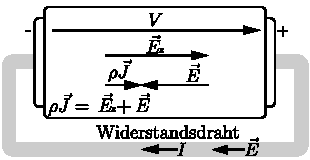
\includegraphics{res/Urspannung.pdf}
		   \end{center}
	   Im Gebiet elektromotorischer Kräfte gilt das erweiterte Ohmsche Gesetz (wobei $\rho$  der spezifische Widerstand in der Zelle ist):
	   \begin{equation}
	   	\vec{J}=\frac{\vec{E}_\mathrm{E}+\vec{E}}{\rho}
	   \end{equation}
	   Eine Ladung $q$ verschiebende Kraft ist dort entsprechend gleich $\vec{F}=q\left(\vec{E}_\mathrm{E}+\vec{E}\right)$.  Im Fall des Leerlaufes gilt $\vec{E} =- \vec{E}_\mathrm{E}$. Das bedeutet, dass die von den Polladungen hervorgerufene elektrische Feldstärke die eingeprägte elektrische Feldstärke kompensiert, sodass keinerlei Ladung in der Zelle transportiert wird. Also gilt für die Urspannung: $$V=\int\limits_{-\to +} \vec{E}_\mathrm{E}\cdot \dd\vec{s}=\int\limits_{+\to-} -\vec{E}_\mathrm{E}\cdot \dd\vec{s}=\int\limits_{+\to -} \vec{E}\cdot \dd\vec{s}=U_Q$$ \textbf{Beachte:} $V$ zeigt von \enquote{- nach +} $U_Q$ wie immer von \enquote{+ nach -}, die Urspannung treibt einen elektrischen Strom \textit{in}, die Quellenspannung \textit{entgegen} seiner Richtung an (haben $U_Q$ und $V$ die selbe Zählpfeilrichtung sind sie also vorzeichenverschieden).  Die Urspannung wird demnach im Leerlauf an den Anschlüssen als Quellspannung messbar. Wie die Quellspannung ist die Urspannung und damit auch $\vec{E}_E$ \textbf{belastungsunabhängig} (der Spannungsabfall bei Belastung erfolgt über den Innenwiderstand). Außerdem gilt für die elektrochemische Zelle wie oben (es ist der Entladefall skizziert):
\begin{equation}
	I\hat{R}=I\oint\frac{\rho(s)}{A}\mathrm{d}s=\oint\rho\vec J\mathrm{d}\vec s=\oint(\vec E_\mathrm{E} + \vec E)\mathrm{d}\vec s=\oint\vec E_\mathrm{E}\mathrm{d}\vec s=V=U_Q
\end{equation}
Mit $\hat{R}=R_i+R_a$ als Umlaufwiderstand des Stromkreises, $A$ als (ortsabhängigem) Querschnittsflächeninhalt und $\rho(s)$ als (ortsabhängigem) spezifischen Widerstand. Die Integrale sind entsprechend der Skizze im Uhrzeigersinn orientiert.\\
 Anhand der Pfeile in der Zeichnung kann man sich einige Dinge veranschaulichen, die man von der Modellierung einer Zelle als Spannungsquelle $U_Q$ mit Innenwiderstand $R_i$ und einer resistiven Last $R_a$ erwarten würde. Nachfolgend zwei Beispiele:
 \begin{itemize}
  \item Liegt Leerlauf vor fließt kein Strom, es gilt $\rho_i J = 0$, also ist $E_\mathrm{E}=-E$ in der Zelle. Das $E$ in der Zelle hat den maximal möglichen Wert, da das Ringintegral über $E$ verschwindet hat auch das $E$ außerhalb der Zelle den maximal möglichen Wert, es fällt die gesamte Spannung $U_Q$ an der unendlichen Last $R_a\to\infty$ ab. 
  \item Vergrößert sich $R_i,\rho_i$ bei konstantem $U_Q,E_\mathrm{E}$ und $R_a,\rho_a$ dann wächst der Pfeil $\rho_i J \propto \frac{\rho_i}{\rho_i+\rho_a}$. Der $E$-Pfeil schrumpft entsprechend, weil $E_\mathrm{E}$ gleich groß bleibt. Also sinkt auch das $E$ außerhalb der Zelle, an $R_a$ fällt eine geringere Spannung ab wodurch ein geringerer Strom fließt.
  \end{itemize}
  \subsubsection{Induktion}
  Die Induktion wird genauer in \ref{induktion} betrachtet ($V\leftrightarrow\mathcal{E}$). \\
  Ganz analog zu der chemischen Zelle kann man z.B. einen Transformator betrachten, welcher auf Basis von Induktion funktioniert und als konzentriert angenommen wird. Gilt $-\frac{\dd \Phi}{\dd t}=\mathcal{E}=\const$ (was praktisch natürlich auf Dauer unmöglich ist), sind die Überlegungen vollkommen identisch zu denen an der elektrochemischen Zelle. Zunächst soll von Leerlauf ausgegangen werden. In diesem Fall wird aufgrund der durch die Induktion eingeprägten Feldstärke $E_\mathrm{E}$ eine Ladungsträgerbewegung hervorgerufen. Es kommt zu einer Ladungstrennung, wodurch ein elektrisches Feld $E$ entsteht, welches $E_\mathrm{E}$ entgegen gerichtet ist. Relativ schnell kommt es zum Gleichgewicht zwischen beiden Feldstärken, es fließt kein Strom mehr. An den Kontakten ist eine Spannung von $\mathcal{E}=El$ messbar.\\
  Wenn hingegen eine resistive Last angeschlossen ist, dann ist das elektrische Feld $E$, welches durch die Ladungstrennung hervorgerufen wird, nicht stark genug, um $E_\mathrm{E}$ auszulöschen. Es kommt zu einer Ladungsträgerbewegung, welche in der Region des Transformators von $-$ nach $+$ gerichtet ist (Orientierung von $E_\mathrm{E}$). Dieser stellt deshalb eine Quelle dar.\\
  Einen Sonderfall stellt eine vollkommen homogene Leiterschleife dar, hier ist die eingeprägte Feldstärke $E_\mathrm{E}$ überall (verteilte Quelle). Dadurch, dass der spezifische Widerstand überall gleich ist, kommt es nicht zu einem Ladungsstau und entsprechend auch nicht zu einer Bildung der Feldstärke $E$, die wegen Ladungsdifferenzen entsteht. Fügt man in die Schleife nun doch einen Widerstand (Länge $l\ll l'$ der Schleife) ein, kommt es zu einem Ladungsstau. Es bilden sich durch die Ladungstrennung die Feldstärken $E'$ in der Schleife und $E$ im Widerstand heraus, es gilt $El+E'l'=0$. Im Widerstand (Senke) fließt die Ladung von $+$ nach $-$, hier überwiegt die Feldstärke $E$ deutlich die überall gleiche Feldstärke $E_\mathrm{E}$, im Rest der Schleife (Quelle) überwiegt $E_\mathrm{E}$. \\
  Auch den Spannungsabfall über eine Spule kann man ähnlich erklären. Durch Selbstinduktion kommt es zu einem $E_\mathrm{E}$ entgegen der Stromrichtung. Um den Strom aufrecht zu erhalten ist ein größeres $E$ (also größeres $U$), welches dem $E_\mathrm{E}$ entgegen gerichtet ist, nötig. $E_\mathrm{E}$ kann $E$ niemals überkompensieren, da sonst Energie aus dem Nichts erzeugt werden würde.
 \subsubsection{Maschensätze}
 Üblicherweise berücksichtigt man die stromtreibende Wirkung der Quellen durch deren Quellspannung, man kann aber auch die Urspannung berücksichtigen. Es ergeben sich zwei Formulierungen des \textbf{Kirchhoffschen Maschensatzes} mit der...
\begin{equation}\label{masche}
	\text{...Quellspannung: } \sum U = 0\quad\Leftrightarrow\quad \text{...Urspannung: } \sum V = \sum U 
\end{equation}


 \subsection{Relaxationszeit}\label{relax}
  Einerseits gilt mit \ref{gauss}: $$\div \vec{E} = \dfrac{\rho_\text{V}}{\varepsilon_0}\implies\div \vec{J} = \dfrac{\kappa \cdot \rho_\text{V}}{\varepsilon_0} $$
	   Andererseits gilt wegen der Stationarität und \ref{kont}: $$\div \vec{J} = -\dfrac{\partial \rho_\text{V}}{\partial t} \stackrel{!}{=} 0$$
	   Ist die Volumenladungsdichte $\neq 0$ stellt das einen Widerspruch dar. Subtraktion der beiden Terme für $\div \vec{J}$ liefert eine Differentialgleichung für die Volumenladungsdichte \(\rho_\text{V} \):
	        \begin{equation}
		        \dot{\rho_\text{V}} + \dfrac{\kappa}{\varepsilon_0} \cdot \rho_\text{V} = 0
	        \end{equation}
	   Deren Lösung lautet:
	        $$\rho_\text{V}(t) = \rho_\mathrm{V_0} \cdot \mathrm{e}^{-\frac{\kappa}{\varepsilon_0} \cdot t}$$
	   Für Kupfer gelten \(\varepsilon_0 = 8,85\cdot 10^{-12}\mathrm{  \frac{A s}{Vm}} \) und \(\kappa_\mathrm{Cu} = 58\cdot 10^6\mathrm{  \frac{S}{m}}\). Das liefert eine Zeitkonstante zur Erreichung des Gleichgewichtes:
	        \begin{equation}
		        \tau_\mathrm{Cu} = \dfrac{\varepsilon_0}{\kappa_\mathrm{Cu}} \cong 1,5\cdot 10^{-19}\mathrm{s}
	        \end{equation}
	        Ist $\tau_\text{Cu}$ ein paar mal verstrichen (was näherungsweise sofort passiert), gibt es keinen Widerspruch mehr. Gibt es eine Volumenladungsdichte, löst diese sich sehr schnell auf. $\div \vec{J}\approx 0$ nach sehr kurzer Zeit. Die Relaxationszeit entscheidet also letztlich darüber, ob ein Vorgang stationär ist oder nicht. Ist sie groß, führt die Anwendung des Modells des sationären Strömungsfeldes auf Widersprüche. Beim Anlegen einer Quelle an ein Material mit großer Relaxationszeit startet ein langer Ausgleichsprozess.
\section{Widerstand und Leistung}
Im Folgenden wird angenommen, dass Stromdichte konstant über den Leiterquerschnitt ist, was für dünne Leiter in der Regel gerechtfertigt ist.
Leiterquerschnittsfläche $F$, Leiterlänge $l$:
\begin{equation}\begin{split}
		I&=J\cdot F =\kappa E F = \frac{\kappa F}{l} El = \frac{\kappa F}{l} U\\
		I&= \frac{1}{R} U \to \boxed{R = \frac{1}{\kappa} \frac{l}{F}}\;\text{ ohmscher Widerstand}
\end{split}\end{equation}
Kann man die Annahme der konstanten Stromdichte über den Leiterquerschnitt nicht treffen, muss man allgemeiner rechnen (andere Möglichkeiten $\nearrow$ EMF):
\begin{equation}
	R_{\vec{r}_1\vec{r}_2} = \frac{U}{I} = \frac{\int\limits_{\vec{r_1}}^{\vec{r_2}} \vec{E}(\vec{r}')   d\vec{r}'}{\iint\limits_F \vec{J}   \dd\vec{F}}
\end{equation}
Um auf die Leistung zu kommen wird die Verschiebung eines Quaders mit der Ladung $\Delta Q$, dem Querschnitt $\Delta F$ und der Länge $\Delta\vec{s}$:
$$
P = \frac{\Delta W}{\Delta t} = \frac{\Delta Q \vec{E}\cdot \Delta\vec{s}}{\Delta t}
= \rho_V\Delta F\Delta s \vec{E}\cdot\vec{v}_D = \vec{J}\cdot \vec{E} \Delta F\Delta s = \frac{1}{\kappa}|\vec{J}|^2\Delta F\Delta s$$
Damit resultiert die Verlustleistungsdichte (Beachte die Vernachlässigung des B-Feldes in\ref{ohm}, $\Delta V=\Delta s \Delta F$):
\begin{equation}\label{verlustleist}
	\boxed{p_\text{V} = \lim\limits_{\Delta V \rightarrow 0} \dfrac{ P}{\Delta V} = \dfrac{1}{\kappa} \cdot \vec{J}^2 = \vec{E} \cdot \vec{J}}
\end{equation}
Daraus resultiert das \textbf{Joulesche Gesetz} für dünne Leiter, in dem man die Stromdichte als konstant über den Leiterquerschnitt annehmen kann:
\begin{equation}
	\int\limits_V\vec{E}\vec{J}\dd V = EJV= EsJF = UI \implies \boxed{ P =  R \cdot  I^2 =  U \cdot  I}
\end{equation}
 \section{Vergleich mit Elektrostatik}
  \begin{tabular}{>{\centering}p{0.33\textwidth}>{\centering}p{0.33\textwidth}>{\centering\arraybackslash}p{0.33\textwidth}}
	  Elektrostatik                                                                    &                                                   & stat. el. Strömungsfeld                                                            \\
	  \hline
	  \(\vec{D}  = \varepsilon \cdot \vec{E} \)                                        & \quad                                             & \(\vec{J} = \kappa \cdot \vec{E} \)                                                \\
	  %\addlinespace
	  \(\vec{D}  = -\varepsilon \cdot \grad \phi \)                                    &                                                   & \(\vec{J} = -\kappa \cdot \grad \phi \)                                            \\
	  %\addlinespace
	  im Ladungsfreien Raum                                                            &                                                   & im stationären Fall                                                                \\
	  \(\div \vec{D}  = 0 \)                                                           &                                                   & \(\div \vec{J} = 0 \left( = -\dfrac{\partial \rho_\text{V}}{\partial t} \right) \) \\
	  %\addlinespace
	                                                                                   & im homogenen Raum                                    &                                                                                    \\
	                                                                                   & (\(\varepsilon = \const \), \(\kappa = \const \)) &                                                                                    \\
	                                                                                   & \(\Delta \phi = 0 \)                              &                                                                                    \\
	  %\addlinespace
	  %\multicolumn{3}{c}{Brechung nach \figref{fig:Brechung}}\\
	  \(D_2^\text{n} - D_1^\text{n} = 0 \)                                             &                                                   & \({J}_2^\text{n} - {J}_1^\text{n} = 0 \)                                   \\
	  %\addlinespace
	                                                                                   & \(E_2^\text{t} - E_1^\text{t} = 0 \)              &                                                                                    \\
	  \(\dfrac{D_2^\text{t}}{\varepsilon_2} = \dfrac{D_1^\text{t}}{\varepsilon_1} \)   &                                                   & \(\dfrac{J_2^\text{t}}{\kappa_2} = \dfrac{J_1^\text{t}}{\kappa_1} \)               \\
	  %\addlinespace
	  \(\dfrac{\tan \alpha_1}{\tan \alpha_2} = \dfrac{\varepsilon_1}{\varepsilon_2} \) &                                                   & \(\dfrac{\tan \alpha_1}{\tan \alpha_2} = \dfrac{\kappa_1}{\kappa_2} \)             \\

  \end{tabular}\\[0.2cm]
  \centerline{$\to$ \textbf{Lösungsmethoden können übernommen werden!}}
  \centerline{\textbf{Beachte:} Die Winkel $\alpha_i$ sind die Winkel zur Flächennormale. Siehe auch: \ref{normD}, \ref{tanE}.}
  
\chapter{Magnetostatik}\label{ms}
 \section{Grundgleichungen, Größen, Begriffe}
		  Die Magnetostatik betrachtet \textbf{zeitunabhängige} magnetische Felder soweit diese durch \textbf{Gleichströme} verursacht werden. Konstante magnetische Felder durch permanentmagnetische Stoffe werden in diesem Dokument nicht betrachtet.
		   Wesentlicher Unterschied zur Elektrostatik ist, dass es \textbf{keine magnetischen Monopole} gibt (jedenfalls keine, die nicht immer paarweise auftreten $\to$ \textbf{Spineis}). Führender Term ist also der Dipolterm.
		   Die \textbf{Grundgleichungen} sind mit \ref{GGms1} und \ref{GGms2} gegeben.
	 		Zusätzlich gilt die Materialgleichung aus \ref{matmagallg}. $\vec{B}$ und $\vec{H}$ sind i.A. nicht parallel, die Parameter sind ortsabhängig, es gibt Nichtlinearitäten und Zeitabhängikeiten ($\nearrow$\ref{mat}). Für homogene, lineare und isotrope Medien vereinfacht sich die Gleichung zu \ref{matlinhomis}. Im Vakuum gilt die selbe Gleichung (mit $\mu=\mu_0$).
	\subsection{Vektorpotential und Eichtransformation}
	\subsubsection{Begriff Vektorpotential}
		   In der Elektrostatik folgte aus $\rot \vec{E} = \vec{0}$, dass das elektrische Feld ein Gradientenfeld ist: $\vec{E} = -\grad \phi$.
		   Das ist in der Magnetostatik wegen \(\rot \vec{H}  = \vec{J} \neq \vec{0} \) nicht der Fall. Aber mit \(\div \vec{B}  = 0 \) folgt, dass \(\vec{B}  \) \textbf{quellenfrei} ist und somit als Rotation eines Vektorfeldes dargestellt werden kann ($\nearrow$\ref{poin2},\ref{helmholtz}). Das entsprechende Feld $ \vec{A}$ wird \textbf{magnetisches Vektorpotential} genannt:
		        \begin{equation}\label{magvekpot}\begin{split}
				        \boxed{\vec{B}  = \rot  \vec{A}}
			        \end{split}\end{equation}
		 Der Vorteil dieser Darstellung ist, dass $\div \vec{B}  = 0$ automatisch erfüllt ist. Im linearen und isotropen, aber \textbf{inhomogenen} Medium gilt nach \ref{matmagallg}: 
		        \begin{equation}\begin{split}
				      \vec{B}  = \mu(\vec{r} )\vec{H} \implies  \rot \vec{H}  = \rot \left( \dfrac{1}{\mu(\vec{r} )}  \vec{B}  \right) = \boxed{\rot \left( \dfrac{1}{\mu(\vec{r} )} \rot  \vec{A} \right) = \vec{J}(\vec{r} )}
			        \end{split}\end{equation}
		       Im zusätzlich homogenen Medium (\(\mu(\vec{r} ) = \mu \)) resultiert:
		        \begin{equation}\begin{split}
				        \mu \rot \vec{H}  = \rot \vec{B}  = \rot \, \rot  \vec{A} = \boxed{\grad \div  \vec{A} - \Delta  \vec{A}= \mu \vec{J}(\vec{r} )}
			        \end{split}\end{equation}
		        Der Laplace-Operator ist hier vektoriell.
  \subsubsection{Eichtransformation}\label{eichtrans}
		 Wegen $\rot \grad \psi =\vec{0}$ ist:
		        $$
			        \vec{B} ' = \rot \underbrace{\left( \vec{A} + \grad \psi\right)}_{ \vec{A}'} = \rot  \vec{A} = \vec{B}
		        $$
		  Das Vektorpotential ist folglich nur bis auf einen Summanden $\grad \psi$ bestimmt.
		  Dies kann weiter auf $\rot \, \rot  \vec{A} = \mu \vec{J}$ angewandt werden. Auch hier sieht man, dass $A'$ die Gleichung löst, wenn $A$ die Gleichung löst:
		        $$
			        \rot \, \rot  \vec{A}' = \rot \, \rot  \vec{A} = \mu \vec{J}(\vec{r} )
		        $$
		   Den Übergang
		   \begin{equation}
		    \boxed{ \vec{A}' =  \vec{A} + \grad \psi}
		    \end{equation}
		     nennt man \textbf{Eichtransformation} ($\nearrow$\ref{geneich}). Da $\vec{B} '=\vec{B} $ gilt, heißt die magnetische Flussdichte \textbf{eichinvariant}. Für die Divergenz gilt:
		        $$
			        \div  \vec{A}' = \div \left( \vec{A} + \grad \psi \right) = \underbrace{\div \vec{A}}_{=0\nearrow\text{\ref{divrot}}}  + \underbrace{\div \grad \psi}_{\ne 0}
		        $$
		    Man kann erkennen, dass die Divergenz von $A'$ eine andere ist, als die Divergenz von $A$, obwohl $B$ bei $A$ und $A'$ gleich ist. In ${\grad \textcolor{red}{\div  \vec{A}} - \Delta  \vec{A}= \mu \vec{J}(\vec{r} )}$ kann $\div  \vec{A}$ also \textbf{beliebig} (aber physikalisch sinnvoll, mathematisch muss ein $\psi$ gefunden werden können, sodass $\div\vec{A}=\Delta \psi$ gilt) gewählt werden, ohne dabei das resultierende $\vec{B}$ zu verändern. Für statische Probleme ist die \textbf{Coulomb-Eichung} ($\nearrow$\ref{couleich}) gut geeignet:
			        \begin{equation}\label{vektorpot}
			        	    \boxed{\div  \vec{A} = 0} \quad \implies \quad \boxed{\Delta  \vec{A}= -\mu \vec{J}(\vec{r} )}
			        \end{equation}			        
			   \textbf{Achtung:} Der Laplace-Operator $\Delta $ für Vektorfelder muss im allgemeinen Fall (krummlinige Koordinaten) aus der Beziehung $\Delta \cdot = \grad \, \div \cdot - \rot \, \rot \cdot$ ausgerechnet werden, bzw. muss eine Produktregel angewandt werden ($\nearrow$ \ref{laplaceop}). Hierbei \enquote{vermischen} sich die Komponenten wegen der Ortsabhängigkeit der Einheitsvektoren. \textbf{Nur für kartesische Koordinaten} zerfällt die vektorielle Poissongleichung in drei skalare Poissongleichungen:
			        \begin{equation}\begin{split}
					        & \Delta  A _\mathrm{x} = -\mu  J_\mathrm{x}\\
					        & \Delta  A _\mathrm{y} = -\mu  J_\mathrm{y}\\
					        & \Delta  A _\mathrm{z} = -\mu  J_\mathrm{z} \text{ mit} \\
					        &  \vec{A} =  A _\mathrm{x}  \vu{x} +  A _\mathrm{y}  \vu{y} +  A _\mathrm{z}  \vu{z}\\
					        & \vec{J} = J_\mathrm{x}  \vu{x} + J_\mathrm{y}  \vu{y} + J_\mathrm{z}  \vu{z} \\
					        &\Delta = \dfrac{\partial^2}{\partial x^2} + \dfrac{\partial^2}{\partial y^2} + \dfrac{\partial^2}{\partial z^2} \text{ (skalarer Laplace-Operator)}
				        \end{split}\end{equation}
			   z.B. in Zylinderkoordinaten (\(\rho,\,\varphi,\,z \)) ergibt sich
			        \begin{equation}\begin{split}
					        \Delta  A _{\rho} - \dfrac{2}{\rho^2} \dfrac{\partial  A _{\varphi}}{\partial \varphi} - \dfrac{ A _{\rho}}{\rho^2} &= -\mu J_{\rho} \\
					        \Delta  A _{\varphi} + \dfrac{2}{\rho^2}  \dfrac{\partial  A _{\rho}}{\partial \varphi} - \dfrac{ A _{\varphi}}{\rho^2} &= -\mu J_{\varphi} \\
					        \Delta  A _\mathrm{z} &= -\mu  J_\mathrm{z}
				        \end{split}\end{equation}
			        mit
			        \begin{equation}
				        \Delta = \dfrac{1}{\rho} \dfrac{\partial}{\partial \rho} \rho \dfrac{\partial}{\partial \rho} + \dfrac{1}{\rho^2} \dfrac{\partial^2}{\partial \varphi^2} + \dfrac{\partial^2}{\partial z^2} \text{ (skalarer Laplace-Operator)}
			        \end{equation}
			        Insbesondere sieht man hier, dass die Laplace-Gleichung für den Vektor $\vec{A}$ nicht den Laplace-Gleichungen für die Komponenten $A_\varphi$ und $A_\varrho$ entspricht, wie es kartesisch der Fall wäre. Während man im kartesischen Fall die Projektion auf die Einheitsvektoren in den Laplace-Operator hineinziehen kann, geht das im Fall nicht konstanter Einheitsvektoren nicht.
  \subsection{Berechnung des Vektorpotentials und der Flussdichte}
  \subsubsection{Vektorpotential}
		  Für den Fall \textbf{kartesischer Koordinaten} ergeben sich drei Poisson-Gleichungen (offensichtlich nicht für Zylinderkoordinaten). Es sind also die in der Elektrostatik behandelten Lösungsmethoden ($\nearrow$\ref{poilsg}) anwendbar.  Analog zu \ref{PotR} ergibt sich
		        \begin{equation}\begin{split}
				        &  A _\mathrm{x}(\vec{r} ) = \dfrac{\mu}{4 \pi} \iiint\limits_{V} \dfrac{J_\mathrm{x}(\vec{r}' ) }{\left| \vec{r}  - \vec{r}'  \right|} \dd V' \\
				        &  A _\mathrm{y}(\vec{r} ) = \dfrac{\mu}{4 \pi} \iiint\limits_{V} \dfrac{J_\mathrm{y}(\vec{r}' ) }{\left| \vec{r}  - \vec{r}'  \right|} \dd V' \\
				        &  A _\mathrm{z}(\vec{r} ) = \dfrac{\mu}{4 \pi} \iiint\limits_{V} \dfrac{J_\mathrm{z}(\vec{r}' ) }{\left| \vec{r}  - \vec{r}'  \right|} \dd V'
			        \end{split}\end{equation}
		         Das Ergebnis ist eine partikuläre Lösung der Poisson-Gleichung und lässt sich wieder \textbf{koordinatenfrei} schreiben (dieses Ergebnis stimmt für beliebige Koordinaten):
		        \begin{equation} \label{Akoordfrei}
			        \boxed{ \vec{A}(\vec{r} ) = \dfrac{\mu}{4 \pi} \iiint\limits_{V} \dfrac{\vec{J}(\vec{r}' )}{\left| \vec{r}  - \vec{r}'  \right|} \dd V'}
		        \end{equation}
		  Für einen \textbf{Stromfaden} (Draht) folgt der Spezialfall (Aufteilung der Integration auf Querschnittsfläche und Linienintegral entlang des Stromfadens)
		        \begin{equation}\label{Astromfad}
			       \boxed{ \vec{A}(\vec{r} ) = \dfrac{\mu}{4  \pi}   I  \oint\limits_{C} \dfrac{\dd \vec{r}'}{\left| \vec{r}  - \vec{r}'  \right|}}
		        \end{equation}
  \subsubsection{Berechnung der magnetischen Flussdichte - Gesetz von Biot-Savart}
		   Mit \ref{magvekpot} und \ref{Akoordfrei} folgt
		        $$
			        \vec{B} (\vec{r} ) = \dfrac{\mu}{4 \pi} \iiint\limits_{V} \rot _\mathrm{r} \dfrac{\vec{J}(\vec{r}' )}{\left| \vec{r}  - \vec{r}'  \right|} \dd V'
		        $$
		   Man berechnet
		        \begin{equation}\begin{split}
				        \rot _\mathrm{r} \dfrac{\vec{J}(\vec{r}' )}{\left| \vec{r}  - \vec{r}'  \right|} &= \dfrac{1}{\left| \vec{r}  - \vec{r}'  \right|}  \cancelto{0}{\rot _\mathrm{r} \vec{J}(\vec{r}' )} - \vec{J}(\vec{r}' ) \times \grad _\mathrm{r} \dfrac{1}{\left| \vec{r}  - \vec{r}'  \right|} \\
				        &= -\vec{J}(\vec{r}' ) \times \grad _\mathrm{r} \dfrac{1}{\left| \vec{r}  - \vec{r}'  \right|} = -\vec{J}(\vec{r}' ) \times \left( -\dfrac{\left( \vec{r}  - \vec{r}'  \right)}{\left| \vec{r}  - \vec{r}'  \right|^3} \right) = \vec{J}(\vec{r}' ) \times \dfrac{\vec{r}  - \vec{r}' }{\left| \vec{r}  - \vec{r}'  \right|^3}
			        \end{split}\end{equation}
		   Damit folgt das das allgemeine \textbf{Biot-Savart-Gesetz}:
		        \begin{equation}\label{biot-savart}
			        \boxed{\vec{B} (\vec{r} ) = \dfrac{\mu}{4  \pi} \iiint\limits_{V} \dfrac{\vec{J}(\vec{r}' ) \times \left( \vec{r}  - \vec{r}'  \right)}{\left| \vec{r}  - \vec{r}'  \right|^3} \dd V'}
		        \end{equation}
		  Für Stromfäden folgt:
		        \begin{equation}
			        \boxed{\vec{B} (\vec{r} ) = -\dfrac{\mu}{4  \pi}   I  \oint\limits_{C} \dfrac{\left( \vec{r}  - \vec{r}'  \right) \times \dd \vec{r}'}{\left| \vec{r}  - \vec{r}'  \right|^3}} 
		        \end{equation}	
  \subsection{Energie im magnetostatischen Feld}
		   Analog zur Elektrostatik erhält man für die \textbf{magnetische Energiedichte}:
		        \begin{equation}\label{edichteH}
			        \boxed{  w _\mathrm{m} = \dfrac{1}{2} \cdot \vec{H}  \cdot \vec{B} }
		        \end{equation}
		   Für die gesamte \textbf{magnetische Energie}:
		        \begin{equation}
			        \boxed{ W _\mathrm{m} = \dfrac{1}{2} \cdot \iiint\limits_{V} \vec{H}  \cdot \vec{B}  \dd V}
		        \end{equation}
		    Für lineare, homogene und isotrope Medien gilt:
		        \begin{align*}
			       & & W _\mathrm{m} &= \dfrac{1}{2 \mu} \cdot \iiint\limits_{V} \vec{B} ^2 \dd V\\
				        \text{mit}&& \div \left(  \vec{A} \times \vec{B}  \right) &= \vec{B}  \cdot \underbrace{\rot  \vec{A}}_{\vec{B} } -  \vec{A} \cdot \underbrace{\rot \vec{B} }_{\mu \vec{J}} \\
				        &&&= \vec{B} ^2 - \mu   \vec{A} \cdot \vec{J}\\
			       				      \implies&&  W _\mathrm{m} &= \dfrac{1}{2}  \iiint\limits_{V}  \vec{A} \cdot \vec{J} \dd V + \dfrac{1}{2 \mu} \cdot \iiint\limits_{V} \div \left(  \vec{A} \times \vec{B}  \right) \dd V\\
				       && &= \dfrac{1}{2}\iiint\limits_{V}  \vec{A} \cdot \vec{J} \dd V + \dfrac{1}{2 \mu} \oiint\limits_{O(V)}  \vec{A} \times \vec{B}  \cdot \dd\vec{F}
			        \end{align*}
		    Aus Biot-Savart folgt \(\left| \vec{B}  \right| \sim r^{-2} \) bei einer \textbf{endlich ausgedehnten Stromverteilung}.  Weiterhin ist in diesem Fall \(\left|  \vec{A} \right| \sim r^{-1} \), sodass \( \vec{A} \times \vec{B}  \sim r^{-3} \) gilt. Integriert man über den kompletten Raum, dann ist das Oberflächenintegral $\iiint\limits_{O(V)}...$ folglich null (die Fläche wächst nur $\sim r^2$). Das Volumenintegral muss in allen Bereichen ausgewertet werden, in denen $J\neq 0$:
		        \begin{equation}\begin{split}
				          \Aboxed{W _\mathrm{m}& = \dfrac{1}{2} \cdot \iiint\limits_{V}  \vec{A} \cdot \vec{J} \dd V}\\
				          \Aboxed{ w _\mathrm{m}& = \dfrac{1}{2} \cdot  \vec{A} \cdot \vec{J} }
			        \end{split}\end{equation}
  \subsection{Induktivität}
	  \begin{center}
		  \begin{tikzpicture}[line width = 1.2pt, line join=round,x=1cm,y=1cm,>=stealth, scale = 3]
	% Schleife 1
	\coordinate (a) at (1,0.5);
	\coordinate (b) at (1.6,0.3);
	\coordinate (c) at (2.1,0.4);
	\draw plot [smooth cycle, tension=0.8] coordinates {(2.1,1) (1.65,1.2) (1,1.2) (0.6,0.8) (a) (b) (c) (2.15,0.7)} node [anchor=west] {$ 1 $};
	% Strom 1
	\draw [->, color=violet] (a) -- (b) node [anchor = north,midway] {$  I_1 $};
	% differentieller Weg 1
	\draw [->, color = blue]  (c) -- ++(0.3,0.3) node[anchor=west] { $ \dd  \vec{r}'_1 $ };
	% magnetische Flussdichte
	\draw [->,color=red] (0.8,0.8) .. controls (1,1.3) and (0.9,1.8) .. (0.7,2.2) node[anchor=south east]{$ \vec{B} _1 $};
	\draw [->,color=red] (1.2,0.8) .. controls (1.4,1.4) and (1.4,2.1) .. (1.3,2.6) node[anchor=south]{$ \vec{B} _1 $};
	\draw [->,color=red] (1.6,0.7) .. controls (1.5,1.4) and (1.9,2) .. (2.2,2.5) node[anchor=south]{$ \vec{B} _1 $};
	\draw [->,color=red] (2,0.6) .. controls (1.8,1.1) and (2,1.5) .. (2.2,1.8) node[anchor=south west]{$ \vec{B} _1 $};
	% Schleife 2
	\coordinate (ab) at (1.5,1.9);
	\coordinate (bb) at (0.9,2.1);
	\draw plot [smooth cycle, tension=0.8] coordinates {(2,2.3) (1.7,2.2) (bb) (ab) (2,2) (2.2,2.15) } node[anchor=west]{$ 2 $};
	% differentieller Weg 2
	\draw [->,color=blue] (ab) -- ++(0.5,0) node[anchor = west] { $ \dd  \vec{r}'_2 $ };
	% Ortsvektoren
	\draw [->,color=green] (0,0) -- (a) node[anchor=north west,midway] {$ \vec{r}' _1 $};
	\draw [->,color=green] (0,0) -- (bb) node[anchor=west,midway] {$ \vec{r}' _2 $};
	\draw [->,color=green] (0,0) -- (0.3,2.4) node[anchor=east,midway] {$ \vec{r}  $};
\end{tikzpicture}
	  \end{center}
		   In der Schleife 1 fließt der Strom \( I_1 \). Nach Biot-Savart gilt also:
		        \begin{equation}
			        \vec{B} _1 = -\dfrac{\mu_0}{4 \pi} I_1 \oint\limits_{C_1} \dfrac{\left( \vec{r}  - \vec{r}' _1 \right) \times \dd \vec{r}'_1}{\left| \vec{r}  - \vec{r}' _1 \right|^3}
		        \end{equation}
		   Der magnetische Fluss (in der zweiten Schleife hervorgerufen durch den Strom in der ersten Schleife) $\phi_{m,21}$ durch die Schleife 2 ist demnach:
		        \begin{equation}\label{fluss1}
			        \phi_{m,21} = \iint\limits_{F_2} \vec{B} _1 \cdot \dd\vec{F}_2, \quad \left| \vec{B} _1 \right| = B_1 \sim  I_1
		        \end{equation}
		   Mit der Gleichung 
		   \begin{equation} \label{gegeninddef}
		  \boxed{\phi_{m,21} = M_{21}  I_1}
	\end{equation} wird $ M_{21}$ als \textbf{Gegeninduktivität} definiert. Um eine Berechnungsvorschrift für $ M_{21}$ zu erhalten, wird \ref{fluss1} näher betrachtet  (\(\vec{r}' _2 \) liegt auf \(C_2 \)):
	  \begin{equation}
		  \phi_{m,2} = \iint\limits_{F_2} \vec{B} _1 \cdot \dd\vec{F}_2 = \iint\limits_{F_2} \rot  \vec{A}_1 \cdot \dd\vec{F}_2 \stackrel{\text{\ref{stokes}}}{=} \oint\limits_{C_2}  \vec{A}_1 \cdot \dd\vec{r}'_2 \stackrel{\text{\ref{Astromfad}}}{=} \dfrac{\mu_0}{4 \pi}   I_1 \oint\limits_{C_2} \oint\limits_{C_1} \dfrac{\dd  \vec{r}'_1}{\left| \vec{r}' _2 - \vec{r}' _1 \right|} \cdot \dd\vec{r}'_2
	  \end{equation}
		Durch Koeffizientenvergleich mit \ref{gegeninddef} folgt eine Formel für die Gegeninduktivität:
		        \begin{equation}
		        \boxed{ M_{21} = \dfrac{\mu_0}{4 \pi}  \oint\limits_{C_2} \oint\limits_{C_1} \dfrac{\dd  \vec{r}'_1 \cdot \dd \vec{r}'_2}{\left| \vec{r}' _2 - \vec{r}' _1 \right|} } 
		        \end{equation}
		   Diese Formel wird \textbf{Neumann-Formel} genannt, ist aber nicht besonders nützlich zur Berechnung von \( M_{21} \). Dennoch können aus ihr wichtige Eigenschaften abgelesen werden:
		        \begin{enumerate}
			        \item \( M_{21} =  M_{12} =  M \) 
			        \item \( M_{21} \) ist zunächst eine rein geometrische Größe, in der Berechnung von $M$ kommen nur Konstanten und geometrische Parameter vor. Erst wenn Ursache und Wirkung mit Richtungssinn bekannt sind, kann man $M$ vorzeichenbehaftet interpretieren (bspw. können Spulen gleich- oder gegensinnig gekoppelt sein, was im Vorzeichen von $M$ berücksichtigt werden kann $\nearrow$ EMF).
		        \end{enumerate}
		   Wenn \(C_1 = C_2 \) ist, dann ist die Neumann-Formel so nicht anwendbar (Singularitäten, da $\vec{r}' _2 = \vec{r}' _1$). Der Fluss in der Leiterschleife 1 hervorgerufen durch den Strom in der Leiterschleife 1 berechnet sich durch:
		        \begin{equation}
			        \phi_{m,11} =  M_{11} \cdot  I_1 \xrightarrow{\text{umbenennen}} \boxed{\phi_{m,11} =  L_1 \cdot  I_1 } 
		        \end{equation}
		    Dabei ist $L$ die \textbf{Selbstinduktivität}. Durch Koeffizientenvergleich erhält man auch für diese eine Berechnungsvorschrift:
		        \begin{equation}\begin{split}
			        \phi_{m,11} &= \iint\limits_{F_1} \vec{B}_1  \cdot \dd\vec{F}_1 = \oint\limits_{C_1}  \vec{A}_1 \cdot \dd\vec{r}'_1  \stackrel{!}{=}  L_1  I_1 \\
			        \implies 	\Aboxed{ L_i &= \dfrac{1}{ I_i}\oint\limits_{C_i}  \vec{A_i} \cdot \dd\vec{r}'_i}
		        \end{split}\end{equation}
		   Für die magnetische Energie folgt für lineare, homogene und isotrope Medien (durch Zerlegung des Volumenintegrals in ein Flächen- und ein Wegintegral):
		        \begin{equation}
			        W _\mathrm{m} = \dfrac{1}{2}  \iiint\limits_{V}  \vec{A} \cdot \vec{J} \dd V
			        = \dfrac{1}{2}  I \underbrace{\oint\limits_{C}  \vec{A} \cdot \dd\vec{r}'}_{= L  I} = \dfrac{1}{2}  L  I^2
		        \end{equation}
		        Der Fall, dass beide Schleifen von einem Strom durchflossen sind oder die Schleifen mehrfach gewickelt sind (Windungszahl $w>1$) wurde in $\nearrow$ EMF Kapitel 5 betrachtet. Es ist zu beachten, dass dort das dynamische Magnetfeld behandelt wurde, während sich \textbf{hier} zunächst auf den \textbf{statischen Fall} beschränkt wird.
  \subsection{Magnetisches Moment}
		   Das Vektorpotential aus \ref{Akoordfrei} wird nun für den Fall von {großer Entfernung des Beobachtungspunktes zu der lokal beschränkten Stromdichte} untersucht. Dies läuft auf eine \textbf{Multipolentwicklung} hinaus, in großer Entfernung dominiert hier der Dipolterm, da der Monopolterm verschwindet (keine magnetischen Monopole). Setzt man \ref{Taylrrr} in das Integral ein, so gilt zunächst:
		   \begin{equation}
		   \vec{A}(\vec{r} ) = \frac{\mu}{4 \pi} \frac{1}{r}\iiint\limits_{V} \vec{J}(\vec{r}' ) \dd V'  + \frac{\mu}{4 \pi} \frac{1}{r^3}\iiint\limits_{V} \vec{r} \cdot \vec{r}'  \vec{J}(\vec{r}' ) \dd V' + \dots
		   \end{equation}
		    Damit folgt (Monopolterm verschwindet):
		         \begin{equation}
			        \vec{A}(\vec{r} ) = \frac{\mu}{4 \pi} \frac{1}{r^3}\iiint\limits_{V}\vec{r} \cdot \vec{r}'   \vec{J}(\vec{r}' ) \dd V' + \dots = \frac{\mu}{4 \pi} \underbrace{\frac{1}{2}\iiint\limits_{V} \vec{r}'  \times \vec{J}(\vec{r}' ) \dd V'}_{\vec{m}(\vec{r} )}  \times \frac{\vec{r} }{r^3}  + \dots
		        \end{equation}
		   Mit dem \textbf{magnetischem Moment} $\vec{m}$ ist das Vektorpotential somit:
		        \begin{equation}
			        \boxed{ \vec{A}(\vec{r} ) = \frac{\mu}{4 \pi} \frac{\vec{m}(\vec{r} )  \times \vec{r} }{r^3}  + \dots} \to \boxed{\vec{B} (\vec{r} ) = \frac{\mu}{4 \pi} \left[ \frac{3(\vec{r} \cdot \vec{m}(\vec{r} )) \vec{r}  }{r^5} -\frac{\vec{m}(\vec{r} )}{r^3}\right] + \dots}
		       \end{equation}

 \section{Materie}\label{magmaterial}
		  Wie bereits in \ref{materie} erwähnt wurde, gelten die Maxwell-Gleichungen des Vakuums ($\nearrow$\ref{mikrosmax}) \textbf{unverändert} in Materie. Allerdings müssten dann die \textbf{Bewegungen aller Ladungsträger} betrachtet werden, die aber nur zu einem Bruchteil zu einer \textbf{makroskopischen Stromdichte} beitragen. Analog der Elektrostatik bietet es sich an, eine makroskopische Betrachtung im Sinne von Mittelwerten anzustreben ($\nearrow$\ref{makrmax}).
		  \subsection{Makroskopische Größen}
		  Analog zum elektrischen Fall ($\nearrow$ \ref{DEMat}, in \ref{elmaterial} wird beispielhaft eine Vereinfachung der komplizierten Zusammenhänge ausgeführt) wird die Materialabhängigkeit der \textbf{Magnetisierung} $\vec M$ durch einen Parameter $\zeta_\mathrm m$ beschrieben. Wieder vereinfacht sich der Zusammenhang in der Näherung $\vec M=\frac{1}{\mu_0}\zeta_\mathrm m\vec B$.
		  Eingesetzt ergibt das:
		  \begin{equation}\vec{H}=\frac{1}{\mu_0}\vec{B}-\vec{M}=\frac{1}{\mu_0}\underbrace{\left( 1-\zeta_{\mathrm m} \right)}_{1/\mu_r}\vec{B}=\frac{1}{\mu_0\mu_r}\vec{B}=\frac{1}{\mu}\vec{B}\end{equation}
		  Historisch bedingt wird $\zeta$ durch $\chi$ ersetzt, es gilt $(1-\zeta_\mathrm m)\cdot (1+\chi_\mathrm m)=1$. Für kleine Werte gilt $\zeta_\mathrm m \approx \chi_\mathrm m$. Damit folgt:
		        \begin{align}\label{matmagallg}
			         & \boxed{\vec{H}  = \dfrac{1}{\mu_0} \vec{B}  - \vec{M}}
			         &                                                        & \Leftrightarrow
			         &                                                        & \boxed{\vec{B}  = \mu_0  \left( \vec{H}  + \vec{M} \right)}
		        \end{align}
		  In der Maxwellgleichung \ref{GGms1} ist $\vec{J}$ dann als \textbf{makroskopisch gemittelte Stromdichte} zu verstehen. Für ein \textbf{lineares und isotropes Medium} (vgl. \ref{elmaterial}) kann mit Hilfe der \textbf{magnetischen Suszeptibilität} \(\chi_\mathrm{m} \) (in homogenen Medien ortsunabhäniger Skalar) analog \ref{elsus} geschrieben werden:
		  \begin{equation}
		  	{\vec{M} = \chi_\mathrm{m}  \vec{H} }
		  \end{equation}
		  Somit ergibt sich für die magnetische Flussdichte analog \ref{susversch}:
		        \begin{equation}\label{magsus}\boxed{\vec{B}  = \left( 1 + \chi_\mathrm{m} \right) \mu_0 \vec{H} = \mu_0 \mu_\mathrm{r} \vec{H}  }\end{equation}
Die Größe ${\mu_\mathrm{r} = 1 + \chi_\mathrm{m} }$ ist die \textbf{Permeabilitätszahl} (relative Permeabilität).
  \subsection{Typen von magnetischer Materie}
		   \subsubsection{Diamagnetismus}
			         Diamagnetismus ist eine Eigenschaft \textbf{aller Stoffe}, kann aber von stärkeren anderen Eigenschaften überlagert werden. Im Fall von (nur) Diamagnetismus hat man keine permanenten internen magnetische Dipole. Daher gibt es nur eine induzierte Magnetisierung durch das äußere Feld, welche ihrer Ursache entgegen wirkt. Es gilt $\chi_\mathrm{m} < 0$ und $|\chi_\mathrm{m}| \simeq 10^{-5}$.
			         Ein Spezialfall des Diamagnetismus ist der Meißner-Ochsenfeld-Effekt in \textbf{Supraleitern} (komplette Feldverdrängung), hier ist
			              $\chi_\mathrm{m} = -1\implies \mu_r=0$, was auch als perfekter Diamagnetismus bezeichnet wird.
		  \subsubsection{Paramagnetismus}
			         Es gibt \textbf{permanente interne magnetische Dipole}, die sich im äußeren Feld orientieren können. Die thermische Bewegung wirkt der Ordnung entgegen. Daher gilt allgemein: $\chi_\mathrm{m} > 0 \text{ und } \chi_\mathrm{m} = \chi_\mathrm{m}(T)$. Je nach Ursache des Paramagnetismus (gebundene Elektronen vs. freie Leitungselektronen) ist die magnetische Suszeptibilität entweder \textbf{temperaturabhängig} (gebundene Elektronen) oder (fast) \textbf{temperaturunabhängig} (Leitungselektronen $\to$ \textbf{Pauli-Paramagnetismus}).
			         Im Falle der Temperaturabhängigkeit gilt (zumindest bei ausreichend hohen Temperaturen) das \textbf{Curie-Gesetz} $\chi_\mathrm{m}(T) = \frac{C}{T}$.
		  \subsubsection{Kollektiver Magnetismus} 
		  Es gibt \textbf{permanente interne magnetische Dipole}, die sich im äußeren Feld orientieren können. Die thermische Bewegung wirkt der Ordnung entgegen. Unterhalb einer kritischen Temperatur $T^\star$ kommt es aber durch eine (quantenmechanische) \textbf{Austauschwechselwirkung} auch ohne äußeres Feld zu einer \textbf{spontanen Ausrichtung}. Die Suszeptibilität ist häufig eine komplizierte Funktion (mindestens) von Feld und Temperatur:
			              $
				              \chi_\mathrm{m} = \chi_\mathrm{m}(T, H, \dots)
			              $.
			         Der kollektive Magnetismus gliedert sich in Ferro-, Ferri- und Antiferromagnetismus. \\\\
	  \textbf{Ferromagnetismus} (teilweise basierend auf \href{https://de.wikipedia.org/wiki/Ferromagnetismus}{Wikipedia})\textbf{:}\\
	   Wichtige Stoffe sind Fe, Co und Ni. Man unterscheidet die folgenden Temperaturbereiche:
	   \begin{itemize}
	   	\item $T=0$: Alle permanenten magnetischen Dipole sind gleich ausgerichtet.
	   	\item $0<T\le T^\star=T_C$ \textbf{(Curie-Temperatur)}: zunehmende Unordnung durch thermische Bewegung
	   	\item $T>T_C$: normaler Paramagnetismus
	   \end{itemize}
Ferromagnetische Stoffe haben ein $\chi_m > 0$ mit $|\chi_m|\gg 1$. Es gibt eine \textbf{Hysterese}. Die Ursache für das Verhalten sind die sogenannten \textbf{Weiss-Bezirke}. Sie zeichnen sich dadurch aus, dass die Spins der Elektronen, die als Elementarmagnete aufgefasst werden können, innerhalb eines Bezirks parallel zueinander sind. Die Grenzen zwischen den Bezirken heißen \textbf{Bloch-Wände}. Wird nun ein äußeres Magnetfeld angelegt, so wachsen die Bezirke, deren Orientierung der Ausrichtung des Magnetfeldes entspricht, auf Kosten der anderen Bezirke, indem Elektronen in den anderen Bezirken \enquote{umklappen}, sich also parallel zum Magnetfeld ausrichten. Anschaulich entspricht das einer Verschiebung der Bloch-Wände.\\
Störstellen, die in jedem Ferromagnetikum existieren, (in Eisen z. B. Kohlenstoffeinschlüsse) verhindern jedoch, dass das Verschieben der Bloch-Wände gleichmäßig verläuft. Wenn eine Bloch-Wand beim Verschieben auf eine Störstelle trifft, so bleibt sie zuerst an ihr hängen, und es bildet sich hinter der Störstelle eine Art Blase, in der die Spins der Elektronen noch nicht umklappen. Erst ab einer bestimmten Feldstärke schließt sich diese Blase, was zu einer plötzlichen Änderung der Magnetisierung führt. Dieser Vorgang wird \textbf{Barkhausen-Sprung} genannt. Durch diese ungleichmäßigen Wandverschiebungen wird eine Entmagnetisierung entlang der Neukurve unmöglich. Sie sind der Grund für das Entstehen der Hysteresekurve.\\
Wenn alle Elektronenspins im Ferromagnetikum an dem Feld ausgerichtet sind, ist die Sättigung erreicht. Wird nun das äußere Feld entfernt, kehren nicht alle Elektronen zur ursprünglichen Ausrichtung zurück. Die Magnetisierung sinkt bis auf das Remanenz-Niveau ab. Erst durch die Zufuhr zusätzlicher Energie kann der Stoff wieder entmagnetisiert werden. Stoffe mit hoher Remanenz sind nicht zwingend hartmagnetisch. \textbf{Hartmagnetische} Stoffe (Dauermagnete) benötigen eine hohe Koerzitivfeldstärke (die Hysterese ist breit). Im Gegensatz dazu stehen \textbf{weichmagnetische} Stoffe.\\
Wenn Materialien \textbf{ummagnetisiert} werden, muss \textbf{Energie} für die Änderung der Ausrichtung der Weiss-Bezirke aufgewendet werden. Dieses Drehen verursacht Wärmeentwicklung im Material. Die Verluste sind im Allgemeinen proportional zu der Fläche innerhalb der Hysteresekurve und der Frequenz, mit der ummagnetisiert wird ($\nearrow$ EMF und DNW-Praktikum). Dabei ist zu beachten, dass sich die Hysteresekurve mit wachsender Frequenz gegenüber der statisch gemessenen Kurve verändert, da weitere Verlustkomponenten hinzukommen und die relative Permeabilitätszahl sinkt. 
		  \begin{center}
			  \begin{tikzpicture}[line width = 1.2pt, line join=round,x=1cm,y=1cm,>=stealth, scale = 0.8]
	% Neukurve
	\draw [dashed, color=blue] (0,0) to [controls={+(1,1) and +(-3,0)}] (4,3) -- (5,3);
	% Koordinatensystem
	\draw [->] (-5,0) -- (5,0) node [anchor = north] {$ H $};
	\draw [->] (0,-4) -- (0,4) node [anchor = east] {$ M $};
	% Sättigungs Magnetisierung
	\draw [dashed] (2,3) -- (0,3);
	\draw (0.1,3) -- (-0.1,3) node[anchor=east] {$ M_\mathrm{S} $};
	% Hysteresekurve
	\draw (-5,-3) -- (-4,-3) to [controls={+(3,0) and +(-3,0)}] (2,3) -- (5,3);
	\draw (5,3) -- (4,3) to [controls={+(-3,0) and +(3,0)}] (-2,-3) -- (-5,-3);
	% Erläuterungen
	\draw [color=blue] (1,1) node {a};
	\draw [color=red] (3.7,3) -- (5,3) node [anchor=south,midway] {b};
	\filldraw (0,1.77) circle (1.8pt) node [anchor = east] {c};
	\filldraw (-1,0) circle (1.8pt) node [anchor=south east] {d};
\end{tikzpicture}\begin{tikzpicture}[line width = 1.2pt, line join=round,x=0.4cm,y=0.4cm,>=stealth, scale=0.9]
	\coordinate (a) at (0,0);
	\coordinate (b) at (4,-1);
	\coordinate (c) at (7,-4);
	\coordinate (d) at (12,-3);
	\coordinate (e) at (12,2);
	\coordinate (f) at (11,3.5);
	\coordinate (g) at (11,6);
	\coordinate (h) at (2,8);
	\coordinate (i) at (-1,6);
	\coordinate (j) at (-1,3);
	\coordinate (k) at (-4,2);
	% Zwischenpunkte (halbe Strecken meist
	\coordinate (ah) at (1,4);
	\coordinate (ahg) at (6,5);
	% 1/3
	\coordinate (ahgi) at ({6+2/3},-1);
	% Rahmen
	\draw plot [smooth cycle, tension=0.8] coordinates {(a) (b) (c) (d) (e) (f) (g) (h) (i) (j) (k)};
	% Trennlinien
	\draw (a) -- (h);
	\draw (ah) -- (g);
	\draw (ahg) -- (c);
	\draw (ahgi) -- (e);
	% Pfeile
	\draw [->] (-0.8,1.5) -- ++(1,4);
	\draw [->] (3,6) -- ++(3,0.8);
	\draw [->] (3,3.5) -- ++(0.5,-3);
	\draw [->] (7,0) -- ++(3,4);
	\draw [->] (11,1) -- ++(-3,-4);
\end{tikzpicture}
		  \end{center}
		  \begin{itemize}
		  	\item[a)] \textit{Neumagnetisierungskurve} - Magnetisierung aus einem unmagnetisierten Zustand heraus
		  	\item[b)] \textit{Sättigung} - $M$ vergrößert sich nicht mehr bei wachsendem $H$
		  	\item[c)] \textit{Remanenz} - Magnetisierung, die ohne äußeres Feld bestehen bleibt $\to$ Dauermagnete
		  	\item[d)] \textit{Koerzitivfeldstärke} - Feldstärke die benötigt wird um $M=0$ zu erreichen
		  \end{itemize}
		  
	  \textbf{Ferrimagnetismus:}\\
		Der Festkörper setzt sich hier aus zwei Untergittern zusammen.			         Beide für sich sind jeweils ferromagnetisch. Allerdings ist die jeweilige Magnetisierung nicht gleich und kompensiert sich teilweise.\\\\
	\textbf{Antiferromagnetismus:}\\
				        Antiferromagnetismus ist ein Spezialfall des Ferrimagnetismus. Beide Untergitter sind gleich stark magnetisiert, aber in umgekehrte Richtung.
				         Unterhalb der kritischen \textbf{N{\'e}el-Temperatur} gibt es keine Magnetisierung, oberhalb gibt es Paramagnetismus (aber: $\chi_m=\chi_m(H)$).
 \section{Magnetostatische Probleme und ihre Lösung}\label{magstatlsg}
	    Im einfachsten Fall des linearen, isotropen und homogenen Medium als \textbf{gesamtes} Lösungsvolumen muss \ref{vektorpot} gelöst werden. Ebenso kann in \textbf{bereichsweise} linearen, isotropen und homogenen Medien eine Lösung in jedem Teilbereich erfolgen. Die freien Konstanten müssen dann so angepasst werden, dass Stetigkeitsbedingungen nicht verletzt sind.\\
	   Gibt es keine Ströme im Lösungsvolumen $V$ aber Randwerte auf der Oberfläche $O(V)$, dann gilt im Volumen nach \ref{GGms1} $\rot \vec{H}  = \vec{0}$. Daraus folgt, dass $H$ in diesem Fall als Gradientenfeld aufgefasst werden kann ($\nearrow$\ref{poin1}). Also gilt mit dem \textbf{magnetischen Skalarpotential} $\phi_m$:
		              \begin{equation} \label{skalarpotms}
			              \vec{H} (\vec{r} ) = -\grad \phi_m (\vec{r} ) 
		              \end{equation}
		    Bei zumindest bereichsweise konstantem $\mu_r$ folgt ($\nearrow$\ref{GGms2}):
		              \begin{equation}
			              \div \vec{B}  = 0 = \div \left[\mu_0\mu_r \left(-\grad \phi_m \right)\right] \Rightarrow \boxed{\Delta \phi_m = 0}
		              \end{equation}
		         Es handelt sich um eine Laplace-Gleichung. Nun sind aus der Elektrostatik bekannte Lösungsmethoden unter Berücksichtigung der vorgegebenen Randbedingungen anzuwenden ($\nearrow$\ref{pdgl},\ref{poilsg}).\\
	   Gibt es keine Ströme im Lösungsvolumen $V$ aber Randwerte auf der Oberfläche $O(V)$ und \textbf{zusätzlich} eine Magnetisierung $\vec{M}(\vec{r} )\ne \vec{0}$ in $V$, dann gilt \ref{skalarpotms}
		         Mit zumindest bereichsweise konstanten $\mu_r$ folgt ($\nearrow$\ref{GGms2}):
		              \begin{equation}
			              \div \vec{B}  = 0 = \mu_0\div ( \underbrace{-\grad \phi_m }_{\vec{H} }+\vec{M}) \Rightarrow \boxed{\Delta \phi_m = \div \vec{M}} 
		              \end{equation}
		         Es handelt sich um eine Poisson-Gleichung. Ohne Randbedingungen folgt damit analog zu \ref{PotR}:
		              \begin{equation}
			              \phi_m (\vec{r} ) = -\frac{1}{4\pi} \int \frac{\div \vec{M} (\vec{r}' ) }{|\vec{r} -\vec{r}' |} \dd V'
		              \end{equation}
		         Mit Dirichlet- oder Neumann-Randbedingungen sind aus der Elektrostatik bekannte Lösungsmethoden unter Berücksichtigung der vorgegebenen Randbedingungen anzuwenden ($\nearrow$\ref{pdgl},\ref{poilsg}).


\chapter{Quasistationäre Felder}\label{quasistat}
Im vollen Satz der Maxwell-Gleichungen ($\nearrow$\ref{ind},\ref{quellf},\ref{durchf},\ref{gauss}) wurden Zeitableitungen bisher vernachlässigt. Nun soll der Fall betrachtet werden, dass \textbf{einer} der Terme $\textcolor{green}{\frac{\partial \vec{B} }{\partial t}}$ (Induktion) oder $\textcolor{red}{\frac{\partial \vec{D} }{\partial t}}$ (Verschiebungsstromdichte) vernachlässigt werden kann. Dies liefert \textbf{keine elektromagnetischen Wellen} ($\nearrow$ \ref{emwellen}) als Lösung! In der \textbf{Magneto-Quasistatik} wird der Verschiebungsstrom vernachlässigt, also 
\begin{equation}\label{annmqs}
	\textcolor{red}{\frac{\partial \vec{D} }{\partial t}} = \vec{0}\quad\text{ oder }\quad\left|\textcolor{red}{\frac{\partial \vec{D} }{\partial t}}\right|\ll |\vec{J}| \quad\text{ und }\quad \textcolor{green}{\frac{\partial \vec{B} }{\partial t}}\neq\vec{0}
\end{equation}
In der \textbf{Elektro-Quasistatik} wird die Induktion vernachlässigt, also 
\begin{equation}\label{anneqs}
\textcolor{green}{\frac{\partial \vec{B} }{\partial t}}=\vec{0} \quad \text{ und } \quad \textcolor{red}{\frac{\partial \vec{D} }{\partial t}} \neq \vec{0}
\end{equation}
 Quasistatische Probleme treten meist im Zusammenhang mit \textbf{technischen Quellen} auf.  Es ist daher naheliegend, alle Größen im \textbf{Frequenzbereich} darzustellen und beliebige Zeitabhängigkeiten im Sinne von \textbf{Fourier-Reihen/Fourier-Transformationen} darzustellen. \textbf{Komplexe Feldgrößen} ($i$-te Komponente der Fourier-Reihe):
		        \begin{equation}\label{frequenzbereich}\begin{split}
				        \vec{E}_i(\vec{r} ,\,t) &= \hat{\vec{E}}_i(\vec{r} )  \cos(\omega_i  t + \varphi_{E,i}) = \re{\hat{\vec{E}}_i(\vec{r} )  \mathrm{e}^{\mathrm{j} (\omega_i  t +  \varphi_{E,i})} } = \re{\ubar{\vec{E}}_i(\vec{r} )  \mathrm{e}^{\mathrm{j} \omega_i  t } }\\
				        \vec{H}_i(\vec{r} ,\,t) &= \hat{\vec{H}}_i(\vec{r} )  \cos(\omega_i  t + \varphi_{H,i}) = \re{\hat{\vec{H}}_i(\vec{r} )  \mathrm{e}^{\mathrm{j} (\omega_i  t +  \varphi_{H,i})} } = \re{\ubar{\vec{H}}_i(\vec{r} )  \mathrm{e}^{\mathrm{j} \omega_i  t } }
			        \end{split}\end{equation}
		  Dabei werden die \textbf{Phasoren} (ruhenden Zeiger) eingeführt:
		        \begin{equation}\label{phasoren}\begin{split}
				        \ubar{\vec{E}}_i(\vec{r} ) &= \hat{\vec{E}}_i(\vec{r} ) \cdot  \mathrm{e}^{\mathrm{j} \varphi_{E,i}} \\
				        \ubar{\vec{H}}_i(\vec{r} ) &= \hat{\vec{H}}_i(\vec{r} ) \cdot  \mathrm{e}^{\mathrm{j} \varphi_{H,i}}
			        \end{split}\end{equation}
		  Der offensichtliche Vorteil ist, dass aus $\frac{\partial}{\partial t}$ der Faktor zu $\mathrm{j}\omega$ wird, die DGL geht also in eine algebraische Gleichung über. Es ist zu beachten, dass so nur die \textbf{stationäre Lösung} ermittelt werden kann. Der Zusammenhang zwischen Phasoren und Fourier-/Laplace-Spektren wird in \ref{ansig} aufgegriffen.\\
Um die Anwendung der Quasistatik abzugrenzen, muss man die Frage beantworten, was \enquote{langsam} ist. Die Antwort auf diese Frage wird hier mathematisch nicht exakt, sondern nur schematisch gegeben. Dazu wird ein Gebiet mit \textbf{Linearausdehnung} $L$ betrachtet. Typischerweise wird eine \textbf{Zeitkonstante} $\tau = 1/\omega$ eingeführt. Die zeitlichen Ableitungen sind wegen $(\partial/\partial t) \sin \omega t=\omega \cos \omega t$ bzw.  $(\partial/\partial t) \exp  t/\tau=1/\tau\exp  t/\tau$ $\sim 1 /\tau = \omega$. Die räumlichen Ableitungen ($\div , \rot , \grad $) sind analog $\sim 1/L$. In der MQS gilt schematisch: \begin{equation}\begin{split}
			\rot \vec{H}   &= \vec{J} \to \frac{H}{L} = J \to B  = \mu H = \mu L J \to \dot{\bm{B}}  = \bm{ \omega \mu L J}\\
\rot \vec{E}  &= -\frac{\partial \vec{B} }{\partial t} \to \frac{E}{L} = - \dot{B} = - \omega \mu L J \to D = - \omega \mu\varepsilon L^2 J \to \dot{\bm{D}} = -\bm{ \omega^2 \mu\varepsilon L^2 J}\end{split}\end{equation}	  	
Um die Annahme \ref{annmqs} treffen zu können, resultiert die Forderung $|\dot{\vec{D}}| \ll |\vec{J}|$, also $\omega^2 \mu\varepsilon L^2 J \ll J \to \omega^2 \ll \frac{1}{\varepsilon \mu} \frac{1}{L^2}$. Damit ist:
		  	\begin{equation}
		  	\boxed{\omega \ll \frac{1}{\sqrt{\varepsilon \mu}} \frac{1}{L}} = \frac{v_c}{L} \le \frac{c}{L} 
		  	\end{equation}
		  $v_c$ ist die Ausbreitungsgeschwindigkeit für Information im jeweiligen Medium. Diese ist kleiner als die Vakuum-Lichtgeschwindigkeit $c \approx 3\cdot 10^8 \mathrm{\frac{m}{s}}$. $L=1$ m: $f=\frac{\omega}{2\pi} \ll 50$ MHz; $2$ m $\to$ $25$ MHz; $10$ m $\to$ $5$ MHz; \dots. Umgekehrt betrachtet: $50$ Hz $\to$ $1000$ km (für technische Probleme ist die Struktur häufig kleiner als $1000$ km).\\
		  Formal muss für die Anwendung der Quasistatik die Retardierung vernachlässigt werden können ($\nearrow$ \ref{erzemwell}). Die Retardierung ist dann für alle Orte gleich.
	  \section{Elektro-Quasistatik (EQS)}\label{eqs}
	  Einige Anwendungsbereiche (nicht verwindende Verschiebungsströme; keine Induktion; $\nearrow$ \ref{anneqs}):
	  \begin{itemize}
	  	\item Hoch- und Höchstspannungstechnik bei (sehr) niedrigen Frequenzen
	  	\item Feldprobleme in Halbleiterbauelementen (z.B. FET)
	  	\item Biophysik; Nervenleitung
	  \end{itemize}
	    \subsection{Grundlagen}
		Mit \ref{anneqs} kann man die Maxwell-Gleichungen ($\nearrow$\ref{ind},\ref{quellf},\ref{durchf},\ref{gauss}) und die Kontinuitätsgleichung ($\nearrow$\ref{kont}) im Frequenzbereich folgendermaßen schreiben:
	  	\begin{align}
	  		\rot \vec{E}                                             & = \vec{0}           &\implies                            && \rot \ubar{\vec{E}}                                              & = \vec{0}    \label{ggeqs1}                                      \\
	  		\rot \vec{H}                                             & = \vec{J} + \frac{\partial \vec{D} }{\partial t}  &\implies && \rot \vec{\ubar{H}}                                              & = \ubar{\vec{J}} + \mathrm{j}\omega \vec{\ubar{D}} \label{ggeqs2}\\
	  		\div \vec{D}                                             & = \rho_\text{V}                                  &\implies  && \div \vec{\ubar{D}}                                              & = \underline{\rho_\text{V}}                        \\
	  		\div \vec{B}                                             & = 0                                              &\implies  && \div \ubar{\vec{B}}                                              & = 0                                                \\
	  		\frac{\partial \rho_\text{V}}{\partial t} + \div \vec{J} & =0                                               &\implies  && \mathrm{j}\omega \underline{\rho_\text{V}} + \div \ubar{\vec{J}} & =0
	  	\end{align}
	  	Wegen \ref{ggeqs1} (rotationsfreiheit E-Feld) kann man ein \textbf{komplexes Skalarpotential} $\ubar{\phi}$ einführen mit:
	  	\begin{equation}
	  		\boxed{\ubar{\vec{E}} = -\grad \ubar{\phi}} 
	  	\end{equation}
	  	Mit \ref{ggeqs2} folgt dann (in linearen, homogenen und isotropen Medien) mit $\ubar{\vec{J}}_\mathrm{w}$ als \enquote{weitere} Komponenten der Stromdichte, die nicht in $\kappa\vec{E}$ stecken:
	  	\begin{align}
	  		\div \rot \vec{\ubar{H}} = 0 & =   \div \left( \ubar{\vec{J}} + \mathrm{j}\omega \vec{\ubar{D}} \right) = \div \left( (\kappa \ubar{\vec{E}} + \ubar{\vec{J}}_\mathrm{w})  + \mathrm{j}\omega \varepsilon \ubar{\vec{E}} \right) \\
	  		& = \div \left( (\kappa+\mathrm{j}\omega \varepsilon) \ubar{\vec{E}} + \ubar{\vec{J}}_\mathrm{w} \right)                                                                                            \\
	  		& = -(\kappa+\mathrm{j}\omega \varepsilon) \Delta \ubar{\phi} + \div (\ubar{\vec{J}}_\mathrm{w} )                                                                                                   \\
	  		\Delta \ubar{\phi}            & = \frac{1}{\kappa+\mathrm{j}\omega \varepsilon}  \div (\ubar{\vec{J}}_\mathrm{w} )  \text{ Poisson-Gleichung (komplex)}
	  	\end{align}
	  	Im Frequenzbereich ist die \textbf{erscheint} die Poisson-Gleichung statisch, rein mathematisch ist sie statisch lösbar, die Zeitabhängigkeit steckt physikalisch im $\mathrm{j}\omega$.
	  \section{Magneto-Quasistatik (MQS)}\label{mqs}
	  	   Einige Anwendungsbereiche (verwindende Verschiebungsströme; Induktion; $\nearrow$ \ref{annmqs}):
	  \begin{itemize}
	  	\item Skin-Effekt (Übertragungsleitungen, insbesondere bei höheren Frequenzen)
	  	\item Induktion (klassische elektrotechnische Antriebe und Generatoren)
	  \end{itemize}
		\subsection{Grundlagen}
		  Mit \ref{annmqs} kann man die Maxwell-Gleichungen ($\nearrow$\ref{ind},\ref{quellf},\ref{durchf},\ref{gauss}) und die Kontinuitätsgleichung ($\nearrow$\ref{kont}, aus \ref{gauss} folgt hier $\frac{\partial \rho_\text{V}}{\partial t}=\div \frac{\partial \vec{D}}{\partial t}=\div \vec{0}=0$) im Frequenzbereich folgendermaßen schreiben:
		        \begin{align}
			        \rot \vec{E} & = -\frac{\partial \vec{B} }{\partial t} &\implies&& \rot \ubar{\vec{E}} & = -\mathrm{j}\omega \vec{\ubar{B}}\label{ggmqs4} \\
			        \rot \vec{H} & = \vec{J}                               &\implies&& \rot \vec{\ubar{H}} & = \ubar{\vec{J}}               \label{ggmqs1}    \\
			        \div \vec{D} & = \rho_\text{V}                         &\implies&& \div \vec{\ubar{D}} & = \underline{\rho_\text{V}}        \\
			        \div \vec{B} & = 0                                     &\implies&& \div \ubar{\vec{B}} & = 0                               \label{ggmqs2} \\
			        \div \vec{J} & =0                                      &\implies&& \div \ubar{\vec{J}} & =0 \label{ggmqs3}
		        \end{align}
		 Wegen \ref{ggmqs1} und \ref{ggmqs2} sind die Magnetfelder eindeutig bestimmt. Da wie in der Magnetostatik ($\nearrow$ \ref{ms}) auch hier \ref{ggmqs3} gilt, sind die Formeln der Magnetostatik strukturgleich mit den Formeln der MQS.
 \subsection{Diffusion}
	  \subsubsection{Diffusionssgleichungen}
	  Im Folgenden wird sich auf den Fall des linearen, homogenen und isotropen Mediums beschränkt. Außerdem wird $\vec{J}=\kappa\vec{E}$ entsprechend \ref{ohm} angenommen (Vereinfachung von \ref{matohm}). Es wird weiterhin angenommen, dass keine makroskopische Ladungsträgerdichte vorkommt, also \(\rho_\text{V} = 0 \), woraus mit \ref{gauss} und \ref{susversch} $\div \vec{E} = 0$ folgt. Nun soll eine Diffusionsgleichung für $\vec{E}$ hergeleitet werden:
			        \begin{align*}
				        \grad \div \vec{E} \stackrel{\text{\ref{rotrot}}}{=} \vec{0}                                                            & = \Delta \vec{E} + \rot \rot \vec{E}                                                                                                                     \\
				        \Delta \vec{E}                                                                          & = - \rot \rot \vec{E} \stackrel{\text{\ref{ind}}}{=} \rot \frac{\partial\vec{B} }{\partial t} = \frac{\partial}{\partial t} \left( \rot \vec{B}  \right)                              \\
                   & = \mu \frac{\partial}{\partial t} \left( \rot \vec{H}  \right) \stackrel{\text{\ref{ggmqs1}}}{=} \mu \frac{\partial}{\partial t} \vec{J} = \mu\kappa \frac{\partial}{\partial t} \vec{E} 	      
			        \end{align*}
			        Die \textbf{Diffusionsgleichung} für $\vec{E}$ lautet damit ($\frac{\partial}{\partial t} \vec{E}(\vec{r} , t)\neq 0$ trotz $\frac{\partial}{\partial t} \vec{D}(\vec{r} , t)\approx 0$, weil $\varepsilon$ sehr klein ist, z.B. $\approx \varepsilon_0$):
			        \begin{equation}\label{diffE}
			        	 \boxed{\Delta \vec{E}(\vec{r} , t) -\mu\kappa \frac{\partial}{\partial t} \vec{E}(\vec{r} , t)  = \vec{0}} \quad \quad 
			        \end{equation}
			 Jetzt soll eine weitere Diffusionsgleichung für $\vec{A}$ hergeleitet werden. Mit \ref{ggmqs1} folgt:
			        \begin{align}
					       && \rot \vec{H}  &= \vec{J} \nonumber\\
					        & \xRightarrow{\text{\ref{magsus}}}&  \rot \vec{B}  &= \mu \vec{J}\nonumber\\
					         & \xRightarrow{\text{\ref{magvekpot}}} & \rot \rot  \vec{A} &= \mu \vec{J}\nonumber\\
					      & \xRightarrow{\text{\ref{ohm}}}&  \rot \rot  \vec{A} &= \mu\kappa \vec{E} \nonumber\\
					       &\xRightarrow{\text{\ref{rotrot}}}& \grad \div  \vec{A} -\Delta  \vec{A} &= \mu\kappa \vec{E} \label{diffschritt1}
					       \end{align}
					       Mit \ref{ind} folgt weiter:
					       \begin{align}
					       && \rot \vec{E} &= -\frac{\partial\vec{B} }{\partial t}  \nonumber\\
					        &\xRightarrow{\text{\ref{magvekpot}}}& \rot \vec{E} &= -\rot \frac{\partial  \vec{A}}{\partial t}\nonumber \\
					        &\Rightarrow& \rot \left( \vec{E} + \frac{\partial  \vec{A}}{\partial t}\right) &= \vec{0} \nonumber\\
					        &\Rightarrow&  \vec{E} + \frac{\partial \vec{A}}{\partial t} &= - \grad \phi \label{diffschritt2}
				        \end{align}
				        Der letzte Schritt nutzt aus, dass man ein rotationsfreies Feld nach \ref{poin1} als Gradientenfeld darstellen kann. Das elektrische Feld alleine ist hier nicht rotationsfrei, erst $\vec{E}+ \frac{\partial  \vec{A}}{\partial t}$ hat keine Rotation mehr. Setzt man \ref{diffschritt2} in \ref{diffschritt1} ein, erhält man die gewünschte Diffusionsgleichung:
				        \begin{equation}
				         \boxed{\Delta  \vec{A} - \mu\kappa \frac{\partial }{\partial t} \vec{A} =\grad \left( \mu\kappa \phi +\div  \vec{A} \right)  }
				         				        \end{equation}
			   Wie in \ref{eichtrans} erwähnt, ist $\div  \vec{A}=\div\grad\psi$, wobei $\psi$ beliebig gewählt werden kann. Hier bietet es sich an, $\div  \vec{A}=-\mu\kappa \phi$ zu setzen, um eine die rechte Seite des Problems zu 0 zu machen. Im \textbf{Spezialfall} $\rho_\text{V}=0$ kann man auch mit $\div\vec{A}=0$ eichen. Aus \ref{diffschritt2} folgt dann $\div \vec{E} + \frac{\partial \div\vec{A}}{\partial t} = \div \vec{E} = - \div\grad \phi  $. Zusätlich folgt aus \ref{ggmqs3} bei räumlich konstantem $\kappa$: $\div\vec{E}=0$. Also resultiert schließlich $\Delta\phi=0$, was unter anderem von $\phi=0$ gelöst wird. Ist diese Lösung mit den Randbedingungen kompatibel ist mit $\div\vec{A}=\phi=0$ die rechte Seite wieder 0.\\
			   Auf analoge Weise findet man weitere Diffusionsgleichungen für die magnetische Induktion
			        \begin{equation}\begin{split}\label{diffB}
					        \boxed{\Delta \vec{B}  - \mu\kappa \frac{\partial }{\partial t}\vec{B}  = \vec{0} }
				        \end{split}\end{equation}
			   und für die Stromdichte:
			        \begin{equation}\begin{split}
					        \boxed{\Delta \vec{J} - \mu\kappa \frac{\partial }{\partial t}\vec{J} = \vec{0} }
				        \end{split}\end{equation}
			   Offensichtlich erhält mal identische pDGL für $\vec{E}$, $\vec{B} $, $\vec{J}$ und $ \vec{A}$, die sogenannten \textbf{Diffusionsgleichungen}.
			   Der Unterschied zwischen diesen ist, dass die Randbedingungen (und damit die Lösungen!) anders sind.  Gleichungen dieser Art beschreiben \textbf{irreversible Prozesse}, d.h. der Übergang  $t \to -t$ liefert eine andere pDGL. Auch reale Diffusionsvorgänge sind irreversibel.
 \subsubsection{Skin-Effekt, Felddiffusion im Halbraum}\label{skin}
 Dieser Abschnitt basiert inklusive eines Bildes auf \href{https://de.wikipedia.org/wiki/Skin-Effekt}{Wikipedia}.\\\\
 Der \textbf{Skin-Effekt} ist ein Stromverdrängungseffekt in einem von Wechselstrom durchflossenen Leiter. Die Stromdichte ist maximal entlang der Leiteroberfläche und nimmt exponentiell zum Leiterinneren hin ab. Das passiert, weil sich die Wirbelströme, die durch das elektrische Wechselfeld hervorgerufen werden, gegenseitig kompensieren. Das bedeutet, dass ein Großteil des elektrischen Stroms zwischen der Leiteroberfläche und der sogenannten Skin-Tiefe $\delta$ fließt. Das führt dazu, das der ohmsche Widerstand des Leiters hin zu hohen Frequenzen zunimmt. Unter anderem deshalb wird HGÜ der Wechselspannungsübertragung vorgezogen. Elektrotechnisch ist der Skin-Effekt Hochfrequenzeffekt. Ab der \textbf{Plasmafrequenz}, bei den meisten Metallen im THz-Bereich, nimmt die Eindringtiefe jedoch wieder zu. Dieser Effekt, dass die Eindringtiefe wieder zunimmt, wird hier nicht behandelt.\\
 Wenn ein Wechselstrom durch einen Leiter fließt, induziert dieser wegen \ref{durchf} ein magnetisches Wirbelfeld. Wenn der Strom (wie in der linken Grafik) steigt, dann ruft das sich vergrößernde $H$-Feld entsprechend \ref{ind} Wirbelströme $I_W$ hervor (man beachte die Orientierung im Sinne einer Linksschraube wegen der Vorzeichen im Induktionsgesetz), welche dem Strom $I$ in der Mitte des Leiters entgegenwirken, während sie den Strom an der Leiteroberfläche vergrößern. Will man den Skin-Effekt in einem Leiter berechnen, geht man analog zu den Rechenschritten im Halbraum vor. Die DGL haben aufgrund der anderen Symmetrie ggf. eine andere Form (z.B. Zylinderkoordinaten $\to$ Bessel-DGL) und die Randbedingungen müssen ggf. anders gewählt werden, die Komplexität wird etwas größer.
 \begin{center}
 \resizebox{.2\textwidth}{!}{%% Creator: Inkscape 1.3.2 (1:1.3.2+202311252150+091e20ef0f), www.inkscape.org
%% PDF/EPS/PS + LaTeX output extension by Johan Engelen, 2010
%% Accompanies image file 'Skineffect_reason.pdf' (pdf, eps, ps)
%%
%% To include the image in your LaTeX document, write
%%   \input{<filename>.pdf_tex}
%%  instead of
%%   \includegraphics{<filename>.pdf}
%% To scale the image, write
%%   \def\svgwidth{<desired width>}
%%   \input{<filename>.pdf_tex}
%%  instead of
%%   \includegraphics[width=<desired width>]{<filename>.pdf}
%%
%% Images with a different path to the parent latex file can
%% be accessed with the `import' package (which may need to be
%% installed) using
%%   \usepackage{import}
%% in the preamble, and then including the image with
%%   \import{<path to file>}{<filename>.pdf_tex}
%% Alternatively, one can specify
%%   \graphicspath{{<path to file>/}}
%% 
%% For more information, please see info/svg-inkscape on CTAN:
%%   http://tug.ctan.org/tex-archive/info/svg-inkscape
%%
\begingroup%
  \makeatletter%
  \providecommand\color[2][]{%
    \errmessage{(Inkscape) Color is used for the text in Inkscape, but the package 'color.sty' is not loaded}%
    \renewcommand\color[2][]{}%
  }%
  \providecommand\transparent[1]{%
    \errmessage{(Inkscape) Transparency is used (non-zero) for the text in Inkscape, but the package 'transparent.sty' is not loaded}%
    \renewcommand\transparent[1]{}%
  }%
  \providecommand\rotatebox[2]{#2}%
  \newcommand*\fsize{\dimexpr\f@size pt\relax}%
  \newcommand*\lineheight[1]{\fontsize{\fsize}{#1\fsize}\selectfont}%
  \ifx\svgwidth\undefined%
    \setlength{\unitlength}{206.25bp}%
    \ifx\svgscale\undefined%
      \relax%
    \else%
      \setlength{\unitlength}{\unitlength * \real{\svgscale}}%
    \fi%
  \else%
    \setlength{\unitlength}{\svgwidth}%
  \fi%
  \global\let\svgwidth\undefined%
  \global\let\svgscale\undefined%
  \makeatother%
  \begin{picture}(1,1.63636364)%
    \lineheight{1}%
    \setlength\tabcolsep{0pt}%
    \put(0,0){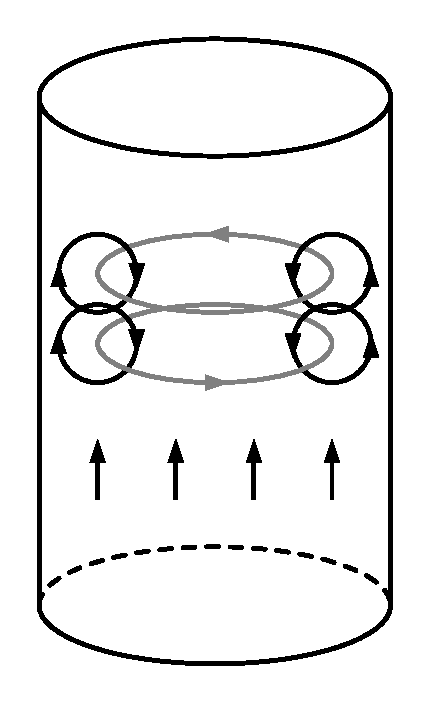
\includegraphics[width=\unitlength,page=1]{res/Skineffect_reason.pdf}}%
    \put(0.60476562,0.46865778){\color[rgb]{0,0,0}\makebox(0,0)[lt]{\lineheight{3}\smash{\begin{tabular}[t]{l}\LARGE$I$\end{tabular}}}}%
    \put(0.76026257,1.12400698){\color[rgb]{0,0,0}\makebox(0,0)[lt]{\lineheight{3}\smash{\begin{tabular}[t]{l}\LARGE$I_W$\end{tabular}}}}%
    \put(0.47817197,1.13326161){\color[rgb]{0.50196078,0.50196078,0.50196078}\makebox(0,0)[lt]{\lineheight{3}\smash{\begin{tabular}[t]{l}\LARGE$\vec{H}$\end{tabular}}}}%
  \end{picture}%
\endgroup%
}\hspace{1cm}
		  \begin{tikzpicture}[line width = 1.2pt, line join=round,x=1cm,y=1cm,>=stealth]
	% Schatten für den Stoff
	\fill [color = lightgray!40] (0,3) rectangle (3.5,-1.5);
	% Koordinatensystem
	\draw [->] (0,0) -- (3.5,0) node [anchor = north] {$ x $};
	\draw [->] (0,-1.5) -- (0,3) node [anchor = east] {$ y $};
	\filldraw (0,0) circle (1.5pt);
	\draw (0,0) circle (5pt);
	\draw (0,0) node [anchor = north east] {$ z $};
	% Leitfähigkeiten
	\draw (1.75,1.5) node {$ \kappa \neq 0 $};
	\draw (-1,1.5) node {$ \kappa = 0 $};
	\draw (-1,0.75) node {Vakuum};
\end{tikzpicture}
	  \end{center}
		  Im Folgenden soll untersucht werden, wie tief Felder in einen Leiter eindringen. Wie genau die Anregung erfolgt, ist dabei nicht von Interesse. Technisch würde man bspw. eine Quelle anlegen. Betrachtet werden zwei unendlich ausgedehnte Halbräume (wie im rechten Bild), auf der linken Seite ein Vakuum, auf der rechten Seite ein Leiter. Aufgrund der Geometrie der Anordnung gibt es Translationsinvarianz in $y$ und $z$- Richtung. \(\vec{E} \) und \(\vec{B}  \) sind also unabhängig von \(y\) und \(z\), dementsprechend sind auch die  Ableitungen nach \(y\) und \(z\) Null:
		        \begin{equation}\label{transin}
			        \dfrac{\partial}{\partial y} = \dfrac{\partial}{\partial z} = 0
		        \end{equation}
		   Das Lösungsgebiet ist $x\geq0$, also im Leiter. Es wird eine harmonische Zeitabhängigkeit vorausgesetzt, weshalb $\frac{\partial}{\partial t}$ zu $\mathrm{j}\omega$ mit einer einzigen Frequenz $\omega$ wird. Zunächst kann man noch einmal die Diffusionsgleichungen (Transformation von \ref{diffE} und \ref{diffB} in den Bildbereich, Beachtung der Translationsinvarianz) aufschreiben:
	  \begin{align*}
		  \Delta \ubar{\vec{E}}                           & = \mathrm{j}\omega\mu\kappa \ubar{\vec{E}}  & \Delta \vec{\ubar{B}}                           & = \mathrm{j}\omega\mu \kappa \vec{\ubar{B}}  \\
		  \dfrac{\partial^2}{\partial x^2} \ubar{\vec{E}} & = \mathrm{j}\omega\mu \kappa \ubar{\vec{E}} & \dfrac{\partial^2}{\partial x^2} \vec{\ubar{B}} & = \mathrm{j}\omega \mu \kappa \vec{\ubar{B}} \\
		  \ubar{\vec{E}}                                  & = \sum_{i=x,y,z}\ubar{E}_i \vu{i}           & \vec{\ubar{B}}                                  & = \sum_{i=x,y,z}\ubar{B}_i \vu{i}
	  \end{align*}
			   Aufgrund von \ref{transin} hat die Rotation des E-Feldes hat keine $x$-Komponente. Es gilt mit \ref{LeviCita} und Summenkonvention:
			        \begin{equation}\begin{split}
					        \rot \ubar{\vec{E}} = \varepsilon_{ijk} \vu{i} \partial_j\ubar{E}_k \stackrel{\text{hier}}{=} -\partial_x\ubar{E}_z \vec{e_y} + \partial_x\ubar{E}_y \vec{e_z} \stackrel{!}{=} -\mathrm{j}\omega   \sum_{i=x,y,z}\ubar{B}_i \vu{i} \implies \boxed{\ubar{B}_x=0}
				        \end{split}\end{equation}
			   Analog kann man für $B$ vorgehen:
			        \begin{equation}\begin{split}
					        \mu^{-1} \rot \vec{\ubar{B}} = \rot \vec{\ubar{H}} = \ubar{\vec{J}} = \kappa\ubar{\vec{E}} \implies \boxed{\ubar{E}_x=0}
				        \end{split}\end{equation}
			        Es folgt also, dass sowohl das B-Feld, als auch das E-Feld keine $x$-Komponente haben. Hiermit folgen 4 strukturgleiche skalare Diffusionsgleichungen
			        \begin{align}
				        \dfrac{\partial^2}{\partial x^2} \ubar{E}_y & = \mathrm{j}\omega \mu \kappa \ubar{E}_y & \dfrac{\partial^2}{\partial x^2} \ubar{B}_y & = \mathrm{j}\omega \mu \kappa \ubar{B}_y \\
				        \dfrac{\partial^2}{\partial x^2} \ubar{E}_z & = \mathrm{j}\omega \mu \kappa \ubar{E}_z & \dfrac{\partial^2}{\partial x^2} \ubar{B}_z & = \mathrm{j}\omega \mu \kappa \ubar{B}_z
			        \end{align}
			    Sowohl $y-$ als auch $z-$Komponente des elektrischen Feldes sind Tangentialkomponenten bezüglich der Grenzfläche zwischen Leiter und Vakuum. Die Tangentialkomponenten sind nach \ref{tanE} stetig, eine Normalkomponente gibt es wegen $\ubar{E}_x=0$ nicht. Es ist zweckmäßig das Koordinatensystem so zu drehen, dass $\vec{e_y} \parallel \ubar{\vec{J}}(x=0) = \kappa\ubar{\vec{E}}(x=0)$, sodass auch $\ubar{E}_z(x=0)=0$. Das funktioniert, weil es eine Translationsinvarianz in $y-$ und $z-$Richtung gibt, also $\vec{E}$ an jeder Stelle in der $y-z-$Ebene in die selbe Richtung zeigt.\\
			    Es reicht somit, eine der Gleichungen für $B$ und $E$ zu betrachten, also $\dfrac{\partial^2}{\partial x^2} \ubar{E}_y = \mathrm{j}\omega \mu \kappa \ubar{E}_y$, wobei sich $y$ nun auf das gedrehte Koordinatensystem bezieht. Die zu lösende Differentialgleichung ist eine (komplexe) homogene Differentialgleichung mit konstanten Koeffizienten, die mit dem Ansatz \ref{Fund} gelöst wird (hier: $\lambda\leftrightarrow k$). Angesetzt wird also 
			   $$\ubar{E}_\mathrm{y} = \underline{A}  \mathrm{e}^{k x} \text{ mit } [k] = \mathrm{\frac{1}{m}}$$
		   Dies liefert $k^2 = \mathrm{j}\omega \mu \kappa$, womit folgt:
		        $$
			        k_{1/2} = \pm \dfrac{1 + \mathrm{j}}{\sqrt{2}} \sqrt{\omega \mu \kappa}
			        = \pm \left( 1 + \mathrm{j}\right) \sqrt{\dfrac{\omega \mu \kappa}{2}}
			        := \pm \dfrac{1 + \mathrm{j}}{\delta}
		        $$
		   Hierbei wird $\delta$ als die \textbf{Eindringtiefe} bzw. \textbf{Skin-Tiefe} definiert, es handelt sich um eine charakteristische Länge:
		        \begin{equation}
		        	 \boxed{ \delta = \sqrt{\dfrac{2}{\omega \mu \kappa}} } \quad [\delta] =\mathrm{m}
		        \end{equation}		        
		  Die allgemeine Lösung ist somit
		        \begin{equation}
			        \boxed{\ubar{E}_\mathrm{y} = \underline{A}_1  \mathrm{e}^{\frac{x}{\delta}}  \mathrm{e}^{\mathrm{j}\frac{x}{\delta}} + \underline{A}_2   \mathrm{e}^{-\frac{x}{\delta}}  \mathrm{e}^{-\mathrm{j}\frac{x}{\delta}} }
		        \end{equation}
		Diese Gleichung kann man analog (Konstanten bekommen einen $'$, um Verwechslungen vorzubeugen) für $\ubar{E}_z$ schreiben und daraus schlussfolgern, dass sich die bisher getroffene Vereinbarung $\ubar{E}_z(x=0)$ auf den gesamten Raum erstrecken muss. Die einzige Möglichkeit, dass $\ubar{E}_z(x=0)=0$ gilt, ist, dass $\ubar{A'}_1=\ubar{A'}_2=0$. $\ubar{A'}_1=-\ubar{A'}_2\neq0$ hätte im Unendlichen das Problem, dass das elektrische Feld divergiert.  Mit \ref{ggmqs4} folgt nun:
		 \begin{equation}\label{identBE}\rot \ubar{\vec{E}} = \varepsilon_{ijk} \vu{i} \partial_j\ubar{E}_k = \textcolor{green}{-\partial_x\ubar{E}_z \vec{e_y}} + \textcolor{red}{\partial_x\ubar{E}_y \vec{e_z}} = -\mathrm{j}\omega   \sum_{i=x,\textcolor{green}{y},\textcolor{red}{z}}\ubar{B}_i \vu{i}
		 \end{equation}
		  Wegen der Festlegung $\ubar{E}_z=0$ folgt also unmittelbar $\ubar{B}_y=0$, $B$  und $E$ stehen also orthogonal zueinander. Man könnte nun also die Lösung für $\ubar{B}_z$ vollkommen analog zu der für $\ubar{E}_y$ hinschreiben. Einfacher ist es aber direkt mit der gefundenen Identität aus \ref{identBE} weiterzurechnen:
			        \begin{align}
				        \dfrac{\partial}{\partial x} \ubar{E}_y & = -\mathrm{j}\omega\ubar{B}_\mathrm{z} & \Rightarrow \ubar{B}_z & = -\dfrac{1}{\mathrm{j}\omega} \dfrac{\partial}{\partial x} \ubar{E}_y                                                                                                                                                                                               \nonumber\\
				                                                &                                        &                        & = -\dfrac{1 + \mathrm{j}}{\mathrm{j}\omega}  \dfrac{1}{\delta}  \left[ \underline{A}_1   \mathrm{e}^{\frac{x}{\delta}}   \mathrm{e}^{\mathrm{j}\frac{x}{\delta}} - \underline{A}_2  \mathrm{e}^{-\frac{x}{\delta}}  \mathrm{e}^{-\mathrm{j}\frac{x}{\delta}} \right]
			        \end{align}
			  Nun müssen die Konstanten bestimmt werden:
			        \begin{enumerate}
				        \item Für \(x \,\rightarrow\, \infty \)  darf das E-Feld nicht divergieren $\Rightarrow$
				              $\boxed{\underline{A}_1 = 0}$
				        \item Bei \(x = 0 \) gilt $\ubar{E}_{y} = \ubar{E}_{y}(x = 0) = \frac{1}{\kappa}\ubar{J}_y(x=0)=\ubar{E}_{y0} =\frac{1}{\kappa}\ubar{J}_{y0}  \Rightarrow \boxed{\underline{A}_2 = \ubar{E}_{y0}}$
			        \end{enumerate}
			  Somit folgt:
			        \begin{align}
				        \ubar{E}_{y} & = \ubar{E}_{y0}  \mathrm{e}^{-\frac{x}{\delta}}  \mathrm{e}^{-\mathrm{j}\frac{x}{\delta}} & \ubar{H}_\mathrm{z} & = \dfrac{\ubar{B}_\mathrm{z}}{\mu} = \dfrac{1 + \mathrm{j}}{\mathrm{j}\omega\mu} \dfrac{1}{\delta} \ubar{E}_{y0}  \mathrm{e}^{-\frac{x}{\delta}}  \mathrm{e}^{-\mathrm{j}\frac{x}{\delta}} & \delta & = \sqrt{\dfrac{2}{\omega \mu \kappa}}
			        \end{align}
			        Wird $\ubar{E}_{y0}$ als elektrisches Feld an der Oberfläche vorgegeben (die konkrete Ursache für dieses Feld ist weiterhin nicht von Belang, es geht nur darum wie tief das Feld in den Leiter eindringt), so kann man beobachten, dass bei unendlichem $\kappa/\omega/\mu$ das Feld wegen der gegen 0 strebenden Skin-Tiefe gar nicht in das Medium eindringt. Nun wird umgestellt, dabei werden die Begriffe \textbf{Dämpfung} und \textbf{Phasendrehung} eingeführt:
			        \begin{equation}\begin{split}
					        \ubar{H}_z &= \dfrac{1 - \mathrm{j}}{\omega \delta \mu} \ubar{E}_{y0}  \mathrm{e}^{-\frac{x}{\delta}}  \mathrm{e}^{-\mathrm{j}\frac{x}{\delta}} \\
					        &= \left(1 - \mathrm{j}\right) \sqrt{\dfrac{\kappa}{2 \omega \mu}}  \ubar{E}_{y0}  \mathrm{e}^{-\frac{x}{\delta}}  \mathrm{e}^{-\mathrm{j}\frac{x}{\delta}} \\
					        &= \dfrac{\kappa \delta}{2} \underbrace{\left( 1 - \mathrm{j}\right)}_{\sqrt{2} \mathrm{e}^{-\mathrm{j}\frac{\pi}{4}}} \ubar{E}_{y0} \underbrace{ \mathrm{e}^{-\frac{x}{\delta}}}_{\text{Dämpfung}} \underbrace{ \mathrm{e}^{-\mathrm{j}\frac{x}{\delta}}}_{\substack{\text{Phasen-}\\ \text{drehung}}} = \underbrace{\kappa \ubar{E}_{y0}}_{\ubar{J}_{y0}}\dfrac{\delta}{\sqrt{2}}  \mathrm{e}^{-\frac{x}{\delta}}  \mathrm{e}^{-\mathrm{j}\frac{x}{\delta}} \mathrm{e}^{-\mathrm{j}\frac{\pi}{4}}
				        \end{split}\end{equation}
			        Die finale Lösung für $x\ge 0$ (\textbf{im Leiter}) lautet also:
			        \begin{align}\label{finalskin}
			        	\ubar{\vec{E}} = \ubar{E}_{y}\vec{e_y}                             & = \ubar{E}_{y0}  \mathrm{e}^{-\frac{x}{\delta}}  \mathrm{e}^{-\mathrm{j}\frac{x}{\delta}}\vec{e_y}        & \vec{\ubar{H}} =\ubar{H}_{z}\vec{e_z} & = \kappa \ubar{E}_{y0}\dfrac{\delta}{\sqrt{2}}  \mathrm{e}^{-\frac{x}{\delta}}  \mathrm{e}^{-\mathrm{j}\frac{x}{\delta}} \mathrm{e}^{-\mathrm{j}\frac{\pi}{4}}\vec{e_z} \\
			        	\ubar{\vec{J}} = \ubar{J}_{y}\vec{e_y}=\kappa\ubar{E}_{y}\vec{e_y} & = \kappa \ubar{E}_{y0}  \mathrm{e}^{-\frac{x}{\delta}}  \mathrm{e}^{-\mathrm{j}\frac{x}{\delta}}\vec{e_y} & \delta                                & = \sqrt{\dfrac{2}{\omega \mu \kappa}}\nonumber
			        \end{align}
			  Es gilt: $\frac{\left| \ubar{H}_{z}(x = \delta) \right|}{\left| \ubar{H}_{z}(x = 0) \right|} = \frac{\left| \ubar{E}_{y}(x = \delta) \right|}{\left| \ubar{E}_{y}(x = 0) \right|}=  \mathrm{e}^{-1} \approx 0,37$; nach $2\delta$: $ \mathrm{e}^{-2} \approx 0,14$ usw. Beim Übergang in den Zeitbereich ist klar, dass das E- und H-Feld harmonisch schwingen, wobei das H-Feld gegenüber dem E-Feld eine Phasendrehung von $\frac{\pi}{4}$ hat (das erklärt den Offset zwischen blauer und roter Kurve). 
\begin{center}
		  \begin{minipage}{\textwidth}
			  \centering
			  \resizebox{.8\textwidth}{!}{%% Creator: Matplotlib, PGF backend
%%
%% To include the figure in your LaTeX document, write
%%   \input{<filename>.pgf}
%%
%% Make sure the required packages are loaded in your preamble
%%   \usepackage{pgf}
%%
%% Also ensure that all the required font packages are loaded; for instance,
%% the lmodern package is sometimes necessary when using math font.
%%   \usepackage{lmodern}
%%
%% Figures using additional raster images can only be included by \input if
%% they are in the same directory as the main LaTeX file. For loading figures
%% from other directories you can use the `import` package
%%   \usepackage{import}
%%
%% and then include the figures with
%%   \import{<path to file>}{<filename>.pgf}
%%
%% Matplotlib used the following preamble
%%   
%%   \usepackage{fontspec}
%%   \setmainfont{DejaVuSerif.ttf}[Path=\detokenize{/home/henning/.local/lib/python3.10/site-packages/matplotlib/mpl-data/fonts/ttf/}]
%%   \setsansfont{DejaVuSans.ttf}[Path=\detokenize{/home/henning/.local/lib/python3.10/site-packages/matplotlib/mpl-data/fonts/ttf/}]
%%   \setmonofont{DejaVuSansMono.ttf}[Path=\detokenize{/home/henning/.local/lib/python3.10/site-packages/matplotlib/mpl-data/fonts/ttf/}]
%%   \makeatletter\@ifpackageloaded{underscore}{}{\usepackage[strings]{underscore}}\makeatother
%%
\begingroup%
\makeatletter%
\begin{pgfpicture}%
\pgfpathrectangle{\pgfpointorigin}{\pgfqpoint{7.115308in}{4.436417in}}%
\pgfusepath{use as bounding box, clip}%
\begin{pgfscope}%
\pgfsetbuttcap%
\pgfsetmiterjoin%
\pgfsetlinewidth{0.000000pt}%
\definecolor{currentstroke}{rgb}{0.000000,0.000000,0.000000}%
\pgfsetstrokecolor{currentstroke}%
\pgfsetstrokeopacity{0.000000}%
\pgfsetdash{}{0pt}%
\pgfpathmoveto{\pgfqpoint{0.000000in}{-0.000000in}}%
\pgfpathlineto{\pgfqpoint{7.115308in}{-0.000000in}}%
\pgfpathlineto{\pgfqpoint{7.115308in}{4.436417in}}%
\pgfpathlineto{\pgfqpoint{0.000000in}{4.436417in}}%
\pgfpathlineto{\pgfqpoint{0.000000in}{-0.000000in}}%
\pgfpathclose%
\pgfusepath{}%
\end{pgfscope}%
\begin{pgfscope}%
\pgfsetbuttcap%
\pgfsetmiterjoin%
\pgfsetlinewidth{0.000000pt}%
\definecolor{currentstroke}{rgb}{0.000000,0.000000,0.000000}%
\pgfsetstrokecolor{currentstroke}%
\pgfsetstrokeopacity{0.000000}%
\pgfsetdash{}{0pt}%
\pgfpathmoveto{\pgfqpoint{0.815308in}{0.526079in}}%
\pgfpathlineto{\pgfqpoint{7.015308in}{0.526079in}}%
\pgfpathlineto{\pgfqpoint{7.015308in}{4.283655in}}%
\pgfpathlineto{\pgfqpoint{0.815308in}{4.283655in}}%
\pgfpathlineto{\pgfqpoint{0.815308in}{0.526079in}}%
\pgfpathclose%
\pgfusepath{}%
\end{pgfscope}%
\begin{pgfscope}%
\pgfpathrectangle{\pgfqpoint{0.815308in}{0.526079in}}{\pgfqpoint{6.200000in}{3.757576in}}%
\pgfusepath{clip}%
\pgfsetrectcap%
\pgfsetroundjoin%
\pgfsetlinewidth{0.803000pt}%
\definecolor{currentstroke}{rgb}{0.690196,0.690196,0.690196}%
\pgfsetstrokecolor{currentstroke}%
\pgfsetdash{}{0pt}%
\pgfpathmoveto{\pgfqpoint{1.097126in}{0.526079in}}%
\pgfpathlineto{\pgfqpoint{1.097126in}{4.283655in}}%
\pgfusepath{stroke}%
\end{pgfscope}%
\begin{pgfscope}%
\pgfsetbuttcap%
\pgfsetroundjoin%
\definecolor{currentfill}{rgb}{0.000000,0.000000,0.000000}%
\pgfsetfillcolor{currentfill}%
\pgfsetlinewidth{0.803000pt}%
\definecolor{currentstroke}{rgb}{0.000000,0.000000,0.000000}%
\pgfsetstrokecolor{currentstroke}%
\pgfsetdash{}{0pt}%
\pgfsys@defobject{currentmarker}{\pgfqpoint{0.000000in}{-0.048611in}}{\pgfqpoint{0.000000in}{0.000000in}}{%
\pgfpathmoveto{\pgfqpoint{0.000000in}{0.000000in}}%
\pgfpathlineto{\pgfqpoint{0.000000in}{-0.048611in}}%
\pgfusepath{stroke,fill}%
}%
\begin{pgfscope}%
\pgfsys@transformshift{1.097126in}{0.526079in}%
\pgfsys@useobject{currentmarker}{}%
\end{pgfscope}%
\end{pgfscope}%
\begin{pgfscope}%
\definecolor{textcolor}{rgb}{0.000000,0.000000,0.000000}%
\pgfsetstrokecolor{textcolor}%
\pgfsetfillcolor{textcolor}%
\pgftext[x=1.097126in,y=0.428857in,,top]{\color{textcolor}\fontsize{10.000000}{12.000000}\selectfont 0.0}%
\end{pgfscope}%
\begin{pgfscope}%
\pgfpathrectangle{\pgfqpoint{0.815308in}{0.526079in}}{\pgfqpoint{6.200000in}{3.757576in}}%
\pgfusepath{clip}%
\pgfsetrectcap%
\pgfsetroundjoin%
\pgfsetlinewidth{0.803000pt}%
\definecolor{currentstroke}{rgb}{0.690196,0.690196,0.690196}%
\pgfsetstrokecolor{currentstroke}%
\pgfsetdash{}{0pt}%
\pgfpathmoveto{\pgfqpoint{2.036520in}{0.526079in}}%
\pgfpathlineto{\pgfqpoint{2.036520in}{4.283655in}}%
\pgfusepath{stroke}%
\end{pgfscope}%
\begin{pgfscope}%
\pgfsetbuttcap%
\pgfsetroundjoin%
\definecolor{currentfill}{rgb}{0.000000,0.000000,0.000000}%
\pgfsetfillcolor{currentfill}%
\pgfsetlinewidth{0.803000pt}%
\definecolor{currentstroke}{rgb}{0.000000,0.000000,0.000000}%
\pgfsetstrokecolor{currentstroke}%
\pgfsetdash{}{0pt}%
\pgfsys@defobject{currentmarker}{\pgfqpoint{0.000000in}{-0.048611in}}{\pgfqpoint{0.000000in}{0.000000in}}{%
\pgfpathmoveto{\pgfqpoint{0.000000in}{0.000000in}}%
\pgfpathlineto{\pgfqpoint{0.000000in}{-0.048611in}}%
\pgfusepath{stroke,fill}%
}%
\begin{pgfscope}%
\pgfsys@transformshift{2.036520in}{0.526079in}%
\pgfsys@useobject{currentmarker}{}%
\end{pgfscope}%
\end{pgfscope}%
\begin{pgfscope}%
\definecolor{textcolor}{rgb}{0.000000,0.000000,0.000000}%
\pgfsetstrokecolor{textcolor}%
\pgfsetfillcolor{textcolor}%
\pgftext[x=2.036520in,y=0.428857in,,top]{\color{textcolor}\fontsize{10.000000}{12.000000}\selectfont 0.5}%
\end{pgfscope}%
\begin{pgfscope}%
\pgfpathrectangle{\pgfqpoint{0.815308in}{0.526079in}}{\pgfqpoint{6.200000in}{3.757576in}}%
\pgfusepath{clip}%
\pgfsetrectcap%
\pgfsetroundjoin%
\pgfsetlinewidth{0.803000pt}%
\definecolor{currentstroke}{rgb}{0.690196,0.690196,0.690196}%
\pgfsetstrokecolor{currentstroke}%
\pgfsetdash{}{0pt}%
\pgfpathmoveto{\pgfqpoint{2.975914in}{0.526079in}}%
\pgfpathlineto{\pgfqpoint{2.975914in}{4.283655in}}%
\pgfusepath{stroke}%
\end{pgfscope}%
\begin{pgfscope}%
\pgfsetbuttcap%
\pgfsetroundjoin%
\definecolor{currentfill}{rgb}{0.000000,0.000000,0.000000}%
\pgfsetfillcolor{currentfill}%
\pgfsetlinewidth{0.803000pt}%
\definecolor{currentstroke}{rgb}{0.000000,0.000000,0.000000}%
\pgfsetstrokecolor{currentstroke}%
\pgfsetdash{}{0pt}%
\pgfsys@defobject{currentmarker}{\pgfqpoint{0.000000in}{-0.048611in}}{\pgfqpoint{0.000000in}{0.000000in}}{%
\pgfpathmoveto{\pgfqpoint{0.000000in}{0.000000in}}%
\pgfpathlineto{\pgfqpoint{0.000000in}{-0.048611in}}%
\pgfusepath{stroke,fill}%
}%
\begin{pgfscope}%
\pgfsys@transformshift{2.975914in}{0.526079in}%
\pgfsys@useobject{currentmarker}{}%
\end{pgfscope}%
\end{pgfscope}%
\begin{pgfscope}%
\definecolor{textcolor}{rgb}{0.000000,0.000000,0.000000}%
\pgfsetstrokecolor{textcolor}%
\pgfsetfillcolor{textcolor}%
\pgftext[x=2.975914in,y=0.428857in,,top]{\color{textcolor}\fontsize{10.000000}{12.000000}\selectfont 1.0}%
\end{pgfscope}%
\begin{pgfscope}%
\pgfpathrectangle{\pgfqpoint{0.815308in}{0.526079in}}{\pgfqpoint{6.200000in}{3.757576in}}%
\pgfusepath{clip}%
\pgfsetrectcap%
\pgfsetroundjoin%
\pgfsetlinewidth{0.803000pt}%
\definecolor{currentstroke}{rgb}{0.690196,0.690196,0.690196}%
\pgfsetstrokecolor{currentstroke}%
\pgfsetdash{}{0pt}%
\pgfpathmoveto{\pgfqpoint{3.915308in}{0.526079in}}%
\pgfpathlineto{\pgfqpoint{3.915308in}{4.283655in}}%
\pgfusepath{stroke}%
\end{pgfscope}%
\begin{pgfscope}%
\pgfsetbuttcap%
\pgfsetroundjoin%
\definecolor{currentfill}{rgb}{0.000000,0.000000,0.000000}%
\pgfsetfillcolor{currentfill}%
\pgfsetlinewidth{0.803000pt}%
\definecolor{currentstroke}{rgb}{0.000000,0.000000,0.000000}%
\pgfsetstrokecolor{currentstroke}%
\pgfsetdash{}{0pt}%
\pgfsys@defobject{currentmarker}{\pgfqpoint{0.000000in}{-0.048611in}}{\pgfqpoint{0.000000in}{0.000000in}}{%
\pgfpathmoveto{\pgfqpoint{0.000000in}{0.000000in}}%
\pgfpathlineto{\pgfqpoint{0.000000in}{-0.048611in}}%
\pgfusepath{stroke,fill}%
}%
\begin{pgfscope}%
\pgfsys@transformshift{3.915308in}{0.526079in}%
\pgfsys@useobject{currentmarker}{}%
\end{pgfscope}%
\end{pgfscope}%
\begin{pgfscope}%
\definecolor{textcolor}{rgb}{0.000000,0.000000,0.000000}%
\pgfsetstrokecolor{textcolor}%
\pgfsetfillcolor{textcolor}%
\pgftext[x=3.915308in,y=0.428857in,,top]{\color{textcolor}\fontsize{10.000000}{12.000000}\selectfont 1.5}%
\end{pgfscope}%
\begin{pgfscope}%
\pgfpathrectangle{\pgfqpoint{0.815308in}{0.526079in}}{\pgfqpoint{6.200000in}{3.757576in}}%
\pgfusepath{clip}%
\pgfsetrectcap%
\pgfsetroundjoin%
\pgfsetlinewidth{0.803000pt}%
\definecolor{currentstroke}{rgb}{0.690196,0.690196,0.690196}%
\pgfsetstrokecolor{currentstroke}%
\pgfsetdash{}{0pt}%
\pgfpathmoveto{\pgfqpoint{4.854702in}{0.526079in}}%
\pgfpathlineto{\pgfqpoint{4.854702in}{4.283655in}}%
\pgfusepath{stroke}%
\end{pgfscope}%
\begin{pgfscope}%
\pgfsetbuttcap%
\pgfsetroundjoin%
\definecolor{currentfill}{rgb}{0.000000,0.000000,0.000000}%
\pgfsetfillcolor{currentfill}%
\pgfsetlinewidth{0.803000pt}%
\definecolor{currentstroke}{rgb}{0.000000,0.000000,0.000000}%
\pgfsetstrokecolor{currentstroke}%
\pgfsetdash{}{0pt}%
\pgfsys@defobject{currentmarker}{\pgfqpoint{0.000000in}{-0.048611in}}{\pgfqpoint{0.000000in}{0.000000in}}{%
\pgfpathmoveto{\pgfqpoint{0.000000in}{0.000000in}}%
\pgfpathlineto{\pgfqpoint{0.000000in}{-0.048611in}}%
\pgfusepath{stroke,fill}%
}%
\begin{pgfscope}%
\pgfsys@transformshift{4.854702in}{0.526079in}%
\pgfsys@useobject{currentmarker}{}%
\end{pgfscope}%
\end{pgfscope}%
\begin{pgfscope}%
\definecolor{textcolor}{rgb}{0.000000,0.000000,0.000000}%
\pgfsetstrokecolor{textcolor}%
\pgfsetfillcolor{textcolor}%
\pgftext[x=4.854702in,y=0.428857in,,top]{\color{textcolor}\fontsize{10.000000}{12.000000}\selectfont 2.0}%
\end{pgfscope}%
\begin{pgfscope}%
\pgfpathrectangle{\pgfqpoint{0.815308in}{0.526079in}}{\pgfqpoint{6.200000in}{3.757576in}}%
\pgfusepath{clip}%
\pgfsetrectcap%
\pgfsetroundjoin%
\pgfsetlinewidth{0.803000pt}%
\definecolor{currentstroke}{rgb}{0.690196,0.690196,0.690196}%
\pgfsetstrokecolor{currentstroke}%
\pgfsetdash{}{0pt}%
\pgfpathmoveto{\pgfqpoint{5.794096in}{0.526079in}}%
\pgfpathlineto{\pgfqpoint{5.794096in}{4.283655in}}%
\pgfusepath{stroke}%
\end{pgfscope}%
\begin{pgfscope}%
\pgfsetbuttcap%
\pgfsetroundjoin%
\definecolor{currentfill}{rgb}{0.000000,0.000000,0.000000}%
\pgfsetfillcolor{currentfill}%
\pgfsetlinewidth{0.803000pt}%
\definecolor{currentstroke}{rgb}{0.000000,0.000000,0.000000}%
\pgfsetstrokecolor{currentstroke}%
\pgfsetdash{}{0pt}%
\pgfsys@defobject{currentmarker}{\pgfqpoint{0.000000in}{-0.048611in}}{\pgfqpoint{0.000000in}{0.000000in}}{%
\pgfpathmoveto{\pgfqpoint{0.000000in}{0.000000in}}%
\pgfpathlineto{\pgfqpoint{0.000000in}{-0.048611in}}%
\pgfusepath{stroke,fill}%
}%
\begin{pgfscope}%
\pgfsys@transformshift{5.794096in}{0.526079in}%
\pgfsys@useobject{currentmarker}{}%
\end{pgfscope}%
\end{pgfscope}%
\begin{pgfscope}%
\definecolor{textcolor}{rgb}{0.000000,0.000000,0.000000}%
\pgfsetstrokecolor{textcolor}%
\pgfsetfillcolor{textcolor}%
\pgftext[x=5.794096in,y=0.428857in,,top]{\color{textcolor}\fontsize{10.000000}{12.000000}\selectfont 2.5}%
\end{pgfscope}%
\begin{pgfscope}%
\pgfpathrectangle{\pgfqpoint{0.815308in}{0.526079in}}{\pgfqpoint{6.200000in}{3.757576in}}%
\pgfusepath{clip}%
\pgfsetrectcap%
\pgfsetroundjoin%
\pgfsetlinewidth{0.803000pt}%
\definecolor{currentstroke}{rgb}{0.690196,0.690196,0.690196}%
\pgfsetstrokecolor{currentstroke}%
\pgfsetdash{}{0pt}%
\pgfpathmoveto{\pgfqpoint{6.733490in}{0.526079in}}%
\pgfpathlineto{\pgfqpoint{6.733490in}{4.283655in}}%
\pgfusepath{stroke}%
\end{pgfscope}%
\begin{pgfscope}%
\pgfsetbuttcap%
\pgfsetroundjoin%
\definecolor{currentfill}{rgb}{0.000000,0.000000,0.000000}%
\pgfsetfillcolor{currentfill}%
\pgfsetlinewidth{0.803000pt}%
\definecolor{currentstroke}{rgb}{0.000000,0.000000,0.000000}%
\pgfsetstrokecolor{currentstroke}%
\pgfsetdash{}{0pt}%
\pgfsys@defobject{currentmarker}{\pgfqpoint{0.000000in}{-0.048611in}}{\pgfqpoint{0.000000in}{0.000000in}}{%
\pgfpathmoveto{\pgfqpoint{0.000000in}{0.000000in}}%
\pgfpathlineto{\pgfqpoint{0.000000in}{-0.048611in}}%
\pgfusepath{stroke,fill}%
}%
\begin{pgfscope}%
\pgfsys@transformshift{6.733490in}{0.526079in}%
\pgfsys@useobject{currentmarker}{}%
\end{pgfscope}%
\end{pgfscope}%
\begin{pgfscope}%
\definecolor{textcolor}{rgb}{0.000000,0.000000,0.000000}%
\pgfsetstrokecolor{textcolor}%
\pgfsetfillcolor{textcolor}%
\pgftext[x=6.733490in,y=0.428857in,,top]{\color{textcolor}\fontsize{10.000000}{12.000000}\selectfont 3.0}%
\end{pgfscope}%
\begin{pgfscope}%
\definecolor{textcolor}{rgb}{0.000000,0.000000,0.000000}%
\pgfsetstrokecolor{textcolor}%
\pgfsetfillcolor{textcolor}%
\pgftext[x=3.915308in,y=0.238889in,,top]{\color{textcolor}\fontsize{10.000000}{12.000000}\selectfont \(\displaystyle x/\delta\)}%
\end{pgfscope}%
\begin{pgfscope}%
\pgfpathrectangle{\pgfqpoint{0.815308in}{0.526079in}}{\pgfqpoint{6.200000in}{3.757576in}}%
\pgfusepath{clip}%
\pgfsetrectcap%
\pgfsetroundjoin%
\pgfsetlinewidth{0.803000pt}%
\definecolor{currentstroke}{rgb}{0.690196,0.690196,0.690196}%
\pgfsetstrokecolor{currentstroke}%
\pgfsetdash{}{0pt}%
\pgfpathmoveto{\pgfqpoint{0.815308in}{0.526079in}}%
\pgfpathlineto{\pgfqpoint{7.015308in}{0.526079in}}%
\pgfusepath{stroke}%
\end{pgfscope}%
\begin{pgfscope}%
\pgfsetbuttcap%
\pgfsetroundjoin%
\definecolor{currentfill}{rgb}{0.000000,0.000000,0.000000}%
\pgfsetfillcolor{currentfill}%
\pgfsetlinewidth{0.803000pt}%
\definecolor{currentstroke}{rgb}{0.000000,0.000000,0.000000}%
\pgfsetstrokecolor{currentstroke}%
\pgfsetdash{}{0pt}%
\pgfsys@defobject{currentmarker}{\pgfqpoint{-0.048611in}{0.000000in}}{\pgfqpoint{-0.000000in}{0.000000in}}{%
\pgfpathmoveto{\pgfqpoint{-0.000000in}{0.000000in}}%
\pgfpathlineto{\pgfqpoint{-0.048611in}{0.000000in}}%
\pgfusepath{stroke,fill}%
}%
\begin{pgfscope}%
\pgfsys@transformshift{0.815308in}{0.526079in}%
\pgfsys@useobject{currentmarker}{}%
\end{pgfscope}%
\end{pgfscope}%
\begin{pgfscope}%
\definecolor{textcolor}{rgb}{0.000000,0.000000,0.000000}%
\pgfsetstrokecolor{textcolor}%
\pgfsetfillcolor{textcolor}%
\pgftext[x=0.300816in, y=0.473318in, left, base]{\color{textcolor}\fontsize{10.000000}{12.000000}\selectfont \ensuremath{-}1.00}%
\end{pgfscope}%
\begin{pgfscope}%
\pgfpathrectangle{\pgfqpoint{0.815308in}{0.526079in}}{\pgfqpoint{6.200000in}{3.757576in}}%
\pgfusepath{clip}%
\pgfsetrectcap%
\pgfsetroundjoin%
\pgfsetlinewidth{0.803000pt}%
\definecolor{currentstroke}{rgb}{0.690196,0.690196,0.690196}%
\pgfsetstrokecolor{currentstroke}%
\pgfsetdash{}{0pt}%
\pgfpathmoveto{\pgfqpoint{0.815308in}{0.995776in}}%
\pgfpathlineto{\pgfqpoint{7.015308in}{0.995776in}}%
\pgfusepath{stroke}%
\end{pgfscope}%
\begin{pgfscope}%
\pgfsetbuttcap%
\pgfsetroundjoin%
\definecolor{currentfill}{rgb}{0.000000,0.000000,0.000000}%
\pgfsetfillcolor{currentfill}%
\pgfsetlinewidth{0.803000pt}%
\definecolor{currentstroke}{rgb}{0.000000,0.000000,0.000000}%
\pgfsetstrokecolor{currentstroke}%
\pgfsetdash{}{0pt}%
\pgfsys@defobject{currentmarker}{\pgfqpoint{-0.048611in}{0.000000in}}{\pgfqpoint{-0.000000in}{0.000000in}}{%
\pgfpathmoveto{\pgfqpoint{-0.000000in}{0.000000in}}%
\pgfpathlineto{\pgfqpoint{-0.048611in}{0.000000in}}%
\pgfusepath{stroke,fill}%
}%
\begin{pgfscope}%
\pgfsys@transformshift{0.815308in}{0.995776in}%
\pgfsys@useobject{currentmarker}{}%
\end{pgfscope}%
\end{pgfscope}%
\begin{pgfscope}%
\definecolor{textcolor}{rgb}{0.000000,0.000000,0.000000}%
\pgfsetstrokecolor{textcolor}%
\pgfsetfillcolor{textcolor}%
\pgftext[x=0.300816in, y=0.943015in, left, base]{\color{textcolor}\fontsize{10.000000}{12.000000}\selectfont \ensuremath{-}0.75}%
\end{pgfscope}%
\begin{pgfscope}%
\pgfpathrectangle{\pgfqpoint{0.815308in}{0.526079in}}{\pgfqpoint{6.200000in}{3.757576in}}%
\pgfusepath{clip}%
\pgfsetrectcap%
\pgfsetroundjoin%
\pgfsetlinewidth{0.803000pt}%
\definecolor{currentstroke}{rgb}{0.690196,0.690196,0.690196}%
\pgfsetstrokecolor{currentstroke}%
\pgfsetdash{}{0pt}%
\pgfpathmoveto{\pgfqpoint{0.815308in}{1.465473in}}%
\pgfpathlineto{\pgfqpoint{7.015308in}{1.465473in}}%
\pgfusepath{stroke}%
\end{pgfscope}%
\begin{pgfscope}%
\pgfsetbuttcap%
\pgfsetroundjoin%
\definecolor{currentfill}{rgb}{0.000000,0.000000,0.000000}%
\pgfsetfillcolor{currentfill}%
\pgfsetlinewidth{0.803000pt}%
\definecolor{currentstroke}{rgb}{0.000000,0.000000,0.000000}%
\pgfsetstrokecolor{currentstroke}%
\pgfsetdash{}{0pt}%
\pgfsys@defobject{currentmarker}{\pgfqpoint{-0.048611in}{0.000000in}}{\pgfqpoint{-0.000000in}{0.000000in}}{%
\pgfpathmoveto{\pgfqpoint{-0.000000in}{0.000000in}}%
\pgfpathlineto{\pgfqpoint{-0.048611in}{0.000000in}}%
\pgfusepath{stroke,fill}%
}%
\begin{pgfscope}%
\pgfsys@transformshift{0.815308in}{1.465473in}%
\pgfsys@useobject{currentmarker}{}%
\end{pgfscope}%
\end{pgfscope}%
\begin{pgfscope}%
\definecolor{textcolor}{rgb}{0.000000,0.000000,0.000000}%
\pgfsetstrokecolor{textcolor}%
\pgfsetfillcolor{textcolor}%
\pgftext[x=0.300816in, y=1.412712in, left, base]{\color{textcolor}\fontsize{10.000000}{12.000000}\selectfont \ensuremath{-}0.50}%
\end{pgfscope}%
\begin{pgfscope}%
\pgfpathrectangle{\pgfqpoint{0.815308in}{0.526079in}}{\pgfqpoint{6.200000in}{3.757576in}}%
\pgfusepath{clip}%
\pgfsetrectcap%
\pgfsetroundjoin%
\pgfsetlinewidth{0.803000pt}%
\definecolor{currentstroke}{rgb}{0.690196,0.690196,0.690196}%
\pgfsetstrokecolor{currentstroke}%
\pgfsetdash{}{0pt}%
\pgfpathmoveto{\pgfqpoint{0.815308in}{1.935170in}}%
\pgfpathlineto{\pgfqpoint{7.015308in}{1.935170in}}%
\pgfusepath{stroke}%
\end{pgfscope}%
\begin{pgfscope}%
\pgfsetbuttcap%
\pgfsetroundjoin%
\definecolor{currentfill}{rgb}{0.000000,0.000000,0.000000}%
\pgfsetfillcolor{currentfill}%
\pgfsetlinewidth{0.803000pt}%
\definecolor{currentstroke}{rgb}{0.000000,0.000000,0.000000}%
\pgfsetstrokecolor{currentstroke}%
\pgfsetdash{}{0pt}%
\pgfsys@defobject{currentmarker}{\pgfqpoint{-0.048611in}{0.000000in}}{\pgfqpoint{-0.000000in}{0.000000in}}{%
\pgfpathmoveto{\pgfqpoint{-0.000000in}{0.000000in}}%
\pgfpathlineto{\pgfqpoint{-0.048611in}{0.000000in}}%
\pgfusepath{stroke,fill}%
}%
\begin{pgfscope}%
\pgfsys@transformshift{0.815308in}{1.935170in}%
\pgfsys@useobject{currentmarker}{}%
\end{pgfscope}%
\end{pgfscope}%
\begin{pgfscope}%
\definecolor{textcolor}{rgb}{0.000000,0.000000,0.000000}%
\pgfsetstrokecolor{textcolor}%
\pgfsetfillcolor{textcolor}%
\pgftext[x=0.300816in, y=1.882409in, left, base]{\color{textcolor}\fontsize{10.000000}{12.000000}\selectfont \ensuremath{-}0.25}%
\end{pgfscope}%
\begin{pgfscope}%
\pgfpathrectangle{\pgfqpoint{0.815308in}{0.526079in}}{\pgfqpoint{6.200000in}{3.757576in}}%
\pgfusepath{clip}%
\pgfsetrectcap%
\pgfsetroundjoin%
\pgfsetlinewidth{0.803000pt}%
\definecolor{currentstroke}{rgb}{0.690196,0.690196,0.690196}%
\pgfsetstrokecolor{currentstroke}%
\pgfsetdash{}{0pt}%
\pgfpathmoveto{\pgfqpoint{0.815308in}{2.404867in}}%
\pgfpathlineto{\pgfqpoint{7.015308in}{2.404867in}}%
\pgfusepath{stroke}%
\end{pgfscope}%
\begin{pgfscope}%
\pgfsetbuttcap%
\pgfsetroundjoin%
\definecolor{currentfill}{rgb}{0.000000,0.000000,0.000000}%
\pgfsetfillcolor{currentfill}%
\pgfsetlinewidth{0.803000pt}%
\definecolor{currentstroke}{rgb}{0.000000,0.000000,0.000000}%
\pgfsetstrokecolor{currentstroke}%
\pgfsetdash{}{0pt}%
\pgfsys@defobject{currentmarker}{\pgfqpoint{-0.048611in}{0.000000in}}{\pgfqpoint{-0.000000in}{0.000000in}}{%
\pgfpathmoveto{\pgfqpoint{-0.000000in}{0.000000in}}%
\pgfpathlineto{\pgfqpoint{-0.048611in}{0.000000in}}%
\pgfusepath{stroke,fill}%
}%
\begin{pgfscope}%
\pgfsys@transformshift{0.815308in}{2.404867in}%
\pgfsys@useobject{currentmarker}{}%
\end{pgfscope}%
\end{pgfscope}%
\begin{pgfscope}%
\definecolor{textcolor}{rgb}{0.000000,0.000000,0.000000}%
\pgfsetstrokecolor{textcolor}%
\pgfsetfillcolor{textcolor}%
\pgftext[x=0.408841in, y=2.352106in, left, base]{\color{textcolor}\fontsize{10.000000}{12.000000}\selectfont 0.00}%
\end{pgfscope}%
\begin{pgfscope}%
\pgfpathrectangle{\pgfqpoint{0.815308in}{0.526079in}}{\pgfqpoint{6.200000in}{3.757576in}}%
\pgfusepath{clip}%
\pgfsetrectcap%
\pgfsetroundjoin%
\pgfsetlinewidth{0.803000pt}%
\definecolor{currentstroke}{rgb}{0.690196,0.690196,0.690196}%
\pgfsetstrokecolor{currentstroke}%
\pgfsetdash{}{0pt}%
\pgfpathmoveto{\pgfqpoint{0.815308in}{2.874564in}}%
\pgfpathlineto{\pgfqpoint{7.015308in}{2.874564in}}%
\pgfusepath{stroke}%
\end{pgfscope}%
\begin{pgfscope}%
\pgfsetbuttcap%
\pgfsetroundjoin%
\definecolor{currentfill}{rgb}{0.000000,0.000000,0.000000}%
\pgfsetfillcolor{currentfill}%
\pgfsetlinewidth{0.803000pt}%
\definecolor{currentstroke}{rgb}{0.000000,0.000000,0.000000}%
\pgfsetstrokecolor{currentstroke}%
\pgfsetdash{}{0pt}%
\pgfsys@defobject{currentmarker}{\pgfqpoint{-0.048611in}{0.000000in}}{\pgfqpoint{-0.000000in}{0.000000in}}{%
\pgfpathmoveto{\pgfqpoint{-0.000000in}{0.000000in}}%
\pgfpathlineto{\pgfqpoint{-0.048611in}{0.000000in}}%
\pgfusepath{stroke,fill}%
}%
\begin{pgfscope}%
\pgfsys@transformshift{0.815308in}{2.874564in}%
\pgfsys@useobject{currentmarker}{}%
\end{pgfscope}%
\end{pgfscope}%
\begin{pgfscope}%
\definecolor{textcolor}{rgb}{0.000000,0.000000,0.000000}%
\pgfsetstrokecolor{textcolor}%
\pgfsetfillcolor{textcolor}%
\pgftext[x=0.408841in, y=2.821803in, left, base]{\color{textcolor}\fontsize{10.000000}{12.000000}\selectfont 0.25}%
\end{pgfscope}%
\begin{pgfscope}%
\pgfpathrectangle{\pgfqpoint{0.815308in}{0.526079in}}{\pgfqpoint{6.200000in}{3.757576in}}%
\pgfusepath{clip}%
\pgfsetrectcap%
\pgfsetroundjoin%
\pgfsetlinewidth{0.803000pt}%
\definecolor{currentstroke}{rgb}{0.690196,0.690196,0.690196}%
\pgfsetstrokecolor{currentstroke}%
\pgfsetdash{}{0pt}%
\pgfpathmoveto{\pgfqpoint{0.815308in}{3.344261in}}%
\pgfpathlineto{\pgfqpoint{7.015308in}{3.344261in}}%
\pgfusepath{stroke}%
\end{pgfscope}%
\begin{pgfscope}%
\pgfsetbuttcap%
\pgfsetroundjoin%
\definecolor{currentfill}{rgb}{0.000000,0.000000,0.000000}%
\pgfsetfillcolor{currentfill}%
\pgfsetlinewidth{0.803000pt}%
\definecolor{currentstroke}{rgb}{0.000000,0.000000,0.000000}%
\pgfsetstrokecolor{currentstroke}%
\pgfsetdash{}{0pt}%
\pgfsys@defobject{currentmarker}{\pgfqpoint{-0.048611in}{0.000000in}}{\pgfqpoint{-0.000000in}{0.000000in}}{%
\pgfpathmoveto{\pgfqpoint{-0.000000in}{0.000000in}}%
\pgfpathlineto{\pgfqpoint{-0.048611in}{0.000000in}}%
\pgfusepath{stroke,fill}%
}%
\begin{pgfscope}%
\pgfsys@transformshift{0.815308in}{3.344261in}%
\pgfsys@useobject{currentmarker}{}%
\end{pgfscope}%
\end{pgfscope}%
\begin{pgfscope}%
\definecolor{textcolor}{rgb}{0.000000,0.000000,0.000000}%
\pgfsetstrokecolor{textcolor}%
\pgfsetfillcolor{textcolor}%
\pgftext[x=0.408841in, y=3.291500in, left, base]{\color{textcolor}\fontsize{10.000000}{12.000000}\selectfont 0.50}%
\end{pgfscope}%
\begin{pgfscope}%
\pgfpathrectangle{\pgfqpoint{0.815308in}{0.526079in}}{\pgfqpoint{6.200000in}{3.757576in}}%
\pgfusepath{clip}%
\pgfsetrectcap%
\pgfsetroundjoin%
\pgfsetlinewidth{0.803000pt}%
\definecolor{currentstroke}{rgb}{0.690196,0.690196,0.690196}%
\pgfsetstrokecolor{currentstroke}%
\pgfsetdash{}{0pt}%
\pgfpathmoveto{\pgfqpoint{0.815308in}{3.813958in}}%
\pgfpathlineto{\pgfqpoint{7.015308in}{3.813958in}}%
\pgfusepath{stroke}%
\end{pgfscope}%
\begin{pgfscope}%
\pgfsetbuttcap%
\pgfsetroundjoin%
\definecolor{currentfill}{rgb}{0.000000,0.000000,0.000000}%
\pgfsetfillcolor{currentfill}%
\pgfsetlinewidth{0.803000pt}%
\definecolor{currentstroke}{rgb}{0.000000,0.000000,0.000000}%
\pgfsetstrokecolor{currentstroke}%
\pgfsetdash{}{0pt}%
\pgfsys@defobject{currentmarker}{\pgfqpoint{-0.048611in}{0.000000in}}{\pgfqpoint{-0.000000in}{0.000000in}}{%
\pgfpathmoveto{\pgfqpoint{-0.000000in}{0.000000in}}%
\pgfpathlineto{\pgfqpoint{-0.048611in}{0.000000in}}%
\pgfusepath{stroke,fill}%
}%
\begin{pgfscope}%
\pgfsys@transformshift{0.815308in}{3.813958in}%
\pgfsys@useobject{currentmarker}{}%
\end{pgfscope}%
\end{pgfscope}%
\begin{pgfscope}%
\definecolor{textcolor}{rgb}{0.000000,0.000000,0.000000}%
\pgfsetstrokecolor{textcolor}%
\pgfsetfillcolor{textcolor}%
\pgftext[x=0.408841in, y=3.761197in, left, base]{\color{textcolor}\fontsize{10.000000}{12.000000}\selectfont 0.75}%
\end{pgfscope}%
\begin{pgfscope}%
\pgfpathrectangle{\pgfqpoint{0.815308in}{0.526079in}}{\pgfqpoint{6.200000in}{3.757576in}}%
\pgfusepath{clip}%
\pgfsetrectcap%
\pgfsetroundjoin%
\pgfsetlinewidth{0.803000pt}%
\definecolor{currentstroke}{rgb}{0.690196,0.690196,0.690196}%
\pgfsetstrokecolor{currentstroke}%
\pgfsetdash{}{0pt}%
\pgfpathmoveto{\pgfqpoint{0.815308in}{4.283655in}}%
\pgfpathlineto{\pgfqpoint{7.015308in}{4.283655in}}%
\pgfusepath{stroke}%
\end{pgfscope}%
\begin{pgfscope}%
\pgfsetbuttcap%
\pgfsetroundjoin%
\definecolor{currentfill}{rgb}{0.000000,0.000000,0.000000}%
\pgfsetfillcolor{currentfill}%
\pgfsetlinewidth{0.803000pt}%
\definecolor{currentstroke}{rgb}{0.000000,0.000000,0.000000}%
\pgfsetstrokecolor{currentstroke}%
\pgfsetdash{}{0pt}%
\pgfsys@defobject{currentmarker}{\pgfqpoint{-0.048611in}{0.000000in}}{\pgfqpoint{-0.000000in}{0.000000in}}{%
\pgfpathmoveto{\pgfqpoint{-0.000000in}{0.000000in}}%
\pgfpathlineto{\pgfqpoint{-0.048611in}{0.000000in}}%
\pgfusepath{stroke,fill}%
}%
\begin{pgfscope}%
\pgfsys@transformshift{0.815308in}{4.283655in}%
\pgfsys@useobject{currentmarker}{}%
\end{pgfscope}%
\end{pgfscope}%
\begin{pgfscope}%
\definecolor{textcolor}{rgb}{0.000000,0.000000,0.000000}%
\pgfsetstrokecolor{textcolor}%
\pgfsetfillcolor{textcolor}%
\pgftext[x=0.408841in, y=4.230894in, left, base]{\color{textcolor}\fontsize{10.000000}{12.000000}\selectfont 1.00}%
\end{pgfscope}%
\begin{pgfscope}%
\definecolor{textcolor}{rgb}{0.000000,0.000000,0.000000}%
\pgfsetstrokecolor{textcolor}%
\pgfsetfillcolor{textcolor}%
\pgftext[x=0.245260in,y=2.404867in,,bottom,rotate=90.000000]{\color{textcolor}\fontsize{10.000000}{12.000000}\selectfont \(\displaystyle E_y/E_y(x=0)\) bzw. \(\displaystyle H_z/H_z(x=0)\)}%
\end{pgfscope}%
\begin{pgfscope}%
\pgfpathrectangle{\pgfqpoint{0.815308in}{0.526079in}}{\pgfqpoint{6.200000in}{3.757576in}}%
\pgfusepath{clip}%
\pgfsetrectcap%
\pgfsetroundjoin%
\pgfsetlinewidth{1.505625pt}%
\definecolor{currentstroke}{rgb}{1.000000,0.000000,0.000000}%
\pgfsetstrokecolor{currentstroke}%
\pgfsetdash{}{0pt}%
\pgfpathmoveto{\pgfqpoint{1.097126in}{4.283655in}}%
\pgfpathlineto{\pgfqpoint{1.285005in}{4.096372in}}%
\pgfpathlineto{\pgfqpoint{1.472884in}{3.912427in}}%
\pgfpathlineto{\pgfqpoint{1.660762in}{3.734543in}}%
\pgfpathlineto{\pgfqpoint{1.848641in}{3.564842in}}%
\pgfpathlineto{\pgfqpoint{2.036520in}{3.404910in}}%
\pgfpathlineto{\pgfqpoint{2.224399in}{3.255871in}}%
\pgfpathlineto{\pgfqpoint{2.412278in}{3.118449in}}%
\pgfpathlineto{\pgfqpoint{2.600156in}{2.993023in}}%
\pgfpathlineto{\pgfqpoint{2.788035in}{2.879689in}}%
\pgfpathlineto{\pgfqpoint{2.975914in}{2.778307in}}%
\pgfpathlineto{\pgfqpoint{3.163793in}{2.688544in}}%
\pgfpathlineto{\pgfqpoint{3.351672in}{2.609918in}}%
\pgfpathlineto{\pgfqpoint{3.539550in}{2.541835in}}%
\pgfpathlineto{\pgfqpoint{3.727429in}{2.483614in}}%
\pgfpathlineto{\pgfqpoint{3.915308in}{2.434521in}}%
\pgfpathlineto{\pgfqpoint{4.103187in}{2.393791in}}%
\pgfpathlineto{\pgfqpoint{4.291065in}{2.360645in}}%
\pgfpathlineto{\pgfqpoint{4.478944in}{2.334307in}}%
\pgfpathlineto{\pgfqpoint{4.666823in}{2.314020in}}%
\pgfpathlineto{\pgfqpoint{4.854702in}{2.299055in}}%
\pgfpathlineto{\pgfqpoint{5.042581in}{2.288718in}}%
\pgfpathlineto{\pgfqpoint{5.230459in}{2.282356in}}%
\pgfpathlineto{\pgfqpoint{5.418338in}{2.279364in}}%
\pgfpathlineto{\pgfqpoint{5.606217in}{2.279186in}}%
\pgfpathlineto{\pgfqpoint{5.794096in}{2.281315in}}%
\pgfpathlineto{\pgfqpoint{5.981975in}{2.285293in}}%
\pgfpathlineto{\pgfqpoint{6.169853in}{2.290715in}}%
\pgfpathlineto{\pgfqpoint{6.357732in}{2.297219in}}%
\pgfpathlineto{\pgfqpoint{6.545611in}{2.304493in}}%
\pgfpathlineto{\pgfqpoint{6.733490in}{2.312264in}}%
\pgfusepath{stroke}%
\end{pgfscope}%
\begin{pgfscope}%
\pgfpathrectangle{\pgfqpoint{0.815308in}{0.526079in}}{\pgfqpoint{6.200000in}{3.757576in}}%
\pgfusepath{clip}%
\pgfsetrectcap%
\pgfsetroundjoin%
\pgfsetlinewidth{1.505625pt}%
\definecolor{currentstroke}{rgb}{0.000000,0.000000,1.000000}%
\pgfsetstrokecolor{currentstroke}%
\pgfsetdash{}{0pt}%
\pgfpathmoveto{\pgfqpoint{1.097126in}{3.733371in}}%
\pgfpathlineto{\pgfqpoint{1.285005in}{3.480934in}}%
\pgfpathlineto{\pgfqpoint{1.472884in}{3.254783in}}%
\pgfpathlineto{\pgfqpoint{1.660762in}{3.054245in}}%
\pgfpathlineto{\pgfqpoint{1.848641in}{2.878307in}}%
\pgfpathlineto{\pgfqpoint{2.036520in}{2.725694in}}%
\pgfpathlineto{\pgfqpoint{2.224399in}{2.594938in}}%
\pgfpathlineto{\pgfqpoint{2.412278in}{2.484445in}}%
\pgfpathlineto{\pgfqpoint{2.600156in}{2.392541in}}%
\pgfpathlineto{\pgfqpoint{2.788035in}{2.317519in}}%
\pgfpathlineto{\pgfqpoint{2.975914in}{2.257677in}}%
\pgfpathlineto{\pgfqpoint{3.163793in}{2.211347in}}%
\pgfpathlineto{\pgfqpoint{3.351672in}{2.176916in}}%
\pgfpathlineto{\pgfqpoint{3.539550in}{2.152852in}}%
\pgfpathlineto{\pgfqpoint{3.727429in}{2.137711in}}%
\pgfpathlineto{\pgfqpoint{3.915308in}{2.130149in}}%
\pgfpathlineto{\pgfqpoint{4.103187in}{2.128930in}}%
\pgfpathlineto{\pgfqpoint{4.291065in}{2.132925in}}%
\pgfpathlineto{\pgfqpoint{4.478944in}{2.141117in}}%
\pgfpathlineto{\pgfqpoint{4.666823in}{2.152597in}}%
\pgfpathlineto{\pgfqpoint{4.854702in}{2.166561in}}%
\pgfpathlineto{\pgfqpoint{5.042581in}{2.182307in}}%
\pgfpathlineto{\pgfqpoint{5.230459in}{2.199226in}}%
\pgfpathlineto{\pgfqpoint{5.418338in}{2.216800in}}%
\pgfpathlineto{\pgfqpoint{5.606217in}{2.234591in}}%
\pgfpathlineto{\pgfqpoint{5.794096in}{2.252239in}}%
\pgfpathlineto{\pgfqpoint{5.981975in}{2.269450in}}%
\pgfpathlineto{\pgfqpoint{6.169853in}{2.285992in}}%
\pgfpathlineto{\pgfqpoint{6.357732in}{2.301686in}}%
\pgfpathlineto{\pgfqpoint{6.545611in}{2.316403in}}%
\pgfpathlineto{\pgfqpoint{6.733490in}{2.330053in}}%
\pgfusepath{stroke}%
\end{pgfscope}%
\begin{pgfscope}%
\pgfpathrectangle{\pgfqpoint{0.815308in}{0.526079in}}{\pgfqpoint{6.200000in}{3.757576in}}%
\pgfusepath{clip}%
\pgfsetbuttcap%
\pgfsetroundjoin%
\pgfsetlinewidth{1.505625pt}%
\definecolor{currentstroke}{rgb}{0.000000,0.000000,0.000000}%
\pgfsetstrokecolor{currentstroke}%
\pgfsetdash{{5.550000pt}{2.400000pt}}{0.000000pt}%
\pgfpathmoveto{\pgfqpoint{1.097126in}{4.283655in}}%
\pgfpathlineto{\pgfqpoint{1.285005in}{4.104865in}}%
\pgfpathlineto{\pgfqpoint{1.472884in}{3.943089in}}%
\pgfpathlineto{\pgfqpoint{1.660762in}{3.796708in}}%
\pgfpathlineto{\pgfqpoint{1.848641in}{3.664257in}}%
\pgfpathlineto{\pgfqpoint{2.036520in}{3.544410in}}%
\pgfpathlineto{\pgfqpoint{2.224399in}{3.435968in}}%
\pgfpathlineto{\pgfqpoint{2.412278in}{3.337846in}}%
\pgfpathlineto{\pgfqpoint{2.600156in}{3.249061in}}%
\pgfpathlineto{\pgfqpoint{2.788035in}{3.168725in}}%
\pgfpathlineto{\pgfqpoint{2.975914in}{3.096035in}}%
\pgfpathlineto{\pgfqpoint{3.163793in}{3.030261in}}%
\pgfpathlineto{\pgfqpoint{3.351672in}{2.970747in}}%
\pgfpathlineto{\pgfqpoint{3.539550in}{2.916897in}}%
\pgfpathlineto{\pgfqpoint{3.727429in}{2.868171in}}%
\pgfpathlineto{\pgfqpoint{3.915308in}{2.824082in}}%
\pgfpathlineto{\pgfqpoint{4.103187in}{2.784188in}}%
\pgfpathlineto{\pgfqpoint{4.291065in}{2.748091in}}%
\pgfpathlineto{\pgfqpoint{4.478944in}{2.715429in}}%
\pgfpathlineto{\pgfqpoint{4.666823in}{2.685875in}}%
\pgfpathlineto{\pgfqpoint{4.854702in}{2.659134in}}%
\pgfpathlineto{\pgfqpoint{5.042581in}{2.634937in}}%
\pgfpathlineto{\pgfqpoint{5.230459in}{2.613043in}}%
\pgfpathlineto{\pgfqpoint{5.418338in}{2.593232in}}%
\pgfpathlineto{\pgfqpoint{5.606217in}{2.575307in}}%
\pgfpathlineto{\pgfqpoint{5.794096in}{2.559088in}}%
\pgfpathlineto{\pgfqpoint{5.981975in}{2.544412in}}%
\pgfpathlineto{\pgfqpoint{6.169853in}{2.531132in}}%
\pgfpathlineto{\pgfqpoint{6.357732in}{2.519117in}}%
\pgfpathlineto{\pgfqpoint{6.545611in}{2.508244in}}%
\pgfpathlineto{\pgfqpoint{6.733490in}{2.498407in}}%
\pgfusepath{stroke}%
\end{pgfscope}%
\begin{pgfscope}%
\pgfpathrectangle{\pgfqpoint{0.815308in}{0.526079in}}{\pgfqpoint{6.200000in}{3.757576in}}%
\pgfusepath{clip}%
\pgfsetbuttcap%
\pgfsetroundjoin%
\pgfsetlinewidth{1.505625pt}%
\definecolor{currentstroke}{rgb}{0.000000,0.000000,0.000000}%
\pgfsetstrokecolor{currentstroke}%
\pgfsetdash{{5.550000pt}{2.400000pt}}{0.000000pt}%
\pgfpathmoveto{\pgfqpoint{1.097126in}{0.526079in}}%
\pgfpathlineto{\pgfqpoint{1.285005in}{0.704870in}}%
\pgfpathlineto{\pgfqpoint{1.472884in}{0.866646in}}%
\pgfpathlineto{\pgfqpoint{1.660762in}{1.013027in}}%
\pgfpathlineto{\pgfqpoint{1.848641in}{1.145478in}}%
\pgfpathlineto{\pgfqpoint{2.036520in}{1.265325in}}%
\pgfpathlineto{\pgfqpoint{2.224399in}{1.373767in}}%
\pgfpathlineto{\pgfqpoint{2.412278in}{1.471889in}}%
\pgfpathlineto{\pgfqpoint{2.600156in}{1.560674in}}%
\pgfpathlineto{\pgfqpoint{2.788035in}{1.641009in}}%
\pgfpathlineto{\pgfqpoint{2.975914in}{1.713700in}}%
\pgfpathlineto{\pgfqpoint{3.163793in}{1.779473in}}%
\pgfpathlineto{\pgfqpoint{3.351672in}{1.838987in}}%
\pgfpathlineto{\pgfqpoint{3.539550in}{1.892838in}}%
\pgfpathlineto{\pgfqpoint{3.727429in}{1.941564in}}%
\pgfpathlineto{\pgfqpoint{3.915308in}{1.985653in}}%
\pgfpathlineto{\pgfqpoint{4.103187in}{2.025547in}}%
\pgfpathlineto{\pgfqpoint{4.291065in}{2.061644in}}%
\pgfpathlineto{\pgfqpoint{4.478944in}{2.094306in}}%
\pgfpathlineto{\pgfqpoint{4.666823in}{2.123860in}}%
\pgfpathlineto{\pgfqpoint{4.854702in}{2.150601in}}%
\pgfpathlineto{\pgfqpoint{5.042581in}{2.174798in}}%
\pgfpathlineto{\pgfqpoint{5.230459in}{2.196692in}}%
\pgfpathlineto{\pgfqpoint{5.418338in}{2.216502in}}%
\pgfpathlineto{\pgfqpoint{5.606217in}{2.234428in}}%
\pgfpathlineto{\pgfqpoint{5.794096in}{2.250647in}}%
\pgfpathlineto{\pgfqpoint{5.981975in}{2.265323in}}%
\pgfpathlineto{\pgfqpoint{6.169853in}{2.278602in}}%
\pgfpathlineto{\pgfqpoint{6.357732in}{2.290618in}}%
\pgfpathlineto{\pgfqpoint{6.545611in}{2.301490in}}%
\pgfpathlineto{\pgfqpoint{6.733490in}{2.311328in}}%
\pgfusepath{stroke}%
\end{pgfscope}%
\begin{pgfscope}%
\pgfpathrectangle{\pgfqpoint{0.815308in}{0.526079in}}{\pgfqpoint{6.200000in}{3.757576in}}%
\pgfusepath{clip}%
\pgfsetrectcap%
\pgfsetroundjoin%
\pgfsetlinewidth{1.505625pt}%
\definecolor{currentstroke}{rgb}{1.000000,0.000000,0.000000}%
\pgfsetstrokecolor{currentstroke}%
\pgfsetdash{}{0pt}%
\pgfpathmoveto{\pgfqpoint{3.445611in}{3.813958in}}%
\pgfpathlineto{\pgfqpoint{3.821369in}{3.813958in}}%
\pgfusepath{stroke}%
\end{pgfscope}%
\begin{pgfscope}%
\pgfpathrectangle{\pgfqpoint{0.815308in}{0.526079in}}{\pgfqpoint{6.200000in}{3.757576in}}%
\pgfusepath{clip}%
\pgfsetrectcap%
\pgfsetroundjoin%
\pgfsetlinewidth{1.505625pt}%
\definecolor{currentstroke}{rgb}{0.000000,0.000000,1.000000}%
\pgfsetstrokecolor{currentstroke}%
\pgfsetdash{}{0pt}%
\pgfpathmoveto{\pgfqpoint{3.445611in}{3.813958in}}%
\pgfpathlineto{\pgfqpoint{3.711312in}{3.548258in}}%
\pgfusepath{stroke}%
\end{pgfscope}%
\begin{pgfscope}%
\pgfsetrectcap%
\pgfsetmiterjoin%
\pgfsetlinewidth{0.803000pt}%
\definecolor{currentstroke}{rgb}{0.000000,0.000000,0.000000}%
\pgfsetstrokecolor{currentstroke}%
\pgfsetdash{}{0pt}%
\pgfpathmoveto{\pgfqpoint{0.815308in}{0.526079in}}%
\pgfpathlineto{\pgfqpoint{0.815308in}{4.283655in}}%
\pgfusepath{stroke}%
\end{pgfscope}%
\begin{pgfscope}%
\pgfsetrectcap%
\pgfsetmiterjoin%
\pgfsetlinewidth{0.803000pt}%
\definecolor{currentstroke}{rgb}{0.000000,0.000000,0.000000}%
\pgfsetstrokecolor{currentstroke}%
\pgfsetdash{}{0pt}%
\pgfpathmoveto{\pgfqpoint{7.015308in}{0.526079in}}%
\pgfpathlineto{\pgfqpoint{7.015308in}{4.283655in}}%
\pgfusepath{stroke}%
\end{pgfscope}%
\begin{pgfscope}%
\pgfsetrectcap%
\pgfsetmiterjoin%
\pgfsetlinewidth{0.803000pt}%
\definecolor{currentstroke}{rgb}{0.000000,0.000000,0.000000}%
\pgfsetstrokecolor{currentstroke}%
\pgfsetdash{}{0pt}%
\pgfpathmoveto{\pgfqpoint{0.815308in}{0.526079in}}%
\pgfpathlineto{\pgfqpoint{7.015308in}{0.526079in}}%
\pgfusepath{stroke}%
\end{pgfscope}%
\begin{pgfscope}%
\pgfsetrectcap%
\pgfsetmiterjoin%
\pgfsetlinewidth{0.803000pt}%
\definecolor{currentstroke}{rgb}{0.000000,0.000000,0.000000}%
\pgfsetstrokecolor{currentstroke}%
\pgfsetdash{}{0pt}%
\pgfpathmoveto{\pgfqpoint{0.815308in}{4.283655in}}%
\pgfpathlineto{\pgfqpoint{7.015308in}{4.283655in}}%
\pgfusepath{stroke}%
\end{pgfscope}%
\begin{pgfscope}%
\pgfsetbuttcap%
\pgfsetmiterjoin%
\definecolor{currentfill}{rgb}{1.000000,1.000000,1.000000}%
\pgfsetfillcolor{currentfill}%
\pgfsetfillopacity{0.800000}%
\pgfsetlinewidth{1.003750pt}%
\definecolor{currentstroke}{rgb}{0.800000,0.800000,0.800000}%
\pgfsetstrokecolor{currentstroke}%
\pgfsetstrokeopacity{0.800000}%
\pgfsetdash{}{0pt}%
\pgfpathmoveto{\pgfqpoint{5.658958in}{3.550125in}}%
\pgfpathlineto{\pgfqpoint{6.918086in}{3.550125in}}%
\pgfpathquadraticcurveto{\pgfqpoint{6.945863in}{3.550125in}}{\pgfqpoint{6.945863in}{3.577903in}}%
\pgfpathlineto{\pgfqpoint{6.945863in}{4.186433in}}%
\pgfpathquadraticcurveto{\pgfqpoint{6.945863in}{4.214211in}}{\pgfqpoint{6.918086in}{4.214211in}}%
\pgfpathlineto{\pgfqpoint{5.658958in}{4.214211in}}%
\pgfpathquadraticcurveto{\pgfqpoint{5.631180in}{4.214211in}}{\pgfqpoint{5.631180in}{4.186433in}}%
\pgfpathlineto{\pgfqpoint{5.631180in}{3.577903in}}%
\pgfpathquadraticcurveto{\pgfqpoint{5.631180in}{3.550125in}}{\pgfqpoint{5.658958in}{3.550125in}}%
\pgfpathlineto{\pgfqpoint{5.658958in}{3.550125in}}%
\pgfpathclose%
\pgfusepath{stroke,fill}%
\end{pgfscope}%
\begin{pgfscope}%
\pgfsetrectcap%
\pgfsetroundjoin%
\pgfsetlinewidth{1.505625pt}%
\definecolor{currentstroke}{rgb}{1.000000,0.000000,0.000000}%
\pgfsetstrokecolor{currentstroke}%
\pgfsetdash{}{0pt}%
\pgfpathmoveto{\pgfqpoint{5.686735in}{4.101743in}}%
\pgfpathlineto{\pgfqpoint{5.825624in}{4.101743in}}%
\pgfpathlineto{\pgfqpoint{5.964513in}{4.101743in}}%
\pgfusepath{stroke}%
\end{pgfscope}%
\begin{pgfscope}%
\definecolor{textcolor}{rgb}{0.000000,0.000000,0.000000}%
\pgfsetstrokecolor{textcolor}%
\pgfsetfillcolor{textcolor}%
\pgftext[x=6.075624in,y=4.053132in,left,base]{\color{textcolor}\fontsize{10.000000}{12.000000}\selectfont \(\displaystyle E_y\)}%
\end{pgfscope}%
\begin{pgfscope}%
\pgfsetrectcap%
\pgfsetroundjoin%
\pgfsetlinewidth{1.505625pt}%
\definecolor{currentstroke}{rgb}{0.000000,0.000000,1.000000}%
\pgfsetstrokecolor{currentstroke}%
\pgfsetdash{}{0pt}%
\pgfpathmoveto{\pgfqpoint{5.686735in}{3.887039in}}%
\pgfpathlineto{\pgfqpoint{5.825624in}{3.887039in}}%
\pgfpathlineto{\pgfqpoint{5.964513in}{3.887039in}}%
\pgfusepath{stroke}%
\end{pgfscope}%
\begin{pgfscope}%
\definecolor{textcolor}{rgb}{0.000000,0.000000,0.000000}%
\pgfsetstrokecolor{textcolor}%
\pgfsetfillcolor{textcolor}%
\pgftext[x=6.075624in,y=3.838427in,left,base]{\color{textcolor}\fontsize{10.000000}{12.000000}\selectfont \(\displaystyle H_z\)}%
\end{pgfscope}%
\begin{pgfscope}%
\pgfsetbuttcap%
\pgfsetroundjoin%
\pgfsetlinewidth{1.505625pt}%
\definecolor{currentstroke}{rgb}{0.000000,0.000000,0.000000}%
\pgfsetstrokecolor{currentstroke}%
\pgfsetdash{{5.550000pt}{2.400000pt}}{0.000000pt}%
\pgfpathmoveto{\pgfqpoint{5.686735in}{3.683181in}}%
\pgfpathlineto{\pgfqpoint{5.825624in}{3.683181in}}%
\pgfpathlineto{\pgfqpoint{5.964513in}{3.683181in}}%
\pgfusepath{stroke}%
\end{pgfscope}%
\begin{pgfscope}%
\definecolor{textcolor}{rgb}{0.000000,0.000000,0.000000}%
\pgfsetstrokecolor{textcolor}%
\pgfsetfillcolor{textcolor}%
\pgftext[x=6.075624in,y=3.634570in,left,base]{\color{textcolor}\fontsize{10.000000}{12.000000}\selectfont Einhüllende}%
\end{pgfscope}%
\begin{pgfscope}%
\pgfsetbuttcap%
\pgfsetmiterjoin%
\definecolor{currentfill}{rgb}{0.000000,0.000000,0.000000}%
\pgfsetfillcolor{currentfill}%
\pgfsetfillopacity{0.012500}%
\pgfsetlinewidth{5.018750pt}%
\definecolor{currentstroke}{rgb}{1.000000,1.000000,1.000000}%
\pgfsetstrokecolor{currentstroke}%
\pgfsetdash{}{0pt}%
\pgfpathmoveto{\pgfqpoint{3.445611in}{3.438201in}}%
\pgfpathcurveto{\pgfqpoint{3.545263in}{3.438201in}}{\pgfqpoint{3.640847in}{3.477793in}}{\pgfqpoint{3.711312in}{3.548258in}}%
\pgfpathcurveto{\pgfqpoint{3.781776in}{3.618722in}}{\pgfqpoint{3.821369in}{3.714306in}}{\pgfqpoint{3.821369in}{3.813958in}}%
\pgfpathcurveto{\pgfqpoint{3.821369in}{3.913610in}}{\pgfqpoint{3.781776in}{4.009194in}}{\pgfqpoint{3.711312in}{4.079659in}}%
\pgfpathcurveto{\pgfqpoint{3.640847in}{4.150124in}}{\pgfqpoint{3.545263in}{4.189716in}}{\pgfqpoint{3.445611in}{4.189716in}}%
\pgfpathcurveto{\pgfqpoint{3.345959in}{4.189716in}}{\pgfqpoint{3.250375in}{4.150124in}}{\pgfqpoint{3.179910in}{4.079659in}}%
\pgfpathcurveto{\pgfqpoint{3.109446in}{4.009194in}}{\pgfqpoint{3.069853in}{3.913610in}}{\pgfqpoint{3.069853in}{3.813958in}}%
\pgfpathcurveto{\pgfqpoint{3.069853in}{3.714306in}}{\pgfqpoint{3.109446in}{3.618722in}}{\pgfqpoint{3.179910in}{3.548258in}}%
\pgfpathcurveto{\pgfqpoint{3.250375in}{3.477793in}}{\pgfqpoint{3.345959in}{3.438201in}}{\pgfqpoint{3.445611in}{3.438201in}}%
\pgfpathlineto{\pgfqpoint{3.445611in}{3.438201in}}%
\pgfpathclose%
\pgfusepath{stroke,fill}%
\end{pgfscope}%
\begin{pgfscope}%
\pgfsetbuttcap%
\pgfsetmiterjoin%
\definecolor{currentfill}{rgb}{0.000000,0.000000,0.000000}%
\pgfsetfillcolor{currentfill}%
\pgfsetfillopacity{0.012500}%
\pgfsetlinewidth{1.003750pt}%
\definecolor{currentstroke}{rgb}{0.000000,0.000000,0.000000}%
\pgfsetstrokecolor{currentstroke}%
\pgfsetdash{}{0pt}%
\pgfpathmoveto{\pgfqpoint{3.445611in}{3.438201in}}%
\pgfpathcurveto{\pgfqpoint{3.545263in}{3.438201in}}{\pgfqpoint{3.640847in}{3.477793in}}{\pgfqpoint{3.711312in}{3.548258in}}%
\pgfpathcurveto{\pgfqpoint{3.781776in}{3.618722in}}{\pgfqpoint{3.821369in}{3.714306in}}{\pgfqpoint{3.821369in}{3.813958in}}%
\pgfpathcurveto{\pgfqpoint{3.821369in}{3.913610in}}{\pgfqpoint{3.781776in}{4.009194in}}{\pgfqpoint{3.711312in}{4.079659in}}%
\pgfpathcurveto{\pgfqpoint{3.640847in}{4.150124in}}{\pgfqpoint{3.545263in}{4.189716in}}{\pgfqpoint{3.445611in}{4.189716in}}%
\pgfpathcurveto{\pgfqpoint{3.345959in}{4.189716in}}{\pgfqpoint{3.250375in}{4.150124in}}{\pgfqpoint{3.179910in}{4.079659in}}%
\pgfpathcurveto{\pgfqpoint{3.109446in}{4.009194in}}{\pgfqpoint{3.069853in}{3.913610in}}{\pgfqpoint{3.069853in}{3.813958in}}%
\pgfpathcurveto{\pgfqpoint{3.069853in}{3.714306in}}{\pgfqpoint{3.109446in}{3.618722in}}{\pgfqpoint{3.179910in}{3.548258in}}%
\pgfpathcurveto{\pgfqpoint{3.250375in}{3.477793in}}{\pgfqpoint{3.345959in}{3.438201in}}{\pgfqpoint{3.445611in}{3.438201in}}%
\pgfpathlineto{\pgfqpoint{3.445611in}{3.438201in}}%
\pgfpathclose%
\pgfusepath{stroke,fill}%
\end{pgfscope}%
\end{pgfpicture}%
\makeatother%
\endgroup%
}\\
			  Schwingung der Lösung (Animation $\nearrow$ \href{https://github.com/hgkdd/TET/tree/main/programs}{\enquote{programs}}) \label{schwingdloes}
		  \end{minipage}
		  \begin{minipage}{\textwidth}
			  \centering
			  \resizebox{.8\textwidth}{!}{%% Creator: Matplotlib, PGF backend
%%
%% To include the figure in your LaTeX document, write
%%   \input{<filename>.pgf}
%%
%% Make sure the required packages are loaded in your preamble
%%   \usepackage{pgf}
%%
%% Also ensure that all the required font packages are loaded; for instance,
%% the lmodern package is sometimes necessary when using math font.
%%   \usepackage{lmodern}
%%
%% Figures using additional raster images can only be included by \input if
%% they are in the same directory as the main LaTeX file. For loading figures
%% from other directories you can use the `import` package
%%   \usepackage{import}
%%
%% and then include the figures with
%%   \import{<path to file>}{<filename>.pgf}
%%
%% Matplotlib used the following preamble
%%   
%%   \usepackage{fontspec}
%%   \setmainfont{DejaVuSerif.ttf}[Path=\detokenize{/home/henning/.local/lib/python3.10/site-packages/matplotlib/mpl-data/fonts/ttf/}]
%%   \setsansfont{DejaVuSans.ttf}[Path=\detokenize{/home/henning/.local/lib/python3.10/site-packages/matplotlib/mpl-data/fonts/ttf/}]
%%   \setmonofont{DejaVuSansMono.ttf}[Path=\detokenize{/home/henning/.local/lib/python3.10/site-packages/matplotlib/mpl-data/fonts/ttf/}]
%%   \makeatletter\@ifpackageloaded{underscore}{}{\usepackage[strings]{underscore}}\makeatother
%%
\begingroup%
\makeatletter%
\begin{pgfpicture}%
\pgfpathrectangle{\pgfpointorigin}{\pgfqpoint{6.910851in}{5.294365in}}%
\pgfusepath{use as bounding box, clip}%
\begin{pgfscope}%
\pgfsetbuttcap%
\pgfsetmiterjoin%
\pgfsetlinewidth{0.000000pt}%
\definecolor{currentstroke}{rgb}{0.000000,0.000000,0.000000}%
\pgfsetstrokecolor{currentstroke}%
\pgfsetstrokeopacity{0.000000}%
\pgfsetdash{}{0pt}%
\pgfpathmoveto{\pgfqpoint{0.000000in}{0.000000in}}%
\pgfpathlineto{\pgfqpoint{6.910851in}{0.000000in}}%
\pgfpathlineto{\pgfqpoint{6.910851in}{5.294365in}}%
\pgfpathlineto{\pgfqpoint{0.000000in}{5.294365in}}%
\pgfpathlineto{\pgfqpoint{0.000000in}{0.000000in}}%
\pgfpathclose%
\pgfusepath{}%
\end{pgfscope}%
\begin{pgfscope}%
\pgfsetbuttcap%
\pgfsetmiterjoin%
\pgfsetlinewidth{0.000000pt}%
\definecolor{currentstroke}{rgb}{0.000000,0.000000,0.000000}%
\pgfsetstrokecolor{currentstroke}%
\pgfsetstrokeopacity{0.000000}%
\pgfsetdash{}{0pt}%
\pgfpathmoveto{\pgfqpoint{0.610851in}{0.521603in}}%
\pgfpathlineto{\pgfqpoint{6.810851in}{0.521603in}}%
\pgfpathlineto{\pgfqpoint{6.810851in}{5.141603in}}%
\pgfpathlineto{\pgfqpoint{0.610851in}{5.141603in}}%
\pgfpathlineto{\pgfqpoint{0.610851in}{0.521603in}}%
\pgfpathclose%
\pgfusepath{}%
\end{pgfscope}%
\begin{pgfscope}%
\pgfpathrectangle{\pgfqpoint{0.610851in}{0.521603in}}{\pgfqpoint{6.200000in}{4.620000in}}%
\pgfusepath{clip}%
\pgfsetrectcap%
\pgfsetroundjoin%
\pgfsetlinewidth{0.803000pt}%
\definecolor{currentstroke}{rgb}{0.690196,0.690196,0.690196}%
\pgfsetstrokecolor{currentstroke}%
\pgfsetdash{}{0pt}%
\pgfpathmoveto{\pgfqpoint{1.330408in}{0.521603in}}%
\pgfpathlineto{\pgfqpoint{1.330408in}{5.141603in}}%
\pgfusepath{stroke}%
\end{pgfscope}%
\begin{pgfscope}%
\pgfsetbuttcap%
\pgfsetroundjoin%
\definecolor{currentfill}{rgb}{0.000000,0.000000,0.000000}%
\pgfsetfillcolor{currentfill}%
\pgfsetlinewidth{0.803000pt}%
\definecolor{currentstroke}{rgb}{0.000000,0.000000,0.000000}%
\pgfsetstrokecolor{currentstroke}%
\pgfsetdash{}{0pt}%
\pgfsys@defobject{currentmarker}{\pgfqpoint{0.000000in}{-0.048611in}}{\pgfqpoint{0.000000in}{0.000000in}}{%
\pgfpathmoveto{\pgfqpoint{0.000000in}{0.000000in}}%
\pgfpathlineto{\pgfqpoint{0.000000in}{-0.048611in}}%
\pgfusepath{stroke,fill}%
}%
\begin{pgfscope}%
\pgfsys@transformshift{1.330408in}{0.521603in}%
\pgfsys@useobject{currentmarker}{}%
\end{pgfscope}%
\end{pgfscope}%
\begin{pgfscope}%
\definecolor{textcolor}{rgb}{0.000000,0.000000,0.000000}%
\pgfsetstrokecolor{textcolor}%
\pgfsetfillcolor{textcolor}%
\pgftext[x=1.330408in,y=0.424381in,,top]{\color{textcolor} \fontsize{10.000000}{12.000000}\selectfont 50}%
\end{pgfscope}%
\begin{pgfscope}%
\pgfpathrectangle{\pgfqpoint{0.610851in}{0.521603in}}{\pgfqpoint{6.200000in}{4.620000in}}%
\pgfusepath{clip}%
\pgfsetrectcap%
\pgfsetroundjoin%
\pgfsetlinewidth{0.803000pt}%
\definecolor{currentstroke}{rgb}{0.690196,0.690196,0.690196}%
\pgfsetstrokecolor{currentstroke}%
\pgfsetdash{}{0pt}%
\pgfpathmoveto{\pgfqpoint{2.145194in}{0.521603in}}%
\pgfpathlineto{\pgfqpoint{2.145194in}{5.141603in}}%
\pgfusepath{stroke}%
\end{pgfscope}%
\begin{pgfscope}%
\pgfsetbuttcap%
\pgfsetroundjoin%
\definecolor{currentfill}{rgb}{0.000000,0.000000,0.000000}%
\pgfsetfillcolor{currentfill}%
\pgfsetlinewidth{0.803000pt}%
\definecolor{currentstroke}{rgb}{0.000000,0.000000,0.000000}%
\pgfsetstrokecolor{currentstroke}%
\pgfsetdash{}{0pt}%
\pgfsys@defobject{currentmarker}{\pgfqpoint{0.000000in}{-0.048611in}}{\pgfqpoint{0.000000in}{0.000000in}}{%
\pgfpathmoveto{\pgfqpoint{0.000000in}{0.000000in}}%
\pgfpathlineto{\pgfqpoint{0.000000in}{-0.048611in}}%
\pgfusepath{stroke,fill}%
}%
\begin{pgfscope}%
\pgfsys@transformshift{2.145194in}{0.521603in}%
\pgfsys@useobject{currentmarker}{}%
\end{pgfscope}%
\end{pgfscope}%
\begin{pgfscope}%
\definecolor{textcolor}{rgb}{0.000000,0.000000,0.000000}%
\pgfsetstrokecolor{textcolor}%
\pgfsetfillcolor{textcolor}%
\pgftext[x=2.145194in,y=0.424381in,,top]{\color{textcolor} \fontsize{10.000000}{12.000000}\selectfont 1k}%
\end{pgfscope}%
\begin{pgfscope}%
\pgfpathrectangle{\pgfqpoint{0.610851in}{0.521603in}}{\pgfqpoint{6.200000in}{4.620000in}}%
\pgfusepath{clip}%
\pgfsetrectcap%
\pgfsetroundjoin%
\pgfsetlinewidth{0.803000pt}%
\definecolor{currentstroke}{rgb}{0.690196,0.690196,0.690196}%
\pgfsetstrokecolor{currentstroke}%
\pgfsetdash{}{0pt}%
\pgfpathmoveto{\pgfqpoint{4.023982in}{0.521603in}}%
\pgfpathlineto{\pgfqpoint{4.023982in}{5.141603in}}%
\pgfusepath{stroke}%
\end{pgfscope}%
\begin{pgfscope}%
\pgfsetbuttcap%
\pgfsetroundjoin%
\definecolor{currentfill}{rgb}{0.000000,0.000000,0.000000}%
\pgfsetfillcolor{currentfill}%
\pgfsetlinewidth{0.803000pt}%
\definecolor{currentstroke}{rgb}{0.000000,0.000000,0.000000}%
\pgfsetstrokecolor{currentstroke}%
\pgfsetdash{}{0pt}%
\pgfsys@defobject{currentmarker}{\pgfqpoint{0.000000in}{-0.048611in}}{\pgfqpoint{0.000000in}{0.000000in}}{%
\pgfpathmoveto{\pgfqpoint{0.000000in}{0.000000in}}%
\pgfpathlineto{\pgfqpoint{0.000000in}{-0.048611in}}%
\pgfusepath{stroke,fill}%
}%
\begin{pgfscope}%
\pgfsys@transformshift{4.023982in}{0.521603in}%
\pgfsys@useobject{currentmarker}{}%
\end{pgfscope}%
\end{pgfscope}%
\begin{pgfscope}%
\definecolor{textcolor}{rgb}{0.000000,0.000000,0.000000}%
\pgfsetstrokecolor{textcolor}%
\pgfsetfillcolor{textcolor}%
\pgftext[x=4.023982in,y=0.424381in,,top]{\color{textcolor} \fontsize{10.000000}{12.000000}\selectfont 1M}%
\end{pgfscope}%
\begin{pgfscope}%
\pgfpathrectangle{\pgfqpoint{0.610851in}{0.521603in}}{\pgfqpoint{6.200000in}{4.620000in}}%
\pgfusepath{clip}%
\pgfsetrectcap%
\pgfsetroundjoin%
\pgfsetlinewidth{0.803000pt}%
\definecolor{currentstroke}{rgb}{0.690196,0.690196,0.690196}%
\pgfsetstrokecolor{currentstroke}%
\pgfsetdash{}{0pt}%
\pgfpathmoveto{\pgfqpoint{5.902770in}{0.521603in}}%
\pgfpathlineto{\pgfqpoint{5.902770in}{5.141603in}}%
\pgfusepath{stroke}%
\end{pgfscope}%
\begin{pgfscope}%
\pgfsetbuttcap%
\pgfsetroundjoin%
\definecolor{currentfill}{rgb}{0.000000,0.000000,0.000000}%
\pgfsetfillcolor{currentfill}%
\pgfsetlinewidth{0.803000pt}%
\definecolor{currentstroke}{rgb}{0.000000,0.000000,0.000000}%
\pgfsetstrokecolor{currentstroke}%
\pgfsetdash{}{0pt}%
\pgfsys@defobject{currentmarker}{\pgfqpoint{0.000000in}{-0.048611in}}{\pgfqpoint{0.000000in}{0.000000in}}{%
\pgfpathmoveto{\pgfqpoint{0.000000in}{0.000000in}}%
\pgfpathlineto{\pgfqpoint{0.000000in}{-0.048611in}}%
\pgfusepath{stroke,fill}%
}%
\begin{pgfscope}%
\pgfsys@transformshift{5.902770in}{0.521603in}%
\pgfsys@useobject{currentmarker}{}%
\end{pgfscope}%
\end{pgfscope}%
\begin{pgfscope}%
\definecolor{textcolor}{rgb}{0.000000,0.000000,0.000000}%
\pgfsetstrokecolor{textcolor}%
\pgfsetfillcolor{textcolor}%
\pgftext[x=5.902770in,y=0.424381in,,top]{\color{textcolor} \fontsize{10.000000}{12.000000}\selectfont 1G}%
\end{pgfscope}%
\begin{pgfscope}%
\definecolor{textcolor}{rgb}{0.000000,0.000000,0.000000}%
\pgfsetstrokecolor{textcolor}%
\pgfsetfillcolor{textcolor}%
\pgftext[x=3.710851in,y=0.234413in,,top]{\color{textcolor} \fontsize{10.000000}{12.000000}\selectfont Frequenz / Hz}%
\end{pgfscope}%
\begin{pgfscope}%
\pgfpathrectangle{\pgfqpoint{0.610851in}{0.521603in}}{\pgfqpoint{6.200000in}{4.620000in}}%
\pgfusepath{clip}%
\pgfsetrectcap%
\pgfsetroundjoin%
\pgfsetlinewidth{0.803000pt}%
\definecolor{currentstroke}{rgb}{0.690196,0.690196,0.690196}%
\pgfsetstrokecolor{currentstroke}%
\pgfsetdash{}{0pt}%
\pgfpathmoveto{\pgfqpoint{0.610851in}{0.801993in}}%
\pgfpathlineto{\pgfqpoint{6.810851in}{0.801993in}}%
\pgfusepath{stroke}%
\end{pgfscope}%
\begin{pgfscope}%
\pgfsetbuttcap%
\pgfsetroundjoin%
\definecolor{currentfill}{rgb}{0.000000,0.000000,0.000000}%
\pgfsetfillcolor{currentfill}%
\pgfsetlinewidth{0.803000pt}%
\definecolor{currentstroke}{rgb}{0.000000,0.000000,0.000000}%
\pgfsetstrokecolor{currentstroke}%
\pgfsetdash{}{0pt}%
\pgfsys@defobject{currentmarker}{\pgfqpoint{-0.048611in}{0.000000in}}{\pgfqpoint{-0.000000in}{0.000000in}}{%
\pgfpathmoveto{\pgfqpoint{-0.000000in}{0.000000in}}%
\pgfpathlineto{\pgfqpoint{-0.048611in}{0.000000in}}%
\pgfusepath{stroke,fill}%
}%
\begin{pgfscope}%
\pgfsys@transformshift{0.610851in}{0.801993in}%
\pgfsys@useobject{currentmarker}{}%
\end{pgfscope}%
\end{pgfscope}%
\begin{pgfscope}%
\definecolor{textcolor}{rgb}{0.000000,0.000000,0.000000}%
\pgfsetstrokecolor{textcolor}%
\pgfsetfillcolor{textcolor}%
\pgftext[x=0.336898in, y=0.749231in, left, base]{\color{textcolor} \fontsize{10.000000}{12.000000}\selectfont 1µ}%
\end{pgfscope}%
\begin{pgfscope}%
\pgfpathrectangle{\pgfqpoint{0.610851in}{0.521603in}}{\pgfqpoint{6.200000in}{4.620000in}}%
\pgfusepath{clip}%
\pgfsetrectcap%
\pgfsetroundjoin%
\pgfsetlinewidth{0.803000pt}%
\definecolor{currentstroke}{rgb}{0.690196,0.690196,0.690196}%
\pgfsetstrokecolor{currentstroke}%
\pgfsetdash{}{0pt}%
\pgfpathmoveto{\pgfqpoint{0.610851in}{2.248530in}}%
\pgfpathlineto{\pgfqpoint{6.810851in}{2.248530in}}%
\pgfusepath{stroke}%
\end{pgfscope}%
\begin{pgfscope}%
\pgfsetbuttcap%
\pgfsetroundjoin%
\definecolor{currentfill}{rgb}{0.000000,0.000000,0.000000}%
\pgfsetfillcolor{currentfill}%
\pgfsetlinewidth{0.803000pt}%
\definecolor{currentstroke}{rgb}{0.000000,0.000000,0.000000}%
\pgfsetstrokecolor{currentstroke}%
\pgfsetdash{}{0pt}%
\pgfsys@defobject{currentmarker}{\pgfqpoint{-0.048611in}{0.000000in}}{\pgfqpoint{-0.000000in}{0.000000in}}{%
\pgfpathmoveto{\pgfqpoint{-0.000000in}{0.000000in}}%
\pgfpathlineto{\pgfqpoint{-0.048611in}{0.000000in}}%
\pgfusepath{stroke,fill}%
}%
\begin{pgfscope}%
\pgfsys@transformshift{0.610851in}{2.248530in}%
\pgfsys@useobject{currentmarker}{}%
\end{pgfscope}%
\end{pgfscope}%
\begin{pgfscope}%
\definecolor{textcolor}{rgb}{0.000000,0.000000,0.000000}%
\pgfsetstrokecolor{textcolor}%
\pgfsetfillcolor{textcolor}%
\pgftext[x=0.289968in, y=2.195768in, left, base]{\color{textcolor} \fontsize{10.000000}{12.000000}\selectfont 1m}%
\end{pgfscope}%
\begin{pgfscope}%
\pgfpathrectangle{\pgfqpoint{0.610851in}{0.521603in}}{\pgfqpoint{6.200000in}{4.620000in}}%
\pgfusepath{clip}%
\pgfsetrectcap%
\pgfsetroundjoin%
\pgfsetlinewidth{0.803000pt}%
\definecolor{currentstroke}{rgb}{0.690196,0.690196,0.690196}%
\pgfsetstrokecolor{currentstroke}%
\pgfsetdash{}{0pt}%
\pgfpathmoveto{\pgfqpoint{0.610851in}{3.695067in}}%
\pgfpathlineto{\pgfqpoint{6.810851in}{3.695067in}}%
\pgfusepath{stroke}%
\end{pgfscope}%
\begin{pgfscope}%
\pgfsetbuttcap%
\pgfsetroundjoin%
\definecolor{currentfill}{rgb}{0.000000,0.000000,0.000000}%
\pgfsetfillcolor{currentfill}%
\pgfsetlinewidth{0.803000pt}%
\definecolor{currentstroke}{rgb}{0.000000,0.000000,0.000000}%
\pgfsetstrokecolor{currentstroke}%
\pgfsetdash{}{0pt}%
\pgfsys@defobject{currentmarker}{\pgfqpoint{-0.048611in}{0.000000in}}{\pgfqpoint{-0.000000in}{0.000000in}}{%
\pgfpathmoveto{\pgfqpoint{-0.000000in}{0.000000in}}%
\pgfpathlineto{\pgfqpoint{-0.048611in}{0.000000in}}%
\pgfusepath{stroke,fill}%
}%
\begin{pgfscope}%
\pgfsys@transformshift{0.610851in}{3.695067in}%
\pgfsys@useobject{currentmarker}{}%
\end{pgfscope}%
\end{pgfscope}%
\begin{pgfscope}%
\definecolor{textcolor}{rgb}{0.000000,0.000000,0.000000}%
\pgfsetstrokecolor{textcolor}%
\pgfsetfillcolor{textcolor}%
\pgftext[x=0.425263in, y=3.642305in, left, base]{\color{textcolor} \fontsize{10.000000}{12.000000}\selectfont 1}%
\end{pgfscope}%
\begin{pgfscope}%
\pgfpathrectangle{\pgfqpoint{0.610851in}{0.521603in}}{\pgfqpoint{6.200000in}{4.620000in}}%
\pgfusepath{clip}%
\pgfsetrectcap%
\pgfsetroundjoin%
\pgfsetlinewidth{0.803000pt}%
\definecolor{currentstroke}{rgb}{0.690196,0.690196,0.690196}%
\pgfsetstrokecolor{currentstroke}%
\pgfsetdash{}{0pt}%
\pgfpathmoveto{\pgfqpoint{0.610851in}{5.141603in}}%
\pgfpathlineto{\pgfqpoint{6.810851in}{5.141603in}}%
\pgfusepath{stroke}%
\end{pgfscope}%
\begin{pgfscope}%
\pgfsetbuttcap%
\pgfsetroundjoin%
\definecolor{currentfill}{rgb}{0.000000,0.000000,0.000000}%
\pgfsetfillcolor{currentfill}%
\pgfsetlinewidth{0.803000pt}%
\definecolor{currentstroke}{rgb}{0.000000,0.000000,0.000000}%
\pgfsetstrokecolor{currentstroke}%
\pgfsetdash{}{0pt}%
\pgfsys@defobject{currentmarker}{\pgfqpoint{-0.048611in}{0.000000in}}{\pgfqpoint{-0.000000in}{0.000000in}}{%
\pgfpathmoveto{\pgfqpoint{-0.000000in}{0.000000in}}%
\pgfpathlineto{\pgfqpoint{-0.048611in}{0.000000in}}%
\pgfusepath{stroke,fill}%
}%
\begin{pgfscope}%
\pgfsys@transformshift{0.610851in}{5.141603in}%
\pgfsys@useobject{currentmarker}{}%
\end{pgfscope}%
\end{pgfscope}%
\begin{pgfscope}%
\definecolor{textcolor}{rgb}{0.000000,0.000000,0.000000}%
\pgfsetstrokecolor{textcolor}%
\pgfsetfillcolor{textcolor}%
\pgftext[x=0.344832in, y=5.088842in, left, base]{\color{textcolor} \fontsize{10.000000}{12.000000}\selectfont 1k}%
\end{pgfscope}%
\begin{pgfscope}%
\definecolor{textcolor}{rgb}{0.000000,0.000000,0.000000}%
\pgfsetstrokecolor{textcolor}%
\pgfsetfillcolor{textcolor}%
\pgftext[x=0.234413in,y=2.831603in,,bottom,rotate=90.000000]{\color{textcolor} \fontsize{10.000000}{12.000000}\selectfont Eindringtiefe / m}%
\end{pgfscope}%
\begin{pgfscope}%
\pgfpathrectangle{\pgfqpoint{0.610851in}{0.521603in}}{\pgfqpoint{6.200000in}{4.620000in}}%
\pgfusepath{clip}%
\pgfsetrectcap%
\pgfsetroundjoin%
\pgfsetlinewidth{1.505625pt}%
\definecolor{currentstroke}{rgb}{0.121569,0.466667,0.705882}%
\pgfsetstrokecolor{currentstroke}%
\pgfsetdash{}{0pt}%
\pgfpathmoveto{\pgfqpoint{0.892669in}{2.885057in}}%
\pgfpathlineto{\pgfqpoint{6.529032in}{0.715252in}}%
\pgfpathlineto{\pgfqpoint{6.529032in}{0.715252in}}%
\pgfusepath{stroke}%
\end{pgfscope}%
\begin{pgfscope}%
\pgfpathrectangle{\pgfqpoint{0.610851in}{0.521603in}}{\pgfqpoint{6.200000in}{4.620000in}}%
\pgfusepath{clip}%
\pgfsetrectcap%
\pgfsetroundjoin%
\pgfsetlinewidth{1.505625pt}%
\definecolor{currentstroke}{rgb}{1.000000,0.498039,0.054902}%
\pgfsetstrokecolor{currentstroke}%
\pgfsetdash{}{0pt}%
\pgfpathmoveto{\pgfqpoint{0.892669in}{2.929332in}}%
\pgfpathlineto{\pgfqpoint{6.529032in}{0.759527in}}%
\pgfpathlineto{\pgfqpoint{6.529032in}{0.759527in}}%
\pgfusepath{stroke}%
\end{pgfscope}%
\begin{pgfscope}%
\pgfpathrectangle{\pgfqpoint{0.610851in}{0.521603in}}{\pgfqpoint{6.200000in}{4.620000in}}%
\pgfusepath{clip}%
\pgfsetrectcap%
\pgfsetroundjoin%
\pgfsetlinewidth{1.505625pt}%
\definecolor{currentstroke}{rgb}{0.172549,0.627451,0.172549}%
\pgfsetstrokecolor{currentstroke}%
\pgfsetdash{}{0pt}%
\pgfpathmoveto{\pgfqpoint{0.892669in}{4.588224in}}%
\pgfpathlineto{\pgfqpoint{6.529032in}{2.418418in}}%
\pgfpathlineto{\pgfqpoint{6.529032in}{2.418418in}}%
\pgfusepath{stroke}%
\end{pgfscope}%
\begin{pgfscope}%
\pgfsetrectcap%
\pgfsetmiterjoin%
\pgfsetlinewidth{0.803000pt}%
\definecolor{currentstroke}{rgb}{0.000000,0.000000,0.000000}%
\pgfsetstrokecolor{currentstroke}%
\pgfsetdash{}{0pt}%
\pgfpathmoveto{\pgfqpoint{0.610851in}{0.521603in}}%
\pgfpathlineto{\pgfqpoint{0.610851in}{5.141603in}}%
\pgfusepath{stroke}%
\end{pgfscope}%
\begin{pgfscope}%
\pgfsetrectcap%
\pgfsetmiterjoin%
\pgfsetlinewidth{0.803000pt}%
\definecolor{currentstroke}{rgb}{0.000000,0.000000,0.000000}%
\pgfsetstrokecolor{currentstroke}%
\pgfsetdash{}{0pt}%
\pgfpathmoveto{\pgfqpoint{6.810851in}{0.521603in}}%
\pgfpathlineto{\pgfqpoint{6.810851in}{5.141603in}}%
\pgfusepath{stroke}%
\end{pgfscope}%
\begin{pgfscope}%
\pgfsetrectcap%
\pgfsetmiterjoin%
\pgfsetlinewidth{0.803000pt}%
\definecolor{currentstroke}{rgb}{0.000000,0.000000,0.000000}%
\pgfsetstrokecolor{currentstroke}%
\pgfsetdash{}{0pt}%
\pgfpathmoveto{\pgfqpoint{0.610851in}{0.521603in}}%
\pgfpathlineto{\pgfqpoint{6.810851in}{0.521603in}}%
\pgfusepath{stroke}%
\end{pgfscope}%
\begin{pgfscope}%
\pgfsetrectcap%
\pgfsetmiterjoin%
\pgfsetlinewidth{0.803000pt}%
\definecolor{currentstroke}{rgb}{0.000000,0.000000,0.000000}%
\pgfsetstrokecolor{currentstroke}%
\pgfsetdash{}{0pt}%
\pgfpathmoveto{\pgfqpoint{0.610851in}{5.141603in}}%
\pgfpathlineto{\pgfqpoint{6.810851in}{5.141603in}}%
\pgfusepath{stroke}%
\end{pgfscope}%
\begin{pgfscope}%
\pgfsetbuttcap%
\pgfsetmiterjoin%
\definecolor{currentfill}{rgb}{1.000000,1.000000,1.000000}%
\pgfsetfillcolor{currentfill}%
\pgfsetfillopacity{0.800000}%
\pgfsetlinewidth{1.003750pt}%
\definecolor{currentstroke}{rgb}{0.800000,0.800000,0.800000}%
\pgfsetstrokecolor{currentstroke}%
\pgfsetstrokeopacity{0.800000}%
\pgfsetdash{}{0pt}%
\pgfpathmoveto{\pgfqpoint{4.217657in}{4.418921in}}%
\pgfpathlineto{\pgfqpoint{6.713628in}{4.418921in}}%
\pgfpathquadraticcurveto{\pgfqpoint{6.741406in}{4.418921in}}{\pgfqpoint{6.741406in}{4.446698in}}%
\pgfpathlineto{\pgfqpoint{6.741406in}{5.044381in}}%
\pgfpathquadraticcurveto{\pgfqpoint{6.741406in}{5.072159in}}{\pgfqpoint{6.713628in}{5.072159in}}%
\pgfpathlineto{\pgfqpoint{4.217657in}{5.072159in}}%
\pgfpathquadraticcurveto{\pgfqpoint{4.189879in}{5.072159in}}{\pgfqpoint{4.189879in}{5.044381in}}%
\pgfpathlineto{\pgfqpoint{4.189879in}{4.446698in}}%
\pgfpathquadraticcurveto{\pgfqpoint{4.189879in}{4.418921in}}{\pgfqpoint{4.217657in}{4.418921in}}%
\pgfpathlineto{\pgfqpoint{4.217657in}{4.418921in}}%
\pgfpathclose%
\pgfusepath{stroke,fill}%
\end{pgfscope}%
\begin{pgfscope}%
\pgfsetrectcap%
\pgfsetroundjoin%
\pgfsetlinewidth{1.505625pt}%
\definecolor{currentstroke}{rgb}{0.121569,0.466667,0.705882}%
\pgfsetstrokecolor{currentstroke}%
\pgfsetdash{}{0pt}%
\pgfpathmoveto{\pgfqpoint{4.245434in}{4.959691in}}%
\pgfpathlineto{\pgfqpoint{4.384323in}{4.959691in}}%
\pgfpathlineto{\pgfqpoint{4.523212in}{4.959691in}}%
\pgfusepath{stroke}%
\end{pgfscope}%
\begin{pgfscope}%
\definecolor{textcolor}{rgb}{0.000000,0.000000,0.000000}%
\pgfsetstrokecolor{textcolor}%
\pgfsetfillcolor{textcolor}%
\pgftext[x=4.634323in,y=4.911080in,left,base]{\color{textcolor} \fontsize{10.000000}{12.000000}\selectfont Kupfer: $\kappa=5.80\cdot 10^7$S/m}%
\end{pgfscope}%
\begin{pgfscope}%
\pgfsetrectcap%
\pgfsetroundjoin%
\pgfsetlinewidth{1.505625pt}%
\definecolor{currentstroke}{rgb}{1.000000,0.498039,0.054902}%
\pgfsetstrokecolor{currentstroke}%
\pgfsetdash{}{0pt}%
\pgfpathmoveto{\pgfqpoint{4.245434in}{4.755834in}}%
\pgfpathlineto{\pgfqpoint{4.384323in}{4.755834in}}%
\pgfpathlineto{\pgfqpoint{4.523212in}{4.755834in}}%
\pgfusepath{stroke}%
\end{pgfscope}%
\begin{pgfscope}%
\definecolor{textcolor}{rgb}{0.000000,0.000000,0.000000}%
\pgfsetstrokecolor{textcolor}%
\pgfsetfillcolor{textcolor}%
\pgftext[x=4.634323in,y=4.707223in,left,base]{\color{textcolor} \fontsize{10.000000}{12.000000}\selectfont Aluminium: $\kappa=3.80\cdot 10^7$ S/m}%
\end{pgfscope}%
\begin{pgfscope}%
\pgfsetrectcap%
\pgfsetroundjoin%
\pgfsetlinewidth{1.505625pt}%
\definecolor{currentstroke}{rgb}{0.172549,0.627451,0.172549}%
\pgfsetstrokecolor{currentstroke}%
\pgfsetdash{}{0pt}%
\pgfpathmoveto{\pgfqpoint{4.245434in}{4.551977in}}%
\pgfpathlineto{\pgfqpoint{4.384323in}{4.551977in}}%
\pgfpathlineto{\pgfqpoint{4.523212in}{4.551977in}}%
\pgfusepath{stroke}%
\end{pgfscope}%
\begin{pgfscope}%
\definecolor{textcolor}{rgb}{0.000000,0.000000,0.000000}%
\pgfsetstrokecolor{textcolor}%
\pgfsetfillcolor{textcolor}%
\pgftext[x=4.634323in,y=4.503366in,left,base]{\color{textcolor} \fontsize{10.000000}{12.000000}\selectfont Seewasser: $\kappa=5.00S/m$}%
\end{pgfscope}%
\end{pgfpicture}%
\makeatother%
\endgroup%
}\\
			  Eindringtiefe
		  \end{minipage}
		  \end{center}
Die Berechnung des Magnetfeldes für $x<0$ (vor dem Leiter) erfolgt über \ref{ggmqs1} in Verbindung mit \ref{stokes}, die Grafik links soll den Integrationsweg verdeutlichen. Rechts wird der Weg erst im unendlichen geschlossen, deshalb verschwindet der Beitrag dieses Wegstückes. Weiterhin verschwindet der Beitrag der beiden horizontalen Wegstücken, da $H$ nur eine $z-$Komponente hat und entsprechend zu $\dd\vec{s}\parallel\vu{x}$ orthogonal steht. Somit wird das Wegintegral nur durch die Teilstrecke $\zeta$ bestimmt, wobei $H$ wegen der Translationsinvarianz nur von $x$ abhängt, also auf diesem Teilstück konstant ist. Auch das Flächenintegral kann man unter Nutzung der Translationsinvarianz so vereinfachen, dass in $z-$Richtung alles konstant ist, entsprechend nur mit $\zeta$ multipliziert wird. Außerdem gilt, dass im Vakuum kein Strom fließen kann, weshalb die $x$-Integration erst ab 0 erfolgt.\\
\begin{minipage}{0.5\textwidth}
			        \resizebox{.9\textwidth}{!}{%% Creator: Inkscape 1.0.2 (e86c8708, 2021-01-15), www.inkscape.org
%% PDF/EPS/PS + LaTeX output extension by Johan Engelen, 2010
%% Accompanies image file 'res/skin-H-Weg.pdf' (pdf, eps, ps)
%%
%% To include the image in your LaTeX document, write
%%   \input{<filename>.pdf_tex}
%%  instead of
%%   \includegraphics{<filename>.pdf}
%% To scale the image, write
%%   \def\svgwidth{<desired width>}
%%   \input{<filename>.pdf_tex}
%%  instead of
%%   \includegraphics[width=<desired width>]{<filename>.pdf}
%%
%% Images with a different path to the parent latex file can
%% be accessed with the `import' package (which may need to be
%% installed) using
%%   \usepackage{import}
%% in the preamble, and then including the image with
%%   \import{<path to file>}{<filename>.pdf_tex}
%% Alternatively, one can specify
%%   \graphicspath{{<path to file>/}}
%% 
%% For more information, please see info/svg-inkscape on CTAN:
%%   http://tug.ctan.org/tex-archive/info/svg-inkscape
%%
\begingroup%
\makeatletter%
\def\svgwidth{0.5\textwidth}
\providecommand\color[2][]{%
	\errmessage{(Inkscape) Color is used for the text in Inkscape, but the package 'color.sty' is not loaded}%
	\renewcommand\color[2][]{}%
}%
\providecommand\transparent[1]{%
	\errmessage{(Inkscape) Transparency is used (non-zero) for the text in Inkscape, but the package 'transparent.sty' is not loaded}%
	\renewcommand\transparent[1]{}%
}%
\providecommand\rotatebox[2]{#2}%
\newcommand*\fsize{\dimexpr\f@size pt\relax}%
\newcommand*\lineheight[1]{\fontsize{\fsize}{#1\fsize}\selectfont}%
\ifx\svgwidth\undefined%
	\setlength{\unitlength}{841.88976378bp}%
	\ifx\svgscale\undefined%
		\relax%
	\else%
		\setlength{\unitlength}{\unitlength * \real{\svgscale}}%
	\fi%
\else%
	\setlength{\unitlength}{\svgwidth}%
\fi%
\global\let\svgwidth\undefined%
\global\let\svgscale\undefined%
\makeatother%
\begin{picture}(1,0.70707071)%
	\tiny
	\lineheight{1}%
	\setlength\tabcolsep{0pt}%
	\put(0,0){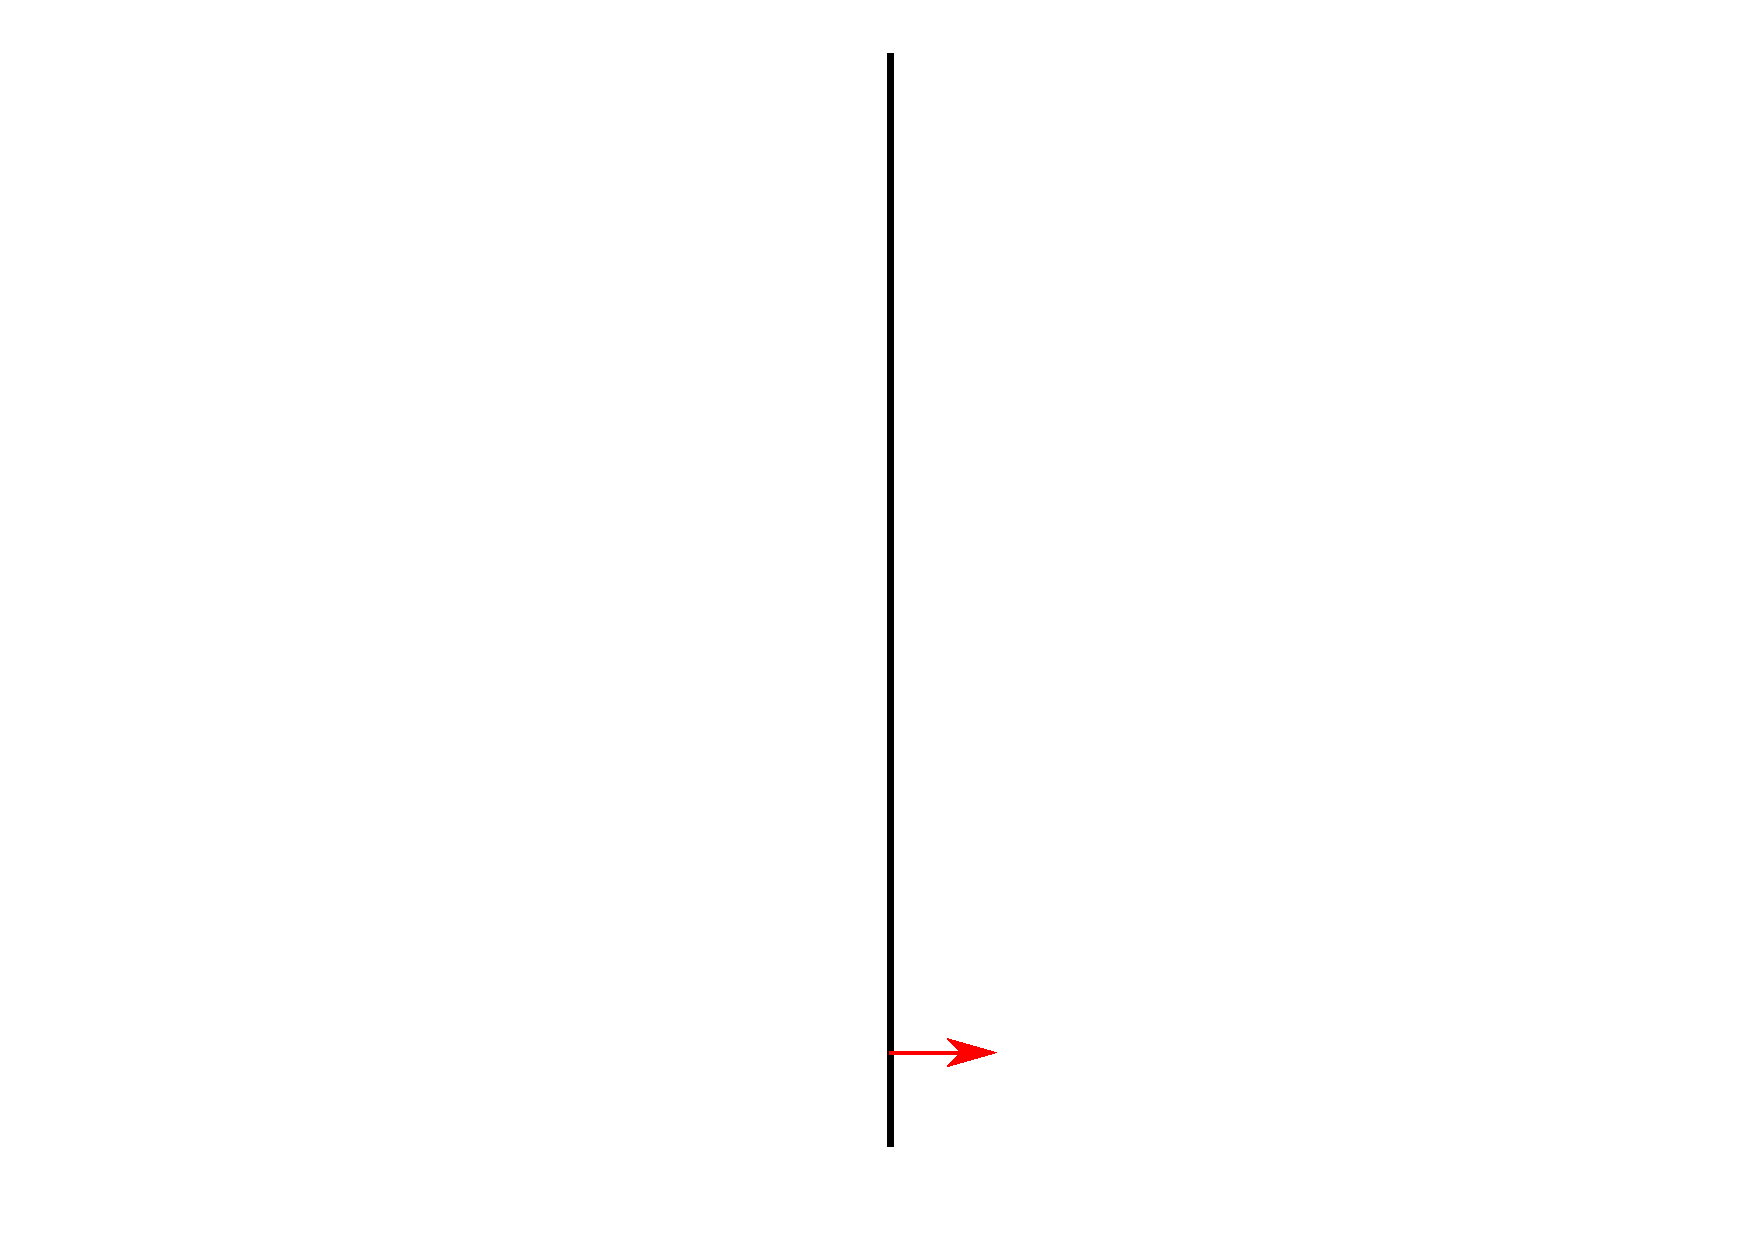
\includegraphics[width=\unitlength,page=1]{res/skin-H-Weg.pdf}}%
	\put(0.58209141,0.09491588){\color[rgb]{0.98823529,0,0}\makebox(0,0)[lt]{\lineheight{1.25}\smash{\begin{tabular}[t]{l}x\end{tabular}}}}%
	\put(0,0){\includegraphics[width=\unitlength,page=2]{res/skin-H-Weg.pdf}}%
	\put(0.46827199,0.1318683){\color[rgb]{0.98823529,0,0}\makebox(0,0)[lt]{\lineheight{1.25}\smash{\begin{tabular}[t]{l}y\end{tabular}}}}%
	\put(0.46795675,0.04442039){\color[rgb]{0.98823529,0,0}\makebox(0,0)[lt]{\lineheight{1.25}\smash{\begin{tabular}[t]{l}z\end{tabular}}}}%
	\put(0,0){\includegraphics[width=\unitlength,page=3]{res/skin-H-Weg.pdf}}%
	\put(0.3165163,0.59414568){\color[rgb]{0,0,0}\makebox(0,0)[lt]{\lineheight{1.25}\smash{\begin{tabular}[t]{l}$\kappa = 0$\end{tabular}}}}%
	\put(0.53121635,0.59414568){\color[rgb]{0,0,0}\makebox(0,0)[lt]{\lineheight{1.25}\smash{\begin{tabular}[t]{l}$\kappa \ne 0$\end{tabular}}}}%
	\put(0,0){\includegraphics[width=\unitlength,page=4]{res/skin-H-Weg.pdf}}%
	\put(0.19130244,0.39197271){\color[rgb]{0,0,0}\makebox(0,0)[lt]{\lineheight{1.25}\smash{\begin{tabular}[t]{l}$\vec{J} = \vec{0}$\end{tabular}}}}%
	\put(0.57126733,0.3923207){\color[rgb]{0,0,0}\makebox(0,0)[lt]{\lineheight{1.25}\smash{\begin{tabular}[t]{l}$\vec{J} = J_y(x) \vu{y}$\end{tabular}}}}%
	\put(0.85455836,0.20060427){\color[rgb]{0,0,0}\makebox(0,0)[lt]{\lineheight{1.25}\smash{\begin{tabular}[t]{l}$x \to \infty$\end{tabular}}}}%
	\put(0.02758345,0.39143333){\color[rgb]{0,0,0}\makebox(0,0)[lt]{\lineheight{1.25}\smash{\begin{tabular}[t]{l}$\zeta$\end{tabular}}}}%
\end{picture}%
\endgroup%
}
\end{minipage}
\begin{minipage}{0.5\textwidth}
\begin{align*}
	\oint \vec{\ubar{H}}(x)\cdot \dd\vec{s} & = \iint \ubar{\vec{J}}\cdot\dd\vec{A}                               \\
	\zeta \vec{\ubar{H}}(x)\cdot \vec{e_z}  & = \zeta \int\limits_0^\infty \ubar{\vec{J}}(x)\cdot \vec{e_y} \dd x \\
	\Aboxed{\ubar{H}_z (x<0) =\ubar{H}_z            & = (1-j) \kappa \ubar{E}_{y0} \frac{\delta}{2} = \ubar{H}_z (x=0^+)}
\end{align*}
\end{minipage}	
Es folgt also, dass $\ubar{H}_z$ im Vakuum konstant ist und das der Wert dort genau dem Wert an der Leiteroberfläche entspricht, die Tangentialkomponente des H-Feldes ist hier an der Oberfläche \textbf{stetig}. Nach \ref{tanH} gilt:
		        \begin{equation}\begin{split}
				        \vec{t}\cdot (\vec{H} _2 - \vec{H} _1) = (\vec{n} \times \vec{t})\cdot \vec{J}_A \Leftrightarrow \vec{n}\times (\vec{H} _2 - \vec{H} _1) = \vec{J}_A 
			        \end{split}\end{equation}
		   Im vorliegenden Fall kann man daraus die folgende Schlussfolgerung ziehen: 
		   \begin{equation}
		   	\vec{e_x} \times \left(\ubar{H}_z(0^+) - \ubar{H}_z(0^-)  \right) \vec{e_z} = \boxed{\vec{\ubar{J}}_A = \vec{0}}
		   \end{equation}
		   Die Tangentialkomponenten kompensieren sich also an der Oberfläche genau, weshalb die Oberflächenstromdichte verschwindet. Häufig nutzt man die \textbf{Oberflächenstromdichte} $\vec{\ubar{J}}_A$ jedoch als \textbf{Ersatzgröße} für das innere Magnetfeld $\vec{\ubar{H}}(x\ge 0)$. Die Oberflächenstromdichte ist \textbf{nicht} Stromdichte an der Oberfläche ($\nearrow$ \ref{tanH})! Setzt man $\vec{\ubar{H}}(x) = \vec{0}$ für $x\ge 0$ folgt für die Oberflächenstromdichte (sie bildet das 0 gesetzte $H$ nach):
		        \begin{equation}\begin{split}
				        \boxed{\vec{\ubar{J}}_A =\ubar{H}_z(0^-) \vec{e_y} = \int\limits_0^\infty \ubar{J}_y(x) \dd x \; \vec{e_y}}
			        \end{split}\end{equation}
		   Verwendung findet die Oberflächenstromdichte als Ersatzgröße z.B. bei numerischen Rechnungen oder bei der Modellierung von Schirmungen (insbesondere bei Aperturen in Schirmen). Dringt ein externes Magnetfeld nicht in ein begrenzendes Material ein ($\delta=0$, $\kappa\mu\omega \to \infty$), so gibt es eine \textbf{echte} Oberflächenstromdichte mit $\vec{J}_A = \vec{n} \times \vec{H} (0)$; $\vec{n}$ ist aus dem Leiter heraus gerichtet. Auch die echte Oberflächenstromdichte ist keine Stromdichte, die Einheit stimmt nicht überein.\\
		   Aus dem elektrischen Feld und dem magnetischen Feld an der Oberfläche ergibt sich die \textbf{Oberflächenimpedanz} $\ubar{Z}_A$, deren Realteil der \textbf{Oberflächenwiderstand} $R_A$ ist:
		        \begin{equation}\begin{split}
				        \ubar{Z}_A &= \frac{ \ubar{E}(x=0)}{\ubar{H}(x=0)} = \frac{ \ubar{E}(x=0)}{ \ubar{J}_A } = \frac{1+\mathrm{j}}{\kappa\delta} = (1+\mathrm{j}) \sqrt{\frac{\omega\mu}{2\kappa}} = \sqrt{\frac{\mathrm{j}\omega \mu}{\kappa}}\\
				        R_A &= \sqrt{\frac{\omega\mu}{2\kappa}} = \frac{1}{\kappa\delta}
			        \end{split}\end{equation}
		  Dieser Oberflächenwiderstand hängt mit einem real messbaren Widerstand zusammen. Um diesen Zusammenhang zu zeigen, wird er \textbf{Widerstand} $R$ eines Bereichs der Dicke $\delta$, Länge $l$ und Höhe $h$ betrachtet:\\
		  \begin{minipage}{0.5\textwidth}
		  	\centering
\resizebox{.7\textwidth}{!}{\begin{tikzpicture}
	
	\draw[-{Latex}] (-3, -4, 0) -- (-4, -4, 0)
	node[below] {\footnotesize$y$};
	\draw[-{Latex}] (-3, -4, 0) -- (-3, -3, 0)
	node[right] {\footnotesize$z$};
	\draw[-{Latex}] (-3, -4, 0) -- (-3, -4, -1)
	node[above] {\footnotesize$x$};
	\draw (-3, -4, 0) -- (-3, -1, 0);
	\draw (-3, -1, 0) -- (-6, -1, 0);
	\draw (-6, -1, 0) -- (-6, -4, 0);
	\draw (-6, -4, 0) -- (-3, -4, 0);
	\draw (-3, -4, 0) -- (-3, -4, -1.5);
	\draw (-3, -4, -1.5) -- (-3, -1, -1.5);
	\draw (-3, -1, -1.5) -- (-3, -1, 0);
	\draw (-3, -1, -1.5) -- (-6, -1, -1.5);
	\draw (-6, -1, -1.5) -- (-6, -1, 0);
	\draw (-3, -4, -1.5) -- (-3, -4, -1.5) node[right] {\footnotesize$\delta$};
		\draw (-6, -2.5, 0) -- (-6, -2.5, 0)node[left] {\footnotesize$h$};
			\draw (-4.5, -4, 0) -- (-4.5, -4, 0) node[below] {\footnotesize$l$};
		\draw (-3.5, -2.75, 0) -- (-3.5, -2.25, 0);
		\draw (-3.5, -2.75, 0) -- (-4.5, -2.75, 0);
		\draw (-3.5, -2.25, 0) -- (-4.5, -2.25, 0);
		\draw (-4.5, -2.75, 0) -- (-4.5, -2.9, 0);
		\draw (-4.5, -2.25, 0) -- (-4.5, -2.1, 0);
		\draw (-4.5, -2.1, 0) -- (-5, -2.5, 0);
		\draw (-4.5, -2.9, 0) -- (-5, -2.5, 0) node[left] {\footnotesize$\vec{J}_{A}$};
		\draw[-{Latex}]  (-3.5, -3.5, 0) -- (-5, -3.5, 0) node[left] {\footnotesize$\vec{E}$};
		\draw[-{Latex}]  (-3.5, -1.5, 0) -- (-5, -1.5, 0) node[left] {\footnotesize$\vec{E}$};
				\draw[-{Latex}]  (-3.8, -3.8, 0)--(-3.8, -1.2, 0)  node[right] {\footnotesize$\vec{H}$};
\end{tikzpicture}}
		  \end{minipage}
		  \begin{minipage}{0.5\textwidth}
		  	\begin{equation*}\begin{split}
		  		R &= \frac{l}{\kappa A} = \frac{l}{\kappa \delta h}\\
		  		R &= R_A \frac{l}{h} \\
		  		[R_A] &= \Omega = \frac{\Omega}{\Box} \text{ \enquote{Ohm pro Quadrat}}
		  		\end{split}\end{equation*}
	  		$R_A$ ist der spezifische Flächenwiderstand der Widerstandsschicht mit der Dicke $\delta$. \textbf{Jeder} beliebige quadratische ($l=h$) Ausschnitt aus der Fläche hat diesen Widerstand, sofern dieser längs $l$ von einem Strom durchflossen wird.
		  \end{minipage}
		   Auch ein \textbf{Flächenstrom} kann eingeführt werden mit $I_A=\int\limits_0^h \ubar{J}_A  \dd z $.\\
		   Nun soll der \textbf{Leistungsumsatz} aus \textbf{Feldperspektive} betrachtet werden. Für die Größen im Leiter gilt im Zeitbereich nach Rücktransformation von \ref{finalskin}:
			        \begin{equation}\begin{split}
					        \vec{E}(x,t) &= \re{  \ubar{E}_{0}  \mathrm{e}^{-\frac{x}{\delta}}  \mathrm{e}^{-\mathrm{j}\frac{x}{\delta}}  \mathrm{e}^{\mathrm{j}\omega t}} \vec{e_y}   \quad\text{ mit }\quad \ubar{E}_{0}=\ubar{E}_{y0} = E_{0}  \mathrm{e}^{\mathrm{j}\varphi_E} \\
					        &= E_0  \mathrm{e}^{-\frac{x}{\delta}} \cos\left(\omega t -\frac{x}{\delta} +\varphi_E \right) \vec{e_y} \\
					        \vec{J}(x,t) &= \kappa E_0  \mathrm{e}^{-\frac{x}{\delta}} \cos\left(\omega t -\frac{x}{\delta} +\varphi_E \right) \vec{e_y}
				        \end{split}\end{equation}
			   Der quadratische Mittelwert ($\langle \dots\rangle$ steht für Mittelung) der Stromdichte ist:
			        \begin{equation}\begin{split}\left\langle \left| \vec{J}(x,t) \right|^2  \right\rangle_T  = \frac{\kappa^2E_0^2}{T} \int\limits_0^T  \mathrm{e}^{-2\frac{x}{\delta}} \cos^2\left(\omega t -\frac{x}{\delta} +\varphi_E \right) \dd t = \frac{\kappa^2E_0^2}{2}  \mathrm{e}^{-2\frac{x}{\delta}}
				        \end{split}\end{equation}
			   Die mittlere Verlustleistung $\langle P\rangle_T$ eines Quaders der Höhe $h$, Länge $l$ und Tiefe $\infty$ ist:
			        \begin{equation}\label{verlust1}\begin{split}
					        P &= \iiint\limits_V \vec{E}\cdot\vec{J}\dd V = \iiint\limits_V \frac{1}{\kappa}\left|\vec{J}\right|^2\dd V\\
					        \left\langle P\right\rangle_T &=\iiint\limits_V \frac{1}{\kappa}\left\langle\left|\vec{J}(t,x)\right|^2\right\rangle\dd V = \underbrace{l h}_{A}\int\limits_0^\infty \frac{1}{\kappa}\frac{\kappa^2E_0^2}{2}  \mathrm{e}^{-2\frac{x}{\delta}}\dd x = A  \frac{\kappa E_0^2}{4} \delta
				        \end{split}\end{equation}
Aus \textbf{Leiterperspektive} (d.h. die Feldgrößen werden durch die eingeführten Ersatzgrößen ersetzt) kann man dies vollkommen analog berechnen. Die Oberfächenstromdichte (hängt nicht von $x$ ab, da es sich um die Oberflächenstromdichte handelt) ist im Zeitbereich:
			        \begin{align}
				        \vec{\ubar{J}}_A & =\ubar{H}_z(0^-) \vec{e_y} \implies   \vec{J}_A(t)  = \frac{\kappa E_0 \delta}{\sqrt{2}}  \cos\left( \omega t -\frac{\pi}{4} +\varphi_E \right) \vec{e_y}
			        \end{align}
			   Der quadratische Mittelwert davon ist:
			        \begin{equation}\begin{split}\left\langle \left| \vec{J}_A(t) \right|^2  \right\rangle_T  = \textcolor{red}{\frac{1}{2}} \frac{\kappa^2E_0^2}{2} \textcolor{red}{\delta^2} = \frac{\kappa^2E_0^2}{4} \delta^2
				        \end{split}\end{equation}
			   Damit kann man den Flächenstrom und dessen RMS-Wert berechnen:
			        \begin{equation}\begin{split}
					        I_A=\int\limits_0^h \ubar{J}_A  \dd z = h \left|\ubar{J}_A\right| \Rightarrow \left\langle I_A^2 \right\rangle_T = h^2 \left\langle \left| \vec{J}_A(t) \right|^2  \right\rangle_T
				        \end{split}\end{equation}
			   Damit folgt die Verlustleistung:
			        \begin{equation}\label{verlust2}\begin{split}
					        \left\langle P\right\rangle_T &= \left\langle I_A^2 \right\rangle_T R = \left\langle I_A^2 \right\rangle_T R_A \frac{l}{h} \\
					        &= h^2 \left\langle \left| \vec{J}_A(t) \right|^2  \right\rangle_T \frac{1}{\kappa\delta} \frac{l}{h} = l h \frac{\kappa E_0^2}{4} \delta = A \frac{\kappa E_0^2}{4} \delta
				        \end{split}\end{equation}
	Der \textbf{Vergleich} zwischen \textbf{Feld- und Leiterperspektive} (\ref{verlust1} und \ref{verlust2}) zeigt, dass die aus der Diffusion der Felder berechneten Verluste exakt denen entsprechen, die aus ohmschen Leiterverlusten des Flächenstroms berechnet wurden. Man spricht von \textbf{Skineffekt-Verlusten}. Wird die exponentiell abklingende Stromdichte im Halbraum
			        \textbf{ersatzweise} durch einen konstanten Strom (den \textbf{Flächenstrom}) ersetzt, so werden in einer
			        vom Strom durchsetzten Schicht der Dicke $\delta$ \textbf{(Skintiefe/Eindringtiefe)} gerade die Skineffekt-Verluste umgesetzt (es wird jeweils eine andere $x$-Ausdehnung betrachtet!). 
			  Setzt man \textbf{frequenzunabhängige Materialparameter} an, so
			        \begin{itemize}
				        \item steigt der Flächenwiderstand proportional zu $\sqrt{f}$: $R_A \sim \sqrt{f}$
				        \item sinkt die Eindringtiefe umgekehrt proportional zu $\sqrt{f}$: $\delta \sim \frac{1}{\sqrt{f}}$
			        \end{itemize}
			   Offensichtlich hat das Modell \textbf{Grenzen hin zu sehr hohen Frequenzen}. Felder dringen wieder tiefer ein, obwohl sie es nach $\delta \sim \frac{1}{\sqrt{f}}$ nicht dürften. Das soll anhand von zwei Beispielen gezeigt werden:
			   \begin{enumerate}
			    \item Die Ionosphäre (eine Schicht der Atmosphäre) reflektiert im Kurzwellenbereich, weil die Felder nicht eindringen können. Bei wesentlich höheren Frequenzen (z.B. sichtbares Licht) ist die Ionosphäre aber wieder transparent, Felder können demnach eindringen. So kann sichtbares Licht auf die Erde gelangen.
			    \item Dünne Metallfolien gute Schirme für hochfrequente Felder (z.B. Folienschirm in CAT-5 Kabeln). Aber dünne Folien schirmen nicht gegen Röntgen- oder Gamma-Strahlung (noch höherfrequent).
			    \end{enumerate}
 \subsection{Induktion}\label{induktion}
		  Induktion ist ein weiteres Phänomen, welches im Rahmen der \textbf{MQS} untersucht werden kann. Das \textbf{Faradaysche Induktionsgesetz} gilt in der \textbf{lokalen und instantanen} Formulierung $\rot \vec{E} = -\frac{\partial \vec{B} }{\partial t}$ \textbf{immer und überall} ($\nearrow$\ref{ggmqs4}). Bei der Anwendung auf tatsächliche Problemstellungen, die natürlich \textbf{ausgedehnt} sind und wo häufig \textbf{Relativbewegungen} eine Rolle spielen, kommt es schnell zu Interpretationsproblemen und \textbf{scheinbaren Paradoxien}. Wichtig zu beachten ist, dass die induzierte Spannung \textbf{keine Potentialdifferenz} darstellt. Bei einer ausgedehnten Anordnung, \textbf{ohne Relativbewegung} gilt ($A\neq f(t)$):
			              \begin{equation}\begin{split}
					              U_\text{ind} = \text{EMK} = \mathcal{E}=\oint\limits_{C(A)} \vec{E}\cdot\dd\vec{s} = - \frac{\dd }{\dd t} \iint\limits_{A} \vec{B}  \cdot \dd \vec{A} = -\dot{\Phi} \to \text{problemlos}
				              \end{split}\end{equation}
			        Allgemein gilt hingegen:
			        \begin{equation} \rot \vec{E} = -\frac{\partial \vec{B} }{\partial t} \to \oint\limits_{\textcolor{red}{C(A(t))}} \vec{E}\cdot\dd\vec{s} = -\iint\limits_{\textcolor{red}{A(t)}} \frac{\partial \vec{B} }{\partial t} \cdot \dd \vec{A}\ne \mathcal{E},\quad \boxed{\mathcal{E}=- \frac{\dd }{\dd t} \iint\limits_{A(t)} \vec{B}(t)  \cdot \dd \vec{A}=-\dot{\Phi}}\end{equation}
		Zu beachten ist also, dass die Urspannung $\mathcal{E}$ im Allgemeinen nicht gleich der Integralform von \ref{ind} gesetzt werden darf (welche natürlich immernoch richtig ist).
  \subsubsection{Urspannung, Potentialdifferenz, Spannungen}
		   Wegen $\rot \vec{E} = -\frac{\partial \vec{B} }{\partial t} \ne \vec{0}$ ist das elektrische Feld \textbf{kein Gradientenfeld} ($\nearrow$\ref{annmqs}). Spannungen im Sinne von \textbf{Potentialdifferenzen} sind \textbf{nicht definiert}, weil es kein dem E-Feld zugeordnetes Skalarpotential gibt. Die Urspannung ($\nearrow$\ref{Urspannung}) $U_\text{ind}:=\mathcal{E}$ ist somit \textbf{keine Potentialdifferenz}, Spannungsmessungen zwischen identischen Punkten sind \textbf{nicht wegunabhängig}. Mathematisch wird auf die Wegabhängikeiten von Kurvenintegralen 2. Art in \ref{kurvint2art} eingegangen.\\ Nun soll ein scheinbar paradoxer experimenteller Befund aufgeklärt werden. Es zeigt sich, dass in der folgenden Messanordnung zwei verschiedene Spannungen $U_1$ und $U_2$ zwischen \enquote{identischen} Punkten gemessen werden:
		        \begin{center}
			        \resizebox{\textwidth}{!}{%% Creator: Inkscape 1.2.2 (b0a84865, 2022-12-01), www.inkscape.org
%% PDF/EPS/PS + LaTeX output extension by Johan Engelen, 2010
%% Accompanies image file 'res/paradoxeSpanungsmessung2.pdf' (pdf, eps, ps)
%%
%% To include the image in your LaTeX document, write
%%   \input{<filename>.pdf_tex}
%%  instead of
%%   \includegraphics{<filename>.pdf}
%% To scale the image, write
%%   \def\svgwidth{<desired width>}
%%   \input{<filename>.pdf_tex}
%%  instead of
%%   \includegraphics[width=<desired width>]{<filename>.pdf}
%%
%% Images with a different path to the parent latex file can
%% be accessed with the `import' package (which may need to be
%% installed) using
%%   \usepackage{import}
%% in the preamble, and then including the image with
%%   \import{<path to file>}{<filename>.pdf_tex}
%% Alternatively, one can specify
%%   \graphicspath{{<path to file>/}}
%% 
%% For more information, please see info/svg-inkscape on CTAN:
%%   http://tug.ctan.org/tex-archive/info/svg-inkscape
%%
\begingroup%
\def\svgwidth{\textwidth}
\makeatletter%
\providecommand\color[2][]{%
	\errmessage{(Inkscape) Color is used for the text in Inkscape, but the package 'color.sty' is not loaded}%
	\renewcommand\color[2][]{}%
}%
\providecommand\transparent[1]{%
	\errmessage{(Inkscape) Transparency is used (non-zero) for the text in Inkscape, but the package 'transparent.sty' is not loaded}%
	\renewcommand\transparent[1]{}%
}%
\providecommand\rotatebox[2]{#2}%
\newcommand*\fsize{\dimexpr\f@size pt\relax}%
\newcommand*\lineheight[1]{\fontsize{\fsize}{#1\fsize}\selectfont}%
\ifx\svgwidth\undefined%
	\setlength{\unitlength}{829.5867199bp}%
	\ifx\svgscale\undefined%
		\relax%
	\else%
		\setlength{\unitlength}{\unitlength * \real{\svgscale}}%
	\fi%
\else%
	\setlength{\unitlength}{\svgwidth}%
\fi%
\global\let\svgwidth\undefined%
\global\let\svgscale\undefined%
\makeatother%
\begin{picture}(1,0.42492613)%
	\lineheight{1}%
	\setlength\tabcolsep{0pt}%
	\put(0,0){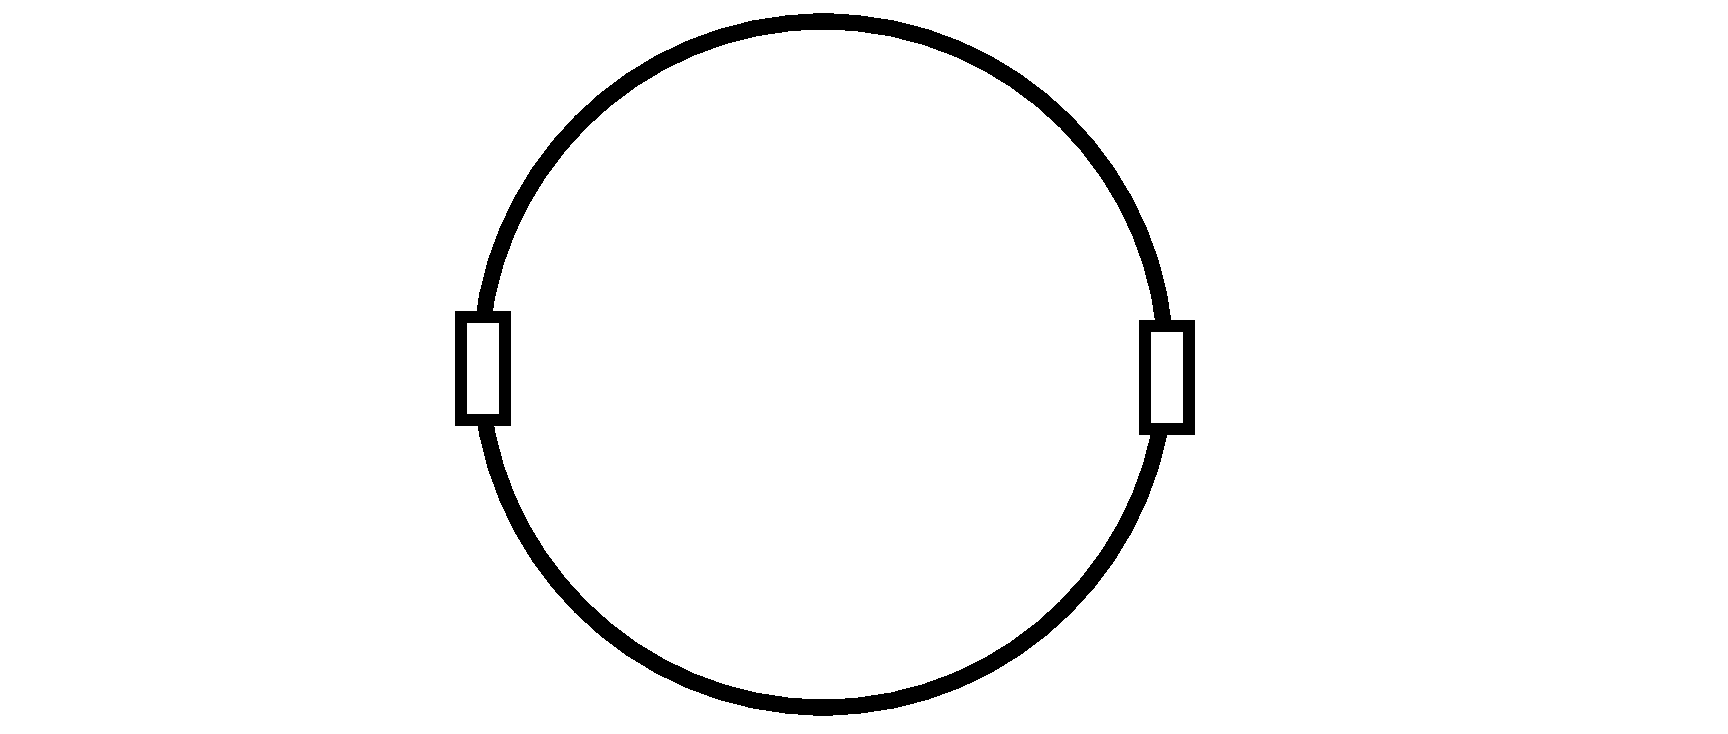
\includegraphics[width=\unitlength,page=1]{res/paradoxeSpanungsmessung2.pdf}}%
	\put(0.7045381,0.1983655){\color[rgb]{0,0,0}\makebox(0,0)[lt]{\lineheight{1.25}\smash{\begin{tabular}[t]{l}$R_2$\end{tabular}}}}%
	\put(0.21171265,0.20167302){\color[rgb]{0,0,0}\makebox(0,0)[lt]{\lineheight{1.25}\smash{\begin{tabular}[t]{l}$R_1$\end{tabular}}}}%
	\put(0.39689155,0.27113165){\color[rgb]{0,0,0}\makebox(0,0)[lt]{\lineheight{1.25}\smash{\begin{tabular}[t]{l}$-\frac{\partial \vec{B}}{\partial t}$\end{tabular}}}}%
	\put(0,0){\includegraphics[width=\unitlength,page=2]{res/paradoxeSpanungsmessung2.pdf}}%
	\put(0.06575846,0.1971287){\color[rgb]{0,0,0}\makebox(0,0)[lt]{\lineheight{1.25}\smash{\begin{tabular}[t]{l}$U_1$\end{tabular}}}}%
	\put(0.85150847,0.20341783){\color[rgb]{0,0,0}\makebox(0,0)[lt]{\lineheight{1.25}\smash{\begin{tabular}[t]{l}$U_2$\end{tabular}}}}%
	\put(0.31981416,0.15056218){\color[rgb]{0,0,0}\makebox(0,0)[lt]{\lineheight{1.25}\smash{\begin{tabular}[t]{l}$\mathcal{E}=\oint\limits_{C(A)} \vec{E}\cdot \dd \vec{s} = -\iint\limits_A \dot{\vec{B}}\cdot \dd \vec{A}$\end{tabular}}}}%
	\put(0.32846175,0.32194138){\color[rgb]{0,0,0}\makebox(0,0)[lt]{\lineheight{1.25}\smash{\begin{tabular}[t]{l}$\mathcal{E}/4$\end{tabular}}}}%
	\put(0.35204605,0.07666474){\color[rgb]{0,0,0}\makebox(0,0)[lt]{\lineheight{1.25}\smash{\begin{tabular}[t]{l}$\mathcal{E}/4$\end{tabular}}}}%
	\put(0.57137998,0.08374004){\color[rgb]{0,0,0}\makebox(0,0)[lt]{\lineheight{1.25}\smash{\begin{tabular}[t]{l}$\mathcal{E}/4$\end{tabular}}}}%
	\put(0.56666313,0.33137513){\color[rgb]{0,0,0}\makebox(0,0)[lt]{\lineheight{1.25}\smash{\begin{tabular}[t]{l}$\mathcal{E}/4$\end{tabular}}}}%
	\put(0.19481742,0.31329384){\color[rgb]{0,0,0}\makebox(0,0)[lt]{\lineheight{1.25}\smash{\begin{tabular}[t]{l}$\mathcal{E}/4$\end{tabular}}}}%
	\put(0.19560356,0.10889662){\color[rgb]{0,0,0}\makebox(0,0)[lt]{\lineheight{1.25}\smash{\begin{tabular}[t]{l}$\mathcal{E}/4$\end{tabular}}}}%
	\put(0.69873519,0.08924303){\color[rgb]{0,0,0}\makebox(0,0)[lt]{\lineheight{1.25}\smash{\begin{tabular}[t]{l}$\mathcal{E}/4$\end{tabular}}}}%
	\put(0.69637676,0.33058898){\color[rgb]{0,0,0}\makebox(0,0)[lt]{\lineheight{1.25}\smash{\begin{tabular}[t]{l}$\mathcal{E}/4$\end{tabular}}}}%
\end{picture}%
\endgroup%
}
		        \end{center}
		        In der schwarzen Leiterschleife gibt es eine eingeprägte elektrische Feldstärke durch die Induktion, welche zu einem Stromfluss führt. Da die blau-grüne Schleife nicht geschlossen ist, hier kann trotz induzierter Spannung kein Strom fließen. Es werden folgende Annahmen getroffen:
		        \begin{itemize}
		        	\item Die Leiter der Schleife sind ideal, sodass es keinen Spannungsabfall durch Stromfluss in diesen Gebieten gibt.
		        	\item Die Fläche der schwarzen Schleife entspricht der Fläche der blau-grünen Schleife. In beiden Schleifen wird so die selbe induzierte Spannung hervorgerufen.
		        	\item Die Widerstände und Spannungsmesspunkte haben eine Größe $g$, welche wesentlich kleiner ist, als der Umfang der Gesamtschleife $l$, also $l\gg g$. Der Anteil der Urspannung, der auf diese Bereiche entfällt, kann entsprechend $\frac{g}{l}\mathcal{E}\approx 0$ vernachlässigt werden. Der Anteil der Urspannung, welcher auf die Leiterbereiche entfällt, ist dann aus Symmetriegründen jeweils $\frac{l/4}{l}\mathcal{E}=\frac{\mathcal{E}}{4}$.
		        	\item Die Spannungsmessung erfolgt ideal, der Widerstand der Voltmeter ist unendlich groß.
		        \end{itemize} 
		         Mit dem Kirchhoffschen Maschensatz ($\nearrow$\ref{masche}) folgt:
		        \begin{equation}\begin{split}
				        \mathcal{E} + I (R_1+R_2)= 0 \quad U_1+\mathcal{E} + I R_2 = 0 \quad -U_2+\mathcal{E} + I R_1 = 0 \to \boxed{\frac{U_1}{U_2} = -\frac{R_1}{R_2}}
			        \end{split}\end{equation}
		        Das selbe Ergebnis zeigt sich im übrigen, wenn man das Magnetfeld ausschaltet und die $\frac{\mathcal{E}}{4}$ durch konzentrierte Quellen hervorruft. Dann erfolgt die Spannungsmessung auch nicht mehr an \enquote{identischen} Punkten, denn zwischen den schwarzen Punkten und den Messpunkten sind Spannungsquellen. Die wesentliche Erkenntnis ist, dass die induzierte Spannung $U_\text{ind}$ \textbf{keine} Spannung im Sinne einer \textbf{Potentialdifferenz} ist, sondern eine \textbf{Urspannung}. Welche Gleichung in \ref{masche} genommen hängt von der Zählpfeilrichtung ab. Ist die Zählpfeilrichtung in Feldrichtung, ist mit der linken Gleichung mit $\mathcal{E}\leftrightarrow U_Q$ zu rechnen, sonst mit der rechten und $\mathcal{E}\leftrightarrow V$. In \ref{Urspannung} wird detaillierter auf die durch Induktion eingeprägte Feldstärke $E_\mathrm{E}$ und die durch Ladungstrennung hervorgerufene Feldstärke $E$ eingegangen.
  \subsubsection{Anordnungen mit Relativbewegung}
  Es gebe zwei Regionen, links gebe es ein von 0 verschiedenes, zeitlich konstantes Magnetfeld, rechts sei das Magnetfeld 0. Die Schleife wird mit der Geschwindigkeit $v$ aus dem Magnetfeld herausgezogen. Dabei wird die Spannung gemessen. Solange ein Teil der Schleife noch im Feld ist, wird eine Spannung angezeigt.
	  \begin{center}
		  \resizebox{.3\textwidth}{!}{\begin{tikzpicture}[line width = 1.2pt, line join=round,x=1cm,y=1cm,>=stealth, scale = 0.4]
	% Grenzfläche
	\draw [color = green] (0,-5) -- (0,10);
	% Geschwindigkeit
	\draw [color = blue,->] (3,1) -- ++(2,0) node [anchor = west] {$ \vec{v} $};
	% Leiterschleife
	\draw (-6,0) rectangle (3,7);
	\filldraw [fill = white, draw = black] (3,3.5) circle (1);
	\draw [->] (1.5,2) -- ++(3,3);
	% Normalenvektor der Fläche
	\coordinate (a) at (-2,3.5);
	\filldraw (a) circle (1.5pt);
	\draw (a) circle (8pt);
	\draw (a) node [anchor = west] {$ \vec{A} $};
	% Höhe der Schleife
	\draw [|<->|] (-7,0) -- ++(0,7) node [anchor = east, midway] {$ h $};
	% Durchflossene Schleife
	\draw [|<->|] (0,-1) -- ++(-6,0) node [anchor = north, midway] {$ x $};
	\draw (-1,-3) node [anchor = north east] {$ x(t = 0) = x_0 $};
	% Magnetisches Feld
	\coordinate (ma) at (-6,9);
	\coordinate (mb) at (-3,9);
	\coordinate (mc) at (1,9);
	\draw [color = red] (ma) circle (1.5pt);
	\draw [color = red] (ma) circle (8pt);
	\draw [color = red] (ma) node [anchor = east] {$ \vec{B}  = \vec{B} _0\  $};
	\draw [color = red] (mb) circle (1.5pt);
	\draw [color = red] (mb) circle (8pt);
	\draw [color = red] (mc) node [anchor = west] {$ \vec{B}  = \vec{0} $};
\end{tikzpicture}}
	  \end{center}
		   Offenbar gilt  hier $\frac{\partial \vec{B} }{\partial t} = \vec{0}$, sodass:
		        \begin{equation}\begin{split}\label{scheinparadox}
				        \to \oint\limits_{C(A)} \vec{E}\cdot\dd\vec{s} = -\iint\limits_{A} \frac{\partial \vec{B} }{\partial t} \cdot \dd \vec{A} = 0
			        \end{split}\end{equation}
		   Das Experiment zeigt, dass \textbf{eine Spannung induziert} wird. Erklären kann man das beispielsweise über die \textbf{Lorentzkraft} auf Ladungsträger im bewegtem Leiter ($\nearrow$\ref{lorentz}). Das ist hier vollkommen zulässig, aber wenn die Leiterschleife weggelassen wird, muss trotzdem eine Induktion im Sinne einer eingeprägten Feldstärke stattfinden. Insbesondere für elektromagnetische Wellen (also Kommunikationstechnik) ist es essentiell, dass das Induktionsgesetz auch ohne vorhandene Ladungsträger funktioniert. Das Problem lässt sich auf zwei Arten lösen:
		          \begin{enumerate}
			        \item \textbf{Mathematisch} mit der vollständigen \textbf{Leibniz-Regel für Integrale}
			        \item \textbf{Physikalisch} mit der \textbf{Speziellen Relativitätstheorie}
		        \end{enumerate}
	  \textbf{1. Leibniz Integralregel (mathematisch):}\\
			  Der eindimensionale Fall dieser Regel lautet:
			        \begin{equation}\begin{split}
					        \frac{\dd}{\dd t} \left( \int\displaylimits_{a(t)}^{b(t)} f(t,x)\dd x \right) = f(t,b(t)) \frac{\dd }{\dd t}b(t)  - f(t,a(t)) \frac{\dd }{\dd t}a(t) +  \int\displaylimits_{a(t)}^{b(t)} \frac{\partial}{\partial t}f(t,x)\dd x
				        \end{split}\end{equation}
			  Das kann man auch in 3D übertragen, dann gilt (Beweis: Flanders - \enquote{Differentiation under the Integral Sign}):
			        \begin{equation}\begin{split}
					        \frac{\dd}{\dd t}  \iint\limits_{A(t)} \vec{f} (\vec{r} , t) \cdot \dd\vec{A} = \iint\limits_{A(t)} \left( \frac{\partial}{\partial t}\vec{f}(\vec{r} , t) + \left[ \div \; \vec{f}(\vec{r} , t) \right] \vec{v} \right) \cdot \dd\vec{A} - \oint\displaylimits_{C(A(t))}
					        \vec{v} \times  \vec{f}(\vec{r} , t) \cdot \dd\vec{s}   \end{split}\end{equation}
			 Hier ist \(\div \vec{B} =0\), also:
			        \begin{equation}\begin{split}
					        \frac{\dd}{\dd t}  \iint\limits_{A(t)} \vec{B}  (\vec{r} , t) \cdot \dd\vec{A} = \iint\limits_{A(t)} \frac{\partial}{\partial t}\vec{B} (\vec{r} , t) \cdot \dd\vec{A} - \oint\displaylimits_{C(A(t))}
					        \vec{v} \times \vec{B} (\vec{r} , t) \cdot \dd\vec{s}   \end{split}\end{equation}
			  Damit folgt dann (oft werden die Terme im Integral \enquote{Ruhe- und Bewegungsinduktion} genannt):
			        \begin{equation}\begin{split}
					        \boxed{\mathcal{E}=U_\text{ind} = \oint\displaylimits_{C(A(t))} \left( \vec{E} + \vec{v} \times \vec{B} \right) \cdot\dd\vec{s} = - \frac{\dd}{\dd t}  \iint\limits_{A(t)} \vec{B}  \cdot \dd\vec{A}  = -\dot{\Phi}}
				        \end{split}\end{equation}
	  \textbf{2. Spezielle Relativitätstheorie (physikalisch):}\\
			  Die spezielle Relativitätstheorie wird in \ref{SRT} aufgegriffen. Genutzt werden dort unter anderem die folgenden beiden Faktoren:
			        \begin{equation}\begin{split}
					        \beta = \frac{v}{c},\quad \beta \in [0, 1]\quad\quad \text{ und }\quad\quad \gamma = \sqrt{\frac{1}{1-\beta^2}},\quad \gamma \in [1,\infty)
				        \end{split}\end{equation}
			        \begin{center}
			        \begin{tabular}{c||c|c|c|c|c|c |c|c|c|c}
				        $\beta$  & 0 & 0.1   & 0.2   & 0.3   & 0.4   & 0.5   & 0.6  & 0.8   & 1.0      \\
				        \hline
				        $\gamma$ & 1 & 1.005 & 1.021 & 1.048 & 1.091 & 1.155 & 1.25 & 1.667 & $\infty$
			        \end{tabular}
			        \end{center}
			  Eine gute Näherung für nicht-relativistische Geschwindigkeiten ist {$\gamma = 1$}, mit der hier weiter gearbeitet wird. Es sei $S'$ ein Inertialsystem, das sich mit $\vec{v}=\text{const.}$ relativ zum Laborsystem $S$ bewegt (Ruhesystem der Schleife). Mit $\vec{v} = v \vu{v}$ können die Felder in $S$ in longitudinale und transversale Anteile zerlegt werden:
			        \begin{align}
				        \vec{E} & = \vec{E}_\parallel + \vec{E}_\perp = (\vu{v} \cdot \vec{E}) \vu{v} + \vu{v} \times (\vu{v} \times \vec{E})     \\
				        \vec{B} & = \vec{B} _\parallel + \vec{B} _\perp = (\vu{v} \cdot \vec{B} ) \vu{v} + \vu{v} \times (\vu{v} \times \vec{B} )
			        \end{align}
			  Im System $S'$ ergeben sich diese Felder dann nach Lorentztransformation zu:
			        \begin{align}
				        \vec{E}' & = \vec{E}_\parallel + \gamma ( \vec{E}_\perp + \vec{v} \times \vec{B} )                                                             & \vec{B} ' & = \vec{B} _\parallel + \gamma ( \vec{B} _\perp - \frac{1}{c^2}\vec{v} \times \vec{E})\label{allglorentz} \\
				                 & = (\vu{v} \cdot \vec{E}) \vu{v} + \gamma \left[\vu{v} \times (\vu{v} \times \vec{E}) + \vec{v} \times \vec{B}  \right]              &
				                 & = (\vu{v} \cdot \vec{B} ) \vu{v} + \gamma \left[\vu{v} \times (\vu{v} \times \vec{B} ) - \frac{\vec{v}}{c^2} \times \vec{E} \right] \nonumber
			        \end{align}
			  Für $v \ll c$ folgt für die Felder im Ruhesystem der Schleife ($S'$):
			        \begin{align}
				        \vec{E}_\parallel' & = \vec{E}_\parallel                      & \vec{B} _\parallel' & = \vec{B} _\parallel \\
				        \vec{E}_\perp'     & = \vec{E}_\perp + \vec{v} \times \vec{B} & \vec{B} _\perp'     & = \vec{B} _\perp
			        \end{align}
			   Es gilt wegen $\gamma=1$, dass $t=t'$, $\vec{B}(\vec{r},t)=\vec{B}'(\vec{r}',t)$ und $\vec{E}(\vec{r},t)+\vec{v}\times\vec{B}(\vec{r},t)=\vec{E}'(\vec{r}',t)$, aber $\vec{0}=\frac{\partial\vec{B}(\vec{r},t)}{\partial t}\neq\frac{\partial\vec{B}'(\vec{r}',t)}{\partial t} $. Es folgt unter Ausnutzung von $A'\neq f(t)$ (was ermöglicht die Differentiation vor das Integral zu ziehen):
			        \begin{equation}\begin{split}
			        \oint\limits_{C( A(t))}\left(\vec{E}+\vec{v}\times\vec{B}\right)\mathrm{d} \vec{s}=	\oint\limits_{C (A')}\vec{E}'\mathrm{d} \vec{s}'=-\iint\limits_{A'} \frac{\partial \vec{B}'}{\partial t}\mathrm{d} \vec{A}'&=-\frac{\mathrm{d}}{\mathrm{d} t}\iint\limits_{A'} \vec{B}'\mathrm{d} \vec{A}'=-\frac{\mathrm{d}}{\mathrm{d} t}\iint\limits_{A(t)} \vec{B}\mathrm{d} \vec{A} \\
			        		&\neq -\iint\limits_{A(t)} \frac{\partial \vec{B}}{\partial t}\mathrm{d} \vec{A}\\
					        \Aboxed{U_\text{ind} = \oint\displaylimits_{C(A(t))} \left( \vec{E} + \vec{v} \times \vec{B} \right) \cdot\dd\vec{s} &= - \frac{\dd}{\dd t}  \iint\limits_{A(t)} \vec{B}  \cdot \dd\vec{A}  = -\dot{\Phi}}
				        \end{split}\end{equation}
			 Mathematik (pure Logik) und Physik (aus Beobachtung abgeleitete Theorie) liefern \textbf{identische Resultate}! Die sich ergebende Gleichung ist für den Fall einer Leiterschleife auch wie oben erwähnt über die Lorentzkraft erklärbar. Wegen \ref{scheinparadox} folgt wenn $\frac{\partial \vec{B}}{\partial t}=0$ ist, dass $\oint \vec{E}\dd \vec{s}=0$ ist. Die induzierte Spannung wird dann nur noch durch den Term der Lorentzkraft hervorgerufen, was intuitiv erscheint, weil durch diese Kraft Ladungsträger so verschoben werden, dass sich eine Spannung aufbaut.
		  
\chapter{Beliebig veränderliche Felder}
Im Folgenden werden die \textbf{Maxwell-Gleichungen} ($\nearrow$\ref{ind},\ref{quellf},\ref{durchf},\ref{gauss}) \textbf{ohne Einschränkung} betrachtet, d.h. es wird kein Term mehr vernachlässigt. In der Regel werden auch in diesem Kapitel \textbf{homogene, lineare und isotrope} Medien betrachtet. Das bedeutet, dass die Materialgleichungen in der vereinfachten Form wie in Gleichung \ref{matlinhomis} gelten. Ferner wird vereinfachend angenommen, dass lokal das \textbf{ohmsche Gesetz} nach Gleichung \ref{ohm} gilt (also in Leitern die Kraftwirkung auf Ladungsträger herrührend vom $B$-Feld vernachlässigbar ist). 
 \section{Ladungserhaltung}
 In \ref{ladungserhaltung} wurde die \textbf{Ladungserhaltung} als axiomatisch vorausgesetzt und davon ausgehend auf die Maxwell-Gleichungen geschlossen. Das funktioniert auch umgekehrt, die Kontinuitätsgleichung  ($\nearrow$\ref{kont}) lässt sich, wie in \ref{kontherl} gezeigt wurde, aus \ref{durchf}, \ref{gauss} und \ref{divrot} herleiten. Die Kontinuitätsgleichung ist ein Ausdruck der Ladungserhaltung.
\section{Energieerhaltung (Poyntingscher Satz)}
\subsection{Differentielle Form des Poyntingschen Satzes}
Zur konzeptionellen Herleitung der Verlustleistungsdichte wird zunächst eine bewegte Ladung $\dd q = \rho_\text{V}\dd V$, welche sich gleichförmig mit der Geschwindigkeit $\vec{v}$ ($|\vec{v}| \ll c$) in homogenen Feldern bewegt betrachtet. Nach \ref{lorentz} wirkt auf die Ladung eine Lorentzkraft:
		        \begin{equation}\begin{split}
				        \vec{F} = q \left( \vec{E} + \vec{v} \times \vec{B} \right) \implies \dd\vec{F} = \rho_\text{V}\dd V \left( \vec{E} + \vec{v} \times \vec{B} \right)
			        \end{split}\end{equation}
Aus der Kraft lässt sich die differentiell \textbf{verrichtete Arbeit} $\dd W$ bei Verschiebung um $\Delta\vec{s} = \vec{v} \Delta t$ ($\Rightarrow\Delta\vec{s} \parallel \vec{v}$, linearer Zusammenhang wegen gleichförmiger Bewegung) bestimmen:
		        \begin{equation}\begin{split}
				        \dd W =  \dd\vec{F} \cdot \Delta\vec{s} = \rho_\text{V}\dd V \left( \vec{E} + \vec{v} \times \vec{B} \right)\cdot \Delta\vec{s}
				        = \rho_\text{V}\dd V\, \vec{E} \cdot \Delta\vec{s} = \rho_\text{V}\dd V\, \vec{E} \cdot \vec{v} \Delta t
			        \end{split}\end{equation}
Außerdem folgt die differentielle \textbf{Leistung} $\dd\left( \frac{W}{\Delta t}\right)$ ($\nearrow$\ref{ladunggeschw}, $v\leftrightarrow v_\text{D}$):
		        \begin{equation}\begin{split}
				        \dd\left( \frac{W}{\Delta t}\right) = \rho_\text{V}\vec{v}\cdot\vec{E}\, \dd V = \vec{J}\cdot\vec{E}\, \dd V
			        \end{split}\end{equation}
Hiermit ergibt sich die \textbf{Leistung} zu:
		        \begin{equation}\begin{split}
				        P = \frac{W}{\Delta t} = \iiint\limits_V \vec{J}\cdot\vec{E}\, \dd V \text{ (analog zu } P=U\cdot I \text{ im Leiter)}
			        \end{split}\end{equation}
Die Analogie gilt nur, wenn $E$ ein konservatives Feld ist. Nur dann ist die Einführung einer Spannung sinnvoll. Für die \textbf{Verlustleistungsdichte} gilt ($\nearrow$\ref{verlustleist},\ref{durchf}):
\begin{equation}\begin{split}
				        p_\text{V} =\frac{\partial w_\text{mech}}{\partial t}= \vec{J}\cdot\vec{E} = \vec{E} \cdot \vec{J} = \vec{E} \cdot \left(\rot \vec{H}  - \frac{\partial \vec{D} }{\partial t}\right) =  \textcolor{red}{\vec{E} \cdot \rot \vec{H} } - \vec{E} \cdot \frac{\partial \vec{D} }{\partial t}
			    \end{split}\end{equation}
		 Der rote Term ist bei weitergehenden Rechnungen störend, also soll er eliminiert werden ($\nearrow$\ref{divcross}):
		        \begin{equation}\begin{split}
				        \div \left(\vec{E} \times \vec{H} \right) = \vec{H} \cdot\rot \vec{E} - \textcolor{red}{\vec{E} \cdot \rot \vec{H} } = - \vec{H} \cdot\frac{\partial \vec{B} }{\partial t} - \textcolor{red}{\vec{E} \cdot \rot \vec{H} }
			        \end{split}\end{equation}
	Somit ergibt sich der \textbf{Poyntingsche Satz} in differentieller Form \textbf{allgemein} zu:
		        \begin{equation}\label{poyntsat}\begin{split}
				        \boxed{\frac{\partial w_\text{mech}}{\partial t}=\vec{E} \cdot \vec{J} = - \div \left(\vec{E} \times \vec{H} \right) - \vec{H} \cdot\frac{\partial \vec{B} }{\partial t} - \vec{E} \cdot \frac{\partial \vec{D} }{\partial t} } 
			        \end{split}\end{equation}
		   Für \textbf{homogene, lineare und isotrope Medien} folgt ($\nearrow$\ref{matlinhomis}):
		        \begin{equation}\label{poyntsathli1}\begin{split}
		        		\frac{1}{2}\frac{\partial}{\partial t}\left(\vec{H} \cdot\vec{B}\right) &= \frac{1}{2}\left(\frac{\partial}{\partial t}\vec{H} \cdot\vec{B} + \vec{H} \cdot\frac{\partial}{\partial t}\vec{B}\right)= \frac{\mu}{2}\left(\frac{\partial}{\partial t}\vec{H} \cdot\vec{H} + \vec{H} \cdot\frac{\partial}{\partial t}\vec{H}\right)=\vec{H}\cdot\frac{\partial}{\partial t}\vec{B}\\
				        \Rightarrow\quad\vec{E} \cdot \vec{J} &= - \div \left(\vec{E} \times \vec{H} \right) - \frac{\partial}{\partial t}\left[\frac{1}{2} \vec{H} \cdot\vec{B}  + \frac{1}{2} \vec{E} \cdot \vec{D} \right] 
			        \end{split}\end{equation}
		   In diesem Ausdruck kommen die magnetische und elektrische Energiedichte vor ($\nearrow$\ref{edichteE},\ref{edichteH}). Es wird die \textbf{elektromagnetische Energiedichte} eingeführt:
		   \begin{equation}
		   	\boxed{w_\text{em}=w_\text{e}+w_\text{m}=\frac{1}{2} \vec{H} \cdot\vec{B}  + \frac{1}{2} \vec{E} \cdot \vec{D}}
		   \end{equation}
		   Damit lässt sich für \textbf{homogene, lineare und isotrope Medien} \ref{poyntsathli1} folgendermaßen schreiben:
		        \begin{equation}\label{poyntsathli}\begin{split}
				     \boxed{ \frac{\partial w_\text{mech}}{\partial t}=\vec{E} \cdot \vec{J}= - \div \left(\vec{E} \times \vec{H} \right) - \frac{\partial w_\text{em}}{\partial t}}
			        \end{split}\end{equation}
		   \subsection{Integrale Form des Poyntingschen Satzes}
		   Der Übergang zur integralen Darstellung erfolgt über ein Volumenintegral:
		        \begin{align*}
			         \iiint\limits_V \vec{E} \cdot \vec{J} \dd V & = - \oiint\limits_{O(V)} \vec{E} \times \vec{H}  \cdot \dd\vec{A} - \frac{\partial}{\partial t} \iiint\limits_V w_\text{em} \dd V \\
			         \underbrace{\frac{\partial}{\partial t} \iiint\limits_V w_\text{mech} \dd V }_{\text{mechanisch, thermodynamisch}}                                                       & = \underbrace{- \oiint\limits_{O(V)} \vec{E} \times \vec{H}  \cdot \dd\vec{A} - \frac{\partial}{\partial t} \iiint\limits_V w_\text{em} \dd V         }_\text{elektromagnetisch}                 
			    \end{align*}
			   Es folgt der \textbf{integrale Poyntigscher Satz} für \textbf{homogene, lineare und isotrope Medien}:
			    \begin{equation}\label{poyntint}
			        \boxed{\frac{\partial}{\partial t} \iiint\limits_V \left( w_\text{mech} + w_\text{em} \right) \dd V                                  = - \oiint\limits_{O(V)} \vec{E} \times \vec{H}  \cdot \dd\vec{A}}
		        \end{equation}
  \subsection{Poynting-Vektor}
		  Änderung der Energie im Volumen $V$ entspricht nach \ref{poyntint} dem Fluss des Vektors $\vec{S}= \vec{E} \times \vec{H} $ durch die Oberfläche des Volumens $O(V)$. Das ist anschaulich eine Formulierung der Energieerhaltung.
		   Die Größe
		        \begin{equation}\begin{split}
				        \boxed{\vec{S}= \vec{E} \times \vec{H} } 
			        \end{split}\end{equation}
		        ist die lokale \textbf{Energieflussdichte} oder der \textbf{Poynting-Vektor}.
		   Hiermit schreiben sich integraler und differentieller Poyntingscher Satz nach \ref{poyntint} und \ref{poyntsathli} wie folgt:
		        \begin{align}
			        \frac{\partial}{\partial t} \iiint\limits_V \left( w_\text{mech} + w_\text{em} \right) \dd V + \oiint\limits_{O(V)} \vec{S} \cdot \dd\vec{A} & = 0 \\
			        \frac{\partial}{\partial t} \left( w_\text{mech} + w_\text{em} \right) + \div \vec{S}                                                        & =0
		    \end{align}
  \subsection{Formulierung bei harmonischer Zeitabhängigkeit}
  \subsubsection{Frequenzbereich}
  Bei harmonischer Zeitabhängigkeit ist wie bei den quasistationären Feldern eine Darstellung im Frequenzbereich vorteilhaft ($\nearrow$\ref{frequenzbereich}). Die harmonische Zeitabhängigkeit stellt keine Einschränkung dar, im Sinne einer Fourier-Synthese kann man durch harmonische Signale verschiedener Frequenz ein beliebiges Signal darstellen. Es gilt:		        \begin{equation}\begin{split}
				        \vec{E}(\vec{r} ,\,t) = \re{\ubar{\vec{E}}(\vec{r} )   \mathrm{e}^{\mathrm{j} \omega  t} } = \frac{1}{2} \left[\ubar{\vec{E}}(\vec{r} )   \mathrm{e}^{\mathrm{j} \omega  t}  + \ubar{\vec{E}}^\star(\vec{r} )   \mathrm{e}^{-\mathrm{j} \omega  t}  \right]
			        \end{split}\end{equation}
 Die Energiedichte $w_\text{e} = \frac{1}{2} \vec{E} \cdot \vec{D} $ lässt sich beispielsweise folgendermaßen schreiben:
		        \begin{equation}\begin{split}
				        w_\text{e} &= \frac{1}{2} \vec{E} \cdot \vec{D}  \\
				        &= \frac{1}{2} \left[ \frac{1}{2} \left(\ubar{\vec{E}}   \mathrm{e}^{\mathrm{j} \omega  t}  + \ubar{\vec{E}}^\star   \mathrm{e}^{-\mathrm{j} \omega  t}  \right)\right] \cdot \left[ \frac{1}{2} \left(\vec{\ubar{D}}   \mathrm{e}^{\mathrm{j} \omega  t}  + \vec{\ubar{D}}^\star   \mathrm{e}^{-\mathrm{j} \omega  t}  \right)  \right] \\
				        &= \frac{1}{8} \left[ \ubar{\vec{E}} \cdot \vec{\ubar{D}}   \mathrm{e}^{\mathrm{j} 2\omega  t} + \ubar{\vec{E}}^\star \cdot \vec{\ubar{D}}^\star   \mathrm{e}^{-\mathrm{j} 2\omega  t}\right] +  \frac{1}{8} \left[ \ubar{\vec{E}} \cdot \vec{\ubar{D}}^\star  + \ubar{\vec{E}}^\star \cdot \vec{\ubar{D}} \right]\\
				        &=\frac{1}{4}\re{\ubar{\vec{E}} \cdot \vec{\ubar{D}}   \mathrm{e}^{\mathrm{j} 2\omega  t}} + \frac{1}{4}\re{\ubar{\vec{E}} \cdot \vec{\ubar{D}}^\star}
			        \end{split}\end{equation}
		        $w_\text{e} = \frac{1}{2} \vec{E} \cdot \vec{D} \neq  \frac{1}{2} \vec{\ubar{E}} \cdot \vec{\ubar{D}}$, weil die Multiplikation nicht linear ist ($\nearrow$\ref{ansig}). Damit man im Zeit- und Bildbereich äquivalent rechnen kann, dürfen nur lineare Operationen ausgeführt werden.
  \subsubsection{Mittelwerte und komplexer Poynting-Vektor}
	  Für den die zeitlichen Mittelwerte gilt (da es sich um periodische Größen handelt reicht die Mittlung über eine Periode):
		        \begin{align}
			        \langle w_\text{e} \rangle    & = \frac{1}{4}\re{\ubar{\vec{E}} \cdot \vec{\ubar{D}}^\star} \stackrel{(\vec{D} =\varepsilon\vec{E}), \varepsilon\in \mathbb{R}}{=} \frac{1}{4}\ubar{\vec{E}} \cdot \vec{\ubar{D}}^\star \label{kompledichtmag}\\
			        \langle w_\text{m} \rangle    & = \frac{1}{4}\re{\vec{\ubar{H}} \cdot \vec{\ubar{B}}^\star} \stackrel{(\vec{B} =\mu\vec{H} ), \mu\in \mathbb{R}}{=} \frac{1}{4}\vec{\ubar{H}} \cdot \vec{\ubar{B}}^\star                \label{komplmdichtmag}\\
			        \langle p_\text{V} \rangle    & = \frac{1}{2}\re{\ubar{\vec{E}} \cdot \ubar{\vec{J}}^\star} \stackrel{(\vec{J}=\kappa\vec{E}), \kappa\in \mathbb{R}  }{=}\frac{1}{2}\ubar{\vec{E}} \cdot \ubar{\vec{J}}^\star       \\
			        \langle \vec{S}\rangle & = \frac{1}{2}\re{\ubar{\vec{E}} \times \vec{\ubar{H}}^\star} = \re{\vec{\ubar{S}}} \label{komplpoyntmit}
		\end{align}
		   Hierbei wird der \textbf{komplexe Poyntingsche Vektor} $\vec{\ubar{S}}$ eingeführt:
		        \begin{equation}\begin{split}
				        \boxed{\vec{\ubar{S}} = \frac{1}{2}\ubar{\vec{E}} \times \vec{\ubar{H}}^\star} {\color{blue}=\ubar{\vec{E}} \times \vec{\ubar{H}}^\star \quad\text{mit RMS-Zeigern}}
			        \end{split}\end{equation}
		     
  \subsubsection{Komplexer Poyntingscher-Satz in differentieller Form}
		  Zunächst wird die Divergenz des komplexen Poynting-Vektors gebildet ($\nearrow$\ref{divcross},\ref{ind},\ref{durchf}):
			        \begin{equation}\begin{split}
					        \div (\frac{1}{2}\ubar{\vec{E}} \times \vec{\ubar{H}}^\star) &= \frac{1}{2} \left( \vec{\ubar{H}}^\star\cdot\rot \ubar{\vec{E}} - \ubar{\vec{E}}\cdot\rot \vec{\ubar{H}}^\star\right)\\
					        &= \frac{1}{2} \left( \vec{\ubar{H}}^\star\cdot (-\mathrm{j}\omega\vec{\ubar{B}}) - \ubar{\vec{E}}\cdot (\ubar{\vec{J}}+\mathrm{j}\omega\vec{\ubar{D}})^\star \right) \\
					        &= \frac{1}{2} \left( -\mathrm{j}\omega\vec{\ubar{H}}^\star\cdot \vec{\ubar{B}} - \ubar{\vec{E}}\cdot \ubar{\vec{J}}^\star + \mathrm{j}\omega\ubar{\vec{E}}\cdot \vec{\ubar{D}}^\star \right)
				        \end{split}\end{equation}
			  Insgesamt gilt somit der \textbf{komplexe Poyntingsche Satz} in differentieller Form (hier für den Fall reeller Materialparameter aufgeschrieben, $\nearrow$ \ref{kompledichtmag}ff.):
			        \begin{equation}\boxed{\begin{split}
				       \div \vec{\ubar{S}}                &  & + &  & \frac{1}{2} \ubar{\vec{E}}\cdot \ubar{\vec{J}}^\star &  & + &  & \mathrm{j}2\omega &  & \Big[ &  & \frac{1}{4} \vec{\ubar{H}}^\star\cdot\vec{\ubar{B}} &  & - &  & \frac{1}{4} \ubar{\vec{E}}\cdot \vec{\ubar{D}}^\star &  & \Big] &  & = &  & 0 \\
				        \Leftrightarrow \div \vec{\ubar{S}} &  & + &  & \langle p_\text{V} \rangle  &  & + &  & \mathrm{j}2\omega &  & \Big[ &  & \langle w_\text{m}\rangle  &  & - &  & \langle w_\text{e}\rangle    &  & \Big] &  & = &  & 0
			        \end{split}}\end{equation}
			  Im Vergleich zum Zeitbereich ($\nearrow$\ref{poyntsat}) fallen zum Einen die anderen Vorzeichen (durch die Konjugation in der Definition des komplexen Poynting-Vektors) und zum Anderen die abweichenden Vorfaktoren (Multiplikation ist nichtlinear) auf. Weil die Mittelwerte reell sind, ist eine Aufspaltung in Real- und Imaginärteil möglich:
			        \begin{equation}\begin{split}
					        \re{\div \vec{\ubar{S}}} + \underbrace{\frac{1}{2} \ubar{\vec{E}}\cdot \ubar{\vec{J}}^\star}_{\langle p_\text{V} \rangle} =0 \quad  \im{\div \vec{\ubar{S}}} + 2\omega\Bigg[\underbrace{\frac{1}{4} \vec{\ubar{H}}\cdot\vec{\ubar{B}}^\star}_{\langle w_\text{m}\rangle} - \underbrace{\frac{1}{4} \ubar{\vec{E}}\cdot \vec{\ubar{D}}^\star}_{\langle w_\text{e}\rangle} \Bigg] =0
				        \end{split}\end{equation}
  \subsubsection{Komplexer Poyntingscher-Satz in integraler Form}
		   Aus der differentiellen Form folgt sofort der \textbf{integrale komplexe Poyntingsche Satz}:
			        \begin{equation}\label{komplpoyntint}
				       \boxed{ \oiint\limits_{O(V)} \vec{\ubar{S}}\cdot \dd\vec{A} + \iiint\limits_V \langle p_\text{V} \rangle \dd V + \mathrm{j}2\omega\iiint\limits_V \left( \langle w_\text{m}\rangle - \langle w_\text{e}\rangle \right)\dd V = 0}
			        \end{equation}
			  Der Realteil entspricht der \textbf{mittleren Wirkleistung} (umgesetzte Energie, Ohmschen Verluste):
			        \begin{equation}\begin{split}
					        \langle P_\text{V} \rangle = \iiint\limits_V \langle p_\text{V} \rangle \dd V = -\oiint\limits_{O(V)} \re{\vec{\ubar{S}}}\cdot \dd\vec{A}\quad \color{blue}{\to P}
				        \end{split}\end{equation}
			 Der Imaginärteil entspricht der \textbf{mittleren Blindleistung}:
			        \begin{equation}\begin{split}
					        2\omega\iiint\limits_V \left( \langle w_\text{m}\rangle - \langle w_\text{e}\rangle \right)\dd V = -\oiint\limits_{O(V)} \im{\vec{\ubar{S}}}\cdot \dd\vec{A}\quad\color{blue}{\to Q} 
				        \end{split}\end{equation}
			 In {\color{blue}{DNW-Notation}} ist lässt sich auch schreiben:
			 \begin{equation}\begin{split}
			 	\color{blue}P+\mathrm{j}Q&=-\oiint\limits_{O(V)} \re{\vec{\ubar{S}}}\cdot \dd\vec{A}-\mathrm{j}\oiint\limits_{O(V)} \im{\vec{\ubar{S}}}\cdot \dd\vec{A}=-\oiint\limits_{O(V)} \vec{\ubar{S}}\cdot \dd\vec{A}\\
			 		&=\iiint\limits_V \langle p_\text{V} \rangle \dd V + \mathrm{j}2\omega\iiint\limits_V \left( \langle w_\text{m}\rangle - \langle w_\text{e}\rangle \right)\dd V
			 \end{split}\end{equation}
		  \subsubsection{Anwendungsbeispiel: Koaxialkabel} 
		  Betrachtet wird eine koaxiale Anordnung mit einem Innenleiter (Radius $a$) und einem Außenleiter (Radius $b$). Ohmsche Verluste gibt es nur im Innenleiter, im Außenleiter gilt $\kappa_a\to\infty$. Die Betrachtung soll bei tiefen Frequenzen ($l\ll\lambda$, $a\ll\delta$, $\omega L \ll R_i$) erfolgen. Der Strom $I_0=I(\rho,\varphi,z)$ ist also niederfrequent (quasistatische Näherung). In dieser speziellen Anordnung verschwindet die Rotation des elektrischen Feldes, weshalb eine Spannung $U(z)$ eingeführt werden kann ($\nearrow$\ref{leitungstheorie}). Für den Widerstand des Innenleiters gilt in Abhängigkeit der Längenkoordinate $z$: 
		  \begin{equation*}
		  	R_i(z)=\frac{z}{\kappa\cdot \pi a^2}
		  \end{equation*}
		  \begin{center}
		  	\resizebox{\textwidth}{!}{\vbox{%
	\begin{tikzpicture}
		% Achsen zeichnen
		\draw[->,thick] (0,0) -- (-1,-1) node [below left] {$z$};
		%Plot
		\draw (0,0) circle (.35);
		\draw (0,0) circle (.75);
		\draw (0,0) -- (340:.35) node [below right] {$a$};
		\draw (0,0) -- (200:.75) node[below left] {$b$};
		\draw (135:.75) --+ (2,2);
		\draw[style=dashed] (135:.35) --+ (2,2);
		\draw[style=dashed] (315:.35) --+ (2,2);
		\draw (315:.75) --+ (2,2);
		\draw[style=dashed] (2,2) circle (.35);
		\draw (2,2) +(0:.75) arc (0:135:0.75) ;
		\draw[style=dashed] (2,2)+(135:.75) arc (135:315:.75);
		\draw (2,2) +(315:.75) arc (315:360:.75);
		\draw[<-] (.75,-0.75)--(1.75,0.25) node[below right] {$l$};
		\draw[->] (1.75,0.25)--(2.75,1.25);
	\end{tikzpicture}

	\begin{tikzpicture}
		% Achsen zeichnen
		%\draw[->,thick] (0,0) -- (-1,-1) node [below left] {$z$};
		\draw[<->] (0,0)--(0,2) node[left] {$2b$} --(0,4);
		\draw[<->] (1,1.5)--(1,2) node[left] {$2a$} --(1,2.5);
		\draw (1.5,4)--(5.5,4);
		\draw (1.5,0)--(5.5,0)--(5.5,2);
		\draw[->] (1.5,2)--(7,2) node[right] {$z$};
		\draw (1.5,0)--(1.5,2);
		\draw (1.5,1) circle(.25);
		\draw[<-] (1.1,.75)--(1.1,1.25) node[below left] {$ U_0$};
		\draw (1.9,1.5) rectangle (5,2.5);
		\draw[style=dashed] (1.9,2.5)--(1.9,4.2) node[above] {$0$};
		\draw[style=dashed] (3.5,2.5)--(3.5,4.2) node[above] {$z$};
		\draw[fill=black] (1.7,0) circle(.05);
		\draw[fill=black] (1.7,2) circle(.05);
		\draw[fill=black] (5.3,0) circle(.05);
		\draw[fill=black] (5.3,2) circle(.05);
		\draw[fill=white] (5.35,0.5) rectangle (5.65,1.5);
		\node[right] at (5.75,1) {$ R$};
		\node[right] at (3,1.65) {$\kappa$};
		\node[right] at (3,-.3) {$\kappa_a \rightarrow \infty$};
		\node[right] at (3.2,.75) {$ U ( z)$};
		\draw[->] (3.2,1.3)--(3.2,0.2);
	\end{tikzpicture}
}}
		  \end{center}
		 Zur Lösung des Problems werden Maschengleichungen angesetzt:
		  	\begin{align*}
		  		\text{große Masche:}  &  & U_0  & = R_i(l)I_0 + RI_0                               \\
		  		\text{kleine Masche:} &  & U_0  & = U(z) + R_i(z)I_0                               \\
		  		\implies                   &  & U(z) & = U_0\left(1-\frac{z}{l+\kappa\pi a^2 R} \right)
		  	\end{align*}
		  Außerhalb des Leiters ist ist kein Magnetfeld vorhanden (Kompensation von Hin- und Rückstrom). Durch Anwendung von \ref{durchf} erhält man das Magnetfeld im Innenleiter ($H^i$) und im Zwischenraum zwischen den Leitern ($H^a$):
		  \begin{equation*}
		  	\vec{H} ^i = H_\varphi^i \vu{\varphi} = \frac{I_0}{2\pi a}\frac{\rho}{a} \vu{\varphi} \text{ und } \vec{H} ^a = H_\varphi^a \vu{\varphi} = \frac{I_0}{2\pi \rho} \vu{\varphi}
		  \end{equation*}
		  	Das elektrische Feld im Innenleiter hat nur eine $z$-Komponente (wegen der Stromdichte): $$\vec{E}^i=E_z^i \vec{e_z} = \frac{\vec{J}_z}{\kappa}\vec{e_z}=\frac{I_0}{\kappa\pi a^2}\vec{e_z}$$	Würde es sich bei dem Strom $I$ um einen höherfrequenten Wechselstrom handeln, dann müsste der Skineffekt ($\nearrow$\ref{skin}) beachtet werden. Weil die Stromdichte außen größer ist, haben sowohl das $E-$Feld als auch das $H-$Feld im Leiter eine andere Form. Für das elektrische Feld im Zwischenraum muss die Laplacegleichung $\Delta \phi =0$ gelöst werden, es lässt sich zeigen, dass es hier ein Skalarpotential gibt. Dafür wird diese zunächst in Zylinderkoordinaten geschrieben:
		  		$$
		  		\frac{1}{\rho}\frac{\partial}{\partial \rho}\left(\rho\frac{\partial \phi}{\partial \rho}\right) + \frac{1}{\rho^2}\frac{\partial^2 \phi}{\partial \varphi^2} + \frac{\partial^2 \phi}{\partial z^2} =0 
		  		$$
		  		Diese kann dann mit dem Separationsansatz ($\nearrow$\ref{sep}) gelöst werden. Das elektrische Feld wird dann über $\vec{E}=-\grad \phi$ errechnet. Weiterhin kann man mit \ref{tanE} die Randbedingungen $E_z^a(\rho=a) = E_z^i$ und $E_z^a(\rho=b) = 0$ gewinnen. Außerdem lässt sich eine Anfangsbedingung formulieren (siehe Skizze): $U_0=\int\limits_a^b E^a_\rho(\rho, z=0)\dd\rho$.
Schließlich ergibt das:
		  	$$
		  	E_\rho^a = \frac{U_0}{\rho \ln\frac{b}{a}}\left(1-\frac{z}{l+\kappa\pi a^2 R}\right) \quad E_z^a = \frac{U_0 \ln\frac{b}{\rho}}{\ln\frac{b}{a}}\frac{1}{l+\kappa\pi a^2 R}
		  	$$
Nun kann der komplexe Poynting Vektor aus den Feldern berechnet werden:
		  	\begin{equation*}\begin{split}
		  			\vec{\ubar{S}}^i &= \frac{1}{2} \ubar{\vec{E}}^i \times \vec{\ubar{H}}^{i\star} = -\frac{1}{2} E_z^i H_\varphi^i \vec{e_\rho}\\
		  			\vec{\ubar{S}}^a &=\frac{1}{2} \ubar{\vec{E}}^a \times \vec{\ubar{H}}^{a\star} = -\frac{1}{2} E_z^a H_\varphi^a \vec{e_\rho} + \frac{1}{2} E_\rho^a H_\varphi^{a\star} \vec{e_z}
		  	\end{split}\end{equation*}
		  Da $\vec{\ubar{S}}^i$ und $\vec{\ubar{S}}^a$ rein reell sind, wird nur Wirkleistung umgesetzt ($\omega L\ll R_i$ wurde explizit vernachlässigt!). Die radial (in $\rho$-Richtung) nach innen fließende Energie berechnet sich nach \ref{poyntint} zu:
		  	$$
		  	- 2\pi a \int\limits_0^l \vec{\ubar{S}}^i (\rho=a)\cdot\vec{e_\rho} \dd z = \frac{1}{2} R_i(l) I_0^2 
		  	$$
		  	Der Faktor $\frac{1}{2}=\frac{1}{\sqrt{2}^2}$ kommt dabei dadurch zustande, dass mit Effektivwerten gerechnet wird. Berechnet wurde damit die Verlustleistung im Innenleiter. Im Innenleiter wird also thermische Energie freigesetzt, welche aus dem Zwischenraum kommt. Dort erfolgt nämlich auch ein axialer Energietransport (in $z$-Richtung):
		  	$$
		  	\int\limits_a^b \vec{\ubar{S}}^a (\rho) \cdot\vec{e_z} 2 \pi\rho\dd\rho = \frac{1}{2} I_0 U(z)
		  	$$
		  	 Dieser Ausdruck ausgewertet bei $z=0$ ergibt die von der Quelle abgegebene Leistung. Diese ist wie erwartet:
		  	$$
		  	P = \frac{1}{2} I_0U(0) = \frac{1}{2} \frac{U_0^2}{R+R_i(l)}
		  	$$
Der Energietransport in Ausbreitungsrichtung (axial) findet nur im Zwischenraum statt, obwohl dort kein Leiter ist. Im Innenleiter und Außenleiter kommt es nur zu Verlusten.
 \section{Impulserhaltung}
 \subsection{Rolle des Impulses in der elektromagnetischen Feldtheorie}
In der Mechanik besteht eine elementare Beziehung zwischen \textbf{Impuls} \(\vec{p}^\text{ mech}\) und \textbf{Kraft} \(\vec{F} \):
\begin{equation}\label{krafimp}
	\vec{F}  = \frac{\dd}{\dd t} \vec{p}^\text{ mech}
\end{equation}
 Diese Beziehung gilt auch für den \textbf{relativistischen Impuls} (bei sehr hohen Geschwindigkeiten, im Rahmen der Speziellen Relativitätstheorie $\nearrow$\ref{SRT}) und ist somit wesentlich fundamentaler als die klassische Formulierung \(\vec{F}  = m\vec{a}\). Es gilt mit $\gamma$ als Lorentzfaktor und $m_0$ als Ruhemasse:  \begin{equation}
 	\vec{p}^\text{ mech} = \gamma m_0 \vec{v}
 	\end{equation}
 Die elektromagnetische Feldtheorie ist eine relativistische Theorie, weshalb es sinnvoll ist den Impuls zu betrachten.
 \subsection{Kraftdichte}
  Zudem kann in der elektromagnetischen Feldtheorie die Lorentzkraft ($\nearrow$\ref{lorentz}) herangezogen werden. In simplen Situationen (bspw. wenn sich eine Punktladung frei durch ein homogenes Magnetfeld bewegt) ist das zweckmäßig. Für kompliziertere praktische Berechnungen (z.B. elektrische Antriebe) wird das unhandlich, weshalb \textbf{Formulierung nur mit Feldern} angebrachter ist (letztlich ist es nur eine \enquote{Umschreibung} der Lorentzkraft).\\
 Die lokale \textbf{Kraftdichte} \(\vec{f}\) in Abhängigkeit von der \textbf{Impulsdichte} \(\vec{p}_\text{V}^\text{ mech}\) ist durch Ersetzung der Kraft und des Impulses durch die jeweilige Dichte in \ref{krafimp} gegeben:
		        \begin{equation}
			        \vec{f}= \frac{\dd}{\dd t} \vec{p}_\text{V}^\text{ mech} \quad \quad \vec{F} =\iiint\limits_V \vec{f}\, \dd V
		        \end{equation}
Mit \ref{lorentz} und \ref{jrhov} lässt sich für die Kraftdichte schreiben (Ladung $\leftrightarrow$ Ladungsdichte):
		        \begin{equation}\label{kraftdicht}
			        \vec{f}= \frac{\dd}{\dd t}\vec{p}_\text{V}^\text{mech} =\rho_\text{V} (\vec{E} + \vec{v} \times \vec{B} ) = \textcolor{green}{\rho_\text{V}} \vec{E} + \textcolor{red}{\vec{J}} \times \vec{B}
		        \end{equation}
		   Durch Einsetzen der Maxwell-Gleichungen ($\nearrow$\ref{ind},\ref{quellf},\ref{durchf},\ref{gauss}) sowie anwenden einer Produktregel folgt:
		        \begin{align}
			        \vec{f} & =  \vec{E}\, \textcolor{green}{\div \vec{D} } + \textcolor{red}{(\rot \vec{H} -\frac{\partial \vec{D} }{\partial t})} \times \vec{B}   \nonumber                                                                                                                \\
			                & = \vec{E}\, \div \vec{D}  + (\rot \vec{H} ) \times \vec{B}  - \frac{\partial \vec{D} }{\partial t}  \times \vec{B}   \nonumber                                                                                                                                  \\
			                & = \vec{E}\, \div \vec{D}  + (\rot \vec{H} ) \times \vec{B}  - \left[ \frac{\dd }{\dd t}(\vec{D}  \times \vec{B} ) \textcolor{red}{-} \vec{D}  \times \textcolor{red}{\frac{\partial \vec{B} }{\partial t}} \right]  \nonumber                             \\
			                & = \vec{E}\, \div \vec{D}  + \underbrace{(\rot \vec{H} ) \times \vec{B}}_{\vec{a}\times\vec{b}=-\vec{b}\times\vec{a}}  - \left[ \frac{\dd }{\dd t}(\vec{D}  \times \vec{B} ) \textcolor{red}{+} \vec{D}  \times \textcolor{red}{\rot \vec{E}}\nonumber \right]      \end{align}
			                Umordnen liefert:
			                \begin{align}
			        \Aboxed{\vec{f} & = \left[ \vec{E}\, \div \vec{D}  - \vec{D}  \times \rot \vec{E}\right] + \left[-\vec{B} \times ( \rot \vec{H} )\right] - \frac{\dd }{\dd t}(\vec{D}  \times \vec{B} )} \quad \text{ alle Materialien}\\
			                & = \left[ \vec{E}\, \div \vec{D}  - \vec{D}  \times \rot \vec{E}\right] + \left[\vec{H} \,\textcolor{red}{\underbrace{\div \vec{B}}_{=0, \text{für Symmetrie} }}-\vec{B} \times \rot \vec{H} \right] - \frac{\dd }{\dd t}(\vec{D}  \times \vec{B} )\nonumber\\
			       \Aboxed{\vec{f}& = \varepsilon\left[ \vec{E}\, \div \vec{E} - \vec{E} \times \rot \vec{E}\right] + \frac{1}{\mu}\left[\vec{B} \,\div \vec{B} -\vec{B} \times \rot \vec{B} \right] - \varepsilon\frac{\dd }{\dd t}(\vec{E} \times \vec{B} ) } \quad \text{ hli}
		        \end{align}
	Mit \ref{gradab} folgt:	   
		        \begin{equation*}\begin{split}
				         - \vec{E} \times \rot \vec{E} &= (\vec{E}\cdot\grad )\vec{E} - \frac{1}{2}\grad |\vec{E}|^2\quad \text{ für }\vec{B} \text{ analog}
			        \end{split}\end{equation*}
		   Damit ist die \textbf{Kraftdichte in homogenen, lineare, isotropen Medien}:
		        \begin{equation}
		        	\boxed{
			        \begin{split}
				        \vec{f}=  \varepsilon\left[ \vec{E}\, \div \vec{E} +(\vec{E}\cdot\grad )\vec{E}\right] + \frac{1}{\mu}\left[\vec{B} \,\div \vec{B}  + (\vec{B} \cdot\grad )\vec{B} \right] \\-\grad \underbrace{\left[ \frac{1}{2}\varepsilon|\vec{E}|^2 +\frac{1}{2\mu} |\vec{B} |^2  \right]}_{w_\text{em}}- \underbrace{\varepsilon\frac{\dd }{\dd t}(\vec{E} \times \vec{B} )}_{\varepsilon\mu\frac{\dd }{\dd t} \vec{S}}
			        \end{split}}
		        \end{equation}
  \subsection{Maxwellscher Spannungstensor}\label{spanten}
  \subsubsection{Definition}
         Um die Kraftdichte einfacher schreiben zu können, wird der \textbf{Maxwellsche Spannungstensor} \(\mathbf{T}\) eingeführt. Dieser ist ein dreidimensionaler Tensor 2. Stufe (\enquote{\(3 \times 3\)-Matrix}):
              \begin{equation}\label{maxkofrei}
	              \mathbf{T} = \left(T_{ij}\right) \text{ mit } \boxed{T_{ij} = \varepsilon\left[ E_iE_j-\frac{1}{2}\delta_{ij} |\vec{E}|^2\right] + \frac{1}{\mu} \left[B_iB_j-\frac{1}{2}\delta_{ij} |\vec{B} |^2\right] } 
              \end{equation}
         Diese Darstellung ist zunächst noch Korrdinatenfrei ($\nearrow$\ref{maxkofreiaus}). Explizit lässt sich in kartesischen Koordinaten schreiben:
              \begin{equation}
	              \begin{split}
		              \mathbf{T} =
		              \begin{pmatrix}
			              \varepsilon E_xE_x + \frac{1}{\mu}B_xB_x & \varepsilon E_xE_y + \frac{1}{\mu}B_xB_y & \varepsilon E_xE_z + \frac{1}{\mu}B_xB_z \\
			              \varepsilon E_yE_x + \frac{1}{\mu}B_yB_x & \varepsilon E_yE_y + \frac{1}{\mu}B_yB_y & \varepsilon E_yE_z + \frac{1}{\mu}B_yB_z \\
			              \varepsilon E_zE_x + \frac{1}{\mu}B_zB_x & \varepsilon E_zE_y + \frac{1}{\mu}B_zB_y & \varepsilon E_zE_z + \frac{1}{\mu}B_zB_z
		              \end{pmatrix}
		              \\ -\underbrace{\frac{1}{2}\left(\varepsilon |\vec{E}|^2 + \frac{1}{\mu}|\vec{B} |^2\right)}_{w_\text{em}}
		              \begin{pmatrix}
			              1 & 0 & 0 \\
			              0 & 1 & 0 \\
			              0 & 0 & 1
		              \end{pmatrix}
	              \end{split}
              \end{equation}
 An der expliziten Formulierung sieht man, dass der Tensor symmetrisch ist. In \(T_{ij}\) steht das $i$ (bzw. $j$, egal wegen Symmetrie) für die \textbf{Wirkrichtung} der Kraft pro Flächeneinheit (Druck). Diese Kraft wirkt auf das Flächenelement mit Normale \(\vu{j}\) (bzw. $\vu{i}$), weshalb man diese Richtung auch als \textbf{Normalenrichtung} bezeichnet.  Die Komponenten, für die \(i=j\) gilt (\(T_{ii}\)) heißen \textbf{Normalspannungskomponenten}, bei denen Normalen- und Wirkrichtung gleich sind. Die Komponenten mit \( i \ne j \) heißen \textbf{Scherspannungskomponenten}, bei den Normalen- und Wirkrichtung unterschiedlich sind. Die folgende Abbildung verbildlicht einen Spannungstensor an einem Volumenelement $\dd V$. In einem größeren Volumen sind anschaulich viele solcher Volumenelmente zusammengesetzt. Zur Berechnung der resultierenden Kraft auf das gesamte Volumen werden letztlich alle Kraftkomponenten über die Oberfläche kumuliert. Gibt es eine resultierende Kraft muss sich das Volumen bewegen (oder mechanisch befestigt sein $\to$ Kräftegleichgewicht). Anschauung (\href{https://tex.stackexchange.com/questions/553898/how-to-draw-a-cube-with-coordinate-systems-in-tikz}{Bildquelle}):
 \begin{center}
 	\resizebox{!}{.3\textwidth}{ \begin{tikzpicture}[%
	3d view = {15}{15}
	]
	
	\draw[-{Latex[scale = 0.7]}] (-4, -4, 0) -- (-3, -4, 0)
	node[below] {$x_1$};
	\draw[-{Latex[scale = 0.7]}] (-4, -4, 0) -- (-4, -3, 0)
	node[right] {$x_2$};
	\draw[-{Latex[scale = 0.7]}] (-4, -4, 0) -- (-4, -4, 1)
	node[above] {$x_3$};
	
	\begin{scope}[canvas is xz plane at y = -2]
		
		\draw[
		fill = lightgray
		] (-2, -2) rectangle (2, 2);
		
		\draw[-Latex] (-1.75, 0) -- (1.75, 0)
		node[below left] {$T_{12}$};
		\draw[-Latex] (0, -1.75) -- (0, 1.75)
		node[below left] {$T_{32}$};
		
	\end{scope}     
	
	\draw[Latex-] (0, -2, 0) -- (0, -3.5, 0)
	node[left] {$T_{22}$};
	
	\begin{scope}[canvas is yz plane at x = 2]
		
		\draw[
		fill = lightgray
		] (-2, -2) rectangle (2, 2);
		
		\draw[-Latex] (1.75, 0) -- (-1.75, 0)
		node[below right] {$T_{21}$};
		\draw[-Latex] (0, -1.75) -- (0, 1.75)
		node[below right] {$T_{31}$};
		
	\end{scope} 
	
	\draw[Latex-] (2, 0, 0) -- (3.5, 0, 0)
	node[right] {$T_{11}$};
	
	\begin{scope}[canvas is xy plane at z = 2]
		
		\draw[
		fill = lightgray
		] (-2, -2) rectangle (2, 2);
		
		\draw[-Latex] (-1.75, 0) -- (1.75, 0)
		node[above]{$T_{13}$};
		\draw[-Latex] (0, 1.75) -- (0, -1.75)
		node[above left]{$T_{23}$};
		
	\end{scope} 
	
	\draw[Latex-] (0, 0, 2) -- (0, 0, 3.5)
	node[above] {$T_{33}$};
	
\end{tikzpicture}}
 \end{center}
Wie mit dem Spannungstensor gerechnet werden kann, insbesondere wie das Flächenintegral behandelt wird, ist in \ref{dyad} aufgegriffen. In der relativistisch kovarianten Formulierung der Elektrodynamik wird mit dem \href{https://en.wikipedia.org/wiki/Covariant_formulation_of_classical_electromagnetism#Electromagnetic_stress%E2%80%93energy_tensor}{Energie-Impuls-Tensor} (\enquote{$4\times 4$}, wegen Vierervektoren) gearbeitet, welcher als Komponenten die des Maxwellschen Spannungstensors enthält.
  \subsubsection{Zusammenhang mit Kraftdichte}
  Die Divergenz eines Tensors 2. Stufe ist ein Tensor 1. Stufe. Die \(j\)-te Komponente der Divergenz von \(\mathbf{T}\) ist definiert als:
		        \begin{equation}\begin{split}
				        (\div \mathbf{T})_j &= \sum_{i=1}^3 \frac{\partial}{\partial x_i} T_{ij} = \partial_i T_{ij} \\
				        &= \sum_{i=1}^3 \left\{ \varepsilon\left( \frac{\partial E_i}{\partial x_i} E_j + E_i\frac{\partial E_j}{\partial x_i} \right) +
				        \frac{1}{\mu}\left( \frac{\partial B_i}{\partial x_i} B_j + B_i\frac{\partial B_j}{\partial x_i} \right)
				        \right\} - \left(\frac{\varepsilon}{2}\frac{\partial |\vec{E}|^2}{\partial x_j} + \frac{1}{2\mu}\frac{\partial |\vec{B} |^2}{\partial x_j}\right)\\
				        &=\varepsilon\left[E_j \div \vec{E} + (\vec{E}\cdot\grad )E_j - \frac{1}{2}\grad _j |\vec{E}|^2 \right] +\\
				        &\qquad \frac{1}{\mu}\left[B_j \div \vec{B}  + (\vec{B} \cdot\grad )B_j - \frac{1}{2}\grad _j |\vec{B} |^2 \right]
			        \end{split}\end{equation}
		   Dies ist gerade die \(j\)-te Komponente der ersten drei Terme der Kraftdichte. Somit:
		        \begin{equation}\label{kraftdmax}
			        \boxed{\vec{f}= \div \mathbf{T} - \varepsilon\frac{\dd}{\dd t}\left( \vec{E} \times \vec{B} \right)
				        = \div \mathbf{T} - \varepsilon\mu\frac{\dd}{\dd t}\left( \vec{E} \times \vec{H} \right)
				        = \div \mathbf{T} - \varepsilon\mu\frac{\dd \vec{S}}{\dd t}}
		        \end{equation}
		   Die Gesamtkraft (die wirkende Kraft auf das Probevolumen $V$, bspw. eine Kondensatorplatte) ist somit:
		        \begin{equation}
			        \boxed{\vec{F}  = \oiint\limits_{O(V)} \mathbf{T} \cdot \dd\vec{A} - \varepsilon\mu\frac{\dd}{\dd t} \iiint\limits_V \vec{S} \dd V}
		        \end{equation}
	  Das \textbf{Oberflächenintegral} liefert einen Beitrag zur Gesamtkraft, der nur auf die Oberläche des betrachteten Volumens wirkt. Das \textbf{Volumenintegral} verschwindet im stationären Fall. Dann wird die Gesamtkraft nur über die Oberfläche bestimmt. In Analogie zur Mechanik ($\nearrow$\ref{krafimp}), in der die zeitliche Ableitung eines Impulses eine Kraft ist, kann man den \textbf{elektromagnetischen Impuls} bzw. eine entsprechende \textbf{Impulsdichte} definieren:
		        \begin{align}
			       \Aboxed{ \vec{p}^\text{ em}   & = \iiint\limits_V \varepsilon\mu\vec{S} \dd V }\\
			        \Aboxed{\vec{p}^\text{ em}_V & = \varepsilon\mu\vec{S}} \label{impdicht}
		        \end{align}
Die hier zu Tage tretende enge Verbindung von Energie (Poynting-Vektor) und Impuls sieht man auch in der kovarianten Formulierung der Elektrodynamik deutlich. Man arbeitet mit dem \href{https://en.wikipedia.org/wiki/Covariant_formulation_of_classical_electromagnetism#Electromagnetic_stress%E2%80%93energy_tensor}{Energie-Impuls-Tensor}. 
  \subsection{Formulierung der Impulserhaltung}
		  Unter Beachtung von \ref{kraftdicht} kann man für \ref{kraftdmax} nun schreiben:
		        \begin{align}
			        \vec{f}= \frac{\dd }{\dd t}\vec{p}^\text{ mech}_V                              & = \div \mathbf{T} - \frac{\dd }{\dd t}\left( \varepsilon\mu\vec{S}\right) = \div \mathbf{T} - \frac{\dd }{\dd t}\vec{p}^\text{ em}_V \nonumber \\
			        \frac{\dd }{\dd t}\left(\vec{p}^\text{ mech}_V +  \varepsilon\mu\vec{S}\right) & =\div \mathbf{T}                                                                                                                     \nonumber\\
			        \Aboxed{\frac{\dd }{\dd t}\left(\vec{p}^\text{ mech}_V + \vec{p}^\text{ em}_V\right)   & =\div \mathbf{T}}
		        \end{align}
		   Die Volumenintegration dieser \textbf{lokalen Impulsbilanz} liefert die \textbf{integrale Impulsbilanz}:
		        \begin{equation}
			        \boxed{\frac{\dd }{\dd t} \iiint\limits_V \left(\vec{p}^\text{ mech}_V + \vec{p}^\text{ em}_V\right)\dd V = \oiint\limits_{O(V)}\mathbf{T} \cdot \dd \vec{A}}
		        \end{equation}
\section{Verallgemeinerte Betrachtungen zur Eichung}\label{geneich}
\subsection{Potentiale} 
In diesem Abschnitt sollen die mikroskopischen Maxwellgeichungen \textbf{im Vakuum} betrachtet werden ($\nearrow$\ref{mikrosmax}). Die Felder und Quellen sind stetig differenzierbare Funktionen des Ortes $\vec{{r}}$ und der Zeit ${t}$. Über die zeitlichen Ableitungen der Feldgrößen $\vec{E}$ und $\vec{B}$ sind die Gleichungen verkoppelt.\\
Bei der Lösung der MGl ist es manchmal hilfreich, das elektrische \textbf{Skalarpotential} $\phi$ und das magnetische \textbf{Vektorpotential} $\vec{A}$ einzuführen. Rotationsfreie Felder sind als Gradient darstellbar und divergenzfreie Felder als Rotation ($\nearrow$\ref{poin}).
 \begin{align}
	\div \vec{B} & = 0                                     & \Rightarrow \quad    & \boxed{\vec{B} =\rot  \vec{A}}                                        \label{potadef}   \\
	\rot \vec{E} & = -\frac{\partial \vec{B} }{\partial t} & \Rightarrow  \quad   & \rot \vec{E} = -\rot \frac{\partial  \vec{A}}{\partial t}              \nonumber  \\
	&                                         & \Leftrightarrow\quad & \rot \left(\vec{E}+\frac{\partial  \vec{A}}{\partial t}\right) = \vec{0} \nonumber\\
	&                                         & \Rightarrow  \quad   & \vec{E}+\frac{\partial  \vec{A}}{\partial t} = -\grad \phi      \nonumber         \\
	&                                         & \Rightarrow \quad    & \boxed{\vec{E}=-\grad \phi -\frac{\partial  \vec{A}}{\partial t}} \label{potsdef}
\end{align}
Mit den so definierten Beziehung zwischen den Feldern und den Potentialen ist garantiert, dass die homogenen Maxwellgleichungen ($\nearrow$ \ref{ind},\ref{quellf}) automatisch erfüllt werden.
\begin{align}
	\div\vec{B} & =\div\rot \vec{{A}} \equiv 0 \quad \text { für beliebiges } \vec{{A}} \label{auterf1}\\
	\rot \vec{E}+\frac{\partial\vec{B}}{\partial {t}} & =\rot\left(-\grad \phi-\frac{\partial \vec{{A}}}{\partial {t}}\right)+\frac{\partial}{\partial {t}}(\rot \vec{{A}}) \nonumber \\
	& =-\rot\left(\frac{\partial \vec{{A}}}{\partial {t}}\right)+\frac{\partial}{\partial {t}}(\rot \vec{{A}}) \equiv \vec{0} \quad \text { für beliebiges } \phi \text { und } \vec{{A}} \label{auterf2}
\end{align}
Das Einsetzen der Gleichungen \ref{potadef} und \ref{potsdef} in die inhomogenen Maxwellgleichungen ($\nearrow$\ref{durchf}\ref{gauss}) ergibt unter Nutzung der Identität \ref{rotrot} die Bestimmungsgleichungen für die Potentiale (hier im Vakuum, für homogen linear, isotrop ersetze $\mu_{0}\leftrightarrow\mu$,$\varepsilon_{0}\leftrightarrow\varepsilon$):        
\begin{align}
	\div\left(-\grad \phi-\frac{\partial \vec{{A}}}{\partial {t}}\right)=\frac{\rho_\text{V}}{\varepsilon_{0}} \implies \boxed{ \Delta \phi+\div \frac{\partial \vec{{A}}}{\partial {t}}=-\frac{\rho_\text{V}}{\varepsilon_{0}} } \label{bestphi}\\
	\rot(\rot \vec{{A}})-\varepsilon_{0} \mu_{0} \frac{\partial}{\partial {t}}\left(-\grad \phi-\frac{\partial \vec{{A}}}{\partial {t}}\right)=\mu_{0} \vec{{J}} \nonumber\\
	\implies \Aboxed{ \Delta \vec{{A}}-\varepsilon_{0} \mu_{0} \frac{\partial^{2} \vec{{A}}}{\partial {t}^{2}}=-\mu_{0} \vec{{J}}+\grad\left(\varepsilon_{0} \mu_{0} \frac{\partial \phi}{\partial {t}}+\div \vec{{A}}\right) } \label{besta}
\end{align}
Störend ist hier die Verkopplung ($\phi,A$ kommen in einer Gleichung vor) der beiden Gleichungen. Dies führt zur Eichung.
\subsection{Eichtransformation}
Zunächst soll eine bezüglich $\vec{{r}}$ und ${t}$ zweifach stetig differenzierbare Funktion $\psi=\psi(\vec{r}, {t})$ betrachtet werden. Mit Hilfe dieser Funktion $\psi$ wird die folgende \textbf{Eichtransformation} definiert:
\begin{equation}\label{geneichtrans}
	\boxed{\phi^{\prime}=\phi-\frac{\partial \psi}{\partial {t}}} \quad\quad\quad \boxed{ \vec{{A}}^{\prime}=\vec{{A}}+\grad \psi }
\end{equation}
Die Transformation \ref{geneichtrans} ist sinnvoll, weil so eine \textbf{Eichinvarianz} gilt, also die Felder gleich bleiben. Die Felder sind physikalische Größen und keine Hilfsgrößen, sie dürfen durch den Lösungsweg nicht geändert werden. Es gilt:
\begin{align*}
	\vec{B}^{\prime}&=\rot \vec{{A}}^{\prime}=\rot(\vec{{A}}+\grad \psi)=\rot \vec{{A}}+\underbrace{\rot \grad \psi}_{\equiv \vec{0}}=\vec{{B}}  \\
	\vec{E}^{\prime}&=-\grad \phi^{\prime}-\frac{\partial \vec{{A}}^{\prime}}{\partial {t}}=-\grad\left(\phi-\frac{\partial \psi}{\partial {t}}\right)-\frac{\partial}{\partial {t}}(\vec{{A}}+\grad \psi) \\
	&=-\grad \phi+\grad \frac{\partial \psi}{\partial {t}}-\frac{\partial \vec{{A}}}{\partial {t}}-\frac{\partial}{\partial {t}} \grad \psi \\
	&=-\grad \phi-\frac{\partial \vec{{A}}}{\partial {t}}=\vec{E}
\end{align*}
Die Bestimmungsgleichungen für die in \ref{potadef} und \ref{potsdef} definierten Potentiale sind in \ref{bestphi} und \ref{besta} gegeben. Diese sind in dieser Form kompliziert und sollen vereinfacht werden. Addiert man also wie in \ref{geneichtrans} $\psi$-enthaltende Terme zu den Potentialen, bleiben die eigentlichen physikalischen Größen gleich. Man kann somit die Potentiale manipulieren, sodass sie spezielle Bedingungen, die \textbf{Eichbedingungen}($\nearrow$\ref{coulbdg}, \ref{lorenzbdg}, \ref{vbdg}), erfüllen, ohne dabei die eigentlichen Felder zu verändern (\textbf{Eichfreiheit}). Wenn man für diese Bedingungen allgemein die Existenz von $\psi$ zeigen kann, also beweisbar ist, dass man immer ein $\psi$ finden kann, sodass die Eichbedingungen erfüllt sind, ist das konkrete Aussehen von $\psi$ nicht mehr von Interesse. Man kann ohne Weiteres die Vereinfachungen \ref{bestskalcoul}, \ref{bestvekcoul}, \ref{bestskalarpotlor}, \ref{bestvekpotlor}, \ref{bestskav} und \ref{bestvekv} der Bestimmungsgleichungen nutzen. Die Lösungen der vereinfachten Gleichungen sind in \ref{skalarpotcoul}, \ref{vekpotcoul}, \ref{skalarpotlor}, \ref{vekpotlor}, \ref{skalarpotv} und \ref{vekpotv} gegeben. Mit \ref{potadef} und \ref{potsdef} lassen sich dann die Felder berechnen.
\subsection{Divergenz des Vektorpotentials}
\subsubsection{Einfacher Fall}
% PLENUM : warum kann man $\div \vec{{A}}=\alpha(\vec{{r}}, {t})\neq f(\phi)$ annehmen??? Ringschluss???
In den allgemeinen Bestimmungsgleichungen \ref{bestphi} und \ref{besta} spielt $\div \vec{{A}}$ eine wichtige Rolle. Sei nun $\div \vec{{A}}=\alpha(\vec{{r}}, {t})\neq f(\phi)$ die tatsächliche Divergenz des Vektorpotentials $\vec{{A}}$. Es stellt sich dann die Frage, ob es für ein beliebiges $\beta(\vec{r}, t)$ eine durch $\psi$ induzierte Eichtransformation gibt, so dass $\div \vec{{A}}^{\prime}=\beta(\vec{{r}}, {t})$ ist. Man rechnet:
$$
\begin{aligned}
	 \div \vec{{A}}^{\prime}&=\div(\vec{{A}}+\grad \psi)=\div \vec{{A}}+\Delta \psi \\
	& =\alpha +\Delta \psi  \stackrel{!}{=} \beta \\
	 \Rightarrow \Delta \psi&=\beta-\alpha
\end{aligned}
$$
Diese Poisson-Gleichung für $\psi$ ist immer (und für jeden Zeitpunkt) lösbar. Die Lösung ist aber nicht eindeutig, da jede beliebige Lösung der homogenen Gleichung (Laplace-Gleichung) addiert werden kann. Alle möglichen $\psi$ nennt man \textbf{Eichklasse}. Die \textbf{Divergenz} des Vektorpotentials $\div \vec{A}$ kann in diesem Fall auf \textbf{beliebige Werte} gesetzt werden. Eine Anwendung dieses einfachen Falls ist die Coulomb-Eichung ($\nearrow$\ref{couleich}).
\subsubsection{Allgemeiner Fall}
Normalerweise kann die Divergenz des Vektorpotentials auf beliebige Werte gesetzt werden. Wenn die Divergenz des Vektorpotentials auch eine Funktion des Skalarpotentials sein soll, wie bei der Lorenz- und $v$-Eichung ($\nearrow$\ref{lorenzeich},\ref{veich}), muss man etwas anders vorgehen. Sei nun $\div \vec{A}=f(\vec{r}, t, \phi)$. Man rechnet:
\begin{align*}
	 \div \vec{{A}}^{\prime}=\div(\vec{{A}}+\grad \psi)=\div \vec{{A}}+\Delta \psi &\stackrel{!}{=} {f}\left(\vec{{r}}, {t}, \phi^{\prime}\right) \\
	&={f}\left(\vec{{r}}, {t}, \phi-\frac{\partial \psi}{\partial {t}}\right) 
\end{align*}
Dies ist im Allgemeinen keine Poisson-Gleichung mehr. Die Bestimmungsgleichung ist erst bekannt, wenn eine konkrete Abhängigkeit von $\phi$ gefordert wird. Dann muss die Existenz von $\psi$ gezeigt werden.
\subsection{Coulomb-Eichung}\label{couleich}
Unter Coulomb-Eichung versteht man eine Eichtransformation induziert durch $\psi_{{C}}$, so dass für das transformiere Vektorpotential $\vec{{A}}_{{C}}$ gilt:
\begin{equation}\label{coulbdg}
	\boxed{\div \vec{A}_{C}=0 }
\end{equation}
Die allgemeinen Bestimmungsgleichungen \ref{bestphi} und \ref{besta} der Potentiale vereinfachen sich dann zu:
\begin{align}\label{bestskalcoul}
	\Aboxed{\Delta \phi_{{C}}&=-\frac{\rho_\text{V}}{\varepsilon_{0}}} \\
	 \Aboxed{\Delta \vec{{A}}_{{C}}-\varepsilon_{0} \mu_{0} \frac{\partial^{2} \vec{{A}}_{{C}}}{\partial {t}^{2}}&=-\mu_{0} \vec{{J}}+\varepsilon_{0} \mu_{0} \grad \frac{\partial \phi_{{C}}}{\partial {t}}}\label{bestvekcoul}
\end{align}
Die Lösung für das Skalarpotential $\phi_{{C}}$ ergibt sich unmittelbar aus der Kenntnis der Greenschen Funktion ($\nearrow$ \ref{greenLaplace}) des Laplace Operators zu (beachte, dass sich hier auf den Freiraum beschränkt wurde):
\begin{equation}\label{skalarpotcoul}
	\boxed{\phi_{{C}}(\vec{{r}}, {t})=\frac{1}{4 \pi \varepsilon_{0}} \iiint \frac{\rho_\text{V}\left(\vec{{r}}^{\prime}, {t}\right)}{\left|\vec{{r}}-\vec{{r}}^{\prime}\right|} \dd^3 {r}^{\prime}} 
\end{equation}
 Will man eine explizite Lösung für das Vektorpotential $\vec{A}_{C}$ in Coulomb-Eichung angeben, muss man in der Bestimmungsgleichung \ref{bestvekcoul} das Skalarpotential $\phi_{{C}}$ eliminieren.  Nach dem Helmholtz-Theorem ($\nearrow$\ref{helmholtz}) ist eine Zerlegung eines Vektorfeldes $\vec{f}(\vec{r}, t)$ in einen longitudinalen, rotationsfreien Anteil $\vec{f}_{l}(\vec{r}, t)=\vec{\alpha}(\vec{r}, t)$ und einen transversalen, divergenzfreien Anteil $\vec{{f}}_{{t}}(\vec{{r}}, {t})=\vec{\beta}(\vec{{r}}, {t})$ möglich, also:
\begin{equation}\label{coulzerl1}
\vec{{f}}(\vec{{r}}, {t})=\vec{\alpha}(\vec{{r}}, {t})+\vec{\beta}(\vec{{r}}, {t}) \text { mit }\left\{\begin{array}{l}
	\rot \vec{\alpha}=0 \implies \vec{\alpha}=-\grad {a}  \\
	\div \vec{\beta}=0 \implies \vec{\beta}=\rot \vec{{b}}
\end{array}\right.
\end{equation}
Die Felder $a$ und $\vec{b}$ werden unter Kenntnis der Greenschen Funktion des Laplace-Operators ($\nearrow$\ref{greenLaplace}) folgendermaßen berechnet:
\begin{equation}\label{coulzerl2}
	{a}=\frac{1}{4 \pi} \iiint \frac{\div_{{r}^{\prime}} \vec{{f}}\left(\vec{r}^{\prime}, {t}\right)}{\left|\vec{{r}}-\vec{{r}}^{\prime}\right|} \dd^3 {r}^{\prime}, \quad\quad\quad \vec{{b}}=\frac{1}{4 \pi} \iiint \frac{\rot_{{r}^{\prime}} \vec{{f}}\left(\vec{r}^{\prime}, {t}\right)}{\left|\vec{{r}}-\vec{{r}}^{\prime}\right|} \dd^3 {r}^{\prime} 
\end{equation}
Die Zerlegung \ref{coulzerl1} mit den Beziehungen \ref{coulzerl2} kann nun auf die Stromdichte $\vec{J}$ angewendet werden:
\begin{equation}\label{jzerl}
\vec{J}=\vec{J}_{l}+\vec{J}_{t} \text { mit }\left\{\begin{array}{l}
	\vec{J}_{l}(\vec{r}, t)=-\grad\left(\frac{1}{4 \pi} \iiint \frac{\div_{r^{\prime}} \vec{J}\left(\vec{r}^{\prime}, t\right)}{\left|\vec{r}-\vec{r}^{\prime}\right|} d^{3} r^{\prime}\right)  \\
	\vec{J}_{t}(\vec{r}, t)=\rot\left(\frac{1}{4 \pi} \iiint \frac{\rot_{r^{\prime}} \vec{J}\left(\vec{r}^{\prime}, t\right)}{\left|\vec{r}-\vec{r}^{\prime}\right|} d^{3} r^{\prime}\right)
\end{array}\right.
\end{equation}
Für Probleme mit $\div \vec{J}=0$ ist $\vec{J}_{t}=\vec{J}$. Für die Zeitableitung von \ref{skalarpotcoul} folgt dann mit Hilfe der Kontinuitätsgleichung \ref{kont}:
\begin{equation}\label{skalarabl}
	\frac{\partial \phi_{{C}}(\vec{{r}}, {t})}{\partial {t}}=\frac{1}{4 \pi \varepsilon_{0}} \iiint \frac{\frac{\partial \rho_\text{V}\left(\vec{{r}}^{\prime}, {t}\right)}{\partial {t}}}{\left|\vec{{r}}-\vec{{r}}^{\prime}\right|} \dd^3 {r}^{\prime}=-\frac{1}{4 \pi \varepsilon_{0}} \iiint \frac{\div_{{r}^{\prime}} \vec{{J}}\left(\vec{{r}}^{\prime}, {t}\right)}{\left|\vec{{r}}-\vec{{r}}^{\prime}\right|} \dd^3 {r}^{\prime} 
\end{equation}
Der Vergleich der longitudinalen Stromdichte in \ref{jzerl} mit der Zeitableitung des Skalarpotentials in Gleichung \ref{skalarabl} liefert schließlich einen Ausdruck für den Gradienten der Zeitableitung des Skalarpotentials:
\begin{equation}
	\grad \frac{\partial \phi_{{C}}(\vec{{r}}, {t})}{\partial {t}}=\frac{1}{\varepsilon_{0}} \vec{{J}}_{l}(\vec{{r}}, {t}) 
\end{equation}
Die Bestimmungsgleichung des Vektorpotentials in Coulombeichung aus \ref{bestvekcoul}
wird damit entkoppelt und stellt sich als Wellengleichung dar, wobei die rechte Seite durch den transversalen Anteil der Stromdichte bestimmt ist:
\begin{equation}
	\Delta \vec{{A}}_{{C}}-\varepsilon_{0} \mu_{0} \frac{\partial^{2} \vec{{A}}_{{C}}}{\partial {t}^{2}}=-\mu_{0} \vec{{J}}+\varepsilon_{0} \mu_{0} \grad \frac{\partial \phi_{{C}}}{\partial {t}}=-\mu_{0}\left(\vec{{J}}-\vec{{J}}_{l}\right)=-\mu_{0} \vec{{J}}_{{t}} 
\end{equation}
 Die Lösung dieser Wellengleichung ist das \textbf{retardierte Vektorpotential} und folgt mit der Greenschen Funktion des Wellenoperators ($\nearrow$\ref{greenWell}):
\begin{equation}\label{vekpotcoul}
	\boxed{\vec{{A}}_{{C}}(\vec{{r}}, {t})=\frac{\mu_{0}}{4 \pi} \iiint \frac{\vec{{J}}_{{t}}\left(\vec{{r}}^{\prime}, {t}_{\text{ret}}\right)}{\left|\vec{{r}}-\vec{{r}}^{\prime}\right|} \dd^3 {r}^{\prime}} \quad\text { mit }\quad {t}_{\text{ret}}={t}-\sqrt{\varepsilon_{0} \mu_{0}}\left|\vec{{r}}-\vec{{r}}^{\prime}\right|={t}-\frac{\left|\vec{{r}}-\vec{{r}}^{\prime}\right|}{{c}} 
\end{equation}
Das Vektorpotential in Coulomb-Eichung ist retardiert mit der Geschwindigkeit $c$ und damit \textbf{kausal}. Im Gegensatz dazu ist das Skalarpotential in Coulomb-Eichung instantan und damit \textbf{nicht kausal}. Die Kausalität der Felder wird über das Vektorpotential sichergestellt.
\subsection{Lorenz-Eichung}\label{lorenzeich}
Note: Dieser Lorenz hat nichts mit dem Lorentz von \ref{lorentz} zu tun.\\
Allgemein gelten die Gleichungen \ref{bestphi} und \ref{besta} als Bestimmungsgleichungen für die Potentiale. Die Divergenz des Vektorpotentials kann beliebig gesetzt werden, in der  Lorenz-Eichung setzt man (obwohl die Existenz von $\psi$ noch gezeigt werden muss):
\begin{equation}\label{lorenzbdg}
	\boxed{\div \vec{{A}}_{{L}}=-\varepsilon_{0} \mu_{0} \frac{\partial \phi_{{L}}}{\partial {t}} }
\end{equation}
Damit nehmen die Bestimmungsgleichungen jeweils sofort die Form von Wellengleichungen an:
\begin{align}
	\Aboxed{\Delta \phi_{{L}}-\varepsilon_{0} \mu_{0} \frac{\partial^{2} \phi_{{L}}}{\partial {t}^{2}} & =-\frac{\rho_\text{V}}{\varepsilon_{0}}} \label{bestskalarpotlor}\\
	\Aboxed{\Delta \vec{{A}}_{{L}}-\varepsilon_{0} \mu_{0} \frac{\partial^{2} \vec{{A}}_{{L}}}{\partial {t}^{2}} & =-\mu_{0} \vec{{J}}}\label{bestvekpotlor}
\end{align}
erzemwell
Mit der Greenschen Funktion ($\nearrow$\ref{greenWell}) des Wellenoperators folgen sofort die retardierten (kausalen) Lösungen mit $t_{\text{ret}}={t}-\sqrt{\varepsilon_{0} \mu_{0}}\left|\vec{{r}}-\vec{{r}}^{\prime}\right|={t}-\frac{\left|\vec{{r}}-\vec{{r}}^{\prime}\right|}{{c}}$ :
\begin{align}
	\Aboxed{\phi_{{L}}(\vec{{r}}, {t})&=\frac{1}{4 \pi \varepsilon_{0}} \iiint \frac{\rho_\text{V}\left(\vec{{r}}^{\prime}, {t}_{\text{ret}}\right)}{\left|\vec{{r}}-\vec{{r}}^{\prime}\right|} \dd^3 {r}^{\prime}}\label{skalarpotlor}\\
	 \Aboxed{\vec{{A}}_{{L}}(\vec{{r}}, {t})&=\frac{\mu_{0}}{4 \pi} \iiint \frac{\vec{{J}}\left(\vec{{r}}^{\prime}, {t}_{\text{ret}}\right)}{\left|\vec{{r}}-\vec{{r}}^{\prime}\right|} \dd^3 {r}^{\prime}} \label{vekpotlor}
\end{align}
Weiterführende Informationen zur Retardierung gibt es in \ref{erzemwell}. Nun muss noch gezeigt werden, dass sich die \textbf{Eichbedingung} \ref{lorenzbdg} immer erfüllen lässt. Es wird $\div \vec{{A}}+\varepsilon_{0} \mu_{0} \frac{\partial \phi}{\partial {t}}=\alpha \neq 0$ angenommen, es wird also mit einem $A$ gestartet, für das die Eichbedingung nicht erfüllt ist. Die allgemeine Formel für die Eichtransformation \ref{geneichtrans} lautet hier:
\begin{equation}
	\phi_L=\phi-\frac{\partial \psi}{\partial {t}} \quad\quad\quad  \vec{{A}}_L=\vec{{A}}+\grad \psi
\end{equation}
Einsetzen ergibt:
$$
\begin{aligned}
	& \div \vec{{A}}_{{L}}+\varepsilon_{0} \mu_{0} \frac{\partial \phi_{{L}}}{\partial {t}}=\div \vec{{A}}+\Delta \psi+\varepsilon_{0} \mu_{0} \frac{\partial \phi}{\partial {t}}-\varepsilon_{0} \mu_{0} \frac{\partial^{2} \psi}{\partial {t}^{2}} \stackrel{!}{=}0 \quad \text{ (Eichbdg.)}\\
	& \Rightarrow \Delta \psi-\varepsilon_{0} \mu_{0} \frac{\partial^{2} \psi}{\partial {t}^{2}}=-\alpha 
\end{aligned}
$$
Für diese Wellengleichung mit bekannter Inhomogenität $-\alpha$ existiert eine Lösung für $\psi$. Es lässt sich also immer ein $\psi$ finden, die Eichbedingung ist immer erfüllbar. Auch hier gibt es eine ganze \textbf{Eichklasse} $\psi+\chi$. Jedem $\psi$ kann eine beliebige Lösung der homogenen Wellengleichung $\Delta \chi-\varepsilon_{0} \mu_{0} \frac{\partial^{2} \chi}{\partial {t}^{2}}=0$ addiert werden.
\subsection{Geschwindigkeits-Eichung ($v$-Eichung)}\label{veich}
Die Verallgemeinerung von Coulomb- und Lorenz-Eichung ist die $v$-Eichung mit der Eichbedingung:
\begin{equation}\label{vbdg}
	\boxed{\div \vec{{A}}_{{v}}=-\frac{1}{{v}^{2}} \frac{\partial \phi_{{v}}}{\partial {t}}} \text { für } {v} \neq 0
\end{equation}
 Offensichtlich sind Coulomb- und Lorenz-Eichung Spezialfälle der $v$-Eichung. Für ${v} \rightarrow \infty$ erhält man die Coulomb-Eichung ($\nearrow$\ref{coulbdg}) und für ${v}={c}$ die Lorenz-Eichung ($\nearrow$ \ref{lorenzbdg}). Allgemein gelten die Gleichungen \ref{bestphi} und \ref{besta} als Bestimmungsgleichungen für die Potentiale. Mit der Eichbedingung \ref{vbdg} folgt:
\begin{align}
	\Aboxed{\Delta \phi_{{v}}-\frac{1}{{v}^{2}} \frac{\partial^{2} \phi_{{v}}}{\partial {t}^{2}} & =-\frac{\rho_\text{V}}{\varepsilon_{0}}} \label{bestskav}\\
\Aboxed{	\Delta \vec{{A}}_{{v}}-\frac{1}{{c}^{2}} \frac{\partial^{2} \vec{{A}}_{{v}}}{\partial {t}^{2}} & =-\mu_{0} \vec{{J}}+\grad\left(\frac{1}{{c}^{2}} \frac{\partial \phi_{{v}}}{\partial {t}}-\frac{1}{{v}^{2}} \frac{\partial \phi_{{v}}}{\partial {t}}\right)} \label{bestvekv} \\
	& =-\mu_{0} \vec{{J}}+\frac{1-{c}^{2} / {v}^{2}}{{c}^{2}} \grad \frac{\partial \phi_{{v}}}{\partial {t}} \nonumber
\end{align}
Die Lösung für das Skalarpotential ist wieder ein retardiertes Potential, wobei jetzt aber $t_{\text{ret}, v}={t}-\frac{\left|\vec{{r}}-\vec{{r}}^{\prime}\right|}{{v}}$ ist:
\begin{equation}\label{skalarpotv}
	\boxed{\phi_{{v}}(\vec{{r}}, {t})=\frac{1}{4 \pi \varepsilon_{0}} \iiint \frac{\rho_\text{V}\left(\vec{{r}}^{\prime}, {t}_{\text{ret}, {v}}\right)}{\left|\vec{{r}}-\vec{{r}}^{\prime}\right|} \dd^3 {r}^{\prime} }
\end{equation}
 Für das Vektorpotential ist eine Aufteilung analog \ref{jzerl} sinnvoll. Mithilfe der Kontinuitätsgleichung ($\nearrow$\ref{kont}), der Lösung für das Skalarpotential ($\nearrow$\ref{skalarpotv}) und der Kettenregel $\frac{\partial \rho_\text{V}\left({t}_{\text {ret}, {v}}\right)}{\partial {t}}=\frac{\partial \rho_\text{V}\left({t}_{\text{ret}, {v}}\right)}{\partial {t}_{\text{ret}, {v}}} \frac{\partial {t}_{\text{ret}, {v}}}{\partial {t}}=\frac{\partial \rho_\text{V}\left({t}_{\text{ret}} {v}\right)}{\partial {t}_{\text{ret}, {v}}}=\frac{\partial \rho_\text{V}({t})}{\partial {t}}$ folgt:


\begin{align}
	\grad \frac{\partial \phi_{{v}}}{\partial {t}}(\vec{{r}}, {t}) & =\grad \frac{\partial}{\partial {t}}\left(\frac{1}{4 \pi \varepsilon_{0}} \iiint \frac{\rho_\text{V}\left(\vec{{r}}^{\prime}, {t}_{\text{ret}, {v}}\right)}{\left|\vec{{r}}-\vec{{r}}^{\prime}\right|} \dd^3 {r}^{\prime}\right) \nonumber\\
	& =\frac{1}{\varepsilon_{0}} \grad\left[-\frac{1}{4 \pi} \iiint \frac{\div_{{r}^{\prime}} \vec{{J}}^{\prime}\left(\vec{{r}}^{\prime}, {t}\right)}{\left|\vec{{r}}-\vec{{r}}^{\prime}\right|} \dd^3 {r}^{\prime}\right] \label{gradbzh} \\
	& =\frac{1}{\varepsilon_{0}} \vec{{J}}_{l}(\vec{{r}}, {t}) \nonumber
\end{align}
 Die Bestimmungsgleichung des Vektorpotentials wurde in \ref{bestvekv} angegeben.  Mit der Beziehung \ref{gradbzh} folgt somit:
\begin{align*}
	\Delta \vec{{A}}_{{v}}-\frac{1}{{c}^{2}} \frac{\partial^{2} \vec{{A}}_{{v}}}{\partial {t}^{2}} & =-\mu_{0} \vec{{J}}(\vec{{r}}, {t})+\frac{1-{c}^{2} / {v}^{2}}{{c}^{2}} \frac{1}{\varepsilon_{0}} \vec{{J}}_{l}(\vec{{r}}, {t}) \\
	& =-\mu_{0}\left[\vec{{J}}_{{t}}(\vec{{r}}, {t})+\vec{{J}}_{1}(\vec{{r}}, {t})-\frac{1-{c}^{2} / {v}^{2}}{{c}^{2}} \frac{1}{\varepsilon_{0} \mu_{0}} \vec{{J}}_{l}(\vec{{r}}, {t})\right]  \\
	& =-\mu_{0}\left[\vec{{J}}_{{t}}(\vec{{r}}, {t})+\frac{{c}^{2}}{{v}^{2}} \vec{{J}}_{l}(\vec{{r}}, {t})\right]
\end{align*}
 Die Lösung der Wellengleichung ergibt sich wieder als retardiertes Potential (mit Ausbreitungsgeschwindigkeit $c$, $t_{\text{ret}}={t}-\frac{\left|\vec{{r}}-\vec{{r}}^{\prime}\right|}{{c}}$):
\begin{equation}\label{vekpotv}
\boxed{	\vec{{A}}_{{v}}(\vec{{r}}, {t})=\frac{\mu_{0}}{4 \pi} \iiint \frac{\vec{{J}}_{{t}}\left(\vec{{r}}^{\prime}, {t}_{\text{ret}}\right)+\frac{{c}^{2}}{{v}^{2}} \vec{{J}}_{{l}}\left(\vec{{r}}^{\prime}, {t}_{\text{ret}}\right)}{\left|\vec{{r}}-\vec{{r}}^{\prime}\right|} \dd^3 {r}^{\prime} }
\end{equation}
Nachdem Coulomb-Eichung $({v} \rightarrow \infty)$ und Lorenz-Eichung $({v}={c})$ als Spezialfälle der $v$-Eichung identifiziert wurden, lohnt es sich die Bestimmungsgleichung der Eichfunktion $\psi$ zum Übergang von einer ${v}_{1}$-Eichung zu einer ${v}_{2}$-Eichung abzuleiten, um zu zeigen, dass $\psi$ in jedem Fall gefunden werden kann. Allgemein gilt für die Eichtransformation \ref{geneichtrans}. Die Potentiale seien in ${v}_{1}$-Eichung (mit ${v}_{1} \neq 0$ bekannt) gegeben. In ${v}_{1}$-Eichung gilt nach \ref{vbdg}:
\begin{equation*}
	\div \vec{{A}}_{{v}_{1}}=-\frac{1}{{v}_{1}^{2}} \frac{\partial \phi_{{v}_{1}}}{\partial {t}}
\end{equation*}
Es gilt dann für ${v}_{2} \neq 0$ :
$$
\begin{aligned}
	 \div \vec{{A}}_{{v}_{2}}&=\div\left(\vec{{A}}_{{v}_{1}}+\grad \psi\right) \stackrel{!}{=}-\frac{1}{{v}_{2}^{2}} \frac{\partial \phi_{{v}_{2}}}{\partial {t}} \\
	& =-\frac{1}{{v}_{1}^{2}} \frac{\partial \phi_{{v}_{1}}}{\partial {t}}+\Delta \psi \stackrel{\ref{geneichtrans}}{=}-\frac{1}{{v}_{2}^{2}} \frac{\partial \phi_{{v}_{1}}}{\partial {t}}+\frac{1}{{v}_{2}^{2}} \frac{\partial^{2} \psi}{\partial {t}^{2}} \\
	& \Rightarrow \Delta \psi-\frac{1}{{v}_{2}^{2}} \frac{\partial^{2} \psi}{\partial {t}^{2}} =\left(\frac{1}{{v}_{1}^{2}}-\frac{1}{{v}_{2}^{2}}\right) \frac{\partial \phi_{{v}_{1}}}{\partial {t}}
\end{aligned}
$$
Diese Wellengleichung mit Ausbreitungsgeschwindigkeit $v_2$ und bekannter Inhomogenität ist wieder lösbar. Es lässt sich also immer ein $\psi$ finden, die Eichbedingung ist immer erfüllbar.


\chapter{Elektromagnetische Wellen}\label{emwellen}
 \section{Grundlagen} \label{emwellgrdl}
 \subsection{Felder}
 Es wird vom vollen Satz der Maxwell-Gleichungen ausgegangen ($\nearrow$\ref{ind},\ref{quellf},\ref{durchf},\ref{gauss}). Das Medium sei \textbf{linear, homogen, isotrop} ($\nearrow$\ref{matlinhomis}). Die Maxwell-Gleichungen können entkoppelt werden, wünschenswert sind Gleichungen in denen nur elektrische oder nur magnetische Feldgrößen vorkommen:
		        \begin{align}
			        \underbrace{\rot \rot }_{\nearrow \text{\ref{rotrot}} }\vec{E}                 & = -\frac{\partial }{\partial t}\rot \vec{B}  = -\frac{\partial}{\partial t}\left(\mu \vec{J}+\mu \varepsilon\frac{\partial \vec{E}}{\partial t}\right) \nonumber \\
			        \grad \div \vec{E}-\Delta \vec{E}                                    & = -\mu \frac{\partial \vec{J}}{\partial t}-\mu\varepsilon\frac{\partial^2 \vec{E}}{\partial t^2}                                                  \nonumber     \\
			        \grad \frac{\rho_\text{V}}{\varepsilon}-\Delta \vec{E}               & = -\mu \frac{\partial \vec{J}}{\partial t}-\mu \varepsilon\frac{\partial^2 \vec{E}}{\partial t^2}                                                    \nonumber  \\
			        \Aboxed{\Delta \vec{E}-\varepsilon\mu \frac{\partial^2\vec{E}}{\partial t^2} & = \grad \frac{\rho_\text{V}}{\varepsilon}+\mu \frac{\partial \vec{J}}{\partial t}} \label{Hentk}
		        \end{align}
		   Analog für $\vec{H} $:
		        \begin{align}
			        \rot \rot \vec{H}                                      & = \rot \vec{J} +\varepsilon\frac{\partial}{\partial t}\rot \vec{E} = \rot \vec{J}-\varepsilon\mu\frac{\partial^2}{\partial t^2}\vec{H}                     \nonumber   \\
			        \grad \underbrace{\div \vec{H} }_{=0} - \Delta \vec{H} & = \rot \vec{J}-\varepsilon\mu\frac{\partial^2}{\partial t^2}\vec{H} \nonumber \\
			        \Aboxed{ \Delta \vec{H} -\varepsilon\mu\frac{\partial^2}{\partial t^2}\vec{H} &= -\rot \vec{J}} \label{Eentk}
		        \end{align}
Auf der linken Seite wird jeweils der selbe Operator auf die Felder angewandt. Es handelt sich um \textbf{Wellengleichungen}.
\subsection{Potentiale}
		   Durch die Definition des \textbf{Skalarpotentials}  \(\phi\) ($\nearrow$\ref{potsdef}) und des \textbf{Vektorpotentials} \( \vec{A}\) ($\nearrow$\ref{potadef}) werden die homogenen Maxwell-Gleichungen automatisch erfüllt ($\nearrow$\ref{auterf1},\ref{auterf2}). Das Einsetzen der Potentialdefinitionen in die inhomogenen Maxwell-Gleichungen ($\nearrow$\ref{durchf}\ref{gauss}) ergibt \ref{bestphi} und \ref{besta}.
		   Unter Nutzung der \textbf{Lorenz-Eichung} ($\nearrow$\ref{lorenzbdg}) vereinfachen sich die Bestimmungsgleichungen wesentlich zu \ref{bestskalarpotlor} und \ref{bestvekpotlor}. Damit sind die partiellen Differentialgleichungen für die Potentiale \textbf{entkoppelt}. Mit der \textbf{Strahlungseichung} (Coulomb-Eichung, $\nearrow$\ref{coulbdg}) folgt ähnliches unter Beachtung von \ref{bestvekcoul}, wenn die Lösung nur in weiter Entfernung zu Ladungen interessiert (also \( \phi = 0 \) im Lösungsgebiet angenommen werden kann):
		        \begin{equation}
			        \boxed{\Delta  \vec{A}-\varepsilon\mu\frac{\partial^2 \vec{A}}{\partial t^2}=-\mu \vec{J}}
		        \end{equation}
 \section{Homogene Wellengleichung}
	  Es wird von den entkoppelten Gleichungen für die Felder ($\nearrow$\ref{Eentk},\ref{Hentk}) und für die Potentiale in \textbf{Lorenzeichung} ($\nearrow$\ref{bestskalarpotlor},\ref{bestvekpotlor}; homogen, linear, isotrop $\leftrightarrow$Vakuum:$\mu\leftrightarrow\mu_0,\varepsilon\leftrightarrow\varepsilon_0$) ausgegangen. Unter den \textbf{Annahmen} 
	  \begin{equation}\label{annhomwell}
	  \text{hli, }\quad\rho_\text{V}=0 \quad \text{ und }\quad\vec{J}=\vec{0},
	  \end{equation}
	   also keine Quellen im Lösungsgebiet, besteht immer die gleiche formale Struktur:
		        \begin{equation}\label{homwell}
			       \boxed{ (\Delta -\varepsilon\mu\frac{\partial^2}{\partial t^2})\Psi = \square\Psi = 0    }
		        \end{equation}
		        Dabei wird der \textbf{Wellenoperator} $\square$ (auch D'Alembert-Operator oder Quabla-Operator) definiert:
		        \begin{equation}
		        	\boxed{\square = \Delta - \varepsilon\mu\frac{\partial^2}{\partial t^2}}
		        \end{equation}
		        Gleichungen dieses Typs heißen Wellengleichungen. \(\Psi = \Psi(\vec{r} , t)\) steht für eine Komponente von \(\vec{E}\), \(\vec{B} \), \(\vec{D} \), \(\vec{H} \), \( \vec{A}\) oder \(\phi\), sofern die Potentiale in Lorenz-Eichung sind. Im Vakuum gilt \ref{vaklicht} (wobei $\mu_0$ seit 2019 ein experimenteller Wert mit geringem relativen Fehler zu $4\pi \dots$ ist). Ansonsten gilt
		        \begin{equation}\label{geschwepsmu}
		        \boxed{	\varepsilon\mu = \frac{1}{ v_\mathrm{c}^2}}
		        \end{equation}
		       Dabei ist \( v_\mathrm{c}\) die Lichtgeschwindigkeit im Medium. Es gilt:
		        \begin{equation}
			        c\ge  v_\mathrm{c} = \frac{1}{\sqrt{\varepsilon\mu}} = \frac{1}{\sqrt{\varepsilon_0\mu_0}\sqrt{\varepsilon_\mathrm{r}\mu_\mathrm{r}}} = \frac{c}{\sqrt{\varepsilon_\mathrm{r}\mu_\mathrm{r}}} =\frac{c}{n}     
		        \end{equation}
		        Dabei definiert man den \textbf{Brechungsindex}:
		        \begin{equation}
		        	\boxed{n = \sqrt{\varepsilon_\mathrm{r}\mu_\mathrm{r}}}
		        \end{equation} 
  \section{Ebene Wellen als Lösung der homogenen Wellengleichung}\label{ebwell}
  \subsection{Allgemeine ebene Wellen}
	   Im Folgenden soll die \textbf{Homogene Wellengleichung} ($\nearrow$\ref{homwell},\ref{geschwepsmu}) betrachtet werden:
		        \begin{equation}\label{homwell1}
			        \Delta \Psi (\vec{r} , t) - \frac{1}{ v_\mathrm{c}^2}\frac{\partial ^2}{\partial t^2}\Psi (\vec{r} , t) = 0 \qquad\quad \square \Psi (\vec{r} , t) = 0
		        \end{equation}
	Für diese Gleichung sollen Lösungen gefunden werden. Zunächst beschränkt sich die Betrachtung auf Lösungen, die sich nur in \textbf{einer Richtung ausbreiten} und daher \textbf{Ebene Wellen} genannt werden. Der \textbf{Ansatz} zur Lösung dieser Gleichung ist, dass $\Psi$ auf spezielle Weise von $\vec{r}$ und $t$ abhängt:
		        \begin{equation}\label{anseben}
			        \boxed{\Psi(\vec{r} , t) = \Psi (\omega t + \vec{k}\cdot\vec{r} )  = \Psi  (\omega t + k_x x+ k_y y + k_z z )}
		        \end{equation}
	Dabei wird  die \textbf{Phasenfunktion} definiert:
	\begin{equation}
		\varphi (\vec{r} , t) = \omega t + \vec{k}\cdot\vec{r}
	\end{equation}
		$\vec{k}$ wird \textbf{Wellenvektor} genannt und dessen Betrag $k$ \textbf{Wellenzahl}. Mit dem Ansatz kann man zunächst $\Delta \Psi$ und $ \frac{\partial^2}{\partial t^2}\Psi$ bilden:
		        \begin{equation*}\begin{split}
				         \Delta \Psi&= \frac{\partial^2 \Psi}{\partial x^2} + \frac{\partial^2 \Psi}{\partial y^2} + \frac{\partial^2 \Psi}{\partial z^2}=\frac{\partial}{\partial \varphi}\left(\frac{\partial \Psi}{\partial\varphi}\frac{\partial \varphi}{\partial x}\right)\frac{\partial \varphi}{\partial x} + \frac{\partial}{\partial \varphi}\left(\frac{\partial \Psi}{\partial\varphi}\frac{\partial \varphi}{\partial y}\right)\frac{\partial \varphi}{\partial y} + \frac{\partial}{\partial \varphi}\left(\frac{\partial \Psi}{\partial\varphi}\frac{\partial \varphi}{\partial z}\right)\frac{\partial \varphi}{\partial z} \\
				         &=  (k_x^2+k_y^2+k_z^2)\cdot\frac{\partial^2 \Psi}{\partial \varphi^2} =k^2\cdot\frac{\partial^2 \Psi}{\partial \varphi^2}  \\
				            \frac{\partial^2}{\partial t^2}\Psi &= \frac{\partial}{\partial \varphi}\left(\frac{\partial \Psi}{\partial\varphi}\frac{\partial \varphi}{\partial t}\right)\frac{\partial \varphi}{\partial t}\\
				            &=\omega^2\frac{\partial^2 \Psi}{\partial \varphi^2}\\
		\end{split}\end{equation*}
	Das kann man dann in \ref{homwell1} einsetzen:
		\begin{equation}\begin{split}
				         &0 = \left(  k^2 -\frac{\omega^2}{  v_\mathrm{c}^2}\right)\frac{\partial^2 \Psi}{\partial \varphi^2}\\
				         \Rightarrow &\vec{k}\cdot\vec{k}= \left(-\vec{k}\right)\cdot \left(-\vec{k}\right) =  k^2  \quad \quad \text{ mit }\quad \quad k:=|\pm\vec{k}|\\
				         \Rightarrow & \boxed{k= \frac{\omega}{v_\mathrm{c}}=\omega \sqrt{\mu\varepsilon} }
			        \end{split}\end{equation}
		      Den gerahmten Zusammenhang nennt man auch lineare \textbf{Dispersionsrelation}. Ohne Beschränkung der Allgemeinheit kann dabei $\omega\geq 0$ angenommen werden (wegen $\pm$). Für jeden Wert des Parameters \(\omega\) (\textbf{Kreisfrequenz}) gibt es zwei mögliche Werte für den \textbf{Wellenvektor} $\pm \vec{k}$ mit der gleichen Wellenzahl \textbf{Wellenzahl} \( k = |\pm\vec{k}|\). Die allgemeine Lösung (zum gewählten Ansatz) der homogenen Wellengleichung ist somit:
		        \begin{equation}\label{algebwell}\begin{split}
			        \Aboxed{ \Psi (\vec{r} , t) &= \sum_\omega \left( \Psi_+ (\omega t + \vec{k}\cdot\vec{r} ) + \Psi_- (\omega t - \vec{k}\cdot\vec{r} ) \right) }     \\ \vec{k} &=  k \frac{\vec{k}}{ k} = \frac{\omega}{ v_\mathrm{c}}\frac{\vec{k}}{ k} =\frac{\omega}{ v_\mathrm{c}} \vu{ k}
		       \end{split} \end{equation}
		  Da die $\omega$ i.A. überabzählbar sind, wäre statt dem Summenzeichen ein Integralzeichen exakter. Ist die \textbf{Phasenfunktion} \(\varphi_\pm (\vec{r} , t) = \omega t \pm \vec{k}\cdot\vec{r}  \) konstant, also \( \varphi (\vec{r} , t) = \const \), folgt daraus \( \Psi = \text{const}\). Betrachtet wird der Zeitpunkt \(t=t_0\):
		        \begin{equation}
			        \varphi_\pm (\vec{r} , t_0) = \omega t_0 \pm \vec{k}\cdot\vec{r}  \to \varphi_\pm=\const \Leftrightarrow  \vec{k}\cdot\vec{r} =\const
		        \end{equation}
		   Durch $\vec{k}\cdot\vec{r}=\const$ wird eine Ebene senkrecht zu $\vec{k}$ beschrieben:
	  \begin{center}
		  \resizebox{.5\textwidth}{!}{%% Creator: Inkscape 1.0.2 (e86c8708, 2021-01-15), www.inkscape.org
%% PDF/EPS/PS + LaTeX output extension by Johan Engelen, 2010
%% Accompanies image file 'ebeneWelle.pdf' (pdf, eps, ps)
%%
%% To include the image in your LaTeX document, write
%%   \input{<filename>.pdf_tex}
%%  instead of
%%   \includegraphics{<filename>.pdf}
%% To scale the image, write
%%   \def\svgwidth{<desired width>}
%%   \input{<filename>.pdf_tex}
%%  instead of
%%   \includegraphics[width=<desired width>]{<filename>.pdf}
%%
%% Images with a different path to the parent latex file can
%% be accessed with the `import' package (which may need to be
%% installed) using
%%   \usepackage{import}
%% in the preamble, and then including the image with
%%   \import{<path to file>}{<filename>.pdf_tex}
%% Alternatively, one can specify
%%   \graphicspath{{<path to file>/}}
%% 
%% For more information, please see info/svg-inkscape on CTAN:
%%   http://tug.ctan.org/tex-archive/info/svg-inkscape
%%
\begingroup%
\makeatletter%
\def\svgwidth{.4\textwidth}
\providecommand\color[2][]{%
	\errmessage{(Inkscape) Color is used for the text in Inkscape, but the package 'color.sty' is not loaded}%
	\renewcommand\color[2][]{}%
}%
\providecommand\transparent[1]{%
	\errmessage{(Inkscape) Transparency is used (non-zero) for the text in Inkscape, but the package 'transparent.sty' is not loaded}%
	\renewcommand\transparent[1]{}%
}%
\providecommand\rotatebox[2]{#2}%
\newcommand*\fsize{\dimexpr\f@size pt\relax}%
\newcommand*\lineheight[1]{\fontsize{\fsize}{#1\fsize}\selectfont}%
\ifx\svgwidth\undefined%
	\setlength{\unitlength}{522.84242645bp}%
	\ifx\svgscale\undefined%
		\relax%
	\else%
		\setlength{\unitlength}{\unitlength * \real{\svgscale}}%
	\fi%
\else%
	\setlength{\unitlength}{\svgwidth}%
\fi%
\global\let\svgwidth\undefined%
\global\let\svgscale\undefined%
\makeatother%
\begin{picture}(1,0.64126603)%
	\lineheight{1}%
	\setlength\tabcolsep{0pt}%
	\put(0,0){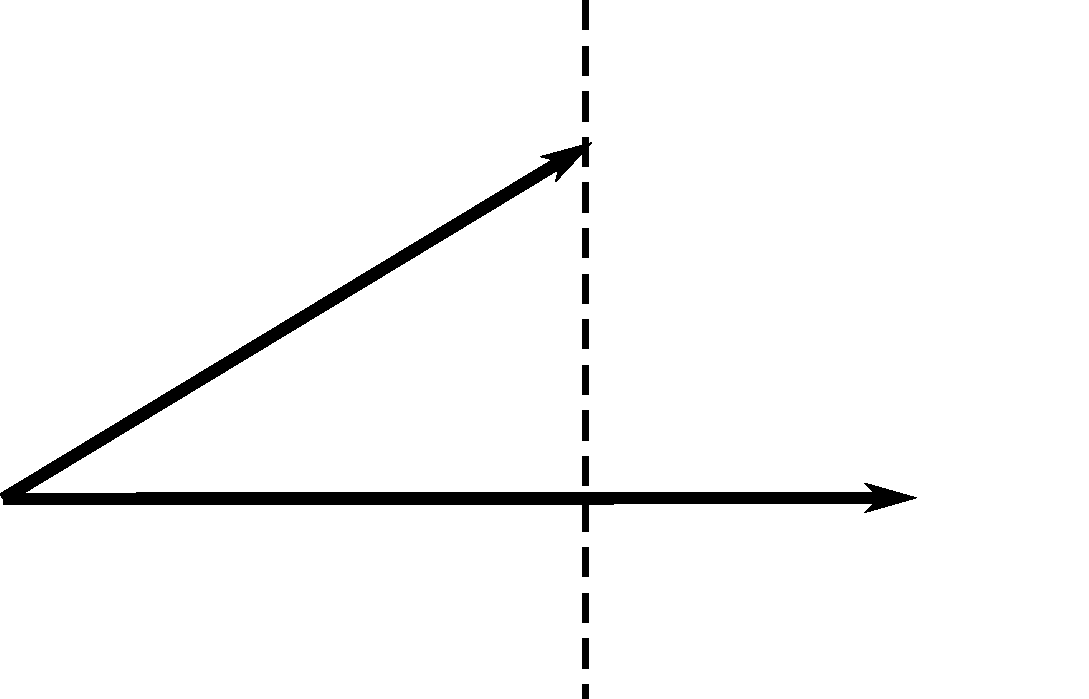
\includegraphics[width=\unitlength,page=1]{res/ebeneWelle.pdf}}%
	\put(0.7799152,0.03571014){\color[rgb]{0,0,0}\makebox(0,0)[lt]{\lineheight{1.25}\smash{\begin{tabular}[t]{l}$\vec{k}$\end{tabular}}}}%
	\put(0.56056505,0.49991597){\color[rgb]{0,0,0}\makebox(0,0)[lt]{\lineheight{1.25}\smash{\begin{tabular}[t]{l}$\vec{r}$\end{tabular}}}}%
	\put(0.23,0.00255236){\color[rgb]{0,0,0}\makebox(0,0)[lt]{\lineheight{1.25}\smash{\begin{tabular}[t]{l}$\frac{\vec{k}\cdot\vec{r}}{|\vec{k}|}$\end{tabular}}}}%
	\put(0,0){\includegraphics[width=\unitlength,page=2]{res/ebeneWelle.pdf}}%
\end{picture}%
\endgroup%
}
	  \end{center}
	 Orte, die zu einem Zeitpunkt \(t=t_0\) gleiche Werte \(\varphi\) haben, liegen auf Ebenen senkrecht zu \(\vec{k}\).  Diese Orte nennt man \textbf{Wellenfront}. Hängt $\Psi$ bspw. periodisch von $\varphi$ ab, werden durch $\Psi=\const$ mehrere Ebenen beschrieben. Betrachtet man ein \(t_1 > t_0\) mit gleichem Wert für $\varphi=\varphi_0$, hat man Orte wiederkehrender Phase:
	   \begin{center}
	 	\resizebox{.5\textwidth}{!}{%% Creator: Inkscape 1.0.2 (e86c8708, 2021-01-15), www.inkscape.org
%% PDF/EPS/PS + LaTeX output extension by Johan Engelen, 2010
%% Accompanies image file 'res/ebeneWelle2.pdf' (pdf, eps, ps)
%%
%% To include the image in your LaTeX document, write
%%   \input{<filename>.pdf_tex}
%%  instead of
%%   \includegraphics{<filename>.pdf}
%% To scale the image, write
%%   \def\svgwidth{<desired width>}
%%   \input{<filename>.pdf_tex}
%%  instead of
%%   \includegraphics[width=<desired width>]{<filename>.pdf}
%%
%% Images with a different path to the parent latex file can
%% be accessed with the `import' package (which may need to be
%% installed) using
%%   \usepackage{import}
%% in the preamble, and then including the image with
%%   \import{<path to file>}{<filename>.pdf_tex}
%% Alternatively, one can specify
%%   \graphicspath{{<path to file>/}}
%% 
%% For more information, please see info/svg-inkscape on CTAN:
%%   http://tug.ctan.org/tex-archive/info/svg-inkscape
%%
\begingroup%
\def\svgwidth{.4\textwidth}
\makeatletter%
\providecommand\color[2][]{%
	\errmessage{(Inkscape) Color is used for the text in Inkscape, but the package 'color.sty' is not loaded}%
	\renewcommand\color[2][]{}%
}%
\providecommand\transparent[1]{%
	\errmessage{(Inkscape) Transparency is used (non-zero) for the text in Inkscape, but the package 'transparent.sty' is not loaded}%
	\renewcommand\transparent[1]{}%
}%
\providecommand\rotatebox[2]{#2}%
\newcommand*\fsize{\dimexpr\f@size pt\relax}%
\newcommand*\lineheight[1]{\fontsize{\fsize}{#1\fsize}\selectfont}%
\ifx\svgwidth\undefined%
	\setlength{\unitlength}{733.11092827bp}%
	\ifx\svgscale\undefined%
		\relax%
	\else%
		\setlength{\unitlength}{\unitlength * \real{\svgscale}}%
	\fi%
\else%
	\setlength{\unitlength}{\svgwidth}%
\fi%
\global\let\svgwidth\undefined%
\global\let\svgscale\undefined%
\makeatother%
\begin{picture}(1,0.60322124)%
	\lineheight{1}%
	\setlength\tabcolsep{0pt}%
	\put(0,0){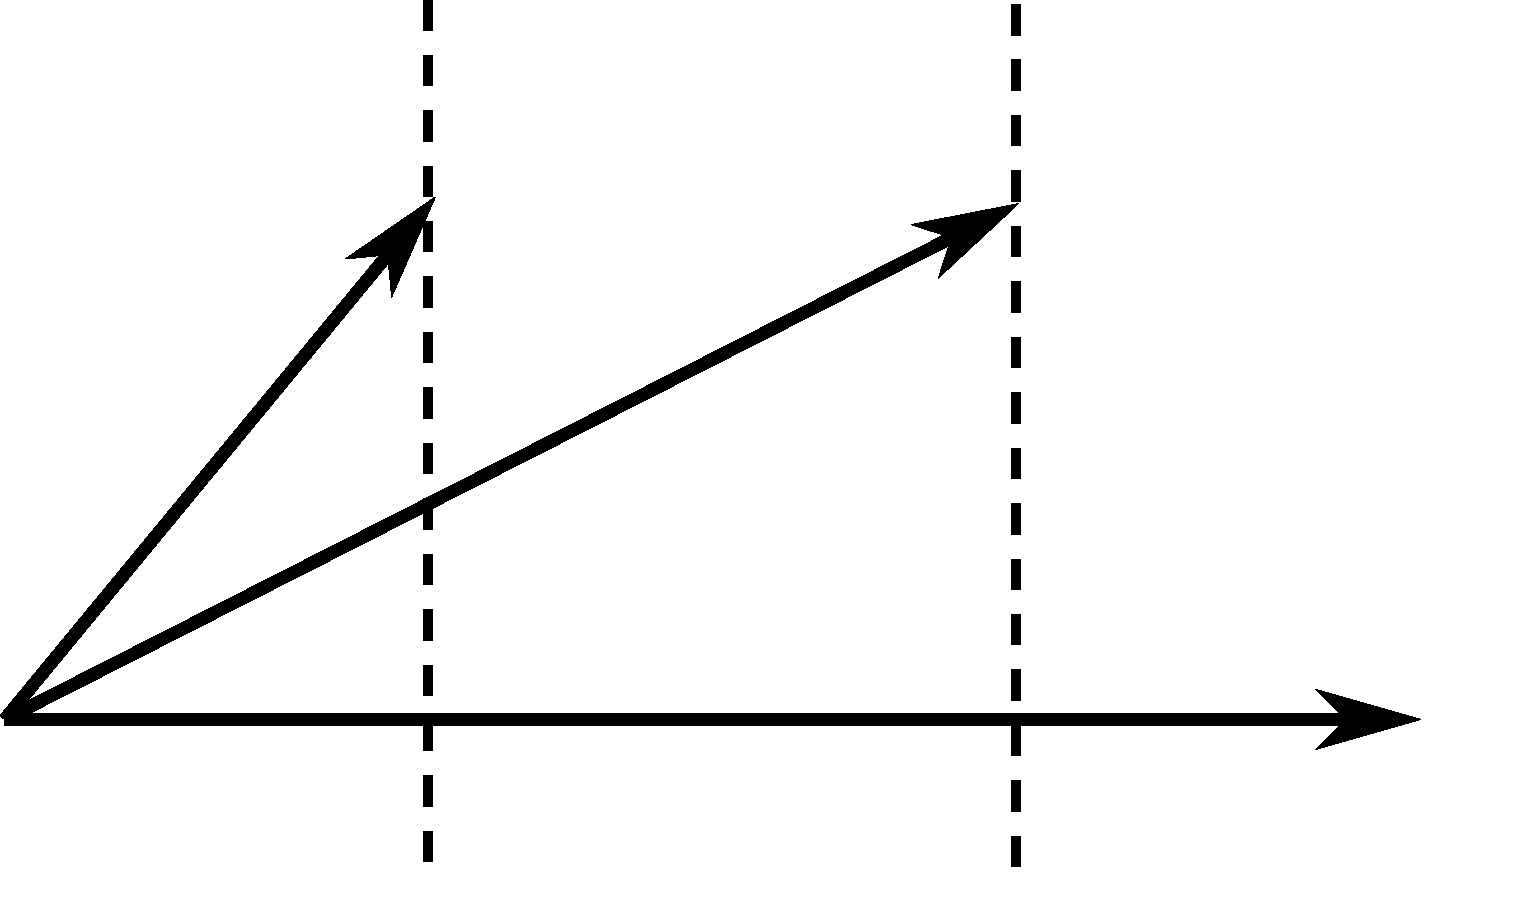
\includegraphics[width=\unitlength,page=1]{res/ebeneWelle2.pdf}}%
	\put(0.87110712,0.05065575){\color[rgb]{0,0,0}\makebox(0,0)[lt]{\lineheight{1.25}\smash{\begin{tabular}[t]{l}$\vec{k}$\end{tabular}}}}%
	\put(0.29096635,0.47276912){\color[rgb]{0,0,0}\makebox(0,0)[lt]{\lineheight{1.25}\smash{\begin{tabular}[t]{l}$\vec{r}_0$\end{tabular}}}}%
	\put(0.67595917,0.47064797){\color[rgb]{0,0,0}\makebox(0,0)[lt]{\lineheight{1.25}\smash{\begin{tabular}[t]{l}$\vec{r}_1$\end{tabular}}}}%
	\put(0.19127119,0.08989745){\color[rgb]{0,0,0}\makebox(0,0)[lt]{\lineheight{1.25}\smash{\begin{tabular}[t]{l}$r_{0\parallel}$\end{tabular}}}}%
	\put(0.57520347,0.09307918){\color[rgb]{0,0,0}\makebox(0,0)[lt]{\lineheight{1.25}\smash{\begin{tabular}[t]{l}$r_{1\parallel}$\end{tabular}}}}%
\end{picture}%
\endgroup%
}
	 \end{center}
		        \begin{equation}\begin{split}
				        \varphi_0 &= \omega t_0 + \vec{k}\cdot\vec{r} _0 \stackrel{!}{=} \omega t_1 \pm \vec{k}\cdot\vec{r} _1\\
				        \Rightarrow \pm \vec{k}\cdot\vec{r} _1 &= \varphi_0 - \omega t_1  \\   \vec{k}\cdot\vec{r} _1 &= k r_{1\parallel}\quad \text{ mit } \quad r_{1\parallel}=\frac{\vec{k}\cdot\vec{r} _1}{ k}  \\
				        \Rightarrow \pm r_{1\parallel} &=\frac{\varphi_0}{ k} - \frac{\omega}{k} t_1\\
				        \Rightarrow r_{1\parallel} &= \pm\frac{\varphi_0}{ k} \mp \frac{\omega}{k} t_1\\
			        \end{split}\end{equation}
		  $r_{1\parallel} $ ist eine lineare Funktion der Zeit. Im Fall \(\omega t {+} \vec{k}\cdot\vec{r} \) bewegt sich die Wellenfront (also die Orte wiederkehrender Phase) in Richtung \(-\vec{k}\), im Fall \(\omega t {-} \vec{k}\cdot\vec{r} \) in Richtung $+\vec{k}$. Außerdem wird die
		   \textbf{Phasengeschwindigkeit} definiert, also die Geschwindigkeit, mit der sich  eine konstante Phase des Schwingungsterms (bspw. 0) ausbreitet. Mit dem Ansatz \(\omega t {-} \vec{k}\cdot\vec{r} =0\) folgt:
		   \begin{equation}
		   	\boxed{ v_\mathrm{p} =\frac{\dd r_{\parallel}}{\dd t} }\stackrel{\text{hier}}{=} \frac{\omega}{ k} \stackrel{\text{hier}}{=}{ v_\mathrm{c}}
		   \end{equation}
	Es ist zu beachten, dass die Phasengeschwindigkeit nicht immer gleich der Lichtgeschwindigkeit im jeweiligen Medium ist. 
 \subsection{Harmonische ebene Wellen}\label{harmebwell}
  		 \textbf{Ebene Wellen} sind Lösungen der homogenen Wellengleichung Gleichung, für die allgemein \ref{algebwell} gilt. Hier soll nur die \textbf{hinlaufende} Lösung für \textbf{einen} Wert von \(\omega\) betrachtet werden, also:
		        \begin{equation}
			        \Psi(\vec{r} , t) = \Psi(\varphi_-(\vec{r} , t)) = \Psi(\omega t - \vec{k}\cdot\vec{r} )
		        \end{equation}
		   Außerdem soll eine spezielle Phasenfunktion \(\varphi\) gewählt werden, sodass \(\Psi\) einer Funktion mit \textbf{harmonischer Zeitabhängigkeit} entspricht:
		        \begin{equation}\begin{split}
			        \Aboxed{\underline{\Psi}(\vec{r} , t) &= \underline{\Psi}_0  \mathrm{e}^{\mathrm{j}(\omega t -\vec{k} \cdot \vec{r} )} }  \\ \Psi(\vec{r} , t) &= \re{\underline{\Psi}(\vec{r} , t)}
		        \end{split}\end{equation}
	     Beachte, dass hier im Gegensatz zu \ref{phasoren} die Zeitabhängigkeit mit in $\underline{\Psi}$ hinein definiert wird. Es wird also nur noch der Realteil gebildet und auf die Normierung auf $\mathrm{e}^{\mathrm{j}\omega t}$ verzichtet ($\nearrow$\ref{ansig}).
  \subsubsection{Wellenlänge und Frequenz}
	 	 Zu einem \textbf{festen Zeitpunkt} haben Flächen gleicher Werte einen festen Abstand $\Delta r_\Vert$. Die Bedingung dafür, dass die Flächen den gleichen Wert haben ist bei harmonischer Zeitabhängigkeit:
	 	 \begin{equation}
	 	 	\Delta\vec{r} \cdot\vec{k} = \Delta r_\Vert \cdot  k  = 2\pi n \quad \quad n\in\IZ  
	 	 \end{equation}
	 	 Für den Fall $n=1$ wird $\Delta r_\Vert$ als \textbf{Wellenlänge} $\lambda$ definiert:
	 	 \begin{equation}
	 	 	\Delta r_\Vert \cdot  k  = 2\pi                           \quad\implies\quad \boxed{\Delta r_\Vert = \frac{2\pi}{ k} =\lambda}
	 	 \end{equation}
	 	 Damit folgt:
 		        \begin{equation}
			      k = \frac{2\pi}{\lambda}   = \frac{\omega}{ v_{\mathrm{p}}} \quad \implies \quad \boxed{ v_{\mathrm{p}}=\frac{\omega}{2\pi}\cdot \lambda}  =  v_\mathrm{c} \underset{\substack{\varepsilon = \varepsilon_0 \\ \mu = \mu_0}}{=} c
		        \end{equation}
		  An einem \textbf{festen Ort} wiederholen sich gleiche Werte nach einer festen Zeit $\Delta t$. Die Bedingung dafür, dass $\Psi$ den gleichen Wert hat ist bei harmonischer Zeitabhängigkeit:
		  \begin{equation}
		  	 \Delta t \omega     = 2\pi  n     \quad \quad n\in \IZ                              
		  \end{equation}
		  Für den Fall $n=1$ wird $\Delta t$ als \textbf{Periodendauer} $T$ definiert. Außerdem führt man die \textbf{Kreisfrequenz} $\omega$ und die \textbf{Frequenz} $f$ ein: 
		  \begin{equation}
		  	\Delta t \omega = 2\pi \quad\implies\quad \boxed{\Delta t = T  = \frac{2\pi}{\omega} = \frac{1}{f}}
		  \end{equation}
		  Damit gilt:
		        \begin{equation}
			     \boxed{ v_{\mathrm{p}}= f \cdot \lambda}  =  v_\mathrm{c}\underset{\substack{\varepsilon = \varepsilon_0                                            \\ \mu = \mu_0}}{=} c
		        \end{equation}
  \subsubsection{$E-$ und $B-$Feld: TEM-Wellen}\label{tem}
	Zunächst wird angenommen, dass \(\vec{E}\) und \(\vec{B} \) unterschiedliche Kreisfrequenzen und Wellenvektoren haben könnten:
		        \begin{align}\label{ebharm}
			        \ubar{\vec{E}} & = \ubar{\vec{E}}_0  \mathrm{e}^{\mathrm{j}(\omega t - \vec{k}\cdot\vec{r} )} & \vec{\ubar{B}} & = \vec{\ubar{B}}_0  \mathrm{e}^{\mathrm{j}(\omega ' t - \vec{k} \ensuremath{'}\cdot\vec{r} )}
		        \end{align}
		  Einerseits gilt das Induktionsgesetz \ref{ind}:
		        \begin{equation}\begin{split}
				        \rot \ubar{\vec{E}} = -\frac{\partial \vec{\ubar{B}}}{\partial t}= -\mathrm{j}\omega ' \vec{\ubar{B}}
		\end{split}\end{equation}  
	Andererseits lässt sich mit $\ubar{\vec{E}} = \ubar{\vec{E}}_0  \mathrm{e}^{\mathrm{j}(\omega t - \vec{k}\cdot\vec{r} )}$ analytisch ein Ausdruck für $ \rot \ubar{\vec{E}} $ berechnen. Die Rechnung erfolgt beispielsweise in kartesischen Koordinaten. Wenn das Ergebnis dann wieder koordinatenfrei geschrieben werden kann, hat man eine in allen Koordinatensystemen gültige Aussage gefunden. Dieses Prinzip kann man häufig anwenden. Hier resultiert:
\begin{equation}\begin{split} 
				        \rot \ubar{\vec{E}}& = -\mathrm{j}\left( \vec{k} \times \ubar{\vec{E}}\right)\\
				        \Rightarrow  -\mathrm{j}\left( \vec{k} \times \ubar{\vec{E}}_0 \right)  \mathrm{e}^{\mathrm{j}\left(\omega t - \vec{k}\cdot\vec{r} \right)}  &\stackrel{!}{=} -\mathrm{j}\omega' \vec{\ubar{B}}_0  \mathrm{e}^{\mathrm{j}\left(\omega' t -\vec{k}'\cdot\vec{r} \right)}
			        \end{split}\end{equation}
		 Dieser Ausdruck muss für alle \(t\) und alle \(\vec{r} \) gelten. Damit folgt:
		        \begin{equation}\begin{split}
				         \left. \begin{array}{l}
					        \omega = \omega', \quad    \vec{k} = \vec{k}' \\
					        \vec{k}\times\ubar{\vec{E}}_0 = \omega\vec{\ubar{B}}_0
				        \end{array}
				        \right\rbrace \vec{\ubar{B}}_0 = \frac{1}{\omega} \vec{k} \times\ubar{\vec{E}}_0 \quad\implies \quad \boxed{\vec{\ubar{B}} = \frac{1}{\omega} \vec{k} \times\ubar{\vec{E}}}\\
			        \end{split}\end{equation}
		  Es folgt also, dass \( \ubar{\vec{E}}\) und \(\vec{\ubar{B}}\) \textbf{in Phase} sind und \(\vec{\ubar{B}}\) senkrecht auf der von \(\vec{k}\) und \(\ubar{\vec{E}}\) aufgespannten Ebene steht:
		        \begin{equation}
			       \boxed{ \vec{\ubar{B}}_0 \Vert \left(\vec{k} \times \ubar{\vec{E}}_0 \right)}
		        \end{equation}
 	Nun wird mit \ref{gauss} (Annahme: \(\rho_\text{V} = 0\)) und \ref{quellf} weiter gerechnet. $E$ und $B$ haben dabei die Form aus \ref{ebharm}, durch formale Divergenzbildung folgt:
		        \begin{align}
			        \div \vec{E} & = 0 & \Rightarrow \quad -\vec{k}\cdot \ubar{\vec{E}}_0 & = 0 & \curvearrowright &  & \boxed{\vec{k}\bot \ubar{\vec{E}}_0} \\
			        \div \vec{B} & = 0 & \Rightarrow \quad -\vec{k}\cdot \vec{\ubar{B}}_0 & = 0 & \curvearrowright &  & \boxed{\vec{k}\bot \vec{\ubar{B}}_0}
		        \end{align}
	Mit \ref{durchf} (Annahme: \(\vec{J}=\vec{0}\)) folgt durch formale Rotationsbildung:
		        \begin{align}
			        \rot \vec{\ubar{B}} &= \frac{1}{ v_{\mathrm{p}}^2}\frac{\partial \ubar{\vec{E}}}{\partial t} \nonumber\\
			         -\mathrm{j}\vec{k}\times\vec{\ubar{B}}_0 &= \mathrm{j}\omega\frac{1}{ v_{\mathrm{p}}^2}\ubar{\vec{E}}_0 \nonumber\\
			          \ubar{\vec{E}}_0 &= -\frac{ v_{\mathrm{p}}^2}{\omega}\vec{k} \times \vec{\ubar{B}}_0 \nonumber\\
			                                                                                                                                                                                                               & \Rightarrow  \boxed{\ubar{\vec{E}}_0 \| \left(\vec{\ubar{B}}_0 \times \vec{k} \right)}
		        \end{align}
 \begin{minipage}{.7\textwidth}
 	 \(\vec{E}\), \(\vec{B} \) und \(\vec{k}\) bilden ein \textbf{orthogonales Rechtssystem}. Sowohl $E$ als auch $B$ sind transversal zur Ausbreitungsrichtung. Man spricht von \textbf{Transversalen Elektromagnetischen Wellen (TEM-Wellen)}, weil $E$ und $B$ keine Komponente longitudinal zur Ausbreitungsrichtung haben. 
 \end{minipage}
 \begin{minipage}{.29\textwidth}
 	\raggedleft
\begin{tikzpicture}[line width = 1.2pt, line join=round,x={(.5cm,.5cm)},y={(1cm, 0cm)},z={(0cm,1cm)},>=stealth]
	% x-Richtung
	\draw [->] (0,0,0) -- (-1,0,0) node[anchor=north east] {$\vec{B}$};
	% y-Richtung
	\draw [->] (0,0,0) -- (0,1,0) node[anchor=west] {$\vec{k}$};
	% z-Richtung
	\draw [->] (0,0,0) -- (0,0,1) node[anchor=south] {$\vec{E}$};
\end{tikzpicture}
 \end{minipage}\\
 Es ist anzumerken, dass $E$ und $B$ nur in sehr vielen Spezialfällen senkrecht zueinander sind. Da $H$ und $E$ bei ebenen Wellen über den Feldwellenwiderstand zusammenhängen, ist es schwierig durch Superposition ebener Wellen einen nicht senkrechten Fall zu konstruieren (beide Wellen müssen im gleichen Medium das gleiche $H/E$-Verhältnis haben). Dennoch gilt, dass die Rotation eines Vektors ist nicht immer senkrecht zum Vektor selber ist, das Kreuzprodukt mit dem Nabla-Operator wirkt also nicht wie ein \enquote{normales} Kreuzprdukt. Das Induktionsgesetz ($\nearrow$\ref{ind}) ist demnach bspw. kein Grund, warum $E$ und $B$ stets senkrecht sein sollten.
 \subsubsection{Zusammenfassung der Formeln für harmonische Ebene Wellen}
 Zusammenfassend gelten für harmonische ebene Wellen die folgenden Formeln:
 \begin{equation}\label{ebwellzsfg}\begin{split}
 		\ubar{\vec{E}}(\vec{r} , t) & =\ubar{\vec{E}}_0 \mathrm{e}^{\mathrm{j}(\omega t - \vec{k}\cdot\vec{r} )} \\
 		\vec{\ubar{B}}(\vec{r} , t)  &=\vec{\ubar{B}}_0 \mathrm{e}^{\mathrm{j}(\omega t - \vec{k}\cdot\vec{r} )}  \\
 		 \vec{\ubar{B}}_0 &= \frac{1}{\omega} \left(\vec{k} \times \ubar{\vec{E}}_0\right)= \frac{ k}{\omega} \left(\vu{k} \times \ubar{\vec{E}}\right) = \frac{1}{ v_\mathrm{p}} \left(\vu{k} \times \ubar{\vec{E}}\right) = \sqrt{\varepsilon\mu} \left(\vu{k} \times \ubar{\vec{E}}\right) \\
 		 |\vec{\ubar{B}}_0|^2 &= \frac{1}{ v_\mathrm{c}^2} |\ubar{\vec{E}}_0|^2 \\
 		v_\mathrm{c} &= \frac{1}{\sqrt{\varepsilon\mu}} = \frac{\omega}{ k} = v_\mathrm{p}\\
 			\vec{\ubar{H}} &= \frac{1}{\mu}\vec{\ubar{B}} = \frac{1}{\mu}\sqrt{\varepsilon\mu} \left(\vu{k} \times \ubar{\vec{E}}\right) = \sqrt{\frac{\varepsilon}{\mu}} \left(\vu{k} \times \ubar{\vec{E}}\right) = \frac{1}{Z} \left(\vu{k} \times \ubar{\vec{E}}\right)\\
	\ubar{\vec{E}} &= -Z \left(\vu{k} \times \vec{\ubar{H}}\right)
 \end{split}\end{equation}
Neu wurde hierbei noch die \textbf{Feldwellenimpedanz} (auch Feldwellenwiderstand) eingeführt:
\begin{equation}\label{feldwellenwid}
	\boxed{Z=\sqrt{\frac{\varepsilon}{\mu}}}
\end{equation}
  \subsubsection{Beispiel}        
     Es wird \(\vec{k} =  k \cdot \vu{z}\) gesetzt. Damit folgt:
      \begin{equation*}\begin{split}
         \ubar{\vec{E}}&=\left( \ubar{E}_{0x} \vu{x} + \ubar{E}_{0y}\vu{y}\right)  \mathrm{e}^{\mathrm{j}(\omega t - k z)}  ;\quad \ubar{E}_{0x}, \ubar{E}_{0y} \in \IC\\
        \vec{\ubar{B}} &= \left( \ubar{B}_{0x} \vu{x} + \ubar{B}_{0y}\vu{y}\right) \mathrm{e}^{\mathrm{j}(\omega t -  k z)}  ;\quad \ubar{B}_{0x}, \ubar{B}_{0y} \in \IC
       \end{split}\end{equation*}
	Außerdem gilt ($\ubar{E}_{0x}=\left|\ubar{E}_{0x}\right|\mathrm{e}^{\mathrm{j}\varphi_x}$):
		        \begin{equation*}\begin{split}
		        \vec{E}&=\re{\vec{\ubar{E}}}=\left|\ubar{E}_{0x}\right|\vu{x}\cos (\omega t - kz +\varphi_x)+\left|\ubar{E}_{0y}\right|\vu{y}\cos (\omega t - kz +\varphi_y)\\
			      \vec{B} &= \frac{1}{\omega}\vec{k}\times \vec{E} =  \frac{1}{ v_{\mathrm{p}}}\vu{k}\times\vec{E} = \frac{1}{ v_{\mathrm{p}}}\vu{z}\times\vec{E}       
		        \end{split}\end{equation*}
		 Das kann man visualisieren (hier $E\parallel \vu{x}$):
	  \begin{center}
		  \begin{tikzpicture}[x={(-10:1cm)},y={(90:1cm)},z={(210:1cm)}]
	% Axes
	\draw (-1,0,0) -- (5,0,0) node[below] {$z, \vec{k}$};
	\draw (0,0,0) -- (0,2,0) node[above] {$x$};
	\draw (0,0,0) -- (0,0,2) node[left] {$y$};
	% Propagation
	\draw[->,ultra thick] (5,0,0) -- node[above] {$\vec{v}_p=\vec{v}_c$} (6,0,0);
	% Waves
	\draw[red,thick] plot[domain=0:4.5,samples=200] (\x,{cos(deg(pi*\x))},0);
	\draw[green,thick] plot[domain=0:4.5,samples=200] (\x,0,{cos(deg(pi*\x))});
	% Arrows
	\foreach \x in {0.1,0.3,...,4.4} {
			\draw[->,red] (\x,0,0) -- (\x,{cos(deg(pi*\x))},0);
			\draw[->,green] (\x,0,0) -- (\x,0,{cos(deg(pi*\x))});
		}
	% Labels
	\node[above right] at (0,1,0) {$\vec{E}$};
	\node[below] at (0,0,1) {$\vec{B}$};
\end{tikzpicture}
		  \begin{minipage}{.5\linewidth}
			  \[
				  v_\mathrm{p} = \frac{\omega}{k} = \frac{|\vec{E}|}{|\vec{B}|} \stackrel{\text{hier}}{=} v_\mathrm{c}
			  \]
			  \begin{tabular}{r@{${}={}$}p{.8\linewidth}}
				  $E$   & Amplitude des elektrischen Feldes                                            \\
				  $B$   & Amplitude der Magnetflussdichte                                              \\
				  $v_\mathrm{p}$ & Phasengeschwindigkeit                                                        \\
				  $v_\mathrm{c}$ & Lichtgeschwindigkeit im Medium                                               \\
				  $c$   & \raggedright   Vakuum Lichtgeschwindigkeit $= 299792458\mathrm{\frac{m}{s}}$
			  \end{tabular}
		  \end{minipage}%
		  \begin{minipage}{.5\linewidth}
			  \[
				  v_\mathrm{c} = \frac{1}{\sqrt{\mu \varepsilon}} =\frac{c}{\sqrt{\mu_r \varepsilon_r}} = \frac{c}{n}
			  \]
			  \begin{tabular}{r@{${}={}$}p{.8\linewidth}}
				  $\mu_0$         & magnetische Permitivität des Vakuums $= 4\pi\cdot 10^{-7}\mathrm{\frac{H}{m}}$ \\
				  $\varepsilon_0$ & \raggedright  elektrische Permeabilität des Vakuums $= \frac{1}{\mu_0 c^2}$
			  \end{tabular}
		  \end{minipage}
	  \end{center}
 \subsection{Polarisation ebener Wellen}\label{poleb}
		 Es werden \textbf{monochromatische ebene Wellen} (eine Frequenz), die in \(+z\)-Richtung propagieren betrachtet:
		        \begin{align}\label{polallglsg}
			        \ubar{\vec{E}} & = \left( \ubar{E}_{0x}\vu{x} + \ubar{E}_{0y}\vu{y}\right) \mathrm{e}^{\mathrm{j}( \omega t -  k z)}                         &
			        \vec{\ubar{B}} & = \frac{1}{ v_{\mathrm{p}}}\left(-\ubar{E}_{0y}\vu{x} +\ubar{E}_{0x}\vu{y}\right)  \mathrm{e}^{\mathrm{j}(\omega t -  k z)} & v_{\mathrm{p}}= \frac{\omega}{k} \stackrel{\text{hier}}{=}  v_{\mathrm{c}}
		        \end{align}
		  Dabei sind:
		        \begin{equation}\begin{split}
				        \ubar{E}_{0x} &= \vert \ubar{E}_{0x} \vert \cdot  \mathrm{e}^{\mathrm{j}\varphi_x} \text{ - komplexe Komponente in \(x\)-Richtung bei \(t=0, z=0\)}\\
				        \ubar{E}_{0y} &= \vert \ubar{E}_{0y} \vert \cdot  \mathrm{e}^{\mathrm{j}(\varphi_x+ \delta)} \text{ - analog für \(y\)-Komponente}\\
				        \vec{E} (\vec{r} , t) &= \re{\ubar{E}(\vec{r} , t)} = E_x \vu{x} + E_y \vu{y} \text{ - Physikalische Lösung}\\
				        E_x &= \vert \ubar{E}_{0x} \vert \cos(\omega t -  k z + \varphi_x )\\
				        E_y &= \vert \ubar{E}_{0y} \vert \cos(\omega t -  k z + \varphi_x +\delta)\\
				        \varphi_x &: \text{ - gemeinsamer Phasenwinkel \(\to\) relativ unwichtig}\\
				        \delta &: \text{ - relative Phase \(\to\) \textbf{Fallunterscheidung}}
			        \end{split}\end{equation}
		 Anhand der relativen Phase wird unterschieden:
		        \begin{enumerate}
			        \item \(\delta = 0, \pm \pi , \pm 2\pi, \ldots\)
			        \item \(  \delta = \pm \frac{\pi}{2}, \pm \frac{3\pi}{2},\ldots \quad ;\quad\vert \ubar{E}_{0x} \vert = \vert \ubar{E}_{0y} \vert = \hat{E} \)
			        \item \( \delta = \pm \frac{\pi}{2}, \pm \frac{3\pi}{2},\ldots \quad ;\quad\vert \ubar{E}_{0x} \vert \neq \vert \ubar{E}_{0y} \vert \)
			        \item \(\delta\) und \(\vert \ubar{E}_{0x} \vert, \vert \ubar{E}_{0y} \vert\) beliebig
		        \end{enumerate}
		        Die Fälle werden im Folgenden diskutiert.
  \subsubsection{1. Fall: Lineare Polarisation}
		  Es wird \(\delta = z \cdot \pi ,\quad z \in \IZ\quad\rightarrow\quad \delta = \textcolor{green!70}{0}, \textcolor{red}{\pm \pi} , \textcolor{green!70}{\pm 2\pi}, \ldots\) betrachtet. Für den Cosinus gilt die Beziehung:
		        \begin{equation}\begin{split}
				        \begin{split}
					        \cos ( \alpha + \delta ) = \pm \cos \alpha \quad;\quad &\textcolor{green!70}{+} :   0,\pm 2\pi, \pm 4\pi, \ldots\\
					        & \textcolor{red}{-} :   \pm \pi, \pm 3\pi, \ldots
				        \end{split}
			        \end{split}\end{equation}
		   Hiermit ergibt sich für das elektrische Feld:
		        \begin{equation}\begin{split}
				        \Rightarrow \vec{E}&= \underbrace{(\vert \ubar{E}_{0x} \vert \vu{x} \pm \vert \ubar{E}_{0y}\vert \vu{y})}_{\substack{\text{fester Vektor, orts- und}\\ \text{zeitunabhängig}}} \cos (\omega t -  k z + \varphi_x)\\
				        &= \hat{E}\cdot \vu{E}\cos (\omega t -  k z + \varphi_x )\\
				        \hat{E} &= \vert \vec{E} \vert = \sqrt{\vert \ubar{E}_{0x} \vert ^2 + \vert \ubar{E}_{0y} \vert ^2}
			        \end{split}\end{equation}
		  Weil $E$ immer in der selben Richtung $\vu{E}$ schwingt, spricht man von linearer Polarisation. Der \textbf{Polarisationswinkel} ist folgendermaßen definiert:
	  \begin{center}
		  \begin{tikzpicture}[scale=0.4]
	% Achsen zeichnen
	\draw[->,thick] (0,0) -- (3,0) node[right] {$x$};
	\draw[->,thick] (0,0) -- (0,3) node[above] {$y$};
	%Plot
	\draw[->] (0,0) --(40:2) node[right] {$\vec{e}_E$};
	\draw[->] (0:1)arc(0:40:1) node[right] {$\alpha$};
\end{tikzpicture}
		  \raisebox{.75cm}{\(\Rightarrow\tan \alpha = \pm \dfrac{|\ubar{E}_{0y}|}{|\ubar{E}_{0x}|}\) }
	  \end{center}
	  Die allgemeine Lösung ($\nearrow$ \ref{polallglsg})ist eine Überlagerung zweier linear polarisierter Beiträge in \(x\)- bzw. \(y\)-Richtung. \textbf{Somit ist jede beliebige Polarisation darstellbar als Überlagerung zweier zueinander senkrechter linearer Polarisationen.} Somit müssen nur zwei Fälle unterschieden werden um jede beliebige Polarisation zu diskutieren. Sendet man beispielsweise ein linear polarisiertes Signal aus, dann kann es passieren, dass eine Komponente (Zerlegung in $x$- und $y$-Komponente) aufgrund von Inhomogenitäten auf dem Weg stärker gedämpft wird. So kann sich die Polarisation drehen. Das ist insbesondere bei der Dimensionierung von Antennen zu beachten.
  \subsubsection{2. Fall: Zirkulare Polarisation}
		  Nun wird \(\delta = (2m+1) \frac{\pi}{2}, \quad m \in \mathbb{Z} , \quad\delta = \pm \frac{\pi}{2}, \pm \frac{3\pi}{2},\ldots \quad ;\quad\vert E_{0x} \vert = \vert E_{0y} \vert = \hat{E} \) betrachtet. Für den Cosinus gilt die Beziehung:
		        \begin{equation}\begin{split}
				        \begin{split}
					        \cos ( \alpha + \delta ) = \mp \sin \alpha \quad;\quad &\textcolor{red}{+} :   -\frac{\pi}{2} + m (2\pi) \quad\textcolor{green!70}{-} :    +\frac{\pi}{2} + m (2 \pi), \quad m \in \IZ
				        \end{split}
			        \end{split}\end{equation}
		  Hiermit ergibt sich für das elektrische Feld:
		        \begin{equation}\begin{split}
				        \vec{E} &= \hat{E}(\cos(\omega t -  k z + \varphi_x)\vu{x} \mp \sin (\omega t -  k z + \varphi_x)\vu{y})
			        \end{split}\end{equation}
		  Für ein festes \(z\) oder \(t\) ist das ein Kreis mit Radius \(\hat{E}\). Deshalb spricht man von \textbf{zirkularer Polarisation}. Zur Unterscheidung rechts vs. links schaut man an einem festen Ort in $\vec{k}$-Richtung und beobachtet, wie sich der Zeiger dreht. In der folgenden Grafik ist $\vec{k}$ aus der Ebene hinaus definiert, entsprechend muss man aus der Ebene hinausschauen.
		        \begin{center}
			        \begin{tikzpicture}[]
	% Achsen zeichnen
	\draw[->,thick] (-1.8,0) -- (1.8,0) node[right] {$x$};
	\draw[->,thick] (0,-1.5) -- (0,1.8) node[above] {$y$};
	%Plot
	%\draw[style=dashed] (-1.27,-1.05) rectangle (1.27,1.05);
	\draw (0, 0) circle (1.2);
	\draw (0, 0) circle (.2);
	\draw[fill=black] (0, 0) circle (.1);
	\draw (0,0) node[below right] {$\vec{k}$};
	\draw[->,>=stealth] (0,0)--(20:1.2) node[above right] {$\vec{E}$};
	\draw[->] (20:.6) arc (20:50:.6) node [above] {$\omega$};
	\draw [->,thick,color=red] (120:1.2) arc (120:160:1.2) node[above left] {$\delta = -\frac{\pi}{2}$};
	\draw (0,-1.5) node[below]{rechts-zirkular};
\end{tikzpicture}
\begin{tikzpicture}[]
	% Achsen zeichnen
	\draw[->,thick] (-1.8,0) -- (1.8,0) node[right] {$x$};
	\draw[->,thick] (0,-1.5) -- (0,1.8) node[above] {$y$};
	%Plot
	%\draw[style=dashed] (-1.27,-1.05) rectangle (1.27,1.05);
	\draw (0, 0) circle (1.2);
	\draw (0, 0) circle (.2);
	\draw[fill=black] (0, 0) circle (.1);
	\draw (0,0) node[below right] {$\vec{k}$};
	\draw[->,>=stealth] (0,0)--(50:1.2) node[above right] {$\vec{E}$};
	\draw[->] (50:.6) arc (50:20:.6) node [right] {$\omega$};
	\draw [->,thick,color=green!70] (160:1.2) arc (160:120:1.2) node[above left] {$\delta = +\frac{\pi}{2}$};
	\draw (0,-1.5) node[below]{links-zirkular};
\end{tikzpicture}
		        \end{center}

		  Di \textbf{Überlagerung} zweier links und rechts umlaufender zirkular polarisierter Wellen (\textbf{unterschiedlicher Amplitude}) ergibt wieder eine \textbf{beliebig polarisierte Welle}. Bei \textbf{gleicher Amplitude} ist die resultierende Welle \textbf{linear polarisiert}.
  \subsubsection{3. Fall: Elliptische Polarisation}
	  Weiter wird \(\delta = (2m+1) \frac{\pi}{2}, \quad m \in \mathbb{Z} , \quad\delta = \pm \frac{\pi}{2}, \pm \frac{3\pi}{2},\ldots \quad ;\quad\vert E_{0x} \vert \neq \vert E_{0y} \vert  \) untersucht. Analog zur zirkularen Polarisation folgt für das elektrische Feld:
		        \begin{equation}\begin{split}
				        E_x &= \vert E_{0x} \vert \cos (\omega t -  k r + \varphi_x)\\
				        E_y &= \mp \vert E_{0y} \vert \sin (\omega t -  k r + \varphi_x) \quad (\textcolor{red}{+},\textcolor{green}{-})\\
				        \Rightarrow &\left[ \frac{E_x}{\vert \ubar{E}_{0x}\vert}\right]^2+\left[\frac{E_y}{\vert \ubar{E}_{0y}\vert}\right]^2 = 1\quad
			        \end{split}\end{equation}
		Durch diese Gleichung wird eine Ellipse mit den Halbachsen $\vert E_{0x} \vert , \vert E_{0y} \vert$ beschrieben. Man spricht deshalb von einer (rechts- bzw. linksumlaufenden) \textbf{elliptisch polarisierten Welle}. Visualisierung:
		        \begin{center}
			        \begin{tikzpicture}
	% Achsen zeichnen
	\draw[->,thick] (-2,0) -- (2.7,0) node[right] {$x$};
	\draw[->,thick] (0,-1.5) -- (0,1.8) node[above] {$y$};
	%Plot
	%\draw[style=dashed] (-1.27,-1.05) rectangle (1.27,1.05);
	\draw (0, 0) ellipse (1.6 and 1);
	\draw(1.6,0) node[below right] {$|E_{0x}|$} ;
	\draw(0,1.3) node[left] {$|E_{0y}|$} ;
	\draw[->,>=stealth] (0,0)--(1.2,0.7) node[above right] {$\vec{E}$};
	%\draw[->,color=green] (40:1) arc (40:160:1.3);
	\draw [->,thick,color=green!70] plot[domain=340:300] ({cos(\x)*1.6},{sin(\x)}) node[below right] {$\delta = +\frac{\pi}{2}$};
	\draw [->,thick,color=red] plot[domain=120:160] ({cos(\x)*1.6},{sin(\x)}) node[above left] {$\delta = -\frac{\pi}{2}$};
	\draw (0, 0) circle (.2);
	\draw[fill=black] (0, 0) circle (.1);
	\draw (0,0) node[below right] {$\vec{k}$};
\end{tikzpicture}
		        \end{center}
  \subsubsection{4. Fall: keine Einschränkungen}
		  Abschließend gibt es keine Einschränkungen für \(\delta\) und \(\vert E_{0x} \vert\) bzw. \(\vert E_{0y} \vert  \) mehr. Analog zur zirkularen Polarisation folgt ohne weitere Herleitung:
		        \begin{itemize}
			        \item Das Ergebnis ist \textbf{elliptisch polarisiert} (Stichwort: \href{https://en.wikipedia.org/wiki/Jones_calculus}{Jones-Vektor}).
			        \item Die Halbachsen sind gegen das \(x\)-\(y\)-System gedreht.
			              \begin{center}
				              \begin{tikzpicture}
	% Achsen zeichnen
	\draw[->,thick] (-2,0) -- (2.5,0) node[right] {$x$};
	\draw[->,thick] (0,-1.5) -- (0,1.8) node[above] {$y$};
	%Plot
	\draw[style=dashed] (-1.27,-1.05) rectangle (1.27,1.05);
	\draw[rotate=30] (0, 0) ellipse (1.35 and 0.9);
	\draw(1.25,0) node[below right] {$|E_{0x}|$} ;
	\draw(0,1.05) node[above left] {$|E_{0y}|$} ;
	\draw (0, 0) circle (.12);
	\draw[fill=black] (0, 0) circle (.06);
	\draw (0,0) node[below right] {$\vec{k}$};
\end{tikzpicture}
			              \end{center}
		        \end{itemize}
		       Eine beliebige Polarisation lässt sich zusammensetzen aus:
		        \begin{itemize}
			        \item 2 linear polarisierten Wellen, die zueinander senkrecht stehen
			        \item 2 zirkular polarisierten Wellen, die entgegenlaufend sind
		        \end{itemize}
		        \href{https://emanim.szialab.org}{Online-Visualisierung.}
 \subsection{Wellenpakete}
 \subsubsection{Polychromatische Wellen}
 Die ebenen Wellen, die sich in den Wellenpaketen bewegen, können beliebig polarisiert sein. Für die Anschauung kann man von linearer Polarisation ausgehen, denn aus der Überlagerung von 2 linear polarisierten Wellen, die zueinander senkrecht stehen lässt sich eine beliebige Polarisation herleiten. Weiter werden Lösungen der homogenen Wellengleichung ($\nearrow$\ref{homwell}) betrachtet. Lösungen, die sich nur in einer Richtung (aber hin- und rücklaufend) ausbreiten, haben die allgemeine Form der ebenen Welle aus Gleichung \ref{algebwell}. Eine alternative Schreibweise betrachtet die Überlagerung für verschiedene Wellenvektoren (\(\vec{k} =  k\; \vu{k} = \omega\sqrt{\varepsilon\mu}\;\vu{k}\to\) $k$ und $\omega$ hängen zusammen, nun Überlagerung der $k$). $k$ und $\omega$ sind kontinuierlich, deshalb ist die folgende integrale Schreibweise sinnvoll:
		        \begin{equation}
			        \boxed{\Psi (\vec{r} , t) = \int\limits_{0}^\infty \left[ A_+(k) \Psi_+ (\omega t + \vec{k}\cdot\vec{r} ) + A_-(k) \Psi_- (\omega t - \vec{k}\cdot\vec{r} ) \right] \dd  k}
		        \end{equation}
		        Solch eine Überlagerung für verschiedene $k$ (und damit für verschiedene $\omega$) nennt man \textbf{polychromatische Welle}. Hier sind zudem die expliziten Vorfaktoren eingeführt, die homogenen Lösungen können mit beliebigen Konstanten gewichtet überlagert werden und bilden immer noch eine homogene Lösung. Außerdem wurde in \ref{algebwell} das Integral als Summe geschrieben (obwohl es sich um kontinuierliche Variablen handelt). 
		   Ohne Beschränkung der Allgemeinheit kann \(\vec{k} =  k \vu{z}   \implies \vec{k}\cdot\vec{r}  =  k z\), also eine Ausbreitung entlang der \(z\)-Richtung angenommen werden.
  \subsubsection{Dispersion}
 In der Regel sind die Materialparameter \textbf{frequenzabhängig}:
		        \begin{align}
			        \varepsilon & = \varepsilon_0\varepsilon_r = \varepsilon_0\varepsilon_r(\omega) & \mu & = \mu_0\mu_r = \mu_0\mu_r(\omega)
		        \end{align}
Somit haben \textbf{Teilwellen unterschiedliche Phasengeschwindigkeiten}:
		        \begin{equation}
			        v_\mathrm{p} (\omega) =  v_\mathrm{c}(\omega) = \frac{1}{\sqrt{\varepsilon\mu}} = \frac{1}{\sqrt{\varepsilon_0\mu_0}} \frac{1}{\sqrt{\varepsilon_r(\omega)\mu_r(\omega)}}=\frac{c}{n(\omega)}
		        \end{equation}
Dies tritt insbesondere bei \textbf{Wellenpaketen} in Erscheinung. Unter einem Wellenpaket mit \textbf{harmonischer Zeitabhängigkeit}, das in \textbf{\(+z\)-Richtung} propagiert, versteht man eine Überlagerung der Form
		        \begin{equation}
			        \Psi (\vec{r} , t) = \int\limits_{-\infty}^\infty \underline{A}(k) \mathrm{e}^{\mathrm{j}(\omega t -  k z)} \dd  k\; , \text{ mit } \underline{A}(-k) = \underline{A}^\star(k)
		        \end{equation}
		  Ein häufiger Spezialfall ist $\underline{A}(k) = A(k)$ reelwertig mit $A(-k) = A(k)$. Hierbei soll \(A(k)\) zunächst \textbf{konzentriert} sein um \( k =  k_0\), also:
		        \begin{center}
			        \begin{tikzpicture}[scale=0.5, samples=200, domain=0:5]
	% Achsen zeichnen
	\draw[->,thick] (0,0) -- (5,0) node[right] {$ k$};
	\draw[->,thick] (0,0) -- (0,2.5) node[above] {$\mathrm{A}( k)$};
	%Plot
	\draw plot (\x,{exp(-(\x-2.5)^2)*2});
	\draw [style=dashed] (2.5,0) node[below] {$ k_0$} --(2.5,2.4);
	\draw[<->] (1.6,.8)--(3.4,.8) node[right] {$\Delta  k_0$};
	\node[draw,align=left] at (7,2.4) {$\mathrm{A}( k) \ll \mathrm{A}( k_0)$ für\\ $| k- k_0| \gg \Delta  k_0$};
\end{tikzpicture}
		        \end{center}
		   Da die Wichtungsfunktion \(A( k)\) um \( k =  k_0\) konzentriert ist, bietet sich eine \textbf{Taylorentwicklung} von \(\omega( k)\) um \( k_0\) an, in den Bereichen nahe $k_0$ approximiert diese \(\omega( k)\) gut.
		        \begin{align}
			        \omega( k) & = \omega( k_0) + \left.\frac{\dd \omega}{\dd  k}\right|_{ k_0} ( k -  k_0) + \ldots                                                                                                                                          \\
			                   & \cong \underbrace{\omega( k_0)}_{=\omega_0} +  v_{\mathrm{g}}( k- k_0)              & \rightarrow\boxed{ v_{\mathrm{g}} = \left.\frac{\dd \omega}{\dd  k}\right|_{ k_0}}
		        \end{align}
		        $v_{\mathrm{g}}$ wird dabei \textbf{Gruppengeschwindigkeit} genannt.
		   Den Verlauf \(\omega( k)\) nennt man auch \textbf{Dispersionsrelation}. Es gilt allgemein $k=\omega\sqrt{\mu(\omega)\varepsilon(\omega)}$, praktisch leitet man $\omega(k)$ selten mikroskopisch her, sondern setzt Modelle an. Bei bestimmten Dispersionsrelationen kann es auch negative Gruppengeschwindigkeiten für bestimmte $k$ geben. Wenn man einen Puls auf ein Material mit einer solchen Relation gibt, kann ein Maximum in positive und eines in negative Richtung propagieren. Im Fall von Dispersion (bei negativen Gruppengeschwindigkeiten würde die Kurve auch monoton falled) resultiert die linke Grafik, im Fall ohne Dispersion die rechte Grafik.
		  
		        \begin{center}
			        \begin{tikzpicture}[domain=0:2.5]
	% Achsen zeichnen
	\draw[->,thick] (0,0) -- (5,0) node[right] {$ k$};
	\draw[->,thick] (0,0) -- (0,3) node[above] {$\omega( k)$};
	%Plot
	\draw plot (\x,{0.2*exp(\x)-0.2});
	% Beschriftung
	\draw (-.1,1.25) -- (.1,1.25) node[left=4pt] {$\omega_0$};
	\draw (2,-.1) -- (2,.1) node[below=4pt] {$ k_0$};
	\draw[style=dashed] (.2,1.25)--(2,1.25) node[right=8pt] {$ v_{\mathrm{g}}$} -- (2, .2);
	\draw (1.25,0.25)--(2.75,2.25);
\end{tikzpicture}
\begin{tikzpicture}
	% Achsen zeichnen
	\draw[->,thick] (0,0) -- (5,0) node[right] {$ k$};
	\draw[->,thick] (0,0) -- (0,3) node[above] {$\omega( k)$};
	% Plott
	\draw (0,0) -- (4,2.5);
	% Beschriftung
	\draw (-.1,1.25) -- (.1,1.25) node[left=4pt] {$\omega_0$};
	\draw (2,-.1) -- (2,.1) node[below=4pt] {$ k_0$};
	\draw[style=dashed] (.2,1.25)--(2,1.25)node[right=8pt] {$ v_{\mathrm{g}}= v_{\mathrm{p}}= v_{c} = \frac{1}{\sqrt{\varepsilon\mu}}$} -- (2, .2);
\end{tikzpicture}
		        \end{center}
		        Allgemein gilt bei ebenen Wellen immer $v_{\mathrm{c}}=v_{\mathrm{p}}$, aber nicht $v_{\mathrm{g}}=v_{\mathrm{c}}$. Das Phänomen der Frequenzabhängigkeit der Phasengeschwindigkeit heißt \textbf{Dispersion}. 
  \subsubsection{Dispersion von Wellenpaketen}
	  Die Taylor-Entwicklung kann man in e-Funktion einsetzen:
		        \begin{equation}
			        \mathrm{e}^{\mathrm{j}(\omega t -  k z)} \cong  \mathrm{e}^{\mathrm{j}(\omega_0 t -  k_0 z)}  \mathrm{e}^{\mathrm{j}(\overbrace{ k -  k_0}^{=q})( v_{\mathrm{g}} t - z)}
		        \end{equation}
		Damit folgt für das Wellenpaket:
		        \begin{equation}\begin{split}
				        \Psi (\vec{r} , t) &\cong \underbrace{\int\limits_{-\infty}^{\infty} \underbrace{A( k_0 + q)}_{A( k)} \mathrm{e}^{\mathrm{j}q ( v_{\mathrm{g}} t - z)}\dd q}_{\mathrm{H}( v_{\mathrm{g}} t -z)} \cdot\;  \mathrm{e}^{\mathrm{j}( \omega_0 t -  k_0 z)}\\
				        & \cong \underbrace{\mathrm{H}( v_{\mathrm{g}} t -z)}_{\substack{\text{Einhüllende}\\ \text{propagiert mit } v_{\mathrm{g}}\\ \text{in Richtung $z$}}}\cdot\; \underbrace{ \mathrm{e}^{\mathrm{j}(\omega_0 t -  k_0 z)}}_{\substack{\text{ebene Welle,}\\ \omega = \omega_0\\  k =  k_0}}
			        \end{split}\end{equation}
		        Für die konzentrierte Wichtungsfunktion resultiert also eine Hüllkurve, die mit $v_{\mathrm{g}}$ in $z$-Richtung propagiert und \textbf{eine} (durch die Linearisierung) ebene Welle. Visuell sieht man, dass die Phasengeschwindigkeit von der Gruppengeschwindigkeit abweicht (die Maxima von roter und blauer kurve sind bei $t_2$ gegeneinander verschoben):
	  \begin{center}
		  \begin{tikzpicture}[samples=1000, domain=0:9]
	%Plotten
	\draw [color=blue, thick] plot (\x,{exp(-(\x-2.5)^2)*2});
	\draw [color=blue, thick] plot (\x,{-exp(-(\x-2.5)^2)*2});
	\draw [color=red, thick] plot (\x,{cos(deg(\x*20))*exp(-(\x-2.5)^2)*2});

	\draw [style=dashed, color=blue] plot (\x,{exp(-(\x-6.5)^2)*2});
	\draw [style=dashed, color=blue] plot (\x,{-exp(-(\x-6.5)^2)*2});
	\draw [style=dashed, color=red] plot (\x,{cos(deg(\x*20))*exp(-(\x-6.5)^2)*2});

	%\draw[color=red] (0.5,0) sin(0.7,0.5) cos(0.9,0) sin(1.1,-0.66) cos(1.3,0) sin(1.5,1) cos(1.7,0) sin(1.9,-1.37) cos(2.1,0) sin(2.3,1.8) cos(2.5,0) sin(2.7,-2.15) cos(2.9,0) sin(3.1,2.38) cos(3.3,0) sin(3.5,-2.5) cos(3.7,0) sin(3.9,2.38) cos(4.1,0) sin(4.3,-2.15) cos(4.5,0) sin(4.7,1.8) cos(4.9,0) sin(5.1,-1.37) cos(5.3,0) sin(5.5,1) cos(5.7,0) sin(5.9,-0.66) cos(6.1,0) sin(6.3,0.5) cos(6.5,0);
	%\draw (0.5,0.5) cos(2,1.5) sin(3.5,2.5) cos(5,1.5) sin(6.5,0.5);% cos (8,0);
	%\draw (0.5,-0.5) cos(2,-1.5) sin(3.5,-2.5) cos(5,-1.5) sin(6.5,-0.5);% cos (8,0);
	% \begin{axis}
	%        \addplot[samples=500,domain=0:180]{sin(x)*2*sin(20*x)};%x in degrees, 500 samples into the domain
	% \end{axis}

	%Beschriftung
	\draw[->, color=blue] (3.1,1.5)--(3.5,1.5) node[right] {$ v_{\mathrm{g}}=\left.\frac{\dd \omega}{\dd  k}\right|_{ k= k_0}$};
	\draw[->, color=red] (2.75,-1.5)--(3.5,-1.5) node[right] {$ v_{\mathrm{p0}}=\frac{\omega_0}{ k_0}$};
	\node[draw] at (2.5,2.3) {$t=t_1$};
	\node[draw] at (6.5,2.3) {$t=t_2>t_1$};
	% Achse zeichnen
	\draw[->,thick] (0,0) -- (9.5,0) node[right] {$z$};
\end{tikzpicture}
	  \end{center}
		  Die Dispersionsrelation \(\omega( k)\) wurde um \(\omega_0\) nach Taylor bis zur ersten Ordung entwickelt (\textbf{linearisiert}) und so das Wellenpaket mit Einhüllender und Träger erhalten. Aus der Herleitung ist klar, dass das ganze nur sinnvoll ist, wenn \(A(k)\) um \(k_0\) \textbf{konzentriert} ist. Die Taylor-Approximation ist dann für $k$ mit großer Amplitude (also für einen Großteil des Signals im Sinne von Energie) gut. Bei breitbandiger Überlagerung enthält das Wellenpaket viele Frequenzanteile, die in der Regel alle mit \textbf{unterschiedlicher Phasengeschwindigkeit} \( v_\mathrm{p}(\omega)\) propagieren, eine Taylor-Entwicklung um den Konzentrationspunkt ist hier nicht sinnvoll. Die Form der Einhüllenden verändert sich durch die unterschiedlichen Phasengeschwindigkeiten. Auch dies wird häufig \textbf{Dispersion} genannt. Das \textbf{Zerfließen} eines Wellenpakets (Signals) ist eine wichtige Begrenzung beim technischen Einsatz (z.B. Signalübertragung über lange Distanzen in Glasfaser-Kabeln). Die folgende Grafik ist auch als \href{https://github.com/hgkdd/TET/tree/main/programs/wave_packet_dispersion}{Animation} verfügbar. Man erkennt, dass das Wellenpaket im Fall einer konstanten Phasengeschwindigkeit, also einem tatsächlich linearen $\omega(k)-$Zusammenhang, nicht zerfließt. Die Linearisierung ist in diesem Fall exakt. Bei einer nicht konstanten Phasengeschwindigkeit (hier abgebildet) ist das Zerfließen zu erkennen.
	  \begin{center}
		  \resizebox{0.6\textwidth}{!}{%% Creator: Matplotlib, PGF backend
%%
%% To include the figure in your LaTeX document, write
%%   \input{<filename>.pgf}
%%
%% Make sure the required packages are loaded in your preamble
%%   \usepackage{pgf}
%%
%% Also ensure that all the required font packages are loaded; for instance,
%% the lmodern package is sometimes necessary when using math font.
%%   \usepackage{lmodern}
%%
%% Figures using additional raster images can only be included by \input if
%% they are in the same directory as the main LaTeX file. For loading figures
%% from other directories you can use the `import` package
%%   \usepackage{import}
%%
%% and then include the figures with
%%   \import{<path to file>}{<filename>.pgf}
%%
%% Matplotlib used the following preamble
%%   
%%   \usepackage{fontspec}
%%   
%%   \makeatletter\@ifpackageloaded{underscore}{}{\usepackage[strings]{underscore}}\makeatother
%%
\begingroup%
\makeatletter%
\begin{pgfpicture}%
\pgfpathrectangle{\pgfpointorigin}{\pgfqpoint{5.952826in}{4.370365in}}%
\pgfusepath{use as bounding box, clip}%
\begin{pgfscope}%
\pgfsetbuttcap%
\pgfsetmiterjoin%
\pgfsetlinewidth{0.000000pt}%
\definecolor{currentstroke}{rgb}{0.000000,0.000000,0.000000}%
\pgfsetstrokecolor{currentstroke}%
\pgfsetstrokeopacity{0.000000}%
\pgfsetdash{}{0pt}%
\pgfpathmoveto{\pgfqpoint{0.000000in}{0.000000in}}%
\pgfpathlineto{\pgfqpoint{5.952826in}{0.000000in}}%
\pgfpathlineto{\pgfqpoint{5.952826in}{4.370365in}}%
\pgfpathlineto{\pgfqpoint{0.000000in}{4.370365in}}%
\pgfpathlineto{\pgfqpoint{0.000000in}{0.000000in}}%
\pgfpathclose%
\pgfusepath{}%
\end{pgfscope}%
\begin{pgfscope}%
\pgfsetbuttcap%
\pgfsetmiterjoin%
\pgfsetlinewidth{0.000000pt}%
\definecolor{currentstroke}{rgb}{0.000000,0.000000,0.000000}%
\pgfsetstrokecolor{currentstroke}%
\pgfsetstrokeopacity{0.000000}%
\pgfsetdash{}{0pt}%
\pgfpathmoveto{\pgfqpoint{0.804460in}{0.521603in}}%
\pgfpathlineto{\pgfqpoint{5.764460in}{0.521603in}}%
\pgfpathlineto{\pgfqpoint{5.764460in}{4.217603in}}%
\pgfpathlineto{\pgfqpoint{0.804460in}{4.217603in}}%
\pgfpathlineto{\pgfqpoint{0.804460in}{0.521603in}}%
\pgfpathclose%
\pgfusepath{}%
\end{pgfscope}%
\begin{pgfscope}%
\pgfpathrectangle{\pgfqpoint{0.804460in}{0.521603in}}{\pgfqpoint{4.960000in}{3.696000in}}%
\pgfusepath{clip}%
\pgfsetrectcap%
\pgfsetroundjoin%
\pgfsetlinewidth{0.803000pt}%
\definecolor{currentstroke}{rgb}{0.690196,0.690196,0.690196}%
\pgfsetstrokecolor{currentstroke}%
\pgfsetdash{}{0pt}%
\pgfpathmoveto{\pgfqpoint{0.804460in}{0.521603in}}%
\pgfpathlineto{\pgfqpoint{0.804460in}{4.217603in}}%
\pgfusepath{stroke}%
\end{pgfscope}%
\begin{pgfscope}%
\pgfsetbuttcap%
\pgfsetroundjoin%
\definecolor{currentfill}{rgb}{0.000000,0.000000,0.000000}%
\pgfsetfillcolor{currentfill}%
\pgfsetlinewidth{0.803000pt}%
\definecolor{currentstroke}{rgb}{0.000000,0.000000,0.000000}%
\pgfsetstrokecolor{currentstroke}%
\pgfsetdash{}{0pt}%
\pgfsys@defobject{currentmarker}{\pgfqpoint{0.000000in}{-0.048611in}}{\pgfqpoint{0.000000in}{0.000000in}}{%
\pgfpathmoveto{\pgfqpoint{0.000000in}{0.000000in}}%
\pgfpathlineto{\pgfqpoint{0.000000in}{-0.048611in}}%
\pgfusepath{stroke,fill}%
}%
\begin{pgfscope}%
\pgfsys@transformshift{0.804460in}{0.521603in}%
\pgfsys@useobject{currentmarker}{}%
\end{pgfscope}%
\end{pgfscope}%
\begin{pgfscope}%
\definecolor{textcolor}{rgb}{0.000000,0.000000,0.000000}%
\pgfsetstrokecolor{textcolor}%
\pgfsetfillcolor{textcolor}%
\pgftext[x=0.804460in,y=0.424381in,,top]{\color{textcolor} \fontsize{10.000000}{12.000000}\selectfont \ensuremath{-}5}%
\end{pgfscope}%
\begin{pgfscope}%
\pgfpathrectangle{\pgfqpoint{0.804460in}{0.521603in}}{\pgfqpoint{4.960000in}{3.696000in}}%
\pgfusepath{clip}%
\pgfsetrectcap%
\pgfsetroundjoin%
\pgfsetlinewidth{0.803000pt}%
\definecolor{currentstroke}{rgb}{0.690196,0.690196,0.690196}%
\pgfsetstrokecolor{currentstroke}%
\pgfsetdash{}{0pt}%
\pgfpathmoveto{\pgfqpoint{1.513032in}{0.521603in}}%
\pgfpathlineto{\pgfqpoint{1.513032in}{4.217603in}}%
\pgfusepath{stroke}%
\end{pgfscope}%
\begin{pgfscope}%
\pgfsetbuttcap%
\pgfsetroundjoin%
\definecolor{currentfill}{rgb}{0.000000,0.000000,0.000000}%
\pgfsetfillcolor{currentfill}%
\pgfsetlinewidth{0.803000pt}%
\definecolor{currentstroke}{rgb}{0.000000,0.000000,0.000000}%
\pgfsetstrokecolor{currentstroke}%
\pgfsetdash{}{0pt}%
\pgfsys@defobject{currentmarker}{\pgfqpoint{0.000000in}{-0.048611in}}{\pgfqpoint{0.000000in}{0.000000in}}{%
\pgfpathmoveto{\pgfqpoint{0.000000in}{0.000000in}}%
\pgfpathlineto{\pgfqpoint{0.000000in}{-0.048611in}}%
\pgfusepath{stroke,fill}%
}%
\begin{pgfscope}%
\pgfsys@transformshift{1.513032in}{0.521603in}%
\pgfsys@useobject{currentmarker}{}%
\end{pgfscope}%
\end{pgfscope}%
\begin{pgfscope}%
\definecolor{textcolor}{rgb}{0.000000,0.000000,0.000000}%
\pgfsetstrokecolor{textcolor}%
\pgfsetfillcolor{textcolor}%
\pgftext[x=1.513032in,y=0.424381in,,top]{\color{textcolor} \fontsize{10.000000}{12.000000}\selectfont 0}%
\end{pgfscope}%
\begin{pgfscope}%
\pgfpathrectangle{\pgfqpoint{0.804460in}{0.521603in}}{\pgfqpoint{4.960000in}{3.696000in}}%
\pgfusepath{clip}%
\pgfsetrectcap%
\pgfsetroundjoin%
\pgfsetlinewidth{0.803000pt}%
\definecolor{currentstroke}{rgb}{0.690196,0.690196,0.690196}%
\pgfsetstrokecolor{currentstroke}%
\pgfsetdash{}{0pt}%
\pgfpathmoveto{\pgfqpoint{2.221603in}{0.521603in}}%
\pgfpathlineto{\pgfqpoint{2.221603in}{4.217603in}}%
\pgfusepath{stroke}%
\end{pgfscope}%
\begin{pgfscope}%
\pgfsetbuttcap%
\pgfsetroundjoin%
\definecolor{currentfill}{rgb}{0.000000,0.000000,0.000000}%
\pgfsetfillcolor{currentfill}%
\pgfsetlinewidth{0.803000pt}%
\definecolor{currentstroke}{rgb}{0.000000,0.000000,0.000000}%
\pgfsetstrokecolor{currentstroke}%
\pgfsetdash{}{0pt}%
\pgfsys@defobject{currentmarker}{\pgfqpoint{0.000000in}{-0.048611in}}{\pgfqpoint{0.000000in}{0.000000in}}{%
\pgfpathmoveto{\pgfqpoint{0.000000in}{0.000000in}}%
\pgfpathlineto{\pgfqpoint{0.000000in}{-0.048611in}}%
\pgfusepath{stroke,fill}%
}%
\begin{pgfscope}%
\pgfsys@transformshift{2.221603in}{0.521603in}%
\pgfsys@useobject{currentmarker}{}%
\end{pgfscope}%
\end{pgfscope}%
\begin{pgfscope}%
\definecolor{textcolor}{rgb}{0.000000,0.000000,0.000000}%
\pgfsetstrokecolor{textcolor}%
\pgfsetfillcolor{textcolor}%
\pgftext[x=2.221603in,y=0.424381in,,top]{\color{textcolor}\fontsize{10.000000}{12.000000}\selectfont 5}%
\end{pgfscope}%
\begin{pgfscope}%
\pgfpathrectangle{\pgfqpoint{0.804460in}{0.521603in}}{\pgfqpoint{4.960000in}{3.696000in}}%
\pgfusepath{clip}%
\pgfsetrectcap%
\pgfsetroundjoin%
\pgfsetlinewidth{0.803000pt}%
\definecolor{currentstroke}{rgb}{0.690196,0.690196,0.690196}%
\pgfsetstrokecolor{currentstroke}%
\pgfsetdash{}{0pt}%
\pgfpathmoveto{\pgfqpoint{2.930175in}{0.521603in}}%
\pgfpathlineto{\pgfqpoint{2.930175in}{4.217603in}}%
\pgfusepath{stroke}%
\end{pgfscope}%
\begin{pgfscope}%
\pgfsetbuttcap%
\pgfsetroundjoin%
\definecolor{currentfill}{rgb}{0.000000,0.000000,0.000000}%
\pgfsetfillcolor{currentfill}%
\pgfsetlinewidth{0.803000pt}%
\definecolor{currentstroke}{rgb}{0.000000,0.000000,0.000000}%
\pgfsetstrokecolor{currentstroke}%
\pgfsetdash{}{0pt}%
\pgfsys@defobject{currentmarker}{\pgfqpoint{0.000000in}{-0.048611in}}{\pgfqpoint{0.000000in}{0.000000in}}{%
\pgfpathmoveto{\pgfqpoint{0.000000in}{0.000000in}}%
\pgfpathlineto{\pgfqpoint{0.000000in}{-0.048611in}}%
\pgfusepath{stroke,fill}%
}%
\begin{pgfscope}%
\pgfsys@transformshift{2.930175in}{0.521603in}%
\pgfsys@useobject{currentmarker}{}%
\end{pgfscope}%
\end{pgfscope}%
\begin{pgfscope}%
\definecolor{textcolor}{rgb}{0.000000,0.000000,0.000000}%
\pgfsetstrokecolor{textcolor}%
\pgfsetfillcolor{textcolor}%
\pgftext[x=2.930175in,y=0.424381in,,top]{\color{textcolor}\fontsize{10.000000}{12.000000}\selectfont 10}%
\end{pgfscope}%
\begin{pgfscope}%
\pgfpathrectangle{\pgfqpoint{0.804460in}{0.521603in}}{\pgfqpoint{4.960000in}{3.696000in}}%
\pgfusepath{clip}%
\pgfsetrectcap%
\pgfsetroundjoin%
\pgfsetlinewidth{0.803000pt}%
\definecolor{currentstroke}{rgb}{0.690196,0.690196,0.690196}%
\pgfsetstrokecolor{currentstroke}%
\pgfsetdash{}{0pt}%
\pgfpathmoveto{\pgfqpoint{3.638746in}{0.521603in}}%
\pgfpathlineto{\pgfqpoint{3.638746in}{4.217603in}}%
\pgfusepath{stroke}%
\end{pgfscope}%
\begin{pgfscope}%
\pgfsetbuttcap%
\pgfsetroundjoin%
\definecolor{currentfill}{rgb}{0.000000,0.000000,0.000000}%
\pgfsetfillcolor{currentfill}%
\pgfsetlinewidth{0.803000pt}%
\definecolor{currentstroke}{rgb}{0.000000,0.000000,0.000000}%
\pgfsetstrokecolor{currentstroke}%
\pgfsetdash{}{0pt}%
\pgfsys@defobject{currentmarker}{\pgfqpoint{0.000000in}{-0.048611in}}{\pgfqpoint{0.000000in}{0.000000in}}{%
\pgfpathmoveto{\pgfqpoint{0.000000in}{0.000000in}}%
\pgfpathlineto{\pgfqpoint{0.000000in}{-0.048611in}}%
\pgfusepath{stroke,fill}%
}%
\begin{pgfscope}%
\pgfsys@transformshift{3.638746in}{0.521603in}%
\pgfsys@useobject{currentmarker}{}%
\end{pgfscope}%
\end{pgfscope}%
\begin{pgfscope}%
\definecolor{textcolor}{rgb}{0.000000,0.000000,0.000000}%
\pgfsetstrokecolor{textcolor}%
\pgfsetfillcolor{textcolor}%
\pgftext[x=3.638746in,y=0.424381in,,top]{\color{textcolor}\fontsize{10.000000}{12.000000}\selectfont 15}%
\end{pgfscope}%
\begin{pgfscope}%
\pgfpathrectangle{\pgfqpoint{0.804460in}{0.521603in}}{\pgfqpoint{4.960000in}{3.696000in}}%
\pgfusepath{clip}%
\pgfsetrectcap%
\pgfsetroundjoin%
\pgfsetlinewidth{0.803000pt}%
\definecolor{currentstroke}{rgb}{0.690196,0.690196,0.690196}%
\pgfsetstrokecolor{currentstroke}%
\pgfsetdash{}{0pt}%
\pgfpathmoveto{\pgfqpoint{4.347318in}{0.521603in}}%
\pgfpathlineto{\pgfqpoint{4.347318in}{4.217603in}}%
\pgfusepath{stroke}%
\end{pgfscope}%
\begin{pgfscope}%
\pgfsetbuttcap%
\pgfsetroundjoin%
\definecolor{currentfill}{rgb}{0.000000,0.000000,0.000000}%
\pgfsetfillcolor{currentfill}%
\pgfsetlinewidth{0.803000pt}%
\definecolor{currentstroke}{rgb}{0.000000,0.000000,0.000000}%
\pgfsetstrokecolor{currentstroke}%
\pgfsetdash{}{0pt}%
\pgfsys@defobject{currentmarker}{\pgfqpoint{0.000000in}{-0.048611in}}{\pgfqpoint{0.000000in}{0.000000in}}{%
\pgfpathmoveto{\pgfqpoint{0.000000in}{0.000000in}}%
\pgfpathlineto{\pgfqpoint{0.000000in}{-0.048611in}}%
\pgfusepath{stroke,fill}%
}%
\begin{pgfscope}%
\pgfsys@transformshift{4.347318in}{0.521603in}%
\pgfsys@useobject{currentmarker}{}%
\end{pgfscope}%
\end{pgfscope}%
\begin{pgfscope}%
\definecolor{textcolor}{rgb}{0.000000,0.000000,0.000000}%
\pgfsetstrokecolor{textcolor}%
\pgfsetfillcolor{textcolor}%
\pgftext[x=4.347318in,y=0.424381in,,top]{\color{textcolor}\fontsize{10.000000}{12.000000}\selectfont 20}%
\end{pgfscope}%
\begin{pgfscope}%
\pgfpathrectangle{\pgfqpoint{0.804460in}{0.521603in}}{\pgfqpoint{4.960000in}{3.696000in}}%
\pgfusepath{clip}%
\pgfsetrectcap%
\pgfsetroundjoin%
\pgfsetlinewidth{0.803000pt}%
\definecolor{currentstroke}{rgb}{0.690196,0.690196,0.690196}%
\pgfsetstrokecolor{currentstroke}%
\pgfsetdash{}{0pt}%
\pgfpathmoveto{\pgfqpoint{5.055889in}{0.521603in}}%
\pgfpathlineto{\pgfqpoint{5.055889in}{4.217603in}}%
\pgfusepath{stroke}%
\end{pgfscope}%
\begin{pgfscope}%
\pgfsetbuttcap%
\pgfsetroundjoin%
\definecolor{currentfill}{rgb}{0.000000,0.000000,0.000000}%
\pgfsetfillcolor{currentfill}%
\pgfsetlinewidth{0.803000pt}%
\definecolor{currentstroke}{rgb}{0.000000,0.000000,0.000000}%
\pgfsetstrokecolor{currentstroke}%
\pgfsetdash{}{0pt}%
\pgfsys@defobject{currentmarker}{\pgfqpoint{0.000000in}{-0.048611in}}{\pgfqpoint{0.000000in}{0.000000in}}{%
\pgfpathmoveto{\pgfqpoint{0.000000in}{0.000000in}}%
\pgfpathlineto{\pgfqpoint{0.000000in}{-0.048611in}}%
\pgfusepath{stroke,fill}%
}%
\begin{pgfscope}%
\pgfsys@transformshift{5.055889in}{0.521603in}%
\pgfsys@useobject{currentmarker}{}%
\end{pgfscope}%
\end{pgfscope}%
\begin{pgfscope}%
\definecolor{textcolor}{rgb}{0.000000,0.000000,0.000000}%
\pgfsetstrokecolor{textcolor}%
\pgfsetfillcolor{textcolor}%
\pgftext[x=5.055889in,y=0.424381in,,top]{\color{textcolor}\fontsize{10.000000}{12.000000}\selectfont 25}%
\end{pgfscope}%
\begin{pgfscope}%
\pgfpathrectangle{\pgfqpoint{0.804460in}{0.521603in}}{\pgfqpoint{4.960000in}{3.696000in}}%
\pgfusepath{clip}%
\pgfsetrectcap%
\pgfsetroundjoin%
\pgfsetlinewidth{0.803000pt}%
\definecolor{currentstroke}{rgb}{0.690196,0.690196,0.690196}%
\pgfsetstrokecolor{currentstroke}%
\pgfsetdash{}{0pt}%
\pgfpathmoveto{\pgfqpoint{5.764460in}{0.521603in}}%
\pgfpathlineto{\pgfqpoint{5.764460in}{4.217603in}}%
\pgfusepath{stroke}%
\end{pgfscope}%
\begin{pgfscope}%
\pgfsetbuttcap%
\pgfsetroundjoin%
\definecolor{currentfill}{rgb}{0.000000,0.000000,0.000000}%
\pgfsetfillcolor{currentfill}%
\pgfsetlinewidth{0.803000pt}%
\definecolor{currentstroke}{rgb}{0.000000,0.000000,0.000000}%
\pgfsetstrokecolor{currentstroke}%
\pgfsetdash{}{0pt}%
\pgfsys@defobject{currentmarker}{\pgfqpoint{0.000000in}{-0.048611in}}{\pgfqpoint{0.000000in}{0.000000in}}{%
\pgfpathmoveto{\pgfqpoint{0.000000in}{0.000000in}}%
\pgfpathlineto{\pgfqpoint{0.000000in}{-0.048611in}}%
\pgfusepath{stroke,fill}%
}%
\begin{pgfscope}%
\pgfsys@transformshift{5.764460in}{0.521603in}%
\pgfsys@useobject{currentmarker}{}%
\end{pgfscope}%
\end{pgfscope}%
\begin{pgfscope}%
\definecolor{textcolor}{rgb}{0.000000,0.000000,0.000000}%
\pgfsetstrokecolor{textcolor}%
\pgfsetfillcolor{textcolor}%
\pgftext[x=5.764460in,y=0.424381in,,top]{\color{textcolor}\fontsize{10.000000}{12.000000}\selectfont 30}%
\end{pgfscope}%
\begin{pgfscope}%
\definecolor{textcolor}{rgb}{0.000000,0.000000,0.000000}%
\pgfsetstrokecolor{textcolor}%
\pgfsetfillcolor{textcolor}%
\pgftext[x=3.284460in,y=0.234413in,,top]{\color{textcolor}\fontsize{10.000000}{12.000000}\selectfont Distance / m}%
\end{pgfscope}%
\begin{pgfscope}%
\pgfpathrectangle{\pgfqpoint{0.804460in}{0.521603in}}{\pgfqpoint{4.960000in}{3.696000in}}%
\pgfusepath{clip}%
\pgfsetrectcap%
\pgfsetroundjoin%
\pgfsetlinewidth{0.803000pt}%
\definecolor{currentstroke}{rgb}{0.690196,0.690196,0.690196}%
\pgfsetstrokecolor{currentstroke}%
\pgfsetdash{}{0pt}%
\pgfpathmoveto{\pgfqpoint{0.804460in}{0.521603in}}%
\pgfpathlineto{\pgfqpoint{5.764460in}{0.521603in}}%
\pgfusepath{stroke}%
\end{pgfscope}%
\begin{pgfscope}%
\pgfsetbuttcap%
\pgfsetroundjoin%
\definecolor{currentfill}{rgb}{0.000000,0.000000,0.000000}%
\pgfsetfillcolor{currentfill}%
\pgfsetlinewidth{0.803000pt}%
\definecolor{currentstroke}{rgb}{0.000000,0.000000,0.000000}%
\pgfsetstrokecolor{currentstroke}%
\pgfsetdash{}{0pt}%
\pgfsys@defobject{currentmarker}{\pgfqpoint{-0.048611in}{0.000000in}}{\pgfqpoint{-0.000000in}{0.000000in}}{%
\pgfpathmoveto{\pgfqpoint{-0.000000in}{0.000000in}}%
\pgfpathlineto{\pgfqpoint{-0.048611in}{0.000000in}}%
\pgfusepath{stroke,fill}%
}%
\begin{pgfscope}%
\pgfsys@transformshift{0.804460in}{0.521603in}%
\pgfsys@useobject{currentmarker}{}%
\end{pgfscope}%
\end{pgfscope}%
\begin{pgfscope}%
\definecolor{textcolor}{rgb}{0.000000,0.000000,0.000000}%
\pgfsetstrokecolor{textcolor}%
\pgfsetfillcolor{textcolor}%
\pgftext[x=0.289968in, y=0.468842in, left, base]{\color{textcolor}\fontsize{10.000000}{12.000000}\selectfont \ensuremath{-}1.00}%
\end{pgfscope}%
\begin{pgfscope}%
\pgfpathrectangle{\pgfqpoint{0.804460in}{0.521603in}}{\pgfqpoint{4.960000in}{3.696000in}}%
\pgfusepath{clip}%
\pgfsetrectcap%
\pgfsetroundjoin%
\pgfsetlinewidth{0.803000pt}%
\definecolor{currentstroke}{rgb}{0.690196,0.690196,0.690196}%
\pgfsetstrokecolor{currentstroke}%
\pgfsetdash{}{0pt}%
\pgfpathmoveto{\pgfqpoint{0.804460in}{0.983603in}}%
\pgfpathlineto{\pgfqpoint{5.764460in}{0.983603in}}%
\pgfusepath{stroke}%
\end{pgfscope}%
\begin{pgfscope}%
\pgfsetbuttcap%
\pgfsetroundjoin%
\definecolor{currentfill}{rgb}{0.000000,0.000000,0.000000}%
\pgfsetfillcolor{currentfill}%
\pgfsetlinewidth{0.803000pt}%
\definecolor{currentstroke}{rgb}{0.000000,0.000000,0.000000}%
\pgfsetstrokecolor{currentstroke}%
\pgfsetdash{}{0pt}%
\pgfsys@defobject{currentmarker}{\pgfqpoint{-0.048611in}{0.000000in}}{\pgfqpoint{-0.000000in}{0.000000in}}{%
\pgfpathmoveto{\pgfqpoint{-0.000000in}{0.000000in}}%
\pgfpathlineto{\pgfqpoint{-0.048611in}{0.000000in}}%
\pgfusepath{stroke,fill}%
}%
\begin{pgfscope}%
\pgfsys@transformshift{0.804460in}{0.983603in}%
\pgfsys@useobject{currentmarker}{}%
\end{pgfscope}%
\end{pgfscope}%
\begin{pgfscope}%
\definecolor{textcolor}{rgb}{0.000000,0.000000,0.000000}%
\pgfsetstrokecolor{textcolor}%
\pgfsetfillcolor{textcolor}%
\pgftext[x=0.289968in, y=0.930842in, left, base]{\color{textcolor}\fontsize{10.000000}{12.000000}\selectfont \ensuremath{-}0.75}%
\end{pgfscope}%
\begin{pgfscope}%
\pgfpathrectangle{\pgfqpoint{0.804460in}{0.521603in}}{\pgfqpoint{4.960000in}{3.696000in}}%
\pgfusepath{clip}%
\pgfsetrectcap%
\pgfsetroundjoin%
\pgfsetlinewidth{0.803000pt}%
\definecolor{currentstroke}{rgb}{0.690196,0.690196,0.690196}%
\pgfsetstrokecolor{currentstroke}%
\pgfsetdash{}{0pt}%
\pgfpathmoveto{\pgfqpoint{0.804460in}{1.445603in}}%
\pgfpathlineto{\pgfqpoint{5.764460in}{1.445603in}}%
\pgfusepath{stroke}%
\end{pgfscope}%
\begin{pgfscope}%
\pgfsetbuttcap%
\pgfsetroundjoin%
\definecolor{currentfill}{rgb}{0.000000,0.000000,0.000000}%
\pgfsetfillcolor{currentfill}%
\pgfsetlinewidth{0.803000pt}%
\definecolor{currentstroke}{rgb}{0.000000,0.000000,0.000000}%
\pgfsetstrokecolor{currentstroke}%
\pgfsetdash{}{0pt}%
\pgfsys@defobject{currentmarker}{\pgfqpoint{-0.048611in}{0.000000in}}{\pgfqpoint{-0.000000in}{0.000000in}}{%
\pgfpathmoveto{\pgfqpoint{-0.000000in}{0.000000in}}%
\pgfpathlineto{\pgfqpoint{-0.048611in}{0.000000in}}%
\pgfusepath{stroke,fill}%
}%
\begin{pgfscope}%
\pgfsys@transformshift{0.804460in}{1.445603in}%
\pgfsys@useobject{currentmarker}{}%
\end{pgfscope}%
\end{pgfscope}%
\begin{pgfscope}%
\definecolor{textcolor}{rgb}{0.000000,0.000000,0.000000}%
\pgfsetstrokecolor{textcolor}%
\pgfsetfillcolor{textcolor}%
\pgftext[x=0.289968in, y=1.392842in, left, base]{\color{textcolor}\fontsize{10.000000}{12.000000}\selectfont \ensuremath{-}0.50}%
\end{pgfscope}%
\begin{pgfscope}%
\pgfpathrectangle{\pgfqpoint{0.804460in}{0.521603in}}{\pgfqpoint{4.960000in}{3.696000in}}%
\pgfusepath{clip}%
\pgfsetrectcap%
\pgfsetroundjoin%
\pgfsetlinewidth{0.803000pt}%
\definecolor{currentstroke}{rgb}{0.690196,0.690196,0.690196}%
\pgfsetstrokecolor{currentstroke}%
\pgfsetdash{}{0pt}%
\pgfpathmoveto{\pgfqpoint{0.804460in}{1.907603in}}%
\pgfpathlineto{\pgfqpoint{5.764460in}{1.907603in}}%
\pgfusepath{stroke}%
\end{pgfscope}%
\begin{pgfscope}%
\pgfsetbuttcap%
\pgfsetroundjoin%
\definecolor{currentfill}{rgb}{0.000000,0.000000,0.000000}%
\pgfsetfillcolor{currentfill}%
\pgfsetlinewidth{0.803000pt}%
\definecolor{currentstroke}{rgb}{0.000000,0.000000,0.000000}%
\pgfsetstrokecolor{currentstroke}%
\pgfsetdash{}{0pt}%
\pgfsys@defobject{currentmarker}{\pgfqpoint{-0.048611in}{0.000000in}}{\pgfqpoint{-0.000000in}{0.000000in}}{%
\pgfpathmoveto{\pgfqpoint{-0.000000in}{0.000000in}}%
\pgfpathlineto{\pgfqpoint{-0.048611in}{0.000000in}}%
\pgfusepath{stroke,fill}%
}%
\begin{pgfscope}%
\pgfsys@transformshift{0.804460in}{1.907603in}%
\pgfsys@useobject{currentmarker}{}%
\end{pgfscope}%
\end{pgfscope}%
\begin{pgfscope}%
\definecolor{textcolor}{rgb}{0.000000,0.000000,0.000000}%
\pgfsetstrokecolor{textcolor}%
\pgfsetfillcolor{textcolor}%
\pgftext[x=0.289968in, y=1.854842in, left, base]{\color{textcolor}\fontsize{10.000000}{12.000000}\selectfont \ensuremath{-}0.25}%
\end{pgfscope}%
\begin{pgfscope}%
\pgfpathrectangle{\pgfqpoint{0.804460in}{0.521603in}}{\pgfqpoint{4.960000in}{3.696000in}}%
\pgfusepath{clip}%
\pgfsetrectcap%
\pgfsetroundjoin%
\pgfsetlinewidth{0.803000pt}%
\definecolor{currentstroke}{rgb}{0.690196,0.690196,0.690196}%
\pgfsetstrokecolor{currentstroke}%
\pgfsetdash{}{0pt}%
\pgfpathmoveto{\pgfqpoint{0.804460in}{2.369603in}}%
\pgfpathlineto{\pgfqpoint{5.764460in}{2.369603in}}%
\pgfusepath{stroke}%
\end{pgfscope}%
\begin{pgfscope}%
\pgfsetbuttcap%
\pgfsetroundjoin%
\definecolor{currentfill}{rgb}{0.000000,0.000000,0.000000}%
\pgfsetfillcolor{currentfill}%
\pgfsetlinewidth{0.803000pt}%
\definecolor{currentstroke}{rgb}{0.000000,0.000000,0.000000}%
\pgfsetstrokecolor{currentstroke}%
\pgfsetdash{}{0pt}%
\pgfsys@defobject{currentmarker}{\pgfqpoint{-0.048611in}{0.000000in}}{\pgfqpoint{-0.000000in}{0.000000in}}{%
\pgfpathmoveto{\pgfqpoint{-0.000000in}{0.000000in}}%
\pgfpathlineto{\pgfqpoint{-0.048611in}{0.000000in}}%
\pgfusepath{stroke,fill}%
}%
\begin{pgfscope}%
\pgfsys@transformshift{0.804460in}{2.369603in}%
\pgfsys@useobject{currentmarker}{}%
\end{pgfscope}%
\end{pgfscope}%
\begin{pgfscope}%
\definecolor{textcolor}{rgb}{0.000000,0.000000,0.000000}%
\pgfsetstrokecolor{textcolor}%
\pgfsetfillcolor{textcolor}%
\pgftext[x=0.397993in, y=2.316842in, left, base]{\color{textcolor} \fontsize{10.000000}{12.000000}\selectfont 0.00}%
\end{pgfscope}%
\begin{pgfscope}%
\pgfpathrectangle{\pgfqpoint{0.804460in}{0.521603in}}{\pgfqpoint{4.960000in}{3.696000in}}%
\pgfusepath{clip}%
\pgfsetrectcap%
\pgfsetroundjoin%
\pgfsetlinewidth{0.803000pt}%
\definecolor{currentstroke}{rgb}{0.690196,0.690196,0.690196}%
\pgfsetstrokecolor{currentstroke}%
\pgfsetdash{}{0pt}%
\pgfpathmoveto{\pgfqpoint{0.804460in}{2.831603in}}%
\pgfpathlineto{\pgfqpoint{5.764460in}{2.831603in}}%
\pgfusepath{stroke}%
\end{pgfscope}%
\begin{pgfscope}%
\pgfsetbuttcap%
\pgfsetroundjoin%
\definecolor{currentfill}{rgb}{0.000000,0.000000,0.000000}%
\pgfsetfillcolor{currentfill}%
\pgfsetlinewidth{0.803000pt}%
\definecolor{currentstroke}{rgb}{0.000000,0.000000,0.000000}%
\pgfsetstrokecolor{currentstroke}%
\pgfsetdash{}{0pt}%
\pgfsys@defobject{currentmarker}{\pgfqpoint{-0.048611in}{0.000000in}}{\pgfqpoint{-0.000000in}{0.000000in}}{%
\pgfpathmoveto{\pgfqpoint{-0.000000in}{0.000000in}}%
\pgfpathlineto{\pgfqpoint{-0.048611in}{0.000000in}}%
\pgfusepath{stroke,fill}%
}%
\begin{pgfscope}%
\pgfsys@transformshift{0.804460in}{2.831603in}%
\pgfsys@useobject{currentmarker}{}%
\end{pgfscope}%
\end{pgfscope}%
\begin{pgfscope}%
\definecolor{textcolor}{rgb}{0.000000,0.000000,0.000000}%
\pgfsetstrokecolor{textcolor}%
\pgfsetfillcolor{textcolor}%
\pgftext[x=0.397993in, y=2.778842in, left, base]{\color{textcolor} \fontsize{10.000000}{12.000000}\selectfont 0.25}%
\end{pgfscope}%
\begin{pgfscope}%
\pgfpathrectangle{\pgfqpoint{0.804460in}{0.521603in}}{\pgfqpoint{4.960000in}{3.696000in}}%
\pgfusepath{clip}%
\pgfsetrectcap%
\pgfsetroundjoin%
\pgfsetlinewidth{0.803000pt}%
\definecolor{currentstroke}{rgb}{0.690196,0.690196,0.690196}%
\pgfsetstrokecolor{currentstroke}%
\pgfsetdash{}{0pt}%
\pgfpathmoveto{\pgfqpoint{0.804460in}{3.293603in}}%
\pgfpathlineto{\pgfqpoint{5.764460in}{3.293603in}}%
\pgfusepath{stroke}%
\end{pgfscope}%
\begin{pgfscope}%
\pgfsetbuttcap%
\pgfsetroundjoin%
\definecolor{currentfill}{rgb}{0.000000,0.000000,0.000000}%
\pgfsetfillcolor{currentfill}%
\pgfsetlinewidth{0.803000pt}%
\definecolor{currentstroke}{rgb}{0.000000,0.000000,0.000000}%
\pgfsetstrokecolor{currentstroke}%
\pgfsetdash{}{0pt}%
\pgfsys@defobject{currentmarker}{\pgfqpoint{-0.048611in}{0.000000in}}{\pgfqpoint{-0.000000in}{0.000000in}}{%
\pgfpathmoveto{\pgfqpoint{-0.000000in}{0.000000in}}%
\pgfpathlineto{\pgfqpoint{-0.048611in}{0.000000in}}%
\pgfusepath{stroke,fill}%
}%
\begin{pgfscope}%
\pgfsys@transformshift{0.804460in}{3.293603in}%
\pgfsys@useobject{currentmarker}{}%
\end{pgfscope}%
\end{pgfscope}%
\begin{pgfscope}%
\definecolor{textcolor}{rgb}{0.000000,0.000000,0.000000}%
\pgfsetstrokecolor{textcolor}%
\pgfsetfillcolor{textcolor}%
\pgftext[x=0.397993in, y=3.240842in, left, base]{\color{textcolor} \fontsize{10.000000}{12.000000}\selectfont 0.50}%
\end{pgfscope}%
\begin{pgfscope}%
\pgfpathrectangle{\pgfqpoint{0.804460in}{0.521603in}}{\pgfqpoint{4.960000in}{3.696000in}}%
\pgfusepath{clip}%
\pgfsetrectcap%
\pgfsetroundjoin%
\pgfsetlinewidth{0.803000pt}%
\definecolor{currentstroke}{rgb}{0.690196,0.690196,0.690196}%
\pgfsetstrokecolor{currentstroke}%
\pgfsetdash{}{0pt}%
\pgfpathmoveto{\pgfqpoint{0.804460in}{3.755603in}}%
\pgfpathlineto{\pgfqpoint{5.764460in}{3.755603in}}%
\pgfusepath{stroke}%
\end{pgfscope}%
\begin{pgfscope}%
\pgfsetbuttcap%
\pgfsetroundjoin%
\definecolor{currentfill}{rgb}{0.000000,0.000000,0.000000}%
\pgfsetfillcolor{currentfill}%
\pgfsetlinewidth{0.803000pt}%
\definecolor{currentstroke}{rgb}{0.000000,0.000000,0.000000}%
\pgfsetstrokecolor{currentstroke}%
\pgfsetdash{}{0pt}%
\pgfsys@defobject{currentmarker}{\pgfqpoint{-0.048611in}{0.000000in}}{\pgfqpoint{-0.000000in}{0.000000in}}{%
\pgfpathmoveto{\pgfqpoint{-0.000000in}{0.000000in}}%
\pgfpathlineto{\pgfqpoint{-0.048611in}{0.000000in}}%
\pgfusepath{stroke,fill}%
}%
\begin{pgfscope}%
\pgfsys@transformshift{0.804460in}{3.755603in}%
\pgfsys@useobject{currentmarker}{}%
\end{pgfscope}%
\end{pgfscope}%
\begin{pgfscope}%
\definecolor{textcolor}{rgb}{0.000000,0.000000,0.000000}%
\pgfsetstrokecolor{textcolor}%
\pgfsetfillcolor{textcolor}%
\pgftext[x=0.397993in, y=3.702842in, left, base]{\color{textcolor} \fontsize{10.000000}{12.000000}\selectfont 0.75}%
\end{pgfscope}%
\begin{pgfscope}%
\pgfpathrectangle{\pgfqpoint{0.804460in}{0.521603in}}{\pgfqpoint{4.960000in}{3.696000in}}%
\pgfusepath{clip}%
\pgfsetrectcap%
\pgfsetroundjoin%
\pgfsetlinewidth{0.803000pt}%
\definecolor{currentstroke}{rgb}{0.690196,0.690196,0.690196}%
\pgfsetstrokecolor{currentstroke}%
\pgfsetdash{}{0pt}%
\pgfpathmoveto{\pgfqpoint{0.804460in}{4.217603in}}%
\pgfpathlineto{\pgfqpoint{5.764460in}{4.217603in}}%
\pgfusepath{stroke}%
\end{pgfscope}%
\begin{pgfscope}%
\pgfsetbuttcap%
\pgfsetroundjoin%
\definecolor{currentfill}{rgb}{0.000000,0.000000,0.000000}%
\pgfsetfillcolor{currentfill}%
\pgfsetlinewidth{0.803000pt}%
\definecolor{currentstroke}{rgb}{0.000000,0.000000,0.000000}%
\pgfsetstrokecolor{currentstroke}%
\pgfsetdash{}{0pt}%
\pgfsys@defobject{currentmarker}{\pgfqpoint{-0.048611in}{0.000000in}}{\pgfqpoint{-0.000000in}{0.000000in}}{%
\pgfpathmoveto{\pgfqpoint{-0.000000in}{0.000000in}}%
\pgfpathlineto{\pgfqpoint{-0.048611in}{0.000000in}}%
\pgfusepath{stroke,fill}%
}%
\begin{pgfscope}%
\pgfsys@transformshift{0.804460in}{4.217603in}%
\pgfsys@useobject{currentmarker}{}%
\end{pgfscope}%
\end{pgfscope}%
\begin{pgfscope}%
\definecolor{textcolor}{rgb}{0.000000,0.000000,0.000000}%
\pgfsetstrokecolor{textcolor}%
\pgfsetfillcolor{textcolor}%
\pgftext[x=0.397993in, y=4.164842in, left, base]{\color{textcolor} \fontsize{10.000000}{12.000000}\selectfont 1.00}%
\end{pgfscope}%
\begin{pgfscope}%
\definecolor{textcolor}{rgb}{0.000000,0.000000,0.000000}%
\pgfsetstrokecolor{textcolor}%
\pgfsetfillcolor{textcolor}%
\pgftext[x=0.234413in,y=2.369603in,,bottom,rotate=90.000000]{\color{textcolor} \fontsize{10.000000}{12.000000}\selectfont Amplitude / a.u.}%
\end{pgfscope}%
\begin{pgfscope}%
\pgfpathrectangle{\pgfqpoint{0.804460in}{0.521603in}}{\pgfqpoint{4.960000in}{3.696000in}}%
\pgfusepath{clip}%
\pgfsetrectcap%
\pgfsetroundjoin%
\pgfsetlinewidth{1.505625pt}%
\definecolor{currentstroke}{rgb}{0.121569,0.466667,0.705882}%
\pgfsetstrokecolor{currentstroke}%
\pgfsetdash{}{0pt}%
\pgfpathmoveto{\pgfqpoint{0.804460in}{2.369641in}}%
\pgfpathlineto{\pgfqpoint{1.406746in}{2.368567in}}%
\pgfpathlineto{\pgfqpoint{1.449260in}{2.366748in}}%
\pgfpathlineto{\pgfqpoint{1.456346in}{2.366276in}}%
\pgfpathlineto{\pgfqpoint{1.463432in}{2.364423in}}%
\pgfpathlineto{\pgfqpoint{1.470518in}{2.360595in}}%
\pgfpathlineto{\pgfqpoint{1.477603in}{2.364529in}}%
\pgfpathlineto{\pgfqpoint{1.484689in}{2.388946in}}%
\pgfpathlineto{\pgfqpoint{1.491775in}{2.287699in}}%
\pgfpathlineto{\pgfqpoint{1.498860in}{1.920123in}}%
\pgfpathlineto{\pgfqpoint{1.505946in}{2.506576in}}%
\pgfpathlineto{\pgfqpoint{1.513032in}{3.501382in}}%
\pgfpathlineto{\pgfqpoint{1.520118in}{2.506576in}}%
\pgfpathlineto{\pgfqpoint{1.527203in}{1.920123in}}%
\pgfpathlineto{\pgfqpoint{1.534289in}{2.287699in}}%
\pgfpathlineto{\pgfqpoint{1.541375in}{2.388946in}}%
\pgfpathlineto{\pgfqpoint{1.548460in}{2.364529in}}%
\pgfpathlineto{\pgfqpoint{1.555546in}{2.360595in}}%
\pgfpathlineto{\pgfqpoint{1.562632in}{2.364423in}}%
\pgfpathlineto{\pgfqpoint{1.569718in}{2.366276in}}%
\pgfpathlineto{\pgfqpoint{1.619318in}{2.368567in}}%
\pgfpathlineto{\pgfqpoint{1.718518in}{2.369370in}}%
\pgfpathlineto{\pgfqpoint{2.221603in}{2.369641in}}%
\pgfpathlineto{\pgfqpoint{5.757375in}{2.369665in}}%
\pgfpathlineto{\pgfqpoint{5.757375in}{2.369665in}}%
\pgfusepath{stroke}%
\end{pgfscope}%
\begin{pgfscope}%
\pgfpathrectangle{\pgfqpoint{0.804460in}{0.521603in}}{\pgfqpoint{4.960000in}{3.696000in}}%
\pgfusepath{clip}%
\pgfsetrectcap%
\pgfsetroundjoin%
\pgfsetlinewidth{1.505625pt}%
\definecolor{currentstroke}{rgb}{1.000000,0.498039,0.054902}%
\pgfsetstrokecolor{currentstroke}%
\pgfsetdash{}{0pt}%
\pgfpathmoveto{\pgfqpoint{0.804460in}{2.369663in}}%
\pgfpathlineto{\pgfqpoint{2.972689in}{2.368684in}}%
\pgfpathlineto{\pgfqpoint{3.022289in}{2.367119in}}%
\pgfpathlineto{\pgfqpoint{3.029375in}{2.366386in}}%
\pgfpathlineto{\pgfqpoint{3.036460in}{2.363958in}}%
\pgfpathlineto{\pgfqpoint{3.043546in}{2.357720in}}%
\pgfpathlineto{\pgfqpoint{3.050632in}{2.346007in}}%
\pgfpathlineto{\pgfqpoint{3.057718in}{2.331022in}}%
\pgfpathlineto{\pgfqpoint{3.064803in}{2.324974in}}%
\pgfpathlineto{\pgfqpoint{3.071889in}{2.351025in}}%
\pgfpathlineto{\pgfqpoint{3.078975in}{2.429612in}}%
\pgfpathlineto{\pgfqpoint{3.093146in}{2.677039in}}%
\pgfpathlineto{\pgfqpoint{3.100232in}{2.657887in}}%
\pgfpathlineto{\pgfqpoint{3.107318in}{2.493573in}}%
\pgfpathlineto{\pgfqpoint{3.114403in}{2.079859in}}%
\pgfpathlineto{\pgfqpoint{3.121489in}{2.015938in}}%
\pgfpathlineto{\pgfqpoint{3.128575in}{2.189466in}}%
\pgfpathlineto{\pgfqpoint{3.135660in}{2.437527in}}%
\pgfpathlineto{\pgfqpoint{3.142746in}{3.079016in}}%
\pgfpathlineto{\pgfqpoint{3.149832in}{2.225493in}}%
\pgfpathlineto{\pgfqpoint{3.156918in}{1.688894in}}%
\pgfpathlineto{\pgfqpoint{3.164003in}{2.571376in}}%
\pgfpathlineto{\pgfqpoint{3.171089in}{2.761877in}}%
\pgfpathlineto{\pgfqpoint{3.178175in}{2.216997in}}%
\pgfpathlineto{\pgfqpoint{3.185260in}{2.190001in}}%
\pgfpathlineto{\pgfqpoint{3.192346in}{2.450651in}}%
\pgfpathlineto{\pgfqpoint{3.199432in}{2.437204in}}%
\pgfpathlineto{\pgfqpoint{3.206518in}{2.332318in}}%
\pgfpathlineto{\pgfqpoint{3.213603in}{2.345611in}}%
\pgfpathlineto{\pgfqpoint{3.220689in}{2.383094in}}%
\pgfpathlineto{\pgfqpoint{3.227775in}{2.376275in}}%
\pgfpathlineto{\pgfqpoint{3.234860in}{2.364208in}}%
\pgfpathlineto{\pgfqpoint{3.249032in}{2.370766in}}%
\pgfpathlineto{\pgfqpoint{3.263203in}{2.368805in}}%
\pgfpathlineto{\pgfqpoint{3.291546in}{2.369337in}}%
\pgfpathlineto{\pgfqpoint{3.497032in}{2.369592in}}%
\pgfpathlineto{\pgfqpoint{5.757375in}{2.369664in}}%
\pgfpathlineto{\pgfqpoint{5.757375in}{2.369664in}}%
\pgfusepath{stroke}%
\end{pgfscope}%
\begin{pgfscope}%
\pgfsetrectcap%
\pgfsetmiterjoin%
\pgfsetlinewidth{0.803000pt}%
\definecolor{currentstroke}{rgb}{0.000000,0.000000,0.000000}%
\pgfsetstrokecolor{currentstroke}%
\pgfsetdash{}{0pt}%
\pgfpathmoveto{\pgfqpoint{0.804460in}{0.521603in}}%
\pgfpathlineto{\pgfqpoint{0.804460in}{4.217603in}}%
\pgfusepath{stroke}%
\end{pgfscope}%
\begin{pgfscope}%
\pgfsetrectcap%
\pgfsetmiterjoin%
\pgfsetlinewidth{0.803000pt}%
\definecolor{currentstroke}{rgb}{0.000000,0.000000,0.000000}%
\pgfsetstrokecolor{currentstroke}%
\pgfsetdash{}{0pt}%
\pgfpathmoveto{\pgfqpoint{5.764460in}{0.521603in}}%
\pgfpathlineto{\pgfqpoint{5.764460in}{4.217603in}}%
\pgfusepath{stroke}%
\end{pgfscope}%
\begin{pgfscope}%
\pgfsetrectcap%
\pgfsetmiterjoin%
\pgfsetlinewidth{0.803000pt}%
\definecolor{currentstroke}{rgb}{0.000000,0.000000,0.000000}%
\pgfsetstrokecolor{currentstroke}%
\pgfsetdash{}{0pt}%
\pgfpathmoveto{\pgfqpoint{0.804460in}{0.521603in}}%
\pgfpathlineto{\pgfqpoint{5.764460in}{0.521603in}}%
\pgfusepath{stroke}%
\end{pgfscope}%
\begin{pgfscope}%
\pgfsetrectcap%
\pgfsetmiterjoin%
\pgfsetlinewidth{0.803000pt}%
\definecolor{currentstroke}{rgb}{0.000000,0.000000,0.000000}%
\pgfsetstrokecolor{currentstroke}%
\pgfsetdash{}{0pt}%
\pgfpathmoveto{\pgfqpoint{0.804460in}{4.217603in}}%
\pgfpathlineto{\pgfqpoint{5.764460in}{4.217603in}}%
\pgfusepath{stroke}%
\end{pgfscope}%
\begin{pgfscope}%
\definecolor{textcolor}{rgb}{0.000000,0.000000,0.000000}%
\pgfsetstrokecolor{textcolor}%
\pgfsetfillcolor{textcolor}%
\pgftext[x=1.371318in,y=1.445603in,left,base]{\color{textcolor} \fontsize{10.000000}{12.000000}\selectfont 0 ns}%
\end{pgfscope}%
\begin{pgfscope}%
\definecolor{textcolor}{rgb}{0.000000,0.000000,0.000000}%
\pgfsetstrokecolor{textcolor}%
\pgfsetfillcolor{textcolor}%
\pgftext[x=3.071889in,y=1.445603in,left,base]{\color{textcolor} \fontsize{10.000000}{12.000000}\selectfont 50 ns}%
\end{pgfscope}%
\begin{pgfscope}%
\pgfsetbuttcap%
\pgfsetmiterjoin%
\pgfsetlinewidth{0.000000pt}%
\definecolor{currentstroke}{rgb}{0.000000,0.000000,0.000000}%
\pgfsetstrokecolor{currentstroke}%
\pgfsetstrokeopacity{0.000000}%
\pgfsetdash{}{0pt}%
\pgfpathmoveto{\pgfqpoint{4.164460in}{2.873603in}}%
\pgfpathlineto{\pgfqpoint{5.444460in}{2.873603in}}%
\pgfpathlineto{\pgfqpoint{5.444460in}{3.833603in}}%
\pgfpathlineto{\pgfqpoint{4.164460in}{3.833603in}}%
\pgfpathlineto{\pgfqpoint{4.164460in}{2.873603in}}%
\pgfpathclose%
\pgfusepath{}%
\end{pgfscope}%
\begin{pgfscope}%
\pgfsetbuttcap%
\pgfsetroundjoin%
\definecolor{currentfill}{rgb}{0.000000,0.000000,0.000000}%
\pgfsetfillcolor{currentfill}%
\pgfsetlinewidth{0.803000pt}%
\definecolor{currentstroke}{rgb}{0.000000,0.000000,0.000000}%
\pgfsetstrokecolor{currentstroke}%
\pgfsetdash{}{0pt}%
\pgfsys@defobject{currentmarker}{\pgfqpoint{0.000000in}{-0.048611in}}{\pgfqpoint{0.000000in}{0.000000in}}{%
\pgfpathmoveto{\pgfqpoint{0.000000in}{0.000000in}}%
\pgfpathlineto{\pgfqpoint{0.000000in}{-0.048611in}}%
\pgfusepath{stroke,fill}%
}%
\begin{pgfscope}%
\pgfsys@transformshift{4.222642in}{2.873603in}%
\pgfsys@useobject{currentmarker}{}%
\end{pgfscope}%
\end{pgfscope}%
\begin{pgfscope}%
\definecolor{textcolor}{rgb}{0.000000,0.000000,0.000000}%
\pgfsetstrokecolor{textcolor}%
\pgfsetfillcolor{textcolor}%
\pgftext[x=4.222642in,y=2.776381in,,top]{\color{textcolor} \fontsize{10.000000}{12.000000}\selectfont 0}%
\end{pgfscope}%
\begin{pgfscope}%
\pgfsetbuttcap%
\pgfsetroundjoin%
\definecolor{currentfill}{rgb}{0.000000,0.000000,0.000000}%
\pgfsetfillcolor{currentfill}%
\pgfsetlinewidth{0.803000pt}%
\definecolor{currentstroke}{rgb}{0.000000,0.000000,0.000000}%
\pgfsetstrokecolor{currentstroke}%
\pgfsetdash{}{0pt}%
\pgfsys@defobject{currentmarker}{\pgfqpoint{0.000000in}{-0.048611in}}{\pgfqpoint{0.000000in}{0.000000in}}{%
\pgfpathmoveto{\pgfqpoint{0.000000in}{0.000000in}}%
\pgfpathlineto{\pgfqpoint{0.000000in}{-0.048611in}}%
\pgfusepath{stroke,fill}%
}%
\begin{pgfscope}%
\pgfsys@transformshift{4.688190in}{2.873603in}%
\pgfsys@useobject{currentmarker}{}%
\end{pgfscope}%
\end{pgfscope}%
\begin{pgfscope}%
\definecolor{textcolor}{rgb}{0.000000,0.000000,0.000000}%
\pgfsetstrokecolor{textcolor}%
\pgfsetfillcolor{textcolor}%
\pgftext[x=4.688190in,y=2.776381in,,top]{\color{textcolor} \fontsize{10.000000}{12.000000}\selectfont 2}%
\end{pgfscope}%
\begin{pgfscope}%
\pgfsetbuttcap%
\pgfsetroundjoin%
\definecolor{currentfill}{rgb}{0.000000,0.000000,0.000000}%
\pgfsetfillcolor{currentfill}%
\pgfsetlinewidth{0.803000pt}%
\definecolor{currentstroke}{rgb}{0.000000,0.000000,0.000000}%
\pgfsetstrokecolor{currentstroke}%
\pgfsetdash{}{0pt}%
\pgfsys@defobject{currentmarker}{\pgfqpoint{0.000000in}{-0.048611in}}{\pgfqpoint{0.000000in}{0.000000in}}{%
\pgfpathmoveto{\pgfqpoint{0.000000in}{0.000000in}}%
\pgfpathlineto{\pgfqpoint{0.000000in}{-0.048611in}}%
\pgfusepath{stroke,fill}%
}%
\begin{pgfscope}%
\pgfsys@transformshift{5.153738in}{2.873603in}%
\pgfsys@useobject{currentmarker}{}%
\end{pgfscope}%
\end{pgfscope}%
\begin{pgfscope}%
\definecolor{textcolor}{rgb}{0.000000,0.000000,0.000000}%
\pgfsetstrokecolor{textcolor}%
\pgfsetfillcolor{textcolor}%
\pgftext[x=5.153738in,y=2.776381in,,top]{\color{textcolor} \fontsize{10.000000}{12.000000}\selectfont 4}%
\end{pgfscope}%
\begin{pgfscope}%
\definecolor{textcolor}{rgb}{0.000000,0.000000,0.000000}%
\pgfsetstrokecolor{textcolor}%
\pgfsetfillcolor{textcolor}%
\pgftext[x=4.804460in,y=2.586413in,,top]{\color{textcolor} \fontsize{10.000000}{12.000000}\selectfont f / Hz}%
\end{pgfscope}%
\begin{pgfscope}%
\definecolor{textcolor}{rgb}{0.000000,0.000000,0.000000}%
\pgfsetstrokecolor{textcolor}%
\pgfsetfillcolor{textcolor}%
\pgftext[x=5.444460in,y=2.600302in,right,top]{\color{textcolor} \fontsize{10.000000}{12.000000}\selectfont 1e9}%
\end{pgfscope}%
\begin{pgfscope}%
\pgfsetbuttcap%
\pgfsetroundjoin%
\definecolor{currentfill}{rgb}{0.000000,0.000000,0.000000}%
\pgfsetfillcolor{currentfill}%
\pgfsetlinewidth{0.803000pt}%
\definecolor{currentstroke}{rgb}{0.000000,0.000000,0.000000}%
\pgfsetstrokecolor{currentstroke}%
\pgfsetdash{}{0pt}%
\pgfsys@defobject{currentmarker}{\pgfqpoint{-0.048611in}{0.000000in}}{\pgfqpoint{-0.000000in}{0.000000in}}{%
\pgfpathmoveto{\pgfqpoint{-0.000000in}{0.000000in}}%
\pgfpathlineto{\pgfqpoint{-0.048611in}{0.000000in}}%
\pgfusepath{stroke,fill}%
}%
\begin{pgfscope}%
\pgfsys@transformshift{4.164460in}{2.873603in}%
\pgfsys@useobject{currentmarker}{}%
\end{pgfscope}%
\end{pgfscope}%
\begin{pgfscope}%
\definecolor{textcolor}{rgb}{0.000000,0.000000,0.000000}%
\pgfsetstrokecolor{textcolor}%
\pgfsetfillcolor{textcolor}%
\pgftext[x=3.757993in, y=2.820842in, left, base]{\color{textcolor} \fontsize{10.000000}{12.000000}\selectfont 0.74}%
\end{pgfscope}%
\begin{pgfscope}%
\pgfsetbuttcap%
\pgfsetroundjoin%
\definecolor{currentfill}{rgb}{0.000000,0.000000,0.000000}%
\pgfsetfillcolor{currentfill}%
\pgfsetlinewidth{0.803000pt}%
\definecolor{currentstroke}{rgb}{0.000000,0.000000,0.000000}%
\pgfsetstrokecolor{currentstroke}%
\pgfsetdash{}{0pt}%
\pgfsys@defobject{currentmarker}{\pgfqpoint{-0.048611in}{0.000000in}}{\pgfqpoint{-0.000000in}{0.000000in}}{%
\pgfpathmoveto{\pgfqpoint{-0.000000in}{0.000000in}}%
\pgfpathlineto{\pgfqpoint{-0.048611in}{0.000000in}}%
\pgfusepath{stroke,fill}%
}%
\begin{pgfscope}%
\pgfsys@transformshift{4.164460in}{3.353603in}%
\pgfsys@useobject{currentmarker}{}%
\end{pgfscope}%
\end{pgfscope}%
\begin{pgfscope}%
\definecolor{textcolor}{rgb}{0.000000,0.000000,0.000000}%
\pgfsetstrokecolor{textcolor}%
\pgfsetfillcolor{textcolor}%
\pgftext[x=3.757993in, y=3.300842in, left, base]{\color{textcolor} \fontsize{10.000000}{12.000000}\selectfont 0.75}%
\end{pgfscope}%
\begin{pgfscope}%
\pgfsetbuttcap%
\pgfsetroundjoin%
\definecolor{currentfill}{rgb}{0.000000,0.000000,0.000000}%
\pgfsetfillcolor{currentfill}%
\pgfsetlinewidth{0.803000pt}%
\definecolor{currentstroke}{rgb}{0.000000,0.000000,0.000000}%
\pgfsetstrokecolor{currentstroke}%
\pgfsetdash{}{0pt}%
\pgfsys@defobject{currentmarker}{\pgfqpoint{-0.048611in}{0.000000in}}{\pgfqpoint{-0.000000in}{0.000000in}}{%
\pgfpathmoveto{\pgfqpoint{-0.000000in}{0.000000in}}%
\pgfpathlineto{\pgfqpoint{-0.048611in}{0.000000in}}%
\pgfusepath{stroke,fill}%
}%
\begin{pgfscope}%
\pgfsys@transformshift{4.164460in}{3.833603in}%
\pgfsys@useobject{currentmarker}{}%
\end{pgfscope}%
\end{pgfscope}%
\begin{pgfscope}%
\definecolor{textcolor}{rgb}{0.000000,0.000000,0.000000}%
\pgfsetstrokecolor{textcolor}%
\pgfsetfillcolor{textcolor}%
\pgftext[x=3.757993in, y=3.780842in, left, base]{\color{textcolor} \fontsize{10.000000}{12.000000}\selectfont 0.76}%
\end{pgfscope}%
\begin{pgfscope}%
\definecolor{textcolor}{rgb}{0.000000,0.000000,0.000000}%
\pgfsetstrokecolor{textcolor}%
\pgfsetfillcolor{textcolor}%
\pgftext[x=3.702438in,y=3.353603in,,bottom,rotate=90.000000]{\color{textcolor} \fontsize{10.000000}{12.000000}\selectfont \(\displaystyle v_p\) / c}%
\end{pgfscope}%
\begin{pgfscope}%
\pgfpathrectangle{\pgfqpoint{4.164460in}{2.873603in}}{\pgfqpoint{1.280000in}{0.960000in}}%
\pgfusepath{clip}%
\pgfsetrectcap%
\pgfsetroundjoin%
\pgfsetlinewidth{1.505625pt}%
\definecolor{currentstroke}{rgb}{0.121569,0.466667,0.705882}%
\pgfsetstrokecolor{currentstroke}%
\pgfsetdash{}{0pt}%
\pgfpathmoveto{\pgfqpoint{4.222642in}{2.875849in}}%
\pgfpathlineto{\pgfqpoint{4.246851in}{2.879012in}}%
\pgfpathlineto{\pgfqpoint{4.265007in}{2.883533in}}%
\pgfpathlineto{\pgfqpoint{4.280137in}{2.889533in}}%
\pgfpathlineto{\pgfqpoint{4.293638in}{2.897280in}}%
\pgfpathlineto{\pgfqpoint{4.305975in}{2.906912in}}%
\pgfpathlineto{\pgfqpoint{4.317847in}{2.919013in}}%
\pgfpathlineto{\pgfqpoint{4.329485in}{2.934070in}}%
\pgfpathlineto{\pgfqpoint{4.341357in}{2.953172in}}%
\pgfpathlineto{\pgfqpoint{4.353461in}{2.976996in}}%
\pgfpathlineto{\pgfqpoint{4.366031in}{3.006769in}}%
\pgfpathlineto{\pgfqpoint{4.379532in}{3.044720in}}%
\pgfpathlineto{\pgfqpoint{4.394197in}{3.092940in}}%
\pgfpathlineto{\pgfqpoint{4.410491in}{3.154472in}}%
\pgfpathlineto{\pgfqpoint{4.430276in}{3.238407in}}%
\pgfpathlineto{\pgfqpoint{4.463098in}{3.389299in}}%
\pgfpathlineto{\pgfqpoint{4.492893in}{3.522161in}}%
\pgfpathlineto{\pgfqpoint{4.511980in}{3.597497in}}%
\pgfpathlineto{\pgfqpoint{4.528274in}{3.653125in}}%
\pgfpathlineto{\pgfqpoint{4.542939in}{3.695574in}}%
\pgfpathlineto{\pgfqpoint{4.556673in}{3.728694in}}%
\pgfpathlineto{\pgfqpoint{4.569708in}{3.754448in}}%
\pgfpathlineto{\pgfqpoint{4.582278in}{3.774469in}}%
\pgfpathlineto{\pgfqpoint{4.594615in}{3.790038in}}%
\pgfpathlineto{\pgfqpoint{4.606952in}{3.802127in}}%
\pgfpathlineto{\pgfqpoint{4.619754in}{3.811600in}}%
\pgfpathlineto{\pgfqpoint{4.633488in}{3.818971in}}%
\pgfpathlineto{\pgfqpoint{4.648618in}{3.824534in}}%
\pgfpathlineto{\pgfqpoint{4.666309in}{3.828616in}}%
\pgfpathlineto{\pgfqpoint{4.688888in}{3.831417in}}%
\pgfpathlineto{\pgfqpoint{4.721477in}{3.833015in}}%
\pgfpathlineto{\pgfqpoint{4.788515in}{3.833578in}}%
\pgfpathlineto{\pgfqpoint{5.386279in}{3.833603in}}%
\pgfpathlineto{\pgfqpoint{5.386279in}{3.833603in}}%
\pgfusepath{stroke}%
\end{pgfscope}%
\begin{pgfscope}%
\pgfsetrectcap%
\pgfsetmiterjoin%
\pgfsetlinewidth{0.803000pt}%
\definecolor{currentstroke}{rgb}{0.000000,0.000000,0.000000}%
\pgfsetstrokecolor{currentstroke}%
\pgfsetdash{}{0pt}%
\pgfpathmoveto{\pgfqpoint{4.164460in}{2.873603in}}%
\pgfpathlineto{\pgfqpoint{4.164460in}{3.833603in}}%
\pgfusepath{stroke}%
\end{pgfscope}%
\begin{pgfscope}%
\pgfsetrectcap%
\pgfsetmiterjoin%
\pgfsetlinewidth{0.803000pt}%
\definecolor{currentstroke}{rgb}{0.000000,0.000000,0.000000}%
\pgfsetstrokecolor{currentstroke}%
\pgfsetdash{}{0pt}%
\pgfpathmoveto{\pgfqpoint{5.444460in}{2.873603in}}%
\pgfpathlineto{\pgfqpoint{5.444460in}{3.833603in}}%
\pgfusepath{stroke}%
\end{pgfscope}%
\begin{pgfscope}%
\pgfsetrectcap%
\pgfsetmiterjoin%
\pgfsetlinewidth{0.803000pt}%
\definecolor{currentstroke}{rgb}{0.000000,0.000000,0.000000}%
\pgfsetstrokecolor{currentstroke}%
\pgfsetdash{}{0pt}%
\pgfpathmoveto{\pgfqpoint{4.164460in}{2.873603in}}%
\pgfpathlineto{\pgfqpoint{5.444460in}{2.873603in}}%
\pgfusepath{stroke}%
\end{pgfscope}%
\begin{pgfscope}%
\pgfsetrectcap%
\pgfsetmiterjoin%
\pgfsetlinewidth{0.803000pt}%
\definecolor{currentstroke}{rgb}{0.000000,0.000000,0.000000}%
\pgfsetstrokecolor{currentstroke}%
\pgfsetdash{}{0pt}%
\pgfpathmoveto{\pgfqpoint{4.164460in}{3.833603in}}%
\pgfpathlineto{\pgfqpoint{5.444460in}{3.833603in}}%
\pgfusepath{stroke}%
\end{pgfscope}%
\begin{pgfscope}%
\pgfsetbuttcap%
\pgfsetmiterjoin%
\pgfsetlinewidth{0.000000pt}%
\definecolor{currentstroke}{rgb}{0.000000,0.000000,0.000000}%
\pgfsetstrokecolor{currentstroke}%
\pgfsetstrokeopacity{0.000000}%
\pgfsetdash{}{0pt}%
\pgfpathmoveto{\pgfqpoint{4.164460in}{0.953603in}}%
\pgfpathlineto{\pgfqpoint{5.444460in}{0.953603in}}%
\pgfpathlineto{\pgfqpoint{5.444460in}{1.913603in}}%
\pgfpathlineto{\pgfqpoint{4.164460in}{1.913603in}}%
\pgfpathlineto{\pgfqpoint{4.164460in}{0.953603in}}%
\pgfpathclose%
\pgfusepath{}%
\end{pgfscope}%
\begin{pgfscope}%
\pgfsetbuttcap%
\pgfsetroundjoin%
\definecolor{currentfill}{rgb}{0.000000,0.000000,0.000000}%
\pgfsetfillcolor{currentfill}%
\pgfsetlinewidth{0.803000pt}%
\definecolor{currentstroke}{rgb}{0.000000,0.000000,0.000000}%
\pgfsetstrokecolor{currentstroke}%
\pgfsetdash{}{0pt}%
\pgfsys@defobject{currentmarker}{\pgfqpoint{0.000000in}{-0.048611in}}{\pgfqpoint{0.000000in}{0.000000in}}{%
\pgfpathmoveto{\pgfqpoint{0.000000in}{0.000000in}}%
\pgfpathlineto{\pgfqpoint{0.000000in}{-0.048611in}}%
\pgfusepath{stroke,fill}%
}%
\begin{pgfscope}%
\pgfsys@transformshift{4.222642in}{0.953603in}%
\pgfsys@useobject{currentmarker}{}%
\end{pgfscope}%
\end{pgfscope}%
\begin{pgfscope}%
\definecolor{textcolor}{rgb}{0.000000,0.000000,0.000000}%
\pgfsetstrokecolor{textcolor}%
\pgfsetfillcolor{textcolor}%
\pgftext[x=4.222642in,y=0.856381in,,top]{\color{textcolor} \fontsize{10.000000}{12.000000}\selectfont 0}%
\end{pgfscope}%
\begin{pgfscope}%
\pgfsetbuttcap%
\pgfsetroundjoin%
\definecolor{currentfill}{rgb}{0.000000,0.000000,0.000000}%
\pgfsetfillcolor{currentfill}%
\pgfsetlinewidth{0.803000pt}%
\definecolor{currentstroke}{rgb}{0.000000,0.000000,0.000000}%
\pgfsetstrokecolor{currentstroke}%
\pgfsetdash{}{0pt}%
\pgfsys@defobject{currentmarker}{\pgfqpoint{0.000000in}{-0.048611in}}{\pgfqpoint{0.000000in}{0.000000in}}{%
\pgfpathmoveto{\pgfqpoint{0.000000in}{0.000000in}}%
\pgfpathlineto{\pgfqpoint{0.000000in}{-0.048611in}}%
\pgfusepath{stroke,fill}%
}%
\begin{pgfscope}%
\pgfsys@transformshift{4.688190in}{0.953603in}%
\pgfsys@useobject{currentmarker}{}%
\end{pgfscope}%
\end{pgfscope}%
\begin{pgfscope}%
\definecolor{textcolor}{rgb}{0.000000,0.000000,0.000000}%
\pgfsetstrokecolor{textcolor}%
\pgfsetfillcolor{textcolor}%
\pgftext[x=4.688190in,y=0.856381in,,top]{\color{textcolor} \fontsize{10.000000}{12.000000}\selectfont 2}%
\end{pgfscope}%
\begin{pgfscope}%
\pgfsetbuttcap%
\pgfsetroundjoin%
\definecolor{currentfill}{rgb}{0.000000,0.000000,0.000000}%
\pgfsetfillcolor{currentfill}%
\pgfsetlinewidth{0.803000pt}%
\definecolor{currentstroke}{rgb}{0.000000,0.000000,0.000000}%
\pgfsetstrokecolor{currentstroke}%
\pgfsetdash{}{0pt}%
\pgfsys@defobject{currentmarker}{\pgfqpoint{0.000000in}{-0.048611in}}{\pgfqpoint{0.000000in}{0.000000in}}{%
\pgfpathmoveto{\pgfqpoint{0.000000in}{0.000000in}}%
\pgfpathlineto{\pgfqpoint{0.000000in}{-0.048611in}}%
\pgfusepath{stroke,fill}%
}%
\begin{pgfscope}%
\pgfsys@transformshift{5.153738in}{0.953603in}%
\pgfsys@useobject{currentmarker}{}%
\end{pgfscope}%
\end{pgfscope}%
\begin{pgfscope}%
\definecolor{textcolor}{rgb}{0.000000,0.000000,0.000000}%
\pgfsetstrokecolor{textcolor}%
\pgfsetfillcolor{textcolor}%
\pgftext[x=5.153738in,y=0.856381in,,top]{\color{textcolor} \fontsize{10.000000}{12.000000}\selectfont 4}%
\end{pgfscope}%
\begin{pgfscope}%
\definecolor{textcolor}{rgb}{0.000000,0.000000,0.000000}%
\pgfsetstrokecolor{textcolor}%
\pgfsetfillcolor{textcolor}%
\pgftext[x=4.804460in,y=0.666413in,,top]{\color{textcolor} \fontsize{10.000000}{12.000000}\selectfont f / Hz}%
\end{pgfscope}%
\begin{pgfscope}%
\definecolor{textcolor}{rgb}{0.000000,0.000000,0.000000}%
\pgfsetstrokecolor{textcolor}%
\pgfsetfillcolor{textcolor}%
\pgftext[x=5.444460in,y=0.680302in,right,top]{\color{textcolor} \fontsize{10.000000}{12.000000}\selectfont 1e9}%
\end{pgfscope}%
\begin{pgfscope}%
\pgfsetbuttcap%
\pgfsetroundjoin%
\definecolor{currentfill}{rgb}{0.000000,0.000000,0.000000}%
\pgfsetfillcolor{currentfill}%
\pgfsetlinewidth{0.803000pt}%
\definecolor{currentstroke}{rgb}{0.000000,0.000000,0.000000}%
\pgfsetstrokecolor{currentstroke}%
\pgfsetdash{}{0pt}%
\pgfsys@defobject{currentmarker}{\pgfqpoint{-0.048611in}{0.000000in}}{\pgfqpoint{-0.000000in}{0.000000in}}{%
\pgfpathmoveto{\pgfqpoint{-0.000000in}{0.000000in}}%
\pgfpathlineto{\pgfqpoint{-0.048611in}{0.000000in}}%
\pgfusepath{stroke,fill}%
}%
\begin{pgfscope}%
\pgfsys@transformshift{4.164460in}{0.997240in}%
\pgfsys@useobject{currentmarker}{}%
\end{pgfscope}%
\end{pgfscope}%
\begin{pgfscope}%
\definecolor{textcolor}{rgb}{0.000000,0.000000,0.000000}%
\pgfsetstrokecolor{textcolor}%
\pgfsetfillcolor{textcolor}%
\pgftext[x=3.846359in, y=0.944478in, left, base]{\color{textcolor} \fontsize{10.000000}{12.000000}\selectfont 0.0}%
\end{pgfscope}%
\begin{pgfscope}%
\pgfsetbuttcap%
\pgfsetroundjoin%
\definecolor{currentfill}{rgb}{0.000000,0.000000,0.000000}%
\pgfsetfillcolor{currentfill}%
\pgfsetlinewidth{0.803000pt}%
\definecolor{currentstroke}{rgb}{0.000000,0.000000,0.000000}%
\pgfsetstrokecolor{currentstroke}%
\pgfsetdash{}{0pt}%
\pgfsys@defobject{currentmarker}{\pgfqpoint{-0.048611in}{0.000000in}}{\pgfqpoint{-0.000000in}{0.000000in}}{%
\pgfpathmoveto{\pgfqpoint{-0.000000in}{0.000000in}}%
\pgfpathlineto{\pgfqpoint{-0.048611in}{0.000000in}}%
\pgfusepath{stroke,fill}%
}%
\begin{pgfscope}%
\pgfsys@transformshift{4.164460in}{1.433603in}%
\pgfsys@useobject{currentmarker}{}%
\end{pgfscope}%
\end{pgfscope}%
\begin{pgfscope}%
\definecolor{textcolor}{rgb}{0.000000,0.000000,0.000000}%
\pgfsetstrokecolor{textcolor}%
\pgfsetfillcolor{textcolor}%
\pgftext[x=3.846359in, y=1.380842in, left, base]{\color{textcolor} \fontsize{10.000000}{12.000000}\selectfont 0.5}%
\end{pgfscope}%
\begin{pgfscope}%
\pgfsetbuttcap%
\pgfsetroundjoin%
\definecolor{currentfill}{rgb}{0.000000,0.000000,0.000000}%
\pgfsetfillcolor{currentfill}%
\pgfsetlinewidth{0.803000pt}%
\definecolor{currentstroke}{rgb}{0.000000,0.000000,0.000000}%
\pgfsetstrokecolor{currentstroke}%
\pgfsetdash{}{0pt}%
\pgfsys@defobject{currentmarker}{\pgfqpoint{-0.048611in}{0.000000in}}{\pgfqpoint{-0.000000in}{0.000000in}}{%
\pgfpathmoveto{\pgfqpoint{-0.000000in}{0.000000in}}%
\pgfpathlineto{\pgfqpoint{-0.048611in}{0.000000in}}%
\pgfusepath{stroke,fill}%
}%
\begin{pgfscope}%
\pgfsys@transformshift{4.164460in}{1.869967in}%
\pgfsys@useobject{currentmarker}{}%
\end{pgfscope}%
\end{pgfscope}%
\begin{pgfscope}%
\definecolor{textcolor}{rgb}{0.000000,0.000000,0.000000}%
\pgfsetstrokecolor{textcolor}%
\pgfsetfillcolor{textcolor}%
\pgftext[x=3.846359in, y=1.817205in, left, base]{\color{textcolor} \fontsize{10.000000}{12.000000}\selectfont 1.0}%
\end{pgfscope}%
\begin{pgfscope}%
\definecolor{textcolor}{rgb}{0.000000,0.000000,0.000000}%
\pgfsetstrokecolor{textcolor}%
\pgfsetfillcolor{textcolor}%
\pgftext[x=3.790803in,y=1.433603in,,bottom,rotate=90.000000]{\color{textcolor} \fontsize{10.000000}{12.000000}\selectfont A / a.u.}%
\end{pgfscope}%
\begin{pgfscope}%
\pgfpathrectangle{\pgfqpoint{4.164460in}{0.953603in}}{\pgfqpoint{1.280000in}{0.960000in}}%
\pgfusepath{clip}%
\pgfsetrectcap%
\pgfsetroundjoin%
\pgfsetlinewidth{1.505625pt}%
\definecolor{currentstroke}{rgb}{0.121569,0.466667,0.705882}%
\pgfsetstrokecolor{currentstroke}%
\pgfsetdash{}{0pt}%
\pgfpathmoveto{\pgfqpoint{4.222642in}{1.115350in}}%
\pgfpathlineto{\pgfqpoint{4.236376in}{1.145751in}}%
\pgfpathlineto{\pgfqpoint{4.250575in}{1.182697in}}%
\pgfpathlineto{\pgfqpoint{4.265705in}{1.228414in}}%
\pgfpathlineto{\pgfqpoint{4.282232in}{1.285698in}}%
\pgfpathlineto{\pgfqpoint{4.300854in}{1.358584in}}%
\pgfpathlineto{\pgfqpoint{4.324364in}{1.460220in}}%
\pgfpathlineto{\pgfqpoint{4.380463in}{1.706523in}}%
\pgfpathlineto{\pgfqpoint{4.396524in}{1.765098in}}%
\pgfpathlineto{\pgfqpoint{4.409560in}{1.804790in}}%
\pgfpathlineto{\pgfqpoint{4.420733in}{1.832064in}}%
\pgfpathlineto{\pgfqpoint{4.430276in}{1.849844in}}%
\pgfpathlineto{\pgfqpoint{4.438424in}{1.860715in}}%
\pgfpathlineto{\pgfqpoint{4.445640in}{1.866893in}}%
\pgfpathlineto{\pgfqpoint{4.451924in}{1.869574in}}%
\pgfpathlineto{\pgfqpoint{4.457977in}{1.869756in}}%
\pgfpathlineto{\pgfqpoint{4.463796in}{1.867708in}}%
\pgfpathlineto{\pgfqpoint{4.470081in}{1.863067in}}%
\pgfpathlineto{\pgfqpoint{4.477064in}{1.855000in}}%
\pgfpathlineto{\pgfqpoint{4.484978in}{1.842264in}}%
\pgfpathlineto{\pgfqpoint{4.494057in}{1.823171in}}%
\pgfpathlineto{\pgfqpoint{4.504531in}{1.795617in}}%
\pgfpathlineto{\pgfqpoint{4.516636in}{1.757214in}}%
\pgfpathlineto{\pgfqpoint{4.531300in}{1.702856in}}%
\pgfpathlineto{\pgfqpoint{4.550388in}{1.622830in}}%
\pgfpathlineto{\pgfqpoint{4.626970in}{1.291741in}}%
\pgfpathlineto{\pgfqpoint{4.644894in}{1.229169in}}%
\pgfpathlineto{\pgfqpoint{4.661188in}{1.180098in}}%
\pgfpathlineto{\pgfqpoint{4.676318in}{1.141327in}}%
\pgfpathlineto{\pgfqpoint{4.690750in}{1.110239in}}%
\pgfpathlineto{\pgfqpoint{4.704717in}{1.085258in}}%
\pgfpathlineto{\pgfqpoint{4.718450in}{1.065125in}}%
\pgfpathlineto{\pgfqpoint{4.732184in}{1.048874in}}%
\pgfpathlineto{\pgfqpoint{4.746151in}{1.035777in}}%
\pgfpathlineto{\pgfqpoint{4.760583in}{1.025295in}}%
\pgfpathlineto{\pgfqpoint{4.775946in}{1.016915in}}%
\pgfpathlineto{\pgfqpoint{4.792705in}{1.010337in}}%
\pgfpathlineto{\pgfqpoint{4.811793in}{1.005274in}}%
\pgfpathlineto{\pgfqpoint{4.834837in}{1.001536in}}%
\pgfpathlineto{\pgfqpoint{4.865098in}{0.999019in}}%
\pgfpathlineto{\pgfqpoint{4.911420in}{0.997645in}}%
\pgfpathlineto{\pgfqpoint{5.022453in}{0.997246in}}%
\pgfpathlineto{\pgfqpoint{5.386279in}{0.997240in}}%
\pgfpathlineto{\pgfqpoint{5.386279in}{0.997240in}}%
\pgfusepath{stroke}%
\end{pgfscope}%
\begin{pgfscope}%
\pgfsetrectcap%
\pgfsetmiterjoin%
\pgfsetlinewidth{0.803000pt}%
\definecolor{currentstroke}{rgb}{0.000000,0.000000,0.000000}%
\pgfsetstrokecolor{currentstroke}%
\pgfsetdash{}{0pt}%
\pgfpathmoveto{\pgfqpoint{4.164460in}{0.953603in}}%
\pgfpathlineto{\pgfqpoint{4.164460in}{1.913603in}}%
\pgfusepath{stroke}%
\end{pgfscope}%
\begin{pgfscope}%
\pgfsetrectcap%
\pgfsetmiterjoin%
\pgfsetlinewidth{0.803000pt}%
\definecolor{currentstroke}{rgb}{0.000000,0.000000,0.000000}%
\pgfsetstrokecolor{currentstroke}%
\pgfsetdash{}{0pt}%
\pgfpathmoveto{\pgfqpoint{5.444460in}{0.953603in}}%
\pgfpathlineto{\pgfqpoint{5.444460in}{1.913603in}}%
\pgfusepath{stroke}%
\end{pgfscope}%
\begin{pgfscope}%
\pgfsetrectcap%
\pgfsetmiterjoin%
\pgfsetlinewidth{0.803000pt}%
\definecolor{currentstroke}{rgb}{0.000000,0.000000,0.000000}%
\pgfsetstrokecolor{currentstroke}%
\pgfsetdash{}{0pt}%
\pgfpathmoveto{\pgfqpoint{4.164460in}{0.953603in}}%
\pgfpathlineto{\pgfqpoint{5.444460in}{0.953603in}}%
\pgfusepath{stroke}%
\end{pgfscope}%
\begin{pgfscope}%
\pgfsetrectcap%
\pgfsetmiterjoin%
\pgfsetlinewidth{0.803000pt}%
\definecolor{currentstroke}{rgb}{0.000000,0.000000,0.000000}%
\pgfsetstrokecolor{currentstroke}%
\pgfsetdash{}{0pt}%
\pgfpathmoveto{\pgfqpoint{4.164460in}{1.913603in}}%
\pgfpathlineto{\pgfqpoint{5.444460in}{1.913603in}}%
\pgfusepath{stroke}%
\end{pgfscope}%
\end{pgfpicture}%
\makeatother%
\endgroup%
}
	  \end{center}
	  \subsection{Energie und Impuls ebener Wellen}
	  \subsubsection{Energiedichte}
	  Zusammenfassend gelten für Ebene Wellen die Formeln \ref{ebwellzsfg}. Mit \ref{kompledichtmag} und \ref{komplmdichtmag} folgt für die gesamte elektromagnetische Energiedichte (Mittelwerte über eine Periodendauer, $X_0\leftrightarrow X$):
	  \begin{equation}
	  	\langle   w_\mathrm{em}(\vec{r} , t)\rangle = \langle   w_\mathrm{e}(\vec{r} , t)\rangle + \langle   w_\mathrm{m}(\vec{r} , t)\rangle = \frac{1}{4}\re{\vec{\ubar{H}}_0 \cdot \vec{\ubar{B}}_0^\star + \ubar{\vec{E}}_0 \cdot \vec{\ubar{D}}_0^\star}
	  \end{equation}
	  Der elektrische Anteil von \(\langle   w_\mathrm{em}\rangle\) ist: \begin{equation}
	  	\langle   w_\mathrm{e}\rangle  = \frac{1}{4}\re{\ubar{\vec{E}}_0 \cdot \vec{\ubar{D}}_0^\star} = \frac{1}{4} \varepsilon |\ubar{\vec{E}}_0|^2
	  \end{equation} 
	  Der magnetische Anteil von \(\langle   w_\mathrm{em}\rangle\) kann mit den Beziehungen in \ref{ebwellzsfg} auch über das elektrische Feld geschrieben werden: \begin{equation}
	  	\langle   w_\mathrm{m}\rangle  = \frac{1}{4}\re{\vec{\ubar{H}}_0 \cdot \vec{\ubar{B}}_0^\star} = \frac{1}{4} \frac{1}{\mu} |\vec{\ubar{B}}_0|^2 = \frac{1}{4} \varepsilon |\ubar{\vec{E}}_0|^2
	  \end{equation}  
	  Elektrischer und magnetischer Anteil der Welle enthalten also gleiche Energieanteile. Die gesamte Energiedichte ist
	  \begin{equation}
	  	\boxed{\langle   w_\mathrm{em}(\vec{r} , t)\rangle = \frac{1}{2} \varepsilon |\ubar{\vec{E}}_0|^2 = \frac{1}{2} \frac{1}{\mu} |\vec{\ubar{B}}_0|^2}
	  \end{equation}
	  \subsubsection{Energieflussdichte - Poyntingscher Vektor}
	  	Entsprechend \ref{komplpoyntmit} ($X_0\leftrightarrow X$) gilt unter Nutzung der Beziehungen aus \ref{ebwellzsfg} und der Graßmann-Identität \ref{grass}:
	  	\begin{equation}\label{enflussdicht}\begin{split}
	  			\langle \vec{S}(\vec{r} , t)\rangle &= \frac{1}{2}\re{\ubar{\vec{E}}_0 \times \vec{\ubar{H}}_0^\star} = \frac{1}{2} \frac{1}{\mu} \frac{1}{\omega} \re{\ubar{\vec{E}}_0 \times (\vec{k} \times \ubar{\vec{E}}_0^\star)}\\
	  			&= \frac{1}{2\omega\mu} \re{ \vec{k} |\ubar{\vec{E}}_0|^2 - \ubar{\vec{E}}_0^\star \underbrace{(\ubar{\vec{E}}_0 \cdot \vec{k})}_{=0} } \; , \;  v_\mathrm{p}= v_\mathrm{c} = \frac{\omega}{ k} = \frac{1}{\sqrt{\varepsilon\mu}} \curvearrowright \frac{1}{\omega} = \frac{\sqrt{\varepsilon\mu}}{ k}\\
	  			&= \frac{1}{2} \sqrt{\frac{\varepsilon}{\mu}} |\ubar{\vec{E}}_0|^2 \frac{\vec{k}}{ k} = \frac{1}{2} \sqrt{\frac{\varepsilon}{\mu}} |\ubar{\vec{E}}_0|^2 \vu{k} = \underbrace{ v_\mathrm{p}}_{= v_\mathrm{c}= v_\mathrm{g}} \langle   w_\mathrm{em}\rangle\; \vu{k} = \frac{1}{2} \frac{1}{Z} |\ubar{\vec{E}}_0|^2 \vu{k}
	  	\end{split}\end{equation}
	  	Entsprechend \ref{komplpoyntint} gibt es demnach einen Energiefluss mit der Ausbreitungsgeschwindigkeit in Ausbreitungsrichtung der Welle.  
	  \subsubsection{Impulsdichte}
	  	Für die Impulsdichte gilt entsprechend \ref{impdicht} unter Nutzung von \ref{enflussdicht}:
	  	\begin{equation}\label{impdicht2}
	  		\langle\vec{p}_\text{V}^\mathrm{em} \rangle= \varepsilon\mu\langle\vec{S}\rangle = \frac{1}{ v_\mathrm{c}^2}  v_\mathrm{p} \langle   w_\mathrm{em}\rangle\; \vu{k} = \frac{1}{ v_\mathrm{c}} \langle   w_\mathrm{em}\rangle\; \vu{k}
	  	\end{equation}
	  	Im Rahmen der \textbf{Speziellen Relativitätstheorie} ($\nearrow$\ref{SRT}) wird folgende \textbf{allgemeine Energie-Impulsgleichung} für das Vakuum (\( v_\mathrm{c} = c \)) gefunden:
	  	\begin{equation}
	  		\boxed{ W ^2 - c^2p^2 = m^2c^4}\quad \quad \Rightarrow\text{ruhende Masse: }  W  = mc^2
	  	\end{equation}
	  	Die Energie wird hier als $W$ geschrieben. Für ein \textbf{masseloses Teilchen} ergibt sich genau die Beziehung \ref{impdicht2}, nur, dass die Größen nun integriert sind:
	  	\begin{equation}
	  		\boxed{ W  =   c p }
	  	\end{equation}
	  	Das führt auf den \textbf{Welle-Teilchen-Dualismus}, wo man der Energieeinheit einer Welle ein masseloses Teilchen, das  \textbf{Photon}, zuordnet. Effekte wie den \textbf{photoelektrischen Effekt} könnte man nur mit dem Wellenmodell nicht erklären. Bei diesem Effekt wird eine Metallplatte mit einem elektromagnetischen Feld bestrahlt. Ab einer bestimmten Frequenz (Energie) werden Elektronen aus der Platte gelöst, unter dieser Frequenz passiert das nicht. Im Wellenmodell wäre es naheliegend, dass die Auslösung ab einer bestimmten Intensität (Amplitude) passiert, nicht aber ab einer bestimmten Frequenz. Das Phänomen kann mit dem Teilchenmodell erklärt werden, dort hat das Photon eine zur Frequenz proportionale Energie. Für das Photon gilt:
	  	\begin{equation}
	  		W=hf \quad \quad p=\frac{hf}{c} \quad\quad m=\frac{hf}{c^2}
	  	\end{equation}
	  	 Man kann dem ruhemasselosen Photon also eine Masse zuordnen, die die Wechselwirkung mit Materie abbildet. Das \textbf{Photon} ist das \textbf{Quant} der elektromagnetischen Welle. Das führt auf die \textbf{Quantenmechanik}, die nicht Lorenz-invariant, also nicht kompatibel mit der speziellen Relativitätstheorie ist. Deshalb hat man eine \textbf{relativistische Quantenfeldtheorie} entwickelt. Die experimentell gut bestätigte \textbf{Quantenelektrodynamik (QED)} ist kompatibel mit der Quantenmechanik und Lorenz-invariant. 
 \section{Kugelwellen als Lösung der homogenen Wellengleichung}\label{kugwell}
 \subsection{Lösung der Wellengleichung in Kugelsymmetrie}
  Bisher wurde mit den \textbf{ebenen Wellen} eine sehr wichtige Klasse der Lösungen der \textbf{homogenen Wellengleichung} ($\nearrow$\ref{homwell},\ref{geschwepsmu}) betrachtet. Eine andere ebenso wichtige Klasse von Lösungen sind die \textbf{Kugelwellen}. Diese werden genutzt (angesetzt), wenn eine \textbf{kugelsymmetrische Lösung} dem Problem besser angepasst erscheint. Der \textbf{Ansatz} ist dann im Gegensatz zu \ref{anseben}:
		        \begin{equation}
			        \boxed{\Psi(\vec{r} ,t) \stackrel{!}{=} \Psi(r,t)} \quad\text{ mit } \quad r = |\vec{r} |
		        \end{equation}
 Wegen $\Psi (\vec{r},t)=\Psi (r,t)$ sind die Komponenten der Felder nicht abhängig $\varphi$ und $\vartheta$, jedoch sind die \textbf{Einheitsvektoren} von $\varphi$ und $\vartheta$ abhängig. Unter einem \textbf{kugelsymmetrischen} Feld versteht man also ein Feld der Form $\vec{E}=E_r (r) \vu{r}(\vartheta,\varphi)+ E_\vartheta (r) \vu{\vartheta}(\vartheta,\varphi) + E_\varphi (r) \vu{\varphi}(\varphi)$. Der Vektor ist also nur im lokalen Koordinatensystem (mitgeführtes Dreibein, welches variabel ist) immer gleich. Soll $E_\vartheta (r)\neq0$ oder $E_\varphi (r)\neq0$ gelten, stellt die Annahme der Kugelsymmetrie einen \textbf{inhärenten Widerspruch} dar. Der Grund dafür ist der \textbf{Igelsatz}, eine grafische Anschauung wird im entsprechenden Kapitel \ref{igelsatz} gegeben, es gibt jeweils Glatzpunkte mit nicht näher definiertem Verhalten. Für Skalarfelder und bei Vektorfeldern mit $E_\vartheta (r)=E_\varphi (r)=0$ führt die Annahme der Kugelsymmetrie nicht auf Widersprüche. Es ist anzumerken, dass es keine rein longitudinale Wellenlösung (mit $E_\vartheta (r)=E_\varphi (r)=0$, $H_\vartheta (r)=H_\varphi (r)=0$) für die Maxwell-Gleichungen gibt. Dieser Widerspruch ist nicht zu verwechseln mit dem Huygens-Fresnelschen Prinzip, nach dem sich eine Phasenfront immer auf einer Kugeloberfläche befindet ($\nearrow$\ref{huy}). Insbesondere ist zu beachten, dass bei allgemeinen Wellen für die Komponenten nicht $\Psi(\vec{r},t)=\Psi(r,t)$ gelten muss, wodurch die hier aufgeführten Widersprüche nicht auftreten. \\
  Für den \textbf{Laplace-Operator} in \textbf{Kugelkoordinaten} \((r,\varphi,\vartheta)\) gilt mit $\Psi(\vec{r} ,t) = \Psi(r,t)$ ($\nearrow$\ref{difOpKo}):
		        \begin{equation}    
			        \boxed{\Delta \Psi  = \frac{1}{r}\frac{\partial^2}{\partial r^2}(r\Psi)}                                                                                                                               
		        \end{equation}
		  Einsetzen in die Wellengleichung ($\nearrow$\ref{homwell},\ref{geschwepsmu}) ergibt:
		        \begin{align}
			        \Delta \Psi(r,t) - \frac{1}{ v_\mathrm{c}^2}\frac{\partial^2}{\partial t^2}\Psi(r,t)                                                         & = 0  \nonumber\\
			        \frac{1}{r}\frac{\partial^2}{\partial r^2}(r\Psi(r,t)) - \frac{1}{ v_\mathrm{c}^2}\frac{\partial^2}{\partial t^2}\Psi(r,t)                   & = 0  \nonumber\\
			        \curvearrowright \Aboxed{\left(\frac{\partial^2}{\partial r^2} - \frac{1}{ v_\mathrm{c}^2}\frac{\partial^2}{\partial t^2}\right)(r\Psi(r,t)) & = 0}
		        \end{align}
		   Die Funktion \textbf{\(r\Psi(r,t)\)} ist somit Lösung der homogenen eindimensionalen Wellengleichung. Das heißt, dass $\Psi$ Lösung der kugelsymmetrischen Wellengleichung ist, wenn $r\Psi$ Lösung der eindimensionalen Wellengleichung ist. In Analogie zu den ebenen Wellen ($\nearrow$\ref{algebwell}) kann \(r\Psi(r,t)\) dann als Überlagerung der Funktionen \(\Psi_+\) und \(\Psi_-\) geschrieben werden ($\omega= k  v_\mathrm{c} \; (\omega \ge 0)$):
		        \begin{align}
			        r\Psi(r, t)                         & = \Psi_+(\omega t +  k r) + \Psi_-(\omega t -  k r) \nonumber  \\
			        \curvearrowright \Aboxed{\Psi(r, t) & = \frac{1}{r} \left(\Psi_+(\omega t +  k r) + \Psi_-(\omega t -  k r)\right)}                     \\
			                                            & \Psi_+(\omega t +  k r)   \to \textbf{ einlaufende Welle}\text{ (Richtung Ursprung)}                                             \nonumber\\
			                                            & \Psi_-(\omega t -  k r) \to \textbf{ auslaufende Welle}\text{ (weg von Ursprung)}      \nonumber
		        \end{align}
		  Damit ist eine \textbf{neue Klasse} von Lösungen gefunden. Die Eigenschaften sind:
		        \begin{enumerate}
			        \item Die Phase \(\varphi_\pm = \omega t \pm kr \to \)  ist nur abhängig von \(r =|\vec{r} | \Rightarrow \) \textbf{Die Phasenflächen sind also Kugelflächen}.
			        \item Amplitude \(\propto \dfrac{1}{r}\)
			        \item Für \textbf{harmonische Zeitabhängigkeit} lässt sich  \(\underline{\Psi}_\pm = \dfrac{1}{r}\underline{A}_\pm \mathrm{e}^{\mathrm{j}(\omega t \pm kr)}\) schreiben.
			        \item Phasengeschwindigkeit: \( v_\mathrm{p} = \mp \dfrac{\omega}{k}= \mp \dfrac{c}{n} = v_\mathrm{c}\)
			        \item Der Abstand von Flächen gleicher Phase heißt Wellenlänge mit \( k \lambda = 2\pi\).
		        \end{enumerate}
		        Die auslaufende Lösung gibt es veranschaulicht als \href{https://github.com/hgkdd/TET/tree/main/programs/sherical_harmonics}{Animation}. Man erkennt dort die Singularität im Ursprung sowie die Phasenflächen als Kugelschalen. Außerdem sieht man, dass die Einhüllende \(\propto \frac{1}{r}\) ist.
  \subsection{Betrachtung der Felder}
 Formal haben Lösungen der homogenen Wellengleichung für elektrisches Feld und magnetische Flussdichte die \textbf{gleiche Form}. Aber natürlich sind die Größen weiterhin über die Maxwell-Gleichungen miteinander \textbf{verkoppelt}. Es sind \(\ubar{\vec{E}}\) und \(\vec{\ubar{B}}\) gegeben durch
		        \begin{equation}
			        \ubar{\vec{E}}(r, t) = \ubar{\vec{E}}_0 \frac{1}{r}  \mathrm{e}^{\mathrm{j}(\omega t - kr)} \text{ und } \vec{\ubar{B}}(r, t) = \vec{\ubar{B}}_0 \frac{1}{r}  \mathrm{e}^{\mathrm{j}(\omega t - kr)}
		        \end{equation}
		        Es gilt, wenn man kugelsymmetrische Komponenten ($\vec{\ubar{E}}=\ubar{E}_r (r) \vu{r}(\vartheta,\varphi)+ \ubar{E}_\vartheta (r) \vu{\vartheta}(\vartheta,\varphi) + \ubar{E}_\varphi (r) \vu{\varphi}(\varphi)$) ansetzt:
		     \begin{equation}\begin{split}
		    		\div \ubar{\vec{E}}&=\frac{1}{r^2} \frac{\partial}{\partial r}\left(r^2 \ubar{E}_r\right)+\frac{1}{r \sin \vartheta} \frac{\partial}{\partial \vartheta}\left(\ubar{E}_{\vartheta} \sin \vartheta\right)        	+\frac{1}{r \sin \vartheta} \frac{\partial \ubar{E}_{\varphi}}{\partial \varphi}\\
		    		&=\frac{1}{r^2} \frac{\partial}{\partial r}\left(r \ubar{E}_{0r}  \mathrm{e}^{\mathrm{j}(\omega t - kr)}\right)+\frac{1}{r \sin \vartheta} \left(\ubar{E}_{\vartheta} \cos \vartheta + \frac{\partial \ubar{E}_{\vartheta}}{\partial \vartheta}\sin\vartheta\right)       \\
		    		&=\frac{\ubar{E}_{0r}}{r^2} \left(-\mathrm{j}kr   \mathrm{e}^{\mathrm{j}(\omega t - kr)}+ \mathrm{e}^{\mathrm{j}(\omega t - kr)}\right)+\frac{1}{r \sin \vartheta} \left(\ubar{E}_{0\vartheta} \frac{1}{r}  \mathrm{e}^{\mathrm{j}(\omega t - kr)} \cos \vartheta + 0\right) 
		    	\end{split}\end{equation}
	        Wie oben bereits beschrieben, stellt $\ubar{E}_{\vartheta}\neq0$ einen Widerspruch zur Kugelsymmetrie dar (Igelsatz), weshalb hier einfach $\ubar{E}_{\vartheta}=0$ gesetzt wird. Weiter unten wird $\ubar{E}_{\vartheta}\neq0$, Kugelwellen sind ohnehin nur ein vereinfachendes Modell und können praktisch nicht auftreten (mathematischer Widerspruch ist da akzeptabel). Wegen \(\div \ubar{\vec{E}} = 0\) ($\nearrow$\ref{gauss} mit $\rho_{V}=0$) und \(\div \vec{\ubar{B}}=0\) ($\nearrow$\ref{quellf}) folgt dann $\ubar{E}_{0r}=\ubar{B}_{0r}=0$, also:
		        \begin{equation}\begin{split}
				         \boxed{\vec{E} \perp \vec{r} }\\
				         \boxed{\vec{B}  \perp \vec{r} }
			        \end{split}\end{equation}
		  Das $E$ und $B$ Feld sind also beide \textbf{transversal}. Unter Nutzung von \ref{ind} und $\vu{r}=\vu{k}$ folgt:
		        \begin{equation}
			        \rot \vec{E} = -\dfrac{\partial}{\partial t}\vec{B}  \quad\Leftrightarrow \quad-\mathrm{j} k \left(\vu{r} \times \ubar{\vec{E}} \right) = -\mathrm{j}\omega \vec{\ubar{B}}
		        \end{equation}
		  Hiermit folgt unmittelbar, dass es sich (lokal) wieder um eine \textbf{TEM-Welle} handelt, bei Kugelwellen $k,E,B$ also ein orthogonales Rechtssystem bilden:
		        \begin{equation}
			        \vec{B}  = - \frac{ k}{\omega} \left(\ubar{\vec{E}} \times \vu{r} \right) = - \frac{1}{ v_\mathrm{p}} \left(\ubar{\vec{E}} \times \vu{r} \right) = - \frac{1}{ v_\mathrm{p}} \left(\ubar{\vec{E}} \times \vu{k} \right)
		        \end{equation}
		  Es ist weiterhin zu beachten, dass die gefundene Lösung für Widersprüche sorgt (das lokale Dreibein kollidiert mit einem anderen lokalen Dreibein). Für viele Anwendungen wichtig ist der \textbf{Wellenwiderstand}:
		        \begin{equation}
			        \boxed{\underline{Z} = \frac{\ubar{E}_0}{\ubar{H}_0} = \frac{\mu \ubar{E}_0}{\ubar{B}_0} = \mu v_\mathrm{p}  = \mu  v_\mathrm{c}= \sqrt{\frac{\mu}{\varepsilon}}} 
		        \end{equation}
		        Hier ist er reell, im Allgemeinen aber komplex. Der \textbf{Wellenwiderstand des Vakuums} ist \({Z_0 = \sqrt{\dfrac{\mu_0}{\varepsilon_0}} =\mu_0c\simeq 120\pi\mathrm{\Omega} }\). Die Erkenntnisse zur Polarisation von Ebenen Wellen sind auf Kugelwellen übertragbar ($\nearrow$\ref{poleb}).
  \section{TEM-, TE- und TM-Wellen}
	 Ebene Wellen und Kugelwellen sind TEM-Wellen ($\nearrow$\ref{tem}). Nicht alle Wellen sind aber solche TEM-Wellen. Es soll die Überlagerung zweier ebener Wellen gleicher Frequenz, Amplitude und Phasenlage, die sich in \textbf{unterschiedlicher Richtung} ausbreiten betrachtet werden. Die $z-$Richtung wird so gelegt, dass sie die Winkelhalbierende zwischen den beiden Ausbreitungsrichtungen ist:
		        \begin{center}
			        \begin{tikzpicture}[line width = 1.2pt, line join=round,>=stealth,scale=.7]
	\draw [->] (-1,0,0) -- (5,0,0) node[anchor=north] {$z$};
	\draw [->] (0,2,0) -- (0,-2,0) node[anchor=east] {$y$};
	\draw (0,0) circle (1.5 mm);
	\draw (0,0) circle (.5 mm) node[anchor=north east]{$x$};

	\draw[thin,dashed] (0,0) -- (50:4);
	\draw[thin,dashed] (0,0) -- (-50:4);

	\draw[thin,dashed] (4.5,0) -- +(140:4);
	\draw[thin,dashed] (4.5,0) -- +(-140:4);
	\draw[thin,dashed] (4.5,0) -- +(-40:.5);
	\draw[thin,dashed] (4.5,0) -- +(40:.5);

	\centerarc[thin,dotted](0,0)(0:50:1);
	\node at (25:0.7) {$\alpha$};
	\centerarc[thin,dotted](0,0)(0:-50:1);
	\node at (-25:0.7) {$\alpha$};

	\draw[red] (1.859,2.216) circle (1.5 mm);
	\draw[red] (1.859,2.216) circle (.5 mm) node[anchor=east]{$\vec{E}_1$};
	\draw[green!70, ->] (1.859,2.216) -- +(-40:1) node[anchor=south west]{$\vec{B}_1$};
	\draw[blue, ->] (1.859,2.216) -- +(50:.5) node[anchor=south west]{$\vec{k}_1$};

	\draw[red] (1.859,-2.216) circle (1.5 mm);
	\draw[red] (1.859,-2.216) circle (.5 mm) node[anchor=west]{$\vec{E}_2$};
	\draw[green!70, ->] (1.859,-2.216) -- +(-140:1) node[anchor=south east]{$\vec{B}_2$};
	\draw[blue, ->] (1.859,-2.216) -- +(-50:.5) node[anchor=north]{$\vec{k}_2$};

\end{tikzpicture}
		        \end{center}
		   \begin{align*}\ubar{\vec{E}}_1 = \ubar{\vec{E}}_0  \mathrm{e}^{\mathrm{j}(\omega t - \vec{k}_1\cdot\vec{r} )} = \ubar{E}_{0} \vu{x}  \mathrm{e}^{\mathrm{j}(\omega t - \vec{k}_1\cdot\vec{r} )} &\quad \text{ und }\quad
		         \vec{\ubar{B}}_1 = \dfrac{\vec{k}}{\omega}\times\ubar{\vec{E}}_1=\dfrac{1}{ v_\mathrm{p}} \left( \vu{{k_1}} \times \ubar{\vec{E}}_0  \mathrm{e}^{-\mathrm{j}\vec{k}_1\cdot\vec{r} }\right)  \mathrm{e}^{\mathrm{j}\omega t } \\
		  \ubar{\vec{E}}_2 = \ubar{\vec{E}}_0  \mathrm{e}^{\mathrm{j}(\omega t - \vec{k}_2\cdot\vec{r} )} = \ubar{E}_{0}\vu{x} \mathrm{e}^{\mathrm{j}(\omega t - \vec{k}_2\cdot\vec{r} )}&\quad \text{ und }\quad \vec{\ubar{B}}_2 = \dfrac{\vec{k}}{\omega}\times\ubar{\vec{E}}_2=\dfrac{1}{ v_\mathrm{p}} \left( \vu{{k_2}} \times \ubar{\vec{E}}_0  \mathrm{e}^{-\mathrm{j}\vec{k}_2\cdot\vec{r} }\right)  \mathrm{e}^{\mathrm{j}\omega t }\\
		  \vec{k}_1 = - k_y\vu{y} +  k_z\vu{z} & \quad \text{ und }\quad \vec{k}_2 =  k_y\vu{y} +  k_z\vu{z}  \end{align*}
		   \textbf{Überlagerung} der beiden Wellen:
		        \begin{equation*}\begin{split}
				        \ubar{\vec{E}} &= 2\ubar{E}_{0}\cos( k_yy) \vu{x}  \mathrm{e}^{\mathrm{j}(\omega t -  k_z z)} \\
				        \vec{\ubar{B}} &= \frac{2\ubar{E}_{0}}{ k  v_\mathrm{p}} \left(  k_z \cos( k_y y) \vu{y} + \mathrm{j} k_y\sin( k_y y) \vu{z}\right)  \mathrm{e}^{\mathrm{j}(\omega t -  k_z z)}
			        \end{split}\end{equation*}
		 $E$ ist transversal zur Ausbreitungsrichtung, $B$ hat auch eine longitudinale Komponente. Es handelt sich somit um eine \textbf{TE-Welle} (H-Welle), propagiert wird in $z$-Richtung. Ganz analog gibt es \textbf{TM-Wellen} (E-Wellen).\\
 Betrachtet man nun noch einmal die obige Grafik, dann stellt man fest, dass wenn $\alpha$ größer wird sich der Schnittpunkt der Wellenfronten immer schneller bewegen muss. Die Wellenfront bewegt sich entlang der Kathete, der Schnittpunkt entlang der Hypotenuse des rechtwinkligen Dreiecks. Für die Phasengeschwindigkeit folgt wegen der Ausbreitung in $z$-Richtung: \begin{equation*}
  	v_\mathrm{p} = \dfrac{\omega}{ k_z}
  \end{equation*}  
   Für die \textbf{einzelnen} Wellen gilt:
    \begin{equation*}
  v_\mathrm{c} = \dfrac{\omega}{ k} = \dfrac{\omega}{\sqrt{ k_y^2+ k_z^2}} \Rightarrow  k_z = \sqrt{\dfrac{\omega^2}{ v_\mathrm{c}^2}- k_y^2 }
  \end{equation*} 
		 Hiermit folgt für die Phasengeschwindigkeit:
		        \begin{equation*}\begin{split}
				        v_\mathrm{p} & = \frac{\omega}{ k_z} = \frac{\omega}{\sqrt{\frac{\omega^2}{ v_\mathrm{c}^2}- k_y^2 }} \\
				        & = \frac{\omega}{\frac{\omega}{ v_\mathrm{c}}\sqrt{1-\frac{ k_y^2  v_\mathrm{c}^2}{\omega^2} }} = \frac{ v_\mathrm{c}}{\sqrt{1-\frac{ k_y^2  v_\mathrm{c}^2}{\omega^2} }} \ge  v_\mathrm{c}
			        \end{split}\end{equation*}
		   Die Phasengeschwindigkeit ist hier also mindestens so groß wie die Ausbreitungsgeschwindigkeit im Medium (also insbesondere nicht gleich der Lichtgeschwindigkeit). Im Vakuum kann die Phasengeschwindigkeit somit \textbf{größer als die Lichtgeschwindigkeit} sein! Dass die Lichtgeschwindigkeit eine Obergrenze ist, gilt nur für Geschwindigkeiten, mit denen Information übertragen wird.
 \section{Allgemeine Lösung der homogenen Wellengleichung}
  \subsection{Darstellung als 4D-Fourier-Transformierte}
	  Es soll nun die \textbf{allgemeine Lösung} \(\Psi(\vec{r} ,t)\) der \textbf{homogenen Wellengleichung} ($\nearrow$\ref{homwell} mit \ref{geschwepsmu}) mit  vorgegebenen \textbf{Anfangswerten}
		        \begin{equation}\begin{split}
				        \Psi(\vec{r} ,t=0) &= \Psi_0(\vec{r} )\quad \text{ und}\\
				        \left.\frac{\partial \Psi(\vec{r} ,t)}{\partial t}\right|_{t=0} &= \dot{\Psi}_0(\vec{r} ) \quad\text{ betrachtet werden.}
			        \end{split}\end{equation}
		  Diese allgemeine Lösung lässt sich durch \textbf{Fourier-Transformation} ($\nearrow$\ref{fourtrans}) der partiellen Differentialgleichung finden. Die 4D-Fourier-Transformierte der noch unbekannten Lösung sei \(\tilde{\Psi}(\vec{k}, \omega)\) und existiert. Anzumerken ist, dass für viele zeitliche Abläufe die Fourier-Transformierte nicht existiert, weil das Integral nicht konvergiert. Bei Problemen, wo etwas abgestrahlt wird (also Antennen etc.) existiert die Fourier-Transformierte häufig schon. Deshalb wird \(\Psi(\vec{r} , t)\) formal als \textbf{Überlagerung ebener Wellen} mit beliebigen Wellenvektoren \(\vec{k}\) und Kreisfrequenzen \(\omega\) geschrieben:
		        \begin{equation}
			        \Psi(\vec{r} , t) = \frac{1}{(2\pi)^4} \iiint\limits_{\mathbb{R}^3} \int\limits_{-\infty}^\infty \tilde{\Psi}(\vec{k}, \omega)  \mathrm{e}^{\mathrm{j}(\vec{k}\cdot\vec{r} -\omega t)} \dd \omega \dd^3k
		        \end{equation}
		   Dass $\vec{k}\cdot\vec{r}$ und $\omega t$ gegensätzliche Vorzeichen haben, ist Konvention. $\omega$ kann hier auch negativ sein (zweiseitiges Spektrum einfacher zu rechnen). Wegen der Überlagerung zu beliebigen Ausbreitungsrichtungen ist die Lösung im Allgemeinen \textbf{keine ebene Welle} (nicht zwangsläufig TEM-Welle).	 Die Schreibweise als 4-dimensionale Fouriertransformierte erlaubt es, die Ableitungen explizit auszuführen:
		        \begin{equation}
			        \Delta  \mathrm{e}^{\mathrm{j}(\vec{k}\cdot\vec{r} -\omega t)} = -k^2  \mathrm{e}^{\mathrm{j}(\vec{k}\cdot\vec{r} -\omega t)}\quad \text{ und }\quad \frac{\partial^2}{\partial t^2} \mathrm{e}^{\mathrm{j}(\vec{k}\cdot\vec{r} -\omega t)}= -\omega^2 \mathrm{e}^{\mathrm{j}(\vec{k}\cdot\vec{r} -\omega t)}
		        \end{equation}
		 Die homogene Wellengleichung ($\nearrow$\ref{homwell}) schreibt sich damit in der Form
		        \begin{equation}
			        \frac{1}{(2\pi)^4} \iiint\limits_{\mathbb{R}^3} \int\limits_{-\infty}^\infty \left(-k^2+\frac{\omega^2}{ v_\mathrm{c}^2} \right)\tilde{\Psi}(\vec{k}, \omega)  \mathrm{e}^{\mathrm{j}(\vec{k}\cdot\vec{r} -\omega t)} \dd \omega \dd^3k  = 0
		        \end{equation}
		  Dies kann aber allgemein nur erfüllt werden, wenn gilt
		        \begin{equation}
			        \boxed{\left(\frac{\omega^2}{ v_\mathrm{c}^2} -k^2 \right)\tilde{\Psi}(\vec{k}, \omega)  = 0}
		        \end{equation}
		  Durch den Übergang zur Fourier-Transformierten resultiert eine zur homogenen Wellengleichung \textbf{äquivalente algebraische Gleichung}. Die triviale Lösung $\tilde{\Psi}(\vec{k}, \omega)=0$ ist nicht von Interesse. Deshalb ist die bereits vorher bei ebenen Wellen und Kugelwellen gefundene Beziehung
		        \begin{equation}\label{omkv}
			        \boxed{\omega = \pm  v_\mathrm{c} k}
		        \end{equation}
		        eine allgemeingültige Beziehung im Kontext der homogenen Wellengleichung.
  \subsection{Darstellung als 3D-Fourier-Transformierte}
   Den bisher eingeschlagenen Weg über eine 4D-Transformierte könnte man problemlos weitergehen und würde eine allgemeine Lösung der Wellengleichung zu den Anfangswerten finden. Um eine bestimmte Formulierung, die Kirchhoffsche Lösung, zu finden, wird der Ansatz variiert. Die Erkenntnis \ref{omkv} wird aber weiter genutzt. Man setzt nun eine 3D-Fourier-Transformierte an (beachte: $\omega$ und $k$ sind voneinander abhängig!): 
		        \begin{align}
			        \tilde{\Psi}(\vec{k}, \textcolor{red}{t}) & = \iiint\limits_{\mathbb{R}^3} \Psi (\vec{r} , \textcolor{red}{t})  \mathrm{e}^{-\mathrm{j}\vec{k}\cdot\vec{r} } \dd^3 r                         &  & \text{ Hintransformation}  \\
			        \Psi(\vec{r} , \textcolor{red}{t})        & = \frac{1}{(2\pi)^3}\iiint\limits_{\mathbb{R}^3} \tilde{\Psi} (\vec{k}, \textcolor{red}{t})  \mathrm{e}^{\mathrm{j}\vec{k}\cdot\vec{r} } \dd^3 k &  & \text{ Rücktransformation}
		        \end{align}
		  Transformation der Anfangswerte liefert:
		        \begin{equation}
			        \tilde{\Psi}_0(\vec{k}) = \iiint\limits_{\mathbb{R}^3} \Psi_0 (\vec{r} )  \mathrm{e}^{-\mathrm{j}\vec{k}\cdot\vec{r} } \dd^3 r \quad\text{ und }\quad
			        \tilde{\dot{\Psi}}_0(\vec{k}) = \iiint\limits_{\mathbb{R}^3} \dot{\Psi}_0 (\vec{r} )  \mathrm{e}^{-\mathrm{j}\vec{k}\cdot\vec{r} } \dd^3 r
		        \end{equation}
  \subsection{Kirchhoffsche Lösung}\label{kirchlsg}
		  Einsetzen in die homogene Wellengleichung ($\nearrow$\ref{homwell}) ergibt:
		        \begin{equation}
			        \frac{1}{(2\pi)^3}\iiint\limits_{\mathbb{R}^3} \left(-k^2 -\frac{1}{ v_\mathrm{c}^2}\frac{\partial^2}{\partial t^2}\right)\tilde{\Psi} (\vec{k}, t)  \mathrm{e}^{\mathrm{j}\vec{k}\cdot\vec{r} } \dd^3 k = 0
		        \end{equation}
		  Dies führt auf ein einfaches Anfangswertproblem für \(\tilde{\Psi} (\vec{k}, t)\):
		        \begin{equation}
			        \left(\frac{1}{ v_\mathrm{c}^2}\frac{\partial^2}{\partial t^2} + k^2 \right)\tilde{\Psi} (\vec{k}, t) =0 ; \quad \tilde{\Psi}(\vec{k}, 0) = \tilde{\Psi}_0(\vec{k}), \quad \tilde{\dot{\Psi}}(\vec{k}, 0) = \tilde{\dot{\Psi}}_0(\vec{k})
		        \end{equation}
		  Die allgemeine Lösung für dieses Problem lautet (Zusammenhang \ref{omkv} nun genutzt): 
		  \begin{equation}
		  	\boxed{\tilde{\Psi} (\vec{k}, t) = A(\vec{k}) \cos( k v_\mathrm{c}t) + B(\vec{k}) \sin( k v_\mathrm{c}t)}
		  \end{equation}
		  Für die Konstanten folgt: 
		  \begin{equation}\begin{split} \tilde{\Psi}(\vec{k}, 0) = \Aboxed{\tilde{\Psi}_0(\vec{k}) &= A(\vec{k})} \\
		       \left. \frac{\partial}{\partial t} \tilde{\Psi}(\vec{k}, t)\right|_{t=0}  =  k v_\mathrm{c} B(\vec{k}) = \tilde{\dot{\Psi}}_0(\vec{k}) \to \Aboxed{B(\vec{k}) &= \frac{\tilde{\dot{\Psi}}_0(\vec{k})}{ k v_\mathrm{c}}}\end{split}\end{equation}
	       Durch die Anfangswerte ist die Fouriertransformierte nun komplett bekannt. Einsetzen in die Rücktransformation ergibt die \textbf{allgemeine Lösung der homogenen Wellengleichung} mit \textbf{Anfangswerten}:
		        \begin{align}\label{allglsganf}
			        \Aboxed{\Psi(\vec{r} , t) & = \frac{1}{(2\pi)^3}\iiint\limits_{\mathbb{R}^3} \left[ \tilde{\Psi}_0(\vec{k}) \cos( k v_\mathrm{c}t) + \tilde{\dot{\Psi}}_0(\vec{k}) \frac{\sin( k v_\mathrm{c}t)}{ k v_\mathrm{c}} \right] \mathrm{e}^{\mathrm{j}\vec{k}\cdot\vec{r} } \dd^3 k \text{ mit}}                            \\
			        \tilde{\Psi}_0(\vec{k})   & = \iiint\limits_{\mathbb{R}^3} \Psi_0 (\vec{r} )  \mathrm{e}^{-\mathrm{j}\vec{k}\cdot\vec{r} } \dd^3 r \quad \text{ und } \quad\tilde{\dot{\Psi}}_0(\vec{k}) = \iiint\limits_{\mathbb{R}^3} \dot{\Psi}_0 (\vec{r} )  \mathrm{e}^{-\mathrm{j}\vec{k}\cdot\vec{r} } \dd^3 r \nonumber
		        \end{align}
		   Diese allgemeine Lösung kann noch etwas umgeschrieben werden, um Eigenschaften leichter ablesen zu können. Offenbar gilt: \begin{equation}\cos( k v_\mathrm{c}t)  = \frac{\partial}{\partial t}\left( \frac{\sin( k v_\mathrm{c}t)}{ k v_\mathrm{c}} \right)\end{equation}
		   Außerdem kann \textbf{\(R(t) =  v_\mathrm{c}t \)} interpretiert werden als den \textbf{Weg, den eine einzelne Wellenfront seit \(t=0\) zurückgelegt hat}. Es kann ersetzt werden: \(  v_\mathrm{c} = \frac{R(t)}{t}\).
		   Weiterhin gilt folgende Identität (\(K_R\): Kugel im Ursprung mit Radius $R$):
		        \begin{equation}
			        \frac{\sin  k R}{ k R} = \frac{1}{4\pi R^2} \oiint\limits_{O(K_R)}  \mathrm{e}^{\mathrm{j}\vec{k} \cdot \vec{r} '} \dd^2 r' = \frac{1}{4\pi R^2} \int\limits_0^{2\pi}\int\limits_0^\pi  \mathrm{e}^{\mathrm{j}\vec{k} \cdot \vec{r} '} R^2\sin\vartheta\dd\vartheta\dd\varphi
		        \end{equation}
		   Einsetzen der Beziehungen liefert unter Vertauschung der Integrationsreihenfolge: 
		        \begin{equation}\begin{split}
				        \Psi(\vec{r} , t) = \frac{\partial}{\partial t} &\left[ \frac{t}{4\pi R^2} \oiint\limits_{O(K_R)} \left\{ \frac{1}{(2\pi)^3}\iiint\limits_{\mathbb{R}^3}  \tilde{\Psi}_0(\vec{k})  \mathrm{e}^{\mathrm{j}\vec{k} \cdot (\vec{r} +\vec{r} ')} \dd^3 k\right\} \dd^2 r' \right] \\
				        + &\left[ \frac{t}{4\pi R^2} \oiint\limits_{O(K_R)} \left\{ \frac{1}{(2\pi)^3}\iiint\limits_{\mathbb{R}^3}  \tilde{\dot{\Psi}}_0(\vec{k})  \mathrm{e}^{\mathrm{j}\vec{k} \cdot (\vec{r} +\vec{r} ')} \dd^3 k\right\} \dd^2 r' \right]
			        \end{split}\end{equation}
Vereinfachen des Ganzen liefert die \textbf{Kirchhoffsche Lösung} als allgemeine Lösung der homogenen Wellengleichung mit Anfangswerten:
		        \begin{equation}
			        \boxed{\Psi(\vec{r} , t) = \frac{\partial}{\partial t} \left[ \frac{t}{4\pi R^2(t)} \oiint\limits_{O(K_{R(t)})} \Psi_0(\vec{r} +\vec{r} ') \dd^2 r' \right]
				        + \left[ \frac{t}{4\pi R^2(t)} \oiint\limits_{O(K_{R(t)})} \dot{\Psi}_0(\vec{r} +\vec{r} ') \dd^2 r' \right]}
		        \end{equation}
		        Die eindimensionale Formulierung dieser Gleichung heißt d'Alembertsche Lösung und kann \href{https://de.wikipedia.org/wiki/Wellengleichung#Die_Wellengleichung_in_einer_r%C3%A4umlichen_Dimension}{direkt} oder über die 1D-Betrachtung von \ref{allglsganf} gewonnen werden:
		        \begin{equation}
		        	\begin{split}
		        		\Psi(z , t) & = \frac{1}{(2\pi)}\int\limits_{\IR} \left[ \tilde{\Psi}_0(k)  \cos( k v_\mathrm{c}t) + \tilde{\dot{\Psi}}_0(k) \frac{\sin( k v_\mathrm{c}t)}{ k v_\mathrm{c}} \right] \mathrm{e}^{\mathrm{j}kz } \dd k\\
		        		&=\underbrace{\mathcal{F}^{-1}\left\{ \tilde{{\Psi}}_0(k)\right\} * \mathcal{F}^{-1}\left\{ \frac{\mathrm{e}^{\mathrm{j}kv_\mathrm{c}t}+\mathrm{e}^{-\mathrm{j}kv_\mathrm{c}t}}{2}\right\}}_{\text{Faltungssatz der Fouriertransformation}}\\
		        		&\phantom{=}+\frac{1}{2\pi}\iint\limits_{\IR^2} \dot{\Psi}_0(z')\mathrm{e}^{-\mathrm{j}kz'} \dd z' \underbrace{\frac{\mathrm{e}^{\mathrm{j}kv_\mathrm{c}t}-\mathrm{e}^{-\mathrm{j}kv_\mathrm{c}t}}{2\mathrm{j}kv_\mathrm{c}}\mathrm{e}^{\mathrm{j}kz}}_{\frac{1}{2v_\mathrm{c}}\int\limits_{z-v_\mathrm{c}t}^{z+v_\mathrm{c}t}\mathrm{e}^{\mathrm{j}ku} \dd u} \dd k\\
		        		&=\frac{1}{2}\Psi_0(z-v_\mathrm{c}t)+\frac{1}{2}\Psi_0(z+v_\mathrm{c}t)+\frac{1}{2v_\mathrm{c}}\int\limits_{z-v_\mathrm{c}t}^{z+v_\mathrm{c}t} \underbrace{\frac{1}{2\pi}\iint\limits_{\IR^2} \dot{\Psi}_0(z')\mathrm{e}^{\mathrm{j}k(u-z')}\dd k \dd z'}_{\stackrel{\nearrow\text{\ref{diracft}}}{=}\dot{\Psi}_0(u)} \dd u \\
		        	\Aboxed{	\Psi(z , t)&=\frac{1}{2}\Psi_0(z-v_\mathrm{c}t)+\frac{1}{2}\Psi_0(z+v_\mathrm{c}t)+\frac{1}{2v_\mathrm{c}}\int\limits_{z-v_\mathrm{c}t}^{z+v_\mathrm{c}t} \dot{\Psi}_0(u) \dd u}
		        	\end{split}
		        \end{equation}
  \subsection{Interpretation - Huygens-Fresnelsches Prinzip}\label{huy}
  Zum Zeitpunkt $t_1$ wird die Welle am Ort $\vec{r}$ durch die Anfangswerte auf der blauen Kugel bestimmt. Zu einem späteren Zeitpunkt $t_2$ wäre der Radius $R$ der Kugel größer. Die grünen Kugeln zeigen jeweils, an welchen Orten der Anfangswert vom Mittelpunkt der Kugel zum Zeitpunkt $t_1$ einen Einfluss hat. Die Superposition der Wirkungen aller Elementarwellen (also aller grünen Kreise) im Punkt $\vec{r}$ führt auf die Welle in diesem Punkt.
	  \begin{center}
		  \begin{tikzpicture}[line width = 1.2pt, line join=round,>=stealth, scale=0.7]
	\draw [->,   ] (-2,-2) -- (0,0) node[anchor=south,   ] {$\vec{r} , t_1$};
	\draw [red,->,   ] (0,0) -- (20:1.5) node[anchor=south west,   ] {$\vec{r} \;'$};
	\draw [blue,->,   ] (-2,-2) -- (20:1.5) node[anchor=north west,   ] {$\vec{r} +\vec{r} \;'$};

	\draw[blue, dashed,   ] (0,0) circle (1.5);
	{\node[blue] at (0,1.7) {$K_R; R=v_ct_1$};}

	\draw[green!70,   ] (45:1.5) circle (0.03);
	\draw[green!70, dashed,   ] (45:1.5) circle (1.5);

	\draw[green!70,   ] (135:1.5) circle (0.03);
	\draw[green!70, dashed,   ] (135:1.5) circle (1.5);

	\draw[green!70,   ] (180:1.5) circle (0.03);
	\draw[green!70, dashed,   ] (180:1.5) circle (1.5);

	\draw[green!70,   ] (270:1.5) circle (0.03);
	\draw[green!70, dashed,   ] (270:1.5) circle (1.5);

\end{tikzpicture}
	  \end{center}
	  Jeder Punkt einer Wellenfront ist Ausgangspunkt einer neuen Welle (also eine Anfangsbedingung), der so genannten \textbf{Elementarwelle}. Die Elementarwelle hat die gleiche Frequenz und Ausbreitungsgeschwindigkeit wie die Primärwelle. Die neue Wellenfront ergibt sich durch phasenrichtige Addition -- \textbf{Superposition} -- sämtlicher Elementarwellen. Im dreidimensionalen Raum breiten sich die Elementarwellen \textbf{kugelförmig} aus. Das heißt, dass eine Anregung an einem Punkt nach einer gewissen Zeit ihre Wirkung an allen Punkten einer Kugeloberfläche entfaltet. Phasenfronten entsprechen also einer Kugel. Das ist nicht zu verwechseln mit der kugelsymmetrischen Lösung der Wellengleichung, welche einen inhärenten Widerspruch darstellt ($\nearrow$\ref{kugwell}). Dort war kritisch, dass $\Psi(\vec{r},t)=\Psi(r,t)$ golt, die Komponenten der Vektoren also keine $\varphi$ oder $\vartheta$-Abhängigkeit haben durften. Diese Einschränkung gilt für allgemeine Wellen nicht.
\subsection{Konzeptionelle Zusammenfassung - Superposition}
Insbesondere werden im gesamten Kapitel zu den elektromagnetischen Wellen die (1) monochromatischen (2) ebenen Wellen (3) linearer Polarisation betrachtet. Dabei können ebene Wellen als solche praktisch gar nicht auftreten, es wäre eine unendliche ausgedehnte Wellenfront und damit auch unendlich viel Energie nötig. Es stellt sich also die Frage, warum den praktisch unmöglichen Wellen hier so viel Platz eingeräumt wird.\\
Die \textbf{Maxwell-Gleichungen} sind \textbf{lineare} pDGLs. Das heißt insbesondere, dass \textbf{Superpositionen} möglich sind.
\begin{enumerate}
	\item Man kann im Sinne einer klassischen Fourier-Synthese \textbf{monochromatische} Wellen verschiedener Frequenzen überlagern und erhält so die allgemeinere \textbf{polychromatische} Wellen (bspw. eine Dreieckspannung auf einem Leiter) ($\nearrow$\ref{fourtrans}).
	\item Das Selbe kann man mit einer \textbf{3D-Fourier-Transformierten} im $k$-Raum machen, d.h. man kann verschiedene Wellenvektoren (wie Frequenzen) superponieren und erhält so allgemeinere Wellenformen ($\nearrow$\ref{fourtrans}).
	\item Es ist zudem möglich aus zwei \textbf{senkrecht} zueinander stehenden \textbf{linearen Polarisationen} eine \textbf{beliebige Polarisation} zu konstituieren ($\nearrow$\ref{poleb}).
\end{enumerate}
Dies ist konzeptionell dem Huygens-Fresnelschen Prinzip sehr ähnlich (Superposition von Elementarwellen). 
 \section{Ebene Wellen als Lösung der Telegraphen-Gleichung (leitende Medien)}\label{leitendeMed}
 Bisher wurde sowohl die Ladungsträgerdichte \(\rho_\text{V}\) als auch die Stromdichte \(\vec{J}\) als identisch Null angenommen ($\nearrow$\ref{annhomwell}). Dies entspricht der \textbf{Ausbreitung in isolierenden Dielektrika} und ohne weitere Quellen. Für die \textbf{Anwendung wichtig} sind aber auch \textbf{Wellenausbreitungen in leitfähigen (verlustbehafteten) Medien}. In diesem Fall sind das elektrische Feld \(\vec{E}\) und die (Leitungs-) Stromdichte \(\vec{J}\) entsprechend \ref{ohm} über die elektrische Leitfähigkeit \(\kappa\) miteinander verknüpft. Weiter sollen neutrale, also \(\rho_\text{V} = 0\), sowie homogene, isotrope und lineare Medien angenommen werden.
   \subsection{Telegraphen-Gleichungen}
    Die Annahmen lauten zusammengefasst im Gegensatz zu \ref{annhomwell}:
 \begin{equation}\label{anntelegraph}
 	\text{hli, }\quad\rho_\text{V}=0 \quad \text{ und }\quad\vec{J}=\kappa\vec{E}.
 \end{equation}
 Die Maxwell Gleichungen ($\nearrow$\ref{ind},\ref{quellf},\ref{durchf},\ref{gauss}) lauten unter diesen Annahmen:
		        \begin{align}
			        \rot \vec{E} & = -\frac{\partial \vec{B} }{\partial t} & \div \vec{E} & = 0 & \rot \vec{B} & = \mu\kappa \vec{E} + \mu\varepsilon \frac{\partial \vec{E}}{\partial t} & \div \vec{B} & = 0
		        \end{align}
		  Diese Gleichungen können wieder wie üblich über \ref{rotrot} entkoppelt werden. Die entkoppelten Maxwellgleichungen sind die \textbf{Telegraphen-Gleichungen}, die für \(\kappa \to 0\) in die Wellengleichungen übergehen:
		        \begin{equation}\begin{split}
				        \Aboxed{\left[\Delta - \varepsilon\mu \frac{\partial^2}{\partial t^2} -\mu\kappa \frac{\partial}{\partial t}\right]\vec{E}(\vec{r} , t) = \left[\square -\mu\kappa \frac{\partial}{\partial t}\right]\vec{E}(\vec{r} , t) &= \vec{0}}\\
				        \Aboxed{\left[\Delta - \varepsilon\mu \frac{\partial^2}{\partial t^2} -\mu\kappa \frac{\partial}{\partial t}\right]\vec{B} (\vec{r} , t) = \left[\square -\mu\kappa \frac{\partial}{\partial t}\right]\vec{B} (\vec{r} , t)&= \vec{0}}
			        \end{split}\end{equation}
		  Der Wellenoperator wird also durch einen zusätzlichen Term modifiziert. Wie schon im Falle der homogenen Wellengleichung kann sich für die Analyse auf eine Feldkomponente beschränkt werden, die wieder als \(\Psi(\vec{r} , t)\) bezeichnet wird. Es soll der wichtige Spezialfall \textbf{harmonischer Zeitabhängigkeit} betrachtet werden, wobei der Hinweis zur Normierung aus \ref{harmebwell} zu beachten ist:
		        \begin{align}
			        \Psi(\vec{r} , t) & = \re{\underline{\Psi}(\vec{r} , t)} & \underline{\Psi}(\vec{r} , t) & = \underline{\Psi}_0(\vec{r} )  \mathrm{e}^{\mathrm{j}\omega t} & \frac{\partial}{\partial t} \underline{\Psi} & = \mathrm{j}\omega \underline{\Psi} & \frac{\partial^2}{\partial t^2} \underline{\Psi} & = -\omega^2 \underline{\Psi}
		        \end{align}
		   Die Telegraphen-Gleichung lautet dann:
		        \begin{equation}
			        \boxed{\left[ \Delta + \omega^2\varepsilon\mu - \mathrm{j}\omega\mu\kappa \right] \underline{\Psi}(\vec{r} , t) =0}
		        \end{equation}
  \subsection{Lösung der Telegraphen-Gleichung mit komplexen Größen}
  \subsubsection{Abgrenzung: Komplexe Permittivität im Dielektrikum}
  Im Gegensatz zum Vakuum ist das Verhalten beim Anlegen eines Wechselfeldes in Materialien frequenzabhängig. Es kommt auch zu einer Phasenverschiebung des elektrischen Feldes gegenüber der elektrischen Flussdichte, da sich die atomaren Strukturen nicht instantan umpolarisieren. Man definiert:
  \begin{equation}\label{komplperm1}
  	\boxed{\ubar{\varepsilon}(\omega)=\varepsilon'(\omega)+\mathrm{j}\varepsilon''(\omega)
  	=|\ubar{\varepsilon}(\omega)|(1-\mathrm{j}\tan\delta)=\frac{\ubar{D}}{\ubar{E}}}
  \end{equation}
 Es gibt unterschiedliche Konventionen bei dieser Definition. $\delta$ ist der sogenannte \textbf{Verlustwinkel}. Der Imaginärteil sorgt also für Verluste, anschaulich sind das Reibungsverluste durch die Schwingung (harmonischer Oszillator $\to$ Term, der proportional zur zeitlichen Ableitung ist führt zu Verlusten wie beim Federpendel). Insbesondere ist die komplexe Permittivität wegen atomarer Effekte frequenzabhängig (\href{https://de.wikipedia.org/wiki/Datei:Dielectric_responses.svg}{Bildquelle}):\\
 \begin{minipage}{0.39\textwidth}
 	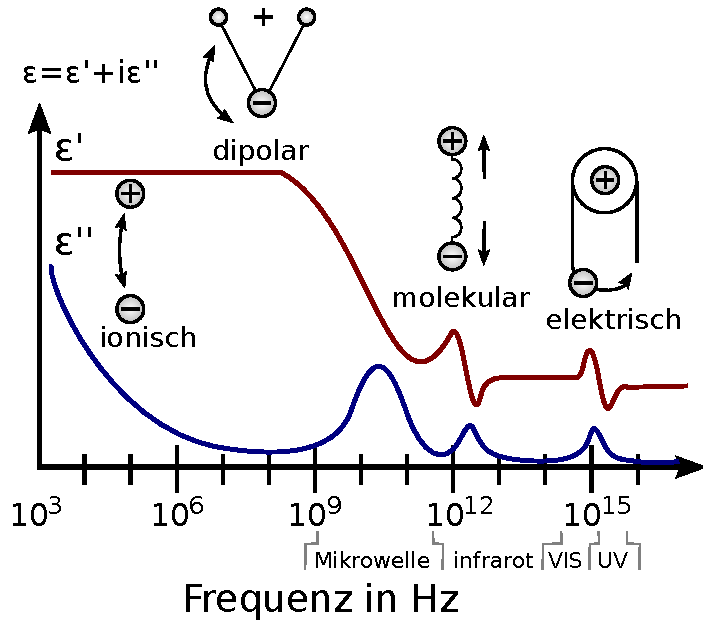
\includegraphics[width=0.9\textwidth]{res/Dielectric_responses_DE.pdf}
 \end{minipage}\hfill
 \begin{minipage}{0.6\textwidth}
 	Grundsätzlich gibt es beim Anlegen eines zeitlich veränderlichen Feldes ein verschiedenes Verhalten bei vorhandenen oder nicht
 	vorhandenen Rückstellkräften. \textbf{Dipolar} orientieren sich polare Moleküle (z.B.
 	Wasser) im Feld, es gibt keine Rückstellkraft, nur thermische Bewegung (Debye-Relaxation).
 	\textbf{Molekular} und \textbf{atomar} (kleinere Größe $\to$ höhere Frequenz, wo der Effekt zum Tragen kommt) sind Rückstellkräfte vorhanden (harmonischer Oszillator, Schwingkreis $\to$ Kurve sieht so aus wie Impedanzverlauf im Schwingkreis).
 	Die dielektrische Spektroskopie dient zur Aufklärung der Mechanismen.
 \end{minipage}\\\\
 Dieser Abschnitt diente zur Abgrenzung, denn bei der Lösung der Telegraphen-Gleichung wird auch eine komplexe Permittivität eingeführt, die aber nicht mit den hier beschriebenen molekularen Effekten zusammenhängt.
 \subsubsection{Eigentliche Lösung der Telegraphen-Gleichung}
		  Die Telegraphen-Gleichung bei harmonischer Zeitabhängigkeit kann leicht in die bekannte Form der homogenen \textbf{Wellengleichung} ($\nearrow$\ref{homwell}) überführt werden:
		        \begin{equation}\begin{split}
				        \left[ \Delta + \omega^2\varepsilon\mu - \mathrm{j}\omega\mu\kappa \right] \underline{\Psi}(\vec{r} , t) =\left[ \Delta + \omega^2\mu\left(\varepsilon - \mathrm{j}\frac{\kappa}{\omega}\right) \right] \underline{\Psi}(\vec{r} , t) &=0\\
				        \left[ \Delta + \omega^2\mu_0\mu_r\varepsilon_0\left(\varepsilon_r - \mathrm{j}\frac{\kappa}{\varepsilon_0\omega}\right) \right] \underline{\Psi}(\vec{r} , t) &=0\\
				        \left[ \Delta + \frac{\omega^2}{c^2}\underline{\varepsilon}_r\mu_r\right] \underline{\Psi}(\vec{r} , t) = \left[ \Delta + \frac{\omega^2}{ \ubar{v}_\mathrm{c}^2}\right] \underline{\Psi}(\vec{r} , t)&=0
			        \end{split}\end{equation}
		 Hierbei wurde eine \textbf{komplexe Permittivität} \(\underline{\varepsilon}_r\) eingeführt ($\nearrow$\ref{komplperm1}):
		        \begin{equation}\begin{split}
			        \Aboxed{\underline{\varepsilon}_r &= \varepsilon_r^{\prime} + \mathrm{j}\varepsilon_r^{\prime\prime} = \varepsilon_r - \mathrm{j}\frac{\kappa}{\varepsilon_0\omega} = |\underline{\varepsilon}_r|  \mathrm{e}^{-\mathrm{j}\delta}} \\ |\underline{\varepsilon}_r|&=\sqrt{\varepsilon_r^2+\frac{\kappa^2}{\varepsilon_0^2\omega^2}} \\
			        \tan\delta &= \frac{\kappa}{\varepsilon_0\varepsilon_r\omega} \\
			        \underline{\varepsilon}_r &=\varepsilon_r (1 - \mathrm{j}\tan\delta)
		        \end{split}\end{equation}
		        Man sollte beachten, dass hier von einer \textbf{reellen Permittivität} ausgegangen wurde und dann ein Term mit der Leitfähigkeit in die Permittivität hineindefiniert wurde. Genauso kann man hier auch von einer \textbf{komplexen Permittivität} ausgehen (die wie im Abschnitt zuvor den molekularen Effekten Rechnung trägt). Das führt dann dazu, dass der Imaginärteil zwei Komponenten hat. Welche Terme man betrachtet und welche man (näherungsweise) vernachlässigt, ist vom jeweiligen Problem abhängig (im guten Leiter dominiert häufig der Imaginärteil, in einem guten Dielektrikum häufig der Realteil). Jede komplexe Permittivität führt zu Verlusten, weshalb $\delta$ auch Verlustwinkel heißt.\\
		   Außerdem ergibt sich die \textbf{komplexe Ausbreitungsgeschwindigkeit} \( \ubar{v}_\mathrm{c}\):
		        \begin{equation}
			        \boxed{ \ubar{v}_\mathrm{c} = \frac{1}{\sqrt{\varepsilon_0\underline{\varepsilon}_r\mu_0\mu_r}} = \frac{1}{\sqrt{\underline{\varepsilon}\mu}}}
		        \end{equation}
		 Aus den Betrachtungen zur Wellengleichung in \ref{harmebwell} folgt vollkommen analog (nur hier mit einem komplexen Wellenvektor) die Lösung der Telegraphengleichung:
		        \begin{equation}
			        \boxed{\underline{\Psi}(\vec{r} , t) = \underline{\Psi}_0  \mathrm{e}^{\mathrm{j}(\omega t -  \vec{\ubar{k}}\cdot\vec{r} )}}
		        \end{equation}
		 Hierbei ist \( \vec{\ubar{k}}\) der \textbf{komplexe Wellenvektor}, der sich aus der komplexen Ausbreitungsgeschwindigkeit ergibt:
		        \begin{equation}
			        \vec{\ubar{k}} = \frac{\omega}{ \ubar{v}_\mathrm{c}} \vu{k} = \omega \sqrt{\underline{\varepsilon}\mu}\, \vu{k}= \frac{\omega}{c} \sqrt{\underline{\varepsilon}_r\mu_r}\, \vu{k} = \frac{\omega}{c} \underline{n}\, \vu{k}
		        \end{equation}
		  Außerdem wurde der \textbf{komplexe Brechungsindex} \(\underline{n}\) eingeführt, dessen Realteil $n^{\prime}$ auch \textbf{verallgemeinerter Brechungsindex} und dessen Imaginärteil $\gamma$ auch \textbf{Extinktionskoeffizient} genannt wird:
		        \begin{equation}\begin{split}
				        \underline{n} &= \sqrt{\underline{\varepsilon}_r\mu_r} = n^{\prime} - \mathrm{j}\gamma \text{ mit}\\
				        n^{\prime} &= n\cdot \sqrt{ \frac{1}{2}+\frac{1}{2}\sqrt{1+ \left( \frac{\kappa}{\varepsilon_0\varepsilon_r\omega} \right)^2} } \xrightarrow{\kappa\to 0} n \\
				        \gamma &= n \cdot \sqrt{-\frac{1}{2}+\frac{1}{2}\sqrt{1+ \left( \frac{\kappa}{\varepsilon_0\varepsilon_r\omega} \right)^2} } \xrightarrow{\kappa\to 0} 0 
			        \end{split}\end{equation}
  \subsection{Lösung für die Felder}
		 Setzt man die gefundene Lösung z.B. für das elektrische Feld ein ergibt sich:
		        \begin{equation}\begin{split}
				        \ubar{\vec{E}}(\vec{r} , t) &= \ubar{\vec{E}}_0  \mathrm{e}^{\mathrm{j}(\omega t -  \vec{\ubar{k}}\cdot\vec{r} )}\\
				        &=\ubar{\vec{E}}_0  \mathrm{e}^{\mathrm{j}(\omega t - \frac{\omega}{c}\underline{n}\vu{k}\cdot\vec{r} )} = \ubar{\vec{E}}_0  \mathrm{e}^{\mathrm{j}(\omega t - \frac{\omega}{c}(n^{\prime}-\mathrm{j}\gamma)\vu{k}\cdot\vec{r} )}\\
				        &= \ubar{\vec{E}}_0 \mathrm{e}^{-\frac{\omega}{c}\gamma \vu{k}\cdot\vec{r} }  \mathrm{e}^{\mathrm{j}(\omega t - \frac{\omega}{c}n^{\prime}\vu{k}\cdot\vec{r} )} = \ubar{\vec{E}}_0 \mathrm{e}^{- k^{\prime\prime} \vu{k}\cdot\vec{r} }  \mathrm{e}^{\mathrm{j}(\omega t -  k^{\prime}\vu{k}\cdot\vec{r} )}
			        \end{split}\end{equation}
		  Dies beschreibt eine \textbf{gedämpfte Welle} in Richtung \(\vu{k} \) mit \textbf{Eindringtiefe} \(\delta = \frac{c}{\omega\gamma}\). Je größer also der Extinktionskoeffizient (je größer also die Leitfähigkeit), desto weniger stark dringt die Welle in das Medium ein. Die \textbf{Phasengeschwindigkeit} ließt man aus dem Wellenterm ab:
		        \begin{equation}
			        \boxed{ v_\mathrm{p} = \frac{\omega}{ k^{\prime}} = \frac{c}{n^{\prime}} \le \frac{c}{n}} 
		        \end{equation}
		   Diese ist offensichtlich maximal für $\kappa=0$. Für die magnetische Flussdichte gilt:
		        \begin{equation}
			        \vec{\ubar{B}}(\vec{r} , t) = \vec{\ubar{B}}_0  \mathrm{e}^{\mathrm{j}(\omega t -  \vec{\ubar{k}}\cdot\vec{r} )}
		        \end{equation}
		        folgt analog zu den früheren Herleitungen:
		        \begin{equation}
			        \vec{\ubar{k}}\cdot\ubar{\vec{E}} = 0 \; ,\quad  \vec{\ubar{k}}\cdot\vec{\ubar{B}} = 0 \; ,\quad \frac{ \ubar{k}}{\omega} \vu{k}\times \ubar{\vec{E}} = \boxed{\vec{\ubar{B}} = \frac{1}{c}(n^{\prime}-\mathrm{j}\gamma) \vu{k}\times \ubar{\vec{E}}}
		        \end{equation}
		        Es handelt sich also um eine \textbf{TEM-Welle}, $E$ und $B$ sind aber \textbf{nicht in Phase}.

 \section{Reflexion und Brechung von ebenen Wellen}
 Das Medium, aus dem die Welle einfällt, heißt Medium 1. Entsprechend ist das andere Medium 2 und der Normalenvektor ist von 1 nach 2 orientiert. Die geometrischen Größen und Materialparameter sind wie in der folgenden Grafik definiert. In der Grafik ist zudem verdeutlicht, dass zunächst noch unbekannt ist, ob die Wellenvektoren von reflektierter und transmittierter Welle in der Einfallsebene liegen.\\
  \begin{minipage}{.5\textwidth}
	  \resizebox*{\textwidth}{!}{\tdplotsetmaincoords{70}{20}
\begin{tikzpicture}[scale=0.6,tdplot_main_coords]
	\draw[fill=gray!50,canvas is xy plane at z=0] (-5,-5) rectangle (5,5);
	\node[transform shape,canvas is xy plane at z=0,anchor=south west]
	at (-5,-5) {{\huge Grenzfläche}};
	\draw[-stealth] (-5.5,0,0) -- (5.5,0,0) node[pos=1.05]{$x$};
	\draw[-stealth] (0,5.5,0) -- (0,-5.5,0) node[pos=1.05]{$y$};
	\draw[-stealth] (0,0,5) -- (0,0,-2.5) node[pos=1.025]{$z$};
	\begin{scope}[canvas is xy plane at z=0]
		\draw[-latex] (2.5,0) arc(0:-40:2.5) node[below right]{$\varphi_r, \; \varphi_t$};
	\end{scope}

	\foreach \X [count=\Y,evaluate=\Y as \Col using {int(\Y*20)}] in {0,-20,-40}
		{\tdplotsetrotatedcoords{\X}{00}{0}
			\begin{scope}[tdplot_rotated_coords]
				\begin{scope}[canvas is xz plane at y=0]
					\draw[fill=blue!\Col, fill opacity=0.5] (0:2.5) arc (0:90:2.5) -- (0,0);
				\end{scope}
			\end{scope}}

	\begin{scope}[canvas is xz plane at y=0]
		\draw[fill=blue!20,fill opacity=0.5] (90:4.2) arc (90:180:4.2) -- (0,0);
		\draw[thick] (150:6.5) node[above,align=center]{Einfalls-\\ richtung} -- (0,0);
		\draw[thick,-latex] (150:6.5) -- (150:4.7) node[anchor=south west]{$\vec{k_i}$};
		\node[anchor=south east] at (110:3) {$\vartheta_i$};
		\draw[-latex] (90:3) arc(90:150:3);

		\draw[thick] (55:6.5) node[above,align=center]{Refelxions-\\ richtung} -- (55:2.2);
		\draw[dashed] (55:2.2) -- (0,0);
		\draw[thick,-latex] (55:2.5) -- (55:4.5) node[anchor=south east]{$\vec{k_r}$};
		\node[anchor=south west] at (75:3.2) {$\vartheta_r$};
		\draw[-latex] (90:3.2) arc(90:55:3.2);
		%
		\draw[thick] (-65:3.7) node[right,align=center]{Transmissions-\\ richtung} -- (-65:2.2);
		\draw[dashed] (-65:2.2) -- (0,0);
		\draw[thick,-latex] (-65:2.5) -- (-65:3.2) node[anchor=east]{$\vec{k_t}$};
		\node[anchor=south west] at (265:2.15) {$\vartheta_t$};
		\draw[-latex] (-90:1.2) arc(-90:-65:1.2);

	\end{scope}

	\draw[thick, red,-latex] (xyz spherical cs: radius=1.5, phi=-90, theta=30) -- +(xyz spherical cs: radius=1, phi=90, theta=60) node[anchor=south]{$\vec{E_\parallel}$};
	\draw[thick, blue,-latex] (xyz spherical cs: radius=1.5, phi=-90, theta=30) -- +(xyz spherical cs: radius=1, phi=180, theta=0) node[anchor=north]{$\vec{B_\parallel}$};

	\draw[thick, red,-latex] (xyz spherical cs: radius=2.2, phi=-90, theta=30) -- +(xyz spherical cs: radius=1, phi=180, theta=0) node[anchor=east]{$\vec{E_\perp}$};
	\draw[thick, blue,-latex] (xyz spherical cs: radius=2.2, phi=-90, theta=30) -- +(xyz spherical cs: radius=1, phi=90, theta=-120) node[anchor=north]{$\vec{B_\perp}$};
	\draw[thick,-latex] (4,0,0) -- (4,0,-1) node[anchor= west] {$\vec{n}$};
	\draw[thin] (-2.3,0,2.9) -- (-3,0,4) node[anchor=south,align=center]{Einfalls-\\ ebene};

\end{tikzpicture}}
  \end{minipage}
  \begin{minipage}{.5\textwidth}
	  \resizebox*{\textwidth}{!}{\tdplotsetmaincoords{70}{20}
\begin{tikzpicture}[media/.style={font={\footnotesize}},wave/.style={decorate,decoration={snake,post length=1.4mm,amplitude=2mm,segment length=2mm},thick},
		interface/.style={
				% The border decoration is a path replacing decorator. 
				% For the interface style we want to draw the original path.
				% The postaction option is therefore used to ensure that the
				% border decoration is drawn *after* the original path.
				postaction={draw,decorate,decoration={border,angle=-45,
								amplitude=0.3cm,segment length=2mm}}},
	]
	% Round rectangle
	\fill[gray!10,rounded corners] (-4,-3) rectangle (4,0);
	% Interface
	\draw[blue,line width=.5pt,interface](-4,0)--(4,0);
	% Vertical dashed line
	\draw[dashed,gray](0,-3)--(0,3);
	% Coordinates system
	\draw(0,0.15)node[anchor=south east]{$y$};
	\draw[<->,line width=1pt] (2,0) node[above]{$x$}-|(0,-2) node[right]{$z$};
	% Incidence
	\draw[->,wave]
	(155:4.2cm)--(155:3.5cm)node[right]{$\vec{k}_i$};
	\draw[gray](0:0cm)--(155:3cm);
	\path (0,0)++(123:1cm)node{$\vartheta_i$};
	\draw[->](0,0.75)arc(90:155:.75cm);
	% EField
	\draw[red, -latex,thick](155:1.5)--+(65:0.7)node[right]{$\vec{E}_\parallel$};
	\filldraw[fill=white,draw=blue,line width=1pt](155:1.5)circle(.12cm) node[blue,below,yshift=-1.5]{$\vec{B}_\parallel$};
	\filldraw[fill=blue,draw=blue,line width=1pt](155:1.5)circle(.04cm);

	\draw[blue, -latex,thick](155:2)--+(245:0.7)node[right]{$\vec{B}_\perp$};
	\filldraw[fill=white,draw=red,line width=1pt](155:2)circle(.12cm) node[red,above,yshift=1.5]{$\vec{E}_\perp$};
	\filldraw[fill=red,draw=red,line width=1pt](155:2)circle(.04cm);

	% Transmission
	\draw[->,wave]
	(-50:2.5cm)--(-50:3.2cm)node[right]{$\vec{k}_t$};
	\draw[gray](0:0cm)--(-50:2cm);
	\path (0,0)++(-70:1cm)node{$\vartheta_t$};
	\draw[->] (0,-0.75) arc (-90:-50:.75cm);
	% Reflection
	\draw[->,wave]
	(45:2.5cm)--(45:3.2cm)node[right]{$\vec{k}_r$};
	\path (0,0)++(67:1.75cm) node{$\vartheta_r$};
	\draw[gray](0:0cm)--(45:2cm);
	\draw[->] (0,1.5)arc(90:45:1.5cm);
	% Media names
	\path[media] (-3,.6)  node[align=left]{{\normalsize\textcircled{1}\footnotesize}\\ $\varepsilon_1,\mu_1,\kappa_1$\\ $n_1, Z_1$}
	(-3,-.9) node[align=left]{{\normalsize\textcircled{2}\footnotesize}\\ $\varepsilon_2,\mu_2,\kappa_2$\\ $n_2, Z_2$};

	% $y$ axis
	\filldraw[fill=white,line width=1pt](0,0)circle(.12cm);
	\filldraw[fill=black,line width=1pt](0,0)circle(.04cm);
	% \draw[line width=.6pt] (0,0)
	%                       +(-135:.12cm) -- +(45:.12cm)
	%                       +(-45:.12cm) -- +(135:.12cm);

	\draw[thick,-latex] (3,0) -- (3,-1) node[anchor=south east]{$\vec{n}$};
\end{tikzpicture}}
  \end{minipage}
	   In diesem Abschnitt sollen \textbf{linear polarisierte ebene Wellen} am Übergang zweier Medien mit homogenen, linearen und isotropen Materialeigenschaften betrachtet werden. Der Wellenvektor der einfallenden Welle \(\vec{k}_i\) und Normalenvektor der Grenzfläche \(\vec{n}\) spannen die \textbf{Einfallsebene} auf. Ohne Beschränkung der Allgemeinheit kann \(\vec{n} = \vu{z}\) gesetzt werden (das Koordinatensystem kann beliebig rotiert werden).
	  Es werden folgende Indizes gewählt:
	  \begin{itemize}
	  	\item $i$ - inzident
	  	\item $r$ - reflektiert
	  	\item $t$ - transmittiert
	  \end{itemize} 
	  Weiterhin werden zwei Fälle unterschieden:
	  \begin{enumerate}
	  	\item \textbf{senkrechte Polarisation} ($\perp$,\enquote{horizontal}): $\vec{E}_i$ steht senkrecht zur Einfallsebene
	  	\item \textbf{parallele Polarisation} ($\parallel$,\enquote{vertikal}): $\vec{E}_i$ liegt in der Einfallsebene
	  \end{enumerate} 
	  Alle anderen Polarisationen können als Superposition der beiden Fälle angesehen werden ($\nearrow$\ref{poleb}). Außerdem soll harmonische Zeitabhängigkeit  angenommen werden (Fourier-Synthese möglich $\to$ keine echte Einschränkung), das heißt ausgeschrieben:
		        \begin{align}
			        \ubar{\vec{E}}_i(\vec{r} , t) & = \ubar{\vec{E}}_{0i}  \mathrm{e}^{\mathrm{j}(\omega_i t - \vec{k}_i \cdot \vec{r} )} & \vec{\ubar{B}}_i(\vec{r} , t) & = \frac{1}{\omega_i} \left(\vec{k}_i \times \ubar{\vec{E}}_i(\vec{r} , t)\right) \\
			        \ubar{\vec{E}}_r(\vec{r} , t) & = \ubar{\vec{E}}_{0r}  \mathrm{e}^{\mathrm{j}(\omega_r t - \vec{k}_r \cdot \vec{r} )} & \vec{\ubar{B}}_r(\vec{r} , t) & = \frac{1}{\omega_r} \left(\vec{k}_r \times \ubar{\vec{E}}_r(\vec{r} , t)\right) \\
			        \ubar{\vec{E}}_t(\vec{r} , t) & = \ubar{\vec{E}}_{0t}  \mathrm{e}^{\mathrm{j}(\omega_t t - \vec{k}_t \cdot \vec{r} )} & \vec{\ubar{B}}_t(\vec{r} , t) & = \frac{1}{\omega_t} \left(\vec{k}_t \times \ubar{\vec{E}}_t(\vec{r} , t)\right)
		        \end{align} 
Die Beziehungen für harmonische ebene Wellen sind in \ref{ebwellzsfg} zusammengefasst. Im folgenden wird $\kappa=0$ angenommen (also reelle Permittivität etc.). Wenn $\kappa\neq 0$ gelten sollte, müssen entsprechend der Betrachtungen in \ref{leitendeMed} einige Größen komplex geschrieben werden. Die Vorgehensweise und die resultierenden Gleichungen sind aber vollkommen analog. Das Verhalten von Feldern an Grenzflächen wurde in \ref{Grenz} untersucht und wird hier genutzt.
\subsection{Zusammenhänge der Kreisfrequenzen}
  Entsprechend den Ausführungen in \ref{Grenz} wird die Tangentialkomponente von \(\vec{E}\) betrachtet ($\nearrow$\ref{tanE}). Für \(z=0\) muss gelten:
		        \begin{equation}\label{tanEwellen}
			        \vec{n} \times \left( \ubar{\vec{E}}_{0t}  \mathrm{e}^{\mathrm{j}(\omega_t t - \vec{k}_t \cdot \vec{r} )} -\left( \ubar{\vec{E}}_{0i}  \mathrm{e}^{\mathrm{j}(\omega_i t - \vec{k}_i \cdot \vec{r} )} + \ubar{\vec{E}}_{0r}  \mathrm{e}^{\mathrm{j}(\omega_r t - \vec{k}_r \cdot \vec{r} )}\right)\right) \stackrel{!}{=} \vec{0}
		        \end{equation}
 Für \textbf{beliebige Zeitpunkte \(t \ne 0\) und \(\vec{r}  = \vec{0}\)} kann dies nur erfüllt werden, wenn gilt
		        \begin{equation}
			        \mathrm{e}^{\mathrm{j}\omega_i t} =  \mathrm{e}^{\mathrm{j}\omega_r t} = \mathrm{e}^{\mathrm{j}\omega_t t} \Rightarrow \boxed{\omega_i =\omega_r = \omega_t} \quad 
		        \end{equation}
		       Ein Sinus mit nicht verschwindender Amplitude kann unmöglich zu jedem Zeitpunkt gleich einem Sinus anderer Frequenz sein. Die \textbf{Kreisfrequenzen} \textbf{ändern} sich also \textbf{nicht}.
\subsection{Reflexions- und Brechungsgesetz}
		  Im gewählten Koordinatensystem (Einfallsebene ist $x-z-$Ebene) gilt durch Projektion:
		        \begin{equation}\begin{split}
				        \vec{k}_i &=  k_i \left( \sin\vartheta_i\vu{x} + \cos\vartheta_i\vu{z} \right)\\
				        \vec{k}_r &=  k_r \left( \cos\varphi_r\sin\vartheta_r\vu{x} + \sin\varphi_r\sin\vartheta_r\vu{y}  - \cos\vartheta_r\vu{z}\right) \\
				        \vec{k}_t &=  k_t \left( \cos\varphi_t\sin\vartheta_t\vu{x} + \sin\varphi_t\sin\vartheta_t\vu{y}  + \cos\vartheta_t\vu{z}\right)
			        \end{split}\end{equation}
		   Es wird ein Punkt an der Grenzfläche (\(z=0\)) betrachtet, dort gilt \(\vec{r}  = x\vu{x} + y\vu{y} \). Damit:
		        \begin{equation}\label{spwellort}\begin{split}
				        \vec{k}_i\cdot\vec{r}  &= x \underbrace{k_i \sin\vartheta_i }_{k_{ix}} + y\underbrace{0}_{k_{iy}} \\
				        \vec{k}_r \cdot\vec{r} &= x \underbrace{k_r\cos\varphi_r\sin\vartheta_r}_{k_{rx}} + y\underbrace{k_r\sin\varphi_r\sin\vartheta_r}_{k_{ry}}  \\
				        \vec{k}_t \cdot\vec{r} &=  x \underbrace{k_t  \cos\varphi_t\sin\vartheta_t}_{k_{tx}} + y\underbrace{k_t \sin\varphi_t\sin\vartheta_t}_{k_{ty}}
			        \end{split}\end{equation}
		  Setzt man in \ref{tanEwellen} \(t=0\), kann man die selbe Argumentation wie für die Frequenz für die $x$- und $y$-Komponente ($z=0$) durchziehen. Es muss also 
		  \begin{equation}
		  	\mathrm{e}^{-\mathrm{j}(k_{tx}x+k_{ty}y)}=		  	\mathrm{e}^{-\mathrm{j}(k_{ix}x+k_{iy}y)}=
		  			  	\mathrm{e}^{-\mathrm{j}(k_{rx}x+k_{ry}y)} \Rightarrow \boxed{k_{tx}=k_{ix}=k_{rx}  \text{ und } k_{ty}=k_{iy}=k_{ry}}
		  \end{equation}
		  gelten. Mit Koeffizientenvergleich in \ref{spwellort}:
		        \begin{equation}\begin{split}
			        x:&\quad k_i\sin\vartheta_i =  k_r\cos\varphi_r\sin\vartheta_r = k_t\cos\varphi_t\sin\vartheta_t \\
			       y:&\quad0= k_r\sin\varphi_r\sin\vartheta_r =  k_t\sin\varphi_t\sin\vartheta_t
		        \end{split}\end{equation}
		   Aus der \(y\)-Komponente folgt für \(\vartheta_r\ne 0\) und \(\vartheta_t\ne 0\): \begin{equation}
		   	\boxed{\varphi_r=\varphi_t=0}
		   \end{equation} 
		   Die \textbf{reflektierte} und \textbf{transmittierte} \textbf{Komponente} liegen also in der \textbf{Einfallsebene}.
		  Die Bedingung für die \(x\)-Komponente vereinfacht sich damit zu
		        \begin{equation}\label{vereinfx}
			        k_i\sin\vartheta_i =  k_r\sin\vartheta_r = k_t\sin\vartheta_t
		        \end{equation}
		  Die Beträge der Wellenvektoren sind durch die Materialien bestimmt:
		        \begin{equation}\begin{split}
				        k_i =  k_r &= \frac{2\pi}{\lambda_1} = \frac{\omega}{ v_{c_1}} = \omega\sqrt{\varepsilon_1\mu_1} = \frac{\omega}{c}\sqrt{\varepsilon_{r_1}\mu_{r_1}} = \frac{\omega}{c} n_1 = k_1\\
				        k_t &= \frac{2\pi}{\lambda_2} = \frac{\omega}{ v_{c_2}} = \omega\sqrt{\varepsilon_2\mu_2} = \frac{\omega}{c}\sqrt{\varepsilon_{r_2}\mu_{r_2}} = \frac{\omega}{c} n_2 = k_2
			        \end{split}\end{equation}
		  Einsetzen in \ref{vereinfx} ergibt zwei Gesetze:
\begin{align}
	\textbf{Reflexionsgesetz:} & & \Aboxed{\vartheta_i&=\vartheta_r}:=\vartheta_1\\
	\textbf{Brechungsgesetz nach Snellius:} & & \Aboxed{ n_1\sin\vartheta_1 &= n_2\sin\vartheta_2}\quad \text{ mit } \quad\vartheta_2:=\vartheta_t\label{snellius}
\end{align}
  \subsection{Reflexions- und Transmissionskoeffizienten}
  Es ist materialabhängig, wie stark eine elektromagnetische Welle reflektiert oder transmittiert wird. Bei solchen Betrachtungen muss man zwischen senkrechter und paralleler Polarisation unterscheiden. Das Vorgehen ist bei paralleler und senkrechter Polarisation analog. Die folgenden Grafiken verdeutlichen die Definitionsrichtungen der Größen und das gewählte Koordinatensystem. Es werden ebene Wellen betrachtet, das heißt $\vec{k}$, $\vec{E}$ und $\vec{B}$ bilden ein Rechtsdreibein. $\vec{k}$ sollte zudem sinnvollerweise in Ausbreitungsrichtung zeigen. Dennoch bleiben Freiheitsgrade, wie die anderen beiden Vektoren orientiert sind (bei senkrechter Polarisation bspw. $\vec{E}$ in die Ebene hinein oder aus der Ebene hinaus). Man kann gleichwertig mit anderen Definitionsrichtungen rechnen, die Ergebnisse würden sich physikalisch nicht unterscheiden. Was sich aber unterscheiden kann sind Rechengrößen wie der Reflektionsfaktor. Wenn man bspw. einen Phasensprung um $\pi$ durch Reflektion hat und den reflektierten Vektor antiparallel zum inzidenten definiert, dann ist der Reflektionskoeffizient positiv. Definiert man hingegen parallel, wäre der Reflektionskoeffizient positiv. Deshalb sollte man stets die Definitionen angeben, auf die man sich bezieht. \\
	  \begin{minipage}{.5\textwidth}
	\centering
	\begin{tikzpicture}
		\draw[-latex, thin] (-2,0) -- (2,0) node[anchor=west] {$z$};
		\draw[-latex, thin] (0,-2) -- (0,2) node[anchor=south] {$x$};
		\filldraw[fill=white,line width=1pt](0,0)circle(.12cm) node[anchor=north west]{$y$};
		\filldraw[fill=black,line width=1pt](0,0)circle(.04cm);
		\path (-1.5,2)  node[align=left]{{\normalsize\textcircled{1}}\\ $\varepsilon_1,\mu_1$\\ $n_1, Z_1$}
		(1.5,2) node[align=left]{{\normalsize\textcircled{2}}\\ $\varepsilon_2,\mu_2$\\ $n_2, Z_2$};
		\draw[dashed, thick] (0,0) -- +(20:2);
		\draw[dashed, thick] (220:2) -- (0,0);
		\draw[dashed, thick] (0,0) -- (140:2);
		\draw[thin] (0.6,0) arc (0:20:0.6) node[right,yshift=-1]{$\vartheta_2$};
		\draw[thin] (-0.6,0) arc (180:220:0.6) node[left,yshift=3]{$\vartheta_1$};
		\draw[thin] (-0.6,0) arc (180:140:0.6) node[left,yshift=-2]{$\vartheta_1$};

		\filldraw[fill=white,line width=1pt, draw=red](140:1.5)circle(.12cm) node[red, anchor=north east]{$\vec{E}_r$};
		\filldraw[fill=red,line width=1pt, draw=red](140:1.5)circle(.04cm);
		\draw[blue,-stealth, thick] (140:1.5) -- +(50:0.5) node[blue, anchor=north west]{$\vec{H}_r$};
		\draw[black,-stealth, thick] (140:1.5) -- +(140:0.5) node[anchor=north east]{$\vec{k}_r$};

		\filldraw[fill=white,line width=1pt, draw=red](220:1.5)circle(.12cm) node[red, anchor=south east]{$\vec{E}_i$};
		\filldraw[fill=red,line width=1pt, draw=red](220:1.5)circle(.04cm);
		\draw[blue,-stealth, thick] (220:1.5) -- +(310:0.5) node[blue, anchor=north east]{$\vec{H}_i$};
		\draw[black,-stealth, thick] (220:1.5) -- +(220:-0.5) node[anchor=north west]{$\vec{k}_i$};

		\filldraw[fill=white,line width=1pt, draw=red](20:1.5)circle(.12cm) node[red, anchor=south east]{$\vec{E}_t$};
		\filldraw[fill=red,line width=1pt, draw=red](20:1.5)circle(.04cm);
		\draw[blue,-stealth, thick] (20:1.5) -- +(-70:0.5) node[blue, anchor=north]{$\vec{H}_t$};
		\draw[black,-stealth, thick] (20:1.5) -- +(20:0.5) node[anchor=north]{$\vec{k}_t$};
		\draw (1.5,-1.5) node{$\perp$ Polarisation};
		\draw[-stealth,thick] (0,-1) -- (0.5,-1) node[anchor=west]{$\vec{n}$};
	\end{tikzpicture}
\end{minipage}
\begin{minipage}{.5\textwidth}
	\centering
	\begin{tikzpicture}
		\draw[-latex, thin] (-2,0) -- (2,0) node[anchor=west] {$z$};
		\draw[-latex, thin] (0,-2) -- (0,2) node[anchor=south] {$x$};
		\filldraw[fill=white,line width=1pt](0,0)circle(.12cm) node[anchor=north west]{$y$};
		\filldraw[fill=black,line width=1pt](0,0)circle(.04cm);
		\path (-1.5,2)  node[align=left]{{\normalsize\textcircled{1}}\\ $\varepsilon_1,\mu_1$\\ $n_1, Z_1$}
		(1.5,2) node[align=left]{{\normalsize\textcircled{2}}\\ $\varepsilon_2,\mu_2$\\ $n_2, Z_2$};
		\draw[dashed, thick] (0,0) -- +(20:2);
		\draw[dashed, thick] (220:2) -- (0,0);
		\draw[dashed, thick] (0,0) -- (140:2);
		\draw[thin] (0.6,0) arc (0:20:0.6) node[right,yshift=-1]{$\vartheta_2$};
		\draw[thin] (-0.6,0) arc (180:220:0.6) node[left,yshift=3]{$\vartheta_1$};
		\draw[thin] (-0.6,0) arc (180:140:0.6) node[left,yshift=-2]{$\vartheta_1$};

		\filldraw[fill=white,line width=1pt, draw=blue](140:1.5)circle(.12cm) node[blue, anchor=south west]{$\vec{H}_r$};
		\filldraw[fill=blue,line width=1pt, draw=blue](140:1.5)circle(.04cm);
		%\draw[line width=.6pt] (0,0) +(-135:.12cm) -- +(45:.12cm) +(-45:.12cm) -- +(135:.12cm); 
		\draw[red,-stealth, thick] (140:1.5) -- +(230:0.5) node[red, anchor=north west]{$\vec{E}_r$};
		\draw[black,-stealth, thick] (140:1.5) -- +(140:0.5) node[anchor=north east]{$\vec{k}_r$};

		\filldraw[fill=white,line width=1pt, draw=blue](220:1.5)circle(.12cm) node[blue, anchor=north,yshift=-2]{$\vec{H}_i$};
		\filldraw[fill=blue,line width=1pt, draw=blue](220:1.5)circle(.04cm);
		%\draw[blue, line width=.6pt] (220:1.5) +(-135:.12cm) -- +(45:.12cm) +(-45:.12cm) -- +(135:.12cm); 
		\draw[red,-stealth, thick] (220:1.5) -- +(130:0.5) node[anchor=north east]{$\vec{E}_i$};
		\draw[black,-stealth, thick] (220:1.5) -- +(220:-0.5) node[anchor=north west]{$\vec{k}_i$};

		\filldraw[fill=white,line width=1pt, draw=blue](20:1.5)circle(.12cm) node[blue, anchor=north,yshift=-2]{$\vec{H}_t$};
		\filldraw[fill=blue,line width=1pt, draw=blue](20:1.5)circle(.04cm);
		%\draw[line width=.6pt] (0,0) +(-135:.12cm) -- +(45:.12cm) +(-45:.12cm) -- +(135:.12cm); 
		\draw[red,-stealth, thick] (20:1.5) -- +(110:0.5) node[red, anchor=east]{$\vec{E}_t$};
		\draw[black,-stealth, thick] (20:1.5) -- +(20:0.5) node[anchor=north]{$\vec{k}_t$};
		\draw (1.5,-1.5) node{$\parallel$ Polarisation};
		\draw[-stealth,thick] (0,-1) -- (0.5,-1) node[anchor=west]{$\vec{n}$};
	\end{tikzpicture}
\end{minipage}
	  Im \textbf{Spezialfall}, dass $\vec{k}_i \parallel \vec{n}$, ist die Einfallsebene nicht eindeutig definiert. Man kann dann gleichwertig mit den Formeln für parallele und senkrechte Polarisation rechnen. Zu beachten ist dabei allerdings, wie die Vektoren definiert sind. So wird man feststellen, dass $\ubar{r}_\perp=-\ubar{r}_\parallel$ ist. Das liegt daran, dass der elektrische Feldvektor des reflektierten Felds im Fall der parallelen Polarisation antiparallel zu dem einfallenden elektrischen Feldvektor definiert ist und im Fall der senkrechten Polarisation parallel. Im parallel polarisierten Fall ist also $\vu{{E_i}}=-\vu{{E_r}}$, im senkrechten hingegen $\vu{{E_i}}=\vu{{E_r}}$, sodass mit $\ubar{r}_\perp=-\ubar{r}_\parallel$ die berechnete Feldstärke $\vec{\ubar{E}}_r$ in beiden Fällen gleich ist.
	  \subsubsection{Senkrechte Polarisation}
	Es wird das \(\vec{E}\)-Feld betrachtet, welches in $y$-Richtung orientiert ist. Die Wellenvektoren haben entsprechend der Grafik für  die folgenden Richtungen:
			        \begin{align}
				        \vu{{k_i}} & = \sin\vartheta_1\vu{x} + \cos\vartheta_1\vu{z} \nonumber \\
				        \vu{{k_r}} & = \sin\vartheta_1\vu{x} - \cos\vartheta_1\vu{z} \label{ekrgln} \\
				        \vu{{k_t}} & = \sin\vartheta_2\vu{x} + \cos\vartheta_2\vu{z} \nonumber
			        \end{align}
		Der Ortsvektor bei \(z=0
			        \) ist \(\vec{r}  = x\vu{x} + y \vu{y}\).
			   Aus der Stetigkeit der Tangentialkomponente von \(\vec{E}\) ($\nearrow$\ref{tanE}) folgt unter Beachtung von $\vu{z} \times \vu{y} = -\vu{x}$:
			        \begin{equation}\begin{split}
					        \vu{z} \times \left(\ubar{E}_{0i} \vu{y} \mathrm{e}^{-\mathrm{j} k_i x \sin\vartheta_1} + \ubar{E}_{0r} \vu{y} \mathrm{e}^{-\mathrm{j} k_r x \sin\vartheta_1}   \right) &= \vu{z} \times \ubar{E}_{0t} \vu{y} \mathrm{e}^{-\mathrm{j} k_t x \sin\vartheta_2}   \\
					        -\vu{x}  \left(\ubar{E}_{0i}  \mathrm{e}^{-\mathrm{j} k_i x \sin\vartheta_1} + \ubar{E}_{0r} \mathrm{e}^{-\mathrm{j} k_r x \sin\vartheta_1}   \right) &= -\vu{x}  \ubar{E}_{0t}  \mathrm{e}^{-\mathrm{j} k_t x \sin\vartheta_2}
				        \end{split}\end{equation}
			   Das gilt für beliebige Punkte auf der Grenzfläche. Für \(x=0\) folgt:
			        \begin{equation}\label{refltransbzh1}
				        \boxed{ \ubar{E}_{0i} + \ubar{E}_{0r}= \ubar{E}_{0t}}
			        \end{equation}
			       Gibt es zwei Grenzflächen, kann im gleichen Koordinatensstem offensichtlich nicht an beiden Grenzflächen $z=0$ gelten. Außerdem kommt es in diesem Fall zu Mehrfachreflexionen, also mathematisch zu einer Superpostion von unendlich vielen Phasoren. Diese Reihe kann man als einen einzigen resultierenden Phasor auffassen (die Superposition unendlich vieler gleichfrequenter Signale ergibt ein Signal dieser Frequenz mit bestimmter Amplitude und Phase). Anstatt die Reihen explizit hinzuschreiben, ist es möglich, direkt diese resultierenden Phasoren als Gesamtwelle an die Randbedingungen anzupassen.\\
			        Nun soll das $\vec{H}$-Feld betrachtet werden. Die Oberflächenstromdichte ist 0 ($\nearrow$Betrachtungen in \ref{skin}). Folglich ist nach \ref{tanH} ($J_A=0$):
			        \begin{equation}
			        	\vu{z}\times\left(\vec{H}_i+\vec{H}_r\right)=\vu{z}\times\vec{H}_t
			        \end{equation}
			        Nun kann man den Zusammenhang zwischen $H$ und $E$ über den Feldwellenwiderstand ansetzten ($\nearrow$\ref{ebwellzsfg}). Demnach ist:
			        \begin{equation}       	\vu{z}\times\left(\frac{1}{Z_1}\vu{{k_i}}\times\vec{E}_i+\frac{1}{Z_1}\vu{{k_r}}\times\vec{E}_r\right)=\vu{z}\times\frac{1}{Z_2}\vu{{k_t}}\times\vec{E}_t
			        \end{equation}
			   Die doppelten Kreuzprodukte kann man auflösen. Dafür wird \ref{grass}, \(\vu{z}\cdot \vec{E}_{irt}=0\) sowie \ref{ekrgln} genutzt:
			        \begin{align}
				        \frac{1}{Z_1}\left[   - \vec{E}_i\left(\vu{z}\cdot \vu{{k_i}}  \right)  - \vec{E}_r\left(\vu{z}\cdot \vu{{k_r}}  \right) \right] & = \frac{1}{Z_2}\left[   - \vec{E}_t\left(\vu{z}\cdot \vu{{k_t}}  \right)\right] \nonumber\\
				        \frac{1}{Z_1}\left[   - \cos\vartheta_1\vec{E}_i  +\cos\vartheta_1 \vec{E}_r \right]                                             & = -\frac{1}{Z_2} \cos\vartheta_2 \vec{E}_t                                    \nonumber  \\
				        \Aboxed{\frac{1}{Z_1}\left[   \cos\vartheta_1\ubar{E}_{0i}  -\cos\vartheta_1 \ubar{E}_{0r} \right]                               & = \frac{1}{Z_2} \cos\vartheta_2 \ubar{E}_{0t}}\label{refltransbzh2}
			        \end{align}
			   Mit \ref{refltransbzh1} und \ref{refltransbzh2} können der \textbf{Reflexions-} und der \textbf{Transmissionskoeffizient}
			        \begin{equation}
				        \underline{r}_\perp = \frac{\ubar{E}_{0r}}{\ubar{E}_{0i}} \qquad \underline{t}_\perp = \frac{\ubar{E}_{0t}}{\ubar{E}_{0i}} 
			        \end{equation}
			        bestimmt werden.
			   Aus \ref{refltransbzh1} ergibt sich:
			        \begin{equation}
				        \ubar{E}_{0i} + \ubar{E}_{0r}= \ubar{E}_{0t} \Rightarrow  1+ \frac{\ubar{E}_{0r}}{\ubar{E}_{0i}}= \frac{\ubar{E}_{0t}}{\ubar{E}_{0i}} \Rightarrow \boxed{1+\underline{r}_\perp = \underline{t}_\perp}
			        \end{equation}
			   Aus \ref{refltransbzh2} ergibt sich:
			        \begin{equation}
				        \frac{1}{Z_1}\left[   \cos\vartheta_1\ubar{E}_{0i}  -\cos\vartheta_1 \ubar{E}_{0r} \right] = \frac{1}{Z_2} \cos\vartheta_2 \ubar{E}_{0t} \Rightarrow  \boxed{Z_2\cos\vartheta_1\left(1-\underline{r}_\perp\right) = Z_1 \cos\vartheta_2\underline{t}_\perp}
			        \end{equation}
			   Hieraus ergeben sich durch umstellen Reflexions- und Transmissionskoeffizient (\textbf{Fresnelsche Beziehungen}) zu
			        \begin{align}
				        \Aboxed{\underline{r}_\perp                         & = \frac{Z_2\cos\vartheta_1-Z_1\cos\vartheta_2}{Z_1\cos\vartheta_2+Z_2\cos\vartheta_1}} \label{frenselsref}\\
				        1+\underline{r}_\perp = \Aboxed{\underline{t}_\perp & = \frac{2 Z_2\cos\vartheta_1}{Z_1\cos\vartheta_2+Z_2\cos\vartheta_1}}\label{frenselstrans}
			        \end{align}
			  Die Beziehungen gelten natürlich auch für komplexe Feldwellenwiderstände. Ein wichtiger Spezialfall ist der Übergang Luft-Metall. 
			   \begin{itemize}
			   	\item In \textbf{Luft} gilt ($\nearrow\ref{feldwellenwid}$): \(Z=Z_1\simeq 377 \mathrm{\Omega}\)
			   	\item Für \textbf{Metall} gilt: \({\displaystyle \ubar{Z}=\ubar{Z}_2 = \sqrt{\frac{\mu}{\underline{\varepsilon}}}  = \sqrt{\frac{\mu}{\varepsilon_0\left(\varepsilon_r -\mathrm{j}\frac{\kappa}{\varepsilon_0\omega}\right)}} \simeq (1+\mathrm{j})\sqrt{\frac{\mu\omega}{2\kappa}} \to \left|Z_2\right| \ll  377 \mathrm{\Omega}}\)\\
			   	$\quad\to$ Näherung für einen guten Leiter ($\kappa$ groß)
			   \end{itemize} 
			   Für typische Frequenzen gilt somit, dass alles reflektiert wird:
			        \begin{equation}
				         \underline{r}_\perp \simeq -1 \quad \underline{t}_\perp \simeq 0
			        \end{equation}

	  \subsubsection{Parallele Polarisation}
			   Die Herleitung von Reflexions- und Transmissionskoeffizienten für \textbf{parallele Polarisation} verläuft völlig analog und wird hier nicht wiederholt. Die Unterschiede in den \textbf{Fresnelschen Beziehungen} werden im direkten Vergleich deutlich ($\nearrow$\ref{frenselsref},\ref{frenselstrans}):
			        \begin{align}
				        \Aboxed{\underline{r}_\parallel   & = \frac{Z_1\cos\vartheta_1-Z_2\cos\vartheta_2}{Z_2\cos\vartheta_2+Z_1\cos\vartheta_1}} \\
				        \frac{Z_2}{Z_1}\left(1+\underline{r}_\parallel\right)=\frac{\cos\vartheta_1}{\cos\vartheta_2}\left(1-\underline{r}_\parallel\right)
				        = \Aboxed{\underline{t}_\parallel & = \frac{2 Z_2\cos\vartheta_1}{Z_2\cos\vartheta_2+Z_1\cos\vartheta_1}}
			        \end{align}
		 Für den Übergang Luft-Metall folgt hier (es ist im Gegensatz zu der senkrechten Polarisation kein Phasensprung nötig, was deutlich wird wenn man sich \ref{tanE} vergegenwärtigt):
			        \begin{equation}
				        \underline{r}_\parallel \simeq +1 \quad \underline{t}_\parallel \simeq 0
			        \end{equation}
	  \subsubsection{Senkrechte und parallele Polarisation, Schreibweise mit $n$}
		  Mit \(Z=\sqrt{\frac{\mu}{\varepsilon}}\) und \(n=\sqrt{\varepsilon_r\mu_r}\) folgt \(Z = \frac{\mu c}{n}\), so dass für die Reflexions- und Transmissionskoeffizienten folgt
			        \begin{align}
				        \Aboxed{\underline{r}_\perp     & = \frac{n_1\cos\vartheta_1-\frac{\mu_1}{\mu_2} n_2\cos\vartheta_2}{n_1\cos\vartheta_1+\frac{\mu_1}{\mu_2} n_2\cos\vartheta_2}}  & \Aboxed{\underline{t}_\perp     & = \frac{2 n_1\cos\vartheta_1}{n_1\cos\vartheta_1+\frac{\mu_1}{\mu_2} n_2\cos\vartheta_2}} \\
				        \Aboxed{\underline{r}_\parallel & = \frac{-n_1\cos\vartheta_2+\frac{\mu_1}{\mu_2} n_2\cos\vartheta_1}{n_1\cos\vartheta_2+\frac{\mu_1}{\mu_2} n_2\cos\vartheta_1}} & \Aboxed{\underline{t}_\parallel & = \frac{2 n_1\cos\vartheta_1}{n_1\cos\vartheta_2+\frac{\mu_1}{\mu_2} n_2\cos\vartheta_1}}
			        \end{align}
			  Wichtiger Spezialfall: \textbf{\(\mu_1 = \mu_2\)}, z.B. beide unmagnetisch
			        \begin{align}
				        \Aboxed{\underline{r}_\perp     & = \frac{n_1\cos\vartheta_1- n_2\cos\vartheta_2}{n_1\cos\vartheta_1+ n_2\cos\vartheta_2}} & \Aboxed{\underline{t}_\perp     & = \frac{2 n_1\cos\vartheta_1}{n_1\cos\vartheta_1+ n_2\cos\vartheta_2}} \\
				        \Aboxed{\underline{r}_\parallel & = \frac{-n_1\cos\vartheta_2+n_2\cos\vartheta_1}{n_1\cos\vartheta_2+ n_2\cos\vartheta_1}} & \Aboxed{\underline{t}_\parallel & = \frac{2 n_1\cos\vartheta_1}{n_1\cos\vartheta_2+ n_2\cos\vartheta_1}}
			        \end{align}
	  \subsubsection{Senkrechte und parallele Polarisation, Schreibweise mit \(\vartheta_1,\;\vartheta_2\)}
			  Im Falle \(\mu_1 = \mu_2\) können die Fresnelschen-Beziehungen mit Hilfe des Brechungsgesetzes \(n_1\sin\vartheta_1=n_2\sin\vartheta_2\) auch nur mit den Winkeln geschrieben werden:
			        \begin{equation}\label{frenselvereinf}\begin{split}
					        \Aboxed{\underline{r}_\perp &= \frac{\cos\vartheta_1- \frac{\sin\vartheta_1}{\sin\vartheta_2}\cos\vartheta_2}{\cos\vartheta_1+ \frac{\sin\vartheta_1}{\sin\vartheta_2}\cos\vartheta_2} = \frac{\sin\left(\vartheta_2-\vartheta_1\right)}{\sin\left(\vartheta_1+\vartheta_2\right)}}\\
					        \Aboxed{\underline{t}_\perp &= \frac{2 \cos\vartheta_1}{\cos\vartheta_1+ \frac{\sin\vartheta_1}{\sin\vartheta_2}\cos\vartheta_2} = \frac{2\sin\vartheta_2\cos\vartheta_1}{\sin\left(\vartheta_1+\vartheta_2\right)}} \\
					        \Aboxed{\underline{r}_\parallel &= \frac{-\cos\vartheta_2+ \frac{\sin\vartheta_1}{\sin\vartheta_2}\cos\vartheta_1}{\cos\vartheta_2+ \frac{\sin\vartheta_1}{\sin\vartheta_2}\cos\vartheta_1}=\frac{\tan\left(\vartheta_1-\vartheta_2\right)}{\tan\left(\vartheta_1+\vartheta_2\right)}}\\
					        \Aboxed{\underline{t}_\parallel &= \frac{2 \cos\vartheta_1}{\cos\vartheta_2+ \frac{\sin\vartheta_1}{\sin\vartheta_2}\cos\vartheta_1}= \frac{2\sin\vartheta_2\cos\vartheta_1}{\sin\left(\vartheta_1+\vartheta_2\right) \cos\left(\vartheta_1-\vartheta_2\right)}}
				        \end{split}\end{equation}
  \subsection{Verschwinden der Reflexion -- Brewster-Winkel}
		  Aus \ref{frenselvereinf} können die Bedingungen für das \textbf{Verschwinden der Reflexion} abgelesen werden (beachte die vereinfachende Annahme \(\mu_1 = \mu_2\)). Es gilt demnach:
		        \begin{align}
			        \underline{r}_\perp & = \frac{\sin\left(\vartheta_2-\vartheta_1\right)}{\sin\left(\vartheta_1+\vartheta_2\right)} & \underline{r}_\parallel & = \frac{\tan\left(\vartheta_1-\vartheta_2\right)}{\tan\left(\vartheta_1+\vartheta_2\right)}
		        \end{align}
		        Es gibt folgende Möglichkeiten, damit keine Reflexion auftritt ($r=0$):
		   \begin{enumerate}
		   	\item Bei $\parallel$ und $\perp$: $\ubar{r}=0$ bei $\vartheta_1=\vartheta_2\Leftrightarrow n_1=n_2\Leftrightarrow$ \textbf{optisch gleiches Material}
		   	\item \textbf{Nur} $\parallel$: $\ubar{r}_\parallel=0$ bei $\vartheta_1+\vartheta_2=\frac{\pi}{2}\Rightarrow \vec{\bm{k_r}} \perp \vec{\bm{k_t}}$
		   	\begin{itemize}
		   		\item[] Nach dem Brechungsgesetz von Snellius ($\nearrow$\ref{snellius}) gilt in diesem Fall:		   	
		   	\begin{equation}
		   		\frac{\sin\vartheta_1}{\sin\vartheta_2} = \frac{\sin\vartheta_1}{\sin\left(\frac{\pi}{2}-\vartheta_1\right)} = \frac{\sin\vartheta_1}{\cos\vartheta_1} = \boxed{\tan\vartheta_1=\frac{n_2}{n_1} }
		   	\end{equation}
		   	\item[]$\vartheta_{1}$ nennt man \textbf{Brewsterscher Polarisationswinkel}.
		   	\item[]Die Reflexion einer beliebig polarisierten Welle, die unter diesem Winkel auf die Grenzfläche trifft, ist somit senkrecht polarisiert (es wird nichts paralleles reflektiert). So kann man einen \textbf{Polarisator} realisieren oder Brechzahlen bestimmen.
		   	\end{itemize}
		   \end{enumerate}
  \subsection{Totalreflexion}
		  Nach dem Brechungsgesetz von Snellius ($\nearrow$\ref{snellius}) gilt beim Übergang zum \textbf{optisch dichteren Medium}: \(n_1 < n_2\Rightarrow \vartheta_1 > \vartheta_2\). Beim Übergang zum \textbf{optisch dünnerem Medium} gilt hingegen \(n_1 > n_2\Rightarrow \vartheta_1 < \vartheta_2\). In diesem Fall wird bei Vergrößerung von \(\vartheta_1\) irgendwann \(\vartheta_2 = \frac{\pi}{2}\) erreicht. Es wird dann nichts mehr transmittiert, man spricht von \textbf{Totalreflexion}. Der \textbf{Grenzwinkel der Totalreflexion} \(\vartheta_{1G}\) ist bestimmt durch ($\vartheta_2 = \frac{\pi}{2}$):
			              \begin{equation}
				              \boxed{\sin\vartheta_{1G} = \frac{n_2}{n_1}}
			              \end{equation}
			              \begin{center}
				              \begin{tikzpicture}
	\clip  (-5,-1.5) rectangle (5,1.5);
	\path [name path=unten] (-5,-1.5) -- (5,-1.5);
	\path [name path=mitte] (-5,0) -- (5,0);
	\path [name path=oben] (-5,1.5) -- (5,1.5);
	\path [name path=right] (5,-2) -- (5,2);
	\draw[thick] (-5,0) -- (5,0);
	\draw[fill=gray, opacity=0.3] (-5,-1.5) rectangle (5,0);
	\draw[fill=blue, opacity=0.2] (-5,0) rectangle (5,1.5);
	\path (-4.3,.6)  node[align=left]{{\normalsize\textcircled{2}}\\ $n_2=1.0$}
	(-4.3,-.9) node[align=left]{{\normalsize\textcircled{1}}\\ $n_1=1.3$};
	\draw[thin,dashed] (-2.8,-1.5) -- (-2.8,1.5);
	\draw[thin,dashed] (0,-1.5) -- (0,1.5);
	\draw[thin,dashed] (3.5,-1.5) -- (3.5,1.5);

	% 20
	\path [name path=ineins] (-2.8,0) -- +(250:4);  % 20
	\path [name path=refeins] (-2.8,0) -- +(290:4); % 20
	\path [name path=traeins] (-2.8,0) -- +(54.7:4); % 35.3
	\draw[name intersections={of=unten and ineins, by=u1}] [red, thick, -latex] (u1) -- (-2.8,0);
	\draw[name intersections={of=unten and refeins, by=u2}] [red, thick, -latex] (-2.8,0) --(u2);
	\draw[name intersections={of=oben and traeins, by=o1}] [red, thick, -latex] (-2.8,0) --(o1);
	\draw[thin, -stealth] (-2.8,-1) arc (270:250:1) node[below,xshift=2,yshift=-2]{$20^o$};
	\draw[thin, -stealth] (-2.8,-1) arc (270:290:1) node[below,xshift=-2,yshift=-2]{$20^o$};
	\draw[thin, -stealth] (-2.8,1) arc (90:54.7:1) node[above,xshift=-2,yshift=5]{$35.3^o$};
	% Grenzwinkel = 50.3
	\path [name path=inzwei] (0,0) -- +(219.7:4);  % 50.3
	\path [name path=refzwei] (0,0) -- +(-39.7:4); % 50.3
	%\path [name path=trazwei] (0,0) -- +(0:4); % 90
	\draw[name intersections={of=unten and inzwei, by=u3}] [red, thick, -latex] (u3) -- (0,0);
	\draw[name intersections={of=unten and refzwei, by=u4}] [red, thick, -latex] (0,0) -- (u4);
	\draw[red, thick, -latex] (0,0) -- +(0:1.5);
	\draw[thin, -stealth] (0,-1) arc (270:219.7:1) node[below,xshift=5,yshift=-8]{$50.3^o$};
	\draw[thin, -stealth] (0,-1) arc (270:320.3:1) node[below,xshift=-5,yshift=-8]{$50.3^o$};
	\draw[thin, -stealth] (0,1) arc (90:0:1) node[above,xshift=-14,yshift=7]{$90^o$};
	% 60
	\path [name path=indrei] (3.5,0) -- +(210:4);  % 60
	\path [name path=refdrei] (3.5,0) -- +(330:4); % 60
	\draw[name intersections={of=unten and indrei, by=u5}] [red, thick, -latex] (u5) -- (3.5,0);
	\draw[name intersections={of=refdrei and right, by=u6}] [red, thick, -latex] (3.5,0) -- (u6);
	\draw[thin, -stealth] (3.5,-1) arc (270:210:1) node[below,xshift=5,yshift=-10]{$60^o$};
	\draw[thin, -stealth] (3.5,-1) arc (270:330:1) node[below,xshift=-5,yshift=-10]{$60^o$};
\end{tikzpicture}
			              \end{center}
		Anwendungen sind Lichtwellenleiter (Glasfaser), wo durch die vollständige Reflexion wenig Energie verloren geht, und Reflexionsprismen. Für den \textbf{Grenzwinkel der Totalreflexion}  gilt beim \textbf{Übergang in ein optisch dünneres Medium}:
			        \begin{equation}
				        \sin\vartheta_{1G} = \frac{n_2}{n_1} \Rightarrow \frac{n_1}{n_2}\sin\vartheta_{1G} = 1 \Rightarrow \boxed{\frac{n_1}{n_2}\sin\vartheta_{1} > 1 \text{ für } \vartheta_{1}>\vartheta_{1G}}
			        \end{equation}
			  Es wird \(\vec{k}_t\) betrachtet ($\nearrow$\ref{ekrgln}):
			        \begin{equation}\begin{split}
					        \vec{k}_t= k_2 \vu{{k_t}} &=  k_2 \left( \sin\vartheta_2\vu{x} +   \cos\vartheta_2\vu{z}\right) \\
					        &=  k_2 \left(\frac{n_1}{n_2} \sin\vartheta_1\vu{x} \pm \sqrt{\left(1-   \sin^2\vartheta_2\right)}\;\vu{z}\right)\\
					        &=  k_2 \left(\frac{n_1}{n_2} \sin\vartheta_1\vu{x} \pm \sqrt{\left(1-  \underbrace{\left(\frac{n_1}{n_2}\right)^2 \sin^2\vartheta_1}_{>1}\right)}\;\vu{z}\right)\\
					        &=  k_2 \left(\frac{n_1}{n_2} \sin\vartheta_1\vu{x} \pm \mathrm{j}\sqrt{\left( \left(\frac{n_1}{n_2}\right)^2 \sin^2\vartheta_1-1\right)}\;\vu{z}\right)\\
					        &= \beta \vu{x} \pm \mathrm{j}\alpha \vu{z}
				        \end{split}\end{equation}
	 Für das elektrische Feld im Medium 2 ergibt sich mit diesem Wellenvektor und dem Transmissionskoeffizienten \(t\):
			        \begin{align}
				        \ubar{\vec{E}}_t & = t \ubar{E}_{0i}  \mathrm{e}^{\mathrm{j}\left(\omega t - \vec{k}_t\cdot\vec{r}  \right)} \vu{{E_t}}                                                             \nonumber\\
				                         & = t \ubar{E}_{0i}  \mathrm{e}^{\pm\alpha z}  \mathrm{e}^{\mathrm{j}\left(\omega t - \beta x \right)}\vu{{E_t}} \quad\quad |\text{\(+\alpha z\) physikalisch unmöglich}  \\
				                         & = t \ubar{E}_{0i}  \mathrm{e}^{-\alpha z}  \mathrm{e}^{\mathrm{j}\left(\omega t - \beta x \right)}\vu{{E_t}}\nonumber 
			        \end{align}
			        Es gibt also einen exponentiellen Abfall in $z$-Richtung (hinein in das Medium) bei einer Wellenausbreitung in $x$-Richtung (entlang der Oberfläche). Für den Poynting-Vektor ergibt sich unter Nutzung von $\vec{\ubar{k}}_t = \beta \vu{x} - \mathrm{j}\alpha \vu{z}$:
			        \begin{align}
				        \vec{\ubar{S}} & = \frac{1}{2} \ubar{\vec{E}}_t \times \vec{\ubar{H}}_t^\star = \frac{1}{2 Z_2} \ubar{\vec{E}}_t \times \left(\vu{{k_t}}^\star \times \ubar{\vec{E}}_t^\star\right) = \frac{1}{2 Z_2} \left|\ubar{\vec{E}}_t\right|^2 \vu{{k_t}}^\star \\
				        & = \frac{1}{2 Z_2 k_2} \left|t \ubar{E}_{0i} \right|^2  \mathrm{e}^{-2\alpha z}\left( \beta \vu{x} +\mathrm{j}\alpha \vu{z}\right)
			        \end{align}
			  Es gibt also einen Wirkleistungsfluss in $x$-Richtung (entlang der Oberfläche) und Blindleistungsfluss in $z$-Richtung (in das Medium hinein). Das Medium 2 ist also nicht feldfrei. Es gibt eine Welle, die entlang der Oberfläche läuft und in $z$-Richtung eindringt, aber dort exponentiell gedämpft wird.		   Wird im Bereich des exponentiell abfallenden Feldes wieder ein Ausbreitungsmedium gebracht, so ergibt sich wieder eine transmittierte Welle (die Totalreflektion wird verhindert und ist dann ganz frustriert:(). Man spricht von \textbf{frustrierter Totalreflexion}. In diesem Fall sehen die elektromagnetischen Felder anders aus, es gibt einen Wirkleistungsfluss auch in $z$-Richtung. Es gibt formal eine große Übereinstimmung mit dem quantenmechanischen Tunneleffekt.
 \section{Inhomogene Wellengleichung - Erzeugung von Wellen}\label{erzemwell}
 \subsection{Greensche Funktion und retardierte Potentiale}
		  Im Abschnitt \ref{emwellgrdl} wurde bereits die Entkopplung der Maxwell-Gleichungen in ihrer allgemeinen Form betrachtet. Der Weg über die Felder ist für die folgenden Betrachtungen sehr kompliziert, deshalb ist es üblich über die Potentiale zu gehen. Definiert man \textbf{Vektorpotential} wie in \ref{potadef} und \textbf{Skalarpotential} wie in \ref{potsdef}, dann ergeben sich in \textbf{Coulomb-Eichung} die Bestimmungsgleichungen \ref{bestvekcoul} sowie \ref{bestskalcoul} und in \textbf{Lorenz-Eichung} \ref{bestvekpotlor} sowie \ref{bestskalarpotlor}. Dabei handelt es sich um inhomogene partielle Differentialgleichungen, die mit dem Formalismus der Greenschen Funktionen gelöst werden können ($\nearrow$\ref{greenfkt}).
		  Für den Wellenoperator kann die \textbf{Greensche-Funktion} folgendermaßen angegeben werden:
		  \begin{equation}\label{greenWell}
		  	\boxed{ G(\vec{r} -\vec{r}^\prime , t - t')=G_\mathrm{ret}(\vec{r} -\vec{r}^\prime , t - t') = \frac{1}{4\pi |\vec{r} -\vec{r}^\prime |}\delta\left(\frac{|\vec{r} -\vec{r}^\prime |}{ v_\mathrm{c}}-(t-t')\right) = \frac{\delta(t'-t_\mathrm{ret})}{4\pi |\vec{r} -\vec{r}^\prime |}}
		  \end{equation}
		  Hierbei ist 
		  \begin{equation}
		  	\boxed{t_\mathrm{ret} = t - \frac{|\vec{r} -\vec{r}^\prime |}{ v_\mathrm{c}}}
		  \end{equation} 
		  die \textbf{retardierte Zeit} und \(G_\mathrm{ret}\) die \textbf{retardierte Greensche Funktion}. Es gibt formal auch \textbf{avancierte} Lösungen ($t_\mathrm{av} = t - \frac{|\vec{r} +\vec{r}^\prime |}{ v_\mathrm{c}}$), diese sind aber nicht kausal, die Wirkung würde vor der Ursache in Erscheinung treten. Eine wichtige Erkenntnis daraus ist, dass es auch Lösungen der Maxwell-Gleichungen gibt, welche physikalisch nicht beobachtbare Phänomene beschreiben. Die \href{https://en.wikipedia.org/wiki/Jefimenko%27s_equations}{Gleichungen von Jefimenko} hingegen ergeben nur kausale Lösungen.\\
		   Die Lösung der inhomogenen Wellengleichung in Lorenz-Eichung sind damit dann die \textbf{retardierten Potentiale} ($\nearrow$ \ref{skalarpotlor},\ref{vekpotlor}):
		  \begin{align}
		  	\Aboxed{\phi_{{L}}(\vec{{r}}, {t})&=\frac{1}{4 \pi \varepsilon_{0}} \iiint \frac{\rho_\text{V}\left(\vec{{r}}^{\prime}, {t}_{\text{ret}}\right)}{\left|\vec{{r}}-\vec{{r}}^{\prime}\right|} \dd^3 {r}^{\prime}}\\
		  	\Aboxed{\vec{{A}}_{{L}}(\vec{{r}}, {t})&=\frac{\mu_{0}}{4 \pi} \iiint \frac{\vec{{J}}\left(\vec{{r}}^{\prime}, {t}_{\text{ret}}\right)}{\left|\vec{{r}}-\vec{{r}}^{\prime}\right|} \dd^3 {r}^{\prime}}
		  \end{align}
		   Bei retardierten Potentialen ist die Lösung wegen Retardierung in der Regel schwierig (für die Felder insbesondere die Integrale schwierig). Vereinfachen lässt sich das ganze in der Nahzone, wo die Retardierung vernachlässigt werden kann, und in der Fernzone, wo die Laufzeit von jedem Quellpunkt zum Beobachtungspunkt näherungsweise gleich ist ($\nearrow$\ref{strahlungszonen}).
		        \begin{center}
			        \begin{tikzpicture}[line width = 1.2pt, line join=round,>=stealth]
	% Differenzvektor R
	\draw [->, color=red!60] (1,1.8) -- (4.5,2.5);
	\draw [color=red!60] (3.8,2.25) node[anchor=south east] {$\vec{r}  = \vec{r}  - \vec{r}\prime  $};
	% Aufpunkt
	\draw [->,color=blue!70] (0,0) -- (4.5,2.5) node[anchor=west] {$\vec{r} , t$};
	\filldraw [color=blue!70] (4.5,2.5) circle (1pt);
	% Ladungsdichte
	\coordinate (a) at (2.1,1.8);
	\coordinate (b) at (2,1.2);
	\coordinate (c) at (1.8,0.4);
	\coordinate (d) at (1.3,0.6);
	\coordinate (e) at (0.7,0.5);
	\coordinate (f) at (0.5,2);
	\coordinate (g) at (1.2,2.5);
	\shade[ball color=white!10!green!20,opacity=0.20] plot [smooth cycle, tension = 1] coordinates {(a) (b) (c) (d) (e) (f) (g)};
	\draw [color=green] plot [smooth cycle, tension = 1] coordinates {(a) (b) (c) (d) (e) (f) (g)} node [sloped, above] {\ $ \rho_\text{V}, \vec{J} $};
	\draw [->,color=green] (0,0) -- (1,1.8);
	\draw [color=green] (0.5,1.0) node[anchor=north east] {$ \vec{r}\prime  $};
\end{tikzpicture}
		        \end{center}
		   Die Zeit \(\frac{|\vec{r} -\vec{r}^\prime |}{ v_\mathrm{c}}\) ist gerade die \textbf{Laufzeit} vom Quellpunkt $\vec{r}^\prime$ zum Beobachtungspunkt $\vec{r}$. Wenn also ein Feld (die Wirkung) am Ort $\vec{r}$ und zu einer Zeit $t$ beobachtet wird, dann muss man die Ursache am Ort $\vec{r}^\prime$ zu der Zeit $t_\mathrm{ret} = t - \frac{|\vec{r} -\vec{r}^\prime |}{ v_\mathrm{c}}$ beobachten, weil die Information eine gewisse Zeit benötigt, um sich auszubreiten. Eine quasistationäre Betrachtung wird dann möglich, wenn die Retardierung vernachlässigt werden kann ($\nearrow$\ref{quasistat}).
  \subsection{Strahlungszonen}\label{strahlungszonen}
	   Die Quellen \(\rho_\text{V}, \vec{J}\) seien nur innerhalb einer \textbf{Kugel mit Durchmesser \(d\)} von Null verschieden. Die Beschränkung auf ein räumlich begrenztes Gebiet ist naheliegend, häufig werden Wellen an Antennen erzeugt und propagieren dann. Es genügt die Betrachtung des Vektorpotentials, mit \ref{potadef} und \ref{durchf} mit $\vec{J}=0$ können dann außerhalb der Kugel alle Felder ausgerechnet werden. Zudem wir \textbf{harmonische Zeitabhängigkeit} betrachtet:
		        \begin{equation}\begin{split}
				        \vec{J} (\vec{r}^\prime , t) &= \re{\ubar{\vec{J}}(\vec{r}^\prime ) \mathrm{e}^{\mathrm{j}\omega t}} \\
				        \vec{J} (\vec{r}^\prime , t-\frac{|\vec{r} -\vec{r}^\prime |}{ v_\mathrm{c}}) &= \re{\ubar{\vec{J}}(\vec{r}^\prime ) \mathrm{e}^{\mathrm{j}\omega t} \mathrm{e}^{-\mathrm{j}\omega \frac{|\vec{r} -\vec{r}^\prime |}{ v_\mathrm{c}}}} \stackrel{v_\mathrm{c}=v_\mathrm{p}}{=} \re{\ubar{\vec{J}}(\vec{r}^\prime ) \mathrm{e}^{\mathrm{j}\omega t} \mathrm{e}^{-\mathrm{j} k |\vec{r} -\vec{r}^\prime |}}
			        \end{split}\end{equation}
		  Damit gilt für das komplexe Vektorpotential (hier wurde wieder auf $\mathrm{e}^{\mathrm{j}\omega t}$ normiert):
		        \begin{equation}\label{kompvekpot}
			        \boxed{%
			        \vec{\ubar{A}} (\vec{r} ) = \frac{\mu}{4\pi} \iiint\limits_V \frac{ \mathrm{e}^{-\mathrm{j} k |\vec{r} -\vec{r}^\prime |}}{|\vec{r} -\vec{r}^\prime |} \ubar{\vec{J}}(\vec{r}^\prime ) \dd^3  r^\prime}
		        \end{equation}
		   Hierbei ist
		        \(\tilde{G}_\mathrm{ret}(\vec{r} -\vec{r}^\prime ,  k) = \frac{1}{4\pi} \frac{ \mathrm{e}^{-\mathrm{j} k |\vec{r} -\vec{r}^\prime |}}{|\vec{r} -\vec{r}^\prime |}\)
		        die retardierte Greensche-Funktion im Bildraum mit \( k = \frac{\omega}{ v_\mathrm{c}} = \omega\sqrt{\varepsilon\mu}\). Nun sollen noch nähernde Vereinfachungen für dieses Integral betrachtet werden.
	  \begin{center}
		  \begin{tikzpicture}[line width = 1.2pt, line join=round,>=stealth]
	% Differenzvektor R
	\draw [->, color=red!60] (1.4,1.8) -- (4.5,2.5);
	\draw [color=red!60] (3.8,2.4) node[anchor=south east, rotate=12] {$\vec{r}  = \vec{r}  - \vec{r}\prime  $};
	% Aufpunkt
	\draw [->,color=blue!70] (1,1) -- (4.5,2.5) node[anchor=west] {$\vec{r} , t$};
	\filldraw [color=blue!70] (4.5,2.5) circle (1pt);
	% Ladungsdichte
	\coordinate (a) at (2.1,1.8);
	\coordinate (b) at (2,1.2);
	\coordinate (c) at (1.8,0.4);
	\coordinate (d) at (1.3,0.6);
	\coordinate (e) at (0.7,0.5);
	\coordinate (f) at (0.5,2);
	\coordinate (g) at (1.2,2.5);
	\shade[ball color=white!10!green!20,opacity=0.20] plot [smooth cycle, tension = 1] coordinates {(a) (b) (c) (d) (e) (f) (g)};
	\draw [color=green] plot [smooth cycle, tension = 1] coordinates {(a) (b) (c) (d) (e) (f) (g)} node [sloped, below] {\ $ \rho_\text{V}, \vec{J} $};
	\draw [->,color=green] (1,1) -- (1.4,1.8);
	\draw [color=green] (1.2,1.8) node[anchor=north east] {$ \vec{r}\prime  $};
	\draw [dotted, thin] (1.4,1.8) -- +(-65:0.6) node[below,rotate=25,xshift=-5]{$\vec{r}\prime \cdot\vu{r}$};
	\draw[dashed,thin] (1.25,1.4) circle (1.2cm);
	\draw[thin] (0.05,1.7) -- (0.05,0);
	\draw[thin] (2.45,1.7) -- (2.45,0);
	\draw[thin, <->] (0.05, 0.1) -- (2.45, 0.1) node[midway, below]{$d$};
\end{tikzpicture}
	  \end{center}
		  Als Näherung für \(|\vec{r} | \gg d > |\vec{r}^\prime |\) gilt:
		        \begin{equation}\begin{split}
				        |\vec{r}  - \vec{r}^\prime | &\simeq |\vec{r} | - \vec{r}^\prime \cdot\vu{r} = r \left(1 - \frac{\vu{r}\cdot \vec{r}^\prime }{r} \right)\\
				       \left.\frac{1}{1-x}\right|_{x \ll 1}\simeq 1+x \Rightarrow \frac{1}{|\vec{r}  - \vec{r}^\prime |} &\simeq \frac{1}{r} \left( 1 +\frac{\vu{r}\cdot \vec{r}^\prime }{r} \right)
			        \end{split}\end{equation}
	Damit können 3 \textbf{Strahlungszonen} unterschieden werden:
	  \begin{enumerate}
		  \item In der \textbf{Nahzone} (statische Zone) gilt \(d \ll r \ll \lambda\). Es gibt \textbf{keine Retardierung}, weil:
		        \begin{equation}
			        \mathrm{e}^{-\mathrm{j} k |\vec{r} -\vec{r}^\prime |} \simeq  \mathrm{e}^{-\mathrm{j}\frac{2\pi}{\lambda}r \left(1 - \frac{\vu{r}\cdot \vec{r}^\prime }{r} \right) } \simeq  \mathrm{e}^{-\mathrm{j}0} =1  
		        \end{equation}
		  \item In der \textbf{Fernzone} (Strahlungszone) gilt \(d \ll r\) und \(\lambda \ll r\). Es gibt die \textbf{gleiche Retardierung} für alle $\vec{r}^\prime$, weshalb die Retardierung vor das Integral gezogen werden kann: 
		        \begin{equation}
			        \mathrm{e}^{-\mathrm{j} k |\vec{r} -\vec{r}^\prime |} \simeq  \mathrm{e}^{-\mathrm{j} k r} 
		        \end{equation}
		\item Dazwischen liegen die \textbf{Übergangszonen}. Es gilt \(d \simeq r\) und/oder \(r\simeq\lambda\). Dieser Fall ist schwieriger und muss jeweils konkret analysiert werden.
	  \end{enumerate}
\chapter{Antennen}
 \section{Grundbegriffe und Elementardipole}
 \subsection{Hertzscher Dipol}
	  \begin{center}
		  \tdplotsetmaincoords{60}{110}

%define polar coordinates for some vector
%TODO: look into using 3d spherical coordinate system
\pgfmathsetmacro{\rvec}{.5}
\pgfmathsetmacro{\thetavec}{30}
\pgfmathsetmacro{\phivec}{60}

%start tikz picture, and use the tdplot_main_coords style to implement the display 
%coordinate transformation provided by 3dplot
\begin{tikzpicture}[scale=5,tdplot_main_coords]

	%set up some coordinates 
	%-----------------------
	\coordinate (O) at (0,0,0);

	%determine a coordinate (P) using (r,\theta,\phi) coordinates.  This command
	%also determines (Pxy), (Pxz), and (Pyz): the xy-, xz-, and yz-projections
	%of the point (P).
	%syntax: \tdplotsetcoord{Coordinate name without parentheses}{r}{\theta}{\phi}
	\tdplotsetcoord{P}{\rvec}{\thetavec}{\phivec}

	%draw figure contents
	%--------------------

	%draw the main coordinate system axes
	\draw[thick,->] (0,0,0) -- (.5,0,0) node[anchor=north east]{$x$};
	\draw[thick,->] (0,0,0) -- (0,.5,0) node[anchor=north west]{$y$};
	\draw[thick,->] (0,0,0) -- (0,0,.5) node[anchor=south,pos=0.95]{$z$};

	%draw a vector from origin to point (P) 
	\draw[-stealth,color=red,thick] (O) -- (P) node[midway, below]{$\vec{r} $};
	\draw[-stealth,color=green,thick] (P) -- +(0,0,0.2) node[above]{$ \vec{\ubar{A}}= \ubar{A}_z\vu{z}$};

	%draw projection on xy plane, and a connecting line
	\draw[dashed, color=red] (O) -- (Pxy);
	\draw[dashed, color=red] (P) -- (Pxy);

	%draw the angle \phi, and label it
	%syntax: \tdplotdrawarc[coordinate frame, draw options]{center point}{r}{angle}{label options}{label}
	\tdplotdrawarc{(O)}{0.2}{0}{\phivec}{anchor=north}{$\varphi$}

	%set the rotated coordinate system so the x'-y' plane lies within the
	%"theta plane" of the main coordinate system
	%syntax: \tdplotsetthetaplanecoords{\phi}
	\tdplotsetthetaplanecoords{\phivec}

	%draw theta arc and label, using rotated coordinate system
	\tdplotdrawarc[tdplot_rotated_coords]{(0,0,0)}{0.3}{0}{\thetavec}{anchor=south west}{$\vartheta$}

	%draw some dashed arcs, demonstrating direct arc drawing
	%\draw[dashed,tdplot_rotated_coords] (\rvec,0,0) arc (0:90:\rvec);
	%\draw[dashed] (\rvec,0,0) arc (0:90:\rvec);

	%set the rotated coordinate definition within display using a translation
	%coordinate and Euler angles in the "z(\alpha)y(\beta)z(\gamma)" euler rotation convention
	%syntax: \tdplotsetrotatedcoords{\alpha}{\beta}{\gamma}
	\tdplotsetrotatedcoords{\phivec}{\thetavec}{0}

	%translate the rotated coordinate system
	%syntax: \tdplotsetrotatedcoordsorigin{point}
	\tdplotsetrotatedcoordsorigin{(P)}

	%use the tdplot_rotated_coords style to work in the rotated, translated coordinate frame
	\draw[thin,tdplot_rotated_coords,->] (0,0,0) -- (.1,0,0) node[anchor=north west]{$\vu{\vartheta}$};
	\draw[thin,tdplot_rotated_coords,->] (0,0,0) -- (0,.1,0) node[anchor=west]{$\vu{\varphi}$};
	\draw[thin,tdplot_rotated_coords,->] (0,0,0) -- (0,0,.1) node[anchor=south]{$\vu{r}$};

	\node (a) [cylinder, shape border rotate=90, draw, minimum height=5mm, minimum width=2mm,yshift=-1mm] {};
	\draw [<->] ([xshift=-2pt]a.before bottom) -- ([xshift=-2pt]a.after top) node [midway, left] {$\ell$};

\end{tikzpicture}
	  \end{center}
		  Der \textbf{Hertzsche Dipol} ist eine wichtige Idealisierung einer lokalen Quelle von elektromagnetischen Wellen. Hertzsche Dipole werden auch in der Modellierung von Antennen und als Bezugsgröße für Antennencharakteristiken genutzt, sie sind \textbf{Elementardipole}. Realisiert wird der Hertzsche Dipol durch einen sehr kurzen geraden Leiter, auf dem ein Wechselstrom (in der Regel harmonisch) eingeprägt ist. Von einem \textbf{Hertzschem Dipol} spricht man, wenn
		  \begin{enumerate}
		  	\item Die Länge \(\ell\) des Leiters \textbf{wesentlich kleiner als die Wellenlänge} \(\lambda\) ist: \(\ell \ll \lambda\).
		  	\item Der Leiter ist \textbf{linienförmig}.
		  	\item Die Stromverteilung auf dem Leiter ist \textbf{konstant}: \(\underline{I}(\vec{r}^\prime ) = \underline{I} \)
		  \end{enumerate}
		  Der ideale Hertzsche Dipol kann durch extrem kurze Antennen (\(\ell < \frac{\lambda}{10}\)) tatsächlich \textbf{näherungsweise} realisiert werden.
		  \subsection{Potential und Felder für den Hertzschen Dipol}
		  \subsubsection{Vektorpotential}
		  Für harmonische Zeitabhängigkeit gilt für das Vektorpotential in Lorenzeichung ($\nearrow$\ref{vekpotlor}$\Rightarrow$\ref{kompvekpot}):
		        \begin{equation}\label{vekpotdip}
			        \vec{\ubar{A}}(\vec{r} ) = \frac{\mu}{4\pi} \iiint\limits_V \frac{ \mathrm{e}^{-\mathrm{j} k|\vec{r} -\vec{r}^\prime |}}{|\vec{r} -\vec{r}^\prime |} \ubar{\vec{J}}(\vec{r}^\prime ) \dd^3  r\prime
		        \end{equation}
		   Mit einem \textbf{dünnen Leiter} in \(z\)-Richtung gilt \(\ubar{\vec{J}}(\vec{r}^\prime ) \dd^3  r\prime = \underline{I}(\vec{r}^\prime )\vu{z}\dd z^\prime \) und es folgt:
		        \begin{equation}
			        \vec{\ubar{A}}(\vec{r} ) = \frac{\mu}{4\pi} \int\limits_{-\frac{\ell}{2}}^{\frac{\ell}{2}} \frac{ \mathrm{e}^{-\mathrm{j} k |\vec{r} -\vec{r}^\prime |}}{|\vec{r} -\vec{r}^\prime |} \underline{I}(\vec{r}^\prime )\vu{z}\dd z^\prime
		        \end{equation}
		        Für einen \textbf{Dipol im Ursprung} (\(\vec{r}^\prime  \simeq \vec{0} \to |\vec{r} -\vec{r}^\prime | \simeq |\vec{r} |=r\)):
		        \begin{equation}
		        	\boxed{ \vec{\ubar{A}}(\vec{r} ) = \frac{\mu}{4\pi} \frac{ \mathrm{e}^{-\mathrm{j} kr}}{r} \underline{I}\vu{z}\int\limits_{-\frac{\ell}{2}}^{\frac{\ell}{2}} \dd z^\prime = \frac{\mu}{4\pi} \underline{I} \ell  \frac{ \mathrm{e}^{-\mathrm{j} kr}}{r} \vu{z}} =  \ubar{A}_z \vu{z}
		        \end{equation}
		        Für die folgende Rechnung ist es einfacher, das Vektorpotential in Kugelkoordinaten \((r,\vartheta,\varphi)\) zu schreiben:
		        \begin{align}
		        	\ubar{A}_r          & =   \ubar{A}_z  \cos\vartheta    &\implies & &    \Aboxed{ \ubar{A}_r & =  \frac{\mu}{4\pi} \underline{I} \ell  \frac{ \mathrm{e}^{-\mathrm{j} kr}}{r} \cos\vartheta}\\
		        	\ubar{A}_\vartheta &=  - \ubar{A}_z \sin\vartheta         &\implies&& \Aboxed{ \ubar{A}_\vartheta &=  - \frac{\mu}{4\pi} \underline{I} \ell  \frac{ \mathrm{e}^{-\mathrm{j} kr}}{r} \sin\vartheta} \\                                                         &&&&  \Aboxed{ \ubar{A}_\varphi &=0} 
		        \end{align}
		   \subsubsection{Magnetfeld}
			         Aus dem Vektorpotential berechnet sich unmittelbar das Magnetfeld (welches durch den Rotationsoperator nur eine $\varphi$-Komponente hat $\to$ Intuition: Strom in $z$-Richtung$\Rightarrow$ Magnetfeld mit $\varphi$-Komponente):
				              \begin{equation}\label{diphfeld}\begin{split}
						              \vec{\ubar{H}} &= \ubar{H}_\varphi \vu{\varphi} = \frac{1}{\mu} \rot  \vec{\ubar{A}} = \frac{1}{\mu} \frac{1}{r} \left[ \frac{\partial \left(r  \ubar{A}_\vartheta  \right)}{\partial r} - \frac{\partial  \ubar{A}_r}{\partial \vartheta} \right] \vu{\varphi} \\
						              &= \frac{1}{4\pi} \underline{I} \ell  \frac{ \mathrm{e}^{-\mathrm{j} kr}}{r}\sin\vartheta \left[\frac{1}{r} + \mathrm{j} k\right]\; \vu{\varphi}\\
						              &= \frac{1}{4\pi} \underline{I} \ell  \frac{ \mathrm{e}^{-\mathrm{j} kr}}{r^2} \sin\vartheta \left[1+\mathrm{j} k r \right]\; \vu{\varphi} \quad\quad\quad  |k = \frac{\omega}{ v_\mathrm{p}}\\
						              &= \frac{1}{4\pi} \frac{\omega^2}{ v_\mathrm{p}^2}\underline{I} \ell  \frac{ \mathrm{e}^{-\mathrm{j} kr}}{( kr)^2} \sin\vartheta \left[1+\mathrm{j} k r \right]\; \vu{\varphi} \\
						              \Aboxed{\vec{\ubar{H}}& = \left\{\frac{1}{4\pi} \frac{\omega^2}{ v_\mathrm{p}^2}\underline{I} \ell   \mathrm{e}^{-\mathrm{j} kr} \sin\vartheta \left[\frac{1}{( kr)^2}+ \frac{\mathrm{j}}{ k r} \right]\right\}\; \vu{\varphi}}
					              \end{split}\end{equation}
				        Wegen \( k r = 2\pi\frac{r}{\lambda}\) ist die Wellenlänge die \enquote{natürliche} Längeneinheit.
  \subsubsection{Elektrisches Feld}
	 Das Elektrische Feld könnte prinzipiell auch direkt aus dem Vektorpotential berechnet werden ($\nearrow$\ref{lorenzbdg}):
		        \begin{equation}\begin{split}
				        \div  \vec{\ubar{A}} + \mathrm{j}\omega \varepsilon\mu \ubar{\phi}  = 0 &\Rightarrow \ubar{\phi} = -\frac{1}{\mathrm{j}\omega \varepsilon\mu} \div  \vec{\ubar{A}}\\
				        \ubar{\vec{E}} = -\grad \ubar{\phi} - \mathrm{j}\omega  \vec{\ubar{A}} &\Rightarrow \ubar{\vec{E}}  = \frac{1}{\mathrm{j}\omega \varepsilon\mu} \grad \div  \vec{\ubar{A}}- \mathrm{j}\omega  \vec{\ubar{A}}
			        \end{split}\end{equation}
 Einfacher ist die Berechnung direkt über Maxwell-Gleichung ($\nearrow$\ref{durchf}), es wird genutzt, dass $ \ubar{\vec{J}} = \vec{0}$ im Lösungsgebiet gilt:
		        \begin{equation}
			        \rot \vec{\ubar{H}} = \ubar{\vec{J}} + \mathrm{j}\omega\varepsilon\ubar{\vec{E}} \Rightarrow \ubar{\vec{E}} = \frac{1}{\mathrm{j}\omega\varepsilon} \rot \vec{\ubar{H}}
		        \end{equation}
 Es ergibt sich:
		        \begin{equation}\label{dipefeld}\boxed{\begin{split}
				        \ubar{\vec{E}} = &\left\{\frac{1}{2\pi} Z \frac{\omega^2}{ v_\mathrm{p}^2}\underline{I} \ell   \mathrm{e}^{-\mathrm{j} kr} \cos\vartheta\left[\frac{1}{( kr)^2} - \frac{\mathrm{j}}{( kr)^3}\right]\right\} \vu{r} + \\
				        &\left\{ \frac{1}{4\pi} Z \frac{\omega^2}{ v_\mathrm{p}^2}\underline{I} \ell   \mathrm{e}^{-\mathrm{j} kr} \sin\vartheta\left[\frac{\mathrm{j}}{ kr}  + \frac{1}{( kr)^2} - \frac{\mathrm{j}}{( kr)^3} \right] \right\} \vu{\vartheta}
			        \end{split}}\end{equation}
		        Hierbei ist \(Z=\frac{|\ubar{\vec{E}}|}{|\vec{\ubar{H}}|} = \sqrt{\frac{\mu}{\varepsilon}} = \frac{ k}{\omega\varepsilon}\) der \textbf{Feldwellenwiderstand} ($\nearrow$\ref{feldwellenwid}).
  \subsection{Fernfeld und mittlere Energieflussdichte in großem Abstand zur Quelle}
Die allgemeine Feldlösung für den Hertzschen Dipol ist mit \ref{diphfeld} und \ref{dipefeld} gegeben. Sehr nah an der Quelle würden die Terme mit $(kr)^3$ dominieren (\textbf{Nahfeld}). Weit weg von der Quelle, dominiert der Term mit $(kr)$. Man spricht vom \textbf{Fernfeld}. Die \textbf{Grenze zum Fernfeld} ist bei kurzen Antennen durch die Bedingung \( k r \gg 1 \Rightarrow r \gg  \frac{\lambda}{2\pi} = \frac{ v_\mathrm{p}}{2\pi f}\) gegeben. Im Vakuum gelten die folgenden Werte:
\begin{center}
	\begin{tabular}{c||c|c|c|c|c}
		$f$                & $50\mathrm{Hz}$      & $1\mathrm{kHz}$   & $100\mathrm{MHz}$ & $1\mathrm{GHz}$  \\
		\hline
		$\frac{c}{2\pi f}$ & ${954.3}\mathrm{km}$ & $47.8\mathrm{km}$ & $0.48\mathrm{m}$  & $4.8\mathrm{cm}$
	\end{tabular}
\end{center}
Man erkennt, dass man erst bei hohen Frequenzen sinnvoll die Fernfeldnäherung anwenden kann. Im Fernfeld gilt für den Hertzschen Dipol:
		        \begin{align}
			        \Aboxed{\vec{\ubar{H}}= \ubar{H}_\varphi \; \vu{\varphi} =      & \frac{\mathrm{j}}{4\pi} \frac{\omega^2}{ v_\mathrm{p}^2}\underline{I} \ell  \frac{ \mathrm{e}^{-\mathrm{j} kr}}{ kr} \sin\vartheta \; \vu{\varphi}}                                             \\
			        \Aboxed{\ubar{\vec{E}} = \ubar{E}_\vartheta \; \vu{\vartheta} = & Z \frac{\mathrm{j}}{4\pi} \frac{\omega^2}{ v_\mathrm{p}^2}\underline{I} \ell  \frac{ \mathrm{e}^{-\mathrm{j} kr}}{ kr} \sin\vartheta\; \vu{\vartheta}} = Z\; \ubar{H}_\varphi \; \vu{\vartheta}
		        \end{align}
		   Es ist eine \href{https://www.didaktikonline.physik.uni-muenchen.de/programme/dipolstr/Dipolstr_leifi.html}{Animation} der Felder verfügbar.
	 Im Fernfeld berechnet sich die \textbf{mittlere Energieflussdichte} zu:
		        \begin{equation}\begin{split}
				        \vec{\ubar{S}} &= \frac{1}{2} \ubar{\vec{E}} \times \vec{\ubar{H}}^\star = \frac{1}{2} \left( Z \frac{\mathrm{j}}{4\pi} \frac{\omega^2}{ v_\mathrm{p}^2}\underline{I} \ell  \frac{ \mathrm{e}^{-\mathrm{j} kr}}{ kr} \sin\vartheta\; \vu{\vartheta} \right) \times \left(\frac{\mathrm{j}}{4\pi} \frac{\omega^2}{ v_\mathrm{p}^2}\underline{I} \ell  \frac{ \mathrm{e}^{-\mathrm{j} kr}}{ kr} \sin\vartheta \; \vu{\varphi} \right)^\star\\
				        &= \frac{1}{2} Z \left( \frac{1}{4\pi} \frac{\omega^2}{ v_\mathrm{p}^2}\frac{|\underline{I}| \ell}{ kr} \right)^2 \left(\sin\vartheta\right)^2 \; \vu{r}  \\
				        & = S_r(r,\vartheta) \; \vu{r} = \langle \vec{S} \rangle
			        \end{split}\end{equation}
		        Hervorzuheben ist die $\vu{r}$-Richtung des Energieflusses. Weiterhin gilt insbesondere $ \vec{\ubar{S}}\in\IR$, es gibt also einen reinen Wirkleistungsfluss. Außerdem ist $S\propto r^{-2}$, was intuitiv erscheint, da für die Kugeloberfläche $A=4\pi r^2$ gilt. Zudem ist die $\vartheta$-Abhängigkeit interessant. Grafisch ergibt sich folgender Verlauf:\\
		        \begin{minipage}{.5\textwidth}
	\centering
	\begin{tikzpicture}
		\draw[->] (-.1, 0) -- (pi+0.2, 0) node[right] {$\vartheta$};
		\draw[->] (0, -0.1) -- (0, 1.1) node[above] {$\sin^2\vartheta$};
		\draw[domain=0:pi, smooth, variable=\x, red, thick] plot ({\x}, {(sin(\x*180/pi))^2});
		\draw[thin] (0,0) -- (0,-0.1) node[below]{$0$};
		\draw[thin] (pi/2,0) -- (pi/2,-0.1) node[below]{$\frac{\pi}{2}$};
		\draw[thin] (pi,0) -- (pi,-0.1) node[below]{$\pi$};
	\end{tikzpicture}
\end{minipage}
\begin{minipage}{.5\textwidth}
	\centering
	\begin{tikzpicture}[scale=2]
		\draw[->] (-.1, 0) -- (1.2, 0) node[right] {$r$};
		\draw[->] (0, -0.6) -- (0, 0.6) node[above] {$z$};
		% \draw[thick,red] (0,0) \foreach \th in {1, ... ,180} { -- ({90-\th}:{(sin(\th))^2}) };
		\draw[thick,red,variable=\th,domain=0:180,samples=90]
		plot ( {(sin(\th))^3} , {cos(\th)*(sin(\th))^2} );
		\draw [thin] (0,0) -- (30:{(sin(60))^2}) node[midway, right]{$\sin^2\vartheta$};
		\draw [thin,-stealth] (0,0.4) arc (90:30:0.4) node[midway,above]{$\vartheta$};
	\end{tikzpicture}
\end{minipage}

  \subsection{Strahlungsdiagramm}
		   Das \textbf{Strahlungsdiagramm} ist die normierte Darstellung der mittleren Energieflussdichte (analog z.B. auch für Feldstärken definierbar), also von
		        \begin{equation}
			        \frac{S_r(r,\vartheta, \varphi)}{\max(S_r(r,\vartheta, \varphi))}.
		        \end{equation}
		   Dargestellt werden in der Regel die zweidimensionalen Hauptschnitte.
		   Für den Hertzschen Dipol ergeben sich das \textbf{\enquote{Horizontaldiagramm}} (für \(\vartheta=\frac{\pi}{2}\)):

		        \begin{center}
			        \begin{tikzpicture}[scale=0.7]
	\draw[->] (-1.2, 0) -- (1.2, 0) node[right] {$x$};
	\draw[->] (0, -1.2) -- (0, 1.2) node[above] {$y$};
	\draw[thick,red] (0,0) circle (1);
	\draw [thin] (0,0) -- (60:1);
	\draw [thin,-stealth] (0.4,0) arc (0:60:0.4) node[midway,right]{$\varphi$};
	\draw [thin] (1,0) -- (1,-0.2) node[below]{$1$};
\end{tikzpicture}
		        \end{center}

		   und das \textbf{\enquote{Vertikaldiagramm}} (für \(\varphi=0\)), die \textbf{\enquote{Rückwärtskeule}} wird mitgezeichnet (bei realen Antennen ist es gewollt, dass die Hauptkeule größer ist):

		        \begin{center}
			        \begin{tikzpicture}[scale=1.8]
	\draw[->] (-1.2, 0) -- (1.2, 0) node[right] {$r$};
	\draw[->] (0, -0.6) -- (0, 0.6) node[above] {$z$};
	\draw[thick,red,variable=\th,domain=0:180,samples=90]
	plot ( {(sin(\th))^3} , {cos(\th)*(sin(\th))^2} );
	\draw[thick, dashed,red,variable=\th,domain=0:180,samples=90]
	plot ( {-(sin(\th))^3} , {cos(\th)*(sin(\th))^2} );
	\draw [thin] (0,0) -- (30:{(sin(60))^2}) node[midway, right]{$\sin^2\vartheta$};
	\draw [thin,-stealth] (0,0.4) arc (90:30:0.4) node[midway,above]{$\vartheta$};
	\draw [thin] (1,0) -- (1,-0.1) node[below]{$1$};
\end{tikzpicture}
		        \end{center}
		        Man kann hieraus ablesen, in welche Richtungen Leistung abgestrahlt wird. 
  \subsection{Direktivität und isotroper Strahler}
		  Die mittlere abgestrahlte Leistung \(\langle P_a \rangle\) ergibt sich direkt aus der mittleren Energieflussdichte integriert über die Oberfläche einer Kugel mit Radius \(r\) (\(O(K_r)\)), das andere Vorzeichen im Vergleich zu \ref{komplpoyntint} kommt dadurch zustande, dass hier die Leistung außerhalb der Kugel interessiert (\enquote{abgestrahlt}):
		        \begin{equation}\begin{split}
				        \langle P_a \rangle &= \oiint\limits_{O(K_r)} \textcolor{red}{\langle \vec{S} \rangle} \cdot \textcolor{green}{\dd\vec{A}} \\
				        &= \int\limits_0^{2\pi}\int\limits_0^\pi \textcolor{red}{\frac{1}{2} Z \left( \frac{1}{4\pi} \frac{\omega^2}{ v_\mathrm{p}^2}\frac{|\underline{I}| \ell}{ kr} \right)^2 \left(\sin\vartheta\right)^2 \; \vu{r}} \cdot \textcolor{green}{\vu{r} r^2\sin\vartheta \dd\varphi\dd\vartheta}  \\
				        &= \frac{1}{2} Z \left( \frac{1}{4\pi} \frac{\omega^2}{ v_\mathrm{p}^2}\frac{|\underline{I}| \ell}{ k} \right)^2 2\pi \frac{4}{3} = \frac{1}{12\pi} Z \left( \frac{\omega}{ v_\mathrm{p}}|\underline{I}| \ell \right)^2 = \frac{\pi}{3} Z \left( \frac{|\underline{I}| \ell}{\lambda} \right)^2
			        \end{split}\end{equation}
		  Ein (hypothetischer) \textbf{isotroper Strahler} würde pro Raumwinkel die Leistung  $P_\mathrm{iso}$ (nicht zu verwechseln mit EIRP, was die Leistung ist, mit der ein isotroper Strahler abstrahlen müsste, um auf der gesamten Kugelfläche $S_\mathrm{max}$ zu erreichen) abstrahlen:
		  \begin{equation}
		  \boxed{P_\mathrm{iso}= \frac{\langle P_a \rangle}{4\pi r^2} }
		  		  \end{equation} 
		  		  Damit lässt sich die \textbf{Direktivität} (Richtwirkung) definieren:
		  		  \begin{equation}
		  		  	\boxed{D(\vartheta,\varphi) = \frac{S_r(r,\vartheta, \varphi)}{P_\mathrm{iso}}}
		  		  \end{equation}
		   Für den Hertzschen Dipol ergibt sich so eine Direktivität von:
		        \begin{equation}
			        D(\vartheta,\varphi)  = \frac{3}{2} \sin^2\vartheta 
		        \end{equation}
Bei $\vartheta=\frac{\pi}{2}$ ist diese maximal (häufig wird in Datenblättern nur die maximale Direktivität angegeben):
\begin{equation}
		        D_\mathrm{max} = D(\vartheta=\frac{\pi}{2}) = \frac{3}{2} \equivv 1.76\; \text{dBi} \equivv 0\; \text{dBd}
\end{equation}
Abstrahlende Antennen haben i.d.R. eine größere Direktivität als dieser Wert, es wird häufig auf diesen Wert normiert (dBd). Die Bezugsgröße wird bei dB immer dahinter geschrieben, dBi bezieht sich auf den isotropen Strahler und dBd auf den Hertzschen Dipol. Sowohl der Hertzsche Dipol als auch der isotrope Strahler werden also als Bezugsgrößen in der Antennentechnik genutzt (\textbf{Elementarquellen}). 
\subsection{Igelsatz}\label{igelsatz}
		  Es ist zu beachten, dass der \textbf{isotrope Strahler} nur eine hypothetische Idealisierung ist. Der Grund dafür ist ein Satz aus der mathematische Topologie, nämlich der \enquote{Igelsatz} bzw. Satz von Poincaré-Brouwer:
		\begin{itemize}
			\item[>] Auf einer Sphäre \(\mathbb{S}^{n}\) gibt es genau dann ein tangentiales, stetiges, nirgends verschwindendes Vektorfeld, wenn \(n\) ungerade ist.\\
			\enquote{Jeder stetig gekämmte Igel hat mindestens einen Glatzpunkt.}
		\end{itemize}
		   Auf der Kugel (\(n=2\)) gibt es \textbf{kein} tangentiales, stetiges, nirgends verschwindendes Vektorfeld. Wenn es also ein stetiges, tangentiales Vektorfeld auf einer Kugeloberfläche geben soll, ist es an einer Stelle verschwindend. Anschauung (\href{https://commons.wikimedia.org/wiki/File:Hairy_ball_one_pole.jpg}{Bildquelle}):
		   \begin{center}
		   	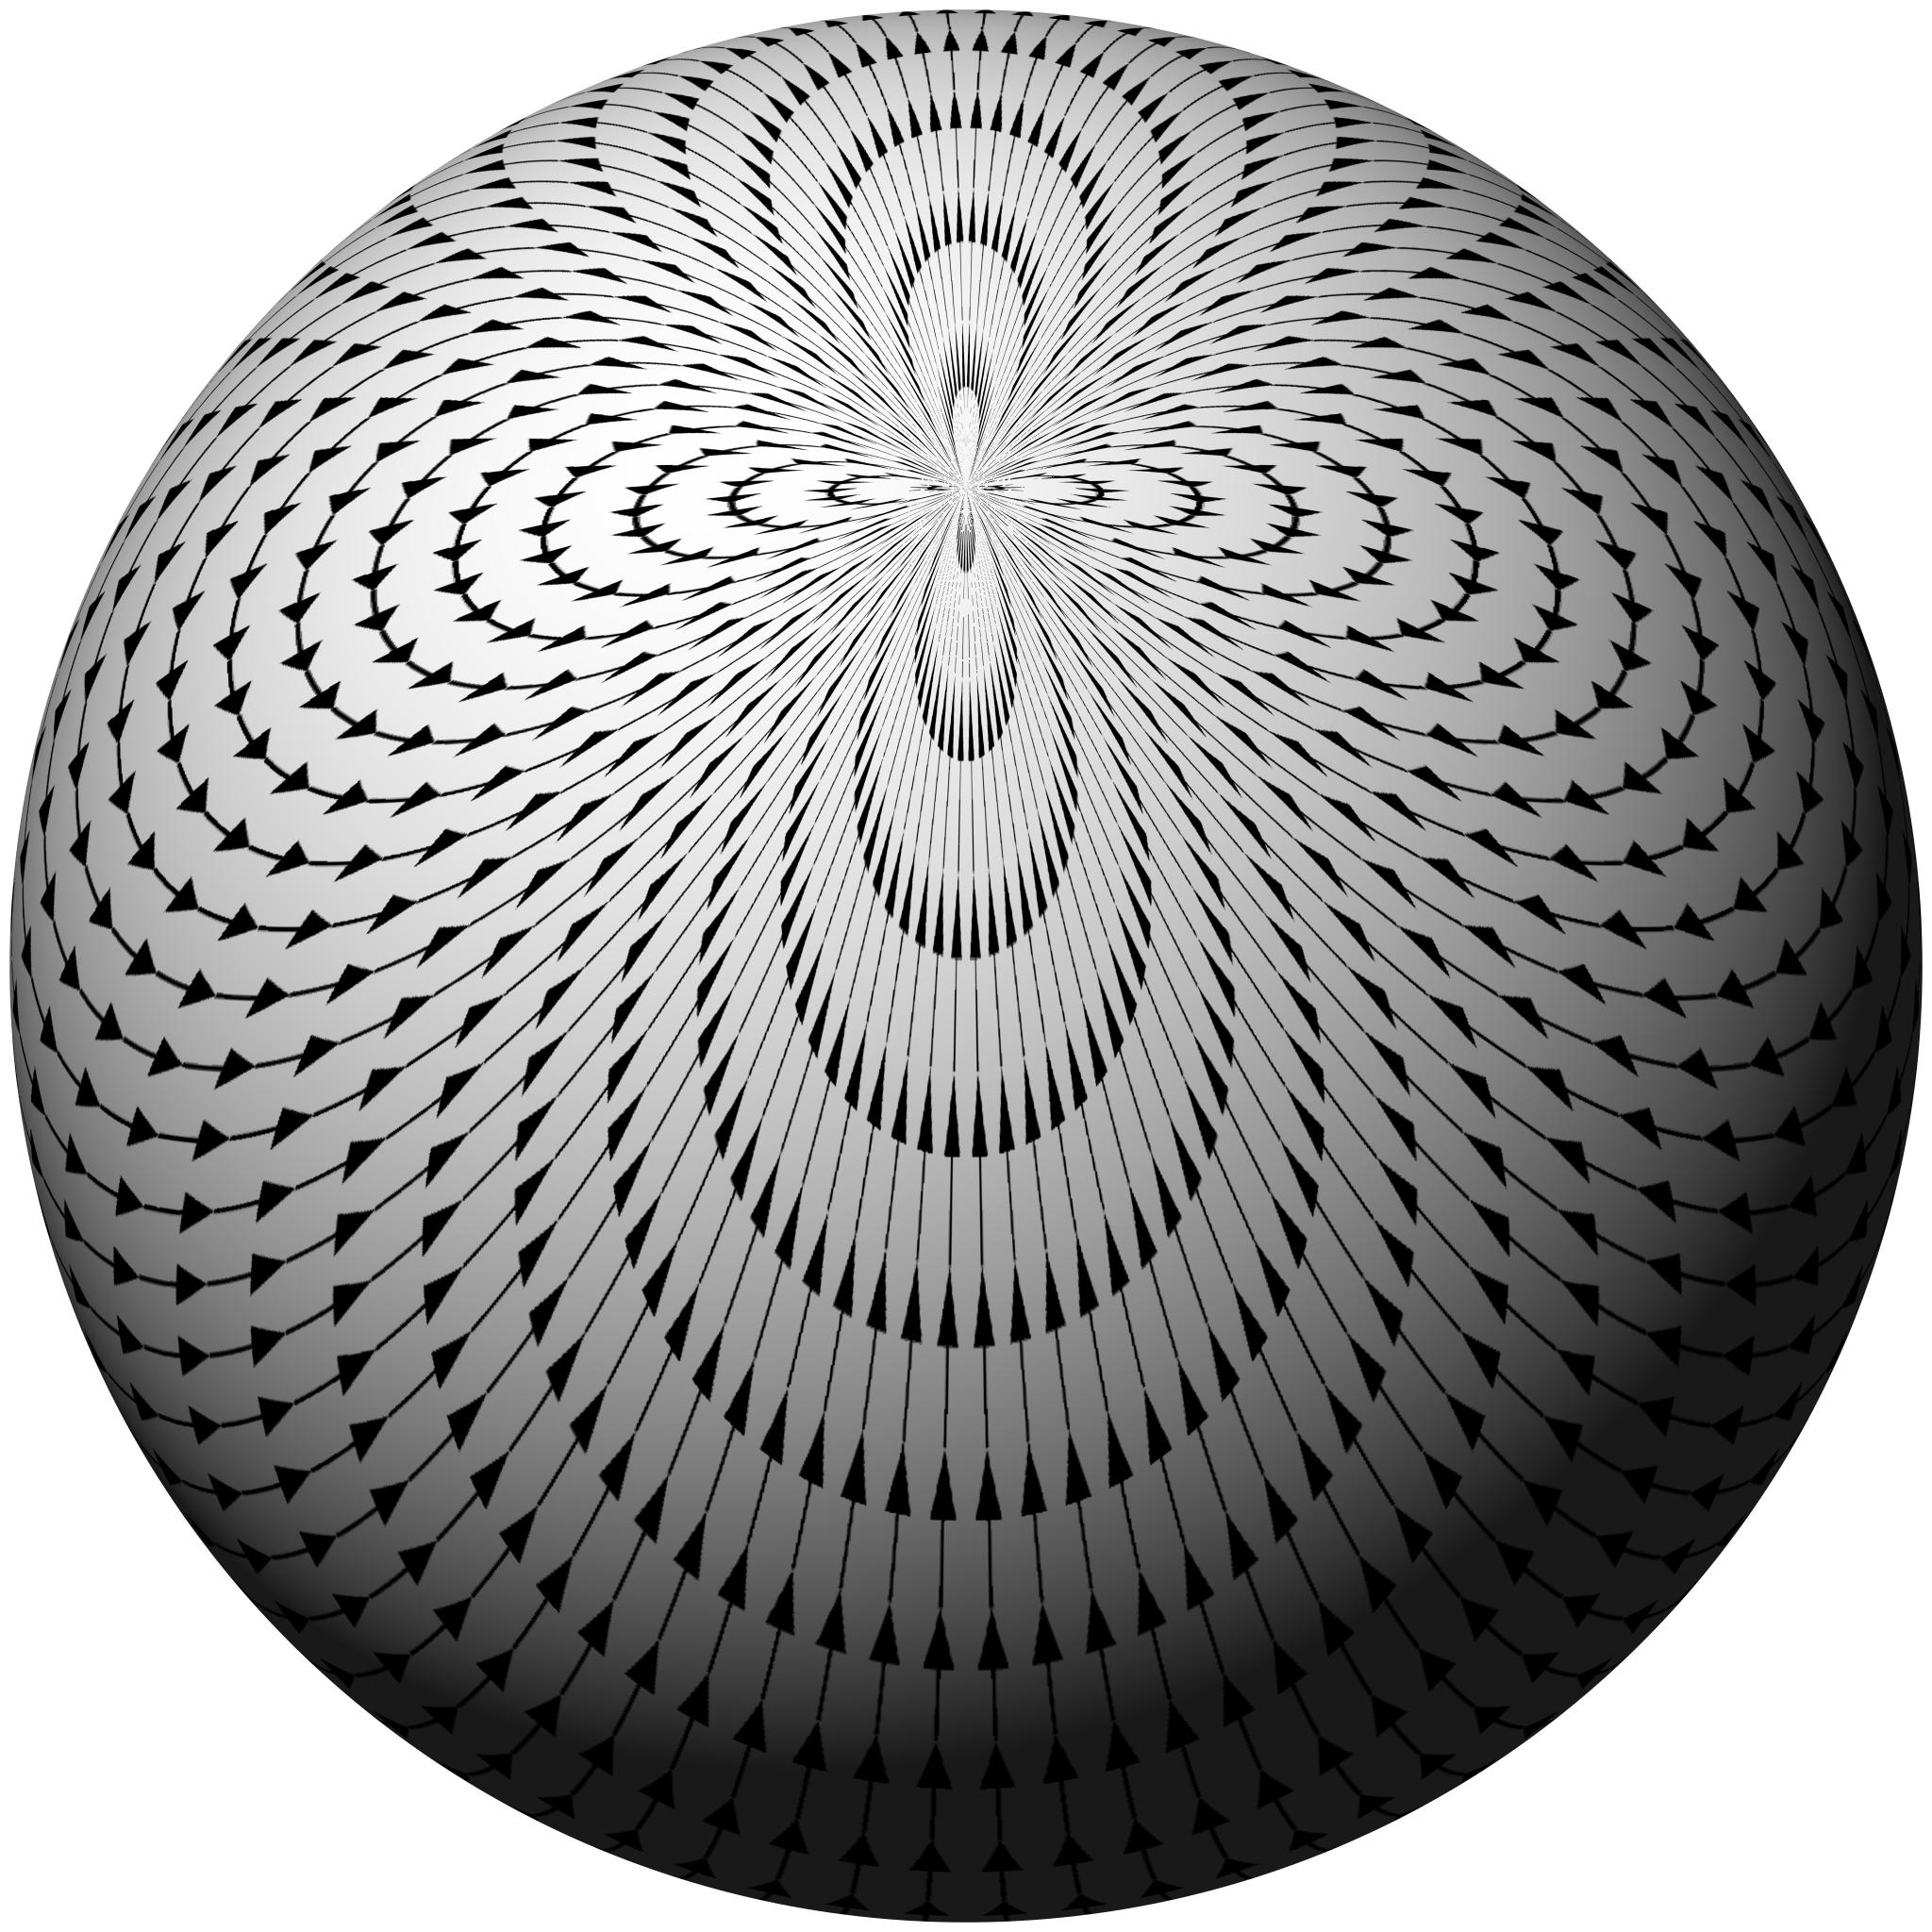
\includegraphics[width=.3\textwidth]{res/Hairy_ball_one_pole}
		   \end{center} 
		   Beim Hertzschen Dipol gibt es (in Fernfeldnäherung) zwei Glatzpunkte, bei $\vartheta=0$ und $\vartheta=\pi$, an denen es kein Feld gibt.
		\subsection{Fitzgeraldscher Dipol}
		    Das zum Hertzschen Dipol \textbf{duale} System ist der \textbf{Fitzgeraldsche Dipol}, eine infinitesimale Leiterschleife mit Flächennormale in \(z\)-Richtung. Es gibt dann  nur \(\ubar{\vec{E}}_\varphi\) und \(\vec{\ubar{H}}_\vartheta\) im Fernfeld. Auch der Fitzgeraldsche Dipol ist ein \textbf{Elementardipol}.
		  
\subsection{Feldwellenimpedanz im Nahfeld der Elementardipole}  
Der Feldwellenwiderstand \(Z=\frac{|\ubar{\vec{E}}|}{|\vec{\ubar{H}}|}\) nur im Fernfeld konstant mit \(Z=120\pi\mathrm{\Omega}\).
\begin{itemize}
	\item[$\to$] Im Nahfeld des Hertzschen Dipols (\ref{dipefeld}$\Rightarrow(kr)^3$, also $E$-Feld dominiert) $\Rightarrow$ \textbf{Hochimpedanzfeld}
	\item[$\to$] Im Nahfeld des Fitzgeraldschen Dipols ($H$-Feld dominiert) $\Rightarrow$ \textbf{Niederimpedanzfeld}
\end{itemize}
Im Nahfeld eines des Hertzschen Dipols ist ein Leiter ein guter Schirm (Außerhalb Hochimpedanzfeld, Leiter niedrige Impedanz $\Rightarrow$ Reflexion groß, $\nearrow$\ref{frenselsref}), im Nahfeld eines Fitzgeraldschen Dipols gilt das nicht. Allgemein gilt, dass elektrisch dominierte Felder einfach zu schirmen sind (einfacher Leiter reicht), während magnetisch dominierte Felder nicht so einfach zu schirmen sind (man braucht sehr teure, hochpermeable Metalle).
  \section{Linearantennen}
  \subsection{Grundlagen}
	 Bei den Elementardipolen (Hertzscher Dipol, Fitzgeraldscher Dipol) gab es infinitesimales Leiterelement und einen zeitlich harmonischen, aber \textbf{räumlich konstanten Strom}. Bei der \textbf{Linearantenne} gibt es einen dünnen, perfekt leitenden Draht, der von einem \textbf{ortsabhängigen} (harmonischen) Wechselstrom \(\underline{I}(\vec{r}^\prime )\) durchflossen wird. \\
	 Zunächst wird nochmal ein Stromelement im Ursprung, also ein Hertzscher Dipol mit etwas anderen Bezeichnungen, betrachtet:
		        \begin{center}
			        % set the plot display orientation
%synatax: \tdplotsetdisplay{\theta_d}{\phi_d}
\tdplotsetmaincoords{60}{110}

%define polar coordinates for some vector
%TODO: look into using 3d spherical coordinate system
\pgfmathsetmacro{\rvec}{.5}
\pgfmathsetmacro{\thetavec}{30}
\pgfmathsetmacro{\phivec}{60}

%start tikz picture, and use the tdplot_main_coords style to implement the display 
%coordinate transformation provided by 3dplot
\begin{tikzpicture}[scale=5,tdplot_main_coords]

	%set up some coordinates 
	%-----------------------
	\coordinate (O) at (0,0,0);

	%determine a coordinate (P) using (r,\theta,\phi) coordinates.  This command
	%also determines (Pxy), (Pxz), and (Pyz): the xy-, xz-, and yz-projections
	%of the point (P).
	%syntax: \tdplotsetcoord{Coordinate name without parentheses}{r}{\theta}{\phi}
	\tdplotsetcoord{P}{\rvec}{\thetavec}{\phivec}

	%draw figure contents
	%--------------------

	%draw the main coordinate system axes
	\draw[thick,->] (0,0,0) -- (.5,0,0) node[anchor=north east]{$x$};
	\draw[thick,->] (0,0,0) -- (0,.5,0) node[anchor=north west]{$y$};
	\draw[thick,->] (0,0,0) -- (0,0,.5) node[anchor=south,pos=0.95]{$z$};

	%draw a vector from origin to point (P) 
	\draw[-stealth,color=red,thick] (O) -- (P) node[midway, below]{$\vec{r} $};
	\draw[-stealth,color=green,thick] (P) -- +(0,0,0.2) node[above]{$\dd \vec{\ubar{A}}=\dd \ubar{A}_z\vu{z}$};

	%draw projection on xy plane, and a connecting line
	\draw[dashed, color=red] (O) -- (Pxy);
	\draw[dashed, color=red] (P) -- (Pxy);

	%draw the angle \phi, and label it
	%syntax: \tdplotdrawarc[coordinate frame, draw options]{center point}{r}{angle}{label options}{label}
	\tdplotdrawarc{(O)}{0.2}{0}{\phivec}{anchor=north}{$\varphi$}

	%set the rotated coordinate system so the x'-y' plane lies within the
	%"theta plane" of the main coordinate system
	%syntax: \tdplotsetthetaplanecoords{\phi}
	\tdplotsetthetaplanecoords{\phivec}

	%draw theta arc and label, using rotated coordinate system
	\tdplotdrawarc[tdplot_rotated_coords]{(0,0,0)}{0.3}{0}{\thetavec}{anchor=south west}{$\vartheta$}

	%draw some dashed arcs, demonstrating direct arc drawing
	%\draw[dashed,tdplot_rotated_coords] (\rvec,0,0) arc (0:90:\rvec);
	%\draw[dashed] (\rvec,0,0) arc (0:90:\rvec);

	%set the rotated coordinate definition within display using a translation
	%coordinate and Euler angles in the "z(\alpha)y(\beta)z(\gamma)" euler rotation convention
	%syntax: \tdplotsetrotatedcoords{\alpha}{\beta}{\gamma}
	\tdplotsetrotatedcoords{\phivec}{\thetavec}{0}

	%translate the rotated coordinate system
	%syntax: \tdplotsetrotatedcoordsorigin{point}
	\tdplotsetrotatedcoordsorigin{(P)}

	%use the tdplot_rotated_coords style to work in the rotated, translated coordinate frame
	%\draw[thin,tdplot_rotated_coords,->] (0,0,0) -- (.1,0,0) node[anchor=north west]{$\vu{\vartheta}$};
	%\draw[thin,tdplot_rotated_coords,->] (0,0,0) -- (0,.1,0) node[anchor=west]{$\vu{\varphi}$};
	%\draw[thin,tdplot_rotated_coords,->] (0,0,0) -- (0,0,.1) node[anchor=south]{$\vu{r}$};

	\node (a) [cylinder, shape border rotate=90, draw, minimum height=5mm, minimum width=2mm,yshift=-1mm] {};
	\draw [<->] ([xshift=-2pt]a.before bottom) -- ([xshift=-2pt]a.after top) node [midway, left] {$\dd z^\prime$};

\end{tikzpicture}
		        \end{center}
		  Für den Beitrag zum Vektorpotential am Punkt \(P\) gilt ($\nearrow$\ref{vekpotdip}):
		        \begin{equation}
			        \dd \vec{\ubar{A}}(\vec{r} ) = \frac{\mu}{4\pi} \underline{I} \dd z^\prime \frac{ \mathrm{e}^{-\mathrm{j} kr}}{r} \vu{z}
		        \end{equation}
		  Für das Magnetfeld folgt ($I$ ist eine Funktion von $r'$, rot wird in Bezug auf $r$ ausgeführt, deshalb nach vorne ziehen mgl.):
		        \begin{equation}\begin{split}
				        \dd\vec{\ubar{H}}(\vec{r} ) &= \frac{1}{\mu} \rot \dd \vec{\ubar{A}}(\vec{r} )\\
				        &= \frac{1}{4\pi} \underline{I} \dd z^\prime \rot \left(\frac{ \mathrm{e}^{-\mathrm{j} kr}}{r} \vu{z}\right)
			        \end{split}\end{equation}
Es wird weiter umgeformt (Nutzung von \ref{rotuv}):
		        \begin{equation}\begin{split}
				        \dd\vec{\ubar{H}}(\vec{r} )  &= \frac{1}{4\pi}\underline{I} \dd z^\prime \rot _{\textcolor{green}{r}}\left(\frac{ \mathrm{e}^{-\mathrm{j} kr}}{r} \vu{z}\right) \\
				        &= \frac{1}{4\pi} \underline{I}\dd z^\prime \bigg[ \frac{ \mathrm{e}^{-\mathrm{j} kr}}{r} \underbrace{\rot \vu{z}}_{=\vec{0}} - \vu{z} \times \textcolor{red}{\grad \left( \frac{ \mathrm{e}^{-\mathrm{j} kr}}{r} \right)}\bigg] \\
				        &= \frac{1}{4\pi} \underline{I}\dd z^\prime \bigg[- \vu{z} \times \textcolor{red}{\left( -\frac{\vec{r} }{r} \left(\frac{1}{r} +\mathrm{j} k \right)   \right) \frac{ \mathrm{e}^{-\mathrm{j} kr}}{r}} \bigg]\\
				        &= \frac{1}{4\pi} \underline{I}\dd z^\prime \left( \vu{z} \times \frac{\vec{r} }{r} \right) \left(\frac{1}{r} +\mathrm{j} k \right) \frac{ \mathrm{e}^{-\mathrm{j} kr}}{r}
			        \end{split}\end{equation}
Für ein Stromelement beliebiger Länge wird der Strom ortsabhängig (\(\underline{I}\to \underline{I}(\vec{r}^\prime )\)). Außerdem können beliebige Leiterelemente und nicht nur $z$-orientierte im Ursprung  betrachtet werden (\(\dd z^\prime \vu{z} \to \dd\vec{r}^\prime \) und \(\vec{r}  \to \vec{r}  - \vec{r}^\prime \)). Das ist unproblematisch (man könnte die ganze Herleitung auch von vornherein so durchziehen). Es gilt damit:
		        \begin{equation}
			        \boxed{\dd\vec{\ubar{H}}(\vec{r} ) = \frac{1}{4\pi} \underline{I}(\vec{r}^\prime ) \left( \dd\vec{r}^\prime  \times \frac{\vec{r} -\vec{r}^\prime }{|\vec{r} -\vec{r}^\prime |} \right) \left(\frac{1}{|\vec{r} -\vec{r}^\prime |} +\mathrm{j} k \right) \frac{ \mathrm{e}^{-\mathrm{j} k |\vec{r} -\vec{r}^\prime |}}{|\vec{r} -\vec{r}^\prime |}}
		        \end{equation}
Im Fernfeld sind folgende Näherungen davon möglich (Näherungen wie in \ref{strahlungszonen}):
		        \begin{equation}\begin{split}
				        k |\vec{r} -\vec{r}^\prime | \gg 1 &\Rightarrow  k \gg \frac{1}{|\vec{r} -\vec{r}^\prime |}\\
				        \frac{\vec{r} -\vec{r}^\prime }{|\vec{r} -\vec{r}^\prime |} &\simeq \frac{\vec{r} }{r}\\
				        \frac{ \mathrm{e}^{-\mathrm{j} k |\vec{r} -\vec{r}^\prime |}}{|\vec{r} -\vec{r}^\prime |} &\simeq \frac{ \mathrm{e}^{-\mathrm{j} k r}}{r}  \mathrm{e}^{\mathrm{j} k \frac{\vec{r} \cdot \vec{r}^\prime }{r}}
			        \end{split}\end{equation}
		  Damit gilt im \textbf{Fernfeld}:
		        \begin{equation}
			        \boxed{\dd\vec{\ubar{H}}(\vec{r} ) = \frac{\mathrm{j} k}{4\pi} \underline{I}(\vec{r}^\prime ) \left( \dd\vec{r}^\prime  \times \frac{\vec{r} }{r} \right) \frac{ \mathrm{e}^{-\mathrm{j} k r}}{r}  \mathrm{e}^{\mathrm{j} k \frac{\vec{r} \cdot \vec{r}^\prime }{r}}}
		        \end{equation}
	  Betrachtet wird nun einen dünner Draht mit Kontur \(C\) als Antenne
		        \begin{center}
			        \begin{tikzpicture}
	{   \colorlet{InColor}{gray!25}
		\colorlet{OutColor}{black!75}
		\foreach \I in {1,...,3}
			{   \pgfmathsetlengthmacro{\h}{(\I-1)/3*2mm}
				\pgfmathsetlengthmacro{\r}{sqrt(pow(2mm,2)-pow(\h,2))}
				\pgfmathsetmacro{\c}{(\I-0.5)/3*100}
				\draw[InColor!\c!OutColor, line width=\r] (0,2) to[out=70,in=200] (5,2);
			}
	}
	\draw (5,2) node[right]{$C$};
	\draw (0,4) node[left]{$0$};
	\draw (6,3.7) node[right]{$P$};
	\draw[-stealth,thick] (0,4) -- (1,2.7) node[midway,left]{$\vec{r}\prime $};
	\draw[-stealth,thick] (0,4) -- (6,3.7) node[midway,below]{$\vec{r} $};
	\draw[-stealth,thick] (1,2.7) -- (6,3.7) node[midway,below]{$\vec{r} -\vec{r}\prime $};
\end{tikzpicture}
		        \end{center}
		  Damit ist das Magnetfeld (und damit auch das elektrische Feld) für beliebige linienförmige Antennen im Fernfeld prinzipiell berechenbar aus:
		        \begin{equation}\label{nhrgfernz}
			        \boxed{\vec{\ubar{H}}(\vec{r} ) = \frac{\mathrm{j} k}{4\pi} \frac{ \mathrm{e}^{-\mathrm{j} k r}}{r} \int\limits_{C}\underline{I}(\vec{r}^\prime )  \mathrm{e}^{\mathrm{j} k \frac{\vec{r} \cdot \vec{r}^\prime }{r}} \left( \dd\vec{r}^\prime  \times \frac{\vec{r} }{r} \right)}
		        \end{equation}
		        Analog kann man im \textbf{Nahfeld} die Retardierung vernachlässigen und magnetoquasistatisch Biot-Savart ansetzen. Man sollte sich dabei aber stets vergegenwärtigen, welche Annahmen in den genutzten Formeln stecken und prüfen ob diese (näherungsweise) haltbar sind. Dadurch wird verhindert, dass schlechte Näherungen entstehen.
	\subsection{Beispiel}
	\subsubsection{Problemstellung}
	Eine halbkreisförmige Antenne aus sehr dünnem idealleitendem ($\kappa\to\infty$) Drat befindet sich im Vakuum. Drei Punkte auf der Antenne können kartesisch als $P_1(0,-a,0)$, $P_2(0,a,0)$ und $P_3(-a,0,0)$ beschrieben werden. Die Antenne führt einen harmonischen Wechselstrom $\vec{\ubar{I}}(\vec{r})=I_0\vu{\varphi}$. Dafür muss $a\ll\lambda$ gelten, sonst könnte der Strom nicht auf der gesamten Antenne als räumlich konstant angenommen werden (exakt müsste der Strom durch eine auf dem Antennendraht propagierende Welle beschrieben werden).
	\begin{center}
			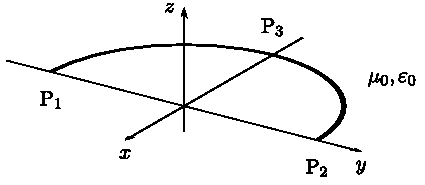
\includegraphics{res/ANTbsp.pdf}
	\end{center}
		\subsubsection{Exakte Berechnung von Vektorpotential und Magnetfeld auf der z-Achse}
	Zunächst sollen $\vec{{A}}(z,t)$ und $\vec{H}(z,t)$ auf der $z$-Achse exakt berechnet werden. Für $\vec{A}(z,t)$ wird die allgemeine Gleichung \ref{vekpotlor} angesetzt. Es gilt:
	\begin{equation}
		\vec{{A}}(z, {t})=\frac{\mu_{0}}{4 \pi} \iiint\limits_V \frac{\vec{{J}}\left(\vec{{r}}^{\prime}, {t}_{\text{ret}}\right)}{\left|z\vu{z}-\vec{{r}}^{\prime}\right|} \dd^3 {r}^{\prime} \quad \text{ mit } \quad t_{\text{ret}}={t}-\frac{\left|z\vu{z}-\vec{{r}}^{\prime}\right|}{{c}}
	\end{equation}
	Zunächst muss $\vec{{J}}\left(\vec{{r}}^{\prime}, {t}\right)$ modelliert werden:
	\begin{equation}
		\vec{{J}}\left(\vec{{r}}^{\prime}, {t}\right)=I_{0} \cos\left(\omega t\right)\delta\left(\rho'-a \right) \delta\left(z' \right)\vu{\varphi} (\varphi')
	\end{equation}
	Einsetzen liefert:
	\begin{equation}
		\vec{{A}}(z, {t})=\frac{\mu_{0}}{4 \pi} \iiint\limits_V \frac{I_{0} \cos\left[\omega\left( {t}-\frac{\left|z\vu{z}-\vec{{r}}^{\prime}\right|}{{c}}\right)\right]\delta\left(\rho'-a \right) \delta\left(z' \right)\vu{\varphi}(\varphi') }{\left|z\vu{z}-\vec{{r}}^{\prime}\right|} \rho'\dd\rho'\dd\varphi'\dd z' 
	\end{equation}
	Integration über das Quellgebiet (Halbraum mit $x\leq0$, man könnte auch über den gesamten Raum integrieren und noch mit $J$ noch zusätzlich mit einer Stufenfunktion modellieren) liefert:
	\begin{equation}\begin{split}
			\vec{{A}}(z, {t})&=\frac{\mu_{0}I_{0} a}{4 \pi} \frac{\cos\left[\omega \left({t}-\frac{\sqrt{z^2+a^2}}{{c}}\right)\right] }{\sqrt{a^2+z^2}}\int\limits_{\varphi'=\frac{\pi}{2}}^{\frac{3\pi}{2}} \vu{\varphi}(\varphi')\dd \varphi'\\
			&=-\vu{y}\frac{\mu_{0}I_{0} a}{2 \pi} \frac{\cos\left[\omega \left({t}-\frac{\sqrt{z^2+a^2}}{{c}}\right)\right] }{\sqrt{a^2+z^2}}
	\end{split}\end{equation}
\textbf{Fehlerquelle:} Würde man nun mit diesem Ergebnis weiterrechnen, und versuchen über $\vec{H}=\frac{1}{\mu_0}\rot\vec{A}$ das Magnetfeld herzuleiten, würde man auf ein falsches Ergebnis kommen. Das liegt daran, dass in die Rotation auch die Ableitungen nach $x$ und $y$ eingehen, welche trotz $x=y=0$ nicht zwangsläufig null sind, aber durch Betrachtung von $\vec{{A}}(z, {t})$ statt $\vec{{A}}(\vec{r}, {t})$ null gesetzt werden würden. Es gilt also:
\begin{equation}
	\vec{H}(z, {t})=\left.\frac{1}{\mu_0}\rot\vec{A}(\vec{r}, {t}) \right|_{x=y=0}\neq \frac{1}{\mu_0}\rot\vec{A}(z, {t})
\end{equation}
Demnach muss $\vec{H}(z, {t})$ ausführlich berechnet werden:
\begin{equation}
		\vec{{H}}(z, {t})=\left.\frac{I_{0} a}{4 \pi} \int\limits_{\varphi'=\frac{\pi}{2}}^{\frac{3\pi}{2}} \rot_r\frac{\cos\left[\omega \left({t}-\frac{\left|\rho\vu{\rho}(\varphi)-a\vu{\rho}(\varphi')+z\vu{z}\right|}{{c}}\right)\right] }{\left|\rho\vu{\rho}(\varphi)-a\vu{\rho}(\varphi')+z\vu{z}\right|} \vu{\varphi}(\varphi')\dd \varphi'\right|_{\rho=0}
\end{equation}
\textbf{Fehlerquelle:} Die Rotation im Integral ist bezüglich $r$ und nicht $r'$ zu berechnen. Es ist demnach bei der Rotationsbildung zu beachten, dass die $\vu{\varphi}(\varphi')$-Komponente bezüglich der gestrichenen Koordinaten eine $\vu{\varphi}(\varphi)$- \textbf{und} eine $\vu{\rho}(\varphi)$-Komponente bezüglich der ungestrichenen Koordinaten bedeutet. Nun soll die Rotation berechnet werden, um das Problem mit der $\vu{\varphi}(\varphi')$-Komponente zielgerichtet zu umgehen, bietet sich eine zweimalige Anwendung der Produktregel \ref{rotuv} an:
\begin{equation*}\begin{split}
	&\rot_r\underbrace{\frac{1}{\left|\rho\vu{\rho}(\varphi)-a\vu{\rho}(\varphi')+z\vu{z}\right|}}_{U} \underbrace{\cos\left[\omega \left({t}-\frac{\left|\rho\vu{\rho}(\varphi)-a\vu{\rho}(\varphi')+z\vu{z}\right|}{{c}}\right)\right]  \vu{\varphi}(\varphi')}_{\vec{V}}\\
	&\quad=\frac{1}{\left|\rho\vu{\rho}(\varphi)-a\vu{\rho}(\varphi')+z\vu{z}\right|}\rot_r\left\{\underbrace{\cos\left[\omega \left({t}-\frac{\left|\rho\vu{\rho}(\varphi)-a+z\vu{z}\right|}{{c}}\right)\right]}_{U} \underbrace{\vu{\varphi}(\varphi')}_{\vec{V}}  \right\} \\
	&\quad\quad+ \grad_r\left\{\frac{1}{\left|\rho\vu{\rho}(\varphi)-a\vu{\rho}(\varphi')+z\vu{z}\right|}\right\}\times\cos\left[\omega \left({t}-\frac{\left|\rho\vu{\rho}(\varphi)-a\vu{\rho}(\varphi')+z\vu{z}\right|}{{c}}\right)\right]  \vu{\varphi}(\varphi')\\
	&\quad=\frac{1}{\left|\rho\vu{\rho}(\varphi)-a\vu{\rho}(\varphi')+z\vu{z}\right|}\left( \underbrace{0}_{\vu{\varphi}(\varphi')\neq f(\vec{r})}+ \grad_r\left\{\cos\left[\omega \left({t}-\frac{\left|\rho\vu{\rho}(\varphi)-a+z\vu{z}\right|}{{c}}\right)\right]\right\}\times\vu{\varphi}(\varphi') \right)\\
	&\quad\quad+ \grad_r\left\{\frac{1}{\left|\rho\vu{\rho}(\varphi)-a\vu{\rho}(\varphi')+z\vu{z}\right|}\right\}\times\cos\left[\omega \left({t}-\frac{\left|\rho\vu{\rho}(\varphi)-a\vu{\rho}(\varphi')+z\vu{z}\right|}{{c}}\right)\right]  \vu{\varphi}(\varphi')
\end{split}\end{equation*}
\textbf{Fehlerquelle:} Im Allgemeinen ist $\vu{\rho}(\varphi)\neq\vu{\rho}(\varphi')$, die Betragsbildung muss über den Cosinussatz in der $z=0$-Ebene oder die Identität $\vu{\rho}(\varphi)=\vu{x}\cos\varphi+\vu{y}\sin\varphi$ erfolgen. Mit dem Cosinussatz gilt:
\begin{equation*}
	\left|\rho\vu{\rho}(\varphi)-a\vu{\rho}(\varphi')+z\vu{z}\right|=\sqrt{\rho^2+a^2-2\rho a\cos{\left(\varphi-\varphi'\right)}+z^2}
\end{equation*}
Damit ist
\begin{equation*}\begin{split}
	&\left.\grad_r\left\{\frac{1}{\sqrt{\rho^2+a^2-2\rho a\cos{\left(\varphi-\varphi'\right)}+z^2}}\right\}\right|_{\rho=0}=\\
	&\quad+\vu{\rho}(\varphi)\frac{a\cos{\left(\varphi-\varphi'\right)}}{(a^2+z^2)^{\frac{3}{2}}} -\vu{\varphi}(\varphi)\frac{a \sin{\left(\varphi-\varphi'\right)}}{(a^2+z^2)^{\frac{3}{2}}} -\vu{z}\frac{z}{(a^2+z^2)^{\frac{3}{2}}}\\
	&\quad:=\vu{\rho}(\varphi)A\cos{\left(\varphi-\varphi'\right)}-\vu{\varphi}(\varphi)A\sin{\left(\varphi-\varphi'\right)}+\vu{z}B\\
	&\left.\grad_r\left\{\cos\left[\omega \left({t}-\frac{\sqrt{\rho^2+a^2-2\rho a\cos{\left(\varphi-\varphi'\right)}+z^2}}{{c}}\right)\right]\right\}\right|_{\rho=0}=\\
	&\quad-\vu{\rho}(\varphi)\frac{a\omega\cos{\left(\varphi-\varphi'\right)}\sin\left[\omega \left({t}-\frac{\sqrt{a^2+z^2}}{{c}}\right)\right]}{c\sqrt{a^2+z^2}}+\vu{\varphi}(\varphi)\frac{a\omega\sin{\left(\varphi-\varphi'\right)}\sin\left[\omega \left({t}-\frac{\sqrt{a^2+z^2}}{{c}}\right)\right]}{c\sqrt{a^2+z^2}}\\
	&\quad+\vu{z}\frac{\omega z\sin\left[\omega \left({t}-\frac{\sqrt{a^2+z^2}}{{c}}\right)\right]}{c\sqrt{a^2+z^2}}:=\vu{\rho}(\varphi)C\cos{\left(\varphi-\varphi'\right)}-\vu{\varphi}(\varphi)C\sin{\left(\varphi-\varphi'\right)}+\vu{z}D
\end{split}\end{equation*}
Damit und mit den Definitionen
\begin{equation*}\begin{split}
 E:=&\frac{1}{\sqrt{z^2+a^2}}\\
 F:=&\cos\left[\omega \left({t}-\frac{\sqrt{a^2+z^2}}{{c}}\right)\right]
\end{split}\end{equation*}
folgt ($k=\frac{\omega}{c}$):
\begin{equation*}\begin{split}
		\vec{{H}}(z, {t})&=\frac{I_{0} a}{4 \pi}\int\limits_{\varphi'=\frac{\pi}{2}}^{\frac{3\pi}{2}} E\left[\vu{\rho}(\varphi)C\cos{\left(\varphi-\varphi'\right)}+\vu{\varphi}(\varphi)-C\sin{\left(\varphi-\varphi'\right)}+\vu{z}D\right]\times\left[\vu{\varphi}(\varphi')\right]\\\quad&+F\left[\vu{\rho}(\varphi)A\cos{\left(\varphi-\varphi'\right)}-\vu{\varphi}(\varphi)A\sin{\left(\varphi-\varphi'\right)}+\vu{z}B\right]\times\left[\vu{\varphi}(\varphi')\right] \dd \varphi'
	\end{split}\end{equation*}
Dieses Integral kann man unter Nutzung der Identitäten
\begin{equation*}
	\begin{split}
	\vu{\varphi}(\varphi)&=-\vu{x}\sin\varphi+\vu{y}\cos\varphi\\
	\vu{\rho}(\varphi)&=\vu{x}\cos\varphi+\vu{y}\sin\varphi	
	\end{split}
\end{equation*}
ausrechnen und erhält:
\begin{equation}\label{hallgbsp}\begin{split}
		\vec{{H}}(z, {t})&=\frac{I_{0} a}{4 \pi}\left[E\left(\vu{z}\pi C+\vu{x}2D\right)+F\left(\vu{z}\pi A+\vu{x}2B\right)\right]\\
		&=\frac{I_{0} a}{4 \pi}(-a\pi\vu{z}+2z\vu{x})\left[\frac{k\sin\left[\omega {t}-k\sqrt{z^2+a^2}\right]}{z^2+a^2}-\frac{\cos\left[\omega {t}-k\sqrt{z^2+a^2}\right]}{\left(z^2+a^2\right)^{\frac{3}{2}}}\right]
\end{split}\end{equation}
\subsubsection{Nahzone}
In der Nahzone gilt nach \ref{strahlungszonen} $a\ll |z|\ll\lambda$. Mit $k=\frac{2\pi}{\lambda}$ kann man \ref{hallgbsp} nähern:
\begin{equation}\label{hallgbspapprox}\begin{split}
	\vec{{H}}(z, {t})=-\frac{I_{0} a}{2 \pi}\underbrace{z\vu{x}}_{z\gg a}\underbrace{\frac{\cos\left[\omega {t}\right]}{\left(z^2+a^2\right)^{\frac{3}{2}}}}_{\lambda\gg z \gg a}
\end{split}\end{equation}
Mit Biot-Savart ($\nearrow$\ref{biot-savart}) kommt man auf:
\begin{equation}
	\vec{{H}}(z, {t})=\frac{I_{0} a}{4 \pi}(a\pi\vu{z}-2z\vu{x})\frac{\cos\left[\omega {t}\right]}{\left(z^2+a^2\right)^{\frac{3}{2}}}
\end{equation}
Offensichtlich fehlt hier gegenüber \ref{hallgbsp} die Retardierung (quasistatische Näherung) und einer der beiden Terme in der eckigen Klammer. Nach anwenden von $z\gg a$ kommt man auf die selbe Näherungsformel wie in \ref{hallgbspapprox}. In der Nahzone erhält man hier also mit Biot-Savart eine brauchbare Näherung.
\subsubsection{Fernzone}
In der Fernzone gilt nach \ref{strahlungszonen} $a\ll |z|$ und $\lambda\ll |z|$. Mit $k=\frac{2\pi}{\lambda}$ kann man \ref{hallgbsp} wieder nähern:
\begin{equation}
	\begin{split}
		\vec{{H}}(z, {t})=\vu{x} \frac{I_{0} a}{2 \pi}\frac{k\sin\left[\omega {t}-k|z|\right]}{z}
	\end{split}
\end{equation}
Mit der Näherungsformel für die Fernzone aus Gleichung \ref{nhrgfernz} kommt man auf exakt das gleiche Ergebnis.
  \subsection{Abstrahldiagramme und Bauformen}
  $n\lambda$-Dipol meint, dass man auf die gesamte Drahtstruktur genau $n$ mal die Wellenlänge bekommt. Die Speisung der Antennenstruktur ist mit einem Pfeil gekennzeichnet. Gewünscht ist meist eine gerichtete Abstrahlung, technisch bewegt man sich also häufig im Bereich des $\frac{\lambda}{2}$-Dipols. Beim $\frac{\lambda}{4}$-Dipol ersetzt man die untere Leitung vom $\frac{\lambda}{2}$-Dipol durch eine leidende Ebene, durch das Spiegelungsprinzip ist das Feld dann ähnlich wie beim $\frac{\lambda}{2}$-Dipol. Durch dielektrische Materialien, Fußinduktivitäten und Dachkapazitäten kann man elektrisch eine längere Antenne erreichen, als tatsächlich physikalisch vorliegt (bspw. Antenne nur $\frac{\lambda}{8}$ groß, aber elektrisch wirksam als $\frac{\lambda}{2}$). Anschauung (\href{https://commons.wikimedia.org/wiki/File:Lineare_antennen2.svg}{Bildquelle}):,
	  \begin{center}
		  \resizebox{.6\textwidth}{!}{%% Creator: Inkscape 1.3 (1:1.3+202307231459+0e150ed6c4), www.inkscape.org
%% PDF/EPS/PS + LaTeX output extension by Johan Engelen, 2010
%% Accompanies image file 'Lineare_antennen2.pdf' (pdf, eps, ps)
%%
%% To include the image in your LaTeX document, write
%%   \input{<filename>.pdf_tex}
%%  instead of
%%   \includegraphics{<filename>.pdf}
%% To scale the image, write
%%   \def\svgwidth{<desired width>}
%%   \input{<filename>.pdf_tex}
%%  instead of
%%   \includegraphics[width=<desired width>]{<filename>.pdf}
%%
%% Images with a different path to the parent latex file can
%% be accessed with the `import' package (which may need to be
%% installed) using
%%   \usepackage{import}
%% in the preamble, and then including the image with
%%   \import{<path to file>}{<filename>.pdf_tex}
%% Alternatively, one can specify
%%   \graphicspath{{<path to file>/}}
%% 
%% For more information, please see info/svg-inkscape on CTAN:
%%   http://tug.ctan.org/tex-archive/info/svg-inkscape
%%
\begingroup%
\makeatletter%
\providecommand\color[2][]{%
	\errmessage{(Inkscape) Color is used for the text in Inkscape, but the package 'color.sty' is not loaded}%
	\renewcommand\color[2][]{}%
}%
\providecommand\transparent[1]{%
	\errmessage{(Inkscape) Transparency is used (non-zero) for the text in Inkscape, but the package 'transparent.sty' is not loaded}%
	\renewcommand\transparent[1]{}%
}%
\providecommand\rotatebox[2]{#2}%
\newcommand*\fsize{\dimexpr\f@size pt\relax}%
\newcommand*\lineheight[1]{\fontsize{\fsize}{#1\fsize}\selectfont}%
\ifx\svgwidth\undefined%
	\setlength{\unitlength}{363.32178497bp}%
	\ifx\svgscale\undefined%
		\relax%
	\else%
		\setlength{\unitlength}{\unitlength * \real{\svgscale}}%
	\fi%
\else%
	\setlength{\unitlength}{\svgwidth}%
\fi%
\global\let\svgwidth\undefined%
\global\let\svgscale\undefined%
\makeatother%
\begin{picture}(1,1.16380096)%
	\lineheight{1}%
	\setlength\tabcolsep{0pt}%
	\put(0,0){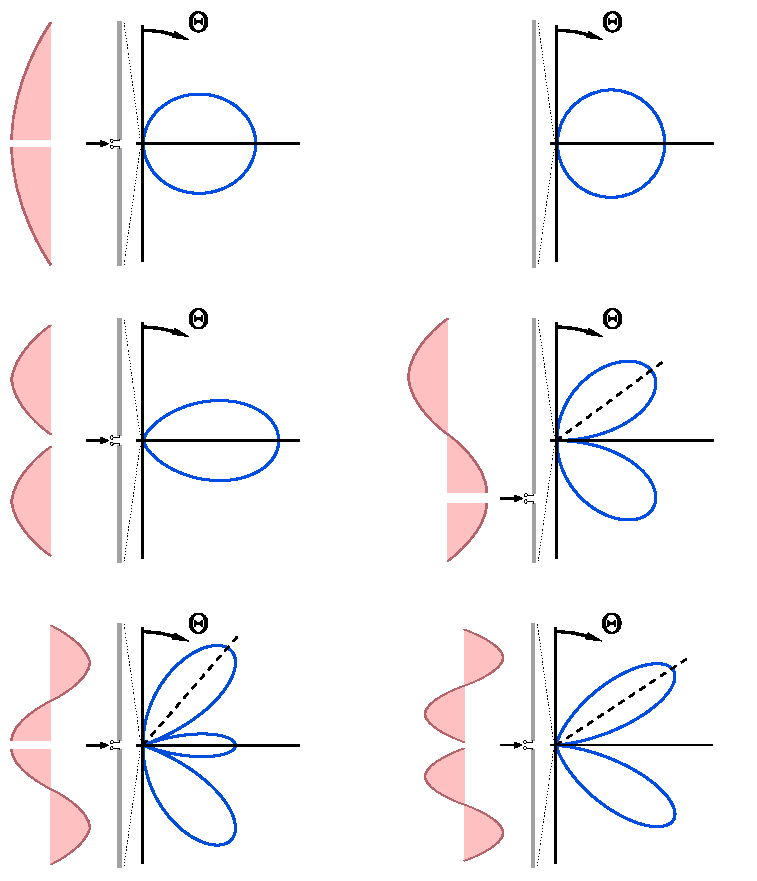
\includegraphics[width=\unitlength,page=1]{res/Lineare_antennen2.pdf}}%
	\put(-0.03749462,1.13927431){\color[rgb]{0,0,0}\makebox(0,0)[lt]{\lineheight{1.25}\smash{\begin{tabular}[t]{l}\textbf{Stomverteilung}\end{tabular}}}}%
	\put(0.21682177,1.05874075){\color[rgb]{0,0,0}\makebox(0,0)[lt]{\lineheight{1.25}\smash{\begin{tabular}[t]{l}\textbf{Fernfeld}\end{tabular}}}}%
	\put(0,0){\includegraphics[width=\unitlength,page=2]{res/Lineare_antennen2.pdf}}%
	\put(0.25016422,1.12146949){\color[rgb]{0,0,0}\makebox(0,0)[lt]{\lineheight{1.25}\smash{\begin{tabular}[t]{l}$\vartheta$\end{tabular}}}}%
	\put(0.24944189,0.72793128){\color[rgb]{0,0,0}\makebox(0,0)[lt]{\lineheight{1.25}\smash{\begin{tabular}[t]{l}$\vartheta$\end{tabular}}}}%
	\put(0.24899603,0.32657848){\color[rgb]{0,0,0}\makebox(0,0)[lt]{\lineheight{1.25}\smash{\begin{tabular}[t]{l}$\vartheta \quad 43^\circ$ \end{tabular}}}}%
	\put(0.79733669,1.12329457){\color[rgb]{0,0,0}\makebox(0,0)[lt]{\lineheight{1.25}\smash{\begin{tabular}[t]{l}$\vartheta$\end{tabular}}}}%
	\put(0.79595453,0.72835632){\color[rgb]{0,0,0}\makebox(0,0)[lt]{\lineheight{1.25}\smash{\begin{tabular}[t]{l}$\vartheta$\\$\quad\quad 54^\circ$\end{tabular}}}}%
	\put(0.78974511,0.32540434){\color[rgb]{0,0,0}\makebox(0,0)[lt]{\lineheight{1.25}\smash{\begin{tabular}[t]{l}$\vartheta$\\$\quad\quad\quad\quad 57^\circ$\\\end{tabular}}}}%
	\put(0.19493004,0.81773808){\color[rgb]{0,0,0}\makebox(0,0)[lt]{\lineheight{1.25}\smash{\begin{tabular}[t]{l}$\frac{\lambda}{2}$-Dipol\end{tabular}}}}%
	\put(0.19305147,0.42551962){\color[rgb]{0,0,0}\makebox(0,0)[lt]{\lineheight{1.25}\smash{\begin{tabular}[t]{l}$\lambda$-Dipol\end{tabular}}}}%
	\put(0.19487356,0.02299265){\color[rgb]{0,0,0}\makebox(0,0)[lt]{\lineheight{1.25}\smash{\begin{tabular}[t]{l}$\frac{3\lambda}{2}$-Dipol\end{tabular}}}}%
	\put(0.7386129,0.02186903){\color[rgb]{0,0,0}\makebox(0,0)[lt]{\lineheight{1.25}\smash{\begin{tabular}[t]{l}$2\lambda$-Dipol\end{tabular}}}}%
	\put(0.73937976,0.42576928){\color[rgb]{0,0,0}\makebox(0,0)[lt]{\lineheight{1.25}\smash{\begin{tabular}[t]{l}$\lambda$-Dipol\\(asymmetrische Sp.)\end{tabular}}}}%
	\put(0.73798866,0.81912619){\color[rgb]{0,0,0}\makebox(0,0)[lt]{\lineheight{1.25}\smash{\begin{tabular}[t]{l}Hertzscher Dipol\end{tabular}}}}%
	\put(0,0){\includegraphics[width=\unitlength,page=3]{res/Lineare_antennen2.pdf}}%
\end{picture}%
\endgroup%
}
		  	  \end{center}
		  	  Halbwellendipole werden häufig zu Kalibrierzwecken eingesetzt, sie sind aber nicht sehr breitbandig, man benötigt verschiedene / verstellbare Bauformen. Breitbandiger sind beispielsweise logarithmisch-periodische Antennen. Bei verschiedenen Frequenzen schwingen verschiedene Stabpaare. Für die Abstrahlungen von Pulsen sind sie aber nicht geeignet. Bikonische Antennen sind ein Beispiel von Dachkapazitäten, man kann also mit kürzerer physikalischer Antenne die gewünschte Wellenlänge erreichen. Außerdem sorgt die Bauform für eine gewisse Breitbandigkeit. Bikoni-Log-Antennen sind Mischformen zwischen logarithmischen und bikonischen Antennen. Die Loop-Antenne ist eine magnetische Antenne, die ein Niederimpedanzfeld im Nahfeld erzeugt. Der eigentliche Draht läuft innen drin, außen gibt es einen massiven (geschlitzten) Zylinder, der die Antenne vor dem elektrischen Feld schützt, wenn nur das Magnetfeld gemessen werden soll. Die Bilder stammen von der Firma \href{https://www.schwarzbeck.de/}{Schwarzbeck}.
		  	  \begin{center}
		  \resizebox{.6\textwidth}{!}{%% Creator: Inkscape 1.3 (1:1.3+202307231459+0e150ed6c4), www.inkscape.org
%% PDF/EPS/PS + LaTeX output extension by Johan Engelen, 2010
%% Accompanies image file 'Antennen-Bilder.pdf' (pdf, eps, ps)
%%
%% To include the image in your LaTeX document, write
%%   \input{<filename>.pdf_tex}
%%  instead of
%%   \includegraphics{<filename>.pdf}
%% To scale the image, write
%%   \def\svgwidth{<desired width>}
%%   \input{<filename>.pdf_tex}
%%  instead of
%%   \includegraphics[width=<desired width>]{<filename>.pdf}
%%
%% Images with a different path to the parent latex file can
%% be accessed with the `import' package (which may need to be
%% installed) using
%%   \usepackage{import}
%% in the preamble, and then including the image with
%%   \import{<path to file>}{<filename>.pdf_tex}
%% Alternatively, one can specify
%%   \graphicspath{{<path to file>/}}
%% 
%% For more information, please see info/svg-inkscape on CTAN:
%%   http://tug.ctan.org/tex-archive/info/svg-inkscape
%%
\begingroup%
\makeatletter%
\providecommand\color[2][]{%
	\errmessage{(Inkscape) Color is used for the text in Inkscape, but the package 'color.sty' is not loaded}%
	\renewcommand\color[2][]{}%
}%
\providecommand\transparent[1]{%
	\errmessage{(Inkscape) Transparency is used (non-zero) for the text in Inkscape, but the package 'transparent.sty' is not loaded}%
	\renewcommand\transparent[1]{}%
}%
\providecommand\rotatebox[2]{#2}%
\newcommand*\fsize{\dimexpr\f@size pt\relax}%
\newcommand*\lineheight[1]{\fontsize{\fsize}{#1\fsize}\selectfont}%
\ifx\svgwidth\undefined%
	\setlength{\unitlength}{755.85667419bp}%
	\ifx\svgscale\undefined%
		\relax%
	\else%
		\setlength{\unitlength}{\unitlength * \real{\svgscale}}%
	\fi%
\else%
	\setlength{\unitlength}{\svgwidth}%
\fi%
\global\let\svgwidth\undefined%
\global\let\svgscale\undefined%
\makeatother%
\begin{picture}(1,0.33178116)%
	\lineheight{1}%
	\setlength\tabcolsep{0pt}%
	\put(0,0){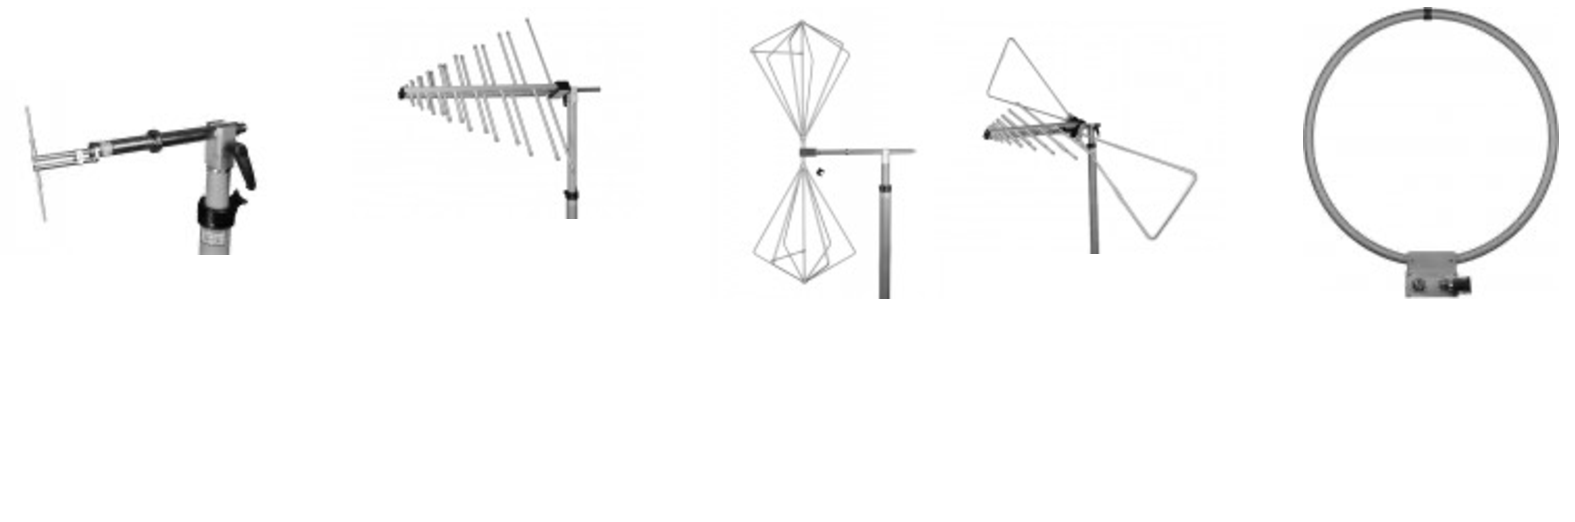
\includegraphics[width=\unitlength,page=1]{res/Antennen-Bilder.pdf}}%
	\put(0.02529879,0.1033566){\color[rgb]{0,0,0}\makebox(0,0)[lt]{\lineheight{1.25}\smash{\begin{tabular}[t]{l}\huge Halbwellendipol\end{tabular}}}}%
	\put(0.25964113,0.1033566){\color[rgb]{0,0,0}\makebox(0,0)[lt]{\lineheight{1.25}\smash{\begin{tabular}[t]{l}\huge Logarithmisch-\\\huge Periodische\\ \huge Antenne\end{tabular}}}}%
	\put(0.48558592,0.1033566){\color[rgb]{0,0,0}\makebox(0,0)[lt]{\lineheight{1.25}\smash{\begin{tabular}[t]{l}\huge Bikonische\\ \huge Antenne\end{tabular}}}}%
	\put(0.65109789,0.1033566){\color[rgb]{0,0,0}\makebox(0,0)[lt]{\lineheight{1.25}\smash{\begin{tabular}[t]{l}\huge Bikoni-Log-\\\huge Antenne\end{tabular}}}}%
	\put(0.83275261,0.10400776){\color[rgb]{0,0,0}\makebox(0,0)[lt]{\lineheight{1.25}\smash{\begin{tabular}[t]{l}\huge Loop-Antenne\\\huge (geschirmt)\end{tabular}}}}%
\end{picture}%
\endgroup%
}
	  \end{center}


 \chapter{Feldtheoretische Beschreibung von Wellenleitern}
Die Ausbreitung von Wellen im Freiraum wurde bereits betrachtet. Für technische Anwendungen ist es mitunter hilfreich, Wellen entlang einer führenden Struktur zu transportieren. Diese Struktur nennt man dann \textbf{Wellenleiter}. Es gibt viele Formen von \textbf{Wellenleitern} in technischer Nutzung. Beispiele sind:
	\begin{center}
		\resizebox{\textwidth}{!}{
\begin{minipage}{.25\linewidth}
	\centering
	Hohlleiter
	\bigskip

	\def\r{1.8}
	\tdplotsetmaincoords{70}{120}
	\begin{tikzpicture}[tdplot_main_coords]
		% Drawing XYZ coordinates system
		\def \lenX {1.0*\r}
		\def \lenY {1.0*\r}
		\def \lenZ {0.3*\r}
		\def \boxX{.7*\r}
		\def \boxY{.9*\r}
		\def \boxZ{.2*\r}
		% Calculate box corner length
		\pgfmathsetmacro{\boxCornerLen}{sqrt{((\boxX)^2 + (\boxY)^2 + (\boxZ)^2)}}
		% Draw coordinate system
		\draw[dashed] (0,0,0) -- (\boxX,0,0);
		\draw[-stealth,thin] (\boxX,0,0) -- (\lenX,0,0) node[left] {$y$};
		\draw[dashed] (0,0,0) -- (0,\boxY,0);
		\draw[-stealth,thin] (0,\boxY,0) -- (0,\lenY,0) node[anchor=north west] {$z$};
		\draw[dashed] (0,0,0) -- (0,0,\boxZ);
		\draw[-stealth,thin] (0,0,\boxZ) -- (0,0,\lenZ) node[anchor=south] {$x$};

		% Drawing horizontal box:
		% Get corner polar coordinate
		\tdplotgetpolarcoords{\boxX}{\boxY}{\boxZ}
		\tdplotsetcoord{Box}{\boxCornerLen}{\tdplotrestheta}{\tdplotresphi}
		% Draw a box
		\draw[] (Boxx) -- (Boxxy);
		\draw[very thick] (Boxy) -- (Boxxy);
		\draw[] (Boxx) -- (Boxxz);
		\draw[] (Boxz) -- (Boxxz);
		\draw[very thick] (Boxy) -- (Boxyz);
		\draw[] (Boxz) -- (Boxyz);
		\draw[very thick] (Boxxy) -- (Box);
		\draw[] (Boxxz) -- (Box);
		\draw[very thick] (Boxyz) -- (Box);
	\end{tikzpicture}

\end{minipage}
\begin{minipage}{.25\textwidth}
	\centering
	Koaxialkabel

	\begin{tikzpicture}
		\draw [fill=gray, fill opacity=.25] (180:2mm) coordinate (a)
		-- ++(0,-12.5mm) coordinate (b)
		arc (180:360:2mm and .7mm) coordinate (d) % 2 war 5
		-- (a -| d) coordinate (c) arc (0:180:2mm and .7mm); % 2 war 5
		\draw [fill=gray, fill opacity=.25]
		(0,0) coordinate (t) circle (2mm and .7mm);
		\draw [densely dashed] (d) arc (0:180:2mm and .7mm);
		\draw []
		(180:7.5mm) coordinate (A)
		-- ++(0,-12.5mm) coordinate (B)
		arc (180:360:7.5mm and 2.625mm) coordinate (D)
		-- (A -| D) coordinate (C) arc (0:180:7.5mm and 2.625mm);
		\draw [very thick]
		(0,0) coordinate (T) circle (7.5mm and 2.625mm);
		\draw [densely dashed] (D) arc (0:180:7.5mm and 2.625mm);
		\draw [densely dashed ]
		([yshift=-12.5mm]T) coordinate (B)
		edge [-stealth] node [pos=1, right] {$y$} +(-30:7.5mm)
		edge [-stealth] node [pos=1, left] {$x$} +(-150:7.5mm)
		-- (T) edge [solid, -stealth] node [right, pos=1] {$z$} ++(0,5mm) ;
	\end{tikzpicture}

\end{minipage}
\begin{minipage}{.25\textwidth}
	\centering
	Zweidrahtleitung (Lecher-Leitung)

	\begin{tikzpicture}
		\node [thick,cylinder, draw, shape border rotate=90,minimum height=1.5cm,minimum width=2mm] at (0,0){};
		\node [thick,cylinder, draw, shape border rotate=90,minimum height=1.5cm,minimum width=2mm] at (1cm,0cm){};
		\draw[thin, -stealth] (0.5cm,-0.80cm) -- (0.5cm,1cm) node[above]{$z$};
	\end{tikzpicture}
\end{minipage}
\begin{minipage}{.25\textwidth}
	\centering
	Mikrostreifenleitung
	\bigskip

	\begin{tikzpicture}[scale=0.4]
		\draw [lightgray] (0,1,0) coordinate (bl) -- (5,1,0) coordinate (br);
		\filldraw [gray] (0,0,5) coordinate (fll) -- (0,1,5) coordinate (ftl) -- (5,1,5) coordinate (ftr) -- (5,0,5) coordinate (flr) -- cycle;
		\shade [left color = lightgray, right color = lightgray] (bl) -- (br) -- (ftr) -- (ftl) -- cycle;
		\filldraw [gray] (5,0,0) coordinate (blr) -- (flr) -- (ftr) -- (br);
		\filldraw [darkgray] (fll) rectangle (5,-0.2,5) coordinate (flr2);
		\filldraw [darkgray] (flr2) -- (5,-0.2,0) coordinate (blr2) -- (blr) -- (flr) -- cycle;
		\filldraw [darkgray] (1.5,1.2,5) coordinate (ftl-1) -- (3.5,1.2,5) coordinate (ftr-1) -- (3.5,1,5) coordinate (flr-1) -- (1.5,1,5) coordinate (fll-1) -- cycle;
		\shade [left color = darkgray!50, right color = darkgray] (1.5,1.2,0) coordinate (btl-1) -- (3.5,1.2,0) coordinate (btr-1) -- (ftr-1) -- (ftl-1) -- cycle;
		\filldraw [darkgray] (flr-1) -- (ftr-1) -- (btr-1) --  (br -| btr-1) -- cycle;
		\node at (4,0.5,5) {$\varepsilon$};
		\coordinate (nA1) at (1.5,2.5,0);
		\coordinate (nB1) at (3.5,2.5,0);
		\coordinate (nA2) at (-1.5,1.2,0);
		\coordinate (nB2) at (-1.5,1.2,5);
		\coordinate (nA3) at (7,1,5);
		\coordinate (nB3) at (7,1.2,5);
		\coordinate (nA4) at (-1.5,1,5);
		\coordinate (nB4) at (-1.5,0,5);
		\draw[-stealth,thin] (0,-2,0) -- (0,-2,3) node[right,xshift=5]{$z$};
	\end{tikzpicture}

\end{minipage}}
	\end{center}
	\section{Abgrenzung der Betrachtung}
	In dem Kapitel \enquote{Feldtheoretische Beschreibung von Wellenleitern} werden nur (1) \textbf{zylindrische Wellenleiter} mit (2) \textbf{metallischen Begrenzungen} bei (3) \textbf{harmonischer Zeitabhängigkeit} betrachtet. Es gibt allgemein zwei Herangehensweisen zur Beschreibung von Wellenleitern, einmal die \textbf{feldtheoretische} (in diesem Abschnitt) und die \textbf{Leitungstheorie} (mit Strom und Spannung, siehe \ref{leitungstheorie}).
	\subsection{Zylindrische Wellenleiter}
	 Alle hier betrachteten Strukturen sind in $z$-Richtung (eine beliebige Richtung, Koordinatensystem ggf. passend hindrehen) \textbf{translationsinvariant}. Es sind alle Schnitte senkrecht zu $z$ identisch. In diesem Fall wird von \textbf{zylindrischen Wellenleitern} gesprochen (auch bei Nicht-Kreiszylindern). Das Lösungsgebiet ist ein lineares, homogenes und isotropes Dielektrikum mit den Parametern \(\varepsilon\) und \(\mu\). Alles andere ist ein perfekter Leiter (\(\kappa \to \infty\)). 
	 \begin{center}
	 	\begin{tikzpicture}[scale=.9]
	\draw [thin, -stealth] (-2,0) -- (2,0) node[right]{$x$};
	\draw [thin, -stealth] (0,-2) -- (0,2) node[right]{$y$};
	\draw [very thick, draw=black, fill=lightgray] plot [smooth cycle] coordinates {(-1,-2) (-1.7,0) (0,1.5) (1,1) (1,0) (0.5,-1) (0,-1)};
	\draw [very thick, fill=darkgray] plot [smooth cycle] coordinates {(-.7,-.5) (-.4,-.4) (-.3,-.7)};
	\draw [very thick, fill=darkgray] plot [smooth cycle] coordinates {(-.1,-.1) (-.1,.2) (0.4,0.4) (.3,-.1)};
	\node at (1,1.8){$\kappa\to\infty$};
	\node at (-.8,.5){$\varepsilon,\mu$};
\end{tikzpicture}
	 \end{center}
	 Die Vektoren \(\vu{x}\) und \(\vu{y}\) spannen die \textbf{Querschnittebene} oder \textbf{Transversalebene} auf. Die genaue Geometrie ist aber bis auf die Translationsinvarianz in $z$-Richtung egal.    
	 \subsection{Metallische Begrenzung}
	 Hier werden nur Wellenleiter mit \textbf{metallischen Begrenzungen} betrachtet. Es existieren auch dielektrische Wellenleiter (basierend auf dem Prinzip der Totalreflexion), welche hier aber nicht näher betrachtet werden sollen. Reflexionen (und dadurch eine Führung) treten auch bei metallischen Wellenleitern auf. Man könnte als Lösungsansatz (für eine analytische Beschreibung der Felder im Leiter) die Welle im Zeitbereich mit all ihren Reflexionen überlagern und würde die selbe \textbf{stationäre Lösung} erhalten wie in diesem Abschnitt über den Weg im Frequenzbereich, die transiente Lösung geht durch den Weg über Phasoren aber verloren.
\subsection{Harmonische Zeitabhängigkeit (Helmholtz-Gleichung)}
Es wird der Fall \textbf{harmonischer Zeitabhängigkeit} analysiert (diese ist weiterhin keine Einschränkung, weil man eine Fourier-Synthese durchführen kann). Die homogene Wellengleichung ($\nearrow$\ref{homwell}) wird dadurch zur \textbf{Helmholtz-Gleichung} im Frequenzbereich (Phasoren, \(\mathrm{j}\omega\) statt $\frac{\partial}{\partial t}$):
	\begin{align}
		\square \ubar{\vec{E}}(\vec{r} , t) = \left(\Delta - \varepsilon\mu\frac{\partial^2}{\partial t^2}\right) \ubar{\vec{E}} (\vec{r} , t) = \vec{0} &  & \rightarrow &  & \left(\Delta + \varepsilon\mu\omega^2\right) \ubar{\vec{E}}(\vec{r} ) =\vec{0} \label{helmholtze} \\
		\square \vec{\ubar{B}}(\vec{r} , t) = \left(\Delta - \varepsilon\mu\frac{\partial^2}{\partial t^2}\right) \vec{\ubar{B}} (\vec{r} , t) = \vec{0} &  & \rightarrow &  & \left(\Delta + \varepsilon\mu\omega^2\right) \vec{\ubar{B}}(\vec{r} ) =\vec{0}\label{helmholtzb}
	\end{align}
	Die Gleichungen können im Leiter bzw. im Dielektrikum analog mit einer komplexen Permittivität formuliert werden, wobei dadurch ein Dämpfungsterm entsteht bzw. Verluste auftreten.
\section{Zerlegung von Gesetzen, Operatoren und Vektoren}
Die Translationsinvarianz kann dahingehend genutzt werden, dass Vektoren und Operatoren zerlegt werden können.
\subsection{Zerlegung von Feldstärke- und Flussdichtevektor}
\begin{center}
	
% set the plot display orientation
%synatax: \tdplotsetdisplay{\theta_d}{\phi_d}
\tdplotsetmaincoords{60}{110}

%define polar coordinates for some vector
%TODO: look into using 3d spherical coordinate system
\pgfmathsetmacro{\rvec}{.5}
\pgfmathsetmacro{\thetavec}{30}
\pgfmathsetmacro{\phivec}{60}

%start tikz picture, and use the tdplot_main_coords style to implement the display 
%coordinate transformation provided by 3dplot
\begin{tikzpicture}[scale=5,tdplot_main_coords]

	%set up some coordinates 
	%-----------------------
	\coordinate (O) at (0,0,0);

	%determine a coordinate (P) using (r,\theta,\phi) coordinates.  This command
	%also determines (Pxy), (Pxz), and (Pyz): the xy-, xz-, and yz-projections
	%of the point (P).
	%syntax: \tdplotsetcoord{Coordinate name without parentheses}{r}{\theta}{\phi}
	\tdplotsetcoord{P}{\rvec}{\thetavec}{\phivec}

	%draw figure contents
	%--------------------

	%draw the main coordinate system axes
	\draw[thick,->] (0,0,0) -- (.5,0,0) node[anchor=north east]{$x$};
	\draw[thick,->] (0,0,0) -- (0,.5,0) node[anchor=north west]{$y$};
	\draw[thick,->] (0,0,0) -- (0,0,.5) node[anchor=south]{$z$};

	%draw a vector from origin to point (P) 
	\draw[-stealth,color=red,thick] (O) -- (P) node[midway, above,xshift=-5]{$\vec{E}$} node[above,black]{$(\textcolor{green}{x}, \textcolor{green}{y}, \textcolor{blue}{z})$} ;
	%\draw[-stealth,color=green,thick] (P) -- +(0,0,0.2) node[above]{$ \vec{\ubar{A}}= \ubar{A}_z\vu{z}$};

	%draw projection on xy plane, and a connecting line
	\draw[color=green, -stealth] (O) -- (Pxy) node[right]{$\vec{E}_t$};
	\draw[color=blue, -stealth] (Pxy) -- (P) node[midway, right]{$\vec{E}_z$};

	%draw the angle \phi, and label it
	%syntax: \tdplotdrawarc[coordinate frame, draw options]{center point}{r}{angle}{label options}{label}
	%\tdplotdrawarc{(O)}{0.1}{0}{\phivec}{anchor=north}{$\varphi$}

	%set the rotated coordinate system so the x'-y' plane lies within the
	%"theta plane" of the main coordinate system
	%syntax: \tdplotsetthetaplanecoords{\phi}
	\tdplotsetthetaplanecoords{\phivec}

	%draw theta arc and label, using rotated coordinate system
	%\tdplotdrawarc[tdplot_rotated_coords]{(0,0,0)}{0.3}{0}{\thetavec}{anchor=south west}{$\vartheta$}

	%draw some dashed arcs, demonstrating direct arc drawing
	%\draw[dashed,tdplot_rotated_coords] (\rvec,0,0) arc (0:90:\rvec);
	%\draw[dashed] (\rvec,0,0) arc (0:90:\rvec);

	%set the rotated coordinate definition within display using a translation
	%coordinate and Euler angles in the "z(\alpha)y(\beta)z(\gamma)" euler rotation convention
	%syntax: \tdplotsetrotatedcoords{\alpha}{\beta}{\gamma}
	\tdplotsetrotatedcoords{\phivec}{\thetavec}{0}

	%translate the rotated coordinate system
	%syntax: \tdplotsetrotatedcoordsorigin{point}
	\tdplotsetrotatedcoordsorigin{(P)}

	%use the tdplot_rotated_coords style to work in the rotated, translated coordinate frame
	%\draw[thin,tdplot_rotated_coords,->] (0,0,0) -- (.1,0,0) node[anchor=north west]{$\vu{\vartheta}$};
	%\draw[thin,tdplot_rotated_coords,->] (0,0,0) -- (0,.1,0) node[anchor=west]{$\vu{\varphi}$};
	%\draw[thin,tdplot_rotated_coords,->] (0,0,0) -- (0,0,.1) node[anchor=south]{$\vu{r}$};
\end{tikzpicture}
\end{center}
  Jeder Vektor kann immer in eine \textbf{transversale} und eine \textbf{longitudinale} Komponente zerlegt werden:
	\begin{equation}\label{vekzerl}\begin{split}
			\textcolor{red}{\ubar{\vec{E}}} &= \textcolor{green}{\ubar{\vec{E}}_t} + \textcolor{blue}{\ubar{\vec{E}}_z} = \textcolor{green}{\ubar{\vec{E}}_t} + \textcolor{blue}{\ubar{E}_z\vu{z}} \\
			\textcolor{green}{\ubar{\vec{E}}_t} &= \textcolor{green}{(\vu{z}\times\ubar{\vec{E}})\times\vu{z}}
	\end{split}\end{equation}
 Diese Zerlegung funktioniert analog für magnetische Flussdichte.
	\subsection{Zerlegung des Induktions- und Durchflutungsgesetzes}
		\subsubsection{Longitudinale Komponente des Induktionsgesetzes}
	  Magnetische Flussdichte und elektrisches Feld sind über \ref{ind} verkoppelt (\(\rot \ubar{\vec{E}} = -\mathrm{j}\omega\vec{\ubar{B}}\)). In kartesischen Koordinaten gilt für die Rotation:
	\begin{equation}\begin{split}
			\rot \vec{F} &= \left[ \frac{\partial F_{z}}{\partial y} - \frac{\partial F_{y}}{\partial z} \right] \vu{x} + \left[ \frac{\partial F_{x}}{\partial z} - \frac{\partial F_{z}}{\partial x} \right] \vu{y } + \left[ \frac{\partial F_{y}}{\partial x} - \frac{\partial F_{x}}{\partial y}\right] \vu{z} \\
			&=\nabla \times \vec{F} = \left[ \frac{\partial}{\partial x}\vu{x} + \frac{\partial}{\partial y}\vu{y} + \frac{\partial}{\partial z}\vu{z}\right] \times \vec{F}
	\end{split}\end{equation}
	Es wird die \textbf{transversale Rotation} definiert:
	\begin{equation}\label{transvrot}\begin{split}
			\rot _t & = \nabla_t \times := (\nabla - \frac{\partial}{\partial z} \vu{z}) \times\\
			\rot _t \vec{F} &= \nabla_t \times \vec{F} = \left[ \frac{\partial}{\partial x}\vu{x} + \frac{\partial}{\partial y}\vu{y} + 0\, \vu{z}\right] \times \vec{F}\\
			&=  \left[ \frac{\partial F_{z}}{\partial y} \right] \vu{x} + \left[ - \frac{\partial F_{z}}{\partial x} \right] \vu{y } + \left[ \frac{\partial F_{y}}{\partial x} - \frac{\partial F_{x}}{\partial y}\right] \vu{z}
	\end{split}\end{equation}
	 Offenbar stimmen die \textbf{longitudinalen Anteile} (\(z\)-Komponente) überein, d.h. es gilt:
	\begin{equation}
		\vu{z} \cdot \left(\rot _t \vec{F}\right) = \vu{z} \cdot \rot \vec{F}
	\end{equation}
	 Angewendet auf die \(z\)-Komponente des Induktionsgesetzes bedeutet das:
	\begin{equation}\label{longind}
		\vu{z} \cdot \left(\rot _t \ubar{\vec{E}}\right)=\vu{z} \cdot \left(\rot _t \ubar{\vec{E}}_t + \rot _t \ubar{\vec{E}}_z\right) =\boxed{\vu{z} \cdot \left(\rot _t \ubar{\vec{E}}_t\right) = -\mathrm{j}\omega\ubar{B}_z}
	\end{equation}
\subsubsection{Transversale Komponente des Induktionsgesetzes}
	 Für die transversalen Komponenten gilt entsprechend \ref{vekzerl}:
	\begin{align}
		(\vu{z}\times\rot \ubar{\vec{E}})\times\vu{z}                                                                                                                                                                         & = (\vu{z}\times(-\mathrm{j}\omega\vec{\ubar{B}}))\times\vu{z}                                                                     \nonumber\\
		\left[ \frac{\partial \ubar{E}_{z}}{\partial y} - \frac{\partial \ubar{E}_{y}}{\partial z} \right] \vu{x} + \left[ \frac{\partial \ubar{E}_{x}}{\partial z} - \frac{\partial \ubar{E}_{z}}{\partial x} \right] \vu{y} & = -\mathrm{j}\omega \left(\ubar{B}_x \vu{x} + \ubar{B}_y \vu{y} \right) = -\mathrm{j}\omega \vec{\ubar{B}}_t \;\;|\; \vu{z}\times \nonumber\\
		\left[ \frac{\partial \ubar{E}_{z}}{\partial y} - \frac{\partial \ubar{E}_{y}}{\partial z} \right] \vu{y} - \left[ \frac{\partial \ubar{E}_{x}}{\partial z} - \frac{\partial \ubar{E}_{z}}{\partial x} \right] \vu{x} & = -\mathrm{j}\omega \vu{z}\times \vec{\ubar{B}}_t                                                                                 \nonumber\\
		\left[ \frac{\partial \ubar{E}_{z}}{\partial x} \vu{x} + \frac{\partial \ubar{E}_{z}}{\partial y} \vu{y} \right] - \frac{\partial}{\partial z}\left(\ubar{E}_{x}\vu{x} + \ubar{E}_{y}\vu{y} \right)                   & = -\mathrm{j}\omega \vu{z}\times \vec{\ubar{B}}_t                                                                                 \nonumber\\
		\Aboxed{\grad _t \ubar{E}_{z} - \frac{\partial}{\partial z}\ubar{\vec{E}}_t                                                                                                                                           & = -\mathrm{j}\omega \vu{z}\times \vec{\ubar{B}}_t} \label{transind}
	\end{align}
	Dabei wird offensichtlich der \textbf{transversale Gradient} definiert:
	\begin{equation}
		\grad_t=\nabla_t:= \nabla-\frac{\partial }{\partial z} \vu{z}=\left[ \frac{\partial }{\partial x} \vu{x} + \frac{\partial }{\partial y} \vu{y} \right]
	\end{equation}
\subsubsection{Transversale und longitudinale Komponente des Durchflutungsgesetzes}
	 Aus dem Durchflutungsgesetz ($\nearrow$\ref{durchf} mit $J=0$), also \(\rot \vec{\ubar{B}} = \mathrm{j}\omega\varepsilon\mu\ubar{\vec{E}}\) folgt analog:
	\begin{align}
		\Aboxed{\vu{z} \cdot \left(\rot _t \vec{\ubar{B}}_t\right) &= \mathrm{j}\omega\varepsilon\mu\ubar{E}_z} \label{longdurchf} \\
		 \Aboxed{\grad _t \ubar{B}_{z} - \frac{\partial}{\partial z}\vec{\ubar{B}}_t& = \mathrm{j}\omega\varepsilon\mu \vu{z}\times \ubar{\vec{E}}_t} \label{transdurchf}
	\end{align}

\subsection{Bestimmung der transversalen Komponenten der Vektoren}
	Die transversalen Komponenten \ref{transind} und \ref{transdurchf}
	können entkoppelt werden. Je nachdem, ob die Welle hinlaufend (-) oder rücklaufend (+) ist, gilt: \(\frac{\partial \ubar{E}_z}{\partial z} = \mp \mathrm{j} k \ubar{E}_z\). Außerdem gilt immer \(\frac{\partial^2 \ubar{E}_t}{\partial z^2} = -  k^2 \ubar{E}_t\). Damit folgt nun: 
	\begin{equation}\begin{split}
		&\grad _t \frac{\partial}{\partial z}\ubar{B}_{z} - \frac{\partial}{\partial z}\left(\frac{\partial}{\partial z}\vec{\ubar{B}}_t\right) = \mathrm{j}\omega\varepsilon\mu \vu{z}\times \frac{\partial}{\partial z}\ubar{\vec{E}}_t\\
		\Rightarrow \quad &k^2 \vec{\ubar{B}}_t = -\grad _t \frac{\partial}{\partial z}\ubar{B}_{z}+\mathrm{j}\omega\varepsilon\mu \vu{z}\times \frac{\partial}{\partial z}\ubar{\vec{E}}_t\\
		\text{analog: } \quad &\ubar{\vec{E}}_t =-\frac{1}{k^2}\grad _t \frac{\partial}{\partial z}\ubar{E}_{z}-\frac{1}{k^2}\mathrm{j}\omega \vu{z}\times \frac{\partial}{\partial z}\ubar{\vec{B}}_t\\
		\Rightarrow \quad &\vec{\ubar{B}}_t = -\frac{1}{k^2}\grad _t \frac{\partial}{\partial z}\ubar{B}_{z}\\&\quad\quad\quad+\frac{1}{k^2}\mathrm{j}\omega\varepsilon\mu \vu{z}\times \frac{\partial}{\partial z}\left(-\frac{1}{k^2}\grad _t \frac{\partial}{\partial z}\ubar{E}_{z}-\frac{1}{k^2}\mathrm{j}\omega \vu{z}\times \frac{\partial}{\partial z}\ubar{\vec{B}}_t\right)\\
		\Rightarrow \quad &\vec{\ubar{B}}_t = \pm \frac{\mathrm{j}}{k}\grad _t\ubar{E}_{z}+\frac{1}{k^2}\mathrm{j}\omega\varepsilon\mu \vu{z}\times \left(\grad _t \ubar{E}_{z}+\mathrm{j}\omega \vu{z}\times \ubar{\vec{B}}_t\right)\\
		\stackrel{\text{\ref{grass}}}{\Rightarrow} \quad &\ubar{\vec{B}}_t = \pm \frac{\mathrm{j}}{k}\grad _t\ubar{E}_{z}+\frac{\mathrm{j}}{k^2}\omega\varepsilon\mu \vu{z} \times\grad _t \ubar{E}_{z}+\frac{\mathrm{1}}{k^2}\omega^2\varepsilon\mu  \ubar{\vec{B}}_t\\
		\Rightarrow \quad & \vec{\ubar{B}}_t(k^2-\omega^2\varepsilon\mu)=\pm \mathrm{j}k\grad _t\ubar{E}_{z}+\mathrm{j}\omega\varepsilon\mu \vu{z} \times\grad _t \ubar{E}_{z}\\
		\Rightarrow \quad & \vec{\ubar{B}}_t = \frac{\mathrm{j}}{\omega^2\varepsilon\mu-k^2}\left[\mp k\grad _t\ubar{E}_{z}-\omega\varepsilon\mu \vu{z} \times\grad _t \ubar{E}_{z} \right]
	\end{split}\end{equation}
	 $E_t$ lässt sich analog berechnen. Es ist zu beachten, dass im TEM-Fall ($E_z=0$, \ref{disp}$\Rightarrow k^2-\omega^2\varepsilon\mu=0$) die letzte Division nicht zulässig ist. Die Gleichung ist durch $0=0$ bereits davor erfüllt. Die entkoppelten Gleichungen lauten zusammengefasst:
	\begin{equation}\label{entkoppelgl}\begin{split}
			\Aboxed{\ubar{\vec{E}}_t &= \frac{\mathrm{j}}{\omega^2\varepsilon\mu -  k^2} \left[ \mp  k\, \grad _t \ubar{E}_{z} + \omega  \vu{z}\times\grad _t \ubar{B}_{z}\right]}\\
			\Aboxed{\vec{\ubar{B}}_t &= \frac{\mathrm{j}}{\omega^2\varepsilon\mu -  k^2} \left[ \mp  k\, \grad _t \ubar{B}_{z} - \omega\varepsilon\mu  \vu{z}\times\grad _t \ubar{E}_{z}\right]}
	\end{split}\end{equation}
	Sind die \textbf{longitudinalen Feldkomponenten bekannt}, so lassen sich die \textbf{transversalen Feldkomponenten berechnen}. Im Allgemeinen ist es schwierig, die longitudinalen Komponenten zu finden, aber es gibt einfache Spezialfälle. 
\subsection{Helmholtz-Gleichungen mit transversalem Laplace-Operator}
	Der Laplace-Operator kann in kartesischen Koordinaten \((x,y,z)\) folgendermaßen zerlegt werden, wobei ein \textbf{transversaler Laplace-Operator} definiert wird:
	\begin{equation}\begin{split}
			\Delta &= \underbrace{\frac{1}{\rho}\frac{\partial }{\partial \rho}\left(\rho\frac{\partial }{\partial \rho}\right)+\frac{1}{\rho^{2}}\frac{\partial^{2}}{\partial \varphi^{2}}}_{:=\Delta _t}+\frac{\partial^{2}}{\partial z^{2}} = \Delta _t + \frac{\partial^{2}}{\partial z^{2}}\\
			\Delta &= \underbrace{\frac{\partial^2}{\partial x^2}+\frac{\partial^2}{\partial y^2}}_{:=\Delta _t}+\frac{\partial^2}{\partial z^2} = \Delta _t + \frac{\partial^{2}}{\partial z^{2}}
	\end{split}\end{equation}
	 Zur Lösung der Helmholtzgleichungen ($\nearrow$\ref{helmholtze},\ref{helmholtzb})
	wird eine \textbf{in \(z\)-Richtung propagierende Welle} angesetzt (hier beispielhaft nur für $E$):
	\begin{equation}
		\ubar{\vec{E}}(\vec{r} , t) = \ubar{\vec{E}}_0(x,y)  \mathrm{e}^{\mathrm{j}(\omega t \pm  k z)} \stackrel{\text{ruhender Zeiger}}{\to}  \ubar{\vec{E}}(\vec{r} ) = \ubar{\vec{E}}_0(x,y)  \mathrm{e}^{\pm\mathrm{j} k z}
	\end{equation}
$\ubar{\vec{E}}_0(x,y)$ kann keine $z$-Abhängigkeit haben, sonst würde es Probleme bei der Erfüllung der Wellengleichung geben, wenn diese unter Einhaltung harmonischer Zeitabhängigkeit erfüllt werden soll. Wenn mit diesem Ansatz eine Lösung erhalten wird, die die Randbedingungen erfüllt, ist diese Lösung eindeutig ($\nearrow$\ref{poilsg}). Es propagiert die \enquote{+}-Lösung in Richtung \(-\vu{z}\) und die \enquote{-}-Lösung in Richtung \(+\vu{z}\).	 Mit der Zerlegung des Laplace-Operators und mit \(\frac{\partial^2}{\partial z^2} = - k^2\) schreibt sich die Helmholtz-Gleichung nun in der Form:
	\begin{equation}\label{helmholtzmitgamma}\begin{split}
		\Aboxed{\Delta _t \ubar{\vec{E}}(\vec{r} ) + \underbrace{(\varepsilon\mu\omega^2 -  k^2)}_{:=\gamma^2} \ubar{\vec{E}}(\vec{r} ) &=\vec{0}}\\
			\Aboxed{\Delta _t \ubar{\vec{B}}(\vec{r} ) + \underbrace{(\varepsilon\mu\omega^2 -  k^2)}_{:=\gamma^2} \ubar{\vec{B}}(\vec{r} ) &=\vec{0}}
	\end{split}\end{equation}
\section{Modentypen}
	Es werden nun zunächst die entkoppelten Gleichungen aus \ref{entkoppelgl} mit  \(\gamma^2= \omega^2\varepsilon\mu -  k^2\) geschrieben:
	\begin{equation}\begin{split}
			\gamma^2\ubar{\vec{E}}_t &= \mathrm{j}\left[ \mp  k\, \grad _t \ubar{E}_{z} + \omega  \vu{z}\times\grad _t \ubar{B}_{z}\right]\\
			\gamma^2\vec{\ubar{B}}_t &= \mathrm{j}\left[ \mp  k\, \grad _t \ubar{B}_{z} - \omega\varepsilon\mu  \vu{z}\times\grad _t \ubar{E}_{z}\right]
	\end{split}\end{equation}
Nun kann eine \textbf{Fallunterscheidung} ausgeführt werden:
\begin{enumerate}
	\item Im \textbf{TEM-Mode} verschwinden beide longitudinalen Komponenten (\(\ubar{E}_z=0\) \textbf{und} \(\ubar{B}_z=0\)). Insbesondere sind also beide longitudinalen Komponenten bekannt, die transversalen Komponenten also berechenbar.
	\item Im \textbf{TE-Mode} verschwindet die longitudinale Komponente von $E$ (\(\ubar{E}_z=0\) \textbf{und} \(\ubar{B}_z\neq0\)).
	\item Im \textbf{TM-Mode} verschwindet die longitudinale Komponente von $B$ (\(\ubar{E}_z\neq0\) \textbf{und} \(\ubar{B}_z= 0\)).
	\item In \textbf{hybriden Moden} verschwindet \textbf{keine} der longitudinalen Komponenten (\(\ubar{E}_z\neq0\) \textbf{und} \(\ubar{B}_z\neq0\)).
\end{enumerate}
\subsection{TEM-Lösungen}\label{tem-loes}
\subsubsection{Triviale Lösung und nichttriviale Lösung (Dispersionsrelation)}
Im TEM-Mode gilt \(\ubar{E}_z=0\) \textbf{und} \(\ubar{B}_z=0\), dabei werden nochmals zwei Fälle unterschieden:
\begin{enumerate}
	\item Für den TEM-Mode gibt es die triviale Lösung (\(\ubar{\vec{E}}=\vec{0}\) und \(\vec{\ubar{B}}=\vec{0}\)), auch die transversalen Komponenten sind $0$. Diese ist nicht weiter interessant.
	\item Für die \textbf{nichttriviale} Lösung gilt folgende Bedingung (\textbf{Dispersionsrelation}):
	\begin{equation}\label{disp}
		\gamma^2=0 \Rightarrow \boxed{ k^2 =  k_0^2= \varepsilon\mu\omega^2}
	\end{equation}
\end{enumerate}
$k_0$ wird dabei als das $k$ des TEM-Modes eingeführt. Diese Relation ist schon von ebenen Wellen und Kugelwellen, beide (lokal) TEM-Wellen, bekannt. Wenn es im Wellenleiter einen TEM-Mode gibt, dann für \textbf{beliebige Frequenzen}. Für \textbf{jedes} $\omega$ kann dann nämlich ein $k$ gefunden werden, sodass die Gleichung nichttrivial gelöst wird. \textbf{Keinen TEM-Mode} kann es geben, wenn es \textbf{verschiedene Materialien} im Lösungsvolumen gibt, die Gleichung für eine Frequenz kann dann nur noch lokal erfüllt werden. In diesem wichtigen Spezialfall (z.B. praktisch Mikrostreifenleitung: Platinenmaterial und Luft als Dielektrika; isolierte Zweidrahtleitung: Isolator und Luft) wird der TEM-Mode nur noch approximiert. Man spricht vom \textbf{Quasi-TEM-Mode}, die TEM-Eigneschaften dominieren.
\subsubsection{Berechnung der Felder - 2D Laplace-Gleichung}
Die transversale Rotation war in \ref{transvrot} gegeben. Im TEM-Fall sind wegen \(\ubar{E}_z=0\) \textbf{\(x\) und \(y\)-Komponente} von \(\rot _t \ubar{\vec{E}}\) also \textbf{offensichtlich Null}. Aus der \textbf{\(z\)-Komponente} des Induktionsgesetz aus Gleichung \ref{longind} folgt wegen \(\ubar{B}_z=0\) (beachte, dass wegen \(\ubar{E}_z=0\) folgt, dass $\ubar{\vec{E}}=\ubar{\vec{E}}_t$):
	\begin{equation}
		\vu{z} \cdot \left(\rot _t \ubar{\vec{E}}_t\right) = -\mathrm{j}\omega\ubar{B}_z  \stackrel{!}{=} 0 \Rightarrow
		\rot _t \ubar{\vec{E}}_t = \vec{0} \Rightarrow \boxed{\rot _t \ubar{\vec{E}} = \vec{0}}
	\end{equation}
Eine wichtige Folgerung ist, dass wegen \(\rot _t \ubar{\vec{E}} = \vec{0}\) in den \textbf{Transversalebenen} mit \textbf{Spannungen} im Sinne von Potentialdifferenzen gearbeitet werden kann. Die Begründung, warum das funktioniert, liefert der Satz von Stokes ($\nearrow$\ref{stokes}). Die $z$-Komponente der Rotation ist gleich der $z$-Komponente der transversalen Rotation, womit $\rot _t \ubar{\vec{E}} \cdot \vu{z}=\rot  \ubar{\vec{E}}\cdot \vu{z}=0$ gilt. Jeder beliebige geschlossene Integrationsweg in der Transversalebene spannt eine Fläche auf. Wegen $\rot  \ubar{\vec{E}}\cdot \vu{z}=0$ ist jedes Oberflächenintegral über solch eine Fläche in der Transversalebene mit Flächennormalenvektor $\vu{z}$ 0. Damit verschwindet nach dem Satz von Stokes auch das Linienintegral entlang jedes geschlossenen Integrationsweges in dieser Ebene. Das bedeutet, dass die Integration wegunabhängig sein muss. Entsprechend kann in der Transversalebene sinnvollerweise ein Skalarpotential definiert werden. Ohne Ladungsquellen im Lösungsgebiet gilt wegen \(\ubar{E}_z=0\) auch:
	\begin{equation}
		\div \ubar{\vec{E}} = 0 \Rightarrow \div _t\ubar{\vec{E}}_t = -\frac{\partial \ubar{E}_z}{\partial z} = 0 \Rightarrow  \boxed{\div _t\ubar{\vec{E}}=0}
	\end{equation}
	Sowohl die transversale Rotation als auch die transversale Divergenz verschwindet. Wenn man also nur nach den transversalen Komponenten ableitet, hat man keine Rotation. Entsprechend kann wegen der Rotationsfreiheit ein Potential eingeführt werden mit:
	\begin{equation}
		\ubar{\vec{E}}_t=\ubar{\vec{E}} = -\grad \phi= -\grad_t \phi 
	\end{equation}
	 Damit folgt eine \textbf{zweidimensionale Laplace-Gleichung} für \(\phi\):
	\begin{equation}
		\boxed{\Delta _t \phi  = 0} 
	\end{equation}
Diese Laplace-Gleichung kann unter Beachtung der \textbf{Randbedingungen} auf dem perfekt leitenden Rand gelöst werden. Aus der Transversalkomponente des Induktionsgesetzes ($\nearrow$\ref{transind}) folgt zusammen mit der Dispersionsrelation ($\nearrow$\ref{disp}) auch eine Berechnungsvorschrift für $B$ ($E$ ist durch Lösung der Laplace-Gleichung bekannt):
	\begin{equation}
		\grad _t \underbrace{\ubar{E}_{z}}_{=0} - \underbrace{\frac{\partial}{\partial z}\ubar{\vec{E}}_t}_{=\pm\mathrm{j} k_0 \ubar{\vec{E}}}
		= -\mathrm{j}\omega \vu{z} \times \vec{\ubar{B}}_t
		\Rightarrow
		\boxed{\vec{\ubar{B}} = \mp \frac{ k_0}{\omega}\, \vu{z}\times\ubar{\vec{E}} = \mp \sqrt{\varepsilon\mu}\, \vu{z}\times\ubar{\vec{E}}} 
	\end{equation}
	\enquote{+} steht dabei wieder für die hinlaufende Lösung. Für das Magnetfeld schreibt sich diese Beziehung wieder mit der \textbf{Feldwellenimpedanz} (Feldwellenwiderstand, $\nearrow$\ref{feldwellenwid}). Als $Z_0$ wird hier speziell die Feldwellenimpedanz bei TEM-Moden bezeichnet:
	\begin{equation}
		\boxed{Z_0=\sqrt{\frac{\mu}{\varepsilon}}}
	\end{equation}
	Es folgt:
	\begin{equation}
		\boxed{\vec{\ubar{H}} = \mp \frac{1}{Z_0}\, \vu{z}\times\ubar{\vec{E}}} 
	\end{equation}
	$\vec{H}$, $\vec{E}$ und $\vec{k}$ bilden also wieder ein orthogonales Rechtssystem.
\subsubsection{Kriterium für die Nichtexistenz eines TEM-Mode}
	In Strukturen mit \textbf{einfach zusammenhängender Querschnittfläche} existiert kein TEM-Mode. Der Begriff einfach zusammenhängend wird in \ref{kurvint2art} angerissen. Dies soll kurz begründet werden (es gibt exakte Beweise, die Begründung hier ist keiner):
	\begin{center}
		\begin{tikzpicture}
	\draw[fill=gray, opacity=0.5] (-0.3,-0.3) rectangle (3.3,2.3);
	\node[fill=lightgray!30] at (2.3,-0.18){$\kappa\to\infty$};
	\draw[thin, fill=white] (0,0) rectangle (3,2);
	\draw[thin,-stealth] (3,0) -- (4,0) node[below] {$x$};
	\draw[thin,-stealth] (0,2) -- (0,3) node[right] {$y$};
	\draw[fill=white, thick] (0,0) circle (0.1) node[anchor=south west]{$z$};
	\draw[fill=black, thick] (0,0) circle (0.04);
	\draw[red, thick] (1.5,1) circle (1 and 0.5);
	\draw[red, thin,-stealth] (2.5,1) -- +(0,0.5) node[above]{$\dd \vec{s}$};
	\draw[fill=white, thick, draw=red] (1.5,1) circle (0.1) node[anchor=west,color=red]{$\dd \vec{A}$};
	\draw[fill=red, thick, draw=red] (1.5,1) circle (0.04);
\end{tikzpicture}
	\end{center}
  Betrachtet wird ein ideal leitend berandetes Dielektrikum. Es wird zunächst davon ausgegangen, dass es eine TEM-Lösung gibt. Eine Feldlinie des Magnetfeldes müsste also (wie rot abgebildet) in der Transversalebene liegen. Sie muss sich innerhalb der Berandung schließen, weil die Ummantelung perfekt leitend ist. Diese \textbf{Randbedingung} sich mit \ref{normB} in Verbindung mit \ref{ind} begründen. Im idealen Leiter gilt, dass $\vec{E}=0$. Daraus folgt, dass auch $\rot\vec{E}=0$ und damit nach \ref{ind} auch $(\partial/\partial t) \vec{B}=0$ im im idealen Leiter null ist. Damit im idealen Leiter also ein Magnetfeld existieren kann, muss dieses zeitunabhängig sein. Im Raum propagierende elektromagnetische Wellen haben jedoch keinen Gleichanteil (der löst die Wellengleichung nicht). Folglich muss neben $E$ auch $B$ im idealen Leiter gleich 0 sein. Nach  \ref{normB} gilt $0=\vec{n}\cdot\left(\vec{B}_2-\vec{B}_1\right)$.
  Entsprechend muss die Normalkomponente des $B$ Feldes im Dielektrikum an der Grenzfläche zum idealen Leiter gleich 0 sein. Das ist gleichbedeutend damit, dass sich die Feldlinie innerhalb der Berandung schließen muss, da sie nicht aus der Ummantelung ausbrechen kann.\\
   Schaut man das Ampèreschs Durchflutungsgesetz ($\nearrow$\ref{durchf}) entlang einer beliebigen magnetischen Feldlinie an, gilt:
		\begin{equation}
			\oint\limits_{O(A)} \vec{\ubar{B}} \cdot \dd\vec{s} = \mathrm{j}\omega\varepsilon\mu \iint\limits_{A} \ubar{\vec{E}}\cdot\dd\vec{A} + \mu\iint\limits_{A} \ubar{\vec{J}}\cdot\dd\vec{A}
		\end{equation}
		Weil das Gebiet einfach zusammenhängend ist, fließt kein Strom durch die betrachtete Fläche (es gibt keinen Leiter im Dielektrikum). Das Integral über $J$ wird also 0. Gleichzeitig kann nicht sichergestellt werden, dass das Ringintegral über $B$ für alle beliebigen Integrationswege im Leiterquerschnitt gleich 0 ist.
		 Wenn das Ringintegral aber irgendwo ungleich 0 ist, muss es irgendwo eine $z$-Komponente des $E$-Feldes geben (oder die Lösung ist trivial). Das ist ein Widerspruch zur TEM-Welle.
\subsection{TE-Lösungen -- $E_z=0$}
Es wird die \(z\)-Komponente der Helmholtzgleichung für \(\vec{\ubar{H}}\) ($\nearrow$\ref{helmholtzmitgamma}) betrachtet:
	\begin{equation}
		\boxed{\left(\Delta _t + \gamma^2\right) \ubar{H}_z =  0} 
	\end{equation}
	Eine Randbedingung kann mit \ref{entkoppelgl} hergeleitet werden. Da die Berandung als idealleitend angenommen wurde (elektrisches Feld verschwindet), muss nach \ref{tanE} $\vec{E}_t\cdot\vec{t}=0$ an der Berandung gelten, wobei $\vec{t}$ ein beliebieger Tangentialvektor ist (Normalkomponenten von $\vec{E}_t$ sind zulässig, das $t$ steht hier für transversal). Das kann nur erreicht werden, wenn $\grad_t \vec{B}$ keine Normalkomponente hat. Betrachtet man nämlich eine Fläche, dann gilt, dass $\vec{n}\times\vec{t_1}=\vec{t_2}$ ist, wobei $\vec{n}$ ein Normalenvektor und $\vec{t_1}$ sowie $\vec{t_2}$ Tangentialvektoren sind. $\vu{z}$ ist aufgrund der betrachteten Leiterstruktur auf jeden Fall ein Tangentialvektor. Entsprechend muss $\grad_t \vec{B}\cdot \vec{n}=0$ sein, damit $\vec{E}_t\cdot\vec{t}=0$ nach \ref{entkoppelgl} erfüllt sein kann. Das ist nach \ref{Richtungsableitung3} gleichbedeutend mit der folgenden Randbedingung:
	\begin{equation}
		\left. \frac{\partial \ubar{H}_z}{\partial \vec{n}}\right|_{O(V)} = 0
	\end{equation}
	 Dieses \textbf{Neumannsche Randwertproblem} für $\ubar{H}_z$ kann mit den Methoden der Magnetostatik  gelöst werden. Somit erhält man eine Lösung für $\ubar{H}_z$. Weiterhin gilt \(\ubar{E}_z = 0\), somit sind die longitudinalen Komponenten bekannt. Die transversalen Komponenten lassen sich entsprechend \ref{entkoppelgl} sofort berechnen. Es gilt:
	\begin{equation}\begin{split}
		\vec{\ubar{H}}_t &= \mp \frac{\mathrm{j}}{\gamma^2}  k\, \grad _t \ubar{{H_z}}\\ 
			\ubar{\vec{E}}_t &= \pm Z\, \vu{z}\times \vec{\ubar{H}}_{t} 
		\end{split}\end{equation}		
	Damit sind die Felder im Lösungsvolumen vollständig bestimmt. Für die Feldwellenimpedanz gilt ($Z_0$ ist dabei die Feldwellenimpedanz vom TEM-Mode):	
	\begin{equation}\begin{split}	
			 \boxed{Z=\frac{\mu\omega}{ k} = \frac{ k_0}{ k}\sqrt{\frac{\mu}{\varepsilon}} = \frac{ k_0}{ k} Z_0}
	\end{split}\end{equation}
\subsection{TM-Lösungen -- $B_z=0$}
Es wird die \(z\)-Komponente der Helmholtzgleichung für \(\ubar{\vec{E}}\) ($\nearrow$\ref{helmholtzmitgamma}) betrachtet:
	\begin{equation}\label{TMGl}
		\boxed{\left(\Delta _t + \gamma^2\right) \ubar{E}_z =  0}
	\end{equation}
	 An einem idealen Leiter muss nach \ref{tanE} jede beliebige Tangentialkomponente (die \(\ubar{E}_z\)-Komponente ist in den angenommenen Leiterstrukturen transversal) verschwinden. Es resultiert die Randbedingung:
	 \begin{equation}
	 	\left. \ubar{E}_z\right|_{O(V)} = 0
	 \end{equation}
	 Das \textbf{Dirichletsche Randwertproblem} für \(\ubar{E}_z\)  kann mit den Methoden der Elektrostatik gelöst werden ($\nearrow$\ref{poilsg}). Somit erhält man eine Lösung für \(\ubar{E}_z\). Weiterhin gilt \(\ubar{B}_z=0\), somit sind die longitudinalen Komponenten bekannt. Die transversalen Komponenten lassen sich entsprechend \ref{entkoppelgl} sofort berechnen. Es gilt:
	\begin{equation}\begin{split}
		\ubar{\vec{E}}_t &=  \mp  k \frac{\mathrm{j}}{\gamma^2} \, \grad _t \ubar{E}_{z} \\
			\vec{\ubar{B}}_t = \mu\vec{\ubar{H}}_t&= -\frac{\mathrm{j}}{\gamma^2} \omega\varepsilon\mu  \vu{z}\times\grad _t \ubar{E}_{z}\\
			&= \pm \frac{\omega\varepsilon\mu}{ k} \vu{z}\times \ubar{\vec{E}}_{t} = \pm \mu \frac{1}{Z} \vu{z}\times \ubar{\vec{E}}_{t}  
	\end{split}\end{equation}
	 Damit sind die Felder im Lösungsvolumen vollständig bestimmt. Für die Feldwellenimpedanz gilt ($Z_0$ ist dabei die Feldwellenimpedanz vom TEM-Mode):
	 \begin{equation}
	 	\boxed{Z=\frac{ k}{\omega\varepsilon} = \frac{ k}{ k_0}\sqrt{\frac{\mu}{\varepsilon}} = \frac{ k}{ k_0} Z_0}
	 \end{equation}
	 \subsection{Hybride Moden}
	 Alle bisher betrachteten Moden sind Lösungen der Helmholtz-Gleichungen (lineare pDGL), die mit jeweils einem speziellen Ansatz berechnet wurden. Die Gesamtlösung im Wellenleiter ist die Superposition aus allen ausbreitungsfähigen Moden, die alle Randbedingungen erfüllt. In der Regel werden Leiter so dimensioniert, dass nur ein Mode ausbreitungsfähig ist ($\nearrow$HF), alle anderen Moden werden als Störmoden bezeichnet und sollten vermieden werden. In speziellen Anordnungen braucht man aber auch gleichzeitig TE- und TM-Mode (hybird), um überhaupt alle Randbedingungen erfüllen zu können. Dann wird die TE- mit der TM-Lösung superponiert und dann an die Randbedingungen angepasst ($\nearrow$Mikrostreifenleitung, siehe Pozar - Microwave engineering).
\subsection{Dispersionsrelation vom TM- und TE-Mode}
Beim TEM-Mode musste die Dispersionsrelation erfüllt sein ($\nearrow$\ref{disp}). Außerdem existierte er, wenn er existierte, für beliebige Frequenzen. Das ist bei TM- und TE-Moden anders! Beispielsweise muss bei TM-Moden zunächst das Randwertproblem für \(\ubar{E}_z\) gelöst werden ($\nearrow$\ref{TMGl}). Dies ist eine \textbf{Eigenwertgleichung} für die \textbf{Eigenfunktionen} \(\ubar{E}_{z\lambda}\) und den (diskreten) \textbf{Eigenwerten} \(\gamma^2_\lambda\) mit \(\lambda = 1,2,3,\ldots\). Die Eigenfunktionen werden auch \textbf{Moden} genannt und mit $\lambda$ durchnummeriert.
	\begin{equation}
		\left(\Delta _t + \gamma_\lambda^2\right) \ubar{E}_{z\lambda} =  0
	\end{equation}
	 Für eine Kreisfrequenz \(\omega\) gilt dann die Dispersionsrelation (die selbe Gleichung gilt mit analoger Herleitung auch für TE-Moden):
	 	\begin{equation}
		\gamma_\lambda^2 = \mu\varepsilon\omega^2- k_\lambda^2 \Rightarrow  k_\lambda=\sqrt{\mu\varepsilon\omega^2-\gamma_\lambda^2} \Rightarrow  \boxed{ k_\lambda=\sqrt{\mu\varepsilon}\sqrt{\omega^2-\omega_\lambda^2}}  
	\end{equation}
	Wobei $\omega_\lambda$ folgendermaßen definiert ist:
	\begin{equation}
		\omega_\lambda=\frac{\gamma_\lambda}{\sqrt{\mu\varepsilon}}
	\end{equation}
 Die \(z\)-Abhängigkeit der Lösung ist (z.B. für das elektrische Feld):
	\begin{equation}
		\ubar{\vec{E}}_\lambda(\vec{r} ) = \ubar{\vec{E}}_{0\lambda}(x,y)  \mathrm{e}^{\pm\mathrm{j} k_\lambda z}
	\end{equation}
 Für \textbf{\(\omega < \omega_\lambda\)} wird \( k_\lambda\) \textbf{imaginär} und die Lösung ist \textbf{keine propagierende Welle} mehr. Diese Lösungen sind \textbf{evaneszente Moden}:
	\begin{equation}
		\ubar{\vec{E}}_\lambda(\vec{r} ) = \ubar{\vec{E}}_{0\lambda}(x,y)  \mathrm{e}^{\mp| k_\lambda| z} \text{ für } \omega < \omega_\lambda
	\end{equation}
 Man hat also entweder ein exponentielles Wachstum oder eine exponentielle Dämpfung, wobei ersteres unphysikalisch ist. Die (Kreis)-Frequenz \(\omega_\lambda = 2\pi f_\lambda\) heißt \textbf{Cut-Off Frequenz} des Modes \(\lambda\). Die  Dispersionsrelation kann auf \( k_0=\sqrt{\mu\varepsilon}\omega\) normiert werden:
	\begin{equation}
		\frac{ k_\lambda}{ k_0}=\sqrt{1-\frac{\omega_\lambda^2}{\omega^2}}
	\end{equation}
 Dies ergibt folgendes Bild (den TEM-Mode gibt es nur, falls das Gebiet nicht einfach zusammenhängend ist):
	\begin{center}
		\begin{tikzpicture}
	\begin{axis}[
			grid=both,
			xmin = 0, xmax = 6,
			ymin = 0, ymax = 1.2,
			xtick = {0,1,2,4,4.5,5},
			xlabel = {$\omega$},
			ylabel = {$\frac{ k_\lambda}{ k}$},
			xticklabels = {0, $\omega_1$, $\omega_2$, $\omega_3$, $\omega_4$, $\omega_5$},
			width=.9\textwidth,height=.5\textwidth]
		\addplot[domain=0:6,samples=500,smooth,thick] {sqrt(1.-(1./x)^2)};
		\addplot[domain=0:6,samples=500,smooth,thick] {sqrt(1.-(2./x)^2)};
		\addplot[domain=0:6,samples=500,smooth,thick] {sqrt(1.-(4./x)^2)};
		\addplot[domain=0:6,samples=500,smooth,thick] {sqrt(1.-(4.5/x)^2)};
		\addplot[domain=0:6,samples=500,smooth,thick] {sqrt(1.-(5./x)^2)};
		\addplot[domain=0:6,samples=100,smooth,thick] {1} [yshift=8pt] node[pos=0.35] {TEM-Mode (falls nicht einfach zusammenhängend)};
		\node  at (300,25) {2 Moden (+TEM)};
	\end{axis}
\end{tikzpicture}
	\end{center}
	Von $\omega=0$ bis $\omega=\omega_1$ gibt es nur den TEM-Mode. Das ist z.B. für ein Koaxialkabel ein erstrebenswerter Frequenzbereich. Nimmt man bspw. einen Hohlwellenleiter, dann gibt es aufgrund des einfach zusammenhängenden Gebietes keinen TEM-Mode. Zwischen $\omega=\omega_1$ und $\omega=\omega_2$ gibt es dann nur einen Mode, es erstrebenswert einen Hohlleiter in diesem Frequenzbereich zu betreiben. Im Frequenzbereich zwischen $\omega=\omega_2$ und $\omega=\omega_3$ gibt es 2 ausbreitungsfähige Moden + ggf. zusätzlich den TEM-Mode. Je höher die Frequenz steigt, desto mehr Moden sind ausbreitungsfähig.
	%Gliederung sinnvoll machen, nachedem fertig geguckt
	\subsubsection{Modenentartung}
	Gerade bei Querschnitten mit \textbf{hoher Symmetrie} (z.B. quadratischer Querschnitt) kommt es dazu, \textbf{Eigenwerte übereinstimmen}. Das ist i.d.R. nicht gewollt, quadratische Querschnitte sollten nicht eingesetzt werden. Man spricht in diesem Fall von \textbf{Entartung}. In diesem Fall ergeben sich verschiedene \textbf{Eigenfunktionen} (Moden) zu identischen Grenzfrequenzen \(\omega_{\lambda_1} = \omega_{\lambda_2}\). Gibt es \(n\) Eigenlösungen zu einem Eigenwert spricht man von einer \textbf{\(n\)-fachen Entartung}. Technisch ist es sehr häufig erwünscht, nur einen ausbreitungsfähigen Mode im Arbeitsbereich zu haben (\textbf{Single-Mode-Betrieb}).
\subsection{Phasen- und Gruppengeschwindigkeiten}
\subsubsection{Phasengeschwindigkeiten} 
Die \textbf{Phasengeschwindigkeit} ist definiert als 
\begin{equation}
	v_\mathrm{p} = \frac{\omega}{ k}
\end{equation} 
	\begin{itemize}
		\item TEM-Mode \( k_0=\sqrt{\varepsilon\mu}\, \omega\):
		\begin{equation}
			v_{p0} = \frac{\omega}{ k_0} = \frac{1}{\sqrt{\varepsilon\mu}} =  v_\mathrm{c}
		\end{equation}
		\item TM/TE-Mode \( k_\lambda=\sqrt{\mu\varepsilon}\sqrt{\omega^2-\omega_\lambda^2}\):
		\begin{equation}\begin{split}
			&v_{\mathrm{p}\lambda} = \frac{\omega}{ k_\lambda} = \frac{ v_{\mathrm{p}0}}{\sqrt{1-\frac{\omega_\lambda^2}{\omega^2}}} = \frac{ v_\mathrm{c}}{\sqrt{1-\frac{\omega_\lambda^2}{\omega^2}}}\\  &v_{\mathrm{p}\lambda}(\omega\to\omega_\lambda)\to\infty \\  &v_{\mathrm{p}\lambda}(\omega\to\infty)\to v_\mathrm{c}
		\end{split}\end{equation}
	\end{itemize}
	\subsubsection{Gruppenentartung}
	Die \textbf{Gruppengeschwindigkeit} ist definiert als 
	\begin{equation}
		v_\mathrm{g} = \frac{\partial \omega}{\partial  k}
	\end{equation} 
	\begin{itemize}
		\item TEM-Mode \( k_0=\sqrt{\varepsilon\mu}\, \omega\):
		\begin{equation}
			v_\mathrm{g0} = \frac{\omega}{ k_0} = \frac{1}{\sqrt{\varepsilon\mu}} =  v_\mathrm{p0}= v_\mathrm{c}
		\end{equation}
		\item TM/TE-Mode \( k_\lambda=\sqrt{\mu\varepsilon}\sqrt{\omega^2-\omega_\lambda^2}\):
		\begin{equation}\begin{split}
			&v_{\mathrm{g}\lambda} = \frac{\partial \omega}{\partial  k_\lambda} =  v_\mathrm{c} \sqrt{1-\frac{\omega_\lambda^2}{\omega^2}} \\  &v_{\mathrm{g}\lambda}(\omega\to\omega_\lambda)=0 \\  &v_{g\lambda}(\omega\to\infty)\to v_\mathrm{c}
		\end{split}\end{equation}	
	\end{itemize}


\chapter{Leitungstheoretische Beschreibung von Wellenleitern}\label{leitungstheorie}
Dieser Abschnitt (insbesondere die Bilder) basieren zu großen Teilen auf den Ausarbeitungen von Dr.-Ing. Fabian Ossevorth, die im Rahmen seiner Tätigkeit an der Professur TET und EMV entstanden sind. Das Original ist \href{https://www.overleaf.com/project/545e6d84659194a427911bba/file/58b56942806c810d675ac2c5}{hier} zu finden.\\\\
Die \textbf{Leitungstheorie} dient der Beschreibung von \textbf{langen Leitungen} mittels \textbf{Strom und Spannung}. Dann ist die quasistatische Betrachtung ($\nearrow$ DNW, gute Näherung bei kurzen Leitungen; \href{https://en.wikipedia.org/wiki/Lumped-element_model}{Gültigkeitsbedingungen}) nicht mehr ausreichend und für die Schaltungsanalyse muss Leitungstheorie angewandt werden ($\nearrow$HF;\href{https://en.wikipedia.org/wiki/Distributed-element_model}{verteilte Schaltungen}). Ziel ist nun die Entwicklung eines \textbf{Leitungsersatzschaltbildes} für ein \textbf{differentielles Leitungselement} einer langen Leitung. Von einer \textbf{langen Leitung} spricht man, wenn die Länge der Leitung nicht mehr als klein im Vergleich zur \textbf{Wellenlänge} angesehen werden kann. Folgende Tabelle stellt Frequenzen und ihre zugeordnenten Wellenlängen gegenüber:\\\\
\centerline{%
	\begin{tabular}{c||c|c|c|c|c|c}
		$f$                                   & $50\mathrm{Hz}$      & $1\mathrm{kHz}$    & $100\mathrm{MHz}$ & $1\mathrm{GHz}$   & $10\mathrm{GHz}$ \\
		\hline
		$\lambda_{\text{Vakuum}}=\frac{c}{f}$ & $5995.8 \mathrm{km}$ & $299.8\mathrm{km}$ & $2.99\mathrm{m}$  & $29.9\mathrm{cm}$ & $2.9\mathrm{cm}$
\end{tabular}}\\\\
Leitungstheorie ist zusammenfassend die Beschreibung von Leitungen mit den Telegraphengleichungen (Strom und Spannung) und Leitungsbelägen ($R',G',L',C'$), die es ermöglicht Phänomene wie z.B. Reflexionen, stehende Wellen und Widerstandstransformationen qualitativ zu verstehen, quantitativ zu erfassen und zu interpretieren. Exakte Ergebnisse liefern die Maxwell-Gleichungen. Es ist problemabhängig, wie gut die Näherungen sind (bzw. ob die Lösungen sogar exakt sind), die mit der Leitungstheorie erzielt werden. Nicht direkt beschrieben werden können beispielsweise Einkopplungen oder Strukturen, in denen Spannungen als Potentialdifferenzen nicht sinnvoll sind (z.B. Hohlwellenleiter). Grundsätzlich ist es aber möglich, in solchen Strukturen Ersatzgrößen von Strom und Spannung zu definieren ($\nearrow$Pozar - Microwave engineering). Eine weitere Möglichkeit, die Theorie auszureizen, ist die Rechnung mit ortsabhängigen Leitungsbelägen zur Modellierung realer Probleme.\\
Im ersten Abschnitt \ref{klassleit} soll gezeigt werden, wie für bestimmte Leiterstrukturen exakte Beziehungen zwischen Feldgrößen und Leitungsgrößen gefunden werden können. Im zweiten Abschnitt \ref{allgleit} wird ein Beispiel betrachtet, in dem die leitungstheoretische Beschreibung die Feldbeziehungen gut nähert.
\section{Klassische Leitungstheorie} \label{klassleit}
Im folgenden Abschnitt soll gezeigt werden, dass für bestimmte Leitungsstrukturen ein exakter Übergang zwischen Feld- und Leitungsgrößen existiert. Jedoch sind die Ergebnisse von theoretischer Natur, da sich z.B. auf zylindrische (unendliche) Leiter beschränkt wird.
\subsection{Herleitung der Telegraphengleichungen}
\subsubsection{Produktansatz für das elektrische Feld}
Ausgangspunkt zur Herleitung der Telegraphengleichungen bilden die Maxwell-Gleichungen, welche sich im Frequenzbereich bei harmonischer Anregung sowie unter Annahme eines quellenfreien (keine Ladungsdichte $\rho_{\mathrm{V}}=0$ bzw. keine Stromdichte $\vec{\ubar{J}}=0$ ), linearen, homogenen und isotropen Mediums der Permittivität $\varepsilon$ und Permeabilität $\mu$ und mit den bekannten Materialgleichungen ($\nearrow$\ref{matlinhomis}) in der Form

\begin{equation}\label{maxglfuertel}
\begin{aligned}
	\div \vec{\ubar{E}} & =0 &\quad\quad\quad \div \vec{\ubar{H}} & =0 \\
	\rot \vec{\ubar{E}}+\mathrm{j} \omega \mu \vec{\ubar{H}} & =0 &\quad\quad\quad  \rot \vec{\ubar{H}}-\mathrm{j} \omega \varepsilon \vec{\ubar{E}} & =0
\end{aligned}
\end{equation}
schreiben. Für die Ausbreitung eines transversal-elektromagnetischen Modes elektromagnetischer Wellen (TEM-Wellen) in $z$-Richtung (der Leiter sei zylindrisch) gilt weiterhin, dass der elektrische und der magnetische Feldvektor zusammen mit dem Wellenzahlvektor $\vec{\ubar{k}}$ bzw. dem Poynting-Vektor $\vec{\ubar{S}}$ ein positiv orientiertes Dreibein bilden, d.h. dass diese jeweils senkrecht zueinander stehen. Folglich existieren mit
\begin{equation}
	\vec{\ubar{E}} \cdot \vec{e}_{z}=0 \quad \text { und } \quad \vec{\ubar{H}} \cdot \vec{e}_{z}=0 
\end{equation}
keine Feldanteile in Ausbreitungsrichtung und die Rotation von $\vec{\ubar{E}}$ und $\vec{\ubar{H}}$ lässt sich in der Form

\begin{equation}
\begin{split}
	\rot \vec{\ubar{E}} & =\left|\begin{array}{ccc}
		\vec{e}_{x} & \vec{e}_{y} & \vec{e}_{z} \\
		\frac{\partial}{\partial x} & \frac{\partial}{\partial y} & \frac{\partial}{\partial z} \\
		\ubar{E}_{x} & \ubar{E}_{y} & 0
	\end{array}\right|=-\frac{\partial \ubar{E}_{y}}{\partial z} \vec{e}_{x}+\frac{\partial \ubar{E}_{x}}{\partial z} \vec{e}_{y}+\left(\frac{\partial \ubar{E}_{y}}{\partial x}-\frac{\partial \ubar{E}_{x}}{\partial y}\right) \vec{e}_{z}  \\
	\curvearrowright \quad(\rot \vec{\ubar{E}}) \times \vec{e}_{z} & =\frac{\partial}{\partial z}\left[\ubar{E}_{x} \vec{e}_{x}+\ubar{E}_{y} \vec{e}_{y}\right]=\frac{\partial \vec{\ubar{E}}}{\partial z}  \\
	\text { analog: } \quad(\rot \vec{\ubar{H}}) \times \vec{e}_{z} & =\frac{\partial \vec{\ubar{H}}}{\partial z}
\end{split}
\end{equation}
ausdrücken. In jeder Querschnittsebene der Leiteranordnung ist nun die Ableitung nach der $z$-Koordinate Null, da diese dort jeweils konstant ist ($\nearrow$\ref{tem-loes}, dort  alternative Begründung, warum Einführung eines Potentials in der Transversalebene sinnvoll ist). Das bedeutet, dass wegen
\begin{equation}\begin{split}
	\frac{\partial}{\partial z}=0\quad &\Rightarrow \quad (\rot \vec{\ubar{E}})\cdot \vec{e}_{x}=(\rot \vec{\ubar{E}})\cdot \vec{e}_{y}=0 \\ 
	&\Rightarrow \quad  \rot \vec{\ubar{E}}=\left(\frac{\partial \ubar{E}_{y}}{\partial x}-\frac{\partial \ubar{E}_{x}}{\partial y}\right) \vec{e}_{z}\stackrel{\ref{ind}}{=}-\frac{\partial B_z}{\partial t}\stackrel{\text{TEM}\Rightarrow B_z=0}{=}0
\end{split}\end{equation}
das elektrische Feld in allen Transversalebenen senkrecht zur Längsrichtung des Leiters wirbelfrei ist und daher gemäß
\begin{equation}\label{e-gradphi}
	\vec{\ubar{E}}=-\grad \ubar{\phi}(x, y)
\end{equation}
als Gradient eines Skalarpotentials $\phi$ dargestellt werden kann. Unter Nutzung des Gaussschen Gesetzes der Elektrostatik führt dies auf die Poisson-Gleichung
\begin{equation}
	-\div \vec{\ubar{E}}=\div \grad \ubar{\phi}(x, y)=\boxed{\Delta \ubar{\phi}(x, y)=0} 
\end{equation}
Die Ermittlung der Potentialverteilung $\ubar{\phi}(x, y)$ ist damit ein quasistatisches Problem in den zwei Dimensionen des Leiterquerschnittes. Die Variation des Feldes in Ausbreitungsrichtung wird dann mithilfe einer zusätzlichen und vorerst noch unbekannten Funktion $\ubar{g}(z)$ in Form des Produktansatzes
\begin{equation}
\boxed{	\vec{\ubar{E}}(x, y, z)=-\grad \ubar{\phi}(x, y) \cdot \ubar{g}(z) }
\end{equation}
berücksichtigt. 
\subsubsection{Bestimmungsgleichung für das magnetische Feld}
Mit dem Induktions- und dem Durchflutungsgesetz ($\nearrow$\ref{ind},\ref{durchf}) der Maxwell-Gleichungen ergibt sich nun
\begin{align}
	& \rot \vec{\ubar{E}}+\mathrm{j} \omega \mu \vec{\ubar{H}}=0 \quad \xrightarrow{\times \vec{e}_{z}} \quad(\rot \vec{\ubar{E}}) \times \vec{e}_{z}+\mathrm{j} \omega \mu \vec{\ubar{H}} \times \vec{e}_{z}=\boxed{\frac{\partial \vec{\ubar{E}}}{\partial z}+\mathrm{j} \omega \mu \vec{\ubar{H}} \times \vec{e}_{z}=0} \label{indang}  \\
	& \rot \vec{\ubar{H}}-\mathrm{j} \omega \varepsilon \vec{\ubar{E}}=0 \quad \xrightarrow{\times \vec{e}_{z}} \quad(\rot \vec{\ubar{H}}) \times \vec{e}_{z}-\mathrm{j} \omega \varepsilon \vec{\ubar{E}} \times \vec{e}_{z}=\boxed{\frac{\partial \vec{\ubar{H}}}{\partial z}-\mathrm{j} \omega \varepsilon \vec{\ubar{E}} \times \vec{e}_{z}=0 }
\end{align}
Während das elektrische Feld unmittelbar über obigen Produktansatz bekannt ist, muss das magnetische Feld aus diesen Gleichungen zunächst durch erneutes Bilden des Kreuzproduktes mit $\vec{e}_{z}$ und Anwenden der Graßmann-Identität ($\nearrow$\ref{grass}) berechnet werden. Es gilt
\begin{align}
	0 & =\vec{e}_{z} \times\left(\frac{\partial \vec{\ubar{E}}}{\partial z}+\mathrm{j} \omega \mu \vec{\ubar{H}} \times \vec{e}_{z}\right)=\vec{e}_{z} \times \frac{\partial \vec{\ubar{E}}}{\partial z}+\mathrm{j} \omega \mu \vec{e}_{z} \times\left(\vec{\ubar{H}} \times \vec{e}_{z}\right)=\vec{e}_{z} \times \frac{\partial \vec{\ubar{E}}}{\partial z}+\mathrm{j} \omega \mu \vec{\ubar{H}} \nonumber \\
	\Aboxed{\vec{\ubar{H}} & =-\frac{1}{\mathrm{j} \omega \mu}\left[\vec{e}_{z} \times \frac{\partial \vec{\ubar{E}}}{\partial z}\right]=\frac{1}{\mathrm{j} \omega \mu}\left[\vec{e}_{z} \times \frac{\partial}{\partial z}(\grad \ubar{\phi} \ubar{g})\right]=\frac{1}{\mathrm{j} \omega \mu}\left[(\vec{e}_{z} \times \grad \ubar{\phi}) \frac{\partial \ubar{g}}{\partial z}\right] }\label{bestH}
\end{align}
Beim Umstellen der Gleichung wird genutzt, dass $\ubar{\phi}$ keine Funktion von $z$ ist und $\ubar{g}$ keine von $x$ und $y$. Beide Feldgrößen sind somit über das Potential $\ubar{\phi}$ sowie die Funktion $\ubar{g}$ bestimmt. 
\subsubsection{Erste Telegraphengleichung}
Zur Herleitung der ersten Telegraphengleichung wird nun sowohl die Wirbelfreiheit des elektrischen Feldes in der Transversalebene als auch das Durchflutungsgesetz der Maxwell-Gleichungen genutzt. Wegen der Rotationsfreiheit gilt die \textbf{Wegunabhängigkeit} der Integration auf Wegen $C$ mit $z=\const$ (also \textbf{in der Transversalebene}), mit der sich über das Wegintegral
\begin{equation}
	\ubar{U}=\Delta \ubar{\phi}=\int\limits_{C} \vec{\ubar{E}} \mathrm{~d} \vec{r} 
\end{equation}
eine Potentialdifferenz $\Delta \ubar{\phi}$ bzw. Spannung $\ubar{U}$ zwischen den Leitern definieren lässt. Die Leiteroberflächen der Anordnung stellen jeweils Äquipotentialfächen dar, weshalb unerheblich ist, zu welchem Punkt der Leiteroberfläche die Spannung definiert wird. Ein Leiter ist also Referenz und der andere Leiter hat eine Spannung gegenüber dem Referenzleiter. Der Integrationsweg $C$ für die Spannungsdefinition verläuft also von der Oberfläche eines der Leiter zu der des jeweils anderen, wie in folgender Abbildung illustriert. Je nach Definitionsrichtung haben Strom und Spannung andere Vorzeichen (analog zu Erzeuger- und Verbraucherzählpfeilsystem).
\begin{center}
	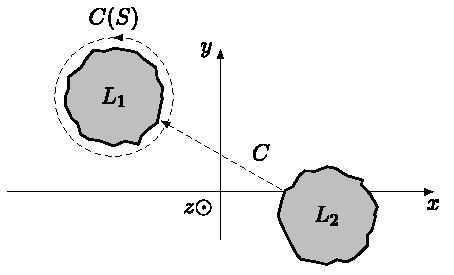
\includegraphics{res/LT1}
\end{center}
%Es soll zudem die \textbf{Dünndrahtnäherung} angesetzt werden, was bedeutet, dass die Stromdichte konstant über den gesamten Leiterquerschnitt ist. Folglich wird der Skin-Effekt ($\nearrow$\ref{skin}) vernachlässigt (das macht man in der Leitungstheorie immer so). Außerdem wird zunächst ein idealer Leiter angesetzt, d.h. es gilt $\kappa\to\infty$. 
Damit folgt
\begin{equation}
	\int\limits_{C}\left(\frac{\partial \vec{\ubar{E}}}{\partial z}+\mathrm{j} \omega \mu \vec{\ubar{H}} \times \vec{e}_{z}\right) \mathrm{d} \vec{r}=\frac{\partial}{\partial z} \underbrace{\int\limits_{C} \vec{\ubar{E}} \mathrm{~d} \vec{r}}_{=\ubar{U}}+\mathrm{j} \omega \mu \int\limits_{C}\left(\vec{\ubar{H}} \times \vec{e}_{z}\right) \mathrm{d} \vec{r}\stackrel{\text{\ref{indang}}}{=}0 
\end{equation}
wobei das magnetische Feld gemäß der Bestimmungsgleichung ($\nearrow$\ref{bestH}) ersetzt und damit die Relation
\begin{equation}
\begin{split}
	\frac{\partial \ubar{U}}{\partial z}+\mathrm{j} \omega \mu \int\limits_{C}\left[\frac{1}{\mathrm{j} \omega \mu} (\vec{e}_{z} \times \grad \ubar{\phi}(x, y))  \frac{\partial \ubar{g}(z)}{\partial z}\right] \times \vec{e}_{z} \mathrm{~d} \vec{r}&=0 \\
	\frac{\partial \ubar{U}}{\partial z}+\frac{\partial \ubar{g}(z)}{\partial z} \int\limits_{C} \grad \ubar{\phi}(x, y) \mathrm{d} \vec{r}&=0 
\end{split}
\end{equation}
erhalten wird. Die partielle Ableitung der Funktion $\ubar{g}(z)$ kann hierfür ohne Weiteres vor das Integral gezogen werden, da die Integration in der $x y$-Ebene erfolgt. ${\partial \ubar{g}(z)}/{\partial z}$ bestimmt man nun in einem nächsten Schritt durch Anwendung des Durchflutungsgesetzes ($\nearrow$\ref{durchf}). Aus der Integration auf dem geschlossenen Weg $C(S)$ entlang der Oberfläche bzw. Berandung eines Leiters folgt der in den Leitern fließende Strom $\ubar{I}$ (in quasistatischer Näherung) gemäß
\begin{equation}\label{fliesstromLT}
	\ubar{I}=\oint\limits_{C(S)} \vec{\ubar{H}} \mathrm{~d} \vec{r}=\frac{1}{\mathrm{j} \omega \mu} \oint\limits_{C(S)}\left(\vec{e}_{z} \times \grad \ubar{\phi}\right) \frac{\partial \ubar{g}(z)}{\partial z} \mathrm{d} \vec{r}=\frac{\partial \ubar{g}(z)}{\partial z} \frac{1}{\mathrm{j} \omega \mu} \oint\limits_{C(S)}\left(\vec{e}_{z} \times \grad \ubar{\phi}\right) \mathrm{d} \vec{r} 
\end{equation}
mit dem sich nach Umstellen die Beziehung
\begin{equation}
	\frac{\partial \ubar{g}(z)}{\partial z}=\frac{\mathrm{j} \omega \mu}{\oint\limits_{C(S)}\left(\vec{e}_{z} \times \grad \ubar{\phi}\right) \mathrm{d} \vec{r}} \cdot \ubar{I} 
\end{equation}
ergibt. Einsetzen in Gleichung \ref{fliesstromLT} führt schließlich auf die \textbf{erste Telegraphengleichung}
\begin{equation}\label{ersttel}
	\frac{\partial \ubar{U}}{\partial z}+\mathrm{j} \omega \underbrace{\mu\frac{\int\limits_{C} \grad \ubar{\phi} \mathrm{d} \vec{r}}{\oint\limits_{C(S)}\left(\vec{e}_{z} \times \grad \ubar{\phi}\right) \mathrm{d} \vec{r}}}_{=: L^{\prime}} \ubar{I}=\boxed{\frac{\partial \ubar{U}}{\partial z}+\mathrm{j} \omega L^{\prime} \ubar{I}=0 }
\end{equation}
Darin wird $L^{\prime}$ als der Induktivitätsbelag der Leitung mit
\begin{equation}\label{indbelag}
	\boxed{L^{\prime}:=\mu \frac{\int\limits_{C} \grad \ubar{\phi}(x, y) \mathrm{d} \vec{r}}{\oint\limits_{C(S)}\left(\vec{e}_{z} \times \grad \ubar{\phi}(x, y)\right) \mathrm{d} \vec{r}} }
\end{equation}
definiert und in der Einheit Henry pro Meter (H/m) angegeben.
\subsubsection{Zweite Telegraphengleichung}
 Die zweite Telegraphengleichung leitet sich in analoger Weise aus dem Durchflutungsgesetz ab. Es ist
\begin{align}
\oint\limits_{C(S)}\left(\frac{\partial \vec{\ubar{H}}}{\partial z}-\mathrm{j} \omega \varepsilon \vec{\ubar{E}} \times \vec{e}_z\right) \mathrm{d} \vec{r} & =\frac{\partial}{\partial z} \oint\limits_{C(S)} \vec{\ubar{H}} \mathrm{~d} \vec{r}-\mathrm{j} \omega \varepsilon \oint\limits_{C(S)}\left(\vec{\ubar{E}} \times \vec{e}_z\right) \mathrm{d} \vec{r} \\
& =\frac{\partial \ubar{I}}{\partial z}+\mathrm{j} \omega \varepsilon \oint\limits_{C(S)}\left(\ubar{g}(z) \grad \ubar{\phi} \times \vec{e}_z\right) \mathrm{d} \vec{r}\stackrel{\text{\ref{indang}}}{=}0
\end{align}
Die unbekannte Funktion $\ubar{g}(z)$ bestimmt sich hier direkt aus der Definition der Spannung $\ubar{U}$ zwischen den Leitern gemäß der Gleichung
\begin{equation}
	\ubar{U}=\int\limits_{C} \vec{\ubar{E}} \mathrm{~d} \vec{r}=-\ubar{g}(z) \int_{C} \grad \ubar{\phi} \mathrm{d} \vec{r} \quad \Rightarrow \quad \ubar{g}(z)=-\frac{\ubar{U}}{\int\limits_{C} \grad \ubar{\phi} \mathrm{d} \vec{r}} 
\end{equation}
sodass man nach Einsetzen die \textbf{zweite Telegraphengleichung} zu
\begin{equation}\label{zweittel}
	\frac{\partial \ubar{I}}{\partial z}+\mathrm{j} \omega \underbrace{\varepsilon\frac{\oint\limits_{C(S)}\left(\vec{e}_z \times\grad \ubar{\phi}\right) \mathrm{d} \vec{r}}{\int\limits_C\grad \ubar{\phi} \mathrm{d} \vec{r}}}_{=: C^{\prime}} \ubar{U}=\boxed{\frac{\partial \ubar{I}}{\partial z}+\mathrm{j} \omega C^{\prime} \ubar{U}=0} \end{equation}

mit der Größe $C^{\prime}$ als dem Kapazitätsbelag der Leitung erhält. Dieser ist über
\begin{equation}\label{kapbelag}
	\boxed{C^{\prime}:=\varepsilon \frac{\oint\limits_{C(S)}\left(\vec{e}_{z} \times \grad \ubar{\phi}\right) \mathrm{d} \vec{r}}{\int\limits_{C} \grad \ubar{\phi} \mathrm{d} \vec{r}}} 
\end{equation}
definiert und wird in der Einheit Farad pro Meter (F/m) angegeben. 
\subsubsection{Interpretation und Entkopplung der Telegraphengleichungen}
Aus den Formeln \ref{indbelag} und \ref{kapbelag} für den Induktivitäts- bzw. Kapazitätsbelag ist ersichtlich, dass die Größen $C^\prime$ und $L^\prime$ vollständig durch die Lösung des statischen 2D-Randwertproblems für $\ubar{\phi}$ im Lösungsvolumen $V$ definiert sind. Das bedeutet, dass man um diese Größen auszurechnen $\Delta \ubar{\phi}=0$ mit $\ubar{\phi}=0$ auf einem Leiter und $\ubar{\phi}=\ubar{U}(z)$ auf dem anderen Leiter lösen muss. % PLENUM: Warum nicht problematisch, wenn man U kennen muss?
Offensichtlich gilt:
\begin{equation}
	L^\prime C^\prime =\varepsilon\mu=\frac{1}{v_\mathrm{c}^2}\quad \implies \quad \boxed{v_\mathrm{c}=\frac{1}{\sqrt{L^\prime C^\prime}}}
\end{equation}
Außerdem kann man die Gleichungen entkoppeln:
	\begin{equation}\label{entkoptel}\begin{split}
	\frac{\partial^2  \ubar{U}(z)}{\partial z^2} + \omega^2 L^\prime C^\prime  \ubar{U}(z) &= 0 \\
	 \frac{\partial^2  \ubar{I}(z)}{\partial z^2} + \omega^2 L^\prime C^\prime  \ubar{I}(z) &= 0
\end{split}\end{equation}
Die Lösungen sind (natürlich) vor- und zurücklaufende Wellen (als ruhende Zeiger):
\begin{equation}\begin{split}
	\ubar{U}(z) &=  \ubar{U}_0  \mathrm{e}^{\pm\mathrm{j}kz} \\
	  \ubar{I}(z)& =  \ubar{I}_0  \mathrm{e}^{\pm\mathrm{j}kz}
	\end{split}\end{equation}
Die Gesamtlösung ist wieder eine Überlagerung aus hin- und rücklaufenden Wellen.
\subsubsection{Matrixschreibweise}
Kompakter können die Gleichungen \ref{ersttel} und \ref{zweittel} in der Matrixform

\begin{equation} \label{matrixformgl}
	\frac{\partial}{\partial z}\binom{\ubar{U}}{\ubar{I}}+\mathrm{j} \omega\left(\begin{array}{cc}
		0 & L^{\prime}  \\
		C^{\prime} & 0
	\end{array}\right)\binom{\ubar{U}}{\ubar{I}}=\binom{0}{0}
\end{equation}
notiert werden.
\subsection{Konstruktion des Leitungsersatzschaltbildes}
\subsubsection{Verlustloser Fall}
Auf Grundlage der Telegraphengleichungen ist ein Übergang zu folgendem Leitungsersatzschaltbild möglich
\begin{center}
	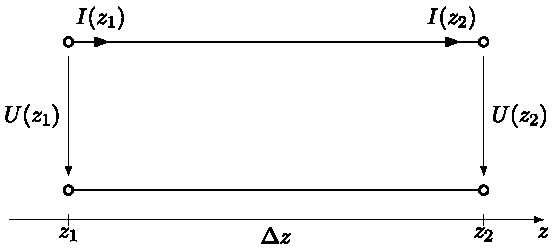
\includegraphics{res/LT2}
\end{center}
Zu einer Lösung des Differentialgleichungssystems gelangt man durch Entkoppeln beider Gleichungen, indem eine von ihnen erneut nach $z$ abgeleitet und anschließend die jeweils andere Gleichung darin eingesetzt wird. Das wird in Gleichung \ref{entkoptel} angedeutet. Für Differentialgleichungssysteme der Form
\begin{equation}
	\frac{\mathrm{d} \vec{y}(x)}{\mathrm{d} x}+\mathbf{A} \vec{y}(x)=\vec{0} 
\end{equation}
mit konstanter Koeffizientenmatrix $\mathbf{A}$ ist eine formale Lösung allerdings auch über den Exponentialansatz
\begin{equation}
	\vec{y}(x)=\vec{C} \mathrm{e}^{-\mathbf{A} x}
\end{equation}
möglich. Der Konstantenvektor $\vec{C} \in \mathbb{C}^{n}$ bestimmt sich dann aus einem Randwert $x_{0}$ und man erhält
\begin{equation}
	\begin{array}{rlrl}
		\vec{y}\left(x_{0}\right) & =\vec{C} \mathrm{e}^{-\mathbf{A} x_{0}} \quad \rightarrow \quad \vec{C}=\mathrm{e}^{\mathbf{A} x_{0}} \vec{y}\left(x_{0}\right) \\
		\vec{y}(x) & =\mathrm{e}^{-\mathbf{A}\left(x-x_{0}\right)} \vec{y}\left(x_{0}\right) & 
	\end{array}
\end{equation}
Für das konkrete Differentialgleichungssystem \ref{matrixformgl} folgt also mit den Randwerten am Leitungsabschluss
\begin{equation}
	\binom{\ubar{U}(z)}{\ubar{I}(z)}=\mathrm{e}^{-\mathbf{A}\left(z-z_{2}\right)}\binom{\ubar{U}\left(z_{2}\right)}{\ubar{I}\left(z_{2}\right)}=\mathrm{e}^{\mathbf{A}\left(z_{2}-z\right)}\binom{\ubar{U}\left(z_{2}\right)}{\ubar{I}\left(z_{2}\right)} 
\end{equation}
Am Anfang des Leiterstückes an der Stelle $z_{1}$ gilt dann mit der Leitungslänge $\Delta z=z_{2}-z_{1}$
\begin{equation}
\binom{\ubar{U}\left(z_{1}\right)}{\ubar{I}\left(z_{1}\right)}=\mathrm{e}^{\mathbf{A} \Delta z}\binom{\ubar{U}\left(z_{2}\right)}{\ubar{I}\left(z_{2}\right)} \quad \text { mit } \quad \mathbf{A}=\mathrm{j} \omega\left(\begin{array}{cc}
	0 & L^{\prime}  \\
	C^{\prime} & 0
\end{array}\right)
\end{equation}
Für eine hinreichend kleine Leiterlänge $\Delta z$ lässt sich der Matrixexponent dann über
\begin{equation}
	\mathrm{e}^{\mathbf{A} \Delta z}=\mathbf{E}+\mathbf{A} \Delta z+\frac{1}{2} \mathbf{A}^{2}(\Delta z)^{2}+\frac{1}{3} \mathbf{A}^{3}(\Delta z)^{3}+\ldots 
\end{equation}
in eine Reihe entwickeln, wobei nach dem linearen Term abgebrochen werden kann. Somit folgt
\begin{equation}\begin{split}
\binom{\ubar{U}\left(z_{1}\right)}{\ubar{I}\left(z_{1}\right)}=\left[\left(\begin{array}{ll}
	1 & 0  \\
	0 & 1
\end{array}\right)+\mathrm{j} \omega\left(\begin{array}{cc}
	0 & L^{\prime} \\
	C^{\prime} & 0
\end{array}\right) \Delta z\right]\binom{\ubar{U}\left(z_{2}\right)}{\ubar{I}\left(z_{2}\right)}&\\
=\left(\begin{array}{cc}
	1 & \mathrm{j} \omega L^{\prime} \Delta z \\
	\mathrm{j} \omega C^{\prime} \Delta z & 1
\end{array}\right)\binom{\ubar{U}\left(z_{2}\right)}{\ubar{I}\left(z_{2}\right)}
\end{split}\end{equation}
Als nächster Schritt ist zur Bestimmung eines Ersatzschaltbildes der Leitung ein Vierpol in $A$-Parameterdarstellung bzw. Kettenmatrixform mit
\begin{equation}
\binom{\ubar{U}_{1}}{\ubar{I}_{1}}=\left(\begin{array}{ll}
	A_{11} & A_{12}  \\
	A_{21} & A_{22}
\end{array}\right)\binom{\ubar{U}_{2}}{\ubar{I}_{2}}
\end{equation}
gesucht. Welcher Vierpol besitzt also die zuvor bestimmten $A$-Parameter? Man betrachte dazu das in folgender Abbildung dargestellte Zweitor mit der Reiheninduktivität $L^{\prime} \Delta z$ und der Parallelkapazität $C^{\prime} \Delta z$.
\begin{center}
	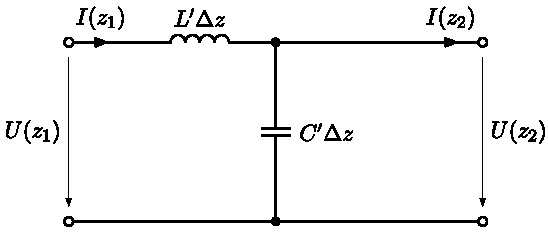
\includegraphics{res/LT3}
\end{center}
Dessen Parametermatrix stellt sich folgendermaßen dar
\begin{equation}
\left(\begin{array}{cc}
	1 & \mathrm{j} \omega L^{\prime} \Delta z  \\
	0 & 1
\end{array}\right)\left(\begin{array}{cc}
	1 & 0 \\
	\mathrm{j} \omega C^{\prime} \Delta z & 1
\end{array}\right)=\left(\begin{array}{cc}
	1-\omega^{2} L^{\prime} C^{\prime} \Delta z^{2} & \mathrm{j} \omega L^{\prime} \Delta z \\
	\mathrm{j} \omega C^{\prime} \Delta z & 1
\end{array}\right)
\end{equation}
Bis auf den additiven Term $\omega^{2} L^{\prime} C^{\prime}(\Delta z)^{2}$ stimmt diese Darstellung mit dem vorigen Ergebnis überein. Das bedeutet, für den Fall $\omega^{2} L^{\prime} C^{\prime}(\Delta z)^{2} \ll 1$ ist das verwendete Ersatzschaltbild gültig. Anders ausgedrückt heißt dies
\begin{equation}
	(\Delta z)^{2} \ll \frac{1}{\omega^{2} L^{\prime} C^{\prime}} \stackrel{L^{\prime} C^{\prime}=\frac{1}{v_\mathrm{c}^{2}}}{=} \frac{v_\mathrm{c}^{2}}{\omega^{2}} \stackrel{k=\frac{\omega}{v_\mathrm{c}}}{=} \frac{1}{k^{2}} \stackrel{k=\frac{2 \pi}{\lambda}}{=} \frac{\lambda^{2}}{(2 \pi)^{2}} 
\end{equation}
Als Bedingung für die Wellenlänge der sich auf der Leitung ausbreitenden Welle leitet sich hieraus das sogenannte $\lambda / 10-$ Kriterium
\begin{equation}
	\lambda \gg 2 \pi \Delta z \approx 6 \Delta z \approx 10 \Delta z 
\end{equation}
ab. Ist dieses erfüllt, kann obiges Ersatzschaltbild als Leitungsmodell herangezogen werden. Im Grenzfall $\Delta z \to 0$ ist das Ersatzschaltbild sogar exakt. Das kann beispielsweise gezeigt werden, indem für das obige Ersatzschaltbild Maschen- und Knotensatz aufgestellt werden:
\begin{itemize}
	\item  Maschensatz:
	\begin{equation}\begin{split}
			\ubar{U}(z_1) = \mathrm{j}\omega \underbrace{L}_{L'\Delta z}  \ubar{I}(z_1) +  \ubar{U}(\underbrace{z_1+\Delta z}_{z_2})\\
			\ubar{U}(z_1+\Delta z) - \ubar{U}(z_1) + \mathrm{j}\omega L  \ubar{I}(z_1) =0  \\
			\frac{\Delta  \ubar{U}}{\Delta z} + \mathrm{j}\omega \frac{L}{\Delta z}  \ubar{I}(z_1) =0
	\end{split}\end{equation}
	
	\item Knotensatz:
	\begin{equation}
		\ubar{I}(z_1+\Delta z) =  \ubar{I}(z_1) - \mathrm{j}\omega \underbrace{C}_{C'\Delta z}  \ubar{U}(z_1+\Delta z) \Rightarrow \frac{\Delta  \ubar{I}}{\Delta z} + \mathrm{j}\omega \frac{C}{\Delta z}  \ubar{U}(z_1+\Delta z) = 0
	\end{equation}
\end{itemize}
Im Grenzübergang $\Delta z \to 0$ entsprechen diese Gleichungen exakt den Telegraphengleichungen \ref{ersttel} und \ref{zweittel}, weshalb der Vierpol das Ersatzschaltbild für ein verlustloses Stück Leitung (für das gelten die Telegraphengleichungen) sein muss.
\subsubsection{Verallgemeinerung zum verlustbehafteten Fall}
Anhand der gefundenen Vierpoldarstellung konnte nun gezeigt werden, dass ein \textbf{Leitungsmodell} mit \textbf{Längsinduktivität} und \textbf{Querkapazität} ein gültiges \textbf{Ersatzschaltbild} des \textbf{differentiellen Leiterstückes} darstellt. Hieraus lässt sich auch ein um die \textbf{Leitungsverluste} \textbf{erweitertes Modell} ableiten, mithilfe dessen eine entkoppelte Lösung für Spannung $\ubar{U}(z)$ und Strom $\ubar{I}(z)$ entlang der Leitung bestimmt werden kann. Dafür werden Spule und Kondensator durch ihre verlustbehafteten Äquivalente substituiert. Für ein Segment der Länge $\Delta z$ stellt sich das Ersatzschaltbild für eine verlustbehaftete Leitung also wie in folgender Grafik dar:
\begin{center}
	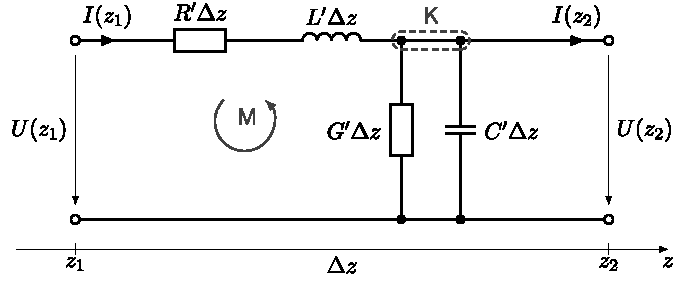
\includegraphics{res/LT4}
\end{center}
Der \textbf{Widerstandsbelag} $R'$ entspricht den ohmschen Leitungsverlusten pro Längeneinheit, der \textbf{Leitwertbelag} $G'$ entspricht den dielektrischen Verlusten. Zusammengefasst spricht man auch von \textbf{Impdeanzbelag} $R^{\prime}+\mathrm{j} \omega L^{\prime}$ und \textbf{Admittanzbelag} $G^{\prime}+\mathrm{j} \omega C^{\prime}$. Anwendung von Maschen- und Knotensatz liefert
\begin{align}
	&& M: \quad \ubar{U}(z)&=\ubar{U}(z+\Delta z)+\left(R^{\prime} \Delta z\right) \ubar{I}(z)+\mathrm{j} \omega\left(L^{\prime} \Delta z\right) \ubar{I}(z)  \\
	&& K: \quad \ubar{I}(z)&=\ubar{I}(z+\Delta z)+\ubar{U}(z+\Delta z)\left(G^{\prime} \Delta z\right)+\mathrm{j} \omega\left(C^{\prime} \Delta z\right) \ubar{U}(z+\Delta z) 
\end{align}
\subsubsection{Differentialgleichungssystem für den verlustbehafteten Fall}
Nach Übergang vom Differenzenquotienten zum Differentialquotienten mit $\Delta z \rightarrow 0$ erhält man
\begin{equation}
\frac{\mathrm{d}}{\mathrm{d} z}\binom{\ubar{U}(z)}{\ubar{I}(z)}+\left(\begin{array}{cc}
	0 & R^{\prime}+\mathrm{j} \omega L^{\prime}  \\
	G^{\prime}+\mathrm{j} \omega C^{\prime} & 0
\end{array}\right)\binom{\ubar{U}(z)}{\ubar{I}(z)}=\binom{0}{0}
\end{equation}
Die Entkopplung dieses Differentialgleichungssystems führt auf die DGL zweiter Ordnung
\begin{equation}\begin{split}
	\frac{\mathrm{d}^{2}}{\mathrm{~d} z^{2}} \ubar{U}(z)&=-\left(R^{\prime}+\mathrm{j} \omega L^{\prime}\right) \frac{\mathrm{d} \ubar{I}(z)}{\mathrm{d} z}=\underbrace{\left(R^{\prime}+\mathrm{j} \omega L^{\prime}\right)\left(G^{\prime}+\mathrm{j} \omega C^{\prime}\right)}_{=: \ubar{\gamma}^{2}} \ubar{U}(z)\\
	\Aboxed{\ubar{\gamma}&=\sqrt{\left(R^{\prime}+\mathrm{j} \omega L^{\prime}\right)\left(G^{\prime}+\mathrm{j} \omega C^{\prime}\right)}}
\end{split}\end{equation}
deren Lösung man zu
\begin{equation} \label{loesULT}
	\boxed{\ubar{U}(z)=\ubar{U}^{+} \mathrm{e}^{-\ubar{\gamma} z}+\ubar{U}^{-} \mathrm{e}^{+\ubar{\gamma} z} }
\end{equation}
bestimmt. Diese stellt im Grunde eine Überlagerung der in positiver (erster Summand) und negativer $z$-Richtung (zweiter Summand) propagierenden Welle dar. Die additive (anstelle einer subtraktiven) Überlagerung ist Konvention. Für den Strom $\ubar{I}(z)$ gilt dann
\begin{align}
	\ubar{I}(z) & =-\frac{1}{R^{\prime}+\mathrm{j} \omega L^{\prime}} \frac{\mathrm{d} \ubar{U}(z)}{\mathrm{d} z}=\frac{\ubar{\gamma}}{R^{\prime}+\mathrm{j} \omega L^{\prime}}\left(\ubar{U}^{+} \mathrm{e}^{-\ubar{\gamma} z}-\ubar{U}^{-} \mathrm{e}^{+\ubar{\gamma} z}\right)  \\
	& =\underbrace{\sqrt{\frac{G^{\prime}+\mathrm{j} \omega C^{\prime}}{R^{\prime}+\mathrm{j} \omega L^{\prime}}}}_{=: \frac{1}{\ubar{Z}_{\mathrm{C}}}}\left(\ubar{U}^{+} \mathrm{e}^{-\ubar{\gamma} z}-\ubar{U}^{-} \mathrm{e}^{+\ubar{\gamma} z}\right)=\boxed{\frac{1}{\ubar{Z}_{\mathrm{C}}}\left(\ubar{U}^{+} \mathrm{e}^{-\ubar{\gamma} z}-\ubar{U}^{-} \mathrm{e}^{+\ubar{\gamma} z}\right)=\ubar{I}(z)} \label{loesILT}
\end{align}
Hierin ist die Größe
\begin{equation}
	\boxed{\ubar{Z}_{\mathrm{C}}=\sqrt{\frac{R^{\prime}+\mathrm{j} \omega L^{\prime}}{G^{\prime}+\mathrm{j} \omega C^{\prime}}} }
\end{equation}
die sogenannte \textbf{charakteristische Impedanz} bzw. \textbf{Leitungswellenwiderstand} der Leitung. Es ist zu beachten, dass dieser nicht gleich dem Feldwellenwiderstand ist. Weiterhin nennt man $R^{\prime}, G^{\prime}, L^{\prime}$ und $C^{\prime}$ die \textbf{primären Leitungsparameter}, während man $\ubar{\gamma}$ und $\ubar{Z}_{\mathrm{C}}$ als \textbf{sekundäre Leitungsparameter} bezeichnet.
Die noch unbekannten Integrationskonstanten $\ubar{U}^{+}$und $\ubar{U}^{-}$lassen sich aus den Anfangswerten von Spannung und Strom am Leitungseingang ermitteln. Für $z=0$ ist
\begin{equation}
	\ubar{U}(0)=\ubar{U}^{+}+\ubar{U}^{-} \quad \text { und } \quad \ubar{I}(0)=\frac{1}{\ubar{Z}_{\mathrm{C}}}\left(\ubar{U}^{+}-\ubar{U}^{-}\right)
\end{equation}
Hiermit bestimmen sich die Konstanten zu
\begin{equation}
	\ubar{U}^{+}=\frac{1}{2}\left[\ubar{U}(0)+\ubar{Z}_{\mathrm{C}} I(0)\right] \quad \text { bzw. } \quad \ubar{U}^{-}=\frac{1}{2}\left[\ubar{U}(0)-\ubar{Z}_{\mathrm{C}} \ubar{I}(0)\right] 
\end{equation}
Einsetzen in \ref{loesULT} und anschließende Umformung liefert
\begin{align}
	\ubar{U}(z) & =\ubar{U}^{+} \mathrm{e}^{-\ubar{\gamma} z}+\ubar{U}^{-} \mathrm{e}^{+\ubar{\gamma} z}=\frac{1}{2}\left[\ubar{U}(0)+\ubar{Z}_{\mathrm{C}} \ubar{I}(0)\right] \mathrm{e}^{-\ubar{\gamma} z}+\frac{1}{2}\left[\ubar{U}(0)-\ubar{Z}_{\mathrm{C}} \ubar{I}(0)\right] \mathrm{e}^{+\ubar{\gamma} z}  \\
	\Aboxed{\ubar{U}(z)& =\ubar{U}(0) \cosh (\ubar{\gamma} z)-\ubar{Z}_{\mathrm{C}} \ubar{I}(0) \sinh (\ubar{\gamma} z) }
\end{align}
Gleichfalls folgt für den Strom
\begin{equation}
	\boxed{\ubar{I}(z)=-\frac{1}{\ubar{Z}_{\mathrm{C}}} \ubar{U}(0) \sinh (\ubar{\gamma} z)+\ubar{I}(0) \cosh (\ubar{\gamma} z)}
\end{equation}
Die vollständige Leitung wird somit durch einen Vierpol mit der Matrixform

\begin{equation}
\binom{\ubar{U}(z)}{\ubar{I}(z)}=\left(\begin{array}{cc}
	\cosh (\ubar{\gamma} z) & -\ubar{Z}_{\mathrm{C}} \sinh (\ubar{\gamma} z)  \\
	-\frac{1}{\ubar{Z}_{\mathrm{C}}} \sinh (\ubar{\gamma} z) & \cosh (\ubar{\gamma} z)
\end{array}\right)\binom{\ubar{U}(0)}{\ubar{I}(0)}
\end{equation}
beschrieben. 
\subsubsection{Impedanztransformation entlang einer Leitung}
Stellt man diese Gleichung nun um und wertet das Ganze bei $z=L$ aus, dann erhält man 
\begin{equation}
\binom{\ubar{U}(0)}{\ubar{I}(0)}=\left(\begin{array}{cc}
	\cosh (\ubar{\gamma} L) & Z_{\mathrm{C}} \sinh (\ubar{\gamma} L)  \\
	\frac{1}{Z_{\mathrm{C}}} \sinh (\ubar{\gamma} L) & \cosh (\ubar{\gamma} L)
\end{array}\right)\binom{\ubar{U}(L)}{\ubar{I}(L)}
\end{equation}
Damit könnte man nun ${\ubar{U}(0)}/{\ubar{I}(0)}$ bilden und würde die Eingangsimpedanz bei $z=0$ erhalten, die bei einer gewissen Ausgangsimpedanz ${\ubar{U}(L)}/{\ubar{I}(L)}$ zu sehen ist. Das lässt sich verallgemeinern, sodass man die Eingangsimpedanz bei einem beliebigen $z$ berechnen kann, wenn am Ausgang bei $z=L$ die Ausgangsimpedanz ${\ubar{U}(L)}/{\ubar{I}(L)}$ zu sehen ist. Dafür ist eine Auswertung bei $z$ anstatt bei $0$ erforderlich. Der Abstand von $z$ zu $L$ (also die transformierende Leitungslänge) ist dann $L-z$ anstelle von $L$. Mit
\begin{equation}
	\frac{\ubar{U}(z)}{\ubar{I}(z)}=\frac{\cosh (\ubar{\gamma}(L-z)) \ubar{U}(L)+\ubar{Z}_{\mathrm{C}} \sinh (\ubar{\gamma}(L-z)) \ubar{I}(L)}{\frac{1}{\ubar{Z}_{\mathrm{C}}} \sinh (\ubar{\gamma}(L-z)) \ubar{U}(L)+\cosh (\ubar{\gamma}(L-z)) \ubar{I}(L)} 
\end{equation}
lässt sich nun die Eingangsimpedanz an der Stelle $z$ berechnen. Weitere Umformung durch teilen des Zählers und Nenners durch $\ubar{I}(L)\cosh (\ubar{\gamma}(L-z))$ liefert schließlich
\begin{align}
	 \frac{\ubar{U}(z)}{\ubar{I}(z)}&=\frac{\frac{\ubar{U}(L)}{\ubar{I}(L)}+\ubar{Z}_{\mathrm{C}} \tanh (\ubar{\gamma}(L-z))}{\frac{1}{\ubar{Z}_{\mathrm{C}}} \frac{\ubar{U}(L)}{\ubar{I}(L)} \tanh (\ubar{\gamma}(L-z))+1}=\frac{\ubar{Z}_{\mathrm{a}}+\ubar{Z}_{\mathrm{C}} \tanh (\ubar{\gamma}(L-z))}{1+\frac{\ubar{Z}_{\mathrm{a}}}{\ubar{Z}_{\mathrm{C}}} \tanh (\ubar{\gamma}(L-z))}  \\
	\Aboxed{\ubar{Z}(z)&=Z_{\mathrm{a}} \frac{1+\frac{\ubar{Z}_{\mathrm{C}}}{\ubar{Z}_{\mathrm{a}}} \tanh (\ubar{\gamma}(L-z))}{1+\frac{\ubar{Z}_{\mathrm{a}}}{\ubar{Z}_{\mathrm{C}}} \tanh (\ubar{\gamma}(L-z))}}
\end{align}
mit der Last- bzw. Abschlussimpedanz $\ubar{Z}_{\mathrm{a}}=\frac{\ubar{U}(L)}{\ubar{I}(L)}$. 
\subsubsection{Reflektionsfaktor}
Der Reflexionsfaktor $\ubar{\Gamma}(z)$ der Leitung an der Stelle $z$ ist nun definiert als das Verhältnis von rücklaufender zu hinlaufender Welle mit
\begin{align}
	\ubar{U}(z) & =\ubar{U}^{+} \mathrm{e}^{-\ubar{\gamma} z}+\ubar{U}^{-} \mathrm{e}^{+\ubar{\gamma} z}=\ubar{U}^{+} \mathrm{e}^{-\ubar{\gamma} z}\left(1+\frac{\ubar{U}^{-}}{\ubar{U}^{+}} \mathrm{e}^{2 \ubar{\gamma} z}\right)  \\
	& =\ubar{U}^{+} \mathrm{e}^{-\ubar{\gamma} z}(1+\ubar{\Gamma}(z)) \quad \text { mit } \quad \boxed{\ubar{\Gamma}(z):=\frac{\ubar{U}^{-}}{\ubar{U}^{+}} \mathrm{e}^{2 \ubar{\gamma} z} }
\end{align}
Für die Eingangsimpedanz schreibt sich damit
\begin{equation}
	\ubar{Z}(z)=\frac{\ubar{U}(z)}{\ubar{I}(z)}=\frac{\ubar{U}^{+} \mathrm{e}^{-\ubar{\gamma} z}+\ubar{U}^{-} \mathrm{e}^{+\ubar{\gamma} z}}{\frac{1}{\ubar{Z}_{\mathrm{C}}}\left(\ubar{U}^{+} \mathrm{e}^{-\ubar{\gamma} z}-\ubar{U}^{-} \mathrm{e}^{+\ubar{\gamma} z}\right)}=\ubar{Z}_{\mathrm{C}} \frac{1+\ubar{\Gamma}(z)}{1-\ubar{\Gamma}(z)} 
\end{equation}
Umstellen nach dem Reflexionsfaktor liefert
\begin{equation}
	\boxed{\ubar{\Gamma}(z)=\frac{\ubar{Z}(z)-\ubar{Z}_{\mathrm{C}}}{\ubar{Z}(z)+\ubar{Z}_{\mathrm{C}}}} \quad, \quad \ubar{\Gamma}(L)=\frac{\ubar{Z}(L)-\ubar{Z}_{\mathrm{C}}}{\ubar{Z}(L)+\ubar{Z}_{\mathrm{C}}}=\frac{\ubar{Z}_{\mathrm{a}}-\ubar{Z}_{\mathrm{C}}}{\ubar{Z}_{\mathrm{a}}+\ubar{Z}_{\mathrm{C}}} 
\end{equation}
Eine Impedanz korrespondiert also über eine Möbius-Transformation mit einem Reflektionsfaktor. Es ist also möglich das Verhältnis der einlaufenden zur reflektierten Welle vorherzusagen, ohne die Wellen explizit zu berechnen.
\subsubsection{Beispiel (Dämpfungsferrite auf Leitungen)}
Zur Unterdrückung von Gleichtaktstörungen auf Versorgungs- oder Datenleitungen werden in der Praxis Dämpfungsferrite eingesetzt. Zur konkreten Auslegung ist eine analytische Beschreibung der Leitung mit Ferrit notwendig. Intuitiv würde man zunächst folgendes Modell mit einer frequenzabhängigen Ferritimpedanz $Z_{\mathrm{Fe}}$ annehmen:
\begin{center}
	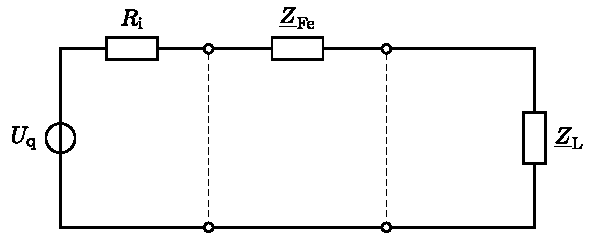
\includegraphics{res/LT51}
\end{center}
Diese Vorstellung stellt sich jedoch als physikalisch falsch heraus, da bei offenem Abschluss mit $\ubar{Z}_{\mathrm{e}} \rightarrow \infty$ kein Strom fließen dürfte. Durch einfache Messungen mit einem Netzwerkanalysator kann allerdings gezeigt werden, dass aufgrund der Leitungskapazität stets ein gewisser Verschiebungsstrom feststellbar ist. Man darf also nicht ohne Weiteres verteilte Leitungsparameter mit konzentrierten elektrischen Elementen kombinieren.
Als alternatives Beschreibungsmittel bietet sich hingegen die Leitungstheorie an. Dazu werde der nachfolgend dargestellte Versuchsaufbau betrachtet.
\begin{center}
	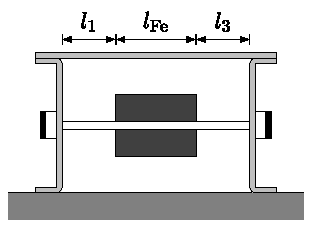
\includegraphics{res/LT52}
\end{center}
Mithilfe eines Netzwerkanalysators werden die $S$-Parameter der Leitung bei Einspeisung an Port 2 und Messung an Port 1 bestimmt, wobei der Übertragungsfaktor $\ubar{S}_{21}$ die interessierende Größe darstellt. Zur rechnerischen Bestimmung von $\ubar{S}_{21}$ und der Eingangsimpedanz $\ubar{Z}_{\mathrm{e}}$ müssen die drei Leitungsabschnitte $z \in[0 ; L],\left[L_{1} ; L_{2}\right]$ und $\left[L_{2} ; L\right]$ zusammengefasst werden, wofür die Nutzung von Ketternparametern sinnvoll ist.
\subsection{Mehrfachleitungen}
Unter einer Mehrfachleitung versteht man eine Gruppe von $n$ Leitern zuzüglich eines Referenzleiters (siehe nachfolgende Grafik). Zur Bestimmung der Spannungen und Ströme innerhalb einer solchen Anordnung müssen die Leitungsgleichungen entsprechend erweitert werden.
\begin{center}
	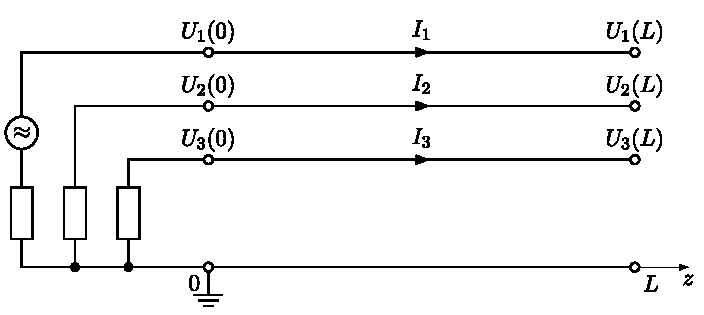
\includegraphics{res/LT7}
\end{center}
Für ein allgemeines $n$-Leitersystem formulieren sich die Telegraphengleichungen \ref{ersttel} und \ref{zweittel} (bzw. in Matrixform: \ref{matrixformgl}) in der verallgemeinerten Matrixform
\begin{equation}\label{verallgmatr}\begin{split}
	\frac{\mathrm{d}}{\mathrm{d} z}\left(\begin{array}{c}
		\ubar{U}_{1}  \\
		\ubar{U}_{2} \\
		\vdots \\
		\ubar{U}_{n}
	\end{array}\right)+\ubar{\mathbf{Z}}^{\prime}\left(\begin{array}{c}
		\ubar{I}_{1} \\
		\ubar{I}_{2} \\
		\vdots \\
		\ubar{I}_{n}
	\end{array}\right)&=\left(\begin{array}{c}
		0 \\
		0 \\
		\vdots \\
		0
	\end{array}\right) \\ \frac{\mathrm{d}}{\mathrm{d} z}\left(\begin{array}{c}
		\ubar{I}_{1} \\
		\ubar{I}_{2} \\
		\vdots \\
		\ubar{I}_{n}
	\end{array}\right)+\ubar{\mathbf{Y}}^{\prime}\left(\begin{array}{c}
		\ubar{U}_{1} \\
		\ubar{U}_{2} \\
		\vdots \\
		\ubar{U}_{n}
	\end{array}\right)&=\left(\begin{array}{c}
		0 \\
		0 \\
		\vdots \\
		0
	\end{array}\right)
\end{split}\end{equation}

mit den $n$-Spaltenvektoren $\vec{\ubar{U}}$ und $\vec{\ubar{I}}$ der Leiterspannungen bzw. Leiterströme. Zudem bezeichnen darin $\ubar{\mathbf{Z}}^{\prime}=\mathbf{R}^{\prime}+\mathrm{j} \omega \mathbf{L}^{\prime}$ die $n \times n$ Impedanzmatrix und $\ubar{\mathbf{Y}}^{\prime}=\mathbf{G}^{\prime}+\mathrm{j} \omega \mathbf{C}^{\prime}$ die $n \times n$ Admittanzmatrix. Sie repräsentieren die Resistivitäten, Konduktivitäten, Induktivitäten und Kapazitäten der Einzelleiter sowie der Leitungen untereinander und bilden somit die wechselseitige Beeinflussung innerhalb des Leitersystems ab. Die Impedanzmatrix besitzt die Gestalt
\begin{equation}
	\ubar{\mathbf{Z}}^{\prime}=\left(\begin{array}{cccc}
		R_{1}^{\prime}+R_{\mathrm{G} 11}^{\prime} & R_{\mathrm{G} 12}^{\prime} & \cdots & R_{\mathrm{G} 1 n}^{\prime}  \\
		R_{\mathrm{G} 21}^{\prime} & R_{2}^{\prime}+R_{\mathrm{G} 22}^{\prime} & \cdots & R_{\mathrm{G} 2 n}^{\prime} \\
		\vdots & \vdots & \ddots & \vdots \\
		R_{\mathrm{G} n 1}^{\prime} & R_{\mathrm{G} n 2}^{\prime} & \cdots & R_{n}^{\prime}+R_{\mathrm{G} n n}^{\prime}
	\end{array}\right)+\mathrm{j} \omega\left(\begin{array}{cccc}
		L_{11}^{\prime} & M_{12}^{\prime} & \cdots & M_{1 n}^{\prime} \\
		M_{21}^{\prime} & L_{22}^{\prime} & \cdots & M_{2 n}^{\prime} \\
		\vdots & \vdots & \ddots & \vdots \\
		M_{n 1}^{\prime} & M_{n 2}^{\prime} & \cdots & L_{n n}^{\prime}
	\end{array}\right)
\end{equation}
und enthält die Widerstandsbeläge $R_{i}^{\prime}$ und Selbstinduktivitätsbeläge $L_{i i}^{\prime}$ eines jeden Einzelleiters $i$ sowie die Widerstandbeläge $R_{\mathrm{G} i j}^{\prime}$ des gemeinsamen Rückleiters und Gegeninduktivitätsbeläge $M_{i j}^{\prime}$ zwischen den Leitern $i$ und $j$. Ähnlich verhält es sich mit der Admittanzmatrix
\begin{equation}
	\ubar{\mathbf{Y}}^{\prime}=\left(\begin{array}{cccc}
		G_{11}^{\prime} & G_{12}^{\prime} & \cdots & G_{1 n}^{\prime}  \\
		G_{21}^{\prime} & G_{22}^{\prime} & \cdots & G_{2 n}^{\prime} \\
		\vdots & \vdots & \ddots & \vdots \\
		G_{n 1}^{\prime} & G_{n 2}^{\prime} & \cdots & G_{n n}^{\prime}
	\end{array}\right)+\mathrm{j} \omega\left(\begin{array}{cccc}
		C_{11}^{\prime} & -C_{12}^{\prime} & \cdots & -C_{1 n}^{\prime} \\
		-C_{21}^{\prime} & C_{22}^{\prime} & \cdots & -C_{2 n}^{\prime} \\
		\vdots & \vdots & \ddots & \vdots \\
		-C_{n 1}^{\prime} & -C_{n 2}^{\prime} & \cdots & C_{n n}^{\prime}
	\end{array}\right)
\end{equation}
deren Elemente aus den Leitwertbelägen $G_{i j}^{\prime}$ und Koppelkapazitätsbelägen $C_{i j}^{\prime}$ zwischen den Leitern $i$ und $j$ gebildet werden.
Obiges Differentialgleichungssystem lässt sich aufgrund der Tatsache, dass die Systemmatrizen jeweils voll besetzt sind, nicht auf herkömmlichem Wege mit einem Exponentialansatz oder einer Variation der Konstanten lösen. Man nutzt hierzu stattdessen die sogenannte \textbf{modale Analyse}.
\section{Allgemeine Leitungstheorie}\label{allgleit}
Im Gegensatz zur klassischen Leitungstheorie, welche Gegenstand des vorigen Abschnitts war und die sich im Wesentlichen auf die Ausbreitung dominierender TEM-Wellenmoden auf homogenen und geradlinigen Leiteranordnungen beschränkt (in den dort betrachteten Fällen sind exakte Beziehungen zwischen Feld- und Leitergrößen angebbar), berücksichtigt die allgemeine Leitungstheorie auch inhomogene Strukturen und ungleichförmige Leitungen inklusive der auftretenden elektromagnetischen Strahlungsphänomene. Im Gegensatz zum vorherigen Abschnitt muss hier genähert werden, dafür sind die betrachteten Anordnungen realistischer (z.B. keine unendlichen Leitungen).\\
Beispielsweise lassen sich die in der folgenden Abbildung dargestellten Leiteranordnungen durch die klassische Theorie nicht mehr exakt beschreiben, da es vor allem an Leiterunstetigkeiten zur Beschleunigung elektrischer Ladungen und infolgedessen zu elektromagnetischer Abstrahlung kommt.\\
\begin{center}
	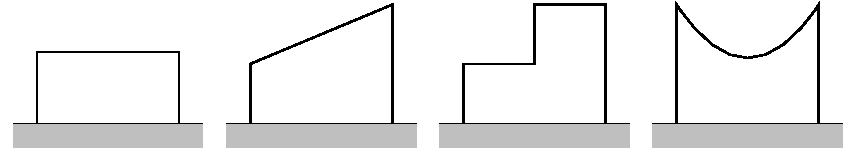
\includegraphics{res/LT15}
\end{center}
Für \textbf{ein Beispiel} soll im Folgenden eine näherungsweise mathematische Beschreibungsweise ähnlich den Telegraphengleichungen gefunden werden.
\subsection{Grundsätzliche Betrachtungen}
Üblicherweise nutzt man im Kontext elektromagnetischer Wellen die Lorenz-Eichung ($\nearrow$\ref{lorenzeich}). Mit der Greenschen Funktion 
\begin{equation}
	\ubar{G}\left(\vec{r}, \vec{r}^{\prime}, k\right)=\frac{\mathrm{e}^{-\mathrm{j} k\left|\vec{r}-\vec{r}^{\prime}\right|}}{|\vec{r}-\vec{r}|} 
\end{equation}
im Freiraum erhält man die partikulären Lösungen ($\nearrow$\ref{skalarpotlor},\ref{vekpotlor})
\begin{align}
	\ubar{\phi}(\vec{r}) & =\frac{1}{4 \pi \varepsilon} \iiint\limits_{V^{\prime}} \ubar{\rho}_{\mathrm{V}}\left(\vec{r}^{\prime}\right) \ubar{G}\left(\vec{r}, \vec{r}^{\prime}, k\right) \mathrm{d} V^{\prime} \label{partLT1}  \\
	\vec{\ubar{A}}(\vec{r}) & =\frac{\mu}{4 \pi} \iiint\limits_{V^{\prime}} \vec{\ubar{J}}\left(\vec{r}^{\prime}\right) \ubar{G}\left(\vec{r}, \vec{r}^{\prime}, k\right) \mathrm{d} V^{\prime}  \label{partLT2}
\end{align}
als die sogenannten retardierten Potentiale, wobei $k=\frac{\omega}{v_\mathrm{c}}=\frac{2 \pi}{\lambda}$ wiederum die Wellenzahl im Medium darstellt. Die betrachtete Übertragungsleitung sei weiterhin als beliebig im Raum entlang der Kurve $C$ verlaufende, \textbf{dünne Drahtstruktur} eines idealen Leiters angenommen, die den Strom $\ubar{I}\left(\vec{r}^{\prime}\right)$ trage (links in folgender Abbildung).
\begin{center}
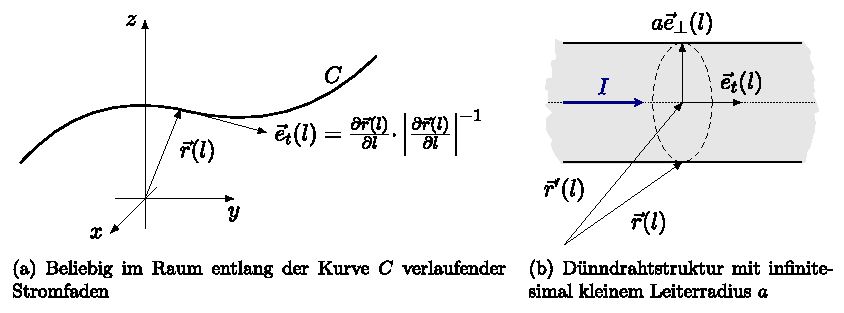
\includegraphics{res/LT16}
\end{center}
Der räumliche Kurvenverlauf wird dabei in krummlinigen Koordinaten durch den Parameter $l \in[0 ; L]$ beschrieben, welcher zwischen Null und der Leiterlänge $L$ variiert. Jene entspricht somit der Bogenlänge der Kurve, die über das Wegintegral
\begin{equation}
	L=\int\limits_{\vec{r}(0)}^{\vec{r}(L)}\left|\frac{\partial \vec{r}(l)}{\partial l}\right| \mathrm{d} l 
\end{equation}
berechenbar ist. Zur Umgehung der Singularität an der Stelle $\vec{r}=\vec{r}^{\prime}$ wird bei der Lösung der Integrale in \ref{partLT1} und \ref{partLT2} anstelle der Anwendung des Residuensatzes von einem sehr kleinen Leiterradius $a \rightarrow 0$ und dem auf der Leiteroberfläche befindlichen Aufpunkt $\vec{r}$ ausgegangen (rechts in obiger Abbildung). Die Stromdichte $\vec{\ubar{J}}$ in Gleichung \ref{partLT2} lässt sich mithilfe des Tangentialeinheitsvektors $\vec{e}_{t}(l)$ der Leiterkurve durch
\begin{equation}
	\vec{\ubar{J}}(l)=\ubar{I}(l) \vec{e}_{t}(l) \delta\left(\vec{r}-\vec{r}^{\prime}\right) 
\end{equation}
als eindimensionaler Linienstromfluss in axialer Richtung entlang der Drahtmitte ausdrücken. Trotzdem der Dirac hier als Argument einen Vektor hat, handelt es sich um ein $\delta^2(=\delta(x)\delta(y)$, wenn ein Koordinatensystem mit Ursprung in der Leitermitte und $\vu{t}=\vu{z}$ betrachtet wird). Der Dirac verwandelt so ein Volumenintegral in ein Linienintegral. Analog verhält es sich mit der Raumladungsdichte $\ubar{\rho}_{\mathrm{V}}$ in der Gleichung des Skalarpotentials, die man gemäß
\begin{equation}
	\ubar{\rho}_{\mathrm{V}}(l)=\ubar{\rho}_{\mathrm{L}}(l) \delta\left(\vec{r}-\vec{r}^{\prime}\right) 
\end{equation}
als Linienladungsdichte $\ubar{\rho}_{\mathrm{L}}$ schreiben kann (der Dirac ist auch hier ein $\delta^2$). Entsprechend formulieren sich die Volumenintegrale über das Quellgebiet $V^{\prime}$ der Leiterstruktur in beiden Lösungsdarstellungen nun jeweils zu Kurvenintegralen entlang des parametrisierten Weges $C$ mit
\begin{align}
	 \ubar{\phi}(\vec{r})&=\frac{1}{4 \pi \varepsilon} \int\limits_{0}^{L} \ubar{G}\left(l, l^{\prime}, k\right) \ubar{\rho}_{\mathrm{L}}\left(l^{\prime}\right) \mathrm{d} l^{\prime} \label{intLT1} \\
	\Aboxed{ \vec{\ubar{A}}(\vec{r})&=\frac{\mu}{4 \pi} \int\limits_{0}^{L} \ubar{G}\left(l, l^{\prime}, k\right) \ubar{I}\left(l^{\prime}\right) \vec{e}_{t}\left(l^{\prime}\right) \mathrm{d} l^{\prime} } \label{aleiter}
\end{align}
um. Für die Greensche Funktion wurde dabei gleichfalls der Formalismus mit den Kurvenparametern $l$ und $l^{\prime}$ für den enthaltenen Aufpunktvektor $\vec{r}(l)$ bzw. Quellpunktvektor $\vec{r}^{\prime}\left(l^{\prime}\right)$ genutzt. Weiterhin ergibt sich in diesem Fall mit der aus dem Durchflutungsgesetz gewonnenen Kontinuitätsgleichung ($\nearrow$\ref{kont})
\begin{align}
	 \div(\rot \vec{\ubar{H}})&=0=\div(\vec{\ubar{J}}+\mathrm{j} \omega \vec{\ubar{D}})=\div \vec{\ubar{J}}+\mathrm{j} \omega \underbrace{\div \vec{\ubar{D}}}_{=\ubar{\rho}_{\mathrm{V}}}  \\
	 \implies\quad\frac{\partial \ubar{I}(l)}{\partial l}&=-\mathrm{j} \omega \ubar{\rho}_{\mathrm{L}}(l) 
\end{align}
ein Zusammenhang zwischen Leiterstrom $\ubar{I}(l)$ und Ladungsdichte $\ubar{\rho}_{\mathrm{L}}(l)$, mit dem \ref{intLT1} schließlich noch zu
\begin{equation}\label{phileiter}
	\boxed{\ubar{\phi}(\vec{r})=\frac{\mathrm{j}}{4 \pi \varepsilon \omega} \int\limits_{0}^{L} \ubar{G}\left(l, l^{\prime}, k\right) \frac{\partial \ubar{I}\left(l^{\prime}\right)}{\partial l^{\prime}} \mathrm{d} l^{\prime}} 
\end{equation}
umgeschrieben werden kann. Das elektrische Feld der Leiteranordnung lässt sich mithilfe dieser Potentiale und Gleichung \ref{potsdef} sowie der Aufteilung
\begin{equation}
	\vec{\ubar{E}}=\vec{\ubar{E}}^{\mathrm{sct}}+\vec{\ubar{E}}^{\mathrm{exc}} 
\end{equation}
in den Anteil $\vec{\ubar{E}}^{\text {exc }}$ einer externen Anregung (Quellenfeld, engl. excitation field) und den eines Streufeldes $\vec{\ubar{E}}^{\text {sct }}$ (Abstrahlung in die Umgebung, Reflexion an einer Groundplane etc., engl scattered field) gemäß
\begin{equation}
	\vec{\ubar{E}}(\vec{r})=-\grad \ubar{\phi}(\vec{r})-\mathrm{j} \omega \vec{\ubar{A}}(\vec{r})+\vec{\ubar{E}}^{\operatorname{exc}}(\vec{r}) 
\end{equation}
ausdrücken. Als Randbedingung des verlustlosen Leiters verschwindet das tangentiale elektrische Feld auf der Leiteroberfläche % PLENUM: WARUM?? -> Verlustlos heißt ja nicht kappa -> infty, weil dann ja gar kein e-feld im Medium oder?
\begin{equation}\label{RBLT1}
	\vec{e}_{t}\left(\vec{r}\left(l^{\prime}\right)+a \vec{e}_{\perp}\left(l^{\prime}\right)\right) \cdot \vec{\ubar{E}}\left(\vec{r}\left(l^{\prime}\right)+a \vec{e}_{\perp}\left(l^{\prime}\right)\right)=0 
\end{equation}
und für sehr kleine Radien $a$ ist der Tangentialvektor der Kurve näherungsweise der gleiche wie auf der Oberfläche
\begin{equation}
	\vec{e}_{t}\left(\vec{r}\left(l^{\prime}\right)+a \vec{e}_{\perp}\left(l^{\prime}\right)\right) \approx \vec{e}_{t}(\vec{r}(l)) 
\end{equation}
Einsetzen in die Gleichung des elektrischen Feldes ergibt
\begin{align}
	0=\vec{e}_{t}(\vec{r}(l)) \vec{\ubar{E}}\left(\vec{r}\left(l^{\prime}\right)+a \vec{e}_{\perp}\left(l^{\prime}\right)\right) & =-\vec{e}_{t}(\vec{r}(l)) \grad \ubar{\phi}-\mathrm{j} \omega \vec{e}_{t}(\vec{r}(l)) \vec{\ubar{A}}+\vec{e}_{t}(\vec{r}(l)) \vec{\ubar{E}}^{\text {exc }}  \\
	& =-\frac{\partial \ubar{\phi}}{\partial l}-\mathrm{j} \omega \vec{e}_{t}(\vec{r}(l)) \vec{\ubar{A}}+\vec{e}_{t}(\vec{r}(l)) \vec{\ubar{E}}^{\text {exc }} 
\end{align}
woraus schließlich
\begin{equation}
	\frac{\partial \ubar{\phi}}{\partial l}=-\mathrm{j} \omega \vec{e}_{t}(\vec{r}(l)) \vec{\ubar{A}}+\vec{e}_{t}(\vec{r}(l)) \vec{\ubar{E}}^{\mathrm{exc}} 
\end{equation}
folgt.

\subsection{Beispiel: Geradlinige Paralleldrahtanordnung}
Betrachtet werde zunächst eine homogene Leitung gemäß folgender Abbildung, bestehend aus Hin- und Rückleiter mit einem Leiterradius $a$ und im Abstand $h$ von der sowie parallel zur $z$-Achse.
\begin{center}
	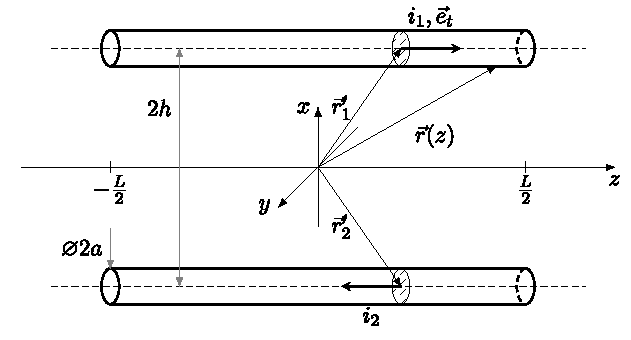
\includegraphics{res/LT17}
\end{center}
Der Aufpunktvektor $\vec{r}$ auf der Oberfläche des oberen Leiters bestimmt sich zu
\begin{equation}
	\vec{r}=(h-a) \vec{e}_{x}+z \vec{e}_{z} 
\end{equation}
während für die beiden Quellpunktvektoren $\vec{r}_{1}$ und $\vec{r}_{2}$ die Darstellung
\begin{equation}
	\vec{r}_{1 / 2}^{\prime}= \pm h \vec{e}_{x}+z^{\prime} \vec{e}_{z} 
\end{equation}
gilt. Die Abstände zum Aufpunkt bzw. die Beträge der beiden Differenzvektoren lauten folglich
\begin{align}
	& R_{1}:=\left|\vec{r}-\vec{r}_{1}\right|=\sqrt{a^{2}+\left(z-z^{\prime}\right)^{2}}  \\
	& R_{2}:=\left|\vec{r}-\vec{r}_{2}\right|=\sqrt{(2 h-a)^{2}+\left(z-z^{\prime}\right)^{2}} 
\end{align}
womit sich die Potentiale \ref{aleiter} und \ref{phileiter} in der Form (Achtung in $R_i$ steckt $z'$ drin)
\begin{align}
	 \ubar{\phi}(\vec{r})&=-\frac{\mathrm{j}}{4 \pi \varepsilon \omega} \int\limits_{-\frac{L}{2}}^{\frac{L}{2}}\left[\frac{\mathrm{e}^{-\mathrm{j} k R_{1}}}{R_{1}}-\frac{\mathrm{e}^{-\mathrm{j} k R_{2}}}{R_{2}}\right] \frac{\partial \ubar{I}\left(z^{\prime}\right)}{\partial z^{\prime}} \mathrm{d} z^{\prime}\label{LTform3}  \\
	\vec{\ubar{A}}(\vec{r})&=\frac{\mu}{4 \pi} \int\limits_{-\frac{L}{2}}^{\frac{L}{2}}\left[\frac{\mathrm{e}^{-\mathrm{j} k R_{1}}}{R_{1}}-\frac{\mathrm{e}^{-\mathrm{j} k R_{2}}}{R_{2}}\right] \ubar{I}\left(z^{\prime}\right) \vec{e}_{t}\left(z^{\prime}\right) \mathrm{d} z^{\prime} 
\end{align}
ausdrücken lassen. Mit der Randbedingung \ref{RBLT1} erhält man
\begin{equation}\begin{split}
	0=\vec{r}_{t}(z)(-\grad \ubar{\phi}-\mathrm{j} \omega \vec{\ubar{A}}) & =-\frac{\partial \ubar{\phi}}{\partial z}-\mathrm{j} \omega \vec{e}_{t}(z) \vec{\ubar{A}}  \\
	\frac{\partial \ubar{\phi}}{\partial z} & =-\mathrm{j} \omega \vec{e}_{t}(z) \vec{\ubar{A}} 
\end{split}\end{equation}
und kann somit schreiben
\begin{equation}\label{LTglsomit}
	\frac{\partial \ubar{\phi}}{\partial z}=-\mathrm{j} \omega \frac{\mu}{4 \pi} \int\limits_{-\frac{L}{2}}^{\frac{L}{2}}\left[\frac{\mathrm{e}^{-\mathrm{j} k R_{1}}}{R_{1}}-\frac{\mathrm{e}^{-\mathrm{j} k R_{2}}}{R_{2}}\right] \ubar{I}\left(z^{\prime}\right) \vec{e}_{t}(z) \vec{e}_{t}\left(z^{\prime}\right) \mathrm{d} z^{\prime} 
\end{equation}
Das Skalarprodukt der beiden Tangentialvektoren $\vec{e}_{t}(z) \vec{e}_{t}\left(z^{\prime}\right)$ innerhalb des Integrals ist dabei im allgemeinen Fall eines beliebig geformten Leiters ungleich Eins. Für das vorliegende Beispiel stimmen diese jedoch mit dem Einheitsvektor $\vec{e}_{z}$ überein und entfallen entsprechend. Durch Ausklammern von $\mathrm{e}^{-\mathrm{j} k R_{1}}$ vereinfacht man die Greensche Funktion im Integranden zu
\begin{equation}\label{greenfktintegrand}
	\frac{\mathrm{e}^{-\mathrm{j} k R_{1}}}{R_{1}}-\frac{\mathrm{e}^{-\mathrm{j} k R_{2}}}{R_{2}}=\mathrm{e}^{-\mathrm{j} k R_{1}}\left(\frac{1}{R_{1}}-\frac{\mathrm{e}^{-\mathrm{j} k\left(R_{2}-R_{1}\right)}}{R_{2}}\right) 
\end{equation}
Die Differenz der Abstände $R_{2}-R_{1}$ schätzt man nun unter Anwendung der Dreiecksungleichung $|\vec{a}-\vec{b}| \geq|\vec{a}|-|\vec{b}|$ zu
\begin{equation}
\begin{split}
	\left(\vec{r}-\vec{r}_{1}\right)-\left(\vec{r}-\vec{r}_{2}\right) & =-a \vec{e}_{x}+2 h \vec{e}_{x}+a \vec{e}_{x}=2 h \vec{e}_{x}  \\
	R_{2}-R_{1} & =\sqrt{(2 h-a)^{2}+\left(z-z^{\prime}\right)^{2}}-\sqrt{a^{2}+\left(z-z^{\prime}\right)^{2}} \leq 2 h 
\end{split}
\end{equation}
ab. Mit der Formulierung der Wellenzahl $k=\frac{2 \pi}{\lambda}$ und der Näherung $\lambda \gg 2 h$ kleiner Leiterabstände im Verhältnis zur Wellenlänge gilt für den Exponenten in Gleichung \ref{greenfktintegrand} also
\begin{equation}
	k\left(R_{2}-R_{1}\right) \leq \frac{2 \pi}{\lambda} 2 h=4 \pi \frac{h}{\lambda} \ll 1 
\end{equation}
Mithilfe die Reihenentwicklung des Exponentialterms gemäß
\begin{equation}
	\mathrm{e}^{x}=\sum_{k=0}^{\infty} \frac{x^{k}}{k!}=1+x+\frac{x^{2}}{2!}+\frac{x^{3}}{3!}+\ldots 
\end{equation}
wird deutlich, dass der Ausdruck $\mathrm{e}^{-\mathrm{j} k\left(R_{2}-R_{1}\right)} \approx 1$ ist. Das Integral in Gleichung \ref{LTglsomit} vereinfacht sich entsprechend
\begin{align}
	\int\limits_{-\frac{L}{2}}^{\frac{L}{2}}\left(\frac{1}{R_{1}}-\frac{1}{R_{2}}\right) \mathrm{e}^{-\mathrm{j} k R_{1}} \ubar{I}\left(z^{\prime}\right) \mathrm{d} z^{\prime} & \approx \int\limits_{-\frac{L}{2}}^{\frac{L}{2}}\left(\frac{1}{R_{1}}-\frac{1}{R_{2}}\right) \mathrm{e}^{-\mathrm{j} k a} \ubar{I}\left(z^{\prime}\right) \mathrm{d} z^{\prime}  \\
	& \stackrel{\mathrm{e}^{-\mathrm{j} k a} \approx 1}{\approx} \ubar{I}(z) \int\limits_{-\frac{L}{2}}^{\frac{L}{2}}\left(\frac{1}{R_{1}}-\frac{1}{R_{2}}\right) \mathrm{d} z^{\prime} 
\end{align}
Der letztere Näherungsschritt folgt dabei wiederum aus der Betrachtung für vergleichsweise große Wellenlängen, womit über große Leiterbereiche $z=z^{\prime}$ gilt und ein TEM-Mode der propagierenden Welle vorherrscht. Gleichfalls kann hierdurch der Leiterstrom bzw. die entsprechende Ableitung als konstant angenommen und aus der Integration gezogen werden. Die Spannung $\ubar{U}(z)$ an einer Stelle $z$ bestimmt sich letztlich aus der Potentialdifferenz zwischen den Leitern, wobei mit $\ubar{\phi}_{1}(z)=-\ubar{\phi}_{2}(z)$ (Symmetrie) die Relation
\begin{equation}
	\ubar{U}(z)=\ubar{\phi}_{1}(z)-\ubar{\phi}_{2}(z)=2 \ubar{\phi}_{1}(z) 
\end{equation}
folgt.
Aus \ref{LTglsomit} und \ref{LTform3} erhält man schließlich eine zu den Telegraphengleichungen äquivalente Darstellung der Form
\begin{align}
	 \frac{\partial \ubar{U}(z)}{\partial z}&=-\mathrm{j} \omega \underbrace{\frac{\mu}{2 \pi} \int_{-\frac{L}{2}}^{\frac{L}{2}}\left(\frac{1}{R_{1}}-\frac{1}{R_{2}}\right) \mathrm{d} z^{\prime} }_{=: L^{\prime}} \cdot \ubar{I}(z)  \\
	 \ubar{U}(z)&=\frac{\mathrm{j}}{2 \pi \varepsilon \omega} \int_{-\frac{L}{2}}^{\frac{L}{2}}\left(\frac{1}{R_{1}}-\frac{1}{R_{2}}\right) \mathrm{d} z^{\prime} \cdot \frac{\partial \ubar{I}(z)}{\partial z}  \\
	\rightarrow \quad \frac{\partial \ubar{I}(z)}{\partial z}&=-\mathrm{j} \omega 2 \pi \varepsilon \frac{1}{\underbrace{\int_{-\frac{L}{2}}^{\frac{L}{2}}\left(\frac{1}{R_{1}}-\frac{1}{R_{2}}\right) \mathrm{d} z^{\prime}}_{:=C^{\prime}}} \cdot \ubar{U}(z) 
\end{align}
mit $L^{\prime}$ als Induktivitätsbelag und $C^{\prime}$ als Kapazitätsbelag der Leitung. Im Falle eines unendlich langen Leiters mit $L \rightarrow \infty$ ergibt sich für jene Leitungsgrößen
\begin{align}
	L^{\prime} & =\frac{\mu}{2 \pi} \int_{-\infty}^{\infty}\left(\frac{1}{R_{1}}-\frac{1}{R_{2}}\right) \mathrm{d} z^{\prime}=\frac{\mu}{2 \pi} \ln \left(\frac{2 h}{a}\right)  \\
	C^{\prime} & =2 \pi \varepsilon\left[\int_{-\infty}^{\infty}\left(\frac{1}{R_{1}}-\frac{1}{R_{2}}\right) \mathrm{d} z^{\prime}\right]^{-1}=\frac{2 \pi \varepsilon}{\ln \left(\frac{2 h}{a}\right)} 
\end{align}



\iffalse\subsection{Klassische Leitungstheorie}\label{leitungstheorie}
\begin{itemize}
	\item Die \textbf{klassische Leitungstheorie} dient der Beschreibung von \textbf{langen Leitungen} mittels \textbf{Strom und Spannung}.
	\item Von einer \textbf{langen Leitung} spricht man, wenn die Länge der Leitung nicht mehr als klein im Vergleich zur \textbf{Wellenlänge} angesehen werden kann.
	\centerline{%
		\begin{tabular}{c||c|c|c|c|c|c}
			$f$                                   & $50\mathrm{Hz}$      & $1\mathrm{kHz}$    & $100\mathrm{MHz}$ & $1\mathrm{GHz}$   & $10\mathrm{GHz}$ \\
			\hline
			$\lambda_{\text{Vakuum}}=\frac{c}{f}$ & $5995.8 \mathrm{km}$ & $299.8\mathrm{km}$ & $2.99\mathrm{m}$  & $29.9\mathrm{cm}$ & $2.9\mathrm{cm}$
	\end{tabular}}
	\item Im einfachsten Fall wird die Leitung als \textbf{verlustlose, homogene Einfachleitung} angesehen. Es handelt sich also um einen \textbf{zylindrischen Wellenleiter}.
	\item Das Querschnittsgebiet ist \textbf{nicht einfach zusammenhängend} und daher existiert ein (quasi) {TEM-Mode}.
	\item Nur der TEM-Mode wird betrachtet: daher kann mit \textbf{Spannungen in der Transversalebene} gerechnet werden.
	\item Verallgemeinerungen bis hin zu einer \textbf{full-wave} Beschreibung sind möglich!
	\item Beispielstrukturen, die gerne mit Leitungstheorie beschrieben werden: Koaxialkabel, Zweidrahtleitung, Mikrostreifenleitung
\end{itemize}
\subsection{Ausgangspunkt}
\begin{itemize}
	\item Ziel ist die Entwicklung eines \textbf{Ersatzschaltbilds} für ein \textbf{differentielles Leitungselement}.
	\item Ausgangspunkt ist feldtheoretische Beschreibung für den \textbf{verlustlosen Fall}.
	\item Das Ersatzschaltbild kann dann einfach \textbf{verallgemeinert} werden.
	\item Maxwellgleichungen (lin. hom. iso. Dielektrikum, harmonische ZA, keine Quellen):
	\begin{align}
		\div \ubar{\vec{E}} & = 0 & \rot \ubar{\vec{E}} + \mathrm{j}\omega\mu \vec{\ubar{H}}         & =\vec{0} \\
		\div \vec{\ubar{H}} & = 0 & \rot \vec{\ubar{H}} - \mathrm{j}\omega\varepsilon \ubar{\vec{E}} & =\vec{0}
	\end{align}
	\item Wir betrachten nur den \textbf{TEM-Mode}. Die \textbf{Ausbreitungsrichtung} sei \(\pm\vu{z}\). Es gilt:
	\begin{align}
		\text{TEM-Mode: } &  & \ubar{\vec{E}}\cdot \vu{z}                    & =0                                           & \vec{\ubar{H}}\cdot \vu{z}                    & =0                                           \\
		&  & \left( \rot \ubar{\vec{E}}\right)\times\vu{z} & = \frac{\partial \ubar{\vec{E}}}{\partial z} & \left( \rot \vec{\ubar{H}}\right)\times\vu{z} & = \frac{\partial \vec{\ubar{H}}}{\partial z}
	\end{align}
	\begin{equation}
		\text{Transversalebene: }  \rot _t\ubar{\vec{E}} = \left( \frac{\partial \ubar{E}_y}{\partial x}-\frac{\partial \ubar{E}_x}{\partial y}\right)\vu{z} \Rightarrow\left(\rot _t\ubar{\vec{E}}\right)\cdot\vu{x,y} =0
	\end{equation}
\end{itemize}
\subsection{Felder -- Transversalebene (\(z=\text{const.}\))}
\begin{itemize}
	\item Transversalkomponente des Induktionsgesetztes (in der Transversalebene):
	\begin{align}
		\rot \ubar{\vec{E}} + \mathrm{j}\omega\mu\vec{\ubar{H}} & =\vec{0} \Rightarrow & \left(\rot \ubar{\vec{E}}\right)\times\vu{z} + \mathrm{j}\omega\mu\vec{\ubar{H}} \times\vu{z}       & =\vec{0}  \\
		&                      & \Aboxed{\frac{\partial \ubar{\vec{E}}}{\partial z} + \mathrm{j}\omega\mu\vec{\ubar{H}} \times\vu{z} & =\vec{0}}
	\end{align}
	\item Das elektrische Feld ist ein \textbf{Gradientenfeld} in allen Transversalebenen. Ansatz:
	\begin{equation}
		\boxed{\ubar{\vec{E}} = -\grad \phi(x,y) \; g(z)} \text{ mit } \boxed{\Delta \phi(x,y) = 0} \text{ statische 2D Laplace Gleichung}
	\end{equation}
	\item Magnetfeld direkt ausrechnen:
	\begin{align}
		\frac{\partial \ubar{\vec{E}}}{\partial z} + \mathrm{j}\omega\mu\vec{\ubar{H}} \times\vu{z} & =\vec{0} & \Rightarrow \vu{z}\times\frac{\partial \ubar{\vec{E}}}{\partial z} & + \mathrm{j}\omega\mu\, \vu{z}\times\left(\vec{\ubar{H}} \times\vu{z}\right) =\vec{0}                \\
		&          & \vec{\ubar{H}}                                                     & = -\frac{1}{\mathrm{j}\omega\mu} \left(\vu{z}\times\frac{\partial \ubar{\vec{E}}}{\partial z}\right) \\
		&          & \Aboxed{\vec{\ubar{H}}                                             & = \frac{1}{\mathrm{j}\omega\mu} \left(\vu{z}\times\grad \phi\right)\frac{\partial g}{\partial z}}
	\end{align}
\end{itemize}
\subsection{Übergang zu Strom und Spannung}
\begin{center}
	\begin{tikzpicture}
	\draw[thin,-stealth] (-1.5,0) -- (+1.5,0) node[below]{$x$};
	\draw[thin,-stealth] (0,-1.5) -- (0,+1.5) node[right]{$y$};
	\draw[fill=black] (1,-0.7) circle (0.1);
	\draw[fill=green!20,draw=green,thick] (-0.9,0.9) circle (0.3) node[color=green,below,yshift=-8]{$O(A)$};
	\draw[fill=black] (-0.9,0.9) circle (0.1);
	\draw[thick,red,-stealth] (1,-0.6) .. controls (1,.2) and (-0.1,0.9) .. (-0.8,0.9) node[midway,right,yshift=3] {$C$};
	\draw[color=green!50] (-0.9,1.05) -- (-0.85,1.4) node[color=green!50,above]{$A$};
	\draw[thick, fill=white] (0,0) circle (0.08) node[anchor=north east]{$z$};
	\draw[thick, fill=black] (0,0) circle (0.03);
\end{tikzpicture}
\end{center}

\begin{itemize}
	\item Stromdichte konstant im Leiterquerschnitt \(\to\) \textbf{Dünndrahtnäherung}
	\item Perfekte Leiter: \(\kappa \to \infty\)
	\item Rotationsfreiheit des elektrischen Felds in der Transversalebene \(\to\) \textbf{Spannung}:
	\begin{equation}
		\ubar{U} = \int\limits_C \ubar{\vec{E}} \cdot \dd \vec{s} \; \text{ mit \(z =\) const. auf \(C\)}
	\end{equation}
	\item Aus dem Durchflutungsgesetz \(\to\) \textbf{Strom:}
	\begin{equation}
		\ubar{I} = \oint\limits_{O(A)} \vec{\ubar{H}} \cdot \dd\vec{s}
	\end{equation}
\end{itemize}

\begin{itemize}
	\item Damit können die Ausdrücke für die Felder umgeformt werden:
	\begin{equation}
		\frac{\partial \ubar{\vec{E}}}{\partial z} + \mathrm{j}\omega\mu\vec{\ubar{H}} \times\vu{z} =\vec{0} \quad\text{und}\quad \vec{\ubar{H}}= \frac{1}{\mathrm{j}\omega\mu} \left(\vu{z}\times\grad \phi\right)\frac{\partial g}{\partial z}
	\end{equation}
	\item Ausdrücke für die Felder:
	\begin{equation}
		\frac{\partial \ubar{\vec{E}}}{\partial z} + \mathrm{j}\omega\mu\vec{\ubar{H}} \times\vu{z} =\vec{0} \quad\text{und}\quad \vec{\ubar{H}}= \frac{1}{\mathrm{j}\omega\mu} \left(\vu{z}\times\grad \phi\right)\frac{\partial g}{\partial z}
	\end{equation}
	\item Wir bilden das Wegintegral der ersten Gleichung entlang \(C\) und setzen dann \(\vec{\ubar{H}}\) ein:
	\begin{equation}\begin{split}
			\int\limits_C \frac{\partial \ubar{\vec{E}}}{\partial z} \cdot \dd \vec{s} + \mathrm{j}\omega\mu \int\limits_C\left(\vec{\ubar{H}} \times\vu{z}\right) \cdot \dd \vec{s} &= 0  \\
			\Aboxed{\frac{\partial  \ubar{U}}{\partial z} + \frac{\partial g}{\partial z} \int\limits_C\grad \phi \cdot \dd \vec{s} = 0}
	\end{split}\end{equation}
	\item Weiter gilt für den Strom:
	\begin{align}
		II = \oint\limits_{O(A)} \vec{\ubar{H}} \cdot \dd\vec{s} & = \oint\limits_{O(A)} \frac{1}{\mathrm{j}\omega\mu} \left(\vu{z}\times\grad \phi\right)\frac{\partial g}{\partial z} \cdot \dd\vec{s} \\
		\Rightarrow \Aboxed{\frac{\partial g}{\partial z}        & = \mathrm{j}\omega\mu \frac{ \ubar{I}}{\oint\limits_{O(A)} \left(\vu{z}\times\grad \phi\right) \cdot \dd\vec{s}}}
	\end{align}
	\item Wir betrachten die Formeln
	\begin{equation}
		\frac{\partial  \ubar{U}}{\partial z} + \frac{\partial g}{\partial z} \int\limits_C\grad \phi \cdot \dd \vec{s} = 0 \text{ und } \frac{\partial g}{\partial z} = \mathrm{j}\omega\mu \frac{ \ubar{I}}{\oint\limits_{O(A)} \left(\vu{z}\times\grad \phi\right) \cdot \dd\vec{s}}
	\end{equation}
	\item Einsetzen der rechten in die linke Gleichung eliminiert offensichtlich die unbekannte Funktion \(g(z)\) und wie erhalten die \textbf{erste Leitungsgleichung} (Telegraphengleichung):
	\begin{equation}
		\frac{\partial  \ubar{U}(z)}{\partial z} + \mathrm{j}\omega \underbrace{\frac{\mu\int\limits_C\grad \phi \cdot \dd \vec{s}}{\oint\limits_{O(A)} \left(\vu{z}\times\grad \phi\right) \cdot \dd\vec{s}}}_{L^\prime}  \ubar{I}(z)=\boxed{\frac{\partial  \ubar{U}(z)}{\partial z} + \mathrm{j}\omega L^\prime  \ubar{I}(z)= 0} \quad [L^\prime] = \mathrm{\frac{H}{m}}
	\end{equation}
	\item Der \textbf{Induktivitätsbelag} der Leitung \(L^\prime\) ist vollständig bestimmt durch die Lösung des statischen 2D Laplace-Randwertproblems für \(\phi\) im Lösungsvolumen \(V\)
	\begin{equation}
		\Delta \phi(x,y) = 0 \text{ mit }  \phi = 0 \text{ auf einem Leiter und } \phi =  U(z) \text{ auf dem anderen Leiter}
	\end{equation}
	
	\item Analog folgt die \textbf{zweite Leitungsgleichung} aus den Formeln:
	\begin{equation}
		\frac{\partial \vec{\ubar{H}}}{\partial z} - \mathrm{j}\omega\varepsilon\ubar{\vec{E}} \times\vu{z} =\vec{0} \text{ und } \ubar{\vec{E}} = -\grad \phi \; g(z)
	\end{equation}
	\item Umlaufintegral der ersten Gleichung entlang \(O(A)\) und Einsetzen von \(\ubar{\vec{E}}\) ergibt:
	\begin{equation}\begin{split}
			\oint\limits_{O(A)} \frac{\partial \vec{\ubar{H}}}{\partial z} \cdot \dd \vec{s} - \mathrm{j}\omega\varepsilon \oint\limits_{O(A)}\left(\ubar{\vec{E}} \times\vu{z}\right) \cdot \dd \vec{s} &= 0  \\
			\frac{\partial  \ubar{I}}{\partial z} -\mathrm{j}\omega\varepsilon\; g(z) \oint\limits_{O(A)}\left(\vu{z}\times \grad \phi\right) \cdot \dd \vec{s} &= 0
	\end{split}\end{equation}
	\item Die Funktion \(g(z)\) folgt sofort aus \( \ubar{U}\):
	\begin{equation}
		\ubar{U} = \int\limits_C \ubar{\vec{E}}\cdot\dd\vec{s} = -g(z) \int\limits_C \grad \phi\cdot\dd\vec{s} \to g(z) = -\frac{ \ubar{U}}{\int\limits_C \grad \phi\cdot\dd\vec{s}}
	\end{equation}
	\item Damit lautet die \textbf{zweite Leitungsgleichung}:
	\begin{equation}
		\frac{\partial  \ubar{I}}{\partial z} +\mathrm{j}\omega \underbrace{\frac{\varepsilon\oint\limits_{O(A)}\left(\vu{z}\times \grad \phi\right) \cdot \dd \vec{s}}{\int\limits_C \grad \phi\cdot\dd\vec{s}}}_{C^\prime}  \ubar{U} = 0 \quad [C^\prime]=\mathrm{\frac{F}{m}}
	\end{equation}
\end{itemize}
\subsection{Leitungsgleichungen -- Leitungsbeläge}
\begin{itemize}
	\item Zusammenfassend haben wir für verlustlose Leitungen die folgenden \textbf{Leitungsgleichungen} gefunden:
	\begin{align}
		\frac{\partial  \ubar{U}(z)}{\partial z} + \mathrm{j}\omega L^\prime  \ubar{I}(z) & = 0 & L^\prime & =\frac{\mu\int\limits_C\grad \phi \cdot \dd \vec{s}}{\oint\limits_{O(A)} \left(\vu{z}\times\grad \phi\right) \cdot \dd\vec{s}}         \\
		\frac{\partial  \ubar{I}(z)}{\partial z} +\mathrm{j}\omega C^\prime  \ubar{U}(z)  & = 0 & C^\prime & = \frac{\varepsilon\oint\limits_{O(A)}\left(\vu{z}\times \grad \phi\right) \cdot \dd \vec{s}}{\int\limits_C \grad \phi\cdot\dd\vec{s}}
	\end{align}
	\item Offensichtlich gilt
	\begin{equation}
		L^\prime C^\prime = \varepsilon\mu = \frac{1}{ v_\mathrm{p}^2} \Rightarrow \boxed{ v_\mathrm{p} = \frac{1}{\sqrt{L^\prime C^\prime}}}
	\end{equation}
	\item Entkoppelte Gleichungen:
	\begin{equation}
		\frac{\partial^2  \ubar{U}(z)}{\partial z^2} + \omega^2 L^\prime C^\prime  \ubar{U}(z) = 0 \text{ und } \frac{\partial^2  \ubar{I}(z)}{\partial z^2} + \omega^2 L^\prime C^\prime  \ubar{I}(z) = 0
	\end{equation}
	\item Die Lösungen sind (natürlich) vor- und zurücklaufende Wellen (als ruhende Zeiger):
	\begin{equation}
		\ubar{U}(z) =  \ubar{U}_0  \mathrm{e}^{\pm\mathrm{j}kz} \text{ und }  \ubar{I}(z) =  \ubar{I}_0  \mathrm{e}^{\pm\mathrm{j}kz}
	\end{equation}
\end{itemize}
\subsection{Übergang zum Ersatzschaltbild}
\begin{center}
	\ctikzset{voltage/bump b=1.1}
\begin{circuitikz}[european voltages,scale=.75]
	\draw (0,0) to[short,o-o] (4,0);
	\draw (0,2) to [short, i=$\ubar{I}(z)$,o-] (1,2) to[L=L,-] (3,2) coordinate(a);
	\draw (a) to[short, i=$\ubar{I}(z+\Delta z)$,-o]  (4,2);
	\draw (a) to[C,l_=C,*-*] ++(0,-2);

	% Voltage labels
	\draw (0,2) to[open,v=$\ubar{U}(z)$] ++(0,-2);
	\draw (4,2) to[open, v^=$\ubar{U}(z+\Delta z)$] ++(0,-2);
\end{circuitikz}
\end{center}

\begin{itemize}
	\item Maschensatz:
	\begin{equation}\begin{split}
			\ubar{U}(z) = \mathrm{j}\omega L  \ubar{I}(z) +  \ubar{U}(z+\Delta z)\\
			\ubar{U}(z+\Delta z) - \ubar{U}(z) + \mathrm{j}\omega L  \ubar{I}(z) =0  \\
			\frac{\Delta  \ubar{U}}{\Delta z} + \mathrm{j}\omega \frac{L}{\Delta z}  \ubar{I}(z) =0
	\end{split}\end{equation}
	
	\item Knotensatz:
	\begin{equation}
		\ubar{I}(z+\Delta z) =  \ubar{I}(z) - \mathrm{j}\omega C  \ubar{U}(z+\Delta z) \Rightarrow \frac{\Delta  \ubar{I}}{\Delta z} + \mathrm{j}\omega \frac{C}{\Delta z}  \ubar{U}(z+\Delta z) = 0
	\end{equation}
	\item Im Grenzfall \(\Delta z \to 0\) und mit \(C^\prime=\lim_{\Delta z \to 0} \frac{C}{\Delta z}\) und \(L^\prime=\lim_{\Delta z \to 0} \frac{L}{\Delta z}\) ist der obige Vierpol das \textbf{Ersatzschaltbild eines differentiellen Stückes einer verlustlosen Leitung.}
	\item Verallgemeinerung für \textbf{verlustbehaftete} Leitungen:
	\begin{center}
		\ctikzset{voltage/bump b=1.1}
\ctikzset{bipoles/length=.7cm}
\begin{circuitikz}[european voltages,scale=.75]
	\draw (0,0) to[short,o-o] (7,0);
	\draw (0,1.5) to [short, i=$\ubar{I}(z)$,o-] (1,1.5) to[R=$R^\prime \dd z$] (2,1.5) to[L=$L^\prime \dd z$,-] (4,1.5) coordinate(a);
	\draw (a) to[short, -] (5,1.5) coordinate(b);
	\draw (b) to[short, i=$\ubar{I}(z+\dd z)$,-o]  (7,1.5);
	\draw (a) to[C,l_=$C^\prime \dd z$,*-*] ++(0,-1.5);
	\draw (b) to[R,l=$G^\prime \dd z$,*-*] ++(0,-1.5);

	% Voltage labels
	\draw (0,1.5) to[open,v=$\ubar{U}(z)$] ++(0,-1.5);
	\draw (7,1.5) to[open, v^=$\ubar{U}(z+\dd z)$] ++(0,-1.5);
\end{circuitikz}
	\end{center}
	
\end{itemize}
\subsection{Verlustbehaftete Leitungen}
\begin{itemize}
	\item Aus dem Ersatzschaltbild ergeben sich die \textbf{Leitungsgleichungen für verlustbehaftete Leitungen}.
	\begin{align}
		\frac{\partial  \ubar{U}(z)}{\partial z} + \left(R^\prime + \mathrm{j}\omega L^\prime\right)  \ubar{I}(z) & = 0 & L^\prime & =\frac{\mu\int\limits_C\grad \phi \cdot \dd \vec{s}}{\oint\limits_{O(A)} \left(\vu{z}\times\grad \phi\right) \cdot \dd\vec{s}}         \\
		\frac{\partial  \ubar{I}(z)}{\partial z} +\left(G^\prime + \mathrm{j}\omega C^\prime\right)  \ubar{U}(z)  & = 0 & C^\prime & = \frac{\varepsilon\oint\limits_{O(A)}\left(\vu{z}\times \grad \phi\right) \cdot \dd \vec{s}}{\int\limits_C \grad \phi\cdot\dd\vec{s}}
	\end{align}
	\item Der \textbf{Widerstandsbelag} \(R^\prime\) entspricht den ohmschen Leitungsverlusten pro Längeneinheit.
	\item Der \textbf{Leitwertbelag} \(G^\prime\)  entspricht den dielektrischen Verlusten pro Längeneinheit.
	\item Zusammengefasst spricht man auch vom \textbf{Impedanzbelag} \(Z^\prime = R^\prime + \mathrm{j}\omega L^\prime\) und vom \textbf{Admittanzbelag} \(Y^\prime = G^\prime + \mathrm{j}\omega C^\prime\)
\end{itemize}
\subsection{Allgemeine Lösung -- Leitungswellenwiderstand}
\begin{itemize}
	\item Wir können die entkoppelten Leitungsgleichungen jetzt auch allgemein hinschreiben:
	\begin{equation}
		\frac{\partial^2  \ubar{U}(z)}{\partial z^2} -  Z^\prime Y^\prime  \ubar{U}(z) = 0 \text{ und } \frac{\partial^2  \ubar{I}(z)}{\partial z^2} -  Z^\prime Y^\prime  \ubar{I}(z) = 0
	\end{equation}
	\item Ansatz:
	\begin{equation}
		\ubar{U}(z) = u  \mathrm{e}^{\pm\ubar{\gamma} z} \Rightarrow \ubar{\gamma} = \sqrt{Z^\prime Y^\prime} = \sqrt{\left(R^\prime + \mathrm{j}\omega L^\prime\right) \left(G^\prime + \mathrm{j}\omega C^\prime\right)} \text{ Ausbreitungskonstante}
	\end{equation}
	\item Mit der Spannung \( \ubar{U}(z) = u_1  \mathrm{e}^{-\ubar{\gamma} z} + u_2  \mathrm{e}^{\ubar{\gamma} z}\) ergibt sich der Strom zu
	\begin{equation}
		\ubar{I}(z) = - \frac{1}{Z^\prime} \frac{\partial  \ubar{U}(z)}{\partial z} = \frac{\ubar{\gamma}{Z^\prime} \left( u_1  \mathrm{e}^{-\ubar{\gamma} z} - u_2  \mathrm{e}^{\ubar{\gamma} z}\right) = \frac{1}{Z_L} \left( u_1  \mathrm{e}^{-\ubar{\gamma} z} - u_2  \mathrm{e}^{\ubar{\gamma} z}\right)
	\end{equation}
	\item Hierbei ist \(Z_L\) der \textbf{Leitungswellenwiderstand}:
	\begin{equation}
		Z_L= \frac{Z^\prime}{\ubar{\gamma} = \sqrt{\frac{Z^\prime}{Y^\prime}} = \sqrt{\frac{R^\prime + \mathrm{j}\omega L^\prime}{G^\prime + \mathrm{j}\omega C^\prime}}
	\end{equation}
	\item Abschluss mit Leitungswellenwiderstand \(\to\) Eingangsimpedanz = Leitungswellenwiderstand \(\to\) \textbf{keine Reflexion}
\end{itemize}
\subsection{Matrixschreibweise -- Mehrfachleitungen}
\begin{itemize}
	\item Die gefundenen Leitungsgleichungen werden üblicherweise in eine \textbf{Matrixgleichung} zusammengefasst:
	\begin{equation}
		\left.
		\begin{array}{rl}
			\frac{\partial  \ubar{U}(z)}{\partial z} + \left(R^\prime + \mathrm{j}\omega L^\prime\right)  \ubar{I}(z) & = 0 \\
			\frac{\partial  \ubar{I}(z)}{\partial z} +\left(G^\prime + \mathrm{j}\omega C^\prime\right)  \ubar{U}(z)  & = 0
		\end{array}\right\} \Rightarrow
		\frac{\partial}{\partial z}\begin{pmatrix} \ubar{U}(z)\\ \ubar{I}(z) \end{pmatrix}
		+
		\begin{pmatrix}
			0        & Z^\prime \\
			Y^\prime & 0
		\end{pmatrix}
		\begin{pmatrix} \ubar{U}(z)\\ \ubar{I}(z) \end{pmatrix} = 0
	\end{equation}
	\item Die Matrixgleichung ist sofort für \textbf{Mehrfachleitungen} verallgemeinbar. Hierzu bilden wir
	\begin{itemize}
		\item den Vektor der Spannungen relativ zum Bezugsleiter \(\vec{ \ubar{U}}(z) = \left( \ubar{U}_1(z),\ldots ,  \ubar{U}_n(z) \right)^T\).
		\item den Vektor der Ströme im Leiter  \(\vec{ \ubar{I}}(z) = \left( \ubar{I}_1(z),\ldots ,  \ubar{I}_n(z) \right)^T\).
		\item die Matrix mit den Impedanzbelägen in der Hauptdiagonalen \(\left(Z^\prime\right)\)
		\item die Matrix mit den Admittanzbelägen in der Hauptdiagonalen \(\left(Y^\prime\right)\)
		\begin{equation}
			\frac{\partial}{\partial z}\begin{pmatrix}\vec{ \ubar{U}}(z)\\\vec{ \ubar{I}}(z) \end{pmatrix}
			+
			\begin{pmatrix}
				0                            & \left(Z^\prime\right) \\
				\left(Y^\prime\right)^\prime & 0
			\end{pmatrix}
			\begin{pmatrix}\vec{ \ubar{U}}(z)\\\vec{ \ubar{I}}(z) \end{pmatrix} = 0
		\end{equation}
		
	\end{itemize}
\end{itemize}
\subsection{Bemerkungen}
\begin{itemize}
	\item Die Leitungstheorie kann hier nur angerissen werden.
	\item Die Anwendungen sind extrem vielfältig: Beschreibung von Leitungen, Impedanztransformationen, Anpassungen, Filter, \dots
	\item Vierpolparameter: Z, S, Y \(\to\) bekannt aus Grundlagen (Vierpole)
	\item \textbf{Ungleichförmige Leitungen}: ortsabhängigen Leitungsbeläge
	\item Wichtigste Einschränkung der klassischen Leitungstheorie: \textbf{nur TEM-Mode}
	\item Deshalb auch: Abstrahlung und Einkopplung in Leitungen nur bedingt beschreibbar.
	\item Lösung: \textbf{Transmission Line Super Theory (TLST)}, z.B. F. Ossevorth, R. Jacobs, H.G. Krauthäuser,
	\enquote{A full wave description for thin wire structures with TLST and perturbation theory}, Advances in Radio Science (16), 123--133, 2018. \url{https://ars.copernicus.org/articles/16/123/2018/}, DOI = 10.5194/ars-16-123-2018 und dort zitierte Arbeiten (insbesondere: S. Tkachenko und J. Nitsch)
\end{itemize}
\subsection{Netzwerkbeschreibung mithilfe der Baum-Liu-Tesche-Gleichung}
Neben der Beschreibung von Leitungen mit den Telegrafengleichungen besteht ebenfalls die Möglichkeit der Modellierung eines Netzwerkes unter Nutzung der sogenannten Baum-Liu-Tesche-Gleichung (benannt nach Begründern, kurz BLT-Gleichung). Hierbei werden Leitungen an ihren Abschlüssen ausgewertet, sodass eine umfassende Berechnung komplexer Netzwerke möglich ist.

Man betrachte das folgende Netzwerk mit einer Spannungs- oder einer Stromeinkopplung $U_{0}$ bzw. $I_{0}$ an einer beliebigen Stelle $z_{\mathrm{S}}$ der Leitung.

\begin{center}
	\includegraphics{res/LT6}
\end{center}

Darin bezeichnen die eingezeichneten Spannungen $U^{+}(0)=U_{1}^{\text {refl }}$ und $U^{-}(0)=U_{1}^{\text {inc }}$ die reflektierte und in positive $z$-Richtung propagierende bzw. die inzidente und in negative $z$-Richtung laufende Welle am Leitungsanfang (Tor 1) bei $z=0$. Gleichermaßen stellen $U^{+}(L)=U_{2}^{\text {inc }}$ und $U^{-}(L)=U_{2}^{\text {refl }}$ die inzidente bzw. reflektierte Welle am Leitungsende bei $z=L$ (Tor 2) dar.

Zunächst soll zur Berechnung der Spannung $U(z)$ an einer Stelle $z$ der Leitung mit konzentrierten Schaltungselementen gerechnet werden. Die dargestellten Impedanzen $Z_{1}$ und $Z_{2}$ sind dabei entsprechend als zusammengefasste Leitungsimpedanzen der Übertragungsleitung aufzufassen. Als Ansatz für die Spannung am Ort $z \in\left[z_{S} ; L\right]$ wählt man nun die Superposition einer in $z$-Richtung fortschreitenden und einer am Leitungsende reflektierten und in entgegengesetzte Richtung laufenden Welle gemäß


\begin{equation}\label{LTreflwell}
	U(\tilde{z})=\left(\tilde{U}+Z_{\mathrm{C}} \tilde{I}\right)\left(\mathrm{e}^{-\ubar{\gamma} \tilde{z}}+r_{2} \mathrm{e}^{+\ubar{\gamma} \tilde{z}}\right) \quad \text { für } \quad z_{\mathrm{S}}-L \leq \tilde{z} \leq 0 
\end{equation}


mit der Notation $\tilde{z}=z-L=-(L-z)$. Der vorangestellte Klammerterm ist ein konstanter Vorfaktor, welcher die noch unbekannten Integrationskonstanten $\tilde{U}$ und $\tilde{I}$ als Wirkung der beiden Anregungsquellen beinhaltet. Diese lassen sich aus den Randbedingungen am Erregungsort bestimmen, wobei die auftretende Gesamtspannung als Summe der Spannungswirkungen von Spannungs- und Stromquelle durch


\begin{equation}
	U\left(z_{\mathrm{S}}-L\right)=\underbrace{U_{1}\left(z_{\mathrm{S}}-L\right)}_{\text {Spannungsquelle }}+\underbrace{U_{2}\left(z_{\mathrm{S}}-L\right)}_{\text {Stromquelle }} 
\end{equation}


ausgedrückt und die Spannungs- bzw. Stromteilerregel zur Lösung angewendet wird. Für ersteren Summanden gilt dann


\begin{equation}\label{summand1LT}
	U_{1}\left(z_{\mathrm{S}}-L\right)=\tilde{U}\left(\mathrm{e}^{-\ubar{\gamma}\left(z_{\mathrm{S}}-L\right)}+r_{2} \mathrm{e}^{+\ubar{\gamma}\left(z_{\mathrm{S}}-L\right)}\right)=U_{0} \frac{Z_{2}}{Z_{1}+Z_{2}} 
\end{equation}

mit den Leitungsimpedanzen


\begin{equation}
	Z_{1}=\frac{U\left(z_{\mathrm{S}}\right)}{I\left(z_{\mathrm{S}}\right)}=Z_{\mathrm{C}} \frac{1+r_{1} \mathrm{e}^{-2 \ubar{\gamma} z_{\mathrm{S}}}}{1-r_{1} \mathrm{e}^{-2 \ubar{\gamma} z_{\mathrm{S}}}} \quad \text { und } \quad Z_{2}=\frac{U\left(z_{\mathrm{S}}-L\right)}{I\left(z_{\mathrm{S}}-L\right)}=Z_{\mathrm{C}} \frac{1+r_{2} \mathrm{e}^{2 \ubar{\gamma}\left(z_{\mathrm{S}}-L\right)}}{1-r_{2} \mathrm{e}^{2 \ubar{\gamma}\left(z_{\mathrm{S}}-L\right)}} 
\end{equation}


für die Abschnitte links und rechts der Einkopplung. Somit erhält man aus \ref{summand1LT} den Ausdruck


\begin{equation}
	\frac{\tilde{U}}{U_{0}}=\frac{Z_{2}}{Z_{1}+Z_{2}} \cdot \frac{1}{\mathrm{e}^{-\ubar{\gamma}\left(z_{\mathrm{s}}-L\right)}+r_{2} \mathrm{e}^{+\ubar{\gamma}\left(z_{\mathrm{s}}-L\right)}} 
\end{equation}


Analog folgt für den zweiten Summanden


\begin{align}
	U_{2}\left(z_{\mathrm{S}}-L\right) & =Z_{\mathrm{C}} \tilde{I}\left(\mathrm{e}^{-\ubar{\gamma}\left(z_{\mathrm{s}}-L\right)}-r_{2} \mathrm{e}^{+\ubar{\gamma}\left(z_{\mathrm{S}}-L\right)}\right)=Z_{\mathrm{C}} I_{0} \cdot \frac{Z_{1}}{Z_{1}+Z_{2}}  \\
	\frac{\tilde{I}}{I_{0}} & =\frac{Z_{1}}{Z_{1}+Z_{2}} \cdot \frac{1}{\mathrm{e}^{-\ubar{\gamma}\left(z_{\mathrm{s}}-L\right)}+r_{2} \mathrm{e}^{+\ubar{\gamma}\left(z_{\mathrm{S}}-L\right)}} 
\end{align}


Die Konstanten bestimmt man damit zu


\begin{align}
	& \tilde{U}=U_{0} \frac{\frac{1+r_{2} \mathrm{e}^{2 \ubar{\gamma}\left(z_{\mathrm{S}}-L\right)}}{1-r_{2} \mathrm{e}^{\ubar{\gamma} \ubar{\gamma}\left(z_{\mathrm{s}}-L\right)}}}{\frac{1+r_{1} \mathrm{e}^{-2 \ubar{\gamma} z_{\mathrm{S}}}}{1-r_{1} \mathrm{e}^{-2 \ubar{\gamma} z_{\mathrm{S}}}}+\frac{1+r_{2} \mathrm{e}^{2 \ubar{\gamma}\left(z_{\mathrm{S}}-L\right)}}{1-r_{2} \mathrm{e}^{2 \ubar{\gamma}\left(z_{\mathrm{S}}-L\right)}}} \cdot \frac{1}{\mathrm{e}^{-\ubar{\gamma}\left(z_{\mathrm{S}}-L\right)}+r_{2} \mathrm{e}^{+\ubar{\gamma}\left(z_{\mathrm{S}}-L\right)}}  \\
	& =\ldots=U_{0} \frac{1-r_{1} \mathrm{e}^{-2 \ubar{\gamma} z_{\mathrm{S}}}}{2\left(1-r_{1} r_{2} \mathrm{e}^{-2 \ubar{\gamma} L}\right)} \mathrm{e}^{\ubar{\gamma}\left(z_{\mathrm{S}}-L\right)}  \\
	& \tilde{I}=I_{0} \frac{1+r_{1} \mathrm{e}^{-2 \ubar{\gamma} z_{\mathrm{S}}}}{2\left(1-r_{1} r_{2} \mathrm{e}^{-2 \ubar{\gamma} L}\right)} \mathrm{e}^{\ubar{\gamma}\left(z_{\mathrm{S}}-L\right)} 
\end{align}


Einsetzen in die Ausgangsgleichung \ref{LTreflwell} führt auf einen Ausdruck für die Spannung und den Strom im Bereich zwischen Erregungsort $z=z_{\mathrm{S}}$ und Port 2 bei $z=L$


\begin{align}
	U(z) & =\frac{\mathrm{e}^{-\ubar{\gamma} z}+r_{2} \mathrm{e}^{\ubar{\gamma}(z-2 L)}}{2\left(1-r_{1} r_{2} \mathrm{e}^{-2 \ubar{\gamma} L}\right)}\left[U_{0}\left(\mathrm{e}^{\ubar{\gamma} z \mathrm{~s}}-r_{1} \mathrm{e}^{-\ubar{\gamma} z \mathrm{~s}}\right)+Z_{\mathrm{C}} I_{0}\left(\mathrm{e}^{\ubar{\gamma} z \mathrm{~s}}+r_{1} \mathrm{e}^{-\ubar{\gamma} z \mathrm{~s}}\right)\right]  \\
	I(z) & =\frac{1}{Z_{\mathrm{C}}}\left(\tilde{U}^{+} \mathrm{e}^{-\ubar{\gamma} \tilde{z}}-\tilde{U}^{-} \mathrm{e}^{+\ubar{\gamma} \tilde{z}}\right)  \\
	& =\frac{\mathrm{e}^{-\ubar{\gamma} z}-r_{2} \mathrm{e}^{\ubar{\gamma}(z-2 L)}}{2 Z_{\mathrm{C}}\left(1-r_{1} r_{2} \mathrm{e}^{-2 \ubar{\gamma} L}\right)}\left[U_{0}\left(\mathrm{e}^{\ubar{\gamma} z z_{\mathrm{S}}}-r_{1} \mathrm{e}^{-\ubar{\gamma} z \mathrm{~s}}\right)+Z_{\mathrm{C}} I_{0}\left(\mathrm{e}^{\ubar{\gamma} z \mathrm{~S}}+r_{1} \mathrm{e}^{-\ubar{\gamma} z \mathrm{~s}}\right)\right] 
\end{align}


Im Gegensatz zu dieser Betrachtung des Ersatzschaltbildes soll nun die Berechnung unter Nutzung des Wellenmodells der Leitung ausgeführt werden. Im Schaltbild s.o. sind die beiden Impedanzen $Z_{1}$ und $Z_{2}$ also nunmehr als zusätzliche Abschlussimpedanzen der Leitung anzusehen. Für die inzidenten Wellen an Leitungsanfang und -Ende gilt dann


\begin{align}
	& U_{1}^{\text {inc }}=U_{2}^{\text {refl }} \mathrm{e}^{-\ubar{\gamma} L}-\frac{1}{2}\left(U_{0}-Z_{\mathrm{C}} I_{0}\right) \mathrm{e}^{-\ubar{\gamma} z_{\mathrm{S}}}  \\
	& U_{2}^{\text {inc }}=U_{1}^{\text {refl }} \mathrm{e}^{-\ubar{\gamma} L}+\frac{1}{2}\left(U_{0}+Z_{\mathrm{C}} I_{0}\right) \mathrm{e}^{-\ubar{\gamma}\left(L-z_{\mathrm{S}}\right)} 
\end{align}


bzw. in Matrixform geschrieben

\begin{equation}
	\binom{U_{1}^{\text {inc }}}{U_{2}^{\text {inc }}}=\left(\begin{array}{cc}
		0 & \mathrm{e}^{-\ubar{\gamma} L}  \\
		\mathrm{e}^{-\ubar{\gamma} L} & 0
	\end{array}\right)\binom{U_{1}^{\text {refl }}}{U_{2}^{\text {refl }}}+\frac{1}{2}\binom{-\left(U_{0}-Z_{\mathrm{C}} I_{0}\right) \mathrm{e}^{-\ubar{\gamma} z_{\mathrm{S}}}}{\left.\left(U_{0}+Z_{\mathrm{C}} I_{0}\right) \mathrm{e}^{-\ubar{\gamma}\left(L-z_{\mathrm{s}}\right)}\right)}
\end{equation}

Umstellen nach den reflektierten Wellentermen liefert

\begin{equation}\label{reflekwell}
	\binom{U_{1}^{\text {inc }}}{U_{2}^{\text {inc }}}+\frac{1}{2}\binom{\left(U_{0}-Z_{\mathrm{C}} I_{0}\right) \mathrm{e}^{-\ubar{\gamma} z_{\mathrm{S}}}}{-\left(U_{0}+Z_{\mathrm{C}} I_{0}\right) \mathrm{e}^{-\ubar{\gamma}\left(L-z_{\mathrm{s}}\right)}}=\left(\begin{array}{cc}
		0 & \mathrm{e}^{-\ubar{\gamma} L}  \\
		\mathrm{e}^{-\ubar{\gamma} L} & 0
	\end{array}\right)\binom{U_{1}^{\text {refl }}}{U_{2}^{\text {refl }}}
\end{equation}

Weiterhin können die reflektierten Wellen noch über die Reflektionsfaktoren durch die jeweiligen inzidenten Wellen gemäß

\begin{equation}
	\binom{U_{\text {ref }}^{\text {ref }}}{U_{2}^{\text {refl }}}=\left(\begin{array}{cc}
		r_{1} & 0  \\
		0 & r_{2}
	\end{array}\right)\binom{U_{\text {inc }}^{\text {inc }}}{U_{2}^{\text {inc }}}
\end{equation}

ausgedrückt werden. Damit wird Gleichung \ref{reflekwell} dann zu


\begin{align}
	\left(\begin{array}{cc}
		0 & \mathrm{e}^{\ubar{\gamma} L} \\
		\mathrm{e}^{\ubar{\gamma} L} & 0
	\end{array}\right)\left[\binom{U_{1}^{\text {inc }}}{U_{2}^{\text {inc }}}+\frac{1}{2}\binom{\left(U_{0}-Z_{\mathrm{C}} I_{0}\right) \mathrm{e}^{-\ubar{\gamma} z_{\mathrm{S}}}}{\left.-\left(U_{0}+Z_{\mathrm{C}} I_{0}\right) \mathrm{e}^{-\ubar{\gamma}\left(L-z_{\mathrm{s}}\right)}\right)}\right] & =\left(\begin{array}{cc}
		r_{1} & 0 \\
		0 & r_{2}
	\end{array}\right)\binom{U_{1}^{\text {inc }}}{U_{2}^{\text {inc }}} \\
	\frac{1}{2}\left(\begin{array}{cc}
		0 & \mathrm{e}^{\ubar{\gamma} L} \\
		\mathrm{e}^{\ubar{\gamma} L} & 0
	\end{array}\right)\binom{-\left(U_{0}-Z_{\mathrm{C}} I_{0}\right) \mathrm{e}^{-\ubar{\gamma} z_{\mathrm{s}}}}{\left(U_{0}+Z_{\mathrm{C}} I_{0}\right) \mathrm{e}^{-\ubar{\gamma}\left(L-z_{\mathrm{s}}\right)}} & =\left(\begin{array}{ll}
		-r_{1} & \mathrm{e}^{\ubar{\gamma} L} \\
		\mathrm{e}^{\ubar{\gamma} L} & -r_{2}
	\end{array}\right)\binom{U_{1}^{\text {inc }}}{U_{2}^{\text {inc }}} 
\end{align}


und nach Dividieren durch die voranstehende Matrix ergibt sich

\begin{equation}
	\binom{U_{1}^{\text {inc }}}{U_{2}^{\text {inc }}}=\frac{1}{2}\left(\begin{array}{ll}
		-r_{1} & \mathrm{e}^{\ubar{\gamma} L}  \\
		\mathrm{e}^{\ubar{\gamma} L} & -r_{2}
	\end{array}\right)^{-1}\binom{\left.\left(U_{0}+Z_{\mathrm{C}} I_{0}\right)\right)^{\ubar{\gamma} \ubar{\gamma}_{\mathrm{S}}}}{-\left(U_{0}-Z_{\mathrm{C}} I_{0}\right) \mathrm{e}^{\left.\ubar{\gamma} L-z_{\mathrm{s}}\right)}}
\end{equation}

Die vollständige Spannung erhält man schließlich aus der Überlagerung von inzidenten und reflektierten Wellen


\begin{align}
	\binom{U_{1}}{U_{2}} & =\binom{U_{1}^{\text {inc }}}{U_{2}^{\text {inc }}}+\binom{U_{1}^{\text {refl }}}{U_{2}^{\text {refl }}}=\left(\begin{array}{cc}
		1+r_{1} & 0 \\
		0 & 1+r_{2}
	\end{array}\right)\binom{U_{1}^{\text {inc }}}{U_{2}^{\text {inc }}}  \\
	& =\frac{1}{2}\left(\begin{array}{cc}
		1+r_{1} & 0 \\
		0 & 1+r_{2}
	\end{array}\right)\left(\begin{array}{cc}
		-r_{1} & \mathrm{e}^{\ubar{\gamma} L} \\
		\mathrm{e}^{\ubar{\gamma} L L} & -r_{2}
	\end{array}\right)^{-1}\binom{\left.\left(U_{0}+Z_{\mathrm{C}} I_{0}\right)\right)^{\ubar{\gamma} z z_{\mathrm{S}}}}{\left.-\left(U_{0}-Z_{\mathrm{C}} I_{0}\right) \mathrm{e}^{\ubar{\gamma}\left(L-z_{\mathrm{s}}\right)}\right)} 
\end{align}


Dies ist die BLT-Gleichung der Spannung $U_{1}=U(0)$ und $U_{2}=U(L)$. Analog stellt man gemäß

\begin{equation}
	\binom{I_{1}}{I_{2}}=\frac{1}{2 Z_{\mathrm{C}}}\left(\begin{array}{cc}
		1-r_{1} & 0  \\
		0 & 1-r_{2}
	\end{array}\right)\left(\begin{array}{cc}
		-r_{1} & \mathrm{e}^{\ubar{\gamma} L} \\
		\mathrm{e}^{\ubar{\gamma} L} & -r_{2}
	\end{array}\right)^{-1}\binom{\left(U_{0}+Z_{\mathrm{C}} I_{0}\right) \mathrm{e}^{\ubar{\gamma} z_{\mathrm{S}}}}{-\left(U_{0}-Z_{\mathrm{C}} I_{0}\right) \mathrm{e}^{\ubar{\gamma}\left(L-z_{\mathrm{s}}\right)}}
\end{equation}

die BLT-Gleichung für den Strom $I_{1}=I(0)$ und $I_{2}=I(L)$ auf. Mithilfe der verkürzten Vektornotation


\begin{equation}
	\vec{U}=\binom{U_{1}}{U_{2}} \quad, \quad \vec{I}=\binom{I_{1}}{I_{2}} \quad, \quad \vec{U}_{\mathrm{S}}=\frac{1}{2}\binom{\left(U_{0}+Z_{\mathrm{C}} I_{0}\right) \mathrm{e}^{\ubar{\gamma} z_{\mathrm{S}}}}{-\left(U_{0}-Z_{\mathrm{C}} I_{0}\right) \mathrm{e}^{\ubar{\gamma}\left(L-z_{\mathrm{S}}\right)}} 
\end{equation}


sowie mit den Matrixdefinitionen

\begin{equation}
	\boldsymbol{\gamma}=\left(\begin{array}{cc}
		r_{1} & 0  \\
		0 & r_{2}
	\end{array}\right) \quad, \quad \mathbf{D}=\left(\begin{array}{cc}
		-r_{1} & \mathrm{e}^{\ubar{\gamma} L} \\
		\mathrm{e}^{\ubar{\gamma} L} & -r_{2}
	\end{array}\right)
\end{equation}

formulieren sich diese schließlich in der kompakten Form


\begin{align}
	\vec{U} & =(\mathbf{E}+\boldsymbol{{\gamma}}) \mathbf{D}^{-1} \vec{U}_{\mathrm{S}}  \\
	\vec{I} & =\frac{1}{Z_{\mathrm{C}}}(\mathbf{E}-\boldsymbol{\gamma}) \mathbf{D}^{-1} \vec{U}_{\mathrm{S}} 
\end{align}


\section{Mehrfachleitungen}
\subsection{Erweiterung der Telegraphengleichungen}
Unter einer Mehrfachleitung versteht man eine Gruppe von $n$ Leitern zuzüglich eines Referenzleiters (siehe nachfolgende Grafik). Zur Bestimmung der Spannungen und Ströme innerhalb einer solchen Anordnung müssen die Leitungsgleichungen entsprechend erweitert werden.

\begin{center}
	\includegraphics{res/LT7}
\end{center}

Für ein allgemeines $n$-Leitersystem formulieren sich die Telegraphengleichungen \ref{ersttel} und \ref{zweittel} in der verallgemeinerten Matrixform

\begin{equation}\label{verallgmatr}
	\frac{\mathrm{d}}{\mathrm{d} z}\left(\begin{array}{c}
		U_{1}  \\
		U_{2} \\
		\vdots \\
		U_{n}
	\end{array}\right)+\mathbf{Z}^{\prime}\left(\begin{array}{c}
		I_{1} \\
		I_{2} \\
		\vdots \\
		I_{n}
	\end{array}\right)=\left(\begin{array}{c}
		0 \\
		0 \\
		\vdots \\
		0
	\end{array}\right) \quad \frac{\mathrm{d}}{\mathrm{d} z}\left(\begin{array}{c}
		I_{1} \\
		I_{2} \\
		\vdots \\
		I_{n}
	\end{array}\right)+\mathbf{Y}^{\prime}\left(\begin{array}{c}
		U_{1} \\
		U_{2} \\
		\vdots \\
		U_{n}
	\end{array}\right)=\left(\begin{array}{c}
		0 \\
		0 \\
		\vdots \\
		0
	\end{array}\right)
\end{equation}

mit den $n$-Spaltenvektoren $\vec{U}$ und $\vec{I}$ der Leiterspannungen bzw. Leiterströme. Zudem bezeichnen darin $\mathbf{Z}^{\prime}=\mathbf{R}^{\prime}+\mathrm{j} \omega \mathbf{L}^{\prime}$ die $n \times n$ Impedanzmatrix und $\mathbf{Y}^{\prime}=\mathbf{G}^{\prime}+\mathrm{j} \omega \mathbf{C}^{\prime}$ die $n \times n$ Admittanzmatrix. Sie repräsentieren die Resistivitäten, Konduktivitäten, Induktivitäten und Kapazitäten der Einzelleiter sowie der Leitungen untereinander und bilden somit die wechselseitige Beeinflussung innerhalb des Leitersystems ab. Die Impedanzmatrix besitzt die Gestalt

\begin{equation}
	\mathbf{Z}^{\prime}=\left(\begin{array}{cccc}
		R_{1}^{\prime}+R_{\mathrm{G} 11}^{\prime} & R_{\mathrm{G} 12}^{\prime} & \cdots & R_{\mathrm{G} 1 n}^{\prime}  \\
		R_{\mathrm{G} 21}^{\prime} & R_{2}^{\prime}+R_{\mathrm{G} 22}^{\prime} & \cdots & R_{\mathrm{G} 2 n}^{\prime} \\
		\vdots & \vdots & \ddots & \vdots \\
		R_{\mathrm{G} n 1}^{\prime} & R_{\mathrm{G} n 2}^{\prime} & \cdots & R_{n}^{\prime}+R_{\mathrm{G} n n}^{\prime}
	\end{array}\right)+\mathrm{j} \omega\left(\begin{array}{cccc}
		L_{11}^{\prime} & M_{12}^{\prime} & \cdots & M_{1 n}^{\prime} \\
		M_{21}^{\prime} & L_{22}^{\prime} & \cdots & M_{2 n}^{\prime} \\
		\vdots & \vdots & \ddots & \vdots \\
		M_{n 1}^{\prime} & M_{n 2}^{\prime} & \cdots & L_{n n}^{\prime}
	\end{array}\right)
\end{equation}

und enthält die Widerstandsbeläge $R_{i}^{\prime}$ und Selbstinduktivitätsbeläge $L_{i i}^{\prime}$ eines jeden Einzelleiters $i$ sowie die Widerstandbeläge $R_{\mathrm{G} i j}^{\prime}$ des gemeinsamen Rückleiters und Gegeninduktivitätsbeläge\\
$M_{i j}^{\prime}$ zwischen den Leitern $i$ und $j$. Ähnlich verhält es sich mit der Admittanzmatrix

\begin{equation}
	\mathbf{Y}^{\prime}=\left(\begin{array}{cccc}
		G_{11}^{\prime} & G_{12}^{\prime} & \cdots & G_{1 n}^{\prime}  \\
		G_{21}^{\prime} & G_{22}^{\prime} & \cdots & G_{2 n}^{\prime} \\
		\vdots & \vdots & \ddots & \vdots \\
		G_{n 1}^{\prime} & G_{n 2}^{\prime} & \cdots & G_{n n}^{\prime}
	\end{array}\right)+\mathrm{j} \omega\left(\begin{array}{cccc}
		C_{11}^{\prime} & -C_{12}^{\prime} & \cdots & -C_{1 n}^{\prime} \\
		-C_{21}^{\prime} & C_{22}^{\prime} & \cdots & -C_{2 n}^{\prime} \\
		\vdots & \vdots & \ddots & \vdots \\
		-C_{n 1}^{\prime} & -C_{n 2}^{\prime} & \cdots & C_{n n}^{\prime}
	\end{array}\right)
\end{equation}

deren Elemente aus den Leitwertbelägen $G_{i j}^{\prime}$ und Koppelkapazitätsbelägen $C_{i j}^{\prime}$ zwischen den Leitern $i$ und $j$ gebildet werden.

Obiges Differentialgleichungssystem lässt sich aufgrund der Tatsache, dass die Systemmatrizen jeweils voll besetzt sind, nicht auf herkömmlichem Wege mit einem Exponentialansatz oder einer Variation der Konstanten lösen. Man nutzt hierzu stattdessen die sogenannte modale Analyse, die im Folgenden näher erläutert wird.

\subsection{Lösung mittels modaler Analyse}
Aus den beiden Differentialgleichungssystemen erster Ordnung bildet man durch erneutes Ableiten und ineinander Einsetzen zunächst ein System zweiter Ordnung. Für die Leiterspannungen folgt somit


\begin{equation}\label{loesmodan}
	\frac{\mathrm{d}^{2} \vec{U}(z)}{\mathrm{d} z^{2}}-\mathbf{Z}^{\prime} \mathbf{Y}^{\prime} \vec{U}(z)=\overrightarrow{0} 
\end{equation}


Durch eine geeignete und im Weiteren noch zu bestimmende Transformationsmatrix $\mathbf{T}$ soll nun eine Entkopplung der Einzelgleichungen erreicht werden. Mit dieser transformiert sich der Vektor $\vec{U}$ der Leiterspannungen gemäß $\vec{u}=\mathbf{T} \vec{U}$ zu einem modalen Spannungsvektor $\vec{u}$. Umgekehrt erhält man aus dieser rein mathematischen Größe mit der Rücktransformation $\vec{U}=\mathbf{T}^{-1} \vec{u}$ wieder die physikalischen Spannungen der Anordnung. Multiplikation des Differentialgleichungssystems \ref{loesmodan} mit der Matrix $\mathbf{T}$ und Ersetzen des Vektors $\vec{U}$ führt auf das äquivalente System


\begin{align}
	& \frac{\mathrm{d}^{2}}{\mathrm{~d} z^{2}}(\mathbf{T} \vec{U})-\mathbf{T Z} \mathbf{Z}^{\prime} \mathbf{Y}^{\prime}\left(\mathbf{T}^{-1} \vec{u}\right)=\overrightarrow{0}  \\
	& \frac{\mathrm{d}^{2} \vec{u}}{\mathrm{~d} z^{2}}-\underbrace{\mathbf{T Z} \mathbf{Y}^{\prime} \mathbf{T}^{-1}}_{=: \mathbf{D}^{2}} \vec{u}=\overrightarrow{0} 
\end{align}


wobei $\mathbf{D}^{2}$ eine Diagonalmatrix mit den Quadraten der Ausbreitungsparameter $\ubar{\gamma}_{i}$ der $i=1 \ldots n$ Einzelleiter auf der Hauptdiagonale ist. Es gilt

\begin{equation}
	\mathbf{D}^{2}=\mathbf{T Z}^{\prime} \mathbf{Y}^{\prime} \mathbf{T}^{-1}=\left(\begin{array}{cccc}
		\ubar{\gamma}_{1}^{2} & 0 & \cdots & 0  \\
		0 & \ubar{\gamma}_{2}^{2} & \cdots & 0 \\
		\vdots & \vdots & \ddots & \vdots \\
		0 & 0 & \cdots & \ubar{\gamma}_{n}^{2}
	\end{array}\right)=\operatorname{diag}\left(\ubar{\gamma}_{1}^{2}, \ldots, \ubar{\gamma}_{n}^{2}\right)
\end{equation}

Die diagonalisierte Matrixgleichung gestattet es, jeden Einzelleiter separat zu behandeln, da ihre Gleichungen nun nicht mehr miteinander verkoppelt sind. Es lassen sich somit in Analogie zur Einzelleiteranordnung ($\nearrow$\ref{loesULT}) Lösungen der Form


\begin{align}
	\vec{u}(z) & =\mathbf{E}^{+} \vec{u}^{-}+\mathbf{E}^{-} \vec{u}^{+} \label{LTloesform} \\
	\mathbf{T}^{-1} \vec{u}(z)=\vec{U}(z) & =\mathbf{T}^{-1}\left(\mathbf{E}^{+} \mathbf{T} \vec{U}^{-}+\mathbf{E}^{-} \mathbf{T} \vec{U}^{+}\right) 
\end{align}


als Überlagerung von $n$ in positiver bzw. negativer $z$-Richtung propagierenden Spannungsmoden ansetzen, welche im Allgemeinen jeweils unterschiedliche Ausbreitungsgeschwindigkeiten aufweisen. Die Konstantenvektoren $\vec{u}^{ \pm}$bzw. $\vec{U}^{ \pm}$beinhalten dabei die Amplituden der jeweiligen Moden, welche aus entsprechenden Randbedingungen bestimmt werden müssen. Bei der Propagationsmatrix $\mathbf{E}^{ \pm}$handelt es sich um eine Diagonalmatrix der Gestalt

\begin{equation}
	\mathbf{E}^{ \pm}=\left(\begin{array}{cccc}
		\mathrm{e}^{\mp \ubar{\gamma}_{1} z} & 0 & \cdots & 0  \\
		0 & \mathrm{e}^{\mp \ubar{\gamma}_{2} z} & \cdots & 0 \\
		\vdots & \vdots & \ddots & \vdots \\
		0 & 0 & \cdots & \mathrm{e}^{\mp \ubar{\gamma}_{n} z}
	\end{array}\right)=\operatorname{diag}\left(\mathrm{e}^{\mp \ubar{\gamma}_{1} z}, \ldots, \mathrm{e}^{\mp \ubar{\gamma}_{n} z}\right)=\mathrm{e}^{\mp \mathbf{D} z}
\end{equation}

die auf ihrer Hauptdiagonale Exponentialterme enthält, welche die Ausbreitung der einzelnen Moden innerhalb des Leitersystems beschreiben. Ähnlich den Leiterspannungen existieren gleichfalls modale Leiterströme $\vec{i}$, welche man unter Nutzung der Transformationsmatrix $\mathbf{V}$ in äquivalenter Weise aus den physikalischen Strömen $\vec{I}$ gewinnt. Das zugehörige modale Differentialgleichungssystem hierfür lautet


\begin{equation}
	\frac{\mathrm{d}^{2} \vec{i}(z)}{\mathrm{d} z^{2}}-\underbrace{\mathbf{V} \mathbf{Y}^{\prime} \mathbf{Z}^{\prime} \mathbf{V}^{-1}}_{=: \mathbf{D}^{2}} \vec{i}(z)=\overrightarrow{0} 
\end{equation}


und dessen Lösungen lassen sich über die charakteristische modale Impedanzmatrix $\mathbf{z}_{\mathrm{c}}$ bzw. die charakteristische Admittanzmatrix $\mathbf{Y}_{\mathrm{c}}$ gemäß


\begin{align}
	\vec{i}(z) & =\mathbf{z}_{\mathrm{c}}^{-1}\left(\mathbf{E}^{+} \vec{u}^{-}-\mathbf{E}^{-} \vec{u}^{+}\right) \label{loesiform} \\
	\mathbf{V}^{-1} \vec{i}=\vec{I}(z) & =\underbrace{\mathbf{V}^{-1} \mathbf{z}^{-1} \mathbf{T}}_{=: \mathbf{Y}_{\mathrm{c}}} \mathbf{T}^{-1}\left(\mathbf{E}^{+} \mathbf{T} \vec{U}^{-}-\mathbf{E}^{-} \mathbf{T} \vec{U}^{+}\right) \label{loesiform2}
\end{align}


mit den korrespondierenden modalen Spannungen verknüpfen (vergleiche hierzu \ref{loesILT}). Zu jenen Beziehungen gelangt man, indem die erste Telegraphengleichung \ref{verallgmatr} durch linksseitige Multiplikation mit der Matrix $\mathbf{T}$ und unter Anwendung der obigen Transformationsrelationen für die modalen Größen zu


\begin{equation}
	\frac{\mathrm{d} \vec{u}(z)}{\mathrm{d} z}+\mathbf{T Z}^{\prime} \mathbf{V}^{-1} \vec{i}(z)=\overrightarrow{0} 
\end{equation}


umgeformt wird. Einsetzen der Lösung \ref{LTloesform} für die modale Spannung $\vec{u}(z)$ liefert dann


\begin{align}
	-\mathbf{D}\left(\mathbf{E}^{+} \vec{u}^{-}-\mathbf{E}^{-} \vec{u}^{+}\right)+\mathbf{T} \mathbf{T Z}^{\prime} \mathbf{V}^{-1} \vec{i}(z) & =\overrightarrow{0} \quad \mid-\mathbf{D}^{-1} \cdot(\ldots)  \\
	\underbrace{\mathbf{D}^{-1} \mathbf{D}}_{=1}\left(\mathbf{E}^{+} \vec{u}^{-}-\mathbf{E}^{-} \vec{u}^{+}\right)-\underbrace{\mathbf{D}^{-1} \mathbf{T} \mathbf{Z}^{\prime} \mathbf{V}^{-1}}_{=: \mathbf{z}_{c}} \vec{i}(z) & =\overrightarrow{0} 
\end{align}


Umstellen nach dem modalen Leiterstromvektor und Rücktransformation durch linksseitige Multiplikation mit der Matrix $\mathbf{V}^{-1}$ führt schließlich auf die obigen Ausdrücke \ref{loesiform} und \ref{loesiform2}. Die charakteristische Impedanzmatrix $\mathbf{Z}_{c}$ ergibt sich dann aus der inversen Admittanzmatrix unter Anwendung der Regel $(\mathbf{A B})^{-1}=\mathbf{B}^{-1} \mathbf{A}^{-1}$ zur Invertierung des Produktes zweier Matrizen. Es gilt


\begin{align}
	\mathbf{Z}_{c}=\mathbf{Y}_{c}^{-1} & =\left(\mathbf{V}^{-1} \mathbf{z}_{c}^{-1} \mathbf{T}\right)^{-1}=\mathbf{T}^{-1}\left(\mathbf{V}^{-1} \mathbf{z}_{c}^{-1}\right)^{-1}=\mathbf{T}^{-1} \mathbf{z}_{c} \mathbf{V}  \\
	& =\mathbf{T}^{-1}(\mathbf{D}^{-1} \mathbf{T} \mathbf{Z}^{\prime} \underbrace{\left.\mathbf{V}^{-1}\right) \mathbf{V}}_{=1}=\mathbf{T}^{-1} \mathbf{D}^{-1} \mathbf{T} \mathbf{Z}^{\prime} 
\end{align}


Wie werden nun die zur Diagonalisierung genutzten Transformationsmatrizen $\mathbf{T}$ und $\mathbf{V}$ konkret bestimmt? Man betrachte hierzu die Gleichung


\begin{equation}
	\operatorname{det}\left(\mathbf{Z}^{\prime} \mathbf{Y}^{\prime}-\mathbf{D}\right)=\operatorname{det}\left(\mathbf{Z}^{\prime} \mathbf{Y}^{\prime}-\lambda \mathbb{1}\right)=0 
\end{equation}


zur Berechnung der Eigenwerte $\lambda_{i}=\ubar{\gamma}_{i}^{2}$ für das System aus $i=1, \ldots, n$ Leitern. Aus den zugehörigen Eigenvektoren $\vec{t}_{i}$ lässt sich dann die Transformationsmatrix $\mathbf{T}$ gemäß


\begin{equation}
	\left(\mathbf{Z}^{\prime} \mathbf{Y}^{\prime}-\lambda_{i} \mathbb{1}\right) \vec{t}_{i}=\overrightarrow{0} \quad \rightarrow \quad \mathbf{T}=\left(\vec{t}_{i}\right) 
\end{equation}


bilden. Analog verfährt man zur Bestimmung der Matrix $\mathbf{V}$ im Falle der Leiterströme.

Bemerkung 2.1 (Transformationsmatrix für die Lösung des Leiterstromes)

Die Transformationsmatrix $\mathbf{V}$ der Leiterströme $\vec{I}$ unterscheidet sich prinzipiell von der Matrix T zur Transformation der Spannungen $\vec{U}$, da die Matrixmultiplikation nicht kommutativ ist $\left(\mathbf{Y}^{\prime} \mathbf{Z}^{\prime} \neq \mathbf{Z}^{\prime} \mathbf{Y}^{\prime}\right)$ und sich bei deren Bestimmung dementsprechend andere Eigenwerte bzw. Eigenvektoren ergeben. Man kann also nicht wie bei der Einfachleitung die Lösung des Stromes direkt aus der Lösung für die Spannung ableiten.

\subsection{Bestimmung der Impedanz- und Admittanzmatrizen}
\subsubsection{Induktivitätsbestimmung}
Messtechnische Bestimmung: Alle Leiter werden an ihrem Ende gegen Masse kurzgeschlossen. Einer der Leiter (der $j$-te Leiter) wird über eine harmonische Spannungsquelle mit $U_{j}$ angeregt, während alle anderen Leitereingänge offen bleiben. Mit einem Spannungsmesser wird dann die induktive Kopplung zu einem der übrigen Leiter $i$ bestimmt:

\begin{center}
	\includegraphics{res/LT8}
\end{center}

Der konkrete Zusammenhang zwischen Spannung und Strom des Messleiters folgt aus \ref{verallgmatr} und wird durch die Gleichung


\begin{equation}
	-\frac{\mathrm{d} U_{i}}{\mathrm{~d} z}=Z_{i 1}^{\prime} I_{1}+Z_{i 2}^{\prime} I_{2}+Z_{i 3}^{\prime} I_{3}+\ldots+Z_{i n}^{\prime} I_{n} 
\end{equation}


beschrieben. Sofern die betrachtete Wellenlänge $\lambda$ sehr viel größer als die Leitungslänge $L$ ist (bei Hochspannungs-Überlandleitungen ist dies zum Beispiel der Fall), kann mit der statischen Näherung $\mathrm{d} z \approx L$ ein Übergang vom Differentialquotienten zum Differenzenquotienten


\begin{equation}
	-\frac{U_{i}(L)-U_{i}(0)}{L}=Z_{i 1}^{\prime} I_{1}+Z_{i 2}^{\prime} I_{2}+Z_{i 3}^{\prime} I_{3}+\ldots+Z_{i n}^{\prime} I_{n} 
\end{equation}


erfolgen. Aufgrund des Kurzschlusses am Leiterende ist nun $U_{i}(L)=0$. Gleichsam fließt in den Leitern mit offenem Eingang bzw. in dem mit einem hochohmigen Spannungsmesser beschalteten Leiter $i$ keinerlei Strom und es ist $I_{k}=0$ für alle $k \neq j$. Damit erhält man schließlich die Relation


\begin{equation}
	U_{i}(0)=Z_{i j}^{\prime} I_{j} L=\mathrm{j} \omega L_{i j}^{\prime} I_{j} L 
\end{equation}


und der Induktivitätsbelag lässt sich durch


\begin{equation}
	L_{i j}^{\prime}=\frac{U_{i}(0)}{j \omega I_{j} L} 
\end{equation}


berechnen. Da die Matrix wegen $L_{i j}^{\prime}=L_{j i}^{\prime}$ eine symmetrische Gestalt hat, müssen insgesamt lediglich $\sum_{k=1}^{n}=\frac{n}{2}(n+1)$ Elemente bestimmt werden.

Analytische Bestimmung: Für eine analytische Berechnung von Gegen- und Selbstinduktivität bedient man sich einer auf James Clerk Maxwell zurückgehenden Vorgehensweise, bei welcher der mittlere geometrische Abstand bzw. mittlere geometrische Radius \footnote{geometric mean distance (GMD) bzw. geometric mean radius (GMR)} einer Leiteranordnung genutzt wird. Man betrachte dazu den Querschnitt eines Leitersystems aus zwei Hin- und zwei Rückleitern gemäß der folgenden Grafik, wobei die Größenordnung der Leiterdimensionen und gegenseitigen Abstände als näherungsweise gleich angenommen werde.

\begin{center}
	\includegraphics{res/LT9}
\end{center}


Durch die beiden Leiter 1 und 2, welche zusammen den Stromkreis a bilden, fließe der Strom $I_{a}$, durch die Leiter 3 und 4 des Stromkreises b hingegen der Strom $I_{b}$. Dabei werde im Folgenden die Stromverdrängung im Leiter, d.h. der Einfluss von Skin-Effekt und Proximity-Effekt vernachlässigt. Jeder der vier Querschnitte wird nun für die Berechnung in kleine Teilelemente zerlegt. In jedem Leitersegment fließt dann der differentielle Stromanteil


\begin{equation}
	\mathrm{d} I=\vec{J} \mathrm{~d} \vec{A} 
\end{equation}


mit der über der Querschnittsfläche $\vec{A}=A \vec{e}_{z}$ als konstant angenommenen Stromdichte $\vec{J}=J \vec{e}_{z}$. Die einzelnen Segmente der Leiter 1 und 2 tragen demzufolge den Strom


\begin{equation}
	I_{\mathrm{S} 1}=I_{a} \frac{\mathrm{d} A_{1}}{A_{1}} \quad \text { bzw. } \quad I_{\mathrm{S} 2}=-I_{a} \frac{\mathrm{d} A_{2}}{A_{2}} 
\end{equation}


und koppeln damit über das resultierende magnetische Feld in den Stromkreis b ein. Der partielle magnetische Fluss $\mathrm{d} \phi_{k l, i}$ durch die zwischen den Leitersegmenten $k$ und $l$ entlang des Leiterlängenstückes $\mathrm{d} z$ aufgespannten Fläche $A_{34}$, hervorgerufen durch den Strom $\mathrm{d} I_{a}$ im Leitersegment $i$, ist definiert durch


\begin{align}
	\mathrm{d} \phi_{k l, i} & =\iint_{A_{34}} \mathrm{~d} \vec{B} \mathrm{~d} \vec{A}=\mu_{0} \underbrace{\int \mathrm{d} z}_{=\Delta z} \int_{r_{13}}^{r_{14}} \frac{\mathrm{d} I_{a}}{2 \pi r} \mathrm{~d} r=\frac{\mu_{0}}{2 \pi} \Delta z I_{a} \frac{\mathrm{d} A_{1}}{A_{1}} \int_{r_{13}}^{r_{14}} \frac{\mathrm{d} r}{r}  \\
	& =\frac{\mu_{0} \Delta z}{2 \pi} I_{a} \frac{\mathrm{d} A_{1}}{A_{1}}\left(\ln r_{14}-\ln r_{13}\right) 
\end{align}


Der Beitrag des Elementes $j$ des Leiters 2 ergibt sich analog zu


\begin{equation}
	\mathrm{d} \phi_{k l, j}=-\frac{\mu_{0} \Delta z}{2 \pi} I_{a} \frac{\mathrm{d} A_{2}}{A_{2}} \int_{r_{23}}^{r_{24}} \frac{\mathrm{d} r}{r}=-\frac{\mu_{0} \Delta z}{2 \pi} I_{a} \frac{\mathrm{d} A_{2}}{A_{2}}\left(\ln r_{24}-\ln r_{23}\right) 
\end{equation}

Den vollständigen magnetischen Fluss zwischen den Leitersegmenten $k$ und $l$, hervorgerufen durch den Gesamtstrom $I_{a}$ in den Leitern 1 und 2, erhält man nun durch eine Integration über die jeweiligen Leiterffächen $A_{1}$ und $A_{2}$ gemäß


\begin{equation}
	\phi_{k l, a}=\frac{\mu_{0} \Delta z}{2 \pi} I_{a}\left[\frac{1}{A_{1}} \iint_{A_{1}} \ln r_{14} \mathrm{~d} A_{1}-\frac{1}{A_{1}} \iiint_{A_{1}} \ln r_{13} \mathrm{~d} A_{1}-\frac{1}{A_{2}} \iint_{A_{2}} \ln r_{24} \mathrm{~d} A_{2}+\frac{1}{A_{2}} \iint_{A_{2}} \ln r_{23} \mathrm{~d} A_{2}\right] 
\end{equation}


Dieser ist jedoch je nach Lage der Segmente $k$ und $l$ innerhalb der Leiterquerschnitte verschieden, sodass für die Berechnung des vollständigen gekoppelten Flusses zwischen den Leitern 3 und 4 bei der Integration über die Leiterflächen $A_{3}$ und $A_{4}$ der algebraische Mittelwert zu verwenden ist. Letztlich führt dies auf folgende Summe aus doppelten Flächenintegralen

\begin{equation}
	\begin{array}{r}
		\bar{\phi}_{a b}=\frac{\mu_{0} \Delta z}{2 \pi} I_{a}\left[\frac{1}{A_{1} A_{4}} \iint_{A_{4}} \iint_{A_{1}} \ln r_{14} \mathrm{~d} A_{1} \mathrm{~d} A_{4}-\frac{1}{A_{1} A_{3}} \iint_{A_{3}} \iint_{A_{1}} \ln r_{13} \mathrm{~d} A_{1} \mathrm{~d} A_{3}\right. \\
		\left.-\frac{1}{A_{2} A_{4}} \iint_{A_{4}} \iint_{A_{2}} \ln r_{24} \mathrm{~d} A_{2} \mathrm{~d} A_{4}+\frac{1}{A_{2} A_{3}} \iint_{A_{3}} \iint_{A_{2}} \ln r_{23} \mathrm{~d} A_{2} \mathrm{~d} A_{3}\right] 
	\end{array}
\end{equation}

Die längenbezogene Gegeninduktivität zwischen den Leiterstromkreisen a und b infolge des Stromes $I_{a}$ ist dann durch


\begin{equation}\label{leitstromkrei}
	M_{a b}^{\prime}=\frac{\bar{\phi}_{a b}}{I_{a} \Delta z}=\frac{\bar{\phi}_{b a}}{I_{a} \Delta z}=M_{b a}^{\prime} 
\end{equation}


gegeben.

Führt man nun den mittleren geometrischen Abstand $g_{i j}$ ein und definiert diesen über seinen natürlichen Logarithmus gemäß


\begin{equation}
	\ln g_{i j}:=\frac{1}{A_{i} A_{j}} \iint_{A_{i}} \iint_{A_{j}} \ln r_{i j} \mathrm{~d} A_{j} \mathrm{~d} A_{i} 
\end{equation}


mit $r_{i j}$ als dem Abstand zwischen einem Segment $\mathrm{d} A_{i}$ des Leiterquerschnittes $A_{i}$ zu einem Element $\mathrm{d} A_{j}$ der Leiterfläche $A_{j}$, so wird der Ausdruck \ref{leitstromkrei} für die Gegeninduktivität damit schließlich zu


\begin{equation}\label{gengenindschlieszu}
	M_{a b}^{\prime}=\frac{\mu_{0}}{2 \pi}\left(\ln g_{14}-\ln g_{13}-\ln g_{24}+\ln g_{23}\right)=\frac{\mu_{0}}{2 \pi} \ln \left(\frac{g_{14} g_{23}}{g_{13} g_{24}}\right) 
\end{equation}


Im Spezialfall einer lateralen Anordnung der Leiter mit kreisförmigen Leiterquerschnitten und den gegenseitigen Abständen $d_{a}, d_{b}$ und $D$ entsprechend der Grafik:

\begin{center}
	\includegraphics{res/LT10}
\end{center}

sowie unter der Bedingung $d_{a}, d_{b} \ll D$ vereinfachen sich die jeweiligen mittleren geometrischen Abstände zu

\begin{equation}
	\begin{array}{ll}
		g_{14} \approx r_{14}=D+\frac{d_{a}+d_{b}}{2} & g_{23} \approx r_{23}=D-\frac{d_{a}+d_{b}}{2} \\
		g_{13} \approx r_{13}=D+\frac{d_{a}-d_{b}}{2} & g_{24} \approx r_{24}=D-\frac{d_{a}-d_{b}}{2} 
	\end{array}
\end{equation}

Insbesondere in der Energietechnik ist die äquidistante Leiteranordnung mit $d:=d_{a}=d_{b}$ ein häufig anzutreflender praktischer Fall. Hierfür folgt dann entsprechend


\begin{equation}
	g_{14}=D+d \quad, \quad g_{23}=D-d \quad, \quad g_{13}=g_{24}=D 
\end{equation}


was auf einen Gegeninduktivitätsbelag der Übertragungsleitungen von


\begin{equation}
	M_{a b}^{\prime}=\frac{\mu_{0}}{\pi} \ln \left(\frac{\sqrt{D^{2}-d^{2}}}{D}\right) 
\end{equation}


führt. Haben die beiden Stromkreise weiterhin einen gemeinsamen Rückleiter $n$, so stellt sich der Gegeninduktivitätsbelag zwischen den Leiterkreisen $i-n$ und $j-n$ dagegen in der Form


\begin{equation}
	M_{i j}^{\prime}=\frac{\mu_{0}}{2 \pi} \ln \left(\frac{g_{i n} g_{j n}}{g_{i j} g_{n n}}\right) 
\end{equation}


dar, wobei $g_{i n}, g_{j n}$ und $g_{i j}$ die mittleren geometrischen Abständen der Leiter $i$ und $j$ zum Referenzleiter $n$ bzw. der Leiter $i$ und $j$ zueinander bezeichnen. Die Größe $g_{n n}$ ist dagegen der mittlere geometrische Abstand


\begin{equation}
	\ln g_{n n}=\frac{1}{A_{n}^{2}} \iint_{A_{n}} \iint_{A_{n}} \ln r_{n n} \mathrm{~d} A_{n} \mathrm{~d} A_{n} 
\end{equation}


der Querschnittsfläche $A_{n}$ des Neutralleiters zu sich selbst; $r_{n n}$ nimmt während der Integration somit alle möglichen Werte des Abstandes zwischen zwei verschiedenen Leitersegmenten $\mathrm{d} A_{n}$ der Fläche $A_{n}$ an.

Berechnung der Selbstinduktivität Auf analoge Weise erfolgt die Berechnung der Selbstinduktivität, die als der Quotient des Koppelflusses eines Stromkreises infolge des durch ihn hindurchfließenden Stromes und ebenjenen Leiterstromes definiert ist. Hierfür werde der nachfolgend dargestellte zusammengefasste Querschnitt des Vierleitersystems betrachtet, es wurden wurden die Hin- und Rückleiter $L_{1}$ und $L_{3}$ bzw. $L_{2}$ und $L_{4}$ zusammengefasst.

\begin{center}
	\includegraphics{res/LT11}
\end{center}


Durch die Überlagerung der Stromkreise a und b fallen die Leiterquerschnittsflächen mit $A_{1}=A_{3}$ und $A_{2}=A_{4}$ zusammen und gilt für die Abstände zwischen den Segmenten folglich $r_{14}=r_{23}$, $r_{13}=r_{33}=r_{11}, r_{24}=r_{44}=r_{22}$ und $r_{33}=r_{44}$. Somit folgt für die mittleren geometrischen Abstände unmittelbar $g_{14}=g_{23}$ usw. und der Selbstinduktivitätsbelag bestimmt sich aus dem vorigen Ergebnis in Gleichung \ref{gengenindschlieszu} gemäß


\begin{equation}\label{gleigem}
	M_{a}^{\prime}=\frac{\mu_{0}}{2 \pi} \ln \left(\frac{g_{23}^{2}}{g_{13} g_{24}}\right)=\frac{\mu_{0}}{2 \pi} \ln \left(\frac{g_{23}^{2}}{g_{33} g_{44}}\right) 
\end{equation}


Praktisch kann die Berechnung der Logarithmenterme Probleme bereiten, falls sich das Argument zu Null ergibt und der Wert des Logarithmus demzufolge unbestimmt wird. In diesem Fall muss dann bei der Auswertung der Integrale der Hauptwert gebildet werden.

Verallgemeinert man Gleichung \ref{gleigem} für ein Mehrleitersystem mit einem Neutral- bzw. Rückleiter $n$, so lautet der Ausdruck für den Selbstinduktivitätsbelag des $i$-ten Leiters nun


\begin{equation}
	M_{i i}^{\prime}=\frac{\mu_{0}}{2 \pi} \ln \left(\frac{g_{i n}^{2}}{g_{i i} g_{n n}}\right) 
\end{equation}


Selbst- und Gegeninduktivität von Leitern über einer leitfähigen Ebene Im Falle von Leitersystemen über einer leitfähigen Ebene, wie dies z.B. bei Überlandleitungen zur elektrischen Energieübertragung gegeben ist, werden die involvierten Ströme an der Ebene gespiegelt \footnote{Zur Anwendung des Spiegelungsprinzips sei der Einfachheit halber von einer ideal leitenden Ebene ausgegangen. In der Realität besitzt das Erdreich einer Überlandleitung jedoch stets eine endliche Leitfähigkeit, sodass sich die Berechnung hier etwas komplizierter darstellt.}. Für die Bestimmung der Selbst- und Gegeninduktivitätsbeläge kann dann auf die zuvor erhaltenen Ergebnisse zurückgegriffen werden. Beispielhaft sie hierzu die nachfolgend abgebildete Querschnittsanordnung betrachtet.

\begin{center}
	\includegraphics{res/LT12}
\end{center}


Im vorliegenden Fall berechnet sich der Gegeninduktivitätsbelag eines Leiters anhand von Gleichung \ref{gengenindschlieszu} und unter Berücksichtigung der jeweiligen Spiegelströme also gemäß


\begin{equation}
	M_{i k}^{\prime}=\frac{1}{2} \frac{\mu_{0}}{2 \pi} \ln \left(\frac{g_{i \tilde{k}} g_{k \tilde{i}}}{g_{i k} g_{i \tilde{k}}}\right) 
\end{equation}


Der Vorfaktor $\frac{1}{2}$ resultiert dabei aus der Tatsache, dass für die Gegeninduktivität lediglich der tatsächliche Fluss oberhalb der leitfähigen Ebene berücksichtigt werden darf. Zusammen mit den Beziehungen $g_{i \tilde{k}}=\tilde{d}=g_{i k}$ und $g_{i k}=g_{i \tilde{i}}=d$ für die gegenseitigen Abstände der Leiter und ihrer Spiegelbilder ergibt sich demnach


\begin{equation}
	M_{i k}^{\prime}=\frac{\mu_{0}}{4 \pi} \ln \left(\frac{g_{i \tilde{k}}}{g_{i k}}\right)^{2}=\frac{\mu_{0}}{2 \pi} \ln \left(\frac{g_{i \tilde{i}}}{g_{i k}}\right)=\frac{\mu_{0}}{2 \pi} \ln \left(\frac{\tilde{d}}{d}\right) 
\end{equation}


Gleichfalls erhält man für den Selbstinduktivitätsbelag nach Gleichung \ref{gleigem} mit $i=k$ und $g_{i \tilde{i}}=2 h_{i}$ sowie $g_{i i}=g_{i \tilde{i}}=r_{i i}$ den Ausdruck


\begin{equation}
	M_{i i}^{\prime}=\frac{\mu_{0}}{4 \pi} \ln \left(\frac{g_{i \tilde{i}}^{2}}{g_{i i} g_{\tilde{i i}}}\right)=\frac{\mu_{0}}{2 \pi} \ln \left(\frac{2 h_{i}}{r_{i i}}\right) 
\end{equation}

\subsubsection{Kapazitätsbestimmung}
Messtechnische Bestimmung: Einer der Leiter (der $j$-te Leiter) wird über eine Spannungsquelle mit der harmonischen Spannung $U_{j}$ angeregt, während alle übrigen an ihrem Leitungsanfang gegen den Referenzleiter kurzgeschlossen werden. Sämtliche Leiterabschlüsse bleiben hingegen offen. Im Leiter $i$ wird nun der aufgrund der kapazitiven Kopplung hervorgerufene Strom $I_{i}$ mittels eines Amperemeters gemessen:

\begin{center}
	\includegraphics{res/LT13}
\end{center}

Für den gemessenen Leiterstrom lässt sich nach \ref{verallgmatr} die Differentialgleichung


\begin{equation}
	-\frac{\mathrm{d}}{\mathrm{d} z} I_{i}=Y_{i 1}^{\prime} U_{1}+Y_{i 2}^{\prime} U_{2}+Y_{i 3}^{\prime} U_{3}+\ldots+Y_{i n}^{\prime} U_{n} 
\end{equation}


aufstellen. Unter der Bedingung einer im Vergleich zur verwendeten Wellenlänge kurzen Leiterlänge $L \ll \lambda$ (statische Näherung) kann wiederum ein Übergang zum Differenzenquotienten


\begin{equation}
	-\frac{I_{i}(L)-I_{i}(0)}{L}=Y_{i 1}^{\prime} U_{1}+Y_{i 2}^{\prime} U_{2}+Y_{i 3}^{\prime} U_{3}+\ldots+Y_{i n}^{\prime} U_{n} 
\end{equation}


erfolgen. An den kurzgeschlossenen Leitereingängen gilt nun für die Spannung $U_{k}(0)=0$ mit $k \neq j$. Gleichsam sind alle Ströme am offenen Leiterende Null und mit $I_{i}(L)=0$ folgt schließlich die Beziehung


\begin{equation}
	I_{i}(0)=Y_{i j}^{\prime} U_{j} L=\mathrm{j} \omega C_{i j}^{\prime} U_{j} L 
\end{equation}


sodass der Kapazitätsbelag über


\begin{equation}
	C_{i j}^{\prime}=\frac{I_{i}(0)}{j \omega U_{j} L} 
\end{equation}


berechnet werden kann. Problematisch ist in der Praxis die Messungenauigkeit bei niedrigen Frequenzen und den hierbei geringen Strömen, wodurch der Ausdruck für $C_{i j}^{\prime}$ unbestimmt wird. Gleichfalls ist die Anwendbarkeit der Messmethode auch zu hohen Frequenzen hin limitiert, wenn die Leiterlänge nicht mehr als klein im Verhältnis zur Wellenlänge angenommen werden kann.

Analytische Bestimmung: Die Kapazität ist allgemein als das Verhältnis von Ladungsmenge $Q$ zur Spannung $U$ definiert. Die Ladung eines Quellgebietes der Raumladungsdichte $\rho_{\mathrm{V}}$ bestimmt man über das GaUsSsche Gesetz der MAXWELL-Gleichungen gemäß


\begin{equation}
	\varepsilon \iiint_{V} \div \vec{E} \mathrm{~d} V=\varepsilon \oiint_{\partial V} \vec{E} \mathrm{~d} \vec{A}=\iiint_{V} \rho_{\mathrm{V}} \mathrm{d} V=Q 
\end{equation}


während sich die Spannung nach Definition des elektrischen Skalarpotentials $\phi$ aus der Berechnung des Wegintegrals


\begin{equation}
	U=\Delta \phi=\int \vec{E} \mathrm{~d} \vec{r} 
\end{equation}


ergibt. Für die Kapazität $C$ folgt demnach mit dem Ladungsbelag $q^{\prime}=\frac{Q}{\Delta z}$ die Beziehung


\begin{equation}
	C=\frac{Q}{U}=\frac{q^{\prime} \Delta z}{U}=\varepsilon_{0} \varepsilon_{\mathrm{r}} \frac{\oiint \vec{E} \mathrm{~d} \vec{A}}{\int \vec{E} \mathrm{~d} \vec{r}} 
\end{equation}


Hierfür muss folglich das elektrische Feld $\vec{E}$ der Anordnung bekannt sein. Für ausgewählte Leitergeometrien mit einem oder zwei Leitern sind explizite analytische Lösungen möglich. Beispielhaft sei die Berechnung der Kapazitätsbeläge für das nachfolgend dargestellte Dreileitersystem über einer leitfähigen Ebene als gemeinsamer Referenzleiter mit den partiellen Kapazitäten $\bar{C}$ der Einzelleiter untereinander sowie gegenüber der Ebene erläutert.

\begin{center}
	\includegraphics{res/LT14}
\end{center}

Die Potentialdifferenzen bzw. Spannungen zwischen den Leitern sind dabei mit $U_{12}, U_{13}$ und $U_{23}$ bezeichnet, während die Leiterspannungen gegenüber dem Referenzleiter als $U_{1}, U_{2}$ und $U_{3}$ angegeben sind. Konkret setzen sich die Ladungsbeläge $q^{\prime}$ der drei Leiter wie folgt zusammen


\begin{align}
	q_{1}^{\prime} & =\bar{C}_{11}^{\prime} U_{1}+\bar{C}_{12}^{\prime} U_{12}+\bar{C}_{13}^{\prime} U_{13}=\bar{C}_{11}^{\prime} U_{1}+\bar{C}_{12}^{\prime}\left(U_{1}-U_{2}\right)+\bar{C}_{13}^{\prime}\left(U_{1}-U_{3}\right)  \\
	& =\left(\bar{C}_{11}^{\prime}+\bar{C}_{12}^{\prime}+\bar{C}_{13}^{\prime}\right) U_{1}-\bar{C}_{12}^{\prime} U_{2}-\bar{C}_{13}^{\prime} U_{3}  \\
	q_{2}^{\prime} & =-\bar{C}_{21}^{\prime} U_{1}+\left(\bar{C}_{21}^{\prime}+\bar{C}_{22}^{\prime}+\bar{C}_{23}^{\prime}\right) U_{2}-\bar{C}_{23}^{\prime} U_{3}  \\
	q_{3}^{\prime} & =-\bar{C}_{31}^{\prime} U_{1}-\bar{C}_{32}^{\prime} U_{2}+\left(\bar{C}_{31}^{\prime}+\bar{C}_{32}^{\prime}+\bar{C}_{33}^{\prime}\right) U_{3} 
\end{align}


Werden die statischen Kapazitätsbeläge $C^{\prime}$ über


\begin{equation}
	C_{i i}^{\prime}=\sum_{j=1}^{n} \bar{C}_{i j}^{\prime} \quad \text { und } \quad C_{i j}^{\prime}=-\bar{C}_{i j}^{\prime} 
\end{equation}


durch die partiellen Kapazitätsbeläge $\bar{C}^{\prime}$ ausgedrückt, erhält man hiermit die Matrixgleichung

\begin{equation}
	\left(\begin{array}{c}
		q_{1}^{\prime}  \\
		q_{2}^{\prime} \\
		\vdots \\
		q_{n}^{\prime}
	\end{array}\right)=\underbrace{\left(\begin{array}{cccc}
			C_{11}^{\prime} & C_{12}^{\prime} & \cdots & C_{1 n}^{\prime} \\
			C_{21}^{\prime} & C_{22}^{\prime} & \cdots & C_{2 n}^{\prime} \\
			\vdots & \vdots & \ddots & \vdots \\
			C_{n 1}^{\prime} & C_{n 2}^{\prime} & \cdots & C_{n n}^{\prime}
		\end{array}\right)}_{=: \mathrm{C}^{\prime}}\left(\begin{array}{c}
		U_{1} \\
		U_{2} \\
		\vdots \\
		U_{n}
	\end{array}\right)
\end{equation}

mit der statischen bzw. MAXwELLschen Kapazitätsmatrix $\mathbf{C}^{\prime}$.

Berechnung der statischen Kapazitäten Um die Elemente der statischen Kapazitätsmatrix $\mathbf{C}^{\prime}$ bestimmen zu können, müssen die einzelnen Ladungsbeläge und Potentiale auf den Leitern bekannt sein. Während sich die Spannung in der Regel ohne Probleme messen lässt, sind Ladungen dagegen nur sehr schwer direkt ermittelbar. Man erhält diese daher häufig aus analytischen oder numerischen Rechnungen.

Im Gegensatz zur Berechnung der Koppelinduktivitäten hängen die Kapazitäten allerdings von der vollständigen Geometrie aller Leiter des Systems ab. Man behilft sich daher mit der Definition der sogenannten Potentialkoeffizientenmatrix $\mathbf{K}^{\prime}$ gemäß


\begin{equation}
	\vec{U}=\mathbf{K}^{\prime} \vec{q}^{\prime} \quad \text { mit } \quad \mathbf{C}^{\prime}=\mathbf{K}^{\prime-1} 
\end{equation}


sodass die statischen Kapazitätsmatrix hieraus durch Invertieren berechnet werden kann. Die Potentialkoeffizienten gestatten dabei eine analytische Behandlung im Falle einiger spezieller Leiteranordnungen. So folgt zum Beispiel aus dem elektrischen Feld


\begin{equation}
	\vec{E}(\vec{r})=\iiint_{V} \rho_{\mathrm{V}}\left(\vec{r}^{\prime}\right) \frac{\vec{r}-\vec{r}^{\prime}}{\left|\vec{r}-\vec{r}^{\prime}\right|^{3}} \mathrm{~d} V 
\end{equation}


für den Spezialfall zylindrischer Leiter in einem homogenen Medium über einer leitfähigen Ebene (Hochspannungs-Übertragungsleitungen) mittels Spiegelungsmethode die Beziehung


\begin{equation}
	K_{i j}^{\prime}=\frac{1}{2 \pi \varepsilon_{0}} \ln \left(\frac{r_{i \tilde{j}}}{r_{i j}}\right) \quad, \quad\left[K^{\prime}\right]=1 \mathrm{~m} / \mathrm{F} 
\end{equation}


mit $r_{i j}$ und $r_{i \tilde{j}}$ als dem Abstand des Leiters $i$ zum Leiter $j$ bzw. zu dessen Spiegelbild $\tilde{j}$.

\subsection{Baum-Liu-Tesche-Gleichung für Mehrfachleitungen}
\subsubsection{Netzwerke}
Um ein Leitungssystem als elektrisches Netzwerk zu modellieren, müssen die wesentlichen Ausbreitungswege elektromagnetischer Wellen (ausgedehnte Leitungen, Gehäuseschirme etc.) sowie die möglichen Streuzentren innerhalb des Systems (Leitungsknicke, Verzweigungen usw.) identifiziert werden. Eine derartige Netzwerktopologie besteht dabei aus

\begin{itemize}
	\item den Kanten, welche die vorhandenen Propagationswege - ausgedrückt durch Propagationsmatrizen - beschreiben, sowie
	\item den Knoten bzw. Ecken, welche den Streuzentren - dargestellt durch ihre Streumatrizen entsprechen.
\end{itemize}

Das vollständige elektrische Netzwerk wird dann mithilfe der BLT-Gleichung gelöst. Die Nummerierung der einzelnen Netzwerkelemente bestimmt die Gestalt der Knotenmatrix. 

\subsubsection{Knotenmatrix}
Betrachtet wird nun die Streumatrix eines Knotens $\nu$ mit den Kanten $\mu$. Für die einfallenden und reflektierten Wellen gilt die Beziehung


\begin{equation}
	\left(\left(U^{\mathrm{refl}}\right)_{\mu}\right)_{\nu}=\left((S)_{\mu, \mu^{\prime}}\right)_{\nu} \cdot\left(\left(U^{\mathrm{inc}}\right)_{\mu}\right)_{\nu} 
\end{equation}


mit den Vektoren der reflektierten und inzidenten Wellenspannungen


\begin{equation}
	\vec{U}^{\mathrm{refl}}=\vec{a} \sqrt{\mathbf{Z}_{\mathrm{C}}} \quad \text { bzw. } \quad \overrightarrow{U^{\mathrm{inc}}}=\vec{b} \sqrt{\mathbf{Z}_{\mathrm{C}}} 
\end{equation}


eines Knotens, welche über die Matrix der Leitungswellenimpedanzen $\mathbf{Z}_{C}$ in Beziehung gesetzt werden. Diese Spannungsvektoren sind dabei sogenannte Mehrebenenvektoren. Beispielsweise sei

\begin{equation}
	\vec{x}=\left(\begin{array}{l}
		x_{1}  \\
		x_{2} \\
		x_{3} \\
		x_{4} \\
		x_{5}
	\end{array}\right) \in \mathbb{K}^{5}
\end{equation}

mit den Elementen $x_{1}, x_{2}$ eines Zweileitersystems und den Elementen $x_{3}, x_{4}, x_{5}$ eines Dreileitersystems. Mithilfe der freien Summe $\dot{+}$ lässt sich dies umschreiben zu

\begin{equation}
	\vec{x}=\begin{pmatrix}\begin{pmatrix}{x_{1}}\\{x_{2}}\end{pmatrix}\\\begin{pmatrix}
			x_{3}  \\
			x_{4} \\
			x_{5}
	\end{pmatrix}\end{pmatrix}=\underbrace{\binom{x_{1}}{x_{2}}}_{\in \mathbb{K}^{2}}\dot{+}\underbrace{\left(\begin{array}{l}
			x_{3} \\
			x_{4} \\
			x_{5}
		\end{array}\right)}_{\in \mathbb{K}^{3}}
\end{equation}

womit für den Spannungsvektor der reflektierten Welle folgt

\begin{equation}
	\left(\left(U^{\mathrm{refl}}\right)_{\mu}\right)_{\nu}=\left(\left(\begin{array}{c}
		U_{1,1}^{\mathrm{refl}}  \\
		U_{1,2}^{\mathrm{refl}} \\
		\vdots \\
		U_{1, n_{1}}^{\mathrm{refl}}
	\end{array}\right)_{1}\left(\begin{array}{c}
		U_{2,1}^{\mathrm{refl}} \\
		U_{2,2}^{\mathrm{refl}} \\
		\vdots \\
		U_{2, n_{2}}^{\mathrm{refl}}
	\end{array}\right)_{2} \ldots .\left(\begin{array}{c}
		U_{\mu, 1}^{\mathrm{refl}} \\
		U_{\mu, 2}^{\mathrm{ref}} \\
		\vdots \\
		U_{\mu, n_{\mu}}^{\mathrm{refl}}
	\end{array}\right)_{\mu}\right)_{\nu}
\end{equation}

Die Streumatrix besitzt dann die Dimension


\begin{equation}
	\operatorname{dim}\left((S)_{\mu, \mu^{\prime}}\right)_{\nu}=N_{\nu} \times N_{\nu^{\prime}} \quad \text { mit } \quad N_{\nu}=\sum_{i=1}^{\mu} n_{i} 
\end{equation}


Die Bestimmung von $U^{\text {refl }}$ und $U^{\text {inc }}$ erfolgt über


\begin{align}
	\left(\left(U^{\mathrm{refl}}\right)_{\mu}\right)_{\nu} & :=\left(\left(U_{1}\right)_{\mu}\right)_{\nu}+\left(\left(Z_{\mathrm{C}}\right)_{\mu, \mu^{\prime}}\right)_{\nu}\left(\left(I_{1}\right)_{\mu}\right)_{\nu}  \\
	\left(\left(U^{\mathrm{inc}}\right)_{\mu}\right)_{\nu} & :=\left(\left(U_{1}\right)_{\mu}\right)_{\nu}-\left(\left(Z_{\mathrm{C}}\right)_{\mu, \mu^{\prime}}\right)_{\nu}\left(\left(I_{1}\right)_{\mu}\right)_{\nu} 
\end{align}


mit der Gesamtspannung $\vec{U}_{1}$ am Eingang der Leitung und dem Gesamtstrom $\vec{I}_{1}$. Es ist darin


\begin{align}
	&\left(\left(U_{1}\right)_{\mu}\right)_{\nu}=\frac{1}{2}\left[\left(\left(U^{\mathrm{refl}}\right)_{\mu}\right)_{\nu}+\left(\left(U^{\mathrm{inc}}\right)_{\mu}\right)_{\nu}\right]  \\
	&\left(\left(I_{1}\right)_{\mu}\right)_{\nu}=\frac{1}{2}\left(\left(Z_{\mathrm{C}}\right)_{\mu, \mu^{\prime}}\right)_{\nu}\left[\left(\left(U^{\mathrm{refl}}\right)_{\mu}\right)_{\nu}-\left(\left(U^{\mathrm{inc}}\right)_{\mu}\right)_{\nu}\right] 
\end{align}


Einsetzen und Umstellen nach den inzidenten und reflektierten Spannungen führt schließlich auf


\begin{equation}
	\left((S)_{\mu, \mu^{\prime}}\right)_{\nu}=\left[\left((Z)_{\mu, \mu^{\prime}}\right)_{\nu}\left(\left(Z_{\mathrm{C}}\right)_{\mu, \mu^{\prime}}\right)_{\nu}^{-1}-\left((E)_{\mu, \mu^{\prime}}\right)_{\nu}\right]^{-1}\left[\left((Z)_{\mu, \mu^{\prime}}\right)_{\nu}\left(\left(Z_{\mathrm{C}}\right)_{\mu, \mu^{\prime}}\right)_{\nu}^{-1}+\left((E)_{\mu, \mu^{\prime}}\right)_{\nu}\right] 
\end{equation}


mit der Einheitsmatrix $\left((E)_{\mu, \mu^{\prime}}\right)_{\nu}$ am Knoten $\nu$. Für alle Knoten ist eine Streumatrix zu erstellen und nach dem Schema der Welleninzidenzmatrix bzw. Wellenverbindungsmatrix anzuordnen.

\subsubsection{Propagationsmatrix}
Aus der Theorie der Mehrfachleitungen ergibt sich die Spannung $\vec{U}(z)$ als Überlagerung der in positiver und negativer $z$-Richtung laufenden Wellen $\vec{U}^{ \pm}(z)$ gemäß


\begin{equation}
	\vec{U}(z)=\vec{U}^{+}(z)+\vec{U}^{-}(z) 
\end{equation}


Eine Verknüpfung der reflektierten Wellen am Anfang der Leitung mit den inzidenten Wellen führt auf

\begin{equation}
	\underbrace{\binom{\vec{U}^{+}(0)}{\vec{U}^{-}(L)}}_{\begin{array}{c}
			\text { Vektor der }  \\
			\text { refl. Wellen }
	\end{array}}=\left(\begin{array}{cc}
		0 & \mathbf{T}^{-1} \mathrm{e}^{\mathbf{D} L} \mathbf{T} \\
		\mathbf{T}^{-1} \mathrm{e}^{\mathrm{D} L} \mathbf{T} & 0
	\end{array}\right) \cdot \underbrace{\binom{\vec{U}^{-}(0)}{\vec{U}^{+}(L)}}_{\begin{array}{c}
			\text { Vektor der } \\
			\text { inzid. Wellen }
	\end{array}}+\frac{1}{2} \vec{U}_{\mathrm{S}}
\end{equation}

In kompakter Form geschrieben, lautet diese Relation


\begin{equation}
	\left(\vec{U}^{\mathrm{ref}}\right)_{\tau}=\left(\mathbf{P}_{m, n}\right)_{\tau}\left(\vec{U}^{\mathrm{inc}}\right)_{\tau}+\frac{1}{2}\left(\vec{U}_{\mathrm{S}}\right)_{\tau} 
\end{equation}


unter Verwendung der Propagationsmatrix $\left(\mathbf{P}_{m, n}\right)_{\tau}$ entlang einer Kante $\tau$, geordnet nach den Wellen $m$ und $n$.

\subsubsection{Netzwerk-BLT-Gleichung}
Die Streubeziehung zwischen reflektierten und inzidenten Wellen ist durch


\begin{equation}
	\left(U^{\mathrm{refl}}\right)_{i}=\left((S)_{\mu, \mu^{\prime}}\right)_{i, j}\left(U^{\mathrm{inc}}\right)_{i} 
\end{equation}


gegeben, wobei der index $i$ den entsprechenden Eintrag der Netzwerkmatrix bezeichnet. Die Propagation entlang der Kanten wird mithilfe der Gleichung


\begin{equation}
	\left(U^{\mathrm{refl}}\right)_{i}=\left((P)_{\mu, \mu^{\prime}}\right)_{i, j}\left(U^{\mathrm{inc}}\right)_{i}+\frac{1}{2}\left(U_{\mathrm{S}}\right)_{i} 
\end{equation}


beschrieben. Gleichsetzen und Auflösen nach den inzidenten Wellen $\left(U^{\text {inc }}\right)_{i}$ führt auf


\begin{equation}
	\left(U^{\mathrm{inc}}\right)_{i}=\frac{1}{2}\left[\left((S)_{\mu, \mu^{\prime}}\right)_{i, j}-\left((P)_{\mu, \mu^{\prime}}\right)_{i, j}\right]^{-1}\left(U_{\mathrm{S}}\right)_{i} 
\end{equation}


Die Überlagerung von inzidenten und reflektierten Wellen ergibt letztlich


\begin{align}
	(U)_{i} & =\left(U^{\mathrm{inc}}\right)_{i}+\left(U^{\mathrm{refl}}\right)_{i}=\left(U^{\mathrm{inc}}\right)_{i}+\left((S)_{\mu, \mu^{\prime}}\right)_{i, j}\left(U^{\mathrm{ref}}\right)_{i}  \\
	& =\frac{1}{2}\left[(E)_{i, j}+\left((S)_{\mu, \mu^{\prime}}\right)_{i, j}\right]\left[\left((S)_{\mu, \mu^{\prime}}\right)_{i, j}-\left((P)_{\mu, \mu^{\prime}}\right)_{i, j}\right]^{-1}\left(U_{\mathrm{S}}\right)_{i} 
\end{align}
\subsection{Herleitung der Leitungsgleichungen mithilfe des Produktintegrals}
Zum Ziel einer den Telegraphengleichungen entsprechenden Darstellung gelangt man ebenso über Ansatzfunktionen für $i\left(l^{\prime}\right)$ und $\frac{\partial i}{\partial l^{\prime}}$ eines beliebig gearteten Leiters (allgemeiner Verlauf im Raum mit dem Kurvenparameter $l^{\prime}$ anstelle $z^{\prime}$ ) und der axiomatischen Annahme einer Matrixgleichung der Form

\begin{equation}
	\frac{\mathrm{d}}{\mathrm{d} l}\binom{\phi}{i}+\mathrm{j} \omega \underbrace{\left(\begin{array}{ll}
			P_{11}(k, l) & P_{12}(k, l)  \\
			P_{21}(k, l) & P_{22}(k, l)
		\end{array}\right)}_{=: \mathbf{P}(k, l)}\binom{\phi}{i}=\binom{U_{\text {exct }}}{0}
\end{equation}

also einem Differentialgleichungssystem mit nichtkonstanten Parametern, dessen Lösung mithilfe des sogenannten Produktintegrals bzw. dem Matrizanten $\boldsymbol{\Omega}$ erfolgt. Für DGL-Systeme der Art


\begin{equation}
	\frac{\mathrm{d} \mathbf{X}}{\mathrm{d} t}=\mathbf{P}(t) \mathbf{X} 
\end{equation}


mit $\mathbf{P}(t)$ als einer stetigen Matrixfunktion von $t \in(a, b)$ kann eine Berechnung gemäß der rekursiven Vorschrift


\begin{align}
	\frac{\mathrm{d} \mathbf{X}_{k}}{\mathrm{~d} t} & =\mathbf{P}(t) \mathbf{X}_{k-1} \quad k=1,2, \ldots  \\
	\mathbf{X}_{k} & =\mathbf{E}+\int_{t_{0}}^{t} \mathbf{P}(\tau) \mathbf{X}_{k-1} \mathrm{~d} \tau 
\end{align}


mit $\mathbf{E}$ als der Einheitsmatrix erfolgen. Es ist also konkret


\begin{align}
	\mathbf{X}_{0} & =\mathbf{E}  \\
	\mathbf{X}_{1} & =\mathbf{E}+\int_{t_{0}}^{t} \mathbf{P}(\tau) \mathbf{X}_{0} \mathrm{~d} \tau=\mathbf{E}+\int_{t_{0}}^{t} \mathbf{P}(\tau) \mathrm{d} \tau  \\
	\mathbf{X}_{2} & =\mathbf{E}+\int_{t_{0}}^{t} \mathbf{P}(\tau) \mathbf{X}_{1} \mathrm{~d} \tau=\mathbf{E}+\int_{t_{0}}^{t} \mathbf{P}(\tau) \mathrm{d} \tau+\int_{t_{0}}^{t} \mathbf{P}(\tau) \int_{t_{0}}^{\tau} \mathbf{P}(\sigma) \mathrm{d} \sigma \mathrm{d} \tau 
\end{align}


Dies schreibt man gleichfalls in der Form


\begin{equation}
	\mathbf{X}=\boldsymbol{\Omega}_{t_{0}}^{t} \cdot \mathbf{C} 
\end{equation}


mit $\mathbf{C}$ als einer beliebigen konstanten Matrix.

Eine weitere alternative Lösungsmethode führt über eine Zerlegung des Intervalls $(a, b)$ in kleine Teilintervalle, in denen sich die Matrixfunktion $\mathbf{P}(t)$ als konstant annehmen lässt. Der Matrizant formuliert sich dann als Matrixexponent, der durch eine TAYLOR-Entwicklung mit Abbruch nach dem linearen Glied gemäß


\begin{equation}
	\boldsymbol{\Omega}_{t_{k-1}}^{t_{k}}=\mathrm{e}^{\mathbf{P}\left(\tau_{k}\right) \Delta t_{k}} \approx \mathbf{E}+\mathbf{P}\left(\tau_{k}\right) \Delta t_{k} \quad \text { mit } \quad \Delta t_{k}=t_{k}-t_{k-1} 
\end{equation}


angenähert wird. Hierin ist $t_{k} \in \Delta t_{k}$ ein fester Punkt eines Teilintervalls, der häufig in dessen Mitte liegt. Durch sukzessives Einsetzen und Ausmultiplizieren erhält man


\begin{equation}
	\boldsymbol{\Omega}_{t_{0}}^{t}=\boldsymbol{\Omega}_{t_{n}}^{t} \boldsymbol{\Omega}_{t_{n-2}}^{t_{n-1}} \cdots \boldsymbol{\Omega}_{t_{0}}^{t_{1}}=\mathrm{e}^{\mathbf{P}\left(\tau_{n}\right) \Delta t_{n}} \mathrm{e}^{\mathbf{P}\left(\tau_{n-1}\right) \Delta t_{n-1}} \cdots \mathrm{e}^{\mathbf{P}\left(\tau_{1}\right) \Delta t_{1}} 
\end{equation}


Für den Fall infinitesimal kleiner Intervallteilung mit $n \rightarrow \infty$ und dementsprechend $\Delta t \rightarrow 0$ folgt hieraus das Produktintegral


\begin{equation}
	\boldsymbol{\Omega}_{t_{0}}^{t}=\prod_{\tau=t_{0}}^{t} \mathrm{e}^{\mathbf{P}(\tau) \mathrm{d} \tau} \approx \prod_{\tau=t_{0}}^{t}(\mathbf{E}+\mathbf{P}(\tau) \mathrm{d} \tau) 
\end{equation}


und entsprechend


\begin{equation}
	\binom{\phi(l)}{i(l)}=\boldsymbol{\Omega}_{l_{0}}^{l}(-\mathrm{j} \omega \mathbf{P}(l))\binom{\phi\left(l_{0}\right)}{i\left(l_{0}\right)} 
\end{equation}


Hierin ist die Parametermatrix $\mathbf{P}(l)$ allerdings noch unbekannt. Zur Bestimmung nutzt man nun, dass $\boldsymbol{\Omega}_{l_{0}}^{l}$ die Differentialgleichung erfüllt. Durch Einsetzen in diese bekommt man eine Gleichung der Form


\begin{equation}
	\frac{\mathrm{d}}{\mathrm{d} l} \boldsymbol{\Omega}_{l_{0}}^{l}(-\mathrm{j} \omega \mathbf{P}(l))+\mathrm{j} \omega \mathbf{P}(l) \boldsymbol{\Omega}_{l_{0}}^{l}(-\mathrm{j} \omega \mathbf{P}(l))=0 
\end{equation}


wobei zunächst der homogene Fall ohne Berücksichtigung der Anregung betrachtet werde. Der zweite Summand wird genau dann zu Null, sobald einer seiner Faktoren Null ist, was letztlich auf die Triviallösung $\binom{\phi}{i}=\binom{0}{0}$ führt. Folglich braucht nur der erste Summand weiter betrachtet zu werden. Aus diesem berechnet sich dann die Parametermatrix gemäß


\begin{equation}
	\mathbf{P}(l)=\frac{\mathrm{j}}{\omega} \frac{\mathrm{d}}{\mathrm{d} l} \boldsymbol{\Omega}_{l_{0}}^{l}\left(\boldsymbol{\Omega}_{l_{0}}^{l}\right)^{-1} 
\end{equation}


Praktisch geht man nun derart vor, dass ein Anfangswert für den Matrizanten aus dem niederfrequenten Fall oder mithilfe einer Lösung aus der klassischen Leitungstheorie angesetzt und damit $\mathbf{P}(l)$ bestimmt wird. Genügt dieser der Differentialgleichung, ist man am Ziel. Andernfalls wird mit dem erhaltenen Ergebnis für den Matrizanten eine neue Parametermatrix ermittelt usw., bis man sich auf diese Weise iterativ dem Ziel annähert. Der Matrizant enthält im vorliegenden Fall genau zwei linear unabhängige Lösungsvektoren, nämlich

\begin{equation}
	\begin{array}{ll}
		\left(\Omega_{l_{0}}^{l}\right)_{11}=\phi_{1}(l) & \left(\Omega_{l_{0}}^{l}\right)_{12}=\phi_{2}(l) \\
		\left(\Omega_{l_{0}}^{l}\right)_{21}=i_{1}(l) & \left(\Omega_{l_{0}}^{l}\right)_{22}=i_{2}(l) 
	\end{array}
\end{equation}

Einsetzen in die Ausgangsgleichung ergibt


\begin{align}
	\mathrm{j} \omega 4 \pi \varepsilon_{0} \phi_{1}(l)+\int_{l_{0}}^{L} G_{\mathrm{C}}\left(l, l^{\prime}, k\right) \frac{\mathrm{d} i_{1}\left(l^{\prime}\right)}{\mathrm{d} l} \mathrm{~d} l^{\prime}=0  \\
	\frac{\mathrm{d} \phi_{1}(l)}{\mathrm{d} l}+\mathrm{j} \omega \frac{\mu_{0}}{4 \pi} \int_{l_{0}}^{L} G_{\mathrm{L}}\left(l, l^{\prime}, k\right) i_{1}\left(l^{\prime}\right) \mathrm{d} l^{\prime}=0 
\end{align}


mit den Greenschen Funktionen $G_{\mathrm{C}}$ und $G_{\mathrm{L}}$. Damit folgt


\begin{align}
	\phi_{1}(l) & =\frac{\mathrm{j}}{4 \pi \varepsilon_{0} \omega} \int_{l_{0}}^{L} G_{\mathrm{C}}\left(l, l^{\prime}, k\right) \frac{\mathrm{d} i_{1}\left(l^{\prime}\right)}{\mathrm{d} l} \mathrm{~d} l^{\prime}  \\
	\frac{\mathrm{d} \phi_{1}(l)}{\mathrm{d} l} & =-\mathrm{j} \omega \frac{\mu_{0}}{4 \pi} \int_{l_{0}}^{L} G_{\mathrm{L}}\left(l, l^{\prime}, k\right) i_{1}\left(l^{\prime}\right) \mathrm{d} l^{\prime} 
\end{align}


Analog formuliert sich dies für $\phi_{2}$ und $\frac{\mathrm{d} \phi_{2}}{\mathrm{~d} l}$. Der Matrizant ermittelt sich dann insgesamt zu

\begin{equation}
	\boldsymbol{\Omega}_{l_{0}}^{l}(-\mathrm{j} \omega \mathbf{P}(l))=\left(\begin{array}{cc}
		\frac{\mathrm{j}}{4 \pi \varepsilon_{0} \omega} \int_{l_{0}}^{L} G_{\mathrm{C}}\left(l, l^{\prime}, k\right) \frac{\mathrm{d} i_{1}}{\mathrm{~d} l} \mathrm{~d} l^{\prime} & \frac{\mathrm{j}}{4 \pi \varepsilon_{0} \omega} \int_{l_{0}}^{L} G_{\mathrm{C}}\left(l, l^{\prime}, k\right) \frac{\mathrm{d} i_{2}}{\mathrm{~d} l} \mathrm{~d} l^{\prime}  \\
		i_{1} & i_{2}
	\end{array}\right)
\end{equation}

bzw.

\begin{equation}
	\frac{\mathrm{d}}{\mathrm{d} l} \boldsymbol{\Omega}_{l_0}^l=\left(\begin{array}{cc}
		\frac{\mathrm{d} \phi_1}{\mathrm{~d} l} & \frac{\mathrm{d} \phi_2}{\mathrm{~d} l} \\
		\frac{\mathrm{d} i_1}{\mathrm{~d} l} & \frac{\mathrm{d} i_2}{\mathrm{~d} l}
	\end{array}\right)=\left(\begin{array}{cc}
		-\mathrm{j} \omega \frac{\mu_0}{4 \pi} \int_{l_0}^L G_{\mathrm{L}}\left(l, l^{\prime}, k\right) i_1 \mathrm{~d} l^{\prime} & -\mathrm{j} \omega \frac{\mu_0}{4 \pi} \int_{l_0}^L G_{\mathrm{L}}\left(l, l^{\prime}, k\right) i_2 \mathrm{~d} l^{\prime} \\
		\frac{\mathrm{d} i_1}{\mathrm{~d} l} & \frac{\mathrm{d} i_2}{\mathrm{~d} l}
	\end{array}\right)
\end{equation}

Die Parameter erster Ordnung $\mathbf{P}^{1}(l)$ bestimmt man nun mit Mitteln der Störungstheorie. Als Ansatz der klassischen Leitungstheorie werde dazu eine einfache, geradlinige und verlustlose Leitung gewählt, auf der ein TEM-Mode einer Welle propagiere. Von dieser ausgehend, berechnet man zunächst einen analytischen Ausdruck für den Strom und nutzt diesen als Grundlage weiterer Integrationsschritte. Die Differentialgleichung zweiter Ordnung lautet


\begin{equation}
	\frac{\mathrm{d}^{2}}{\mathrm{~d} l^{2}} I(l)+k^{2} I(l)=0 \quad \text { mit } \quad k=\frac{\omega}{c}=\frac{2 \pi}{\lambda} 
\end{equation}


mit den bekannten Lösungen der hin- und rücklaufenden Welle


\begin{equation}
	I_{1}(l)=I_{0,1} \mathrm{e}^{-\mathrm{j} k l} \quad, \quad I_{2}(l)=I_{0,2} \mathrm{e}^{+\mathrm{j} k l} 
\end{equation}


Es ist also


\begin{equation}
	\boldsymbol{\Omega}_{0}^{L}\left(P^{0}\right)_{21}=\mathrm{e}^{-\mathrm{j} k l} \quad, \quad \boldsymbol{\Omega}_{0}^{L}\left(P^{0}\right)_{22}=\mathrm{e}^{+\mathrm{j} k l} 
\end{equation}


Einsetzen in die Bestimmungsgleichung der Parametermatrix liefert schließlich


\begin{equation}\begin{split}
		\mathbf{P}^{1}(l)= & \frac{\mathrm{j}}{\omega}\left(\begin{array}{cc}
			-\mathrm{j} \omega \frac{\mu_{0}}{4 \pi} \int_{0}^{L} G_{\mathrm{L}}\left(l, l^{\prime}, k\right) \mathrm{e}^{-\mathrm{j} k l^{\prime}} \mathrm{d} l^{\prime} & -\mathrm{j} \omega \frac{\mu_{0}}{4 \pi} \int_{0}^{L} G_{\mathrm{L}}\left(l, l^{\prime}, k\right) \mathrm{e}^{\mathrm{j} k l^{\prime}} \mathrm{d} l^{\prime} \\
			-\mathrm{j} k \mathrm{e}^{-\mathrm{j} k l} & \mathrm{j} k \mathrm{e}^{\mathrm{j} k l}
		\end{array}\right) \\
		& \cdot\left(\begin{array}{cc}
			\frac{1}{4 \pi \varepsilon_{0} c} \int_{0}^{L} G_{\mathrm{C}}\left(l, l^{\prime}, k\right) \mathrm{e}^{-\mathrm{j} k l^{\prime}} \mathrm{d} l^{\prime} & \frac{1}{4 \pi \varepsilon_{0} c} \int_{0}^{L} G_{\mathrm{C}}\left(l, l^{\prime}, k\right) \mathrm{e}^{\mathrm{j} k l^{\prime}} \mathrm{d} l^{\prime} \\
			\mathrm{e}^{-\mathrm{j} k l} & \mathrm{e}^{\mathrm{j} k l}
		\end{array}\right)^{-1} 
\end{split}\end{equation}
\fi

\appendix
\chapter{Vektoranalysis und Feldtheorie}
 \section{Koordinatensysteme}
\subsection{Relevante Koordinatensysteme}
\begin{minipage}[t]{0.33\textwidth}
	\subsubsection{Kartesische Koordinaten}
		% 3D AXIS with kartesian coordinates with unit vectors
		\tdplotsetmaincoords{60}{110}
		\begin{tikzpicture}[scale=2.2,tdplot_main_coords]

			% VARIABLES
			\def\l{0.30} % length scale unit vector
			\def\rtheta{0.7*\l} % length theta arc
			\def\rvec{1.2}
			\def\phivec{46}
			\def\thetavec{48}

			% AXES
			\coordinate (O) at (0,0,0);
			\tdplotsetcoord{P}{\rvec}{\phivec}{\thetavec};
			%\draw[dashed,blue] (O)  -- (Pxy);
			\draw[thick,->] (0,0,0) -- (1,0,0) node[below left]{$x$};
			\draw[thick,->] (0,0,0) -- (0,1,0) node[right]{$y$};
			\draw[thick,->] (0,0,0) -- (0,0,1) node[above]{$z$};
			%\draw (Pxy)++(0,0,0.12) --++ (\thetavec+180:0.12) --++ (0,0,-0.12);

			% VECTORS & DASHED
			\node[circle,inner sep=0.9,fill=blue]
			(P) at ({\rvec*sin(\thetavec)*cos(\phivec)},{\rvec*sin(\thetavec)*sin(\phivec)},{\rvec*cos(\thetavec)}) {};
			\draw[dashed,black] (P)  -- (Pz);
			%node[pos=0.55,above right=-6] {\contour{white}{$\rho$}};
			\draw[dashed,black] (Py) -- (Pxy) -- (Px);

			% MEASURES
			\draw[dashed,black] (0,0,0) -- (Pxy);
			\draw[<->,gray] (\thetavec:{\rvec*sin(\phivec)}) -- (P)
			node[blue,pos=0.35]{\contour{white}{$z$}};
			\draw[<->,gray] (Py) -- (Pxy)
			node[blue,pos=0.55]{\contour{white}{$x$}};
			\draw[<->,gray] (Px) -- (Pxy)
			node[blue,pos=0.55]{\contour{white}{$y$}};

			% UNITT VECTORS
			\draw[unit vector] (0,0,0) -- (\l,0,0)
			node[left=]{$\vu{x}$};
			\draw[unit vector] (0,0,0) -- (0,\l,0)
			node[above=0.1]{$\vu{y}$};
			\draw[unit vector] (0,0,0) -- (0,0,\l)
			node[left]{$\vu{z}$};

			% VECTORS
			\draw[vector] (O)  -- (P)
			node[right] {$\vec{r} = (x,y,z)$};

			% Wertebereiche
			\node at (-.3,1,1) {$x,y,z \in \IR$};
		\end{tikzpicture}
		$\vu{x}, \vu{y}, \vu{z}:$ konstante Vektoren\\
		$\vec{r}=x\vu{x}+y \vu{y}+z\vu{z}$
\end{minipage}
\begin{minipage}[t]{0.33\textwidth}
	\subsubsection{Zylinder Koordinaten}

		% 3D AXIS with cylindrical coordinates with unit vectors
		\tdplotsetmaincoords{60}{110}
		\begin{tikzpicture}[scale=2.2,tdplot_main_coords]

			% VARIABLES
			\def\l{0.30} % length scale unit vector
			\def\rtheta{0.7*\l} % length theta arc
			\def\rvec{1.2}
			\def\phivec{46}
			\def\thetavec{48}

			% AXES
			\coordinate (O) at (0,0,0);
			\tdplotsetcoord{P}{\rvec}{\phivec}{\thetavec};
			\draw[thick,->] (0,0,0) -- (1,0,0) node[below left]{$x$};
			\draw[thick,->] (0,0,0) -- (0,1,0) node[right]{$y$};
			\draw[thick,->] (0,0,0) -- (0,0,1) node[above]{$z$};
			%\draw (Pxy)++(0,0,0.12) --++ (\thetavec+180:0.12) --++ (0,0,-0.12);

			% VECTORS & DASHED
			\node[circle,inner sep=0.9,fill=blue]
			(P) at ({\rvec*sin(\thetavec)*cos(\phivec)},{\rvec*sin(\thetavec)*sin(\phivec)},{\rvec*cos(\thetavec)}) {};
			\draw[dashed,black] (P)  -- (Pz);
			%node[pos=0.55,above right=-6] {\contour{white}{$\rho$}};
			\draw[dashed,black] (Py) -- (Pxy) -- (Px);

			% MEASURES
			\draw[->,gray] (0,0,0) -- (\thetavec:{\rvec*sin(\phivec)})
			node[blue,pos=0.8]{\contour{white}{$\rho$}};
			\draw[<->,gray] (\thetavec:{\rvec*sin(\phivec)}) -- (P)
			node[blue, pos=0.35]{\contour{white}{$z$}};
			\draw[->, gray] (\rtheta,0,0) arc(0:\thetavec:\rtheta)
			node[below left,blue] {$\varphi$};

			% UNITT VECTORS
			\draw[unit vector] (0,0,0) -- (\thetavec:1.2*\l)
			node[right=-0.2]{$\vu{\rho}$};
			\draw[unit vector] (0,0,0) -- (\thetavec+90:\l)
			node[right=-0.3]{$\vu{\varphi}$};
			\draw[unit vector] (0,0,0) -- (0,0,\l)
			node[left]{$\vu{z}$};

			% VECTORS
			\draw[vector] (O)  -- (P) node[right] {$\vec{r} = (\rho,\varphi,z)$};

			% Wertebereiche
			\node[align=left] at (-.3,1,1) {$\rho \in \IR_0^+$\\$\varphi \in [0, 2\pi]$\\$z \in \IR$};

		\end{tikzpicture}
		$\vu{\rho}=\vu{\rho}(\varphi)$ \\ $\vu{\varphi}=\vu{\varphi}(\varphi)$\\
		$\vu{z}:$ konstant\\
		$\vec{r}=\rho\vu{\rho}(\varphi)+z\vu{z}$
\end{minipage}
\begin{minipage}[t]{0.33\textwidth}
	\subsubsection{Kugel Koordinaten}
		% 3D AXIS with cylindrical coordinates with unit vectors
		\tdplotsetmaincoords{60}{110}
		\begin{tikzpicture}[scale=2.2,tdplot_main_coords]

			% VARIABLES
			\def\l{0.30} % length scale unit vector
			\def\rtheta{0.7*\l} % length theta arc
			\def\rvec{1.2}
			\def\phivec{46}
			\def\thetavec{48}

			% AXES
			\coordinate (O) at (0,0,0);
			\tdplotsetcoord{P}{\rvec}{\phivec}{\thetavec};
			\draw[dashed,black] (O)  -- (Pxy);
			\draw[thick,->] (0,0,0) -- (1,0,0) node[below left]{$x$};
			\draw[thick,->] (0,0,0) -- (0,1,0) node[right]{$y$};
			\draw[thick,->] (0,0,0) -- (0,0,1) node[above]{$z$};
			%\draw (Pxy)++(0,0,0.12) --++ (\thetavec+180:0.12) --++ (0,0,-0.12);

			% VECTORS & DASHED
			\node[circle,inner sep=0.9,fill=blue]
			(P) at ({\rvec*sin(\thetavec)*cos(\phivec)},{\rvec*sin(\thetavec)*sin(\phivec)},{\rvec*cos(\thetavec)}) {};
			\draw[dashed,black] (P)  -- (Pz);
			%node[pos=0.55,above right=-6] {\contour{white}{$\rho$}};
			\draw[dashed,black] (Py) -- (Pxy) -- (Px);
			\draw[dashed,black] (Pxy) -- (P);

			% MEASURES
			%\draw[->,green] (0,0,0) -- (\thetavec:{\rvec*sin(\phivec)})
			% node[blue,pos=0.65,scale=0.9]{\contour{white}{$\rho$}};
			%\draw[<->,green] (\thetavec:{\rvec*sin(\phivec)}) -- (P)
			%  node[blue,pos=0.55,scale=0.9]{\contour{white}{$z$}};
			\draw[->, gray] (\rtheta,0,0) arc(0:\thetavec:\rtheta)
			node[below left,blue] {$\varphi$};

			%UNITT VECTORS
			\draw[unit vector] (0,0,0) -- ({\rvec*sin(\thetavec)*cos(\phivec)*2*\l}, {\rvec*sin(\thetavec)*sin(\phivec)*2*\l}, {\rvec*cos(\thetavec)*2*\l})
			node[above]{$\vu{r}$};
			\draw[unit vector] (0,0,0) -- (\thetavec+90:\l)
			node[right=-0.2]{$\vu{\varphi}$};
			%\draw[unit vector] (0,0,0) -- (0,0,\l)
			% node[left,scale=0.8]{$\vu{z}$};
			\tdplotsetcoord{Ptheta}{\l}{90+\thetavec}{\phivec}
			\draw[unit vector] (0,0,0) -- (Ptheta)
			node[below]{$\vu{\vartheta}$};

			%   # ARC
			\tdplotsetthetaplanecoords{\phivec}
			\tdplotdrawarc[->,tdplot_rotated_coords, gray]{(0,0,0)}{0.36*\rvec}{0}{\thetavec}{right=2,above=-0.6, blue}{$\vartheta$}

			% % VECTORS
			\draw[vector] (O)  -- (P)  node[right] {$\vec{r} = (r,\vartheta,\varphi)$} node[below=-0.7, right] {$r=|\vec{r}|$};
			% Wertebereiche
			\node[align=left] at (-.3,1,1) {$r \in \IR_0^+$\\$\vartheta \in [0, \pi]$\\$\varphi \in [0, 2\pi]$};

		\end{tikzpicture}
		$\vu{r}=\vu{r}(\vartheta, \varphi)$ \\$\vu{\vartheta}=\vu{\vartheta}(\vartheta,\varphi)$\\$\vu{\varphi}=\vu{\varphi}(\varphi)$\\
		$\vec{r}=r\vu{r}(\vartheta, \varphi)$
\end{minipage}
Will man sich nicht auf ein Koordinatensystem festlegen, kann man beispielsweise $(u,v,w,t)\in\IR^3\times\IR_0^+$ für die drei Raumdimensionen und die Zeit schreiben. Es muss unbedingt und immer beachtet werden, dass \textbf{nur kartisische} Einheitsvektoren \textbf{konstant} sind. Insbesondere ist das beim Differenzieren ($(\partial/\partial \varphi )\vu{\varphi}\neq 0$), Integrieren (meist ist $\int \vu{\varphi} \dots \dd \varphi \neq \vu{\varphi}  \int \dots \dd \varphi$) und bei der Differenzbildung (meist ist $a\vu{r}-a\vu{{r'}}\neq 0$)  von Vektoren zu beachten.
\subsection{Umrechnungen}
\subsubsection{Kartesisch -- Zylinder} \label{kartzyl}
\begin{equation}
	\begin{bmatrix}
		\vu{\rho}    \\
		\vu{\varphi} \\
		\vu{z}
	\end{bmatrix}
	=
	\begin{bmatrix}
		\cos\varphi  & \sin\varphi & 0 \\
		-\sin\varphi & \cos\varphi & 0 \\
		0            & 0           & 1
	\end{bmatrix}
	\begin{bmatrix}
		\vu{x} \\
		\vu{y} \\
		\vu{z}
	\end{bmatrix}
\end{equation}
\subsubsection{Kartesisch -- Kugel} \label{kartkug}
\begin{equation}
	\begin{bmatrix}
		\vu{r}         \\
		\vu{\vartheta} \\
		\vu{\varphi}
	\end{bmatrix}
	=
	\begin{bmatrix}
		\sin\vartheta\cos\varphi & \sin\vartheta\sin\varphi & \cos\vartheta   \\
		\cos\vartheta\cos\varphi & \cos\vartheta\sin\varphi & - \sin\vartheta \\
		-\sin\varphi             & \cos\varphi              & 0
	\end{bmatrix}
	\begin{bmatrix}
		\vu{x} \\
		\vu{y} \\
		\vu{z}
	\end{bmatrix}
\end{equation}
Beide Umrechnungsmatrizen sind orthogonale Matrizen: $A^T=A^{-1}$.\\
Allgemein gilt für einen Einheitsvektor:
\begin{equation}
	\vu{u}=\frac{\frac{\partial\vec{r}}{\partial u}}{\left|\frac{\partial\vec{r}}{\partial u}\right|} \Rightarrow \vu{r}=\frac{\frac{\partial\left( r\sin\vartheta\cos\varphi \vu{x}+ r\sin\vartheta\sin\varphi \vu{y}+ r\cos\vartheta\vu{z}\right)}{\partial r}}{1}
\end{equation}
\subsubsection{Arbeit mit Bronstein-Tabelle}
\begin{tabular}{|l|l|l|}
	\hline Kartesische Koordinaten & Zylinderkoordinaten & Kugelkoordinaten \\
	\hline $\vec{\mathrm{V}}=V_{x} \vec{{e}_{x}}+V_{y} \vec{{e}_{y}}+V_{z} \vec{{e}_{z}}$ & $V_{\rho} \vec{{e}_{\rho}}+V_{\varphi} \vec{{e}_{\varphi}}+V_{z} \vec{{e}_{z}}$ & $V_{r} \vec{{e}_{r}}+V_{\vartheta} \vec{{e}_{\vartheta}}+V_{\varphi} \vec{{e}_{\varphi}}$ \\
	\hline$V_{x}$ & $=V_{\rho} \cos \varphi-V_{\varphi} \sin \varphi$ & $=V_{r} \sin \vartheta \cos \varphi+V_{\vartheta} \cos \vartheta \cos \varphi$ \\
	& & $-V_{\varphi} \sin \varphi$\\
	$V_{y}$& $=V_{\rho} \sin \varphi+V_{\varphi} \cos \varphi$ & $=V_{r} \sin \vartheta \sin \varphi+V_{\vartheta} \cos \vartheta \sin \varphi$ \\
	& & $+V_{\varphi} \cos \varphi$ \\
		$V_{z}$ & $=V_{z}$ & $=V_{r} \cos \vartheta-V_{\vartheta} \sin \vartheta$ \\\hline
 $V_{x} \cos \varphi+V_{y} \sin \varphi$ & $=V_{\rho}$ & $=V_{r} \sin \vartheta+V_{\vartheta} \cos \vartheta$ \\
$-V_{x} \sin \varphi+V_{y} \cos \varphi$	& $=V_{\varphi}$ & $=V_{\varphi}$ \\
	 	$V_{z}$ & $=V_{z}$ & $=V_{r} \cos \vartheta-V_{\vartheta} \sin \vartheta$ \\\hline
	$V_{x} \sin \vartheta \cos \varphi+V_{y} \sin \vartheta \sin \varphi+V_{z} \cos \vartheta$	& $=V_{\rho} \sin \vartheta+V_{z} \cos \vartheta$ & $=V_{r}$ \\
	$V_{x} \cos \vartheta \cos \varphi+V_{y} \cos \vartheta \sin \varphi-V_{z} \sin \vartheta$ & $=V_{\rho} \cos \vartheta-V_{z} \sin \vartheta$ & $=V_{\vartheta}$ \\
	$-V_{x} \sin \varphi+V_{y} \cos \varphi$ & $=V_{\varphi}$ &$=V_{\varphi}$  \\
	\hline
\end{tabular}
Hiermit folgt bspw.:
$$
V_x\vu{x} +V_y\vu{y}+V_z\vu{z}=(V_x\cos\varphi+V_y\sin\varphi)\vu{\rho}+(-V_x\sin\varphi+V_y\cos\varphi)\vu{\varphi}+V_z\vu{z}
$$
Durch Koeffizientenvergleich erhält man: $\vu{z}=\vu{z},\,\vu{x}=\cos\varphi\vu{\rho}-\sin\varphi\vu{\varphi},\,\vu{y}=\sin\varphi\vu{\rho}+\cos\varphi\vu{\varphi}$\\
Unter Nutzung von \ref{kartkug} folgt beispielsweise auch:
$$
\vu{r}=\sin\vartheta\cos\varphi \vu{x}+ \sin\vartheta\sin\varphi \vu{y}+ \cos\vartheta\vu{z}
$$
Dies kann man mit $V_i\leftrightarrow\vu{i}$ auch direkt aus der Tabelle ablesen.

\section{Mehrdimensionale Differentialrechnung}
\subsection{Satz von Schwarz}\label{SvS}
Für $f:D\subset \IR^n\rightarrow \IR$, deren partielle Ableitungen bis zur Ordnung $p\in\IN$ existieren und auf $D$ stetig sind, folgt, dass die partiellen Ableitungen in der Ordnung $q\leq p$ nicht von der Reihenfolge abhängen.
\subsection{Jacobi-Matrix}\label{Jac}
Sei $f: U \subset \IR^n \to \IR^m$ eine Funktion, deren Komponentenfunktionen mit $f_1 , \dots, f_m$ bezeichnet seien und deren partielle Ableitungen alle existieren sollen. Für einen Raumpunkt $x$ im Urbildraum $\IR^n$ seien $x_1, \dots, x_n$ die jeweils zugehörigen Koordinaten. \\
Dann ist für $a \in U$die Jacobi-Matrix im Punkt $a$ durch
\begin{equation}
	J_f(a) := \left(\frac{\partial f_i}{\partial x_j}(a)\right)_{i=1,\ldots,m;\ j=1,\ldots,n} =  \begin{pmatrix}
		\frac{\partial f_1}{\partial x_1}(a) & \frac{\partial f_1}{\partial x_2}(a) & \ldots & \frac{\partial f_1}{\partial x_n}(a) \\
		\vdots & \vdots & \ddots & \vdots \\
		\frac{\partial f_m}{\partial x_1}(a) & \frac{\partial f_m}{\partial x_2}(a) & \ldots & \frac{\partial f_m}{\partial x_n} (a)
	\end{pmatrix}
\end{equation}
definiert.\\
In den Zeilen der Jacobi-Matrix stehen also gerade die (transponierten) Gradienten der Komponentenfunktionen $f_1, \dots, f_m$von $f$.
Andere übliche Schreibweisen für die Jacobi-Matrix $J_f(a)$von $f$ an der Stelle $a$ sind $Df(a)$, $\frac{\partial f}{\partial x}(a)$ und $\textstyle\frac{\partial(f_1, \ldots, f_m)}{\partial(x_1, \ldots, x_n)}(a)$. Differentiale kann man folgendermaßen ineinander umrechnen:
\begin{equation}
	\begin{pmatrix}
		\dd x\\
		\dd y\\
		\dd z
	\end{pmatrix}=\frac{\partial (x,y,z)}{\partial (u,v,w)}	\begin{pmatrix}
	\dd u\\
	\dd v\\
	\dd w
	\end{pmatrix}
\end{equation}

\subsection{Hauptsatz über implizite Funktionen}\label{hs_impl}
Es seien $\vec{f}:D\subset\IR^{\color{green}n}\times\IR^{\color{red}m}\rightarrow\IR^{\color{red}m}$ eine stetig differenzierbare Funktion und für $\vec{x_0}\in\IR^{\color{green}n}$, $\vec{y_0}\in\IR^{\color{red}m}$ gelte $(\vec{x_0},\vec{y_0})\in D$, $\vec{f}(\vec{x_0},\vec{y_0})=\vec{0}$ (Existenz einer Lösung) und $J_{\vec{f},\vec{y}}(\vec{x_0},\vec{y_0})\in \IR^{\color{red} m\times m}$ ist invertierbar. Das ist hinreichend dafür, dass es in einer Umgebung von $(\vec{x_0},\vec{y_0})$ genau eine auflösende Funktion $\vec{g}:\IR^{\color{green}n}\rightarrow\IR^{\color{red}m}$ mit $\vec{y}=\vec{g}(\vec{x})$ ($\vec{f}(\vec{x},\vec{g}(\vec{x}))=\vec{0}$) und, dass $\vec{g}$ stetig differenzierbar ist mit: $J_{\vec{g}} (\vec{x})=-J_{\vec{f},\vec{y}}(\vec{x},\vec{g}(\vec{x}))^{-1}\cdot J_{\vec{f},\vec{x}}(\vec{x},\vec{g}(\vec{x}))$.\\
$J_{\vec{f},\vec{x}}$ und $J_{\vec{f},\vec{y}}$ sind dabei Notationen für Teilmatrizen der Jacobi-Matrix ($\nearrow$ \ref{Jac}) von $\vec{f}$ (Dimension: ${\color{red}m}\times{\color{green}n}$ bzw. ${\color{red}m}\times{\color{red}m}$). Es muss nicht nach den letzten ${\color{red}m}$ Variablen aufgelöst werden, es kann nach beliebigen ${\color{red}m}$ Variablen umsortiert werden. Es ist auch nur die Existenz einer auflösenden Funktion gesichert, nicht aber die Konstruktion dieser. Die Ableitungsinformation kann für eine Taylor-Entwicklung genutzt werden.
 \section{Differentialoperatoren}
 Unterschied zwischen Operator (bspw. $\Delta=\frac{\partial^2 }{\partial x^2}+\frac{\partial^2 }{\partial y^2}+\frac{\partial^2 }{\partial z^2}$) und Anwendung dessen (bspw. $\Delta U=\frac{\partial^2 U}{\partial x^2}+\frac{\partial^2 U}{\partial y^2}+\frac{\partial^2 U}{\partial z^2}$) beachten.
  \subsection{Divergenz}
	  Divergenz eines Vektorfeldes, \textit{Quellendichte $\to$ Skalarfeld}
	  \begin{equation}
		  \begin{split}
			  \div \vec{F}:= \nabla \cdot \vec{F}= \sum_{i=1}^{3} \frac{\partial}{\partial
				  x_{i}}F_{i} = \partial_{i} F_{i}&\qquad \text{in kartesischen Koordinaten}\\
			  \div \vec{F}:= \lim_{V \to 0}\left( \frac{1}{V}\oint\limits_{O(V)}\vec{F}\cdot
			  \vec{n}\dd S\right)&\qquad\text{koordinatenfrei}
		  \end{split}
	  \end{equation}
	  $\vec{n}$ ist der Normalenvektor (nach außen) der Oberfläche des Volumens.
  \subsection{Rotation}
	  Rotation eines Vektorfeldes, \textit{Wirbelstärke $\to$ Vektorfeld}
	  \begin{equation}
		  \begin{split}
			  \rot\vec{F}:= \nabla \times \vec{F}= \sum_{i=1}^{3}\vu{i}\sum_{j=1}^{3}\sum
			  _{k=1}^{3} \epsilon_{ijk}\frac{\partial}{\partial x_{j}}F_{k} = \epsilon_{ijk}
			  \vu{i}\partial_{j} F_{k}&\qquad \text{in kartesischen Koordinaten}\\ \vec{F}
			  := \lim_{V \to 0}\left( \frac{1}{V}\oint\limits_{O(V)}\vec{n}\times \vec{F}
			  \dd S\right)&\qquad\text{koordinatenfrei}
		  \end{split}
	  \end{equation}
	  $\epsilon_{ijk}$ ist der total antisymmetrische Einheitstensor dritter Stufe ($\nearrow$\ref{LeviCita}).
  \subsection{Gradient}
	  Gradient eines Skalarfeldes, \textit{Richtungsfeld des stärksten Anstiegs
		  $\to$ Vektorfeld}
	  \begin{equation}
		  \begin{split}
			  \grad f := \nabla f = \sum_{i=1}^{3} \frac{\partial}{\partial x_{i}}f \vu{i}
			  = \vu{i}\partial_{i} f&\qquad \text{in kartesischen Koordinaten}\\ \grad f
			  := \lim_{V \to 0}\left( \frac{1}{V}\oint\limits_{O(V)}f \vec{n}\dd S\right)
			  &\qquad\text{koordinatenfrei}
		  \end{split}
	  \end{equation}
	  \subsubsection{Richtungsableitung}
	  Die Richtungsableitung ist definiert als:
	  \begin{align}
	  	\nabla_{\vec{a}} f(x):&=\lim\limits_{h\to 0}\frac{f(\vec{x}+h\vec{a})-f(\vec{x})}{h}\\
	  	&=\frac{\partial f(\vec{x})}{\partial \vec{a}}\\
	  f	\text{ total differenzierbar }\Rightarrow\quad&=\nabla f(\vec{x})\cdot \vec{a}\label{Richtungsableitung3}\\
	  	&=\underbrace{(\vec{a}\cdot\nabla)}_{\text{neuer Operator}}f(\vec{x})\label{Richtungsableitung4}
	  \end{align}
	  Mit \ref{Richtungsableitung3} folgt außerdem: $\max\limits_{||\vec{a}||=\const}\left\{\nabla f(\vec{x})\cdot \vec{a}\right\}$  bei $\vec{a}\parallel\nabla f(\vec{x})$, der Gradient zeigt also in die Richtung des steilsten Anstiegs.
	  Für ein Vektorfeld $\vec{f}$ gilt analog:
	  \begin{equation}\begin{split}
	  		\lim_{h\to0}\frac{\vec f(\vec x+h\vec a)-\vec f(\vec x)}{h}&=(\vec a\cdot\nabla)\vec f=\left(\nabla  \vec{f}\right)^T\vec{a}\\
	  		\grad(\vec{f}):&=\left(\nabla \vec{f}\right)^T
	  		\end{split}  \end{equation}
  		Dabei wird das dyadische Produkt genutzt (kein Punkt; $\nearrow$\ref{dyad}). Der Gradient eines Skalarfeldes (Tensor 0ter Stufe) führt auf ein Vektorfeld, analog führt der Gradient eines Vektorfeldes (Tensor 1ter Stufe) auf einen Tensor 2ter Stufe. Bezüglich einer Orthonormalbasis kann man den Vektorgradienten als Matrix schreiben. Die Komponenten des Vektorgradienten sind die kovarianten Ableitungen der Komponenten des Vektorfeldes in einem Punkt ($\nearrow$\ref{tensoren}).
	  \subsection{Laplace}\label{laplaceop}
	  Für Skalarfelder gilt:
	  \begin{equation}
\Delta U:=\div \grad U = \nabla\cdot \nabla U
	  \end{equation}
	  Der Laplace-Operator kann auch auf \textbf{Vektorfelder} angewendet werden (im Hintergrund nutzt man Tensoren 2. Stufe). Mit \ref{rotrot} folgt:
	  \begin{equation}
	  	\Delta \vec{V}:=\nabla(\nabla\cdot\vec{V})-\nabla\times(\nabla\times\vec{V})
	  \end{equation}
	   \textbf{Kartesisch} ist das wegen der Linearität und der Konstanz der Einheitsvektoren problemlos möglich:
	  \begin{equation}
	  	\Delta \vec{V}=\Delta\left(V_x\vu{x}+V_y\vu{y}+V_z\vu{z}\right)=(\Delta V_x)\vu{x}+(\Delta V_y)\vu{y}+(\Delta V_z)\vu{z}
	  \end{equation}
	  In \textbf{Zylinderkoordinaten}/... ist dies wegen der nicht konstanten Einheitsvektoren schwieriger (Anwendung einer Produktregel, im Allgemeinen sind diese nicht immer einfach übertragbar):
	  \begin{equation}
	  	\begin{split}
	\Delta \vec{V}&=\Delta\left(V_\rho\vu{\rho}(\varphi)+V_\varphi\vu{\varphi}(\varphi)+V_z\vu{z}\right)\\&=(\Delta V_\rho)\vu{\rho}(\varphi)+V_\rho\underbrace{\left(\frac{1}{\rho^2}\frac{\partial^2\vu{\rho}(\varphi)}{\partial \varphi^2}\right)}_{\Delta\vu{\rho}(\varphi)}+(\Delta V_\varphi)\vu{\varphi}(\varphi)+V_\varphi\underbrace{\left(\frac{1}{\rho^2}\frac{\partial^2\vu{\varphi}(\varphi)}{\partial \varphi^2}\right)}_{\Delta\vu{\varphi}(\varphi)}+(\Delta V_z)\vu{z}
	\end{split}
	  \end{equation}
	  Deswegen bietet es sich oft an, für eine Rechnung in kartesische Koordinaten zu wechseln. Siehe auch \ref{vektorpot} ff..
	  \subsection{Rechenregelen für Differentialoperatoren}
	  Mit den Festlegungen, dass $U_i$ und $F$ skalare Funktionen, $c$ eine Konstante sowie $\vec{V}_i$ vektorielle Funktionen sind, gilt:\\
	  \begin{minipage}{.57\textwidth}
	  	\begin{align}
	  		\grad\left(U_1+U_2\right)&=\grad U_1+\grad U_2 \\
	  		  \rot\left(\vec{ {V}}_1+\vec{ {V}}_2\right)&=\rot \vec{ {V}}_1+\rot \vec{ {V}}_2\\
	  		  \div\left(\vec{ {V}}_1+\vec{ {V}}_2\right)&=\div \vec{ {V}}_1+\div \vec{ {V}}_2 \\
	  		\grad\left(U_1 U_2\right)&=U_1 \grad U_2+U_2 \grad U_1 \\
	  		\grad F(U)&=F^{\prime}(U) \grad U \\
			\rot(U \vec{ {V}})&=U \rot \vec{ {V}}-\vec{ {V}} \times \grad U \label{rotuv} \\
	  		\div(U \vec{ {V}})&=\vec{ {V}} \cdot \grad U+U \div \vec{ {V}} \label{divsV} \\
	  		\div\left(\vec{ {V}}_1 \times \vec{ {V}}_2\right)&=\vec{ {V}}_2 \cdot \rot \vec{ {V}}_1-\vec{ {V}}_1 \cdot \rot \vec{ {V}}_2 \label{divcross}
	  		\end{align}
	  \end{minipage}
	  	  \begin{minipage}{.43\textwidth}
	  \begin{align}
	  	\grad(c U)&=c \grad U\\
	   \rot(c \vec{ {V}})&=c \rot \vec{ {V}} \\
	   \div(c \vec{ {V}})&=c \div \vec{ {V}}\\
	   \div \rot \vec{ {V}} &\equiv 0 \label{divrot}\\ 
	   \rot \grad U &\equiv \vec{ {0}} \\
	   \div \grad U&=\Delta U \\ 
	   \rot \rot \vec{ {V}}&=\grad \div \vec{ {V}}-\Delta \vec{ {V}} \label{rotrot}	   
	  \end{align}
	  	  \end{minipage}
	  	  \begin{align}\label{gradab}
	  	  \grad (\vec{a}\cdot\vec{b}) &= \vec{a}\times\rot \vec{b} + \vec{b}\times\rot \vec{a} + (\vec{a}\cdot\grad )\vec{b} + (\vec{b}\cdot\grad )\vec{a}\\
	  	  \grad (\underbrace{\vec{a}\cdot\vec{a}}_{|\vec{a}|^2}) &= 2 (\vec{a}\times\rot \vec{a}) + 2 (\vec{a}\cdot\grad )\vec{a}
	  	  \end{align}
	  	  Außerdem gilt mit $\langle\cdot,\cdot\rangle$ als \href{https://de.wikipedia.org/wiki/Standardskalarprodukt}{euklidisches Standardskalarprodukt}:
	  	  \begin{equation}\label{ProdLapl}
	  	  	\Delta (U_1U_2) = U_1 \Delta U_2 + 2 \langle \nabla U_1 , \nabla U_2\rangle + U_2 \Delta U_1
	  	  \end{equation}
	  \subsection{Differentialoperatoren in verschiedenen Koordinaten}\label{difOpKo}
	  \resizebox{\textwidth}{!}{
$	  	\begin{array}{|c|c|c|c|}
	  		\hline & \text { Kartesische Koordinaten } & \text { Zylinderkoordinaten } & \text { Kugelkoordinaten } \\
	  		\hline \dd\vec{s}=\dd \vec{r} & \vec{ {e}_{ {x}}} \dd x+\vec{ {e}_{ {y}}} \dd y+\vec{ {e}_{ {z}}} \dd z & \vec{ {e}_\rho} \dd\rho+\vec{ {e}_{\varphi}} \rho \dd\varphi+\vec{ {e}_{ {z}}} \dd z & \vec{ {e}_{ {r}}} \dd r+\vec{ {e}_{\vartheta}} r \dd\vartheta+\vec{ {e}_{\varphi}} r \sin \vartheta \dd\varphi \\
	  		\hline \grad U & \vec{ {e}_{ {x}}} \frac{\partial U}{\partial x}+\vec{ {e}_{ {y}}} \frac{\partial U}{\partial y}+\vec{ {e}_{ {z}}} \frac{\partial U}{\partial z} & \vec{ {e}_\rho} \frac{\partial U}{\partial \rho}+\vec{ {e}_{\varphi}} \frac{1}{\rho} \frac{\partial U}{\partial \varphi}+\vec{ {e}_{ {z}}} \frac{\partial U}{\partial z} & \vec{ {e}_{ {r}}} \frac{\partial U}{\partial r}+\vec{ {e}_{\vartheta}} \frac{1}{r} \frac{\partial U}{\partial \vartheta}+\vec{ {e}_{\varphi}} \frac{1}{r \sin \vartheta} \frac{\partial U}{\partial \varphi} \\
	  		\hline \div \vec{ {V}} & \frac{\partial V_x}{\partial x}+\frac{\partial V_y}{\partial y}+\frac{\partial V_z}{\partial z} & \frac{1}{\rho} \frac{\partial}{\partial \rho}\left(\rho V_\rho\right)+\frac{1}{\rho} \frac{\partial V_{\varphi}}{\partial \varphi}+\frac{\partial V_z}{\partial z} & \begin{array}{l}
	  			\frac{1}{r^2} \frac{\partial}{\partial r}\left(r^2 V_r\right)+\frac{1}{r \sin \vartheta} \frac{\partial}{\partial \vartheta}\left(V_{\vartheta} \sin \vartheta\right) \\
	  			+\frac{1}{r \sin \vartheta} \frac{\partial V_{\varphi}}{\partial \varphi}
	  		\end{array} \\
	  		\hline \rot \vec{ {V}} & \begin{array}{r}
	  			\quad \vec{ {e}_{ {x}}}\left(\frac{\partial V_z}{\partial y}-\frac{\partial V_y}{\partial z}\right) \\
	  			+\vec{ {e}_{ {y}}}\left(\frac{\partial V_x}{\partial z}-\frac{\partial V_z}{\partial x}\right) \\
	  			+\vec{ {e}_{ {z}}}\left(\frac{\partial V_y}{\partial x}-\frac{\partial V_x}{\partial y}\right)
	  		\end{array} & \begin{array}{l}
	  			\vec{ {e}_\rho}\left(\frac{1}{\rho} \frac{\partial V_z}{\partial \varphi}-\frac{\partial V_{\varphi}}{\partial z}\right) \\
	  			+\vec{ {e}_{\varphi}}\left(\frac{\partial V_\rho}{\partial z}-\frac{\partial V_z}{\partial \rho}\right) \\
	  			+\vec{ {e}_{ {z}}}\left(\frac{1}{\rho} \frac{\partial}{\partial \rho}\left(\rho V_{\varphi}\right)-\frac{1}{\rho} \frac{\partial V_\rho}{\partial \varphi}\right)
	  		\end{array} & \begin{array}{l}
	  			\vec{ {e}_{ {r}}} \frac{1}{r \sin \vartheta}\left[\frac{\partial}{\partial \vartheta}\left(V_{\varphi} \sin \vartheta\right)-\frac{\partial V_{\vartheta}}{\partial \varphi}\right] \\
	  			+\vec{ {e}_{\vartheta}} \frac{1}{r}\left[\frac{1}{\sin \vartheta} \frac{\partial V_r}{\partial \varphi}-\frac{\partial}{\partial r}\left(r V_{\varphi}\right)\right] \\
	  			+\vec{ {e}_{\varphi}} \frac{1}{r}\left[\frac{\partial}{\partial r}\left(r V_{\vartheta}\right)-\frac{\partial V_r}{\partial \vartheta}\right]
	  		\end{array} \\
	  		\hline \Delta U & \frac{\partial^2 U}{\partial x^2}+\frac{\partial^2 U}{\partial y^2}+\frac{\partial^2 U}{\partial z^2} & \begin{array}{l}
	  			\frac{1}{\rho} \frac{\partial}{\partial \rho}\left(\rho \frac{\partial U}{\partial \rho}\right)+\frac{1}{\rho^2} \frac{\partial^2 U}{\partial \varphi^2} \\
	  			+\frac{\partial^2 U}{\partial z^2}
	  		\end{array} & \begin{array}{l}
	  			\frac{1}{r^2} \frac{\partial}{\partial r}\left(r^2 \frac{\partial U}{\partial r}\right) \\
	  			+\frac{1}{r^2 \sin \vartheta} \frac{\partial}{\partial \vartheta}\left(\sin \vartheta \frac{\partial U}{\partial \vartheta}\right) \\
	  			+\frac{1}{r^2 \sin ^2 \vartheta} \frac{\partial^2 U}{\partial \varphi^2}
	  		\end{array} \\
	  		\hline
	  	\end{array}
	  $}\\\\
	  \href{http://groolfs.de/Verschiedenespdf/VektorfeldPolarkoordinaten.pdf}{Herleitungsansätze / Anschauung}\\
	  Beispielhaft kann man $\dd \vec{r}$ in Zylinderkoordinaten folgendermaßen zeigen:
	  $$
\dd \vec{r}=\frac{\partial \vec{r}}{\partial \rho}\dd \rho+\frac{\partial \vec{r}}{\partial \varphi}\dd \varphi+\frac{\partial \vec{r}}{\partial z}\dd z
		$$
		Mit $\vec{r}=\rho\cos\varphi\vu{x}+\rho\sin\varphi\vu{y}+z\vu{z}$ folgt nach ableiten:
		$$
		\dd \vec{r}=\left(\cos\varphi\vu{x}+\sin\varphi\vu{y}\right)\dd \rho+\left(-\rho\sin\varphi\vu{x}+\rho\cos\varphi\vu{y}\right)\dd \varphi+\vu{z}\dd z
		$$
		Unter Nutzung von \ref{kartzyl} folgt schließlich die Gleichung in der Tabelle.\\
		Möchte man nur den $\nabla$-Operator ablesen, lässt man $U$ in der Gradientenzeile weg. Bei den anderen Operatoren ist noch zu berücksichtigen, dass die Ableitung auch auf die Einheitsvektoren angewandt werden muss, entsprechend kann man $\nabla$ nicht einfach ablesen.
 \section{Mehrdimensionale Integralrechnung}
 Konzeptionell ist es eine wichtige Abgrenzung, dass die Differentiation \textbf{lokal} ist (d.h. man kann die Ableitungen lokal in einem Punkt ausrechnen). Bei der Integration werden hingegen häufig ganze Mannigfaltigkeiten betrachtet. 
 \subsection{Grundlagen}
 \subsubsection{Normalbereich}
 Eine Teilmenge $B\subset\IR^2$ heißt Normalbereich, falls es Konstanten $a,b$ und Funktionen (Eigenschaften von Funktionen beachten, insbesondere dass jedem Element des Definitionsbereiches \textbf{genau ein} des Wertebereiches zugeordnet wird!) $\varphi_1,\varphi_2:[a,b]\to \IR$ gibt mit: 
 \begin{equation*}
 	\begin{split}
 	B&=\left\{(x,y)\in\IR^2:a\leq x\leq b, \varphi_1(x)\leq y \leq\varphi_2(x)\right\} \\ \text{analog: }&=\left\{(x,y)\in\IR^2:a\leq y\leq b, \varphi_1(y)\leq x \leq\varphi_2(y)\right\}
 	\end{split}
 \end{equation*}
 In $\IR^3$ ist eine Definition ebenso möglich:
 \begin{equation*}
 	B=\left\{(x,y,z)\in\IR^3:a\leq x\leq b, \varphi_1(x)\leq y \leq\varphi_2(x), \psi_1(x,y)\leq z \leq \psi_2(x,y)\right\}
 \end{equation*}
 \subsubsection{Eigenschaften vom Bereichsintegral}
 Ist $\Omega\in \IR^n$ ein Normalbereich und $f,g:\Omega\to \IR$ beschränkt und stetig (bis auf eine Nullmenge), so existiert das Riemann-Integral über den Bereich $\Omega$ ($\IR^2:\iint\limits_\Omega f(\vec{x})\dd A$, $\IR^3:\iiint\limits_\Omega f(\vec{x})\dd V$ - im Fall $f=1$ hat man ein Flächen-/Volumenmaß) mit folgenden Eigenschaften:
 \begin{itemize}
 	\item \textbf{Linearität: }$\iint\limits_\Omega\left(\alpha f(\vec{x}) +g(\vec{x})\right)\dd \Omega=\alpha\iint\limits_\Omega f(\vec{x})\dd \Omega+ \iint\limits_\Omega g(\vec{x})\dd \Omega$
 	\item \textbf{Monotonie: } $f\leq g$ bis auf Nullmenge $\implies \iint\limits_\Omega f(\vec{x})\dd \Omega \leq \iint\limits_\Omega g(\vec{x})\dd \Omega$
 	\item $\Omega$ ist \textbf{Nullmenge} (etwas $(n-1)$-dimensionales in $\IR^n$) $\implies \iint\limits_\Omega f(\vec{x})\dd \Omega =0$ 
 	\item \textbf{Zwei Gebiete: } $\iint\limits_{\Omega_1} f(\vec{x})\dd \Omega_1+\iint\limits_{\Omega_2} f(\vec{x})\dd \Omega_2=\iint\limits_{\Omega_1 \cup \Omega_2} f(\vec{x})\dd (\Omega_1 \cup \Omega_2)+\iint\limits_{\Omega_1 \cap \Omega_2} f(\vec{x})\dd (\Omega_1 \cap \Omega_2)$
 	\item[] $\rightarrow$ Nicht-Normalbereiche als Vereinigung von Normalbereichen darstellbar
 	\item \textbf{Mittelwertsatz:} Ist $f$ stetig auf $\Omega$, so existiert ein $\vec{x}\prime\in\Omega$ mit $\iint\limits_\Omega f(\vec{x})\dd \Omega = f(\vec{x}\prime) \cdot \mu(\Omega)$. 
 	\item[] $\rightarrow\mu$ ist Flächen-/Volumenmaß von $\Omega$
 \end{itemize}
 Ist $\Omega$ ein Normalbereich und $f$ auf $\Omega$ integrierbar, so kann $\iint\limits_\Omega f(\vec{x})\dd \Omega$ als iteriertes Integral von 1D-Integralen berechnet werden:
 \begin{equation*}
 	B=\left\{(x,y)\in\IR^2:a\leq x\leq b, \varphi_1(x)\leq y \leq\varphi_2(x)\right\} \Rightarrow \iint\limits_B f(\vec{x})\dd B= \int\limits_{x=a}^b\left(\int\limits_{y=\varphi_1(x)}^{\varphi_2(x)}f(\vec{x})\dd y\right) \dd x
 \end{equation*}
 Dies kann von innen nach außen gelöst werden. $y$ ist bezüglich $x$ eine Konstante. Kommt im inneren Integral kein $x$ vor, kann dieses auch als ganzes nach draußen gezogen werden (Konstante bezüglich $x$).
 \subsubsection{Koordinatentransformation}
 Manche Bereiche sind in kartesischen Koordinaten schwer bis gar nicht beschreibbar, Abhilfe liefert eine Koordinatentransformation. Ist die Koordinatentransformation $\vec{T}:D\to\Omega$ bijektiv, stetig differenzierbar und die Determinante der Jacobi-Matrix der Transformation $\det J_{\vec{T}}(\vec{a})\neq 0$ für fast alle $\vec{a}$ (Nullmengen ok), dann ist $f$ genau dann über $\Omega$ integrierbar ist, wenn $f(\vec{T}(\vec{a}))\left|\det J_{\vec{T}}(\vec{a}) \right|$ über $D$ integrierbar ist. Außerdem gilt: 
 \begin{equation}
 	\iint\limits_\Omega f (\vec{x})\dd\Omega=\iint\limits_D f(\vec{T}(\vec{a}))\left|\det J_{\vec{T}}(\vec{a}) \right|\dd D
 \end{equation}
 \subsection{Kurvenintegrale}
 \subsubsection{Kurvenintegral 1. Art}
 Anschaulich summiert man beim Kurvenintegral 1. Art Teile der Kurve auf ($\IR^2$): $\Delta s=\sqrt{\Delta x^2+\Delta y^2}$. Daraus wird:
 \begin{enumerate}
 	\item $\vec{\gamma}(x)=\begin{pmatrix}
 		x\\g(x)
 	\end{pmatrix} \Rightarrow \Delta s = \sqrt{1+\left(\frac{g(x+\Delta x)-g(x)}{\Delta x}\right)}\Delta x \xrightarrow{\Delta x \to 0} \dd s = \sqrt{1+g^\prime(x)^2}\dd x = |\vec{\gamma}^\prime(x)|\dd x$
 	\item  $\vec{\gamma}(t)=\begin{pmatrix}
 		x(t)\\y(t)
 	\end{pmatrix}\Rightarrow\Delta s = \sqrt{\left(\frac{x(t+\Delta t)-x(t)}{\Delta t}\right)+\left(\frac{y(t+\Delta t)-y(t)}{\Delta t}\right)}\Delta t\xrightarrow{\Delta t \to 0} \dd s = \sqrt{x^\prime(t)^2+y^\prime(t)^2} \dd t = |\vec{\gamma}^\prime(t)|\dd t$
 \end{enumerate} 
 Für eine stetige Funktion $f: D\subset \IR^n\to\IR$ und eine differenzierbare Parametrisierung $\vec{\gamma}:[\lambda_1,\lambda_2]$ der Kurve ist das Kurvenintegral 1. Art definiert als:
 \begin{equation}
 	\int\limits_\gamma f \dd s = \int\limits_{\lambda_1}^{\lambda_2} f(\vec{\gamma} (\lambda)) |\vec{\gamma}^\prime(\lambda)|\dd \lambda
 \end{equation}
 $|\cdot|\text{ ist als Betrag im Sinne der euklidischen Norm } ||\cdot||_2$ gemeint. Will man die Bogenlänge ermitteln setzt man $f=1$. Für ein und die selbe Kurve ist die genaue Parametrisierung irrelevant ($x$/$t$). Außerdem ist der Wert auch unabhängig von der Orientierung der Parametrisierung.
 \subsubsection{Kurvenintegral 2. Art}\label{kurvint2art}
 Entlang einer mit $\vec{\gamma}(t),t\in[a,b]$ parametrisierten Kurve kann man über Vektorfeld $\vec{F}:D\subset\IR^n\to\IR^n$ integrieren. Anschaulich wird das Vektorfeld auf die Kurve (Tangente) projiziert und dann summiert. Es handelt sich um ein \href{https://de.wikipedia.org/wiki/Standardskalarprodukt}{euklidisches Standardskalarprodukt}:
 \begin{equation}
 	\int\limits_\gamma\vec{F}\dd\vec{s}=\int\limits_a^b\langle \vec{F}(\vec{\gamma}(t)),\vec{\gamma}^\prime(t)\rangle\dd t \quad\text{besonders:}\quad \dd \vec{s}=\vec{\gamma}^\prime(t) \dd t
 \end{equation}
 $\dd\vec{s}$ kann z.B. auch für ein Kreuzprodukt analog verwendet werden. \\
 In einem \textbf{einfach zusammenhängendem Gebiet} $D$ kann jede geschlossene Kurve in $D$ zu einem Punkt zusammengezogen werden (\textit{wie Lasso}) ohne das Gebiet zu verlassen. Ist $\vec{F}$ ein Gradientenfeld, $\vec{\gamma}(a)$ und $\vec{\gamma}(b)$ Endpunkte der Kurve und $D$ einfach zusammenhängend gilt (mit $\vec{F}=\grad \Phi$):
 \begin{equation}\label{totDiff}
	\int\limits_\gamma \vec{F}\dd \vec{s}=\int\limits_\gamma\underbrace{ \grad \Phi \dd \vec{s}}_{\dd \Phi =\sum \frac{\partial \Phi}{\partial x_i}\dd x_i}=\Phi (\vec{\gamma}(b))-\Phi (\vec{\gamma}(a))
 \end{equation}
$\dd\Phi$ nennt man auch \textbf{totales Differential}. Das Integral ist wegunabhängig, nur die Endpunkte sind relevant (nicht der Weg selber). $\vec{F}$ ist immer ein Gradientenfeld, wenn die \textbf{Integrabilitätsbedingungen} $\frac{\partial F_i}{\partial x_j}=\frac{\partial F_j}{\partial x_i}\forall i,j$ erfüllt sind. Für $n=3$ entspricht dies $\rot \vec{F}=\vec{0}$. Integrale entlang geschlossener Kurven sind für Gradientenfelder (unter den o.g. Bedingungen) immer 0. 
 \subsection{Flächenintegrale}
 Ist $\vec{r}:D\subset \IR^2\to \IR^3$ stetig differenzierbar, $D$ zusammenhängend (d.h. je zwei Punkte in $D$ sind durch eine Kurve in $D$ verbindbar), $\vec{r}$ eindeutig (injektiv) und $\frac{\partial}{\partial u}\vec{r}(u,v)\times\frac{\partial}{\partial v}\vec{r}(u,v)\neq 0 \forall (u,v)\in D$, dann ist $\vec{r}$ eine Parametrisierung des Flächenstückes $S:=\vec{r}[D]=\{\vec{r}(u,v)\in\IR^3:(u,v)\in D\subset \IR^2\}$. Zwei Variablen $((u,v)\in D)$ reichen aus, um ein zweidimensionales Objekt zu parametrieren. $\frac{\partial}{\partial u}\vec{r}(u,v)\times\frac{\partial}{\partial v}\vec{r}(u,v)$ steht dabei immer senkrecht zu der Fläche, der Betrag hat geometrisch die Bedeutung des Flächeninhaltes des aufgespannten Parallelogramms. Die Fläche muss orientiert sein (man weiß was außen/innen ist), ein Möbiusband ist nicht orientiert.
 \subsubsection{Flächenintegral 1. Art}
 Für ein stetiges Skalarfeld $f:A\subset\IR^3\to\IR$, einen Normalbereich $B\subset\IR^2$, ein Flächenstück $S=\vec{r}[B]\subset\IR^3$ mit Parametrisierung $\vec{r}$ und $S\subset A$ ist das Flächenintegral erster Art definiert als ($|\cdot|\leftrightarrow||\cdot||_2$):
 \begin{equation}
 	\iint\limits_S f \dd \vec{A} =\iint\limits_B f(\vec{r}(u,v))\left|\frac{\partial}{\partial u}\vec{r}(u,v)\times\frac{\partial}{\partial v}\vec{r}(u,v)\right| \dd (u,v)
 \end{equation}
 \subsubsection{Flächenintegral 2. Art}
 Für ein stetiges Vektorfeld $\vec{F}:A\subset\IR^3\to\IR^3$, einen Normalbereich $B\subset\IR^2$, ein Flächenstück $S=\vec{r}[B]\subset\IR^3$ mit Parametrisierung $\vec{r}$ und Normale $\vec{n}$ sowie $S\subset A$ ist das Flächenintegral zweiter Art definiert als (\href{https://de.wikipedia.org/wiki/Standardskalarprodukt}{euklidisches Standardskalarprodukt}):
 \begin{equation}
 \iint\limits_S\vec{F}\dd\vec{A}=\pm\iint\limits_B \left\langle\vec{F}(\vec{r}(u,v)), \frac{\partial}{\partial u}\vec{r}(u,v)\times\frac{\partial}{\partial v}\vec{r}(u,v)\right\rangle \dd (u,v)
 \end{equation}
 $\vec{n}$ (also der Flächennormalenvektor) muss wie das Kreuzprodukt orientiert sein. Sollten $\vec{n}$ und das Kreuzprodukt antiparallel sein, muss mit $-$ gerechnet werden (deshalb $\pm$).
  \subsection{Satz von Gauß}
	  Das Oberflächenintegral eines Vektorfeldes $\vec{F}$ über eine geschlossene
	  Fläche $O(V)$ ist gleich dem Volumenintegral der Divergenz von $\vec{F}$,
	  erstreckt über das von der Fläche $O(V)$ eingeschlossene Volumen $V$:
	  \begin{equation}\label{intgauss}
		  \begin{split}
			  \int\limits_{V} \div\vec{F}\; \dd V = \oint\limits_{O(V)}\vec{F}\cdot \vec
			  {n}\; \dd S
		  \end{split}
	  \end{equation}
	  Das geht natürlich auch in 2D: Volumen $\to$ Fläche; Oberflächenintegral $\to$
	  geschlossenes Wegintegral\\
	  \textit{Das was aus dem Volumen strömt ist gleich dem, was im Volumen entspringt.}
  \subsection{Satz von Stokes}
	  Das Kurven- oder Linienintegral eines Vektorfeldes $\vec{F}$ längs einer
	  einfach geschlossenen Kurve $C(A)$ ist gleich dem Oberflächenintegral der
	  Rotation von $\vec{F}$ über eine beliebige Fläche $A$, die durch die Kurve $C$
	  berandet wird:
	  \begin{equation}\label{stokes}
		  \oint\limits_{C(A)}\vec{F}\cdot \dd \vec{s}= \int\limits_{A}\rot\vec{F}\cdot \; \dd
		  \vec{S}= \int\limits_{A}\rot\vec{F}\cdot \vec{n}\; \dd S
	  \end{equation}
	  \subsection{Sätze von Green}
	  Hat man zwei beliebige Skalarfelder $f$ und $g$, die in einem Volumen $V$ definiert sind, dann gelten die beiden Greenschen Identitäten:
	  \begin{align}
	  	\int\limits_V \left[ f\Delta g + (\grad g\cdot \grad f) \right] \dd^3r' = \oint\limits_{O(V)} f\frac{\partial g}{\partial n} \dd^2r' \text{ 1. Greensche Identität}\label{green1} \\
	  	\int\limits_V \left[ f\Delta g - g \Delta f \right] \dd^3r' = \oint\limits_{O(V)} \left[ f \frac{\partial g}{\partial n} - g \frac{\partial f}{\partial n} \right] \dd^2r' \text{ 2. Greensche Identität} \label{green2}
	  \end{align}
	  Dabei ist $\frac{\partial f}{\partial n} = \grad f \cdot \vec{n}$ die Normalenableitung. Beachte: $\frac{\partial f}{\partial n}\dd^2r'=\grad f \vec{n}\dd^2r'=\grad f \dd\vec{S}$.
	\subsection{Linien-, Flächen- und Volumenelemente}
	\begin{tabular}{|c|c|c|c|}
		\hline & Kartesische Koordinaten & Zylinderkoordinaten & Kugelkoordinaten \\
		\hline$d \vec{{r}}$ & $\vec{{e}_{{x}}} d x+\vec{{e}_{{y}}} d y+\vec{{e}_{{z}}} d z$ & $\vec{{e}_{\rho}} d \rho+\vec{{e}_{\varphi}} \rho d \varphi+\vec{{e}_{{z}}} d z$ & $\vec{{e}_{{r}}} d r+\vec{{e}_{\vartheta}} r d \vartheta+\vec{{e}_{\varphi}} r \sin \vartheta d \varphi$ \\
		\hline$d \vec{{S}}$ & $\begin{aligned} \vec{{e}}_{x} d y d z & +\vec{{e}}_{y} d x d z \\
			& +\vec{{e}}_{z} d x d y\end{aligned}$ & $\begin{aligned} \vec{{e}}_{\rho} \rho d \varphi d z & +\vec{{e}}_{\varphi} d \rho d z \\
			& +\vec{{e}}_{z} \rho d \rho d \varphi\end{aligned}$ & $\begin{array}{l}\vec{{e}}_{r} r^{2} \sin \vartheta d \vartheta d \varphi \\
			+\vec{{e}}_{\vartheta} r \sin \vartheta d r d \varphi \\
			+\vec{{e}}_{\varphi} r d r d \vartheta\end{array}$ \\
		\hline$d v^{*)}$ & $d x d y d z$ & $\rho d \rho d \varphi d z$ & $r^{2} \sin \vartheta d r d \vartheta d \varphi$ \\
		\hline & $\begin{array}{l}\vec{{e}}_{x}=\vec{{e}}_{y} \times \vec{{e}}_{z} \\
			\vec{{e}}_{y}=\vec{{e}}_{z} \times \vec{{e}}_{x} \\
			\vec{{e}}_{z}=\vec{{e}}_{x} \times \vec{{e}}_{y}\end{array}$ & $\begin{array}{l}\vec{{e}}_{\rho}=\vec{{e}}_{\varphi} \times \vec{{e}}_{z} \\
			\vec{{e}}_{\varphi}=\vec{{e}}_{z} \times \vec{{e}}_{\rho} \\
			\vec{{e}}_{z}=\vec{{e}}_{\rho} \times \vec{{e}}_{\varphi}\end{array}$ & $\begin{array}{l}\vec{{e}}_{r}=\vec{{e}}_{\vartheta} \times \vec{{e}}_{\varphi} \\
			\vec{{e}}_{\vartheta}=\vec{{e}}_{\varphi} \times \vec{{e}}_{r} \\
			\vec{{e}}_{\varphi}=\vec{{e}}_{r} \times \vec{{e}}_{\vartheta}\end{array}$ \\
		\hline & $\begin{array}{l}\vec{{e}}_{i} \cdot \vec{{e}}_{j}= \begin{cases}0 & i \neq j \\
				1 & i=j\end{cases} \end{array}$ & $\begin{array}{l}\vec{{e}}_{i} \cdot \vec{{e}}_{\jmath}= \begin{cases}0 & i \neq j \\
				1 & i=j\end{cases} \end{array}$ & $\begin{array}{l}\vec{{e}}_{i} \cdot \vec{{e}}_{\jmath}= \begin{cases}0 & i \neq j \\
				1 & i=j\end{cases} \end{array}$ \\
			& \multicolumn{3}{c|}{$ \text{ Die Indizes } i \text { und } j \text { stehen stellvertretend für } x, y, z \text { bzw. } 	\rho, \varphi, z \text { bzw. } r, \vartheta, \varphi .$}\\
		\hline *) & \multicolumn{3}{c|}{$\begin{array}{l}\text { Für das Volumen wurde hier abweichend von der üblichen Praxis das Symbol } v \text { gewählt, } \\
				\text { um Verwechlungen mit dem Betrag der Vektorfunktion }|\vec{{V}}|=V \text { zu vermeiden }\end{array}$} \\
		\hline
	\end{tabular}
	Für Anwendungsbeispiele der Linien- und Flächenelemente siehe Bronstein S. 733 ff..\\
	Anschauung Volumenelement in Kugelkoordinaten: Projiziert man in die $x,y$-Ebene und betrachtet $\dd\varphi$ sieht man, dass die Änderung von $\dd \varphi$ proportional zur Größe $r\sin\vartheta$ ist (das ist der Abstand zur Drehachse). Analog sieht man bei Projektion in die $z,r$-Ebene, dass der Abstand von $\dd\vartheta$ zur Dreachse $r$ ist. Setzt man dies zusammen erhält man das gegebene Volumenelement.
 \section{Zerlegung von Vektorfeldern}
  \subsection{Satz von Helmholtz}\label{helmholtz}
	  Ein Vektorfeld $\vec{F}(\vec{r})$, welches für $r\to\infty$ stärker als $1/r$ gegen
	  Null abfällt (das ist für praktisch relevante Probleme regelmäßig erfüllt),
	  lässt sich als Summe eines rotationsfreien Anteils $\vec{a}(\vec{r})$ und
	  eines divergenzfreien Anteils $\vec{b}(\vec{r})$ darstellen:
	  \begin{equation}
		  \begin{split}
			  \vec{F}(\vec{r}) = \vec{a}(\vec{r}) + \vec{b}(\vec{r}) \text{ mit } \rot\vec{a}=
			  \vec{0}\land \div \vec{b}= 0
		  \end{split}
	  \end{equation}
	  \begin{equation}
		  \begin{split}
			  \text{Gradientenfelder sind rotationsfrei: }&\rot\grad \phi =\vec{0}\\ \text{Rotationsfelder
				  sind divergenzfrei: }&\div\rot \vec{A}= 0
		  \end{split}
	  \end{equation}
	  Hiermit folgt die Darstellung eines genügend stark abfallenden Vektorfeldes mit einem \textbf{Skalarpotential} $\phi$ und
	  einem \textbf{Vektorpotential} $\vec{A}$:
	  \begin{equation}
		  \begin{split}
			  \vec{F}(\vec{r}) = - \underbrace{\grad \phi (\vec{r})}_{\vec{a}:\rot-\text{frei}} + \underbrace{\rot\vec{A}(\vec{r})}_{\vec{b}:\div-\text{frei}} \text{ (\enquote{-}
				  ist Konvention)}
		  \end{split}
	  \end{equation}
  \subsection{Skalar- und Feldpotenzial}
	  \textbf{Skalar-} $\phi (\vec{r})$ und \textbf{Vektorpotential}
	  $\vec{A}(\vec{r})$ lassen sich direkt aus dem Feld $\vec{F}(\vec{r})$
	  berechnen. Die Oberflächenintegrale kommen nur dann hinzu, wenn $\vec{F}(\vec{r})$ für $r\to\infty$ \textbf{nicht} stärker als $1/r$ (also zu langsam) gegen Null abfällt. Es gilt (operator$'$ - bezieht sich auf $r\prime$):

	  \begin{equation}
		  \begin{split}
			  \phi (\vec{r}) =&\frac{1}{4\pi}\int\limits_{V} \frac{\div' \vec{F}(\vec{r}\prime)}{\left|\vec{r}-\vec{r}\prime\right|}
			  \dd^{3}r'{- \frac{1}{4\pi} \oint\limits_{O(V)} \vec{n}' \cdot \frac{\vec{F}(\vec{r}\prime)}{\left|\vec{r}-\vec{r}\prime\right|} \dd^2r'}
			  \\ \vec{A}(\vec{r}) =&\frac{1}{4\pi}\int\limits_{V} \frac{\rot' \vec{F}(\vec{r}\prime)}{\left|\vec{r}-\vec{r}\prime\right|}
			  \dd^{3}r'{- \frac{1}{4\pi} \oint\limits_{O(V)} \vec{n}' \times \frac{\vec{F}(\vec{r}\prime)}{\left|\vec{r}-\vec{r}\prime\right|} \dd^2r'}
		  \end{split}
	  \end{equation}
 \subsection{Longitudinale und transversale Komponente}
  Häufig bezeichnet man die rotationsfreie Komponente $- \grad \phi (\vec{r})$ als
  \textbf{longitudinale Komponente} und die divergrenzfreie Komponente
  $\rot\vec{A}(\vec{r})$ als \textbf{transversale Komponente} des Vektorfeldes $\vec{F}(\vec{r})$. 
\chapter{Differentialgleichungen}
\section{Gewöhnliche Differentialgleichungen}
Die \textbf{Ordnung} der Differentialgleichung ist die höchste auftretende Ableitungsordnung.
\subsection{Differentialgleichungen 1. Ordnung}
\subsubsection{Allgemein}
Allgemein ist eine DGL 1. Ordnung gegeben als
\begin{equation}
	y^{\prime}=f(x, y), \quad y=y(x)
\end{equation}
wobei durch die \textbf{Anfangsbedingung} $y\left(x_{0}\right)=y_{0}$ die \textbf{Integrationskonstante} festgelegt wird. Die durch diese DGL bestimmten Steigungen von Lösungskurven lassen sich in einem \textbf{Richtungsfeld} veranschaulichen (der Anstieg von $y$ in einem Punkt wird durch $f$ charakterisiert):
\begin{center}
	\resizebox{.3\textwidth}{!}{% Code Source: https://tex.stackexchange.com/questions/644238/drawing-the-phase-portrait-of-two-differential-equations
\pgfplotsset{ % Define a common style, so we don't repeat ourselves
	DGLRf/.style={
		width=0.6\textwidth, % Overall width of the plot
		axis equal image, % Unit vectors for both axes have the same length
		view={0}{90}, % We need to use "3D" plots, but we set the view so we look at them from straight up
		xmin=0, xmax=1.1, % Axis limits
		ymin=0, ymax=1.1,
		domain=0:1, y domain=0:1, % Domain over which to evaluate the functions
		xtick={0,0.5,1}, ytick={0,0.5,1}, % Tick marks
		samples=11, % How many arrows?
		cycle list={    % Plot styles
			gray,
			quiver={
				u={1}, v={f(x)}, % End points of the arrows
				scale arrows=0.075,
				every arrow/.append style={
					-latex % Arrow tip
				},
			}\\
			red, samples=31, smooth, thick, no markers, domain=0:1.1\\ % The plot style for the function
		}
	}
}
\begin{tikzpicture}[
	declare function={f(\x) = 2*\x;} % Define which function we're using
	]
	\begin{axis}[
		DGLRf, title={$\dfrac{\mathrm{d}y}{\mathrm{d}x}=2x$}
		]
		\addplot3 (x,y,0);
		\addplot {x^2+0.15} node[near start] {$\bullet$} node[near start, right] {$(x_1,y_1)$}; % You need to find the antiderivative yourself, unfortunately. Good exercise!
		\addplot {0};
		\addplot {x^2+0.3};
		\addplot {0};
		\addplot {x^2+0.45}  node[near start] {$\bullet$} node[near start, left] {$(x_0,y_0)$};
	\end{axis}
\end{tikzpicture}}
\end{center}
\subsubsection{Separable Differentialgleichungen, Trennung der Variablen (TdV)}
Hat die DGL die Form
\begin{equation}
	y^\prime=\frac{\dd y}{\dd x}=\frac{g(x)}{h(y)}
\end{equation}
kann man das Leibniz-Kalkül anwenden und es folgt:
\begin{equation}
	\int h(y) \dd y = \int g(x) \dd x \implies H(y)=G(x)+C \text{ (implizit)}
\end{equation}
Da man hierbei ggf. durch 0 teilt, muss eine \textbf{Fallunterscheidung} gemacht werden. Durch geeignete Substitution ($y^\prime(x)=f(a+bx+cy(x))$ nicht separabel, aber $u(x) = a+bx+cy(x)\Rightarrow u^\prime(x) = b+cf(u(x))$ separabel) kann die DGL durch TdV gelöst werden. Auch die \textbf{Ähnlichkeitsdifferentialgleichung} kann durch geeignete Substitution überführt werden:
\begin{equation}
	y^\prime=f\left(\frac{y}{x}\right) \text{ mit } u=\frac{y}{x}\implies u^\prime =\frac{y^\prime x-y}{x^2}=\frac{1}{x}\left(f(u)-u\right)
\end{equation}
\subsubsection{Lineare Differentialgleichungen erster Ordnung} \label{lin}
Die allgemeine Form ist:
\begin{equation}
	a(x)y^\prime (x)+b(x)y(x)=c(x), \quad c(x)=0\Rightarrow\textbf{homogen}, \quad c(x)\neq0\Rightarrow\textbf{inhomogen} 
\end{equation} 
Mit der \textbf{Linearitätseigenschaft} folgt:
\begin{equation}
		y_1(x) \text{ und } y_2(x) \text{ lösen \textbf{homogene} DGL}  \implies y=\bm{\alpha}y_1 + \bm{\beta}y_2 \text{ löst hom. DGL, } \alpha,\beta\in\IR
\end{equation}
Außerdem bilden die Lösungen der homogenen DGL einen eindimensionalen Vektorraum.\\
Seien $y_1,y_2$ Lösungen der inhomogenen DGL, es gilt also:
\begin{align*}
	a(x)y_1^\prime (x)+b(x)y_1(x)&=c(x)\\
	a(x)y_2^\prime (x)+b(x)y_2(x)&=c(x)
\end{align*}
Subtraktion beider Gleichungen und Definition von $y_\Delta:=y_1-y_2 \implies y_\Delta'=y_1'-y_2'$ liefert:
\begin{equation*}
	a(x)y_\Delta^\prime (x)+b(x)y_\Delta(x)=0
\end{equation*}
Die Differenz zweier Lösungen der inhomogenen Gleichung ($y_\Delta$) löst also die homogene Gleichung. Außerdem gilt: $y_1=y_\Delta+y_2$. Kennt man also eine Lösung der inhomogenen Gleichung, folgen weitere Lösungen durch Addition der Lösung der homogenen Gleichung. Diese ($y_\Delta$) enthält eine Integrationskonstante, besteht also aus einer Familie von unendlich vielen Funktionen. Mit ($y\leftrightarrow y_1, y_\text{p}\leftrightarrow y_2,y_\text{h}\leftrightarrow y_\Delta$) folgt also $y$ als Familie von Funktionen, die allesamt die inhomogene Gleichung lösen:
\begin{equation}
	y=y_\text{p}+y_\text{h}
\end{equation}
\textit{Anschauung:} $y_h\leftrightarrow$ \enquote{Richtungsvektor der Geraden aller Lösungen}, $y_p\leftrightarrow$ \enquote{Ortsvektor eines Aufpunktes der Geraden}, Integrationskonstante $\leftrightarrow$ \enquote{Laufparameter der Geraden}, DGL $n$-ter Ordnung $\leftrightarrow$ \enquote{Gerade wird zu $n$-dimensionaler (Hyper-)ebene}\\\\
\textbf{Allgemeine partikuläre Lösung - Variation der Konstanten (VdK):}\\
Ein allgemeiner Ansatz zum Finden der partikulären Lösung ist VdK:
\begin{equation}
	y_\text{p}(x)=C(x)\cdot y_\text{o}(x), \quad y_\text{o}:=y_\text{h} \text{ für ein spezielles } C\in\IR
\end{equation}
Setzt man diesen Ansatz in die (inhomogene) DGL ein, so erhält man eine DGL für $C$. Die erhaltene DGL vereinfacht man unter Ausnutzung dessen, dass die homogene Lösung beim Einsetzen in die DGL für jedes beliebige $C$ eine 0 erzeugt. Die Lösung der DGL für $C$ ist bis auf eine Konstante $D$ eindeutig. $D$ kann aber weggelassen werden, da in der finalen Lösung mit $C$ bereits eine Konstante vorkommt.
\begin{equation}
		ay_\text{h}^\prime+by_\text{h}=0 \implies a(y_\text{o} C^\prime+\underbrace{y_\text{o}^\prime C )+by_\text{o}C}_{=0}=c \implies C^\prime = \frac{c}{a y_\text{o}} \implies C=\int \frac{c}{a y_\text{o}} \dd x +D
\end{equation}\\
\textbf{Partikuläre Lösung bei konstanten Koeffizienten - Ansatz nach rechter Seite:}\\
\begin{equation}
	\begin{array}{lll}
		\hline \multicolumn{1}{c}{f(x)=} & \lambda=?, r-\text { fach } & \multicolumn{1}{c}{\text { Ansatz } y_p(x)=} \\
		\hline p_m(x) & \lambda=0 & x^r \cdot Q_m(x) \\
		\hline p_m(x) \cdot \mathrm{e}^{\alpha x} & \lambda=\alpha &  {x}^r \cdot \mathrm{e}^{\alpha x} \cdot Q_m(x) \\
		\hline p_m(x) \cdot \cos (\beta x) & \lambda= \pm  \mathrm{j}\beta &  {x}^r \cdot\left(Q_m(x) \cdot \cos (\beta  {x})+T_m(x) \cdot \sin (\beta  {x})\right) \\
		p_m(x) \cdot \sin (\beta  {x}) & & \\
		\hline p_m(x) \cdot \mathrm{e}^{\alpha x} \cdot \cos (\beta x) &\lambda=\alpha\pm \mathrm{j}\beta  &  {x}^r \cdot \mathrm{e}^{\alpha x} \cdot\left(Q_m(x) \cdot \cos (\beta  {x})+T_m(x) \cdot \sin (\beta  {x})\right) \\
		 p_m(x) \cdot \mathrm{e}^{\alpha x} \cdot \sin (\beta  {x}) & \\
		\hline
	\end{array}
\end{equation}
$p_m(x)$ ist ein gegebenes Polynom des Grades $m$. $Q_m(x) \text{ und } T_m(x)$ sind allgemeine Polynome des Grades $m$. Statt $(\beta x)$ ist auch $(\beta x+\varphi)$ erlaubt. Ist die rechte Seite eine Summe mehrerer Funktionen, so kann für jeden Term ein separater Ansatz genutzt werden.
\subsubsection{Spezielle Differentialgleichungen erster Ordnung}
\textbf{Bernoulli-DGL:}
\begin{equation}
	y^\prime+ay+by^\alpha=0, \quad\alpha\notin\left\{0,1\right\}
\end{equation}
Substituiere $u=y^{1-\alpha}$ und erhalte lineare DGL\\\\
\textbf{Exakte DGL:}\\
Mit den Festlegungen
$\Phi:\IR^2\rightarrow\IR,\quad y: \IR\rightarrow\IR,\quad c\in\IR$ folgt:
\begin{align}
	\Phi(x,y(x))&=c &&|\frac{\dd}{\dd x}\\
	\frac{\partial}{\partial x}\Phi(x,y(x))\cdot 1+\frac{\partial}{\partial y}\Phi(x,y(x))\cdot y^\prime(x)&=0&&|\text{umbenennen}\\
	p(x,y(x))+q(x,y(x))y^\prime(x)&=0
\end{align}
Sind nun die Integrabilitätsbedingungen ($	\frac{\partial}{\partial y}p=	\frac{\partial}{\partial x}q$) erfüllt heißt die erhaltene DGL \textbf{exakt} und es existiert ein $\Phi$. Diese Bedingungen folgen aus dem Satz von Schwarz ($\nearrow$\ref{SvS}). $\Phi$ kann durch Integration von $p=\frac{\partial}{\partial x}\Phi$ und $q=\frac{\partial}{\partial y}\Phi$ gefunden werden, wobei zu beachten ist, dass bei der Integration nach $x/y$ eine Konstante $C\bm{(y/x)}$ übrig bleibt, welche mit der zweiten Gleichung ermittelt wird. Einige DGL können durch Multiplikation mit einem integrierenden Faktor $\mu (x,y)$ zu exakten DGL gemacht werden.
\subsection{Differentialgleichungen höherer Ordnung}
\subsubsection{Lineare Differentialgleichungen höherer Ordnung}
\textbf{Allgemeine Lösungstheorie:}\\
Die Lösungsstruktur ($y_\text{p}$ ist eine partikuläre Lösung $\Rightarrow y(x)=y_\text{h}+y_\text{p}$) ist wie bei linearen DGL erster Ordnung. VdK und Ansatz nach Art der rechten Seite sind für die \textbf{partikuläre Lösung} analog anwendbar. Allerdings hat eine \textbf{homogene} DGL $n$-ter Ordnung eine Menge von $n$ linear unabhängigen Lösungen, das sogenannte \textbf{Fundamentalsystem} ($n$-dimensionaler Vektorraum mit Basis $\left\{y_1,...,y_n\right\}$). Somit lautet dann die allgemeine Lösung der homogenen DGL (Linearkombination linear unabhängiger Lösungen):
\begin{equation}
	y_\text{h}(x)=\sum\limits_{i=1}^n C_iy_i(x)
\end{equation}\\
\textbf{Lineare Unabhängikeit von Funktionen - Wronski-Determinante}:\\
\begin{equation}
	w(x)=\det\begin{pmatrix} 
	y_{1} & \dots  & y_{n}\\
	\vdots & \ddots & \vdots\\
	y^{(n-1)}_1 & \dots  & y^{(n-1)}_n 
	\end{pmatrix}
\end{equation}
Falls diese $\neq 0$ für ein beliebiges $x\in I$ ist, so ist sie für alle $x\in I$ $\neq 0$ und die $\left\{y_i\right\}$ bilden eine linear unabhängige Menge. \textit{Wenn $w(x)=0$ ist, folgt nicht die Abhängigkeit!}\\\\
\textbf{\href{https://de.wikipedia.org/wiki/Reduktionsverfahren_von_d\%E2\%80\%99Alembert}{Ordnungsreduktion nach d'Alembert} (ggf. hilfreich bei Fundamentalsystem)}\\\\
\textbf{Eulersche DGL:}\\
\begin{equation}\label{EulerDGL}
	x^2y^{\prime\prime}+xy^\prime+x^0y=0,\quad\text{Ansatz: } y(x)=x^\lambda, \lambda \in \IR
\end{equation}\\
\textbf{Finden des Fundamentalsystems bei konstanten Koeffizienten:}\\
\begin{equation}\label{Fund}
	\sum\limits_{i=0}^n a_iy^{(i)}(x) = 0,\quad\text{Ansatz: } y(x)=\mathrm{e}^{\lambda x} \implies \chi (\lambda)= \sum\limits_{i=0}^n a_i\lambda^{(i)} 
\end{equation}
Die Nullstellen von $\chi$ sind die gesuchten $\lambda$ für den Ansatz. Hat $\lambda\in\IR$ die algebraische Vielfachheit $m\geq 1$, dann sind $y_i=x^{i-1}\mathrm{e}^{\lambda x}$ für $i\in\left\{1,...,m\right\}$ Fundamentallösungen. Ist $\lambda=a+\mathrm{j} b\in\IC$, so kann man aufgrund der Linearitätseigenschaft ($\nearrow$\ref{lin}) zwei reelle Fundamentallösungen konstruieren: $y_1=\mathrm{e}^{a x}\cos bx, \quad y_2=\mathrm{e}^{a x}\sin bx$. Bei einer größeren algebraischen Vielfachheit von $\lambda$ sind analog $x\mathrm{e}^{a x}\cos bx,x^2\mathrm{e}^{a x}\cos bx,...,x\mathrm{e}^{a x}\sin bx,x^2\mathrm{e}^{a x}\sin bx,...$ Fundamentallösungen.
\subsection{Besselsche Differentialgleichungen und Besselfunktionen}\label{bessel}
Dieser Abschnitt basiert teilweise auf \href{https://de.wikipedia.org/wiki/Bessel-Funktion}{Wikipedia}.\\\\
Als Beispiel für eine lineare Differentialgleichung zweiter Ordnung sei die \textbf{Besselsche Differentialgleichung} gegeben:
\begin{equation}
	x^2 \frac{\partial^2 f}{\partial x^2} + x \frac{\partial f}{\partial x} + f\cdot (x^2 - \nu^2) = 0
\end{equation}
Die Lösungen dieser Differentialgleichungen sind die sogenannten \textbf{Besselfunktionen erster Art} $J_\nu(x)$ und die \textbf{Besselfunktionen zweiter Art} (auch Weber- oder Neumannfunktionen) $Y_\nu(x)$. $\nu$ gibt die \textbf{Ordnung} der Besselfunktion an. Explizit sind die Besselfunktionen definiert als:
\begin{equation}\begin{split}
		J_\nu(x) =& \sum_{n=0}^\infty \frac{(-1)^n}{n! \Gamma(n+\nu+1)} \left(\frac{x}{2}\right)^{2n+\nu}\\
		Y_\nu(x) =& \frac{J_\nu(x) \cos(\nu \pi) - J_{-\nu}(x)}{\sin(\nu \pi)}, \quad \nu \notin \mathbb{Z}\\
		Y_m(x) =& \lim\limits_{\nu\to m} Y_\nu (x), \quad m \in \mathbb{Z}
\end{split}\end{equation}
Im Fall, dass $\nu$ ganzzahlig ist, sind die Besselfunktionen erster Art $J_\nu(x)$ und $J_{-\nu}(x)$ linear abhängig. Eine zweite unabhängige Lösung ist dann durch die Neumannfunktion gegeben. Ist $\nu$ hingegen nicht ganzzahlig, dann sind $J_\nu(x)$ und $J_{-\nu}(x)$ unabhängig voneinander. Zusätzlich kann man noch die \textbf{Hankelfunktionen} definieren:
\begin{equation}
	H_\nu^{(1,2)}(x) = J_\nu(x) \pm \mathrm{j} Y_\nu(x) 
\end{equation}\\
Die \textbf{modifizierte Besselsche Differentialgleichung} ist:
\begin{equation}
	x^2 \frac{\partial^2 f}{\partial x^2} + x \frac{\partial f}{\partial x} - f\cdot (x^2 + \nu^2) = 0
\end{equation}
Die Lösungen dieser Differentialgleichung sind die \textbf{modifizierten Besselfunktionen erster Art} $I_\nu(x)$ und die \textbf{modifizierten Besselfunktionen zweiter Art} $K_\nu(x)$. Explizit lässt sich hier schreiben:
\begin{equation}\begin{split}
	I_\nu(x) &= \mathrm{e}^{-\nu \pi \mathrm{j}/2} J_\nu(\mathrm{j}x) \\
	K_\nu(x) &= \frac{\pi}{2} \mathrm{j} \mathrm{e}^{\nu \pi \mathrm{j}/2} H_\nu^{(1)}(\mathrm{j}x)
	\end{split}\end{equation}
	Wieder bilden für nicht ganzzahlige $\nu$ die modifizierten Besselfunktionen erster Art eine Basis, für ganzzahlige $\nu$ sind $I_\nu(x)$ und $I_{-\nu}(x)$ aber linear abhängig, man muss mit $K_\nu(x)$ eine zweite unabhängige Lösung hinzunehmen.
\section{Partielle Differentialgleichungen}\label{pdgl}
\textbf{Lösung von pDGL als gDGL:}\\
Ist die pDGL eine gDGL (in einer Variablen), so können Lösungsmethoden für gDGL genutzt werden, wobei die Konstante eine Funktion der restlichen Variablen ist ($C=f[\text{restliche Variablen}]$).\\\\
\textbf{Vereinfachung der pDGL durch Substitution:}\\
Kann bei den auftretenden Ableitungen eine gemeinsame Ableitung ausgeklammert werden, so vereinfacht eine Substitution das Problem:
\begin{equation}
	u_{xx}+u_{xy}=1 \text{ wird mit } v=u_x \text{ zu } v_x+v_y=1
\end{equation}\\
\textbf{Lösung unter Nutzung der Symmetrie:}\\
Manchmal kann man Invarianzen bezüglich Translation oder Rotation ausnutzen. Dadurch hängt die Lösung ggf. nur noch von einer Variablen ab, was die Lösung als gDGL möglich macht. Beispielhaft für $U\neq f(\vartheta,\varphi)$:
\begin{equation}
	\Delta U = \frac{1}{r^2} \frac{\partial}{\partial r}\left(r^2 \frac{\partial U}{\partial r}\right) 
	+\cancel{\frac{1}{r^2 \sin \vartheta} \frac{\partial}{\partial \vartheta}\left(\sin \vartheta \frac{\partial U}{\partial \vartheta}\right) }
	+\cancel{\frac{1}{r^2 \sin ^2 \vartheta} \frac{\partial^2 U}{\partial \varphi^2}}
\end{equation}\\
\textbf{Nutzung von Fourier-/Laplace-Transformation:}\\
Differentialoperatoren werden im Bildbereich zu algebraischen Faktoren. Im Bildbereich wird das Problem gelöst und anschließend rücktransformiert.\\\\
\textbf{Greensche Funktionen (Fundamentallösungen $\nearrow$ \ref{greenfkt}):}\\
Das allgemeine Problem $\mathcal{L}\phi(\vec{r})=f(\vec{r})$ mit dem linearen Differentialoperator $\mathcal{L}$ (z.B. $\Delta$) ist gegeben. Man nimmt an, dass man die Greensche Funktion (die Lösung zu des Problems $\mathcal{L}G(\vec{r},\vec{r}\prime)=\delta(\vec{r}-\vec{r}\prime)$ mit der speziellen rechten Seite $\delta(\vec{r}-\vec{r}\prime)$) kennt. Dann ist $\phi(\vec{r})=\iiint\limits_V G(\vec{r},\vec{r}\prime)f(\vec{r}\prime)\dd^3\vec{r}\prime$ die Lösung.


\subsection{Lineare und quasilineare Differentialgleichungen 1. Ordnung}
Beispielhaft wird hier Vorgehen für $u:\IR^2\rightarrow\IR$ gezeigt. Eine lineare pDGL 1. Ordnung hat die Form:
\begin{equation}\label{pdgl_lin}
	\underbrace{a(x,y)u_x(x,y)+b(x,y)u_y(x,y)}_{=\nabla u(x,y)\cdot \vec{r} \text{ Richtungsableitung (\ref{Richtungsableitung3}) mit }\vec{r}=\binom{a}{b}}+c(x,y)u(x,y)=f(x,y)
\end{equation}
Idee des Ansatzes ist, das Koordinatensystem so zu drehen, dass eine Koordinatenrichtung in Richtung $\vec{r} (x,y)$ zeigt und die andere(n) Richtung(en) dazu unabhängig ist. Dann vereinfacht sich das pDGL zu einem gDGL-Problem. Erreicht wird dies mithilfe einer Substitution mit den  neuen Koordinaten $\xi(x,y)$ und $\eta(x,y)$. Es wird eine neue Funktion $\hat{u}$ eingeführt, welche ausgewertet in $\xi$ und $\eta$ die selben Funktionswerte liefert wie die Originalfunktion ausgewertet in $x$ und $y$: $\hat{u}(\xi,\eta)=u(x,y)$. Mit der Kettenregel gilt somit:
\begin{equation}\label{pdgl_subs}
	\begin{split}
		u_x&=\hat{u}_\xi\xi_x+\hat{u}_\eta\eta_x\\
		u_y&=\hat{u}_\xi\xi_y+\hat{u}_\eta\eta_y
	\end{split}
\end{equation}
Setzt man nun \ref{pdgl_subs} in \ref{pdgl_lin} ein, erhält man folgende neue pDGL:
\begin{equation}\label{pdgl_neko}
	\hat{u}_\xi\underbrace{\left(a\xi_x+b\xi_y\right)}_{\nabla \xi \cdot \vec{r}}+\hat{u}_\eta\underbrace{\left(a\eta_x+b\eta_y\right)}_{\nabla \eta \cdot \vec{r}}+\hat{c}\hat{u}=\hat{f}
\end{equation}
Die neuen Koordinaten können nun so gewählt werden, dass eine in Richtung $\vec{r}(x,y)$ zeigt ($\nabla \eta \cdot \vec{r}=\hat{\varphi}\neq 0$) und die anderen dazu unahängig ($\nabla \xi \cdot \vec{r}=0$, bei $u:\IR^n\to\IR$ $n-1$ mal $=0$) sind. $\hat{\varphi}$ sollte möglichst einfach gewählt werden. Dadurch wird Gleichung \ref{pdgl_neko} zu:
\begin{equation}
	\hat{\varphi}\hat{u}_\eta+\hat{c}\hat{u}=\hat{f}
\end{equation}
Diese Gleichung kann als gDGL für $\hat{u}$ gelöst werden, wobei zu beachten ist, dass $C=f[\text{restliche Variablen}]$. Aus $\hat{u}$ kann man $u$ durch Rücksubstitution gewinnen. Für diese Rücksubstitution benötigt man explizite Gleichungen für $\xi(x,y)$ und $\eta(x,y)$, welche $\nabla \xi \cdot \vec{r}=0$ und $\nabla \eta \cdot \vec{r}=\hat{\varphi}$ genügen müssen. Dabei muss der Satz von Schwarz ($\nearrow$\ref{SvS}) geprüft werden (setzt man bspw. willkürlich $\xi_x=m(x,y),\xi_y=n(x,y)$ muss gelten: $\xi_{xy}=m_y=n_x=\xi_{yx}$). Im einfachsten Fall kann man $\xi_x,\xi_y,\eta_x$ und $\eta_y$ durch probieren (bzw. einfaches Festsetzen auf Konstanten) erhalten.
\subsubsection{Finden der Variablensubstitution - Methode der Charakteristiken}
Bei komplizierteren pDGL ist es jedoch schwer an die benötigten Richtungen durch probieren zu gelangen. Einen systematischen Ausweg bietet die Methode der Charakteristiken. \textbf{Charakteristiken} sind Kurven, auf denen die Lösung der Rumpf-DGL (alle Terme mit ersten Ableitungen $=0$, z.B. $au_{\mathrm{R}x}+bu_{\mathrm{R}y}+cu_{\mathrm{R}z}=0$) konstant ist, also $u_{\mathrm{R}}(x(t),y(t))=\const\forall t$ gilt ($x$ und $y$ sind durch $t$ eindeutig festgelegt, $u_{\mathrm{R}}$ ist Lösung der Rumpf-DGL). Deswegen folgt:
\begin{equation}
	\frac{\dd}{\dd t} u_{\mathrm{R}}(x(t),y(t)) =0=u_{\mathrm{R}x}x^\prime(t)+u_{\mathrm{R}y}y^\prime(t)\stackrel{\text{Rumpf-DGL}}{=}au_{\mathrm{R}x}+bu_{\mathrm{R}y}
\end{equation}
Vergleicht man Koeffizienten folgt das \textbf{charakteristische System}:
\begin{equation}
	\begin{split}
	\frac{\dd x}{\dd t}&=a(x(t),y(t))\\
	\frac{\dd y}{\dd t}&=b(x(t),y(t))\\
	&\vdots
	\end{split}
\end{equation}
Durch lösen des Systems erhält man eine analytische Beschreibung der Charakteristiken - also der Kurven, auf denen die Lösung der Rumpf-DGL konstant ist. Eliminiert man $t$ und bringt alle Integrationskonstaten $C_i$ auf eine Seite und alles andere auf die andere Seite, so hat man immernoch eine analytische Beschreibung der Kurven, aber gleichzeitig eine Lösung der Rumpf-DGL, da es sich um einen analytischen Ausdruck handelt, der auf der Charakteristik konstant ist.\\\\
\textbf{Finden der Substitution ohne $t$:}\\
Es gilt mit der Kettenregel: $\frac{\dd x}{\dd y}=\frac{\dd x}{\dd t}\frac{\dd t}{\dd y}=a\frac{1}{b}=\frac{a}{b}$. Das folgt auch mit dem \href{https://homepage.ruhr-uni-bochum.de/lukas.steenvoort/docs/analysis/differentiale.pdf}{Leibniz-Kalkül}. Bei diesem Ansatz muss man $t$ nicht eliminieren. \\
Da $x$ und $y$ nicht unabhängig sind, darf eine Variable nicht als Konstante beim integrieren über die andere Variable aufgefasst werden. 
\subsubsection{Geometrische Lösung mit Charakteristiken}
Die Taylor-Entwicklung für $u:\IR^2\rightarrow \IR$ lautet (\enquote{Tangentialebene}):
\begin{equation}
	u(x,y)=\underbrace{u(x_0,y_0)}_{u_0}+u_x(x_0,y_0)(x-x_0)+u_y(x_0,y_0)(y-y_0) \Leftrightarrow \underbrace{\begin{pmatrix}
		x-x_0\\y-y_0\\u-u_0\end{pmatrix}}_\text{Vek. in Ebene}\cdot\underbrace{\begin{pmatrix}
		u_x\\u_y\\-1\end{pmatrix}}_\text{NV $\vec{n}$}=0
\end{equation}
Ein Vergleich mit der pDGL \ref{pdgl_lin} macht deutlich, dass der Vektor $\begin{pmatrix}
	a,&b,&f-cu\end{pmatrix}^T$ in der Tangentialebene ist. Sucht eine tangentiale Kurve dazu (also eine Kurve der Lösungsfläche), muss das folgende Problem gelöst werden: $\partial_t \begin{pmatrix}
	x(t),&y(t),&u(x(t),y(t))
	\end{pmatrix}=\begin{pmatrix}
	a,&b,&f-cu\end{pmatrix}$.  Mit $\begin{pmatrix}
	x(t),&y(t),&u(x(t),y(t))
	\end{pmatrix}^T$ erhält man somit eine Kurve der Lösungsfläche der pDGL, mit den Anfangsbedingungen kann daraus eine Lösung ermittelt werden. Für $f-cu=0$ (also eine Rumpf-DGL) ist $u(x,y)$ auf der Charakteristik konstant, im Allgemeinen ist das aber nicht der Fall.
	\subsubsection{Spezielle Lösung durch Zusatzbedingungen}
	Die allgemeine Lösung einer pDGL in $n$ Variablen enthält beliebige Funktionen $C:\IR^{n-1}\to\IR$. Mit einer zusätzlichen Bedingung auf einer $n-1$ dimensionalen Mannigfaltigkeit kann eine spezielle Lösung festgelegt werden (\textit{nicht jede Mannigfaltigkeit ist geeignet!}). Nur falls die Mannigfaltigkeit mit jeder Charakteristik genau einen Schnittpunkt besitzt, existiert genau eine spezielle Lösung ($u(x,y)$), die sowohl pDGL als auch Zusatzbedingung ($u\left(\vec{\gamma}(t)\right)=?$) erfüllt.
	\subsubsection{Quasilineare pDGL}
	Die quasilineare pDGL $	a(x,y,u)u_x(x,y)+b(x,y,u)u_y(x,y)+c(x,y,u)=0$ (für $u:\IR^2\rightarrow \IR$) kann in eine lineare pDGL mit $f(x,y,u)$ (für $f:\IR^3\rightarrow \IR$). Man erhält eine Implizite Lösung der Form $f(x,y,u)=\const$. Mit dem Hauptsatz über implizite Funktionen ($u_x=-\frac{f_x}{f_u},u_y=-\frac{f_y}{f_u},f_u\neq0!\nearrow$\ref{hs_impl}) folgt die lineare Gleichung in $f$:
	\begin{equation}
			a(x,y,u)f_x(x,y,u)+b(x,y,u)f_y(x,y,u)-c(x,y,u)f_u(x,y,u)=0
	\end{equation}
	Die Existenz einer global existierenden Lösung kann bei gegebener Zusatzbedingung nicht geklärt werden.
\subsection{Differentialgleichungen 2. Ordnung}
 \subsubsection{Typen pDGL 2. Ordnung}
 Eine lineare pDGL 2. Ordnung besitzt für $u:\IR^n\rightarrow\IR$ die allgemeine Form:
 \begin{equation}
 	(Lu)(\vec{x}):= \div\left(A(\vec{x})\cdot\grad u(\vec{x})\right)+\vec{b}(\vec{x})\cdot \grad u(\vec{x}) + c(\vec{x})u(\vec{x})
 \end{equation}
 mit $\vec{x}\in \Omega\subset\IR^n$ und Funktionen $a_{ij}, b_i, c_i : \Omega\rightarrow\IR$, wobei $\forall \vec{x}:a_{ij}(\vec{x})=a_{ji}(\vec{x}) \implies \forall \vec{x}: A=A^T$ (Satz von Schwarz $\nearrow$ \ref{SvS}). Die allgemeine pDGL 2. Ordnung kann mit Hilfe einer Koordinatentransformation (Vorgehen wie \href{https://de.wikipedia.org/wiki/Hauptachsentransformation}{Hauptachsentransformation}) auf eine Normalform ($A$=Diagonalmatrix) gebracht werden. Damit kann eine Unterteilung in drei Typen von pDGL 2. Ordnung erfolgen:
	 \begin{enumerate}
		 \item \textbf{Elliptische partielle Differentialgleichung 2. Ordnung} $\Delta \alpha(\vec{r} ) = \beta(\vec{r} )$\\
			       Es gibt nur 2. Ableitungen (+,+,+), die Eigenwerte von $A$ haben das gleiche Vorzeichen. Ein Beispiel ist die Poisson-Gleichung $\Delta \phi(\vec{r} )=-\frac{\rho_\text{V}(\vec{r} )}{\varepsilon}$. Es werden zeitunabhängige (stationäre) Probleme beschrieben, die  Lösung beschreibt häufig den Zustand \textbf{minimaler Energie} ($\to$ Variationsproblem, Finite Elemente Methode (FEM)). Die Zusatzbedingungen werden \textbf{Randbedingungen} genannt (Dirichlet bzw. Neumann Randwerte), da sie im allgemeinen am Rand des Gebietes $\Omega$ gestellt werden.
		 \item \textbf{Parabolische partielle Differentialgleichung 2. Ordnung} $\Delta \alpha(\vec{r} , t) - c\frac{\partial}{\partial t}\alpha(\vec{r} , t) = \beta(\vec{r} , t)$\\
			      Es gibt bezüglich einer Variablen (Zeit) nur eine einfache Ableitung, die Vorzeichen der 2. Ableitungen sind (+,+,+,0). Genau ein Eigenwert von $A$ ist 0, die anderen haben das gleiche Vorzeichen. Ein Beispiel ist die Diffusions-Gleichung $\Delta E_x(\vec{r} , t) -\mu\kappa \frac{\partial}{\partial t} E_x(\vec{r} , t) = 0$.
			       Es handelt sich nicht um ein stationäres Problem.  Neben \textbf{Randbedingungen} gibt es zusätzlich \textbf{Anfangsbedingungen} z.B. $\alpha(\vec{r} , t=0)$ vorgeben, die i.A. für $t=0$ (\enquote{Anfang}) gestellt werden (Anfangs-Randwertprobleme). 
		 \item \textbf{Hyperbolische partielle Differentialgleichung 2. Ordnung} $\Delta \alpha(\vec{r} , t) - c^2\frac{\partial^2}{\partial t^2}\alpha(\vec{r} , t) = \beta(\vec{r} , t)$\\
			       Die Vorzeichen der 2. Ableitungen sind (+,+,+,-). Genau ein Eigenwert von $A$ hat ein anderes Vorzeichen als die anderen. Ein Beispiel ist die Wellen-Gleichung. 
			       Auch hier gibt es Anfangs-Randwertprobleme mit \textbf{zusätzlich} gegebener zeitlicher Ableitung bei $t=0$.
	 \end{enumerate}
	 Auf dem \textbf{Rand} $O(V)$ eines Lösungsgebietes $V$ kann entweder ein Wert (\textbf{Dirichlet}) oder eine Richtungs-/Normalenableitung ($\vec{n}\cdot\grad \phi=\frac{\partial\phi}{\partial n }$) in Richtung Lösungsgebiet (ausgedrückt durch den Normalenvektor $\vec{n}$ des Randes, \textbf{Neumann}) gegeben sein. Man hat eine \textbf{Existenz und Eindeutigkeit} der Lösung, wenn entweder $\phi$ oder $\vec{n}\cdot\grad \phi$ (oder die Mischung aus beidem) auf gesamt $O(V)$ gegeben sind.
	  \subsubsection{Separationsansatz}\label{pdglsep}
	  Für einige lineare pDGL 2. Ordnung mit Zusatzbedingungen können Lösungen aufgeschrieben werden. Dafür muss das Gebiet $\Omega$ als \textbf{Rechteck} beschrieben werden können. Dann hilft der Ansatz: $u(x,y)=X(x)Y(y), (x,y)\in\Omega\subset\IR^2$ (analog für $\IR^n$), der auf eindimensionale Eigenwertprobleme und Fourier-Reihen führt.\\
	  {\color{gray} Gegeben sei die (hyperbolische) Wellengleichung $\partial_t^2 u-\partial_x^2 u=0  \text { in }(0, \infty) \times(0, \pi)=\Omega$ mit den Randbedingungen $u(t, 0)=u(t, \pi)=0$ und den Anfangsbedingungen $ u(0, x)=\sin (2 x) \text{ und }  \partial_t u(0, x)=0$.}\\
	  Zunächst wird der Ansatz in die pDGL eingesetzt (teilen durch 0 wird ignoriert, da die 0-Lösung uninteressant ist).
	   {\color{gray} Es folgt: $T^{\prime \prime}(t) X(x)-T(t) X^{\prime \prime}(x)=0\implies\frac{T^{\prime \prime}(t)}{T(t)}=\frac{X^{\prime \prime}(x)}{X(x)} $}. Da {\color{gray}$t$} und {\color{gray}$x$} unabhängige Variablen sind und diese Gleichung für alle {\color{gray}$t$} und {\color{gray}$x$} gelten muss, ist die einzige Möglichkeit, dass die Brüche jeweils konstant sind, also {\color{gray}$\frac{T^{\prime \prime}(t)}{T(t)}=\frac{X^{\prime \prime}(x)}{X(x)}=\lambda\in\IR$} gilt. Es folgen also gewöhnliche Differentialgleichungen. Da die triviale Lösung ({\color{gray} $T(t)=0$ bzw. $X(x)=0$}) nicht gewünscht ist (erfüllt Zusatzbedingung nicht), lassen sich weitere Schlussfolgerungen ziehen: {\color{gray}\begin{align} &\begin{aligned}
	   		u(t, 0)&=T(t) X(0)=0 \Rightarrow X(0)=0 \nonumber \\
	   		\hphantom{.u_t(0, x)}\llap{$u(t, \pi)$}&=T(t)  X(\pi)=0 \Rightarrow X(\pi)=0\\
	   		 \end{aligned}\\
	   		&\left.\begin{aligned}u(0, x)&=T(0) X(x)=\sin (2 x)   \nonumber\\
	   			u_t(0, x)&=T^\prime(0) X(x)=0
	   		\end{aligned}\right\rbrace \text{Zusatzbedingungen (ZB)}
	   \end{align}} 
   Die \textbf{Separation} liefert {\color{gray}2} Teilprobleme (und eine neue Unbekannte {\color{gray}$\lambda$}):
   {\color{gray}\begin{align}
   		\boxed{X^{\prime\prime}(x)-\lambda X(x)}&=0;\quad&&X(0)=0,X(\pi)=0\nonumber\\
   		T^{\prime\prime}(t)-\lambda T(t)&=0;\quad&&\text{ZB am Ende betrachtet} \nonumber
   	\end{align}}
   Zuerst wird nun das/ein Eigenwert-Problem gelöst, also eine homogene gDGL mit homogenen Randbedingungen. {\color{gray} $\Box\Rightarrow$ Die Ableitung von $X$ ist ein Vielfaches von $X$, $\lambda$ heißt deshalb Eigenwert und $X$ Eigenfunktion.} Danach wird die übrig gebliebene DGL allgemein gelöst (es gibt noch keine Randbedingung). Anschließend wird alles zusammengesetzt und die noch offenen Zusatzbedingungen eingearbeitet. {\color{gray} Ansatz zur Lösung des Eigenwertproblems (\nearrow\ref{Fund}): $X(x)=\mathrm{e}^{\mu x}$, damit folgt das charakteristische Polynom: $\mu^2-\lambda=0\implies \mu^2=\lambda$.} Es gibt 3 Fälle:
   \begin{enumerate}
   	\item $\lambda>0$ ist \underline{nie} Teil der Lösung
   	\item $\lambda=0$ ist \underline{manchmal} Teil der Lösung
   	\item $\lambda=-k^2<0$ ist für manche $k$ \underline{immer} Teil der Lösung
   \end{enumerate} 
    {\color{gray} Hier gilt: $\lambda=\mu^2=-k^2\implies \mu=\mathrm{j}k$, somit ist $X(x)=A\cos(kx)+B\sin(kx)$ die Lösung. Wegen $X(0)=A=0$ und $X(\pi)=B\sin(k\pi)=0\land B\stackrel{!}{\neq}0$ folgt, dass $B$ beliebig ist und $k\in \IN$\footnote{Der Fall $k=0$ kann vernachlässigt werden, da er in der folgenden Überlagerung eine 0 liefert, $k<0$ kann vernachlässigt werden, da es nur ein negatives Vorzeichen liefert ($a\sin(g)+b\sin(-g)=(a-b)\sin(g)$)}. Es folgt die \textbf{Eigenfunktion} $X_k(x)=\sin(kx)$\footnote{$B$ entfällt, beim Zusammenfügen gibt es mit $A_k$ und $B_k$ genug Freiheitsgrade.} zum \textbf{Eigenwert} $\lambda_k=-k^2, k\in \IN$ (also für $\lambda\stackrel{\text{Bsp.}}{=}\lambda_2{=}-4$ löst $X(x)=B\sin(2x)$ für beliebige $B$ das Problem, denn $-4B\sin(2x)+4B\sin(2x)=0$).} \\
    Nun wird das zweite Eigenwertproblem gelöst, wobei die für {\color{gray}$\lambda$} erhaltenen Einschränkungen weiterhin gelten. {\color{gray}$T_k^{\prime\prime}=\lambda_k T_k \implies T_k(t)=A_k \cos(kt)+B_k\sin(kt)$.} Nun werden für jede natürliche Zahl die Teillösungen zusammengefügt und die Gesamtlösung als \textbf{Superposition} aller Teillösungen dargestellt. Nach Einbringen der restlichen Zusatzbedingungen findet man eine Lösung, die die pDGL inklusive \textbf{aller} Zusatzbedingungen löst. {\color{gray}$u_k(t,x)=T_k(t)X_k(x)=\left[A_k \cos(kt)+B_k\sin(kt)\right]\sin(kx)$ erfüllt für $k\in\IN$ die pDGL und alle \enquote{aufgebrauchten} Zusatzbedingungen ( $u(t, 0)=u(t, \pi)=0$ ). Überlagert man alle noch möglichen Lösungen (wegen der Linearität ist das auch eine Lösung) erhält man eine allgemeine Gesamtlösung. Diese ist $u(t,x)=\sum\limits_{k=1}^\infty\left[A_k \cos(kt)+B_k\sin(kt)\right]\sin(kx)$. Die noch nicht \enquote{aufgebrauchten} Zusatzbedingungen müssen auch erfüllt werden, entsprechend wird die allgemeine Lösung weiter beschränkt und man erhält in diesem Fall: $u(t,x)=\sin(2x)\cos(2t)$.}\\
    Im allgemeinen müssen die Anfangsbedingungen in eine Fourier-Reihe entwickelt werden. Das Gebiet $\Omega$ muss kein Rechteckgebiet sein, aber durch eines darstellbar sein. Das Innere des Einheitskreises ist beispielsweise in Polarkoordinaten ein Rechteckgebiet. Bei einer Koordinatentransformation verändern sich die Ableitungsoperatoren.\\\\
    \textbf{Separationsansatz mit Koordinatentransformation:}\\
    {\color{gray} Gegeben sei die pDGL $-\Delta u=0  \text{ in } D=\left\{(x, y): x^2+y^2<1\right\}$ mit der Randbedingung $u=g$ auf dem Rand $\Gamma$ von $D$, also $\Gamma=\left\{(x, y): x^2+y^2=1\right\}$. In Polarkoordinaten lässt sich $D$ als $\hat{D}=[0,1) \times[0,2 \pi)$ beschreiben. Mit \ref{difOpKo} und dem Separationsansatz folgt: 
    	\begin{align*}
    		\hat{u}(r,\varphi)=R(r)\Phi(\varphi)&&\Rightarrow&& R^{\prime\prime}\Phi+\frac{1}{r}R^\prime\Phi+\frac{1}{r^2}\Phi^{\prime\prime}R&=0\\
    		&&\Leftrightarrow&& \frac{r^2R^{\prime\prime}}{R}+\frac{rR^\prime}{R}=-\frac{\Phi^{\prime\prime}}{\Phi}&=\lambda=+k^2
    	\end{align*}
    	Hier wird $+k^2$ genommen, da das Eigenwertproblem mit $\Phi$ gelöst wird. Zusätzlich folgen wegen der Koordinatentransformation zusätzliche Bedingungen an $\hat{u}$:
    	\begin{enumerate}
    		\item $\hat{u}$ ist periodisch in $\varphi$ (sonst hätte die Funktion unterschiedliche Funktionswerte an der selben Stelle) $\Rightarrow \Phi(0)=\Phi(2\pi),\Phi^\prime(0)=\Phi^\prime(2\pi) $ 
    		\item $\hat{u}$ ist stetig für $r=0$ und muss die Randbedingung für $r=1$ erfüllen ($\hat{u}=\hat{g}$)
    	\end{enumerate}
    	Das Eigenwertproblem $\Phi^{\prime\prime}(\varphi)+k^2\Phi(\varphi)=0$ hat die allgemeine Lösung $\Phi_k(\varphi)=C_k\cos (k\varphi)+D_k\sin (k\varphi)$, das mit $k\in \IN_0$ sogar die Zusatzbedingungen ($\Phi(0)=\Phi(2\pi),\Phi^\prime(0)=\Phi^\prime(2\pi) $) erfüllt. Das weitere zu lösende gDGL-Problem lautet damit: $r^2 R^{\prime \prime}(r)+r R^\prime(r)-k^2 R(r)=0.
    	$ Mit \ref{EulerDGL} ($R(r)=r^\lambda$) folgt: $\lambda(\lambda-1)r^{\lambda-2}r^2+\lambda r^{\lambda-1}r-k^2r^\lambda=0$. Für $k=0$ folgt: $\lambda(\lambda-1)r^{\lambda}+\lambda r^{\lambda}=(\lambda^2)r^\lambda=0\implies \lambda_1=\lambda_2=0$. Nach diesem Ansatz erhält man also nur eine von 2 linear unabhängigen Lösungen (2. Ordnung). Da die Ordnungsreduktion nach d'Alembert aufwendig ist, bietet sich eine Lösung durch Substitution an: $R^\prime(r)=v(r)\implies r^2 v^\prime(r)+r v(r)=0$. Nach Lösung durch Separation folgt: $R_0(r)=A_0\ln r +B_0$ für $r\neq 0$, für $r=0$ ist die Gleichung immer erfüllt ($R(r)$ beliebig). Bei $k\neq 0$ hat man hingegen $\left(\lambda(\lambda-1)+\lambda-k^2\right)r^\lambda=0 \implies \lambda=\pm k$. Hier erhält man durch den Ansatz zwei linear unabhängige Lösungen, deren Linearkombination die allgemeine Lösung des homogenen Problems ist: $R_k(r)=A_kr^k+B_kr^{-k}$ für $r\neq 0$, für $r=0$ ist die Gleichung immer erfüllt ($R(r)$ beliebig). $\hat{u}$ muss stetig in $r=0$ stetig sein, also folgt: $B_k=0\forall k\in \IN_0$. Damit ist $R_k(r)=A_kr^k\forall k\in \IN_0$.\\
    	Unter Zusammenfassung der Konstanten lautet die Superposition (also die allgemeinste Lösung der pDGL unter Beachtung der bisher eingebrachten Zusatzbedingungen): $\hat{u}_k(r,\varphi)=\left(A_k\cos(k\varphi)+B_k\sin(k\varphi)\right)r^k$. Die Randbedingung lautet: $\hat{u}(1,\varphi)=\hat{g}(\varphi)=\left(A_k\cos(k\varphi)+B_k\sin(k\varphi)\right)$. Wird $\hat{g}$ in eine Fourier-Reihe ($\nearrow$\ref{FourReihe}) entwickelt, erhält man mit den Koeffizienten $A_k,B_k$ die Lösung der pDGL unter Beachtung der Zusatzbedingungen in Polarkoordinaten. Ist beispielsweise $\hat{g}(\varphi)=\cos (2\varphi)$, also $A_2=1;A_i=0 (i\neq 2),B_i=0$ gilt $\hat{u}(r,\varphi)=\cos(2\varphi)r^2=r^2\left(\cos^2(\varphi)-\sin^2(\varphi)\right)=x^2-y^2=u(x,y)$.}\\\\
    	\textbf{Behandlung inhomogener pDGL:}\\
    	Für inhomogene pDGL ($Lu=f$) lautet der Ansatz: $Lu=\mu u$. Es wird also ein pDGL-Eigenwert-Problem gelöst, gesucht sind die Eigenfunktionen $u_k$ mit Eigenwerten $\mu_k$, welche alle das Problem $Lu_k=\mu_k u_k$ lösen. Das bedeutet, dass die Superposition aller $u_k$ ($u=\sum C_k u_k$) die Gleichung $Lu=L\sum C_k u_k =  \sum C_k Lu_k=\sum C_k \mu_k u_k$ erfüllt. Vergleicht man mit dem zu lösenden Problem ($Lu=f$), stellt man fest, dass wenn  $\sum C_k \mu_k u_k=f$ ist $u=\sum C_k u_k$ die Lösung des Problems $Lu=f$ sein muss. Die Aufgabe besteht also darin $C_k$ zu bestimmen. Das wird über Fourier-Reihenentwicklungen (Projektionen auf eine Basis) mit $u_k$ als Basisfunktion bewerkstelligt.\\
    	{\color{gray} Gegeben sei die Gleichung $-\Delta u=1$ im Gebiet $\Omega:=(0,1)^2$ mit der Randbedingung $u=0$ auf dem Rand $\Gamma$ von $\Omega$. Entsprechend dem Ansatz wird das pDGL-Eigenwert-Problem $-\Delta u=\mu u$ in $\Omega$ gelöst. Mit dem Separationsansatz folgt: $-XY^{\prime\prime}-X^{\prime\prime}Y=\mu XY\Rightarrow - \frac{X^{\prime\prime}}{X}=\frac{Y^{\prime\prime}}{Y}+\mu=\lambda\in\IR$ (da $x$ von $y$ unabhängig ist). Die Zusatzbedingungen lauten $X(0)=X(1)=Y(0)=Y(1)=0$. Hier hat man nun zwei gDGL-Eigenwert-Probleme, es ist irrelevant welches zuerst gelöst wird. Mit $X^{\prime\prime}+\lambda X=0$ erhält man zunächst $X(x)=A\cos(\sqrt{\lambda}x)+B\sin(\sqrt{\lambda}x)$ und weiter mit $X(0)=0\Rightarrow A=0$ und $X(1)=0=B\sin(\sqrt{\lambda})\Rightarrow \sqrt{\lambda}=k\pi, k\in \IN$, dass $\lambda_k=k^2\pi^2$ und $X_k=\sin(k\pi x)$ ist. Das zweite Eigenwert-Problem ist mit $\lambda\leftrightarrow \mu -\lambda$ strukturell identisch, also gilt: $\sqrt{\mu-\lambda}=l\pi,l\in\IN,Y_l(y)=\sin(l\pi y)$. Somit erhält man Eigenfunktionen und Eigenwerte des pDGL-Eigenwert-Problems:
    	$$
    	u_{k,l}(x,y)=X_k(x)Y_l(y)=\sin(k\pi x)\sin(l\pi y)\quad\quad\quad \mu_{k,l}=(l^2+k^2)\pi^2$$ 
    	Da alle diese Funktionen das pDGL-Eigenwert-Problem lösen tut dies wegen der Linearität auch die Superposition: $u(x,y)=\sum\limits_{k=1}^\infty\sum\limits_{l=1}^\infty c_{kl}u_{kl}(xy)$. Bildet man $-\Delta u(x,y)=-\Delta\sum\limits_{k=1}^\infty\sum\limits_{l=1}^\infty c_{kl}u_{kl}(xy)=\sum\limits_{k=1}^\infty\sum\limits_{l=1}^\infty c_{kl}(-\Delta u_{kl}(xy))=\sum\limits_{k=1}^\infty\sum\limits_{l=1}^\infty c_{kl}(\mu_{kl} u_{kl}(xy))\stackrel{!}{=}f=1$, muss nur noch $c_{kl}$ ermittelt werden, um eine Lösung aufschreiben zu können. Dafür wird auf beiden Seiten das $L^2((0,1)^2)$-Skalarprodukt (nach \ref{FktSP}, siehe Anmerkung \ref{anmSEP}) gebildet, analog zu den Fourier-Koeffizienten ($\nearrow$ \ref{FourKAllg}):
    	\begin{equation*}
    		\begin{split}
    			\langle\sum\limits_{k=1}^\infty\sum\limits_{l=1}^\infty c_{kl}(\mu_{kl} u_{kl}),u_{mn}\rangle &= \langle1,u_{mn}\rangle\\
    			c_{mn}\mu_{mn} \langle u_{mn}, u_{mn} \rangle &= \langle1,u_{mn}\rangle\\
    			c_{mn}&=\frac{\langle1,u_{mn}\rangle}{\mu_{mn} \langle u_{mn}, u_{mn}\rangle}\\
    			&=\frac{\int\limits_0^1\int\limits_0^1 \sin(m\pi x) \sin(n\pi y)\dd x \dd y}{(m^2+n^2)\pi^2\int\limits_0^1\int\limits_0^1 \sin^2(m\pi x) \sin^2(n\pi y) \dd x \dd y}\\
    			&=\frac{\frac{1-(-1)^m}{\pi m}\frac{1-(-1)^n}{\pi n}}{(m^2+n^2)\pi^2\frac{1}{2}\frac{1}{2}}
    		\end{split}
    		\end{equation*}
    	Das Ergebnis ist:
    	\begin{equation*}
    		\xRightarrow{m,n\text{ gerade}\Rightarrow 0 \text{ entsteht}} u(x,y)=\underbrace{\sum\limits_{k=0}^\infty\sum\limits_{l=0}^\infty}_{\text{ab 0 wegen } +1} \frac{16\sin((2k+1)\pi x)\sin((2l+1)\pi y)}{\pi^4(2l+1)(2k+1)\left((2l+1)^2+(2k+1)^2\right)} 
    		\end{equation*}}
    	\\\\
    	\textbf{Vorgehen bei inhomogenen Randbedingungen:}\\
    	Der Separationsansatz kann nur durchgeführt werden, wenn eines der Teilprobleme ein Eigenwert-Problem ist, also insbesondere homogene Randwertbedingungen besitzt. Bei $-\Delta u =f$ in $\Omega$ und $u=g$ auf dem Rand $\Gamma$ muss zuerst die Randbedingung homogenisiert werden. $v$ bezeichne dabei die Fortsetzung von $g$ ins Innere von $\Omega$, das heißt $v=g$ auf dem Rand und $v$ ist zweimal differenzierbar (damit die Fortsetzung funktioniert). Daraus folgt, dass $u:=v+w$ mit unbekanntem $w$ ist $\Rightarrow -\Delta u =-\Delta v - \Delta w$, so dass $-\Delta w= f+ \Delta v$ in $\Omega$ und $w=0$ auf dem Rand gilt, was eine homogene Randbedingung darstellt.\\ 
     	{\color{gray}Gegeben sei die homogene PDGL mit inhomogenen Randbedingungen
    	$$
    	\begin{aligned}
    		-\Delta u & =0 \text { in }(0,1)^2=: \Omega \\
    		u(0, y) & =0 \text { für } y \in(0,1), \\
    		u(x, 0) & =0 \text { für } x \in(0,1), \\
    		u(1, y) & =y^2 \text { für } y \in(0,1), \\
    		u(x, 1) & =x^2 \text { für } x \in(0,1) .
    	\end{aligned}
    	$$
    	Eine mögliche Fortsetzung der Randdaten ins Innere von $\Omega$ ist mit
    	$
    	v(x, y)=x^2 y^2
    	$
    	gegeben. Dann gilt für $w=u-v$
    	$$
    	\begin{aligned}
    		-\Delta w & =-\Delta u+\Delta v=2\left(x^2+y^2\right) \text { in } \Omega, \\
    		w & =0 \text { auf } \Gamma .
    	\end{aligned}
    	$$
    	Dies ist also vergleichbar mit dem vorherigen Beispiel, aber einer anderen rechten Seite. Es ist bereits bekannt, dass das zugehörige Eigenwertproblem die Eigenfunktionen
    	$
    	u_{k, \ell}(x, y)=\sin (k \pi x) \sin (\ell \pi y)
    	$
    	und die Eigenwerte
    	$
    	\mu_{k, \ell}=\left(k^2+\ell^2\right) \pi^2
    	$
    	besitzt. Mit der Darstellung der Lösung $u$ als Fourierreihe
    	$
    	w(x, y)=\sum\limits_{k=1}^{\infty} \sum\limits_{\ell=1}^{\infty} c_{k, \ell} u_{k, t}(x, y)
    	$
    	muss nur noch die rechte Seite in eine zweidimensionale Fourierreihe entwickelt werden, analog zum vorherigen Beispiel. Hier gilt nun mit
    	$$
    	\begin{aligned}
    		\int_{0}^{1} \sin (k \pi x) \mathrm{d} x & =\frac{1-(-1)^{k}}{k \pi}=: a_{k} \\
    		\int_{0}^{1} x^{2} \sin (k \pi x) \mathrm{d} x & =\frac{(-1)^{k+1}}{k \pi}+\frac{2(-1)^{k}-2}{k^{3} \pi^{3}}=: b_{k},
    	\end{aligned}
    	$$
    	die folgende Rechnung	
    	$$
    	\int_{0}^{1} \int_{0}^{1}\left(x^{2}+y^{2}\right) \sin (k \pi x) \mathrm{d} x \sin (\ell \pi y) \mathrm{d} y=\int_{0}^{1}\left(b_{k}+a_{k} y^{2}\right) \sin (\ell \pi y) \mathrm{d} y=a_{\ell} b_{k}+a_{k} b_{\ell} .
    	$$
    	Es folgt somit für die Koeffizienten    	
    	$
    	c_{k, \ell}=\frac{2}{\mu_{k, \ell}}\left(a_{k} b_{\ell}+a_{\ell} b_{k}\right)
    	$
    	und
    	$$
    	\begin{aligned}
    		u(x, y) & =v(x, y)+w(x, y)=x^{2} y^{2}+\sum_{k=1}^{\infty} \sum_{\ell=1}^{\infty} \frac{2}{\mu_{k, \ell}}\left(a_{k} b_{\ell}+a_{\ell} b_{k}\right) u_{k, l}(x, y) \\
    		& =x^{2} y^{2}+\frac{8}{\pi^{4}} \sin (\pi x) \sin (\pi y)-\frac{2}{5 \pi^{4}} \sin (2 \pi x) \sin (\pi y)-\frac{2}{5 \pi^{4}} \sin (\pi x) \sin (2 \pi y) \ldots
    	\end{aligned}
    	$$}
   \subsection{Lösung der Laplace-Gleichung in anderen Koordinaten}\label{laplkoord}
   \subsubsection{Zylinderkoordinaten}
   Gelöst werden soll die Laplace-Gleichung in Zylinderkoordinaten:
   \begin{equation}
   	\Delta \phi = \frac{\partial^2 \phi}{\partial \rho^2} + \frac{1}{\rho} \frac{\partial \phi}{\partial \rho} + \frac{1}{\rho^2} \frac{\partial^2 \phi}{\partial \varphi^2} + \frac{\partial^2 \phi}{\partial z^2} = 0
   \end{equation}
   Die Lösung soll mithilfe eines Separationsansatzes erfolgen. Dazu wird die Lösung in der Form $\phi(\rho, \varphi, z) = R(\rho) \Phi(\varphi) Z(z)$ angenommen. Einsetzen in die Laplace-Gleichung ergibt:
   \begin{equation}\begin{split}
   		\frac{\partial^2 R}{\partial \rho^2}\Phi Z + \frac{1}{\rho} \frac{\partial R}{\partial \rho} \Phi Z + \frac{1}{\rho^2} R \frac{\partial^2 \Phi}{\partial \varphi^2} Z + R \Phi \frac{\partial^2 Z}{\partial z^2} &= 0\\
   		\frac{1}{R} \frac{\partial^2 R}{\partial \rho^2} + \frac{1}{\rho R} \frac{\partial R}{\partial \rho} + \frac{1}{\rho^2 \Phi} \frac{\partial^2 \Phi}{\partial \varphi^2} + \frac{1}{Z} \frac{\partial^2 Z}{\partial z^2} &= 0
   \end{split}\end{equation}
   Da die Variablen voneinander unabhängig sind, müssen einzelne Terme konstant sein, da man sonst nicht sicherstellen könnte, dass die Gleichung für alle Werte der Variablen erfüllt ist.
   \begin{equation} \begin{split}
   		\frac{1}{Z} \frac{\partial^2 Z}{\partial z^2} = k^2 &\implies Z(z)=A \mathrm{e}^{kz} + B \mathrm{e}^{-kz}=\hat{A} \sinh(kz) + \hat{B} \cosh(kz)\\
   		\frac{1}{\rho^2 \Phi} \frac{\partial^2 \Phi}{\partial \varphi^2} = - \frac{\nu^2}{\rho^2} &\implies \Phi(\varphi) = C \mathrm{e}^{i \nu \varphi} + D \mathrm{e}^{-i \nu \varphi} = \hat{C} \sin(\nu \varphi) + \hat{D} \cos(\nu \varphi)
   	\end{split}
   \end{equation}
   Das positive Vorzeichen von $k^2$ ist hier willkürlich gesetzt. Ist aufgrund der Randbedingungen eine periodische Funktion in $z-$Richtung sinnvoll, dann kann man auch ein negatives Vorzeichen ansetzen. Statt auf eine Besselsche Differentialgleichung kommt man auf eine modifizierte Besselsche Differentialgleichung, welche ebenfalls in \ref{bessel} diskutiert wird. Dass man in $\varphi$-Richtung das negative Vorzeichen ansetzt kann man damit erklären, dass die Funktion in $\varphi$ periodisch sein muss, da $\varphi=0$ die gleiche Ebene im Koordinatensystem beschreibt wie $\varphi=2\pi$. Aus der Periodizität folgt auch, dass $\nu\in\mathbb{Z}$ sein muss. Schließlich ergibt sich mit den Ersetzungen:
   \begin{equation}\begin{split}
   		\frac{1}{R} \frac{\partial^2 R}{\partial \rho^2} + \frac{1}{\rho R} \frac{\partial R}{\partial \rho} - \frac{\nu^2}{\rho^2} + k^2 &= 0\\
   		\rho^2 \frac{\partial^2 R}{\partial \rho^2} + \rho \frac{\partial R}{\partial \rho}   + R\cdot (k^2 \rho^2 - \nu^2 )&= 0
   \end{split}\end{equation}
   Mit der Substituition $x=k\rho$ ergibt sich die Differentialgleichung ergibt sich zunächst mit der Kettenregel:
   \begin{equation}
   	\frac{\partial R(\rho(x)=\frac{x}{k})}{\partial x}=\frac{\partial \rho(x)}{\partial x} \frac{\partial R(\rho)}{\partial \rho}=\frac{1}{k} \frac{\partial R}{\partial \rho} \quad \text{und} \quad \frac{\partial^2 R(\frac{x}{k})}{\partial x^2} = \frac{1}{k^2} \frac{\partial^2 R}{\partial \rho^2}
   \end{equation}
   Was eingesetzt die Differentialgleichung ergibt:
   \begin{equation}
   	x^2 \frac{\partial^2 R}{\partial x^2} + x \frac{\partial R}{\partial x} + R\cdot (x^2 - \nu^2) = 0
   \end{equation}
   Das ist eine Besselsche Differentialgleichung, deren Lösung in \ref{bessel} diskutiert wird. Für $R$ gilt:
   \begin{equation}
   	R(\rho) = EJ_\nu(k\rho) + F Y_\nu(k\rho)
   \end{equation}
   Die Konstanten müssen in Abhängigkeit der Randbedingungen bestimmt werden.
   \subsubsection{Kugelkoordinaten}
   		  Es wird die Laplace-Gleichung in Kugelkoordinaten $(r, \vartheta,\varphi)$ betrachtet:
   \begin{equation}\begin{split}
   		\Delta \phi = 0 \text{ mit } \Delta = \underbrace{\frac{1}{r^2}\frac{\partial}{\partial r} \left( r^2 \frac{\partial}{\partial r} \right)}_{\Delta _r: \text{ Radialanteil}} + \frac{1}{r^2} \underbrace{\left( \frac{1}{\sin\vartheta} \frac{\partial}{\partial\vartheta} \sin\vartheta \frac{\partial}{\partial\vartheta} + \frac{1}{\sin^2\vartheta} \frac{\partial^2}{\partial\varphi^2}  \right)}_{\Delta _{\vartheta\varphi}: \text{ Winkelanteil}}
   \end{split}\end{equation}
   Der Ansatz zur Lösung ist die Seperation der Variablen ($\nearrow$\ref{sep},\ref{pdglsep})
   \begin{equation}\label{produktans}\begin{split}
   		\phi(r,\vartheta,\varphi) = R_l(r) \cdot Y_{lm} (\vartheta,\varphi), \text{ Produktansatz}
   \end{split}\end{equation}
   Die allgmeinste Form der endgültigen Lösung für $\Delta \phi = 0$ ist in \ref{entwicklungKugelf} angegeben. $A_{lm}$ und $B_{lm}$ werden durch Randbedingungen festgelegt. Einsetzen vom Ansatz in die Laplace-Gleichung liefert:
   \begin{equation}\begin{split}
   		\Delta \phi = \Delta \left( R_l Y_{lm}\right) = \left(\Delta _r + \frac{1}{r^2}\Delta _{\vartheta\varphi}\right) \left( R_l Y_{lm}\right) = \boxed{Y_{lm} \Delta _r R_l + \frac{R_l}{r^2}\Delta _{\vartheta\varphi} Y_{lm} \stackrel{!}{=} 0}
   \end{split}\end{equation}
   Umgeformt ergibt das ($ l(l+1)$ willkürlich):
   \begin{equation}\begin{split}
   		\boxed{\frac{r^2\Delta _rR_l}{R_l} = - \frac{\Delta _{\vartheta\varphi} Y_{lm}}{Y_{lm}} = \text{const.} = l(l+1)}
   \end{split}\end{equation}
   Die gefundene Identität liefert zwei neue Differentialgleichungen (eine gDGL und eine pDGL):
   \begin{align}
   	\Delta _r R_l                     & = \frac{l(l+1)}{r^2} R_l & \quad & \text{(Radialgleichung, gDGL)} \to \boxed{R_l(r) = A_l r^l+ B_l r^{-(l+1)}} \\
   	\Delta _{\vartheta\varphi} Y_{lm} & = - l(l+1) Y_{lm}        & \quad & \text{(Winkelgleichung)}
   \end{align}
   Die \textbf{Winkelgleichung} ist eine \textbf{Eigenwertgleichung}: Die Funktionen $Y_{lm}$ sind Eigenfunktionen zu den Eigenwerten $-l(l+1)$.
   Der doppelte Index \enquote{$lm$} deutet schon an, dass es zu jedem Eigenwert $-l(l+1)$ \textbf{mehrere Eigenfunktionen} geben kann, das nennt man \textbf{Entartung}. Lösungen der Winkelgleichungen existieren für $l \in \mathbb{N}_0$ und $m = -l, -l+1, \dots, l-1, l$. Diese Lösungen $Y_{lm}$ heißen \textbf{Kugelflächenfunktionen} ($\nearrow$\ref{kugelf}).
   Die Kugelflächenfunktionen $Y_{lm}$ bilden ein \textbf{vollständiges Funktionensystem auf der Einheitskugel} (ihr Definitionsbereich ist $[0,\pi] \times [0,2\pi]$).
\chapter{Sonstige Mathematik}
 \section{Dirac-Delta-Funktion}
  \subsection{Motivation}
	  Die Berechnung von Differentialen in der Nähe von Singularitäten des Feldes
	  ist häufig problematisch. Beispiel Coulomb Feld einer Punktladung Q im Ursprung:
	  \begin{equation}
		  \begin{split}
			  \vec{E}= \frac{1}{4\pi\varepsilon_{0}}\frac{Q}{r^{2}}\vu{r}
		  \end{split}
	  \end{equation}
	  Die Divergenz (Quellstärke) sollte nur am Ursprung ungleich Null sein und am
	  Ursprung einen definierten Wert haben.
	  \begin{equation}
		  \begin{split}
			  \div \left( \frac{1}{r^{2}}\vu{r}\right)&= \frac{1}{r^{2}}\partial_{r} \left
			  ( r^{2} \frac{1}{r^{2}}\right)\\&= \frac{1}{r^{2}}\partial_{r} \left( 1 \right
			  ) \mbox{???}
		  \end{split}
	  \end{equation}
	  Mit dem Gaußschen Integralsatz und der $\delta$-Funktion lässt sich $\div\left(
		  \frac{1}{r^{2}}\vu{r}\right)$ leicht bestimmen ($K(R)$ ist eine Kugel mit Radius $R$):
	  \begin{equation}
		  \begin{split}
			  \int\limits_{K(R)}\div\left(\frac{1}{r^{2}}\vu{r}\right) \dd V =&\oint\limits
			  _{O(K)}\frac{1}{r^{2}}\vu{r}\cdot\dd \vec{A}\qquad r=R, \qquad \dd\vec{A}= R^{2} \sin
			  \vartheta \dd \vartheta \dd \varphi \vu{r}\\ =&2\pi \int\limits_{0}^{\pi} \frac{1}{R^{2}}
			  R^{2} \sin\vartheta \dd \vartheta \\ =&4\pi \\ \div\left(\frac{1}{r^{2}}\vu
			  {r}\right) =&4\pi\delta^{3}(\vec{r})
		  \end{split}
	  \end{equation}
	  Würde man $\div\left(\frac{1}{r^{2}}\vu{r}\right) =4\pi\delta^{3}(\vec{r})$ in das Integral $\int\limits_{K(R)}\div\left(\frac{1}{r^{2}}\vu{r}\right) \dd V$ einsetzen und auswerten, würde man $4\pi$ (also das gleiche Ergebnis wie mit dem Integralsatz) erhalten. Die Quellstärke am Ursprung ist somit \enquote{$\infty$}, es handelt sich um eine \enquote{$\infty$} kleine Punktladung.\\
	  Einfach berechnen lässt sich:
	  \begin{equation}
		  \begin{split}
			  \grad \frac{1}{r}= \vu{r}\partial_{r} \frac{1}{r}+ \vec{0}+ \vec{0}=-\frac{1}{r^{2}}
			  \vu{r}
		  \end{split}
	  \end{equation}
	  Hiermit (einsetzen) folgt die wichtige Beziehung für den \textbf{Laplace-Operator}
	  $\Delta = \div\grad$:
	  \begin{equation}
		  \begin{split}
			  \Delta \frac{1}{r}= \div\grad \frac{1}{r}= -4\pi\delta^{3}(\vec{r})
		  \end{split}
	  \end{equation}
	Beziehungsweise:
	\begin{equation}\label{diraclaplace}
		\delta^3(\vec{r}  - \vec{r}\prime ) = -\frac{1}{4\pi}\Delta \frac{1}{|\vec{r}  - \vec{r}\prime |}
	\end{equation}
	Aufgrund der Symmetrie ist es unerheblich ob im Dirac bzw. im Betrag $\vec{r}-\vec{r}\prime$ bzw.$\vec{r}\prime-\vec{r}$ steht. Deshalb muss an den Laplace-Operator auch nicht geschrieben werden bezüglich was dieser angewandt wird, es gilt beides ($\Delta_r/\Delta_{r\prime}$).
  \subsection{Definition über ihre Eigenschaften}
	  Es soll gelten
	  \begin{equation}
		  \begin{split}
			  \delta(x)=0 \text{ für }x\neq 0 \text{ und }\int\limits_{-\infty}^{+\infty}
			  \delta(x) dx = 1
		  \end{split}
	  \end{equation}

	  Solche Funktionen existieren nur im Grenzwert von $n\to\infty$ von Funktionen $f
			  _{n}(x)$ mit $\int\limits_{-\infty}^{+\infty}f_{n}(x) dx = 1$ und $f_{n}(x) \stackrel{n\to\infty}{\to}
		  0$ für $x\neq 0$ und $f_{n}(0) \stackrel{n\to\infty}{\to}\infty$.
  \subsection{Beispiele}
	  \begin{equation}
		  \begin{split}
			  f_{n}(x) =&
			  \begin{cases}
				  n & \text{ für }|x|\le\frac{1}{2n} \\
				  0 & \text{ sonst }
			  \end{cases}\\ f_{n}(x)&= n e^{-\pi n^2x^2}\\ f_{n}(x)&= \frac{n}{\pi}\left(
			  \frac{\sin nx}{nx}\right)^{2}
		  \end{split}
	  \end{equation}
  \subsection{Wichtige Beziehungen}
	  Da die $\delta$-Funktion für alle $x\neq 0$ verschwindet und aufgrund der Normierung
	  folgt unmittelbar:
	  \begin{equation}
		  \begin{split}
			  \int\limits_{-\infty}^{+\infty}f(x) \delta(x) \dd x = f(0) \int\limits_{-\infty}
			  ^{+\infty}\delta(x) \dd x = f(0)
		  \end{split}
	  \end{equation}
	  Dies kann einfach für eine Verschiebung $x\to x-a$ verallgemeinert werden:
	  \begin{equation}
		  \begin{split}
			  \int\limits_{-\infty}^{+\infty}f(x) \delta(x-a) \dd x = f(a) \int\limits_{-\infty}
			  ^{+\infty}\delta(x-a) dx = f(a)
		  \end{split}
	  \end{equation}
	  Wichtig ist auch die Skalierungseigenschaft (z.B. für dimensionsbehaftete
	  Größen ist $k =$ die Einheit von $x$, Zeigbar mit Substitution bei der Integration):
	  \begin{equation}
		  \begin{split}
			  \delta(kx) = \frac{1}{|k|}\delta(x)
		  \end{split}
	  \end{equation}
	  Verallgemeinerung auf 3D:
	  \begin{equation}
		  \begin{split}
			  \vec{r}= x\vu{x}+y\vu{y}+z\vu{z}\to \delta^{3}(\vec{r})=\delta(x) \delta(y)
			  \delta(z) \to \int\limits_{\mathbb{R}^3}\delta^{3}(\vec{r}) \dd V = 1
		  \end{split}
	  \end{equation}
	  Bei einer Koordinatentransformation (kartesisch $\to$ beliebig) gilt mit der Funktionaldeterminante $\left|\det \frac{\partial (x,y,z)}{\partial (u,v,w)}\right|$:
	  \begin{equation}
	  	\begin{split}
	  	\iiint\limits_V \delta(x) \delta(y) \delta(z) \dd V &= \iiint\limits_V \underbrace{\bm{\alpha} (u,v,w)\delta(u) \delta(v) \delta(w)}_{\delta(\vec{r})} \left|\text{det} \frac{\partial (x,y,z)}{\partial (u,v,w)}\right| \dd V =1 \\ &\implies \delta(\vec{r}) = \underbrace{\frac{1}{\left|\text{det} \frac{\partial (x,y,z)}{\partial (u,v,w)}\right|}}_{\alpha}\delta(u) \delta(v) \delta(w)
	  	\end{split}
	  \end{equation}
	  Die Aufteilung der Funktionaldeterminante auf die Diracs ist die selbe wie bei den Linienelementen in den jeweiligen Koordinaten. So ist sichergestellt, dass auch für Weg- und Flächenintegrale wie ewartet $\int f(x)\delta(x-x')=f(x')$ ist. Also gilt:
	  \begin{equation}
	  	\delta(\vec{r}-\vec{r}')=\frac{\delta(u-u')}{g_u}\frac{\delta(v-v')}{g_v}\frac{\delta(w-w')}{g_w}
	  \end{equation}
	  mit (\href{https://www.physik.uni-jena.de/pafmedia/47985/mathematische-methoden-der-physik-ii.pdf}{Quelle})
	  \begin{equation*}
	  	\begin{array}{|c|c|c|c|c|c|}
	  		 \hline u & v & w & g_u & g_v & g_w \\ \hline\hline
	  		 x & y & z & 1 & 1 & 1 \\\hline
	  		 \varrho & \varphi & z & 1 & \varrho & 1 \\\hline
	  		 r & \vartheta & \varphi & 1 & r & r\sin\vartheta\\\hline
	  	\end{array}
	  \end{equation*}
	  Im Zusammenhang mit der Fourier-Transformation gilt insbesondere:
	  \begin{equation}\label{diracft}
	  	\delta(x-\alpha)=\frac{1}{2\pi} \int_{-\infty}^\infty e^{\mathrm{j}p(x-\alpha)}\,\dd p
	  \end{equation}
 \section{Orthogonale Funktionensysteme}\label{orth}
  \subsection{Raum der quadratintegrablen Funktionen}
	  Für ein Gebiet $D \subset \mathbb{R}^n$ bezeichnet $L^2(D)$ ($L^p$: \href{https://de.wikipedia.org/wiki/Lp-Raum}{Lebesgue-Raum} der $p$-fach integrierbaren Funktionen, $L^2$ lässt sich als einziger mit Skalarprodukt versehen) den Raum der quadratintegrablen Funktionen $U:\; D\to\mathbb{C}$, die die folgende Gleichung erfüllen:
	  \begin{equation}\begin{split}
			  \int\limits_D \left| U(x) \right|^2 \dd x = \int\limits_D  U^\star(x) U(x)  \dd x< \infty
		  \end{split}\end{equation}
	  Das Skalarprodukt ist definiert als:
	  \begin{equation}\begin{split}\label{FktSP}
			  \langle U, V\rangle = \int\limits_D U^\star(x)V(x) \dd x = \underset{D\subset\IR^n}{\int\dots\int}  U^\star(x_1,\dots,x_n)V(x_1,\dots,x_n) \dd x_1 \dots \dd x_n
		  \end{split}\end{equation}
	  Dadurch wird die Norm $\| \cdot \|$ induziert:
	  \begin{equation}\begin{split}
			  \| U(x) \| = \sqrt{\langle U, U\rangle} = \sqrt{\int\limits_D  U^\star(x) U(x)  \dd x} = \sqrt{\int\limits_D \left| U(x) \right|^2 \dd x}
		  \end{split}\end{equation}
	  Mit dem oben definiertem Skalarprodukt ist der Raum der quadratintegrablen Funktionen ein \href{https://de.wikipedia.org/wiki/Hilbertraum}{\textbf{Hilbertraum}}.
	  \subsubsection{Orthogonalität}
		  Seien für $n,m \in \mathbb{N}$ $U_{n,m}$ Funktionen aus $L^2(D)$. Die Funktionen $U_n$ sind untereinander \textbf{orthogonal}, wenn gilt
		  \begin{equation}\begin{split}
				  \langle U_n, U_m\rangle = \int\limits_D U_n^\star (x) U_m(x) \dd x =
				  \begin{cases}
					  0            & \text{ für } n\ne m \\
					  c_{nm}\neq 0 & \text{ für } n = m
				  \end{cases}
			  \end{split}\end{equation}
	  \subsubsection{Orthonormalität}
		  Seien für $n \in \mathbb{N}$ $U_n$ Funktionen aus $L^2(D)$. Die Funktionen $U_n$ sind untereinander \textbf{orthonormal}, wenn gilt
		  \begin{equation}\begin{split}
				  \langle U_n, U_m\rangle = \int\limits_D U_n^\star (x) U_m(x) \dd x = \delta_{nm} =
				  \begin{cases}
					  0 & \text{ für } n\ne m \\
					  1 & \text{ für } n = m
				  \end{cases}
			  \end{split}\end{equation}
  \subsection{Vollständigkeit}
		  Es sei $f(x)$ eine quadratintegrable Funktion und $U_n(x)$ ein System quadratintegrabler, zueinander orthonormaler Funktionen auf $D \subset \mathbb{R}^n$.
		   Weiter sei
		        \begin{equation}\begin{split}
				        f_N(x) = \sum_{n=1}^N c_n U_n(x)
			        \end{split}\end{equation}
		        eine \textbf{lineare Überlagerung} der ersten $N$ Funktionen $U_n(x)$ mit Koeffizienten $c_N$. Eine solche Überlagerung heißt auch \textbf{Entwicklung nach $U_n$}. Die $c_n$ sind die \textbf{Entwicklungskoeffizienten}.
		   Gesucht sind nun Koeffizienten $c_n$, so dass $f_N$ die Funktion $f(x)$ \textbf{möglichst gut approximiert} im Sinne, dass die $L^2$-Norm minimal wird:
		        \begin{equation}\begin{split}
				        \| f(x) - f_N(x)\|^2 = \langle f(x) - f_N(x), f(x) - f_N(x) \rangle^2 = \int\limits_D |f(x) - f_N(x)|^2 \dd x = \text{minimal}
			        \end{split}\end{equation}
		   Zunächst soll dafür der Integrand umgeformt werden und das Integral als Funktion von $c_n$ (bzw. $c_n^\star$) interpretiert werden:
		        \begin{equation}\begin{split}
				        f_\Delta =\int\limits_D |f(x) - f_N(x)|^2 \dd x = \int\limits_D f^\star f \dd x -\sum_{n=1}^N c_n^\star \int\limits_D U_n^\star f \dd x -\sum_{n=1}^N c_n \int\limits_D U_n f^\star \dd x + \sum_{n=1}^N c_n^\star c_n
			        \end{split}\end{equation}
		   Das Integral ist zu minimieren, also sind Ableitungen zu bilden:
		        \begin{equation}\begin{split}
				        \frac{\partial f_\Delta}{\partial c_n} &= - \int\limits_D U_n f^\star \dd x + c_n^\star \stackrel{!}{=} 0\\
				        \frac{\partial f_\Delta}{\partial c_n^\star} &= - \int\limits_D U_n^\star f \dd x + c_n \stackrel{!}{=} 0
			        \end{split}\end{equation}
		   Offenbar ergibt sich hieraus die beste Wahl der Koeffizienten zu (Anschaulich die Projektion der Funktionen auf die Basis):
		        \begin{equation}\begin{split}
				        \boxed{c_n = \int\limits_D U_n^\star f \dd x}
			        \end{split}\end{equation}
		   Man spricht von \textbf{Konvergenz im quadratischen Mittel} falls mit der obigen Wahl von $c_n$ gilt
		        \begin{equation}\begin{split}
				        \lim_{N\to\infty} \int\limits_D |f(x) - f_N(x)|^2 \dd x = 0
			        \end{split}\end{equation}

	  \subsubsection{Vollständige Funktionensysteme}
		  Ein orthonormales Funktionensystem $U_n(x)$ auf $D$, $n= 1, 2, 3,\dots$, heißt \textbf{vollständig}, falls für \textbf{jede quadratintegrable Funktion} $f(x)$ auf $D$ die Reihe
		  \begin{equation}\begin{split}
				  f_N(x) = \sum_{n=1}^N \underbrace{\left(\int\limits_D U_n^\star(x') f(x') \dd x'\right)}_{c_n} U_n(x)
			  \end{split}\end{equation}
		  \textbf{im Mittel} ($\neq$ punktweise Konvergenz!) gegen $f(x)$ konvergiert.
		  Es gilt dann
		  \begin{equation}\begin{split}
				  f(x) = \sum_{n=1}^\infty \underbrace{\left(\int\limits_D U_n^\star(x') f(x') \dd x'\right)}_{c_n} U_n(x),
			  \end{split}\end{equation}
		  woraus die \textbf{Vollständigkeitsrelation} (ziehe Summe und $U_n$ ins Integral)
		  \begin{equation}\label{vollst}\begin{split}
				  \sum_{n=1}^\infty U_n^\star(x') U_n(x) = \delta(x-x') \text{ folgt.}
			  \end{split}\end{equation}
		  Bei kartesischen Symmetrien sind häufig \textbf{harmonische Funktionen} (Fourier) eine gute Wahl als Basisfunktionen.
		  Bei sphärischer Symmetrie greift man häufig auf \textbf{sphärisch harmonische Funktionen} (Kugelflächenfunktionen) zurück wohingegen
		  bei zylindrischer Symmetrie häufig \textbf{Bessel-Funktionen} eine gute Wahl sind ($\nearrow$\ref{laplkoord}).
  \subsection{Fourier-Reihe}\label{FourReihe}
  \subsubsection{Allgemeine Überlegungen}
  Möchte man eine Funktion $f$ durch eine Überlagerung von orthogonalen Basisfunktionen $b_i$ darstellen, so kann man dies als Superposition aller entsprechenden Basisfunktionen mit entsprechender Wichtung $f=\sum C_i b_i$. Die Konstanten $C_i$ können durch Projektion (Skalarprodukte) von beiden Seiten der Gleichung auf die Basisfunktionen ermittelt werden: 
  \begin{equation}\label{FourKAllg}
  	\langle f,b_j\rangle = \langle\sum C_i b_i, b_j\rangle \stackrel{\text{Orthogonalität,\\Linearität}}{=}C_j \langle b_j,b_j\rangle \implies C_j=\frac{\langle f,b_j\rangle}{\langle b_j,b_j\rangle}
  \end{equation}
  \subsubsection{Fourier-Reihe mit sin und cos}
		   Für $D = [-a, a]$ ist
		        \begin{equation}\begin{split}
				        U_0(x) & = \frac{1}{\sqrt{2a}} \\
				        U_{2n-1}(x) & =  \frac{1}{\sqrt{a}}\sin\left(\frac{n\pi}{a}x\right) \text{ für } n=1,2,3,\dots\\
				        U_{2n}(x) &=  \frac{1}{\sqrt{a}}\cos\left(\frac{n\pi}{a}x\right) \text{ für } n=1,2,3,\dots
			        \end{split}\end{equation}
		        ein vollständiges Funktionensystem (die Basis ist bereits normiert). Die Entwicklung
		        \begin{equation}\begin{split}
				        f(x) = a_0 + \sum_{n=1}^\infty \left[  a_n \sin\left(\frac{n\pi}{a}x\right) + b_n \cos\left(\frac{n\pi}{a}x\right)\right]
			        \end{split}\end{equation} heißt \textbf{Fourier-Reihe} von $f(x)$.
		   Hierbei ist
		        \begin{equation}\begin{split}
				        a_0 = \sqrt{2a}\; \overline{f(x)};\; a_n = \frac{1}{a} \int\limits_{-a}^a \sin\left(\frac{n\pi}{a}x\right) f(x) \dd x ;\; b_n = \frac{1}{a} \int\limits_{-a}^a \cos\left(\frac{n\pi}{a}x\right) f(x) \dd x
			        \end{split}\end{equation}
	  Auch wenn jede Funktion als Fourier-Reihe entwickelt werden kann, heißt das noch nicht, dass die Fourier Entwicklung in jedem Fall besonders geeignet ist! Ist $f\in C^p(-a,a)$, also $p\in\IN$-mal stetig differenzierbar, so ist $c_n\propto\frac{1}{n^{p+2}}$ (Erweiterung: unstetig: $p=-1$, stetig: $p=0$). 
	  \subsection{Besselfunktionen}
	  Ausgewählte Funktionen lassen sich durch Besselfunktionen ausdrücken ($\nearrow$\ref{bessel}):
	  \begin{equation}f(z)=\sum_{k=0}^\infty a_k^\nu J_{\nu+2k}(z)\end{equation}
	  mit
	   \begin{equation}a_k^\nu=2(\nu+2k) \int_0^\infty f(z) \frac{J_{\nu+2k}(z)}z \,dz\end{equation}
	  aufgrund der Orthogonalitätsrelation
	  \begin{equation}\int_0^\infty J_\alpha(z) J_\beta(z) \frac {dz} z= \frac 2 \pi \frac{\sin\left(\frac \pi 2 (\alpha-\beta) \right)}{\alpha^2 -\beta^2}\end{equation}
	  
  \subsection{Kugelflächenfunktion (spherical harmonics)}\label{kugelf}
Nomenklatur:
\begin{align}
	P_{lm}(x) &= (-\sqrt{1-x^2})^m \frac{\dd^m P_l(x)}{\dd x^m} &&\to  \text{zugeordnetes Legendrepolynom}\\
P_l(x) &= P_{l0}(x)= \frac{1}{2^l l!} \frac{\dd^l (x^2-1)^l}{\dd x^l} &&\to \text{Legendre Polynom}
\end{align}

			   Die Kugelflächenfunktionen $Y_{lm}$ stehen in Zusammenhang mit den \textbf{zugeordneten \href{https://de.wikipedia.org/wiki/Legendre-Polynom}{Legendre-Polynomen}} $P_{lm}(z)$:
			        \begin{equation}\begin{split}
					        Y_{lm}\; :\; [0,\pi] \times [0,2\pi] &\to \mathbb{C}, \\ (\vartheta,\varphi) &\mapsto \frac{1}{\sqrt{2\pi}} \underbrace{\sqrt{\frac{2l+1}{2}\frac{(l-m)!}{(l+m)!}}}_{N_{lm}} P_{lm}(\cos\vartheta) e^{jm\varphi}
				        \end{split}\end{equation}
		  \begin{center}
			  \begin{tabular}{c|c|c|c}
				  $Y_{lm}$ & $l=0$                   & $l=1$                                               & $l=2$                                                              \\
				  \hline
				  $m=-2$   &                         &                                                     & $\sqrt{\frac{15}{32\pi}} \sin^2\vartheta e^{-j2\varphi}$           \\
				  $m=-1$   &                         & $\sqrt{\frac{3}{8\pi}} \sin\vartheta e^{-j\varphi}$ & $\sqrt{\frac{15}{8\pi}} \sin\vartheta\cos\vartheta e^{-j\varphi}$  \\
				  $m=0$    & $\sqrt{\frac{1}{4\pi}}$ & $\sqrt{\frac{3}{4\pi}} \cos\vartheta$               & $ \sqrt{\frac{5}{16\pi}} (3\cos^2\vartheta -1)$                    \\
				  $m=+1$   &                         & $-\sqrt{\frac{3}{8\pi}} \sin\vartheta e^{j\varphi}$ & $- \sqrt{\frac{15}{8\pi}} \sin\vartheta\cos\vartheta e^{j\varphi}$ \\
				  $m=+2$   &                         &                                                     & $\sqrt{\frac{15}{32\pi}} \sin^2\vartheta e^{j2\varphi}$
			  \end{tabular}
		  \end{center}
		   Es gilt Orthonormalität:
		  \begin{equation}
		  	\int_0^{2\pi}\int_{-1}^1  Y_{l'm'}^\star(\vartheta,\varphi) Y_{lm}(\vartheta,\varphi)\dd(\cos\vartheta)\dd\varphi = \delta_{ll'}\delta_{mm'} 		  \end{equation}		  
		   Die Vollständigkeitsrelation ($\nearrow$\ref{vollst}) lautet:
		  \begin{equation}
\sum_{l=0}^{\infty}\sum_{m=-l}^l  Y_{lm}^\star(\vartheta',\varphi') Y_{lm}(\vartheta,\varphi) = \delta(\varphi-\varphi')\delta(\vartheta-\vartheta')
		  \end{equation}
		   Der Entwicklungssatz für $f=f(\vartheta,\varphi)$ als quadratintegrable Funktion auf der Einheitskugel ist:
		  \begin{align}
		  	f(\vartheta,\varphi) &= \sum_{l=0}^{\infty}\sum_{m=-l}^l  c_{lm} Y_{lm}(\vartheta,\varphi) \text{ mit}\\
		  	c_{lm} & = \int_0^{2\pi}\int_{-1}^1  Y_{lm}^\star(\vartheta,\varphi) f(\vartheta,\varphi) \dd(\cos\vartheta)\dd\varphi            
		  \end{align}
		   Damit (und mit dem Produktansatz \ref{produktans}) kann man auch einen Entwicklungssatz für quadratintegrable Funktionen $\phi=\phi(r, \vartheta,\varphi)$  auf dem $\mathbb{R}^3$ angeben:
		  \begin{align}\label{entwicklungKugelf}
		  	\phi(r, \vartheta,\varphi) &= \sum_{l=0}^{\infty}\sum_{m=-l}^l  \underbrace{\left(A_{lm} r^l+\frac{B_{lm}}{r^{l+1}}\right)}_{R_{lm}(r)} Y_{lm}(\vartheta,\varphi) \quad \text{ mit}\\
		  	R_{lm}(r) & = \int_0^{2\pi}\int_{-1}^1  Y_{lm}^\star(\vartheta,\varphi) \phi(r,\vartheta,\varphi) \dd(\cos\vartheta) \dd\varphi            
		  \end{align}
		  
 \section{Fourier-Transformation}\label{fourtrans}

  Es sei \(f: \mathbb{R}^n \to \mathbb{R}^n\) eine integrierbare Funktion (\(f \in L^1(\mathbb{R}^n\))). Dann ist die \textbf{Fourier-Transformierte} ${\mathcal F}$ von \(f\) definiert durch
  \begin{equation}
	  \boxed{({\mathcal F}f)(\vec{y}) = \tilde{f}(\vec{y}) = \int\limits_{\mathbb{R}^n} f(\vec{x})  \mathrm{e}^{-\mathrm{j}\vec{x}\cdot\vec{y}} \dd^n x}
  \end{equation}
  Die \textbf{Rücktransformation} ${\mathcal F}^{-1}$ ist dann
  \begin{equation}
	  \boxed{f(\vec{x}) = ({\mathcal F}^{-1} ({\mathcal F}f)(\vec{y}))(\vec{x}) = \frac{1}{(2\pi)^n} \int\limits_{\mathbb{R}^n} \tilde{f}(\vec{y})  \mathrm{e}^{\mathrm{j}\vec{x}\cdot\vec{y}} \dd^n y}
  \end{equation}
	  Das Produkt der Faktoren bei Hin- und Rücktransformation muss \(\frac{1}{(2\pi)^n} \) ergeben und die Vorzeichen der Exponentialfunktionen müssen unterschiedlich sein. Wie genau die Faktoren/Vorzeichen verteilt sind, ist in der Literatur unterschiedlich gehandhabt. Viele wichtige Regeln werden auf \href{https://en.wikipedia.org/wiki/Multidimensional_transform}{Wikipedia} zusammengefasst. Insbesondere steckt in den negativen Frequenzen bei der Fourier-Transformation von reellen Zeitfunktionen keine Information (Symmetrie des Spektrums), anschaulich gibt es praktisch keine negativen Frequenzen.\\
	  Bei der Arbeit mit der Bronstein-Tabelle der Fourier-Korrespondenzen ist zu beachten, dass $\delta^{(n)}$ für die $n$-te Ableitung des Diracs steht.
  \section{Hilbert-Transformation}\label{hiltrans}
  Dieser Abschnitt basiert auf \href{https://en.wikipedia.org/wiki/Hilbert_transform}{Wikipedia}.\\\\
  Die Hilbert-Transformation von $u$ ist gegeben als Faltung von $u$ mit dem sog. Cauchy-Kernel $h(t)=\frac{1}{\pi t}$. $\frac{1}{t}$ ist aber nicht integrierbar bei $t=0$, weshalb das Faltungsintegral im Sinne des \href{https://en.wikipedia.org/wiki/Cauchy_principal_value}{Cauchyschen Hauptwertes} (p.v.) definiert wird. Somit ist die Hilbert-Transformation von $u$ ausgewertet in $t$, falls der Hauptwert existiert, gegeben mit:
  \begin{equation}
  	 \mathcal{H}(u)(t) = \frac{1}{\pi}\, \operatorname{p.v.} \int_{-\infty}^{+\infty} \frac{u(\tau)}{t - \tau}\,\mathrm{d}\tau=\frac{2}{\pi}\, \lim_{\varepsilon \to 0} \int_\varepsilon^\infty \frac{u(t - \tau) - u(t + \tau)}{2\tau} \,\mathrm{d}\tau.
  \end{equation}
  Wendet man die Hilbert-Transformation zweimal infolge an, dann ist das Ergebnis $-u$. Die Rücktransformation ist entsprechend $\mathcal{H}^3$. Die Hilbert Transformation eines Signals wird oft als $\hat{u}(t)$ geschrieben.\\
  Die Fourier-Transformierte ist:
  \begin{equation}
  	\mathcal{F}\left(\mathcal{H}(u)\right)(\omega) = -\mathrm{j} \text{sgn}(\omega) \cdot \mathcal{F}(u)(\omega)
  \end{equation}
 Aus dieser Formel ist ersichtlich, dass positive Frequenzkomponenten eines Signals (im Sinne einer Darstellung des Signals durch harmonische Funktionen) einen Phasenshift von $-\frac{\pi}{2}$ erhalten, während negative Frequenzkomponenten um $+\frac{\pi}{2}$ verschoben werden.
 \section{Analytische Signale}\label{ansig}
 Dieser Abschnitt basiert auf Wikipedia \href{https://en.wikipedia.org/wiki/Analytic_signal}{1} und \href{https://en.wikipedia.org/wiki/Phasor}{2}.\\\\
 Wenn $s(t)$ ein reellwertiges Signal mit der Fourier-Transformierten $S(f)$ ist, dann ist die Transformierte bezüglich $f=0$ symmetrisch mit (Hermitian symmetry):
 \begin{equation}
 	S(-f) = S(f)^*
 \end{equation}
 Das Fourier-Spektrum einer reellwertigen Funktion ist also redundant, weshalb das Spektrum
 \begin{align*}
 	S_\mathrm{a}(f) &:=
 	\begin{cases}
 		2S(f), &\text{für}\ f > 0,\\
 		S(f), &\text{für}\ f = 0,\\
 		0, &\text{für}\ f < 0
 	\end{cases}\\
 	&= \underbrace{2 \sigma(f)}_{1 + \operatorname{sgn}(f)}S(f) = S(f) + \operatorname{sgn}(f)S(f),
 \end{align*}
  welches nur die positiven Frequenzkomponenten des usprünglichen Spektrums enthält, weiterhin die gesamte Information beinhaltet ($\sigma \hat{=}$  Heaviside-Funktion). Da keine Information verloren gegangen ist, ist die Operation reversibel:
  \begin{align*}
  	S(f) &=
  	\begin{cases}
  		\frac{1}{2}S_\mathrm{a}(f), &\text{für}\ f > 0,\\
  		S_\mathrm{a}(f), &\text{für}\ f = 0,\\
  		\frac{1}{2}S_\mathrm{a}(-f)^*, &\text{für}\ f < 0\ \text{(Hermitian symmetry)}
  	\end{cases}\\
  	&= \frac{1}{2}[S_\mathrm{a}(f) + S_\mathrm{a}(-f)^*].
  \end{align*}
  Das \textbf{analytische Signal} ist nun die inverse Fourier-Transformierte von $S_a$, also ($\nearrow$ \ref{hiltrans}):
  \begin{align*}
  	s_\mathrm{a}(t) &= \mathcal{F}^{-1}[S_\mathrm{a}(f)]\\
  	&= \mathcal{F}^{-1}[S (f)+ \operatorname{sgn}(f) \cdot S(f)]\\
  	&= \underbrace{\mathcal{F}^{-1}\{S(f)\}}_{s(t)} + \overbrace{
  		\underbrace{\mathcal{F}^{-1}\{\operatorname{sgn}(f)\}}_{\mathrm{j}\frac{1}{\pi t}} * \underbrace{\mathcal{F}^{-1}\{S(f)\}}_{s(t)}
  	}^\text{Faltung}\\
  	&= s(t) + \mathrm{j}\underbrace{\left[{\frac{1}{\pi t}  } * s(t)\right]}_{\operatorname{\mathcal{H}}[s(t)]}\\
  	&= s(t) + \mathrm{j}\hat{s}(t)\\
  	&= s(t)*\underbrace{\left[\delta(t)+ \mathrm{j}{\frac{1}{\pi t}}\right]}_{\mathcal{F}^{-1}\{2u(f)\}}
  \end{align*}
  Die negativen Frequenzkomponenten können nun durch $\re{s_\mathrm{a}(t)}$ wiederhergestellt werden. Der Imaginärteil von $s_\mathrm{a}$ \enquote{entzieht} dem Signal also Frequenzkomponenten. Betrachtet man nur noch den Realteil, wird dies wider rückgängig gemacht.\\
  Beim Übergang vom Zeitbereich in den Bildbereich wird in der komplexen Wechselstromlehre folgendermaßen gerechnet:
  	\begin{equation}\begin{split}
  		x(t) &= \hat{X} \cos\left(\omega t + \varphi_x\right) = \sqrt{2}\,\re{\ubar{X} \mathrm{e}^{j \omega t}} = \re{\hat{\ubar{X}} e^{j \omega t}}=\re{x(t)+ \mathrm{j}\hat{x}(t)} \\
  		&\text{mit\ \ \ } \ubar{X} = \frac{\hat{X}}{\sqrt{2}} e^{j\varphi_x} = X e^{j\varphi_x}
  \end{split}\end{equation}
	Für komplexe Zahlen gelten dabei die folgenden Rechenregeln:
  \begin{equation}\begin{split}
  		\textbf{Additivität: }& \re{\ubar{Z}_1+\ubar{Z}_2}=\re{\ubar{Z}_1}+\re{\ubar{Z}_2} \\
  		\textbf{Homogenität: }& \re{\alpha\ubar{Z}}=\alpha \re{\ubar{Z}}\\
  		\textbf{Differenziation: }&\re{\frac{\dd}{\dd t}\ubar{Z}(t)}= \frac{\dd}{\dd t}\re{\ubar{Z}(t)}\\
  		\textbf{Äquivalenz: }& \re{\ubar{Z}_1e^{j\omega t}} =\re{\ubar{Z}_2e^{j\omega t}} \Leftrightarrow \ubar{Z}_1 = \ubar{Z}_2
  \end{split}\end{equation}
  Damit folgen folgende Regeln für den Bildbereich:
  \begin{equation}\begin{split}
  		\textbf{Skalarmultiplikation: }& y(t)=kx(t) \implies \ubar{Y}=k\ubar{X}, k\in\mathbb{R} \\
  		\textbf{Addition: }& y(t)=x_1(t)+x_2(t) \implies \ubar{Y}=\ubar{X}_1+\ubar{X}_2\\
  		\textbf{Differenziation: }&y(t)=\frac{\dd x(t)}{\dd t} \implies \ubar{Y}=j\omega\ubar{X}\\
  		\textbf{Integration: }& y(t)=y(t_0)+\int\limits_{t_0}^t x(\tau ) \dd \tau \implies \ubar{Y}=\frac{1}{j\omega}\ubar{X}
  \end{split}\end{equation}
	In der komplexen Wechselstromlehre wird also das analytische Signal zu $x$ gebildet und $x$ als Realteil dessen interpretiert. Da die Realteilsbildung additiv und homogen ist, ist sie linear. Wendet man nun also lineare Operationen auf $x$ an, dann kann man die lineare Operation auch in den Realteil hineinziehen, also die lineare Operation auf die komplexe Repräsentation anwenden. Das Ergebnis ist wegen der Linearität weiterhin äquivalent. Außerdem kann man noch auf den Term $\mathrm{e}^{j \omega t}$ normieren und diesen vor der Rücktransformation einfügen. $\ubar{X}$ bzw. $\ubar{\hat{X}}$ werden dann \textbf{Phasoren} genannt.\\
	 Setzt man die Substitution $x(t)= \re{\hat{\ubar{X}} e^{j \omega t}}$ in eine lineare DGL ein und versucht eine neue DGL ohne $t-$Abhängigkeit herzuleiten, wird klar, dass die rechte Seite auch harmonisch von $t$ abhängen muss. Deshalb kann man mit dieser Methode auch nur die stationäre Lösung ermitteln, die harmonische Abhängikeit impliziert, dass die Anregung \enquote{schon immer} da war. Außerdem müssen sich die $t-$Abhängikeiten der Koeffizienten kürzen (was bei elektrischen Netzwerken wegen der konstanten Koeffizienten immer gegeben ist), um die angestrebte vereinfachte Gleichung im Bildbereich zu erhalten.  \\
	 Dei Fourier-Transformierte von $x_a(t)=\ubar{\hat{X}}\mathrm{e}^{\mathrm{j}\omega_0 t}$ ist $\ubar{X}_a(\omega)=2\pi\ubar{\hat{X}}\delta (\omega - \omega_0)$, bzw. der entsprechende Fourier-Koeffizient der Fourier-Reihe ist: $\ubar{X}_1=\ubar{\hat{X}}$. Die Fourier-Transformierte von $x(t)=\hat{X}\cos (\omega_0 t+\varphi_x)$ ist $\ubar{X}(\omega)=\pi\ubar{\hat{X}}\left(\delta (\omega - \omega_0)+\delta (\omega + \omega_0)\right)$. Hier sieht man die unmittelbare Relation zwischen Phasor und Fourier-Spektrum. Daraus folgt auch, dass die Übertragungsfunktion $\ubar{G}$, welche durch die Laplace-Transformation/Fourier-Transformation ermittelt wird, der Übertragungsfunktion der komplexen Wechselstromrechung äquivalent ist. Ein Sinus am Eingang eines LTI-Systems ruft als Eigenfunktion nämlich einen Sinus der selben Frequenz hervor. Entsprechend gilt: $\ubar{Y}(\omega)=\pi\ubar{\hat{Y}}\left(\delta (\omega - \omega_0)+\delta (\omega + \omega_0)\right)$, also ist die Übertragungsfunktion bei der Frequenz, wo Ein- und Ausgangssignal bekannt sind $\ubar{G}(\omega_0)=\frac{\ubar{\hat{Y}}}{\ubar{\hat{X}}}=\frac{\ubar{{Y}}(\omega_0)}{\ubar{{X}}(\omega_0)}$ (Annahmen: Nullzustand, $\frac{\delta(0)}{\delta(0)}=1$). 
  \section{Levi-Cita-Symbol}\label{LeviCita}
  Dieser Abschnitt basiert auf \href{https://de.wikipedia.org/wiki/Levi-Civita-Symbol}{Wikipedia}.\\\\
  \begin{equation}
  	 \epsilon_{ijk\dots} :=
  	\begin{cases}
  		+1, & \text{wenn }(i,j,k,\dots) \text{ eine gerade Permutation von } (1,2,3,\dots) \text{ ist,} \\
  		-1, & \text{wenn }(i,j,k,\dots) \text{ eine ungerade Permutation von } (1,2,3,\dots) \text{ ist,} \\
  		0,  & \text{wenn mindestens zwei Indizes gleich sind.}
  	\end{cases}
  \end{equation}
  Das Vorzeichen ist in der Kombinatorik eine wichtige Kennzahl von Permutationen, wobei man im Fall $+1$ von einer \textbf{geraden} und im Fall $-1$ von einer \textbf{ungeraden} Permutation spricht.\\
  Zum ermitteln von $\epsilon_{35124}$ schreibt man:
  \begin{equation*}
  	\begin{array}{c|c|c|c|c|c r}
  		i&1&2&3&4&5&\rightarrow\text{Zahlen der Reihenfolge nach}\\\hline
  		\pi(i)&3&5&1&2&4&\rightarrow\text{Permutation}
  	\end{array}
  \end{equation*}
  Nun zählt man alle Fälle zusammen, in denen $i<j$ und $\pi(i)>\pi(j)$ gilt. Also $1<2$ aber $3<5$ $\rightarrow$ kein Fehlstand. $1<3$ und $3>1$ $\rightarrow$ Fehlstand $(1,3)$. Alle Fehlstände in diesem Beispiel sind:
  \begin{equation*}
  	\text{inv} (\pi)=\{(1,3),(1,4),(2,3),(2,4),(2,5)\} \Rightarrow |\text{inv} (\pi)|=5 \Rightarrow \epsilon_{35124}=-1
  \end{equation*}
  \section{Taylor-Approximation}
  Die \textbf{Taylorentwicklung} eines skalaren Feldes $f:\IR^N\to\IR$ am Punkt $\vec{r}_0 $ lautet:
  \begin{equation}\begin{split}
  	 \Aboxed{	f(\vec{r})&=\sum_{n=0}^\infty \left((\vec{r}-\vec{r}_0)\cdot\nabla\right)^n\frac{f(\vec{r}_0)}{n!}}\\
  	   \end{split}\end{equation}
 $\left((\vec{r}-\vec{r}_0)\cdot\nabla\right)^n$ ist dabei symbolisch zu lesen, also z.B. für $n=2$ und Raumdimension $N=2$: $\left((\vec{r}-\vec{r}_0)\cdot\nabla\right)^2 = \left((x-x_0)\frac{\partial }{\partial x}+(y-y_0)\frac{\partial }{\partial y}\right)^2=(x-x_0)^2\frac{\partial^2 }{\partial x^2}+2(x-x_0)(y-y_0)\frac{\partial }{\partial x}\frac{\partial }{\partial y}+(y-y_0)^2\frac{\partial^2 }{\partial y^2}$. Daraus folgt die die Taylor-Entwicklung am Punkt $\vec{r}_0$ in Richtung $\vec{a}$:
       \begin{equation}\label{TaylorSkalar}\begin{split}
  		  f(\vec{r}_0 +\vec{a}) &= \sum_{n=0}^\infty \frac{1}{n!} (\vec{a} \cdot \nabla)^n f(\vec{r}_0 ) = \exp(\vec{a} \cdot \nabla) f(\vec{r}_0 ) 
  \end{split}\end{equation}
 $\vec{a} \cdot \nabla$ ist hierbei die Richtungsableitung in von $f$ in Richtung $\vec{a}$ ($\nearrow$ \ref{Richtungsableitung4}).
\section{Greensche Funktionen}\label{greenfkt}

	 Sei $\mathcal{L}=\mathcal{L}(x)$ ein \textbf{linearer Differentialoperator} der auf Funktionen (besser Distributionen) angewendet wird, die auf einen Teilraum $\Omega$ des $\mathbb{R}^n$ definiert sind.
	  Eine \textbf{Greensche Funktion} oder \textbf{Fundamentallösung} $G=G(x,s)$ zum Operator $\mathcal{L}$ am Punkt $s\in \Omega$ ist \textbf{jede Lösung} der Gleichung ($s$ und $x$ haben gleiche Dimension)
	\begin{equation}\begin{split}
			\mathcal{L}G(x,s) = \delta(x-s)
	\end{split}\end{equation}
	 Die Bedeutung der Greenschen Funktionen für die Lösung inhomogener partieller Differentialgleichungen soll nun gezeigt werden.
	 Bei Multiplikation mit beliebiger Funktion $f(s)$ und Integration über $s$ folgt:
	\begin{equation}\begin{split}
			\int \mathcal{L}G(x,s)f(s) \dd s = \int \delta(x-s) f(s) \dd s = f(x)
	\end{split}\end{equation}
	 Der Operator $\mathcal{L}$ ist linear und wirkt nur auf $x$, also:
	\begin{equation}\begin{split}
			\mathcal{L}\left[ \int G(x,s)f(s) \dd s  \right] = f(x)
	\end{split}\end{equation}
	 Sucht man also eine Lösung der inhomogenen linearen Differentialgleichung $\mathcal{L} y(x) = f(x)$, und kennt eine Greensche Funktion (Fundamentallösung) $G(x,s)$, so gilt:
	\begin{equation}\begin{split}
			\boxed{y(x) = \int G(x,s)f(s)\dd s \text{ ist Lösung von } \mathcal{L} y(x) = f(x)}
	\end{split}\end{equation}
	Kennt man \textbf{eine} Greensche Funktion zu einem linaren Differentialoperator, dann kann man \textbf{eine} partikuläre Lösung der inhomogenen Gleichung errechnen. Es ist über den kompletten Raum / die komplette Ebene ... über $s$ zu integrieren, weil die Gleichung sonst nicht für alle $x$ gilt.\\\\
	Zwei bei der Betrachtung linearer Abbildungen wichtige Mengen sind das \textbf{Bild} und der \textbf{Kern} einer linearen Abbildung $f\colon  V \to W$:
	\begin{itemize}
		\item Das Bild $\mathrm {im} (f)$ der Abbildung ist die Menge der Bildvektoren unter $f$, also die Menge aller $f(v)$ mit $v$ aus $V$. Die Bildmenge wird daher auch durch $f(V)$ notiert. Das Bild ist ein Untervektorraum von $W$.
		\item Der Kern $\mathrm{ker}(f)$ der Abbildung ist die Menge der Vektoren aus $V$, die durch $f$ auf den Nullvektor von $W$ abgebildet werden. Er ist ein Untervektorraum von $V$. Die Abbildung $f$ ist genau dann injektiv, wenn der Kern nur den Nullvektor enthält, der Kern heißt dann auch trivial (wenn auch andere Vektoren auf Null abgebildet werden ist der Kern nichttrivial).
	\end{itemize}
	\textbf{Eigenschaften Greenscher Funktionen:}
	\begin{enumerate}
		\item Wenn der Kern von $\mathcal{L}$ nicht trivial ist, hat das Problem $\mathcal{L}G(x,s)=\delta(x-s)$ \textbf{unendlich} viele Lösungen $G(x,s)$ (man könnte einem beliebigen $G$ ein Element des Kerns addieren).
		Im Allgemeinen hat ein Operator $\mathcal{L}$ keine eindeutige Greensche Funktion.
		Diese Mehrdeutigkeit wird bei der Lösung von \textbf{Randwertproblemen} genutzt.
		\item Ist $\mathcal{L}$ ein \href{https://de.wikipedia.org/wiki/Selbstadjungierter_Operator}{\textbf{selbstadjungierter Operator}} welcher keine komplexen Koeffizienten hat, also $\mathcal{L} = \mathcal{L}^\star$, dann sind seine Greenschen Funktionen \textbf{symmetrisch}:
		\begin{equation}\label{selbstadj}\begin{split}
				\boxed{\mathcal{L} = \mathcal{L}^\star \Rightarrow G(x,s) = G(s,x)  }
		\end{split}\end{equation}
	\end{enumerate}
Einige Greensche Funktionen sind auf \href{https://en.wikipedia.org/wiki/Green%27s_function}{Wikipedia} gelistet.
	

	
	
	\section{Tensoren}\label{tensoren}
	Dieser Abschnitt basiert auf der Serie von \href{https://www.youtube.com/playlist?list=PLJHszsWbB6hrkmmq57lX8BV-o-YIOFsiG}{eigenchris}.
	\subsection{Koordinatentransformation}
	Eine Basis eines Vektorraums lässt sich über eine Koordinatentransformation auf eine neue Basis abbilden. Sei zum Beispiel $\vu{1},\dots,\vu{n}$ die alte Basis und $\hat{\vec{e}}_1,\dots,\hat{\vec{e}}_n$ die neue Basis. Dann gilt für die Basisvektoren (mit Summenkonvention):
	\begin{equation}\label{unitvectrans}\begin{split}
			\vu{j} &=  B_{j}^i\hat{\vec{e}}_i\\
			\hat{\vec{e}}_i &=  F_{j}^i\vu{i}
	\end{split}\end{equation}
	Dabei meint $F_{j}^i$ (forward, Matrixrepräsentation $\to i$ Zeilenindex, $j$ Spaltenindex) eine Komponente der Transformationsmatrix von der alten zur neuen Basis und $B_{j}^i$ (backward) eine Komponente der Transformationsmatrix von der neuen zur alten Basis. Das Produkt der beiden Matrizen ergibt die Einheitsmatrix: $F\cdot B=E$. 
	\subsection{Spezielle Tensoren}
	\subsubsection{Vektoren}
	Vektoren (hier: $\vec{v}=v^i\vu{i}$) können als Teil eines Vektorraums $(V,S,+,¸\cdot)$ definiert werden. Man kann Vektoren addieren $(+)$ und mit einem Skalar $(S)$ multiplizieren $(\cdot)$:
	\begin{equation}
		\vec{v}+\vec{w} = (v^i+w^i)\vu{i},\quad \lambda\vec{v} = \lambda v^i\vu{i}
	\end{equation}
	Vektoren verändern sich nicht unter einer Koordinatentransformation, wohl aber die Vektorkomponenten. Für die Basisvektoren gilt die Transformationsregel \ref{unitvectrans}. Wenn die Basisvektoren wachsen, müssen die Vektorkomponenten schrumpfen, damit der Vektor gleich bleiben kann. Daher gilt für die Vektorkomponenten die eine genau umgekehrte Transformationsregel:
	\begin{equation}\begin{split}
			v^i &=  F_j^i\hat{v}^j\\
			\hat{v}^i &= B_{j}^i v^j
	\end{split}\end{equation}
	Vektoren werden daher als \textbf{kontravariante} Tensoren 1. Stufe bezeichnet (auch (1,0)-Tensor), weil sie sich die Komponenten unter Koordinatentransformation entgegengesetzt zu \ref{unitvectrans} verhalten. Sie sind als Spaltenvektoren repräsentierbar, aber nicht jeder Spaltenvektor ist ein Tensor.
	\subsubsection{Kovektoren}
	Kovektoren (hier: $a=\alpha_i\varepsilon^i$) sind lineare Abbildungen von Vektoren auf Skalare ($a:V\to\mathbb{R}, \vec{v}\mapsto \alpha_i v^i$) mit:
	\begin{equation}
		a(\vec{v}+\vec{w}) = a(\vec{v})+a(\vec{w}),\quad a(\lambda\vec{v}) = \lambda a(\vec{v})
	\end{equation}
	Visualisieren kann man sie durch Linien, auf denen $a=\const$ gilt. Formal kann man sie als Element des \textbf{dualen Vektorraums} $(\tilde{V},S,\tilde{+},\tilde{\cdot})$ auffassen. Für diesen kann man eine Basis, die \textbf{duale Basis}, folgendermaßen definieren:
	\begin{equation}
		\varepsilon^i(\vu{j}) = \delta_{j}^i
	\end{equation}
	Es gilt:
	\begin{equation}
		a (\vec{v})=a(v^i\vu{i})=v^i a(\vu{i})=\varepsilon^i(\vec{v}) \alpha_i=\varepsilon^i \alpha_i
	\end{equation}
	Genau wie Vektoren verändern sich Kovektoren nicht unter einer Koordinatentransformation, wohl aber die Kovektor-Komponenten. Für die dualen Basisvektoren gilt:
	\begin{equation}\begin{split}
			\varepsilon^i &=  F_j^i\hat{\varepsilon}^j\\
			\hat{\varepsilon}^i &= B_{j}^i \varepsilon^j
	\end{split}\end{equation}
	Für die Komponenten gilt:
	\begin{equation}\begin{split}
			\alpha_i &=  B_{i}^j\hat{\alpha}_j\\
			\hat{\alpha}_i &= F_{i}^j \alpha_j
	\end{split}\end{equation}
	Damit sind Kovektoren \textbf{kovariante} Tensoren 1. Stufe (auch (0,1)-Tensor), weil sie sich die Komponenten unter Koordinatentransformation genauso verhalten wie in \ref{unitvectrans}. Sie sind als Zeilenvektoren repräsentierbar, aber nicht jeder Zeilenvektor ist ein Tensor.
	\subsubsection{Lineare Abbildungen zwischen Vektorräumen}
	Lineare Abbildungen zwischen Vektorräumen sind Abbildungen von Vektoren auf Vektoren, die linear sind, also:
	\begin{equation}\begin{split}
			&L:V\to W\\
			&L(\vec{v}+\vec{w}) = L(\vec{v})+L(\vec{w})\\
			&L(\lambda\vec{v}) = \lambda L(\vec{v})
	\end{split}\end{equation}
	Es gilt (die Matrixmultiplikation ist hier wiederzuerkennen, die bekannten Rechenregeln sind eine Konsequenz der abstrakten Linearität):
	\begin{equation}\label{linearabb}\begin{split}
			L(v^i\vu{i}) = v^i \left[L(\vu{i})\right]=v^i \left[L^j_i\vu{j}\right]
	\end{split}\end{equation}
	Die Transformationsregel lautet hier:
	\begin{equation}\label{translin}\begin{split}
			\hat{L}^i_j&=B^i_k L^k_l F^l_j\\
			L^i_j&=F^i_k \hat{L}^k_l B^l_j
	\end{split}\end{equation}
	Lineare Abbildungen zwischen Vektorräumen sind also (1,1)-Tensoren. Sie sind als Matrizen repräsentierbar, aber nicht jede Matrix ist ein Tensor.
	\subsubsection{Metrischer Tensor}
	Mit dem \textbf{symmetrischen} metrischen Tensor $g_{ij}=\vu{i}\cdot\vu{j}=g_{ji}$, kann man Längen und Winkel von Vektoren auch in \textbf{nicht orthonormalen} Basen berechnen. Es gilt für das Skalarprodukt und die dadurch induzierte Norm:
	\begin{equation} \begin{split}
			\vec{v}\cdot\vec{w}&=\lVert v\rVert\lVert w\rVert \cos \theta=v^i w^j g_{ij}\\
			\lVert v\rVert^2&=v^i v^j g_{ij}
	\end{split}\end{equation}
	Die Transformationsregel lautet:
	\begin{equation}\begin{split}
			\hat{g}_{ij}&=F^k_i F^l_j g_{kl}\\
			g_{ij}&=B^k_i B^l_j \hat{g}_{kl}
	\end{split}\end{equation}
	Der Metrische Tensor ist ein (0,2)-Tensor. Er ist eine spezielle bilineare (Eigenschaften wie multilinear [\ref{multilin}] bei 2 Eingangsgrößen) Abbildung $V\times V \to  \IR$.
	\subsection{Allgemeine Tensoren}
	\subsubsection{Verhalten unter Koordinatentransformation}
	Es ist möglich, die Regeln für die speziellen Tensoren auf einen allgemeinen $(m,n)$-Tensor zu übertragen:
	\begin{equation}\label{tensortrans}
		T^{i_1\dots i_m}_{j_1\dots j_n}=(B^{i_1}_{k_1}\dots B^{i_m}_{k_m})\hat{T}^{k_1\dots k_m}_{l_1\dots l_n}(F^{l_1}_{j_1}\dots F^{l_n}_{j_n})
	\end{equation}
	\textbf{Tensoren sind also mathematische Objekte, welche unter Koordinatentransformation invariant sind} und durch Arrays wie Matrizen oder Vektoren repräsentiert werden können. Die Komponenten transformieren sich dabei entsprechend \ref{tensortrans} auf eine vorhersehbare Art und Weise. \enquote{Ein Tensor transformiert sich unter Koordinatentransformation wie ein Tensor.}
		\subsubsection{Basis und Tensorprodukt}
	Außerdem ist es zweckmäßig in Analogie zu $\vu{i}$ und $\varepsilon^i$ eine Basis für Tensoren zu definieren, \textbf{Tensoren sind dann eine Kombination von Vektoren und Kovektoren durch das Tensorprodukt}. Dieses bildet zwei Tensoren auf einen neuen Tensor ab. Eine \textbf{Basis} ist das Tensorprodukt von Basisvektoren und dualen Basisvektoren, ein Tensor lässt sich damit folgendermaßen schreiben:
	\begin{equation}\label{tensorbasis}
		T=T^{i_1\dots i_m}_{j_1\dots j_n}\vu{{i_1}}\otimes\dots\otimes\vu{{i_m}}\otimes\varepsilon^{j_1}\otimes\dots\otimes\varepsilon^{j_n}
	\end{equation}
	Dieser $(m,n)$-Tensor ist ein Element des Vektorraumes $V^{ m}\times \tilde{V}^n$, entsprechend gelten die Rechenregeln in \ref{regelntens}. Im Spezialfall $n=0$ nennt man den Tensor kovariant, im Spezialfall $m=0$ kontravariant. Sei nun $S$ ein $(m_1,n_1)$-Tensor und $T$ ein $(m_2,n_2)$-Tensor, dann ist $S\otimes T$ ein $(m_1+m_2,n_1+n_2)$-Tensor.\\
	 An der in \ref{tensorbasis} eingeführten Darstellung ist vorteilhaft, dass direkt die Transformationsregeln, Multiplikationsformel für die Anwendung des Tensors als Funktion auf einen anderen Tensor (Tensoren sind multilineare Abbildungen $\nearrow$\ref{multilin}) und die Array-Dimensionen folgen. Das soll am Beispiel der linearen Abbildung ($L=L^i_j\vu{i}\otimes\varepsilon^j$), die einen Vektor auf einen anderen Vektor abbildet, demonstriert werden:
	\begin{itemize}
		\item $L^i_j\vu{i}\otimes\varepsilon^j=L^i_j(B_i^k\hat{\vec{e}}_k)\otimes (F^j_l \hat{\varepsilon}^l)=\underbrace{F^j_l L^i_j B_i^k}_{\hat{L}^k_l} \hat{\vec{e}}_k \otimes\hat{\varepsilon}^l$: Tansformationsregel $\nearrow$\ref{translin}
		\item $L(\vec{v})=L^i_j\vu{i}\otimes\varepsilon^j(v^l\vu{l})=L^i_jv^l\vu{i}\otimes\varepsilon^j(\vu{l})=L^i_jv^l\vu{i}\delta^j_l=L^i_lv^l\vu{i}$: Multiplikationsregel $\nearrow$ \ref{linearabb}. Den Übergang $\vu{i}\otimes\varepsilon^j(\vu{l})=\vu{i}\delta^j_l$ kann man aus \ref{tensorprod} folgern.
		\item $\vu{1}\otimes\varepsilon^1\to \begin{pmatrix}
			1\\
			0
		\end{pmatrix}\otimes \begin{pmatrix}
		1 & 0
		\end{pmatrix}=\begin{pmatrix}
		1 & 0 \\
		0 & 0
		\end{pmatrix}:$ Array-Dimensionen, $2\times 2$ Matrix.
	\end{itemize}
	  Die Multiplikationsformel ist nicht immer eindeutig sein (z.B.: $D_{ab}v^b\neq D_{ab}v^a \to 2$ Kovektoren könnten auf die Basisvektoren angewandt werden). Die einzige Möglichkeit Eindeutigkeit zu schaffen, also klarzustellen wie der Tensor als Funktion auf einen anderen Tensor wirkt, besteht darin, die Multiplikationsformel aufzuschreiben. Ein weiterer Vorteil der Darstellung eines Tensors als Produkt aus Vektoren und Kovektoren ist, dass so bi-/multilineare Abbildungen auf lineare Abbildungen zurückgeführt werden können.\\
	  Es gelten die folgenden \textbf{Rechenregeln} für das Tensorprodukt:
	  \begin{equation}\label{regelntens}
	  	\begin{split}
	  		\lambda (\vec{v}\otimes a) &= (\lambda \vec{v})\otimes a=\vec{v}\otimes (\lambda a)\\
	  		(\vec{v}+\vec{w})\otimes a &= \vec{v}\otimes a + \vec{w}\otimes a\\
	  		\vec{v}\otimes (a+b) &= \vec{v}\otimes a + \vec{v}\otimes b
	  	\end{split}
	  \end{equation}
	  Diese Regeln können beispielsweise auch mit den Vertauschungen $\vec{v}\leftrightarrow c, \vec{w}\leftrightarrow b$ formuliert werden. 
	  
	\subsubsection{Tensor als multilineare Abbildung}
	\textbf{Jeder Tensor ist eine multilineare Abbildung}, also $T: V^{ m}\times \tilde{V}^n\to \mathbb{R}$. Eine multilineare Abbildung ist eine Abbildung, die in \textit{jeder} Komponente für sich Linearität zeigt, wenn alle anderen Komponenten konstant gehalten werden. Mathematisch heißt das:
	\begin{equation}\label{multilin}\begin{split}
			T(x_1,\dots, \lambda x_i,\dots,x_n)&=\lambda T(x_1,\dots,x_i,\dots,x_n)\\
			T(x_1,\dots, x_i+y_i,\dots,x_n)&=T(x_1,\dots,x_i,\dots,x_n)+T(x_1,\dots,y_i,\dots,x_n)
	\end{split}\end{equation}
	Entsprechend ist auch das Tensorprodukt eine multilineare Abbildung. Mit $\vec{v}\in V$ und $a\in \tilde{V}$ gilt:
	\begin{equation}\label{tensorprod}
		(S\otimes T)(\vec{v}_1,\dots,\vec{v}_m,a_1,\dots,a_n)=S(\vec{v}_1,\dots,\vec{v}_{m_1}, a_1,\dots,a_{n_1})T(\vec{v}_{m_1+1},\dots,\vec{v}_m,a_{n_1+1},\dots,a_n)
	\end{equation}
	Beispielsweise ist $(\vec{v}_1\otimes\vec{v}_2)(a_1,a_2)=\vec{v}_1(a_1)\cdot\vec{v}_2(a_2)\in\mathbb{R}$. Als weiteres Beispiel betrachtet werden, wie der $(1,1)$-Tensor $L=L^i_j \vu{i}\otimes\varepsilon^j\in V\times \tilde{V}$ als Funktion angewendet werden kann:
	\begin{itemize}
		\item $L: V \to V, v^j \mapsto L^i_j v^j := w^i $ 
		\item $L: \tilde{V} \to \tilde{V}, \alpha_i \mapsto L^i_j \alpha_i := b_j$
		\item $L: V\times\tilde{V} \to \IR, v^j\alpha_i \mapsto L^i_j v^j\alpha_i := \lambda$
		\item $L: \tilde{V}\times V \to \IR, \alpha_iv^j \mapsto L^i_j \alpha_iv^j := \lambda$
	\end{itemize}
	Wie man sehen kann, ist es möglich, eine ganze Reihe an sinnvollen Funktionen mit dem Tensor $L$ zu definieren. Alle haben aber gemeinsam, dass sie die Multiliniraitätseigenschaften aus \ref{multilin} erfüllen.
	\subsubsection{Verschieben von Indizes}
	 Es ist sinnvoll möglich, einem Vektor $\vec{v}\in V$ einen Kovektor $a\in\tilde{V}$ zuzuordnen. Man definiert:
	\begin{equation}
		a: V \to \IR, \vec{v} \mapsto \vec{v}\cdot \_ =\flat\vec{v}=g(\vec{v},\_ )
	\end{equation}
	Wegen $a(\lambda\vec{w})=\vec{v}\cdot(\lambda\vec{w})=\lambda (\vec{v}\cdot\vec{w})$ und $a(\vec{u}+\vec{w})=\vec{v}\cdot(\vec{u}+\vec{w})=\vec{v}\cdot\vec{u}+\vec{v}\cdot\vec{w}$ ist $a$ linear und somit erfüllt $\vec{v}\cdot \_$ alle Eigenschaften eines Kovektors. Außerdem gilt mit dem kovarianten metrischen Tensor $g$:
	\begin{equation}\begin{split}
			\vec{v}\cdot\vec{w}&=g(\vec{v},\vec{w})=g_{ij} \varepsilon^i\varepsilon^j(v^k\vu{k},w^l\vu{l})=\begin{cases}g_{ij} \varepsilon^i(v^k\vu{k})\varepsilon^j(w^l\vu{l})=g_{ij}v^i w^j \\ g_{ij} \varepsilon^i(v^l\vu{l})\varepsilon^j(w^k\vu{k})=g_{ji}v^i w^j\end{cases} \stackrel{g_{ji}=g_{ij}}{=}g_{ij}v^i w^j\\
			\vec{v}\cdot\_ &= g(\vec{v},\_)=g_{ij}\varepsilon^i\varepsilon^k(v^j\vu{j})=\underbrace{g_{ij}v^j}_{\alpha_i}\varepsilon^i 
			\end{split}\end{equation}
		Damit gilt für die Komponenten des $\vec{v}$ zugeordneten Kovektors: $\alpha_i=g_{ij}v^j\implies a=\alpha_i\varepsilon^i$. Es gilt im Allgemeinen $\alpha_i\neq v^i$. Nur im \textbf{orthonormalen} Koordinatensystem gilt $g_{ij}=\delta_{ij}\implies\alpha_i = v^i$, man kann Idizes also ohne zu rechnen einfach verschieben. Genau wie man mit dem metrischen Tensor $g\in\tilde{V}\times\tilde{V}$ einem Vektor einen Kovektor zuordnen kann, kann man mit dem \textbf{inversen metrischen Tensor} (auch kontravarianter metrischer Tensor) $\mathfrak{g}\in V\times V$ einem Kovektor den entsprechenden Vektor zuordnen. Dieser wird über $\mathfrak{g}^{ki}g_{ij}=\delta^k_j$ definiert. Damit gilt: $\mathfrak{g}^{ki}\alpha_i=\mathfrak{g}^{ki}g_{ij} v^j= \delta^k_j v^j= v^k$. Entsprechend dem $\flat$ s.o. schreibt man hier in der Musikanalogie  auch $\sharp$. Vektoren vollkommen analog kann man von beliebigen anderen Tensoren Indizes anheben oder absenken, bspw.: $Q^i_{jk}\mathfrak{g}^{jx}=Q^{ix}_k;\quad D^{ab}g_{ax}=D_x^b$. 
\subsection{Dyadisches Produkt}\label{dyad}
Dieser Abschnitt basiert teilweise auf \href{https://solidmechanics.org/text/AppendixD/AppendixD.htm}{solidmechanics}.\\\\
 Im Rahmen dieses Dokumentes wird (bis auf SRT, $\nearrow$\ref{SRT}) nur mit orthonormalen Koordinatensystemen im euklidischen Raum gearbeitet. Das macht vieles leichter, z.B. ist $g_{ij}=\delta_{ij}$, Indizes von Tensoren können also beliebig hoch und runter geschoben werden, ko- und kontravariante Ableitungen sind gleich, etc. Deshalb bietet sich es auch an, das einfachere dyadische Produkt anstelle des allgemeineren Tensorproduktes zu verwenden. Die vereinfachten Betrachtungen in diesem Abschnitt beziehen sich insbesondere auf die Arbeit mit dem maxwellschen Spannungstensor ($\nearrow$ \ref{spanten}).
	\begin{equation}
		\vec{v}\vec{w}:=\begin{pmatrix}v^1\\v^2\\v^3\end{pmatrix}\begin{pmatrix}w^1&w^2&w^3\end{pmatrix}=\begin{pmatrix}v^1w^1&v^1w^2&v^1w^3\\v^2w^1&v^2w^2&v^2w^3\\v^3w^1&v^3w^2&v^3w^3\end{pmatrix}
	\end{equation}
	Das Dyadische Produkt von zwei Einheitsvektoren $\vu{i}$ und $\vu{j}$ ist eine Matrix, die an nur an der in der $i$-ten Zeile und $j$-ten Spalte eine $1$ hat, sonst nur Nullen. Es gilt bspw.:
	\begin{equation}
		\vu{2}\vu{2}=\begin{pmatrix}
			0&0&0\\
			0&1&0\\
			0&0&0
		\end{pmatrix}
	\end{equation}
Aus den dyadischen Produkten der Einheitsvektoren untereinander wird eine Basis für Matrizen gebildet. Die folgenden Eigenschaften des dyadischen Produkts ergeben sich direkt aus den Eigenschaften der Matrixmultiplikation. Man beachte die enge Verflechtung mit den Regeln für das Tensorprodukt ($\nearrow$\ref{regelntens}).
	Das dyadische Produkt ist \textbf{nicht kommutativ}. Es gilt aber:
	\begin{equation}
		\left(\vec{v}\vec{w}\right)^T=\vec{w}\vec{v}
	\end{equation}
	Das dyadische Produkt ist \textbf{distributiv}:
	\begin{equation}\begin{split}
		\vec{v}(\vec{w}+\vec{u})&=\vec{v}\vec{w}+\vec{v}\vec{u}\\
		(\vec{v}+\vec{u})\vec{w}&=\vec{v}\vec{w}+\vec{u}\vec{w}
	\end{split}	\end{equation}
	Das dyadische Produkt ist verträglich mit der \textbf{Skalarmultiplikation}:
	\begin{equation}
		\lambda(\vec{v}\vec{w})=(\lambda\vec{v})\vec{w}=\vec{v}(\lambda\vec{w})
\end{equation}
	Außerdem ist es verträglich mit dem \textbf{Skalarprodukt} und dem \textbf{Kreuzprodukt}:
	\begin{equation}\label{vertsp}\begin{split}
		(\vec{u}\vec{v})\cdot\vec{w}&=\vec{u}(\vec{v}\cdot\vec{w})\\
		\vec{w}\cdot (\vec{u}\vec{v})&=(\vec{w}\cdot\vec{u})\vec{v}\\
		(\vec{u}\vec{v})\times\vec{w}&=\vec{u}(\vec{v}\times\vec{w})\\
		\vec{w}\times (\vec{u}\vec{v})&=(\vec{w}\times\vec{u})\vec{v}
	\end{split}\end{equation}
	In einem kartesischen Koordinatiensystem mit orthonormalen Einheitsvektoren lässt sich der Tensor $T$ zweiter Ordnung folgendermaßen schreiben:
	\begin{equation}\begin{split}
			T &= T_{xx} \vu{x}\vu{x} + T_{xy} \vu{x}\vu{y} + T_{xz} \vu{x}\vu{z} \\
			&+ T_{yx} \vu{y}\vu{x} + T_{yy} \vu{y}\vu{y} + T_{yz} \vu{y}\vu{z} \\
			&+ T_{zx} \vu{z}\vu{x} + T_{zy} \vu{z}\vu{y} + T_{zz} \vu{z}\vu{z} \\
	\end{split}\end{equation}
	In Kombination mit der Verträglichkeit mit dem Skalarprodukt ($\nearrow$\ref{vertsp}) kann man z.B. das Flächenintegral einfach lösen. Es ist z.B. $T\cdot\vu{x}=T_{xx}\vu{x}+T_{yx} \vu{y}+T_{zx} \vu{z}$. Auch $\vu{r},\vu{\vartheta},\vu{\varphi}$ sind orthonormal (Achtung: ortsabhängig!). Entsprechend kann man schreiben:
	\begin{equation}\begin{split}
			T &= T_{rr} \vu{r}\vu{r} + T_{r\vartheta} \vu{r}\vu{\vartheta} + T_{r\varphi} \vu{r}\vu{\varphi} \\
			&+ T_{\vartheta r} \vu{\vartheta}\vu{r} + T_{\vartheta\vartheta} \vu{\vartheta}\vu{\vartheta} + T_{\vartheta\varphi} \vu{\vartheta}\vu{\varphi} \\
			&+ T_{\varphi r} \vu{\varphi}\vu{r} + T_{\varphi\vartheta} \vu{\varphi}\vu{\vartheta} + T_{\varphi\varphi} \vu{\varphi}\vu{\varphi} \\
	\end{split}\end{equation}
	Die Umrechnung der beiden Tensoren erfolgt wie folgt:
	\begin{equation}{\tiny\begin{split}
			\begin{pmatrix}
				T_{rr} & T_{r\vartheta} & T_{r\varphi} \\
				T_{\vartheta r} & T_{\vartheta\vartheta} & T_{\vartheta\varphi} \\
				T_{\varphi r} & T_{\varphi\vartheta} & T_{\varphi\varphi} \\
			\end{pmatrix} &=\begin{pmatrix} \sin \vartheta \cos \varphi & \sin \vartheta \sin \varphi & \cos \vartheta \\ \cos \vartheta \cos \varphi & \cos \vartheta \sin \varphi & -\sin \vartheta \\ -\sin \varphi & \cos \varphi & 0 \end{pmatrix} \begin{pmatrix} T_{xx} & T_{xy} & T_{xz} \\ T_{yx} & T_{yy} & T_{yz} \\ T_{zx} & T_{zy} & T_{zz} \end{pmatrix} \begin{pmatrix} \sin \vartheta \cos \varphi & \cos \vartheta \cos \varphi & -\sin \varphi \\ \sin \vartheta \sin \varphi & \cos \vartheta \sin \varphi & \cos \varphi \\ \cos \vartheta & -\sin \vartheta & 0 \end{pmatrix}  \\
			\begin{pmatrix}
				T_{xx} & T_{xy} & T_{xz} \\
				T_{yx} & T_{yy} & T_{yz} \\
				T_{zx} & T_{zy} & T_{zz} \\
			\end{pmatrix} &= \begin{pmatrix} \sin \vartheta \cos \varphi & \cos \vartheta \cos \varphi & -\sin \varphi \\ \sin \vartheta \sin \varphi & \cos \vartheta \sin \varphi & \cos \varphi \\ \cos \vartheta & -\sin \vartheta & 0 \end{pmatrix} \begin{pmatrix} T_{rr} & T_{r\vartheta} & T_{r\varphi} \\ T_{\vartheta r} & T_{\vartheta\vartheta} & T_{\vartheta\varphi} \\ T_{\varphi r} & T_{\varphi\vartheta} & T_{\varphi\varphi} \end{pmatrix} \begin{pmatrix} \sin \vartheta \cos \varphi & \sin \vartheta \sin \varphi & \cos \vartheta \\ \cos \vartheta \cos \varphi & \cos \vartheta \sin \varphi & -\sin \vartheta \\ -\sin \varphi & \cos \varphi & 0 \end{pmatrix}
	\end{split}}\end{equation}
	Die Darstellung \ref{maxkofrei} ist zunächst noch koordinatenfrei. Das heißt, dass man schreiben kann:
	\begin{equation}\label{maxkofreiaus}\begin{split}
			T &= T_{11} \vu{1}\vu{1} + T_{12} \vu{1}\vu{2} + T_{13} \vu{1}\vu{3} \\
			&+ T_{21} \vu{2}\vu{1} + T_{22} \vu{2}\vu{2} + T_{23} \vu{2}\vu{3} \\
			&+ T_{31} \vu{3}\vu{1} + T_{32} \vu{3}\vu{2} + T_{33} \vu{3}\vu{3} \\
	\end{split}\end{equation}
	Für Zylinderkoordinaten funktionieren alle Betrachtungen analog, nur dass $\vu{r},\vu{\varphi},\vu{z}$ die orthonormalen Einheitsvektoren sind. Erst wenn man $1\leftrightarrow x,r,\varrho$, $2\leftrightarrow y,\vartheta,\varphi$ und $3\leftrightarrow z,\varphi,z$ ersetzt legt man sich auf ein Koordinatensystem fest. Wenn man also beispielsweise Kugelkoordinaten nutzt, ist $E_1=E_r$.
\section{Einige Gleichungen}
Zyklische Vertauschung beim Spatprodukt:
\begin{equation}
	(\vec{a} \times \vec{b}) \cdot \vec{c} = (\vec{b} \times \vec{c}) \cdot \vec{a} = (\vec{c} \times \vec{a}) \cdot \vec{b}
\end{equation}
Graßmann-Identität:
\begin{equation}\label{grass}
	\vec{a}\times(\vec{b}\times\vec{c}) = (\vec{a} \cdot \vec{c}) \,\vec{b} - (\vec{a} \cdot \vec{b})\, \vec{c}  \quad \text{ bzw. } \quad (\vec{a}\times\vec{b})\times \vec{c} =  (\vec{a} \cdot \vec{c})\, \vec{b}\ - (\vec{b} \cdot \vec{c}) \,\vec{a}
\end{equation}
	


\chapter{Spezielle Relativitätstheorie}\label{SRT}
Anhaltspunkte:
\begin{itemize}
	\item \href{https://de.wikipedia.org/wiki/Spezielle_Relativit%C3%A4tstheorie}{Wikipedia}
	\item \href{https://itp.uni-frankfurt.de/~luedde/E-Skript/Elektrodynamik/SpezRel.pdf}{Skript der Uni Frankfurt}
	\item Die Version dieses Dokuments, die in fakultätsinternen Foren zu finden ist.
\end{itemize}



\end{document}